\documentclass[10pt, spanish]{article}

\usepackage[none]{hyphenat}
\usepackage[utf8]{inputenc}
\usepackage[T1]{fontenc}
\usepackage[spanish,es-nodecimaldot]{babel}
\usepackage{csquotes}
\usepackage{multicol}
\usepackage{pgf}

\usepackage{geometry}
\def\margin{18mm}
\geometry{
    a4paper,
    left=\margin,
    right=\margin,
    top=\margin,
    bottom=\margin
}

% \usepackage[sorting=none]{biblatex}
\usepackage{hyperref}

\usepackage{lmodern}
\usepackage{enumitem}
%\setenumerate{label=(\alph*),leftmargin=0.6cm}
% \setitemize{label=---,leftmargin=0.6cm}
\usepackage{amssymb}
\usepackage{mathtools}

\renewcommand*{\thefootnote}{\fnsymbol{footnote}}

\usepackage{titlesec}

\titlespacing*{\section}{0pt}{.7em}{.5em}

% For diagrams
\usepackage{tikz}
\usetikzlibrary{arrows}

% Theorems
\usepackage{amsthm}
\usepackage{thmtools}
\newtheorem*{lema}{Lema}
\newtheorem*{obs}{Observación}
\newtheorem*{nota}{Nota}

\addto\captionsspanish{\renewcommand\proofname{Solución}}

\theoremstyle{definition}
\newtheorem*{defin}{Definición}
\newtheorem*{prop}{Proposición}
\newtheoremstyle{break}{}{}{}{}{\bfseries}{.}{.5em}{Ejercicio #2}
\theoremstyle{break}
\newtheorem{ej}{Ejercicio}

% No indentation
\setlength\parindent{0pt}
\setlength{\parskip}{0.5em}
\let\emptyset\varnothing

% Custom math commands
\newcommand{\N}{\mathbb{N}}
\newcommand{\Z}{\mathbb{Z}}
\newcommand{\Q}{\mathbb{Q}}
\newcommand{\R}{\mathbb{R}}

\renewcommand{\geq}{\geqslant}
\renewcommand{\leq}{\leqslant}

\DeclareMathSymbol{*}{\mathbin}{symbols}{"01}

\DeclareMathOperator{\im}{Im}
%\DeclareMathOperator{\ker}{Ker}
\DeclareMathOperator{\mcm}{mcm}
\DeclareMathOperator{\mcd}{mcd}

\DeclareMathOperator{\bijmap}{\ \rlap{\ensuremath{\rightarrowtail}}%
    {\ensuremath{\mkern2mu\twoheadrightarrow}}}

\newcommand{\Zp}{\mathbb{Z}_{(p)}}

\usepackage{graphicx}
\graphicspath{ {./plots/} }


\usepackage{color}
\definecolor{gray75}{gray}{0.75}
\definecolor{pycommentcol}{rgb}{0.3,0.3,0.3}     % gray
\definecolor{pystatecol}{rgb}{0,0,0.7}           % blue
\definecolor{pystringcol}{rgb}{0,0.6,0}          % green
\definecolor{pyinbuiltscol}{rgb}{0.55,0.15,0.55} % plum
\definecolor{pyspecialcol}{rgb}{0.8,0.45,0.12}   % orange
\definecolor{mygray}{gray}{0.3}
\newcommand*{\pyfontfamily}{\fontfamily{DejaVuSansMono-TLF}\selectfont}

\usepackage{listings}
\lstset{inputpath=./}
\usepackage{xcolor}


\usepackage{textgreek}
\newcommand\pythonstyle{\lstset{
        language=Python,
        literate=%esto es para que acepte acentos
        {á}{{\'a}}1
        {í}{{\'i}}1
        {é}{{\'e}}1
        {ý}{{\'y}}1
        {ú}{{\'u}}1
        {ó}{{\'o}}1
        {ě}{{\v{e}}}1
        {š}{{\v{s}}}1
        {č}{{\v{c}}}1
        {ř}{{\v{r}}}1
        {ž}{{\v{z}}}1
        {ď}{{\v{d}}}1
        {ť}{{\v{t}}}1
        {ñ}{{\~n}}1
        {ň}{{\v{n}}}1
        {ů}{{\r{u}}}1
        {Á}{{\'A}}1
        {Í}{{\'I}}1
        {É}{{\'E}}1
        {Ý}{{\'Y}}1
        {Ú}{{\'U}}1
        {Ó}{{\'O}}1
        {Ě}{{\v{E}}}1
        {Š}{{\v{S}}}1
        {Č}{{\v{C}}}1
        {Ř}{{\v{R}}}1
        {Ž}{{\v{Z}}}1
        {Ď}{{\v{D}}}1
        {Ť}{{\v{T}}}1
        {Ň}{{\v{N}}}1
        {α}{{\textalpha}}1
        {ε}{{\textepsilon}}1
        {±}{{$\pm$}}1
        {Ů}{{\r{U}}}1,
        basicstyle=\pyfontfamily\scriptsize,
        commentstyle=\color{pycommentcol}\itshape,
        emph={self,cls,@classmethod,@property}, % Custom highlighting
        emphstyle=\color{pyspecialcol}\itshape, % Custom highlighting style
        morestring=[b]{"""},
        stringstyle=\color{pystringcol},
        keywordstyle=\color{pystatecol},        % statements
        % remove any inbuilt functions from keywords
        deletekeywords={print},
        % Switch to predefined class that contain many, but not all,
        % inbuilt functions and classes
        classoffset=1,
        % add any inbuilts, not statements
        morekeywords={print,None,TypeError},
        keywordstyle=\color{pyinbuiltscol},
        frame=leftline,
        numberstyle=\sffamily\tiny\color{mygray},
        stepnumber=1,
        numbers=left,
        numbersep=10pt,
        showstringspaces=false
}}

\usepackage[labelformat=empty, labelfont={bf,it}, textfont=bf]{caption}%ponga solo el nombre en los codigos

\pythonstyle
\begin{document}
\selectfont{\Large\textbf{Geometría computacional: Práctica 5}\hfill Adrián Lattes Grassi}\noindent\\\rule{\textwidth}{1pt}

\section{Introducción}
En esta práctiva he implementado la proyección estereográfica de la 2-esfera.
Por un lado he calculado la imagen mediante la proyección de una curva sobre la
superficie de la esfera y luego he desarrollado una animación interactiva de una
deformación continua de la esfera.
En esta práctica he implementado en python la imagen mediante la proyección
estereográfica de la 2-esfera y una curva sobre ella; y en javascript la
deformación continua de la 2-esfera dada por una familia paramétrica de
funciones $f_{t}$, donde $t\in[0,1)$, tal que $f_0=\text{id}$ y
$\lim_{t\rightarrow1}f_t=\Pi$ es la proyección estereográtifica.
    
\section{Método y resultados}

\subsection{Apartado I}

Este apartado lo he implementado en python, utilizando la \texttt{matplotlib} y
\texttt{numpy} y basándome en la plantilla. He organizado el programa en
funciones para mejorar la legibilidad del mismo y poder reutilizarlo. 

\begin{itemize}
    \item La función \texttt{sphere\_polar} genera las coordenadas esféricas $(u,v)$.
    \item La función \texttt{polar\_to\_cartesian} hace el paso de coordenadas
        polares a cartesianas. Si se quiere transformar una parametrización de
        una superficie (por ejemplo las coordenadas generadas con la función \texttt{sphere\_polar})
        se debe utilizar el producto \texttt{np.outer} (valor por defecto). Para transformar una
        parametrización de una curva se debe utilizar el producto
        \texttt{np.multiply} (pasando el parámetro \texttt{outer = False}).
    \item La función \texttt{proj} calcula la imagen de una superficie o curva
        mediante la proyección estereográfica.

\end{itemize}

\subsection{Apartado 2}

Para este apartado me he permitido utilizar un lenguaje distinto,
\textit{javascript/nodejs}, y la librería de 3D \textit{threejs}, para de este modo
poder generar una animación ``continua'' e interactiva...


\begin{itemize}
    \item Para generar la superficie he utilizado la función
        \texttt{SphereGeometry}, que devuelve un objeto de tipo
        \texttt{geometry} que luego será modificado para ser deformado.
    \item Para controlar el parámetro $t\in[0,1)$ he usado el módulo
        \texttt{dat.gui} de la librería \textit{threejs}, mediante el método
        \texttt{gui.add}.
    \item La función \texttt{tick} se ejecuta en bucle, cada frame. Aquí se
        calcula el estado actual del objeto \texttt{sphere}, teniendo en cuenta
        el parámetro \texttt{t}. Además esta función se encarga de renderizar en
        pantalla la superficie con un material y la malla.
\end{itemize}

En el primer anexo he incluido instrucciones para instalar y ejecutar este
código.

\section{Resultados}
\subsection{Apartado I}

He elegido como curva la dada por la siguiente parametrización en coordenadas polares:

\[\begin{cases}
    u(t) = \frac{\pi}{2}+\frac{\pi}{20}\cos(20t)\\
    v(t) = t
    \end{cases}\]

Luego, utilizando las funciones descritas en la sección anterior he calculado la
imagen de la curva a través de la proyección estereográfica, obteniendo los
siguientes gráficos:

\makebox[\textwidth][c]{\scalebox{0.5}{%% Creator: Matplotlib, PGF backend
%%
%% To include the figure in your LaTeX document, write
%%   \input{<filename>.pgf}
%%
%% Make sure the required packages are loaded in your preamble
%%   \usepackage{pgf}
%%
%% Figures using additional raster images can only be included by \input if
%% they are in the same directory as the main LaTeX file. For loading figures
%% from other directories you can use the `import` package
%%   \usepackage{import}
%%
%% and then include the figures with
%%   \import{<path to file>}{<filename>.pgf}
%%
%% Matplotlib used the following preamble
%%   \usepackage{fontspec}
%%   \setmainfont{DejaVuSerif.ttf}[Path=\detokenize{/nix/store/zl80nl46sadml2lln6v1xgbhqks16lz2-python3.8-matplotlib-3.4.3/lib/python3.8/site-packages/matplotlib/mpl-data/fonts/ttf/}]
%%   \setsansfont{DejaVuSans.ttf}[Path=\detokenize{/nix/store/zl80nl46sadml2lln6v1xgbhqks16lz2-python3.8-matplotlib-3.4.3/lib/python3.8/site-packages/matplotlib/mpl-data/fonts/ttf/}]
%%   \setmonofont{DejaVuSansMono.ttf}[Path=\detokenize{/nix/store/zl80nl46sadml2lln6v1xgbhqks16lz2-python3.8-matplotlib-3.4.3/lib/python3.8/site-packages/matplotlib/mpl-data/fonts/ttf/}]
%%
\begingroup%
\makeatletter%
\begin{pgfpicture}%
\pgfpathrectangle{\pgfpointorigin}{\pgfqpoint{13.660000in}{7.080000in}}%
\pgfusepath{use as bounding box, clip}%
\begin{pgfscope}%
\pgfsetbuttcap%
\pgfsetmiterjoin%
\definecolor{currentfill}{rgb}{1.000000,1.000000,1.000000}%
\pgfsetfillcolor{currentfill}%
\pgfsetlinewidth{0.000000pt}%
\definecolor{currentstroke}{rgb}{1.000000,1.000000,1.000000}%
\pgfsetstrokecolor{currentstroke}%
\pgfsetdash{}{0pt}%
\pgfpathmoveto{\pgfqpoint{0.000000in}{0.000000in}}%
\pgfpathlineto{\pgfqpoint{13.660000in}{0.000000in}}%
\pgfpathlineto{\pgfqpoint{13.660000in}{7.080000in}}%
\pgfpathlineto{\pgfqpoint{0.000000in}{7.080000in}}%
\pgfpathclose%
\pgfusepath{fill}%
\end{pgfscope}%
\begin{pgfscope}%
\pgfsetbuttcap%
\pgfsetmiterjoin%
\definecolor{currentfill}{rgb}{1.000000,1.000000,1.000000}%
\pgfsetfillcolor{currentfill}%
\pgfsetlinewidth{0.000000pt}%
\definecolor{currentstroke}{rgb}{0.000000,0.000000,0.000000}%
\pgfsetstrokecolor{currentstroke}%
\pgfsetstrokeopacity{0.000000}%
\pgfsetdash{}{0pt}%
\pgfpathmoveto{\pgfqpoint{1.707500in}{1.098577in}}%
\pgfpathlineto{\pgfqpoint{6.519545in}{1.098577in}}%
\pgfpathlineto{\pgfqpoint{6.519545in}{5.910623in}}%
\pgfpathlineto{\pgfqpoint{1.707500in}{5.910623in}}%
\pgfpathclose%
\pgfusepath{fill}%
\end{pgfscope}%
\begin{pgfscope}%
\pgfsetbuttcap%
\pgfsetmiterjoin%
\definecolor{currentfill}{rgb}{0.950000,0.950000,0.950000}%
\pgfsetfillcolor{currentfill}%
\pgfsetfillopacity{0.500000}%
\pgfsetlinewidth{1.003750pt}%
\definecolor{currentstroke}{rgb}{0.950000,0.950000,0.950000}%
\pgfsetstrokecolor{currentstroke}%
\pgfsetstrokeopacity{0.500000}%
\pgfsetdash{}{0pt}%
\pgfpathmoveto{\pgfqpoint{2.070843in}{2.285073in}}%
\pgfpathlineto{\pgfqpoint{3.659937in}{3.617084in}}%
\pgfpathlineto{\pgfqpoint{3.637847in}{5.538081in}}%
\pgfpathlineto{\pgfqpoint{1.972706in}{4.322937in}}%
\pgfusepath{stroke,fill}%
\end{pgfscope}%
\begin{pgfscope}%
\pgfsetbuttcap%
\pgfsetmiterjoin%
\definecolor{currentfill}{rgb}{0.900000,0.900000,0.900000}%
\pgfsetfillcolor{currentfill}%
\pgfsetfillopacity{0.500000}%
\pgfsetlinewidth{1.003750pt}%
\definecolor{currentstroke}{rgb}{0.900000,0.900000,0.900000}%
\pgfsetstrokecolor{currentstroke}%
\pgfsetstrokeopacity{0.500000}%
\pgfsetdash{}{0pt}%
\pgfpathmoveto{\pgfqpoint{3.659937in}{3.617084in}}%
\pgfpathlineto{\pgfqpoint{6.209867in}{2.875920in}}%
\pgfpathlineto{\pgfqpoint{6.300865in}{4.863084in}}%
\pgfpathlineto{\pgfqpoint{3.637847in}{5.538081in}}%
\pgfusepath{stroke,fill}%
\end{pgfscope}%
\begin{pgfscope}%
\pgfsetbuttcap%
\pgfsetmiterjoin%
\definecolor{currentfill}{rgb}{0.925000,0.925000,0.925000}%
\pgfsetfillcolor{currentfill}%
\pgfsetfillopacity{0.500000}%
\pgfsetlinewidth{1.003750pt}%
\definecolor{currentstroke}{rgb}{0.925000,0.925000,0.925000}%
\pgfsetstrokecolor{currentstroke}%
\pgfsetstrokeopacity{0.500000}%
\pgfsetdash{}{0pt}%
\pgfpathmoveto{\pgfqpoint{2.070843in}{2.285073in}}%
\pgfpathlineto{\pgfqpoint{4.773893in}{1.402257in}}%
\pgfpathlineto{\pgfqpoint{6.209867in}{2.875920in}}%
\pgfpathlineto{\pgfqpoint{3.659937in}{3.617084in}}%
\pgfusepath{stroke,fill}%
\end{pgfscope}%
\begin{pgfscope}%
\pgfsetrectcap%
\pgfsetroundjoin%
\pgfsetlinewidth{0.803000pt}%
\definecolor{currentstroke}{rgb}{0.000000,0.000000,0.000000}%
\pgfsetstrokecolor{currentstroke}%
\pgfsetdash{}{0pt}%
\pgfpathmoveto{\pgfqpoint{2.070843in}{2.285073in}}%
\pgfpathlineto{\pgfqpoint{4.773893in}{1.402257in}}%
\pgfusepath{stroke}%
\end{pgfscope}%
\begin{pgfscope}%
\pgfsetbuttcap%
\pgfsetroundjoin%
\pgfsetlinewidth{0.803000pt}%
\definecolor{currentstroke}{rgb}{0.690196,0.690196,0.690196}%
\pgfsetstrokecolor{currentstroke}%
\pgfsetdash{}{0pt}%
\pgfpathmoveto{\pgfqpoint{2.232500in}{2.232276in}}%
\pgfpathlineto{\pgfqpoint{3.813071in}{3.572574in}}%
\pgfpathlineto{\pgfqpoint{3.797455in}{5.497625in}}%
\pgfusepath{stroke}%
\end{pgfscope}%
\begin{pgfscope}%
\pgfsetbuttcap%
\pgfsetroundjoin%
\pgfsetlinewidth{0.803000pt}%
\definecolor{currentstroke}{rgb}{0.690196,0.690196,0.690196}%
\pgfsetstrokecolor{currentstroke}%
\pgfsetdash{}{0pt}%
\pgfpathmoveto{\pgfqpoint{2.516155in}{2.139634in}}%
\pgfpathlineto{\pgfqpoint{4.081576in}{3.494530in}}%
\pgfpathlineto{\pgfqpoint{4.077410in}{5.426665in}}%
\pgfusepath{stroke}%
\end{pgfscope}%
\begin{pgfscope}%
\pgfsetbuttcap%
\pgfsetroundjoin%
\pgfsetlinewidth{0.803000pt}%
\definecolor{currentstroke}{rgb}{0.690196,0.690196,0.690196}%
\pgfsetstrokecolor{currentstroke}%
\pgfsetdash{}{0pt}%
\pgfpathmoveto{\pgfqpoint{2.803043in}{2.045937in}}%
\pgfpathlineto{\pgfqpoint{4.352886in}{3.415671in}}%
\pgfpathlineto{\pgfqpoint{4.360416in}{5.354931in}}%
\pgfusepath{stroke}%
\end{pgfscope}%
\begin{pgfscope}%
\pgfsetbuttcap%
\pgfsetroundjoin%
\pgfsetlinewidth{0.803000pt}%
\definecolor{currentstroke}{rgb}{0.690196,0.690196,0.690196}%
\pgfsetstrokecolor{currentstroke}%
\pgfsetdash{}{0pt}%
\pgfpathmoveto{\pgfqpoint{3.093218in}{1.951166in}}%
\pgfpathlineto{\pgfqpoint{4.627047in}{3.335983in}}%
\pgfpathlineto{\pgfqpoint{4.646525in}{5.282411in}}%
\pgfusepath{stroke}%
\end{pgfscope}%
\begin{pgfscope}%
\pgfsetbuttcap%
\pgfsetroundjoin%
\pgfsetlinewidth{0.803000pt}%
\definecolor{currentstroke}{rgb}{0.690196,0.690196,0.690196}%
\pgfsetstrokecolor{currentstroke}%
\pgfsetdash{}{0pt}%
\pgfpathmoveto{\pgfqpoint{3.386737in}{1.855302in}}%
\pgfpathlineto{\pgfqpoint{4.904103in}{3.255454in}}%
\pgfpathlineto{\pgfqpoint{4.935786in}{5.209092in}}%
\pgfusepath{stroke}%
\end{pgfscope}%
\begin{pgfscope}%
\pgfsetbuttcap%
\pgfsetroundjoin%
\pgfsetlinewidth{0.803000pt}%
\definecolor{currentstroke}{rgb}{0.690196,0.690196,0.690196}%
\pgfsetstrokecolor{currentstroke}%
\pgfsetdash{}{0pt}%
\pgfpathmoveto{\pgfqpoint{3.683659in}{1.758328in}}%
\pgfpathlineto{\pgfqpoint{5.184100in}{3.174070in}}%
\pgfpathlineto{\pgfqpoint{5.228254in}{5.134960in}}%
\pgfusepath{stroke}%
\end{pgfscope}%
\begin{pgfscope}%
\pgfsetbuttcap%
\pgfsetroundjoin%
\pgfsetlinewidth{0.803000pt}%
\definecolor{currentstroke}{rgb}{0.690196,0.690196,0.690196}%
\pgfsetstrokecolor{currentstroke}%
\pgfsetdash{}{0pt}%
\pgfpathmoveto{\pgfqpoint{3.984043in}{1.660222in}}%
\pgfpathlineto{\pgfqpoint{5.467086in}{3.091817in}}%
\pgfpathlineto{\pgfqpoint{5.523981in}{5.060002in}}%
\pgfusepath{stroke}%
\end{pgfscope}%
\begin{pgfscope}%
\pgfsetbuttcap%
\pgfsetroundjoin%
\pgfsetlinewidth{0.803000pt}%
\definecolor{currentstroke}{rgb}{0.690196,0.690196,0.690196}%
\pgfsetstrokecolor{currentstroke}%
\pgfsetdash{}{0pt}%
\pgfpathmoveto{\pgfqpoint{4.287949in}{1.560967in}}%
\pgfpathlineto{\pgfqpoint{5.753108in}{3.008682in}}%
\pgfpathlineto{\pgfqpoint{5.823022in}{4.984203in}}%
\pgfusepath{stroke}%
\end{pgfscope}%
\begin{pgfscope}%
\pgfsetbuttcap%
\pgfsetroundjoin%
\pgfsetlinewidth{0.803000pt}%
\definecolor{currentstroke}{rgb}{0.690196,0.690196,0.690196}%
\pgfsetstrokecolor{currentstroke}%
\pgfsetdash{}{0pt}%
\pgfpathmoveto{\pgfqpoint{4.595440in}{1.460540in}}%
\pgfpathlineto{\pgfqpoint{6.042216in}{2.924650in}}%
\pgfpathlineto{\pgfqpoint{6.125433in}{4.907551in}}%
\pgfusepath{stroke}%
\end{pgfscope}%
\begin{pgfscope}%
\pgfsetrectcap%
\pgfsetroundjoin%
\pgfsetlinewidth{0.803000pt}%
\definecolor{currentstroke}{rgb}{0.000000,0.000000,0.000000}%
\pgfsetstrokecolor{currentstroke}%
\pgfsetdash{}{0pt}%
\pgfpathmoveto{\pgfqpoint{2.246263in}{2.243948in}}%
\pgfpathlineto{\pgfqpoint{2.204914in}{2.208884in}}%
\pgfusepath{stroke}%
\end{pgfscope}%
\begin{pgfscope}%
\definecolor{textcolor}{rgb}{0.000000,0.000000,0.000000}%
\pgfsetstrokecolor{textcolor}%
\pgfsetfillcolor{textcolor}%
\pgftext[x=2.128018in,y=2.014271in,,top]{\color{textcolor}\sffamily\fontsize{10.000000}{12.000000}\selectfont \ensuremath{-}1.00}%
\end{pgfscope}%
\begin{pgfscope}%
\pgfsetrectcap%
\pgfsetroundjoin%
\pgfsetlinewidth{0.803000pt}%
\definecolor{currentstroke}{rgb}{0.000000,0.000000,0.000000}%
\pgfsetstrokecolor{currentstroke}%
\pgfsetdash{}{0pt}%
\pgfpathmoveto{\pgfqpoint{2.529793in}{2.151438in}}%
\pgfpathlineto{\pgfqpoint{2.488821in}{2.115976in}}%
\pgfusepath{stroke}%
\end{pgfscope}%
\begin{pgfscope}%
\definecolor{textcolor}{rgb}{0.000000,0.000000,0.000000}%
\pgfsetstrokecolor{textcolor}%
\pgfsetfillcolor{textcolor}%
\pgftext[x=2.411894in,y=1.920125in,,top]{\color{textcolor}\sffamily\fontsize{10.000000}{12.000000}\selectfont \ensuremath{-}0.75}%
\end{pgfscope}%
\begin{pgfscope}%
\pgfsetrectcap%
\pgfsetroundjoin%
\pgfsetlinewidth{0.803000pt}%
\definecolor{currentstroke}{rgb}{0.000000,0.000000,0.000000}%
\pgfsetstrokecolor{currentstroke}%
\pgfsetdash{}{0pt}%
\pgfpathmoveto{\pgfqpoint{2.816551in}{2.057875in}}%
\pgfpathlineto{\pgfqpoint{2.775968in}{2.022008in}}%
\pgfusepath{stroke}%
\end{pgfscope}%
\begin{pgfscope}%
\definecolor{textcolor}{rgb}{0.000000,0.000000,0.000000}%
\pgfsetstrokecolor{textcolor}%
\pgfsetfillcolor{textcolor}%
\pgftext[x=2.699014in,y=1.824903in,,top]{\color{textcolor}\sffamily\fontsize{10.000000}{12.000000}\selectfont \ensuremath{-}0.50}%
\end{pgfscope}%
\begin{pgfscope}%
\pgfsetrectcap%
\pgfsetroundjoin%
\pgfsetlinewidth{0.803000pt}%
\definecolor{currentstroke}{rgb}{0.000000,0.000000,0.000000}%
\pgfsetstrokecolor{currentstroke}%
\pgfsetdash{}{0pt}%
\pgfpathmoveto{\pgfqpoint{3.106593in}{1.963241in}}%
\pgfpathlineto{\pgfqpoint{3.066410in}{1.926962in}}%
\pgfusepath{stroke}%
\end{pgfscope}%
\begin{pgfscope}%
\definecolor{textcolor}{rgb}{0.000000,0.000000,0.000000}%
\pgfsetstrokecolor{textcolor}%
\pgfsetfillcolor{textcolor}%
\pgftext[x=2.989433in,y=1.728586in,,top]{\color{textcolor}\sffamily\fontsize{10.000000}{12.000000}\selectfont \ensuremath{-}0.25}%
\end{pgfscope}%
\begin{pgfscope}%
\pgfsetrectcap%
\pgfsetroundjoin%
\pgfsetlinewidth{0.803000pt}%
\definecolor{currentstroke}{rgb}{0.000000,0.000000,0.000000}%
\pgfsetstrokecolor{currentstroke}%
\pgfsetdash{}{0pt}%
\pgfpathmoveto{\pgfqpoint{3.399975in}{1.867517in}}%
\pgfpathlineto{\pgfqpoint{3.360204in}{1.830818in}}%
\pgfusepath{stroke}%
\end{pgfscope}%
\begin{pgfscope}%
\definecolor{textcolor}{rgb}{0.000000,0.000000,0.000000}%
\pgfsetstrokecolor{textcolor}%
\pgfsetfillcolor{textcolor}%
\pgftext[x=3.283209in,y=1.631157in,,top]{\color{textcolor}\sffamily\fontsize{10.000000}{12.000000}\selectfont 0.00}%
\end{pgfscope}%
\begin{pgfscope}%
\pgfsetrectcap%
\pgfsetroundjoin%
\pgfsetlinewidth{0.803000pt}%
\definecolor{currentstroke}{rgb}{0.000000,0.000000,0.000000}%
\pgfsetstrokecolor{currentstroke}%
\pgfsetdash{}{0pt}%
\pgfpathmoveto{\pgfqpoint{3.696756in}{1.770685in}}%
\pgfpathlineto{\pgfqpoint{3.657408in}{1.733559in}}%
\pgfusepath{stroke}%
\end{pgfscope}%
\begin{pgfscope}%
\definecolor{textcolor}{rgb}{0.000000,0.000000,0.000000}%
\pgfsetstrokecolor{textcolor}%
\pgfsetfillcolor{textcolor}%
\pgftext[x=3.580401in,y=1.532595in,,top]{\color{textcolor}\sffamily\fontsize{10.000000}{12.000000}\selectfont 0.25}%
\end{pgfscope}%
\begin{pgfscope}%
\pgfsetrectcap%
\pgfsetroundjoin%
\pgfsetlinewidth{0.803000pt}%
\definecolor{currentstroke}{rgb}{0.000000,0.000000,0.000000}%
\pgfsetstrokecolor{currentstroke}%
\pgfsetdash{}{0pt}%
\pgfpathmoveto{\pgfqpoint{3.996993in}{1.672724in}}%
\pgfpathlineto{\pgfqpoint{3.958083in}{1.635164in}}%
\pgfusepath{stroke}%
\end{pgfscope}%
\begin{pgfscope}%
\definecolor{textcolor}{rgb}{0.000000,0.000000,0.000000}%
\pgfsetstrokecolor{textcolor}%
\pgfsetfillcolor{textcolor}%
\pgftext[x=3.881067in,y=1.432880in,,top]{\color{textcolor}\sffamily\fontsize{10.000000}{12.000000}\selectfont 0.50}%
\end{pgfscope}%
\begin{pgfscope}%
\pgfsetrectcap%
\pgfsetroundjoin%
\pgfsetlinewidth{0.803000pt}%
\definecolor{currentstroke}{rgb}{0.000000,0.000000,0.000000}%
\pgfsetstrokecolor{currentstroke}%
\pgfsetdash{}{0pt}%
\pgfpathmoveto{\pgfqpoint{4.300750in}{1.573615in}}%
\pgfpathlineto{\pgfqpoint{4.262290in}{1.535613in}}%
\pgfusepath{stroke}%
\end{pgfscope}%
\begin{pgfscope}%
\definecolor{textcolor}{rgb}{0.000000,0.000000,0.000000}%
\pgfsetstrokecolor{textcolor}%
\pgfsetfillcolor{textcolor}%
\pgftext[x=4.185271in,y=1.331992in,,top]{\color{textcolor}\sffamily\fontsize{10.000000}{12.000000}\selectfont 0.75}%
\end{pgfscope}%
\begin{pgfscope}%
\pgfsetrectcap%
\pgfsetroundjoin%
\pgfsetlinewidth{0.803000pt}%
\definecolor{currentstroke}{rgb}{0.000000,0.000000,0.000000}%
\pgfsetstrokecolor{currentstroke}%
\pgfsetdash{}{0pt}%
\pgfpathmoveto{\pgfqpoint{4.608087in}{1.473338in}}%
\pgfpathlineto{\pgfqpoint{4.570090in}{1.434886in}}%
\pgfusepath{stroke}%
\end{pgfscope}%
\begin{pgfscope}%
\definecolor{textcolor}{rgb}{0.000000,0.000000,0.000000}%
\pgfsetstrokecolor{textcolor}%
\pgfsetfillcolor{textcolor}%
\pgftext[x=4.493073in,y=1.229911in,,top]{\color{textcolor}\sffamily\fontsize{10.000000}{12.000000}\selectfont 1.00}%
\end{pgfscope}%
\begin{pgfscope}%
\pgfsetrectcap%
\pgfsetroundjoin%
\pgfsetlinewidth{0.803000pt}%
\definecolor{currentstroke}{rgb}{0.000000,0.000000,0.000000}%
\pgfsetstrokecolor{currentstroke}%
\pgfsetdash{}{0pt}%
\pgfpathmoveto{\pgfqpoint{6.209867in}{2.875920in}}%
\pgfpathlineto{\pgfqpoint{4.773893in}{1.402257in}}%
\pgfusepath{stroke}%
\end{pgfscope}%
\begin{pgfscope}%
\pgfsetbuttcap%
\pgfsetroundjoin%
\pgfsetlinewidth{0.803000pt}%
\definecolor{currentstroke}{rgb}{0.690196,0.690196,0.690196}%
\pgfsetstrokecolor{currentstroke}%
\pgfsetdash{}{0pt}%
\pgfpathmoveto{\pgfqpoint{2.085649in}{4.405358in}}%
\pgfpathlineto{\pgfqpoint{2.178247in}{2.375102in}}%
\pgfpathlineto{\pgfqpoint{4.871348in}{1.502270in}}%
\pgfusepath{stroke}%
\end{pgfscope}%
\begin{pgfscope}%
\pgfsetbuttcap%
\pgfsetroundjoin%
\pgfsetlinewidth{0.803000pt}%
\definecolor{currentstroke}{rgb}{0.690196,0.690196,0.690196}%
\pgfsetstrokecolor{currentstroke}%
\pgfsetdash{}{0pt}%
\pgfpathmoveto{\pgfqpoint{2.280378in}{4.547462in}}%
\pgfpathlineto{\pgfqpoint{2.363555in}{2.530431in}}%
\pgfpathlineto{\pgfqpoint{5.039354in}{1.674686in}}%
\pgfusepath{stroke}%
\end{pgfscope}%
\begin{pgfscope}%
\pgfsetbuttcap%
\pgfsetroundjoin%
\pgfsetlinewidth{0.803000pt}%
\definecolor{currentstroke}{rgb}{0.690196,0.690196,0.690196}%
\pgfsetstrokecolor{currentstroke}%
\pgfsetdash{}{0pt}%
\pgfpathmoveto{\pgfqpoint{2.471242in}{4.686746in}}%
\pgfpathlineto{\pgfqpoint{2.545346in}{2.682812in}}%
\pgfpathlineto{\pgfqpoint{5.204003in}{1.843657in}}%
\pgfusepath{stroke}%
\end{pgfscope}%
\begin{pgfscope}%
\pgfsetbuttcap%
\pgfsetroundjoin%
\pgfsetlinewidth{0.803000pt}%
\definecolor{currentstroke}{rgb}{0.690196,0.690196,0.690196}%
\pgfsetstrokecolor{currentstroke}%
\pgfsetdash{}{0pt}%
\pgfpathmoveto{\pgfqpoint{2.658357in}{4.823294in}}%
\pgfpathlineto{\pgfqpoint{2.723719in}{2.832327in}}%
\pgfpathlineto{\pgfqpoint{5.365395in}{2.009284in}}%
\pgfusepath{stroke}%
\end{pgfscope}%
\begin{pgfscope}%
\pgfsetbuttcap%
\pgfsetroundjoin%
\pgfsetlinewidth{0.803000pt}%
\definecolor{currentstroke}{rgb}{0.690196,0.690196,0.690196}%
\pgfsetstrokecolor{currentstroke}%
\pgfsetdash{}{0pt}%
\pgfpathmoveto{\pgfqpoint{2.841831in}{4.957185in}}%
\pgfpathlineto{\pgfqpoint{2.898769in}{2.979058in}}%
\pgfpathlineto{\pgfqpoint{5.523625in}{2.171667in}}%
\pgfusepath{stroke}%
\end{pgfscope}%
\begin{pgfscope}%
\pgfsetbuttcap%
\pgfsetroundjoin%
\pgfsetlinewidth{0.803000pt}%
\definecolor{currentstroke}{rgb}{0.690196,0.690196,0.690196}%
\pgfsetstrokecolor{currentstroke}%
\pgfsetdash{}{0pt}%
\pgfpathmoveto{\pgfqpoint{3.021771in}{5.088497in}}%
\pgfpathlineto{\pgfqpoint{3.070589in}{3.123081in}}%
\pgfpathlineto{\pgfqpoint{5.678785in}{2.330900in}}%
\pgfusepath{stroke}%
\end{pgfscope}%
\begin{pgfscope}%
\pgfsetbuttcap%
\pgfsetroundjoin%
\pgfsetlinewidth{0.803000pt}%
\definecolor{currentstroke}{rgb}{0.690196,0.690196,0.690196}%
\pgfsetstrokecolor{currentstroke}%
\pgfsetdash{}{0pt}%
\pgfpathmoveto{\pgfqpoint{3.198276in}{5.217302in}}%
\pgfpathlineto{\pgfqpoint{3.239267in}{3.264470in}}%
\pgfpathlineto{\pgfqpoint{5.830964in}{2.487073in}}%
\pgfusepath{stroke}%
\end{pgfscope}%
\begin{pgfscope}%
\pgfsetbuttcap%
\pgfsetroundjoin%
\pgfsetlinewidth{0.803000pt}%
\definecolor{currentstroke}{rgb}{0.690196,0.690196,0.690196}%
\pgfsetstrokecolor{currentstroke}%
\pgfsetdash{}{0pt}%
\pgfpathmoveto{\pgfqpoint{3.371444in}{5.343673in}}%
\pgfpathlineto{\pgfqpoint{3.404889in}{3.403297in}}%
\pgfpathlineto{\pgfqpoint{5.980247in}{2.640274in}}%
\pgfusepath{stroke}%
\end{pgfscope}%
\begin{pgfscope}%
\pgfsetbuttcap%
\pgfsetroundjoin%
\pgfsetlinewidth{0.803000pt}%
\definecolor{currentstroke}{rgb}{0.690196,0.690196,0.690196}%
\pgfsetstrokecolor{currentstroke}%
\pgfsetdash{}{0pt}%
\pgfpathmoveto{\pgfqpoint{3.541370in}{5.467677in}}%
\pgfpathlineto{\pgfqpoint{3.567536in}{3.539631in}}%
\pgfpathlineto{\pgfqpoint{6.126716in}{2.790587in}}%
\pgfusepath{stroke}%
\end{pgfscope}%
\begin{pgfscope}%
\pgfsetrectcap%
\pgfsetroundjoin%
\pgfsetlinewidth{0.803000pt}%
\definecolor{currentstroke}{rgb}{0.000000,0.000000,0.000000}%
\pgfsetstrokecolor{currentstroke}%
\pgfsetdash{}{0pt}%
\pgfpathmoveto{\pgfqpoint{4.848653in}{1.509626in}}%
\pgfpathlineto{\pgfqpoint{4.916797in}{1.487541in}}%
\pgfusepath{stroke}%
\end{pgfscope}%
\begin{pgfscope}%
\definecolor{textcolor}{rgb}{0.000000,0.000000,0.000000}%
\pgfsetstrokecolor{textcolor}%
\pgfsetfillcolor{textcolor}%
\pgftext[x=5.050240in,y=1.315839in,,top]{\color{textcolor}\sffamily\fontsize{10.000000}{12.000000}\selectfont \ensuremath{-}1.00}%
\end{pgfscope}%
\begin{pgfscope}%
\pgfsetrectcap%
\pgfsetroundjoin%
\pgfsetlinewidth{0.803000pt}%
\definecolor{currentstroke}{rgb}{0.000000,0.000000,0.000000}%
\pgfsetstrokecolor{currentstroke}%
\pgfsetdash{}{0pt}%
\pgfpathmoveto{\pgfqpoint{5.016817in}{1.681894in}}%
\pgfpathlineto{\pgfqpoint{5.084487in}{1.660252in}}%
\pgfusepath{stroke}%
\end{pgfscope}%
\begin{pgfscope}%
\definecolor{textcolor}{rgb}{0.000000,0.000000,0.000000}%
\pgfsetstrokecolor{textcolor}%
\pgfsetfillcolor{textcolor}%
\pgftext[x=5.216517in,y=1.490216in,,top]{\color{textcolor}\sffamily\fontsize{10.000000}{12.000000}\selectfont \ensuremath{-}0.75}%
\end{pgfscope}%
\begin{pgfscope}%
\pgfsetrectcap%
\pgfsetroundjoin%
\pgfsetlinewidth{0.803000pt}%
\definecolor{currentstroke}{rgb}{0.000000,0.000000,0.000000}%
\pgfsetstrokecolor{currentstroke}%
\pgfsetdash{}{0pt}%
\pgfpathmoveto{\pgfqpoint{5.181621in}{1.850721in}}%
\pgfpathlineto{\pgfqpoint{5.248824in}{1.829510in}}%
\pgfusepath{stroke}%
\end{pgfscope}%
\begin{pgfscope}%
\definecolor{textcolor}{rgb}{0.000000,0.000000,0.000000}%
\pgfsetstrokecolor{textcolor}%
\pgfsetfillcolor{textcolor}%
\pgftext[x=5.379470in,y=1.661106in,,top]{\color{textcolor}\sffamily\fontsize{10.000000}{12.000000}\selectfont \ensuremath{-}0.50}%
\end{pgfscope}%
\begin{pgfscope}%
\pgfsetrectcap%
\pgfsetroundjoin%
\pgfsetlinewidth{0.803000pt}%
\definecolor{currentstroke}{rgb}{0.000000,0.000000,0.000000}%
\pgfsetstrokecolor{currentstroke}%
\pgfsetdash{}{0pt}%
\pgfpathmoveto{\pgfqpoint{5.343167in}{2.016210in}}%
\pgfpathlineto{\pgfqpoint{5.409907in}{1.995416in}}%
\pgfusepath{stroke}%
\end{pgfscope}%
\begin{pgfscope}%
\definecolor{textcolor}{rgb}{0.000000,0.000000,0.000000}%
\pgfsetstrokecolor{textcolor}%
\pgfsetfillcolor{textcolor}%
\pgftext[x=5.539197in,y=1.828615in,,top]{\color{textcolor}\sffamily\fontsize{10.000000}{12.000000}\selectfont \ensuremath{-}0.25}%
\end{pgfscope}%
\begin{pgfscope}%
\pgfsetrectcap%
\pgfsetroundjoin%
\pgfsetlinewidth{0.803000pt}%
\definecolor{currentstroke}{rgb}{0.000000,0.000000,0.000000}%
\pgfsetstrokecolor{currentstroke}%
\pgfsetdash{}{0pt}%
\pgfpathmoveto{\pgfqpoint{5.501549in}{2.178457in}}%
\pgfpathlineto{\pgfqpoint{5.567832in}{2.158069in}}%
\pgfusepath{stroke}%
\end{pgfscope}%
\begin{pgfscope}%
\definecolor{textcolor}{rgb}{0.000000,0.000000,0.000000}%
\pgfsetstrokecolor{textcolor}%
\pgfsetfillcolor{textcolor}%
\pgftext[x=5.695793in,y=1.992840in,,top]{\color{textcolor}\sffamily\fontsize{10.000000}{12.000000}\selectfont 0.00}%
\end{pgfscope}%
\begin{pgfscope}%
\pgfsetrectcap%
\pgfsetroundjoin%
\pgfsetlinewidth{0.803000pt}%
\definecolor{currentstroke}{rgb}{0.000000,0.000000,0.000000}%
\pgfsetstrokecolor{currentstroke}%
\pgfsetdash{}{0pt}%
\pgfpathmoveto{\pgfqpoint{5.656860in}{2.337559in}}%
\pgfpathlineto{\pgfqpoint{5.722690in}{2.317564in}}%
\pgfusepath{stroke}%
\end{pgfscope}%
\begin{pgfscope}%
\definecolor{textcolor}{rgb}{0.000000,0.000000,0.000000}%
\pgfsetstrokecolor{textcolor}%
\pgfsetfillcolor{textcolor}%
\pgftext[x=5.849351in,y=2.153877in,,top]{\color{textcolor}\sffamily\fontsize{10.000000}{12.000000}\selectfont 0.25}%
\end{pgfscope}%
\begin{pgfscope}%
\pgfsetrectcap%
\pgfsetroundjoin%
\pgfsetlinewidth{0.803000pt}%
\definecolor{currentstroke}{rgb}{0.000000,0.000000,0.000000}%
\pgfsetstrokecolor{currentstroke}%
\pgfsetdash{}{0pt}%
\pgfpathmoveto{\pgfqpoint{5.809188in}{2.493605in}}%
\pgfpathlineto{\pgfqpoint{5.874571in}{2.473993in}}%
\pgfusepath{stroke}%
\end{pgfscope}%
\begin{pgfscope}%
\definecolor{textcolor}{rgb}{0.000000,0.000000,0.000000}%
\pgfsetstrokecolor{textcolor}%
\pgfsetfillcolor{textcolor}%
\pgftext[x=5.999956in,y=2.311819in,,top]{\color{textcolor}\sffamily\fontsize{10.000000}{12.000000}\selectfont 0.50}%
\end{pgfscope}%
\begin{pgfscope}%
\pgfsetrectcap%
\pgfsetroundjoin%
\pgfsetlinewidth{0.803000pt}%
\definecolor{currentstroke}{rgb}{0.000000,0.000000,0.000000}%
\pgfsetstrokecolor{currentstroke}%
\pgfsetdash{}{0pt}%
\pgfpathmoveto{\pgfqpoint{5.958618in}{2.646682in}}%
\pgfpathlineto{\pgfqpoint{6.023558in}{2.627441in}}%
\pgfusepath{stroke}%
\end{pgfscope}%
\begin{pgfscope}%
\definecolor{textcolor}{rgb}{0.000000,0.000000,0.000000}%
\pgfsetstrokecolor{textcolor}%
\pgfsetfillcolor{textcolor}%
\pgftext[x=6.147695in,y=2.466754in,,top]{\color{textcolor}\sffamily\fontsize{10.000000}{12.000000}\selectfont 0.75}%
\end{pgfscope}%
\begin{pgfscope}%
\pgfsetrectcap%
\pgfsetroundjoin%
\pgfsetlinewidth{0.803000pt}%
\definecolor{currentstroke}{rgb}{0.000000,0.000000,0.000000}%
\pgfsetstrokecolor{currentstroke}%
\pgfsetdash{}{0pt}%
\pgfpathmoveto{\pgfqpoint{6.105232in}{2.796875in}}%
\pgfpathlineto{\pgfqpoint{6.169735in}{2.777995in}}%
\pgfusepath{stroke}%
\end{pgfscope}%
\begin{pgfscope}%
\definecolor{textcolor}{rgb}{0.000000,0.000000,0.000000}%
\pgfsetstrokecolor{textcolor}%
\pgfsetfillcolor{textcolor}%
\pgftext[x=6.292646in,y=2.618768in,,top]{\color{textcolor}\sffamily\fontsize{10.000000}{12.000000}\selectfont 1.00}%
\end{pgfscope}%
\begin{pgfscope}%
\pgfsetrectcap%
\pgfsetroundjoin%
\pgfsetlinewidth{0.803000pt}%
\definecolor{currentstroke}{rgb}{0.000000,0.000000,0.000000}%
\pgfsetstrokecolor{currentstroke}%
\pgfsetdash{}{0pt}%
\pgfpathmoveto{\pgfqpoint{6.209867in}{2.875920in}}%
\pgfpathlineto{\pgfqpoint{6.300865in}{4.863084in}}%
\pgfusepath{stroke}%
\end{pgfscope}%
\begin{pgfscope}%
\pgfsetbuttcap%
\pgfsetroundjoin%
\pgfsetlinewidth{0.803000pt}%
\definecolor{currentstroke}{rgb}{0.690196,0.690196,0.690196}%
\pgfsetstrokecolor{currentstroke}%
\pgfsetdash{}{0pt}%
\pgfpathmoveto{\pgfqpoint{6.211610in}{2.913992in}}%
\pgfpathlineto{\pgfqpoint{3.659513in}{3.653965in}}%
\pgfpathlineto{\pgfqpoint{2.068966in}{2.324052in}}%
\pgfusepath{stroke}%
\end{pgfscope}%
\begin{pgfscope}%
\pgfsetbuttcap%
\pgfsetroundjoin%
\pgfsetlinewidth{0.803000pt}%
\definecolor{currentstroke}{rgb}{0.690196,0.690196,0.690196}%
\pgfsetstrokecolor{currentstroke}%
\pgfsetdash{}{0pt}%
\pgfpathmoveto{\pgfqpoint{6.222134in}{3.143803in}}%
\pgfpathlineto{\pgfqpoint{3.656954in}{3.876520in}}%
\pgfpathlineto{\pgfqpoint{2.057632in}{2.559390in}}%
\pgfusepath{stroke}%
\end{pgfscope}%
\begin{pgfscope}%
\pgfsetbuttcap%
\pgfsetroundjoin%
\pgfsetlinewidth{0.803000pt}%
\definecolor{currentstroke}{rgb}{0.690196,0.690196,0.690196}%
\pgfsetstrokecolor{currentstroke}%
\pgfsetdash{}{0pt}%
\pgfpathmoveto{\pgfqpoint{6.232767in}{3.376005in}}%
\pgfpathlineto{\pgfqpoint{3.654369in}{4.101282in}}%
\pgfpathlineto{\pgfqpoint{2.046177in}{2.797270in}}%
\pgfusepath{stroke}%
\end{pgfscope}%
\begin{pgfscope}%
\pgfsetbuttcap%
\pgfsetroundjoin%
\pgfsetlinewidth{0.803000pt}%
\definecolor{currentstroke}{rgb}{0.690196,0.690196,0.690196}%
\pgfsetstrokecolor{currentstroke}%
\pgfsetdash{}{0pt}%
\pgfpathmoveto{\pgfqpoint{6.243512in}{3.610636in}}%
\pgfpathlineto{\pgfqpoint{3.651759in}{4.328281in}}%
\pgfpathlineto{\pgfqpoint{2.034597in}{3.037734in}}%
\pgfusepath{stroke}%
\end{pgfscope}%
\begin{pgfscope}%
\pgfsetbuttcap%
\pgfsetroundjoin%
\pgfsetlinewidth{0.803000pt}%
\definecolor{currentstroke}{rgb}{0.690196,0.690196,0.690196}%
\pgfsetstrokecolor{currentstroke}%
\pgfsetdash{}{0pt}%
\pgfpathmoveto{\pgfqpoint{6.254369in}{3.847735in}}%
\pgfpathlineto{\pgfqpoint{3.649123in}{4.557553in}}%
\pgfpathlineto{\pgfqpoint{2.022891in}{3.280824in}}%
\pgfusepath{stroke}%
\end{pgfscope}%
\begin{pgfscope}%
\pgfsetbuttcap%
\pgfsetroundjoin%
\pgfsetlinewidth{0.803000pt}%
\definecolor{currentstroke}{rgb}{0.690196,0.690196,0.690196}%
\pgfsetstrokecolor{currentstroke}%
\pgfsetdash{}{0pt}%
\pgfpathmoveto{\pgfqpoint{6.265341in}{4.087340in}}%
\pgfpathlineto{\pgfqpoint{3.646460in}{4.789132in}}%
\pgfpathlineto{\pgfqpoint{2.011056in}{3.526583in}}%
\pgfusepath{stroke}%
\end{pgfscope}%
\begin{pgfscope}%
\pgfsetbuttcap%
\pgfsetroundjoin%
\pgfsetlinewidth{0.803000pt}%
\definecolor{currentstroke}{rgb}{0.690196,0.690196,0.690196}%
\pgfsetstrokecolor{currentstroke}%
\pgfsetdash{}{0pt}%
\pgfpathmoveto{\pgfqpoint{6.276430in}{4.329491in}}%
\pgfpathlineto{\pgfqpoint{3.643770in}{5.023052in}}%
\pgfpathlineto{\pgfqpoint{1.999090in}{3.775055in}}%
\pgfusepath{stroke}%
\end{pgfscope}%
\begin{pgfscope}%
\pgfsetbuttcap%
\pgfsetroundjoin%
\pgfsetlinewidth{0.803000pt}%
\definecolor{currentstroke}{rgb}{0.690196,0.690196,0.690196}%
\pgfsetstrokecolor{currentstroke}%
\pgfsetdash{}{0pt}%
\pgfpathmoveto{\pgfqpoint{6.287637in}{4.574230in}}%
\pgfpathlineto{\pgfqpoint{3.641052in}{5.259349in}}%
\pgfpathlineto{\pgfqpoint{1.986992in}{4.026286in}}%
\pgfusepath{stroke}%
\end{pgfscope}%
\begin{pgfscope}%
\pgfsetbuttcap%
\pgfsetroundjoin%
\pgfsetlinewidth{0.803000pt}%
\definecolor{currentstroke}{rgb}{0.690196,0.690196,0.690196}%
\pgfsetstrokecolor{currentstroke}%
\pgfsetdash{}{0pt}%
\pgfpathmoveto{\pgfqpoint{6.298965in}{4.821598in}}%
\pgfpathlineto{\pgfqpoint{3.638307in}{5.498059in}}%
\pgfpathlineto{\pgfqpoint{1.974759in}{4.280322in}}%
\pgfusepath{stroke}%
\end{pgfscope}%
\begin{pgfscope}%
\pgfsetrectcap%
\pgfsetroundjoin%
\pgfsetlinewidth{0.803000pt}%
\definecolor{currentstroke}{rgb}{0.000000,0.000000,0.000000}%
\pgfsetstrokecolor{currentstroke}%
\pgfsetdash{}{0pt}%
\pgfpathmoveto{\pgfqpoint{6.190190in}{2.920203in}}%
\pgfpathlineto{\pgfqpoint{6.254501in}{2.901556in}}%
\pgfusepath{stroke}%
\end{pgfscope}%
\begin{pgfscope}%
\definecolor{textcolor}{rgb}{0.000000,0.000000,0.000000}%
\pgfsetstrokecolor{textcolor}%
\pgfsetfillcolor{textcolor}%
\pgftext[x=6.465453in,y=2.950141in,,top]{\color{textcolor}\sffamily\fontsize{10.000000}{12.000000}\selectfont \ensuremath{-}1.00}%
\end{pgfscope}%
\begin{pgfscope}%
\pgfsetrectcap%
\pgfsetroundjoin%
\pgfsetlinewidth{0.803000pt}%
\definecolor{currentstroke}{rgb}{0.000000,0.000000,0.000000}%
\pgfsetstrokecolor{currentstroke}%
\pgfsetdash{}{0pt}%
\pgfpathmoveto{\pgfqpoint{6.200599in}{3.149954in}}%
\pgfpathlineto{\pgfqpoint{6.265256in}{3.131485in}}%
\pgfusepath{stroke}%
\end{pgfscope}%
\begin{pgfscope}%
\definecolor{textcolor}{rgb}{0.000000,0.000000,0.000000}%
\pgfsetstrokecolor{textcolor}%
\pgfsetfillcolor{textcolor}%
\pgftext[x=6.477263in,y=3.179605in,,top]{\color{textcolor}\sffamily\fontsize{10.000000}{12.000000}\selectfont \ensuremath{-}0.75}%
\end{pgfscope}%
\begin{pgfscope}%
\pgfsetrectcap%
\pgfsetroundjoin%
\pgfsetlinewidth{0.803000pt}%
\definecolor{currentstroke}{rgb}{0.000000,0.000000,0.000000}%
\pgfsetstrokecolor{currentstroke}%
\pgfsetdash{}{0pt}%
\pgfpathmoveto{\pgfqpoint{6.211116in}{3.382095in}}%
\pgfpathlineto{\pgfqpoint{6.276122in}{3.363810in}}%
\pgfusepath{stroke}%
\end{pgfscope}%
\begin{pgfscope}%
\definecolor{textcolor}{rgb}{0.000000,0.000000,0.000000}%
\pgfsetstrokecolor{textcolor}%
\pgfsetfillcolor{textcolor}%
\pgftext[x=6.489196in,y=3.411452in,,top]{\color{textcolor}\sffamily\fontsize{10.000000}{12.000000}\selectfont \ensuremath{-}0.50}%
\end{pgfscope}%
\begin{pgfscope}%
\pgfsetrectcap%
\pgfsetroundjoin%
\pgfsetlinewidth{0.803000pt}%
\definecolor{currentstroke}{rgb}{0.000000,0.000000,0.000000}%
\pgfsetstrokecolor{currentstroke}%
\pgfsetdash{}{0pt}%
\pgfpathmoveto{\pgfqpoint{6.221743in}{3.616664in}}%
\pgfpathlineto{\pgfqpoint{6.287102in}{3.598566in}}%
\pgfusepath{stroke}%
\end{pgfscope}%
\begin{pgfscope}%
\definecolor{textcolor}{rgb}{0.000000,0.000000,0.000000}%
\pgfsetstrokecolor{textcolor}%
\pgfsetfillcolor{textcolor}%
\pgftext[x=6.501254in,y=3.645719in,,top]{\color{textcolor}\sffamily\fontsize{10.000000}{12.000000}\selectfont \ensuremath{-}0.25}%
\end{pgfscope}%
\begin{pgfscope}%
\pgfsetrectcap%
\pgfsetroundjoin%
\pgfsetlinewidth{0.803000pt}%
\definecolor{currentstroke}{rgb}{0.000000,0.000000,0.000000}%
\pgfsetstrokecolor{currentstroke}%
\pgfsetdash{}{0pt}%
\pgfpathmoveto{\pgfqpoint{6.232482in}{3.853698in}}%
\pgfpathlineto{\pgfqpoint{6.298198in}{3.835793in}}%
\pgfusepath{stroke}%
\end{pgfscope}%
\begin{pgfscope}%
\definecolor{textcolor}{rgb}{0.000000,0.000000,0.000000}%
\pgfsetstrokecolor{textcolor}%
\pgfsetfillcolor{textcolor}%
\pgftext[x=6.513438in,y=3.882443in,,top]{\color{textcolor}\sffamily\fontsize{10.000000}{12.000000}\selectfont 0.00}%
\end{pgfscope}%
\begin{pgfscope}%
\pgfsetrectcap%
\pgfsetroundjoin%
\pgfsetlinewidth{0.803000pt}%
\definecolor{currentstroke}{rgb}{0.000000,0.000000,0.000000}%
\pgfsetstrokecolor{currentstroke}%
\pgfsetdash{}{0pt}%
\pgfpathmoveto{\pgfqpoint{6.243334in}{4.093237in}}%
\pgfpathlineto{\pgfqpoint{6.309411in}{4.075530in}}%
\pgfusepath{stroke}%
\end{pgfscope}%
\begin{pgfscope}%
\definecolor{textcolor}{rgb}{0.000000,0.000000,0.000000}%
\pgfsetstrokecolor{textcolor}%
\pgfsetfillcolor{textcolor}%
\pgftext[x=6.525750in,y=4.121664in,,top]{\color{textcolor}\sffamily\fontsize{10.000000}{12.000000}\selectfont 0.25}%
\end{pgfscope}%
\begin{pgfscope}%
\pgfsetrectcap%
\pgfsetroundjoin%
\pgfsetlinewidth{0.803000pt}%
\definecolor{currentstroke}{rgb}{0.000000,0.000000,0.000000}%
\pgfsetstrokecolor{currentstroke}%
\pgfsetdash{}{0pt}%
\pgfpathmoveto{\pgfqpoint{6.254301in}{4.335321in}}%
\pgfpathlineto{\pgfqpoint{6.320743in}{4.317817in}}%
\pgfusepath{stroke}%
\end{pgfscope}%
\begin{pgfscope}%
\definecolor{textcolor}{rgb}{0.000000,0.000000,0.000000}%
\pgfsetstrokecolor{textcolor}%
\pgfsetfillcolor{textcolor}%
\pgftext[x=6.538193in,y=4.363421in,,top]{\color{textcolor}\sffamily\fontsize{10.000000}{12.000000}\selectfont 0.50}%
\end{pgfscope}%
\begin{pgfscope}%
\pgfsetrectcap%
\pgfsetroundjoin%
\pgfsetlinewidth{0.803000pt}%
\definecolor{currentstroke}{rgb}{0.000000,0.000000,0.000000}%
\pgfsetstrokecolor{currentstroke}%
\pgfsetdash{}{0pt}%
\pgfpathmoveto{\pgfqpoint{6.265386in}{4.579990in}}%
\pgfpathlineto{\pgfqpoint{6.332196in}{4.562695in}}%
\pgfusepath{stroke}%
\end{pgfscope}%
\begin{pgfscope}%
\definecolor{textcolor}{rgb}{0.000000,0.000000,0.000000}%
\pgfsetstrokecolor{textcolor}%
\pgfsetfillcolor{textcolor}%
\pgftext[x=6.550768in,y=4.607755in,,top]{\color{textcolor}\sffamily\fontsize{10.000000}{12.000000}\selectfont 0.75}%
\end{pgfscope}%
\begin{pgfscope}%
\pgfsetrectcap%
\pgfsetroundjoin%
\pgfsetlinewidth{0.803000pt}%
\definecolor{currentstroke}{rgb}{0.000000,0.000000,0.000000}%
\pgfsetstrokecolor{currentstroke}%
\pgfsetdash{}{0pt}%
\pgfpathmoveto{\pgfqpoint{6.276589in}{4.827287in}}%
\pgfpathlineto{\pgfqpoint{6.343773in}{4.810205in}}%
\pgfusepath{stroke}%
\end{pgfscope}%
\begin{pgfscope}%
\definecolor{textcolor}{rgb}{0.000000,0.000000,0.000000}%
\pgfsetstrokecolor{textcolor}%
\pgfsetfillcolor{textcolor}%
\pgftext[x=6.563479in,y=4.854708in,,top]{\color{textcolor}\sffamily\fontsize{10.000000}{12.000000}\selectfont 1.00}%
\end{pgfscope}%
\begin{pgfscope}%
\pgfpathrectangle{\pgfqpoint{1.707500in}{1.098577in}}{\pgfqpoint{4.812045in}{4.812045in}}%
\pgfusepath{clip}%
\pgfsetbuttcap%
\pgfsetroundjoin%
\definecolor{currentfill}{rgb}{0.210503,0.363727,0.552206}%
\pgfsetfillcolor{currentfill}%
\pgfsetlinewidth{0.000000pt}%
\definecolor{currentstroke}{rgb}{0.000000,0.000000,0.000000}%
\pgfsetstrokecolor{currentstroke}%
\pgfsetdash{}{0pt}%
\pgfpathmoveto{\pgfqpoint{4.167651in}{3.827937in}}%
\pgfpathlineto{\pgfqpoint{4.295067in}{3.825165in}}%
\pgfpathlineto{\pgfqpoint{4.289337in}{3.705581in}}%
\pgfpathlineto{\pgfqpoint{4.168164in}{3.708238in}}%
\pgfpathclose%
\pgfusepath{fill}%
\end{pgfscope}%
\begin{pgfscope}%
\pgfpathrectangle{\pgfqpoint{1.707500in}{1.098577in}}{\pgfqpoint{4.812045in}{4.812045in}}%
\pgfusepath{clip}%
\pgfsetbuttcap%
\pgfsetroundjoin%
\definecolor{currentfill}{rgb}{0.210503,0.363727,0.552206}%
\pgfsetfillcolor{currentfill}%
\pgfsetlinewidth{0.000000pt}%
\definecolor{currentstroke}{rgb}{0.000000,0.000000,0.000000}%
\pgfsetstrokecolor{currentstroke}%
\pgfsetdash{}{0pt}%
\pgfpathmoveto{\pgfqpoint{4.040339in}{3.824036in}}%
\pgfpathlineto{\pgfqpoint{4.167651in}{3.827937in}}%
\pgfpathlineto{\pgfqpoint{4.168164in}{3.708238in}}%
\pgfpathlineto{\pgfqpoint{4.047091in}{3.704499in}}%
\pgfpathclose%
\pgfusepath{fill}%
\end{pgfscope}%
\begin{pgfscope}%
\pgfpathrectangle{\pgfqpoint{1.707500in}{1.098577in}}{\pgfqpoint{4.812045in}{4.812045in}}%
\pgfusepath{clip}%
\pgfsetbuttcap%
\pgfsetroundjoin%
\definecolor{currentfill}{rgb}{0.235526,0.309527,0.542944}%
\pgfsetfillcolor{currentfill}%
\pgfsetlinewidth{0.000000pt}%
\definecolor{currentstroke}{rgb}{0.000000,0.000000,0.000000}%
\pgfsetstrokecolor{currentstroke}%
\pgfsetdash{}{0pt}%
\pgfpathmoveto{\pgfqpoint{4.168164in}{3.708238in}}%
\pgfpathlineto{\pgfqpoint{4.289337in}{3.705581in}}%
\pgfpathlineto{\pgfqpoint{4.282361in}{3.584422in}}%
\pgfpathlineto{\pgfqpoint{4.168788in}{3.586933in}}%
\pgfpathclose%
\pgfusepath{fill}%
\end{pgfscope}%
\begin{pgfscope}%
\pgfpathrectangle{\pgfqpoint{1.707500in}{1.098577in}}{\pgfqpoint{4.812045in}{4.812045in}}%
\pgfusepath{clip}%
\pgfsetbuttcap%
\pgfsetroundjoin%
\definecolor{currentfill}{rgb}{0.235526,0.309527,0.542944}%
\pgfsetfillcolor{currentfill}%
\pgfsetlinewidth{0.000000pt}%
\definecolor{currentstroke}{rgb}{0.000000,0.000000,0.000000}%
\pgfsetstrokecolor{currentstroke}%
\pgfsetdash{}{0pt}%
\pgfpathmoveto{\pgfqpoint{4.047091in}{3.704499in}}%
\pgfpathlineto{\pgfqpoint{4.168164in}{3.708238in}}%
\pgfpathlineto{\pgfqpoint{4.168788in}{3.586933in}}%
\pgfpathlineto{\pgfqpoint{4.055309in}{3.583399in}}%
\pgfpathclose%
\pgfusepath{fill}%
\end{pgfscope}%
\begin{pgfscope}%
\pgfpathrectangle{\pgfqpoint{1.707500in}{1.098577in}}{\pgfqpoint{4.812045in}{4.812045in}}%
\pgfusepath{clip}%
\pgfsetbuttcap%
\pgfsetroundjoin%
\definecolor{currentfill}{rgb}{0.187231,0.414746,0.556547}%
\pgfsetfillcolor{currentfill}%
\pgfsetlinewidth{0.000000pt}%
\definecolor{currentstroke}{rgb}{0.000000,0.000000,0.000000}%
\pgfsetstrokecolor{currentstroke}%
\pgfsetdash{}{0pt}%
\pgfpathmoveto{\pgfqpoint{4.167255in}{3.944824in}}%
\pgfpathlineto{\pgfqpoint{4.299494in}{3.941970in}}%
\pgfpathlineto{\pgfqpoint{4.295067in}{3.825165in}}%
\pgfpathlineto{\pgfqpoint{4.167651in}{3.827937in}}%
\pgfpathclose%
\pgfusepath{fill}%
\end{pgfscope}%
\begin{pgfscope}%
\pgfpathrectangle{\pgfqpoint{1.707500in}{1.098577in}}{\pgfqpoint{4.812045in}{4.812045in}}%
\pgfusepath{clip}%
\pgfsetbuttcap%
\pgfsetroundjoin%
\definecolor{currentfill}{rgb}{0.187231,0.414746,0.556547}%
\pgfsetfillcolor{currentfill}%
\pgfsetlinewidth{0.000000pt}%
\definecolor{currentstroke}{rgb}{0.000000,0.000000,0.000000}%
\pgfsetstrokecolor{currentstroke}%
\pgfsetdash{}{0pt}%
\pgfpathmoveto{\pgfqpoint{4.035122in}{3.940808in}}%
\pgfpathlineto{\pgfqpoint{4.167255in}{3.944824in}}%
\pgfpathlineto{\pgfqpoint{4.167651in}{3.827937in}}%
\pgfpathlineto{\pgfqpoint{4.040339in}{3.824036in}}%
\pgfpathclose%
\pgfusepath{fill}%
\end{pgfscope}%
\begin{pgfscope}%
\pgfpathrectangle{\pgfqpoint{1.707500in}{1.098577in}}{\pgfqpoint{4.812045in}{4.812045in}}%
\pgfusepath{clip}%
\pgfsetbuttcap%
\pgfsetroundjoin%
\definecolor{currentfill}{rgb}{0.210503,0.363727,0.552206}%
\pgfsetfillcolor{currentfill}%
\pgfsetlinewidth{0.000000pt}%
\definecolor{currentstroke}{rgb}{0.000000,0.000000,0.000000}%
\pgfsetstrokecolor{currentstroke}%
\pgfsetdash{}{0pt}%
\pgfpathmoveto{\pgfqpoint{4.295067in}{3.825165in}}%
\pgfpathlineto{\pgfqpoint{4.421316in}{3.815744in}}%
\pgfpathlineto{\pgfqpoint{4.409392in}{3.696549in}}%
\pgfpathlineto{\pgfqpoint{4.289337in}{3.705581in}}%
\pgfpathclose%
\pgfusepath{fill}%
\end{pgfscope}%
\begin{pgfscope}%
\pgfpathrectangle{\pgfqpoint{1.707500in}{1.098577in}}{\pgfqpoint{4.812045in}{4.812045in}}%
\pgfusepath{clip}%
\pgfsetbuttcap%
\pgfsetroundjoin%
\definecolor{currentfill}{rgb}{0.210503,0.363727,0.552206}%
\pgfsetfillcolor{currentfill}%
\pgfsetlinewidth{0.000000pt}%
\definecolor{currentstroke}{rgb}{0.000000,0.000000,0.000000}%
\pgfsetstrokecolor{currentstroke}%
\pgfsetdash{}{0pt}%
\pgfpathmoveto{\pgfqpoint{3.914402in}{3.813497in}}%
\pgfpathlineto{\pgfqpoint{4.040339in}{3.824036in}}%
\pgfpathlineto{\pgfqpoint{4.047091in}{3.704499in}}%
\pgfpathlineto{\pgfqpoint{3.927334in}{3.694395in}}%
\pgfpathclose%
\pgfusepath{fill}%
\end{pgfscope}%
\begin{pgfscope}%
\pgfpathrectangle{\pgfqpoint{1.707500in}{1.098577in}}{\pgfqpoint{4.812045in}{4.812045in}}%
\pgfusepath{clip}%
\pgfsetbuttcap%
\pgfsetroundjoin%
\definecolor{currentfill}{rgb}{0.235526,0.309527,0.542944}%
\pgfsetfillcolor{currentfill}%
\pgfsetlinewidth{0.000000pt}%
\definecolor{currentstroke}{rgb}{0.000000,0.000000,0.000000}%
\pgfsetstrokecolor{currentstroke}%
\pgfsetdash{}{0pt}%
\pgfpathmoveto{\pgfqpoint{4.289337in}{3.705581in}}%
\pgfpathlineto{\pgfqpoint{4.409392in}{3.696549in}}%
\pgfpathlineto{\pgfqpoint{4.394877in}{3.575888in}}%
\pgfpathlineto{\pgfqpoint{4.282361in}{3.584422in}}%
\pgfpathclose%
\pgfusepath{fill}%
\end{pgfscope}%
\begin{pgfscope}%
\pgfpathrectangle{\pgfqpoint{1.707500in}{1.098577in}}{\pgfqpoint{4.812045in}{4.812045in}}%
\pgfusepath{clip}%
\pgfsetbuttcap%
\pgfsetroundjoin%
\definecolor{currentfill}{rgb}{0.235526,0.309527,0.542944}%
\pgfsetfillcolor{currentfill}%
\pgfsetlinewidth{0.000000pt}%
\definecolor{currentstroke}{rgb}{0.000000,0.000000,0.000000}%
\pgfsetstrokecolor{currentstroke}%
\pgfsetdash{}{0pt}%
\pgfpathmoveto{\pgfqpoint{3.927334in}{3.694395in}}%
\pgfpathlineto{\pgfqpoint{4.047091in}{3.704499in}}%
\pgfpathlineto{\pgfqpoint{4.055309in}{3.583399in}}%
\pgfpathlineto{\pgfqpoint{3.943075in}{3.573853in}}%
\pgfpathclose%
\pgfusepath{fill}%
\end{pgfscope}%
\begin{pgfscope}%
\pgfpathrectangle{\pgfqpoint{1.707500in}{1.098577in}}{\pgfqpoint{4.812045in}{4.812045in}}%
\pgfusepath{clip}%
\pgfsetbuttcap%
\pgfsetroundjoin%
\definecolor{currentfill}{rgb}{0.187231,0.414746,0.556547}%
\pgfsetfillcolor{currentfill}%
\pgfsetlinewidth{0.000000pt}%
\definecolor{currentstroke}{rgb}{0.000000,0.000000,0.000000}%
\pgfsetstrokecolor{currentstroke}%
\pgfsetdash{}{0pt}%
\pgfpathmoveto{\pgfqpoint{4.299494in}{3.941970in}}%
\pgfpathlineto{\pgfqpoint{4.430528in}{3.932269in}}%
\pgfpathlineto{\pgfqpoint{4.421316in}{3.815744in}}%
\pgfpathlineto{\pgfqpoint{4.295067in}{3.825165in}}%
\pgfpathclose%
\pgfusepath{fill}%
\end{pgfscope}%
\begin{pgfscope}%
\pgfpathrectangle{\pgfqpoint{1.707500in}{1.098577in}}{\pgfqpoint{4.812045in}{4.812045in}}%
\pgfusepath{clip}%
\pgfsetbuttcap%
\pgfsetroundjoin%
\definecolor{currentfill}{rgb}{0.187231,0.414746,0.556547}%
\pgfsetfillcolor{currentfill}%
\pgfsetlinewidth{0.000000pt}%
\definecolor{currentstroke}{rgb}{0.000000,0.000000,0.000000}%
\pgfsetstrokecolor{currentstroke}%
\pgfsetdash{}{0pt}%
\pgfpathmoveto{\pgfqpoint{3.904410in}{3.929956in}}%
\pgfpathlineto{\pgfqpoint{4.035122in}{3.940808in}}%
\pgfpathlineto{\pgfqpoint{4.040339in}{3.824036in}}%
\pgfpathlineto{\pgfqpoint{3.914402in}{3.813497in}}%
\pgfpathclose%
\pgfusepath{fill}%
\end{pgfscope}%
\begin{pgfscope}%
\pgfpathrectangle{\pgfqpoint{1.707500in}{1.098577in}}{\pgfqpoint{4.812045in}{4.812045in}}%
\pgfusepath{clip}%
\pgfsetbuttcap%
\pgfsetroundjoin%
\definecolor{currentfill}{rgb}{0.255645,0.260703,0.528312}%
\pgfsetfillcolor{currentfill}%
\pgfsetlinewidth{0.000000pt}%
\definecolor{currentstroke}{rgb}{0.000000,0.000000,0.000000}%
\pgfsetstrokecolor{currentstroke}%
\pgfsetdash{}{0pt}%
\pgfpathmoveto{\pgfqpoint{4.168788in}{3.586933in}}%
\pgfpathlineto{\pgfqpoint{4.282361in}{3.584422in}}%
\pgfpathlineto{\pgfqpoint{4.274208in}{3.462907in}}%
\pgfpathlineto{\pgfqpoint{4.169517in}{3.465240in}}%
\pgfpathclose%
\pgfusepath{fill}%
\end{pgfscope}%
\begin{pgfscope}%
\pgfpathrectangle{\pgfqpoint{1.707500in}{1.098577in}}{\pgfqpoint{4.812045in}{4.812045in}}%
\pgfusepath{clip}%
\pgfsetbuttcap%
\pgfsetroundjoin%
\definecolor{currentfill}{rgb}{0.255645,0.260703,0.528312}%
\pgfsetfillcolor{currentfill}%
\pgfsetlinewidth{0.000000pt}%
\definecolor{currentstroke}{rgb}{0.000000,0.000000,0.000000}%
\pgfsetstrokecolor{currentstroke}%
\pgfsetdash{}{0pt}%
\pgfpathmoveto{\pgfqpoint{4.055309in}{3.583399in}}%
\pgfpathlineto{\pgfqpoint{4.168788in}{3.586933in}}%
\pgfpathlineto{\pgfqpoint{4.169517in}{3.465240in}}%
\pgfpathlineto{\pgfqpoint{4.064914in}{3.461957in}}%
\pgfpathclose%
\pgfusepath{fill}%
\end{pgfscope}%
\begin{pgfscope}%
\pgfpathrectangle{\pgfqpoint{1.707500in}{1.098577in}}{\pgfqpoint{4.812045in}{4.812045in}}%
\pgfusepath{clip}%
\pgfsetbuttcap%
\pgfsetroundjoin%
\definecolor{currentfill}{rgb}{0.166617,0.463708,0.558119}%
\pgfsetfillcolor{currentfill}%
\pgfsetlinewidth{0.000000pt}%
\definecolor{currentstroke}{rgb}{0.000000,0.000000,0.000000}%
\pgfsetstrokecolor{currentstroke}%
\pgfsetdash{}{0pt}%
\pgfpathmoveto{\pgfqpoint{4.166979in}{4.057716in}}%
\pgfpathlineto{\pgfqpoint{4.302571in}{4.054812in}}%
\pgfpathlineto{\pgfqpoint{4.299494in}{3.941970in}}%
\pgfpathlineto{\pgfqpoint{4.167255in}{3.944824in}}%
\pgfpathclose%
\pgfusepath{fill}%
\end{pgfscope}%
\begin{pgfscope}%
\pgfpathrectangle{\pgfqpoint{1.707500in}{1.098577in}}{\pgfqpoint{4.812045in}{4.812045in}}%
\pgfusepath{clip}%
\pgfsetbuttcap%
\pgfsetroundjoin%
\definecolor{currentfill}{rgb}{0.210503,0.363727,0.552206}%
\pgfsetfillcolor{currentfill}%
\pgfsetlinewidth{0.000000pt}%
\definecolor{currentstroke}{rgb}{0.000000,0.000000,0.000000}%
\pgfsetstrokecolor{currentstroke}%
\pgfsetdash{}{0pt}%
\pgfpathmoveto{\pgfqpoint{4.421316in}{3.815744in}}%
\pgfpathlineto{\pgfqpoint{4.545130in}{3.799756in}}%
\pgfpathlineto{\pgfqpoint{4.527117in}{3.681224in}}%
\pgfpathlineto{\pgfqpoint{4.409392in}{3.696549in}}%
\pgfpathclose%
\pgfusepath{fill}%
\end{pgfscope}%
\begin{pgfscope}%
\pgfpathrectangle{\pgfqpoint{1.707500in}{1.098577in}}{\pgfqpoint{4.812045in}{4.812045in}}%
\pgfusepath{clip}%
\pgfsetbuttcap%
\pgfsetroundjoin%
\definecolor{currentfill}{rgb}{0.166617,0.463708,0.558119}%
\pgfsetfillcolor{currentfill}%
\pgfsetlinewidth{0.000000pt}%
\definecolor{currentstroke}{rgb}{0.000000,0.000000,0.000000}%
\pgfsetstrokecolor{currentstroke}%
\pgfsetdash{}{0pt}%
\pgfpathmoveto{\pgfqpoint{4.031496in}{4.053630in}}%
\pgfpathlineto{\pgfqpoint{4.166979in}{4.057716in}}%
\pgfpathlineto{\pgfqpoint{4.167255in}{3.944824in}}%
\pgfpathlineto{\pgfqpoint{4.035122in}{3.940808in}}%
\pgfpathclose%
\pgfusepath{fill}%
\end{pgfscope}%
\begin{pgfscope}%
\pgfpathrectangle{\pgfqpoint{1.707500in}{1.098577in}}{\pgfqpoint{4.812045in}{4.812045in}}%
\pgfusepath{clip}%
\pgfsetbuttcap%
\pgfsetroundjoin%
\definecolor{currentfill}{rgb}{0.255645,0.260703,0.528312}%
\pgfsetfillcolor{currentfill}%
\pgfsetlinewidth{0.000000pt}%
\definecolor{currentstroke}{rgb}{0.000000,0.000000,0.000000}%
\pgfsetstrokecolor{currentstroke}%
\pgfsetdash{}{0pt}%
\pgfpathmoveto{\pgfqpoint{4.282361in}{3.584422in}}%
\pgfpathlineto{\pgfqpoint{4.394877in}{3.575888in}}%
\pgfpathlineto{\pgfqpoint{4.377916in}{3.454977in}}%
\pgfpathlineto{\pgfqpoint{4.274208in}{3.462907in}}%
\pgfpathclose%
\pgfusepath{fill}%
\end{pgfscope}%
\begin{pgfscope}%
\pgfpathrectangle{\pgfqpoint{1.707500in}{1.098577in}}{\pgfqpoint{4.812045in}{4.812045in}}%
\pgfusepath{clip}%
\pgfsetbuttcap%
\pgfsetroundjoin%
\definecolor{currentfill}{rgb}{0.235526,0.309527,0.542944}%
\pgfsetfillcolor{currentfill}%
\pgfsetlinewidth{0.000000pt}%
\definecolor{currentstroke}{rgb}{0.000000,0.000000,0.000000}%
\pgfsetstrokecolor{currentstroke}%
\pgfsetdash{}{0pt}%
\pgfpathmoveto{\pgfqpoint{4.409392in}{3.696549in}}%
\pgfpathlineto{\pgfqpoint{4.527117in}{3.681224in}}%
\pgfpathlineto{\pgfqpoint{4.505193in}{3.561409in}}%
\pgfpathlineto{\pgfqpoint{4.394877in}{3.575888in}}%
\pgfpathclose%
\pgfusepath{fill}%
\end{pgfscope}%
\begin{pgfscope}%
\pgfpathrectangle{\pgfqpoint{1.707500in}{1.098577in}}{\pgfqpoint{4.812045in}{4.812045in}}%
\pgfusepath{clip}%
\pgfsetbuttcap%
\pgfsetroundjoin%
\definecolor{currentfill}{rgb}{0.210503,0.363727,0.552206}%
\pgfsetfillcolor{currentfill}%
\pgfsetlinewidth{0.000000pt}%
\definecolor{currentstroke}{rgb}{0.000000,0.000000,0.000000}%
\pgfsetstrokecolor{currentstroke}%
\pgfsetdash{}{0pt}%
\pgfpathmoveto{\pgfqpoint{3.791104in}{3.796410in}}%
\pgfpathlineto{\pgfqpoint{3.914402in}{3.813497in}}%
\pgfpathlineto{\pgfqpoint{3.927334in}{3.694395in}}%
\pgfpathlineto{\pgfqpoint{3.810103in}{3.678016in}}%
\pgfpathclose%
\pgfusepath{fill}%
\end{pgfscope}%
\begin{pgfscope}%
\pgfpathrectangle{\pgfqpoint{1.707500in}{1.098577in}}{\pgfqpoint{4.812045in}{4.812045in}}%
\pgfusepath{clip}%
\pgfsetbuttcap%
\pgfsetroundjoin%
\definecolor{currentfill}{rgb}{0.255645,0.260703,0.528312}%
\pgfsetfillcolor{currentfill}%
\pgfsetlinewidth{0.000000pt}%
\definecolor{currentstroke}{rgb}{0.000000,0.000000,0.000000}%
\pgfsetstrokecolor{currentstroke}%
\pgfsetdash{}{0pt}%
\pgfpathmoveto{\pgfqpoint{3.943075in}{3.573853in}}%
\pgfpathlineto{\pgfqpoint{4.055309in}{3.583399in}}%
\pgfpathlineto{\pgfqpoint{4.064914in}{3.461957in}}%
\pgfpathlineto{\pgfqpoint{3.961469in}{3.453086in}}%
\pgfpathclose%
\pgfusepath{fill}%
\end{pgfscope}%
\begin{pgfscope}%
\pgfpathrectangle{\pgfqpoint{1.707500in}{1.098577in}}{\pgfqpoint{4.812045in}{4.812045in}}%
\pgfusepath{clip}%
\pgfsetbuttcap%
\pgfsetroundjoin%
\definecolor{currentfill}{rgb}{0.235526,0.309527,0.542944}%
\pgfsetfillcolor{currentfill}%
\pgfsetlinewidth{0.000000pt}%
\definecolor{currentstroke}{rgb}{0.000000,0.000000,0.000000}%
\pgfsetstrokecolor{currentstroke}%
\pgfsetdash{}{0pt}%
\pgfpathmoveto{\pgfqpoint{3.810103in}{3.678016in}}%
\pgfpathlineto{\pgfqpoint{3.927334in}{3.694395in}}%
\pgfpathlineto{\pgfqpoint{3.943075in}{3.573853in}}%
\pgfpathlineto{\pgfqpoint{3.833226in}{3.558379in}}%
\pgfpathclose%
\pgfusepath{fill}%
\end{pgfscope}%
\begin{pgfscope}%
\pgfpathrectangle{\pgfqpoint{1.707500in}{1.098577in}}{\pgfqpoint{4.812045in}{4.812045in}}%
\pgfusepath{clip}%
\pgfsetbuttcap%
\pgfsetroundjoin%
\definecolor{currentfill}{rgb}{0.187231,0.414746,0.556547}%
\pgfsetfillcolor{currentfill}%
\pgfsetlinewidth{0.000000pt}%
\definecolor{currentstroke}{rgb}{0.000000,0.000000,0.000000}%
\pgfsetstrokecolor{currentstroke}%
\pgfsetdash{}{0pt}%
\pgfpathmoveto{\pgfqpoint{4.430528in}{3.932269in}}%
\pgfpathlineto{\pgfqpoint{4.559049in}{3.915806in}}%
\pgfpathlineto{\pgfqpoint{4.545130in}{3.799756in}}%
\pgfpathlineto{\pgfqpoint{4.421316in}{3.815744in}}%
\pgfpathclose%
\pgfusepath{fill}%
\end{pgfscope}%
\begin{pgfscope}%
\pgfpathrectangle{\pgfqpoint{1.707500in}{1.098577in}}{\pgfqpoint{4.812045in}{4.812045in}}%
\pgfusepath{clip}%
\pgfsetbuttcap%
\pgfsetroundjoin%
\definecolor{currentfill}{rgb}{0.166617,0.463708,0.558119}%
\pgfsetfillcolor{currentfill}%
\pgfsetlinewidth{0.000000pt}%
\definecolor{currentstroke}{rgb}{0.000000,0.000000,0.000000}%
\pgfsetstrokecolor{currentstroke}%
\pgfsetdash{}{0pt}%
\pgfpathmoveto{\pgfqpoint{4.302571in}{4.054812in}}%
\pgfpathlineto{\pgfqpoint{4.436931in}{4.044942in}}%
\pgfpathlineto{\pgfqpoint{4.430528in}{3.932269in}}%
\pgfpathlineto{\pgfqpoint{4.299494in}{3.941970in}}%
\pgfpathclose%
\pgfusepath{fill}%
\end{pgfscope}%
\begin{pgfscope}%
\pgfpathrectangle{\pgfqpoint{1.707500in}{1.098577in}}{\pgfqpoint{4.812045in}{4.812045in}}%
\pgfusepath{clip}%
\pgfsetbuttcap%
\pgfsetroundjoin%
\definecolor{currentfill}{rgb}{0.166617,0.463708,0.558119}%
\pgfsetfillcolor{currentfill}%
\pgfsetlinewidth{0.000000pt}%
\definecolor{currentstroke}{rgb}{0.000000,0.000000,0.000000}%
\pgfsetstrokecolor{currentstroke}%
\pgfsetdash{}{0pt}%
\pgfpathmoveto{\pgfqpoint{3.897465in}{4.042588in}}%
\pgfpathlineto{\pgfqpoint{4.031496in}{4.053630in}}%
\pgfpathlineto{\pgfqpoint{4.035122in}{3.940808in}}%
\pgfpathlineto{\pgfqpoint{3.904410in}{3.929956in}}%
\pgfpathclose%
\pgfusepath{fill}%
\end{pgfscope}%
\begin{pgfscope}%
\pgfpathrectangle{\pgfqpoint{1.707500in}{1.098577in}}{\pgfqpoint{4.812045in}{4.812045in}}%
\pgfusepath{clip}%
\pgfsetbuttcap%
\pgfsetroundjoin%
\definecolor{currentfill}{rgb}{0.187231,0.414746,0.556547}%
\pgfsetfillcolor{currentfill}%
\pgfsetlinewidth{0.000000pt}%
\definecolor{currentstroke}{rgb}{0.000000,0.000000,0.000000}%
\pgfsetstrokecolor{currentstroke}%
\pgfsetdash{}{0pt}%
\pgfpathmoveto{\pgfqpoint{3.776423in}{3.912360in}}%
\pgfpathlineto{\pgfqpoint{3.904410in}{3.929956in}}%
\pgfpathlineto{\pgfqpoint{3.914402in}{3.813497in}}%
\pgfpathlineto{\pgfqpoint{3.791104in}{3.796410in}}%
\pgfpathclose%
\pgfusepath{fill}%
\end{pgfscope}%
\begin{pgfscope}%
\pgfpathrectangle{\pgfqpoint{1.707500in}{1.098577in}}{\pgfqpoint{4.812045in}{4.812045in}}%
\pgfusepath{clip}%
\pgfsetbuttcap%
\pgfsetroundjoin%
\definecolor{currentfill}{rgb}{0.255645,0.260703,0.528312}%
\pgfsetfillcolor{currentfill}%
\pgfsetlinewidth{0.000000pt}%
\definecolor{currentstroke}{rgb}{0.000000,0.000000,0.000000}%
\pgfsetstrokecolor{currentstroke}%
\pgfsetdash{}{0pt}%
\pgfpathmoveto{\pgfqpoint{4.394877in}{3.575888in}}%
\pgfpathlineto{\pgfqpoint{4.505193in}{3.561409in}}%
\pgfpathlineto{\pgfqpoint{4.479577in}{3.441524in}}%
\pgfpathlineto{\pgfqpoint{4.377916in}{3.454977in}}%
\pgfpathclose%
\pgfusepath{fill}%
\end{pgfscope}%
\begin{pgfscope}%
\pgfpathrectangle{\pgfqpoint{1.707500in}{1.098577in}}{\pgfqpoint{4.812045in}{4.812045in}}%
\pgfusepath{clip}%
\pgfsetbuttcap%
\pgfsetroundjoin%
\definecolor{currentfill}{rgb}{0.255645,0.260703,0.528312}%
\pgfsetfillcolor{currentfill}%
\pgfsetlinewidth{0.000000pt}%
\definecolor{currentstroke}{rgb}{0.000000,0.000000,0.000000}%
\pgfsetstrokecolor{currentstroke}%
\pgfsetdash{}{0pt}%
\pgfpathmoveto{\pgfqpoint{3.833226in}{3.558379in}}%
\pgfpathlineto{\pgfqpoint{3.943075in}{3.573853in}}%
\pgfpathlineto{\pgfqpoint{3.961469in}{3.453086in}}%
\pgfpathlineto{\pgfqpoint{3.860242in}{3.438709in}}%
\pgfpathclose%
\pgfusepath{fill}%
\end{pgfscope}%
\begin{pgfscope}%
\pgfpathrectangle{\pgfqpoint{1.707500in}{1.098577in}}{\pgfqpoint{4.812045in}{4.812045in}}%
\pgfusepath{clip}%
\pgfsetbuttcap%
\pgfsetroundjoin%
\definecolor{currentfill}{rgb}{0.271828,0.209303,0.504434}%
\pgfsetfillcolor{currentfill}%
\pgfsetlinewidth{0.000000pt}%
\definecolor{currentstroke}{rgb}{0.000000,0.000000,0.000000}%
\pgfsetstrokecolor{currentstroke}%
\pgfsetdash{}{0pt}%
\pgfpathmoveto{\pgfqpoint{4.169517in}{3.465240in}}%
\pgfpathlineto{\pgfqpoint{4.274208in}{3.462907in}}%
\pgfpathlineto{\pgfqpoint{4.264957in}{3.342264in}}%
\pgfpathlineto{\pgfqpoint{4.170345in}{3.344389in}}%
\pgfpathclose%
\pgfusepath{fill}%
\end{pgfscope}%
\begin{pgfscope}%
\pgfpathrectangle{\pgfqpoint{1.707500in}{1.098577in}}{\pgfqpoint{4.812045in}{4.812045in}}%
\pgfusepath{clip}%
\pgfsetbuttcap%
\pgfsetroundjoin%
\definecolor{currentfill}{rgb}{0.271828,0.209303,0.504434}%
\pgfsetfillcolor{currentfill}%
\pgfsetlinewidth{0.000000pt}%
\definecolor{currentstroke}{rgb}{0.000000,0.000000,0.000000}%
\pgfsetstrokecolor{currentstroke}%
\pgfsetdash{}{0pt}%
\pgfpathmoveto{\pgfqpoint{4.064914in}{3.461957in}}%
\pgfpathlineto{\pgfqpoint{4.169517in}{3.465240in}}%
\pgfpathlineto{\pgfqpoint{4.170345in}{3.344389in}}%
\pgfpathlineto{\pgfqpoint{4.075812in}{3.341398in}}%
\pgfpathclose%
\pgfusepath{fill}%
\end{pgfscope}%
\begin{pgfscope}%
\pgfpathrectangle{\pgfqpoint{1.707500in}{1.098577in}}{\pgfqpoint{4.812045in}{4.812045in}}%
\pgfusepath{clip}%
\pgfsetbuttcap%
\pgfsetroundjoin%
\definecolor{currentfill}{rgb}{0.210503,0.363727,0.552206}%
\pgfsetfillcolor{currentfill}%
\pgfsetlinewidth{0.000000pt}%
\definecolor{currentstroke}{rgb}{0.000000,0.000000,0.000000}%
\pgfsetstrokecolor{currentstroke}%
\pgfsetdash{}{0pt}%
\pgfpathmoveto{\pgfqpoint{4.545130in}{3.799756in}}%
\pgfpathlineto{\pgfqpoint{4.665260in}{3.777341in}}%
\pgfpathlineto{\pgfqpoint{4.641317in}{3.659739in}}%
\pgfpathlineto{\pgfqpoint{4.527117in}{3.681224in}}%
\pgfpathclose%
\pgfusepath{fill}%
\end{pgfscope}%
\begin{pgfscope}%
\pgfpathrectangle{\pgfqpoint{1.707500in}{1.098577in}}{\pgfqpoint{4.812045in}{4.812045in}}%
\pgfusepath{clip}%
\pgfsetbuttcap%
\pgfsetroundjoin%
\definecolor{currentfill}{rgb}{0.166617,0.463708,0.558119}%
\pgfsetfillcolor{currentfill}%
\pgfsetlinewidth{0.000000pt}%
\definecolor{currentstroke}{rgb}{0.000000,0.000000,0.000000}%
\pgfsetstrokecolor{currentstroke}%
\pgfsetdash{}{0pt}%
\pgfpathmoveto{\pgfqpoint{4.436931in}{4.044942in}}%
\pgfpathlineto{\pgfqpoint{4.568723in}{4.028191in}}%
\pgfpathlineto{\pgfqpoint{4.559049in}{3.915806in}}%
\pgfpathlineto{\pgfqpoint{4.430528in}{3.932269in}}%
\pgfpathclose%
\pgfusepath{fill}%
\end{pgfscope}%
\begin{pgfscope}%
\pgfpathrectangle{\pgfqpoint{1.707500in}{1.098577in}}{\pgfqpoint{4.812045in}{4.812045in}}%
\pgfusepath{clip}%
\pgfsetbuttcap%
\pgfsetroundjoin%
\definecolor{currentfill}{rgb}{0.235526,0.309527,0.542944}%
\pgfsetfillcolor{currentfill}%
\pgfsetlinewidth{0.000000pt}%
\definecolor{currentstroke}{rgb}{0.000000,0.000000,0.000000}%
\pgfsetstrokecolor{currentstroke}%
\pgfsetdash{}{0pt}%
\pgfpathmoveto{\pgfqpoint{4.527117in}{3.681224in}}%
\pgfpathlineto{\pgfqpoint{4.641317in}{3.659739in}}%
\pgfpathlineto{\pgfqpoint{4.612180in}{3.541114in}}%
\pgfpathlineto{\pgfqpoint{4.505193in}{3.561409in}}%
\pgfpathclose%
\pgfusepath{fill}%
\end{pgfscope}%
\begin{pgfscope}%
\pgfpathrectangle{\pgfqpoint{1.707500in}{1.098577in}}{\pgfqpoint{4.812045in}{4.812045in}}%
\pgfusepath{clip}%
\pgfsetbuttcap%
\pgfsetroundjoin%
\definecolor{currentfill}{rgb}{0.271828,0.209303,0.504434}%
\pgfsetfillcolor{currentfill}%
\pgfsetlinewidth{0.000000pt}%
\definecolor{currentstroke}{rgb}{0.000000,0.000000,0.000000}%
\pgfsetstrokecolor{currentstroke}%
\pgfsetdash{}{0pt}%
\pgfpathmoveto{\pgfqpoint{4.274208in}{3.462907in}}%
\pgfpathlineto{\pgfqpoint{4.377916in}{3.454977in}}%
\pgfpathlineto{\pgfqpoint{4.358671in}{3.335041in}}%
\pgfpathlineto{\pgfqpoint{4.264957in}{3.342264in}}%
\pgfpathclose%
\pgfusepath{fill}%
\end{pgfscope}%
\begin{pgfscope}%
\pgfpathrectangle{\pgfqpoint{1.707500in}{1.098577in}}{\pgfqpoint{4.812045in}{4.812045in}}%
\pgfusepath{clip}%
\pgfsetbuttcap%
\pgfsetroundjoin%
\definecolor{currentfill}{rgb}{0.146180,0.515413,0.556823}%
\pgfsetfillcolor{currentfill}%
\pgfsetlinewidth{0.000000pt}%
\definecolor{currentstroke}{rgb}{0.000000,0.000000,0.000000}%
\pgfsetstrokecolor{currentstroke}%
\pgfsetdash{}{0pt}%
\pgfpathmoveto{\pgfqpoint{4.166827in}{4.165457in}}%
\pgfpathlineto{\pgfqpoint{4.304261in}{4.162536in}}%
\pgfpathlineto{\pgfqpoint{4.302571in}{4.054812in}}%
\pgfpathlineto{\pgfqpoint{4.166979in}{4.057716in}}%
\pgfpathclose%
\pgfusepath{fill}%
\end{pgfscope}%
\begin{pgfscope}%
\pgfpathrectangle{\pgfqpoint{1.707500in}{1.098577in}}{\pgfqpoint{4.812045in}{4.812045in}}%
\pgfusepath{clip}%
\pgfsetbuttcap%
\pgfsetroundjoin%
\definecolor{currentfill}{rgb}{0.146180,0.515413,0.556823}%
\pgfsetfillcolor{currentfill}%
\pgfsetlinewidth{0.000000pt}%
\definecolor{currentstroke}{rgb}{0.000000,0.000000,0.000000}%
\pgfsetstrokecolor{currentstroke}%
\pgfsetdash{}{0pt}%
\pgfpathmoveto{\pgfqpoint{4.029503in}{4.161346in}}%
\pgfpathlineto{\pgfqpoint{4.166827in}{4.165457in}}%
\pgfpathlineto{\pgfqpoint{4.166979in}{4.057716in}}%
\pgfpathlineto{\pgfqpoint{4.031496in}{4.053630in}}%
\pgfpathclose%
\pgfusepath{fill}%
\end{pgfscope}%
\begin{pgfscope}%
\pgfpathrectangle{\pgfqpoint{1.707500in}{1.098577in}}{\pgfqpoint{4.812045in}{4.812045in}}%
\pgfusepath{clip}%
\pgfsetbuttcap%
\pgfsetroundjoin%
\definecolor{currentfill}{rgb}{0.271828,0.209303,0.504434}%
\pgfsetfillcolor{currentfill}%
\pgfsetlinewidth{0.000000pt}%
\definecolor{currentstroke}{rgb}{0.000000,0.000000,0.000000}%
\pgfsetstrokecolor{currentstroke}%
\pgfsetdash{}{0pt}%
\pgfpathmoveto{\pgfqpoint{3.961469in}{3.453086in}}%
\pgfpathlineto{\pgfqpoint{4.064914in}{3.461957in}}%
\pgfpathlineto{\pgfqpoint{4.075812in}{3.341398in}}%
\pgfpathlineto{\pgfqpoint{3.982337in}{3.333318in}}%
\pgfpathclose%
\pgfusepath{fill}%
\end{pgfscope}%
\begin{pgfscope}%
\pgfpathrectangle{\pgfqpoint{1.707500in}{1.098577in}}{\pgfqpoint{4.812045in}{4.812045in}}%
\pgfusepath{clip}%
\pgfsetbuttcap%
\pgfsetroundjoin%
\definecolor{currentfill}{rgb}{0.166617,0.463708,0.558119}%
\pgfsetfillcolor{currentfill}%
\pgfsetlinewidth{0.000000pt}%
\definecolor{currentstroke}{rgb}{0.000000,0.000000,0.000000}%
\pgfsetstrokecolor{currentstroke}%
\pgfsetdash{}{0pt}%
\pgfpathmoveto{\pgfqpoint{3.766218in}{4.024685in}}%
\pgfpathlineto{\pgfqpoint{3.897465in}{4.042588in}}%
\pgfpathlineto{\pgfqpoint{3.904410in}{3.929956in}}%
\pgfpathlineto{\pgfqpoint{3.776423in}{3.912360in}}%
\pgfpathclose%
\pgfusepath{fill}%
\end{pgfscope}%
\begin{pgfscope}%
\pgfpathrectangle{\pgfqpoint{1.707500in}{1.098577in}}{\pgfqpoint{4.812045in}{4.812045in}}%
\pgfusepath{clip}%
\pgfsetbuttcap%
\pgfsetroundjoin%
\definecolor{currentfill}{rgb}{0.210503,0.363727,0.552206}%
\pgfsetfillcolor{currentfill}%
\pgfsetlinewidth{0.000000pt}%
\definecolor{currentstroke}{rgb}{0.000000,0.000000,0.000000}%
\pgfsetstrokecolor{currentstroke}%
\pgfsetdash{}{0pt}%
\pgfpathmoveto{\pgfqpoint{3.671694in}{3.772925in}}%
\pgfpathlineto{\pgfqpoint{3.791104in}{3.796410in}}%
\pgfpathlineto{\pgfqpoint{3.810103in}{3.678016in}}%
\pgfpathlineto{\pgfqpoint{3.696592in}{3.655507in}}%
\pgfpathclose%
\pgfusepath{fill}%
\end{pgfscope}%
\begin{pgfscope}%
\pgfpathrectangle{\pgfqpoint{1.707500in}{1.098577in}}{\pgfqpoint{4.812045in}{4.812045in}}%
\pgfusepath{clip}%
\pgfsetbuttcap%
\pgfsetroundjoin%
\definecolor{currentfill}{rgb}{0.235526,0.309527,0.542944}%
\pgfsetfillcolor{currentfill}%
\pgfsetlinewidth{0.000000pt}%
\definecolor{currentstroke}{rgb}{0.000000,0.000000,0.000000}%
\pgfsetstrokecolor{currentstroke}%
\pgfsetdash{}{0pt}%
\pgfpathmoveto{\pgfqpoint{3.696592in}{3.655507in}}%
\pgfpathlineto{\pgfqpoint{3.810103in}{3.678016in}}%
\pgfpathlineto{\pgfqpoint{3.833226in}{3.558379in}}%
\pgfpathlineto{\pgfqpoint{3.726890in}{3.537116in}}%
\pgfpathclose%
\pgfusepath{fill}%
\end{pgfscope}%
\begin{pgfscope}%
\pgfpathrectangle{\pgfqpoint{1.707500in}{1.098577in}}{\pgfqpoint{4.812045in}{4.812045in}}%
\pgfusepath{clip}%
\pgfsetbuttcap%
\pgfsetroundjoin%
\definecolor{currentfill}{rgb}{0.187231,0.414746,0.556547}%
\pgfsetfillcolor{currentfill}%
\pgfsetlinewidth{0.000000pt}%
\definecolor{currentstroke}{rgb}{0.000000,0.000000,0.000000}%
\pgfsetstrokecolor{currentstroke}%
\pgfsetdash{}{0pt}%
\pgfpathmoveto{\pgfqpoint{4.559049in}{3.915806in}}%
\pgfpathlineto{\pgfqpoint{4.683764in}{3.892722in}}%
\pgfpathlineto{\pgfqpoint{4.665260in}{3.777341in}}%
\pgfpathlineto{\pgfqpoint{4.545130in}{3.799756in}}%
\pgfpathclose%
\pgfusepath{fill}%
\end{pgfscope}%
\begin{pgfscope}%
\pgfpathrectangle{\pgfqpoint{1.707500in}{1.098577in}}{\pgfqpoint{4.812045in}{4.812045in}}%
\pgfusepath{clip}%
\pgfsetbuttcap%
\pgfsetroundjoin%
\definecolor{currentfill}{rgb}{0.146180,0.515413,0.556823}%
\pgfsetfillcolor{currentfill}%
\pgfsetlinewidth{0.000000pt}%
\definecolor{currentstroke}{rgb}{0.000000,0.000000,0.000000}%
\pgfsetstrokecolor{currentstroke}%
\pgfsetdash{}{0pt}%
\pgfpathmoveto{\pgfqpoint{4.304261in}{4.162536in}}%
\pgfpathlineto{\pgfqpoint{4.440449in}{4.152606in}}%
\pgfpathlineto{\pgfqpoint{4.436931in}{4.044942in}}%
\pgfpathlineto{\pgfqpoint{4.302571in}{4.054812in}}%
\pgfpathclose%
\pgfusepath{fill}%
\end{pgfscope}%
\begin{pgfscope}%
\pgfpathrectangle{\pgfqpoint{1.707500in}{1.098577in}}{\pgfqpoint{4.812045in}{4.812045in}}%
\pgfusepath{clip}%
\pgfsetbuttcap%
\pgfsetroundjoin%
\definecolor{currentfill}{rgb}{0.255645,0.260703,0.528312}%
\pgfsetfillcolor{currentfill}%
\pgfsetlinewidth{0.000000pt}%
\definecolor{currentstroke}{rgb}{0.000000,0.000000,0.000000}%
\pgfsetstrokecolor{currentstroke}%
\pgfsetdash{}{0pt}%
\pgfpathmoveto{\pgfqpoint{4.505193in}{3.561409in}}%
\pgfpathlineto{\pgfqpoint{4.612180in}{3.541114in}}%
\pgfpathlineto{\pgfqpoint{4.578142in}{3.422672in}}%
\pgfpathlineto{\pgfqpoint{4.479577in}{3.441524in}}%
\pgfpathclose%
\pgfusepath{fill}%
\end{pgfscope}%
\begin{pgfscope}%
\pgfpathrectangle{\pgfqpoint{1.707500in}{1.098577in}}{\pgfqpoint{4.812045in}{4.812045in}}%
\pgfusepath{clip}%
\pgfsetbuttcap%
\pgfsetroundjoin%
\definecolor{currentfill}{rgb}{0.146180,0.515413,0.556823}%
\pgfsetfillcolor{currentfill}%
\pgfsetlinewidth{0.000000pt}%
\definecolor{currentstroke}{rgb}{0.000000,0.000000,0.000000}%
\pgfsetstrokecolor{currentstroke}%
\pgfsetdash{}{0pt}%
\pgfpathmoveto{\pgfqpoint{3.893648in}{4.150237in}}%
\pgfpathlineto{\pgfqpoint{4.029503in}{4.161346in}}%
\pgfpathlineto{\pgfqpoint{4.031496in}{4.053630in}}%
\pgfpathlineto{\pgfqpoint{3.897465in}{4.042588in}}%
\pgfpathclose%
\pgfusepath{fill}%
\end{pgfscope}%
\begin{pgfscope}%
\pgfpathrectangle{\pgfqpoint{1.707500in}{1.098577in}}{\pgfqpoint{4.812045in}{4.812045in}}%
\pgfusepath{clip}%
\pgfsetbuttcap%
\pgfsetroundjoin%
\definecolor{currentfill}{rgb}{0.187231,0.414746,0.556547}%
\pgfsetfillcolor{currentfill}%
\pgfsetlinewidth{0.000000pt}%
\definecolor{currentstroke}{rgb}{0.000000,0.000000,0.000000}%
\pgfsetstrokecolor{currentstroke}%
\pgfsetdash{}{0pt}%
\pgfpathmoveto{\pgfqpoint{3.652451in}{3.888174in}}%
\pgfpathlineto{\pgfqpoint{3.776423in}{3.912360in}}%
\pgfpathlineto{\pgfqpoint{3.791104in}{3.796410in}}%
\pgfpathlineto{\pgfqpoint{3.671694in}{3.772925in}}%
\pgfpathclose%
\pgfusepath{fill}%
\end{pgfscope}%
\begin{pgfscope}%
\pgfpathrectangle{\pgfqpoint{1.707500in}{1.098577in}}{\pgfqpoint{4.812045in}{4.812045in}}%
\pgfusepath{clip}%
\pgfsetbuttcap%
\pgfsetroundjoin%
\definecolor{currentfill}{rgb}{0.271828,0.209303,0.504434}%
\pgfsetfillcolor{currentfill}%
\pgfsetlinewidth{0.000000pt}%
\definecolor{currentstroke}{rgb}{0.000000,0.000000,0.000000}%
\pgfsetstrokecolor{currentstroke}%
\pgfsetdash{}{0pt}%
\pgfpathmoveto{\pgfqpoint{4.377916in}{3.454977in}}%
\pgfpathlineto{\pgfqpoint{4.479577in}{3.441524in}}%
\pgfpathlineto{\pgfqpoint{4.450518in}{3.322788in}}%
\pgfpathlineto{\pgfqpoint{4.358671in}{3.335041in}}%
\pgfpathclose%
\pgfusepath{fill}%
\end{pgfscope}%
\begin{pgfscope}%
\pgfpathrectangle{\pgfqpoint{1.707500in}{1.098577in}}{\pgfqpoint{4.812045in}{4.812045in}}%
\pgfusepath{clip}%
\pgfsetbuttcap%
\pgfsetroundjoin%
\definecolor{currentfill}{rgb}{0.255645,0.260703,0.528312}%
\pgfsetfillcolor{currentfill}%
\pgfsetlinewidth{0.000000pt}%
\definecolor{currentstroke}{rgb}{0.000000,0.000000,0.000000}%
\pgfsetstrokecolor{currentstroke}%
\pgfsetdash{}{0pt}%
\pgfpathmoveto{\pgfqpoint{3.726890in}{3.537116in}}%
\pgfpathlineto{\pgfqpoint{3.833226in}{3.558379in}}%
\pgfpathlineto{\pgfqpoint{3.860242in}{3.438709in}}%
\pgfpathlineto{\pgfqpoint{3.762282in}{3.418959in}}%
\pgfpathclose%
\pgfusepath{fill}%
\end{pgfscope}%
\begin{pgfscope}%
\pgfpathrectangle{\pgfqpoint{1.707500in}{1.098577in}}{\pgfqpoint{4.812045in}{4.812045in}}%
\pgfusepath{clip}%
\pgfsetbuttcap%
\pgfsetroundjoin%
\definecolor{currentfill}{rgb}{0.271828,0.209303,0.504434}%
\pgfsetfillcolor{currentfill}%
\pgfsetlinewidth{0.000000pt}%
\definecolor{currentstroke}{rgb}{0.000000,0.000000,0.000000}%
\pgfsetstrokecolor{currentstroke}%
\pgfsetdash{}{0pt}%
\pgfpathmoveto{\pgfqpoint{3.860242in}{3.438709in}}%
\pgfpathlineto{\pgfqpoint{3.961469in}{3.453086in}}%
\pgfpathlineto{\pgfqpoint{3.982337in}{3.333318in}}%
\pgfpathlineto{\pgfqpoint{3.890888in}{3.320225in}}%
\pgfpathclose%
\pgfusepath{fill}%
\end{pgfscope}%
\begin{pgfscope}%
\pgfpathrectangle{\pgfqpoint{1.707500in}{1.098577in}}{\pgfqpoint{4.812045in}{4.812045in}}%
\pgfusepath{clip}%
\pgfsetbuttcap%
\pgfsetroundjoin%
\definecolor{currentfill}{rgb}{0.166617,0.463708,0.558119}%
\pgfsetfillcolor{currentfill}%
\pgfsetlinewidth{0.000000pt}%
\definecolor{currentstroke}{rgb}{0.000000,0.000000,0.000000}%
\pgfsetstrokecolor{currentstroke}%
\pgfsetdash{}{0pt}%
\pgfpathmoveto{\pgfqpoint{4.568723in}{4.028191in}}%
\pgfpathlineto{\pgfqpoint{4.696626in}{4.004701in}}%
\pgfpathlineto{\pgfqpoint{4.683764in}{3.892722in}}%
\pgfpathlineto{\pgfqpoint{4.559049in}{3.915806in}}%
\pgfpathclose%
\pgfusepath{fill}%
\end{pgfscope}%
\begin{pgfscope}%
\pgfpathrectangle{\pgfqpoint{1.707500in}{1.098577in}}{\pgfqpoint{4.812045in}{4.812045in}}%
\pgfusepath{clip}%
\pgfsetbuttcap%
\pgfsetroundjoin%
\definecolor{currentfill}{rgb}{0.146180,0.515413,0.556823}%
\pgfsetfillcolor{currentfill}%
\pgfsetlinewidth{0.000000pt}%
\definecolor{currentstroke}{rgb}{0.000000,0.000000,0.000000}%
\pgfsetstrokecolor{currentstroke}%
\pgfsetdash{}{0pt}%
\pgfpathmoveto{\pgfqpoint{4.440449in}{4.152606in}}%
\pgfpathlineto{\pgfqpoint{4.574039in}{4.135752in}}%
\pgfpathlineto{\pgfqpoint{4.568723in}{4.028191in}}%
\pgfpathlineto{\pgfqpoint{4.436931in}{4.044942in}}%
\pgfpathclose%
\pgfusepath{fill}%
\end{pgfscope}%
\begin{pgfscope}%
\pgfpathrectangle{\pgfqpoint{1.707500in}{1.098577in}}{\pgfqpoint{4.812045in}{4.812045in}}%
\pgfusepath{clip}%
\pgfsetbuttcap%
\pgfsetroundjoin%
\definecolor{currentfill}{rgb}{0.280255,0.165693,0.476498}%
\pgfsetfillcolor{currentfill}%
\pgfsetlinewidth{0.000000pt}%
\definecolor{currentstroke}{rgb}{0.000000,0.000000,0.000000}%
\pgfsetstrokecolor{currentstroke}%
\pgfsetdash{}{0pt}%
\pgfpathmoveto{\pgfqpoint{4.170345in}{3.344389in}}%
\pgfpathlineto{\pgfqpoint{4.264957in}{3.342264in}}%
\pgfpathlineto{\pgfqpoint{4.254696in}{3.223724in}}%
\pgfpathlineto{\pgfqpoint{4.171262in}{3.225613in}}%
\pgfpathclose%
\pgfusepath{fill}%
\end{pgfscope}%
\begin{pgfscope}%
\pgfpathrectangle{\pgfqpoint{1.707500in}{1.098577in}}{\pgfqpoint{4.812045in}{4.812045in}}%
\pgfusepath{clip}%
\pgfsetbuttcap%
\pgfsetroundjoin%
\definecolor{currentfill}{rgb}{0.235526,0.309527,0.542944}%
\pgfsetfillcolor{currentfill}%
\pgfsetlinewidth{0.000000pt}%
\definecolor{currentstroke}{rgb}{0.000000,0.000000,0.000000}%
\pgfsetstrokecolor{currentstroke}%
\pgfsetdash{}{0pt}%
\pgfpathmoveto{\pgfqpoint{4.641317in}{3.659739in}}%
\pgfpathlineto{\pgfqpoint{4.750816in}{3.632287in}}%
\pgfpathlineto{\pgfqpoint{4.714729in}{3.515187in}}%
\pgfpathlineto{\pgfqpoint{4.612180in}{3.541114in}}%
\pgfpathclose%
\pgfusepath{fill}%
\end{pgfscope}%
\begin{pgfscope}%
\pgfpathrectangle{\pgfqpoint{1.707500in}{1.098577in}}{\pgfqpoint{4.812045in}{4.812045in}}%
\pgfusepath{clip}%
\pgfsetbuttcap%
\pgfsetroundjoin%
\definecolor{currentfill}{rgb}{0.210503,0.363727,0.552206}%
\pgfsetfillcolor{currentfill}%
\pgfsetlinewidth{0.000000pt}%
\definecolor{currentstroke}{rgb}{0.000000,0.000000,0.000000}%
\pgfsetstrokecolor{currentstroke}%
\pgfsetdash{}{0pt}%
\pgfpathmoveto{\pgfqpoint{4.665260in}{3.777341in}}%
\pgfpathlineto{\pgfqpoint{4.780477in}{3.748694in}}%
\pgfpathlineto{\pgfqpoint{4.750816in}{3.632287in}}%
\pgfpathlineto{\pgfqpoint{4.641317in}{3.659739in}}%
\pgfpathclose%
\pgfusepath{fill}%
\end{pgfscope}%
\begin{pgfscope}%
\pgfpathrectangle{\pgfqpoint{1.707500in}{1.098577in}}{\pgfqpoint{4.812045in}{4.812045in}}%
\pgfusepath{clip}%
\pgfsetbuttcap%
\pgfsetroundjoin%
\definecolor{currentfill}{rgb}{0.280255,0.165693,0.476498}%
\pgfsetfillcolor{currentfill}%
\pgfsetlinewidth{0.000000pt}%
\definecolor{currentstroke}{rgb}{0.000000,0.000000,0.000000}%
\pgfsetstrokecolor{currentstroke}%
\pgfsetdash{}{0pt}%
\pgfpathmoveto{\pgfqpoint{4.075812in}{3.341398in}}%
\pgfpathlineto{\pgfqpoint{4.170345in}{3.344389in}}%
\pgfpathlineto{\pgfqpoint{4.171262in}{3.225613in}}%
\pgfpathlineto{\pgfqpoint{4.087899in}{3.222955in}}%
\pgfpathclose%
\pgfusepath{fill}%
\end{pgfscope}%
\begin{pgfscope}%
\pgfpathrectangle{\pgfqpoint{1.707500in}{1.098577in}}{\pgfqpoint{4.812045in}{4.812045in}}%
\pgfusepath{clip}%
\pgfsetbuttcap%
\pgfsetroundjoin%
\definecolor{currentfill}{rgb}{0.166617,0.463708,0.558119}%
\pgfsetfillcolor{currentfill}%
\pgfsetlinewidth{0.000000pt}%
\definecolor{currentstroke}{rgb}{0.000000,0.000000,0.000000}%
\pgfsetstrokecolor{currentstroke}%
\pgfsetdash{}{0pt}%
\pgfpathmoveto{\pgfqpoint{3.639074in}{4.000072in}}%
\pgfpathlineto{\pgfqpoint{3.766218in}{4.024685in}}%
\pgfpathlineto{\pgfqpoint{3.776423in}{3.912360in}}%
\pgfpathlineto{\pgfqpoint{3.652451in}{3.888174in}}%
\pgfpathclose%
\pgfusepath{fill}%
\end{pgfscope}%
\begin{pgfscope}%
\pgfpathrectangle{\pgfqpoint{1.707500in}{1.098577in}}{\pgfqpoint{4.812045in}{4.812045in}}%
\pgfusepath{clip}%
\pgfsetbuttcap%
\pgfsetroundjoin%
\definecolor{currentfill}{rgb}{0.146180,0.515413,0.556823}%
\pgfsetfillcolor{currentfill}%
\pgfsetlinewidth{0.000000pt}%
\definecolor{currentstroke}{rgb}{0.000000,0.000000,0.000000}%
\pgfsetstrokecolor{currentstroke}%
\pgfsetdash{}{0pt}%
\pgfpathmoveto{\pgfqpoint{3.760609in}{4.132225in}}%
\pgfpathlineto{\pgfqpoint{3.893648in}{4.150237in}}%
\pgfpathlineto{\pgfqpoint{3.897465in}{4.042588in}}%
\pgfpathlineto{\pgfqpoint{3.766218in}{4.024685in}}%
\pgfpathclose%
\pgfusepath{fill}%
\end{pgfscope}%
\begin{pgfscope}%
\pgfpathrectangle{\pgfqpoint{1.707500in}{1.098577in}}{\pgfqpoint{4.812045in}{4.812045in}}%
\pgfusepath{clip}%
\pgfsetbuttcap%
\pgfsetroundjoin%
\definecolor{currentfill}{rgb}{0.271828,0.209303,0.504434}%
\pgfsetfillcolor{currentfill}%
\pgfsetlinewidth{0.000000pt}%
\definecolor{currentstroke}{rgb}{0.000000,0.000000,0.000000}%
\pgfsetstrokecolor{currentstroke}%
\pgfsetdash{}{0pt}%
\pgfpathmoveto{\pgfqpoint{4.479577in}{3.441524in}}%
\pgfpathlineto{\pgfqpoint{4.578142in}{3.422672in}}%
\pgfpathlineto{\pgfqpoint{4.539538in}{3.305621in}}%
\pgfpathlineto{\pgfqpoint{4.450518in}{3.322788in}}%
\pgfpathclose%
\pgfusepath{fill}%
\end{pgfscope}%
\begin{pgfscope}%
\pgfpathrectangle{\pgfqpoint{1.707500in}{1.098577in}}{\pgfqpoint{4.812045in}{4.812045in}}%
\pgfusepath{clip}%
\pgfsetbuttcap%
\pgfsetroundjoin%
\definecolor{currentfill}{rgb}{0.280255,0.165693,0.476498}%
\pgfsetfillcolor{currentfill}%
\pgfsetlinewidth{0.000000pt}%
\definecolor{currentstroke}{rgb}{0.000000,0.000000,0.000000}%
\pgfsetstrokecolor{currentstroke}%
\pgfsetdash{}{0pt}%
\pgfpathmoveto{\pgfqpoint{4.264957in}{3.342264in}}%
\pgfpathlineto{\pgfqpoint{4.358671in}{3.335041in}}%
\pgfpathlineto{\pgfqpoint{4.337330in}{3.217305in}}%
\pgfpathlineto{\pgfqpoint{4.254696in}{3.223724in}}%
\pgfpathclose%
\pgfusepath{fill}%
\end{pgfscope}%
\begin{pgfscope}%
\pgfpathrectangle{\pgfqpoint{1.707500in}{1.098577in}}{\pgfqpoint{4.812045in}{4.812045in}}%
\pgfusepath{clip}%
\pgfsetbuttcap%
\pgfsetroundjoin%
\definecolor{currentfill}{rgb}{0.235526,0.309527,0.542944}%
\pgfsetfillcolor{currentfill}%
\pgfsetlinewidth{0.000000pt}%
\definecolor{currentstroke}{rgb}{0.000000,0.000000,0.000000}%
\pgfsetstrokecolor{currentstroke}%
\pgfsetdash{}{0pt}%
\pgfpathmoveto{\pgfqpoint{3.587970in}{3.627068in}}%
\pgfpathlineto{\pgfqpoint{3.696592in}{3.655507in}}%
\pgfpathlineto{\pgfqpoint{3.726890in}{3.537116in}}%
\pgfpathlineto{\pgfqpoint{3.625169in}{3.510259in}}%
\pgfpathclose%
\pgfusepath{fill}%
\end{pgfscope}%
\begin{pgfscope}%
\pgfpathrectangle{\pgfqpoint{1.707500in}{1.098577in}}{\pgfqpoint{4.812045in}{4.812045in}}%
\pgfusepath{clip}%
\pgfsetbuttcap%
\pgfsetroundjoin%
\definecolor{currentfill}{rgb}{0.210503,0.363727,0.552206}%
\pgfsetfillcolor{currentfill}%
\pgfsetlinewidth{0.000000pt}%
\definecolor{currentstroke}{rgb}{0.000000,0.000000,0.000000}%
\pgfsetstrokecolor{currentstroke}%
\pgfsetdash{}{0pt}%
\pgfpathmoveto{\pgfqpoint{3.557394in}{3.743248in}}%
\pgfpathlineto{\pgfqpoint{3.671694in}{3.772925in}}%
\pgfpathlineto{\pgfqpoint{3.696592in}{3.655507in}}%
\pgfpathlineto{\pgfqpoint{3.587970in}{3.627068in}}%
\pgfpathclose%
\pgfusepath{fill}%
\end{pgfscope}%
\begin{pgfscope}%
\pgfpathrectangle{\pgfqpoint{1.707500in}{1.098577in}}{\pgfqpoint{4.812045in}{4.812045in}}%
\pgfusepath{clip}%
\pgfsetbuttcap%
\pgfsetroundjoin%
\definecolor{currentfill}{rgb}{0.271828,0.209303,0.504434}%
\pgfsetfillcolor{currentfill}%
\pgfsetlinewidth{0.000000pt}%
\definecolor{currentstroke}{rgb}{0.000000,0.000000,0.000000}%
\pgfsetstrokecolor{currentstroke}%
\pgfsetdash{}{0pt}%
\pgfpathmoveto{\pgfqpoint{3.762282in}{3.418959in}}%
\pgfpathlineto{\pgfqpoint{3.860242in}{3.438709in}}%
\pgfpathlineto{\pgfqpoint{3.890888in}{3.320225in}}%
\pgfpathlineto{\pgfqpoint{3.802419in}{3.302241in}}%
\pgfpathclose%
\pgfusepath{fill}%
\end{pgfscope}%
\begin{pgfscope}%
\pgfpathrectangle{\pgfqpoint{1.707500in}{1.098577in}}{\pgfqpoint{4.812045in}{4.812045in}}%
\pgfusepath{clip}%
\pgfsetbuttcap%
\pgfsetroundjoin%
\definecolor{currentfill}{rgb}{0.280255,0.165693,0.476498}%
\pgfsetfillcolor{currentfill}%
\pgfsetlinewidth{0.000000pt}%
\definecolor{currentstroke}{rgb}{0.000000,0.000000,0.000000}%
\pgfsetstrokecolor{currentstroke}%
\pgfsetdash{}{0pt}%
\pgfpathmoveto{\pgfqpoint{3.982337in}{3.333318in}}%
\pgfpathlineto{\pgfqpoint{4.075812in}{3.341398in}}%
\pgfpathlineto{\pgfqpoint{4.087899in}{3.222955in}}%
\pgfpathlineto{\pgfqpoint{4.005479in}{3.215774in}}%
\pgfpathclose%
\pgfusepath{fill}%
\end{pgfscope}%
\begin{pgfscope}%
\pgfpathrectangle{\pgfqpoint{1.707500in}{1.098577in}}{\pgfqpoint{4.812045in}{4.812045in}}%
\pgfusepath{clip}%
\pgfsetbuttcap%
\pgfsetroundjoin%
\definecolor{currentfill}{rgb}{0.127568,0.566949,0.550556}%
\pgfsetfillcolor{currentfill}%
\pgfsetlinewidth{0.000000pt}%
\definecolor{currentstroke}{rgb}{0.000000,0.000000,0.000000}%
\pgfsetstrokecolor{currentstroke}%
\pgfsetdash{}{0pt}%
\pgfpathmoveto{\pgfqpoint{4.166801in}{4.266925in}}%
\pgfpathlineto{\pgfqpoint{4.304541in}{4.264018in}}%
\pgfpathlineto{\pgfqpoint{4.304261in}{4.162536in}}%
\pgfpathlineto{\pgfqpoint{4.166827in}{4.165457in}}%
\pgfpathclose%
\pgfusepath{fill}%
\end{pgfscope}%
\begin{pgfscope}%
\pgfpathrectangle{\pgfqpoint{1.707500in}{1.098577in}}{\pgfqpoint{4.812045in}{4.812045in}}%
\pgfusepath{clip}%
\pgfsetbuttcap%
\pgfsetroundjoin%
\definecolor{currentfill}{rgb}{0.127568,0.566949,0.550556}%
\pgfsetfillcolor{currentfill}%
\pgfsetlinewidth{0.000000pt}%
\definecolor{currentstroke}{rgb}{0.000000,0.000000,0.000000}%
\pgfsetstrokecolor{currentstroke}%
\pgfsetdash{}{0pt}%
\pgfpathmoveto{\pgfqpoint{4.029172in}{4.262834in}}%
\pgfpathlineto{\pgfqpoint{4.166801in}{4.266925in}}%
\pgfpathlineto{\pgfqpoint{4.166827in}{4.165457in}}%
\pgfpathlineto{\pgfqpoint{4.029503in}{4.161346in}}%
\pgfpathclose%
\pgfusepath{fill}%
\end{pgfscope}%
\begin{pgfscope}%
\pgfpathrectangle{\pgfqpoint{1.707500in}{1.098577in}}{\pgfqpoint{4.812045in}{4.812045in}}%
\pgfusepath{clip}%
\pgfsetbuttcap%
\pgfsetroundjoin%
\definecolor{currentfill}{rgb}{0.255645,0.260703,0.528312}%
\pgfsetfillcolor{currentfill}%
\pgfsetlinewidth{0.000000pt}%
\definecolor{currentstroke}{rgb}{0.000000,0.000000,0.000000}%
\pgfsetstrokecolor{currentstroke}%
\pgfsetdash{}{0pt}%
\pgfpathmoveto{\pgfqpoint{4.612180in}{3.541114in}}%
\pgfpathlineto{\pgfqpoint{4.714729in}{3.515187in}}%
\pgfpathlineto{\pgfqpoint{4.672583in}{3.398593in}}%
\pgfpathlineto{\pgfqpoint{4.578142in}{3.422672in}}%
\pgfpathclose%
\pgfusepath{fill}%
\end{pgfscope}%
\begin{pgfscope}%
\pgfpathrectangle{\pgfqpoint{1.707500in}{1.098577in}}{\pgfqpoint{4.812045in}{4.812045in}}%
\pgfusepath{clip}%
\pgfsetbuttcap%
\pgfsetroundjoin%
\definecolor{currentfill}{rgb}{0.187231,0.414746,0.556547}%
\pgfsetfillcolor{currentfill}%
\pgfsetlinewidth{0.000000pt}%
\definecolor{currentstroke}{rgb}{0.000000,0.000000,0.000000}%
\pgfsetstrokecolor{currentstroke}%
\pgfsetdash{}{0pt}%
\pgfpathmoveto{\pgfqpoint{4.683764in}{3.892722in}}%
\pgfpathlineto{\pgfqpoint{4.803403in}{3.863217in}}%
\pgfpathlineto{\pgfqpoint{4.780477in}{3.748694in}}%
\pgfpathlineto{\pgfqpoint{4.665260in}{3.777341in}}%
\pgfpathclose%
\pgfusepath{fill}%
\end{pgfscope}%
\begin{pgfscope}%
\pgfpathrectangle{\pgfqpoint{1.707500in}{1.098577in}}{\pgfqpoint{4.812045in}{4.812045in}}%
\pgfusepath{clip}%
\pgfsetbuttcap%
\pgfsetroundjoin%
\definecolor{currentfill}{rgb}{0.255645,0.260703,0.528312}%
\pgfsetfillcolor{currentfill}%
\pgfsetlinewidth{0.000000pt}%
\definecolor{currentstroke}{rgb}{0.000000,0.000000,0.000000}%
\pgfsetstrokecolor{currentstroke}%
\pgfsetdash{}{0pt}%
\pgfpathmoveto{\pgfqpoint{3.625169in}{3.510259in}}%
\pgfpathlineto{\pgfqpoint{3.726890in}{3.537116in}}%
\pgfpathlineto{\pgfqpoint{3.762282in}{3.418959in}}%
\pgfpathlineto{\pgfqpoint{3.668610in}{3.394017in}}%
\pgfpathclose%
\pgfusepath{fill}%
\end{pgfscope}%
\begin{pgfscope}%
\pgfpathrectangle{\pgfqpoint{1.707500in}{1.098577in}}{\pgfqpoint{4.812045in}{4.812045in}}%
\pgfusepath{clip}%
\pgfsetbuttcap%
\pgfsetroundjoin%
\definecolor{currentfill}{rgb}{0.187231,0.414746,0.556547}%
\pgfsetfillcolor{currentfill}%
\pgfsetlinewidth{0.000000pt}%
\definecolor{currentstroke}{rgb}{0.000000,0.000000,0.000000}%
\pgfsetstrokecolor{currentstroke}%
\pgfsetdash{}{0pt}%
\pgfpathmoveto{\pgfqpoint{3.533760in}{3.857606in}}%
\pgfpathlineto{\pgfqpoint{3.652451in}{3.888174in}}%
\pgfpathlineto{\pgfqpoint{3.671694in}{3.772925in}}%
\pgfpathlineto{\pgfqpoint{3.557394in}{3.743248in}}%
\pgfpathclose%
\pgfusepath{fill}%
\end{pgfscope}%
\begin{pgfscope}%
\pgfpathrectangle{\pgfqpoint{1.707500in}{1.098577in}}{\pgfqpoint{4.812045in}{4.812045in}}%
\pgfusepath{clip}%
\pgfsetbuttcap%
\pgfsetroundjoin%
\definecolor{currentfill}{rgb}{0.280255,0.165693,0.476498}%
\pgfsetfillcolor{currentfill}%
\pgfsetlinewidth{0.000000pt}%
\definecolor{currentstroke}{rgb}{0.000000,0.000000,0.000000}%
\pgfsetstrokecolor{currentstroke}%
\pgfsetdash{}{0pt}%
\pgfpathmoveto{\pgfqpoint{4.358671in}{3.335041in}}%
\pgfpathlineto{\pgfqpoint{4.450518in}{3.322788in}}%
\pgfpathlineto{\pgfqpoint{4.418297in}{3.206418in}}%
\pgfpathlineto{\pgfqpoint{4.337330in}{3.217305in}}%
\pgfpathclose%
\pgfusepath{fill}%
\end{pgfscope}%
\begin{pgfscope}%
\pgfpathrectangle{\pgfqpoint{1.707500in}{1.098577in}}{\pgfqpoint{4.812045in}{4.812045in}}%
\pgfusepath{clip}%
\pgfsetbuttcap%
\pgfsetroundjoin%
\definecolor{currentfill}{rgb}{0.127568,0.566949,0.550556}%
\pgfsetfillcolor{currentfill}%
\pgfsetlinewidth{0.000000pt}%
\definecolor{currentstroke}{rgb}{0.000000,0.000000,0.000000}%
\pgfsetstrokecolor{currentstroke}%
\pgfsetdash{}{0pt}%
\pgfpathmoveto{\pgfqpoint{4.304541in}{4.264018in}}%
\pgfpathlineto{\pgfqpoint{4.441031in}{4.254136in}}%
\pgfpathlineto{\pgfqpoint{4.440449in}{4.152606in}}%
\pgfpathlineto{\pgfqpoint{4.304261in}{4.162536in}}%
\pgfpathclose%
\pgfusepath{fill}%
\end{pgfscope}%
\begin{pgfscope}%
\pgfpathrectangle{\pgfqpoint{1.707500in}{1.098577in}}{\pgfqpoint{4.812045in}{4.812045in}}%
\pgfusepath{clip}%
\pgfsetbuttcap%
\pgfsetroundjoin%
\definecolor{currentfill}{rgb}{0.280255,0.165693,0.476498}%
\pgfsetfillcolor{currentfill}%
\pgfsetlinewidth{0.000000pt}%
\definecolor{currentstroke}{rgb}{0.000000,0.000000,0.000000}%
\pgfsetstrokecolor{currentstroke}%
\pgfsetdash{}{0pt}%
\pgfpathmoveto{\pgfqpoint{3.890888in}{3.320225in}}%
\pgfpathlineto{\pgfqpoint{3.982337in}{3.333318in}}%
\pgfpathlineto{\pgfqpoint{4.005479in}{3.215774in}}%
\pgfpathlineto{\pgfqpoint{3.924866in}{3.204141in}}%
\pgfpathclose%
\pgfusepath{fill}%
\end{pgfscope}%
\begin{pgfscope}%
\pgfpathrectangle{\pgfqpoint{1.707500in}{1.098577in}}{\pgfqpoint{4.812045in}{4.812045in}}%
\pgfusepath{clip}%
\pgfsetbuttcap%
\pgfsetroundjoin%
\definecolor{currentfill}{rgb}{0.127568,0.566949,0.550556}%
\pgfsetfillcolor{currentfill}%
\pgfsetlinewidth{0.000000pt}%
\definecolor{currentstroke}{rgb}{0.000000,0.000000,0.000000}%
\pgfsetstrokecolor{currentstroke}%
\pgfsetdash{}{0pt}%
\pgfpathmoveto{\pgfqpoint{3.893014in}{4.251779in}}%
\pgfpathlineto{\pgfqpoint{4.029172in}{4.262834in}}%
\pgfpathlineto{\pgfqpoint{4.029503in}{4.161346in}}%
\pgfpathlineto{\pgfqpoint{3.893648in}{4.150237in}}%
\pgfpathclose%
\pgfusepath{fill}%
\end{pgfscope}%
\begin{pgfscope}%
\pgfpathrectangle{\pgfqpoint{1.707500in}{1.098577in}}{\pgfqpoint{4.812045in}{4.812045in}}%
\pgfusepath{clip}%
\pgfsetbuttcap%
\pgfsetroundjoin%
\definecolor{currentfill}{rgb}{0.146180,0.515413,0.556823}%
\pgfsetfillcolor{currentfill}%
\pgfsetlinewidth{0.000000pt}%
\definecolor{currentstroke}{rgb}{0.000000,0.000000,0.000000}%
\pgfsetstrokecolor{currentstroke}%
\pgfsetdash{}{0pt}%
\pgfpathmoveto{\pgfqpoint{4.574039in}{4.135752in}}%
\pgfpathlineto{\pgfqpoint{4.703695in}{4.112118in}}%
\pgfpathlineto{\pgfqpoint{4.696626in}{4.004701in}}%
\pgfpathlineto{\pgfqpoint{4.568723in}{4.028191in}}%
\pgfpathclose%
\pgfusepath{fill}%
\end{pgfscope}%
\begin{pgfscope}%
\pgfpathrectangle{\pgfqpoint{1.707500in}{1.098577in}}{\pgfqpoint{4.812045in}{4.812045in}}%
\pgfusepath{clip}%
\pgfsetbuttcap%
\pgfsetroundjoin%
\definecolor{currentfill}{rgb}{0.271828,0.209303,0.504434}%
\pgfsetfillcolor{currentfill}%
\pgfsetlinewidth{0.000000pt}%
\definecolor{currentstroke}{rgb}{0.000000,0.000000,0.000000}%
\pgfsetstrokecolor{currentstroke}%
\pgfsetdash{}{0pt}%
\pgfpathmoveto{\pgfqpoint{4.578142in}{3.422672in}}%
\pgfpathlineto{\pgfqpoint{4.672583in}{3.398593in}}%
\pgfpathlineto{\pgfqpoint{4.624797in}{3.283702in}}%
\pgfpathlineto{\pgfqpoint{4.539538in}{3.305621in}}%
\pgfpathclose%
\pgfusepath{fill}%
\end{pgfscope}%
\begin{pgfscope}%
\pgfpathrectangle{\pgfqpoint{1.707500in}{1.098577in}}{\pgfqpoint{4.812045in}{4.812045in}}%
\pgfusepath{clip}%
\pgfsetbuttcap%
\pgfsetroundjoin%
\definecolor{currentfill}{rgb}{0.146180,0.515413,0.556823}%
\pgfsetfillcolor{currentfill}%
\pgfsetlinewidth{0.000000pt}%
\definecolor{currentstroke}{rgb}{0.000000,0.000000,0.000000}%
\pgfsetstrokecolor{currentstroke}%
\pgfsetdash{}{0pt}%
\pgfpathmoveto{\pgfqpoint{3.631722in}{4.107461in}}%
\pgfpathlineto{\pgfqpoint{3.760609in}{4.132225in}}%
\pgfpathlineto{\pgfqpoint{3.766218in}{4.024685in}}%
\pgfpathlineto{\pgfqpoint{3.639074in}{4.000072in}}%
\pgfpathclose%
\pgfusepath{fill}%
\end{pgfscope}%
\begin{pgfscope}%
\pgfpathrectangle{\pgfqpoint{1.707500in}{1.098577in}}{\pgfqpoint{4.812045in}{4.812045in}}%
\pgfusepath{clip}%
\pgfsetbuttcap%
\pgfsetroundjoin%
\definecolor{currentfill}{rgb}{0.166617,0.463708,0.558119}%
\pgfsetfillcolor{currentfill}%
\pgfsetlinewidth{0.000000pt}%
\definecolor{currentstroke}{rgb}{0.000000,0.000000,0.000000}%
\pgfsetstrokecolor{currentstroke}%
\pgfsetdash{}{0pt}%
\pgfpathmoveto{\pgfqpoint{4.696626in}{4.004701in}}%
\pgfpathlineto{\pgfqpoint{4.819342in}{3.974674in}}%
\pgfpathlineto{\pgfqpoint{4.803403in}{3.863217in}}%
\pgfpathlineto{\pgfqpoint{4.683764in}{3.892722in}}%
\pgfpathclose%
\pgfusepath{fill}%
\end{pgfscope}%
\begin{pgfscope}%
\pgfpathrectangle{\pgfqpoint{1.707500in}{1.098577in}}{\pgfqpoint{4.812045in}{4.812045in}}%
\pgfusepath{clip}%
\pgfsetbuttcap%
\pgfsetroundjoin%
\definecolor{currentfill}{rgb}{0.271828,0.209303,0.504434}%
\pgfsetfillcolor{currentfill}%
\pgfsetlinewidth{0.000000pt}%
\definecolor{currentstroke}{rgb}{0.000000,0.000000,0.000000}%
\pgfsetstrokecolor{currentstroke}%
\pgfsetdash{}{0pt}%
\pgfpathmoveto{\pgfqpoint{3.668610in}{3.394017in}}%
\pgfpathlineto{\pgfqpoint{3.762282in}{3.418959in}}%
\pgfpathlineto{\pgfqpoint{3.802419in}{3.302241in}}%
\pgfpathlineto{\pgfqpoint{3.717862in}{3.279537in}}%
\pgfpathclose%
\pgfusepath{fill}%
\end{pgfscope}%
\begin{pgfscope}%
\pgfpathrectangle{\pgfqpoint{1.707500in}{1.098577in}}{\pgfqpoint{4.812045in}{4.812045in}}%
\pgfusepath{clip}%
\pgfsetbuttcap%
\pgfsetroundjoin%
\definecolor{currentfill}{rgb}{0.280255,0.165693,0.476498}%
\pgfsetfillcolor{currentfill}%
\pgfsetlinewidth{0.000000pt}%
\definecolor{currentstroke}{rgb}{0.000000,0.000000,0.000000}%
\pgfsetstrokecolor{currentstroke}%
\pgfsetdash{}{0pt}%
\pgfpathmoveto{\pgfqpoint{4.450518in}{3.322788in}}%
\pgfpathlineto{\pgfqpoint{4.539538in}{3.305621in}}%
\pgfpathlineto{\pgfqpoint{4.496746in}{3.191168in}}%
\pgfpathlineto{\pgfqpoint{4.418297in}{3.206418in}}%
\pgfpathclose%
\pgfusepath{fill}%
\end{pgfscope}%
\begin{pgfscope}%
\pgfpathrectangle{\pgfqpoint{1.707500in}{1.098577in}}{\pgfqpoint{4.812045in}{4.812045in}}%
\pgfusepath{clip}%
\pgfsetbuttcap%
\pgfsetroundjoin%
\definecolor{currentfill}{rgb}{0.127568,0.566949,0.550556}%
\pgfsetfillcolor{currentfill}%
\pgfsetlinewidth{0.000000pt}%
\definecolor{currentstroke}{rgb}{0.000000,0.000000,0.000000}%
\pgfsetstrokecolor{currentstroke}%
\pgfsetdash{}{0pt}%
\pgfpathmoveto{\pgfqpoint{4.441031in}{4.254136in}}%
\pgfpathlineto{\pgfqpoint{4.574920in}{4.237364in}}%
\pgfpathlineto{\pgfqpoint{4.574039in}{4.135752in}}%
\pgfpathlineto{\pgfqpoint{4.440449in}{4.152606in}}%
\pgfpathclose%
\pgfusepath{fill}%
\end{pgfscope}%
\begin{pgfscope}%
\pgfpathrectangle{\pgfqpoint{1.707500in}{1.098577in}}{\pgfqpoint{4.812045in}{4.812045in}}%
\pgfusepath{clip}%
\pgfsetbuttcap%
\pgfsetroundjoin%
\definecolor{currentfill}{rgb}{0.166617,0.463708,0.558119}%
\pgfsetfillcolor{currentfill}%
\pgfsetlinewidth{0.000000pt}%
\definecolor{currentstroke}{rgb}{0.000000,0.000000,0.000000}%
\pgfsetstrokecolor{currentstroke}%
\pgfsetdash{}{0pt}%
\pgfpathmoveto{\pgfqpoint{3.517328in}{3.968964in}}%
\pgfpathlineto{\pgfqpoint{3.639074in}{4.000072in}}%
\pgfpathlineto{\pgfqpoint{3.652451in}{3.888174in}}%
\pgfpathlineto{\pgfqpoint{3.533760in}{3.857606in}}%
\pgfpathclose%
\pgfusepath{fill}%
\end{pgfscope}%
\begin{pgfscope}%
\pgfpathrectangle{\pgfqpoint{1.707500in}{1.098577in}}{\pgfqpoint{4.812045in}{4.812045in}}%
\pgfusepath{clip}%
\pgfsetbuttcap%
\pgfsetroundjoin%
\definecolor{currentfill}{rgb}{0.235526,0.309527,0.542944}%
\pgfsetfillcolor{currentfill}%
\pgfsetlinewidth{0.000000pt}%
\definecolor{currentstroke}{rgb}{0.000000,0.000000,0.000000}%
\pgfsetstrokecolor{currentstroke}%
\pgfsetdash{}{0pt}%
\pgfpathmoveto{\pgfqpoint{4.750816in}{3.632287in}}%
\pgfpathlineto{\pgfqpoint{4.854472in}{3.599115in}}%
\pgfpathlineto{\pgfqpoint{4.811765in}{3.483866in}}%
\pgfpathlineto{\pgfqpoint{4.714729in}{3.515187in}}%
\pgfpathclose%
\pgfusepath{fill}%
\end{pgfscope}%
\begin{pgfscope}%
\pgfpathrectangle{\pgfqpoint{1.707500in}{1.098577in}}{\pgfqpoint{4.812045in}{4.812045in}}%
\pgfusepath{clip}%
\pgfsetbuttcap%
\pgfsetroundjoin%
\definecolor{currentfill}{rgb}{0.280255,0.165693,0.476498}%
\pgfsetfillcolor{currentfill}%
\pgfsetlinewidth{0.000000pt}%
\definecolor{currentstroke}{rgb}{0.000000,0.000000,0.000000}%
\pgfsetstrokecolor{currentstroke}%
\pgfsetdash{}{0pt}%
\pgfpathmoveto{\pgfqpoint{3.802419in}{3.302241in}}%
\pgfpathlineto{\pgfqpoint{3.890888in}{3.320225in}}%
\pgfpathlineto{\pgfqpoint{3.924866in}{3.204141in}}%
\pgfpathlineto{\pgfqpoint{3.846909in}{3.188166in}}%
\pgfpathclose%
\pgfusepath{fill}%
\end{pgfscope}%
\begin{pgfscope}%
\pgfpathrectangle{\pgfqpoint{1.707500in}{1.098577in}}{\pgfqpoint{4.812045in}{4.812045in}}%
\pgfusepath{clip}%
\pgfsetbuttcap%
\pgfsetroundjoin%
\definecolor{currentfill}{rgb}{0.127568,0.566949,0.550556}%
\pgfsetfillcolor{currentfill}%
\pgfsetlinewidth{0.000000pt}%
\definecolor{currentstroke}{rgb}{0.000000,0.000000,0.000000}%
\pgfsetstrokecolor{currentstroke}%
\pgfsetdash{}{0pt}%
\pgfpathmoveto{\pgfqpoint{3.759678in}{4.233853in}}%
\pgfpathlineto{\pgfqpoint{3.893014in}{4.251779in}}%
\pgfpathlineto{\pgfqpoint{3.893648in}{4.150237in}}%
\pgfpathlineto{\pgfqpoint{3.760609in}{4.132225in}}%
\pgfpathclose%
\pgfusepath{fill}%
\end{pgfscope}%
\begin{pgfscope}%
\pgfpathrectangle{\pgfqpoint{1.707500in}{1.098577in}}{\pgfqpoint{4.812045in}{4.812045in}}%
\pgfusepath{clip}%
\pgfsetbuttcap%
\pgfsetroundjoin%
\definecolor{currentfill}{rgb}{0.210503,0.363727,0.552206}%
\pgfsetfillcolor{currentfill}%
\pgfsetlinewidth{0.000000pt}%
\definecolor{currentstroke}{rgb}{0.000000,0.000000,0.000000}%
\pgfsetstrokecolor{currentstroke}%
\pgfsetdash{}{0pt}%
\pgfpathmoveto{\pgfqpoint{4.780477in}{3.748694in}}%
\pgfpathlineto{\pgfqpoint{4.889583in}{3.714072in}}%
\pgfpathlineto{\pgfqpoint{4.854472in}{3.599115in}}%
\pgfpathlineto{\pgfqpoint{4.750816in}{3.632287in}}%
\pgfpathclose%
\pgfusepath{fill}%
\end{pgfscope}%
\begin{pgfscope}%
\pgfpathrectangle{\pgfqpoint{1.707500in}{1.098577in}}{\pgfqpoint{4.812045in}{4.812045in}}%
\pgfusepath{clip}%
\pgfsetbuttcap%
\pgfsetroundjoin%
\definecolor{currentfill}{rgb}{0.255645,0.260703,0.528312}%
\pgfsetfillcolor{currentfill}%
\pgfsetlinewidth{0.000000pt}%
\definecolor{currentstroke}{rgb}{0.000000,0.000000,0.000000}%
\pgfsetstrokecolor{currentstroke}%
\pgfsetdash{}{0pt}%
\pgfpathmoveto{\pgfqpoint{4.714729in}{3.515187in}}%
\pgfpathlineto{\pgfqpoint{4.811765in}{3.483866in}}%
\pgfpathlineto{\pgfqpoint{4.761902in}{3.369514in}}%
\pgfpathlineto{\pgfqpoint{4.672583in}{3.398593in}}%
\pgfpathclose%
\pgfusepath{fill}%
\end{pgfscope}%
\begin{pgfscope}%
\pgfpathrectangle{\pgfqpoint{1.707500in}{1.098577in}}{\pgfqpoint{4.812045in}{4.812045in}}%
\pgfusepath{clip}%
\pgfsetbuttcap%
\pgfsetroundjoin%
\definecolor{currentfill}{rgb}{0.235526,0.309527,0.542944}%
\pgfsetfillcolor{currentfill}%
\pgfsetlinewidth{0.000000pt}%
\definecolor{currentstroke}{rgb}{0.000000,0.000000,0.000000}%
\pgfsetstrokecolor{currentstroke}%
\pgfsetdash{}{0pt}%
\pgfpathmoveto{\pgfqpoint{3.485376in}{3.592956in}}%
\pgfpathlineto{\pgfqpoint{3.587970in}{3.627068in}}%
\pgfpathlineto{\pgfqpoint{3.625169in}{3.510259in}}%
\pgfpathlineto{\pgfqpoint{3.529134in}{3.478052in}}%
\pgfpathclose%
\pgfusepath{fill}%
\end{pgfscope}%
\begin{pgfscope}%
\pgfpathrectangle{\pgfqpoint{1.707500in}{1.098577in}}{\pgfqpoint{4.812045in}{4.812045in}}%
\pgfusepath{clip}%
\pgfsetbuttcap%
\pgfsetroundjoin%
\definecolor{currentfill}{rgb}{0.283229,0.120777,0.440584}%
\pgfsetfillcolor{currentfill}%
\pgfsetlinewidth{0.000000pt}%
\definecolor{currentstroke}{rgb}{0.000000,0.000000,0.000000}%
\pgfsetstrokecolor{currentstroke}%
\pgfsetdash{}{0pt}%
\pgfpathmoveto{\pgfqpoint{4.171262in}{3.225613in}}%
\pgfpathlineto{\pgfqpoint{4.254696in}{3.223724in}}%
\pgfpathlineto{\pgfqpoint{4.243525in}{3.108513in}}%
\pgfpathlineto{\pgfqpoint{4.172261in}{3.110139in}}%
\pgfpathclose%
\pgfusepath{fill}%
\end{pgfscope}%
\begin{pgfscope}%
\pgfpathrectangle{\pgfqpoint{1.707500in}{1.098577in}}{\pgfqpoint{4.812045in}{4.812045in}}%
\pgfusepath{clip}%
\pgfsetbuttcap%
\pgfsetroundjoin%
\definecolor{currentfill}{rgb}{0.283229,0.120777,0.440584}%
\pgfsetfillcolor{currentfill}%
\pgfsetlinewidth{0.000000pt}%
\definecolor{currentstroke}{rgb}{0.000000,0.000000,0.000000}%
\pgfsetstrokecolor{currentstroke}%
\pgfsetdash{}{0pt}%
\pgfpathmoveto{\pgfqpoint{4.087899in}{3.222955in}}%
\pgfpathlineto{\pgfqpoint{4.171262in}{3.225613in}}%
\pgfpathlineto{\pgfqpoint{4.172261in}{3.110139in}}%
\pgfpathlineto{\pgfqpoint{4.101058in}{3.107851in}}%
\pgfpathclose%
\pgfusepath{fill}%
\end{pgfscope}%
\begin{pgfscope}%
\pgfpathrectangle{\pgfqpoint{1.707500in}{1.098577in}}{\pgfqpoint{4.812045in}{4.812045in}}%
\pgfusepath{clip}%
\pgfsetbuttcap%
\pgfsetroundjoin%
\definecolor{currentfill}{rgb}{0.210503,0.363727,0.552206}%
\pgfsetfillcolor{currentfill}%
\pgfsetlinewidth{0.000000pt}%
\definecolor{currentstroke}{rgb}{0.000000,0.000000,0.000000}%
\pgfsetstrokecolor{currentstroke}%
\pgfsetdash{}{0pt}%
\pgfpathmoveto{\pgfqpoint{3.449399in}{3.707643in}}%
\pgfpathlineto{\pgfqpoint{3.557394in}{3.743248in}}%
\pgfpathlineto{\pgfqpoint{3.587970in}{3.627068in}}%
\pgfpathlineto{\pgfqpoint{3.485376in}{3.592956in}}%
\pgfpathclose%
\pgfusepath{fill}%
\end{pgfscope}%
\begin{pgfscope}%
\pgfpathrectangle{\pgfqpoint{1.707500in}{1.098577in}}{\pgfqpoint{4.812045in}{4.812045in}}%
\pgfusepath{clip}%
\pgfsetbuttcap%
\pgfsetroundjoin%
\definecolor{currentfill}{rgb}{0.283229,0.120777,0.440584}%
\pgfsetfillcolor{currentfill}%
\pgfsetlinewidth{0.000000pt}%
\definecolor{currentstroke}{rgb}{0.000000,0.000000,0.000000}%
\pgfsetstrokecolor{currentstroke}%
\pgfsetdash{}{0pt}%
\pgfpathmoveto{\pgfqpoint{4.254696in}{3.223724in}}%
\pgfpathlineto{\pgfqpoint{4.337330in}{3.217305in}}%
\pgfpathlineto{\pgfqpoint{4.314096in}{3.102990in}}%
\pgfpathlineto{\pgfqpoint{4.243525in}{3.108513in}}%
\pgfpathclose%
\pgfusepath{fill}%
\end{pgfscope}%
\begin{pgfscope}%
\pgfpathrectangle{\pgfqpoint{1.707500in}{1.098577in}}{\pgfqpoint{4.812045in}{4.812045in}}%
\pgfusepath{clip}%
\pgfsetbuttcap%
\pgfsetroundjoin%
\definecolor{currentfill}{rgb}{0.255645,0.260703,0.528312}%
\pgfsetfillcolor{currentfill}%
\pgfsetlinewidth{0.000000pt}%
\definecolor{currentstroke}{rgb}{0.000000,0.000000,0.000000}%
\pgfsetstrokecolor{currentstroke}%
\pgfsetdash{}{0pt}%
\pgfpathmoveto{\pgfqpoint{3.529134in}{3.478052in}}%
\pgfpathlineto{\pgfqpoint{3.625169in}{3.510259in}}%
\pgfpathlineto{\pgfqpoint{3.668610in}{3.394017in}}%
\pgfpathlineto{\pgfqpoint{3.580221in}{3.364117in}}%
\pgfpathclose%
\pgfusepath{fill}%
\end{pgfscope}%
\begin{pgfscope}%
\pgfpathrectangle{\pgfqpoint{1.707500in}{1.098577in}}{\pgfqpoint{4.812045in}{4.812045in}}%
\pgfusepath{clip}%
\pgfsetbuttcap%
\pgfsetroundjoin%
\definecolor{currentfill}{rgb}{0.283229,0.120777,0.440584}%
\pgfsetfillcolor{currentfill}%
\pgfsetlinewidth{0.000000pt}%
\definecolor{currentstroke}{rgb}{0.000000,0.000000,0.000000}%
\pgfsetstrokecolor{currentstroke}%
\pgfsetdash{}{0pt}%
\pgfpathmoveto{\pgfqpoint{4.005479in}{3.215774in}}%
\pgfpathlineto{\pgfqpoint{4.087899in}{3.222955in}}%
\pgfpathlineto{\pgfqpoint{4.101058in}{3.107851in}}%
\pgfpathlineto{\pgfqpoint{4.030671in}{3.101673in}}%
\pgfpathclose%
\pgfusepath{fill}%
\end{pgfscope}%
\begin{pgfscope}%
\pgfpathrectangle{\pgfqpoint{1.707500in}{1.098577in}}{\pgfqpoint{4.812045in}{4.812045in}}%
\pgfusepath{clip}%
\pgfsetbuttcap%
\pgfsetroundjoin%
\definecolor{currentfill}{rgb}{0.187231,0.414746,0.556547}%
\pgfsetfillcolor{currentfill}%
\pgfsetlinewidth{0.000000pt}%
\definecolor{currentstroke}{rgb}{0.000000,0.000000,0.000000}%
\pgfsetstrokecolor{currentstroke}%
\pgfsetdash{}{0pt}%
\pgfpathmoveto{\pgfqpoint{4.803403in}{3.863217in}}%
\pgfpathlineto{\pgfqpoint{4.916727in}{3.827551in}}%
\pgfpathlineto{\pgfqpoint{4.889583in}{3.714072in}}%
\pgfpathlineto{\pgfqpoint{4.780477in}{3.748694in}}%
\pgfpathclose%
\pgfusepath{fill}%
\end{pgfscope}%
\begin{pgfscope}%
\pgfpathrectangle{\pgfqpoint{1.707500in}{1.098577in}}{\pgfqpoint{4.812045in}{4.812045in}}%
\pgfusepath{clip}%
\pgfsetbuttcap%
\pgfsetroundjoin%
\definecolor{currentfill}{rgb}{0.119483,0.614817,0.537692}%
\pgfsetfillcolor{currentfill}%
\pgfsetlinewidth{0.000000pt}%
\definecolor{currentstroke}{rgb}{0.000000,0.000000,0.000000}%
\pgfsetstrokecolor{currentstroke}%
\pgfsetdash{}{0pt}%
\pgfpathmoveto{\pgfqpoint{4.166902in}{4.361038in}}%
\pgfpathlineto{\pgfqpoint{4.303397in}{4.358176in}}%
\pgfpathlineto{\pgfqpoint{4.304541in}{4.264018in}}%
\pgfpathlineto{\pgfqpoint{4.166801in}{4.266925in}}%
\pgfpathclose%
\pgfusepath{fill}%
\end{pgfscope}%
\begin{pgfscope}%
\pgfpathrectangle{\pgfqpoint{1.707500in}{1.098577in}}{\pgfqpoint{4.812045in}{4.812045in}}%
\pgfusepath{clip}%
\pgfsetbuttcap%
\pgfsetroundjoin%
\definecolor{currentfill}{rgb}{0.119483,0.614817,0.537692}%
\pgfsetfillcolor{currentfill}%
\pgfsetlinewidth{0.000000pt}%
\definecolor{currentstroke}{rgb}{0.000000,0.000000,0.000000}%
\pgfsetstrokecolor{currentstroke}%
\pgfsetdash{}{0pt}%
\pgfpathmoveto{\pgfqpoint{4.030517in}{4.357011in}}%
\pgfpathlineto{\pgfqpoint{4.166902in}{4.361038in}}%
\pgfpathlineto{\pgfqpoint{4.166801in}{4.266925in}}%
\pgfpathlineto{\pgfqpoint{4.029172in}{4.262834in}}%
\pgfpathclose%
\pgfusepath{fill}%
\end{pgfscope}%
\begin{pgfscope}%
\pgfpathrectangle{\pgfqpoint{1.707500in}{1.098577in}}{\pgfqpoint{4.812045in}{4.812045in}}%
\pgfusepath{clip}%
\pgfsetbuttcap%
\pgfsetroundjoin%
\definecolor{currentfill}{rgb}{0.280255,0.165693,0.476498}%
\pgfsetfillcolor{currentfill}%
\pgfsetlinewidth{0.000000pt}%
\definecolor{currentstroke}{rgb}{0.000000,0.000000,0.000000}%
\pgfsetstrokecolor{currentstroke}%
\pgfsetdash{}{0pt}%
\pgfpathmoveto{\pgfqpoint{4.539538in}{3.305621in}}%
\pgfpathlineto{\pgfqpoint{4.624797in}{3.283702in}}%
\pgfpathlineto{\pgfqpoint{4.571844in}{3.171703in}}%
\pgfpathlineto{\pgfqpoint{4.496746in}{3.191168in}}%
\pgfpathclose%
\pgfusepath{fill}%
\end{pgfscope}%
\begin{pgfscope}%
\pgfpathrectangle{\pgfqpoint{1.707500in}{1.098577in}}{\pgfqpoint{4.812045in}{4.812045in}}%
\pgfusepath{clip}%
\pgfsetbuttcap%
\pgfsetroundjoin%
\definecolor{currentfill}{rgb}{0.146180,0.515413,0.556823}%
\pgfsetfillcolor{currentfill}%
\pgfsetlinewidth{0.000000pt}%
\definecolor{currentstroke}{rgb}{0.000000,0.000000,0.000000}%
\pgfsetstrokecolor{currentstroke}%
\pgfsetdash{}{0pt}%
\pgfpathmoveto{\pgfqpoint{4.703695in}{4.112118in}}%
\pgfpathlineto{\pgfqpoint{4.828101in}{4.081905in}}%
\pgfpathlineto{\pgfqpoint{4.819342in}{3.974674in}}%
\pgfpathlineto{\pgfqpoint{4.696626in}{4.004701in}}%
\pgfpathclose%
\pgfusepath{fill}%
\end{pgfscope}%
\begin{pgfscope}%
\pgfpathrectangle{\pgfqpoint{1.707500in}{1.098577in}}{\pgfqpoint{4.812045in}{4.812045in}}%
\pgfusepath{clip}%
\pgfsetbuttcap%
\pgfsetroundjoin%
\definecolor{currentfill}{rgb}{0.187231,0.414746,0.556547}%
\pgfsetfillcolor{currentfill}%
\pgfsetlinewidth{0.000000pt}%
\definecolor{currentstroke}{rgb}{0.000000,0.000000,0.000000}%
\pgfsetstrokecolor{currentstroke}%
\pgfsetdash{}{0pt}%
\pgfpathmoveto{\pgfqpoint{3.421583in}{3.820928in}}%
\pgfpathlineto{\pgfqpoint{3.533760in}{3.857606in}}%
\pgfpathlineto{\pgfqpoint{3.557394in}{3.743248in}}%
\pgfpathlineto{\pgfqpoint{3.449399in}{3.707643in}}%
\pgfpathclose%
\pgfusepath{fill}%
\end{pgfscope}%
\begin{pgfscope}%
\pgfpathrectangle{\pgfqpoint{1.707500in}{1.098577in}}{\pgfqpoint{4.812045in}{4.812045in}}%
\pgfusepath{clip}%
\pgfsetbuttcap%
\pgfsetroundjoin%
\definecolor{currentfill}{rgb}{0.283229,0.120777,0.440584}%
\pgfsetfillcolor{currentfill}%
\pgfsetlinewidth{0.000000pt}%
\definecolor{currentstroke}{rgb}{0.000000,0.000000,0.000000}%
\pgfsetstrokecolor{currentstroke}%
\pgfsetdash{}{0pt}%
\pgfpathmoveto{\pgfqpoint{4.337330in}{3.217305in}}%
\pgfpathlineto{\pgfqpoint{4.418297in}{3.206418in}}%
\pgfpathlineto{\pgfqpoint{4.383228in}{3.093623in}}%
\pgfpathlineto{\pgfqpoint{4.314096in}{3.102990in}}%
\pgfpathclose%
\pgfusepath{fill}%
\end{pgfscope}%
\begin{pgfscope}%
\pgfpathrectangle{\pgfqpoint{1.707500in}{1.098577in}}{\pgfqpoint{4.812045in}{4.812045in}}%
\pgfusepath{clip}%
\pgfsetbuttcap%
\pgfsetroundjoin%
\definecolor{currentfill}{rgb}{0.271828,0.209303,0.504434}%
\pgfsetfillcolor{currentfill}%
\pgfsetlinewidth{0.000000pt}%
\definecolor{currentstroke}{rgb}{0.000000,0.000000,0.000000}%
\pgfsetstrokecolor{currentstroke}%
\pgfsetdash{}{0pt}%
\pgfpathmoveto{\pgfqpoint{4.672583in}{3.398593in}}%
\pgfpathlineto{\pgfqpoint{4.761902in}{3.369514in}}%
\pgfpathlineto{\pgfqpoint{4.705387in}{3.257239in}}%
\pgfpathlineto{\pgfqpoint{4.624797in}{3.283702in}}%
\pgfpathclose%
\pgfusepath{fill}%
\end{pgfscope}%
\begin{pgfscope}%
\pgfpathrectangle{\pgfqpoint{1.707500in}{1.098577in}}{\pgfqpoint{4.812045in}{4.812045in}}%
\pgfusepath{clip}%
\pgfsetbuttcap%
\pgfsetroundjoin%
\definecolor{currentfill}{rgb}{0.127568,0.566949,0.550556}%
\pgfsetfillcolor{currentfill}%
\pgfsetlinewidth{0.000000pt}%
\definecolor{currentstroke}{rgb}{0.000000,0.000000,0.000000}%
\pgfsetstrokecolor{currentstroke}%
\pgfsetdash{}{0pt}%
\pgfpathmoveto{\pgfqpoint{4.574920in}{4.237364in}}%
\pgfpathlineto{\pgfqpoint{4.704866in}{4.213843in}}%
\pgfpathlineto{\pgfqpoint{4.703695in}{4.112118in}}%
\pgfpathlineto{\pgfqpoint{4.574039in}{4.135752in}}%
\pgfpathclose%
\pgfusepath{fill}%
\end{pgfscope}%
\begin{pgfscope}%
\pgfpathrectangle{\pgfqpoint{1.707500in}{1.098577in}}{\pgfqpoint{4.812045in}{4.812045in}}%
\pgfusepath{clip}%
\pgfsetbuttcap%
\pgfsetroundjoin%
\definecolor{currentfill}{rgb}{0.280255,0.165693,0.476498}%
\pgfsetfillcolor{currentfill}%
\pgfsetlinewidth{0.000000pt}%
\definecolor{currentstroke}{rgb}{0.000000,0.000000,0.000000}%
\pgfsetstrokecolor{currentstroke}%
\pgfsetdash{}{0pt}%
\pgfpathmoveto{\pgfqpoint{3.717862in}{3.279537in}}%
\pgfpathlineto{\pgfqpoint{3.802419in}{3.302241in}}%
\pgfpathlineto{\pgfqpoint{3.846909in}{3.188166in}}%
\pgfpathlineto{\pgfqpoint{3.772437in}{3.168005in}}%
\pgfpathclose%
\pgfusepath{fill}%
\end{pgfscope}%
\begin{pgfscope}%
\pgfpathrectangle{\pgfqpoint{1.707500in}{1.098577in}}{\pgfqpoint{4.812045in}{4.812045in}}%
\pgfusepath{clip}%
\pgfsetbuttcap%
\pgfsetroundjoin%
\definecolor{currentfill}{rgb}{0.283229,0.120777,0.440584}%
\pgfsetfillcolor{currentfill}%
\pgfsetlinewidth{0.000000pt}%
\definecolor{currentstroke}{rgb}{0.000000,0.000000,0.000000}%
\pgfsetstrokecolor{currentstroke}%
\pgfsetdash{}{0pt}%
\pgfpathmoveto{\pgfqpoint{3.924866in}{3.204141in}}%
\pgfpathlineto{\pgfqpoint{4.005479in}{3.215774in}}%
\pgfpathlineto{\pgfqpoint{4.030671in}{3.101673in}}%
\pgfpathlineto{\pgfqpoint{3.961846in}{3.091664in}}%
\pgfpathclose%
\pgfusepath{fill}%
\end{pgfscope}%
\begin{pgfscope}%
\pgfpathrectangle{\pgfqpoint{1.707500in}{1.098577in}}{\pgfqpoint{4.812045in}{4.812045in}}%
\pgfusepath{clip}%
\pgfsetbuttcap%
\pgfsetroundjoin%
\definecolor{currentfill}{rgb}{0.119483,0.614817,0.537692}%
\pgfsetfillcolor{currentfill}%
\pgfsetlinewidth{0.000000pt}%
\definecolor{currentstroke}{rgb}{0.000000,0.000000,0.000000}%
\pgfsetstrokecolor{currentstroke}%
\pgfsetdash{}{0pt}%
\pgfpathmoveto{\pgfqpoint{4.303397in}{4.358176in}}%
\pgfpathlineto{\pgfqpoint{4.438653in}{4.348448in}}%
\pgfpathlineto{\pgfqpoint{4.441031in}{4.254136in}}%
\pgfpathlineto{\pgfqpoint{4.304541in}{4.264018in}}%
\pgfpathclose%
\pgfusepath{fill}%
\end{pgfscope}%
\begin{pgfscope}%
\pgfpathrectangle{\pgfqpoint{1.707500in}{1.098577in}}{\pgfqpoint{4.812045in}{4.812045in}}%
\pgfusepath{clip}%
\pgfsetbuttcap%
\pgfsetroundjoin%
\definecolor{currentfill}{rgb}{0.146180,0.515413,0.556823}%
\pgfsetfillcolor{currentfill}%
\pgfsetlinewidth{0.000000pt}%
\definecolor{currentstroke}{rgb}{0.000000,0.000000,0.000000}%
\pgfsetstrokecolor{currentstroke}%
\pgfsetdash{}{0pt}%
\pgfpathmoveto{\pgfqpoint{3.508295in}{4.076160in}}%
\pgfpathlineto{\pgfqpoint{3.631722in}{4.107461in}}%
\pgfpathlineto{\pgfqpoint{3.639074in}{4.000072in}}%
\pgfpathlineto{\pgfqpoint{3.517328in}{3.968964in}}%
\pgfpathclose%
\pgfusepath{fill}%
\end{pgfscope}%
\begin{pgfscope}%
\pgfpathrectangle{\pgfqpoint{1.707500in}{1.098577in}}{\pgfqpoint{4.812045in}{4.812045in}}%
\pgfusepath{clip}%
\pgfsetbuttcap%
\pgfsetroundjoin%
\definecolor{currentfill}{rgb}{0.271828,0.209303,0.504434}%
\pgfsetfillcolor{currentfill}%
\pgfsetlinewidth{0.000000pt}%
\definecolor{currentstroke}{rgb}{0.000000,0.000000,0.000000}%
\pgfsetstrokecolor{currentstroke}%
\pgfsetdash{}{0pt}%
\pgfpathmoveto{\pgfqpoint{3.580221in}{3.364117in}}%
\pgfpathlineto{\pgfqpoint{3.668610in}{3.394017in}}%
\pgfpathlineto{\pgfqpoint{3.717862in}{3.279537in}}%
\pgfpathlineto{\pgfqpoint{3.638120in}{3.252329in}}%
\pgfpathclose%
\pgfusepath{fill}%
\end{pgfscope}%
\begin{pgfscope}%
\pgfpathrectangle{\pgfqpoint{1.707500in}{1.098577in}}{\pgfqpoint{4.812045in}{4.812045in}}%
\pgfusepath{clip}%
\pgfsetbuttcap%
\pgfsetroundjoin%
\definecolor{currentfill}{rgb}{0.119483,0.614817,0.537692}%
\pgfsetfillcolor{currentfill}%
\pgfsetlinewidth{0.000000pt}%
\definecolor{currentstroke}{rgb}{0.000000,0.000000,0.000000}%
\pgfsetstrokecolor{currentstroke}%
\pgfsetdash{}{0pt}%
\pgfpathmoveto{\pgfqpoint{3.895591in}{4.346127in}}%
\pgfpathlineto{\pgfqpoint{4.030517in}{4.357011in}}%
\pgfpathlineto{\pgfqpoint{4.029172in}{4.262834in}}%
\pgfpathlineto{\pgfqpoint{3.893014in}{4.251779in}}%
\pgfpathclose%
\pgfusepath{fill}%
\end{pgfscope}%
\begin{pgfscope}%
\pgfpathrectangle{\pgfqpoint{1.707500in}{1.098577in}}{\pgfqpoint{4.812045in}{4.812045in}}%
\pgfusepath{clip}%
\pgfsetbuttcap%
\pgfsetroundjoin%
\definecolor{currentfill}{rgb}{0.127568,0.566949,0.550556}%
\pgfsetfillcolor{currentfill}%
\pgfsetlinewidth{0.000000pt}%
\definecolor{currentstroke}{rgb}{0.000000,0.000000,0.000000}%
\pgfsetstrokecolor{currentstroke}%
\pgfsetdash{}{0pt}%
\pgfpathmoveto{\pgfqpoint{3.630501in}{4.209208in}}%
\pgfpathlineto{\pgfqpoint{3.759678in}{4.233853in}}%
\pgfpathlineto{\pgfqpoint{3.760609in}{4.132225in}}%
\pgfpathlineto{\pgfqpoint{3.631722in}{4.107461in}}%
\pgfpathclose%
\pgfusepath{fill}%
\end{pgfscope}%
\begin{pgfscope}%
\pgfpathrectangle{\pgfqpoint{1.707500in}{1.098577in}}{\pgfqpoint{4.812045in}{4.812045in}}%
\pgfusepath{clip}%
\pgfsetbuttcap%
\pgfsetroundjoin%
\definecolor{currentfill}{rgb}{0.166617,0.463708,0.558119}%
\pgfsetfillcolor{currentfill}%
\pgfsetlinewidth{0.000000pt}%
\definecolor{currentstroke}{rgb}{0.000000,0.000000,0.000000}%
\pgfsetstrokecolor{currentstroke}%
\pgfsetdash{}{0pt}%
\pgfpathmoveto{\pgfqpoint{4.819342in}{3.974674in}}%
\pgfpathlineto{\pgfqpoint{4.935601in}{3.938374in}}%
\pgfpathlineto{\pgfqpoint{4.916727in}{3.827551in}}%
\pgfpathlineto{\pgfqpoint{4.803403in}{3.863217in}}%
\pgfpathclose%
\pgfusepath{fill}%
\end{pgfscope}%
\begin{pgfscope}%
\pgfpathrectangle{\pgfqpoint{1.707500in}{1.098577in}}{\pgfqpoint{4.812045in}{4.812045in}}%
\pgfusepath{clip}%
\pgfsetbuttcap%
\pgfsetroundjoin%
\definecolor{currentfill}{rgb}{0.283229,0.120777,0.440584}%
\pgfsetfillcolor{currentfill}%
\pgfsetlinewidth{0.000000pt}%
\definecolor{currentstroke}{rgb}{0.000000,0.000000,0.000000}%
\pgfsetstrokecolor{currentstroke}%
\pgfsetdash{}{0pt}%
\pgfpathmoveto{\pgfqpoint{4.418297in}{3.206418in}}%
\pgfpathlineto{\pgfqpoint{4.496746in}{3.191168in}}%
\pgfpathlineto{\pgfqpoint{4.450184in}{3.080507in}}%
\pgfpathlineto{\pgfqpoint{4.383228in}{3.093623in}}%
\pgfpathclose%
\pgfusepath{fill}%
\end{pgfscope}%
\begin{pgfscope}%
\pgfpathrectangle{\pgfqpoint{1.707500in}{1.098577in}}{\pgfqpoint{4.812045in}{4.812045in}}%
\pgfusepath{clip}%
\pgfsetbuttcap%
\pgfsetroundjoin%
\definecolor{currentfill}{rgb}{0.283229,0.120777,0.440584}%
\pgfsetfillcolor{currentfill}%
\pgfsetlinewidth{0.000000pt}%
\definecolor{currentstroke}{rgb}{0.000000,0.000000,0.000000}%
\pgfsetstrokecolor{currentstroke}%
\pgfsetdash{}{0pt}%
\pgfpathmoveto{\pgfqpoint{3.846909in}{3.188166in}}%
\pgfpathlineto{\pgfqpoint{3.924866in}{3.204141in}}%
\pgfpathlineto{\pgfqpoint{3.961846in}{3.091664in}}%
\pgfpathlineto{\pgfqpoint{3.895315in}{3.077925in}}%
\pgfpathclose%
\pgfusepath{fill}%
\end{pgfscope}%
\begin{pgfscope}%
\pgfpathrectangle{\pgfqpoint{1.707500in}{1.098577in}}{\pgfqpoint{4.812045in}{4.812045in}}%
\pgfusepath{clip}%
\pgfsetbuttcap%
\pgfsetroundjoin%
\definecolor{currentfill}{rgb}{0.166617,0.463708,0.558119}%
\pgfsetfillcolor{currentfill}%
\pgfsetlinewidth{0.000000pt}%
\definecolor{currentstroke}{rgb}{0.000000,0.000000,0.000000}%
\pgfsetstrokecolor{currentstroke}%
\pgfsetdash{}{0pt}%
\pgfpathmoveto{\pgfqpoint{3.402241in}{3.931632in}}%
\pgfpathlineto{\pgfqpoint{3.517328in}{3.968964in}}%
\pgfpathlineto{\pgfqpoint{3.533760in}{3.857606in}}%
\pgfpathlineto{\pgfqpoint{3.421583in}{3.820928in}}%
\pgfpathclose%
\pgfusepath{fill}%
\end{pgfscope}%
\begin{pgfscope}%
\pgfpathrectangle{\pgfqpoint{1.707500in}{1.098577in}}{\pgfqpoint{4.812045in}{4.812045in}}%
\pgfusepath{clip}%
\pgfsetbuttcap%
\pgfsetroundjoin%
\definecolor{currentfill}{rgb}{0.119483,0.614817,0.537692}%
\pgfsetfillcolor{currentfill}%
\pgfsetlinewidth{0.000000pt}%
\definecolor{currentstroke}{rgb}{0.000000,0.000000,0.000000}%
\pgfsetstrokecolor{currentstroke}%
\pgfsetdash{}{0pt}%
\pgfpathmoveto{\pgfqpoint{4.438653in}{4.348448in}}%
\pgfpathlineto{\pgfqpoint{4.571327in}{4.331937in}}%
\pgfpathlineto{\pgfqpoint{4.574920in}{4.237364in}}%
\pgfpathlineto{\pgfqpoint{4.441031in}{4.254136in}}%
\pgfpathclose%
\pgfusepath{fill}%
\end{pgfscope}%
\begin{pgfscope}%
\pgfpathrectangle{\pgfqpoint{1.707500in}{1.098577in}}{\pgfqpoint{4.812045in}{4.812045in}}%
\pgfusepath{clip}%
\pgfsetbuttcap%
\pgfsetroundjoin%
\definecolor{currentfill}{rgb}{0.235526,0.309527,0.542944}%
\pgfsetfillcolor{currentfill}%
\pgfsetlinewidth{0.000000pt}%
\definecolor{currentstroke}{rgb}{0.000000,0.000000,0.000000}%
\pgfsetstrokecolor{currentstroke}%
\pgfsetdash{}{0pt}%
\pgfpathmoveto{\pgfqpoint{4.854472in}{3.599115in}}%
\pgfpathlineto{\pgfqpoint{4.951178in}{3.560526in}}%
\pgfpathlineto{\pgfqpoint{4.902248in}{3.447442in}}%
\pgfpathlineto{\pgfqpoint{4.811765in}{3.483866in}}%
\pgfpathclose%
\pgfusepath{fill}%
\end{pgfscope}%
\begin{pgfscope}%
\pgfpathrectangle{\pgfqpoint{1.707500in}{1.098577in}}{\pgfqpoint{4.812045in}{4.812045in}}%
\pgfusepath{clip}%
\pgfsetbuttcap%
\pgfsetroundjoin%
\definecolor{currentfill}{rgb}{0.255645,0.260703,0.528312}%
\pgfsetfillcolor{currentfill}%
\pgfsetlinewidth{0.000000pt}%
\definecolor{currentstroke}{rgb}{0.000000,0.000000,0.000000}%
\pgfsetstrokecolor{currentstroke}%
\pgfsetdash{}{0pt}%
\pgfpathmoveto{\pgfqpoint{4.811765in}{3.483866in}}%
\pgfpathlineto{\pgfqpoint{4.902248in}{3.447442in}}%
\pgfpathlineto{\pgfqpoint{4.845138in}{3.335708in}}%
\pgfpathlineto{\pgfqpoint{4.761902in}{3.369514in}}%
\pgfpathclose%
\pgfusepath{fill}%
\end{pgfscope}%
\begin{pgfscope}%
\pgfpathrectangle{\pgfqpoint{1.707500in}{1.098577in}}{\pgfqpoint{4.812045in}{4.812045in}}%
\pgfusepath{clip}%
\pgfsetbuttcap%
\pgfsetroundjoin%
\definecolor{currentfill}{rgb}{0.280255,0.165693,0.476498}%
\pgfsetfillcolor{currentfill}%
\pgfsetlinewidth{0.000000pt}%
\definecolor{currentstroke}{rgb}{0.000000,0.000000,0.000000}%
\pgfsetstrokecolor{currentstroke}%
\pgfsetdash{}{0pt}%
\pgfpathmoveto{\pgfqpoint{4.624797in}{3.283702in}}%
\pgfpathlineto{\pgfqpoint{4.705387in}{3.257239in}}%
\pgfpathlineto{\pgfqpoint{4.642784in}{3.148211in}}%
\pgfpathlineto{\pgfqpoint{4.571844in}{3.171703in}}%
\pgfpathclose%
\pgfusepath{fill}%
\end{pgfscope}%
\begin{pgfscope}%
\pgfpathrectangle{\pgfqpoint{1.707500in}{1.098577in}}{\pgfqpoint{4.812045in}{4.812045in}}%
\pgfusepath{clip}%
\pgfsetbuttcap%
\pgfsetroundjoin%
\definecolor{currentfill}{rgb}{0.119483,0.614817,0.537692}%
\pgfsetfillcolor{currentfill}%
\pgfsetlinewidth{0.000000pt}%
\definecolor{currentstroke}{rgb}{0.000000,0.000000,0.000000}%
\pgfsetstrokecolor{currentstroke}%
\pgfsetdash{}{0pt}%
\pgfpathmoveto{\pgfqpoint{3.763466in}{4.328480in}}%
\pgfpathlineto{\pgfqpoint{3.895591in}{4.346127in}}%
\pgfpathlineto{\pgfqpoint{3.893014in}{4.251779in}}%
\pgfpathlineto{\pgfqpoint{3.759678in}{4.233853in}}%
\pgfpathclose%
\pgfusepath{fill}%
\end{pgfscope}%
\begin{pgfscope}%
\pgfpathrectangle{\pgfqpoint{1.707500in}{1.098577in}}{\pgfqpoint{4.812045in}{4.812045in}}%
\pgfusepath{clip}%
\pgfsetbuttcap%
\pgfsetroundjoin%
\definecolor{currentfill}{rgb}{0.210503,0.363727,0.552206}%
\pgfsetfillcolor{currentfill}%
\pgfsetlinewidth{0.000000pt}%
\definecolor{currentstroke}{rgb}{0.000000,0.000000,0.000000}%
\pgfsetstrokecolor{currentstroke}%
\pgfsetdash{}{0pt}%
\pgfpathmoveto{\pgfqpoint{4.889583in}{3.714072in}}%
\pgfpathlineto{\pgfqpoint{4.991419in}{3.673786in}}%
\pgfpathlineto{\pgfqpoint{4.951178in}{3.560526in}}%
\pgfpathlineto{\pgfqpoint{4.854472in}{3.599115in}}%
\pgfpathclose%
\pgfusepath{fill}%
\end{pgfscope}%
\begin{pgfscope}%
\pgfpathrectangle{\pgfqpoint{1.707500in}{1.098577in}}{\pgfqpoint{4.812045in}{4.812045in}}%
\pgfusepath{clip}%
\pgfsetbuttcap%
\pgfsetroundjoin%
\definecolor{currentfill}{rgb}{0.235526,0.309527,0.542944}%
\pgfsetfillcolor{currentfill}%
\pgfsetlinewidth{0.000000pt}%
\definecolor{currentstroke}{rgb}{0.000000,0.000000,0.000000}%
\pgfsetstrokecolor{currentstroke}%
\pgfsetdash{}{0pt}%
\pgfpathmoveto{\pgfqpoint{3.389907in}{3.553484in}}%
\pgfpathlineto{\pgfqpoint{3.485376in}{3.592956in}}%
\pgfpathlineto{\pgfqpoint{3.529134in}{3.478052in}}%
\pgfpathlineto{\pgfqpoint{3.439818in}{3.440797in}}%
\pgfpathclose%
\pgfusepath{fill}%
\end{pgfscope}%
\begin{pgfscope}%
\pgfpathrectangle{\pgfqpoint{1.707500in}{1.098577in}}{\pgfqpoint{4.812045in}{4.812045in}}%
\pgfusepath{clip}%
\pgfsetbuttcap%
\pgfsetroundjoin%
\definecolor{currentfill}{rgb}{0.280255,0.165693,0.476498}%
\pgfsetfillcolor{currentfill}%
\pgfsetlinewidth{0.000000pt}%
\definecolor{currentstroke}{rgb}{0.000000,0.000000,0.000000}%
\pgfsetstrokecolor{currentstroke}%
\pgfsetdash{}{0pt}%
\pgfpathmoveto{\pgfqpoint{3.638120in}{3.252329in}}%
\pgfpathlineto{\pgfqpoint{3.717862in}{3.279537in}}%
\pgfpathlineto{\pgfqpoint{3.772437in}{3.168005in}}%
\pgfpathlineto{\pgfqpoint{3.702250in}{3.143853in}}%
\pgfpathclose%
\pgfusepath{fill}%
\end{pgfscope}%
\begin{pgfscope}%
\pgfpathrectangle{\pgfqpoint{1.707500in}{1.098577in}}{\pgfqpoint{4.812045in}{4.812045in}}%
\pgfusepath{clip}%
\pgfsetbuttcap%
\pgfsetroundjoin%
\definecolor{currentfill}{rgb}{0.255645,0.260703,0.528312}%
\pgfsetfillcolor{currentfill}%
\pgfsetlinewidth{0.000000pt}%
\definecolor{currentstroke}{rgb}{0.000000,0.000000,0.000000}%
\pgfsetstrokecolor{currentstroke}%
\pgfsetdash{}{0pt}%
\pgfpathmoveto{\pgfqpoint{3.439818in}{3.440797in}}%
\pgfpathlineto{\pgfqpoint{3.529134in}{3.478052in}}%
\pgfpathlineto{\pgfqpoint{3.580221in}{3.364117in}}%
\pgfpathlineto{\pgfqpoint{3.498068in}{3.329542in}}%
\pgfpathclose%
\pgfusepath{fill}%
\end{pgfscope}%
\begin{pgfscope}%
\pgfpathrectangle{\pgfqpoint{1.707500in}{1.098577in}}{\pgfqpoint{4.812045in}{4.812045in}}%
\pgfusepath{clip}%
\pgfsetbuttcap%
\pgfsetroundjoin%
\definecolor{currentfill}{rgb}{0.283229,0.120777,0.440584}%
\pgfsetfillcolor{currentfill}%
\pgfsetlinewidth{0.000000pt}%
\definecolor{currentstroke}{rgb}{0.000000,0.000000,0.000000}%
\pgfsetstrokecolor{currentstroke}%
\pgfsetdash{}{0pt}%
\pgfpathmoveto{\pgfqpoint{4.496746in}{3.191168in}}%
\pgfpathlineto{\pgfqpoint{4.571844in}{3.171703in}}%
\pgfpathlineto{\pgfqpoint{4.514245in}{3.063769in}}%
\pgfpathlineto{\pgfqpoint{4.450184in}{3.080507in}}%
\pgfpathclose%
\pgfusepath{fill}%
\end{pgfscope}%
\begin{pgfscope}%
\pgfpathrectangle{\pgfqpoint{1.707500in}{1.098577in}}{\pgfqpoint{4.812045in}{4.812045in}}%
\pgfusepath{clip}%
\pgfsetbuttcap%
\pgfsetroundjoin%
\definecolor{currentfill}{rgb}{0.210503,0.363727,0.552206}%
\pgfsetfillcolor{currentfill}%
\pgfsetlinewidth{0.000000pt}%
\definecolor{currentstroke}{rgb}{0.000000,0.000000,0.000000}%
\pgfsetstrokecolor{currentstroke}%
\pgfsetdash{}{0pt}%
\pgfpathmoveto{\pgfqpoint{3.348858in}{3.666433in}}%
\pgfpathlineto{\pgfqpoint{3.449399in}{3.707643in}}%
\pgfpathlineto{\pgfqpoint{3.485376in}{3.592956in}}%
\pgfpathlineto{\pgfqpoint{3.389907in}{3.553484in}}%
\pgfpathclose%
\pgfusepath{fill}%
\end{pgfscope}%
\begin{pgfscope}%
\pgfpathrectangle{\pgfqpoint{1.707500in}{1.098577in}}{\pgfqpoint{4.812045in}{4.812045in}}%
\pgfusepath{clip}%
\pgfsetbuttcap%
\pgfsetroundjoin%
\definecolor{currentfill}{rgb}{0.127568,0.566949,0.550556}%
\pgfsetfillcolor{currentfill}%
\pgfsetlinewidth{0.000000pt}%
\definecolor{currentstroke}{rgb}{0.000000,0.000000,0.000000}%
\pgfsetstrokecolor{currentstroke}%
\pgfsetdash{}{0pt}%
\pgfpathmoveto{\pgfqpoint{4.704866in}{4.213843in}}%
\pgfpathlineto{\pgfqpoint{4.829554in}{4.183776in}}%
\pgfpathlineto{\pgfqpoint{4.828101in}{4.081905in}}%
\pgfpathlineto{\pgfqpoint{4.703695in}{4.112118in}}%
\pgfpathclose%
\pgfusepath{fill}%
\end{pgfscope}%
\begin{pgfscope}%
\pgfpathrectangle{\pgfqpoint{1.707500in}{1.098577in}}{\pgfqpoint{4.812045in}{4.812045in}}%
\pgfusepath{clip}%
\pgfsetbuttcap%
\pgfsetroundjoin%
\definecolor{currentfill}{rgb}{0.271828,0.209303,0.504434}%
\pgfsetfillcolor{currentfill}%
\pgfsetlinewidth{0.000000pt}%
\definecolor{currentstroke}{rgb}{0.000000,0.000000,0.000000}%
\pgfsetstrokecolor{currentstroke}%
\pgfsetdash{}{0pt}%
\pgfpathmoveto{\pgfqpoint{4.761902in}{3.369514in}}%
\pgfpathlineto{\pgfqpoint{4.845138in}{3.335708in}}%
\pgfpathlineto{\pgfqpoint{4.780435in}{3.226487in}}%
\pgfpathlineto{\pgfqpoint{4.705387in}{3.257239in}}%
\pgfpathclose%
\pgfusepath{fill}%
\end{pgfscope}%
\begin{pgfscope}%
\pgfpathrectangle{\pgfqpoint{1.707500in}{1.098577in}}{\pgfqpoint{4.812045in}{4.812045in}}%
\pgfusepath{clip}%
\pgfsetbuttcap%
\pgfsetroundjoin%
\definecolor{currentfill}{rgb}{0.283229,0.120777,0.440584}%
\pgfsetfillcolor{currentfill}%
\pgfsetlinewidth{0.000000pt}%
\definecolor{currentstroke}{rgb}{0.000000,0.000000,0.000000}%
\pgfsetstrokecolor{currentstroke}%
\pgfsetdash{}{0pt}%
\pgfpathmoveto{\pgfqpoint{3.772437in}{3.168005in}}%
\pgfpathlineto{\pgfqpoint{3.846909in}{3.188166in}}%
\pgfpathlineto{\pgfqpoint{3.895315in}{3.077925in}}%
\pgfpathlineto{\pgfqpoint{3.831794in}{3.060590in}}%
\pgfpathclose%
\pgfusepath{fill}%
\end{pgfscope}%
\begin{pgfscope}%
\pgfpathrectangle{\pgfqpoint{1.707500in}{1.098577in}}{\pgfqpoint{4.812045in}{4.812045in}}%
\pgfusepath{clip}%
\pgfsetbuttcap%
\pgfsetroundjoin%
\definecolor{currentfill}{rgb}{0.281446,0.084320,0.407414}%
\pgfsetfillcolor{currentfill}%
\pgfsetlinewidth{0.000000pt}%
\definecolor{currentstroke}{rgb}{0.000000,0.000000,0.000000}%
\pgfsetstrokecolor{currentstroke}%
\pgfsetdash{}{0pt}%
\pgfpathmoveto{\pgfqpoint{4.172261in}{3.110139in}}%
\pgfpathlineto{\pgfqpoint{4.243525in}{3.108513in}}%
\pgfpathlineto{\pgfqpoint{4.231551in}{2.997847in}}%
\pgfpathlineto{\pgfqpoint{4.173331in}{2.999185in}}%
\pgfpathclose%
\pgfusepath{fill}%
\end{pgfscope}%
\begin{pgfscope}%
\pgfpathrectangle{\pgfqpoint{1.707500in}{1.098577in}}{\pgfqpoint{4.812045in}{4.812045in}}%
\pgfusepath{clip}%
\pgfsetbuttcap%
\pgfsetroundjoin%
\definecolor{currentfill}{rgb}{0.281446,0.084320,0.407414}%
\pgfsetfillcolor{currentfill}%
\pgfsetlinewidth{0.000000pt}%
\definecolor{currentstroke}{rgb}{0.000000,0.000000,0.000000}%
\pgfsetstrokecolor{currentstroke}%
\pgfsetdash{}{0pt}%
\pgfpathmoveto{\pgfqpoint{4.101058in}{3.107851in}}%
\pgfpathlineto{\pgfqpoint{4.172261in}{3.110139in}}%
\pgfpathlineto{\pgfqpoint{4.173331in}{2.999185in}}%
\pgfpathlineto{\pgfqpoint{4.115162in}{2.997303in}}%
\pgfpathclose%
\pgfusepath{fill}%
\end{pgfscope}%
\begin{pgfscope}%
\pgfpathrectangle{\pgfqpoint{1.707500in}{1.098577in}}{\pgfqpoint{4.812045in}{4.812045in}}%
\pgfusepath{clip}%
\pgfsetbuttcap%
\pgfsetroundjoin%
\definecolor{currentfill}{rgb}{0.187231,0.414746,0.556547}%
\pgfsetfillcolor{currentfill}%
\pgfsetlinewidth{0.000000pt}%
\definecolor{currentstroke}{rgb}{0.000000,0.000000,0.000000}%
\pgfsetstrokecolor{currentstroke}%
\pgfsetdash{}{0pt}%
\pgfpathmoveto{\pgfqpoint{4.916727in}{3.827551in}}%
\pgfpathlineto{\pgfqpoint{5.022535in}{3.786043in}}%
\pgfpathlineto{\pgfqpoint{4.991419in}{3.673786in}}%
\pgfpathlineto{\pgfqpoint{4.889583in}{3.714072in}}%
\pgfpathclose%
\pgfusepath{fill}%
\end{pgfscope}%
\begin{pgfscope}%
\pgfpathrectangle{\pgfqpoint{1.707500in}{1.098577in}}{\pgfqpoint{4.812045in}{4.812045in}}%
\pgfusepath{clip}%
\pgfsetbuttcap%
\pgfsetroundjoin%
\definecolor{currentfill}{rgb}{0.146180,0.515413,0.556823}%
\pgfsetfillcolor{currentfill}%
\pgfsetlinewidth{0.000000pt}%
\definecolor{currentstroke}{rgb}{0.000000,0.000000,0.000000}%
\pgfsetstrokecolor{currentstroke}%
\pgfsetdash{}{0pt}%
\pgfpathmoveto{\pgfqpoint{4.828101in}{4.081905in}}%
\pgfpathlineto{\pgfqpoint{4.945975in}{4.045378in}}%
\pgfpathlineto{\pgfqpoint{4.935601in}{3.938374in}}%
\pgfpathlineto{\pgfqpoint{4.819342in}{3.974674in}}%
\pgfpathclose%
\pgfusepath{fill}%
\end{pgfscope}%
\begin{pgfscope}%
\pgfpathrectangle{\pgfqpoint{1.707500in}{1.098577in}}{\pgfqpoint{4.812045in}{4.812045in}}%
\pgfusepath{clip}%
\pgfsetbuttcap%
\pgfsetroundjoin%
\definecolor{currentfill}{rgb}{0.281446,0.084320,0.407414}%
\pgfsetfillcolor{currentfill}%
\pgfsetlinewidth{0.000000pt}%
\definecolor{currentstroke}{rgb}{0.000000,0.000000,0.000000}%
\pgfsetstrokecolor{currentstroke}%
\pgfsetdash{}{0pt}%
\pgfpathmoveto{\pgfqpoint{4.243525in}{3.108513in}}%
\pgfpathlineto{\pgfqpoint{4.314096in}{3.102990in}}%
\pgfpathlineto{\pgfqpoint{4.289198in}{2.993303in}}%
\pgfpathlineto{\pgfqpoint{4.231551in}{2.997847in}}%
\pgfpathclose%
\pgfusepath{fill}%
\end{pgfscope}%
\begin{pgfscope}%
\pgfpathrectangle{\pgfqpoint{1.707500in}{1.098577in}}{\pgfqpoint{4.812045in}{4.812045in}}%
\pgfusepath{clip}%
\pgfsetbuttcap%
\pgfsetroundjoin%
\definecolor{currentfill}{rgb}{0.127568,0.566949,0.550556}%
\pgfsetfillcolor{currentfill}%
\pgfsetlinewidth{0.000000pt}%
\definecolor{currentstroke}{rgb}{0.000000,0.000000,0.000000}%
\pgfsetstrokecolor{currentstroke}%
\pgfsetdash{}{0pt}%
\pgfpathmoveto{\pgfqpoint{3.506796in}{4.178057in}}%
\pgfpathlineto{\pgfqpoint{3.630501in}{4.209208in}}%
\pgfpathlineto{\pgfqpoint{3.631722in}{4.107461in}}%
\pgfpathlineto{\pgfqpoint{3.508295in}{4.076160in}}%
\pgfpathclose%
\pgfusepath{fill}%
\end{pgfscope}%
\begin{pgfscope}%
\pgfpathrectangle{\pgfqpoint{1.707500in}{1.098577in}}{\pgfqpoint{4.812045in}{4.812045in}}%
\pgfusepath{clip}%
\pgfsetbuttcap%
\pgfsetroundjoin%
\definecolor{currentfill}{rgb}{0.281446,0.084320,0.407414}%
\pgfsetfillcolor{currentfill}%
\pgfsetlinewidth{0.000000pt}%
\definecolor{currentstroke}{rgb}{0.000000,0.000000,0.000000}%
\pgfsetstrokecolor{currentstroke}%
\pgfsetdash{}{0pt}%
\pgfpathmoveto{\pgfqpoint{4.030671in}{3.101673in}}%
\pgfpathlineto{\pgfqpoint{4.101058in}{3.107851in}}%
\pgfpathlineto{\pgfqpoint{4.115162in}{2.997303in}}%
\pgfpathlineto{\pgfqpoint{4.057668in}{2.992220in}}%
\pgfpathclose%
\pgfusepath{fill}%
\end{pgfscope}%
\begin{pgfscope}%
\pgfpathrectangle{\pgfqpoint{1.707500in}{1.098577in}}{\pgfqpoint{4.812045in}{4.812045in}}%
\pgfusepath{clip}%
\pgfsetbuttcap%
\pgfsetroundjoin%
\definecolor{currentfill}{rgb}{0.271828,0.209303,0.504434}%
\pgfsetfillcolor{currentfill}%
\pgfsetlinewidth{0.000000pt}%
\definecolor{currentstroke}{rgb}{0.000000,0.000000,0.000000}%
\pgfsetstrokecolor{currentstroke}%
\pgfsetdash{}{0pt}%
\pgfpathmoveto{\pgfqpoint{3.498068in}{3.329542in}}%
\pgfpathlineto{\pgfqpoint{3.580221in}{3.364117in}}%
\pgfpathlineto{\pgfqpoint{3.638120in}{3.252329in}}%
\pgfpathlineto{\pgfqpoint{3.564058in}{3.220880in}}%
\pgfpathclose%
\pgfusepath{fill}%
\end{pgfscope}%
\begin{pgfscope}%
\pgfpathrectangle{\pgfqpoint{1.707500in}{1.098577in}}{\pgfqpoint{4.812045in}{4.812045in}}%
\pgfusepath{clip}%
\pgfsetbuttcap%
\pgfsetroundjoin%
\definecolor{currentfill}{rgb}{0.119483,0.614817,0.537692}%
\pgfsetfillcolor{currentfill}%
\pgfsetlinewidth{0.000000pt}%
\definecolor{currentstroke}{rgb}{0.000000,0.000000,0.000000}%
\pgfsetstrokecolor{currentstroke}%
\pgfsetdash{}{0pt}%
\pgfpathmoveto{\pgfqpoint{4.571327in}{4.331937in}}%
\pgfpathlineto{\pgfqpoint{4.700089in}{4.308783in}}%
\pgfpathlineto{\pgfqpoint{4.704866in}{4.213843in}}%
\pgfpathlineto{\pgfqpoint{4.574920in}{4.237364in}}%
\pgfpathclose%
\pgfusepath{fill}%
\end{pgfscope}%
\begin{pgfscope}%
\pgfpathrectangle{\pgfqpoint{1.707500in}{1.098577in}}{\pgfqpoint{4.812045in}{4.812045in}}%
\pgfusepath{clip}%
\pgfsetbuttcap%
\pgfsetroundjoin%
\definecolor{currentfill}{rgb}{0.187231,0.414746,0.556547}%
\pgfsetfillcolor{currentfill}%
\pgfsetlinewidth{0.000000pt}%
\definecolor{currentstroke}{rgb}{0.000000,0.000000,0.000000}%
\pgfsetstrokecolor{currentstroke}%
\pgfsetdash{}{0pt}%
\pgfpathmoveto{\pgfqpoint{3.317114in}{3.778466in}}%
\pgfpathlineto{\pgfqpoint{3.421583in}{3.820928in}}%
\pgfpathlineto{\pgfqpoint{3.449399in}{3.707643in}}%
\pgfpathlineto{\pgfqpoint{3.348858in}{3.666433in}}%
\pgfpathclose%
\pgfusepath{fill}%
\end{pgfscope}%
\begin{pgfscope}%
\pgfpathrectangle{\pgfqpoint{1.707500in}{1.098577in}}{\pgfqpoint{4.812045in}{4.812045in}}%
\pgfusepath{clip}%
\pgfsetbuttcap%
\pgfsetroundjoin%
\definecolor{currentfill}{rgb}{0.146180,0.515413,0.556823}%
\pgfsetfillcolor{currentfill}%
\pgfsetlinewidth{0.000000pt}%
\definecolor{currentstroke}{rgb}{0.000000,0.000000,0.000000}%
\pgfsetstrokecolor{currentstroke}%
\pgfsetdash{}{0pt}%
\pgfpathmoveto{\pgfqpoint{3.391608in}{4.038593in}}%
\pgfpathlineto{\pgfqpoint{3.508295in}{4.076160in}}%
\pgfpathlineto{\pgfqpoint{3.517328in}{3.968964in}}%
\pgfpathlineto{\pgfqpoint{3.402241in}{3.931632in}}%
\pgfpathclose%
\pgfusepath{fill}%
\end{pgfscope}%
\begin{pgfscope}%
\pgfpathrectangle{\pgfqpoint{1.707500in}{1.098577in}}{\pgfqpoint{4.812045in}{4.812045in}}%
\pgfusepath{clip}%
\pgfsetbuttcap%
\pgfsetroundjoin%
\definecolor{currentfill}{rgb}{0.281446,0.084320,0.407414}%
\pgfsetfillcolor{currentfill}%
\pgfsetlinewidth{0.000000pt}%
\definecolor{currentstroke}{rgb}{0.000000,0.000000,0.000000}%
\pgfsetstrokecolor{currentstroke}%
\pgfsetdash{}{0pt}%
\pgfpathmoveto{\pgfqpoint{4.314096in}{3.102990in}}%
\pgfpathlineto{\pgfqpoint{4.383228in}{3.093623in}}%
\pgfpathlineto{\pgfqpoint{4.345653in}{2.985598in}}%
\pgfpathlineto{\pgfqpoint{4.289198in}{2.993303in}}%
\pgfpathclose%
\pgfusepath{fill}%
\end{pgfscope}%
\begin{pgfscope}%
\pgfpathrectangle{\pgfqpoint{1.707500in}{1.098577in}}{\pgfqpoint{4.812045in}{4.812045in}}%
\pgfusepath{clip}%
\pgfsetbuttcap%
\pgfsetroundjoin%
\definecolor{currentfill}{rgb}{0.140210,0.665859,0.513427}%
\pgfsetfillcolor{currentfill}%
\pgfsetlinewidth{0.000000pt}%
\definecolor{currentstroke}{rgb}{0.000000,0.000000,0.000000}%
\pgfsetstrokecolor{currentstroke}%
\pgfsetdash{}{0pt}%
\pgfpathmoveto{\pgfqpoint{4.167130in}{4.446763in}}%
\pgfpathlineto{\pgfqpoint{4.300831in}{4.443976in}}%
\pgfpathlineto{\pgfqpoint{4.303397in}{4.358176in}}%
\pgfpathlineto{\pgfqpoint{4.166902in}{4.361038in}}%
\pgfpathclose%
\pgfusepath{fill}%
\end{pgfscope}%
\begin{pgfscope}%
\pgfpathrectangle{\pgfqpoint{1.707500in}{1.098577in}}{\pgfqpoint{4.812045in}{4.812045in}}%
\pgfusepath{clip}%
\pgfsetbuttcap%
\pgfsetroundjoin%
\definecolor{currentfill}{rgb}{0.140210,0.665859,0.513427}%
\pgfsetfillcolor{currentfill}%
\pgfsetlinewidth{0.000000pt}%
\definecolor{currentstroke}{rgb}{0.000000,0.000000,0.000000}%
\pgfsetstrokecolor{currentstroke}%
\pgfsetdash{}{0pt}%
\pgfpathmoveto{\pgfqpoint{4.033537in}{4.442842in}}%
\pgfpathlineto{\pgfqpoint{4.167130in}{4.446763in}}%
\pgfpathlineto{\pgfqpoint{4.166902in}{4.361038in}}%
\pgfpathlineto{\pgfqpoint{4.030517in}{4.357011in}}%
\pgfpathclose%
\pgfusepath{fill}%
\end{pgfscope}%
\begin{pgfscope}%
\pgfpathrectangle{\pgfqpoint{1.707500in}{1.098577in}}{\pgfqpoint{4.812045in}{4.812045in}}%
\pgfusepath{clip}%
\pgfsetbuttcap%
\pgfsetroundjoin%
\definecolor{currentfill}{rgb}{0.281446,0.084320,0.407414}%
\pgfsetfillcolor{currentfill}%
\pgfsetlinewidth{0.000000pt}%
\definecolor{currentstroke}{rgb}{0.000000,0.000000,0.000000}%
\pgfsetstrokecolor{currentstroke}%
\pgfsetdash{}{0pt}%
\pgfpathmoveto{\pgfqpoint{3.961846in}{3.091664in}}%
\pgfpathlineto{\pgfqpoint{4.030671in}{3.101673in}}%
\pgfpathlineto{\pgfqpoint{4.057668in}{2.992220in}}%
\pgfpathlineto{\pgfqpoint{4.001466in}{2.983987in}}%
\pgfpathclose%
\pgfusepath{fill}%
\end{pgfscope}%
\begin{pgfscope}%
\pgfpathrectangle{\pgfqpoint{1.707500in}{1.098577in}}{\pgfqpoint{4.812045in}{4.812045in}}%
\pgfusepath{clip}%
\pgfsetbuttcap%
\pgfsetroundjoin%
\definecolor{currentfill}{rgb}{0.119483,0.614817,0.537692}%
\pgfsetfillcolor{currentfill}%
\pgfsetlinewidth{0.000000pt}%
\definecolor{currentstroke}{rgb}{0.000000,0.000000,0.000000}%
\pgfsetstrokecolor{currentstroke}%
\pgfsetdash{}{0pt}%
\pgfpathmoveto{\pgfqpoint{3.635467in}{4.304221in}}%
\pgfpathlineto{\pgfqpoint{3.763466in}{4.328480in}}%
\pgfpathlineto{\pgfqpoint{3.759678in}{4.233853in}}%
\pgfpathlineto{\pgfqpoint{3.630501in}{4.209208in}}%
\pgfpathclose%
\pgfusepath{fill}%
\end{pgfscope}%
\begin{pgfscope}%
\pgfpathrectangle{\pgfqpoint{1.707500in}{1.098577in}}{\pgfqpoint{4.812045in}{4.812045in}}%
\pgfusepath{clip}%
\pgfsetbuttcap%
\pgfsetroundjoin%
\definecolor{currentfill}{rgb}{0.280255,0.165693,0.476498}%
\pgfsetfillcolor{currentfill}%
\pgfsetlinewidth{0.000000pt}%
\definecolor{currentstroke}{rgb}{0.000000,0.000000,0.000000}%
\pgfsetstrokecolor{currentstroke}%
\pgfsetdash{}{0pt}%
\pgfpathmoveto{\pgfqpoint{4.705387in}{3.257239in}}%
\pgfpathlineto{\pgfqpoint{4.780435in}{3.226487in}}%
\pgfpathlineto{\pgfqpoint{4.708796in}{3.120924in}}%
\pgfpathlineto{\pgfqpoint{4.642784in}{3.148211in}}%
\pgfpathclose%
\pgfusepath{fill}%
\end{pgfscope}%
\begin{pgfscope}%
\pgfpathrectangle{\pgfqpoint{1.707500in}{1.098577in}}{\pgfqpoint{4.812045in}{4.812045in}}%
\pgfusepath{clip}%
\pgfsetbuttcap%
\pgfsetroundjoin%
\definecolor{currentfill}{rgb}{0.283229,0.120777,0.440584}%
\pgfsetfillcolor{currentfill}%
\pgfsetlinewidth{0.000000pt}%
\definecolor{currentstroke}{rgb}{0.000000,0.000000,0.000000}%
\pgfsetstrokecolor{currentstroke}%
\pgfsetdash{}{0pt}%
\pgfpathmoveto{\pgfqpoint{4.571844in}{3.171703in}}%
\pgfpathlineto{\pgfqpoint{4.642784in}{3.148211in}}%
\pgfpathlineto{\pgfqpoint{4.574719in}{3.043578in}}%
\pgfpathlineto{\pgfqpoint{4.514245in}{3.063769in}}%
\pgfpathclose%
\pgfusepath{fill}%
\end{pgfscope}%
\begin{pgfscope}%
\pgfpathrectangle{\pgfqpoint{1.707500in}{1.098577in}}{\pgfqpoint{4.812045in}{4.812045in}}%
\pgfusepath{clip}%
\pgfsetbuttcap%
\pgfsetroundjoin%
\definecolor{currentfill}{rgb}{0.140210,0.665859,0.513427}%
\pgfsetfillcolor{currentfill}%
\pgfsetlinewidth{0.000000pt}%
\definecolor{currentstroke}{rgb}{0.000000,0.000000,0.000000}%
\pgfsetstrokecolor{currentstroke}%
\pgfsetdash{}{0pt}%
\pgfpathmoveto{\pgfqpoint{4.300831in}{4.443976in}}%
\pgfpathlineto{\pgfqpoint{4.433315in}{4.434505in}}%
\pgfpathlineto{\pgfqpoint{4.438653in}{4.348448in}}%
\pgfpathlineto{\pgfqpoint{4.303397in}{4.358176in}}%
\pgfpathclose%
\pgfusepath{fill}%
\end{pgfscope}%
\begin{pgfscope}%
\pgfpathrectangle{\pgfqpoint{1.707500in}{1.098577in}}{\pgfqpoint{4.812045in}{4.812045in}}%
\pgfusepath{clip}%
\pgfsetbuttcap%
\pgfsetroundjoin%
\definecolor{currentfill}{rgb}{0.140210,0.665859,0.513427}%
\pgfsetfillcolor{currentfill}%
\pgfsetlinewidth{0.000000pt}%
\definecolor{currentstroke}{rgb}{0.000000,0.000000,0.000000}%
\pgfsetstrokecolor{currentstroke}%
\pgfsetdash{}{0pt}%
\pgfpathmoveto{\pgfqpoint{3.901378in}{4.432246in}}%
\pgfpathlineto{\pgfqpoint{4.033537in}{4.442842in}}%
\pgfpathlineto{\pgfqpoint{4.030517in}{4.357011in}}%
\pgfpathlineto{\pgfqpoint{3.895591in}{4.346127in}}%
\pgfpathclose%
\pgfusepath{fill}%
\end{pgfscope}%
\begin{pgfscope}%
\pgfpathrectangle{\pgfqpoint{1.707500in}{1.098577in}}{\pgfqpoint{4.812045in}{4.812045in}}%
\pgfusepath{clip}%
\pgfsetbuttcap%
\pgfsetroundjoin%
\definecolor{currentfill}{rgb}{0.166617,0.463708,0.558119}%
\pgfsetfillcolor{currentfill}%
\pgfsetlinewidth{0.000000pt}%
\definecolor{currentstroke}{rgb}{0.000000,0.000000,0.000000}%
\pgfsetstrokecolor{currentstroke}%
\pgfsetdash{}{0pt}%
\pgfpathmoveto{\pgfqpoint{4.935601in}{3.938374in}}%
\pgfpathlineto{\pgfqpoint{5.044176in}{3.896121in}}%
\pgfpathlineto{\pgfqpoint{5.022535in}{3.786043in}}%
\pgfpathlineto{\pgfqpoint{4.916727in}{3.827551in}}%
\pgfpathclose%
\pgfusepath{fill}%
\end{pgfscope}%
\begin{pgfscope}%
\pgfpathrectangle{\pgfqpoint{1.707500in}{1.098577in}}{\pgfqpoint{4.812045in}{4.812045in}}%
\pgfusepath{clip}%
\pgfsetbuttcap%
\pgfsetroundjoin%
\definecolor{currentfill}{rgb}{0.283229,0.120777,0.440584}%
\pgfsetfillcolor{currentfill}%
\pgfsetlinewidth{0.000000pt}%
\definecolor{currentstroke}{rgb}{0.000000,0.000000,0.000000}%
\pgfsetstrokecolor{currentstroke}%
\pgfsetdash{}{0pt}%
\pgfpathmoveto{\pgfqpoint{3.702250in}{3.143853in}}%
\pgfpathlineto{\pgfqpoint{3.772437in}{3.168005in}}%
\pgfpathlineto{\pgfqpoint{3.831794in}{3.060590in}}%
\pgfpathlineto{\pgfqpoint{3.771970in}{3.039834in}}%
\pgfpathclose%
\pgfusepath{fill}%
\end{pgfscope}%
\begin{pgfscope}%
\pgfpathrectangle{\pgfqpoint{1.707500in}{1.098577in}}{\pgfqpoint{4.812045in}{4.812045in}}%
\pgfusepath{clip}%
\pgfsetbuttcap%
\pgfsetroundjoin%
\definecolor{currentfill}{rgb}{0.281446,0.084320,0.407414}%
\pgfsetfillcolor{currentfill}%
\pgfsetlinewidth{0.000000pt}%
\definecolor{currentstroke}{rgb}{0.000000,0.000000,0.000000}%
\pgfsetstrokecolor{currentstroke}%
\pgfsetdash{}{0pt}%
\pgfpathmoveto{\pgfqpoint{4.383228in}{3.093623in}}%
\pgfpathlineto{\pgfqpoint{4.450184in}{3.080507in}}%
\pgfpathlineto{\pgfqpoint{4.400309in}{2.974811in}}%
\pgfpathlineto{\pgfqpoint{4.345653in}{2.985598in}}%
\pgfpathclose%
\pgfusepath{fill}%
\end{pgfscope}%
\begin{pgfscope}%
\pgfpathrectangle{\pgfqpoint{1.707500in}{1.098577in}}{\pgfqpoint{4.812045in}{4.812045in}}%
\pgfusepath{clip}%
\pgfsetbuttcap%
\pgfsetroundjoin%
\definecolor{currentfill}{rgb}{0.280255,0.165693,0.476498}%
\pgfsetfillcolor{currentfill}%
\pgfsetlinewidth{0.000000pt}%
\definecolor{currentstroke}{rgb}{0.000000,0.000000,0.000000}%
\pgfsetstrokecolor{currentstroke}%
\pgfsetdash{}{0pt}%
\pgfpathmoveto{\pgfqpoint{3.564058in}{3.220880in}}%
\pgfpathlineto{\pgfqpoint{3.638120in}{3.252329in}}%
\pgfpathlineto{\pgfqpoint{3.702250in}{3.143853in}}%
\pgfpathlineto{\pgfqpoint{3.637116in}{3.115950in}}%
\pgfpathclose%
\pgfusepath{fill}%
\end{pgfscope}%
\begin{pgfscope}%
\pgfpathrectangle{\pgfqpoint{1.707500in}{1.098577in}}{\pgfqpoint{4.812045in}{4.812045in}}%
\pgfusepath{clip}%
\pgfsetbuttcap%
\pgfsetroundjoin%
\definecolor{currentfill}{rgb}{0.281446,0.084320,0.407414}%
\pgfsetfillcolor{currentfill}%
\pgfsetlinewidth{0.000000pt}%
\definecolor{currentstroke}{rgb}{0.000000,0.000000,0.000000}%
\pgfsetstrokecolor{currentstroke}%
\pgfsetdash{}{0pt}%
\pgfpathmoveto{\pgfqpoint{3.895315in}{3.077925in}}%
\pgfpathlineto{\pgfqpoint{3.961846in}{3.091664in}}%
\pgfpathlineto{\pgfqpoint{4.001466in}{2.983987in}}%
\pgfpathlineto{\pgfqpoint{3.947162in}{2.972688in}}%
\pgfpathclose%
\pgfusepath{fill}%
\end{pgfscope}%
\begin{pgfscope}%
\pgfpathrectangle{\pgfqpoint{1.707500in}{1.098577in}}{\pgfqpoint{4.812045in}{4.812045in}}%
\pgfusepath{clip}%
\pgfsetbuttcap%
\pgfsetroundjoin%
\definecolor{currentfill}{rgb}{0.235526,0.309527,0.542944}%
\pgfsetfillcolor{currentfill}%
\pgfsetlinewidth{0.000000pt}%
\definecolor{currentstroke}{rgb}{0.000000,0.000000,0.000000}%
\pgfsetstrokecolor{currentstroke}%
\pgfsetdash{}{0pt}%
\pgfpathmoveto{\pgfqpoint{4.951178in}{3.560526in}}%
\pgfpathlineto{\pgfqpoint{5.039881in}{3.516878in}}%
\pgfpathlineto{\pgfqpoint{4.985187in}{3.406257in}}%
\pgfpathlineto{\pgfqpoint{4.902248in}{3.447442in}}%
\pgfpathclose%
\pgfusepath{fill}%
\end{pgfscope}%
\begin{pgfscope}%
\pgfpathrectangle{\pgfqpoint{1.707500in}{1.098577in}}{\pgfqpoint{4.812045in}{4.812045in}}%
\pgfusepath{clip}%
\pgfsetbuttcap%
\pgfsetroundjoin%
\definecolor{currentfill}{rgb}{0.255645,0.260703,0.528312}%
\pgfsetfillcolor{currentfill}%
\pgfsetlinewidth{0.000000pt}%
\definecolor{currentstroke}{rgb}{0.000000,0.000000,0.000000}%
\pgfsetstrokecolor{currentstroke}%
\pgfsetdash{}{0pt}%
\pgfpathmoveto{\pgfqpoint{4.902248in}{3.447442in}}%
\pgfpathlineto{\pgfqpoint{4.985187in}{3.406257in}}%
\pgfpathlineto{\pgfqpoint{4.921377in}{3.297499in}}%
\pgfpathlineto{\pgfqpoint{4.845138in}{3.335708in}}%
\pgfpathclose%
\pgfusepath{fill}%
\end{pgfscope}%
\begin{pgfscope}%
\pgfpathrectangle{\pgfqpoint{1.707500in}{1.098577in}}{\pgfqpoint{4.812045in}{4.812045in}}%
\pgfusepath{clip}%
\pgfsetbuttcap%
\pgfsetroundjoin%
\definecolor{currentfill}{rgb}{0.166617,0.463708,0.558119}%
\pgfsetfillcolor{currentfill}%
\pgfsetlinewidth{0.000000pt}%
\definecolor{currentstroke}{rgb}{0.000000,0.000000,0.000000}%
\pgfsetstrokecolor{currentstroke}%
\pgfsetdash{}{0pt}%
\pgfpathmoveto{\pgfqpoint{3.295036in}{3.888408in}}%
\pgfpathlineto{\pgfqpoint{3.402241in}{3.931632in}}%
\pgfpathlineto{\pgfqpoint{3.421583in}{3.820928in}}%
\pgfpathlineto{\pgfqpoint{3.317114in}{3.778466in}}%
\pgfpathclose%
\pgfusepath{fill}%
\end{pgfscope}%
\begin{pgfscope}%
\pgfpathrectangle{\pgfqpoint{1.707500in}{1.098577in}}{\pgfqpoint{4.812045in}{4.812045in}}%
\pgfusepath{clip}%
\pgfsetbuttcap%
\pgfsetroundjoin%
\definecolor{currentfill}{rgb}{0.140210,0.665859,0.513427}%
\pgfsetfillcolor{currentfill}%
\pgfsetlinewidth{0.000000pt}%
\definecolor{currentstroke}{rgb}{0.000000,0.000000,0.000000}%
\pgfsetstrokecolor{currentstroke}%
\pgfsetdash{}{0pt}%
\pgfpathmoveto{\pgfqpoint{4.433315in}{4.434505in}}%
\pgfpathlineto{\pgfqpoint{4.563261in}{4.418430in}}%
\pgfpathlineto{\pgfqpoint{4.571327in}{4.331937in}}%
\pgfpathlineto{\pgfqpoint{4.438653in}{4.348448in}}%
\pgfpathclose%
\pgfusepath{fill}%
\end{pgfscope}%
\begin{pgfscope}%
\pgfpathrectangle{\pgfqpoint{1.707500in}{1.098577in}}{\pgfqpoint{4.812045in}{4.812045in}}%
\pgfusepath{clip}%
\pgfsetbuttcap%
\pgfsetroundjoin%
\definecolor{currentfill}{rgb}{0.210503,0.363727,0.552206}%
\pgfsetfillcolor{currentfill}%
\pgfsetlinewidth{0.000000pt}%
\definecolor{currentstroke}{rgb}{0.000000,0.000000,0.000000}%
\pgfsetstrokecolor{currentstroke}%
\pgfsetdash{}{0pt}%
\pgfpathmoveto{\pgfqpoint{4.991419in}{3.673786in}}%
\pgfpathlineto{\pgfqpoint{5.084875in}{3.628205in}}%
\pgfpathlineto{\pgfqpoint{5.039881in}{3.516878in}}%
\pgfpathlineto{\pgfqpoint{4.951178in}{3.560526in}}%
\pgfpathclose%
\pgfusepath{fill}%
\end{pgfscope}%
\begin{pgfscope}%
\pgfpathrectangle{\pgfqpoint{1.707500in}{1.098577in}}{\pgfqpoint{4.812045in}{4.812045in}}%
\pgfusepath{clip}%
\pgfsetbuttcap%
\pgfsetroundjoin%
\definecolor{currentfill}{rgb}{0.271828,0.209303,0.504434}%
\pgfsetfillcolor{currentfill}%
\pgfsetlinewidth{0.000000pt}%
\definecolor{currentstroke}{rgb}{0.000000,0.000000,0.000000}%
\pgfsetstrokecolor{currentstroke}%
\pgfsetdash{}{0pt}%
\pgfpathmoveto{\pgfqpoint{4.845138in}{3.335708in}}%
\pgfpathlineto{\pgfqpoint{4.921377in}{3.297499in}}%
\pgfpathlineto{\pgfqpoint{4.849116in}{3.191746in}}%
\pgfpathlineto{\pgfqpoint{4.780435in}{3.226487in}}%
\pgfpathclose%
\pgfusepath{fill}%
\end{pgfscope}%
\begin{pgfscope}%
\pgfpathrectangle{\pgfqpoint{1.707500in}{1.098577in}}{\pgfqpoint{4.812045in}{4.812045in}}%
\pgfusepath{clip}%
\pgfsetbuttcap%
\pgfsetroundjoin%
\definecolor{currentfill}{rgb}{0.255645,0.260703,0.528312}%
\pgfsetfillcolor{currentfill}%
\pgfsetlinewidth{0.000000pt}%
\definecolor{currentstroke}{rgb}{0.000000,0.000000,0.000000}%
\pgfsetstrokecolor{currentstroke}%
\pgfsetdash{}{0pt}%
\pgfpathmoveto{\pgfqpoint{3.358203in}{3.398843in}}%
\pgfpathlineto{\pgfqpoint{3.439818in}{3.440797in}}%
\pgfpathlineto{\pgfqpoint{3.498068in}{3.329542in}}%
\pgfpathlineto{\pgfqpoint{3.423057in}{3.290623in}}%
\pgfpathclose%
\pgfusepath{fill}%
\end{pgfscope}%
\begin{pgfscope}%
\pgfpathrectangle{\pgfqpoint{1.707500in}{1.098577in}}{\pgfqpoint{4.812045in}{4.812045in}}%
\pgfusepath{clip}%
\pgfsetbuttcap%
\pgfsetroundjoin%
\definecolor{currentfill}{rgb}{0.127568,0.566949,0.550556}%
\pgfsetfillcolor{currentfill}%
\pgfsetlinewidth{0.000000pt}%
\definecolor{currentstroke}{rgb}{0.000000,0.000000,0.000000}%
\pgfsetstrokecolor{currentstroke}%
\pgfsetdash{}{0pt}%
\pgfpathmoveto{\pgfqpoint{4.829554in}{4.183776in}}%
\pgfpathlineto{\pgfqpoint{4.947695in}{4.147423in}}%
\pgfpathlineto{\pgfqpoint{4.945975in}{4.045378in}}%
\pgfpathlineto{\pgfqpoint{4.828101in}{4.081905in}}%
\pgfpathclose%
\pgfusepath{fill}%
\end{pgfscope}%
\begin{pgfscope}%
\pgfpathrectangle{\pgfqpoint{1.707500in}{1.098577in}}{\pgfqpoint{4.812045in}{4.812045in}}%
\pgfusepath{clip}%
\pgfsetbuttcap%
\pgfsetroundjoin%
\definecolor{currentfill}{rgb}{0.281446,0.084320,0.407414}%
\pgfsetfillcolor{currentfill}%
\pgfsetlinewidth{0.000000pt}%
\definecolor{currentstroke}{rgb}{0.000000,0.000000,0.000000}%
\pgfsetstrokecolor{currentstroke}%
\pgfsetdash{}{0pt}%
\pgfpathmoveto{\pgfqpoint{4.450184in}{3.080507in}}%
\pgfpathlineto{\pgfqpoint{4.514245in}{3.063769in}}%
\pgfpathlineto{\pgfqpoint{4.452572in}{2.961052in}}%
\pgfpathlineto{\pgfqpoint{4.400309in}{2.974811in}}%
\pgfpathclose%
\pgfusepath{fill}%
\end{pgfscope}%
\begin{pgfscope}%
\pgfpathrectangle{\pgfqpoint{1.707500in}{1.098577in}}{\pgfqpoint{4.812045in}{4.812045in}}%
\pgfusepath{clip}%
\pgfsetbuttcap%
\pgfsetroundjoin%
\definecolor{currentfill}{rgb}{0.235526,0.309527,0.542944}%
\pgfsetfillcolor{currentfill}%
\pgfsetlinewidth{0.000000pt}%
\definecolor{currentstroke}{rgb}{0.000000,0.000000,0.000000}%
\pgfsetstrokecolor{currentstroke}%
\pgfsetdash{}{0pt}%
\pgfpathmoveto{\pgfqpoint{3.302611in}{3.509020in}}%
\pgfpathlineto{\pgfqpoint{3.389907in}{3.553484in}}%
\pgfpathlineto{\pgfqpoint{3.439818in}{3.440797in}}%
\pgfpathlineto{\pgfqpoint{3.358203in}{3.398843in}}%
\pgfpathclose%
\pgfusepath{fill}%
\end{pgfscope}%
\begin{pgfscope}%
\pgfpathrectangle{\pgfqpoint{1.707500in}{1.098577in}}{\pgfqpoint{4.812045in}{4.812045in}}%
\pgfusepath{clip}%
\pgfsetbuttcap%
\pgfsetroundjoin%
\definecolor{currentfill}{rgb}{0.140210,0.665859,0.513427}%
\pgfsetfillcolor{currentfill}%
\pgfsetlinewidth{0.000000pt}%
\definecolor{currentstroke}{rgb}{0.000000,0.000000,0.000000}%
\pgfsetstrokecolor{currentstroke}%
\pgfsetdash{}{0pt}%
\pgfpathmoveto{\pgfqpoint{3.771970in}{4.415065in}}%
\pgfpathlineto{\pgfqpoint{3.901378in}{4.432246in}}%
\pgfpathlineto{\pgfqpoint{3.895591in}{4.346127in}}%
\pgfpathlineto{\pgfqpoint{3.763466in}{4.328480in}}%
\pgfpathclose%
\pgfusepath{fill}%
\end{pgfscope}%
\begin{pgfscope}%
\pgfpathrectangle{\pgfqpoint{1.707500in}{1.098577in}}{\pgfqpoint{4.812045in}{4.812045in}}%
\pgfusepath{clip}%
\pgfsetbuttcap%
\pgfsetroundjoin%
\definecolor{currentfill}{rgb}{0.119483,0.614817,0.537692}%
\pgfsetfillcolor{currentfill}%
\pgfsetlinewidth{0.000000pt}%
\definecolor{currentstroke}{rgb}{0.000000,0.000000,0.000000}%
\pgfsetstrokecolor{currentstroke}%
\pgfsetdash{}{0pt}%
\pgfpathmoveto{\pgfqpoint{4.700089in}{4.308783in}}%
\pgfpathlineto{\pgfqpoint{4.823634in}{4.279185in}}%
\pgfpathlineto{\pgfqpoint{4.829554in}{4.183776in}}%
\pgfpathlineto{\pgfqpoint{4.704866in}{4.213843in}}%
\pgfpathclose%
\pgfusepath{fill}%
\end{pgfscope}%
\begin{pgfscope}%
\pgfpathrectangle{\pgfqpoint{1.707500in}{1.098577in}}{\pgfqpoint{4.812045in}{4.812045in}}%
\pgfusepath{clip}%
\pgfsetbuttcap%
\pgfsetroundjoin%
\definecolor{currentfill}{rgb}{0.281446,0.084320,0.407414}%
\pgfsetfillcolor{currentfill}%
\pgfsetlinewidth{0.000000pt}%
\definecolor{currentstroke}{rgb}{0.000000,0.000000,0.000000}%
\pgfsetstrokecolor{currentstroke}%
\pgfsetdash{}{0pt}%
\pgfpathmoveto{\pgfqpoint{3.831794in}{3.060590in}}%
\pgfpathlineto{\pgfqpoint{3.895315in}{3.077925in}}%
\pgfpathlineto{\pgfqpoint{3.947162in}{2.972688in}}%
\pgfpathlineto{\pgfqpoint{3.895344in}{2.958439in}}%
\pgfpathclose%
\pgfusepath{fill}%
\end{pgfscope}%
\begin{pgfscope}%
\pgfpathrectangle{\pgfqpoint{1.707500in}{1.098577in}}{\pgfqpoint{4.812045in}{4.812045in}}%
\pgfusepath{clip}%
\pgfsetbuttcap%
\pgfsetroundjoin%
\definecolor{currentfill}{rgb}{0.283229,0.120777,0.440584}%
\pgfsetfillcolor{currentfill}%
\pgfsetlinewidth{0.000000pt}%
\definecolor{currentstroke}{rgb}{0.000000,0.000000,0.000000}%
\pgfsetstrokecolor{currentstroke}%
\pgfsetdash{}{0pt}%
\pgfpathmoveto{\pgfqpoint{4.642784in}{3.148211in}}%
\pgfpathlineto{\pgfqpoint{4.708796in}{3.120924in}}%
\pgfpathlineto{\pgfqpoint{4.630945in}{3.020136in}}%
\pgfpathlineto{\pgfqpoint{4.574719in}{3.043578in}}%
\pgfpathclose%
\pgfusepath{fill}%
\end{pgfscope}%
\begin{pgfscope}%
\pgfpathrectangle{\pgfqpoint{1.707500in}{1.098577in}}{\pgfqpoint{4.812045in}{4.812045in}}%
\pgfusepath{clip}%
\pgfsetbuttcap%
\pgfsetroundjoin%
\definecolor{currentfill}{rgb}{0.271828,0.209303,0.504434}%
\pgfsetfillcolor{currentfill}%
\pgfsetlinewidth{0.000000pt}%
\definecolor{currentstroke}{rgb}{0.000000,0.000000,0.000000}%
\pgfsetstrokecolor{currentstroke}%
\pgfsetdash{}{0pt}%
\pgfpathmoveto{\pgfqpoint{3.423057in}{3.290623in}}%
\pgfpathlineto{\pgfqpoint{3.498068in}{3.329542in}}%
\pgfpathlineto{\pgfqpoint{3.564058in}{3.220880in}}%
\pgfpathlineto{\pgfqpoint{3.496495in}{3.185496in}}%
\pgfpathclose%
\pgfusepath{fill}%
\end{pgfscope}%
\begin{pgfscope}%
\pgfpathrectangle{\pgfqpoint{1.707500in}{1.098577in}}{\pgfqpoint{4.812045in}{4.812045in}}%
\pgfusepath{clip}%
\pgfsetbuttcap%
\pgfsetroundjoin%
\definecolor{currentfill}{rgb}{0.127568,0.566949,0.550556}%
\pgfsetfillcolor{currentfill}%
\pgfsetlinewidth{0.000000pt}%
\definecolor{currentstroke}{rgb}{0.000000,0.000000,0.000000}%
\pgfsetstrokecolor{currentstroke}%
\pgfsetdash{}{0pt}%
\pgfpathmoveto{\pgfqpoint{3.389844in}{4.140671in}}%
\pgfpathlineto{\pgfqpoint{3.506796in}{4.178057in}}%
\pgfpathlineto{\pgfqpoint{3.508295in}{4.076160in}}%
\pgfpathlineto{\pgfqpoint{3.391608in}{4.038593in}}%
\pgfpathclose%
\pgfusepath{fill}%
\end{pgfscope}%
\begin{pgfscope}%
\pgfpathrectangle{\pgfqpoint{1.707500in}{1.098577in}}{\pgfqpoint{4.812045in}{4.812045in}}%
\pgfusepath{clip}%
\pgfsetbuttcap%
\pgfsetroundjoin%
\definecolor{currentfill}{rgb}{0.210503,0.363727,0.552206}%
\pgfsetfillcolor{currentfill}%
\pgfsetlinewidth{0.000000pt}%
\definecolor{currentstroke}{rgb}{0.000000,0.000000,0.000000}%
\pgfsetstrokecolor{currentstroke}%
\pgfsetdash{}{0pt}%
\pgfpathmoveto{\pgfqpoint{3.256873in}{3.619998in}}%
\pgfpathlineto{\pgfqpoint{3.348858in}{3.666433in}}%
\pgfpathlineto{\pgfqpoint{3.389907in}{3.553484in}}%
\pgfpathlineto{\pgfqpoint{3.302611in}{3.509020in}}%
\pgfpathclose%
\pgfusepath{fill}%
\end{pgfscope}%
\begin{pgfscope}%
\pgfpathrectangle{\pgfqpoint{1.707500in}{1.098577in}}{\pgfqpoint{4.812045in}{4.812045in}}%
\pgfusepath{clip}%
\pgfsetbuttcap%
\pgfsetroundjoin%
\definecolor{currentfill}{rgb}{0.119483,0.614817,0.537692}%
\pgfsetfillcolor{currentfill}%
\pgfsetlinewidth{0.000000pt}%
\definecolor{currentstroke}{rgb}{0.000000,0.000000,0.000000}%
\pgfsetstrokecolor{currentstroke}%
\pgfsetdash{}{0pt}%
\pgfpathmoveto{\pgfqpoint{3.512897in}{4.273557in}}%
\pgfpathlineto{\pgfqpoint{3.635467in}{4.304221in}}%
\pgfpathlineto{\pgfqpoint{3.630501in}{4.209208in}}%
\pgfpathlineto{\pgfqpoint{3.506796in}{4.178057in}}%
\pgfpathclose%
\pgfusepath{fill}%
\end{pgfscope}%
\begin{pgfscope}%
\pgfpathrectangle{\pgfqpoint{1.707500in}{1.098577in}}{\pgfqpoint{4.812045in}{4.812045in}}%
\pgfusepath{clip}%
\pgfsetbuttcap%
\pgfsetroundjoin%
\definecolor{currentfill}{rgb}{0.283229,0.120777,0.440584}%
\pgfsetfillcolor{currentfill}%
\pgfsetlinewidth{0.000000pt}%
\definecolor{currentstroke}{rgb}{0.000000,0.000000,0.000000}%
\pgfsetstrokecolor{currentstroke}%
\pgfsetdash{}{0pt}%
\pgfpathmoveto{\pgfqpoint{3.637116in}{3.115950in}}%
\pgfpathlineto{\pgfqpoint{3.702250in}{3.143853in}}%
\pgfpathlineto{\pgfqpoint{3.771970in}{3.039834in}}%
\pgfpathlineto{\pgfqpoint{3.716501in}{3.015864in}}%
\pgfpathclose%
\pgfusepath{fill}%
\end{pgfscope}%
\begin{pgfscope}%
\pgfpathrectangle{\pgfqpoint{1.707500in}{1.098577in}}{\pgfqpoint{4.812045in}{4.812045in}}%
\pgfusepath{clip}%
\pgfsetbuttcap%
\pgfsetroundjoin%
\definecolor{currentfill}{rgb}{0.146180,0.515413,0.556823}%
\pgfsetfillcolor{currentfill}%
\pgfsetlinewidth{0.000000pt}%
\definecolor{currentstroke}{rgb}{0.000000,0.000000,0.000000}%
\pgfsetstrokecolor{currentstroke}%
\pgfsetdash{}{0pt}%
\pgfpathmoveto{\pgfqpoint{4.945975in}{4.045378in}}%
\pgfpathlineto{\pgfqpoint{5.056072in}{4.002857in}}%
\pgfpathlineto{\pgfqpoint{5.044176in}{3.896121in}}%
\pgfpathlineto{\pgfqpoint{4.935601in}{3.938374in}}%
\pgfpathclose%
\pgfusepath{fill}%
\end{pgfscope}%
\begin{pgfscope}%
\pgfpathrectangle{\pgfqpoint{1.707500in}{1.098577in}}{\pgfqpoint{4.812045in}{4.812045in}}%
\pgfusepath{clip}%
\pgfsetbuttcap%
\pgfsetroundjoin%
\definecolor{currentfill}{rgb}{0.187231,0.414746,0.556547}%
\pgfsetfillcolor{currentfill}%
\pgfsetlinewidth{0.000000pt}%
\definecolor{currentstroke}{rgb}{0.000000,0.000000,0.000000}%
\pgfsetstrokecolor{currentstroke}%
\pgfsetdash{}{0pt}%
\pgfpathmoveto{\pgfqpoint{5.022535in}{3.786043in}}%
\pgfpathlineto{\pgfqpoint{5.119677in}{3.739069in}}%
\pgfpathlineto{\pgfqpoint{5.084875in}{3.628205in}}%
\pgfpathlineto{\pgfqpoint{4.991419in}{3.673786in}}%
\pgfpathclose%
\pgfusepath{fill}%
\end{pgfscope}%
\begin{pgfscope}%
\pgfpathrectangle{\pgfqpoint{1.707500in}{1.098577in}}{\pgfqpoint{4.812045in}{4.812045in}}%
\pgfusepath{clip}%
\pgfsetbuttcap%
\pgfsetroundjoin%
\definecolor{currentfill}{rgb}{0.280255,0.165693,0.476498}%
\pgfsetfillcolor{currentfill}%
\pgfsetlinewidth{0.000000pt}%
\definecolor{currentstroke}{rgb}{0.000000,0.000000,0.000000}%
\pgfsetstrokecolor{currentstroke}%
\pgfsetdash{}{0pt}%
\pgfpathmoveto{\pgfqpoint{4.780435in}{3.226487in}}%
\pgfpathlineto{\pgfqpoint{4.849116in}{3.191746in}}%
\pgfpathlineto{\pgfqpoint{4.769149in}{3.090113in}}%
\pgfpathlineto{\pgfqpoint{4.708796in}{3.120924in}}%
\pgfpathclose%
\pgfusepath{fill}%
\end{pgfscope}%
\begin{pgfscope}%
\pgfpathrectangle{\pgfqpoint{1.707500in}{1.098577in}}{\pgfqpoint{4.812045in}{4.812045in}}%
\pgfusepath{clip}%
\pgfsetbuttcap%
\pgfsetroundjoin%
\definecolor{currentfill}{rgb}{0.281446,0.084320,0.407414}%
\pgfsetfillcolor{currentfill}%
\pgfsetlinewidth{0.000000pt}%
\definecolor{currentstroke}{rgb}{0.000000,0.000000,0.000000}%
\pgfsetstrokecolor{currentstroke}%
\pgfsetdash{}{0pt}%
\pgfpathmoveto{\pgfqpoint{4.514245in}{3.063769in}}%
\pgfpathlineto{\pgfqpoint{4.574719in}{3.043578in}}%
\pgfpathlineto{\pgfqpoint{4.501874in}{2.944460in}}%
\pgfpathlineto{\pgfqpoint{4.452572in}{2.961052in}}%
\pgfpathclose%
\pgfusepath{fill}%
\end{pgfscope}%
\begin{pgfscope}%
\pgfpathrectangle{\pgfqpoint{1.707500in}{1.098577in}}{\pgfqpoint{4.812045in}{4.812045in}}%
\pgfusepath{clip}%
\pgfsetbuttcap%
\pgfsetroundjoin%
\definecolor{currentfill}{rgb}{0.277018,0.050344,0.375715}%
\pgfsetfillcolor{currentfill}%
\pgfsetlinewidth{0.000000pt}%
\definecolor{currentstroke}{rgb}{0.000000,0.000000,0.000000}%
\pgfsetstrokecolor{currentstroke}%
\pgfsetdash{}{0pt}%
\pgfpathmoveto{\pgfqpoint{4.173331in}{2.999185in}}%
\pgfpathlineto{\pgfqpoint{4.231551in}{2.997847in}}%
\pgfpathlineto{\pgfqpoint{4.218892in}{2.892923in}}%
\pgfpathlineto{\pgfqpoint{4.174462in}{2.893950in}}%
\pgfpathclose%
\pgfusepath{fill}%
\end{pgfscope}%
\begin{pgfscope}%
\pgfpathrectangle{\pgfqpoint{1.707500in}{1.098577in}}{\pgfqpoint{4.812045in}{4.812045in}}%
\pgfusepath{clip}%
\pgfsetbuttcap%
\pgfsetroundjoin%
\definecolor{currentfill}{rgb}{0.277018,0.050344,0.375715}%
\pgfsetfillcolor{currentfill}%
\pgfsetlinewidth{0.000000pt}%
\definecolor{currentstroke}{rgb}{0.000000,0.000000,0.000000}%
\pgfsetstrokecolor{currentstroke}%
\pgfsetdash{}{0pt}%
\pgfpathmoveto{\pgfqpoint{4.115162in}{2.997303in}}%
\pgfpathlineto{\pgfqpoint{4.173331in}{2.999185in}}%
\pgfpathlineto{\pgfqpoint{4.174462in}{2.893950in}}%
\pgfpathlineto{\pgfqpoint{4.130073in}{2.892504in}}%
\pgfpathclose%
\pgfusepath{fill}%
\end{pgfscope}%
\begin{pgfscope}%
\pgfpathrectangle{\pgfqpoint{1.707500in}{1.098577in}}{\pgfqpoint{4.812045in}{4.812045in}}%
\pgfusepath{clip}%
\pgfsetbuttcap%
\pgfsetroundjoin%
\definecolor{currentfill}{rgb}{0.146180,0.515413,0.556823}%
\pgfsetfillcolor{currentfill}%
\pgfsetlinewidth{0.000000pt}%
\definecolor{currentstroke}{rgb}{0.000000,0.000000,0.000000}%
\pgfsetstrokecolor{currentstroke}%
\pgfsetdash{}{0pt}%
\pgfpathmoveto{\pgfqpoint{3.282898in}{3.995095in}}%
\pgfpathlineto{\pgfqpoint{3.391608in}{4.038593in}}%
\pgfpathlineto{\pgfqpoint{3.402241in}{3.931632in}}%
\pgfpathlineto{\pgfqpoint{3.295036in}{3.888408in}}%
\pgfpathclose%
\pgfusepath{fill}%
\end{pgfscope}%
\begin{pgfscope}%
\pgfpathrectangle{\pgfqpoint{1.707500in}{1.098577in}}{\pgfqpoint{4.812045in}{4.812045in}}%
\pgfusepath{clip}%
\pgfsetbuttcap%
\pgfsetroundjoin%
\definecolor{currentfill}{rgb}{0.140210,0.665859,0.513427}%
\pgfsetfillcolor{currentfill}%
\pgfsetlinewidth{0.000000pt}%
\definecolor{currentstroke}{rgb}{0.000000,0.000000,0.000000}%
\pgfsetstrokecolor{currentstroke}%
\pgfsetdash{}{0pt}%
\pgfpathmoveto{\pgfqpoint{4.563261in}{4.418430in}}%
\pgfpathlineto{\pgfqpoint{4.689366in}{4.395889in}}%
\pgfpathlineto{\pgfqpoint{4.700089in}{4.308783in}}%
\pgfpathlineto{\pgfqpoint{4.571327in}{4.331937in}}%
\pgfpathclose%
\pgfusepath{fill}%
\end{pgfscope}%
\begin{pgfscope}%
\pgfpathrectangle{\pgfqpoint{1.707500in}{1.098577in}}{\pgfqpoint{4.812045in}{4.812045in}}%
\pgfusepath{clip}%
\pgfsetbuttcap%
\pgfsetroundjoin%
\definecolor{currentfill}{rgb}{0.280255,0.165693,0.476498}%
\pgfsetfillcolor{currentfill}%
\pgfsetlinewidth{0.000000pt}%
\definecolor{currentstroke}{rgb}{0.000000,0.000000,0.000000}%
\pgfsetstrokecolor{currentstroke}%
\pgfsetdash{}{0pt}%
\pgfpathmoveto{\pgfqpoint{3.496495in}{3.185496in}}%
\pgfpathlineto{\pgfqpoint{3.564058in}{3.220880in}}%
\pgfpathlineto{\pgfqpoint{3.637116in}{3.115950in}}%
\pgfpathlineto{\pgfqpoint{3.577755in}{3.084572in}}%
\pgfpathclose%
\pgfusepath{fill}%
\end{pgfscope}%
\begin{pgfscope}%
\pgfpathrectangle{\pgfqpoint{1.707500in}{1.098577in}}{\pgfqpoint{4.812045in}{4.812045in}}%
\pgfusepath{clip}%
\pgfsetbuttcap%
\pgfsetroundjoin%
\definecolor{currentfill}{rgb}{0.281446,0.084320,0.407414}%
\pgfsetfillcolor{currentfill}%
\pgfsetlinewidth{0.000000pt}%
\definecolor{currentstroke}{rgb}{0.000000,0.000000,0.000000}%
\pgfsetstrokecolor{currentstroke}%
\pgfsetdash{}{0pt}%
\pgfpathmoveto{\pgfqpoint{3.771970in}{3.039834in}}%
\pgfpathlineto{\pgfqpoint{3.831794in}{3.060590in}}%
\pgfpathlineto{\pgfqpoint{3.895344in}{2.958439in}}%
\pgfpathlineto{\pgfqpoint{3.846580in}{2.941384in}}%
\pgfpathclose%
\pgfusepath{fill}%
\end{pgfscope}%
\begin{pgfscope}%
\pgfpathrectangle{\pgfqpoint{1.707500in}{1.098577in}}{\pgfqpoint{4.812045in}{4.812045in}}%
\pgfusepath{clip}%
\pgfsetbuttcap%
\pgfsetroundjoin%
\definecolor{currentfill}{rgb}{0.277018,0.050344,0.375715}%
\pgfsetfillcolor{currentfill}%
\pgfsetlinewidth{0.000000pt}%
\definecolor{currentstroke}{rgb}{0.000000,0.000000,0.000000}%
\pgfsetstrokecolor{currentstroke}%
\pgfsetdash{}{0pt}%
\pgfpathmoveto{\pgfqpoint{4.231551in}{2.997847in}}%
\pgfpathlineto{\pgfqpoint{4.289198in}{2.993303in}}%
\pgfpathlineto{\pgfqpoint{4.262878in}{2.889432in}}%
\pgfpathlineto{\pgfqpoint{4.218892in}{2.892923in}}%
\pgfpathclose%
\pgfusepath{fill}%
\end{pgfscope}%
\begin{pgfscope}%
\pgfpathrectangle{\pgfqpoint{1.707500in}{1.098577in}}{\pgfqpoint{4.812045in}{4.812045in}}%
\pgfusepath{clip}%
\pgfsetbuttcap%
\pgfsetroundjoin%
\definecolor{currentfill}{rgb}{0.277018,0.050344,0.375715}%
\pgfsetfillcolor{currentfill}%
\pgfsetlinewidth{0.000000pt}%
\definecolor{currentstroke}{rgb}{0.000000,0.000000,0.000000}%
\pgfsetstrokecolor{currentstroke}%
\pgfsetdash{}{0pt}%
\pgfpathmoveto{\pgfqpoint{4.057668in}{2.992220in}}%
\pgfpathlineto{\pgfqpoint{4.115162in}{2.997303in}}%
\pgfpathlineto{\pgfqpoint{4.130073in}{2.892504in}}%
\pgfpathlineto{\pgfqpoint{4.086205in}{2.888599in}}%
\pgfpathclose%
\pgfusepath{fill}%
\end{pgfscope}%
\begin{pgfscope}%
\pgfpathrectangle{\pgfqpoint{1.707500in}{1.098577in}}{\pgfqpoint{4.812045in}{4.812045in}}%
\pgfusepath{clip}%
\pgfsetbuttcap%
\pgfsetroundjoin%
\definecolor{currentfill}{rgb}{0.187231,0.414746,0.556547}%
\pgfsetfillcolor{currentfill}%
\pgfsetlinewidth{0.000000pt}%
\definecolor{currentstroke}{rgb}{0.000000,0.000000,0.000000}%
\pgfsetstrokecolor{currentstroke}%
\pgfsetdash{}{0pt}%
\pgfpathmoveto{\pgfqpoint{3.221494in}{3.730609in}}%
\pgfpathlineto{\pgfqpoint{3.317114in}{3.778466in}}%
\pgfpathlineto{\pgfqpoint{3.348858in}{3.666433in}}%
\pgfpathlineto{\pgfqpoint{3.256873in}{3.619998in}}%
\pgfpathclose%
\pgfusepath{fill}%
\end{pgfscope}%
\begin{pgfscope}%
\pgfpathrectangle{\pgfqpoint{1.707500in}{1.098577in}}{\pgfqpoint{4.812045in}{4.812045in}}%
\pgfusepath{clip}%
\pgfsetbuttcap%
\pgfsetroundjoin%
\definecolor{currentfill}{rgb}{0.140210,0.665859,0.513427}%
\pgfsetfillcolor{currentfill}%
\pgfsetlinewidth{0.000000pt}%
\definecolor{currentstroke}{rgb}{0.000000,0.000000,0.000000}%
\pgfsetstrokecolor{currentstroke}%
\pgfsetdash{}{0pt}%
\pgfpathmoveto{\pgfqpoint{3.646616in}{4.391448in}}%
\pgfpathlineto{\pgfqpoint{3.771970in}{4.415065in}}%
\pgfpathlineto{\pgfqpoint{3.763466in}{4.328480in}}%
\pgfpathlineto{\pgfqpoint{3.635467in}{4.304221in}}%
\pgfpathclose%
\pgfusepath{fill}%
\end{pgfscope}%
\begin{pgfscope}%
\pgfpathrectangle{\pgfqpoint{1.707500in}{1.098577in}}{\pgfqpoint{4.812045in}{4.812045in}}%
\pgfusepath{clip}%
\pgfsetbuttcap%
\pgfsetroundjoin%
\definecolor{currentfill}{rgb}{0.277018,0.050344,0.375715}%
\pgfsetfillcolor{currentfill}%
\pgfsetlinewidth{0.000000pt}%
\definecolor{currentstroke}{rgb}{0.000000,0.000000,0.000000}%
\pgfsetstrokecolor{currentstroke}%
\pgfsetdash{}{0pt}%
\pgfpathmoveto{\pgfqpoint{4.289198in}{2.993303in}}%
\pgfpathlineto{\pgfqpoint{4.345653in}{2.985598in}}%
\pgfpathlineto{\pgfqpoint{4.305942in}{2.883514in}}%
\pgfpathlineto{\pgfqpoint{4.262878in}{2.889432in}}%
\pgfpathclose%
\pgfusepath{fill}%
\end{pgfscope}%
\begin{pgfscope}%
\pgfpathrectangle{\pgfqpoint{1.707500in}{1.098577in}}{\pgfqpoint{4.812045in}{4.812045in}}%
\pgfusepath{clip}%
\pgfsetbuttcap%
\pgfsetroundjoin%
\definecolor{currentfill}{rgb}{0.277018,0.050344,0.375715}%
\pgfsetfillcolor{currentfill}%
\pgfsetlinewidth{0.000000pt}%
\definecolor{currentstroke}{rgb}{0.000000,0.000000,0.000000}%
\pgfsetstrokecolor{currentstroke}%
\pgfsetdash{}{0pt}%
\pgfpathmoveto{\pgfqpoint{4.001466in}{2.983987in}}%
\pgfpathlineto{\pgfqpoint{4.057668in}{2.992220in}}%
\pgfpathlineto{\pgfqpoint{4.086205in}{2.888599in}}%
\pgfpathlineto{\pgfqpoint{4.043336in}{2.882276in}}%
\pgfpathclose%
\pgfusepath{fill}%
\end{pgfscope}%
\begin{pgfscope}%
\pgfpathrectangle{\pgfqpoint{1.707500in}{1.098577in}}{\pgfqpoint{4.812045in}{4.812045in}}%
\pgfusepath{clip}%
\pgfsetbuttcap%
\pgfsetroundjoin%
\definecolor{currentfill}{rgb}{0.196571,0.711827,0.479221}%
\pgfsetfillcolor{currentfill}%
\pgfsetlinewidth{0.000000pt}%
\definecolor{currentstroke}{rgb}{0.000000,0.000000,0.000000}%
\pgfsetstrokecolor{currentstroke}%
\pgfsetdash{}{0pt}%
\pgfpathmoveto{\pgfqpoint{4.167484in}{4.523124in}}%
\pgfpathlineto{\pgfqpoint{4.296855in}{4.520442in}}%
\pgfpathlineto{\pgfqpoint{4.300831in}{4.443976in}}%
\pgfpathlineto{\pgfqpoint{4.167130in}{4.446763in}}%
\pgfpathclose%
\pgfusepath{fill}%
\end{pgfscope}%
\begin{pgfscope}%
\pgfpathrectangle{\pgfqpoint{1.707500in}{1.098577in}}{\pgfqpoint{4.812045in}{4.812045in}}%
\pgfusepath{clip}%
\pgfsetbuttcap%
\pgfsetroundjoin%
\definecolor{currentfill}{rgb}{0.196571,0.711827,0.479221}%
\pgfsetfillcolor{currentfill}%
\pgfsetlinewidth{0.000000pt}%
\definecolor{currentstroke}{rgb}{0.000000,0.000000,0.000000}%
\pgfsetstrokecolor{currentstroke}%
\pgfsetdash{}{0pt}%
\pgfpathmoveto{\pgfqpoint{4.038218in}{4.519350in}}%
\pgfpathlineto{\pgfqpoint{4.167484in}{4.523124in}}%
\pgfpathlineto{\pgfqpoint{4.167130in}{4.446763in}}%
\pgfpathlineto{\pgfqpoint{4.033537in}{4.442842in}}%
\pgfpathclose%
\pgfusepath{fill}%
\end{pgfscope}%
\begin{pgfscope}%
\pgfpathrectangle{\pgfqpoint{1.707500in}{1.098577in}}{\pgfqpoint{4.812045in}{4.812045in}}%
\pgfusepath{clip}%
\pgfsetbuttcap%
\pgfsetroundjoin%
\definecolor{currentfill}{rgb}{0.166617,0.463708,0.558119}%
\pgfsetfillcolor{currentfill}%
\pgfsetlinewidth{0.000000pt}%
\definecolor{currentstroke}{rgb}{0.000000,0.000000,0.000000}%
\pgfsetstrokecolor{currentstroke}%
\pgfsetdash{}{0pt}%
\pgfpathmoveto{\pgfqpoint{5.044176in}{3.896121in}}%
\pgfpathlineto{\pgfqpoint{5.143886in}{3.848298in}}%
\pgfpathlineto{\pgfqpoint{5.119677in}{3.739069in}}%
\pgfpathlineto{\pgfqpoint{5.022535in}{3.786043in}}%
\pgfpathclose%
\pgfusepath{fill}%
\end{pgfscope}%
\begin{pgfscope}%
\pgfpathrectangle{\pgfqpoint{1.707500in}{1.098577in}}{\pgfqpoint{4.812045in}{4.812045in}}%
\pgfusepath{clip}%
\pgfsetbuttcap%
\pgfsetroundjoin%
\definecolor{currentfill}{rgb}{0.283229,0.120777,0.440584}%
\pgfsetfillcolor{currentfill}%
\pgfsetlinewidth{0.000000pt}%
\definecolor{currentstroke}{rgb}{0.000000,0.000000,0.000000}%
\pgfsetstrokecolor{currentstroke}%
\pgfsetdash{}{0pt}%
\pgfpathmoveto{\pgfqpoint{4.708796in}{3.120924in}}%
\pgfpathlineto{\pgfqpoint{4.769149in}{3.090113in}}%
\pgfpathlineto{\pgfqpoint{4.682296in}{2.993682in}}%
\pgfpathlineto{\pgfqpoint{4.630945in}{3.020136in}}%
\pgfpathclose%
\pgfusepath{fill}%
\end{pgfscope}%
\begin{pgfscope}%
\pgfpathrectangle{\pgfqpoint{1.707500in}{1.098577in}}{\pgfqpoint{4.812045in}{4.812045in}}%
\pgfusepath{clip}%
\pgfsetbuttcap%
\pgfsetroundjoin%
\definecolor{currentfill}{rgb}{0.277018,0.050344,0.375715}%
\pgfsetfillcolor{currentfill}%
\pgfsetlinewidth{0.000000pt}%
\definecolor{currentstroke}{rgb}{0.000000,0.000000,0.000000}%
\pgfsetstrokecolor{currentstroke}%
\pgfsetdash{}{0pt}%
\pgfpathmoveto{\pgfqpoint{4.345653in}{2.985598in}}%
\pgfpathlineto{\pgfqpoint{4.400309in}{2.974811in}}%
\pgfpathlineto{\pgfqpoint{4.347616in}{2.875231in}}%
\pgfpathlineto{\pgfqpoint{4.305942in}{2.883514in}}%
\pgfpathclose%
\pgfusepath{fill}%
\end{pgfscope}%
\begin{pgfscope}%
\pgfpathrectangle{\pgfqpoint{1.707500in}{1.098577in}}{\pgfqpoint{4.812045in}{4.812045in}}%
\pgfusepath{clip}%
\pgfsetbuttcap%
\pgfsetroundjoin%
\definecolor{currentfill}{rgb}{0.277018,0.050344,0.375715}%
\pgfsetfillcolor{currentfill}%
\pgfsetlinewidth{0.000000pt}%
\definecolor{currentstroke}{rgb}{0.000000,0.000000,0.000000}%
\pgfsetstrokecolor{currentstroke}%
\pgfsetdash{}{0pt}%
\pgfpathmoveto{\pgfqpoint{3.947162in}{2.972688in}}%
\pgfpathlineto{\pgfqpoint{4.001466in}{2.983987in}}%
\pgfpathlineto{\pgfqpoint{4.043336in}{2.882276in}}%
\pgfpathlineto{\pgfqpoint{4.001934in}{2.873601in}}%
\pgfpathclose%
\pgfusepath{fill}%
\end{pgfscope}%
\begin{pgfscope}%
\pgfpathrectangle{\pgfqpoint{1.707500in}{1.098577in}}{\pgfqpoint{4.812045in}{4.812045in}}%
\pgfusepath{clip}%
\pgfsetbuttcap%
\pgfsetroundjoin%
\definecolor{currentfill}{rgb}{0.255645,0.260703,0.528312}%
\pgfsetfillcolor{currentfill}%
\pgfsetlinewidth{0.000000pt}%
\definecolor{currentstroke}{rgb}{0.000000,0.000000,0.000000}%
\pgfsetstrokecolor{currentstroke}%
\pgfsetdash{}{0pt}%
\pgfpathmoveto{\pgfqpoint{4.985187in}{3.406257in}}%
\pgfpathlineto{\pgfqpoint{5.059649in}{3.360705in}}%
\pgfpathlineto{\pgfqpoint{4.989759in}{3.255259in}}%
\pgfpathlineto{\pgfqpoint{4.921377in}{3.297499in}}%
\pgfpathclose%
\pgfusepath{fill}%
\end{pgfscope}%
\begin{pgfscope}%
\pgfpathrectangle{\pgfqpoint{1.707500in}{1.098577in}}{\pgfqpoint{4.812045in}{4.812045in}}%
\pgfusepath{clip}%
\pgfsetbuttcap%
\pgfsetroundjoin%
\definecolor{currentfill}{rgb}{0.196571,0.711827,0.479221}%
\pgfsetfillcolor{currentfill}%
\pgfsetlinewidth{0.000000pt}%
\definecolor{currentstroke}{rgb}{0.000000,0.000000,0.000000}%
\pgfsetstrokecolor{currentstroke}%
\pgfsetdash{}{0pt}%
\pgfpathmoveto{\pgfqpoint{4.296855in}{4.520442in}}%
\pgfpathlineto{\pgfqpoint{4.425043in}{4.511327in}}%
\pgfpathlineto{\pgfqpoint{4.433315in}{4.434505in}}%
\pgfpathlineto{\pgfqpoint{4.300831in}{4.443976in}}%
\pgfpathclose%
\pgfusepath{fill}%
\end{pgfscope}%
\begin{pgfscope}%
\pgfpathrectangle{\pgfqpoint{1.707500in}{1.098577in}}{\pgfqpoint{4.812045in}{4.812045in}}%
\pgfusepath{clip}%
\pgfsetbuttcap%
\pgfsetroundjoin%
\definecolor{currentfill}{rgb}{0.281446,0.084320,0.407414}%
\pgfsetfillcolor{currentfill}%
\pgfsetlinewidth{0.000000pt}%
\definecolor{currentstroke}{rgb}{0.000000,0.000000,0.000000}%
\pgfsetstrokecolor{currentstroke}%
\pgfsetdash{}{0pt}%
\pgfpathmoveto{\pgfqpoint{4.574719in}{3.043578in}}%
\pgfpathlineto{\pgfqpoint{4.630945in}{3.020136in}}%
\pgfpathlineto{\pgfqpoint{4.547670in}{2.925207in}}%
\pgfpathlineto{\pgfqpoint{4.501874in}{2.944460in}}%
\pgfpathclose%
\pgfusepath{fill}%
\end{pgfscope}%
\begin{pgfscope}%
\pgfpathrectangle{\pgfqpoint{1.707500in}{1.098577in}}{\pgfqpoint{4.812045in}{4.812045in}}%
\pgfusepath{clip}%
\pgfsetbuttcap%
\pgfsetroundjoin%
\definecolor{currentfill}{rgb}{0.196571,0.711827,0.479221}%
\pgfsetfillcolor{currentfill}%
\pgfsetlinewidth{0.000000pt}%
\definecolor{currentstroke}{rgb}{0.000000,0.000000,0.000000}%
\pgfsetstrokecolor{currentstroke}%
\pgfsetdash{}{0pt}%
\pgfpathmoveto{\pgfqpoint{3.910345in}{4.509153in}}%
\pgfpathlineto{\pgfqpoint{4.038218in}{4.519350in}}%
\pgfpathlineto{\pgfqpoint{4.033537in}{4.442842in}}%
\pgfpathlineto{\pgfqpoint{3.901378in}{4.432246in}}%
\pgfpathclose%
\pgfusepath{fill}%
\end{pgfscope}%
\begin{pgfscope}%
\pgfpathrectangle{\pgfqpoint{1.707500in}{1.098577in}}{\pgfqpoint{4.812045in}{4.812045in}}%
\pgfusepath{clip}%
\pgfsetbuttcap%
\pgfsetroundjoin%
\definecolor{currentfill}{rgb}{0.283229,0.120777,0.440584}%
\pgfsetfillcolor{currentfill}%
\pgfsetlinewidth{0.000000pt}%
\definecolor{currentstroke}{rgb}{0.000000,0.000000,0.000000}%
\pgfsetstrokecolor{currentstroke}%
\pgfsetdash{}{0pt}%
\pgfpathmoveto{\pgfqpoint{3.577755in}{3.084572in}}%
\pgfpathlineto{\pgfqpoint{3.637116in}{3.115950in}}%
\pgfpathlineto{\pgfqpoint{3.716501in}{3.015864in}}%
\pgfpathlineto{\pgfqpoint{3.666003in}{2.988925in}}%
\pgfpathclose%
\pgfusepath{fill}%
\end{pgfscope}%
\begin{pgfscope}%
\pgfpathrectangle{\pgfqpoint{1.707500in}{1.098577in}}{\pgfqpoint{4.812045in}{4.812045in}}%
\pgfusepath{clip}%
\pgfsetbuttcap%
\pgfsetroundjoin%
\definecolor{currentfill}{rgb}{0.119483,0.614817,0.537692}%
\pgfsetfillcolor{currentfill}%
\pgfsetlinewidth{0.000000pt}%
\definecolor{currentstroke}{rgb}{0.000000,0.000000,0.000000}%
\pgfsetstrokecolor{currentstroke}%
\pgfsetdash{}{0pt}%
\pgfpathmoveto{\pgfqpoint{4.823634in}{4.279185in}}%
\pgfpathlineto{\pgfqpoint{4.940685in}{4.243403in}}%
\pgfpathlineto{\pgfqpoint{4.947695in}{4.147423in}}%
\pgfpathlineto{\pgfqpoint{4.829554in}{4.183776in}}%
\pgfpathclose%
\pgfusepath{fill}%
\end{pgfscope}%
\begin{pgfscope}%
\pgfpathrectangle{\pgfqpoint{1.707500in}{1.098577in}}{\pgfqpoint{4.812045in}{4.812045in}}%
\pgfusepath{clip}%
\pgfsetbuttcap%
\pgfsetroundjoin%
\definecolor{currentfill}{rgb}{0.271828,0.209303,0.504434}%
\pgfsetfillcolor{currentfill}%
\pgfsetlinewidth{0.000000pt}%
\definecolor{currentstroke}{rgb}{0.000000,0.000000,0.000000}%
\pgfsetstrokecolor{currentstroke}%
\pgfsetdash{}{0pt}%
\pgfpathmoveto{\pgfqpoint{4.921377in}{3.297499in}}%
\pgfpathlineto{\pgfqpoint{4.989759in}{3.255259in}}%
\pgfpathlineto{\pgfqpoint{4.910653in}{3.153359in}}%
\pgfpathlineto{\pgfqpoint{4.849116in}{3.191746in}}%
\pgfpathclose%
\pgfusepath{fill}%
\end{pgfscope}%
\begin{pgfscope}%
\pgfpathrectangle{\pgfqpoint{1.707500in}{1.098577in}}{\pgfqpoint{4.812045in}{4.812045in}}%
\pgfusepath{clip}%
\pgfsetbuttcap%
\pgfsetroundjoin%
\definecolor{currentfill}{rgb}{0.235526,0.309527,0.542944}%
\pgfsetfillcolor{currentfill}%
\pgfsetlinewidth{0.000000pt}%
\definecolor{currentstroke}{rgb}{0.000000,0.000000,0.000000}%
\pgfsetstrokecolor{currentstroke}%
\pgfsetdash{}{0pt}%
\pgfpathmoveto{\pgfqpoint{5.039881in}{3.516878in}}%
\pgfpathlineto{\pgfqpoint{5.119580in}{3.468584in}}%
\pgfpathlineto{\pgfqpoint{5.059649in}{3.360705in}}%
\pgfpathlineto{\pgfqpoint{4.985187in}{3.406257in}}%
\pgfpathclose%
\pgfusepath{fill}%
\end{pgfscope}%
\begin{pgfscope}%
\pgfpathrectangle{\pgfqpoint{1.707500in}{1.098577in}}{\pgfqpoint{4.812045in}{4.812045in}}%
\pgfusepath{clip}%
\pgfsetbuttcap%
\pgfsetroundjoin%
\definecolor{currentfill}{rgb}{0.281446,0.084320,0.407414}%
\pgfsetfillcolor{currentfill}%
\pgfsetlinewidth{0.000000pt}%
\definecolor{currentstroke}{rgb}{0.000000,0.000000,0.000000}%
\pgfsetstrokecolor{currentstroke}%
\pgfsetdash{}{0pt}%
\pgfpathmoveto{\pgfqpoint{3.716501in}{3.015864in}}%
\pgfpathlineto{\pgfqpoint{3.771970in}{3.039834in}}%
\pgfpathlineto{\pgfqpoint{3.846580in}{2.941384in}}%
\pgfpathlineto{\pgfqpoint{3.801407in}{2.921699in}}%
\pgfpathclose%
\pgfusepath{fill}%
\end{pgfscope}%
\begin{pgfscope}%
\pgfpathrectangle{\pgfqpoint{1.707500in}{1.098577in}}{\pgfqpoint{4.812045in}{4.812045in}}%
\pgfusepath{clip}%
\pgfsetbuttcap%
\pgfsetroundjoin%
\definecolor{currentfill}{rgb}{0.166617,0.463708,0.558119}%
\pgfsetfillcolor{currentfill}%
\pgfsetlinewidth{0.000000pt}%
\definecolor{currentstroke}{rgb}{0.000000,0.000000,0.000000}%
\pgfsetstrokecolor{currentstroke}%
\pgfsetdash{}{0pt}%
\pgfpathmoveto{\pgfqpoint{3.196883in}{3.839685in}}%
\pgfpathlineto{\pgfqpoint{3.295036in}{3.888408in}}%
\pgfpathlineto{\pgfqpoint{3.317114in}{3.778466in}}%
\pgfpathlineto{\pgfqpoint{3.221494in}{3.730609in}}%
\pgfpathclose%
\pgfusepath{fill}%
\end{pgfscope}%
\begin{pgfscope}%
\pgfpathrectangle{\pgfqpoint{1.707500in}{1.098577in}}{\pgfqpoint{4.812045in}{4.812045in}}%
\pgfusepath{clip}%
\pgfsetbuttcap%
\pgfsetroundjoin%
\definecolor{currentfill}{rgb}{0.127568,0.566949,0.550556}%
\pgfsetfillcolor{currentfill}%
\pgfsetlinewidth{0.000000pt}%
\definecolor{currentstroke}{rgb}{0.000000,0.000000,0.000000}%
\pgfsetstrokecolor{currentstroke}%
\pgfsetdash{}{0pt}%
\pgfpathmoveto{\pgfqpoint{4.947695in}{4.147423in}}%
\pgfpathlineto{\pgfqpoint{5.058044in}{4.105106in}}%
\pgfpathlineto{\pgfqpoint{5.056072in}{4.002857in}}%
\pgfpathlineto{\pgfqpoint{4.945975in}{4.045378in}}%
\pgfpathclose%
\pgfusepath{fill}%
\end{pgfscope}%
\begin{pgfscope}%
\pgfpathrectangle{\pgfqpoint{1.707500in}{1.098577in}}{\pgfqpoint{4.812045in}{4.812045in}}%
\pgfusepath{clip}%
\pgfsetbuttcap%
\pgfsetroundjoin%
\definecolor{currentfill}{rgb}{0.255645,0.260703,0.528312}%
\pgfsetfillcolor{currentfill}%
\pgfsetlinewidth{0.000000pt}%
\definecolor{currentstroke}{rgb}{0.000000,0.000000,0.000000}%
\pgfsetstrokecolor{currentstroke}%
\pgfsetdash{}{0pt}%
\pgfpathmoveto{\pgfqpoint{3.285212in}{3.352596in}}%
\pgfpathlineto{\pgfqpoint{3.358203in}{3.398843in}}%
\pgfpathlineto{\pgfqpoint{3.423057in}{3.290623in}}%
\pgfpathlineto{\pgfqpoint{3.356038in}{3.247741in}}%
\pgfpathclose%
\pgfusepath{fill}%
\end{pgfscope}%
\begin{pgfscope}%
\pgfpathrectangle{\pgfqpoint{1.707500in}{1.098577in}}{\pgfqpoint{4.812045in}{4.812045in}}%
\pgfusepath{clip}%
\pgfsetbuttcap%
\pgfsetroundjoin%
\definecolor{currentfill}{rgb}{0.277018,0.050344,0.375715}%
\pgfsetfillcolor{currentfill}%
\pgfsetlinewidth{0.000000pt}%
\definecolor{currentstroke}{rgb}{0.000000,0.000000,0.000000}%
\pgfsetstrokecolor{currentstroke}%
\pgfsetdash{}{0pt}%
\pgfpathmoveto{\pgfqpoint{4.400309in}{2.974811in}}%
\pgfpathlineto{\pgfqpoint{4.452572in}{2.961052in}}%
\pgfpathlineto{\pgfqpoint{4.387443in}{2.864670in}}%
\pgfpathlineto{\pgfqpoint{4.347616in}{2.875231in}}%
\pgfpathclose%
\pgfusepath{fill}%
\end{pgfscope}%
\begin{pgfscope}%
\pgfpathrectangle{\pgfqpoint{1.707500in}{1.098577in}}{\pgfqpoint{4.812045in}{4.812045in}}%
\pgfusepath{clip}%
\pgfsetbuttcap%
\pgfsetroundjoin%
\definecolor{currentfill}{rgb}{0.119483,0.614817,0.537692}%
\pgfsetfillcolor{currentfill}%
\pgfsetlinewidth{0.000000pt}%
\definecolor{currentstroke}{rgb}{0.000000,0.000000,0.000000}%
\pgfsetstrokecolor{currentstroke}%
\pgfsetdash{}{0pt}%
\pgfpathmoveto{\pgfqpoint{3.397025in}{4.236757in}}%
\pgfpathlineto{\pgfqpoint{3.512897in}{4.273557in}}%
\pgfpathlineto{\pgfqpoint{3.506796in}{4.178057in}}%
\pgfpathlineto{\pgfqpoint{3.389844in}{4.140671in}}%
\pgfpathclose%
\pgfusepath{fill}%
\end{pgfscope}%
\begin{pgfscope}%
\pgfpathrectangle{\pgfqpoint{1.707500in}{1.098577in}}{\pgfqpoint{4.812045in}{4.812045in}}%
\pgfusepath{clip}%
\pgfsetbuttcap%
\pgfsetroundjoin%
\definecolor{currentfill}{rgb}{0.271828,0.209303,0.504434}%
\pgfsetfillcolor{currentfill}%
\pgfsetlinewidth{0.000000pt}%
\definecolor{currentstroke}{rgb}{0.000000,0.000000,0.000000}%
\pgfsetstrokecolor{currentstroke}%
\pgfsetdash{}{0pt}%
\pgfpathmoveto{\pgfqpoint{3.356038in}{3.247741in}}%
\pgfpathlineto{\pgfqpoint{3.423057in}{3.290623in}}%
\pgfpathlineto{\pgfqpoint{3.496495in}{3.185496in}}%
\pgfpathlineto{\pgfqpoint{3.436196in}{3.146529in}}%
\pgfpathclose%
\pgfusepath{fill}%
\end{pgfscope}%
\begin{pgfscope}%
\pgfpathrectangle{\pgfqpoint{1.707500in}{1.098577in}}{\pgfqpoint{4.812045in}{4.812045in}}%
\pgfusepath{clip}%
\pgfsetbuttcap%
\pgfsetroundjoin%
\definecolor{currentfill}{rgb}{0.277018,0.050344,0.375715}%
\pgfsetfillcolor{currentfill}%
\pgfsetlinewidth{0.000000pt}%
\definecolor{currentstroke}{rgb}{0.000000,0.000000,0.000000}%
\pgfsetstrokecolor{currentstroke}%
\pgfsetdash{}{0pt}%
\pgfpathmoveto{\pgfqpoint{3.895344in}{2.958439in}}%
\pgfpathlineto{\pgfqpoint{3.947162in}{2.972688in}}%
\pgfpathlineto{\pgfqpoint{4.001934in}{2.873601in}}%
\pgfpathlineto{\pgfqpoint{3.962452in}{2.862664in}}%
\pgfpathclose%
\pgfusepath{fill}%
\end{pgfscope}%
\begin{pgfscope}%
\pgfpathrectangle{\pgfqpoint{1.707500in}{1.098577in}}{\pgfqpoint{4.812045in}{4.812045in}}%
\pgfusepath{clip}%
\pgfsetbuttcap%
\pgfsetroundjoin%
\definecolor{currentfill}{rgb}{0.235526,0.309527,0.542944}%
\pgfsetfillcolor{currentfill}%
\pgfsetlinewidth{0.000000pt}%
\definecolor{currentstroke}{rgb}{0.000000,0.000000,0.000000}%
\pgfsetstrokecolor{currentstroke}%
\pgfsetdash{}{0pt}%
\pgfpathmoveto{\pgfqpoint{3.224473in}{3.459985in}}%
\pgfpathlineto{\pgfqpoint{3.302611in}{3.509020in}}%
\pgfpathlineto{\pgfqpoint{3.358203in}{3.398843in}}%
\pgfpathlineto{\pgfqpoint{3.285212in}{3.352596in}}%
\pgfpathclose%
\pgfusepath{fill}%
\end{pgfscope}%
\begin{pgfscope}%
\pgfpathrectangle{\pgfqpoint{1.707500in}{1.098577in}}{\pgfqpoint{4.812045in}{4.812045in}}%
\pgfusepath{clip}%
\pgfsetbuttcap%
\pgfsetroundjoin%
\definecolor{currentfill}{rgb}{0.140210,0.665859,0.513427}%
\pgfsetfillcolor{currentfill}%
\pgfsetlinewidth{0.000000pt}%
\definecolor{currentstroke}{rgb}{0.000000,0.000000,0.000000}%
\pgfsetstrokecolor{currentstroke}%
\pgfsetdash{}{0pt}%
\pgfpathmoveto{\pgfqpoint{4.689366in}{4.395889in}}%
\pgfpathlineto{\pgfqpoint{4.810346in}{4.367078in}}%
\pgfpathlineto{\pgfqpoint{4.823634in}{4.279185in}}%
\pgfpathlineto{\pgfqpoint{4.700089in}{4.308783in}}%
\pgfpathclose%
\pgfusepath{fill}%
\end{pgfscope}%
\begin{pgfscope}%
\pgfpathrectangle{\pgfqpoint{1.707500in}{1.098577in}}{\pgfqpoint{4.812045in}{4.812045in}}%
\pgfusepath{clip}%
\pgfsetbuttcap%
\pgfsetroundjoin%
\definecolor{currentfill}{rgb}{0.280255,0.165693,0.476498}%
\pgfsetfillcolor{currentfill}%
\pgfsetlinewidth{0.000000pt}%
\definecolor{currentstroke}{rgb}{0.000000,0.000000,0.000000}%
\pgfsetstrokecolor{currentstroke}%
\pgfsetdash{}{0pt}%
\pgfpathmoveto{\pgfqpoint{4.849116in}{3.191746in}}%
\pgfpathlineto{\pgfqpoint{4.910653in}{3.153359in}}%
\pgfpathlineto{\pgfqpoint{4.823161in}{3.056087in}}%
\pgfpathlineto{\pgfqpoint{4.769149in}{3.090113in}}%
\pgfpathclose%
\pgfusepath{fill}%
\end{pgfscope}%
\begin{pgfscope}%
\pgfpathrectangle{\pgfqpoint{1.707500in}{1.098577in}}{\pgfqpoint{4.812045in}{4.812045in}}%
\pgfusepath{clip}%
\pgfsetbuttcap%
\pgfsetroundjoin%
\definecolor{currentfill}{rgb}{0.210503,0.363727,0.552206}%
\pgfsetfillcolor{currentfill}%
\pgfsetlinewidth{0.000000pt}%
\definecolor{currentstroke}{rgb}{0.000000,0.000000,0.000000}%
\pgfsetstrokecolor{currentstroke}%
\pgfsetdash{}{0pt}%
\pgfpathmoveto{\pgfqpoint{5.084875in}{3.628205in}}%
\pgfpathlineto{\pgfqpoint{5.168902in}{3.577757in}}%
\pgfpathlineto{\pgfqpoint{5.119580in}{3.468584in}}%
\pgfpathlineto{\pgfqpoint{5.039881in}{3.516878in}}%
\pgfpathclose%
\pgfusepath{fill}%
\end{pgfscope}%
\begin{pgfscope}%
\pgfpathrectangle{\pgfqpoint{1.707500in}{1.098577in}}{\pgfqpoint{4.812045in}{4.812045in}}%
\pgfusepath{clip}%
\pgfsetbuttcap%
\pgfsetroundjoin%
\definecolor{currentfill}{rgb}{0.196571,0.711827,0.479221}%
\pgfsetfillcolor{currentfill}%
\pgfsetlinewidth{0.000000pt}%
\definecolor{currentstroke}{rgb}{0.000000,0.000000,0.000000}%
\pgfsetstrokecolor{currentstroke}%
\pgfsetdash{}{0pt}%
\pgfpathmoveto{\pgfqpoint{4.425043in}{4.511327in}}%
\pgfpathlineto{\pgfqpoint{4.550765in}{4.495858in}}%
\pgfpathlineto{\pgfqpoint{4.563261in}{4.418430in}}%
\pgfpathlineto{\pgfqpoint{4.433315in}{4.434505in}}%
\pgfpathclose%
\pgfusepath{fill}%
\end{pgfscope}%
\begin{pgfscope}%
\pgfpathrectangle{\pgfqpoint{1.707500in}{1.098577in}}{\pgfqpoint{4.812045in}{4.812045in}}%
\pgfusepath{clip}%
\pgfsetbuttcap%
\pgfsetroundjoin%
\definecolor{currentfill}{rgb}{0.127568,0.566949,0.550556}%
\pgfsetfillcolor{currentfill}%
\pgfsetlinewidth{0.000000pt}%
\definecolor{currentstroke}{rgb}{0.000000,0.000000,0.000000}%
\pgfsetstrokecolor{currentstroke}%
\pgfsetdash{}{0pt}%
\pgfpathmoveto{\pgfqpoint{3.280883in}{4.097381in}}%
\pgfpathlineto{\pgfqpoint{3.389844in}{4.140671in}}%
\pgfpathlineto{\pgfqpoint{3.391608in}{4.038593in}}%
\pgfpathlineto{\pgfqpoint{3.282898in}{3.995095in}}%
\pgfpathclose%
\pgfusepath{fill}%
\end{pgfscope}%
\begin{pgfscope}%
\pgfpathrectangle{\pgfqpoint{1.707500in}{1.098577in}}{\pgfqpoint{4.812045in}{4.812045in}}%
\pgfusepath{clip}%
\pgfsetbuttcap%
\pgfsetroundjoin%
\definecolor{currentfill}{rgb}{0.140210,0.665859,0.513427}%
\pgfsetfillcolor{currentfill}%
\pgfsetlinewidth{0.000000pt}%
\definecolor{currentstroke}{rgb}{0.000000,0.000000,0.000000}%
\pgfsetstrokecolor{currentstroke}%
\pgfsetdash{}{0pt}%
\pgfpathmoveto{\pgfqpoint{3.526593in}{4.361599in}}%
\pgfpathlineto{\pgfqpoint{3.646616in}{4.391448in}}%
\pgfpathlineto{\pgfqpoint{3.635467in}{4.304221in}}%
\pgfpathlineto{\pgfqpoint{3.512897in}{4.273557in}}%
\pgfpathclose%
\pgfusepath{fill}%
\end{pgfscope}%
\begin{pgfscope}%
\pgfpathrectangle{\pgfqpoint{1.707500in}{1.098577in}}{\pgfqpoint{4.812045in}{4.812045in}}%
\pgfusepath{clip}%
\pgfsetbuttcap%
\pgfsetroundjoin%
\definecolor{currentfill}{rgb}{0.196571,0.711827,0.479221}%
\pgfsetfillcolor{currentfill}%
\pgfsetlinewidth{0.000000pt}%
\definecolor{currentstroke}{rgb}{0.000000,0.000000,0.000000}%
\pgfsetstrokecolor{currentstroke}%
\pgfsetdash{}{0pt}%
\pgfpathmoveto{\pgfqpoint{3.785147in}{4.492620in}}%
\pgfpathlineto{\pgfqpoint{3.910345in}{4.509153in}}%
\pgfpathlineto{\pgfqpoint{3.901378in}{4.432246in}}%
\pgfpathlineto{\pgfqpoint{3.771970in}{4.415065in}}%
\pgfpathclose%
\pgfusepath{fill}%
\end{pgfscope}%
\begin{pgfscope}%
\pgfpathrectangle{\pgfqpoint{1.707500in}{1.098577in}}{\pgfqpoint{4.812045in}{4.812045in}}%
\pgfusepath{clip}%
\pgfsetbuttcap%
\pgfsetroundjoin%
\definecolor{currentfill}{rgb}{0.280255,0.165693,0.476498}%
\pgfsetfillcolor{currentfill}%
\pgfsetlinewidth{0.000000pt}%
\definecolor{currentstroke}{rgb}{0.000000,0.000000,0.000000}%
\pgfsetstrokecolor{currentstroke}%
\pgfsetdash{}{0pt}%
\pgfpathmoveto{\pgfqpoint{3.436196in}{3.146529in}}%
\pgfpathlineto{\pgfqpoint{3.496495in}{3.185496in}}%
\pgfpathlineto{\pgfqpoint{3.577755in}{3.084572in}}%
\pgfpathlineto{\pgfqpoint{3.524842in}{3.050036in}}%
\pgfpathclose%
\pgfusepath{fill}%
\end{pgfscope}%
\begin{pgfscope}%
\pgfpathrectangle{\pgfqpoint{1.707500in}{1.098577in}}{\pgfqpoint{4.812045in}{4.812045in}}%
\pgfusepath{clip}%
\pgfsetbuttcap%
\pgfsetroundjoin%
\definecolor{currentfill}{rgb}{0.210503,0.363727,0.552206}%
\pgfsetfillcolor{currentfill}%
\pgfsetlinewidth{0.000000pt}%
\definecolor{currentstroke}{rgb}{0.000000,0.000000,0.000000}%
\pgfsetstrokecolor{currentstroke}%
\pgfsetdash{}{0pt}%
\pgfpathmoveto{\pgfqpoint{3.174483in}{3.568771in}}%
\pgfpathlineto{\pgfqpoint{3.256873in}{3.619998in}}%
\pgfpathlineto{\pgfqpoint{3.302611in}{3.509020in}}%
\pgfpathlineto{\pgfqpoint{3.224473in}{3.459985in}}%
\pgfpathclose%
\pgfusepath{fill}%
\end{pgfscope}%
\begin{pgfscope}%
\pgfpathrectangle{\pgfqpoint{1.707500in}{1.098577in}}{\pgfqpoint{4.812045in}{4.812045in}}%
\pgfusepath{clip}%
\pgfsetbuttcap%
\pgfsetroundjoin%
\definecolor{currentfill}{rgb}{0.277018,0.050344,0.375715}%
\pgfsetfillcolor{currentfill}%
\pgfsetlinewidth{0.000000pt}%
\definecolor{currentstroke}{rgb}{0.000000,0.000000,0.000000}%
\pgfsetstrokecolor{currentstroke}%
\pgfsetdash{}{0pt}%
\pgfpathmoveto{\pgfqpoint{4.452572in}{2.961052in}}%
\pgfpathlineto{\pgfqpoint{4.501874in}{2.944460in}}%
\pgfpathlineto{\pgfqpoint{4.424983in}{2.851940in}}%
\pgfpathlineto{\pgfqpoint{4.387443in}{2.864670in}}%
\pgfpathclose%
\pgfusepath{fill}%
\end{pgfscope}%
\begin{pgfscope}%
\pgfpathrectangle{\pgfqpoint{1.707500in}{1.098577in}}{\pgfqpoint{4.812045in}{4.812045in}}%
\pgfusepath{clip}%
\pgfsetbuttcap%
\pgfsetroundjoin%
\definecolor{currentfill}{rgb}{0.146180,0.515413,0.556823}%
\pgfsetfillcolor{currentfill}%
\pgfsetlinewidth{0.000000pt}%
\definecolor{currentstroke}{rgb}{0.000000,0.000000,0.000000}%
\pgfsetstrokecolor{currentstroke}%
\pgfsetdash{}{0pt}%
\pgfpathmoveto{\pgfqpoint{5.056072in}{4.002857in}}%
\pgfpathlineto{\pgfqpoint{5.157196in}{3.954727in}}%
\pgfpathlineto{\pgfqpoint{5.143886in}{3.848298in}}%
\pgfpathlineto{\pgfqpoint{5.044176in}{3.896121in}}%
\pgfpathclose%
\pgfusepath{fill}%
\end{pgfscope}%
\begin{pgfscope}%
\pgfpathrectangle{\pgfqpoint{1.707500in}{1.098577in}}{\pgfqpoint{4.812045in}{4.812045in}}%
\pgfusepath{clip}%
\pgfsetbuttcap%
\pgfsetroundjoin%
\definecolor{currentfill}{rgb}{0.281446,0.084320,0.407414}%
\pgfsetfillcolor{currentfill}%
\pgfsetlinewidth{0.000000pt}%
\definecolor{currentstroke}{rgb}{0.000000,0.000000,0.000000}%
\pgfsetstrokecolor{currentstroke}%
\pgfsetdash{}{0pt}%
\pgfpathmoveto{\pgfqpoint{4.630945in}{3.020136in}}%
\pgfpathlineto{\pgfqpoint{4.682296in}{2.993682in}}%
\pgfpathlineto{\pgfqpoint{4.589450in}{2.903492in}}%
\pgfpathlineto{\pgfqpoint{4.547670in}{2.925207in}}%
\pgfpathclose%
\pgfusepath{fill}%
\end{pgfscope}%
\begin{pgfscope}%
\pgfpathrectangle{\pgfqpoint{1.707500in}{1.098577in}}{\pgfqpoint{4.812045in}{4.812045in}}%
\pgfusepath{clip}%
\pgfsetbuttcap%
\pgfsetroundjoin%
\definecolor{currentfill}{rgb}{0.277018,0.050344,0.375715}%
\pgfsetfillcolor{currentfill}%
\pgfsetlinewidth{0.000000pt}%
\definecolor{currentstroke}{rgb}{0.000000,0.000000,0.000000}%
\pgfsetstrokecolor{currentstroke}%
\pgfsetdash{}{0pt}%
\pgfpathmoveto{\pgfqpoint{3.846580in}{2.941384in}}%
\pgfpathlineto{\pgfqpoint{3.895344in}{2.958439in}}%
\pgfpathlineto{\pgfqpoint{3.962452in}{2.862664in}}%
\pgfpathlineto{\pgfqpoint{3.925326in}{2.849581in}}%
\pgfpathclose%
\pgfusepath{fill}%
\end{pgfscope}%
\begin{pgfscope}%
\pgfpathrectangle{\pgfqpoint{1.707500in}{1.098577in}}{\pgfqpoint{4.812045in}{4.812045in}}%
\pgfusepath{clip}%
\pgfsetbuttcap%
\pgfsetroundjoin%
\definecolor{currentfill}{rgb}{0.283229,0.120777,0.440584}%
\pgfsetfillcolor{currentfill}%
\pgfsetlinewidth{0.000000pt}%
\definecolor{currentstroke}{rgb}{0.000000,0.000000,0.000000}%
\pgfsetstrokecolor{currentstroke}%
\pgfsetdash{}{0pt}%
\pgfpathmoveto{\pgfqpoint{4.769149in}{3.090113in}}%
\pgfpathlineto{\pgfqpoint{4.823161in}{3.056087in}}%
\pgfpathlineto{\pgfqpoint{4.728194in}{2.964485in}}%
\pgfpathlineto{\pgfqpoint{4.682296in}{2.993682in}}%
\pgfpathclose%
\pgfusepath{fill}%
\end{pgfscope}%
\begin{pgfscope}%
\pgfpathrectangle{\pgfqpoint{1.707500in}{1.098577in}}{\pgfqpoint{4.812045in}{4.812045in}}%
\pgfusepath{clip}%
\pgfsetbuttcap%
\pgfsetroundjoin%
\definecolor{currentfill}{rgb}{0.281446,0.084320,0.407414}%
\pgfsetfillcolor{currentfill}%
\pgfsetlinewidth{0.000000pt}%
\definecolor{currentstroke}{rgb}{0.000000,0.000000,0.000000}%
\pgfsetstrokecolor{currentstroke}%
\pgfsetdash{}{0pt}%
\pgfpathmoveto{\pgfqpoint{3.666003in}{2.988925in}}%
\pgfpathlineto{\pgfqpoint{3.716501in}{3.015864in}}%
\pgfpathlineto{\pgfqpoint{3.801407in}{2.921699in}}%
\pgfpathlineto{\pgfqpoint{3.760331in}{2.899590in}}%
\pgfpathclose%
\pgfusepath{fill}%
\end{pgfscope}%
\begin{pgfscope}%
\pgfpathrectangle{\pgfqpoint{1.707500in}{1.098577in}}{\pgfqpoint{4.812045in}{4.812045in}}%
\pgfusepath{clip}%
\pgfsetbuttcap%
\pgfsetroundjoin%
\definecolor{currentfill}{rgb}{0.187231,0.414746,0.556547}%
\pgfsetfillcolor{currentfill}%
\pgfsetlinewidth{0.000000pt}%
\definecolor{currentstroke}{rgb}{0.000000,0.000000,0.000000}%
\pgfsetstrokecolor{currentstroke}%
\pgfsetdash{}{0pt}%
\pgfpathmoveto{\pgfqpoint{5.119677in}{3.739069in}}%
\pgfpathlineto{\pgfqpoint{5.207063in}{3.687066in}}%
\pgfpathlineto{\pgfqpoint{5.168902in}{3.577757in}}%
\pgfpathlineto{\pgfqpoint{5.084875in}{3.628205in}}%
\pgfpathclose%
\pgfusepath{fill}%
\end{pgfscope}%
\begin{pgfscope}%
\pgfpathrectangle{\pgfqpoint{1.707500in}{1.098577in}}{\pgfqpoint{4.812045in}{4.812045in}}%
\pgfusepath{clip}%
\pgfsetbuttcap%
\pgfsetroundjoin%
\definecolor{currentfill}{rgb}{0.146180,0.515413,0.556823}%
\pgfsetfillcolor{currentfill}%
\pgfsetlinewidth{0.000000pt}%
\definecolor{currentstroke}{rgb}{0.000000,0.000000,0.000000}%
\pgfsetstrokecolor{currentstroke}%
\pgfsetdash{}{0pt}%
\pgfpathmoveto{\pgfqpoint{3.183350in}{3.946058in}}%
\pgfpathlineto{\pgfqpoint{3.282898in}{3.995095in}}%
\pgfpathlineto{\pgfqpoint{3.295036in}{3.888408in}}%
\pgfpathlineto{\pgfqpoint{3.196883in}{3.839685in}}%
\pgfpathclose%
\pgfusepath{fill}%
\end{pgfscope}%
\begin{pgfscope}%
\pgfpathrectangle{\pgfqpoint{1.707500in}{1.098577in}}{\pgfqpoint{4.812045in}{4.812045in}}%
\pgfusepath{clip}%
\pgfsetbuttcap%
\pgfsetroundjoin%
\definecolor{currentfill}{rgb}{0.283229,0.120777,0.440584}%
\pgfsetfillcolor{currentfill}%
\pgfsetlinewidth{0.000000pt}%
\definecolor{currentstroke}{rgb}{0.000000,0.000000,0.000000}%
\pgfsetstrokecolor{currentstroke}%
\pgfsetdash{}{0pt}%
\pgfpathmoveto{\pgfqpoint{3.524842in}{3.050036in}}%
\pgfpathlineto{\pgfqpoint{3.577755in}{3.084572in}}%
\pgfpathlineto{\pgfqpoint{3.666003in}{2.988925in}}%
\pgfpathlineto{\pgfqpoint{3.621050in}{2.959294in}}%
\pgfpathclose%
\pgfusepath{fill}%
\end{pgfscope}%
\begin{pgfscope}%
\pgfpathrectangle{\pgfqpoint{1.707500in}{1.098577in}}{\pgfqpoint{4.812045in}{4.812045in}}%
\pgfusepath{clip}%
\pgfsetbuttcap%
\pgfsetroundjoin%
\definecolor{currentfill}{rgb}{0.196571,0.711827,0.479221}%
\pgfsetfillcolor{currentfill}%
\pgfsetlinewidth{0.000000pt}%
\definecolor{currentstroke}{rgb}{0.000000,0.000000,0.000000}%
\pgfsetstrokecolor{currentstroke}%
\pgfsetdash{}{0pt}%
\pgfpathmoveto{\pgfqpoint{4.550765in}{4.495858in}}%
\pgfpathlineto{\pgfqpoint{4.672754in}{4.474169in}}%
\pgfpathlineto{\pgfqpoint{4.689366in}{4.395889in}}%
\pgfpathlineto{\pgfqpoint{4.563261in}{4.418430in}}%
\pgfpathclose%
\pgfusepath{fill}%
\end{pgfscope}%
\begin{pgfscope}%
\pgfpathrectangle{\pgfqpoint{1.707500in}{1.098577in}}{\pgfqpoint{4.812045in}{4.812045in}}%
\pgfusepath{clip}%
\pgfsetbuttcap%
\pgfsetroundjoin%
\definecolor{currentfill}{rgb}{0.187231,0.414746,0.556547}%
\pgfsetfillcolor{currentfill}%
\pgfsetlinewidth{0.000000pt}%
\definecolor{currentstroke}{rgb}{0.000000,0.000000,0.000000}%
\pgfsetstrokecolor{currentstroke}%
\pgfsetdash{}{0pt}%
\pgfpathmoveto{\pgfqpoint{3.135803in}{3.677802in}}%
\pgfpathlineto{\pgfqpoint{3.221494in}{3.730609in}}%
\pgfpathlineto{\pgfqpoint{3.256873in}{3.619998in}}%
\pgfpathlineto{\pgfqpoint{3.174483in}{3.568771in}}%
\pgfpathclose%
\pgfusepath{fill}%
\end{pgfscope}%
\begin{pgfscope}%
\pgfpathrectangle{\pgfqpoint{1.707500in}{1.098577in}}{\pgfqpoint{4.812045in}{4.812045in}}%
\pgfusepath{clip}%
\pgfsetbuttcap%
\pgfsetroundjoin%
\definecolor{currentfill}{rgb}{0.277018,0.050344,0.375715}%
\pgfsetfillcolor{currentfill}%
\pgfsetlinewidth{0.000000pt}%
\definecolor{currentstroke}{rgb}{0.000000,0.000000,0.000000}%
\pgfsetstrokecolor{currentstroke}%
\pgfsetdash{}{0pt}%
\pgfpathmoveto{\pgfqpoint{4.501874in}{2.944460in}}%
\pgfpathlineto{\pgfqpoint{4.547670in}{2.925207in}}%
\pgfpathlineto{\pgfqpoint{4.459820in}{2.837177in}}%
\pgfpathlineto{\pgfqpoint{4.424983in}{2.851940in}}%
\pgfpathclose%
\pgfusepath{fill}%
\end{pgfscope}%
\begin{pgfscope}%
\pgfpathrectangle{\pgfqpoint{1.707500in}{1.098577in}}{\pgfqpoint{4.812045in}{4.812045in}}%
\pgfusepath{clip}%
\pgfsetbuttcap%
\pgfsetroundjoin%
\definecolor{currentfill}{rgb}{0.196571,0.711827,0.479221}%
\pgfsetfillcolor{currentfill}%
\pgfsetlinewidth{0.000000pt}%
\definecolor{currentstroke}{rgb}{0.000000,0.000000,0.000000}%
\pgfsetstrokecolor{currentstroke}%
\pgfsetdash{}{0pt}%
\pgfpathmoveto{\pgfqpoint{3.663888in}{4.469896in}}%
\pgfpathlineto{\pgfqpoint{3.785147in}{4.492620in}}%
\pgfpathlineto{\pgfqpoint{3.771970in}{4.415065in}}%
\pgfpathlineto{\pgfqpoint{3.646616in}{4.391448in}}%
\pgfpathclose%
\pgfusepath{fill}%
\end{pgfscope}%
\begin{pgfscope}%
\pgfpathrectangle{\pgfqpoint{1.707500in}{1.098577in}}{\pgfqpoint{4.812045in}{4.812045in}}%
\pgfusepath{clip}%
\pgfsetbuttcap%
\pgfsetroundjoin%
\definecolor{currentfill}{rgb}{0.272594,0.025563,0.353093}%
\pgfsetfillcolor{currentfill}%
\pgfsetlinewidth{0.000000pt}%
\definecolor{currentstroke}{rgb}{0.000000,0.000000,0.000000}%
\pgfsetstrokecolor{currentstroke}%
\pgfsetdash{}{0pt}%
\pgfpathmoveto{\pgfqpoint{4.174462in}{2.893950in}}%
\pgfpathlineto{\pgfqpoint{4.218892in}{2.892923in}}%
\pgfpathlineto{\pgfqpoint{4.205674in}{2.794906in}}%
\pgfpathlineto{\pgfqpoint{4.175644in}{2.795605in}}%
\pgfpathclose%
\pgfusepath{fill}%
\end{pgfscope}%
\begin{pgfscope}%
\pgfpathrectangle{\pgfqpoint{1.707500in}{1.098577in}}{\pgfqpoint{4.812045in}{4.812045in}}%
\pgfusepath{clip}%
\pgfsetbuttcap%
\pgfsetroundjoin%
\definecolor{currentfill}{rgb}{0.272594,0.025563,0.353093}%
\pgfsetfillcolor{currentfill}%
\pgfsetlinewidth{0.000000pt}%
\definecolor{currentstroke}{rgb}{0.000000,0.000000,0.000000}%
\pgfsetstrokecolor{currentstroke}%
\pgfsetdash{}{0pt}%
\pgfpathmoveto{\pgfqpoint{4.130073in}{2.892504in}}%
\pgfpathlineto{\pgfqpoint{4.174462in}{2.893950in}}%
\pgfpathlineto{\pgfqpoint{4.175644in}{2.795605in}}%
\pgfpathlineto{\pgfqpoint{4.145641in}{2.794622in}}%
\pgfpathclose%
\pgfusepath{fill}%
\end{pgfscope}%
\begin{pgfscope}%
\pgfpathrectangle{\pgfqpoint{1.707500in}{1.098577in}}{\pgfqpoint{4.812045in}{4.812045in}}%
\pgfusepath{clip}%
\pgfsetbuttcap%
\pgfsetroundjoin%
\definecolor{currentfill}{rgb}{0.277018,0.050344,0.375715}%
\pgfsetfillcolor{currentfill}%
\pgfsetlinewidth{0.000000pt}%
\definecolor{currentstroke}{rgb}{0.000000,0.000000,0.000000}%
\pgfsetstrokecolor{currentstroke}%
\pgfsetdash{}{0pt}%
\pgfpathmoveto{\pgfqpoint{3.801407in}{2.921699in}}%
\pgfpathlineto{\pgfqpoint{3.846580in}{2.941384in}}%
\pgfpathlineto{\pgfqpoint{3.925326in}{2.849581in}}%
\pgfpathlineto{\pgfqpoint{3.890969in}{2.834489in}}%
\pgfpathclose%
\pgfusepath{fill}%
\end{pgfscope}%
\begin{pgfscope}%
\pgfpathrectangle{\pgfqpoint{1.707500in}{1.098577in}}{\pgfqpoint{4.812045in}{4.812045in}}%
\pgfusepath{clip}%
\pgfsetbuttcap%
\pgfsetroundjoin%
\definecolor{currentfill}{rgb}{0.272594,0.025563,0.353093}%
\pgfsetfillcolor{currentfill}%
\pgfsetlinewidth{0.000000pt}%
\definecolor{currentstroke}{rgb}{0.000000,0.000000,0.000000}%
\pgfsetstrokecolor{currentstroke}%
\pgfsetdash{}{0pt}%
\pgfpathmoveto{\pgfqpoint{4.218892in}{2.892923in}}%
\pgfpathlineto{\pgfqpoint{4.262878in}{2.889432in}}%
\pgfpathlineto{\pgfqpoint{4.235400in}{2.792532in}}%
\pgfpathlineto{\pgfqpoint{4.205674in}{2.794906in}}%
\pgfpathclose%
\pgfusepath{fill}%
\end{pgfscope}%
\begin{pgfscope}%
\pgfpathrectangle{\pgfqpoint{1.707500in}{1.098577in}}{\pgfqpoint{4.812045in}{4.812045in}}%
\pgfusepath{clip}%
\pgfsetbuttcap%
\pgfsetroundjoin%
\definecolor{currentfill}{rgb}{0.272594,0.025563,0.353093}%
\pgfsetfillcolor{currentfill}%
\pgfsetlinewidth{0.000000pt}%
\definecolor{currentstroke}{rgb}{0.000000,0.000000,0.000000}%
\pgfsetstrokecolor{currentstroke}%
\pgfsetdash{}{0pt}%
\pgfpathmoveto{\pgfqpoint{4.086205in}{2.888599in}}%
\pgfpathlineto{\pgfqpoint{4.130073in}{2.892504in}}%
\pgfpathlineto{\pgfqpoint{4.145641in}{2.794622in}}%
\pgfpathlineto{\pgfqpoint{4.115996in}{2.791966in}}%
\pgfpathclose%
\pgfusepath{fill}%
\end{pgfscope}%
\begin{pgfscope}%
\pgfpathrectangle{\pgfqpoint{1.707500in}{1.098577in}}{\pgfqpoint{4.812045in}{4.812045in}}%
\pgfusepath{clip}%
\pgfsetbuttcap%
\pgfsetroundjoin%
\definecolor{currentfill}{rgb}{0.119483,0.614817,0.537692}%
\pgfsetfillcolor{currentfill}%
\pgfsetlinewidth{0.000000pt}%
\definecolor{currentstroke}{rgb}{0.000000,0.000000,0.000000}%
\pgfsetstrokecolor{currentstroke}%
\pgfsetdash{}{0pt}%
\pgfpathmoveto{\pgfqpoint{4.940685in}{4.243403in}}%
\pgfpathlineto{\pgfqpoint{5.050006in}{4.201751in}}%
\pgfpathlineto{\pgfqpoint{5.058044in}{4.105106in}}%
\pgfpathlineto{\pgfqpoint{4.947695in}{4.147423in}}%
\pgfpathclose%
\pgfusepath{fill}%
\end{pgfscope}%
\begin{pgfscope}%
\pgfpathrectangle{\pgfqpoint{1.707500in}{1.098577in}}{\pgfqpoint{4.812045in}{4.812045in}}%
\pgfusepath{clip}%
\pgfsetbuttcap%
\pgfsetroundjoin%
\definecolor{currentfill}{rgb}{0.271828,0.209303,0.504434}%
\pgfsetfillcolor{currentfill}%
\pgfsetlinewidth{0.000000pt}%
\definecolor{currentstroke}{rgb}{0.000000,0.000000,0.000000}%
\pgfsetstrokecolor{currentstroke}%
\pgfsetdash{}{0pt}%
\pgfpathmoveto{\pgfqpoint{4.989759in}{3.255259in}}%
\pgfpathlineto{\pgfqpoint{5.049490in}{3.209404in}}%
\pgfpathlineto{\pgfqpoint{4.964333in}{3.111710in}}%
\pgfpathlineto{\pgfqpoint{4.910653in}{3.153359in}}%
\pgfpathclose%
\pgfusepath{fill}%
\end{pgfscope}%
\begin{pgfscope}%
\pgfpathrectangle{\pgfqpoint{1.707500in}{1.098577in}}{\pgfqpoint{4.812045in}{4.812045in}}%
\pgfusepath{clip}%
\pgfsetbuttcap%
\pgfsetroundjoin%
\definecolor{currentfill}{rgb}{0.272594,0.025563,0.353093}%
\pgfsetfillcolor{currentfill}%
\pgfsetlinewidth{0.000000pt}%
\definecolor{currentstroke}{rgb}{0.000000,0.000000,0.000000}%
\pgfsetstrokecolor{currentstroke}%
\pgfsetdash{}{0pt}%
\pgfpathmoveto{\pgfqpoint{4.262878in}{2.889432in}}%
\pgfpathlineto{\pgfqpoint{4.305942in}{2.883514in}}%
\pgfpathlineto{\pgfqpoint{4.264495in}{2.788509in}}%
\pgfpathlineto{\pgfqpoint{4.235400in}{2.792532in}}%
\pgfpathclose%
\pgfusepath{fill}%
\end{pgfscope}%
\begin{pgfscope}%
\pgfpathrectangle{\pgfqpoint{1.707500in}{1.098577in}}{\pgfqpoint{4.812045in}{4.812045in}}%
\pgfusepath{clip}%
\pgfsetbuttcap%
\pgfsetroundjoin%
\definecolor{currentfill}{rgb}{0.255645,0.260703,0.528312}%
\pgfsetfillcolor{currentfill}%
\pgfsetlinewidth{0.000000pt}%
\definecolor{currentstroke}{rgb}{0.000000,0.000000,0.000000}%
\pgfsetstrokecolor{currentstroke}%
\pgfsetdash{}{0pt}%
\pgfpathmoveto{\pgfqpoint{5.059649in}{3.360705in}}%
\pgfpathlineto{\pgfqpoint{5.124767in}{3.311232in}}%
\pgfpathlineto{\pgfqpoint{5.049490in}{3.209404in}}%
\pgfpathlineto{\pgfqpoint{4.989759in}{3.255259in}}%
\pgfpathclose%
\pgfusepath{fill}%
\end{pgfscope}%
\begin{pgfscope}%
\pgfpathrectangle{\pgfqpoint{1.707500in}{1.098577in}}{\pgfqpoint{4.812045in}{4.812045in}}%
\pgfusepath{clip}%
\pgfsetbuttcap%
\pgfsetroundjoin%
\definecolor{currentfill}{rgb}{0.140210,0.665859,0.513427}%
\pgfsetfillcolor{currentfill}%
\pgfsetlinewidth{0.000000pt}%
\definecolor{currentstroke}{rgb}{0.000000,0.000000,0.000000}%
\pgfsetstrokecolor{currentstroke}%
\pgfsetdash{}{0pt}%
\pgfpathmoveto{\pgfqpoint{4.810346in}{4.367078in}}%
\pgfpathlineto{\pgfqpoint{4.924949in}{4.332249in}}%
\pgfpathlineto{\pgfqpoint{4.940685in}{4.243403in}}%
\pgfpathlineto{\pgfqpoint{4.823634in}{4.279185in}}%
\pgfpathclose%
\pgfusepath{fill}%
\end{pgfscope}%
\begin{pgfscope}%
\pgfpathrectangle{\pgfqpoint{1.707500in}{1.098577in}}{\pgfqpoint{4.812045in}{4.812045in}}%
\pgfusepath{clip}%
\pgfsetbuttcap%
\pgfsetroundjoin%
\definecolor{currentfill}{rgb}{0.272594,0.025563,0.353093}%
\pgfsetfillcolor{currentfill}%
\pgfsetlinewidth{0.000000pt}%
\definecolor{currentstroke}{rgb}{0.000000,0.000000,0.000000}%
\pgfsetstrokecolor{currentstroke}%
\pgfsetdash{}{0pt}%
\pgfpathmoveto{\pgfqpoint{4.043336in}{2.882276in}}%
\pgfpathlineto{\pgfqpoint{4.086205in}{2.888599in}}%
\pgfpathlineto{\pgfqpoint{4.115996in}{2.791966in}}%
\pgfpathlineto{\pgfqpoint{4.087035in}{2.787667in}}%
\pgfpathclose%
\pgfusepath{fill}%
\end{pgfscope}%
\begin{pgfscope}%
\pgfpathrectangle{\pgfqpoint{1.707500in}{1.098577in}}{\pgfqpoint{4.812045in}{4.812045in}}%
\pgfusepath{clip}%
\pgfsetbuttcap%
\pgfsetroundjoin%
\definecolor{currentfill}{rgb}{0.281446,0.084320,0.407414}%
\pgfsetfillcolor{currentfill}%
\pgfsetlinewidth{0.000000pt}%
\definecolor{currentstroke}{rgb}{0.000000,0.000000,0.000000}%
\pgfsetstrokecolor{currentstroke}%
\pgfsetdash{}{0pt}%
\pgfpathmoveto{\pgfqpoint{4.682296in}{2.993682in}}%
\pgfpathlineto{\pgfqpoint{4.728194in}{2.964485in}}%
\pgfpathlineto{\pgfqpoint{4.626741in}{2.879543in}}%
\pgfpathlineto{\pgfqpoint{4.589450in}{2.903492in}}%
\pgfpathclose%
\pgfusepath{fill}%
\end{pgfscope}%
\begin{pgfscope}%
\pgfpathrectangle{\pgfqpoint{1.707500in}{1.098577in}}{\pgfqpoint{4.812045in}{4.812045in}}%
\pgfusepath{clip}%
\pgfsetbuttcap%
\pgfsetroundjoin%
\definecolor{currentfill}{rgb}{0.166617,0.463708,0.558119}%
\pgfsetfillcolor{currentfill}%
\pgfsetlinewidth{0.000000pt}%
\definecolor{currentstroke}{rgb}{0.000000,0.000000,0.000000}%
\pgfsetstrokecolor{currentstroke}%
\pgfsetdash{}{0pt}%
\pgfpathmoveto{\pgfqpoint{5.143886in}{3.848298in}}%
\pgfpathlineto{\pgfqpoint{5.233613in}{3.795345in}}%
\pgfpathlineto{\pgfqpoint{5.207063in}{3.687066in}}%
\pgfpathlineto{\pgfqpoint{5.119677in}{3.739069in}}%
\pgfpathclose%
\pgfusepath{fill}%
\end{pgfscope}%
\begin{pgfscope}%
\pgfpathrectangle{\pgfqpoint{1.707500in}{1.098577in}}{\pgfqpoint{4.812045in}{4.812045in}}%
\pgfusepath{clip}%
\pgfsetbuttcap%
\pgfsetroundjoin%
\definecolor{currentfill}{rgb}{0.280255,0.165693,0.476498}%
\pgfsetfillcolor{currentfill}%
\pgfsetlinewidth{0.000000pt}%
\definecolor{currentstroke}{rgb}{0.000000,0.000000,0.000000}%
\pgfsetstrokecolor{currentstroke}%
\pgfsetdash{}{0pt}%
\pgfpathmoveto{\pgfqpoint{4.910653in}{3.153359in}}%
\pgfpathlineto{\pgfqpoint{4.964333in}{3.111710in}}%
\pgfpathlineto{\pgfqpoint{4.870206in}{3.019194in}}%
\pgfpathlineto{\pgfqpoint{4.823161in}{3.056087in}}%
\pgfpathclose%
\pgfusepath{fill}%
\end{pgfscope}%
\begin{pgfscope}%
\pgfpathrectangle{\pgfqpoint{1.707500in}{1.098577in}}{\pgfqpoint{4.812045in}{4.812045in}}%
\pgfusepath{clip}%
\pgfsetbuttcap%
\pgfsetroundjoin%
\definecolor{currentfill}{rgb}{0.272594,0.025563,0.353093}%
\pgfsetfillcolor{currentfill}%
\pgfsetlinewidth{0.000000pt}%
\definecolor{currentstroke}{rgb}{0.000000,0.000000,0.000000}%
\pgfsetstrokecolor{currentstroke}%
\pgfsetdash{}{0pt}%
\pgfpathmoveto{\pgfqpoint{4.305942in}{2.883514in}}%
\pgfpathlineto{\pgfqpoint{4.347616in}{2.875231in}}%
\pgfpathlineto{\pgfqpoint{4.292637in}{2.782878in}}%
\pgfpathlineto{\pgfqpoint{4.264495in}{2.788509in}}%
\pgfpathclose%
\pgfusepath{fill}%
\end{pgfscope}%
\begin{pgfscope}%
\pgfpathrectangle{\pgfqpoint{1.707500in}{1.098577in}}{\pgfqpoint{4.812045in}{4.812045in}}%
\pgfusepath{clip}%
\pgfsetbuttcap%
\pgfsetroundjoin%
\definecolor{currentfill}{rgb}{0.119483,0.614817,0.537692}%
\pgfsetfillcolor{currentfill}%
\pgfsetlinewidth{0.000000pt}%
\definecolor{currentstroke}{rgb}{0.000000,0.000000,0.000000}%
\pgfsetstrokecolor{currentstroke}%
\pgfsetdash{}{0pt}%
\pgfpathmoveto{\pgfqpoint{3.289082in}{4.194148in}}%
\pgfpathlineto{\pgfqpoint{3.397025in}{4.236757in}}%
\pgfpathlineto{\pgfqpoint{3.389844in}{4.140671in}}%
\pgfpathlineto{\pgfqpoint{3.280883in}{4.097381in}}%
\pgfpathclose%
\pgfusepath{fill}%
\end{pgfscope}%
\begin{pgfscope}%
\pgfpathrectangle{\pgfqpoint{1.707500in}{1.098577in}}{\pgfqpoint{4.812045in}{4.812045in}}%
\pgfusepath{clip}%
\pgfsetbuttcap%
\pgfsetroundjoin%
\definecolor{currentfill}{rgb}{0.272594,0.025563,0.353093}%
\pgfsetfillcolor{currentfill}%
\pgfsetlinewidth{0.000000pt}%
\definecolor{currentstroke}{rgb}{0.000000,0.000000,0.000000}%
\pgfsetstrokecolor{currentstroke}%
\pgfsetdash{}{0pt}%
\pgfpathmoveto{\pgfqpoint{4.001934in}{2.873601in}}%
\pgfpathlineto{\pgfqpoint{4.043336in}{2.882276in}}%
\pgfpathlineto{\pgfqpoint{4.087035in}{2.787667in}}%
\pgfpathlineto{\pgfqpoint{4.059078in}{2.781771in}}%
\pgfpathclose%
\pgfusepath{fill}%
\end{pgfscope}%
\begin{pgfscope}%
\pgfpathrectangle{\pgfqpoint{1.707500in}{1.098577in}}{\pgfqpoint{4.812045in}{4.812045in}}%
\pgfusepath{clip}%
\pgfsetbuttcap%
\pgfsetroundjoin%
\definecolor{currentfill}{rgb}{0.271828,0.209303,0.504434}%
\pgfsetfillcolor{currentfill}%
\pgfsetlinewidth{0.000000pt}%
\definecolor{currentstroke}{rgb}{0.000000,0.000000,0.000000}%
\pgfsetstrokecolor{currentstroke}%
\pgfsetdash{}{0pt}%
\pgfpathmoveto{\pgfqpoint{3.297793in}{3.201319in}}%
\pgfpathlineto{\pgfqpoint{3.356038in}{3.247741in}}%
\pgfpathlineto{\pgfqpoint{3.436196in}{3.146529in}}%
\pgfpathlineto{\pgfqpoint{3.383865in}{3.104369in}}%
\pgfpathclose%
\pgfusepath{fill}%
\end{pgfscope}%
\begin{pgfscope}%
\pgfpathrectangle{\pgfqpoint{1.707500in}{1.098577in}}{\pgfqpoint{4.812045in}{4.812045in}}%
\pgfusepath{clip}%
\pgfsetbuttcap%
\pgfsetroundjoin%
\definecolor{currentfill}{rgb}{0.281477,0.755203,0.432552}%
\pgfsetfillcolor{currentfill}%
\pgfsetlinewidth{0.000000pt}%
\definecolor{currentstroke}{rgb}{0.000000,0.000000,0.000000}%
\pgfsetstrokecolor{currentstroke}%
\pgfsetdash{}{0pt}%
\pgfpathmoveto{\pgfqpoint{4.167962in}{4.589211in}}%
\pgfpathlineto{\pgfqpoint{4.291497in}{4.586662in}}%
\pgfpathlineto{\pgfqpoint{4.296855in}{4.520442in}}%
\pgfpathlineto{\pgfqpoint{4.167484in}{4.523124in}}%
\pgfpathclose%
\pgfusepath{fill}%
\end{pgfscope}%
\begin{pgfscope}%
\pgfpathrectangle{\pgfqpoint{1.707500in}{1.098577in}}{\pgfqpoint{4.812045in}{4.812045in}}%
\pgfusepath{clip}%
\pgfsetbuttcap%
\pgfsetroundjoin%
\definecolor{currentfill}{rgb}{0.140210,0.665859,0.513427}%
\pgfsetfillcolor{currentfill}%
\pgfsetlinewidth{0.000000pt}%
\definecolor{currentstroke}{rgb}{0.000000,0.000000,0.000000}%
\pgfsetstrokecolor{currentstroke}%
\pgfsetdash{}{0pt}%
\pgfpathmoveto{\pgfqpoint{3.413148in}{4.325781in}}%
\pgfpathlineto{\pgfqpoint{3.526593in}{4.361599in}}%
\pgfpathlineto{\pgfqpoint{3.512897in}{4.273557in}}%
\pgfpathlineto{\pgfqpoint{3.397025in}{4.236757in}}%
\pgfpathclose%
\pgfusepath{fill}%
\end{pgfscope}%
\begin{pgfscope}%
\pgfpathrectangle{\pgfqpoint{1.707500in}{1.098577in}}{\pgfqpoint{4.812045in}{4.812045in}}%
\pgfusepath{clip}%
\pgfsetbuttcap%
\pgfsetroundjoin%
\definecolor{currentfill}{rgb}{0.281446,0.084320,0.407414}%
\pgfsetfillcolor{currentfill}%
\pgfsetlinewidth{0.000000pt}%
\definecolor{currentstroke}{rgb}{0.000000,0.000000,0.000000}%
\pgfsetstrokecolor{currentstroke}%
\pgfsetdash{}{0pt}%
\pgfpathmoveto{\pgfqpoint{3.621050in}{2.959294in}}%
\pgfpathlineto{\pgfqpoint{3.666003in}{2.988925in}}%
\pgfpathlineto{\pgfqpoint{3.760331in}{2.899590in}}%
\pgfpathlineto{\pgfqpoint{3.723817in}{2.875286in}}%
\pgfpathclose%
\pgfusepath{fill}%
\end{pgfscope}%
\begin{pgfscope}%
\pgfpathrectangle{\pgfqpoint{1.707500in}{1.098577in}}{\pgfqpoint{4.812045in}{4.812045in}}%
\pgfusepath{clip}%
\pgfsetbuttcap%
\pgfsetroundjoin%
\definecolor{currentfill}{rgb}{0.235526,0.309527,0.542944}%
\pgfsetfillcolor{currentfill}%
\pgfsetlinewidth{0.000000pt}%
\definecolor{currentstroke}{rgb}{0.000000,0.000000,0.000000}%
\pgfsetstrokecolor{currentstroke}%
\pgfsetdash{}{0pt}%
\pgfpathmoveto{\pgfqpoint{5.119580in}{3.468584in}}%
\pgfpathlineto{\pgfqpoint{5.189349in}{3.416110in}}%
\pgfpathlineto{\pgfqpoint{5.124767in}{3.311232in}}%
\pgfpathlineto{\pgfqpoint{5.059649in}{3.360705in}}%
\pgfpathclose%
\pgfusepath{fill}%
\end{pgfscope}%
\begin{pgfscope}%
\pgfpathrectangle{\pgfqpoint{1.707500in}{1.098577in}}{\pgfqpoint{4.812045in}{4.812045in}}%
\pgfusepath{clip}%
\pgfsetbuttcap%
\pgfsetroundjoin%
\definecolor{currentfill}{rgb}{0.281477,0.755203,0.432552}%
\pgfsetfillcolor{currentfill}%
\pgfsetlinewidth{0.000000pt}%
\definecolor{currentstroke}{rgb}{0.000000,0.000000,0.000000}%
\pgfsetstrokecolor{currentstroke}%
\pgfsetdash{}{0pt}%
\pgfpathmoveto{\pgfqpoint{4.044527in}{4.585625in}}%
\pgfpathlineto{\pgfqpoint{4.167962in}{4.589211in}}%
\pgfpathlineto{\pgfqpoint{4.167484in}{4.523124in}}%
\pgfpathlineto{\pgfqpoint{4.038218in}{4.519350in}}%
\pgfpathclose%
\pgfusepath{fill}%
\end{pgfscope}%
\begin{pgfscope}%
\pgfpathrectangle{\pgfqpoint{1.707500in}{1.098577in}}{\pgfqpoint{4.812045in}{4.812045in}}%
\pgfusepath{clip}%
\pgfsetbuttcap%
\pgfsetroundjoin%
\definecolor{currentfill}{rgb}{0.255645,0.260703,0.528312}%
\pgfsetfillcolor{currentfill}%
\pgfsetlinewidth{0.000000pt}%
\definecolor{currentstroke}{rgb}{0.000000,0.000000,0.000000}%
\pgfsetstrokecolor{currentstroke}%
\pgfsetdash{}{0pt}%
\pgfpathmoveto{\pgfqpoint{3.221700in}{3.302506in}}%
\pgfpathlineto{\pgfqpoint{3.285212in}{3.352596in}}%
\pgfpathlineto{\pgfqpoint{3.356038in}{3.247741in}}%
\pgfpathlineto{\pgfqpoint{3.297793in}{3.201319in}}%
\pgfpathclose%
\pgfusepath{fill}%
\end{pgfscope}%
\begin{pgfscope}%
\pgfpathrectangle{\pgfqpoint{1.707500in}{1.098577in}}{\pgfqpoint{4.812045in}{4.812045in}}%
\pgfusepath{clip}%
\pgfsetbuttcap%
\pgfsetroundjoin%
\definecolor{currentfill}{rgb}{0.127568,0.566949,0.550556}%
\pgfsetfillcolor{currentfill}%
\pgfsetlinewidth{0.000000pt}%
\definecolor{currentstroke}{rgb}{0.000000,0.000000,0.000000}%
\pgfsetstrokecolor{currentstroke}%
\pgfsetdash{}{0pt}%
\pgfpathmoveto{\pgfqpoint{5.058044in}{4.105106in}}%
\pgfpathlineto{\pgfqpoint{5.159403in}{4.057206in}}%
\pgfpathlineto{\pgfqpoint{5.157196in}{3.954727in}}%
\pgfpathlineto{\pgfqpoint{5.056072in}{4.002857in}}%
\pgfpathclose%
\pgfusepath{fill}%
\end{pgfscope}%
\begin{pgfscope}%
\pgfpathrectangle{\pgfqpoint{1.707500in}{1.098577in}}{\pgfqpoint{4.812045in}{4.812045in}}%
\pgfusepath{clip}%
\pgfsetbuttcap%
\pgfsetroundjoin%
\definecolor{currentfill}{rgb}{0.277018,0.050344,0.375715}%
\pgfsetfillcolor{currentfill}%
\pgfsetlinewidth{0.000000pt}%
\definecolor{currentstroke}{rgb}{0.000000,0.000000,0.000000}%
\pgfsetstrokecolor{currentstroke}%
\pgfsetdash{}{0pt}%
\pgfpathmoveto{\pgfqpoint{4.547670in}{2.925207in}}%
\pgfpathlineto{\pgfqpoint{4.589450in}{2.903492in}}%
\pgfpathlineto{\pgfqpoint{4.491565in}{2.820537in}}%
\pgfpathlineto{\pgfqpoint{4.459820in}{2.837177in}}%
\pgfpathclose%
\pgfusepath{fill}%
\end{pgfscope}%
\begin{pgfscope}%
\pgfpathrectangle{\pgfqpoint{1.707500in}{1.098577in}}{\pgfqpoint{4.812045in}{4.812045in}}%
\pgfusepath{clip}%
\pgfsetbuttcap%
\pgfsetroundjoin%
\definecolor{currentfill}{rgb}{0.280255,0.165693,0.476498}%
\pgfsetfillcolor{currentfill}%
\pgfsetlinewidth{0.000000pt}%
\definecolor{currentstroke}{rgb}{0.000000,0.000000,0.000000}%
\pgfsetstrokecolor{currentstroke}%
\pgfsetdash{}{0pt}%
\pgfpathmoveto{\pgfqpoint{3.383865in}{3.104369in}}%
\pgfpathlineto{\pgfqpoint{3.436196in}{3.146529in}}%
\pgfpathlineto{\pgfqpoint{3.524842in}{3.050036in}}%
\pgfpathlineto{\pgfqpoint{3.478992in}{3.012694in}}%
\pgfpathclose%
\pgfusepath{fill}%
\end{pgfscope}%
\begin{pgfscope}%
\pgfpathrectangle{\pgfqpoint{1.707500in}{1.098577in}}{\pgfqpoint{4.812045in}{4.812045in}}%
\pgfusepath{clip}%
\pgfsetbuttcap%
\pgfsetroundjoin%
\definecolor{currentfill}{rgb}{0.166617,0.463708,0.558119}%
\pgfsetfillcolor{currentfill}%
\pgfsetlinewidth{0.000000pt}%
\definecolor{currentstroke}{rgb}{0.000000,0.000000,0.000000}%
\pgfsetstrokecolor{currentstroke}%
\pgfsetdash{}{0pt}%
\pgfpathmoveto{\pgfqpoint{3.108890in}{3.785912in}}%
\pgfpathlineto{\pgfqpoint{3.196883in}{3.839685in}}%
\pgfpathlineto{\pgfqpoint{3.221494in}{3.730609in}}%
\pgfpathlineto{\pgfqpoint{3.135803in}{3.677802in}}%
\pgfpathclose%
\pgfusepath{fill}%
\end{pgfscope}%
\begin{pgfscope}%
\pgfpathrectangle{\pgfqpoint{1.707500in}{1.098577in}}{\pgfqpoint{4.812045in}{4.812045in}}%
\pgfusepath{clip}%
\pgfsetbuttcap%
\pgfsetroundjoin%
\definecolor{currentfill}{rgb}{0.277018,0.050344,0.375715}%
\pgfsetfillcolor{currentfill}%
\pgfsetlinewidth{0.000000pt}%
\definecolor{currentstroke}{rgb}{0.000000,0.000000,0.000000}%
\pgfsetstrokecolor{currentstroke}%
\pgfsetdash{}{0pt}%
\pgfpathmoveto{\pgfqpoint{3.760331in}{2.899590in}}%
\pgfpathlineto{\pgfqpoint{3.801407in}{2.921699in}}%
\pgfpathlineto{\pgfqpoint{3.890969in}{2.834489in}}%
\pgfpathlineto{\pgfqpoint{3.859766in}{2.817547in}}%
\pgfpathclose%
\pgfusepath{fill}%
\end{pgfscope}%
\begin{pgfscope}%
\pgfpathrectangle{\pgfqpoint{1.707500in}{1.098577in}}{\pgfqpoint{4.812045in}{4.812045in}}%
\pgfusepath{clip}%
\pgfsetbuttcap%
\pgfsetroundjoin%
\definecolor{currentfill}{rgb}{0.281477,0.755203,0.432552}%
\pgfsetfillcolor{currentfill}%
\pgfsetlinewidth{0.000000pt}%
\definecolor{currentstroke}{rgb}{0.000000,0.000000,0.000000}%
\pgfsetstrokecolor{currentstroke}%
\pgfsetdash{}{0pt}%
\pgfpathmoveto{\pgfqpoint{4.291497in}{4.586662in}}%
\pgfpathlineto{\pgfqpoint{4.413895in}{4.578000in}}%
\pgfpathlineto{\pgfqpoint{4.425043in}{4.511327in}}%
\pgfpathlineto{\pgfqpoint{4.296855in}{4.520442in}}%
\pgfpathclose%
\pgfusepath{fill}%
\end{pgfscope}%
\begin{pgfscope}%
\pgfpathrectangle{\pgfqpoint{1.707500in}{1.098577in}}{\pgfqpoint{4.812045in}{4.812045in}}%
\pgfusepath{clip}%
\pgfsetbuttcap%
\pgfsetroundjoin%
\definecolor{currentfill}{rgb}{0.272594,0.025563,0.353093}%
\pgfsetfillcolor{currentfill}%
\pgfsetlinewidth{0.000000pt}%
\definecolor{currentstroke}{rgb}{0.000000,0.000000,0.000000}%
\pgfsetstrokecolor{currentstroke}%
\pgfsetdash{}{0pt}%
\pgfpathmoveto{\pgfqpoint{4.347616in}{2.875231in}}%
\pgfpathlineto{\pgfqpoint{4.387443in}{2.864670in}}%
\pgfpathlineto{\pgfqpoint{4.319516in}{2.775702in}}%
\pgfpathlineto{\pgfqpoint{4.292637in}{2.782878in}}%
\pgfpathclose%
\pgfusepath{fill}%
\end{pgfscope}%
\begin{pgfscope}%
\pgfpathrectangle{\pgfqpoint{1.707500in}{1.098577in}}{\pgfqpoint{4.812045in}{4.812045in}}%
\pgfusepath{clip}%
\pgfsetbuttcap%
\pgfsetroundjoin%
\definecolor{currentfill}{rgb}{0.283229,0.120777,0.440584}%
\pgfsetfillcolor{currentfill}%
\pgfsetlinewidth{0.000000pt}%
\definecolor{currentstroke}{rgb}{0.000000,0.000000,0.000000}%
\pgfsetstrokecolor{currentstroke}%
\pgfsetdash{}{0pt}%
\pgfpathmoveto{\pgfqpoint{4.823161in}{3.056087in}}%
\pgfpathlineto{\pgfqpoint{4.870206in}{3.019194in}}%
\pgfpathlineto{\pgfqpoint{4.768107in}{2.932848in}}%
\pgfpathlineto{\pgfqpoint{4.728194in}{2.964485in}}%
\pgfpathclose%
\pgfusepath{fill}%
\end{pgfscope}%
\begin{pgfscope}%
\pgfpathrectangle{\pgfqpoint{1.707500in}{1.098577in}}{\pgfqpoint{4.812045in}{4.812045in}}%
\pgfusepath{clip}%
\pgfsetbuttcap%
\pgfsetroundjoin%
\definecolor{currentfill}{rgb}{0.272594,0.025563,0.353093}%
\pgfsetfillcolor{currentfill}%
\pgfsetlinewidth{0.000000pt}%
\definecolor{currentstroke}{rgb}{0.000000,0.000000,0.000000}%
\pgfsetstrokecolor{currentstroke}%
\pgfsetdash{}{0pt}%
\pgfpathmoveto{\pgfqpoint{3.962452in}{2.862664in}}%
\pgfpathlineto{\pgfqpoint{4.001934in}{2.873601in}}%
\pgfpathlineto{\pgfqpoint{4.059078in}{2.781771in}}%
\pgfpathlineto{\pgfqpoint{4.032436in}{2.774340in}}%
\pgfpathclose%
\pgfusepath{fill}%
\end{pgfscope}%
\begin{pgfscope}%
\pgfpathrectangle{\pgfqpoint{1.707500in}{1.098577in}}{\pgfqpoint{4.812045in}{4.812045in}}%
\pgfusepath{clip}%
\pgfsetbuttcap%
\pgfsetroundjoin%
\definecolor{currentfill}{rgb}{0.281477,0.755203,0.432552}%
\pgfsetfillcolor{currentfill}%
\pgfsetlinewidth{0.000000pt}%
\definecolor{currentstroke}{rgb}{0.000000,0.000000,0.000000}%
\pgfsetstrokecolor{currentstroke}%
\pgfsetdash{}{0pt}%
\pgfpathmoveto{\pgfqpoint{3.922432in}{4.575934in}}%
\pgfpathlineto{\pgfqpoint{4.044527in}{4.585625in}}%
\pgfpathlineto{\pgfqpoint{4.038218in}{4.519350in}}%
\pgfpathlineto{\pgfqpoint{3.910345in}{4.509153in}}%
\pgfpathclose%
\pgfusepath{fill}%
\end{pgfscope}%
\begin{pgfscope}%
\pgfpathrectangle{\pgfqpoint{1.707500in}{1.098577in}}{\pgfqpoint{4.812045in}{4.812045in}}%
\pgfusepath{clip}%
\pgfsetbuttcap%
\pgfsetroundjoin%
\definecolor{currentfill}{rgb}{0.235526,0.309527,0.542944}%
\pgfsetfillcolor{currentfill}%
\pgfsetlinewidth{0.000000pt}%
\definecolor{currentstroke}{rgb}{0.000000,0.000000,0.000000}%
\pgfsetstrokecolor{currentstroke}%
\pgfsetdash{}{0pt}%
\pgfpathmoveto{\pgfqpoint{3.156413in}{3.406853in}}%
\pgfpathlineto{\pgfqpoint{3.224473in}{3.459985in}}%
\pgfpathlineto{\pgfqpoint{3.285212in}{3.352596in}}%
\pgfpathlineto{\pgfqpoint{3.221700in}{3.302506in}}%
\pgfpathclose%
\pgfusepath{fill}%
\end{pgfscope}%
\begin{pgfscope}%
\pgfpathrectangle{\pgfqpoint{1.707500in}{1.098577in}}{\pgfqpoint{4.812045in}{4.812045in}}%
\pgfusepath{clip}%
\pgfsetbuttcap%
\pgfsetroundjoin%
\definecolor{currentfill}{rgb}{0.196571,0.711827,0.479221}%
\pgfsetfillcolor{currentfill}%
\pgfsetlinewidth{0.000000pt}%
\definecolor{currentstroke}{rgb}{0.000000,0.000000,0.000000}%
\pgfsetstrokecolor{currentstroke}%
\pgfsetdash{}{0pt}%
\pgfpathmoveto{\pgfqpoint{4.672754in}{4.474169in}}%
\pgfpathlineto{\pgfqpoint{4.789763in}{4.446449in}}%
\pgfpathlineto{\pgfqpoint{4.810346in}{4.367078in}}%
\pgfpathlineto{\pgfqpoint{4.689366in}{4.395889in}}%
\pgfpathclose%
\pgfusepath{fill}%
\end{pgfscope}%
\begin{pgfscope}%
\pgfpathrectangle{\pgfqpoint{1.707500in}{1.098577in}}{\pgfqpoint{4.812045in}{4.812045in}}%
\pgfusepath{clip}%
\pgfsetbuttcap%
\pgfsetroundjoin%
\definecolor{currentfill}{rgb}{0.127568,0.566949,0.550556}%
\pgfsetfillcolor{currentfill}%
\pgfsetlinewidth{0.000000pt}%
\definecolor{currentstroke}{rgb}{0.000000,0.000000,0.000000}%
\pgfsetstrokecolor{currentstroke}%
\pgfsetdash{}{0pt}%
\pgfpathmoveto{\pgfqpoint{3.181104in}{4.048578in}}%
\pgfpathlineto{\pgfqpoint{3.280883in}{4.097381in}}%
\pgfpathlineto{\pgfqpoint{3.282898in}{3.995095in}}%
\pgfpathlineto{\pgfqpoint{3.183350in}{3.946058in}}%
\pgfpathclose%
\pgfusepath{fill}%
\end{pgfscope}%
\begin{pgfscope}%
\pgfpathrectangle{\pgfqpoint{1.707500in}{1.098577in}}{\pgfqpoint{4.812045in}{4.812045in}}%
\pgfusepath{clip}%
\pgfsetbuttcap%
\pgfsetroundjoin%
\definecolor{currentfill}{rgb}{0.210503,0.363727,0.552206}%
\pgfsetfillcolor{currentfill}%
\pgfsetlinewidth{0.000000pt}%
\definecolor{currentstroke}{rgb}{0.000000,0.000000,0.000000}%
\pgfsetstrokecolor{currentstroke}%
\pgfsetdash{}{0pt}%
\pgfpathmoveto{\pgfqpoint{5.168902in}{3.577757in}}%
\pgfpathlineto{\pgfqpoint{5.242519in}{3.522922in}}%
\pgfpathlineto{\pgfqpoint{5.189349in}{3.416110in}}%
\pgfpathlineto{\pgfqpoint{5.119580in}{3.468584in}}%
\pgfpathclose%
\pgfusepath{fill}%
\end{pgfscope}%
\begin{pgfscope}%
\pgfpathrectangle{\pgfqpoint{1.707500in}{1.098577in}}{\pgfqpoint{4.812045in}{4.812045in}}%
\pgfusepath{clip}%
\pgfsetbuttcap%
\pgfsetroundjoin%
\definecolor{currentfill}{rgb}{0.283229,0.120777,0.440584}%
\pgfsetfillcolor{currentfill}%
\pgfsetlinewidth{0.000000pt}%
\definecolor{currentstroke}{rgb}{0.000000,0.000000,0.000000}%
\pgfsetstrokecolor{currentstroke}%
\pgfsetdash{}{0pt}%
\pgfpathmoveto{\pgfqpoint{3.478992in}{3.012694in}}%
\pgfpathlineto{\pgfqpoint{3.524842in}{3.050036in}}%
\pgfpathlineto{\pgfqpoint{3.621050in}{2.959294in}}%
\pgfpathlineto{\pgfqpoint{3.582163in}{2.927276in}}%
\pgfpathclose%
\pgfusepath{fill}%
\end{pgfscope}%
\begin{pgfscope}%
\pgfpathrectangle{\pgfqpoint{1.707500in}{1.098577in}}{\pgfqpoint{4.812045in}{4.812045in}}%
\pgfusepath{clip}%
\pgfsetbuttcap%
\pgfsetroundjoin%
\definecolor{currentfill}{rgb}{0.196571,0.711827,0.479221}%
\pgfsetfillcolor{currentfill}%
\pgfsetlinewidth{0.000000pt}%
\definecolor{currentstroke}{rgb}{0.000000,0.000000,0.000000}%
\pgfsetstrokecolor{currentstroke}%
\pgfsetdash{}{0pt}%
\pgfpathmoveto{\pgfqpoint{3.547809in}{4.441178in}}%
\pgfpathlineto{\pgfqpoint{3.663888in}{4.469896in}}%
\pgfpathlineto{\pgfqpoint{3.646616in}{4.391448in}}%
\pgfpathlineto{\pgfqpoint{3.526593in}{4.361599in}}%
\pgfpathclose%
\pgfusepath{fill}%
\end{pgfscope}%
\begin{pgfscope}%
\pgfpathrectangle{\pgfqpoint{1.707500in}{1.098577in}}{\pgfqpoint{4.812045in}{4.812045in}}%
\pgfusepath{clip}%
\pgfsetbuttcap%
\pgfsetroundjoin%
\definecolor{currentfill}{rgb}{0.272594,0.025563,0.353093}%
\pgfsetfillcolor{currentfill}%
\pgfsetlinewidth{0.000000pt}%
\definecolor{currentstroke}{rgb}{0.000000,0.000000,0.000000}%
\pgfsetstrokecolor{currentstroke}%
\pgfsetdash{}{0pt}%
\pgfpathmoveto{\pgfqpoint{4.387443in}{2.864670in}}%
\pgfpathlineto{\pgfqpoint{4.424983in}{2.851940in}}%
\pgfpathlineto{\pgfqpoint{4.344831in}{2.767057in}}%
\pgfpathlineto{\pgfqpoint{4.319516in}{2.775702in}}%
\pgfpathclose%
\pgfusepath{fill}%
\end{pgfscope}%
\begin{pgfscope}%
\pgfpathrectangle{\pgfqpoint{1.707500in}{1.098577in}}{\pgfqpoint{4.812045in}{4.812045in}}%
\pgfusepath{clip}%
\pgfsetbuttcap%
\pgfsetroundjoin%
\definecolor{currentfill}{rgb}{0.272594,0.025563,0.353093}%
\pgfsetfillcolor{currentfill}%
\pgfsetlinewidth{0.000000pt}%
\definecolor{currentstroke}{rgb}{0.000000,0.000000,0.000000}%
\pgfsetstrokecolor{currentstroke}%
\pgfsetdash{}{0pt}%
\pgfpathmoveto{\pgfqpoint{3.925326in}{2.849581in}}%
\pgfpathlineto{\pgfqpoint{3.962452in}{2.862664in}}%
\pgfpathlineto{\pgfqpoint{4.032436in}{2.774340in}}%
\pgfpathlineto{\pgfqpoint{4.007404in}{2.765455in}}%
\pgfpathclose%
\pgfusepath{fill}%
\end{pgfscope}%
\begin{pgfscope}%
\pgfpathrectangle{\pgfqpoint{1.707500in}{1.098577in}}{\pgfqpoint{4.812045in}{4.812045in}}%
\pgfusepath{clip}%
\pgfsetbuttcap%
\pgfsetroundjoin%
\definecolor{currentfill}{rgb}{0.281477,0.755203,0.432552}%
\pgfsetfillcolor{currentfill}%
\pgfsetlinewidth{0.000000pt}%
\definecolor{currentstroke}{rgb}{0.000000,0.000000,0.000000}%
\pgfsetstrokecolor{currentstroke}%
\pgfsetdash{}{0pt}%
\pgfpathmoveto{\pgfqpoint{4.413895in}{4.578000in}}%
\pgfpathlineto{\pgfqpoint{4.533925in}{4.563300in}}%
\pgfpathlineto{\pgfqpoint{4.550765in}{4.495858in}}%
\pgfpathlineto{\pgfqpoint{4.425043in}{4.511327in}}%
\pgfpathclose%
\pgfusepath{fill}%
\end{pgfscope}%
\begin{pgfscope}%
\pgfpathrectangle{\pgfqpoint{1.707500in}{1.098577in}}{\pgfqpoint{4.812045in}{4.812045in}}%
\pgfusepath{clip}%
\pgfsetbuttcap%
\pgfsetroundjoin%
\definecolor{currentfill}{rgb}{0.210503,0.363727,0.552206}%
\pgfsetfillcolor{currentfill}%
\pgfsetlinewidth{0.000000pt}%
\definecolor{currentstroke}{rgb}{0.000000,0.000000,0.000000}%
\pgfsetstrokecolor{currentstroke}%
\pgfsetdash{}{0pt}%
\pgfpathmoveto{\pgfqpoint{3.102657in}{3.513246in}}%
\pgfpathlineto{\pgfqpoint{3.174483in}{3.568771in}}%
\pgfpathlineto{\pgfqpoint{3.224473in}{3.459985in}}%
\pgfpathlineto{\pgfqpoint{3.156413in}{3.406853in}}%
\pgfpathclose%
\pgfusepath{fill}%
\end{pgfscope}%
\begin{pgfscope}%
\pgfpathrectangle{\pgfqpoint{1.707500in}{1.098577in}}{\pgfqpoint{4.812045in}{4.812045in}}%
\pgfusepath{clip}%
\pgfsetbuttcap%
\pgfsetroundjoin%
\definecolor{currentfill}{rgb}{0.281477,0.755203,0.432552}%
\pgfsetfillcolor{currentfill}%
\pgfsetlinewidth{0.000000pt}%
\definecolor{currentstroke}{rgb}{0.000000,0.000000,0.000000}%
\pgfsetstrokecolor{currentstroke}%
\pgfsetdash{}{0pt}%
\pgfpathmoveto{\pgfqpoint{3.802906in}{4.560223in}}%
\pgfpathlineto{\pgfqpoint{3.922432in}{4.575934in}}%
\pgfpathlineto{\pgfqpoint{3.910345in}{4.509153in}}%
\pgfpathlineto{\pgfqpoint{3.785147in}{4.492620in}}%
\pgfpathclose%
\pgfusepath{fill}%
\end{pgfscope}%
\begin{pgfscope}%
\pgfpathrectangle{\pgfqpoint{1.707500in}{1.098577in}}{\pgfqpoint{4.812045in}{4.812045in}}%
\pgfusepath{clip}%
\pgfsetbuttcap%
\pgfsetroundjoin%
\definecolor{currentfill}{rgb}{0.277018,0.050344,0.375715}%
\pgfsetfillcolor{currentfill}%
\pgfsetlinewidth{0.000000pt}%
\definecolor{currentstroke}{rgb}{0.000000,0.000000,0.000000}%
\pgfsetstrokecolor{currentstroke}%
\pgfsetdash{}{0pt}%
\pgfpathmoveto{\pgfqpoint{4.589450in}{2.903492in}}%
\pgfpathlineto{\pgfqpoint{4.626741in}{2.879543in}}%
\pgfpathlineto{\pgfqpoint{4.519858in}{2.802196in}}%
\pgfpathlineto{\pgfqpoint{4.491565in}{2.820537in}}%
\pgfpathclose%
\pgfusepath{fill}%
\end{pgfscope}%
\begin{pgfscope}%
\pgfpathrectangle{\pgfqpoint{1.707500in}{1.098577in}}{\pgfqpoint{4.812045in}{4.812045in}}%
\pgfusepath{clip}%
\pgfsetbuttcap%
\pgfsetroundjoin%
\definecolor{currentfill}{rgb}{0.281446,0.084320,0.407414}%
\pgfsetfillcolor{currentfill}%
\pgfsetlinewidth{0.000000pt}%
\definecolor{currentstroke}{rgb}{0.000000,0.000000,0.000000}%
\pgfsetstrokecolor{currentstroke}%
\pgfsetdash{}{0pt}%
\pgfpathmoveto{\pgfqpoint{4.728194in}{2.964485in}}%
\pgfpathlineto{\pgfqpoint{4.768107in}{2.932848in}}%
\pgfpathlineto{\pgfqpoint{4.659113in}{2.853610in}}%
\pgfpathlineto{\pgfqpoint{4.626741in}{2.879543in}}%
\pgfpathclose%
\pgfusepath{fill}%
\end{pgfscope}%
\begin{pgfscope}%
\pgfpathrectangle{\pgfqpoint{1.707500in}{1.098577in}}{\pgfqpoint{4.812045in}{4.812045in}}%
\pgfusepath{clip}%
\pgfsetbuttcap%
\pgfsetroundjoin%
\definecolor{currentfill}{rgb}{0.146180,0.515413,0.556823}%
\pgfsetfillcolor{currentfill}%
\pgfsetlinewidth{0.000000pt}%
\definecolor{currentstroke}{rgb}{0.000000,0.000000,0.000000}%
\pgfsetstrokecolor{currentstroke}%
\pgfsetdash{}{0pt}%
\pgfpathmoveto{\pgfqpoint{5.157196in}{3.954727in}}%
\pgfpathlineto{\pgfqpoint{5.248212in}{3.901430in}}%
\pgfpathlineto{\pgfqpoint{5.233613in}{3.795345in}}%
\pgfpathlineto{\pgfqpoint{5.143886in}{3.848298in}}%
\pgfpathclose%
\pgfusepath{fill}%
\end{pgfscope}%
\begin{pgfscope}%
\pgfpathrectangle{\pgfqpoint{1.707500in}{1.098577in}}{\pgfqpoint{4.812045in}{4.812045in}}%
\pgfusepath{clip}%
\pgfsetbuttcap%
\pgfsetroundjoin%
\definecolor{currentfill}{rgb}{0.277018,0.050344,0.375715}%
\pgfsetfillcolor{currentfill}%
\pgfsetlinewidth{0.000000pt}%
\definecolor{currentstroke}{rgb}{0.000000,0.000000,0.000000}%
\pgfsetstrokecolor{currentstroke}%
\pgfsetdash{}{0pt}%
\pgfpathmoveto{\pgfqpoint{3.723817in}{2.875286in}}%
\pgfpathlineto{\pgfqpoint{3.760331in}{2.899590in}}%
\pgfpathlineto{\pgfqpoint{3.859766in}{2.817547in}}%
\pgfpathlineto{\pgfqpoint{3.832070in}{2.798938in}}%
\pgfpathclose%
\pgfusepath{fill}%
\end{pgfscope}%
\begin{pgfscope}%
\pgfpathrectangle{\pgfqpoint{1.707500in}{1.098577in}}{\pgfqpoint{4.812045in}{4.812045in}}%
\pgfusepath{clip}%
\pgfsetbuttcap%
\pgfsetroundjoin%
\definecolor{currentfill}{rgb}{0.272594,0.025563,0.353093}%
\pgfsetfillcolor{currentfill}%
\pgfsetlinewidth{0.000000pt}%
\definecolor{currentstroke}{rgb}{0.000000,0.000000,0.000000}%
\pgfsetstrokecolor{currentstroke}%
\pgfsetdash{}{0pt}%
\pgfpathmoveto{\pgfqpoint{4.424983in}{2.851940in}}%
\pgfpathlineto{\pgfqpoint{4.459820in}{2.837177in}}%
\pgfpathlineto{\pgfqpoint{4.368300in}{2.757036in}}%
\pgfpathlineto{\pgfqpoint{4.344831in}{2.767057in}}%
\pgfpathclose%
\pgfusepath{fill}%
\end{pgfscope}%
\begin{pgfscope}%
\pgfpathrectangle{\pgfqpoint{1.707500in}{1.098577in}}{\pgfqpoint{4.812045in}{4.812045in}}%
\pgfusepath{clip}%
\pgfsetbuttcap%
\pgfsetroundjoin%
\definecolor{currentfill}{rgb}{0.281446,0.084320,0.407414}%
\pgfsetfillcolor{currentfill}%
\pgfsetlinewidth{0.000000pt}%
\definecolor{currentstroke}{rgb}{0.000000,0.000000,0.000000}%
\pgfsetstrokecolor{currentstroke}%
\pgfsetdash{}{0pt}%
\pgfpathmoveto{\pgfqpoint{3.582163in}{2.927276in}}%
\pgfpathlineto{\pgfqpoint{3.621050in}{2.959294in}}%
\pgfpathlineto{\pgfqpoint{3.723817in}{2.875286in}}%
\pgfpathlineto{\pgfqpoint{3.692288in}{2.849045in}}%
\pgfpathclose%
\pgfusepath{fill}%
\end{pgfscope}%
\begin{pgfscope}%
\pgfpathrectangle{\pgfqpoint{1.707500in}{1.098577in}}{\pgfqpoint{4.812045in}{4.812045in}}%
\pgfusepath{clip}%
\pgfsetbuttcap%
\pgfsetroundjoin%
\definecolor{currentfill}{rgb}{0.272594,0.025563,0.353093}%
\pgfsetfillcolor{currentfill}%
\pgfsetlinewidth{0.000000pt}%
\definecolor{currentstroke}{rgb}{0.000000,0.000000,0.000000}%
\pgfsetstrokecolor{currentstroke}%
\pgfsetdash{}{0pt}%
\pgfpathmoveto{\pgfqpoint{3.890969in}{2.834489in}}%
\pgfpathlineto{\pgfqpoint{3.925326in}{2.849581in}}%
\pgfpathlineto{\pgfqpoint{4.007404in}{2.765455in}}%
\pgfpathlineto{\pgfqpoint{3.984263in}{2.755212in}}%
\pgfpathclose%
\pgfusepath{fill}%
\end{pgfscope}%
\begin{pgfscope}%
\pgfpathrectangle{\pgfqpoint{1.707500in}{1.098577in}}{\pgfqpoint{4.812045in}{4.812045in}}%
\pgfusepath{clip}%
\pgfsetbuttcap%
\pgfsetroundjoin%
\definecolor{currentfill}{rgb}{0.187231,0.414746,0.556547}%
\pgfsetfillcolor{currentfill}%
\pgfsetlinewidth{0.000000pt}%
\definecolor{currentstroke}{rgb}{0.000000,0.000000,0.000000}%
\pgfsetstrokecolor{currentstroke}%
\pgfsetdash{}{0pt}%
\pgfpathmoveto{\pgfqpoint{5.207063in}{3.687066in}}%
\pgfpathlineto{\pgfqpoint{5.283671in}{3.630526in}}%
\pgfpathlineto{\pgfqpoint{5.242519in}{3.522922in}}%
\pgfpathlineto{\pgfqpoint{5.168902in}{3.577757in}}%
\pgfpathclose%
\pgfusepath{fill}%
\end{pgfscope}%
\begin{pgfscope}%
\pgfpathrectangle{\pgfqpoint{1.707500in}{1.098577in}}{\pgfqpoint{4.812045in}{4.812045in}}%
\pgfusepath{clip}%
\pgfsetbuttcap%
\pgfsetroundjoin%
\definecolor{currentfill}{rgb}{0.146180,0.515413,0.556823}%
\pgfsetfillcolor{currentfill}%
\pgfsetlinewidth{0.000000pt}%
\definecolor{currentstroke}{rgb}{0.000000,0.000000,0.000000}%
\pgfsetstrokecolor{currentstroke}%
\pgfsetdash{}{0pt}%
\pgfpathmoveto{\pgfqpoint{3.094089in}{3.891934in}}%
\pgfpathlineto{\pgfqpoint{3.183350in}{3.946058in}}%
\pgfpathlineto{\pgfqpoint{3.196883in}{3.839685in}}%
\pgfpathlineto{\pgfqpoint{3.108890in}{3.785912in}}%
\pgfpathclose%
\pgfusepath{fill}%
\end{pgfscope}%
\begin{pgfscope}%
\pgfpathrectangle{\pgfqpoint{1.707500in}{1.098577in}}{\pgfqpoint{4.812045in}{4.812045in}}%
\pgfusepath{clip}%
\pgfsetbuttcap%
\pgfsetroundjoin%
\definecolor{currentfill}{rgb}{0.140210,0.665859,0.513427}%
\pgfsetfillcolor{currentfill}%
\pgfsetlinewidth{0.000000pt}%
\definecolor{currentstroke}{rgb}{0.000000,0.000000,0.000000}%
\pgfsetstrokecolor{currentstroke}%
\pgfsetdash{}{0pt}%
\pgfpathmoveto{\pgfqpoint{4.924949in}{4.332249in}}%
\pgfpathlineto{\pgfqpoint{5.031963in}{4.291712in}}%
\pgfpathlineto{\pgfqpoint{5.050006in}{4.201751in}}%
\pgfpathlineto{\pgfqpoint{4.940685in}{4.243403in}}%
\pgfpathclose%
\pgfusepath{fill}%
\end{pgfscope}%
\begin{pgfscope}%
\pgfpathrectangle{\pgfqpoint{1.707500in}{1.098577in}}{\pgfqpoint{4.812045in}{4.812045in}}%
\pgfusepath{clip}%
\pgfsetbuttcap%
\pgfsetroundjoin%
\definecolor{currentfill}{rgb}{0.280255,0.165693,0.476498}%
\pgfsetfillcolor{currentfill}%
\pgfsetlinewidth{0.000000pt}%
\definecolor{currentstroke}{rgb}{0.000000,0.000000,0.000000}%
\pgfsetstrokecolor{currentstroke}%
\pgfsetdash{}{0pt}%
\pgfpathmoveto{\pgfqpoint{4.964333in}{3.111710in}}%
\pgfpathlineto{\pgfqpoint{5.009511in}{3.067225in}}%
\pgfpathlineto{\pgfqpoint{4.909724in}{2.979814in}}%
\pgfpathlineto{\pgfqpoint{4.870206in}{3.019194in}}%
\pgfpathclose%
\pgfusepath{fill}%
\end{pgfscope}%
\begin{pgfscope}%
\pgfpathrectangle{\pgfqpoint{1.707500in}{1.098577in}}{\pgfqpoint{4.812045in}{4.812045in}}%
\pgfusepath{clip}%
\pgfsetbuttcap%
\pgfsetroundjoin%
\definecolor{currentfill}{rgb}{0.271828,0.209303,0.504434}%
\pgfsetfillcolor{currentfill}%
\pgfsetlinewidth{0.000000pt}%
\definecolor{currentstroke}{rgb}{0.000000,0.000000,0.000000}%
\pgfsetstrokecolor{currentstroke}%
\pgfsetdash{}{0pt}%
\pgfpathmoveto{\pgfqpoint{5.049490in}{3.209404in}}%
\pgfpathlineto{\pgfqpoint{5.099848in}{3.160396in}}%
\pgfpathlineto{\pgfqpoint{5.009511in}{3.067225in}}%
\pgfpathlineto{\pgfqpoint{4.964333in}{3.111710in}}%
\pgfpathclose%
\pgfusepath{fill}%
\end{pgfscope}%
\begin{pgfscope}%
\pgfpathrectangle{\pgfqpoint{1.707500in}{1.098577in}}{\pgfqpoint{4.812045in}{4.812045in}}%
\pgfusepath{clip}%
\pgfsetbuttcap%
\pgfsetroundjoin%
\definecolor{currentfill}{rgb}{0.119483,0.614817,0.537692}%
\pgfsetfillcolor{currentfill}%
\pgfsetlinewidth{0.000000pt}%
\definecolor{currentstroke}{rgb}{0.000000,0.000000,0.000000}%
\pgfsetstrokecolor{currentstroke}%
\pgfsetdash{}{0pt}%
\pgfpathmoveto{\pgfqpoint{5.050006in}{4.201751in}}%
\pgfpathlineto{\pgfqpoint{5.150409in}{4.154607in}}%
\pgfpathlineto{\pgfqpoint{5.159403in}{4.057206in}}%
\pgfpathlineto{\pgfqpoint{5.058044in}{4.105106in}}%
\pgfpathclose%
\pgfusepath{fill}%
\end{pgfscope}%
\begin{pgfscope}%
\pgfpathrectangle{\pgfqpoint{1.707500in}{1.098577in}}{\pgfqpoint{4.812045in}{4.812045in}}%
\pgfusepath{clip}%
\pgfsetbuttcap%
\pgfsetroundjoin%
\definecolor{currentfill}{rgb}{0.281477,0.755203,0.432552}%
\pgfsetfillcolor{currentfill}%
\pgfsetlinewidth{0.000000pt}%
\definecolor{currentstroke}{rgb}{0.000000,0.000000,0.000000}%
\pgfsetstrokecolor{currentstroke}%
\pgfsetdash{}{0pt}%
\pgfpathmoveto{\pgfqpoint{4.533925in}{4.563300in}}%
\pgfpathlineto{\pgfqpoint{4.650368in}{4.542691in}}%
\pgfpathlineto{\pgfqpoint{4.672754in}{4.474169in}}%
\pgfpathlineto{\pgfqpoint{4.550765in}{4.495858in}}%
\pgfpathclose%
\pgfusepath{fill}%
\end{pgfscope}%
\begin{pgfscope}%
\pgfpathrectangle{\pgfqpoint{1.707500in}{1.098577in}}{\pgfqpoint{4.812045in}{4.812045in}}%
\pgfusepath{clip}%
\pgfsetbuttcap%
\pgfsetroundjoin%
\definecolor{currentfill}{rgb}{0.187231,0.414746,0.556547}%
\pgfsetfillcolor{currentfill}%
\pgfsetlinewidth{0.000000pt}%
\definecolor{currentstroke}{rgb}{0.000000,0.000000,0.000000}%
\pgfsetstrokecolor{currentstroke}%
\pgfsetdash{}{0pt}%
\pgfpathmoveto{\pgfqpoint{3.061049in}{3.620547in}}%
\pgfpathlineto{\pgfqpoint{3.135803in}{3.677802in}}%
\pgfpathlineto{\pgfqpoint{3.174483in}{3.568771in}}%
\pgfpathlineto{\pgfqpoint{3.102657in}{3.513246in}}%
\pgfpathclose%
\pgfusepath{fill}%
\end{pgfscope}%
\begin{pgfscope}%
\pgfpathrectangle{\pgfqpoint{1.707500in}{1.098577in}}{\pgfqpoint{4.812045in}{4.812045in}}%
\pgfusepath{clip}%
\pgfsetbuttcap%
\pgfsetroundjoin%
\definecolor{currentfill}{rgb}{0.272594,0.025563,0.353093}%
\pgfsetfillcolor{currentfill}%
\pgfsetlinewidth{0.000000pt}%
\definecolor{currentstroke}{rgb}{0.000000,0.000000,0.000000}%
\pgfsetstrokecolor{currentstroke}%
\pgfsetdash{}{0pt}%
\pgfpathmoveto{\pgfqpoint{4.459820in}{2.837177in}}%
\pgfpathlineto{\pgfqpoint{4.491565in}{2.820537in}}%
\pgfpathlineto{\pgfqpoint{4.389659in}{2.745748in}}%
\pgfpathlineto{\pgfqpoint{4.368300in}{2.757036in}}%
\pgfpathclose%
\pgfusepath{fill}%
\end{pgfscope}%
\begin{pgfscope}%
\pgfpathrectangle{\pgfqpoint{1.707500in}{1.098577in}}{\pgfqpoint{4.812045in}{4.812045in}}%
\pgfusepath{clip}%
\pgfsetbuttcap%
\pgfsetroundjoin%
\definecolor{currentfill}{rgb}{0.283229,0.120777,0.440584}%
\pgfsetfillcolor{currentfill}%
\pgfsetlinewidth{0.000000pt}%
\definecolor{currentstroke}{rgb}{0.000000,0.000000,0.000000}%
\pgfsetstrokecolor{currentstroke}%
\pgfsetdash{}{0pt}%
\pgfpathmoveto{\pgfqpoint{4.870206in}{3.019194in}}%
\pgfpathlineto{\pgfqpoint{4.909724in}{2.979814in}}%
\pgfpathlineto{\pgfqpoint{4.801562in}{2.899104in}}%
\pgfpathlineto{\pgfqpoint{4.768107in}{2.932848in}}%
\pgfpathclose%
\pgfusepath{fill}%
\end{pgfscope}%
\begin{pgfscope}%
\pgfpathrectangle{\pgfqpoint{1.707500in}{1.098577in}}{\pgfqpoint{4.812045in}{4.812045in}}%
\pgfusepath{clip}%
\pgfsetbuttcap%
\pgfsetroundjoin%
\definecolor{currentfill}{rgb}{0.140210,0.665859,0.513427}%
\pgfsetfillcolor{currentfill}%
\pgfsetlinewidth{0.000000pt}%
\definecolor{currentstroke}{rgb}{0.000000,0.000000,0.000000}%
\pgfsetstrokecolor{currentstroke}%
\pgfsetdash{}{0pt}%
\pgfpathmoveto{\pgfqpoint{3.307486in}{4.284313in}}%
\pgfpathlineto{\pgfqpoint{3.413148in}{4.325781in}}%
\pgfpathlineto{\pgfqpoint{3.397025in}{4.236757in}}%
\pgfpathlineto{\pgfqpoint{3.289082in}{4.194148in}}%
\pgfpathclose%
\pgfusepath{fill}%
\end{pgfscope}%
\begin{pgfscope}%
\pgfpathrectangle{\pgfqpoint{1.707500in}{1.098577in}}{\pgfqpoint{4.812045in}{4.812045in}}%
\pgfusepath{clip}%
\pgfsetbuttcap%
\pgfsetroundjoin%
\definecolor{currentfill}{rgb}{0.272594,0.025563,0.353093}%
\pgfsetfillcolor{currentfill}%
\pgfsetlinewidth{0.000000pt}%
\definecolor{currentstroke}{rgb}{0.000000,0.000000,0.000000}%
\pgfsetstrokecolor{currentstroke}%
\pgfsetdash{}{0pt}%
\pgfpathmoveto{\pgfqpoint{3.859766in}{2.817547in}}%
\pgfpathlineto{\pgfqpoint{3.890969in}{2.834489in}}%
\pgfpathlineto{\pgfqpoint{3.984263in}{2.755212in}}%
\pgfpathlineto{\pgfqpoint{3.963273in}{2.743721in}}%
\pgfpathclose%
\pgfusepath{fill}%
\end{pgfscope}%
\begin{pgfscope}%
\pgfpathrectangle{\pgfqpoint{1.707500in}{1.098577in}}{\pgfqpoint{4.812045in}{4.812045in}}%
\pgfusepath{clip}%
\pgfsetbuttcap%
\pgfsetroundjoin%
\definecolor{currentfill}{rgb}{0.255645,0.260703,0.528312}%
\pgfsetfillcolor{currentfill}%
\pgfsetlinewidth{0.000000pt}%
\definecolor{currentstroke}{rgb}{0.000000,0.000000,0.000000}%
\pgfsetstrokecolor{currentstroke}%
\pgfsetdash{}{0pt}%
\pgfpathmoveto{\pgfqpoint{5.124767in}{3.311232in}}%
\pgfpathlineto{\pgfqpoint{5.179752in}{3.258328in}}%
\pgfpathlineto{\pgfqpoint{5.099848in}{3.160396in}}%
\pgfpathlineto{\pgfqpoint{5.049490in}{3.209404in}}%
\pgfpathclose%
\pgfusepath{fill}%
\end{pgfscope}%
\begin{pgfscope}%
\pgfpathrectangle{\pgfqpoint{1.707500in}{1.098577in}}{\pgfqpoint{4.812045in}{4.812045in}}%
\pgfusepath{clip}%
\pgfsetbuttcap%
\pgfsetroundjoin%
\definecolor{currentfill}{rgb}{0.196571,0.711827,0.479221}%
\pgfsetfillcolor{currentfill}%
\pgfsetlinewidth{0.000000pt}%
\definecolor{currentstroke}{rgb}{0.000000,0.000000,0.000000}%
\pgfsetstrokecolor{currentstroke}%
\pgfsetdash{}{0pt}%
\pgfpathmoveto{\pgfqpoint{4.789763in}{4.446449in}}%
\pgfpathlineto{\pgfqpoint{4.900577in}{4.412945in}}%
\pgfpathlineto{\pgfqpoint{4.924949in}{4.332249in}}%
\pgfpathlineto{\pgfqpoint{4.810346in}{4.367078in}}%
\pgfpathclose%
\pgfusepath{fill}%
\end{pgfscope}%
\begin{pgfscope}%
\pgfpathrectangle{\pgfqpoint{1.707500in}{1.098577in}}{\pgfqpoint{4.812045in}{4.812045in}}%
\pgfusepath{clip}%
\pgfsetbuttcap%
\pgfsetroundjoin%
\definecolor{currentfill}{rgb}{0.281477,0.755203,0.432552}%
\pgfsetfillcolor{currentfill}%
\pgfsetlinewidth{0.000000pt}%
\definecolor{currentstroke}{rgb}{0.000000,0.000000,0.000000}%
\pgfsetstrokecolor{currentstroke}%
\pgfsetdash{}{0pt}%
\pgfpathmoveto{\pgfqpoint{3.687163in}{4.538632in}}%
\pgfpathlineto{\pgfqpoint{3.802906in}{4.560223in}}%
\pgfpathlineto{\pgfqpoint{3.785147in}{4.492620in}}%
\pgfpathlineto{\pgfqpoint{3.663888in}{4.469896in}}%
\pgfpathclose%
\pgfusepath{fill}%
\end{pgfscope}%
\begin{pgfscope}%
\pgfpathrectangle{\pgfqpoint{1.707500in}{1.098577in}}{\pgfqpoint{4.812045in}{4.812045in}}%
\pgfusepath{clip}%
\pgfsetbuttcap%
\pgfsetroundjoin%
\definecolor{currentfill}{rgb}{0.277018,0.050344,0.375715}%
\pgfsetfillcolor{currentfill}%
\pgfsetlinewidth{0.000000pt}%
\definecolor{currentstroke}{rgb}{0.000000,0.000000,0.000000}%
\pgfsetstrokecolor{currentstroke}%
\pgfsetdash{}{0pt}%
\pgfpathmoveto{\pgfqpoint{4.626741in}{2.879543in}}%
\pgfpathlineto{\pgfqpoint{4.659113in}{2.853610in}}%
\pgfpathlineto{\pgfqpoint{4.544374in}{2.782353in}}%
\pgfpathlineto{\pgfqpoint{4.519858in}{2.802196in}}%
\pgfpathclose%
\pgfusepath{fill}%
\end{pgfscope}%
\begin{pgfscope}%
\pgfpathrectangle{\pgfqpoint{1.707500in}{1.098577in}}{\pgfqpoint{4.812045in}{4.812045in}}%
\pgfusepath{clip}%
\pgfsetbuttcap%
\pgfsetroundjoin%
\definecolor{currentfill}{rgb}{0.280255,0.165693,0.476498}%
\pgfsetfillcolor{currentfill}%
\pgfsetlinewidth{0.000000pt}%
\definecolor{currentstroke}{rgb}{0.000000,0.000000,0.000000}%
\pgfsetstrokecolor{currentstroke}%
\pgfsetdash{}{0pt}%
\pgfpathmoveto{\pgfqpoint{3.340134in}{3.059449in}}%
\pgfpathlineto{\pgfqpoint{3.383865in}{3.104369in}}%
\pgfpathlineto{\pgfqpoint{3.478992in}{3.012694in}}%
\pgfpathlineto{\pgfqpoint{3.440755in}{2.972933in}}%
\pgfpathclose%
\pgfusepath{fill}%
\end{pgfscope}%
\begin{pgfscope}%
\pgfpathrectangle{\pgfqpoint{1.707500in}{1.098577in}}{\pgfqpoint{4.812045in}{4.812045in}}%
\pgfusepath{clip}%
\pgfsetbuttcap%
\pgfsetroundjoin%
\definecolor{currentfill}{rgb}{0.271828,0.209303,0.504434}%
\pgfsetfillcolor{currentfill}%
\pgfsetlinewidth{0.000000pt}%
\definecolor{currentstroke}{rgb}{0.000000,0.000000,0.000000}%
\pgfsetstrokecolor{currentstroke}%
\pgfsetdash{}{0pt}%
\pgfpathmoveto{\pgfqpoint{3.249032in}{3.151826in}}%
\pgfpathlineto{\pgfqpoint{3.297793in}{3.201319in}}%
\pgfpathlineto{\pgfqpoint{3.383865in}{3.104369in}}%
\pgfpathlineto{\pgfqpoint{3.340134in}{3.059449in}}%
\pgfpathclose%
\pgfusepath{fill}%
\end{pgfscope}%
\begin{pgfscope}%
\pgfpathrectangle{\pgfqpoint{1.707500in}{1.098577in}}{\pgfqpoint{4.812045in}{4.812045in}}%
\pgfusepath{clip}%
\pgfsetbuttcap%
\pgfsetroundjoin%
\definecolor{currentfill}{rgb}{0.277018,0.050344,0.375715}%
\pgfsetfillcolor{currentfill}%
\pgfsetlinewidth{0.000000pt}%
\definecolor{currentstroke}{rgb}{0.000000,0.000000,0.000000}%
\pgfsetstrokecolor{currentstroke}%
\pgfsetdash{}{0pt}%
\pgfpathmoveto{\pgfqpoint{3.692288in}{2.849045in}}%
\pgfpathlineto{\pgfqpoint{3.723817in}{2.875286in}}%
\pgfpathlineto{\pgfqpoint{3.832070in}{2.798938in}}%
\pgfpathlineto{\pgfqpoint{3.808201in}{2.778861in}}%
\pgfpathclose%
\pgfusepath{fill}%
\end{pgfscope}%
\begin{pgfscope}%
\pgfpathrectangle{\pgfqpoint{1.707500in}{1.098577in}}{\pgfqpoint{4.812045in}{4.812045in}}%
\pgfusepath{clip}%
\pgfsetbuttcap%
\pgfsetroundjoin%
\definecolor{currentfill}{rgb}{0.119483,0.614817,0.537692}%
\pgfsetfillcolor{currentfill}%
\pgfsetlinewidth{0.000000pt}%
\definecolor{currentstroke}{rgb}{0.000000,0.000000,0.000000}%
\pgfsetstrokecolor{currentstroke}%
\pgfsetdash{}{0pt}%
\pgfpathmoveto{\pgfqpoint{3.190245in}{4.146115in}}%
\pgfpathlineto{\pgfqpoint{3.289082in}{4.194148in}}%
\pgfpathlineto{\pgfqpoint{3.280883in}{4.097381in}}%
\pgfpathlineto{\pgfqpoint{3.181104in}{4.048578in}}%
\pgfpathclose%
\pgfusepath{fill}%
\end{pgfscope}%
\begin{pgfscope}%
\pgfpathrectangle{\pgfqpoint{1.707500in}{1.098577in}}{\pgfqpoint{4.812045in}{4.812045in}}%
\pgfusepath{clip}%
\pgfsetbuttcap%
\pgfsetroundjoin%
\definecolor{currentfill}{rgb}{0.283229,0.120777,0.440584}%
\pgfsetfillcolor{currentfill}%
\pgfsetlinewidth{0.000000pt}%
\definecolor{currentstroke}{rgb}{0.000000,0.000000,0.000000}%
\pgfsetstrokecolor{currentstroke}%
\pgfsetdash{}{0pt}%
\pgfpathmoveto{\pgfqpoint{3.440755in}{2.972933in}}%
\pgfpathlineto{\pgfqpoint{3.478992in}{3.012694in}}%
\pgfpathlineto{\pgfqpoint{3.582163in}{2.927276in}}%
\pgfpathlineto{\pgfqpoint{3.549806in}{2.893210in}}%
\pgfpathclose%
\pgfusepath{fill}%
\end{pgfscope}%
\begin{pgfscope}%
\pgfpathrectangle{\pgfqpoint{1.707500in}{1.098577in}}{\pgfqpoint{4.812045in}{4.812045in}}%
\pgfusepath{clip}%
\pgfsetbuttcap%
\pgfsetroundjoin%
\definecolor{currentfill}{rgb}{0.196571,0.711827,0.479221}%
\pgfsetfillcolor{currentfill}%
\pgfsetlinewidth{0.000000pt}%
\definecolor{currentstroke}{rgb}{0.000000,0.000000,0.000000}%
\pgfsetstrokecolor{currentstroke}%
\pgfsetdash{}{0pt}%
\pgfpathmoveto{\pgfqpoint{3.438119in}{4.406723in}}%
\pgfpathlineto{\pgfqpoint{3.547809in}{4.441178in}}%
\pgfpathlineto{\pgfqpoint{3.526593in}{4.361599in}}%
\pgfpathlineto{\pgfqpoint{3.413148in}{4.325781in}}%
\pgfpathclose%
\pgfusepath{fill}%
\end{pgfscope}%
\begin{pgfscope}%
\pgfpathrectangle{\pgfqpoint{1.707500in}{1.098577in}}{\pgfqpoint{4.812045in}{4.812045in}}%
\pgfusepath{clip}%
\pgfsetbuttcap%
\pgfsetroundjoin%
\definecolor{currentfill}{rgb}{0.268510,0.009605,0.335427}%
\pgfsetfillcolor{currentfill}%
\pgfsetlinewidth{0.000000pt}%
\definecolor{currentstroke}{rgb}{0.000000,0.000000,0.000000}%
\pgfsetstrokecolor{currentstroke}%
\pgfsetdash{}{0pt}%
\pgfpathmoveto{\pgfqpoint{4.175644in}{2.795605in}}%
\pgfpathlineto{\pgfqpoint{4.205674in}{2.794906in}}%
\pgfpathlineto{\pgfqpoint{4.192032in}{2.704927in}}%
\pgfpathlineto{\pgfqpoint{4.176863in}{2.705282in}}%
\pgfpathclose%
\pgfusepath{fill}%
\end{pgfscope}%
\begin{pgfscope}%
\pgfpathrectangle{\pgfqpoint{1.707500in}{1.098577in}}{\pgfqpoint{4.812045in}{4.812045in}}%
\pgfusepath{clip}%
\pgfsetbuttcap%
\pgfsetroundjoin%
\definecolor{currentfill}{rgb}{0.268510,0.009605,0.335427}%
\pgfsetfillcolor{currentfill}%
\pgfsetlinewidth{0.000000pt}%
\definecolor{currentstroke}{rgb}{0.000000,0.000000,0.000000}%
\pgfsetstrokecolor{currentstroke}%
\pgfsetdash{}{0pt}%
\pgfpathmoveto{\pgfqpoint{4.145641in}{2.794622in}}%
\pgfpathlineto{\pgfqpoint{4.175644in}{2.795605in}}%
\pgfpathlineto{\pgfqpoint{4.176863in}{2.705282in}}%
\pgfpathlineto{\pgfqpoint{4.161708in}{2.704783in}}%
\pgfpathclose%
\pgfusepath{fill}%
\end{pgfscope}%
\begin{pgfscope}%
\pgfpathrectangle{\pgfqpoint{1.707500in}{1.098577in}}{\pgfqpoint{4.812045in}{4.812045in}}%
\pgfusepath{clip}%
\pgfsetbuttcap%
\pgfsetroundjoin%
\definecolor{currentfill}{rgb}{0.255645,0.260703,0.528312}%
\pgfsetfillcolor{currentfill}%
\pgfsetlinewidth{0.000000pt}%
\definecolor{currentstroke}{rgb}{0.000000,0.000000,0.000000}%
\pgfsetstrokecolor{currentstroke}%
\pgfsetdash{}{0pt}%
\pgfpathmoveto{\pgfqpoint{3.168443in}{3.249074in}}%
\pgfpathlineto{\pgfqpoint{3.221700in}{3.302506in}}%
\pgfpathlineto{\pgfqpoint{3.297793in}{3.201319in}}%
\pgfpathlineto{\pgfqpoint{3.249032in}{3.151826in}}%
\pgfpathclose%
\pgfusepath{fill}%
\end{pgfscope}%
\begin{pgfscope}%
\pgfpathrectangle{\pgfqpoint{1.707500in}{1.098577in}}{\pgfqpoint{4.812045in}{4.812045in}}%
\pgfusepath{clip}%
\pgfsetbuttcap%
\pgfsetroundjoin%
\definecolor{currentfill}{rgb}{0.268510,0.009605,0.335427}%
\pgfsetfillcolor{currentfill}%
\pgfsetlinewidth{0.000000pt}%
\definecolor{currentstroke}{rgb}{0.000000,0.000000,0.000000}%
\pgfsetstrokecolor{currentstroke}%
\pgfsetdash{}{0pt}%
\pgfpathmoveto{\pgfqpoint{4.205674in}{2.794906in}}%
\pgfpathlineto{\pgfqpoint{4.235400in}{2.792532in}}%
\pgfpathlineto{\pgfqpoint{4.207045in}{2.703721in}}%
\pgfpathlineto{\pgfqpoint{4.192032in}{2.704927in}}%
\pgfpathclose%
\pgfusepath{fill}%
\end{pgfscope}%
\begin{pgfscope}%
\pgfpathrectangle{\pgfqpoint{1.707500in}{1.098577in}}{\pgfqpoint{4.812045in}{4.812045in}}%
\pgfusepath{clip}%
\pgfsetbuttcap%
\pgfsetroundjoin%
\definecolor{currentfill}{rgb}{0.281446,0.084320,0.407414}%
\pgfsetfillcolor{currentfill}%
\pgfsetlinewidth{0.000000pt}%
\definecolor{currentstroke}{rgb}{0.000000,0.000000,0.000000}%
\pgfsetstrokecolor{currentstroke}%
\pgfsetdash{}{0pt}%
\pgfpathmoveto{\pgfqpoint{4.768107in}{2.932848in}}%
\pgfpathlineto{\pgfqpoint{4.801562in}{2.899104in}}%
\pgfpathlineto{\pgfqpoint{4.686185in}{2.825972in}}%
\pgfpathlineto{\pgfqpoint{4.659113in}{2.853610in}}%
\pgfpathclose%
\pgfusepath{fill}%
\end{pgfscope}%
\begin{pgfscope}%
\pgfpathrectangle{\pgfqpoint{1.707500in}{1.098577in}}{\pgfqpoint{4.812045in}{4.812045in}}%
\pgfusepath{clip}%
\pgfsetbuttcap%
\pgfsetroundjoin%
\definecolor{currentfill}{rgb}{0.268510,0.009605,0.335427}%
\pgfsetfillcolor{currentfill}%
\pgfsetlinewidth{0.000000pt}%
\definecolor{currentstroke}{rgb}{0.000000,0.000000,0.000000}%
\pgfsetstrokecolor{currentstroke}%
\pgfsetdash{}{0pt}%
\pgfpathmoveto{\pgfqpoint{4.115996in}{2.791966in}}%
\pgfpathlineto{\pgfqpoint{4.145641in}{2.794622in}}%
\pgfpathlineto{\pgfqpoint{4.161708in}{2.704783in}}%
\pgfpathlineto{\pgfqpoint{4.146737in}{2.703434in}}%
\pgfpathclose%
\pgfusepath{fill}%
\end{pgfscope}%
\begin{pgfscope}%
\pgfpathrectangle{\pgfqpoint{1.707500in}{1.098577in}}{\pgfqpoint{4.812045in}{4.812045in}}%
\pgfusepath{clip}%
\pgfsetbuttcap%
\pgfsetroundjoin%
\definecolor{currentfill}{rgb}{0.166617,0.463708,0.558119}%
\pgfsetfillcolor{currentfill}%
\pgfsetlinewidth{0.000000pt}%
\definecolor{currentstroke}{rgb}{0.000000,0.000000,0.000000}%
\pgfsetstrokecolor{currentstroke}%
\pgfsetdash{}{0pt}%
\pgfpathmoveto{\pgfqpoint{5.233613in}{3.795345in}}%
\pgfpathlineto{\pgfqpoint{5.312309in}{3.737762in}}%
\pgfpathlineto{\pgfqpoint{5.283671in}{3.630526in}}%
\pgfpathlineto{\pgfqpoint{5.207063in}{3.687066in}}%
\pgfpathclose%
\pgfusepath{fill}%
\end{pgfscope}%
\begin{pgfscope}%
\pgfpathrectangle{\pgfqpoint{1.707500in}{1.098577in}}{\pgfqpoint{4.812045in}{4.812045in}}%
\pgfusepath{clip}%
\pgfsetbuttcap%
\pgfsetroundjoin%
\definecolor{currentfill}{rgb}{0.235526,0.309527,0.542944}%
\pgfsetfillcolor{currentfill}%
\pgfsetlinewidth{0.000000pt}%
\definecolor{currentstroke}{rgb}{0.000000,0.000000,0.000000}%
\pgfsetstrokecolor{currentstroke}%
\pgfsetdash{}{0pt}%
\pgfpathmoveto{\pgfqpoint{5.189349in}{3.416110in}}%
\pgfpathlineto{\pgfqpoint{5.248337in}{3.359972in}}%
\pgfpathlineto{\pgfqpoint{5.179752in}{3.258328in}}%
\pgfpathlineto{\pgfqpoint{5.124767in}{3.311232in}}%
\pgfpathclose%
\pgfusepath{fill}%
\end{pgfscope}%
\begin{pgfscope}%
\pgfpathrectangle{\pgfqpoint{1.707500in}{1.098577in}}{\pgfqpoint{4.812045in}{4.812045in}}%
\pgfusepath{clip}%
\pgfsetbuttcap%
\pgfsetroundjoin%
\definecolor{currentfill}{rgb}{0.268510,0.009605,0.335427}%
\pgfsetfillcolor{currentfill}%
\pgfsetlinewidth{0.000000pt}%
\definecolor{currentstroke}{rgb}{0.000000,0.000000,0.000000}%
\pgfsetstrokecolor{currentstroke}%
\pgfsetdash{}{0pt}%
\pgfpathmoveto{\pgfqpoint{4.235400in}{2.792532in}}%
\pgfpathlineto{\pgfqpoint{4.264495in}{2.788509in}}%
\pgfpathlineto{\pgfqpoint{4.221734in}{2.701678in}}%
\pgfpathlineto{\pgfqpoint{4.207045in}{2.703721in}}%
\pgfpathclose%
\pgfusepath{fill}%
\end{pgfscope}%
\begin{pgfscope}%
\pgfpathrectangle{\pgfqpoint{1.707500in}{1.098577in}}{\pgfqpoint{4.812045in}{4.812045in}}%
\pgfusepath{clip}%
\pgfsetbuttcap%
\pgfsetroundjoin%
\definecolor{currentfill}{rgb}{0.272594,0.025563,0.353093}%
\pgfsetfillcolor{currentfill}%
\pgfsetlinewidth{0.000000pt}%
\definecolor{currentstroke}{rgb}{0.000000,0.000000,0.000000}%
\pgfsetstrokecolor{currentstroke}%
\pgfsetdash{}{0pt}%
\pgfpathmoveto{\pgfqpoint{4.491565in}{2.820537in}}%
\pgfpathlineto{\pgfqpoint{4.519858in}{2.802196in}}%
\pgfpathlineto{\pgfqpoint{4.408666in}{2.733316in}}%
\pgfpathlineto{\pgfqpoint{4.389659in}{2.745748in}}%
\pgfpathclose%
\pgfusepath{fill}%
\end{pgfscope}%
\begin{pgfscope}%
\pgfpathrectangle{\pgfqpoint{1.707500in}{1.098577in}}{\pgfqpoint{4.812045in}{4.812045in}}%
\pgfusepath{clip}%
\pgfsetbuttcap%
\pgfsetroundjoin%
\definecolor{currentfill}{rgb}{0.268510,0.009605,0.335427}%
\pgfsetfillcolor{currentfill}%
\pgfsetlinewidth{0.000000pt}%
\definecolor{currentstroke}{rgb}{0.000000,0.000000,0.000000}%
\pgfsetstrokecolor{currentstroke}%
\pgfsetdash{}{0pt}%
\pgfpathmoveto{\pgfqpoint{4.087035in}{2.787667in}}%
\pgfpathlineto{\pgfqpoint{4.115996in}{2.791966in}}%
\pgfpathlineto{\pgfqpoint{4.146737in}{2.703434in}}%
\pgfpathlineto{\pgfqpoint{4.132116in}{2.701251in}}%
\pgfpathclose%
\pgfusepath{fill}%
\end{pgfscope}%
\begin{pgfscope}%
\pgfpathrectangle{\pgfqpoint{1.707500in}{1.098577in}}{\pgfqpoint{4.812045in}{4.812045in}}%
\pgfusepath{clip}%
\pgfsetbuttcap%
\pgfsetroundjoin%
\definecolor{currentfill}{rgb}{0.127568,0.566949,0.550556}%
\pgfsetfillcolor{currentfill}%
\pgfsetlinewidth{0.000000pt}%
\definecolor{currentstroke}{rgb}{0.000000,0.000000,0.000000}%
\pgfsetstrokecolor{currentstroke}%
\pgfsetdash{}{0pt}%
\pgfpathmoveto{\pgfqpoint{5.159403in}{4.057206in}}%
\pgfpathlineto{\pgfqpoint{5.250633in}{4.004162in}}%
\pgfpathlineto{\pgfqpoint{5.248212in}{3.901430in}}%
\pgfpathlineto{\pgfqpoint{5.157196in}{3.954727in}}%
\pgfpathclose%
\pgfusepath{fill}%
\end{pgfscope}%
\begin{pgfscope}%
\pgfpathrectangle{\pgfqpoint{1.707500in}{1.098577in}}{\pgfqpoint{4.812045in}{4.812045in}}%
\pgfusepath{clip}%
\pgfsetbuttcap%
\pgfsetroundjoin%
\definecolor{currentfill}{rgb}{0.272594,0.025563,0.353093}%
\pgfsetfillcolor{currentfill}%
\pgfsetlinewidth{0.000000pt}%
\definecolor{currentstroke}{rgb}{0.000000,0.000000,0.000000}%
\pgfsetstrokecolor{currentstroke}%
\pgfsetdash{}{0pt}%
\pgfpathmoveto{\pgfqpoint{3.832070in}{2.798938in}}%
\pgfpathlineto{\pgfqpoint{3.859766in}{2.817547in}}%
\pgfpathlineto{\pgfqpoint{3.963273in}{2.743721in}}%
\pgfpathlineto{\pgfqpoint{3.944672in}{2.731109in}}%
\pgfpathclose%
\pgfusepath{fill}%
\end{pgfscope}%
\begin{pgfscope}%
\pgfpathrectangle{\pgfqpoint{1.707500in}{1.098577in}}{\pgfqpoint{4.812045in}{4.812045in}}%
\pgfusepath{clip}%
\pgfsetbuttcap%
\pgfsetroundjoin%
\definecolor{currentfill}{rgb}{0.281446,0.084320,0.407414}%
\pgfsetfillcolor{currentfill}%
\pgfsetlinewidth{0.000000pt}%
\definecolor{currentstroke}{rgb}{0.000000,0.000000,0.000000}%
\pgfsetstrokecolor{currentstroke}%
\pgfsetdash{}{0pt}%
\pgfpathmoveto{\pgfqpoint{3.549806in}{2.893210in}}%
\pgfpathlineto{\pgfqpoint{3.582163in}{2.927276in}}%
\pgfpathlineto{\pgfqpoint{3.692288in}{2.849045in}}%
\pgfpathlineto{\pgfqpoint{3.666116in}{2.821147in}}%
\pgfpathclose%
\pgfusepath{fill}%
\end{pgfscope}%
\begin{pgfscope}%
\pgfpathrectangle{\pgfqpoint{1.707500in}{1.098577in}}{\pgfqpoint{4.812045in}{4.812045in}}%
\pgfusepath{clip}%
\pgfsetbuttcap%
\pgfsetroundjoin%
\definecolor{currentfill}{rgb}{0.268510,0.009605,0.335427}%
\pgfsetfillcolor{currentfill}%
\pgfsetlinewidth{0.000000pt}%
\definecolor{currentstroke}{rgb}{0.000000,0.000000,0.000000}%
\pgfsetstrokecolor{currentstroke}%
\pgfsetdash{}{0pt}%
\pgfpathmoveto{\pgfqpoint{4.264495in}{2.788509in}}%
\pgfpathlineto{\pgfqpoint{4.292637in}{2.782878in}}%
\pgfpathlineto{\pgfqpoint{4.235936in}{2.698819in}}%
\pgfpathlineto{\pgfqpoint{4.221734in}{2.701678in}}%
\pgfpathclose%
\pgfusepath{fill}%
\end{pgfscope}%
\begin{pgfscope}%
\pgfpathrectangle{\pgfqpoint{1.707500in}{1.098577in}}{\pgfqpoint{4.812045in}{4.812045in}}%
\pgfusepath{clip}%
\pgfsetbuttcap%
\pgfsetroundjoin%
\definecolor{currentfill}{rgb}{0.268510,0.009605,0.335427}%
\pgfsetfillcolor{currentfill}%
\pgfsetlinewidth{0.000000pt}%
\definecolor{currentstroke}{rgb}{0.000000,0.000000,0.000000}%
\pgfsetstrokecolor{currentstroke}%
\pgfsetdash{}{0pt}%
\pgfpathmoveto{\pgfqpoint{4.059078in}{2.781771in}}%
\pgfpathlineto{\pgfqpoint{4.087035in}{2.787667in}}%
\pgfpathlineto{\pgfqpoint{4.132116in}{2.701251in}}%
\pgfpathlineto{\pgfqpoint{4.118009in}{2.698257in}}%
\pgfpathclose%
\pgfusepath{fill}%
\end{pgfscope}%
\begin{pgfscope}%
\pgfpathrectangle{\pgfqpoint{1.707500in}{1.098577in}}{\pgfqpoint{4.812045in}{4.812045in}}%
\pgfusepath{clip}%
\pgfsetbuttcap%
\pgfsetroundjoin%
\definecolor{currentfill}{rgb}{0.268510,0.009605,0.335427}%
\pgfsetfillcolor{currentfill}%
\pgfsetlinewidth{0.000000pt}%
\definecolor{currentstroke}{rgb}{0.000000,0.000000,0.000000}%
\pgfsetstrokecolor{currentstroke}%
\pgfsetdash{}{0pt}%
\pgfpathmoveto{\pgfqpoint{4.292637in}{2.782878in}}%
\pgfpathlineto{\pgfqpoint{4.319516in}{2.775702in}}%
\pgfpathlineto{\pgfqpoint{4.249492in}{2.695177in}}%
\pgfpathlineto{\pgfqpoint{4.235936in}{2.698819in}}%
\pgfpathclose%
\pgfusepath{fill}%
\end{pgfscope}%
\begin{pgfscope}%
\pgfpathrectangle{\pgfqpoint{1.707500in}{1.098577in}}{\pgfqpoint{4.812045in}{4.812045in}}%
\pgfusepath{clip}%
\pgfsetbuttcap%
\pgfsetroundjoin%
\definecolor{currentfill}{rgb}{0.235526,0.309527,0.542944}%
\pgfsetfillcolor{currentfill}%
\pgfsetlinewidth{0.000000pt}%
\definecolor{currentstroke}{rgb}{0.000000,0.000000,0.000000}%
\pgfsetstrokecolor{currentstroke}%
\pgfsetdash{}{0pt}%
\pgfpathmoveto{\pgfqpoint{3.099262in}{3.350150in}}%
\pgfpathlineto{\pgfqpoint{3.156413in}{3.406853in}}%
\pgfpathlineto{\pgfqpoint{3.221700in}{3.302506in}}%
\pgfpathlineto{\pgfqpoint{3.168443in}{3.249074in}}%
\pgfpathclose%
\pgfusepath{fill}%
\end{pgfscope}%
\begin{pgfscope}%
\pgfpathrectangle{\pgfqpoint{1.707500in}{1.098577in}}{\pgfqpoint{4.812045in}{4.812045in}}%
\pgfusepath{clip}%
\pgfsetbuttcap%
\pgfsetroundjoin%
\definecolor{currentfill}{rgb}{0.166617,0.463708,0.558119}%
\pgfsetfillcolor{currentfill}%
\pgfsetlinewidth{0.000000pt}%
\definecolor{currentstroke}{rgb}{0.000000,0.000000,0.000000}%
\pgfsetstrokecolor{currentstroke}%
\pgfsetdash{}{0pt}%
\pgfpathmoveto{\pgfqpoint{3.032092in}{3.727599in}}%
\pgfpathlineto{\pgfqpoint{3.108890in}{3.785912in}}%
\pgfpathlineto{\pgfqpoint{3.135803in}{3.677802in}}%
\pgfpathlineto{\pgfqpoint{3.061049in}{3.620547in}}%
\pgfpathclose%
\pgfusepath{fill}%
\end{pgfscope}%
\begin{pgfscope}%
\pgfpathrectangle{\pgfqpoint{1.707500in}{1.098577in}}{\pgfqpoint{4.812045in}{4.812045in}}%
\pgfusepath{clip}%
\pgfsetbuttcap%
\pgfsetroundjoin%
\definecolor{currentfill}{rgb}{0.268510,0.009605,0.335427}%
\pgfsetfillcolor{currentfill}%
\pgfsetlinewidth{0.000000pt}%
\definecolor{currentstroke}{rgb}{0.000000,0.000000,0.000000}%
\pgfsetstrokecolor{currentstroke}%
\pgfsetdash{}{0pt}%
\pgfpathmoveto{\pgfqpoint{4.032436in}{2.774340in}}%
\pgfpathlineto{\pgfqpoint{4.059078in}{2.781771in}}%
\pgfpathlineto{\pgfqpoint{4.118009in}{2.698257in}}%
\pgfpathlineto{\pgfqpoint{4.104574in}{2.694486in}}%
\pgfpathclose%
\pgfusepath{fill}%
\end{pgfscope}%
\begin{pgfscope}%
\pgfpathrectangle{\pgfqpoint{1.707500in}{1.098577in}}{\pgfqpoint{4.812045in}{4.812045in}}%
\pgfusepath{clip}%
\pgfsetbuttcap%
\pgfsetroundjoin%
\definecolor{currentfill}{rgb}{0.386433,0.794644,0.372886}%
\pgfsetfillcolor{currentfill}%
\pgfsetlinewidth{0.000000pt}%
\definecolor{currentstroke}{rgb}{0.000000,0.000000,0.000000}%
\pgfsetstrokecolor{currentstroke}%
\pgfsetdash{}{0pt}%
\pgfpathmoveto{\pgfqpoint{4.168559in}{4.644194in}}%
\pgfpathlineto{\pgfqpoint{4.284797in}{4.641805in}}%
\pgfpathlineto{\pgfqpoint{4.291497in}{4.586662in}}%
\pgfpathlineto{\pgfqpoint{4.167962in}{4.589211in}}%
\pgfpathclose%
\pgfusepath{fill}%
\end{pgfscope}%
\begin{pgfscope}%
\pgfpathrectangle{\pgfqpoint{1.707500in}{1.098577in}}{\pgfqpoint{4.812045in}{4.812045in}}%
\pgfusepath{clip}%
\pgfsetbuttcap%
\pgfsetroundjoin%
\definecolor{currentfill}{rgb}{0.127568,0.566949,0.550556}%
\pgfsetfillcolor{currentfill}%
\pgfsetlinewidth{0.000000pt}%
\definecolor{currentstroke}{rgb}{0.000000,0.000000,0.000000}%
\pgfsetstrokecolor{currentstroke}%
\pgfsetdash{}{0pt}%
\pgfpathmoveto{\pgfqpoint{3.091633in}{3.994711in}}%
\pgfpathlineto{\pgfqpoint{3.181104in}{4.048578in}}%
\pgfpathlineto{\pgfqpoint{3.183350in}{3.946058in}}%
\pgfpathlineto{\pgfqpoint{3.094089in}{3.891934in}}%
\pgfpathclose%
\pgfusepath{fill}%
\end{pgfscope}%
\begin{pgfscope}%
\pgfpathrectangle{\pgfqpoint{1.707500in}{1.098577in}}{\pgfqpoint{4.812045in}{4.812045in}}%
\pgfusepath{clip}%
\pgfsetbuttcap%
\pgfsetroundjoin%
\definecolor{currentfill}{rgb}{0.386433,0.794644,0.372886}%
\pgfsetfillcolor{currentfill}%
\pgfsetlinewidth{0.000000pt}%
\definecolor{currentstroke}{rgb}{0.000000,0.000000,0.000000}%
\pgfsetstrokecolor{currentstroke}%
\pgfsetdash{}{0pt}%
\pgfpathmoveto{\pgfqpoint{4.052418in}{4.640832in}}%
\pgfpathlineto{\pgfqpoint{4.168559in}{4.644194in}}%
\pgfpathlineto{\pgfqpoint{4.167962in}{4.589211in}}%
\pgfpathlineto{\pgfqpoint{4.044527in}{4.585625in}}%
\pgfpathclose%
\pgfusepath{fill}%
\end{pgfscope}%
\begin{pgfscope}%
\pgfpathrectangle{\pgfqpoint{1.707500in}{1.098577in}}{\pgfqpoint{4.812045in}{4.812045in}}%
\pgfusepath{clip}%
\pgfsetbuttcap%
\pgfsetroundjoin%
\definecolor{currentfill}{rgb}{0.281477,0.755203,0.432552}%
\pgfsetfillcolor{currentfill}%
\pgfsetlinewidth{0.000000pt}%
\definecolor{currentstroke}{rgb}{0.000000,0.000000,0.000000}%
\pgfsetstrokecolor{currentstroke}%
\pgfsetdash{}{0pt}%
\pgfpathmoveto{\pgfqpoint{4.650368in}{4.542691in}}%
\pgfpathlineto{\pgfqpoint{4.762030in}{4.516357in}}%
\pgfpathlineto{\pgfqpoint{4.789763in}{4.446449in}}%
\pgfpathlineto{\pgfqpoint{4.672754in}{4.474169in}}%
\pgfpathclose%
\pgfusepath{fill}%
\end{pgfscope}%
\begin{pgfscope}%
\pgfpathrectangle{\pgfqpoint{1.707500in}{1.098577in}}{\pgfqpoint{4.812045in}{4.812045in}}%
\pgfusepath{clip}%
\pgfsetbuttcap%
\pgfsetroundjoin%
\definecolor{currentfill}{rgb}{0.277018,0.050344,0.375715}%
\pgfsetfillcolor{currentfill}%
\pgfsetlinewidth{0.000000pt}%
\definecolor{currentstroke}{rgb}{0.000000,0.000000,0.000000}%
\pgfsetstrokecolor{currentstroke}%
\pgfsetdash{}{0pt}%
\pgfpathmoveto{\pgfqpoint{4.659113in}{2.853610in}}%
\pgfpathlineto{\pgfqpoint{4.686185in}{2.825972in}}%
\pgfpathlineto{\pgfqpoint{4.564826in}{2.761221in}}%
\pgfpathlineto{\pgfqpoint{4.544374in}{2.782353in}}%
\pgfpathclose%
\pgfusepath{fill}%
\end{pgfscope}%
\begin{pgfscope}%
\pgfpathrectangle{\pgfqpoint{1.707500in}{1.098577in}}{\pgfqpoint{4.812045in}{4.812045in}}%
\pgfusepath{clip}%
\pgfsetbuttcap%
\pgfsetroundjoin%
\definecolor{currentfill}{rgb}{0.268510,0.009605,0.335427}%
\pgfsetfillcolor{currentfill}%
\pgfsetlinewidth{0.000000pt}%
\definecolor{currentstroke}{rgb}{0.000000,0.000000,0.000000}%
\pgfsetstrokecolor{currentstroke}%
\pgfsetdash{}{0pt}%
\pgfpathmoveto{\pgfqpoint{4.319516in}{2.775702in}}%
\pgfpathlineto{\pgfqpoint{4.344831in}{2.767057in}}%
\pgfpathlineto{\pgfqpoint{4.262248in}{2.690792in}}%
\pgfpathlineto{\pgfqpoint{4.249492in}{2.695177in}}%
\pgfpathclose%
\pgfusepath{fill}%
\end{pgfscope}%
\begin{pgfscope}%
\pgfpathrectangle{\pgfqpoint{1.707500in}{1.098577in}}{\pgfqpoint{4.812045in}{4.812045in}}%
\pgfusepath{clip}%
\pgfsetbuttcap%
\pgfsetroundjoin%
\definecolor{currentfill}{rgb}{0.210503,0.363727,0.552206}%
\pgfsetfillcolor{currentfill}%
\pgfsetlinewidth{0.000000pt}%
\definecolor{currentstroke}{rgb}{0.000000,0.000000,0.000000}%
\pgfsetstrokecolor{currentstroke}%
\pgfsetdash{}{0pt}%
\pgfpathmoveto{\pgfqpoint{5.242519in}{3.522922in}}%
\pgfpathlineto{\pgfqpoint{5.304829in}{3.464237in}}%
\pgfpathlineto{\pgfqpoint{5.248337in}{3.359972in}}%
\pgfpathlineto{\pgfqpoint{5.189349in}{3.416110in}}%
\pgfpathclose%
\pgfusepath{fill}%
\end{pgfscope}%
\begin{pgfscope}%
\pgfpathrectangle{\pgfqpoint{1.707500in}{1.098577in}}{\pgfqpoint{4.812045in}{4.812045in}}%
\pgfusepath{clip}%
\pgfsetbuttcap%
\pgfsetroundjoin%
\definecolor{currentfill}{rgb}{0.268510,0.009605,0.335427}%
\pgfsetfillcolor{currentfill}%
\pgfsetlinewidth{0.000000pt}%
\definecolor{currentstroke}{rgb}{0.000000,0.000000,0.000000}%
\pgfsetstrokecolor{currentstroke}%
\pgfsetdash{}{0pt}%
\pgfpathmoveto{\pgfqpoint{4.007404in}{2.765455in}}%
\pgfpathlineto{\pgfqpoint{4.032436in}{2.774340in}}%
\pgfpathlineto{\pgfqpoint{4.104574in}{2.694486in}}%
\pgfpathlineto{\pgfqpoint{4.091962in}{2.689980in}}%
\pgfpathclose%
\pgfusepath{fill}%
\end{pgfscope}%
\begin{pgfscope}%
\pgfpathrectangle{\pgfqpoint{1.707500in}{1.098577in}}{\pgfqpoint{4.812045in}{4.812045in}}%
\pgfusepath{clip}%
\pgfsetbuttcap%
\pgfsetroundjoin%
\definecolor{currentfill}{rgb}{0.272594,0.025563,0.353093}%
\pgfsetfillcolor{currentfill}%
\pgfsetlinewidth{0.000000pt}%
\definecolor{currentstroke}{rgb}{0.000000,0.000000,0.000000}%
\pgfsetstrokecolor{currentstroke}%
\pgfsetdash{}{0pt}%
\pgfpathmoveto{\pgfqpoint{4.519858in}{2.802196in}}%
\pgfpathlineto{\pgfqpoint{4.544374in}{2.782353in}}%
\pgfpathlineto{\pgfqpoint{4.425105in}{2.719876in}}%
\pgfpathlineto{\pgfqpoint{4.408666in}{2.733316in}}%
\pgfpathclose%
\pgfusepath{fill}%
\end{pgfscope}%
\begin{pgfscope}%
\pgfpathrectangle{\pgfqpoint{1.707500in}{1.098577in}}{\pgfqpoint{4.812045in}{4.812045in}}%
\pgfusepath{clip}%
\pgfsetbuttcap%
\pgfsetroundjoin%
\definecolor{currentfill}{rgb}{0.386433,0.794644,0.372886}%
\pgfsetfillcolor{currentfill}%
\pgfsetlinewidth{0.000000pt}%
\definecolor{currentstroke}{rgb}{0.000000,0.000000,0.000000}%
\pgfsetstrokecolor{currentstroke}%
\pgfsetdash{}{0pt}%
\pgfpathmoveto{\pgfqpoint{4.284797in}{4.641805in}}%
\pgfpathlineto{\pgfqpoint{4.399956in}{4.633687in}}%
\pgfpathlineto{\pgfqpoint{4.413895in}{4.578000in}}%
\pgfpathlineto{\pgfqpoint{4.291497in}{4.586662in}}%
\pgfpathclose%
\pgfusepath{fill}%
\end{pgfscope}%
\begin{pgfscope}%
\pgfpathrectangle{\pgfqpoint{1.707500in}{1.098577in}}{\pgfqpoint{4.812045in}{4.812045in}}%
\pgfusepath{clip}%
\pgfsetbuttcap%
\pgfsetroundjoin%
\definecolor{currentfill}{rgb}{0.281477,0.755203,0.432552}%
\pgfsetfillcolor{currentfill}%
\pgfsetlinewidth{0.000000pt}%
\definecolor{currentstroke}{rgb}{0.000000,0.000000,0.000000}%
\pgfsetstrokecolor{currentstroke}%
\pgfsetdash{}{0pt}%
\pgfpathmoveto{\pgfqpoint{3.576393in}{4.511350in}}%
\pgfpathlineto{\pgfqpoint{3.687163in}{4.538632in}}%
\pgfpathlineto{\pgfqpoint{3.663888in}{4.469896in}}%
\pgfpathlineto{\pgfqpoint{3.547809in}{4.441178in}}%
\pgfpathclose%
\pgfusepath{fill}%
\end{pgfscope}%
\begin{pgfscope}%
\pgfpathrectangle{\pgfqpoint{1.707500in}{1.098577in}}{\pgfqpoint{4.812045in}{4.812045in}}%
\pgfusepath{clip}%
\pgfsetbuttcap%
\pgfsetroundjoin%
\definecolor{currentfill}{rgb}{0.277018,0.050344,0.375715}%
\pgfsetfillcolor{currentfill}%
\pgfsetlinewidth{0.000000pt}%
\definecolor{currentstroke}{rgb}{0.000000,0.000000,0.000000}%
\pgfsetstrokecolor{currentstroke}%
\pgfsetdash{}{0pt}%
\pgfpathmoveto{\pgfqpoint{3.666116in}{2.821147in}}%
\pgfpathlineto{\pgfqpoint{3.692288in}{2.849045in}}%
\pgfpathlineto{\pgfqpoint{3.808201in}{2.778861in}}%
\pgfpathlineto{\pgfqpoint{3.788438in}{2.757533in}}%
\pgfpathclose%
\pgfusepath{fill}%
\end{pgfscope}%
\begin{pgfscope}%
\pgfpathrectangle{\pgfqpoint{1.707500in}{1.098577in}}{\pgfqpoint{4.812045in}{4.812045in}}%
\pgfusepath{clip}%
\pgfsetbuttcap%
\pgfsetroundjoin%
\definecolor{currentfill}{rgb}{0.386433,0.794644,0.372886}%
\pgfsetfillcolor{currentfill}%
\pgfsetlinewidth{0.000000pt}%
\definecolor{currentstroke}{rgb}{0.000000,0.000000,0.000000}%
\pgfsetstrokecolor{currentstroke}%
\pgfsetdash{}{0pt}%
\pgfpathmoveto{\pgfqpoint{3.937546in}{4.631750in}}%
\pgfpathlineto{\pgfqpoint{4.052418in}{4.640832in}}%
\pgfpathlineto{\pgfqpoint{4.044527in}{4.585625in}}%
\pgfpathlineto{\pgfqpoint{3.922432in}{4.575934in}}%
\pgfpathclose%
\pgfusepath{fill}%
\end{pgfscope}%
\begin{pgfscope}%
\pgfpathrectangle{\pgfqpoint{1.707500in}{1.098577in}}{\pgfqpoint{4.812045in}{4.812045in}}%
\pgfusepath{clip}%
\pgfsetbuttcap%
\pgfsetroundjoin%
\definecolor{currentfill}{rgb}{0.272594,0.025563,0.353093}%
\pgfsetfillcolor{currentfill}%
\pgfsetlinewidth{0.000000pt}%
\definecolor{currentstroke}{rgb}{0.000000,0.000000,0.000000}%
\pgfsetstrokecolor{currentstroke}%
\pgfsetdash{}{0pt}%
\pgfpathmoveto{\pgfqpoint{3.808201in}{2.778861in}}%
\pgfpathlineto{\pgfqpoint{3.832070in}{2.798938in}}%
\pgfpathlineto{\pgfqpoint{3.944672in}{2.731109in}}%
\pgfpathlineto{\pgfqpoint{3.928674in}{2.717512in}}%
\pgfpathclose%
\pgfusepath{fill}%
\end{pgfscope}%
\begin{pgfscope}%
\pgfpathrectangle{\pgfqpoint{1.707500in}{1.098577in}}{\pgfqpoint{4.812045in}{4.812045in}}%
\pgfusepath{clip}%
\pgfsetbuttcap%
\pgfsetroundjoin%
\definecolor{currentfill}{rgb}{0.268510,0.009605,0.335427}%
\pgfsetfillcolor{currentfill}%
\pgfsetlinewidth{0.000000pt}%
\definecolor{currentstroke}{rgb}{0.000000,0.000000,0.000000}%
\pgfsetstrokecolor{currentstroke}%
\pgfsetdash{}{0pt}%
\pgfpathmoveto{\pgfqpoint{4.344831in}{2.767057in}}%
\pgfpathlineto{\pgfqpoint{4.368300in}{2.757036in}}%
\pgfpathlineto{\pgfqpoint{4.274062in}{2.685712in}}%
\pgfpathlineto{\pgfqpoint{4.262248in}{2.690792in}}%
\pgfpathclose%
\pgfusepath{fill}%
\end{pgfscope}%
\begin{pgfscope}%
\pgfpathrectangle{\pgfqpoint{1.707500in}{1.098577in}}{\pgfqpoint{4.812045in}{4.812045in}}%
\pgfusepath{clip}%
\pgfsetbuttcap%
\pgfsetroundjoin%
\definecolor{currentfill}{rgb}{0.268510,0.009605,0.335427}%
\pgfsetfillcolor{currentfill}%
\pgfsetlinewidth{0.000000pt}%
\definecolor{currentstroke}{rgb}{0.000000,0.000000,0.000000}%
\pgfsetstrokecolor{currentstroke}%
\pgfsetdash{}{0pt}%
\pgfpathmoveto{\pgfqpoint{3.984263in}{2.755212in}}%
\pgfpathlineto{\pgfqpoint{4.007404in}{2.765455in}}%
\pgfpathlineto{\pgfqpoint{4.091962in}{2.689980in}}%
\pgfpathlineto{\pgfqpoint{4.080316in}{2.684788in}}%
\pgfpathclose%
\pgfusepath{fill}%
\end{pgfscope}%
\begin{pgfscope}%
\pgfpathrectangle{\pgfqpoint{1.707500in}{1.098577in}}{\pgfqpoint{4.812045in}{4.812045in}}%
\pgfusepath{clip}%
\pgfsetbuttcap%
\pgfsetroundjoin%
\definecolor{currentfill}{rgb}{0.210503,0.363727,0.552206}%
\pgfsetfillcolor{currentfill}%
\pgfsetlinewidth{0.000000pt}%
\definecolor{currentstroke}{rgb}{0.000000,0.000000,0.000000}%
\pgfsetstrokecolor{currentstroke}%
\pgfsetdash{}{0pt}%
\pgfpathmoveto{\pgfqpoint{3.042276in}{3.453967in}}%
\pgfpathlineto{\pgfqpoint{3.102657in}{3.513246in}}%
\pgfpathlineto{\pgfqpoint{3.156413in}{3.406853in}}%
\pgfpathlineto{\pgfqpoint{3.099262in}{3.350150in}}%
\pgfpathclose%
\pgfusepath{fill}%
\end{pgfscope}%
\begin{pgfscope}%
\pgfpathrectangle{\pgfqpoint{1.707500in}{1.098577in}}{\pgfqpoint{4.812045in}{4.812045in}}%
\pgfusepath{clip}%
\pgfsetbuttcap%
\pgfsetroundjoin%
\definecolor{currentfill}{rgb}{0.283229,0.120777,0.440584}%
\pgfsetfillcolor{currentfill}%
\pgfsetlinewidth{0.000000pt}%
\definecolor{currentstroke}{rgb}{0.000000,0.000000,0.000000}%
\pgfsetstrokecolor{currentstroke}%
\pgfsetdash{}{0pt}%
\pgfpathmoveto{\pgfqpoint{4.909724in}{2.979814in}}%
\pgfpathlineto{\pgfqpoint{4.941223in}{2.938361in}}%
\pgfpathlineto{\pgfqpoint{4.828149in}{2.863610in}}%
\pgfpathlineto{\pgfqpoint{4.801562in}{2.899104in}}%
\pgfpathclose%
\pgfusepath{fill}%
\end{pgfscope}%
\begin{pgfscope}%
\pgfpathrectangle{\pgfqpoint{1.707500in}{1.098577in}}{\pgfqpoint{4.812045in}{4.812045in}}%
\pgfusepath{clip}%
\pgfsetbuttcap%
\pgfsetroundjoin%
\definecolor{currentfill}{rgb}{0.280255,0.165693,0.476498}%
\pgfsetfillcolor{currentfill}%
\pgfsetlinewidth{0.000000pt}%
\definecolor{currentstroke}{rgb}{0.000000,0.000000,0.000000}%
\pgfsetstrokecolor{currentstroke}%
\pgfsetdash{}{0pt}%
\pgfpathmoveto{\pgfqpoint{5.009511in}{3.067225in}}%
\pgfpathlineto{\pgfqpoint{5.045621in}{3.020365in}}%
\pgfpathlineto{\pgfqpoint{4.941223in}{2.938361in}}%
\pgfpathlineto{\pgfqpoint{4.909724in}{2.979814in}}%
\pgfpathclose%
\pgfusepath{fill}%
\end{pgfscope}%
\begin{pgfscope}%
\pgfpathrectangle{\pgfqpoint{1.707500in}{1.098577in}}{\pgfqpoint{4.812045in}{4.812045in}}%
\pgfusepath{clip}%
\pgfsetbuttcap%
\pgfsetroundjoin%
\definecolor{currentfill}{rgb}{0.146180,0.515413,0.556823}%
\pgfsetfillcolor{currentfill}%
\pgfsetlinewidth{0.000000pt}%
\definecolor{currentstroke}{rgb}{0.000000,0.000000,0.000000}%
\pgfsetstrokecolor{currentstroke}%
\pgfsetdash{}{0pt}%
\pgfpathmoveto{\pgfqpoint{5.248212in}{3.901430in}}%
\pgfpathlineto{\pgfqpoint{5.328058in}{3.843466in}}%
\pgfpathlineto{\pgfqpoint{5.312309in}{3.737762in}}%
\pgfpathlineto{\pgfqpoint{5.233613in}{3.795345in}}%
\pgfpathclose%
\pgfusepath{fill}%
\end{pgfscope}%
\begin{pgfscope}%
\pgfpathrectangle{\pgfqpoint{1.707500in}{1.098577in}}{\pgfqpoint{4.812045in}{4.812045in}}%
\pgfusepath{clip}%
\pgfsetbuttcap%
\pgfsetroundjoin%
\definecolor{currentfill}{rgb}{0.140210,0.665859,0.513427}%
\pgfsetfillcolor{currentfill}%
\pgfsetlinewidth{0.000000pt}%
\definecolor{currentstroke}{rgb}{0.000000,0.000000,0.000000}%
\pgfsetstrokecolor{currentstroke}%
\pgfsetdash{}{0pt}%
\pgfpathmoveto{\pgfqpoint{5.031963in}{4.291712in}}%
\pgfpathlineto{\pgfqpoint{5.130224in}{4.245835in}}%
\pgfpathlineto{\pgfqpoint{5.150409in}{4.154607in}}%
\pgfpathlineto{\pgfqpoint{5.050006in}{4.201751in}}%
\pgfpathclose%
\pgfusepath{fill}%
\end{pgfscope}%
\begin{pgfscope}%
\pgfpathrectangle{\pgfqpoint{1.707500in}{1.098577in}}{\pgfqpoint{4.812045in}{4.812045in}}%
\pgfusepath{clip}%
\pgfsetbuttcap%
\pgfsetroundjoin%
\definecolor{currentfill}{rgb}{0.268510,0.009605,0.335427}%
\pgfsetfillcolor{currentfill}%
\pgfsetlinewidth{0.000000pt}%
\definecolor{currentstroke}{rgb}{0.000000,0.000000,0.000000}%
\pgfsetstrokecolor{currentstroke}%
\pgfsetdash{}{0pt}%
\pgfpathmoveto{\pgfqpoint{4.368300in}{2.757036in}}%
\pgfpathlineto{\pgfqpoint{4.389659in}{2.745748in}}%
\pgfpathlineto{\pgfqpoint{4.284801in}{2.679994in}}%
\pgfpathlineto{\pgfqpoint{4.274062in}{2.685712in}}%
\pgfpathclose%
\pgfusepath{fill}%
\end{pgfscope}%
\begin{pgfscope}%
\pgfpathrectangle{\pgfqpoint{1.707500in}{1.098577in}}{\pgfqpoint{4.812045in}{4.812045in}}%
\pgfusepath{clip}%
\pgfsetbuttcap%
\pgfsetroundjoin%
\definecolor{currentfill}{rgb}{0.281446,0.084320,0.407414}%
\pgfsetfillcolor{currentfill}%
\pgfsetlinewidth{0.000000pt}%
\definecolor{currentstroke}{rgb}{0.000000,0.000000,0.000000}%
\pgfsetstrokecolor{currentstroke}%
\pgfsetdash{}{0pt}%
\pgfpathmoveto{\pgfqpoint{4.801562in}{2.899104in}}%
\pgfpathlineto{\pgfqpoint{4.828149in}{2.863610in}}%
\pgfpathlineto{\pgfqpoint{4.707630in}{2.796924in}}%
\pgfpathlineto{\pgfqpoint{4.686185in}{2.825972in}}%
\pgfpathclose%
\pgfusepath{fill}%
\end{pgfscope}%
\begin{pgfscope}%
\pgfpathrectangle{\pgfqpoint{1.707500in}{1.098577in}}{\pgfqpoint{4.812045in}{4.812045in}}%
\pgfusepath{clip}%
\pgfsetbuttcap%
\pgfsetroundjoin%
\definecolor{currentfill}{rgb}{0.386433,0.794644,0.372886}%
\pgfsetfillcolor{currentfill}%
\pgfsetlinewidth{0.000000pt}%
\definecolor{currentstroke}{rgb}{0.000000,0.000000,0.000000}%
\pgfsetstrokecolor{currentstroke}%
\pgfsetdash{}{0pt}%
\pgfpathmoveto{\pgfqpoint{4.399956in}{4.633687in}}%
\pgfpathlineto{\pgfqpoint{4.512869in}{4.619911in}}%
\pgfpathlineto{\pgfqpoint{4.533925in}{4.563300in}}%
\pgfpathlineto{\pgfqpoint{4.413895in}{4.578000in}}%
\pgfpathclose%
\pgfusepath{fill}%
\end{pgfscope}%
\begin{pgfscope}%
\pgfpathrectangle{\pgfqpoint{1.707500in}{1.098577in}}{\pgfqpoint{4.812045in}{4.812045in}}%
\pgfusepath{clip}%
\pgfsetbuttcap%
\pgfsetroundjoin%
\definecolor{currentfill}{rgb}{0.196571,0.711827,0.479221}%
\pgfsetfillcolor{currentfill}%
\pgfsetlinewidth{0.000000pt}%
\definecolor{currentstroke}{rgb}{0.000000,0.000000,0.000000}%
\pgfsetstrokecolor{currentstroke}%
\pgfsetdash{}{0pt}%
\pgfpathmoveto{\pgfqpoint{4.900577in}{4.412945in}}%
\pgfpathlineto{\pgfqpoint{5.004023in}{4.373956in}}%
\pgfpathlineto{\pgfqpoint{5.031963in}{4.291712in}}%
\pgfpathlineto{\pgfqpoint{4.924949in}{4.332249in}}%
\pgfpathclose%
\pgfusepath{fill}%
\end{pgfscope}%
\begin{pgfscope}%
\pgfpathrectangle{\pgfqpoint{1.707500in}{1.098577in}}{\pgfqpoint{4.812045in}{4.812045in}}%
\pgfusepath{clip}%
\pgfsetbuttcap%
\pgfsetroundjoin%
\definecolor{currentfill}{rgb}{0.268510,0.009605,0.335427}%
\pgfsetfillcolor{currentfill}%
\pgfsetlinewidth{0.000000pt}%
\definecolor{currentstroke}{rgb}{0.000000,0.000000,0.000000}%
\pgfsetstrokecolor{currentstroke}%
\pgfsetdash{}{0pt}%
\pgfpathmoveto{\pgfqpoint{3.963273in}{2.743721in}}%
\pgfpathlineto{\pgfqpoint{3.984263in}{2.755212in}}%
\pgfpathlineto{\pgfqpoint{4.080316in}{2.684788in}}%
\pgfpathlineto{\pgfqpoint{4.069765in}{2.678967in}}%
\pgfpathclose%
\pgfusepath{fill}%
\end{pgfscope}%
\begin{pgfscope}%
\pgfpathrectangle{\pgfqpoint{1.707500in}{1.098577in}}{\pgfqpoint{4.812045in}{4.812045in}}%
\pgfusepath{clip}%
\pgfsetbuttcap%
\pgfsetroundjoin%
\definecolor{currentfill}{rgb}{0.271828,0.209303,0.504434}%
\pgfsetfillcolor{currentfill}%
\pgfsetlinewidth{0.000000pt}%
\definecolor{currentstroke}{rgb}{0.000000,0.000000,0.000000}%
\pgfsetstrokecolor{currentstroke}%
\pgfsetdash{}{0pt}%
\pgfpathmoveto{\pgfqpoint{5.099848in}{3.160396in}}%
\pgfpathlineto{\pgfqpoint{5.140197in}{3.108739in}}%
\pgfpathlineto{\pgfqpoint{5.045621in}{3.020365in}}%
\pgfpathlineto{\pgfqpoint{5.009511in}{3.067225in}}%
\pgfpathclose%
\pgfusepath{fill}%
\end{pgfscope}%
\begin{pgfscope}%
\pgfpathrectangle{\pgfqpoint{1.707500in}{1.098577in}}{\pgfqpoint{4.812045in}{4.812045in}}%
\pgfusepath{clip}%
\pgfsetbuttcap%
\pgfsetroundjoin%
\definecolor{currentfill}{rgb}{0.283229,0.120777,0.440584}%
\pgfsetfillcolor{currentfill}%
\pgfsetlinewidth{0.000000pt}%
\definecolor{currentstroke}{rgb}{0.000000,0.000000,0.000000}%
\pgfsetstrokecolor{currentstroke}%
\pgfsetdash{}{0pt}%
\pgfpathmoveto{\pgfqpoint{3.410610in}{2.931172in}}%
\pgfpathlineto{\pgfqpoint{3.440755in}{2.972933in}}%
\pgfpathlineto{\pgfqpoint{3.549806in}{2.893210in}}%
\pgfpathlineto{\pgfqpoint{3.524378in}{2.857458in}}%
\pgfpathclose%
\pgfusepath{fill}%
\end{pgfscope}%
\begin{pgfscope}%
\pgfpathrectangle{\pgfqpoint{1.707500in}{1.098577in}}{\pgfqpoint{4.812045in}{4.812045in}}%
\pgfusepath{clip}%
\pgfsetbuttcap%
\pgfsetroundjoin%
\definecolor{currentfill}{rgb}{0.386433,0.794644,0.372886}%
\pgfsetfillcolor{currentfill}%
\pgfsetlinewidth{0.000000pt}%
\definecolor{currentstroke}{rgb}{0.000000,0.000000,0.000000}%
\pgfsetstrokecolor{currentstroke}%
\pgfsetdash{}{0pt}%
\pgfpathmoveto{\pgfqpoint{3.825109in}{4.617029in}}%
\pgfpathlineto{\pgfqpoint{3.937546in}{4.631750in}}%
\pgfpathlineto{\pgfqpoint{3.922432in}{4.575934in}}%
\pgfpathlineto{\pgfqpoint{3.802906in}{4.560223in}}%
\pgfpathclose%
\pgfusepath{fill}%
\end{pgfscope}%
\begin{pgfscope}%
\pgfpathrectangle{\pgfqpoint{1.707500in}{1.098577in}}{\pgfqpoint{4.812045in}{4.812045in}}%
\pgfusepath{clip}%
\pgfsetbuttcap%
\pgfsetroundjoin%
\definecolor{currentfill}{rgb}{0.272594,0.025563,0.353093}%
\pgfsetfillcolor{currentfill}%
\pgfsetlinewidth{0.000000pt}%
\definecolor{currentstroke}{rgb}{0.000000,0.000000,0.000000}%
\pgfsetstrokecolor{currentstroke}%
\pgfsetdash{}{0pt}%
\pgfpathmoveto{\pgfqpoint{4.544374in}{2.782353in}}%
\pgfpathlineto{\pgfqpoint{4.564826in}{2.761221in}}%
\pgfpathlineto{\pgfqpoint{4.438784in}{2.705575in}}%
\pgfpathlineto{\pgfqpoint{4.425105in}{2.719876in}}%
\pgfpathclose%
\pgfusepath{fill}%
\end{pgfscope}%
\begin{pgfscope}%
\pgfpathrectangle{\pgfqpoint{1.707500in}{1.098577in}}{\pgfqpoint{4.812045in}{4.812045in}}%
\pgfusepath{clip}%
\pgfsetbuttcap%
\pgfsetroundjoin%
\definecolor{currentfill}{rgb}{0.280255,0.165693,0.476498}%
\pgfsetfillcolor{currentfill}%
\pgfsetlinewidth{0.000000pt}%
\definecolor{currentstroke}{rgb}{0.000000,0.000000,0.000000}%
\pgfsetstrokecolor{currentstroke}%
\pgfsetdash{}{0pt}%
\pgfpathmoveto{\pgfqpoint{3.305558in}{3.012234in}}%
\pgfpathlineto{\pgfqpoint{3.340134in}{3.059449in}}%
\pgfpathlineto{\pgfqpoint{3.440755in}{2.972933in}}%
\pgfpathlineto{\pgfqpoint{3.410610in}{2.931172in}}%
\pgfpathclose%
\pgfusepath{fill}%
\end{pgfscope}%
\begin{pgfscope}%
\pgfpathrectangle{\pgfqpoint{1.707500in}{1.098577in}}{\pgfqpoint{4.812045in}{4.812045in}}%
\pgfusepath{clip}%
\pgfsetbuttcap%
\pgfsetroundjoin%
\definecolor{currentfill}{rgb}{0.281446,0.084320,0.407414}%
\pgfsetfillcolor{currentfill}%
\pgfsetlinewidth{0.000000pt}%
\definecolor{currentstroke}{rgb}{0.000000,0.000000,0.000000}%
\pgfsetstrokecolor{currentstroke}%
\pgfsetdash{}{0pt}%
\pgfpathmoveto{\pgfqpoint{3.524378in}{2.857458in}}%
\pgfpathlineto{\pgfqpoint{3.549806in}{2.893210in}}%
\pgfpathlineto{\pgfqpoint{3.666116in}{2.821147in}}%
\pgfpathlineto{\pgfqpoint{3.645620in}{2.791891in}}%
\pgfpathclose%
\pgfusepath{fill}%
\end{pgfscope}%
\begin{pgfscope}%
\pgfpathrectangle{\pgfqpoint{1.707500in}{1.098577in}}{\pgfqpoint{4.812045in}{4.812045in}}%
\pgfusepath{clip}%
\pgfsetbuttcap%
\pgfsetroundjoin%
\definecolor{currentfill}{rgb}{0.187231,0.414746,0.556547}%
\pgfsetfillcolor{currentfill}%
\pgfsetlinewidth{0.000000pt}%
\definecolor{currentstroke}{rgb}{0.000000,0.000000,0.000000}%
\pgfsetstrokecolor{currentstroke}%
\pgfsetdash{}{0pt}%
\pgfpathmoveto{\pgfqpoint{5.283671in}{3.630526in}}%
\pgfpathlineto{\pgfqpoint{5.348565in}{3.569998in}}%
\pgfpathlineto{\pgfqpoint{5.304829in}{3.464237in}}%
\pgfpathlineto{\pgfqpoint{5.242519in}{3.522922in}}%
\pgfpathclose%
\pgfusepath{fill}%
\end{pgfscope}%
\begin{pgfscope}%
\pgfpathrectangle{\pgfqpoint{1.707500in}{1.098577in}}{\pgfqpoint{4.812045in}{4.812045in}}%
\pgfusepath{clip}%
\pgfsetbuttcap%
\pgfsetroundjoin%
\definecolor{currentfill}{rgb}{0.272594,0.025563,0.353093}%
\pgfsetfillcolor{currentfill}%
\pgfsetlinewidth{0.000000pt}%
\definecolor{currentstroke}{rgb}{0.000000,0.000000,0.000000}%
\pgfsetstrokecolor{currentstroke}%
\pgfsetdash{}{0pt}%
\pgfpathmoveto{\pgfqpoint{3.788438in}{2.757533in}}%
\pgfpathlineto{\pgfqpoint{3.808201in}{2.778861in}}%
\pgfpathlineto{\pgfqpoint{3.928674in}{2.717512in}}%
\pgfpathlineto{\pgfqpoint{3.915463in}{2.703081in}}%
\pgfpathclose%
\pgfusepath{fill}%
\end{pgfscope}%
\begin{pgfscope}%
\pgfpathrectangle{\pgfqpoint{1.707500in}{1.098577in}}{\pgfqpoint{4.812045in}{4.812045in}}%
\pgfusepath{clip}%
\pgfsetbuttcap%
\pgfsetroundjoin%
\definecolor{currentfill}{rgb}{0.140210,0.665859,0.513427}%
\pgfsetfillcolor{currentfill}%
\pgfsetlinewidth{0.000000pt}%
\definecolor{currentstroke}{rgb}{0.000000,0.000000,0.000000}%
\pgfsetstrokecolor{currentstroke}%
\pgfsetdash{}{0pt}%
\pgfpathmoveto{\pgfqpoint{3.210763in}{4.237572in}}%
\pgfpathlineto{\pgfqpoint{3.307486in}{4.284313in}}%
\pgfpathlineto{\pgfqpoint{3.289082in}{4.194148in}}%
\pgfpathlineto{\pgfqpoint{3.190245in}{4.146115in}}%
\pgfpathclose%
\pgfusepath{fill}%
\end{pgfscope}%
\begin{pgfscope}%
\pgfpathrectangle{\pgfqpoint{1.707500in}{1.098577in}}{\pgfqpoint{4.812045in}{4.812045in}}%
\pgfusepath{clip}%
\pgfsetbuttcap%
\pgfsetroundjoin%
\definecolor{currentfill}{rgb}{0.196571,0.711827,0.479221}%
\pgfsetfillcolor{currentfill}%
\pgfsetlinewidth{0.000000pt}%
\definecolor{currentstroke}{rgb}{0.000000,0.000000,0.000000}%
\pgfsetstrokecolor{currentstroke}%
\pgfsetdash{}{0pt}%
\pgfpathmoveto{\pgfqpoint{3.335987in}{4.366840in}}%
\pgfpathlineto{\pgfqpoint{3.438119in}{4.406723in}}%
\pgfpathlineto{\pgfqpoint{3.413148in}{4.325781in}}%
\pgfpathlineto{\pgfqpoint{3.307486in}{4.284313in}}%
\pgfpathclose%
\pgfusepath{fill}%
\end{pgfscope}%
\begin{pgfscope}%
\pgfpathrectangle{\pgfqpoint{1.707500in}{1.098577in}}{\pgfqpoint{4.812045in}{4.812045in}}%
\pgfusepath{clip}%
\pgfsetbuttcap%
\pgfsetroundjoin%
\definecolor{currentfill}{rgb}{0.146180,0.515413,0.556823}%
\pgfsetfillcolor{currentfill}%
\pgfsetlinewidth{0.000000pt}%
\definecolor{currentstroke}{rgb}{0.000000,0.000000,0.000000}%
\pgfsetstrokecolor{currentstroke}%
\pgfsetdash{}{0pt}%
\pgfpathmoveto{\pgfqpoint{3.016165in}{3.833234in}}%
\pgfpathlineto{\pgfqpoint{3.094089in}{3.891934in}}%
\pgfpathlineto{\pgfqpoint{3.108890in}{3.785912in}}%
\pgfpathlineto{\pgfqpoint{3.032092in}{3.727599in}}%
\pgfpathclose%
\pgfusepath{fill}%
\end{pgfscope}%
\begin{pgfscope}%
\pgfpathrectangle{\pgfqpoint{1.707500in}{1.098577in}}{\pgfqpoint{4.812045in}{4.812045in}}%
\pgfusepath{clip}%
\pgfsetbuttcap%
\pgfsetroundjoin%
\definecolor{currentfill}{rgb}{0.277018,0.050344,0.375715}%
\pgfsetfillcolor{currentfill}%
\pgfsetlinewidth{0.000000pt}%
\definecolor{currentstroke}{rgb}{0.000000,0.000000,0.000000}%
\pgfsetstrokecolor{currentstroke}%
\pgfsetdash{}{0pt}%
\pgfpathmoveto{\pgfqpoint{4.686185in}{2.825972in}}%
\pgfpathlineto{\pgfqpoint{4.707630in}{2.796924in}}%
\pgfpathlineto{\pgfqpoint{4.580972in}{2.739030in}}%
\pgfpathlineto{\pgfqpoint{4.564826in}{2.761221in}}%
\pgfpathclose%
\pgfusepath{fill}%
\end{pgfscope}%
\begin{pgfscope}%
\pgfpathrectangle{\pgfqpoint{1.707500in}{1.098577in}}{\pgfqpoint{4.812045in}{4.812045in}}%
\pgfusepath{clip}%
\pgfsetbuttcap%
\pgfsetroundjoin%
\definecolor{currentfill}{rgb}{0.268510,0.009605,0.335427}%
\pgfsetfillcolor{currentfill}%
\pgfsetlinewidth{0.000000pt}%
\definecolor{currentstroke}{rgb}{0.000000,0.000000,0.000000}%
\pgfsetstrokecolor{currentstroke}%
\pgfsetdash{}{0pt}%
\pgfpathmoveto{\pgfqpoint{4.389659in}{2.745748in}}%
\pgfpathlineto{\pgfqpoint{4.408666in}{2.733316in}}%
\pgfpathlineto{\pgfqpoint{4.294342in}{2.673700in}}%
\pgfpathlineto{\pgfqpoint{4.284801in}{2.679994in}}%
\pgfpathclose%
\pgfusepath{fill}%
\end{pgfscope}%
\begin{pgfscope}%
\pgfpathrectangle{\pgfqpoint{1.707500in}{1.098577in}}{\pgfqpoint{4.812045in}{4.812045in}}%
\pgfusepath{clip}%
\pgfsetbuttcap%
\pgfsetroundjoin%
\definecolor{currentfill}{rgb}{0.119483,0.614817,0.537692}%
\pgfsetfillcolor{currentfill}%
\pgfsetlinewidth{0.000000pt}%
\definecolor{currentstroke}{rgb}{0.000000,0.000000,0.000000}%
\pgfsetstrokecolor{currentstroke}%
\pgfsetdash{}{0pt}%
\pgfpathmoveto{\pgfqpoint{5.150409in}{4.154607in}}%
\pgfpathlineto{\pgfqpoint{5.240768in}{4.102403in}}%
\pgfpathlineto{\pgfqpoint{5.250633in}{4.004162in}}%
\pgfpathlineto{\pgfqpoint{5.159403in}{4.057206in}}%
\pgfpathclose%
\pgfusepath{fill}%
\end{pgfscope}%
\begin{pgfscope}%
\pgfpathrectangle{\pgfqpoint{1.707500in}{1.098577in}}{\pgfqpoint{4.812045in}{4.812045in}}%
\pgfusepath{clip}%
\pgfsetbuttcap%
\pgfsetroundjoin%
\definecolor{currentfill}{rgb}{0.268510,0.009605,0.335427}%
\pgfsetfillcolor{currentfill}%
\pgfsetlinewidth{0.000000pt}%
\definecolor{currentstroke}{rgb}{0.000000,0.000000,0.000000}%
\pgfsetstrokecolor{currentstroke}%
\pgfsetdash{}{0pt}%
\pgfpathmoveto{\pgfqpoint{3.944672in}{2.731109in}}%
\pgfpathlineto{\pgfqpoint{3.963273in}{2.743721in}}%
\pgfpathlineto{\pgfqpoint{4.069765in}{2.678967in}}%
\pgfpathlineto{\pgfqpoint{4.060431in}{2.672583in}}%
\pgfpathclose%
\pgfusepath{fill}%
\end{pgfscope}%
\begin{pgfscope}%
\pgfpathrectangle{\pgfqpoint{1.707500in}{1.098577in}}{\pgfqpoint{4.812045in}{4.812045in}}%
\pgfusepath{clip}%
\pgfsetbuttcap%
\pgfsetroundjoin%
\definecolor{currentfill}{rgb}{0.271828,0.209303,0.504434}%
\pgfsetfillcolor{currentfill}%
\pgfsetlinewidth{0.000000pt}%
\definecolor{currentstroke}{rgb}{0.000000,0.000000,0.000000}%
\pgfsetstrokecolor{currentstroke}%
\pgfsetdash{}{0pt}%
\pgfpathmoveto{\pgfqpoint{3.210376in}{3.099773in}}%
\pgfpathlineto{\pgfqpoint{3.249032in}{3.151826in}}%
\pgfpathlineto{\pgfqpoint{3.340134in}{3.059449in}}%
\pgfpathlineto{\pgfqpoint{3.305558in}{3.012234in}}%
\pgfpathclose%
\pgfusepath{fill}%
\end{pgfscope}%
\begin{pgfscope}%
\pgfpathrectangle{\pgfqpoint{1.707500in}{1.098577in}}{\pgfqpoint{4.812045in}{4.812045in}}%
\pgfusepath{clip}%
\pgfsetbuttcap%
\pgfsetroundjoin%
\definecolor{currentfill}{rgb}{0.255645,0.260703,0.528312}%
\pgfsetfillcolor{currentfill}%
\pgfsetlinewidth{0.000000pt}%
\definecolor{currentstroke}{rgb}{0.000000,0.000000,0.000000}%
\pgfsetstrokecolor{currentstroke}%
\pgfsetdash{}{0pt}%
\pgfpathmoveto{\pgfqpoint{5.179752in}{3.258328in}}%
\pgfpathlineto{\pgfqpoint{5.223902in}{3.202533in}}%
\pgfpathlineto{\pgfqpoint{5.140197in}{3.108739in}}%
\pgfpathlineto{\pgfqpoint{5.099848in}{3.160396in}}%
\pgfpathclose%
\pgfusepath{fill}%
\end{pgfscope}%
\begin{pgfscope}%
\pgfpathrectangle{\pgfqpoint{1.707500in}{1.098577in}}{\pgfqpoint{4.812045in}{4.812045in}}%
\pgfusepath{clip}%
\pgfsetbuttcap%
\pgfsetroundjoin%
\definecolor{currentfill}{rgb}{0.277018,0.050344,0.375715}%
\pgfsetfillcolor{currentfill}%
\pgfsetlinewidth{0.000000pt}%
\definecolor{currentstroke}{rgb}{0.000000,0.000000,0.000000}%
\pgfsetstrokecolor{currentstroke}%
\pgfsetdash{}{0pt}%
\pgfpathmoveto{\pgfqpoint{3.645620in}{2.791891in}}%
\pgfpathlineto{\pgfqpoint{3.666116in}{2.821147in}}%
\pgfpathlineto{\pgfqpoint{3.788438in}{2.757533in}}%
\pgfpathlineto{\pgfqpoint{3.773019in}{2.735187in}}%
\pgfpathclose%
\pgfusepath{fill}%
\end{pgfscope}%
\begin{pgfscope}%
\pgfpathrectangle{\pgfqpoint{1.707500in}{1.098577in}}{\pgfqpoint{4.812045in}{4.812045in}}%
\pgfusepath{clip}%
\pgfsetbuttcap%
\pgfsetroundjoin%
\definecolor{currentfill}{rgb}{0.281477,0.755203,0.432552}%
\pgfsetfillcolor{currentfill}%
\pgfsetlinewidth{0.000000pt}%
\definecolor{currentstroke}{rgb}{0.000000,0.000000,0.000000}%
\pgfsetstrokecolor{currentstroke}%
\pgfsetdash{}{0pt}%
\pgfpathmoveto{\pgfqpoint{4.762030in}{4.516357in}}%
\pgfpathlineto{\pgfqpoint{4.867747in}{4.484533in}}%
\pgfpathlineto{\pgfqpoint{4.900577in}{4.412945in}}%
\pgfpathlineto{\pgfqpoint{4.789763in}{4.446449in}}%
\pgfpathclose%
\pgfusepath{fill}%
\end{pgfscope}%
\begin{pgfscope}%
\pgfpathrectangle{\pgfqpoint{1.707500in}{1.098577in}}{\pgfqpoint{4.812045in}{4.812045in}}%
\pgfusepath{clip}%
\pgfsetbuttcap%
\pgfsetroundjoin%
\definecolor{currentfill}{rgb}{0.187231,0.414746,0.556547}%
\pgfsetfillcolor{currentfill}%
\pgfsetlinewidth{0.000000pt}%
\definecolor{currentstroke}{rgb}{0.000000,0.000000,0.000000}%
\pgfsetstrokecolor{currentstroke}%
\pgfsetdash{}{0pt}%
\pgfpathmoveto{\pgfqpoint{2.998154in}{3.559403in}}%
\pgfpathlineto{\pgfqpoint{3.061049in}{3.620547in}}%
\pgfpathlineto{\pgfqpoint{3.102657in}{3.513246in}}%
\pgfpathlineto{\pgfqpoint{3.042276in}{3.453967in}}%
\pgfpathclose%
\pgfusepath{fill}%
\end{pgfscope}%
\begin{pgfscope}%
\pgfpathrectangle{\pgfqpoint{1.707500in}{1.098577in}}{\pgfqpoint{4.812045in}{4.812045in}}%
\pgfusepath{clip}%
\pgfsetbuttcap%
\pgfsetroundjoin%
\definecolor{currentfill}{rgb}{0.268510,0.009605,0.335427}%
\pgfsetfillcolor{currentfill}%
\pgfsetlinewidth{0.000000pt}%
\definecolor{currentstroke}{rgb}{0.000000,0.000000,0.000000}%
\pgfsetstrokecolor{currentstroke}%
\pgfsetdash{}{0pt}%
\pgfpathmoveto{\pgfqpoint{4.408666in}{2.733316in}}%
\pgfpathlineto{\pgfqpoint{4.425105in}{2.719876in}}%
\pgfpathlineto{\pgfqpoint{4.302577in}{2.666902in}}%
\pgfpathlineto{\pgfqpoint{4.294342in}{2.673700in}}%
\pgfpathclose%
\pgfusepath{fill}%
\end{pgfscope}%
\begin{pgfscope}%
\pgfpathrectangle{\pgfqpoint{1.707500in}{1.098577in}}{\pgfqpoint{4.812045in}{4.812045in}}%
\pgfusepath{clip}%
\pgfsetbuttcap%
\pgfsetroundjoin%
\definecolor{currentfill}{rgb}{0.386433,0.794644,0.372886}%
\pgfsetfillcolor{currentfill}%
\pgfsetlinewidth{0.000000pt}%
\definecolor{currentstroke}{rgb}{0.000000,0.000000,0.000000}%
\pgfsetstrokecolor{currentstroke}%
\pgfsetdash{}{0pt}%
\pgfpathmoveto{\pgfqpoint{4.512869in}{4.619911in}}%
\pgfpathlineto{\pgfqpoint{4.622384in}{4.600602in}}%
\pgfpathlineto{\pgfqpoint{4.650368in}{4.542691in}}%
\pgfpathlineto{\pgfqpoint{4.533925in}{4.563300in}}%
\pgfpathclose%
\pgfusepath{fill}%
\end{pgfscope}%
\begin{pgfscope}%
\pgfpathrectangle{\pgfqpoint{1.707500in}{1.098577in}}{\pgfqpoint{4.812045in}{4.812045in}}%
\pgfusepath{clip}%
\pgfsetbuttcap%
\pgfsetroundjoin%
\definecolor{currentfill}{rgb}{0.119483,0.614817,0.537692}%
\pgfsetfillcolor{currentfill}%
\pgfsetlinewidth{0.000000pt}%
\definecolor{currentstroke}{rgb}{0.000000,0.000000,0.000000}%
\pgfsetstrokecolor{currentstroke}%
\pgfsetdash{}{0pt}%
\pgfpathmoveto{\pgfqpoint{3.101631in}{4.093102in}}%
\pgfpathlineto{\pgfqpoint{3.190245in}{4.146115in}}%
\pgfpathlineto{\pgfqpoint{3.181104in}{4.048578in}}%
\pgfpathlineto{\pgfqpoint{3.091633in}{3.994711in}}%
\pgfpathclose%
\pgfusepath{fill}%
\end{pgfscope}%
\begin{pgfscope}%
\pgfpathrectangle{\pgfqpoint{1.707500in}{1.098577in}}{\pgfqpoint{4.812045in}{4.812045in}}%
\pgfusepath{clip}%
\pgfsetbuttcap%
\pgfsetroundjoin%
\definecolor{currentfill}{rgb}{0.268510,0.009605,0.335427}%
\pgfsetfillcolor{currentfill}%
\pgfsetlinewidth{0.000000pt}%
\definecolor{currentstroke}{rgb}{0.000000,0.000000,0.000000}%
\pgfsetstrokecolor{currentstroke}%
\pgfsetdash{}{0pt}%
\pgfpathmoveto{\pgfqpoint{3.928674in}{2.717512in}}%
\pgfpathlineto{\pgfqpoint{3.944672in}{2.731109in}}%
\pgfpathlineto{\pgfqpoint{4.060431in}{2.672583in}}%
\pgfpathlineto{\pgfqpoint{4.052420in}{2.665707in}}%
\pgfpathclose%
\pgfusepath{fill}%
\end{pgfscope}%
\begin{pgfscope}%
\pgfpathrectangle{\pgfqpoint{1.707500in}{1.098577in}}{\pgfqpoint{4.812045in}{4.812045in}}%
\pgfusepath{clip}%
\pgfsetbuttcap%
\pgfsetroundjoin%
\definecolor{currentfill}{rgb}{0.281477,0.755203,0.432552}%
\pgfsetfillcolor{currentfill}%
\pgfsetlinewidth{0.000000pt}%
\definecolor{currentstroke}{rgb}{0.000000,0.000000,0.000000}%
\pgfsetstrokecolor{currentstroke}%
\pgfsetdash{}{0pt}%
\pgfpathmoveto{\pgfqpoint{3.471757in}{4.478624in}}%
\pgfpathlineto{\pgfqpoint{3.576393in}{4.511350in}}%
\pgfpathlineto{\pgfqpoint{3.547809in}{4.441178in}}%
\pgfpathlineto{\pgfqpoint{3.438119in}{4.406723in}}%
\pgfpathclose%
\pgfusepath{fill}%
\end{pgfscope}%
\begin{pgfscope}%
\pgfpathrectangle{\pgfqpoint{1.707500in}{1.098577in}}{\pgfqpoint{4.812045in}{4.812045in}}%
\pgfusepath{clip}%
\pgfsetbuttcap%
\pgfsetroundjoin%
\definecolor{currentfill}{rgb}{0.272594,0.025563,0.353093}%
\pgfsetfillcolor{currentfill}%
\pgfsetlinewidth{0.000000pt}%
\definecolor{currentstroke}{rgb}{0.000000,0.000000,0.000000}%
\pgfsetstrokecolor{currentstroke}%
\pgfsetdash{}{0pt}%
\pgfpathmoveto{\pgfqpoint{4.564826in}{2.761221in}}%
\pgfpathlineto{\pgfqpoint{4.580972in}{2.739030in}}%
\pgfpathlineto{\pgfqpoint{4.449543in}{2.690572in}}%
\pgfpathlineto{\pgfqpoint{4.438784in}{2.705575in}}%
\pgfpathclose%
\pgfusepath{fill}%
\end{pgfscope}%
\begin{pgfscope}%
\pgfpathrectangle{\pgfqpoint{1.707500in}{1.098577in}}{\pgfqpoint{4.812045in}{4.812045in}}%
\pgfusepath{clip}%
\pgfsetbuttcap%
\pgfsetroundjoin%
\definecolor{currentfill}{rgb}{0.255645,0.260703,0.528312}%
\pgfsetfillcolor{currentfill}%
\pgfsetlinewidth{0.000000pt}%
\definecolor{currentstroke}{rgb}{0.000000,0.000000,0.000000}%
\pgfsetstrokecolor{currentstroke}%
\pgfsetdash{}{0pt}%
\pgfpathmoveto{\pgfqpoint{3.126126in}{3.192846in}}%
\pgfpathlineto{\pgfqpoint{3.168443in}{3.249074in}}%
\pgfpathlineto{\pgfqpoint{3.249032in}{3.151826in}}%
\pgfpathlineto{\pgfqpoint{3.210376in}{3.099773in}}%
\pgfpathclose%
\pgfusepath{fill}%
\end{pgfscope}%
\begin{pgfscope}%
\pgfpathrectangle{\pgfqpoint{1.707500in}{1.098577in}}{\pgfqpoint{4.812045in}{4.812045in}}%
\pgfusepath{clip}%
\pgfsetbuttcap%
\pgfsetroundjoin%
\definecolor{currentfill}{rgb}{0.386433,0.794644,0.372886}%
\pgfsetfillcolor{currentfill}%
\pgfsetlinewidth{0.000000pt}%
\definecolor{currentstroke}{rgb}{0.000000,0.000000,0.000000}%
\pgfsetstrokecolor{currentstroke}%
\pgfsetdash{}{0pt}%
\pgfpathmoveto{\pgfqpoint{3.716258in}{4.596799in}}%
\pgfpathlineto{\pgfqpoint{3.825109in}{4.617029in}}%
\pgfpathlineto{\pgfqpoint{3.802906in}{4.560223in}}%
\pgfpathlineto{\pgfqpoint{3.687163in}{4.538632in}}%
\pgfpathclose%
\pgfusepath{fill}%
\end{pgfscope}%
\begin{pgfscope}%
\pgfpathrectangle{\pgfqpoint{1.707500in}{1.098577in}}{\pgfqpoint{4.812045in}{4.812045in}}%
\pgfusepath{clip}%
\pgfsetbuttcap%
\pgfsetroundjoin%
\definecolor{currentfill}{rgb}{0.272594,0.025563,0.353093}%
\pgfsetfillcolor{currentfill}%
\pgfsetlinewidth{0.000000pt}%
\definecolor{currentstroke}{rgb}{0.000000,0.000000,0.000000}%
\pgfsetstrokecolor{currentstroke}%
\pgfsetdash{}{0pt}%
\pgfpathmoveto{\pgfqpoint{3.773019in}{2.735187in}}%
\pgfpathlineto{\pgfqpoint{3.788438in}{2.757533in}}%
\pgfpathlineto{\pgfqpoint{3.915463in}{2.703081in}}%
\pgfpathlineto{\pgfqpoint{3.905195in}{2.687975in}}%
\pgfpathclose%
\pgfusepath{fill}%
\end{pgfscope}%
\begin{pgfscope}%
\pgfpathrectangle{\pgfqpoint{1.707500in}{1.098577in}}{\pgfqpoint{4.812045in}{4.812045in}}%
\pgfusepath{clip}%
\pgfsetbuttcap%
\pgfsetroundjoin%
\definecolor{currentfill}{rgb}{0.235526,0.309527,0.542944}%
\pgfsetfillcolor{currentfill}%
\pgfsetlinewidth{0.000000pt}%
\definecolor{currentstroke}{rgb}{0.000000,0.000000,0.000000}%
\pgfsetstrokecolor{currentstroke}%
\pgfsetdash{}{0pt}%
\pgfpathmoveto{\pgfqpoint{5.248337in}{3.359972in}}%
\pgfpathlineto{\pgfqpoint{5.295789in}{3.300737in}}%
\pgfpathlineto{\pgfqpoint{5.223902in}{3.202533in}}%
\pgfpathlineto{\pgfqpoint{5.179752in}{3.258328in}}%
\pgfpathclose%
\pgfusepath{fill}%
\end{pgfscope}%
\begin{pgfscope}%
\pgfpathrectangle{\pgfqpoint{1.707500in}{1.098577in}}{\pgfqpoint{4.812045in}{4.812045in}}%
\pgfusepath{clip}%
\pgfsetbuttcap%
\pgfsetroundjoin%
\definecolor{currentfill}{rgb}{0.268510,0.009605,0.335427}%
\pgfsetfillcolor{currentfill}%
\pgfsetlinewidth{0.000000pt}%
\definecolor{currentstroke}{rgb}{0.000000,0.000000,0.000000}%
\pgfsetstrokecolor{currentstroke}%
\pgfsetdash{}{0pt}%
\pgfpathmoveto{\pgfqpoint{4.425105in}{2.719876in}}%
\pgfpathlineto{\pgfqpoint{4.438784in}{2.705575in}}%
\pgfpathlineto{\pgfqpoint{4.309411in}{2.659674in}}%
\pgfpathlineto{\pgfqpoint{4.302577in}{2.666902in}}%
\pgfpathclose%
\pgfusepath{fill}%
\end{pgfscope}%
\begin{pgfscope}%
\pgfpathrectangle{\pgfqpoint{1.707500in}{1.098577in}}{\pgfqpoint{4.812045in}{4.812045in}}%
\pgfusepath{clip}%
\pgfsetbuttcap%
\pgfsetroundjoin%
\definecolor{currentfill}{rgb}{0.268510,0.009605,0.335427}%
\pgfsetfillcolor{currentfill}%
\pgfsetlinewidth{0.000000pt}%
\definecolor{currentstroke}{rgb}{0.000000,0.000000,0.000000}%
\pgfsetstrokecolor{currentstroke}%
\pgfsetdash{}{0pt}%
\pgfpathmoveto{\pgfqpoint{3.915463in}{2.703081in}}%
\pgfpathlineto{\pgfqpoint{3.928674in}{2.717512in}}%
\pgfpathlineto{\pgfqpoint{4.052420in}{2.665707in}}%
\pgfpathlineto{\pgfqpoint{4.045823in}{2.658415in}}%
\pgfpathclose%
\pgfusepath{fill}%
\end{pgfscope}%
\begin{pgfscope}%
\pgfpathrectangle{\pgfqpoint{1.707500in}{1.098577in}}{\pgfqpoint{4.812045in}{4.812045in}}%
\pgfusepath{clip}%
\pgfsetbuttcap%
\pgfsetroundjoin%
\definecolor{currentfill}{rgb}{0.127568,0.566949,0.550556}%
\pgfsetfillcolor{currentfill}%
\pgfsetlinewidth{0.000000pt}%
\definecolor{currentstroke}{rgb}{0.000000,0.000000,0.000000}%
\pgfsetstrokecolor{currentstroke}%
\pgfsetdash{}{0pt}%
\pgfpathmoveto{\pgfqpoint{5.250633in}{4.004162in}}%
\pgfpathlineto{\pgfqpoint{5.330671in}{3.946473in}}%
\pgfpathlineto{\pgfqpoint{5.328058in}{3.843466in}}%
\pgfpathlineto{\pgfqpoint{5.248212in}{3.901430in}}%
\pgfpathclose%
\pgfusepath{fill}%
\end{pgfscope}%
\begin{pgfscope}%
\pgfpathrectangle{\pgfqpoint{1.707500in}{1.098577in}}{\pgfqpoint{4.812045in}{4.812045in}}%
\pgfusepath{clip}%
\pgfsetbuttcap%
\pgfsetroundjoin%
\definecolor{currentfill}{rgb}{0.166617,0.463708,0.558119}%
\pgfsetfillcolor{currentfill}%
\pgfsetlinewidth{0.000000pt}%
\definecolor{currentstroke}{rgb}{0.000000,0.000000,0.000000}%
\pgfsetstrokecolor{currentstroke}%
\pgfsetdash{}{0pt}%
\pgfpathmoveto{\pgfqpoint{5.312309in}{3.737762in}}%
\pgfpathlineto{\pgfqpoint{5.379010in}{3.676106in}}%
\pgfpathlineto{\pgfqpoint{5.348565in}{3.569998in}}%
\pgfpathlineto{\pgfqpoint{5.283671in}{3.630526in}}%
\pgfpathclose%
\pgfusepath{fill}%
\end{pgfscope}%
\begin{pgfscope}%
\pgfpathrectangle{\pgfqpoint{1.707500in}{1.098577in}}{\pgfqpoint{4.812045in}{4.812045in}}%
\pgfusepath{clip}%
\pgfsetbuttcap%
\pgfsetroundjoin%
\definecolor{currentfill}{rgb}{0.281446,0.084320,0.407414}%
\pgfsetfillcolor{currentfill}%
\pgfsetlinewidth{0.000000pt}%
\definecolor{currentstroke}{rgb}{0.000000,0.000000,0.000000}%
\pgfsetstrokecolor{currentstroke}%
\pgfsetdash{}{0pt}%
\pgfpathmoveto{\pgfqpoint{4.828149in}{2.863610in}}%
\pgfpathlineto{\pgfqpoint{4.847526in}{2.826750in}}%
\pgfpathlineto{\pgfqpoint{4.723178in}{2.766783in}}%
\pgfpathlineto{\pgfqpoint{4.707630in}{2.796924in}}%
\pgfpathclose%
\pgfusepath{fill}%
\end{pgfscope}%
\begin{pgfscope}%
\pgfpathrectangle{\pgfqpoint{1.707500in}{1.098577in}}{\pgfqpoint{4.812045in}{4.812045in}}%
\pgfusepath{clip}%
\pgfsetbuttcap%
\pgfsetroundjoin%
\definecolor{currentfill}{rgb}{0.277018,0.050344,0.375715}%
\pgfsetfillcolor{currentfill}%
\pgfsetlinewidth{0.000000pt}%
\definecolor{currentstroke}{rgb}{0.000000,0.000000,0.000000}%
\pgfsetstrokecolor{currentstroke}%
\pgfsetdash{}{0pt}%
\pgfpathmoveto{\pgfqpoint{4.707630in}{2.796924in}}%
\pgfpathlineto{\pgfqpoint{4.723178in}{2.766783in}}%
\pgfpathlineto{\pgfqpoint{4.592611in}{2.716025in}}%
\pgfpathlineto{\pgfqpoint{4.580972in}{2.739030in}}%
\pgfpathclose%
\pgfusepath{fill}%
\end{pgfscope}%
\begin{pgfscope}%
\pgfpathrectangle{\pgfqpoint{1.707500in}{1.098577in}}{\pgfqpoint{4.812045in}{4.812045in}}%
\pgfusepath{clip}%
\pgfsetbuttcap%
\pgfsetroundjoin%
\definecolor{currentfill}{rgb}{0.283229,0.120777,0.440584}%
\pgfsetfillcolor{currentfill}%
\pgfsetlinewidth{0.000000pt}%
\definecolor{currentstroke}{rgb}{0.000000,0.000000,0.000000}%
\pgfsetstrokecolor{currentstroke}%
\pgfsetdash{}{0pt}%
\pgfpathmoveto{\pgfqpoint{4.941223in}{2.938361in}}%
\pgfpathlineto{\pgfqpoint{4.964291in}{2.895276in}}%
\pgfpathlineto{\pgfqpoint{4.847526in}{2.826750in}}%
\pgfpathlineto{\pgfqpoint{4.828149in}{2.863610in}}%
\pgfpathclose%
\pgfusepath{fill}%
\end{pgfscope}%
\begin{pgfscope}%
\pgfpathrectangle{\pgfqpoint{1.707500in}{1.098577in}}{\pgfqpoint{4.812045in}{4.812045in}}%
\pgfusepath{clip}%
\pgfsetbuttcap%
\pgfsetroundjoin%
\definecolor{currentfill}{rgb}{0.267004,0.004874,0.329415}%
\pgfsetfillcolor{currentfill}%
\pgfsetlinewidth{0.000000pt}%
\definecolor{currentstroke}{rgb}{0.000000,0.000000,0.000000}%
\pgfsetstrokecolor{currentstroke}%
\pgfsetdash{}{0pt}%
\pgfpathmoveto{\pgfqpoint{4.176863in}{2.705282in}}%
\pgfpathlineto{\pgfqpoint{4.192032in}{2.704927in}}%
\pgfpathlineto{\pgfqpoint{4.178107in}{2.624063in}}%
\pgfpathlineto{\pgfqpoint{4.178107in}{2.624063in}}%
\pgfpathclose%
\pgfusepath{fill}%
\end{pgfscope}%
\begin{pgfscope}%
\pgfpathrectangle{\pgfqpoint{1.707500in}{1.098577in}}{\pgfqpoint{4.812045in}{4.812045in}}%
\pgfusepath{clip}%
\pgfsetbuttcap%
\pgfsetroundjoin%
\definecolor{currentfill}{rgb}{0.267004,0.004874,0.329415}%
\pgfsetfillcolor{currentfill}%
\pgfsetlinewidth{0.000000pt}%
\definecolor{currentstroke}{rgb}{0.000000,0.000000,0.000000}%
\pgfsetstrokecolor{currentstroke}%
\pgfsetdash{}{0pt}%
\pgfpathmoveto{\pgfqpoint{4.161708in}{2.704783in}}%
\pgfpathlineto{\pgfqpoint{4.176863in}{2.705282in}}%
\pgfpathlineto{\pgfqpoint{4.178107in}{2.624063in}}%
\pgfpathlineto{\pgfqpoint{4.178107in}{2.624063in}}%
\pgfpathclose%
\pgfusepath{fill}%
\end{pgfscope}%
\begin{pgfscope}%
\pgfpathrectangle{\pgfqpoint{1.707500in}{1.098577in}}{\pgfqpoint{4.812045in}{4.812045in}}%
\pgfusepath{clip}%
\pgfsetbuttcap%
\pgfsetroundjoin%
\definecolor{currentfill}{rgb}{0.235526,0.309527,0.542944}%
\pgfsetfillcolor{currentfill}%
\pgfsetlinewidth{0.000000pt}%
\definecolor{currentstroke}{rgb}{0.000000,0.000000,0.000000}%
\pgfsetstrokecolor{currentstroke}%
\pgfsetdash{}{0pt}%
\pgfpathmoveto{\pgfqpoint{3.053764in}{3.290450in}}%
\pgfpathlineto{\pgfqpoint{3.099262in}{3.350150in}}%
\pgfpathlineto{\pgfqpoint{3.168443in}{3.249074in}}%
\pgfpathlineto{\pgfqpoint{3.126126in}{3.192846in}}%
\pgfpathclose%
\pgfusepath{fill}%
\end{pgfscope}%
\begin{pgfscope}%
\pgfpathrectangle{\pgfqpoint{1.707500in}{1.098577in}}{\pgfqpoint{4.812045in}{4.812045in}}%
\pgfusepath{clip}%
\pgfsetbuttcap%
\pgfsetroundjoin%
\definecolor{currentfill}{rgb}{0.267004,0.004874,0.329415}%
\pgfsetfillcolor{currentfill}%
\pgfsetlinewidth{0.000000pt}%
\definecolor{currentstroke}{rgb}{0.000000,0.000000,0.000000}%
\pgfsetstrokecolor{currentstroke}%
\pgfsetdash{}{0pt}%
\pgfpathmoveto{\pgfqpoint{4.192032in}{2.704927in}}%
\pgfpathlineto{\pgfqpoint{4.207045in}{2.703721in}}%
\pgfpathlineto{\pgfqpoint{4.178107in}{2.624063in}}%
\pgfpathlineto{\pgfqpoint{4.178107in}{2.624063in}}%
\pgfpathclose%
\pgfusepath{fill}%
\end{pgfscope}%
\begin{pgfscope}%
\pgfpathrectangle{\pgfqpoint{1.707500in}{1.098577in}}{\pgfqpoint{4.812045in}{4.812045in}}%
\pgfusepath{clip}%
\pgfsetbuttcap%
\pgfsetroundjoin%
\definecolor{currentfill}{rgb}{0.267004,0.004874,0.329415}%
\pgfsetfillcolor{currentfill}%
\pgfsetlinewidth{0.000000pt}%
\definecolor{currentstroke}{rgb}{0.000000,0.000000,0.000000}%
\pgfsetstrokecolor{currentstroke}%
\pgfsetdash{}{0pt}%
\pgfpathmoveto{\pgfqpoint{4.146737in}{2.703434in}}%
\pgfpathlineto{\pgfqpoint{4.161708in}{2.704783in}}%
\pgfpathlineto{\pgfqpoint{4.178107in}{2.624063in}}%
\pgfpathlineto{\pgfqpoint{4.178107in}{2.624063in}}%
\pgfpathclose%
\pgfusepath{fill}%
\end{pgfscope}%
\begin{pgfscope}%
\pgfpathrectangle{\pgfqpoint{1.707500in}{1.098577in}}{\pgfqpoint{4.812045in}{4.812045in}}%
\pgfusepath{clip}%
\pgfsetbuttcap%
\pgfsetroundjoin%
\definecolor{currentfill}{rgb}{0.281446,0.084320,0.407414}%
\pgfsetfillcolor{currentfill}%
\pgfsetlinewidth{0.000000pt}%
\definecolor{currentstroke}{rgb}{0.000000,0.000000,0.000000}%
\pgfsetstrokecolor{currentstroke}%
\pgfsetdash{}{0pt}%
\pgfpathmoveto{\pgfqpoint{3.506210in}{2.820405in}}%
\pgfpathlineto{\pgfqpoint{3.524378in}{2.857458in}}%
\pgfpathlineto{\pgfqpoint{3.645620in}{2.791891in}}%
\pgfpathlineto{\pgfqpoint{3.631060in}{2.761597in}}%
\pgfpathclose%
\pgfusepath{fill}%
\end{pgfscope}%
\begin{pgfscope}%
\pgfpathrectangle{\pgfqpoint{1.707500in}{1.098577in}}{\pgfqpoint{4.812045in}{4.812045in}}%
\pgfusepath{clip}%
\pgfsetbuttcap%
\pgfsetroundjoin%
\definecolor{currentfill}{rgb}{0.267004,0.004874,0.329415}%
\pgfsetfillcolor{currentfill}%
\pgfsetlinewidth{0.000000pt}%
\definecolor{currentstroke}{rgb}{0.000000,0.000000,0.000000}%
\pgfsetstrokecolor{currentstroke}%
\pgfsetdash{}{0pt}%
\pgfpathmoveto{\pgfqpoint{4.207045in}{2.703721in}}%
\pgfpathlineto{\pgfqpoint{4.221734in}{2.701678in}}%
\pgfpathlineto{\pgfqpoint{4.178107in}{2.624063in}}%
\pgfpathlineto{\pgfqpoint{4.178107in}{2.624063in}}%
\pgfpathclose%
\pgfusepath{fill}%
\end{pgfscope}%
\begin{pgfscope}%
\pgfpathrectangle{\pgfqpoint{1.707500in}{1.098577in}}{\pgfqpoint{4.812045in}{4.812045in}}%
\pgfusepath{clip}%
\pgfsetbuttcap%
\pgfsetroundjoin%
\definecolor{currentfill}{rgb}{0.267004,0.004874,0.329415}%
\pgfsetfillcolor{currentfill}%
\pgfsetlinewidth{0.000000pt}%
\definecolor{currentstroke}{rgb}{0.000000,0.000000,0.000000}%
\pgfsetstrokecolor{currentstroke}%
\pgfsetdash{}{0pt}%
\pgfpathmoveto{\pgfqpoint{4.132116in}{2.701251in}}%
\pgfpathlineto{\pgfqpoint{4.146737in}{2.703434in}}%
\pgfpathlineto{\pgfqpoint{4.178107in}{2.624063in}}%
\pgfpathlineto{\pgfqpoint{4.178107in}{2.624063in}}%
\pgfpathclose%
\pgfusepath{fill}%
\end{pgfscope}%
\begin{pgfscope}%
\pgfpathrectangle{\pgfqpoint{1.707500in}{1.098577in}}{\pgfqpoint{4.812045in}{4.812045in}}%
\pgfusepath{clip}%
\pgfsetbuttcap%
\pgfsetroundjoin%
\definecolor{currentfill}{rgb}{0.277018,0.050344,0.375715}%
\pgfsetfillcolor{currentfill}%
\pgfsetlinewidth{0.000000pt}%
\definecolor{currentstroke}{rgb}{0.000000,0.000000,0.000000}%
\pgfsetstrokecolor{currentstroke}%
\pgfsetdash{}{0pt}%
\pgfpathmoveto{\pgfqpoint{3.631060in}{2.761597in}}%
\pgfpathlineto{\pgfqpoint{3.645620in}{2.791891in}}%
\pgfpathlineto{\pgfqpoint{3.773019in}{2.735187in}}%
\pgfpathlineto{\pgfqpoint{3.762133in}{2.712069in}}%
\pgfpathclose%
\pgfusepath{fill}%
\end{pgfscope}%
\begin{pgfscope}%
\pgfpathrectangle{\pgfqpoint{1.707500in}{1.098577in}}{\pgfqpoint{4.812045in}{4.812045in}}%
\pgfusepath{clip}%
\pgfsetbuttcap%
\pgfsetroundjoin%
\definecolor{currentfill}{rgb}{0.268510,0.009605,0.335427}%
\pgfsetfillcolor{currentfill}%
\pgfsetlinewidth{0.000000pt}%
\definecolor{currentstroke}{rgb}{0.000000,0.000000,0.000000}%
\pgfsetstrokecolor{currentstroke}%
\pgfsetdash{}{0pt}%
\pgfpathmoveto{\pgfqpoint{4.438784in}{2.705575in}}%
\pgfpathlineto{\pgfqpoint{4.449543in}{2.690572in}}%
\pgfpathlineto{\pgfqpoint{4.314766in}{2.652099in}}%
\pgfpathlineto{\pgfqpoint{4.309411in}{2.659674in}}%
\pgfpathclose%
\pgfusepath{fill}%
\end{pgfscope}%
\begin{pgfscope}%
\pgfpathrectangle{\pgfqpoint{1.707500in}{1.098577in}}{\pgfqpoint{4.812045in}{4.812045in}}%
\pgfusepath{clip}%
\pgfsetbuttcap%
\pgfsetroundjoin%
\definecolor{currentfill}{rgb}{0.267004,0.004874,0.329415}%
\pgfsetfillcolor{currentfill}%
\pgfsetlinewidth{0.000000pt}%
\definecolor{currentstroke}{rgb}{0.000000,0.000000,0.000000}%
\pgfsetstrokecolor{currentstroke}%
\pgfsetdash{}{0pt}%
\pgfpathmoveto{\pgfqpoint{4.221734in}{2.701678in}}%
\pgfpathlineto{\pgfqpoint{4.235936in}{2.698819in}}%
\pgfpathlineto{\pgfqpoint{4.178107in}{2.624063in}}%
\pgfpathlineto{\pgfqpoint{4.178107in}{2.624063in}}%
\pgfpathclose%
\pgfusepath{fill}%
\end{pgfscope}%
\begin{pgfscope}%
\pgfpathrectangle{\pgfqpoint{1.707500in}{1.098577in}}{\pgfqpoint{4.812045in}{4.812045in}}%
\pgfusepath{clip}%
\pgfsetbuttcap%
\pgfsetroundjoin%
\definecolor{currentfill}{rgb}{0.267004,0.004874,0.329415}%
\pgfsetfillcolor{currentfill}%
\pgfsetlinewidth{0.000000pt}%
\definecolor{currentstroke}{rgb}{0.000000,0.000000,0.000000}%
\pgfsetstrokecolor{currentstroke}%
\pgfsetdash{}{0pt}%
\pgfpathmoveto{\pgfqpoint{4.118009in}{2.698257in}}%
\pgfpathlineto{\pgfqpoint{4.132116in}{2.701251in}}%
\pgfpathlineto{\pgfqpoint{4.178107in}{2.624063in}}%
\pgfpathlineto{\pgfqpoint{4.178107in}{2.624063in}}%
\pgfpathclose%
\pgfusepath{fill}%
\end{pgfscope}%
\begin{pgfscope}%
\pgfpathrectangle{\pgfqpoint{1.707500in}{1.098577in}}{\pgfqpoint{4.812045in}{4.812045in}}%
\pgfusepath{clip}%
\pgfsetbuttcap%
\pgfsetroundjoin%
\definecolor{currentfill}{rgb}{0.272594,0.025563,0.353093}%
\pgfsetfillcolor{currentfill}%
\pgfsetlinewidth{0.000000pt}%
\definecolor{currentstroke}{rgb}{0.000000,0.000000,0.000000}%
\pgfsetstrokecolor{currentstroke}%
\pgfsetdash{}{0pt}%
\pgfpathmoveto{\pgfqpoint{4.580972in}{2.739030in}}%
\pgfpathlineto{\pgfqpoint{4.592611in}{2.716025in}}%
\pgfpathlineto{\pgfqpoint{4.457253in}{2.675032in}}%
\pgfpathlineto{\pgfqpoint{4.449543in}{2.690572in}}%
\pgfpathclose%
\pgfusepath{fill}%
\end{pgfscope}%
\begin{pgfscope}%
\pgfpathrectangle{\pgfqpoint{1.707500in}{1.098577in}}{\pgfqpoint{4.812045in}{4.812045in}}%
\pgfusepath{clip}%
\pgfsetbuttcap%
\pgfsetroundjoin%
\definecolor{currentfill}{rgb}{0.267004,0.004874,0.329415}%
\pgfsetfillcolor{currentfill}%
\pgfsetlinewidth{0.000000pt}%
\definecolor{currentstroke}{rgb}{0.000000,0.000000,0.000000}%
\pgfsetstrokecolor{currentstroke}%
\pgfsetdash{}{0pt}%
\pgfpathmoveto{\pgfqpoint{4.235936in}{2.698819in}}%
\pgfpathlineto{\pgfqpoint{4.249492in}{2.695177in}}%
\pgfpathlineto{\pgfqpoint{4.178107in}{2.624063in}}%
\pgfpathlineto{\pgfqpoint{4.178107in}{2.624063in}}%
\pgfpathclose%
\pgfusepath{fill}%
\end{pgfscope}%
\begin{pgfscope}%
\pgfpathrectangle{\pgfqpoint{1.707500in}{1.098577in}}{\pgfqpoint{4.812045in}{4.812045in}}%
\pgfusepath{clip}%
\pgfsetbuttcap%
\pgfsetroundjoin%
\definecolor{currentfill}{rgb}{0.268510,0.009605,0.335427}%
\pgfsetfillcolor{currentfill}%
\pgfsetlinewidth{0.000000pt}%
\definecolor{currentstroke}{rgb}{0.000000,0.000000,0.000000}%
\pgfsetstrokecolor{currentstroke}%
\pgfsetdash{}{0pt}%
\pgfpathmoveto{\pgfqpoint{3.905195in}{2.687975in}}%
\pgfpathlineto{\pgfqpoint{3.915463in}{2.703081in}}%
\pgfpathlineto{\pgfqpoint{4.045823in}{2.658415in}}%
\pgfpathlineto{\pgfqpoint{4.040716in}{2.650788in}}%
\pgfpathclose%
\pgfusepath{fill}%
\end{pgfscope}%
\begin{pgfscope}%
\pgfpathrectangle{\pgfqpoint{1.707500in}{1.098577in}}{\pgfqpoint{4.812045in}{4.812045in}}%
\pgfusepath{clip}%
\pgfsetbuttcap%
\pgfsetroundjoin%
\definecolor{currentfill}{rgb}{0.267004,0.004874,0.329415}%
\pgfsetfillcolor{currentfill}%
\pgfsetlinewidth{0.000000pt}%
\definecolor{currentstroke}{rgb}{0.000000,0.000000,0.000000}%
\pgfsetstrokecolor{currentstroke}%
\pgfsetdash{}{0pt}%
\pgfpathmoveto{\pgfqpoint{4.104574in}{2.694486in}}%
\pgfpathlineto{\pgfqpoint{4.118009in}{2.698257in}}%
\pgfpathlineto{\pgfqpoint{4.178107in}{2.624063in}}%
\pgfpathlineto{\pgfqpoint{4.178107in}{2.624063in}}%
\pgfpathclose%
\pgfusepath{fill}%
\end{pgfscope}%
\begin{pgfscope}%
\pgfpathrectangle{\pgfqpoint{1.707500in}{1.098577in}}{\pgfqpoint{4.812045in}{4.812045in}}%
\pgfusepath{clip}%
\pgfsetbuttcap%
\pgfsetroundjoin%
\definecolor{currentfill}{rgb}{0.127568,0.566949,0.550556}%
\pgfsetfillcolor{currentfill}%
\pgfsetlinewidth{0.000000pt}%
\definecolor{currentstroke}{rgb}{0.000000,0.000000,0.000000}%
\pgfsetstrokecolor{currentstroke}%
\pgfsetdash{}{0pt}%
\pgfpathmoveto{\pgfqpoint{3.013522in}{3.936290in}}%
\pgfpathlineto{\pgfqpoint{3.091633in}{3.994711in}}%
\pgfpathlineto{\pgfqpoint{3.094089in}{3.891934in}}%
\pgfpathlineto{\pgfqpoint{3.016165in}{3.833234in}}%
\pgfpathclose%
\pgfusepath{fill}%
\end{pgfscope}%
\begin{pgfscope}%
\pgfpathrectangle{\pgfqpoint{1.707500in}{1.098577in}}{\pgfqpoint{4.812045in}{4.812045in}}%
\pgfusepath{clip}%
\pgfsetbuttcap%
\pgfsetroundjoin%
\definecolor{currentfill}{rgb}{0.283229,0.120777,0.440584}%
\pgfsetfillcolor{currentfill}%
\pgfsetlinewidth{0.000000pt}%
\definecolor{currentstroke}{rgb}{0.000000,0.000000,0.000000}%
\pgfsetstrokecolor{currentstroke}%
\pgfsetdash{}{0pt}%
\pgfpathmoveto{\pgfqpoint{3.388957in}{2.887856in}}%
\pgfpathlineto{\pgfqpoint{3.410610in}{2.931172in}}%
\pgfpathlineto{\pgfqpoint{3.524378in}{2.857458in}}%
\pgfpathlineto{\pgfqpoint{3.506210in}{2.820405in}}%
\pgfpathclose%
\pgfusepath{fill}%
\end{pgfscope}%
\begin{pgfscope}%
\pgfpathrectangle{\pgfqpoint{1.707500in}{1.098577in}}{\pgfqpoint{4.812045in}{4.812045in}}%
\pgfusepath{clip}%
\pgfsetbuttcap%
\pgfsetroundjoin%
\definecolor{currentfill}{rgb}{0.280255,0.165693,0.476498}%
\pgfsetfillcolor{currentfill}%
\pgfsetlinewidth{0.000000pt}%
\definecolor{currentstroke}{rgb}{0.000000,0.000000,0.000000}%
\pgfsetstrokecolor{currentstroke}%
\pgfsetdash{}{0pt}%
\pgfpathmoveto{\pgfqpoint{5.045621in}{3.020365in}}%
\pgfpathlineto{\pgfqpoint{5.072181in}{2.971624in}}%
\pgfpathlineto{\pgfqpoint{4.964291in}{2.895276in}}%
\pgfpathlineto{\pgfqpoint{4.941223in}{2.938361in}}%
\pgfpathclose%
\pgfusepath{fill}%
\end{pgfscope}%
\begin{pgfscope}%
\pgfpathrectangle{\pgfqpoint{1.707500in}{1.098577in}}{\pgfqpoint{4.812045in}{4.812045in}}%
\pgfusepath{clip}%
\pgfsetbuttcap%
\pgfsetroundjoin%
\definecolor{currentfill}{rgb}{0.166617,0.463708,0.558119}%
\pgfsetfillcolor{currentfill}%
\pgfsetlinewidth{0.000000pt}%
\definecolor{currentstroke}{rgb}{0.000000,0.000000,0.000000}%
\pgfsetstrokecolor{currentstroke}%
\pgfsetdash{}{0pt}%
\pgfpathmoveto{\pgfqpoint{2.967438in}{3.665312in}}%
\pgfpathlineto{\pgfqpoint{3.032092in}{3.727599in}}%
\pgfpathlineto{\pgfqpoint{3.061049in}{3.620547in}}%
\pgfpathlineto{\pgfqpoint{2.998154in}{3.559403in}}%
\pgfpathclose%
\pgfusepath{fill}%
\end{pgfscope}%
\begin{pgfscope}%
\pgfpathrectangle{\pgfqpoint{1.707500in}{1.098577in}}{\pgfqpoint{4.812045in}{4.812045in}}%
\pgfusepath{clip}%
\pgfsetbuttcap%
\pgfsetroundjoin%
\definecolor{currentfill}{rgb}{0.267004,0.004874,0.329415}%
\pgfsetfillcolor{currentfill}%
\pgfsetlinewidth{0.000000pt}%
\definecolor{currentstroke}{rgb}{0.000000,0.000000,0.000000}%
\pgfsetstrokecolor{currentstroke}%
\pgfsetdash{}{0pt}%
\pgfpathmoveto{\pgfqpoint{4.249492in}{2.695177in}}%
\pgfpathlineto{\pgfqpoint{4.262248in}{2.690792in}}%
\pgfpathlineto{\pgfqpoint{4.178107in}{2.624063in}}%
\pgfpathlineto{\pgfqpoint{4.178107in}{2.624063in}}%
\pgfpathclose%
\pgfusepath{fill}%
\end{pgfscope}%
\begin{pgfscope}%
\pgfpathrectangle{\pgfqpoint{1.707500in}{1.098577in}}{\pgfqpoint{4.812045in}{4.812045in}}%
\pgfusepath{clip}%
\pgfsetbuttcap%
\pgfsetroundjoin%
\definecolor{currentfill}{rgb}{0.267004,0.004874,0.329415}%
\pgfsetfillcolor{currentfill}%
\pgfsetlinewidth{0.000000pt}%
\definecolor{currentstroke}{rgb}{0.000000,0.000000,0.000000}%
\pgfsetstrokecolor{currentstroke}%
\pgfsetdash{}{0pt}%
\pgfpathmoveto{\pgfqpoint{4.091962in}{2.689980in}}%
\pgfpathlineto{\pgfqpoint{4.104574in}{2.694486in}}%
\pgfpathlineto{\pgfqpoint{4.178107in}{2.624063in}}%
\pgfpathlineto{\pgfqpoint{4.178107in}{2.624063in}}%
\pgfpathclose%
\pgfusepath{fill}%
\end{pgfscope}%
\begin{pgfscope}%
\pgfpathrectangle{\pgfqpoint{1.707500in}{1.098577in}}{\pgfqpoint{4.812045in}{4.812045in}}%
\pgfusepath{clip}%
\pgfsetbuttcap%
\pgfsetroundjoin%
\definecolor{currentfill}{rgb}{0.272594,0.025563,0.353093}%
\pgfsetfillcolor{currentfill}%
\pgfsetlinewidth{0.000000pt}%
\definecolor{currentstroke}{rgb}{0.000000,0.000000,0.000000}%
\pgfsetstrokecolor{currentstroke}%
\pgfsetdash{}{0pt}%
\pgfpathmoveto{\pgfqpoint{3.762133in}{2.712069in}}%
\pgfpathlineto{\pgfqpoint{3.773019in}{2.735187in}}%
\pgfpathlineto{\pgfqpoint{3.905195in}{2.687975in}}%
\pgfpathlineto{\pgfqpoint{3.897995in}{2.672361in}}%
\pgfpathclose%
\pgfusepath{fill}%
\end{pgfscope}%
\begin{pgfscope}%
\pgfpathrectangle{\pgfqpoint{1.707500in}{1.098577in}}{\pgfqpoint{4.812045in}{4.812045in}}%
\pgfusepath{clip}%
\pgfsetbuttcap%
\pgfsetroundjoin%
\definecolor{currentfill}{rgb}{0.386433,0.794644,0.372886}%
\pgfsetfillcolor{currentfill}%
\pgfsetlinewidth{0.000000pt}%
\definecolor{currentstroke}{rgb}{0.000000,0.000000,0.000000}%
\pgfsetstrokecolor{currentstroke}%
\pgfsetdash{}{0pt}%
\pgfpathmoveto{\pgfqpoint{4.622384in}{4.600602in}}%
\pgfpathlineto{\pgfqpoint{4.727369in}{4.575933in}}%
\pgfpathlineto{\pgfqpoint{4.762030in}{4.516357in}}%
\pgfpathlineto{\pgfqpoint{4.650368in}{4.542691in}}%
\pgfpathclose%
\pgfusepath{fill}%
\end{pgfscope}%
\begin{pgfscope}%
\pgfpathrectangle{\pgfqpoint{1.707500in}{1.098577in}}{\pgfqpoint{4.812045in}{4.812045in}}%
\pgfusepath{clip}%
\pgfsetbuttcap%
\pgfsetroundjoin%
\definecolor{currentfill}{rgb}{0.267004,0.004874,0.329415}%
\pgfsetfillcolor{currentfill}%
\pgfsetlinewidth{0.000000pt}%
\definecolor{currentstroke}{rgb}{0.000000,0.000000,0.000000}%
\pgfsetstrokecolor{currentstroke}%
\pgfsetdash{}{0pt}%
\pgfpathmoveto{\pgfqpoint{4.262248in}{2.690792in}}%
\pgfpathlineto{\pgfqpoint{4.274062in}{2.685712in}}%
\pgfpathlineto{\pgfqpoint{4.178107in}{2.624063in}}%
\pgfpathlineto{\pgfqpoint{4.178107in}{2.624063in}}%
\pgfpathclose%
\pgfusepath{fill}%
\end{pgfscope}%
\begin{pgfscope}%
\pgfpathrectangle{\pgfqpoint{1.707500in}{1.098577in}}{\pgfqpoint{4.812045in}{4.812045in}}%
\pgfusepath{clip}%
\pgfsetbuttcap%
\pgfsetroundjoin%
\definecolor{currentfill}{rgb}{0.267004,0.004874,0.329415}%
\pgfsetfillcolor{currentfill}%
\pgfsetlinewidth{0.000000pt}%
\definecolor{currentstroke}{rgb}{0.000000,0.000000,0.000000}%
\pgfsetstrokecolor{currentstroke}%
\pgfsetdash{}{0pt}%
\pgfpathmoveto{\pgfqpoint{4.080316in}{2.684788in}}%
\pgfpathlineto{\pgfqpoint{4.091962in}{2.689980in}}%
\pgfpathlineto{\pgfqpoint{4.178107in}{2.624063in}}%
\pgfpathlineto{\pgfqpoint{4.178107in}{2.624063in}}%
\pgfpathclose%
\pgfusepath{fill}%
\end{pgfscope}%
\begin{pgfscope}%
\pgfpathrectangle{\pgfqpoint{1.707500in}{1.098577in}}{\pgfqpoint{4.812045in}{4.812045in}}%
\pgfusepath{clip}%
\pgfsetbuttcap%
\pgfsetroundjoin%
\definecolor{currentfill}{rgb}{0.210503,0.363727,0.552206}%
\pgfsetfillcolor{currentfill}%
\pgfsetlinewidth{0.000000pt}%
\definecolor{currentstroke}{rgb}{0.000000,0.000000,0.000000}%
\pgfsetstrokecolor{currentstroke}%
\pgfsetdash{}{0pt}%
\pgfpathmoveto{\pgfqpoint{5.304829in}{3.464237in}}%
\pgfpathlineto{\pgfqpoint{5.355026in}{3.402290in}}%
\pgfpathlineto{\pgfqpoint{5.295789in}{3.300737in}}%
\pgfpathlineto{\pgfqpoint{5.248337in}{3.359972in}}%
\pgfpathclose%
\pgfusepath{fill}%
\end{pgfscope}%
\begin{pgfscope}%
\pgfpathrectangle{\pgfqpoint{1.707500in}{1.098577in}}{\pgfqpoint{4.812045in}{4.812045in}}%
\pgfusepath{clip}%
\pgfsetbuttcap%
\pgfsetroundjoin%
\definecolor{currentfill}{rgb}{0.196571,0.711827,0.479221}%
\pgfsetfillcolor{currentfill}%
\pgfsetlinewidth{0.000000pt}%
\definecolor{currentstroke}{rgb}{0.000000,0.000000,0.000000}%
\pgfsetstrokecolor{currentstroke}%
\pgfsetdash{}{0pt}%
\pgfpathmoveto{\pgfqpoint{5.004023in}{4.373956in}}%
\pgfpathlineto{\pgfqpoint{5.098972in}{4.329840in}}%
\pgfpathlineto{\pgfqpoint{5.130224in}{4.245835in}}%
\pgfpathlineto{\pgfqpoint{5.031963in}{4.291712in}}%
\pgfpathclose%
\pgfusepath{fill}%
\end{pgfscope}%
\begin{pgfscope}%
\pgfpathrectangle{\pgfqpoint{1.707500in}{1.098577in}}{\pgfqpoint{4.812045in}{4.812045in}}%
\pgfusepath{clip}%
\pgfsetbuttcap%
\pgfsetroundjoin%
\definecolor{currentfill}{rgb}{0.267004,0.004874,0.329415}%
\pgfsetfillcolor{currentfill}%
\pgfsetlinewidth{0.000000pt}%
\definecolor{currentstroke}{rgb}{0.000000,0.000000,0.000000}%
\pgfsetstrokecolor{currentstroke}%
\pgfsetdash{}{0pt}%
\pgfpathmoveto{\pgfqpoint{4.274062in}{2.685712in}}%
\pgfpathlineto{\pgfqpoint{4.284801in}{2.679994in}}%
\pgfpathlineto{\pgfqpoint{4.178107in}{2.624063in}}%
\pgfpathlineto{\pgfqpoint{4.178107in}{2.624063in}}%
\pgfpathclose%
\pgfusepath{fill}%
\end{pgfscope}%
\begin{pgfscope}%
\pgfpathrectangle{\pgfqpoint{1.707500in}{1.098577in}}{\pgfqpoint{4.812045in}{4.812045in}}%
\pgfusepath{clip}%
\pgfsetbuttcap%
\pgfsetroundjoin%
\definecolor{currentfill}{rgb}{0.267004,0.004874,0.329415}%
\pgfsetfillcolor{currentfill}%
\pgfsetlinewidth{0.000000pt}%
\definecolor{currentstroke}{rgb}{0.000000,0.000000,0.000000}%
\pgfsetstrokecolor{currentstroke}%
\pgfsetdash{}{0pt}%
\pgfpathmoveto{\pgfqpoint{4.069765in}{2.678967in}}%
\pgfpathlineto{\pgfqpoint{4.080316in}{2.684788in}}%
\pgfpathlineto{\pgfqpoint{4.178107in}{2.624063in}}%
\pgfpathlineto{\pgfqpoint{4.178107in}{2.624063in}}%
\pgfpathclose%
\pgfusepath{fill}%
\end{pgfscope}%
\begin{pgfscope}%
\pgfpathrectangle{\pgfqpoint{1.707500in}{1.098577in}}{\pgfqpoint{4.812045in}{4.812045in}}%
\pgfusepath{clip}%
\pgfsetbuttcap%
\pgfsetroundjoin%
\definecolor{currentfill}{rgb}{0.386433,0.794644,0.372886}%
\pgfsetfillcolor{currentfill}%
\pgfsetlinewidth{0.000000pt}%
\definecolor{currentstroke}{rgb}{0.000000,0.000000,0.000000}%
\pgfsetstrokecolor{currentstroke}%
\pgfsetdash{}{0pt}%
\pgfpathmoveto{\pgfqpoint{3.612119in}{4.571243in}}%
\pgfpathlineto{\pgfqpoint{3.716258in}{4.596799in}}%
\pgfpathlineto{\pgfqpoint{3.687163in}{4.538632in}}%
\pgfpathlineto{\pgfqpoint{3.576393in}{4.511350in}}%
\pgfpathclose%
\pgfusepath{fill}%
\end{pgfscope}%
\begin{pgfscope}%
\pgfpathrectangle{\pgfqpoint{1.707500in}{1.098577in}}{\pgfqpoint{4.812045in}{4.812045in}}%
\pgfusepath{clip}%
\pgfsetbuttcap%
\pgfsetroundjoin%
\definecolor{currentfill}{rgb}{0.280255,0.165693,0.476498}%
\pgfsetfillcolor{currentfill}%
\pgfsetlinewidth{0.000000pt}%
\definecolor{currentstroke}{rgb}{0.000000,0.000000,0.000000}%
\pgfsetstrokecolor{currentstroke}%
\pgfsetdash{}{0pt}%
\pgfpathmoveto{\pgfqpoint{3.280600in}{2.963227in}}%
\pgfpathlineto{\pgfqpoint{3.305558in}{3.012234in}}%
\pgfpathlineto{\pgfqpoint{3.410610in}{2.931172in}}%
\pgfpathlineto{\pgfqpoint{3.388957in}{2.887856in}}%
\pgfpathclose%
\pgfusepath{fill}%
\end{pgfscope}%
\begin{pgfscope}%
\pgfpathrectangle{\pgfqpoint{1.707500in}{1.098577in}}{\pgfqpoint{4.812045in}{4.812045in}}%
\pgfusepath{clip}%
\pgfsetbuttcap%
\pgfsetroundjoin%
\definecolor{currentfill}{rgb}{0.268510,0.009605,0.335427}%
\pgfsetfillcolor{currentfill}%
\pgfsetlinewidth{0.000000pt}%
\definecolor{currentstroke}{rgb}{0.000000,0.000000,0.000000}%
\pgfsetstrokecolor{currentstroke}%
\pgfsetdash{}{0pt}%
\pgfpathmoveto{\pgfqpoint{4.449543in}{2.690572in}}%
\pgfpathlineto{\pgfqpoint{4.457253in}{2.675032in}}%
\pgfpathlineto{\pgfqpoint{4.318580in}{2.644260in}}%
\pgfpathlineto{\pgfqpoint{4.314766in}{2.652099in}}%
\pgfpathclose%
\pgfusepath{fill}%
\end{pgfscope}%
\begin{pgfscope}%
\pgfpathrectangle{\pgfqpoint{1.707500in}{1.098577in}}{\pgfqpoint{4.812045in}{4.812045in}}%
\pgfusepath{clip}%
\pgfsetbuttcap%
\pgfsetroundjoin%
\definecolor{currentfill}{rgb}{0.267004,0.004874,0.329415}%
\pgfsetfillcolor{currentfill}%
\pgfsetlinewidth{0.000000pt}%
\definecolor{currentstroke}{rgb}{0.000000,0.000000,0.000000}%
\pgfsetstrokecolor{currentstroke}%
\pgfsetdash{}{0pt}%
\pgfpathmoveto{\pgfqpoint{4.284801in}{2.679994in}}%
\pgfpathlineto{\pgfqpoint{4.294342in}{2.673700in}}%
\pgfpathlineto{\pgfqpoint{4.178107in}{2.624063in}}%
\pgfpathlineto{\pgfqpoint{4.178107in}{2.624063in}}%
\pgfpathclose%
\pgfusepath{fill}%
\end{pgfscope}%
\begin{pgfscope}%
\pgfpathrectangle{\pgfqpoint{1.707500in}{1.098577in}}{\pgfqpoint{4.812045in}{4.812045in}}%
\pgfusepath{clip}%
\pgfsetbuttcap%
\pgfsetroundjoin%
\definecolor{currentfill}{rgb}{0.267004,0.004874,0.329415}%
\pgfsetfillcolor{currentfill}%
\pgfsetlinewidth{0.000000pt}%
\definecolor{currentstroke}{rgb}{0.000000,0.000000,0.000000}%
\pgfsetstrokecolor{currentstroke}%
\pgfsetdash{}{0pt}%
\pgfpathmoveto{\pgfqpoint{4.060431in}{2.672583in}}%
\pgfpathlineto{\pgfqpoint{4.069765in}{2.678967in}}%
\pgfpathlineto{\pgfqpoint{4.178107in}{2.624063in}}%
\pgfpathlineto{\pgfqpoint{4.178107in}{2.624063in}}%
\pgfpathclose%
\pgfusepath{fill}%
\end{pgfscope}%
\begin{pgfscope}%
\pgfpathrectangle{\pgfqpoint{1.707500in}{1.098577in}}{\pgfqpoint{4.812045in}{4.812045in}}%
\pgfusepath{clip}%
\pgfsetbuttcap%
\pgfsetroundjoin%
\definecolor{currentfill}{rgb}{0.140210,0.665859,0.513427}%
\pgfsetfillcolor{currentfill}%
\pgfsetlinewidth{0.000000pt}%
\definecolor{currentstroke}{rgb}{0.000000,0.000000,0.000000}%
\pgfsetstrokecolor{currentstroke}%
\pgfsetdash{}{0pt}%
\pgfpathmoveto{\pgfqpoint{5.130224in}{4.245835in}}%
\pgfpathlineto{\pgfqpoint{5.218629in}{4.195042in}}%
\pgfpathlineto{\pgfqpoint{5.240768in}{4.102403in}}%
\pgfpathlineto{\pgfqpoint{5.150409in}{4.154607in}}%
\pgfpathclose%
\pgfusepath{fill}%
\end{pgfscope}%
\begin{pgfscope}%
\pgfpathrectangle{\pgfqpoint{1.707500in}{1.098577in}}{\pgfqpoint{4.812045in}{4.812045in}}%
\pgfusepath{clip}%
\pgfsetbuttcap%
\pgfsetroundjoin%
\definecolor{currentfill}{rgb}{0.487026,0.823929,0.312321}%
\pgfsetfillcolor{currentfill}%
\pgfsetlinewidth{0.000000pt}%
\definecolor{currentstroke}{rgb}{0.000000,0.000000,0.000000}%
\pgfsetstrokecolor{currentstroke}%
\pgfsetdash{}{0pt}%
\pgfpathmoveto{\pgfqpoint{4.169272in}{4.687328in}}%
\pgfpathlineto{\pgfqpoint{4.276809in}{4.685124in}}%
\pgfpathlineto{\pgfqpoint{4.284797in}{4.641805in}}%
\pgfpathlineto{\pgfqpoint{4.168559in}{4.644194in}}%
\pgfpathclose%
\pgfusepath{fill}%
\end{pgfscope}%
\begin{pgfscope}%
\pgfpathrectangle{\pgfqpoint{1.707500in}{1.098577in}}{\pgfqpoint{4.812045in}{4.812045in}}%
\pgfusepath{clip}%
\pgfsetbuttcap%
\pgfsetroundjoin%
\definecolor{currentfill}{rgb}{0.268510,0.009605,0.335427}%
\pgfsetfillcolor{currentfill}%
\pgfsetlinewidth{0.000000pt}%
\definecolor{currentstroke}{rgb}{0.000000,0.000000,0.000000}%
\pgfsetstrokecolor{currentstroke}%
\pgfsetdash{}{0pt}%
\pgfpathmoveto{\pgfqpoint{3.897995in}{2.672361in}}%
\pgfpathlineto{\pgfqpoint{3.905195in}{2.687975in}}%
\pgfpathlineto{\pgfqpoint{4.040716in}{2.650788in}}%
\pgfpathlineto{\pgfqpoint{4.037160in}{2.642913in}}%
\pgfpathclose%
\pgfusepath{fill}%
\end{pgfscope}%
\begin{pgfscope}%
\pgfpathrectangle{\pgfqpoint{1.707500in}{1.098577in}}{\pgfqpoint{4.812045in}{4.812045in}}%
\pgfusepath{clip}%
\pgfsetbuttcap%
\pgfsetroundjoin%
\definecolor{currentfill}{rgb}{0.487026,0.823929,0.312321}%
\pgfsetfillcolor{currentfill}%
\pgfsetlinewidth{0.000000pt}%
\definecolor{currentstroke}{rgb}{0.000000,0.000000,0.000000}%
\pgfsetstrokecolor{currentstroke}%
\pgfsetdash{}{0pt}%
\pgfpathmoveto{\pgfqpoint{4.061824in}{4.684228in}}%
\pgfpathlineto{\pgfqpoint{4.169272in}{4.687328in}}%
\pgfpathlineto{\pgfqpoint{4.168559in}{4.644194in}}%
\pgfpathlineto{\pgfqpoint{4.052418in}{4.640832in}}%
\pgfpathclose%
\pgfusepath{fill}%
\end{pgfscope}%
\begin{pgfscope}%
\pgfpathrectangle{\pgfqpoint{1.707500in}{1.098577in}}{\pgfqpoint{4.812045in}{4.812045in}}%
\pgfusepath{clip}%
\pgfsetbuttcap%
\pgfsetroundjoin%
\definecolor{currentfill}{rgb}{0.271828,0.209303,0.504434}%
\pgfsetfillcolor{currentfill}%
\pgfsetlinewidth{0.000000pt}%
\definecolor{currentstroke}{rgb}{0.000000,0.000000,0.000000}%
\pgfsetstrokecolor{currentstroke}%
\pgfsetdash{}{0pt}%
\pgfpathmoveto{\pgfqpoint{5.140197in}{3.108739in}}%
\pgfpathlineto{\pgfqpoint{5.169992in}{3.054973in}}%
\pgfpathlineto{\pgfqpoint{5.072181in}{2.971624in}}%
\pgfpathlineto{\pgfqpoint{5.045621in}{3.020365in}}%
\pgfpathclose%
\pgfusepath{fill}%
\end{pgfscope}%
\begin{pgfscope}%
\pgfpathrectangle{\pgfqpoint{1.707500in}{1.098577in}}{\pgfqpoint{4.812045in}{4.812045in}}%
\pgfusepath{clip}%
\pgfsetbuttcap%
\pgfsetroundjoin%
\definecolor{currentfill}{rgb}{0.267004,0.004874,0.329415}%
\pgfsetfillcolor{currentfill}%
\pgfsetlinewidth{0.000000pt}%
\definecolor{currentstroke}{rgb}{0.000000,0.000000,0.000000}%
\pgfsetstrokecolor{currentstroke}%
\pgfsetdash{}{0pt}%
\pgfpathmoveto{\pgfqpoint{4.294342in}{2.673700in}}%
\pgfpathlineto{\pgfqpoint{4.302577in}{2.666902in}}%
\pgfpathlineto{\pgfqpoint{4.178107in}{2.624063in}}%
\pgfpathlineto{\pgfqpoint{4.178107in}{2.624063in}}%
\pgfpathclose%
\pgfusepath{fill}%
\end{pgfscope}%
\begin{pgfscope}%
\pgfpathrectangle{\pgfqpoint{1.707500in}{1.098577in}}{\pgfqpoint{4.812045in}{4.812045in}}%
\pgfusepath{clip}%
\pgfsetbuttcap%
\pgfsetroundjoin%
\definecolor{currentfill}{rgb}{0.281477,0.755203,0.432552}%
\pgfsetfillcolor{currentfill}%
\pgfsetlinewidth{0.000000pt}%
\definecolor{currentstroke}{rgb}{0.000000,0.000000,0.000000}%
\pgfsetstrokecolor{currentstroke}%
\pgfsetdash{}{0pt}%
\pgfpathmoveto{\pgfqpoint{4.867747in}{4.484533in}}%
\pgfpathlineto{\pgfqpoint{4.966393in}{4.447509in}}%
\pgfpathlineto{\pgfqpoint{5.004023in}{4.373956in}}%
\pgfpathlineto{\pgfqpoint{4.900577in}{4.412945in}}%
\pgfpathclose%
\pgfusepath{fill}%
\end{pgfscope}%
\begin{pgfscope}%
\pgfpathrectangle{\pgfqpoint{1.707500in}{1.098577in}}{\pgfqpoint{4.812045in}{4.812045in}}%
\pgfusepath{clip}%
\pgfsetbuttcap%
\pgfsetroundjoin%
\definecolor{currentfill}{rgb}{0.267004,0.004874,0.329415}%
\pgfsetfillcolor{currentfill}%
\pgfsetlinewidth{0.000000pt}%
\definecolor{currentstroke}{rgb}{0.000000,0.000000,0.000000}%
\pgfsetstrokecolor{currentstroke}%
\pgfsetdash{}{0pt}%
\pgfpathmoveto{\pgfqpoint{4.052420in}{2.665707in}}%
\pgfpathlineto{\pgfqpoint{4.060431in}{2.672583in}}%
\pgfpathlineto{\pgfqpoint{4.178107in}{2.624063in}}%
\pgfpathlineto{\pgfqpoint{4.178107in}{2.624063in}}%
\pgfpathclose%
\pgfusepath{fill}%
\end{pgfscope}%
\begin{pgfscope}%
\pgfpathrectangle{\pgfqpoint{1.707500in}{1.098577in}}{\pgfqpoint{4.812045in}{4.812045in}}%
\pgfusepath{clip}%
\pgfsetbuttcap%
\pgfsetroundjoin%
\definecolor{currentfill}{rgb}{0.196571,0.711827,0.479221}%
\pgfsetfillcolor{currentfill}%
\pgfsetlinewidth{0.000000pt}%
\definecolor{currentstroke}{rgb}{0.000000,0.000000,0.000000}%
\pgfsetstrokecolor{currentstroke}%
\pgfsetdash{}{0pt}%
\pgfpathmoveto{\pgfqpoint{3.242530in}{4.321895in}}%
\pgfpathlineto{\pgfqpoint{3.335987in}{4.366840in}}%
\pgfpathlineto{\pgfqpoint{3.307486in}{4.284313in}}%
\pgfpathlineto{\pgfqpoint{3.210763in}{4.237572in}}%
\pgfpathclose%
\pgfusepath{fill}%
\end{pgfscope}%
\begin{pgfscope}%
\pgfpathrectangle{\pgfqpoint{1.707500in}{1.098577in}}{\pgfqpoint{4.812045in}{4.812045in}}%
\pgfusepath{clip}%
\pgfsetbuttcap%
\pgfsetroundjoin%
\definecolor{currentfill}{rgb}{0.210503,0.363727,0.552206}%
\pgfsetfillcolor{currentfill}%
\pgfsetlinewidth{0.000000pt}%
\definecolor{currentstroke}{rgb}{0.000000,0.000000,0.000000}%
\pgfsetstrokecolor{currentstroke}%
\pgfsetdash{}{0pt}%
\pgfpathmoveto{\pgfqpoint{2.994130in}{3.391529in}}%
\pgfpathlineto{\pgfqpoint{3.042276in}{3.453967in}}%
\pgfpathlineto{\pgfqpoint{3.099262in}{3.350150in}}%
\pgfpathlineto{\pgfqpoint{3.053764in}{3.290450in}}%
\pgfpathclose%
\pgfusepath{fill}%
\end{pgfscope}%
\begin{pgfscope}%
\pgfpathrectangle{\pgfqpoint{1.707500in}{1.098577in}}{\pgfqpoint{4.812045in}{4.812045in}}%
\pgfusepath{clip}%
\pgfsetbuttcap%
\pgfsetroundjoin%
\definecolor{currentfill}{rgb}{0.267004,0.004874,0.329415}%
\pgfsetfillcolor{currentfill}%
\pgfsetlinewidth{0.000000pt}%
\definecolor{currentstroke}{rgb}{0.000000,0.000000,0.000000}%
\pgfsetstrokecolor{currentstroke}%
\pgfsetdash{}{0pt}%
\pgfpathmoveto{\pgfqpoint{4.302577in}{2.666902in}}%
\pgfpathlineto{\pgfqpoint{4.309411in}{2.659674in}}%
\pgfpathlineto{\pgfqpoint{4.178107in}{2.624063in}}%
\pgfpathlineto{\pgfqpoint{4.178107in}{2.624063in}}%
\pgfpathclose%
\pgfusepath{fill}%
\end{pgfscope}%
\begin{pgfscope}%
\pgfpathrectangle{\pgfqpoint{1.707500in}{1.098577in}}{\pgfqpoint{4.812045in}{4.812045in}}%
\pgfusepath{clip}%
\pgfsetbuttcap%
\pgfsetroundjoin%
\definecolor{currentfill}{rgb}{0.487026,0.823929,0.312321}%
\pgfsetfillcolor{currentfill}%
\pgfsetlinewidth{0.000000pt}%
\definecolor{currentstroke}{rgb}{0.000000,0.000000,0.000000}%
\pgfsetstrokecolor{currentstroke}%
\pgfsetdash{}{0pt}%
\pgfpathmoveto{\pgfqpoint{4.276809in}{4.685124in}}%
\pgfpathlineto{\pgfqpoint{4.383340in}{4.677637in}}%
\pgfpathlineto{\pgfqpoint{4.399956in}{4.633687in}}%
\pgfpathlineto{\pgfqpoint{4.284797in}{4.641805in}}%
\pgfpathclose%
\pgfusepath{fill}%
\end{pgfscope}%
\begin{pgfscope}%
\pgfpathrectangle{\pgfqpoint{1.707500in}{1.098577in}}{\pgfqpoint{4.812045in}{4.812045in}}%
\pgfusepath{clip}%
\pgfsetbuttcap%
\pgfsetroundjoin%
\definecolor{currentfill}{rgb}{0.267004,0.004874,0.329415}%
\pgfsetfillcolor{currentfill}%
\pgfsetlinewidth{0.000000pt}%
\definecolor{currentstroke}{rgb}{0.000000,0.000000,0.000000}%
\pgfsetstrokecolor{currentstroke}%
\pgfsetdash{}{0pt}%
\pgfpathmoveto{\pgfqpoint{4.045823in}{2.658415in}}%
\pgfpathlineto{\pgfqpoint{4.052420in}{2.665707in}}%
\pgfpathlineto{\pgfqpoint{4.178107in}{2.624063in}}%
\pgfpathlineto{\pgfqpoint{4.178107in}{2.624063in}}%
\pgfpathclose%
\pgfusepath{fill}%
\end{pgfscope}%
\begin{pgfscope}%
\pgfpathrectangle{\pgfqpoint{1.707500in}{1.098577in}}{\pgfqpoint{4.812045in}{4.812045in}}%
\pgfusepath{clip}%
\pgfsetbuttcap%
\pgfsetroundjoin%
\definecolor{currentfill}{rgb}{0.487026,0.823929,0.312321}%
\pgfsetfillcolor{currentfill}%
\pgfsetlinewidth{0.000000pt}%
\definecolor{currentstroke}{rgb}{0.000000,0.000000,0.000000}%
\pgfsetstrokecolor{currentstroke}%
\pgfsetdash{}{0pt}%
\pgfpathmoveto{\pgfqpoint{3.955561in}{4.675852in}}%
\pgfpathlineto{\pgfqpoint{4.061824in}{4.684228in}}%
\pgfpathlineto{\pgfqpoint{4.052418in}{4.640832in}}%
\pgfpathlineto{\pgfqpoint{3.937546in}{4.631750in}}%
\pgfpathclose%
\pgfusepath{fill}%
\end{pgfscope}%
\begin{pgfscope}%
\pgfpathrectangle{\pgfqpoint{1.707500in}{1.098577in}}{\pgfqpoint{4.812045in}{4.812045in}}%
\pgfusepath{clip}%
\pgfsetbuttcap%
\pgfsetroundjoin%
\definecolor{currentfill}{rgb}{0.272594,0.025563,0.353093}%
\pgfsetfillcolor{currentfill}%
\pgfsetlinewidth{0.000000pt}%
\definecolor{currentstroke}{rgb}{0.000000,0.000000,0.000000}%
\pgfsetstrokecolor{currentstroke}%
\pgfsetdash{}{0pt}%
\pgfpathmoveto{\pgfqpoint{4.592611in}{2.716025in}}%
\pgfpathlineto{\pgfqpoint{4.599594in}{2.692460in}}%
\pgfpathlineto{\pgfqpoint{4.461818in}{2.659129in}}%
\pgfpathlineto{\pgfqpoint{4.457253in}{2.675032in}}%
\pgfpathclose%
\pgfusepath{fill}%
\end{pgfscope}%
\begin{pgfscope}%
\pgfpathrectangle{\pgfqpoint{1.707500in}{1.098577in}}{\pgfqpoint{4.812045in}{4.812045in}}%
\pgfusepath{clip}%
\pgfsetbuttcap%
\pgfsetroundjoin%
\definecolor{currentfill}{rgb}{0.277018,0.050344,0.375715}%
\pgfsetfillcolor{currentfill}%
\pgfsetlinewidth{0.000000pt}%
\definecolor{currentstroke}{rgb}{0.000000,0.000000,0.000000}%
\pgfsetstrokecolor{currentstroke}%
\pgfsetdash{}{0pt}%
\pgfpathmoveto{\pgfqpoint{4.723178in}{2.766783in}}%
\pgfpathlineto{\pgfqpoint{4.732619in}{2.735880in}}%
\pgfpathlineto{\pgfqpoint{4.599594in}{2.692460in}}%
\pgfpathlineto{\pgfqpoint{4.592611in}{2.716025in}}%
\pgfpathclose%
\pgfusepath{fill}%
\end{pgfscope}%
\begin{pgfscope}%
\pgfpathrectangle{\pgfqpoint{1.707500in}{1.098577in}}{\pgfqpoint{4.812045in}{4.812045in}}%
\pgfusepath{clip}%
\pgfsetbuttcap%
\pgfsetroundjoin%
\definecolor{currentfill}{rgb}{0.146180,0.515413,0.556823}%
\pgfsetfillcolor{currentfill}%
\pgfsetlinewidth{0.000000pt}%
\definecolor{currentstroke}{rgb}{0.000000,0.000000,0.000000}%
\pgfsetstrokecolor{currentstroke}%
\pgfsetdash{}{0pt}%
\pgfpathmoveto{\pgfqpoint{5.328058in}{3.843466in}}%
\pgfpathlineto{\pgfqpoint{5.395757in}{3.781395in}}%
\pgfpathlineto{\pgfqpoint{5.379010in}{3.676106in}}%
\pgfpathlineto{\pgfqpoint{5.312309in}{3.737762in}}%
\pgfpathclose%
\pgfusepath{fill}%
\end{pgfscope}%
\begin{pgfscope}%
\pgfpathrectangle{\pgfqpoint{1.707500in}{1.098577in}}{\pgfqpoint{4.812045in}{4.812045in}}%
\pgfusepath{clip}%
\pgfsetbuttcap%
\pgfsetroundjoin%
\definecolor{currentfill}{rgb}{0.267004,0.004874,0.329415}%
\pgfsetfillcolor{currentfill}%
\pgfsetlinewidth{0.000000pt}%
\definecolor{currentstroke}{rgb}{0.000000,0.000000,0.000000}%
\pgfsetstrokecolor{currentstroke}%
\pgfsetdash{}{0pt}%
\pgfpathmoveto{\pgfqpoint{4.309411in}{2.659674in}}%
\pgfpathlineto{\pgfqpoint{4.314766in}{2.652099in}}%
\pgfpathlineto{\pgfqpoint{4.178107in}{2.624063in}}%
\pgfpathlineto{\pgfqpoint{4.178107in}{2.624063in}}%
\pgfpathclose%
\pgfusepath{fill}%
\end{pgfscope}%
\begin{pgfscope}%
\pgfpathrectangle{\pgfqpoint{1.707500in}{1.098577in}}{\pgfqpoint{4.812045in}{4.812045in}}%
\pgfusepath{clip}%
\pgfsetbuttcap%
\pgfsetroundjoin%
\definecolor{currentfill}{rgb}{0.140210,0.665859,0.513427}%
\pgfsetfillcolor{currentfill}%
\pgfsetlinewidth{0.000000pt}%
\definecolor{currentstroke}{rgb}{0.000000,0.000000,0.000000}%
\pgfsetstrokecolor{currentstroke}%
\pgfsetdash{}{0pt}%
\pgfpathmoveto{\pgfqpoint{3.124069in}{4.185993in}}%
\pgfpathlineto{\pgfqpoint{3.210763in}{4.237572in}}%
\pgfpathlineto{\pgfqpoint{3.190245in}{4.146115in}}%
\pgfpathlineto{\pgfqpoint{3.101631in}{4.093102in}}%
\pgfpathclose%
\pgfusepath{fill}%
\end{pgfscope}%
\begin{pgfscope}%
\pgfpathrectangle{\pgfqpoint{1.707500in}{1.098577in}}{\pgfqpoint{4.812045in}{4.812045in}}%
\pgfusepath{clip}%
\pgfsetbuttcap%
\pgfsetroundjoin%
\definecolor{currentfill}{rgb}{0.281477,0.755203,0.432552}%
\pgfsetfillcolor{currentfill}%
\pgfsetlinewidth{0.000000pt}%
\definecolor{currentstroke}{rgb}{0.000000,0.000000,0.000000}%
\pgfsetstrokecolor{currentstroke}%
\pgfsetdash{}{0pt}%
\pgfpathmoveto{\pgfqpoint{3.374370in}{4.440752in}}%
\pgfpathlineto{\pgfqpoint{3.471757in}{4.478624in}}%
\pgfpathlineto{\pgfqpoint{3.438119in}{4.406723in}}%
\pgfpathlineto{\pgfqpoint{3.335987in}{4.366840in}}%
\pgfpathclose%
\pgfusepath{fill}%
\end{pgfscope}%
\begin{pgfscope}%
\pgfpathrectangle{\pgfqpoint{1.707500in}{1.098577in}}{\pgfqpoint{4.812045in}{4.812045in}}%
\pgfusepath{clip}%
\pgfsetbuttcap%
\pgfsetroundjoin%
\definecolor{currentfill}{rgb}{0.271828,0.209303,0.504434}%
\pgfsetfillcolor{currentfill}%
\pgfsetlinewidth{0.000000pt}%
\definecolor{currentstroke}{rgb}{0.000000,0.000000,0.000000}%
\pgfsetstrokecolor{currentstroke}%
\pgfsetdash{}{0pt}%
\pgfpathmoveto{\pgfqpoint{3.182354in}{3.045706in}}%
\pgfpathlineto{\pgfqpoint{3.210376in}{3.099773in}}%
\pgfpathlineto{\pgfqpoint{3.305558in}{3.012234in}}%
\pgfpathlineto{\pgfqpoint{3.280600in}{2.963227in}}%
\pgfpathclose%
\pgfusepath{fill}%
\end{pgfscope}%
\begin{pgfscope}%
\pgfpathrectangle{\pgfqpoint{1.707500in}{1.098577in}}{\pgfqpoint{4.812045in}{4.812045in}}%
\pgfusepath{clip}%
\pgfsetbuttcap%
\pgfsetroundjoin%
\definecolor{currentfill}{rgb}{0.267004,0.004874,0.329415}%
\pgfsetfillcolor{currentfill}%
\pgfsetlinewidth{0.000000pt}%
\definecolor{currentstroke}{rgb}{0.000000,0.000000,0.000000}%
\pgfsetstrokecolor{currentstroke}%
\pgfsetdash{}{0pt}%
\pgfpathmoveto{\pgfqpoint{4.040716in}{2.650788in}}%
\pgfpathlineto{\pgfqpoint{4.045823in}{2.658415in}}%
\pgfpathlineto{\pgfqpoint{4.178107in}{2.624063in}}%
\pgfpathlineto{\pgfqpoint{4.178107in}{2.624063in}}%
\pgfpathclose%
\pgfusepath{fill}%
\end{pgfscope}%
\begin{pgfscope}%
\pgfpathrectangle{\pgfqpoint{1.707500in}{1.098577in}}{\pgfqpoint{4.812045in}{4.812045in}}%
\pgfusepath{clip}%
\pgfsetbuttcap%
\pgfsetroundjoin%
\definecolor{currentfill}{rgb}{0.268510,0.009605,0.335427}%
\pgfsetfillcolor{currentfill}%
\pgfsetlinewidth{0.000000pt}%
\definecolor{currentstroke}{rgb}{0.000000,0.000000,0.000000}%
\pgfsetstrokecolor{currentstroke}%
\pgfsetdash{}{0pt}%
\pgfpathmoveto{\pgfqpoint{4.457253in}{2.675032in}}%
\pgfpathlineto{\pgfqpoint{4.461818in}{2.659129in}}%
\pgfpathlineto{\pgfqpoint{4.320806in}{2.636245in}}%
\pgfpathlineto{\pgfqpoint{4.318580in}{2.644260in}}%
\pgfpathclose%
\pgfusepath{fill}%
\end{pgfscope}%
\begin{pgfscope}%
\pgfpathrectangle{\pgfqpoint{1.707500in}{1.098577in}}{\pgfqpoint{4.812045in}{4.812045in}}%
\pgfusepath{clip}%
\pgfsetbuttcap%
\pgfsetroundjoin%
\definecolor{currentfill}{rgb}{0.272594,0.025563,0.353093}%
\pgfsetfillcolor{currentfill}%
\pgfsetlinewidth{0.000000pt}%
\definecolor{currentstroke}{rgb}{0.000000,0.000000,0.000000}%
\pgfsetstrokecolor{currentstroke}%
\pgfsetdash{}{0pt}%
\pgfpathmoveto{\pgfqpoint{3.755924in}{2.688436in}}%
\pgfpathlineto{\pgfqpoint{3.762133in}{2.712069in}}%
\pgfpathlineto{\pgfqpoint{3.897995in}{2.672361in}}%
\pgfpathlineto{\pgfqpoint{3.893952in}{2.656414in}}%
\pgfpathclose%
\pgfusepath{fill}%
\end{pgfscope}%
\begin{pgfscope}%
\pgfpathrectangle{\pgfqpoint{1.707500in}{1.098577in}}{\pgfqpoint{4.812045in}{4.812045in}}%
\pgfusepath{clip}%
\pgfsetbuttcap%
\pgfsetroundjoin%
\definecolor{currentfill}{rgb}{0.268510,0.009605,0.335427}%
\pgfsetfillcolor{currentfill}%
\pgfsetlinewidth{0.000000pt}%
\definecolor{currentstroke}{rgb}{0.000000,0.000000,0.000000}%
\pgfsetstrokecolor{currentstroke}%
\pgfsetdash{}{0pt}%
\pgfpathmoveto{\pgfqpoint{3.893952in}{2.656414in}}%
\pgfpathlineto{\pgfqpoint{3.897995in}{2.672361in}}%
\pgfpathlineto{\pgfqpoint{4.037160in}{2.642913in}}%
\pgfpathlineto{\pgfqpoint{4.035197in}{2.634878in}}%
\pgfpathclose%
\pgfusepath{fill}%
\end{pgfscope}%
\begin{pgfscope}%
\pgfpathrectangle{\pgfqpoint{1.707500in}{1.098577in}}{\pgfqpoint{4.812045in}{4.812045in}}%
\pgfusepath{clip}%
\pgfsetbuttcap%
\pgfsetroundjoin%
\definecolor{currentfill}{rgb}{0.267004,0.004874,0.329415}%
\pgfsetfillcolor{currentfill}%
\pgfsetlinewidth{0.000000pt}%
\definecolor{currentstroke}{rgb}{0.000000,0.000000,0.000000}%
\pgfsetstrokecolor{currentstroke}%
\pgfsetdash{}{0pt}%
\pgfpathmoveto{\pgfqpoint{4.314766in}{2.652099in}}%
\pgfpathlineto{\pgfqpoint{4.318580in}{2.644260in}}%
\pgfpathlineto{\pgfqpoint{4.178107in}{2.624063in}}%
\pgfpathlineto{\pgfqpoint{4.178107in}{2.624063in}}%
\pgfpathclose%
\pgfusepath{fill}%
\end{pgfscope}%
\begin{pgfscope}%
\pgfpathrectangle{\pgfqpoint{1.707500in}{1.098577in}}{\pgfqpoint{4.812045in}{4.812045in}}%
\pgfusepath{clip}%
\pgfsetbuttcap%
\pgfsetroundjoin%
\definecolor{currentfill}{rgb}{0.277018,0.050344,0.375715}%
\pgfsetfillcolor{currentfill}%
\pgfsetlinewidth{0.000000pt}%
\definecolor{currentstroke}{rgb}{0.000000,0.000000,0.000000}%
\pgfsetstrokecolor{currentstroke}%
\pgfsetdash{}{0pt}%
\pgfpathmoveto{\pgfqpoint{3.622634in}{2.730600in}}%
\pgfpathlineto{\pgfqpoint{3.631060in}{2.761597in}}%
\pgfpathlineto{\pgfqpoint{3.762133in}{2.712069in}}%
\pgfpathlineto{\pgfqpoint{3.755924in}{2.688436in}}%
\pgfpathclose%
\pgfusepath{fill}%
\end{pgfscope}%
\begin{pgfscope}%
\pgfpathrectangle{\pgfqpoint{1.707500in}{1.098577in}}{\pgfqpoint{4.812045in}{4.812045in}}%
\pgfusepath{clip}%
\pgfsetbuttcap%
\pgfsetroundjoin%
\definecolor{currentfill}{rgb}{0.267004,0.004874,0.329415}%
\pgfsetfillcolor{currentfill}%
\pgfsetlinewidth{0.000000pt}%
\definecolor{currentstroke}{rgb}{0.000000,0.000000,0.000000}%
\pgfsetstrokecolor{currentstroke}%
\pgfsetdash{}{0pt}%
\pgfpathmoveto{\pgfqpoint{4.037160in}{2.642913in}}%
\pgfpathlineto{\pgfqpoint{4.040716in}{2.650788in}}%
\pgfpathlineto{\pgfqpoint{4.178107in}{2.624063in}}%
\pgfpathlineto{\pgfqpoint{4.178107in}{2.624063in}}%
\pgfpathclose%
\pgfusepath{fill}%
\end{pgfscope}%
\begin{pgfscope}%
\pgfpathrectangle{\pgfqpoint{1.707500in}{1.098577in}}{\pgfqpoint{4.812045in}{4.812045in}}%
\pgfusepath{clip}%
\pgfsetbuttcap%
\pgfsetroundjoin%
\definecolor{currentfill}{rgb}{0.281446,0.084320,0.407414}%
\pgfsetfillcolor{currentfill}%
\pgfsetlinewidth{0.000000pt}%
\definecolor{currentstroke}{rgb}{0.000000,0.000000,0.000000}%
\pgfsetstrokecolor{currentstroke}%
\pgfsetdash{}{0pt}%
\pgfpathmoveto{\pgfqpoint{4.847526in}{2.826750in}}%
\pgfpathlineto{\pgfqpoint{4.859425in}{2.788924in}}%
\pgfpathlineto{\pgfqpoint{4.732619in}{2.735880in}}%
\pgfpathlineto{\pgfqpoint{4.723178in}{2.766783in}}%
\pgfpathclose%
\pgfusepath{fill}%
\end{pgfscope}%
\begin{pgfscope}%
\pgfpathrectangle{\pgfqpoint{1.707500in}{1.098577in}}{\pgfqpoint{4.812045in}{4.812045in}}%
\pgfusepath{clip}%
\pgfsetbuttcap%
\pgfsetroundjoin%
\definecolor{currentfill}{rgb}{0.255645,0.260703,0.528312}%
\pgfsetfillcolor{currentfill}%
\pgfsetlinewidth{0.000000pt}%
\definecolor{currentstroke}{rgb}{0.000000,0.000000,0.000000}%
\pgfsetstrokecolor{currentstroke}%
\pgfsetdash{}{0pt}%
\pgfpathmoveto{\pgfqpoint{5.223902in}{3.202533in}}%
\pgfpathlineto{\pgfqpoint{5.256614in}{3.144426in}}%
\pgfpathlineto{\pgfqpoint{5.169992in}{3.054973in}}%
\pgfpathlineto{\pgfqpoint{5.140197in}{3.108739in}}%
\pgfpathclose%
\pgfusepath{fill}%
\end{pgfscope}%
\begin{pgfscope}%
\pgfpathrectangle{\pgfqpoint{1.707500in}{1.098577in}}{\pgfqpoint{4.812045in}{4.812045in}}%
\pgfusepath{clip}%
\pgfsetbuttcap%
\pgfsetroundjoin%
\definecolor{currentfill}{rgb}{0.119483,0.614817,0.537692}%
\pgfsetfillcolor{currentfill}%
\pgfsetlinewidth{0.000000pt}%
\definecolor{currentstroke}{rgb}{0.000000,0.000000,0.000000}%
\pgfsetstrokecolor{currentstroke}%
\pgfsetdash{}{0pt}%
\pgfpathmoveto{\pgfqpoint{5.240768in}{4.102403in}}%
\pgfpathlineto{\pgfqpoint{5.320027in}{4.045631in}}%
\pgfpathlineto{\pgfqpoint{5.330671in}{3.946473in}}%
\pgfpathlineto{\pgfqpoint{5.250633in}{4.004162in}}%
\pgfpathclose%
\pgfusepath{fill}%
\end{pgfscope}%
\begin{pgfscope}%
\pgfpathrectangle{\pgfqpoint{1.707500in}{1.098577in}}{\pgfqpoint{4.812045in}{4.812045in}}%
\pgfusepath{clip}%
\pgfsetbuttcap%
\pgfsetroundjoin%
\definecolor{currentfill}{rgb}{0.267004,0.004874,0.329415}%
\pgfsetfillcolor{currentfill}%
\pgfsetlinewidth{0.000000pt}%
\definecolor{currentstroke}{rgb}{0.000000,0.000000,0.000000}%
\pgfsetstrokecolor{currentstroke}%
\pgfsetdash{}{0pt}%
\pgfpathmoveto{\pgfqpoint{4.318580in}{2.644260in}}%
\pgfpathlineto{\pgfqpoint{4.320806in}{2.636245in}}%
\pgfpathlineto{\pgfqpoint{4.178107in}{2.624063in}}%
\pgfpathlineto{\pgfqpoint{4.178107in}{2.624063in}}%
\pgfpathclose%
\pgfusepath{fill}%
\end{pgfscope}%
\begin{pgfscope}%
\pgfpathrectangle{\pgfqpoint{1.707500in}{1.098577in}}{\pgfqpoint{4.812045in}{4.812045in}}%
\pgfusepath{clip}%
\pgfsetbuttcap%
\pgfsetroundjoin%
\definecolor{currentfill}{rgb}{0.267004,0.004874,0.329415}%
\pgfsetfillcolor{currentfill}%
\pgfsetlinewidth{0.000000pt}%
\definecolor{currentstroke}{rgb}{0.000000,0.000000,0.000000}%
\pgfsetstrokecolor{currentstroke}%
\pgfsetdash{}{0pt}%
\pgfpathmoveto{\pgfqpoint{4.035197in}{2.634878in}}%
\pgfpathlineto{\pgfqpoint{4.037160in}{2.642913in}}%
\pgfpathlineto{\pgfqpoint{4.178107in}{2.624063in}}%
\pgfpathlineto{\pgfqpoint{4.178107in}{2.624063in}}%
\pgfpathclose%
\pgfusepath{fill}%
\end{pgfscope}%
\begin{pgfscope}%
\pgfpathrectangle{\pgfqpoint{1.707500in}{1.098577in}}{\pgfqpoint{4.812045in}{4.812045in}}%
\pgfusepath{clip}%
\pgfsetbuttcap%
\pgfsetroundjoin%
\definecolor{currentfill}{rgb}{0.487026,0.823929,0.312321}%
\pgfsetfillcolor{currentfill}%
\pgfsetlinewidth{0.000000pt}%
\definecolor{currentstroke}{rgb}{0.000000,0.000000,0.000000}%
\pgfsetstrokecolor{currentstroke}%
\pgfsetdash{}{0pt}%
\pgfpathmoveto{\pgfqpoint{4.383340in}{4.677637in}}%
\pgfpathlineto{\pgfqpoint{4.487775in}{4.664935in}}%
\pgfpathlineto{\pgfqpoint{4.512869in}{4.619911in}}%
\pgfpathlineto{\pgfqpoint{4.399956in}{4.633687in}}%
\pgfpathclose%
\pgfusepath{fill}%
\end{pgfscope}%
\begin{pgfscope}%
\pgfpathrectangle{\pgfqpoint{1.707500in}{1.098577in}}{\pgfqpoint{4.812045in}{4.812045in}}%
\pgfusepath{clip}%
\pgfsetbuttcap%
\pgfsetroundjoin%
\definecolor{currentfill}{rgb}{0.187231,0.414746,0.556547}%
\pgfsetfillcolor{currentfill}%
\pgfsetlinewidth{0.000000pt}%
\definecolor{currentstroke}{rgb}{0.000000,0.000000,0.000000}%
\pgfsetstrokecolor{currentstroke}%
\pgfsetdash{}{0pt}%
\pgfpathmoveto{\pgfqpoint{5.348565in}{3.569998in}}%
\pgfpathlineto{\pgfqpoint{5.400906in}{3.506086in}}%
\pgfpathlineto{\pgfqpoint{5.355026in}{3.402290in}}%
\pgfpathlineto{\pgfqpoint{5.304829in}{3.464237in}}%
\pgfpathclose%
\pgfusepath{fill}%
\end{pgfscope}%
\begin{pgfscope}%
\pgfpathrectangle{\pgfqpoint{1.707500in}{1.098577in}}{\pgfqpoint{4.812045in}{4.812045in}}%
\pgfusepath{clip}%
\pgfsetbuttcap%
\pgfsetroundjoin%
\definecolor{currentfill}{rgb}{0.281446,0.084320,0.407414}%
\pgfsetfillcolor{currentfill}%
\pgfsetlinewidth{0.000000pt}%
\definecolor{currentstroke}{rgb}{0.000000,0.000000,0.000000}%
\pgfsetstrokecolor{currentstroke}%
\pgfsetdash{}{0pt}%
\pgfpathmoveto{\pgfqpoint{3.495555in}{2.782457in}}%
\pgfpathlineto{\pgfqpoint{3.506210in}{2.820405in}}%
\pgfpathlineto{\pgfqpoint{3.631060in}{2.761597in}}%
\pgfpathlineto{\pgfqpoint{3.622634in}{2.730600in}}%
\pgfpathclose%
\pgfusepath{fill}%
\end{pgfscope}%
\begin{pgfscope}%
\pgfpathrectangle{\pgfqpoint{1.707500in}{1.098577in}}{\pgfqpoint{4.812045in}{4.812045in}}%
\pgfusepath{clip}%
\pgfsetbuttcap%
\pgfsetroundjoin%
\definecolor{currentfill}{rgb}{0.146180,0.515413,0.556823}%
\pgfsetfillcolor{currentfill}%
\pgfsetlinewidth{0.000000pt}%
\definecolor{currentstroke}{rgb}{0.000000,0.000000,0.000000}%
\pgfsetstrokecolor{currentstroke}%
\pgfsetdash{}{0pt}%
\pgfpathmoveto{\pgfqpoint{2.950541in}{3.770527in}}%
\pgfpathlineto{\pgfqpoint{3.016165in}{3.833234in}}%
\pgfpathlineto{\pgfqpoint{3.032092in}{3.727599in}}%
\pgfpathlineto{\pgfqpoint{2.967438in}{3.665312in}}%
\pgfpathclose%
\pgfusepath{fill}%
\end{pgfscope}%
\begin{pgfscope}%
\pgfpathrectangle{\pgfqpoint{1.707500in}{1.098577in}}{\pgfqpoint{4.812045in}{4.812045in}}%
\pgfusepath{clip}%
\pgfsetbuttcap%
\pgfsetroundjoin%
\definecolor{currentfill}{rgb}{0.487026,0.823929,0.312321}%
\pgfsetfillcolor{currentfill}%
\pgfsetlinewidth{0.000000pt}%
\definecolor{currentstroke}{rgb}{0.000000,0.000000,0.000000}%
\pgfsetstrokecolor{currentstroke}%
\pgfsetdash{}{0pt}%
\pgfpathmoveto{\pgfqpoint{3.851572in}{4.662277in}}%
\pgfpathlineto{\pgfqpoint{3.955561in}{4.675852in}}%
\pgfpathlineto{\pgfqpoint{3.937546in}{4.631750in}}%
\pgfpathlineto{\pgfqpoint{3.825109in}{4.617029in}}%
\pgfpathclose%
\pgfusepath{fill}%
\end{pgfscope}%
\begin{pgfscope}%
\pgfpathrectangle{\pgfqpoint{1.707500in}{1.098577in}}{\pgfqpoint{4.812045in}{4.812045in}}%
\pgfusepath{clip}%
\pgfsetbuttcap%
\pgfsetroundjoin%
\definecolor{currentfill}{rgb}{0.267004,0.004874,0.329415}%
\pgfsetfillcolor{currentfill}%
\pgfsetlinewidth{0.000000pt}%
\definecolor{currentstroke}{rgb}{0.000000,0.000000,0.000000}%
\pgfsetstrokecolor{currentstroke}%
\pgfsetdash{}{0pt}%
\pgfpathmoveto{\pgfqpoint{4.320806in}{2.636245in}}%
\pgfpathlineto{\pgfqpoint{4.321418in}{2.628147in}}%
\pgfpathlineto{\pgfqpoint{4.178107in}{2.624063in}}%
\pgfpathlineto{\pgfqpoint{4.178107in}{2.624063in}}%
\pgfpathclose%
\pgfusepath{fill}%
\end{pgfscope}%
\begin{pgfscope}%
\pgfpathrectangle{\pgfqpoint{1.707500in}{1.098577in}}{\pgfqpoint{4.812045in}{4.812045in}}%
\pgfusepath{clip}%
\pgfsetbuttcap%
\pgfsetroundjoin%
\definecolor{currentfill}{rgb}{0.267004,0.004874,0.329415}%
\pgfsetfillcolor{currentfill}%
\pgfsetlinewidth{0.000000pt}%
\definecolor{currentstroke}{rgb}{0.000000,0.000000,0.000000}%
\pgfsetstrokecolor{currentstroke}%
\pgfsetdash{}{0pt}%
\pgfpathmoveto{\pgfqpoint{4.034851in}{2.626774in}}%
\pgfpathlineto{\pgfqpoint{4.035197in}{2.634878in}}%
\pgfpathlineto{\pgfqpoint{4.178107in}{2.624063in}}%
\pgfpathlineto{\pgfqpoint{4.178107in}{2.624063in}}%
\pgfpathclose%
\pgfusepath{fill}%
\end{pgfscope}%
\begin{pgfscope}%
\pgfpathrectangle{\pgfqpoint{1.707500in}{1.098577in}}{\pgfqpoint{4.812045in}{4.812045in}}%
\pgfusepath{clip}%
\pgfsetbuttcap%
\pgfsetroundjoin%
\definecolor{currentfill}{rgb}{0.268510,0.009605,0.335427}%
\pgfsetfillcolor{currentfill}%
\pgfsetlinewidth{0.000000pt}%
\definecolor{currentstroke}{rgb}{0.000000,0.000000,0.000000}%
\pgfsetstrokecolor{currentstroke}%
\pgfsetdash{}{0pt}%
\pgfpathmoveto{\pgfqpoint{4.461818in}{2.659129in}}%
\pgfpathlineto{\pgfqpoint{4.463177in}{2.643042in}}%
\pgfpathlineto{\pgfqpoint{4.321418in}{2.628147in}}%
\pgfpathlineto{\pgfqpoint{4.320806in}{2.636245in}}%
\pgfpathclose%
\pgfusepath{fill}%
\end{pgfscope}%
\begin{pgfscope}%
\pgfpathrectangle{\pgfqpoint{1.707500in}{1.098577in}}{\pgfqpoint{4.812045in}{4.812045in}}%
\pgfusepath{clip}%
\pgfsetbuttcap%
\pgfsetroundjoin%
\definecolor{currentfill}{rgb}{0.283229,0.120777,0.440584}%
\pgfsetfillcolor{currentfill}%
\pgfsetlinewidth{0.000000pt}%
\definecolor{currentstroke}{rgb}{0.000000,0.000000,0.000000}%
\pgfsetstrokecolor{currentstroke}%
\pgfsetdash{}{0pt}%
\pgfpathmoveto{\pgfqpoint{4.964291in}{2.895276in}}%
\pgfpathlineto{\pgfqpoint{4.978600in}{2.851027in}}%
\pgfpathlineto{\pgfqpoint{4.859425in}{2.788924in}}%
\pgfpathlineto{\pgfqpoint{4.847526in}{2.826750in}}%
\pgfpathclose%
\pgfusepath{fill}%
\end{pgfscope}%
\begin{pgfscope}%
\pgfpathrectangle{\pgfqpoint{1.707500in}{1.098577in}}{\pgfqpoint{4.812045in}{4.812045in}}%
\pgfusepath{clip}%
\pgfsetbuttcap%
\pgfsetroundjoin%
\definecolor{currentfill}{rgb}{0.386433,0.794644,0.372886}%
\pgfsetfillcolor{currentfill}%
\pgfsetlinewidth{0.000000pt}%
\definecolor{currentstroke}{rgb}{0.000000,0.000000,0.000000}%
\pgfsetstrokecolor{currentstroke}%
\pgfsetdash{}{0pt}%
\pgfpathmoveto{\pgfqpoint{4.727369in}{4.575933in}}%
\pgfpathlineto{\pgfqpoint{4.826723in}{4.546129in}}%
\pgfpathlineto{\pgfqpoint{4.867747in}{4.484533in}}%
\pgfpathlineto{\pgfqpoint{4.762030in}{4.516357in}}%
\pgfpathclose%
\pgfusepath{fill}%
\end{pgfscope}%
\begin{pgfscope}%
\pgfpathrectangle{\pgfqpoint{1.707500in}{1.098577in}}{\pgfqpoint{4.812045in}{4.812045in}}%
\pgfusepath{clip}%
\pgfsetbuttcap%
\pgfsetroundjoin%
\definecolor{currentfill}{rgb}{0.268510,0.009605,0.335427}%
\pgfsetfillcolor{currentfill}%
\pgfsetlinewidth{0.000000pt}%
\definecolor{currentstroke}{rgb}{0.000000,0.000000,0.000000}%
\pgfsetstrokecolor{currentstroke}%
\pgfsetdash{}{0pt}%
\pgfpathmoveto{\pgfqpoint{3.893121in}{2.640314in}}%
\pgfpathlineto{\pgfqpoint{3.893952in}{2.656414in}}%
\pgfpathlineto{\pgfqpoint{4.035197in}{2.634878in}}%
\pgfpathlineto{\pgfqpoint{4.034851in}{2.626774in}}%
\pgfpathclose%
\pgfusepath{fill}%
\end{pgfscope}%
\begin{pgfscope}%
\pgfpathrectangle{\pgfqpoint{1.707500in}{1.098577in}}{\pgfqpoint{4.812045in}{4.812045in}}%
\pgfusepath{clip}%
\pgfsetbuttcap%
\pgfsetroundjoin%
\definecolor{currentfill}{rgb}{0.267004,0.004874,0.329415}%
\pgfsetfillcolor{currentfill}%
\pgfsetlinewidth{0.000000pt}%
\definecolor{currentstroke}{rgb}{0.000000,0.000000,0.000000}%
\pgfsetstrokecolor{currentstroke}%
\pgfsetdash{}{0pt}%
\pgfpathmoveto{\pgfqpoint{4.321418in}{2.628147in}}%
\pgfpathlineto{\pgfqpoint{4.320405in}{2.620055in}}%
\pgfpathlineto{\pgfqpoint{4.178107in}{2.624063in}}%
\pgfpathlineto{\pgfqpoint{4.178107in}{2.624063in}}%
\pgfpathclose%
\pgfusepath{fill}%
\end{pgfscope}%
\begin{pgfscope}%
\pgfpathrectangle{\pgfqpoint{1.707500in}{1.098577in}}{\pgfqpoint{4.812045in}{4.812045in}}%
\pgfusepath{clip}%
\pgfsetbuttcap%
\pgfsetroundjoin%
\definecolor{currentfill}{rgb}{0.267004,0.004874,0.329415}%
\pgfsetfillcolor{currentfill}%
\pgfsetlinewidth{0.000000pt}%
\definecolor{currentstroke}{rgb}{0.000000,0.000000,0.000000}%
\pgfsetstrokecolor{currentstroke}%
\pgfsetdash{}{0pt}%
\pgfpathmoveto{\pgfqpoint{4.036129in}{2.618693in}}%
\pgfpathlineto{\pgfqpoint{4.034851in}{2.626774in}}%
\pgfpathlineto{\pgfqpoint{4.178107in}{2.624063in}}%
\pgfpathlineto{\pgfqpoint{4.178107in}{2.624063in}}%
\pgfpathclose%
\pgfusepath{fill}%
\end{pgfscope}%
\begin{pgfscope}%
\pgfpathrectangle{\pgfqpoint{1.707500in}{1.098577in}}{\pgfqpoint{4.812045in}{4.812045in}}%
\pgfusepath{clip}%
\pgfsetbuttcap%
\pgfsetroundjoin%
\definecolor{currentfill}{rgb}{0.255645,0.260703,0.528312}%
\pgfsetfillcolor{currentfill}%
\pgfsetlinewidth{0.000000pt}%
\definecolor{currentstroke}{rgb}{0.000000,0.000000,0.000000}%
\pgfsetstrokecolor{currentstroke}%
\pgfsetdash{}{0pt}%
\pgfpathmoveto{\pgfqpoint{3.095336in}{3.134408in}}%
\pgfpathlineto{\pgfqpoint{3.126126in}{3.192846in}}%
\pgfpathlineto{\pgfqpoint{3.210376in}{3.099773in}}%
\pgfpathlineto{\pgfqpoint{3.182354in}{3.045706in}}%
\pgfpathclose%
\pgfusepath{fill}%
\end{pgfscope}%
\begin{pgfscope}%
\pgfpathrectangle{\pgfqpoint{1.707500in}{1.098577in}}{\pgfqpoint{4.812045in}{4.812045in}}%
\pgfusepath{clip}%
\pgfsetbuttcap%
\pgfsetroundjoin%
\definecolor{currentfill}{rgb}{0.272594,0.025563,0.353093}%
\pgfsetfillcolor{currentfill}%
\pgfsetlinewidth{0.000000pt}%
\definecolor{currentstroke}{rgb}{0.000000,0.000000,0.000000}%
\pgfsetstrokecolor{currentstroke}%
\pgfsetdash{}{0pt}%
\pgfpathmoveto{\pgfqpoint{4.599594in}{2.692460in}}%
\pgfpathlineto{\pgfqpoint{4.601820in}{2.668600in}}%
\pgfpathlineto{\pgfqpoint{4.463177in}{2.643042in}}%
\pgfpathlineto{\pgfqpoint{4.461818in}{2.659129in}}%
\pgfpathclose%
\pgfusepath{fill}%
\end{pgfscope}%
\begin{pgfscope}%
\pgfpathrectangle{\pgfqpoint{1.707500in}{1.098577in}}{\pgfqpoint{4.812045in}{4.812045in}}%
\pgfusepath{clip}%
\pgfsetbuttcap%
\pgfsetroundjoin%
\definecolor{currentfill}{rgb}{0.119483,0.614817,0.537692}%
\pgfsetfillcolor{currentfill}%
\pgfsetlinewidth{0.000000pt}%
\definecolor{currentstroke}{rgb}{0.000000,0.000000,0.000000}%
\pgfsetstrokecolor{currentstroke}%
\pgfsetdash{}{0pt}%
\pgfpathmoveto{\pgfqpoint{3.024281in}{4.035610in}}%
\pgfpathlineto{\pgfqpoint{3.101631in}{4.093102in}}%
\pgfpathlineto{\pgfqpoint{3.091633in}{3.994711in}}%
\pgfpathlineto{\pgfqpoint{3.013522in}{3.936290in}}%
\pgfpathclose%
\pgfusepath{fill}%
\end{pgfscope}%
\begin{pgfscope}%
\pgfpathrectangle{\pgfqpoint{1.707500in}{1.098577in}}{\pgfqpoint{4.812045in}{4.812045in}}%
\pgfusepath{clip}%
\pgfsetbuttcap%
\pgfsetroundjoin%
\definecolor{currentfill}{rgb}{0.267004,0.004874,0.329415}%
\pgfsetfillcolor{currentfill}%
\pgfsetlinewidth{0.000000pt}%
\definecolor{currentstroke}{rgb}{0.000000,0.000000,0.000000}%
\pgfsetstrokecolor{currentstroke}%
\pgfsetdash{}{0pt}%
\pgfpathmoveto{\pgfqpoint{4.320405in}{2.620055in}}%
\pgfpathlineto{\pgfqpoint{4.317778in}{2.612062in}}%
\pgfpathlineto{\pgfqpoint{4.178107in}{2.624063in}}%
\pgfpathlineto{\pgfqpoint{4.178107in}{2.624063in}}%
\pgfpathclose%
\pgfusepath{fill}%
\end{pgfscope}%
\begin{pgfscope}%
\pgfpathrectangle{\pgfqpoint{1.707500in}{1.098577in}}{\pgfqpoint{4.812045in}{4.812045in}}%
\pgfusepath{clip}%
\pgfsetbuttcap%
\pgfsetroundjoin%
\definecolor{currentfill}{rgb}{0.187231,0.414746,0.556547}%
\pgfsetfillcolor{currentfill}%
\pgfsetlinewidth{0.000000pt}%
\definecolor{currentstroke}{rgb}{0.000000,0.000000,0.000000}%
\pgfsetstrokecolor{currentstroke}%
\pgfsetdash{}{0pt}%
\pgfpathmoveto{\pgfqpoint{2.947940in}{3.494981in}}%
\pgfpathlineto{\pgfqpoint{2.998154in}{3.559403in}}%
\pgfpathlineto{\pgfqpoint{3.042276in}{3.453967in}}%
\pgfpathlineto{\pgfqpoint{2.994130in}{3.391529in}}%
\pgfpathclose%
\pgfusepath{fill}%
\end{pgfscope}%
\begin{pgfscope}%
\pgfpathrectangle{\pgfqpoint{1.707500in}{1.098577in}}{\pgfqpoint{4.812045in}{4.812045in}}%
\pgfusepath{clip}%
\pgfsetbuttcap%
\pgfsetroundjoin%
\definecolor{currentfill}{rgb}{0.267004,0.004874,0.329415}%
\pgfsetfillcolor{currentfill}%
\pgfsetlinewidth{0.000000pt}%
\definecolor{currentstroke}{rgb}{0.000000,0.000000,0.000000}%
\pgfsetstrokecolor{currentstroke}%
\pgfsetdash{}{0pt}%
\pgfpathmoveto{\pgfqpoint{4.039019in}{2.610726in}}%
\pgfpathlineto{\pgfqpoint{4.036129in}{2.618693in}}%
\pgfpathlineto{\pgfqpoint{4.178107in}{2.624063in}}%
\pgfpathlineto{\pgfqpoint{4.178107in}{2.624063in}}%
\pgfpathclose%
\pgfusepath{fill}%
\end{pgfscope}%
\begin{pgfscope}%
\pgfpathrectangle{\pgfqpoint{1.707500in}{1.098577in}}{\pgfqpoint{4.812045in}{4.812045in}}%
\pgfusepath{clip}%
\pgfsetbuttcap%
\pgfsetroundjoin%
\definecolor{currentfill}{rgb}{0.386433,0.794644,0.372886}%
\pgfsetfillcolor{currentfill}%
\pgfsetlinewidth{0.000000pt}%
\definecolor{currentstroke}{rgb}{0.000000,0.000000,0.000000}%
\pgfsetstrokecolor{currentstroke}%
\pgfsetdash{}{0pt}%
\pgfpathmoveto{\pgfqpoint{3.513787in}{4.540596in}}%
\pgfpathlineto{\pgfqpoint{3.612119in}{4.571243in}}%
\pgfpathlineto{\pgfqpoint{3.576393in}{4.511350in}}%
\pgfpathlineto{\pgfqpoint{3.471757in}{4.478624in}}%
\pgfpathclose%
\pgfusepath{fill}%
\end{pgfscope}%
\begin{pgfscope}%
\pgfpathrectangle{\pgfqpoint{1.707500in}{1.098577in}}{\pgfqpoint{4.812045in}{4.812045in}}%
\pgfusepath{clip}%
\pgfsetbuttcap%
\pgfsetroundjoin%
\definecolor{currentfill}{rgb}{0.283229,0.120777,0.440584}%
\pgfsetfillcolor{currentfill}%
\pgfsetlinewidth{0.000000pt}%
\definecolor{currentstroke}{rgb}{0.000000,0.000000,0.000000}%
\pgfsetstrokecolor{currentstroke}%
\pgfsetdash{}{0pt}%
\pgfpathmoveto{\pgfqpoint{3.376106in}{2.843458in}}%
\pgfpathlineto{\pgfqpoint{3.388957in}{2.887856in}}%
\pgfpathlineto{\pgfqpoint{3.506210in}{2.820405in}}%
\pgfpathlineto{\pgfqpoint{3.495555in}{2.782457in}}%
\pgfpathclose%
\pgfusepath{fill}%
\end{pgfscope}%
\begin{pgfscope}%
\pgfpathrectangle{\pgfqpoint{1.707500in}{1.098577in}}{\pgfqpoint{4.812045in}{4.812045in}}%
\pgfusepath{clip}%
\pgfsetbuttcap%
\pgfsetroundjoin%
\definecolor{currentfill}{rgb}{0.272594,0.025563,0.353093}%
\pgfsetfillcolor{currentfill}%
\pgfsetlinewidth{0.000000pt}%
\definecolor{currentstroke}{rgb}{0.000000,0.000000,0.000000}%
\pgfsetstrokecolor{currentstroke}%
\pgfsetdash{}{0pt}%
\pgfpathmoveto{\pgfqpoint{3.754482in}{2.664552in}}%
\pgfpathlineto{\pgfqpoint{3.755924in}{2.688436in}}%
\pgfpathlineto{\pgfqpoint{3.893952in}{2.656414in}}%
\pgfpathlineto{\pgfqpoint{3.893121in}{2.640314in}}%
\pgfpathclose%
\pgfusepath{fill}%
\end{pgfscope}%
\begin{pgfscope}%
\pgfpathrectangle{\pgfqpoint{1.707500in}{1.098577in}}{\pgfqpoint{4.812045in}{4.812045in}}%
\pgfusepath{clip}%
\pgfsetbuttcap%
\pgfsetroundjoin%
\definecolor{currentfill}{rgb}{0.267004,0.004874,0.329415}%
\pgfsetfillcolor{currentfill}%
\pgfsetlinewidth{0.000000pt}%
\definecolor{currentstroke}{rgb}{0.000000,0.000000,0.000000}%
\pgfsetstrokecolor{currentstroke}%
\pgfsetdash{}{0pt}%
\pgfpathmoveto{\pgfqpoint{4.317778in}{2.612062in}}%
\pgfpathlineto{\pgfqpoint{4.313563in}{2.604259in}}%
\pgfpathlineto{\pgfqpoint{4.178107in}{2.624063in}}%
\pgfpathlineto{\pgfqpoint{4.178107in}{2.624063in}}%
\pgfpathclose%
\pgfusepath{fill}%
\end{pgfscope}%
\begin{pgfscope}%
\pgfpathrectangle{\pgfqpoint{1.707500in}{1.098577in}}{\pgfqpoint{4.812045in}{4.812045in}}%
\pgfusepath{clip}%
\pgfsetbuttcap%
\pgfsetroundjoin%
\definecolor{currentfill}{rgb}{0.267004,0.004874,0.329415}%
\pgfsetfillcolor{currentfill}%
\pgfsetlinewidth{0.000000pt}%
\definecolor{currentstroke}{rgb}{0.000000,0.000000,0.000000}%
\pgfsetstrokecolor{currentstroke}%
\pgfsetdash{}{0pt}%
\pgfpathmoveto{\pgfqpoint{4.043490in}{2.602963in}}%
\pgfpathlineto{\pgfqpoint{4.039019in}{2.610726in}}%
\pgfpathlineto{\pgfqpoint{4.178107in}{2.624063in}}%
\pgfpathlineto{\pgfqpoint{4.178107in}{2.624063in}}%
\pgfpathclose%
\pgfusepath{fill}%
\end{pgfscope}%
\begin{pgfscope}%
\pgfpathrectangle{\pgfqpoint{1.707500in}{1.098577in}}{\pgfqpoint{4.812045in}{4.812045in}}%
\pgfusepath{clip}%
\pgfsetbuttcap%
\pgfsetroundjoin%
\definecolor{currentfill}{rgb}{0.268510,0.009605,0.335427}%
\pgfsetfillcolor{currentfill}%
\pgfsetlinewidth{0.000000pt}%
\definecolor{currentstroke}{rgb}{0.000000,0.000000,0.000000}%
\pgfsetstrokecolor{currentstroke}%
\pgfsetdash{}{0pt}%
\pgfpathmoveto{\pgfqpoint{4.463177in}{2.643042in}}%
\pgfpathlineto{\pgfqpoint{4.461305in}{2.626953in}}%
\pgfpathlineto{\pgfqpoint{4.320405in}{2.620055in}}%
\pgfpathlineto{\pgfqpoint{4.321418in}{2.628147in}}%
\pgfpathclose%
\pgfusepath{fill}%
\end{pgfscope}%
\begin{pgfscope}%
\pgfpathrectangle{\pgfqpoint{1.707500in}{1.098577in}}{\pgfqpoint{4.812045in}{4.812045in}}%
\pgfusepath{clip}%
\pgfsetbuttcap%
\pgfsetroundjoin%
\definecolor{currentfill}{rgb}{0.235526,0.309527,0.542944}%
\pgfsetfillcolor{currentfill}%
\pgfsetlinewidth{0.000000pt}%
\definecolor{currentstroke}{rgb}{0.000000,0.000000,0.000000}%
\pgfsetstrokecolor{currentstroke}%
\pgfsetdash{}{0pt}%
\pgfpathmoveto{\pgfqpoint{5.295789in}{3.300737in}}%
\pgfpathlineto{\pgfqpoint{5.331049in}{3.239016in}}%
\pgfpathlineto{\pgfqpoint{5.256614in}{3.144426in}}%
\pgfpathlineto{\pgfqpoint{5.223902in}{3.202533in}}%
\pgfpathclose%
\pgfusepath{fill}%
\end{pgfscope}%
\begin{pgfscope}%
\pgfpathrectangle{\pgfqpoint{1.707500in}{1.098577in}}{\pgfqpoint{4.812045in}{4.812045in}}%
\pgfusepath{clip}%
\pgfsetbuttcap%
\pgfsetroundjoin%
\definecolor{currentfill}{rgb}{0.487026,0.823929,0.312321}%
\pgfsetfillcolor{currentfill}%
\pgfsetlinewidth{0.000000pt}%
\definecolor{currentstroke}{rgb}{0.000000,0.000000,0.000000}%
\pgfsetstrokecolor{currentstroke}%
\pgfsetdash{}{0pt}%
\pgfpathmoveto{\pgfqpoint{4.487775in}{4.664935in}}%
\pgfpathlineto{\pgfqpoint{4.589038in}{4.647132in}}%
\pgfpathlineto{\pgfqpoint{4.622384in}{4.600602in}}%
\pgfpathlineto{\pgfqpoint{4.512869in}{4.619911in}}%
\pgfpathclose%
\pgfusepath{fill}%
\end{pgfscope}%
\begin{pgfscope}%
\pgfpathrectangle{\pgfqpoint{1.707500in}{1.098577in}}{\pgfqpoint{4.812045in}{4.812045in}}%
\pgfusepath{clip}%
\pgfsetbuttcap%
\pgfsetroundjoin%
\definecolor{currentfill}{rgb}{0.268510,0.009605,0.335427}%
\pgfsetfillcolor{currentfill}%
\pgfsetlinewidth{0.000000pt}%
\definecolor{currentstroke}{rgb}{0.000000,0.000000,0.000000}%
\pgfsetstrokecolor{currentstroke}%
\pgfsetdash{}{0pt}%
\pgfpathmoveto{\pgfqpoint{3.895522in}{2.624243in}}%
\pgfpathlineto{\pgfqpoint{3.893121in}{2.640314in}}%
\pgfpathlineto{\pgfqpoint{4.034851in}{2.626774in}}%
\pgfpathlineto{\pgfqpoint{4.036129in}{2.618693in}}%
\pgfpathclose%
\pgfusepath{fill}%
\end{pgfscope}%
\begin{pgfscope}%
\pgfpathrectangle{\pgfqpoint{1.707500in}{1.098577in}}{\pgfqpoint{4.812045in}{4.812045in}}%
\pgfusepath{clip}%
\pgfsetbuttcap%
\pgfsetroundjoin%
\definecolor{currentfill}{rgb}{0.277018,0.050344,0.375715}%
\pgfsetfillcolor{currentfill}%
\pgfsetlinewidth{0.000000pt}%
\definecolor{currentstroke}{rgb}{0.000000,0.000000,0.000000}%
\pgfsetstrokecolor{currentstroke}%
\pgfsetdash{}{0pt}%
\pgfpathmoveto{\pgfqpoint{4.732619in}{2.735880in}}%
\pgfpathlineto{\pgfqpoint{4.735813in}{2.704560in}}%
\pgfpathlineto{\pgfqpoint{4.601820in}{2.668600in}}%
\pgfpathlineto{\pgfqpoint{4.599594in}{2.692460in}}%
\pgfpathclose%
\pgfusepath{fill}%
\end{pgfscope}%
\begin{pgfscope}%
\pgfpathrectangle{\pgfqpoint{1.707500in}{1.098577in}}{\pgfqpoint{4.812045in}{4.812045in}}%
\pgfusepath{clip}%
\pgfsetbuttcap%
\pgfsetroundjoin%
\definecolor{currentfill}{rgb}{0.267004,0.004874,0.329415}%
\pgfsetfillcolor{currentfill}%
\pgfsetlinewidth{0.000000pt}%
\definecolor{currentstroke}{rgb}{0.000000,0.000000,0.000000}%
\pgfsetstrokecolor{currentstroke}%
\pgfsetdash{}{0pt}%
\pgfpathmoveto{\pgfqpoint{4.313563in}{2.604259in}}%
\pgfpathlineto{\pgfqpoint{4.307805in}{2.596735in}}%
\pgfpathlineto{\pgfqpoint{4.178107in}{2.624063in}}%
\pgfpathlineto{\pgfqpoint{4.178107in}{2.624063in}}%
\pgfpathclose%
\pgfusepath{fill}%
\end{pgfscope}%
\begin{pgfscope}%
\pgfpathrectangle{\pgfqpoint{1.707500in}{1.098577in}}{\pgfqpoint{4.812045in}{4.812045in}}%
\pgfusepath{clip}%
\pgfsetbuttcap%
\pgfsetroundjoin%
\definecolor{currentfill}{rgb}{0.280255,0.165693,0.476498}%
\pgfsetfillcolor{currentfill}%
\pgfsetlinewidth{0.000000pt}%
\definecolor{currentstroke}{rgb}{0.000000,0.000000,0.000000}%
\pgfsetstrokecolor{currentstroke}%
\pgfsetdash{}{0pt}%
\pgfpathmoveto{\pgfqpoint{5.072181in}{2.971624in}}%
\pgfpathlineto{\pgfqpoint{5.088807in}{2.921528in}}%
\pgfpathlineto{\pgfqpoint{4.978600in}{2.851027in}}%
\pgfpathlineto{\pgfqpoint{4.964291in}{2.895276in}}%
\pgfpathclose%
\pgfusepath{fill}%
\end{pgfscope}%
\begin{pgfscope}%
\pgfpathrectangle{\pgfqpoint{1.707500in}{1.098577in}}{\pgfqpoint{4.812045in}{4.812045in}}%
\pgfusepath{clip}%
\pgfsetbuttcap%
\pgfsetroundjoin%
\definecolor{currentfill}{rgb}{0.267004,0.004874,0.329415}%
\pgfsetfillcolor{currentfill}%
\pgfsetlinewidth{0.000000pt}%
\definecolor{currentstroke}{rgb}{0.000000,0.000000,0.000000}%
\pgfsetstrokecolor{currentstroke}%
\pgfsetdash{}{0pt}%
\pgfpathmoveto{\pgfqpoint{4.049495in}{2.595495in}}%
\pgfpathlineto{\pgfqpoint{4.043490in}{2.602963in}}%
\pgfpathlineto{\pgfqpoint{4.178107in}{2.624063in}}%
\pgfpathlineto{\pgfqpoint{4.178107in}{2.624063in}}%
\pgfpathclose%
\pgfusepath{fill}%
\end{pgfscope}%
\begin{pgfscope}%
\pgfpathrectangle{\pgfqpoint{1.707500in}{1.098577in}}{\pgfqpoint{4.812045in}{4.812045in}}%
\pgfusepath{clip}%
\pgfsetbuttcap%
\pgfsetroundjoin%
\definecolor{currentfill}{rgb}{0.487026,0.823929,0.312321}%
\pgfsetfillcolor{currentfill}%
\pgfsetlinewidth{0.000000pt}%
\definecolor{currentstroke}{rgb}{0.000000,0.000000,0.000000}%
\pgfsetstrokecolor{currentstroke}%
\pgfsetdash{}{0pt}%
\pgfpathmoveto{\pgfqpoint{3.750928in}{4.643626in}}%
\pgfpathlineto{\pgfqpoint{3.851572in}{4.662277in}}%
\pgfpathlineto{\pgfqpoint{3.825109in}{4.617029in}}%
\pgfpathlineto{\pgfqpoint{3.716258in}{4.596799in}}%
\pgfpathclose%
\pgfusepath{fill}%
\end{pgfscope}%
\begin{pgfscope}%
\pgfpathrectangle{\pgfqpoint{1.707500in}{1.098577in}}{\pgfqpoint{4.812045in}{4.812045in}}%
\pgfusepath{clip}%
\pgfsetbuttcap%
\pgfsetroundjoin%
\definecolor{currentfill}{rgb}{0.267004,0.004874,0.329415}%
\pgfsetfillcolor{currentfill}%
\pgfsetlinewidth{0.000000pt}%
\definecolor{currentstroke}{rgb}{0.000000,0.000000,0.000000}%
\pgfsetstrokecolor{currentstroke}%
\pgfsetdash{}{0pt}%
\pgfpathmoveto{\pgfqpoint{4.307805in}{2.596735in}}%
\pgfpathlineto{\pgfqpoint{4.300570in}{2.589576in}}%
\pgfpathlineto{\pgfqpoint{4.178107in}{2.624063in}}%
\pgfpathlineto{\pgfqpoint{4.178107in}{2.624063in}}%
\pgfpathclose%
\pgfusepath{fill}%
\end{pgfscope}%
\begin{pgfscope}%
\pgfpathrectangle{\pgfqpoint{1.707500in}{1.098577in}}{\pgfqpoint{4.812045in}{4.812045in}}%
\pgfusepath{clip}%
\pgfsetbuttcap%
\pgfsetroundjoin%
\definecolor{currentfill}{rgb}{0.277018,0.050344,0.375715}%
\pgfsetfillcolor{currentfill}%
\pgfsetlinewidth{0.000000pt}%
\definecolor{currentstroke}{rgb}{0.000000,0.000000,0.000000}%
\pgfsetstrokecolor{currentstroke}%
\pgfsetdash{}{0pt}%
\pgfpathmoveto{\pgfqpoint{3.620472in}{2.699243in}}%
\pgfpathlineto{\pgfqpoint{3.622634in}{2.730600in}}%
\pgfpathlineto{\pgfqpoint{3.755924in}{2.688436in}}%
\pgfpathlineto{\pgfqpoint{3.754482in}{2.664552in}}%
\pgfpathclose%
\pgfusepath{fill}%
\end{pgfscope}%
\begin{pgfscope}%
\pgfpathrectangle{\pgfqpoint{1.707500in}{1.098577in}}{\pgfqpoint{4.812045in}{4.812045in}}%
\pgfusepath{clip}%
\pgfsetbuttcap%
\pgfsetroundjoin%
\definecolor{currentfill}{rgb}{0.267004,0.004874,0.329415}%
\pgfsetfillcolor{currentfill}%
\pgfsetlinewidth{0.000000pt}%
\definecolor{currentstroke}{rgb}{0.000000,0.000000,0.000000}%
\pgfsetstrokecolor{currentstroke}%
\pgfsetdash{}{0pt}%
\pgfpathmoveto{\pgfqpoint{4.056965in}{2.588406in}}%
\pgfpathlineto{\pgfqpoint{4.049495in}{2.595495in}}%
\pgfpathlineto{\pgfqpoint{4.178107in}{2.624063in}}%
\pgfpathlineto{\pgfqpoint{4.178107in}{2.624063in}}%
\pgfpathclose%
\pgfusepath{fill}%
\end{pgfscope}%
\begin{pgfscope}%
\pgfpathrectangle{\pgfqpoint{1.707500in}{1.098577in}}{\pgfqpoint{4.812045in}{4.812045in}}%
\pgfusepath{clip}%
\pgfsetbuttcap%
\pgfsetroundjoin%
\definecolor{currentfill}{rgb}{0.127568,0.566949,0.550556}%
\pgfsetfillcolor{currentfill}%
\pgfsetlinewidth{0.000000pt}%
\definecolor{currentstroke}{rgb}{0.000000,0.000000,0.000000}%
\pgfsetstrokecolor{currentstroke}%
\pgfsetdash{}{0pt}%
\pgfpathmoveto{\pgfqpoint{5.330671in}{3.946473in}}%
\pgfpathlineto{\pgfqpoint{5.398534in}{3.884695in}}%
\pgfpathlineto{\pgfqpoint{5.395757in}{3.781395in}}%
\pgfpathlineto{\pgfqpoint{5.328058in}{3.843466in}}%
\pgfpathclose%
\pgfusepath{fill}%
\end{pgfscope}%
\begin{pgfscope}%
\pgfpathrectangle{\pgfqpoint{1.707500in}{1.098577in}}{\pgfqpoint{4.812045in}{4.812045in}}%
\pgfusepath{clip}%
\pgfsetbuttcap%
\pgfsetroundjoin%
\definecolor{currentfill}{rgb}{0.267004,0.004874,0.329415}%
\pgfsetfillcolor{currentfill}%
\pgfsetlinewidth{0.000000pt}%
\definecolor{currentstroke}{rgb}{0.000000,0.000000,0.000000}%
\pgfsetstrokecolor{currentstroke}%
\pgfsetdash{}{0pt}%
\pgfpathmoveto{\pgfqpoint{4.300570in}{2.589576in}}%
\pgfpathlineto{\pgfqpoint{4.291936in}{2.582864in}}%
\pgfpathlineto{\pgfqpoint{4.178107in}{2.624063in}}%
\pgfpathlineto{\pgfqpoint{4.178107in}{2.624063in}}%
\pgfpathclose%
\pgfusepath{fill}%
\end{pgfscope}%
\begin{pgfscope}%
\pgfpathrectangle{\pgfqpoint{1.707500in}{1.098577in}}{\pgfqpoint{4.812045in}{4.812045in}}%
\pgfusepath{clip}%
\pgfsetbuttcap%
\pgfsetroundjoin%
\definecolor{currentfill}{rgb}{0.267004,0.004874,0.329415}%
\pgfsetfillcolor{currentfill}%
\pgfsetlinewidth{0.000000pt}%
\definecolor{currentstroke}{rgb}{0.000000,0.000000,0.000000}%
\pgfsetstrokecolor{currentstroke}%
\pgfsetdash{}{0pt}%
\pgfpathmoveto{\pgfqpoint{4.065819in}{2.581778in}}%
\pgfpathlineto{\pgfqpoint{4.056965in}{2.588406in}}%
\pgfpathlineto{\pgfqpoint{4.178107in}{2.624063in}}%
\pgfpathlineto{\pgfqpoint{4.178107in}{2.624063in}}%
\pgfpathclose%
\pgfusepath{fill}%
\end{pgfscope}%
\begin{pgfscope}%
\pgfpathrectangle{\pgfqpoint{1.707500in}{1.098577in}}{\pgfqpoint{4.812045in}{4.812045in}}%
\pgfusepath{clip}%
\pgfsetbuttcap%
\pgfsetroundjoin%
\definecolor{currentfill}{rgb}{0.280255,0.165693,0.476498}%
\pgfsetfillcolor{currentfill}%
\pgfsetlinewidth{0.000000pt}%
\definecolor{currentstroke}{rgb}{0.000000,0.000000,0.000000}%
\pgfsetstrokecolor{currentstroke}%
\pgfsetdash{}{0pt}%
\pgfpathmoveto{\pgfqpoint{3.265631in}{2.912955in}}%
\pgfpathlineto{\pgfqpoint{3.280600in}{2.963227in}}%
\pgfpathlineto{\pgfqpoint{3.388957in}{2.887856in}}%
\pgfpathlineto{\pgfqpoint{3.376106in}{2.843458in}}%
\pgfpathclose%
\pgfusepath{fill}%
\end{pgfscope}%
\begin{pgfscope}%
\pgfpathrectangle{\pgfqpoint{1.707500in}{1.098577in}}{\pgfqpoint{4.812045in}{4.812045in}}%
\pgfusepath{clip}%
\pgfsetbuttcap%
\pgfsetroundjoin%
\definecolor{currentfill}{rgb}{0.166617,0.463708,0.558119}%
\pgfsetfillcolor{currentfill}%
\pgfsetlinewidth{0.000000pt}%
\definecolor{currentstroke}{rgb}{0.000000,0.000000,0.000000}%
\pgfsetstrokecolor{currentstroke}%
\pgfsetdash{}{0pt}%
\pgfpathmoveto{\pgfqpoint{5.379010in}{3.676106in}}%
\pgfpathlineto{\pgfqpoint{5.432852in}{3.610987in}}%
\pgfpathlineto{\pgfqpoint{5.400906in}{3.506086in}}%
\pgfpathlineto{\pgfqpoint{5.348565in}{3.569998in}}%
\pgfpathclose%
\pgfusepath{fill}%
\end{pgfscope}%
\begin{pgfscope}%
\pgfpathrectangle{\pgfqpoint{1.707500in}{1.098577in}}{\pgfqpoint{4.812045in}{4.812045in}}%
\pgfusepath{clip}%
\pgfsetbuttcap%
\pgfsetroundjoin%
\definecolor{currentfill}{rgb}{0.268510,0.009605,0.335427}%
\pgfsetfillcolor{currentfill}%
\pgfsetlinewidth{0.000000pt}%
\definecolor{currentstroke}{rgb}{0.000000,0.000000,0.000000}%
\pgfsetstrokecolor{currentstroke}%
\pgfsetdash{}{0pt}%
\pgfpathmoveto{\pgfqpoint{4.461305in}{2.626953in}}%
\pgfpathlineto{\pgfqpoint{4.456213in}{2.611045in}}%
\pgfpathlineto{\pgfqpoint{4.317778in}{2.612062in}}%
\pgfpathlineto{\pgfqpoint{4.320405in}{2.620055in}}%
\pgfpathclose%
\pgfusepath{fill}%
\end{pgfscope}%
\begin{pgfscope}%
\pgfpathrectangle{\pgfqpoint{1.707500in}{1.098577in}}{\pgfqpoint{4.812045in}{4.812045in}}%
\pgfusepath{clip}%
\pgfsetbuttcap%
\pgfsetroundjoin%
\definecolor{currentfill}{rgb}{0.235526,0.309527,0.542944}%
\pgfsetfillcolor{currentfill}%
\pgfsetlinewidth{0.000000pt}%
\definecolor{currentstroke}{rgb}{0.000000,0.000000,0.000000}%
\pgfsetstrokecolor{currentstroke}%
\pgfsetdash{}{0pt}%
\pgfpathmoveto{\pgfqpoint{3.020554in}{3.228372in}}%
\pgfpathlineto{\pgfqpoint{3.053764in}{3.290450in}}%
\pgfpathlineto{\pgfqpoint{3.126126in}{3.192846in}}%
\pgfpathlineto{\pgfqpoint{3.095336in}{3.134408in}}%
\pgfpathclose%
\pgfusepath{fill}%
\end{pgfscope}%
\begin{pgfscope}%
\pgfpathrectangle{\pgfqpoint{1.707500in}{1.098577in}}{\pgfqpoint{4.812045in}{4.812045in}}%
\pgfusepath{clip}%
\pgfsetbuttcap%
\pgfsetroundjoin%
\definecolor{currentfill}{rgb}{0.267004,0.004874,0.329415}%
\pgfsetfillcolor{currentfill}%
\pgfsetlinewidth{0.000000pt}%
\definecolor{currentstroke}{rgb}{0.000000,0.000000,0.000000}%
\pgfsetstrokecolor{currentstroke}%
\pgfsetdash{}{0pt}%
\pgfpathmoveto{\pgfqpoint{4.291936in}{2.582864in}}%
\pgfpathlineto{\pgfqpoint{4.282002in}{2.576677in}}%
\pgfpathlineto{\pgfqpoint{4.178107in}{2.624063in}}%
\pgfpathlineto{\pgfqpoint{4.178107in}{2.624063in}}%
\pgfpathclose%
\pgfusepath{fill}%
\end{pgfscope}%
\begin{pgfscope}%
\pgfpathrectangle{\pgfqpoint{1.707500in}{1.098577in}}{\pgfqpoint{4.812045in}{4.812045in}}%
\pgfusepath{clip}%
\pgfsetbuttcap%
\pgfsetroundjoin%
\definecolor{currentfill}{rgb}{0.196571,0.711827,0.479221}%
\pgfsetfillcolor{currentfill}%
\pgfsetlinewidth{0.000000pt}%
\definecolor{currentstroke}{rgb}{0.000000,0.000000,0.000000}%
\pgfsetstrokecolor{currentstroke}%
\pgfsetdash{}{0pt}%
\pgfpathmoveto{\pgfqpoint{5.098972in}{4.329840in}}%
\pgfpathlineto{\pgfqpoint{5.184358in}{4.281007in}}%
\pgfpathlineto{\pgfqpoint{5.218629in}{4.195042in}}%
\pgfpathlineto{\pgfqpoint{5.130224in}{4.245835in}}%
\pgfpathclose%
\pgfusepath{fill}%
\end{pgfscope}%
\begin{pgfscope}%
\pgfpathrectangle{\pgfqpoint{1.707500in}{1.098577in}}{\pgfqpoint{4.812045in}{4.812045in}}%
\pgfusepath{clip}%
\pgfsetbuttcap%
\pgfsetroundjoin%
\definecolor{currentfill}{rgb}{0.272594,0.025563,0.353093}%
\pgfsetfillcolor{currentfill}%
\pgfsetlinewidth{0.000000pt}%
\definecolor{currentstroke}{rgb}{0.000000,0.000000,0.000000}%
\pgfsetstrokecolor{currentstroke}%
\pgfsetdash{}{0pt}%
\pgfpathmoveto{\pgfqpoint{4.601820in}{2.668600in}}%
\pgfpathlineto{\pgfqpoint{4.599245in}{2.644712in}}%
\pgfpathlineto{\pgfqpoint{4.461305in}{2.626953in}}%
\pgfpathlineto{\pgfqpoint{4.463177in}{2.643042in}}%
\pgfpathclose%
\pgfusepath{fill}%
\end{pgfscope}%
\begin{pgfscope}%
\pgfpathrectangle{\pgfqpoint{1.707500in}{1.098577in}}{\pgfqpoint{4.812045in}{4.812045in}}%
\pgfusepath{clip}%
\pgfsetbuttcap%
\pgfsetroundjoin%
\definecolor{currentfill}{rgb}{0.267004,0.004874,0.329415}%
\pgfsetfillcolor{currentfill}%
\pgfsetlinewidth{0.000000pt}%
\definecolor{currentstroke}{rgb}{0.000000,0.000000,0.000000}%
\pgfsetstrokecolor{currentstroke}%
\pgfsetdash{}{0pt}%
\pgfpathmoveto{\pgfqpoint{4.075956in}{2.575687in}}%
\pgfpathlineto{\pgfqpoint{4.065819in}{2.581778in}}%
\pgfpathlineto{\pgfqpoint{4.178107in}{2.624063in}}%
\pgfpathlineto{\pgfqpoint{4.178107in}{2.624063in}}%
\pgfpathclose%
\pgfusepath{fill}%
\end{pgfscope}%
\begin{pgfscope}%
\pgfpathrectangle{\pgfqpoint{1.707500in}{1.098577in}}{\pgfqpoint{4.812045in}{4.812045in}}%
\pgfusepath{clip}%
\pgfsetbuttcap%
\pgfsetroundjoin%
\definecolor{currentfill}{rgb}{0.281477,0.755203,0.432552}%
\pgfsetfillcolor{currentfill}%
\pgfsetlinewidth{0.000000pt}%
\definecolor{currentstroke}{rgb}{0.000000,0.000000,0.000000}%
\pgfsetstrokecolor{currentstroke}%
\pgfsetdash{}{0pt}%
\pgfpathmoveto{\pgfqpoint{4.966393in}{4.447509in}}%
\pgfpathlineto{\pgfqpoint{5.056892in}{4.405626in}}%
\pgfpathlineto{\pgfqpoint{5.098972in}{4.329840in}}%
\pgfpathlineto{\pgfqpoint{5.004023in}{4.373956in}}%
\pgfpathclose%
\pgfusepath{fill}%
\end{pgfscope}%
\begin{pgfscope}%
\pgfpathrectangle{\pgfqpoint{1.707500in}{1.098577in}}{\pgfqpoint{4.812045in}{4.812045in}}%
\pgfusepath{clip}%
\pgfsetbuttcap%
\pgfsetroundjoin%
\definecolor{currentfill}{rgb}{0.268510,0.009605,0.335427}%
\pgfsetfillcolor{currentfill}%
\pgfsetlinewidth{0.000000pt}%
\definecolor{currentstroke}{rgb}{0.000000,0.000000,0.000000}%
\pgfsetstrokecolor{currentstroke}%
\pgfsetdash{}{0pt}%
\pgfpathmoveto{\pgfqpoint{3.901138in}{2.608383in}}%
\pgfpathlineto{\pgfqpoint{3.895522in}{2.624243in}}%
\pgfpathlineto{\pgfqpoint{4.036129in}{2.618693in}}%
\pgfpathlineto{\pgfqpoint{4.039019in}{2.610726in}}%
\pgfpathclose%
\pgfusepath{fill}%
\end{pgfscope}%
\begin{pgfscope}%
\pgfpathrectangle{\pgfqpoint{1.707500in}{1.098577in}}{\pgfqpoint{4.812045in}{4.812045in}}%
\pgfusepath{clip}%
\pgfsetbuttcap%
\pgfsetroundjoin%
\definecolor{currentfill}{rgb}{0.281446,0.084320,0.407414}%
\pgfsetfillcolor{currentfill}%
\pgfsetlinewidth{0.000000pt}%
\definecolor{currentstroke}{rgb}{0.000000,0.000000,0.000000}%
\pgfsetstrokecolor{currentstroke}%
\pgfsetdash{}{0pt}%
\pgfpathmoveto{\pgfqpoint{4.859425in}{2.788924in}}%
\pgfpathlineto{\pgfqpoint{4.863659in}{2.750553in}}%
\pgfpathlineto{\pgfqpoint{4.735813in}{2.704560in}}%
\pgfpathlineto{\pgfqpoint{4.732619in}{2.735880in}}%
\pgfpathclose%
\pgfusepath{fill}%
\end{pgfscope}%
\begin{pgfscope}%
\pgfpathrectangle{\pgfqpoint{1.707500in}{1.098577in}}{\pgfqpoint{4.812045in}{4.812045in}}%
\pgfusepath{clip}%
\pgfsetbuttcap%
\pgfsetroundjoin%
\definecolor{currentfill}{rgb}{0.267004,0.004874,0.329415}%
\pgfsetfillcolor{currentfill}%
\pgfsetlinewidth{0.000000pt}%
\definecolor{currentstroke}{rgb}{0.000000,0.000000,0.000000}%
\pgfsetstrokecolor{currentstroke}%
\pgfsetdash{}{0pt}%
\pgfpathmoveto{\pgfqpoint{4.282002in}{2.576677in}}%
\pgfpathlineto{\pgfqpoint{4.270879in}{2.571086in}}%
\pgfpathlineto{\pgfqpoint{4.178107in}{2.624063in}}%
\pgfpathlineto{\pgfqpoint{4.178107in}{2.624063in}}%
\pgfpathclose%
\pgfusepath{fill}%
\end{pgfscope}%
\begin{pgfscope}%
\pgfpathrectangle{\pgfqpoint{1.707500in}{1.098577in}}{\pgfqpoint{4.812045in}{4.812045in}}%
\pgfusepath{clip}%
\pgfsetbuttcap%
\pgfsetroundjoin%
\definecolor{currentfill}{rgb}{0.267004,0.004874,0.329415}%
\pgfsetfillcolor{currentfill}%
\pgfsetlinewidth{0.000000pt}%
\definecolor{currentstroke}{rgb}{0.000000,0.000000,0.000000}%
\pgfsetstrokecolor{currentstroke}%
\pgfsetdash{}{0pt}%
\pgfpathmoveto{\pgfqpoint{4.087263in}{2.570203in}}%
\pgfpathlineto{\pgfqpoint{4.075956in}{2.575687in}}%
\pgfpathlineto{\pgfqpoint{4.178107in}{2.624063in}}%
\pgfpathlineto{\pgfqpoint{4.178107in}{2.624063in}}%
\pgfpathclose%
\pgfusepath{fill}%
\end{pgfscope}%
\begin{pgfscope}%
\pgfpathrectangle{\pgfqpoint{1.707500in}{1.098577in}}{\pgfqpoint{4.812045in}{4.812045in}}%
\pgfusepath{clip}%
\pgfsetbuttcap%
\pgfsetroundjoin%
\definecolor{currentfill}{rgb}{0.272594,0.025563,0.353093}%
\pgfsetfillcolor{currentfill}%
\pgfsetlinewidth{0.000000pt}%
\definecolor{currentstroke}{rgb}{0.000000,0.000000,0.000000}%
\pgfsetstrokecolor{currentstroke}%
\pgfsetdash{}{0pt}%
\pgfpathmoveto{\pgfqpoint{3.757845in}{2.640687in}}%
\pgfpathlineto{\pgfqpoint{3.754482in}{2.664552in}}%
\pgfpathlineto{\pgfqpoint{3.893121in}{2.640314in}}%
\pgfpathlineto{\pgfqpoint{3.895522in}{2.624243in}}%
\pgfpathclose%
\pgfusepath{fill}%
\end{pgfscope}%
\begin{pgfscope}%
\pgfpathrectangle{\pgfqpoint{1.707500in}{1.098577in}}{\pgfqpoint{4.812045in}{4.812045in}}%
\pgfusepath{clip}%
\pgfsetbuttcap%
\pgfsetroundjoin%
\definecolor{currentfill}{rgb}{0.267004,0.004874,0.329415}%
\pgfsetfillcolor{currentfill}%
\pgfsetlinewidth{0.000000pt}%
\definecolor{currentstroke}{rgb}{0.000000,0.000000,0.000000}%
\pgfsetstrokecolor{currentstroke}%
\pgfsetdash{}{0pt}%
\pgfpathmoveto{\pgfqpoint{4.270879in}{2.571086in}}%
\pgfpathlineto{\pgfqpoint{4.258693in}{2.566155in}}%
\pgfpathlineto{\pgfqpoint{4.178107in}{2.624063in}}%
\pgfpathlineto{\pgfqpoint{4.178107in}{2.624063in}}%
\pgfpathclose%
\pgfusepath{fill}%
\end{pgfscope}%
\begin{pgfscope}%
\pgfpathrectangle{\pgfqpoint{1.707500in}{1.098577in}}{\pgfqpoint{4.812045in}{4.812045in}}%
\pgfusepath{clip}%
\pgfsetbuttcap%
\pgfsetroundjoin%
\definecolor{currentfill}{rgb}{0.267004,0.004874,0.329415}%
\pgfsetfillcolor{currentfill}%
\pgfsetlinewidth{0.000000pt}%
\definecolor{currentstroke}{rgb}{0.000000,0.000000,0.000000}%
\pgfsetstrokecolor{currentstroke}%
\pgfsetdash{}{0pt}%
\pgfpathmoveto{\pgfqpoint{4.099610in}{2.565391in}}%
\pgfpathlineto{\pgfqpoint{4.087263in}{2.570203in}}%
\pgfpathlineto{\pgfqpoint{4.178107in}{2.624063in}}%
\pgfpathlineto{\pgfqpoint{4.178107in}{2.624063in}}%
\pgfpathclose%
\pgfusepath{fill}%
\end{pgfscope}%
\begin{pgfscope}%
\pgfpathrectangle{\pgfqpoint{1.707500in}{1.098577in}}{\pgfqpoint{4.812045in}{4.812045in}}%
\pgfusepath{clip}%
\pgfsetbuttcap%
\pgfsetroundjoin%
\definecolor{currentfill}{rgb}{0.271828,0.209303,0.504434}%
\pgfsetfillcolor{currentfill}%
\pgfsetlinewidth{0.000000pt}%
\definecolor{currentstroke}{rgb}{0.000000,0.000000,0.000000}%
\pgfsetstrokecolor{currentstroke}%
\pgfsetdash{}{0pt}%
\pgfpathmoveto{\pgfqpoint{5.169992in}{3.054973in}}%
\pgfpathlineto{\pgfqpoint{5.188791in}{2.999674in}}%
\pgfpathlineto{\pgfqpoint{5.088807in}{2.921528in}}%
\pgfpathlineto{\pgfqpoint{5.072181in}{2.971624in}}%
\pgfpathclose%
\pgfusepath{fill}%
\end{pgfscope}%
\begin{pgfscope}%
\pgfpathrectangle{\pgfqpoint{1.707500in}{1.098577in}}{\pgfqpoint{4.812045in}{4.812045in}}%
\pgfusepath{clip}%
\pgfsetbuttcap%
\pgfsetroundjoin%
\definecolor{currentfill}{rgb}{0.127568,0.566949,0.550556}%
\pgfsetfillcolor{currentfill}%
\pgfsetlinewidth{0.000000pt}%
\definecolor{currentstroke}{rgb}{0.000000,0.000000,0.000000}%
\pgfsetstrokecolor{currentstroke}%
\pgfsetdash{}{0pt}%
\pgfpathmoveto{\pgfqpoint{2.947736in}{3.873878in}}%
\pgfpathlineto{\pgfqpoint{3.013522in}{3.936290in}}%
\pgfpathlineto{\pgfqpoint{3.016165in}{3.833234in}}%
\pgfpathlineto{\pgfqpoint{2.950541in}{3.770527in}}%
\pgfpathclose%
\pgfusepath{fill}%
\end{pgfscope}%
\begin{pgfscope}%
\pgfpathrectangle{\pgfqpoint{1.707500in}{1.098577in}}{\pgfqpoint{4.812045in}{4.812045in}}%
\pgfusepath{clip}%
\pgfsetbuttcap%
\pgfsetroundjoin%
\definecolor{currentfill}{rgb}{0.267004,0.004874,0.329415}%
\pgfsetfillcolor{currentfill}%
\pgfsetlinewidth{0.000000pt}%
\definecolor{currentstroke}{rgb}{0.000000,0.000000,0.000000}%
\pgfsetstrokecolor{currentstroke}%
\pgfsetdash{}{0pt}%
\pgfpathmoveto{\pgfqpoint{4.258693in}{2.566155in}}%
\pgfpathlineto{\pgfqpoint{4.245583in}{2.561943in}}%
\pgfpathlineto{\pgfqpoint{4.178107in}{2.624063in}}%
\pgfpathlineto{\pgfqpoint{4.178107in}{2.624063in}}%
\pgfpathclose%
\pgfusepath{fill}%
\end{pgfscope}%
\begin{pgfscope}%
\pgfpathrectangle{\pgfqpoint{1.707500in}{1.098577in}}{\pgfqpoint{4.812045in}{4.812045in}}%
\pgfusepath{clip}%
\pgfsetbuttcap%
\pgfsetroundjoin%
\definecolor{currentfill}{rgb}{0.281446,0.084320,0.407414}%
\pgfsetfillcolor{currentfill}%
\pgfsetlinewidth{0.000000pt}%
\definecolor{currentstroke}{rgb}{0.000000,0.000000,0.000000}%
\pgfsetstrokecolor{currentstroke}%
\pgfsetdash{}{0pt}%
\pgfpathmoveto{\pgfqpoint{3.492589in}{2.744036in}}%
\pgfpathlineto{\pgfqpoint{3.495555in}{2.782457in}}%
\pgfpathlineto{\pgfqpoint{3.622634in}{2.730600in}}%
\pgfpathlineto{\pgfqpoint{3.620472in}{2.699243in}}%
\pgfpathclose%
\pgfusepath{fill}%
\end{pgfscope}%
\begin{pgfscope}%
\pgfpathrectangle{\pgfqpoint{1.707500in}{1.098577in}}{\pgfqpoint{4.812045in}{4.812045in}}%
\pgfusepath{clip}%
\pgfsetbuttcap%
\pgfsetroundjoin%
\definecolor{currentfill}{rgb}{0.267004,0.004874,0.329415}%
\pgfsetfillcolor{currentfill}%
\pgfsetlinewidth{0.000000pt}%
\definecolor{currentstroke}{rgb}{0.000000,0.000000,0.000000}%
\pgfsetstrokecolor{currentstroke}%
\pgfsetdash{}{0pt}%
\pgfpathmoveto{\pgfqpoint{4.112857in}{2.561305in}}%
\pgfpathlineto{\pgfqpoint{4.099610in}{2.565391in}}%
\pgfpathlineto{\pgfqpoint{4.178107in}{2.624063in}}%
\pgfpathlineto{\pgfqpoint{4.178107in}{2.624063in}}%
\pgfpathclose%
\pgfusepath{fill}%
\end{pgfscope}%
\begin{pgfscope}%
\pgfpathrectangle{\pgfqpoint{1.707500in}{1.098577in}}{\pgfqpoint{4.812045in}{4.812045in}}%
\pgfusepath{clip}%
\pgfsetbuttcap%
\pgfsetroundjoin%
\definecolor{currentfill}{rgb}{0.281477,0.755203,0.432552}%
\pgfsetfillcolor{currentfill}%
\pgfsetlinewidth{0.000000pt}%
\definecolor{currentstroke}{rgb}{0.000000,0.000000,0.000000}%
\pgfsetstrokecolor{currentstroke}%
\pgfsetdash{}{0pt}%
\pgfpathmoveto{\pgfqpoint{3.285301in}{4.398085in}}%
\pgfpathlineto{\pgfqpoint{3.374370in}{4.440752in}}%
\pgfpathlineto{\pgfqpoint{3.335987in}{4.366840in}}%
\pgfpathlineto{\pgfqpoint{3.242530in}{4.321895in}}%
\pgfpathclose%
\pgfusepath{fill}%
\end{pgfscope}%
\begin{pgfscope}%
\pgfpathrectangle{\pgfqpoint{1.707500in}{1.098577in}}{\pgfqpoint{4.812045in}{4.812045in}}%
\pgfusepath{clip}%
\pgfsetbuttcap%
\pgfsetroundjoin%
\definecolor{currentfill}{rgb}{0.196571,0.711827,0.479221}%
\pgfsetfillcolor{currentfill}%
\pgfsetlinewidth{0.000000pt}%
\definecolor{currentstroke}{rgb}{0.000000,0.000000,0.000000}%
\pgfsetstrokecolor{currentstroke}%
\pgfsetdash{}{0pt}%
\pgfpathmoveto{\pgfqpoint{3.158804in}{4.272309in}}%
\pgfpathlineto{\pgfqpoint{3.242530in}{4.321895in}}%
\pgfpathlineto{\pgfqpoint{3.210763in}{4.237572in}}%
\pgfpathlineto{\pgfqpoint{3.124069in}{4.185993in}}%
\pgfpathclose%
\pgfusepath{fill}%
\end{pgfscope}%
\begin{pgfscope}%
\pgfpathrectangle{\pgfqpoint{1.707500in}{1.098577in}}{\pgfqpoint{4.812045in}{4.812045in}}%
\pgfusepath{clip}%
\pgfsetbuttcap%
\pgfsetroundjoin%
\definecolor{currentfill}{rgb}{0.267004,0.004874,0.329415}%
\pgfsetfillcolor{currentfill}%
\pgfsetlinewidth{0.000000pt}%
\definecolor{currentstroke}{rgb}{0.000000,0.000000,0.000000}%
\pgfsetstrokecolor{currentstroke}%
\pgfsetdash{}{0pt}%
\pgfpathmoveto{\pgfqpoint{4.245583in}{2.561943in}}%
\pgfpathlineto{\pgfqpoint{4.231699in}{2.558497in}}%
\pgfpathlineto{\pgfqpoint{4.178107in}{2.624063in}}%
\pgfpathlineto{\pgfqpoint{4.178107in}{2.624063in}}%
\pgfpathclose%
\pgfusepath{fill}%
\end{pgfscope}%
\begin{pgfscope}%
\pgfpathrectangle{\pgfqpoint{1.707500in}{1.098577in}}{\pgfqpoint{4.812045in}{4.812045in}}%
\pgfusepath{clip}%
\pgfsetbuttcap%
\pgfsetroundjoin%
\definecolor{currentfill}{rgb}{0.267004,0.004874,0.329415}%
\pgfsetfillcolor{currentfill}%
\pgfsetlinewidth{0.000000pt}%
\definecolor{currentstroke}{rgb}{0.000000,0.000000,0.000000}%
\pgfsetstrokecolor{currentstroke}%
\pgfsetdash{}{0pt}%
\pgfpathmoveto{\pgfqpoint{4.126853in}{2.557993in}}%
\pgfpathlineto{\pgfqpoint{4.112857in}{2.561305in}}%
\pgfpathlineto{\pgfqpoint{4.178107in}{2.624063in}}%
\pgfpathlineto{\pgfqpoint{4.178107in}{2.624063in}}%
\pgfpathclose%
\pgfusepath{fill}%
\end{pgfscope}%
\begin{pgfscope}%
\pgfpathrectangle{\pgfqpoint{1.707500in}{1.098577in}}{\pgfqpoint{4.812045in}{4.812045in}}%
\pgfusepath{clip}%
\pgfsetbuttcap%
\pgfsetroundjoin%
\definecolor{currentfill}{rgb}{0.166617,0.463708,0.558119}%
\pgfsetfillcolor{currentfill}%
\pgfsetlinewidth{0.000000pt}%
\definecolor{currentstroke}{rgb}{0.000000,0.000000,0.000000}%
\pgfsetstrokecolor{currentstroke}%
\pgfsetdash{}{0pt}%
\pgfpathmoveto{\pgfqpoint{2.915776in}{3.599671in}}%
\pgfpathlineto{\pgfqpoint{2.967438in}{3.665312in}}%
\pgfpathlineto{\pgfqpoint{2.998154in}{3.559403in}}%
\pgfpathlineto{\pgfqpoint{2.947940in}{3.494981in}}%
\pgfpathclose%
\pgfusepath{fill}%
\end{pgfscope}%
\begin{pgfscope}%
\pgfpathrectangle{\pgfqpoint{1.707500in}{1.098577in}}{\pgfqpoint{4.812045in}{4.812045in}}%
\pgfusepath{clip}%
\pgfsetbuttcap%
\pgfsetroundjoin%
\definecolor{currentfill}{rgb}{0.268510,0.009605,0.335427}%
\pgfsetfillcolor{currentfill}%
\pgfsetlinewidth{0.000000pt}%
\definecolor{currentstroke}{rgb}{0.000000,0.000000,0.000000}%
\pgfsetstrokecolor{currentstroke}%
\pgfsetdash{}{0pt}%
\pgfpathmoveto{\pgfqpoint{4.456213in}{2.611045in}}%
\pgfpathlineto{\pgfqpoint{4.447951in}{2.595499in}}%
\pgfpathlineto{\pgfqpoint{4.313563in}{2.604259in}}%
\pgfpathlineto{\pgfqpoint{4.317778in}{2.612062in}}%
\pgfpathclose%
\pgfusepath{fill}%
\end{pgfscope}%
\begin{pgfscope}%
\pgfpathrectangle{\pgfqpoint{1.707500in}{1.098577in}}{\pgfqpoint{4.812045in}{4.812045in}}%
\pgfusepath{clip}%
\pgfsetbuttcap%
\pgfsetroundjoin%
\definecolor{currentfill}{rgb}{0.267004,0.004874,0.329415}%
\pgfsetfillcolor{currentfill}%
\pgfsetlinewidth{0.000000pt}%
\definecolor{currentstroke}{rgb}{0.000000,0.000000,0.000000}%
\pgfsetstrokecolor{currentstroke}%
\pgfsetdash{}{0pt}%
\pgfpathmoveto{\pgfqpoint{4.231699in}{2.558497in}}%
\pgfpathlineto{\pgfqpoint{4.217200in}{2.555858in}}%
\pgfpathlineto{\pgfqpoint{4.178107in}{2.624063in}}%
\pgfpathlineto{\pgfqpoint{4.178107in}{2.624063in}}%
\pgfpathclose%
\pgfusepath{fill}%
\end{pgfscope}%
\begin{pgfscope}%
\pgfpathrectangle{\pgfqpoint{1.707500in}{1.098577in}}{\pgfqpoint{4.812045in}{4.812045in}}%
\pgfusepath{clip}%
\pgfsetbuttcap%
\pgfsetroundjoin%
\definecolor{currentfill}{rgb}{0.267004,0.004874,0.329415}%
\pgfsetfillcolor{currentfill}%
\pgfsetlinewidth{0.000000pt}%
\definecolor{currentstroke}{rgb}{0.000000,0.000000,0.000000}%
\pgfsetstrokecolor{currentstroke}%
\pgfsetdash{}{0pt}%
\pgfpathmoveto{\pgfqpoint{4.141437in}{2.555493in}}%
\pgfpathlineto{\pgfqpoint{4.126853in}{2.557993in}}%
\pgfpathlineto{\pgfqpoint{4.178107in}{2.624063in}}%
\pgfpathlineto{\pgfqpoint{4.178107in}{2.624063in}}%
\pgfpathclose%
\pgfusepath{fill}%
\end{pgfscope}%
\begin{pgfscope}%
\pgfpathrectangle{\pgfqpoint{1.707500in}{1.098577in}}{\pgfqpoint{4.812045in}{4.812045in}}%
\pgfusepath{clip}%
\pgfsetbuttcap%
\pgfsetroundjoin%
\definecolor{currentfill}{rgb}{0.210503,0.363727,0.552206}%
\pgfsetfillcolor{currentfill}%
\pgfsetlinewidth{0.000000pt}%
\definecolor{currentstroke}{rgb}{0.000000,0.000000,0.000000}%
\pgfsetstrokecolor{currentstroke}%
\pgfsetdash{}{0pt}%
\pgfpathmoveto{\pgfqpoint{5.355026in}{3.402290in}}%
\pgfpathlineto{\pgfqpoint{5.392416in}{3.337716in}}%
\pgfpathlineto{\pgfqpoint{5.331049in}{3.239016in}}%
\pgfpathlineto{\pgfqpoint{5.295789in}{3.300737in}}%
\pgfpathclose%
\pgfusepath{fill}%
\end{pgfscope}%
\begin{pgfscope}%
\pgfpathrectangle{\pgfqpoint{1.707500in}{1.098577in}}{\pgfqpoint{4.812045in}{4.812045in}}%
\pgfusepath{clip}%
\pgfsetbuttcap%
\pgfsetroundjoin%
\definecolor{currentfill}{rgb}{0.140210,0.665859,0.513427}%
\pgfsetfillcolor{currentfill}%
\pgfsetlinewidth{0.000000pt}%
\definecolor{currentstroke}{rgb}{0.000000,0.000000,0.000000}%
\pgfsetstrokecolor{currentstroke}%
\pgfsetdash{}{0pt}%
\pgfpathmoveto{\pgfqpoint{5.218629in}{4.195042in}}%
\pgfpathlineto{\pgfqpoint{5.296146in}{4.139813in}}%
\pgfpathlineto{\pgfqpoint{5.320027in}{4.045631in}}%
\pgfpathlineto{\pgfqpoint{5.240768in}{4.102403in}}%
\pgfpathclose%
\pgfusepath{fill}%
\end{pgfscope}%
\begin{pgfscope}%
\pgfpathrectangle{\pgfqpoint{1.707500in}{1.098577in}}{\pgfqpoint{4.812045in}{4.812045in}}%
\pgfusepath{clip}%
\pgfsetbuttcap%
\pgfsetroundjoin%
\definecolor{currentfill}{rgb}{0.267004,0.004874,0.329415}%
\pgfsetfillcolor{currentfill}%
\pgfsetlinewidth{0.000000pt}%
\definecolor{currentstroke}{rgb}{0.000000,0.000000,0.000000}%
\pgfsetstrokecolor{currentstroke}%
\pgfsetdash{}{0pt}%
\pgfpathmoveto{\pgfqpoint{4.217200in}{2.555858in}}%
\pgfpathlineto{\pgfqpoint{4.202251in}{2.554056in}}%
\pgfpathlineto{\pgfqpoint{4.178107in}{2.624063in}}%
\pgfpathlineto{\pgfqpoint{4.178107in}{2.624063in}}%
\pgfpathclose%
\pgfusepath{fill}%
\end{pgfscope}%
\begin{pgfscope}%
\pgfpathrectangle{\pgfqpoint{1.707500in}{1.098577in}}{\pgfqpoint{4.812045in}{4.812045in}}%
\pgfusepath{clip}%
\pgfsetbuttcap%
\pgfsetroundjoin%
\definecolor{currentfill}{rgb}{0.267004,0.004874,0.329415}%
\pgfsetfillcolor{currentfill}%
\pgfsetlinewidth{0.000000pt}%
\definecolor{currentstroke}{rgb}{0.000000,0.000000,0.000000}%
\pgfsetstrokecolor{currentstroke}%
\pgfsetdash{}{0pt}%
\pgfpathmoveto{\pgfqpoint{4.156443in}{2.553836in}}%
\pgfpathlineto{\pgfqpoint{4.141437in}{2.555493in}}%
\pgfpathlineto{\pgfqpoint{4.178107in}{2.624063in}}%
\pgfpathlineto{\pgfqpoint{4.178107in}{2.624063in}}%
\pgfpathclose%
\pgfusepath{fill}%
\end{pgfscope}%
\begin{pgfscope}%
\pgfpathrectangle{\pgfqpoint{1.707500in}{1.098577in}}{\pgfqpoint{4.812045in}{4.812045in}}%
\pgfusepath{clip}%
\pgfsetbuttcap%
\pgfsetroundjoin%
\definecolor{currentfill}{rgb}{0.268510,0.009605,0.335427}%
\pgfsetfillcolor{currentfill}%
\pgfsetlinewidth{0.000000pt}%
\definecolor{currentstroke}{rgb}{0.000000,0.000000,0.000000}%
\pgfsetstrokecolor{currentstroke}%
\pgfsetdash{}{0pt}%
\pgfpathmoveto{\pgfqpoint{3.909913in}{2.592917in}}%
\pgfpathlineto{\pgfqpoint{3.901138in}{2.608383in}}%
\pgfpathlineto{\pgfqpoint{4.039019in}{2.610726in}}%
\pgfpathlineto{\pgfqpoint{4.043490in}{2.602963in}}%
\pgfpathclose%
\pgfusepath{fill}%
\end{pgfscope}%
\begin{pgfscope}%
\pgfpathrectangle{\pgfqpoint{1.707500in}{1.098577in}}{\pgfqpoint{4.812045in}{4.812045in}}%
\pgfusepath{clip}%
\pgfsetbuttcap%
\pgfsetroundjoin%
\definecolor{currentfill}{rgb}{0.487026,0.823929,0.312321}%
\pgfsetfillcolor{currentfill}%
\pgfsetlinewidth{0.000000pt}%
\definecolor{currentstroke}{rgb}{0.000000,0.000000,0.000000}%
\pgfsetstrokecolor{currentstroke}%
\pgfsetdash{}{0pt}%
\pgfpathmoveto{\pgfqpoint{4.589038in}{4.647132in}}%
\pgfpathlineto{\pgfqpoint{4.686076in}{4.624394in}}%
\pgfpathlineto{\pgfqpoint{4.727369in}{4.575933in}}%
\pgfpathlineto{\pgfqpoint{4.622384in}{4.600602in}}%
\pgfpathclose%
\pgfusepath{fill}%
\end{pgfscope}%
\begin{pgfscope}%
\pgfpathrectangle{\pgfqpoint{1.707500in}{1.098577in}}{\pgfqpoint{4.812045in}{4.812045in}}%
\pgfusepath{clip}%
\pgfsetbuttcap%
\pgfsetroundjoin%
\definecolor{currentfill}{rgb}{0.267004,0.004874,0.329415}%
\pgfsetfillcolor{currentfill}%
\pgfsetlinewidth{0.000000pt}%
\definecolor{currentstroke}{rgb}{0.000000,0.000000,0.000000}%
\pgfsetstrokecolor{currentstroke}%
\pgfsetdash{}{0pt}%
\pgfpathmoveto{\pgfqpoint{4.202251in}{2.554056in}}%
\pgfpathlineto{\pgfqpoint{4.187026in}{2.553113in}}%
\pgfpathlineto{\pgfqpoint{4.178107in}{2.624063in}}%
\pgfpathlineto{\pgfqpoint{4.178107in}{2.624063in}}%
\pgfpathclose%
\pgfusepath{fill}%
\end{pgfscope}%
\begin{pgfscope}%
\pgfpathrectangle{\pgfqpoint{1.707500in}{1.098577in}}{\pgfqpoint{4.812045in}{4.812045in}}%
\pgfusepath{clip}%
\pgfsetbuttcap%
\pgfsetroundjoin%
\definecolor{currentfill}{rgb}{0.267004,0.004874,0.329415}%
\pgfsetfillcolor{currentfill}%
\pgfsetlinewidth{0.000000pt}%
\definecolor{currentstroke}{rgb}{0.000000,0.000000,0.000000}%
\pgfsetstrokecolor{currentstroke}%
\pgfsetdash{}{0pt}%
\pgfpathmoveto{\pgfqpoint{4.171698in}{2.553039in}}%
\pgfpathlineto{\pgfqpoint{4.156443in}{2.553836in}}%
\pgfpathlineto{\pgfqpoint{4.178107in}{2.624063in}}%
\pgfpathlineto{\pgfqpoint{4.178107in}{2.624063in}}%
\pgfpathclose%
\pgfusepath{fill}%
\end{pgfscope}%
\begin{pgfscope}%
\pgfpathrectangle{\pgfqpoint{1.707500in}{1.098577in}}{\pgfqpoint{4.812045in}{4.812045in}}%
\pgfusepath{clip}%
\pgfsetbuttcap%
\pgfsetroundjoin%
\definecolor{currentfill}{rgb}{0.267004,0.004874,0.329415}%
\pgfsetfillcolor{currentfill}%
\pgfsetlinewidth{0.000000pt}%
\definecolor{currentstroke}{rgb}{0.000000,0.000000,0.000000}%
\pgfsetstrokecolor{currentstroke}%
\pgfsetdash{}{0pt}%
\pgfpathmoveto{\pgfqpoint{4.187026in}{2.553113in}}%
\pgfpathlineto{\pgfqpoint{4.171698in}{2.553039in}}%
\pgfpathlineto{\pgfqpoint{4.178107in}{2.624063in}}%
\pgfpathlineto{\pgfqpoint{4.178107in}{2.624063in}}%
\pgfpathclose%
\pgfusepath{fill}%
\end{pgfscope}%
\begin{pgfscope}%
\pgfpathrectangle{\pgfqpoint{1.707500in}{1.098577in}}{\pgfqpoint{4.812045in}{4.812045in}}%
\pgfusepath{clip}%
\pgfsetbuttcap%
\pgfsetroundjoin%
\definecolor{currentfill}{rgb}{0.386433,0.794644,0.372886}%
\pgfsetfillcolor{currentfill}%
\pgfsetlinewidth{0.000000pt}%
\definecolor{currentstroke}{rgb}{0.000000,0.000000,0.000000}%
\pgfsetstrokecolor{currentstroke}%
\pgfsetdash{}{0pt}%
\pgfpathmoveto{\pgfqpoint{4.826723in}{4.546129in}}%
\pgfpathlineto{\pgfqpoint{4.919386in}{4.511464in}}%
\pgfpathlineto{\pgfqpoint{4.966393in}{4.447509in}}%
\pgfpathlineto{\pgfqpoint{4.867747in}{4.484533in}}%
\pgfpathclose%
\pgfusepath{fill}%
\end{pgfscope}%
\begin{pgfscope}%
\pgfpathrectangle{\pgfqpoint{1.707500in}{1.098577in}}{\pgfqpoint{4.812045in}{4.812045in}}%
\pgfusepath{clip}%
\pgfsetbuttcap%
\pgfsetroundjoin%
\definecolor{currentfill}{rgb}{0.271828,0.209303,0.504434}%
\pgfsetfillcolor{currentfill}%
\pgfsetlinewidth{0.000000pt}%
\definecolor{currentstroke}{rgb}{0.000000,0.000000,0.000000}%
\pgfsetstrokecolor{currentstroke}%
\pgfsetdash{}{0pt}%
\pgfpathmoveto{\pgfqpoint{3.165389in}{2.990207in}}%
\pgfpathlineto{\pgfqpoint{3.182354in}{3.045706in}}%
\pgfpathlineto{\pgfqpoint{3.280600in}{2.963227in}}%
\pgfpathlineto{\pgfqpoint{3.265631in}{2.912955in}}%
\pgfpathclose%
\pgfusepath{fill}%
\end{pgfscope}%
\begin{pgfscope}%
\pgfpathrectangle{\pgfqpoint{1.707500in}{1.098577in}}{\pgfqpoint{4.812045in}{4.812045in}}%
\pgfusepath{clip}%
\pgfsetbuttcap%
\pgfsetroundjoin%
\definecolor{currentfill}{rgb}{0.277018,0.050344,0.375715}%
\pgfsetfillcolor{currentfill}%
\pgfsetlinewidth{0.000000pt}%
\definecolor{currentstroke}{rgb}{0.000000,0.000000,0.000000}%
\pgfsetstrokecolor{currentstroke}%
\pgfsetdash{}{0pt}%
\pgfpathmoveto{\pgfqpoint{4.735813in}{2.704560in}}%
\pgfpathlineto{\pgfqpoint{4.732686in}{2.673174in}}%
\pgfpathlineto{\pgfqpoint{4.599245in}{2.644712in}}%
\pgfpathlineto{\pgfqpoint{4.601820in}{2.668600in}}%
\pgfpathclose%
\pgfusepath{fill}%
\end{pgfscope}%
\begin{pgfscope}%
\pgfpathrectangle{\pgfqpoint{1.707500in}{1.098577in}}{\pgfqpoint{4.812045in}{4.812045in}}%
\pgfusepath{clip}%
\pgfsetbuttcap%
\pgfsetroundjoin%
\definecolor{currentfill}{rgb}{0.487026,0.823929,0.312321}%
\pgfsetfillcolor{currentfill}%
\pgfsetlinewidth{0.000000pt}%
\definecolor{currentstroke}{rgb}{0.000000,0.000000,0.000000}%
\pgfsetstrokecolor{currentstroke}%
\pgfsetdash{}{0pt}%
\pgfpathmoveto{\pgfqpoint{3.654679in}{4.620072in}}%
\pgfpathlineto{\pgfqpoint{3.750928in}{4.643626in}}%
\pgfpathlineto{\pgfqpoint{3.716258in}{4.596799in}}%
\pgfpathlineto{\pgfqpoint{3.612119in}{4.571243in}}%
\pgfpathclose%
\pgfusepath{fill}%
\end{pgfscope}%
\begin{pgfscope}%
\pgfpathrectangle{\pgfqpoint{1.707500in}{1.098577in}}{\pgfqpoint{4.812045in}{4.812045in}}%
\pgfusepath{clip}%
\pgfsetbuttcap%
\pgfsetroundjoin%
\definecolor{currentfill}{rgb}{0.283229,0.120777,0.440584}%
\pgfsetfillcolor{currentfill}%
\pgfsetlinewidth{0.000000pt}%
\definecolor{currentstroke}{rgb}{0.000000,0.000000,0.000000}%
\pgfsetstrokecolor{currentstroke}%
\pgfsetdash{}{0pt}%
\pgfpathmoveto{\pgfqpoint{4.978600in}{2.851027in}}%
\pgfpathlineto{\pgfqpoint{4.983918in}{2.806102in}}%
\pgfpathlineto{\pgfqpoint{4.863659in}{2.750553in}}%
\pgfpathlineto{\pgfqpoint{4.859425in}{2.788924in}}%
\pgfpathclose%
\pgfusepath{fill}%
\end{pgfscope}%
\begin{pgfscope}%
\pgfpathrectangle{\pgfqpoint{1.707500in}{1.098577in}}{\pgfqpoint{4.812045in}{4.812045in}}%
\pgfusepath{clip}%
\pgfsetbuttcap%
\pgfsetroundjoin%
\definecolor{currentfill}{rgb}{0.272594,0.025563,0.353093}%
\pgfsetfillcolor{currentfill}%
\pgfsetlinewidth{0.000000pt}%
\definecolor{currentstroke}{rgb}{0.000000,0.000000,0.000000}%
\pgfsetstrokecolor{currentstroke}%
\pgfsetdash{}{0pt}%
\pgfpathmoveto{\pgfqpoint{4.599245in}{2.644712in}}%
\pgfpathlineto{\pgfqpoint{4.591874in}{2.621070in}}%
\pgfpathlineto{\pgfqpoint{4.456213in}{2.611045in}}%
\pgfpathlineto{\pgfqpoint{4.461305in}{2.626953in}}%
\pgfpathclose%
\pgfusepath{fill}%
\end{pgfscope}%
\begin{pgfscope}%
\pgfpathrectangle{\pgfqpoint{1.707500in}{1.098577in}}{\pgfqpoint{4.812045in}{4.812045in}}%
\pgfusepath{clip}%
\pgfsetbuttcap%
\pgfsetroundjoin%
\definecolor{currentfill}{rgb}{0.277018,0.050344,0.375715}%
\pgfsetfillcolor{currentfill}%
\pgfsetlinewidth{0.000000pt}%
\definecolor{currentstroke}{rgb}{0.000000,0.000000,0.000000}%
\pgfsetstrokecolor{currentstroke}%
\pgfsetdash{}{0pt}%
\pgfpathmoveto{\pgfqpoint{3.624637in}{2.667882in}}%
\pgfpathlineto{\pgfqpoint{3.620472in}{2.699243in}}%
\pgfpathlineto{\pgfqpoint{3.754482in}{2.664552in}}%
\pgfpathlineto{\pgfqpoint{3.757845in}{2.640687in}}%
\pgfpathclose%
\pgfusepath{fill}%
\end{pgfscope}%
\begin{pgfscope}%
\pgfpathrectangle{\pgfqpoint{1.707500in}{1.098577in}}{\pgfqpoint{4.812045in}{4.812045in}}%
\pgfusepath{clip}%
\pgfsetbuttcap%
\pgfsetroundjoin%
\definecolor{currentfill}{rgb}{0.386433,0.794644,0.372886}%
\pgfsetfillcolor{currentfill}%
\pgfsetlinewidth{0.000000pt}%
\definecolor{currentstroke}{rgb}{0.000000,0.000000,0.000000}%
\pgfsetstrokecolor{currentstroke}%
\pgfsetdash{}{0pt}%
\pgfpathmoveto{\pgfqpoint{3.422316in}{4.505140in}}%
\pgfpathlineto{\pgfqpoint{3.513787in}{4.540596in}}%
\pgfpathlineto{\pgfqpoint{3.471757in}{4.478624in}}%
\pgfpathlineto{\pgfqpoint{3.374370in}{4.440752in}}%
\pgfpathclose%
\pgfusepath{fill}%
\end{pgfscope}%
\begin{pgfscope}%
\pgfpathrectangle{\pgfqpoint{1.707500in}{1.098577in}}{\pgfqpoint{4.812045in}{4.812045in}}%
\pgfusepath{clip}%
\pgfsetbuttcap%
\pgfsetroundjoin%
\definecolor{currentfill}{rgb}{0.268510,0.009605,0.335427}%
\pgfsetfillcolor{currentfill}%
\pgfsetlinewidth{0.000000pt}%
\definecolor{currentstroke}{rgb}{0.000000,0.000000,0.000000}%
\pgfsetstrokecolor{currentstroke}%
\pgfsetdash{}{0pt}%
\pgfpathmoveto{\pgfqpoint{4.447951in}{2.595499in}}%
\pgfpathlineto{\pgfqpoint{4.436603in}{2.580495in}}%
\pgfpathlineto{\pgfqpoint{4.307805in}{2.596735in}}%
\pgfpathlineto{\pgfqpoint{4.313563in}{2.604259in}}%
\pgfpathclose%
\pgfusepath{fill}%
\end{pgfscope}%
\begin{pgfscope}%
\pgfpathrectangle{\pgfqpoint{1.707500in}{1.098577in}}{\pgfqpoint{4.812045in}{4.812045in}}%
\pgfusepath{clip}%
\pgfsetbuttcap%
\pgfsetroundjoin%
\definecolor{currentfill}{rgb}{0.140210,0.665859,0.513427}%
\pgfsetfillcolor{currentfill}%
\pgfsetlinewidth{0.000000pt}%
\definecolor{currentstroke}{rgb}{0.000000,0.000000,0.000000}%
\pgfsetstrokecolor{currentstroke}%
\pgfsetdash{}{0pt}%
\pgfpathmoveto{\pgfqpoint{3.048425in}{4.130065in}}%
\pgfpathlineto{\pgfqpoint{3.124069in}{4.185993in}}%
\pgfpathlineto{\pgfqpoint{3.101631in}{4.093102in}}%
\pgfpathlineto{\pgfqpoint{3.024281in}{4.035610in}}%
\pgfpathclose%
\pgfusepath{fill}%
\end{pgfscope}%
\begin{pgfscope}%
\pgfpathrectangle{\pgfqpoint{1.707500in}{1.098577in}}{\pgfqpoint{4.812045in}{4.812045in}}%
\pgfusepath{clip}%
\pgfsetbuttcap%
\pgfsetroundjoin%
\definecolor{currentfill}{rgb}{0.210503,0.363727,0.552206}%
\pgfsetfillcolor{currentfill}%
\pgfsetlinewidth{0.000000pt}%
\definecolor{currentstroke}{rgb}{0.000000,0.000000,0.000000}%
\pgfsetstrokecolor{currentstroke}%
\pgfsetdash{}{0pt}%
\pgfpathmoveto{\pgfqpoint{2.958896in}{3.326576in}}%
\pgfpathlineto{\pgfqpoint{2.994130in}{3.391529in}}%
\pgfpathlineto{\pgfqpoint{3.053764in}{3.290450in}}%
\pgfpathlineto{\pgfqpoint{3.020554in}{3.228372in}}%
\pgfpathclose%
\pgfusepath{fill}%
\end{pgfscope}%
\begin{pgfscope}%
\pgfpathrectangle{\pgfqpoint{1.707500in}{1.098577in}}{\pgfqpoint{4.812045in}{4.812045in}}%
\pgfusepath{clip}%
\pgfsetbuttcap%
\pgfsetroundjoin%
\definecolor{currentfill}{rgb}{0.272594,0.025563,0.353093}%
\pgfsetfillcolor{currentfill}%
\pgfsetlinewidth{0.000000pt}%
\definecolor{currentstroke}{rgb}{0.000000,0.000000,0.000000}%
\pgfsetstrokecolor{currentstroke}%
\pgfsetdash{}{0pt}%
\pgfpathmoveto{\pgfqpoint{3.765997in}{2.617113in}}%
\pgfpathlineto{\pgfqpoint{3.757845in}{2.640687in}}%
\pgfpathlineto{\pgfqpoint{3.895522in}{2.624243in}}%
\pgfpathlineto{\pgfqpoint{3.901138in}{2.608383in}}%
\pgfpathclose%
\pgfusepath{fill}%
\end{pgfscope}%
\begin{pgfscope}%
\pgfpathrectangle{\pgfqpoint{1.707500in}{1.098577in}}{\pgfqpoint{4.812045in}{4.812045in}}%
\pgfusepath{clip}%
\pgfsetbuttcap%
\pgfsetroundjoin%
\definecolor{currentfill}{rgb}{0.268510,0.009605,0.335427}%
\pgfsetfillcolor{currentfill}%
\pgfsetlinewidth{0.000000pt}%
\definecolor{currentstroke}{rgb}{0.000000,0.000000,0.000000}%
\pgfsetstrokecolor{currentstroke}%
\pgfsetdash{}{0pt}%
\pgfpathmoveto{\pgfqpoint{3.921756in}{2.578022in}}%
\pgfpathlineto{\pgfqpoint{3.909913in}{2.592917in}}%
\pgfpathlineto{\pgfqpoint{4.043490in}{2.602963in}}%
\pgfpathlineto{\pgfqpoint{4.049495in}{2.595495in}}%
\pgfpathclose%
\pgfusepath{fill}%
\end{pgfscope}%
\begin{pgfscope}%
\pgfpathrectangle{\pgfqpoint{1.707500in}{1.098577in}}{\pgfqpoint{4.812045in}{4.812045in}}%
\pgfusepath{clip}%
\pgfsetbuttcap%
\pgfsetroundjoin%
\definecolor{currentfill}{rgb}{0.283229,0.120777,0.440584}%
\pgfsetfillcolor{currentfill}%
\pgfsetlinewidth{0.000000pt}%
\definecolor{currentstroke}{rgb}{0.000000,0.000000,0.000000}%
\pgfsetstrokecolor{currentstroke}%
\pgfsetdash{}{0pt}%
\pgfpathmoveto{\pgfqpoint{3.372278in}{2.798468in}}%
\pgfpathlineto{\pgfqpoint{3.376106in}{2.843458in}}%
\pgfpathlineto{\pgfqpoint{3.495555in}{2.782457in}}%
\pgfpathlineto{\pgfqpoint{3.492589in}{2.744036in}}%
\pgfpathclose%
\pgfusepath{fill}%
\end{pgfscope}%
\begin{pgfscope}%
\pgfpathrectangle{\pgfqpoint{1.707500in}{1.098577in}}{\pgfqpoint{4.812045in}{4.812045in}}%
\pgfusepath{clip}%
\pgfsetbuttcap%
\pgfsetroundjoin%
\definecolor{currentfill}{rgb}{0.255645,0.260703,0.528312}%
\pgfsetfillcolor{currentfill}%
\pgfsetlinewidth{0.000000pt}%
\definecolor{currentstroke}{rgb}{0.000000,0.000000,0.000000}%
\pgfsetstrokecolor{currentstroke}%
\pgfsetdash{}{0pt}%
\pgfpathmoveto{\pgfqpoint{5.256614in}{3.144426in}}%
\pgfpathlineto{\pgfqpoint{5.277398in}{3.084626in}}%
\pgfpathlineto{\pgfqpoint{5.188791in}{2.999674in}}%
\pgfpathlineto{\pgfqpoint{5.169992in}{3.054973in}}%
\pgfpathclose%
\pgfusepath{fill}%
\end{pgfscope}%
\begin{pgfscope}%
\pgfpathrectangle{\pgfqpoint{1.707500in}{1.098577in}}{\pgfqpoint{4.812045in}{4.812045in}}%
\pgfusepath{clip}%
\pgfsetbuttcap%
\pgfsetroundjoin%
\definecolor{currentfill}{rgb}{0.595839,0.848717,0.243329}%
\pgfsetfillcolor{currentfill}%
\pgfsetlinewidth{0.000000pt}%
\definecolor{currentstroke}{rgb}{0.000000,0.000000,0.000000}%
\pgfsetstrokecolor{currentstroke}%
\pgfsetdash{}{0pt}%
\pgfpathmoveto{\pgfqpoint{4.170093in}{4.717971in}}%
\pgfpathlineto{\pgfqpoint{4.267605in}{4.715977in}}%
\pgfpathlineto{\pgfqpoint{4.276809in}{4.685124in}}%
\pgfpathlineto{\pgfqpoint{4.169272in}{4.687328in}}%
\pgfpathclose%
\pgfusepath{fill}%
\end{pgfscope}%
\begin{pgfscope}%
\pgfpathrectangle{\pgfqpoint{1.707500in}{1.098577in}}{\pgfqpoint{4.812045in}{4.812045in}}%
\pgfusepath{clip}%
\pgfsetbuttcap%
\pgfsetroundjoin%
\definecolor{currentfill}{rgb}{0.595839,0.848717,0.243329}%
\pgfsetfillcolor{currentfill}%
\pgfsetlinewidth{0.000000pt}%
\definecolor{currentstroke}{rgb}{0.000000,0.000000,0.000000}%
\pgfsetstrokecolor{currentstroke}%
\pgfsetdash{}{0pt}%
\pgfpathmoveto{\pgfqpoint{4.072664in}{4.715166in}}%
\pgfpathlineto{\pgfqpoint{4.170093in}{4.717971in}}%
\pgfpathlineto{\pgfqpoint{4.169272in}{4.687328in}}%
\pgfpathlineto{\pgfqpoint{4.061824in}{4.684228in}}%
\pgfpathclose%
\pgfusepath{fill}%
\end{pgfscope}%
\begin{pgfscope}%
\pgfpathrectangle{\pgfqpoint{1.707500in}{1.098577in}}{\pgfqpoint{4.812045in}{4.812045in}}%
\pgfusepath{clip}%
\pgfsetbuttcap%
\pgfsetroundjoin%
\definecolor{currentfill}{rgb}{0.146180,0.515413,0.556823}%
\pgfsetfillcolor{currentfill}%
\pgfsetlinewidth{0.000000pt}%
\definecolor{currentstroke}{rgb}{0.000000,0.000000,0.000000}%
\pgfsetstrokecolor{currentstroke}%
\pgfsetdash{}{0pt}%
\pgfpathmoveto{\pgfqpoint{5.395757in}{3.781395in}}%
\pgfpathlineto{\pgfqpoint{5.450426in}{3.715830in}}%
\pgfpathlineto{\pgfqpoint{5.432852in}{3.610987in}}%
\pgfpathlineto{\pgfqpoint{5.379010in}{3.676106in}}%
\pgfpathclose%
\pgfusepath{fill}%
\end{pgfscope}%
\begin{pgfscope}%
\pgfpathrectangle{\pgfqpoint{1.707500in}{1.098577in}}{\pgfqpoint{4.812045in}{4.812045in}}%
\pgfusepath{clip}%
\pgfsetbuttcap%
\pgfsetroundjoin%
\definecolor{currentfill}{rgb}{0.268510,0.009605,0.335427}%
\pgfsetfillcolor{currentfill}%
\pgfsetlinewidth{0.000000pt}%
\definecolor{currentstroke}{rgb}{0.000000,0.000000,0.000000}%
\pgfsetstrokecolor{currentstroke}%
\pgfsetdash{}{0pt}%
\pgfpathmoveto{\pgfqpoint{4.436603in}{2.580495in}}%
\pgfpathlineto{\pgfqpoint{4.422290in}{2.566205in}}%
\pgfpathlineto{\pgfqpoint{4.300570in}{2.589576in}}%
\pgfpathlineto{\pgfqpoint{4.307805in}{2.596735in}}%
\pgfpathclose%
\pgfusepath{fill}%
\end{pgfscope}%
\begin{pgfscope}%
\pgfpathrectangle{\pgfqpoint{1.707500in}{1.098577in}}{\pgfqpoint{4.812045in}{4.812045in}}%
\pgfusepath{clip}%
\pgfsetbuttcap%
\pgfsetroundjoin%
\definecolor{currentfill}{rgb}{0.119483,0.614817,0.537692}%
\pgfsetfillcolor{currentfill}%
\pgfsetlinewidth{0.000000pt}%
\definecolor{currentstroke}{rgb}{0.000000,0.000000,0.000000}%
\pgfsetstrokecolor{currentstroke}%
\pgfsetdash{}{0pt}%
\pgfpathmoveto{\pgfqpoint{5.320027in}{4.045631in}}%
\pgfpathlineto{\pgfqpoint{5.387217in}{3.984840in}}%
\pgfpathlineto{\pgfqpoint{5.398534in}{3.884695in}}%
\pgfpathlineto{\pgfqpoint{5.330671in}{3.946473in}}%
\pgfpathclose%
\pgfusepath{fill}%
\end{pgfscope}%
\begin{pgfscope}%
\pgfpathrectangle{\pgfqpoint{1.707500in}{1.098577in}}{\pgfqpoint{4.812045in}{4.812045in}}%
\pgfusepath{clip}%
\pgfsetbuttcap%
\pgfsetroundjoin%
\definecolor{currentfill}{rgb}{0.595839,0.848717,0.243329}%
\pgfsetfillcolor{currentfill}%
\pgfsetlinewidth{0.000000pt}%
\definecolor{currentstroke}{rgb}{0.000000,0.000000,0.000000}%
\pgfsetstrokecolor{currentstroke}%
\pgfsetdash{}{0pt}%
\pgfpathmoveto{\pgfqpoint{4.267605in}{4.715977in}}%
\pgfpathlineto{\pgfqpoint{4.364194in}{4.709204in}}%
\pgfpathlineto{\pgfqpoint{4.383340in}{4.677637in}}%
\pgfpathlineto{\pgfqpoint{4.276809in}{4.685124in}}%
\pgfpathclose%
\pgfusepath{fill}%
\end{pgfscope}%
\begin{pgfscope}%
\pgfpathrectangle{\pgfqpoint{1.707500in}{1.098577in}}{\pgfqpoint{4.812045in}{4.812045in}}%
\pgfusepath{clip}%
\pgfsetbuttcap%
\pgfsetroundjoin%
\definecolor{currentfill}{rgb}{0.268510,0.009605,0.335427}%
\pgfsetfillcolor{currentfill}%
\pgfsetlinewidth{0.000000pt}%
\definecolor{currentstroke}{rgb}{0.000000,0.000000,0.000000}%
\pgfsetstrokecolor{currentstroke}%
\pgfsetdash{}{0pt}%
\pgfpathmoveto{\pgfqpoint{3.936540in}{2.563870in}}%
\pgfpathlineto{\pgfqpoint{3.921756in}{2.578022in}}%
\pgfpathlineto{\pgfqpoint{4.049495in}{2.595495in}}%
\pgfpathlineto{\pgfqpoint{4.056965in}{2.588406in}}%
\pgfpathclose%
\pgfusepath{fill}%
\end{pgfscope}%
\begin{pgfscope}%
\pgfpathrectangle{\pgfqpoint{1.707500in}{1.098577in}}{\pgfqpoint{4.812045in}{4.812045in}}%
\pgfusepath{clip}%
\pgfsetbuttcap%
\pgfsetroundjoin%
\definecolor{currentfill}{rgb}{0.595839,0.848717,0.243329}%
\pgfsetfillcolor{currentfill}%
\pgfsetlinewidth{0.000000pt}%
\definecolor{currentstroke}{rgb}{0.000000,0.000000,0.000000}%
\pgfsetstrokecolor{currentstroke}%
\pgfsetdash{}{0pt}%
\pgfpathmoveto{\pgfqpoint{3.976320in}{4.707588in}}%
\pgfpathlineto{\pgfqpoint{4.072664in}{4.715166in}}%
\pgfpathlineto{\pgfqpoint{4.061824in}{4.684228in}}%
\pgfpathlineto{\pgfqpoint{3.955561in}{4.675852in}}%
\pgfpathclose%
\pgfusepath{fill}%
\end{pgfscope}%
\begin{pgfscope}%
\pgfpathrectangle{\pgfqpoint{1.707500in}{1.098577in}}{\pgfqpoint{4.812045in}{4.812045in}}%
\pgfusepath{clip}%
\pgfsetbuttcap%
\pgfsetroundjoin%
\definecolor{currentfill}{rgb}{0.281446,0.084320,0.407414}%
\pgfsetfillcolor{currentfill}%
\pgfsetlinewidth{0.000000pt}%
\definecolor{currentstroke}{rgb}{0.000000,0.000000,0.000000}%
\pgfsetstrokecolor{currentstroke}%
\pgfsetdash{}{0pt}%
\pgfpathmoveto{\pgfqpoint{4.863659in}{2.750553in}}%
\pgfpathlineto{\pgfqpoint{4.860124in}{2.712067in}}%
\pgfpathlineto{\pgfqpoint{4.732686in}{2.673174in}}%
\pgfpathlineto{\pgfqpoint{4.735813in}{2.704560in}}%
\pgfpathclose%
\pgfusepath{fill}%
\end{pgfscope}%
\begin{pgfscope}%
\pgfpathrectangle{\pgfqpoint{1.707500in}{1.098577in}}{\pgfqpoint{4.812045in}{4.812045in}}%
\pgfusepath{clip}%
\pgfsetbuttcap%
\pgfsetroundjoin%
\definecolor{currentfill}{rgb}{0.255645,0.260703,0.528312}%
\pgfsetfillcolor{currentfill}%
\pgfsetlinewidth{0.000000pt}%
\definecolor{currentstroke}{rgb}{0.000000,0.000000,0.000000}%
\pgfsetstrokecolor{currentstroke}%
\pgfsetdash{}{0pt}%
\pgfpathmoveto{\pgfqpoint{3.076545in}{3.074384in}}%
\pgfpathlineto{\pgfqpoint{3.095336in}{3.134408in}}%
\pgfpathlineto{\pgfqpoint{3.182354in}{3.045706in}}%
\pgfpathlineto{\pgfqpoint{3.165389in}{2.990207in}}%
\pgfpathclose%
\pgfusepath{fill}%
\end{pgfscope}%
\begin{pgfscope}%
\pgfpathrectangle{\pgfqpoint{1.707500in}{1.098577in}}{\pgfqpoint{4.812045in}{4.812045in}}%
\pgfusepath{clip}%
\pgfsetbuttcap%
\pgfsetroundjoin%
\definecolor{currentfill}{rgb}{0.280255,0.165693,0.476498}%
\pgfsetfillcolor{currentfill}%
\pgfsetlinewidth{0.000000pt}%
\definecolor{currentstroke}{rgb}{0.000000,0.000000,0.000000}%
\pgfsetstrokecolor{currentstroke}%
\pgfsetdash{}{0pt}%
\pgfpathmoveto{\pgfqpoint{5.088807in}{2.921528in}}%
\pgfpathlineto{\pgfqpoint{5.095217in}{2.870627in}}%
\pgfpathlineto{\pgfqpoint{4.983918in}{2.806102in}}%
\pgfpathlineto{\pgfqpoint{4.978600in}{2.851027in}}%
\pgfpathclose%
\pgfusepath{fill}%
\end{pgfscope}%
\begin{pgfscope}%
\pgfpathrectangle{\pgfqpoint{1.707500in}{1.098577in}}{\pgfqpoint{4.812045in}{4.812045in}}%
\pgfusepath{clip}%
\pgfsetbuttcap%
\pgfsetroundjoin%
\definecolor{currentfill}{rgb}{0.187231,0.414746,0.556547}%
\pgfsetfillcolor{currentfill}%
\pgfsetlinewidth{0.000000pt}%
\definecolor{currentstroke}{rgb}{0.000000,0.000000,0.000000}%
\pgfsetstrokecolor{currentstroke}%
\pgfsetdash{}{0pt}%
\pgfpathmoveto{\pgfqpoint{5.400906in}{3.506086in}}%
\pgfpathlineto{\pgfqpoint{5.439962in}{3.439442in}}%
\pgfpathlineto{\pgfqpoint{5.392416in}{3.337716in}}%
\pgfpathlineto{\pgfqpoint{5.355026in}{3.402290in}}%
\pgfpathclose%
\pgfusepath{fill}%
\end{pgfscope}%
\begin{pgfscope}%
\pgfpathrectangle{\pgfqpoint{1.707500in}{1.098577in}}{\pgfqpoint{4.812045in}{4.812045in}}%
\pgfusepath{clip}%
\pgfsetbuttcap%
\pgfsetroundjoin%
\definecolor{currentfill}{rgb}{0.272594,0.025563,0.353093}%
\pgfsetfillcolor{currentfill}%
\pgfsetlinewidth{0.000000pt}%
\definecolor{currentstroke}{rgb}{0.000000,0.000000,0.000000}%
\pgfsetstrokecolor{currentstroke}%
\pgfsetdash{}{0pt}%
\pgfpathmoveto{\pgfqpoint{4.591874in}{2.621070in}}%
\pgfpathlineto{\pgfqpoint{4.579772in}{2.597945in}}%
\pgfpathlineto{\pgfqpoint{4.447951in}{2.595499in}}%
\pgfpathlineto{\pgfqpoint{4.456213in}{2.611045in}}%
\pgfpathclose%
\pgfusepath{fill}%
\end{pgfscope}%
\begin{pgfscope}%
\pgfpathrectangle{\pgfqpoint{1.707500in}{1.098577in}}{\pgfqpoint{4.812045in}{4.812045in}}%
\pgfusepath{clip}%
\pgfsetbuttcap%
\pgfsetroundjoin%
\definecolor{currentfill}{rgb}{0.146180,0.515413,0.556823}%
\pgfsetfillcolor{currentfill}%
\pgfsetlinewidth{0.000000pt}%
\definecolor{currentstroke}{rgb}{0.000000,0.000000,0.000000}%
\pgfsetstrokecolor{currentstroke}%
\pgfsetdash{}{0pt}%
\pgfpathmoveto{\pgfqpoint{2.898080in}{3.704436in}}%
\pgfpathlineto{\pgfqpoint{2.950541in}{3.770527in}}%
\pgfpathlineto{\pgfqpoint{2.967438in}{3.665312in}}%
\pgfpathlineto{\pgfqpoint{2.915776in}{3.599671in}}%
\pgfpathclose%
\pgfusepath{fill}%
\end{pgfscope}%
\begin{pgfscope}%
\pgfpathrectangle{\pgfqpoint{1.707500in}{1.098577in}}{\pgfqpoint{4.812045in}{4.812045in}}%
\pgfusepath{clip}%
\pgfsetbuttcap%
\pgfsetroundjoin%
\definecolor{currentfill}{rgb}{0.487026,0.823929,0.312321}%
\pgfsetfillcolor{currentfill}%
\pgfsetlinewidth{0.000000pt}%
\definecolor{currentstroke}{rgb}{0.000000,0.000000,0.000000}%
\pgfsetstrokecolor{currentstroke}%
\pgfsetdash{}{0pt}%
\pgfpathmoveto{\pgfqpoint{4.686076in}{4.624394in}}%
\pgfpathlineto{\pgfqpoint{4.777866in}{4.596930in}}%
\pgfpathlineto{\pgfqpoint{4.826723in}{4.546129in}}%
\pgfpathlineto{\pgfqpoint{4.727369in}{4.575933in}}%
\pgfpathclose%
\pgfusepath{fill}%
\end{pgfscope}%
\begin{pgfscope}%
\pgfpathrectangle{\pgfqpoint{1.707500in}{1.098577in}}{\pgfqpoint{4.812045in}{4.812045in}}%
\pgfusepath{clip}%
\pgfsetbuttcap%
\pgfsetroundjoin%
\definecolor{currentfill}{rgb}{0.272594,0.025563,0.353093}%
\pgfsetfillcolor{currentfill}%
\pgfsetlinewidth{0.000000pt}%
\definecolor{currentstroke}{rgb}{0.000000,0.000000,0.000000}%
\pgfsetstrokecolor{currentstroke}%
\pgfsetdash{}{0pt}%
\pgfpathmoveto{\pgfqpoint{3.778865in}{2.594102in}}%
\pgfpathlineto{\pgfqpoint{3.765997in}{2.617113in}}%
\pgfpathlineto{\pgfqpoint{3.901138in}{2.608383in}}%
\pgfpathlineto{\pgfqpoint{3.909913in}{2.592917in}}%
\pgfpathclose%
\pgfusepath{fill}%
\end{pgfscope}%
\begin{pgfscope}%
\pgfpathrectangle{\pgfqpoint{1.707500in}{1.098577in}}{\pgfqpoint{4.812045in}{4.812045in}}%
\pgfusepath{clip}%
\pgfsetbuttcap%
\pgfsetroundjoin%
\definecolor{currentfill}{rgb}{0.281446,0.084320,0.407414}%
\pgfsetfillcolor{currentfill}%
\pgfsetlinewidth{0.000000pt}%
\definecolor{currentstroke}{rgb}{0.000000,0.000000,0.000000}%
\pgfsetstrokecolor{currentstroke}%
\pgfsetdash{}{0pt}%
\pgfpathmoveto{\pgfqpoint{3.497401in}{2.705574in}}%
\pgfpathlineto{\pgfqpoint{3.492589in}{2.744036in}}%
\pgfpathlineto{\pgfqpoint{3.620472in}{2.699243in}}%
\pgfpathlineto{\pgfqpoint{3.624637in}{2.667882in}}%
\pgfpathclose%
\pgfusepath{fill}%
\end{pgfscope}%
\begin{pgfscope}%
\pgfpathrectangle{\pgfqpoint{1.707500in}{1.098577in}}{\pgfqpoint{4.812045in}{4.812045in}}%
\pgfusepath{clip}%
\pgfsetbuttcap%
\pgfsetroundjoin%
\definecolor{currentfill}{rgb}{0.268510,0.009605,0.335427}%
\pgfsetfillcolor{currentfill}%
\pgfsetlinewidth{0.000000pt}%
\definecolor{currentstroke}{rgb}{0.000000,0.000000,0.000000}%
\pgfsetstrokecolor{currentstroke}%
\pgfsetdash{}{0pt}%
\pgfpathmoveto{\pgfqpoint{4.422290in}{2.566205in}}%
\pgfpathlineto{\pgfqpoint{4.405170in}{2.552798in}}%
\pgfpathlineto{\pgfqpoint{4.291936in}{2.582864in}}%
\pgfpathlineto{\pgfqpoint{4.300570in}{2.589576in}}%
\pgfpathclose%
\pgfusepath{fill}%
\end{pgfscope}%
\begin{pgfscope}%
\pgfpathrectangle{\pgfqpoint{1.707500in}{1.098577in}}{\pgfqpoint{4.812045in}{4.812045in}}%
\pgfusepath{clip}%
\pgfsetbuttcap%
\pgfsetroundjoin%
\definecolor{currentfill}{rgb}{0.277018,0.050344,0.375715}%
\pgfsetfillcolor{currentfill}%
\pgfsetlinewidth{0.000000pt}%
\definecolor{currentstroke}{rgb}{0.000000,0.000000,0.000000}%
\pgfsetstrokecolor{currentstroke}%
\pgfsetdash{}{0pt}%
\pgfpathmoveto{\pgfqpoint{4.732686in}{2.673174in}}%
\pgfpathlineto{\pgfqpoint{4.723236in}{2.642082in}}%
\pgfpathlineto{\pgfqpoint{4.591874in}{2.621070in}}%
\pgfpathlineto{\pgfqpoint{4.599245in}{2.644712in}}%
\pgfpathclose%
\pgfusepath{fill}%
\end{pgfscope}%
\begin{pgfscope}%
\pgfpathrectangle{\pgfqpoint{1.707500in}{1.098577in}}{\pgfqpoint{4.812045in}{4.812045in}}%
\pgfusepath{clip}%
\pgfsetbuttcap%
\pgfsetroundjoin%
\definecolor{currentfill}{rgb}{0.268510,0.009605,0.335427}%
\pgfsetfillcolor{currentfill}%
\pgfsetlinewidth{0.000000pt}%
\definecolor{currentstroke}{rgb}{0.000000,0.000000,0.000000}%
\pgfsetstrokecolor{currentstroke}%
\pgfsetdash{}{0pt}%
\pgfpathmoveto{\pgfqpoint{3.954103in}{2.550627in}}%
\pgfpathlineto{\pgfqpoint{3.936540in}{2.563870in}}%
\pgfpathlineto{\pgfqpoint{4.056965in}{2.588406in}}%
\pgfpathlineto{\pgfqpoint{4.065819in}{2.581778in}}%
\pgfpathclose%
\pgfusepath{fill}%
\end{pgfscope}%
\begin{pgfscope}%
\pgfpathrectangle{\pgfqpoint{1.707500in}{1.098577in}}{\pgfqpoint{4.812045in}{4.812045in}}%
\pgfusepath{clip}%
\pgfsetbuttcap%
\pgfsetroundjoin%
\definecolor{currentfill}{rgb}{0.119483,0.614817,0.537692}%
\pgfsetfillcolor{currentfill}%
\pgfsetlinewidth{0.000000pt}%
\definecolor{currentstroke}{rgb}{0.000000,0.000000,0.000000}%
\pgfsetstrokecolor{currentstroke}%
\pgfsetdash{}{0pt}%
\pgfpathmoveto{\pgfqpoint{2.959152in}{3.974197in}}%
\pgfpathlineto{\pgfqpoint{3.024281in}{4.035610in}}%
\pgfpathlineto{\pgfqpoint{3.013522in}{3.936290in}}%
\pgfpathlineto{\pgfqpoint{2.947736in}{3.873878in}}%
\pgfpathclose%
\pgfusepath{fill}%
\end{pgfscope}%
\begin{pgfscope}%
\pgfpathrectangle{\pgfqpoint{1.707500in}{1.098577in}}{\pgfqpoint{4.812045in}{4.812045in}}%
\pgfusepath{clip}%
\pgfsetbuttcap%
\pgfsetroundjoin%
\definecolor{currentfill}{rgb}{0.595839,0.848717,0.243329}%
\pgfsetfillcolor{currentfill}%
\pgfsetlinewidth{0.000000pt}%
\definecolor{currentstroke}{rgb}{0.000000,0.000000,0.000000}%
\pgfsetstrokecolor{currentstroke}%
\pgfsetdash{}{0pt}%
\pgfpathmoveto{\pgfqpoint{4.364194in}{4.709204in}}%
\pgfpathlineto{\pgfqpoint{4.458863in}{4.697713in}}%
\pgfpathlineto{\pgfqpoint{4.487775in}{4.664935in}}%
\pgfpathlineto{\pgfqpoint{4.383340in}{4.677637in}}%
\pgfpathclose%
\pgfusepath{fill}%
\end{pgfscope}%
\begin{pgfscope}%
\pgfpathrectangle{\pgfqpoint{1.707500in}{1.098577in}}{\pgfqpoint{4.812045in}{4.812045in}}%
\pgfusepath{clip}%
\pgfsetbuttcap%
\pgfsetroundjoin%
\definecolor{currentfill}{rgb}{0.280255,0.165693,0.476498}%
\pgfsetfillcolor{currentfill}%
\pgfsetlinewidth{0.000000pt}%
\definecolor{currentstroke}{rgb}{0.000000,0.000000,0.000000}%
\pgfsetstrokecolor{currentstroke}%
\pgfsetdash{}{0pt}%
\pgfpathmoveto{\pgfqpoint{3.260914in}{2.861974in}}%
\pgfpathlineto{\pgfqpoint{3.265631in}{2.912955in}}%
\pgfpathlineto{\pgfqpoint{3.376106in}{2.843458in}}%
\pgfpathlineto{\pgfqpoint{3.372278in}{2.798468in}}%
\pgfpathclose%
\pgfusepath{fill}%
\end{pgfscope}%
\begin{pgfscope}%
\pgfpathrectangle{\pgfqpoint{1.707500in}{1.098577in}}{\pgfqpoint{4.812045in}{4.812045in}}%
\pgfusepath{clip}%
\pgfsetbuttcap%
\pgfsetroundjoin%
\definecolor{currentfill}{rgb}{0.487026,0.823929,0.312321}%
\pgfsetfillcolor{currentfill}%
\pgfsetlinewidth{0.000000pt}%
\definecolor{currentstroke}{rgb}{0.000000,0.000000,0.000000}%
\pgfsetstrokecolor{currentstroke}%
\pgfsetdash{}{0pt}%
\pgfpathmoveto{\pgfqpoint{3.563842in}{4.591832in}}%
\pgfpathlineto{\pgfqpoint{3.654679in}{4.620072in}}%
\pgfpathlineto{\pgfqpoint{3.612119in}{4.571243in}}%
\pgfpathlineto{\pgfqpoint{3.513787in}{4.540596in}}%
\pgfpathclose%
\pgfusepath{fill}%
\end{pgfscope}%
\begin{pgfscope}%
\pgfpathrectangle{\pgfqpoint{1.707500in}{1.098577in}}{\pgfqpoint{4.812045in}{4.812045in}}%
\pgfusepath{clip}%
\pgfsetbuttcap%
\pgfsetroundjoin%
\definecolor{currentfill}{rgb}{0.595839,0.848717,0.243329}%
\pgfsetfillcolor{currentfill}%
\pgfsetlinewidth{0.000000pt}%
\definecolor{currentstroke}{rgb}{0.000000,0.000000,0.000000}%
\pgfsetstrokecolor{currentstroke}%
\pgfsetdash{}{0pt}%
\pgfpathmoveto{\pgfqpoint{3.882059in}{4.695309in}}%
\pgfpathlineto{\pgfqpoint{3.976320in}{4.707588in}}%
\pgfpathlineto{\pgfqpoint{3.955561in}{4.675852in}}%
\pgfpathlineto{\pgfqpoint{3.851572in}{4.662277in}}%
\pgfpathclose%
\pgfusepath{fill}%
\end{pgfscope}%
\begin{pgfscope}%
\pgfpathrectangle{\pgfqpoint{1.707500in}{1.098577in}}{\pgfqpoint{4.812045in}{4.812045in}}%
\pgfusepath{clip}%
\pgfsetbuttcap%
\pgfsetroundjoin%
\definecolor{currentfill}{rgb}{0.277018,0.050344,0.375715}%
\pgfsetfillcolor{currentfill}%
\pgfsetlinewidth{0.000000pt}%
\definecolor{currentstroke}{rgb}{0.000000,0.000000,0.000000}%
\pgfsetstrokecolor{currentstroke}%
\pgfsetdash{}{0pt}%
\pgfpathmoveto{\pgfqpoint{3.635118in}{2.636875in}}%
\pgfpathlineto{\pgfqpoint{3.624637in}{2.667882in}}%
\pgfpathlineto{\pgfqpoint{3.757845in}{2.640687in}}%
\pgfpathlineto{\pgfqpoint{3.765997in}{2.617113in}}%
\pgfpathclose%
\pgfusepath{fill}%
\end{pgfscope}%
\begin{pgfscope}%
\pgfpathrectangle{\pgfqpoint{1.707500in}{1.098577in}}{\pgfqpoint{4.812045in}{4.812045in}}%
\pgfusepath{clip}%
\pgfsetbuttcap%
\pgfsetroundjoin%
\definecolor{currentfill}{rgb}{0.187231,0.414746,0.556547}%
\pgfsetfillcolor{currentfill}%
\pgfsetlinewidth{0.000000pt}%
\definecolor{currentstroke}{rgb}{0.000000,0.000000,0.000000}%
\pgfsetstrokecolor{currentstroke}%
\pgfsetdash{}{0pt}%
\pgfpathmoveto{\pgfqpoint{2.911119in}{3.427943in}}%
\pgfpathlineto{\pgfqpoint{2.947940in}{3.494981in}}%
\pgfpathlineto{\pgfqpoint{2.994130in}{3.391529in}}%
\pgfpathlineto{\pgfqpoint{2.958896in}{3.326576in}}%
\pgfpathclose%
\pgfusepath{fill}%
\end{pgfscope}%
\begin{pgfscope}%
\pgfpathrectangle{\pgfqpoint{1.707500in}{1.098577in}}{\pgfqpoint{4.812045in}{4.812045in}}%
\pgfusepath{clip}%
\pgfsetbuttcap%
\pgfsetroundjoin%
\definecolor{currentfill}{rgb}{0.281477,0.755203,0.432552}%
\pgfsetfillcolor{currentfill}%
\pgfsetlinewidth{0.000000pt}%
\definecolor{currentstroke}{rgb}{0.000000,0.000000,0.000000}%
\pgfsetstrokecolor{currentstroke}%
\pgfsetdash{}{0pt}%
\pgfpathmoveto{\pgfqpoint{5.056892in}{4.405626in}}%
\pgfpathlineto{\pgfqpoint{5.138226in}{4.359280in}}%
\pgfpathlineto{\pgfqpoint{5.184358in}{4.281007in}}%
\pgfpathlineto{\pgfqpoint{5.098972in}{4.329840in}}%
\pgfpathclose%
\pgfusepath{fill}%
\end{pgfscope}%
\begin{pgfscope}%
\pgfpathrectangle{\pgfqpoint{1.707500in}{1.098577in}}{\pgfqpoint{4.812045in}{4.812045in}}%
\pgfusepath{clip}%
\pgfsetbuttcap%
\pgfsetroundjoin%
\definecolor{currentfill}{rgb}{0.235526,0.309527,0.542944}%
\pgfsetfillcolor{currentfill}%
\pgfsetlinewidth{0.000000pt}%
\definecolor{currentstroke}{rgb}{0.000000,0.000000,0.000000}%
\pgfsetstrokecolor{currentstroke}%
\pgfsetdash{}{0pt}%
\pgfpathmoveto{\pgfqpoint{5.331049in}{3.239016in}}%
\pgfpathlineto{\pgfqpoint{5.353581in}{3.175463in}}%
\pgfpathlineto{\pgfqpoint{5.277398in}{3.084626in}}%
\pgfpathlineto{\pgfqpoint{5.256614in}{3.144426in}}%
\pgfpathclose%
\pgfusepath{fill}%
\end{pgfscope}%
\begin{pgfscope}%
\pgfpathrectangle{\pgfqpoint{1.707500in}{1.098577in}}{\pgfqpoint{4.812045in}{4.812045in}}%
\pgfusepath{clip}%
\pgfsetbuttcap%
\pgfsetroundjoin%
\definecolor{currentfill}{rgb}{0.268510,0.009605,0.335427}%
\pgfsetfillcolor{currentfill}%
\pgfsetlinewidth{0.000000pt}%
\definecolor{currentstroke}{rgb}{0.000000,0.000000,0.000000}%
\pgfsetstrokecolor{currentstroke}%
\pgfsetdash{}{0pt}%
\pgfpathmoveto{\pgfqpoint{4.405170in}{2.552798in}}%
\pgfpathlineto{\pgfqpoint{4.385433in}{2.540428in}}%
\pgfpathlineto{\pgfqpoint{4.282002in}{2.576677in}}%
\pgfpathlineto{\pgfqpoint{4.291936in}{2.582864in}}%
\pgfpathclose%
\pgfusepath{fill}%
\end{pgfscope}%
\begin{pgfscope}%
\pgfpathrectangle{\pgfqpoint{1.707500in}{1.098577in}}{\pgfqpoint{4.812045in}{4.812045in}}%
\pgfusepath{clip}%
\pgfsetbuttcap%
\pgfsetroundjoin%
\definecolor{currentfill}{rgb}{0.268510,0.009605,0.335427}%
\pgfsetfillcolor{currentfill}%
\pgfsetlinewidth{0.000000pt}%
\definecolor{currentstroke}{rgb}{0.000000,0.000000,0.000000}%
\pgfsetstrokecolor{currentstroke}%
\pgfsetdash{}{0pt}%
\pgfpathmoveto{\pgfqpoint{3.974249in}{2.538448in}}%
\pgfpathlineto{\pgfqpoint{3.954103in}{2.550627in}}%
\pgfpathlineto{\pgfqpoint{4.065819in}{2.581778in}}%
\pgfpathlineto{\pgfqpoint{4.075956in}{2.575687in}}%
\pgfpathclose%
\pgfusepath{fill}%
\end{pgfscope}%
\begin{pgfscope}%
\pgfpathrectangle{\pgfqpoint{1.707500in}{1.098577in}}{\pgfqpoint{4.812045in}{4.812045in}}%
\pgfusepath{clip}%
\pgfsetbuttcap%
\pgfsetroundjoin%
\definecolor{currentfill}{rgb}{0.196571,0.711827,0.479221}%
\pgfsetfillcolor{currentfill}%
\pgfsetlinewidth{0.000000pt}%
\definecolor{currentstroke}{rgb}{0.000000,0.000000,0.000000}%
\pgfsetstrokecolor{currentstroke}%
\pgfsetdash{}{0pt}%
\pgfpathmoveto{\pgfqpoint{5.184358in}{4.281007in}}%
\pgfpathlineto{\pgfqpoint{5.259186in}{4.227923in}}%
\pgfpathlineto{\pgfqpoint{5.296146in}{4.139813in}}%
\pgfpathlineto{\pgfqpoint{5.218629in}{4.195042in}}%
\pgfpathclose%
\pgfusepath{fill}%
\end{pgfscope}%
\begin{pgfscope}%
\pgfpathrectangle{\pgfqpoint{1.707500in}{1.098577in}}{\pgfqpoint{4.812045in}{4.812045in}}%
\pgfusepath{clip}%
\pgfsetbuttcap%
\pgfsetroundjoin%
\definecolor{currentfill}{rgb}{0.386433,0.794644,0.372886}%
\pgfsetfillcolor{currentfill}%
\pgfsetlinewidth{0.000000pt}%
\definecolor{currentstroke}{rgb}{0.000000,0.000000,0.000000}%
\pgfsetstrokecolor{currentstroke}%
\pgfsetdash{}{0pt}%
\pgfpathmoveto{\pgfqpoint{4.919386in}{4.511464in}}%
\pgfpathlineto{\pgfqpoint{5.004343in}{4.472264in}}%
\pgfpathlineto{\pgfqpoint{5.056892in}{4.405626in}}%
\pgfpathlineto{\pgfqpoint{4.966393in}{4.447509in}}%
\pgfpathclose%
\pgfusepath{fill}%
\end{pgfscope}%
\begin{pgfscope}%
\pgfpathrectangle{\pgfqpoint{1.707500in}{1.098577in}}{\pgfqpoint{4.812045in}{4.812045in}}%
\pgfusepath{clip}%
\pgfsetbuttcap%
\pgfsetroundjoin%
\definecolor{currentfill}{rgb}{0.272594,0.025563,0.353093}%
\pgfsetfillcolor{currentfill}%
\pgfsetlinewidth{0.000000pt}%
\definecolor{currentstroke}{rgb}{0.000000,0.000000,0.000000}%
\pgfsetstrokecolor{currentstroke}%
\pgfsetdash{}{0pt}%
\pgfpathmoveto{\pgfqpoint{4.579772in}{2.597945in}}%
\pgfpathlineto{\pgfqpoint{4.563057in}{2.575604in}}%
\pgfpathlineto{\pgfqpoint{4.436603in}{2.580495in}}%
\pgfpathlineto{\pgfqpoint{4.447951in}{2.595499in}}%
\pgfpathclose%
\pgfusepath{fill}%
\end{pgfscope}%
\begin{pgfscope}%
\pgfpathrectangle{\pgfqpoint{1.707500in}{1.098577in}}{\pgfqpoint{4.812045in}{4.812045in}}%
\pgfusepath{clip}%
\pgfsetbuttcap%
\pgfsetroundjoin%
\definecolor{currentfill}{rgb}{0.283229,0.120777,0.440584}%
\pgfsetfillcolor{currentfill}%
\pgfsetlinewidth{0.000000pt}%
\definecolor{currentstroke}{rgb}{0.000000,0.000000,0.000000}%
\pgfsetstrokecolor{currentstroke}%
\pgfsetdash{}{0pt}%
\pgfpathmoveto{\pgfqpoint{4.983918in}{2.806102in}}%
\pgfpathlineto{\pgfqpoint{4.980104in}{2.761005in}}%
\pgfpathlineto{\pgfqpoint{4.860124in}{2.712067in}}%
\pgfpathlineto{\pgfqpoint{4.863659in}{2.750553in}}%
\pgfpathclose%
\pgfusepath{fill}%
\end{pgfscope}%
\begin{pgfscope}%
\pgfpathrectangle{\pgfqpoint{1.707500in}{1.098577in}}{\pgfqpoint{4.812045in}{4.812045in}}%
\pgfusepath{clip}%
\pgfsetbuttcap%
\pgfsetroundjoin%
\definecolor{currentfill}{rgb}{0.281477,0.755203,0.432552}%
\pgfsetfillcolor{currentfill}%
\pgfsetlinewidth{0.000000pt}%
\definecolor{currentstroke}{rgb}{0.000000,0.000000,0.000000}%
\pgfsetstrokecolor{currentstroke}%
\pgfsetdash{}{0pt}%
\pgfpathmoveto{\pgfqpoint{3.205558in}{4.351026in}}%
\pgfpathlineto{\pgfqpoint{3.285301in}{4.398085in}}%
\pgfpathlineto{\pgfqpoint{3.242530in}{4.321895in}}%
\pgfpathlineto{\pgfqpoint{3.158804in}{4.272309in}}%
\pgfpathclose%
\pgfusepath{fill}%
\end{pgfscope}%
\begin{pgfscope}%
\pgfpathrectangle{\pgfqpoint{1.707500in}{1.098577in}}{\pgfqpoint{4.812045in}{4.812045in}}%
\pgfusepath{clip}%
\pgfsetbuttcap%
\pgfsetroundjoin%
\definecolor{currentfill}{rgb}{0.271828,0.209303,0.504434}%
\pgfsetfillcolor{currentfill}%
\pgfsetlinewidth{0.000000pt}%
\definecolor{currentstroke}{rgb}{0.000000,0.000000,0.000000}%
\pgfsetstrokecolor{currentstroke}%
\pgfsetdash{}{0pt}%
\pgfpathmoveto{\pgfqpoint{5.188791in}{2.999674in}}%
\pgfpathlineto{\pgfqpoint{5.196268in}{2.943446in}}%
\pgfpathlineto{\pgfqpoint{5.095217in}{2.870627in}}%
\pgfpathlineto{\pgfqpoint{5.088807in}{2.921528in}}%
\pgfpathclose%
\pgfusepath{fill}%
\end{pgfscope}%
\begin{pgfscope}%
\pgfpathrectangle{\pgfqpoint{1.707500in}{1.098577in}}{\pgfqpoint{4.812045in}{4.812045in}}%
\pgfusepath{clip}%
\pgfsetbuttcap%
\pgfsetroundjoin%
\definecolor{currentfill}{rgb}{0.272594,0.025563,0.353093}%
\pgfsetfillcolor{currentfill}%
\pgfsetlinewidth{0.000000pt}%
\definecolor{currentstroke}{rgb}{0.000000,0.000000,0.000000}%
\pgfsetstrokecolor{currentstroke}%
\pgfsetdash{}{0pt}%
\pgfpathmoveto{\pgfqpoint{3.796321in}{2.571920in}}%
\pgfpathlineto{\pgfqpoint{3.778865in}{2.594102in}}%
\pgfpathlineto{\pgfqpoint{3.909913in}{2.592917in}}%
\pgfpathlineto{\pgfqpoint{3.921756in}{2.578022in}}%
\pgfpathclose%
\pgfusepath{fill}%
\end{pgfscope}%
\begin{pgfscope}%
\pgfpathrectangle{\pgfqpoint{1.707500in}{1.098577in}}{\pgfqpoint{4.812045in}{4.812045in}}%
\pgfusepath{clip}%
\pgfsetbuttcap%
\pgfsetroundjoin%
\definecolor{currentfill}{rgb}{0.268510,0.009605,0.335427}%
\pgfsetfillcolor{currentfill}%
\pgfsetlinewidth{0.000000pt}%
\definecolor{currentstroke}{rgb}{0.000000,0.000000,0.000000}%
\pgfsetstrokecolor{currentstroke}%
\pgfsetdash{}{0pt}%
\pgfpathmoveto{\pgfqpoint{4.385433in}{2.540428in}}%
\pgfpathlineto{\pgfqpoint{4.363300in}{2.529242in}}%
\pgfpathlineto{\pgfqpoint{4.270879in}{2.571086in}}%
\pgfpathlineto{\pgfqpoint{4.282002in}{2.576677in}}%
\pgfpathclose%
\pgfusepath{fill}%
\end{pgfscope}%
\begin{pgfscope}%
\pgfpathrectangle{\pgfqpoint{1.707500in}{1.098577in}}{\pgfqpoint{4.812045in}{4.812045in}}%
\pgfusepath{clip}%
\pgfsetbuttcap%
\pgfsetroundjoin%
\definecolor{currentfill}{rgb}{0.235526,0.309527,0.542944}%
\pgfsetfillcolor{currentfill}%
\pgfsetlinewidth{0.000000pt}%
\definecolor{currentstroke}{rgb}{0.000000,0.000000,0.000000}%
\pgfsetstrokecolor{currentstroke}%
\pgfsetdash{}{0pt}%
\pgfpathmoveto{\pgfqpoint{3.000149in}{3.164576in}}%
\pgfpathlineto{\pgfqpoint{3.020554in}{3.228372in}}%
\pgfpathlineto{\pgfqpoint{3.095336in}{3.134408in}}%
\pgfpathlineto{\pgfqpoint{3.076545in}{3.074384in}}%
\pgfpathclose%
\pgfusepath{fill}%
\end{pgfscope}%
\begin{pgfscope}%
\pgfpathrectangle{\pgfqpoint{1.707500in}{1.098577in}}{\pgfqpoint{4.812045in}{4.812045in}}%
\pgfusepath{clip}%
\pgfsetbuttcap%
\pgfsetroundjoin%
\definecolor{currentfill}{rgb}{0.595839,0.848717,0.243329}%
\pgfsetfillcolor{currentfill}%
\pgfsetlinewidth{0.000000pt}%
\definecolor{currentstroke}{rgb}{0.000000,0.000000,0.000000}%
\pgfsetstrokecolor{currentstroke}%
\pgfsetdash{}{0pt}%
\pgfpathmoveto{\pgfqpoint{4.458863in}{4.697713in}}%
\pgfpathlineto{\pgfqpoint{4.550628in}{4.681612in}}%
\pgfpathlineto{\pgfqpoint{4.589038in}{4.647132in}}%
\pgfpathlineto{\pgfqpoint{4.487775in}{4.664935in}}%
\pgfpathclose%
\pgfusepath{fill}%
\end{pgfscope}%
\begin{pgfscope}%
\pgfpathrectangle{\pgfqpoint{1.707500in}{1.098577in}}{\pgfqpoint{4.812045in}{4.812045in}}%
\pgfusepath{clip}%
\pgfsetbuttcap%
\pgfsetroundjoin%
\definecolor{currentfill}{rgb}{0.268510,0.009605,0.335427}%
\pgfsetfillcolor{currentfill}%
\pgfsetlinewidth{0.000000pt}%
\definecolor{currentstroke}{rgb}{0.000000,0.000000,0.000000}%
\pgfsetstrokecolor{currentstroke}%
\pgfsetdash{}{0pt}%
\pgfpathmoveto{\pgfqpoint{3.996750in}{2.527475in}}%
\pgfpathlineto{\pgfqpoint{3.974249in}{2.538448in}}%
\pgfpathlineto{\pgfqpoint{4.075956in}{2.575687in}}%
\pgfpathlineto{\pgfqpoint{4.087263in}{2.570203in}}%
\pgfpathclose%
\pgfusepath{fill}%
\end{pgfscope}%
\begin{pgfscope}%
\pgfpathrectangle{\pgfqpoint{1.707500in}{1.098577in}}{\pgfqpoint{4.812045in}{4.812045in}}%
\pgfusepath{clip}%
\pgfsetbuttcap%
\pgfsetroundjoin%
\definecolor{currentfill}{rgb}{0.127568,0.566949,0.550556}%
\pgfsetfillcolor{currentfill}%
\pgfsetlinewidth{0.000000pt}%
\definecolor{currentstroke}{rgb}{0.000000,0.000000,0.000000}%
\pgfsetstrokecolor{currentstroke}%
\pgfsetdash{}{0pt}%
\pgfpathmoveto{\pgfqpoint{5.398534in}{3.884695in}}%
\pgfpathlineto{\pgfqpoint{5.453342in}{3.819438in}}%
\pgfpathlineto{\pgfqpoint{5.450426in}{3.715830in}}%
\pgfpathlineto{\pgfqpoint{5.395757in}{3.781395in}}%
\pgfpathclose%
\pgfusepath{fill}%
\end{pgfscope}%
\begin{pgfscope}%
\pgfpathrectangle{\pgfqpoint{1.707500in}{1.098577in}}{\pgfqpoint{4.812045in}{4.812045in}}%
\pgfusepath{clip}%
\pgfsetbuttcap%
\pgfsetroundjoin%
\definecolor{currentfill}{rgb}{0.386433,0.794644,0.372886}%
\pgfsetfillcolor{currentfill}%
\pgfsetlinewidth{0.000000pt}%
\definecolor{currentstroke}{rgb}{0.000000,0.000000,0.000000}%
\pgfsetstrokecolor{currentstroke}%
\pgfsetdash{}{0pt}%
\pgfpathmoveto{\pgfqpoint{3.338712in}{4.465208in}}%
\pgfpathlineto{\pgfqpoint{3.422316in}{4.505140in}}%
\pgfpathlineto{\pgfqpoint{3.374370in}{4.440752in}}%
\pgfpathlineto{\pgfqpoint{3.285301in}{4.398085in}}%
\pgfpathclose%
\pgfusepath{fill}%
\end{pgfscope}%
\begin{pgfscope}%
\pgfpathrectangle{\pgfqpoint{1.707500in}{1.098577in}}{\pgfqpoint{4.812045in}{4.812045in}}%
\pgfusepath{clip}%
\pgfsetbuttcap%
\pgfsetroundjoin%
\definecolor{currentfill}{rgb}{0.595839,0.848717,0.243329}%
\pgfsetfillcolor{currentfill}%
\pgfsetlinewidth{0.000000pt}%
\definecolor{currentstroke}{rgb}{0.000000,0.000000,0.000000}%
\pgfsetstrokecolor{currentstroke}%
\pgfsetdash{}{0pt}%
\pgfpathmoveto{\pgfqpoint{3.790861in}{4.678442in}}%
\pgfpathlineto{\pgfqpoint{3.882059in}{4.695309in}}%
\pgfpathlineto{\pgfqpoint{3.851572in}{4.662277in}}%
\pgfpathlineto{\pgfqpoint{3.750928in}{4.643626in}}%
\pgfpathclose%
\pgfusepath{fill}%
\end{pgfscope}%
\begin{pgfscope}%
\pgfpathrectangle{\pgfqpoint{1.707500in}{1.098577in}}{\pgfqpoint{4.812045in}{4.812045in}}%
\pgfusepath{clip}%
\pgfsetbuttcap%
\pgfsetroundjoin%
\definecolor{currentfill}{rgb}{0.283229,0.120777,0.440584}%
\pgfsetfillcolor{currentfill}%
\pgfsetlinewidth{0.000000pt}%
\definecolor{currentstroke}{rgb}{0.000000,0.000000,0.000000}%
\pgfsetstrokecolor{currentstroke}%
\pgfsetdash{}{0pt}%
\pgfpathmoveto{\pgfqpoint{3.377593in}{2.753393in}}%
\pgfpathlineto{\pgfqpoint{3.372278in}{2.798468in}}%
\pgfpathlineto{\pgfqpoint{3.492589in}{2.744036in}}%
\pgfpathlineto{\pgfqpoint{3.497401in}{2.705574in}}%
\pgfpathclose%
\pgfusepath{fill}%
\end{pgfscope}%
\begin{pgfscope}%
\pgfpathrectangle{\pgfqpoint{1.707500in}{1.098577in}}{\pgfqpoint{4.812045in}{4.812045in}}%
\pgfusepath{clip}%
\pgfsetbuttcap%
\pgfsetroundjoin%
\definecolor{currentfill}{rgb}{0.196571,0.711827,0.479221}%
\pgfsetfillcolor{currentfill}%
\pgfsetlinewidth{0.000000pt}%
\definecolor{currentstroke}{rgb}{0.000000,0.000000,0.000000}%
\pgfsetstrokecolor{currentstroke}%
\pgfsetdash{}{0pt}%
\pgfpathmoveto{\pgfqpoint{3.085792in}{4.218555in}}%
\pgfpathlineto{\pgfqpoint{3.158804in}{4.272309in}}%
\pgfpathlineto{\pgfqpoint{3.124069in}{4.185993in}}%
\pgfpathlineto{\pgfqpoint{3.048425in}{4.130065in}}%
\pgfpathclose%
\pgfusepath{fill}%
\end{pgfscope}%
\begin{pgfscope}%
\pgfpathrectangle{\pgfqpoint{1.707500in}{1.098577in}}{\pgfqpoint{4.812045in}{4.812045in}}%
\pgfusepath{clip}%
\pgfsetbuttcap%
\pgfsetroundjoin%
\definecolor{currentfill}{rgb}{0.166617,0.463708,0.558119}%
\pgfsetfillcolor{currentfill}%
\pgfsetlinewidth{0.000000pt}%
\definecolor{currentstroke}{rgb}{0.000000,0.000000,0.000000}%
\pgfsetstrokecolor{currentstroke}%
\pgfsetdash{}{0pt}%
\pgfpathmoveto{\pgfqpoint{5.432852in}{3.610987in}}%
\pgfpathlineto{\pgfqpoint{5.473078in}{3.543070in}}%
\pgfpathlineto{\pgfqpoint{5.439962in}{3.439442in}}%
\pgfpathlineto{\pgfqpoint{5.400906in}{3.506086in}}%
\pgfpathclose%
\pgfusepath{fill}%
\end{pgfscope}%
\begin{pgfscope}%
\pgfpathrectangle{\pgfqpoint{1.707500in}{1.098577in}}{\pgfqpoint{4.812045in}{4.812045in}}%
\pgfusepath{clip}%
\pgfsetbuttcap%
\pgfsetroundjoin%
\definecolor{currentfill}{rgb}{0.268510,0.009605,0.335427}%
\pgfsetfillcolor{currentfill}%
\pgfsetlinewidth{0.000000pt}%
\definecolor{currentstroke}{rgb}{0.000000,0.000000,0.000000}%
\pgfsetstrokecolor{currentstroke}%
\pgfsetdash{}{0pt}%
\pgfpathmoveto{\pgfqpoint{4.363300in}{2.529242in}}%
\pgfpathlineto{\pgfqpoint{4.339024in}{2.519371in}}%
\pgfpathlineto{\pgfqpoint{4.258693in}{2.566155in}}%
\pgfpathlineto{\pgfqpoint{4.270879in}{2.571086in}}%
\pgfpathclose%
\pgfusepath{fill}%
\end{pgfscope}%
\begin{pgfscope}%
\pgfpathrectangle{\pgfqpoint{1.707500in}{1.098577in}}{\pgfqpoint{4.812045in}{4.812045in}}%
\pgfusepath{clip}%
\pgfsetbuttcap%
\pgfsetroundjoin%
\definecolor{currentfill}{rgb}{0.271828,0.209303,0.504434}%
\pgfsetfillcolor{currentfill}%
\pgfsetlinewidth{0.000000pt}%
\definecolor{currentstroke}{rgb}{0.000000,0.000000,0.000000}%
\pgfsetstrokecolor{currentstroke}%
\pgfsetdash{}{0pt}%
\pgfpathmoveto{\pgfqpoint{3.159791in}{2.933884in}}%
\pgfpathlineto{\pgfqpoint{3.165389in}{2.990207in}}%
\pgfpathlineto{\pgfqpoint{3.265631in}{2.912955in}}%
\pgfpathlineto{\pgfqpoint{3.260914in}{2.861974in}}%
\pgfpathclose%
\pgfusepath{fill}%
\end{pgfscope}%
\begin{pgfscope}%
\pgfpathrectangle{\pgfqpoint{1.707500in}{1.098577in}}{\pgfqpoint{4.812045in}{4.812045in}}%
\pgfusepath{clip}%
\pgfsetbuttcap%
\pgfsetroundjoin%
\definecolor{currentfill}{rgb}{0.268510,0.009605,0.335427}%
\pgfsetfillcolor{currentfill}%
\pgfsetlinewidth{0.000000pt}%
\definecolor{currentstroke}{rgb}{0.000000,0.000000,0.000000}%
\pgfsetstrokecolor{currentstroke}%
\pgfsetdash{}{0pt}%
\pgfpathmoveto{\pgfqpoint{4.021353in}{2.517839in}}%
\pgfpathlineto{\pgfqpoint{3.996750in}{2.527475in}}%
\pgfpathlineto{\pgfqpoint{4.087263in}{2.570203in}}%
\pgfpathlineto{\pgfqpoint{4.099610in}{2.565391in}}%
\pgfpathclose%
\pgfusepath{fill}%
\end{pgfscope}%
\begin{pgfscope}%
\pgfpathrectangle{\pgfqpoint{1.707500in}{1.098577in}}{\pgfqpoint{4.812045in}{4.812045in}}%
\pgfusepath{clip}%
\pgfsetbuttcap%
\pgfsetroundjoin%
\definecolor{currentfill}{rgb}{0.277018,0.050344,0.375715}%
\pgfsetfillcolor{currentfill}%
\pgfsetlinewidth{0.000000pt}%
\definecolor{currentstroke}{rgb}{0.000000,0.000000,0.000000}%
\pgfsetstrokecolor{currentstroke}%
\pgfsetdash{}{0pt}%
\pgfpathmoveto{\pgfqpoint{4.723236in}{2.642082in}}%
\pgfpathlineto{\pgfqpoint{4.707535in}{2.611641in}}%
\pgfpathlineto{\pgfqpoint{4.579772in}{2.597945in}}%
\pgfpathlineto{\pgfqpoint{4.591874in}{2.621070in}}%
\pgfpathclose%
\pgfusepath{fill}%
\end{pgfscope}%
\begin{pgfscope}%
\pgfpathrectangle{\pgfqpoint{1.707500in}{1.098577in}}{\pgfqpoint{4.812045in}{4.812045in}}%
\pgfusepath{clip}%
\pgfsetbuttcap%
\pgfsetroundjoin%
\definecolor{currentfill}{rgb}{0.281446,0.084320,0.407414}%
\pgfsetfillcolor{currentfill}%
\pgfsetlinewidth{0.000000pt}%
\definecolor{currentstroke}{rgb}{0.000000,0.000000,0.000000}%
\pgfsetstrokecolor{currentstroke}%
\pgfsetdash{}{0pt}%
\pgfpathmoveto{\pgfqpoint{4.860124in}{2.712067in}}%
\pgfpathlineto{\pgfqpoint{4.848804in}{2.673906in}}%
\pgfpathlineto{\pgfqpoint{4.723236in}{2.642082in}}%
\pgfpathlineto{\pgfqpoint{4.732686in}{2.673174in}}%
\pgfpathclose%
\pgfusepath{fill}%
\end{pgfscope}%
\begin{pgfscope}%
\pgfpathrectangle{\pgfqpoint{1.707500in}{1.098577in}}{\pgfqpoint{4.812045in}{4.812045in}}%
\pgfusepath{clip}%
\pgfsetbuttcap%
\pgfsetroundjoin%
\definecolor{currentfill}{rgb}{0.140210,0.665859,0.513427}%
\pgfsetfillcolor{currentfill}%
\pgfsetlinewidth{0.000000pt}%
\definecolor{currentstroke}{rgb}{0.000000,0.000000,0.000000}%
\pgfsetstrokecolor{currentstroke}%
\pgfsetdash{}{0pt}%
\pgfpathmoveto{\pgfqpoint{5.296146in}{4.139813in}}%
\pgfpathlineto{\pgfqpoint{5.361828in}{4.080684in}}%
\pgfpathlineto{\pgfqpoint{5.387217in}{3.984840in}}%
\pgfpathlineto{\pgfqpoint{5.320027in}{4.045631in}}%
\pgfpathclose%
\pgfusepath{fill}%
\end{pgfscope}%
\begin{pgfscope}%
\pgfpathrectangle{\pgfqpoint{1.707500in}{1.098577in}}{\pgfqpoint{4.812045in}{4.812045in}}%
\pgfusepath{clip}%
\pgfsetbuttcap%
\pgfsetroundjoin%
\definecolor{currentfill}{rgb}{0.277018,0.050344,0.375715}%
\pgfsetfillcolor{currentfill}%
\pgfsetlinewidth{0.000000pt}%
\definecolor{currentstroke}{rgb}{0.000000,0.000000,0.000000}%
\pgfsetstrokecolor{currentstroke}%
\pgfsetdash{}{0pt}%
\pgfpathmoveto{\pgfqpoint{3.651831in}{2.606579in}}%
\pgfpathlineto{\pgfqpoint{3.635118in}{2.636875in}}%
\pgfpathlineto{\pgfqpoint{3.765997in}{2.617113in}}%
\pgfpathlineto{\pgfqpoint{3.778865in}{2.594102in}}%
\pgfpathclose%
\pgfusepath{fill}%
\end{pgfscope}%
\begin{pgfscope}%
\pgfpathrectangle{\pgfqpoint{1.707500in}{1.098577in}}{\pgfqpoint{4.812045in}{4.812045in}}%
\pgfusepath{clip}%
\pgfsetbuttcap%
\pgfsetroundjoin%
\definecolor{currentfill}{rgb}{0.272594,0.025563,0.353093}%
\pgfsetfillcolor{currentfill}%
\pgfsetlinewidth{0.000000pt}%
\definecolor{currentstroke}{rgb}{0.000000,0.000000,0.000000}%
\pgfsetstrokecolor{currentstroke}%
\pgfsetdash{}{0pt}%
\pgfpathmoveto{\pgfqpoint{4.563057in}{2.575604in}}%
\pgfpathlineto{\pgfqpoint{4.541901in}{2.554309in}}%
\pgfpathlineto{\pgfqpoint{4.422290in}{2.566205in}}%
\pgfpathlineto{\pgfqpoint{4.436603in}{2.580495in}}%
\pgfpathclose%
\pgfusepath{fill}%
\end{pgfscope}%
\begin{pgfscope}%
\pgfpathrectangle{\pgfqpoint{1.707500in}{1.098577in}}{\pgfqpoint{4.812045in}{4.812045in}}%
\pgfusepath{clip}%
\pgfsetbuttcap%
\pgfsetroundjoin%
\definecolor{currentfill}{rgb}{0.268510,0.009605,0.335427}%
\pgfsetfillcolor{currentfill}%
\pgfsetlinewidth{0.000000pt}%
\definecolor{currentstroke}{rgb}{0.000000,0.000000,0.000000}%
\pgfsetstrokecolor{currentstroke}%
\pgfsetdash{}{0pt}%
\pgfpathmoveto{\pgfqpoint{4.339024in}{2.519371in}}%
\pgfpathlineto{\pgfqpoint{4.312881in}{2.510932in}}%
\pgfpathlineto{\pgfqpoint{4.245583in}{2.561943in}}%
\pgfpathlineto{\pgfqpoint{4.258693in}{2.566155in}}%
\pgfpathclose%
\pgfusepath{fill}%
\end{pgfscope}%
\begin{pgfscope}%
\pgfpathrectangle{\pgfqpoint{1.707500in}{1.098577in}}{\pgfqpoint{4.812045in}{4.812045in}}%
\pgfusepath{clip}%
\pgfsetbuttcap%
\pgfsetroundjoin%
\definecolor{currentfill}{rgb}{0.127568,0.566949,0.550556}%
\pgfsetfillcolor{currentfill}%
\pgfsetlinewidth{0.000000pt}%
\definecolor{currentstroke}{rgb}{0.000000,0.000000,0.000000}%
\pgfsetstrokecolor{currentstroke}%
\pgfsetdash{}{0pt}%
\pgfpathmoveto{\pgfqpoint{2.895142in}{3.808097in}}%
\pgfpathlineto{\pgfqpoint{2.947736in}{3.873878in}}%
\pgfpathlineto{\pgfqpoint{2.950541in}{3.770527in}}%
\pgfpathlineto{\pgfqpoint{2.898080in}{3.704436in}}%
\pgfpathclose%
\pgfusepath{fill}%
\end{pgfscope}%
\begin{pgfscope}%
\pgfpathrectangle{\pgfqpoint{1.707500in}{1.098577in}}{\pgfqpoint{4.812045in}{4.812045in}}%
\pgfusepath{clip}%
\pgfsetbuttcap%
\pgfsetroundjoin%
\definecolor{currentfill}{rgb}{0.281446,0.084320,0.407414}%
\pgfsetfillcolor{currentfill}%
\pgfsetlinewidth{0.000000pt}%
\definecolor{currentstroke}{rgb}{0.000000,0.000000,0.000000}%
\pgfsetstrokecolor{currentstroke}%
\pgfsetdash{}{0pt}%
\pgfpathmoveto{\pgfqpoint{3.509992in}{2.667512in}}%
\pgfpathlineto{\pgfqpoint{3.497401in}{2.705574in}}%
\pgfpathlineto{\pgfqpoint{3.624637in}{2.667882in}}%
\pgfpathlineto{\pgfqpoint{3.635118in}{2.636875in}}%
\pgfpathclose%
\pgfusepath{fill}%
\end{pgfscope}%
\begin{pgfscope}%
\pgfpathrectangle{\pgfqpoint{1.707500in}{1.098577in}}{\pgfqpoint{4.812045in}{4.812045in}}%
\pgfusepath{clip}%
\pgfsetbuttcap%
\pgfsetroundjoin%
\definecolor{currentfill}{rgb}{0.268510,0.009605,0.335427}%
\pgfsetfillcolor{currentfill}%
\pgfsetlinewidth{0.000000pt}%
\definecolor{currentstroke}{rgb}{0.000000,0.000000,0.000000}%
\pgfsetstrokecolor{currentstroke}%
\pgfsetdash{}{0pt}%
\pgfpathmoveto{\pgfqpoint{4.047773in}{2.509653in}}%
\pgfpathlineto{\pgfqpoint{4.021353in}{2.517839in}}%
\pgfpathlineto{\pgfqpoint{4.099610in}{2.565391in}}%
\pgfpathlineto{\pgfqpoint{4.112857in}{2.561305in}}%
\pgfpathclose%
\pgfusepath{fill}%
\end{pgfscope}%
\begin{pgfscope}%
\pgfpathrectangle{\pgfqpoint{1.707500in}{1.098577in}}{\pgfqpoint{4.812045in}{4.812045in}}%
\pgfusepath{clip}%
\pgfsetbuttcap%
\pgfsetroundjoin%
\definecolor{currentfill}{rgb}{0.487026,0.823929,0.312321}%
\pgfsetfillcolor{currentfill}%
\pgfsetlinewidth{0.000000pt}%
\definecolor{currentstroke}{rgb}{0.000000,0.000000,0.000000}%
\pgfsetstrokecolor{currentstroke}%
\pgfsetdash{}{0pt}%
\pgfpathmoveto{\pgfqpoint{4.777866in}{4.596930in}}%
\pgfpathlineto{\pgfqpoint{4.863421in}{4.564998in}}%
\pgfpathlineto{\pgfqpoint{4.919386in}{4.511464in}}%
\pgfpathlineto{\pgfqpoint{4.826723in}{4.546129in}}%
\pgfpathclose%
\pgfusepath{fill}%
\end{pgfscope}%
\begin{pgfscope}%
\pgfpathrectangle{\pgfqpoint{1.707500in}{1.098577in}}{\pgfqpoint{4.812045in}{4.812045in}}%
\pgfusepath{clip}%
\pgfsetbuttcap%
\pgfsetroundjoin%
\definecolor{currentfill}{rgb}{0.210503,0.363727,0.552206}%
\pgfsetfillcolor{currentfill}%
\pgfsetlinewidth{0.000000pt}%
\definecolor{currentstroke}{rgb}{0.000000,0.000000,0.000000}%
\pgfsetstrokecolor{currentstroke}%
\pgfsetdash{}{0pt}%
\pgfpathmoveto{\pgfqpoint{5.392416in}{3.337716in}}%
\pgfpathlineto{\pgfqpoint{5.416420in}{3.271195in}}%
\pgfpathlineto{\pgfqpoint{5.353581in}{3.175463in}}%
\pgfpathlineto{\pgfqpoint{5.331049in}{3.239016in}}%
\pgfpathclose%
\pgfusepath{fill}%
\end{pgfscope}%
\begin{pgfscope}%
\pgfpathrectangle{\pgfqpoint{1.707500in}{1.098577in}}{\pgfqpoint{4.812045in}{4.812045in}}%
\pgfusepath{clip}%
\pgfsetbuttcap%
\pgfsetroundjoin%
\definecolor{currentfill}{rgb}{0.272594,0.025563,0.353093}%
\pgfsetfillcolor{currentfill}%
\pgfsetlinewidth{0.000000pt}%
\definecolor{currentstroke}{rgb}{0.000000,0.000000,0.000000}%
\pgfsetstrokecolor{currentstroke}%
\pgfsetdash{}{0pt}%
\pgfpathmoveto{\pgfqpoint{3.818184in}{2.550827in}}%
\pgfpathlineto{\pgfqpoint{3.796321in}{2.571920in}}%
\pgfpathlineto{\pgfqpoint{3.921756in}{2.578022in}}%
\pgfpathlineto{\pgfqpoint{3.936540in}{2.563870in}}%
\pgfpathclose%
\pgfusepath{fill}%
\end{pgfscope}%
\begin{pgfscope}%
\pgfpathrectangle{\pgfqpoint{1.707500in}{1.098577in}}{\pgfqpoint{4.812045in}{4.812045in}}%
\pgfusepath{clip}%
\pgfsetbuttcap%
\pgfsetroundjoin%
\definecolor{currentfill}{rgb}{0.166617,0.463708,0.558119}%
\pgfsetfillcolor{currentfill}%
\pgfsetlinewidth{0.000000pt}%
\definecolor{currentstroke}{rgb}{0.000000,0.000000,0.000000}%
\pgfsetstrokecolor{currentstroke}%
\pgfsetdash{}{0pt}%
\pgfpathmoveto{\pgfqpoint{2.877842in}{3.531350in}}%
\pgfpathlineto{\pgfqpoint{2.915776in}{3.599671in}}%
\pgfpathlineto{\pgfqpoint{2.947940in}{3.494981in}}%
\pgfpathlineto{\pgfqpoint{2.911119in}{3.427943in}}%
\pgfpathclose%
\pgfusepath{fill}%
\end{pgfscope}%
\begin{pgfscope}%
\pgfpathrectangle{\pgfqpoint{1.707500in}{1.098577in}}{\pgfqpoint{4.812045in}{4.812045in}}%
\pgfusepath{clip}%
\pgfsetbuttcap%
\pgfsetroundjoin%
\definecolor{currentfill}{rgb}{0.268510,0.009605,0.335427}%
\pgfsetfillcolor{currentfill}%
\pgfsetlinewidth{0.000000pt}%
\definecolor{currentstroke}{rgb}{0.000000,0.000000,0.000000}%
\pgfsetstrokecolor{currentstroke}%
\pgfsetdash{}{0pt}%
\pgfpathmoveto{\pgfqpoint{4.312881in}{2.510932in}}%
\pgfpathlineto{\pgfqpoint{4.285173in}{2.504026in}}%
\pgfpathlineto{\pgfqpoint{4.231699in}{2.558497in}}%
\pgfpathlineto{\pgfqpoint{4.245583in}{2.561943in}}%
\pgfpathclose%
\pgfusepath{fill}%
\end{pgfscope}%
\begin{pgfscope}%
\pgfpathrectangle{\pgfqpoint{1.707500in}{1.098577in}}{\pgfqpoint{4.812045in}{4.812045in}}%
\pgfusepath{clip}%
\pgfsetbuttcap%
\pgfsetroundjoin%
\definecolor{currentfill}{rgb}{0.268510,0.009605,0.335427}%
\pgfsetfillcolor{currentfill}%
\pgfsetlinewidth{0.000000pt}%
\definecolor{currentstroke}{rgb}{0.000000,0.000000,0.000000}%
\pgfsetstrokecolor{currentstroke}%
\pgfsetdash{}{0pt}%
\pgfpathmoveto{\pgfqpoint{4.075708in}{2.503015in}}%
\pgfpathlineto{\pgfqpoint{4.047773in}{2.509653in}}%
\pgfpathlineto{\pgfqpoint{4.112857in}{2.561305in}}%
\pgfpathlineto{\pgfqpoint{4.126853in}{2.557993in}}%
\pgfpathclose%
\pgfusepath{fill}%
\end{pgfscope}%
\begin{pgfscope}%
\pgfpathrectangle{\pgfqpoint{1.707500in}{1.098577in}}{\pgfqpoint{4.812045in}{4.812045in}}%
\pgfusepath{clip}%
\pgfsetbuttcap%
\pgfsetroundjoin%
\definecolor{currentfill}{rgb}{0.487026,0.823929,0.312321}%
\pgfsetfillcolor{currentfill}%
\pgfsetlinewidth{0.000000pt}%
\definecolor{currentstroke}{rgb}{0.000000,0.000000,0.000000}%
\pgfsetstrokecolor{currentstroke}%
\pgfsetdash{}{0pt}%
\pgfpathmoveto{\pgfqpoint{3.479396in}{4.559173in}}%
\pgfpathlineto{\pgfqpoint{3.563842in}{4.591832in}}%
\pgfpathlineto{\pgfqpoint{3.513787in}{4.540596in}}%
\pgfpathlineto{\pgfqpoint{3.422316in}{4.505140in}}%
\pgfpathclose%
\pgfusepath{fill}%
\end{pgfscope}%
\begin{pgfscope}%
\pgfpathrectangle{\pgfqpoint{1.707500in}{1.098577in}}{\pgfqpoint{4.812045in}{4.812045in}}%
\pgfusepath{clip}%
\pgfsetbuttcap%
\pgfsetroundjoin%
\definecolor{currentfill}{rgb}{0.595839,0.848717,0.243329}%
\pgfsetfillcolor{currentfill}%
\pgfsetlinewidth{0.000000pt}%
\definecolor{currentstroke}{rgb}{0.000000,0.000000,0.000000}%
\pgfsetstrokecolor{currentstroke}%
\pgfsetdash{}{0pt}%
\pgfpathmoveto{\pgfqpoint{4.550628in}{4.681612in}}%
\pgfpathlineto{\pgfqpoint{4.638527in}{4.661053in}}%
\pgfpathlineto{\pgfqpoint{4.686076in}{4.624394in}}%
\pgfpathlineto{\pgfqpoint{4.589038in}{4.647132in}}%
\pgfpathclose%
\pgfusepath{fill}%
\end{pgfscope}%
\begin{pgfscope}%
\pgfpathrectangle{\pgfqpoint{1.707500in}{1.098577in}}{\pgfqpoint{4.812045in}{4.812045in}}%
\pgfusepath{clip}%
\pgfsetbuttcap%
\pgfsetroundjoin%
\definecolor{currentfill}{rgb}{0.280255,0.165693,0.476498}%
\pgfsetfillcolor{currentfill}%
\pgfsetlinewidth{0.000000pt}%
\definecolor{currentstroke}{rgb}{0.000000,0.000000,0.000000}%
\pgfsetstrokecolor{currentstroke}%
\pgfsetdash{}{0pt}%
\pgfpathmoveto{\pgfqpoint{5.095217in}{2.870627in}}%
\pgfpathlineto{\pgfqpoint{5.091237in}{2.819491in}}%
\pgfpathlineto{\pgfqpoint{4.980104in}{2.761005in}}%
\pgfpathlineto{\pgfqpoint{4.983918in}{2.806102in}}%
\pgfpathclose%
\pgfusepath{fill}%
\end{pgfscope}%
\begin{pgfscope}%
\pgfpathrectangle{\pgfqpoint{1.707500in}{1.098577in}}{\pgfqpoint{4.812045in}{4.812045in}}%
\pgfusepath{clip}%
\pgfsetbuttcap%
\pgfsetroundjoin%
\definecolor{currentfill}{rgb}{0.140210,0.665859,0.513427}%
\pgfsetfillcolor{currentfill}%
\pgfsetlinewidth{0.000000pt}%
\definecolor{currentstroke}{rgb}{0.000000,0.000000,0.000000}%
\pgfsetstrokecolor{currentstroke}%
\pgfsetdash{}{0pt}%
\pgfpathmoveto{\pgfqpoint{2.984764in}{4.070333in}}%
\pgfpathlineto{\pgfqpoint{3.048425in}{4.130065in}}%
\pgfpathlineto{\pgfqpoint{3.024281in}{4.035610in}}%
\pgfpathlineto{\pgfqpoint{2.959152in}{3.974197in}}%
\pgfpathclose%
\pgfusepath{fill}%
\end{pgfscope}%
\begin{pgfscope}%
\pgfpathrectangle{\pgfqpoint{1.707500in}{1.098577in}}{\pgfqpoint{4.812045in}{4.812045in}}%
\pgfusepath{clip}%
\pgfsetbuttcap%
\pgfsetroundjoin%
\definecolor{currentfill}{rgb}{0.268510,0.009605,0.335427}%
\pgfsetfillcolor{currentfill}%
\pgfsetlinewidth{0.000000pt}%
\definecolor{currentstroke}{rgb}{0.000000,0.000000,0.000000}%
\pgfsetstrokecolor{currentstroke}%
\pgfsetdash{}{0pt}%
\pgfpathmoveto{\pgfqpoint{4.285173in}{2.504026in}}%
\pgfpathlineto{\pgfqpoint{4.256219in}{2.498735in}}%
\pgfpathlineto{\pgfqpoint{4.217200in}{2.555858in}}%
\pgfpathlineto{\pgfqpoint{4.231699in}{2.558497in}}%
\pgfpathclose%
\pgfusepath{fill}%
\end{pgfscope}%
\begin{pgfscope}%
\pgfpathrectangle{\pgfqpoint{1.707500in}{1.098577in}}{\pgfqpoint{4.812045in}{4.812045in}}%
\pgfusepath{clip}%
\pgfsetbuttcap%
\pgfsetroundjoin%
\definecolor{currentfill}{rgb}{0.255645,0.260703,0.528312}%
\pgfsetfillcolor{currentfill}%
\pgfsetlinewidth{0.000000pt}%
\definecolor{currentstroke}{rgb}{0.000000,0.000000,0.000000}%
\pgfsetstrokecolor{currentstroke}%
\pgfsetdash{}{0pt}%
\pgfpathmoveto{\pgfqpoint{5.277398in}{3.084626in}}%
\pgfpathlineto{\pgfqpoint{5.285880in}{3.023782in}}%
\pgfpathlineto{\pgfqpoint{5.196268in}{2.943446in}}%
\pgfpathlineto{\pgfqpoint{5.188791in}{2.999674in}}%
\pgfpathclose%
\pgfusepath{fill}%
\end{pgfscope}%
\begin{pgfscope}%
\pgfpathrectangle{\pgfqpoint{1.707500in}{1.098577in}}{\pgfqpoint{4.812045in}{4.812045in}}%
\pgfusepath{clip}%
\pgfsetbuttcap%
\pgfsetroundjoin%
\definecolor{currentfill}{rgb}{0.268510,0.009605,0.335427}%
\pgfsetfillcolor{currentfill}%
\pgfsetlinewidth{0.000000pt}%
\definecolor{currentstroke}{rgb}{0.000000,0.000000,0.000000}%
\pgfsetstrokecolor{currentstroke}%
\pgfsetdash{}{0pt}%
\pgfpathmoveto{\pgfqpoint{4.104834in}{2.498004in}}%
\pgfpathlineto{\pgfqpoint{4.075708in}{2.503015in}}%
\pgfpathlineto{\pgfqpoint{4.126853in}{2.557993in}}%
\pgfpathlineto{\pgfqpoint{4.141437in}{2.555493in}}%
\pgfpathclose%
\pgfusepath{fill}%
\end{pgfscope}%
\begin{pgfscope}%
\pgfpathrectangle{\pgfqpoint{1.707500in}{1.098577in}}{\pgfqpoint{4.812045in}{4.812045in}}%
\pgfusepath{clip}%
\pgfsetbuttcap%
\pgfsetroundjoin%
\definecolor{currentfill}{rgb}{0.595839,0.848717,0.243329}%
\pgfsetfillcolor{currentfill}%
\pgfsetlinewidth{0.000000pt}%
\definecolor{currentstroke}{rgb}{0.000000,0.000000,0.000000}%
\pgfsetstrokecolor{currentstroke}%
\pgfsetdash{}{0pt}%
\pgfpathmoveto{\pgfqpoint{3.703684in}{4.657146in}}%
\pgfpathlineto{\pgfqpoint{3.790861in}{4.678442in}}%
\pgfpathlineto{\pgfqpoint{3.750928in}{4.643626in}}%
\pgfpathlineto{\pgfqpoint{3.654679in}{4.620072in}}%
\pgfpathclose%
\pgfusepath{fill}%
\end{pgfscope}%
\begin{pgfscope}%
\pgfpathrectangle{\pgfqpoint{1.707500in}{1.098577in}}{\pgfqpoint{4.812045in}{4.812045in}}%
\pgfusepath{clip}%
\pgfsetbuttcap%
\pgfsetroundjoin%
\definecolor{currentfill}{rgb}{0.210503,0.363727,0.552206}%
\pgfsetfillcolor{currentfill}%
\pgfsetlinewidth{0.000000pt}%
\definecolor{currentstroke}{rgb}{0.000000,0.000000,0.000000}%
\pgfsetstrokecolor{currentstroke}%
\pgfsetdash{}{0pt}%
\pgfpathmoveto{\pgfqpoint{2.937129in}{3.259797in}}%
\pgfpathlineto{\pgfqpoint{2.958896in}{3.326576in}}%
\pgfpathlineto{\pgfqpoint{3.020554in}{3.228372in}}%
\pgfpathlineto{\pgfqpoint{3.000149in}{3.164576in}}%
\pgfpathclose%
\pgfusepath{fill}%
\end{pgfscope}%
\begin{pgfscope}%
\pgfpathrectangle{\pgfqpoint{1.707500in}{1.098577in}}{\pgfqpoint{4.812045in}{4.812045in}}%
\pgfusepath{clip}%
\pgfsetbuttcap%
\pgfsetroundjoin%
\definecolor{currentfill}{rgb}{0.268510,0.009605,0.335427}%
\pgfsetfillcolor{currentfill}%
\pgfsetlinewidth{0.000000pt}%
\definecolor{currentstroke}{rgb}{0.000000,0.000000,0.000000}%
\pgfsetstrokecolor{currentstroke}%
\pgfsetdash{}{0pt}%
\pgfpathmoveto{\pgfqpoint{4.256219in}{2.498735in}}%
\pgfpathlineto{\pgfqpoint{4.226356in}{2.495121in}}%
\pgfpathlineto{\pgfqpoint{4.202251in}{2.554056in}}%
\pgfpathlineto{\pgfqpoint{4.217200in}{2.555858in}}%
\pgfpathclose%
\pgfusepath{fill}%
\end{pgfscope}%
\begin{pgfscope}%
\pgfpathrectangle{\pgfqpoint{1.707500in}{1.098577in}}{\pgfqpoint{4.812045in}{4.812045in}}%
\pgfusepath{clip}%
\pgfsetbuttcap%
\pgfsetroundjoin%
\definecolor{currentfill}{rgb}{0.268510,0.009605,0.335427}%
\pgfsetfillcolor{currentfill}%
\pgfsetlinewidth{0.000000pt}%
\definecolor{currentstroke}{rgb}{0.000000,0.000000,0.000000}%
\pgfsetstrokecolor{currentstroke}%
\pgfsetdash{}{0pt}%
\pgfpathmoveto{\pgfqpoint{4.134814in}{2.494679in}}%
\pgfpathlineto{\pgfqpoint{4.104834in}{2.498004in}}%
\pgfpathlineto{\pgfqpoint{4.141437in}{2.555493in}}%
\pgfpathlineto{\pgfqpoint{4.156443in}{2.553836in}}%
\pgfpathclose%
\pgfusepath{fill}%
\end{pgfscope}%
\begin{pgfscope}%
\pgfpathrectangle{\pgfqpoint{1.707500in}{1.098577in}}{\pgfqpoint{4.812045in}{4.812045in}}%
\pgfusepath{clip}%
\pgfsetbuttcap%
\pgfsetroundjoin%
\definecolor{currentfill}{rgb}{0.268510,0.009605,0.335427}%
\pgfsetfillcolor{currentfill}%
\pgfsetlinewidth{0.000000pt}%
\definecolor{currentstroke}{rgb}{0.000000,0.000000,0.000000}%
\pgfsetstrokecolor{currentstroke}%
\pgfsetdash{}{0pt}%
\pgfpathmoveto{\pgfqpoint{4.226356in}{2.495121in}}%
\pgfpathlineto{\pgfqpoint{4.195930in}{2.493230in}}%
\pgfpathlineto{\pgfqpoint{4.187026in}{2.553113in}}%
\pgfpathlineto{\pgfqpoint{4.202251in}{2.554056in}}%
\pgfpathclose%
\pgfusepath{fill}%
\end{pgfscope}%
\begin{pgfscope}%
\pgfpathrectangle{\pgfqpoint{1.707500in}{1.098577in}}{\pgfqpoint{4.812045in}{4.812045in}}%
\pgfusepath{clip}%
\pgfsetbuttcap%
\pgfsetroundjoin%
\definecolor{currentfill}{rgb}{0.268510,0.009605,0.335427}%
\pgfsetfillcolor{currentfill}%
\pgfsetlinewidth{0.000000pt}%
\definecolor{currentstroke}{rgb}{0.000000,0.000000,0.000000}%
\pgfsetstrokecolor{currentstroke}%
\pgfsetdash{}{0pt}%
\pgfpathmoveto{\pgfqpoint{4.165297in}{2.493082in}}%
\pgfpathlineto{\pgfqpoint{4.134814in}{2.494679in}}%
\pgfpathlineto{\pgfqpoint{4.156443in}{2.553836in}}%
\pgfpathlineto{\pgfqpoint{4.171698in}{2.553039in}}%
\pgfpathclose%
\pgfusepath{fill}%
\end{pgfscope}%
\begin{pgfscope}%
\pgfpathrectangle{\pgfqpoint{1.707500in}{1.098577in}}{\pgfqpoint{4.812045in}{4.812045in}}%
\pgfusepath{clip}%
\pgfsetbuttcap%
\pgfsetroundjoin%
\definecolor{currentfill}{rgb}{0.268510,0.009605,0.335427}%
\pgfsetfillcolor{currentfill}%
\pgfsetlinewidth{0.000000pt}%
\definecolor{currentstroke}{rgb}{0.000000,0.000000,0.000000}%
\pgfsetstrokecolor{currentstroke}%
\pgfsetdash{}{0pt}%
\pgfpathmoveto{\pgfqpoint{4.195930in}{2.493230in}}%
\pgfpathlineto{\pgfqpoint{4.165297in}{2.493082in}}%
\pgfpathlineto{\pgfqpoint{4.171698in}{2.553039in}}%
\pgfpathlineto{\pgfqpoint{4.187026in}{2.553113in}}%
\pgfpathclose%
\pgfusepath{fill}%
\end{pgfscope}%
\begin{pgfscope}%
\pgfpathrectangle{\pgfqpoint{1.707500in}{1.098577in}}{\pgfqpoint{4.812045in}{4.812045in}}%
\pgfusepath{clip}%
\pgfsetbuttcap%
\pgfsetroundjoin%
\definecolor{currentfill}{rgb}{0.272594,0.025563,0.353093}%
\pgfsetfillcolor{currentfill}%
\pgfsetlinewidth{0.000000pt}%
\definecolor{currentstroke}{rgb}{0.000000,0.000000,0.000000}%
\pgfsetstrokecolor{currentstroke}%
\pgfsetdash{}{0pt}%
\pgfpathmoveto{\pgfqpoint{4.541901in}{2.554309in}}%
\pgfpathlineto{\pgfqpoint{4.516534in}{2.534310in}}%
\pgfpathlineto{\pgfqpoint{4.405170in}{2.552798in}}%
\pgfpathlineto{\pgfqpoint{4.422290in}{2.566205in}}%
\pgfpathclose%
\pgfusepath{fill}%
\end{pgfscope}%
\begin{pgfscope}%
\pgfpathrectangle{\pgfqpoint{1.707500in}{1.098577in}}{\pgfqpoint{4.812045in}{4.812045in}}%
\pgfusepath{clip}%
\pgfsetbuttcap%
\pgfsetroundjoin%
\definecolor{currentfill}{rgb}{0.280255,0.165693,0.476498}%
\pgfsetfillcolor{currentfill}%
\pgfsetlinewidth{0.000000pt}%
\definecolor{currentstroke}{rgb}{0.000000,0.000000,0.000000}%
\pgfsetstrokecolor{currentstroke}%
\pgfsetdash{}{0pt}%
\pgfpathmoveto{\pgfqpoint{3.266604in}{2.810855in}}%
\pgfpathlineto{\pgfqpoint{3.260914in}{2.861974in}}%
\pgfpathlineto{\pgfqpoint{3.372278in}{2.798468in}}%
\pgfpathlineto{\pgfqpoint{3.377593in}{2.753393in}}%
\pgfpathclose%
\pgfusepath{fill}%
\end{pgfscope}%
\begin{pgfscope}%
\pgfpathrectangle{\pgfqpoint{1.707500in}{1.098577in}}{\pgfqpoint{4.812045in}{4.812045in}}%
\pgfusepath{clip}%
\pgfsetbuttcap%
\pgfsetroundjoin%
\definecolor{currentfill}{rgb}{0.272594,0.025563,0.353093}%
\pgfsetfillcolor{currentfill}%
\pgfsetlinewidth{0.000000pt}%
\definecolor{currentstroke}{rgb}{0.000000,0.000000,0.000000}%
\pgfsetstrokecolor{currentstroke}%
\pgfsetdash{}{0pt}%
\pgfpathmoveto{\pgfqpoint{3.844216in}{2.531071in}}%
\pgfpathlineto{\pgfqpoint{3.818184in}{2.550827in}}%
\pgfpathlineto{\pgfqpoint{3.936540in}{2.563870in}}%
\pgfpathlineto{\pgfqpoint{3.954103in}{2.550627in}}%
\pgfpathclose%
\pgfusepath{fill}%
\end{pgfscope}%
\begin{pgfscope}%
\pgfpathrectangle{\pgfqpoint{1.707500in}{1.098577in}}{\pgfqpoint{4.812045in}{4.812045in}}%
\pgfusepath{clip}%
\pgfsetbuttcap%
\pgfsetroundjoin%
\definecolor{currentfill}{rgb}{0.255645,0.260703,0.528312}%
\pgfsetfillcolor{currentfill}%
\pgfsetlinewidth{0.000000pt}%
\definecolor{currentstroke}{rgb}{0.000000,0.000000,0.000000}%
\pgfsetstrokecolor{currentstroke}%
\pgfsetdash{}{0pt}%
\pgfpathmoveto{\pgfqpoint{3.070104in}{3.013431in}}%
\pgfpathlineto{\pgfqpoint{3.076545in}{3.074384in}}%
\pgfpathlineto{\pgfqpoint{3.165389in}{2.990207in}}%
\pgfpathlineto{\pgfqpoint{3.159791in}{2.933884in}}%
\pgfpathclose%
\pgfusepath{fill}%
\end{pgfscope}%
\begin{pgfscope}%
\pgfpathrectangle{\pgfqpoint{1.707500in}{1.098577in}}{\pgfqpoint{4.812045in}{4.812045in}}%
\pgfusepath{clip}%
\pgfsetbuttcap%
\pgfsetroundjoin%
\definecolor{currentfill}{rgb}{0.277018,0.050344,0.375715}%
\pgfsetfillcolor{currentfill}%
\pgfsetlinewidth{0.000000pt}%
\definecolor{currentstroke}{rgb}{0.000000,0.000000,0.000000}%
\pgfsetstrokecolor{currentstroke}%
\pgfsetdash{}{0pt}%
\pgfpathmoveto{\pgfqpoint{4.707535in}{2.611641in}}%
\pgfpathlineto{\pgfqpoint{4.685729in}{2.582206in}}%
\pgfpathlineto{\pgfqpoint{4.563057in}{2.575604in}}%
\pgfpathlineto{\pgfqpoint{4.579772in}{2.597945in}}%
\pgfpathclose%
\pgfusepath{fill}%
\end{pgfscope}%
\begin{pgfscope}%
\pgfpathrectangle{\pgfqpoint{1.707500in}{1.098577in}}{\pgfqpoint{4.812045in}{4.812045in}}%
\pgfusepath{clip}%
\pgfsetbuttcap%
\pgfsetroundjoin%
\definecolor{currentfill}{rgb}{0.146180,0.515413,0.556823}%
\pgfsetfillcolor{currentfill}%
\pgfsetlinewidth{0.000000pt}%
\definecolor{currentstroke}{rgb}{0.000000,0.000000,0.000000}%
\pgfsetstrokecolor{currentstroke}%
\pgfsetdash{}{0pt}%
\pgfpathmoveto{\pgfqpoint{5.450426in}{3.715830in}}%
\pgfpathlineto{\pgfqpoint{5.491299in}{3.647439in}}%
\pgfpathlineto{\pgfqpoint{5.473078in}{3.543070in}}%
\pgfpathlineto{\pgfqpoint{5.432852in}{3.610987in}}%
\pgfpathclose%
\pgfusepath{fill}%
\end{pgfscope}%
\begin{pgfscope}%
\pgfpathrectangle{\pgfqpoint{1.707500in}{1.098577in}}{\pgfqpoint{4.812045in}{4.812045in}}%
\pgfusepath{clip}%
\pgfsetbuttcap%
\pgfsetroundjoin%
\definecolor{currentfill}{rgb}{0.277018,0.050344,0.375715}%
\pgfsetfillcolor{currentfill}%
\pgfsetlinewidth{0.000000pt}%
\definecolor{currentstroke}{rgb}{0.000000,0.000000,0.000000}%
\pgfsetstrokecolor{currentstroke}%
\pgfsetdash{}{0pt}%
\pgfpathmoveto{\pgfqpoint{3.674620in}{2.577349in}}%
\pgfpathlineto{\pgfqpoint{3.651831in}{2.606579in}}%
\pgfpathlineto{\pgfqpoint{3.778865in}{2.594102in}}%
\pgfpathlineto{\pgfqpoint{3.796321in}{2.571920in}}%
\pgfpathclose%
\pgfusepath{fill}%
\end{pgfscope}%
\begin{pgfscope}%
\pgfpathrectangle{\pgfqpoint{1.707500in}{1.098577in}}{\pgfqpoint{4.812045in}{4.812045in}}%
\pgfusepath{clip}%
\pgfsetbuttcap%
\pgfsetroundjoin%
\definecolor{currentfill}{rgb}{0.283229,0.120777,0.440584}%
\pgfsetfillcolor{currentfill}%
\pgfsetlinewidth{0.000000pt}%
\definecolor{currentstroke}{rgb}{0.000000,0.000000,0.000000}%
\pgfsetstrokecolor{currentstroke}%
\pgfsetdash{}{0pt}%
\pgfpathmoveto{\pgfqpoint{4.980104in}{2.761005in}}%
\pgfpathlineto{\pgfqpoint{4.967127in}{2.716250in}}%
\pgfpathlineto{\pgfqpoint{4.848804in}{2.673906in}}%
\pgfpathlineto{\pgfqpoint{4.860124in}{2.712067in}}%
\pgfpathclose%
\pgfusepath{fill}%
\end{pgfscope}%
\begin{pgfscope}%
\pgfpathrectangle{\pgfqpoint{1.707500in}{1.098577in}}{\pgfqpoint{4.812045in}{4.812045in}}%
\pgfusepath{clip}%
\pgfsetbuttcap%
\pgfsetroundjoin%
\definecolor{currentfill}{rgb}{0.119483,0.614817,0.537692}%
\pgfsetfillcolor{currentfill}%
\pgfsetlinewidth{0.000000pt}%
\definecolor{currentstroke}{rgb}{0.000000,0.000000,0.000000}%
\pgfsetstrokecolor{currentstroke}%
\pgfsetdash{}{0pt}%
\pgfpathmoveto{\pgfqpoint{5.387217in}{3.984840in}}%
\pgfpathlineto{\pgfqpoint{5.441464in}{3.920632in}}%
\pgfpathlineto{\pgfqpoint{5.453342in}{3.819438in}}%
\pgfpathlineto{\pgfqpoint{5.398534in}{3.884695in}}%
\pgfpathclose%
\pgfusepath{fill}%
\end{pgfscope}%
\begin{pgfscope}%
\pgfpathrectangle{\pgfqpoint{1.707500in}{1.098577in}}{\pgfqpoint{4.812045in}{4.812045in}}%
\pgfusepath{clip}%
\pgfsetbuttcap%
\pgfsetroundjoin%
\definecolor{currentfill}{rgb}{0.386433,0.794644,0.372886}%
\pgfsetfillcolor{currentfill}%
\pgfsetlinewidth{0.000000pt}%
\definecolor{currentstroke}{rgb}{0.000000,0.000000,0.000000}%
\pgfsetstrokecolor{currentstroke}%
\pgfsetdash{}{0pt}%
\pgfpathmoveto{\pgfqpoint{5.004343in}{4.472264in}}%
\pgfpathlineto{\pgfqpoint{5.080637in}{4.428903in}}%
\pgfpathlineto{\pgfqpoint{5.138226in}{4.359280in}}%
\pgfpathlineto{\pgfqpoint{5.056892in}{4.405626in}}%
\pgfpathclose%
\pgfusepath{fill}%
\end{pgfscope}%
\begin{pgfscope}%
\pgfpathrectangle{\pgfqpoint{1.707500in}{1.098577in}}{\pgfqpoint{4.812045in}{4.812045in}}%
\pgfusepath{clip}%
\pgfsetbuttcap%
\pgfsetroundjoin%
\definecolor{currentfill}{rgb}{0.281446,0.084320,0.407414}%
\pgfsetfillcolor{currentfill}%
\pgfsetlinewidth{0.000000pt}%
\definecolor{currentstroke}{rgb}{0.000000,0.000000,0.000000}%
\pgfsetstrokecolor{currentstroke}%
\pgfsetdash{}{0pt}%
\pgfpathmoveto{\pgfqpoint{4.848804in}{2.673906in}}%
\pgfpathlineto{\pgfqpoint{4.829773in}{2.636511in}}%
\pgfpathlineto{\pgfqpoint{4.707535in}{2.611641in}}%
\pgfpathlineto{\pgfqpoint{4.723236in}{2.642082in}}%
\pgfpathclose%
\pgfusepath{fill}%
\end{pgfscope}%
\begin{pgfscope}%
\pgfpathrectangle{\pgfqpoint{1.707500in}{1.098577in}}{\pgfqpoint{4.812045in}{4.812045in}}%
\pgfusepath{clip}%
\pgfsetbuttcap%
\pgfsetroundjoin%
\definecolor{currentfill}{rgb}{0.281477,0.755203,0.432552}%
\pgfsetfillcolor{currentfill}%
\pgfsetlinewidth{0.000000pt}%
\definecolor{currentstroke}{rgb}{0.000000,0.000000,0.000000}%
\pgfsetstrokecolor{currentstroke}%
\pgfsetdash{}{0pt}%
\pgfpathmoveto{\pgfqpoint{5.138226in}{4.359280in}}%
\pgfpathlineto{\pgfqpoint{5.209448in}{4.308915in}}%
\pgfpathlineto{\pgfqpoint{5.259186in}{4.227923in}}%
\pgfpathlineto{\pgfqpoint{5.184358in}{4.281007in}}%
\pgfpathclose%
\pgfusepath{fill}%
\end{pgfscope}%
\begin{pgfscope}%
\pgfpathrectangle{\pgfqpoint{1.707500in}{1.098577in}}{\pgfqpoint{4.812045in}{4.812045in}}%
\pgfusepath{clip}%
\pgfsetbuttcap%
\pgfsetroundjoin%
\definecolor{currentfill}{rgb}{0.187231,0.414746,0.556547}%
\pgfsetfillcolor{currentfill}%
\pgfsetlinewidth{0.000000pt}%
\definecolor{currentstroke}{rgb}{0.000000,0.000000,0.000000}%
\pgfsetstrokecolor{currentstroke}%
\pgfsetdash{}{0pt}%
\pgfpathmoveto{\pgfqpoint{5.439962in}{3.439442in}}%
\pgfpathlineto{\pgfqpoint{5.465126in}{3.370767in}}%
\pgfpathlineto{\pgfqpoint{5.416420in}{3.271195in}}%
\pgfpathlineto{\pgfqpoint{5.392416in}{3.337716in}}%
\pgfpathclose%
\pgfusepath{fill}%
\end{pgfscope}%
\begin{pgfscope}%
\pgfpathrectangle{\pgfqpoint{1.707500in}{1.098577in}}{\pgfqpoint{4.812045in}{4.812045in}}%
\pgfusepath{clip}%
\pgfsetbuttcap%
\pgfsetroundjoin%
\definecolor{currentfill}{rgb}{0.283229,0.120777,0.440584}%
\pgfsetfillcolor{currentfill}%
\pgfsetlinewidth{0.000000pt}%
\definecolor{currentstroke}{rgb}{0.000000,0.000000,0.000000}%
\pgfsetstrokecolor{currentstroke}%
\pgfsetdash{}{0pt}%
\pgfpathmoveto{\pgfqpoint{3.392069in}{2.708747in}}%
\pgfpathlineto{\pgfqpoint{3.377593in}{2.753393in}}%
\pgfpathlineto{\pgfqpoint{3.497401in}{2.705574in}}%
\pgfpathlineto{\pgfqpoint{3.509992in}{2.667512in}}%
\pgfpathclose%
\pgfusepath{fill}%
\end{pgfscope}%
\begin{pgfscope}%
\pgfpathrectangle{\pgfqpoint{1.707500in}{1.098577in}}{\pgfqpoint{4.812045in}{4.812045in}}%
\pgfusepath{clip}%
\pgfsetbuttcap%
\pgfsetroundjoin%
\definecolor{currentfill}{rgb}{0.272594,0.025563,0.353093}%
\pgfsetfillcolor{currentfill}%
\pgfsetlinewidth{0.000000pt}%
\definecolor{currentstroke}{rgb}{0.000000,0.000000,0.000000}%
\pgfsetstrokecolor{currentstroke}%
\pgfsetdash{}{0pt}%
\pgfpathmoveto{\pgfqpoint{4.516534in}{2.534310in}}%
\pgfpathlineto{\pgfqpoint{4.487234in}{2.515845in}}%
\pgfpathlineto{\pgfqpoint{4.385433in}{2.540428in}}%
\pgfpathlineto{\pgfqpoint{4.405170in}{2.552798in}}%
\pgfpathclose%
\pgfusepath{fill}%
\end{pgfscope}%
\begin{pgfscope}%
\pgfpathrectangle{\pgfqpoint{1.707500in}{1.098577in}}{\pgfqpoint{4.812045in}{4.812045in}}%
\pgfusepath{clip}%
\pgfsetbuttcap%
\pgfsetroundjoin%
\definecolor{currentfill}{rgb}{0.688944,0.865448,0.182725}%
\pgfsetfillcolor{currentfill}%
\pgfsetlinewidth{0.000000pt}%
\definecolor{currentstroke}{rgb}{0.000000,0.000000,0.000000}%
\pgfsetstrokecolor{currentstroke}%
\pgfsetdash{}{0pt}%
\pgfpathmoveto{\pgfqpoint{4.171016in}{4.735593in}}%
\pgfpathlineto{\pgfqpoint{4.257268in}{4.733832in}}%
\pgfpathlineto{\pgfqpoint{4.267605in}{4.715977in}}%
\pgfpathlineto{\pgfqpoint{4.170093in}{4.717971in}}%
\pgfpathclose%
\pgfusepath{fill}%
\end{pgfscope}%
\begin{pgfscope}%
\pgfpathrectangle{\pgfqpoint{1.707500in}{1.098577in}}{\pgfqpoint{4.812045in}{4.812045in}}%
\pgfusepath{clip}%
\pgfsetbuttcap%
\pgfsetroundjoin%
\definecolor{currentfill}{rgb}{0.688944,0.865448,0.182725}%
\pgfsetfillcolor{currentfill}%
\pgfsetlinewidth{0.000000pt}%
\definecolor{currentstroke}{rgb}{0.000000,0.000000,0.000000}%
\pgfsetstrokecolor{currentstroke}%
\pgfsetdash{}{0pt}%
\pgfpathmoveto{\pgfqpoint{4.084837in}{4.733115in}}%
\pgfpathlineto{\pgfqpoint{4.171016in}{4.735593in}}%
\pgfpathlineto{\pgfqpoint{4.170093in}{4.717971in}}%
\pgfpathlineto{\pgfqpoint{4.072664in}{4.715166in}}%
\pgfpathclose%
\pgfusepath{fill}%
\end{pgfscope}%
\begin{pgfscope}%
\pgfpathrectangle{\pgfqpoint{1.707500in}{1.098577in}}{\pgfqpoint{4.812045in}{4.812045in}}%
\pgfusepath{clip}%
\pgfsetbuttcap%
\pgfsetroundjoin%
\definecolor{currentfill}{rgb}{0.281446,0.084320,0.407414}%
\pgfsetfillcolor{currentfill}%
\pgfsetlinewidth{0.000000pt}%
\definecolor{currentstroke}{rgb}{0.000000,0.000000,0.000000}%
\pgfsetstrokecolor{currentstroke}%
\pgfsetdash{}{0pt}%
\pgfpathmoveto{\pgfqpoint{3.530274in}{2.630290in}}%
\pgfpathlineto{\pgfqpoint{3.509992in}{2.667512in}}%
\pgfpathlineto{\pgfqpoint{3.635118in}{2.636875in}}%
\pgfpathlineto{\pgfqpoint{3.651831in}{2.606579in}}%
\pgfpathclose%
\pgfusepath{fill}%
\end{pgfscope}%
\begin{pgfscope}%
\pgfpathrectangle{\pgfqpoint{1.707500in}{1.098577in}}{\pgfqpoint{4.812045in}{4.812045in}}%
\pgfusepath{clip}%
\pgfsetbuttcap%
\pgfsetroundjoin%
\definecolor{currentfill}{rgb}{0.595839,0.848717,0.243329}%
\pgfsetfillcolor{currentfill}%
\pgfsetlinewidth{0.000000pt}%
\definecolor{currentstroke}{rgb}{0.000000,0.000000,0.000000}%
\pgfsetstrokecolor{currentstroke}%
\pgfsetdash{}{0pt}%
\pgfpathmoveto{\pgfqpoint{4.638527in}{4.661053in}}%
\pgfpathlineto{\pgfqpoint{4.721625in}{4.636230in}}%
\pgfpathlineto{\pgfqpoint{4.777866in}{4.596930in}}%
\pgfpathlineto{\pgfqpoint{4.686076in}{4.624394in}}%
\pgfpathclose%
\pgfusepath{fill}%
\end{pgfscope}%
\begin{pgfscope}%
\pgfpathrectangle{\pgfqpoint{1.707500in}{1.098577in}}{\pgfqpoint{4.812045in}{4.812045in}}%
\pgfusepath{clip}%
\pgfsetbuttcap%
\pgfsetroundjoin%
\definecolor{currentfill}{rgb}{0.272594,0.025563,0.353093}%
\pgfsetfillcolor{currentfill}%
\pgfsetlinewidth{0.000000pt}%
\definecolor{currentstroke}{rgb}{0.000000,0.000000,0.000000}%
\pgfsetstrokecolor{currentstroke}%
\pgfsetdash{}{0pt}%
\pgfpathmoveto{\pgfqpoint{3.874132in}{2.512888in}}%
\pgfpathlineto{\pgfqpoint{3.844216in}{2.531071in}}%
\pgfpathlineto{\pgfqpoint{3.954103in}{2.550627in}}%
\pgfpathlineto{\pgfqpoint{3.974249in}{2.538448in}}%
\pgfpathclose%
\pgfusepath{fill}%
\end{pgfscope}%
\begin{pgfscope}%
\pgfpathrectangle{\pgfqpoint{1.707500in}{1.098577in}}{\pgfqpoint{4.812045in}{4.812045in}}%
\pgfusepath{clip}%
\pgfsetbuttcap%
\pgfsetroundjoin%
\definecolor{currentfill}{rgb}{0.146180,0.515413,0.556823}%
\pgfsetfillcolor{currentfill}%
\pgfsetlinewidth{0.000000pt}%
\definecolor{currentstroke}{rgb}{0.000000,0.000000,0.000000}%
\pgfsetstrokecolor{currentstroke}%
\pgfsetdash{}{0pt}%
\pgfpathmoveto{\pgfqpoint{2.859530in}{3.635637in}}%
\pgfpathlineto{\pgfqpoint{2.898080in}{3.704436in}}%
\pgfpathlineto{\pgfqpoint{2.915776in}{3.599671in}}%
\pgfpathlineto{\pgfqpoint{2.877842in}{3.531350in}}%
\pgfpathclose%
\pgfusepath{fill}%
\end{pgfscope}%
\begin{pgfscope}%
\pgfpathrectangle{\pgfqpoint{1.707500in}{1.098577in}}{\pgfqpoint{4.812045in}{4.812045in}}%
\pgfusepath{clip}%
\pgfsetbuttcap%
\pgfsetroundjoin%
\definecolor{currentfill}{rgb}{0.386433,0.794644,0.372886}%
\pgfsetfillcolor{currentfill}%
\pgfsetlinewidth{0.000000pt}%
\definecolor{currentstroke}{rgb}{0.000000,0.000000,0.000000}%
\pgfsetstrokecolor{currentstroke}%
\pgfsetdash{}{0pt}%
\pgfpathmoveto{\pgfqpoint{3.263921in}{4.421182in}}%
\pgfpathlineto{\pgfqpoint{3.338712in}{4.465208in}}%
\pgfpathlineto{\pgfqpoint{3.285301in}{4.398085in}}%
\pgfpathlineto{\pgfqpoint{3.205558in}{4.351026in}}%
\pgfpathclose%
\pgfusepath{fill}%
\end{pgfscope}%
\begin{pgfscope}%
\pgfpathrectangle{\pgfqpoint{1.707500in}{1.098577in}}{\pgfqpoint{4.812045in}{4.812045in}}%
\pgfusepath{clip}%
\pgfsetbuttcap%
\pgfsetroundjoin%
\definecolor{currentfill}{rgb}{0.119483,0.614817,0.537692}%
\pgfsetfillcolor{currentfill}%
\pgfsetlinewidth{0.000000pt}%
\definecolor{currentstroke}{rgb}{0.000000,0.000000,0.000000}%
\pgfsetstrokecolor{currentstroke}%
\pgfsetdash{}{0pt}%
\pgfpathmoveto{\pgfqpoint{2.907098in}{3.909474in}}%
\pgfpathlineto{\pgfqpoint{2.959152in}{3.974197in}}%
\pgfpathlineto{\pgfqpoint{2.947736in}{3.873878in}}%
\pgfpathlineto{\pgfqpoint{2.895142in}{3.808097in}}%
\pgfpathclose%
\pgfusepath{fill}%
\end{pgfscope}%
\begin{pgfscope}%
\pgfpathrectangle{\pgfqpoint{1.707500in}{1.098577in}}{\pgfqpoint{4.812045in}{4.812045in}}%
\pgfusepath{clip}%
\pgfsetbuttcap%
\pgfsetroundjoin%
\definecolor{currentfill}{rgb}{0.688944,0.865448,0.182725}%
\pgfsetfillcolor{currentfill}%
\pgfsetlinewidth{0.000000pt}%
\definecolor{currentstroke}{rgb}{0.000000,0.000000,0.000000}%
\pgfsetstrokecolor{currentstroke}%
\pgfsetdash{}{0pt}%
\pgfpathmoveto{\pgfqpoint{4.257268in}{4.733832in}}%
\pgfpathlineto{\pgfqpoint{4.342695in}{4.727849in}}%
\pgfpathlineto{\pgfqpoint{4.364194in}{4.709204in}}%
\pgfpathlineto{\pgfqpoint{4.267605in}{4.715977in}}%
\pgfpathclose%
\pgfusepath{fill}%
\end{pgfscope}%
\begin{pgfscope}%
\pgfpathrectangle{\pgfqpoint{1.707500in}{1.098577in}}{\pgfqpoint{4.812045in}{4.812045in}}%
\pgfusepath{clip}%
\pgfsetbuttcap%
\pgfsetroundjoin%
\definecolor{currentfill}{rgb}{0.271828,0.209303,0.504434}%
\pgfsetfillcolor{currentfill}%
\pgfsetlinewidth{0.000000pt}%
\definecolor{currentstroke}{rgb}{0.000000,0.000000,0.000000}%
\pgfsetstrokecolor{currentstroke}%
\pgfsetdash{}{0pt}%
\pgfpathmoveto{\pgfqpoint{5.196268in}{2.943446in}}%
\pgfpathlineto{\pgfqpoint{5.192214in}{2.886918in}}%
\pgfpathlineto{\pgfqpoint{5.091237in}{2.819491in}}%
\pgfpathlineto{\pgfqpoint{5.095217in}{2.870627in}}%
\pgfpathclose%
\pgfusepath{fill}%
\end{pgfscope}%
\begin{pgfscope}%
\pgfpathrectangle{\pgfqpoint{1.707500in}{1.098577in}}{\pgfqpoint{4.812045in}{4.812045in}}%
\pgfusepath{clip}%
\pgfsetbuttcap%
\pgfsetroundjoin%
\definecolor{currentfill}{rgb}{0.235526,0.309527,0.542944}%
\pgfsetfillcolor{currentfill}%
\pgfsetlinewidth{0.000000pt}%
\definecolor{currentstroke}{rgb}{0.000000,0.000000,0.000000}%
\pgfsetstrokecolor{currentstroke}%
\pgfsetdash{}{0pt}%
\pgfpathmoveto{\pgfqpoint{5.353581in}{3.175463in}}%
\pgfpathlineto{\pgfqpoint{5.362974in}{3.110767in}}%
\pgfpathlineto{\pgfqpoint{5.285880in}{3.023782in}}%
\pgfpathlineto{\pgfqpoint{5.277398in}{3.084626in}}%
\pgfpathclose%
\pgfusepath{fill}%
\end{pgfscope}%
\begin{pgfscope}%
\pgfpathrectangle{\pgfqpoint{1.707500in}{1.098577in}}{\pgfqpoint{4.812045in}{4.812045in}}%
\pgfusepath{clip}%
\pgfsetbuttcap%
\pgfsetroundjoin%
\definecolor{currentfill}{rgb}{0.688944,0.865448,0.182725}%
\pgfsetfillcolor{currentfill}%
\pgfsetlinewidth{0.000000pt}%
\definecolor{currentstroke}{rgb}{0.000000,0.000000,0.000000}%
\pgfsetstrokecolor{currentstroke}%
\pgfsetdash{}{0pt}%
\pgfpathmoveto{\pgfqpoint{3.999630in}{4.726422in}}%
\pgfpathlineto{\pgfqpoint{4.084837in}{4.733115in}}%
\pgfpathlineto{\pgfqpoint{4.072664in}{4.715166in}}%
\pgfpathlineto{\pgfqpoint{3.976320in}{4.707588in}}%
\pgfpathclose%
\pgfusepath{fill}%
\end{pgfscope}%
\begin{pgfscope}%
\pgfpathrectangle{\pgfqpoint{1.707500in}{1.098577in}}{\pgfqpoint{4.812045in}{4.812045in}}%
\pgfusepath{clip}%
\pgfsetbuttcap%
\pgfsetroundjoin%
\definecolor{currentfill}{rgb}{0.281477,0.755203,0.432552}%
\pgfsetfillcolor{currentfill}%
\pgfsetlinewidth{0.000000pt}%
\definecolor{currentstroke}{rgb}{0.000000,0.000000,0.000000}%
\pgfsetstrokecolor{currentstroke}%
\pgfsetdash{}{0pt}%
\pgfpathmoveto{\pgfqpoint{3.136075in}{4.300029in}}%
\pgfpathlineto{\pgfqpoint{3.205558in}{4.351026in}}%
\pgfpathlineto{\pgfqpoint{3.158804in}{4.272309in}}%
\pgfpathlineto{\pgfqpoint{3.085792in}{4.218555in}}%
\pgfpathclose%
\pgfusepath{fill}%
\end{pgfscope}%
\begin{pgfscope}%
\pgfpathrectangle{\pgfqpoint{1.707500in}{1.098577in}}{\pgfqpoint{4.812045in}{4.812045in}}%
\pgfusepath{clip}%
\pgfsetbuttcap%
\pgfsetroundjoin%
\definecolor{currentfill}{rgb}{0.595839,0.848717,0.243329}%
\pgfsetfillcolor{currentfill}%
\pgfsetlinewidth{0.000000pt}%
\definecolor{currentstroke}{rgb}{0.000000,0.000000,0.000000}%
\pgfsetstrokecolor{currentstroke}%
\pgfsetdash{}{0pt}%
\pgfpathmoveto{\pgfqpoint{3.621458in}{4.631623in}}%
\pgfpathlineto{\pgfqpoint{3.703684in}{4.657146in}}%
\pgfpathlineto{\pgfqpoint{3.654679in}{4.620072in}}%
\pgfpathlineto{\pgfqpoint{3.563842in}{4.591832in}}%
\pgfpathclose%
\pgfusepath{fill}%
\end{pgfscope}%
\begin{pgfscope}%
\pgfpathrectangle{\pgfqpoint{1.707500in}{1.098577in}}{\pgfqpoint{4.812045in}{4.812045in}}%
\pgfusepath{clip}%
\pgfsetbuttcap%
\pgfsetroundjoin%
\definecolor{currentfill}{rgb}{0.487026,0.823929,0.312321}%
\pgfsetfillcolor{currentfill}%
\pgfsetlinewidth{0.000000pt}%
\definecolor{currentstroke}{rgb}{0.000000,0.000000,0.000000}%
\pgfsetstrokecolor{currentstroke}%
\pgfsetdash{}{0pt}%
\pgfpathmoveto{\pgfqpoint{4.863421in}{4.564998in}}%
\pgfpathlineto{\pgfqpoint{4.941804in}{4.528903in}}%
\pgfpathlineto{\pgfqpoint{5.004343in}{4.472264in}}%
\pgfpathlineto{\pgfqpoint{4.919386in}{4.511464in}}%
\pgfpathclose%
\pgfusepath{fill}%
\end{pgfscope}%
\begin{pgfscope}%
\pgfpathrectangle{\pgfqpoint{1.707500in}{1.098577in}}{\pgfqpoint{4.812045in}{4.812045in}}%
\pgfusepath{clip}%
\pgfsetbuttcap%
\pgfsetroundjoin%
\definecolor{currentfill}{rgb}{0.196571,0.711827,0.479221}%
\pgfsetfillcolor{currentfill}%
\pgfsetlinewidth{0.000000pt}%
\definecolor{currentstroke}{rgb}{0.000000,0.000000,0.000000}%
\pgfsetstrokecolor{currentstroke}%
\pgfsetdash{}{0pt}%
\pgfpathmoveto{\pgfqpoint{5.259186in}{4.227923in}}%
\pgfpathlineto{\pgfqpoint{5.322541in}{4.171105in}}%
\pgfpathlineto{\pgfqpoint{5.361828in}{4.080684in}}%
\pgfpathlineto{\pgfqpoint{5.296146in}{4.139813in}}%
\pgfpathclose%
\pgfusepath{fill}%
\end{pgfscope}%
\begin{pgfscope}%
\pgfpathrectangle{\pgfqpoint{1.707500in}{1.098577in}}{\pgfqpoint{4.812045in}{4.812045in}}%
\pgfusepath{clip}%
\pgfsetbuttcap%
\pgfsetroundjoin%
\definecolor{currentfill}{rgb}{0.187231,0.414746,0.556547}%
\pgfsetfillcolor{currentfill}%
\pgfsetlinewidth{0.000000pt}%
\definecolor{currentstroke}{rgb}{0.000000,0.000000,0.000000}%
\pgfsetstrokecolor{currentstroke}%
\pgfsetdash{}{0pt}%
\pgfpathmoveto{\pgfqpoint{2.888279in}{3.358996in}}%
\pgfpathlineto{\pgfqpoint{2.911119in}{3.427943in}}%
\pgfpathlineto{\pgfqpoint{2.958896in}{3.326576in}}%
\pgfpathlineto{\pgfqpoint{2.937129in}{3.259797in}}%
\pgfpathclose%
\pgfusepath{fill}%
\end{pgfscope}%
\begin{pgfscope}%
\pgfpathrectangle{\pgfqpoint{1.707500in}{1.098577in}}{\pgfqpoint{4.812045in}{4.812045in}}%
\pgfusepath{clip}%
\pgfsetbuttcap%
\pgfsetroundjoin%
\definecolor{currentfill}{rgb}{0.277018,0.050344,0.375715}%
\pgfsetfillcolor{currentfill}%
\pgfsetlinewidth{0.000000pt}%
\definecolor{currentstroke}{rgb}{0.000000,0.000000,0.000000}%
\pgfsetstrokecolor{currentstroke}%
\pgfsetdash{}{0pt}%
\pgfpathmoveto{\pgfqpoint{4.685729in}{2.582206in}}%
\pgfpathlineto{\pgfqpoint{4.658035in}{2.554124in}}%
\pgfpathlineto{\pgfqpoint{4.541901in}{2.554309in}}%
\pgfpathlineto{\pgfqpoint{4.563057in}{2.575604in}}%
\pgfpathclose%
\pgfusepath{fill}%
\end{pgfscope}%
\begin{pgfscope}%
\pgfpathrectangle{\pgfqpoint{1.707500in}{1.098577in}}{\pgfqpoint{4.812045in}{4.812045in}}%
\pgfusepath{clip}%
\pgfsetbuttcap%
\pgfsetroundjoin%
\definecolor{currentfill}{rgb}{0.272594,0.025563,0.353093}%
\pgfsetfillcolor{currentfill}%
\pgfsetlinewidth{0.000000pt}%
\definecolor{currentstroke}{rgb}{0.000000,0.000000,0.000000}%
\pgfsetstrokecolor{currentstroke}%
\pgfsetdash{}{0pt}%
\pgfpathmoveto{\pgfqpoint{4.487234in}{2.515845in}}%
\pgfpathlineto{\pgfqpoint{4.454328in}{2.499135in}}%
\pgfpathlineto{\pgfqpoint{4.363300in}{2.529242in}}%
\pgfpathlineto{\pgfqpoint{4.385433in}{2.540428in}}%
\pgfpathclose%
\pgfusepath{fill}%
\end{pgfscope}%
\begin{pgfscope}%
\pgfpathrectangle{\pgfqpoint{1.707500in}{1.098577in}}{\pgfqpoint{4.812045in}{4.812045in}}%
\pgfusepath{clip}%
\pgfsetbuttcap%
\pgfsetroundjoin%
\definecolor{currentfill}{rgb}{0.688944,0.865448,0.182725}%
\pgfsetfillcolor{currentfill}%
\pgfsetlinewidth{0.000000pt}%
\definecolor{currentstroke}{rgb}{0.000000,0.000000,0.000000}%
\pgfsetstrokecolor{currentstroke}%
\pgfsetdash{}{0pt}%
\pgfpathmoveto{\pgfqpoint{4.342695in}{4.727849in}}%
\pgfpathlineto{\pgfqpoint{4.426405in}{4.717700in}}%
\pgfpathlineto{\pgfqpoint{4.458863in}{4.697713in}}%
\pgfpathlineto{\pgfqpoint{4.364194in}{4.709204in}}%
\pgfpathclose%
\pgfusepath{fill}%
\end{pgfscope}%
\begin{pgfscope}%
\pgfpathrectangle{\pgfqpoint{1.707500in}{1.098577in}}{\pgfqpoint{4.812045in}{4.812045in}}%
\pgfusepath{clip}%
\pgfsetbuttcap%
\pgfsetroundjoin%
\definecolor{currentfill}{rgb}{0.271828,0.209303,0.504434}%
\pgfsetfillcolor{currentfill}%
\pgfsetlinewidth{0.000000pt}%
\definecolor{currentstroke}{rgb}{0.000000,0.000000,0.000000}%
\pgfsetstrokecolor{currentstroke}%
\pgfsetdash{}{0pt}%
\pgfpathmoveto{\pgfqpoint{3.165746in}{2.877368in}}%
\pgfpathlineto{\pgfqpoint{3.159791in}{2.933884in}}%
\pgfpathlineto{\pgfqpoint{3.260914in}{2.861974in}}%
\pgfpathlineto{\pgfqpoint{3.266604in}{2.810855in}}%
\pgfpathclose%
\pgfusepath{fill}%
\end{pgfscope}%
\begin{pgfscope}%
\pgfpathrectangle{\pgfqpoint{1.707500in}{1.098577in}}{\pgfqpoint{4.812045in}{4.812045in}}%
\pgfusepath{clip}%
\pgfsetbuttcap%
\pgfsetroundjoin%
\definecolor{currentfill}{rgb}{0.487026,0.823929,0.312321}%
\pgfsetfillcolor{currentfill}%
\pgfsetlinewidth{0.000000pt}%
\definecolor{currentstroke}{rgb}{0.000000,0.000000,0.000000}%
\pgfsetstrokecolor{currentstroke}%
\pgfsetdash{}{0pt}%
\pgfpathmoveto{\pgfqpoint{3.402273in}{4.522407in}}%
\pgfpathlineto{\pgfqpoint{3.479396in}{4.559173in}}%
\pgfpathlineto{\pgfqpoint{3.422316in}{4.505140in}}%
\pgfpathlineto{\pgfqpoint{3.338712in}{4.465208in}}%
\pgfpathclose%
\pgfusepath{fill}%
\end{pgfscope}%
\begin{pgfscope}%
\pgfpathrectangle{\pgfqpoint{1.707500in}{1.098577in}}{\pgfqpoint{4.812045in}{4.812045in}}%
\pgfusepath{clip}%
\pgfsetbuttcap%
\pgfsetroundjoin%
\definecolor{currentfill}{rgb}{0.235526,0.309527,0.542944}%
\pgfsetfillcolor{currentfill}%
\pgfsetlinewidth{0.000000pt}%
\definecolor{currentstroke}{rgb}{0.000000,0.000000,0.000000}%
\pgfsetstrokecolor{currentstroke}%
\pgfsetdash{}{0pt}%
\pgfpathmoveto{\pgfqpoint{2.992939in}{3.099757in}}%
\pgfpathlineto{\pgfqpoint{3.000149in}{3.164576in}}%
\pgfpathlineto{\pgfqpoint{3.076545in}{3.074384in}}%
\pgfpathlineto{\pgfqpoint{3.070104in}{3.013431in}}%
\pgfpathclose%
\pgfusepath{fill}%
\end{pgfscope}%
\begin{pgfscope}%
\pgfpathrectangle{\pgfqpoint{1.707500in}{1.098577in}}{\pgfqpoint{4.812045in}{4.812045in}}%
\pgfusepath{clip}%
\pgfsetbuttcap%
\pgfsetroundjoin%
\definecolor{currentfill}{rgb}{0.272594,0.025563,0.353093}%
\pgfsetfillcolor{currentfill}%
\pgfsetlinewidth{0.000000pt}%
\definecolor{currentstroke}{rgb}{0.000000,0.000000,0.000000}%
\pgfsetstrokecolor{currentstroke}%
\pgfsetdash{}{0pt}%
\pgfpathmoveto{\pgfqpoint{3.907593in}{2.496495in}}%
\pgfpathlineto{\pgfqpoint{3.874132in}{2.512888in}}%
\pgfpathlineto{\pgfqpoint{3.974249in}{2.538448in}}%
\pgfpathlineto{\pgfqpoint{3.996750in}{2.527475in}}%
\pgfpathclose%
\pgfusepath{fill}%
\end{pgfscope}%
\begin{pgfscope}%
\pgfpathrectangle{\pgfqpoint{1.707500in}{1.098577in}}{\pgfqpoint{4.812045in}{4.812045in}}%
\pgfusepath{clip}%
\pgfsetbuttcap%
\pgfsetroundjoin%
\definecolor{currentfill}{rgb}{0.688944,0.865448,0.182725}%
\pgfsetfillcolor{currentfill}%
\pgfsetlinewidth{0.000000pt}%
\definecolor{currentstroke}{rgb}{0.000000,0.000000,0.000000}%
\pgfsetstrokecolor{currentstroke}%
\pgfsetdash{}{0pt}%
\pgfpathmoveto{\pgfqpoint{3.916285in}{4.715577in}}%
\pgfpathlineto{\pgfqpoint{3.999630in}{4.726422in}}%
\pgfpathlineto{\pgfqpoint{3.976320in}{4.707588in}}%
\pgfpathlineto{\pgfqpoint{3.882059in}{4.695309in}}%
\pgfpathclose%
\pgfusepath{fill}%
\end{pgfscope}%
\begin{pgfscope}%
\pgfpathrectangle{\pgfqpoint{1.707500in}{1.098577in}}{\pgfqpoint{4.812045in}{4.812045in}}%
\pgfusepath{clip}%
\pgfsetbuttcap%
\pgfsetroundjoin%
\definecolor{currentfill}{rgb}{0.277018,0.050344,0.375715}%
\pgfsetfillcolor{currentfill}%
\pgfsetlinewidth{0.000000pt}%
\definecolor{currentstroke}{rgb}{0.000000,0.000000,0.000000}%
\pgfsetstrokecolor{currentstroke}%
\pgfsetdash{}{0pt}%
\pgfpathmoveto{\pgfqpoint{3.703252in}{2.549530in}}%
\pgfpathlineto{\pgfqpoint{3.674620in}{2.577349in}}%
\pgfpathlineto{\pgfqpoint{3.796321in}{2.571920in}}%
\pgfpathlineto{\pgfqpoint{3.818184in}{2.550827in}}%
\pgfpathclose%
\pgfusepath{fill}%
\end{pgfscope}%
\begin{pgfscope}%
\pgfpathrectangle{\pgfqpoint{1.707500in}{1.098577in}}{\pgfqpoint{4.812045in}{4.812045in}}%
\pgfusepath{clip}%
\pgfsetbuttcap%
\pgfsetroundjoin%
\definecolor{currentfill}{rgb}{0.196571,0.711827,0.479221}%
\pgfsetfillcolor{currentfill}%
\pgfsetlinewidth{0.000000pt}%
\definecolor{currentstroke}{rgb}{0.000000,0.000000,0.000000}%
\pgfsetstrokecolor{currentstroke}%
\pgfsetdash{}{0pt}%
\pgfpathmoveto{\pgfqpoint{3.024394in}{4.161160in}}%
\pgfpathlineto{\pgfqpoint{3.085792in}{4.218555in}}%
\pgfpathlineto{\pgfqpoint{3.048425in}{4.130065in}}%
\pgfpathlineto{\pgfqpoint{2.984764in}{4.070333in}}%
\pgfpathclose%
\pgfusepath{fill}%
\end{pgfscope}%
\begin{pgfscope}%
\pgfpathrectangle{\pgfqpoint{1.707500in}{1.098577in}}{\pgfqpoint{4.812045in}{4.812045in}}%
\pgfusepath{clip}%
\pgfsetbuttcap%
\pgfsetroundjoin%
\definecolor{currentfill}{rgb}{0.280255,0.165693,0.476498}%
\pgfsetfillcolor{currentfill}%
\pgfsetlinewidth{0.000000pt}%
\definecolor{currentstroke}{rgb}{0.000000,0.000000,0.000000}%
\pgfsetstrokecolor{currentstroke}%
\pgfsetdash{}{0pt}%
\pgfpathmoveto{\pgfqpoint{5.091237in}{2.819491in}}%
\pgfpathlineto{\pgfqpoint{5.076813in}{2.768703in}}%
\pgfpathlineto{\pgfqpoint{4.967127in}{2.716250in}}%
\pgfpathlineto{\pgfqpoint{4.980104in}{2.761005in}}%
\pgfpathclose%
\pgfusepath{fill}%
\end{pgfscope}%
\begin{pgfscope}%
\pgfpathrectangle{\pgfqpoint{1.707500in}{1.098577in}}{\pgfqpoint{4.812045in}{4.812045in}}%
\pgfusepath{clip}%
\pgfsetbuttcap%
\pgfsetroundjoin%
\definecolor{currentfill}{rgb}{0.127568,0.566949,0.550556}%
\pgfsetfillcolor{currentfill}%
\pgfsetlinewidth{0.000000pt}%
\definecolor{currentstroke}{rgb}{0.000000,0.000000,0.000000}%
\pgfsetstrokecolor{currentstroke}%
\pgfsetdash{}{0pt}%
\pgfpathmoveto{\pgfqpoint{5.453342in}{3.819438in}}%
\pgfpathlineto{\pgfqpoint{5.494322in}{3.751367in}}%
\pgfpathlineto{\pgfqpoint{5.491299in}{3.647439in}}%
\pgfpathlineto{\pgfqpoint{5.450426in}{3.715830in}}%
\pgfpathclose%
\pgfusepath{fill}%
\end{pgfscope}%
\begin{pgfscope}%
\pgfpathrectangle{\pgfqpoint{1.707500in}{1.098577in}}{\pgfqpoint{4.812045in}{4.812045in}}%
\pgfusepath{clip}%
\pgfsetbuttcap%
\pgfsetroundjoin%
\definecolor{currentfill}{rgb}{0.272594,0.025563,0.353093}%
\pgfsetfillcolor{currentfill}%
\pgfsetlinewidth{0.000000pt}%
\definecolor{currentstroke}{rgb}{0.000000,0.000000,0.000000}%
\pgfsetstrokecolor{currentstroke}%
\pgfsetdash{}{0pt}%
\pgfpathmoveto{\pgfqpoint{4.454328in}{2.499135in}}%
\pgfpathlineto{\pgfqpoint{4.418192in}{2.484380in}}%
\pgfpathlineto{\pgfqpoint{4.339024in}{2.519371in}}%
\pgfpathlineto{\pgfqpoint{4.363300in}{2.529242in}}%
\pgfpathclose%
\pgfusepath{fill}%
\end{pgfscope}%
\begin{pgfscope}%
\pgfpathrectangle{\pgfqpoint{1.707500in}{1.098577in}}{\pgfqpoint{4.812045in}{4.812045in}}%
\pgfusepath{clip}%
\pgfsetbuttcap%
\pgfsetroundjoin%
\definecolor{currentfill}{rgb}{0.272594,0.025563,0.353093}%
\pgfsetfillcolor{currentfill}%
\pgfsetlinewidth{0.000000pt}%
\definecolor{currentstroke}{rgb}{0.000000,0.000000,0.000000}%
\pgfsetstrokecolor{currentstroke}%
\pgfsetdash{}{0pt}%
\pgfpathmoveto{\pgfqpoint{3.944221in}{2.482090in}}%
\pgfpathlineto{\pgfqpoint{3.907593in}{2.496495in}}%
\pgfpathlineto{\pgfqpoint{3.996750in}{2.527475in}}%
\pgfpathlineto{\pgfqpoint{4.021353in}{2.517839in}}%
\pgfpathclose%
\pgfusepath{fill}%
\end{pgfscope}%
\begin{pgfscope}%
\pgfpathrectangle{\pgfqpoint{1.707500in}{1.098577in}}{\pgfqpoint{4.812045in}{4.812045in}}%
\pgfusepath{clip}%
\pgfsetbuttcap%
\pgfsetroundjoin%
\definecolor{currentfill}{rgb}{0.281446,0.084320,0.407414}%
\pgfsetfillcolor{currentfill}%
\pgfsetlinewidth{0.000000pt}%
\definecolor{currentstroke}{rgb}{0.000000,0.000000,0.000000}%
\pgfsetstrokecolor{currentstroke}%
\pgfsetdash{}{0pt}%
\pgfpathmoveto{\pgfqpoint{4.829773in}{2.636511in}}%
\pgfpathlineto{\pgfqpoint{4.803197in}{2.600321in}}%
\pgfpathlineto{\pgfqpoint{4.685729in}{2.582206in}}%
\pgfpathlineto{\pgfqpoint{4.707535in}{2.611641in}}%
\pgfpathclose%
\pgfusepath{fill}%
\end{pgfscope}%
\begin{pgfscope}%
\pgfpathrectangle{\pgfqpoint{1.707500in}{1.098577in}}{\pgfqpoint{4.812045in}{4.812045in}}%
\pgfusepath{clip}%
\pgfsetbuttcap%
\pgfsetroundjoin%
\definecolor{currentfill}{rgb}{0.688944,0.865448,0.182725}%
\pgfsetfillcolor{currentfill}%
\pgfsetlinewidth{0.000000pt}%
\definecolor{currentstroke}{rgb}{0.000000,0.000000,0.000000}%
\pgfsetstrokecolor{currentstroke}%
\pgfsetdash{}{0pt}%
\pgfpathmoveto{\pgfqpoint{4.426405in}{4.717700in}}%
\pgfpathlineto{\pgfqpoint{4.507518in}{4.703483in}}%
\pgfpathlineto{\pgfqpoint{4.550628in}{4.681612in}}%
\pgfpathlineto{\pgfqpoint{4.458863in}{4.697713in}}%
\pgfpathclose%
\pgfusepath{fill}%
\end{pgfscope}%
\begin{pgfscope}%
\pgfpathrectangle{\pgfqpoint{1.707500in}{1.098577in}}{\pgfqpoint{4.812045in}{4.812045in}}%
\pgfusepath{clip}%
\pgfsetbuttcap%
\pgfsetroundjoin%
\definecolor{currentfill}{rgb}{0.166617,0.463708,0.558119}%
\pgfsetfillcolor{currentfill}%
\pgfsetlinewidth{0.000000pt}%
\definecolor{currentstroke}{rgb}{0.000000,0.000000,0.000000}%
\pgfsetstrokecolor{currentstroke}%
\pgfsetdash{}{0pt}%
\pgfpathmoveto{\pgfqpoint{5.473078in}{3.543070in}}%
\pgfpathlineto{\pgfqpoint{5.499059in}{3.473066in}}%
\pgfpathlineto{\pgfqpoint{5.465126in}{3.370767in}}%
\pgfpathlineto{\pgfqpoint{5.439962in}{3.439442in}}%
\pgfpathclose%
\pgfusepath{fill}%
\end{pgfscope}%
\begin{pgfscope}%
\pgfpathrectangle{\pgfqpoint{1.707500in}{1.098577in}}{\pgfqpoint{4.812045in}{4.812045in}}%
\pgfusepath{clip}%
\pgfsetbuttcap%
\pgfsetroundjoin%
\definecolor{currentfill}{rgb}{0.688944,0.865448,0.182725}%
\pgfsetfillcolor{currentfill}%
\pgfsetlinewidth{0.000000pt}%
\definecolor{currentstroke}{rgb}{0.000000,0.000000,0.000000}%
\pgfsetstrokecolor{currentstroke}%
\pgfsetdash{}{0pt}%
\pgfpathmoveto{\pgfqpoint{3.835679in}{4.700684in}}%
\pgfpathlineto{\pgfqpoint{3.916285in}{4.715577in}}%
\pgfpathlineto{\pgfqpoint{3.882059in}{4.695309in}}%
\pgfpathlineto{\pgfqpoint{3.790861in}{4.678442in}}%
\pgfpathclose%
\pgfusepath{fill}%
\end{pgfscope}%
\begin{pgfscope}%
\pgfpathrectangle{\pgfqpoint{1.707500in}{1.098577in}}{\pgfqpoint{4.812045in}{4.812045in}}%
\pgfusepath{clip}%
\pgfsetbuttcap%
\pgfsetroundjoin%
\definecolor{currentfill}{rgb}{0.140210,0.665859,0.513427}%
\pgfsetfillcolor{currentfill}%
\pgfsetlinewidth{0.000000pt}%
\definecolor{currentstroke}{rgb}{0.000000,0.000000,0.000000}%
\pgfsetstrokecolor{currentstroke}%
\pgfsetdash{}{0pt}%
\pgfpathmoveto{\pgfqpoint{5.361828in}{4.080684in}}%
\pgfpathlineto{\pgfqpoint{5.414821in}{4.018242in}}%
\pgfpathlineto{\pgfqpoint{5.441464in}{3.920632in}}%
\pgfpathlineto{\pgfqpoint{5.387217in}{3.984840in}}%
\pgfpathclose%
\pgfusepath{fill}%
\end{pgfscope}%
\begin{pgfscope}%
\pgfpathrectangle{\pgfqpoint{1.707500in}{1.098577in}}{\pgfqpoint{4.812045in}{4.812045in}}%
\pgfusepath{clip}%
\pgfsetbuttcap%
\pgfsetroundjoin%
\definecolor{currentfill}{rgb}{0.280255,0.165693,0.476498}%
\pgfsetfillcolor{currentfill}%
\pgfsetlinewidth{0.000000pt}%
\definecolor{currentstroke}{rgb}{0.000000,0.000000,0.000000}%
\pgfsetstrokecolor{currentstroke}%
\pgfsetdash{}{0pt}%
\pgfpathmoveto{\pgfqpoint{3.282737in}{2.760184in}}%
\pgfpathlineto{\pgfqpoint{3.266604in}{2.810855in}}%
\pgfpathlineto{\pgfqpoint{3.377593in}{2.753393in}}%
\pgfpathlineto{\pgfqpoint{3.392069in}{2.708747in}}%
\pgfpathclose%
\pgfusepath{fill}%
\end{pgfscope}%
\begin{pgfscope}%
\pgfpathrectangle{\pgfqpoint{1.707500in}{1.098577in}}{\pgfqpoint{4.812045in}{4.812045in}}%
\pgfusepath{clip}%
\pgfsetbuttcap%
\pgfsetroundjoin%
\definecolor{currentfill}{rgb}{0.283229,0.120777,0.440584}%
\pgfsetfillcolor{currentfill}%
\pgfsetlinewidth{0.000000pt}%
\definecolor{currentstroke}{rgb}{0.000000,0.000000,0.000000}%
\pgfsetstrokecolor{currentstroke}%
\pgfsetdash{}{0pt}%
\pgfpathmoveto{\pgfqpoint{4.967127in}{2.716250in}}%
\pgfpathlineto{\pgfqpoint{4.945056in}{2.672357in}}%
\pgfpathlineto{\pgfqpoint{4.829773in}{2.636511in}}%
\pgfpathlineto{\pgfqpoint{4.848804in}{2.673906in}}%
\pgfpathclose%
\pgfusepath{fill}%
\end{pgfscope}%
\begin{pgfscope}%
\pgfpathrectangle{\pgfqpoint{1.707500in}{1.098577in}}{\pgfqpoint{4.812045in}{4.812045in}}%
\pgfusepath{clip}%
\pgfsetbuttcap%
\pgfsetroundjoin%
\definecolor{currentfill}{rgb}{0.595839,0.848717,0.243329}%
\pgfsetfillcolor{currentfill}%
\pgfsetlinewidth{0.000000pt}%
\definecolor{currentstroke}{rgb}{0.000000,0.000000,0.000000}%
\pgfsetstrokecolor{currentstroke}%
\pgfsetdash{}{0pt}%
\pgfpathmoveto{\pgfqpoint{4.721625in}{4.636230in}}%
\pgfpathlineto{\pgfqpoint{4.799025in}{4.607380in}}%
\pgfpathlineto{\pgfqpoint{4.863421in}{4.564998in}}%
\pgfpathlineto{\pgfqpoint{4.777866in}{4.596930in}}%
\pgfpathclose%
\pgfusepath{fill}%
\end{pgfscope}%
\begin{pgfscope}%
\pgfpathrectangle{\pgfqpoint{1.707500in}{1.098577in}}{\pgfqpoint{4.812045in}{4.812045in}}%
\pgfusepath{clip}%
\pgfsetbuttcap%
\pgfsetroundjoin%
\definecolor{currentfill}{rgb}{0.281446,0.084320,0.407414}%
\pgfsetfillcolor{currentfill}%
\pgfsetlinewidth{0.000000pt}%
\definecolor{currentstroke}{rgb}{0.000000,0.000000,0.000000}%
\pgfsetstrokecolor{currentstroke}%
\pgfsetdash{}{0pt}%
\pgfpathmoveto{\pgfqpoint{3.558064in}{2.594347in}}%
\pgfpathlineto{\pgfqpoint{3.530274in}{2.630290in}}%
\pgfpathlineto{\pgfqpoint{3.651831in}{2.606579in}}%
\pgfpathlineto{\pgfqpoint{3.674620in}{2.577349in}}%
\pgfpathclose%
\pgfusepath{fill}%
\end{pgfscope}%
\begin{pgfscope}%
\pgfpathrectangle{\pgfqpoint{1.707500in}{1.098577in}}{\pgfqpoint{4.812045in}{4.812045in}}%
\pgfusepath{clip}%
\pgfsetbuttcap%
\pgfsetroundjoin%
\definecolor{currentfill}{rgb}{0.277018,0.050344,0.375715}%
\pgfsetfillcolor{currentfill}%
\pgfsetlinewidth{0.000000pt}%
\definecolor{currentstroke}{rgb}{0.000000,0.000000,0.000000}%
\pgfsetstrokecolor{currentstroke}%
\pgfsetdash{}{0pt}%
\pgfpathmoveto{\pgfqpoint{4.658035in}{2.554124in}}%
\pgfpathlineto{\pgfqpoint{4.624748in}{2.527731in}}%
\pgfpathlineto{\pgfqpoint{4.516534in}{2.534310in}}%
\pgfpathlineto{\pgfqpoint{4.541901in}{2.554309in}}%
\pgfpathclose%
\pgfusepath{fill}%
\end{pgfscope}%
\begin{pgfscope}%
\pgfpathrectangle{\pgfqpoint{1.707500in}{1.098577in}}{\pgfqpoint{4.812045in}{4.812045in}}%
\pgfusepath{clip}%
\pgfsetbuttcap%
\pgfsetroundjoin%
\definecolor{currentfill}{rgb}{0.210503,0.363727,0.552206}%
\pgfsetfillcolor{currentfill}%
\pgfsetlinewidth{0.000000pt}%
\definecolor{currentstroke}{rgb}{0.000000,0.000000,0.000000}%
\pgfsetstrokecolor{currentstroke}%
\pgfsetdash{}{0pt}%
\pgfpathmoveto{\pgfqpoint{5.416420in}{3.271195in}}%
\pgfpathlineto{\pgfqpoint{5.426595in}{3.203449in}}%
\pgfpathlineto{\pgfqpoint{5.362974in}{3.110767in}}%
\pgfpathlineto{\pgfqpoint{5.353581in}{3.175463in}}%
\pgfpathclose%
\pgfusepath{fill}%
\end{pgfscope}%
\begin{pgfscope}%
\pgfpathrectangle{\pgfqpoint{1.707500in}{1.098577in}}{\pgfqpoint{4.812045in}{4.812045in}}%
\pgfusepath{clip}%
\pgfsetbuttcap%
\pgfsetroundjoin%
\definecolor{currentfill}{rgb}{0.255645,0.260703,0.528312}%
\pgfsetfillcolor{currentfill}%
\pgfsetlinewidth{0.000000pt}%
\definecolor{currentstroke}{rgb}{0.000000,0.000000,0.000000}%
\pgfsetstrokecolor{currentstroke}%
\pgfsetdash{}{0pt}%
\pgfpathmoveto{\pgfqpoint{5.285880in}{3.023782in}}%
\pgfpathlineto{\pgfqpoint{5.281820in}{2.962575in}}%
\pgfpathlineto{\pgfqpoint{5.192214in}{2.886918in}}%
\pgfpathlineto{\pgfqpoint{5.196268in}{2.943446in}}%
\pgfpathclose%
\pgfusepath{fill}%
\end{pgfscope}%
\begin{pgfscope}%
\pgfpathrectangle{\pgfqpoint{1.707500in}{1.098577in}}{\pgfqpoint{4.812045in}{4.812045in}}%
\pgfusepath{clip}%
\pgfsetbuttcap%
\pgfsetroundjoin%
\definecolor{currentfill}{rgb}{0.272594,0.025563,0.353093}%
\pgfsetfillcolor{currentfill}%
\pgfsetlinewidth{0.000000pt}%
\definecolor{currentstroke}{rgb}{0.000000,0.000000,0.000000}%
\pgfsetstrokecolor{currentstroke}%
\pgfsetdash{}{0pt}%
\pgfpathmoveto{\pgfqpoint{4.418192in}{2.484380in}}%
\pgfpathlineto{\pgfqpoint{4.379239in}{2.471759in}}%
\pgfpathlineto{\pgfqpoint{4.312881in}{2.510932in}}%
\pgfpathlineto{\pgfqpoint{4.339024in}{2.519371in}}%
\pgfpathclose%
\pgfusepath{fill}%
\end{pgfscope}%
\begin{pgfscope}%
\pgfpathrectangle{\pgfqpoint{1.707500in}{1.098577in}}{\pgfqpoint{4.812045in}{4.812045in}}%
\pgfusepath{clip}%
\pgfsetbuttcap%
\pgfsetroundjoin%
\definecolor{currentfill}{rgb}{0.127568,0.566949,0.550556}%
\pgfsetfillcolor{currentfill}%
\pgfsetlinewidth{0.000000pt}%
\definecolor{currentstroke}{rgb}{0.000000,0.000000,0.000000}%
\pgfsetstrokecolor{currentstroke}%
\pgfsetdash{}{0pt}%
\pgfpathmoveto{\pgfqpoint{2.856490in}{3.739620in}}%
\pgfpathlineto{\pgfqpoint{2.895142in}{3.808097in}}%
\pgfpathlineto{\pgfqpoint{2.898080in}{3.704436in}}%
\pgfpathlineto{\pgfqpoint{2.859530in}{3.635637in}}%
\pgfpathclose%
\pgfusepath{fill}%
\end{pgfscope}%
\begin{pgfscope}%
\pgfpathrectangle{\pgfqpoint{1.707500in}{1.098577in}}{\pgfqpoint{4.812045in}{4.812045in}}%
\pgfusepath{clip}%
\pgfsetbuttcap%
\pgfsetroundjoin%
\definecolor{currentfill}{rgb}{0.595839,0.848717,0.243329}%
\pgfsetfillcolor{currentfill}%
\pgfsetlinewidth{0.000000pt}%
\definecolor{currentstroke}{rgb}{0.000000,0.000000,0.000000}%
\pgfsetstrokecolor{currentstroke}%
\pgfsetdash{}{0pt}%
\pgfpathmoveto{\pgfqpoint{3.545072in}{4.602119in}}%
\pgfpathlineto{\pgfqpoint{3.621458in}{4.631623in}}%
\pgfpathlineto{\pgfqpoint{3.563842in}{4.591832in}}%
\pgfpathlineto{\pgfqpoint{3.479396in}{4.559173in}}%
\pgfpathclose%
\pgfusepath{fill}%
\end{pgfscope}%
\begin{pgfscope}%
\pgfpathrectangle{\pgfqpoint{1.707500in}{1.098577in}}{\pgfqpoint{4.812045in}{4.812045in}}%
\pgfusepath{clip}%
\pgfsetbuttcap%
\pgfsetroundjoin%
\definecolor{currentfill}{rgb}{0.283229,0.120777,0.440584}%
\pgfsetfillcolor{currentfill}%
\pgfsetlinewidth{0.000000pt}%
\definecolor{currentstroke}{rgb}{0.000000,0.000000,0.000000}%
\pgfsetstrokecolor{currentstroke}%
\pgfsetdash{}{0pt}%
\pgfpathmoveto{\pgfqpoint{3.415615in}{2.665051in}}%
\pgfpathlineto{\pgfqpoint{3.392069in}{2.708747in}}%
\pgfpathlineto{\pgfqpoint{3.509992in}{2.667512in}}%
\pgfpathlineto{\pgfqpoint{3.530274in}{2.630290in}}%
\pgfpathclose%
\pgfusepath{fill}%
\end{pgfscope}%
\begin{pgfscope}%
\pgfpathrectangle{\pgfqpoint{1.707500in}{1.098577in}}{\pgfqpoint{4.812045in}{4.812045in}}%
\pgfusepath{clip}%
\pgfsetbuttcap%
\pgfsetroundjoin%
\definecolor{currentfill}{rgb}{0.272594,0.025563,0.353093}%
\pgfsetfillcolor{currentfill}%
\pgfsetlinewidth{0.000000pt}%
\definecolor{currentstroke}{rgb}{0.000000,0.000000,0.000000}%
\pgfsetstrokecolor{currentstroke}%
\pgfsetdash{}{0pt}%
\pgfpathmoveto{\pgfqpoint{3.983593in}{2.469846in}}%
\pgfpathlineto{\pgfqpoint{3.944221in}{2.482090in}}%
\pgfpathlineto{\pgfqpoint{4.021353in}{2.517839in}}%
\pgfpathlineto{\pgfqpoint{4.047773in}{2.509653in}}%
\pgfpathclose%
\pgfusepath{fill}%
\end{pgfscope}%
\begin{pgfscope}%
\pgfpathrectangle{\pgfqpoint{1.707500in}{1.098577in}}{\pgfqpoint{4.812045in}{4.812045in}}%
\pgfusepath{clip}%
\pgfsetbuttcap%
\pgfsetroundjoin%
\definecolor{currentfill}{rgb}{0.277018,0.050344,0.375715}%
\pgfsetfillcolor{currentfill}%
\pgfsetlinewidth{0.000000pt}%
\definecolor{currentstroke}{rgb}{0.000000,0.000000,0.000000}%
\pgfsetstrokecolor{currentstroke}%
\pgfsetdash{}{0pt}%
\pgfpathmoveto{\pgfqpoint{3.737424in}{2.523454in}}%
\pgfpathlineto{\pgfqpoint{3.703252in}{2.549530in}}%
\pgfpathlineto{\pgfqpoint{3.818184in}{2.550827in}}%
\pgfpathlineto{\pgfqpoint{3.844216in}{2.531071in}}%
\pgfpathclose%
\pgfusepath{fill}%
\end{pgfscope}%
\begin{pgfscope}%
\pgfpathrectangle{\pgfqpoint{1.707500in}{1.098577in}}{\pgfqpoint{4.812045in}{4.812045in}}%
\pgfusepath{clip}%
\pgfsetbuttcap%
\pgfsetroundjoin%
\definecolor{currentfill}{rgb}{0.166617,0.463708,0.558119}%
\pgfsetfillcolor{currentfill}%
\pgfsetlinewidth{0.000000pt}%
\definecolor{currentstroke}{rgb}{0.000000,0.000000,0.000000}%
\pgfsetstrokecolor{currentstroke}%
\pgfsetdash{}{0pt}%
\pgfpathmoveto{\pgfqpoint{2.854243in}{3.461066in}}%
\pgfpathlineto{\pgfqpoint{2.877842in}{3.531350in}}%
\pgfpathlineto{\pgfqpoint{2.911119in}{3.427943in}}%
\pgfpathlineto{\pgfqpoint{2.888279in}{3.358996in}}%
\pgfpathclose%
\pgfusepath{fill}%
\end{pgfscope}%
\begin{pgfscope}%
\pgfpathrectangle{\pgfqpoint{1.707500in}{1.098577in}}{\pgfqpoint{4.812045in}{4.812045in}}%
\pgfusepath{clip}%
\pgfsetbuttcap%
\pgfsetroundjoin%
\definecolor{currentfill}{rgb}{0.140210,0.665859,0.513427}%
\pgfsetfillcolor{currentfill}%
\pgfsetlinewidth{0.000000pt}%
\definecolor{currentstroke}{rgb}{0.000000,0.000000,0.000000}%
\pgfsetstrokecolor{currentstroke}%
\pgfsetdash{}{0pt}%
\pgfpathmoveto{\pgfqpoint{2.933920in}{4.007392in}}%
\pgfpathlineto{\pgfqpoint{2.984764in}{4.070333in}}%
\pgfpathlineto{\pgfqpoint{2.959152in}{3.974197in}}%
\pgfpathlineto{\pgfqpoint{2.907098in}{3.909474in}}%
\pgfpathclose%
\pgfusepath{fill}%
\end{pgfscope}%
\begin{pgfscope}%
\pgfpathrectangle{\pgfqpoint{1.707500in}{1.098577in}}{\pgfqpoint{4.812045in}{4.812045in}}%
\pgfusepath{clip}%
\pgfsetbuttcap%
\pgfsetroundjoin%
\definecolor{currentfill}{rgb}{0.255645,0.260703,0.528312}%
\pgfsetfillcolor{currentfill}%
\pgfsetlinewidth{0.000000pt}%
\definecolor{currentstroke}{rgb}{0.000000,0.000000,0.000000}%
\pgfsetstrokecolor{currentstroke}%
\pgfsetdash{}{0pt}%
\pgfpathmoveto{\pgfqpoint{3.076233in}{2.952231in}}%
\pgfpathlineto{\pgfqpoint{3.070104in}{3.013431in}}%
\pgfpathlineto{\pgfqpoint{3.159791in}{2.933884in}}%
\pgfpathlineto{\pgfqpoint{3.165746in}{2.877368in}}%
\pgfpathclose%
\pgfusepath{fill}%
\end{pgfscope}%
\begin{pgfscope}%
\pgfpathrectangle{\pgfqpoint{1.707500in}{1.098577in}}{\pgfqpoint{4.812045in}{4.812045in}}%
\pgfusepath{clip}%
\pgfsetbuttcap%
\pgfsetroundjoin%
\definecolor{currentfill}{rgb}{0.272594,0.025563,0.353093}%
\pgfsetfillcolor{currentfill}%
\pgfsetlinewidth{0.000000pt}%
\definecolor{currentstroke}{rgb}{0.000000,0.000000,0.000000}%
\pgfsetstrokecolor{currentstroke}%
\pgfsetdash{}{0pt}%
\pgfpathmoveto{\pgfqpoint{4.379239in}{2.471759in}}%
\pgfpathlineto{\pgfqpoint{4.337922in}{2.461425in}}%
\pgfpathlineto{\pgfqpoint{4.285173in}{2.504026in}}%
\pgfpathlineto{\pgfqpoint{4.312881in}{2.510932in}}%
\pgfpathclose%
\pgfusepath{fill}%
\end{pgfscope}%
\begin{pgfscope}%
\pgfpathrectangle{\pgfqpoint{1.707500in}{1.098577in}}{\pgfqpoint{4.812045in}{4.812045in}}%
\pgfusepath{clip}%
\pgfsetbuttcap%
\pgfsetroundjoin%
\definecolor{currentfill}{rgb}{0.210503,0.363727,0.552206}%
\pgfsetfillcolor{currentfill}%
\pgfsetlinewidth{0.000000pt}%
\definecolor{currentstroke}{rgb}{0.000000,0.000000,0.000000}%
\pgfsetstrokecolor{currentstroke}%
\pgfsetdash{}{0pt}%
\pgfpathmoveto{\pgfqpoint{2.929252in}{3.191916in}}%
\pgfpathlineto{\pgfqpoint{2.937129in}{3.259797in}}%
\pgfpathlineto{\pgfqpoint{3.000149in}{3.164576in}}%
\pgfpathlineto{\pgfqpoint{2.992939in}{3.099757in}}%
\pgfpathclose%
\pgfusepath{fill}%
\end{pgfscope}%
\begin{pgfscope}%
\pgfpathrectangle{\pgfqpoint{1.707500in}{1.098577in}}{\pgfqpoint{4.812045in}{4.812045in}}%
\pgfusepath{clip}%
\pgfsetbuttcap%
\pgfsetroundjoin%
\definecolor{currentfill}{rgb}{0.386433,0.794644,0.372886}%
\pgfsetfillcolor{currentfill}%
\pgfsetlinewidth{0.000000pt}%
\definecolor{currentstroke}{rgb}{0.000000,0.000000,0.000000}%
\pgfsetstrokecolor{currentstroke}%
\pgfsetdash{}{0pt}%
\pgfpathmoveto{\pgfqpoint{5.080637in}{4.428903in}}%
\pgfpathlineto{\pgfqpoint{5.147382in}{4.381800in}}%
\pgfpathlineto{\pgfqpoint{5.209448in}{4.308915in}}%
\pgfpathlineto{\pgfqpoint{5.138226in}{4.359280in}}%
\pgfpathclose%
\pgfusepath{fill}%
\end{pgfscope}%
\begin{pgfscope}%
\pgfpathrectangle{\pgfqpoint{1.707500in}{1.098577in}}{\pgfqpoint{4.812045in}{4.812045in}}%
\pgfusepath{clip}%
\pgfsetbuttcap%
\pgfsetroundjoin%
\definecolor{currentfill}{rgb}{0.688944,0.865448,0.182725}%
\pgfsetfillcolor{currentfill}%
\pgfsetlinewidth{0.000000pt}%
\definecolor{currentstroke}{rgb}{0.000000,0.000000,0.000000}%
\pgfsetstrokecolor{currentstroke}%
\pgfsetdash{}{0pt}%
\pgfpathmoveto{\pgfqpoint{4.507518in}{4.703483in}}%
\pgfpathlineto{\pgfqpoint{4.585175in}{4.685335in}}%
\pgfpathlineto{\pgfqpoint{4.638527in}{4.661053in}}%
\pgfpathlineto{\pgfqpoint{4.550628in}{4.681612in}}%
\pgfpathclose%
\pgfusepath{fill}%
\end{pgfscope}%
\begin{pgfscope}%
\pgfpathrectangle{\pgfqpoint{1.707500in}{1.098577in}}{\pgfqpoint{4.812045in}{4.812045in}}%
\pgfusepath{clip}%
\pgfsetbuttcap%
\pgfsetroundjoin%
\definecolor{currentfill}{rgb}{0.272594,0.025563,0.353093}%
\pgfsetfillcolor{currentfill}%
\pgfsetlinewidth{0.000000pt}%
\definecolor{currentstroke}{rgb}{0.000000,0.000000,0.000000}%
\pgfsetstrokecolor{currentstroke}%
\pgfsetdash{}{0pt}%
\pgfpathmoveto{\pgfqpoint{4.025253in}{2.459912in}}%
\pgfpathlineto{\pgfqpoint{3.983593in}{2.469846in}}%
\pgfpathlineto{\pgfqpoint{4.047773in}{2.509653in}}%
\pgfpathlineto{\pgfqpoint{4.075708in}{2.503015in}}%
\pgfpathclose%
\pgfusepath{fill}%
\end{pgfscope}%
\begin{pgfscope}%
\pgfpathrectangle{\pgfqpoint{1.707500in}{1.098577in}}{\pgfqpoint{4.812045in}{4.812045in}}%
\pgfusepath{clip}%
\pgfsetbuttcap%
\pgfsetroundjoin%
\definecolor{currentfill}{rgb}{0.487026,0.823929,0.312321}%
\pgfsetfillcolor{currentfill}%
\pgfsetlinewidth{0.000000pt}%
\definecolor{currentstroke}{rgb}{0.000000,0.000000,0.000000}%
\pgfsetstrokecolor{currentstroke}%
\pgfsetdash{}{0pt}%
\pgfpathmoveto{\pgfqpoint{4.941804in}{4.528903in}}%
\pgfpathlineto{\pgfqpoint{5.012130in}{4.488993in}}%
\pgfpathlineto{\pgfqpoint{5.080637in}{4.428903in}}%
\pgfpathlineto{\pgfqpoint{5.004343in}{4.472264in}}%
\pgfpathclose%
\pgfusepath{fill}%
\end{pgfscope}%
\begin{pgfscope}%
\pgfpathrectangle{\pgfqpoint{1.707500in}{1.098577in}}{\pgfqpoint{4.812045in}{4.812045in}}%
\pgfusepath{clip}%
\pgfsetbuttcap%
\pgfsetroundjoin%
\definecolor{currentfill}{rgb}{0.688944,0.865448,0.182725}%
\pgfsetfillcolor{currentfill}%
\pgfsetlinewidth{0.000000pt}%
\definecolor{currentstroke}{rgb}{0.000000,0.000000,0.000000}%
\pgfsetstrokecolor{currentstroke}%
\pgfsetdash{}{0pt}%
\pgfpathmoveto{\pgfqpoint{3.758667in}{4.681886in}}%
\pgfpathlineto{\pgfqpoint{3.835679in}{4.700684in}}%
\pgfpathlineto{\pgfqpoint{3.790861in}{4.678442in}}%
\pgfpathlineto{\pgfqpoint{3.703684in}{4.657146in}}%
\pgfpathclose%
\pgfusepath{fill}%
\end{pgfscope}%
\begin{pgfscope}%
\pgfpathrectangle{\pgfqpoint{1.707500in}{1.098577in}}{\pgfqpoint{4.812045in}{4.812045in}}%
\pgfusepath{clip}%
\pgfsetbuttcap%
\pgfsetroundjoin%
\definecolor{currentfill}{rgb}{0.272594,0.025563,0.353093}%
\pgfsetfillcolor{currentfill}%
\pgfsetlinewidth{0.000000pt}%
\definecolor{currentstroke}{rgb}{0.000000,0.000000,0.000000}%
\pgfsetstrokecolor{currentstroke}%
\pgfsetdash{}{0pt}%
\pgfpathmoveto{\pgfqpoint{4.337922in}{2.461425in}}%
\pgfpathlineto{\pgfqpoint{4.294722in}{2.453505in}}%
\pgfpathlineto{\pgfqpoint{4.256219in}{2.498735in}}%
\pgfpathlineto{\pgfqpoint{4.285173in}{2.504026in}}%
\pgfpathclose%
\pgfusepath{fill}%
\end{pgfscope}%
\begin{pgfscope}%
\pgfpathrectangle{\pgfqpoint{1.707500in}{1.098577in}}{\pgfqpoint{4.812045in}{4.812045in}}%
\pgfusepath{clip}%
\pgfsetbuttcap%
\pgfsetroundjoin%
\definecolor{currentfill}{rgb}{0.281477,0.755203,0.432552}%
\pgfsetfillcolor{currentfill}%
\pgfsetlinewidth{0.000000pt}%
\definecolor{currentstroke}{rgb}{0.000000,0.000000,0.000000}%
\pgfsetstrokecolor{currentstroke}%
\pgfsetdash{}{0pt}%
\pgfpathmoveto{\pgfqpoint{5.209448in}{4.308915in}}%
\pgfpathlineto{\pgfqpoint{5.269690in}{4.255027in}}%
\pgfpathlineto{\pgfqpoint{5.322541in}{4.171105in}}%
\pgfpathlineto{\pgfqpoint{5.259186in}{4.227923in}}%
\pgfpathclose%
\pgfusepath{fill}%
\end{pgfscope}%
\begin{pgfscope}%
\pgfpathrectangle{\pgfqpoint{1.707500in}{1.098577in}}{\pgfqpoint{4.812045in}{4.812045in}}%
\pgfusepath{clip}%
\pgfsetbuttcap%
\pgfsetroundjoin%
\definecolor{currentfill}{rgb}{0.272594,0.025563,0.353093}%
\pgfsetfillcolor{currentfill}%
\pgfsetlinewidth{0.000000pt}%
\definecolor{currentstroke}{rgb}{0.000000,0.000000,0.000000}%
\pgfsetstrokecolor{currentstroke}%
\pgfsetdash{}{0pt}%
\pgfpathmoveto{\pgfqpoint{4.068714in}{2.452411in}}%
\pgfpathlineto{\pgfqpoint{4.025253in}{2.459912in}}%
\pgfpathlineto{\pgfqpoint{4.075708in}{2.503015in}}%
\pgfpathlineto{\pgfqpoint{4.104834in}{2.498004in}}%
\pgfpathclose%
\pgfusepath{fill}%
\end{pgfscope}%
\begin{pgfscope}%
\pgfpathrectangle{\pgfqpoint{1.707500in}{1.098577in}}{\pgfqpoint{4.812045in}{4.812045in}}%
\pgfusepath{clip}%
\pgfsetbuttcap%
\pgfsetroundjoin%
\definecolor{currentfill}{rgb}{0.386433,0.794644,0.372886}%
\pgfsetfillcolor{currentfill}%
\pgfsetlinewidth{0.000000pt}%
\definecolor{currentstroke}{rgb}{0.000000,0.000000,0.000000}%
\pgfsetstrokecolor{currentstroke}%
\pgfsetdash{}{0pt}%
\pgfpathmoveto{\pgfqpoint{3.198818in}{4.373492in}}%
\pgfpathlineto{\pgfqpoint{3.263921in}{4.421182in}}%
\pgfpathlineto{\pgfqpoint{3.205558in}{4.351026in}}%
\pgfpathlineto{\pgfqpoint{3.136075in}{4.300029in}}%
\pgfpathclose%
\pgfusepath{fill}%
\end{pgfscope}%
\begin{pgfscope}%
\pgfpathrectangle{\pgfqpoint{1.707500in}{1.098577in}}{\pgfqpoint{4.812045in}{4.812045in}}%
\pgfusepath{clip}%
\pgfsetbuttcap%
\pgfsetroundjoin%
\definecolor{currentfill}{rgb}{0.277018,0.050344,0.375715}%
\pgfsetfillcolor{currentfill}%
\pgfsetlinewidth{0.000000pt}%
\definecolor{currentstroke}{rgb}{0.000000,0.000000,0.000000}%
\pgfsetstrokecolor{currentstroke}%
\pgfsetdash{}{0pt}%
\pgfpathmoveto{\pgfqpoint{4.624748in}{2.527731in}}%
\pgfpathlineto{\pgfqpoint{4.586228in}{2.503343in}}%
\pgfpathlineto{\pgfqpoint{4.487234in}{2.515845in}}%
\pgfpathlineto{\pgfqpoint{4.516534in}{2.534310in}}%
\pgfpathclose%
\pgfusepath{fill}%
\end{pgfscope}%
\begin{pgfscope}%
\pgfpathrectangle{\pgfqpoint{1.707500in}{1.098577in}}{\pgfqpoint{4.812045in}{4.812045in}}%
\pgfusepath{clip}%
\pgfsetbuttcap%
\pgfsetroundjoin%
\definecolor{currentfill}{rgb}{0.271828,0.209303,0.504434}%
\pgfsetfillcolor{currentfill}%
\pgfsetlinewidth{0.000000pt}%
\definecolor{currentstroke}{rgb}{0.000000,0.000000,0.000000}%
\pgfsetstrokecolor{currentstroke}%
\pgfsetdash{}{0pt}%
\pgfpathmoveto{\pgfqpoint{5.192214in}{2.886918in}}%
\pgfpathlineto{\pgfqpoint{5.176550in}{2.830735in}}%
\pgfpathlineto{\pgfqpoint{5.076813in}{2.768703in}}%
\pgfpathlineto{\pgfqpoint{5.091237in}{2.819491in}}%
\pgfpathclose%
\pgfusepath{fill}%
\end{pgfscope}%
\begin{pgfscope}%
\pgfpathrectangle{\pgfqpoint{1.707500in}{1.098577in}}{\pgfqpoint{4.812045in}{4.812045in}}%
\pgfusepath{clip}%
\pgfsetbuttcap%
\pgfsetroundjoin%
\definecolor{currentfill}{rgb}{0.487026,0.823929,0.312321}%
\pgfsetfillcolor{currentfill}%
\pgfsetlinewidth{0.000000pt}%
\definecolor{currentstroke}{rgb}{0.000000,0.000000,0.000000}%
\pgfsetstrokecolor{currentstroke}%
\pgfsetdash{}{0pt}%
\pgfpathmoveto{\pgfqpoint{3.333344in}{4.481890in}}%
\pgfpathlineto{\pgfqpoint{3.402273in}{4.522407in}}%
\pgfpathlineto{\pgfqpoint{3.338712in}{4.465208in}}%
\pgfpathlineto{\pgfqpoint{3.263921in}{4.421182in}}%
\pgfpathclose%
\pgfusepath{fill}%
\end{pgfscope}%
\begin{pgfscope}%
\pgfpathrectangle{\pgfqpoint{1.707500in}{1.098577in}}{\pgfqpoint{4.812045in}{4.812045in}}%
\pgfusepath{clip}%
\pgfsetbuttcap%
\pgfsetroundjoin%
\definecolor{currentfill}{rgb}{0.272594,0.025563,0.353093}%
\pgfsetfillcolor{currentfill}%
\pgfsetlinewidth{0.000000pt}%
\definecolor{currentstroke}{rgb}{0.000000,0.000000,0.000000}%
\pgfsetstrokecolor{currentstroke}%
\pgfsetdash{}{0pt}%
\pgfpathmoveto{\pgfqpoint{4.294722in}{2.453505in}}%
\pgfpathlineto{\pgfqpoint{4.250146in}{2.448095in}}%
\pgfpathlineto{\pgfqpoint{4.226356in}{2.495121in}}%
\pgfpathlineto{\pgfqpoint{4.256219in}{2.498735in}}%
\pgfpathclose%
\pgfusepath{fill}%
\end{pgfscope}%
\begin{pgfscope}%
\pgfpathrectangle{\pgfqpoint{1.707500in}{1.098577in}}{\pgfqpoint{4.812045in}{4.812045in}}%
\pgfusepath{clip}%
\pgfsetbuttcap%
\pgfsetroundjoin%
\definecolor{currentfill}{rgb}{0.281446,0.084320,0.407414}%
\pgfsetfillcolor{currentfill}%
\pgfsetlinewidth{0.000000pt}%
\definecolor{currentstroke}{rgb}{0.000000,0.000000,0.000000}%
\pgfsetstrokecolor{currentstroke}%
\pgfsetdash{}{0pt}%
\pgfpathmoveto{\pgfqpoint{4.803197in}{2.600321in}}%
\pgfpathlineto{\pgfqpoint{4.769336in}{2.565766in}}%
\pgfpathlineto{\pgfqpoint{4.658035in}{2.554124in}}%
\pgfpathlineto{\pgfqpoint{4.685729in}{2.582206in}}%
\pgfpathclose%
\pgfusepath{fill}%
\end{pgfscope}%
\begin{pgfscope}%
\pgfpathrectangle{\pgfqpoint{1.707500in}{1.098577in}}{\pgfqpoint{4.812045in}{4.812045in}}%
\pgfusepath{clip}%
\pgfsetbuttcap%
\pgfsetroundjoin%
\definecolor{currentfill}{rgb}{0.272594,0.025563,0.353093}%
\pgfsetfillcolor{currentfill}%
\pgfsetlinewidth{0.000000pt}%
\definecolor{currentstroke}{rgb}{0.000000,0.000000,0.000000}%
\pgfsetstrokecolor{currentstroke}%
\pgfsetdash{}{0pt}%
\pgfpathmoveto{\pgfqpoint{4.113465in}{2.447433in}}%
\pgfpathlineto{\pgfqpoint{4.068714in}{2.452411in}}%
\pgfpathlineto{\pgfqpoint{4.104834in}{2.498004in}}%
\pgfpathlineto{\pgfqpoint{4.134814in}{2.494679in}}%
\pgfpathclose%
\pgfusepath{fill}%
\end{pgfscope}%
\begin{pgfscope}%
\pgfpathrectangle{\pgfqpoint{1.707500in}{1.098577in}}{\pgfqpoint{4.812045in}{4.812045in}}%
\pgfusepath{clip}%
\pgfsetbuttcap%
\pgfsetroundjoin%
\definecolor{currentfill}{rgb}{0.277018,0.050344,0.375715}%
\pgfsetfillcolor{currentfill}%
\pgfsetlinewidth{0.000000pt}%
\definecolor{currentstroke}{rgb}{0.000000,0.000000,0.000000}%
\pgfsetstrokecolor{currentstroke}%
\pgfsetdash{}{0pt}%
\pgfpathmoveto{\pgfqpoint{3.776762in}{2.499435in}}%
\pgfpathlineto{\pgfqpoint{3.737424in}{2.523454in}}%
\pgfpathlineto{\pgfqpoint{3.844216in}{2.531071in}}%
\pgfpathlineto{\pgfqpoint{3.874132in}{2.512888in}}%
\pgfpathclose%
\pgfusepath{fill}%
\end{pgfscope}%
\begin{pgfscope}%
\pgfpathrectangle{\pgfqpoint{1.707500in}{1.098577in}}{\pgfqpoint{4.812045in}{4.812045in}}%
\pgfusepath{clip}%
\pgfsetbuttcap%
\pgfsetroundjoin%
\definecolor{currentfill}{rgb}{0.119483,0.614817,0.537692}%
\pgfsetfillcolor{currentfill}%
\pgfsetlinewidth{0.000000pt}%
\definecolor{currentstroke}{rgb}{0.000000,0.000000,0.000000}%
\pgfsetstrokecolor{currentstroke}%
\pgfsetdash{}{0pt}%
\pgfpathmoveto{\pgfqpoint{5.441464in}{3.920632in}}%
\pgfpathlineto{\pgfqpoint{5.482007in}{3.853660in}}%
\pgfpathlineto{\pgfqpoint{5.494322in}{3.751367in}}%
\pgfpathlineto{\pgfqpoint{5.453342in}{3.819438in}}%
\pgfpathclose%
\pgfusepath{fill}%
\end{pgfscope}%
\begin{pgfscope}%
\pgfpathrectangle{\pgfqpoint{1.707500in}{1.098577in}}{\pgfqpoint{4.812045in}{4.812045in}}%
\pgfusepath{clip}%
\pgfsetbuttcap%
\pgfsetroundjoin%
\definecolor{currentfill}{rgb}{0.272594,0.025563,0.353093}%
\pgfsetfillcolor{currentfill}%
\pgfsetlinewidth{0.000000pt}%
\definecolor{currentstroke}{rgb}{0.000000,0.000000,0.000000}%
\pgfsetstrokecolor{currentstroke}%
\pgfsetdash{}{0pt}%
\pgfpathmoveto{\pgfqpoint{4.250146in}{2.448095in}}%
\pgfpathlineto{\pgfqpoint{4.204720in}{2.445262in}}%
\pgfpathlineto{\pgfqpoint{4.195930in}{2.493230in}}%
\pgfpathlineto{\pgfqpoint{4.226356in}{2.495121in}}%
\pgfpathclose%
\pgfusepath{fill}%
\end{pgfscope}%
\begin{pgfscope}%
\pgfpathrectangle{\pgfqpoint{1.707500in}{1.098577in}}{\pgfqpoint{4.812045in}{4.812045in}}%
\pgfusepath{clip}%
\pgfsetbuttcap%
\pgfsetroundjoin%
\definecolor{currentfill}{rgb}{0.272594,0.025563,0.353093}%
\pgfsetfillcolor{currentfill}%
\pgfsetlinewidth{0.000000pt}%
\definecolor{currentstroke}{rgb}{0.000000,0.000000,0.000000}%
\pgfsetstrokecolor{currentstroke}%
\pgfsetdash{}{0pt}%
\pgfpathmoveto{\pgfqpoint{4.158980in}{2.445040in}}%
\pgfpathlineto{\pgfqpoint{4.113465in}{2.447433in}}%
\pgfpathlineto{\pgfqpoint{4.134814in}{2.494679in}}%
\pgfpathlineto{\pgfqpoint{4.165297in}{2.493082in}}%
\pgfpathclose%
\pgfusepath{fill}%
\end{pgfscope}%
\begin{pgfscope}%
\pgfpathrectangle{\pgfqpoint{1.707500in}{1.098577in}}{\pgfqpoint{4.812045in}{4.812045in}}%
\pgfusepath{clip}%
\pgfsetbuttcap%
\pgfsetroundjoin%
\definecolor{currentfill}{rgb}{0.146180,0.515413,0.556823}%
\pgfsetfillcolor{currentfill}%
\pgfsetlinewidth{0.000000pt}%
\definecolor{currentstroke}{rgb}{0.000000,0.000000,0.000000}%
\pgfsetstrokecolor{currentstroke}%
\pgfsetdash{}{0pt}%
\pgfpathmoveto{\pgfqpoint{5.491299in}{3.647439in}}%
\pgfpathlineto{\pgfqpoint{5.517734in}{3.576938in}}%
\pgfpathlineto{\pgfqpoint{5.499059in}{3.473066in}}%
\pgfpathlineto{\pgfqpoint{5.473078in}{3.543070in}}%
\pgfpathclose%
\pgfusepath{fill}%
\end{pgfscope}%
\begin{pgfscope}%
\pgfpathrectangle{\pgfqpoint{1.707500in}{1.098577in}}{\pgfqpoint{4.812045in}{4.812045in}}%
\pgfusepath{clip}%
\pgfsetbuttcap%
\pgfsetroundjoin%
\definecolor{currentfill}{rgb}{0.272594,0.025563,0.353093}%
\pgfsetfillcolor{currentfill}%
\pgfsetlinewidth{0.000000pt}%
\definecolor{currentstroke}{rgb}{0.000000,0.000000,0.000000}%
\pgfsetstrokecolor{currentstroke}%
\pgfsetdash{}{0pt}%
\pgfpathmoveto{\pgfqpoint{4.204720in}{2.445262in}}%
\pgfpathlineto{\pgfqpoint{4.158980in}{2.445040in}}%
\pgfpathlineto{\pgfqpoint{4.165297in}{2.493082in}}%
\pgfpathlineto{\pgfqpoint{4.195930in}{2.493230in}}%
\pgfpathclose%
\pgfusepath{fill}%
\end{pgfscope}%
\begin{pgfscope}%
\pgfpathrectangle{\pgfqpoint{1.707500in}{1.098577in}}{\pgfqpoint{4.812045in}{4.812045in}}%
\pgfusepath{clip}%
\pgfsetbuttcap%
\pgfsetroundjoin%
\definecolor{currentfill}{rgb}{0.281446,0.084320,0.407414}%
\pgfsetfillcolor{currentfill}%
\pgfsetlinewidth{0.000000pt}%
\definecolor{currentstroke}{rgb}{0.000000,0.000000,0.000000}%
\pgfsetstrokecolor{currentstroke}%
\pgfsetdash{}{0pt}%
\pgfpathmoveto{\pgfqpoint{3.593089in}{2.560110in}}%
\pgfpathlineto{\pgfqpoint{3.558064in}{2.594347in}}%
\pgfpathlineto{\pgfqpoint{3.674620in}{2.577349in}}%
\pgfpathlineto{\pgfqpoint{3.703252in}{2.549530in}}%
\pgfpathclose%
\pgfusepath{fill}%
\end{pgfscope}%
\begin{pgfscope}%
\pgfpathrectangle{\pgfqpoint{1.707500in}{1.098577in}}{\pgfqpoint{4.812045in}{4.812045in}}%
\pgfusepath{clip}%
\pgfsetbuttcap%
\pgfsetroundjoin%
\definecolor{currentfill}{rgb}{0.281477,0.755203,0.432552}%
\pgfsetfillcolor{currentfill}%
\pgfsetlinewidth{0.000000pt}%
\definecolor{currentstroke}{rgb}{0.000000,0.000000,0.000000}%
\pgfsetstrokecolor{currentstroke}%
\pgfsetdash{}{0pt}%
\pgfpathmoveto{\pgfqpoint{3.077706in}{4.245597in}}%
\pgfpathlineto{\pgfqpoint{3.136075in}{4.300029in}}%
\pgfpathlineto{\pgfqpoint{3.085792in}{4.218555in}}%
\pgfpathlineto{\pgfqpoint{3.024394in}{4.161160in}}%
\pgfpathclose%
\pgfusepath{fill}%
\end{pgfscope}%
\begin{pgfscope}%
\pgfpathrectangle{\pgfqpoint{1.707500in}{1.098577in}}{\pgfqpoint{4.812045in}{4.812045in}}%
\pgfusepath{clip}%
\pgfsetbuttcap%
\pgfsetroundjoin%
\definecolor{currentfill}{rgb}{0.271828,0.209303,0.504434}%
\pgfsetfillcolor{currentfill}%
\pgfsetlinewidth{0.000000pt}%
\definecolor{currentstroke}{rgb}{0.000000,0.000000,0.000000}%
\pgfsetstrokecolor{currentstroke}%
\pgfsetdash{}{0pt}%
\pgfpathmoveto{\pgfqpoint{3.183310in}{2.821308in}}%
\pgfpathlineto{\pgfqpoint{3.165746in}{2.877368in}}%
\pgfpathlineto{\pgfqpoint{3.266604in}{2.810855in}}%
\pgfpathlineto{\pgfqpoint{3.282737in}{2.760184in}}%
\pgfpathclose%
\pgfusepath{fill}%
\end{pgfscope}%
\begin{pgfscope}%
\pgfpathrectangle{\pgfqpoint{1.707500in}{1.098577in}}{\pgfqpoint{4.812045in}{4.812045in}}%
\pgfusepath{clip}%
\pgfsetbuttcap%
\pgfsetroundjoin%
\definecolor{currentfill}{rgb}{0.187231,0.414746,0.556547}%
\pgfsetfillcolor{currentfill}%
\pgfsetlinewidth{0.000000pt}%
\definecolor{currentstroke}{rgb}{0.000000,0.000000,0.000000}%
\pgfsetstrokecolor{currentstroke}%
\pgfsetdash{}{0pt}%
\pgfpathmoveto{\pgfqpoint{5.465126in}{3.370767in}}%
\pgfpathlineto{\pgfqpoint{5.475927in}{3.300801in}}%
\pgfpathlineto{\pgfqpoint{5.426595in}{3.203449in}}%
\pgfpathlineto{\pgfqpoint{5.416420in}{3.271195in}}%
\pgfpathclose%
\pgfusepath{fill}%
\end{pgfscope}%
\begin{pgfscope}%
\pgfpathrectangle{\pgfqpoint{1.707500in}{1.098577in}}{\pgfqpoint{4.812045in}{4.812045in}}%
\pgfusepath{clip}%
\pgfsetbuttcap%
\pgfsetroundjoin%
\definecolor{currentfill}{rgb}{0.235526,0.309527,0.542944}%
\pgfsetfillcolor{currentfill}%
\pgfsetlinewidth{0.000000pt}%
\definecolor{currentstroke}{rgb}{0.000000,0.000000,0.000000}%
\pgfsetstrokecolor{currentstroke}%
\pgfsetdash{}{0pt}%
\pgfpathmoveto{\pgfqpoint{5.362974in}{3.110767in}}%
\pgfpathlineto{\pgfqpoint{5.358954in}{3.045648in}}%
\pgfpathlineto{\pgfqpoint{5.281820in}{2.962575in}}%
\pgfpathlineto{\pgfqpoint{5.285880in}{3.023782in}}%
\pgfpathclose%
\pgfusepath{fill}%
\end{pgfscope}%
\begin{pgfscope}%
\pgfpathrectangle{\pgfqpoint{1.707500in}{1.098577in}}{\pgfqpoint{4.812045in}{4.812045in}}%
\pgfusepath{clip}%
\pgfsetbuttcap%
\pgfsetroundjoin%
\definecolor{currentfill}{rgb}{0.595839,0.848717,0.243329}%
\pgfsetfillcolor{currentfill}%
\pgfsetlinewidth{0.000000pt}%
\definecolor{currentstroke}{rgb}{0.000000,0.000000,0.000000}%
\pgfsetstrokecolor{currentstroke}%
\pgfsetdash{}{0pt}%
\pgfpathmoveto{\pgfqpoint{4.799025in}{4.607380in}}%
\pgfpathlineto{\pgfqpoint{4.869875in}{4.574783in}}%
\pgfpathlineto{\pgfqpoint{4.941804in}{4.528903in}}%
\pgfpathlineto{\pgfqpoint{4.863421in}{4.564998in}}%
\pgfpathclose%
\pgfusepath{fill}%
\end{pgfscope}%
\begin{pgfscope}%
\pgfpathrectangle{\pgfqpoint{1.707500in}{1.098577in}}{\pgfqpoint{4.812045in}{4.812045in}}%
\pgfusepath{clip}%
\pgfsetbuttcap%
\pgfsetroundjoin%
\definecolor{currentfill}{rgb}{0.280255,0.165693,0.476498}%
\pgfsetfillcolor{currentfill}%
\pgfsetlinewidth{0.000000pt}%
\definecolor{currentstroke}{rgb}{0.000000,0.000000,0.000000}%
\pgfsetstrokecolor{currentstroke}%
\pgfsetdash{}{0pt}%
\pgfpathmoveto{\pgfqpoint{5.076813in}{2.768703in}}%
\pgfpathlineto{\pgfqpoint{5.052010in}{2.718854in}}%
\pgfpathlineto{\pgfqpoint{4.945056in}{2.672357in}}%
\pgfpathlineto{\pgfqpoint{4.967127in}{2.716250in}}%
\pgfpathclose%
\pgfusepath{fill}%
\end{pgfscope}%
\begin{pgfscope}%
\pgfpathrectangle{\pgfqpoint{1.707500in}{1.098577in}}{\pgfqpoint{4.812045in}{4.812045in}}%
\pgfusepath{clip}%
\pgfsetbuttcap%
\pgfsetroundjoin%
\definecolor{currentfill}{rgb}{0.283229,0.120777,0.440584}%
\pgfsetfillcolor{currentfill}%
\pgfsetlinewidth{0.000000pt}%
\definecolor{currentstroke}{rgb}{0.000000,0.000000,0.000000}%
\pgfsetstrokecolor{currentstroke}%
\pgfsetdash{}{0pt}%
\pgfpathmoveto{\pgfqpoint{4.945056in}{2.672357in}}%
\pgfpathlineto{\pgfqpoint{4.914074in}{2.629843in}}%
\pgfpathlineto{\pgfqpoint{4.803197in}{2.600321in}}%
\pgfpathlineto{\pgfqpoint{4.829773in}{2.636511in}}%
\pgfpathclose%
\pgfusepath{fill}%
\end{pgfscope}%
\begin{pgfscope}%
\pgfpathrectangle{\pgfqpoint{1.707500in}{1.098577in}}{\pgfqpoint{4.812045in}{4.812045in}}%
\pgfusepath{clip}%
\pgfsetbuttcap%
\pgfsetroundjoin%
\definecolor{currentfill}{rgb}{0.688944,0.865448,0.182725}%
\pgfsetfillcolor{currentfill}%
\pgfsetlinewidth{0.000000pt}%
\definecolor{currentstroke}{rgb}{0.000000,0.000000,0.000000}%
\pgfsetstrokecolor{currentstroke}%
\pgfsetdash{}{0pt}%
\pgfpathmoveto{\pgfqpoint{4.585175in}{4.685335in}}%
\pgfpathlineto{\pgfqpoint{4.658545in}{4.663430in}}%
\pgfpathlineto{\pgfqpoint{4.721625in}{4.636230in}}%
\pgfpathlineto{\pgfqpoint{4.638527in}{4.661053in}}%
\pgfpathclose%
\pgfusepath{fill}%
\end{pgfscope}%
\begin{pgfscope}%
\pgfpathrectangle{\pgfqpoint{1.707500in}{1.098577in}}{\pgfqpoint{4.812045in}{4.812045in}}%
\pgfusepath{clip}%
\pgfsetbuttcap%
\pgfsetroundjoin%
\definecolor{currentfill}{rgb}{0.196571,0.711827,0.479221}%
\pgfsetfillcolor{currentfill}%
\pgfsetlinewidth{0.000000pt}%
\definecolor{currentstroke}{rgb}{0.000000,0.000000,0.000000}%
\pgfsetstrokecolor{currentstroke}%
\pgfsetdash{}{0pt}%
\pgfpathmoveto{\pgfqpoint{5.322541in}{4.171105in}}%
\pgfpathlineto{\pgfqpoint{5.373605in}{4.111121in}}%
\pgfpathlineto{\pgfqpoint{5.414821in}{4.018242in}}%
\pgfpathlineto{\pgfqpoint{5.361828in}{4.080684in}}%
\pgfpathclose%
\pgfusepath{fill}%
\end{pgfscope}%
\begin{pgfscope}%
\pgfpathrectangle{\pgfqpoint{1.707500in}{1.098577in}}{\pgfqpoint{4.812045in}{4.812045in}}%
\pgfusepath{clip}%
\pgfsetbuttcap%
\pgfsetroundjoin%
\definecolor{currentfill}{rgb}{0.119483,0.614817,0.537692}%
\pgfsetfillcolor{currentfill}%
\pgfsetlinewidth{0.000000pt}%
\definecolor{currentstroke}{rgb}{0.000000,0.000000,0.000000}%
\pgfsetstrokecolor{currentstroke}%
\pgfsetdash{}{0pt}%
\pgfpathmoveto{\pgfqpoint{2.868863in}{3.842103in}}%
\pgfpathlineto{\pgfqpoint{2.907098in}{3.909474in}}%
\pgfpathlineto{\pgfqpoint{2.895142in}{3.808097in}}%
\pgfpathlineto{\pgfqpoint{2.856490in}{3.739620in}}%
\pgfpathclose%
\pgfusepath{fill}%
\end{pgfscope}%
\begin{pgfscope}%
\pgfpathrectangle{\pgfqpoint{1.707500in}{1.098577in}}{\pgfqpoint{4.812045in}{4.812045in}}%
\pgfusepath{clip}%
\pgfsetbuttcap%
\pgfsetroundjoin%
\definecolor{currentfill}{rgb}{0.146180,0.515413,0.556823}%
\pgfsetfillcolor{currentfill}%
\pgfsetlinewidth{0.000000pt}%
\definecolor{currentstroke}{rgb}{0.000000,0.000000,0.000000}%
\pgfsetstrokecolor{currentstroke}%
\pgfsetdash{}{0pt}%
\pgfpathmoveto{\pgfqpoint{2.835510in}{3.564852in}}%
\pgfpathlineto{\pgfqpoint{2.859530in}{3.635637in}}%
\pgfpathlineto{\pgfqpoint{2.877842in}{3.531350in}}%
\pgfpathlineto{\pgfqpoint{2.854243in}{3.461066in}}%
\pgfpathclose%
\pgfusepath{fill}%
\end{pgfscope}%
\begin{pgfscope}%
\pgfpathrectangle{\pgfqpoint{1.707500in}{1.098577in}}{\pgfqpoint{4.812045in}{4.812045in}}%
\pgfusepath{clip}%
\pgfsetbuttcap%
\pgfsetroundjoin%
\definecolor{currentfill}{rgb}{0.595839,0.848717,0.243329}%
\pgfsetfillcolor{currentfill}%
\pgfsetlinewidth{0.000000pt}%
\definecolor{currentstroke}{rgb}{0.000000,0.000000,0.000000}%
\pgfsetstrokecolor{currentstroke}%
\pgfsetdash{}{0pt}%
\pgfpathmoveto{\pgfqpoint{3.475371in}{4.568918in}}%
\pgfpathlineto{\pgfqpoint{3.545072in}{4.602119in}}%
\pgfpathlineto{\pgfqpoint{3.479396in}{4.559173in}}%
\pgfpathlineto{\pgfqpoint{3.402273in}{4.522407in}}%
\pgfpathclose%
\pgfusepath{fill}%
\end{pgfscope}%
\begin{pgfscope}%
\pgfpathrectangle{\pgfqpoint{1.707500in}{1.098577in}}{\pgfqpoint{4.812045in}{4.812045in}}%
\pgfusepath{clip}%
\pgfsetbuttcap%
\pgfsetroundjoin%
\definecolor{currentfill}{rgb}{0.688944,0.865448,0.182725}%
\pgfsetfillcolor{currentfill}%
\pgfsetlinewidth{0.000000pt}%
\definecolor{currentstroke}{rgb}{0.000000,0.000000,0.000000}%
\pgfsetstrokecolor{currentstroke}%
\pgfsetdash{}{0pt}%
\pgfpathmoveto{\pgfqpoint{3.686075in}{4.659367in}}%
\pgfpathlineto{\pgfqpoint{3.758667in}{4.681886in}}%
\pgfpathlineto{\pgfqpoint{3.703684in}{4.657146in}}%
\pgfpathlineto{\pgfqpoint{3.621458in}{4.631623in}}%
\pgfpathclose%
\pgfusepath{fill}%
\end{pgfscope}%
\begin{pgfscope}%
\pgfpathrectangle{\pgfqpoint{1.707500in}{1.098577in}}{\pgfqpoint{4.812045in}{4.812045in}}%
\pgfusepath{clip}%
\pgfsetbuttcap%
\pgfsetroundjoin%
\definecolor{currentfill}{rgb}{0.277018,0.050344,0.375715}%
\pgfsetfillcolor{currentfill}%
\pgfsetlinewidth{0.000000pt}%
\definecolor{currentstroke}{rgb}{0.000000,0.000000,0.000000}%
\pgfsetstrokecolor{currentstroke}%
\pgfsetdash{}{0pt}%
\pgfpathmoveto{\pgfqpoint{4.586228in}{2.503343in}}%
\pgfpathlineto{\pgfqpoint{4.542907in}{2.481256in}}%
\pgfpathlineto{\pgfqpoint{4.454328in}{2.499135in}}%
\pgfpathlineto{\pgfqpoint{4.487234in}{2.515845in}}%
\pgfpathclose%
\pgfusepath{fill}%
\end{pgfscope}%
\begin{pgfscope}%
\pgfpathrectangle{\pgfqpoint{1.707500in}{1.098577in}}{\pgfqpoint{4.812045in}{4.812045in}}%
\pgfusepath{clip}%
\pgfsetbuttcap%
\pgfsetroundjoin%
\definecolor{currentfill}{rgb}{0.283229,0.120777,0.440584}%
\pgfsetfillcolor{currentfill}%
\pgfsetlinewidth{0.000000pt}%
\definecolor{currentstroke}{rgb}{0.000000,0.000000,0.000000}%
\pgfsetstrokecolor{currentstroke}%
\pgfsetdash{}{0pt}%
\pgfpathmoveto{\pgfqpoint{3.448033in}{2.622822in}}%
\pgfpathlineto{\pgfqpoint{3.415615in}{2.665051in}}%
\pgfpathlineto{\pgfqpoint{3.530274in}{2.630290in}}%
\pgfpathlineto{\pgfqpoint{3.558064in}{2.594347in}}%
\pgfpathclose%
\pgfusepath{fill}%
\end{pgfscope}%
\begin{pgfscope}%
\pgfpathrectangle{\pgfqpoint{1.707500in}{1.098577in}}{\pgfqpoint{4.812045in}{4.812045in}}%
\pgfusepath{clip}%
\pgfsetbuttcap%
\pgfsetroundjoin%
\definecolor{currentfill}{rgb}{0.280255,0.165693,0.476498}%
\pgfsetfillcolor{currentfill}%
\pgfsetlinewidth{0.000000pt}%
\definecolor{currentstroke}{rgb}{0.000000,0.000000,0.000000}%
\pgfsetstrokecolor{currentstroke}%
\pgfsetdash{}{0pt}%
\pgfpathmoveto{\pgfqpoint{3.309226in}{2.710553in}}%
\pgfpathlineto{\pgfqpoint{3.282737in}{2.760184in}}%
\pgfpathlineto{\pgfqpoint{3.392069in}{2.708747in}}%
\pgfpathlineto{\pgfqpoint{3.415615in}{2.665051in}}%
\pgfpathclose%
\pgfusepath{fill}%
\end{pgfscope}%
\begin{pgfscope}%
\pgfpathrectangle{\pgfqpoint{1.707500in}{1.098577in}}{\pgfqpoint{4.812045in}{4.812045in}}%
\pgfusepath{clip}%
\pgfsetbuttcap%
\pgfsetroundjoin%
\definecolor{currentfill}{rgb}{0.235526,0.309527,0.542944}%
\pgfsetfillcolor{currentfill}%
\pgfsetlinewidth{0.000000pt}%
\definecolor{currentstroke}{rgb}{0.000000,0.000000,0.000000}%
\pgfsetstrokecolor{currentstroke}%
\pgfsetdash{}{0pt}%
\pgfpathmoveto{\pgfqpoint{2.999171in}{3.034639in}}%
\pgfpathlineto{\pgfqpoint{2.992939in}{3.099757in}}%
\pgfpathlineto{\pgfqpoint{3.070104in}{3.013431in}}%
\pgfpathlineto{\pgfqpoint{3.076233in}{2.952231in}}%
\pgfpathclose%
\pgfusepath{fill}%
\end{pgfscope}%
\begin{pgfscope}%
\pgfpathrectangle{\pgfqpoint{1.707500in}{1.098577in}}{\pgfqpoint{4.812045in}{4.812045in}}%
\pgfusepath{clip}%
\pgfsetbuttcap%
\pgfsetroundjoin%
\definecolor{currentfill}{rgb}{0.187231,0.414746,0.556547}%
\pgfsetfillcolor{currentfill}%
\pgfsetlinewidth{0.000000pt}%
\definecolor{currentstroke}{rgb}{0.000000,0.000000,0.000000}%
\pgfsetstrokecolor{currentstroke}%
\pgfsetdash{}{0pt}%
\pgfpathmoveto{\pgfqpoint{2.879866in}{3.288888in}}%
\pgfpathlineto{\pgfqpoint{2.888279in}{3.358996in}}%
\pgfpathlineto{\pgfqpoint{2.937129in}{3.259797in}}%
\pgfpathlineto{\pgfqpoint{2.929252in}{3.191916in}}%
\pgfpathclose%
\pgfusepath{fill}%
\end{pgfscope}%
\begin{pgfscope}%
\pgfpathrectangle{\pgfqpoint{1.707500in}{1.098577in}}{\pgfqpoint{4.812045in}{4.812045in}}%
\pgfusepath{clip}%
\pgfsetbuttcap%
\pgfsetroundjoin%
\definecolor{currentfill}{rgb}{0.277018,0.050344,0.375715}%
\pgfsetfillcolor{currentfill}%
\pgfsetlinewidth{0.000000pt}%
\definecolor{currentstroke}{rgb}{0.000000,0.000000,0.000000}%
\pgfsetstrokecolor{currentstroke}%
\pgfsetdash{}{0pt}%
\pgfpathmoveto{\pgfqpoint{3.820826in}{2.477766in}}%
\pgfpathlineto{\pgfqpoint{3.776762in}{2.499435in}}%
\pgfpathlineto{\pgfqpoint{3.874132in}{2.512888in}}%
\pgfpathlineto{\pgfqpoint{3.907593in}{2.496495in}}%
\pgfpathclose%
\pgfusepath{fill}%
\end{pgfscope}%
\begin{pgfscope}%
\pgfpathrectangle{\pgfqpoint{1.707500in}{1.098577in}}{\pgfqpoint{4.812045in}{4.812045in}}%
\pgfusepath{clip}%
\pgfsetbuttcap%
\pgfsetroundjoin%
\definecolor{currentfill}{rgb}{0.783315,0.879285,0.125405}%
\pgfsetfillcolor{currentfill}%
\pgfsetlinewidth{0.000000pt}%
\definecolor{currentstroke}{rgb}{0.000000,0.000000,0.000000}%
\pgfsetstrokecolor{currentstroke}%
\pgfsetdash{}{0pt}%
\pgfpathmoveto{\pgfqpoint{4.172031in}{4.739793in}}%
\pgfpathlineto{\pgfqpoint{4.245899in}{4.738285in}}%
\pgfpathlineto{\pgfqpoint{4.257268in}{4.733832in}}%
\pgfpathlineto{\pgfqpoint{4.171016in}{4.735593in}}%
\pgfpathclose%
\pgfusepath{fill}%
\end{pgfscope}%
\begin{pgfscope}%
\pgfpathrectangle{\pgfqpoint{1.707500in}{1.098577in}}{\pgfqpoint{4.812045in}{4.812045in}}%
\pgfusepath{clip}%
\pgfsetbuttcap%
\pgfsetroundjoin%
\definecolor{currentfill}{rgb}{0.783315,0.879285,0.125405}%
\pgfsetfillcolor{currentfill}%
\pgfsetlinewidth{0.000000pt}%
\definecolor{currentstroke}{rgb}{0.000000,0.000000,0.000000}%
\pgfsetstrokecolor{currentstroke}%
\pgfsetdash{}{0pt}%
\pgfpathmoveto{\pgfqpoint{4.098226in}{4.737671in}}%
\pgfpathlineto{\pgfqpoint{4.172031in}{4.739793in}}%
\pgfpathlineto{\pgfqpoint{4.171016in}{4.735593in}}%
\pgfpathlineto{\pgfqpoint{4.084837in}{4.733115in}}%
\pgfpathclose%
\pgfusepath{fill}%
\end{pgfscope}%
\begin{pgfscope}%
\pgfpathrectangle{\pgfqpoint{1.707500in}{1.098577in}}{\pgfqpoint{4.812045in}{4.812045in}}%
\pgfusepath{clip}%
\pgfsetbuttcap%
\pgfsetroundjoin%
\definecolor{currentfill}{rgb}{0.196571,0.711827,0.479221}%
\pgfsetfillcolor{currentfill}%
\pgfsetlinewidth{0.000000pt}%
\definecolor{currentstroke}{rgb}{0.000000,0.000000,0.000000}%
\pgfsetstrokecolor{currentstroke}%
\pgfsetdash{}{0pt}%
\pgfpathmoveto{\pgfqpoint{2.975412in}{4.100699in}}%
\pgfpathlineto{\pgfqpoint{3.024394in}{4.161160in}}%
\pgfpathlineto{\pgfqpoint{2.984764in}{4.070333in}}%
\pgfpathlineto{\pgfqpoint{2.933920in}{4.007392in}}%
\pgfpathclose%
\pgfusepath{fill}%
\end{pgfscope}%
\begin{pgfscope}%
\pgfpathrectangle{\pgfqpoint{1.707500in}{1.098577in}}{\pgfqpoint{4.812045in}{4.812045in}}%
\pgfusepath{clip}%
\pgfsetbuttcap%
\pgfsetroundjoin%
\definecolor{currentfill}{rgb}{0.783315,0.879285,0.125405}%
\pgfsetfillcolor{currentfill}%
\pgfsetlinewidth{0.000000pt}%
\definecolor{currentstroke}{rgb}{0.000000,0.000000,0.000000}%
\pgfsetstrokecolor{currentstroke}%
\pgfsetdash{}{0pt}%
\pgfpathmoveto{\pgfqpoint{4.245899in}{4.738285in}}%
\pgfpathlineto{\pgfqpoint{4.319052in}{4.733163in}}%
\pgfpathlineto{\pgfqpoint{4.342695in}{4.727849in}}%
\pgfpathlineto{\pgfqpoint{4.257268in}{4.733832in}}%
\pgfpathclose%
\pgfusepath{fill}%
\end{pgfscope}%
\begin{pgfscope}%
\pgfpathrectangle{\pgfqpoint{1.707500in}{1.098577in}}{\pgfqpoint{4.812045in}{4.812045in}}%
\pgfusepath{clip}%
\pgfsetbuttcap%
\pgfsetroundjoin%
\definecolor{currentfill}{rgb}{0.783315,0.879285,0.125405}%
\pgfsetfillcolor{currentfill}%
\pgfsetlinewidth{0.000000pt}%
\definecolor{currentstroke}{rgb}{0.000000,0.000000,0.000000}%
\pgfsetstrokecolor{currentstroke}%
\pgfsetdash{}{0pt}%
\pgfpathmoveto{\pgfqpoint{4.025264in}{4.731941in}}%
\pgfpathlineto{\pgfqpoint{4.098226in}{4.737671in}}%
\pgfpathlineto{\pgfqpoint{4.084837in}{4.733115in}}%
\pgfpathlineto{\pgfqpoint{3.999630in}{4.726422in}}%
\pgfpathclose%
\pgfusepath{fill}%
\end{pgfscope}%
\begin{pgfscope}%
\pgfpathrectangle{\pgfqpoint{1.707500in}{1.098577in}}{\pgfqpoint{4.812045in}{4.812045in}}%
\pgfusepath{clip}%
\pgfsetbuttcap%
\pgfsetroundjoin%
\definecolor{currentfill}{rgb}{0.281446,0.084320,0.407414}%
\pgfsetfillcolor{currentfill}%
\pgfsetlinewidth{0.000000pt}%
\definecolor{currentstroke}{rgb}{0.000000,0.000000,0.000000}%
\pgfsetstrokecolor{currentstroke}%
\pgfsetdash{}{0pt}%
\pgfpathmoveto{\pgfqpoint{4.769336in}{2.565766in}}%
\pgfpathlineto{\pgfqpoint{4.728538in}{2.533263in}}%
\pgfpathlineto{\pgfqpoint{4.624748in}{2.527731in}}%
\pgfpathlineto{\pgfqpoint{4.658035in}{2.554124in}}%
\pgfpathclose%
\pgfusepath{fill}%
\end{pgfscope}%
\begin{pgfscope}%
\pgfpathrectangle{\pgfqpoint{1.707500in}{1.098577in}}{\pgfqpoint{4.812045in}{4.812045in}}%
\pgfusepath{clip}%
\pgfsetbuttcap%
\pgfsetroundjoin%
\definecolor{currentfill}{rgb}{0.783315,0.879285,0.125405}%
\pgfsetfillcolor{currentfill}%
\pgfsetlinewidth{0.000000pt}%
\definecolor{currentstroke}{rgb}{0.000000,0.000000,0.000000}%
\pgfsetstrokecolor{currentstroke}%
\pgfsetdash{}{0pt}%
\pgfpathmoveto{\pgfqpoint{4.319052in}{4.733163in}}%
\pgfpathlineto{\pgfqpoint{4.390716in}{4.724476in}}%
\pgfpathlineto{\pgfqpoint{4.426405in}{4.717700in}}%
\pgfpathlineto{\pgfqpoint{4.342695in}{4.727849in}}%
\pgfpathclose%
\pgfusepath{fill}%
\end{pgfscope}%
\begin{pgfscope}%
\pgfpathrectangle{\pgfqpoint{1.707500in}{1.098577in}}{\pgfqpoint{4.812045in}{4.812045in}}%
\pgfusepath{clip}%
\pgfsetbuttcap%
\pgfsetroundjoin%
\definecolor{currentfill}{rgb}{0.281446,0.084320,0.407414}%
\pgfsetfillcolor{currentfill}%
\pgfsetlinewidth{0.000000pt}%
\definecolor{currentstroke}{rgb}{0.000000,0.000000,0.000000}%
\pgfsetstrokecolor{currentstroke}%
\pgfsetdash{}{0pt}%
\pgfpathmoveto{\pgfqpoint{3.634984in}{2.527994in}}%
\pgfpathlineto{\pgfqpoint{3.593089in}{2.560110in}}%
\pgfpathlineto{\pgfqpoint{3.703252in}{2.549530in}}%
\pgfpathlineto{\pgfqpoint{3.737424in}{2.523454in}}%
\pgfpathclose%
\pgfusepath{fill}%
\end{pgfscope}%
\begin{pgfscope}%
\pgfpathrectangle{\pgfqpoint{1.707500in}{1.098577in}}{\pgfqpoint{4.812045in}{4.812045in}}%
\pgfusepath{clip}%
\pgfsetbuttcap%
\pgfsetroundjoin%
\definecolor{currentfill}{rgb}{0.255645,0.260703,0.528312}%
\pgfsetfillcolor{currentfill}%
\pgfsetlinewidth{0.000000pt}%
\definecolor{currentstroke}{rgb}{0.000000,0.000000,0.000000}%
\pgfsetstrokecolor{currentstroke}%
\pgfsetdash{}{0pt}%
\pgfpathmoveto{\pgfqpoint{5.281820in}{2.962575in}}%
\pgfpathlineto{\pgfqpoint{5.265116in}{2.901703in}}%
\pgfpathlineto{\pgfqpoint{5.176550in}{2.830735in}}%
\pgfpathlineto{\pgfqpoint{5.192214in}{2.886918in}}%
\pgfpathclose%
\pgfusepath{fill}%
\end{pgfscope}%
\begin{pgfscope}%
\pgfpathrectangle{\pgfqpoint{1.707500in}{1.098577in}}{\pgfqpoint{4.812045in}{4.812045in}}%
\pgfusepath{clip}%
\pgfsetbuttcap%
\pgfsetroundjoin%
\definecolor{currentfill}{rgb}{0.277018,0.050344,0.375715}%
\pgfsetfillcolor{currentfill}%
\pgfsetlinewidth{0.000000pt}%
\definecolor{currentstroke}{rgb}{0.000000,0.000000,0.000000}%
\pgfsetstrokecolor{currentstroke}%
\pgfsetdash{}{0pt}%
\pgfpathmoveto{\pgfqpoint{4.542907in}{2.481256in}}%
\pgfpathlineto{\pgfqpoint{4.495275in}{2.461742in}}%
\pgfpathlineto{\pgfqpoint{4.418192in}{2.484380in}}%
\pgfpathlineto{\pgfqpoint{4.454328in}{2.499135in}}%
\pgfpathclose%
\pgfusepath{fill}%
\end{pgfscope}%
\begin{pgfscope}%
\pgfpathrectangle{\pgfqpoint{1.707500in}{1.098577in}}{\pgfqpoint{4.812045in}{4.812045in}}%
\pgfusepath{clip}%
\pgfsetbuttcap%
\pgfsetroundjoin%
\definecolor{currentfill}{rgb}{0.783315,0.879285,0.125405}%
\pgfsetfillcolor{currentfill}%
\pgfsetlinewidth{0.000000pt}%
\definecolor{currentstroke}{rgb}{0.000000,0.000000,0.000000}%
\pgfsetstrokecolor{currentstroke}%
\pgfsetdash{}{0pt}%
\pgfpathmoveto{\pgfqpoint{3.953916in}{4.722659in}}%
\pgfpathlineto{\pgfqpoint{4.025264in}{4.731941in}}%
\pgfpathlineto{\pgfqpoint{3.999630in}{4.726422in}}%
\pgfpathlineto{\pgfqpoint{3.916285in}{4.715577in}}%
\pgfpathclose%
\pgfusepath{fill}%
\end{pgfscope}%
\begin{pgfscope}%
\pgfpathrectangle{\pgfqpoint{1.707500in}{1.098577in}}{\pgfqpoint{4.812045in}{4.812045in}}%
\pgfusepath{clip}%
\pgfsetbuttcap%
\pgfsetroundjoin%
\definecolor{currentfill}{rgb}{0.277018,0.050344,0.375715}%
\pgfsetfillcolor{currentfill}%
\pgfsetlinewidth{0.000000pt}%
\definecolor{currentstroke}{rgb}{0.000000,0.000000,0.000000}%
\pgfsetstrokecolor{currentstroke}%
\pgfsetdash{}{0pt}%
\pgfpathmoveto{\pgfqpoint{3.869113in}{2.458712in}}%
\pgfpathlineto{\pgfqpoint{3.820826in}{2.477766in}}%
\pgfpathlineto{\pgfqpoint{3.907593in}{2.496495in}}%
\pgfpathlineto{\pgfqpoint{3.944221in}{2.482090in}}%
\pgfpathclose%
\pgfusepath{fill}%
\end{pgfscope}%
\begin{pgfscope}%
\pgfpathrectangle{\pgfqpoint{1.707500in}{1.098577in}}{\pgfqpoint{4.812045in}{4.812045in}}%
\pgfusepath{clip}%
\pgfsetbuttcap%
\pgfsetroundjoin%
\definecolor{currentfill}{rgb}{0.127568,0.566949,0.550556}%
\pgfsetfillcolor{currentfill}%
\pgfsetlinewidth{0.000000pt}%
\definecolor{currentstroke}{rgb}{0.000000,0.000000,0.000000}%
\pgfsetstrokecolor{currentstroke}%
\pgfsetdash{}{0pt}%
\pgfpathmoveto{\pgfqpoint{5.494322in}{3.751367in}}%
\pgfpathlineto{\pgfqpoint{5.520832in}{3.681195in}}%
\pgfpathlineto{\pgfqpoint{5.517734in}{3.576938in}}%
\pgfpathlineto{\pgfqpoint{5.491299in}{3.647439in}}%
\pgfpathclose%
\pgfusepath{fill}%
\end{pgfscope}%
\begin{pgfscope}%
\pgfpathrectangle{\pgfqpoint{1.707500in}{1.098577in}}{\pgfqpoint{4.812045in}{4.812045in}}%
\pgfusepath{clip}%
\pgfsetbuttcap%
\pgfsetroundjoin%
\definecolor{currentfill}{rgb}{0.487026,0.823929,0.312321}%
\pgfsetfillcolor{currentfill}%
\pgfsetlinewidth{0.000000pt}%
\definecolor{currentstroke}{rgb}{0.000000,0.000000,0.000000}%
\pgfsetstrokecolor{currentstroke}%
\pgfsetdash{}{0pt}%
\pgfpathmoveto{\pgfqpoint{5.012130in}{4.488993in}}%
\pgfpathlineto{\pgfqpoint{5.073582in}{4.445662in}}%
\pgfpathlineto{\pgfqpoint{5.147382in}{4.381800in}}%
\pgfpathlineto{\pgfqpoint{5.080637in}{4.428903in}}%
\pgfpathclose%
\pgfusepath{fill}%
\end{pgfscope}%
\begin{pgfscope}%
\pgfpathrectangle{\pgfqpoint{1.707500in}{1.098577in}}{\pgfqpoint{4.812045in}{4.812045in}}%
\pgfusepath{clip}%
\pgfsetbuttcap%
\pgfsetroundjoin%
\definecolor{currentfill}{rgb}{0.688944,0.865448,0.182725}%
\pgfsetfillcolor{currentfill}%
\pgfsetlinewidth{0.000000pt}%
\definecolor{currentstroke}{rgb}{0.000000,0.000000,0.000000}%
\pgfsetstrokecolor{currentstroke}%
\pgfsetdash{}{0pt}%
\pgfpathmoveto{\pgfqpoint{4.658545in}{4.663430in}}%
\pgfpathlineto{\pgfqpoint{4.726831in}{4.637984in}}%
\pgfpathlineto{\pgfqpoint{4.799025in}{4.607380in}}%
\pgfpathlineto{\pgfqpoint{4.721625in}{4.636230in}}%
\pgfpathclose%
\pgfusepath{fill}%
\end{pgfscope}%
\begin{pgfscope}%
\pgfpathrectangle{\pgfqpoint{1.707500in}{1.098577in}}{\pgfqpoint{4.812045in}{4.812045in}}%
\pgfusepath{clip}%
\pgfsetbuttcap%
\pgfsetroundjoin%
\definecolor{currentfill}{rgb}{0.140210,0.665859,0.513427}%
\pgfsetfillcolor{currentfill}%
\pgfsetlinewidth{0.000000pt}%
\definecolor{currentstroke}{rgb}{0.000000,0.000000,0.000000}%
\pgfsetstrokecolor{currentstroke}%
\pgfsetdash{}{0pt}%
\pgfpathmoveto{\pgfqpoint{5.414821in}{4.018242in}}%
\pgfpathlineto{\pgfqpoint{5.454387in}{3.953125in}}%
\pgfpathlineto{\pgfqpoint{5.482007in}{3.853660in}}%
\pgfpathlineto{\pgfqpoint{5.441464in}{3.920632in}}%
\pgfpathclose%
\pgfusepath{fill}%
\end{pgfscope}%
\begin{pgfscope}%
\pgfpathrectangle{\pgfqpoint{1.707500in}{1.098577in}}{\pgfqpoint{4.812045in}{4.812045in}}%
\pgfusepath{clip}%
\pgfsetbuttcap%
\pgfsetroundjoin%
\definecolor{currentfill}{rgb}{0.166617,0.463708,0.558119}%
\pgfsetfillcolor{currentfill}%
\pgfsetlinewidth{0.000000pt}%
\definecolor{currentstroke}{rgb}{0.000000,0.000000,0.000000}%
\pgfsetstrokecolor{currentstroke}%
\pgfsetdash{}{0pt}%
\pgfpathmoveto{\pgfqpoint{5.499059in}{3.473066in}}%
\pgfpathlineto{\pgfqpoint{5.510306in}{3.401730in}}%
\pgfpathlineto{\pgfqpoint{5.475927in}{3.300801in}}%
\pgfpathlineto{\pgfqpoint{5.465126in}{3.370767in}}%
\pgfpathclose%
\pgfusepath{fill}%
\end{pgfscope}%
\begin{pgfscope}%
\pgfpathrectangle{\pgfqpoint{1.707500in}{1.098577in}}{\pgfqpoint{4.812045in}{4.812045in}}%
\pgfusepath{clip}%
\pgfsetbuttcap%
\pgfsetroundjoin%
\definecolor{currentfill}{rgb}{0.386433,0.794644,0.372886}%
\pgfsetfillcolor{currentfill}%
\pgfsetlinewidth{0.000000pt}%
\definecolor{currentstroke}{rgb}{0.000000,0.000000,0.000000}%
\pgfsetstrokecolor{currentstroke}%
\pgfsetdash{}{0pt}%
\pgfpathmoveto{\pgfqpoint{5.147382in}{4.381800in}}%
\pgfpathlineto{\pgfqpoint{5.203765in}{4.331425in}}%
\pgfpathlineto{\pgfqpoint{5.269690in}{4.255027in}}%
\pgfpathlineto{\pgfqpoint{5.209448in}{4.308915in}}%
\pgfpathclose%
\pgfusepath{fill}%
\end{pgfscope}%
\begin{pgfscope}%
\pgfpathrectangle{\pgfqpoint{1.707500in}{1.098577in}}{\pgfqpoint{4.812045in}{4.812045in}}%
\pgfusepath{clip}%
\pgfsetbuttcap%
\pgfsetroundjoin%
\definecolor{currentfill}{rgb}{0.210503,0.363727,0.552206}%
\pgfsetfillcolor{currentfill}%
\pgfsetlinewidth{0.000000pt}%
\definecolor{currentstroke}{rgb}{0.000000,0.000000,0.000000}%
\pgfsetstrokecolor{currentstroke}%
\pgfsetdash{}{0pt}%
\pgfpathmoveto{\pgfqpoint{5.426595in}{3.203449in}}%
\pgfpathlineto{\pgfqpoint{5.422640in}{3.135229in}}%
\pgfpathlineto{\pgfqpoint{5.358954in}{3.045648in}}%
\pgfpathlineto{\pgfqpoint{5.362974in}{3.110767in}}%
\pgfpathclose%
\pgfusepath{fill}%
\end{pgfscope}%
\begin{pgfscope}%
\pgfpathrectangle{\pgfqpoint{1.707500in}{1.098577in}}{\pgfqpoint{4.812045in}{4.812045in}}%
\pgfusepath{clip}%
\pgfsetbuttcap%
\pgfsetroundjoin%
\definecolor{currentfill}{rgb}{0.255645,0.260703,0.528312}%
\pgfsetfillcolor{currentfill}%
\pgfsetlinewidth{0.000000pt}%
\definecolor{currentstroke}{rgb}{0.000000,0.000000,0.000000}%
\pgfsetstrokecolor{currentstroke}%
\pgfsetdash{}{0pt}%
\pgfpathmoveto{\pgfqpoint{3.095008in}{2.891485in}}%
\pgfpathlineto{\pgfqpoint{3.076233in}{2.952231in}}%
\pgfpathlineto{\pgfqpoint{3.165746in}{2.877368in}}%
\pgfpathlineto{\pgfqpoint{3.183310in}{2.821308in}}%
\pgfpathclose%
\pgfusepath{fill}%
\end{pgfscope}%
\begin{pgfscope}%
\pgfpathrectangle{\pgfqpoint{1.707500in}{1.098577in}}{\pgfqpoint{4.812045in}{4.812045in}}%
\pgfusepath{clip}%
\pgfsetbuttcap%
\pgfsetroundjoin%
\definecolor{currentfill}{rgb}{0.688944,0.865448,0.182725}%
\pgfsetfillcolor{currentfill}%
\pgfsetlinewidth{0.000000pt}%
\definecolor{currentstroke}{rgb}{0.000000,0.000000,0.000000}%
\pgfsetstrokecolor{currentstroke}%
\pgfsetdash{}{0pt}%
\pgfpathmoveto{\pgfqpoint{3.618694in}{4.633345in}}%
\pgfpathlineto{\pgfqpoint{3.686075in}{4.659367in}}%
\pgfpathlineto{\pgfqpoint{3.621458in}{4.631623in}}%
\pgfpathlineto{\pgfqpoint{3.545072in}{4.602119in}}%
\pgfpathclose%
\pgfusepath{fill}%
\end{pgfscope}%
\begin{pgfscope}%
\pgfpathrectangle{\pgfqpoint{1.707500in}{1.098577in}}{\pgfqpoint{4.812045in}{4.812045in}}%
\pgfusepath{clip}%
\pgfsetbuttcap%
\pgfsetroundjoin%
\definecolor{currentfill}{rgb}{0.783315,0.879285,0.125405}%
\pgfsetfillcolor{currentfill}%
\pgfsetlinewidth{0.000000pt}%
\definecolor{currentstroke}{rgb}{0.000000,0.000000,0.000000}%
\pgfsetstrokecolor{currentstroke}%
\pgfsetdash{}{0pt}%
\pgfpathmoveto{\pgfqpoint{4.390716in}{4.724476in}}%
\pgfpathlineto{\pgfqpoint{4.460130in}{4.712310in}}%
\pgfpathlineto{\pgfqpoint{4.507518in}{4.703483in}}%
\pgfpathlineto{\pgfqpoint{4.426405in}{4.717700in}}%
\pgfpathclose%
\pgfusepath{fill}%
\end{pgfscope}%
\begin{pgfscope}%
\pgfpathrectangle{\pgfqpoint{1.707500in}{1.098577in}}{\pgfqpoint{4.812045in}{4.812045in}}%
\pgfusepath{clip}%
\pgfsetbuttcap%
\pgfsetroundjoin%
\definecolor{currentfill}{rgb}{0.487026,0.823929,0.312321}%
\pgfsetfillcolor{currentfill}%
\pgfsetlinewidth{0.000000pt}%
\definecolor{currentstroke}{rgb}{0.000000,0.000000,0.000000}%
\pgfsetstrokecolor{currentstroke}%
\pgfsetdash{}{0pt}%
\pgfpathmoveto{\pgfqpoint{3.273417in}{4.438021in}}%
\pgfpathlineto{\pgfqpoint{3.333344in}{4.481890in}}%
\pgfpathlineto{\pgfqpoint{3.263921in}{4.421182in}}%
\pgfpathlineto{\pgfqpoint{3.198818in}{4.373492in}}%
\pgfpathclose%
\pgfusepath{fill}%
\end{pgfscope}%
\begin{pgfscope}%
\pgfpathrectangle{\pgfqpoint{1.707500in}{1.098577in}}{\pgfqpoint{4.812045in}{4.812045in}}%
\pgfusepath{clip}%
\pgfsetbuttcap%
\pgfsetroundjoin%
\definecolor{currentfill}{rgb}{0.783315,0.879285,0.125405}%
\pgfsetfillcolor{currentfill}%
\pgfsetlinewidth{0.000000pt}%
\definecolor{currentstroke}{rgb}{0.000000,0.000000,0.000000}%
\pgfsetstrokecolor{currentstroke}%
\pgfsetdash{}{0pt}%
\pgfpathmoveto{\pgfqpoint{3.884942in}{4.709915in}}%
\pgfpathlineto{\pgfqpoint{3.953916in}{4.722659in}}%
\pgfpathlineto{\pgfqpoint{3.916285in}{4.715577in}}%
\pgfpathlineto{\pgfqpoint{3.835679in}{4.700684in}}%
\pgfpathclose%
\pgfusepath{fill}%
\end{pgfscope}%
\begin{pgfscope}%
\pgfpathrectangle{\pgfqpoint{1.707500in}{1.098577in}}{\pgfqpoint{4.812045in}{4.812045in}}%
\pgfusepath{clip}%
\pgfsetbuttcap%
\pgfsetroundjoin%
\definecolor{currentfill}{rgb}{0.283229,0.120777,0.440584}%
\pgfsetfillcolor{currentfill}%
\pgfsetlinewidth{0.000000pt}%
\definecolor{currentstroke}{rgb}{0.000000,0.000000,0.000000}%
\pgfsetstrokecolor{currentstroke}%
\pgfsetdash{}{0pt}%
\pgfpathmoveto{\pgfqpoint{4.914074in}{2.629843in}}%
\pgfpathlineto{\pgfqpoint{4.874473in}{2.589218in}}%
\pgfpathlineto{\pgfqpoint{4.769336in}{2.565766in}}%
\pgfpathlineto{\pgfqpoint{4.803197in}{2.600321in}}%
\pgfpathclose%
\pgfusepath{fill}%
\end{pgfscope}%
\begin{pgfscope}%
\pgfpathrectangle{\pgfqpoint{1.707500in}{1.098577in}}{\pgfqpoint{4.812045in}{4.812045in}}%
\pgfusepath{clip}%
\pgfsetbuttcap%
\pgfsetroundjoin%
\definecolor{currentfill}{rgb}{0.595839,0.848717,0.243329}%
\pgfsetfillcolor{currentfill}%
\pgfsetlinewidth{0.000000pt}%
\definecolor{currentstroke}{rgb}{0.000000,0.000000,0.000000}%
\pgfsetstrokecolor{currentstroke}%
\pgfsetdash{}{0pt}%
\pgfpathmoveto{\pgfqpoint{4.869875in}{4.574783in}}%
\pgfpathlineto{\pgfqpoint{4.933376in}{4.538760in}}%
\pgfpathlineto{\pgfqpoint{5.012130in}{4.488993in}}%
\pgfpathlineto{\pgfqpoint{4.941804in}{4.528903in}}%
\pgfpathclose%
\pgfusepath{fill}%
\end{pgfscope}%
\begin{pgfscope}%
\pgfpathrectangle{\pgfqpoint{1.707500in}{1.098577in}}{\pgfqpoint{4.812045in}{4.812045in}}%
\pgfusepath{clip}%
\pgfsetbuttcap%
\pgfsetroundjoin%
\definecolor{currentfill}{rgb}{0.277018,0.050344,0.375715}%
\pgfsetfillcolor{currentfill}%
\pgfsetlinewidth{0.000000pt}%
\definecolor{currentstroke}{rgb}{0.000000,0.000000,0.000000}%
\pgfsetstrokecolor{currentstroke}%
\pgfsetdash{}{0pt}%
\pgfpathmoveto{\pgfqpoint{4.495275in}{2.461742in}}%
\pgfpathlineto{\pgfqpoint{4.443883in}{2.445041in}}%
\pgfpathlineto{\pgfqpoint{4.379239in}{2.471759in}}%
\pgfpathlineto{\pgfqpoint{4.418192in}{2.484380in}}%
\pgfpathclose%
\pgfusepath{fill}%
\end{pgfscope}%
\begin{pgfscope}%
\pgfpathrectangle{\pgfqpoint{1.707500in}{1.098577in}}{\pgfqpoint{4.812045in}{4.812045in}}%
\pgfusepath{clip}%
\pgfsetbuttcap%
\pgfsetroundjoin%
\definecolor{currentfill}{rgb}{0.271828,0.209303,0.504434}%
\pgfsetfillcolor{currentfill}%
\pgfsetlinewidth{0.000000pt}%
\definecolor{currentstroke}{rgb}{0.000000,0.000000,0.000000}%
\pgfsetstrokecolor{currentstroke}%
\pgfsetdash{}{0pt}%
\pgfpathmoveto{\pgfqpoint{5.176550in}{2.830735in}}%
\pgfpathlineto{\pgfqpoint{5.149334in}{2.775552in}}%
\pgfpathlineto{\pgfqpoint{5.052010in}{2.718854in}}%
\pgfpathlineto{\pgfqpoint{5.076813in}{2.768703in}}%
\pgfpathclose%
\pgfusepath{fill}%
\end{pgfscope}%
\begin{pgfscope}%
\pgfpathrectangle{\pgfqpoint{1.707500in}{1.098577in}}{\pgfqpoint{4.812045in}{4.812045in}}%
\pgfusepath{clip}%
\pgfsetbuttcap%
\pgfsetroundjoin%
\definecolor{currentfill}{rgb}{0.127568,0.566949,0.550556}%
\pgfsetfillcolor{currentfill}%
\pgfsetlinewidth{0.000000pt}%
\definecolor{currentstroke}{rgb}{0.000000,0.000000,0.000000}%
\pgfsetstrokecolor{currentstroke}%
\pgfsetdash{}{0pt}%
\pgfpathmoveto{\pgfqpoint{2.832401in}{3.669165in}}%
\pgfpathlineto{\pgfqpoint{2.856490in}{3.739620in}}%
\pgfpathlineto{\pgfqpoint{2.859530in}{3.635637in}}%
\pgfpathlineto{\pgfqpoint{2.835510in}{3.564852in}}%
\pgfpathclose%
\pgfusepath{fill}%
\end{pgfscope}%
\begin{pgfscope}%
\pgfpathrectangle{\pgfqpoint{1.707500in}{1.098577in}}{\pgfqpoint{4.812045in}{4.812045in}}%
\pgfusepath{clip}%
\pgfsetbuttcap%
\pgfsetroundjoin%
\definecolor{currentfill}{rgb}{0.386433,0.794644,0.372886}%
\pgfsetfillcolor{currentfill}%
\pgfsetlinewidth{0.000000pt}%
\definecolor{currentstroke}{rgb}{0.000000,0.000000,0.000000}%
\pgfsetstrokecolor{currentstroke}%
\pgfsetdash{}{0pt}%
\pgfpathmoveto{\pgfqpoint{3.144201in}{4.322612in}}%
\pgfpathlineto{\pgfqpoint{3.198818in}{4.373492in}}%
\pgfpathlineto{\pgfqpoint{3.136075in}{4.300029in}}%
\pgfpathlineto{\pgfqpoint{3.077706in}{4.245597in}}%
\pgfpathclose%
\pgfusepath{fill}%
\end{pgfscope}%
\begin{pgfscope}%
\pgfpathrectangle{\pgfqpoint{1.707500in}{1.098577in}}{\pgfqpoint{4.812045in}{4.812045in}}%
\pgfusepath{clip}%
\pgfsetbuttcap%
\pgfsetroundjoin%
\definecolor{currentfill}{rgb}{0.277018,0.050344,0.375715}%
\pgfsetfillcolor{currentfill}%
\pgfsetlinewidth{0.000000pt}%
\definecolor{currentstroke}{rgb}{0.000000,0.000000,0.000000}%
\pgfsetstrokecolor{currentstroke}%
\pgfsetdash{}{0pt}%
\pgfpathmoveto{\pgfqpoint{3.921066in}{2.442509in}}%
\pgfpathlineto{\pgfqpoint{3.869113in}{2.458712in}}%
\pgfpathlineto{\pgfqpoint{3.944221in}{2.482090in}}%
\pgfpathlineto{\pgfqpoint{3.983593in}{2.469846in}}%
\pgfpathclose%
\pgfusepath{fill}%
\end{pgfscope}%
\begin{pgfscope}%
\pgfpathrectangle{\pgfqpoint{1.707500in}{1.098577in}}{\pgfqpoint{4.812045in}{4.812045in}}%
\pgfusepath{clip}%
\pgfsetbuttcap%
\pgfsetroundjoin%
\definecolor{currentfill}{rgb}{0.140210,0.665859,0.513427}%
\pgfsetfillcolor{currentfill}%
\pgfsetlinewidth{0.000000pt}%
\definecolor{currentstroke}{rgb}{0.000000,0.000000,0.000000}%
\pgfsetstrokecolor{currentstroke}%
\pgfsetdash{}{0pt}%
\pgfpathmoveto{\pgfqpoint{2.896615in}{3.941889in}}%
\pgfpathlineto{\pgfqpoint{2.933920in}{4.007392in}}%
\pgfpathlineto{\pgfqpoint{2.907098in}{3.909474in}}%
\pgfpathlineto{\pgfqpoint{2.868863in}{3.842103in}}%
\pgfpathclose%
\pgfusepath{fill}%
\end{pgfscope}%
\begin{pgfscope}%
\pgfpathrectangle{\pgfqpoint{1.707500in}{1.098577in}}{\pgfqpoint{4.812045in}{4.812045in}}%
\pgfusepath{clip}%
\pgfsetbuttcap%
\pgfsetroundjoin%
\definecolor{currentfill}{rgb}{0.166617,0.463708,0.558119}%
\pgfsetfillcolor{currentfill}%
\pgfsetlinewidth{0.000000pt}%
\definecolor{currentstroke}{rgb}{0.000000,0.000000,0.000000}%
\pgfsetstrokecolor{currentstroke}%
\pgfsetdash{}{0pt}%
\pgfpathmoveto{\pgfqpoint{2.845446in}{3.389582in}}%
\pgfpathlineto{\pgfqpoint{2.854243in}{3.461066in}}%
\pgfpathlineto{\pgfqpoint{2.888279in}{3.358996in}}%
\pgfpathlineto{\pgfqpoint{2.879866in}{3.288888in}}%
\pgfpathclose%
\pgfusepath{fill}%
\end{pgfscope}%
\begin{pgfscope}%
\pgfpathrectangle{\pgfqpoint{1.707500in}{1.098577in}}{\pgfqpoint{4.812045in}{4.812045in}}%
\pgfusepath{clip}%
\pgfsetbuttcap%
\pgfsetroundjoin%
\definecolor{currentfill}{rgb}{0.210503,0.363727,0.552206}%
\pgfsetfillcolor{currentfill}%
\pgfsetlinewidth{0.000000pt}%
\definecolor{currentstroke}{rgb}{0.000000,0.000000,0.000000}%
\pgfsetstrokecolor{currentstroke}%
\pgfsetdash{}{0pt}%
\pgfpathmoveto{\pgfqpoint{2.935539in}{3.123693in}}%
\pgfpathlineto{\pgfqpoint{2.929252in}{3.191916in}}%
\pgfpathlineto{\pgfqpoint{2.992939in}{3.099757in}}%
\pgfpathlineto{\pgfqpoint{2.999171in}{3.034639in}}%
\pgfpathclose%
\pgfusepath{fill}%
\end{pgfscope}%
\begin{pgfscope}%
\pgfpathrectangle{\pgfqpoint{1.707500in}{1.098577in}}{\pgfqpoint{4.812045in}{4.812045in}}%
\pgfusepath{clip}%
\pgfsetbuttcap%
\pgfsetroundjoin%
\definecolor{currentfill}{rgb}{0.283229,0.120777,0.440584}%
\pgfsetfillcolor{currentfill}%
\pgfsetlinewidth{0.000000pt}%
\definecolor{currentstroke}{rgb}{0.000000,0.000000,0.000000}%
\pgfsetstrokecolor{currentstroke}%
\pgfsetdash{}{0pt}%
\pgfpathmoveto{\pgfqpoint{3.489012in}{2.582566in}}%
\pgfpathlineto{\pgfqpoint{3.448033in}{2.622822in}}%
\pgfpathlineto{\pgfqpoint{3.558064in}{2.594347in}}%
\pgfpathlineto{\pgfqpoint{3.593089in}{2.560110in}}%
\pgfpathclose%
\pgfusepath{fill}%
\end{pgfscope}%
\begin{pgfscope}%
\pgfpathrectangle{\pgfqpoint{1.707500in}{1.098577in}}{\pgfqpoint{4.812045in}{4.812045in}}%
\pgfusepath{clip}%
\pgfsetbuttcap%
\pgfsetroundjoin%
\definecolor{currentfill}{rgb}{0.280255,0.165693,0.476498}%
\pgfsetfillcolor{currentfill}%
\pgfsetlinewidth{0.000000pt}%
\definecolor{currentstroke}{rgb}{0.000000,0.000000,0.000000}%
\pgfsetstrokecolor{currentstroke}%
\pgfsetdash{}{0pt}%
\pgfpathmoveto{\pgfqpoint{5.052010in}{2.718854in}}%
\pgfpathlineto{\pgfqpoint{5.017021in}{2.670535in}}%
\pgfpathlineto{\pgfqpoint{4.914074in}{2.629843in}}%
\pgfpathlineto{\pgfqpoint{4.945056in}{2.672357in}}%
\pgfpathclose%
\pgfusepath{fill}%
\end{pgfscope}%
\begin{pgfscope}%
\pgfpathrectangle{\pgfqpoint{1.707500in}{1.098577in}}{\pgfqpoint{4.812045in}{4.812045in}}%
\pgfusepath{clip}%
\pgfsetbuttcap%
\pgfsetroundjoin%
\definecolor{currentfill}{rgb}{0.595839,0.848717,0.243329}%
\pgfsetfillcolor{currentfill}%
\pgfsetlinewidth{0.000000pt}%
\definecolor{currentstroke}{rgb}{0.000000,0.000000,0.000000}%
\pgfsetstrokecolor{currentstroke}%
\pgfsetdash{}{0pt}%
\pgfpathmoveto{\pgfqpoint{3.413144in}{4.532350in}}%
\pgfpathlineto{\pgfqpoint{3.475371in}{4.568918in}}%
\pgfpathlineto{\pgfqpoint{3.402273in}{4.522407in}}%
\pgfpathlineto{\pgfqpoint{3.333344in}{4.481890in}}%
\pgfpathclose%
\pgfusepath{fill}%
\end{pgfscope}%
\begin{pgfscope}%
\pgfpathrectangle{\pgfqpoint{1.707500in}{1.098577in}}{\pgfqpoint{4.812045in}{4.812045in}}%
\pgfusepath{clip}%
\pgfsetbuttcap%
\pgfsetroundjoin%
\definecolor{currentfill}{rgb}{0.281477,0.755203,0.432552}%
\pgfsetfillcolor{currentfill}%
\pgfsetlinewidth{0.000000pt}%
\definecolor{currentstroke}{rgb}{0.000000,0.000000,0.000000}%
\pgfsetstrokecolor{currentstroke}%
\pgfsetdash{}{0pt}%
\pgfpathmoveto{\pgfqpoint{5.269690in}{4.255027in}}%
\pgfpathlineto{\pgfqpoint{5.318177in}{4.198156in}}%
\pgfpathlineto{\pgfqpoint{5.373605in}{4.111121in}}%
\pgfpathlineto{\pgfqpoint{5.322541in}{4.171105in}}%
\pgfpathclose%
\pgfusepath{fill}%
\end{pgfscope}%
\begin{pgfscope}%
\pgfpathrectangle{\pgfqpoint{1.707500in}{1.098577in}}{\pgfqpoint{4.812045in}{4.812045in}}%
\pgfusepath{clip}%
\pgfsetbuttcap%
\pgfsetroundjoin%
\definecolor{currentfill}{rgb}{0.281446,0.084320,0.407414}%
\pgfsetfillcolor{currentfill}%
\pgfsetlinewidth{0.000000pt}%
\definecolor{currentstroke}{rgb}{0.000000,0.000000,0.000000}%
\pgfsetstrokecolor{currentstroke}%
\pgfsetdash{}{0pt}%
\pgfpathmoveto{\pgfqpoint{4.728538in}{2.533263in}}%
\pgfpathlineto{\pgfqpoint{4.681245in}{2.503207in}}%
\pgfpathlineto{\pgfqpoint{4.586228in}{2.503343in}}%
\pgfpathlineto{\pgfqpoint{4.624748in}{2.527731in}}%
\pgfpathclose%
\pgfusepath{fill}%
\end{pgfscope}%
\begin{pgfscope}%
\pgfpathrectangle{\pgfqpoint{1.707500in}{1.098577in}}{\pgfqpoint{4.812045in}{4.812045in}}%
\pgfusepath{clip}%
\pgfsetbuttcap%
\pgfsetroundjoin%
\definecolor{currentfill}{rgb}{0.271828,0.209303,0.504434}%
\pgfsetfillcolor{currentfill}%
\pgfsetlinewidth{0.000000pt}%
\definecolor{currentstroke}{rgb}{0.000000,0.000000,0.000000}%
\pgfsetstrokecolor{currentstroke}%
\pgfsetdash{}{0pt}%
\pgfpathmoveto{\pgfqpoint{3.212404in}{2.766359in}}%
\pgfpathlineto{\pgfqpoint{3.183310in}{2.821308in}}%
\pgfpathlineto{\pgfqpoint{3.282737in}{2.760184in}}%
\pgfpathlineto{\pgfqpoint{3.309226in}{2.710553in}}%
\pgfpathclose%
\pgfusepath{fill}%
\end{pgfscope}%
\begin{pgfscope}%
\pgfpathrectangle{\pgfqpoint{1.707500in}{1.098577in}}{\pgfqpoint{4.812045in}{4.812045in}}%
\pgfusepath{clip}%
\pgfsetbuttcap%
\pgfsetroundjoin%
\definecolor{currentfill}{rgb}{0.281446,0.084320,0.407414}%
\pgfsetfillcolor{currentfill}%
\pgfsetlinewidth{0.000000pt}%
\definecolor{currentstroke}{rgb}{0.000000,0.000000,0.000000}%
\pgfsetstrokecolor{currentstroke}%
\pgfsetdash{}{0pt}%
\pgfpathmoveto{\pgfqpoint{3.683294in}{2.498390in}}%
\pgfpathlineto{\pgfqpoint{3.634984in}{2.527994in}}%
\pgfpathlineto{\pgfqpoint{3.737424in}{2.523454in}}%
\pgfpathlineto{\pgfqpoint{3.776762in}{2.499435in}}%
\pgfpathclose%
\pgfusepath{fill}%
\end{pgfscope}%
\begin{pgfscope}%
\pgfpathrectangle{\pgfqpoint{1.707500in}{1.098577in}}{\pgfqpoint{4.812045in}{4.812045in}}%
\pgfusepath{clip}%
\pgfsetbuttcap%
\pgfsetroundjoin%
\definecolor{currentfill}{rgb}{0.277018,0.050344,0.375715}%
\pgfsetfillcolor{currentfill}%
\pgfsetlinewidth{0.000000pt}%
\definecolor{currentstroke}{rgb}{0.000000,0.000000,0.000000}%
\pgfsetstrokecolor{currentstroke}%
\pgfsetdash{}{0pt}%
\pgfpathmoveto{\pgfqpoint{4.443883in}{2.445041in}}%
\pgfpathlineto{\pgfqpoint{4.389330in}{2.431361in}}%
\pgfpathlineto{\pgfqpoint{4.337922in}{2.461425in}}%
\pgfpathlineto{\pgfqpoint{4.379239in}{2.471759in}}%
\pgfpathclose%
\pgfusepath{fill}%
\end{pgfscope}%
\begin{pgfscope}%
\pgfpathrectangle{\pgfqpoint{1.707500in}{1.098577in}}{\pgfqpoint{4.812045in}{4.812045in}}%
\pgfusepath{clip}%
\pgfsetbuttcap%
\pgfsetroundjoin%
\definecolor{currentfill}{rgb}{0.783315,0.879285,0.125405}%
\pgfsetfillcolor{currentfill}%
\pgfsetlinewidth{0.000000pt}%
\definecolor{currentstroke}{rgb}{0.000000,0.000000,0.000000}%
\pgfsetstrokecolor{currentstroke}%
\pgfsetdash{}{0pt}%
\pgfpathmoveto{\pgfqpoint{4.460130in}{4.712310in}}%
\pgfpathlineto{\pgfqpoint{4.526551in}{4.696785in}}%
\pgfpathlineto{\pgfqpoint{4.585175in}{4.685335in}}%
\pgfpathlineto{\pgfqpoint{4.507518in}{4.703483in}}%
\pgfpathclose%
\pgfusepath{fill}%
\end{pgfscope}%
\begin{pgfscope}%
\pgfpathrectangle{\pgfqpoint{1.707500in}{1.098577in}}{\pgfqpoint{4.812045in}{4.812045in}}%
\pgfusepath{clip}%
\pgfsetbuttcap%
\pgfsetroundjoin%
\definecolor{currentfill}{rgb}{0.280255,0.165693,0.476498}%
\pgfsetfillcolor{currentfill}%
\pgfsetlinewidth{0.000000pt}%
\definecolor{currentstroke}{rgb}{0.000000,0.000000,0.000000}%
\pgfsetstrokecolor{currentstroke}%
\pgfsetdash{}{0pt}%
\pgfpathmoveto{\pgfqpoint{3.345859in}{2.662551in}}%
\pgfpathlineto{\pgfqpoint{3.309226in}{2.710553in}}%
\pgfpathlineto{\pgfqpoint{3.415615in}{2.665051in}}%
\pgfpathlineto{\pgfqpoint{3.448033in}{2.622822in}}%
\pgfpathclose%
\pgfusepath{fill}%
\end{pgfscope}%
\begin{pgfscope}%
\pgfpathrectangle{\pgfqpoint{1.707500in}{1.098577in}}{\pgfqpoint{4.812045in}{4.812045in}}%
\pgfusepath{clip}%
\pgfsetbuttcap%
\pgfsetroundjoin%
\definecolor{currentfill}{rgb}{0.277018,0.050344,0.375715}%
\pgfsetfillcolor{currentfill}%
\pgfsetlinewidth{0.000000pt}%
\definecolor{currentstroke}{rgb}{0.000000,0.000000,0.000000}%
\pgfsetstrokecolor{currentstroke}%
\pgfsetdash{}{0pt}%
\pgfpathmoveto{\pgfqpoint{3.976077in}{2.429357in}}%
\pgfpathlineto{\pgfqpoint{3.921066in}{2.442509in}}%
\pgfpathlineto{\pgfqpoint{3.983593in}{2.469846in}}%
\pgfpathlineto{\pgfqpoint{4.025253in}{2.459912in}}%
\pgfpathclose%
\pgfusepath{fill}%
\end{pgfscope}%
\begin{pgfscope}%
\pgfpathrectangle{\pgfqpoint{1.707500in}{1.098577in}}{\pgfqpoint{4.812045in}{4.812045in}}%
\pgfusepath{clip}%
\pgfsetbuttcap%
\pgfsetroundjoin%
\definecolor{currentfill}{rgb}{0.783315,0.879285,0.125405}%
\pgfsetfillcolor{currentfill}%
\pgfsetlinewidth{0.000000pt}%
\definecolor{currentstroke}{rgb}{0.000000,0.000000,0.000000}%
\pgfsetstrokecolor{currentstroke}%
\pgfsetdash{}{0pt}%
\pgfpathmoveto{\pgfqpoint{3.819079in}{4.693836in}}%
\pgfpathlineto{\pgfqpoint{3.884942in}{4.709915in}}%
\pgfpathlineto{\pgfqpoint{3.835679in}{4.700684in}}%
\pgfpathlineto{\pgfqpoint{3.758667in}{4.681886in}}%
\pgfpathclose%
\pgfusepath{fill}%
\end{pgfscope}%
\begin{pgfscope}%
\pgfpathrectangle{\pgfqpoint{1.707500in}{1.098577in}}{\pgfqpoint{4.812045in}{4.812045in}}%
\pgfusepath{clip}%
\pgfsetbuttcap%
\pgfsetroundjoin%
\definecolor{currentfill}{rgb}{0.281477,0.755203,0.432552}%
\pgfsetfillcolor{currentfill}%
\pgfsetlinewidth{0.000000pt}%
\definecolor{currentstroke}{rgb}{0.000000,0.000000,0.000000}%
\pgfsetstrokecolor{currentstroke}%
\pgfsetdash{}{0pt}%
\pgfpathmoveto{\pgfqpoint{3.031209in}{4.188278in}}%
\pgfpathlineto{\pgfqpoint{3.077706in}{4.245597in}}%
\pgfpathlineto{\pgfqpoint{3.024394in}{4.161160in}}%
\pgfpathlineto{\pgfqpoint{2.975412in}{4.100699in}}%
\pgfpathclose%
\pgfusepath{fill}%
\end{pgfscope}%
\begin{pgfscope}%
\pgfpathrectangle{\pgfqpoint{1.707500in}{1.098577in}}{\pgfqpoint{4.812045in}{4.812045in}}%
\pgfusepath{clip}%
\pgfsetbuttcap%
\pgfsetroundjoin%
\definecolor{currentfill}{rgb}{0.235526,0.309527,0.542944}%
\pgfsetfillcolor{currentfill}%
\pgfsetlinewidth{0.000000pt}%
\definecolor{currentstroke}{rgb}{0.000000,0.000000,0.000000}%
\pgfsetstrokecolor{currentstroke}%
\pgfsetdash{}{0pt}%
\pgfpathmoveto{\pgfqpoint{5.358954in}{3.045648in}}%
\pgfpathlineto{\pgfqpoint{5.341400in}{2.980851in}}%
\pgfpathlineto{\pgfqpoint{5.265116in}{2.901703in}}%
\pgfpathlineto{\pgfqpoint{5.281820in}{2.962575in}}%
\pgfpathclose%
\pgfusepath{fill}%
\end{pgfscope}%
\begin{pgfscope}%
\pgfpathrectangle{\pgfqpoint{1.707500in}{1.098577in}}{\pgfqpoint{4.812045in}{4.812045in}}%
\pgfusepath{clip}%
\pgfsetbuttcap%
\pgfsetroundjoin%
\definecolor{currentfill}{rgb}{0.688944,0.865448,0.182725}%
\pgfsetfillcolor{currentfill}%
\pgfsetlinewidth{0.000000pt}%
\definecolor{currentstroke}{rgb}{0.000000,0.000000,0.000000}%
\pgfsetstrokecolor{currentstroke}%
\pgfsetdash{}{0pt}%
\pgfpathmoveto{\pgfqpoint{4.726831in}{4.637984in}}%
\pgfpathlineto{\pgfqpoint{4.789277in}{4.609248in}}%
\pgfpathlineto{\pgfqpoint{4.869875in}{4.574783in}}%
\pgfpathlineto{\pgfqpoint{4.799025in}{4.607380in}}%
\pgfpathclose%
\pgfusepath{fill}%
\end{pgfscope}%
\begin{pgfscope}%
\pgfpathrectangle{\pgfqpoint{1.707500in}{1.098577in}}{\pgfqpoint{4.812045in}{4.812045in}}%
\pgfusepath{clip}%
\pgfsetbuttcap%
\pgfsetroundjoin%
\definecolor{currentfill}{rgb}{0.277018,0.050344,0.375715}%
\pgfsetfillcolor{currentfill}%
\pgfsetlinewidth{0.000000pt}%
\definecolor{currentstroke}{rgb}{0.000000,0.000000,0.000000}%
\pgfsetstrokecolor{currentstroke}%
\pgfsetdash{}{0pt}%
\pgfpathmoveto{\pgfqpoint{4.389330in}{2.431361in}}%
\pgfpathlineto{\pgfqpoint{4.332258in}{2.420872in}}%
\pgfpathlineto{\pgfqpoint{4.294722in}{2.453505in}}%
\pgfpathlineto{\pgfqpoint{4.337922in}{2.461425in}}%
\pgfpathclose%
\pgfusepath{fill}%
\end{pgfscope}%
\begin{pgfscope}%
\pgfpathrectangle{\pgfqpoint{1.707500in}{1.098577in}}{\pgfqpoint{4.812045in}{4.812045in}}%
\pgfusepath{clip}%
\pgfsetbuttcap%
\pgfsetroundjoin%
\definecolor{currentfill}{rgb}{0.277018,0.050344,0.375715}%
\pgfsetfillcolor{currentfill}%
\pgfsetlinewidth{0.000000pt}%
\definecolor{currentstroke}{rgb}{0.000000,0.000000,0.000000}%
\pgfsetstrokecolor{currentstroke}%
\pgfsetdash{}{0pt}%
\pgfpathmoveto{\pgfqpoint{4.033498in}{2.419422in}}%
\pgfpathlineto{\pgfqpoint{3.976077in}{2.429357in}}%
\pgfpathlineto{\pgfqpoint{4.025253in}{2.459912in}}%
\pgfpathlineto{\pgfqpoint{4.068714in}{2.452411in}}%
\pgfpathclose%
\pgfusepath{fill}%
\end{pgfscope}%
\begin{pgfscope}%
\pgfpathrectangle{\pgfqpoint{1.707500in}{1.098577in}}{\pgfqpoint{4.812045in}{4.812045in}}%
\pgfusepath{clip}%
\pgfsetbuttcap%
\pgfsetroundjoin%
\definecolor{currentfill}{rgb}{0.119483,0.614817,0.537692}%
\pgfsetfillcolor{currentfill}%
\pgfsetlinewidth{0.000000pt}%
\definecolor{currentstroke}{rgb}{0.000000,0.000000,0.000000}%
\pgfsetstrokecolor{currentstroke}%
\pgfsetdash{}{0pt}%
\pgfpathmoveto{\pgfqpoint{5.482007in}{3.853660in}}%
\pgfpathlineto{\pgfqpoint{5.508211in}{3.784626in}}%
\pgfpathlineto{\pgfqpoint{5.520832in}{3.681195in}}%
\pgfpathlineto{\pgfqpoint{5.494322in}{3.751367in}}%
\pgfpathclose%
\pgfusepath{fill}%
\end{pgfscope}%
\begin{pgfscope}%
\pgfpathrectangle{\pgfqpoint{1.707500in}{1.098577in}}{\pgfqpoint{4.812045in}{4.812045in}}%
\pgfusepath{clip}%
\pgfsetbuttcap%
\pgfsetroundjoin%
\definecolor{currentfill}{rgb}{0.146180,0.515413,0.556823}%
\pgfsetfillcolor{currentfill}%
\pgfsetlinewidth{0.000000pt}%
\definecolor{currentstroke}{rgb}{0.000000,0.000000,0.000000}%
\pgfsetstrokecolor{currentstroke}%
\pgfsetdash{}{0pt}%
\pgfpathmoveto{\pgfqpoint{5.517734in}{3.576938in}}%
\pgfpathlineto{\pgfqpoint{5.529230in}{3.505086in}}%
\pgfpathlineto{\pgfqpoint{5.510306in}{3.401730in}}%
\pgfpathlineto{\pgfqpoint{5.499059in}{3.473066in}}%
\pgfpathclose%
\pgfusepath{fill}%
\end{pgfscope}%
\begin{pgfscope}%
\pgfpathrectangle{\pgfqpoint{1.707500in}{1.098577in}}{\pgfqpoint{4.812045in}{4.812045in}}%
\pgfusepath{clip}%
\pgfsetbuttcap%
\pgfsetroundjoin%
\definecolor{currentfill}{rgb}{0.187231,0.414746,0.556547}%
\pgfsetfillcolor{currentfill}%
\pgfsetlinewidth{0.000000pt}%
\definecolor{currentstroke}{rgb}{0.000000,0.000000,0.000000}%
\pgfsetstrokecolor{currentstroke}%
\pgfsetdash{}{0pt}%
\pgfpathmoveto{\pgfqpoint{5.475927in}{3.300801in}}%
\pgfpathlineto{\pgfqpoint{5.472043in}{3.230322in}}%
\pgfpathlineto{\pgfqpoint{5.422640in}{3.135229in}}%
\pgfpathlineto{\pgfqpoint{5.426595in}{3.203449in}}%
\pgfpathclose%
\pgfusepath{fill}%
\end{pgfscope}%
\begin{pgfscope}%
\pgfpathrectangle{\pgfqpoint{1.707500in}{1.098577in}}{\pgfqpoint{4.812045in}{4.812045in}}%
\pgfusepath{clip}%
\pgfsetbuttcap%
\pgfsetroundjoin%
\definecolor{currentfill}{rgb}{0.688944,0.865448,0.182725}%
\pgfsetfillcolor{currentfill}%
\pgfsetlinewidth{0.000000pt}%
\definecolor{currentstroke}{rgb}{0.000000,0.000000,0.000000}%
\pgfsetstrokecolor{currentstroke}%
\pgfsetdash{}{0pt}%
\pgfpathmoveto{\pgfqpoint{3.557271in}{4.604080in}}%
\pgfpathlineto{\pgfqpoint{3.618694in}{4.633345in}}%
\pgfpathlineto{\pgfqpoint{3.545072in}{4.602119in}}%
\pgfpathlineto{\pgfqpoint{3.475371in}{4.568918in}}%
\pgfpathclose%
\pgfusepath{fill}%
\end{pgfscope}%
\begin{pgfscope}%
\pgfpathrectangle{\pgfqpoint{1.707500in}{1.098577in}}{\pgfqpoint{4.812045in}{4.812045in}}%
\pgfusepath{clip}%
\pgfsetbuttcap%
\pgfsetroundjoin%
\definecolor{currentfill}{rgb}{0.196571,0.711827,0.479221}%
\pgfsetfillcolor{currentfill}%
\pgfsetlinewidth{0.000000pt}%
\definecolor{currentstroke}{rgb}{0.000000,0.000000,0.000000}%
\pgfsetstrokecolor{currentstroke}%
\pgfsetdash{}{0pt}%
\pgfpathmoveto{\pgfqpoint{5.373605in}{4.111121in}}%
\pgfpathlineto{\pgfqpoint{5.411668in}{4.048584in}}%
\pgfpathlineto{\pgfqpoint{5.454387in}{3.953125in}}%
\pgfpathlineto{\pgfqpoint{5.414821in}{4.018242in}}%
\pgfpathclose%
\pgfusepath{fill}%
\end{pgfscope}%
\begin{pgfscope}%
\pgfpathrectangle{\pgfqpoint{1.707500in}{1.098577in}}{\pgfqpoint{4.812045in}{4.812045in}}%
\pgfusepath{clip}%
\pgfsetbuttcap%
\pgfsetroundjoin%
\definecolor{currentfill}{rgb}{0.277018,0.050344,0.375715}%
\pgfsetfillcolor{currentfill}%
\pgfsetlinewidth{0.000000pt}%
\definecolor{currentstroke}{rgb}{0.000000,0.000000,0.000000}%
\pgfsetstrokecolor{currentstroke}%
\pgfsetdash{}{0pt}%
\pgfpathmoveto{\pgfqpoint{4.332258in}{2.420872in}}%
\pgfpathlineto{\pgfqpoint{4.273345in}{2.413705in}}%
\pgfpathlineto{\pgfqpoint{4.250146in}{2.448095in}}%
\pgfpathlineto{\pgfqpoint{4.294722in}{2.453505in}}%
\pgfpathclose%
\pgfusepath{fill}%
\end{pgfscope}%
\begin{pgfscope}%
\pgfpathrectangle{\pgfqpoint{1.707500in}{1.098577in}}{\pgfqpoint{4.812045in}{4.812045in}}%
\pgfusepath{clip}%
\pgfsetbuttcap%
\pgfsetroundjoin%
\definecolor{currentfill}{rgb}{0.277018,0.050344,0.375715}%
\pgfsetfillcolor{currentfill}%
\pgfsetlinewidth{0.000000pt}%
\definecolor{currentstroke}{rgb}{0.000000,0.000000,0.000000}%
\pgfsetstrokecolor{currentstroke}%
\pgfsetdash{}{0pt}%
\pgfpathmoveto{\pgfqpoint{4.092647in}{2.412828in}}%
\pgfpathlineto{\pgfqpoint{4.033498in}{2.419422in}}%
\pgfpathlineto{\pgfqpoint{4.068714in}{2.452411in}}%
\pgfpathlineto{\pgfqpoint{4.113465in}{2.447433in}}%
\pgfpathclose%
\pgfusepath{fill}%
\end{pgfscope}%
\begin{pgfscope}%
\pgfpathrectangle{\pgfqpoint{1.707500in}{1.098577in}}{\pgfqpoint{4.812045in}{4.812045in}}%
\pgfusepath{clip}%
\pgfsetbuttcap%
\pgfsetroundjoin%
\definecolor{currentfill}{rgb}{0.281446,0.084320,0.407414}%
\pgfsetfillcolor{currentfill}%
\pgfsetlinewidth{0.000000pt}%
\definecolor{currentstroke}{rgb}{0.000000,0.000000,0.000000}%
\pgfsetstrokecolor{currentstroke}%
\pgfsetdash{}{0pt}%
\pgfpathmoveto{\pgfqpoint{4.681245in}{2.503207in}}%
\pgfpathlineto{\pgfqpoint{4.627981in}{2.475970in}}%
\pgfpathlineto{\pgfqpoint{4.542907in}{2.481256in}}%
\pgfpathlineto{\pgfqpoint{4.586228in}{2.503343in}}%
\pgfpathclose%
\pgfusepath{fill}%
\end{pgfscope}%
\begin{pgfscope}%
\pgfpathrectangle{\pgfqpoint{1.707500in}{1.098577in}}{\pgfqpoint{4.812045in}{4.812045in}}%
\pgfusepath{clip}%
\pgfsetbuttcap%
\pgfsetroundjoin%
\definecolor{currentfill}{rgb}{0.235526,0.309527,0.542944}%
\pgfsetfillcolor{currentfill}%
\pgfsetlinewidth{0.000000pt}%
\definecolor{currentstroke}{rgb}{0.000000,0.000000,0.000000}%
\pgfsetstrokecolor{currentstroke}%
\pgfsetdash{}{0pt}%
\pgfpathmoveto{\pgfqpoint{3.018945in}{2.969971in}}%
\pgfpathlineto{\pgfqpoint{2.999171in}{3.034639in}}%
\pgfpathlineto{\pgfqpoint{3.076233in}{2.952231in}}%
\pgfpathlineto{\pgfqpoint{3.095008in}{2.891485in}}%
\pgfpathclose%
\pgfusepath{fill}%
\end{pgfscope}%
\begin{pgfscope}%
\pgfpathrectangle{\pgfqpoint{1.707500in}{1.098577in}}{\pgfqpoint{4.812045in}{4.812045in}}%
\pgfusepath{clip}%
\pgfsetbuttcap%
\pgfsetroundjoin%
\definecolor{currentfill}{rgb}{0.783315,0.879285,0.125405}%
\pgfsetfillcolor{currentfill}%
\pgfsetlinewidth{0.000000pt}%
\definecolor{currentstroke}{rgb}{0.000000,0.000000,0.000000}%
\pgfsetstrokecolor{currentstroke}%
\pgfsetdash{}{0pt}%
\pgfpathmoveto{\pgfqpoint{4.526551in}{4.696785in}}%
\pgfpathlineto{\pgfqpoint{4.589262in}{4.678055in}}%
\pgfpathlineto{\pgfqpoint{4.658545in}{4.663430in}}%
\pgfpathlineto{\pgfqpoint{4.585175in}{4.685335in}}%
\pgfpathclose%
\pgfusepath{fill}%
\end{pgfscope}%
\begin{pgfscope}%
\pgfpathrectangle{\pgfqpoint{1.707500in}{1.098577in}}{\pgfqpoint{4.812045in}{4.812045in}}%
\pgfusepath{clip}%
\pgfsetbuttcap%
\pgfsetroundjoin%
\definecolor{currentfill}{rgb}{0.283229,0.120777,0.440584}%
\pgfsetfillcolor{currentfill}%
\pgfsetlinewidth{0.000000pt}%
\definecolor{currentstroke}{rgb}{0.000000,0.000000,0.000000}%
\pgfsetstrokecolor{currentstroke}%
\pgfsetdash{}{0pt}%
\pgfpathmoveto{\pgfqpoint{4.874473in}{2.589218in}}%
\pgfpathlineto{\pgfqpoint{4.826655in}{2.550977in}}%
\pgfpathlineto{\pgfqpoint{4.728538in}{2.533263in}}%
\pgfpathlineto{\pgfqpoint{4.769336in}{2.565766in}}%
\pgfpathclose%
\pgfusepath{fill}%
\end{pgfscope}%
\begin{pgfscope}%
\pgfpathrectangle{\pgfqpoint{1.707500in}{1.098577in}}{\pgfqpoint{4.812045in}{4.812045in}}%
\pgfusepath{clip}%
\pgfsetbuttcap%
\pgfsetroundjoin%
\definecolor{currentfill}{rgb}{0.277018,0.050344,0.375715}%
\pgfsetfillcolor{currentfill}%
\pgfsetlinewidth{0.000000pt}%
\definecolor{currentstroke}{rgb}{0.000000,0.000000,0.000000}%
\pgfsetstrokecolor{currentstroke}%
\pgfsetdash{}{0pt}%
\pgfpathmoveto{\pgfqpoint{4.273345in}{2.413705in}}%
\pgfpathlineto{\pgfqpoint{4.213292in}{2.409951in}}%
\pgfpathlineto{\pgfqpoint{4.204720in}{2.445262in}}%
\pgfpathlineto{\pgfqpoint{4.250146in}{2.448095in}}%
\pgfpathclose%
\pgfusepath{fill}%
\end{pgfscope}%
\begin{pgfscope}%
\pgfpathrectangle{\pgfqpoint{1.707500in}{1.098577in}}{\pgfqpoint{4.812045in}{4.812045in}}%
\pgfusepath{clip}%
\pgfsetbuttcap%
\pgfsetroundjoin%
\definecolor{currentfill}{rgb}{0.277018,0.050344,0.375715}%
\pgfsetfillcolor{currentfill}%
\pgfsetlinewidth{0.000000pt}%
\definecolor{currentstroke}{rgb}{0.000000,0.000000,0.000000}%
\pgfsetstrokecolor{currentstroke}%
\pgfsetdash{}{0pt}%
\pgfpathmoveto{\pgfqpoint{4.152818in}{2.409658in}}%
\pgfpathlineto{\pgfqpoint{4.092647in}{2.412828in}}%
\pgfpathlineto{\pgfqpoint{4.113465in}{2.447433in}}%
\pgfpathlineto{\pgfqpoint{4.158980in}{2.445040in}}%
\pgfpathclose%
\pgfusepath{fill}%
\end{pgfscope}%
\begin{pgfscope}%
\pgfpathrectangle{\pgfqpoint{1.707500in}{1.098577in}}{\pgfqpoint{4.812045in}{4.812045in}}%
\pgfusepath{clip}%
\pgfsetbuttcap%
\pgfsetroundjoin%
\definecolor{currentfill}{rgb}{0.281446,0.084320,0.407414}%
\pgfsetfillcolor{currentfill}%
\pgfsetlinewidth{0.000000pt}%
\definecolor{currentstroke}{rgb}{0.000000,0.000000,0.000000}%
\pgfsetstrokecolor{currentstroke}%
\pgfsetdash{}{0pt}%
\pgfpathmoveto{\pgfqpoint{3.737481in}{2.471664in}}%
\pgfpathlineto{\pgfqpoint{3.683294in}{2.498390in}}%
\pgfpathlineto{\pgfqpoint{3.776762in}{2.499435in}}%
\pgfpathlineto{\pgfqpoint{3.820826in}{2.477766in}}%
\pgfpathclose%
\pgfusepath{fill}%
\end{pgfscope}%
\begin{pgfscope}%
\pgfpathrectangle{\pgfqpoint{1.707500in}{1.098577in}}{\pgfqpoint{4.812045in}{4.812045in}}%
\pgfusepath{clip}%
\pgfsetbuttcap%
\pgfsetroundjoin%
\definecolor{currentfill}{rgb}{0.277018,0.050344,0.375715}%
\pgfsetfillcolor{currentfill}%
\pgfsetlinewidth{0.000000pt}%
\definecolor{currentstroke}{rgb}{0.000000,0.000000,0.000000}%
\pgfsetstrokecolor{currentstroke}%
\pgfsetdash{}{0pt}%
\pgfpathmoveto{\pgfqpoint{4.213292in}{2.409951in}}%
\pgfpathlineto{\pgfqpoint{4.152818in}{2.409658in}}%
\pgfpathlineto{\pgfqpoint{4.158980in}{2.445040in}}%
\pgfpathlineto{\pgfqpoint{4.204720in}{2.445262in}}%
\pgfpathclose%
\pgfusepath{fill}%
\end{pgfscope}%
\begin{pgfscope}%
\pgfpathrectangle{\pgfqpoint{1.707500in}{1.098577in}}{\pgfqpoint{4.812045in}{4.812045in}}%
\pgfusepath{clip}%
\pgfsetbuttcap%
\pgfsetroundjoin%
\definecolor{currentfill}{rgb}{0.119483,0.614817,0.537692}%
\pgfsetfillcolor{currentfill}%
\pgfsetlinewidth{0.000000pt}%
\definecolor{currentstroke}{rgb}{0.000000,0.000000,0.000000}%
\pgfsetstrokecolor{currentstroke}%
\pgfsetdash{}{0pt}%
\pgfpathmoveto{\pgfqpoint{2.845058in}{3.772792in}}%
\pgfpathlineto{\pgfqpoint{2.868863in}{3.842103in}}%
\pgfpathlineto{\pgfqpoint{2.856490in}{3.739620in}}%
\pgfpathlineto{\pgfqpoint{2.832401in}{3.669165in}}%
\pgfpathclose%
\pgfusepath{fill}%
\end{pgfscope}%
\begin{pgfscope}%
\pgfpathrectangle{\pgfqpoint{1.707500in}{1.098577in}}{\pgfqpoint{4.812045in}{4.812045in}}%
\pgfusepath{clip}%
\pgfsetbuttcap%
\pgfsetroundjoin%
\definecolor{currentfill}{rgb}{0.783315,0.879285,0.125405}%
\pgfsetfillcolor{currentfill}%
\pgfsetlinewidth{0.000000pt}%
\definecolor{currentstroke}{rgb}{0.000000,0.000000,0.000000}%
\pgfsetstrokecolor{currentstroke}%
\pgfsetdash{}{0pt}%
\pgfpathmoveto{\pgfqpoint{3.757042in}{4.674581in}}%
\pgfpathlineto{\pgfqpoint{3.819079in}{4.693836in}}%
\pgfpathlineto{\pgfqpoint{3.758667in}{4.681886in}}%
\pgfpathlineto{\pgfqpoint{3.686075in}{4.659367in}}%
\pgfpathclose%
\pgfusepath{fill}%
\end{pgfscope}%
\begin{pgfscope}%
\pgfpathrectangle{\pgfqpoint{1.707500in}{1.098577in}}{\pgfqpoint{4.812045in}{4.812045in}}%
\pgfusepath{clip}%
\pgfsetbuttcap%
\pgfsetroundjoin%
\definecolor{currentfill}{rgb}{0.146180,0.515413,0.556823}%
\pgfsetfillcolor{currentfill}%
\pgfsetlinewidth{0.000000pt}%
\definecolor{currentstroke}{rgb}{0.000000,0.000000,0.000000}%
\pgfsetstrokecolor{currentstroke}%
\pgfsetdash{}{0pt}%
\pgfpathmoveto{\pgfqpoint{2.826498in}{3.492849in}}%
\pgfpathlineto{\pgfqpoint{2.835510in}{3.564852in}}%
\pgfpathlineto{\pgfqpoint{2.854243in}{3.461066in}}%
\pgfpathlineto{\pgfqpoint{2.845446in}{3.389582in}}%
\pgfpathclose%
\pgfusepath{fill}%
\end{pgfscope}%
\begin{pgfscope}%
\pgfpathrectangle{\pgfqpoint{1.707500in}{1.098577in}}{\pgfqpoint{4.812045in}{4.812045in}}%
\pgfusepath{clip}%
\pgfsetbuttcap%
\pgfsetroundjoin%
\definecolor{currentfill}{rgb}{0.187231,0.414746,0.556547}%
\pgfsetfillcolor{currentfill}%
\pgfsetlinewidth{0.000000pt}%
\definecolor{currentstroke}{rgb}{0.000000,0.000000,0.000000}%
\pgfsetstrokecolor{currentstroke}%
\pgfsetdash{}{0pt}%
\pgfpathmoveto{\pgfqpoint{2.886175in}{3.218401in}}%
\pgfpathlineto{\pgfqpoint{2.879866in}{3.288888in}}%
\pgfpathlineto{\pgfqpoint{2.929252in}{3.191916in}}%
\pgfpathlineto{\pgfqpoint{2.935539in}{3.123693in}}%
\pgfpathclose%
\pgfusepath{fill}%
\end{pgfscope}%
\begin{pgfscope}%
\pgfpathrectangle{\pgfqpoint{1.707500in}{1.098577in}}{\pgfqpoint{4.812045in}{4.812045in}}%
\pgfusepath{clip}%
\pgfsetbuttcap%
\pgfsetroundjoin%
\definecolor{currentfill}{rgb}{0.283229,0.120777,0.440584}%
\pgfsetfillcolor{currentfill}%
\pgfsetlinewidth{0.000000pt}%
\definecolor{currentstroke}{rgb}{0.000000,0.000000,0.000000}%
\pgfsetstrokecolor{currentstroke}%
\pgfsetdash{}{0pt}%
\pgfpathmoveto{\pgfqpoint{3.538131in}{2.544776in}}%
\pgfpathlineto{\pgfqpoint{3.489012in}{2.582566in}}%
\pgfpathlineto{\pgfqpoint{3.593089in}{2.560110in}}%
\pgfpathlineto{\pgfqpoint{3.634984in}{2.527994in}}%
\pgfpathclose%
\pgfusepath{fill}%
\end{pgfscope}%
\begin{pgfscope}%
\pgfpathrectangle{\pgfqpoint{1.707500in}{1.098577in}}{\pgfqpoint{4.812045in}{4.812045in}}%
\pgfusepath{clip}%
\pgfsetbuttcap%
\pgfsetroundjoin%
\definecolor{currentfill}{rgb}{0.487026,0.823929,0.312321}%
\pgfsetfillcolor{currentfill}%
\pgfsetlinewidth{0.000000pt}%
\definecolor{currentstroke}{rgb}{0.000000,0.000000,0.000000}%
\pgfsetstrokecolor{currentstroke}%
\pgfsetdash{}{0pt}%
\pgfpathmoveto{\pgfqpoint{5.073582in}{4.445662in}}%
\pgfpathlineto{\pgfqpoint{5.125417in}{4.399344in}}%
\pgfpathlineto{\pgfqpoint{5.203765in}{4.331425in}}%
\pgfpathlineto{\pgfqpoint{5.147382in}{4.381800in}}%
\pgfpathclose%
\pgfusepath{fill}%
\end{pgfscope}%
\begin{pgfscope}%
\pgfpathrectangle{\pgfqpoint{1.707500in}{1.098577in}}{\pgfqpoint{4.812045in}{4.812045in}}%
\pgfusepath{clip}%
\pgfsetbuttcap%
\pgfsetroundjoin%
\definecolor{currentfill}{rgb}{0.255645,0.260703,0.528312}%
\pgfsetfillcolor{currentfill}%
\pgfsetlinewidth{0.000000pt}%
\definecolor{currentstroke}{rgb}{0.000000,0.000000,0.000000}%
\pgfsetstrokecolor{currentstroke}%
\pgfsetdash{}{0pt}%
\pgfpathmoveto{\pgfqpoint{5.265116in}{2.901703in}}%
\pgfpathlineto{\pgfqpoint{5.235815in}{2.841877in}}%
\pgfpathlineto{\pgfqpoint{5.149334in}{2.775552in}}%
\pgfpathlineto{\pgfqpoint{5.176550in}{2.830735in}}%
\pgfpathclose%
\pgfusepath{fill}%
\end{pgfscope}%
\begin{pgfscope}%
\pgfpathrectangle{\pgfqpoint{1.707500in}{1.098577in}}{\pgfqpoint{4.812045in}{4.812045in}}%
\pgfusepath{clip}%
\pgfsetbuttcap%
\pgfsetroundjoin%
\definecolor{currentfill}{rgb}{0.196571,0.711827,0.479221}%
\pgfsetfillcolor{currentfill}%
\pgfsetlinewidth{0.000000pt}%
\definecolor{currentstroke}{rgb}{0.000000,0.000000,0.000000}%
\pgfsetstrokecolor{currentstroke}%
\pgfsetdash{}{0pt}%
\pgfpathmoveto{\pgfqpoint{2.939537in}{4.037795in}}%
\pgfpathlineto{\pgfqpoint{2.975412in}{4.100699in}}%
\pgfpathlineto{\pgfqpoint{2.933920in}{4.007392in}}%
\pgfpathlineto{\pgfqpoint{2.896615in}{3.941889in}}%
\pgfpathclose%
\pgfusepath{fill}%
\end{pgfscope}%
\begin{pgfscope}%
\pgfpathrectangle{\pgfqpoint{1.707500in}{1.098577in}}{\pgfqpoint{4.812045in}{4.812045in}}%
\pgfusepath{clip}%
\pgfsetbuttcap%
\pgfsetroundjoin%
\definecolor{currentfill}{rgb}{0.595839,0.848717,0.243329}%
\pgfsetfillcolor{currentfill}%
\pgfsetlinewidth{0.000000pt}%
\definecolor{currentstroke}{rgb}{0.000000,0.000000,0.000000}%
\pgfsetstrokecolor{currentstroke}%
\pgfsetdash{}{0pt}%
\pgfpathmoveto{\pgfqpoint{4.933376in}{4.538760in}}%
\pgfpathlineto{\pgfqpoint{4.988790in}{4.499670in}}%
\pgfpathlineto{\pgfqpoint{5.073582in}{4.445662in}}%
\pgfpathlineto{\pgfqpoint{5.012130in}{4.488993in}}%
\pgfpathclose%
\pgfusepath{fill}%
\end{pgfscope}%
\begin{pgfscope}%
\pgfpathrectangle{\pgfqpoint{1.707500in}{1.098577in}}{\pgfqpoint{4.812045in}{4.812045in}}%
\pgfusepath{clip}%
\pgfsetbuttcap%
\pgfsetroundjoin%
\definecolor{currentfill}{rgb}{0.280255,0.165693,0.476498}%
\pgfsetfillcolor{currentfill}%
\pgfsetlinewidth{0.000000pt}%
\definecolor{currentstroke}{rgb}{0.000000,0.000000,0.000000}%
\pgfsetstrokecolor{currentstroke}%
\pgfsetdash{}{0pt}%
\pgfpathmoveto{\pgfqpoint{5.017021in}{2.670535in}}%
\pgfpathlineto{\pgfqpoint{4.972163in}{2.624329in}}%
\pgfpathlineto{\pgfqpoint{4.874473in}{2.589218in}}%
\pgfpathlineto{\pgfqpoint{4.914074in}{2.629843in}}%
\pgfpathclose%
\pgfusepath{fill}%
\end{pgfscope}%
\begin{pgfscope}%
\pgfpathrectangle{\pgfqpoint{1.707500in}{1.098577in}}{\pgfqpoint{4.812045in}{4.812045in}}%
\pgfusepath{clip}%
\pgfsetbuttcap%
\pgfsetroundjoin%
\definecolor{currentfill}{rgb}{0.487026,0.823929,0.312321}%
\pgfsetfillcolor{currentfill}%
\pgfsetlinewidth{0.000000pt}%
\definecolor{currentstroke}{rgb}{0.000000,0.000000,0.000000}%
\pgfsetstrokecolor{currentstroke}%
\pgfsetdash{}{0pt}%
\pgfpathmoveto{\pgfqpoint{3.223221in}{4.391243in}}%
\pgfpathlineto{\pgfqpoint{3.273417in}{4.438021in}}%
\pgfpathlineto{\pgfqpoint{3.198818in}{4.373492in}}%
\pgfpathlineto{\pgfqpoint{3.144201in}{4.322612in}}%
\pgfpathclose%
\pgfusepath{fill}%
\end{pgfscope}%
\begin{pgfscope}%
\pgfpathrectangle{\pgfqpoint{1.707500in}{1.098577in}}{\pgfqpoint{4.812045in}{4.812045in}}%
\pgfusepath{clip}%
\pgfsetbuttcap%
\pgfsetroundjoin%
\definecolor{currentfill}{rgb}{0.386433,0.794644,0.372886}%
\pgfsetfillcolor{currentfill}%
\pgfsetlinewidth{0.000000pt}%
\definecolor{currentstroke}{rgb}{0.000000,0.000000,0.000000}%
\pgfsetstrokecolor{currentstroke}%
\pgfsetdash{}{0pt}%
\pgfpathmoveto{\pgfqpoint{5.203765in}{4.331425in}}%
\pgfpathlineto{\pgfqpoint{5.249067in}{4.278286in}}%
\pgfpathlineto{\pgfqpoint{5.318177in}{4.198156in}}%
\pgfpathlineto{\pgfqpoint{5.269690in}{4.255027in}}%
\pgfpathclose%
\pgfusepath{fill}%
\end{pgfscope}%
\begin{pgfscope}%
\pgfpathrectangle{\pgfqpoint{1.707500in}{1.098577in}}{\pgfqpoint{4.812045in}{4.812045in}}%
\pgfusepath{clip}%
\pgfsetbuttcap%
\pgfsetroundjoin%
\definecolor{currentfill}{rgb}{0.595839,0.848717,0.243329}%
\pgfsetfillcolor{currentfill}%
\pgfsetlinewidth{0.000000pt}%
\definecolor{currentstroke}{rgb}{0.000000,0.000000,0.000000}%
\pgfsetstrokecolor{currentstroke}%
\pgfsetdash{}{0pt}%
\pgfpathmoveto{\pgfqpoint{3.359119in}{4.492779in}}%
\pgfpathlineto{\pgfqpoint{3.413144in}{4.532350in}}%
\pgfpathlineto{\pgfqpoint{3.333344in}{4.481890in}}%
\pgfpathlineto{\pgfqpoint{3.273417in}{4.438021in}}%
\pgfpathclose%
\pgfusepath{fill}%
\end{pgfscope}%
\begin{pgfscope}%
\pgfpathrectangle{\pgfqpoint{1.707500in}{1.098577in}}{\pgfqpoint{4.812045in}{4.812045in}}%
\pgfusepath{clip}%
\pgfsetbuttcap%
\pgfsetroundjoin%
\definecolor{currentfill}{rgb}{0.255645,0.260703,0.528312}%
\pgfsetfillcolor{currentfill}%
\pgfsetlinewidth{0.000000pt}%
\definecolor{currentstroke}{rgb}{0.000000,0.000000,0.000000}%
\pgfsetstrokecolor{currentstroke}%
\pgfsetdash{}{0pt}%
\pgfpathmoveto{\pgfqpoint{3.126360in}{2.831907in}}%
\pgfpathlineto{\pgfqpoint{3.095008in}{2.891485in}}%
\pgfpathlineto{\pgfqpoint{3.183310in}{2.821308in}}%
\pgfpathlineto{\pgfqpoint{3.212404in}{2.766359in}}%
\pgfpathclose%
\pgfusepath{fill}%
\end{pgfscope}%
\begin{pgfscope}%
\pgfpathrectangle{\pgfqpoint{1.707500in}{1.098577in}}{\pgfqpoint{4.812045in}{4.812045in}}%
\pgfusepath{clip}%
\pgfsetbuttcap%
\pgfsetroundjoin%
\definecolor{currentfill}{rgb}{0.271828,0.209303,0.504434}%
\pgfsetfillcolor{currentfill}%
\pgfsetlinewidth{0.000000pt}%
\definecolor{currentstroke}{rgb}{0.000000,0.000000,0.000000}%
\pgfsetstrokecolor{currentstroke}%
\pgfsetdash{}{0pt}%
\pgfpathmoveto{\pgfqpoint{5.149334in}{2.775552in}}%
\pgfpathlineto{\pgfqpoint{5.110764in}{2.722025in}}%
\pgfpathlineto{\pgfqpoint{5.017021in}{2.670535in}}%
\pgfpathlineto{\pgfqpoint{5.052010in}{2.718854in}}%
\pgfpathclose%
\pgfusepath{fill}%
\end{pgfscope}%
\begin{pgfscope}%
\pgfpathrectangle{\pgfqpoint{1.707500in}{1.098577in}}{\pgfqpoint{4.812045in}{4.812045in}}%
\pgfusepath{clip}%
\pgfsetbuttcap%
\pgfsetroundjoin%
\definecolor{currentfill}{rgb}{0.855810,0.888601,0.097452}%
\pgfsetfillcolor{currentfill}%
\pgfsetlinewidth{0.000000pt}%
\definecolor{currentstroke}{rgb}{0.000000,0.000000,0.000000}%
\pgfsetstrokecolor{currentstroke}%
\pgfsetdash{}{0pt}%
\pgfpathmoveto{\pgfqpoint{4.173128in}{4.730307in}}%
\pgfpathlineto{\pgfqpoint{4.233613in}{4.729071in}}%
\pgfpathlineto{\pgfqpoint{4.245899in}{4.738285in}}%
\pgfpathlineto{\pgfqpoint{4.172031in}{4.739793in}}%
\pgfpathclose%
\pgfusepath{fill}%
\end{pgfscope}%
\begin{pgfscope}%
\pgfpathrectangle{\pgfqpoint{1.707500in}{1.098577in}}{\pgfqpoint{4.812045in}{4.812045in}}%
\pgfusepath{clip}%
\pgfsetbuttcap%
\pgfsetroundjoin%
\definecolor{currentfill}{rgb}{0.281446,0.084320,0.407414}%
\pgfsetfillcolor{currentfill}%
\pgfsetlinewidth{0.000000pt}%
\definecolor{currentstroke}{rgb}{0.000000,0.000000,0.000000}%
\pgfsetstrokecolor{currentstroke}%
\pgfsetdash{}{0pt}%
\pgfpathmoveto{\pgfqpoint{4.627981in}{2.475970in}}%
\pgfpathlineto{\pgfqpoint{4.569352in}{2.451890in}}%
\pgfpathlineto{\pgfqpoint{4.495275in}{2.461742in}}%
\pgfpathlineto{\pgfqpoint{4.542907in}{2.481256in}}%
\pgfpathclose%
\pgfusepath{fill}%
\end{pgfscope}%
\begin{pgfscope}%
\pgfpathrectangle{\pgfqpoint{1.707500in}{1.098577in}}{\pgfqpoint{4.812045in}{4.812045in}}%
\pgfusepath{clip}%
\pgfsetbuttcap%
\pgfsetroundjoin%
\definecolor{currentfill}{rgb}{0.855810,0.888601,0.097452}%
\pgfsetfillcolor{currentfill}%
\pgfsetlinewidth{0.000000pt}%
\definecolor{currentstroke}{rgb}{0.000000,0.000000,0.000000}%
\pgfsetstrokecolor{currentstroke}%
\pgfsetdash{}{0pt}%
\pgfpathmoveto{\pgfqpoint{4.112695in}{4.728569in}}%
\pgfpathlineto{\pgfqpoint{4.173128in}{4.730307in}}%
\pgfpathlineto{\pgfqpoint{4.172031in}{4.739793in}}%
\pgfpathlineto{\pgfqpoint{4.098226in}{4.737671in}}%
\pgfpathclose%
\pgfusepath{fill}%
\end{pgfscope}%
\begin{pgfscope}%
\pgfpathrectangle{\pgfqpoint{1.707500in}{1.098577in}}{\pgfqpoint{4.812045in}{4.812045in}}%
\pgfusepath{clip}%
\pgfsetbuttcap%
\pgfsetroundjoin%
\definecolor{currentfill}{rgb}{0.280255,0.165693,0.476498}%
\pgfsetfillcolor{currentfill}%
\pgfsetlinewidth{0.000000pt}%
\definecolor{currentstroke}{rgb}{0.000000,0.000000,0.000000}%
\pgfsetstrokecolor{currentstroke}%
\pgfsetdash{}{0pt}%
\pgfpathmoveto{\pgfqpoint{3.392295in}{2.616760in}}%
\pgfpathlineto{\pgfqpoint{3.345859in}{2.662551in}}%
\pgfpathlineto{\pgfqpoint{3.448033in}{2.622822in}}%
\pgfpathlineto{\pgfqpoint{3.489012in}{2.582566in}}%
\pgfpathclose%
\pgfusepath{fill}%
\end{pgfscope}%
\begin{pgfscope}%
\pgfpathrectangle{\pgfqpoint{1.707500in}{1.098577in}}{\pgfqpoint{4.812045in}{4.812045in}}%
\pgfusepath{clip}%
\pgfsetbuttcap%
\pgfsetroundjoin%
\definecolor{currentfill}{rgb}{0.855810,0.888601,0.097452}%
\pgfsetfillcolor{currentfill}%
\pgfsetlinewidth{0.000000pt}%
\definecolor{currentstroke}{rgb}{0.000000,0.000000,0.000000}%
\pgfsetstrokecolor{currentstroke}%
\pgfsetdash{}{0pt}%
\pgfpathmoveto{\pgfqpoint{4.233613in}{4.729071in}}%
\pgfpathlineto{\pgfqpoint{4.293505in}{4.724875in}}%
\pgfpathlineto{\pgfqpoint{4.319052in}{4.733163in}}%
\pgfpathlineto{\pgfqpoint{4.245899in}{4.738285in}}%
\pgfpathclose%
\pgfusepath{fill}%
\end{pgfscope}%
\begin{pgfscope}%
\pgfpathrectangle{\pgfqpoint{1.707500in}{1.098577in}}{\pgfqpoint{4.812045in}{4.812045in}}%
\pgfusepath{clip}%
\pgfsetbuttcap%
\pgfsetroundjoin%
\definecolor{currentfill}{rgb}{0.281446,0.084320,0.407414}%
\pgfsetfillcolor{currentfill}%
\pgfsetlinewidth{0.000000pt}%
\definecolor{currentstroke}{rgb}{0.000000,0.000000,0.000000}%
\pgfsetstrokecolor{currentstroke}%
\pgfsetdash{}{0pt}%
\pgfpathmoveto{\pgfqpoint{3.796928in}{2.448150in}}%
\pgfpathlineto{\pgfqpoint{3.737481in}{2.471664in}}%
\pgfpathlineto{\pgfqpoint{3.820826in}{2.477766in}}%
\pgfpathlineto{\pgfqpoint{3.869113in}{2.458712in}}%
\pgfpathclose%
\pgfusepath{fill}%
\end{pgfscope}%
\begin{pgfscope}%
\pgfpathrectangle{\pgfqpoint{1.707500in}{1.098577in}}{\pgfqpoint{4.812045in}{4.812045in}}%
\pgfusepath{clip}%
\pgfsetbuttcap%
\pgfsetroundjoin%
\definecolor{currentfill}{rgb}{0.688944,0.865448,0.182725}%
\pgfsetfillcolor{currentfill}%
\pgfsetlinewidth{0.000000pt}%
\definecolor{currentstroke}{rgb}{0.000000,0.000000,0.000000}%
\pgfsetstrokecolor{currentstroke}%
\pgfsetdash{}{0pt}%
\pgfpathmoveto{\pgfqpoint{4.789277in}{4.609248in}}%
\pgfpathlineto{\pgfqpoint{4.845180in}{4.577510in}}%
\pgfpathlineto{\pgfqpoint{4.933376in}{4.538760in}}%
\pgfpathlineto{\pgfqpoint{4.869875in}{4.574783in}}%
\pgfpathclose%
\pgfusepath{fill}%
\end{pgfscope}%
\begin{pgfscope}%
\pgfpathrectangle{\pgfqpoint{1.707500in}{1.098577in}}{\pgfqpoint{4.812045in}{4.812045in}}%
\pgfusepath{clip}%
\pgfsetbuttcap%
\pgfsetroundjoin%
\definecolor{currentfill}{rgb}{0.783315,0.879285,0.125405}%
\pgfsetfillcolor{currentfill}%
\pgfsetlinewidth{0.000000pt}%
\definecolor{currentstroke}{rgb}{0.000000,0.000000,0.000000}%
\pgfsetstrokecolor{currentstroke}%
\pgfsetdash{}{0pt}%
\pgfpathmoveto{\pgfqpoint{4.589262in}{4.678055in}}%
\pgfpathlineto{\pgfqpoint{4.647577in}{4.656307in}}%
\pgfpathlineto{\pgfqpoint{4.726831in}{4.637984in}}%
\pgfpathlineto{\pgfqpoint{4.658545in}{4.663430in}}%
\pgfpathclose%
\pgfusepath{fill}%
\end{pgfscope}%
\begin{pgfscope}%
\pgfpathrectangle{\pgfqpoint{1.707500in}{1.098577in}}{\pgfqpoint{4.812045in}{4.812045in}}%
\pgfusepath{clip}%
\pgfsetbuttcap%
\pgfsetroundjoin%
\definecolor{currentfill}{rgb}{0.855810,0.888601,0.097452}%
\pgfsetfillcolor{currentfill}%
\pgfsetlinewidth{0.000000pt}%
\definecolor{currentstroke}{rgb}{0.000000,0.000000,0.000000}%
\pgfsetstrokecolor{currentstroke}%
\pgfsetdash{}{0pt}%
\pgfpathmoveto{\pgfqpoint{4.052962in}{4.723874in}}%
\pgfpathlineto{\pgfqpoint{4.112695in}{4.728569in}}%
\pgfpathlineto{\pgfqpoint{4.098226in}{4.737671in}}%
\pgfpathlineto{\pgfqpoint{4.025264in}{4.731941in}}%
\pgfpathclose%
\pgfusepath{fill}%
\end{pgfscope}%
\begin{pgfscope}%
\pgfpathrectangle{\pgfqpoint{1.707500in}{1.098577in}}{\pgfqpoint{4.812045in}{4.812045in}}%
\pgfusepath{clip}%
\pgfsetbuttcap%
\pgfsetroundjoin%
\definecolor{currentfill}{rgb}{0.210503,0.363727,0.552206}%
\pgfsetfillcolor{currentfill}%
\pgfsetlinewidth{0.000000pt}%
\definecolor{currentstroke}{rgb}{0.000000,0.000000,0.000000}%
\pgfsetstrokecolor{currentstroke}%
\pgfsetdash{}{0pt}%
\pgfpathmoveto{\pgfqpoint{5.422640in}{3.135229in}}%
\pgfpathlineto{\pgfqpoint{5.404415in}{3.067315in}}%
\pgfpathlineto{\pgfqpoint{5.341400in}{2.980851in}}%
\pgfpathlineto{\pgfqpoint{5.358954in}{3.045648in}}%
\pgfpathclose%
\pgfusepath{fill}%
\end{pgfscope}%
\begin{pgfscope}%
\pgfpathrectangle{\pgfqpoint{1.707500in}{1.098577in}}{\pgfqpoint{4.812045in}{4.812045in}}%
\pgfusepath{clip}%
\pgfsetbuttcap%
\pgfsetroundjoin%
\definecolor{currentfill}{rgb}{0.271828,0.209303,0.504434}%
\pgfsetfillcolor{currentfill}%
\pgfsetlinewidth{0.000000pt}%
\definecolor{currentstroke}{rgb}{0.000000,0.000000,0.000000}%
\pgfsetstrokecolor{currentstroke}%
\pgfsetdash{}{0pt}%
\pgfpathmoveto{\pgfqpoint{3.252807in}{2.713178in}}%
\pgfpathlineto{\pgfqpoint{3.212404in}{2.766359in}}%
\pgfpathlineto{\pgfqpoint{3.309226in}{2.710553in}}%
\pgfpathlineto{\pgfqpoint{3.345859in}{2.662551in}}%
\pgfpathclose%
\pgfusepath{fill}%
\end{pgfscope}%
\begin{pgfscope}%
\pgfpathrectangle{\pgfqpoint{1.707500in}{1.098577in}}{\pgfqpoint{4.812045in}{4.812045in}}%
\pgfusepath{clip}%
\pgfsetbuttcap%
\pgfsetroundjoin%
\definecolor{currentfill}{rgb}{0.386433,0.794644,0.372886}%
\pgfsetfillcolor{currentfill}%
\pgfsetlinewidth{0.000000pt}%
\definecolor{currentstroke}{rgb}{0.000000,0.000000,0.000000}%
\pgfsetstrokecolor{currentstroke}%
\pgfsetdash{}{0pt}%
\pgfpathmoveto{\pgfqpoint{3.100774in}{4.269059in}}%
\pgfpathlineto{\pgfqpoint{3.144201in}{4.322612in}}%
\pgfpathlineto{\pgfqpoint{3.077706in}{4.245597in}}%
\pgfpathlineto{\pgfqpoint{3.031209in}{4.188278in}}%
\pgfpathclose%
\pgfusepath{fill}%
\end{pgfscope}%
\begin{pgfscope}%
\pgfpathrectangle{\pgfqpoint{1.707500in}{1.098577in}}{\pgfqpoint{4.812045in}{4.812045in}}%
\pgfusepath{clip}%
\pgfsetbuttcap%
\pgfsetroundjoin%
\definecolor{currentfill}{rgb}{0.140210,0.665859,0.513427}%
\pgfsetfillcolor{currentfill}%
\pgfsetlinewidth{0.000000pt}%
\definecolor{currentstroke}{rgb}{0.000000,0.000000,0.000000}%
\pgfsetstrokecolor{currentstroke}%
\pgfsetdash{}{0pt}%
\pgfpathmoveto{\pgfqpoint{5.454387in}{3.953125in}}%
\pgfpathlineto{\pgfqpoint{5.479906in}{3.886016in}}%
\pgfpathlineto{\pgfqpoint{5.508211in}{3.784626in}}%
\pgfpathlineto{\pgfqpoint{5.482007in}{3.853660in}}%
\pgfpathclose%
\pgfusepath{fill}%
\end{pgfscope}%
\begin{pgfscope}%
\pgfpathrectangle{\pgfqpoint{1.707500in}{1.098577in}}{\pgfqpoint{4.812045in}{4.812045in}}%
\pgfusepath{clip}%
\pgfsetbuttcap%
\pgfsetroundjoin%
\definecolor{currentfill}{rgb}{0.127568,0.566949,0.550556}%
\pgfsetfillcolor{currentfill}%
\pgfsetlinewidth{0.000000pt}%
\definecolor{currentstroke}{rgb}{0.000000,0.000000,0.000000}%
\pgfsetstrokecolor{currentstroke}%
\pgfsetdash{}{0pt}%
\pgfpathmoveto{\pgfqpoint{5.520832in}{3.681195in}}%
\pgfpathlineto{\pgfqpoint{5.532370in}{3.609675in}}%
\pgfpathlineto{\pgfqpoint{5.529230in}{3.505086in}}%
\pgfpathlineto{\pgfqpoint{5.517734in}{3.576938in}}%
\pgfpathclose%
\pgfusepath{fill}%
\end{pgfscope}%
\begin{pgfscope}%
\pgfpathrectangle{\pgfqpoint{1.707500in}{1.098577in}}{\pgfqpoint{4.812045in}{4.812045in}}%
\pgfusepath{clip}%
\pgfsetbuttcap%
\pgfsetroundjoin%
\definecolor{currentfill}{rgb}{0.783315,0.879285,0.125405}%
\pgfsetfillcolor{currentfill}%
\pgfsetlinewidth{0.000000pt}%
\definecolor{currentstroke}{rgb}{0.000000,0.000000,0.000000}%
\pgfsetstrokecolor{currentstroke}%
\pgfsetdash{}{0pt}%
\pgfpathmoveto{\pgfqpoint{3.699508in}{4.652343in}}%
\pgfpathlineto{\pgfqpoint{3.757042in}{4.674581in}}%
\pgfpathlineto{\pgfqpoint{3.686075in}{4.659367in}}%
\pgfpathlineto{\pgfqpoint{3.618694in}{4.633345in}}%
\pgfpathclose%
\pgfusepath{fill}%
\end{pgfscope}%
\begin{pgfscope}%
\pgfpathrectangle{\pgfqpoint{1.707500in}{1.098577in}}{\pgfqpoint{4.812045in}{4.812045in}}%
\pgfusepath{clip}%
\pgfsetbuttcap%
\pgfsetroundjoin%
\definecolor{currentfill}{rgb}{0.166617,0.463708,0.558119}%
\pgfsetfillcolor{currentfill}%
\pgfsetlinewidth{0.000000pt}%
\definecolor{currentstroke}{rgb}{0.000000,0.000000,0.000000}%
\pgfsetstrokecolor{currentstroke}%
\pgfsetdash{}{0pt}%
\pgfpathmoveto{\pgfqpoint{5.510306in}{3.401730in}}%
\pgfpathlineto{\pgfqpoint{5.506482in}{3.329853in}}%
\pgfpathlineto{\pgfqpoint{5.472043in}{3.230322in}}%
\pgfpathlineto{\pgfqpoint{5.475927in}{3.300801in}}%
\pgfpathclose%
\pgfusepath{fill}%
\end{pgfscope}%
\begin{pgfscope}%
\pgfpathrectangle{\pgfqpoint{1.707500in}{1.098577in}}{\pgfqpoint{4.812045in}{4.812045in}}%
\pgfusepath{clip}%
\pgfsetbuttcap%
\pgfsetroundjoin%
\definecolor{currentfill}{rgb}{0.855810,0.888601,0.097452}%
\pgfsetfillcolor{currentfill}%
\pgfsetlinewidth{0.000000pt}%
\definecolor{currentstroke}{rgb}{0.000000,0.000000,0.000000}%
\pgfsetstrokecolor{currentstroke}%
\pgfsetdash{}{0pt}%
\pgfpathmoveto{\pgfqpoint{4.293505in}{4.724875in}}%
\pgfpathlineto{\pgfqpoint{4.352162in}{4.717759in}}%
\pgfpathlineto{\pgfqpoint{4.390716in}{4.724476in}}%
\pgfpathlineto{\pgfqpoint{4.319052in}{4.733163in}}%
\pgfpathclose%
\pgfusepath{fill}%
\end{pgfscope}%
\begin{pgfscope}%
\pgfpathrectangle{\pgfqpoint{1.707500in}{1.098577in}}{\pgfqpoint{4.812045in}{4.812045in}}%
\pgfusepath{clip}%
\pgfsetbuttcap%
\pgfsetroundjoin%
\definecolor{currentfill}{rgb}{0.688944,0.865448,0.182725}%
\pgfsetfillcolor{currentfill}%
\pgfsetlinewidth{0.000000pt}%
\definecolor{currentstroke}{rgb}{0.000000,0.000000,0.000000}%
\pgfsetstrokecolor{currentstroke}%
\pgfsetdash{}{0pt}%
\pgfpathmoveto{\pgfqpoint{3.502503in}{4.571864in}}%
\pgfpathlineto{\pgfqpoint{3.557271in}{4.604080in}}%
\pgfpathlineto{\pgfqpoint{3.475371in}{4.568918in}}%
\pgfpathlineto{\pgfqpoint{3.413144in}{4.532350in}}%
\pgfpathclose%
\pgfusepath{fill}%
\end{pgfscope}%
\begin{pgfscope}%
\pgfpathrectangle{\pgfqpoint{1.707500in}{1.098577in}}{\pgfqpoint{4.812045in}{4.812045in}}%
\pgfusepath{clip}%
\pgfsetbuttcap%
\pgfsetroundjoin%
\definecolor{currentfill}{rgb}{0.855810,0.888601,0.097452}%
\pgfsetfillcolor{currentfill}%
\pgfsetlinewidth{0.000000pt}%
\definecolor{currentstroke}{rgb}{0.000000,0.000000,0.000000}%
\pgfsetstrokecolor{currentstroke}%
\pgfsetdash{}{0pt}%
\pgfpathmoveto{\pgfqpoint{3.994567in}{4.716270in}}%
\pgfpathlineto{\pgfqpoint{4.052962in}{4.723874in}}%
\pgfpathlineto{\pgfqpoint{4.025264in}{4.731941in}}%
\pgfpathlineto{\pgfqpoint{3.953916in}{4.722659in}}%
\pgfpathclose%
\pgfusepath{fill}%
\end{pgfscope}%
\begin{pgfscope}%
\pgfpathrectangle{\pgfqpoint{1.707500in}{1.098577in}}{\pgfqpoint{4.812045in}{4.812045in}}%
\pgfusepath{clip}%
\pgfsetbuttcap%
\pgfsetroundjoin%
\definecolor{currentfill}{rgb}{0.283229,0.120777,0.440584}%
\pgfsetfillcolor{currentfill}%
\pgfsetlinewidth{0.000000pt}%
\definecolor{currentstroke}{rgb}{0.000000,0.000000,0.000000}%
\pgfsetstrokecolor{currentstroke}%
\pgfsetdash{}{0pt}%
\pgfpathmoveto{\pgfqpoint{4.826655in}{2.550977in}}%
\pgfpathlineto{\pgfqpoint{4.771130in}{2.515591in}}%
\pgfpathlineto{\pgfqpoint{4.681245in}{2.503207in}}%
\pgfpathlineto{\pgfqpoint{4.728538in}{2.533263in}}%
\pgfpathclose%
\pgfusepath{fill}%
\end{pgfscope}%
\begin{pgfscope}%
\pgfpathrectangle{\pgfqpoint{1.707500in}{1.098577in}}{\pgfqpoint{4.812045in}{4.812045in}}%
\pgfusepath{clip}%
\pgfsetbuttcap%
\pgfsetroundjoin%
\definecolor{currentfill}{rgb}{0.210503,0.363727,0.552206}%
\pgfsetfillcolor{currentfill}%
\pgfsetlinewidth{0.000000pt}%
\definecolor{currentstroke}{rgb}{0.000000,0.000000,0.000000}%
\pgfsetstrokecolor{currentstroke}%
\pgfsetdash{}{0pt}%
\pgfpathmoveto{\pgfqpoint{2.956106in}{3.055909in}}%
\pgfpathlineto{\pgfqpoint{2.935539in}{3.123693in}}%
\pgfpathlineto{\pgfqpoint{2.999171in}{3.034639in}}%
\pgfpathlineto{\pgfqpoint{3.018945in}{2.969971in}}%
\pgfpathclose%
\pgfusepath{fill}%
\end{pgfscope}%
\begin{pgfscope}%
\pgfpathrectangle{\pgfqpoint{1.707500in}{1.098577in}}{\pgfqpoint{4.812045in}{4.812045in}}%
\pgfusepath{clip}%
\pgfsetbuttcap%
\pgfsetroundjoin%
\definecolor{currentfill}{rgb}{0.281477,0.755203,0.432552}%
\pgfsetfillcolor{currentfill}%
\pgfsetlinewidth{0.000000pt}%
\definecolor{currentstroke}{rgb}{0.000000,0.000000,0.000000}%
\pgfsetstrokecolor{currentstroke}%
\pgfsetdash{}{0pt}%
\pgfpathmoveto{\pgfqpoint{5.318177in}{4.198156in}}%
\pgfpathlineto{\pgfqpoint{5.354240in}{4.138890in}}%
\pgfpathlineto{\pgfqpoint{5.411668in}{4.048584in}}%
\pgfpathlineto{\pgfqpoint{5.373605in}{4.111121in}}%
\pgfpathclose%
\pgfusepath{fill}%
\end{pgfscope}%
\begin{pgfscope}%
\pgfpathrectangle{\pgfqpoint{1.707500in}{1.098577in}}{\pgfqpoint{4.812045in}{4.812045in}}%
\pgfusepath{clip}%
\pgfsetbuttcap%
\pgfsetroundjoin%
\definecolor{currentfill}{rgb}{0.283229,0.120777,0.440584}%
\pgfsetfillcolor{currentfill}%
\pgfsetlinewidth{0.000000pt}%
\definecolor{currentstroke}{rgb}{0.000000,0.000000,0.000000}%
\pgfsetstrokecolor{currentstroke}%
\pgfsetdash{}{0pt}%
\pgfpathmoveto{\pgfqpoint{3.594865in}{2.509918in}}%
\pgfpathlineto{\pgfqpoint{3.538131in}{2.544776in}}%
\pgfpathlineto{\pgfqpoint{3.634984in}{2.527994in}}%
\pgfpathlineto{\pgfqpoint{3.683294in}{2.498390in}}%
\pgfpathclose%
\pgfusepath{fill}%
\end{pgfscope}%
\begin{pgfscope}%
\pgfpathrectangle{\pgfqpoint{1.707500in}{1.098577in}}{\pgfqpoint{4.812045in}{4.812045in}}%
\pgfusepath{clip}%
\pgfsetbuttcap%
\pgfsetroundjoin%
\definecolor{currentfill}{rgb}{0.281446,0.084320,0.407414}%
\pgfsetfillcolor{currentfill}%
\pgfsetlinewidth{0.000000pt}%
\definecolor{currentstroke}{rgb}{0.000000,0.000000,0.000000}%
\pgfsetstrokecolor{currentstroke}%
\pgfsetdash{}{0pt}%
\pgfpathmoveto{\pgfqpoint{4.569352in}{2.451890in}}%
\pgfpathlineto{\pgfqpoint{4.506036in}{2.431271in}}%
\pgfpathlineto{\pgfqpoint{4.443883in}{2.445041in}}%
\pgfpathlineto{\pgfqpoint{4.495275in}{2.461742in}}%
\pgfpathclose%
\pgfusepath{fill}%
\end{pgfscope}%
\begin{pgfscope}%
\pgfpathrectangle{\pgfqpoint{1.707500in}{1.098577in}}{\pgfqpoint{4.812045in}{4.812045in}}%
\pgfusepath{clip}%
\pgfsetbuttcap%
\pgfsetroundjoin%
\definecolor{currentfill}{rgb}{0.140210,0.665859,0.513427}%
\pgfsetfillcolor{currentfill}%
\pgfsetlinewidth{0.000000pt}%
\definecolor{currentstroke}{rgb}{0.000000,0.000000,0.000000}%
\pgfsetstrokecolor{currentstroke}%
\pgfsetdash{}{0pt}%
\pgfpathmoveto{\pgfqpoint{2.873446in}{3.874514in}}%
\pgfpathlineto{\pgfqpoint{2.896615in}{3.941889in}}%
\pgfpathlineto{\pgfqpoint{2.868863in}{3.842103in}}%
\pgfpathlineto{\pgfqpoint{2.845058in}{3.772792in}}%
\pgfpathclose%
\pgfusepath{fill}%
\end{pgfscope}%
\begin{pgfscope}%
\pgfpathrectangle{\pgfqpoint{1.707500in}{1.098577in}}{\pgfqpoint{4.812045in}{4.812045in}}%
\pgfusepath{clip}%
\pgfsetbuttcap%
\pgfsetroundjoin%
\definecolor{currentfill}{rgb}{0.127568,0.566949,0.550556}%
\pgfsetfillcolor{currentfill}%
\pgfsetlinewidth{0.000000pt}%
\definecolor{currentstroke}{rgb}{0.000000,0.000000,0.000000}%
\pgfsetstrokecolor{currentstroke}%
\pgfsetdash{}{0pt}%
\pgfpathmoveto{\pgfqpoint{2.823353in}{3.597495in}}%
\pgfpathlineto{\pgfqpoint{2.832401in}{3.669165in}}%
\pgfpathlineto{\pgfqpoint{2.835510in}{3.564852in}}%
\pgfpathlineto{\pgfqpoint{2.826498in}{3.492849in}}%
\pgfpathclose%
\pgfusepath{fill}%
\end{pgfscope}%
\begin{pgfscope}%
\pgfpathrectangle{\pgfqpoint{1.707500in}{1.098577in}}{\pgfqpoint{4.812045in}{4.812045in}}%
\pgfusepath{clip}%
\pgfsetbuttcap%
\pgfsetroundjoin%
\definecolor{currentfill}{rgb}{0.855810,0.888601,0.097452}%
\pgfsetfillcolor{currentfill}%
\pgfsetlinewidth{0.000000pt}%
\definecolor{currentstroke}{rgb}{0.000000,0.000000,0.000000}%
\pgfsetstrokecolor{currentstroke}%
\pgfsetdash{}{0pt}%
\pgfpathmoveto{\pgfqpoint{4.352162in}{4.717759in}}%
\pgfpathlineto{\pgfqpoint{4.408953in}{4.707796in}}%
\pgfpathlineto{\pgfqpoint{4.460130in}{4.712310in}}%
\pgfpathlineto{\pgfqpoint{4.390716in}{4.724476in}}%
\pgfpathclose%
\pgfusepath{fill}%
\end{pgfscope}%
\begin{pgfscope}%
\pgfpathrectangle{\pgfqpoint{1.707500in}{1.098577in}}{\pgfqpoint{4.812045in}{4.812045in}}%
\pgfusepath{clip}%
\pgfsetbuttcap%
\pgfsetroundjoin%
\definecolor{currentfill}{rgb}{0.166617,0.463708,0.558119}%
\pgfsetfillcolor{currentfill}%
\pgfsetlinewidth{0.000000pt}%
\definecolor{currentstroke}{rgb}{0.000000,0.000000,0.000000}%
\pgfsetstrokecolor{currentstroke}%
\pgfsetdash{}{0pt}%
\pgfpathmoveto{\pgfqpoint{2.851761in}{3.317694in}}%
\pgfpathlineto{\pgfqpoint{2.845446in}{3.389582in}}%
\pgfpathlineto{\pgfqpoint{2.879866in}{3.288888in}}%
\pgfpathlineto{\pgfqpoint{2.886175in}{3.218401in}}%
\pgfpathclose%
\pgfusepath{fill}%
\end{pgfscope}%
\begin{pgfscope}%
\pgfpathrectangle{\pgfqpoint{1.707500in}{1.098577in}}{\pgfqpoint{4.812045in}{4.812045in}}%
\pgfusepath{clip}%
\pgfsetbuttcap%
\pgfsetroundjoin%
\definecolor{currentfill}{rgb}{0.281446,0.084320,0.407414}%
\pgfsetfillcolor{currentfill}%
\pgfsetlinewidth{0.000000pt}%
\definecolor{currentstroke}{rgb}{0.000000,0.000000,0.000000}%
\pgfsetstrokecolor{currentstroke}%
\pgfsetdash{}{0pt}%
\pgfpathmoveto{\pgfqpoint{3.860943in}{2.428144in}}%
\pgfpathlineto{\pgfqpoint{3.796928in}{2.448150in}}%
\pgfpathlineto{\pgfqpoint{3.869113in}{2.458712in}}%
\pgfpathlineto{\pgfqpoint{3.921066in}{2.442509in}}%
\pgfpathclose%
\pgfusepath{fill}%
\end{pgfscope}%
\begin{pgfscope}%
\pgfpathrectangle{\pgfqpoint{1.707500in}{1.098577in}}{\pgfqpoint{4.812045in}{4.812045in}}%
\pgfusepath{clip}%
\pgfsetbuttcap%
\pgfsetroundjoin%
\definecolor{currentfill}{rgb}{0.855810,0.888601,0.097452}%
\pgfsetfillcolor{currentfill}%
\pgfsetlinewidth{0.000000pt}%
\definecolor{currentstroke}{rgb}{0.000000,0.000000,0.000000}%
\pgfsetstrokecolor{currentstroke}%
\pgfsetdash{}{0pt}%
\pgfpathmoveto{\pgfqpoint{3.938141in}{4.705835in}}%
\pgfpathlineto{\pgfqpoint{3.994567in}{4.716270in}}%
\pgfpathlineto{\pgfqpoint{3.953916in}{4.722659in}}%
\pgfpathlineto{\pgfqpoint{3.884942in}{4.709915in}}%
\pgfpathclose%
\pgfusepath{fill}%
\end{pgfscope}%
\begin{pgfscope}%
\pgfpathrectangle{\pgfqpoint{1.707500in}{1.098577in}}{\pgfqpoint{4.812045in}{4.812045in}}%
\pgfusepath{clip}%
\pgfsetbuttcap%
\pgfsetroundjoin%
\definecolor{currentfill}{rgb}{0.281477,0.755203,0.432552}%
\pgfsetfillcolor{currentfill}%
\pgfsetlinewidth{0.000000pt}%
\definecolor{currentstroke}{rgb}{0.000000,0.000000,0.000000}%
\pgfsetstrokecolor{currentstroke}%
\pgfsetdash{}{0pt}%
\pgfpathmoveto{\pgfqpoint{2.997237in}{4.128667in}}%
\pgfpathlineto{\pgfqpoint{3.031209in}{4.188278in}}%
\pgfpathlineto{\pgfqpoint{2.975412in}{4.100699in}}%
\pgfpathlineto{\pgfqpoint{2.939537in}{4.037795in}}%
\pgfpathclose%
\pgfusepath{fill}%
\end{pgfscope}%
\begin{pgfscope}%
\pgfpathrectangle{\pgfqpoint{1.707500in}{1.098577in}}{\pgfqpoint{4.812045in}{4.812045in}}%
\pgfusepath{clip}%
\pgfsetbuttcap%
\pgfsetroundjoin%
\definecolor{currentfill}{rgb}{0.235526,0.309527,0.542944}%
\pgfsetfillcolor{currentfill}%
\pgfsetlinewidth{0.000000pt}%
\definecolor{currentstroke}{rgb}{0.000000,0.000000,0.000000}%
\pgfsetstrokecolor{currentstroke}%
\pgfsetdash{}{0pt}%
\pgfpathmoveto{\pgfqpoint{5.341400in}{2.980851in}}%
\pgfpathlineto{\pgfqpoint{5.310345in}{2.917132in}}%
\pgfpathlineto{\pgfqpoint{5.235815in}{2.841877in}}%
\pgfpathlineto{\pgfqpoint{5.265116in}{2.901703in}}%
\pgfpathclose%
\pgfusepath{fill}%
\end{pgfscope}%
\begin{pgfscope}%
\pgfpathrectangle{\pgfqpoint{1.707500in}{1.098577in}}{\pgfqpoint{4.812045in}{4.812045in}}%
\pgfusepath{clip}%
\pgfsetbuttcap%
\pgfsetroundjoin%
\definecolor{currentfill}{rgb}{0.783315,0.879285,0.125405}%
\pgfsetfillcolor{currentfill}%
\pgfsetlinewidth{0.000000pt}%
\definecolor{currentstroke}{rgb}{0.000000,0.000000,0.000000}%
\pgfsetstrokecolor{currentstroke}%
\pgfsetdash{}{0pt}%
\pgfpathmoveto{\pgfqpoint{4.647577in}{4.656307in}}%
\pgfpathlineto{\pgfqpoint{4.700849in}{4.631761in}}%
\pgfpathlineto{\pgfqpoint{4.789277in}{4.609248in}}%
\pgfpathlineto{\pgfqpoint{4.726831in}{4.637984in}}%
\pgfpathclose%
\pgfusepath{fill}%
\end{pgfscope}%
\begin{pgfscope}%
\pgfpathrectangle{\pgfqpoint{1.707500in}{1.098577in}}{\pgfqpoint{4.812045in}{4.812045in}}%
\pgfusepath{clip}%
\pgfsetbuttcap%
\pgfsetroundjoin%
\definecolor{currentfill}{rgb}{0.855810,0.888601,0.097452}%
\pgfsetfillcolor{currentfill}%
\pgfsetlinewidth{0.000000pt}%
\definecolor{currentstroke}{rgb}{0.000000,0.000000,0.000000}%
\pgfsetstrokecolor{currentstroke}%
\pgfsetdash{}{0pt}%
\pgfpathmoveto{\pgfqpoint{4.408953in}{4.707796in}}%
\pgfpathlineto{\pgfqpoint{4.463264in}{4.695086in}}%
\pgfpathlineto{\pgfqpoint{4.526551in}{4.696785in}}%
\pgfpathlineto{\pgfqpoint{4.460130in}{4.712310in}}%
\pgfpathclose%
\pgfusepath{fill}%
\end{pgfscope}%
\begin{pgfscope}%
\pgfpathrectangle{\pgfqpoint{1.707500in}{1.098577in}}{\pgfqpoint{4.812045in}{4.812045in}}%
\pgfusepath{clip}%
\pgfsetbuttcap%
\pgfsetroundjoin%
\definecolor{currentfill}{rgb}{0.595839,0.848717,0.243329}%
\pgfsetfillcolor{currentfill}%
\pgfsetlinewidth{0.000000pt}%
\definecolor{currentstroke}{rgb}{0.000000,0.000000,0.000000}%
\pgfsetstrokecolor{currentstroke}%
\pgfsetdash{}{0pt}%
\pgfpathmoveto{\pgfqpoint{4.988790in}{4.499670in}}%
\pgfpathlineto{\pgfqpoint{5.035451in}{4.457910in}}%
\pgfpathlineto{\pgfqpoint{5.125417in}{4.399344in}}%
\pgfpathlineto{\pgfqpoint{5.073582in}{4.445662in}}%
\pgfpathclose%
\pgfusepath{fill}%
\end{pgfscope}%
\begin{pgfscope}%
\pgfpathrectangle{\pgfqpoint{1.707500in}{1.098577in}}{\pgfqpoint{4.812045in}{4.812045in}}%
\pgfusepath{clip}%
\pgfsetbuttcap%
\pgfsetroundjoin%
\definecolor{currentfill}{rgb}{0.281446,0.084320,0.407414}%
\pgfsetfillcolor{currentfill}%
\pgfsetlinewidth{0.000000pt}%
\definecolor{currentstroke}{rgb}{0.000000,0.000000,0.000000}%
\pgfsetstrokecolor{currentstroke}%
\pgfsetdash{}{0pt}%
\pgfpathmoveto{\pgfqpoint{4.506036in}{2.431271in}}%
\pgfpathlineto{\pgfqpoint{4.438777in}{2.414374in}}%
\pgfpathlineto{\pgfqpoint{4.389330in}{2.431361in}}%
\pgfpathlineto{\pgfqpoint{4.443883in}{2.445041in}}%
\pgfpathclose%
\pgfusepath{fill}%
\end{pgfscope}%
\begin{pgfscope}%
\pgfpathrectangle{\pgfqpoint{1.707500in}{1.098577in}}{\pgfqpoint{4.812045in}{4.812045in}}%
\pgfusepath{clip}%
\pgfsetbuttcap%
\pgfsetroundjoin%
\definecolor{currentfill}{rgb}{0.280255,0.165693,0.476498}%
\pgfsetfillcolor{currentfill}%
\pgfsetlinewidth{0.000000pt}%
\definecolor{currentstroke}{rgb}{0.000000,0.000000,0.000000}%
\pgfsetstrokecolor{currentstroke}%
\pgfsetdash{}{0pt}%
\pgfpathmoveto{\pgfqpoint{4.972163in}{2.624329in}}%
\pgfpathlineto{\pgfqpoint{4.917885in}{2.580804in}}%
\pgfpathlineto{\pgfqpoint{4.826655in}{2.550977in}}%
\pgfpathlineto{\pgfqpoint{4.874473in}{2.589218in}}%
\pgfpathclose%
\pgfusepath{fill}%
\end{pgfscope}%
\begin{pgfscope}%
\pgfpathrectangle{\pgfqpoint{1.707500in}{1.098577in}}{\pgfqpoint{4.812045in}{4.812045in}}%
\pgfusepath{clip}%
\pgfsetbuttcap%
\pgfsetroundjoin%
\definecolor{currentfill}{rgb}{0.783315,0.879285,0.125405}%
\pgfsetfillcolor{currentfill}%
\pgfsetlinewidth{0.000000pt}%
\definecolor{currentstroke}{rgb}{0.000000,0.000000,0.000000}%
\pgfsetstrokecolor{currentstroke}%
\pgfsetdash{}{0pt}%
\pgfpathmoveto{\pgfqpoint{3.647120in}{4.627347in}}%
\pgfpathlineto{\pgfqpoint{3.699508in}{4.652343in}}%
\pgfpathlineto{\pgfqpoint{3.618694in}{4.633345in}}%
\pgfpathlineto{\pgfqpoint{3.557271in}{4.604080in}}%
\pgfpathclose%
\pgfusepath{fill}%
\end{pgfscope}%
\begin{pgfscope}%
\pgfpathrectangle{\pgfqpoint{1.707500in}{1.098577in}}{\pgfqpoint{4.812045in}{4.812045in}}%
\pgfusepath{clip}%
\pgfsetbuttcap%
\pgfsetroundjoin%
\definecolor{currentfill}{rgb}{0.855810,0.888601,0.097452}%
\pgfsetfillcolor{currentfill}%
\pgfsetlinewidth{0.000000pt}%
\definecolor{currentstroke}{rgb}{0.000000,0.000000,0.000000}%
\pgfsetstrokecolor{currentstroke}%
\pgfsetdash{}{0pt}%
\pgfpathmoveto{\pgfqpoint{3.884293in}{4.692672in}}%
\pgfpathlineto{\pgfqpoint{3.938141in}{4.705835in}}%
\pgfpathlineto{\pgfqpoint{3.884942in}{4.709915in}}%
\pgfpathlineto{\pgfqpoint{3.819079in}{4.693836in}}%
\pgfpathclose%
\pgfusepath{fill}%
\end{pgfscope}%
\begin{pgfscope}%
\pgfpathrectangle{\pgfqpoint{1.707500in}{1.098577in}}{\pgfqpoint{4.812045in}{4.812045in}}%
\pgfusepath{clip}%
\pgfsetbuttcap%
\pgfsetroundjoin%
\definecolor{currentfill}{rgb}{0.281446,0.084320,0.407414}%
\pgfsetfillcolor{currentfill}%
\pgfsetlinewidth{0.000000pt}%
\definecolor{currentstroke}{rgb}{0.000000,0.000000,0.000000}%
\pgfsetstrokecolor{currentstroke}%
\pgfsetdash{}{0pt}%
\pgfpathmoveto{\pgfqpoint{3.928774in}{2.411899in}}%
\pgfpathlineto{\pgfqpoint{3.860943in}{2.428144in}}%
\pgfpathlineto{\pgfqpoint{3.921066in}{2.442509in}}%
\pgfpathlineto{\pgfqpoint{3.976077in}{2.429357in}}%
\pgfpathclose%
\pgfusepath{fill}%
\end{pgfscope}%
\begin{pgfscope}%
\pgfpathrectangle{\pgfqpoint{1.707500in}{1.098577in}}{\pgfqpoint{4.812045in}{4.812045in}}%
\pgfusepath{clip}%
\pgfsetbuttcap%
\pgfsetroundjoin%
\definecolor{currentfill}{rgb}{0.235526,0.309527,0.542944}%
\pgfsetfillcolor{currentfill}%
\pgfsetlinewidth{0.000000pt}%
\definecolor{currentstroke}{rgb}{0.000000,0.000000,0.000000}%
\pgfsetstrokecolor{currentstroke}%
\pgfsetdash{}{0pt}%
\pgfpathmoveto{\pgfqpoint{3.052198in}{2.906510in}}%
\pgfpathlineto{\pgfqpoint{3.018945in}{2.969971in}}%
\pgfpathlineto{\pgfqpoint{3.095008in}{2.891485in}}%
\pgfpathlineto{\pgfqpoint{3.126360in}{2.831907in}}%
\pgfpathclose%
\pgfusepath{fill}%
\end{pgfscope}%
\begin{pgfscope}%
\pgfpathrectangle{\pgfqpoint{1.707500in}{1.098577in}}{\pgfqpoint{4.812045in}{4.812045in}}%
\pgfusepath{clip}%
\pgfsetbuttcap%
\pgfsetroundjoin%
\definecolor{currentfill}{rgb}{0.487026,0.823929,0.312321}%
\pgfsetfillcolor{currentfill}%
\pgfsetlinewidth{0.000000pt}%
\definecolor{currentstroke}{rgb}{0.000000,0.000000,0.000000}%
\pgfsetstrokecolor{currentstroke}%
\pgfsetdash{}{0pt}%
\pgfpathmoveto{\pgfqpoint{5.125417in}{4.399344in}}%
\pgfpathlineto{\pgfqpoint{5.166977in}{4.350512in}}%
\pgfpathlineto{\pgfqpoint{5.249067in}{4.278286in}}%
\pgfpathlineto{\pgfqpoint{5.203765in}{4.331425in}}%
\pgfpathclose%
\pgfusepath{fill}%
\end{pgfscope}%
\begin{pgfscope}%
\pgfpathrectangle{\pgfqpoint{1.707500in}{1.098577in}}{\pgfqpoint{4.812045in}{4.812045in}}%
\pgfusepath{clip}%
\pgfsetbuttcap%
\pgfsetroundjoin%
\definecolor{currentfill}{rgb}{0.280255,0.165693,0.476498}%
\pgfsetfillcolor{currentfill}%
\pgfsetlinewidth{0.000000pt}%
\definecolor{currentstroke}{rgb}{0.000000,0.000000,0.000000}%
\pgfsetstrokecolor{currentstroke}%
\pgfsetdash{}{0pt}%
\pgfpathmoveto{\pgfqpoint{3.448067in}{2.573743in}}%
\pgfpathlineto{\pgfqpoint{3.392295in}{2.616760in}}%
\pgfpathlineto{\pgfqpoint{3.489012in}{2.582566in}}%
\pgfpathlineto{\pgfqpoint{3.538131in}{2.544776in}}%
\pgfpathclose%
\pgfusepath{fill}%
\end{pgfscope}%
\begin{pgfscope}%
\pgfpathrectangle{\pgfqpoint{1.707500in}{1.098577in}}{\pgfqpoint{4.812045in}{4.812045in}}%
\pgfusepath{clip}%
\pgfsetbuttcap%
\pgfsetroundjoin%
\definecolor{currentfill}{rgb}{0.688944,0.865448,0.182725}%
\pgfsetfillcolor{currentfill}%
\pgfsetlinewidth{0.000000pt}%
\definecolor{currentstroke}{rgb}{0.000000,0.000000,0.000000}%
\pgfsetstrokecolor{currentstroke}%
\pgfsetdash{}{0pt}%
\pgfpathmoveto{\pgfqpoint{4.845180in}{4.577510in}}%
\pgfpathlineto{\pgfqpoint{4.893891in}{4.543091in}}%
\pgfpathlineto{\pgfqpoint{4.988790in}{4.499670in}}%
\pgfpathlineto{\pgfqpoint{4.933376in}{4.538760in}}%
\pgfpathclose%
\pgfusepath{fill}%
\end{pgfscope}%
\begin{pgfscope}%
\pgfpathrectangle{\pgfqpoint{1.707500in}{1.098577in}}{\pgfqpoint{4.812045in}{4.812045in}}%
\pgfusepath{clip}%
\pgfsetbuttcap%
\pgfsetroundjoin%
\definecolor{currentfill}{rgb}{0.255645,0.260703,0.528312}%
\pgfsetfillcolor{currentfill}%
\pgfsetlinewidth{0.000000pt}%
\definecolor{currentstroke}{rgb}{0.000000,0.000000,0.000000}%
\pgfsetstrokecolor{currentstroke}%
\pgfsetdash{}{0pt}%
\pgfpathmoveto{\pgfqpoint{5.235815in}{2.841877in}}%
\pgfpathlineto{\pgfqpoint{5.194117in}{2.783811in}}%
\pgfpathlineto{\pgfqpoint{5.110764in}{2.722025in}}%
\pgfpathlineto{\pgfqpoint{5.149334in}{2.775552in}}%
\pgfpathclose%
\pgfusepath{fill}%
\end{pgfscope}%
\begin{pgfscope}%
\pgfpathrectangle{\pgfqpoint{1.707500in}{1.098577in}}{\pgfqpoint{4.812045in}{4.812045in}}%
\pgfusepath{clip}%
\pgfsetbuttcap%
\pgfsetroundjoin%
\definecolor{currentfill}{rgb}{0.283229,0.120777,0.440584}%
\pgfsetfillcolor{currentfill}%
\pgfsetlinewidth{0.000000pt}%
\definecolor{currentstroke}{rgb}{0.000000,0.000000,0.000000}%
\pgfsetstrokecolor{currentstroke}%
\pgfsetdash{}{0pt}%
\pgfpathmoveto{\pgfqpoint{4.771130in}{2.515591in}}%
\pgfpathlineto{\pgfqpoint{4.708511in}{2.483503in}}%
\pgfpathlineto{\pgfqpoint{4.627981in}{2.475970in}}%
\pgfpathlineto{\pgfqpoint{4.681245in}{2.503207in}}%
\pgfpathclose%
\pgfusepath{fill}%
\end{pgfscope}%
\begin{pgfscope}%
\pgfpathrectangle{\pgfqpoint{1.707500in}{1.098577in}}{\pgfqpoint{4.812045in}{4.812045in}}%
\pgfusepath{clip}%
\pgfsetbuttcap%
\pgfsetroundjoin%
\definecolor{currentfill}{rgb}{0.187231,0.414746,0.556547}%
\pgfsetfillcolor{currentfill}%
\pgfsetlinewidth{0.000000pt}%
\definecolor{currentstroke}{rgb}{0.000000,0.000000,0.000000}%
\pgfsetstrokecolor{currentstroke}%
\pgfsetdash{}{0pt}%
\pgfpathmoveto{\pgfqpoint{5.472043in}{3.230322in}}%
\pgfpathlineto{\pgfqpoint{5.453317in}{3.160134in}}%
\pgfpathlineto{\pgfqpoint{5.404415in}{3.067315in}}%
\pgfpathlineto{\pgfqpoint{5.422640in}{3.135229in}}%
\pgfpathclose%
\pgfusepath{fill}%
\end{pgfscope}%
\begin{pgfscope}%
\pgfpathrectangle{\pgfqpoint{1.707500in}{1.098577in}}{\pgfqpoint{4.812045in}{4.812045in}}%
\pgfusepath{clip}%
\pgfsetbuttcap%
\pgfsetroundjoin%
\definecolor{currentfill}{rgb}{0.595839,0.848717,0.243329}%
\pgfsetfillcolor{currentfill}%
\pgfsetlinewidth{0.000000pt}%
\definecolor{currentstroke}{rgb}{0.000000,0.000000,0.000000}%
\pgfsetstrokecolor{currentstroke}%
\pgfsetdash{}{0pt}%
\pgfpathmoveto{\pgfqpoint{3.313948in}{4.450609in}}%
\pgfpathlineto{\pgfqpoint{3.359119in}{4.492779in}}%
\pgfpathlineto{\pgfqpoint{3.273417in}{4.438021in}}%
\pgfpathlineto{\pgfqpoint{3.223221in}{4.391243in}}%
\pgfpathclose%
\pgfusepath{fill}%
\end{pgfscope}%
\begin{pgfscope}%
\pgfpathrectangle{\pgfqpoint{1.707500in}{1.098577in}}{\pgfqpoint{4.812045in}{4.812045in}}%
\pgfusepath{clip}%
\pgfsetbuttcap%
\pgfsetroundjoin%
\definecolor{currentfill}{rgb}{0.119483,0.614817,0.537692}%
\pgfsetfillcolor{currentfill}%
\pgfsetlinewidth{0.000000pt}%
\definecolor{currentstroke}{rgb}{0.000000,0.000000,0.000000}%
\pgfsetstrokecolor{currentstroke}%
\pgfsetdash{}{0pt}%
\pgfpathmoveto{\pgfqpoint{5.508211in}{3.784626in}}%
\pgfpathlineto{\pgfqpoint{5.519579in}{3.714274in}}%
\pgfpathlineto{\pgfqpoint{5.532370in}{3.609675in}}%
\pgfpathlineto{\pgfqpoint{5.520832in}{3.681195in}}%
\pgfpathclose%
\pgfusepath{fill}%
\end{pgfscope}%
\begin{pgfscope}%
\pgfpathrectangle{\pgfqpoint{1.707500in}{1.098577in}}{\pgfqpoint{4.812045in}{4.812045in}}%
\pgfusepath{clip}%
\pgfsetbuttcap%
\pgfsetroundjoin%
\definecolor{currentfill}{rgb}{0.196571,0.711827,0.479221}%
\pgfsetfillcolor{currentfill}%
\pgfsetlinewidth{0.000000pt}%
\definecolor{currentstroke}{rgb}{0.000000,0.000000,0.000000}%
\pgfsetstrokecolor{currentstroke}%
\pgfsetdash{}{0pt}%
\pgfpathmoveto{\pgfqpoint{5.411668in}{4.048584in}}%
\pgfpathlineto{\pgfqpoint{5.436140in}{3.984155in}}%
\pgfpathlineto{\pgfqpoint{5.479906in}{3.886016in}}%
\pgfpathlineto{\pgfqpoint{5.454387in}{3.953125in}}%
\pgfpathclose%
\pgfusepath{fill}%
\end{pgfscope}%
\begin{pgfscope}%
\pgfpathrectangle{\pgfqpoint{1.707500in}{1.098577in}}{\pgfqpoint{4.812045in}{4.812045in}}%
\pgfusepath{clip}%
\pgfsetbuttcap%
\pgfsetroundjoin%
\definecolor{currentfill}{rgb}{0.271828,0.209303,0.504434}%
\pgfsetfillcolor{currentfill}%
\pgfsetlinewidth{0.000000pt}%
\definecolor{currentstroke}{rgb}{0.000000,0.000000,0.000000}%
\pgfsetstrokecolor{currentstroke}%
\pgfsetdash{}{0pt}%
\pgfpathmoveto{\pgfqpoint{5.110764in}{2.722025in}}%
\pgfpathlineto{\pgfqpoint{5.061180in}{2.670806in}}%
\pgfpathlineto{\pgfqpoint{4.972163in}{2.624329in}}%
\pgfpathlineto{\pgfqpoint{5.017021in}{2.670535in}}%
\pgfpathclose%
\pgfusepath{fill}%
\end{pgfscope}%
\begin{pgfscope}%
\pgfpathrectangle{\pgfqpoint{1.707500in}{1.098577in}}{\pgfqpoint{4.812045in}{4.812045in}}%
\pgfusepath{clip}%
\pgfsetbuttcap%
\pgfsetroundjoin%
\definecolor{currentfill}{rgb}{0.146180,0.515413,0.556823}%
\pgfsetfillcolor{currentfill}%
\pgfsetlinewidth{0.000000pt}%
\definecolor{currentstroke}{rgb}{0.000000,0.000000,0.000000}%
\pgfsetstrokecolor{currentstroke}%
\pgfsetdash{}{0pt}%
\pgfpathmoveto{\pgfqpoint{5.529230in}{3.505086in}}%
\pgfpathlineto{\pgfqpoint{5.525442in}{3.432679in}}%
\pgfpathlineto{\pgfqpoint{5.506482in}{3.329853in}}%
\pgfpathlineto{\pgfqpoint{5.510306in}{3.401730in}}%
\pgfpathclose%
\pgfusepath{fill}%
\end{pgfscope}%
\begin{pgfscope}%
\pgfpathrectangle{\pgfqpoint{1.707500in}{1.098577in}}{\pgfqpoint{4.812045in}{4.812045in}}%
\pgfusepath{clip}%
\pgfsetbuttcap%
\pgfsetroundjoin%
\definecolor{currentfill}{rgb}{0.283229,0.120777,0.440584}%
\pgfsetfillcolor{currentfill}%
\pgfsetlinewidth{0.000000pt}%
\definecolor{currentstroke}{rgb}{0.000000,0.000000,0.000000}%
\pgfsetstrokecolor{currentstroke}%
\pgfsetdash{}{0pt}%
\pgfpathmoveto{\pgfqpoint{3.658582in}{2.478429in}}%
\pgfpathlineto{\pgfqpoint{3.594865in}{2.509918in}}%
\pgfpathlineto{\pgfqpoint{3.683294in}{2.498390in}}%
\pgfpathlineto{\pgfqpoint{3.737481in}{2.471664in}}%
\pgfpathclose%
\pgfusepath{fill}%
\end{pgfscope}%
\begin{pgfscope}%
\pgfpathrectangle{\pgfqpoint{1.707500in}{1.098577in}}{\pgfqpoint{4.812045in}{4.812045in}}%
\pgfusepath{clip}%
\pgfsetbuttcap%
\pgfsetroundjoin%
\definecolor{currentfill}{rgb}{0.281446,0.084320,0.407414}%
\pgfsetfillcolor{currentfill}%
\pgfsetlinewidth{0.000000pt}%
\definecolor{currentstroke}{rgb}{0.000000,0.000000,0.000000}%
\pgfsetstrokecolor{currentstroke}%
\pgfsetdash{}{0pt}%
\pgfpathmoveto{\pgfqpoint{4.438777in}{2.414374in}}%
\pgfpathlineto{\pgfqpoint{4.368373in}{2.401413in}}%
\pgfpathlineto{\pgfqpoint{4.332258in}{2.420872in}}%
\pgfpathlineto{\pgfqpoint{4.389330in}{2.431361in}}%
\pgfpathclose%
\pgfusepath{fill}%
\end{pgfscope}%
\begin{pgfscope}%
\pgfpathrectangle{\pgfqpoint{1.707500in}{1.098577in}}{\pgfqpoint{4.812045in}{4.812045in}}%
\pgfusepath{clip}%
\pgfsetbuttcap%
\pgfsetroundjoin%
\definecolor{currentfill}{rgb}{0.688944,0.865448,0.182725}%
\pgfsetfillcolor{currentfill}%
\pgfsetlinewidth{0.000000pt}%
\definecolor{currentstroke}{rgb}{0.000000,0.000000,0.000000}%
\pgfsetstrokecolor{currentstroke}%
\pgfsetdash{}{0pt}%
\pgfpathmoveto{\pgfqpoint{3.455026in}{4.537026in}}%
\pgfpathlineto{\pgfqpoint{3.502503in}{4.571864in}}%
\pgfpathlineto{\pgfqpoint{3.413144in}{4.532350in}}%
\pgfpathlineto{\pgfqpoint{3.359119in}{4.492779in}}%
\pgfpathclose%
\pgfusepath{fill}%
\end{pgfscope}%
\begin{pgfscope}%
\pgfpathrectangle{\pgfqpoint{1.707500in}{1.098577in}}{\pgfqpoint{4.812045in}{4.812045in}}%
\pgfusepath{clip}%
\pgfsetbuttcap%
\pgfsetroundjoin%
\definecolor{currentfill}{rgb}{0.487026,0.823929,0.312321}%
\pgfsetfillcolor{currentfill}%
\pgfsetlinewidth{0.000000pt}%
\definecolor{currentstroke}{rgb}{0.000000,0.000000,0.000000}%
\pgfsetstrokecolor{currentstroke}%
\pgfsetdash{}{0pt}%
\pgfpathmoveto{\pgfqpoint{3.183399in}{4.342036in}}%
\pgfpathlineto{\pgfqpoint{3.223221in}{4.391243in}}%
\pgfpathlineto{\pgfqpoint{3.144201in}{4.322612in}}%
\pgfpathlineto{\pgfqpoint{3.100774in}{4.269059in}}%
\pgfpathclose%
\pgfusepath{fill}%
\end{pgfscope}%
\begin{pgfscope}%
\pgfpathrectangle{\pgfqpoint{1.707500in}{1.098577in}}{\pgfqpoint{4.812045in}{4.812045in}}%
\pgfusepath{clip}%
\pgfsetbuttcap%
\pgfsetroundjoin%
\definecolor{currentfill}{rgb}{0.281446,0.084320,0.407414}%
\pgfsetfillcolor{currentfill}%
\pgfsetlinewidth{0.000000pt}%
\definecolor{currentstroke}{rgb}{0.000000,0.000000,0.000000}%
\pgfsetstrokecolor{currentstroke}%
\pgfsetdash{}{0pt}%
\pgfpathmoveto{\pgfqpoint{3.999614in}{2.399622in}}%
\pgfpathlineto{\pgfqpoint{3.928774in}{2.411899in}}%
\pgfpathlineto{\pgfqpoint{3.976077in}{2.429357in}}%
\pgfpathlineto{\pgfqpoint{4.033498in}{2.419422in}}%
\pgfpathclose%
\pgfusepath{fill}%
\end{pgfscope}%
\begin{pgfscope}%
\pgfpathrectangle{\pgfqpoint{1.707500in}{1.098577in}}{\pgfqpoint{4.812045in}{4.812045in}}%
\pgfusepath{clip}%
\pgfsetbuttcap%
\pgfsetroundjoin%
\definecolor{currentfill}{rgb}{0.855810,0.888601,0.097452}%
\pgfsetfillcolor{currentfill}%
\pgfsetlinewidth{0.000000pt}%
\definecolor{currentstroke}{rgb}{0.000000,0.000000,0.000000}%
\pgfsetstrokecolor{currentstroke}%
\pgfsetdash{}{0pt}%
\pgfpathmoveto{\pgfqpoint{4.463264in}{4.695086in}}%
\pgfpathlineto{\pgfqpoint{4.514503in}{4.679759in}}%
\pgfpathlineto{\pgfqpoint{4.589262in}{4.678055in}}%
\pgfpathlineto{\pgfqpoint{4.526551in}{4.696785in}}%
\pgfpathclose%
\pgfusepath{fill}%
\end{pgfscope}%
\begin{pgfscope}%
\pgfpathrectangle{\pgfqpoint{1.707500in}{1.098577in}}{\pgfqpoint{4.812045in}{4.812045in}}%
\pgfusepath{clip}%
\pgfsetbuttcap%
\pgfsetroundjoin%
\definecolor{currentfill}{rgb}{0.255645,0.260703,0.528312}%
\pgfsetfillcolor{currentfill}%
\pgfsetlinewidth{0.000000pt}%
\definecolor{currentstroke}{rgb}{0.000000,0.000000,0.000000}%
\pgfsetstrokecolor{currentstroke}%
\pgfsetdash{}{0pt}%
\pgfpathmoveto{\pgfqpoint{3.170061in}{2.774210in}}%
\pgfpathlineto{\pgfqpoint{3.126360in}{2.831907in}}%
\pgfpathlineto{\pgfqpoint{3.212404in}{2.766359in}}%
\pgfpathlineto{\pgfqpoint{3.252807in}{2.713178in}}%
\pgfpathclose%
\pgfusepath{fill}%
\end{pgfscope}%
\begin{pgfscope}%
\pgfpathrectangle{\pgfqpoint{1.707500in}{1.098577in}}{\pgfqpoint{4.812045in}{4.812045in}}%
\pgfusepath{clip}%
\pgfsetbuttcap%
\pgfsetroundjoin%
\definecolor{currentfill}{rgb}{0.271828,0.209303,0.504434}%
\pgfsetfillcolor{currentfill}%
\pgfsetlinewidth{0.000000pt}%
\definecolor{currentstroke}{rgb}{0.000000,0.000000,0.000000}%
\pgfsetstrokecolor{currentstroke}%
\pgfsetdash{}{0pt}%
\pgfpathmoveto{\pgfqpoint{3.304154in}{2.662412in}}%
\pgfpathlineto{\pgfqpoint{3.252807in}{2.713178in}}%
\pgfpathlineto{\pgfqpoint{3.345859in}{2.662551in}}%
\pgfpathlineto{\pgfqpoint{3.392295in}{2.616760in}}%
\pgfpathclose%
\pgfusepath{fill}%
\end{pgfscope}%
\begin{pgfscope}%
\pgfpathrectangle{\pgfqpoint{1.707500in}{1.098577in}}{\pgfqpoint{4.812045in}{4.812045in}}%
\pgfusepath{clip}%
\pgfsetbuttcap%
\pgfsetroundjoin%
\definecolor{currentfill}{rgb}{0.187231,0.414746,0.556547}%
\pgfsetfillcolor{currentfill}%
\pgfsetlinewidth{0.000000pt}%
\definecolor{currentstroke}{rgb}{0.000000,0.000000,0.000000}%
\pgfsetstrokecolor{currentstroke}%
\pgfsetdash{}{0pt}%
\pgfpathmoveto{\pgfqpoint{2.907337in}{3.148344in}}%
\pgfpathlineto{\pgfqpoint{2.886175in}{3.218401in}}%
\pgfpathlineto{\pgfqpoint{2.935539in}{3.123693in}}%
\pgfpathlineto{\pgfqpoint{2.956106in}{3.055909in}}%
\pgfpathclose%
\pgfusepath{fill}%
\end{pgfscope}%
\begin{pgfscope}%
\pgfpathrectangle{\pgfqpoint{1.707500in}{1.098577in}}{\pgfqpoint{4.812045in}{4.812045in}}%
\pgfusepath{clip}%
\pgfsetbuttcap%
\pgfsetroundjoin%
\definecolor{currentfill}{rgb}{0.855810,0.888601,0.097452}%
\pgfsetfillcolor{currentfill}%
\pgfsetlinewidth{0.000000pt}%
\definecolor{currentstroke}{rgb}{0.000000,0.000000,0.000000}%
\pgfsetstrokecolor{currentstroke}%
\pgfsetdash{}{0pt}%
\pgfpathmoveto{\pgfqpoint{3.833611in}{4.676918in}}%
\pgfpathlineto{\pgfqpoint{3.884293in}{4.692672in}}%
\pgfpathlineto{\pgfqpoint{3.819079in}{4.693836in}}%
\pgfpathlineto{\pgfqpoint{3.757042in}{4.674581in}}%
\pgfpathclose%
\pgfusepath{fill}%
\end{pgfscope}%
\begin{pgfscope}%
\pgfpathrectangle{\pgfqpoint{1.707500in}{1.098577in}}{\pgfqpoint{4.812045in}{4.812045in}}%
\pgfusepath{clip}%
\pgfsetbuttcap%
\pgfsetroundjoin%
\definecolor{currentfill}{rgb}{0.119483,0.614817,0.537692}%
\pgfsetfillcolor{currentfill}%
\pgfsetlinewidth{0.000000pt}%
\definecolor{currentstroke}{rgb}{0.000000,0.000000,0.000000}%
\pgfsetstrokecolor{currentstroke}%
\pgfsetdash{}{0pt}%
\pgfpathmoveto{\pgfqpoint{2.836156in}{3.702293in}}%
\pgfpathlineto{\pgfqpoint{2.845058in}{3.772792in}}%
\pgfpathlineto{\pgfqpoint{2.832401in}{3.669165in}}%
\pgfpathlineto{\pgfqpoint{2.823353in}{3.597495in}}%
\pgfpathclose%
\pgfusepath{fill}%
\end{pgfscope}%
\begin{pgfscope}%
\pgfpathrectangle{\pgfqpoint{1.707500in}{1.098577in}}{\pgfqpoint{4.812045in}{4.812045in}}%
\pgfusepath{clip}%
\pgfsetbuttcap%
\pgfsetroundjoin%
\definecolor{currentfill}{rgb}{0.386433,0.794644,0.372886}%
\pgfsetfillcolor{currentfill}%
\pgfsetlinewidth{0.000000pt}%
\definecolor{currentstroke}{rgb}{0.000000,0.000000,0.000000}%
\pgfsetstrokecolor{currentstroke}%
\pgfsetdash{}{0pt}%
\pgfpathmoveto{\pgfqpoint{5.249067in}{4.278286in}}%
\pgfpathlineto{\pgfqpoint{5.282668in}{4.222936in}}%
\pgfpathlineto{\pgfqpoint{5.354240in}{4.138890in}}%
\pgfpathlineto{\pgfqpoint{5.318177in}{4.198156in}}%
\pgfpathclose%
\pgfusepath{fill}%
\end{pgfscope}%
\begin{pgfscope}%
\pgfpathrectangle{\pgfqpoint{1.707500in}{1.098577in}}{\pgfqpoint{4.812045in}{4.812045in}}%
\pgfusepath{clip}%
\pgfsetbuttcap%
\pgfsetroundjoin%
\definecolor{currentfill}{rgb}{0.196571,0.711827,0.479221}%
\pgfsetfillcolor{currentfill}%
\pgfsetlinewidth{0.000000pt}%
\definecolor{currentstroke}{rgb}{0.000000,0.000000,0.000000}%
\pgfsetstrokecolor{currentstroke}%
\pgfsetdash{}{0pt}%
\pgfpathmoveto{\pgfqpoint{2.917338in}{3.973113in}}%
\pgfpathlineto{\pgfqpoint{2.939537in}{4.037795in}}%
\pgfpathlineto{\pgfqpoint{2.896615in}{3.941889in}}%
\pgfpathlineto{\pgfqpoint{2.873446in}{3.874514in}}%
\pgfpathclose%
\pgfusepath{fill}%
\end{pgfscope}%
\begin{pgfscope}%
\pgfpathrectangle{\pgfqpoint{1.707500in}{1.098577in}}{\pgfqpoint{4.812045in}{4.812045in}}%
\pgfusepath{clip}%
\pgfsetbuttcap%
\pgfsetroundjoin%
\definecolor{currentfill}{rgb}{0.281446,0.084320,0.407414}%
\pgfsetfillcolor{currentfill}%
\pgfsetlinewidth{0.000000pt}%
\definecolor{currentstroke}{rgb}{0.000000,0.000000,0.000000}%
\pgfsetstrokecolor{currentstroke}%
\pgfsetdash{}{0pt}%
\pgfpathmoveto{\pgfqpoint{4.368373in}{2.401413in}}%
\pgfpathlineto{\pgfqpoint{4.295670in}{2.392556in}}%
\pgfpathlineto{\pgfqpoint{4.273345in}{2.413705in}}%
\pgfpathlineto{\pgfqpoint{4.332258in}{2.420872in}}%
\pgfpathclose%
\pgfusepath{fill}%
\end{pgfscope}%
\begin{pgfscope}%
\pgfpathrectangle{\pgfqpoint{1.707500in}{1.098577in}}{\pgfqpoint{4.812045in}{4.812045in}}%
\pgfusepath{clip}%
\pgfsetbuttcap%
\pgfsetroundjoin%
\definecolor{currentfill}{rgb}{0.146180,0.515413,0.556823}%
\pgfsetfillcolor{currentfill}%
\pgfsetlinewidth{0.000000pt}%
\definecolor{currentstroke}{rgb}{0.000000,0.000000,0.000000}%
\pgfsetstrokecolor{currentstroke}%
\pgfsetdash{}{0pt}%
\pgfpathmoveto{\pgfqpoint{2.832812in}{3.420429in}}%
\pgfpathlineto{\pgfqpoint{2.826498in}{3.492849in}}%
\pgfpathlineto{\pgfqpoint{2.845446in}{3.389582in}}%
\pgfpathlineto{\pgfqpoint{2.851761in}{3.317694in}}%
\pgfpathclose%
\pgfusepath{fill}%
\end{pgfscope}%
\begin{pgfscope}%
\pgfpathrectangle{\pgfqpoint{1.707500in}{1.098577in}}{\pgfqpoint{4.812045in}{4.812045in}}%
\pgfusepath{clip}%
\pgfsetbuttcap%
\pgfsetroundjoin%
\definecolor{currentfill}{rgb}{0.281446,0.084320,0.407414}%
\pgfsetfillcolor{currentfill}%
\pgfsetlinewidth{0.000000pt}%
\definecolor{currentstroke}{rgb}{0.000000,0.000000,0.000000}%
\pgfsetstrokecolor{currentstroke}%
\pgfsetdash{}{0pt}%
\pgfpathmoveto{\pgfqpoint{4.072612in}{2.391472in}}%
\pgfpathlineto{\pgfqpoint{3.999614in}{2.399622in}}%
\pgfpathlineto{\pgfqpoint{4.033498in}{2.419422in}}%
\pgfpathlineto{\pgfqpoint{4.092647in}{2.412828in}}%
\pgfpathclose%
\pgfusepath{fill}%
\end{pgfscope}%
\begin{pgfscope}%
\pgfpathrectangle{\pgfqpoint{1.707500in}{1.098577in}}{\pgfqpoint{4.812045in}{4.812045in}}%
\pgfusepath{clip}%
\pgfsetbuttcap%
\pgfsetroundjoin%
\definecolor{currentfill}{rgb}{0.783315,0.879285,0.125405}%
\pgfsetfillcolor{currentfill}%
\pgfsetlinewidth{0.000000pt}%
\definecolor{currentstroke}{rgb}{0.000000,0.000000,0.000000}%
\pgfsetstrokecolor{currentstroke}%
\pgfsetdash{}{0pt}%
\pgfpathmoveto{\pgfqpoint{4.700849in}{4.631761in}}%
\pgfpathlineto{\pgfqpoint{4.748477in}{4.604667in}}%
\pgfpathlineto{\pgfqpoint{4.845180in}{4.577510in}}%
\pgfpathlineto{\pgfqpoint{4.789277in}{4.609248in}}%
\pgfpathclose%
\pgfusepath{fill}%
\end{pgfscope}%
\begin{pgfscope}%
\pgfpathrectangle{\pgfqpoint{1.707500in}{1.098577in}}{\pgfqpoint{4.812045in}{4.812045in}}%
\pgfusepath{clip}%
\pgfsetbuttcap%
\pgfsetroundjoin%
\definecolor{currentfill}{rgb}{0.281446,0.084320,0.407414}%
\pgfsetfillcolor{currentfill}%
\pgfsetlinewidth{0.000000pt}%
\definecolor{currentstroke}{rgb}{0.000000,0.000000,0.000000}%
\pgfsetstrokecolor{currentstroke}%
\pgfsetdash{}{0pt}%
\pgfpathmoveto{\pgfqpoint{4.295670in}{2.392556in}}%
\pgfpathlineto{\pgfqpoint{4.221542in}{2.387916in}}%
\pgfpathlineto{\pgfqpoint{4.213292in}{2.409951in}}%
\pgfpathlineto{\pgfqpoint{4.273345in}{2.413705in}}%
\pgfpathclose%
\pgfusepath{fill}%
\end{pgfscope}%
\begin{pgfscope}%
\pgfpathrectangle{\pgfqpoint{1.707500in}{1.098577in}}{\pgfqpoint{4.812045in}{4.812045in}}%
\pgfusepath{clip}%
\pgfsetbuttcap%
\pgfsetroundjoin%
\definecolor{currentfill}{rgb}{0.281446,0.084320,0.407414}%
\pgfsetfillcolor{currentfill}%
\pgfsetlinewidth{0.000000pt}%
\definecolor{currentstroke}{rgb}{0.000000,0.000000,0.000000}%
\pgfsetstrokecolor{currentstroke}%
\pgfsetdash{}{0pt}%
\pgfpathmoveto{\pgfqpoint{4.146888in}{2.387553in}}%
\pgfpathlineto{\pgfqpoint{4.072612in}{2.391472in}}%
\pgfpathlineto{\pgfqpoint{4.092647in}{2.412828in}}%
\pgfpathlineto{\pgfqpoint{4.152818in}{2.409658in}}%
\pgfpathclose%
\pgfusepath{fill}%
\end{pgfscope}%
\begin{pgfscope}%
\pgfpathrectangle{\pgfqpoint{1.707500in}{1.098577in}}{\pgfqpoint{4.812045in}{4.812045in}}%
\pgfusepath{clip}%
\pgfsetbuttcap%
\pgfsetroundjoin%
\definecolor{currentfill}{rgb}{0.281446,0.084320,0.407414}%
\pgfsetfillcolor{currentfill}%
\pgfsetlinewidth{0.000000pt}%
\definecolor{currentstroke}{rgb}{0.000000,0.000000,0.000000}%
\pgfsetstrokecolor{currentstroke}%
\pgfsetdash{}{0pt}%
\pgfpathmoveto{\pgfqpoint{4.221542in}{2.387916in}}%
\pgfpathlineto{\pgfqpoint{4.146888in}{2.387553in}}%
\pgfpathlineto{\pgfqpoint{4.152818in}{2.409658in}}%
\pgfpathlineto{\pgfqpoint{4.213292in}{2.409951in}}%
\pgfpathclose%
\pgfusepath{fill}%
\end{pgfscope}%
\begin{pgfscope}%
\pgfpathrectangle{\pgfqpoint{1.707500in}{1.098577in}}{\pgfqpoint{4.812045in}{4.812045in}}%
\pgfusepath{clip}%
\pgfsetbuttcap%
\pgfsetroundjoin%
\definecolor{currentfill}{rgb}{0.386433,0.794644,0.372886}%
\pgfsetfillcolor{currentfill}%
\pgfsetlinewidth{0.000000pt}%
\definecolor{currentstroke}{rgb}{0.000000,0.000000,0.000000}%
\pgfsetstrokecolor{currentstroke}%
\pgfsetdash{}{0pt}%
\pgfpathmoveto{\pgfqpoint{3.069141in}{4.213392in}}%
\pgfpathlineto{\pgfqpoint{3.100774in}{4.269059in}}%
\pgfpathlineto{\pgfqpoint{3.031209in}{4.188278in}}%
\pgfpathlineto{\pgfqpoint{2.997237in}{4.128667in}}%
\pgfpathclose%
\pgfusepath{fill}%
\end{pgfscope}%
\begin{pgfscope}%
\pgfpathrectangle{\pgfqpoint{1.707500in}{1.098577in}}{\pgfqpoint{4.812045in}{4.812045in}}%
\pgfusepath{clip}%
\pgfsetbuttcap%
\pgfsetroundjoin%
\definecolor{currentfill}{rgb}{0.783315,0.879285,0.125405}%
\pgfsetfillcolor{currentfill}%
\pgfsetlinewidth{0.000000pt}%
\definecolor{currentstroke}{rgb}{0.000000,0.000000,0.000000}%
\pgfsetstrokecolor{currentstroke}%
\pgfsetdash{}{0pt}%
\pgfpathmoveto{\pgfqpoint{3.600470in}{4.599849in}}%
\pgfpathlineto{\pgfqpoint{3.647120in}{4.627347in}}%
\pgfpathlineto{\pgfqpoint{3.557271in}{4.604080in}}%
\pgfpathlineto{\pgfqpoint{3.502503in}{4.571864in}}%
\pgfpathclose%
\pgfusepath{fill}%
\end{pgfscope}%
\begin{pgfscope}%
\pgfpathrectangle{\pgfqpoint{1.707500in}{1.098577in}}{\pgfqpoint{4.812045in}{4.812045in}}%
\pgfusepath{clip}%
\pgfsetbuttcap%
\pgfsetroundjoin%
\definecolor{currentfill}{rgb}{0.283229,0.120777,0.440584}%
\pgfsetfillcolor{currentfill}%
\pgfsetlinewidth{0.000000pt}%
\definecolor{currentstroke}{rgb}{0.000000,0.000000,0.000000}%
\pgfsetstrokecolor{currentstroke}%
\pgfsetdash{}{0pt}%
\pgfpathmoveto{\pgfqpoint{4.708511in}{2.483503in}}%
\pgfpathlineto{\pgfqpoint{4.639510in}{2.455119in}}%
\pgfpathlineto{\pgfqpoint{4.569352in}{2.451890in}}%
\pgfpathlineto{\pgfqpoint{4.627981in}{2.475970in}}%
\pgfpathclose%
\pgfusepath{fill}%
\end{pgfscope}%
\begin{pgfscope}%
\pgfpathrectangle{\pgfqpoint{1.707500in}{1.098577in}}{\pgfqpoint{4.812045in}{4.812045in}}%
\pgfusepath{clip}%
\pgfsetbuttcap%
\pgfsetroundjoin%
\definecolor{currentfill}{rgb}{0.210503,0.363727,0.552206}%
\pgfsetfillcolor{currentfill}%
\pgfsetlinewidth{0.000000pt}%
\definecolor{currentstroke}{rgb}{0.000000,0.000000,0.000000}%
\pgfsetstrokecolor{currentstroke}%
\pgfsetdash{}{0pt}%
\pgfpathmoveto{\pgfqpoint{5.404415in}{3.067315in}}%
\pgfpathlineto{\pgfqpoint{5.371942in}{3.000502in}}%
\pgfpathlineto{\pgfqpoint{5.310345in}{2.917132in}}%
\pgfpathlineto{\pgfqpoint{5.341400in}{2.980851in}}%
\pgfpathclose%
\pgfusepath{fill}%
\end{pgfscope}%
\begin{pgfscope}%
\pgfpathrectangle{\pgfqpoint{1.707500in}{1.098577in}}{\pgfqpoint{4.812045in}{4.812045in}}%
\pgfusepath{clip}%
\pgfsetbuttcap%
\pgfsetroundjoin%
\definecolor{currentfill}{rgb}{0.855810,0.888601,0.097452}%
\pgfsetfillcolor{currentfill}%
\pgfsetlinewidth{0.000000pt}%
\definecolor{currentstroke}{rgb}{0.000000,0.000000,0.000000}%
\pgfsetstrokecolor{currentstroke}%
\pgfsetdash{}{0pt}%
\pgfpathmoveto{\pgfqpoint{4.514503in}{4.679759in}}%
\pgfpathlineto{\pgfqpoint{4.562106in}{4.661973in}}%
\pgfpathlineto{\pgfqpoint{4.647577in}{4.656307in}}%
\pgfpathlineto{\pgfqpoint{4.589262in}{4.678055in}}%
\pgfpathclose%
\pgfusepath{fill}%
\end{pgfscope}%
\begin{pgfscope}%
\pgfpathrectangle{\pgfqpoint{1.707500in}{1.098577in}}{\pgfqpoint{4.812045in}{4.812045in}}%
\pgfusepath{clip}%
\pgfsetbuttcap%
\pgfsetroundjoin%
\definecolor{currentfill}{rgb}{0.280255,0.165693,0.476498}%
\pgfsetfillcolor{currentfill}%
\pgfsetlinewidth{0.000000pt}%
\definecolor{currentstroke}{rgb}{0.000000,0.000000,0.000000}%
\pgfsetstrokecolor{currentstroke}%
\pgfsetdash{}{0pt}%
\pgfpathmoveto{\pgfqpoint{4.917885in}{2.580804in}}%
\pgfpathlineto{\pgfqpoint{4.854759in}{2.540503in}}%
\pgfpathlineto{\pgfqpoint{4.771130in}{2.515591in}}%
\pgfpathlineto{\pgfqpoint{4.826655in}{2.550977in}}%
\pgfpathclose%
\pgfusepath{fill}%
\end{pgfscope}%
\begin{pgfscope}%
\pgfpathrectangle{\pgfqpoint{1.707500in}{1.098577in}}{\pgfqpoint{4.812045in}{4.812045in}}%
\pgfusepath{clip}%
\pgfsetbuttcap%
\pgfsetroundjoin%
\definecolor{currentfill}{rgb}{0.283229,0.120777,0.440584}%
\pgfsetfillcolor{currentfill}%
\pgfsetlinewidth{0.000000pt}%
\definecolor{currentstroke}{rgb}{0.000000,0.000000,0.000000}%
\pgfsetstrokecolor{currentstroke}%
\pgfsetdash{}{0pt}%
\pgfpathmoveto{\pgfqpoint{3.728555in}{2.450709in}}%
\pgfpathlineto{\pgfqpoint{3.658582in}{2.478429in}}%
\pgfpathlineto{\pgfqpoint{3.737481in}{2.471664in}}%
\pgfpathlineto{\pgfqpoint{3.796928in}{2.448150in}}%
\pgfpathclose%
\pgfusepath{fill}%
\end{pgfscope}%
\begin{pgfscope}%
\pgfpathrectangle{\pgfqpoint{1.707500in}{1.098577in}}{\pgfqpoint{4.812045in}{4.812045in}}%
\pgfusepath{clip}%
\pgfsetbuttcap%
\pgfsetroundjoin%
\definecolor{currentfill}{rgb}{0.855810,0.888601,0.097452}%
\pgfsetfillcolor{currentfill}%
\pgfsetlinewidth{0.000000pt}%
\definecolor{currentstroke}{rgb}{0.000000,0.000000,0.000000}%
\pgfsetstrokecolor{currentstroke}%
\pgfsetdash{}{0pt}%
\pgfpathmoveto{\pgfqpoint{3.786654in}{4.658732in}}%
\pgfpathlineto{\pgfqpoint{3.833611in}{4.676918in}}%
\pgfpathlineto{\pgfqpoint{3.757042in}{4.674581in}}%
\pgfpathlineto{\pgfqpoint{3.699508in}{4.652343in}}%
\pgfpathclose%
\pgfusepath{fill}%
\end{pgfscope}%
\begin{pgfscope}%
\pgfpathrectangle{\pgfqpoint{1.707500in}{1.098577in}}{\pgfqpoint{4.812045in}{4.812045in}}%
\pgfusepath{clip}%
\pgfsetbuttcap%
\pgfsetroundjoin%
\definecolor{currentfill}{rgb}{0.140210,0.665859,0.513427}%
\pgfsetfillcolor{currentfill}%
\pgfsetlinewidth{0.000000pt}%
\definecolor{currentstroke}{rgb}{0.000000,0.000000,0.000000}%
\pgfsetstrokecolor{currentstroke}%
\pgfsetdash{}{0pt}%
\pgfpathmoveto{\pgfqpoint{5.479906in}{3.886016in}}%
\pgfpathlineto{\pgfqpoint{5.490900in}{3.817640in}}%
\pgfpathlineto{\pgfqpoint{5.519579in}{3.714274in}}%
\pgfpathlineto{\pgfqpoint{5.508211in}{3.784626in}}%
\pgfpathclose%
\pgfusepath{fill}%
\end{pgfscope}%
\begin{pgfscope}%
\pgfpathrectangle{\pgfqpoint{1.707500in}{1.098577in}}{\pgfqpoint{4.812045in}{4.812045in}}%
\pgfusepath{clip}%
\pgfsetbuttcap%
\pgfsetroundjoin%
\definecolor{currentfill}{rgb}{0.280255,0.165693,0.476498}%
\pgfsetfillcolor{currentfill}%
\pgfsetlinewidth{0.000000pt}%
\definecolor{currentstroke}{rgb}{0.000000,0.000000,0.000000}%
\pgfsetstrokecolor{currentstroke}%
\pgfsetdash{}{0pt}%
\pgfpathmoveto{\pgfqpoint{3.512581in}{2.534039in}}%
\pgfpathlineto{\pgfqpoint{3.448067in}{2.573743in}}%
\pgfpathlineto{\pgfqpoint{3.538131in}{2.544776in}}%
\pgfpathlineto{\pgfqpoint{3.594865in}{2.509918in}}%
\pgfpathclose%
\pgfusepath{fill}%
\end{pgfscope}%
\begin{pgfscope}%
\pgfpathrectangle{\pgfqpoint{1.707500in}{1.098577in}}{\pgfqpoint{4.812045in}{4.812045in}}%
\pgfusepath{clip}%
\pgfsetbuttcap%
\pgfsetroundjoin%
\definecolor{currentfill}{rgb}{0.210503,0.363727,0.552206}%
\pgfsetfillcolor{currentfill}%
\pgfsetlinewidth{0.000000pt}%
\definecolor{currentstroke}{rgb}{0.000000,0.000000,0.000000}%
\pgfsetstrokecolor{currentstroke}%
\pgfsetdash{}{0pt}%
\pgfpathmoveto{\pgfqpoint{2.990900in}{2.989361in}}%
\pgfpathlineto{\pgfqpoint{2.956106in}{3.055909in}}%
\pgfpathlineto{\pgfqpoint{3.018945in}{2.969971in}}%
\pgfpathlineto{\pgfqpoint{3.052198in}{2.906510in}}%
\pgfpathclose%
\pgfusepath{fill}%
\end{pgfscope}%
\begin{pgfscope}%
\pgfpathrectangle{\pgfqpoint{1.707500in}{1.098577in}}{\pgfqpoint{4.812045in}{4.812045in}}%
\pgfusepath{clip}%
\pgfsetbuttcap%
\pgfsetroundjoin%
\definecolor{currentfill}{rgb}{0.166617,0.463708,0.558119}%
\pgfsetfillcolor{currentfill}%
\pgfsetlinewidth{0.000000pt}%
\definecolor{currentstroke}{rgb}{0.000000,0.000000,0.000000}%
\pgfsetstrokecolor{currentstroke}%
\pgfsetdash{}{0pt}%
\pgfpathmoveto{\pgfqpoint{5.506482in}{3.329853in}}%
\pgfpathlineto{\pgfqpoint{5.487416in}{3.258255in}}%
\pgfpathlineto{\pgfqpoint{5.453317in}{3.160134in}}%
\pgfpathlineto{\pgfqpoint{5.472043in}{3.230322in}}%
\pgfpathclose%
\pgfusepath{fill}%
\end{pgfscope}%
\begin{pgfscope}%
\pgfpathrectangle{\pgfqpoint{1.707500in}{1.098577in}}{\pgfqpoint{4.812045in}{4.812045in}}%
\pgfusepath{clip}%
\pgfsetbuttcap%
\pgfsetroundjoin%
\definecolor{currentfill}{rgb}{0.127568,0.566949,0.550556}%
\pgfsetfillcolor{currentfill}%
\pgfsetlinewidth{0.000000pt}%
\definecolor{currentstroke}{rgb}{0.000000,0.000000,0.000000}%
\pgfsetstrokecolor{currentstroke}%
\pgfsetdash{}{0pt}%
\pgfpathmoveto{\pgfqpoint{5.532370in}{3.609675in}}%
\pgfpathlineto{\pgfqpoint{5.528588in}{3.537603in}}%
\pgfpathlineto{\pgfqpoint{5.525442in}{3.432679in}}%
\pgfpathlineto{\pgfqpoint{5.529230in}{3.505086in}}%
\pgfpathclose%
\pgfusepath{fill}%
\end{pgfscope}%
\begin{pgfscope}%
\pgfpathrectangle{\pgfqpoint{1.707500in}{1.098577in}}{\pgfqpoint{4.812045in}{4.812045in}}%
\pgfusepath{clip}%
\pgfsetbuttcap%
\pgfsetroundjoin%
\definecolor{currentfill}{rgb}{0.281477,0.755203,0.432552}%
\pgfsetfillcolor{currentfill}%
\pgfsetlinewidth{0.000000pt}%
\definecolor{currentstroke}{rgb}{0.000000,0.000000,0.000000}%
\pgfsetstrokecolor{currentstroke}%
\pgfsetdash{}{0pt}%
\pgfpathmoveto{\pgfqpoint{5.354240in}{4.138890in}}%
\pgfpathlineto{\pgfqpoint{5.377325in}{4.077854in}}%
\pgfpathlineto{\pgfqpoint{5.436140in}{3.984155in}}%
\pgfpathlineto{\pgfqpoint{5.411668in}{4.048584in}}%
\pgfpathclose%
\pgfusepath{fill}%
\end{pgfscope}%
\begin{pgfscope}%
\pgfpathrectangle{\pgfqpoint{1.707500in}{1.098577in}}{\pgfqpoint{4.812045in}{4.812045in}}%
\pgfusepath{clip}%
\pgfsetbuttcap%
\pgfsetroundjoin%
\definecolor{currentfill}{rgb}{0.916242,0.896091,0.100717}%
\pgfsetfillcolor{currentfill}%
\pgfsetlinewidth{0.000000pt}%
\definecolor{currentstroke}{rgb}{0.000000,0.000000,0.000000}%
\pgfsetstrokecolor{currentstroke}%
\pgfsetdash{}{0pt}%
\pgfpathmoveto{\pgfqpoint{4.174295in}{4.707024in}}%
\pgfpathlineto{\pgfqpoint{4.220540in}{4.706078in}}%
\pgfpathlineto{\pgfqpoint{4.233613in}{4.729071in}}%
\pgfpathlineto{\pgfqpoint{4.173128in}{4.730307in}}%
\pgfpathclose%
\pgfusepath{fill}%
\end{pgfscope}%
\begin{pgfscope}%
\pgfpathrectangle{\pgfqpoint{1.707500in}{1.098577in}}{\pgfqpoint{4.812045in}{4.812045in}}%
\pgfusepath{clip}%
\pgfsetbuttcap%
\pgfsetroundjoin%
\definecolor{currentfill}{rgb}{0.916242,0.896091,0.100717}%
\pgfsetfillcolor{currentfill}%
\pgfsetlinewidth{0.000000pt}%
\definecolor{currentstroke}{rgb}{0.000000,0.000000,0.000000}%
\pgfsetstrokecolor{currentstroke}%
\pgfsetdash{}{0pt}%
\pgfpathmoveto{\pgfqpoint{4.128092in}{4.705693in}}%
\pgfpathlineto{\pgfqpoint{4.174295in}{4.707024in}}%
\pgfpathlineto{\pgfqpoint{4.173128in}{4.730307in}}%
\pgfpathlineto{\pgfqpoint{4.112695in}{4.728569in}}%
\pgfpathclose%
\pgfusepath{fill}%
\end{pgfscope}%
\begin{pgfscope}%
\pgfpathrectangle{\pgfqpoint{1.707500in}{1.098577in}}{\pgfqpoint{4.812045in}{4.812045in}}%
\pgfusepath{clip}%
\pgfsetbuttcap%
\pgfsetroundjoin%
\definecolor{currentfill}{rgb}{0.688944,0.865448,0.182725}%
\pgfsetfillcolor{currentfill}%
\pgfsetlinewidth{0.000000pt}%
\definecolor{currentstroke}{rgb}{0.000000,0.000000,0.000000}%
\pgfsetstrokecolor{currentstroke}%
\pgfsetdash{}{0pt}%
\pgfpathmoveto{\pgfqpoint{4.893891in}{4.543091in}}%
\pgfpathlineto{\pgfqpoint{4.934827in}{4.506346in}}%
\pgfpathlineto{\pgfqpoint{5.035451in}{4.457910in}}%
\pgfpathlineto{\pgfqpoint{4.988790in}{4.499670in}}%
\pgfpathclose%
\pgfusepath{fill}%
\end{pgfscope}%
\begin{pgfscope}%
\pgfpathrectangle{\pgfqpoint{1.707500in}{1.098577in}}{\pgfqpoint{4.812045in}{4.812045in}}%
\pgfusepath{clip}%
\pgfsetbuttcap%
\pgfsetroundjoin%
\definecolor{currentfill}{rgb}{0.595839,0.848717,0.243329}%
\pgfsetfillcolor{currentfill}%
\pgfsetlinewidth{0.000000pt}%
\definecolor{currentstroke}{rgb}{0.000000,0.000000,0.000000}%
\pgfsetstrokecolor{currentstroke}%
\pgfsetdash{}{0pt}%
\pgfpathmoveto{\pgfqpoint{5.035451in}{4.457910in}}%
\pgfpathlineto{\pgfqpoint{5.072771in}{4.413913in}}%
\pgfpathlineto{\pgfqpoint{5.166977in}{4.350512in}}%
\pgfpathlineto{\pgfqpoint{5.125417in}{4.399344in}}%
\pgfpathclose%
\pgfusepath{fill}%
\end{pgfscope}%
\begin{pgfscope}%
\pgfpathrectangle{\pgfqpoint{1.707500in}{1.098577in}}{\pgfqpoint{4.812045in}{4.812045in}}%
\pgfusepath{clip}%
\pgfsetbuttcap%
\pgfsetroundjoin%
\definecolor{currentfill}{rgb}{0.916242,0.896091,0.100717}%
\pgfsetfillcolor{currentfill}%
\pgfsetlinewidth{0.000000pt}%
\definecolor{currentstroke}{rgb}{0.000000,0.000000,0.000000}%
\pgfsetstrokecolor{currentstroke}%
\pgfsetdash{}{0pt}%
\pgfpathmoveto{\pgfqpoint{4.220540in}{4.706078in}}%
\pgfpathlineto{\pgfqpoint{4.266324in}{4.702864in}}%
\pgfpathlineto{\pgfqpoint{4.293505in}{4.724875in}}%
\pgfpathlineto{\pgfqpoint{4.233613in}{4.729071in}}%
\pgfpathclose%
\pgfusepath{fill}%
\end{pgfscope}%
\begin{pgfscope}%
\pgfpathrectangle{\pgfqpoint{1.707500in}{1.098577in}}{\pgfqpoint{4.812045in}{4.812045in}}%
\pgfusepath{clip}%
\pgfsetbuttcap%
\pgfsetroundjoin%
\definecolor{currentfill}{rgb}{0.916242,0.896091,0.100717}%
\pgfsetfillcolor{currentfill}%
\pgfsetlinewidth{0.000000pt}%
\definecolor{currentstroke}{rgb}{0.000000,0.000000,0.000000}%
\pgfsetstrokecolor{currentstroke}%
\pgfsetdash{}{0pt}%
\pgfpathmoveto{\pgfqpoint{4.082431in}{4.702098in}}%
\pgfpathlineto{\pgfqpoint{4.128092in}{4.705693in}}%
\pgfpathlineto{\pgfqpoint{4.112695in}{4.728569in}}%
\pgfpathlineto{\pgfqpoint{4.052962in}{4.723874in}}%
\pgfpathclose%
\pgfusepath{fill}%
\end{pgfscope}%
\begin{pgfscope}%
\pgfpathrectangle{\pgfqpoint{1.707500in}{1.098577in}}{\pgfqpoint{4.812045in}{4.812045in}}%
\pgfusepath{clip}%
\pgfsetbuttcap%
\pgfsetroundjoin%
\definecolor{currentfill}{rgb}{0.235526,0.309527,0.542944}%
\pgfsetfillcolor{currentfill}%
\pgfsetlinewidth{0.000000pt}%
\definecolor{currentstroke}{rgb}{0.000000,0.000000,0.000000}%
\pgfsetstrokecolor{currentstroke}%
\pgfsetdash{}{0pt}%
\pgfpathmoveto{\pgfqpoint{5.310345in}{2.917132in}}%
\pgfpathlineto{\pgfqpoint{5.265991in}{2.855256in}}%
\pgfpathlineto{\pgfqpoint{5.194117in}{2.783811in}}%
\pgfpathlineto{\pgfqpoint{5.235815in}{2.841877in}}%
\pgfpathclose%
\pgfusepath{fill}%
\end{pgfscope}%
\begin{pgfscope}%
\pgfpathrectangle{\pgfqpoint{1.707500in}{1.098577in}}{\pgfqpoint{4.812045in}{4.812045in}}%
\pgfusepath{clip}%
\pgfsetbuttcap%
\pgfsetroundjoin%
\definecolor{currentfill}{rgb}{0.916242,0.896091,0.100717}%
\pgfsetfillcolor{currentfill}%
\pgfsetlinewidth{0.000000pt}%
\definecolor{currentstroke}{rgb}{0.000000,0.000000,0.000000}%
\pgfsetstrokecolor{currentstroke}%
\pgfsetdash{}{0pt}%
\pgfpathmoveto{\pgfqpoint{4.266324in}{4.702864in}}%
\pgfpathlineto{\pgfqpoint{4.311151in}{4.697416in}}%
\pgfpathlineto{\pgfqpoint{4.352162in}{4.717759in}}%
\pgfpathlineto{\pgfqpoint{4.293505in}{4.724875in}}%
\pgfpathclose%
\pgfusepath{fill}%
\end{pgfscope}%
\begin{pgfscope}%
\pgfpathrectangle{\pgfqpoint{1.707500in}{1.098577in}}{\pgfqpoint{4.812045in}{4.812045in}}%
\pgfusepath{clip}%
\pgfsetbuttcap%
\pgfsetroundjoin%
\definecolor{currentfill}{rgb}{0.271828,0.209303,0.504434}%
\pgfsetfillcolor{currentfill}%
\pgfsetlinewidth{0.000000pt}%
\definecolor{currentstroke}{rgb}{0.000000,0.000000,0.000000}%
\pgfsetstrokecolor{currentstroke}%
\pgfsetdash{}{0pt}%
\pgfpathmoveto{\pgfqpoint{5.061180in}{2.670806in}}%
\pgfpathlineto{\pgfqpoint{5.001069in}{2.622528in}}%
\pgfpathlineto{\pgfqpoint{4.917885in}{2.580804in}}%
\pgfpathlineto{\pgfqpoint{4.972163in}{2.624329in}}%
\pgfpathclose%
\pgfusepath{fill}%
\end{pgfscope}%
\begin{pgfscope}%
\pgfpathrectangle{\pgfqpoint{1.707500in}{1.098577in}}{\pgfqpoint{4.812045in}{4.812045in}}%
\pgfusepath{clip}%
\pgfsetbuttcap%
\pgfsetroundjoin%
\definecolor{currentfill}{rgb}{0.688944,0.865448,0.182725}%
\pgfsetfillcolor{currentfill}%
\pgfsetlinewidth{0.000000pt}%
\definecolor{currentstroke}{rgb}{0.000000,0.000000,0.000000}%
\pgfsetstrokecolor{currentstroke}%
\pgfsetdash{}{0pt}%
\pgfpathmoveto{\pgfqpoint{3.415413in}{4.499925in}}%
\pgfpathlineto{\pgfqpoint{3.455026in}{4.537026in}}%
\pgfpathlineto{\pgfqpoint{3.359119in}{4.492779in}}%
\pgfpathlineto{\pgfqpoint{3.313948in}{4.450609in}}%
\pgfpathclose%
\pgfusepath{fill}%
\end{pgfscope}%
\begin{pgfscope}%
\pgfpathrectangle{\pgfqpoint{1.707500in}{1.098577in}}{\pgfqpoint{4.812045in}{4.812045in}}%
\pgfusepath{clip}%
\pgfsetbuttcap%
\pgfsetroundjoin%
\definecolor{currentfill}{rgb}{0.140210,0.665859,0.513427}%
\pgfsetfillcolor{currentfill}%
\pgfsetlinewidth{0.000000pt}%
\definecolor{currentstroke}{rgb}{0.000000,0.000000,0.000000}%
\pgfsetstrokecolor{currentstroke}%
\pgfsetdash{}{0pt}%
\pgfpathmoveto{\pgfqpoint{2.864866in}{3.805997in}}%
\pgfpathlineto{\pgfqpoint{2.873446in}{3.874514in}}%
\pgfpathlineto{\pgfqpoint{2.845058in}{3.772792in}}%
\pgfpathlineto{\pgfqpoint{2.836156in}{3.702293in}}%
\pgfpathclose%
\pgfusepath{fill}%
\end{pgfscope}%
\begin{pgfscope}%
\pgfpathrectangle{\pgfqpoint{1.707500in}{1.098577in}}{\pgfqpoint{4.812045in}{4.812045in}}%
\pgfusepath{clip}%
\pgfsetbuttcap%
\pgfsetroundjoin%
\definecolor{currentfill}{rgb}{0.916242,0.896091,0.100717}%
\pgfsetfillcolor{currentfill}%
\pgfsetlinewidth{0.000000pt}%
\definecolor{currentstroke}{rgb}{0.000000,0.000000,0.000000}%
\pgfsetstrokecolor{currentstroke}%
\pgfsetdash{}{0pt}%
\pgfpathmoveto{\pgfqpoint{4.037807in}{4.696277in}}%
\pgfpathlineto{\pgfqpoint{4.082431in}{4.702098in}}%
\pgfpathlineto{\pgfqpoint{4.052962in}{4.723874in}}%
\pgfpathlineto{\pgfqpoint{3.994567in}{4.716270in}}%
\pgfpathclose%
\pgfusepath{fill}%
\end{pgfscope}%
\begin{pgfscope}%
\pgfpathrectangle{\pgfqpoint{1.707500in}{1.098577in}}{\pgfqpoint{4.812045in}{4.812045in}}%
\pgfusepath{clip}%
\pgfsetbuttcap%
\pgfsetroundjoin%
\definecolor{currentfill}{rgb}{0.283229,0.120777,0.440584}%
\pgfsetfillcolor{currentfill}%
\pgfsetlinewidth{0.000000pt}%
\definecolor{currentstroke}{rgb}{0.000000,0.000000,0.000000}%
\pgfsetstrokecolor{currentstroke}%
\pgfsetdash{}{0pt}%
\pgfpathmoveto{\pgfqpoint{4.639510in}{2.455119in}}%
\pgfpathlineto{\pgfqpoint{4.564929in}{2.430802in}}%
\pgfpathlineto{\pgfqpoint{4.506036in}{2.431271in}}%
\pgfpathlineto{\pgfqpoint{4.569352in}{2.451890in}}%
\pgfpathclose%
\pgfusepath{fill}%
\end{pgfscope}%
\begin{pgfscope}%
\pgfpathrectangle{\pgfqpoint{1.707500in}{1.098577in}}{\pgfqpoint{4.812045in}{4.812045in}}%
\pgfusepath{clip}%
\pgfsetbuttcap%
\pgfsetroundjoin%
\definecolor{currentfill}{rgb}{0.595839,0.848717,0.243329}%
\pgfsetfillcolor{currentfill}%
\pgfsetlinewidth{0.000000pt}%
\definecolor{currentstroke}{rgb}{0.000000,0.000000,0.000000}%
\pgfsetstrokecolor{currentstroke}%
\pgfsetdash{}{0pt}%
\pgfpathmoveto{\pgfqpoint{3.278206in}{4.406278in}}%
\pgfpathlineto{\pgfqpoint{3.313948in}{4.450609in}}%
\pgfpathlineto{\pgfqpoint{3.223221in}{4.391243in}}%
\pgfpathlineto{\pgfqpoint{3.183399in}{4.342036in}}%
\pgfpathclose%
\pgfusepath{fill}%
\end{pgfscope}%
\begin{pgfscope}%
\pgfpathrectangle{\pgfqpoint{1.707500in}{1.098577in}}{\pgfqpoint{4.812045in}{4.812045in}}%
\pgfusepath{clip}%
\pgfsetbuttcap%
\pgfsetroundjoin%
\definecolor{currentfill}{rgb}{0.166617,0.463708,0.558119}%
\pgfsetfillcolor{currentfill}%
\pgfsetlinewidth{0.000000pt}%
\definecolor{currentstroke}{rgb}{0.000000,0.000000,0.000000}%
\pgfsetstrokecolor{currentstroke}%
\pgfsetdash{}{0pt}%
\pgfpathmoveto{\pgfqpoint{2.873328in}{3.246226in}}%
\pgfpathlineto{\pgfqpoint{2.851761in}{3.317694in}}%
\pgfpathlineto{\pgfqpoint{2.886175in}{3.218401in}}%
\pgfpathlineto{\pgfqpoint{2.907337in}{3.148344in}}%
\pgfpathclose%
\pgfusepath{fill}%
\end{pgfscope}%
\begin{pgfscope}%
\pgfpathrectangle{\pgfqpoint{1.707500in}{1.098577in}}{\pgfqpoint{4.812045in}{4.812045in}}%
\pgfusepath{clip}%
\pgfsetbuttcap%
\pgfsetroundjoin%
\definecolor{currentfill}{rgb}{0.281477,0.755203,0.432552}%
\pgfsetfillcolor{currentfill}%
\pgfsetlinewidth{0.000000pt}%
\definecolor{currentstroke}{rgb}{0.000000,0.000000,0.000000}%
\pgfsetstrokecolor{currentstroke}%
\pgfsetdash{}{0pt}%
\pgfpathmoveto{\pgfqpoint{2.976320in}{4.067396in}}%
\pgfpathlineto{\pgfqpoint{2.997237in}{4.128667in}}%
\pgfpathlineto{\pgfqpoint{2.939537in}{4.037795in}}%
\pgfpathlineto{\pgfqpoint{2.917338in}{3.973113in}}%
\pgfpathclose%
\pgfusepath{fill}%
\end{pgfscope}%
\begin{pgfscope}%
\pgfpathrectangle{\pgfqpoint{1.707500in}{1.098577in}}{\pgfqpoint{4.812045in}{4.812045in}}%
\pgfusepath{clip}%
\pgfsetbuttcap%
\pgfsetroundjoin%
\definecolor{currentfill}{rgb}{0.127568,0.566949,0.550556}%
\pgfsetfillcolor{currentfill}%
\pgfsetlinewidth{0.000000pt}%
\definecolor{currentstroke}{rgb}{0.000000,0.000000,0.000000}%
\pgfsetstrokecolor{currentstroke}%
\pgfsetdash{}{0pt}%
\pgfpathmoveto{\pgfqpoint{2.829666in}{3.525410in}}%
\pgfpathlineto{\pgfqpoint{2.823353in}{3.597495in}}%
\pgfpathlineto{\pgfqpoint{2.826498in}{3.492849in}}%
\pgfpathlineto{\pgfqpoint{2.832812in}{3.420429in}}%
\pgfpathclose%
\pgfusepath{fill}%
\end{pgfscope}%
\begin{pgfscope}%
\pgfpathrectangle{\pgfqpoint{1.707500in}{1.098577in}}{\pgfqpoint{4.812045in}{4.812045in}}%
\pgfusepath{clip}%
\pgfsetbuttcap%
\pgfsetroundjoin%
\definecolor{currentfill}{rgb}{0.855810,0.888601,0.097452}%
\pgfsetfillcolor{currentfill}%
\pgfsetlinewidth{0.000000pt}%
\definecolor{currentstroke}{rgb}{0.000000,0.000000,0.000000}%
\pgfsetstrokecolor{currentstroke}%
\pgfsetdash{}{0pt}%
\pgfpathmoveto{\pgfqpoint{4.562106in}{4.661973in}}%
\pgfpathlineto{\pgfqpoint{4.605543in}{4.641910in}}%
\pgfpathlineto{\pgfqpoint{4.700849in}{4.631761in}}%
\pgfpathlineto{\pgfqpoint{4.647577in}{4.656307in}}%
\pgfpathclose%
\pgfusepath{fill}%
\end{pgfscope}%
\begin{pgfscope}%
\pgfpathrectangle{\pgfqpoint{1.707500in}{1.098577in}}{\pgfqpoint{4.812045in}{4.812045in}}%
\pgfusepath{clip}%
\pgfsetbuttcap%
\pgfsetroundjoin%
\definecolor{currentfill}{rgb}{0.255645,0.260703,0.528312}%
\pgfsetfillcolor{currentfill}%
\pgfsetlinewidth{0.000000pt}%
\definecolor{currentstroke}{rgb}{0.000000,0.000000,0.000000}%
\pgfsetstrokecolor{currentstroke}%
\pgfsetdash{}{0pt}%
\pgfpathmoveto{\pgfqpoint{5.194117in}{2.783811in}}%
\pgfpathlineto{\pgfqpoint{5.140379in}{2.728216in}}%
\pgfpathlineto{\pgfqpoint{5.061180in}{2.670806in}}%
\pgfpathlineto{\pgfqpoint{5.110764in}{2.722025in}}%
\pgfpathclose%
\pgfusepath{fill}%
\end{pgfscope}%
\begin{pgfscope}%
\pgfpathrectangle{\pgfqpoint{1.707500in}{1.098577in}}{\pgfqpoint{4.812045in}{4.812045in}}%
\pgfusepath{clip}%
\pgfsetbuttcap%
\pgfsetroundjoin%
\definecolor{currentfill}{rgb}{0.783315,0.879285,0.125405}%
\pgfsetfillcolor{currentfill}%
\pgfsetlinewidth{0.000000pt}%
\definecolor{currentstroke}{rgb}{0.000000,0.000000,0.000000}%
\pgfsetstrokecolor{currentstroke}%
\pgfsetdash{}{0pt}%
\pgfpathmoveto{\pgfqpoint{4.748477in}{4.604667in}}%
\pgfpathlineto{\pgfqpoint{4.789908in}{4.575305in}}%
\pgfpathlineto{\pgfqpoint{4.893891in}{4.543091in}}%
\pgfpathlineto{\pgfqpoint{4.845180in}{4.577510in}}%
\pgfpathclose%
\pgfusepath{fill}%
\end{pgfscope}%
\begin{pgfscope}%
\pgfpathrectangle{\pgfqpoint{1.707500in}{1.098577in}}{\pgfqpoint{4.812045in}{4.812045in}}%
\pgfusepath{clip}%
\pgfsetbuttcap%
\pgfsetroundjoin%
\definecolor{currentfill}{rgb}{0.283229,0.120777,0.440584}%
\pgfsetfillcolor{currentfill}%
\pgfsetlinewidth{0.000000pt}%
\definecolor{currentstroke}{rgb}{0.000000,0.000000,0.000000}%
\pgfsetstrokecolor{currentstroke}%
\pgfsetdash{}{0pt}%
\pgfpathmoveto{\pgfqpoint{3.803970in}{2.427112in}}%
\pgfpathlineto{\pgfqpoint{3.728555in}{2.450709in}}%
\pgfpathlineto{\pgfqpoint{3.796928in}{2.448150in}}%
\pgfpathlineto{\pgfqpoint{3.860943in}{2.428144in}}%
\pgfpathclose%
\pgfusepath{fill}%
\end{pgfscope}%
\begin{pgfscope}%
\pgfpathrectangle{\pgfqpoint{1.707500in}{1.098577in}}{\pgfqpoint{4.812045in}{4.812045in}}%
\pgfusepath{clip}%
\pgfsetbuttcap%
\pgfsetroundjoin%
\definecolor{currentfill}{rgb}{0.487026,0.823929,0.312321}%
\pgfsetfillcolor{currentfill}%
\pgfsetlinewidth{0.000000pt}%
\definecolor{currentstroke}{rgb}{0.000000,0.000000,0.000000}%
\pgfsetstrokecolor{currentstroke}%
\pgfsetdash{}{0pt}%
\pgfpathmoveto{\pgfqpoint{5.166977in}{4.350512in}}%
\pgfpathlineto{\pgfqpoint{5.197700in}{4.299678in}}%
\pgfpathlineto{\pgfqpoint{5.282668in}{4.222936in}}%
\pgfpathlineto{\pgfqpoint{5.249067in}{4.278286in}}%
\pgfpathclose%
\pgfusepath{fill}%
\end{pgfscope}%
\begin{pgfscope}%
\pgfpathrectangle{\pgfqpoint{1.707500in}{1.098577in}}{\pgfqpoint{4.812045in}{4.812045in}}%
\pgfusepath{clip}%
\pgfsetbuttcap%
\pgfsetroundjoin%
\definecolor{currentfill}{rgb}{0.235526,0.309527,0.542944}%
\pgfsetfillcolor{currentfill}%
\pgfsetlinewidth{0.000000pt}%
\definecolor{currentstroke}{rgb}{0.000000,0.000000,0.000000}%
\pgfsetstrokecolor{currentstroke}%
\pgfsetdash{}{0pt}%
\pgfpathmoveto{\pgfqpoint{3.098702in}{2.845021in}}%
\pgfpathlineto{\pgfqpoint{3.052198in}{2.906510in}}%
\pgfpathlineto{\pgfqpoint{3.126360in}{2.831907in}}%
\pgfpathlineto{\pgfqpoint{3.170061in}{2.774210in}}%
\pgfpathclose%
\pgfusepath{fill}%
\end{pgfscope}%
\begin{pgfscope}%
\pgfpathrectangle{\pgfqpoint{1.707500in}{1.098577in}}{\pgfqpoint{4.812045in}{4.812045in}}%
\pgfusepath{clip}%
\pgfsetbuttcap%
\pgfsetroundjoin%
\definecolor{currentfill}{rgb}{0.271828,0.209303,0.504434}%
\pgfsetfillcolor{currentfill}%
\pgfsetlinewidth{0.000000pt}%
\definecolor{currentstroke}{rgb}{0.000000,0.000000,0.000000}%
\pgfsetstrokecolor{currentstroke}%
\pgfsetdash{}{0pt}%
\pgfpathmoveto{\pgfqpoint{3.365937in}{2.614693in}}%
\pgfpathlineto{\pgfqpoint{3.304154in}{2.662412in}}%
\pgfpathlineto{\pgfqpoint{3.392295in}{2.616760in}}%
\pgfpathlineto{\pgfqpoint{3.448067in}{2.573743in}}%
\pgfpathclose%
\pgfusepath{fill}%
\end{pgfscope}%
\begin{pgfscope}%
\pgfpathrectangle{\pgfqpoint{1.707500in}{1.098577in}}{\pgfqpoint{4.812045in}{4.812045in}}%
\pgfusepath{clip}%
\pgfsetbuttcap%
\pgfsetroundjoin%
\definecolor{currentfill}{rgb}{0.916242,0.896091,0.100717}%
\pgfsetfillcolor{currentfill}%
\pgfsetlinewidth{0.000000pt}%
\definecolor{currentstroke}{rgb}{0.000000,0.000000,0.000000}%
\pgfsetstrokecolor{currentstroke}%
\pgfsetdash{}{0pt}%
\pgfpathmoveto{\pgfqpoint{4.311151in}{4.697416in}}%
\pgfpathlineto{\pgfqpoint{4.354532in}{4.689791in}}%
\pgfpathlineto{\pgfqpoint{4.408953in}{4.707796in}}%
\pgfpathlineto{\pgfqpoint{4.352162in}{4.717759in}}%
\pgfpathclose%
\pgfusepath{fill}%
\end{pgfscope}%
\begin{pgfscope}%
\pgfpathrectangle{\pgfqpoint{1.707500in}{1.098577in}}{\pgfqpoint{4.812045in}{4.812045in}}%
\pgfusepath{clip}%
\pgfsetbuttcap%
\pgfsetroundjoin%
\definecolor{currentfill}{rgb}{0.855810,0.888601,0.097452}%
\pgfsetfillcolor{currentfill}%
\pgfsetlinewidth{0.000000pt}%
\definecolor{currentstroke}{rgb}{0.000000,0.000000,0.000000}%
\pgfsetstrokecolor{currentstroke}%
\pgfsetdash{}{0pt}%
\pgfpathmoveto{\pgfqpoint{3.743947in}{4.638304in}}%
\pgfpathlineto{\pgfqpoint{3.786654in}{4.658732in}}%
\pgfpathlineto{\pgfqpoint{3.699508in}{4.652343in}}%
\pgfpathlineto{\pgfqpoint{3.647120in}{4.627347in}}%
\pgfpathclose%
\pgfusepath{fill}%
\end{pgfscope}%
\begin{pgfscope}%
\pgfpathrectangle{\pgfqpoint{1.707500in}{1.098577in}}{\pgfqpoint{4.812045in}{4.812045in}}%
\pgfusepath{clip}%
\pgfsetbuttcap%
\pgfsetroundjoin%
\definecolor{currentfill}{rgb}{0.916242,0.896091,0.100717}%
\pgfsetfillcolor{currentfill}%
\pgfsetlinewidth{0.000000pt}%
\definecolor{currentstroke}{rgb}{0.000000,0.000000,0.000000}%
\pgfsetstrokecolor{currentstroke}%
\pgfsetdash{}{0pt}%
\pgfpathmoveto{\pgfqpoint{3.994708in}{4.688290in}}%
\pgfpathlineto{\pgfqpoint{4.037807in}{4.696277in}}%
\pgfpathlineto{\pgfqpoint{3.994567in}{4.716270in}}%
\pgfpathlineto{\pgfqpoint{3.938141in}{4.705835in}}%
\pgfpathclose%
\pgfusepath{fill}%
\end{pgfscope}%
\begin{pgfscope}%
\pgfpathrectangle{\pgfqpoint{1.707500in}{1.098577in}}{\pgfqpoint{4.812045in}{4.812045in}}%
\pgfusepath{clip}%
\pgfsetbuttcap%
\pgfsetroundjoin%
\definecolor{currentfill}{rgb}{0.783315,0.879285,0.125405}%
\pgfsetfillcolor{currentfill}%
\pgfsetlinewidth{0.000000pt}%
\definecolor{currentstroke}{rgb}{0.000000,0.000000,0.000000}%
\pgfsetstrokecolor{currentstroke}%
\pgfsetdash{}{0pt}%
\pgfpathmoveto{\pgfqpoint{3.560101in}{4.570133in}}%
\pgfpathlineto{\pgfqpoint{3.600470in}{4.599849in}}%
\pgfpathlineto{\pgfqpoint{3.502503in}{4.571864in}}%
\pgfpathlineto{\pgfqpoint{3.455026in}{4.537026in}}%
\pgfpathclose%
\pgfusepath{fill}%
\end{pgfscope}%
\begin{pgfscope}%
\pgfpathrectangle{\pgfqpoint{1.707500in}{1.098577in}}{\pgfqpoint{4.812045in}{4.812045in}}%
\pgfusepath{clip}%
\pgfsetbuttcap%
\pgfsetroundjoin%
\definecolor{currentfill}{rgb}{0.255645,0.260703,0.528312}%
\pgfsetfillcolor{currentfill}%
\pgfsetlinewidth{0.000000pt}%
\definecolor{currentstroke}{rgb}{0.000000,0.000000,0.000000}%
\pgfsetstrokecolor{currentstroke}%
\pgfsetdash{}{0pt}%
\pgfpathmoveto{\pgfqpoint{3.225728in}{2.719102in}}%
\pgfpathlineto{\pgfqpoint{3.170061in}{2.774210in}}%
\pgfpathlineto{\pgfqpoint{3.252807in}{2.713178in}}%
\pgfpathlineto{\pgfqpoint{3.304154in}{2.662412in}}%
\pgfpathclose%
\pgfusepath{fill}%
\end{pgfscope}%
\begin{pgfscope}%
\pgfpathrectangle{\pgfqpoint{1.707500in}{1.098577in}}{\pgfqpoint{4.812045in}{4.812045in}}%
\pgfusepath{clip}%
\pgfsetbuttcap%
\pgfsetroundjoin%
\definecolor{currentfill}{rgb}{0.487026,0.823929,0.312321}%
\pgfsetfillcolor{currentfill}%
\pgfsetlinewidth{0.000000pt}%
\definecolor{currentstroke}{rgb}{0.000000,0.000000,0.000000}%
\pgfsetstrokecolor{currentstroke}%
\pgfsetdash{}{0pt}%
\pgfpathmoveto{\pgfqpoint{3.154496in}{4.290915in}}%
\pgfpathlineto{\pgfqpoint{3.183399in}{4.342036in}}%
\pgfpathlineto{\pgfqpoint{3.100774in}{4.269059in}}%
\pgfpathlineto{\pgfqpoint{3.069141in}{4.213392in}}%
\pgfpathclose%
\pgfusepath{fill}%
\end{pgfscope}%
\begin{pgfscope}%
\pgfpathrectangle{\pgfqpoint{1.707500in}{1.098577in}}{\pgfqpoint{4.812045in}{4.812045in}}%
\pgfusepath{clip}%
\pgfsetbuttcap%
\pgfsetroundjoin%
\definecolor{currentfill}{rgb}{0.280255,0.165693,0.476498}%
\pgfsetfillcolor{currentfill}%
\pgfsetlinewidth{0.000000pt}%
\definecolor{currentstroke}{rgb}{0.000000,0.000000,0.000000}%
\pgfsetstrokecolor{currentstroke}%
\pgfsetdash{}{0pt}%
\pgfpathmoveto{\pgfqpoint{4.854759in}{2.540503in}}%
\pgfpathlineto{\pgfqpoint{4.783480in}{2.503937in}}%
\pgfpathlineto{\pgfqpoint{4.708511in}{2.483503in}}%
\pgfpathlineto{\pgfqpoint{4.771130in}{2.515591in}}%
\pgfpathclose%
\pgfusepath{fill}%
\end{pgfscope}%
\begin{pgfscope}%
\pgfpathrectangle{\pgfqpoint{1.707500in}{1.098577in}}{\pgfqpoint{4.812045in}{4.812045in}}%
\pgfusepath{clip}%
\pgfsetbuttcap%
\pgfsetroundjoin%
\definecolor{currentfill}{rgb}{0.916242,0.896091,0.100717}%
\pgfsetfillcolor{currentfill}%
\pgfsetlinewidth{0.000000pt}%
\definecolor{currentstroke}{rgb}{0.000000,0.000000,0.000000}%
\pgfsetstrokecolor{currentstroke}%
\pgfsetdash{}{0pt}%
\pgfpathmoveto{\pgfqpoint{4.354532in}{4.689791in}}%
\pgfpathlineto{\pgfqpoint{4.395994in}{4.680066in}}%
\pgfpathlineto{\pgfqpoint{4.463264in}{4.695086in}}%
\pgfpathlineto{\pgfqpoint{4.408953in}{4.707796in}}%
\pgfpathclose%
\pgfusepath{fill}%
\end{pgfscope}%
\begin{pgfscope}%
\pgfpathrectangle{\pgfqpoint{1.707500in}{1.098577in}}{\pgfqpoint{4.812045in}{4.812045in}}%
\pgfusepath{clip}%
\pgfsetbuttcap%
\pgfsetroundjoin%
\definecolor{currentfill}{rgb}{0.187231,0.414746,0.556547}%
\pgfsetfillcolor{currentfill}%
\pgfsetlinewidth{0.000000pt}%
\definecolor{currentstroke}{rgb}{0.000000,0.000000,0.000000}%
\pgfsetstrokecolor{currentstroke}%
\pgfsetdash{}{0pt}%
\pgfpathmoveto{\pgfqpoint{5.453317in}{3.160134in}}%
\pgfpathlineto{\pgfqpoint{5.419762in}{3.091060in}}%
\pgfpathlineto{\pgfqpoint{5.371942in}{3.000502in}}%
\pgfpathlineto{\pgfqpoint{5.404415in}{3.067315in}}%
\pgfpathclose%
\pgfusepath{fill}%
\end{pgfscope}%
\begin{pgfscope}%
\pgfpathrectangle{\pgfqpoint{1.707500in}{1.098577in}}{\pgfqpoint{4.812045in}{4.812045in}}%
\pgfusepath{clip}%
\pgfsetbuttcap%
\pgfsetroundjoin%
\definecolor{currentfill}{rgb}{0.283229,0.120777,0.440584}%
\pgfsetfillcolor{currentfill}%
\pgfsetlinewidth{0.000000pt}%
\definecolor{currentstroke}{rgb}{0.000000,0.000000,0.000000}%
\pgfsetstrokecolor{currentstroke}%
\pgfsetdash{}{0pt}%
\pgfpathmoveto{\pgfqpoint{4.564929in}{2.430802in}}%
\pgfpathlineto{\pgfqpoint{4.485648in}{2.410865in}}%
\pgfpathlineto{\pgfqpoint{4.438777in}{2.414374in}}%
\pgfpathlineto{\pgfqpoint{4.506036in}{2.431271in}}%
\pgfpathclose%
\pgfusepath{fill}%
\end{pgfscope}%
\begin{pgfscope}%
\pgfpathrectangle{\pgfqpoint{1.707500in}{1.098577in}}{\pgfqpoint{4.812045in}{4.812045in}}%
\pgfusepath{clip}%
\pgfsetbuttcap%
\pgfsetroundjoin%
\definecolor{currentfill}{rgb}{0.916242,0.896091,0.100717}%
\pgfsetfillcolor{currentfill}%
\pgfsetlinewidth{0.000000pt}%
\definecolor{currentstroke}{rgb}{0.000000,0.000000,0.000000}%
\pgfsetstrokecolor{currentstroke}%
\pgfsetdash{}{0pt}%
\pgfpathmoveto{\pgfqpoint{3.953605in}{4.678220in}}%
\pgfpathlineto{\pgfqpoint{3.994708in}{4.688290in}}%
\pgfpathlineto{\pgfqpoint{3.938141in}{4.705835in}}%
\pgfpathlineto{\pgfqpoint{3.884293in}{4.692672in}}%
\pgfpathclose%
\pgfusepath{fill}%
\end{pgfscope}%
\begin{pgfscope}%
\pgfpathrectangle{\pgfqpoint{1.707500in}{1.098577in}}{\pgfqpoint{4.812045in}{4.812045in}}%
\pgfusepath{clip}%
\pgfsetbuttcap%
\pgfsetroundjoin%
\definecolor{currentfill}{rgb}{0.280255,0.165693,0.476498}%
\pgfsetfillcolor{currentfill}%
\pgfsetlinewidth{0.000000pt}%
\definecolor{currentstroke}{rgb}{0.000000,0.000000,0.000000}%
\pgfsetstrokecolor{currentstroke}%
\pgfsetdash{}{0pt}%
\pgfpathmoveto{\pgfqpoint{3.585123in}{2.498152in}}%
\pgfpathlineto{\pgfqpoint{3.512581in}{2.534039in}}%
\pgfpathlineto{\pgfqpoint{3.594865in}{2.509918in}}%
\pgfpathlineto{\pgfqpoint{3.658582in}{2.478429in}}%
\pgfpathclose%
\pgfusepath{fill}%
\end{pgfscope}%
\begin{pgfscope}%
\pgfpathrectangle{\pgfqpoint{1.707500in}{1.098577in}}{\pgfqpoint{4.812045in}{4.812045in}}%
\pgfusepath{clip}%
\pgfsetbuttcap%
\pgfsetroundjoin%
\definecolor{currentfill}{rgb}{0.196571,0.711827,0.479221}%
\pgfsetfillcolor{currentfill}%
\pgfsetlinewidth{0.000000pt}%
\definecolor{currentstroke}{rgb}{0.000000,0.000000,0.000000}%
\pgfsetstrokecolor{currentstroke}%
\pgfsetdash{}{0pt}%
\pgfpathmoveto{\pgfqpoint{5.436140in}{3.984155in}}%
\pgfpathlineto{\pgfqpoint{5.446566in}{3.918528in}}%
\pgfpathlineto{\pgfqpoint{5.490900in}{3.817640in}}%
\pgfpathlineto{\pgfqpoint{5.479906in}{3.886016in}}%
\pgfpathclose%
\pgfusepath{fill}%
\end{pgfscope}%
\begin{pgfscope}%
\pgfpathrectangle{\pgfqpoint{1.707500in}{1.098577in}}{\pgfqpoint{4.812045in}{4.812045in}}%
\pgfusepath{clip}%
\pgfsetbuttcap%
\pgfsetroundjoin%
\definecolor{currentfill}{rgb}{0.283229,0.120777,0.440584}%
\pgfsetfillcolor{currentfill}%
\pgfsetlinewidth{0.000000pt}%
\definecolor{currentstroke}{rgb}{0.000000,0.000000,0.000000}%
\pgfsetstrokecolor{currentstroke}%
\pgfsetdash{}{0pt}%
\pgfpathmoveto{\pgfqpoint{3.883933in}{2.407944in}}%
\pgfpathlineto{\pgfqpoint{3.803970in}{2.427112in}}%
\pgfpathlineto{\pgfqpoint{3.860943in}{2.428144in}}%
\pgfpathlineto{\pgfqpoint{3.928774in}{2.411899in}}%
\pgfpathclose%
\pgfusepath{fill}%
\end{pgfscope}%
\begin{pgfscope}%
\pgfpathrectangle{\pgfqpoint{1.707500in}{1.098577in}}{\pgfqpoint{4.812045in}{4.812045in}}%
\pgfusepath{clip}%
\pgfsetbuttcap%
\pgfsetroundjoin%
\definecolor{currentfill}{rgb}{0.119483,0.614817,0.537692}%
\pgfsetfillcolor{currentfill}%
\pgfsetlinewidth{0.000000pt}%
\definecolor{currentstroke}{rgb}{0.000000,0.000000,0.000000}%
\pgfsetstrokecolor{currentstroke}%
\pgfsetdash{}{0pt}%
\pgfpathmoveto{\pgfqpoint{5.519579in}{3.714274in}}%
\pgfpathlineto{\pgfqpoint{5.515773in}{3.643384in}}%
\pgfpathlineto{\pgfqpoint{5.528588in}{3.537603in}}%
\pgfpathlineto{\pgfqpoint{5.532370in}{3.609675in}}%
\pgfpathclose%
\pgfusepath{fill}%
\end{pgfscope}%
\begin{pgfscope}%
\pgfpathrectangle{\pgfqpoint{1.707500in}{1.098577in}}{\pgfqpoint{4.812045in}{4.812045in}}%
\pgfusepath{clip}%
\pgfsetbuttcap%
\pgfsetroundjoin%
\definecolor{currentfill}{rgb}{0.146180,0.515413,0.556823}%
\pgfsetfillcolor{currentfill}%
\pgfsetlinewidth{0.000000pt}%
\definecolor{currentstroke}{rgb}{0.000000,0.000000,0.000000}%
\pgfsetstrokecolor{currentstroke}%
\pgfsetdash{}{0pt}%
\pgfpathmoveto{\pgfqpoint{5.525442in}{3.432679in}}%
\pgfpathlineto{\pgfqpoint{5.506193in}{3.360544in}}%
\pgfpathlineto{\pgfqpoint{5.487416in}{3.258255in}}%
\pgfpathlineto{\pgfqpoint{5.506482in}{3.329853in}}%
\pgfpathclose%
\pgfusepath{fill}%
\end{pgfscope}%
\begin{pgfscope}%
\pgfpathrectangle{\pgfqpoint{1.707500in}{1.098577in}}{\pgfqpoint{4.812045in}{4.812045in}}%
\pgfusepath{clip}%
\pgfsetbuttcap%
\pgfsetroundjoin%
\definecolor{currentfill}{rgb}{0.386433,0.794644,0.372886}%
\pgfsetfillcolor{currentfill}%
\pgfsetlinewidth{0.000000pt}%
\definecolor{currentstroke}{rgb}{0.000000,0.000000,0.000000}%
\pgfsetstrokecolor{currentstroke}%
\pgfsetdash{}{0pt}%
\pgfpathmoveto{\pgfqpoint{5.282668in}{4.222936in}}%
\pgfpathlineto{\pgfqpoint{5.304059in}{4.165962in}}%
\pgfpathlineto{\pgfqpoint{5.377325in}{4.077854in}}%
\pgfpathlineto{\pgfqpoint{5.354240in}{4.138890in}}%
\pgfpathclose%
\pgfusepath{fill}%
\end{pgfscope}%
\begin{pgfscope}%
\pgfpathrectangle{\pgfqpoint{1.707500in}{1.098577in}}{\pgfqpoint{4.812045in}{4.812045in}}%
\pgfusepath{clip}%
\pgfsetbuttcap%
\pgfsetroundjoin%
\definecolor{currentfill}{rgb}{0.855810,0.888601,0.097452}%
\pgfsetfillcolor{currentfill}%
\pgfsetlinewidth{0.000000pt}%
\definecolor{currentstroke}{rgb}{0.000000,0.000000,0.000000}%
\pgfsetstrokecolor{currentstroke}%
\pgfsetdash{}{0pt}%
\pgfpathmoveto{\pgfqpoint{4.605543in}{4.641910in}}%
\pgfpathlineto{\pgfqpoint{4.644322in}{4.619779in}}%
\pgfpathlineto{\pgfqpoint{4.748477in}{4.604667in}}%
\pgfpathlineto{\pgfqpoint{4.700849in}{4.631761in}}%
\pgfpathclose%
\pgfusepath{fill}%
\end{pgfscope}%
\begin{pgfscope}%
\pgfpathrectangle{\pgfqpoint{1.707500in}{1.098577in}}{\pgfqpoint{4.812045in}{4.812045in}}%
\pgfusepath{clip}%
\pgfsetbuttcap%
\pgfsetroundjoin%
\definecolor{currentfill}{rgb}{0.187231,0.414746,0.556547}%
\pgfsetfillcolor{currentfill}%
\pgfsetlinewidth{0.000000pt}%
\definecolor{currentstroke}{rgb}{0.000000,0.000000,0.000000}%
\pgfsetstrokecolor{currentstroke}%
\pgfsetdash{}{0pt}%
\pgfpathmoveto{\pgfqpoint{2.943309in}{3.079541in}}%
\pgfpathlineto{\pgfqpoint{2.907337in}{3.148344in}}%
\pgfpathlineto{\pgfqpoint{2.956106in}{3.055909in}}%
\pgfpathlineto{\pgfqpoint{2.990900in}{2.989361in}}%
\pgfpathclose%
\pgfusepath{fill}%
\end{pgfscope}%
\begin{pgfscope}%
\pgfpathrectangle{\pgfqpoint{1.707500in}{1.098577in}}{\pgfqpoint{4.812045in}{4.812045in}}%
\pgfusepath{clip}%
\pgfsetbuttcap%
\pgfsetroundjoin%
\definecolor{currentfill}{rgb}{0.916242,0.896091,0.100717}%
\pgfsetfillcolor{currentfill}%
\pgfsetlinewidth{0.000000pt}%
\definecolor{currentstroke}{rgb}{0.000000,0.000000,0.000000}%
\pgfsetstrokecolor{currentstroke}%
\pgfsetdash{}{0pt}%
\pgfpathmoveto{\pgfqpoint{4.395994in}{4.680066in}}%
\pgfpathlineto{\pgfqpoint{4.435079in}{4.668346in}}%
\pgfpathlineto{\pgfqpoint{4.514503in}{4.679759in}}%
\pgfpathlineto{\pgfqpoint{4.463264in}{4.695086in}}%
\pgfpathclose%
\pgfusepath{fill}%
\end{pgfscope}%
\begin{pgfscope}%
\pgfpathrectangle{\pgfqpoint{1.707500in}{1.098577in}}{\pgfqpoint{4.812045in}{4.812045in}}%
\pgfusepath{clip}%
\pgfsetbuttcap%
\pgfsetroundjoin%
\definecolor{currentfill}{rgb}{0.855810,0.888601,0.097452}%
\pgfsetfillcolor{currentfill}%
\pgfsetlinewidth{0.000000pt}%
\definecolor{currentstroke}{rgb}{0.000000,0.000000,0.000000}%
\pgfsetstrokecolor{currentstroke}%
\pgfsetdash{}{0pt}%
\pgfpathmoveto{\pgfqpoint{3.705974in}{4.615846in}}%
\pgfpathlineto{\pgfqpoint{3.743947in}{4.638304in}}%
\pgfpathlineto{\pgfqpoint{3.647120in}{4.627347in}}%
\pgfpathlineto{\pgfqpoint{3.600470in}{4.599849in}}%
\pgfpathclose%
\pgfusepath{fill}%
\end{pgfscope}%
\begin{pgfscope}%
\pgfpathrectangle{\pgfqpoint{1.707500in}{1.098577in}}{\pgfqpoint{4.812045in}{4.812045in}}%
\pgfusepath{clip}%
\pgfsetbuttcap%
\pgfsetroundjoin%
\definecolor{currentfill}{rgb}{0.196571,0.711827,0.479221}%
\pgfsetfillcolor{currentfill}%
\pgfsetlinewidth{0.000000pt}%
\definecolor{currentstroke}{rgb}{0.000000,0.000000,0.000000}%
\pgfsetstrokecolor{currentstroke}%
\pgfsetdash{}{0pt}%
\pgfpathmoveto{\pgfqpoint{2.909246in}{3.907356in}}%
\pgfpathlineto{\pgfqpoint{2.917338in}{3.973113in}}%
\pgfpathlineto{\pgfqpoint{2.873446in}{3.874514in}}%
\pgfpathlineto{\pgfqpoint{2.864866in}{3.805997in}}%
\pgfpathclose%
\pgfusepath{fill}%
\end{pgfscope}%
\begin{pgfscope}%
\pgfpathrectangle{\pgfqpoint{1.707500in}{1.098577in}}{\pgfqpoint{4.812045in}{4.812045in}}%
\pgfusepath{clip}%
\pgfsetbuttcap%
\pgfsetroundjoin%
\definecolor{currentfill}{rgb}{0.916242,0.896091,0.100717}%
\pgfsetfillcolor{currentfill}%
\pgfsetlinewidth{0.000000pt}%
\definecolor{currentstroke}{rgb}{0.000000,0.000000,0.000000}%
\pgfsetstrokecolor{currentstroke}%
\pgfsetdash{}{0pt}%
\pgfpathmoveto{\pgfqpoint{3.914950in}{4.666173in}}%
\pgfpathlineto{\pgfqpoint{3.953605in}{4.678220in}}%
\pgfpathlineto{\pgfqpoint{3.884293in}{4.692672in}}%
\pgfpathlineto{\pgfqpoint{3.833611in}{4.676918in}}%
\pgfpathclose%
\pgfusepath{fill}%
\end{pgfscope}%
\begin{pgfscope}%
\pgfpathrectangle{\pgfqpoint{1.707500in}{1.098577in}}{\pgfqpoint{4.812045in}{4.812045in}}%
\pgfusepath{clip}%
\pgfsetbuttcap%
\pgfsetroundjoin%
\definecolor{currentfill}{rgb}{0.283229,0.120777,0.440584}%
\pgfsetfillcolor{currentfill}%
\pgfsetlinewidth{0.000000pt}%
\definecolor{currentstroke}{rgb}{0.000000,0.000000,0.000000}%
\pgfsetstrokecolor{currentstroke}%
\pgfsetdash{}{0pt}%
\pgfpathmoveto{\pgfqpoint{4.485648in}{2.410865in}}%
\pgfpathlineto{\pgfqpoint{4.402618in}{2.395569in}}%
\pgfpathlineto{\pgfqpoint{4.368373in}{2.401413in}}%
\pgfpathlineto{\pgfqpoint{4.438777in}{2.414374in}}%
\pgfpathclose%
\pgfusepath{fill}%
\end{pgfscope}%
\begin{pgfscope}%
\pgfpathrectangle{\pgfqpoint{1.707500in}{1.098577in}}{\pgfqpoint{4.812045in}{4.812045in}}%
\pgfusepath{clip}%
\pgfsetbuttcap%
\pgfsetroundjoin%
\definecolor{currentfill}{rgb}{0.688944,0.865448,0.182725}%
\pgfsetfillcolor{currentfill}%
\pgfsetlinewidth{0.000000pt}%
\definecolor{currentstroke}{rgb}{0.000000,0.000000,0.000000}%
\pgfsetstrokecolor{currentstroke}%
\pgfsetdash{}{0pt}%
\pgfpathmoveto{\pgfqpoint{4.934827in}{4.506346in}}%
\pgfpathlineto{\pgfqpoint{4.967479in}{4.467660in}}%
\pgfpathlineto{\pgfqpoint{5.072771in}{4.413913in}}%
\pgfpathlineto{\pgfqpoint{5.035451in}{4.457910in}}%
\pgfpathclose%
\pgfusepath{fill}%
\end{pgfscope}%
\begin{pgfscope}%
\pgfpathrectangle{\pgfqpoint{1.707500in}{1.098577in}}{\pgfqpoint{4.812045in}{4.812045in}}%
\pgfusepath{clip}%
\pgfsetbuttcap%
\pgfsetroundjoin%
\definecolor{currentfill}{rgb}{0.386433,0.794644,0.372886}%
\pgfsetfillcolor{currentfill}%
\pgfsetlinewidth{0.000000pt}%
\definecolor{currentstroke}{rgb}{0.000000,0.000000,0.000000}%
\pgfsetstrokecolor{currentstroke}%
\pgfsetdash{}{0pt}%
\pgfpathmoveto{\pgfqpoint{3.049789in}{4.156204in}}%
\pgfpathlineto{\pgfqpoint{3.069141in}{4.213392in}}%
\pgfpathlineto{\pgfqpoint{2.997237in}{4.128667in}}%
\pgfpathlineto{\pgfqpoint{2.976320in}{4.067396in}}%
\pgfpathclose%
\pgfusepath{fill}%
\end{pgfscope}%
\begin{pgfscope}%
\pgfpathrectangle{\pgfqpoint{1.707500in}{1.098577in}}{\pgfqpoint{4.812045in}{4.812045in}}%
\pgfusepath{clip}%
\pgfsetbuttcap%
\pgfsetroundjoin%
\definecolor{currentfill}{rgb}{0.119483,0.614817,0.537692}%
\pgfsetfillcolor{currentfill}%
\pgfsetlinewidth{0.000000pt}%
\definecolor{currentstroke}{rgb}{0.000000,0.000000,0.000000}%
\pgfsetstrokecolor{currentstroke}%
\pgfsetdash{}{0pt}%
\pgfpathmoveto{\pgfqpoint{2.842470in}{3.631391in}}%
\pgfpathlineto{\pgfqpoint{2.836156in}{3.702293in}}%
\pgfpathlineto{\pgfqpoint{2.823353in}{3.597495in}}%
\pgfpathlineto{\pgfqpoint{2.829666in}{3.525410in}}%
\pgfpathclose%
\pgfusepath{fill}%
\end{pgfscope}%
\begin{pgfscope}%
\pgfpathrectangle{\pgfqpoint{1.707500in}{1.098577in}}{\pgfqpoint{4.812045in}{4.812045in}}%
\pgfusepath{clip}%
\pgfsetbuttcap%
\pgfsetroundjoin%
\definecolor{currentfill}{rgb}{0.283229,0.120777,0.440584}%
\pgfsetfillcolor{currentfill}%
\pgfsetlinewidth{0.000000pt}%
\definecolor{currentstroke}{rgb}{0.000000,0.000000,0.000000}%
\pgfsetstrokecolor{currentstroke}%
\pgfsetdash{}{0pt}%
\pgfpathmoveto{\pgfqpoint{3.967484in}{2.393455in}}%
\pgfpathlineto{\pgfqpoint{3.883933in}{2.407944in}}%
\pgfpathlineto{\pgfqpoint{3.928774in}{2.411899in}}%
\pgfpathlineto{\pgfqpoint{3.999614in}{2.399622in}}%
\pgfpathclose%
\pgfusepath{fill}%
\end{pgfscope}%
\begin{pgfscope}%
\pgfpathrectangle{\pgfqpoint{1.707500in}{1.098577in}}{\pgfqpoint{4.812045in}{4.812045in}}%
\pgfusepath{clip}%
\pgfsetbuttcap%
\pgfsetroundjoin%
\definecolor{currentfill}{rgb}{0.146180,0.515413,0.556823}%
\pgfsetfillcolor{currentfill}%
\pgfsetlinewidth{0.000000pt}%
\definecolor{currentstroke}{rgb}{0.000000,0.000000,0.000000}%
\pgfsetstrokecolor{currentstroke}%
\pgfsetdash{}{0pt}%
\pgfpathmoveto{\pgfqpoint{2.854599in}{3.348424in}}%
\pgfpathlineto{\pgfqpoint{2.832812in}{3.420429in}}%
\pgfpathlineto{\pgfqpoint{2.851761in}{3.317694in}}%
\pgfpathlineto{\pgfqpoint{2.873328in}{3.246226in}}%
\pgfpathclose%
\pgfusepath{fill}%
\end{pgfscope}%
\begin{pgfscope}%
\pgfpathrectangle{\pgfqpoint{1.707500in}{1.098577in}}{\pgfqpoint{4.812045in}{4.812045in}}%
\pgfusepath{clip}%
\pgfsetbuttcap%
\pgfsetroundjoin%
\definecolor{currentfill}{rgb}{0.783315,0.879285,0.125405}%
\pgfsetfillcolor{currentfill}%
\pgfsetlinewidth{0.000000pt}%
\definecolor{currentstroke}{rgb}{0.000000,0.000000,0.000000}%
\pgfsetstrokecolor{currentstroke}%
\pgfsetdash{}{0pt}%
\pgfpathmoveto{\pgfqpoint{4.789908in}{4.575305in}}%
\pgfpathlineto{\pgfqpoint{4.824652in}{4.543981in}}%
\pgfpathlineto{\pgfqpoint{4.934827in}{4.506346in}}%
\pgfpathlineto{\pgfqpoint{4.893891in}{4.543091in}}%
\pgfpathclose%
\pgfusepath{fill}%
\end{pgfscope}%
\begin{pgfscope}%
\pgfpathrectangle{\pgfqpoint{1.707500in}{1.098577in}}{\pgfqpoint{4.812045in}{4.812045in}}%
\pgfusepath{clip}%
\pgfsetbuttcap%
\pgfsetroundjoin%
\definecolor{currentfill}{rgb}{0.210503,0.363727,0.552206}%
\pgfsetfillcolor{currentfill}%
\pgfsetlinewidth{0.000000pt}%
\definecolor{currentstroke}{rgb}{0.000000,0.000000,0.000000}%
\pgfsetstrokecolor{currentstroke}%
\pgfsetdash{}{0pt}%
\pgfpathmoveto{\pgfqpoint{5.371942in}{3.000502in}}%
\pgfpathlineto{\pgfqpoint{5.325422in}{2.935593in}}%
\pgfpathlineto{\pgfqpoint{5.265991in}{2.855256in}}%
\pgfpathlineto{\pgfqpoint{5.310345in}{2.917132in}}%
\pgfpathclose%
\pgfusepath{fill}%
\end{pgfscope}%
\begin{pgfscope}%
\pgfpathrectangle{\pgfqpoint{1.707500in}{1.098577in}}{\pgfqpoint{4.812045in}{4.812045in}}%
\pgfusepath{clip}%
\pgfsetbuttcap%
\pgfsetroundjoin%
\definecolor{currentfill}{rgb}{0.271828,0.209303,0.504434}%
\pgfsetfillcolor{currentfill}%
\pgfsetlinewidth{0.000000pt}%
\definecolor{currentstroke}{rgb}{0.000000,0.000000,0.000000}%
\pgfsetstrokecolor{currentstroke}%
\pgfsetdash{}{0pt}%
\pgfpathmoveto{\pgfqpoint{5.001069in}{2.622528in}}%
\pgfpathlineto{\pgfqpoint{4.931058in}{2.577800in}}%
\pgfpathlineto{\pgfqpoint{4.854759in}{2.540503in}}%
\pgfpathlineto{\pgfqpoint{4.917885in}{2.580804in}}%
\pgfpathclose%
\pgfusepath{fill}%
\end{pgfscope}%
\begin{pgfscope}%
\pgfpathrectangle{\pgfqpoint{1.707500in}{1.098577in}}{\pgfqpoint{4.812045in}{4.812045in}}%
\pgfusepath{clip}%
\pgfsetbuttcap%
\pgfsetroundjoin%
\definecolor{currentfill}{rgb}{0.688944,0.865448,0.182725}%
\pgfsetfillcolor{currentfill}%
\pgfsetlinewidth{0.000000pt}%
\definecolor{currentstroke}{rgb}{0.000000,0.000000,0.000000}%
\pgfsetstrokecolor{currentstroke}%
\pgfsetdash{}{0pt}%
\pgfpathmoveto{\pgfqpoint{3.384160in}{4.460950in}}%
\pgfpathlineto{\pgfqpoint{3.415413in}{4.499925in}}%
\pgfpathlineto{\pgfqpoint{3.313948in}{4.450609in}}%
\pgfpathlineto{\pgfqpoint{3.278206in}{4.406278in}}%
\pgfpathclose%
\pgfusepath{fill}%
\end{pgfscope}%
\begin{pgfscope}%
\pgfpathrectangle{\pgfqpoint{1.707500in}{1.098577in}}{\pgfqpoint{4.812045in}{4.812045in}}%
\pgfusepath{clip}%
\pgfsetbuttcap%
\pgfsetroundjoin%
\definecolor{currentfill}{rgb}{0.595839,0.848717,0.243329}%
\pgfsetfillcolor{currentfill}%
\pgfsetlinewidth{0.000000pt}%
\definecolor{currentstroke}{rgb}{0.000000,0.000000,0.000000}%
\pgfsetstrokecolor{currentstroke}%
\pgfsetdash{}{0pt}%
\pgfpathmoveto{\pgfqpoint{5.072771in}{4.413913in}}%
\pgfpathlineto{\pgfqpoint{5.100254in}{4.368141in}}%
\pgfpathlineto{\pgfqpoint{5.197700in}{4.299678in}}%
\pgfpathlineto{\pgfqpoint{5.166977in}{4.350512in}}%
\pgfpathclose%
\pgfusepath{fill}%
\end{pgfscope}%
\begin{pgfscope}%
\pgfpathrectangle{\pgfqpoint{1.707500in}{1.098577in}}{\pgfqpoint{4.812045in}{4.812045in}}%
\pgfusepath{clip}%
\pgfsetbuttcap%
\pgfsetroundjoin%
\definecolor{currentfill}{rgb}{0.783315,0.879285,0.125405}%
\pgfsetfillcolor{currentfill}%
\pgfsetlinewidth{0.000000pt}%
\definecolor{currentstroke}{rgb}{0.000000,0.000000,0.000000}%
\pgfsetstrokecolor{currentstroke}%
\pgfsetdash{}{0pt}%
\pgfpathmoveto{\pgfqpoint{3.526495in}{4.538510in}}%
\pgfpathlineto{\pgfqpoint{3.560101in}{4.570133in}}%
\pgfpathlineto{\pgfqpoint{3.455026in}{4.537026in}}%
\pgfpathlineto{\pgfqpoint{3.415413in}{4.499925in}}%
\pgfpathclose%
\pgfusepath{fill}%
\end{pgfscope}%
\begin{pgfscope}%
\pgfpathrectangle{\pgfqpoint{1.707500in}{1.098577in}}{\pgfqpoint{4.812045in}{4.812045in}}%
\pgfusepath{clip}%
\pgfsetbuttcap%
\pgfsetroundjoin%
\definecolor{currentfill}{rgb}{0.280255,0.165693,0.476498}%
\pgfsetfillcolor{currentfill}%
\pgfsetlinewidth{0.000000pt}%
\definecolor{currentstroke}{rgb}{0.000000,0.000000,0.000000}%
\pgfsetstrokecolor{currentstroke}%
\pgfsetdash{}{0pt}%
\pgfpathmoveto{\pgfqpoint{4.783480in}{2.503937in}}%
\pgfpathlineto{\pgfqpoint{4.704857in}{2.471574in}}%
\pgfpathlineto{\pgfqpoint{4.639510in}{2.455119in}}%
\pgfpathlineto{\pgfqpoint{4.708511in}{2.483503in}}%
\pgfpathclose%
\pgfusepath{fill}%
\end{pgfscope}%
\begin{pgfscope}%
\pgfpathrectangle{\pgfqpoint{1.707500in}{1.098577in}}{\pgfqpoint{4.812045in}{4.812045in}}%
\pgfusepath{clip}%
\pgfsetbuttcap%
\pgfsetroundjoin%
\definecolor{currentfill}{rgb}{0.283229,0.120777,0.440584}%
\pgfsetfillcolor{currentfill}%
\pgfsetlinewidth{0.000000pt}%
\definecolor{currentstroke}{rgb}{0.000000,0.000000,0.000000}%
\pgfsetstrokecolor{currentstroke}%
\pgfsetdash{}{0pt}%
\pgfpathmoveto{\pgfqpoint{4.402618in}{2.395569in}}%
\pgfpathlineto{\pgfqpoint{4.316842in}{2.385113in}}%
\pgfpathlineto{\pgfqpoint{4.295670in}{2.392556in}}%
\pgfpathlineto{\pgfqpoint{4.368373in}{2.401413in}}%
\pgfpathclose%
\pgfusepath{fill}%
\end{pgfscope}%
\begin{pgfscope}%
\pgfpathrectangle{\pgfqpoint{1.707500in}{1.098577in}}{\pgfqpoint{4.812045in}{4.812045in}}%
\pgfusepath{clip}%
\pgfsetbuttcap%
\pgfsetroundjoin%
\definecolor{currentfill}{rgb}{0.916242,0.896091,0.100717}%
\pgfsetfillcolor{currentfill}%
\pgfsetlinewidth{0.000000pt}%
\definecolor{currentstroke}{rgb}{0.000000,0.000000,0.000000}%
\pgfsetstrokecolor{currentstroke}%
\pgfsetdash{}{0pt}%
\pgfpathmoveto{\pgfqpoint{4.435079in}{4.668346in}}%
\pgfpathlineto{\pgfqpoint{4.471355in}{4.654751in}}%
\pgfpathlineto{\pgfqpoint{4.562106in}{4.661973in}}%
\pgfpathlineto{\pgfqpoint{4.514503in}{4.679759in}}%
\pgfpathclose%
\pgfusepath{fill}%
\end{pgfscope}%
\begin{pgfscope}%
\pgfpathrectangle{\pgfqpoint{1.707500in}{1.098577in}}{\pgfqpoint{4.812045in}{4.812045in}}%
\pgfusepath{clip}%
\pgfsetbuttcap%
\pgfsetroundjoin%
\definecolor{currentfill}{rgb}{0.283229,0.120777,0.440584}%
\pgfsetfillcolor{currentfill}%
\pgfsetlinewidth{0.000000pt}%
\definecolor{currentstroke}{rgb}{0.000000,0.000000,0.000000}%
\pgfsetstrokecolor{currentstroke}%
\pgfsetdash{}{0pt}%
\pgfpathmoveto{\pgfqpoint{4.053611in}{2.383833in}}%
\pgfpathlineto{\pgfqpoint{3.967484in}{2.393455in}}%
\pgfpathlineto{\pgfqpoint{3.999614in}{2.399622in}}%
\pgfpathlineto{\pgfqpoint{4.072612in}{2.391472in}}%
\pgfpathclose%
\pgfusepath{fill}%
\end{pgfscope}%
\begin{pgfscope}%
\pgfpathrectangle{\pgfqpoint{1.707500in}{1.098577in}}{\pgfqpoint{4.812045in}{4.812045in}}%
\pgfusepath{clip}%
\pgfsetbuttcap%
\pgfsetroundjoin%
\definecolor{currentfill}{rgb}{0.271828,0.209303,0.504434}%
\pgfsetfillcolor{currentfill}%
\pgfsetlinewidth{0.000000pt}%
\definecolor{currentstroke}{rgb}{0.000000,0.000000,0.000000}%
\pgfsetstrokecolor{currentstroke}%
\pgfsetdash{}{0pt}%
\pgfpathmoveto{\pgfqpoint{3.437502in}{2.570623in}}%
\pgfpathlineto{\pgfqpoint{3.365937in}{2.614693in}}%
\pgfpathlineto{\pgfqpoint{3.448067in}{2.573743in}}%
\pgfpathlineto{\pgfqpoint{3.512581in}{2.534039in}}%
\pgfpathclose%
\pgfusepath{fill}%
\end{pgfscope}%
\begin{pgfscope}%
\pgfpathrectangle{\pgfqpoint{1.707500in}{1.098577in}}{\pgfqpoint{4.812045in}{4.812045in}}%
\pgfusepath{clip}%
\pgfsetbuttcap%
\pgfsetroundjoin%
\definecolor{currentfill}{rgb}{0.916242,0.896091,0.100717}%
\pgfsetfillcolor{currentfill}%
\pgfsetlinewidth{0.000000pt}%
\definecolor{currentstroke}{rgb}{0.000000,0.000000,0.000000}%
\pgfsetstrokecolor{currentstroke}%
\pgfsetdash{}{0pt}%
\pgfpathmoveto{\pgfqpoint{3.879173in}{4.652275in}}%
\pgfpathlineto{\pgfqpoint{3.914950in}{4.666173in}}%
\pgfpathlineto{\pgfqpoint{3.833611in}{4.676918in}}%
\pgfpathlineto{\pgfqpoint{3.786654in}{4.658732in}}%
\pgfpathclose%
\pgfusepath{fill}%
\end{pgfscope}%
\begin{pgfscope}%
\pgfpathrectangle{\pgfqpoint{1.707500in}{1.098577in}}{\pgfqpoint{4.812045in}{4.812045in}}%
\pgfusepath{clip}%
\pgfsetbuttcap%
\pgfsetroundjoin%
\definecolor{currentfill}{rgb}{0.280255,0.165693,0.476498}%
\pgfsetfillcolor{currentfill}%
\pgfsetlinewidth{0.000000pt}%
\definecolor{currentstroke}{rgb}{0.000000,0.000000,0.000000}%
\pgfsetstrokecolor{currentstroke}%
\pgfsetdash{}{0pt}%
\pgfpathmoveto{\pgfqpoint{3.664866in}{2.466544in}}%
\pgfpathlineto{\pgfqpoint{3.585123in}{2.498152in}}%
\pgfpathlineto{\pgfqpoint{3.658582in}{2.478429in}}%
\pgfpathlineto{\pgfqpoint{3.728555in}{2.450709in}}%
\pgfpathclose%
\pgfusepath{fill}%
\end{pgfscope}%
\begin{pgfscope}%
\pgfpathrectangle{\pgfqpoint{1.707500in}{1.098577in}}{\pgfqpoint{4.812045in}{4.812045in}}%
\pgfusepath{clip}%
\pgfsetbuttcap%
\pgfsetroundjoin%
\definecolor{currentfill}{rgb}{0.210503,0.363727,0.552206}%
\pgfsetfillcolor{currentfill}%
\pgfsetlinewidth{0.000000pt}%
\definecolor{currentstroke}{rgb}{0.000000,0.000000,0.000000}%
\pgfsetstrokecolor{currentstroke}%
\pgfsetdash{}{0pt}%
\pgfpathmoveto{\pgfqpoint{3.039693in}{2.924854in}}%
\pgfpathlineto{\pgfqpoint{2.990900in}{2.989361in}}%
\pgfpathlineto{\pgfqpoint{3.052198in}{2.906510in}}%
\pgfpathlineto{\pgfqpoint{3.098702in}{2.845021in}}%
\pgfpathclose%
\pgfusepath{fill}%
\end{pgfscope}%
\begin{pgfscope}%
\pgfpathrectangle{\pgfqpoint{1.707500in}{1.098577in}}{\pgfqpoint{4.812045in}{4.812045in}}%
\pgfusepath{clip}%
\pgfsetbuttcap%
\pgfsetroundjoin%
\definecolor{currentfill}{rgb}{0.595839,0.848717,0.243329}%
\pgfsetfillcolor{currentfill}%
\pgfsetlinewidth{0.000000pt}%
\definecolor{currentstroke}{rgb}{0.000000,0.000000,0.000000}%
\pgfsetstrokecolor{currentstroke}%
\pgfsetdash{}{0pt}%
\pgfpathmoveto{\pgfqpoint{3.252376in}{4.360255in}}%
\pgfpathlineto{\pgfqpoint{3.278206in}{4.406278in}}%
\pgfpathlineto{\pgfqpoint{3.183399in}{4.342036in}}%
\pgfpathlineto{\pgfqpoint{3.154496in}{4.290915in}}%
\pgfpathclose%
\pgfusepath{fill}%
\end{pgfscope}%
\begin{pgfscope}%
\pgfpathrectangle{\pgfqpoint{1.707500in}{1.098577in}}{\pgfqpoint{4.812045in}{4.812045in}}%
\pgfusepath{clip}%
\pgfsetbuttcap%
\pgfsetroundjoin%
\definecolor{currentfill}{rgb}{0.235526,0.309527,0.542944}%
\pgfsetfillcolor{currentfill}%
\pgfsetlinewidth{0.000000pt}%
\definecolor{currentstroke}{rgb}{0.000000,0.000000,0.000000}%
\pgfsetstrokecolor{currentstroke}%
\pgfsetdash{}{0pt}%
\pgfpathmoveto{\pgfqpoint{5.265991in}{2.855256in}}%
\pgfpathlineto{\pgfqpoint{5.208709in}{2.795982in}}%
\pgfpathlineto{\pgfqpoint{5.140379in}{2.728216in}}%
\pgfpathlineto{\pgfqpoint{5.194117in}{2.783811in}}%
\pgfpathclose%
\pgfusepath{fill}%
\end{pgfscope}%
\begin{pgfscope}%
\pgfpathrectangle{\pgfqpoint{1.707500in}{1.098577in}}{\pgfqpoint{4.812045in}{4.812045in}}%
\pgfusepath{clip}%
\pgfsetbuttcap%
\pgfsetroundjoin%
\definecolor{currentfill}{rgb}{0.283229,0.120777,0.440584}%
\pgfsetfillcolor{currentfill}%
\pgfsetlinewidth{0.000000pt}%
\definecolor{currentstroke}{rgb}{0.000000,0.000000,0.000000}%
\pgfsetstrokecolor{currentstroke}%
\pgfsetdash{}{0pt}%
\pgfpathmoveto{\pgfqpoint{4.316842in}{2.385113in}}%
\pgfpathlineto{\pgfqpoint{4.229367in}{2.379635in}}%
\pgfpathlineto{\pgfqpoint{4.221542in}{2.387916in}}%
\pgfpathlineto{\pgfqpoint{4.295670in}{2.392556in}}%
\pgfpathclose%
\pgfusepath{fill}%
\end{pgfscope}%
\begin{pgfscope}%
\pgfpathrectangle{\pgfqpoint{1.707500in}{1.098577in}}{\pgfqpoint{4.812045in}{4.812045in}}%
\pgfusepath{clip}%
\pgfsetbuttcap%
\pgfsetroundjoin%
\definecolor{currentfill}{rgb}{0.255645,0.260703,0.528312}%
\pgfsetfillcolor{currentfill}%
\pgfsetlinewidth{0.000000pt}%
\definecolor{currentstroke}{rgb}{0.000000,0.000000,0.000000}%
\pgfsetstrokecolor{currentstroke}%
\pgfsetdash{}{0pt}%
\pgfpathmoveto{\pgfqpoint{5.140379in}{2.728216in}}%
\pgfpathlineto{\pgfqpoint{5.075120in}{2.675783in}}%
\pgfpathlineto{\pgfqpoint{5.001069in}{2.622528in}}%
\pgfpathlineto{\pgfqpoint{5.061180in}{2.670806in}}%
\pgfpathclose%
\pgfusepath{fill}%
\end{pgfscope}%
\begin{pgfscope}%
\pgfpathrectangle{\pgfqpoint{1.707500in}{1.098577in}}{\pgfqpoint{4.812045in}{4.812045in}}%
\pgfusepath{clip}%
\pgfsetbuttcap%
\pgfsetroundjoin%
\definecolor{currentfill}{rgb}{0.283229,0.120777,0.440584}%
\pgfsetfillcolor{currentfill}%
\pgfsetlinewidth{0.000000pt}%
\definecolor{currentstroke}{rgb}{0.000000,0.000000,0.000000}%
\pgfsetstrokecolor{currentstroke}%
\pgfsetdash{}{0pt}%
\pgfpathmoveto{\pgfqpoint{4.141263in}{2.379206in}}%
\pgfpathlineto{\pgfqpoint{4.053611in}{2.383833in}}%
\pgfpathlineto{\pgfqpoint{4.072612in}{2.391472in}}%
\pgfpathlineto{\pgfqpoint{4.146888in}{2.387553in}}%
\pgfpathclose%
\pgfusepath{fill}%
\end{pgfscope}%
\begin{pgfscope}%
\pgfpathrectangle{\pgfqpoint{1.707500in}{1.098577in}}{\pgfqpoint{4.812045in}{4.812045in}}%
\pgfusepath{clip}%
\pgfsetbuttcap%
\pgfsetroundjoin%
\definecolor{currentfill}{rgb}{0.283229,0.120777,0.440584}%
\pgfsetfillcolor{currentfill}%
\pgfsetlinewidth{0.000000pt}%
\definecolor{currentstroke}{rgb}{0.000000,0.000000,0.000000}%
\pgfsetstrokecolor{currentstroke}%
\pgfsetdash{}{0pt}%
\pgfpathmoveto{\pgfqpoint{4.229367in}{2.379635in}}%
\pgfpathlineto{\pgfqpoint{4.141263in}{2.379206in}}%
\pgfpathlineto{\pgfqpoint{4.146888in}{2.387553in}}%
\pgfpathlineto{\pgfqpoint{4.221542in}{2.387916in}}%
\pgfpathclose%
\pgfusepath{fill}%
\end{pgfscope}%
\begin{pgfscope}%
\pgfpathrectangle{\pgfqpoint{1.707500in}{1.098577in}}{\pgfqpoint{4.812045in}{4.812045in}}%
\pgfusepath{clip}%
\pgfsetbuttcap%
\pgfsetroundjoin%
\definecolor{currentfill}{rgb}{0.281477,0.755203,0.432552}%
\pgfsetfillcolor{currentfill}%
\pgfsetlinewidth{0.000000pt}%
\definecolor{currentstroke}{rgb}{0.000000,0.000000,0.000000}%
\pgfsetstrokecolor{currentstroke}%
\pgfsetdash{}{0pt}%
\pgfpathmoveto{\pgfqpoint{5.377325in}{4.077854in}}%
\pgfpathlineto{\pgfqpoint{5.387009in}{4.015710in}}%
\pgfpathlineto{\pgfqpoint{5.446566in}{3.918528in}}%
\pgfpathlineto{\pgfqpoint{5.436140in}{3.984155in}}%
\pgfpathclose%
\pgfusepath{fill}%
\end{pgfscope}%
\begin{pgfscope}%
\pgfpathrectangle{\pgfqpoint{1.707500in}{1.098577in}}{\pgfqpoint{4.812045in}{4.812045in}}%
\pgfusepath{clip}%
\pgfsetbuttcap%
\pgfsetroundjoin%
\definecolor{currentfill}{rgb}{0.855810,0.888601,0.097452}%
\pgfsetfillcolor{currentfill}%
\pgfsetlinewidth{0.000000pt}%
\definecolor{currentstroke}{rgb}{0.000000,0.000000,0.000000}%
\pgfsetstrokecolor{currentstroke}%
\pgfsetdash{}{0pt}%
\pgfpathmoveto{\pgfqpoint{4.644322in}{4.619779in}}%
\pgfpathlineto{\pgfqpoint{4.677997in}{4.595814in}}%
\pgfpathlineto{\pgfqpoint{4.789908in}{4.575305in}}%
\pgfpathlineto{\pgfqpoint{4.748477in}{4.604667in}}%
\pgfpathclose%
\pgfusepath{fill}%
\end{pgfscope}%
\begin{pgfscope}%
\pgfpathrectangle{\pgfqpoint{1.707500in}{1.098577in}}{\pgfqpoint{4.812045in}{4.812045in}}%
\pgfusepath{clip}%
\pgfsetbuttcap%
\pgfsetroundjoin%
\definecolor{currentfill}{rgb}{0.166617,0.463708,0.558119}%
\pgfsetfillcolor{currentfill}%
\pgfsetlinewidth{0.000000pt}%
\definecolor{currentstroke}{rgb}{0.000000,0.000000,0.000000}%
\pgfsetstrokecolor{currentstroke}%
\pgfsetdash{}{0pt}%
\pgfpathmoveto{\pgfqpoint{5.487416in}{3.258255in}}%
\pgfpathlineto{\pgfqpoint{5.453117in}{3.187777in}}%
\pgfpathlineto{\pgfqpoint{5.419762in}{3.091060in}}%
\pgfpathlineto{\pgfqpoint{5.453317in}{3.160134in}}%
\pgfpathclose%
\pgfusepath{fill}%
\end{pgfscope}%
\begin{pgfscope}%
\pgfpathrectangle{\pgfqpoint{1.707500in}{1.098577in}}{\pgfqpoint{4.812045in}{4.812045in}}%
\pgfusepath{clip}%
\pgfsetbuttcap%
\pgfsetroundjoin%
\definecolor{currentfill}{rgb}{0.140210,0.665859,0.513427}%
\pgfsetfillcolor{currentfill}%
\pgfsetlinewidth{0.000000pt}%
\definecolor{currentstroke}{rgb}{0.000000,0.000000,0.000000}%
\pgfsetstrokecolor{currentstroke}%
\pgfsetdash{}{0pt}%
\pgfpathmoveto{\pgfqpoint{5.490900in}{3.817640in}}%
\pgfpathlineto{\pgfqpoint{5.487041in}{3.748754in}}%
\pgfpathlineto{\pgfqpoint{5.515773in}{3.643384in}}%
\pgfpathlineto{\pgfqpoint{5.519579in}{3.714274in}}%
\pgfpathclose%
\pgfusepath{fill}%
\end{pgfscope}%
\begin{pgfscope}%
\pgfpathrectangle{\pgfqpoint{1.707500in}{1.098577in}}{\pgfqpoint{4.812045in}{4.812045in}}%
\pgfusepath{clip}%
\pgfsetbuttcap%
\pgfsetroundjoin%
\definecolor{currentfill}{rgb}{0.487026,0.823929,0.312321}%
\pgfsetfillcolor{currentfill}%
\pgfsetlinewidth{0.000000pt}%
\definecolor{currentstroke}{rgb}{0.000000,0.000000,0.000000}%
\pgfsetstrokecolor{currentstroke}%
\pgfsetdash{}{0pt}%
\pgfpathmoveto{\pgfqpoint{5.197700in}{4.299678in}}%
\pgfpathlineto{\pgfqpoint{5.217128in}{4.247383in}}%
\pgfpathlineto{\pgfqpoint{5.304059in}{4.165962in}}%
\pgfpathlineto{\pgfqpoint{5.282668in}{4.222936in}}%
\pgfpathclose%
\pgfusepath{fill}%
\end{pgfscope}%
\begin{pgfscope}%
\pgfpathrectangle{\pgfqpoint{1.707500in}{1.098577in}}{\pgfqpoint{4.812045in}{4.812045in}}%
\pgfusepath{clip}%
\pgfsetbuttcap%
\pgfsetroundjoin%
\definecolor{currentfill}{rgb}{0.255645,0.260703,0.528312}%
\pgfsetfillcolor{currentfill}%
\pgfsetlinewidth{0.000000pt}%
\definecolor{currentstroke}{rgb}{0.000000,0.000000,0.000000}%
\pgfsetstrokecolor{currentstroke}%
\pgfsetdash{}{0pt}%
\pgfpathmoveto{\pgfqpoint{3.292816in}{2.667271in}}%
\pgfpathlineto{\pgfqpoint{3.225728in}{2.719102in}}%
\pgfpathlineto{\pgfqpoint{3.304154in}{2.662412in}}%
\pgfpathlineto{\pgfqpoint{3.365937in}{2.614693in}}%
\pgfpathclose%
\pgfusepath{fill}%
\end{pgfscope}%
\begin{pgfscope}%
\pgfpathrectangle{\pgfqpoint{1.707500in}{1.098577in}}{\pgfqpoint{4.812045in}{4.812045in}}%
\pgfusepath{clip}%
\pgfsetbuttcap%
\pgfsetroundjoin%
\definecolor{currentfill}{rgb}{0.855810,0.888601,0.097452}%
\pgfsetfillcolor{currentfill}%
\pgfsetlinewidth{0.000000pt}%
\definecolor{currentstroke}{rgb}{0.000000,0.000000,0.000000}%
\pgfsetstrokecolor{currentstroke}%
\pgfsetdash{}{0pt}%
\pgfpathmoveto{\pgfqpoint{3.673174in}{4.591595in}}%
\pgfpathlineto{\pgfqpoint{3.705974in}{4.615846in}}%
\pgfpathlineto{\pgfqpoint{3.600470in}{4.599849in}}%
\pgfpathlineto{\pgfqpoint{3.560101in}{4.570133in}}%
\pgfpathclose%
\pgfusepath{fill}%
\end{pgfscope}%
\begin{pgfscope}%
\pgfpathrectangle{\pgfqpoint{1.707500in}{1.098577in}}{\pgfqpoint{4.812045in}{4.812045in}}%
\pgfusepath{clip}%
\pgfsetbuttcap%
\pgfsetroundjoin%
\definecolor{currentfill}{rgb}{0.127568,0.566949,0.550556}%
\pgfsetfillcolor{currentfill}%
\pgfsetlinewidth{0.000000pt}%
\definecolor{currentstroke}{rgb}{0.000000,0.000000,0.000000}%
\pgfsetstrokecolor{currentstroke}%
\pgfsetdash{}{0pt}%
\pgfpathmoveto{\pgfqpoint{5.528588in}{3.537603in}}%
\pgfpathlineto{\pgfqpoint{5.509309in}{3.465799in}}%
\pgfpathlineto{\pgfqpoint{5.506193in}{3.360544in}}%
\pgfpathlineto{\pgfqpoint{5.525442in}{3.432679in}}%
\pgfpathclose%
\pgfusepath{fill}%
\end{pgfscope}%
\begin{pgfscope}%
\pgfpathrectangle{\pgfqpoint{1.707500in}{1.098577in}}{\pgfqpoint{4.812045in}{4.812045in}}%
\pgfusepath{clip}%
\pgfsetbuttcap%
\pgfsetroundjoin%
\definecolor{currentfill}{rgb}{0.235526,0.309527,0.542944}%
\pgfsetfillcolor{currentfill}%
\pgfsetlinewidth{0.000000pt}%
\definecolor{currentstroke}{rgb}{0.000000,0.000000,0.000000}%
\pgfsetstrokecolor{currentstroke}%
\pgfsetdash{}{0pt}%
\pgfpathmoveto{\pgfqpoint{3.158057in}{2.786262in}}%
\pgfpathlineto{\pgfqpoint{3.098702in}{2.845021in}}%
\pgfpathlineto{\pgfqpoint{3.170061in}{2.774210in}}%
\pgfpathlineto{\pgfqpoint{3.225728in}{2.719102in}}%
\pgfpathclose%
\pgfusepath{fill}%
\end{pgfscope}%
\begin{pgfscope}%
\pgfpathrectangle{\pgfqpoint{1.707500in}{1.098577in}}{\pgfqpoint{4.812045in}{4.812045in}}%
\pgfusepath{clip}%
\pgfsetbuttcap%
\pgfsetroundjoin%
\definecolor{currentfill}{rgb}{0.916242,0.896091,0.100717}%
\pgfsetfillcolor{currentfill}%
\pgfsetlinewidth{0.000000pt}%
\definecolor{currentstroke}{rgb}{0.000000,0.000000,0.000000}%
\pgfsetstrokecolor{currentstroke}%
\pgfsetdash{}{0pt}%
\pgfpathmoveto{\pgfqpoint{4.471355in}{4.654751in}}%
\pgfpathlineto{\pgfqpoint{4.504416in}{4.639427in}}%
\pgfpathlineto{\pgfqpoint{4.605543in}{4.641910in}}%
\pgfpathlineto{\pgfqpoint{4.562106in}{4.661973in}}%
\pgfpathclose%
\pgfusepath{fill}%
\end{pgfscope}%
\begin{pgfscope}%
\pgfpathrectangle{\pgfqpoint{1.707500in}{1.098577in}}{\pgfqpoint{4.812045in}{4.812045in}}%
\pgfusepath{clip}%
\pgfsetbuttcap%
\pgfsetroundjoin%
\definecolor{currentfill}{rgb}{0.281477,0.755203,0.432552}%
\pgfsetfillcolor{currentfill}%
\pgfsetlinewidth{0.000000pt}%
\definecolor{currentstroke}{rgb}{0.000000,0.000000,0.000000}%
\pgfsetstrokecolor{currentstroke}%
\pgfsetdash{}{0pt}%
\pgfpathmoveto{\pgfqpoint{2.968861in}{4.005133in}}%
\pgfpathlineto{\pgfqpoint{2.976320in}{4.067396in}}%
\pgfpathlineto{\pgfqpoint{2.917338in}{3.973113in}}%
\pgfpathlineto{\pgfqpoint{2.909246in}{3.907356in}}%
\pgfpathclose%
\pgfusepath{fill}%
\end{pgfscope}%
\begin{pgfscope}%
\pgfpathrectangle{\pgfqpoint{1.707500in}{1.098577in}}{\pgfqpoint{4.812045in}{4.812045in}}%
\pgfusepath{clip}%
\pgfsetbuttcap%
\pgfsetroundjoin%
\definecolor{currentfill}{rgb}{0.916242,0.896091,0.100717}%
\pgfsetfillcolor{currentfill}%
\pgfsetlinewidth{0.000000pt}%
\definecolor{currentstroke}{rgb}{0.000000,0.000000,0.000000}%
\pgfsetstrokecolor{currentstroke}%
\pgfsetdash{}{0pt}%
\pgfpathmoveto{\pgfqpoint{3.846675in}{4.636674in}}%
\pgfpathlineto{\pgfqpoint{3.879173in}{4.652275in}}%
\pgfpathlineto{\pgfqpoint{3.786654in}{4.658732in}}%
\pgfpathlineto{\pgfqpoint{3.743947in}{4.638304in}}%
\pgfpathclose%
\pgfusepath{fill}%
\end{pgfscope}%
\begin{pgfscope}%
\pgfpathrectangle{\pgfqpoint{1.707500in}{1.098577in}}{\pgfqpoint{4.812045in}{4.812045in}}%
\pgfusepath{clip}%
\pgfsetbuttcap%
\pgfsetroundjoin%
\definecolor{currentfill}{rgb}{0.166617,0.463708,0.558119}%
\pgfsetfillcolor{currentfill}%
\pgfsetlinewidth{0.000000pt}%
\definecolor{currentstroke}{rgb}{0.000000,0.000000,0.000000}%
\pgfsetstrokecolor{currentstroke}%
\pgfsetdash{}{0pt}%
\pgfpathmoveto{\pgfqpoint{2.910111in}{3.176021in}}%
\pgfpathlineto{\pgfqpoint{2.873328in}{3.246226in}}%
\pgfpathlineto{\pgfqpoint{2.907337in}{3.148344in}}%
\pgfpathlineto{\pgfqpoint{2.943309in}{3.079541in}}%
\pgfpathclose%
\pgfusepath{fill}%
\end{pgfscope}%
\begin{pgfscope}%
\pgfpathrectangle{\pgfqpoint{1.707500in}{1.098577in}}{\pgfqpoint{4.812045in}{4.812045in}}%
\pgfusepath{clip}%
\pgfsetbuttcap%
\pgfsetroundjoin%
\definecolor{currentfill}{rgb}{0.140210,0.665859,0.513427}%
\pgfsetfillcolor{currentfill}%
\pgfsetlinewidth{0.000000pt}%
\definecolor{currentstroke}{rgb}{0.000000,0.000000,0.000000}%
\pgfsetstrokecolor{currentstroke}%
\pgfsetdash{}{0pt}%
\pgfpathmoveto{\pgfqpoint{2.871178in}{3.737102in}}%
\pgfpathlineto{\pgfqpoint{2.864866in}{3.805997in}}%
\pgfpathlineto{\pgfqpoint{2.836156in}{3.702293in}}%
\pgfpathlineto{\pgfqpoint{2.842470in}{3.631391in}}%
\pgfpathclose%
\pgfusepath{fill}%
\end{pgfscope}%
\begin{pgfscope}%
\pgfpathrectangle{\pgfqpoint{1.707500in}{1.098577in}}{\pgfqpoint{4.812045in}{4.812045in}}%
\pgfusepath{clip}%
\pgfsetbuttcap%
\pgfsetroundjoin%
\definecolor{currentfill}{rgb}{0.487026,0.823929,0.312321}%
\pgfsetfillcolor{currentfill}%
\pgfsetlinewidth{0.000000pt}%
\definecolor{currentstroke}{rgb}{0.000000,0.000000,0.000000}%
\pgfsetstrokecolor{currentstroke}%
\pgfsetdash{}{0pt}%
\pgfpathmoveto{\pgfqpoint{3.136953in}{4.238430in}}%
\pgfpathlineto{\pgfqpoint{3.154496in}{4.290915in}}%
\pgfpathlineto{\pgfqpoint{3.069141in}{4.213392in}}%
\pgfpathlineto{\pgfqpoint{3.049789in}{4.156204in}}%
\pgfpathclose%
\pgfusepath{fill}%
\end{pgfscope}%
\begin{pgfscope}%
\pgfpathrectangle{\pgfqpoint{1.707500in}{1.098577in}}{\pgfqpoint{4.812045in}{4.812045in}}%
\pgfusepath{clip}%
\pgfsetbuttcap%
\pgfsetroundjoin%
\definecolor{currentfill}{rgb}{0.955300,0.901065,0.118128}%
\pgfsetfillcolor{currentfill}%
\pgfsetlinewidth{0.000000pt}%
\definecolor{currentstroke}{rgb}{0.000000,0.000000,0.000000}%
\pgfsetstrokecolor{currentstroke}%
\pgfsetdash{}{0pt}%
\pgfpathmoveto{\pgfqpoint{4.175521in}{4.669998in}}%
\pgfpathlineto{\pgfqpoint{4.206822in}{4.669356in}}%
\pgfpathlineto{\pgfqpoint{4.220540in}{4.706078in}}%
\pgfpathlineto{\pgfqpoint{4.174295in}{4.707024in}}%
\pgfpathclose%
\pgfusepath{fill}%
\end{pgfscope}%
\begin{pgfscope}%
\pgfpathrectangle{\pgfqpoint{1.707500in}{1.098577in}}{\pgfqpoint{4.812045in}{4.812045in}}%
\pgfusepath{clip}%
\pgfsetbuttcap%
\pgfsetroundjoin%
\definecolor{currentfill}{rgb}{0.955300,0.901065,0.118128}%
\pgfsetfillcolor{currentfill}%
\pgfsetlinewidth{0.000000pt}%
\definecolor{currentstroke}{rgb}{0.000000,0.000000,0.000000}%
\pgfsetstrokecolor{currentstroke}%
\pgfsetdash{}{0pt}%
\pgfpathmoveto{\pgfqpoint{4.144248in}{4.669095in}}%
\pgfpathlineto{\pgfqpoint{4.175521in}{4.669998in}}%
\pgfpathlineto{\pgfqpoint{4.174295in}{4.707024in}}%
\pgfpathlineto{\pgfqpoint{4.128092in}{4.705693in}}%
\pgfpathclose%
\pgfusepath{fill}%
\end{pgfscope}%
\begin{pgfscope}%
\pgfpathrectangle{\pgfqpoint{1.707500in}{1.098577in}}{\pgfqpoint{4.812045in}{4.812045in}}%
\pgfusepath{clip}%
\pgfsetbuttcap%
\pgfsetroundjoin%
\definecolor{currentfill}{rgb}{0.280255,0.165693,0.476498}%
\pgfsetfillcolor{currentfill}%
\pgfsetlinewidth{0.000000pt}%
\definecolor{currentstroke}{rgb}{0.000000,0.000000,0.000000}%
\pgfsetstrokecolor{currentstroke}%
\pgfsetdash{}{0pt}%
\pgfpathmoveto{\pgfqpoint{4.704857in}{2.471574in}}%
\pgfpathlineto{\pgfqpoint{4.619807in}{2.443835in}}%
\pgfpathlineto{\pgfqpoint{4.564929in}{2.430802in}}%
\pgfpathlineto{\pgfqpoint{4.639510in}{2.455119in}}%
\pgfpathclose%
\pgfusepath{fill}%
\end{pgfscope}%
\begin{pgfscope}%
\pgfpathrectangle{\pgfqpoint{1.707500in}{1.098577in}}{\pgfqpoint{4.812045in}{4.812045in}}%
\pgfusepath{clip}%
\pgfsetbuttcap%
\pgfsetroundjoin%
\definecolor{currentfill}{rgb}{0.127568,0.566949,0.550556}%
\pgfsetfillcolor{currentfill}%
\pgfsetlinewidth{0.000000pt}%
\definecolor{currentstroke}{rgb}{0.000000,0.000000,0.000000}%
\pgfsetstrokecolor{currentstroke}%
\pgfsetdash{}{0pt}%
\pgfpathmoveto{\pgfqpoint{2.851489in}{3.453734in}}%
\pgfpathlineto{\pgfqpoint{2.829666in}{3.525410in}}%
\pgfpathlineto{\pgfqpoint{2.832812in}{3.420429in}}%
\pgfpathlineto{\pgfqpoint{2.854599in}{3.348424in}}%
\pgfpathclose%
\pgfusepath{fill}%
\end{pgfscope}%
\begin{pgfscope}%
\pgfpathrectangle{\pgfqpoint{1.707500in}{1.098577in}}{\pgfqpoint{4.812045in}{4.812045in}}%
\pgfusepath{clip}%
\pgfsetbuttcap%
\pgfsetroundjoin%
\definecolor{currentfill}{rgb}{0.955300,0.901065,0.118128}%
\pgfsetfillcolor{currentfill}%
\pgfsetlinewidth{0.000000pt}%
\definecolor{currentstroke}{rgb}{0.000000,0.000000,0.000000}%
\pgfsetstrokecolor{currentstroke}%
\pgfsetdash{}{0pt}%
\pgfpathmoveto{\pgfqpoint{4.206822in}{4.669356in}}%
\pgfpathlineto{\pgfqpoint{4.237807in}{4.667175in}}%
\pgfpathlineto{\pgfqpoint{4.266324in}{4.702864in}}%
\pgfpathlineto{\pgfqpoint{4.220540in}{4.706078in}}%
\pgfpathclose%
\pgfusepath{fill}%
\end{pgfscope}%
\begin{pgfscope}%
\pgfpathrectangle{\pgfqpoint{1.707500in}{1.098577in}}{\pgfqpoint{4.812045in}{4.812045in}}%
\pgfusepath{clip}%
\pgfsetbuttcap%
\pgfsetroundjoin%
\definecolor{currentfill}{rgb}{0.955300,0.901065,0.118128}%
\pgfsetfillcolor{currentfill}%
\pgfsetlinewidth{0.000000pt}%
\definecolor{currentstroke}{rgb}{0.000000,0.000000,0.000000}%
\pgfsetstrokecolor{currentstroke}%
\pgfsetdash{}{0pt}%
\pgfpathmoveto{\pgfqpoint{4.113347in}{4.666656in}}%
\pgfpathlineto{\pgfqpoint{4.144248in}{4.669095in}}%
\pgfpathlineto{\pgfqpoint{4.128092in}{4.705693in}}%
\pgfpathlineto{\pgfqpoint{4.082431in}{4.702098in}}%
\pgfpathclose%
\pgfusepath{fill}%
\end{pgfscope}%
\begin{pgfscope}%
\pgfpathrectangle{\pgfqpoint{1.707500in}{1.098577in}}{\pgfqpoint{4.812045in}{4.812045in}}%
\pgfusepath{clip}%
\pgfsetbuttcap%
\pgfsetroundjoin%
\definecolor{currentfill}{rgb}{0.280255,0.165693,0.476498}%
\pgfsetfillcolor{currentfill}%
\pgfsetlinewidth{0.000000pt}%
\definecolor{currentstroke}{rgb}{0.000000,0.000000,0.000000}%
\pgfsetstrokecolor{currentstroke}%
\pgfsetdash{}{0pt}%
\pgfpathmoveto{\pgfqpoint{3.750876in}{2.439625in}}%
\pgfpathlineto{\pgfqpoint{3.664866in}{2.466544in}}%
\pgfpathlineto{\pgfqpoint{3.728555in}{2.450709in}}%
\pgfpathlineto{\pgfqpoint{3.803970in}{2.427112in}}%
\pgfpathclose%
\pgfusepath{fill}%
\end{pgfscope}%
\begin{pgfscope}%
\pgfpathrectangle{\pgfqpoint{1.707500in}{1.098577in}}{\pgfqpoint{4.812045in}{4.812045in}}%
\pgfusepath{clip}%
\pgfsetbuttcap%
\pgfsetroundjoin%
\definecolor{currentfill}{rgb}{0.783315,0.879285,0.125405}%
\pgfsetfillcolor{currentfill}%
\pgfsetlinewidth{0.000000pt}%
\definecolor{currentstroke}{rgb}{0.000000,0.000000,0.000000}%
\pgfsetstrokecolor{currentstroke}%
\pgfsetdash{}{0pt}%
\pgfpathmoveto{\pgfqpoint{4.824652in}{4.543981in}}%
\pgfpathlineto{\pgfqpoint{4.852281in}{4.511029in}}%
\pgfpathlineto{\pgfqpoint{4.967479in}{4.467660in}}%
\pgfpathlineto{\pgfqpoint{4.934827in}{4.506346in}}%
\pgfpathclose%
\pgfusepath{fill}%
\end{pgfscope}%
\begin{pgfscope}%
\pgfpathrectangle{\pgfqpoint{1.707500in}{1.098577in}}{\pgfqpoint{4.812045in}{4.812045in}}%
\pgfusepath{clip}%
\pgfsetbuttcap%
\pgfsetroundjoin%
\definecolor{currentfill}{rgb}{0.955300,0.901065,0.118128}%
\pgfsetfillcolor{currentfill}%
\pgfsetlinewidth{0.000000pt}%
\definecolor{currentstroke}{rgb}{0.000000,0.000000,0.000000}%
\pgfsetstrokecolor{currentstroke}%
\pgfsetdash{}{0pt}%
\pgfpathmoveto{\pgfqpoint{4.237807in}{4.667175in}}%
\pgfpathlineto{\pgfqpoint{4.268135in}{4.663479in}}%
\pgfpathlineto{\pgfqpoint{4.311151in}{4.697416in}}%
\pgfpathlineto{\pgfqpoint{4.266324in}{4.702864in}}%
\pgfpathclose%
\pgfusepath{fill}%
\end{pgfscope}%
\begin{pgfscope}%
\pgfpathrectangle{\pgfqpoint{1.707500in}{1.098577in}}{\pgfqpoint{4.812045in}{4.812045in}}%
\pgfusepath{clip}%
\pgfsetbuttcap%
\pgfsetroundjoin%
\definecolor{currentfill}{rgb}{0.955300,0.901065,0.118128}%
\pgfsetfillcolor{currentfill}%
\pgfsetlinewidth{0.000000pt}%
\definecolor{currentstroke}{rgb}{0.000000,0.000000,0.000000}%
\pgfsetstrokecolor{currentstroke}%
\pgfsetdash{}{0pt}%
\pgfpathmoveto{\pgfqpoint{4.083159in}{4.662706in}}%
\pgfpathlineto{\pgfqpoint{4.113347in}{4.666656in}}%
\pgfpathlineto{\pgfqpoint{4.082431in}{4.702098in}}%
\pgfpathlineto{\pgfqpoint{4.037807in}{4.696277in}}%
\pgfpathclose%
\pgfusepath{fill}%
\end{pgfscope}%
\begin{pgfscope}%
\pgfpathrectangle{\pgfqpoint{1.707500in}{1.098577in}}{\pgfqpoint{4.812045in}{4.812045in}}%
\pgfusepath{clip}%
\pgfsetbuttcap%
\pgfsetroundjoin%
\definecolor{currentfill}{rgb}{0.271828,0.209303,0.504434}%
\pgfsetfillcolor{currentfill}%
\pgfsetlinewidth{0.000000pt}%
\definecolor{currentstroke}{rgb}{0.000000,0.000000,0.000000}%
\pgfsetstrokecolor{currentstroke}%
\pgfsetdash{}{0pt}%
\pgfpathmoveto{\pgfqpoint{4.931058in}{2.577800in}}%
\pgfpathlineto{\pgfqpoint{4.851914in}{2.537194in}}%
\pgfpathlineto{\pgfqpoint{4.783480in}{2.503937in}}%
\pgfpathlineto{\pgfqpoint{4.854759in}{2.540503in}}%
\pgfpathclose%
\pgfusepath{fill}%
\end{pgfscope}%
\begin{pgfscope}%
\pgfpathrectangle{\pgfqpoint{1.707500in}{1.098577in}}{\pgfqpoint{4.812045in}{4.812045in}}%
\pgfusepath{clip}%
\pgfsetbuttcap%
\pgfsetroundjoin%
\definecolor{currentfill}{rgb}{0.688944,0.865448,0.182725}%
\pgfsetfillcolor{currentfill}%
\pgfsetlinewidth{0.000000pt}%
\definecolor{currentstroke}{rgb}{0.000000,0.000000,0.000000}%
\pgfsetstrokecolor{currentstroke}%
\pgfsetdash{}{0pt}%
\pgfpathmoveto{\pgfqpoint{4.967479in}{4.467660in}}%
\pgfpathlineto{\pgfqpoint{4.991418in}{4.427443in}}%
\pgfpathlineto{\pgfqpoint{5.100254in}{4.368141in}}%
\pgfpathlineto{\pgfqpoint{5.072771in}{4.413913in}}%
\pgfpathclose%
\pgfusepath{fill}%
\end{pgfscope}%
\begin{pgfscope}%
\pgfpathrectangle{\pgfqpoint{1.707500in}{1.098577in}}{\pgfqpoint{4.812045in}{4.812045in}}%
\pgfusepath{clip}%
\pgfsetbuttcap%
\pgfsetroundjoin%
\definecolor{currentfill}{rgb}{0.783315,0.879285,0.125405}%
\pgfsetfillcolor{currentfill}%
\pgfsetlinewidth{0.000000pt}%
\definecolor{currentstroke}{rgb}{0.000000,0.000000,0.000000}%
\pgfsetstrokecolor{currentstroke}%
\pgfsetdash{}{0pt}%
\pgfpathmoveto{\pgfqpoint{3.500067in}{4.505316in}}%
\pgfpathlineto{\pgfqpoint{3.526495in}{4.538510in}}%
\pgfpathlineto{\pgfqpoint{3.415413in}{4.499925in}}%
\pgfpathlineto{\pgfqpoint{3.384160in}{4.460950in}}%
\pgfpathclose%
\pgfusepath{fill}%
\end{pgfscope}%
\begin{pgfscope}%
\pgfpathrectangle{\pgfqpoint{1.707500in}{1.098577in}}{\pgfqpoint{4.812045in}{4.812045in}}%
\pgfusepath{clip}%
\pgfsetbuttcap%
\pgfsetroundjoin%
\definecolor{currentfill}{rgb}{0.187231,0.414746,0.556547}%
\pgfsetfillcolor{currentfill}%
\pgfsetlinewidth{0.000000pt}%
\definecolor{currentstroke}{rgb}{0.000000,0.000000,0.000000}%
\pgfsetstrokecolor{currentstroke}%
\pgfsetdash{}{0pt}%
\pgfpathmoveto{\pgfqpoint{5.419762in}{3.091060in}}%
\pgfpathlineto{\pgfqpoint{5.371578in}{3.023932in}}%
\pgfpathlineto{\pgfqpoint{5.325422in}{2.935593in}}%
\pgfpathlineto{\pgfqpoint{5.371942in}{3.000502in}}%
\pgfpathclose%
\pgfusepath{fill}%
\end{pgfscope}%
\begin{pgfscope}%
\pgfpathrectangle{\pgfqpoint{1.707500in}{1.098577in}}{\pgfqpoint{4.812045in}{4.812045in}}%
\pgfusepath{clip}%
\pgfsetbuttcap%
\pgfsetroundjoin%
\definecolor{currentfill}{rgb}{0.955300,0.901065,0.118128}%
\pgfsetfillcolor{currentfill}%
\pgfsetlinewidth{0.000000pt}%
\definecolor{currentstroke}{rgb}{0.000000,0.000000,0.000000}%
\pgfsetstrokecolor{currentstroke}%
\pgfsetdash{}{0pt}%
\pgfpathmoveto{\pgfqpoint{4.268135in}{4.663479in}}%
\pgfpathlineto{\pgfqpoint{4.297471in}{4.658307in}}%
\pgfpathlineto{\pgfqpoint{4.354532in}{4.689791in}}%
\pgfpathlineto{\pgfqpoint{4.311151in}{4.697416in}}%
\pgfpathclose%
\pgfusepath{fill}%
\end{pgfscope}%
\begin{pgfscope}%
\pgfpathrectangle{\pgfqpoint{1.707500in}{1.098577in}}{\pgfqpoint{4.812045in}{4.812045in}}%
\pgfusepath{clip}%
\pgfsetbuttcap%
\pgfsetroundjoin%
\definecolor{currentfill}{rgb}{0.955300,0.901065,0.118128}%
\pgfsetfillcolor{currentfill}%
\pgfsetlinewidth{0.000000pt}%
\definecolor{currentstroke}{rgb}{0.000000,0.000000,0.000000}%
\pgfsetstrokecolor{currentstroke}%
\pgfsetdash{}{0pt}%
\pgfpathmoveto{\pgfqpoint{4.054016in}{4.657289in}}%
\pgfpathlineto{\pgfqpoint{4.083159in}{4.662706in}}%
\pgfpathlineto{\pgfqpoint{4.037807in}{4.696277in}}%
\pgfpathlineto{\pgfqpoint{3.994708in}{4.688290in}}%
\pgfpathclose%
\pgfusepath{fill}%
\end{pgfscope}%
\begin{pgfscope}%
\pgfpathrectangle{\pgfqpoint{1.707500in}{1.098577in}}{\pgfqpoint{4.812045in}{4.812045in}}%
\pgfusepath{clip}%
\pgfsetbuttcap%
\pgfsetroundjoin%
\definecolor{currentfill}{rgb}{0.271828,0.209303,0.504434}%
\pgfsetfillcolor{currentfill}%
\pgfsetlinewidth{0.000000pt}%
\definecolor{currentstroke}{rgb}{0.000000,0.000000,0.000000}%
\pgfsetstrokecolor{currentstroke}%
\pgfsetdash{}{0pt}%
\pgfpathmoveto{\pgfqpoint{3.518062in}{2.530769in}}%
\pgfpathlineto{\pgfqpoint{3.437502in}{2.570623in}}%
\pgfpathlineto{\pgfqpoint{3.512581in}{2.534039in}}%
\pgfpathlineto{\pgfqpoint{3.585123in}{2.498152in}}%
\pgfpathclose%
\pgfusepath{fill}%
\end{pgfscope}%
\begin{pgfscope}%
\pgfpathrectangle{\pgfqpoint{1.707500in}{1.098577in}}{\pgfqpoint{4.812045in}{4.812045in}}%
\pgfusepath{clip}%
\pgfsetbuttcap%
\pgfsetroundjoin%
\definecolor{currentfill}{rgb}{0.916242,0.896091,0.100717}%
\pgfsetfillcolor{currentfill}%
\pgfsetlinewidth{0.000000pt}%
\definecolor{currentstroke}{rgb}{0.000000,0.000000,0.000000}%
\pgfsetstrokecolor{currentstroke}%
\pgfsetdash{}{0pt}%
\pgfpathmoveto{\pgfqpoint{4.504416in}{4.639427in}}%
\pgfpathlineto{\pgfqpoint{4.533887in}{4.622535in}}%
\pgfpathlineto{\pgfqpoint{4.644322in}{4.619779in}}%
\pgfpathlineto{\pgfqpoint{4.605543in}{4.641910in}}%
\pgfpathclose%
\pgfusepath{fill}%
\end{pgfscope}%
\begin{pgfscope}%
\pgfpathrectangle{\pgfqpoint{1.707500in}{1.098577in}}{\pgfqpoint{4.812045in}{4.812045in}}%
\pgfusepath{clip}%
\pgfsetbuttcap%
\pgfsetroundjoin%
\definecolor{currentfill}{rgb}{0.855810,0.888601,0.097452}%
\pgfsetfillcolor{currentfill}%
\pgfsetlinewidth{0.000000pt}%
\definecolor{currentstroke}{rgb}{0.000000,0.000000,0.000000}%
\pgfsetstrokecolor{currentstroke}%
\pgfsetdash{}{0pt}%
\pgfpathmoveto{\pgfqpoint{4.677997in}{4.595814in}}%
\pgfpathlineto{\pgfqpoint{4.706169in}{4.570268in}}%
\pgfpathlineto{\pgfqpoint{4.824652in}{4.543981in}}%
\pgfpathlineto{\pgfqpoint{4.789908in}{4.575305in}}%
\pgfpathclose%
\pgfusepath{fill}%
\end{pgfscope}%
\begin{pgfscope}%
\pgfpathrectangle{\pgfqpoint{1.707500in}{1.098577in}}{\pgfqpoint{4.812045in}{4.812045in}}%
\pgfusepath{clip}%
\pgfsetbuttcap%
\pgfsetroundjoin%
\definecolor{currentfill}{rgb}{0.688944,0.865448,0.182725}%
\pgfsetfillcolor{currentfill}%
\pgfsetlinewidth{0.000000pt}%
\definecolor{currentstroke}{rgb}{0.000000,0.000000,0.000000}%
\pgfsetstrokecolor{currentstroke}%
\pgfsetdash{}{0pt}%
\pgfpathmoveto{\pgfqpoint{3.361682in}{4.420517in}}%
\pgfpathlineto{\pgfqpoint{3.384160in}{4.460950in}}%
\pgfpathlineto{\pgfqpoint{3.278206in}{4.406278in}}%
\pgfpathlineto{\pgfqpoint{3.252376in}{4.360255in}}%
\pgfpathclose%
\pgfusepath{fill}%
\end{pgfscope}%
\begin{pgfscope}%
\pgfpathrectangle{\pgfqpoint{1.707500in}{1.098577in}}{\pgfqpoint{4.812045in}{4.812045in}}%
\pgfusepath{clip}%
\pgfsetbuttcap%
\pgfsetroundjoin%
\definecolor{currentfill}{rgb}{0.386433,0.794644,0.372886}%
\pgfsetfillcolor{currentfill}%
\pgfsetlinewidth{0.000000pt}%
\definecolor{currentstroke}{rgb}{0.000000,0.000000,0.000000}%
\pgfsetstrokecolor{currentstroke}%
\pgfsetdash{}{0pt}%
\pgfpathmoveto{\pgfqpoint{5.304059in}{4.165962in}}%
\pgfpathlineto{\pgfqpoint{5.312855in}{4.107984in}}%
\pgfpathlineto{\pgfqpoint{5.387009in}{4.015710in}}%
\pgfpathlineto{\pgfqpoint{5.377325in}{4.077854in}}%
\pgfpathclose%
\pgfusepath{fill}%
\end{pgfscope}%
\begin{pgfscope}%
\pgfpathrectangle{\pgfqpoint{1.707500in}{1.098577in}}{\pgfqpoint{4.812045in}{4.812045in}}%
\pgfusepath{clip}%
\pgfsetbuttcap%
\pgfsetroundjoin%
\definecolor{currentfill}{rgb}{0.916242,0.896091,0.100717}%
\pgfsetfillcolor{currentfill}%
\pgfsetlinewidth{0.000000pt}%
\definecolor{currentstroke}{rgb}{0.000000,0.000000,0.000000}%
\pgfsetstrokecolor{currentstroke}%
\pgfsetdash{}{0pt}%
\pgfpathmoveto{\pgfqpoint{3.817825in}{4.619534in}}%
\pgfpathlineto{\pgfqpoint{3.846675in}{4.636674in}}%
\pgfpathlineto{\pgfqpoint{3.743947in}{4.638304in}}%
\pgfpathlineto{\pgfqpoint{3.705974in}{4.615846in}}%
\pgfpathclose%
\pgfusepath{fill}%
\end{pgfscope}%
\begin{pgfscope}%
\pgfpathrectangle{\pgfqpoint{1.707500in}{1.098577in}}{\pgfqpoint{4.812045in}{4.812045in}}%
\pgfusepath{clip}%
\pgfsetbuttcap%
\pgfsetroundjoin%
\definecolor{currentfill}{rgb}{0.196571,0.711827,0.479221}%
\pgfsetfillcolor{currentfill}%
\pgfsetlinewidth{0.000000pt}%
\definecolor{currentstroke}{rgb}{0.000000,0.000000,0.000000}%
\pgfsetstrokecolor{currentstroke}%
\pgfsetdash{}{0pt}%
\pgfpathmoveto{\pgfqpoint{5.446566in}{3.918528in}}%
\pgfpathlineto{\pgfqpoint{5.442638in}{3.852434in}}%
\pgfpathlineto{\pgfqpoint{5.487041in}{3.748754in}}%
\pgfpathlineto{\pgfqpoint{5.490900in}{3.817640in}}%
\pgfpathclose%
\pgfusepath{fill}%
\end{pgfscope}%
\begin{pgfscope}%
\pgfpathrectangle{\pgfqpoint{1.707500in}{1.098577in}}{\pgfqpoint{4.812045in}{4.812045in}}%
\pgfusepath{clip}%
\pgfsetbuttcap%
\pgfsetroundjoin%
\definecolor{currentfill}{rgb}{0.855810,0.888601,0.097452}%
\pgfsetfillcolor{currentfill}%
\pgfsetlinewidth{0.000000pt}%
\definecolor{currentstroke}{rgb}{0.000000,0.000000,0.000000}%
\pgfsetstrokecolor{currentstroke}%
\pgfsetdash{}{0pt}%
\pgfpathmoveto{\pgfqpoint{3.645937in}{4.565808in}}%
\pgfpathlineto{\pgfqpoint{3.673174in}{4.591595in}}%
\pgfpathlineto{\pgfqpoint{3.560101in}{4.570133in}}%
\pgfpathlineto{\pgfqpoint{3.526495in}{4.538510in}}%
\pgfpathclose%
\pgfusepath{fill}%
\end{pgfscope}%
\begin{pgfscope}%
\pgfpathrectangle{\pgfqpoint{1.707500in}{1.098577in}}{\pgfqpoint{4.812045in}{4.812045in}}%
\pgfusepath{clip}%
\pgfsetbuttcap%
\pgfsetroundjoin%
\definecolor{currentfill}{rgb}{0.955300,0.901065,0.118128}%
\pgfsetfillcolor{currentfill}%
\pgfsetlinewidth{0.000000pt}%
\definecolor{currentstroke}{rgb}{0.000000,0.000000,0.000000}%
\pgfsetstrokecolor{currentstroke}%
\pgfsetdash{}{0pt}%
\pgfpathmoveto{\pgfqpoint{4.297471in}{4.658307in}}%
\pgfpathlineto{\pgfqpoint{4.325491in}{4.651714in}}%
\pgfpathlineto{\pgfqpoint{4.395994in}{4.680066in}}%
\pgfpathlineto{\pgfqpoint{4.354532in}{4.689791in}}%
\pgfpathclose%
\pgfusepath{fill}%
\end{pgfscope}%
\begin{pgfscope}%
\pgfpathrectangle{\pgfqpoint{1.707500in}{1.098577in}}{\pgfqpoint{4.812045in}{4.812045in}}%
\pgfusepath{clip}%
\pgfsetbuttcap%
\pgfsetroundjoin%
\definecolor{currentfill}{rgb}{0.955300,0.901065,0.118128}%
\pgfsetfillcolor{currentfill}%
\pgfsetlinewidth{0.000000pt}%
\definecolor{currentstroke}{rgb}{0.000000,0.000000,0.000000}%
\pgfsetstrokecolor{currentstroke}%
\pgfsetdash{}{0pt}%
\pgfpathmoveto{\pgfqpoint{4.026242in}{4.650463in}}%
\pgfpathlineto{\pgfqpoint{4.054016in}{4.657289in}}%
\pgfpathlineto{\pgfqpoint{3.994708in}{4.688290in}}%
\pgfpathlineto{\pgfqpoint{3.953605in}{4.678220in}}%
\pgfpathclose%
\pgfusepath{fill}%
\end{pgfscope}%
\begin{pgfscope}%
\pgfpathrectangle{\pgfqpoint{1.707500in}{1.098577in}}{\pgfqpoint{4.812045in}{4.812045in}}%
\pgfusepath{clip}%
\pgfsetbuttcap%
\pgfsetroundjoin%
\definecolor{currentfill}{rgb}{0.280255,0.165693,0.476498}%
\pgfsetfillcolor{currentfill}%
\pgfsetlinewidth{0.000000pt}%
\definecolor{currentstroke}{rgb}{0.000000,0.000000,0.000000}%
\pgfsetstrokecolor{currentstroke}%
\pgfsetdash{}{0pt}%
\pgfpathmoveto{\pgfqpoint{4.619807in}{2.443835in}}%
\pgfpathlineto{\pgfqpoint{4.529341in}{2.421084in}}%
\pgfpathlineto{\pgfqpoint{4.485648in}{2.410865in}}%
\pgfpathlineto{\pgfqpoint{4.564929in}{2.430802in}}%
\pgfpathclose%
\pgfusepath{fill}%
\end{pgfscope}%
\begin{pgfscope}%
\pgfpathrectangle{\pgfqpoint{1.707500in}{1.098577in}}{\pgfqpoint{4.812045in}{4.812045in}}%
\pgfusepath{clip}%
\pgfsetbuttcap%
\pgfsetroundjoin%
\definecolor{currentfill}{rgb}{0.187231,0.414746,0.556547}%
\pgfsetfillcolor{currentfill}%
\pgfsetlinewidth{0.000000pt}%
\definecolor{currentstroke}{rgb}{0.000000,0.000000,0.000000}%
\pgfsetstrokecolor{currentstroke}%
\pgfsetdash{}{0pt}%
\pgfpathmoveto{\pgfqpoint{2.993861in}{3.012824in}}%
\pgfpathlineto{\pgfqpoint{2.943309in}{3.079541in}}%
\pgfpathlineto{\pgfqpoint{2.990900in}{2.989361in}}%
\pgfpathlineto{\pgfqpoint{3.039693in}{2.924854in}}%
\pgfpathclose%
\pgfusepath{fill}%
\end{pgfscope}%
\begin{pgfscope}%
\pgfpathrectangle{\pgfqpoint{1.707500in}{1.098577in}}{\pgfqpoint{4.812045in}{4.812045in}}%
\pgfusepath{clip}%
\pgfsetbuttcap%
\pgfsetroundjoin%
\definecolor{currentfill}{rgb}{0.595839,0.848717,0.243329}%
\pgfsetfillcolor{currentfill}%
\pgfsetlinewidth{0.000000pt}%
\definecolor{currentstroke}{rgb}{0.000000,0.000000,0.000000}%
\pgfsetstrokecolor{currentstroke}%
\pgfsetdash{}{0pt}%
\pgfpathmoveto{\pgfqpoint{5.100254in}{4.368141in}}%
\pgfpathlineto{\pgfqpoint{5.117497in}{4.321088in}}%
\pgfpathlineto{\pgfqpoint{5.217128in}{4.247383in}}%
\pgfpathlineto{\pgfqpoint{5.197700in}{4.299678in}}%
\pgfpathclose%
\pgfusepath{fill}%
\end{pgfscope}%
\begin{pgfscope}%
\pgfpathrectangle{\pgfqpoint{1.707500in}{1.098577in}}{\pgfqpoint{4.812045in}{4.812045in}}%
\pgfusepath{clip}%
\pgfsetbuttcap%
\pgfsetroundjoin%
\definecolor{currentfill}{rgb}{0.119483,0.614817,0.537692}%
\pgfsetfillcolor{currentfill}%
\pgfsetlinewidth{0.000000pt}%
\definecolor{currentstroke}{rgb}{0.000000,0.000000,0.000000}%
\pgfsetstrokecolor{currentstroke}%
\pgfsetdash{}{0pt}%
\pgfpathmoveto{\pgfqpoint{5.515773in}{3.643384in}}%
\pgfpathlineto{\pgfqpoint{5.496617in}{3.572764in}}%
\pgfpathlineto{\pgfqpoint{5.509309in}{3.465799in}}%
\pgfpathlineto{\pgfqpoint{5.528588in}{3.537603in}}%
\pgfpathclose%
\pgfusepath{fill}%
\end{pgfscope}%
\begin{pgfscope}%
\pgfpathrectangle{\pgfqpoint{1.707500in}{1.098577in}}{\pgfqpoint{4.812045in}{4.812045in}}%
\pgfusepath{clip}%
\pgfsetbuttcap%
\pgfsetroundjoin%
\definecolor{currentfill}{rgb}{0.146180,0.515413,0.556823}%
\pgfsetfillcolor{currentfill}%
\pgfsetlinewidth{0.000000pt}%
\definecolor{currentstroke}{rgb}{0.000000,0.000000,0.000000}%
\pgfsetstrokecolor{currentstroke}%
\pgfsetdash{}{0pt}%
\pgfpathmoveto{\pgfqpoint{5.506193in}{3.360544in}}%
\pgfpathlineto{\pgfqpoint{5.471488in}{3.289527in}}%
\pgfpathlineto{\pgfqpoint{5.453117in}{3.187777in}}%
\pgfpathlineto{\pgfqpoint{5.487416in}{3.258255in}}%
\pgfpathclose%
\pgfusepath{fill}%
\end{pgfscope}%
\begin{pgfscope}%
\pgfpathrectangle{\pgfqpoint{1.707500in}{1.098577in}}{\pgfqpoint{4.812045in}{4.812045in}}%
\pgfusepath{clip}%
\pgfsetbuttcap%
\pgfsetroundjoin%
\definecolor{currentfill}{rgb}{0.280255,0.165693,0.476498}%
\pgfsetfillcolor{currentfill}%
\pgfsetlinewidth{0.000000pt}%
\definecolor{currentstroke}{rgb}{0.000000,0.000000,0.000000}%
\pgfsetstrokecolor{currentstroke}%
\pgfsetdash{}{0pt}%
\pgfpathmoveto{\pgfqpoint{3.842130in}{2.417750in}}%
\pgfpathlineto{\pgfqpoint{3.750876in}{2.439625in}}%
\pgfpathlineto{\pgfqpoint{3.803970in}{2.427112in}}%
\pgfpathlineto{\pgfqpoint{3.883933in}{2.407944in}}%
\pgfpathclose%
\pgfusepath{fill}%
\end{pgfscope}%
\begin{pgfscope}%
\pgfpathrectangle{\pgfqpoint{1.707500in}{1.098577in}}{\pgfqpoint{4.812045in}{4.812045in}}%
\pgfusepath{clip}%
\pgfsetbuttcap%
\pgfsetroundjoin%
\definecolor{currentfill}{rgb}{0.386433,0.794644,0.372886}%
\pgfsetfillcolor{currentfill}%
\pgfsetlinewidth{0.000000pt}%
\definecolor{currentstroke}{rgb}{0.000000,0.000000,0.000000}%
\pgfsetstrokecolor{currentstroke}%
\pgfsetdash{}{0pt}%
\pgfpathmoveto{\pgfqpoint{3.043084in}{4.098119in}}%
\pgfpathlineto{\pgfqpoint{3.049789in}{4.156204in}}%
\pgfpathlineto{\pgfqpoint{2.976320in}{4.067396in}}%
\pgfpathlineto{\pgfqpoint{2.968861in}{4.005133in}}%
\pgfpathclose%
\pgfusepath{fill}%
\end{pgfscope}%
\begin{pgfscope}%
\pgfpathrectangle{\pgfqpoint{1.707500in}{1.098577in}}{\pgfqpoint{4.812045in}{4.812045in}}%
\pgfusepath{clip}%
\pgfsetbuttcap%
\pgfsetroundjoin%
\definecolor{currentfill}{rgb}{0.255645,0.260703,0.528312}%
\pgfsetfillcolor{currentfill}%
\pgfsetlinewidth{0.000000pt}%
\definecolor{currentstroke}{rgb}{0.000000,0.000000,0.000000}%
\pgfsetstrokecolor{currentstroke}%
\pgfsetdash{}{0pt}%
\pgfpathmoveto{\pgfqpoint{5.075120in}{2.675783in}}%
\pgfpathlineto{\pgfqpoint{4.999016in}{2.627181in}}%
\pgfpathlineto{\pgfqpoint{4.931058in}{2.577800in}}%
\pgfpathlineto{\pgfqpoint{5.001069in}{2.622528in}}%
\pgfpathclose%
\pgfusepath{fill}%
\end{pgfscope}%
\begin{pgfscope}%
\pgfpathrectangle{\pgfqpoint{1.707500in}{1.098577in}}{\pgfqpoint{4.812045in}{4.812045in}}%
\pgfusepath{clip}%
\pgfsetbuttcap%
\pgfsetroundjoin%
\definecolor{currentfill}{rgb}{0.210503,0.363727,0.552206}%
\pgfsetfillcolor{currentfill}%
\pgfsetlinewidth{0.000000pt}%
\definecolor{currentstroke}{rgb}{0.000000,0.000000,0.000000}%
\pgfsetstrokecolor{currentstroke}%
\pgfsetdash{}{0pt}%
\pgfpathmoveto{\pgfqpoint{5.325422in}{2.935593in}}%
\pgfpathlineto{\pgfqpoint{5.265234in}{2.873387in}}%
\pgfpathlineto{\pgfqpoint{5.208709in}{2.795982in}}%
\pgfpathlineto{\pgfqpoint{5.265991in}{2.855256in}}%
\pgfpathclose%
\pgfusepath{fill}%
\end{pgfscope}%
\begin{pgfscope}%
\pgfpathrectangle{\pgfqpoint{1.707500in}{1.098577in}}{\pgfqpoint{4.812045in}{4.812045in}}%
\pgfusepath{clip}%
\pgfsetbuttcap%
\pgfsetroundjoin%
\definecolor{currentfill}{rgb}{0.955300,0.901065,0.118128}%
\pgfsetfillcolor{currentfill}%
\pgfsetlinewidth{0.000000pt}%
\definecolor{currentstroke}{rgb}{0.000000,0.000000,0.000000}%
\pgfsetstrokecolor{currentstroke}%
\pgfsetdash{}{0pt}%
\pgfpathmoveto{\pgfqpoint{4.325491in}{4.651714in}}%
\pgfpathlineto{\pgfqpoint{4.351883in}{4.643771in}}%
\pgfpathlineto{\pgfqpoint{4.435079in}{4.668346in}}%
\pgfpathlineto{\pgfqpoint{4.395994in}{4.680066in}}%
\pgfpathclose%
\pgfusepath{fill}%
\end{pgfscope}%
\begin{pgfscope}%
\pgfpathrectangle{\pgfqpoint{1.707500in}{1.098577in}}{\pgfqpoint{4.812045in}{4.812045in}}%
\pgfusepath{clip}%
\pgfsetbuttcap%
\pgfsetroundjoin%
\definecolor{currentfill}{rgb}{0.196571,0.711827,0.479221}%
\pgfsetfillcolor{currentfill}%
\pgfsetlinewidth{0.000000pt}%
\definecolor{currentstroke}{rgb}{0.000000,0.000000,0.000000}%
\pgfsetstrokecolor{currentstroke}%
\pgfsetdash{}{0pt}%
\pgfpathmoveto{\pgfqpoint{2.915544in}{3.841256in}}%
\pgfpathlineto{\pgfqpoint{2.909246in}{3.907356in}}%
\pgfpathlineto{\pgfqpoint{2.864866in}{3.805997in}}%
\pgfpathlineto{\pgfqpoint{2.871178in}{3.737102in}}%
\pgfpathclose%
\pgfusepath{fill}%
\end{pgfscope}%
\begin{pgfscope}%
\pgfpathrectangle{\pgfqpoint{1.707500in}{1.098577in}}{\pgfqpoint{4.812045in}{4.812045in}}%
\pgfusepath{clip}%
\pgfsetbuttcap%
\pgfsetroundjoin%
\definecolor{currentfill}{rgb}{0.955300,0.901065,0.118128}%
\pgfsetfillcolor{currentfill}%
\pgfsetlinewidth{0.000000pt}%
\definecolor{currentstroke}{rgb}{0.000000,0.000000,0.000000}%
\pgfsetstrokecolor{currentstroke}%
\pgfsetdash{}{0pt}%
\pgfpathmoveto{\pgfqpoint{4.000145in}{4.642300in}}%
\pgfpathlineto{\pgfqpoint{4.026242in}{4.650463in}}%
\pgfpathlineto{\pgfqpoint{3.953605in}{4.678220in}}%
\pgfpathlineto{\pgfqpoint{3.914950in}{4.666173in}}%
\pgfpathclose%
\pgfusepath{fill}%
\end{pgfscope}%
\begin{pgfscope}%
\pgfpathrectangle{\pgfqpoint{1.707500in}{1.098577in}}{\pgfqpoint{4.812045in}{4.812045in}}%
\pgfusepath{clip}%
\pgfsetbuttcap%
\pgfsetroundjoin%
\definecolor{currentfill}{rgb}{0.595839,0.848717,0.243329}%
\pgfsetfillcolor{currentfill}%
\pgfsetlinewidth{0.000000pt}%
\definecolor{currentstroke}{rgb}{0.000000,0.000000,0.000000}%
\pgfsetstrokecolor{currentstroke}%
\pgfsetdash{}{0pt}%
\pgfpathmoveto{\pgfqpoint{3.236841in}{4.313035in}}%
\pgfpathlineto{\pgfqpoint{3.252376in}{4.360255in}}%
\pgfpathlineto{\pgfqpoint{3.154496in}{4.290915in}}%
\pgfpathlineto{\pgfqpoint{3.136953in}{4.238430in}}%
\pgfpathclose%
\pgfusepath{fill}%
\end{pgfscope}%
\begin{pgfscope}%
\pgfpathrectangle{\pgfqpoint{1.707500in}{1.098577in}}{\pgfqpoint{4.812045in}{4.812045in}}%
\pgfusepath{clip}%
\pgfsetbuttcap%
\pgfsetroundjoin%
\definecolor{currentfill}{rgb}{0.235526,0.309527,0.542944}%
\pgfsetfillcolor{currentfill}%
\pgfsetlinewidth{0.000000pt}%
\definecolor{currentstroke}{rgb}{0.000000,0.000000,0.000000}%
\pgfsetstrokecolor{currentstroke}%
\pgfsetdash{}{0pt}%
\pgfpathmoveto{\pgfqpoint{5.208709in}{2.795982in}}%
\pgfpathlineto{\pgfqpoint{5.139042in}{2.740053in}}%
\pgfpathlineto{\pgfqpoint{5.075120in}{2.675783in}}%
\pgfpathlineto{\pgfqpoint{5.140379in}{2.728216in}}%
\pgfpathclose%
\pgfusepath{fill}%
\end{pgfscope}%
\begin{pgfscope}%
\pgfpathrectangle{\pgfqpoint{1.707500in}{1.098577in}}{\pgfqpoint{4.812045in}{4.812045in}}%
\pgfusepath{clip}%
\pgfsetbuttcap%
\pgfsetroundjoin%
\definecolor{currentfill}{rgb}{0.255645,0.260703,0.528312}%
\pgfsetfillcolor{currentfill}%
\pgfsetlinewidth{0.000000pt}%
\definecolor{currentstroke}{rgb}{0.000000,0.000000,0.000000}%
\pgfsetstrokecolor{currentstroke}%
\pgfsetdash{}{0pt}%
\pgfpathmoveto{\pgfqpoint{3.370624in}{2.619380in}}%
\pgfpathlineto{\pgfqpoint{3.292816in}{2.667271in}}%
\pgfpathlineto{\pgfqpoint{3.365937in}{2.614693in}}%
\pgfpathlineto{\pgfqpoint{3.437502in}{2.570623in}}%
\pgfpathclose%
\pgfusepath{fill}%
\end{pgfscope}%
\begin{pgfscope}%
\pgfpathrectangle{\pgfqpoint{1.707500in}{1.098577in}}{\pgfqpoint{4.812045in}{4.812045in}}%
\pgfusepath{clip}%
\pgfsetbuttcap%
\pgfsetroundjoin%
\definecolor{currentfill}{rgb}{0.916242,0.896091,0.100717}%
\pgfsetfillcolor{currentfill}%
\pgfsetlinewidth{0.000000pt}%
\definecolor{currentstroke}{rgb}{0.000000,0.000000,0.000000}%
\pgfsetstrokecolor{currentstroke}%
\pgfsetdash{}{0pt}%
\pgfpathmoveto{\pgfqpoint{4.533887in}{4.622535in}}%
\pgfpathlineto{\pgfqpoint{4.559431in}{4.604258in}}%
\pgfpathlineto{\pgfqpoint{4.677997in}{4.595814in}}%
\pgfpathlineto{\pgfqpoint{4.644322in}{4.619779in}}%
\pgfpathclose%
\pgfusepath{fill}%
\end{pgfscope}%
\begin{pgfscope}%
\pgfpathrectangle{\pgfqpoint{1.707500in}{1.098577in}}{\pgfqpoint{4.812045in}{4.812045in}}%
\pgfusepath{clip}%
\pgfsetbuttcap%
\pgfsetroundjoin%
\definecolor{currentfill}{rgb}{0.146180,0.515413,0.556823}%
\pgfsetfillcolor{currentfill}%
\pgfsetlinewidth{0.000000pt}%
\definecolor{currentstroke}{rgb}{0.000000,0.000000,0.000000}%
\pgfsetstrokecolor{currentstroke}%
\pgfsetdash{}{0pt}%
\pgfpathmoveto{\pgfqpoint{2.891826in}{3.277681in}}%
\pgfpathlineto{\pgfqpoint{2.854599in}{3.348424in}}%
\pgfpathlineto{\pgfqpoint{2.873328in}{3.246226in}}%
\pgfpathlineto{\pgfqpoint{2.910111in}{3.176021in}}%
\pgfpathclose%
\pgfusepath{fill}%
\end{pgfscope}%
\begin{pgfscope}%
\pgfpathrectangle{\pgfqpoint{1.707500in}{1.098577in}}{\pgfqpoint{4.812045in}{4.812045in}}%
\pgfusepath{clip}%
\pgfsetbuttcap%
\pgfsetroundjoin%
\definecolor{currentfill}{rgb}{0.119483,0.614817,0.537692}%
\pgfsetfillcolor{currentfill}%
\pgfsetlinewidth{0.000000pt}%
\definecolor{currentstroke}{rgb}{0.000000,0.000000,0.000000}%
\pgfsetstrokecolor{currentstroke}%
\pgfsetdash{}{0pt}%
\pgfpathmoveto{\pgfqpoint{2.864146in}{3.560899in}}%
\pgfpathlineto{\pgfqpoint{2.842470in}{3.631391in}}%
\pgfpathlineto{\pgfqpoint{2.829666in}{3.525410in}}%
\pgfpathlineto{\pgfqpoint{2.851489in}{3.453734in}}%
\pgfpathclose%
\pgfusepath{fill}%
\end{pgfscope}%
\begin{pgfscope}%
\pgfpathrectangle{\pgfqpoint{1.707500in}{1.098577in}}{\pgfqpoint{4.812045in}{4.812045in}}%
\pgfusepath{clip}%
\pgfsetbuttcap%
\pgfsetroundjoin%
\definecolor{currentfill}{rgb}{0.210503,0.363727,0.552206}%
\pgfsetfillcolor{currentfill}%
\pgfsetlinewidth{0.000000pt}%
\definecolor{currentstroke}{rgb}{0.000000,0.000000,0.000000}%
\pgfsetstrokecolor{currentstroke}%
\pgfsetdash{}{0pt}%
\pgfpathmoveto{\pgfqpoint{3.102074in}{2.863184in}}%
\pgfpathlineto{\pgfqpoint{3.039693in}{2.924854in}}%
\pgfpathlineto{\pgfqpoint{3.098702in}{2.845021in}}%
\pgfpathlineto{\pgfqpoint{3.158057in}{2.786262in}}%
\pgfpathclose%
\pgfusepath{fill}%
\end{pgfscope}%
\begin{pgfscope}%
\pgfpathrectangle{\pgfqpoint{1.707500in}{1.098577in}}{\pgfqpoint{4.812045in}{4.812045in}}%
\pgfusepath{clip}%
\pgfsetbuttcap%
\pgfsetroundjoin%
\definecolor{currentfill}{rgb}{0.916242,0.896091,0.100717}%
\pgfsetfillcolor{currentfill}%
\pgfsetlinewidth{0.000000pt}%
\definecolor{currentstroke}{rgb}{0.000000,0.000000,0.000000}%
\pgfsetstrokecolor{currentstroke}%
\pgfsetdash{}{0pt}%
\pgfpathmoveto{\pgfqpoint{3.792955in}{4.601041in}}%
\pgfpathlineto{\pgfqpoint{3.817825in}{4.619534in}}%
\pgfpathlineto{\pgfqpoint{3.705974in}{4.615846in}}%
\pgfpathlineto{\pgfqpoint{3.673174in}{4.591595in}}%
\pgfpathclose%
\pgfusepath{fill}%
\end{pgfscope}%
\begin{pgfscope}%
\pgfpathrectangle{\pgfqpoint{1.707500in}{1.098577in}}{\pgfqpoint{4.812045in}{4.812045in}}%
\pgfusepath{clip}%
\pgfsetbuttcap%
\pgfsetroundjoin%
\definecolor{currentfill}{rgb}{0.280255,0.165693,0.476498}%
\pgfsetfillcolor{currentfill}%
\pgfsetlinewidth{0.000000pt}%
\definecolor{currentstroke}{rgb}{0.000000,0.000000,0.000000}%
\pgfsetstrokecolor{currentstroke}%
\pgfsetdash{}{0pt}%
\pgfpathmoveto{\pgfqpoint{4.529341in}{2.421084in}}%
\pgfpathlineto{\pgfqpoint{4.434548in}{2.403623in}}%
\pgfpathlineto{\pgfqpoint{4.402618in}{2.395569in}}%
\pgfpathlineto{\pgfqpoint{4.485648in}{2.410865in}}%
\pgfpathclose%
\pgfusepath{fill}%
\end{pgfscope}%
\begin{pgfscope}%
\pgfpathrectangle{\pgfqpoint{1.707500in}{1.098577in}}{\pgfqpoint{4.812045in}{4.812045in}}%
\pgfusepath{clip}%
\pgfsetbuttcap%
\pgfsetroundjoin%
\definecolor{currentfill}{rgb}{0.955300,0.901065,0.118128}%
\pgfsetfillcolor{currentfill}%
\pgfsetlinewidth{0.000000pt}%
\definecolor{currentstroke}{rgb}{0.000000,0.000000,0.000000}%
\pgfsetstrokecolor{currentstroke}%
\pgfsetdash{}{0pt}%
\pgfpathmoveto{\pgfqpoint{4.351883in}{4.643771in}}%
\pgfpathlineto{\pgfqpoint{4.376353in}{4.634565in}}%
\pgfpathlineto{\pgfqpoint{4.471355in}{4.654751in}}%
\pgfpathlineto{\pgfqpoint{4.435079in}{4.668346in}}%
\pgfpathclose%
\pgfusepath{fill}%
\end{pgfscope}%
\begin{pgfscope}%
\pgfpathrectangle{\pgfqpoint{1.707500in}{1.098577in}}{\pgfqpoint{4.812045in}{4.812045in}}%
\pgfusepath{clip}%
\pgfsetbuttcap%
\pgfsetroundjoin%
\definecolor{currentfill}{rgb}{0.271828,0.209303,0.504434}%
\pgfsetfillcolor{currentfill}%
\pgfsetlinewidth{0.000000pt}%
\definecolor{currentstroke}{rgb}{0.000000,0.000000,0.000000}%
\pgfsetstrokecolor{currentstroke}%
\pgfsetdash{}{0pt}%
\pgfpathmoveto{\pgfqpoint{4.851914in}{2.537194in}}%
\pgfpathlineto{\pgfqpoint{4.764537in}{2.501239in}}%
\pgfpathlineto{\pgfqpoint{4.704857in}{2.471574in}}%
\pgfpathlineto{\pgfqpoint{4.783480in}{2.503937in}}%
\pgfpathclose%
\pgfusepath{fill}%
\end{pgfscope}%
\begin{pgfscope}%
\pgfpathrectangle{\pgfqpoint{1.707500in}{1.098577in}}{\pgfqpoint{4.812045in}{4.812045in}}%
\pgfusepath{clip}%
\pgfsetbuttcap%
\pgfsetroundjoin%
\definecolor{currentfill}{rgb}{0.235526,0.309527,0.542944}%
\pgfsetfillcolor{currentfill}%
\pgfsetlinewidth{0.000000pt}%
\definecolor{currentstroke}{rgb}{0.000000,0.000000,0.000000}%
\pgfsetstrokecolor{currentstroke}%
\pgfsetdash{}{0pt}%
\pgfpathmoveto{\pgfqpoint{3.229693in}{2.730971in}}%
\pgfpathlineto{\pgfqpoint{3.158057in}{2.786262in}}%
\pgfpathlineto{\pgfqpoint{3.225728in}{2.719102in}}%
\pgfpathlineto{\pgfqpoint{3.292816in}{2.667271in}}%
\pgfpathclose%
\pgfusepath{fill}%
\end{pgfscope}%
\begin{pgfscope}%
\pgfpathrectangle{\pgfqpoint{1.707500in}{1.098577in}}{\pgfqpoint{4.812045in}{4.812045in}}%
\pgfusepath{clip}%
\pgfsetbuttcap%
\pgfsetroundjoin%
\definecolor{currentfill}{rgb}{0.280255,0.165693,0.476498}%
\pgfsetfillcolor{currentfill}%
\pgfsetlinewidth{0.000000pt}%
\definecolor{currentstroke}{rgb}{0.000000,0.000000,0.000000}%
\pgfsetstrokecolor{currentstroke}%
\pgfsetdash{}{0pt}%
\pgfpathmoveto{\pgfqpoint{3.937523in}{2.401210in}}%
\pgfpathlineto{\pgfqpoint{3.842130in}{2.417750in}}%
\pgfpathlineto{\pgfqpoint{3.883933in}{2.407944in}}%
\pgfpathlineto{\pgfqpoint{3.967484in}{2.393455in}}%
\pgfpathclose%
\pgfusepath{fill}%
\end{pgfscope}%
\begin{pgfscope}%
\pgfpathrectangle{\pgfqpoint{1.707500in}{1.098577in}}{\pgfqpoint{4.812045in}{4.812045in}}%
\pgfusepath{clip}%
\pgfsetbuttcap%
\pgfsetroundjoin%
\definecolor{currentfill}{rgb}{0.955300,0.901065,0.118128}%
\pgfsetfillcolor{currentfill}%
\pgfsetlinewidth{0.000000pt}%
\definecolor{currentstroke}{rgb}{0.000000,0.000000,0.000000}%
\pgfsetstrokecolor{currentstroke}%
\pgfsetdash{}{0pt}%
\pgfpathmoveto{\pgfqpoint{3.976017in}{4.632888in}}%
\pgfpathlineto{\pgfqpoint{4.000145in}{4.642300in}}%
\pgfpathlineto{\pgfqpoint{3.914950in}{4.666173in}}%
\pgfpathlineto{\pgfqpoint{3.879173in}{4.652275in}}%
\pgfpathclose%
\pgfusepath{fill}%
\end{pgfscope}%
\begin{pgfscope}%
\pgfpathrectangle{\pgfqpoint{1.707500in}{1.098577in}}{\pgfqpoint{4.812045in}{4.812045in}}%
\pgfusepath{clip}%
\pgfsetbuttcap%
\pgfsetroundjoin%
\definecolor{currentfill}{rgb}{0.783315,0.879285,0.125405}%
\pgfsetfillcolor{currentfill}%
\pgfsetlinewidth{0.000000pt}%
\definecolor{currentstroke}{rgb}{0.000000,0.000000,0.000000}%
\pgfsetstrokecolor{currentstroke}%
\pgfsetdash{}{0pt}%
\pgfpathmoveto{\pgfqpoint{4.852281in}{4.511029in}}%
\pgfpathlineto{\pgfqpoint{4.872438in}{4.476801in}}%
\pgfpathlineto{\pgfqpoint{4.991418in}{4.427443in}}%
\pgfpathlineto{\pgfqpoint{4.967479in}{4.467660in}}%
\pgfpathclose%
\pgfusepath{fill}%
\end{pgfscope}%
\begin{pgfscope}%
\pgfpathrectangle{\pgfqpoint{1.707500in}{1.098577in}}{\pgfqpoint{4.812045in}{4.812045in}}%
\pgfusepath{clip}%
\pgfsetbuttcap%
\pgfsetroundjoin%
\definecolor{currentfill}{rgb}{0.855810,0.888601,0.097452}%
\pgfsetfillcolor{currentfill}%
\pgfsetlinewidth{0.000000pt}%
\definecolor{currentstroke}{rgb}{0.000000,0.000000,0.000000}%
\pgfsetstrokecolor{currentstroke}%
\pgfsetdash{}{0pt}%
\pgfpathmoveto{\pgfqpoint{4.706169in}{4.570268in}}%
\pgfpathlineto{\pgfqpoint{4.728498in}{4.543416in}}%
\pgfpathlineto{\pgfqpoint{4.852281in}{4.511029in}}%
\pgfpathlineto{\pgfqpoint{4.824652in}{4.543981in}}%
\pgfpathclose%
\pgfusepath{fill}%
\end{pgfscope}%
\begin{pgfscope}%
\pgfpathrectangle{\pgfqpoint{1.707500in}{1.098577in}}{\pgfqpoint{4.812045in}{4.812045in}}%
\pgfusepath{clip}%
\pgfsetbuttcap%
\pgfsetroundjoin%
\definecolor{currentfill}{rgb}{0.271828,0.209303,0.504434}%
\pgfsetfillcolor{currentfill}%
\pgfsetlinewidth{0.000000pt}%
\definecolor{currentstroke}{rgb}{0.000000,0.000000,0.000000}%
\pgfsetstrokecolor{currentstroke}%
\pgfsetdash{}{0pt}%
\pgfpathmoveto{\pgfqpoint{3.606695in}{2.495649in}}%
\pgfpathlineto{\pgfqpoint{3.518062in}{2.530769in}}%
\pgfpathlineto{\pgfqpoint{3.585123in}{2.498152in}}%
\pgfpathlineto{\pgfqpoint{3.664866in}{2.466544in}}%
\pgfpathclose%
\pgfusepath{fill}%
\end{pgfscope}%
\begin{pgfscope}%
\pgfpathrectangle{\pgfqpoint{1.707500in}{1.098577in}}{\pgfqpoint{4.812045in}{4.812045in}}%
\pgfusepath{clip}%
\pgfsetbuttcap%
\pgfsetroundjoin%
\definecolor{currentfill}{rgb}{0.487026,0.823929,0.312321}%
\pgfsetfillcolor{currentfill}%
\pgfsetlinewidth{0.000000pt}%
\definecolor{currentstroke}{rgb}{0.000000,0.000000,0.000000}%
\pgfsetstrokecolor{currentstroke}%
\pgfsetdash{}{0pt}%
\pgfpathmoveto{\pgfqpoint{5.217128in}{4.247383in}}%
\pgfpathlineto{\pgfqpoint{5.224920in}{4.194200in}}%
\pgfpathlineto{\pgfqpoint{5.312855in}{4.107984in}}%
\pgfpathlineto{\pgfqpoint{5.304059in}{4.165962in}}%
\pgfpathclose%
\pgfusepath{fill}%
\end{pgfscope}%
\begin{pgfscope}%
\pgfpathrectangle{\pgfqpoint{1.707500in}{1.098577in}}{\pgfqpoint{4.812045in}{4.812045in}}%
\pgfusepath{clip}%
\pgfsetbuttcap%
\pgfsetroundjoin%
\definecolor{currentfill}{rgb}{0.281477,0.755203,0.432552}%
\pgfsetfillcolor{currentfill}%
\pgfsetlinewidth{0.000000pt}%
\definecolor{currentstroke}{rgb}{0.000000,0.000000,0.000000}%
\pgfsetstrokecolor{currentstroke}%
\pgfsetdash{}{0pt}%
\pgfpathmoveto{\pgfqpoint{5.387009in}{4.015710in}}%
\pgfpathlineto{\pgfqpoint{5.383011in}{3.953149in}}%
\pgfpathlineto{\pgfqpoint{5.442638in}{3.852434in}}%
\pgfpathlineto{\pgfqpoint{5.446566in}{3.918528in}}%
\pgfpathclose%
\pgfusepath{fill}%
\end{pgfscope}%
\begin{pgfscope}%
\pgfpathrectangle{\pgfqpoint{1.707500in}{1.098577in}}{\pgfqpoint{4.812045in}{4.812045in}}%
\pgfusepath{clip}%
\pgfsetbuttcap%
\pgfsetroundjoin%
\definecolor{currentfill}{rgb}{0.855810,0.888601,0.097452}%
\pgfsetfillcolor{currentfill}%
\pgfsetlinewidth{0.000000pt}%
\definecolor{currentstroke}{rgb}{0.000000,0.000000,0.000000}%
\pgfsetstrokecolor{currentstroke}%
\pgfsetdash{}{0pt}%
\pgfpathmoveto{\pgfqpoint{3.624593in}{4.538763in}}%
\pgfpathlineto{\pgfqpoint{3.645937in}{4.565808in}}%
\pgfpathlineto{\pgfqpoint{3.526495in}{4.538510in}}%
\pgfpathlineto{\pgfqpoint{3.500067in}{4.505316in}}%
\pgfpathclose%
\pgfusepath{fill}%
\end{pgfscope}%
\begin{pgfscope}%
\pgfpathrectangle{\pgfqpoint{1.707500in}{1.098577in}}{\pgfqpoint{4.812045in}{4.812045in}}%
\pgfusepath{clip}%
\pgfsetbuttcap%
\pgfsetroundjoin%
\definecolor{currentfill}{rgb}{0.783315,0.879285,0.125405}%
\pgfsetfillcolor{currentfill}%
\pgfsetlinewidth{0.000000pt}%
\definecolor{currentstroke}{rgb}{0.000000,0.000000,0.000000}%
\pgfsetstrokecolor{currentstroke}%
\pgfsetdash{}{0pt}%
\pgfpathmoveto{\pgfqpoint{3.481162in}{4.470909in}}%
\pgfpathlineto{\pgfqpoint{3.500067in}{4.505316in}}%
\pgfpathlineto{\pgfqpoint{3.384160in}{4.460950in}}%
\pgfpathlineto{\pgfqpoint{3.361682in}{4.420517in}}%
\pgfpathclose%
\pgfusepath{fill}%
\end{pgfscope}%
\begin{pgfscope}%
\pgfpathrectangle{\pgfqpoint{1.707500in}{1.098577in}}{\pgfqpoint{4.812045in}{4.812045in}}%
\pgfusepath{clip}%
\pgfsetbuttcap%
\pgfsetroundjoin%
\definecolor{currentfill}{rgb}{0.280255,0.165693,0.476498}%
\pgfsetfillcolor{currentfill}%
\pgfsetlinewidth{0.000000pt}%
\definecolor{currentstroke}{rgb}{0.000000,0.000000,0.000000}%
\pgfsetstrokecolor{currentstroke}%
\pgfsetdash{}{0pt}%
\pgfpathmoveto{\pgfqpoint{4.434548in}{2.403623in}}%
\pgfpathlineto{\pgfqpoint{4.336588in}{2.391685in}}%
\pgfpathlineto{\pgfqpoint{4.316842in}{2.385113in}}%
\pgfpathlineto{\pgfqpoint{4.402618in}{2.395569in}}%
\pgfpathclose%
\pgfusepath{fill}%
\end{pgfscope}%
\begin{pgfscope}%
\pgfpathrectangle{\pgfqpoint{1.707500in}{1.098577in}}{\pgfqpoint{4.812045in}{4.812045in}}%
\pgfusepath{clip}%
\pgfsetbuttcap%
\pgfsetroundjoin%
\definecolor{currentfill}{rgb}{0.166617,0.463708,0.558119}%
\pgfsetfillcolor{currentfill}%
\pgfsetlinewidth{0.000000pt}%
\definecolor{currentstroke}{rgb}{0.000000,0.000000,0.000000}%
\pgfsetstrokecolor{currentstroke}%
\pgfsetdash{}{0pt}%
\pgfpathmoveto{\pgfqpoint{5.453117in}{3.187777in}}%
\pgfpathlineto{\pgfqpoint{5.403780in}{3.119267in}}%
\pgfpathlineto{\pgfqpoint{5.371578in}{3.023932in}}%
\pgfpathlineto{\pgfqpoint{5.419762in}{3.091060in}}%
\pgfpathclose%
\pgfusepath{fill}%
\end{pgfscope}%
\begin{pgfscope}%
\pgfpathrectangle{\pgfqpoint{1.707500in}{1.098577in}}{\pgfqpoint{4.812045in}{4.812045in}}%
\pgfusepath{clip}%
\pgfsetbuttcap%
\pgfsetroundjoin%
\definecolor{currentfill}{rgb}{0.955300,0.901065,0.118128}%
\pgfsetfillcolor{currentfill}%
\pgfsetlinewidth{0.000000pt}%
\definecolor{currentstroke}{rgb}{0.000000,0.000000,0.000000}%
\pgfsetstrokecolor{currentstroke}%
\pgfsetdash{}{0pt}%
\pgfpathmoveto{\pgfqpoint{4.376353in}{4.634565in}}%
\pgfpathlineto{\pgfqpoint{4.398625in}{4.624193in}}%
\pgfpathlineto{\pgfqpoint{4.504416in}{4.639427in}}%
\pgfpathlineto{\pgfqpoint{4.471355in}{4.654751in}}%
\pgfpathclose%
\pgfusepath{fill}%
\end{pgfscope}%
\begin{pgfscope}%
\pgfpathrectangle{\pgfqpoint{1.707500in}{1.098577in}}{\pgfqpoint{4.812045in}{4.812045in}}%
\pgfusepath{clip}%
\pgfsetbuttcap%
\pgfsetroundjoin%
\definecolor{currentfill}{rgb}{0.688944,0.865448,0.182725}%
\pgfsetfillcolor{currentfill}%
\pgfsetlinewidth{0.000000pt}%
\definecolor{currentstroke}{rgb}{0.000000,0.000000,0.000000}%
\pgfsetstrokecolor{currentstroke}%
\pgfsetdash{}{0pt}%
\pgfpathmoveto{\pgfqpoint{4.991418in}{4.427443in}}%
\pgfpathlineto{\pgfqpoint{5.006303in}{4.386132in}}%
\pgfpathlineto{\pgfqpoint{5.117497in}{4.321088in}}%
\pgfpathlineto{\pgfqpoint{5.100254in}{4.368141in}}%
\pgfpathclose%
\pgfusepath{fill}%
\end{pgfscope}%
\begin{pgfscope}%
\pgfpathrectangle{\pgfqpoint{1.707500in}{1.098577in}}{\pgfqpoint{4.812045in}{4.812045in}}%
\pgfusepath{clip}%
\pgfsetbuttcap%
\pgfsetroundjoin%
\definecolor{currentfill}{rgb}{0.280255,0.165693,0.476498}%
\pgfsetfillcolor{currentfill}%
\pgfsetlinewidth{0.000000pt}%
\definecolor{currentstroke}{rgb}{0.000000,0.000000,0.000000}%
\pgfsetstrokecolor{currentstroke}%
\pgfsetdash{}{0pt}%
\pgfpathmoveto{\pgfqpoint{4.035889in}{2.390224in}}%
\pgfpathlineto{\pgfqpoint{3.937523in}{2.401210in}}%
\pgfpathlineto{\pgfqpoint{3.967484in}{2.393455in}}%
\pgfpathlineto{\pgfqpoint{4.053611in}{2.383833in}}%
\pgfpathclose%
\pgfusepath{fill}%
\end{pgfscope}%
\begin{pgfscope}%
\pgfpathrectangle{\pgfqpoint{1.707500in}{1.098577in}}{\pgfqpoint{4.812045in}{4.812045in}}%
\pgfusepath{clip}%
\pgfsetbuttcap%
\pgfsetroundjoin%
\definecolor{currentfill}{rgb}{0.955300,0.901065,0.118128}%
\pgfsetfillcolor{currentfill}%
\pgfsetlinewidth{0.000000pt}%
\definecolor{currentstroke}{rgb}{0.000000,0.000000,0.000000}%
\pgfsetstrokecolor{currentstroke}%
\pgfsetdash{}{0pt}%
\pgfpathmoveto{\pgfqpoint{3.954129in}{4.622331in}}%
\pgfpathlineto{\pgfqpoint{3.976017in}{4.632888in}}%
\pgfpathlineto{\pgfqpoint{3.879173in}{4.652275in}}%
\pgfpathlineto{\pgfqpoint{3.846675in}{4.636674in}}%
\pgfpathclose%
\pgfusepath{fill}%
\end{pgfscope}%
\begin{pgfscope}%
\pgfpathrectangle{\pgfqpoint{1.707500in}{1.098577in}}{\pgfqpoint{4.812045in}{4.812045in}}%
\pgfusepath{clip}%
\pgfsetbuttcap%
\pgfsetroundjoin%
\definecolor{currentfill}{rgb}{0.487026,0.823929,0.312321}%
\pgfsetfillcolor{currentfill}%
\pgfsetlinewidth{0.000000pt}%
\definecolor{currentstroke}{rgb}{0.000000,0.000000,0.000000}%
\pgfsetstrokecolor{currentstroke}%
\pgfsetdash{}{0pt}%
\pgfpathmoveto{\pgfqpoint{3.131091in}{4.185154in}}%
\pgfpathlineto{\pgfqpoint{3.136953in}{4.238430in}}%
\pgfpathlineto{\pgfqpoint{3.049789in}{4.156204in}}%
\pgfpathlineto{\pgfqpoint{3.043084in}{4.098119in}}%
\pgfpathclose%
\pgfusepath{fill}%
\end{pgfscope}%
\begin{pgfscope}%
\pgfpathrectangle{\pgfqpoint{1.707500in}{1.098577in}}{\pgfqpoint{4.812045in}{4.812045in}}%
\pgfusepath{clip}%
\pgfsetbuttcap%
\pgfsetroundjoin%
\definecolor{currentfill}{rgb}{0.140210,0.665859,0.513427}%
\pgfsetfillcolor{currentfill}%
\pgfsetlinewidth{0.000000pt}%
\definecolor{currentstroke}{rgb}{0.000000,0.000000,0.000000}%
\pgfsetstrokecolor{currentstroke}%
\pgfsetdash{}{0pt}%
\pgfpathmoveto{\pgfqpoint{5.487041in}{3.748754in}}%
\pgfpathlineto{\pgfqpoint{5.468166in}{3.680146in}}%
\pgfpathlineto{\pgfqpoint{5.496617in}{3.572764in}}%
\pgfpathlineto{\pgfqpoint{5.515773in}{3.643384in}}%
\pgfpathclose%
\pgfusepath{fill}%
\end{pgfscope}%
\begin{pgfscope}%
\pgfpathrectangle{\pgfqpoint{1.707500in}{1.098577in}}{\pgfqpoint{4.812045in}{4.812045in}}%
\pgfusepath{clip}%
\pgfsetbuttcap%
\pgfsetroundjoin%
\definecolor{currentfill}{rgb}{0.916242,0.896091,0.100717}%
\pgfsetfillcolor{currentfill}%
\pgfsetlinewidth{0.000000pt}%
\definecolor{currentstroke}{rgb}{0.000000,0.000000,0.000000}%
\pgfsetstrokecolor{currentstroke}%
\pgfsetdash{}{0pt}%
\pgfpathmoveto{\pgfqpoint{4.559431in}{4.604258in}}%
\pgfpathlineto{\pgfqpoint{4.580747in}{4.584791in}}%
\pgfpathlineto{\pgfqpoint{4.706169in}{4.570268in}}%
\pgfpathlineto{\pgfqpoint{4.677997in}{4.595814in}}%
\pgfpathclose%
\pgfusepath{fill}%
\end{pgfscope}%
\begin{pgfscope}%
\pgfpathrectangle{\pgfqpoint{1.707500in}{1.098577in}}{\pgfqpoint{4.812045in}{4.812045in}}%
\pgfusepath{clip}%
\pgfsetbuttcap%
\pgfsetroundjoin%
\definecolor{currentfill}{rgb}{0.127568,0.566949,0.550556}%
\pgfsetfillcolor{currentfill}%
\pgfsetlinewidth{0.000000pt}%
\definecolor{currentstroke}{rgb}{0.000000,0.000000,0.000000}%
\pgfsetstrokecolor{currentstroke}%
\pgfsetdash{}{0pt}%
\pgfpathmoveto{\pgfqpoint{5.509309in}{3.465799in}}%
\pgfpathlineto{\pgfqpoint{5.474536in}{3.395107in}}%
\pgfpathlineto{\pgfqpoint{5.471488in}{3.289527in}}%
\pgfpathlineto{\pgfqpoint{5.506193in}{3.360544in}}%
\pgfpathclose%
\pgfusepath{fill}%
\end{pgfscope}%
\begin{pgfscope}%
\pgfpathrectangle{\pgfqpoint{1.707500in}{1.098577in}}{\pgfqpoint{4.812045in}{4.812045in}}%
\pgfusepath{clip}%
\pgfsetbuttcap%
\pgfsetroundjoin%
\definecolor{currentfill}{rgb}{0.280255,0.165693,0.476498}%
\pgfsetfillcolor{currentfill}%
\pgfsetlinewidth{0.000000pt}%
\definecolor{currentstroke}{rgb}{0.000000,0.000000,0.000000}%
\pgfsetstrokecolor{currentstroke}%
\pgfsetdash{}{0pt}%
\pgfpathmoveto{\pgfqpoint{4.336588in}{2.391685in}}%
\pgfpathlineto{\pgfqpoint{4.236665in}{2.385429in}}%
\pgfpathlineto{\pgfqpoint{4.229367in}{2.379635in}}%
\pgfpathlineto{\pgfqpoint{4.316842in}{2.385113in}}%
\pgfpathclose%
\pgfusepath{fill}%
\end{pgfscope}%
\begin{pgfscope}%
\pgfpathrectangle{\pgfqpoint{1.707500in}{1.098577in}}{\pgfqpoint{4.812045in}{4.812045in}}%
\pgfusepath{clip}%
\pgfsetbuttcap%
\pgfsetroundjoin%
\definecolor{currentfill}{rgb}{0.281477,0.755203,0.432552}%
\pgfsetfillcolor{currentfill}%
\pgfsetlinewidth{0.000000pt}%
\definecolor{currentstroke}{rgb}{0.000000,0.000000,0.000000}%
\pgfsetstrokecolor{currentstroke}%
\pgfsetdash{}{0pt}%
\pgfpathmoveto{\pgfqpoint{2.975118in}{3.942572in}}%
\pgfpathlineto{\pgfqpoint{2.968861in}{4.005133in}}%
\pgfpathlineto{\pgfqpoint{2.909246in}{3.907356in}}%
\pgfpathlineto{\pgfqpoint{2.915544in}{3.841256in}}%
\pgfpathclose%
\pgfusepath{fill}%
\end{pgfscope}%
\begin{pgfscope}%
\pgfpathrectangle{\pgfqpoint{1.707500in}{1.098577in}}{\pgfqpoint{4.812045in}{4.812045in}}%
\pgfusepath{clip}%
\pgfsetbuttcap%
\pgfsetroundjoin%
\definecolor{currentfill}{rgb}{0.280255,0.165693,0.476498}%
\pgfsetfillcolor{currentfill}%
\pgfsetlinewidth{0.000000pt}%
\definecolor{currentstroke}{rgb}{0.000000,0.000000,0.000000}%
\pgfsetstrokecolor{currentstroke}%
\pgfsetdash{}{0pt}%
\pgfpathmoveto{\pgfqpoint{4.136016in}{2.384940in}}%
\pgfpathlineto{\pgfqpoint{4.035889in}{2.390224in}}%
\pgfpathlineto{\pgfqpoint{4.053611in}{2.383833in}}%
\pgfpathlineto{\pgfqpoint{4.141263in}{2.379206in}}%
\pgfpathclose%
\pgfusepath{fill}%
\end{pgfscope}%
\begin{pgfscope}%
\pgfpathrectangle{\pgfqpoint{1.707500in}{1.098577in}}{\pgfqpoint{4.812045in}{4.812045in}}%
\pgfusepath{clip}%
\pgfsetbuttcap%
\pgfsetroundjoin%
\definecolor{currentfill}{rgb}{0.688944,0.865448,0.182725}%
\pgfsetfillcolor{currentfill}%
\pgfsetlinewidth{0.000000pt}%
\definecolor{currentstroke}{rgb}{0.000000,0.000000,0.000000}%
\pgfsetstrokecolor{currentstroke}%
\pgfsetdash{}{0pt}%
\pgfpathmoveto{\pgfqpoint{3.348307in}{4.379065in}}%
\pgfpathlineto{\pgfqpoint{3.361682in}{4.420517in}}%
\pgfpathlineto{\pgfqpoint{3.252376in}{4.360255in}}%
\pgfpathlineto{\pgfqpoint{3.236841in}{4.313035in}}%
\pgfpathclose%
\pgfusepath{fill}%
\end{pgfscope}%
\begin{pgfscope}%
\pgfpathrectangle{\pgfqpoint{1.707500in}{1.098577in}}{\pgfqpoint{4.812045in}{4.812045in}}%
\pgfusepath{clip}%
\pgfsetbuttcap%
\pgfsetroundjoin%
\definecolor{currentfill}{rgb}{0.916242,0.896091,0.100717}%
\pgfsetfillcolor{currentfill}%
\pgfsetlinewidth{0.000000pt}%
\definecolor{currentstroke}{rgb}{0.000000,0.000000,0.000000}%
\pgfsetstrokecolor{currentstroke}%
\pgfsetdash{}{0pt}%
\pgfpathmoveto{\pgfqpoint{3.772356in}{4.581394in}}%
\pgfpathlineto{\pgfqpoint{3.792955in}{4.601041in}}%
\pgfpathlineto{\pgfqpoint{3.673174in}{4.591595in}}%
\pgfpathlineto{\pgfqpoint{3.645937in}{4.565808in}}%
\pgfpathclose%
\pgfusepath{fill}%
\end{pgfscope}%
\begin{pgfscope}%
\pgfpathrectangle{\pgfqpoint{1.707500in}{1.098577in}}{\pgfqpoint{4.812045in}{4.812045in}}%
\pgfusepath{clip}%
\pgfsetbuttcap%
\pgfsetroundjoin%
\definecolor{currentfill}{rgb}{0.280255,0.165693,0.476498}%
\pgfsetfillcolor{currentfill}%
\pgfsetlinewidth{0.000000pt}%
\definecolor{currentstroke}{rgb}{0.000000,0.000000,0.000000}%
\pgfsetstrokecolor{currentstroke}%
\pgfsetdash{}{0pt}%
\pgfpathmoveto{\pgfqpoint{4.236665in}{2.385429in}}%
\pgfpathlineto{\pgfqpoint{4.136016in}{2.384940in}}%
\pgfpathlineto{\pgfqpoint{4.141263in}{2.379206in}}%
\pgfpathlineto{\pgfqpoint{4.229367in}{2.379635in}}%
\pgfpathclose%
\pgfusepath{fill}%
\end{pgfscope}%
\begin{pgfscope}%
\pgfpathrectangle{\pgfqpoint{1.707500in}{1.098577in}}{\pgfqpoint{4.812045in}{4.812045in}}%
\pgfusepath{clip}%
\pgfsetbuttcap%
\pgfsetroundjoin%
\definecolor{currentfill}{rgb}{0.166617,0.463708,0.558119}%
\pgfsetfillcolor{currentfill}%
\pgfsetlinewidth{0.000000pt}%
\definecolor{currentstroke}{rgb}{0.000000,0.000000,0.000000}%
\pgfsetstrokecolor{currentstroke}%
\pgfsetdash{}{0pt}%
\pgfpathmoveto{\pgfqpoint{2.961882in}{3.107929in}}%
\pgfpathlineto{\pgfqpoint{2.910111in}{3.176021in}}%
\pgfpathlineto{\pgfqpoint{2.943309in}{3.079541in}}%
\pgfpathlineto{\pgfqpoint{2.993861in}{3.012824in}}%
\pgfpathclose%
\pgfusepath{fill}%
\end{pgfscope}%
\begin{pgfscope}%
\pgfpathrectangle{\pgfqpoint{1.707500in}{1.098577in}}{\pgfqpoint{4.812045in}{4.812045in}}%
\pgfusepath{clip}%
\pgfsetbuttcap%
\pgfsetroundjoin%
\definecolor{currentfill}{rgb}{0.955300,0.901065,0.118128}%
\pgfsetfillcolor{currentfill}%
\pgfsetlinewidth{0.000000pt}%
\definecolor{currentstroke}{rgb}{0.000000,0.000000,0.000000}%
\pgfsetstrokecolor{currentstroke}%
\pgfsetdash{}{0pt}%
\pgfpathmoveto{\pgfqpoint{4.398625in}{4.624193in}}%
\pgfpathlineto{\pgfqpoint{4.418448in}{4.612770in}}%
\pgfpathlineto{\pgfqpoint{4.533887in}{4.622535in}}%
\pgfpathlineto{\pgfqpoint{4.504416in}{4.639427in}}%
\pgfpathclose%
\pgfusepath{fill}%
\end{pgfscope}%
\begin{pgfscope}%
\pgfpathrectangle{\pgfqpoint{1.707500in}{1.098577in}}{\pgfqpoint{4.812045in}{4.812045in}}%
\pgfusepath{clip}%
\pgfsetbuttcap%
\pgfsetroundjoin%
\definecolor{currentfill}{rgb}{0.140210,0.665859,0.513427}%
\pgfsetfillcolor{currentfill}%
\pgfsetlinewidth{0.000000pt}%
\definecolor{currentstroke}{rgb}{0.000000,0.000000,0.000000}%
\pgfsetstrokecolor{currentstroke}%
\pgfsetdash{}{0pt}%
\pgfpathmoveto{\pgfqpoint{2.892518in}{3.668620in}}%
\pgfpathlineto{\pgfqpoint{2.871178in}{3.737102in}}%
\pgfpathlineto{\pgfqpoint{2.842470in}{3.631391in}}%
\pgfpathlineto{\pgfqpoint{2.864146in}{3.560899in}}%
\pgfpathclose%
\pgfusepath{fill}%
\end{pgfscope}%
\begin{pgfscope}%
\pgfpathrectangle{\pgfqpoint{1.707500in}{1.098577in}}{\pgfqpoint{4.812045in}{4.812045in}}%
\pgfusepath{clip}%
\pgfsetbuttcap%
\pgfsetroundjoin%
\definecolor{currentfill}{rgb}{0.255645,0.260703,0.528312}%
\pgfsetfillcolor{currentfill}%
\pgfsetlinewidth{0.000000pt}%
\definecolor{currentstroke}{rgb}{0.000000,0.000000,0.000000}%
\pgfsetstrokecolor{currentstroke}%
\pgfsetdash{}{0pt}%
\pgfpathmoveto{\pgfqpoint{4.999016in}{2.627181in}}%
\pgfpathlineto{\pgfqpoint{4.912898in}{2.583036in}}%
\pgfpathlineto{\pgfqpoint{4.851914in}{2.537194in}}%
\pgfpathlineto{\pgfqpoint{4.931058in}{2.577800in}}%
\pgfpathclose%
\pgfusepath{fill}%
\end{pgfscope}%
\begin{pgfscope}%
\pgfpathrectangle{\pgfqpoint{1.707500in}{1.098577in}}{\pgfqpoint{4.812045in}{4.812045in}}%
\pgfusepath{clip}%
\pgfsetbuttcap%
\pgfsetroundjoin%
\definecolor{currentfill}{rgb}{0.271828,0.209303,0.504434}%
\pgfsetfillcolor{currentfill}%
\pgfsetlinewidth{0.000000pt}%
\definecolor{currentstroke}{rgb}{0.000000,0.000000,0.000000}%
\pgfsetstrokecolor{currentstroke}%
\pgfsetdash{}{0pt}%
\pgfpathmoveto{\pgfqpoint{4.764537in}{2.501239in}}%
\pgfpathlineto{\pgfqpoint{4.669947in}{2.470408in}}%
\pgfpathlineto{\pgfqpoint{4.619807in}{2.443835in}}%
\pgfpathlineto{\pgfqpoint{4.704857in}{2.471574in}}%
\pgfpathclose%
\pgfusepath{fill}%
\end{pgfscope}%
\begin{pgfscope}%
\pgfpathrectangle{\pgfqpoint{1.707500in}{1.098577in}}{\pgfqpoint{4.812045in}{4.812045in}}%
\pgfusepath{clip}%
\pgfsetbuttcap%
\pgfsetroundjoin%
\definecolor{currentfill}{rgb}{0.955300,0.901065,0.118128}%
\pgfsetfillcolor{currentfill}%
\pgfsetlinewidth{0.000000pt}%
\definecolor{currentstroke}{rgb}{0.000000,0.000000,0.000000}%
\pgfsetstrokecolor{currentstroke}%
\pgfsetdash{}{0pt}%
\pgfpathmoveto{\pgfqpoint{3.934730in}{4.610741in}}%
\pgfpathlineto{\pgfqpoint{3.954129in}{4.622331in}}%
\pgfpathlineto{\pgfqpoint{3.846675in}{4.636674in}}%
\pgfpathlineto{\pgfqpoint{3.817825in}{4.619534in}}%
\pgfpathclose%
\pgfusepath{fill}%
\end{pgfscope}%
\begin{pgfscope}%
\pgfpathrectangle{\pgfqpoint{1.707500in}{1.098577in}}{\pgfqpoint{4.812045in}{4.812045in}}%
\pgfusepath{clip}%
\pgfsetbuttcap%
\pgfsetroundjoin%
\definecolor{currentfill}{rgb}{0.127568,0.566949,0.550556}%
\pgfsetfillcolor{currentfill}%
\pgfsetlinewidth{0.000000pt}%
\definecolor{currentstroke}{rgb}{0.000000,0.000000,0.000000}%
\pgfsetstrokecolor{currentstroke}%
\pgfsetdash{}{0pt}%
\pgfpathmoveto{\pgfqpoint{2.888789in}{3.383315in}}%
\pgfpathlineto{\pgfqpoint{2.851489in}{3.453734in}}%
\pgfpathlineto{\pgfqpoint{2.854599in}{3.348424in}}%
\pgfpathlineto{\pgfqpoint{2.891826in}{3.277681in}}%
\pgfpathclose%
\pgfusepath{fill}%
\end{pgfscope}%
\begin{pgfscope}%
\pgfpathrectangle{\pgfqpoint{1.707500in}{1.098577in}}{\pgfqpoint{4.812045in}{4.812045in}}%
\pgfusepath{clip}%
\pgfsetbuttcap%
\pgfsetroundjoin%
\definecolor{currentfill}{rgb}{0.187231,0.414746,0.556547}%
\pgfsetfillcolor{currentfill}%
\pgfsetlinewidth{0.000000pt}%
\definecolor{currentstroke}{rgb}{0.000000,0.000000,0.000000}%
\pgfsetstrokecolor{currentstroke}%
\pgfsetdash{}{0pt}%
\pgfpathmoveto{\pgfqpoint{5.371578in}{3.023932in}}%
\pgfpathlineto{\pgfqpoint{5.309149in}{2.959579in}}%
\pgfpathlineto{\pgfqpoint{5.265234in}{2.873387in}}%
\pgfpathlineto{\pgfqpoint{5.325422in}{2.935593in}}%
\pgfpathclose%
\pgfusepath{fill}%
\end{pgfscope}%
\begin{pgfscope}%
\pgfpathrectangle{\pgfqpoint{1.707500in}{1.098577in}}{\pgfqpoint{4.812045in}{4.812045in}}%
\pgfusepath{clip}%
\pgfsetbuttcap%
\pgfsetroundjoin%
\definecolor{currentfill}{rgb}{0.271828,0.209303,0.504434}%
\pgfsetfillcolor{currentfill}%
\pgfsetlinewidth{0.000000pt}%
\definecolor{currentstroke}{rgb}{0.000000,0.000000,0.000000}%
\pgfsetstrokecolor{currentstroke}%
\pgfsetdash{}{0pt}%
\pgfpathmoveto{\pgfqpoint{3.702364in}{2.465728in}}%
\pgfpathlineto{\pgfqpoint{3.606695in}{2.495649in}}%
\pgfpathlineto{\pgfqpoint{3.664866in}{2.466544in}}%
\pgfpathlineto{\pgfqpoint{3.750876in}{2.439625in}}%
\pgfpathclose%
\pgfusepath{fill}%
\end{pgfscope}%
\begin{pgfscope}%
\pgfpathrectangle{\pgfqpoint{1.707500in}{1.098577in}}{\pgfqpoint{4.812045in}{4.812045in}}%
\pgfusepath{clip}%
\pgfsetbuttcap%
\pgfsetroundjoin%
\definecolor{currentfill}{rgb}{0.595839,0.848717,0.243329}%
\pgfsetfillcolor{currentfill}%
\pgfsetlinewidth{0.000000pt}%
\definecolor{currentstroke}{rgb}{0.000000,0.000000,0.000000}%
\pgfsetstrokecolor{currentstroke}%
\pgfsetdash{}{0pt}%
\pgfpathmoveto{\pgfqpoint{5.117497in}{4.321088in}}%
\pgfpathlineto{\pgfqpoint{5.124205in}{4.273269in}}%
\pgfpathlineto{\pgfqpoint{5.224920in}{4.194200in}}%
\pgfpathlineto{\pgfqpoint{5.217128in}{4.247383in}}%
\pgfpathclose%
\pgfusepath{fill}%
\end{pgfscope}%
\begin{pgfscope}%
\pgfpathrectangle{\pgfqpoint{1.707500in}{1.098577in}}{\pgfqpoint{4.812045in}{4.812045in}}%
\pgfusepath{clip}%
\pgfsetbuttcap%
\pgfsetroundjoin%
\definecolor{currentfill}{rgb}{0.255645,0.260703,0.528312}%
\pgfsetfillcolor{currentfill}%
\pgfsetlinewidth{0.000000pt}%
\definecolor{currentstroke}{rgb}{0.000000,0.000000,0.000000}%
\pgfsetstrokecolor{currentstroke}%
\pgfsetdash{}{0pt}%
\pgfpathmoveto{\pgfqpoint{3.458296in}{2.576049in}}%
\pgfpathlineto{\pgfqpoint{3.370624in}{2.619380in}}%
\pgfpathlineto{\pgfqpoint{3.437502in}{2.570623in}}%
\pgfpathlineto{\pgfqpoint{3.518062in}{2.530769in}}%
\pgfpathclose%
\pgfusepath{fill}%
\end{pgfscope}%
\begin{pgfscope}%
\pgfpathrectangle{\pgfqpoint{1.707500in}{1.098577in}}{\pgfqpoint{4.812045in}{4.812045in}}%
\pgfusepath{clip}%
\pgfsetbuttcap%
\pgfsetroundjoin%
\definecolor{currentfill}{rgb}{0.855810,0.888601,0.097452}%
\pgfsetfillcolor{currentfill}%
\pgfsetlinewidth{0.000000pt}%
\definecolor{currentstroke}{rgb}{0.000000,0.000000,0.000000}%
\pgfsetstrokecolor{currentstroke}%
\pgfsetdash{}{0pt}%
\pgfpathmoveto{\pgfqpoint{4.728498in}{4.543416in}}%
\pgfpathlineto{\pgfqpoint{4.744702in}{4.515550in}}%
\pgfpathlineto{\pgfqpoint{4.872438in}{4.476801in}}%
\pgfpathlineto{\pgfqpoint{4.852281in}{4.511029in}}%
\pgfpathclose%
\pgfusepath{fill}%
\end{pgfscope}%
\begin{pgfscope}%
\pgfpathrectangle{\pgfqpoint{1.707500in}{1.098577in}}{\pgfqpoint{4.812045in}{4.812045in}}%
\pgfusepath{clip}%
\pgfsetbuttcap%
\pgfsetroundjoin%
\definecolor{currentfill}{rgb}{0.386433,0.794644,0.372886}%
\pgfsetfillcolor{currentfill}%
\pgfsetlinewidth{0.000000pt}%
\definecolor{currentstroke}{rgb}{0.000000,0.000000,0.000000}%
\pgfsetstrokecolor{currentstroke}%
\pgfsetdash{}{0pt}%
\pgfpathmoveto{\pgfqpoint{5.312855in}{4.107984in}}%
\pgfpathlineto{\pgfqpoint{5.308804in}{4.049649in}}%
\pgfpathlineto{\pgfqpoint{5.383011in}{3.953149in}}%
\pgfpathlineto{\pgfqpoint{5.387009in}{4.015710in}}%
\pgfpathclose%
\pgfusepath{fill}%
\end{pgfscope}%
\begin{pgfscope}%
\pgfpathrectangle{\pgfqpoint{1.707500in}{1.098577in}}{\pgfqpoint{4.812045in}{4.812045in}}%
\pgfusepath{clip}%
\pgfsetbuttcap%
\pgfsetroundjoin%
\definecolor{currentfill}{rgb}{0.983868,0.904867,0.136897}%
\pgfsetfillcolor{currentfill}%
\pgfsetlinewidth{0.000000pt}%
\definecolor{currentstroke}{rgb}{0.000000,0.000000,0.000000}%
\pgfsetstrokecolor{currentstroke}%
\pgfsetdash{}{0pt}%
\pgfpathmoveto{\pgfqpoint{4.176790in}{4.619456in}}%
\pgfpathlineto{\pgfqpoint{4.192616in}{4.619130in}}%
\pgfpathlineto{\pgfqpoint{4.206822in}{4.669356in}}%
\pgfpathlineto{\pgfqpoint{4.175521in}{4.669998in}}%
\pgfpathclose%
\pgfusepath{fill}%
\end{pgfscope}%
\begin{pgfscope}%
\pgfpathrectangle{\pgfqpoint{1.707500in}{1.098577in}}{\pgfqpoint{4.812045in}{4.812045in}}%
\pgfusepath{clip}%
\pgfsetbuttcap%
\pgfsetroundjoin%
\definecolor{currentfill}{rgb}{0.983868,0.904867,0.136897}%
\pgfsetfillcolor{currentfill}%
\pgfsetlinewidth{0.000000pt}%
\definecolor{currentstroke}{rgb}{0.000000,0.000000,0.000000}%
\pgfsetstrokecolor{currentstroke}%
\pgfsetdash{}{0pt}%
\pgfpathmoveto{\pgfqpoint{4.160979in}{4.618997in}}%
\pgfpathlineto{\pgfqpoint{4.176790in}{4.619456in}}%
\pgfpathlineto{\pgfqpoint{4.175521in}{4.669998in}}%
\pgfpathlineto{\pgfqpoint{4.144248in}{4.669095in}}%
\pgfpathclose%
\pgfusepath{fill}%
\end{pgfscope}%
\begin{pgfscope}%
\pgfpathrectangle{\pgfqpoint{1.707500in}{1.098577in}}{\pgfqpoint{4.812045in}{4.812045in}}%
\pgfusepath{clip}%
\pgfsetbuttcap%
\pgfsetroundjoin%
\definecolor{currentfill}{rgb}{0.983868,0.904867,0.136897}%
\pgfsetfillcolor{currentfill}%
\pgfsetlinewidth{0.000000pt}%
\definecolor{currentstroke}{rgb}{0.000000,0.000000,0.000000}%
\pgfsetstrokecolor{currentstroke}%
\pgfsetdash{}{0pt}%
\pgfpathmoveto{\pgfqpoint{4.192616in}{4.619130in}}%
\pgfpathlineto{\pgfqpoint{4.208279in}{4.618023in}}%
\pgfpathlineto{\pgfqpoint{4.237807in}{4.667175in}}%
\pgfpathlineto{\pgfqpoint{4.206822in}{4.669356in}}%
\pgfpathclose%
\pgfusepath{fill}%
\end{pgfscope}%
\begin{pgfscope}%
\pgfpathrectangle{\pgfqpoint{1.707500in}{1.098577in}}{\pgfqpoint{4.812045in}{4.812045in}}%
\pgfusepath{clip}%
\pgfsetbuttcap%
\pgfsetroundjoin%
\definecolor{currentfill}{rgb}{0.983868,0.904867,0.136897}%
\pgfsetfillcolor{currentfill}%
\pgfsetlinewidth{0.000000pt}%
\definecolor{currentstroke}{rgb}{0.000000,0.000000,0.000000}%
\pgfsetstrokecolor{currentstroke}%
\pgfsetdash{}{0pt}%
\pgfpathmoveto{\pgfqpoint{4.145358in}{4.617760in}}%
\pgfpathlineto{\pgfqpoint{4.160979in}{4.618997in}}%
\pgfpathlineto{\pgfqpoint{4.144248in}{4.669095in}}%
\pgfpathlineto{\pgfqpoint{4.113347in}{4.666656in}}%
\pgfpathclose%
\pgfusepath{fill}%
\end{pgfscope}%
\begin{pgfscope}%
\pgfpathrectangle{\pgfqpoint{1.707500in}{1.098577in}}{\pgfqpoint{4.812045in}{4.812045in}}%
\pgfusepath{clip}%
\pgfsetbuttcap%
\pgfsetroundjoin%
\definecolor{currentfill}{rgb}{0.235526,0.309527,0.542944}%
\pgfsetfillcolor{currentfill}%
\pgfsetlinewidth{0.000000pt}%
\definecolor{currentstroke}{rgb}{0.000000,0.000000,0.000000}%
\pgfsetstrokecolor{currentstroke}%
\pgfsetdash{}{0pt}%
\pgfpathmoveto{\pgfqpoint{5.139042in}{2.740053in}}%
\pgfpathlineto{\pgfqpoint{5.057706in}{2.688186in}}%
\pgfpathlineto{\pgfqpoint{4.999016in}{2.627181in}}%
\pgfpathlineto{\pgfqpoint{5.075120in}{2.675783in}}%
\pgfpathclose%
\pgfusepath{fill}%
\end{pgfscope}%
\begin{pgfscope}%
\pgfpathrectangle{\pgfqpoint{1.707500in}{1.098577in}}{\pgfqpoint{4.812045in}{4.812045in}}%
\pgfusepath{clip}%
\pgfsetbuttcap%
\pgfsetroundjoin%
\definecolor{currentfill}{rgb}{0.983868,0.904867,0.136897}%
\pgfsetfillcolor{currentfill}%
\pgfsetlinewidth{0.000000pt}%
\definecolor{currentstroke}{rgb}{0.000000,0.000000,0.000000}%
\pgfsetstrokecolor{currentstroke}%
\pgfsetdash{}{0pt}%
\pgfpathmoveto{\pgfqpoint{4.208279in}{4.618023in}}%
\pgfpathlineto{\pgfqpoint{4.223605in}{4.616148in}}%
\pgfpathlineto{\pgfqpoint{4.268135in}{4.663479in}}%
\pgfpathlineto{\pgfqpoint{4.237807in}{4.667175in}}%
\pgfpathclose%
\pgfusepath{fill}%
\end{pgfscope}%
\begin{pgfscope}%
\pgfpathrectangle{\pgfqpoint{1.707500in}{1.098577in}}{\pgfqpoint{4.812045in}{4.812045in}}%
\pgfusepath{clip}%
\pgfsetbuttcap%
\pgfsetroundjoin%
\definecolor{currentfill}{rgb}{0.855810,0.888601,0.097452}%
\pgfsetfillcolor{currentfill}%
\pgfsetlinewidth{0.000000pt}%
\definecolor{currentstroke}{rgb}{0.000000,0.000000,0.000000}%
\pgfsetstrokecolor{currentstroke}%
\pgfsetdash{}{0pt}%
\pgfpathmoveto{\pgfqpoint{3.609415in}{4.510755in}}%
\pgfpathlineto{\pgfqpoint{3.624593in}{4.538763in}}%
\pgfpathlineto{\pgfqpoint{3.500067in}{4.505316in}}%
\pgfpathlineto{\pgfqpoint{3.481162in}{4.470909in}}%
\pgfpathclose%
\pgfusepath{fill}%
\end{pgfscope}%
\begin{pgfscope}%
\pgfpathrectangle{\pgfqpoint{1.707500in}{1.098577in}}{\pgfqpoint{4.812045in}{4.812045in}}%
\pgfusepath{clip}%
\pgfsetbuttcap%
\pgfsetroundjoin%
\definecolor{currentfill}{rgb}{0.916242,0.896091,0.100717}%
\pgfsetfillcolor{currentfill}%
\pgfsetlinewidth{0.000000pt}%
\definecolor{currentstroke}{rgb}{0.000000,0.000000,0.000000}%
\pgfsetstrokecolor{currentstroke}%
\pgfsetdash{}{0pt}%
\pgfpathmoveto{\pgfqpoint{4.580747in}{4.584791in}}%
\pgfpathlineto{\pgfqpoint{4.597582in}{4.564347in}}%
\pgfpathlineto{\pgfqpoint{4.728498in}{4.543416in}}%
\pgfpathlineto{\pgfqpoint{4.706169in}{4.570268in}}%
\pgfpathclose%
\pgfusepath{fill}%
\end{pgfscope}%
\begin{pgfscope}%
\pgfpathrectangle{\pgfqpoint{1.707500in}{1.098577in}}{\pgfqpoint{4.812045in}{4.812045in}}%
\pgfusepath{clip}%
\pgfsetbuttcap%
\pgfsetroundjoin%
\definecolor{currentfill}{rgb}{0.983868,0.904867,0.136897}%
\pgfsetfillcolor{currentfill}%
\pgfsetlinewidth{0.000000pt}%
\definecolor{currentstroke}{rgb}{0.000000,0.000000,0.000000}%
\pgfsetstrokecolor{currentstroke}%
\pgfsetdash{}{0pt}%
\pgfpathmoveto{\pgfqpoint{4.130104in}{4.615756in}}%
\pgfpathlineto{\pgfqpoint{4.145358in}{4.617760in}}%
\pgfpathlineto{\pgfqpoint{4.113347in}{4.666656in}}%
\pgfpathlineto{\pgfqpoint{4.083159in}{4.662706in}}%
\pgfpathclose%
\pgfusepath{fill}%
\end{pgfscope}%
\begin{pgfscope}%
\pgfpathrectangle{\pgfqpoint{1.707500in}{1.098577in}}{\pgfqpoint{4.812045in}{4.812045in}}%
\pgfusepath{clip}%
\pgfsetbuttcap%
\pgfsetroundjoin%
\definecolor{currentfill}{rgb}{0.783315,0.879285,0.125405}%
\pgfsetfillcolor{currentfill}%
\pgfsetlinewidth{0.000000pt}%
\definecolor{currentstroke}{rgb}{0.000000,0.000000,0.000000}%
\pgfsetstrokecolor{currentstroke}%
\pgfsetdash{}{0pt}%
\pgfpathmoveto{\pgfqpoint{4.872438in}{4.476801in}}%
\pgfpathlineto{\pgfqpoint{4.884843in}{4.441672in}}%
\pgfpathlineto{\pgfqpoint{5.006303in}{4.386132in}}%
\pgfpathlineto{\pgfqpoint{4.991418in}{4.427443in}}%
\pgfpathclose%
\pgfusepath{fill}%
\end{pgfscope}%
\begin{pgfscope}%
\pgfpathrectangle{\pgfqpoint{1.707500in}{1.098577in}}{\pgfqpoint{4.812045in}{4.812045in}}%
\pgfusepath{clip}%
\pgfsetbuttcap%
\pgfsetroundjoin%
\definecolor{currentfill}{rgb}{0.595839,0.848717,0.243329}%
\pgfsetfillcolor{currentfill}%
\pgfsetlinewidth{0.000000pt}%
\definecolor{currentstroke}{rgb}{0.000000,0.000000,0.000000}%
\pgfsetstrokecolor{currentstroke}%
\pgfsetdash{}{0pt}%
\pgfpathmoveto{\pgfqpoint{3.231878in}{4.265138in}}%
\pgfpathlineto{\pgfqpoint{3.236841in}{4.313035in}}%
\pgfpathlineto{\pgfqpoint{3.136953in}{4.238430in}}%
\pgfpathlineto{\pgfqpoint{3.131091in}{4.185154in}}%
\pgfpathclose%
\pgfusepath{fill}%
\end{pgfscope}%
\begin{pgfscope}%
\pgfpathrectangle{\pgfqpoint{1.707500in}{1.098577in}}{\pgfqpoint{4.812045in}{4.812045in}}%
\pgfusepath{clip}%
\pgfsetbuttcap%
\pgfsetroundjoin%
\definecolor{currentfill}{rgb}{0.955300,0.901065,0.118128}%
\pgfsetfillcolor{currentfill}%
\pgfsetlinewidth{0.000000pt}%
\definecolor{currentstroke}{rgb}{0.000000,0.000000,0.000000}%
\pgfsetstrokecolor{currentstroke}%
\pgfsetdash{}{0pt}%
\pgfpathmoveto{\pgfqpoint{4.418448in}{4.612770in}}%
\pgfpathlineto{\pgfqpoint{4.435594in}{4.600419in}}%
\pgfpathlineto{\pgfqpoint{4.559431in}{4.604258in}}%
\pgfpathlineto{\pgfqpoint{4.533887in}{4.622535in}}%
\pgfpathclose%
\pgfusepath{fill}%
\end{pgfscope}%
\begin{pgfscope}%
\pgfpathrectangle{\pgfqpoint{1.707500in}{1.098577in}}{\pgfqpoint{4.812045in}{4.812045in}}%
\pgfusepath{clip}%
\pgfsetbuttcap%
\pgfsetroundjoin%
\definecolor{currentfill}{rgb}{0.187231,0.414746,0.556547}%
\pgfsetfillcolor{currentfill}%
\pgfsetlinewidth{0.000000pt}%
\definecolor{currentstroke}{rgb}{0.000000,0.000000,0.000000}%
\pgfsetstrokecolor{currentstroke}%
\pgfsetdash{}{0pt}%
\pgfpathmoveto{\pgfqpoint{3.058576in}{2.949021in}}%
\pgfpathlineto{\pgfqpoint{2.993861in}{3.012824in}}%
\pgfpathlineto{\pgfqpoint{3.039693in}{2.924854in}}%
\pgfpathlineto{\pgfqpoint{3.102074in}{2.863184in}}%
\pgfpathclose%
\pgfusepath{fill}%
\end{pgfscope}%
\begin{pgfscope}%
\pgfpathrectangle{\pgfqpoint{1.707500in}{1.098577in}}{\pgfqpoint{4.812045in}{4.812045in}}%
\pgfusepath{clip}%
\pgfsetbuttcap%
\pgfsetroundjoin%
\definecolor{currentfill}{rgb}{0.210503,0.363727,0.552206}%
\pgfsetfillcolor{currentfill}%
\pgfsetlinewidth{0.000000pt}%
\definecolor{currentstroke}{rgb}{0.000000,0.000000,0.000000}%
\pgfsetstrokecolor{currentstroke}%
\pgfsetdash{}{0pt}%
\pgfpathmoveto{\pgfqpoint{5.265234in}{2.873387in}}%
\pgfpathlineto{\pgfqpoint{5.191942in}{2.814668in}}%
\pgfpathlineto{\pgfqpoint{5.139042in}{2.740053in}}%
\pgfpathlineto{\pgfqpoint{5.208709in}{2.795982in}}%
\pgfpathclose%
\pgfusepath{fill}%
\end{pgfscope}%
\begin{pgfscope}%
\pgfpathrectangle{\pgfqpoint{1.707500in}{1.098577in}}{\pgfqpoint{4.812045in}{4.812045in}}%
\pgfusepath{clip}%
\pgfsetbuttcap%
\pgfsetroundjoin%
\definecolor{currentfill}{rgb}{0.983868,0.904867,0.136897}%
\pgfsetfillcolor{currentfill}%
\pgfsetlinewidth{0.000000pt}%
\definecolor{currentstroke}{rgb}{0.000000,0.000000,0.000000}%
\pgfsetstrokecolor{currentstroke}%
\pgfsetdash{}{0pt}%
\pgfpathmoveto{\pgfqpoint{4.223605in}{4.616148in}}%
\pgfpathlineto{\pgfqpoint{4.238423in}{4.613525in}}%
\pgfpathlineto{\pgfqpoint{4.297471in}{4.658307in}}%
\pgfpathlineto{\pgfqpoint{4.268135in}{4.663479in}}%
\pgfpathclose%
\pgfusepath{fill}%
\end{pgfscope}%
\begin{pgfscope}%
\pgfpathrectangle{\pgfqpoint{1.707500in}{1.098577in}}{\pgfqpoint{4.812045in}{4.812045in}}%
\pgfusepath{clip}%
\pgfsetbuttcap%
\pgfsetroundjoin%
\definecolor{currentfill}{rgb}{0.955300,0.901065,0.118128}%
\pgfsetfillcolor{currentfill}%
\pgfsetlinewidth{0.000000pt}%
\definecolor{currentstroke}{rgb}{0.000000,0.000000,0.000000}%
\pgfsetstrokecolor{currentstroke}%
\pgfsetdash{}{0pt}%
\pgfpathmoveto{\pgfqpoint{3.918041in}{4.598246in}}%
\pgfpathlineto{\pgfqpoint{3.934730in}{4.610741in}}%
\pgfpathlineto{\pgfqpoint{3.817825in}{4.619534in}}%
\pgfpathlineto{\pgfqpoint{3.792955in}{4.601041in}}%
\pgfpathclose%
\pgfusepath{fill}%
\end{pgfscope}%
\begin{pgfscope}%
\pgfpathrectangle{\pgfqpoint{1.707500in}{1.098577in}}{\pgfqpoint{4.812045in}{4.812045in}}%
\pgfusepath{clip}%
\pgfsetbuttcap%
\pgfsetroundjoin%
\definecolor{currentfill}{rgb}{0.196571,0.711827,0.479221}%
\pgfsetfillcolor{currentfill}%
\pgfsetlinewidth{0.000000pt}%
\definecolor{currentstroke}{rgb}{0.000000,0.000000,0.000000}%
\pgfsetstrokecolor{currentstroke}%
\pgfsetdash{}{0pt}%
\pgfpathmoveto{\pgfqpoint{5.442638in}{3.852434in}}%
\pgfpathlineto{\pgfqpoint{5.424208in}{3.786626in}}%
\pgfpathlineto{\pgfqpoint{5.468166in}{3.680146in}}%
\pgfpathlineto{\pgfqpoint{5.487041in}{3.748754in}}%
\pgfpathclose%
\pgfusepath{fill}%
\end{pgfscope}%
\begin{pgfscope}%
\pgfpathrectangle{\pgfqpoint{1.707500in}{1.098577in}}{\pgfqpoint{4.812045in}{4.812045in}}%
\pgfusepath{clip}%
\pgfsetbuttcap%
\pgfsetroundjoin%
\definecolor{currentfill}{rgb}{0.983868,0.904867,0.136897}%
\pgfsetfillcolor{currentfill}%
\pgfsetlinewidth{0.000000pt}%
\definecolor{currentstroke}{rgb}{0.000000,0.000000,0.000000}%
\pgfsetstrokecolor{currentstroke}%
\pgfsetdash{}{0pt}%
\pgfpathmoveto{\pgfqpoint{4.115385in}{4.613009in}}%
\pgfpathlineto{\pgfqpoint{4.130104in}{4.615756in}}%
\pgfpathlineto{\pgfqpoint{4.083159in}{4.662706in}}%
\pgfpathlineto{\pgfqpoint{4.054016in}{4.657289in}}%
\pgfpathclose%
\pgfusepath{fill}%
\end{pgfscope}%
\begin{pgfscope}%
\pgfpathrectangle{\pgfqpoint{1.707500in}{1.098577in}}{\pgfqpoint{4.812045in}{4.812045in}}%
\pgfusepath{clip}%
\pgfsetbuttcap%
\pgfsetroundjoin%
\definecolor{currentfill}{rgb}{0.916242,0.896091,0.100717}%
\pgfsetfillcolor{currentfill}%
\pgfsetlinewidth{0.000000pt}%
\definecolor{currentstroke}{rgb}{0.000000,0.000000,0.000000}%
\pgfsetstrokecolor{currentstroke}%
\pgfsetdash{}{0pt}%
\pgfpathmoveto{\pgfqpoint{3.756276in}{4.560806in}}%
\pgfpathlineto{\pgfqpoint{3.772356in}{4.581394in}}%
\pgfpathlineto{\pgfqpoint{3.645937in}{4.565808in}}%
\pgfpathlineto{\pgfqpoint{3.624593in}{4.538763in}}%
\pgfpathclose%
\pgfusepath{fill}%
\end{pgfscope}%
\begin{pgfscope}%
\pgfpathrectangle{\pgfqpoint{1.707500in}{1.098577in}}{\pgfqpoint{4.812045in}{4.812045in}}%
\pgfusepath{clip}%
\pgfsetbuttcap%
\pgfsetroundjoin%
\definecolor{currentfill}{rgb}{0.386433,0.794644,0.372886}%
\pgfsetfillcolor{currentfill}%
\pgfsetlinewidth{0.000000pt}%
\definecolor{currentstroke}{rgb}{0.000000,0.000000,0.000000}%
\pgfsetstrokecolor{currentstroke}%
\pgfsetdash{}{0pt}%
\pgfpathmoveto{\pgfqpoint{3.049254in}{4.039788in}}%
\pgfpathlineto{\pgfqpoint{3.043084in}{4.098119in}}%
\pgfpathlineto{\pgfqpoint{2.968861in}{4.005133in}}%
\pgfpathlineto{\pgfqpoint{2.975118in}{3.942572in}}%
\pgfpathclose%
\pgfusepath{fill}%
\end{pgfscope}%
\begin{pgfscope}%
\pgfpathrectangle{\pgfqpoint{1.707500in}{1.098577in}}{\pgfqpoint{4.812045in}{4.812045in}}%
\pgfusepath{clip}%
\pgfsetbuttcap%
\pgfsetroundjoin%
\definecolor{currentfill}{rgb}{0.783315,0.879285,0.125405}%
\pgfsetfillcolor{currentfill}%
\pgfsetlinewidth{0.000000pt}%
\definecolor{currentstroke}{rgb}{0.000000,0.000000,0.000000}%
\pgfsetstrokecolor{currentstroke}%
\pgfsetdash{}{0pt}%
\pgfpathmoveto{\pgfqpoint{3.470047in}{4.435665in}}%
\pgfpathlineto{\pgfqpoint{3.481162in}{4.470909in}}%
\pgfpathlineto{\pgfqpoint{3.361682in}{4.420517in}}%
\pgfpathlineto{\pgfqpoint{3.348307in}{4.379065in}}%
\pgfpathclose%
\pgfusepath{fill}%
\end{pgfscope}%
\begin{pgfscope}%
\pgfpathrectangle{\pgfqpoint{1.707500in}{1.098577in}}{\pgfqpoint{4.812045in}{4.812045in}}%
\pgfusepath{clip}%
\pgfsetbuttcap%
\pgfsetroundjoin%
\definecolor{currentfill}{rgb}{0.235526,0.309527,0.542944}%
\pgfsetfillcolor{currentfill}%
\pgfsetlinewidth{0.000000pt}%
\definecolor{currentstroke}{rgb}{0.000000,0.000000,0.000000}%
\pgfsetstrokecolor{currentstroke}%
\pgfsetdash{}{0pt}%
\pgfpathmoveto{\pgfqpoint{3.312863in}{2.679859in}}%
\pgfpathlineto{\pgfqpoint{3.229693in}{2.730971in}}%
\pgfpathlineto{\pgfqpoint{3.292816in}{2.667271in}}%
\pgfpathlineto{\pgfqpoint{3.370624in}{2.619380in}}%
\pgfpathclose%
\pgfusepath{fill}%
\end{pgfscope}%
\begin{pgfscope}%
\pgfpathrectangle{\pgfqpoint{1.707500in}{1.098577in}}{\pgfqpoint{4.812045in}{4.812045in}}%
\pgfusepath{clip}%
\pgfsetbuttcap%
\pgfsetroundjoin%
\definecolor{currentfill}{rgb}{0.983868,0.904867,0.136897}%
\pgfsetfillcolor{currentfill}%
\pgfsetlinewidth{0.000000pt}%
\definecolor{currentstroke}{rgb}{0.000000,0.000000,0.000000}%
\pgfsetstrokecolor{currentstroke}%
\pgfsetdash{}{0pt}%
\pgfpathmoveto{\pgfqpoint{4.238423in}{4.613525in}}%
\pgfpathlineto{\pgfqpoint{4.252567in}{4.610183in}}%
\pgfpathlineto{\pgfqpoint{4.325491in}{4.651714in}}%
\pgfpathlineto{\pgfqpoint{4.297471in}{4.658307in}}%
\pgfpathclose%
\pgfusepath{fill}%
\end{pgfscope}%
\begin{pgfscope}%
\pgfpathrectangle{\pgfqpoint{1.707500in}{1.098577in}}{\pgfqpoint{4.812045in}{4.812045in}}%
\pgfusepath{clip}%
\pgfsetbuttcap%
\pgfsetroundjoin%
\definecolor{currentfill}{rgb}{0.146180,0.515413,0.556823}%
\pgfsetfillcolor{currentfill}%
\pgfsetlinewidth{0.000000pt}%
\definecolor{currentstroke}{rgb}{0.000000,0.000000,0.000000}%
\pgfsetstrokecolor{currentstroke}%
\pgfsetdash{}{0pt}%
\pgfpathmoveto{\pgfqpoint{5.471488in}{3.289527in}}%
\pgfpathlineto{\pgfqpoint{5.421520in}{3.220486in}}%
\pgfpathlineto{\pgfqpoint{5.403780in}{3.119267in}}%
\pgfpathlineto{\pgfqpoint{5.453117in}{3.187777in}}%
\pgfpathclose%
\pgfusepath{fill}%
\end{pgfscope}%
\begin{pgfscope}%
\pgfpathrectangle{\pgfqpoint{1.707500in}{1.098577in}}{\pgfqpoint{4.812045in}{4.812045in}}%
\pgfusepath{clip}%
\pgfsetbuttcap%
\pgfsetroundjoin%
\definecolor{currentfill}{rgb}{0.983868,0.904867,0.136897}%
\pgfsetfillcolor{currentfill}%
\pgfsetlinewidth{0.000000pt}%
\definecolor{currentstroke}{rgb}{0.000000,0.000000,0.000000}%
\pgfsetstrokecolor{currentstroke}%
\pgfsetdash{}{0pt}%
\pgfpathmoveto{\pgfqpoint{4.101367in}{4.609549in}}%
\pgfpathlineto{\pgfqpoint{4.115385in}{4.613009in}}%
\pgfpathlineto{\pgfqpoint{4.054016in}{4.657289in}}%
\pgfpathlineto{\pgfqpoint{4.026242in}{4.650463in}}%
\pgfpathclose%
\pgfusepath{fill}%
\end{pgfscope}%
\begin{pgfscope}%
\pgfpathrectangle{\pgfqpoint{1.707500in}{1.098577in}}{\pgfqpoint{4.812045in}{4.812045in}}%
\pgfusepath{clip}%
\pgfsetbuttcap%
\pgfsetroundjoin%
\definecolor{currentfill}{rgb}{0.210503,0.363727,0.552206}%
\pgfsetfillcolor{currentfill}%
\pgfsetlinewidth{0.000000pt}%
\definecolor{currentstroke}{rgb}{0.000000,0.000000,0.000000}%
\pgfsetstrokecolor{currentstroke}%
\pgfsetdash{}{0pt}%
\pgfpathmoveto{\pgfqpoint{3.177448in}{2.805131in}}%
\pgfpathlineto{\pgfqpoint{3.102074in}{2.863184in}}%
\pgfpathlineto{\pgfqpoint{3.158057in}{2.786262in}}%
\pgfpathlineto{\pgfqpoint{3.229693in}{2.730971in}}%
\pgfpathclose%
\pgfusepath{fill}%
\end{pgfscope}%
\begin{pgfscope}%
\pgfpathrectangle{\pgfqpoint{1.707500in}{1.098577in}}{\pgfqpoint{4.812045in}{4.812045in}}%
\pgfusepath{clip}%
\pgfsetbuttcap%
\pgfsetroundjoin%
\definecolor{currentfill}{rgb}{0.119483,0.614817,0.537692}%
\pgfsetfillcolor{currentfill}%
\pgfsetlinewidth{0.000000pt}%
\definecolor{currentstroke}{rgb}{0.000000,0.000000,0.000000}%
\pgfsetstrokecolor{currentstroke}%
\pgfsetdash{}{0pt}%
\pgfpathmoveto{\pgfqpoint{5.496617in}{3.572764in}}%
\pgfpathlineto{\pgfqpoint{5.462118in}{3.503245in}}%
\pgfpathlineto{\pgfqpoint{5.474536in}{3.395107in}}%
\pgfpathlineto{\pgfqpoint{5.509309in}{3.465799in}}%
\pgfpathclose%
\pgfusepath{fill}%
\end{pgfscope}%
\begin{pgfscope}%
\pgfpathrectangle{\pgfqpoint{1.707500in}{1.098577in}}{\pgfqpoint{4.812045in}{4.812045in}}%
\pgfusepath{clip}%
\pgfsetbuttcap%
\pgfsetroundjoin%
\definecolor{currentfill}{rgb}{0.271828,0.209303,0.504434}%
\pgfsetfillcolor{currentfill}%
\pgfsetlinewidth{0.000000pt}%
\definecolor{currentstroke}{rgb}{0.000000,0.000000,0.000000}%
\pgfsetstrokecolor{currentstroke}%
\pgfsetdash{}{0pt}%
\pgfpathmoveto{\pgfqpoint{4.669947in}{2.470408in}}%
\pgfpathlineto{\pgfqpoint{4.569274in}{2.445112in}}%
\pgfpathlineto{\pgfqpoint{4.529341in}{2.421084in}}%
\pgfpathlineto{\pgfqpoint{4.619807in}{2.443835in}}%
\pgfpathclose%
\pgfusepath{fill}%
\end{pgfscope}%
\begin{pgfscope}%
\pgfpathrectangle{\pgfqpoint{1.707500in}{1.098577in}}{\pgfqpoint{4.812045in}{4.812045in}}%
\pgfusepath{clip}%
\pgfsetbuttcap%
\pgfsetroundjoin%
\definecolor{currentfill}{rgb}{0.983868,0.904867,0.136897}%
\pgfsetfillcolor{currentfill}%
\pgfsetlinewidth{0.000000pt}%
\definecolor{currentstroke}{rgb}{0.000000,0.000000,0.000000}%
\pgfsetstrokecolor{currentstroke}%
\pgfsetdash{}{0pt}%
\pgfpathmoveto{\pgfqpoint{4.252567in}{4.610183in}}%
\pgfpathlineto{\pgfqpoint{4.265877in}{4.606159in}}%
\pgfpathlineto{\pgfqpoint{4.351883in}{4.643771in}}%
\pgfpathlineto{\pgfqpoint{4.325491in}{4.651714in}}%
\pgfpathclose%
\pgfusepath{fill}%
\end{pgfscope}%
\begin{pgfscope}%
\pgfpathrectangle{\pgfqpoint{1.707500in}{1.098577in}}{\pgfqpoint{4.812045in}{4.812045in}}%
\pgfusepath{clip}%
\pgfsetbuttcap%
\pgfsetroundjoin%
\definecolor{currentfill}{rgb}{0.983868,0.904867,0.136897}%
\pgfsetfillcolor{currentfill}%
\pgfsetlinewidth{0.000000pt}%
\definecolor{currentstroke}{rgb}{0.000000,0.000000,0.000000}%
\pgfsetstrokecolor{currentstroke}%
\pgfsetdash{}{0pt}%
\pgfpathmoveto{\pgfqpoint{4.088208in}{4.605414in}}%
\pgfpathlineto{\pgfqpoint{4.101367in}{4.609549in}}%
\pgfpathlineto{\pgfqpoint{4.026242in}{4.650463in}}%
\pgfpathlineto{\pgfqpoint{4.000145in}{4.642300in}}%
\pgfpathclose%
\pgfusepath{fill}%
\end{pgfscope}%
\begin{pgfscope}%
\pgfpathrectangle{\pgfqpoint{1.707500in}{1.098577in}}{\pgfqpoint{4.812045in}{4.812045in}}%
\pgfusepath{clip}%
\pgfsetbuttcap%
\pgfsetroundjoin%
\definecolor{currentfill}{rgb}{0.196571,0.711827,0.479221}%
\pgfsetfillcolor{currentfill}%
\pgfsetlinewidth{0.000000pt}%
\definecolor{currentstroke}{rgb}{0.000000,0.000000,0.000000}%
\pgfsetstrokecolor{currentstroke}%
\pgfsetdash{}{0pt}%
\pgfpathmoveto{\pgfqpoint{2.936354in}{3.775573in}}%
\pgfpathlineto{\pgfqpoint{2.915544in}{3.841256in}}%
\pgfpathlineto{\pgfqpoint{2.871178in}{3.737102in}}%
\pgfpathlineto{\pgfqpoint{2.892518in}{3.668620in}}%
\pgfpathclose%
\pgfusepath{fill}%
\end{pgfscope}%
\begin{pgfscope}%
\pgfpathrectangle{\pgfqpoint{1.707500in}{1.098577in}}{\pgfqpoint{4.812045in}{4.812045in}}%
\pgfusepath{clip}%
\pgfsetbuttcap%
\pgfsetroundjoin%
\definecolor{currentfill}{rgb}{0.271828,0.209303,0.504434}%
\pgfsetfillcolor{currentfill}%
\pgfsetlinewidth{0.000000pt}%
\definecolor{currentstroke}{rgb}{0.000000,0.000000,0.000000}%
\pgfsetstrokecolor{currentstroke}%
\pgfsetdash{}{0pt}%
\pgfpathmoveto{\pgfqpoint{3.803922in}{2.441405in}}%
\pgfpathlineto{\pgfqpoint{3.702364in}{2.465728in}}%
\pgfpathlineto{\pgfqpoint{3.750876in}{2.439625in}}%
\pgfpathlineto{\pgfqpoint{3.842130in}{2.417750in}}%
\pgfpathclose%
\pgfusepath{fill}%
\end{pgfscope}%
\begin{pgfscope}%
\pgfpathrectangle{\pgfqpoint{1.707500in}{1.098577in}}{\pgfqpoint{4.812045in}{4.812045in}}%
\pgfusepath{clip}%
\pgfsetbuttcap%
\pgfsetroundjoin%
\definecolor{currentfill}{rgb}{0.955300,0.901065,0.118128}%
\pgfsetfillcolor{currentfill}%
\pgfsetlinewidth{0.000000pt}%
\definecolor{currentstroke}{rgb}{0.000000,0.000000,0.000000}%
\pgfsetstrokecolor{currentstroke}%
\pgfsetdash{}{0pt}%
\pgfpathmoveto{\pgfqpoint{4.435594in}{4.600419in}}%
\pgfpathlineto{\pgfqpoint{4.449865in}{4.587276in}}%
\pgfpathlineto{\pgfqpoint{4.580747in}{4.584791in}}%
\pgfpathlineto{\pgfqpoint{4.559431in}{4.604258in}}%
\pgfpathclose%
\pgfusepath{fill}%
\end{pgfscope}%
\begin{pgfscope}%
\pgfpathrectangle{\pgfqpoint{1.707500in}{1.098577in}}{\pgfqpoint{4.812045in}{4.812045in}}%
\pgfusepath{clip}%
\pgfsetbuttcap%
\pgfsetroundjoin%
\definecolor{currentfill}{rgb}{0.688944,0.865448,0.182725}%
\pgfsetfillcolor{currentfill}%
\pgfsetlinewidth{0.000000pt}%
\definecolor{currentstroke}{rgb}{0.000000,0.000000,0.000000}%
\pgfsetstrokecolor{currentstroke}%
\pgfsetdash{}{0pt}%
\pgfpathmoveto{\pgfqpoint{5.006303in}{4.386132in}}%
\pgfpathlineto{\pgfqpoint{5.011887in}{4.344182in}}%
\pgfpathlineto{\pgfqpoint{5.124205in}{4.273269in}}%
\pgfpathlineto{\pgfqpoint{5.117497in}{4.321088in}}%
\pgfpathclose%
\pgfusepath{fill}%
\end{pgfscope}%
\begin{pgfscope}%
\pgfpathrectangle{\pgfqpoint{1.707500in}{1.098577in}}{\pgfqpoint{4.812045in}{4.812045in}}%
\pgfusepath{clip}%
\pgfsetbuttcap%
\pgfsetroundjoin%
\definecolor{currentfill}{rgb}{0.146180,0.515413,0.556823}%
\pgfsetfillcolor{currentfill}%
\pgfsetlinewidth{0.000000pt}%
\definecolor{currentstroke}{rgb}{0.000000,0.000000,0.000000}%
\pgfsetstrokecolor{currentstroke}%
\pgfsetdash{}{0pt}%
\pgfpathmoveto{\pgfqpoint{2.944264in}{3.209058in}}%
\pgfpathlineto{\pgfqpoint{2.891826in}{3.277681in}}%
\pgfpathlineto{\pgfqpoint{2.910111in}{3.176021in}}%
\pgfpathlineto{\pgfqpoint{2.961882in}{3.107929in}}%
\pgfpathclose%
\pgfusepath{fill}%
\end{pgfscope}%
\begin{pgfscope}%
\pgfpathrectangle{\pgfqpoint{1.707500in}{1.098577in}}{\pgfqpoint{4.812045in}{4.812045in}}%
\pgfusepath{clip}%
\pgfsetbuttcap%
\pgfsetroundjoin%
\definecolor{currentfill}{rgb}{0.955300,0.901065,0.118128}%
\pgfsetfillcolor{currentfill}%
\pgfsetlinewidth{0.000000pt}%
\definecolor{currentstroke}{rgb}{0.000000,0.000000,0.000000}%
\pgfsetstrokecolor{currentstroke}%
\pgfsetdash{}{0pt}%
\pgfpathmoveto{\pgfqpoint{3.904258in}{4.584984in}}%
\pgfpathlineto{\pgfqpoint{3.918041in}{4.598246in}}%
\pgfpathlineto{\pgfqpoint{3.792955in}{4.601041in}}%
\pgfpathlineto{\pgfqpoint{3.772356in}{4.581394in}}%
\pgfpathclose%
\pgfusepath{fill}%
\end{pgfscope}%
\begin{pgfscope}%
\pgfpathrectangle{\pgfqpoint{1.707500in}{1.098577in}}{\pgfqpoint{4.812045in}{4.812045in}}%
\pgfusepath{clip}%
\pgfsetbuttcap%
\pgfsetroundjoin%
\definecolor{currentfill}{rgb}{0.983868,0.904867,0.136897}%
\pgfsetfillcolor{currentfill}%
\pgfsetlinewidth{0.000000pt}%
\definecolor{currentstroke}{rgb}{0.000000,0.000000,0.000000}%
\pgfsetstrokecolor{currentstroke}%
\pgfsetdash{}{0pt}%
\pgfpathmoveto{\pgfqpoint{4.265877in}{4.606159in}}%
\pgfpathlineto{\pgfqpoint{4.278205in}{4.601498in}}%
\pgfpathlineto{\pgfqpoint{4.376353in}{4.634565in}}%
\pgfpathlineto{\pgfqpoint{4.351883in}{4.643771in}}%
\pgfpathclose%
\pgfusepath{fill}%
\end{pgfscope}%
\begin{pgfscope}%
\pgfpathrectangle{\pgfqpoint{1.707500in}{1.098577in}}{\pgfqpoint{4.812045in}{4.812045in}}%
\pgfusepath{clip}%
\pgfsetbuttcap%
\pgfsetroundjoin%
\definecolor{currentfill}{rgb}{0.487026,0.823929,0.312321}%
\pgfsetfillcolor{currentfill}%
\pgfsetlinewidth{0.000000pt}%
\definecolor{currentstroke}{rgb}{0.000000,0.000000,0.000000}%
\pgfsetstrokecolor{currentstroke}%
\pgfsetdash{}{0pt}%
\pgfpathmoveto{\pgfqpoint{5.224920in}{4.194200in}}%
\pgfpathlineto{\pgfqpoint{5.220858in}{4.140722in}}%
\pgfpathlineto{\pgfqpoint{5.308804in}{4.049649in}}%
\pgfpathlineto{\pgfqpoint{5.312855in}{4.107984in}}%
\pgfpathclose%
\pgfusepath{fill}%
\end{pgfscope}%
\begin{pgfscope}%
\pgfpathrectangle{\pgfqpoint{1.707500in}{1.098577in}}{\pgfqpoint{4.812045in}{4.812045in}}%
\pgfusepath{clip}%
\pgfsetbuttcap%
\pgfsetroundjoin%
\definecolor{currentfill}{rgb}{0.983868,0.904867,0.136897}%
\pgfsetfillcolor{currentfill}%
\pgfsetlinewidth{0.000000pt}%
\definecolor{currentstroke}{rgb}{0.000000,0.000000,0.000000}%
\pgfsetstrokecolor{currentstroke}%
\pgfsetdash{}{0pt}%
\pgfpathmoveto{\pgfqpoint{4.076055in}{4.600649in}}%
\pgfpathlineto{\pgfqpoint{4.088208in}{4.605414in}}%
\pgfpathlineto{\pgfqpoint{4.000145in}{4.642300in}}%
\pgfpathlineto{\pgfqpoint{3.976017in}{4.632888in}}%
\pgfpathclose%
\pgfusepath{fill}%
\end{pgfscope}%
\begin{pgfscope}%
\pgfpathrectangle{\pgfqpoint{1.707500in}{1.098577in}}{\pgfqpoint{4.812045in}{4.812045in}}%
\pgfusepath{clip}%
\pgfsetbuttcap%
\pgfsetroundjoin%
\definecolor{currentfill}{rgb}{0.255645,0.260703,0.528312}%
\pgfsetfillcolor{currentfill}%
\pgfsetlinewidth{0.000000pt}%
\definecolor{currentstroke}{rgb}{0.000000,0.000000,0.000000}%
\pgfsetstrokecolor{currentstroke}%
\pgfsetdash{}{0pt}%
\pgfpathmoveto{\pgfqpoint{4.912898in}{2.583036in}}%
\pgfpathlineto{\pgfqpoint{4.817742in}{2.543931in}}%
\pgfpathlineto{\pgfqpoint{4.764537in}{2.501239in}}%
\pgfpathlineto{\pgfqpoint{4.851914in}{2.537194in}}%
\pgfpathclose%
\pgfusepath{fill}%
\end{pgfscope}%
\begin{pgfscope}%
\pgfpathrectangle{\pgfqpoint{1.707500in}{1.098577in}}{\pgfqpoint{4.812045in}{4.812045in}}%
\pgfusepath{clip}%
\pgfsetbuttcap%
\pgfsetroundjoin%
\definecolor{currentfill}{rgb}{0.119483,0.614817,0.537692}%
\pgfsetfillcolor{currentfill}%
\pgfsetlinewidth{0.000000pt}%
\definecolor{currentstroke}{rgb}{0.000000,0.000000,0.000000}%
\pgfsetstrokecolor{currentstroke}%
\pgfsetdash{}{0pt}%
\pgfpathmoveto{\pgfqpoint{2.901146in}{3.491649in}}%
\pgfpathlineto{\pgfqpoint{2.864146in}{3.560899in}}%
\pgfpathlineto{\pgfqpoint{2.851489in}{3.453734in}}%
\pgfpathlineto{\pgfqpoint{2.888789in}{3.383315in}}%
\pgfpathclose%
\pgfusepath{fill}%
\end{pgfscope}%
\begin{pgfscope}%
\pgfpathrectangle{\pgfqpoint{1.707500in}{1.098577in}}{\pgfqpoint{4.812045in}{4.812045in}}%
\pgfusepath{clip}%
\pgfsetbuttcap%
\pgfsetroundjoin%
\definecolor{currentfill}{rgb}{0.916242,0.896091,0.100717}%
\pgfsetfillcolor{currentfill}%
\pgfsetlinewidth{0.000000pt}%
\definecolor{currentstroke}{rgb}{0.000000,0.000000,0.000000}%
\pgfsetstrokecolor{currentstroke}%
\pgfsetdash{}{0pt}%
\pgfpathmoveto{\pgfqpoint{4.597582in}{4.564347in}}%
\pgfpathlineto{\pgfqpoint{4.609728in}{4.543150in}}%
\pgfpathlineto{\pgfqpoint{4.744702in}{4.515550in}}%
\pgfpathlineto{\pgfqpoint{4.728498in}{4.543416in}}%
\pgfpathclose%
\pgfusepath{fill}%
\end{pgfscope}%
\begin{pgfscope}%
\pgfpathrectangle{\pgfqpoint{1.707500in}{1.098577in}}{\pgfqpoint{4.812045in}{4.812045in}}%
\pgfusepath{clip}%
\pgfsetbuttcap%
\pgfsetroundjoin%
\definecolor{currentfill}{rgb}{0.688944,0.865448,0.182725}%
\pgfsetfillcolor{currentfill}%
\pgfsetlinewidth{0.000000pt}%
\definecolor{currentstroke}{rgb}{0.000000,0.000000,0.000000}%
\pgfsetstrokecolor{currentstroke}%
\pgfsetdash{}{0pt}%
\pgfpathmoveto{\pgfqpoint{3.344263in}{4.337053in}}%
\pgfpathlineto{\pgfqpoint{3.348307in}{4.379065in}}%
\pgfpathlineto{\pgfqpoint{3.236841in}{4.313035in}}%
\pgfpathlineto{\pgfqpoint{3.231878in}{4.265138in}}%
\pgfpathclose%
\pgfusepath{fill}%
\end{pgfscope}%
\begin{pgfscope}%
\pgfpathrectangle{\pgfqpoint{1.707500in}{1.098577in}}{\pgfqpoint{4.812045in}{4.812045in}}%
\pgfusepath{clip}%
\pgfsetbuttcap%
\pgfsetroundjoin%
\definecolor{currentfill}{rgb}{0.855810,0.888601,0.097452}%
\pgfsetfillcolor{currentfill}%
\pgfsetlinewidth{0.000000pt}%
\definecolor{currentstroke}{rgb}{0.000000,0.000000,0.000000}%
\pgfsetstrokecolor{currentstroke}%
\pgfsetdash{}{0pt}%
\pgfpathmoveto{\pgfqpoint{4.744702in}{4.515550in}}%
\pgfpathlineto{\pgfqpoint{4.754561in}{4.486974in}}%
\pgfpathlineto{\pgfqpoint{4.884843in}{4.441672in}}%
\pgfpathlineto{\pgfqpoint{4.872438in}{4.476801in}}%
\pgfpathclose%
\pgfusepath{fill}%
\end{pgfscope}%
\begin{pgfscope}%
\pgfpathrectangle{\pgfqpoint{1.707500in}{1.098577in}}{\pgfqpoint{4.812045in}{4.812045in}}%
\pgfusepath{clip}%
\pgfsetbuttcap%
\pgfsetroundjoin%
\definecolor{currentfill}{rgb}{0.255645,0.260703,0.528312}%
\pgfsetfillcolor{currentfill}%
\pgfsetlinewidth{0.000000pt}%
\definecolor{currentstroke}{rgb}{0.000000,0.000000,0.000000}%
\pgfsetstrokecolor{currentstroke}%
\pgfsetdash{}{0pt}%
\pgfpathmoveto{\pgfqpoint{3.554832in}{2.537850in}}%
\pgfpathlineto{\pgfqpoint{3.458296in}{2.576049in}}%
\pgfpathlineto{\pgfqpoint{3.518062in}{2.530769in}}%
\pgfpathlineto{\pgfqpoint{3.606695in}{2.495649in}}%
\pgfpathclose%
\pgfusepath{fill}%
\end{pgfscope}%
\begin{pgfscope}%
\pgfpathrectangle{\pgfqpoint{1.707500in}{1.098577in}}{\pgfqpoint{4.812045in}{4.812045in}}%
\pgfusepath{clip}%
\pgfsetbuttcap%
\pgfsetroundjoin%
\definecolor{currentfill}{rgb}{0.983868,0.904867,0.136897}%
\pgfsetfillcolor{currentfill}%
\pgfsetlinewidth{0.000000pt}%
\definecolor{currentstroke}{rgb}{0.000000,0.000000,0.000000}%
\pgfsetstrokecolor{currentstroke}%
\pgfsetdash{}{0pt}%
\pgfpathmoveto{\pgfqpoint{4.278205in}{4.601498in}}%
\pgfpathlineto{\pgfqpoint{4.289411in}{4.596250in}}%
\pgfpathlineto{\pgfqpoint{4.398625in}{4.624193in}}%
\pgfpathlineto{\pgfqpoint{4.376353in}{4.634565in}}%
\pgfpathclose%
\pgfusepath{fill}%
\end{pgfscope}%
\begin{pgfscope}%
\pgfpathrectangle{\pgfqpoint{1.707500in}{1.098577in}}{\pgfqpoint{4.812045in}{4.812045in}}%
\pgfusepath{clip}%
\pgfsetbuttcap%
\pgfsetroundjoin%
\definecolor{currentfill}{rgb}{0.916242,0.896091,0.100717}%
\pgfsetfillcolor{currentfill}%
\pgfsetlinewidth{0.000000pt}%
\definecolor{currentstroke}{rgb}{0.000000,0.000000,0.000000}%
\pgfsetstrokecolor{currentstroke}%
\pgfsetdash{}{0pt}%
\pgfpathmoveto{\pgfqpoint{3.744915in}{4.539505in}}%
\pgfpathlineto{\pgfqpoint{3.756276in}{4.560806in}}%
\pgfpathlineto{\pgfqpoint{3.624593in}{4.538763in}}%
\pgfpathlineto{\pgfqpoint{3.609415in}{4.510755in}}%
\pgfpathclose%
\pgfusepath{fill}%
\end{pgfscope}%
\begin{pgfscope}%
\pgfpathrectangle{\pgfqpoint{1.707500in}{1.098577in}}{\pgfqpoint{4.812045in}{4.812045in}}%
\pgfusepath{clip}%
\pgfsetbuttcap%
\pgfsetroundjoin%
\definecolor{currentfill}{rgb}{0.983868,0.904867,0.136897}%
\pgfsetfillcolor{currentfill}%
\pgfsetlinewidth{0.000000pt}%
\definecolor{currentstroke}{rgb}{0.000000,0.000000,0.000000}%
\pgfsetstrokecolor{currentstroke}%
\pgfsetdash{}{0pt}%
\pgfpathmoveto{\pgfqpoint{4.065045in}{4.595308in}}%
\pgfpathlineto{\pgfqpoint{4.076055in}{4.600649in}}%
\pgfpathlineto{\pgfqpoint{3.976017in}{4.632888in}}%
\pgfpathlineto{\pgfqpoint{3.954129in}{4.622331in}}%
\pgfpathclose%
\pgfusepath{fill}%
\end{pgfscope}%
\begin{pgfscope}%
\pgfpathrectangle{\pgfqpoint{1.707500in}{1.098577in}}{\pgfqpoint{4.812045in}{4.812045in}}%
\pgfusepath{clip}%
\pgfsetbuttcap%
\pgfsetroundjoin%
\definecolor{currentfill}{rgb}{0.487026,0.823929,0.312321}%
\pgfsetfillcolor{currentfill}%
\pgfsetlinewidth{0.000000pt}%
\definecolor{currentstroke}{rgb}{0.000000,0.000000,0.000000}%
\pgfsetstrokecolor{currentstroke}%
\pgfsetdash{}{0pt}%
\pgfpathmoveto{\pgfqpoint{3.137108in}{4.131686in}}%
\pgfpathlineto{\pgfqpoint{3.131091in}{4.185154in}}%
\pgfpathlineto{\pgfqpoint{3.043084in}{4.098119in}}%
\pgfpathlineto{\pgfqpoint{3.049254in}{4.039788in}}%
\pgfpathclose%
\pgfusepath{fill}%
\end{pgfscope}%
\begin{pgfscope}%
\pgfpathrectangle{\pgfqpoint{1.707500in}{1.098577in}}{\pgfqpoint{4.812045in}{4.812045in}}%
\pgfusepath{clip}%
\pgfsetbuttcap%
\pgfsetroundjoin%
\definecolor{currentfill}{rgb}{0.271828,0.209303,0.504434}%
\pgfsetfillcolor{currentfill}%
\pgfsetlinewidth{0.000000pt}%
\definecolor{currentstroke}{rgb}{0.000000,0.000000,0.000000}%
\pgfsetstrokecolor{currentstroke}%
\pgfsetdash{}{0pt}%
\pgfpathmoveto{\pgfqpoint{4.569274in}{2.445112in}}%
\pgfpathlineto{\pgfqpoint{4.463739in}{2.425693in}}%
\pgfpathlineto{\pgfqpoint{4.434548in}{2.403623in}}%
\pgfpathlineto{\pgfqpoint{4.529341in}{2.421084in}}%
\pgfpathclose%
\pgfusepath{fill}%
\end{pgfscope}%
\begin{pgfscope}%
\pgfpathrectangle{\pgfqpoint{1.707500in}{1.098577in}}{\pgfqpoint{4.812045in}{4.812045in}}%
\pgfusepath{clip}%
\pgfsetbuttcap%
\pgfsetroundjoin%
\definecolor{currentfill}{rgb}{0.281477,0.755203,0.432552}%
\pgfsetfillcolor{currentfill}%
\pgfsetlinewidth{0.000000pt}%
\definecolor{currentstroke}{rgb}{0.000000,0.000000,0.000000}%
\pgfsetstrokecolor{currentstroke}%
\pgfsetdash{}{0pt}%
\pgfpathmoveto{\pgfqpoint{5.383011in}{3.953149in}}%
\pgfpathlineto{\pgfqpoint{5.365200in}{3.890886in}}%
\pgfpathlineto{\pgfqpoint{5.424208in}{3.786626in}}%
\pgfpathlineto{\pgfqpoint{5.442638in}{3.852434in}}%
\pgfpathclose%
\pgfusepath{fill}%
\end{pgfscope}%
\begin{pgfscope}%
\pgfpathrectangle{\pgfqpoint{1.707500in}{1.098577in}}{\pgfqpoint{4.812045in}{4.812045in}}%
\pgfusepath{clip}%
\pgfsetbuttcap%
\pgfsetroundjoin%
\definecolor{currentfill}{rgb}{0.855810,0.888601,0.097452}%
\pgfsetfillcolor{currentfill}%
\pgfsetlinewidth{0.000000pt}%
\definecolor{currentstroke}{rgb}{0.000000,0.000000,0.000000}%
\pgfsetstrokecolor{currentstroke}%
\pgfsetdash{}{0pt}%
\pgfpathmoveto{\pgfqpoint{3.600611in}{4.482091in}}%
\pgfpathlineto{\pgfqpoint{3.609415in}{4.510755in}}%
\pgfpathlineto{\pgfqpoint{3.481162in}{4.470909in}}%
\pgfpathlineto{\pgfqpoint{3.470047in}{4.435665in}}%
\pgfpathclose%
\pgfusepath{fill}%
\end{pgfscope}%
\begin{pgfscope}%
\pgfpathrectangle{\pgfqpoint{1.707500in}{1.098577in}}{\pgfqpoint{4.812045in}{4.812045in}}%
\pgfusepath{clip}%
\pgfsetbuttcap%
\pgfsetroundjoin%
\definecolor{currentfill}{rgb}{0.166617,0.463708,0.558119}%
\pgfsetfillcolor{currentfill}%
\pgfsetlinewidth{0.000000pt}%
\definecolor{currentstroke}{rgb}{0.000000,0.000000,0.000000}%
\pgfsetstrokecolor{currentstroke}%
\pgfsetdash{}{0pt}%
\pgfpathmoveto{\pgfqpoint{5.403780in}{3.119267in}}%
\pgfpathlineto{\pgfqpoint{5.339797in}{3.053575in}}%
\pgfpathlineto{\pgfqpoint{5.309149in}{2.959579in}}%
\pgfpathlineto{\pgfqpoint{5.371578in}{3.023932in}}%
\pgfpathclose%
\pgfusepath{fill}%
\end{pgfscope}%
\begin{pgfscope}%
\pgfpathrectangle{\pgfqpoint{1.707500in}{1.098577in}}{\pgfqpoint{4.812045in}{4.812045in}}%
\pgfusepath{clip}%
\pgfsetbuttcap%
\pgfsetroundjoin%
\definecolor{currentfill}{rgb}{0.271828,0.209303,0.504434}%
\pgfsetfillcolor{currentfill}%
\pgfsetlinewidth{0.000000pt}%
\definecolor{currentstroke}{rgb}{0.000000,0.000000,0.000000}%
\pgfsetstrokecolor{currentstroke}%
\pgfsetdash{}{0pt}%
\pgfpathmoveto{\pgfqpoint{3.910132in}{2.423008in}}%
\pgfpathlineto{\pgfqpoint{3.803922in}{2.441405in}}%
\pgfpathlineto{\pgfqpoint{3.842130in}{2.417750in}}%
\pgfpathlineto{\pgfqpoint{3.937523in}{2.401210in}}%
\pgfpathclose%
\pgfusepath{fill}%
\end{pgfscope}%
\begin{pgfscope}%
\pgfpathrectangle{\pgfqpoint{1.707500in}{1.098577in}}{\pgfqpoint{4.812045in}{4.812045in}}%
\pgfusepath{clip}%
\pgfsetbuttcap%
\pgfsetroundjoin%
\definecolor{currentfill}{rgb}{0.955300,0.901065,0.118128}%
\pgfsetfillcolor{currentfill}%
\pgfsetlinewidth{0.000000pt}%
\definecolor{currentstroke}{rgb}{0.000000,0.000000,0.000000}%
\pgfsetstrokecolor{currentstroke}%
\pgfsetdash{}{0pt}%
\pgfpathmoveto{\pgfqpoint{4.449865in}{4.587276in}}%
\pgfpathlineto{\pgfqpoint{4.461094in}{4.573486in}}%
\pgfpathlineto{\pgfqpoint{4.597582in}{4.564347in}}%
\pgfpathlineto{\pgfqpoint{4.580747in}{4.584791in}}%
\pgfpathclose%
\pgfusepath{fill}%
\end{pgfscope}%
\begin{pgfscope}%
\pgfpathrectangle{\pgfqpoint{1.707500in}{1.098577in}}{\pgfqpoint{4.812045in}{4.812045in}}%
\pgfusepath{clip}%
\pgfsetbuttcap%
\pgfsetroundjoin%
\definecolor{currentfill}{rgb}{0.983868,0.904867,0.136897}%
\pgfsetfillcolor{currentfill}%
\pgfsetlinewidth{0.000000pt}%
\definecolor{currentstroke}{rgb}{0.000000,0.000000,0.000000}%
\pgfsetstrokecolor{currentstroke}%
\pgfsetdash{}{0pt}%
\pgfpathmoveto{\pgfqpoint{4.289411in}{4.596250in}}%
\pgfpathlineto{\pgfqpoint{4.299368in}{4.590474in}}%
\pgfpathlineto{\pgfqpoint{4.418448in}{4.612770in}}%
\pgfpathlineto{\pgfqpoint{4.398625in}{4.624193in}}%
\pgfpathclose%
\pgfusepath{fill}%
\end{pgfscope}%
\begin{pgfscope}%
\pgfpathrectangle{\pgfqpoint{1.707500in}{1.098577in}}{\pgfqpoint{4.812045in}{4.812045in}}%
\pgfusepath{clip}%
\pgfsetbuttcap%
\pgfsetroundjoin%
\definecolor{currentfill}{rgb}{0.955300,0.901065,0.118128}%
\pgfsetfillcolor{currentfill}%
\pgfsetlinewidth{0.000000pt}%
\definecolor{currentstroke}{rgb}{0.000000,0.000000,0.000000}%
\pgfsetstrokecolor{currentstroke}%
\pgfsetdash{}{0pt}%
\pgfpathmoveto{\pgfqpoint{3.893541in}{4.571099in}}%
\pgfpathlineto{\pgfqpoint{3.904258in}{4.584984in}}%
\pgfpathlineto{\pgfqpoint{3.772356in}{4.581394in}}%
\pgfpathlineto{\pgfqpoint{3.756276in}{4.560806in}}%
\pgfpathclose%
\pgfusepath{fill}%
\end{pgfscope}%
\begin{pgfscope}%
\pgfpathrectangle{\pgfqpoint{1.707500in}{1.098577in}}{\pgfqpoint{4.812045in}{4.812045in}}%
\pgfusepath{clip}%
\pgfsetbuttcap%
\pgfsetroundjoin%
\definecolor{currentfill}{rgb}{0.983868,0.904867,0.136897}%
\pgfsetfillcolor{currentfill}%
\pgfsetlinewidth{0.000000pt}%
\definecolor{currentstroke}{rgb}{0.000000,0.000000,0.000000}%
\pgfsetstrokecolor{currentstroke}%
\pgfsetdash{}{0pt}%
\pgfpathmoveto{\pgfqpoint{4.055304in}{4.589449in}}%
\pgfpathlineto{\pgfqpoint{4.065045in}{4.595308in}}%
\pgfpathlineto{\pgfqpoint{3.954129in}{4.622331in}}%
\pgfpathlineto{\pgfqpoint{3.934730in}{4.610741in}}%
\pgfpathclose%
\pgfusepath{fill}%
\end{pgfscope}%
\begin{pgfscope}%
\pgfpathrectangle{\pgfqpoint{1.707500in}{1.098577in}}{\pgfqpoint{4.812045in}{4.812045in}}%
\pgfusepath{clip}%
\pgfsetbuttcap%
\pgfsetroundjoin%
\definecolor{currentfill}{rgb}{0.783315,0.879285,0.125405}%
\pgfsetfillcolor{currentfill}%
\pgfsetlinewidth{0.000000pt}%
\definecolor{currentstroke}{rgb}{0.000000,0.000000,0.000000}%
\pgfsetstrokecolor{currentstroke}%
\pgfsetdash{}{0pt}%
\pgfpathmoveto{\pgfqpoint{4.884843in}{4.441672in}}%
\pgfpathlineto{\pgfqpoint{4.889300in}{4.406029in}}%
\pgfpathlineto{\pgfqpoint{5.011887in}{4.344182in}}%
\pgfpathlineto{\pgfqpoint{5.006303in}{4.386132in}}%
\pgfpathclose%
\pgfusepath{fill}%
\end{pgfscope}%
\begin{pgfscope}%
\pgfpathrectangle{\pgfqpoint{1.707500in}{1.098577in}}{\pgfqpoint{4.812045in}{4.812045in}}%
\pgfusepath{clip}%
\pgfsetbuttcap%
\pgfsetroundjoin%
\definecolor{currentfill}{rgb}{0.140210,0.665859,0.513427}%
\pgfsetfillcolor{currentfill}%
\pgfsetlinewidth{0.000000pt}%
\definecolor{currentstroke}{rgb}{0.000000,0.000000,0.000000}%
\pgfsetstrokecolor{currentstroke}%
\pgfsetdash{}{0pt}%
\pgfpathmoveto{\pgfqpoint{5.468166in}{3.680146in}}%
\pgfpathlineto{\pgfqpoint{5.434286in}{3.612619in}}%
\pgfpathlineto{\pgfqpoint{5.462118in}{3.503245in}}%
\pgfpathlineto{\pgfqpoint{5.496617in}{3.572764in}}%
\pgfpathclose%
\pgfusepath{fill}%
\end{pgfscope}%
\begin{pgfscope}%
\pgfpathrectangle{\pgfqpoint{1.707500in}{1.098577in}}{\pgfqpoint{4.812045in}{4.812045in}}%
\pgfusepath{clip}%
\pgfsetbuttcap%
\pgfsetroundjoin%
\definecolor{currentfill}{rgb}{0.281477,0.755203,0.432552}%
\pgfsetfillcolor{currentfill}%
\pgfsetlinewidth{0.000000pt}%
\definecolor{currentstroke}{rgb}{0.000000,0.000000,0.000000}%
\pgfsetstrokecolor{currentstroke}%
\pgfsetdash{}{0pt}%
\pgfpathmoveto{\pgfqpoint{2.995195in}{3.880431in}}%
\pgfpathlineto{\pgfqpoint{2.975118in}{3.942572in}}%
\pgfpathlineto{\pgfqpoint{2.915544in}{3.841256in}}%
\pgfpathlineto{\pgfqpoint{2.936354in}{3.775573in}}%
\pgfpathclose%
\pgfusepath{fill}%
\end{pgfscope}%
\begin{pgfscope}%
\pgfpathrectangle{\pgfqpoint{1.707500in}{1.098577in}}{\pgfqpoint{4.812045in}{4.812045in}}%
\pgfusepath{clip}%
\pgfsetbuttcap%
\pgfsetroundjoin%
\definecolor{currentfill}{rgb}{0.166617,0.463708,0.558119}%
\pgfsetfillcolor{currentfill}%
\pgfsetlinewidth{0.000000pt}%
\definecolor{currentstroke}{rgb}{0.000000,0.000000,0.000000}%
\pgfsetstrokecolor{currentstroke}%
\pgfsetdash{}{0pt}%
\pgfpathmoveto{\pgfqpoint{3.028217in}{3.042797in}}%
\pgfpathlineto{\pgfqpoint{2.961882in}{3.107929in}}%
\pgfpathlineto{\pgfqpoint{2.993861in}{3.012824in}}%
\pgfpathlineto{\pgfqpoint{3.058576in}{2.949021in}}%
\pgfpathclose%
\pgfusepath{fill}%
\end{pgfscope}%
\begin{pgfscope}%
\pgfpathrectangle{\pgfqpoint{1.707500in}{1.098577in}}{\pgfqpoint{4.812045in}{4.812045in}}%
\pgfusepath{clip}%
\pgfsetbuttcap%
\pgfsetroundjoin%
\definecolor{currentfill}{rgb}{0.595839,0.848717,0.243329}%
\pgfsetfillcolor{currentfill}%
\pgfsetlinewidth{0.000000pt}%
\definecolor{currentstroke}{rgb}{0.000000,0.000000,0.000000}%
\pgfsetstrokecolor{currentstroke}%
\pgfsetdash{}{0pt}%
\pgfpathmoveto{\pgfqpoint{5.124205in}{4.273269in}}%
\pgfpathlineto{\pgfqpoint{5.120197in}{4.225218in}}%
\pgfpathlineto{\pgfqpoint{5.220858in}{4.140722in}}%
\pgfpathlineto{\pgfqpoint{5.224920in}{4.194200in}}%
\pgfpathclose%
\pgfusepath{fill}%
\end{pgfscope}%
\begin{pgfscope}%
\pgfpathrectangle{\pgfqpoint{1.707500in}{1.098577in}}{\pgfqpoint{4.812045in}{4.812045in}}%
\pgfusepath{clip}%
\pgfsetbuttcap%
\pgfsetroundjoin%
\definecolor{currentfill}{rgb}{0.235526,0.309527,0.542944}%
\pgfsetfillcolor{currentfill}%
\pgfsetlinewidth{0.000000pt}%
\definecolor{currentstroke}{rgb}{0.000000,0.000000,0.000000}%
\pgfsetstrokecolor{currentstroke}%
\pgfsetdash{}{0pt}%
\pgfpathmoveto{\pgfqpoint{5.057706in}{2.688186in}}%
\pgfpathlineto{\pgfqpoint{4.965586in}{2.641057in}}%
\pgfpathlineto{\pgfqpoint{4.912898in}{2.583036in}}%
\pgfpathlineto{\pgfqpoint{4.999016in}{2.627181in}}%
\pgfpathclose%
\pgfusepath{fill}%
\end{pgfscope}%
\begin{pgfscope}%
\pgfpathrectangle{\pgfqpoint{1.707500in}{1.098577in}}{\pgfqpoint{4.812045in}{4.812045in}}%
\pgfusepath{clip}%
\pgfsetbuttcap%
\pgfsetroundjoin%
\definecolor{currentfill}{rgb}{0.127568,0.566949,0.550556}%
\pgfsetfillcolor{currentfill}%
\pgfsetlinewidth{0.000000pt}%
\definecolor{currentstroke}{rgb}{0.000000,0.000000,0.000000}%
\pgfsetstrokecolor{currentstroke}%
\pgfsetdash{}{0pt}%
\pgfpathmoveto{\pgfqpoint{5.474536in}{3.395107in}}%
\pgfpathlineto{\pgfqpoint{5.424464in}{3.326379in}}%
\pgfpathlineto{\pgfqpoint{5.421520in}{3.220486in}}%
\pgfpathlineto{\pgfqpoint{5.471488in}{3.289527in}}%
\pgfpathclose%
\pgfusepath{fill}%
\end{pgfscope}%
\begin{pgfscope}%
\pgfpathrectangle{\pgfqpoint{1.707500in}{1.098577in}}{\pgfqpoint{4.812045in}{4.812045in}}%
\pgfusepath{clip}%
\pgfsetbuttcap%
\pgfsetroundjoin%
\definecolor{currentfill}{rgb}{0.271828,0.209303,0.504434}%
\pgfsetfillcolor{currentfill}%
\pgfsetlinewidth{0.000000pt}%
\definecolor{currentstroke}{rgb}{0.000000,0.000000,0.000000}%
\pgfsetstrokecolor{currentstroke}%
\pgfsetdash{}{0pt}%
\pgfpathmoveto{\pgfqpoint{4.463739in}{2.425693in}}%
\pgfpathlineto{\pgfqpoint{4.354642in}{2.412413in}}%
\pgfpathlineto{\pgfqpoint{4.336588in}{2.391685in}}%
\pgfpathlineto{\pgfqpoint{4.434548in}{2.403623in}}%
\pgfpathclose%
\pgfusepath{fill}%
\end{pgfscope}%
\begin{pgfscope}%
\pgfpathrectangle{\pgfqpoint{1.707500in}{1.098577in}}{\pgfqpoint{4.812045in}{4.812045in}}%
\pgfusepath{clip}%
\pgfsetbuttcap%
\pgfsetroundjoin%
\definecolor{currentfill}{rgb}{0.983868,0.904867,0.136897}%
\pgfsetfillcolor{currentfill}%
\pgfsetlinewidth{0.000000pt}%
\definecolor{currentstroke}{rgb}{0.000000,0.000000,0.000000}%
\pgfsetstrokecolor{currentstroke}%
\pgfsetdash{}{0pt}%
\pgfpathmoveto{\pgfqpoint{4.299368in}{4.590474in}}%
\pgfpathlineto{\pgfqpoint{4.307963in}{4.584235in}}%
\pgfpathlineto{\pgfqpoint{4.435594in}{4.600419in}}%
\pgfpathlineto{\pgfqpoint{4.418448in}{4.612770in}}%
\pgfpathclose%
\pgfusepath{fill}%
\end{pgfscope}%
\begin{pgfscope}%
\pgfpathrectangle{\pgfqpoint{1.707500in}{1.098577in}}{\pgfqpoint{4.812045in}{4.812045in}}%
\pgfusepath{clip}%
\pgfsetbuttcap%
\pgfsetroundjoin%
\definecolor{currentfill}{rgb}{0.271828,0.209303,0.504434}%
\pgfsetfillcolor{currentfill}%
\pgfsetlinewidth{0.000000pt}%
\definecolor{currentstroke}{rgb}{0.000000,0.000000,0.000000}%
\pgfsetstrokecolor{currentstroke}%
\pgfsetdash{}{0pt}%
\pgfpathmoveto{\pgfqpoint{4.019685in}{2.410787in}}%
\pgfpathlineto{\pgfqpoint{3.910132in}{2.423008in}}%
\pgfpathlineto{\pgfqpoint{3.937523in}{2.401210in}}%
\pgfpathlineto{\pgfqpoint{4.035889in}{2.390224in}}%
\pgfpathclose%
\pgfusepath{fill}%
\end{pgfscope}%
\begin{pgfscope}%
\pgfpathrectangle{\pgfqpoint{1.707500in}{1.098577in}}{\pgfqpoint{4.812045in}{4.812045in}}%
\pgfusepath{clip}%
\pgfsetbuttcap%
\pgfsetroundjoin%
\definecolor{currentfill}{rgb}{0.783315,0.879285,0.125405}%
\pgfsetfillcolor{currentfill}%
\pgfsetlinewidth{0.000000pt}%
\definecolor{currentstroke}{rgb}{0.000000,0.000000,0.000000}%
\pgfsetstrokecolor{currentstroke}%
\pgfsetdash{}{0pt}%
\pgfpathmoveto{\pgfqpoint{3.466906in}{4.399975in}}%
\pgfpathlineto{\pgfqpoint{3.470047in}{4.435665in}}%
\pgfpathlineto{\pgfqpoint{3.348307in}{4.379065in}}%
\pgfpathlineto{\pgfqpoint{3.344263in}{4.337053in}}%
\pgfpathclose%
\pgfusepath{fill}%
\end{pgfscope}%
\begin{pgfscope}%
\pgfpathrectangle{\pgfqpoint{1.707500in}{1.098577in}}{\pgfqpoint{4.812045in}{4.812045in}}%
\pgfusepath{clip}%
\pgfsetbuttcap%
\pgfsetroundjoin%
\definecolor{currentfill}{rgb}{0.983868,0.904867,0.136897}%
\pgfsetfillcolor{currentfill}%
\pgfsetlinewidth{0.000000pt}%
\definecolor{currentstroke}{rgb}{0.000000,0.000000,0.000000}%
\pgfsetstrokecolor{currentstroke}%
\pgfsetdash{}{0pt}%
\pgfpathmoveto{\pgfqpoint{4.046942in}{4.583138in}}%
\pgfpathlineto{\pgfqpoint{4.055304in}{4.589449in}}%
\pgfpathlineto{\pgfqpoint{3.934730in}{4.610741in}}%
\pgfpathlineto{\pgfqpoint{3.918041in}{4.598246in}}%
\pgfpathclose%
\pgfusepath{fill}%
\end{pgfscope}%
\begin{pgfscope}%
\pgfpathrectangle{\pgfqpoint{1.707500in}{1.098577in}}{\pgfqpoint{4.812045in}{4.812045in}}%
\pgfusepath{clip}%
\pgfsetbuttcap%
\pgfsetroundjoin%
\definecolor{currentfill}{rgb}{0.187231,0.414746,0.556547}%
\pgfsetfillcolor{currentfill}%
\pgfsetlinewidth{0.000000pt}%
\definecolor{currentstroke}{rgb}{0.000000,0.000000,0.000000}%
\pgfsetstrokecolor{currentstroke}%
\pgfsetdash{}{0pt}%
\pgfpathmoveto{\pgfqpoint{5.309149in}{2.959579in}}%
\pgfpathlineto{\pgfqpoint{5.233056in}{2.898814in}}%
\pgfpathlineto{\pgfqpoint{5.191942in}{2.814668in}}%
\pgfpathlineto{\pgfqpoint{5.265234in}{2.873387in}}%
\pgfpathclose%
\pgfusepath{fill}%
\end{pgfscope}%
\begin{pgfscope}%
\pgfpathrectangle{\pgfqpoint{1.707500in}{1.098577in}}{\pgfqpoint{4.812045in}{4.812045in}}%
\pgfusepath{clip}%
\pgfsetbuttcap%
\pgfsetroundjoin%
\definecolor{currentfill}{rgb}{0.235526,0.309527,0.542944}%
\pgfsetfillcolor{currentfill}%
\pgfsetlinewidth{0.000000pt}%
\definecolor{currentstroke}{rgb}{0.000000,0.000000,0.000000}%
\pgfsetstrokecolor{currentstroke}%
\pgfsetdash{}{0pt}%
\pgfpathmoveto{\pgfqpoint{3.406657in}{2.633595in}}%
\pgfpathlineto{\pgfqpoint{3.312863in}{2.679859in}}%
\pgfpathlineto{\pgfqpoint{3.370624in}{2.619380in}}%
\pgfpathlineto{\pgfqpoint{3.458296in}{2.576049in}}%
\pgfpathclose%
\pgfusepath{fill}%
\end{pgfscope}%
\begin{pgfscope}%
\pgfpathrectangle{\pgfqpoint{1.707500in}{1.098577in}}{\pgfqpoint{4.812045in}{4.812045in}}%
\pgfusepath{clip}%
\pgfsetbuttcap%
\pgfsetroundjoin%
\definecolor{currentfill}{rgb}{0.916242,0.896091,0.100717}%
\pgfsetfillcolor{currentfill}%
\pgfsetlinewidth{0.000000pt}%
\definecolor{currentstroke}{rgb}{0.000000,0.000000,0.000000}%
\pgfsetstrokecolor{currentstroke}%
\pgfsetdash{}{0pt}%
\pgfpathmoveto{\pgfqpoint{4.609728in}{4.543150in}}%
\pgfpathlineto{\pgfqpoint{4.617026in}{4.521435in}}%
\pgfpathlineto{\pgfqpoint{4.754561in}{4.486974in}}%
\pgfpathlineto{\pgfqpoint{4.744702in}{4.515550in}}%
\pgfpathclose%
\pgfusepath{fill}%
\end{pgfscope}%
\begin{pgfscope}%
\pgfpathrectangle{\pgfqpoint{1.707500in}{1.098577in}}{\pgfqpoint{4.812045in}{4.812045in}}%
\pgfusepath{clip}%
\pgfsetbuttcap%
\pgfsetroundjoin%
\definecolor{currentfill}{rgb}{0.210503,0.363727,0.552206}%
\pgfsetfillcolor{currentfill}%
\pgfsetlinewidth{0.000000pt}%
\definecolor{currentstroke}{rgb}{0.000000,0.000000,0.000000}%
\pgfsetstrokecolor{currentstroke}%
\pgfsetdash{}{0pt}%
\pgfpathmoveto{\pgfqpoint{5.191942in}{2.814668in}}%
\pgfpathlineto{\pgfqpoint{5.106296in}{2.760194in}}%
\pgfpathlineto{\pgfqpoint{5.057706in}{2.688186in}}%
\pgfpathlineto{\pgfqpoint{5.139042in}{2.740053in}}%
\pgfpathclose%
\pgfusepath{fill}%
\end{pgfscope}%
\begin{pgfscope}%
\pgfpathrectangle{\pgfqpoint{1.707500in}{1.098577in}}{\pgfqpoint{4.812045in}{4.812045in}}%
\pgfusepath{clip}%
\pgfsetbuttcap%
\pgfsetroundjoin%
\definecolor{currentfill}{rgb}{0.595839,0.848717,0.243329}%
\pgfsetfillcolor{currentfill}%
\pgfsetlinewidth{0.000000pt}%
\definecolor{currentstroke}{rgb}{0.000000,0.000000,0.000000}%
\pgfsetstrokecolor{currentstroke}%
\pgfsetdash{}{0pt}%
\pgfpathmoveto{\pgfqpoint{3.237651in}{4.217103in}}%
\pgfpathlineto{\pgfqpoint{3.231878in}{4.265138in}}%
\pgfpathlineto{\pgfqpoint{3.131091in}{4.185154in}}%
\pgfpathlineto{\pgfqpoint{3.137108in}{4.131686in}}%
\pgfpathclose%
\pgfusepath{fill}%
\end{pgfscope}%
\begin{pgfscope}%
\pgfpathrectangle{\pgfqpoint{1.707500in}{1.098577in}}{\pgfqpoint{4.812045in}{4.812045in}}%
\pgfusepath{clip}%
\pgfsetbuttcap%
\pgfsetroundjoin%
\definecolor{currentfill}{rgb}{0.140210,0.665859,0.513427}%
\pgfsetfillcolor{currentfill}%
\pgfsetlinewidth{0.000000pt}%
\definecolor{currentstroke}{rgb}{0.000000,0.000000,0.000000}%
\pgfsetstrokecolor{currentstroke}%
\pgfsetdash{}{0pt}%
\pgfpathmoveto{\pgfqpoint{2.928844in}{3.601357in}}%
\pgfpathlineto{\pgfqpoint{2.892518in}{3.668620in}}%
\pgfpathlineto{\pgfqpoint{2.864146in}{3.560899in}}%
\pgfpathlineto{\pgfqpoint{2.901146in}{3.491649in}}%
\pgfpathclose%
\pgfusepath{fill}%
\end{pgfscope}%
\begin{pgfscope}%
\pgfpathrectangle{\pgfqpoint{1.707500in}{1.098577in}}{\pgfqpoint{4.812045in}{4.812045in}}%
\pgfusepath{clip}%
\pgfsetbuttcap%
\pgfsetroundjoin%
\definecolor{currentfill}{rgb}{0.955300,0.901065,0.118128}%
\pgfsetfillcolor{currentfill}%
\pgfsetlinewidth{0.000000pt}%
\definecolor{currentstroke}{rgb}{0.000000,0.000000,0.000000}%
\pgfsetstrokecolor{currentstroke}%
\pgfsetdash{}{0pt}%
\pgfpathmoveto{\pgfqpoint{4.461094in}{4.573486in}}%
\pgfpathlineto{\pgfqpoint{4.469144in}{4.559202in}}%
\pgfpathlineto{\pgfqpoint{4.609728in}{4.543150in}}%
\pgfpathlineto{\pgfqpoint{4.597582in}{4.564347in}}%
\pgfpathclose%
\pgfusepath{fill}%
\end{pgfscope}%
\begin{pgfscope}%
\pgfpathrectangle{\pgfqpoint{1.707500in}{1.098577in}}{\pgfqpoint{4.812045in}{4.812045in}}%
\pgfusepath{clip}%
\pgfsetbuttcap%
\pgfsetroundjoin%
\definecolor{currentfill}{rgb}{0.271828,0.209303,0.504434}%
\pgfsetfillcolor{currentfill}%
\pgfsetlinewidth{0.000000pt}%
\definecolor{currentstroke}{rgb}{0.000000,0.000000,0.000000}%
\pgfsetstrokecolor{currentstroke}%
\pgfsetdash{}{0pt}%
\pgfpathmoveto{\pgfqpoint{4.354642in}{2.412413in}}%
\pgfpathlineto{\pgfqpoint{4.243339in}{2.405453in}}%
\pgfpathlineto{\pgfqpoint{4.236665in}{2.385429in}}%
\pgfpathlineto{\pgfqpoint{4.336588in}{2.391685in}}%
\pgfpathclose%
\pgfusepath{fill}%
\end{pgfscope}%
\begin{pgfscope}%
\pgfpathrectangle{\pgfqpoint{1.707500in}{1.098577in}}{\pgfqpoint{4.812045in}{4.812045in}}%
\pgfusepath{clip}%
\pgfsetbuttcap%
\pgfsetroundjoin%
\definecolor{currentfill}{rgb}{0.255645,0.260703,0.528312}%
\pgfsetfillcolor{currentfill}%
\pgfsetlinewidth{0.000000pt}%
\definecolor{currentstroke}{rgb}{0.000000,0.000000,0.000000}%
\pgfsetstrokecolor{currentstroke}%
\pgfsetdash{}{0pt}%
\pgfpathmoveto{\pgfqpoint{4.817742in}{2.543931in}}%
\pgfpathlineto{\pgfqpoint{4.714664in}{2.510386in}}%
\pgfpathlineto{\pgfqpoint{4.669947in}{2.470408in}}%
\pgfpathlineto{\pgfqpoint{4.764537in}{2.501239in}}%
\pgfpathclose%
\pgfusepath{fill}%
\end{pgfscope}%
\begin{pgfscope}%
\pgfpathrectangle{\pgfqpoint{1.707500in}{1.098577in}}{\pgfqpoint{4.812045in}{4.812045in}}%
\pgfusepath{clip}%
\pgfsetbuttcap%
\pgfsetroundjoin%
\definecolor{currentfill}{rgb}{0.271828,0.209303,0.504434}%
\pgfsetfillcolor{currentfill}%
\pgfsetlinewidth{0.000000pt}%
\definecolor{currentstroke}{rgb}{0.000000,0.000000,0.000000}%
\pgfsetstrokecolor{currentstroke}%
\pgfsetdash{}{0pt}%
\pgfpathmoveto{\pgfqpoint{4.131218in}{2.404908in}}%
\pgfpathlineto{\pgfqpoint{4.019685in}{2.410787in}}%
\pgfpathlineto{\pgfqpoint{4.035889in}{2.390224in}}%
\pgfpathlineto{\pgfqpoint{4.136016in}{2.384940in}}%
\pgfpathclose%
\pgfusepath{fill}%
\end{pgfscope}%
\begin{pgfscope}%
\pgfpathrectangle{\pgfqpoint{1.707500in}{1.098577in}}{\pgfqpoint{4.812045in}{4.812045in}}%
\pgfusepath{clip}%
\pgfsetbuttcap%
\pgfsetroundjoin%
\definecolor{currentfill}{rgb}{0.916242,0.896091,0.100717}%
\pgfsetfillcolor{currentfill}%
\pgfsetlinewidth{0.000000pt}%
\definecolor{currentstroke}{rgb}{0.000000,0.000000,0.000000}%
\pgfsetstrokecolor{currentstroke}%
\pgfsetdash{}{0pt}%
\pgfpathmoveto{\pgfqpoint{3.738422in}{4.517726in}}%
\pgfpathlineto{\pgfqpoint{3.744915in}{4.539505in}}%
\pgfpathlineto{\pgfqpoint{3.609415in}{4.510755in}}%
\pgfpathlineto{\pgfqpoint{3.600611in}{4.482091in}}%
\pgfpathclose%
\pgfusepath{fill}%
\end{pgfscope}%
\begin{pgfscope}%
\pgfpathrectangle{\pgfqpoint{1.707500in}{1.098577in}}{\pgfqpoint{4.812045in}{4.812045in}}%
\pgfusepath{clip}%
\pgfsetbuttcap%
\pgfsetroundjoin%
\definecolor{currentfill}{rgb}{0.386433,0.794644,0.372886}%
\pgfsetfillcolor{currentfill}%
\pgfsetlinewidth{0.000000pt}%
\definecolor{currentstroke}{rgb}{0.000000,0.000000,0.000000}%
\pgfsetstrokecolor{currentstroke}%
\pgfsetdash{}{0pt}%
\pgfpathmoveto{\pgfqpoint{5.308804in}{4.049649in}}%
\pgfpathlineto{\pgfqpoint{5.291798in}{3.991621in}}%
\pgfpathlineto{\pgfqpoint{5.365200in}{3.890886in}}%
\pgfpathlineto{\pgfqpoint{5.383011in}{3.953149in}}%
\pgfpathclose%
\pgfusepath{fill}%
\end{pgfscope}%
\begin{pgfscope}%
\pgfpathrectangle{\pgfqpoint{1.707500in}{1.098577in}}{\pgfqpoint{4.812045in}{4.812045in}}%
\pgfusepath{clip}%
\pgfsetbuttcap%
\pgfsetroundjoin%
\definecolor{currentfill}{rgb}{0.127568,0.566949,0.550556}%
\pgfsetfillcolor{currentfill}%
\pgfsetlinewidth{0.000000pt}%
\definecolor{currentstroke}{rgb}{0.000000,0.000000,0.000000}%
\pgfsetstrokecolor{currentstroke}%
\pgfsetdash{}{0pt}%
\pgfpathmoveto{\pgfqpoint{2.941338in}{3.315004in}}%
\pgfpathlineto{\pgfqpoint{2.888789in}{3.383315in}}%
\pgfpathlineto{\pgfqpoint{2.891826in}{3.277681in}}%
\pgfpathlineto{\pgfqpoint{2.944264in}{3.209058in}}%
\pgfpathclose%
\pgfusepath{fill}%
\end{pgfscope}%
\begin{pgfscope}%
\pgfpathrectangle{\pgfqpoint{1.707500in}{1.098577in}}{\pgfqpoint{4.812045in}{4.812045in}}%
\pgfusepath{clip}%
\pgfsetbuttcap%
\pgfsetroundjoin%
\definecolor{currentfill}{rgb}{0.955300,0.901065,0.118128}%
\pgfsetfillcolor{currentfill}%
\pgfsetlinewidth{0.000000pt}%
\definecolor{currentstroke}{rgb}{0.000000,0.000000,0.000000}%
\pgfsetstrokecolor{currentstroke}%
\pgfsetdash{}{0pt}%
\pgfpathmoveto{\pgfqpoint{3.886022in}{4.556747in}}%
\pgfpathlineto{\pgfqpoint{3.893541in}{4.571099in}}%
\pgfpathlineto{\pgfqpoint{3.756276in}{4.560806in}}%
\pgfpathlineto{\pgfqpoint{3.744915in}{4.539505in}}%
\pgfpathclose%
\pgfusepath{fill}%
\end{pgfscope}%
\begin{pgfscope}%
\pgfpathrectangle{\pgfqpoint{1.707500in}{1.098577in}}{\pgfqpoint{4.812045in}{4.812045in}}%
\pgfusepath{clip}%
\pgfsetbuttcap%
\pgfsetroundjoin%
\definecolor{currentfill}{rgb}{0.983868,0.904867,0.136897}%
\pgfsetfillcolor{currentfill}%
\pgfsetlinewidth{0.000000pt}%
\definecolor{currentstroke}{rgb}{0.000000,0.000000,0.000000}%
\pgfsetstrokecolor{currentstroke}%
\pgfsetdash{}{0pt}%
\pgfpathmoveto{\pgfqpoint{4.307963in}{4.584235in}}%
\pgfpathlineto{\pgfqpoint{4.315097in}{4.577602in}}%
\pgfpathlineto{\pgfqpoint{4.449865in}{4.587276in}}%
\pgfpathlineto{\pgfqpoint{4.435594in}{4.600419in}}%
\pgfpathclose%
\pgfusepath{fill}%
\end{pgfscope}%
\begin{pgfscope}%
\pgfpathrectangle{\pgfqpoint{1.707500in}{1.098577in}}{\pgfqpoint{4.812045in}{4.812045in}}%
\pgfusepath{clip}%
\pgfsetbuttcap%
\pgfsetroundjoin%
\definecolor{currentfill}{rgb}{0.271828,0.209303,0.504434}%
\pgfsetfillcolor{currentfill}%
\pgfsetlinewidth{0.000000pt}%
\definecolor{currentstroke}{rgb}{0.000000,0.000000,0.000000}%
\pgfsetstrokecolor{currentstroke}%
\pgfsetdash{}{0pt}%
\pgfpathmoveto{\pgfqpoint{4.243339in}{2.405453in}}%
\pgfpathlineto{\pgfqpoint{4.131218in}{2.404908in}}%
\pgfpathlineto{\pgfqpoint{4.136016in}{2.384940in}}%
\pgfpathlineto{\pgfqpoint{4.236665in}{2.385429in}}%
\pgfpathclose%
\pgfusepath{fill}%
\end{pgfscope}%
\begin{pgfscope}%
\pgfpathrectangle{\pgfqpoint{1.707500in}{1.098577in}}{\pgfqpoint{4.812045in}{4.812045in}}%
\pgfusepath{clip}%
\pgfsetbuttcap%
\pgfsetroundjoin%
\definecolor{currentfill}{rgb}{0.187231,0.414746,0.556547}%
\pgfsetfillcolor{currentfill}%
\pgfsetlinewidth{0.000000pt}%
\definecolor{currentstroke}{rgb}{0.000000,0.000000,0.000000}%
\pgfsetstrokecolor{currentstroke}%
\pgfsetdash{}{0pt}%
\pgfpathmoveto{\pgfqpoint{3.136842in}{2.888943in}}%
\pgfpathlineto{\pgfqpoint{3.058576in}{2.949021in}}%
\pgfpathlineto{\pgfqpoint{3.102074in}{2.863184in}}%
\pgfpathlineto{\pgfqpoint{3.177448in}{2.805131in}}%
\pgfpathclose%
\pgfusepath{fill}%
\end{pgfscope}%
\begin{pgfscope}%
\pgfpathrectangle{\pgfqpoint{1.707500in}{1.098577in}}{\pgfqpoint{4.812045in}{4.812045in}}%
\pgfusepath{clip}%
\pgfsetbuttcap%
\pgfsetroundjoin%
\definecolor{currentfill}{rgb}{0.983868,0.904867,0.136897}%
\pgfsetfillcolor{currentfill}%
\pgfsetlinewidth{0.000000pt}%
\definecolor{currentstroke}{rgb}{0.000000,0.000000,0.000000}%
\pgfsetstrokecolor{currentstroke}%
\pgfsetdash{}{0pt}%
\pgfpathmoveto{\pgfqpoint{4.040055in}{4.576446in}}%
\pgfpathlineto{\pgfqpoint{4.046942in}{4.583138in}}%
\pgfpathlineto{\pgfqpoint{3.918041in}{4.598246in}}%
\pgfpathlineto{\pgfqpoint{3.904258in}{4.584984in}}%
\pgfpathclose%
\pgfusepath{fill}%
\end{pgfscope}%
\begin{pgfscope}%
\pgfpathrectangle{\pgfqpoint{1.707500in}{1.098577in}}{\pgfqpoint{4.812045in}{4.812045in}}%
\pgfusepath{clip}%
\pgfsetbuttcap%
\pgfsetroundjoin%
\definecolor{currentfill}{rgb}{0.255645,0.260703,0.528312}%
\pgfsetfillcolor{currentfill}%
\pgfsetlinewidth{0.000000pt}%
\definecolor{currentstroke}{rgb}{0.000000,0.000000,0.000000}%
\pgfsetstrokecolor{currentstroke}%
\pgfsetdash{}{0pt}%
\pgfpathmoveto{\pgfqpoint{3.659096in}{2.505293in}}%
\pgfpathlineto{\pgfqpoint{3.554832in}{2.537850in}}%
\pgfpathlineto{\pgfqpoint{3.606695in}{2.495649in}}%
\pgfpathlineto{\pgfqpoint{3.702364in}{2.465728in}}%
\pgfpathclose%
\pgfusepath{fill}%
\end{pgfscope}%
\begin{pgfscope}%
\pgfpathrectangle{\pgfqpoint{1.707500in}{1.098577in}}{\pgfqpoint{4.812045in}{4.812045in}}%
\pgfusepath{clip}%
\pgfsetbuttcap%
\pgfsetroundjoin%
\definecolor{currentfill}{rgb}{0.855810,0.888601,0.097452}%
\pgfsetfillcolor{currentfill}%
\pgfsetlinewidth{0.000000pt}%
\definecolor{currentstroke}{rgb}{0.000000,0.000000,0.000000}%
\pgfsetstrokecolor{currentstroke}%
\pgfsetdash{}{0pt}%
\pgfpathmoveto{\pgfqpoint{4.754561in}{4.486974in}}%
\pgfpathlineto{\pgfqpoint{4.757927in}{4.458008in}}%
\pgfpathlineto{\pgfqpoint{4.889300in}{4.406029in}}%
\pgfpathlineto{\pgfqpoint{4.884843in}{4.441672in}}%
\pgfpathclose%
\pgfusepath{fill}%
\end{pgfscope}%
\begin{pgfscope}%
\pgfpathrectangle{\pgfqpoint{1.707500in}{1.098577in}}{\pgfqpoint{4.812045in}{4.812045in}}%
\pgfusepath{clip}%
\pgfsetbuttcap%
\pgfsetroundjoin%
\definecolor{currentfill}{rgb}{0.210503,0.363727,0.552206}%
\pgfsetfillcolor{currentfill}%
\pgfsetlinewidth{0.000000pt}%
\definecolor{currentstroke}{rgb}{0.000000,0.000000,0.000000}%
\pgfsetstrokecolor{currentstroke}%
\pgfsetdash{}{0pt}%
\pgfpathmoveto{\pgfqpoint{3.265038in}{2.751447in}}%
\pgfpathlineto{\pgfqpoint{3.177448in}{2.805131in}}%
\pgfpathlineto{\pgfqpoint{3.229693in}{2.730971in}}%
\pgfpathlineto{\pgfqpoint{3.312863in}{2.679859in}}%
\pgfpathclose%
\pgfusepath{fill}%
\end{pgfscope}%
\begin{pgfscope}%
\pgfpathrectangle{\pgfqpoint{1.707500in}{1.098577in}}{\pgfqpoint{4.812045in}{4.812045in}}%
\pgfusepath{clip}%
\pgfsetbuttcap%
\pgfsetroundjoin%
\definecolor{currentfill}{rgb}{0.688944,0.865448,0.182725}%
\pgfsetfillcolor{currentfill}%
\pgfsetlinewidth{0.000000pt}%
\definecolor{currentstroke}{rgb}{0.000000,0.000000,0.000000}%
\pgfsetstrokecolor{currentstroke}%
\pgfsetdash{}{0pt}%
\pgfpathmoveto{\pgfqpoint{5.011887in}{4.344182in}}%
\pgfpathlineto{\pgfqpoint{5.008023in}{4.302062in}}%
\pgfpathlineto{\pgfqpoint{5.120197in}{4.225218in}}%
\pgfpathlineto{\pgfqpoint{5.124205in}{4.273269in}}%
\pgfpathclose%
\pgfusepath{fill}%
\end{pgfscope}%
\begin{pgfscope}%
\pgfpathrectangle{\pgfqpoint{1.707500in}{1.098577in}}{\pgfqpoint{4.812045in}{4.812045in}}%
\pgfusepath{clip}%
\pgfsetbuttcap%
\pgfsetroundjoin%
\definecolor{currentfill}{rgb}{0.386433,0.794644,0.372886}%
\pgfsetfillcolor{currentfill}%
\pgfsetlinewidth{0.000000pt}%
\definecolor{currentstroke}{rgb}{0.000000,0.000000,0.000000}%
\pgfsetstrokecolor{currentstroke}%
\pgfsetdash{}{0pt}%
\pgfpathmoveto{\pgfqpoint{3.068383in}{3.981879in}}%
\pgfpathlineto{\pgfqpoint{3.049254in}{4.039788in}}%
\pgfpathlineto{\pgfqpoint{2.975118in}{3.942572in}}%
\pgfpathlineto{\pgfqpoint{2.995195in}{3.880431in}}%
\pgfpathclose%
\pgfusepath{fill}%
\end{pgfscope}%
\begin{pgfscope}%
\pgfpathrectangle{\pgfqpoint{1.707500in}{1.098577in}}{\pgfqpoint{4.812045in}{4.812045in}}%
\pgfusepath{clip}%
\pgfsetbuttcap%
\pgfsetroundjoin%
\definecolor{currentfill}{rgb}{0.855810,0.888601,0.097452}%
\pgfsetfillcolor{currentfill}%
\pgfsetlinewidth{0.000000pt}%
\definecolor{currentstroke}{rgb}{0.000000,0.000000,0.000000}%
\pgfsetstrokecolor{currentstroke}%
\pgfsetdash{}{0pt}%
\pgfpathmoveto{\pgfqpoint{3.598319in}{4.453091in}}%
\pgfpathlineto{\pgfqpoint{3.600611in}{4.482091in}}%
\pgfpathlineto{\pgfqpoint{3.470047in}{4.435665in}}%
\pgfpathlineto{\pgfqpoint{3.466906in}{4.399975in}}%
\pgfpathclose%
\pgfusepath{fill}%
\end{pgfscope}%
\begin{pgfscope}%
\pgfpathrectangle{\pgfqpoint{1.707500in}{1.098577in}}{\pgfqpoint{4.812045in}{4.812045in}}%
\pgfusepath{clip}%
\pgfsetbuttcap%
\pgfsetroundjoin%
\definecolor{currentfill}{rgb}{0.983868,0.904867,0.136897}%
\pgfsetfillcolor{currentfill}%
\pgfsetlinewidth{0.000000pt}%
\definecolor{currentstroke}{rgb}{0.000000,0.000000,0.000000}%
\pgfsetstrokecolor{currentstroke}%
\pgfsetdash{}{0pt}%
\pgfpathmoveto{\pgfqpoint{4.315097in}{4.577602in}}%
\pgfpathlineto{\pgfqpoint{4.320688in}{4.570649in}}%
\pgfpathlineto{\pgfqpoint{4.461094in}{4.573486in}}%
\pgfpathlineto{\pgfqpoint{4.449865in}{4.587276in}}%
\pgfpathclose%
\pgfusepath{fill}%
\end{pgfscope}%
\begin{pgfscope}%
\pgfpathrectangle{\pgfqpoint{1.707500in}{1.098577in}}{\pgfqpoint{4.812045in}{4.812045in}}%
\pgfusepath{clip}%
\pgfsetbuttcap%
\pgfsetroundjoin%
\definecolor{currentfill}{rgb}{0.983868,0.904867,0.136897}%
\pgfsetfillcolor{currentfill}%
\pgfsetlinewidth{0.000000pt}%
\definecolor{currentstroke}{rgb}{0.000000,0.000000,0.000000}%
\pgfsetstrokecolor{currentstroke}%
\pgfsetdash{}{0pt}%
\pgfpathmoveto{\pgfqpoint{4.034724in}{4.569446in}}%
\pgfpathlineto{\pgfqpoint{4.040055in}{4.576446in}}%
\pgfpathlineto{\pgfqpoint{3.904258in}{4.584984in}}%
\pgfpathlineto{\pgfqpoint{3.893541in}{4.571099in}}%
\pgfpathclose%
\pgfusepath{fill}%
\end{pgfscope}%
\begin{pgfscope}%
\pgfpathrectangle{\pgfqpoint{1.707500in}{1.098577in}}{\pgfqpoint{4.812045in}{4.812045in}}%
\pgfusepath{clip}%
\pgfsetbuttcap%
\pgfsetroundjoin%
\definecolor{currentfill}{rgb}{0.196571,0.711827,0.479221}%
\pgfsetfillcolor{currentfill}%
\pgfsetlinewidth{0.000000pt}%
\definecolor{currentstroke}{rgb}{0.000000,0.000000,0.000000}%
\pgfsetstrokecolor{currentstroke}%
\pgfsetdash{}{0pt}%
\pgfpathmoveto{\pgfqpoint{5.424208in}{3.786626in}}%
\pgfpathlineto{\pgfqpoint{5.391295in}{3.721877in}}%
\pgfpathlineto{\pgfqpoint{5.434286in}{3.612619in}}%
\pgfpathlineto{\pgfqpoint{5.468166in}{3.680146in}}%
\pgfpathclose%
\pgfusepath{fill}%
\end{pgfscope}%
\begin{pgfscope}%
\pgfpathrectangle{\pgfqpoint{1.707500in}{1.098577in}}{\pgfqpoint{4.812045in}{4.812045in}}%
\pgfusepath{clip}%
\pgfsetbuttcap%
\pgfsetroundjoin%
\definecolor{currentfill}{rgb}{0.688944,0.865448,0.182725}%
\pgfsetfillcolor{currentfill}%
\pgfsetlinewidth{0.000000pt}%
\definecolor{currentstroke}{rgb}{0.000000,0.000000,0.000000}%
\pgfsetstrokecolor{currentstroke}%
\pgfsetdash{}{0pt}%
\pgfpathmoveto{\pgfqpoint{3.349681in}{4.294952in}}%
\pgfpathlineto{\pgfqpoint{3.344263in}{4.337053in}}%
\pgfpathlineto{\pgfqpoint{3.231878in}{4.265138in}}%
\pgfpathlineto{\pgfqpoint{3.237651in}{4.217103in}}%
\pgfpathclose%
\pgfusepath{fill}%
\end{pgfscope}%
\begin{pgfscope}%
\pgfpathrectangle{\pgfqpoint{1.707500in}{1.098577in}}{\pgfqpoint{4.812045in}{4.812045in}}%
\pgfusepath{clip}%
\pgfsetbuttcap%
\pgfsetroundjoin%
\definecolor{currentfill}{rgb}{0.955300,0.901065,0.118128}%
\pgfsetfillcolor{currentfill}%
\pgfsetlinewidth{0.000000pt}%
\definecolor{currentstroke}{rgb}{0.000000,0.000000,0.000000}%
\pgfsetstrokecolor{currentstroke}%
\pgfsetdash{}{0pt}%
\pgfpathmoveto{\pgfqpoint{4.469144in}{4.559202in}}%
\pgfpathlineto{\pgfqpoint{4.473917in}{4.544584in}}%
\pgfpathlineto{\pgfqpoint{4.617026in}{4.521435in}}%
\pgfpathlineto{\pgfqpoint{4.609728in}{4.543150in}}%
\pgfpathclose%
\pgfusepath{fill}%
\end{pgfscope}%
\begin{pgfscope}%
\pgfpathrectangle{\pgfqpoint{1.707500in}{1.098577in}}{\pgfqpoint{4.812045in}{4.812045in}}%
\pgfusepath{clip}%
\pgfsetbuttcap%
\pgfsetroundjoin%
\definecolor{currentfill}{rgb}{0.993248,0.906157,0.143936}%
\pgfsetfillcolor{currentfill}%
\pgfsetlinewidth{0.000000pt}%
\definecolor{currentstroke}{rgb}{0.000000,0.000000,0.000000}%
\pgfsetstrokecolor{currentstroke}%
\pgfsetdash{}{0pt}%
\pgfpathmoveto{\pgfqpoint{4.178088in}{4.555804in}}%
\pgfpathlineto{\pgfqpoint{4.178088in}{4.555804in}}%
\pgfpathlineto{\pgfqpoint{4.192616in}{4.619130in}}%
\pgfpathlineto{\pgfqpoint{4.176790in}{4.619456in}}%
\pgfpathclose%
\pgfusepath{fill}%
\end{pgfscope}%
\begin{pgfscope}%
\pgfpathrectangle{\pgfqpoint{1.707500in}{1.098577in}}{\pgfqpoint{4.812045in}{4.812045in}}%
\pgfusepath{clip}%
\pgfsetbuttcap%
\pgfsetroundjoin%
\definecolor{currentfill}{rgb}{0.993248,0.906157,0.143936}%
\pgfsetfillcolor{currentfill}%
\pgfsetlinewidth{0.000000pt}%
\definecolor{currentstroke}{rgb}{0.000000,0.000000,0.000000}%
\pgfsetstrokecolor{currentstroke}%
\pgfsetdash{}{0pt}%
\pgfpathmoveto{\pgfqpoint{4.178088in}{4.555804in}}%
\pgfpathlineto{\pgfqpoint{4.178088in}{4.555804in}}%
\pgfpathlineto{\pgfqpoint{4.176790in}{4.619456in}}%
\pgfpathlineto{\pgfqpoint{4.160979in}{4.618997in}}%
\pgfpathclose%
\pgfusepath{fill}%
\end{pgfscope}%
\begin{pgfscope}%
\pgfpathrectangle{\pgfqpoint{1.707500in}{1.098577in}}{\pgfqpoint{4.812045in}{4.812045in}}%
\pgfusepath{clip}%
\pgfsetbuttcap%
\pgfsetroundjoin%
\definecolor{currentfill}{rgb}{0.993248,0.906157,0.143936}%
\pgfsetfillcolor{currentfill}%
\pgfsetlinewidth{0.000000pt}%
\definecolor{currentstroke}{rgb}{0.000000,0.000000,0.000000}%
\pgfsetstrokecolor{currentstroke}%
\pgfsetdash{}{0pt}%
\pgfpathmoveto{\pgfqpoint{4.178088in}{4.555804in}}%
\pgfpathlineto{\pgfqpoint{4.178088in}{4.555804in}}%
\pgfpathlineto{\pgfqpoint{4.208279in}{4.618023in}}%
\pgfpathlineto{\pgfqpoint{4.192616in}{4.619130in}}%
\pgfpathclose%
\pgfusepath{fill}%
\end{pgfscope}%
\begin{pgfscope}%
\pgfpathrectangle{\pgfqpoint{1.707500in}{1.098577in}}{\pgfqpoint{4.812045in}{4.812045in}}%
\pgfusepath{clip}%
\pgfsetbuttcap%
\pgfsetroundjoin%
\definecolor{currentfill}{rgb}{0.993248,0.906157,0.143936}%
\pgfsetfillcolor{currentfill}%
\pgfsetlinewidth{0.000000pt}%
\definecolor{currentstroke}{rgb}{0.000000,0.000000,0.000000}%
\pgfsetstrokecolor{currentstroke}%
\pgfsetdash{}{0pt}%
\pgfpathmoveto{\pgfqpoint{4.178088in}{4.555804in}}%
\pgfpathlineto{\pgfqpoint{4.178088in}{4.555804in}}%
\pgfpathlineto{\pgfqpoint{4.160979in}{4.618997in}}%
\pgfpathlineto{\pgfqpoint{4.145358in}{4.617760in}}%
\pgfpathclose%
\pgfusepath{fill}%
\end{pgfscope}%
\begin{pgfscope}%
\pgfpathrectangle{\pgfqpoint{1.707500in}{1.098577in}}{\pgfqpoint{4.812045in}{4.812045in}}%
\pgfusepath{clip}%
\pgfsetbuttcap%
\pgfsetroundjoin%
\definecolor{currentfill}{rgb}{0.146180,0.515413,0.556823}%
\pgfsetfillcolor{currentfill}%
\pgfsetlinewidth{0.000000pt}%
\definecolor{currentstroke}{rgb}{0.000000,0.000000,0.000000}%
\pgfsetstrokecolor{currentstroke}%
\pgfsetdash{}{0pt}%
\pgfpathmoveto{\pgfqpoint{5.421520in}{3.220486in}}%
\pgfpathlineto{\pgfqpoint{5.356682in}{3.154274in}}%
\pgfpathlineto{\pgfqpoint{5.339797in}{3.053575in}}%
\pgfpathlineto{\pgfqpoint{5.403780in}{3.119267in}}%
\pgfpathclose%
\pgfusepath{fill}%
\end{pgfscope}%
\begin{pgfscope}%
\pgfpathrectangle{\pgfqpoint{1.707500in}{1.098577in}}{\pgfqpoint{4.812045in}{4.812045in}}%
\pgfusepath{clip}%
\pgfsetbuttcap%
\pgfsetroundjoin%
\definecolor{currentfill}{rgb}{0.993248,0.906157,0.143936}%
\pgfsetfillcolor{currentfill}%
\pgfsetlinewidth{0.000000pt}%
\definecolor{currentstroke}{rgb}{0.000000,0.000000,0.000000}%
\pgfsetstrokecolor{currentstroke}%
\pgfsetdash{}{0pt}%
\pgfpathmoveto{\pgfqpoint{4.178088in}{4.555804in}}%
\pgfpathlineto{\pgfqpoint{4.178088in}{4.555804in}}%
\pgfpathlineto{\pgfqpoint{4.223605in}{4.616148in}}%
\pgfpathlineto{\pgfqpoint{4.208279in}{4.618023in}}%
\pgfpathclose%
\pgfusepath{fill}%
\end{pgfscope}%
\begin{pgfscope}%
\pgfpathrectangle{\pgfqpoint{1.707500in}{1.098577in}}{\pgfqpoint{4.812045in}{4.812045in}}%
\pgfusepath{clip}%
\pgfsetbuttcap%
\pgfsetroundjoin%
\definecolor{currentfill}{rgb}{0.993248,0.906157,0.143936}%
\pgfsetfillcolor{currentfill}%
\pgfsetlinewidth{0.000000pt}%
\definecolor{currentstroke}{rgb}{0.000000,0.000000,0.000000}%
\pgfsetstrokecolor{currentstroke}%
\pgfsetdash{}{0pt}%
\pgfpathmoveto{\pgfqpoint{4.178088in}{4.555804in}}%
\pgfpathlineto{\pgfqpoint{4.178088in}{4.555804in}}%
\pgfpathlineto{\pgfqpoint{4.145358in}{4.617760in}}%
\pgfpathlineto{\pgfqpoint{4.130104in}{4.615756in}}%
\pgfpathclose%
\pgfusepath{fill}%
\end{pgfscope}%
\begin{pgfscope}%
\pgfpathrectangle{\pgfqpoint{1.707500in}{1.098577in}}{\pgfqpoint{4.812045in}{4.812045in}}%
\pgfusepath{clip}%
\pgfsetbuttcap%
\pgfsetroundjoin%
\definecolor{currentfill}{rgb}{0.993248,0.906157,0.143936}%
\pgfsetfillcolor{currentfill}%
\pgfsetlinewidth{0.000000pt}%
\definecolor{currentstroke}{rgb}{0.000000,0.000000,0.000000}%
\pgfsetstrokecolor{currentstroke}%
\pgfsetdash{}{0pt}%
\pgfpathmoveto{\pgfqpoint{4.178088in}{4.555804in}}%
\pgfpathlineto{\pgfqpoint{4.178088in}{4.555804in}}%
\pgfpathlineto{\pgfqpoint{4.238423in}{4.613525in}}%
\pgfpathlineto{\pgfqpoint{4.223605in}{4.616148in}}%
\pgfpathclose%
\pgfusepath{fill}%
\end{pgfscope}%
\begin{pgfscope}%
\pgfpathrectangle{\pgfqpoint{1.707500in}{1.098577in}}{\pgfqpoint{4.812045in}{4.812045in}}%
\pgfusepath{clip}%
\pgfsetbuttcap%
\pgfsetroundjoin%
\definecolor{currentfill}{rgb}{0.993248,0.906157,0.143936}%
\pgfsetfillcolor{currentfill}%
\pgfsetlinewidth{0.000000pt}%
\definecolor{currentstroke}{rgb}{0.000000,0.000000,0.000000}%
\pgfsetstrokecolor{currentstroke}%
\pgfsetdash{}{0pt}%
\pgfpathmoveto{\pgfqpoint{4.178088in}{4.555804in}}%
\pgfpathlineto{\pgfqpoint{4.178088in}{4.555804in}}%
\pgfpathlineto{\pgfqpoint{4.130104in}{4.615756in}}%
\pgfpathlineto{\pgfqpoint{4.115385in}{4.613009in}}%
\pgfpathclose%
\pgfusepath{fill}%
\end{pgfscope}%
\begin{pgfscope}%
\pgfpathrectangle{\pgfqpoint{1.707500in}{1.098577in}}{\pgfqpoint{4.812045in}{4.812045in}}%
\pgfusepath{clip}%
\pgfsetbuttcap%
\pgfsetroundjoin%
\definecolor{currentfill}{rgb}{0.955300,0.901065,0.118128}%
\pgfsetfillcolor{currentfill}%
\pgfsetlinewidth{0.000000pt}%
\definecolor{currentstroke}{rgb}{0.000000,0.000000,0.000000}%
\pgfsetstrokecolor{currentstroke}%
\pgfsetdash{}{0pt}%
\pgfpathmoveto{\pgfqpoint{3.881793in}{4.542088in}}%
\pgfpathlineto{\pgfqpoint{3.886022in}{4.556747in}}%
\pgfpathlineto{\pgfqpoint{3.744915in}{4.539505in}}%
\pgfpathlineto{\pgfqpoint{3.738422in}{4.517726in}}%
\pgfpathclose%
\pgfusepath{fill}%
\end{pgfscope}%
\begin{pgfscope}%
\pgfpathrectangle{\pgfqpoint{1.707500in}{1.098577in}}{\pgfqpoint{4.812045in}{4.812045in}}%
\pgfusepath{clip}%
\pgfsetbuttcap%
\pgfsetroundjoin%
\definecolor{currentfill}{rgb}{0.993248,0.906157,0.143936}%
\pgfsetfillcolor{currentfill}%
\pgfsetlinewidth{0.000000pt}%
\definecolor{currentstroke}{rgb}{0.000000,0.000000,0.000000}%
\pgfsetstrokecolor{currentstroke}%
\pgfsetdash{}{0pt}%
\pgfpathmoveto{\pgfqpoint{4.178088in}{4.555804in}}%
\pgfpathlineto{\pgfqpoint{4.178088in}{4.555804in}}%
\pgfpathlineto{\pgfqpoint{4.252567in}{4.610183in}}%
\pgfpathlineto{\pgfqpoint{4.238423in}{4.613525in}}%
\pgfpathclose%
\pgfusepath{fill}%
\end{pgfscope}%
\begin{pgfscope}%
\pgfpathrectangle{\pgfqpoint{1.707500in}{1.098577in}}{\pgfqpoint{4.812045in}{4.812045in}}%
\pgfusepath{clip}%
\pgfsetbuttcap%
\pgfsetroundjoin%
\definecolor{currentfill}{rgb}{0.993248,0.906157,0.143936}%
\pgfsetfillcolor{currentfill}%
\pgfsetlinewidth{0.000000pt}%
\definecolor{currentstroke}{rgb}{0.000000,0.000000,0.000000}%
\pgfsetstrokecolor{currentstroke}%
\pgfsetdash{}{0pt}%
\pgfpathmoveto{\pgfqpoint{4.178088in}{4.555804in}}%
\pgfpathlineto{\pgfqpoint{4.178088in}{4.555804in}}%
\pgfpathlineto{\pgfqpoint{4.115385in}{4.613009in}}%
\pgfpathlineto{\pgfqpoint{4.101367in}{4.609549in}}%
\pgfpathclose%
\pgfusepath{fill}%
\end{pgfscope}%
\begin{pgfscope}%
\pgfpathrectangle{\pgfqpoint{1.707500in}{1.098577in}}{\pgfqpoint{4.812045in}{4.812045in}}%
\pgfusepath{clip}%
\pgfsetbuttcap%
\pgfsetroundjoin%
\definecolor{currentfill}{rgb}{0.487026,0.823929,0.312321}%
\pgfsetfillcolor{currentfill}%
\pgfsetlinewidth{0.000000pt}%
\definecolor{currentstroke}{rgb}{0.000000,0.000000,0.000000}%
\pgfsetstrokecolor{currentstroke}%
\pgfsetdash{}{0pt}%
\pgfpathmoveto{\pgfqpoint{5.220858in}{4.140722in}}%
\pgfpathlineto{\pgfqpoint{5.204855in}{4.087559in}}%
\pgfpathlineto{\pgfqpoint{5.291798in}{3.991621in}}%
\pgfpathlineto{\pgfqpoint{5.308804in}{4.049649in}}%
\pgfpathclose%
\pgfusepath{fill}%
\end{pgfscope}%
\begin{pgfscope}%
\pgfpathrectangle{\pgfqpoint{1.707500in}{1.098577in}}{\pgfqpoint{4.812045in}{4.812045in}}%
\pgfusepath{clip}%
\pgfsetbuttcap%
\pgfsetroundjoin%
\definecolor{currentfill}{rgb}{0.916242,0.896091,0.100717}%
\pgfsetfillcolor{currentfill}%
\pgfsetlinewidth{0.000000pt}%
\definecolor{currentstroke}{rgb}{0.000000,0.000000,0.000000}%
\pgfsetstrokecolor{currentstroke}%
\pgfsetdash{}{0pt}%
\pgfpathmoveto{\pgfqpoint{4.617026in}{4.521435in}}%
\pgfpathlineto{\pgfqpoint{4.619372in}{4.499444in}}%
\pgfpathlineto{\pgfqpoint{4.757927in}{4.458008in}}%
\pgfpathlineto{\pgfqpoint{4.754561in}{4.486974in}}%
\pgfpathclose%
\pgfusepath{fill}%
\end{pgfscope}%
\begin{pgfscope}%
\pgfpathrectangle{\pgfqpoint{1.707500in}{1.098577in}}{\pgfqpoint{4.812045in}{4.812045in}}%
\pgfusepath{clip}%
\pgfsetbuttcap%
\pgfsetroundjoin%
\definecolor{currentfill}{rgb}{0.119483,0.614817,0.537692}%
\pgfsetfillcolor{currentfill}%
\pgfsetlinewidth{0.000000pt}%
\definecolor{currentstroke}{rgb}{0.000000,0.000000,0.000000}%
\pgfsetstrokecolor{currentstroke}%
\pgfsetdash{}{0pt}%
\pgfpathmoveto{\pgfqpoint{5.462118in}{3.503245in}}%
\pgfpathlineto{\pgfqpoint{5.412472in}{3.435663in}}%
\pgfpathlineto{\pgfqpoint{5.424464in}{3.326379in}}%
\pgfpathlineto{\pgfqpoint{5.474536in}{3.395107in}}%
\pgfpathclose%
\pgfusepath{fill}%
\end{pgfscope}%
\begin{pgfscope}%
\pgfpathrectangle{\pgfqpoint{1.707500in}{1.098577in}}{\pgfqpoint{4.812045in}{4.812045in}}%
\pgfusepath{clip}%
\pgfsetbuttcap%
\pgfsetroundjoin%
\definecolor{currentfill}{rgb}{0.983868,0.904867,0.136897}%
\pgfsetfillcolor{currentfill}%
\pgfsetlinewidth{0.000000pt}%
\definecolor{currentstroke}{rgb}{0.000000,0.000000,0.000000}%
\pgfsetstrokecolor{currentstroke}%
\pgfsetdash{}{0pt}%
\pgfpathmoveto{\pgfqpoint{4.320688in}{4.570649in}}%
\pgfpathlineto{\pgfqpoint{4.324670in}{4.563454in}}%
\pgfpathlineto{\pgfqpoint{4.469144in}{4.559202in}}%
\pgfpathlineto{\pgfqpoint{4.461094in}{4.573486in}}%
\pgfpathclose%
\pgfusepath{fill}%
\end{pgfscope}%
\begin{pgfscope}%
\pgfpathrectangle{\pgfqpoint{1.707500in}{1.098577in}}{\pgfqpoint{4.812045in}{4.812045in}}%
\pgfusepath{clip}%
\pgfsetbuttcap%
\pgfsetroundjoin%
\definecolor{currentfill}{rgb}{0.993248,0.906157,0.143936}%
\pgfsetfillcolor{currentfill}%
\pgfsetlinewidth{0.000000pt}%
\definecolor{currentstroke}{rgb}{0.000000,0.000000,0.000000}%
\pgfsetstrokecolor{currentstroke}%
\pgfsetdash{}{0pt}%
\pgfpathmoveto{\pgfqpoint{4.178088in}{4.555804in}}%
\pgfpathlineto{\pgfqpoint{4.178088in}{4.555804in}}%
\pgfpathlineto{\pgfqpoint{4.265877in}{4.606159in}}%
\pgfpathlineto{\pgfqpoint{4.252567in}{4.610183in}}%
\pgfpathclose%
\pgfusepath{fill}%
\end{pgfscope}%
\begin{pgfscope}%
\pgfpathrectangle{\pgfqpoint{1.707500in}{1.098577in}}{\pgfqpoint{4.812045in}{4.812045in}}%
\pgfusepath{clip}%
\pgfsetbuttcap%
\pgfsetroundjoin%
\definecolor{currentfill}{rgb}{0.993248,0.906157,0.143936}%
\pgfsetfillcolor{currentfill}%
\pgfsetlinewidth{0.000000pt}%
\definecolor{currentstroke}{rgb}{0.000000,0.000000,0.000000}%
\pgfsetstrokecolor{currentstroke}%
\pgfsetdash{}{0pt}%
\pgfpathmoveto{\pgfqpoint{4.178088in}{4.555804in}}%
\pgfpathlineto{\pgfqpoint{4.178088in}{4.555804in}}%
\pgfpathlineto{\pgfqpoint{4.101367in}{4.609549in}}%
\pgfpathlineto{\pgfqpoint{4.088208in}{4.605414in}}%
\pgfpathclose%
\pgfusepath{fill}%
\end{pgfscope}%
\begin{pgfscope}%
\pgfpathrectangle{\pgfqpoint{1.707500in}{1.098577in}}{\pgfqpoint{4.812045in}{4.812045in}}%
\pgfusepath{clip}%
\pgfsetbuttcap%
\pgfsetroundjoin%
\definecolor{currentfill}{rgb}{0.983868,0.904867,0.136897}%
\pgfsetfillcolor{currentfill}%
\pgfsetlinewidth{0.000000pt}%
\definecolor{currentstroke}{rgb}{0.000000,0.000000,0.000000}%
\pgfsetstrokecolor{currentstroke}%
\pgfsetdash{}{0pt}%
\pgfpathmoveto{\pgfqpoint{4.031010in}{4.562218in}}%
\pgfpathlineto{\pgfqpoint{4.034724in}{4.569446in}}%
\pgfpathlineto{\pgfqpoint{3.893541in}{4.571099in}}%
\pgfpathlineto{\pgfqpoint{3.886022in}{4.556747in}}%
\pgfpathclose%
\pgfusepath{fill}%
\end{pgfscope}%
\begin{pgfscope}%
\pgfpathrectangle{\pgfqpoint{1.707500in}{1.098577in}}{\pgfqpoint{4.812045in}{4.812045in}}%
\pgfusepath{clip}%
\pgfsetbuttcap%
\pgfsetroundjoin%
\definecolor{currentfill}{rgb}{0.993248,0.906157,0.143936}%
\pgfsetfillcolor{currentfill}%
\pgfsetlinewidth{0.000000pt}%
\definecolor{currentstroke}{rgb}{0.000000,0.000000,0.000000}%
\pgfsetstrokecolor{currentstroke}%
\pgfsetdash{}{0pt}%
\pgfpathmoveto{\pgfqpoint{4.178088in}{4.555804in}}%
\pgfpathlineto{\pgfqpoint{4.178088in}{4.555804in}}%
\pgfpathlineto{\pgfqpoint{4.278205in}{4.601498in}}%
\pgfpathlineto{\pgfqpoint{4.265877in}{4.606159in}}%
\pgfpathclose%
\pgfusepath{fill}%
\end{pgfscope}%
\begin{pgfscope}%
\pgfpathrectangle{\pgfqpoint{1.707500in}{1.098577in}}{\pgfqpoint{4.812045in}{4.812045in}}%
\pgfusepath{clip}%
\pgfsetbuttcap%
\pgfsetroundjoin%
\definecolor{currentfill}{rgb}{0.783315,0.879285,0.125405}%
\pgfsetfillcolor{currentfill}%
\pgfsetlinewidth{0.000000pt}%
\definecolor{currentstroke}{rgb}{0.000000,0.000000,0.000000}%
\pgfsetstrokecolor{currentstroke}%
\pgfsetdash{}{0pt}%
\pgfpathmoveto{\pgfqpoint{4.889300in}{4.406029in}}%
\pgfpathlineto{\pgfqpoint{4.885697in}{4.370273in}}%
\pgfpathlineto{\pgfqpoint{5.008023in}{4.302062in}}%
\pgfpathlineto{\pgfqpoint{5.011887in}{4.344182in}}%
\pgfpathclose%
\pgfusepath{fill}%
\end{pgfscope}%
\begin{pgfscope}%
\pgfpathrectangle{\pgfqpoint{1.707500in}{1.098577in}}{\pgfqpoint{4.812045in}{4.812045in}}%
\pgfusepath{clip}%
\pgfsetbuttcap%
\pgfsetroundjoin%
\definecolor{currentfill}{rgb}{0.196571,0.711827,0.479221}%
\pgfsetfillcolor{currentfill}%
\pgfsetlinewidth{0.000000pt}%
\definecolor{currentstroke}{rgb}{0.000000,0.000000,0.000000}%
\pgfsetstrokecolor{currentstroke}%
\pgfsetdash{}{0pt}%
\pgfpathmoveto{\pgfqpoint{2.971626in}{3.711079in}}%
\pgfpathlineto{\pgfqpoint{2.936354in}{3.775573in}}%
\pgfpathlineto{\pgfqpoint{2.892518in}{3.668620in}}%
\pgfpathlineto{\pgfqpoint{2.928844in}{3.601357in}}%
\pgfpathclose%
\pgfusepath{fill}%
\end{pgfscope}%
\begin{pgfscope}%
\pgfpathrectangle{\pgfqpoint{1.707500in}{1.098577in}}{\pgfqpoint{4.812045in}{4.812045in}}%
\pgfusepath{clip}%
\pgfsetbuttcap%
\pgfsetroundjoin%
\definecolor{currentfill}{rgb}{0.255645,0.260703,0.528312}%
\pgfsetfillcolor{currentfill}%
\pgfsetlinewidth{0.000000pt}%
\definecolor{currentstroke}{rgb}{0.000000,0.000000,0.000000}%
\pgfsetstrokecolor{currentstroke}%
\pgfsetdash{}{0pt}%
\pgfpathmoveto{\pgfqpoint{4.714664in}{2.510386in}}%
\pgfpathlineto{\pgfqpoint{4.604898in}{2.482856in}}%
\pgfpathlineto{\pgfqpoint{4.569274in}{2.445112in}}%
\pgfpathlineto{\pgfqpoint{4.669947in}{2.470408in}}%
\pgfpathclose%
\pgfusepath{fill}%
\end{pgfscope}%
\begin{pgfscope}%
\pgfpathrectangle{\pgfqpoint{1.707500in}{1.098577in}}{\pgfqpoint{4.812045in}{4.812045in}}%
\pgfusepath{clip}%
\pgfsetbuttcap%
\pgfsetroundjoin%
\definecolor{currentfill}{rgb}{0.993248,0.906157,0.143936}%
\pgfsetfillcolor{currentfill}%
\pgfsetlinewidth{0.000000pt}%
\definecolor{currentstroke}{rgb}{0.000000,0.000000,0.000000}%
\pgfsetstrokecolor{currentstroke}%
\pgfsetdash{}{0pt}%
\pgfpathmoveto{\pgfqpoint{4.178088in}{4.555804in}}%
\pgfpathlineto{\pgfqpoint{4.178088in}{4.555804in}}%
\pgfpathlineto{\pgfqpoint{4.088208in}{4.605414in}}%
\pgfpathlineto{\pgfqpoint{4.076055in}{4.600649in}}%
\pgfpathclose%
\pgfusepath{fill}%
\end{pgfscope}%
\begin{pgfscope}%
\pgfpathrectangle{\pgfqpoint{1.707500in}{1.098577in}}{\pgfqpoint{4.812045in}{4.812045in}}%
\pgfusepath{clip}%
\pgfsetbuttcap%
\pgfsetroundjoin%
\definecolor{currentfill}{rgb}{0.916242,0.896091,0.100717}%
\pgfsetfillcolor{currentfill}%
\pgfsetlinewidth{0.000000pt}%
\definecolor{currentstroke}{rgb}{0.000000,0.000000,0.000000}%
\pgfsetstrokecolor{currentstroke}%
\pgfsetdash{}{0pt}%
\pgfpathmoveto{\pgfqpoint{3.736893in}{4.495713in}}%
\pgfpathlineto{\pgfqpoint{3.738422in}{4.517726in}}%
\pgfpathlineto{\pgfqpoint{3.600611in}{4.482091in}}%
\pgfpathlineto{\pgfqpoint{3.598319in}{4.453091in}}%
\pgfpathclose%
\pgfusepath{fill}%
\end{pgfscope}%
\begin{pgfscope}%
\pgfpathrectangle{\pgfqpoint{1.707500in}{1.098577in}}{\pgfqpoint{4.812045in}{4.812045in}}%
\pgfusepath{clip}%
\pgfsetbuttcap%
\pgfsetroundjoin%
\definecolor{currentfill}{rgb}{0.993248,0.906157,0.143936}%
\pgfsetfillcolor{currentfill}%
\pgfsetlinewidth{0.000000pt}%
\definecolor{currentstroke}{rgb}{0.000000,0.000000,0.000000}%
\pgfsetstrokecolor{currentstroke}%
\pgfsetdash{}{0pt}%
\pgfpathmoveto{\pgfqpoint{4.178088in}{4.555804in}}%
\pgfpathlineto{\pgfqpoint{4.178088in}{4.555804in}}%
\pgfpathlineto{\pgfqpoint{4.289411in}{4.596250in}}%
\pgfpathlineto{\pgfqpoint{4.278205in}{4.601498in}}%
\pgfpathclose%
\pgfusepath{fill}%
\end{pgfscope}%
\begin{pgfscope}%
\pgfpathrectangle{\pgfqpoint{1.707500in}{1.098577in}}{\pgfqpoint{4.812045in}{4.812045in}}%
\pgfusepath{clip}%
\pgfsetbuttcap%
\pgfsetroundjoin%
\definecolor{currentfill}{rgb}{0.235526,0.309527,0.542944}%
\pgfsetfillcolor{currentfill}%
\pgfsetlinewidth{0.000000pt}%
\definecolor{currentstroke}{rgb}{0.000000,0.000000,0.000000}%
\pgfsetstrokecolor{currentstroke}%
\pgfsetdash{}{0pt}%
\pgfpathmoveto{\pgfqpoint{4.965586in}{2.641057in}}%
\pgfpathlineto{\pgfqpoint{4.863728in}{2.599292in}}%
\pgfpathlineto{\pgfqpoint{4.817742in}{2.543931in}}%
\pgfpathlineto{\pgfqpoint{4.912898in}{2.583036in}}%
\pgfpathclose%
\pgfusepath{fill}%
\end{pgfscope}%
\begin{pgfscope}%
\pgfpathrectangle{\pgfqpoint{1.707500in}{1.098577in}}{\pgfqpoint{4.812045in}{4.812045in}}%
\pgfusepath{clip}%
\pgfsetbuttcap%
\pgfsetroundjoin%
\definecolor{currentfill}{rgb}{0.993248,0.906157,0.143936}%
\pgfsetfillcolor{currentfill}%
\pgfsetlinewidth{0.000000pt}%
\definecolor{currentstroke}{rgb}{0.000000,0.000000,0.000000}%
\pgfsetstrokecolor{currentstroke}%
\pgfsetdash{}{0pt}%
\pgfpathmoveto{\pgfqpoint{4.178088in}{4.555804in}}%
\pgfpathlineto{\pgfqpoint{4.178088in}{4.555804in}}%
\pgfpathlineto{\pgfqpoint{4.076055in}{4.600649in}}%
\pgfpathlineto{\pgfqpoint{4.065045in}{4.595308in}}%
\pgfpathclose%
\pgfusepath{fill}%
\end{pgfscope}%
\begin{pgfscope}%
\pgfpathrectangle{\pgfqpoint{1.707500in}{1.098577in}}{\pgfqpoint{4.812045in}{4.812045in}}%
\pgfusepath{clip}%
\pgfsetbuttcap%
\pgfsetroundjoin%
\definecolor{currentfill}{rgb}{0.146180,0.515413,0.556823}%
\pgfsetfillcolor{currentfill}%
\pgfsetlinewidth{0.000000pt}%
\definecolor{currentstroke}{rgb}{0.000000,0.000000,0.000000}%
\pgfsetstrokecolor{currentstroke}%
\pgfsetdash{}{0pt}%
\pgfpathmoveto{\pgfqpoint{3.011489in}{3.143410in}}%
\pgfpathlineto{\pgfqpoint{2.944264in}{3.209058in}}%
\pgfpathlineto{\pgfqpoint{2.961882in}{3.107929in}}%
\pgfpathlineto{\pgfqpoint{3.028217in}{3.042797in}}%
\pgfpathclose%
\pgfusepath{fill}%
\end{pgfscope}%
\begin{pgfscope}%
\pgfpathrectangle{\pgfqpoint{1.707500in}{1.098577in}}{\pgfqpoint{4.812045in}{4.812045in}}%
\pgfusepath{clip}%
\pgfsetbuttcap%
\pgfsetroundjoin%
\definecolor{currentfill}{rgb}{0.255645,0.260703,0.528312}%
\pgfsetfillcolor{currentfill}%
\pgfsetlinewidth{0.000000pt}%
\definecolor{currentstroke}{rgb}{0.000000,0.000000,0.000000}%
\pgfsetstrokecolor{currentstroke}%
\pgfsetdash{}{0pt}%
\pgfpathmoveto{\pgfqpoint{3.769834in}{2.478820in}}%
\pgfpathlineto{\pgfqpoint{3.659096in}{2.505293in}}%
\pgfpathlineto{\pgfqpoint{3.702364in}{2.465728in}}%
\pgfpathlineto{\pgfqpoint{3.803922in}{2.441405in}}%
\pgfpathclose%
\pgfusepath{fill}%
\end{pgfscope}%
\begin{pgfscope}%
\pgfpathrectangle{\pgfqpoint{1.707500in}{1.098577in}}{\pgfqpoint{4.812045in}{4.812045in}}%
\pgfusepath{clip}%
\pgfsetbuttcap%
\pgfsetroundjoin%
\definecolor{currentfill}{rgb}{0.993248,0.906157,0.143936}%
\pgfsetfillcolor{currentfill}%
\pgfsetlinewidth{0.000000pt}%
\definecolor{currentstroke}{rgb}{0.000000,0.000000,0.000000}%
\pgfsetstrokecolor{currentstroke}%
\pgfsetdash{}{0pt}%
\pgfpathmoveto{\pgfqpoint{4.178088in}{4.555804in}}%
\pgfpathlineto{\pgfqpoint{4.178088in}{4.555804in}}%
\pgfpathlineto{\pgfqpoint{4.299368in}{4.590474in}}%
\pgfpathlineto{\pgfqpoint{4.289411in}{4.596250in}}%
\pgfpathclose%
\pgfusepath{fill}%
\end{pgfscope}%
\begin{pgfscope}%
\pgfpathrectangle{\pgfqpoint{1.707500in}{1.098577in}}{\pgfqpoint{4.812045in}{4.812045in}}%
\pgfusepath{clip}%
\pgfsetbuttcap%
\pgfsetroundjoin%
\definecolor{currentfill}{rgb}{0.993248,0.906157,0.143936}%
\pgfsetfillcolor{currentfill}%
\pgfsetlinewidth{0.000000pt}%
\definecolor{currentstroke}{rgb}{0.000000,0.000000,0.000000}%
\pgfsetstrokecolor{currentstroke}%
\pgfsetdash{}{0pt}%
\pgfpathmoveto{\pgfqpoint{4.178088in}{4.555804in}}%
\pgfpathlineto{\pgfqpoint{4.178088in}{4.555804in}}%
\pgfpathlineto{\pgfqpoint{4.065045in}{4.595308in}}%
\pgfpathlineto{\pgfqpoint{4.055304in}{4.589449in}}%
\pgfpathclose%
\pgfusepath{fill}%
\end{pgfscope}%
\begin{pgfscope}%
\pgfpathrectangle{\pgfqpoint{1.707500in}{1.098577in}}{\pgfqpoint{4.812045in}{4.812045in}}%
\pgfusepath{clip}%
\pgfsetbuttcap%
\pgfsetroundjoin%
\definecolor{currentfill}{rgb}{0.487026,0.823929,0.312321}%
\pgfsetfillcolor{currentfill}%
\pgfsetlinewidth{0.000000pt}%
\definecolor{currentstroke}{rgb}{0.000000,0.000000,0.000000}%
\pgfsetstrokecolor{currentstroke}%
\pgfsetdash{}{0pt}%
\pgfpathmoveto{\pgfqpoint{3.155065in}{4.078638in}}%
\pgfpathlineto{\pgfqpoint{3.137108in}{4.131686in}}%
\pgfpathlineto{\pgfqpoint{3.049254in}{4.039788in}}%
\pgfpathlineto{\pgfqpoint{3.068383in}{3.981879in}}%
\pgfpathclose%
\pgfusepath{fill}%
\end{pgfscope}%
\begin{pgfscope}%
\pgfpathrectangle{\pgfqpoint{1.707500in}{1.098577in}}{\pgfqpoint{4.812045in}{4.812045in}}%
\pgfusepath{clip}%
\pgfsetbuttcap%
\pgfsetroundjoin%
\definecolor{currentfill}{rgb}{0.783315,0.879285,0.125405}%
\pgfsetfillcolor{currentfill}%
\pgfsetlinewidth{0.000000pt}%
\definecolor{currentstroke}{rgb}{0.000000,0.000000,0.000000}%
\pgfsetstrokecolor{currentstroke}%
\pgfsetdash{}{0pt}%
\pgfpathmoveto{\pgfqpoint{3.471833in}{4.364240in}}%
\pgfpathlineto{\pgfqpoint{3.466906in}{4.399975in}}%
\pgfpathlineto{\pgfqpoint{3.344263in}{4.337053in}}%
\pgfpathlineto{\pgfqpoint{3.349681in}{4.294952in}}%
\pgfpathclose%
\pgfusepath{fill}%
\end{pgfscope}%
\begin{pgfscope}%
\pgfpathrectangle{\pgfqpoint{1.707500in}{1.098577in}}{\pgfqpoint{4.812045in}{4.812045in}}%
\pgfusepath{clip}%
\pgfsetbuttcap%
\pgfsetroundjoin%
\definecolor{currentfill}{rgb}{0.993248,0.906157,0.143936}%
\pgfsetfillcolor{currentfill}%
\pgfsetlinewidth{0.000000pt}%
\definecolor{currentstroke}{rgb}{0.000000,0.000000,0.000000}%
\pgfsetstrokecolor{currentstroke}%
\pgfsetdash{}{0pt}%
\pgfpathmoveto{\pgfqpoint{4.178088in}{4.555804in}}%
\pgfpathlineto{\pgfqpoint{4.178088in}{4.555804in}}%
\pgfpathlineto{\pgfqpoint{4.307963in}{4.584235in}}%
\pgfpathlineto{\pgfqpoint{4.299368in}{4.590474in}}%
\pgfpathclose%
\pgfusepath{fill}%
\end{pgfscope}%
\begin{pgfscope}%
\pgfpathrectangle{\pgfqpoint{1.707500in}{1.098577in}}{\pgfqpoint{4.812045in}{4.812045in}}%
\pgfusepath{clip}%
\pgfsetbuttcap%
\pgfsetroundjoin%
\definecolor{currentfill}{rgb}{0.119483,0.614817,0.537692}%
\pgfsetfillcolor{currentfill}%
\pgfsetlinewidth{0.000000pt}%
\definecolor{currentstroke}{rgb}{0.000000,0.000000,0.000000}%
\pgfsetstrokecolor{currentstroke}%
\pgfsetdash{}{0pt}%
\pgfpathmoveto{\pgfqpoint{2.953245in}{3.424478in}}%
\pgfpathlineto{\pgfqpoint{2.901146in}{3.491649in}}%
\pgfpathlineto{\pgfqpoint{2.888789in}{3.383315in}}%
\pgfpathlineto{\pgfqpoint{2.941338in}{3.315004in}}%
\pgfpathclose%
\pgfusepath{fill}%
\end{pgfscope}%
\begin{pgfscope}%
\pgfpathrectangle{\pgfqpoint{1.707500in}{1.098577in}}{\pgfqpoint{4.812045in}{4.812045in}}%
\pgfusepath{clip}%
\pgfsetbuttcap%
\pgfsetroundjoin%
\definecolor{currentfill}{rgb}{0.983868,0.904867,0.136897}%
\pgfsetfillcolor{currentfill}%
\pgfsetlinewidth{0.000000pt}%
\definecolor{currentstroke}{rgb}{0.000000,0.000000,0.000000}%
\pgfsetstrokecolor{currentstroke}%
\pgfsetdash{}{0pt}%
\pgfpathmoveto{\pgfqpoint{4.324670in}{4.563454in}}%
\pgfpathlineto{\pgfqpoint{4.326996in}{4.556098in}}%
\pgfpathlineto{\pgfqpoint{4.473917in}{4.544584in}}%
\pgfpathlineto{\pgfqpoint{4.469144in}{4.559202in}}%
\pgfpathclose%
\pgfusepath{fill}%
\end{pgfscope}%
\begin{pgfscope}%
\pgfpathrectangle{\pgfqpoint{1.707500in}{1.098577in}}{\pgfqpoint{4.812045in}{4.812045in}}%
\pgfusepath{clip}%
\pgfsetbuttcap%
\pgfsetroundjoin%
\definecolor{currentfill}{rgb}{0.993248,0.906157,0.143936}%
\pgfsetfillcolor{currentfill}%
\pgfsetlinewidth{0.000000pt}%
\definecolor{currentstroke}{rgb}{0.000000,0.000000,0.000000}%
\pgfsetstrokecolor{currentstroke}%
\pgfsetdash{}{0pt}%
\pgfpathmoveto{\pgfqpoint{4.178088in}{4.555804in}}%
\pgfpathlineto{\pgfqpoint{4.178088in}{4.555804in}}%
\pgfpathlineto{\pgfqpoint{4.055304in}{4.589449in}}%
\pgfpathlineto{\pgfqpoint{4.046942in}{4.583138in}}%
\pgfpathclose%
\pgfusepath{fill}%
\end{pgfscope}%
\begin{pgfscope}%
\pgfpathrectangle{\pgfqpoint{1.707500in}{1.098577in}}{\pgfqpoint{4.812045in}{4.812045in}}%
\pgfusepath{clip}%
\pgfsetbuttcap%
\pgfsetroundjoin%
\definecolor{currentfill}{rgb}{0.235526,0.309527,0.542944}%
\pgfsetfillcolor{currentfill}%
\pgfsetlinewidth{0.000000pt}%
\definecolor{currentstroke}{rgb}{0.000000,0.000000,0.000000}%
\pgfsetstrokecolor{currentstroke}%
\pgfsetdash{}{0pt}%
\pgfpathmoveto{\pgfqpoint{3.510003in}{2.592796in}}%
\pgfpathlineto{\pgfqpoint{3.406657in}{2.633595in}}%
\pgfpathlineto{\pgfqpoint{3.458296in}{2.576049in}}%
\pgfpathlineto{\pgfqpoint{3.554832in}{2.537850in}}%
\pgfpathclose%
\pgfusepath{fill}%
\end{pgfscope}%
\begin{pgfscope}%
\pgfpathrectangle{\pgfqpoint{1.707500in}{1.098577in}}{\pgfqpoint{4.812045in}{4.812045in}}%
\pgfusepath{clip}%
\pgfsetbuttcap%
\pgfsetroundjoin%
\definecolor{currentfill}{rgb}{0.955300,0.901065,0.118128}%
\pgfsetfillcolor{currentfill}%
\pgfsetlinewidth{0.000000pt}%
\definecolor{currentstroke}{rgb}{0.000000,0.000000,0.000000}%
\pgfsetstrokecolor{currentstroke}%
\pgfsetdash{}{0pt}%
\pgfpathmoveto{\pgfqpoint{4.473917in}{4.544584in}}%
\pgfpathlineto{\pgfqpoint{4.475347in}{4.529795in}}%
\pgfpathlineto{\pgfqpoint{4.619372in}{4.499444in}}%
\pgfpathlineto{\pgfqpoint{4.617026in}{4.521435in}}%
\pgfpathclose%
\pgfusepath{fill}%
\end{pgfscope}%
\begin{pgfscope}%
\pgfpathrectangle{\pgfqpoint{1.707500in}{1.098577in}}{\pgfqpoint{4.812045in}{4.812045in}}%
\pgfusepath{clip}%
\pgfsetbuttcap%
\pgfsetroundjoin%
\definecolor{currentfill}{rgb}{0.983868,0.904867,0.136897}%
\pgfsetfillcolor{currentfill}%
\pgfsetlinewidth{0.000000pt}%
\definecolor{currentstroke}{rgb}{0.000000,0.000000,0.000000}%
\pgfsetstrokecolor{currentstroke}%
\pgfsetdash{}{0pt}%
\pgfpathmoveto{\pgfqpoint{4.028958in}{4.554843in}}%
\pgfpathlineto{\pgfqpoint{4.031010in}{4.562218in}}%
\pgfpathlineto{\pgfqpoint{3.886022in}{4.556747in}}%
\pgfpathlineto{\pgfqpoint{3.881793in}{4.542088in}}%
\pgfpathclose%
\pgfusepath{fill}%
\end{pgfscope}%
\begin{pgfscope}%
\pgfpathrectangle{\pgfqpoint{1.707500in}{1.098577in}}{\pgfqpoint{4.812045in}{4.812045in}}%
\pgfusepath{clip}%
\pgfsetbuttcap%
\pgfsetroundjoin%
\definecolor{currentfill}{rgb}{0.993248,0.906157,0.143936}%
\pgfsetfillcolor{currentfill}%
\pgfsetlinewidth{0.000000pt}%
\definecolor{currentstroke}{rgb}{0.000000,0.000000,0.000000}%
\pgfsetstrokecolor{currentstroke}%
\pgfsetdash{}{0pt}%
\pgfpathmoveto{\pgfqpoint{4.178088in}{4.555804in}}%
\pgfpathlineto{\pgfqpoint{4.178088in}{4.555804in}}%
\pgfpathlineto{\pgfqpoint{4.315097in}{4.577602in}}%
\pgfpathlineto{\pgfqpoint{4.307963in}{4.584235in}}%
\pgfpathclose%
\pgfusepath{fill}%
\end{pgfscope}%
\begin{pgfscope}%
\pgfpathrectangle{\pgfqpoint{1.707500in}{1.098577in}}{\pgfqpoint{4.812045in}{4.812045in}}%
\pgfusepath{clip}%
\pgfsetbuttcap%
\pgfsetroundjoin%
\definecolor{currentfill}{rgb}{0.166617,0.463708,0.558119}%
\pgfsetfillcolor{currentfill}%
\pgfsetlinewidth{0.000000pt}%
\definecolor{currentstroke}{rgb}{0.000000,0.000000,0.000000}%
\pgfsetstrokecolor{currentstroke}%
\pgfsetdash{}{0pt}%
\pgfpathmoveto{\pgfqpoint{5.339797in}{3.053575in}}%
\pgfpathlineto{\pgfqpoint{5.261756in}{2.991533in}}%
\pgfpathlineto{\pgfqpoint{5.233056in}{2.898814in}}%
\pgfpathlineto{\pgfqpoint{5.309149in}{2.959579in}}%
\pgfpathclose%
\pgfusepath{fill}%
\end{pgfscope}%
\begin{pgfscope}%
\pgfpathrectangle{\pgfqpoint{1.707500in}{1.098577in}}{\pgfqpoint{4.812045in}{4.812045in}}%
\pgfusepath{clip}%
\pgfsetbuttcap%
\pgfsetroundjoin%
\definecolor{currentfill}{rgb}{0.993248,0.906157,0.143936}%
\pgfsetfillcolor{currentfill}%
\pgfsetlinewidth{0.000000pt}%
\definecolor{currentstroke}{rgb}{0.000000,0.000000,0.000000}%
\pgfsetstrokecolor{currentstroke}%
\pgfsetdash{}{0pt}%
\pgfpathmoveto{\pgfqpoint{4.178088in}{4.555804in}}%
\pgfpathlineto{\pgfqpoint{4.178088in}{4.555804in}}%
\pgfpathlineto{\pgfqpoint{4.046942in}{4.583138in}}%
\pgfpathlineto{\pgfqpoint{4.040055in}{4.576446in}}%
\pgfpathclose%
\pgfusepath{fill}%
\end{pgfscope}%
\begin{pgfscope}%
\pgfpathrectangle{\pgfqpoint{1.707500in}{1.098577in}}{\pgfqpoint{4.812045in}{4.812045in}}%
\pgfusepath{clip}%
\pgfsetbuttcap%
\pgfsetroundjoin%
\definecolor{currentfill}{rgb}{0.855810,0.888601,0.097452}%
\pgfsetfillcolor{currentfill}%
\pgfsetlinewidth{0.000000pt}%
\definecolor{currentstroke}{rgb}{0.000000,0.000000,0.000000}%
\pgfsetstrokecolor{currentstroke}%
\pgfsetdash{}{0pt}%
\pgfpathmoveto{\pgfqpoint{4.757927in}{4.458008in}}%
\pgfpathlineto{\pgfqpoint{4.754721in}{4.428978in}}%
\pgfpathlineto{\pgfqpoint{4.885697in}{4.370273in}}%
\pgfpathlineto{\pgfqpoint{4.889300in}{4.406029in}}%
\pgfpathclose%
\pgfusepath{fill}%
\end{pgfscope}%
\begin{pgfscope}%
\pgfpathrectangle{\pgfqpoint{1.707500in}{1.098577in}}{\pgfqpoint{4.812045in}{4.812045in}}%
\pgfusepath{clip}%
\pgfsetbuttcap%
\pgfsetroundjoin%
\definecolor{currentfill}{rgb}{0.955300,0.901065,0.118128}%
\pgfsetfillcolor{currentfill}%
\pgfsetlinewidth{0.000000pt}%
\definecolor{currentstroke}{rgb}{0.000000,0.000000,0.000000}%
\pgfsetstrokecolor{currentstroke}%
\pgfsetdash{}{0pt}%
\pgfpathmoveto{\pgfqpoint{3.880915in}{4.527287in}}%
\pgfpathlineto{\pgfqpoint{3.881793in}{4.542088in}}%
\pgfpathlineto{\pgfqpoint{3.738422in}{4.517726in}}%
\pgfpathlineto{\pgfqpoint{3.736893in}{4.495713in}}%
\pgfpathclose%
\pgfusepath{fill}%
\end{pgfscope}%
\begin{pgfscope}%
\pgfpathrectangle{\pgfqpoint{1.707500in}{1.098577in}}{\pgfqpoint{4.812045in}{4.812045in}}%
\pgfusepath{clip}%
\pgfsetbuttcap%
\pgfsetroundjoin%
\definecolor{currentfill}{rgb}{0.281477,0.755203,0.432552}%
\pgfsetfillcolor{currentfill}%
\pgfsetlinewidth{0.000000pt}%
\definecolor{currentstroke}{rgb}{0.000000,0.000000,0.000000}%
\pgfsetstrokecolor{currentstroke}%
\pgfsetdash{}{0pt}%
\pgfpathmoveto{\pgfqpoint{5.365200in}{3.890886in}}%
\pgfpathlineto{\pgfqpoint{5.333606in}{3.829650in}}%
\pgfpathlineto{\pgfqpoint{5.391295in}{3.721877in}}%
\pgfpathlineto{\pgfqpoint{5.424208in}{3.786626in}}%
\pgfpathclose%
\pgfusepath{fill}%
\end{pgfscope}%
\begin{pgfscope}%
\pgfpathrectangle{\pgfqpoint{1.707500in}{1.098577in}}{\pgfqpoint{4.812045in}{4.812045in}}%
\pgfusepath{clip}%
\pgfsetbuttcap%
\pgfsetroundjoin%
\definecolor{currentfill}{rgb}{0.595839,0.848717,0.243329}%
\pgfsetfillcolor{currentfill}%
\pgfsetlinewidth{0.000000pt}%
\definecolor{currentstroke}{rgb}{0.000000,0.000000,0.000000}%
\pgfsetstrokecolor{currentstroke}%
\pgfsetdash{}{0pt}%
\pgfpathmoveto{\pgfqpoint{5.120197in}{4.225218in}}%
\pgfpathlineto{\pgfqpoint{5.105410in}{4.177485in}}%
\pgfpathlineto{\pgfqpoint{5.204855in}{4.087559in}}%
\pgfpathlineto{\pgfqpoint{5.220858in}{4.140722in}}%
\pgfpathclose%
\pgfusepath{fill}%
\end{pgfscope}%
\begin{pgfscope}%
\pgfpathrectangle{\pgfqpoint{1.707500in}{1.098577in}}{\pgfqpoint{4.812045in}{4.812045in}}%
\pgfusepath{clip}%
\pgfsetbuttcap%
\pgfsetroundjoin%
\definecolor{currentfill}{rgb}{0.993248,0.906157,0.143936}%
\pgfsetfillcolor{currentfill}%
\pgfsetlinewidth{0.000000pt}%
\definecolor{currentstroke}{rgb}{0.000000,0.000000,0.000000}%
\pgfsetstrokecolor{currentstroke}%
\pgfsetdash{}{0pt}%
\pgfpathmoveto{\pgfqpoint{4.178088in}{4.555804in}}%
\pgfpathlineto{\pgfqpoint{4.178088in}{4.555804in}}%
\pgfpathlineto{\pgfqpoint{4.320688in}{4.570649in}}%
\pgfpathlineto{\pgfqpoint{4.315097in}{4.577602in}}%
\pgfpathclose%
\pgfusepath{fill}%
\end{pgfscope}%
\begin{pgfscope}%
\pgfpathrectangle{\pgfqpoint{1.707500in}{1.098577in}}{\pgfqpoint{4.812045in}{4.812045in}}%
\pgfusepath{clip}%
\pgfsetbuttcap%
\pgfsetroundjoin%
\definecolor{currentfill}{rgb}{0.993248,0.906157,0.143936}%
\pgfsetfillcolor{currentfill}%
\pgfsetlinewidth{0.000000pt}%
\definecolor{currentstroke}{rgb}{0.000000,0.000000,0.000000}%
\pgfsetstrokecolor{currentstroke}%
\pgfsetdash{}{0pt}%
\pgfpathmoveto{\pgfqpoint{4.178088in}{4.555804in}}%
\pgfpathlineto{\pgfqpoint{4.178088in}{4.555804in}}%
\pgfpathlineto{\pgfqpoint{4.040055in}{4.576446in}}%
\pgfpathlineto{\pgfqpoint{4.034724in}{4.569446in}}%
\pgfpathclose%
\pgfusepath{fill}%
\end{pgfscope}%
\begin{pgfscope}%
\pgfpathrectangle{\pgfqpoint{1.707500in}{1.098577in}}{\pgfqpoint{4.812045in}{4.812045in}}%
\pgfusepath{clip}%
\pgfsetbuttcap%
\pgfsetroundjoin%
\definecolor{currentfill}{rgb}{0.210503,0.363727,0.552206}%
\pgfsetfillcolor{currentfill}%
\pgfsetlinewidth{0.000000pt}%
\definecolor{currentstroke}{rgb}{0.000000,0.000000,0.000000}%
\pgfsetstrokecolor{currentstroke}%
\pgfsetdash{}{0pt}%
\pgfpathmoveto{\pgfqpoint{5.106296in}{2.760194in}}%
\pgfpathlineto{\pgfqpoint{5.009224in}{2.710678in}}%
\pgfpathlineto{\pgfqpoint{4.965586in}{2.641057in}}%
\pgfpathlineto{\pgfqpoint{5.057706in}{2.688186in}}%
\pgfpathclose%
\pgfusepath{fill}%
\end{pgfscope}%
\begin{pgfscope}%
\pgfpathrectangle{\pgfqpoint{1.707500in}{1.098577in}}{\pgfqpoint{4.812045in}{4.812045in}}%
\pgfusepath{clip}%
\pgfsetbuttcap%
\pgfsetroundjoin%
\definecolor{currentfill}{rgb}{0.993248,0.906157,0.143936}%
\pgfsetfillcolor{currentfill}%
\pgfsetlinewidth{0.000000pt}%
\definecolor{currentstroke}{rgb}{0.000000,0.000000,0.000000}%
\pgfsetstrokecolor{currentstroke}%
\pgfsetdash{}{0pt}%
\pgfpathmoveto{\pgfqpoint{4.178088in}{4.555804in}}%
\pgfpathlineto{\pgfqpoint{4.178088in}{4.555804in}}%
\pgfpathlineto{\pgfqpoint{4.324670in}{4.563454in}}%
\pgfpathlineto{\pgfqpoint{4.320688in}{4.570649in}}%
\pgfpathclose%
\pgfusepath{fill}%
\end{pgfscope}%
\begin{pgfscope}%
\pgfpathrectangle{\pgfqpoint{1.707500in}{1.098577in}}{\pgfqpoint{4.812045in}{4.812045in}}%
\pgfusepath{clip}%
\pgfsetbuttcap%
\pgfsetroundjoin%
\definecolor{currentfill}{rgb}{0.855810,0.888601,0.097452}%
\pgfsetfillcolor{currentfill}%
\pgfsetlinewidth{0.000000pt}%
\definecolor{currentstroke}{rgb}{0.000000,0.000000,0.000000}%
\pgfsetstrokecolor{currentstroke}%
\pgfsetdash{}{0pt}%
\pgfpathmoveto{\pgfqpoint{3.602604in}{4.424082in}}%
\pgfpathlineto{\pgfqpoint{3.598319in}{4.453091in}}%
\pgfpathlineto{\pgfqpoint{3.466906in}{4.399975in}}%
\pgfpathlineto{\pgfqpoint{3.471833in}{4.364240in}}%
\pgfpathclose%
\pgfusepath{fill}%
\end{pgfscope}%
\begin{pgfscope}%
\pgfpathrectangle{\pgfqpoint{1.707500in}{1.098577in}}{\pgfqpoint{4.812045in}{4.812045in}}%
\pgfusepath{clip}%
\pgfsetbuttcap%
\pgfsetroundjoin%
\definecolor{currentfill}{rgb}{0.993248,0.906157,0.143936}%
\pgfsetfillcolor{currentfill}%
\pgfsetlinewidth{0.000000pt}%
\definecolor{currentstroke}{rgb}{0.000000,0.000000,0.000000}%
\pgfsetstrokecolor{currentstroke}%
\pgfsetdash{}{0pt}%
\pgfpathmoveto{\pgfqpoint{4.178088in}{4.555804in}}%
\pgfpathlineto{\pgfqpoint{4.178088in}{4.555804in}}%
\pgfpathlineto{\pgfqpoint{4.034724in}{4.569446in}}%
\pgfpathlineto{\pgfqpoint{4.031010in}{4.562218in}}%
\pgfpathclose%
\pgfusepath{fill}%
\end{pgfscope}%
\begin{pgfscope}%
\pgfpathrectangle{\pgfqpoint{1.707500in}{1.098577in}}{\pgfqpoint{4.812045in}{4.812045in}}%
\pgfusepath{clip}%
\pgfsetbuttcap%
\pgfsetroundjoin%
\definecolor{currentfill}{rgb}{0.983868,0.904867,0.136897}%
\pgfsetfillcolor{currentfill}%
\pgfsetlinewidth{0.000000pt}%
\definecolor{currentstroke}{rgb}{0.000000,0.000000,0.000000}%
\pgfsetstrokecolor{currentstroke}%
\pgfsetdash{}{0pt}%
\pgfpathmoveto{\pgfqpoint{4.326996in}{4.556098in}}%
\pgfpathlineto{\pgfqpoint{4.327638in}{4.548663in}}%
\pgfpathlineto{\pgfqpoint{4.475347in}{4.529795in}}%
\pgfpathlineto{\pgfqpoint{4.473917in}{4.544584in}}%
\pgfpathclose%
\pgfusepath{fill}%
\end{pgfscope}%
\begin{pgfscope}%
\pgfpathrectangle{\pgfqpoint{1.707500in}{1.098577in}}{\pgfqpoint{4.812045in}{4.812045in}}%
\pgfusepath{clip}%
\pgfsetbuttcap%
\pgfsetroundjoin%
\definecolor{currentfill}{rgb}{0.255645,0.260703,0.528312}%
\pgfsetfillcolor{currentfill}%
\pgfsetlinewidth{0.000000pt}%
\definecolor{currentstroke}{rgb}{0.000000,0.000000,0.000000}%
\pgfsetstrokecolor{currentstroke}%
\pgfsetdash{}{0pt}%
\pgfpathmoveto{\pgfqpoint{4.604898in}{2.482856in}}%
\pgfpathlineto{\pgfqpoint{4.489786in}{2.461715in}}%
\pgfpathlineto{\pgfqpoint{4.463739in}{2.425693in}}%
\pgfpathlineto{\pgfqpoint{4.569274in}{2.445112in}}%
\pgfpathclose%
\pgfusepath{fill}%
\end{pgfscope}%
\begin{pgfscope}%
\pgfpathrectangle{\pgfqpoint{1.707500in}{1.098577in}}{\pgfqpoint{4.812045in}{4.812045in}}%
\pgfusepath{clip}%
\pgfsetbuttcap%
\pgfsetroundjoin%
\definecolor{currentfill}{rgb}{0.187231,0.414746,0.556547}%
\pgfsetfillcolor{currentfill}%
\pgfsetlinewidth{0.000000pt}%
\definecolor{currentstroke}{rgb}{0.000000,0.000000,0.000000}%
\pgfsetstrokecolor{currentstroke}%
\pgfsetdash{}{0pt}%
\pgfpathmoveto{\pgfqpoint{5.233056in}{2.898814in}}%
\pgfpathlineto{\pgfqpoint{5.144072in}{2.842425in}}%
\pgfpathlineto{\pgfqpoint{5.106296in}{2.760194in}}%
\pgfpathlineto{\pgfqpoint{5.191942in}{2.814668in}}%
\pgfpathclose%
\pgfusepath{fill}%
\end{pgfscope}%
\begin{pgfscope}%
\pgfpathrectangle{\pgfqpoint{1.707500in}{1.098577in}}{\pgfqpoint{4.812045in}{4.812045in}}%
\pgfusepath{clip}%
\pgfsetbuttcap%
\pgfsetroundjoin%
\definecolor{currentfill}{rgb}{0.166617,0.463708,0.558119}%
\pgfsetfillcolor{currentfill}%
\pgfsetlinewidth{0.000000pt}%
\definecolor{currentstroke}{rgb}{0.000000,0.000000,0.000000}%
\pgfsetstrokecolor{currentstroke}%
\pgfsetdash{}{0pt}%
\pgfpathmoveto{\pgfqpoint{3.108494in}{2.981453in}}%
\pgfpathlineto{\pgfqpoint{3.028217in}{3.042797in}}%
\pgfpathlineto{\pgfqpoint{3.058576in}{2.949021in}}%
\pgfpathlineto{\pgfqpoint{3.136842in}{2.888943in}}%
\pgfpathclose%
\pgfusepath{fill}%
\end{pgfscope}%
\begin{pgfscope}%
\pgfpathrectangle{\pgfqpoint{1.707500in}{1.098577in}}{\pgfqpoint{4.812045in}{4.812045in}}%
\pgfusepath{clip}%
\pgfsetbuttcap%
\pgfsetroundjoin%
\definecolor{currentfill}{rgb}{0.983868,0.904867,0.136897}%
\pgfsetfillcolor{currentfill}%
\pgfsetlinewidth{0.000000pt}%
\definecolor{currentstroke}{rgb}{0.000000,0.000000,0.000000}%
\pgfsetstrokecolor{currentstroke}%
\pgfsetdash{}{0pt}%
\pgfpathmoveto{\pgfqpoint{4.028594in}{4.547404in}}%
\pgfpathlineto{\pgfqpoint{4.028958in}{4.554843in}}%
\pgfpathlineto{\pgfqpoint{3.881793in}{4.542088in}}%
\pgfpathlineto{\pgfqpoint{3.880915in}{4.527287in}}%
\pgfpathclose%
\pgfusepath{fill}%
\end{pgfscope}%
\begin{pgfscope}%
\pgfpathrectangle{\pgfqpoint{1.707500in}{1.098577in}}{\pgfqpoint{4.812045in}{4.812045in}}%
\pgfusepath{clip}%
\pgfsetbuttcap%
\pgfsetroundjoin%
\definecolor{currentfill}{rgb}{0.993248,0.906157,0.143936}%
\pgfsetfillcolor{currentfill}%
\pgfsetlinewidth{0.000000pt}%
\definecolor{currentstroke}{rgb}{0.000000,0.000000,0.000000}%
\pgfsetstrokecolor{currentstroke}%
\pgfsetdash{}{0pt}%
\pgfpathmoveto{\pgfqpoint{4.178088in}{4.555804in}}%
\pgfpathlineto{\pgfqpoint{4.178088in}{4.555804in}}%
\pgfpathlineto{\pgfqpoint{4.326996in}{4.556098in}}%
\pgfpathlineto{\pgfqpoint{4.324670in}{4.563454in}}%
\pgfpathclose%
\pgfusepath{fill}%
\end{pgfscope}%
\begin{pgfscope}%
\pgfpathrectangle{\pgfqpoint{1.707500in}{1.098577in}}{\pgfqpoint{4.812045in}{4.812045in}}%
\pgfusepath{clip}%
\pgfsetbuttcap%
\pgfsetroundjoin%
\definecolor{currentfill}{rgb}{0.595839,0.848717,0.243329}%
\pgfsetfillcolor{currentfill}%
\pgfsetlinewidth{0.000000pt}%
\definecolor{currentstroke}{rgb}{0.000000,0.000000,0.000000}%
\pgfsetstrokecolor{currentstroke}%
\pgfsetdash{}{0pt}%
\pgfpathmoveto{\pgfqpoint{3.254202in}{4.169478in}}%
\pgfpathlineto{\pgfqpoint{3.237651in}{4.217103in}}%
\pgfpathlineto{\pgfqpoint{3.137108in}{4.131686in}}%
\pgfpathlineto{\pgfqpoint{3.155065in}{4.078638in}}%
\pgfpathclose%
\pgfusepath{fill}%
\end{pgfscope}%
\begin{pgfscope}%
\pgfpathrectangle{\pgfqpoint{1.707500in}{1.098577in}}{\pgfqpoint{4.812045in}{4.812045in}}%
\pgfusepath{clip}%
\pgfsetbuttcap%
\pgfsetroundjoin%
\definecolor{currentfill}{rgb}{0.916242,0.896091,0.100717}%
\pgfsetfillcolor{currentfill}%
\pgfsetlinewidth{0.000000pt}%
\definecolor{currentstroke}{rgb}{0.000000,0.000000,0.000000}%
\pgfsetstrokecolor{currentstroke}%
\pgfsetdash{}{0pt}%
\pgfpathmoveto{\pgfqpoint{4.619372in}{4.499444in}}%
\pgfpathlineto{\pgfqpoint{4.616717in}{4.477426in}}%
\pgfpathlineto{\pgfqpoint{4.754721in}{4.428978in}}%
\pgfpathlineto{\pgfqpoint{4.757927in}{4.458008in}}%
\pgfpathclose%
\pgfusepath{fill}%
\end{pgfscope}%
\begin{pgfscope}%
\pgfpathrectangle{\pgfqpoint{1.707500in}{1.098577in}}{\pgfqpoint{4.812045in}{4.812045in}}%
\pgfusepath{clip}%
\pgfsetbuttcap%
\pgfsetroundjoin%
\definecolor{currentfill}{rgb}{0.993248,0.906157,0.143936}%
\pgfsetfillcolor{currentfill}%
\pgfsetlinewidth{0.000000pt}%
\definecolor{currentstroke}{rgb}{0.000000,0.000000,0.000000}%
\pgfsetstrokecolor{currentstroke}%
\pgfsetdash{}{0pt}%
\pgfpathmoveto{\pgfqpoint{4.178088in}{4.555804in}}%
\pgfpathlineto{\pgfqpoint{4.178088in}{4.555804in}}%
\pgfpathlineto{\pgfqpoint{4.031010in}{4.562218in}}%
\pgfpathlineto{\pgfqpoint{4.028958in}{4.554843in}}%
\pgfpathclose%
\pgfusepath{fill}%
\end{pgfscope}%
\begin{pgfscope}%
\pgfpathrectangle{\pgfqpoint{1.707500in}{1.098577in}}{\pgfqpoint{4.812045in}{4.812045in}}%
\pgfusepath{clip}%
\pgfsetbuttcap%
\pgfsetroundjoin%
\definecolor{currentfill}{rgb}{0.281477,0.755203,0.432552}%
\pgfsetfillcolor{currentfill}%
\pgfsetlinewidth{0.000000pt}%
\definecolor{currentstroke}{rgb}{0.000000,0.000000,0.000000}%
\pgfsetstrokecolor{currentstroke}%
\pgfsetdash{}{0pt}%
\pgfpathmoveto{\pgfqpoint{3.029033in}{3.819441in}}%
\pgfpathlineto{\pgfqpoint{2.995195in}{3.880431in}}%
\pgfpathlineto{\pgfqpoint{2.936354in}{3.775573in}}%
\pgfpathlineto{\pgfqpoint{2.971626in}{3.711079in}}%
\pgfpathclose%
\pgfusepath{fill}%
\end{pgfscope}%
\begin{pgfscope}%
\pgfpathrectangle{\pgfqpoint{1.707500in}{1.098577in}}{\pgfqpoint{4.812045in}{4.812045in}}%
\pgfusepath{clip}%
\pgfsetbuttcap%
\pgfsetroundjoin%
\definecolor{currentfill}{rgb}{0.255645,0.260703,0.528312}%
\pgfsetfillcolor{currentfill}%
\pgfsetlinewidth{0.000000pt}%
\definecolor{currentstroke}{rgb}{0.000000,0.000000,0.000000}%
\pgfsetstrokecolor{currentstroke}%
\pgfsetdash{}{0pt}%
\pgfpathmoveto{\pgfqpoint{3.885689in}{2.458791in}}%
\pgfpathlineto{\pgfqpoint{3.769834in}{2.478820in}}%
\pgfpathlineto{\pgfqpoint{3.803922in}{2.441405in}}%
\pgfpathlineto{\pgfqpoint{3.910132in}{2.423008in}}%
\pgfpathclose%
\pgfusepath{fill}%
\end{pgfscope}%
\begin{pgfscope}%
\pgfpathrectangle{\pgfqpoint{1.707500in}{1.098577in}}{\pgfqpoint{4.812045in}{4.812045in}}%
\pgfusepath{clip}%
\pgfsetbuttcap%
\pgfsetroundjoin%
\definecolor{currentfill}{rgb}{0.210503,0.363727,0.552206}%
\pgfsetfillcolor{currentfill}%
\pgfsetlinewidth{0.000000pt}%
\definecolor{currentstroke}{rgb}{0.000000,0.000000,0.000000}%
\pgfsetstrokecolor{currentstroke}%
\pgfsetdash{}{0pt}%
\pgfpathmoveto{\pgfqpoint{3.363885in}{2.702838in}}%
\pgfpathlineto{\pgfqpoint{3.265038in}{2.751447in}}%
\pgfpathlineto{\pgfqpoint{3.312863in}{2.679859in}}%
\pgfpathlineto{\pgfqpoint{3.406657in}{2.633595in}}%
\pgfpathclose%
\pgfusepath{fill}%
\end{pgfscope}%
\begin{pgfscope}%
\pgfpathrectangle{\pgfqpoint{1.707500in}{1.098577in}}{\pgfqpoint{4.812045in}{4.812045in}}%
\pgfusepath{clip}%
\pgfsetbuttcap%
\pgfsetroundjoin%
\definecolor{currentfill}{rgb}{0.993248,0.906157,0.143936}%
\pgfsetfillcolor{currentfill}%
\pgfsetlinewidth{0.000000pt}%
\definecolor{currentstroke}{rgb}{0.000000,0.000000,0.000000}%
\pgfsetstrokecolor{currentstroke}%
\pgfsetdash{}{0pt}%
\pgfpathmoveto{\pgfqpoint{4.178088in}{4.555804in}}%
\pgfpathlineto{\pgfqpoint{4.178088in}{4.555804in}}%
\pgfpathlineto{\pgfqpoint{4.327638in}{4.548663in}}%
\pgfpathlineto{\pgfqpoint{4.326996in}{4.556098in}}%
\pgfpathclose%
\pgfusepath{fill}%
\end{pgfscope}%
\begin{pgfscope}%
\pgfpathrectangle{\pgfqpoint{1.707500in}{1.098577in}}{\pgfqpoint{4.812045in}{4.812045in}}%
\pgfusepath{clip}%
\pgfsetbuttcap%
\pgfsetroundjoin%
\definecolor{currentfill}{rgb}{0.140210,0.665859,0.513427}%
\pgfsetfillcolor{currentfill}%
\pgfsetlinewidth{0.000000pt}%
\definecolor{currentstroke}{rgb}{0.000000,0.000000,0.000000}%
\pgfsetstrokecolor{currentstroke}%
\pgfsetdash{}{0pt}%
\pgfpathmoveto{\pgfqpoint{5.434286in}{3.612619in}}%
\pgfpathlineto{\pgfqpoint{5.385598in}{3.546988in}}%
\pgfpathlineto{\pgfqpoint{5.412472in}{3.435663in}}%
\pgfpathlineto{\pgfqpoint{5.462118in}{3.503245in}}%
\pgfpathclose%
\pgfusepath{fill}%
\end{pgfscope}%
\begin{pgfscope}%
\pgfpathrectangle{\pgfqpoint{1.707500in}{1.098577in}}{\pgfqpoint{4.812045in}{4.812045in}}%
\pgfusepath{clip}%
\pgfsetbuttcap%
\pgfsetroundjoin%
\definecolor{currentfill}{rgb}{0.993248,0.906157,0.143936}%
\pgfsetfillcolor{currentfill}%
\pgfsetlinewidth{0.000000pt}%
\definecolor{currentstroke}{rgb}{0.000000,0.000000,0.000000}%
\pgfsetstrokecolor{currentstroke}%
\pgfsetdash{}{0pt}%
\pgfpathmoveto{\pgfqpoint{4.178088in}{4.555804in}}%
\pgfpathlineto{\pgfqpoint{4.178088in}{4.555804in}}%
\pgfpathlineto{\pgfqpoint{4.028958in}{4.554843in}}%
\pgfpathlineto{\pgfqpoint{4.028594in}{4.547404in}}%
\pgfpathclose%
\pgfusepath{fill}%
\end{pgfscope}%
\begin{pgfscope}%
\pgfpathrectangle{\pgfqpoint{1.707500in}{1.098577in}}{\pgfqpoint{4.812045in}{4.812045in}}%
\pgfusepath{clip}%
\pgfsetbuttcap%
\pgfsetroundjoin%
\definecolor{currentfill}{rgb}{0.916242,0.896091,0.100717}%
\pgfsetfillcolor{currentfill}%
\pgfsetlinewidth{0.000000pt}%
\definecolor{currentstroke}{rgb}{0.000000,0.000000,0.000000}%
\pgfsetstrokecolor{currentstroke}%
\pgfsetdash{}{0pt}%
\pgfpathmoveto{\pgfqpoint{3.740368in}{4.473715in}}%
\pgfpathlineto{\pgfqpoint{3.736893in}{4.495713in}}%
\pgfpathlineto{\pgfqpoint{3.598319in}{4.453091in}}%
\pgfpathlineto{\pgfqpoint{3.602604in}{4.424082in}}%
\pgfpathclose%
\pgfusepath{fill}%
\end{pgfscope}%
\begin{pgfscope}%
\pgfpathrectangle{\pgfqpoint{1.707500in}{1.098577in}}{\pgfqpoint{4.812045in}{4.812045in}}%
\pgfusepath{clip}%
\pgfsetbuttcap%
\pgfsetroundjoin%
\definecolor{currentfill}{rgb}{0.127568,0.566949,0.550556}%
\pgfsetfillcolor{currentfill}%
\pgfsetlinewidth{0.000000pt}%
\definecolor{currentstroke}{rgb}{0.000000,0.000000,0.000000}%
\pgfsetstrokecolor{currentstroke}%
\pgfsetdash{}{0pt}%
\pgfpathmoveto{\pgfqpoint{5.424464in}{3.326379in}}%
\pgfpathlineto{\pgfqpoint{5.359485in}{3.260468in}}%
\pgfpathlineto{\pgfqpoint{5.356682in}{3.154274in}}%
\pgfpathlineto{\pgfqpoint{5.421520in}{3.220486in}}%
\pgfpathclose%
\pgfusepath{fill}%
\end{pgfscope}%
\begin{pgfscope}%
\pgfpathrectangle{\pgfqpoint{1.707500in}{1.098577in}}{\pgfqpoint{4.812045in}{4.812045in}}%
\pgfusepath{clip}%
\pgfsetbuttcap%
\pgfsetroundjoin%
\definecolor{currentfill}{rgb}{0.688944,0.865448,0.182725}%
\pgfsetfillcolor{currentfill}%
\pgfsetlinewidth{0.000000pt}%
\definecolor{currentstroke}{rgb}{0.000000,0.000000,0.000000}%
\pgfsetstrokecolor{currentstroke}%
\pgfsetdash{}{0pt}%
\pgfpathmoveto{\pgfqpoint{5.008023in}{4.302062in}}%
\pgfpathlineto{\pgfqpoint{4.994674in}{4.260254in}}%
\pgfpathlineto{\pgfqpoint{5.105410in}{4.177485in}}%
\pgfpathlineto{\pgfqpoint{5.120197in}{4.225218in}}%
\pgfpathclose%
\pgfusepath{fill}%
\end{pgfscope}%
\begin{pgfscope}%
\pgfpathrectangle{\pgfqpoint{1.707500in}{1.098577in}}{\pgfqpoint{4.812045in}{4.812045in}}%
\pgfusepath{clip}%
\pgfsetbuttcap%
\pgfsetroundjoin%
\definecolor{currentfill}{rgb}{0.955300,0.901065,0.118128}%
\pgfsetfillcolor{currentfill}%
\pgfsetlinewidth{0.000000pt}%
\definecolor{currentstroke}{rgb}{0.000000,0.000000,0.000000}%
\pgfsetstrokecolor{currentstroke}%
\pgfsetdash{}{0pt}%
\pgfpathmoveto{\pgfqpoint{4.475347in}{4.529795in}}%
\pgfpathlineto{\pgfqpoint{4.473407in}{4.515003in}}%
\pgfpathlineto{\pgfqpoint{4.616717in}{4.477426in}}%
\pgfpathlineto{\pgfqpoint{4.619372in}{4.499444in}}%
\pgfpathclose%
\pgfusepath{fill}%
\end{pgfscope}%
\begin{pgfscope}%
\pgfpathrectangle{\pgfqpoint{1.707500in}{1.098577in}}{\pgfqpoint{4.812045in}{4.812045in}}%
\pgfusepath{clip}%
\pgfsetbuttcap%
\pgfsetroundjoin%
\definecolor{currentfill}{rgb}{0.187231,0.414746,0.556547}%
\pgfsetfillcolor{currentfill}%
\pgfsetlinewidth{0.000000pt}%
\definecolor{currentstroke}{rgb}{0.000000,0.000000,0.000000}%
\pgfsetstrokecolor{currentstroke}%
\pgfsetdash{}{0pt}%
\pgfpathmoveto{\pgfqpoint{3.227854in}{2.833369in}}%
\pgfpathlineto{\pgfqpoint{3.136842in}{2.888943in}}%
\pgfpathlineto{\pgfqpoint{3.177448in}{2.805131in}}%
\pgfpathlineto{\pgfqpoint{3.265038in}{2.751447in}}%
\pgfpathclose%
\pgfusepath{fill}%
\end{pgfscope}%
\begin{pgfscope}%
\pgfpathrectangle{\pgfqpoint{1.707500in}{1.098577in}}{\pgfqpoint{4.812045in}{4.812045in}}%
\pgfusepath{clip}%
\pgfsetbuttcap%
\pgfsetroundjoin%
\definecolor{currentfill}{rgb}{0.993248,0.906157,0.143936}%
\pgfsetfillcolor{currentfill}%
\pgfsetlinewidth{0.000000pt}%
\definecolor{currentstroke}{rgb}{0.000000,0.000000,0.000000}%
\pgfsetstrokecolor{currentstroke}%
\pgfsetdash{}{0pt}%
\pgfpathmoveto{\pgfqpoint{4.178088in}{4.555804in}}%
\pgfpathlineto{\pgfqpoint{4.178088in}{4.555804in}}%
\pgfpathlineto{\pgfqpoint{4.326585in}{4.541235in}}%
\pgfpathlineto{\pgfqpoint{4.327638in}{4.548663in}}%
\pgfpathclose%
\pgfusepath{fill}%
\end{pgfscope}%
\begin{pgfscope}%
\pgfpathrectangle{\pgfqpoint{1.707500in}{1.098577in}}{\pgfqpoint{4.812045in}{4.812045in}}%
\pgfusepath{clip}%
\pgfsetbuttcap%
\pgfsetroundjoin%
\definecolor{currentfill}{rgb}{0.993248,0.906157,0.143936}%
\pgfsetfillcolor{currentfill}%
\pgfsetlinewidth{0.000000pt}%
\definecolor{currentstroke}{rgb}{0.000000,0.000000,0.000000}%
\pgfsetstrokecolor{currentstroke}%
\pgfsetdash{}{0pt}%
\pgfpathmoveto{\pgfqpoint{4.178088in}{4.555804in}}%
\pgfpathlineto{\pgfqpoint{4.178088in}{4.555804in}}%
\pgfpathlineto{\pgfqpoint{4.028594in}{4.547404in}}%
\pgfpathlineto{\pgfqpoint{4.029924in}{4.539985in}}%
\pgfpathclose%
\pgfusepath{fill}%
\end{pgfscope}%
\begin{pgfscope}%
\pgfpathrectangle{\pgfqpoint{1.707500in}{1.098577in}}{\pgfqpoint{4.812045in}{4.812045in}}%
\pgfusepath{clip}%
\pgfsetbuttcap%
\pgfsetroundjoin%
\definecolor{currentfill}{rgb}{0.983868,0.904867,0.136897}%
\pgfsetfillcolor{currentfill}%
\pgfsetlinewidth{0.000000pt}%
\definecolor{currentstroke}{rgb}{0.000000,0.000000,0.000000}%
\pgfsetstrokecolor{currentstroke}%
\pgfsetdash{}{0pt}%
\pgfpathmoveto{\pgfqpoint{4.327638in}{4.548663in}}%
\pgfpathlineto{\pgfqpoint{4.326585in}{4.541235in}}%
\pgfpathlineto{\pgfqpoint{4.473407in}{4.515003in}}%
\pgfpathlineto{\pgfqpoint{4.475347in}{4.529795in}}%
\pgfpathclose%
\pgfusepath{fill}%
\end{pgfscope}%
\begin{pgfscope}%
\pgfpathrectangle{\pgfqpoint{1.707500in}{1.098577in}}{\pgfqpoint{4.812045in}{4.812045in}}%
\pgfusepath{clip}%
\pgfsetbuttcap%
\pgfsetroundjoin%
\definecolor{currentfill}{rgb}{0.955300,0.901065,0.118128}%
\pgfsetfillcolor{currentfill}%
\pgfsetlinewidth{0.000000pt}%
\definecolor{currentstroke}{rgb}{0.000000,0.000000,0.000000}%
\pgfsetstrokecolor{currentstroke}%
\pgfsetdash{}{0pt}%
\pgfpathmoveto{\pgfqpoint{3.883406in}{4.512511in}}%
\pgfpathlineto{\pgfqpoint{3.880915in}{4.527287in}}%
\pgfpathlineto{\pgfqpoint{3.736893in}{4.495713in}}%
\pgfpathlineto{\pgfqpoint{3.740368in}{4.473715in}}%
\pgfpathclose%
\pgfusepath{fill}%
\end{pgfscope}%
\begin{pgfscope}%
\pgfpathrectangle{\pgfqpoint{1.707500in}{1.098577in}}{\pgfqpoint{4.812045in}{4.812045in}}%
\pgfusepath{clip}%
\pgfsetbuttcap%
\pgfsetroundjoin%
\definecolor{currentfill}{rgb}{0.983868,0.904867,0.136897}%
\pgfsetfillcolor{currentfill}%
\pgfsetlinewidth{0.000000pt}%
\definecolor{currentstroke}{rgb}{0.000000,0.000000,0.000000}%
\pgfsetstrokecolor{currentstroke}%
\pgfsetdash{}{0pt}%
\pgfpathmoveto{\pgfqpoint{4.029924in}{4.539985in}}%
\pgfpathlineto{\pgfqpoint{4.028594in}{4.547404in}}%
\pgfpathlineto{\pgfqpoint{3.880915in}{4.527287in}}%
\pgfpathlineto{\pgfqpoint{3.883406in}{4.512511in}}%
\pgfpathclose%
\pgfusepath{fill}%
\end{pgfscope}%
\begin{pgfscope}%
\pgfpathrectangle{\pgfqpoint{1.707500in}{1.098577in}}{\pgfqpoint{4.812045in}{4.812045in}}%
\pgfusepath{clip}%
\pgfsetbuttcap%
\pgfsetroundjoin%
\definecolor{currentfill}{rgb}{0.993248,0.906157,0.143936}%
\pgfsetfillcolor{currentfill}%
\pgfsetlinewidth{0.000000pt}%
\definecolor{currentstroke}{rgb}{0.000000,0.000000,0.000000}%
\pgfsetstrokecolor{currentstroke}%
\pgfsetdash{}{0pt}%
\pgfpathmoveto{\pgfqpoint{4.178088in}{4.555804in}}%
\pgfpathlineto{\pgfqpoint{4.178088in}{4.555804in}}%
\pgfpathlineto{\pgfqpoint{4.323846in}{4.533898in}}%
\pgfpathlineto{\pgfqpoint{4.326585in}{4.541235in}}%
\pgfpathclose%
\pgfusepath{fill}%
\end{pgfscope}%
\begin{pgfscope}%
\pgfpathrectangle{\pgfqpoint{1.707500in}{1.098577in}}{\pgfqpoint{4.812045in}{4.812045in}}%
\pgfusepath{clip}%
\pgfsetbuttcap%
\pgfsetroundjoin%
\definecolor{currentfill}{rgb}{0.386433,0.794644,0.372886}%
\pgfsetfillcolor{currentfill}%
\pgfsetlinewidth{0.000000pt}%
\definecolor{currentstroke}{rgb}{0.000000,0.000000,0.000000}%
\pgfsetstrokecolor{currentstroke}%
\pgfsetdash{}{0pt}%
\pgfpathmoveto{\pgfqpoint{5.291798in}{3.991621in}}%
\pgfpathlineto{\pgfqpoint{5.261879in}{3.934579in}}%
\pgfpathlineto{\pgfqpoint{5.333606in}{3.829650in}}%
\pgfpathlineto{\pgfqpoint{5.365200in}{3.890886in}}%
\pgfpathclose%
\pgfusepath{fill}%
\end{pgfscope}%
\begin{pgfscope}%
\pgfpathrectangle{\pgfqpoint{1.707500in}{1.098577in}}{\pgfqpoint{4.812045in}{4.812045in}}%
\pgfusepath{clip}%
\pgfsetbuttcap%
\pgfsetroundjoin%
\definecolor{currentfill}{rgb}{0.993248,0.906157,0.143936}%
\pgfsetfillcolor{currentfill}%
\pgfsetlinewidth{0.000000pt}%
\definecolor{currentstroke}{rgb}{0.000000,0.000000,0.000000}%
\pgfsetstrokecolor{currentstroke}%
\pgfsetdash{}{0pt}%
\pgfpathmoveto{\pgfqpoint{4.178088in}{4.555804in}}%
\pgfpathlineto{\pgfqpoint{4.178088in}{4.555804in}}%
\pgfpathlineto{\pgfqpoint{4.029924in}{4.539985in}}%
\pgfpathlineto{\pgfqpoint{4.032937in}{4.532671in}}%
\pgfpathclose%
\pgfusepath{fill}%
\end{pgfscope}%
\begin{pgfscope}%
\pgfpathrectangle{\pgfqpoint{1.707500in}{1.098577in}}{\pgfqpoint{4.812045in}{4.812045in}}%
\pgfusepath{clip}%
\pgfsetbuttcap%
\pgfsetroundjoin%
\definecolor{currentfill}{rgb}{0.688944,0.865448,0.182725}%
\pgfsetfillcolor{currentfill}%
\pgfsetlinewidth{0.000000pt}%
\definecolor{currentstroke}{rgb}{0.000000,0.000000,0.000000}%
\pgfsetstrokecolor{currentstroke}%
\pgfsetdash{}{0pt}%
\pgfpathmoveto{\pgfqpoint{3.364581in}{4.253245in}}%
\pgfpathlineto{\pgfqpoint{3.349681in}{4.294952in}}%
\pgfpathlineto{\pgfqpoint{3.237651in}{4.217103in}}%
\pgfpathlineto{\pgfqpoint{3.254202in}{4.169478in}}%
\pgfpathclose%
\pgfusepath{fill}%
\end{pgfscope}%
\begin{pgfscope}%
\pgfpathrectangle{\pgfqpoint{1.707500in}{1.098577in}}{\pgfqpoint{4.812045in}{4.812045in}}%
\pgfusepath{clip}%
\pgfsetbuttcap%
\pgfsetroundjoin%
\definecolor{currentfill}{rgb}{0.255645,0.260703,0.528312}%
\pgfsetfillcolor{currentfill}%
\pgfsetlinewidth{0.000000pt}%
\definecolor{currentstroke}{rgb}{0.000000,0.000000,0.000000}%
\pgfsetstrokecolor{currentstroke}%
\pgfsetdash{}{0pt}%
\pgfpathmoveto{\pgfqpoint{4.489786in}{2.461715in}}%
\pgfpathlineto{\pgfqpoint{4.370755in}{2.447254in}}%
\pgfpathlineto{\pgfqpoint{4.354642in}{2.412413in}}%
\pgfpathlineto{\pgfqpoint{4.463739in}{2.425693in}}%
\pgfpathclose%
\pgfusepath{fill}%
\end{pgfscope}%
\begin{pgfscope}%
\pgfpathrectangle{\pgfqpoint{1.707500in}{1.098577in}}{\pgfqpoint{4.812045in}{4.812045in}}%
\pgfusepath{clip}%
\pgfsetbuttcap%
\pgfsetroundjoin%
\definecolor{currentfill}{rgb}{0.235526,0.309527,0.542944}%
\pgfsetfillcolor{currentfill}%
\pgfsetlinewidth{0.000000pt}%
\definecolor{currentstroke}{rgb}{0.000000,0.000000,0.000000}%
\pgfsetstrokecolor{currentstroke}%
\pgfsetdash{}{0pt}%
\pgfpathmoveto{\pgfqpoint{4.863728in}{2.599292in}}%
\pgfpathlineto{\pgfqpoint{4.753325in}{2.563454in}}%
\pgfpathlineto{\pgfqpoint{4.714664in}{2.510386in}}%
\pgfpathlineto{\pgfqpoint{4.817742in}{2.543931in}}%
\pgfpathclose%
\pgfusepath{fill}%
\end{pgfscope}%
\begin{pgfscope}%
\pgfpathrectangle{\pgfqpoint{1.707500in}{1.098577in}}{\pgfqpoint{4.812045in}{4.812045in}}%
\pgfusepath{clip}%
\pgfsetbuttcap%
\pgfsetroundjoin%
\definecolor{currentfill}{rgb}{0.140210,0.665859,0.513427}%
\pgfsetfillcolor{currentfill}%
\pgfsetlinewidth{0.000000pt}%
\definecolor{currentstroke}{rgb}{0.000000,0.000000,0.000000}%
\pgfsetstrokecolor{currentstroke}%
\pgfsetdash{}{0pt}%
\pgfpathmoveto{\pgfqpoint{2.979928in}{3.536127in}}%
\pgfpathlineto{\pgfqpoint{2.928844in}{3.601357in}}%
\pgfpathlineto{\pgfqpoint{2.901146in}{3.491649in}}%
\pgfpathlineto{\pgfqpoint{2.953245in}{3.424478in}}%
\pgfpathclose%
\pgfusepath{fill}%
\end{pgfscope}%
\begin{pgfscope}%
\pgfpathrectangle{\pgfqpoint{1.707500in}{1.098577in}}{\pgfqpoint{4.812045in}{4.812045in}}%
\pgfusepath{clip}%
\pgfsetbuttcap%
\pgfsetroundjoin%
\definecolor{currentfill}{rgb}{0.993248,0.906157,0.143936}%
\pgfsetfillcolor{currentfill}%
\pgfsetlinewidth{0.000000pt}%
\definecolor{currentstroke}{rgb}{0.000000,0.000000,0.000000}%
\pgfsetstrokecolor{currentstroke}%
\pgfsetdash{}{0pt}%
\pgfpathmoveto{\pgfqpoint{4.178088in}{4.555804in}}%
\pgfpathlineto{\pgfqpoint{4.178088in}{4.555804in}}%
\pgfpathlineto{\pgfqpoint{4.319450in}{4.526734in}}%
\pgfpathlineto{\pgfqpoint{4.323846in}{4.533898in}}%
\pgfpathclose%
\pgfusepath{fill}%
\end{pgfscope}%
\begin{pgfscope}%
\pgfpathrectangle{\pgfqpoint{1.707500in}{1.098577in}}{\pgfqpoint{4.812045in}{4.812045in}}%
\pgfusepath{clip}%
\pgfsetbuttcap%
\pgfsetroundjoin%
\definecolor{currentfill}{rgb}{0.993248,0.906157,0.143936}%
\pgfsetfillcolor{currentfill}%
\pgfsetlinewidth{0.000000pt}%
\definecolor{currentstroke}{rgb}{0.000000,0.000000,0.000000}%
\pgfsetstrokecolor{currentstroke}%
\pgfsetdash{}{0pt}%
\pgfpathmoveto{\pgfqpoint{4.178088in}{4.555804in}}%
\pgfpathlineto{\pgfqpoint{4.178088in}{4.555804in}}%
\pgfpathlineto{\pgfqpoint{4.032937in}{4.532671in}}%
\pgfpathlineto{\pgfqpoint{4.037601in}{4.525545in}}%
\pgfpathclose%
\pgfusepath{fill}%
\end{pgfscope}%
\begin{pgfscope}%
\pgfpathrectangle{\pgfqpoint{1.707500in}{1.098577in}}{\pgfqpoint{4.812045in}{4.812045in}}%
\pgfusepath{clip}%
\pgfsetbuttcap%
\pgfsetroundjoin%
\definecolor{currentfill}{rgb}{0.255645,0.260703,0.528312}%
\pgfsetfillcolor{currentfill}%
\pgfsetlinewidth{0.000000pt}%
\definecolor{currentstroke}{rgb}{0.000000,0.000000,0.000000}%
\pgfsetstrokecolor{currentstroke}%
\pgfsetdash{}{0pt}%
\pgfpathmoveto{\pgfqpoint{4.005223in}{2.445484in}}%
\pgfpathlineto{\pgfqpoint{3.885689in}{2.458791in}}%
\pgfpathlineto{\pgfqpoint{3.910132in}{2.423008in}}%
\pgfpathlineto{\pgfqpoint{4.019685in}{2.410787in}}%
\pgfpathclose%
\pgfusepath{fill}%
\end{pgfscope}%
\begin{pgfscope}%
\pgfpathrectangle{\pgfqpoint{1.707500in}{1.098577in}}{\pgfqpoint{4.812045in}{4.812045in}}%
\pgfusepath{clip}%
\pgfsetbuttcap%
\pgfsetroundjoin%
\definecolor{currentfill}{rgb}{0.127568,0.566949,0.550556}%
\pgfsetfillcolor{currentfill}%
\pgfsetlinewidth{0.000000pt}%
\definecolor{currentstroke}{rgb}{0.000000,0.000000,0.000000}%
\pgfsetstrokecolor{currentstroke}%
\pgfsetdash{}{0pt}%
\pgfpathmoveto{\pgfqpoint{3.008711in}{3.249653in}}%
\pgfpathlineto{\pgfqpoint{2.941338in}{3.315004in}}%
\pgfpathlineto{\pgfqpoint{2.944264in}{3.209058in}}%
\pgfpathlineto{\pgfqpoint{3.011489in}{3.143410in}}%
\pgfpathclose%
\pgfusepath{fill}%
\end{pgfscope}%
\begin{pgfscope}%
\pgfpathrectangle{\pgfqpoint{1.707500in}{1.098577in}}{\pgfqpoint{4.812045in}{4.812045in}}%
\pgfusepath{clip}%
\pgfsetbuttcap%
\pgfsetroundjoin%
\definecolor{currentfill}{rgb}{0.783315,0.879285,0.125405}%
\pgfsetfillcolor{currentfill}%
\pgfsetlinewidth{0.000000pt}%
\definecolor{currentstroke}{rgb}{0.000000,0.000000,0.000000}%
\pgfsetstrokecolor{currentstroke}%
\pgfsetdash{}{0pt}%
\pgfpathmoveto{\pgfqpoint{4.885697in}{4.370273in}}%
\pgfpathlineto{\pgfqpoint{4.874015in}{4.334813in}}%
\pgfpathlineto{\pgfqpoint{4.994674in}{4.260254in}}%
\pgfpathlineto{\pgfqpoint{5.008023in}{4.302062in}}%
\pgfpathclose%
\pgfusepath{fill}%
\end{pgfscope}%
\begin{pgfscope}%
\pgfpathrectangle{\pgfqpoint{1.707500in}{1.098577in}}{\pgfqpoint{4.812045in}{4.812045in}}%
\pgfusepath{clip}%
\pgfsetbuttcap%
\pgfsetroundjoin%
\definecolor{currentfill}{rgb}{0.993248,0.906157,0.143936}%
\pgfsetfillcolor{currentfill}%
\pgfsetlinewidth{0.000000pt}%
\definecolor{currentstroke}{rgb}{0.000000,0.000000,0.000000}%
\pgfsetstrokecolor{currentstroke}%
\pgfsetdash{}{0pt}%
\pgfpathmoveto{\pgfqpoint{4.178088in}{4.555804in}}%
\pgfpathlineto{\pgfqpoint{4.178088in}{4.555804in}}%
\pgfpathlineto{\pgfqpoint{4.313445in}{4.519826in}}%
\pgfpathlineto{\pgfqpoint{4.319450in}{4.526734in}}%
\pgfpathclose%
\pgfusepath{fill}%
\end{pgfscope}%
\begin{pgfscope}%
\pgfpathrectangle{\pgfqpoint{1.707500in}{1.098577in}}{\pgfqpoint{4.812045in}{4.812045in}}%
\pgfusepath{clip}%
\pgfsetbuttcap%
\pgfsetroundjoin%
\definecolor{currentfill}{rgb}{0.993248,0.906157,0.143936}%
\pgfsetfillcolor{currentfill}%
\pgfsetlinewidth{0.000000pt}%
\definecolor{currentstroke}{rgb}{0.000000,0.000000,0.000000}%
\pgfsetstrokecolor{currentstroke}%
\pgfsetdash{}{0pt}%
\pgfpathmoveto{\pgfqpoint{4.178088in}{4.555804in}}%
\pgfpathlineto{\pgfqpoint{4.178088in}{4.555804in}}%
\pgfpathlineto{\pgfqpoint{4.037601in}{4.525545in}}%
\pgfpathlineto{\pgfqpoint{4.043864in}{4.518688in}}%
\pgfpathclose%
\pgfusepath{fill}%
\end{pgfscope}%
\begin{pgfscope}%
\pgfpathrectangle{\pgfqpoint{1.707500in}{1.098577in}}{\pgfqpoint{4.812045in}{4.812045in}}%
\pgfusepath{clip}%
\pgfsetbuttcap%
\pgfsetroundjoin%
\definecolor{currentfill}{rgb}{0.235526,0.309527,0.542944}%
\pgfsetfillcolor{currentfill}%
\pgfsetlinewidth{0.000000pt}%
\definecolor{currentstroke}{rgb}{0.000000,0.000000,0.000000}%
\pgfsetstrokecolor{currentstroke}%
\pgfsetdash{}{0pt}%
\pgfpathmoveto{\pgfqpoint{3.621685in}{2.558012in}}%
\pgfpathlineto{\pgfqpoint{3.510003in}{2.592796in}}%
\pgfpathlineto{\pgfqpoint{3.554832in}{2.537850in}}%
\pgfpathlineto{\pgfqpoint{3.659096in}{2.505293in}}%
\pgfpathclose%
\pgfusepath{fill}%
\end{pgfscope}%
\begin{pgfscope}%
\pgfpathrectangle{\pgfqpoint{1.707500in}{1.098577in}}{\pgfqpoint{4.812045in}{4.812045in}}%
\pgfusepath{clip}%
\pgfsetbuttcap%
\pgfsetroundjoin%
\definecolor{currentfill}{rgb}{0.983868,0.904867,0.136897}%
\pgfsetfillcolor{currentfill}%
\pgfsetlinewidth{0.000000pt}%
\definecolor{currentstroke}{rgb}{0.000000,0.000000,0.000000}%
\pgfsetstrokecolor{currentstroke}%
\pgfsetdash{}{0pt}%
\pgfpathmoveto{\pgfqpoint{4.326585in}{4.541235in}}%
\pgfpathlineto{\pgfqpoint{4.323846in}{4.533898in}}%
\pgfpathlineto{\pgfqpoint{4.468110in}{4.500375in}}%
\pgfpathlineto{\pgfqpoint{4.473407in}{4.515003in}}%
\pgfpathclose%
\pgfusepath{fill}%
\end{pgfscope}%
\begin{pgfscope}%
\pgfpathrectangle{\pgfqpoint{1.707500in}{1.098577in}}{\pgfqpoint{4.812045in}{4.812045in}}%
\pgfusepath{clip}%
\pgfsetbuttcap%
\pgfsetroundjoin%
\definecolor{currentfill}{rgb}{0.386433,0.794644,0.372886}%
\pgfsetfillcolor{currentfill}%
\pgfsetlinewidth{0.000000pt}%
\definecolor{currentstroke}{rgb}{0.000000,0.000000,0.000000}%
\pgfsetstrokecolor{currentstroke}%
\pgfsetdash{}{0pt}%
\pgfpathmoveto{\pgfqpoint{3.100404in}{3.925072in}}%
\pgfpathlineto{\pgfqpoint{3.068383in}{3.981879in}}%
\pgfpathlineto{\pgfqpoint{2.995195in}{3.880431in}}%
\pgfpathlineto{\pgfqpoint{3.029033in}{3.819441in}}%
\pgfpathclose%
\pgfusepath{fill}%
\end{pgfscope}%
\begin{pgfscope}%
\pgfpathrectangle{\pgfqpoint{1.707500in}{1.098577in}}{\pgfqpoint{4.812045in}{4.812045in}}%
\pgfusepath{clip}%
\pgfsetbuttcap%
\pgfsetroundjoin%
\definecolor{currentfill}{rgb}{0.993248,0.906157,0.143936}%
\pgfsetfillcolor{currentfill}%
\pgfsetlinewidth{0.000000pt}%
\definecolor{currentstroke}{rgb}{0.000000,0.000000,0.000000}%
\pgfsetstrokecolor{currentstroke}%
\pgfsetdash{}{0pt}%
\pgfpathmoveto{\pgfqpoint{4.178088in}{4.555804in}}%
\pgfpathlineto{\pgfqpoint{4.178088in}{4.555804in}}%
\pgfpathlineto{\pgfqpoint{4.305896in}{4.513253in}}%
\pgfpathlineto{\pgfqpoint{4.313445in}{4.519826in}}%
\pgfpathclose%
\pgfusepath{fill}%
\end{pgfscope}%
\begin{pgfscope}%
\pgfpathrectangle{\pgfqpoint{1.707500in}{1.098577in}}{\pgfqpoint{4.812045in}{4.812045in}}%
\pgfusepath{clip}%
\pgfsetbuttcap%
\pgfsetroundjoin%
\definecolor{currentfill}{rgb}{0.983868,0.904867,0.136897}%
\pgfsetfillcolor{currentfill}%
\pgfsetlinewidth{0.000000pt}%
\definecolor{currentstroke}{rgb}{0.000000,0.000000,0.000000}%
\pgfsetstrokecolor{currentstroke}%
\pgfsetdash{}{0pt}%
\pgfpathmoveto{\pgfqpoint{4.032937in}{4.532671in}}%
\pgfpathlineto{\pgfqpoint{4.029924in}{4.539985in}}%
\pgfpathlineto{\pgfqpoint{3.883406in}{4.512511in}}%
\pgfpathlineto{\pgfqpoint{3.889249in}{4.497928in}}%
\pgfpathclose%
\pgfusepath{fill}%
\end{pgfscope}%
\begin{pgfscope}%
\pgfpathrectangle{\pgfqpoint{1.707500in}{1.098577in}}{\pgfqpoint{4.812045in}{4.812045in}}%
\pgfusepath{clip}%
\pgfsetbuttcap%
\pgfsetroundjoin%
\definecolor{currentfill}{rgb}{0.993248,0.906157,0.143936}%
\pgfsetfillcolor{currentfill}%
\pgfsetlinewidth{0.000000pt}%
\definecolor{currentstroke}{rgb}{0.000000,0.000000,0.000000}%
\pgfsetstrokecolor{currentstroke}%
\pgfsetdash{}{0pt}%
\pgfpathmoveto{\pgfqpoint{4.178088in}{4.555804in}}%
\pgfpathlineto{\pgfqpoint{4.178088in}{4.555804in}}%
\pgfpathlineto{\pgfqpoint{4.043864in}{4.518688in}}%
\pgfpathlineto{\pgfqpoint{4.051658in}{4.512179in}}%
\pgfpathclose%
\pgfusepath{fill}%
\end{pgfscope}%
\begin{pgfscope}%
\pgfpathrectangle{\pgfqpoint{1.707500in}{1.098577in}}{\pgfqpoint{4.812045in}{4.812045in}}%
\pgfusepath{clip}%
\pgfsetbuttcap%
\pgfsetroundjoin%
\definecolor{currentfill}{rgb}{0.255645,0.260703,0.528312}%
\pgfsetfillcolor{currentfill}%
\pgfsetlinewidth{0.000000pt}%
\definecolor{currentstroke}{rgb}{0.000000,0.000000,0.000000}%
\pgfsetstrokecolor{currentstroke}%
\pgfsetdash{}{0pt}%
\pgfpathmoveto{\pgfqpoint{4.370755in}{2.447254in}}%
\pgfpathlineto{\pgfqpoint{4.249295in}{2.439675in}}%
\pgfpathlineto{\pgfqpoint{4.243339in}{2.405453in}}%
\pgfpathlineto{\pgfqpoint{4.354642in}{2.412413in}}%
\pgfpathclose%
\pgfusepath{fill}%
\end{pgfscope}%
\begin{pgfscope}%
\pgfpathrectangle{\pgfqpoint{1.707500in}{1.098577in}}{\pgfqpoint{4.812045in}{4.812045in}}%
\pgfusepath{clip}%
\pgfsetbuttcap%
\pgfsetroundjoin%
\definecolor{currentfill}{rgb}{0.783315,0.879285,0.125405}%
\pgfsetfillcolor{currentfill}%
\pgfsetlinewidth{0.000000pt}%
\definecolor{currentstroke}{rgb}{0.000000,0.000000,0.000000}%
\pgfsetstrokecolor{currentstroke}%
\pgfsetdash{}{0pt}%
\pgfpathmoveto{\pgfqpoint{3.484835in}{4.328870in}}%
\pgfpathlineto{\pgfqpoint{3.471833in}{4.364240in}}%
\pgfpathlineto{\pgfqpoint{3.349681in}{4.294952in}}%
\pgfpathlineto{\pgfqpoint{3.364581in}{4.253245in}}%
\pgfpathclose%
\pgfusepath{fill}%
\end{pgfscope}%
\begin{pgfscope}%
\pgfpathrectangle{\pgfqpoint{1.707500in}{1.098577in}}{\pgfqpoint{4.812045in}{4.812045in}}%
\pgfusepath{clip}%
\pgfsetbuttcap%
\pgfsetroundjoin%
\definecolor{currentfill}{rgb}{0.855810,0.888601,0.097452}%
\pgfsetfillcolor{currentfill}%
\pgfsetlinewidth{0.000000pt}%
\definecolor{currentstroke}{rgb}{0.000000,0.000000,0.000000}%
\pgfsetstrokecolor{currentstroke}%
\pgfsetdash{}{0pt}%
\pgfpathmoveto{\pgfqpoint{4.754721in}{4.428978in}}%
\pgfpathlineto{\pgfqpoint{4.744939in}{4.400214in}}%
\pgfpathlineto{\pgfqpoint{4.874015in}{4.334813in}}%
\pgfpathlineto{\pgfqpoint{4.885697in}{4.370273in}}%
\pgfpathclose%
\pgfusepath{fill}%
\end{pgfscope}%
\begin{pgfscope}%
\pgfpathrectangle{\pgfqpoint{1.707500in}{1.098577in}}{\pgfqpoint{4.812045in}{4.812045in}}%
\pgfusepath{clip}%
\pgfsetbuttcap%
\pgfsetroundjoin%
\definecolor{currentfill}{rgb}{0.255645,0.260703,0.528312}%
\pgfsetfillcolor{currentfill}%
\pgfsetlinewidth{0.000000pt}%
\definecolor{currentstroke}{rgb}{0.000000,0.000000,0.000000}%
\pgfsetstrokecolor{currentstroke}%
\pgfsetdash{}{0pt}%
\pgfpathmoveto{\pgfqpoint{4.126936in}{2.439082in}}%
\pgfpathlineto{\pgfqpoint{4.005223in}{2.445484in}}%
\pgfpathlineto{\pgfqpoint{4.019685in}{2.410787in}}%
\pgfpathlineto{\pgfqpoint{4.131218in}{2.404908in}}%
\pgfpathclose%
\pgfusepath{fill}%
\end{pgfscope}%
\begin{pgfscope}%
\pgfpathrectangle{\pgfqpoint{1.707500in}{1.098577in}}{\pgfqpoint{4.812045in}{4.812045in}}%
\pgfusepath{clip}%
\pgfsetbuttcap%
\pgfsetroundjoin%
\definecolor{currentfill}{rgb}{0.955300,0.901065,0.118128}%
\pgfsetfillcolor{currentfill}%
\pgfsetlinewidth{0.000000pt}%
\definecolor{currentstroke}{rgb}{0.000000,0.000000,0.000000}%
\pgfsetstrokecolor{currentstroke}%
\pgfsetdash{}{0pt}%
\pgfpathmoveto{\pgfqpoint{4.473407in}{4.515003in}}%
\pgfpathlineto{\pgfqpoint{4.468110in}{4.500375in}}%
\pgfpathlineto{\pgfqpoint{4.609067in}{4.455631in}}%
\pgfpathlineto{\pgfqpoint{4.616717in}{4.477426in}}%
\pgfpathclose%
\pgfusepath{fill}%
\end{pgfscope}%
\begin{pgfscope}%
\pgfpathrectangle{\pgfqpoint{1.707500in}{1.098577in}}{\pgfqpoint{4.812045in}{4.812045in}}%
\pgfusepath{clip}%
\pgfsetbuttcap%
\pgfsetroundjoin%
\definecolor{currentfill}{rgb}{0.993248,0.906157,0.143936}%
\pgfsetfillcolor{currentfill}%
\pgfsetlinewidth{0.000000pt}%
\definecolor{currentstroke}{rgb}{0.000000,0.000000,0.000000}%
\pgfsetstrokecolor{currentstroke}%
\pgfsetdash{}{0pt}%
\pgfpathmoveto{\pgfqpoint{4.178088in}{4.555804in}}%
\pgfpathlineto{\pgfqpoint{4.178088in}{4.555804in}}%
\pgfpathlineto{\pgfqpoint{4.296888in}{4.507091in}}%
\pgfpathlineto{\pgfqpoint{4.305896in}{4.513253in}}%
\pgfpathclose%
\pgfusepath{fill}%
\end{pgfscope}%
\begin{pgfscope}%
\pgfpathrectangle{\pgfqpoint{1.707500in}{1.098577in}}{\pgfqpoint{4.812045in}{4.812045in}}%
\pgfusepath{clip}%
\pgfsetbuttcap%
\pgfsetroundjoin%
\definecolor{currentfill}{rgb}{0.993248,0.906157,0.143936}%
\pgfsetfillcolor{currentfill}%
\pgfsetlinewidth{0.000000pt}%
\definecolor{currentstroke}{rgb}{0.000000,0.000000,0.000000}%
\pgfsetstrokecolor{currentstroke}%
\pgfsetdash{}{0pt}%
\pgfpathmoveto{\pgfqpoint{4.178088in}{4.555804in}}%
\pgfpathlineto{\pgfqpoint{4.178088in}{4.555804in}}%
\pgfpathlineto{\pgfqpoint{4.051658in}{4.512179in}}%
\pgfpathlineto{\pgfqpoint{4.060896in}{4.506093in}}%
\pgfpathclose%
\pgfusepath{fill}%
\end{pgfscope}%
\begin{pgfscope}%
\pgfpathrectangle{\pgfqpoint{1.707500in}{1.098577in}}{\pgfqpoint{4.812045in}{4.812045in}}%
\pgfusepath{clip}%
\pgfsetbuttcap%
\pgfsetroundjoin%
\definecolor{currentfill}{rgb}{0.916242,0.896091,0.100717}%
\pgfsetfillcolor{currentfill}%
\pgfsetlinewidth{0.000000pt}%
\definecolor{currentstroke}{rgb}{0.000000,0.000000,0.000000}%
\pgfsetstrokecolor{currentstroke}%
\pgfsetdash{}{0pt}%
\pgfpathmoveto{\pgfqpoint{4.616717in}{4.477426in}}%
\pgfpathlineto{\pgfqpoint{4.609067in}{4.455631in}}%
\pgfpathlineto{\pgfqpoint{4.744939in}{4.400214in}}%
\pgfpathlineto{\pgfqpoint{4.754721in}{4.428978in}}%
\pgfpathclose%
\pgfusepath{fill}%
\end{pgfscope}%
\begin{pgfscope}%
\pgfpathrectangle{\pgfqpoint{1.707500in}{1.098577in}}{\pgfqpoint{4.812045in}{4.812045in}}%
\pgfusepath{clip}%
\pgfsetbuttcap%
\pgfsetroundjoin%
\definecolor{currentfill}{rgb}{0.255645,0.260703,0.528312}%
\pgfsetfillcolor{currentfill}%
\pgfsetlinewidth{0.000000pt}%
\definecolor{currentstroke}{rgb}{0.000000,0.000000,0.000000}%
\pgfsetstrokecolor{currentstroke}%
\pgfsetdash{}{0pt}%
\pgfpathmoveto{\pgfqpoint{4.249295in}{2.439675in}}%
\pgfpathlineto{\pgfqpoint{4.126936in}{2.439082in}}%
\pgfpathlineto{\pgfqpoint{4.131218in}{2.404908in}}%
\pgfpathlineto{\pgfqpoint{4.243339in}{2.405453in}}%
\pgfpathclose%
\pgfusepath{fill}%
\end{pgfscope}%
\begin{pgfscope}%
\pgfpathrectangle{\pgfqpoint{1.707500in}{1.098577in}}{\pgfqpoint{4.812045in}{4.812045in}}%
\pgfusepath{clip}%
\pgfsetbuttcap%
\pgfsetroundjoin%
\definecolor{currentfill}{rgb}{0.955300,0.901065,0.118128}%
\pgfsetfillcolor{currentfill}%
\pgfsetlinewidth{0.000000pt}%
\definecolor{currentstroke}{rgb}{0.000000,0.000000,0.000000}%
\pgfsetstrokecolor{currentstroke}%
\pgfsetdash{}{0pt}%
\pgfpathmoveto{\pgfqpoint{3.889249in}{4.497928in}}%
\pgfpathlineto{\pgfqpoint{3.883406in}{4.512511in}}%
\pgfpathlineto{\pgfqpoint{3.740368in}{4.473715in}}%
\pgfpathlineto{\pgfqpoint{3.748832in}{4.451983in}}%
\pgfpathclose%
\pgfusepath{fill}%
\end{pgfscope}%
\begin{pgfscope}%
\pgfpathrectangle{\pgfqpoint{1.707500in}{1.098577in}}{\pgfqpoint{4.812045in}{4.812045in}}%
\pgfusepath{clip}%
\pgfsetbuttcap%
\pgfsetroundjoin%
\definecolor{currentfill}{rgb}{0.993248,0.906157,0.143936}%
\pgfsetfillcolor{currentfill}%
\pgfsetlinewidth{0.000000pt}%
\definecolor{currentstroke}{rgb}{0.000000,0.000000,0.000000}%
\pgfsetstrokecolor{currentstroke}%
\pgfsetdash{}{0pt}%
\pgfpathmoveto{\pgfqpoint{4.178088in}{4.555804in}}%
\pgfpathlineto{\pgfqpoint{4.178088in}{4.555804in}}%
\pgfpathlineto{\pgfqpoint{4.286521in}{4.501410in}}%
\pgfpathlineto{\pgfqpoint{4.296888in}{4.507091in}}%
\pgfpathclose%
\pgfusepath{fill}%
\end{pgfscope}%
\begin{pgfscope}%
\pgfpathrectangle{\pgfqpoint{1.707500in}{1.098577in}}{\pgfqpoint{4.812045in}{4.812045in}}%
\pgfusepath{clip}%
\pgfsetbuttcap%
\pgfsetroundjoin%
\definecolor{currentfill}{rgb}{0.487026,0.823929,0.312321}%
\pgfsetfillcolor{currentfill}%
\pgfsetlinewidth{0.000000pt}%
\definecolor{currentstroke}{rgb}{0.000000,0.000000,0.000000}%
\pgfsetstrokecolor{currentstroke}%
\pgfsetdash{}{0pt}%
\pgfpathmoveto{\pgfqpoint{5.204855in}{4.087559in}}%
\pgfpathlineto{\pgfqpoint{5.176967in}{4.035332in}}%
\pgfpathlineto{\pgfqpoint{5.261879in}{3.934579in}}%
\pgfpathlineto{\pgfqpoint{5.291798in}{3.991621in}}%
\pgfpathclose%
\pgfusepath{fill}%
\end{pgfscope}%
\begin{pgfscope}%
\pgfpathrectangle{\pgfqpoint{1.707500in}{1.098577in}}{\pgfqpoint{4.812045in}{4.812045in}}%
\pgfusepath{clip}%
\pgfsetbuttcap%
\pgfsetroundjoin%
\definecolor{currentfill}{rgb}{0.993248,0.906157,0.143936}%
\pgfsetfillcolor{currentfill}%
\pgfsetlinewidth{0.000000pt}%
\definecolor{currentstroke}{rgb}{0.000000,0.000000,0.000000}%
\pgfsetstrokecolor{currentstroke}%
\pgfsetdash{}{0pt}%
\pgfpathmoveto{\pgfqpoint{4.178088in}{4.555804in}}%
\pgfpathlineto{\pgfqpoint{4.178088in}{4.555804in}}%
\pgfpathlineto{\pgfqpoint{4.060896in}{4.506093in}}%
\pgfpathlineto{\pgfqpoint{4.071474in}{4.500501in}}%
\pgfpathclose%
\pgfusepath{fill}%
\end{pgfscope}%
\begin{pgfscope}%
\pgfpathrectangle{\pgfqpoint{1.707500in}{1.098577in}}{\pgfqpoint{4.812045in}{4.812045in}}%
\pgfusepath{clip}%
\pgfsetbuttcap%
\pgfsetroundjoin%
\definecolor{currentfill}{rgb}{0.855810,0.888601,0.097452}%
\pgfsetfillcolor{currentfill}%
\pgfsetlinewidth{0.000000pt}%
\definecolor{currentstroke}{rgb}{0.000000,0.000000,0.000000}%
\pgfsetstrokecolor{currentstroke}%
\pgfsetdash{}{0pt}%
\pgfpathmoveto{\pgfqpoint{3.613458in}{4.395396in}}%
\pgfpathlineto{\pgfqpoint{3.602604in}{4.424082in}}%
\pgfpathlineto{\pgfqpoint{3.471833in}{4.364240in}}%
\pgfpathlineto{\pgfqpoint{3.484835in}{4.328870in}}%
\pgfpathclose%
\pgfusepath{fill}%
\end{pgfscope}%
\begin{pgfscope}%
\pgfpathrectangle{\pgfqpoint{1.707500in}{1.098577in}}{\pgfqpoint{4.812045in}{4.812045in}}%
\pgfusepath{clip}%
\pgfsetbuttcap%
\pgfsetroundjoin%
\definecolor{currentfill}{rgb}{0.196571,0.711827,0.479221}%
\pgfsetfillcolor{currentfill}%
\pgfsetlinewidth{0.000000pt}%
\definecolor{currentstroke}{rgb}{0.000000,0.000000,0.000000}%
\pgfsetstrokecolor{currentstroke}%
\pgfsetdash{}{0pt}%
\pgfpathmoveto{\pgfqpoint{5.391295in}{3.721877in}}%
\pgfpathlineto{\pgfqpoint{5.344099in}{3.658963in}}%
\pgfpathlineto{\pgfqpoint{5.385598in}{3.546988in}}%
\pgfpathlineto{\pgfqpoint{5.434286in}{3.612619in}}%
\pgfpathclose%
\pgfusepath{fill}%
\end{pgfscope}%
\begin{pgfscope}%
\pgfpathrectangle{\pgfqpoint{1.707500in}{1.098577in}}{\pgfqpoint{4.812045in}{4.812045in}}%
\pgfusepath{clip}%
\pgfsetbuttcap%
\pgfsetroundjoin%
\definecolor{currentfill}{rgb}{0.146180,0.515413,0.556823}%
\pgfsetfillcolor{currentfill}%
\pgfsetlinewidth{0.000000pt}%
\definecolor{currentstroke}{rgb}{0.000000,0.000000,0.000000}%
\pgfsetstrokecolor{currentstroke}%
\pgfsetdash{}{0pt}%
\pgfpathmoveto{\pgfqpoint{5.356682in}{3.154274in}}%
\pgfpathlineto{\pgfqpoint{5.277571in}{3.091735in}}%
\pgfpathlineto{\pgfqpoint{5.261756in}{2.991533in}}%
\pgfpathlineto{\pgfqpoint{5.339797in}{3.053575in}}%
\pgfpathclose%
\pgfusepath{fill}%
\end{pgfscope}%
\begin{pgfscope}%
\pgfpathrectangle{\pgfqpoint{1.707500in}{1.098577in}}{\pgfqpoint{4.812045in}{4.812045in}}%
\pgfusepath{clip}%
\pgfsetbuttcap%
\pgfsetroundjoin%
\definecolor{currentfill}{rgb}{0.916242,0.896091,0.100717}%
\pgfsetfillcolor{currentfill}%
\pgfsetlinewidth{0.000000pt}%
\definecolor{currentstroke}{rgb}{0.000000,0.000000,0.000000}%
\pgfsetstrokecolor{currentstroke}%
\pgfsetdash{}{0pt}%
\pgfpathmoveto{\pgfqpoint{3.748832in}{4.451983in}}%
\pgfpathlineto{\pgfqpoint{3.740368in}{4.473715in}}%
\pgfpathlineto{\pgfqpoint{3.602604in}{4.424082in}}%
\pgfpathlineto{\pgfqpoint{3.613458in}{4.395396in}}%
\pgfpathclose%
\pgfusepath{fill}%
\end{pgfscope}%
\begin{pgfscope}%
\pgfpathrectangle{\pgfqpoint{1.707500in}{1.098577in}}{\pgfqpoint{4.812045in}{4.812045in}}%
\pgfusepath{clip}%
\pgfsetbuttcap%
\pgfsetroundjoin%
\definecolor{currentfill}{rgb}{0.993248,0.906157,0.143936}%
\pgfsetfillcolor{currentfill}%
\pgfsetlinewidth{0.000000pt}%
\definecolor{currentstroke}{rgb}{0.000000,0.000000,0.000000}%
\pgfsetstrokecolor{currentstroke}%
\pgfsetdash{}{0pt}%
\pgfpathmoveto{\pgfqpoint{4.178088in}{4.555804in}}%
\pgfpathlineto{\pgfqpoint{4.178088in}{4.555804in}}%
\pgfpathlineto{\pgfqpoint{4.274913in}{4.496276in}}%
\pgfpathlineto{\pgfqpoint{4.286521in}{4.501410in}}%
\pgfpathclose%
\pgfusepath{fill}%
\end{pgfscope}%
\begin{pgfscope}%
\pgfpathrectangle{\pgfqpoint{1.707500in}{1.098577in}}{\pgfqpoint{4.812045in}{4.812045in}}%
\pgfusepath{clip}%
\pgfsetbuttcap%
\pgfsetroundjoin%
\definecolor{currentfill}{rgb}{0.983868,0.904867,0.136897}%
\pgfsetfillcolor{currentfill}%
\pgfsetlinewidth{0.000000pt}%
\definecolor{currentstroke}{rgb}{0.000000,0.000000,0.000000}%
\pgfsetstrokecolor{currentstroke}%
\pgfsetdash{}{0pt}%
\pgfpathmoveto{\pgfqpoint{4.323846in}{4.533898in}}%
\pgfpathlineto{\pgfqpoint{4.319450in}{4.526734in}}%
\pgfpathlineto{\pgfqpoint{4.459506in}{4.486080in}}%
\pgfpathlineto{\pgfqpoint{4.468110in}{4.500375in}}%
\pgfpathclose%
\pgfusepath{fill}%
\end{pgfscope}%
\begin{pgfscope}%
\pgfpathrectangle{\pgfqpoint{1.707500in}{1.098577in}}{\pgfqpoint{4.812045in}{4.812045in}}%
\pgfusepath{clip}%
\pgfsetbuttcap%
\pgfsetroundjoin%
\definecolor{currentfill}{rgb}{0.993248,0.906157,0.143936}%
\pgfsetfillcolor{currentfill}%
\pgfsetlinewidth{0.000000pt}%
\definecolor{currentstroke}{rgb}{0.000000,0.000000,0.000000}%
\pgfsetstrokecolor{currentstroke}%
\pgfsetdash{}{0pt}%
\pgfpathmoveto{\pgfqpoint{4.178088in}{4.555804in}}%
\pgfpathlineto{\pgfqpoint{4.178088in}{4.555804in}}%
\pgfpathlineto{\pgfqpoint{4.071474in}{4.500501in}}%
\pgfpathlineto{\pgfqpoint{4.083273in}{4.495465in}}%
\pgfpathclose%
\pgfusepath{fill}%
\end{pgfscope}%
\begin{pgfscope}%
\pgfpathrectangle{\pgfqpoint{1.707500in}{1.098577in}}{\pgfqpoint{4.812045in}{4.812045in}}%
\pgfusepath{clip}%
\pgfsetbuttcap%
\pgfsetroundjoin%
\definecolor{currentfill}{rgb}{0.983868,0.904867,0.136897}%
\pgfsetfillcolor{currentfill}%
\pgfsetlinewidth{0.000000pt}%
\definecolor{currentstroke}{rgb}{0.000000,0.000000,0.000000}%
\pgfsetstrokecolor{currentstroke}%
\pgfsetdash{}{0pt}%
\pgfpathmoveto{\pgfqpoint{4.037601in}{4.525545in}}%
\pgfpathlineto{\pgfqpoint{4.032937in}{4.532671in}}%
\pgfpathlineto{\pgfqpoint{3.889249in}{4.497928in}}%
\pgfpathlineto{\pgfqpoint{3.898388in}{4.483705in}}%
\pgfpathclose%
\pgfusepath{fill}%
\end{pgfscope}%
\begin{pgfscope}%
\pgfpathrectangle{\pgfqpoint{1.707500in}{1.098577in}}{\pgfqpoint{4.812045in}{4.812045in}}%
\pgfusepath{clip}%
\pgfsetbuttcap%
\pgfsetroundjoin%
\definecolor{currentfill}{rgb}{0.993248,0.906157,0.143936}%
\pgfsetfillcolor{currentfill}%
\pgfsetlinewidth{0.000000pt}%
\definecolor{currentstroke}{rgb}{0.000000,0.000000,0.000000}%
\pgfsetstrokecolor{currentstroke}%
\pgfsetdash{}{0pt}%
\pgfpathmoveto{\pgfqpoint{4.178088in}{4.555804in}}%
\pgfpathlineto{\pgfqpoint{4.178088in}{4.555804in}}%
\pgfpathlineto{\pgfqpoint{4.262196in}{4.491748in}}%
\pgfpathlineto{\pgfqpoint{4.274913in}{4.496276in}}%
\pgfpathclose%
\pgfusepath{fill}%
\end{pgfscope}%
\begin{pgfscope}%
\pgfpathrectangle{\pgfqpoint{1.707500in}{1.098577in}}{\pgfqpoint{4.812045in}{4.812045in}}%
\pgfusepath{clip}%
\pgfsetbuttcap%
\pgfsetroundjoin%
\definecolor{currentfill}{rgb}{0.993248,0.906157,0.143936}%
\pgfsetfillcolor{currentfill}%
\pgfsetlinewidth{0.000000pt}%
\definecolor{currentstroke}{rgb}{0.000000,0.000000,0.000000}%
\pgfsetstrokecolor{currentstroke}%
\pgfsetdash{}{0pt}%
\pgfpathmoveto{\pgfqpoint{4.178088in}{4.555804in}}%
\pgfpathlineto{\pgfqpoint{4.178088in}{4.555804in}}%
\pgfpathlineto{\pgfqpoint{4.083273in}{4.495465in}}%
\pgfpathlineto{\pgfqpoint{4.096159in}{4.491046in}}%
\pgfpathclose%
\pgfusepath{fill}%
\end{pgfscope}%
\begin{pgfscope}%
\pgfpathrectangle{\pgfqpoint{1.707500in}{1.098577in}}{\pgfqpoint{4.812045in}{4.812045in}}%
\pgfusepath{clip}%
\pgfsetbuttcap%
\pgfsetroundjoin%
\definecolor{currentfill}{rgb}{0.993248,0.906157,0.143936}%
\pgfsetfillcolor{currentfill}%
\pgfsetlinewidth{0.000000pt}%
\definecolor{currentstroke}{rgb}{0.000000,0.000000,0.000000}%
\pgfsetstrokecolor{currentstroke}%
\pgfsetdash{}{0pt}%
\pgfpathmoveto{\pgfqpoint{4.178088in}{4.555804in}}%
\pgfpathlineto{\pgfqpoint{4.178088in}{4.555804in}}%
\pgfpathlineto{\pgfqpoint{4.248514in}{4.487880in}}%
\pgfpathlineto{\pgfqpoint{4.262196in}{4.491748in}}%
\pgfpathclose%
\pgfusepath{fill}%
\end{pgfscope}%
\begin{pgfscope}%
\pgfpathrectangle{\pgfqpoint{1.707500in}{1.098577in}}{\pgfqpoint{4.812045in}{4.812045in}}%
\pgfusepath{clip}%
\pgfsetbuttcap%
\pgfsetroundjoin%
\definecolor{currentfill}{rgb}{0.993248,0.906157,0.143936}%
\pgfsetfillcolor{currentfill}%
\pgfsetlinewidth{0.000000pt}%
\definecolor{currentstroke}{rgb}{0.000000,0.000000,0.000000}%
\pgfsetstrokecolor{currentstroke}%
\pgfsetdash{}{0pt}%
\pgfpathmoveto{\pgfqpoint{4.178088in}{4.555804in}}%
\pgfpathlineto{\pgfqpoint{4.178088in}{4.555804in}}%
\pgfpathlineto{\pgfqpoint{4.096159in}{4.491046in}}%
\pgfpathlineto{\pgfqpoint{4.109984in}{4.487294in}}%
\pgfpathclose%
\pgfusepath{fill}%
\end{pgfscope}%
\begin{pgfscope}%
\pgfpathrectangle{\pgfqpoint{1.707500in}{1.098577in}}{\pgfqpoint{4.812045in}{4.812045in}}%
\pgfusepath{clip}%
\pgfsetbuttcap%
\pgfsetroundjoin%
\definecolor{currentfill}{rgb}{0.210503,0.363727,0.552206}%
\pgfsetfillcolor{currentfill}%
\pgfsetlinewidth{0.000000pt}%
\definecolor{currentstroke}{rgb}{0.000000,0.000000,0.000000}%
\pgfsetstrokecolor{currentstroke}%
\pgfsetdash{}{0pt}%
\pgfpathmoveto{\pgfqpoint{5.009224in}{2.710678in}}%
\pgfpathlineto{\pgfqpoint{4.901826in}{2.666785in}}%
\pgfpathlineto{\pgfqpoint{4.863728in}{2.599292in}}%
\pgfpathlineto{\pgfqpoint{4.965586in}{2.641057in}}%
\pgfpathclose%
\pgfusepath{fill}%
\end{pgfscope}%
\begin{pgfscope}%
\pgfpathrectangle{\pgfqpoint{1.707500in}{1.098577in}}{\pgfqpoint{4.812045in}{4.812045in}}%
\pgfusepath{clip}%
\pgfsetbuttcap%
\pgfsetroundjoin%
\definecolor{currentfill}{rgb}{0.993248,0.906157,0.143936}%
\pgfsetfillcolor{currentfill}%
\pgfsetlinewidth{0.000000pt}%
\definecolor{currentstroke}{rgb}{0.000000,0.000000,0.000000}%
\pgfsetstrokecolor{currentstroke}%
\pgfsetdash{}{0pt}%
\pgfpathmoveto{\pgfqpoint{4.178088in}{4.555804in}}%
\pgfpathlineto{\pgfqpoint{4.178088in}{4.555804in}}%
\pgfpathlineto{\pgfqpoint{4.234024in}{4.484716in}}%
\pgfpathlineto{\pgfqpoint{4.248514in}{4.487880in}}%
\pgfpathclose%
\pgfusepath{fill}%
\end{pgfscope}%
\begin{pgfscope}%
\pgfpathrectangle{\pgfqpoint{1.707500in}{1.098577in}}{\pgfqpoint{4.812045in}{4.812045in}}%
\pgfusepath{clip}%
\pgfsetbuttcap%
\pgfsetroundjoin%
\definecolor{currentfill}{rgb}{0.487026,0.823929,0.312321}%
\pgfsetfillcolor{currentfill}%
\pgfsetlinewidth{0.000000pt}%
\definecolor{currentstroke}{rgb}{0.000000,0.000000,0.000000}%
\pgfsetstrokecolor{currentstroke}%
\pgfsetdash{}{0pt}%
\pgfpathmoveto{\pgfqpoint{3.184887in}{4.026631in}}%
\pgfpathlineto{\pgfqpoint{3.155065in}{4.078638in}}%
\pgfpathlineto{\pgfqpoint{3.068383in}{3.981879in}}%
\pgfpathlineto{\pgfqpoint{3.100404in}{3.925072in}}%
\pgfpathclose%
\pgfusepath{fill}%
\end{pgfscope}%
\begin{pgfscope}%
\pgfpathrectangle{\pgfqpoint{1.707500in}{1.098577in}}{\pgfqpoint{4.812045in}{4.812045in}}%
\pgfusepath{clip}%
\pgfsetbuttcap%
\pgfsetroundjoin%
\definecolor{currentfill}{rgb}{0.993248,0.906157,0.143936}%
\pgfsetfillcolor{currentfill}%
\pgfsetlinewidth{0.000000pt}%
\definecolor{currentstroke}{rgb}{0.000000,0.000000,0.000000}%
\pgfsetstrokecolor{currentstroke}%
\pgfsetdash{}{0pt}%
\pgfpathmoveto{\pgfqpoint{4.178088in}{4.555804in}}%
\pgfpathlineto{\pgfqpoint{4.178088in}{4.555804in}}%
\pgfpathlineto{\pgfqpoint{4.109984in}{4.487294in}}%
\pgfpathlineto{\pgfqpoint{4.124592in}{4.484253in}}%
\pgfpathclose%
\pgfusepath{fill}%
\end{pgfscope}%
\begin{pgfscope}%
\pgfpathrectangle{\pgfqpoint{1.707500in}{1.098577in}}{\pgfqpoint{4.812045in}{4.812045in}}%
\pgfusepath{clip}%
\pgfsetbuttcap%
\pgfsetroundjoin%
\definecolor{currentfill}{rgb}{0.119483,0.614817,0.537692}%
\pgfsetfillcolor{currentfill}%
\pgfsetlinewidth{0.000000pt}%
\definecolor{currentstroke}{rgb}{0.000000,0.000000,0.000000}%
\pgfsetstrokecolor{currentstroke}%
\pgfsetdash{}{0pt}%
\pgfpathmoveto{\pgfqpoint{5.412472in}{3.435663in}}%
\pgfpathlineto{\pgfqpoint{5.348070in}{3.370856in}}%
\pgfpathlineto{\pgfqpoint{5.359485in}{3.260468in}}%
\pgfpathlineto{\pgfqpoint{5.424464in}{3.326379in}}%
\pgfpathclose%
\pgfusepath{fill}%
\end{pgfscope}%
\begin{pgfscope}%
\pgfpathrectangle{\pgfqpoint{1.707500in}{1.098577in}}{\pgfqpoint{4.812045in}{4.812045in}}%
\pgfusepath{clip}%
\pgfsetbuttcap%
\pgfsetroundjoin%
\definecolor{currentfill}{rgb}{0.993248,0.906157,0.143936}%
\pgfsetfillcolor{currentfill}%
\pgfsetlinewidth{0.000000pt}%
\definecolor{currentstroke}{rgb}{0.000000,0.000000,0.000000}%
\pgfsetstrokecolor{currentstroke}%
\pgfsetdash{}{0pt}%
\pgfpathmoveto{\pgfqpoint{4.178088in}{4.555804in}}%
\pgfpathlineto{\pgfqpoint{4.178088in}{4.555804in}}%
\pgfpathlineto{\pgfqpoint{4.218890in}{4.482292in}}%
\pgfpathlineto{\pgfqpoint{4.234024in}{4.484716in}}%
\pgfpathclose%
\pgfusepath{fill}%
\end{pgfscope}%
\begin{pgfscope}%
\pgfpathrectangle{\pgfqpoint{1.707500in}{1.098577in}}{\pgfqpoint{4.812045in}{4.812045in}}%
\pgfusepath{clip}%
\pgfsetbuttcap%
\pgfsetroundjoin%
\definecolor{currentfill}{rgb}{0.993248,0.906157,0.143936}%
\pgfsetfillcolor{currentfill}%
\pgfsetlinewidth{0.000000pt}%
\definecolor{currentstroke}{rgb}{0.000000,0.000000,0.000000}%
\pgfsetstrokecolor{currentstroke}%
\pgfsetdash{}{0pt}%
\pgfpathmoveto{\pgfqpoint{4.178088in}{4.555804in}}%
\pgfpathlineto{\pgfqpoint{4.178088in}{4.555804in}}%
\pgfpathlineto{\pgfqpoint{4.124592in}{4.484253in}}%
\pgfpathlineto{\pgfqpoint{4.139814in}{4.481957in}}%
\pgfpathclose%
\pgfusepath{fill}%
\end{pgfscope}%
\begin{pgfscope}%
\pgfpathrectangle{\pgfqpoint{1.707500in}{1.098577in}}{\pgfqpoint{4.812045in}{4.812045in}}%
\pgfusepath{clip}%
\pgfsetbuttcap%
\pgfsetroundjoin%
\definecolor{currentfill}{rgb}{0.146180,0.515413,0.556823}%
\pgfsetfillcolor{currentfill}%
\pgfsetlinewidth{0.000000pt}%
\definecolor{currentstroke}{rgb}{0.000000,0.000000,0.000000}%
\pgfsetstrokecolor{currentstroke}%
\pgfsetdash{}{0pt}%
\pgfpathmoveto{\pgfqpoint{3.092871in}{3.081573in}}%
\pgfpathlineto{\pgfqpoint{3.011489in}{3.143410in}}%
\pgfpathlineto{\pgfqpoint{3.028217in}{3.042797in}}%
\pgfpathlineto{\pgfqpoint{3.108494in}{2.981453in}}%
\pgfpathclose%
\pgfusepath{fill}%
\end{pgfscope}%
\begin{pgfscope}%
\pgfpathrectangle{\pgfqpoint{1.707500in}{1.098577in}}{\pgfqpoint{4.812045in}{4.812045in}}%
\pgfusepath{clip}%
\pgfsetbuttcap%
\pgfsetroundjoin%
\definecolor{currentfill}{rgb}{0.993248,0.906157,0.143936}%
\pgfsetfillcolor{currentfill}%
\pgfsetlinewidth{0.000000pt}%
\definecolor{currentstroke}{rgb}{0.000000,0.000000,0.000000}%
\pgfsetstrokecolor{currentstroke}%
\pgfsetdash{}{0pt}%
\pgfpathmoveto{\pgfqpoint{4.178088in}{4.555804in}}%
\pgfpathlineto{\pgfqpoint{4.178088in}{4.555804in}}%
\pgfpathlineto{\pgfqpoint{4.203288in}{4.480638in}}%
\pgfpathlineto{\pgfqpoint{4.218890in}{4.482292in}}%
\pgfpathclose%
\pgfusepath{fill}%
\end{pgfscope}%
\begin{pgfscope}%
\pgfpathrectangle{\pgfqpoint{1.707500in}{1.098577in}}{\pgfqpoint{4.812045in}{4.812045in}}%
\pgfusepath{clip}%
\pgfsetbuttcap%
\pgfsetroundjoin%
\definecolor{currentfill}{rgb}{0.196571,0.711827,0.479221}%
\pgfsetfillcolor{currentfill}%
\pgfsetlinewidth{0.000000pt}%
\definecolor{currentstroke}{rgb}{0.000000,0.000000,0.000000}%
\pgfsetstrokecolor{currentstroke}%
\pgfsetdash{}{0pt}%
\pgfpathmoveto{\pgfqpoint{3.021133in}{3.648554in}}%
\pgfpathlineto{\pgfqpoint{2.971626in}{3.711079in}}%
\pgfpathlineto{\pgfqpoint{2.928844in}{3.601357in}}%
\pgfpathlineto{\pgfqpoint{2.979928in}{3.536127in}}%
\pgfpathclose%
\pgfusepath{fill}%
\end{pgfscope}%
\begin{pgfscope}%
\pgfpathrectangle{\pgfqpoint{1.707500in}{1.098577in}}{\pgfqpoint{4.812045in}{4.812045in}}%
\pgfusepath{clip}%
\pgfsetbuttcap%
\pgfsetroundjoin%
\definecolor{currentfill}{rgb}{0.993248,0.906157,0.143936}%
\pgfsetfillcolor{currentfill}%
\pgfsetlinewidth{0.000000pt}%
\definecolor{currentstroke}{rgb}{0.000000,0.000000,0.000000}%
\pgfsetstrokecolor{currentstroke}%
\pgfsetdash{}{0pt}%
\pgfpathmoveto{\pgfqpoint{4.178088in}{4.555804in}}%
\pgfpathlineto{\pgfqpoint{4.178088in}{4.555804in}}%
\pgfpathlineto{\pgfqpoint{4.139814in}{4.481957in}}%
\pgfpathlineto{\pgfqpoint{4.155476in}{4.480435in}}%
\pgfpathclose%
\pgfusepath{fill}%
\end{pgfscope}%
\begin{pgfscope}%
\pgfpathrectangle{\pgfqpoint{1.707500in}{1.098577in}}{\pgfqpoint{4.812045in}{4.812045in}}%
\pgfusepath{clip}%
\pgfsetbuttcap%
\pgfsetroundjoin%
\definecolor{currentfill}{rgb}{0.993248,0.906157,0.143936}%
\pgfsetfillcolor{currentfill}%
\pgfsetlinewidth{0.000000pt}%
\definecolor{currentstroke}{rgb}{0.000000,0.000000,0.000000}%
\pgfsetstrokecolor{currentstroke}%
\pgfsetdash{}{0pt}%
\pgfpathmoveto{\pgfqpoint{4.178088in}{4.555804in}}%
\pgfpathlineto{\pgfqpoint{4.178088in}{4.555804in}}%
\pgfpathlineto{\pgfqpoint{4.187397in}{4.479771in}}%
\pgfpathlineto{\pgfqpoint{4.203288in}{4.480638in}}%
\pgfpathclose%
\pgfusepath{fill}%
\end{pgfscope}%
\begin{pgfscope}%
\pgfpathrectangle{\pgfqpoint{1.707500in}{1.098577in}}{\pgfqpoint{4.812045in}{4.812045in}}%
\pgfusepath{clip}%
\pgfsetbuttcap%
\pgfsetroundjoin%
\definecolor{currentfill}{rgb}{0.993248,0.906157,0.143936}%
\pgfsetfillcolor{currentfill}%
\pgfsetlinewidth{0.000000pt}%
\definecolor{currentstroke}{rgb}{0.000000,0.000000,0.000000}%
\pgfsetstrokecolor{currentstroke}%
\pgfsetdash{}{0pt}%
\pgfpathmoveto{\pgfqpoint{4.178088in}{4.555804in}}%
\pgfpathlineto{\pgfqpoint{4.178088in}{4.555804in}}%
\pgfpathlineto{\pgfqpoint{4.155476in}{4.480435in}}%
\pgfpathlineto{\pgfqpoint{4.171398in}{4.479704in}}%
\pgfpathclose%
\pgfusepath{fill}%
\end{pgfscope}%
\begin{pgfscope}%
\pgfpathrectangle{\pgfqpoint{1.707500in}{1.098577in}}{\pgfqpoint{4.812045in}{4.812045in}}%
\pgfusepath{clip}%
\pgfsetbuttcap%
\pgfsetroundjoin%
\definecolor{currentfill}{rgb}{0.993248,0.906157,0.143936}%
\pgfsetfillcolor{currentfill}%
\pgfsetlinewidth{0.000000pt}%
\definecolor{currentstroke}{rgb}{0.000000,0.000000,0.000000}%
\pgfsetstrokecolor{currentstroke}%
\pgfsetdash{}{0pt}%
\pgfpathmoveto{\pgfqpoint{4.178088in}{4.555804in}}%
\pgfpathlineto{\pgfqpoint{4.178088in}{4.555804in}}%
\pgfpathlineto{\pgfqpoint{4.171398in}{4.479704in}}%
\pgfpathlineto{\pgfqpoint{4.187397in}{4.479771in}}%
\pgfpathclose%
\pgfusepath{fill}%
\end{pgfscope}%
\begin{pgfscope}%
\pgfpathrectangle{\pgfqpoint{1.707500in}{1.098577in}}{\pgfqpoint{4.812045in}{4.812045in}}%
\pgfusepath{clip}%
\pgfsetbuttcap%
\pgfsetroundjoin%
\definecolor{currentfill}{rgb}{0.595839,0.848717,0.243329}%
\pgfsetfillcolor{currentfill}%
\pgfsetlinewidth{0.000000pt}%
\definecolor{currentstroke}{rgb}{0.000000,0.000000,0.000000}%
\pgfsetstrokecolor{currentstroke}%
\pgfsetdash{}{0pt}%
\pgfpathmoveto{\pgfqpoint{5.105410in}{4.177485in}}%
\pgfpathlineto{\pgfqpoint{5.079908in}{4.130625in}}%
\pgfpathlineto{\pgfqpoint{5.176967in}{4.035332in}}%
\pgfpathlineto{\pgfqpoint{5.204855in}{4.087559in}}%
\pgfpathclose%
\pgfusepath{fill}%
\end{pgfscope}%
\begin{pgfscope}%
\pgfpathrectangle{\pgfqpoint{1.707500in}{1.098577in}}{\pgfqpoint{4.812045in}{4.812045in}}%
\pgfusepath{clip}%
\pgfsetbuttcap%
\pgfsetroundjoin%
\definecolor{currentfill}{rgb}{0.983868,0.904867,0.136897}%
\pgfsetfillcolor{currentfill}%
\pgfsetlinewidth{0.000000pt}%
\definecolor{currentstroke}{rgb}{0.000000,0.000000,0.000000}%
\pgfsetstrokecolor{currentstroke}%
\pgfsetdash{}{0pt}%
\pgfpathmoveto{\pgfqpoint{4.319450in}{4.526734in}}%
\pgfpathlineto{\pgfqpoint{4.313445in}{4.519826in}}%
\pgfpathlineto{\pgfqpoint{4.447682in}{4.472281in}}%
\pgfpathlineto{\pgfqpoint{4.459506in}{4.486080in}}%
\pgfpathclose%
\pgfusepath{fill}%
\end{pgfscope}%
\begin{pgfscope}%
\pgfpathrectangle{\pgfqpoint{1.707500in}{1.098577in}}{\pgfqpoint{4.812045in}{4.812045in}}%
\pgfusepath{clip}%
\pgfsetbuttcap%
\pgfsetroundjoin%
\definecolor{currentfill}{rgb}{0.235526,0.309527,0.542944}%
\pgfsetfillcolor{currentfill}%
\pgfsetlinewidth{0.000000pt}%
\definecolor{currentstroke}{rgb}{0.000000,0.000000,0.000000}%
\pgfsetstrokecolor{currentstroke}%
\pgfsetdash{}{0pt}%
\pgfpathmoveto{\pgfqpoint{4.753325in}{2.563454in}}%
\pgfpathlineto{\pgfqpoint{4.635706in}{2.534034in}}%
\pgfpathlineto{\pgfqpoint{4.604898in}{2.482856in}}%
\pgfpathlineto{\pgfqpoint{4.714664in}{2.510386in}}%
\pgfpathclose%
\pgfusepath{fill}%
\end{pgfscope}%
\begin{pgfscope}%
\pgfpathrectangle{\pgfqpoint{1.707500in}{1.098577in}}{\pgfqpoint{4.812045in}{4.812045in}}%
\pgfusepath{clip}%
\pgfsetbuttcap%
\pgfsetroundjoin%
\definecolor{currentfill}{rgb}{0.955300,0.901065,0.118128}%
\pgfsetfillcolor{currentfill}%
\pgfsetlinewidth{0.000000pt}%
\definecolor{currentstroke}{rgb}{0.000000,0.000000,0.000000}%
\pgfsetstrokecolor{currentstroke}%
\pgfsetdash{}{0pt}%
\pgfpathmoveto{\pgfqpoint{4.468110in}{4.500375in}}%
\pgfpathlineto{\pgfqpoint{4.459506in}{4.486080in}}%
\pgfpathlineto{\pgfqpoint{4.596487in}{4.434311in}}%
\pgfpathlineto{\pgfqpoint{4.609067in}{4.455631in}}%
\pgfpathclose%
\pgfusepath{fill}%
\end{pgfscope}%
\begin{pgfscope}%
\pgfpathrectangle{\pgfqpoint{1.707500in}{1.098577in}}{\pgfqpoint{4.812045in}{4.812045in}}%
\pgfusepath{clip}%
\pgfsetbuttcap%
\pgfsetroundjoin%
\definecolor{currentfill}{rgb}{0.210503,0.363727,0.552206}%
\pgfsetfillcolor{currentfill}%
\pgfsetlinewidth{0.000000pt}%
\definecolor{currentstroke}{rgb}{0.000000,0.000000,0.000000}%
\pgfsetstrokecolor{currentstroke}%
\pgfsetdash{}{0pt}%
\pgfpathmoveto{\pgfqpoint{3.472861in}{2.659957in}}%
\pgfpathlineto{\pgfqpoint{3.363885in}{2.702838in}}%
\pgfpathlineto{\pgfqpoint{3.406657in}{2.633595in}}%
\pgfpathlineto{\pgfqpoint{3.510003in}{2.592796in}}%
\pgfpathclose%
\pgfusepath{fill}%
\end{pgfscope}%
\begin{pgfscope}%
\pgfpathrectangle{\pgfqpoint{1.707500in}{1.098577in}}{\pgfqpoint{4.812045in}{4.812045in}}%
\pgfusepath{clip}%
\pgfsetbuttcap%
\pgfsetroundjoin%
\definecolor{currentfill}{rgb}{0.983868,0.904867,0.136897}%
\pgfsetfillcolor{currentfill}%
\pgfsetlinewidth{0.000000pt}%
\definecolor{currentstroke}{rgb}{0.000000,0.000000,0.000000}%
\pgfsetstrokecolor{currentstroke}%
\pgfsetdash{}{0pt}%
\pgfpathmoveto{\pgfqpoint{4.043864in}{4.518688in}}%
\pgfpathlineto{\pgfqpoint{4.037601in}{4.525545in}}%
\pgfpathlineto{\pgfqpoint{3.898388in}{4.483705in}}%
\pgfpathlineto{\pgfqpoint{3.910729in}{4.470007in}}%
\pgfpathclose%
\pgfusepath{fill}%
\end{pgfscope}%
\begin{pgfscope}%
\pgfpathrectangle{\pgfqpoint{1.707500in}{1.098577in}}{\pgfqpoint{4.812045in}{4.812045in}}%
\pgfusepath{clip}%
\pgfsetbuttcap%
\pgfsetroundjoin%
\definecolor{currentfill}{rgb}{0.166617,0.463708,0.558119}%
\pgfsetfillcolor{currentfill}%
\pgfsetlinewidth{0.000000pt}%
\definecolor{currentstroke}{rgb}{0.000000,0.000000,0.000000}%
\pgfsetstrokecolor{currentstroke}%
\pgfsetdash{}{0pt}%
\pgfpathmoveto{\pgfqpoint{5.261756in}{2.991533in}}%
\pgfpathlineto{\pgfqpoint{5.170448in}{2.933946in}}%
\pgfpathlineto{\pgfqpoint{5.144072in}{2.842425in}}%
\pgfpathlineto{\pgfqpoint{5.233056in}{2.898814in}}%
\pgfpathclose%
\pgfusepath{fill}%
\end{pgfscope}%
\begin{pgfscope}%
\pgfpathrectangle{\pgfqpoint{1.707500in}{1.098577in}}{\pgfqpoint{4.812045in}{4.812045in}}%
\pgfusepath{clip}%
\pgfsetbuttcap%
\pgfsetroundjoin%
\definecolor{currentfill}{rgb}{0.235526,0.309527,0.542944}%
\pgfsetfillcolor{currentfill}%
\pgfsetlinewidth{0.000000pt}%
\definecolor{currentstroke}{rgb}{0.000000,0.000000,0.000000}%
\pgfsetstrokecolor{currentstroke}%
\pgfsetdash{}{0pt}%
\pgfpathmoveto{\pgfqpoint{3.740353in}{2.529720in}}%
\pgfpathlineto{\pgfqpoint{3.621685in}{2.558012in}}%
\pgfpathlineto{\pgfqpoint{3.659096in}{2.505293in}}%
\pgfpathlineto{\pgfqpoint{3.769834in}{2.478820in}}%
\pgfpathclose%
\pgfusepath{fill}%
\end{pgfscope}%
\begin{pgfscope}%
\pgfpathrectangle{\pgfqpoint{1.707500in}{1.098577in}}{\pgfqpoint{4.812045in}{4.812045in}}%
\pgfusepath{clip}%
\pgfsetbuttcap%
\pgfsetroundjoin%
\definecolor{currentfill}{rgb}{0.955300,0.901065,0.118128}%
\pgfsetfillcolor{currentfill}%
\pgfsetlinewidth{0.000000pt}%
\definecolor{currentstroke}{rgb}{0.000000,0.000000,0.000000}%
\pgfsetstrokecolor{currentstroke}%
\pgfsetdash{}{0pt}%
\pgfpathmoveto{\pgfqpoint{3.898388in}{4.483705in}}%
\pgfpathlineto{\pgfqpoint{3.889249in}{4.497928in}}%
\pgfpathlineto{\pgfqpoint{3.748832in}{4.451983in}}%
\pgfpathlineto{\pgfqpoint{3.762210in}{4.430767in}}%
\pgfpathclose%
\pgfusepath{fill}%
\end{pgfscope}%
\begin{pgfscope}%
\pgfpathrectangle{\pgfqpoint{1.707500in}{1.098577in}}{\pgfqpoint{4.812045in}{4.812045in}}%
\pgfusepath{clip}%
\pgfsetbuttcap%
\pgfsetroundjoin%
\definecolor{currentfill}{rgb}{0.187231,0.414746,0.556547}%
\pgfsetfillcolor{currentfill}%
\pgfsetlinewidth{0.000000pt}%
\definecolor{currentstroke}{rgb}{0.000000,0.000000,0.000000}%
\pgfsetstrokecolor{currentstroke}%
\pgfsetdash{}{0pt}%
\pgfpathmoveto{\pgfqpoint{5.144072in}{2.842425in}}%
\pgfpathlineto{\pgfqpoint{5.043159in}{2.791155in}}%
\pgfpathlineto{\pgfqpoint{5.009224in}{2.710678in}}%
\pgfpathlineto{\pgfqpoint{5.106296in}{2.760194in}}%
\pgfpathclose%
\pgfusepath{fill}%
\end{pgfscope}%
\begin{pgfscope}%
\pgfpathrectangle{\pgfqpoint{1.707500in}{1.098577in}}{\pgfqpoint{4.812045in}{4.812045in}}%
\pgfusepath{clip}%
\pgfsetbuttcap%
\pgfsetroundjoin%
\definecolor{currentfill}{rgb}{0.119483,0.614817,0.537692}%
\pgfsetfillcolor{currentfill}%
\pgfsetlinewidth{0.000000pt}%
\definecolor{currentstroke}{rgb}{0.000000,0.000000,0.000000}%
\pgfsetstrokecolor{currentstroke}%
\pgfsetdash{}{0pt}%
\pgfpathmoveto{\pgfqpoint{3.020016in}{3.360222in}}%
\pgfpathlineto{\pgfqpoint{2.953245in}{3.424478in}}%
\pgfpathlineto{\pgfqpoint{2.941338in}{3.315004in}}%
\pgfpathlineto{\pgfqpoint{3.008711in}{3.249653in}}%
\pgfpathclose%
\pgfusepath{fill}%
\end{pgfscope}%
\begin{pgfscope}%
\pgfpathrectangle{\pgfqpoint{1.707500in}{1.098577in}}{\pgfqpoint{4.812045in}{4.812045in}}%
\pgfusepath{clip}%
\pgfsetbuttcap%
\pgfsetroundjoin%
\definecolor{currentfill}{rgb}{0.595839,0.848717,0.243329}%
\pgfsetfillcolor{currentfill}%
\pgfsetlinewidth{0.000000pt}%
\definecolor{currentstroke}{rgb}{0.000000,0.000000,0.000000}%
\pgfsetstrokecolor{currentstroke}%
\pgfsetdash{}{0pt}%
\pgfpathmoveto{\pgfqpoint{3.281445in}{4.122821in}}%
\pgfpathlineto{\pgfqpoint{3.254202in}{4.169478in}}%
\pgfpathlineto{\pgfqpoint{3.155065in}{4.078638in}}%
\pgfpathlineto{\pgfqpoint{3.184887in}{4.026631in}}%
\pgfpathclose%
\pgfusepath{fill}%
\end{pgfscope}%
\begin{pgfscope}%
\pgfpathrectangle{\pgfqpoint{1.707500in}{1.098577in}}{\pgfqpoint{4.812045in}{4.812045in}}%
\pgfusepath{clip}%
\pgfsetbuttcap%
\pgfsetroundjoin%
\definecolor{currentfill}{rgb}{0.688944,0.865448,0.182725}%
\pgfsetfillcolor{currentfill}%
\pgfsetlinewidth{0.000000pt}%
\definecolor{currentstroke}{rgb}{0.000000,0.000000,0.000000}%
\pgfsetstrokecolor{currentstroke}%
\pgfsetdash{}{0pt}%
\pgfpathmoveto{\pgfqpoint{4.994674in}{4.260254in}}%
\pgfpathlineto{\pgfqpoint{4.971909in}{4.219243in}}%
\pgfpathlineto{\pgfqpoint{5.079908in}{4.130625in}}%
\pgfpathlineto{\pgfqpoint{5.105410in}{4.177485in}}%
\pgfpathclose%
\pgfusepath{fill}%
\end{pgfscope}%
\begin{pgfscope}%
\pgfpathrectangle{\pgfqpoint{1.707500in}{1.098577in}}{\pgfqpoint{4.812045in}{4.812045in}}%
\pgfusepath{clip}%
\pgfsetbuttcap%
\pgfsetroundjoin%
\definecolor{currentfill}{rgb}{0.281477,0.755203,0.432552}%
\pgfsetfillcolor{currentfill}%
\pgfsetlinewidth{0.000000pt}%
\definecolor{currentstroke}{rgb}{0.000000,0.000000,0.000000}%
\pgfsetstrokecolor{currentstroke}%
\pgfsetdash{}{0pt}%
\pgfpathmoveto{\pgfqpoint{5.333606in}{3.829650in}}%
\pgfpathlineto{\pgfqpoint{5.288431in}{3.770175in}}%
\pgfpathlineto{\pgfqpoint{5.344099in}{3.658963in}}%
\pgfpathlineto{\pgfqpoint{5.391295in}{3.721877in}}%
\pgfpathclose%
\pgfusepath{fill}%
\end{pgfscope}%
\begin{pgfscope}%
\pgfpathrectangle{\pgfqpoint{1.707500in}{1.098577in}}{\pgfqpoint{4.812045in}{4.812045in}}%
\pgfusepath{clip}%
\pgfsetbuttcap%
\pgfsetroundjoin%
\definecolor{currentfill}{rgb}{0.916242,0.896091,0.100717}%
\pgfsetfillcolor{currentfill}%
\pgfsetlinewidth{0.000000pt}%
\definecolor{currentstroke}{rgb}{0.000000,0.000000,0.000000}%
\pgfsetstrokecolor{currentstroke}%
\pgfsetdash{}{0pt}%
\pgfpathmoveto{\pgfqpoint{4.609067in}{4.455631in}}%
\pgfpathlineto{\pgfqpoint{4.596487in}{4.434311in}}%
\pgfpathlineto{\pgfqpoint{4.728654in}{4.372048in}}%
\pgfpathlineto{\pgfqpoint{4.744939in}{4.400214in}}%
\pgfpathclose%
\pgfusepath{fill}%
\end{pgfscope}%
\begin{pgfscope}%
\pgfpathrectangle{\pgfqpoint{1.707500in}{1.098577in}}{\pgfqpoint{4.812045in}{4.812045in}}%
\pgfusepath{clip}%
\pgfsetbuttcap%
\pgfsetroundjoin%
\definecolor{currentfill}{rgb}{0.983868,0.904867,0.136897}%
\pgfsetfillcolor{currentfill}%
\pgfsetlinewidth{0.000000pt}%
\definecolor{currentstroke}{rgb}{0.000000,0.000000,0.000000}%
\pgfsetstrokecolor{currentstroke}%
\pgfsetdash{}{0pt}%
\pgfpathmoveto{\pgfqpoint{4.313445in}{4.519826in}}%
\pgfpathlineto{\pgfqpoint{4.305896in}{4.513253in}}%
\pgfpathlineto{\pgfqpoint{4.432764in}{4.459140in}}%
\pgfpathlineto{\pgfqpoint{4.447682in}{4.472281in}}%
\pgfpathclose%
\pgfusepath{fill}%
\end{pgfscope}%
\begin{pgfscope}%
\pgfpathrectangle{\pgfqpoint{1.707500in}{1.098577in}}{\pgfqpoint{4.812045in}{4.812045in}}%
\pgfusepath{clip}%
\pgfsetbuttcap%
\pgfsetroundjoin%
\definecolor{currentfill}{rgb}{0.166617,0.463708,0.558119}%
\pgfsetfillcolor{currentfill}%
\pgfsetlinewidth{0.000000pt}%
\definecolor{currentstroke}{rgb}{0.000000,0.000000,0.000000}%
\pgfsetstrokecolor{currentstroke}%
\pgfsetdash{}{0pt}%
\pgfpathmoveto{\pgfqpoint{3.201890in}{2.924697in}}%
\pgfpathlineto{\pgfqpoint{3.108494in}{2.981453in}}%
\pgfpathlineto{\pgfqpoint{3.136842in}{2.888943in}}%
\pgfpathlineto{\pgfqpoint{3.227854in}{2.833369in}}%
\pgfpathclose%
\pgfusepath{fill}%
\end{pgfscope}%
\begin{pgfscope}%
\pgfpathrectangle{\pgfqpoint{1.707500in}{1.098577in}}{\pgfqpoint{4.812045in}{4.812045in}}%
\pgfusepath{clip}%
\pgfsetbuttcap%
\pgfsetroundjoin%
\definecolor{currentfill}{rgb}{0.983868,0.904867,0.136897}%
\pgfsetfillcolor{currentfill}%
\pgfsetlinewidth{0.000000pt}%
\definecolor{currentstroke}{rgb}{0.000000,0.000000,0.000000}%
\pgfsetstrokecolor{currentstroke}%
\pgfsetdash{}{0pt}%
\pgfpathmoveto{\pgfqpoint{4.051658in}{4.512179in}}%
\pgfpathlineto{\pgfqpoint{4.043864in}{4.518688in}}%
\pgfpathlineto{\pgfqpoint{3.910729in}{4.470007in}}%
\pgfpathlineto{\pgfqpoint{3.926138in}{4.456992in}}%
\pgfpathclose%
\pgfusepath{fill}%
\end{pgfscope}%
\begin{pgfscope}%
\pgfpathrectangle{\pgfqpoint{1.707500in}{1.098577in}}{\pgfqpoint{4.812045in}{4.812045in}}%
\pgfusepath{clip}%
\pgfsetbuttcap%
\pgfsetroundjoin%
\definecolor{currentfill}{rgb}{0.187231,0.414746,0.556547}%
\pgfsetfillcolor{currentfill}%
\pgfsetlinewidth{0.000000pt}%
\definecolor{currentstroke}{rgb}{0.000000,0.000000,0.000000}%
\pgfsetstrokecolor{currentstroke}%
\pgfsetdash{}{0pt}%
\pgfpathmoveto{\pgfqpoint{3.330621in}{2.783036in}}%
\pgfpathlineto{\pgfqpoint{3.227854in}{2.833369in}}%
\pgfpathlineto{\pgfqpoint{3.265038in}{2.751447in}}%
\pgfpathlineto{\pgfqpoint{3.363885in}{2.702838in}}%
\pgfpathclose%
\pgfusepath{fill}%
\end{pgfscope}%
\begin{pgfscope}%
\pgfpathrectangle{\pgfqpoint{1.707500in}{1.098577in}}{\pgfqpoint{4.812045in}{4.812045in}}%
\pgfusepath{clip}%
\pgfsetbuttcap%
\pgfsetroundjoin%
\definecolor{currentfill}{rgb}{0.783315,0.879285,0.125405}%
\pgfsetfillcolor{currentfill}%
\pgfsetlinewidth{0.000000pt}%
\definecolor{currentstroke}{rgb}{0.000000,0.000000,0.000000}%
\pgfsetstrokecolor{currentstroke}%
\pgfsetdash{}{0pt}%
\pgfpathmoveto{\pgfqpoint{4.874015in}{4.334813in}}%
\pgfpathlineto{\pgfqpoint{4.854328in}{4.300058in}}%
\pgfpathlineto{\pgfqpoint{4.971909in}{4.219243in}}%
\pgfpathlineto{\pgfqpoint{4.994674in}{4.260254in}}%
\pgfpathclose%
\pgfusepath{fill}%
\end{pgfscope}%
\begin{pgfscope}%
\pgfpathrectangle{\pgfqpoint{1.707500in}{1.098577in}}{\pgfqpoint{4.812045in}{4.812045in}}%
\pgfusepath{clip}%
\pgfsetbuttcap%
\pgfsetroundjoin%
\definecolor{currentfill}{rgb}{0.855810,0.888601,0.097452}%
\pgfsetfillcolor{currentfill}%
\pgfsetlinewidth{0.000000pt}%
\definecolor{currentstroke}{rgb}{0.000000,0.000000,0.000000}%
\pgfsetstrokecolor{currentstroke}%
\pgfsetdash{}{0pt}%
\pgfpathmoveto{\pgfqpoint{4.744939in}{4.400214in}}%
\pgfpathlineto{\pgfqpoint{4.728654in}{4.372048in}}%
\pgfpathlineto{\pgfqpoint{4.854328in}{4.300058in}}%
\pgfpathlineto{\pgfqpoint{4.874015in}{4.334813in}}%
\pgfpathclose%
\pgfusepath{fill}%
\end{pgfscope}%
\begin{pgfscope}%
\pgfpathrectangle{\pgfqpoint{1.707500in}{1.098577in}}{\pgfqpoint{4.812045in}{4.812045in}}%
\pgfusepath{clip}%
\pgfsetbuttcap%
\pgfsetroundjoin%
\definecolor{currentfill}{rgb}{0.916242,0.896091,0.100717}%
\pgfsetfillcolor{currentfill}%
\pgfsetlinewidth{0.000000pt}%
\definecolor{currentstroke}{rgb}{0.000000,0.000000,0.000000}%
\pgfsetstrokecolor{currentstroke}%
\pgfsetdash{}{0pt}%
\pgfpathmoveto{\pgfqpoint{3.762210in}{4.430767in}}%
\pgfpathlineto{\pgfqpoint{3.748832in}{4.451983in}}%
\pgfpathlineto{\pgfqpoint{3.613458in}{4.395396in}}%
\pgfpathlineto{\pgfqpoint{3.630796in}{4.367364in}}%
\pgfpathclose%
\pgfusepath{fill}%
\end{pgfscope}%
\begin{pgfscope}%
\pgfpathrectangle{\pgfqpoint{1.707500in}{1.098577in}}{\pgfqpoint{4.812045in}{4.812045in}}%
\pgfusepath{clip}%
\pgfsetbuttcap%
\pgfsetroundjoin%
\definecolor{currentfill}{rgb}{0.688944,0.865448,0.182725}%
\pgfsetfillcolor{currentfill}%
\pgfsetlinewidth{0.000000pt}%
\definecolor{currentstroke}{rgb}{0.000000,0.000000,0.000000}%
\pgfsetstrokecolor{currentstroke}%
\pgfsetdash{}{0pt}%
\pgfpathmoveto{\pgfqpoint{3.388875in}{4.212416in}}%
\pgfpathlineto{\pgfqpoint{3.364581in}{4.253245in}}%
\pgfpathlineto{\pgfqpoint{3.254202in}{4.169478in}}%
\pgfpathlineto{\pgfqpoint{3.281445in}{4.122821in}}%
\pgfpathclose%
\pgfusepath{fill}%
\end{pgfscope}%
\begin{pgfscope}%
\pgfpathrectangle{\pgfqpoint{1.707500in}{1.098577in}}{\pgfqpoint{4.812045in}{4.812045in}}%
\pgfusepath{clip}%
\pgfsetbuttcap%
\pgfsetroundjoin%
\definecolor{currentfill}{rgb}{0.855810,0.888601,0.097452}%
\pgfsetfillcolor{currentfill}%
\pgfsetlinewidth{0.000000pt}%
\definecolor{currentstroke}{rgb}{0.000000,0.000000,0.000000}%
\pgfsetstrokecolor{currentstroke}%
\pgfsetdash{}{0pt}%
\pgfpathmoveto{\pgfqpoint{3.630796in}{4.367364in}}%
\pgfpathlineto{\pgfqpoint{3.613458in}{4.395396in}}%
\pgfpathlineto{\pgfqpoint{3.484835in}{4.328870in}}%
\pgfpathlineto{\pgfqpoint{3.505820in}{4.294276in}}%
\pgfpathclose%
\pgfusepath{fill}%
\end{pgfscope}%
\begin{pgfscope}%
\pgfpathrectangle{\pgfqpoint{1.707500in}{1.098577in}}{\pgfqpoint{4.812045in}{4.812045in}}%
\pgfusepath{clip}%
\pgfsetbuttcap%
\pgfsetroundjoin%
\definecolor{currentfill}{rgb}{0.281477,0.755203,0.432552}%
\pgfsetfillcolor{currentfill}%
\pgfsetlinewidth{0.000000pt}%
\definecolor{currentstroke}{rgb}{0.000000,0.000000,0.000000}%
\pgfsetstrokecolor{currentstroke}%
\pgfsetdash{}{0pt}%
\pgfpathmoveto{\pgfqpoint{3.076404in}{3.760336in}}%
\pgfpathlineto{\pgfqpoint{3.029033in}{3.819441in}}%
\pgfpathlineto{\pgfqpoint{2.971626in}{3.711079in}}%
\pgfpathlineto{\pgfqpoint{3.021133in}{3.648554in}}%
\pgfpathclose%
\pgfusepath{fill}%
\end{pgfscope}%
\begin{pgfscope}%
\pgfpathrectangle{\pgfqpoint{1.707500in}{1.098577in}}{\pgfqpoint{4.812045in}{4.812045in}}%
\pgfusepath{clip}%
\pgfsetbuttcap%
\pgfsetroundjoin%
\definecolor{currentfill}{rgb}{0.955300,0.901065,0.118128}%
\pgfsetfillcolor{currentfill}%
\pgfsetlinewidth{0.000000pt}%
\definecolor{currentstroke}{rgb}{0.000000,0.000000,0.000000}%
\pgfsetstrokecolor{currentstroke}%
\pgfsetdash{}{0pt}%
\pgfpathmoveto{\pgfqpoint{4.459506in}{4.486080in}}%
\pgfpathlineto{\pgfqpoint{4.447682in}{4.472281in}}%
\pgfpathlineto{\pgfqpoint{4.579098in}{4.413711in}}%
\pgfpathlineto{\pgfqpoint{4.596487in}{4.434311in}}%
\pgfpathclose%
\pgfusepath{fill}%
\end{pgfscope}%
\begin{pgfscope}%
\pgfpathrectangle{\pgfqpoint{1.707500in}{1.098577in}}{\pgfqpoint{4.812045in}{4.812045in}}%
\pgfusepath{clip}%
\pgfsetbuttcap%
\pgfsetroundjoin%
\definecolor{currentfill}{rgb}{0.783315,0.879285,0.125405}%
\pgfsetfillcolor{currentfill}%
\pgfsetlinewidth{0.000000pt}%
\definecolor{currentstroke}{rgb}{0.000000,0.000000,0.000000}%
\pgfsetstrokecolor{currentstroke}%
\pgfsetdash{}{0pt}%
\pgfpathmoveto{\pgfqpoint{3.505820in}{4.294276in}}%
\pgfpathlineto{\pgfqpoint{3.484835in}{4.328870in}}%
\pgfpathlineto{\pgfqpoint{3.364581in}{4.253245in}}%
\pgfpathlineto{\pgfqpoint{3.388875in}{4.212416in}}%
\pgfpathclose%
\pgfusepath{fill}%
\end{pgfscope}%
\begin{pgfscope}%
\pgfpathrectangle{\pgfqpoint{1.707500in}{1.098577in}}{\pgfqpoint{4.812045in}{4.812045in}}%
\pgfusepath{clip}%
\pgfsetbuttcap%
\pgfsetroundjoin%
\definecolor{currentfill}{rgb}{0.983868,0.904867,0.136897}%
\pgfsetfillcolor{currentfill}%
\pgfsetlinewidth{0.000000pt}%
\definecolor{currentstroke}{rgb}{0.000000,0.000000,0.000000}%
\pgfsetstrokecolor{currentstroke}%
\pgfsetdash{}{0pt}%
\pgfpathmoveto{\pgfqpoint{4.305896in}{4.513253in}}%
\pgfpathlineto{\pgfqpoint{4.296888in}{4.507091in}}%
\pgfpathlineto{\pgfqpoint{4.414917in}{4.446807in}}%
\pgfpathlineto{\pgfqpoint{4.432764in}{4.459140in}}%
\pgfpathclose%
\pgfusepath{fill}%
\end{pgfscope}%
\begin{pgfscope}%
\pgfpathrectangle{\pgfqpoint{1.707500in}{1.098577in}}{\pgfqpoint{4.812045in}{4.812045in}}%
\pgfusepath{clip}%
\pgfsetbuttcap%
\pgfsetroundjoin%
\definecolor{currentfill}{rgb}{0.983868,0.904867,0.136897}%
\pgfsetfillcolor{currentfill}%
\pgfsetlinewidth{0.000000pt}%
\definecolor{currentstroke}{rgb}{0.000000,0.000000,0.000000}%
\pgfsetstrokecolor{currentstroke}%
\pgfsetdash{}{0pt}%
\pgfpathmoveto{\pgfqpoint{4.060896in}{4.506093in}}%
\pgfpathlineto{\pgfqpoint{4.051658in}{4.512179in}}%
\pgfpathlineto{\pgfqpoint{3.926138in}{4.456992in}}%
\pgfpathlineto{\pgfqpoint{3.944448in}{4.444811in}}%
\pgfpathclose%
\pgfusepath{fill}%
\end{pgfscope}%
\begin{pgfscope}%
\pgfpathrectangle{\pgfqpoint{1.707500in}{1.098577in}}{\pgfqpoint{4.812045in}{4.812045in}}%
\pgfusepath{clip}%
\pgfsetbuttcap%
\pgfsetroundjoin%
\definecolor{currentfill}{rgb}{0.955300,0.901065,0.118128}%
\pgfsetfillcolor{currentfill}%
\pgfsetlinewidth{0.000000pt}%
\definecolor{currentstroke}{rgb}{0.000000,0.000000,0.000000}%
\pgfsetstrokecolor{currentstroke}%
\pgfsetdash{}{0pt}%
\pgfpathmoveto{\pgfqpoint{3.910729in}{4.470007in}}%
\pgfpathlineto{\pgfqpoint{3.898388in}{4.483705in}}%
\pgfpathlineto{\pgfqpoint{3.762210in}{4.430767in}}%
\pgfpathlineto{\pgfqpoint{3.780371in}{4.410313in}}%
\pgfpathclose%
\pgfusepath{fill}%
\end{pgfscope}%
\begin{pgfscope}%
\pgfpathrectangle{\pgfqpoint{1.707500in}{1.098577in}}{\pgfqpoint{4.812045in}{4.812045in}}%
\pgfusepath{clip}%
\pgfsetbuttcap%
\pgfsetroundjoin%
\definecolor{currentfill}{rgb}{0.235526,0.309527,0.542944}%
\pgfsetfillcolor{currentfill}%
\pgfsetlinewidth{0.000000pt}%
\definecolor{currentstroke}{rgb}{0.000000,0.000000,0.000000}%
\pgfsetstrokecolor{currentstroke}%
\pgfsetdash{}{0pt}%
\pgfpathmoveto{\pgfqpoint{4.635706in}{2.534034in}}%
\pgfpathlineto{\pgfqpoint{4.512316in}{2.511436in}}%
\pgfpathlineto{\pgfqpoint{4.489786in}{2.461715in}}%
\pgfpathlineto{\pgfqpoint{4.604898in}{2.482856in}}%
\pgfpathclose%
\pgfusepath{fill}%
\end{pgfscope}%
\begin{pgfscope}%
\pgfpathrectangle{\pgfqpoint{1.707500in}{1.098577in}}{\pgfqpoint{4.812045in}{4.812045in}}%
\pgfusepath{clip}%
\pgfsetbuttcap%
\pgfsetroundjoin%
\definecolor{currentfill}{rgb}{0.127568,0.566949,0.550556}%
\pgfsetfillcolor{currentfill}%
\pgfsetlinewidth{0.000000pt}%
\definecolor{currentstroke}{rgb}{0.000000,0.000000,0.000000}%
\pgfsetstrokecolor{currentstroke}%
\pgfsetdash{}{0pt}%
\pgfpathmoveto{\pgfqpoint{5.359485in}{3.260468in}}%
\pgfpathlineto{\pgfqpoint{5.280197in}{3.198210in}}%
\pgfpathlineto{\pgfqpoint{5.277571in}{3.091735in}}%
\pgfpathlineto{\pgfqpoint{5.356682in}{3.154274in}}%
\pgfpathclose%
\pgfusepath{fill}%
\end{pgfscope}%
\begin{pgfscope}%
\pgfpathrectangle{\pgfqpoint{1.707500in}{1.098577in}}{\pgfqpoint{4.812045in}{4.812045in}}%
\pgfusepath{clip}%
\pgfsetbuttcap%
\pgfsetroundjoin%
\definecolor{currentfill}{rgb}{0.140210,0.665859,0.513427}%
\pgfsetfillcolor{currentfill}%
\pgfsetlinewidth{0.000000pt}%
\definecolor{currentstroke}{rgb}{0.000000,0.000000,0.000000}%
\pgfsetstrokecolor{currentstroke}%
\pgfsetdash{}{0pt}%
\pgfpathmoveto{\pgfqpoint{5.385598in}{3.546988in}}%
\pgfpathlineto{\pgfqpoint{5.322492in}{3.484064in}}%
\pgfpathlineto{\pgfqpoint{5.348070in}{3.370856in}}%
\pgfpathlineto{\pgfqpoint{5.412472in}{3.435663in}}%
\pgfpathclose%
\pgfusepath{fill}%
\end{pgfscope}%
\begin{pgfscope}%
\pgfpathrectangle{\pgfqpoint{1.707500in}{1.098577in}}{\pgfqpoint{4.812045in}{4.812045in}}%
\pgfusepath{clip}%
\pgfsetbuttcap%
\pgfsetroundjoin%
\definecolor{currentfill}{rgb}{0.235526,0.309527,0.542944}%
\pgfsetfillcolor{currentfill}%
\pgfsetlinewidth{0.000000pt}%
\definecolor{currentstroke}{rgb}{0.000000,0.000000,0.000000}%
\pgfsetstrokecolor{currentstroke}%
\pgfsetdash{}{0pt}%
\pgfpathmoveto{\pgfqpoint{3.864546in}{2.508311in}}%
\pgfpathlineto{\pgfqpoint{3.740353in}{2.529720in}}%
\pgfpathlineto{\pgfqpoint{3.769834in}{2.478820in}}%
\pgfpathlineto{\pgfqpoint{3.885689in}{2.458791in}}%
\pgfpathclose%
\pgfusepath{fill}%
\end{pgfscope}%
\begin{pgfscope}%
\pgfpathrectangle{\pgfqpoint{1.707500in}{1.098577in}}{\pgfqpoint{4.812045in}{4.812045in}}%
\pgfusepath{clip}%
\pgfsetbuttcap%
\pgfsetroundjoin%
\definecolor{currentfill}{rgb}{0.386433,0.794644,0.372886}%
\pgfsetfillcolor{currentfill}%
\pgfsetlinewidth{0.000000pt}%
\definecolor{currentstroke}{rgb}{0.000000,0.000000,0.000000}%
\pgfsetstrokecolor{currentstroke}%
\pgfsetdash{}{0pt}%
\pgfpathmoveto{\pgfqpoint{5.261879in}{3.934579in}}%
\pgfpathlineto{\pgfqpoint{5.219247in}{3.879206in}}%
\pgfpathlineto{\pgfqpoint{5.288431in}{3.770175in}}%
\pgfpathlineto{\pgfqpoint{5.333606in}{3.829650in}}%
\pgfpathclose%
\pgfusepath{fill}%
\end{pgfscope}%
\begin{pgfscope}%
\pgfpathrectangle{\pgfqpoint{1.707500in}{1.098577in}}{\pgfqpoint{4.812045in}{4.812045in}}%
\pgfusepath{clip}%
\pgfsetbuttcap%
\pgfsetroundjoin%
\definecolor{currentfill}{rgb}{0.983868,0.904867,0.136897}%
\pgfsetfillcolor{currentfill}%
\pgfsetlinewidth{0.000000pt}%
\definecolor{currentstroke}{rgb}{0.000000,0.000000,0.000000}%
\pgfsetstrokecolor{currentstroke}%
\pgfsetdash{}{0pt}%
\pgfpathmoveto{\pgfqpoint{4.296888in}{4.507091in}}%
\pgfpathlineto{\pgfqpoint{4.286521in}{4.501410in}}%
\pgfpathlineto{\pgfqpoint{4.394338in}{4.435429in}}%
\pgfpathlineto{\pgfqpoint{4.414917in}{4.446807in}}%
\pgfpathclose%
\pgfusepath{fill}%
\end{pgfscope}%
\begin{pgfscope}%
\pgfpathrectangle{\pgfqpoint{1.707500in}{1.098577in}}{\pgfqpoint{4.812045in}{4.812045in}}%
\pgfusepath{clip}%
\pgfsetbuttcap%
\pgfsetroundjoin%
\definecolor{currentfill}{rgb}{0.983868,0.904867,0.136897}%
\pgfsetfillcolor{currentfill}%
\pgfsetlinewidth{0.000000pt}%
\definecolor{currentstroke}{rgb}{0.000000,0.000000,0.000000}%
\pgfsetstrokecolor{currentstroke}%
\pgfsetdash{}{0pt}%
\pgfpathmoveto{\pgfqpoint{4.071474in}{4.500501in}}%
\pgfpathlineto{\pgfqpoint{4.060896in}{4.506093in}}%
\pgfpathlineto{\pgfqpoint{3.944448in}{4.444811in}}%
\pgfpathlineto{\pgfqpoint{3.965453in}{4.433608in}}%
\pgfpathclose%
\pgfusepath{fill}%
\end{pgfscope}%
\begin{pgfscope}%
\pgfpathrectangle{\pgfqpoint{1.707500in}{1.098577in}}{\pgfqpoint{4.812045in}{4.812045in}}%
\pgfusepath{clip}%
\pgfsetbuttcap%
\pgfsetroundjoin%
\definecolor{currentfill}{rgb}{0.210503,0.363727,0.552206}%
\pgfsetfillcolor{currentfill}%
\pgfsetlinewidth{0.000000pt}%
\definecolor{currentstroke}{rgb}{0.000000,0.000000,0.000000}%
\pgfsetstrokecolor{currentstroke}%
\pgfsetdash{}{0pt}%
\pgfpathmoveto{\pgfqpoint{4.901826in}{2.666785in}}%
\pgfpathlineto{\pgfqpoint{4.785364in}{2.629111in}}%
\pgfpathlineto{\pgfqpoint{4.753325in}{2.563454in}}%
\pgfpathlineto{\pgfqpoint{4.863728in}{2.599292in}}%
\pgfpathclose%
\pgfusepath{fill}%
\end{pgfscope}%
\begin{pgfscope}%
\pgfpathrectangle{\pgfqpoint{1.707500in}{1.098577in}}{\pgfqpoint{4.812045in}{4.812045in}}%
\pgfusepath{clip}%
\pgfsetbuttcap%
\pgfsetroundjoin%
\definecolor{currentfill}{rgb}{0.127568,0.566949,0.550556}%
\pgfsetfillcolor{currentfill}%
\pgfsetlinewidth{0.000000pt}%
\definecolor{currentstroke}{rgb}{0.000000,0.000000,0.000000}%
\pgfsetstrokecolor{currentstroke}%
\pgfsetdash{}{0pt}%
\pgfpathmoveto{\pgfqpoint{3.090276in}{3.188094in}}%
\pgfpathlineto{\pgfqpoint{3.008711in}{3.249653in}}%
\pgfpathlineto{\pgfqpoint{3.011489in}{3.143410in}}%
\pgfpathlineto{\pgfqpoint{3.092871in}{3.081573in}}%
\pgfpathclose%
\pgfusepath{fill}%
\end{pgfscope}%
\begin{pgfscope}%
\pgfpathrectangle{\pgfqpoint{1.707500in}{1.098577in}}{\pgfqpoint{4.812045in}{4.812045in}}%
\pgfusepath{clip}%
\pgfsetbuttcap%
\pgfsetroundjoin%
\definecolor{currentfill}{rgb}{0.916242,0.896091,0.100717}%
\pgfsetfillcolor{currentfill}%
\pgfsetlinewidth{0.000000pt}%
\definecolor{currentstroke}{rgb}{0.000000,0.000000,0.000000}%
\pgfsetstrokecolor{currentstroke}%
\pgfsetdash{}{0pt}%
\pgfpathmoveto{\pgfqpoint{4.596487in}{4.434311in}}%
\pgfpathlineto{\pgfqpoint{4.579098in}{4.413711in}}%
\pgfpathlineto{\pgfqpoint{4.706016in}{4.344809in}}%
\pgfpathlineto{\pgfqpoint{4.728654in}{4.372048in}}%
\pgfpathclose%
\pgfusepath{fill}%
\end{pgfscope}%
\begin{pgfscope}%
\pgfpathrectangle{\pgfqpoint{1.707500in}{1.098577in}}{\pgfqpoint{4.812045in}{4.812045in}}%
\pgfusepath{clip}%
\pgfsetbuttcap%
\pgfsetroundjoin%
\definecolor{currentfill}{rgb}{0.140210,0.665859,0.513427}%
\pgfsetfillcolor{currentfill}%
\pgfsetlinewidth{0.000000pt}%
\definecolor{currentstroke}{rgb}{0.000000,0.000000,0.000000}%
\pgfsetstrokecolor{currentstroke}%
\pgfsetdash{}{0pt}%
\pgfpathmoveto{\pgfqpoint{3.045349in}{3.473740in}}%
\pgfpathlineto{\pgfqpoint{2.979928in}{3.536127in}}%
\pgfpathlineto{\pgfqpoint{2.953245in}{3.424478in}}%
\pgfpathlineto{\pgfqpoint{3.020016in}{3.360222in}}%
\pgfpathclose%
\pgfusepath{fill}%
\end{pgfscope}%
\begin{pgfscope}%
\pgfpathrectangle{\pgfqpoint{1.707500in}{1.098577in}}{\pgfqpoint{4.812045in}{4.812045in}}%
\pgfusepath{clip}%
\pgfsetbuttcap%
\pgfsetroundjoin%
\definecolor{currentfill}{rgb}{0.386433,0.794644,0.372886}%
\pgfsetfillcolor{currentfill}%
\pgfsetlinewidth{0.000000pt}%
\definecolor{currentstroke}{rgb}{0.000000,0.000000,0.000000}%
\pgfsetstrokecolor{currentstroke}%
\pgfsetdash{}{0pt}%
\pgfpathmoveto{\pgfqpoint{3.145090in}{3.870049in}}%
\pgfpathlineto{\pgfqpoint{3.100404in}{3.925072in}}%
\pgfpathlineto{\pgfqpoint{3.029033in}{3.819441in}}%
\pgfpathlineto{\pgfqpoint{3.076404in}{3.760336in}}%
\pgfpathclose%
\pgfusepath{fill}%
\end{pgfscope}%
\begin{pgfscope}%
\pgfpathrectangle{\pgfqpoint{1.707500in}{1.098577in}}{\pgfqpoint{4.812045in}{4.812045in}}%
\pgfusepath{clip}%
\pgfsetbuttcap%
\pgfsetroundjoin%
\definecolor{currentfill}{rgb}{0.955300,0.901065,0.118128}%
\pgfsetfillcolor{currentfill}%
\pgfsetlinewidth{0.000000pt}%
\definecolor{currentstroke}{rgb}{0.000000,0.000000,0.000000}%
\pgfsetstrokecolor{currentstroke}%
\pgfsetdash{}{0pt}%
\pgfpathmoveto{\pgfqpoint{4.447682in}{4.472281in}}%
\pgfpathlineto{\pgfqpoint{4.432764in}{4.459140in}}%
\pgfpathlineto{\pgfqpoint{4.557081in}{4.394073in}}%
\pgfpathlineto{\pgfqpoint{4.579098in}{4.413711in}}%
\pgfpathclose%
\pgfusepath{fill}%
\end{pgfscope}%
\begin{pgfscope}%
\pgfpathrectangle{\pgfqpoint{1.707500in}{1.098577in}}{\pgfqpoint{4.812045in}{4.812045in}}%
\pgfusepath{clip}%
\pgfsetbuttcap%
\pgfsetroundjoin%
\definecolor{currentfill}{rgb}{0.210503,0.363727,0.552206}%
\pgfsetfillcolor{currentfill}%
\pgfsetlinewidth{0.000000pt}%
\definecolor{currentstroke}{rgb}{0.000000,0.000000,0.000000}%
\pgfsetstrokecolor{currentstroke}%
\pgfsetdash{}{0pt}%
\pgfpathmoveto{\pgfqpoint{3.590681in}{2.623389in}}%
\pgfpathlineto{\pgfqpoint{3.472861in}{2.659957in}}%
\pgfpathlineto{\pgfqpoint{3.510003in}{2.592796in}}%
\pgfpathlineto{\pgfqpoint{3.621685in}{2.558012in}}%
\pgfpathclose%
\pgfusepath{fill}%
\end{pgfscope}%
\begin{pgfscope}%
\pgfpathrectangle{\pgfqpoint{1.707500in}{1.098577in}}{\pgfqpoint{4.812045in}{4.812045in}}%
\pgfusepath{clip}%
\pgfsetbuttcap%
\pgfsetroundjoin%
\definecolor{currentfill}{rgb}{0.983868,0.904867,0.136897}%
\pgfsetfillcolor{currentfill}%
\pgfsetlinewidth{0.000000pt}%
\definecolor{currentstroke}{rgb}{0.000000,0.000000,0.000000}%
\pgfsetstrokecolor{currentstroke}%
\pgfsetdash{}{0pt}%
\pgfpathmoveto{\pgfqpoint{4.286521in}{4.501410in}}%
\pgfpathlineto{\pgfqpoint{4.274913in}{4.496276in}}%
\pgfpathlineto{\pgfqpoint{4.371259in}{4.425139in}}%
\pgfpathlineto{\pgfqpoint{4.394338in}{4.435429in}}%
\pgfpathclose%
\pgfusepath{fill}%
\end{pgfscope}%
\begin{pgfscope}%
\pgfpathrectangle{\pgfqpoint{1.707500in}{1.098577in}}{\pgfqpoint{4.812045in}{4.812045in}}%
\pgfusepath{clip}%
\pgfsetbuttcap%
\pgfsetroundjoin%
\definecolor{currentfill}{rgb}{0.916242,0.896091,0.100717}%
\pgfsetfillcolor{currentfill}%
\pgfsetlinewidth{0.000000pt}%
\definecolor{currentstroke}{rgb}{0.000000,0.000000,0.000000}%
\pgfsetstrokecolor{currentstroke}%
\pgfsetdash{}{0pt}%
\pgfpathmoveto{\pgfqpoint{3.780371in}{4.410313in}}%
\pgfpathlineto{\pgfqpoint{3.762210in}{4.430767in}}%
\pgfpathlineto{\pgfqpoint{3.630796in}{4.367364in}}%
\pgfpathlineto{\pgfqpoint{3.654456in}{4.340314in}}%
\pgfpathclose%
\pgfusepath{fill}%
\end{pgfscope}%
\begin{pgfscope}%
\pgfpathrectangle{\pgfqpoint{1.707500in}{1.098577in}}{\pgfqpoint{4.812045in}{4.812045in}}%
\pgfusepath{clip}%
\pgfsetbuttcap%
\pgfsetroundjoin%
\definecolor{currentfill}{rgb}{0.983868,0.904867,0.136897}%
\pgfsetfillcolor{currentfill}%
\pgfsetlinewidth{0.000000pt}%
\definecolor{currentstroke}{rgb}{0.000000,0.000000,0.000000}%
\pgfsetstrokecolor{currentstroke}%
\pgfsetdash{}{0pt}%
\pgfpathmoveto{\pgfqpoint{4.083273in}{4.495465in}}%
\pgfpathlineto{\pgfqpoint{4.071474in}{4.500501in}}%
\pgfpathlineto{\pgfqpoint{3.965453in}{4.433608in}}%
\pgfpathlineto{\pgfqpoint{3.988918in}{4.423514in}}%
\pgfpathclose%
\pgfusepath{fill}%
\end{pgfscope}%
\begin{pgfscope}%
\pgfpathrectangle{\pgfqpoint{1.707500in}{1.098577in}}{\pgfqpoint{4.812045in}{4.812045in}}%
\pgfusepath{clip}%
\pgfsetbuttcap%
\pgfsetroundjoin%
\definecolor{currentfill}{rgb}{0.955300,0.901065,0.118128}%
\pgfsetfillcolor{currentfill}%
\pgfsetlinewidth{0.000000pt}%
\definecolor{currentstroke}{rgb}{0.000000,0.000000,0.000000}%
\pgfsetstrokecolor{currentstroke}%
\pgfsetdash{}{0pt}%
\pgfpathmoveto{\pgfqpoint{3.926138in}{4.456992in}}%
\pgfpathlineto{\pgfqpoint{3.910729in}{4.470007in}}%
\pgfpathlineto{\pgfqpoint{3.780371in}{4.410313in}}%
\pgfpathlineto{\pgfqpoint{3.803125in}{4.390861in}}%
\pgfpathclose%
\pgfusepath{fill}%
\end{pgfscope}%
\begin{pgfscope}%
\pgfpathrectangle{\pgfqpoint{1.707500in}{1.098577in}}{\pgfqpoint{4.812045in}{4.812045in}}%
\pgfusepath{clip}%
\pgfsetbuttcap%
\pgfsetroundjoin%
\definecolor{currentfill}{rgb}{0.235526,0.309527,0.542944}%
\pgfsetfillcolor{currentfill}%
\pgfsetlinewidth{0.000000pt}%
\definecolor{currentstroke}{rgb}{0.000000,0.000000,0.000000}%
\pgfsetstrokecolor{currentstroke}%
\pgfsetdash{}{0pt}%
\pgfpathmoveto{\pgfqpoint{4.512316in}{2.511436in}}%
\pgfpathlineto{\pgfqpoint{4.384694in}{2.495978in}}%
\pgfpathlineto{\pgfqpoint{4.370755in}{2.447254in}}%
\pgfpathlineto{\pgfqpoint{4.489786in}{2.461715in}}%
\pgfpathclose%
\pgfusepath{fill}%
\end{pgfscope}%
\begin{pgfscope}%
\pgfpathrectangle{\pgfqpoint{1.707500in}{1.098577in}}{\pgfqpoint{4.812045in}{4.812045in}}%
\pgfusepath{clip}%
\pgfsetbuttcap%
\pgfsetroundjoin%
\definecolor{currentfill}{rgb}{0.487026,0.823929,0.312321}%
\pgfsetfillcolor{currentfill}%
\pgfsetlinewidth{0.000000pt}%
\definecolor{currentstroke}{rgb}{0.000000,0.000000,0.000000}%
\pgfsetstrokecolor{currentstroke}%
\pgfsetdash{}{0pt}%
\pgfpathmoveto{\pgfqpoint{5.176967in}{4.035332in}}%
\pgfpathlineto{\pgfqpoint{5.137391in}{3.984663in}}%
\pgfpathlineto{\pgfqpoint{5.219247in}{3.879206in}}%
\pgfpathlineto{\pgfqpoint{5.261879in}{3.934579in}}%
\pgfpathclose%
\pgfusepath{fill}%
\end{pgfscope}%
\begin{pgfscope}%
\pgfpathrectangle{\pgfqpoint{1.707500in}{1.098577in}}{\pgfqpoint{4.812045in}{4.812045in}}%
\pgfusepath{clip}%
\pgfsetbuttcap%
\pgfsetroundjoin%
\definecolor{currentfill}{rgb}{0.235526,0.309527,0.542944}%
\pgfsetfillcolor{currentfill}%
\pgfsetlinewidth{0.000000pt}%
\definecolor{currentstroke}{rgb}{0.000000,0.000000,0.000000}%
\pgfsetstrokecolor{currentstroke}%
\pgfsetdash{}{0pt}%
\pgfpathmoveto{\pgfqpoint{3.992711in}{2.494085in}}%
\pgfpathlineto{\pgfqpoint{3.864546in}{2.508311in}}%
\pgfpathlineto{\pgfqpoint{3.885689in}{2.458791in}}%
\pgfpathlineto{\pgfqpoint{4.005223in}{2.445484in}}%
\pgfpathclose%
\pgfusepath{fill}%
\end{pgfscope}%
\begin{pgfscope}%
\pgfpathrectangle{\pgfqpoint{1.707500in}{1.098577in}}{\pgfqpoint{4.812045in}{4.812045in}}%
\pgfusepath{clip}%
\pgfsetbuttcap%
\pgfsetroundjoin%
\definecolor{currentfill}{rgb}{0.146180,0.515413,0.556823}%
\pgfsetfillcolor{currentfill}%
\pgfsetlinewidth{0.000000pt}%
\definecolor{currentstroke}{rgb}{0.000000,0.000000,0.000000}%
\pgfsetstrokecolor{currentstroke}%
\pgfsetdash{}{0pt}%
\pgfpathmoveto{\pgfqpoint{5.277571in}{3.091735in}}%
\pgfpathlineto{\pgfqpoint{5.184985in}{3.033680in}}%
\pgfpathlineto{\pgfqpoint{5.170448in}{2.933946in}}%
\pgfpathlineto{\pgfqpoint{5.261756in}{2.991533in}}%
\pgfpathclose%
\pgfusepath{fill}%
\end{pgfscope}%
\begin{pgfscope}%
\pgfpathrectangle{\pgfqpoint{1.707500in}{1.098577in}}{\pgfqpoint{4.812045in}{4.812045in}}%
\pgfusepath{clip}%
\pgfsetbuttcap%
\pgfsetroundjoin%
\definecolor{currentfill}{rgb}{0.983868,0.904867,0.136897}%
\pgfsetfillcolor{currentfill}%
\pgfsetlinewidth{0.000000pt}%
\definecolor{currentstroke}{rgb}{0.000000,0.000000,0.000000}%
\pgfsetstrokecolor{currentstroke}%
\pgfsetdash{}{0pt}%
\pgfpathmoveto{\pgfqpoint{4.274913in}{4.496276in}}%
\pgfpathlineto{\pgfqpoint{4.262196in}{4.491748in}}%
\pgfpathlineto{\pgfqpoint{4.345941in}{4.416058in}}%
\pgfpathlineto{\pgfqpoint{4.371259in}{4.425139in}}%
\pgfpathclose%
\pgfusepath{fill}%
\end{pgfscope}%
\begin{pgfscope}%
\pgfpathrectangle{\pgfqpoint{1.707500in}{1.098577in}}{\pgfqpoint{4.812045in}{4.812045in}}%
\pgfusepath{clip}%
\pgfsetbuttcap%
\pgfsetroundjoin%
\definecolor{currentfill}{rgb}{0.855810,0.888601,0.097452}%
\pgfsetfillcolor{currentfill}%
\pgfsetlinewidth{0.000000pt}%
\definecolor{currentstroke}{rgb}{0.000000,0.000000,0.000000}%
\pgfsetstrokecolor{currentstroke}%
\pgfsetdash{}{0pt}%
\pgfpathmoveto{\pgfqpoint{4.728654in}{4.372048in}}%
\pgfpathlineto{\pgfqpoint{4.706016in}{4.344809in}}%
\pgfpathlineto{\pgfqpoint{4.826805in}{4.266417in}}%
\pgfpathlineto{\pgfqpoint{4.854328in}{4.300058in}}%
\pgfpathclose%
\pgfusepath{fill}%
\end{pgfscope}%
\begin{pgfscope}%
\pgfpathrectangle{\pgfqpoint{1.707500in}{1.098577in}}{\pgfqpoint{4.812045in}{4.812045in}}%
\pgfusepath{clip}%
\pgfsetbuttcap%
\pgfsetroundjoin%
\definecolor{currentfill}{rgb}{0.983868,0.904867,0.136897}%
\pgfsetfillcolor{currentfill}%
\pgfsetlinewidth{0.000000pt}%
\definecolor{currentstroke}{rgb}{0.000000,0.000000,0.000000}%
\pgfsetstrokecolor{currentstroke}%
\pgfsetdash{}{0pt}%
\pgfpathmoveto{\pgfqpoint{4.096159in}{4.491046in}}%
\pgfpathlineto{\pgfqpoint{4.083273in}{4.495465in}}%
\pgfpathlineto{\pgfqpoint{3.988918in}{4.423514in}}%
\pgfpathlineto{\pgfqpoint{4.014576in}{4.414649in}}%
\pgfpathclose%
\pgfusepath{fill}%
\end{pgfscope}%
\begin{pgfscope}%
\pgfpathrectangle{\pgfqpoint{1.707500in}{1.098577in}}{\pgfqpoint{4.812045in}{4.812045in}}%
\pgfusepath{clip}%
\pgfsetbuttcap%
\pgfsetroundjoin%
\definecolor{currentfill}{rgb}{0.595839,0.848717,0.243329}%
\pgfsetfillcolor{currentfill}%
\pgfsetlinewidth{0.000000pt}%
\definecolor{currentstroke}{rgb}{0.000000,0.000000,0.000000}%
\pgfsetstrokecolor{currentstroke}%
\pgfsetdash{}{0pt}%
\pgfpathmoveto{\pgfqpoint{5.079908in}{4.130625in}}%
\pgfpathlineto{\pgfqpoint{5.043885in}{4.085195in}}%
\pgfpathlineto{\pgfqpoint{5.137391in}{3.984663in}}%
\pgfpathlineto{\pgfqpoint{5.176967in}{4.035332in}}%
\pgfpathclose%
\pgfusepath{fill}%
\end{pgfscope}%
\begin{pgfscope}%
\pgfpathrectangle{\pgfqpoint{1.707500in}{1.098577in}}{\pgfqpoint{4.812045in}{4.812045in}}%
\pgfusepath{clip}%
\pgfsetbuttcap%
\pgfsetroundjoin%
\definecolor{currentfill}{rgb}{0.187231,0.414746,0.556547}%
\pgfsetfillcolor{currentfill}%
\pgfsetlinewidth{0.000000pt}%
\definecolor{currentstroke}{rgb}{0.000000,0.000000,0.000000}%
\pgfsetstrokecolor{currentstroke}%
\pgfsetdash{}{0pt}%
\pgfpathmoveto{\pgfqpoint{5.043159in}{2.791155in}}%
\pgfpathlineto{\pgfqpoint{4.931461in}{2.745696in}}%
\pgfpathlineto{\pgfqpoint{4.901826in}{2.666785in}}%
\pgfpathlineto{\pgfqpoint{5.009224in}{2.710678in}}%
\pgfpathclose%
\pgfusepath{fill}%
\end{pgfscope}%
\begin{pgfscope}%
\pgfpathrectangle{\pgfqpoint{1.707500in}{1.098577in}}{\pgfqpoint{4.812045in}{4.812045in}}%
\pgfusepath{clip}%
\pgfsetbuttcap%
\pgfsetroundjoin%
\definecolor{currentfill}{rgb}{0.196571,0.711827,0.479221}%
\pgfsetfillcolor{currentfill}%
\pgfsetlinewidth{0.000000pt}%
\definecolor{currentstroke}{rgb}{0.000000,0.000000,0.000000}%
\pgfsetstrokecolor{currentstroke}%
\pgfsetdash{}{0pt}%
\pgfpathmoveto{\pgfqpoint{5.344099in}{3.658963in}}%
\pgfpathlineto{\pgfqpoint{5.283002in}{3.598662in}}%
\pgfpathlineto{\pgfqpoint{5.322492in}{3.484064in}}%
\pgfpathlineto{\pgfqpoint{5.385598in}{3.546988in}}%
\pgfpathclose%
\pgfusepath{fill}%
\end{pgfscope}%
\begin{pgfscope}%
\pgfpathrectangle{\pgfqpoint{1.707500in}{1.098577in}}{\pgfqpoint{4.812045in}{4.812045in}}%
\pgfusepath{clip}%
\pgfsetbuttcap%
\pgfsetroundjoin%
\definecolor{currentfill}{rgb}{0.487026,0.823929,0.312321}%
\pgfsetfillcolor{currentfill}%
\pgfsetlinewidth{0.000000pt}%
\definecolor{currentstroke}{rgb}{0.000000,0.000000,0.000000}%
\pgfsetstrokecolor{currentstroke}%
\pgfsetdash{}{0pt}%
\pgfpathmoveto{\pgfqpoint{3.226350in}{3.976287in}}%
\pgfpathlineto{\pgfqpoint{3.184887in}{4.026631in}}%
\pgfpathlineto{\pgfqpoint{3.100404in}{3.925072in}}%
\pgfpathlineto{\pgfqpoint{3.145090in}{3.870049in}}%
\pgfpathclose%
\pgfusepath{fill}%
\end{pgfscope}%
\begin{pgfscope}%
\pgfpathrectangle{\pgfqpoint{1.707500in}{1.098577in}}{\pgfqpoint{4.812045in}{4.812045in}}%
\pgfusepath{clip}%
\pgfsetbuttcap%
\pgfsetroundjoin%
\definecolor{currentfill}{rgb}{0.235526,0.309527,0.542944}%
\pgfsetfillcolor{currentfill}%
\pgfsetlinewidth{0.000000pt}%
\definecolor{currentstroke}{rgb}{0.000000,0.000000,0.000000}%
\pgfsetstrokecolor{currentstroke}%
\pgfsetdash{}{0pt}%
\pgfpathmoveto{\pgfqpoint{4.384694in}{2.495978in}}%
\pgfpathlineto{\pgfqpoint{4.254448in}{2.487874in}}%
\pgfpathlineto{\pgfqpoint{4.249295in}{2.439675in}}%
\pgfpathlineto{\pgfqpoint{4.370755in}{2.447254in}}%
\pgfpathclose%
\pgfusepath{fill}%
\end{pgfscope}%
\begin{pgfscope}%
\pgfpathrectangle{\pgfqpoint{1.707500in}{1.098577in}}{\pgfqpoint{4.812045in}{4.812045in}}%
\pgfusepath{clip}%
\pgfsetbuttcap%
\pgfsetroundjoin%
\definecolor{currentfill}{rgb}{0.855810,0.888601,0.097452}%
\pgfsetfillcolor{currentfill}%
\pgfsetlinewidth{0.000000pt}%
\definecolor{currentstroke}{rgb}{0.000000,0.000000,0.000000}%
\pgfsetstrokecolor{currentstroke}%
\pgfsetdash{}{0pt}%
\pgfpathmoveto{\pgfqpoint{3.654456in}{4.340314in}}%
\pgfpathlineto{\pgfqpoint{3.630796in}{4.367364in}}%
\pgfpathlineto{\pgfqpoint{3.505820in}{4.294276in}}%
\pgfpathlineto{\pgfqpoint{3.534604in}{4.260863in}}%
\pgfpathclose%
\pgfusepath{fill}%
\end{pgfscope}%
\begin{pgfscope}%
\pgfpathrectangle{\pgfqpoint{1.707500in}{1.098577in}}{\pgfqpoint{4.812045in}{4.812045in}}%
\pgfusepath{clip}%
\pgfsetbuttcap%
\pgfsetroundjoin%
\definecolor{currentfill}{rgb}{0.235526,0.309527,0.542944}%
\pgfsetfillcolor{currentfill}%
\pgfsetlinewidth{0.000000pt}%
\definecolor{currentstroke}{rgb}{0.000000,0.000000,0.000000}%
\pgfsetstrokecolor{currentstroke}%
\pgfsetdash{}{0pt}%
\pgfpathmoveto{\pgfqpoint{4.123231in}{2.487240in}}%
\pgfpathlineto{\pgfqpoint{3.992711in}{2.494085in}}%
\pgfpathlineto{\pgfqpoint{4.005223in}{2.445484in}}%
\pgfpathlineto{\pgfqpoint{4.126936in}{2.439082in}}%
\pgfpathclose%
\pgfusepath{fill}%
\end{pgfscope}%
\begin{pgfscope}%
\pgfpathrectangle{\pgfqpoint{1.707500in}{1.098577in}}{\pgfqpoint{4.812045in}{4.812045in}}%
\pgfusepath{clip}%
\pgfsetbuttcap%
\pgfsetroundjoin%
\definecolor{currentfill}{rgb}{0.783315,0.879285,0.125405}%
\pgfsetfillcolor{currentfill}%
\pgfsetlinewidth{0.000000pt}%
\definecolor{currentstroke}{rgb}{0.000000,0.000000,0.000000}%
\pgfsetstrokecolor{currentstroke}%
\pgfsetdash{}{0pt}%
\pgfpathmoveto{\pgfqpoint{4.854328in}{4.300058in}}%
\pgfpathlineto{\pgfqpoint{4.826805in}{4.266417in}}%
\pgfpathlineto{\pgfqpoint{4.939913in}{4.179513in}}%
\pgfpathlineto{\pgfqpoint{4.971909in}{4.219243in}}%
\pgfpathclose%
\pgfusepath{fill}%
\end{pgfscope}%
\begin{pgfscope}%
\pgfpathrectangle{\pgfqpoint{1.707500in}{1.098577in}}{\pgfqpoint{4.812045in}{4.812045in}}%
\pgfusepath{clip}%
\pgfsetbuttcap%
\pgfsetroundjoin%
\definecolor{currentfill}{rgb}{0.983868,0.904867,0.136897}%
\pgfsetfillcolor{currentfill}%
\pgfsetlinewidth{0.000000pt}%
\definecolor{currentstroke}{rgb}{0.000000,0.000000,0.000000}%
\pgfsetstrokecolor{currentstroke}%
\pgfsetdash{}{0pt}%
\pgfpathmoveto{\pgfqpoint{4.262196in}{4.491748in}}%
\pgfpathlineto{\pgfqpoint{4.248514in}{4.487880in}}%
\pgfpathlineto{\pgfqpoint{4.318674in}{4.408295in}}%
\pgfpathlineto{\pgfqpoint{4.345941in}{4.416058in}}%
\pgfpathclose%
\pgfusepath{fill}%
\end{pgfscope}%
\begin{pgfscope}%
\pgfpathrectangle{\pgfqpoint{1.707500in}{1.098577in}}{\pgfqpoint{4.812045in}{4.812045in}}%
\pgfusepath{clip}%
\pgfsetbuttcap%
\pgfsetroundjoin%
\definecolor{currentfill}{rgb}{0.688944,0.865448,0.182725}%
\pgfsetfillcolor{currentfill}%
\pgfsetlinewidth{0.000000pt}%
\definecolor{currentstroke}{rgb}{0.000000,0.000000,0.000000}%
\pgfsetstrokecolor{currentstroke}%
\pgfsetdash{}{0pt}%
\pgfpathmoveto{\pgfqpoint{4.971909in}{4.219243in}}%
\pgfpathlineto{\pgfqpoint{4.939913in}{4.179513in}}%
\pgfpathlineto{\pgfqpoint{5.043885in}{4.085195in}}%
\pgfpathlineto{\pgfqpoint{5.079908in}{4.130625in}}%
\pgfpathclose%
\pgfusepath{fill}%
\end{pgfscope}%
\begin{pgfscope}%
\pgfpathrectangle{\pgfqpoint{1.707500in}{1.098577in}}{\pgfqpoint{4.812045in}{4.812045in}}%
\pgfusepath{clip}%
\pgfsetbuttcap%
\pgfsetroundjoin%
\definecolor{currentfill}{rgb}{0.166617,0.463708,0.558119}%
\pgfsetfillcolor{currentfill}%
\pgfsetlinewidth{0.000000pt}%
\definecolor{currentstroke}{rgb}{0.000000,0.000000,0.000000}%
\pgfsetstrokecolor{currentstroke}%
\pgfsetdash{}{0pt}%
\pgfpathmoveto{\pgfqpoint{5.170448in}{2.933946in}}%
\pgfpathlineto{\pgfqpoint{5.066859in}{2.881578in}}%
\pgfpathlineto{\pgfqpoint{5.043159in}{2.791155in}}%
\pgfpathlineto{\pgfqpoint{5.144072in}{2.842425in}}%
\pgfpathclose%
\pgfusepath{fill}%
\end{pgfscope}%
\begin{pgfscope}%
\pgfpathrectangle{\pgfqpoint{1.707500in}{1.098577in}}{\pgfqpoint{4.812045in}{4.812045in}}%
\pgfusepath{clip}%
\pgfsetbuttcap%
\pgfsetroundjoin%
\definecolor{currentfill}{rgb}{0.983868,0.904867,0.136897}%
\pgfsetfillcolor{currentfill}%
\pgfsetlinewidth{0.000000pt}%
\definecolor{currentstroke}{rgb}{0.000000,0.000000,0.000000}%
\pgfsetstrokecolor{currentstroke}%
\pgfsetdash{}{0pt}%
\pgfpathmoveto{\pgfqpoint{4.109984in}{4.487294in}}%
\pgfpathlineto{\pgfqpoint{4.096159in}{4.491046in}}%
\pgfpathlineto{\pgfqpoint{4.014576in}{4.414649in}}%
\pgfpathlineto{\pgfqpoint{4.042133in}{4.407118in}}%
\pgfpathclose%
\pgfusepath{fill}%
\end{pgfscope}%
\begin{pgfscope}%
\pgfpathrectangle{\pgfqpoint{1.707500in}{1.098577in}}{\pgfqpoint{4.812045in}{4.812045in}}%
\pgfusepath{clip}%
\pgfsetbuttcap%
\pgfsetroundjoin%
\definecolor{currentfill}{rgb}{0.146180,0.515413,0.556823}%
\pgfsetfillcolor{currentfill}%
\pgfsetlinewidth{0.000000pt}%
\definecolor{currentstroke}{rgb}{0.000000,0.000000,0.000000}%
\pgfsetstrokecolor{currentstroke}%
\pgfsetdash{}{0pt}%
\pgfpathmoveto{\pgfqpoint{3.187579in}{3.024355in}}%
\pgfpathlineto{\pgfqpoint{3.092871in}{3.081573in}}%
\pgfpathlineto{\pgfqpoint{3.108494in}{2.981453in}}%
\pgfpathlineto{\pgfqpoint{3.201890in}{2.924697in}}%
\pgfpathclose%
\pgfusepath{fill}%
\end{pgfscope}%
\begin{pgfscope}%
\pgfpathrectangle{\pgfqpoint{1.707500in}{1.098577in}}{\pgfqpoint{4.812045in}{4.812045in}}%
\pgfusepath{clip}%
\pgfsetbuttcap%
\pgfsetroundjoin%
\definecolor{currentfill}{rgb}{0.955300,0.901065,0.118128}%
\pgfsetfillcolor{currentfill}%
\pgfsetlinewidth{0.000000pt}%
\definecolor{currentstroke}{rgb}{0.000000,0.000000,0.000000}%
\pgfsetstrokecolor{currentstroke}%
\pgfsetdash{}{0pt}%
\pgfpathmoveto{\pgfqpoint{4.432764in}{4.459140in}}%
\pgfpathlineto{\pgfqpoint{4.414917in}{4.446807in}}%
\pgfpathlineto{\pgfqpoint{4.530673in}{4.375628in}}%
\pgfpathlineto{\pgfqpoint{4.557081in}{4.394073in}}%
\pgfpathclose%
\pgfusepath{fill}%
\end{pgfscope}%
\begin{pgfscope}%
\pgfpathrectangle{\pgfqpoint{1.707500in}{1.098577in}}{\pgfqpoint{4.812045in}{4.812045in}}%
\pgfusepath{clip}%
\pgfsetbuttcap%
\pgfsetroundjoin%
\definecolor{currentfill}{rgb}{0.235526,0.309527,0.542944}%
\pgfsetfillcolor{currentfill}%
\pgfsetlinewidth{0.000000pt}%
\definecolor{currentstroke}{rgb}{0.000000,0.000000,0.000000}%
\pgfsetstrokecolor{currentstroke}%
\pgfsetdash{}{0pt}%
\pgfpathmoveto{\pgfqpoint{4.254448in}{2.487874in}}%
\pgfpathlineto{\pgfqpoint{4.123231in}{2.487240in}}%
\pgfpathlineto{\pgfqpoint{4.126936in}{2.439082in}}%
\pgfpathlineto{\pgfqpoint{4.249295in}{2.439675in}}%
\pgfpathclose%
\pgfusepath{fill}%
\end{pgfscope}%
\begin{pgfscope}%
\pgfpathrectangle{\pgfqpoint{1.707500in}{1.098577in}}{\pgfqpoint{4.812045in}{4.812045in}}%
\pgfusepath{clip}%
\pgfsetbuttcap%
\pgfsetroundjoin%
\definecolor{currentfill}{rgb}{0.187231,0.414746,0.556547}%
\pgfsetfillcolor{currentfill}%
\pgfsetlinewidth{0.000000pt}%
\definecolor{currentstroke}{rgb}{0.000000,0.000000,0.000000}%
\pgfsetstrokecolor{currentstroke}%
\pgfsetdash{}{0pt}%
\pgfpathmoveto{\pgfqpoint{3.443968in}{2.738624in}}%
\pgfpathlineto{\pgfqpoint{3.330621in}{2.783036in}}%
\pgfpathlineto{\pgfqpoint{3.363885in}{2.702838in}}%
\pgfpathlineto{\pgfqpoint{3.472861in}{2.659957in}}%
\pgfpathclose%
\pgfusepath{fill}%
\end{pgfscope}%
\begin{pgfscope}%
\pgfpathrectangle{\pgfqpoint{1.707500in}{1.098577in}}{\pgfqpoint{4.812045in}{4.812045in}}%
\pgfusepath{clip}%
\pgfsetbuttcap%
\pgfsetroundjoin%
\definecolor{currentfill}{rgb}{0.955300,0.901065,0.118128}%
\pgfsetfillcolor{currentfill}%
\pgfsetlinewidth{0.000000pt}%
\definecolor{currentstroke}{rgb}{0.000000,0.000000,0.000000}%
\pgfsetstrokecolor{currentstroke}%
\pgfsetdash{}{0pt}%
\pgfpathmoveto{\pgfqpoint{3.944448in}{4.444811in}}%
\pgfpathlineto{\pgfqpoint{3.926138in}{4.456992in}}%
\pgfpathlineto{\pgfqpoint{3.803125in}{4.390861in}}%
\pgfpathlineto{\pgfqpoint{3.830228in}{4.372641in}}%
\pgfpathclose%
\pgfusepath{fill}%
\end{pgfscope}%
\begin{pgfscope}%
\pgfpathrectangle{\pgfqpoint{1.707500in}{1.098577in}}{\pgfqpoint{4.812045in}{4.812045in}}%
\pgfusepath{clip}%
\pgfsetbuttcap%
\pgfsetroundjoin%
\definecolor{currentfill}{rgb}{0.119483,0.614817,0.537692}%
\pgfsetfillcolor{currentfill}%
\pgfsetlinewidth{0.000000pt}%
\definecolor{currentstroke}{rgb}{0.000000,0.000000,0.000000}%
\pgfsetstrokecolor{currentstroke}%
\pgfsetdash{}{0pt}%
\pgfpathmoveto{\pgfqpoint{5.348070in}{3.370856in}}%
\pgfpathlineto{\pgfqpoint{5.269504in}{3.309646in}}%
\pgfpathlineto{\pgfqpoint{5.280197in}{3.198210in}}%
\pgfpathlineto{\pgfqpoint{5.359485in}{3.260468in}}%
\pgfpathclose%
\pgfusepath{fill}%
\end{pgfscope}%
\begin{pgfscope}%
\pgfpathrectangle{\pgfqpoint{1.707500in}{1.098577in}}{\pgfqpoint{4.812045in}{4.812045in}}%
\pgfusepath{clip}%
\pgfsetbuttcap%
\pgfsetroundjoin%
\definecolor{currentfill}{rgb}{0.595839,0.848717,0.243329}%
\pgfsetfillcolor{currentfill}%
\pgfsetlinewidth{0.000000pt}%
\definecolor{currentstroke}{rgb}{0.000000,0.000000,0.000000}%
\pgfsetstrokecolor{currentstroke}%
\pgfsetdash{}{0pt}%
\pgfpathmoveto{\pgfqpoint{3.319166in}{4.077688in}}%
\pgfpathlineto{\pgfqpoint{3.281445in}{4.122821in}}%
\pgfpathlineto{\pgfqpoint{3.184887in}{4.026631in}}%
\pgfpathlineto{\pgfqpoint{3.226350in}{3.976287in}}%
\pgfpathclose%
\pgfusepath{fill}%
\end{pgfscope}%
\begin{pgfscope}%
\pgfpathrectangle{\pgfqpoint{1.707500in}{1.098577in}}{\pgfqpoint{4.812045in}{4.812045in}}%
\pgfusepath{clip}%
\pgfsetbuttcap%
\pgfsetroundjoin%
\definecolor{currentfill}{rgb}{0.983868,0.904867,0.136897}%
\pgfsetfillcolor{currentfill}%
\pgfsetlinewidth{0.000000pt}%
\definecolor{currentstroke}{rgb}{0.000000,0.000000,0.000000}%
\pgfsetstrokecolor{currentstroke}%
\pgfsetdash{}{0pt}%
\pgfpathmoveto{\pgfqpoint{4.248514in}{4.487880in}}%
\pgfpathlineto{\pgfqpoint{4.234024in}{4.484716in}}%
\pgfpathlineto{\pgfqpoint{4.289773in}{4.401941in}}%
\pgfpathlineto{\pgfqpoint{4.318674in}{4.408295in}}%
\pgfpathclose%
\pgfusepath{fill}%
\end{pgfscope}%
\begin{pgfscope}%
\pgfpathrectangle{\pgfqpoint{1.707500in}{1.098577in}}{\pgfqpoint{4.812045in}{4.812045in}}%
\pgfusepath{clip}%
\pgfsetbuttcap%
\pgfsetroundjoin%
\definecolor{currentfill}{rgb}{0.783315,0.879285,0.125405}%
\pgfsetfillcolor{currentfill}%
\pgfsetlinewidth{0.000000pt}%
\definecolor{currentstroke}{rgb}{0.000000,0.000000,0.000000}%
\pgfsetstrokecolor{currentstroke}%
\pgfsetdash{}{0pt}%
\pgfpathmoveto{\pgfqpoint{3.534604in}{4.260863in}}%
\pgfpathlineto{\pgfqpoint{3.505820in}{4.294276in}}%
\pgfpathlineto{\pgfqpoint{3.388875in}{4.212416in}}%
\pgfpathlineto{\pgfqpoint{3.422358in}{4.172951in}}%
\pgfpathclose%
\pgfusepath{fill}%
\end{pgfscope}%
\begin{pgfscope}%
\pgfpathrectangle{\pgfqpoint{1.707500in}{1.098577in}}{\pgfqpoint{4.812045in}{4.812045in}}%
\pgfusepath{clip}%
\pgfsetbuttcap%
\pgfsetroundjoin%
\definecolor{currentfill}{rgb}{0.983868,0.904867,0.136897}%
\pgfsetfillcolor{currentfill}%
\pgfsetlinewidth{0.000000pt}%
\definecolor{currentstroke}{rgb}{0.000000,0.000000,0.000000}%
\pgfsetstrokecolor{currentstroke}%
\pgfsetdash{}{0pt}%
\pgfpathmoveto{\pgfqpoint{4.124592in}{4.484253in}}%
\pgfpathlineto{\pgfqpoint{4.109984in}{4.487294in}}%
\pgfpathlineto{\pgfqpoint{4.042133in}{4.407118in}}%
\pgfpathlineto{\pgfqpoint{4.071271in}{4.401011in}}%
\pgfpathclose%
\pgfusepath{fill}%
\end{pgfscope}%
\begin{pgfscope}%
\pgfpathrectangle{\pgfqpoint{1.707500in}{1.098577in}}{\pgfqpoint{4.812045in}{4.812045in}}%
\pgfusepath{clip}%
\pgfsetbuttcap%
\pgfsetroundjoin%
\definecolor{currentfill}{rgb}{0.916242,0.896091,0.100717}%
\pgfsetfillcolor{currentfill}%
\pgfsetlinewidth{0.000000pt}%
\definecolor{currentstroke}{rgb}{0.000000,0.000000,0.000000}%
\pgfsetstrokecolor{currentstroke}%
\pgfsetdash{}{0pt}%
\pgfpathmoveto{\pgfqpoint{4.579098in}{4.413711in}}%
\pgfpathlineto{\pgfqpoint{4.557081in}{4.394073in}}%
\pgfpathlineto{\pgfqpoint{4.677250in}{4.318818in}}%
\pgfpathlineto{\pgfqpoint{4.706016in}{4.344809in}}%
\pgfpathclose%
\pgfusepath{fill}%
\end{pgfscope}%
\begin{pgfscope}%
\pgfpathrectangle{\pgfqpoint{1.707500in}{1.098577in}}{\pgfqpoint{4.812045in}{4.812045in}}%
\pgfusepath{clip}%
\pgfsetbuttcap%
\pgfsetroundjoin%
\definecolor{currentfill}{rgb}{0.196571,0.711827,0.479221}%
\pgfsetfillcolor{currentfill}%
\pgfsetlinewidth{0.000000pt}%
\definecolor{currentstroke}{rgb}{0.000000,0.000000,0.000000}%
\pgfsetstrokecolor{currentstroke}%
\pgfsetdash{}{0pt}%
\pgfpathmoveto{\pgfqpoint{3.084460in}{3.588771in}}%
\pgfpathlineto{\pgfqpoint{3.021133in}{3.648554in}}%
\pgfpathlineto{\pgfqpoint{2.979928in}{3.536127in}}%
\pgfpathlineto{\pgfqpoint{3.045349in}{3.473740in}}%
\pgfpathclose%
\pgfusepath{fill}%
\end{pgfscope}%
\begin{pgfscope}%
\pgfpathrectangle{\pgfqpoint{1.707500in}{1.098577in}}{\pgfqpoint{4.812045in}{4.812045in}}%
\pgfusepath{clip}%
\pgfsetbuttcap%
\pgfsetroundjoin%
\definecolor{currentfill}{rgb}{0.688944,0.865448,0.182725}%
\pgfsetfillcolor{currentfill}%
\pgfsetlinewidth{0.000000pt}%
\definecolor{currentstroke}{rgb}{0.000000,0.000000,0.000000}%
\pgfsetstrokecolor{currentstroke}%
\pgfsetdash{}{0pt}%
\pgfpathmoveto{\pgfqpoint{3.422358in}{4.172951in}}%
\pgfpathlineto{\pgfqpoint{3.388875in}{4.212416in}}%
\pgfpathlineto{\pgfqpoint{3.281445in}{4.122821in}}%
\pgfpathlineto{\pgfqpoint{3.319166in}{4.077688in}}%
\pgfpathclose%
\pgfusepath{fill}%
\end{pgfscope}%
\begin{pgfscope}%
\pgfpathrectangle{\pgfqpoint{1.707500in}{1.098577in}}{\pgfqpoint{4.812045in}{4.812045in}}%
\pgfusepath{clip}%
\pgfsetbuttcap%
\pgfsetroundjoin%
\definecolor{currentfill}{rgb}{0.166617,0.463708,0.558119}%
\pgfsetfillcolor{currentfill}%
\pgfsetlinewidth{0.000000pt}%
\definecolor{currentstroke}{rgb}{0.000000,0.000000,0.000000}%
\pgfsetstrokecolor{currentstroke}%
\pgfsetdash{}{0pt}%
\pgfpathmoveto{\pgfqpoint{3.307388in}{2.873284in}}%
\pgfpathlineto{\pgfqpoint{3.201890in}{2.924697in}}%
\pgfpathlineto{\pgfqpoint{3.227854in}{2.833369in}}%
\pgfpathlineto{\pgfqpoint{3.330621in}{2.783036in}}%
\pgfpathclose%
\pgfusepath{fill}%
\end{pgfscope}%
\begin{pgfscope}%
\pgfpathrectangle{\pgfqpoint{1.707500in}{1.098577in}}{\pgfqpoint{4.812045in}{4.812045in}}%
\pgfusepath{clip}%
\pgfsetbuttcap%
\pgfsetroundjoin%
\definecolor{currentfill}{rgb}{0.983868,0.904867,0.136897}%
\pgfsetfillcolor{currentfill}%
\pgfsetlinewidth{0.000000pt}%
\definecolor{currentstroke}{rgb}{0.000000,0.000000,0.000000}%
\pgfsetstrokecolor{currentstroke}%
\pgfsetdash{}{0pt}%
\pgfpathmoveto{\pgfqpoint{4.234024in}{4.484716in}}%
\pgfpathlineto{\pgfqpoint{4.218890in}{4.482292in}}%
\pgfpathlineto{\pgfqpoint{4.259571in}{4.397072in}}%
\pgfpathlineto{\pgfqpoint{4.289773in}{4.401941in}}%
\pgfpathclose%
\pgfusepath{fill}%
\end{pgfscope}%
\begin{pgfscope}%
\pgfpathrectangle{\pgfqpoint{1.707500in}{1.098577in}}{\pgfqpoint{4.812045in}{4.812045in}}%
\pgfusepath{clip}%
\pgfsetbuttcap%
\pgfsetroundjoin%
\definecolor{currentfill}{rgb}{0.210503,0.363727,0.552206}%
\pgfsetfillcolor{currentfill}%
\pgfsetlinewidth{0.000000pt}%
\definecolor{currentstroke}{rgb}{0.000000,0.000000,0.000000}%
\pgfsetstrokecolor{currentstroke}%
\pgfsetdash{}{0pt}%
\pgfpathmoveto{\pgfqpoint{4.785364in}{2.629111in}}%
\pgfpathlineto{\pgfqpoint{4.661243in}{2.598176in}}%
\pgfpathlineto{\pgfqpoint{4.635706in}{2.534034in}}%
\pgfpathlineto{\pgfqpoint{4.753325in}{2.563454in}}%
\pgfpathclose%
\pgfusepath{fill}%
\end{pgfscope}%
\begin{pgfscope}%
\pgfpathrectangle{\pgfqpoint{1.707500in}{1.098577in}}{\pgfqpoint{4.812045in}{4.812045in}}%
\pgfusepath{clip}%
\pgfsetbuttcap%
\pgfsetroundjoin%
\definecolor{currentfill}{rgb}{0.983868,0.904867,0.136897}%
\pgfsetfillcolor{currentfill}%
\pgfsetlinewidth{0.000000pt}%
\definecolor{currentstroke}{rgb}{0.000000,0.000000,0.000000}%
\pgfsetstrokecolor{currentstroke}%
\pgfsetdash{}{0pt}%
\pgfpathmoveto{\pgfqpoint{4.139814in}{4.481957in}}%
\pgfpathlineto{\pgfqpoint{4.124592in}{4.484253in}}%
\pgfpathlineto{\pgfqpoint{4.071271in}{4.401011in}}%
\pgfpathlineto{\pgfqpoint{4.101652in}{4.396400in}}%
\pgfpathclose%
\pgfusepath{fill}%
\end{pgfscope}%
\begin{pgfscope}%
\pgfpathrectangle{\pgfqpoint{1.707500in}{1.098577in}}{\pgfqpoint{4.812045in}{4.812045in}}%
\pgfusepath{clip}%
\pgfsetbuttcap%
\pgfsetroundjoin%
\definecolor{currentfill}{rgb}{0.916242,0.896091,0.100717}%
\pgfsetfillcolor{currentfill}%
\pgfsetlinewidth{0.000000pt}%
\definecolor{currentstroke}{rgb}{0.000000,0.000000,0.000000}%
\pgfsetstrokecolor{currentstroke}%
\pgfsetdash{}{0pt}%
\pgfpathmoveto{\pgfqpoint{3.803125in}{4.390861in}}%
\pgfpathlineto{\pgfqpoint{3.780371in}{4.410313in}}%
\pgfpathlineto{\pgfqpoint{3.654456in}{4.340314in}}%
\pgfpathlineto{\pgfqpoint{3.684200in}{4.314566in}}%
\pgfpathclose%
\pgfusepath{fill}%
\end{pgfscope}%
\begin{pgfscope}%
\pgfpathrectangle{\pgfqpoint{1.707500in}{1.098577in}}{\pgfqpoint{4.812045in}{4.812045in}}%
\pgfusepath{clip}%
\pgfsetbuttcap%
\pgfsetroundjoin%
\definecolor{currentfill}{rgb}{0.983868,0.904867,0.136897}%
\pgfsetfillcolor{currentfill}%
\pgfsetlinewidth{0.000000pt}%
\definecolor{currentstroke}{rgb}{0.000000,0.000000,0.000000}%
\pgfsetstrokecolor{currentstroke}%
\pgfsetdash{}{0pt}%
\pgfpathmoveto{\pgfqpoint{4.218890in}{4.482292in}}%
\pgfpathlineto{\pgfqpoint{4.203288in}{4.480638in}}%
\pgfpathlineto{\pgfqpoint{4.228420in}{4.393748in}}%
\pgfpathlineto{\pgfqpoint{4.259571in}{4.397072in}}%
\pgfpathclose%
\pgfusepath{fill}%
\end{pgfscope}%
\begin{pgfscope}%
\pgfpathrectangle{\pgfqpoint{1.707500in}{1.098577in}}{\pgfqpoint{4.812045in}{4.812045in}}%
\pgfusepath{clip}%
\pgfsetbuttcap%
\pgfsetroundjoin%
\definecolor{currentfill}{rgb}{0.983868,0.904867,0.136897}%
\pgfsetfillcolor{currentfill}%
\pgfsetlinewidth{0.000000pt}%
\definecolor{currentstroke}{rgb}{0.000000,0.000000,0.000000}%
\pgfsetstrokecolor{currentstroke}%
\pgfsetdash{}{0pt}%
\pgfpathmoveto{\pgfqpoint{4.155476in}{4.480435in}}%
\pgfpathlineto{\pgfqpoint{4.139814in}{4.481957in}}%
\pgfpathlineto{\pgfqpoint{4.101652in}{4.396400in}}%
\pgfpathlineto{\pgfqpoint{4.132925in}{4.393341in}}%
\pgfpathclose%
\pgfusepath{fill}%
\end{pgfscope}%
\begin{pgfscope}%
\pgfpathrectangle{\pgfqpoint{1.707500in}{1.098577in}}{\pgfqpoint{4.812045in}{4.812045in}}%
\pgfusepath{clip}%
\pgfsetbuttcap%
\pgfsetroundjoin%
\definecolor{currentfill}{rgb}{0.210503,0.363727,0.552206}%
\pgfsetfillcolor{currentfill}%
\pgfsetlinewidth{0.000000pt}%
\definecolor{currentstroke}{rgb}{0.000000,0.000000,0.000000}%
\pgfsetstrokecolor{currentstroke}%
\pgfsetdash{}{0pt}%
\pgfpathmoveto{\pgfqpoint{3.715916in}{2.593640in}}%
\pgfpathlineto{\pgfqpoint{3.590681in}{2.623389in}}%
\pgfpathlineto{\pgfqpoint{3.621685in}{2.558012in}}%
\pgfpathlineto{\pgfqpoint{3.740353in}{2.529720in}}%
\pgfpathclose%
\pgfusepath{fill}%
\end{pgfscope}%
\begin{pgfscope}%
\pgfpathrectangle{\pgfqpoint{1.707500in}{1.098577in}}{\pgfqpoint{4.812045in}{4.812045in}}%
\pgfusepath{clip}%
\pgfsetbuttcap%
\pgfsetroundjoin%
\definecolor{currentfill}{rgb}{0.119483,0.614817,0.537692}%
\pgfsetfillcolor{currentfill}%
\pgfsetlinewidth{0.000000pt}%
\definecolor{currentstroke}{rgb}{0.000000,0.000000,0.000000}%
\pgfsetstrokecolor{currentstroke}%
\pgfsetdash{}{0pt}%
\pgfpathmoveto{\pgfqpoint{3.100835in}{3.299701in}}%
\pgfpathlineto{\pgfqpoint{3.020016in}{3.360222in}}%
\pgfpathlineto{\pgfqpoint{3.008711in}{3.249653in}}%
\pgfpathlineto{\pgfqpoint{3.090276in}{3.188094in}}%
\pgfpathclose%
\pgfusepath{fill}%
\end{pgfscope}%
\begin{pgfscope}%
\pgfpathrectangle{\pgfqpoint{1.707500in}{1.098577in}}{\pgfqpoint{4.812045in}{4.812045in}}%
\pgfusepath{clip}%
\pgfsetbuttcap%
\pgfsetroundjoin%
\definecolor{currentfill}{rgb}{0.983868,0.904867,0.136897}%
\pgfsetfillcolor{currentfill}%
\pgfsetlinewidth{0.000000pt}%
\definecolor{currentstroke}{rgb}{0.000000,0.000000,0.000000}%
\pgfsetstrokecolor{currentstroke}%
\pgfsetdash{}{0pt}%
\pgfpathmoveto{\pgfqpoint{4.203288in}{4.480638in}}%
\pgfpathlineto{\pgfqpoint{4.187397in}{4.479771in}}%
\pgfpathlineto{\pgfqpoint{4.196681in}{4.392007in}}%
\pgfpathlineto{\pgfqpoint{4.228420in}{4.393748in}}%
\pgfpathclose%
\pgfusepath{fill}%
\end{pgfscope}%
\begin{pgfscope}%
\pgfpathrectangle{\pgfqpoint{1.707500in}{1.098577in}}{\pgfqpoint{4.812045in}{4.812045in}}%
\pgfusepath{clip}%
\pgfsetbuttcap%
\pgfsetroundjoin%
\definecolor{currentfill}{rgb}{0.983868,0.904867,0.136897}%
\pgfsetfillcolor{currentfill}%
\pgfsetlinewidth{0.000000pt}%
\definecolor{currentstroke}{rgb}{0.000000,0.000000,0.000000}%
\pgfsetstrokecolor{currentstroke}%
\pgfsetdash{}{0pt}%
\pgfpathmoveto{\pgfqpoint{4.171398in}{4.479704in}}%
\pgfpathlineto{\pgfqpoint{4.155476in}{4.480435in}}%
\pgfpathlineto{\pgfqpoint{4.132925in}{4.393341in}}%
\pgfpathlineto{\pgfqpoint{4.164725in}{4.391871in}}%
\pgfpathclose%
\pgfusepath{fill}%
\end{pgfscope}%
\begin{pgfscope}%
\pgfpathrectangle{\pgfqpoint{1.707500in}{1.098577in}}{\pgfqpoint{4.812045in}{4.812045in}}%
\pgfusepath{clip}%
\pgfsetbuttcap%
\pgfsetroundjoin%
\definecolor{currentfill}{rgb}{0.983868,0.904867,0.136897}%
\pgfsetfillcolor{currentfill}%
\pgfsetlinewidth{0.000000pt}%
\definecolor{currentstroke}{rgb}{0.000000,0.000000,0.000000}%
\pgfsetstrokecolor{currentstroke}%
\pgfsetdash{}{0pt}%
\pgfpathmoveto{\pgfqpoint{4.187397in}{4.479771in}}%
\pgfpathlineto{\pgfqpoint{4.171398in}{4.479704in}}%
\pgfpathlineto{\pgfqpoint{4.164725in}{4.391871in}}%
\pgfpathlineto{\pgfqpoint{4.196681in}{4.392007in}}%
\pgfpathclose%
\pgfusepath{fill}%
\end{pgfscope}%
\begin{pgfscope}%
\pgfpathrectangle{\pgfqpoint{1.707500in}{1.098577in}}{\pgfqpoint{4.812045in}{4.812045in}}%
\pgfusepath{clip}%
\pgfsetbuttcap%
\pgfsetroundjoin%
\definecolor{currentfill}{rgb}{0.281477,0.755203,0.432552}%
\pgfsetfillcolor{currentfill}%
\pgfsetlinewidth{0.000000pt}%
\definecolor{currentstroke}{rgb}{0.000000,0.000000,0.000000}%
\pgfsetstrokecolor{currentstroke}%
\pgfsetdash{}{0pt}%
\pgfpathmoveto{\pgfqpoint{5.288431in}{3.770175in}}%
\pgfpathlineto{\pgfqpoint{5.230048in}{3.713191in}}%
\pgfpathlineto{\pgfqpoint{5.283002in}{3.598662in}}%
\pgfpathlineto{\pgfqpoint{5.344099in}{3.658963in}}%
\pgfpathclose%
\pgfusepath{fill}%
\end{pgfscope}%
\begin{pgfscope}%
\pgfpathrectangle{\pgfqpoint{1.707500in}{1.098577in}}{\pgfqpoint{4.812045in}{4.812045in}}%
\pgfusepath{clip}%
\pgfsetbuttcap%
\pgfsetroundjoin%
\definecolor{currentfill}{rgb}{0.955300,0.901065,0.118128}%
\pgfsetfillcolor{currentfill}%
\pgfsetlinewidth{0.000000pt}%
\definecolor{currentstroke}{rgb}{0.000000,0.000000,0.000000}%
\pgfsetstrokecolor{currentstroke}%
\pgfsetdash{}{0pt}%
\pgfpathmoveto{\pgfqpoint{4.414917in}{4.446807in}}%
\pgfpathlineto{\pgfqpoint{4.394338in}{4.435429in}}%
\pgfpathlineto{\pgfqpoint{4.500162in}{4.358597in}}%
\pgfpathlineto{\pgfqpoint{4.530673in}{4.375628in}}%
\pgfpathclose%
\pgfusepath{fill}%
\end{pgfscope}%
\begin{pgfscope}%
\pgfpathrectangle{\pgfqpoint{1.707500in}{1.098577in}}{\pgfqpoint{4.812045in}{4.812045in}}%
\pgfusepath{clip}%
\pgfsetbuttcap%
\pgfsetroundjoin%
\definecolor{currentfill}{rgb}{0.955300,0.901065,0.118128}%
\pgfsetfillcolor{currentfill}%
\pgfsetlinewidth{0.000000pt}%
\definecolor{currentstroke}{rgb}{0.000000,0.000000,0.000000}%
\pgfsetstrokecolor{currentstroke}%
\pgfsetdash{}{0pt}%
\pgfpathmoveto{\pgfqpoint{3.965453in}{4.433608in}}%
\pgfpathlineto{\pgfqpoint{3.944448in}{4.444811in}}%
\pgfpathlineto{\pgfqpoint{3.830228in}{4.372641in}}%
\pgfpathlineto{\pgfqpoint{3.861379in}{4.355869in}}%
\pgfpathclose%
\pgfusepath{fill}%
\end{pgfscope}%
\begin{pgfscope}%
\pgfpathrectangle{\pgfqpoint{1.707500in}{1.098577in}}{\pgfqpoint{4.812045in}{4.812045in}}%
\pgfusepath{clip}%
\pgfsetbuttcap%
\pgfsetroundjoin%
\definecolor{currentfill}{rgb}{0.855810,0.888601,0.097452}%
\pgfsetfillcolor{currentfill}%
\pgfsetlinewidth{0.000000pt}%
\definecolor{currentstroke}{rgb}{0.000000,0.000000,0.000000}%
\pgfsetstrokecolor{currentstroke}%
\pgfsetdash{}{0pt}%
\pgfpathmoveto{\pgfqpoint{4.706016in}{4.344809in}}%
\pgfpathlineto{\pgfqpoint{4.677250in}{4.318818in}}%
\pgfpathlineto{\pgfqpoint{4.791714in}{4.234291in}}%
\pgfpathlineto{\pgfqpoint{4.826805in}{4.266417in}}%
\pgfpathclose%
\pgfusepath{fill}%
\end{pgfscope}%
\begin{pgfscope}%
\pgfpathrectangle{\pgfqpoint{1.707500in}{1.098577in}}{\pgfqpoint{4.812045in}{4.812045in}}%
\pgfusepath{clip}%
\pgfsetbuttcap%
\pgfsetroundjoin%
\definecolor{currentfill}{rgb}{0.281477,0.755203,0.432552}%
\pgfsetfillcolor{currentfill}%
\pgfsetlinewidth{0.000000pt}%
\definecolor{currentstroke}{rgb}{0.000000,0.000000,0.000000}%
\pgfsetstrokecolor{currentstroke}%
\pgfsetdash{}{0pt}%
\pgfpathmoveto{\pgfqpoint{3.136905in}{3.703846in}}%
\pgfpathlineto{\pgfqpoint{3.076404in}{3.760336in}}%
\pgfpathlineto{\pgfqpoint{3.021133in}{3.648554in}}%
\pgfpathlineto{\pgfqpoint{3.084460in}{3.588771in}}%
\pgfpathclose%
\pgfusepath{fill}%
\end{pgfscope}%
\begin{pgfscope}%
\pgfpathrectangle{\pgfqpoint{1.707500in}{1.098577in}}{\pgfqpoint{4.812045in}{4.812045in}}%
\pgfusepath{clip}%
\pgfsetbuttcap%
\pgfsetroundjoin%
\definecolor{currentfill}{rgb}{0.855810,0.888601,0.097452}%
\pgfsetfillcolor{currentfill}%
\pgfsetlinewidth{0.000000pt}%
\definecolor{currentstroke}{rgb}{0.000000,0.000000,0.000000}%
\pgfsetstrokecolor{currentstroke}%
\pgfsetdash{}{0pt}%
\pgfpathmoveto{\pgfqpoint{3.684200in}{4.314566in}}%
\pgfpathlineto{\pgfqpoint{3.654456in}{4.340314in}}%
\pgfpathlineto{\pgfqpoint{3.534604in}{4.260863in}}%
\pgfpathlineto{\pgfqpoint{3.570904in}{4.229032in}}%
\pgfpathclose%
\pgfusepath{fill}%
\end{pgfscope}%
\begin{pgfscope}%
\pgfpathrectangle{\pgfqpoint{1.707500in}{1.098577in}}{\pgfqpoint{4.812045in}{4.812045in}}%
\pgfusepath{clip}%
\pgfsetbuttcap%
\pgfsetroundjoin%
\definecolor{currentfill}{rgb}{0.127568,0.566949,0.550556}%
\pgfsetfillcolor{currentfill}%
\pgfsetlinewidth{0.000000pt}%
\definecolor{currentstroke}{rgb}{0.000000,0.000000,0.000000}%
\pgfsetstrokecolor{currentstroke}%
\pgfsetdash{}{0pt}%
\pgfpathmoveto{\pgfqpoint{5.280197in}{3.198210in}}%
\pgfpathlineto{\pgfqpoint{5.187398in}{3.140416in}}%
\pgfpathlineto{\pgfqpoint{5.184985in}{3.033680in}}%
\pgfpathlineto{\pgfqpoint{5.277571in}{3.091735in}}%
\pgfpathclose%
\pgfusepath{fill}%
\end{pgfscope}%
\begin{pgfscope}%
\pgfpathrectangle{\pgfqpoint{1.707500in}{1.098577in}}{\pgfqpoint{4.812045in}{4.812045in}}%
\pgfusepath{clip}%
\pgfsetbuttcap%
\pgfsetroundjoin%
\definecolor{currentfill}{rgb}{0.916242,0.896091,0.100717}%
\pgfsetfillcolor{currentfill}%
\pgfsetlinewidth{0.000000pt}%
\definecolor{currentstroke}{rgb}{0.000000,0.000000,0.000000}%
\pgfsetstrokecolor{currentstroke}%
\pgfsetdash{}{0pt}%
\pgfpathmoveto{\pgfqpoint{4.557081in}{4.394073in}}%
\pgfpathlineto{\pgfqpoint{4.530673in}{4.375628in}}%
\pgfpathlineto{\pgfqpoint{4.642659in}{4.294387in}}%
\pgfpathlineto{\pgfqpoint{4.677250in}{4.318818in}}%
\pgfpathclose%
\pgfusepath{fill}%
\end{pgfscope}%
\begin{pgfscope}%
\pgfpathrectangle{\pgfqpoint{1.707500in}{1.098577in}}{\pgfqpoint{4.812045in}{4.812045in}}%
\pgfusepath{clip}%
\pgfsetbuttcap%
\pgfsetroundjoin%
\definecolor{currentfill}{rgb}{0.955300,0.901065,0.118128}%
\pgfsetfillcolor{currentfill}%
\pgfsetlinewidth{0.000000pt}%
\definecolor{currentstroke}{rgb}{0.000000,0.000000,0.000000}%
\pgfsetstrokecolor{currentstroke}%
\pgfsetdash{}{0pt}%
\pgfpathmoveto{\pgfqpoint{4.394338in}{4.435429in}}%
\pgfpathlineto{\pgfqpoint{4.371259in}{4.425139in}}%
\pgfpathlineto{\pgfqpoint{4.465891in}{4.343182in}}%
\pgfpathlineto{\pgfqpoint{4.500162in}{4.358597in}}%
\pgfpathclose%
\pgfusepath{fill}%
\end{pgfscope}%
\begin{pgfscope}%
\pgfpathrectangle{\pgfqpoint{1.707500in}{1.098577in}}{\pgfqpoint{4.812045in}{4.812045in}}%
\pgfusepath{clip}%
\pgfsetbuttcap%
\pgfsetroundjoin%
\definecolor{currentfill}{rgb}{0.386433,0.794644,0.372886}%
\pgfsetfillcolor{currentfill}%
\pgfsetlinewidth{0.000000pt}%
\definecolor{currentstroke}{rgb}{0.000000,0.000000,0.000000}%
\pgfsetstrokecolor{currentstroke}%
\pgfsetdash{}{0pt}%
\pgfpathmoveto{\pgfqpoint{5.219247in}{3.879206in}}%
\pgfpathlineto{\pgfqpoint{5.164266in}{3.826179in}}%
\pgfpathlineto{\pgfqpoint{5.230048in}{3.713191in}}%
\pgfpathlineto{\pgfqpoint{5.288431in}{3.770175in}}%
\pgfpathclose%
\pgfusepath{fill}%
\end{pgfscope}%
\begin{pgfscope}%
\pgfpathrectangle{\pgfqpoint{1.707500in}{1.098577in}}{\pgfqpoint{4.812045in}{4.812045in}}%
\pgfusepath{clip}%
\pgfsetbuttcap%
\pgfsetroundjoin%
\definecolor{currentfill}{rgb}{0.140210,0.665859,0.513427}%
\pgfsetfillcolor{currentfill}%
\pgfsetlinewidth{0.000000pt}%
\definecolor{currentstroke}{rgb}{0.000000,0.000000,0.000000}%
\pgfsetstrokecolor{currentstroke}%
\pgfsetdash{}{0pt}%
\pgfpathmoveto{\pgfqpoint{5.322492in}{3.484064in}}%
\pgfpathlineto{\pgfqpoint{5.245550in}{3.424643in}}%
\pgfpathlineto{\pgfqpoint{5.269504in}{3.309646in}}%
\pgfpathlineto{\pgfqpoint{5.348070in}{3.370856in}}%
\pgfpathclose%
\pgfusepath{fill}%
\end{pgfscope}%
\begin{pgfscope}%
\pgfpathrectangle{\pgfqpoint{1.707500in}{1.098577in}}{\pgfqpoint{4.812045in}{4.812045in}}%
\pgfusepath{clip}%
\pgfsetbuttcap%
\pgfsetroundjoin%
\definecolor{currentfill}{rgb}{0.955300,0.901065,0.118128}%
\pgfsetfillcolor{currentfill}%
\pgfsetlinewidth{0.000000pt}%
\definecolor{currentstroke}{rgb}{0.000000,0.000000,0.000000}%
\pgfsetstrokecolor{currentstroke}%
\pgfsetdash{}{0pt}%
\pgfpathmoveto{\pgfqpoint{3.988918in}{4.423514in}}%
\pgfpathlineto{\pgfqpoint{3.965453in}{4.433608in}}%
\pgfpathlineto{\pgfqpoint{3.861379in}{4.355869in}}%
\pgfpathlineto{\pgfqpoint{3.896231in}{4.340747in}}%
\pgfpathclose%
\pgfusepath{fill}%
\end{pgfscope}%
\begin{pgfscope}%
\pgfpathrectangle{\pgfqpoint{1.707500in}{1.098577in}}{\pgfqpoint{4.812045in}{4.812045in}}%
\pgfusepath{clip}%
\pgfsetbuttcap%
\pgfsetroundjoin%
\definecolor{currentfill}{rgb}{0.916242,0.896091,0.100717}%
\pgfsetfillcolor{currentfill}%
\pgfsetlinewidth{0.000000pt}%
\definecolor{currentstroke}{rgb}{0.000000,0.000000,0.000000}%
\pgfsetstrokecolor{currentstroke}%
\pgfsetdash{}{0pt}%
\pgfpathmoveto{\pgfqpoint{3.830228in}{4.372641in}}%
\pgfpathlineto{\pgfqpoint{3.803125in}{4.390861in}}%
\pgfpathlineto{\pgfqpoint{3.684200in}{4.314566in}}%
\pgfpathlineto{\pgfqpoint{3.719712in}{4.290428in}}%
\pgfpathclose%
\pgfusepath{fill}%
\end{pgfscope}%
\begin{pgfscope}%
\pgfpathrectangle{\pgfqpoint{1.707500in}{1.098577in}}{\pgfqpoint{4.812045in}{4.812045in}}%
\pgfusepath{clip}%
\pgfsetbuttcap%
\pgfsetroundjoin%
\definecolor{currentfill}{rgb}{0.210503,0.363727,0.552206}%
\pgfsetfillcolor{currentfill}%
\pgfsetlinewidth{0.000000pt}%
\definecolor{currentstroke}{rgb}{0.000000,0.000000,0.000000}%
\pgfsetstrokecolor{currentstroke}%
\pgfsetdash{}{0pt}%
\pgfpathmoveto{\pgfqpoint{4.661243in}{2.598176in}}%
\pgfpathlineto{\pgfqpoint{4.530995in}{2.574411in}}%
\pgfpathlineto{\pgfqpoint{4.512316in}{2.511436in}}%
\pgfpathlineto{\pgfqpoint{4.635706in}{2.534034in}}%
\pgfpathclose%
\pgfusepath{fill}%
\end{pgfscope}%
\begin{pgfscope}%
\pgfpathrectangle{\pgfqpoint{1.707500in}{1.098577in}}{\pgfqpoint{4.812045in}{4.812045in}}%
\pgfusepath{clip}%
\pgfsetbuttcap%
\pgfsetroundjoin%
\definecolor{currentfill}{rgb}{0.187231,0.414746,0.556547}%
\pgfsetfillcolor{currentfill}%
\pgfsetlinewidth{0.000000pt}%
\definecolor{currentstroke}{rgb}{0.000000,0.000000,0.000000}%
\pgfsetstrokecolor{currentstroke}%
\pgfsetdash{}{0pt}%
\pgfpathmoveto{\pgfqpoint{4.931461in}{2.745696in}}%
\pgfpathlineto{\pgfqpoint{4.810291in}{2.706670in}}%
\pgfpathlineto{\pgfqpoint{4.785364in}{2.629111in}}%
\pgfpathlineto{\pgfqpoint{4.901826in}{2.666785in}}%
\pgfpathclose%
\pgfusepath{fill}%
\end{pgfscope}%
\begin{pgfscope}%
\pgfpathrectangle{\pgfqpoint{1.707500in}{1.098577in}}{\pgfqpoint{4.812045in}{4.812045in}}%
\pgfusepath{clip}%
\pgfsetbuttcap%
\pgfsetroundjoin%
\definecolor{currentfill}{rgb}{0.783315,0.879285,0.125405}%
\pgfsetfillcolor{currentfill}%
\pgfsetlinewidth{0.000000pt}%
\definecolor{currentstroke}{rgb}{0.000000,0.000000,0.000000}%
\pgfsetstrokecolor{currentstroke}%
\pgfsetdash{}{0pt}%
\pgfpathmoveto{\pgfqpoint{4.826805in}{4.266417in}}%
\pgfpathlineto{\pgfqpoint{4.791714in}{4.234291in}}%
\pgfpathlineto{\pgfqpoint{4.898985in}{4.141542in}}%
\pgfpathlineto{\pgfqpoint{4.939913in}{4.179513in}}%
\pgfpathclose%
\pgfusepath{fill}%
\end{pgfscope}%
\begin{pgfscope}%
\pgfpathrectangle{\pgfqpoint{1.707500in}{1.098577in}}{\pgfqpoint{4.812045in}{4.812045in}}%
\pgfusepath{clip}%
\pgfsetbuttcap%
\pgfsetroundjoin%
\definecolor{currentfill}{rgb}{0.210503,0.363727,0.552206}%
\pgfsetfillcolor{currentfill}%
\pgfsetlinewidth{0.000000pt}%
\definecolor{currentstroke}{rgb}{0.000000,0.000000,0.000000}%
\pgfsetstrokecolor{currentstroke}%
\pgfsetdash{}{0pt}%
\pgfpathmoveto{\pgfqpoint{3.847017in}{2.571124in}}%
\pgfpathlineto{\pgfqpoint{3.715916in}{2.593640in}}%
\pgfpathlineto{\pgfqpoint{3.740353in}{2.529720in}}%
\pgfpathlineto{\pgfqpoint{3.864546in}{2.508311in}}%
\pgfpathclose%
\pgfusepath{fill}%
\end{pgfscope}%
\begin{pgfscope}%
\pgfpathrectangle{\pgfqpoint{1.707500in}{1.098577in}}{\pgfqpoint{4.812045in}{4.812045in}}%
\pgfusepath{clip}%
\pgfsetbuttcap%
\pgfsetroundjoin%
\definecolor{currentfill}{rgb}{0.127568,0.566949,0.550556}%
\pgfsetfillcolor{currentfill}%
\pgfsetlinewidth{0.000000pt}%
\definecolor{currentstroke}{rgb}{0.000000,0.000000,0.000000}%
\pgfsetstrokecolor{currentstroke}%
\pgfsetdash{}{0pt}%
\pgfpathmoveto{\pgfqpoint{3.185202in}{3.131133in}}%
\pgfpathlineto{\pgfqpoint{3.090276in}{3.188094in}}%
\pgfpathlineto{\pgfqpoint{3.092871in}{3.081573in}}%
\pgfpathlineto{\pgfqpoint{3.187579in}{3.024355in}}%
\pgfpathclose%
\pgfusepath{fill}%
\end{pgfscope}%
\begin{pgfscope}%
\pgfpathrectangle{\pgfqpoint{1.707500in}{1.098577in}}{\pgfqpoint{4.812045in}{4.812045in}}%
\pgfusepath{clip}%
\pgfsetbuttcap%
\pgfsetroundjoin%
\definecolor{currentfill}{rgb}{0.386433,0.794644,0.372886}%
\pgfsetfillcolor{currentfill}%
\pgfsetlinewidth{0.000000pt}%
\definecolor{currentstroke}{rgb}{0.000000,0.000000,0.000000}%
\pgfsetstrokecolor{currentstroke}%
\pgfsetdash{}{0pt}%
\pgfpathmoveto{\pgfqpoint{3.202051in}{3.817485in}}%
\pgfpathlineto{\pgfqpoint{3.145090in}{3.870049in}}%
\pgfpathlineto{\pgfqpoint{3.076404in}{3.760336in}}%
\pgfpathlineto{\pgfqpoint{3.136905in}{3.703846in}}%
\pgfpathclose%
\pgfusepath{fill}%
\end{pgfscope}%
\begin{pgfscope}%
\pgfpathrectangle{\pgfqpoint{1.707500in}{1.098577in}}{\pgfqpoint{4.812045in}{4.812045in}}%
\pgfusepath{clip}%
\pgfsetbuttcap%
\pgfsetroundjoin%
\definecolor{currentfill}{rgb}{0.487026,0.823929,0.312321}%
\pgfsetfillcolor{currentfill}%
\pgfsetlinewidth{0.000000pt}%
\definecolor{currentstroke}{rgb}{0.000000,0.000000,0.000000}%
\pgfsetstrokecolor{currentstroke}%
\pgfsetdash{}{0pt}%
\pgfpathmoveto{\pgfqpoint{5.137391in}{3.984663in}}%
\pgfpathlineto{\pgfqpoint{5.086475in}{3.936170in}}%
\pgfpathlineto{\pgfqpoint{5.164266in}{3.826179in}}%
\pgfpathlineto{\pgfqpoint{5.219247in}{3.879206in}}%
\pgfpathclose%
\pgfusepath{fill}%
\end{pgfscope}%
\begin{pgfscope}%
\pgfpathrectangle{\pgfqpoint{1.707500in}{1.098577in}}{\pgfqpoint{4.812045in}{4.812045in}}%
\pgfusepath{clip}%
\pgfsetbuttcap%
\pgfsetroundjoin%
\definecolor{currentfill}{rgb}{0.187231,0.414746,0.556547}%
\pgfsetfillcolor{currentfill}%
\pgfsetlinewidth{0.000000pt}%
\definecolor{currentstroke}{rgb}{0.000000,0.000000,0.000000}%
\pgfsetstrokecolor{currentstroke}%
\pgfsetdash{}{0pt}%
\pgfpathmoveto{\pgfqpoint{3.566557in}{2.700742in}}%
\pgfpathlineto{\pgfqpoint{3.443968in}{2.738624in}}%
\pgfpathlineto{\pgfqpoint{3.472861in}{2.659957in}}%
\pgfpathlineto{\pgfqpoint{3.590681in}{2.623389in}}%
\pgfpathclose%
\pgfusepath{fill}%
\end{pgfscope}%
\begin{pgfscope}%
\pgfpathrectangle{\pgfqpoint{1.707500in}{1.098577in}}{\pgfqpoint{4.812045in}{4.812045in}}%
\pgfusepath{clip}%
\pgfsetbuttcap%
\pgfsetroundjoin%
\definecolor{currentfill}{rgb}{0.783315,0.879285,0.125405}%
\pgfsetfillcolor{currentfill}%
\pgfsetlinewidth{0.000000pt}%
\definecolor{currentstroke}{rgb}{0.000000,0.000000,0.000000}%
\pgfsetstrokecolor{currentstroke}%
\pgfsetdash{}{0pt}%
\pgfpathmoveto{\pgfqpoint{3.570904in}{4.229032in}}%
\pgfpathlineto{\pgfqpoint{3.534604in}{4.260863in}}%
\pgfpathlineto{\pgfqpoint{3.422358in}{4.172951in}}%
\pgfpathlineto{\pgfqpoint{3.464714in}{4.135324in}}%
\pgfpathclose%
\pgfusepath{fill}%
\end{pgfscope}%
\begin{pgfscope}%
\pgfpathrectangle{\pgfqpoint{1.707500in}{1.098577in}}{\pgfqpoint{4.812045in}{4.812045in}}%
\pgfusepath{clip}%
\pgfsetbuttcap%
\pgfsetroundjoin%
\definecolor{currentfill}{rgb}{0.140210,0.665859,0.513427}%
\pgfsetfillcolor{currentfill}%
\pgfsetlinewidth{0.000000pt}%
\definecolor{currentstroke}{rgb}{0.000000,0.000000,0.000000}%
\pgfsetstrokecolor{currentstroke}%
\pgfsetdash{}{0pt}%
\pgfpathmoveto{\pgfqpoint{3.124492in}{3.414989in}}%
\pgfpathlineto{\pgfqpoint{3.045349in}{3.473740in}}%
\pgfpathlineto{\pgfqpoint{3.020016in}{3.360222in}}%
\pgfpathlineto{\pgfqpoint{3.100835in}{3.299701in}}%
\pgfpathclose%
\pgfusepath{fill}%
\end{pgfscope}%
\begin{pgfscope}%
\pgfpathrectangle{\pgfqpoint{1.707500in}{1.098577in}}{\pgfqpoint{4.812045in}{4.812045in}}%
\pgfusepath{clip}%
\pgfsetbuttcap%
\pgfsetroundjoin%
\definecolor{currentfill}{rgb}{0.688944,0.865448,0.182725}%
\pgfsetfillcolor{currentfill}%
\pgfsetlinewidth{0.000000pt}%
\definecolor{currentstroke}{rgb}{0.000000,0.000000,0.000000}%
\pgfsetstrokecolor{currentstroke}%
\pgfsetdash{}{0pt}%
\pgfpathmoveto{\pgfqpoint{4.939913in}{4.179513in}}%
\pgfpathlineto{\pgfqpoint{4.898985in}{4.141542in}}%
\pgfpathlineto{\pgfqpoint{4.997666in}{4.041743in}}%
\pgfpathlineto{\pgfqpoint{5.043885in}{4.085195in}}%
\pgfpathclose%
\pgfusepath{fill}%
\end{pgfscope}%
\begin{pgfscope}%
\pgfpathrectangle{\pgfqpoint{1.707500in}{1.098577in}}{\pgfqpoint{4.812045in}{4.812045in}}%
\pgfusepath{clip}%
\pgfsetbuttcap%
\pgfsetroundjoin%
\definecolor{currentfill}{rgb}{0.955300,0.901065,0.118128}%
\pgfsetfillcolor{currentfill}%
\pgfsetlinewidth{0.000000pt}%
\definecolor{currentstroke}{rgb}{0.000000,0.000000,0.000000}%
\pgfsetstrokecolor{currentstroke}%
\pgfsetdash{}{0pt}%
\pgfpathmoveto{\pgfqpoint{4.371259in}{4.425139in}}%
\pgfpathlineto{\pgfqpoint{4.345941in}{4.416058in}}%
\pgfpathlineto{\pgfqpoint{4.428249in}{4.329570in}}%
\pgfpathlineto{\pgfqpoint{4.465891in}{4.343182in}}%
\pgfpathclose%
\pgfusepath{fill}%
\end{pgfscope}%
\begin{pgfscope}%
\pgfpathrectangle{\pgfqpoint{1.707500in}{1.098577in}}{\pgfqpoint{4.812045in}{4.812045in}}%
\pgfusepath{clip}%
\pgfsetbuttcap%
\pgfsetroundjoin%
\definecolor{currentfill}{rgb}{0.146180,0.515413,0.556823}%
\pgfsetfillcolor{currentfill}%
\pgfsetlinewidth{0.000000pt}%
\definecolor{currentstroke}{rgb}{0.000000,0.000000,0.000000}%
\pgfsetstrokecolor{currentstroke}%
\pgfsetdash{}{0pt}%
\pgfpathmoveto{\pgfqpoint{5.184985in}{3.033680in}}%
\pgfpathlineto{\pgfqpoint{5.079922in}{2.980880in}}%
\pgfpathlineto{\pgfqpoint{5.066859in}{2.881578in}}%
\pgfpathlineto{\pgfqpoint{5.170448in}{2.933946in}}%
\pgfpathclose%
\pgfusepath{fill}%
\end{pgfscope}%
\begin{pgfscope}%
\pgfpathrectangle{\pgfqpoint{1.707500in}{1.098577in}}{\pgfqpoint{4.812045in}{4.812045in}}%
\pgfusepath{clip}%
\pgfsetbuttcap%
\pgfsetroundjoin%
\definecolor{currentfill}{rgb}{0.595839,0.848717,0.243329}%
\pgfsetfillcolor{currentfill}%
\pgfsetlinewidth{0.000000pt}%
\definecolor{currentstroke}{rgb}{0.000000,0.000000,0.000000}%
\pgfsetstrokecolor{currentstroke}%
\pgfsetdash{}{0pt}%
\pgfpathmoveto{\pgfqpoint{5.043885in}{4.085195in}}%
\pgfpathlineto{\pgfqpoint{4.997666in}{4.041743in}}%
\pgfpathlineto{\pgfqpoint{5.086475in}{3.936170in}}%
\pgfpathlineto{\pgfqpoint{5.137391in}{3.984663in}}%
\pgfpathclose%
\pgfusepath{fill}%
\end{pgfscope}%
\begin{pgfscope}%
\pgfpathrectangle{\pgfqpoint{1.707500in}{1.098577in}}{\pgfqpoint{4.812045in}{4.812045in}}%
\pgfusepath{clip}%
\pgfsetbuttcap%
\pgfsetroundjoin%
\definecolor{currentfill}{rgb}{0.955300,0.901065,0.118128}%
\pgfsetfillcolor{currentfill}%
\pgfsetlinewidth{0.000000pt}%
\definecolor{currentstroke}{rgb}{0.000000,0.000000,0.000000}%
\pgfsetstrokecolor{currentstroke}%
\pgfsetdash{}{0pt}%
\pgfpathmoveto{\pgfqpoint{4.014576in}{4.414649in}}%
\pgfpathlineto{\pgfqpoint{3.988918in}{4.423514in}}%
\pgfpathlineto{\pgfqpoint{3.896231in}{4.340747in}}%
\pgfpathlineto{\pgfqpoint{3.934386in}{4.327457in}}%
\pgfpathclose%
\pgfusepath{fill}%
\end{pgfscope}%
\begin{pgfscope}%
\pgfpathrectangle{\pgfqpoint{1.707500in}{1.098577in}}{\pgfqpoint{4.812045in}{4.812045in}}%
\pgfusepath{clip}%
\pgfsetbuttcap%
\pgfsetroundjoin%
\definecolor{currentfill}{rgb}{0.166617,0.463708,0.558119}%
\pgfsetfillcolor{currentfill}%
\pgfsetlinewidth{0.000000pt}%
\definecolor{currentstroke}{rgb}{0.000000,0.000000,0.000000}%
\pgfsetstrokecolor{currentstroke}%
\pgfsetdash{}{0pt}%
\pgfpathmoveto{\pgfqpoint{5.066859in}{2.881578in}}%
\pgfpathlineto{\pgfqpoint{4.952161in}{2.835137in}}%
\pgfpathlineto{\pgfqpoint{4.931461in}{2.745696in}}%
\pgfpathlineto{\pgfqpoint{5.043159in}{2.791155in}}%
\pgfpathclose%
\pgfusepath{fill}%
\end{pgfscope}%
\begin{pgfscope}%
\pgfpathrectangle{\pgfqpoint{1.707500in}{1.098577in}}{\pgfqpoint{4.812045in}{4.812045in}}%
\pgfusepath{clip}%
\pgfsetbuttcap%
\pgfsetroundjoin%
\definecolor{currentfill}{rgb}{0.487026,0.823929,0.312321}%
\pgfsetfillcolor{currentfill}%
\pgfsetlinewidth{0.000000pt}%
\definecolor{currentstroke}{rgb}{0.000000,0.000000,0.000000}%
\pgfsetstrokecolor{currentstroke}%
\pgfsetdash{}{0pt}%
\pgfpathmoveto{\pgfqpoint{3.279082in}{3.928221in}}%
\pgfpathlineto{\pgfqpoint{3.226350in}{3.976287in}}%
\pgfpathlineto{\pgfqpoint{3.145090in}{3.870049in}}%
\pgfpathlineto{\pgfqpoint{3.202051in}{3.817485in}}%
\pgfpathclose%
\pgfusepath{fill}%
\end{pgfscope}%
\begin{pgfscope}%
\pgfpathrectangle{\pgfqpoint{1.707500in}{1.098577in}}{\pgfqpoint{4.812045in}{4.812045in}}%
\pgfusepath{clip}%
\pgfsetbuttcap%
\pgfsetroundjoin%
\definecolor{currentfill}{rgb}{0.688944,0.865448,0.182725}%
\pgfsetfillcolor{currentfill}%
\pgfsetlinewidth{0.000000pt}%
\definecolor{currentstroke}{rgb}{0.000000,0.000000,0.000000}%
\pgfsetstrokecolor{currentstroke}%
\pgfsetdash{}{0pt}%
\pgfpathmoveto{\pgfqpoint{3.464714in}{4.135324in}}%
\pgfpathlineto{\pgfqpoint{3.422358in}{4.172951in}}%
\pgfpathlineto{\pgfqpoint{3.319166in}{4.077688in}}%
\pgfpathlineto{\pgfqpoint{3.367016in}{4.034624in}}%
\pgfpathclose%
\pgfusepath{fill}%
\end{pgfscope}%
\begin{pgfscope}%
\pgfpathrectangle{\pgfqpoint{1.707500in}{1.098577in}}{\pgfqpoint{4.812045in}{4.812045in}}%
\pgfusepath{clip}%
\pgfsetbuttcap%
\pgfsetroundjoin%
\definecolor{currentfill}{rgb}{0.916242,0.896091,0.100717}%
\pgfsetfillcolor{currentfill}%
\pgfsetlinewidth{0.000000pt}%
\definecolor{currentstroke}{rgb}{0.000000,0.000000,0.000000}%
\pgfsetstrokecolor{currentstroke}%
\pgfsetdash{}{0pt}%
\pgfpathmoveto{\pgfqpoint{4.530673in}{4.375628in}}%
\pgfpathlineto{\pgfqpoint{4.500162in}{4.358597in}}%
\pgfpathlineto{\pgfqpoint{4.602619in}{4.271809in}}%
\pgfpathlineto{\pgfqpoint{4.642659in}{4.294387in}}%
\pgfpathclose%
\pgfusepath{fill}%
\end{pgfscope}%
\begin{pgfscope}%
\pgfpathrectangle{\pgfqpoint{1.707500in}{1.098577in}}{\pgfqpoint{4.812045in}{4.812045in}}%
\pgfusepath{clip}%
\pgfsetbuttcap%
\pgfsetroundjoin%
\definecolor{currentfill}{rgb}{0.595839,0.848717,0.243329}%
\pgfsetfillcolor{currentfill}%
\pgfsetlinewidth{0.000000pt}%
\definecolor{currentstroke}{rgb}{0.000000,0.000000,0.000000}%
\pgfsetstrokecolor{currentstroke}%
\pgfsetdash{}{0pt}%
\pgfpathmoveto{\pgfqpoint{3.367016in}{4.034624in}}%
\pgfpathlineto{\pgfqpoint{3.319166in}{4.077688in}}%
\pgfpathlineto{\pgfqpoint{3.226350in}{3.976287in}}%
\pgfpathlineto{\pgfqpoint{3.279082in}{3.928221in}}%
\pgfpathclose%
\pgfusepath{fill}%
\end{pgfscope}%
\begin{pgfscope}%
\pgfpathrectangle{\pgfqpoint{1.707500in}{1.098577in}}{\pgfqpoint{4.812045in}{4.812045in}}%
\pgfusepath{clip}%
\pgfsetbuttcap%
\pgfsetroundjoin%
\definecolor{currentfill}{rgb}{0.146180,0.515413,0.556823}%
\pgfsetfillcolor{currentfill}%
\pgfsetlinewidth{0.000000pt}%
\definecolor{currentstroke}{rgb}{0.000000,0.000000,0.000000}%
\pgfsetstrokecolor{currentstroke}%
\pgfsetdash{}{0pt}%
\pgfpathmoveto{\pgfqpoint{3.294581in}{2.972517in}}%
\pgfpathlineto{\pgfqpoint{3.187579in}{3.024355in}}%
\pgfpathlineto{\pgfqpoint{3.201890in}{2.924697in}}%
\pgfpathlineto{\pgfqpoint{3.307388in}{2.873284in}}%
\pgfpathclose%
\pgfusepath{fill}%
\end{pgfscope}%
\begin{pgfscope}%
\pgfpathrectangle{\pgfqpoint{1.707500in}{1.098577in}}{\pgfqpoint{4.812045in}{4.812045in}}%
\pgfusepath{clip}%
\pgfsetbuttcap%
\pgfsetroundjoin%
\definecolor{currentfill}{rgb}{0.210503,0.363727,0.552206}%
\pgfsetfillcolor{currentfill}%
\pgfsetlinewidth{0.000000pt}%
\definecolor{currentstroke}{rgb}{0.000000,0.000000,0.000000}%
\pgfsetstrokecolor{currentstroke}%
\pgfsetdash{}{0pt}%
\pgfpathmoveto{\pgfqpoint{4.530995in}{2.574411in}}%
\pgfpathlineto{\pgfqpoint{4.396251in}{2.558151in}}%
\pgfpathlineto{\pgfqpoint{4.384694in}{2.495978in}}%
\pgfpathlineto{\pgfqpoint{4.512316in}{2.511436in}}%
\pgfpathclose%
\pgfusepath{fill}%
\end{pgfscope}%
\begin{pgfscope}%
\pgfpathrectangle{\pgfqpoint{1.707500in}{1.098577in}}{\pgfqpoint{4.812045in}{4.812045in}}%
\pgfusepath{clip}%
\pgfsetbuttcap%
\pgfsetroundjoin%
\definecolor{currentfill}{rgb}{0.855810,0.888601,0.097452}%
\pgfsetfillcolor{currentfill}%
\pgfsetlinewidth{0.000000pt}%
\definecolor{currentstroke}{rgb}{0.000000,0.000000,0.000000}%
\pgfsetstrokecolor{currentstroke}%
\pgfsetdash{}{0pt}%
\pgfpathmoveto{\pgfqpoint{4.677250in}{4.318818in}}%
\pgfpathlineto{\pgfqpoint{4.642659in}{4.294387in}}%
\pgfpathlineto{\pgfqpoint{4.749415in}{4.204067in}}%
\pgfpathlineto{\pgfqpoint{4.791714in}{4.234291in}}%
\pgfpathclose%
\pgfusepath{fill}%
\end{pgfscope}%
\begin{pgfscope}%
\pgfpathrectangle{\pgfqpoint{1.707500in}{1.098577in}}{\pgfqpoint{4.812045in}{4.812045in}}%
\pgfusepath{clip}%
\pgfsetbuttcap%
\pgfsetroundjoin%
\definecolor{currentfill}{rgb}{0.166617,0.463708,0.558119}%
\pgfsetfillcolor{currentfill}%
\pgfsetlinewidth{0.000000pt}%
\definecolor{currentstroke}{rgb}{0.000000,0.000000,0.000000}%
\pgfsetstrokecolor{currentstroke}%
\pgfsetdash{}{0pt}%
\pgfpathmoveto{\pgfqpoint{3.423785in}{2.827911in}}%
\pgfpathlineto{\pgfqpoint{3.307388in}{2.873284in}}%
\pgfpathlineto{\pgfqpoint{3.330621in}{2.783036in}}%
\pgfpathlineto{\pgfqpoint{3.443968in}{2.738624in}}%
\pgfpathclose%
\pgfusepath{fill}%
\end{pgfscope}%
\begin{pgfscope}%
\pgfpathrectangle{\pgfqpoint{1.707500in}{1.098577in}}{\pgfqpoint{4.812045in}{4.812045in}}%
\pgfusepath{clip}%
\pgfsetbuttcap%
\pgfsetroundjoin%
\definecolor{currentfill}{rgb}{0.955300,0.901065,0.118128}%
\pgfsetfillcolor{currentfill}%
\pgfsetlinewidth{0.000000pt}%
\definecolor{currentstroke}{rgb}{0.000000,0.000000,0.000000}%
\pgfsetstrokecolor{currentstroke}%
\pgfsetdash{}{0pt}%
\pgfpathmoveto{\pgfqpoint{4.345941in}{4.416058in}}%
\pgfpathlineto{\pgfqpoint{4.318674in}{4.408295in}}%
\pgfpathlineto{\pgfqpoint{4.387668in}{4.317926in}}%
\pgfpathlineto{\pgfqpoint{4.428249in}{4.329570in}}%
\pgfpathclose%
\pgfusepath{fill}%
\end{pgfscope}%
\begin{pgfscope}%
\pgfpathrectangle{\pgfqpoint{1.707500in}{1.098577in}}{\pgfqpoint{4.812045in}{4.812045in}}%
\pgfusepath{clip}%
\pgfsetbuttcap%
\pgfsetroundjoin%
\definecolor{currentfill}{rgb}{0.916242,0.896091,0.100717}%
\pgfsetfillcolor{currentfill}%
\pgfsetlinewidth{0.000000pt}%
\definecolor{currentstroke}{rgb}{0.000000,0.000000,0.000000}%
\pgfsetstrokecolor{currentstroke}%
\pgfsetdash{}{0pt}%
\pgfpathmoveto{\pgfqpoint{3.861379in}{4.355869in}}%
\pgfpathlineto{\pgfqpoint{3.830228in}{4.372641in}}%
\pgfpathlineto{\pgfqpoint{3.719712in}{4.290428in}}%
\pgfpathlineto{\pgfqpoint{3.760604in}{4.268191in}}%
\pgfpathclose%
\pgfusepath{fill}%
\end{pgfscope}%
\begin{pgfscope}%
\pgfpathrectangle{\pgfqpoint{1.707500in}{1.098577in}}{\pgfqpoint{4.812045in}{4.812045in}}%
\pgfusepath{clip}%
\pgfsetbuttcap%
\pgfsetroundjoin%
\definecolor{currentfill}{rgb}{0.210503,0.363727,0.552206}%
\pgfsetfillcolor{currentfill}%
\pgfsetlinewidth{0.000000pt}%
\definecolor{currentstroke}{rgb}{0.000000,0.000000,0.000000}%
\pgfsetstrokecolor{currentstroke}%
\pgfsetdash{}{0pt}%
\pgfpathmoveto{\pgfqpoint{3.982337in}{2.556160in}}%
\pgfpathlineto{\pgfqpoint{3.847017in}{2.571124in}}%
\pgfpathlineto{\pgfqpoint{3.864546in}{2.508311in}}%
\pgfpathlineto{\pgfqpoint{3.992711in}{2.494085in}}%
\pgfpathclose%
\pgfusepath{fill}%
\end{pgfscope}%
\begin{pgfscope}%
\pgfpathrectangle{\pgfqpoint{1.707500in}{1.098577in}}{\pgfqpoint{4.812045in}{4.812045in}}%
\pgfusepath{clip}%
\pgfsetbuttcap%
\pgfsetroundjoin%
\definecolor{currentfill}{rgb}{0.196571,0.711827,0.479221}%
\pgfsetfillcolor{currentfill}%
\pgfsetlinewidth{0.000000pt}%
\definecolor{currentstroke}{rgb}{0.000000,0.000000,0.000000}%
\pgfsetstrokecolor{currentstroke}%
\pgfsetdash{}{0pt}%
\pgfpathmoveto{\pgfqpoint{5.283002in}{3.598662in}}%
\pgfpathlineto{\pgfqpoint{5.208576in}{3.541735in}}%
\pgfpathlineto{\pgfqpoint{5.245550in}{3.424643in}}%
\pgfpathlineto{\pgfqpoint{5.322492in}{3.484064in}}%
\pgfpathclose%
\pgfusepath{fill}%
\end{pgfscope}%
\begin{pgfscope}%
\pgfpathrectangle{\pgfqpoint{1.707500in}{1.098577in}}{\pgfqpoint{4.812045in}{4.812045in}}%
\pgfusepath{clip}%
\pgfsetbuttcap%
\pgfsetroundjoin%
\definecolor{currentfill}{rgb}{0.955300,0.901065,0.118128}%
\pgfsetfillcolor{currentfill}%
\pgfsetlinewidth{0.000000pt}%
\definecolor{currentstroke}{rgb}{0.000000,0.000000,0.000000}%
\pgfsetstrokecolor{currentstroke}%
\pgfsetdash{}{0pt}%
\pgfpathmoveto{\pgfqpoint{4.042133in}{4.407118in}}%
\pgfpathlineto{\pgfqpoint{4.014576in}{4.414649in}}%
\pgfpathlineto{\pgfqpoint{3.934386in}{4.327457in}}%
\pgfpathlineto{\pgfqpoint{3.975404in}{4.316161in}}%
\pgfpathclose%
\pgfusepath{fill}%
\end{pgfscope}%
\begin{pgfscope}%
\pgfpathrectangle{\pgfqpoint{1.707500in}{1.098577in}}{\pgfqpoint{4.812045in}{4.812045in}}%
\pgfusepath{clip}%
\pgfsetbuttcap%
\pgfsetroundjoin%
\definecolor{currentfill}{rgb}{0.855810,0.888601,0.097452}%
\pgfsetfillcolor{currentfill}%
\pgfsetlinewidth{0.000000pt}%
\definecolor{currentstroke}{rgb}{0.000000,0.000000,0.000000}%
\pgfsetstrokecolor{currentstroke}%
\pgfsetdash{}{0pt}%
\pgfpathmoveto{\pgfqpoint{3.719712in}{4.290428in}}%
\pgfpathlineto{\pgfqpoint{3.684200in}{4.314566in}}%
\pgfpathlineto{\pgfqpoint{3.570904in}{4.229032in}}%
\pgfpathlineto{\pgfqpoint{3.614343in}{4.199168in}}%
\pgfpathclose%
\pgfusepath{fill}%
\end{pgfscope}%
\begin{pgfscope}%
\pgfpathrectangle{\pgfqpoint{1.707500in}{1.098577in}}{\pgfqpoint{4.812045in}{4.812045in}}%
\pgfusepath{clip}%
\pgfsetbuttcap%
\pgfsetroundjoin%
\definecolor{currentfill}{rgb}{0.119483,0.614817,0.537692}%
\pgfsetfillcolor{currentfill}%
\pgfsetlinewidth{0.000000pt}%
\definecolor{currentstroke}{rgb}{0.000000,0.000000,0.000000}%
\pgfsetstrokecolor{currentstroke}%
\pgfsetdash{}{0pt}%
\pgfpathmoveto{\pgfqpoint{5.269504in}{3.309646in}}%
\pgfpathlineto{\pgfqpoint{5.177569in}{3.252829in}}%
\pgfpathlineto{\pgfqpoint{5.187398in}{3.140416in}}%
\pgfpathlineto{\pgfqpoint{5.280197in}{3.198210in}}%
\pgfpathclose%
\pgfusepath{fill}%
\end{pgfscope}%
\begin{pgfscope}%
\pgfpathrectangle{\pgfqpoint{1.707500in}{1.098577in}}{\pgfqpoint{4.812045in}{4.812045in}}%
\pgfusepath{clip}%
\pgfsetbuttcap%
\pgfsetroundjoin%
\definecolor{currentfill}{rgb}{0.955300,0.901065,0.118128}%
\pgfsetfillcolor{currentfill}%
\pgfsetlinewidth{0.000000pt}%
\definecolor{currentstroke}{rgb}{0.000000,0.000000,0.000000}%
\pgfsetstrokecolor{currentstroke}%
\pgfsetdash{}{0pt}%
\pgfpathmoveto{\pgfqpoint{4.318674in}{4.408295in}}%
\pgfpathlineto{\pgfqpoint{4.289773in}{4.401941in}}%
\pgfpathlineto{\pgfqpoint{4.344620in}{4.308392in}}%
\pgfpathlineto{\pgfqpoint{4.387668in}{4.317926in}}%
\pgfpathclose%
\pgfusepath{fill}%
\end{pgfscope}%
\begin{pgfscope}%
\pgfpathrectangle{\pgfqpoint{1.707500in}{1.098577in}}{\pgfqpoint{4.812045in}{4.812045in}}%
\pgfusepath{clip}%
\pgfsetbuttcap%
\pgfsetroundjoin%
\definecolor{currentfill}{rgb}{0.210503,0.363727,0.552206}%
\pgfsetfillcolor{currentfill}%
\pgfsetlinewidth{0.000000pt}%
\definecolor{currentstroke}{rgb}{0.000000,0.000000,0.000000}%
\pgfsetstrokecolor{currentstroke}%
\pgfsetdash{}{0pt}%
\pgfpathmoveto{\pgfqpoint{4.396251in}{2.558151in}}%
\pgfpathlineto{\pgfqpoint{4.258721in}{2.549628in}}%
\pgfpathlineto{\pgfqpoint{4.254448in}{2.487874in}}%
\pgfpathlineto{\pgfqpoint{4.384694in}{2.495978in}}%
\pgfpathclose%
\pgfusepath{fill}%
\end{pgfscope}%
\begin{pgfscope}%
\pgfpathrectangle{\pgfqpoint{1.707500in}{1.098577in}}{\pgfqpoint{4.812045in}{4.812045in}}%
\pgfusepath{clip}%
\pgfsetbuttcap%
\pgfsetroundjoin%
\definecolor{currentfill}{rgb}{0.955300,0.901065,0.118128}%
\pgfsetfillcolor{currentfill}%
\pgfsetlinewidth{0.000000pt}%
\definecolor{currentstroke}{rgb}{0.000000,0.000000,0.000000}%
\pgfsetstrokecolor{currentstroke}%
\pgfsetdash{}{0pt}%
\pgfpathmoveto{\pgfqpoint{4.071271in}{4.401011in}}%
\pgfpathlineto{\pgfqpoint{4.042133in}{4.407118in}}%
\pgfpathlineto{\pgfqpoint{3.975404in}{4.316161in}}%
\pgfpathlineto{\pgfqpoint{4.018809in}{4.306995in}}%
\pgfpathclose%
\pgfusepath{fill}%
\end{pgfscope}%
\begin{pgfscope}%
\pgfpathrectangle{\pgfqpoint{1.707500in}{1.098577in}}{\pgfqpoint{4.812045in}{4.812045in}}%
\pgfusepath{clip}%
\pgfsetbuttcap%
\pgfsetroundjoin%
\definecolor{currentfill}{rgb}{0.210503,0.363727,0.552206}%
\pgfsetfillcolor{currentfill}%
\pgfsetlinewidth{0.000000pt}%
\definecolor{currentstroke}{rgb}{0.000000,0.000000,0.000000}%
\pgfsetstrokecolor{currentstroke}%
\pgfsetdash{}{0pt}%
\pgfpathmoveto{\pgfqpoint{4.120158in}{2.548961in}}%
\pgfpathlineto{\pgfqpoint{3.982337in}{2.556160in}}%
\pgfpathlineto{\pgfqpoint{3.992711in}{2.494085in}}%
\pgfpathlineto{\pgfqpoint{4.123231in}{2.487240in}}%
\pgfpathclose%
\pgfusepath{fill}%
\end{pgfscope}%
\begin{pgfscope}%
\pgfpathrectangle{\pgfqpoint{1.707500in}{1.098577in}}{\pgfqpoint{4.812045in}{4.812045in}}%
\pgfusepath{clip}%
\pgfsetbuttcap%
\pgfsetroundjoin%
\definecolor{currentfill}{rgb}{0.196571,0.711827,0.479221}%
\pgfsetfillcolor{currentfill}%
\pgfsetlinewidth{0.000000pt}%
\definecolor{currentstroke}{rgb}{0.000000,0.000000,0.000000}%
\pgfsetstrokecolor{currentstroke}%
\pgfsetdash{}{0pt}%
\pgfpathmoveto{\pgfqpoint{3.161007in}{3.532488in}}%
\pgfpathlineto{\pgfqpoint{3.084460in}{3.588771in}}%
\pgfpathlineto{\pgfqpoint{3.045349in}{3.473740in}}%
\pgfpathlineto{\pgfqpoint{3.124492in}{3.414989in}}%
\pgfpathclose%
\pgfusepath{fill}%
\end{pgfscope}%
\begin{pgfscope}%
\pgfpathrectangle{\pgfqpoint{1.707500in}{1.098577in}}{\pgfqpoint{4.812045in}{4.812045in}}%
\pgfusepath{clip}%
\pgfsetbuttcap%
\pgfsetroundjoin%
\definecolor{currentfill}{rgb}{0.187231,0.414746,0.556547}%
\pgfsetfillcolor{currentfill}%
\pgfsetlinewidth{0.000000pt}%
\definecolor{currentstroke}{rgb}{0.000000,0.000000,0.000000}%
\pgfsetstrokecolor{currentstroke}%
\pgfsetdash{}{0pt}%
\pgfpathmoveto{\pgfqpoint{4.810291in}{2.706670in}}%
\pgfpathlineto{\pgfqpoint{4.681115in}{2.674619in}}%
\pgfpathlineto{\pgfqpoint{4.661243in}{2.598176in}}%
\pgfpathlineto{\pgfqpoint{4.785364in}{2.629111in}}%
\pgfpathclose%
\pgfusepath{fill}%
\end{pgfscope}%
\begin{pgfscope}%
\pgfpathrectangle{\pgfqpoint{1.707500in}{1.098577in}}{\pgfqpoint{4.812045in}{4.812045in}}%
\pgfusepath{clip}%
\pgfsetbuttcap%
\pgfsetroundjoin%
\definecolor{currentfill}{rgb}{0.210503,0.363727,0.552206}%
\pgfsetfillcolor{currentfill}%
\pgfsetlinewidth{0.000000pt}%
\definecolor{currentstroke}{rgb}{0.000000,0.000000,0.000000}%
\pgfsetstrokecolor{currentstroke}%
\pgfsetdash{}{0pt}%
\pgfpathmoveto{\pgfqpoint{4.258721in}{2.549628in}}%
\pgfpathlineto{\pgfqpoint{4.120158in}{2.548961in}}%
\pgfpathlineto{\pgfqpoint{4.123231in}{2.487240in}}%
\pgfpathlineto{\pgfqpoint{4.254448in}{2.487874in}}%
\pgfpathclose%
\pgfusepath{fill}%
\end{pgfscope}%
\begin{pgfscope}%
\pgfpathrectangle{\pgfqpoint{1.707500in}{1.098577in}}{\pgfqpoint{4.812045in}{4.812045in}}%
\pgfusepath{clip}%
\pgfsetbuttcap%
\pgfsetroundjoin%
\definecolor{currentfill}{rgb}{0.916242,0.896091,0.100717}%
\pgfsetfillcolor{currentfill}%
\pgfsetlinewidth{0.000000pt}%
\definecolor{currentstroke}{rgb}{0.000000,0.000000,0.000000}%
\pgfsetstrokecolor{currentstroke}%
\pgfsetdash{}{0pt}%
\pgfpathmoveto{\pgfqpoint{4.500162in}{4.358597in}}%
\pgfpathlineto{\pgfqpoint{4.465891in}{4.343182in}}%
\pgfpathlineto{\pgfqpoint{4.557577in}{4.251360in}}%
\pgfpathlineto{\pgfqpoint{4.602619in}{4.271809in}}%
\pgfpathclose%
\pgfusepath{fill}%
\end{pgfscope}%
\begin{pgfscope}%
\pgfpathrectangle{\pgfqpoint{1.707500in}{1.098577in}}{\pgfqpoint{4.812045in}{4.812045in}}%
\pgfusepath{clip}%
\pgfsetbuttcap%
\pgfsetroundjoin%
\definecolor{currentfill}{rgb}{0.955300,0.901065,0.118128}%
\pgfsetfillcolor{currentfill}%
\pgfsetlinewidth{0.000000pt}%
\definecolor{currentstroke}{rgb}{0.000000,0.000000,0.000000}%
\pgfsetstrokecolor{currentstroke}%
\pgfsetdash{}{0pt}%
\pgfpathmoveto{\pgfqpoint{4.289773in}{4.401941in}}%
\pgfpathlineto{\pgfqpoint{4.259571in}{4.397072in}}%
\pgfpathlineto{\pgfqpoint{4.299607in}{4.301083in}}%
\pgfpathlineto{\pgfqpoint{4.344620in}{4.308392in}}%
\pgfpathclose%
\pgfusepath{fill}%
\end{pgfscope}%
\begin{pgfscope}%
\pgfpathrectangle{\pgfqpoint{1.707500in}{1.098577in}}{\pgfqpoint{4.812045in}{4.812045in}}%
\pgfusepath{clip}%
\pgfsetbuttcap%
\pgfsetroundjoin%
\definecolor{currentfill}{rgb}{0.783315,0.879285,0.125405}%
\pgfsetfillcolor{currentfill}%
\pgfsetlinewidth{0.000000pt}%
\definecolor{currentstroke}{rgb}{0.000000,0.000000,0.000000}%
\pgfsetstrokecolor{currentstroke}%
\pgfsetdash{}{0pt}%
\pgfpathmoveto{\pgfqpoint{4.791714in}{4.234291in}}%
\pgfpathlineto{\pgfqpoint{4.749415in}{4.204067in}}%
\pgfpathlineto{\pgfqpoint{4.849539in}{4.105792in}}%
\pgfpathlineto{\pgfqpoint{4.898985in}{4.141542in}}%
\pgfpathclose%
\pgfusepath{fill}%
\end{pgfscope}%
\begin{pgfscope}%
\pgfpathrectangle{\pgfqpoint{1.707500in}{1.098577in}}{\pgfqpoint{4.812045in}{4.812045in}}%
\pgfusepath{clip}%
\pgfsetbuttcap%
\pgfsetroundjoin%
\definecolor{currentfill}{rgb}{0.119483,0.614817,0.537692}%
\pgfsetfillcolor{currentfill}%
\pgfsetlinewidth{0.000000pt}%
\definecolor{currentstroke}{rgb}{0.000000,0.000000,0.000000}%
\pgfsetstrokecolor{currentstroke}%
\pgfsetdash{}{0pt}%
\pgfpathmoveto{\pgfqpoint{3.194874in}{3.243703in}}%
\pgfpathlineto{\pgfqpoint{3.100835in}{3.299701in}}%
\pgfpathlineto{\pgfqpoint{3.090276in}{3.188094in}}%
\pgfpathlineto{\pgfqpoint{3.185202in}{3.131133in}}%
\pgfpathclose%
\pgfusepath{fill}%
\end{pgfscope}%
\begin{pgfscope}%
\pgfpathrectangle{\pgfqpoint{1.707500in}{1.098577in}}{\pgfqpoint{4.812045in}{4.812045in}}%
\pgfusepath{clip}%
\pgfsetbuttcap%
\pgfsetroundjoin%
\definecolor{currentfill}{rgb}{0.955300,0.901065,0.118128}%
\pgfsetfillcolor{currentfill}%
\pgfsetlinewidth{0.000000pt}%
\definecolor{currentstroke}{rgb}{0.000000,0.000000,0.000000}%
\pgfsetstrokecolor{currentstroke}%
\pgfsetdash{}{0pt}%
\pgfpathmoveto{\pgfqpoint{4.101652in}{4.396400in}}%
\pgfpathlineto{\pgfqpoint{4.071271in}{4.401011in}}%
\pgfpathlineto{\pgfqpoint{4.018809in}{4.306995in}}%
\pgfpathlineto{\pgfqpoint{4.064095in}{4.300074in}}%
\pgfpathclose%
\pgfusepath{fill}%
\end{pgfscope}%
\begin{pgfscope}%
\pgfpathrectangle{\pgfqpoint{1.707500in}{1.098577in}}{\pgfqpoint{4.812045in}{4.812045in}}%
\pgfusepath{clip}%
\pgfsetbuttcap%
\pgfsetroundjoin%
\definecolor{currentfill}{rgb}{0.187231,0.414746,0.556547}%
\pgfsetfillcolor{currentfill}%
\pgfsetlinewidth{0.000000pt}%
\definecolor{currentstroke}{rgb}{0.000000,0.000000,0.000000}%
\pgfsetstrokecolor{currentstroke}%
\pgfsetdash{}{0pt}%
\pgfpathmoveto{\pgfqpoint{3.696898in}{2.669919in}}%
\pgfpathlineto{\pgfqpoint{3.566557in}{2.700742in}}%
\pgfpathlineto{\pgfqpoint{3.590681in}{2.623389in}}%
\pgfpathlineto{\pgfqpoint{3.715916in}{2.593640in}}%
\pgfpathclose%
\pgfusepath{fill}%
\end{pgfscope}%
\begin{pgfscope}%
\pgfpathrectangle{\pgfqpoint{1.707500in}{1.098577in}}{\pgfqpoint{4.812045in}{4.812045in}}%
\pgfusepath{clip}%
\pgfsetbuttcap%
\pgfsetroundjoin%
\definecolor{currentfill}{rgb}{0.281477,0.755203,0.432552}%
\pgfsetfillcolor{currentfill}%
\pgfsetlinewidth{0.000000pt}%
\definecolor{currentstroke}{rgb}{0.000000,0.000000,0.000000}%
\pgfsetstrokecolor{currentstroke}%
\pgfsetdash{}{0pt}%
\pgfpathmoveto{\pgfqpoint{5.230048in}{3.713191in}}%
\pgfpathlineto{\pgfqpoint{5.159010in}{3.659416in}}%
\pgfpathlineto{\pgfqpoint{5.208576in}{3.541735in}}%
\pgfpathlineto{\pgfqpoint{5.283002in}{3.598662in}}%
\pgfpathclose%
\pgfusepath{fill}%
\end{pgfscope}%
\begin{pgfscope}%
\pgfpathrectangle{\pgfqpoint{1.707500in}{1.098577in}}{\pgfqpoint{4.812045in}{4.812045in}}%
\pgfusepath{clip}%
\pgfsetbuttcap%
\pgfsetroundjoin%
\definecolor{currentfill}{rgb}{0.916242,0.896091,0.100717}%
\pgfsetfillcolor{currentfill}%
\pgfsetlinewidth{0.000000pt}%
\definecolor{currentstroke}{rgb}{0.000000,0.000000,0.000000}%
\pgfsetstrokecolor{currentstroke}%
\pgfsetdash{}{0pt}%
\pgfpathmoveto{\pgfqpoint{3.896231in}{4.340747in}}%
\pgfpathlineto{\pgfqpoint{3.861379in}{4.355869in}}%
\pgfpathlineto{\pgfqpoint{3.760604in}{4.268191in}}%
\pgfpathlineto{\pgfqpoint{3.806420in}{4.248128in}}%
\pgfpathclose%
\pgfusepath{fill}%
\end{pgfscope}%
\begin{pgfscope}%
\pgfpathrectangle{\pgfqpoint{1.707500in}{1.098577in}}{\pgfqpoint{4.812045in}{4.812045in}}%
\pgfusepath{clip}%
\pgfsetbuttcap%
\pgfsetroundjoin%
\definecolor{currentfill}{rgb}{0.955300,0.901065,0.118128}%
\pgfsetfillcolor{currentfill}%
\pgfsetlinewidth{0.000000pt}%
\definecolor{currentstroke}{rgb}{0.000000,0.000000,0.000000}%
\pgfsetstrokecolor{currentstroke}%
\pgfsetdash{}{0pt}%
\pgfpathmoveto{\pgfqpoint{4.259571in}{4.397072in}}%
\pgfpathlineto{\pgfqpoint{4.228420in}{4.393748in}}%
\pgfpathlineto{\pgfqpoint{4.253158in}{4.296092in}}%
\pgfpathlineto{\pgfqpoint{4.299607in}{4.301083in}}%
\pgfpathclose%
\pgfusepath{fill}%
\end{pgfscope}%
\begin{pgfscope}%
\pgfpathrectangle{\pgfqpoint{1.707500in}{1.098577in}}{\pgfqpoint{4.812045in}{4.812045in}}%
\pgfusepath{clip}%
\pgfsetbuttcap%
\pgfsetroundjoin%
\definecolor{currentfill}{rgb}{0.783315,0.879285,0.125405}%
\pgfsetfillcolor{currentfill}%
\pgfsetlinewidth{0.000000pt}%
\definecolor{currentstroke}{rgb}{0.000000,0.000000,0.000000}%
\pgfsetstrokecolor{currentstroke}%
\pgfsetdash{}{0pt}%
\pgfpathmoveto{\pgfqpoint{3.614343in}{4.199168in}}%
\pgfpathlineto{\pgfqpoint{3.570904in}{4.229032in}}%
\pgfpathlineto{\pgfqpoint{3.464714in}{4.135324in}}%
\pgfpathlineto{\pgfqpoint{3.515510in}{4.099994in}}%
\pgfpathclose%
\pgfusepath{fill}%
\end{pgfscope}%
\begin{pgfscope}%
\pgfpathrectangle{\pgfqpoint{1.707500in}{1.098577in}}{\pgfqpoint{4.812045in}{4.812045in}}%
\pgfusepath{clip}%
\pgfsetbuttcap%
\pgfsetroundjoin%
\definecolor{currentfill}{rgb}{0.955300,0.901065,0.118128}%
\pgfsetfillcolor{currentfill}%
\pgfsetlinewidth{0.000000pt}%
\definecolor{currentstroke}{rgb}{0.000000,0.000000,0.000000}%
\pgfsetstrokecolor{currentstroke}%
\pgfsetdash{}{0pt}%
\pgfpathmoveto{\pgfqpoint{4.132925in}{4.393341in}}%
\pgfpathlineto{\pgfqpoint{4.101652in}{4.396400in}}%
\pgfpathlineto{\pgfqpoint{4.064095in}{4.300074in}}%
\pgfpathlineto{\pgfqpoint{4.110727in}{4.295481in}}%
\pgfpathclose%
\pgfusepath{fill}%
\end{pgfscope}%
\begin{pgfscope}%
\pgfpathrectangle{\pgfqpoint{1.707500in}{1.098577in}}{\pgfqpoint{4.812045in}{4.812045in}}%
\pgfusepath{clip}%
\pgfsetbuttcap%
\pgfsetroundjoin%
\definecolor{currentfill}{rgb}{0.955300,0.901065,0.118128}%
\pgfsetfillcolor{currentfill}%
\pgfsetlinewidth{0.000000pt}%
\definecolor{currentstroke}{rgb}{0.000000,0.000000,0.000000}%
\pgfsetstrokecolor{currentstroke}%
\pgfsetdash{}{0pt}%
\pgfpathmoveto{\pgfqpoint{4.228420in}{4.393748in}}%
\pgfpathlineto{\pgfqpoint{4.196681in}{4.392007in}}%
\pgfpathlineto{\pgfqpoint{4.205821in}{4.293477in}}%
\pgfpathlineto{\pgfqpoint{4.253158in}{4.296092in}}%
\pgfpathclose%
\pgfusepath{fill}%
\end{pgfscope}%
\begin{pgfscope}%
\pgfpathrectangle{\pgfqpoint{1.707500in}{1.098577in}}{\pgfqpoint{4.812045in}{4.812045in}}%
\pgfusepath{clip}%
\pgfsetbuttcap%
\pgfsetroundjoin%
\definecolor{currentfill}{rgb}{0.955300,0.901065,0.118128}%
\pgfsetfillcolor{currentfill}%
\pgfsetlinewidth{0.000000pt}%
\definecolor{currentstroke}{rgb}{0.000000,0.000000,0.000000}%
\pgfsetstrokecolor{currentstroke}%
\pgfsetdash{}{0pt}%
\pgfpathmoveto{\pgfqpoint{4.164725in}{4.391871in}}%
\pgfpathlineto{\pgfqpoint{4.132925in}{4.393341in}}%
\pgfpathlineto{\pgfqpoint{4.110727in}{4.295481in}}%
\pgfpathlineto{\pgfqpoint{4.158156in}{4.293273in}}%
\pgfpathclose%
\pgfusepath{fill}%
\end{pgfscope}%
\begin{pgfscope}%
\pgfpathrectangle{\pgfqpoint{1.707500in}{1.098577in}}{\pgfqpoint{4.812045in}{4.812045in}}%
\pgfusepath{clip}%
\pgfsetbuttcap%
\pgfsetroundjoin%
\definecolor{currentfill}{rgb}{0.855810,0.888601,0.097452}%
\pgfsetfillcolor{currentfill}%
\pgfsetlinewidth{0.000000pt}%
\definecolor{currentstroke}{rgb}{0.000000,0.000000,0.000000}%
\pgfsetstrokecolor{currentstroke}%
\pgfsetdash{}{0pt}%
\pgfpathmoveto{\pgfqpoint{4.642659in}{4.294387in}}%
\pgfpathlineto{\pgfqpoint{4.602619in}{4.271809in}}%
\pgfpathlineto{\pgfqpoint{4.700364in}{4.176116in}}%
\pgfpathlineto{\pgfqpoint{4.749415in}{4.204067in}}%
\pgfpathclose%
\pgfusepath{fill}%
\end{pgfscope}%
\begin{pgfscope}%
\pgfpathrectangle{\pgfqpoint{1.707500in}{1.098577in}}{\pgfqpoint{4.812045in}{4.812045in}}%
\pgfusepath{clip}%
\pgfsetbuttcap%
\pgfsetroundjoin%
\definecolor{currentfill}{rgb}{0.955300,0.901065,0.118128}%
\pgfsetfillcolor{currentfill}%
\pgfsetlinewidth{0.000000pt}%
\definecolor{currentstroke}{rgb}{0.000000,0.000000,0.000000}%
\pgfsetstrokecolor{currentstroke}%
\pgfsetdash{}{0pt}%
\pgfpathmoveto{\pgfqpoint{4.196681in}{4.392007in}}%
\pgfpathlineto{\pgfqpoint{4.164725in}{4.391871in}}%
\pgfpathlineto{\pgfqpoint{4.158156in}{4.293273in}}%
\pgfpathlineto{\pgfqpoint{4.205821in}{4.293477in}}%
\pgfpathclose%
\pgfusepath{fill}%
\end{pgfscope}%
\begin{pgfscope}%
\pgfpathrectangle{\pgfqpoint{1.707500in}{1.098577in}}{\pgfqpoint{4.812045in}{4.812045in}}%
\pgfusepath{clip}%
\pgfsetbuttcap%
\pgfsetroundjoin%
\definecolor{currentfill}{rgb}{0.281477,0.755203,0.432552}%
\pgfsetfillcolor{currentfill}%
\pgfsetlinewidth{0.000000pt}%
\definecolor{currentstroke}{rgb}{0.000000,0.000000,0.000000}%
\pgfsetstrokecolor{currentstroke}%
\pgfsetdash{}{0pt}%
\pgfpathmoveto{\pgfqpoint{3.209955in}{3.650683in}}%
\pgfpathlineto{\pgfqpoint{3.136905in}{3.703846in}}%
\pgfpathlineto{\pgfqpoint{3.084460in}{3.588771in}}%
\pgfpathlineto{\pgfqpoint{3.161007in}{3.532488in}}%
\pgfpathclose%
\pgfusepath{fill}%
\end{pgfscope}%
\begin{pgfscope}%
\pgfpathrectangle{\pgfqpoint{1.707500in}{1.098577in}}{\pgfqpoint{4.812045in}{4.812045in}}%
\pgfusepath{clip}%
\pgfsetbuttcap%
\pgfsetroundjoin%
\definecolor{currentfill}{rgb}{0.127568,0.566949,0.550556}%
\pgfsetfillcolor{currentfill}%
\pgfsetlinewidth{0.000000pt}%
\definecolor{currentstroke}{rgb}{0.000000,0.000000,0.000000}%
\pgfsetstrokecolor{currentstroke}%
\pgfsetdash{}{0pt}%
\pgfpathmoveto{\pgfqpoint{5.187398in}{3.140416in}}%
\pgfpathlineto{\pgfqpoint{5.082090in}{3.087853in}}%
\pgfpathlineto{\pgfqpoint{5.079922in}{2.980880in}}%
\pgfpathlineto{\pgfqpoint{5.184985in}{3.033680in}}%
\pgfpathclose%
\pgfusepath{fill}%
\end{pgfscope}%
\begin{pgfscope}%
\pgfpathrectangle{\pgfqpoint{1.707500in}{1.098577in}}{\pgfqpoint{4.812045in}{4.812045in}}%
\pgfusepath{clip}%
\pgfsetbuttcap%
\pgfsetroundjoin%
\definecolor{currentfill}{rgb}{0.688944,0.865448,0.182725}%
\pgfsetfillcolor{currentfill}%
\pgfsetlinewidth{0.000000pt}%
\definecolor{currentstroke}{rgb}{0.000000,0.000000,0.000000}%
\pgfsetstrokecolor{currentstroke}%
\pgfsetdash{}{0pt}%
\pgfpathmoveto{\pgfqpoint{4.898985in}{4.141542in}}%
\pgfpathlineto{\pgfqpoint{4.849539in}{4.105792in}}%
\pgfpathlineto{\pgfqpoint{4.941711in}{4.000805in}}%
\pgfpathlineto{\pgfqpoint{4.997666in}{4.041743in}}%
\pgfpathclose%
\pgfusepath{fill}%
\end{pgfscope}%
\begin{pgfscope}%
\pgfpathrectangle{\pgfqpoint{1.707500in}{1.098577in}}{\pgfqpoint{4.812045in}{4.812045in}}%
\pgfusepath{clip}%
\pgfsetbuttcap%
\pgfsetroundjoin%
\definecolor{currentfill}{rgb}{0.386433,0.794644,0.372886}%
\pgfsetfillcolor{currentfill}%
\pgfsetlinewidth{0.000000pt}%
\definecolor{currentstroke}{rgb}{0.000000,0.000000,0.000000}%
\pgfsetstrokecolor{currentstroke}%
\pgfsetdash{}{0pt}%
\pgfpathmoveto{\pgfqpoint{5.164266in}{3.826179in}}%
\pgfpathlineto{\pgfqpoint{5.097462in}{3.776161in}}%
\pgfpathlineto{\pgfqpoint{5.159010in}{3.659416in}}%
\pgfpathlineto{\pgfqpoint{5.230048in}{3.713191in}}%
\pgfpathclose%
\pgfusepath{fill}%
\end{pgfscope}%
\begin{pgfscope}%
\pgfpathrectangle{\pgfqpoint{1.707500in}{1.098577in}}{\pgfqpoint{4.812045in}{4.812045in}}%
\pgfusepath{clip}%
\pgfsetbuttcap%
\pgfsetroundjoin%
\definecolor{currentfill}{rgb}{0.855810,0.888601,0.097452}%
\pgfsetfillcolor{currentfill}%
\pgfsetlinewidth{0.000000pt}%
\definecolor{currentstroke}{rgb}{0.000000,0.000000,0.000000}%
\pgfsetstrokecolor{currentstroke}%
\pgfsetdash{}{0pt}%
\pgfpathmoveto{\pgfqpoint{3.760604in}{4.268191in}}%
\pgfpathlineto{\pgfqpoint{3.719712in}{4.290428in}}%
\pgfpathlineto{\pgfqpoint{3.614343in}{4.199168in}}%
\pgfpathlineto{\pgfqpoint{3.664452in}{4.171635in}}%
\pgfpathclose%
\pgfusepath{fill}%
\end{pgfscope}%
\begin{pgfscope}%
\pgfpathrectangle{\pgfqpoint{1.707500in}{1.098577in}}{\pgfqpoint{4.812045in}{4.812045in}}%
\pgfusepath{clip}%
\pgfsetbuttcap%
\pgfsetroundjoin%
\definecolor{currentfill}{rgb}{0.166617,0.463708,0.558119}%
\pgfsetfillcolor{currentfill}%
\pgfsetlinewidth{0.000000pt}%
\definecolor{currentstroke}{rgb}{0.000000,0.000000,0.000000}%
\pgfsetstrokecolor{currentstroke}%
\pgfsetdash{}{0pt}%
\pgfpathmoveto{\pgfqpoint{4.952161in}{2.835137in}}%
\pgfpathlineto{\pgfqpoint{4.827706in}{2.795263in}}%
\pgfpathlineto{\pgfqpoint{4.810291in}{2.706670in}}%
\pgfpathlineto{\pgfqpoint{4.931461in}{2.745696in}}%
\pgfpathclose%
\pgfusepath{fill}%
\end{pgfscope}%
\begin{pgfscope}%
\pgfpathrectangle{\pgfqpoint{1.707500in}{1.098577in}}{\pgfqpoint{4.812045in}{4.812045in}}%
\pgfusepath{clip}%
\pgfsetbuttcap%
\pgfsetroundjoin%
\definecolor{currentfill}{rgb}{0.916242,0.896091,0.100717}%
\pgfsetfillcolor{currentfill}%
\pgfsetlinewidth{0.000000pt}%
\definecolor{currentstroke}{rgb}{0.000000,0.000000,0.000000}%
\pgfsetstrokecolor{currentstroke}%
\pgfsetdash{}{0pt}%
\pgfpathmoveto{\pgfqpoint{4.465891in}{4.343182in}}%
\pgfpathlineto{\pgfqpoint{4.428249in}{4.329570in}}%
\pgfpathlineto{\pgfqpoint{4.508043in}{4.233290in}}%
\pgfpathlineto{\pgfqpoint{4.557577in}{4.251360in}}%
\pgfpathclose%
\pgfusepath{fill}%
\end{pgfscope}%
\begin{pgfscope}%
\pgfpathrectangle{\pgfqpoint{1.707500in}{1.098577in}}{\pgfqpoint{4.812045in}{4.812045in}}%
\pgfusepath{clip}%
\pgfsetbuttcap%
\pgfsetroundjoin%
\definecolor{currentfill}{rgb}{0.140210,0.665859,0.513427}%
\pgfsetfillcolor{currentfill}%
\pgfsetlinewidth{0.000000pt}%
\definecolor{currentstroke}{rgb}{0.000000,0.000000,0.000000}%
\pgfsetstrokecolor{currentstroke}%
\pgfsetdash{}{0pt}%
\pgfpathmoveto{\pgfqpoint{5.245550in}{3.424643in}}%
\pgfpathlineto{\pgfqpoint{5.155553in}{3.369495in}}%
\pgfpathlineto{\pgfqpoint{5.177569in}{3.252829in}}%
\pgfpathlineto{\pgfqpoint{5.269504in}{3.309646in}}%
\pgfpathclose%
\pgfusepath{fill}%
\end{pgfscope}%
\begin{pgfscope}%
\pgfpathrectangle{\pgfqpoint{1.707500in}{1.098577in}}{\pgfqpoint{4.812045in}{4.812045in}}%
\pgfusepath{clip}%
\pgfsetbuttcap%
\pgfsetroundjoin%
\definecolor{currentfill}{rgb}{0.595839,0.848717,0.243329}%
\pgfsetfillcolor{currentfill}%
\pgfsetlinewidth{0.000000pt}%
\definecolor{currentstroke}{rgb}{0.000000,0.000000,0.000000}%
\pgfsetstrokecolor{currentstroke}%
\pgfsetdash{}{0pt}%
\pgfpathmoveto{\pgfqpoint{4.997666in}{4.041743in}}%
\pgfpathlineto{\pgfqpoint{4.941711in}{4.000805in}}%
\pgfpathlineto{\pgfqpoint{5.024714in}{3.890452in}}%
\pgfpathlineto{\pgfqpoint{5.086475in}{3.936170in}}%
\pgfpathclose%
\pgfusepath{fill}%
\end{pgfscope}%
\begin{pgfscope}%
\pgfpathrectangle{\pgfqpoint{1.707500in}{1.098577in}}{\pgfqpoint{4.812045in}{4.812045in}}%
\pgfusepath{clip}%
\pgfsetbuttcap%
\pgfsetroundjoin%
\definecolor{currentfill}{rgb}{0.688944,0.865448,0.182725}%
\pgfsetfillcolor{currentfill}%
\pgfsetlinewidth{0.000000pt}%
\definecolor{currentstroke}{rgb}{0.000000,0.000000,0.000000}%
\pgfsetstrokecolor{currentstroke}%
\pgfsetdash{}{0pt}%
\pgfpathmoveto{\pgfqpoint{3.515510in}{4.099994in}}%
\pgfpathlineto{\pgfqpoint{3.464714in}{4.135324in}}%
\pgfpathlineto{\pgfqpoint{3.367016in}{4.034624in}}%
\pgfpathlineto{\pgfqpoint{3.424516in}{3.994163in}}%
\pgfpathclose%
\pgfusepath{fill}%
\end{pgfscope}%
\begin{pgfscope}%
\pgfpathrectangle{\pgfqpoint{1.707500in}{1.098577in}}{\pgfqpoint{4.812045in}{4.812045in}}%
\pgfusepath{clip}%
\pgfsetbuttcap%
\pgfsetroundjoin%
\definecolor{currentfill}{rgb}{0.487026,0.823929,0.312321}%
\pgfsetfillcolor{currentfill}%
\pgfsetlinewidth{0.000000pt}%
\definecolor{currentstroke}{rgb}{0.000000,0.000000,0.000000}%
\pgfsetstrokecolor{currentstroke}%
\pgfsetdash{}{0pt}%
\pgfpathmoveto{\pgfqpoint{5.086475in}{3.936170in}}%
\pgfpathlineto{\pgfqpoint{5.024714in}{3.890452in}}%
\pgfpathlineto{\pgfqpoint{5.097462in}{3.776161in}}%
\pgfpathlineto{\pgfqpoint{5.164266in}{3.826179in}}%
\pgfpathclose%
\pgfusepath{fill}%
\end{pgfscope}%
\begin{pgfscope}%
\pgfpathrectangle{\pgfqpoint{1.707500in}{1.098577in}}{\pgfqpoint{4.812045in}{4.812045in}}%
\pgfusepath{clip}%
\pgfsetbuttcap%
\pgfsetroundjoin%
\definecolor{currentfill}{rgb}{0.127568,0.566949,0.550556}%
\pgfsetfillcolor{currentfill}%
\pgfsetlinewidth{0.000000pt}%
\definecolor{currentstroke}{rgb}{0.000000,0.000000,0.000000}%
\pgfsetstrokecolor{currentstroke}%
\pgfsetdash{}{0pt}%
\pgfpathmoveto{\pgfqpoint{3.292454in}{3.079527in}}%
\pgfpathlineto{\pgfqpoint{3.185202in}{3.131133in}}%
\pgfpathlineto{\pgfqpoint{3.187579in}{3.024355in}}%
\pgfpathlineto{\pgfqpoint{3.294581in}{2.972517in}}%
\pgfpathclose%
\pgfusepath{fill}%
\end{pgfscope}%
\begin{pgfscope}%
\pgfpathrectangle{\pgfqpoint{1.707500in}{1.098577in}}{\pgfqpoint{4.812045in}{4.812045in}}%
\pgfusepath{clip}%
\pgfsetbuttcap%
\pgfsetroundjoin%
\definecolor{currentfill}{rgb}{0.146180,0.515413,0.556823}%
\pgfsetfillcolor{currentfill}%
\pgfsetlinewidth{0.000000pt}%
\definecolor{currentstroke}{rgb}{0.000000,0.000000,0.000000}%
\pgfsetstrokecolor{currentstroke}%
\pgfsetdash{}{0pt}%
\pgfpathmoveto{\pgfqpoint{5.079922in}{2.980880in}}%
\pgfpathlineto{\pgfqpoint{4.963573in}{2.934053in}}%
\pgfpathlineto{\pgfqpoint{4.952161in}{2.835137in}}%
\pgfpathlineto{\pgfqpoint{5.066859in}{2.881578in}}%
\pgfpathclose%
\pgfusepath{fill}%
\end{pgfscope}%
\begin{pgfscope}%
\pgfpathrectangle{\pgfqpoint{1.707500in}{1.098577in}}{\pgfqpoint{4.812045in}{4.812045in}}%
\pgfusepath{clip}%
\pgfsetbuttcap%
\pgfsetroundjoin%
\definecolor{currentfill}{rgb}{0.916242,0.896091,0.100717}%
\pgfsetfillcolor{currentfill}%
\pgfsetlinewidth{0.000000pt}%
\definecolor{currentstroke}{rgb}{0.000000,0.000000,0.000000}%
\pgfsetstrokecolor{currentstroke}%
\pgfsetdash{}{0pt}%
\pgfpathmoveto{\pgfqpoint{3.934386in}{4.327457in}}%
\pgfpathlineto{\pgfqpoint{3.896231in}{4.340747in}}%
\pgfpathlineto{\pgfqpoint{3.806420in}{4.248128in}}%
\pgfpathlineto{\pgfqpoint{3.856636in}{4.230484in}}%
\pgfpathclose%
\pgfusepath{fill}%
\end{pgfscope}%
\begin{pgfscope}%
\pgfpathrectangle{\pgfqpoint{1.707500in}{1.098577in}}{\pgfqpoint{4.812045in}{4.812045in}}%
\pgfusepath{clip}%
\pgfsetbuttcap%
\pgfsetroundjoin%
\definecolor{currentfill}{rgb}{0.166617,0.463708,0.558119}%
\pgfsetfillcolor{currentfill}%
\pgfsetlinewidth{0.000000pt}%
\definecolor{currentstroke}{rgb}{0.000000,0.000000,0.000000}%
\pgfsetstrokecolor{currentstroke}%
\pgfsetdash{}{0pt}%
\pgfpathmoveto{\pgfqpoint{3.549703in}{2.789205in}}%
\pgfpathlineto{\pgfqpoint{3.423785in}{2.827911in}}%
\pgfpathlineto{\pgfqpoint{3.443968in}{2.738624in}}%
\pgfpathlineto{\pgfqpoint{3.566557in}{2.700742in}}%
\pgfpathclose%
\pgfusepath{fill}%
\end{pgfscope}%
\begin{pgfscope}%
\pgfpathrectangle{\pgfqpoint{1.707500in}{1.098577in}}{\pgfqpoint{4.812045in}{4.812045in}}%
\pgfusepath{clip}%
\pgfsetbuttcap%
\pgfsetroundjoin%
\definecolor{currentfill}{rgb}{0.386433,0.794644,0.372886}%
\pgfsetfillcolor{currentfill}%
\pgfsetlinewidth{0.000000pt}%
\definecolor{currentstroke}{rgb}{0.000000,0.000000,0.000000}%
\pgfsetstrokecolor{currentstroke}%
\pgfsetdash{}{0pt}%
\pgfpathmoveto{\pgfqpoint{3.270733in}{3.768040in}}%
\pgfpathlineto{\pgfqpoint{3.202051in}{3.817485in}}%
\pgfpathlineto{\pgfqpoint{3.136905in}{3.703846in}}%
\pgfpathlineto{\pgfqpoint{3.209955in}{3.650683in}}%
\pgfpathclose%
\pgfusepath{fill}%
\end{pgfscope}%
\begin{pgfscope}%
\pgfpathrectangle{\pgfqpoint{1.707500in}{1.098577in}}{\pgfqpoint{4.812045in}{4.812045in}}%
\pgfusepath{clip}%
\pgfsetbuttcap%
\pgfsetroundjoin%
\definecolor{currentfill}{rgb}{0.187231,0.414746,0.556547}%
\pgfsetfillcolor{currentfill}%
\pgfsetlinewidth{0.000000pt}%
\definecolor{currentstroke}{rgb}{0.000000,0.000000,0.000000}%
\pgfsetstrokecolor{currentstroke}%
\pgfsetdash{}{0pt}%
\pgfpathmoveto{\pgfqpoint{4.681115in}{2.674619in}}%
\pgfpathlineto{\pgfqpoint{4.545532in}{2.649994in}}%
\pgfpathlineto{\pgfqpoint{4.530995in}{2.574411in}}%
\pgfpathlineto{\pgfqpoint{4.661243in}{2.598176in}}%
\pgfpathclose%
\pgfusepath{fill}%
\end{pgfscope}%
\begin{pgfscope}%
\pgfpathrectangle{\pgfqpoint{1.707500in}{1.098577in}}{\pgfqpoint{4.812045in}{4.812045in}}%
\pgfusepath{clip}%
\pgfsetbuttcap%
\pgfsetroundjoin%
\definecolor{currentfill}{rgb}{0.595839,0.848717,0.243329}%
\pgfsetfillcolor{currentfill}%
\pgfsetlinewidth{0.000000pt}%
\definecolor{currentstroke}{rgb}{0.000000,0.000000,0.000000}%
\pgfsetstrokecolor{currentstroke}%
\pgfsetdash{}{0pt}%
\pgfpathmoveto{\pgfqpoint{3.424516in}{3.994163in}}%
\pgfpathlineto{\pgfqpoint{3.367016in}{4.034624in}}%
\pgfpathlineto{\pgfqpoint{3.279082in}{3.928221in}}%
\pgfpathlineto{\pgfqpoint{3.342564in}{3.883032in}}%
\pgfpathclose%
\pgfusepath{fill}%
\end{pgfscope}%
\begin{pgfscope}%
\pgfpathrectangle{\pgfqpoint{1.707500in}{1.098577in}}{\pgfqpoint{4.812045in}{4.812045in}}%
\pgfusepath{clip}%
\pgfsetbuttcap%
\pgfsetroundjoin%
\definecolor{currentfill}{rgb}{0.187231,0.414746,0.556547}%
\pgfsetfillcolor{currentfill}%
\pgfsetlinewidth{0.000000pt}%
\definecolor{currentstroke}{rgb}{0.000000,0.000000,0.000000}%
\pgfsetstrokecolor{currentstroke}%
\pgfsetdash{}{0pt}%
\pgfpathmoveto{\pgfqpoint{3.833373in}{2.646588in}}%
\pgfpathlineto{\pgfqpoint{3.696898in}{2.669919in}}%
\pgfpathlineto{\pgfqpoint{3.715916in}{2.593640in}}%
\pgfpathlineto{\pgfqpoint{3.847017in}{2.571124in}}%
\pgfpathclose%
\pgfusepath{fill}%
\end{pgfscope}%
\begin{pgfscope}%
\pgfpathrectangle{\pgfqpoint{1.707500in}{1.098577in}}{\pgfqpoint{4.812045in}{4.812045in}}%
\pgfusepath{clip}%
\pgfsetbuttcap%
\pgfsetroundjoin%
\definecolor{currentfill}{rgb}{0.487026,0.823929,0.312321}%
\pgfsetfillcolor{currentfill}%
\pgfsetlinewidth{0.000000pt}%
\definecolor{currentstroke}{rgb}{0.000000,0.000000,0.000000}%
\pgfsetstrokecolor{currentstroke}%
\pgfsetdash{}{0pt}%
\pgfpathmoveto{\pgfqpoint{3.342564in}{3.883032in}}%
\pgfpathlineto{\pgfqpoint{3.279082in}{3.928221in}}%
\pgfpathlineto{\pgfqpoint{3.202051in}{3.817485in}}%
\pgfpathlineto{\pgfqpoint{3.270733in}{3.768040in}}%
\pgfpathclose%
\pgfusepath{fill}%
\end{pgfscope}%
\begin{pgfscope}%
\pgfpathrectangle{\pgfqpoint{1.707500in}{1.098577in}}{\pgfqpoint{4.812045in}{4.812045in}}%
\pgfusepath{clip}%
\pgfsetbuttcap%
\pgfsetroundjoin%
\definecolor{currentfill}{rgb}{0.146180,0.515413,0.556823}%
\pgfsetfillcolor{currentfill}%
\pgfsetlinewidth{0.000000pt}%
\definecolor{currentstroke}{rgb}{0.000000,0.000000,0.000000}%
\pgfsetstrokecolor{currentstroke}%
\pgfsetdash{}{0pt}%
\pgfpathmoveto{\pgfqpoint{3.412657in}{2.926767in}}%
\pgfpathlineto{\pgfqpoint{3.294581in}{2.972517in}}%
\pgfpathlineto{\pgfqpoint{3.307388in}{2.873284in}}%
\pgfpathlineto{\pgfqpoint{3.423785in}{2.827911in}}%
\pgfpathclose%
\pgfusepath{fill}%
\end{pgfscope}%
\begin{pgfscope}%
\pgfpathrectangle{\pgfqpoint{1.707500in}{1.098577in}}{\pgfqpoint{4.812045in}{4.812045in}}%
\pgfusepath{clip}%
\pgfsetbuttcap%
\pgfsetroundjoin%
\definecolor{currentfill}{rgb}{0.140210,0.665859,0.513427}%
\pgfsetfillcolor{currentfill}%
\pgfsetlinewidth{0.000000pt}%
\definecolor{currentstroke}{rgb}{0.000000,0.000000,0.000000}%
\pgfsetstrokecolor{currentstroke}%
\pgfsetdash{}{0pt}%
\pgfpathmoveto{\pgfqpoint{3.216543in}{3.360638in}}%
\pgfpathlineto{\pgfqpoint{3.124492in}{3.414989in}}%
\pgfpathlineto{\pgfqpoint{3.100835in}{3.299701in}}%
\pgfpathlineto{\pgfqpoint{3.194874in}{3.243703in}}%
\pgfpathclose%
\pgfusepath{fill}%
\end{pgfscope}%
\begin{pgfscope}%
\pgfpathrectangle{\pgfqpoint{1.707500in}{1.098577in}}{\pgfqpoint{4.812045in}{4.812045in}}%
\pgfusepath{clip}%
\pgfsetbuttcap%
\pgfsetroundjoin%
\definecolor{currentfill}{rgb}{0.916242,0.896091,0.100717}%
\pgfsetfillcolor{currentfill}%
\pgfsetlinewidth{0.000000pt}%
\definecolor{currentstroke}{rgb}{0.000000,0.000000,0.000000}%
\pgfsetstrokecolor{currentstroke}%
\pgfsetdash{}{0pt}%
\pgfpathmoveto{\pgfqpoint{4.428249in}{4.329570in}}%
\pgfpathlineto{\pgfqpoint{4.387668in}{4.317926in}}%
\pgfpathlineto{\pgfqpoint{4.454591in}{4.217824in}}%
\pgfpathlineto{\pgfqpoint{4.508043in}{4.233290in}}%
\pgfpathclose%
\pgfusepath{fill}%
\end{pgfscope}%
\begin{pgfscope}%
\pgfpathrectangle{\pgfqpoint{1.707500in}{1.098577in}}{\pgfqpoint{4.812045in}{4.812045in}}%
\pgfusepath{clip}%
\pgfsetbuttcap%
\pgfsetroundjoin%
\definecolor{currentfill}{rgb}{0.783315,0.879285,0.125405}%
\pgfsetfillcolor{currentfill}%
\pgfsetlinewidth{0.000000pt}%
\definecolor{currentstroke}{rgb}{0.000000,0.000000,0.000000}%
\pgfsetstrokecolor{currentstroke}%
\pgfsetdash{}{0pt}%
\pgfpathmoveto{\pgfqpoint{4.749415in}{4.204067in}}%
\pgfpathlineto{\pgfqpoint{4.700364in}{4.176116in}}%
\pgfpathlineto{\pgfqpoint{4.792101in}{4.072706in}}%
\pgfpathlineto{\pgfqpoint{4.849539in}{4.105792in}}%
\pgfpathclose%
\pgfusepath{fill}%
\end{pgfscope}%
\begin{pgfscope}%
\pgfpathrectangle{\pgfqpoint{1.707500in}{1.098577in}}{\pgfqpoint{4.812045in}{4.812045in}}%
\pgfusepath{clip}%
\pgfsetbuttcap%
\pgfsetroundjoin%
\definecolor{currentfill}{rgb}{0.855810,0.888601,0.097452}%
\pgfsetfillcolor{currentfill}%
\pgfsetlinewidth{0.000000pt}%
\definecolor{currentstroke}{rgb}{0.000000,0.000000,0.000000}%
\pgfsetstrokecolor{currentstroke}%
\pgfsetdash{}{0pt}%
\pgfpathmoveto{\pgfqpoint{4.602619in}{4.271809in}}%
\pgfpathlineto{\pgfqpoint{4.557577in}{4.251360in}}%
\pgfpathlineto{\pgfqpoint{4.645105in}{4.150782in}}%
\pgfpathlineto{\pgfqpoint{4.700364in}{4.176116in}}%
\pgfpathclose%
\pgfusepath{fill}%
\end{pgfscope}%
\begin{pgfscope}%
\pgfpathrectangle{\pgfqpoint{1.707500in}{1.098577in}}{\pgfqpoint{4.812045in}{4.812045in}}%
\pgfusepath{clip}%
\pgfsetbuttcap%
\pgfsetroundjoin%
\definecolor{currentfill}{rgb}{0.916242,0.896091,0.100717}%
\pgfsetfillcolor{currentfill}%
\pgfsetlinewidth{0.000000pt}%
\definecolor{currentstroke}{rgb}{0.000000,0.000000,0.000000}%
\pgfsetstrokecolor{currentstroke}%
\pgfsetdash{}{0pt}%
\pgfpathmoveto{\pgfqpoint{3.975404in}{4.316161in}}%
\pgfpathlineto{\pgfqpoint{3.934386in}{4.327457in}}%
\pgfpathlineto{\pgfqpoint{3.856636in}{4.230484in}}%
\pgfpathlineto{\pgfqpoint{3.910673in}{4.215479in}}%
\pgfpathclose%
\pgfusepath{fill}%
\end{pgfscope}%
\begin{pgfscope}%
\pgfpathrectangle{\pgfqpoint{1.707500in}{1.098577in}}{\pgfqpoint{4.812045in}{4.812045in}}%
\pgfusepath{clip}%
\pgfsetbuttcap%
\pgfsetroundjoin%
\definecolor{currentfill}{rgb}{0.783315,0.879285,0.125405}%
\pgfsetfillcolor{currentfill}%
\pgfsetlinewidth{0.000000pt}%
\definecolor{currentstroke}{rgb}{0.000000,0.000000,0.000000}%
\pgfsetstrokecolor{currentstroke}%
\pgfsetdash{}{0pt}%
\pgfpathmoveto{\pgfqpoint{3.664452in}{4.171635in}}%
\pgfpathlineto{\pgfqpoint{3.614343in}{4.199168in}}%
\pgfpathlineto{\pgfqpoint{3.515510in}{4.099994in}}%
\pgfpathlineto{\pgfqpoint{3.574201in}{4.067401in}}%
\pgfpathclose%
\pgfusepath{fill}%
\end{pgfscope}%
\begin{pgfscope}%
\pgfpathrectangle{\pgfqpoint{1.707500in}{1.098577in}}{\pgfqpoint{4.812045in}{4.812045in}}%
\pgfusepath{clip}%
\pgfsetbuttcap%
\pgfsetroundjoin%
\definecolor{currentfill}{rgb}{0.855810,0.888601,0.097452}%
\pgfsetfillcolor{currentfill}%
\pgfsetlinewidth{0.000000pt}%
\definecolor{currentstroke}{rgb}{0.000000,0.000000,0.000000}%
\pgfsetstrokecolor{currentstroke}%
\pgfsetdash{}{0pt}%
\pgfpathmoveto{\pgfqpoint{3.806420in}{4.248128in}}%
\pgfpathlineto{\pgfqpoint{3.760604in}{4.268191in}}%
\pgfpathlineto{\pgfqpoint{3.664452in}{4.171635in}}%
\pgfpathlineto{\pgfqpoint{3.720672in}{4.146777in}}%
\pgfpathclose%
\pgfusepath{fill}%
\end{pgfscope}%
\begin{pgfscope}%
\pgfpathrectangle{\pgfqpoint{1.707500in}{1.098577in}}{\pgfqpoint{4.812045in}{4.812045in}}%
\pgfusepath{clip}%
\pgfsetbuttcap%
\pgfsetroundjoin%
\definecolor{currentfill}{rgb}{0.196571,0.711827,0.479221}%
\pgfsetfillcolor{currentfill}%
\pgfsetlinewidth{0.000000pt}%
\definecolor{currentstroke}{rgb}{0.000000,0.000000,0.000000}%
\pgfsetstrokecolor{currentstroke}%
\pgfsetdash{}{0pt}%
\pgfpathmoveto{\pgfqpoint{5.208576in}{3.541735in}}%
\pgfpathlineto{\pgfqpoint{5.121577in}{3.488915in}}%
\pgfpathlineto{\pgfqpoint{5.155553in}{3.369495in}}%
\pgfpathlineto{\pgfqpoint{5.245550in}{3.424643in}}%
\pgfpathclose%
\pgfusepath{fill}%
\end{pgfscope}%
\begin{pgfscope}%
\pgfpathrectangle{\pgfqpoint{1.707500in}{1.098577in}}{\pgfqpoint{4.812045in}{4.812045in}}%
\pgfusepath{clip}%
\pgfsetbuttcap%
\pgfsetroundjoin%
\definecolor{currentfill}{rgb}{0.187231,0.414746,0.556547}%
\pgfsetfillcolor{currentfill}%
\pgfsetlinewidth{0.000000pt}%
\definecolor{currentstroke}{rgb}{0.000000,0.000000,0.000000}%
\pgfsetstrokecolor{currentstroke}%
\pgfsetdash{}{0pt}%
\pgfpathmoveto{\pgfqpoint{4.545532in}{2.649994in}}%
\pgfpathlineto{\pgfqpoint{4.405247in}{2.633143in}}%
\pgfpathlineto{\pgfqpoint{4.396251in}{2.558151in}}%
\pgfpathlineto{\pgfqpoint{4.530995in}{2.574411in}}%
\pgfpathclose%
\pgfusepath{fill}%
\end{pgfscope}%
\begin{pgfscope}%
\pgfpathrectangle{\pgfqpoint{1.707500in}{1.098577in}}{\pgfqpoint{4.812045in}{4.812045in}}%
\pgfusepath{clip}%
\pgfsetbuttcap%
\pgfsetroundjoin%
\definecolor{currentfill}{rgb}{0.119483,0.614817,0.537692}%
\pgfsetfillcolor{currentfill}%
\pgfsetlinewidth{0.000000pt}%
\definecolor{currentstroke}{rgb}{0.000000,0.000000,0.000000}%
\pgfsetstrokecolor{currentstroke}%
\pgfsetdash{}{0pt}%
\pgfpathmoveto{\pgfqpoint{5.177569in}{3.252829in}}%
\pgfpathlineto{\pgfqpoint{5.073258in}{3.201158in}}%
\pgfpathlineto{\pgfqpoint{5.082090in}{3.087853in}}%
\pgfpathlineto{\pgfqpoint{5.187398in}{3.140416in}}%
\pgfpathclose%
\pgfusepath{fill}%
\end{pgfscope}%
\begin{pgfscope}%
\pgfpathrectangle{\pgfqpoint{1.707500in}{1.098577in}}{\pgfqpoint{4.812045in}{4.812045in}}%
\pgfusepath{clip}%
\pgfsetbuttcap%
\pgfsetroundjoin%
\definecolor{currentfill}{rgb}{0.187231,0.414746,0.556547}%
\pgfsetfillcolor{currentfill}%
\pgfsetlinewidth{0.000000pt}%
\definecolor{currentstroke}{rgb}{0.000000,0.000000,0.000000}%
\pgfsetstrokecolor{currentstroke}%
\pgfsetdash{}{0pt}%
\pgfpathmoveto{\pgfqpoint{3.974261in}{2.631080in}}%
\pgfpathlineto{\pgfqpoint{3.833373in}{2.646588in}}%
\pgfpathlineto{\pgfqpoint{3.847017in}{2.571124in}}%
\pgfpathlineto{\pgfqpoint{3.982337in}{2.556160in}}%
\pgfpathclose%
\pgfusepath{fill}%
\end{pgfscope}%
\begin{pgfscope}%
\pgfpathrectangle{\pgfqpoint{1.707500in}{1.098577in}}{\pgfqpoint{4.812045in}{4.812045in}}%
\pgfusepath{clip}%
\pgfsetbuttcap%
\pgfsetroundjoin%
\definecolor{currentfill}{rgb}{0.916242,0.896091,0.100717}%
\pgfsetfillcolor{currentfill}%
\pgfsetlinewidth{0.000000pt}%
\definecolor{currentstroke}{rgb}{0.000000,0.000000,0.000000}%
\pgfsetstrokecolor{currentstroke}%
\pgfsetdash{}{0pt}%
\pgfpathmoveto{\pgfqpoint{4.387668in}{4.317926in}}%
\pgfpathlineto{\pgfqpoint{4.344620in}{4.308392in}}%
\pgfpathlineto{\pgfqpoint{4.397843in}{4.205154in}}%
\pgfpathlineto{\pgfqpoint{4.454591in}{4.217824in}}%
\pgfpathclose%
\pgfusepath{fill}%
\end{pgfscope}%
\begin{pgfscope}%
\pgfpathrectangle{\pgfqpoint{1.707500in}{1.098577in}}{\pgfqpoint{4.812045in}{4.812045in}}%
\pgfusepath{clip}%
\pgfsetbuttcap%
\pgfsetroundjoin%
\definecolor{currentfill}{rgb}{0.916242,0.896091,0.100717}%
\pgfsetfillcolor{currentfill}%
\pgfsetlinewidth{0.000000pt}%
\definecolor{currentstroke}{rgb}{0.000000,0.000000,0.000000}%
\pgfsetstrokecolor{currentstroke}%
\pgfsetdash{}{0pt}%
\pgfpathmoveto{\pgfqpoint{4.018809in}{4.306995in}}%
\pgfpathlineto{\pgfqpoint{3.975404in}{4.316161in}}%
\pgfpathlineto{\pgfqpoint{3.910673in}{4.215479in}}%
\pgfpathlineto{\pgfqpoint{3.967898in}{4.203299in}}%
\pgfpathclose%
\pgfusepath{fill}%
\end{pgfscope}%
\begin{pgfscope}%
\pgfpathrectangle{\pgfqpoint{1.707500in}{1.098577in}}{\pgfqpoint{4.812045in}{4.812045in}}%
\pgfusepath{clip}%
\pgfsetbuttcap%
\pgfsetroundjoin%
\definecolor{currentfill}{rgb}{0.196571,0.711827,0.479221}%
\pgfsetfillcolor{currentfill}%
\pgfsetlinewidth{0.000000pt}%
\definecolor{currentstroke}{rgb}{0.000000,0.000000,0.000000}%
\pgfsetstrokecolor{currentstroke}%
\pgfsetdash{}{0pt}%
\pgfpathmoveto{\pgfqpoint{3.249983in}{3.480434in}}%
\pgfpathlineto{\pgfqpoint{3.161007in}{3.532488in}}%
\pgfpathlineto{\pgfqpoint{3.124492in}{3.414989in}}%
\pgfpathlineto{\pgfqpoint{3.216543in}{3.360638in}}%
\pgfpathclose%
\pgfusepath{fill}%
\end{pgfscope}%
\begin{pgfscope}%
\pgfpathrectangle{\pgfqpoint{1.707500in}{1.098577in}}{\pgfqpoint{4.812045in}{4.812045in}}%
\pgfusepath{clip}%
\pgfsetbuttcap%
\pgfsetroundjoin%
\definecolor{currentfill}{rgb}{0.166617,0.463708,0.558119}%
\pgfsetfillcolor{currentfill}%
\pgfsetlinewidth{0.000000pt}%
\definecolor{currentstroke}{rgb}{0.000000,0.000000,0.000000}%
\pgfsetstrokecolor{currentstroke}%
\pgfsetdash{}{0pt}%
\pgfpathmoveto{\pgfqpoint{4.827706in}{2.795263in}}%
\pgfpathlineto{\pgfqpoint{4.695000in}{2.762510in}}%
\pgfpathlineto{\pgfqpoint{4.681115in}{2.674619in}}%
\pgfpathlineto{\pgfqpoint{4.810291in}{2.706670in}}%
\pgfpathclose%
\pgfusepath{fill}%
\end{pgfscope}%
\begin{pgfscope}%
\pgfpathrectangle{\pgfqpoint{1.707500in}{1.098577in}}{\pgfqpoint{4.812045in}{4.812045in}}%
\pgfusepath{clip}%
\pgfsetbuttcap%
\pgfsetroundjoin%
\definecolor{currentfill}{rgb}{0.688944,0.865448,0.182725}%
\pgfsetfillcolor{currentfill}%
\pgfsetlinewidth{0.000000pt}%
\definecolor{currentstroke}{rgb}{0.000000,0.000000,0.000000}%
\pgfsetstrokecolor{currentstroke}%
\pgfsetdash{}{0pt}%
\pgfpathmoveto{\pgfqpoint{4.849539in}{4.105792in}}%
\pgfpathlineto{\pgfqpoint{4.792101in}{4.072706in}}%
\pgfpathlineto{\pgfqpoint{4.876607in}{3.962893in}}%
\pgfpathlineto{\pgfqpoint{4.941711in}{4.000805in}}%
\pgfpathclose%
\pgfusepath{fill}%
\end{pgfscope}%
\begin{pgfscope}%
\pgfpathrectangle{\pgfqpoint{1.707500in}{1.098577in}}{\pgfqpoint{4.812045in}{4.812045in}}%
\pgfusepath{clip}%
\pgfsetbuttcap%
\pgfsetroundjoin%
\definecolor{currentfill}{rgb}{0.119483,0.614817,0.537692}%
\pgfsetfillcolor{currentfill}%
\pgfsetlinewidth{0.000000pt}%
\definecolor{currentstroke}{rgb}{0.000000,0.000000,0.000000}%
\pgfsetstrokecolor{currentstroke}%
\pgfsetdash{}{0pt}%
\pgfpathmoveto{\pgfqpoint{3.301110in}{3.192974in}}%
\pgfpathlineto{\pgfqpoint{3.194874in}{3.243703in}}%
\pgfpathlineto{\pgfqpoint{3.185202in}{3.131133in}}%
\pgfpathlineto{\pgfqpoint{3.292454in}{3.079527in}}%
\pgfpathclose%
\pgfusepath{fill}%
\end{pgfscope}%
\begin{pgfscope}%
\pgfpathrectangle{\pgfqpoint{1.707500in}{1.098577in}}{\pgfqpoint{4.812045in}{4.812045in}}%
\pgfusepath{clip}%
\pgfsetbuttcap%
\pgfsetroundjoin%
\definecolor{currentfill}{rgb}{0.187231,0.414746,0.556547}%
\pgfsetfillcolor{currentfill}%
\pgfsetlinewidth{0.000000pt}%
\definecolor{currentstroke}{rgb}{0.000000,0.000000,0.000000}%
\pgfsetstrokecolor{currentstroke}%
\pgfsetdash{}{0pt}%
\pgfpathmoveto{\pgfqpoint{4.405247in}{2.633143in}}%
\pgfpathlineto{\pgfqpoint{4.262046in}{2.624309in}}%
\pgfpathlineto{\pgfqpoint{4.258721in}{2.549628in}}%
\pgfpathlineto{\pgfqpoint{4.396251in}{2.558151in}}%
\pgfpathclose%
\pgfusepath{fill}%
\end{pgfscope}%
\begin{pgfscope}%
\pgfpathrectangle{\pgfqpoint{1.707500in}{1.098577in}}{\pgfqpoint{4.812045in}{4.812045in}}%
\pgfusepath{clip}%
\pgfsetbuttcap%
\pgfsetroundjoin%
\definecolor{currentfill}{rgb}{0.166617,0.463708,0.558119}%
\pgfsetfillcolor{currentfill}%
\pgfsetlinewidth{0.000000pt}%
\definecolor{currentstroke}{rgb}{0.000000,0.000000,0.000000}%
\pgfsetstrokecolor{currentstroke}%
\pgfsetdash{}{0pt}%
\pgfpathmoveto{\pgfqpoint{3.683609in}{2.757707in}}%
\pgfpathlineto{\pgfqpoint{3.549703in}{2.789205in}}%
\pgfpathlineto{\pgfqpoint{3.566557in}{2.700742in}}%
\pgfpathlineto{\pgfqpoint{3.696898in}{2.669919in}}%
\pgfpathclose%
\pgfusepath{fill}%
\end{pgfscope}%
\begin{pgfscope}%
\pgfpathrectangle{\pgfqpoint{1.707500in}{1.098577in}}{\pgfqpoint{4.812045in}{4.812045in}}%
\pgfusepath{clip}%
\pgfsetbuttcap%
\pgfsetroundjoin%
\definecolor{currentfill}{rgb}{0.187231,0.414746,0.556547}%
\pgfsetfillcolor{currentfill}%
\pgfsetlinewidth{0.000000pt}%
\definecolor{currentstroke}{rgb}{0.000000,0.000000,0.000000}%
\pgfsetstrokecolor{currentstroke}%
\pgfsetdash{}{0pt}%
\pgfpathmoveto{\pgfqpoint{4.117766in}{2.623618in}}%
\pgfpathlineto{\pgfqpoint{3.974261in}{2.631080in}}%
\pgfpathlineto{\pgfqpoint{3.982337in}{2.556160in}}%
\pgfpathlineto{\pgfqpoint{4.120158in}{2.548961in}}%
\pgfpathclose%
\pgfusepath{fill}%
\end{pgfscope}%
\begin{pgfscope}%
\pgfpathrectangle{\pgfqpoint{1.707500in}{1.098577in}}{\pgfqpoint{4.812045in}{4.812045in}}%
\pgfusepath{clip}%
\pgfsetbuttcap%
\pgfsetroundjoin%
\definecolor{currentfill}{rgb}{0.281477,0.755203,0.432552}%
\pgfsetfillcolor{currentfill}%
\pgfsetlinewidth{0.000000pt}%
\definecolor{currentstroke}{rgb}{0.000000,0.000000,0.000000}%
\pgfsetstrokecolor{currentstroke}%
\pgfsetdash{}{0pt}%
\pgfpathmoveto{\pgfqpoint{5.159010in}{3.659416in}}%
\pgfpathlineto{\pgfqpoint{5.076044in}{3.609539in}}%
\pgfpathlineto{\pgfqpoint{5.121577in}{3.488915in}}%
\pgfpathlineto{\pgfqpoint{5.208576in}{3.541735in}}%
\pgfpathclose%
\pgfusepath{fill}%
\end{pgfscope}%
\begin{pgfscope}%
\pgfpathrectangle{\pgfqpoint{1.707500in}{1.098577in}}{\pgfqpoint{4.812045in}{4.812045in}}%
\pgfusepath{clip}%
\pgfsetbuttcap%
\pgfsetroundjoin%
\definecolor{currentfill}{rgb}{0.916242,0.896091,0.100717}%
\pgfsetfillcolor{currentfill}%
\pgfsetlinewidth{0.000000pt}%
\definecolor{currentstroke}{rgb}{0.000000,0.000000,0.000000}%
\pgfsetstrokecolor{currentstroke}%
\pgfsetdash{}{0pt}%
\pgfpathmoveto{\pgfqpoint{4.344620in}{4.308392in}}%
\pgfpathlineto{\pgfqpoint{4.299607in}{4.301083in}}%
\pgfpathlineto{\pgfqpoint{4.338471in}{4.195439in}}%
\pgfpathlineto{\pgfqpoint{4.397843in}{4.205154in}}%
\pgfpathclose%
\pgfusepath{fill}%
\end{pgfscope}%
\begin{pgfscope}%
\pgfpathrectangle{\pgfqpoint{1.707500in}{1.098577in}}{\pgfqpoint{4.812045in}{4.812045in}}%
\pgfusepath{clip}%
\pgfsetbuttcap%
\pgfsetroundjoin%
\definecolor{currentfill}{rgb}{0.688944,0.865448,0.182725}%
\pgfsetfillcolor{currentfill}%
\pgfsetlinewidth{0.000000pt}%
\definecolor{currentstroke}{rgb}{0.000000,0.000000,0.000000}%
\pgfsetstrokecolor{currentstroke}%
\pgfsetdash{}{0pt}%
\pgfpathmoveto{\pgfqpoint{3.574201in}{4.067401in}}%
\pgfpathlineto{\pgfqpoint{3.515510in}{4.099994in}}%
\pgfpathlineto{\pgfqpoint{3.424516in}{3.994163in}}%
\pgfpathlineto{\pgfqpoint{3.491055in}{3.956811in}}%
\pgfpathclose%
\pgfusepath{fill}%
\end{pgfscope}%
\begin{pgfscope}%
\pgfpathrectangle{\pgfqpoint{1.707500in}{1.098577in}}{\pgfqpoint{4.812045in}{4.812045in}}%
\pgfusepath{clip}%
\pgfsetbuttcap%
\pgfsetroundjoin%
\definecolor{currentfill}{rgb}{0.855810,0.888601,0.097452}%
\pgfsetfillcolor{currentfill}%
\pgfsetlinewidth{0.000000pt}%
\definecolor{currentstroke}{rgb}{0.000000,0.000000,0.000000}%
\pgfsetstrokecolor{currentstroke}%
\pgfsetdash{}{0pt}%
\pgfpathmoveto{\pgfqpoint{4.557577in}{4.251360in}}%
\pgfpathlineto{\pgfqpoint{4.508043in}{4.233290in}}%
\pgfpathlineto{\pgfqpoint{4.584265in}{4.128382in}}%
\pgfpathlineto{\pgfqpoint{4.645105in}{4.150782in}}%
\pgfpathclose%
\pgfusepath{fill}%
\end{pgfscope}%
\begin{pgfscope}%
\pgfpathrectangle{\pgfqpoint{1.707500in}{1.098577in}}{\pgfqpoint{4.812045in}{4.812045in}}%
\pgfusepath{clip}%
\pgfsetbuttcap%
\pgfsetroundjoin%
\definecolor{currentfill}{rgb}{0.916242,0.896091,0.100717}%
\pgfsetfillcolor{currentfill}%
\pgfsetlinewidth{0.000000pt}%
\definecolor{currentstroke}{rgb}{0.000000,0.000000,0.000000}%
\pgfsetstrokecolor{currentstroke}%
\pgfsetdash{}{0pt}%
\pgfpathmoveto{\pgfqpoint{4.064095in}{4.300074in}}%
\pgfpathlineto{\pgfqpoint{4.018809in}{4.306995in}}%
\pgfpathlineto{\pgfqpoint{3.967898in}{4.203299in}}%
\pgfpathlineto{\pgfqpoint{4.027635in}{4.194097in}}%
\pgfpathclose%
\pgfusepath{fill}%
\end{pgfscope}%
\begin{pgfscope}%
\pgfpathrectangle{\pgfqpoint{1.707500in}{1.098577in}}{\pgfqpoint{4.812045in}{4.812045in}}%
\pgfusepath{clip}%
\pgfsetbuttcap%
\pgfsetroundjoin%
\definecolor{currentfill}{rgb}{0.187231,0.414746,0.556547}%
\pgfsetfillcolor{currentfill}%
\pgfsetlinewidth{0.000000pt}%
\definecolor{currentstroke}{rgb}{0.000000,0.000000,0.000000}%
\pgfsetstrokecolor{currentstroke}%
\pgfsetdash{}{0pt}%
\pgfpathmoveto{\pgfqpoint{4.262046in}{2.624309in}}%
\pgfpathlineto{\pgfqpoint{4.117766in}{2.623618in}}%
\pgfpathlineto{\pgfqpoint{4.120158in}{2.548961in}}%
\pgfpathlineto{\pgfqpoint{4.258721in}{2.549628in}}%
\pgfpathclose%
\pgfusepath{fill}%
\end{pgfscope}%
\begin{pgfscope}%
\pgfpathrectangle{\pgfqpoint{1.707500in}{1.098577in}}{\pgfqpoint{4.812045in}{4.812045in}}%
\pgfusepath{clip}%
\pgfsetbuttcap%
\pgfsetroundjoin%
\definecolor{currentfill}{rgb}{0.127568,0.566949,0.550556}%
\pgfsetfillcolor{currentfill}%
\pgfsetlinewidth{0.000000pt}%
\definecolor{currentstroke}{rgb}{0.000000,0.000000,0.000000}%
\pgfsetstrokecolor{currentstroke}%
\pgfsetdash{}{0pt}%
\pgfpathmoveto{\pgfqpoint{5.082090in}{3.087853in}}%
\pgfpathlineto{\pgfqpoint{4.965467in}{3.041234in}}%
\pgfpathlineto{\pgfqpoint{4.963573in}{2.934053in}}%
\pgfpathlineto{\pgfqpoint{5.079922in}{2.980880in}}%
\pgfpathclose%
\pgfusepath{fill}%
\end{pgfscope}%
\begin{pgfscope}%
\pgfpathrectangle{\pgfqpoint{1.707500in}{1.098577in}}{\pgfqpoint{4.812045in}{4.812045in}}%
\pgfusepath{clip}%
\pgfsetbuttcap%
\pgfsetroundjoin%
\definecolor{currentfill}{rgb}{0.855810,0.888601,0.097452}%
\pgfsetfillcolor{currentfill}%
\pgfsetlinewidth{0.000000pt}%
\definecolor{currentstroke}{rgb}{0.000000,0.000000,0.000000}%
\pgfsetstrokecolor{currentstroke}%
\pgfsetdash{}{0pt}%
\pgfpathmoveto{\pgfqpoint{3.856636in}{4.230484in}}%
\pgfpathlineto{\pgfqpoint{3.806420in}{4.248128in}}%
\pgfpathlineto{\pgfqpoint{3.720672in}{4.146777in}}%
\pgfpathlineto{\pgfqpoint{3.782362in}{4.124902in}}%
\pgfpathclose%
\pgfusepath{fill}%
\end{pgfscope}%
\begin{pgfscope}%
\pgfpathrectangle{\pgfqpoint{1.707500in}{1.098577in}}{\pgfqpoint{4.812045in}{4.812045in}}%
\pgfusepath{clip}%
\pgfsetbuttcap%
\pgfsetroundjoin%
\definecolor{currentfill}{rgb}{0.595839,0.848717,0.243329}%
\pgfsetfillcolor{currentfill}%
\pgfsetlinewidth{0.000000pt}%
\definecolor{currentstroke}{rgb}{0.000000,0.000000,0.000000}%
\pgfsetstrokecolor{currentstroke}%
\pgfsetdash{}{0pt}%
\pgfpathmoveto{\pgfqpoint{4.941711in}{4.000805in}}%
\pgfpathlineto{\pgfqpoint{4.876607in}{3.962893in}}%
\pgfpathlineto{\pgfqpoint{4.952753in}{3.848089in}}%
\pgfpathlineto{\pgfqpoint{5.024714in}{3.890452in}}%
\pgfpathclose%
\pgfusepath{fill}%
\end{pgfscope}%
\begin{pgfscope}%
\pgfpathrectangle{\pgfqpoint{1.707500in}{1.098577in}}{\pgfqpoint{4.812045in}{4.812045in}}%
\pgfusepath{clip}%
\pgfsetbuttcap%
\pgfsetroundjoin%
\definecolor{currentfill}{rgb}{0.146180,0.515413,0.556823}%
\pgfsetfillcolor{currentfill}%
\pgfsetlinewidth{0.000000pt}%
\definecolor{currentstroke}{rgb}{0.000000,0.000000,0.000000}%
\pgfsetstrokecolor{currentstroke}%
\pgfsetdash{}{0pt}%
\pgfpathmoveto{\pgfqpoint{4.963573in}{2.934053in}}%
\pgfpathlineto{\pgfqpoint{4.837307in}{2.893843in}}%
\pgfpathlineto{\pgfqpoint{4.827706in}{2.795263in}}%
\pgfpathlineto{\pgfqpoint{4.952161in}{2.835137in}}%
\pgfpathclose%
\pgfusepath{fill}%
\end{pgfscope}%
\begin{pgfscope}%
\pgfpathrectangle{\pgfqpoint{1.707500in}{1.098577in}}{\pgfqpoint{4.812045in}{4.812045in}}%
\pgfusepath{clip}%
\pgfsetbuttcap%
\pgfsetroundjoin%
\definecolor{currentfill}{rgb}{0.783315,0.879285,0.125405}%
\pgfsetfillcolor{currentfill}%
\pgfsetlinewidth{0.000000pt}%
\definecolor{currentstroke}{rgb}{0.000000,0.000000,0.000000}%
\pgfsetstrokecolor{currentstroke}%
\pgfsetdash{}{0pt}%
\pgfpathmoveto{\pgfqpoint{4.700364in}{4.176116in}}%
\pgfpathlineto{\pgfqpoint{4.645105in}{4.150782in}}%
\pgfpathlineto{\pgfqpoint{4.727305in}{4.042700in}}%
\pgfpathlineto{\pgfqpoint{4.792101in}{4.072706in}}%
\pgfpathclose%
\pgfusepath{fill}%
\end{pgfscope}%
\begin{pgfscope}%
\pgfpathrectangle{\pgfqpoint{1.707500in}{1.098577in}}{\pgfqpoint{4.812045in}{4.812045in}}%
\pgfusepath{clip}%
\pgfsetbuttcap%
\pgfsetroundjoin%
\definecolor{currentfill}{rgb}{0.916242,0.896091,0.100717}%
\pgfsetfillcolor{currentfill}%
\pgfsetlinewidth{0.000000pt}%
\definecolor{currentstroke}{rgb}{0.000000,0.000000,0.000000}%
\pgfsetstrokecolor{currentstroke}%
\pgfsetdash{}{0pt}%
\pgfpathmoveto{\pgfqpoint{4.299607in}{4.301083in}}%
\pgfpathlineto{\pgfqpoint{4.253158in}{4.296092in}}%
\pgfpathlineto{\pgfqpoint{4.277178in}{4.188801in}}%
\pgfpathlineto{\pgfqpoint{4.338471in}{4.195439in}}%
\pgfpathclose%
\pgfusepath{fill}%
\end{pgfscope}%
\begin{pgfscope}%
\pgfpathrectangle{\pgfqpoint{1.707500in}{1.098577in}}{\pgfqpoint{4.812045in}{4.812045in}}%
\pgfusepath{clip}%
\pgfsetbuttcap%
\pgfsetroundjoin%
\definecolor{currentfill}{rgb}{0.281477,0.755203,0.432552}%
\pgfsetfillcolor{currentfill}%
\pgfsetlinewidth{0.000000pt}%
\definecolor{currentstroke}{rgb}{0.000000,0.000000,0.000000}%
\pgfsetstrokecolor{currentstroke}%
\pgfsetdash{}{0pt}%
\pgfpathmoveto{\pgfqpoint{3.294796in}{3.601531in}}%
\pgfpathlineto{\pgfqpoint{3.209955in}{3.650683in}}%
\pgfpathlineto{\pgfqpoint{3.161007in}{3.532488in}}%
\pgfpathlineto{\pgfqpoint{3.249983in}{3.480434in}}%
\pgfpathclose%
\pgfusepath{fill}%
\end{pgfscope}%
\begin{pgfscope}%
\pgfpathrectangle{\pgfqpoint{1.707500in}{1.098577in}}{\pgfqpoint{4.812045in}{4.812045in}}%
\pgfusepath{clip}%
\pgfsetbuttcap%
\pgfsetroundjoin%
\definecolor{currentfill}{rgb}{0.386433,0.794644,0.372886}%
\pgfsetfillcolor{currentfill}%
\pgfsetlinewidth{0.000000pt}%
\definecolor{currentstroke}{rgb}{0.000000,0.000000,0.000000}%
\pgfsetstrokecolor{currentstroke}%
\pgfsetdash{}{0pt}%
\pgfpathmoveto{\pgfqpoint{5.097462in}{3.776161in}}%
\pgfpathlineto{\pgfqpoint{5.019525in}{3.729788in}}%
\pgfpathlineto{\pgfqpoint{5.076044in}{3.609539in}}%
\pgfpathlineto{\pgfqpoint{5.159010in}{3.659416in}}%
\pgfpathclose%
\pgfusepath{fill}%
\end{pgfscope}%
\begin{pgfscope}%
\pgfpathrectangle{\pgfqpoint{1.707500in}{1.098577in}}{\pgfqpoint{4.812045in}{4.812045in}}%
\pgfusepath{clip}%
\pgfsetbuttcap%
\pgfsetroundjoin%
\definecolor{currentfill}{rgb}{0.916242,0.896091,0.100717}%
\pgfsetfillcolor{currentfill}%
\pgfsetlinewidth{0.000000pt}%
\definecolor{currentstroke}{rgb}{0.000000,0.000000,0.000000}%
\pgfsetstrokecolor{currentstroke}%
\pgfsetdash{}{0pt}%
\pgfpathmoveto{\pgfqpoint{4.110727in}{4.295481in}}%
\pgfpathlineto{\pgfqpoint{4.064095in}{4.300074in}}%
\pgfpathlineto{\pgfqpoint{4.027635in}{4.194097in}}%
\pgfpathlineto{\pgfqpoint{4.089173in}{4.187989in}}%
\pgfpathclose%
\pgfusepath{fill}%
\end{pgfscope}%
\begin{pgfscope}%
\pgfpathrectangle{\pgfqpoint{1.707500in}{1.098577in}}{\pgfqpoint{4.812045in}{4.812045in}}%
\pgfusepath{clip}%
\pgfsetbuttcap%
\pgfsetroundjoin%
\definecolor{currentfill}{rgb}{0.487026,0.823929,0.312321}%
\pgfsetfillcolor{currentfill}%
\pgfsetlinewidth{0.000000pt}%
\definecolor{currentstroke}{rgb}{0.000000,0.000000,0.000000}%
\pgfsetstrokecolor{currentstroke}%
\pgfsetdash{}{0pt}%
\pgfpathmoveto{\pgfqpoint{5.024714in}{3.890452in}}%
\pgfpathlineto{\pgfqpoint{4.952753in}{3.848089in}}%
\pgfpathlineto{\pgfqpoint{5.019525in}{3.729788in}}%
\pgfpathlineto{\pgfqpoint{5.097462in}{3.776161in}}%
\pgfpathclose%
\pgfusepath{fill}%
\end{pgfscope}%
\begin{pgfscope}%
\pgfpathrectangle{\pgfqpoint{1.707500in}{1.098577in}}{\pgfqpoint{4.812045in}{4.812045in}}%
\pgfusepath{clip}%
\pgfsetbuttcap%
\pgfsetroundjoin%
\definecolor{currentfill}{rgb}{0.127568,0.566949,0.550556}%
\pgfsetfillcolor{currentfill}%
\pgfsetlinewidth{0.000000pt}%
\definecolor{currentstroke}{rgb}{0.000000,0.000000,0.000000}%
\pgfsetstrokecolor{currentstroke}%
\pgfsetdash{}{0pt}%
\pgfpathmoveto{\pgfqpoint{3.410808in}{3.033980in}}%
\pgfpathlineto{\pgfqpoint{3.292454in}{3.079527in}}%
\pgfpathlineto{\pgfqpoint{3.294581in}{2.972517in}}%
\pgfpathlineto{\pgfqpoint{3.412657in}{2.926767in}}%
\pgfpathclose%
\pgfusepath{fill}%
\end{pgfscope}%
\begin{pgfscope}%
\pgfpathrectangle{\pgfqpoint{1.707500in}{1.098577in}}{\pgfqpoint{4.812045in}{4.812045in}}%
\pgfusepath{clip}%
\pgfsetbuttcap%
\pgfsetroundjoin%
\definecolor{currentfill}{rgb}{0.146180,0.515413,0.556823}%
\pgfsetfillcolor{currentfill}%
\pgfsetlinewidth{0.000000pt}%
\definecolor{currentstroke}{rgb}{0.000000,0.000000,0.000000}%
\pgfsetstrokecolor{currentstroke}%
\pgfsetdash{}{0pt}%
\pgfpathmoveto{\pgfqpoint{3.540409in}{2.887734in}}%
\pgfpathlineto{\pgfqpoint{3.412657in}{2.926767in}}%
\pgfpathlineto{\pgfqpoint{3.423785in}{2.827911in}}%
\pgfpathlineto{\pgfqpoint{3.549703in}{2.789205in}}%
\pgfpathclose%
\pgfusepath{fill}%
\end{pgfscope}%
\begin{pgfscope}%
\pgfpathrectangle{\pgfqpoint{1.707500in}{1.098577in}}{\pgfqpoint{4.812045in}{4.812045in}}%
\pgfusepath{clip}%
\pgfsetbuttcap%
\pgfsetroundjoin%
\definecolor{currentfill}{rgb}{0.783315,0.879285,0.125405}%
\pgfsetfillcolor{currentfill}%
\pgfsetlinewidth{0.000000pt}%
\definecolor{currentstroke}{rgb}{0.000000,0.000000,0.000000}%
\pgfsetstrokecolor{currentstroke}%
\pgfsetdash{}{0pt}%
\pgfpathmoveto{\pgfqpoint{3.720672in}{4.146777in}}%
\pgfpathlineto{\pgfqpoint{3.664452in}{4.171635in}}%
\pgfpathlineto{\pgfqpoint{3.574201in}{4.067401in}}%
\pgfpathlineto{\pgfqpoint{3.640136in}{4.037954in}}%
\pgfpathclose%
\pgfusepath{fill}%
\end{pgfscope}%
\begin{pgfscope}%
\pgfpathrectangle{\pgfqpoint{1.707500in}{1.098577in}}{\pgfqpoint{4.812045in}{4.812045in}}%
\pgfusepath{clip}%
\pgfsetbuttcap%
\pgfsetroundjoin%
\definecolor{currentfill}{rgb}{0.916242,0.896091,0.100717}%
\pgfsetfillcolor{currentfill}%
\pgfsetlinewidth{0.000000pt}%
\definecolor{currentstroke}{rgb}{0.000000,0.000000,0.000000}%
\pgfsetstrokecolor{currentstroke}%
\pgfsetdash{}{0pt}%
\pgfpathmoveto{\pgfqpoint{4.253158in}{4.296092in}}%
\pgfpathlineto{\pgfqpoint{4.205821in}{4.293477in}}%
\pgfpathlineto{\pgfqpoint{4.214697in}{4.185324in}}%
\pgfpathlineto{\pgfqpoint{4.277178in}{4.188801in}}%
\pgfpathclose%
\pgfusepath{fill}%
\end{pgfscope}%
\begin{pgfscope}%
\pgfpathrectangle{\pgfqpoint{1.707500in}{1.098577in}}{\pgfqpoint{4.812045in}{4.812045in}}%
\pgfusepath{clip}%
\pgfsetbuttcap%
\pgfsetroundjoin%
\definecolor{currentfill}{rgb}{0.595839,0.848717,0.243329}%
\pgfsetfillcolor{currentfill}%
\pgfsetlinewidth{0.000000pt}%
\definecolor{currentstroke}{rgb}{0.000000,0.000000,0.000000}%
\pgfsetstrokecolor{currentstroke}%
\pgfsetdash{}{0pt}%
\pgfpathmoveto{\pgfqpoint{3.491055in}{3.956811in}}%
\pgfpathlineto{\pgfqpoint{3.424516in}{3.994163in}}%
\pgfpathlineto{\pgfqpoint{3.342564in}{3.883032in}}%
\pgfpathlineto{\pgfqpoint{3.416128in}{3.841291in}}%
\pgfpathclose%
\pgfusepath{fill}%
\end{pgfscope}%
\begin{pgfscope}%
\pgfpathrectangle{\pgfqpoint{1.707500in}{1.098577in}}{\pgfqpoint{4.812045in}{4.812045in}}%
\pgfusepath{clip}%
\pgfsetbuttcap%
\pgfsetroundjoin%
\definecolor{currentfill}{rgb}{0.916242,0.896091,0.100717}%
\pgfsetfillcolor{currentfill}%
\pgfsetlinewidth{0.000000pt}%
\definecolor{currentstroke}{rgb}{0.000000,0.000000,0.000000}%
\pgfsetstrokecolor{currentstroke}%
\pgfsetdash{}{0pt}%
\pgfpathmoveto{\pgfqpoint{4.158156in}{4.293273in}}%
\pgfpathlineto{\pgfqpoint{4.110727in}{4.295481in}}%
\pgfpathlineto{\pgfqpoint{4.089173in}{4.187989in}}%
\pgfpathlineto{\pgfqpoint{4.151777in}{4.185053in}}%
\pgfpathclose%
\pgfusepath{fill}%
\end{pgfscope}%
\begin{pgfscope}%
\pgfpathrectangle{\pgfqpoint{1.707500in}{1.098577in}}{\pgfqpoint{4.812045in}{4.812045in}}%
\pgfusepath{clip}%
\pgfsetbuttcap%
\pgfsetroundjoin%
\definecolor{currentfill}{rgb}{0.916242,0.896091,0.100717}%
\pgfsetfillcolor{currentfill}%
\pgfsetlinewidth{0.000000pt}%
\definecolor{currentstroke}{rgb}{0.000000,0.000000,0.000000}%
\pgfsetstrokecolor{currentstroke}%
\pgfsetdash{}{0pt}%
\pgfpathmoveto{\pgfqpoint{4.205821in}{4.293477in}}%
\pgfpathlineto{\pgfqpoint{4.158156in}{4.293273in}}%
\pgfpathlineto{\pgfqpoint{4.151777in}{4.185053in}}%
\pgfpathlineto{\pgfqpoint{4.214697in}{4.185324in}}%
\pgfpathclose%
\pgfusepath{fill}%
\end{pgfscope}%
\begin{pgfscope}%
\pgfpathrectangle{\pgfqpoint{1.707500in}{1.098577in}}{\pgfqpoint{4.812045in}{4.812045in}}%
\pgfusepath{clip}%
\pgfsetbuttcap%
\pgfsetroundjoin%
\definecolor{currentfill}{rgb}{0.140210,0.665859,0.513427}%
\pgfsetfillcolor{currentfill}%
\pgfsetlinewidth{0.000000pt}%
\definecolor{currentstroke}{rgb}{0.000000,0.000000,0.000000}%
\pgfsetstrokecolor{currentstroke}%
\pgfsetdash{}{0pt}%
\pgfpathmoveto{\pgfqpoint{5.155553in}{3.369495in}}%
\pgfpathlineto{\pgfqpoint{5.053474in}{3.319351in}}%
\pgfpathlineto{\pgfqpoint{5.073258in}{3.201158in}}%
\pgfpathlineto{\pgfqpoint{5.177569in}{3.252829in}}%
\pgfpathclose%
\pgfusepath{fill}%
\end{pgfscope}%
\begin{pgfscope}%
\pgfpathrectangle{\pgfqpoint{1.707500in}{1.098577in}}{\pgfqpoint{4.812045in}{4.812045in}}%
\pgfusepath{clip}%
\pgfsetbuttcap%
\pgfsetroundjoin%
\definecolor{currentfill}{rgb}{0.386433,0.794644,0.372886}%
\pgfsetfillcolor{currentfill}%
\pgfsetlinewidth{0.000000pt}%
\definecolor{currentstroke}{rgb}{0.000000,0.000000,0.000000}%
\pgfsetstrokecolor{currentstroke}%
\pgfsetdash{}{0pt}%
\pgfpathmoveto{\pgfqpoint{3.350418in}{3.722345in}}%
\pgfpathlineto{\pgfqpoint{3.270733in}{3.768040in}}%
\pgfpathlineto{\pgfqpoint{3.209955in}{3.650683in}}%
\pgfpathlineto{\pgfqpoint{3.294796in}{3.601531in}}%
\pgfpathclose%
\pgfusepath{fill}%
\end{pgfscope}%
\begin{pgfscope}%
\pgfpathrectangle{\pgfqpoint{1.707500in}{1.098577in}}{\pgfqpoint{4.812045in}{4.812045in}}%
\pgfusepath{clip}%
\pgfsetbuttcap%
\pgfsetroundjoin%
\definecolor{currentfill}{rgb}{0.487026,0.823929,0.312321}%
\pgfsetfillcolor{currentfill}%
\pgfsetlinewidth{0.000000pt}%
\definecolor{currentstroke}{rgb}{0.000000,0.000000,0.000000}%
\pgfsetstrokecolor{currentstroke}%
\pgfsetdash{}{0pt}%
\pgfpathmoveto{\pgfqpoint{3.416128in}{3.841291in}}%
\pgfpathlineto{\pgfqpoint{3.342564in}{3.883032in}}%
\pgfpathlineto{\pgfqpoint{3.270733in}{3.768040in}}%
\pgfpathlineto{\pgfqpoint{3.350418in}{3.722345in}}%
\pgfpathclose%
\pgfusepath{fill}%
\end{pgfscope}%
\begin{pgfscope}%
\pgfpathrectangle{\pgfqpoint{1.707500in}{1.098577in}}{\pgfqpoint{4.812045in}{4.812045in}}%
\pgfusepath{clip}%
\pgfsetbuttcap%
\pgfsetroundjoin%
\definecolor{currentfill}{rgb}{0.855810,0.888601,0.097452}%
\pgfsetfillcolor{currentfill}%
\pgfsetlinewidth{0.000000pt}%
\definecolor{currentstroke}{rgb}{0.000000,0.000000,0.000000}%
\pgfsetstrokecolor{currentstroke}%
\pgfsetdash{}{0pt}%
\pgfpathmoveto{\pgfqpoint{4.508043in}{4.233290in}}%
\pgfpathlineto{\pgfqpoint{4.454591in}{4.217824in}}%
\pgfpathlineto{\pgfqpoint{4.518549in}{4.109199in}}%
\pgfpathlineto{\pgfqpoint{4.584265in}{4.128382in}}%
\pgfpathclose%
\pgfusepath{fill}%
\end{pgfscope}%
\begin{pgfscope}%
\pgfpathrectangle{\pgfqpoint{1.707500in}{1.098577in}}{\pgfqpoint{4.812045in}{4.812045in}}%
\pgfusepath{clip}%
\pgfsetbuttcap%
\pgfsetroundjoin%
\definecolor{currentfill}{rgb}{0.166617,0.463708,0.558119}%
\pgfsetfillcolor{currentfill}%
\pgfsetlinewidth{0.000000pt}%
\definecolor{currentstroke}{rgb}{0.000000,0.000000,0.000000}%
\pgfsetstrokecolor{currentstroke}%
\pgfsetdash{}{0pt}%
\pgfpathmoveto{\pgfqpoint{4.695000in}{2.762510in}}%
\pgfpathlineto{\pgfqpoint{4.555690in}{2.737344in}}%
\pgfpathlineto{\pgfqpoint{4.545532in}{2.649994in}}%
\pgfpathlineto{\pgfqpoint{4.681115in}{2.674619in}}%
\pgfpathclose%
\pgfusepath{fill}%
\end{pgfscope}%
\begin{pgfscope}%
\pgfpathrectangle{\pgfqpoint{1.707500in}{1.098577in}}{\pgfqpoint{4.812045in}{4.812045in}}%
\pgfusepath{clip}%
\pgfsetbuttcap%
\pgfsetroundjoin%
\definecolor{currentfill}{rgb}{0.140210,0.665859,0.513427}%
\pgfsetfillcolor{currentfill}%
\pgfsetlinewidth{0.000000pt}%
\definecolor{currentstroke}{rgb}{0.000000,0.000000,0.000000}%
\pgfsetstrokecolor{currentstroke}%
\pgfsetdash{}{0pt}%
\pgfpathmoveto{\pgfqpoint{3.320500in}{3.311409in}}%
\pgfpathlineto{\pgfqpoint{3.216543in}{3.360638in}}%
\pgfpathlineto{\pgfqpoint{3.194874in}{3.243703in}}%
\pgfpathlineto{\pgfqpoint{3.301110in}{3.192974in}}%
\pgfpathclose%
\pgfusepath{fill}%
\end{pgfscope}%
\begin{pgfscope}%
\pgfpathrectangle{\pgfqpoint{1.707500in}{1.098577in}}{\pgfqpoint{4.812045in}{4.812045in}}%
\pgfusepath{clip}%
\pgfsetbuttcap%
\pgfsetroundjoin%
\definecolor{currentfill}{rgb}{0.855810,0.888601,0.097452}%
\pgfsetfillcolor{currentfill}%
\pgfsetlinewidth{0.000000pt}%
\definecolor{currentstroke}{rgb}{0.000000,0.000000,0.000000}%
\pgfsetstrokecolor{currentstroke}%
\pgfsetdash{}{0pt}%
\pgfpathmoveto{\pgfqpoint{3.910673in}{4.215479in}}%
\pgfpathlineto{\pgfqpoint{3.856636in}{4.230484in}}%
\pgfpathlineto{\pgfqpoint{3.782362in}{4.124902in}}%
\pgfpathlineto{\pgfqpoint{3.848805in}{4.106289in}}%
\pgfpathclose%
\pgfusepath{fill}%
\end{pgfscope}%
\begin{pgfscope}%
\pgfpathrectangle{\pgfqpoint{1.707500in}{1.098577in}}{\pgfqpoint{4.812045in}{4.812045in}}%
\pgfusepath{clip}%
\pgfsetbuttcap%
\pgfsetroundjoin%
\definecolor{currentfill}{rgb}{0.166617,0.463708,0.558119}%
\pgfsetfillcolor{currentfill}%
\pgfsetlinewidth{0.000000pt}%
\definecolor{currentstroke}{rgb}{0.000000,0.000000,0.000000}%
\pgfsetstrokecolor{currentstroke}%
\pgfsetdash{}{0pt}%
\pgfpathmoveto{\pgfqpoint{3.823838in}{2.733863in}}%
\pgfpathlineto{\pgfqpoint{3.683609in}{2.757707in}}%
\pgfpathlineto{\pgfqpoint{3.696898in}{2.669919in}}%
\pgfpathlineto{\pgfqpoint{3.833373in}{2.646588in}}%
\pgfpathclose%
\pgfusepath{fill}%
\end{pgfscope}%
\begin{pgfscope}%
\pgfpathrectangle{\pgfqpoint{1.707500in}{1.098577in}}{\pgfqpoint{4.812045in}{4.812045in}}%
\pgfusepath{clip}%
\pgfsetbuttcap%
\pgfsetroundjoin%
\definecolor{currentfill}{rgb}{0.688944,0.865448,0.182725}%
\pgfsetfillcolor{currentfill}%
\pgfsetlinewidth{0.000000pt}%
\definecolor{currentstroke}{rgb}{0.000000,0.000000,0.000000}%
\pgfsetstrokecolor{currentstroke}%
\pgfsetdash{}{0pt}%
\pgfpathmoveto{\pgfqpoint{4.792101in}{4.072706in}}%
\pgfpathlineto{\pgfqpoint{4.727305in}{4.042700in}}%
\pgfpathlineto{\pgfqpoint{4.803071in}{3.928488in}}%
\pgfpathlineto{\pgfqpoint{4.876607in}{3.962893in}}%
\pgfpathclose%
\pgfusepath{fill}%
\end{pgfscope}%
\begin{pgfscope}%
\pgfpathrectangle{\pgfqpoint{1.707500in}{1.098577in}}{\pgfqpoint{4.812045in}{4.812045in}}%
\pgfusepath{clip}%
\pgfsetbuttcap%
\pgfsetroundjoin%
\definecolor{currentfill}{rgb}{0.783315,0.879285,0.125405}%
\pgfsetfillcolor{currentfill}%
\pgfsetlinewidth{0.000000pt}%
\definecolor{currentstroke}{rgb}{0.000000,0.000000,0.000000}%
\pgfsetstrokecolor{currentstroke}%
\pgfsetdash{}{0pt}%
\pgfpathmoveto{\pgfqpoint{4.645105in}{4.150782in}}%
\pgfpathlineto{\pgfqpoint{4.584265in}{4.128382in}}%
\pgfpathlineto{\pgfqpoint{4.655887in}{4.016153in}}%
\pgfpathlineto{\pgfqpoint{4.727305in}{4.042700in}}%
\pgfpathclose%
\pgfusepath{fill}%
\end{pgfscope}%
\begin{pgfscope}%
\pgfpathrectangle{\pgfqpoint{1.707500in}{1.098577in}}{\pgfqpoint{4.812045in}{4.812045in}}%
\pgfusepath{clip}%
\pgfsetbuttcap%
\pgfsetroundjoin%
\definecolor{currentfill}{rgb}{0.688944,0.865448,0.182725}%
\pgfsetfillcolor{currentfill}%
\pgfsetlinewidth{0.000000pt}%
\definecolor{currentstroke}{rgb}{0.000000,0.000000,0.000000}%
\pgfsetstrokecolor{currentstroke}%
\pgfsetdash{}{0pt}%
\pgfpathmoveto{\pgfqpoint{3.640136in}{4.037954in}}%
\pgfpathlineto{\pgfqpoint{3.574201in}{4.067401in}}%
\pgfpathlineto{\pgfqpoint{3.491055in}{3.956811in}}%
\pgfpathlineto{\pgfqpoint{3.565898in}{3.923045in}}%
\pgfpathclose%
\pgfusepath{fill}%
\end{pgfscope}%
\begin{pgfscope}%
\pgfpathrectangle{\pgfqpoint{1.707500in}{1.098577in}}{\pgfqpoint{4.812045in}{4.812045in}}%
\pgfusepath{clip}%
\pgfsetbuttcap%
\pgfsetroundjoin%
\definecolor{currentfill}{rgb}{0.196571,0.711827,0.479221}%
\pgfsetfillcolor{currentfill}%
\pgfsetlinewidth{0.000000pt}%
\definecolor{currentstroke}{rgb}{0.000000,0.000000,0.000000}%
\pgfsetstrokecolor{currentstroke}%
\pgfsetdash{}{0pt}%
\pgfpathmoveto{\pgfqpoint{5.121577in}{3.488915in}}%
\pgfpathlineto{\pgfqpoint{5.022949in}{3.440899in}}%
\pgfpathlineto{\pgfqpoint{5.053474in}{3.319351in}}%
\pgfpathlineto{\pgfqpoint{5.155553in}{3.369495in}}%
\pgfpathclose%
\pgfusepath{fill}%
\end{pgfscope}%
\begin{pgfscope}%
\pgfpathrectangle{\pgfqpoint{1.707500in}{1.098577in}}{\pgfqpoint{4.812045in}{4.812045in}}%
\pgfusepath{clip}%
\pgfsetbuttcap%
\pgfsetroundjoin%
\definecolor{currentfill}{rgb}{0.119483,0.614817,0.537692}%
\pgfsetfillcolor{currentfill}%
\pgfsetlinewidth{0.000000pt}%
\definecolor{currentstroke}{rgb}{0.000000,0.000000,0.000000}%
\pgfsetstrokecolor{currentstroke}%
\pgfsetdash{}{0pt}%
\pgfpathmoveto{\pgfqpoint{5.073258in}{3.201158in}}%
\pgfpathlineto{\pgfqpoint{4.957751in}{3.155334in}}%
\pgfpathlineto{\pgfqpoint{4.965467in}{3.041234in}}%
\pgfpathlineto{\pgfqpoint{5.082090in}{3.087853in}}%
\pgfpathclose%
\pgfusepath{fill}%
\end{pgfscope}%
\begin{pgfscope}%
\pgfpathrectangle{\pgfqpoint{1.707500in}{1.098577in}}{\pgfqpoint{4.812045in}{4.812045in}}%
\pgfusepath{clip}%
\pgfsetbuttcap%
\pgfsetroundjoin%
\definecolor{currentfill}{rgb}{0.855810,0.888601,0.097452}%
\pgfsetfillcolor{currentfill}%
\pgfsetlinewidth{0.000000pt}%
\definecolor{currentstroke}{rgb}{0.000000,0.000000,0.000000}%
\pgfsetstrokecolor{currentstroke}%
\pgfsetdash{}{0pt}%
\pgfpathmoveto{\pgfqpoint{4.454591in}{4.217824in}}%
\pgfpathlineto{\pgfqpoint{4.397843in}{4.205154in}}%
\pgfpathlineto{\pgfqpoint{4.448731in}{4.093478in}}%
\pgfpathlineto{\pgfqpoint{4.518549in}{4.109199in}}%
\pgfpathclose%
\pgfusepath{fill}%
\end{pgfscope}%
\begin{pgfscope}%
\pgfpathrectangle{\pgfqpoint{1.707500in}{1.098577in}}{\pgfqpoint{4.812045in}{4.812045in}}%
\pgfusepath{clip}%
\pgfsetbuttcap%
\pgfsetroundjoin%
\definecolor{currentfill}{rgb}{0.783315,0.879285,0.125405}%
\pgfsetfillcolor{currentfill}%
\pgfsetlinewidth{0.000000pt}%
\definecolor{currentstroke}{rgb}{0.000000,0.000000,0.000000}%
\pgfsetstrokecolor{currentstroke}%
\pgfsetdash{}{0pt}%
\pgfpathmoveto{\pgfqpoint{3.782362in}{4.124902in}}%
\pgfpathlineto{\pgfqpoint{3.720672in}{4.146777in}}%
\pgfpathlineto{\pgfqpoint{3.640136in}{4.037954in}}%
\pgfpathlineto{\pgfqpoint{3.712563in}{4.012028in}}%
\pgfpathclose%
\pgfusepath{fill}%
\end{pgfscope}%
\begin{pgfscope}%
\pgfpathrectangle{\pgfqpoint{1.707500in}{1.098577in}}{\pgfqpoint{4.812045in}{4.812045in}}%
\pgfusepath{clip}%
\pgfsetbuttcap%
\pgfsetroundjoin%
\definecolor{currentfill}{rgb}{0.855810,0.888601,0.097452}%
\pgfsetfillcolor{currentfill}%
\pgfsetlinewidth{0.000000pt}%
\definecolor{currentstroke}{rgb}{0.000000,0.000000,0.000000}%
\pgfsetstrokecolor{currentstroke}%
\pgfsetdash{}{0pt}%
\pgfpathmoveto{\pgfqpoint{3.967898in}{4.203299in}}%
\pgfpathlineto{\pgfqpoint{3.910673in}{4.215479in}}%
\pgfpathlineto{\pgfqpoint{3.848805in}{4.106289in}}%
\pgfpathlineto{\pgfqpoint{3.919219in}{4.091174in}}%
\pgfpathclose%
\pgfusepath{fill}%
\end{pgfscope}%
\begin{pgfscope}%
\pgfpathrectangle{\pgfqpoint{1.707500in}{1.098577in}}{\pgfqpoint{4.812045in}{4.812045in}}%
\pgfusepath{clip}%
\pgfsetbuttcap%
\pgfsetroundjoin%
\definecolor{currentfill}{rgb}{0.146180,0.515413,0.556823}%
\pgfsetfillcolor{currentfill}%
\pgfsetlinewidth{0.000000pt}%
\definecolor{currentstroke}{rgb}{0.000000,0.000000,0.000000}%
\pgfsetstrokecolor{currentstroke}%
\pgfsetdash{}{0pt}%
\pgfpathmoveto{\pgfqpoint{4.837307in}{2.893843in}}%
\pgfpathlineto{\pgfqpoint{4.702656in}{2.860813in}}%
\pgfpathlineto{\pgfqpoint{4.695000in}{2.762510in}}%
\pgfpathlineto{\pgfqpoint{4.827706in}{2.795263in}}%
\pgfpathclose%
\pgfusepath{fill}%
\end{pgfscope}%
\begin{pgfscope}%
\pgfpathrectangle{\pgfqpoint{1.707500in}{1.098577in}}{\pgfqpoint{4.812045in}{4.812045in}}%
\pgfusepath{clip}%
\pgfsetbuttcap%
\pgfsetroundjoin%
\definecolor{currentfill}{rgb}{0.166617,0.463708,0.558119}%
\pgfsetfillcolor{currentfill}%
\pgfsetlinewidth{0.000000pt}%
\definecolor{currentstroke}{rgb}{0.000000,0.000000,0.000000}%
\pgfsetstrokecolor{currentstroke}%
\pgfsetdash{}{0pt}%
\pgfpathmoveto{\pgfqpoint{4.555690in}{2.737344in}}%
\pgfpathlineto{\pgfqpoint{4.411533in}{2.720122in}}%
\pgfpathlineto{\pgfqpoint{4.405247in}{2.633143in}}%
\pgfpathlineto{\pgfqpoint{4.545532in}{2.649994in}}%
\pgfpathclose%
\pgfusepath{fill}%
\end{pgfscope}%
\begin{pgfscope}%
\pgfpathrectangle{\pgfqpoint{1.707500in}{1.098577in}}{\pgfqpoint{4.812045in}{4.812045in}}%
\pgfusepath{clip}%
\pgfsetbuttcap%
\pgfsetroundjoin%
\definecolor{currentfill}{rgb}{0.166617,0.463708,0.558119}%
\pgfsetfillcolor{currentfill}%
\pgfsetlinewidth{0.000000pt}%
\definecolor{currentstroke}{rgb}{0.000000,0.000000,0.000000}%
\pgfsetstrokecolor{currentstroke}%
\pgfsetdash{}{0pt}%
\pgfpathmoveto{\pgfqpoint{3.968617in}{2.718013in}}%
\pgfpathlineto{\pgfqpoint{3.823838in}{2.733863in}}%
\pgfpathlineto{\pgfqpoint{3.833373in}{2.646588in}}%
\pgfpathlineto{\pgfqpoint{3.974261in}{2.631080in}}%
\pgfpathclose%
\pgfusepath{fill}%
\end{pgfscope}%
\begin{pgfscope}%
\pgfpathrectangle{\pgfqpoint{1.707500in}{1.098577in}}{\pgfqpoint{4.812045in}{4.812045in}}%
\pgfusepath{clip}%
\pgfsetbuttcap%
\pgfsetroundjoin%
\definecolor{currentfill}{rgb}{0.196571,0.711827,0.479221}%
\pgfsetfillcolor{currentfill}%
\pgfsetlinewidth{0.000000pt}%
\definecolor{currentstroke}{rgb}{0.000000,0.000000,0.000000}%
\pgfsetstrokecolor{currentstroke}%
\pgfsetdash{}{0pt}%
\pgfpathmoveto{\pgfqpoint{3.350417in}{3.433296in}}%
\pgfpathlineto{\pgfqpoint{3.249983in}{3.480434in}}%
\pgfpathlineto{\pgfqpoint{3.216543in}{3.360638in}}%
\pgfpathlineto{\pgfqpoint{3.320500in}{3.311409in}}%
\pgfpathclose%
\pgfusepath{fill}%
\end{pgfscope}%
\begin{pgfscope}%
\pgfpathrectangle{\pgfqpoint{1.707500in}{1.098577in}}{\pgfqpoint{4.812045in}{4.812045in}}%
\pgfusepath{clip}%
\pgfsetbuttcap%
\pgfsetroundjoin%
\definecolor{currentfill}{rgb}{0.119483,0.614817,0.537692}%
\pgfsetfillcolor{currentfill}%
\pgfsetlinewidth{0.000000pt}%
\definecolor{currentstroke}{rgb}{0.000000,0.000000,0.000000}%
\pgfsetstrokecolor{currentstroke}%
\pgfsetdash{}{0pt}%
\pgfpathmoveto{\pgfqpoint{3.418329in}{3.148204in}}%
\pgfpathlineto{\pgfqpoint{3.301110in}{3.192974in}}%
\pgfpathlineto{\pgfqpoint{3.292454in}{3.079527in}}%
\pgfpathlineto{\pgfqpoint{3.410808in}{3.033980in}}%
\pgfpathclose%
\pgfusepath{fill}%
\end{pgfscope}%
\begin{pgfscope}%
\pgfpathrectangle{\pgfqpoint{1.707500in}{1.098577in}}{\pgfqpoint{4.812045in}{4.812045in}}%
\pgfusepath{clip}%
\pgfsetbuttcap%
\pgfsetroundjoin%
\definecolor{currentfill}{rgb}{0.595839,0.848717,0.243329}%
\pgfsetfillcolor{currentfill}%
\pgfsetlinewidth{0.000000pt}%
\definecolor{currentstroke}{rgb}{0.000000,0.000000,0.000000}%
\pgfsetstrokecolor{currentstroke}%
\pgfsetdash{}{0pt}%
\pgfpathmoveto{\pgfqpoint{4.876607in}{3.962893in}}%
\pgfpathlineto{\pgfqpoint{4.803071in}{3.928488in}}%
\pgfpathlineto{\pgfqpoint{4.871378in}{3.809624in}}%
\pgfpathlineto{\pgfqpoint{4.952753in}{3.848089in}}%
\pgfpathclose%
\pgfusepath{fill}%
\end{pgfscope}%
\begin{pgfscope}%
\pgfpathrectangle{\pgfqpoint{1.707500in}{1.098577in}}{\pgfqpoint{4.812045in}{4.812045in}}%
\pgfusepath{clip}%
\pgfsetbuttcap%
\pgfsetroundjoin%
\definecolor{currentfill}{rgb}{0.127568,0.566949,0.550556}%
\pgfsetfillcolor{currentfill}%
\pgfsetlinewidth{0.000000pt}%
\definecolor{currentstroke}{rgb}{0.000000,0.000000,0.000000}%
\pgfsetstrokecolor{currentstroke}%
\pgfsetdash{}{0pt}%
\pgfpathmoveto{\pgfqpoint{4.965467in}{3.041234in}}%
\pgfpathlineto{\pgfqpoint{4.838900in}{3.001203in}}%
\pgfpathlineto{\pgfqpoint{4.837307in}{2.893843in}}%
\pgfpathlineto{\pgfqpoint{4.963573in}{2.934053in}}%
\pgfpathclose%
\pgfusepath{fill}%
\end{pgfscope}%
\begin{pgfscope}%
\pgfpathrectangle{\pgfqpoint{1.707500in}{1.098577in}}{\pgfqpoint{4.812045in}{4.812045in}}%
\pgfusepath{clip}%
\pgfsetbuttcap%
\pgfsetroundjoin%
\definecolor{currentfill}{rgb}{0.146180,0.515413,0.556823}%
\pgfsetfillcolor{currentfill}%
\pgfsetlinewidth{0.000000pt}%
\definecolor{currentstroke}{rgb}{0.000000,0.000000,0.000000}%
\pgfsetstrokecolor{currentstroke}%
\pgfsetdash{}{0pt}%
\pgfpathmoveto{\pgfqpoint{3.676281in}{2.855969in}}%
\pgfpathlineto{\pgfqpoint{3.540409in}{2.887734in}}%
\pgfpathlineto{\pgfqpoint{3.549703in}{2.789205in}}%
\pgfpathlineto{\pgfqpoint{3.683609in}{2.757707in}}%
\pgfpathclose%
\pgfusepath{fill}%
\end{pgfscope}%
\begin{pgfscope}%
\pgfpathrectangle{\pgfqpoint{1.707500in}{1.098577in}}{\pgfqpoint{4.812045in}{4.812045in}}%
\pgfusepath{clip}%
\pgfsetbuttcap%
\pgfsetroundjoin%
\definecolor{currentfill}{rgb}{0.281477,0.755203,0.432552}%
\pgfsetfillcolor{currentfill}%
\pgfsetlinewidth{0.000000pt}%
\definecolor{currentstroke}{rgb}{0.000000,0.000000,0.000000}%
\pgfsetstrokecolor{currentstroke}%
\pgfsetdash{}{0pt}%
\pgfpathmoveto{\pgfqpoint{5.076044in}{3.609539in}}%
\pgfpathlineto{\pgfqpoint{4.982053in}{3.564212in}}%
\pgfpathlineto{\pgfqpoint{5.022949in}{3.440899in}}%
\pgfpathlineto{\pgfqpoint{5.121577in}{3.488915in}}%
\pgfpathclose%
\pgfusepath{fill}%
\end{pgfscope}%
\begin{pgfscope}%
\pgfpathrectangle{\pgfqpoint{1.707500in}{1.098577in}}{\pgfqpoint{4.812045in}{4.812045in}}%
\pgfusepath{clip}%
\pgfsetbuttcap%
\pgfsetroundjoin%
\definecolor{currentfill}{rgb}{0.855810,0.888601,0.097452}%
\pgfsetfillcolor{currentfill}%
\pgfsetlinewidth{0.000000pt}%
\definecolor{currentstroke}{rgb}{0.000000,0.000000,0.000000}%
\pgfsetstrokecolor{currentstroke}%
\pgfsetdash{}{0pt}%
\pgfpathmoveto{\pgfqpoint{4.397843in}{4.205154in}}%
\pgfpathlineto{\pgfqpoint{4.338471in}{4.195439in}}%
\pgfpathlineto{\pgfqpoint{4.375640in}{4.081418in}}%
\pgfpathlineto{\pgfqpoint{4.448731in}{4.093478in}}%
\pgfpathclose%
\pgfusepath{fill}%
\end{pgfscope}%
\begin{pgfscope}%
\pgfpathrectangle{\pgfqpoint{1.707500in}{1.098577in}}{\pgfqpoint{4.812045in}{4.812045in}}%
\pgfusepath{clip}%
\pgfsetbuttcap%
\pgfsetroundjoin%
\definecolor{currentfill}{rgb}{0.595839,0.848717,0.243329}%
\pgfsetfillcolor{currentfill}%
\pgfsetlinewidth{0.000000pt}%
\definecolor{currentstroke}{rgb}{0.000000,0.000000,0.000000}%
\pgfsetstrokecolor{currentstroke}%
\pgfsetdash{}{0pt}%
\pgfpathmoveto{\pgfqpoint{3.565898in}{3.923045in}}%
\pgfpathlineto{\pgfqpoint{3.491055in}{3.956811in}}%
\pgfpathlineto{\pgfqpoint{3.416128in}{3.841291in}}%
\pgfpathlineto{\pgfqpoint{3.498962in}{3.803537in}}%
\pgfpathclose%
\pgfusepath{fill}%
\end{pgfscope}%
\begin{pgfscope}%
\pgfpathrectangle{\pgfqpoint{1.707500in}{1.098577in}}{\pgfqpoint{4.812045in}{4.812045in}}%
\pgfusepath{clip}%
\pgfsetbuttcap%
\pgfsetroundjoin%
\definecolor{currentfill}{rgb}{0.127568,0.566949,0.550556}%
\pgfsetfillcolor{currentfill}%
\pgfsetlinewidth{0.000000pt}%
\definecolor{currentstroke}{rgb}{0.000000,0.000000,0.000000}%
\pgfsetstrokecolor{currentstroke}%
\pgfsetdash{}{0pt}%
\pgfpathmoveto{\pgfqpoint{3.538865in}{2.995122in}}%
\pgfpathlineto{\pgfqpoint{3.410808in}{3.033980in}}%
\pgfpathlineto{\pgfqpoint{3.412657in}{2.926767in}}%
\pgfpathlineto{\pgfqpoint{3.540409in}{2.887734in}}%
\pgfpathclose%
\pgfusepath{fill}%
\end{pgfscope}%
\begin{pgfscope}%
\pgfpathrectangle{\pgfqpoint{1.707500in}{1.098577in}}{\pgfqpoint{4.812045in}{4.812045in}}%
\pgfusepath{clip}%
\pgfsetbuttcap%
\pgfsetroundjoin%
\definecolor{currentfill}{rgb}{0.855810,0.888601,0.097452}%
\pgfsetfillcolor{currentfill}%
\pgfsetlinewidth{0.000000pt}%
\definecolor{currentstroke}{rgb}{0.000000,0.000000,0.000000}%
\pgfsetstrokecolor{currentstroke}%
\pgfsetdash{}{0pt}%
\pgfpathmoveto{\pgfqpoint{4.027635in}{4.194097in}}%
\pgfpathlineto{\pgfqpoint{3.967898in}{4.203299in}}%
\pgfpathlineto{\pgfqpoint{3.919219in}{4.091174in}}%
\pgfpathlineto{\pgfqpoint{3.992763in}{4.079751in}}%
\pgfpathclose%
\pgfusepath{fill}%
\end{pgfscope}%
\begin{pgfscope}%
\pgfpathrectangle{\pgfqpoint{1.707500in}{1.098577in}}{\pgfqpoint{4.812045in}{4.812045in}}%
\pgfusepath{clip}%
\pgfsetbuttcap%
\pgfsetroundjoin%
\definecolor{currentfill}{rgb}{0.166617,0.463708,0.558119}%
\pgfsetfillcolor{currentfill}%
\pgfsetlinewidth{0.000000pt}%
\definecolor{currentstroke}{rgb}{0.000000,0.000000,0.000000}%
\pgfsetstrokecolor{currentstroke}%
\pgfsetdash{}{0pt}%
\pgfpathmoveto{\pgfqpoint{4.411533in}{2.720122in}}%
\pgfpathlineto{\pgfqpoint{4.264370in}{2.711093in}}%
\pgfpathlineto{\pgfqpoint{4.262046in}{2.624309in}}%
\pgfpathlineto{\pgfqpoint{4.405247in}{2.633143in}}%
\pgfpathclose%
\pgfusepath{fill}%
\end{pgfscope}%
\begin{pgfscope}%
\pgfpathrectangle{\pgfqpoint{1.707500in}{1.098577in}}{\pgfqpoint{4.812045in}{4.812045in}}%
\pgfusepath{clip}%
\pgfsetbuttcap%
\pgfsetroundjoin%
\definecolor{currentfill}{rgb}{0.487026,0.823929,0.312321}%
\pgfsetfillcolor{currentfill}%
\pgfsetlinewidth{0.000000pt}%
\definecolor{currentstroke}{rgb}{0.000000,0.000000,0.000000}%
\pgfsetstrokecolor{currentstroke}%
\pgfsetdash{}{0pt}%
\pgfpathmoveto{\pgfqpoint{4.952753in}{3.848089in}}%
\pgfpathlineto{\pgfqpoint{4.871378in}{3.809624in}}%
\pgfpathlineto{\pgfqpoint{4.931306in}{3.687664in}}%
\pgfpathlineto{\pgfqpoint{5.019525in}{3.729788in}}%
\pgfpathclose%
\pgfusepath{fill}%
\end{pgfscope}%
\begin{pgfscope}%
\pgfpathrectangle{\pgfqpoint{1.707500in}{1.098577in}}{\pgfqpoint{4.812045in}{4.812045in}}%
\pgfusepath{clip}%
\pgfsetbuttcap%
\pgfsetroundjoin%
\definecolor{currentfill}{rgb}{0.166617,0.463708,0.558119}%
\pgfsetfillcolor{currentfill}%
\pgfsetlinewidth{0.000000pt}%
\definecolor{currentstroke}{rgb}{0.000000,0.000000,0.000000}%
\pgfsetstrokecolor{currentstroke}%
\pgfsetdash{}{0pt}%
\pgfpathmoveto{\pgfqpoint{4.116094in}{2.710386in}}%
\pgfpathlineto{\pgfqpoint{3.968617in}{2.718013in}}%
\pgfpathlineto{\pgfqpoint{3.974261in}{2.631080in}}%
\pgfpathlineto{\pgfqpoint{4.117766in}{2.623618in}}%
\pgfpathclose%
\pgfusepath{fill}%
\end{pgfscope}%
\begin{pgfscope}%
\pgfpathrectangle{\pgfqpoint{1.707500in}{1.098577in}}{\pgfqpoint{4.812045in}{4.812045in}}%
\pgfusepath{clip}%
\pgfsetbuttcap%
\pgfsetroundjoin%
\definecolor{currentfill}{rgb}{0.386433,0.794644,0.372886}%
\pgfsetfillcolor{currentfill}%
\pgfsetlinewidth{0.000000pt}%
\definecolor{currentstroke}{rgb}{0.000000,0.000000,0.000000}%
\pgfsetstrokecolor{currentstroke}%
\pgfsetdash{}{0pt}%
\pgfpathmoveto{\pgfqpoint{5.019525in}{3.729788in}}%
\pgfpathlineto{\pgfqpoint{4.931306in}{3.687664in}}%
\pgfpathlineto{\pgfqpoint{4.982053in}{3.564212in}}%
\pgfpathlineto{\pgfqpoint{5.076044in}{3.609539in}}%
\pgfpathclose%
\pgfusepath{fill}%
\end{pgfscope}%
\begin{pgfscope}%
\pgfpathrectangle{\pgfqpoint{1.707500in}{1.098577in}}{\pgfqpoint{4.812045in}{4.812045in}}%
\pgfusepath{clip}%
\pgfsetbuttcap%
\pgfsetroundjoin%
\definecolor{currentfill}{rgb}{0.281477,0.755203,0.432552}%
\pgfsetfillcolor{currentfill}%
\pgfsetlinewidth{0.000000pt}%
\definecolor{currentstroke}{rgb}{0.000000,0.000000,0.000000}%
\pgfsetstrokecolor{currentstroke}%
\pgfsetdash{}{0pt}%
\pgfpathmoveto{\pgfqpoint{3.390499in}{3.557035in}}%
\pgfpathlineto{\pgfqpoint{3.294796in}{3.601531in}}%
\pgfpathlineto{\pgfqpoint{3.249983in}{3.480434in}}%
\pgfpathlineto{\pgfqpoint{3.350417in}{3.433296in}}%
\pgfpathclose%
\pgfusepath{fill}%
\end{pgfscope}%
\begin{pgfscope}%
\pgfpathrectangle{\pgfqpoint{1.707500in}{1.098577in}}{\pgfqpoint{4.812045in}{4.812045in}}%
\pgfusepath{clip}%
\pgfsetbuttcap%
\pgfsetroundjoin%
\definecolor{currentfill}{rgb}{0.166617,0.463708,0.558119}%
\pgfsetfillcolor{currentfill}%
\pgfsetlinewidth{0.000000pt}%
\definecolor{currentstroke}{rgb}{0.000000,0.000000,0.000000}%
\pgfsetstrokecolor{currentstroke}%
\pgfsetdash{}{0pt}%
\pgfpathmoveto{\pgfqpoint{4.264370in}{2.711093in}}%
\pgfpathlineto{\pgfqpoint{4.116094in}{2.710386in}}%
\pgfpathlineto{\pgfqpoint{4.117766in}{2.623618in}}%
\pgfpathlineto{\pgfqpoint{4.262046in}{2.624309in}}%
\pgfpathclose%
\pgfusepath{fill}%
\end{pgfscope}%
\begin{pgfscope}%
\pgfpathrectangle{\pgfqpoint{1.707500in}{1.098577in}}{\pgfqpoint{4.812045in}{4.812045in}}%
\pgfusepath{clip}%
\pgfsetbuttcap%
\pgfsetroundjoin%
\definecolor{currentfill}{rgb}{0.783315,0.879285,0.125405}%
\pgfsetfillcolor{currentfill}%
\pgfsetlinewidth{0.000000pt}%
\definecolor{currentstroke}{rgb}{0.000000,0.000000,0.000000}%
\pgfsetstrokecolor{currentstroke}%
\pgfsetdash{}{0pt}%
\pgfpathmoveto{\pgfqpoint{4.584265in}{4.128382in}}%
\pgfpathlineto{\pgfqpoint{4.518549in}{4.109199in}}%
\pgfpathlineto{\pgfqpoint{4.578677in}{3.993407in}}%
\pgfpathlineto{\pgfqpoint{4.655887in}{4.016153in}}%
\pgfpathclose%
\pgfusepath{fill}%
\end{pgfscope}%
\begin{pgfscope}%
\pgfpathrectangle{\pgfqpoint{1.707500in}{1.098577in}}{\pgfqpoint{4.812045in}{4.812045in}}%
\pgfusepath{clip}%
\pgfsetbuttcap%
\pgfsetroundjoin%
\definecolor{currentfill}{rgb}{0.855810,0.888601,0.097452}%
\pgfsetfillcolor{currentfill}%
\pgfsetlinewidth{0.000000pt}%
\definecolor{currentstroke}{rgb}{0.000000,0.000000,0.000000}%
\pgfsetstrokecolor{currentstroke}%
\pgfsetdash{}{0pt}%
\pgfpathmoveto{\pgfqpoint{4.338471in}{4.195439in}}%
\pgfpathlineto{\pgfqpoint{4.277178in}{4.188801in}}%
\pgfpathlineto{\pgfqpoint{4.300156in}{4.073176in}}%
\pgfpathlineto{\pgfqpoint{4.375640in}{4.081418in}}%
\pgfpathclose%
\pgfusepath{fill}%
\end{pgfscope}%
\begin{pgfscope}%
\pgfpathrectangle{\pgfqpoint{1.707500in}{1.098577in}}{\pgfqpoint{4.812045in}{4.812045in}}%
\pgfusepath{clip}%
\pgfsetbuttcap%
\pgfsetroundjoin%
\definecolor{currentfill}{rgb}{0.487026,0.823929,0.312321}%
\pgfsetfillcolor{currentfill}%
\pgfsetlinewidth{0.000000pt}%
\definecolor{currentstroke}{rgb}{0.000000,0.000000,0.000000}%
\pgfsetstrokecolor{currentstroke}%
\pgfsetdash{}{0pt}%
\pgfpathmoveto{\pgfqpoint{3.498962in}{3.803537in}}%
\pgfpathlineto{\pgfqpoint{3.416128in}{3.841291in}}%
\pgfpathlineto{\pgfqpoint{3.350418in}{3.722345in}}%
\pgfpathlineto{\pgfqpoint{3.440233in}{3.680996in}}%
\pgfpathclose%
\pgfusepath{fill}%
\end{pgfscope}%
\begin{pgfscope}%
\pgfpathrectangle{\pgfqpoint{1.707500in}{1.098577in}}{\pgfqpoint{4.812045in}{4.812045in}}%
\pgfusepath{clip}%
\pgfsetbuttcap%
\pgfsetroundjoin%
\definecolor{currentfill}{rgb}{0.688944,0.865448,0.182725}%
\pgfsetfillcolor{currentfill}%
\pgfsetlinewidth{0.000000pt}%
\definecolor{currentstroke}{rgb}{0.000000,0.000000,0.000000}%
\pgfsetstrokecolor{currentstroke}%
\pgfsetdash{}{0pt}%
\pgfpathmoveto{\pgfqpoint{4.727305in}{4.042700in}}%
\pgfpathlineto{\pgfqpoint{4.655887in}{4.016153in}}%
\pgfpathlineto{\pgfqpoint{4.721938in}{3.898034in}}%
\pgfpathlineto{\pgfqpoint{4.803071in}{3.928488in}}%
\pgfpathclose%
\pgfusepath{fill}%
\end{pgfscope}%
\begin{pgfscope}%
\pgfpathrectangle{\pgfqpoint{1.707500in}{1.098577in}}{\pgfqpoint{4.812045in}{4.812045in}}%
\pgfusepath{clip}%
\pgfsetbuttcap%
\pgfsetroundjoin%
\definecolor{currentfill}{rgb}{0.855810,0.888601,0.097452}%
\pgfsetfillcolor{currentfill}%
\pgfsetlinewidth{0.000000pt}%
\definecolor{currentstroke}{rgb}{0.000000,0.000000,0.000000}%
\pgfsetstrokecolor{currentstroke}%
\pgfsetdash{}{0pt}%
\pgfpathmoveto{\pgfqpoint{4.089173in}{4.187989in}}%
\pgfpathlineto{\pgfqpoint{4.027635in}{4.194097in}}%
\pgfpathlineto{\pgfqpoint{3.992763in}{4.079751in}}%
\pgfpathlineto{\pgfqpoint{4.068554in}{4.072168in}}%
\pgfpathclose%
\pgfusepath{fill}%
\end{pgfscope}%
\begin{pgfscope}%
\pgfpathrectangle{\pgfqpoint{1.707500in}{1.098577in}}{\pgfqpoint{4.812045in}{4.812045in}}%
\pgfusepath{clip}%
\pgfsetbuttcap%
\pgfsetroundjoin%
\definecolor{currentfill}{rgb}{0.783315,0.879285,0.125405}%
\pgfsetfillcolor{currentfill}%
\pgfsetlinewidth{0.000000pt}%
\definecolor{currentstroke}{rgb}{0.000000,0.000000,0.000000}%
\pgfsetstrokecolor{currentstroke}%
\pgfsetdash{}{0pt}%
\pgfpathmoveto{\pgfqpoint{3.848805in}{4.106289in}}%
\pgfpathlineto{\pgfqpoint{3.782362in}{4.124902in}}%
\pgfpathlineto{\pgfqpoint{3.712563in}{4.012028in}}%
\pgfpathlineto{\pgfqpoint{3.790638in}{3.989956in}}%
\pgfpathclose%
\pgfusepath{fill}%
\end{pgfscope}%
\begin{pgfscope}%
\pgfpathrectangle{\pgfqpoint{1.707500in}{1.098577in}}{\pgfqpoint{4.812045in}{4.812045in}}%
\pgfusepath{clip}%
\pgfsetbuttcap%
\pgfsetroundjoin%
\definecolor{currentfill}{rgb}{0.386433,0.794644,0.372886}%
\pgfsetfillcolor{currentfill}%
\pgfsetlinewidth{0.000000pt}%
\definecolor{currentstroke}{rgb}{0.000000,0.000000,0.000000}%
\pgfsetstrokecolor{currentstroke}%
\pgfsetdash{}{0pt}%
\pgfpathmoveto{\pgfqpoint{3.440233in}{3.680996in}}%
\pgfpathlineto{\pgfqpoint{3.350418in}{3.722345in}}%
\pgfpathlineto{\pgfqpoint{3.294796in}{3.601531in}}%
\pgfpathlineto{\pgfqpoint{3.390499in}{3.557035in}}%
\pgfpathclose%
\pgfusepath{fill}%
\end{pgfscope}%
\begin{pgfscope}%
\pgfpathrectangle{\pgfqpoint{1.707500in}{1.098577in}}{\pgfqpoint{4.812045in}{4.812045in}}%
\pgfusepath{clip}%
\pgfsetbuttcap%
\pgfsetroundjoin%
\definecolor{currentfill}{rgb}{0.140210,0.665859,0.513427}%
\pgfsetfillcolor{currentfill}%
\pgfsetlinewidth{0.000000pt}%
\definecolor{currentstroke}{rgb}{0.000000,0.000000,0.000000}%
\pgfsetstrokecolor{currentstroke}%
\pgfsetdash{}{0pt}%
\pgfpathmoveto{\pgfqpoint{5.053474in}{3.319351in}}%
\pgfpathlineto{\pgfqpoint{4.940469in}{3.274886in}}%
\pgfpathlineto{\pgfqpoint{4.957751in}{3.155334in}}%
\pgfpathlineto{\pgfqpoint{5.073258in}{3.201158in}}%
\pgfpathclose%
\pgfusepath{fill}%
\end{pgfscope}%
\begin{pgfscope}%
\pgfpathrectangle{\pgfqpoint{1.707500in}{1.098577in}}{\pgfqpoint{4.812045in}{4.812045in}}%
\pgfusepath{clip}%
\pgfsetbuttcap%
\pgfsetroundjoin%
\definecolor{currentfill}{rgb}{0.855810,0.888601,0.097452}%
\pgfsetfillcolor{currentfill}%
\pgfsetlinewidth{0.000000pt}%
\definecolor{currentstroke}{rgb}{0.000000,0.000000,0.000000}%
\pgfsetstrokecolor{currentstroke}%
\pgfsetdash{}{0pt}%
\pgfpathmoveto{\pgfqpoint{4.277178in}{4.188801in}}%
\pgfpathlineto{\pgfqpoint{4.214697in}{4.185324in}}%
\pgfpathlineto{\pgfqpoint{4.223189in}{4.068858in}}%
\pgfpathlineto{\pgfqpoint{4.300156in}{4.073176in}}%
\pgfpathclose%
\pgfusepath{fill}%
\end{pgfscope}%
\begin{pgfscope}%
\pgfpathrectangle{\pgfqpoint{1.707500in}{1.098577in}}{\pgfqpoint{4.812045in}{4.812045in}}%
\pgfusepath{clip}%
\pgfsetbuttcap%
\pgfsetroundjoin%
\definecolor{currentfill}{rgb}{0.688944,0.865448,0.182725}%
\pgfsetfillcolor{currentfill}%
\pgfsetlinewidth{0.000000pt}%
\definecolor{currentstroke}{rgb}{0.000000,0.000000,0.000000}%
\pgfsetstrokecolor{currentstroke}%
\pgfsetdash{}{0pt}%
\pgfpathmoveto{\pgfqpoint{3.712563in}{4.012028in}}%
\pgfpathlineto{\pgfqpoint{3.640136in}{4.037954in}}%
\pgfpathlineto{\pgfqpoint{3.565898in}{3.923045in}}%
\pgfpathlineto{\pgfqpoint{3.648190in}{3.893301in}}%
\pgfpathclose%
\pgfusepath{fill}%
\end{pgfscope}%
\begin{pgfscope}%
\pgfpathrectangle{\pgfqpoint{1.707500in}{1.098577in}}{\pgfqpoint{4.812045in}{4.812045in}}%
\pgfusepath{clip}%
\pgfsetbuttcap%
\pgfsetroundjoin%
\definecolor{currentfill}{rgb}{0.855810,0.888601,0.097452}%
\pgfsetfillcolor{currentfill}%
\pgfsetlinewidth{0.000000pt}%
\definecolor{currentstroke}{rgb}{0.000000,0.000000,0.000000}%
\pgfsetstrokecolor{currentstroke}%
\pgfsetdash{}{0pt}%
\pgfpathmoveto{\pgfqpoint{4.151777in}{4.185053in}}%
\pgfpathlineto{\pgfqpoint{4.089173in}{4.187989in}}%
\pgfpathlineto{\pgfqpoint{4.068554in}{4.072168in}}%
\pgfpathlineto{\pgfqpoint{4.145675in}{4.068521in}}%
\pgfpathclose%
\pgfusepath{fill}%
\end{pgfscope}%
\begin{pgfscope}%
\pgfpathrectangle{\pgfqpoint{1.707500in}{1.098577in}}{\pgfqpoint{4.812045in}{4.812045in}}%
\pgfusepath{clip}%
\pgfsetbuttcap%
\pgfsetroundjoin%
\definecolor{currentfill}{rgb}{0.855810,0.888601,0.097452}%
\pgfsetfillcolor{currentfill}%
\pgfsetlinewidth{0.000000pt}%
\definecolor{currentstroke}{rgb}{0.000000,0.000000,0.000000}%
\pgfsetstrokecolor{currentstroke}%
\pgfsetdash{}{0pt}%
\pgfpathmoveto{\pgfqpoint{4.214697in}{4.185324in}}%
\pgfpathlineto{\pgfqpoint{4.151777in}{4.185053in}}%
\pgfpathlineto{\pgfqpoint{4.145675in}{4.068521in}}%
\pgfpathlineto{\pgfqpoint{4.223189in}{4.068858in}}%
\pgfpathclose%
\pgfusepath{fill}%
\end{pgfscope}%
\begin{pgfscope}%
\pgfpathrectangle{\pgfqpoint{1.707500in}{1.098577in}}{\pgfqpoint{4.812045in}{4.812045in}}%
\pgfusepath{clip}%
\pgfsetbuttcap%
\pgfsetroundjoin%
\definecolor{currentfill}{rgb}{0.146180,0.515413,0.556823}%
\pgfsetfillcolor{currentfill}%
\pgfsetlinewidth{0.000000pt}%
\definecolor{currentstroke}{rgb}{0.000000,0.000000,0.000000}%
\pgfsetstrokecolor{currentstroke}%
\pgfsetdash{}{0pt}%
\pgfpathmoveto{\pgfqpoint{4.702656in}{2.860813in}}%
\pgfpathlineto{\pgfqpoint{4.561291in}{2.835432in}}%
\pgfpathlineto{\pgfqpoint{4.555690in}{2.737344in}}%
\pgfpathlineto{\pgfqpoint{4.695000in}{2.762510in}}%
\pgfpathclose%
\pgfusepath{fill}%
\end{pgfscope}%
\begin{pgfscope}%
\pgfpathrectangle{\pgfqpoint{1.707500in}{1.098577in}}{\pgfqpoint{4.812045in}{4.812045in}}%
\pgfusepath{clip}%
\pgfsetbuttcap%
\pgfsetroundjoin%
\definecolor{currentfill}{rgb}{0.140210,0.665859,0.513427}%
\pgfsetfillcolor{currentfill}%
\pgfsetlinewidth{0.000000pt}%
\definecolor{currentstroke}{rgb}{0.000000,0.000000,0.000000}%
\pgfsetstrokecolor{currentstroke}%
\pgfsetdash{}{0pt}%
\pgfpathmoveto{\pgfqpoint{3.435175in}{3.267968in}}%
\pgfpathlineto{\pgfqpoint{3.320500in}{3.311409in}}%
\pgfpathlineto{\pgfqpoint{3.301110in}{3.192974in}}%
\pgfpathlineto{\pgfqpoint{3.418329in}{3.148204in}}%
\pgfpathclose%
\pgfusepath{fill}%
\end{pgfscope}%
\begin{pgfscope}%
\pgfpathrectangle{\pgfqpoint{1.707500in}{1.098577in}}{\pgfqpoint{4.812045in}{4.812045in}}%
\pgfusepath{clip}%
\pgfsetbuttcap%
\pgfsetroundjoin%
\definecolor{currentfill}{rgb}{0.146180,0.515413,0.556823}%
\pgfsetfillcolor{currentfill}%
\pgfsetlinewidth{0.000000pt}%
\definecolor{currentstroke}{rgb}{0.000000,0.000000,0.000000}%
\pgfsetstrokecolor{currentstroke}%
\pgfsetdash{}{0pt}%
\pgfpathmoveto{\pgfqpoint{3.818580in}{2.831921in}}%
\pgfpathlineto{\pgfqpoint{3.676281in}{2.855969in}}%
\pgfpathlineto{\pgfqpoint{3.683609in}{2.757707in}}%
\pgfpathlineto{\pgfqpoint{3.823838in}{2.733863in}}%
\pgfpathclose%
\pgfusepath{fill}%
\end{pgfscope}%
\begin{pgfscope}%
\pgfpathrectangle{\pgfqpoint{1.707500in}{1.098577in}}{\pgfqpoint{4.812045in}{4.812045in}}%
\pgfusepath{clip}%
\pgfsetbuttcap%
\pgfsetroundjoin%
\definecolor{currentfill}{rgb}{0.783315,0.879285,0.125405}%
\pgfsetfillcolor{currentfill}%
\pgfsetlinewidth{0.000000pt}%
\definecolor{currentstroke}{rgb}{0.000000,0.000000,0.000000}%
\pgfsetstrokecolor{currentstroke}%
\pgfsetdash{}{0pt}%
\pgfpathmoveto{\pgfqpoint{4.518549in}{4.109199in}}%
\pgfpathlineto{\pgfqpoint{4.448731in}{4.093478in}}%
\pgfpathlineto{\pgfqpoint{4.496590in}{3.974757in}}%
\pgfpathlineto{\pgfqpoint{4.578677in}{3.993407in}}%
\pgfpathclose%
\pgfusepath{fill}%
\end{pgfscope}%
\begin{pgfscope}%
\pgfpathrectangle{\pgfqpoint{1.707500in}{1.098577in}}{\pgfqpoint{4.812045in}{4.812045in}}%
\pgfusepath{clip}%
\pgfsetbuttcap%
\pgfsetroundjoin%
\definecolor{currentfill}{rgb}{0.119483,0.614817,0.537692}%
\pgfsetfillcolor{currentfill}%
\pgfsetlinewidth{0.000000pt}%
\definecolor{currentstroke}{rgb}{0.000000,0.000000,0.000000}%
\pgfsetstrokecolor{currentstroke}%
\pgfsetdash{}{0pt}%
\pgfpathmoveto{\pgfqpoint{4.957751in}{3.155334in}}%
\pgfpathlineto{\pgfqpoint{4.832408in}{3.115987in}}%
\pgfpathlineto{\pgfqpoint{4.838900in}{3.001203in}}%
\pgfpathlineto{\pgfqpoint{4.965467in}{3.041234in}}%
\pgfpathclose%
\pgfusepath{fill}%
\end{pgfscope}%
\begin{pgfscope}%
\pgfpathrectangle{\pgfqpoint{1.707500in}{1.098577in}}{\pgfqpoint{4.812045in}{4.812045in}}%
\pgfusepath{clip}%
\pgfsetbuttcap%
\pgfsetroundjoin%
\definecolor{currentfill}{rgb}{0.595839,0.848717,0.243329}%
\pgfsetfillcolor{currentfill}%
\pgfsetlinewidth{0.000000pt}%
\definecolor{currentstroke}{rgb}{0.000000,0.000000,0.000000}%
\pgfsetstrokecolor{currentstroke}%
\pgfsetdash{}{0pt}%
\pgfpathmoveto{\pgfqpoint{4.803071in}{3.928488in}}%
\pgfpathlineto{\pgfqpoint{4.721938in}{3.898034in}}%
\pgfpathlineto{\pgfqpoint{4.781515in}{3.775561in}}%
\pgfpathlineto{\pgfqpoint{4.871378in}{3.809624in}}%
\pgfpathclose%
\pgfusepath{fill}%
\end{pgfscope}%
\begin{pgfscope}%
\pgfpathrectangle{\pgfqpoint{1.707500in}{1.098577in}}{\pgfqpoint{4.812045in}{4.812045in}}%
\pgfusepath{clip}%
\pgfsetbuttcap%
\pgfsetroundjoin%
\definecolor{currentfill}{rgb}{0.127568,0.566949,0.550556}%
\pgfsetfillcolor{currentfill}%
\pgfsetlinewidth{0.000000pt}%
\definecolor{currentstroke}{rgb}{0.000000,0.000000,0.000000}%
\pgfsetstrokecolor{currentstroke}%
\pgfsetdash{}{0pt}%
\pgfpathmoveto{\pgfqpoint{4.838900in}{3.001203in}}%
\pgfpathlineto{\pgfqpoint{4.703926in}{2.968319in}}%
\pgfpathlineto{\pgfqpoint{4.702656in}{2.860813in}}%
\pgfpathlineto{\pgfqpoint{4.837307in}{2.893843in}}%
\pgfpathclose%
\pgfusepath{fill}%
\end{pgfscope}%
\begin{pgfscope}%
\pgfpathrectangle{\pgfqpoint{1.707500in}{1.098577in}}{\pgfqpoint{4.812045in}{4.812045in}}%
\pgfusepath{clip}%
\pgfsetbuttcap%
\pgfsetroundjoin%
\definecolor{currentfill}{rgb}{0.783315,0.879285,0.125405}%
\pgfsetfillcolor{currentfill}%
\pgfsetlinewidth{0.000000pt}%
\definecolor{currentstroke}{rgb}{0.000000,0.000000,0.000000}%
\pgfsetstrokecolor{currentstroke}%
\pgfsetdash{}{0pt}%
\pgfpathmoveto{\pgfqpoint{3.919219in}{4.091174in}}%
\pgfpathlineto{\pgfqpoint{3.848805in}{4.106289in}}%
\pgfpathlineto{\pgfqpoint{3.790638in}{3.989956in}}%
\pgfpathlineto{\pgfqpoint{3.873434in}{3.972025in}}%
\pgfpathclose%
\pgfusepath{fill}%
\end{pgfscope}%
\begin{pgfscope}%
\pgfpathrectangle{\pgfqpoint{1.707500in}{1.098577in}}{\pgfqpoint{4.812045in}{4.812045in}}%
\pgfusepath{clip}%
\pgfsetbuttcap%
\pgfsetroundjoin%
\definecolor{currentfill}{rgb}{0.196571,0.711827,0.479221}%
\pgfsetfillcolor{currentfill}%
\pgfsetlinewidth{0.000000pt}%
\definecolor{currentstroke}{rgb}{0.000000,0.000000,0.000000}%
\pgfsetstrokecolor{currentstroke}%
\pgfsetdash{}{0pt}%
\pgfpathmoveto{\pgfqpoint{5.022949in}{3.440899in}}%
\pgfpathlineto{\pgfqpoint{4.913810in}{3.398331in}}%
\pgfpathlineto{\pgfqpoint{4.940469in}{3.274886in}}%
\pgfpathlineto{\pgfqpoint{5.053474in}{3.319351in}}%
\pgfpathclose%
\pgfusepath{fill}%
\end{pgfscope}%
\begin{pgfscope}%
\pgfpathrectangle{\pgfqpoint{1.707500in}{1.098577in}}{\pgfqpoint{4.812045in}{4.812045in}}%
\pgfusepath{clip}%
\pgfsetbuttcap%
\pgfsetroundjoin%
\definecolor{currentfill}{rgb}{0.119483,0.614817,0.537692}%
\pgfsetfillcolor{currentfill}%
\pgfsetlinewidth{0.000000pt}%
\definecolor{currentstroke}{rgb}{0.000000,0.000000,0.000000}%
\pgfsetstrokecolor{currentstroke}%
\pgfsetdash{}{0pt}%
\pgfpathmoveto{\pgfqpoint{3.545146in}{3.110009in}}%
\pgfpathlineto{\pgfqpoint{3.418329in}{3.148204in}}%
\pgfpathlineto{\pgfqpoint{3.410808in}{3.033980in}}%
\pgfpathlineto{\pgfqpoint{3.538865in}{2.995122in}}%
\pgfpathclose%
\pgfusepath{fill}%
\end{pgfscope}%
\begin{pgfscope}%
\pgfpathrectangle{\pgfqpoint{1.707500in}{1.098577in}}{\pgfqpoint{4.812045in}{4.812045in}}%
\pgfusepath{clip}%
\pgfsetbuttcap%
\pgfsetroundjoin%
\definecolor{currentfill}{rgb}{0.595839,0.848717,0.243329}%
\pgfsetfillcolor{currentfill}%
\pgfsetlinewidth{0.000000pt}%
\definecolor{currentstroke}{rgb}{0.000000,0.000000,0.000000}%
\pgfsetstrokecolor{currentstroke}%
\pgfsetdash{}{0pt}%
\pgfpathmoveto{\pgfqpoint{3.648190in}{3.893301in}}%
\pgfpathlineto{\pgfqpoint{3.565898in}{3.923045in}}%
\pgfpathlineto{\pgfqpoint{3.498962in}{3.803537in}}%
\pgfpathlineto{\pgfqpoint{3.590121in}{3.770264in}}%
\pgfpathclose%
\pgfusepath{fill}%
\end{pgfscope}%
\begin{pgfscope}%
\pgfpathrectangle{\pgfqpoint{1.707500in}{1.098577in}}{\pgfqpoint{4.812045in}{4.812045in}}%
\pgfusepath{clip}%
\pgfsetbuttcap%
\pgfsetroundjoin%
\definecolor{currentfill}{rgb}{0.127568,0.566949,0.550556}%
\pgfsetfillcolor{currentfill}%
\pgfsetlinewidth{0.000000pt}%
\definecolor{currentstroke}{rgb}{0.000000,0.000000,0.000000}%
\pgfsetstrokecolor{currentstroke}%
\pgfsetdash{}{0pt}%
\pgfpathmoveto{\pgfqpoint{3.675063in}{2.963497in}}%
\pgfpathlineto{\pgfqpoint{3.538865in}{2.995122in}}%
\pgfpathlineto{\pgfqpoint{3.540409in}{2.887734in}}%
\pgfpathlineto{\pgfqpoint{3.676281in}{2.855969in}}%
\pgfpathclose%
\pgfusepath{fill}%
\end{pgfscope}%
\begin{pgfscope}%
\pgfpathrectangle{\pgfqpoint{1.707500in}{1.098577in}}{\pgfqpoint{4.812045in}{4.812045in}}%
\pgfusepath{clip}%
\pgfsetbuttcap%
\pgfsetroundjoin%
\definecolor{currentfill}{rgb}{0.688944,0.865448,0.182725}%
\pgfsetfillcolor{currentfill}%
\pgfsetlinewidth{0.000000pt}%
\definecolor{currentstroke}{rgb}{0.000000,0.000000,0.000000}%
\pgfsetstrokecolor{currentstroke}%
\pgfsetdash{}{0pt}%
\pgfpathmoveto{\pgfqpoint{4.655887in}{4.016153in}}%
\pgfpathlineto{\pgfqpoint{4.578677in}{3.993407in}}%
\pgfpathlineto{\pgfqpoint{4.634153in}{3.871929in}}%
\pgfpathlineto{\pgfqpoint{4.721938in}{3.898034in}}%
\pgfpathclose%
\pgfusepath{fill}%
\end{pgfscope}%
\begin{pgfscope}%
\pgfpathrectangle{\pgfqpoint{1.707500in}{1.098577in}}{\pgfqpoint{4.812045in}{4.812045in}}%
\pgfusepath{clip}%
\pgfsetbuttcap%
\pgfsetroundjoin%
\definecolor{currentfill}{rgb}{0.196571,0.711827,0.479221}%
\pgfsetfillcolor{currentfill}%
\pgfsetlinewidth{0.000000pt}%
\definecolor{currentstroke}{rgb}{0.000000,0.000000,0.000000}%
\pgfsetstrokecolor{currentstroke}%
\pgfsetdash{}{0pt}%
\pgfpathmoveto{\pgfqpoint{3.461163in}{3.391709in}}%
\pgfpathlineto{\pgfqpoint{3.350417in}{3.433296in}}%
\pgfpathlineto{\pgfqpoint{3.320500in}{3.311409in}}%
\pgfpathlineto{\pgfqpoint{3.435175in}{3.267968in}}%
\pgfpathclose%
\pgfusepath{fill}%
\end{pgfscope}%
\begin{pgfscope}%
\pgfpathrectangle{\pgfqpoint{1.707500in}{1.098577in}}{\pgfqpoint{4.812045in}{4.812045in}}%
\pgfusepath{clip}%
\pgfsetbuttcap%
\pgfsetroundjoin%
\definecolor{currentfill}{rgb}{0.146180,0.515413,0.556823}%
\pgfsetfillcolor{currentfill}%
\pgfsetlinewidth{0.000000pt}%
\definecolor{currentstroke}{rgb}{0.000000,0.000000,0.000000}%
\pgfsetstrokecolor{currentstroke}%
\pgfsetdash{}{0pt}%
\pgfpathmoveto{\pgfqpoint{4.561291in}{2.835432in}}%
\pgfpathlineto{\pgfqpoint{4.414999in}{2.818062in}}%
\pgfpathlineto{\pgfqpoint{4.411533in}{2.720122in}}%
\pgfpathlineto{\pgfqpoint{4.555690in}{2.737344in}}%
\pgfpathclose%
\pgfusepath{fill}%
\end{pgfscope}%
\begin{pgfscope}%
\pgfpathrectangle{\pgfqpoint{1.707500in}{1.098577in}}{\pgfqpoint{4.812045in}{4.812045in}}%
\pgfusepath{clip}%
\pgfsetbuttcap%
\pgfsetroundjoin%
\definecolor{currentfill}{rgb}{0.146180,0.515413,0.556823}%
\pgfsetfillcolor{currentfill}%
\pgfsetlinewidth{0.000000pt}%
\definecolor{currentstroke}{rgb}{0.000000,0.000000,0.000000}%
\pgfsetstrokecolor{currentstroke}%
\pgfsetdash{}{0pt}%
\pgfpathmoveto{\pgfqpoint{3.965504in}{2.815935in}}%
\pgfpathlineto{\pgfqpoint{3.818580in}{2.831921in}}%
\pgfpathlineto{\pgfqpoint{3.823838in}{2.733863in}}%
\pgfpathlineto{\pgfqpoint{3.968617in}{2.718013in}}%
\pgfpathclose%
\pgfusepath{fill}%
\end{pgfscope}%
\begin{pgfscope}%
\pgfpathrectangle{\pgfqpoint{1.707500in}{1.098577in}}{\pgfqpoint{4.812045in}{4.812045in}}%
\pgfusepath{clip}%
\pgfsetbuttcap%
\pgfsetroundjoin%
\definecolor{currentfill}{rgb}{0.487026,0.823929,0.312321}%
\pgfsetfillcolor{currentfill}%
\pgfsetlinewidth{0.000000pt}%
\definecolor{currentstroke}{rgb}{0.000000,0.000000,0.000000}%
\pgfsetstrokecolor{currentstroke}%
\pgfsetdash{}{0pt}%
\pgfpathmoveto{\pgfqpoint{4.871378in}{3.809624in}}%
\pgfpathlineto{\pgfqpoint{4.781515in}{3.775561in}}%
\pgfpathlineto{\pgfqpoint{4.833806in}{3.650342in}}%
\pgfpathlineto{\pgfqpoint{4.931306in}{3.687664in}}%
\pgfpathclose%
\pgfusepath{fill}%
\end{pgfscope}%
\begin{pgfscope}%
\pgfpathrectangle{\pgfqpoint{1.707500in}{1.098577in}}{\pgfqpoint{4.812045in}{4.812045in}}%
\pgfusepath{clip}%
\pgfsetbuttcap%
\pgfsetroundjoin%
\definecolor{currentfill}{rgb}{0.688944,0.865448,0.182725}%
\pgfsetfillcolor{currentfill}%
\pgfsetlinewidth{0.000000pt}%
\definecolor{currentstroke}{rgb}{0.000000,0.000000,0.000000}%
\pgfsetstrokecolor{currentstroke}%
\pgfsetdash{}{0pt}%
\pgfpathmoveto{\pgfqpoint{3.790638in}{3.989956in}}%
\pgfpathlineto{\pgfqpoint{3.712563in}{4.012028in}}%
\pgfpathlineto{\pgfqpoint{3.648190in}{3.893301in}}%
\pgfpathlineto{\pgfqpoint{3.736968in}{3.867967in}}%
\pgfpathclose%
\pgfusepath{fill}%
\end{pgfscope}%
\begin{pgfscope}%
\pgfpathrectangle{\pgfqpoint{1.707500in}{1.098577in}}{\pgfqpoint{4.812045in}{4.812045in}}%
\pgfusepath{clip}%
\pgfsetbuttcap%
\pgfsetroundjoin%
\definecolor{currentfill}{rgb}{0.281477,0.755203,0.432552}%
\pgfsetfillcolor{currentfill}%
\pgfsetlinewidth{0.000000pt}%
\definecolor{currentstroke}{rgb}{0.000000,0.000000,0.000000}%
\pgfsetstrokecolor{currentstroke}%
\pgfsetdash{}{0pt}%
\pgfpathmoveto{\pgfqpoint{4.982053in}{3.564212in}}%
\pgfpathlineto{\pgfqpoint{4.878101in}{3.524039in}}%
\pgfpathlineto{\pgfqpoint{4.913810in}{3.398331in}}%
\pgfpathlineto{\pgfqpoint{5.022949in}{3.440899in}}%
\pgfpathclose%
\pgfusepath{fill}%
\end{pgfscope}%
\begin{pgfscope}%
\pgfpathrectangle{\pgfqpoint{1.707500in}{1.098577in}}{\pgfqpoint{4.812045in}{4.812045in}}%
\pgfusepath{clip}%
\pgfsetbuttcap%
\pgfsetroundjoin%
\definecolor{currentfill}{rgb}{0.783315,0.879285,0.125405}%
\pgfsetfillcolor{currentfill}%
\pgfsetlinewidth{0.000000pt}%
\definecolor{currentstroke}{rgb}{0.000000,0.000000,0.000000}%
\pgfsetstrokecolor{currentstroke}%
\pgfsetdash{}{0pt}%
\pgfpathmoveto{\pgfqpoint{4.448731in}{4.093478in}}%
\pgfpathlineto{\pgfqpoint{4.375640in}{4.081418in}}%
\pgfpathlineto{\pgfqpoint{4.410609in}{3.960447in}}%
\pgfpathlineto{\pgfqpoint{4.496590in}{3.974757in}}%
\pgfpathclose%
\pgfusepath{fill}%
\end{pgfscope}%
\begin{pgfscope}%
\pgfpathrectangle{\pgfqpoint{1.707500in}{1.098577in}}{\pgfqpoint{4.812045in}{4.812045in}}%
\pgfusepath{clip}%
\pgfsetbuttcap%
\pgfsetroundjoin%
\definecolor{currentfill}{rgb}{0.783315,0.879285,0.125405}%
\pgfsetfillcolor{currentfill}%
\pgfsetlinewidth{0.000000pt}%
\definecolor{currentstroke}{rgb}{0.000000,0.000000,0.000000}%
\pgfsetstrokecolor{currentstroke}%
\pgfsetdash{}{0pt}%
\pgfpathmoveto{\pgfqpoint{3.992763in}{4.079751in}}%
\pgfpathlineto{\pgfqpoint{3.919219in}{4.091174in}}%
\pgfpathlineto{\pgfqpoint{3.873434in}{3.972025in}}%
\pgfpathlineto{\pgfqpoint{3.959955in}{3.958469in}}%
\pgfpathclose%
\pgfusepath{fill}%
\end{pgfscope}%
\begin{pgfscope}%
\pgfpathrectangle{\pgfqpoint{1.707500in}{1.098577in}}{\pgfqpoint{4.812045in}{4.812045in}}%
\pgfusepath{clip}%
\pgfsetbuttcap%
\pgfsetroundjoin%
\definecolor{currentfill}{rgb}{0.386433,0.794644,0.372886}%
\pgfsetfillcolor{currentfill}%
\pgfsetlinewidth{0.000000pt}%
\definecolor{currentstroke}{rgb}{0.000000,0.000000,0.000000}%
\pgfsetstrokecolor{currentstroke}%
\pgfsetdash{}{0pt}%
\pgfpathmoveto{\pgfqpoint{4.931306in}{3.687664in}}%
\pgfpathlineto{\pgfqpoint{4.833806in}{3.650342in}}%
\pgfpathlineto{\pgfqpoint{4.878101in}{3.524039in}}%
\pgfpathlineto{\pgfqpoint{4.982053in}{3.564212in}}%
\pgfpathclose%
\pgfusepath{fill}%
\end{pgfscope}%
\begin{pgfscope}%
\pgfpathrectangle{\pgfqpoint{1.707500in}{1.098577in}}{\pgfqpoint{4.812045in}{4.812045in}}%
\pgfusepath{clip}%
\pgfsetbuttcap%
\pgfsetroundjoin%
\definecolor{currentfill}{rgb}{0.487026,0.823929,0.312321}%
\pgfsetfillcolor{currentfill}%
\pgfsetlinewidth{0.000000pt}%
\definecolor{currentstroke}{rgb}{0.000000,0.000000,0.000000}%
\pgfsetstrokecolor{currentstroke}%
\pgfsetdash{}{0pt}%
\pgfpathmoveto{\pgfqpoint{3.590121in}{3.770264in}}%
\pgfpathlineto{\pgfqpoint{3.498962in}{3.803537in}}%
\pgfpathlineto{\pgfqpoint{3.440233in}{3.680996in}}%
\pgfpathlineto{\pgfqpoint{3.539151in}{3.644538in}}%
\pgfpathclose%
\pgfusepath{fill}%
\end{pgfscope}%
\begin{pgfscope}%
\pgfpathrectangle{\pgfqpoint{1.707500in}{1.098577in}}{\pgfqpoint{4.812045in}{4.812045in}}%
\pgfusepath{clip}%
\pgfsetbuttcap%
\pgfsetroundjoin%
\definecolor{currentfill}{rgb}{0.281477,0.755203,0.432552}%
\pgfsetfillcolor{currentfill}%
\pgfsetlinewidth{0.000000pt}%
\definecolor{currentstroke}{rgb}{0.000000,0.000000,0.000000}%
\pgfsetstrokecolor{currentstroke}%
\pgfsetdash{}{0pt}%
\pgfpathmoveto{\pgfqpoint{3.495973in}{3.517791in}}%
\pgfpathlineto{\pgfqpoint{3.390499in}{3.557035in}}%
\pgfpathlineto{\pgfqpoint{3.350417in}{3.433296in}}%
\pgfpathlineto{\pgfqpoint{3.461163in}{3.391709in}}%
\pgfpathclose%
\pgfusepath{fill}%
\end{pgfscope}%
\begin{pgfscope}%
\pgfpathrectangle{\pgfqpoint{1.707500in}{1.098577in}}{\pgfqpoint{4.812045in}{4.812045in}}%
\pgfusepath{clip}%
\pgfsetbuttcap%
\pgfsetroundjoin%
\definecolor{currentfill}{rgb}{0.146180,0.515413,0.556823}%
\pgfsetfillcolor{currentfill}%
\pgfsetlinewidth{0.000000pt}%
\definecolor{currentstroke}{rgb}{0.000000,0.000000,0.000000}%
\pgfsetstrokecolor{currentstroke}%
\pgfsetdash{}{0pt}%
\pgfpathmoveto{\pgfqpoint{4.414999in}{2.818062in}}%
\pgfpathlineto{\pgfqpoint{4.265651in}{2.808955in}}%
\pgfpathlineto{\pgfqpoint{4.264370in}{2.711093in}}%
\pgfpathlineto{\pgfqpoint{4.411533in}{2.720122in}}%
\pgfpathclose%
\pgfusepath{fill}%
\end{pgfscope}%
\begin{pgfscope}%
\pgfpathrectangle{\pgfqpoint{1.707500in}{1.098577in}}{\pgfqpoint{4.812045in}{4.812045in}}%
\pgfusepath{clip}%
\pgfsetbuttcap%
\pgfsetroundjoin%
\definecolor{currentfill}{rgb}{0.386433,0.794644,0.372886}%
\pgfsetfillcolor{currentfill}%
\pgfsetlinewidth{0.000000pt}%
\definecolor{currentstroke}{rgb}{0.000000,0.000000,0.000000}%
\pgfsetstrokecolor{currentstroke}%
\pgfsetdash{}{0pt}%
\pgfpathmoveto{\pgfqpoint{3.539151in}{3.644538in}}%
\pgfpathlineto{\pgfqpoint{3.440233in}{3.680996in}}%
\pgfpathlineto{\pgfqpoint{3.390499in}{3.557035in}}%
\pgfpathlineto{\pgfqpoint{3.495973in}{3.517791in}}%
\pgfpathclose%
\pgfusepath{fill}%
\end{pgfscope}%
\begin{pgfscope}%
\pgfpathrectangle{\pgfqpoint{1.707500in}{1.098577in}}{\pgfqpoint{4.812045in}{4.812045in}}%
\pgfusepath{clip}%
\pgfsetbuttcap%
\pgfsetroundjoin%
\definecolor{currentfill}{rgb}{0.146180,0.515413,0.556823}%
\pgfsetfillcolor{currentfill}%
\pgfsetlinewidth{0.000000pt}%
\definecolor{currentstroke}{rgb}{0.000000,0.000000,0.000000}%
\pgfsetstrokecolor{currentstroke}%
\pgfsetdash{}{0pt}%
\pgfpathmoveto{\pgfqpoint{4.115171in}{2.808243in}}%
\pgfpathlineto{\pgfqpoint{3.965504in}{2.815935in}}%
\pgfpathlineto{\pgfqpoint{3.968617in}{2.718013in}}%
\pgfpathlineto{\pgfqpoint{4.116094in}{2.710386in}}%
\pgfpathclose%
\pgfusepath{fill}%
\end{pgfscope}%
\begin{pgfscope}%
\pgfpathrectangle{\pgfqpoint{1.707500in}{1.098577in}}{\pgfqpoint{4.812045in}{4.812045in}}%
\pgfusepath{clip}%
\pgfsetbuttcap%
\pgfsetroundjoin%
\definecolor{currentfill}{rgb}{0.140210,0.665859,0.513427}%
\pgfsetfillcolor{currentfill}%
\pgfsetlinewidth{0.000000pt}%
\definecolor{currentstroke}{rgb}{0.000000,0.000000,0.000000}%
\pgfsetstrokecolor{currentstroke}%
\pgfsetdash{}{0pt}%
\pgfpathmoveto{\pgfqpoint{4.940469in}{3.274886in}}%
\pgfpathlineto{\pgfqpoint{4.817868in}{3.236711in}}%
\pgfpathlineto{\pgfqpoint{4.832408in}{3.115987in}}%
\pgfpathlineto{\pgfqpoint{4.957751in}{3.155334in}}%
\pgfpathclose%
\pgfusepath{fill}%
\end{pgfscope}%
\begin{pgfscope}%
\pgfpathrectangle{\pgfqpoint{1.707500in}{1.098577in}}{\pgfqpoint{4.812045in}{4.812045in}}%
\pgfusepath{clip}%
\pgfsetbuttcap%
\pgfsetroundjoin%
\definecolor{currentfill}{rgb}{0.783315,0.879285,0.125405}%
\pgfsetfillcolor{currentfill}%
\pgfsetlinewidth{0.000000pt}%
\definecolor{currentstroke}{rgb}{0.000000,0.000000,0.000000}%
\pgfsetstrokecolor{currentstroke}%
\pgfsetdash{}{0pt}%
\pgfpathmoveto{\pgfqpoint{4.375640in}{4.081418in}}%
\pgfpathlineto{\pgfqpoint{4.300156in}{4.073176in}}%
\pgfpathlineto{\pgfqpoint{4.321777in}{3.950664in}}%
\pgfpathlineto{\pgfqpoint{4.410609in}{3.960447in}}%
\pgfpathclose%
\pgfusepath{fill}%
\end{pgfscope}%
\begin{pgfscope}%
\pgfpathrectangle{\pgfqpoint{1.707500in}{1.098577in}}{\pgfqpoint{4.812045in}{4.812045in}}%
\pgfusepath{clip}%
\pgfsetbuttcap%
\pgfsetroundjoin%
\definecolor{currentfill}{rgb}{0.146180,0.515413,0.556823}%
\pgfsetfillcolor{currentfill}%
\pgfsetlinewidth{0.000000pt}%
\definecolor{currentstroke}{rgb}{0.000000,0.000000,0.000000}%
\pgfsetstrokecolor{currentstroke}%
\pgfsetdash{}{0pt}%
\pgfpathmoveto{\pgfqpoint{4.265651in}{2.808955in}}%
\pgfpathlineto{\pgfqpoint{4.115171in}{2.808243in}}%
\pgfpathlineto{\pgfqpoint{4.116094in}{2.710386in}}%
\pgfpathlineto{\pgfqpoint{4.264370in}{2.711093in}}%
\pgfpathclose%
\pgfusepath{fill}%
\end{pgfscope}%
\begin{pgfscope}%
\pgfpathrectangle{\pgfqpoint{1.707500in}{1.098577in}}{\pgfqpoint{4.812045in}{4.812045in}}%
\pgfusepath{clip}%
\pgfsetbuttcap%
\pgfsetroundjoin%
\definecolor{currentfill}{rgb}{0.783315,0.879285,0.125405}%
\pgfsetfillcolor{currentfill}%
\pgfsetlinewidth{0.000000pt}%
\definecolor{currentstroke}{rgb}{0.000000,0.000000,0.000000}%
\pgfsetstrokecolor{currentstroke}%
\pgfsetdash{}{0pt}%
\pgfpathmoveto{\pgfqpoint{4.068554in}{4.072168in}}%
\pgfpathlineto{\pgfqpoint{3.992763in}{4.079751in}}%
\pgfpathlineto{\pgfqpoint{3.959955in}{3.958469in}}%
\pgfpathlineto{\pgfqpoint{4.049152in}{3.949467in}}%
\pgfpathclose%
\pgfusepath{fill}%
\end{pgfscope}%
\begin{pgfscope}%
\pgfpathrectangle{\pgfqpoint{1.707500in}{1.098577in}}{\pgfqpoint{4.812045in}{4.812045in}}%
\pgfusepath{clip}%
\pgfsetbuttcap%
\pgfsetroundjoin%
\definecolor{currentfill}{rgb}{0.127568,0.566949,0.550556}%
\pgfsetfillcolor{currentfill}%
\pgfsetlinewidth{0.000000pt}%
\definecolor{currentstroke}{rgb}{0.000000,0.000000,0.000000}%
\pgfsetstrokecolor{currentstroke}%
\pgfsetdash{}{0pt}%
\pgfpathmoveto{\pgfqpoint{4.703926in}{2.968319in}}%
\pgfpathlineto{\pgfqpoint{4.562220in}{2.943050in}}%
\pgfpathlineto{\pgfqpoint{4.561291in}{2.835432in}}%
\pgfpathlineto{\pgfqpoint{4.702656in}{2.860813in}}%
\pgfpathclose%
\pgfusepath{fill}%
\end{pgfscope}%
\begin{pgfscope}%
\pgfpathrectangle{\pgfqpoint{1.707500in}{1.098577in}}{\pgfqpoint{4.812045in}{4.812045in}}%
\pgfusepath{clip}%
\pgfsetbuttcap%
\pgfsetroundjoin%
\definecolor{currentfill}{rgb}{0.140210,0.665859,0.513427}%
\pgfsetfillcolor{currentfill}%
\pgfsetlinewidth{0.000000pt}%
\definecolor{currentstroke}{rgb}{0.000000,0.000000,0.000000}%
\pgfsetstrokecolor{currentstroke}%
\pgfsetdash{}{0pt}%
\pgfpathmoveto{\pgfqpoint{3.559214in}{3.230913in}}%
\pgfpathlineto{\pgfqpoint{3.435175in}{3.267968in}}%
\pgfpathlineto{\pgfqpoint{3.418329in}{3.148204in}}%
\pgfpathlineto{\pgfqpoint{3.545146in}{3.110009in}}%
\pgfpathclose%
\pgfusepath{fill}%
\end{pgfscope}%
\begin{pgfscope}%
\pgfpathrectangle{\pgfqpoint{1.707500in}{1.098577in}}{\pgfqpoint{4.812045in}{4.812045in}}%
\pgfusepath{clip}%
\pgfsetbuttcap%
\pgfsetroundjoin%
\definecolor{currentfill}{rgb}{0.595839,0.848717,0.243329}%
\pgfsetfillcolor{currentfill}%
\pgfsetlinewidth{0.000000pt}%
\definecolor{currentstroke}{rgb}{0.000000,0.000000,0.000000}%
\pgfsetstrokecolor{currentstroke}%
\pgfsetdash{}{0pt}%
\pgfpathmoveto{\pgfqpoint{4.721938in}{3.898034in}}%
\pgfpathlineto{\pgfqpoint{4.634153in}{3.871929in}}%
\pgfpathlineto{\pgfqpoint{4.684212in}{3.746348in}}%
\pgfpathlineto{\pgfqpoint{4.781515in}{3.775561in}}%
\pgfpathclose%
\pgfusepath{fill}%
\end{pgfscope}%
\begin{pgfscope}%
\pgfpathrectangle{\pgfqpoint{1.707500in}{1.098577in}}{\pgfqpoint{4.812045in}{4.812045in}}%
\pgfusepath{clip}%
\pgfsetbuttcap%
\pgfsetroundjoin%
\definecolor{currentfill}{rgb}{0.688944,0.865448,0.182725}%
\pgfsetfillcolor{currentfill}%
\pgfsetlinewidth{0.000000pt}%
\definecolor{currentstroke}{rgb}{0.000000,0.000000,0.000000}%
\pgfsetstrokecolor{currentstroke}%
\pgfsetdash{}{0pt}%
\pgfpathmoveto{\pgfqpoint{4.578677in}{3.993407in}}%
\pgfpathlineto{\pgfqpoint{4.496590in}{3.974757in}}%
\pgfpathlineto{\pgfqpoint{4.540762in}{3.850516in}}%
\pgfpathlineto{\pgfqpoint{4.634153in}{3.871929in}}%
\pgfpathclose%
\pgfusepath{fill}%
\end{pgfscope}%
\begin{pgfscope}%
\pgfpathrectangle{\pgfqpoint{1.707500in}{1.098577in}}{\pgfqpoint{4.812045in}{4.812045in}}%
\pgfusepath{clip}%
\pgfsetbuttcap%
\pgfsetroundjoin%
\definecolor{currentfill}{rgb}{0.783315,0.879285,0.125405}%
\pgfsetfillcolor{currentfill}%
\pgfsetlinewidth{0.000000pt}%
\definecolor{currentstroke}{rgb}{0.000000,0.000000,0.000000}%
\pgfsetstrokecolor{currentstroke}%
\pgfsetdash{}{0pt}%
\pgfpathmoveto{\pgfqpoint{4.300156in}{4.073176in}}%
\pgfpathlineto{\pgfqpoint{4.223189in}{4.068858in}}%
\pgfpathlineto{\pgfqpoint{4.231181in}{3.945539in}}%
\pgfpathlineto{\pgfqpoint{4.321777in}{3.950664in}}%
\pgfpathclose%
\pgfusepath{fill}%
\end{pgfscope}%
\begin{pgfscope}%
\pgfpathrectangle{\pgfqpoint{1.707500in}{1.098577in}}{\pgfqpoint{4.812045in}{4.812045in}}%
\pgfusepath{clip}%
\pgfsetbuttcap%
\pgfsetroundjoin%
\definecolor{currentfill}{rgb}{0.127568,0.566949,0.550556}%
\pgfsetfillcolor{currentfill}%
\pgfsetlinewidth{0.000000pt}%
\definecolor{currentstroke}{rgb}{0.000000,0.000000,0.000000}%
\pgfsetstrokecolor{currentstroke}%
\pgfsetdash{}{0pt}%
\pgfpathmoveto{\pgfqpoint{3.817706in}{2.939555in}}%
\pgfpathlineto{\pgfqpoint{3.675063in}{2.963497in}}%
\pgfpathlineto{\pgfqpoint{3.676281in}{2.855969in}}%
\pgfpathlineto{\pgfqpoint{3.818580in}{2.831921in}}%
\pgfpathclose%
\pgfusepath{fill}%
\end{pgfscope}%
\begin{pgfscope}%
\pgfpathrectangle{\pgfqpoint{1.707500in}{1.098577in}}{\pgfqpoint{4.812045in}{4.812045in}}%
\pgfusepath{clip}%
\pgfsetbuttcap%
\pgfsetroundjoin%
\definecolor{currentfill}{rgb}{0.783315,0.879285,0.125405}%
\pgfsetfillcolor{currentfill}%
\pgfsetlinewidth{0.000000pt}%
\definecolor{currentstroke}{rgb}{0.000000,0.000000,0.000000}%
\pgfsetstrokecolor{currentstroke}%
\pgfsetdash{}{0pt}%
\pgfpathmoveto{\pgfqpoint{4.145675in}{4.068521in}}%
\pgfpathlineto{\pgfqpoint{4.068554in}{4.072168in}}%
\pgfpathlineto{\pgfqpoint{4.049152in}{3.949467in}}%
\pgfpathlineto{\pgfqpoint{4.139932in}{3.945138in}}%
\pgfpathclose%
\pgfusepath{fill}%
\end{pgfscope}%
\begin{pgfscope}%
\pgfpathrectangle{\pgfqpoint{1.707500in}{1.098577in}}{\pgfqpoint{4.812045in}{4.812045in}}%
\pgfusepath{clip}%
\pgfsetbuttcap%
\pgfsetroundjoin%
\definecolor{currentfill}{rgb}{0.119483,0.614817,0.537692}%
\pgfsetfillcolor{currentfill}%
\pgfsetlinewidth{0.000000pt}%
\definecolor{currentstroke}{rgb}{0.000000,0.000000,0.000000}%
\pgfsetstrokecolor{currentstroke}%
\pgfsetdash{}{0pt}%
\pgfpathmoveto{\pgfqpoint{4.832408in}{3.115987in}}%
\pgfpathlineto{\pgfqpoint{4.698749in}{3.083667in}}%
\pgfpathlineto{\pgfqpoint{4.703926in}{2.968319in}}%
\pgfpathlineto{\pgfqpoint{4.838900in}{3.001203in}}%
\pgfpathclose%
\pgfusepath{fill}%
\end{pgfscope}%
\begin{pgfscope}%
\pgfpathrectangle{\pgfqpoint{1.707500in}{1.098577in}}{\pgfqpoint{4.812045in}{4.812045in}}%
\pgfusepath{clip}%
\pgfsetbuttcap%
\pgfsetroundjoin%
\definecolor{currentfill}{rgb}{0.688944,0.865448,0.182725}%
\pgfsetfillcolor{currentfill}%
\pgfsetlinewidth{0.000000pt}%
\definecolor{currentstroke}{rgb}{0.000000,0.000000,0.000000}%
\pgfsetstrokecolor{currentstroke}%
\pgfsetdash{}{0pt}%
\pgfpathmoveto{\pgfqpoint{3.873434in}{3.972025in}}%
\pgfpathlineto{\pgfqpoint{3.790638in}{3.989956in}}%
\pgfpathlineto{\pgfqpoint{3.736968in}{3.867967in}}%
\pgfpathlineto{\pgfqpoint{3.831174in}{3.847378in}}%
\pgfpathclose%
\pgfusepath{fill}%
\end{pgfscope}%
\begin{pgfscope}%
\pgfpathrectangle{\pgfqpoint{1.707500in}{1.098577in}}{\pgfqpoint{4.812045in}{4.812045in}}%
\pgfusepath{clip}%
\pgfsetbuttcap%
\pgfsetroundjoin%
\definecolor{currentfill}{rgb}{0.783315,0.879285,0.125405}%
\pgfsetfillcolor{currentfill}%
\pgfsetlinewidth{0.000000pt}%
\definecolor{currentstroke}{rgb}{0.000000,0.000000,0.000000}%
\pgfsetstrokecolor{currentstroke}%
\pgfsetdash{}{0pt}%
\pgfpathmoveto{\pgfqpoint{4.223189in}{4.068858in}}%
\pgfpathlineto{\pgfqpoint{4.145675in}{4.068521in}}%
\pgfpathlineto{\pgfqpoint{4.139932in}{3.945138in}}%
\pgfpathlineto{\pgfqpoint{4.231181in}{3.945539in}}%
\pgfpathclose%
\pgfusepath{fill}%
\end{pgfscope}%
\begin{pgfscope}%
\pgfpathrectangle{\pgfqpoint{1.707500in}{1.098577in}}{\pgfqpoint{4.812045in}{4.812045in}}%
\pgfusepath{clip}%
\pgfsetbuttcap%
\pgfsetroundjoin%
\definecolor{currentfill}{rgb}{0.595839,0.848717,0.243329}%
\pgfsetfillcolor{currentfill}%
\pgfsetlinewidth{0.000000pt}%
\definecolor{currentstroke}{rgb}{0.000000,0.000000,0.000000}%
\pgfsetstrokecolor{currentstroke}%
\pgfsetdash{}{0pt}%
\pgfpathmoveto{\pgfqpoint{3.736968in}{3.867967in}}%
\pgfpathlineto{\pgfqpoint{3.648190in}{3.893301in}}%
\pgfpathlineto{\pgfqpoint{3.590121in}{3.770264in}}%
\pgfpathlineto{\pgfqpoint{3.688536in}{3.741913in}}%
\pgfpathclose%
\pgfusepath{fill}%
\end{pgfscope}%
\begin{pgfscope}%
\pgfpathrectangle{\pgfqpoint{1.707500in}{1.098577in}}{\pgfqpoint{4.812045in}{4.812045in}}%
\pgfusepath{clip}%
\pgfsetbuttcap%
\pgfsetroundjoin%
\definecolor{currentfill}{rgb}{0.119483,0.614817,0.537692}%
\pgfsetfillcolor{currentfill}%
\pgfsetlinewidth{0.000000pt}%
\definecolor{currentstroke}{rgb}{0.000000,0.000000,0.000000}%
\pgfsetstrokecolor{currentstroke}%
\pgfsetdash{}{0pt}%
\pgfpathmoveto{\pgfqpoint{3.680015in}{3.078927in}}%
\pgfpathlineto{\pgfqpoint{3.545146in}{3.110009in}}%
\pgfpathlineto{\pgfqpoint{3.538865in}{2.995122in}}%
\pgfpathlineto{\pgfqpoint{3.675063in}{2.963497in}}%
\pgfpathclose%
\pgfusepath{fill}%
\end{pgfscope}%
\begin{pgfscope}%
\pgfpathrectangle{\pgfqpoint{1.707500in}{1.098577in}}{\pgfqpoint{4.812045in}{4.812045in}}%
\pgfusepath{clip}%
\pgfsetbuttcap%
\pgfsetroundjoin%
\definecolor{currentfill}{rgb}{0.196571,0.711827,0.479221}%
\pgfsetfillcolor{currentfill}%
\pgfsetlinewidth{0.000000pt}%
\definecolor{currentstroke}{rgb}{0.000000,0.000000,0.000000}%
\pgfsetstrokecolor{currentstroke}%
\pgfsetdash{}{0pt}%
\pgfpathmoveto{\pgfqpoint{4.913810in}{3.398331in}}%
\pgfpathlineto{\pgfqpoint{4.795443in}{3.361791in}}%
\pgfpathlineto{\pgfqpoint{4.817868in}{3.236711in}}%
\pgfpathlineto{\pgfqpoint{4.940469in}{3.274886in}}%
\pgfpathclose%
\pgfusepath{fill}%
\end{pgfscope}%
\begin{pgfscope}%
\pgfpathrectangle{\pgfqpoint{1.707500in}{1.098577in}}{\pgfqpoint{4.812045in}{4.812045in}}%
\pgfusepath{clip}%
\pgfsetbuttcap%
\pgfsetroundjoin%
\definecolor{currentfill}{rgb}{0.487026,0.823929,0.312321}%
\pgfsetfillcolor{currentfill}%
\pgfsetlinewidth{0.000000pt}%
\definecolor{currentstroke}{rgb}{0.000000,0.000000,0.000000}%
\pgfsetstrokecolor{currentstroke}%
\pgfsetdash{}{0pt}%
\pgfpathmoveto{\pgfqpoint{4.781515in}{3.775561in}}%
\pgfpathlineto{\pgfqpoint{4.684212in}{3.746348in}}%
\pgfpathlineto{\pgfqpoint{4.728165in}{3.618325in}}%
\pgfpathlineto{\pgfqpoint{4.833806in}{3.650342in}}%
\pgfpathclose%
\pgfusepath{fill}%
\end{pgfscope}%
\begin{pgfscope}%
\pgfpathrectangle{\pgfqpoint{1.707500in}{1.098577in}}{\pgfqpoint{4.812045in}{4.812045in}}%
\pgfusepath{clip}%
\pgfsetbuttcap%
\pgfsetroundjoin%
\definecolor{currentfill}{rgb}{0.196571,0.711827,0.479221}%
\pgfsetfillcolor{currentfill}%
\pgfsetlinewidth{0.000000pt}%
\definecolor{currentstroke}{rgb}{0.000000,0.000000,0.000000}%
\pgfsetstrokecolor{currentstroke}%
\pgfsetdash{}{0pt}%
\pgfpathmoveto{\pgfqpoint{3.580913in}{3.356241in}}%
\pgfpathlineto{\pgfqpoint{3.461163in}{3.391709in}}%
\pgfpathlineto{\pgfqpoint{3.435175in}{3.267968in}}%
\pgfpathlineto{\pgfqpoint{3.559214in}{3.230913in}}%
\pgfpathclose%
\pgfusepath{fill}%
\end{pgfscope}%
\begin{pgfscope}%
\pgfpathrectangle{\pgfqpoint{1.707500in}{1.098577in}}{\pgfqpoint{4.812045in}{4.812045in}}%
\pgfusepath{clip}%
\pgfsetbuttcap%
\pgfsetroundjoin%
\definecolor{currentfill}{rgb}{0.127568,0.566949,0.550556}%
\pgfsetfillcolor{currentfill}%
\pgfsetlinewidth{0.000000pt}%
\definecolor{currentstroke}{rgb}{0.000000,0.000000,0.000000}%
\pgfsetstrokecolor{currentstroke}%
\pgfsetdash{}{0pt}%
\pgfpathmoveto{\pgfqpoint{4.562220in}{2.943050in}}%
\pgfpathlineto{\pgfqpoint{4.415574in}{2.925758in}}%
\pgfpathlineto{\pgfqpoint{4.414999in}{2.818062in}}%
\pgfpathlineto{\pgfqpoint{4.561291in}{2.835432in}}%
\pgfpathclose%
\pgfusepath{fill}%
\end{pgfscope}%
\begin{pgfscope}%
\pgfpathrectangle{\pgfqpoint{1.707500in}{1.098577in}}{\pgfqpoint{4.812045in}{4.812045in}}%
\pgfusepath{clip}%
\pgfsetbuttcap%
\pgfsetroundjoin%
\definecolor{currentfill}{rgb}{0.688944,0.865448,0.182725}%
\pgfsetfillcolor{currentfill}%
\pgfsetlinewidth{0.000000pt}%
\definecolor{currentstroke}{rgb}{0.000000,0.000000,0.000000}%
\pgfsetstrokecolor{currentstroke}%
\pgfsetdash{}{0pt}%
\pgfpathmoveto{\pgfqpoint{4.496590in}{3.974757in}}%
\pgfpathlineto{\pgfqpoint{4.410609in}{3.960447in}}%
\pgfpathlineto{\pgfqpoint{4.442892in}{3.834080in}}%
\pgfpathlineto{\pgfqpoint{4.540762in}{3.850516in}}%
\pgfpathclose%
\pgfusepath{fill}%
\end{pgfscope}%
\begin{pgfscope}%
\pgfpathrectangle{\pgfqpoint{1.707500in}{1.098577in}}{\pgfqpoint{4.812045in}{4.812045in}}%
\pgfusepath{clip}%
\pgfsetbuttcap%
\pgfsetroundjoin%
\definecolor{currentfill}{rgb}{0.487026,0.823929,0.312321}%
\pgfsetfillcolor{currentfill}%
\pgfsetlinewidth{0.000000pt}%
\definecolor{currentstroke}{rgb}{0.000000,0.000000,0.000000}%
\pgfsetstrokecolor{currentstroke}%
\pgfsetdash{}{0pt}%
\pgfpathmoveto{\pgfqpoint{3.688536in}{3.741913in}}%
\pgfpathlineto{\pgfqpoint{3.590121in}{3.770264in}}%
\pgfpathlineto{\pgfqpoint{3.539151in}{3.644538in}}%
\pgfpathlineto{\pgfqpoint{3.646010in}{3.613463in}}%
\pgfpathclose%
\pgfusepath{fill}%
\end{pgfscope}%
\begin{pgfscope}%
\pgfpathrectangle{\pgfqpoint{1.707500in}{1.098577in}}{\pgfqpoint{4.812045in}{4.812045in}}%
\pgfusepath{clip}%
\pgfsetbuttcap%
\pgfsetroundjoin%
\definecolor{currentfill}{rgb}{0.281477,0.755203,0.432552}%
\pgfsetfillcolor{currentfill}%
\pgfsetlinewidth{0.000000pt}%
\definecolor{currentstroke}{rgb}{0.000000,0.000000,0.000000}%
\pgfsetstrokecolor{currentstroke}%
\pgfsetdash{}{0pt}%
\pgfpathmoveto{\pgfqpoint{4.878101in}{3.524039in}}%
\pgfpathlineto{\pgfqpoint{4.765410in}{3.489565in}}%
\pgfpathlineto{\pgfqpoint{4.795443in}{3.361791in}}%
\pgfpathlineto{\pgfqpoint{4.913810in}{3.398331in}}%
\pgfpathclose%
\pgfusepath{fill}%
\end{pgfscope}%
\begin{pgfscope}%
\pgfpathrectangle{\pgfqpoint{1.707500in}{1.098577in}}{\pgfqpoint{4.812045in}{4.812045in}}%
\pgfusepath{clip}%
\pgfsetbuttcap%
\pgfsetroundjoin%
\definecolor{currentfill}{rgb}{0.688944,0.865448,0.182725}%
\pgfsetfillcolor{currentfill}%
\pgfsetlinewidth{0.000000pt}%
\definecolor{currentstroke}{rgb}{0.000000,0.000000,0.000000}%
\pgfsetstrokecolor{currentstroke}%
\pgfsetdash{}{0pt}%
\pgfpathmoveto{\pgfqpoint{3.959955in}{3.958469in}}%
\pgfpathlineto{\pgfqpoint{3.873434in}{3.972025in}}%
\pgfpathlineto{\pgfqpoint{3.831174in}{3.847378in}}%
\pgfpathlineto{\pgfqpoint{3.929666in}{3.831808in}}%
\pgfpathclose%
\pgfusepath{fill}%
\end{pgfscope}%
\begin{pgfscope}%
\pgfpathrectangle{\pgfqpoint{1.707500in}{1.098577in}}{\pgfqpoint{4.812045in}{4.812045in}}%
\pgfusepath{clip}%
\pgfsetbuttcap%
\pgfsetroundjoin%
\definecolor{currentfill}{rgb}{0.127568,0.566949,0.550556}%
\pgfsetfillcolor{currentfill}%
\pgfsetlinewidth{0.000000pt}%
\definecolor{currentstroke}{rgb}{0.000000,0.000000,0.000000}%
\pgfsetstrokecolor{currentstroke}%
\pgfsetdash{}{0pt}%
\pgfpathmoveto{\pgfqpoint{3.964986in}{2.923640in}}%
\pgfpathlineto{\pgfqpoint{3.817706in}{2.939555in}}%
\pgfpathlineto{\pgfqpoint{3.818580in}{2.831921in}}%
\pgfpathlineto{\pgfqpoint{3.965504in}{2.815935in}}%
\pgfpathclose%
\pgfusepath{fill}%
\end{pgfscope}%
\begin{pgfscope}%
\pgfpathrectangle{\pgfqpoint{1.707500in}{1.098577in}}{\pgfqpoint{4.812045in}{4.812045in}}%
\pgfusepath{clip}%
\pgfsetbuttcap%
\pgfsetroundjoin%
\definecolor{currentfill}{rgb}{0.386433,0.794644,0.372886}%
\pgfsetfillcolor{currentfill}%
\pgfsetlinewidth{0.000000pt}%
\definecolor{currentstroke}{rgb}{0.000000,0.000000,0.000000}%
\pgfsetstrokecolor{currentstroke}%
\pgfsetdash{}{0pt}%
\pgfpathmoveto{\pgfqpoint{4.833806in}{3.650342in}}%
\pgfpathlineto{\pgfqpoint{4.728165in}{3.618325in}}%
\pgfpathlineto{\pgfqpoint{4.765410in}{3.489565in}}%
\pgfpathlineto{\pgfqpoint{4.878101in}{3.524039in}}%
\pgfpathclose%
\pgfusepath{fill}%
\end{pgfscope}%
\begin{pgfscope}%
\pgfpathrectangle{\pgfqpoint{1.707500in}{1.098577in}}{\pgfqpoint{4.812045in}{4.812045in}}%
\pgfusepath{clip}%
\pgfsetbuttcap%
\pgfsetroundjoin%
\definecolor{currentfill}{rgb}{0.595839,0.848717,0.243329}%
\pgfsetfillcolor{currentfill}%
\pgfsetlinewidth{0.000000pt}%
\definecolor{currentstroke}{rgb}{0.000000,0.000000,0.000000}%
\pgfsetstrokecolor{currentstroke}%
\pgfsetdash{}{0pt}%
\pgfpathmoveto{\pgfqpoint{4.634153in}{3.871929in}}%
\pgfpathlineto{\pgfqpoint{4.540762in}{3.850516in}}%
\pgfpathlineto{\pgfqpoint{4.580634in}{3.722378in}}%
\pgfpathlineto{\pgfqpoint{4.684212in}{3.746348in}}%
\pgfpathclose%
\pgfusepath{fill}%
\end{pgfscope}%
\begin{pgfscope}%
\pgfpathrectangle{\pgfqpoint{1.707500in}{1.098577in}}{\pgfqpoint{4.812045in}{4.812045in}}%
\pgfusepath{clip}%
\pgfsetbuttcap%
\pgfsetroundjoin%
\definecolor{currentfill}{rgb}{0.281477,0.755203,0.432552}%
\pgfsetfillcolor{currentfill}%
\pgfsetlinewidth{0.000000pt}%
\definecolor{currentstroke}{rgb}{0.000000,0.000000,0.000000}%
\pgfsetstrokecolor{currentstroke}%
\pgfsetdash{}{0pt}%
\pgfpathmoveto{\pgfqpoint{3.609973in}{3.484329in}}%
\pgfpathlineto{\pgfqpoint{3.495973in}{3.517791in}}%
\pgfpathlineto{\pgfqpoint{3.461163in}{3.391709in}}%
\pgfpathlineto{\pgfqpoint{3.580913in}{3.356241in}}%
\pgfpathclose%
\pgfusepath{fill}%
\end{pgfscope}%
\begin{pgfscope}%
\pgfpathrectangle{\pgfqpoint{1.707500in}{1.098577in}}{\pgfqpoint{4.812045in}{4.812045in}}%
\pgfusepath{clip}%
\pgfsetbuttcap%
\pgfsetroundjoin%
\definecolor{currentfill}{rgb}{0.386433,0.794644,0.372886}%
\pgfsetfillcolor{currentfill}%
\pgfsetlinewidth{0.000000pt}%
\definecolor{currentstroke}{rgb}{0.000000,0.000000,0.000000}%
\pgfsetstrokecolor{currentstroke}%
\pgfsetdash{}{0pt}%
\pgfpathmoveto{\pgfqpoint{3.646010in}{3.613463in}}%
\pgfpathlineto{\pgfqpoint{3.539151in}{3.644538in}}%
\pgfpathlineto{\pgfqpoint{3.495973in}{3.517791in}}%
\pgfpathlineto{\pgfqpoint{3.609973in}{3.484329in}}%
\pgfpathclose%
\pgfusepath{fill}%
\end{pgfscope}%
\begin{pgfscope}%
\pgfpathrectangle{\pgfqpoint{1.707500in}{1.098577in}}{\pgfqpoint{4.812045in}{4.812045in}}%
\pgfusepath{clip}%
\pgfsetbuttcap%
\pgfsetroundjoin%
\definecolor{currentfill}{rgb}{0.140210,0.665859,0.513427}%
\pgfsetfillcolor{currentfill}%
\pgfsetlinewidth{0.000000pt}%
\definecolor{currentstroke}{rgb}{0.000000,0.000000,0.000000}%
\pgfsetstrokecolor{currentstroke}%
\pgfsetdash{}{0pt}%
\pgfpathmoveto{\pgfqpoint{4.817868in}{3.236711in}}%
\pgfpathlineto{\pgfqpoint{4.687155in}{3.205358in}}%
\pgfpathlineto{\pgfqpoint{4.698749in}{3.083667in}}%
\pgfpathlineto{\pgfqpoint{4.832408in}{3.115987in}}%
\pgfpathclose%
\pgfusepath{fill}%
\end{pgfscope}%
\begin{pgfscope}%
\pgfpathrectangle{\pgfqpoint{1.707500in}{1.098577in}}{\pgfqpoint{4.812045in}{4.812045in}}%
\pgfusepath{clip}%
\pgfsetbuttcap%
\pgfsetroundjoin%
\definecolor{currentfill}{rgb}{0.595839,0.848717,0.243329}%
\pgfsetfillcolor{currentfill}%
\pgfsetlinewidth{0.000000pt}%
\definecolor{currentstroke}{rgb}{0.000000,0.000000,0.000000}%
\pgfsetstrokecolor{currentstroke}%
\pgfsetdash{}{0pt}%
\pgfpathmoveto{\pgfqpoint{3.831174in}{3.847378in}}%
\pgfpathlineto{\pgfqpoint{3.736968in}{3.867967in}}%
\pgfpathlineto{\pgfqpoint{3.688536in}{3.741913in}}%
\pgfpathlineto{\pgfqpoint{3.793026in}{3.718865in}}%
\pgfpathclose%
\pgfusepath{fill}%
\end{pgfscope}%
\begin{pgfscope}%
\pgfpathrectangle{\pgfqpoint{1.707500in}{1.098577in}}{\pgfqpoint{4.812045in}{4.812045in}}%
\pgfusepath{clip}%
\pgfsetbuttcap%
\pgfsetroundjoin%
\definecolor{currentfill}{rgb}{0.119483,0.614817,0.537692}%
\pgfsetfillcolor{currentfill}%
\pgfsetlinewidth{0.000000pt}%
\definecolor{currentstroke}{rgb}{0.000000,0.000000,0.000000}%
\pgfsetstrokecolor{currentstroke}%
\pgfsetdash{}{0pt}%
\pgfpathmoveto{\pgfqpoint{4.698749in}{3.083667in}}%
\pgfpathlineto{\pgfqpoint{4.558432in}{3.058832in}}%
\pgfpathlineto{\pgfqpoint{4.562220in}{2.943050in}}%
\pgfpathlineto{\pgfqpoint{4.703926in}{2.968319in}}%
\pgfpathclose%
\pgfusepath{fill}%
\end{pgfscope}%
\begin{pgfscope}%
\pgfpathrectangle{\pgfqpoint{1.707500in}{1.098577in}}{\pgfqpoint{4.812045in}{4.812045in}}%
\pgfusepath{clip}%
\pgfsetbuttcap%
\pgfsetroundjoin%
\definecolor{currentfill}{rgb}{0.127568,0.566949,0.550556}%
\pgfsetfillcolor{currentfill}%
\pgfsetlinewidth{0.000000pt}%
\definecolor{currentstroke}{rgb}{0.000000,0.000000,0.000000}%
\pgfsetstrokecolor{currentstroke}%
\pgfsetdash{}{0pt}%
\pgfpathmoveto{\pgfqpoint{4.415574in}{2.925758in}}%
\pgfpathlineto{\pgfqpoint{4.265863in}{2.916691in}}%
\pgfpathlineto{\pgfqpoint{4.265651in}{2.808955in}}%
\pgfpathlineto{\pgfqpoint{4.414999in}{2.818062in}}%
\pgfpathclose%
\pgfusepath{fill}%
\end{pgfscope}%
\begin{pgfscope}%
\pgfpathrectangle{\pgfqpoint{1.707500in}{1.098577in}}{\pgfqpoint{4.812045in}{4.812045in}}%
\pgfusepath{clip}%
\pgfsetbuttcap%
\pgfsetroundjoin%
\definecolor{currentfill}{rgb}{0.688944,0.865448,0.182725}%
\pgfsetfillcolor{currentfill}%
\pgfsetlinewidth{0.000000pt}%
\definecolor{currentstroke}{rgb}{0.000000,0.000000,0.000000}%
\pgfsetstrokecolor{currentstroke}%
\pgfsetdash{}{0pt}%
\pgfpathmoveto{\pgfqpoint{4.410609in}{3.960447in}}%
\pgfpathlineto{\pgfqpoint{4.321777in}{3.950664in}}%
\pgfpathlineto{\pgfqpoint{4.341743in}{3.822842in}}%
\pgfpathlineto{\pgfqpoint{4.442892in}{3.834080in}}%
\pgfpathclose%
\pgfusepath{fill}%
\end{pgfscope}%
\begin{pgfscope}%
\pgfpathrectangle{\pgfqpoint{1.707500in}{1.098577in}}{\pgfqpoint{4.812045in}{4.812045in}}%
\pgfusepath{clip}%
\pgfsetbuttcap%
\pgfsetroundjoin%
\definecolor{currentfill}{rgb}{0.127568,0.566949,0.550556}%
\pgfsetfillcolor{currentfill}%
\pgfsetlinewidth{0.000000pt}%
\definecolor{currentstroke}{rgb}{0.000000,0.000000,0.000000}%
\pgfsetstrokecolor{currentstroke}%
\pgfsetdash{}{0pt}%
\pgfpathmoveto{\pgfqpoint{4.115017in}{2.915982in}}%
\pgfpathlineto{\pgfqpoint{3.964986in}{2.923640in}}%
\pgfpathlineto{\pgfqpoint{3.965504in}{2.815935in}}%
\pgfpathlineto{\pgfqpoint{4.115171in}{2.808243in}}%
\pgfpathclose%
\pgfusepath{fill}%
\end{pgfscope}%
\begin{pgfscope}%
\pgfpathrectangle{\pgfqpoint{1.707500in}{1.098577in}}{\pgfqpoint{4.812045in}{4.812045in}}%
\pgfusepath{clip}%
\pgfsetbuttcap%
\pgfsetroundjoin%
\definecolor{currentfill}{rgb}{0.140210,0.665859,0.513427}%
\pgfsetfillcolor{currentfill}%
\pgfsetlinewidth{0.000000pt}%
\definecolor{currentstroke}{rgb}{0.000000,0.000000,0.000000}%
\pgfsetstrokecolor{currentstroke}%
\pgfsetdash{}{0pt}%
\pgfpathmoveto{\pgfqpoint{3.691107in}{3.200760in}}%
\pgfpathlineto{\pgfqpoint{3.559214in}{3.230913in}}%
\pgfpathlineto{\pgfqpoint{3.545146in}{3.110009in}}%
\pgfpathlineto{\pgfqpoint{3.680015in}{3.078927in}}%
\pgfpathclose%
\pgfusepath{fill}%
\end{pgfscope}%
\begin{pgfscope}%
\pgfpathrectangle{\pgfqpoint{1.707500in}{1.098577in}}{\pgfqpoint{4.812045in}{4.812045in}}%
\pgfusepath{clip}%
\pgfsetbuttcap%
\pgfsetroundjoin%
\definecolor{currentfill}{rgb}{0.688944,0.865448,0.182725}%
\pgfsetfillcolor{currentfill}%
\pgfsetlinewidth{0.000000pt}%
\definecolor{currentstroke}{rgb}{0.000000,0.000000,0.000000}%
\pgfsetstrokecolor{currentstroke}%
\pgfsetdash{}{0pt}%
\pgfpathmoveto{\pgfqpoint{4.049152in}{3.949467in}}%
\pgfpathlineto{\pgfqpoint{3.959955in}{3.958469in}}%
\pgfpathlineto{\pgfqpoint{3.929666in}{3.831808in}}%
\pgfpathlineto{\pgfqpoint{4.031235in}{3.821466in}}%
\pgfpathclose%
\pgfusepath{fill}%
\end{pgfscope}%
\begin{pgfscope}%
\pgfpathrectangle{\pgfqpoint{1.707500in}{1.098577in}}{\pgfqpoint{4.812045in}{4.812045in}}%
\pgfusepath{clip}%
\pgfsetbuttcap%
\pgfsetroundjoin%
\definecolor{currentfill}{rgb}{0.119483,0.614817,0.537692}%
\pgfsetfillcolor{currentfill}%
\pgfsetlinewidth{0.000000pt}%
\definecolor{currentstroke}{rgb}{0.000000,0.000000,0.000000}%
\pgfsetstrokecolor{currentstroke}%
\pgfsetdash{}{0pt}%
\pgfpathmoveto{\pgfqpoint{3.821259in}{3.055396in}}%
\pgfpathlineto{\pgfqpoint{3.680015in}{3.078927in}}%
\pgfpathlineto{\pgfqpoint{3.675063in}{2.963497in}}%
\pgfpathlineto{\pgfqpoint{3.817706in}{2.939555in}}%
\pgfpathclose%
\pgfusepath{fill}%
\end{pgfscope}%
\begin{pgfscope}%
\pgfpathrectangle{\pgfqpoint{1.707500in}{1.098577in}}{\pgfqpoint{4.812045in}{4.812045in}}%
\pgfusepath{clip}%
\pgfsetbuttcap%
\pgfsetroundjoin%
\definecolor{currentfill}{rgb}{0.127568,0.566949,0.550556}%
\pgfsetfillcolor{currentfill}%
\pgfsetlinewidth{0.000000pt}%
\definecolor{currentstroke}{rgb}{0.000000,0.000000,0.000000}%
\pgfsetstrokecolor{currentstroke}%
\pgfsetdash{}{0pt}%
\pgfpathmoveto{\pgfqpoint{4.265863in}{2.916691in}}%
\pgfpathlineto{\pgfqpoint{4.115017in}{2.915982in}}%
\pgfpathlineto{\pgfqpoint{4.115171in}{2.808243in}}%
\pgfpathlineto{\pgfqpoint{4.265651in}{2.808955in}}%
\pgfpathclose%
\pgfusepath{fill}%
\end{pgfscope}%
\begin{pgfscope}%
\pgfpathrectangle{\pgfqpoint{1.707500in}{1.098577in}}{\pgfqpoint{4.812045in}{4.812045in}}%
\pgfusepath{clip}%
\pgfsetbuttcap%
\pgfsetroundjoin%
\definecolor{currentfill}{rgb}{0.688944,0.865448,0.182725}%
\pgfsetfillcolor{currentfill}%
\pgfsetlinewidth{0.000000pt}%
\definecolor{currentstroke}{rgb}{0.000000,0.000000,0.000000}%
\pgfsetstrokecolor{currentstroke}%
\pgfsetdash{}{0pt}%
\pgfpathmoveto{\pgfqpoint{4.321777in}{3.950664in}}%
\pgfpathlineto{\pgfqpoint{4.231181in}{3.945539in}}%
\pgfpathlineto{\pgfqpoint{4.238562in}{3.816953in}}%
\pgfpathlineto{\pgfqpoint{4.341743in}{3.822842in}}%
\pgfpathclose%
\pgfusepath{fill}%
\end{pgfscope}%
\begin{pgfscope}%
\pgfpathrectangle{\pgfqpoint{1.707500in}{1.098577in}}{\pgfqpoint{4.812045in}{4.812045in}}%
\pgfusepath{clip}%
\pgfsetbuttcap%
\pgfsetroundjoin%
\definecolor{currentfill}{rgb}{0.688944,0.865448,0.182725}%
\pgfsetfillcolor{currentfill}%
\pgfsetlinewidth{0.000000pt}%
\definecolor{currentstroke}{rgb}{0.000000,0.000000,0.000000}%
\pgfsetstrokecolor{currentstroke}%
\pgfsetdash{}{0pt}%
\pgfpathmoveto{\pgfqpoint{4.139932in}{3.945138in}}%
\pgfpathlineto{\pgfqpoint{4.049152in}{3.949467in}}%
\pgfpathlineto{\pgfqpoint{4.031235in}{3.821466in}}%
\pgfpathlineto{\pgfqpoint{4.134628in}{3.816492in}}%
\pgfpathclose%
\pgfusepath{fill}%
\end{pgfscope}%
\begin{pgfscope}%
\pgfpathrectangle{\pgfqpoint{1.707500in}{1.098577in}}{\pgfqpoint{4.812045in}{4.812045in}}%
\pgfusepath{clip}%
\pgfsetbuttcap%
\pgfsetroundjoin%
\definecolor{currentfill}{rgb}{0.487026,0.823929,0.312321}%
\pgfsetfillcolor{currentfill}%
\pgfsetlinewidth{0.000000pt}%
\definecolor{currentstroke}{rgb}{0.000000,0.000000,0.000000}%
\pgfsetstrokecolor{currentstroke}%
\pgfsetdash{}{0pt}%
\pgfpathmoveto{\pgfqpoint{4.684212in}{3.746348in}}%
\pgfpathlineto{\pgfqpoint{4.580634in}{3.722378in}}%
\pgfpathlineto{\pgfqpoint{4.615654in}{3.592045in}}%
\pgfpathlineto{\pgfqpoint{4.728165in}{3.618325in}}%
\pgfpathclose%
\pgfusepath{fill}%
\end{pgfscope}%
\begin{pgfscope}%
\pgfpathrectangle{\pgfqpoint{1.707500in}{1.098577in}}{\pgfqpoint{4.812045in}{4.812045in}}%
\pgfusepath{clip}%
\pgfsetbuttcap%
\pgfsetroundjoin%
\definecolor{currentfill}{rgb}{0.688944,0.865448,0.182725}%
\pgfsetfillcolor{currentfill}%
\pgfsetlinewidth{0.000000pt}%
\definecolor{currentstroke}{rgb}{0.000000,0.000000,0.000000}%
\pgfsetstrokecolor{currentstroke}%
\pgfsetdash{}{0pt}%
\pgfpathmoveto{\pgfqpoint{4.231181in}{3.945539in}}%
\pgfpathlineto{\pgfqpoint{4.139932in}{3.945138in}}%
\pgfpathlineto{\pgfqpoint{4.134628in}{3.816492in}}%
\pgfpathlineto{\pgfqpoint{4.238562in}{3.816953in}}%
\pgfpathclose%
\pgfusepath{fill}%
\end{pgfscope}%
\begin{pgfscope}%
\pgfpathrectangle{\pgfqpoint{1.707500in}{1.098577in}}{\pgfqpoint{4.812045in}{4.812045in}}%
\pgfusepath{clip}%
\pgfsetbuttcap%
\pgfsetroundjoin%
\definecolor{currentfill}{rgb}{0.196571,0.711827,0.479221}%
\pgfsetfillcolor{currentfill}%
\pgfsetlinewidth{0.000000pt}%
\definecolor{currentstroke}{rgb}{0.000000,0.000000,0.000000}%
\pgfsetstrokecolor{currentstroke}%
\pgfsetdash{}{0pt}%
\pgfpathmoveto{\pgfqpoint{4.795443in}{3.361791in}}%
\pgfpathlineto{\pgfqpoint{4.669276in}{3.331785in}}%
\pgfpathlineto{\pgfqpoint{4.687155in}{3.205358in}}%
\pgfpathlineto{\pgfqpoint{4.817868in}{3.236711in}}%
\pgfpathclose%
\pgfusepath{fill}%
\end{pgfscope}%
\begin{pgfscope}%
\pgfpathrectangle{\pgfqpoint{1.707500in}{1.098577in}}{\pgfqpoint{4.812045in}{4.812045in}}%
\pgfusepath{clip}%
\pgfsetbuttcap%
\pgfsetroundjoin%
\definecolor{currentfill}{rgb}{0.595839,0.848717,0.243329}%
\pgfsetfillcolor{currentfill}%
\pgfsetlinewidth{0.000000pt}%
\definecolor{currentstroke}{rgb}{0.000000,0.000000,0.000000}%
\pgfsetstrokecolor{currentstroke}%
\pgfsetdash{}{0pt}%
\pgfpathmoveto{\pgfqpoint{4.540762in}{3.850516in}}%
\pgfpathlineto{\pgfqpoint{4.442892in}{3.834080in}}%
\pgfpathlineto{\pgfqpoint{4.472041in}{3.703974in}}%
\pgfpathlineto{\pgfqpoint{4.580634in}{3.722378in}}%
\pgfpathclose%
\pgfusepath{fill}%
\end{pgfscope}%
\begin{pgfscope}%
\pgfpathrectangle{\pgfqpoint{1.707500in}{1.098577in}}{\pgfqpoint{4.812045in}{4.812045in}}%
\pgfusepath{clip}%
\pgfsetbuttcap%
\pgfsetroundjoin%
\definecolor{currentfill}{rgb}{0.487026,0.823929,0.312321}%
\pgfsetfillcolor{currentfill}%
\pgfsetlinewidth{0.000000pt}%
\definecolor{currentstroke}{rgb}{0.000000,0.000000,0.000000}%
\pgfsetstrokecolor{currentstroke}%
\pgfsetdash{}{0pt}%
\pgfpathmoveto{\pgfqpoint{3.793026in}{3.718865in}}%
\pgfpathlineto{\pgfqpoint{3.688536in}{3.741913in}}%
\pgfpathlineto{\pgfqpoint{3.646010in}{3.613463in}}%
\pgfpathlineto{\pgfqpoint{3.759520in}{3.588192in}}%
\pgfpathclose%
\pgfusepath{fill}%
\end{pgfscope}%
\begin{pgfscope}%
\pgfpathrectangle{\pgfqpoint{1.707500in}{1.098577in}}{\pgfqpoint{4.812045in}{4.812045in}}%
\pgfusepath{clip}%
\pgfsetbuttcap%
\pgfsetroundjoin%
\definecolor{currentfill}{rgb}{0.196571,0.711827,0.479221}%
\pgfsetfillcolor{currentfill}%
\pgfsetlinewidth{0.000000pt}%
\definecolor{currentstroke}{rgb}{0.000000,0.000000,0.000000}%
\pgfsetstrokecolor{currentstroke}%
\pgfsetdash{}{0pt}%
\pgfpathmoveto{\pgfqpoint{3.708214in}{3.327385in}}%
\pgfpathlineto{\pgfqpoint{3.580913in}{3.356241in}}%
\pgfpathlineto{\pgfqpoint{3.559214in}{3.230913in}}%
\pgfpathlineto{\pgfqpoint{3.691107in}{3.200760in}}%
\pgfpathclose%
\pgfusepath{fill}%
\end{pgfscope}%
\begin{pgfscope}%
\pgfpathrectangle{\pgfqpoint{1.707500in}{1.098577in}}{\pgfqpoint{4.812045in}{4.812045in}}%
\pgfusepath{clip}%
\pgfsetbuttcap%
\pgfsetroundjoin%
\definecolor{currentfill}{rgb}{0.595839,0.848717,0.243329}%
\pgfsetfillcolor{currentfill}%
\pgfsetlinewidth{0.000000pt}%
\definecolor{currentstroke}{rgb}{0.000000,0.000000,0.000000}%
\pgfsetstrokecolor{currentstroke}%
\pgfsetdash{}{0pt}%
\pgfpathmoveto{\pgfqpoint{3.929666in}{3.831808in}}%
\pgfpathlineto{\pgfqpoint{3.831174in}{3.847378in}}%
\pgfpathlineto{\pgfqpoint{3.793026in}{3.718865in}}%
\pgfpathlineto{\pgfqpoint{3.902316in}{3.701430in}}%
\pgfpathclose%
\pgfusepath{fill}%
\end{pgfscope}%
\begin{pgfscope}%
\pgfpathrectangle{\pgfqpoint{1.707500in}{1.098577in}}{\pgfqpoint{4.812045in}{4.812045in}}%
\pgfusepath{clip}%
\pgfsetbuttcap%
\pgfsetroundjoin%
\definecolor{currentfill}{rgb}{0.119483,0.614817,0.537692}%
\pgfsetfillcolor{currentfill}%
\pgfsetlinewidth{0.000000pt}%
\definecolor{currentstroke}{rgb}{0.000000,0.000000,0.000000}%
\pgfsetstrokecolor{currentstroke}%
\pgfsetdash{}{0pt}%
\pgfpathmoveto{\pgfqpoint{4.558432in}{3.058832in}}%
\pgfpathlineto{\pgfqpoint{4.413229in}{3.041836in}}%
\pgfpathlineto{\pgfqpoint{4.415574in}{2.925758in}}%
\pgfpathlineto{\pgfqpoint{4.562220in}{2.943050in}}%
\pgfpathclose%
\pgfusepath{fill}%
\end{pgfscope}%
\begin{pgfscope}%
\pgfpathrectangle{\pgfqpoint{1.707500in}{1.098577in}}{\pgfqpoint{4.812045in}{4.812045in}}%
\pgfusepath{clip}%
\pgfsetbuttcap%
\pgfsetroundjoin%
\definecolor{currentfill}{rgb}{0.386433,0.794644,0.372886}%
\pgfsetfillcolor{currentfill}%
\pgfsetlinewidth{0.000000pt}%
\definecolor{currentstroke}{rgb}{0.000000,0.000000,0.000000}%
\pgfsetstrokecolor{currentstroke}%
\pgfsetdash{}{0pt}%
\pgfpathmoveto{\pgfqpoint{4.728165in}{3.618325in}}%
\pgfpathlineto{\pgfqpoint{4.615654in}{3.592045in}}%
\pgfpathlineto{\pgfqpoint{4.645336in}{3.461261in}}%
\pgfpathlineto{\pgfqpoint{4.765410in}{3.489565in}}%
\pgfpathclose%
\pgfusepath{fill}%
\end{pgfscope}%
\begin{pgfscope}%
\pgfpathrectangle{\pgfqpoint{1.707500in}{1.098577in}}{\pgfqpoint{4.812045in}{4.812045in}}%
\pgfusepath{clip}%
\pgfsetbuttcap%
\pgfsetroundjoin%
\definecolor{currentfill}{rgb}{0.281477,0.755203,0.432552}%
\pgfsetfillcolor{currentfill}%
\pgfsetlinewidth{0.000000pt}%
\definecolor{currentstroke}{rgb}{0.000000,0.000000,0.000000}%
\pgfsetstrokecolor{currentstroke}%
\pgfsetdash{}{0pt}%
\pgfpathmoveto{\pgfqpoint{4.765410in}{3.489565in}}%
\pgfpathlineto{\pgfqpoint{4.645336in}{3.461261in}}%
\pgfpathlineto{\pgfqpoint{4.669276in}{3.331785in}}%
\pgfpathlineto{\pgfqpoint{4.795443in}{3.361791in}}%
\pgfpathclose%
\pgfusepath{fill}%
\end{pgfscope}%
\begin{pgfscope}%
\pgfpathrectangle{\pgfqpoint{1.707500in}{1.098577in}}{\pgfqpoint{4.812045in}{4.812045in}}%
\pgfusepath{clip}%
\pgfsetbuttcap%
\pgfsetroundjoin%
\definecolor{currentfill}{rgb}{0.119483,0.614817,0.537692}%
\pgfsetfillcolor{currentfill}%
\pgfsetlinewidth{0.000000pt}%
\definecolor{currentstroke}{rgb}{0.000000,0.000000,0.000000}%
\pgfsetstrokecolor{currentstroke}%
\pgfsetdash{}{0pt}%
\pgfpathmoveto{\pgfqpoint{3.967089in}{3.039755in}}%
\pgfpathlineto{\pgfqpoint{3.821259in}{3.055396in}}%
\pgfpathlineto{\pgfqpoint{3.817706in}{2.939555in}}%
\pgfpathlineto{\pgfqpoint{3.964986in}{2.923640in}}%
\pgfpathclose%
\pgfusepath{fill}%
\end{pgfscope}%
\begin{pgfscope}%
\pgfpathrectangle{\pgfqpoint{1.707500in}{1.098577in}}{\pgfqpoint{4.812045in}{4.812045in}}%
\pgfusepath{clip}%
\pgfsetbuttcap%
\pgfsetroundjoin%
\definecolor{currentfill}{rgb}{0.140210,0.665859,0.513427}%
\pgfsetfillcolor{currentfill}%
\pgfsetlinewidth{0.000000pt}%
\definecolor{currentstroke}{rgb}{0.000000,0.000000,0.000000}%
\pgfsetstrokecolor{currentstroke}%
\pgfsetdash{}{0pt}%
\pgfpathmoveto{\pgfqpoint{4.687155in}{3.205358in}}%
\pgfpathlineto{\pgfqpoint{4.549950in}{3.181267in}}%
\pgfpathlineto{\pgfqpoint{4.558432in}{3.058832in}}%
\pgfpathlineto{\pgfqpoint{4.698749in}{3.083667in}}%
\pgfpathclose%
\pgfusepath{fill}%
\end{pgfscope}%
\begin{pgfscope}%
\pgfpathrectangle{\pgfqpoint{1.707500in}{1.098577in}}{\pgfqpoint{4.812045in}{4.812045in}}%
\pgfusepath{clip}%
\pgfsetbuttcap%
\pgfsetroundjoin%
\definecolor{currentfill}{rgb}{0.386433,0.794644,0.372886}%
\pgfsetfillcolor{currentfill}%
\pgfsetlinewidth{0.000000pt}%
\definecolor{currentstroke}{rgb}{0.000000,0.000000,0.000000}%
\pgfsetstrokecolor{currentstroke}%
\pgfsetdash{}{0pt}%
\pgfpathmoveto{\pgfqpoint{3.759520in}{3.588192in}}%
\pgfpathlineto{\pgfqpoint{3.646010in}{3.613463in}}%
\pgfpathlineto{\pgfqpoint{3.609973in}{3.484329in}}%
\pgfpathlineto{\pgfqpoint{3.731120in}{3.457111in}}%
\pgfpathclose%
\pgfusepath{fill}%
\end{pgfscope}%
\begin{pgfscope}%
\pgfpathrectangle{\pgfqpoint{1.707500in}{1.098577in}}{\pgfqpoint{4.812045in}{4.812045in}}%
\pgfusepath{clip}%
\pgfsetbuttcap%
\pgfsetroundjoin%
\definecolor{currentfill}{rgb}{0.281477,0.755203,0.432552}%
\pgfsetfillcolor{currentfill}%
\pgfsetlinewidth{0.000000pt}%
\definecolor{currentstroke}{rgb}{0.000000,0.000000,0.000000}%
\pgfsetstrokecolor{currentstroke}%
\pgfsetdash{}{0pt}%
\pgfpathmoveto{\pgfqpoint{3.731120in}{3.457111in}}%
\pgfpathlineto{\pgfqpoint{3.609973in}{3.484329in}}%
\pgfpathlineto{\pgfqpoint{3.580913in}{3.356241in}}%
\pgfpathlineto{\pgfqpoint{3.708214in}{3.327385in}}%
\pgfpathclose%
\pgfusepath{fill}%
\end{pgfscope}%
\begin{pgfscope}%
\pgfpathrectangle{\pgfqpoint{1.707500in}{1.098577in}}{\pgfqpoint{4.812045in}{4.812045in}}%
\pgfusepath{clip}%
\pgfsetbuttcap%
\pgfsetroundjoin%
\definecolor{currentfill}{rgb}{0.140210,0.665859,0.513427}%
\pgfsetfillcolor{currentfill}%
\pgfsetlinewidth{0.000000pt}%
\definecolor{currentstroke}{rgb}{0.000000,0.000000,0.000000}%
\pgfsetstrokecolor{currentstroke}%
\pgfsetdash{}{0pt}%
\pgfpathmoveto{\pgfqpoint{3.829217in}{3.177935in}}%
\pgfpathlineto{\pgfqpoint{3.691107in}{3.200760in}}%
\pgfpathlineto{\pgfqpoint{3.680015in}{3.078927in}}%
\pgfpathlineto{\pgfqpoint{3.821259in}{3.055396in}}%
\pgfpathclose%
\pgfusepath{fill}%
\end{pgfscope}%
\begin{pgfscope}%
\pgfpathrectangle{\pgfqpoint{1.707500in}{1.098577in}}{\pgfqpoint{4.812045in}{4.812045in}}%
\pgfusepath{clip}%
\pgfsetbuttcap%
\pgfsetroundjoin%
\definecolor{currentfill}{rgb}{0.595839,0.848717,0.243329}%
\pgfsetfillcolor{currentfill}%
\pgfsetlinewidth{0.000000pt}%
\definecolor{currentstroke}{rgb}{0.000000,0.000000,0.000000}%
\pgfsetstrokecolor{currentstroke}%
\pgfsetdash{}{0pt}%
\pgfpathmoveto{\pgfqpoint{4.442892in}{3.834080in}}%
\pgfpathlineto{\pgfqpoint{4.341743in}{3.822842in}}%
\pgfpathlineto{\pgfqpoint{4.359773in}{3.691388in}}%
\pgfpathlineto{\pgfqpoint{4.472041in}{3.703974in}}%
\pgfpathclose%
\pgfusepath{fill}%
\end{pgfscope}%
\begin{pgfscope}%
\pgfpathrectangle{\pgfqpoint{1.707500in}{1.098577in}}{\pgfqpoint{4.812045in}{4.812045in}}%
\pgfusepath{clip}%
\pgfsetbuttcap%
\pgfsetroundjoin%
\definecolor{currentfill}{rgb}{0.595839,0.848717,0.243329}%
\pgfsetfillcolor{currentfill}%
\pgfsetlinewidth{0.000000pt}%
\definecolor{currentstroke}{rgb}{0.000000,0.000000,0.000000}%
\pgfsetstrokecolor{currentstroke}%
\pgfsetdash{}{0pt}%
\pgfpathmoveto{\pgfqpoint{4.031235in}{3.821466in}}%
\pgfpathlineto{\pgfqpoint{3.929666in}{3.831808in}}%
\pgfpathlineto{\pgfqpoint{3.902316in}{3.701430in}}%
\pgfpathlineto{\pgfqpoint{4.015056in}{3.689847in}}%
\pgfpathclose%
\pgfusepath{fill}%
\end{pgfscope}%
\begin{pgfscope}%
\pgfpathrectangle{\pgfqpoint{1.707500in}{1.098577in}}{\pgfqpoint{4.812045in}{4.812045in}}%
\pgfusepath{clip}%
\pgfsetbuttcap%
\pgfsetroundjoin%
\definecolor{currentfill}{rgb}{0.119483,0.614817,0.537692}%
\pgfsetfillcolor{currentfill}%
\pgfsetlinewidth{0.000000pt}%
\definecolor{currentstroke}{rgb}{0.000000,0.000000,0.000000}%
\pgfsetstrokecolor{currentstroke}%
\pgfsetdash{}{0pt}%
\pgfpathmoveto{\pgfqpoint{4.413229in}{3.041836in}}%
\pgfpathlineto{\pgfqpoint{4.264995in}{3.032926in}}%
\pgfpathlineto{\pgfqpoint{4.265863in}{2.916691in}}%
\pgfpathlineto{\pgfqpoint{4.415574in}{2.925758in}}%
\pgfpathclose%
\pgfusepath{fill}%
\end{pgfscope}%
\begin{pgfscope}%
\pgfpathrectangle{\pgfqpoint{1.707500in}{1.098577in}}{\pgfqpoint{4.812045in}{4.812045in}}%
\pgfusepath{clip}%
\pgfsetbuttcap%
\pgfsetroundjoin%
\definecolor{currentfill}{rgb}{0.119483,0.614817,0.537692}%
\pgfsetfillcolor{currentfill}%
\pgfsetlinewidth{0.000000pt}%
\definecolor{currentstroke}{rgb}{0.000000,0.000000,0.000000}%
\pgfsetstrokecolor{currentstroke}%
\pgfsetdash{}{0pt}%
\pgfpathmoveto{\pgfqpoint{4.115639in}{3.032229in}}%
\pgfpathlineto{\pgfqpoint{3.967089in}{3.039755in}}%
\pgfpathlineto{\pgfqpoint{3.964986in}{2.923640in}}%
\pgfpathlineto{\pgfqpoint{4.115017in}{2.915982in}}%
\pgfpathclose%
\pgfusepath{fill}%
\end{pgfscope}%
\begin{pgfscope}%
\pgfpathrectangle{\pgfqpoint{1.707500in}{1.098577in}}{\pgfqpoint{4.812045in}{4.812045in}}%
\pgfusepath{clip}%
\pgfsetbuttcap%
\pgfsetroundjoin%
\definecolor{currentfill}{rgb}{0.487026,0.823929,0.312321}%
\pgfsetfillcolor{currentfill}%
\pgfsetlinewidth{0.000000pt}%
\definecolor{currentstroke}{rgb}{0.000000,0.000000,0.000000}%
\pgfsetstrokecolor{currentstroke}%
\pgfsetdash{}{0pt}%
\pgfpathmoveto{\pgfqpoint{4.580634in}{3.722378in}}%
\pgfpathlineto{\pgfqpoint{4.472041in}{3.703974in}}%
\pgfpathlineto{\pgfqpoint{4.497649in}{3.571862in}}%
\pgfpathlineto{\pgfqpoint{4.615654in}{3.592045in}}%
\pgfpathclose%
\pgfusepath{fill}%
\end{pgfscope}%
\begin{pgfscope}%
\pgfpathrectangle{\pgfqpoint{1.707500in}{1.098577in}}{\pgfqpoint{4.812045in}{4.812045in}}%
\pgfusepath{clip}%
\pgfsetbuttcap%
\pgfsetroundjoin%
\definecolor{currentfill}{rgb}{0.119483,0.614817,0.537692}%
\pgfsetfillcolor{currentfill}%
\pgfsetlinewidth{0.000000pt}%
\definecolor{currentstroke}{rgb}{0.000000,0.000000,0.000000}%
\pgfsetstrokecolor{currentstroke}%
\pgfsetdash{}{0pt}%
\pgfpathmoveto{\pgfqpoint{4.264995in}{3.032926in}}%
\pgfpathlineto{\pgfqpoint{4.115639in}{3.032229in}}%
\pgfpathlineto{\pgfqpoint{4.115017in}{2.915982in}}%
\pgfpathlineto{\pgfqpoint{4.265863in}{2.916691in}}%
\pgfpathclose%
\pgfusepath{fill}%
\end{pgfscope}%
\begin{pgfscope}%
\pgfpathrectangle{\pgfqpoint{1.707500in}{1.098577in}}{\pgfqpoint{4.812045in}{4.812045in}}%
\pgfusepath{clip}%
\pgfsetbuttcap%
\pgfsetroundjoin%
\definecolor{currentfill}{rgb}{0.487026,0.823929,0.312321}%
\pgfsetfillcolor{currentfill}%
\pgfsetlinewidth{0.000000pt}%
\definecolor{currentstroke}{rgb}{0.000000,0.000000,0.000000}%
\pgfsetstrokecolor{currentstroke}%
\pgfsetdash{}{0pt}%
\pgfpathmoveto{\pgfqpoint{3.902316in}{3.701430in}}%
\pgfpathlineto{\pgfqpoint{3.793026in}{3.718865in}}%
\pgfpathlineto{\pgfqpoint{3.759520in}{3.588192in}}%
\pgfpathlineto{\pgfqpoint{3.878290in}{3.569072in}}%
\pgfpathclose%
\pgfusepath{fill}%
\end{pgfscope}%
\begin{pgfscope}%
\pgfpathrectangle{\pgfqpoint{1.707500in}{1.098577in}}{\pgfqpoint{4.812045in}{4.812045in}}%
\pgfusepath{clip}%
\pgfsetbuttcap%
\pgfsetroundjoin%
\definecolor{currentfill}{rgb}{0.595839,0.848717,0.243329}%
\pgfsetfillcolor{currentfill}%
\pgfsetlinewidth{0.000000pt}%
\definecolor{currentstroke}{rgb}{0.000000,0.000000,0.000000}%
\pgfsetstrokecolor{currentstroke}%
\pgfsetdash{}{0pt}%
\pgfpathmoveto{\pgfqpoint{4.341743in}{3.822842in}}%
\pgfpathlineto{\pgfqpoint{4.238562in}{3.816953in}}%
\pgfpathlineto{\pgfqpoint{4.245227in}{3.684792in}}%
\pgfpathlineto{\pgfqpoint{4.359773in}{3.691388in}}%
\pgfpathclose%
\pgfusepath{fill}%
\end{pgfscope}%
\begin{pgfscope}%
\pgfpathrectangle{\pgfqpoint{1.707500in}{1.098577in}}{\pgfqpoint{4.812045in}{4.812045in}}%
\pgfusepath{clip}%
\pgfsetbuttcap%
\pgfsetroundjoin%
\definecolor{currentfill}{rgb}{0.196571,0.711827,0.479221}%
\pgfsetfillcolor{currentfill}%
\pgfsetlinewidth{0.000000pt}%
\definecolor{currentstroke}{rgb}{0.000000,0.000000,0.000000}%
\pgfsetstrokecolor{currentstroke}%
\pgfsetdash{}{0pt}%
\pgfpathmoveto{\pgfqpoint{4.669276in}{3.331785in}}%
\pgfpathlineto{\pgfqpoint{4.536869in}{3.308733in}}%
\pgfpathlineto{\pgfqpoint{4.549950in}{3.181267in}}%
\pgfpathlineto{\pgfqpoint{4.687155in}{3.205358in}}%
\pgfpathclose%
\pgfusepath{fill}%
\end{pgfscope}%
\begin{pgfscope}%
\pgfpathrectangle{\pgfqpoint{1.707500in}{1.098577in}}{\pgfqpoint{4.812045in}{4.812045in}}%
\pgfusepath{clip}%
\pgfsetbuttcap%
\pgfsetroundjoin%
\definecolor{currentfill}{rgb}{0.595839,0.848717,0.243329}%
\pgfsetfillcolor{currentfill}%
\pgfsetlinewidth{0.000000pt}%
\definecolor{currentstroke}{rgb}{0.000000,0.000000,0.000000}%
\pgfsetstrokecolor{currentstroke}%
\pgfsetdash{}{0pt}%
\pgfpathmoveto{\pgfqpoint{4.134628in}{3.816492in}}%
\pgfpathlineto{\pgfqpoint{4.031235in}{3.821466in}}%
\pgfpathlineto{\pgfqpoint{4.015056in}{3.689847in}}%
\pgfpathlineto{\pgfqpoint{4.129839in}{3.684276in}}%
\pgfpathclose%
\pgfusepath{fill}%
\end{pgfscope}%
\begin{pgfscope}%
\pgfpathrectangle{\pgfqpoint{1.707500in}{1.098577in}}{\pgfqpoint{4.812045in}{4.812045in}}%
\pgfusepath{clip}%
\pgfsetbuttcap%
\pgfsetroundjoin%
\definecolor{currentfill}{rgb}{0.595839,0.848717,0.243329}%
\pgfsetfillcolor{currentfill}%
\pgfsetlinewidth{0.000000pt}%
\definecolor{currentstroke}{rgb}{0.000000,0.000000,0.000000}%
\pgfsetstrokecolor{currentstroke}%
\pgfsetdash{}{0pt}%
\pgfpathmoveto{\pgfqpoint{4.238562in}{3.816953in}}%
\pgfpathlineto{\pgfqpoint{4.134628in}{3.816492in}}%
\pgfpathlineto{\pgfqpoint{4.129839in}{3.684276in}}%
\pgfpathlineto{\pgfqpoint{4.245227in}{3.684792in}}%
\pgfpathclose%
\pgfusepath{fill}%
\end{pgfscope}%
\begin{pgfscope}%
\pgfpathrectangle{\pgfqpoint{1.707500in}{1.098577in}}{\pgfqpoint{4.812045in}{4.812045in}}%
\pgfusepath{clip}%
\pgfsetbuttcap%
\pgfsetroundjoin%
\definecolor{currentfill}{rgb}{0.196571,0.711827,0.479221}%
\pgfsetfillcolor{currentfill}%
\pgfsetlinewidth{0.000000pt}%
\definecolor{currentstroke}{rgb}{0.000000,0.000000,0.000000}%
\pgfsetstrokecolor{currentstroke}%
\pgfsetdash{}{0pt}%
\pgfpathmoveto{\pgfqpoint{3.841490in}{3.305544in}}%
\pgfpathlineto{\pgfqpoint{3.708214in}{3.327385in}}%
\pgfpathlineto{\pgfqpoint{3.691107in}{3.200760in}}%
\pgfpathlineto{\pgfqpoint{3.829217in}{3.177935in}}%
\pgfpathclose%
\pgfusepath{fill}%
\end{pgfscope}%
\begin{pgfscope}%
\pgfpathrectangle{\pgfqpoint{1.707500in}{1.098577in}}{\pgfqpoint{4.812045in}{4.812045in}}%
\pgfusepath{clip}%
\pgfsetbuttcap%
\pgfsetroundjoin%
\definecolor{currentfill}{rgb}{0.140210,0.665859,0.513427}%
\pgfsetfillcolor{currentfill}%
\pgfsetlinewidth{0.000000pt}%
\definecolor{currentstroke}{rgb}{0.000000,0.000000,0.000000}%
\pgfsetstrokecolor{currentstroke}%
\pgfsetdash{}{0pt}%
\pgfpathmoveto{\pgfqpoint{4.549950in}{3.181267in}}%
\pgfpathlineto{\pgfqpoint{4.407979in}{3.164782in}}%
\pgfpathlineto{\pgfqpoint{4.413229in}{3.041836in}}%
\pgfpathlineto{\pgfqpoint{4.558432in}{3.058832in}}%
\pgfpathclose%
\pgfusepath{fill}%
\end{pgfscope}%
\begin{pgfscope}%
\pgfpathrectangle{\pgfqpoint{1.707500in}{1.098577in}}{\pgfqpoint{4.812045in}{4.812045in}}%
\pgfusepath{clip}%
\pgfsetbuttcap%
\pgfsetroundjoin%
\definecolor{currentfill}{rgb}{0.386433,0.794644,0.372886}%
\pgfsetfillcolor{currentfill}%
\pgfsetlinewidth{0.000000pt}%
\definecolor{currentstroke}{rgb}{0.000000,0.000000,0.000000}%
\pgfsetstrokecolor{currentstroke}%
\pgfsetdash{}{0pt}%
\pgfpathmoveto{\pgfqpoint{4.615654in}{3.592045in}}%
\pgfpathlineto{\pgfqpoint{4.497649in}{3.571862in}}%
\pgfpathlineto{\pgfqpoint{4.519357in}{3.439520in}}%
\pgfpathlineto{\pgfqpoint{4.645336in}{3.461261in}}%
\pgfpathclose%
\pgfusepath{fill}%
\end{pgfscope}%
\begin{pgfscope}%
\pgfpathrectangle{\pgfqpoint{1.707500in}{1.098577in}}{\pgfqpoint{4.812045in}{4.812045in}}%
\pgfusepath{clip}%
\pgfsetbuttcap%
\pgfsetroundjoin%
\definecolor{currentfill}{rgb}{0.140210,0.665859,0.513427}%
\pgfsetfillcolor{currentfill}%
\pgfsetlinewidth{0.000000pt}%
\definecolor{currentstroke}{rgb}{0.000000,0.000000,0.000000}%
\pgfsetstrokecolor{currentstroke}%
\pgfsetdash{}{0pt}%
\pgfpathmoveto{\pgfqpoint{3.971799in}{3.162763in}}%
\pgfpathlineto{\pgfqpoint{3.829217in}{3.177935in}}%
\pgfpathlineto{\pgfqpoint{3.821259in}{3.055396in}}%
\pgfpathlineto{\pgfqpoint{3.967089in}{3.039755in}}%
\pgfpathclose%
\pgfusepath{fill}%
\end{pgfscope}%
\begin{pgfscope}%
\pgfpathrectangle{\pgfqpoint{1.707500in}{1.098577in}}{\pgfqpoint{4.812045in}{4.812045in}}%
\pgfusepath{clip}%
\pgfsetbuttcap%
\pgfsetroundjoin%
\definecolor{currentfill}{rgb}{0.281477,0.755203,0.432552}%
\pgfsetfillcolor{currentfill}%
\pgfsetlinewidth{0.000000pt}%
\definecolor{currentstroke}{rgb}{0.000000,0.000000,0.000000}%
\pgfsetstrokecolor{currentstroke}%
\pgfsetdash{}{0pt}%
\pgfpathmoveto{\pgfqpoint{4.645336in}{3.461261in}}%
\pgfpathlineto{\pgfqpoint{4.519357in}{3.439520in}}%
\pgfpathlineto{\pgfqpoint{4.536869in}{3.308733in}}%
\pgfpathlineto{\pgfqpoint{4.669276in}{3.331785in}}%
\pgfpathclose%
\pgfusepath{fill}%
\end{pgfscope}%
\begin{pgfscope}%
\pgfpathrectangle{\pgfqpoint{1.707500in}{1.098577in}}{\pgfqpoint{4.812045in}{4.812045in}}%
\pgfusepath{clip}%
\pgfsetbuttcap%
\pgfsetroundjoin%
\definecolor{currentfill}{rgb}{0.386433,0.794644,0.372886}%
\pgfsetfillcolor{currentfill}%
\pgfsetlinewidth{0.000000pt}%
\definecolor{currentstroke}{rgb}{0.000000,0.000000,0.000000}%
\pgfsetstrokecolor{currentstroke}%
\pgfsetdash{}{0pt}%
\pgfpathmoveto{\pgfqpoint{3.878290in}{3.569072in}}%
\pgfpathlineto{\pgfqpoint{3.759520in}{3.588192in}}%
\pgfpathlineto{\pgfqpoint{3.731120in}{3.457111in}}%
\pgfpathlineto{\pgfqpoint{3.857921in}{3.436513in}}%
\pgfpathclose%
\pgfusepath{fill}%
\end{pgfscope}%
\begin{pgfscope}%
\pgfpathrectangle{\pgfqpoint{1.707500in}{1.098577in}}{\pgfqpoint{4.812045in}{4.812045in}}%
\pgfusepath{clip}%
\pgfsetbuttcap%
\pgfsetroundjoin%
\definecolor{currentfill}{rgb}{0.281477,0.755203,0.432552}%
\pgfsetfillcolor{currentfill}%
\pgfsetlinewidth{0.000000pt}%
\definecolor{currentstroke}{rgb}{0.000000,0.000000,0.000000}%
\pgfsetstrokecolor{currentstroke}%
\pgfsetdash{}{0pt}%
\pgfpathmoveto{\pgfqpoint{3.857921in}{3.436513in}}%
\pgfpathlineto{\pgfqpoint{3.731120in}{3.457111in}}%
\pgfpathlineto{\pgfqpoint{3.708214in}{3.327385in}}%
\pgfpathlineto{\pgfqpoint{3.841490in}{3.305544in}}%
\pgfpathclose%
\pgfusepath{fill}%
\end{pgfscope}%
\begin{pgfscope}%
\pgfpathrectangle{\pgfqpoint{1.707500in}{1.098577in}}{\pgfqpoint{4.812045in}{4.812045in}}%
\pgfusepath{clip}%
\pgfsetbuttcap%
\pgfsetroundjoin%
\definecolor{currentfill}{rgb}{0.487026,0.823929,0.312321}%
\pgfsetfillcolor{currentfill}%
\pgfsetlinewidth{0.000000pt}%
\definecolor{currentstroke}{rgb}{0.000000,0.000000,0.000000}%
\pgfsetstrokecolor{currentstroke}%
\pgfsetdash{}{0pt}%
\pgfpathmoveto{\pgfqpoint{4.472041in}{3.703974in}}%
\pgfpathlineto{\pgfqpoint{4.359773in}{3.691388in}}%
\pgfpathlineto{\pgfqpoint{4.375615in}{3.558057in}}%
\pgfpathlineto{\pgfqpoint{4.497649in}{3.571862in}}%
\pgfpathclose%
\pgfusepath{fill}%
\end{pgfscope}%
\begin{pgfscope}%
\pgfpathrectangle{\pgfqpoint{1.707500in}{1.098577in}}{\pgfqpoint{4.812045in}{4.812045in}}%
\pgfusepath{clip}%
\pgfsetbuttcap%
\pgfsetroundjoin%
\definecolor{currentfill}{rgb}{0.487026,0.823929,0.312321}%
\pgfsetfillcolor{currentfill}%
\pgfsetlinewidth{0.000000pt}%
\definecolor{currentstroke}{rgb}{0.000000,0.000000,0.000000}%
\pgfsetstrokecolor{currentstroke}%
\pgfsetdash{}{0pt}%
\pgfpathmoveto{\pgfqpoint{4.015056in}{3.689847in}}%
\pgfpathlineto{\pgfqpoint{3.902316in}{3.701430in}}%
\pgfpathlineto{\pgfqpoint{3.878290in}{3.569072in}}%
\pgfpathlineto{\pgfqpoint{4.000840in}{3.556367in}}%
\pgfpathclose%
\pgfusepath{fill}%
\end{pgfscope}%
\begin{pgfscope}%
\pgfpathrectangle{\pgfqpoint{1.707500in}{1.098577in}}{\pgfqpoint{4.812045in}{4.812045in}}%
\pgfusepath{clip}%
\pgfsetbuttcap%
\pgfsetroundjoin%
\definecolor{currentfill}{rgb}{0.140210,0.665859,0.513427}%
\pgfsetfillcolor{currentfill}%
\pgfsetlinewidth{0.000000pt}%
\definecolor{currentstroke}{rgb}{0.000000,0.000000,0.000000}%
\pgfsetstrokecolor{currentstroke}%
\pgfsetdash{}{0pt}%
\pgfpathmoveto{\pgfqpoint{4.407979in}{3.164782in}}%
\pgfpathlineto{\pgfqpoint{4.263053in}{3.156139in}}%
\pgfpathlineto{\pgfqpoint{4.264995in}{3.032926in}}%
\pgfpathlineto{\pgfqpoint{4.413229in}{3.041836in}}%
\pgfpathclose%
\pgfusepath{fill}%
\end{pgfscope}%
\begin{pgfscope}%
\pgfpathrectangle{\pgfqpoint{1.707500in}{1.098577in}}{\pgfqpoint{4.812045in}{4.812045in}}%
\pgfusepath{clip}%
\pgfsetbuttcap%
\pgfsetroundjoin%
\definecolor{currentfill}{rgb}{0.140210,0.665859,0.513427}%
\pgfsetfillcolor{currentfill}%
\pgfsetlinewidth{0.000000pt}%
\definecolor{currentstroke}{rgb}{0.000000,0.000000,0.000000}%
\pgfsetstrokecolor{currentstroke}%
\pgfsetdash{}{0pt}%
\pgfpathmoveto{\pgfqpoint{4.117033in}{3.155463in}}%
\pgfpathlineto{\pgfqpoint{3.971799in}{3.162763in}}%
\pgfpathlineto{\pgfqpoint{3.967089in}{3.039755in}}%
\pgfpathlineto{\pgfqpoint{4.115639in}{3.032229in}}%
\pgfpathclose%
\pgfusepath{fill}%
\end{pgfscope}%
\begin{pgfscope}%
\pgfpathrectangle{\pgfqpoint{1.707500in}{1.098577in}}{\pgfqpoint{4.812045in}{4.812045in}}%
\pgfusepath{clip}%
\pgfsetbuttcap%
\pgfsetroundjoin%
\definecolor{currentfill}{rgb}{0.196571,0.711827,0.479221}%
\pgfsetfillcolor{currentfill}%
\pgfsetlinewidth{0.000000pt}%
\definecolor{currentstroke}{rgb}{0.000000,0.000000,0.000000}%
\pgfsetstrokecolor{currentstroke}%
\pgfsetdash{}{0pt}%
\pgfpathmoveto{\pgfqpoint{4.536869in}{3.308733in}}%
\pgfpathlineto{\pgfqpoint{4.399884in}{3.292960in}}%
\pgfpathlineto{\pgfqpoint{4.407979in}{3.164782in}}%
\pgfpathlineto{\pgfqpoint{4.549950in}{3.181267in}}%
\pgfpathclose%
\pgfusepath{fill}%
\end{pgfscope}%
\begin{pgfscope}%
\pgfpathrectangle{\pgfqpoint{1.707500in}{1.098577in}}{\pgfqpoint{4.812045in}{4.812045in}}%
\pgfusepath{clip}%
\pgfsetbuttcap%
\pgfsetroundjoin%
\definecolor{currentfill}{rgb}{0.487026,0.823929,0.312321}%
\pgfsetfillcolor{currentfill}%
\pgfsetlinewidth{0.000000pt}%
\definecolor{currentstroke}{rgb}{0.000000,0.000000,0.000000}%
\pgfsetstrokecolor{currentstroke}%
\pgfsetdash{}{0pt}%
\pgfpathmoveto{\pgfqpoint{4.359773in}{3.691388in}}%
\pgfpathlineto{\pgfqpoint{4.245227in}{3.684792in}}%
\pgfpathlineto{\pgfqpoint{4.251085in}{3.550821in}}%
\pgfpathlineto{\pgfqpoint{4.375615in}{3.558057in}}%
\pgfpathclose%
\pgfusepath{fill}%
\end{pgfscope}%
\begin{pgfscope}%
\pgfpathrectangle{\pgfqpoint{1.707500in}{1.098577in}}{\pgfqpoint{4.812045in}{4.812045in}}%
\pgfusepath{clip}%
\pgfsetbuttcap%
\pgfsetroundjoin%
\definecolor{currentfill}{rgb}{0.140210,0.665859,0.513427}%
\pgfsetfillcolor{currentfill}%
\pgfsetlinewidth{0.000000pt}%
\definecolor{currentstroke}{rgb}{0.000000,0.000000,0.000000}%
\pgfsetstrokecolor{currentstroke}%
\pgfsetdash{}{0pt}%
\pgfpathmoveto{\pgfqpoint{4.263053in}{3.156139in}}%
\pgfpathlineto{\pgfqpoint{4.117033in}{3.155463in}}%
\pgfpathlineto{\pgfqpoint{4.115639in}{3.032229in}}%
\pgfpathlineto{\pgfqpoint{4.264995in}{3.032926in}}%
\pgfpathclose%
\pgfusepath{fill}%
\end{pgfscope}%
\begin{pgfscope}%
\pgfpathrectangle{\pgfqpoint{1.707500in}{1.098577in}}{\pgfqpoint{4.812045in}{4.812045in}}%
\pgfusepath{clip}%
\pgfsetbuttcap%
\pgfsetroundjoin%
\definecolor{currentfill}{rgb}{0.196571,0.711827,0.479221}%
\pgfsetfillcolor{currentfill}%
\pgfsetlinewidth{0.000000pt}%
\definecolor{currentstroke}{rgb}{0.000000,0.000000,0.000000}%
\pgfsetstrokecolor{currentstroke}%
\pgfsetdash{}{0pt}%
\pgfpathmoveto{\pgfqpoint{3.979062in}{3.291029in}}%
\pgfpathlineto{\pgfqpoint{3.841490in}{3.305544in}}%
\pgfpathlineto{\pgfqpoint{3.829217in}{3.177935in}}%
\pgfpathlineto{\pgfqpoint{3.971799in}{3.162763in}}%
\pgfpathclose%
\pgfusepath{fill}%
\end{pgfscope}%
\begin{pgfscope}%
\pgfpathrectangle{\pgfqpoint{1.707500in}{1.098577in}}{\pgfqpoint{4.812045in}{4.812045in}}%
\pgfusepath{clip}%
\pgfsetbuttcap%
\pgfsetroundjoin%
\definecolor{currentfill}{rgb}{0.487026,0.823929,0.312321}%
\pgfsetfillcolor{currentfill}%
\pgfsetlinewidth{0.000000pt}%
\definecolor{currentstroke}{rgb}{0.000000,0.000000,0.000000}%
\pgfsetstrokecolor{currentstroke}%
\pgfsetdash{}{0pt}%
\pgfpathmoveto{\pgfqpoint{4.129839in}{3.684276in}}%
\pgfpathlineto{\pgfqpoint{4.015056in}{3.689847in}}%
\pgfpathlineto{\pgfqpoint{4.000840in}{3.556367in}}%
\pgfpathlineto{\pgfqpoint{4.125630in}{3.550255in}}%
\pgfpathclose%
\pgfusepath{fill}%
\end{pgfscope}%
\begin{pgfscope}%
\pgfpathrectangle{\pgfqpoint{1.707500in}{1.098577in}}{\pgfqpoint{4.812045in}{4.812045in}}%
\pgfusepath{clip}%
\pgfsetbuttcap%
\pgfsetroundjoin%
\definecolor{currentfill}{rgb}{0.386433,0.794644,0.372886}%
\pgfsetfillcolor{currentfill}%
\pgfsetlinewidth{0.000000pt}%
\definecolor{currentstroke}{rgb}{0.000000,0.000000,0.000000}%
\pgfsetstrokecolor{currentstroke}%
\pgfsetdash{}{0pt}%
\pgfpathmoveto{\pgfqpoint{4.497649in}{3.571862in}}%
\pgfpathlineto{\pgfqpoint{4.375615in}{3.558057in}}%
\pgfpathlineto{\pgfqpoint{4.389047in}{3.424646in}}%
\pgfpathlineto{\pgfqpoint{4.519357in}{3.439520in}}%
\pgfpathclose%
\pgfusepath{fill}%
\end{pgfscope}%
\begin{pgfscope}%
\pgfpathrectangle{\pgfqpoint{1.707500in}{1.098577in}}{\pgfqpoint{4.812045in}{4.812045in}}%
\pgfusepath{clip}%
\pgfsetbuttcap%
\pgfsetroundjoin%
\definecolor{currentfill}{rgb}{0.487026,0.823929,0.312321}%
\pgfsetfillcolor{currentfill}%
\pgfsetlinewidth{0.000000pt}%
\definecolor{currentstroke}{rgb}{0.000000,0.000000,0.000000}%
\pgfsetstrokecolor{currentstroke}%
\pgfsetdash{}{0pt}%
\pgfpathmoveto{\pgfqpoint{4.245227in}{3.684792in}}%
\pgfpathlineto{\pgfqpoint{4.129839in}{3.684276in}}%
\pgfpathlineto{\pgfqpoint{4.125630in}{3.550255in}}%
\pgfpathlineto{\pgfqpoint{4.251085in}{3.550821in}}%
\pgfpathclose%
\pgfusepath{fill}%
\end{pgfscope}%
\begin{pgfscope}%
\pgfpathrectangle{\pgfqpoint{1.707500in}{1.098577in}}{\pgfqpoint{4.812045in}{4.812045in}}%
\pgfusepath{clip}%
\pgfsetbuttcap%
\pgfsetroundjoin%
\definecolor{currentfill}{rgb}{0.386433,0.794644,0.372886}%
\pgfsetfillcolor{currentfill}%
\pgfsetlinewidth{0.000000pt}%
\definecolor{currentstroke}{rgb}{0.000000,0.000000,0.000000}%
\pgfsetstrokecolor{currentstroke}%
\pgfsetdash{}{0pt}%
\pgfpathmoveto{\pgfqpoint{4.000840in}{3.556367in}}%
\pgfpathlineto{\pgfqpoint{3.878290in}{3.569072in}}%
\pgfpathlineto{\pgfqpoint{3.857921in}{3.436513in}}%
\pgfpathlineto{\pgfqpoint{3.988786in}{3.422825in}}%
\pgfpathclose%
\pgfusepath{fill}%
\end{pgfscope}%
\begin{pgfscope}%
\pgfpathrectangle{\pgfqpoint{1.707500in}{1.098577in}}{\pgfqpoint{4.812045in}{4.812045in}}%
\pgfusepath{clip}%
\pgfsetbuttcap%
\pgfsetroundjoin%
\definecolor{currentfill}{rgb}{0.281477,0.755203,0.432552}%
\pgfsetfillcolor{currentfill}%
\pgfsetlinewidth{0.000000pt}%
\definecolor{currentstroke}{rgb}{0.000000,0.000000,0.000000}%
\pgfsetstrokecolor{currentstroke}%
\pgfsetdash{}{0pt}%
\pgfpathmoveto{\pgfqpoint{4.519357in}{3.439520in}}%
\pgfpathlineto{\pgfqpoint{4.389047in}{3.424646in}}%
\pgfpathlineto{\pgfqpoint{4.399884in}{3.292960in}}%
\pgfpathlineto{\pgfqpoint{4.536869in}{3.308733in}}%
\pgfpathclose%
\pgfusepath{fill}%
\end{pgfscope}%
\begin{pgfscope}%
\pgfpathrectangle{\pgfqpoint{1.707500in}{1.098577in}}{\pgfqpoint{4.812045in}{4.812045in}}%
\pgfusepath{clip}%
\pgfsetbuttcap%
\pgfsetroundjoin%
\definecolor{currentfill}{rgb}{0.281477,0.755203,0.432552}%
\pgfsetfillcolor{currentfill}%
\pgfsetlinewidth{0.000000pt}%
\definecolor{currentstroke}{rgb}{0.000000,0.000000,0.000000}%
\pgfsetstrokecolor{currentstroke}%
\pgfsetdash{}{0pt}%
\pgfpathmoveto{\pgfqpoint{3.988786in}{3.422825in}}%
\pgfpathlineto{\pgfqpoint{3.857921in}{3.436513in}}%
\pgfpathlineto{\pgfqpoint{3.841490in}{3.305544in}}%
\pgfpathlineto{\pgfqpoint{3.979062in}{3.291029in}}%
\pgfpathclose%
\pgfusepath{fill}%
\end{pgfscope}%
\begin{pgfscope}%
\pgfpathrectangle{\pgfqpoint{1.707500in}{1.098577in}}{\pgfqpoint{4.812045in}{4.812045in}}%
\pgfusepath{clip}%
\pgfsetbuttcap%
\pgfsetroundjoin%
\definecolor{currentfill}{rgb}{0.196571,0.711827,0.479221}%
\pgfsetfillcolor{currentfill}%
\pgfsetlinewidth{0.000000pt}%
\definecolor{currentstroke}{rgb}{0.000000,0.000000,0.000000}%
\pgfsetstrokecolor{currentstroke}%
\pgfsetdash{}{0pt}%
\pgfpathmoveto{\pgfqpoint{4.399884in}{3.292960in}}%
\pgfpathlineto{\pgfqpoint{4.260059in}{3.284691in}}%
\pgfpathlineto{\pgfqpoint{4.263053in}{3.156139in}}%
\pgfpathlineto{\pgfqpoint{4.407979in}{3.164782in}}%
\pgfpathclose%
\pgfusepath{fill}%
\end{pgfscope}%
\begin{pgfscope}%
\pgfpathrectangle{\pgfqpoint{1.707500in}{1.098577in}}{\pgfqpoint{4.812045in}{4.812045in}}%
\pgfusepath{clip}%
\pgfsetbuttcap%
\pgfsetroundjoin%
\definecolor{currentfill}{rgb}{0.196571,0.711827,0.479221}%
\pgfsetfillcolor{currentfill}%
\pgfsetlinewidth{0.000000pt}%
\definecolor{currentstroke}{rgb}{0.000000,0.000000,0.000000}%
\pgfsetstrokecolor{currentstroke}%
\pgfsetdash{}{0pt}%
\pgfpathmoveto{\pgfqpoint{4.119183in}{3.284044in}}%
\pgfpathlineto{\pgfqpoint{3.979062in}{3.291029in}}%
\pgfpathlineto{\pgfqpoint{3.971799in}{3.162763in}}%
\pgfpathlineto{\pgfqpoint{4.117033in}{3.155463in}}%
\pgfpathclose%
\pgfusepath{fill}%
\end{pgfscope}%
\begin{pgfscope}%
\pgfpathrectangle{\pgfqpoint{1.707500in}{1.098577in}}{\pgfqpoint{4.812045in}{4.812045in}}%
\pgfusepath{clip}%
\pgfsetbuttcap%
\pgfsetroundjoin%
\definecolor{currentfill}{rgb}{0.386433,0.794644,0.372886}%
\pgfsetfillcolor{currentfill}%
\pgfsetlinewidth{0.000000pt}%
\definecolor{currentstroke}{rgb}{0.000000,0.000000,0.000000}%
\pgfsetstrokecolor{currentstroke}%
\pgfsetdash{}{0pt}%
\pgfpathmoveto{\pgfqpoint{4.375615in}{3.558057in}}%
\pgfpathlineto{\pgfqpoint{4.251085in}{3.550821in}}%
\pgfpathlineto{\pgfqpoint{4.256051in}{3.416849in}}%
\pgfpathlineto{\pgfqpoint{4.389047in}{3.424646in}}%
\pgfpathclose%
\pgfusepath{fill}%
\end{pgfscope}%
\begin{pgfscope}%
\pgfpathrectangle{\pgfqpoint{1.707500in}{1.098577in}}{\pgfqpoint{4.812045in}{4.812045in}}%
\pgfusepath{clip}%
\pgfsetbuttcap%
\pgfsetroundjoin%
\definecolor{currentfill}{rgb}{0.386433,0.794644,0.372886}%
\pgfsetfillcolor{currentfill}%
\pgfsetlinewidth{0.000000pt}%
\definecolor{currentstroke}{rgb}{0.000000,0.000000,0.000000}%
\pgfsetstrokecolor{currentstroke}%
\pgfsetdash{}{0pt}%
\pgfpathmoveto{\pgfqpoint{4.125630in}{3.550255in}}%
\pgfpathlineto{\pgfqpoint{4.000840in}{3.556367in}}%
\pgfpathlineto{\pgfqpoint{3.988786in}{3.422825in}}%
\pgfpathlineto{\pgfqpoint{4.122062in}{3.416239in}}%
\pgfpathclose%
\pgfusepath{fill}%
\end{pgfscope}%
\begin{pgfscope}%
\pgfpathrectangle{\pgfqpoint{1.707500in}{1.098577in}}{\pgfqpoint{4.812045in}{4.812045in}}%
\pgfusepath{clip}%
\pgfsetbuttcap%
\pgfsetroundjoin%
\definecolor{currentfill}{rgb}{0.196571,0.711827,0.479221}%
\pgfsetfillcolor{currentfill}%
\pgfsetlinewidth{0.000000pt}%
\definecolor{currentstroke}{rgb}{0.000000,0.000000,0.000000}%
\pgfsetstrokecolor{currentstroke}%
\pgfsetdash{}{0pt}%
\pgfpathmoveto{\pgfqpoint{4.260059in}{3.284691in}}%
\pgfpathlineto{\pgfqpoint{4.119183in}{3.284044in}}%
\pgfpathlineto{\pgfqpoint{4.117033in}{3.155463in}}%
\pgfpathlineto{\pgfqpoint{4.263053in}{3.156139in}}%
\pgfpathclose%
\pgfusepath{fill}%
\end{pgfscope}%
\begin{pgfscope}%
\pgfpathrectangle{\pgfqpoint{1.707500in}{1.098577in}}{\pgfqpoint{4.812045in}{4.812045in}}%
\pgfusepath{clip}%
\pgfsetbuttcap%
\pgfsetroundjoin%
\definecolor{currentfill}{rgb}{0.281477,0.755203,0.432552}%
\pgfsetfillcolor{currentfill}%
\pgfsetlinewidth{0.000000pt}%
\definecolor{currentstroke}{rgb}{0.000000,0.000000,0.000000}%
\pgfsetstrokecolor{currentstroke}%
\pgfsetdash{}{0pt}%
\pgfpathmoveto{\pgfqpoint{4.389047in}{3.424646in}}%
\pgfpathlineto{\pgfqpoint{4.256051in}{3.416849in}}%
\pgfpathlineto{\pgfqpoint{4.260059in}{3.284691in}}%
\pgfpathlineto{\pgfqpoint{4.399884in}{3.292960in}}%
\pgfpathclose%
\pgfusepath{fill}%
\end{pgfscope}%
\begin{pgfscope}%
\pgfpathrectangle{\pgfqpoint{1.707500in}{1.098577in}}{\pgfqpoint{4.812045in}{4.812045in}}%
\pgfusepath{clip}%
\pgfsetbuttcap%
\pgfsetroundjoin%
\definecolor{currentfill}{rgb}{0.386433,0.794644,0.372886}%
\pgfsetfillcolor{currentfill}%
\pgfsetlinewidth{0.000000pt}%
\definecolor{currentstroke}{rgb}{0.000000,0.000000,0.000000}%
\pgfsetstrokecolor{currentstroke}%
\pgfsetdash{}{0pt}%
\pgfpathmoveto{\pgfqpoint{4.251085in}{3.550821in}}%
\pgfpathlineto{\pgfqpoint{4.125630in}{3.550255in}}%
\pgfpathlineto{\pgfqpoint{4.122062in}{3.416239in}}%
\pgfpathlineto{\pgfqpoint{4.256051in}{3.416849in}}%
\pgfpathclose%
\pgfusepath{fill}%
\end{pgfscope}%
\begin{pgfscope}%
\pgfpathrectangle{\pgfqpoint{1.707500in}{1.098577in}}{\pgfqpoint{4.812045in}{4.812045in}}%
\pgfusepath{clip}%
\pgfsetbuttcap%
\pgfsetroundjoin%
\definecolor{currentfill}{rgb}{0.281477,0.755203,0.432552}%
\pgfsetfillcolor{currentfill}%
\pgfsetlinewidth{0.000000pt}%
\definecolor{currentstroke}{rgb}{0.000000,0.000000,0.000000}%
\pgfsetstrokecolor{currentstroke}%
\pgfsetdash{}{0pt}%
\pgfpathmoveto{\pgfqpoint{4.122062in}{3.416239in}}%
\pgfpathlineto{\pgfqpoint{3.988786in}{3.422825in}}%
\pgfpathlineto{\pgfqpoint{3.979062in}{3.291029in}}%
\pgfpathlineto{\pgfqpoint{4.119183in}{3.284044in}}%
\pgfpathclose%
\pgfusepath{fill}%
\end{pgfscope}%
\begin{pgfscope}%
\pgfpathrectangle{\pgfqpoint{1.707500in}{1.098577in}}{\pgfqpoint{4.812045in}{4.812045in}}%
\pgfusepath{clip}%
\pgfsetbuttcap%
\pgfsetroundjoin%
\definecolor{currentfill}{rgb}{0.281477,0.755203,0.432552}%
\pgfsetfillcolor{currentfill}%
\pgfsetlinewidth{0.000000pt}%
\definecolor{currentstroke}{rgb}{0.000000,0.000000,0.000000}%
\pgfsetstrokecolor{currentstroke}%
\pgfsetdash{}{0pt}%
\pgfpathmoveto{\pgfqpoint{4.256051in}{3.416849in}}%
\pgfpathlineto{\pgfqpoint{4.122062in}{3.416239in}}%
\pgfpathlineto{\pgfqpoint{4.119183in}{3.284044in}}%
\pgfpathlineto{\pgfqpoint{4.260059in}{3.284691in}}%
\pgfpathclose%
\pgfusepath{fill}%
\end{pgfscope}%
\begin{pgfscope}%
\pgfpathrectangle{\pgfqpoint{1.707500in}{1.098577in}}{\pgfqpoint{4.812045in}{4.812045in}}%
\pgfusepath{clip}%
\pgfsetrectcap%
\pgfsetroundjoin%
\pgfsetlinewidth{1.505625pt}%
\definecolor{currentstroke}{rgb}{0.000000,0.000000,1.000000}%
\pgfsetstrokecolor{currentstroke}%
\pgfsetdash{}{0pt}%
\pgfpathmoveto{\pgfqpoint{4.819951in}{3.980146in}}%
\pgfpathlineto{\pgfqpoint{4.827155in}{3.979424in}}%
\pgfpathlineto{\pgfqpoint{4.834611in}{3.981160in}}%
\pgfpathlineto{\pgfqpoint{4.842305in}{3.985284in}}%
\pgfpathlineto{\pgfqpoint{4.850206in}{3.991682in}}%
\pgfpathlineto{\pgfqpoint{4.858270in}{4.000197in}}%
\pgfpathlineto{\pgfqpoint{4.874656in}{4.022772in}}%
\pgfpathlineto{\pgfqpoint{4.890942in}{4.051085in}}%
\pgfpathlineto{\pgfqpoint{4.906605in}{4.082851in}}%
\pgfpathlineto{\pgfqpoint{4.934702in}{4.146982in}}%
\pgfpathlineto{\pgfqpoint{4.952957in}{4.186709in}}%
\pgfpathlineto{\pgfqpoint{4.964424in}{4.205795in}}%
\pgfpathlineto{\pgfqpoint{4.970148in}{4.212628in}}%
\pgfpathlineto{\pgfqpoint{4.975955in}{4.217498in}}%
\pgfpathlineto{\pgfqpoint{4.981905in}{4.220322in}}%
\pgfpathlineto{\pgfqpoint{4.988046in}{4.221038in}}%
\pgfpathlineto{\pgfqpoint{4.994410in}{4.219608in}}%
\pgfpathlineto{\pgfqpoint{5.001012in}{4.216019in}}%
\pgfpathlineto{\pgfqpoint{5.007850in}{4.210278in}}%
\pgfpathlineto{\pgfqpoint{5.014899in}{4.202420in}}%
\pgfpathlineto{\pgfqpoint{5.029454in}{4.180600in}}%
\pgfpathlineto{\pgfqpoint{5.044189in}{4.151334in}}%
\pgfpathlineto{\pgfqpoint{5.058492in}{4.115845in}}%
\pgfpathlineto{\pgfqpoint{5.071789in}{4.075812in}}%
\pgfpathlineto{\pgfqpoint{5.083696in}{4.033321in}}%
\pgfpathlineto{\pgfqpoint{5.098860in}{3.970208in}}%
\pgfpathlineto{\pgfqpoint{5.111880in}{3.915198in}}%
\pgfpathlineto{\pgfqpoint{5.120449in}{3.886689in}}%
\pgfpathlineto{\pgfqpoint{5.129756in}{3.866649in}}%
\pgfpathlineto{\pgfqpoint{5.134863in}{3.860141in}}%
\pgfpathlineto{\pgfqpoint{5.140333in}{3.856069in}}%
\pgfpathlineto{\pgfqpoint{5.146183in}{3.854451in}}%
\pgfpathlineto{\pgfqpoint{5.152407in}{3.855261in}}%
\pgfpathlineto{\pgfqpoint{5.158977in}{3.858430in}}%
\pgfpathlineto{\pgfqpoint{5.165841in}{3.863847in}}%
\pgfpathlineto{\pgfqpoint{5.172927in}{3.871363in}}%
\pgfpathlineto{\pgfqpoint{5.187418in}{3.891916in}}%
\pgfpathlineto{\pgfqpoint{5.201676in}{3.918240in}}%
\pgfpathlineto{\pgfqpoint{5.214958in}{3.948121in}}%
\pgfpathlineto{\pgfqpoint{5.231974in}{3.994351in}}%
\pgfpathlineto{\pgfqpoint{5.252950in}{4.056204in}}%
\pgfpathlineto{\pgfqpoint{5.260297in}{4.070249in}}%
\pgfpathlineto{\pgfqpoint{5.264116in}{4.074329in}}%
\pgfpathlineto{\pgfqpoint{5.268142in}{4.076311in}}%
\pgfpathlineto{\pgfqpoint{5.272435in}{4.076126in}}%
\pgfpathlineto{\pgfqpoint{5.277037in}{4.073732in}}%
\pgfpathlineto{\pgfqpoint{5.281962in}{4.069114in}}%
\pgfpathlineto{\pgfqpoint{5.292716in}{4.053272in}}%
\pgfpathlineto{\pgfqpoint{5.304328in}{4.029017in}}%
\pgfpathlineto{\pgfqpoint{5.316121in}{3.997229in}}%
\pgfpathlineto{\pgfqpoint{5.327284in}{3.959262in}}%
\pgfpathlineto{\pgfqpoint{5.337079in}{3.916924in}}%
\pgfpathlineto{\pgfqpoint{5.345037in}{3.872400in}}%
\pgfpathlineto{\pgfqpoint{5.353507in}{3.806822in}}%
\pgfpathlineto{\pgfqpoint{5.363160in}{3.720320in}}%
\pgfpathlineto{\pgfqpoint{5.367978in}{3.699171in}}%
\pgfpathlineto{\pgfqpoint{5.370975in}{3.692072in}}%
\pgfpathlineto{\pgfqpoint{5.374432in}{3.687374in}}%
\pgfpathlineto{\pgfqpoint{5.378366in}{3.685090in}}%
\pgfpathlineto{\pgfqpoint{5.382764in}{3.685194in}}%
\pgfpathlineto{\pgfqpoint{5.387585in}{3.687619in}}%
\pgfpathlineto{\pgfqpoint{5.392759in}{3.692262in}}%
\pgfpathlineto{\pgfqpoint{5.403784in}{3.707608in}}%
\pgfpathlineto{\pgfqpoint{5.414936in}{3.729721in}}%
\pgfpathlineto{\pgfqpoint{5.425257in}{3.756656in}}%
\pgfpathlineto{\pgfqpoint{5.433959in}{3.786159in}}%
\pgfpathlineto{\pgfqpoint{5.440620in}{3.815837in}}%
\pgfpathlineto{\pgfqpoint{5.447005in}{3.855565in}}%
\pgfpathlineto{\pgfqpoint{5.452150in}{3.889074in}}%
\pgfpathlineto{\pgfqpoint{5.455235in}{3.894148in}}%
\pgfpathlineto{\pgfqpoint{5.457227in}{3.893361in}}%
\pgfpathlineto{\pgfqpoint{5.462326in}{3.884896in}}%
\pgfpathlineto{\pgfqpoint{5.468852in}{3.867288in}}%
\pgfpathlineto{\pgfqpoint{5.476341in}{3.841032in}}%
\pgfpathlineto{\pgfqpoint{5.483987in}{3.807143in}}%
\pgfpathlineto{\pgfqpoint{5.490846in}{3.767140in}}%
\pgfpathlineto{\pgfqpoint{5.496081in}{3.722988in}}%
\pgfpathlineto{\pgfqpoint{5.499186in}{3.676984in}}%
\pgfpathlineto{\pgfqpoint{5.500123in}{3.631593in}}%
\pgfpathlineto{\pgfqpoint{5.498581in}{3.569925in}}%
\pgfpathlineto{\pgfqpoint{5.495997in}{3.500602in}}%
\pgfpathlineto{\pgfqpoint{5.497578in}{3.488244in}}%
\pgfpathlineto{\pgfqpoint{5.499159in}{3.485609in}}%
\pgfpathlineto{\pgfqpoint{5.501252in}{3.485313in}}%
\pgfpathlineto{\pgfqpoint{5.503805in}{3.487296in}}%
\pgfpathlineto{\pgfqpoint{5.509947in}{3.497685in}}%
\pgfpathlineto{\pgfqpoint{5.516685in}{3.515631in}}%
\pgfpathlineto{\pgfqpoint{5.522956in}{3.539522in}}%
\pgfpathlineto{\pgfqpoint{5.527785in}{3.567349in}}%
\pgfpathlineto{\pgfqpoint{5.530517in}{3.596832in}}%
\pgfpathlineto{\pgfqpoint{5.530978in}{3.625568in}}%
\pgfpathlineto{\pgfqpoint{5.529504in}{3.651194in}}%
\pgfpathlineto{\pgfqpoint{5.525376in}{3.679178in}}%
\pgfpathlineto{\pgfqpoint{5.521820in}{3.689686in}}%
\pgfpathlineto{\pgfqpoint{5.521231in}{3.688659in}}%
\pgfpathlineto{\pgfqpoint{5.521238in}{3.679435in}}%
\pgfpathlineto{\pgfqpoint{5.529504in}{3.556363in}}%
\pgfpathlineto{\pgfqpoint{5.529476in}{3.511096in}}%
\pgfpathlineto{\pgfqpoint{5.527216in}{3.464359in}}%
\pgfpathlineto{\pgfqpoint{5.522727in}{3.418656in}}%
\pgfpathlineto{\pgfqpoint{5.516516in}{3.376379in}}%
\pgfpathlineto{\pgfqpoint{5.505987in}{3.323859in}}%
\pgfpathlineto{\pgfqpoint{5.495051in}{3.281663in}}%
\pgfpathlineto{\pgfqpoint{5.491956in}{3.273834in}}%
\pgfpathlineto{\pgfqpoint{5.492206in}{3.279820in}}%
\pgfpathlineto{\pgfqpoint{5.494753in}{3.314872in}}%
\pgfpathlineto{\pgfqpoint{5.494984in}{3.340996in}}%
\pgfpathlineto{\pgfqpoint{5.493361in}{3.370222in}}%
\pgfpathlineto{\pgfqpoint{5.489497in}{3.400213in}}%
\pgfpathlineto{\pgfqpoint{5.483512in}{3.428514in}}%
\pgfpathlineto{\pgfqpoint{5.475992in}{3.452724in}}%
\pgfpathlineto{\pgfqpoint{5.467823in}{3.470685in}}%
\pgfpathlineto{\pgfqpoint{5.459960in}{3.480635in}}%
\pgfpathlineto{\pgfqpoint{5.456399in}{3.482195in}}%
\pgfpathlineto{\pgfqpoint{5.453179in}{3.481334in}}%
\pgfpathlineto{\pgfqpoint{5.450337in}{3.477993in}}%
\pgfpathlineto{\pgfqpoint{5.447880in}{3.472154in}}%
\pgfpathlineto{\pgfqpoint{5.443991in}{3.453123in}}%
\pgfpathlineto{\pgfqpoint{5.439565in}{3.407816in}}%
\pgfpathlineto{\pgfqpoint{5.434198in}{3.347042in}}%
\pgfpathlineto{\pgfqpoint{5.428687in}{3.301527in}}%
\pgfpathlineto{\pgfqpoint{5.421072in}{3.254939in}}%
\pgfpathlineto{\pgfqpoint{5.411389in}{3.209816in}}%
\pgfpathlineto{\pgfqpoint{5.400148in}{3.168494in}}%
\pgfpathlineto{\pgfqpoint{5.388201in}{3.132948in}}%
\pgfpathlineto{\pgfqpoint{5.376541in}{3.104692in}}%
\pgfpathlineto{\pgfqpoint{5.366061in}{3.084754in}}%
\pgfpathlineto{\pgfqpoint{5.357344in}{3.073697in}}%
\pgfpathlineto{\pgfqpoint{5.353711in}{3.071555in}}%
\pgfpathlineto{\pgfqpoint{5.350534in}{3.071650in}}%
\pgfpathlineto{\pgfqpoint{5.347757in}{3.073933in}}%
\pgfpathlineto{\pgfqpoint{5.345300in}{3.078333in}}%
\pgfpathlineto{\pgfqpoint{5.340926in}{3.093055in}}%
\pgfpathlineto{\pgfqpoint{5.319601in}{3.187799in}}%
\pgfpathlineto{\pgfqpoint{5.309502in}{3.218817in}}%
\pgfpathlineto{\pgfqpoint{5.297779in}{3.247104in}}%
\pgfpathlineto{\pgfqpoint{5.285124in}{3.270218in}}%
\pgfpathlineto{\pgfqpoint{5.278708in}{3.279151in}}%
\pgfpathlineto{\pgfqpoint{5.272371in}{3.286023in}}%
\pgfpathlineto{\pgfqpoint{5.266206in}{3.290645in}}%
\pgfpathlineto{\pgfqpoint{5.260286in}{3.292866in}}%
\pgfpathlineto{\pgfqpoint{5.254663in}{3.292581in}}%
\pgfpathlineto{\pgfqpoint{5.249364in}{3.289725in}}%
\pgfpathlineto{\pgfqpoint{5.244392in}{3.284284in}}%
\pgfpathlineto{\pgfqpoint{5.239720in}{3.276289in}}%
\pgfpathlineto{\pgfqpoint{5.231058in}{3.252996in}}%
\pgfpathlineto{\pgfqpoint{5.222765in}{3.221011in}}%
\pgfpathlineto{\pgfqpoint{5.192756in}{3.093181in}}%
\pgfpathlineto{\pgfqpoint{5.179522in}{3.048298in}}%
\pgfpathlineto{\pgfqpoint{5.164795in}{3.006463in}}%
\pgfpathlineto{\pgfqpoint{5.149176in}{2.969755in}}%
\pgfpathlineto{\pgfqpoint{5.133449in}{2.939788in}}%
\pgfpathlineto{\pgfqpoint{5.118390in}{2.917691in}}%
\pgfpathlineto{\pgfqpoint{5.111303in}{2.909819in}}%
\pgfpathlineto{\pgfqpoint{5.104579in}{2.904135in}}%
\pgfpathlineto{\pgfqpoint{5.098237in}{2.900662in}}%
\pgfpathlineto{\pgfqpoint{5.092276in}{2.899402in}}%
\pgfpathlineto{\pgfqpoint{5.086666in}{2.900334in}}%
\pgfpathlineto{\pgfqpoint{5.081361in}{2.903418in}}%
\pgfpathlineto{\pgfqpoint{5.076292in}{2.908590in}}%
\pgfpathlineto{\pgfqpoint{5.071377in}{2.915765in}}%
\pgfpathlineto{\pgfqpoint{5.061642in}{2.935644in}}%
\pgfpathlineto{\pgfqpoint{5.045915in}{2.976774in}}%
\pgfpathlineto{\pgfqpoint{5.027264in}{3.025911in}}%
\pgfpathlineto{\pgfqpoint{5.012959in}{3.059220in}}%
\pgfpathlineto{\pgfqpoint{4.997467in}{3.089928in}}%
\pgfpathlineto{\pgfqpoint{4.981327in}{3.115471in}}%
\pgfpathlineto{\pgfqpoint{4.973211in}{3.125580in}}%
\pgfpathlineto{\pgfqpoint{4.965165in}{3.133584in}}%
\pgfpathlineto{\pgfqpoint{4.957253in}{3.139280in}}%
\pgfpathlineto{\pgfqpoint{4.949526in}{3.142510in}}%
\pgfpathlineto{\pgfqpoint{4.942018in}{3.143161in}}%
\pgfpathlineto{\pgfqpoint{4.934744in}{3.141169in}}%
\pgfpathlineto{\pgfqpoint{4.927700in}{3.136523in}}%
\pgfpathlineto{\pgfqpoint{4.920865in}{3.129261in}}%
\pgfpathlineto{\pgfqpoint{4.914199in}{3.119471in}}%
\pgfpathlineto{\pgfqpoint{4.901152in}{3.092909in}}%
\pgfpathlineto{\pgfqpoint{4.888045in}{3.058472in}}%
\pgfpathlineto{\pgfqpoint{4.843752in}{2.931625in}}%
\pgfpathlineto{\pgfqpoint{4.826774in}{2.890243in}}%
\pgfpathlineto{\pgfqpoint{4.809042in}{2.853267in}}%
\pgfpathlineto{\pgfqpoint{4.791046in}{2.822453in}}%
\pgfpathlineto{\pgfqpoint{4.773308in}{2.799057in}}%
\pgfpathlineto{\pgfqpoint{4.764674in}{2.790404in}}%
\pgfpathlineto{\pgfqpoint{4.756251in}{2.783870in}}%
\pgfpathlineto{\pgfqpoint{4.748061in}{2.779494in}}%
\pgfpathlineto{\pgfqpoint{4.740110in}{2.777296in}}%
\pgfpathlineto{\pgfqpoint{4.732391in}{2.777276in}}%
\pgfpathlineto{\pgfqpoint{4.724881in}{2.779418in}}%
\pgfpathlineto{\pgfqpoint{4.717544in}{2.783685in}}%
\pgfpathlineto{\pgfqpoint{4.710336in}{2.790022in}}%
\pgfpathlineto{\pgfqpoint{4.703202in}{2.798352in}}%
\pgfpathlineto{\pgfqpoint{4.688934in}{2.820553in}}%
\pgfpathlineto{\pgfqpoint{4.674303in}{2.849135in}}%
\pgfpathlineto{\pgfqpoint{4.617001in}{2.971771in}}%
\pgfpathlineto{\pgfqpoint{4.599179in}{3.003038in}}%
\pgfpathlineto{\pgfqpoint{4.581236in}{3.027884in}}%
\pgfpathlineto{\pgfqpoint{4.572321in}{3.037219in}}%
\pgfpathlineto{\pgfqpoint{4.563484in}{3.044203in}}%
\pgfpathlineto{\pgfqpoint{4.554749in}{3.048675in}}%
\pgfpathlineto{\pgfqpoint{4.546128in}{3.050520in}}%
\pgfpathlineto{\pgfqpoint{4.537622in}{3.049676in}}%
\pgfpathlineto{\pgfqpoint{4.529225in}{3.046135in}}%
\pgfpathlineto{\pgfqpoint{4.520920in}{3.039942in}}%
\pgfpathlineto{\pgfqpoint{4.512684in}{3.031195in}}%
\pgfpathlineto{\pgfqpoint{4.504489in}{3.020043in}}%
\pgfpathlineto{\pgfqpoint{4.488096in}{2.991348in}}%
\pgfpathlineto{\pgfqpoint{4.471497in}{2.955899in}}%
\pgfpathlineto{\pgfqpoint{4.410074in}{2.816067in}}%
\pgfpathlineto{\pgfqpoint{4.391808in}{2.782059in}}%
\pgfpathlineto{\pgfqpoint{4.373547in}{2.754312in}}%
\pgfpathlineto{\pgfqpoint{4.364474in}{2.743176in}}%
\pgfpathlineto{\pgfqpoint{4.355463in}{2.734012in}}%
\pgfpathlineto{\pgfqpoint{4.346522in}{2.726900in}}%
\pgfpathlineto{\pgfqpoint{4.337658in}{2.721894in}}%
\pgfpathlineto{\pgfqpoint{4.328867in}{2.719032in}}%
\pgfpathlineto{\pgfqpoint{4.320144in}{2.718331in}}%
\pgfpathlineto{\pgfqpoint{4.311477in}{2.719791in}}%
\pgfpathlineto{\pgfqpoint{4.302851in}{2.723399in}}%
\pgfpathlineto{\pgfqpoint{4.294250in}{2.729120in}}%
\pgfpathlineto{\pgfqpoint{4.285656in}{2.736903in}}%
\pgfpathlineto{\pgfqpoint{4.277053in}{2.746674in}}%
\pgfpathlineto{\pgfqpoint{4.259762in}{2.771760in}}%
\pgfpathlineto{\pgfqpoint{4.242301in}{2.803248in}}%
\pgfpathlineto{\pgfqpoint{4.215773in}{2.858782in}}%
\pgfpathlineto{\pgfqpoint{4.180109in}{2.936187in}}%
\pgfpathlineto{\pgfqpoint{4.162334in}{2.970332in}}%
\pgfpathlineto{\pgfqpoint{4.144654in}{2.997973in}}%
\pgfpathlineto{\pgfqpoint{4.135845in}{3.008671in}}%
\pgfpathlineto{\pgfqpoint{4.127049in}{3.016995in}}%
\pgfpathlineto{\pgfqpoint{4.118255in}{3.022786in}}%
\pgfpathlineto{\pgfqpoint{4.109455in}{3.025931in}}%
\pgfpathlineto{\pgfqpoint{4.100637in}{3.026374in}}%
\pgfpathlineto{\pgfqpoint{4.091793in}{3.024109in}}%
\pgfpathlineto{\pgfqpoint{4.082916in}{3.019189in}}%
\pgfpathlineto{\pgfqpoint{4.074002in}{3.011716in}}%
\pgfpathlineto{\pgfqpoint{4.065051in}{3.001846in}}%
\pgfpathlineto{\pgfqpoint{4.056070in}{2.989778in}}%
\pgfpathlineto{\pgfqpoint{4.038052in}{2.960060in}}%
\pgfpathlineto{\pgfqpoint{4.020063in}{2.924893in}}%
\pgfpathlineto{\pgfqpoint{3.959216in}{2.797164in}}%
\pgfpathlineto{\pgfqpoint{3.942618in}{2.769179in}}%
\pgfpathlineto{\pgfqpoint{3.926184in}{2.748124in}}%
\pgfpathlineto{\pgfqpoint{3.917960in}{2.740506in}}%
\pgfpathlineto{\pgfqpoint{3.909693in}{2.734941in}}%
\pgfpathlineto{\pgfqpoint{3.901355in}{2.731485in}}%
\pgfpathlineto{\pgfqpoint{3.892922in}{2.730174in}}%
\pgfpathlineto{\pgfqpoint{3.884375in}{2.731027in}}%
\pgfpathlineto{\pgfqpoint{3.875701in}{2.734045in}}%
\pgfpathlineto{\pgfqpoint{3.866898in}{2.739215in}}%
\pgfpathlineto{\pgfqpoint{3.857971in}{2.746501in}}%
\pgfpathlineto{\pgfqpoint{3.848933in}{2.755851in}}%
\pgfpathlineto{\pgfqpoint{3.839806in}{2.767188in}}%
\pgfpathlineto{\pgfqpoint{3.821411in}{2.795394in}}%
\pgfpathlineto{\pgfqpoint{3.803075in}{2.829956in}}%
\pgfpathlineto{\pgfqpoint{3.785105in}{2.869207in}}%
\pgfpathlineto{\pgfqpoint{3.759330in}{2.932052in}}%
\pgfpathlineto{\pgfqpoint{3.735109in}{2.991835in}}%
\pgfpathlineto{\pgfqpoint{3.719558in}{3.025524in}}%
\pgfpathlineto{\pgfqpoint{3.704118in}{3.051521in}}%
\pgfpathlineto{\pgfqpoint{3.696330in}{3.061059in}}%
\pgfpathlineto{\pgfqpoint{3.688444in}{3.068071in}}%
\pgfpathlineto{\pgfqpoint{3.680429in}{3.072451in}}%
\pgfpathlineto{\pgfqpoint{3.672265in}{3.074148in}}%
\pgfpathlineto{\pgfqpoint{3.663943in}{3.073163in}}%
\pgfpathlineto{\pgfqpoint{3.655469in}{3.069550in}}%
\pgfpathlineto{\pgfqpoint{3.646858in}{3.063415in}}%
\pgfpathlineto{\pgfqpoint{3.638142in}{3.054911in}}%
\pgfpathlineto{\pgfqpoint{3.629362in}{3.044240in}}%
\pgfpathlineto{\pgfqpoint{3.611807in}{3.017386in}}%
\pgfpathlineto{\pgfqpoint{3.594633in}{2.985143in}}%
\pgfpathlineto{\pgfqpoint{3.570438in}{2.932407in}}%
\pgfpathlineto{\pgfqpoint{3.541897in}{2.867494in}}%
\pgfpathlineto{\pgfqpoint{3.528824in}{2.842258in}}%
\pgfpathlineto{\pgfqpoint{3.515942in}{2.823927in}}%
\pgfpathlineto{\pgfqpoint{3.509399in}{2.817676in}}%
\pgfpathlineto{\pgfqpoint{3.502700in}{2.813489in}}%
\pgfpathlineto{\pgfqpoint{3.495789in}{2.811426in}}%
\pgfpathlineto{\pgfqpoint{3.488623in}{2.811529in}}%
\pgfpathlineto{\pgfqpoint{3.481174in}{2.813818in}}%
\pgfpathlineto{\pgfqpoint{3.473434in}{2.818295in}}%
\pgfpathlineto{\pgfqpoint{3.465410in}{2.824944in}}%
\pgfpathlineto{\pgfqpoint{3.457131in}{2.833727in}}%
\pgfpathlineto{\pgfqpoint{3.439994in}{2.857431in}}%
\pgfpathlineto{\pgfqpoint{3.422534in}{2.888623in}}%
\pgfpathlineto{\pgfqpoint{3.405372in}{2.926056in}}%
\pgfpathlineto{\pgfqpoint{3.389092in}{2.967985in}}%
\pgfpathlineto{\pgfqpoint{3.374095in}{3.012201in}}%
\pgfpathlineto{\pgfqpoint{3.330634in}{3.147688in}}%
\pgfpathlineto{\pgfqpoint{3.318862in}{3.170976in}}%
\pgfpathlineto{\pgfqpoint{3.312722in}{3.178950in}}%
\pgfpathlineto{\pgfqpoint{3.306345in}{3.184337in}}%
\pgfpathlineto{\pgfqpoint{3.299705in}{3.187093in}}%
\pgfpathlineto{\pgfqpoint{3.292797in}{3.187221in}}%
\pgfpathlineto{\pgfqpoint{3.285634in}{3.184779in}}%
\pgfpathlineto{\pgfqpoint{3.278256in}{3.179868in}}%
\pgfpathlineto{\pgfqpoint{3.270718in}{3.172640in}}%
\pgfpathlineto{\pgfqpoint{3.263093in}{3.163284in}}%
\pgfpathlineto{\pgfqpoint{3.247919in}{3.139142in}}%
\pgfpathlineto{\pgfqpoint{3.233441in}{3.109636in}}%
\pgfpathlineto{\pgfqpoint{3.220272in}{3.077278in}}%
\pgfpathlineto{\pgfqpoint{3.203653in}{3.029052in}}%
\pgfpathlineto{\pgfqpoint{3.186322in}{2.977498in}}%
\pgfpathlineto{\pgfqpoint{3.178313in}{2.961234in}}%
\pgfpathlineto{\pgfqpoint{3.174116in}{2.956024in}}%
\pgfpathlineto{\pgfqpoint{3.169666in}{2.952898in}}%
\pgfpathlineto{\pgfqpoint{3.164886in}{2.951926in}}%
\pgfpathlineto{\pgfqpoint{3.159720in}{2.953154in}}%
\pgfpathlineto{\pgfqpoint{3.154138in}{2.956607in}}%
\pgfpathlineto{\pgfqpoint{3.148132in}{2.962287in}}%
\pgfpathlineto{\pgfqpoint{3.134961in}{2.980218in}}%
\pgfpathlineto{\pgfqpoint{3.120667in}{3.006485in}}%
\pgfpathlineto{\pgfqpoint{3.106007in}{3.040191in}}%
\pgfpathlineto{\pgfqpoint{3.091857in}{3.079960in}}%
\pgfpathlineto{\pgfqpoint{3.079007in}{3.123939in}}%
\pgfpathlineto{\pgfqpoint{3.067964in}{3.169857in}}%
\pgfpathlineto{\pgfqpoint{3.054880in}{3.236792in}}%
\pgfpathlineto{\pgfqpoint{3.041335in}{3.309211in}}%
\pgfpathlineto{\pgfqpoint{3.034458in}{3.333524in}}%
\pgfpathlineto{\pgfqpoint{3.030665in}{3.342088in}}%
\pgfpathlineto{\pgfqpoint{3.026555in}{3.348133in}}%
\pgfpathlineto{\pgfqpoint{3.022097in}{3.351621in}}%
\pgfpathlineto{\pgfqpoint{3.017291in}{3.352562in}}%
\pgfpathlineto{\pgfqpoint{3.012161in}{3.351010in}}%
\pgfpathlineto{\pgfqpoint{3.006761in}{3.347062in}}%
\pgfpathlineto{\pgfqpoint{3.001167in}{3.340858in}}%
\pgfpathlineto{\pgfqpoint{2.989795in}{3.322432in}}%
\pgfpathlineto{\pgfqpoint{2.978917in}{3.297556in}}%
\pgfpathlineto{\pgfqpoint{2.969380in}{3.268470in}}%
\pgfpathlineto{\pgfqpoint{2.961778in}{3.237643in}}%
\pgfpathlineto{\pgfqpoint{2.956288in}{3.207576in}}%
\pgfpathlineto{\pgfqpoint{2.946098in}{3.139168in}}%
\pgfpathlineto{\pgfqpoint{2.944287in}{3.136694in}}%
\pgfpathlineto{\pgfqpoint{2.942065in}{3.136413in}}%
\pgfpathlineto{\pgfqpoint{2.939370in}{3.138378in}}%
\pgfpathlineto{\pgfqpoint{2.932465in}{3.149131in}}%
\pgfpathlineto{\pgfqpoint{2.923692in}{3.168848in}}%
\pgfpathlineto{\pgfqpoint{2.913639in}{3.196973in}}%
\pgfpathlineto{\pgfqpoint{2.903224in}{3.232466in}}%
\pgfpathlineto{\pgfqpoint{2.893481in}{3.273801in}}%
\pgfpathlineto{\pgfqpoint{2.885309in}{3.318999in}}%
\pgfpathlineto{\pgfqpoint{2.879258in}{3.365725in}}%
\pgfpathlineto{\pgfqpoint{2.875399in}{3.411459in}}%
\pgfpathlineto{\pgfqpoint{2.872685in}{3.472770in}}%
\pgfpathlineto{\pgfqpoint{2.870241in}{3.530033in}}%
\pgfpathlineto{\pgfqpoint{2.867596in}{3.545044in}}%
\pgfpathlineto{\pgfqpoint{2.865698in}{3.548865in}}%
\pgfpathlineto{\pgfqpoint{2.863409in}{3.550233in}}%
\pgfpathlineto{\pgfqpoint{2.860764in}{3.549197in}}%
\pgfpathlineto{\pgfqpoint{2.857825in}{3.545848in}}%
\pgfpathlineto{\pgfqpoint{2.851440in}{3.532750in}}%
\pgfpathlineto{\pgfqpoint{2.845157in}{3.512361in}}%
\pgfpathlineto{\pgfqpoint{2.839949in}{3.486570in}}%
\pgfpathlineto{\pgfqpoint{2.836610in}{3.457608in}}%
\pgfpathlineto{\pgfqpoint{2.835540in}{3.427887in}}%
\pgfpathlineto{\pgfqpoint{2.836631in}{3.399828in}}%
\pgfpathlineto{\pgfqpoint{2.840902in}{3.365716in}}%
\pgfpathlineto{\pgfqpoint{2.846234in}{3.344340in}}%
\pgfpathlineto{\pgfqpoint{2.846694in}{3.344314in}}%
\pgfpathlineto{\pgfqpoint{2.846055in}{3.351186in}}%
\pgfpathlineto{\pgfqpoint{2.828611in}{3.464778in}}%
\pgfpathlineto{\pgfqpoint{2.824835in}{3.508827in}}%
\pgfpathlineto{\pgfqpoint{2.823060in}{3.555195in}}%
\pgfpathlineto{\pgfqpoint{2.823577in}{3.601415in}}%
\pgfpathlineto{\pgfqpoint{2.826159in}{3.645018in}}%
\pgfpathlineto{\pgfqpoint{2.832346in}{3.700639in}}%
\pgfpathlineto{\pgfqpoint{2.841117in}{3.753884in}}%
\pgfpathlineto{\pgfqpoint{2.842217in}{3.759002in}}%
\pgfpathlineto{\pgfqpoint{2.841933in}{3.754910in}}%
\pgfpathlineto{\pgfqpoint{2.839983in}{3.722674in}}%
\pgfpathlineto{\pgfqpoint{2.840184in}{3.697526in}}%
\pgfpathlineto{\pgfqpoint{2.842250in}{3.669015in}}%
\pgfpathlineto{\pgfqpoint{2.846538in}{3.639463in}}%
\pgfpathlineto{\pgfqpoint{2.852907in}{3.611273in}}%
\pgfpathlineto{\pgfqpoint{2.860739in}{3.586759in}}%
\pgfpathlineto{\pgfqpoint{2.869093in}{3.567996in}}%
\pgfpathlineto{\pgfqpoint{2.876925in}{3.556677in}}%
\pgfpathlineto{\pgfqpoint{2.880353in}{3.554213in}}%
\pgfpathlineto{\pgfqpoint{2.883341in}{3.554027in}}%
\pgfpathlineto{\pgfqpoint{2.885832in}{3.556190in}}%
\pgfpathlineto{\pgfqpoint{2.887806in}{3.560733in}}%
\pgfpathlineto{\pgfqpoint{2.890269in}{3.576907in}}%
\pgfpathlineto{\pgfqpoint{2.891167in}{3.602071in}}%
\pgfpathlineto{\pgfqpoint{2.892373in}{3.696027in}}%
\pgfpathlineto{\pgfqpoint{2.894917in}{3.740981in}}%
\pgfpathlineto{\pgfqpoint{2.899543in}{3.786622in}}%
\pgfpathlineto{\pgfqpoint{2.906243in}{3.830492in}}%
\pgfpathlineto{\pgfqpoint{2.914552in}{3.870312in}}%
\pgfpathlineto{\pgfqpoint{2.923676in}{3.904137in}}%
\pgfpathlineto{\pgfqpoint{2.932707in}{3.930465in}}%
\pgfpathlineto{\pgfqpoint{2.940853in}{3.948289in}}%
\pgfpathlineto{\pgfqpoint{2.947646in}{3.957099in}}%
\pgfpathlineto{\pgfqpoint{2.950505in}{3.958098in}}%
\pgfpathlineto{\pgfqpoint{2.953047in}{3.956872in}}%
\pgfpathlineto{\pgfqpoint{2.955337in}{3.953490in}}%
\pgfpathlineto{\pgfqpoint{2.959514in}{3.940687in}}%
\pgfpathlineto{\pgfqpoint{2.980553in}{3.851483in}}%
\pgfpathlineto{\pgfqpoint{2.990527in}{3.821533in}}%
\pgfpathlineto{\pgfqpoint{3.002068in}{3.793880in}}%
\pgfpathlineto{\pgfqpoint{3.014447in}{3.770821in}}%
\pgfpathlineto{\pgfqpoint{3.026761in}{3.754371in}}%
\pgfpathlineto{\pgfqpoint{3.032616in}{3.749141in}}%
\pgfpathlineto{\pgfqpoint{3.038147in}{3.746118in}}%
\pgfpathlineto{\pgfqpoint{3.043287in}{3.745415in}}%
\pgfpathlineto{\pgfqpoint{3.047992in}{3.747105in}}%
\pgfpathlineto{\pgfqpoint{3.052249in}{3.751222in}}%
\pgfpathlineto{\pgfqpoint{3.056068in}{3.757759in}}%
\pgfpathlineto{\pgfqpoint{3.059491in}{3.766666in}}%
\pgfpathlineto{\pgfqpoint{3.065423in}{3.791191in}}%
\pgfpathlineto{\pgfqpoint{3.073497in}{3.842259in}}%
\pgfpathlineto{\pgfqpoint{3.083116in}{3.904756in}}%
\pgfpathlineto{\pgfqpoint{3.091457in}{3.948888in}}%
\pgfpathlineto{\pgfqpoint{3.101593in}{3.992117in}}%
\pgfpathlineto{\pgfqpoint{3.113285in}{4.032125in}}%
\pgfpathlineto{\pgfqpoint{3.125967in}{4.066914in}}%
\pgfpathlineto{\pgfqpoint{3.138899in}{4.094905in}}%
\pgfpathlineto{\pgfqpoint{3.151364in}{4.114987in}}%
\pgfpathlineto{\pgfqpoint{3.157248in}{4.121842in}}%
\pgfpathlineto{\pgfqpoint{3.162846in}{4.126509in}}%
\pgfpathlineto{\pgfqpoint{3.168146in}{4.128976in}}%
\pgfpathlineto{\pgfqpoint{3.173160in}{4.129253in}}%
\pgfpathlineto{\pgfqpoint{3.177922in}{4.127376in}}%
\pgfpathlineto{\pgfqpoint{3.182486in}{4.123407in}}%
\pgfpathlineto{\pgfqpoint{3.186924in}{4.117434in}}%
\pgfpathlineto{\pgfqpoint{3.195755in}{4.099954in}}%
\pgfpathlineto{\pgfqpoint{3.210183in}{4.062406in}}%
\pgfpathlineto{\pgfqpoint{3.227573in}{4.016646in}}%
\pgfpathlineto{\pgfqpoint{3.241057in}{3.985251in}}%
\pgfpathlineto{\pgfqpoint{3.255724in}{3.955968in}}%
\pgfpathlineto{\pgfqpoint{3.270987in}{3.931167in}}%
\pgfpathlineto{\pgfqpoint{3.286140in}{3.912958in}}%
\pgfpathlineto{\pgfqpoint{3.293465in}{3.906871in}}%
\pgfpathlineto{\pgfqpoint{3.300533in}{3.903018in}}%
\pgfpathlineto{\pgfqpoint{3.307294in}{3.901520in}}%
\pgfpathlineto{\pgfqpoint{3.313721in}{3.902451in}}%
\pgfpathlineto{\pgfqpoint{3.319806in}{3.905847in}}%
\pgfpathlineto{\pgfqpoint{3.325565in}{3.911694in}}%
\pgfpathlineto{\pgfqpoint{3.331030in}{3.919938in}}%
\pgfpathlineto{\pgfqpoint{3.336255in}{3.930478in}}%
\pgfpathlineto{\pgfqpoint{3.346258in}{3.957840in}}%
\pgfpathlineto{\pgfqpoint{3.361347in}{4.011361in}}%
\pgfpathlineto{\pgfqpoint{3.384546in}{4.094332in}}%
\pgfpathlineto{\pgfqpoint{3.398054in}{4.135277in}}%
\pgfpathlineto{\pgfqpoint{3.412660in}{4.172789in}}%
\pgfpathlineto{\pgfqpoint{3.427933in}{4.204972in}}%
\pgfpathlineto{\pgfqpoint{3.443340in}{4.230370in}}%
\pgfpathlineto{\pgfqpoint{3.450932in}{4.240194in}}%
\pgfpathlineto{\pgfqpoint{3.458380in}{4.247982in}}%
\pgfpathlineto{\pgfqpoint{3.465648in}{4.253673in}}%
\pgfpathlineto{\pgfqpoint{3.472714in}{4.257234in}}%
\pgfpathlineto{\pgfqpoint{3.479573in}{4.258652in}}%
\pgfpathlineto{\pgfqpoint{3.486239in}{4.257937in}}%
\pgfpathlineto{\pgfqpoint{3.492737in}{4.255122in}}%
\pgfpathlineto{\pgfqpoint{3.499109in}{4.250261in}}%
\pgfpathlineto{\pgfqpoint{3.505403in}{4.243432in}}%
\pgfpathlineto{\pgfqpoint{3.517993in}{4.224310in}}%
\pgfpathlineto{\pgfqpoint{3.530971in}{4.198894in}}%
\pgfpathlineto{\pgfqpoint{3.583271in}{4.086449in}}%
\pgfpathlineto{\pgfqpoint{3.599885in}{4.057027in}}%
\pgfpathlineto{\pgfqpoint{3.616594in}{4.033162in}}%
\pgfpathlineto{\pgfqpoint{3.624846in}{4.023950in}}%
\pgfpathlineto{\pgfqpoint{3.632965in}{4.016832in}}%
\pgfpathlineto{\pgfqpoint{3.640916in}{4.011970in}}%
\pgfpathlineto{\pgfqpoint{3.648673in}{4.009488in}}%
\pgfpathlineto{\pgfqpoint{3.656224in}{4.009462in}}%
\pgfpathlineto{\pgfqpoint{3.663570in}{4.011925in}}%
\pgfpathlineto{\pgfqpoint{3.670724in}{4.016860in}}%
\pgfpathlineto{\pgfqpoint{3.677712in}{4.024207in}}%
\pgfpathlineto{\pgfqpoint{3.684568in}{4.033857in}}%
\pgfpathlineto{\pgfqpoint{3.698060in}{4.059424in}}%
\pgfpathlineto{\pgfqpoint{3.711577in}{4.091899in}}%
\pgfpathlineto{\pgfqpoint{3.763140in}{4.226994in}}%
\pgfpathlineto{\pgfqpoint{3.779301in}{4.261835in}}%
\pgfpathlineto{\pgfqpoint{3.795770in}{4.291276in}}%
\pgfpathlineto{\pgfqpoint{3.812259in}{4.313941in}}%
\pgfpathlineto{\pgfqpoint{3.820431in}{4.322425in}}%
\pgfpathlineto{\pgfqpoint{3.828524in}{4.328898in}}%
\pgfpathlineto{\pgfqpoint{3.836523in}{4.333307in}}%
\pgfpathlineto{\pgfqpoint{3.844422in}{4.335618in}}%
\pgfpathlineto{\pgfqpoint{3.852224in}{4.335822in}}%
\pgfpathlineto{\pgfqpoint{3.859938in}{4.333926in}}%
\pgfpathlineto{\pgfqpoint{3.867582in}{4.329961in}}%
\pgfpathlineto{\pgfqpoint{3.875178in}{4.323976in}}%
\pgfpathlineto{\pgfqpoint{3.882750in}{4.316045in}}%
\pgfpathlineto{\pgfqpoint{3.897932in}{4.294756in}}%
\pgfpathlineto{\pgfqpoint{3.913326in}{4.267186in}}%
\pgfpathlineto{\pgfqpoint{3.937088in}{4.217519in}}%
\pgfpathlineto{\pgfqpoint{3.969988in}{4.146905in}}%
\pgfpathlineto{\pgfqpoint{3.986694in}{4.115178in}}%
\pgfpathlineto{\pgfqpoint{4.003352in}{4.089027in}}%
\pgfpathlineto{\pgfqpoint{4.011618in}{4.078688in}}%
\pgfpathlineto{\pgfqpoint{4.019828in}{4.070457in}}%
\pgfpathlineto{\pgfqpoint{4.027974in}{4.064499in}}%
\pgfpathlineto{\pgfqpoint{4.036055in}{4.060935in}}%
\pgfpathlineto{\pgfqpoint{4.044076in}{4.059841in}}%
\pgfpathlineto{\pgfqpoint{4.052044in}{4.061248in}}%
\pgfpathlineto{\pgfqpoint{4.059970in}{4.065136in}}%
\pgfpathlineto{\pgfqpoint{4.067867in}{4.071439in}}%
\pgfpathlineto{\pgfqpoint{4.075751in}{4.080043in}}%
\pgfpathlineto{\pgfqpoint{4.083634in}{4.090793in}}%
\pgfpathlineto{\pgfqpoint{4.099453in}{4.117907in}}%
\pgfpathlineto{\pgfqpoint{4.115402in}{4.150817in}}%
\pgfpathlineto{\pgfqpoint{4.172187in}{4.277041in}}%
\pgfpathlineto{\pgfqpoint{4.188450in}{4.306723in}}%
\pgfpathlineto{\pgfqpoint{4.204637in}{4.330241in}}%
\pgfpathlineto{\pgfqpoint{4.212701in}{4.339322in}}%
\pgfpathlineto{\pgfqpoint{4.220753in}{4.346475in}}%
\pgfpathlineto{\pgfqpoint{4.228798in}{4.351626in}}%
\pgfpathlineto{\pgfqpoint{4.236846in}{4.354720in}}%
\pgfpathlineto{\pgfqpoint{4.244904in}{4.355727in}}%
\pgfpathlineto{\pgfqpoint{4.252981in}{4.354635in}}%
\pgfpathlineto{\pgfqpoint{4.261084in}{4.351452in}}%
\pgfpathlineto{\pgfqpoint{4.269217in}{4.346206in}}%
\pgfpathlineto{\pgfqpoint{4.277381in}{4.338946in}}%
\pgfpathlineto{\pgfqpoint{4.285575in}{4.329744in}}%
\pgfpathlineto{\pgfqpoint{4.302025in}{4.305925in}}%
\pgfpathlineto{\pgfqpoint{4.318482in}{4.275836in}}%
\pgfpathlineto{\pgfqpoint{4.334828in}{4.241015in}}%
\pgfpathlineto{\pgfqpoint{4.366749in}{4.165390in}}%
\pgfpathlineto{\pgfqpoint{4.389885in}{4.112917in}}%
\pgfpathlineto{\pgfqpoint{4.405067in}{4.084497in}}%
\pgfpathlineto{\pgfqpoint{4.412646in}{4.073045in}}%
\pgfpathlineto{\pgfqpoint{4.420252in}{4.063711in}}%
\pgfpathlineto{\pgfqpoint{4.427906in}{4.056658in}}%
\pgfpathlineto{\pgfqpoint{4.435633in}{4.052004in}}%
\pgfpathlineto{\pgfqpoint{4.443450in}{4.049822in}}%
\pgfpathlineto{\pgfqpoint{4.451371in}{4.050138in}}%
\pgfpathlineto{\pgfqpoint{4.459401in}{4.052930in}}%
\pgfpathlineto{\pgfqpoint{4.467541in}{4.058129in}}%
\pgfpathlineto{\pgfqpoint{4.475783in}{4.065619in}}%
\pgfpathlineto{\pgfqpoint{4.484111in}{4.075243in}}%
\pgfpathlineto{\pgfqpoint{4.500936in}{4.100067in}}%
\pgfpathlineto{\pgfqpoint{4.517783in}{4.130638in}}%
\pgfpathlineto{\pgfqpoint{4.542540in}{4.182127in}}%
\pgfpathlineto{\pgfqpoint{4.573683in}{4.248463in}}%
\pgfpathlineto{\pgfqpoint{4.588448in}{4.275729in}}%
\pgfpathlineto{\pgfqpoint{4.602916in}{4.296821in}}%
\pgfpathlineto{\pgfqpoint{4.610127in}{4.304679in}}%
\pgfpathlineto{\pgfqpoint{4.617374in}{4.310601in}}%
\pgfpathlineto{\pgfqpoint{4.624690in}{4.314507in}}%
\pgfpathlineto{\pgfqpoint{4.632107in}{4.316343in}}%
\pgfpathlineto{\pgfqpoint{4.639644in}{4.316075in}}%
\pgfpathlineto{\pgfqpoint{4.647315in}{4.313690in}}%
\pgfpathlineto{\pgfqpoint{4.655123in}{4.309196in}}%
\pgfpathlineto{\pgfqpoint{4.663057in}{4.302623in}}%
\pgfpathlineto{\pgfqpoint{4.671098in}{4.294021in}}%
\pgfpathlineto{\pgfqpoint{4.687373in}{4.271058in}}%
\pgfpathlineto{\pgfqpoint{4.703621in}{4.241221in}}%
\pgfpathlineto{\pgfqpoint{4.719469in}{4.205869in}}%
\pgfpathlineto{\pgfqpoint{4.734592in}{4.166812in}}%
\pgfpathlineto{\pgfqpoint{4.762131in}{4.086592in}}%
\pgfpathlineto{\pgfqpoint{4.780990in}{4.034267in}}%
\pgfpathlineto{\pgfqpoint{4.793421in}{4.007410in}}%
\pgfpathlineto{\pgfqpoint{4.799772in}{3.997072in}}%
\pgfpathlineto{\pgfqpoint{4.806284in}{3.989015in}}%
\pgfpathlineto{\pgfqpoint{4.813000in}{3.983350in}}%
\pgfpathlineto{\pgfqpoint{4.819951in}{3.980146in}}%
\pgfpathlineto{\pgfqpoint{4.819951in}{3.980146in}}%
\pgfusepath{stroke}%
\end{pgfscope}%
\begin{pgfscope}%
\definecolor{textcolor}{rgb}{0.000000,0.000000,0.000000}%
\pgfsetstrokecolor{textcolor}%
\pgfsetfillcolor{textcolor}%
\pgftext[x=4.113523in,y=5.993956in,,base]{\color{textcolor}\sffamily\fontsize{12.000000}{14.400000}\selectfont 2-esfera y curva.}%
\end{pgfscope}%
\begin{pgfscope}%
\pgfsetbuttcap%
\pgfsetmiterjoin%
\definecolor{currentfill}{rgb}{1.000000,1.000000,1.000000}%
\pgfsetfillcolor{currentfill}%
\pgfsetlinewidth{0.000000pt}%
\definecolor{currentstroke}{rgb}{0.000000,0.000000,0.000000}%
\pgfsetstrokecolor{currentstroke}%
\pgfsetstrokeopacity{0.000000}%
\pgfsetdash{}{0pt}%
\pgfpathmoveto{\pgfqpoint{7.481955in}{1.098577in}}%
\pgfpathlineto{\pgfqpoint{12.294000in}{1.098577in}}%
\pgfpathlineto{\pgfqpoint{12.294000in}{5.910623in}}%
\pgfpathlineto{\pgfqpoint{7.481955in}{5.910623in}}%
\pgfpathclose%
\pgfusepath{fill}%
\end{pgfscope}%
\begin{pgfscope}%
\pgfsetbuttcap%
\pgfsetmiterjoin%
\definecolor{currentfill}{rgb}{0.950000,0.950000,0.950000}%
\pgfsetfillcolor{currentfill}%
\pgfsetfillopacity{0.500000}%
\pgfsetlinewidth{1.003750pt}%
\definecolor{currentstroke}{rgb}{0.950000,0.950000,0.950000}%
\pgfsetstrokecolor{currentstroke}%
\pgfsetstrokeopacity{0.500000}%
\pgfsetdash{}{0pt}%
\pgfpathmoveto{\pgfqpoint{7.845297in}{2.285073in}}%
\pgfpathlineto{\pgfqpoint{9.434392in}{3.617084in}}%
\pgfpathlineto{\pgfqpoint{9.412302in}{5.538081in}}%
\pgfpathlineto{\pgfqpoint{7.747161in}{4.322937in}}%
\pgfusepath{stroke,fill}%
\end{pgfscope}%
\begin{pgfscope}%
\pgfsetbuttcap%
\pgfsetmiterjoin%
\definecolor{currentfill}{rgb}{0.900000,0.900000,0.900000}%
\pgfsetfillcolor{currentfill}%
\pgfsetfillopacity{0.500000}%
\pgfsetlinewidth{1.003750pt}%
\definecolor{currentstroke}{rgb}{0.900000,0.900000,0.900000}%
\pgfsetstrokecolor{currentstroke}%
\pgfsetstrokeopacity{0.500000}%
\pgfsetdash{}{0pt}%
\pgfpathmoveto{\pgfqpoint{9.434392in}{3.617084in}}%
\pgfpathlineto{\pgfqpoint{11.984322in}{2.875920in}}%
\pgfpathlineto{\pgfqpoint{12.075320in}{4.863084in}}%
\pgfpathlineto{\pgfqpoint{9.412302in}{5.538081in}}%
\pgfusepath{stroke,fill}%
\end{pgfscope}%
\begin{pgfscope}%
\pgfsetbuttcap%
\pgfsetmiterjoin%
\definecolor{currentfill}{rgb}{0.925000,0.925000,0.925000}%
\pgfsetfillcolor{currentfill}%
\pgfsetfillopacity{0.500000}%
\pgfsetlinewidth{1.003750pt}%
\definecolor{currentstroke}{rgb}{0.925000,0.925000,0.925000}%
\pgfsetstrokecolor{currentstroke}%
\pgfsetstrokeopacity{0.500000}%
\pgfsetdash{}{0pt}%
\pgfpathmoveto{\pgfqpoint{7.845297in}{2.285073in}}%
\pgfpathlineto{\pgfqpoint{10.548347in}{1.402257in}}%
\pgfpathlineto{\pgfqpoint{11.984322in}{2.875920in}}%
\pgfpathlineto{\pgfqpoint{9.434392in}{3.617084in}}%
\pgfusepath{stroke,fill}%
\end{pgfscope}%
\begin{pgfscope}%
\pgfsetrectcap%
\pgfsetroundjoin%
\pgfsetlinewidth{0.803000pt}%
\definecolor{currentstroke}{rgb}{0.000000,0.000000,0.000000}%
\pgfsetstrokecolor{currentstroke}%
\pgfsetdash{}{0pt}%
\pgfpathmoveto{\pgfqpoint{7.845297in}{2.285073in}}%
\pgfpathlineto{\pgfqpoint{10.548347in}{1.402257in}}%
\pgfusepath{stroke}%
\end{pgfscope}%
\begin{pgfscope}%
\pgfsetbuttcap%
\pgfsetroundjoin%
\pgfsetlinewidth{0.803000pt}%
\definecolor{currentstroke}{rgb}{0.690196,0.690196,0.690196}%
\pgfsetstrokecolor{currentstroke}%
\pgfsetdash{}{0pt}%
\pgfpathmoveto{\pgfqpoint{7.938609in}{2.254598in}}%
\pgfpathlineto{\pgfqpoint{9.522793in}{3.591389in}}%
\pgfpathlineto{\pgfqpoint{9.504436in}{5.514728in}}%
\pgfusepath{stroke}%
\end{pgfscope}%
\begin{pgfscope}%
\pgfsetbuttcap%
\pgfsetroundjoin%
\pgfsetlinewidth{0.803000pt}%
\definecolor{currentstroke}{rgb}{0.690196,0.690196,0.690196}%
\pgfsetstrokecolor{currentstroke}%
\pgfsetdash{}{0pt}%
\pgfpathmoveto{\pgfqpoint{8.339601in}{2.123634in}}%
\pgfpathlineto{\pgfqpoint{9.902379in}{3.481059in}}%
\pgfpathlineto{\pgfqpoint{9.900202in}{5.414413in}}%
\pgfusepath{stroke}%
\end{pgfscope}%
\begin{pgfscope}%
\pgfsetbuttcap%
\pgfsetroundjoin%
\pgfsetlinewidth{0.803000pt}%
\definecolor{currentstroke}{rgb}{0.690196,0.690196,0.690196}%
\pgfsetstrokecolor{currentstroke}%
\pgfsetdash{}{0pt}%
\pgfpathmoveto{\pgfqpoint{8.747076in}{1.990553in}}%
\pgfpathlineto{\pgfqpoint{10.287592in}{3.369092in}}%
\pgfpathlineto{\pgfqpoint{10.302090in}{5.312546in}}%
\pgfusepath{stroke}%
\end{pgfscope}%
\begin{pgfscope}%
\pgfsetbuttcap%
\pgfsetroundjoin%
\pgfsetlinewidth{0.803000pt}%
\definecolor{currentstroke}{rgb}{0.690196,0.690196,0.690196}%
\pgfsetstrokecolor{currentstroke}%
\pgfsetdash{}{0pt}%
\pgfpathmoveto{\pgfqpoint{9.161192in}{1.855302in}}%
\pgfpathlineto{\pgfqpoint{10.678557in}{3.255454in}}%
\pgfpathlineto{\pgfqpoint{10.710241in}{5.209092in}}%
\pgfusepath{stroke}%
\end{pgfscope}%
\begin{pgfscope}%
\pgfsetbuttcap%
\pgfsetroundjoin%
\pgfsetlinewidth{0.803000pt}%
\definecolor{currentstroke}{rgb}{0.690196,0.690196,0.690196}%
\pgfsetstrokecolor{currentstroke}%
\pgfsetdash{}{0pt}%
\pgfpathmoveto{\pgfqpoint{9.582113in}{1.717829in}}%
\pgfpathlineto{\pgfqpoint{11.075406in}{3.140106in}}%
\pgfpathlineto{\pgfqpoint{11.124804in}{5.104012in}}%
\pgfusepath{stroke}%
\end{pgfscope}%
\begin{pgfscope}%
\pgfsetbuttcap%
\pgfsetroundjoin%
\pgfsetlinewidth{0.803000pt}%
\definecolor{currentstroke}{rgb}{0.690196,0.690196,0.690196}%
\pgfsetstrokecolor{currentstroke}%
\pgfsetdash{}{0pt}%
\pgfpathmoveto{\pgfqpoint{10.010008in}{1.578079in}}%
\pgfpathlineto{\pgfqpoint{11.478271in}{3.023009in}}%
\pgfpathlineto{\pgfqpoint{11.545931in}{4.997269in}}%
\pgfusepath{stroke}%
\end{pgfscope}%
\begin{pgfscope}%
\pgfsetbuttcap%
\pgfsetroundjoin%
\pgfsetlinewidth{0.803000pt}%
\definecolor{currentstroke}{rgb}{0.690196,0.690196,0.690196}%
\pgfsetstrokecolor{currentstroke}%
\pgfsetdash{}{0pt}%
\pgfpathmoveto{\pgfqpoint{10.445052in}{1.435993in}}%
\pgfpathlineto{\pgfqpoint{11.887291in}{2.904123in}}%
\pgfpathlineto{\pgfqpoint{11.973780in}{4.888821in}}%
\pgfusepath{stroke}%
\end{pgfscope}%
\begin{pgfscope}%
\pgfsetrectcap%
\pgfsetroundjoin%
\pgfsetlinewidth{0.803000pt}%
\definecolor{currentstroke}{rgb}{0.000000,0.000000,0.000000}%
\pgfsetstrokecolor{currentstroke}%
\pgfsetdash{}{0pt}%
\pgfpathmoveto{\pgfqpoint{7.952402in}{2.266237in}}%
\pgfpathlineto{\pgfqpoint{7.910963in}{2.231269in}}%
\pgfusepath{stroke}%
\end{pgfscope}%
\begin{pgfscope}%
\definecolor{textcolor}{rgb}{0.000000,0.000000,0.000000}%
\pgfsetstrokecolor{textcolor}%
\pgfsetfillcolor{textcolor}%
\pgftext[x=7.834075in,y=2.036954in,,top]{\color{textcolor}\sffamily\fontsize{10.000000}{12.000000}\selectfont \ensuremath{-}1.5}%
\end{pgfscope}%
\begin{pgfscope}%
\pgfsetrectcap%
\pgfsetroundjoin%
\pgfsetlinewidth{0.803000pt}%
\definecolor{currentstroke}{rgb}{0.000000,0.000000,0.000000}%
\pgfsetstrokecolor{currentstroke}%
\pgfsetdash{}{0pt}%
\pgfpathmoveto{\pgfqpoint{8.353217in}{2.135461in}}%
\pgfpathlineto{\pgfqpoint{8.312310in}{2.099929in}}%
\pgfusepath{stroke}%
\end{pgfscope}%
\begin{pgfscope}%
\definecolor{textcolor}{rgb}{0.000000,0.000000,0.000000}%
\pgfsetstrokecolor{textcolor}%
\pgfsetfillcolor{textcolor}%
\pgftext[x=8.235378in,y=1.903864in,,top]{\color{textcolor}\sffamily\fontsize{10.000000}{12.000000}\selectfont \ensuremath{-}1.0}%
\end{pgfscope}%
\begin{pgfscope}%
\pgfsetrectcap%
\pgfsetroundjoin%
\pgfsetlinewidth{0.803000pt}%
\definecolor{currentstroke}{rgb}{0.000000,0.000000,0.000000}%
\pgfsetstrokecolor{currentstroke}%
\pgfsetdash{}{0pt}%
\pgfpathmoveto{\pgfqpoint{8.760507in}{2.002571in}}%
\pgfpathlineto{\pgfqpoint{8.720156in}{1.966463in}}%
\pgfusepath{stroke}%
\end{pgfscope}%
\begin{pgfscope}%
\definecolor{textcolor}{rgb}{0.000000,0.000000,0.000000}%
\pgfsetstrokecolor{textcolor}%
\pgfsetfillcolor{textcolor}%
\pgftext[x=8.643188in,y=1.768616in,,top]{\color{textcolor}\sffamily\fontsize{10.000000}{12.000000}\selectfont \ensuremath{-}0.5}%
\end{pgfscope}%
\begin{pgfscope}%
\pgfsetrectcap%
\pgfsetroundjoin%
\pgfsetlinewidth{0.803000pt}%
\definecolor{currentstroke}{rgb}{0.000000,0.000000,0.000000}%
\pgfsetstrokecolor{currentstroke}%
\pgfsetdash{}{0pt}%
\pgfpathmoveto{\pgfqpoint{9.174430in}{1.867517in}}%
\pgfpathlineto{\pgfqpoint{9.134658in}{1.830818in}}%
\pgfusepath{stroke}%
\end{pgfscope}%
\begin{pgfscope}%
\definecolor{textcolor}{rgb}{0.000000,0.000000,0.000000}%
\pgfsetstrokecolor{textcolor}%
\pgfsetfillcolor{textcolor}%
\pgftext[x=9.057664in,y=1.631157in,,top]{\color{textcolor}\sffamily\fontsize{10.000000}{12.000000}\selectfont 0.0}%
\end{pgfscope}%
\begin{pgfscope}%
\pgfsetrectcap%
\pgfsetroundjoin%
\pgfsetlinewidth{0.803000pt}%
\definecolor{currentstroke}{rgb}{0.000000,0.000000,0.000000}%
\pgfsetstrokecolor{currentstroke}%
\pgfsetdash{}{0pt}%
\pgfpathmoveto{\pgfqpoint{9.595150in}{1.730246in}}%
\pgfpathlineto{\pgfqpoint{9.555982in}{1.692941in}}%
\pgfusepath{stroke}%
\end{pgfscope}%
\begin{pgfscope}%
\definecolor{textcolor}{rgb}{0.000000,0.000000,0.000000}%
\pgfsetstrokecolor{textcolor}%
\pgfsetfillcolor{textcolor}%
\pgftext[x=9.478970in,y=1.491433in,,top]{\color{textcolor}\sffamily\fontsize{10.000000}{12.000000}\selectfont 0.5}%
\end{pgfscope}%
\begin{pgfscope}%
\pgfsetrectcap%
\pgfsetroundjoin%
\pgfsetlinewidth{0.803000pt}%
\definecolor{currentstroke}{rgb}{0.000000,0.000000,0.000000}%
\pgfsetstrokecolor{currentstroke}%
\pgfsetdash{}{0pt}%
\pgfpathmoveto{\pgfqpoint{10.022835in}{1.590702in}}%
\pgfpathlineto{\pgfqpoint{9.984297in}{1.552776in}}%
\pgfusepath{stroke}%
\end{pgfscope}%
\begin{pgfscope}%
\definecolor{textcolor}{rgb}{0.000000,0.000000,0.000000}%
\pgfsetstrokecolor{textcolor}%
\pgfsetfillcolor{textcolor}%
\pgftext[x=9.907278in,y=1.349386in,,top]{\color{textcolor}\sffamily\fontsize{10.000000}{12.000000}\selectfont 1.0}%
\end{pgfscope}%
\begin{pgfscope}%
\pgfsetrectcap%
\pgfsetroundjoin%
\pgfsetlinewidth{0.803000pt}%
\definecolor{currentstroke}{rgb}{0.000000,0.000000,0.000000}%
\pgfsetstrokecolor{currentstroke}%
\pgfsetdash{}{0pt}%
\pgfpathmoveto{\pgfqpoint{10.457661in}{1.448828in}}%
\pgfpathlineto{\pgfqpoint{10.419779in}{1.410266in}}%
\pgfusepath{stroke}%
\end{pgfscope}%
\begin{pgfscope}%
\definecolor{textcolor}{rgb}{0.000000,0.000000,0.000000}%
\pgfsetstrokecolor{textcolor}%
\pgfsetfillcolor{textcolor}%
\pgftext[x=10.342763in,y=1.204960in,,top]{\color{textcolor}\sffamily\fontsize{10.000000}{12.000000}\selectfont 1.5}%
\end{pgfscope}%
\begin{pgfscope}%
\pgfsetrectcap%
\pgfsetroundjoin%
\pgfsetlinewidth{0.803000pt}%
\definecolor{currentstroke}{rgb}{0.000000,0.000000,0.000000}%
\pgfsetstrokecolor{currentstroke}%
\pgfsetdash{}{0pt}%
\pgfpathmoveto{\pgfqpoint{11.984322in}{2.875920in}}%
\pgfpathlineto{\pgfqpoint{10.548347in}{1.402257in}}%
\pgfusepath{stroke}%
\end{pgfscope}%
\begin{pgfscope}%
\pgfsetbuttcap%
\pgfsetroundjoin%
\pgfsetlinewidth{0.803000pt}%
\definecolor{currentstroke}{rgb}{0.690196,0.690196,0.690196}%
\pgfsetstrokecolor{currentstroke}%
\pgfsetdash{}{0pt}%
\pgfpathmoveto{\pgfqpoint{7.812195in}{4.370397in}}%
\pgfpathlineto{\pgfqpoint{7.907135in}{2.336908in}}%
\pgfpathlineto{\pgfqpoint{10.604465in}{1.459847in}}%
\pgfusepath{stroke}%
\end{pgfscope}%
\begin{pgfscope}%
\pgfsetbuttcap%
\pgfsetroundjoin%
\pgfsetlinewidth{0.803000pt}%
\definecolor{currentstroke}{rgb}{0.690196,0.690196,0.690196}%
\pgfsetstrokecolor{currentstroke}%
\pgfsetdash{}{0pt}%
\pgfpathmoveto{\pgfqpoint{8.087799in}{4.571520in}}%
\pgfpathlineto{\pgfqpoint{8.169398in}{2.556741in}}%
\pgfpathlineto{\pgfqpoint{10.842249in}{1.703873in}}%
\pgfusepath{stroke}%
\end{pgfscope}%
\begin{pgfscope}%
\pgfsetbuttcap%
\pgfsetroundjoin%
\pgfsetlinewidth{0.803000pt}%
\definecolor{currentstroke}{rgb}{0.690196,0.690196,0.690196}%
\pgfsetstrokecolor{currentstroke}%
\pgfsetdash{}{0pt}%
\pgfpathmoveto{\pgfqpoint{8.355714in}{4.767032in}}%
\pgfpathlineto{\pgfqpoint{8.424660in}{2.770707in}}%
\pgfpathlineto{\pgfqpoint{11.073354in}{1.941043in}}%
\pgfusepath{stroke}%
\end{pgfscope}%
\begin{pgfscope}%
\pgfsetbuttcap%
\pgfsetroundjoin%
\pgfsetlinewidth{0.803000pt}%
\definecolor{currentstroke}{rgb}{0.690196,0.690196,0.690196}%
\pgfsetstrokecolor{currentstroke}%
\pgfsetdash{}{0pt}%
\pgfpathmoveto{\pgfqpoint{8.616257in}{4.957165in}}%
\pgfpathlineto{\pgfqpoint{8.673197in}{2.979035in}}%
\pgfpathlineto{\pgfqpoint{11.298055in}{2.171642in}}%
\pgfusepath{stroke}%
\end{pgfscope}%
\begin{pgfscope}%
\pgfsetbuttcap%
\pgfsetroundjoin%
\pgfsetlinewidth{0.803000pt}%
\definecolor{currentstroke}{rgb}{0.690196,0.690196,0.690196}%
\pgfsetstrokecolor{currentstroke}%
\pgfsetdash{}{0pt}%
\pgfpathmoveto{\pgfqpoint{8.869729in}{5.142136in}}%
\pgfpathlineto{\pgfqpoint{8.915272in}{3.181947in}}%
\pgfpathlineto{\pgfqpoint{11.516616in}{2.395939in}}%
\pgfusepath{stroke}%
\end{pgfscope}%
\begin{pgfscope}%
\pgfsetbuttcap%
\pgfsetroundjoin%
\pgfsetlinewidth{0.803000pt}%
\definecolor{currentstroke}{rgb}{0.690196,0.690196,0.690196}%
\pgfsetstrokecolor{currentstroke}%
\pgfsetdash{}{0pt}%
\pgfpathmoveto{\pgfqpoint{9.116413in}{5.322155in}}%
\pgfpathlineto{\pgfqpoint{9.151133in}{3.379651in}}%
\pgfpathlineto{\pgfqpoint{11.729284in}{2.614189in}}%
\pgfusepath{stroke}%
\end{pgfscope}%
\begin{pgfscope}%
\pgfsetbuttcap%
\pgfsetroundjoin%
\pgfsetlinewidth{0.803000pt}%
\definecolor{currentstroke}{rgb}{0.690196,0.690196,0.690196}%
\pgfsetstrokecolor{currentstroke}%
\pgfsetdash{}{0pt}%
\pgfpathmoveto{\pgfqpoint{9.356578in}{5.497417in}}%
\pgfpathlineto{\pgfqpoint{9.381017in}{3.572345in}}%
\pgfpathlineto{\pgfqpoint{11.936296in}{2.826634in}}%
\pgfusepath{stroke}%
\end{pgfscope}%
\begin{pgfscope}%
\pgfsetrectcap%
\pgfsetroundjoin%
\pgfsetlinewidth{0.803000pt}%
\definecolor{currentstroke}{rgb}{0.000000,0.000000,0.000000}%
\pgfsetstrokecolor{currentstroke}%
\pgfsetdash{}{0pt}%
\pgfpathmoveto{\pgfqpoint{10.581731in}{1.467239in}}%
\pgfpathlineto{\pgfqpoint{10.649990in}{1.445044in}}%
\pgfusepath{stroke}%
\end{pgfscope}%
\begin{pgfscope}%
\definecolor{textcolor}{rgb}{0.000000,0.000000,0.000000}%
\pgfsetstrokecolor{textcolor}%
\pgfsetfillcolor{textcolor}%
\pgftext[x=10.783782in,y=1.272934in,,top]{\color{textcolor}\sffamily\fontsize{10.000000}{12.000000}\selectfont \ensuremath{-}1.5}%
\end{pgfscope}%
\begin{pgfscope}%
\pgfsetrectcap%
\pgfsetroundjoin%
\pgfsetlinewidth{0.803000pt}%
\definecolor{currentstroke}{rgb}{0.000000,0.000000,0.000000}%
\pgfsetstrokecolor{currentstroke}%
\pgfsetdash{}{0pt}%
\pgfpathmoveto{\pgfqpoint{10.819739in}{1.711056in}}%
\pgfpathlineto{\pgfqpoint{10.887329in}{1.689489in}}%
\pgfusepath{stroke}%
\end{pgfscope}%
\begin{pgfscope}%
\definecolor{textcolor}{rgb}{0.000000,0.000000,0.000000}%
\pgfsetstrokecolor{textcolor}%
\pgfsetfillcolor{textcolor}%
\pgftext[x=11.019119in,y=1.519735in,,top]{\color{textcolor}\sffamily\fontsize{10.000000}{12.000000}\selectfont \ensuremath{-}1.0}%
\end{pgfscope}%
\begin{pgfscope}%
\pgfsetrectcap%
\pgfsetroundjoin%
\pgfsetlinewidth{0.803000pt}%
\definecolor{currentstroke}{rgb}{0.000000,0.000000,0.000000}%
\pgfsetstrokecolor{currentstroke}%
\pgfsetdash{}{0pt}%
\pgfpathmoveto{\pgfqpoint{11.051062in}{1.948026in}}%
\pgfpathlineto{\pgfqpoint{11.117993in}{1.927060in}}%
\pgfusepath{stroke}%
\end{pgfscope}%
\begin{pgfscope}%
\definecolor{textcolor}{rgb}{0.000000,0.000000,0.000000}%
\pgfsetstrokecolor{textcolor}%
\pgfsetfillcolor{textcolor}%
\pgftext[x=11.247841in,y=1.759599in,,top]{\color{textcolor}\sffamily\fontsize{10.000000}{12.000000}\selectfont \ensuremath{-}0.5}%
\end{pgfscope}%
\begin{pgfscope}%
\pgfsetrectcap%
\pgfsetroundjoin%
\pgfsetlinewidth{0.803000pt}%
\definecolor{currentstroke}{rgb}{0.000000,0.000000,0.000000}%
\pgfsetstrokecolor{currentstroke}%
\pgfsetdash{}{0pt}%
\pgfpathmoveto{\pgfqpoint{11.275979in}{2.178432in}}%
\pgfpathlineto{\pgfqpoint{11.342262in}{2.158044in}}%
\pgfusepath{stroke}%
\end{pgfscope}%
\begin{pgfscope}%
\definecolor{textcolor}{rgb}{0.000000,0.000000,0.000000}%
\pgfsetstrokecolor{textcolor}%
\pgfsetfillcolor{textcolor}%
\pgftext[x=11.470224in,y=1.992814in,,top]{\color{textcolor}\sffamily\fontsize{10.000000}{12.000000}\selectfont 0.0}%
\end{pgfscope}%
\begin{pgfscope}%
\pgfsetrectcap%
\pgfsetroundjoin%
\pgfsetlinewidth{0.803000pt}%
\definecolor{currentstroke}{rgb}{0.000000,0.000000,0.000000}%
\pgfsetstrokecolor{currentstroke}%
\pgfsetdash{}{0pt}%
\pgfpathmoveto{\pgfqpoint{11.494752in}{2.402545in}}%
\pgfpathlineto{\pgfqpoint{11.560397in}{2.382710in}}%
\pgfusepath{stroke}%
\end{pgfscope}%
\begin{pgfscope}%
\definecolor{textcolor}{rgb}{0.000000,0.000000,0.000000}%
\pgfsetstrokecolor{textcolor}%
\pgfsetfillcolor{textcolor}%
\pgftext[x=11.686526in,y=2.219653in,,top]{\color{textcolor}\sffamily\fontsize{10.000000}{12.000000}\selectfont 0.5}%
\end{pgfscope}%
\begin{pgfscope}%
\pgfsetrectcap%
\pgfsetroundjoin%
\pgfsetlinewidth{0.803000pt}%
\definecolor{currentstroke}{rgb}{0.000000,0.000000,0.000000}%
\pgfsetstrokecolor{currentstroke}%
\pgfsetdash{}{0pt}%
\pgfpathmoveto{\pgfqpoint{11.707630in}{2.620618in}}%
\pgfpathlineto{\pgfqpoint{11.772646in}{2.601315in}}%
\pgfusepath{stroke}%
\end{pgfscope}%
\begin{pgfscope}%
\definecolor{textcolor}{rgb}{0.000000,0.000000,0.000000}%
\pgfsetstrokecolor{textcolor}%
\pgfsetfillcolor{textcolor}%
\pgftext[x=11.896995in,y=2.440375in,,top]{\color{textcolor}\sffamily\fontsize{10.000000}{12.000000}\selectfont 1.0}%
\end{pgfscope}%
\begin{pgfscope}%
\pgfsetrectcap%
\pgfsetroundjoin%
\pgfsetlinewidth{0.803000pt}%
\definecolor{currentstroke}{rgb}{0.000000,0.000000,0.000000}%
\pgfsetstrokecolor{currentstroke}%
\pgfsetdash{}{0pt}%
\pgfpathmoveto{\pgfqpoint{11.914847in}{2.832893in}}%
\pgfpathlineto{\pgfqpoint{11.979245in}{2.814100in}}%
\pgfusepath{stroke}%
\end{pgfscope}%
\begin{pgfscope}%
\definecolor{textcolor}{rgb}{0.000000,0.000000,0.000000}%
\pgfsetstrokecolor{textcolor}%
\pgfsetfillcolor{textcolor}%
\pgftext[x=12.101862in,y=2.655222in,,top]{\color{textcolor}\sffamily\fontsize{10.000000}{12.000000}\selectfont 1.5}%
\end{pgfscope}%
\begin{pgfscope}%
\pgfsetrectcap%
\pgfsetroundjoin%
\pgfsetlinewidth{0.803000pt}%
\definecolor{currentstroke}{rgb}{0.000000,0.000000,0.000000}%
\pgfsetstrokecolor{currentstroke}%
\pgfsetdash{}{0pt}%
\pgfpathmoveto{\pgfqpoint{11.984322in}{2.875920in}}%
\pgfpathlineto{\pgfqpoint{12.075320in}{4.863084in}}%
\pgfusepath{stroke}%
\end{pgfscope}%
\begin{pgfscope}%
\pgfsetbuttcap%
\pgfsetroundjoin%
\pgfsetlinewidth{0.803000pt}%
\definecolor{currentstroke}{rgb}{0.690196,0.690196,0.690196}%
\pgfsetstrokecolor{currentstroke}%
\pgfsetdash{}{0pt}%
\pgfpathmoveto{\pgfqpoint{11.994475in}{3.097650in}}%
\pgfpathlineto{\pgfqpoint{9.431922in}{3.831834in}}%
\pgfpathlineto{\pgfqpoint{7.834363in}{2.512121in}}%
\pgfusepath{stroke}%
\end{pgfscope}%
\begin{pgfscope}%
\pgfsetbuttcap%
\pgfsetroundjoin%
\pgfsetlinewidth{0.803000pt}%
\definecolor{currentstroke}{rgb}{0.690196,0.690196,0.690196}%
\pgfsetstrokecolor{currentstroke}%
\pgfsetdash{}{0pt}%
\pgfpathmoveto{\pgfqpoint{12.011506in}{3.469564in}}%
\pgfpathlineto{\pgfqpoint{9.427783in}{4.191811in}}%
\pgfpathlineto{\pgfqpoint{7.816015in}{2.893144in}}%
\pgfusepath{stroke}%
\end{pgfscope}%
\begin{pgfscope}%
\pgfsetbuttcap%
\pgfsetroundjoin%
\pgfsetlinewidth{0.803000pt}%
\definecolor{currentstroke}{rgb}{0.690196,0.690196,0.690196}%
\pgfsetstrokecolor{currentstroke}%
\pgfsetdash{}{0pt}%
\pgfpathmoveto{\pgfqpoint{12.028824in}{3.847735in}}%
\pgfpathlineto{\pgfqpoint{9.423577in}{4.557553in}}%
\pgfpathlineto{\pgfqpoint{7.797345in}{3.280824in}}%
\pgfusepath{stroke}%
\end{pgfscope}%
\begin{pgfscope}%
\pgfsetbuttcap%
\pgfsetroundjoin%
\pgfsetlinewidth{0.803000pt}%
\definecolor{currentstroke}{rgb}{0.690196,0.690196,0.690196}%
\pgfsetstrokecolor{currentstroke}%
\pgfsetdash{}{0pt}%
\pgfpathmoveto{\pgfqpoint{12.046435in}{4.232322in}}%
\pgfpathlineto{\pgfqpoint{9.419303in}{4.929201in}}%
\pgfpathlineto{\pgfqpoint{7.778347in}{3.675338in}}%
\pgfusepath{stroke}%
\end{pgfscope}%
\begin{pgfscope}%
\pgfsetbuttcap%
\pgfsetroundjoin%
\pgfsetlinewidth{0.803000pt}%
\definecolor{currentstroke}{rgb}{0.690196,0.690196,0.690196}%
\pgfsetstrokecolor{currentstroke}%
\pgfsetdash{}{0pt}%
\pgfpathmoveto{\pgfqpoint{12.064348in}{4.623492in}}%
\pgfpathlineto{\pgfqpoint{9.414960in}{5.306896in}}%
\pgfpathlineto{\pgfqpoint{7.759011in}{4.076868in}}%
\pgfusepath{stroke}%
\end{pgfscope}%
\begin{pgfscope}%
\pgfsetrectcap%
\pgfsetroundjoin%
\pgfsetlinewidth{0.803000pt}%
\definecolor{currentstroke}{rgb}{0.000000,0.000000,0.000000}%
\pgfsetstrokecolor{currentstroke}%
\pgfsetdash{}{0pt}%
\pgfpathmoveto{\pgfqpoint{11.972963in}{3.103814in}}%
\pgfpathlineto{\pgfqpoint{12.037550in}{3.085309in}}%
\pgfusepath{stroke}%
\end{pgfscope}%
\begin{pgfscope}%
\definecolor{textcolor}{rgb}{0.000000,0.000000,0.000000}%
\pgfsetstrokecolor{textcolor}%
\pgfsetfillcolor{textcolor}%
\pgftext[x=12.249346in,y=3.133523in,,top]{\color{textcolor}\sffamily\fontsize{10.000000}{12.000000}\selectfont 0.96}%
\end{pgfscope}%
\begin{pgfscope}%
\pgfsetrectcap%
\pgfsetroundjoin%
\pgfsetlinewidth{0.803000pt}%
\definecolor{currentstroke}{rgb}{0.000000,0.000000,0.000000}%
\pgfsetstrokecolor{currentstroke}%
\pgfsetdash{}{0pt}%
\pgfpathmoveto{\pgfqpoint{11.989808in}{3.475629in}}%
\pgfpathlineto{\pgfqpoint{12.054955in}{3.457418in}}%
\pgfusepath{stroke}%
\end{pgfscope}%
\begin{pgfscope}%
\definecolor{textcolor}{rgb}{0.000000,0.000000,0.000000}%
\pgfsetstrokecolor{textcolor}%
\pgfsetfillcolor{textcolor}%
\pgftext[x=12.268459in,y=3.504867in,,top]{\color{textcolor}\sffamily\fontsize{10.000000}{12.000000}\selectfont 0.98}%
\end{pgfscope}%
\begin{pgfscope}%
\pgfsetrectcap%
\pgfsetroundjoin%
\pgfsetlinewidth{0.803000pt}%
\definecolor{currentstroke}{rgb}{0.000000,0.000000,0.000000}%
\pgfsetstrokecolor{currentstroke}%
\pgfsetdash{}{0pt}%
\pgfpathmoveto{\pgfqpoint{12.006936in}{3.853698in}}%
\pgfpathlineto{\pgfqpoint{12.072652in}{3.835793in}}%
\pgfusepath{stroke}%
\end{pgfscope}%
\begin{pgfscope}%
\definecolor{textcolor}{rgb}{0.000000,0.000000,0.000000}%
\pgfsetstrokecolor{textcolor}%
\pgfsetfillcolor{textcolor}%
\pgftext[x=12.287892in,y=3.882443in,,top]{\color{textcolor}\sffamily\fontsize{10.000000}{12.000000}\selectfont 1.00}%
\end{pgfscope}%
\begin{pgfscope}%
\pgfsetrectcap%
\pgfsetroundjoin%
\pgfsetlinewidth{0.803000pt}%
\definecolor{currentstroke}{rgb}{0.000000,0.000000,0.000000}%
\pgfsetstrokecolor{currentstroke}%
\pgfsetdash{}{0pt}%
\pgfpathmoveto{\pgfqpoint{12.024355in}{4.238179in}}%
\pgfpathlineto{\pgfqpoint{12.090650in}{4.220594in}}%
\pgfusepath{stroke}%
\end{pgfscope}%
\begin{pgfscope}%
\definecolor{textcolor}{rgb}{0.000000,0.000000,0.000000}%
\pgfsetstrokecolor{textcolor}%
\pgfsetfillcolor{textcolor}%
\pgftext[x=12.307654in,y=4.266411in,,top]{\color{textcolor}\sffamily\fontsize{10.000000}{12.000000}\selectfont 1.02}%
\end{pgfscope}%
\begin{pgfscope}%
\pgfsetrectcap%
\pgfsetroundjoin%
\pgfsetlinewidth{0.803000pt}%
\definecolor{currentstroke}{rgb}{0.000000,0.000000,0.000000}%
\pgfsetstrokecolor{currentstroke}%
\pgfsetdash{}{0pt}%
\pgfpathmoveto{\pgfqpoint{12.042071in}{4.629238in}}%
\pgfpathlineto{\pgfqpoint{12.108956in}{4.611985in}}%
\pgfusepath{stroke}%
\end{pgfscope}%
\begin{pgfscope}%
\definecolor{textcolor}{rgb}{0.000000,0.000000,0.000000}%
\pgfsetstrokecolor{textcolor}%
\pgfsetfillcolor{textcolor}%
\pgftext[x=12.327754in,y=4.656935in,,top]{\color{textcolor}\sffamily\fontsize{10.000000}{12.000000}\selectfont 1.04}%
\end{pgfscope}%
\begin{pgfscope}%
\pgfpathrectangle{\pgfqpoint{7.481955in}{1.098577in}}{\pgfqpoint{4.812045in}{4.812045in}}%
\pgfusepath{clip}%
\pgfsetbuttcap%
\pgfsetroundjoin%
\definecolor{currentfill}{rgb}{0.267004,0.004874,0.329415}%
\pgfsetfillcolor{currentfill}%
\pgfsetfillopacity{0.500000}%
\pgfsetlinewidth{1.003750pt}%
\definecolor{currentstroke}{rgb}{0.501961,0.000000,0.501961}%
\pgfsetstrokecolor{currentstroke}%
\pgfsetstrokeopacity{0.500000}%
\pgfsetdash{}{0pt}%
\pgfpathmoveto{\pgfqpoint{9.941265in}{4.216132in}}%
\pgfpathlineto{\pgfqpoint{10.078853in}{4.213219in}}%
\pgfpathlineto{\pgfqpoint{10.078321in}{4.210505in}}%
\pgfpathlineto{\pgfqpoint{9.941312in}{4.213407in}}%
\pgfpathclose%
\pgfusepath{stroke,fill}%
\end{pgfscope}%
\begin{pgfscope}%
\pgfpathrectangle{\pgfqpoint{7.481955in}{1.098577in}}{\pgfqpoint{4.812045in}{4.812045in}}%
\pgfusepath{clip}%
\pgfsetbuttcap%
\pgfsetroundjoin%
\definecolor{currentfill}{rgb}{0.267004,0.004874,0.329415}%
\pgfsetfillcolor{currentfill}%
\pgfsetfillopacity{0.500000}%
\pgfsetlinewidth{1.003750pt}%
\definecolor{currentstroke}{rgb}{0.501961,0.000000,0.501961}%
\pgfsetstrokecolor{currentstroke}%
\pgfsetstrokeopacity{0.500000}%
\pgfsetdash{}{0pt}%
\pgfpathmoveto{\pgfqpoint{9.803787in}{4.212030in}}%
\pgfpathlineto{\pgfqpoint{9.941265in}{4.216132in}}%
\pgfpathlineto{\pgfqpoint{9.941312in}{4.213407in}}%
\pgfpathlineto{\pgfqpoint{9.804414in}{4.209321in}}%
\pgfpathclose%
\pgfusepath{stroke,fill}%
\end{pgfscope}%
\begin{pgfscope}%
\pgfpathrectangle{\pgfqpoint{7.481955in}{1.098577in}}{\pgfqpoint{4.812045in}{4.812045in}}%
\pgfusepath{clip}%
\pgfsetbuttcap%
\pgfsetroundjoin%
\definecolor{currentfill}{rgb}{0.267004,0.004874,0.329415}%
\pgfsetfillcolor{currentfill}%
\pgfsetfillopacity{0.500000}%
\pgfsetlinewidth{1.003750pt}%
\definecolor{currentstroke}{rgb}{0.501961,0.000000,0.501961}%
\pgfsetstrokecolor{currentstroke}%
\pgfsetstrokeopacity{0.500000}%
\pgfsetdash{}{0pt}%
\pgfpathmoveto{\pgfqpoint{9.941312in}{4.213407in}}%
\pgfpathlineto{\pgfqpoint{10.078321in}{4.210505in}}%
\pgfpathlineto{\pgfqpoint{10.077435in}{4.205988in}}%
\pgfpathlineto{\pgfqpoint{9.941391in}{4.208871in}}%
\pgfpathclose%
\pgfusepath{stroke,fill}%
\end{pgfscope}%
\begin{pgfscope}%
\pgfpathrectangle{\pgfqpoint{7.481955in}{1.098577in}}{\pgfqpoint{4.812045in}{4.812045in}}%
\pgfusepath{clip}%
\pgfsetbuttcap%
\pgfsetroundjoin%
\definecolor{currentfill}{rgb}{0.267004,0.004874,0.329415}%
\pgfsetfillcolor{currentfill}%
\pgfsetfillopacity{0.500000}%
\pgfsetlinewidth{1.003750pt}%
\definecolor{currentstroke}{rgb}{0.501961,0.000000,0.501961}%
\pgfsetstrokecolor{currentstroke}%
\pgfsetstrokeopacity{0.500000}%
\pgfsetdash{}{0pt}%
\pgfpathmoveto{\pgfqpoint{9.804414in}{4.209321in}}%
\pgfpathlineto{\pgfqpoint{9.941312in}{4.213407in}}%
\pgfpathlineto{\pgfqpoint{9.941391in}{4.208871in}}%
\pgfpathlineto{\pgfqpoint{9.805457in}{4.204812in}}%
\pgfpathclose%
\pgfusepath{stroke,fill}%
\end{pgfscope}%
\begin{pgfscope}%
\pgfpathrectangle{\pgfqpoint{7.481955in}{1.098577in}}{\pgfqpoint{4.812045in}{4.812045in}}%
\pgfusepath{clip}%
\pgfsetbuttcap%
\pgfsetroundjoin%
\definecolor{currentfill}{rgb}{0.267004,0.004874,0.329415}%
\pgfsetfillcolor{currentfill}%
\pgfsetfillopacity{0.500000}%
\pgfsetlinewidth{1.003750pt}%
\definecolor{currentstroke}{rgb}{0.501961,0.000000,0.501961}%
\pgfsetstrokecolor{currentstroke}%
\pgfsetstrokeopacity{0.500000}%
\pgfsetdash{}{0pt}%
\pgfpathmoveto{\pgfqpoint{10.078853in}{4.213219in}}%
\pgfpathlineto{\pgfqpoint{10.215193in}{4.203314in}}%
\pgfpathlineto{\pgfqpoint{10.214085in}{4.200640in}}%
\pgfpathlineto{\pgfqpoint{10.078321in}{4.210505in}}%
\pgfpathclose%
\pgfusepath{stroke,fill}%
\end{pgfscope}%
\begin{pgfscope}%
\pgfpathrectangle{\pgfqpoint{7.481955in}{1.098577in}}{\pgfqpoint{4.812045in}{4.812045in}}%
\pgfusepath{clip}%
\pgfsetbuttcap%
\pgfsetroundjoin%
\definecolor{currentfill}{rgb}{0.267004,0.004874,0.329415}%
\pgfsetfillcolor{currentfill}%
\pgfsetfillopacity{0.500000}%
\pgfsetlinewidth{1.003750pt}%
\definecolor{currentstroke}{rgb}{0.501961,0.000000,0.501961}%
\pgfsetstrokecolor{currentstroke}%
\pgfsetstrokeopacity{0.500000}%
\pgfsetdash{}{0pt}%
\pgfpathmoveto{\pgfqpoint{9.667779in}{4.200946in}}%
\pgfpathlineto{\pgfqpoint{9.803787in}{4.212030in}}%
\pgfpathlineto{\pgfqpoint{9.804414in}{4.209321in}}%
\pgfpathlineto{\pgfqpoint{9.668980in}{4.198282in}}%
\pgfpathclose%
\pgfusepath{stroke,fill}%
\end{pgfscope}%
\begin{pgfscope}%
\pgfpathrectangle{\pgfqpoint{7.481955in}{1.098577in}}{\pgfqpoint{4.812045in}{4.812045in}}%
\pgfusepath{clip}%
\pgfsetbuttcap%
\pgfsetroundjoin%
\definecolor{currentfill}{rgb}{0.267004,0.004874,0.329415}%
\pgfsetfillcolor{currentfill}%
\pgfsetfillopacity{0.500000}%
\pgfsetlinewidth{1.003750pt}%
\definecolor{currentstroke}{rgb}{0.501961,0.000000,0.501961}%
\pgfsetstrokecolor{currentstroke}%
\pgfsetstrokeopacity{0.500000}%
\pgfsetdash{}{0pt}%
\pgfpathmoveto{\pgfqpoint{9.941391in}{4.208871in}}%
\pgfpathlineto{\pgfqpoint{10.077435in}{4.205988in}}%
\pgfpathlineto{\pgfqpoint{10.076197in}{4.199679in}}%
\pgfpathlineto{\pgfqpoint{9.941501in}{4.202534in}}%
\pgfpathclose%
\pgfusepath{stroke,fill}%
\end{pgfscope}%
\begin{pgfscope}%
\pgfpathrectangle{\pgfqpoint{7.481955in}{1.098577in}}{\pgfqpoint{4.812045in}{4.812045in}}%
\pgfusepath{clip}%
\pgfsetbuttcap%
\pgfsetroundjoin%
\definecolor{currentfill}{rgb}{0.267004,0.004874,0.329415}%
\pgfsetfillcolor{currentfill}%
\pgfsetfillopacity{0.500000}%
\pgfsetlinewidth{1.003750pt}%
\definecolor{currentstroke}{rgb}{0.501961,0.000000,0.501961}%
\pgfsetstrokecolor{currentstroke}%
\pgfsetstrokeopacity{0.500000}%
\pgfsetdash{}{0pt}%
\pgfpathmoveto{\pgfqpoint{9.805457in}{4.204812in}}%
\pgfpathlineto{\pgfqpoint{9.941391in}{4.208871in}}%
\pgfpathlineto{\pgfqpoint{9.941501in}{4.202534in}}%
\pgfpathlineto{\pgfqpoint{9.806915in}{4.198514in}}%
\pgfpathclose%
\pgfusepath{stroke,fill}%
\end{pgfscope}%
\begin{pgfscope}%
\pgfpathrectangle{\pgfqpoint{7.481955in}{1.098577in}}{\pgfqpoint{4.812045in}{4.812045in}}%
\pgfusepath{clip}%
\pgfsetbuttcap%
\pgfsetroundjoin%
\definecolor{currentfill}{rgb}{0.267004,0.004874,0.329415}%
\pgfsetfillcolor{currentfill}%
\pgfsetfillopacity{0.500000}%
\pgfsetlinewidth{1.003750pt}%
\definecolor{currentstroke}{rgb}{0.501961,0.000000,0.501961}%
\pgfsetstrokecolor{currentstroke}%
\pgfsetstrokeopacity{0.500000}%
\pgfsetdash{}{0pt}%
\pgfpathmoveto{\pgfqpoint{10.078321in}{4.210505in}}%
\pgfpathlineto{\pgfqpoint{10.214085in}{4.200640in}}%
\pgfpathlineto{\pgfqpoint{10.212242in}{4.196190in}}%
\pgfpathlineto{\pgfqpoint{10.077435in}{4.205988in}}%
\pgfpathclose%
\pgfusepath{stroke,fill}%
\end{pgfscope}%
\begin{pgfscope}%
\pgfpathrectangle{\pgfqpoint{7.481955in}{1.098577in}}{\pgfqpoint{4.812045in}{4.812045in}}%
\pgfusepath{clip}%
\pgfsetbuttcap%
\pgfsetroundjoin%
\definecolor{currentfill}{rgb}{0.267004,0.004874,0.329415}%
\pgfsetfillcolor{currentfill}%
\pgfsetfillopacity{0.500000}%
\pgfsetlinewidth{1.003750pt}%
\definecolor{currentstroke}{rgb}{0.501961,0.000000,0.501961}%
\pgfsetstrokecolor{currentstroke}%
\pgfsetstrokeopacity{0.500000}%
\pgfsetdash{}{0pt}%
\pgfpathmoveto{\pgfqpoint{9.668980in}{4.198282in}}%
\pgfpathlineto{\pgfqpoint{9.804414in}{4.209321in}}%
\pgfpathlineto{\pgfqpoint{9.805457in}{4.204812in}}%
\pgfpathlineto{\pgfqpoint{9.670978in}{4.193848in}}%
\pgfpathclose%
\pgfusepath{stroke,fill}%
\end{pgfscope}%
\begin{pgfscope}%
\pgfpathrectangle{\pgfqpoint{7.481955in}{1.098577in}}{\pgfqpoint{4.812045in}{4.812045in}}%
\pgfusepath{clip}%
\pgfsetbuttcap%
\pgfsetroundjoin%
\definecolor{currentfill}{rgb}{0.267004,0.004874,0.329415}%
\pgfsetfillcolor{currentfill}%
\pgfsetfillopacity{0.500000}%
\pgfsetlinewidth{1.003750pt}%
\definecolor{currentstroke}{rgb}{0.501961,0.000000,0.501961}%
\pgfsetstrokecolor{currentstroke}%
\pgfsetstrokeopacity{0.500000}%
\pgfsetdash{}{0pt}%
\pgfpathmoveto{\pgfqpoint{10.077435in}{4.205988in}}%
\pgfpathlineto{\pgfqpoint{10.212242in}{4.196190in}}%
\pgfpathlineto{\pgfqpoint{10.209667in}{4.189973in}}%
\pgfpathlineto{\pgfqpoint{10.076197in}{4.199679in}}%
\pgfpathclose%
\pgfusepath{stroke,fill}%
\end{pgfscope}%
\begin{pgfscope}%
\pgfpathrectangle{\pgfqpoint{7.481955in}{1.098577in}}{\pgfqpoint{4.812045in}{4.812045in}}%
\pgfusepath{clip}%
\pgfsetbuttcap%
\pgfsetroundjoin%
\definecolor{currentfill}{rgb}{0.267004,0.004874,0.329415}%
\pgfsetfillcolor{currentfill}%
\pgfsetfillopacity{0.500000}%
\pgfsetlinewidth{1.003750pt}%
\definecolor{currentstroke}{rgb}{0.501961,0.000000,0.501961}%
\pgfsetstrokecolor{currentstroke}%
\pgfsetstrokeopacity{0.500000}%
\pgfsetdash{}{0pt}%
\pgfpathmoveto{\pgfqpoint{9.941501in}{4.202534in}}%
\pgfpathlineto{\pgfqpoint{10.076197in}{4.199679in}}%
\pgfpathlineto{\pgfqpoint{10.074611in}{4.191591in}}%
\pgfpathlineto{\pgfqpoint{9.941643in}{4.194411in}}%
\pgfpathclose%
\pgfusepath{stroke,fill}%
\end{pgfscope}%
\begin{pgfscope}%
\pgfpathrectangle{\pgfqpoint{7.481955in}{1.098577in}}{\pgfqpoint{4.812045in}{4.812045in}}%
\pgfusepath{clip}%
\pgfsetbuttcap%
\pgfsetroundjoin%
\definecolor{currentfill}{rgb}{0.267004,0.004874,0.329415}%
\pgfsetfillcolor{currentfill}%
\pgfsetfillopacity{0.500000}%
\pgfsetlinewidth{1.003750pt}%
\definecolor{currentstroke}{rgb}{0.501961,0.000000,0.501961}%
\pgfsetstrokecolor{currentstroke}%
\pgfsetstrokeopacity{0.500000}%
\pgfsetdash{}{0pt}%
\pgfpathmoveto{\pgfqpoint{9.806915in}{4.198514in}}%
\pgfpathlineto{\pgfqpoint{9.941501in}{4.202534in}}%
\pgfpathlineto{\pgfqpoint{9.941643in}{4.194411in}}%
\pgfpathlineto{\pgfqpoint{9.808783in}{4.190440in}}%
\pgfpathclose%
\pgfusepath{stroke,fill}%
\end{pgfscope}%
\begin{pgfscope}%
\pgfpathrectangle{\pgfqpoint{7.481955in}{1.098577in}}{\pgfqpoint{4.812045in}{4.812045in}}%
\pgfusepath{clip}%
\pgfsetbuttcap%
\pgfsetroundjoin%
\definecolor{currentfill}{rgb}{0.267004,0.004874,0.329415}%
\pgfsetfillcolor{currentfill}%
\pgfsetfillopacity{0.500000}%
\pgfsetlinewidth{1.003750pt}%
\definecolor{currentstroke}{rgb}{0.501961,0.000000,0.501961}%
\pgfsetstrokecolor{currentstroke}%
\pgfsetstrokeopacity{0.500000}%
\pgfsetdash{}{0pt}%
\pgfpathmoveto{\pgfqpoint{9.670978in}{4.193848in}}%
\pgfpathlineto{\pgfqpoint{9.805457in}{4.204812in}}%
\pgfpathlineto{\pgfqpoint{9.806915in}{4.198514in}}%
\pgfpathlineto{\pgfqpoint{9.673770in}{4.187654in}}%
\pgfpathclose%
\pgfusepath{stroke,fill}%
\end{pgfscope}%
\begin{pgfscope}%
\pgfpathrectangle{\pgfqpoint{7.481955in}{1.098577in}}{\pgfqpoint{4.812045in}{4.812045in}}%
\pgfusepath{clip}%
\pgfsetbuttcap%
\pgfsetroundjoin%
\definecolor{currentfill}{rgb}{0.267004,0.004874,0.329415}%
\pgfsetfillcolor{currentfill}%
\pgfsetfillopacity{0.500000}%
\pgfsetlinewidth{1.003750pt}%
\definecolor{currentstroke}{rgb}{0.501961,0.000000,0.501961}%
\pgfsetstrokecolor{currentstroke}%
\pgfsetstrokeopacity{0.500000}%
\pgfsetdash{}{0pt}%
\pgfpathmoveto{\pgfqpoint{10.215193in}{4.203314in}}%
\pgfpathlineto{\pgfqpoint{10.348933in}{4.186501in}}%
\pgfpathlineto{\pgfqpoint{10.347259in}{4.183895in}}%
\pgfpathlineto{\pgfqpoint{10.214085in}{4.200640in}}%
\pgfpathclose%
\pgfusepath{stroke,fill}%
\end{pgfscope}%
\begin{pgfscope}%
\pgfpathrectangle{\pgfqpoint{7.481955in}{1.098577in}}{\pgfqpoint{4.812045in}{4.812045in}}%
\pgfusepath{clip}%
\pgfsetbuttcap%
\pgfsetroundjoin%
\definecolor{currentfill}{rgb}{0.267004,0.004874,0.329415}%
\pgfsetfillcolor{currentfill}%
\pgfsetfillopacity{0.500000}%
\pgfsetlinewidth{1.003750pt}%
\definecolor{currentstroke}{rgb}{0.501961,0.000000,0.501961}%
\pgfsetstrokecolor{currentstroke}%
\pgfsetstrokeopacity{0.500000}%
\pgfsetdash{}{0pt}%
\pgfpathmoveto{\pgfqpoint{10.076197in}{4.199679in}}%
\pgfpathlineto{\pgfqpoint{10.209667in}{4.189973in}}%
\pgfpathlineto{\pgfqpoint{10.206366in}{4.182004in}}%
\pgfpathlineto{\pgfqpoint{10.074611in}{4.191591in}}%
\pgfpathclose%
\pgfusepath{stroke,fill}%
\end{pgfscope}%
\begin{pgfscope}%
\pgfpathrectangle{\pgfqpoint{7.481955in}{1.098577in}}{\pgfqpoint{4.812045in}{4.812045in}}%
\pgfusepath{clip}%
\pgfsetbuttcap%
\pgfsetroundjoin%
\definecolor{currentfill}{rgb}{0.267004,0.004874,0.329415}%
\pgfsetfillcolor{currentfill}%
\pgfsetfillopacity{0.500000}%
\pgfsetlinewidth{1.003750pt}%
\definecolor{currentstroke}{rgb}{0.501961,0.000000,0.501961}%
\pgfsetstrokecolor{currentstroke}%
\pgfsetstrokeopacity{0.500000}%
\pgfsetdash{}{0pt}%
\pgfpathmoveto{\pgfqpoint{9.534590in}{4.182975in}}%
\pgfpathlineto{\pgfqpoint{9.667779in}{4.200946in}}%
\pgfpathlineto{\pgfqpoint{9.668980in}{4.198282in}}%
\pgfpathlineto{\pgfqpoint{9.536355in}{4.180383in}}%
\pgfpathclose%
\pgfusepath{stroke,fill}%
\end{pgfscope}%
\begin{pgfscope}%
\pgfpathrectangle{\pgfqpoint{7.481955in}{1.098577in}}{\pgfqpoint{4.812045in}{4.812045in}}%
\pgfusepath{clip}%
\pgfsetbuttcap%
\pgfsetroundjoin%
\definecolor{currentfill}{rgb}{0.267004,0.004874,0.329415}%
\pgfsetfillcolor{currentfill}%
\pgfsetfillopacity{0.500000}%
\pgfsetlinewidth{1.003750pt}%
\definecolor{currentstroke}{rgb}{0.501961,0.000000,0.501961}%
\pgfsetstrokecolor{currentstroke}%
\pgfsetstrokeopacity{0.500000}%
\pgfsetdash{}{0pt}%
\pgfpathmoveto{\pgfqpoint{10.214085in}{4.200640in}}%
\pgfpathlineto{\pgfqpoint{10.347259in}{4.183895in}}%
\pgfpathlineto{\pgfqpoint{10.344474in}{4.179558in}}%
\pgfpathlineto{\pgfqpoint{10.212242in}{4.196190in}}%
\pgfpathclose%
\pgfusepath{stroke,fill}%
\end{pgfscope}%
\begin{pgfscope}%
\pgfpathrectangle{\pgfqpoint{7.481955in}{1.098577in}}{\pgfqpoint{4.812045in}{4.812045in}}%
\pgfusepath{clip}%
\pgfsetbuttcap%
\pgfsetroundjoin%
\definecolor{currentfill}{rgb}{0.267004,0.004874,0.329415}%
\pgfsetfillcolor{currentfill}%
\pgfsetfillopacity{0.500000}%
\pgfsetlinewidth{1.003750pt}%
\definecolor{currentstroke}{rgb}{0.501961,0.000000,0.501961}%
\pgfsetstrokecolor{currentstroke}%
\pgfsetstrokeopacity{0.500000}%
\pgfsetdash{}{0pt}%
\pgfpathmoveto{\pgfqpoint{9.673770in}{4.187654in}}%
\pgfpathlineto{\pgfqpoint{9.806915in}{4.198514in}}%
\pgfpathlineto{\pgfqpoint{9.808783in}{4.190440in}}%
\pgfpathlineto{\pgfqpoint{9.677349in}{4.179713in}}%
\pgfpathclose%
\pgfusepath{stroke,fill}%
\end{pgfscope}%
\begin{pgfscope}%
\pgfpathrectangle{\pgfqpoint{7.481955in}{1.098577in}}{\pgfqpoint{4.812045in}{4.812045in}}%
\pgfusepath{clip}%
\pgfsetbuttcap%
\pgfsetroundjoin%
\definecolor{currentfill}{rgb}{0.267004,0.004874,0.329415}%
\pgfsetfillcolor{currentfill}%
\pgfsetfillopacity{0.500000}%
\pgfsetlinewidth{1.003750pt}%
\definecolor{currentstroke}{rgb}{0.501961,0.000000,0.501961}%
\pgfsetstrokecolor{currentstroke}%
\pgfsetstrokeopacity{0.500000}%
\pgfsetdash{}{0pt}%
\pgfpathmoveto{\pgfqpoint{9.941643in}{4.194411in}}%
\pgfpathlineto{\pgfqpoint{10.074611in}{4.191591in}}%
\pgfpathlineto{\pgfqpoint{10.072679in}{4.181742in}}%
\pgfpathlineto{\pgfqpoint{9.941815in}{4.184519in}}%
\pgfpathclose%
\pgfusepath{stroke,fill}%
\end{pgfscope}%
\begin{pgfscope}%
\pgfpathrectangle{\pgfqpoint{7.481955in}{1.098577in}}{\pgfqpoint{4.812045in}{4.812045in}}%
\pgfusepath{clip}%
\pgfsetbuttcap%
\pgfsetroundjoin%
\definecolor{currentfill}{rgb}{0.267004,0.004874,0.329415}%
\pgfsetfillcolor{currentfill}%
\pgfsetfillopacity{0.500000}%
\pgfsetlinewidth{1.003750pt}%
\definecolor{currentstroke}{rgb}{0.501961,0.000000,0.501961}%
\pgfsetstrokecolor{currentstroke}%
\pgfsetstrokeopacity{0.500000}%
\pgfsetdash{}{0pt}%
\pgfpathmoveto{\pgfqpoint{9.808783in}{4.190440in}}%
\pgfpathlineto{\pgfqpoint{9.941643in}{4.194411in}}%
\pgfpathlineto{\pgfqpoint{9.941815in}{4.184519in}}%
\pgfpathlineto{\pgfqpoint{9.811058in}{4.180609in}}%
\pgfpathclose%
\pgfusepath{stroke,fill}%
\end{pgfscope}%
\begin{pgfscope}%
\pgfpathrectangle{\pgfqpoint{7.481955in}{1.098577in}}{\pgfqpoint{4.812045in}{4.812045in}}%
\pgfusepath{clip}%
\pgfsetbuttcap%
\pgfsetroundjoin%
\definecolor{currentfill}{rgb}{0.267004,0.004874,0.329415}%
\pgfsetfillcolor{currentfill}%
\pgfsetfillopacity{0.500000}%
\pgfsetlinewidth{1.003750pt}%
\definecolor{currentstroke}{rgb}{0.501961,0.000000,0.501961}%
\pgfsetstrokecolor{currentstroke}%
\pgfsetstrokeopacity{0.500000}%
\pgfsetdash{}{0pt}%
\pgfpathmoveto{\pgfqpoint{9.536355in}{4.180383in}}%
\pgfpathlineto{\pgfqpoint{9.668980in}{4.198282in}}%
\pgfpathlineto{\pgfqpoint{9.670978in}{4.193848in}}%
\pgfpathlineto{\pgfqpoint{9.539292in}{4.176070in}}%
\pgfpathclose%
\pgfusepath{stroke,fill}%
\end{pgfscope}%
\begin{pgfscope}%
\pgfpathrectangle{\pgfqpoint{7.481955in}{1.098577in}}{\pgfqpoint{4.812045in}{4.812045in}}%
\pgfusepath{clip}%
\pgfsetbuttcap%
\pgfsetroundjoin%
\definecolor{currentfill}{rgb}{0.267004,0.004874,0.329415}%
\pgfsetfillcolor{currentfill}%
\pgfsetfillopacity{0.500000}%
\pgfsetlinewidth{1.003750pt}%
\definecolor{currentstroke}{rgb}{0.501961,0.000000,0.501961}%
\pgfsetstrokecolor{currentstroke}%
\pgfsetstrokeopacity{0.500000}%
\pgfsetdash{}{0pt}%
\pgfpathmoveto{\pgfqpoint{10.212242in}{4.196190in}}%
\pgfpathlineto{\pgfqpoint{10.344474in}{4.179558in}}%
\pgfpathlineto{\pgfqpoint{10.340584in}{4.173500in}}%
\pgfpathlineto{\pgfqpoint{10.209667in}{4.189973in}}%
\pgfpathclose%
\pgfusepath{stroke,fill}%
\end{pgfscope}%
\begin{pgfscope}%
\pgfpathrectangle{\pgfqpoint{7.481955in}{1.098577in}}{\pgfqpoint{4.812045in}{4.812045in}}%
\pgfusepath{clip}%
\pgfsetbuttcap%
\pgfsetroundjoin%
\definecolor{currentfill}{rgb}{0.267004,0.004874,0.329415}%
\pgfsetfillcolor{currentfill}%
\pgfsetfillopacity{0.500000}%
\pgfsetlinewidth{1.003750pt}%
\definecolor{currentstroke}{rgb}{0.501961,0.000000,0.501961}%
\pgfsetstrokecolor{currentstroke}%
\pgfsetstrokeopacity{0.500000}%
\pgfsetdash{}{0pt}%
\pgfpathmoveto{\pgfqpoint{10.074611in}{4.191591in}}%
\pgfpathlineto{\pgfqpoint{10.206366in}{4.182004in}}%
\pgfpathlineto{\pgfqpoint{10.202346in}{4.172301in}}%
\pgfpathlineto{\pgfqpoint{10.072679in}{4.181742in}}%
\pgfpathclose%
\pgfusepath{stroke,fill}%
\end{pgfscope}%
\begin{pgfscope}%
\pgfpathrectangle{\pgfqpoint{7.481955in}{1.098577in}}{\pgfqpoint{4.812045in}{4.812045in}}%
\pgfusepath{clip}%
\pgfsetbuttcap%
\pgfsetroundjoin%
\definecolor{currentfill}{rgb}{0.267004,0.004874,0.329415}%
\pgfsetfillcolor{currentfill}%
\pgfsetfillopacity{0.500000}%
\pgfsetlinewidth{1.003750pt}%
\definecolor{currentstroke}{rgb}{0.501961,0.000000,0.501961}%
\pgfsetstrokecolor{currentstroke}%
\pgfsetstrokeopacity{0.500000}%
\pgfsetdash{}{0pt}%
\pgfpathmoveto{\pgfqpoint{9.539292in}{4.176070in}}%
\pgfpathlineto{\pgfqpoint{9.670978in}{4.193848in}}%
\pgfpathlineto{\pgfqpoint{9.673770in}{4.187654in}}%
\pgfpathlineto{\pgfqpoint{9.543395in}{4.170045in}}%
\pgfpathclose%
\pgfusepath{stroke,fill}%
\end{pgfscope}%
\begin{pgfscope}%
\pgfpathrectangle{\pgfqpoint{7.481955in}{1.098577in}}{\pgfqpoint{4.812045in}{4.812045in}}%
\pgfusepath{clip}%
\pgfsetbuttcap%
\pgfsetroundjoin%
\definecolor{currentfill}{rgb}{0.267004,0.004874,0.329415}%
\pgfsetfillcolor{currentfill}%
\pgfsetfillopacity{0.500000}%
\pgfsetlinewidth{1.003750pt}%
\definecolor{currentstroke}{rgb}{0.501961,0.000000,0.501961}%
\pgfsetstrokecolor{currentstroke}%
\pgfsetstrokeopacity{0.500000}%
\pgfsetdash{}{0pt}%
\pgfpathmoveto{\pgfqpoint{9.677349in}{4.179713in}}%
\pgfpathlineto{\pgfqpoint{9.808783in}{4.190440in}}%
\pgfpathlineto{\pgfqpoint{9.811058in}{4.180609in}}%
\pgfpathlineto{\pgfqpoint{9.681708in}{4.170044in}}%
\pgfpathclose%
\pgfusepath{stroke,fill}%
\end{pgfscope}%
\begin{pgfscope}%
\pgfpathrectangle{\pgfqpoint{7.481955in}{1.098577in}}{\pgfqpoint{4.812045in}{4.812045in}}%
\pgfusepath{clip}%
\pgfsetbuttcap%
\pgfsetroundjoin%
\definecolor{currentfill}{rgb}{0.267004,0.004874,0.329415}%
\pgfsetfillcolor{currentfill}%
\pgfsetfillopacity{0.500000}%
\pgfsetlinewidth{1.003750pt}%
\definecolor{currentstroke}{rgb}{0.501961,0.000000,0.501961}%
\pgfsetstrokecolor{currentstroke}%
\pgfsetstrokeopacity{0.500000}%
\pgfsetdash{}{0pt}%
\pgfpathmoveto{\pgfqpoint{10.209667in}{4.189973in}}%
\pgfpathlineto{\pgfqpoint{10.340584in}{4.173500in}}%
\pgfpathlineto{\pgfqpoint{10.335596in}{4.165733in}}%
\pgfpathlineto{\pgfqpoint{10.206366in}{4.182004in}}%
\pgfpathclose%
\pgfusepath{stroke,fill}%
\end{pgfscope}%
\begin{pgfscope}%
\pgfpathrectangle{\pgfqpoint{7.481955in}{1.098577in}}{\pgfqpoint{4.812045in}{4.812045in}}%
\pgfusepath{clip}%
\pgfsetbuttcap%
\pgfsetroundjoin%
\definecolor{currentfill}{rgb}{0.267004,0.004874,0.329415}%
\pgfsetfillcolor{currentfill}%
\pgfsetfillopacity{0.500000}%
\pgfsetlinewidth{1.003750pt}%
\definecolor{currentstroke}{rgb}{0.501961,0.000000,0.501961}%
\pgfsetstrokecolor{currentstroke}%
\pgfsetstrokeopacity{0.500000}%
\pgfsetdash{}{0pt}%
\pgfpathmoveto{\pgfqpoint{9.941815in}{4.184519in}}%
\pgfpathlineto{\pgfqpoint{10.072679in}{4.181742in}}%
\pgfpathlineto{\pgfqpoint{10.070405in}{4.170153in}}%
\pgfpathlineto{\pgfqpoint{9.942018in}{4.172880in}}%
\pgfpathclose%
\pgfusepath{stroke,fill}%
\end{pgfscope}%
\begin{pgfscope}%
\pgfpathrectangle{\pgfqpoint{7.481955in}{1.098577in}}{\pgfqpoint{4.812045in}{4.812045in}}%
\pgfusepath{clip}%
\pgfsetbuttcap%
\pgfsetroundjoin%
\definecolor{currentfill}{rgb}{0.267004,0.004874,0.329415}%
\pgfsetfillcolor{currentfill}%
\pgfsetfillopacity{0.500000}%
\pgfsetlinewidth{1.003750pt}%
\definecolor{currentstroke}{rgb}{0.501961,0.000000,0.501961}%
\pgfsetstrokecolor{currentstroke}%
\pgfsetstrokeopacity{0.500000}%
\pgfsetdash{}{0pt}%
\pgfpathmoveto{\pgfqpoint{9.811058in}{4.180609in}}%
\pgfpathlineto{\pgfqpoint{9.941815in}{4.184519in}}%
\pgfpathlineto{\pgfqpoint{9.942018in}{4.172880in}}%
\pgfpathlineto{\pgfqpoint{9.813734in}{4.169040in}}%
\pgfpathclose%
\pgfusepath{stroke,fill}%
\end{pgfscope}%
\begin{pgfscope}%
\pgfpathrectangle{\pgfqpoint{7.481955in}{1.098577in}}{\pgfqpoint{4.812045in}{4.812045in}}%
\pgfusepath{clip}%
\pgfsetbuttcap%
\pgfsetroundjoin%
\definecolor{currentfill}{rgb}{0.267004,0.004874,0.329415}%
\pgfsetfillcolor{currentfill}%
\pgfsetfillopacity{0.500000}%
\pgfsetlinewidth{1.003750pt}%
\definecolor{currentstroke}{rgb}{0.501961,0.000000,0.501961}%
\pgfsetstrokecolor{currentstroke}%
\pgfsetstrokeopacity{0.500000}%
\pgfsetdash{}{0pt}%
\pgfpathmoveto{\pgfqpoint{9.543395in}{4.170045in}}%
\pgfpathlineto{\pgfqpoint{9.673770in}{4.187654in}}%
\pgfpathlineto{\pgfqpoint{9.677349in}{4.179713in}}%
\pgfpathlineto{\pgfqpoint{9.548654in}{4.162321in}}%
\pgfpathclose%
\pgfusepath{stroke,fill}%
\end{pgfscope}%
\begin{pgfscope}%
\pgfpathrectangle{\pgfqpoint{7.481955in}{1.098577in}}{\pgfqpoint{4.812045in}{4.812045in}}%
\pgfusepath{clip}%
\pgfsetbuttcap%
\pgfsetroundjoin%
\definecolor{currentfill}{rgb}{0.267004,0.004874,0.329415}%
\pgfsetfillcolor{currentfill}%
\pgfsetfillopacity{0.500000}%
\pgfsetlinewidth{1.003750pt}%
\definecolor{currentstroke}{rgb}{0.501961,0.000000,0.501961}%
\pgfsetstrokecolor{currentstroke}%
\pgfsetstrokeopacity{0.500000}%
\pgfsetdash{}{0pt}%
\pgfpathmoveto{\pgfqpoint{10.348933in}{4.186501in}}%
\pgfpathlineto{\pgfqpoint{10.478734in}{4.162923in}}%
\pgfpathlineto{\pgfqpoint{10.476509in}{4.160413in}}%
\pgfpathlineto{\pgfqpoint{10.347259in}{4.183895in}}%
\pgfpathclose%
\pgfusepath{stroke,fill}%
\end{pgfscope}%
\begin{pgfscope}%
\pgfpathrectangle{\pgfqpoint{7.481955in}{1.098577in}}{\pgfqpoint{4.812045in}{4.812045in}}%
\pgfusepath{clip}%
\pgfsetbuttcap%
\pgfsetroundjoin%
\definecolor{currentfill}{rgb}{0.267004,0.004874,0.329415}%
\pgfsetfillcolor{currentfill}%
\pgfsetfillopacity{0.500000}%
\pgfsetlinewidth{1.003750pt}%
\definecolor{currentstroke}{rgb}{0.501961,0.000000,0.501961}%
\pgfsetstrokecolor{currentstroke}%
\pgfsetstrokeopacity{0.500000}%
\pgfsetdash{}{0pt}%
\pgfpathmoveto{\pgfqpoint{10.072679in}{4.181742in}}%
\pgfpathlineto{\pgfqpoint{10.202346in}{4.172301in}}%
\pgfpathlineto{\pgfqpoint{10.197617in}{4.160883in}}%
\pgfpathlineto{\pgfqpoint{10.070405in}{4.170153in}}%
\pgfpathclose%
\pgfusepath{stroke,fill}%
\end{pgfscope}%
\begin{pgfscope}%
\pgfpathrectangle{\pgfqpoint{7.481955in}{1.098577in}}{\pgfqpoint{4.812045in}{4.812045in}}%
\pgfusepath{clip}%
\pgfsetbuttcap%
\pgfsetroundjoin%
\definecolor{currentfill}{rgb}{0.267004,0.004874,0.329415}%
\pgfsetfillcolor{currentfill}%
\pgfsetfillopacity{0.500000}%
\pgfsetlinewidth{1.003750pt}%
\definecolor{currentstroke}{rgb}{0.501961,0.000000,0.501961}%
\pgfsetstrokecolor{currentstroke}%
\pgfsetstrokeopacity{0.500000}%
\pgfsetdash{}{0pt}%
\pgfpathmoveto{\pgfqpoint{10.347259in}{4.183895in}}%
\pgfpathlineto{\pgfqpoint{10.476509in}{4.160413in}}%
\pgfpathlineto{\pgfqpoint{10.472806in}{4.156235in}}%
\pgfpathlineto{\pgfqpoint{10.344474in}{4.179558in}}%
\pgfpathclose%
\pgfusepath{stroke,fill}%
\end{pgfscope}%
\begin{pgfscope}%
\pgfpathrectangle{\pgfqpoint{7.481955in}{1.098577in}}{\pgfqpoint{4.812045in}{4.812045in}}%
\pgfusepath{clip}%
\pgfsetbuttcap%
\pgfsetroundjoin%
\definecolor{currentfill}{rgb}{0.267004,0.004874,0.329415}%
\pgfsetfillcolor{currentfill}%
\pgfsetfillopacity{0.500000}%
\pgfsetlinewidth{1.003750pt}%
\definecolor{currentstroke}{rgb}{0.501961,0.000000,0.501961}%
\pgfsetstrokecolor{currentstroke}%
\pgfsetstrokeopacity{0.500000}%
\pgfsetdash{}{0pt}%
\pgfpathmoveto{\pgfqpoint{9.681708in}{4.170044in}}%
\pgfpathlineto{\pgfqpoint{9.811058in}{4.180609in}}%
\pgfpathlineto{\pgfqpoint{9.813734in}{4.169040in}}%
\pgfpathlineto{\pgfqpoint{9.686835in}{4.158668in}}%
\pgfpathclose%
\pgfusepath{stroke,fill}%
\end{pgfscope}%
\begin{pgfscope}%
\pgfpathrectangle{\pgfqpoint{7.481955in}{1.098577in}}{\pgfqpoint{4.812045in}{4.812045in}}%
\pgfusepath{clip}%
\pgfsetbuttcap%
\pgfsetroundjoin%
\definecolor{currentfill}{rgb}{0.267004,0.004874,0.329415}%
\pgfsetfillcolor{currentfill}%
\pgfsetfillopacity{0.500000}%
\pgfsetlinewidth{1.003750pt}%
\definecolor{currentstroke}{rgb}{0.501961,0.000000,0.501961}%
\pgfsetstrokecolor{currentstroke}%
\pgfsetstrokeopacity{0.500000}%
\pgfsetdash{}{0pt}%
\pgfpathmoveto{\pgfqpoint{9.405556in}{4.158269in}}%
\pgfpathlineto{\pgfqpoint{9.534590in}{4.182975in}}%
\pgfpathlineto{\pgfqpoint{9.536355in}{4.180383in}}%
\pgfpathlineto{\pgfqpoint{9.407869in}{4.155777in}}%
\pgfpathclose%
\pgfusepath{stroke,fill}%
\end{pgfscope}%
\begin{pgfscope}%
\pgfpathrectangle{\pgfqpoint{7.481955in}{1.098577in}}{\pgfqpoint{4.812045in}{4.812045in}}%
\pgfusepath{clip}%
\pgfsetbuttcap%
\pgfsetroundjoin%
\definecolor{currentfill}{rgb}{0.267004,0.004874,0.329415}%
\pgfsetfillcolor{currentfill}%
\pgfsetfillopacity{0.500000}%
\pgfsetlinewidth{1.003750pt}%
\definecolor{currentstroke}{rgb}{0.501961,0.000000,0.501961}%
\pgfsetstrokecolor{currentstroke}%
\pgfsetstrokeopacity{0.500000}%
\pgfsetdash{}{0pt}%
\pgfpathmoveto{\pgfqpoint{10.206366in}{4.182004in}}%
\pgfpathlineto{\pgfqpoint{10.335596in}{4.165733in}}%
\pgfpathlineto{\pgfqpoint{10.329524in}{4.156277in}}%
\pgfpathlineto{\pgfqpoint{10.202346in}{4.172301in}}%
\pgfpathclose%
\pgfusepath{stroke,fill}%
\end{pgfscope}%
\begin{pgfscope}%
\pgfpathrectangle{\pgfqpoint{7.481955in}{1.098577in}}{\pgfqpoint{4.812045in}{4.812045in}}%
\pgfusepath{clip}%
\pgfsetbuttcap%
\pgfsetroundjoin%
\definecolor{currentfill}{rgb}{0.267004,0.004874,0.329415}%
\pgfsetfillcolor{currentfill}%
\pgfsetfillopacity{0.500000}%
\pgfsetlinewidth{1.003750pt}%
\definecolor{currentstroke}{rgb}{0.501961,0.000000,0.501961}%
\pgfsetstrokecolor{currentstroke}%
\pgfsetstrokeopacity{0.500000}%
\pgfsetdash{}{0pt}%
\pgfpathmoveto{\pgfqpoint{9.548654in}{4.162321in}}%
\pgfpathlineto{\pgfqpoint{9.677349in}{4.179713in}}%
\pgfpathlineto{\pgfqpoint{9.681708in}{4.170044in}}%
\pgfpathlineto{\pgfqpoint{9.555058in}{4.152916in}}%
\pgfpathclose%
\pgfusepath{stroke,fill}%
\end{pgfscope}%
\begin{pgfscope}%
\pgfpathrectangle{\pgfqpoint{7.481955in}{1.098577in}}{\pgfqpoint{4.812045in}{4.812045in}}%
\pgfusepath{clip}%
\pgfsetbuttcap%
\pgfsetroundjoin%
\definecolor{currentfill}{rgb}{0.267004,0.004874,0.329415}%
\pgfsetfillcolor{currentfill}%
\pgfsetfillopacity{0.500000}%
\pgfsetlinewidth{1.003750pt}%
\definecolor{currentstroke}{rgb}{0.501961,0.000000,0.501961}%
\pgfsetstrokecolor{currentstroke}%
\pgfsetstrokeopacity{0.500000}%
\pgfsetdash{}{0pt}%
\pgfpathmoveto{\pgfqpoint{9.407869in}{4.155777in}}%
\pgfpathlineto{\pgfqpoint{9.536355in}{4.180383in}}%
\pgfpathlineto{\pgfqpoint{9.539292in}{4.176070in}}%
\pgfpathlineto{\pgfqpoint{9.411720in}{4.151631in}}%
\pgfpathclose%
\pgfusepath{stroke,fill}%
\end{pgfscope}%
\begin{pgfscope}%
\pgfpathrectangle{\pgfqpoint{7.481955in}{1.098577in}}{\pgfqpoint{4.812045in}{4.812045in}}%
\pgfusepath{clip}%
\pgfsetbuttcap%
\pgfsetroundjoin%
\definecolor{currentfill}{rgb}{0.267004,0.004874,0.329415}%
\pgfsetfillcolor{currentfill}%
\pgfsetfillopacity{0.500000}%
\pgfsetlinewidth{1.003750pt}%
\definecolor{currentstroke}{rgb}{0.501961,0.000000,0.501961}%
\pgfsetstrokecolor{currentstroke}%
\pgfsetstrokeopacity{0.500000}%
\pgfsetdash{}{0pt}%
\pgfpathmoveto{\pgfqpoint{10.344474in}{4.179558in}}%
\pgfpathlineto{\pgfqpoint{10.472806in}{4.156235in}}%
\pgfpathlineto{\pgfqpoint{10.467633in}{4.150399in}}%
\pgfpathlineto{\pgfqpoint{10.340584in}{4.173500in}}%
\pgfpathclose%
\pgfusepath{stroke,fill}%
\end{pgfscope}%
\begin{pgfscope}%
\pgfpathrectangle{\pgfqpoint{7.481955in}{1.098577in}}{\pgfqpoint{4.812045in}{4.812045in}}%
\pgfusepath{clip}%
\pgfsetbuttcap%
\pgfsetroundjoin%
\definecolor{currentfill}{rgb}{0.267004,0.004874,0.329415}%
\pgfsetfillcolor{currentfill}%
\pgfsetfillopacity{0.500000}%
\pgfsetlinewidth{1.003750pt}%
\definecolor{currentstroke}{rgb}{0.501961,0.000000,0.501961}%
\pgfsetstrokecolor{currentstroke}%
\pgfsetstrokeopacity{0.500000}%
\pgfsetdash{}{0pt}%
\pgfpathmoveto{\pgfqpoint{9.942018in}{4.172880in}}%
\pgfpathlineto{\pgfqpoint{10.070405in}{4.170153in}}%
\pgfpathlineto{\pgfqpoint{10.067796in}{4.156850in}}%
\pgfpathlineto{\pgfqpoint{9.942250in}{4.159519in}}%
\pgfpathclose%
\pgfusepath{stroke,fill}%
\end{pgfscope}%
\begin{pgfscope}%
\pgfpathrectangle{\pgfqpoint{7.481955in}{1.098577in}}{\pgfqpoint{4.812045in}{4.812045in}}%
\pgfusepath{clip}%
\pgfsetbuttcap%
\pgfsetroundjoin%
\definecolor{currentfill}{rgb}{0.267004,0.004874,0.329415}%
\pgfsetfillcolor{currentfill}%
\pgfsetfillopacity{0.500000}%
\pgfsetlinewidth{1.003750pt}%
\definecolor{currentstroke}{rgb}{0.501961,0.000000,0.501961}%
\pgfsetstrokecolor{currentstroke}%
\pgfsetstrokeopacity{0.500000}%
\pgfsetdash{}{0pt}%
\pgfpathmoveto{\pgfqpoint{9.813734in}{4.169040in}}%
\pgfpathlineto{\pgfqpoint{9.942018in}{4.172880in}}%
\pgfpathlineto{\pgfqpoint{9.942250in}{4.159519in}}%
\pgfpathlineto{\pgfqpoint{9.816807in}{4.155762in}}%
\pgfpathclose%
\pgfusepath{stroke,fill}%
\end{pgfscope}%
\begin{pgfscope}%
\pgfpathrectangle{\pgfqpoint{7.481955in}{1.098577in}}{\pgfqpoint{4.812045in}{4.812045in}}%
\pgfusepath{clip}%
\pgfsetbuttcap%
\pgfsetroundjoin%
\definecolor{currentfill}{rgb}{0.267004,0.004874,0.329415}%
\pgfsetfillcolor{currentfill}%
\pgfsetfillopacity{0.500000}%
\pgfsetlinewidth{1.003750pt}%
\definecolor{currentstroke}{rgb}{0.501961,0.000000,0.501961}%
\pgfsetstrokecolor{currentstroke}%
\pgfsetstrokeopacity{0.500000}%
\pgfsetdash{}{0pt}%
\pgfpathmoveto{\pgfqpoint{9.411720in}{4.151631in}}%
\pgfpathlineto{\pgfqpoint{9.539292in}{4.176070in}}%
\pgfpathlineto{\pgfqpoint{9.543395in}{4.170045in}}%
\pgfpathlineto{\pgfqpoint{9.417098in}{4.145838in}}%
\pgfpathclose%
\pgfusepath{stroke,fill}%
\end{pgfscope}%
\begin{pgfscope}%
\pgfpathrectangle{\pgfqpoint{7.481955in}{1.098577in}}{\pgfqpoint{4.812045in}{4.812045in}}%
\pgfusepath{clip}%
\pgfsetbuttcap%
\pgfsetroundjoin%
\definecolor{currentfill}{rgb}{0.267004,0.004874,0.329415}%
\pgfsetfillcolor{currentfill}%
\pgfsetfillopacity{0.500000}%
\pgfsetlinewidth{1.003750pt}%
\definecolor{currentstroke}{rgb}{0.501961,0.000000,0.501961}%
\pgfsetstrokecolor{currentstroke}%
\pgfsetstrokeopacity{0.500000}%
\pgfsetdash{}{0pt}%
\pgfpathmoveto{\pgfqpoint{10.070405in}{4.170153in}}%
\pgfpathlineto{\pgfqpoint{10.197617in}{4.160883in}}%
\pgfpathlineto{\pgfqpoint{10.192188in}{4.147778in}}%
\pgfpathlineto{\pgfqpoint{10.067796in}{4.156850in}}%
\pgfpathclose%
\pgfusepath{stroke,fill}%
\end{pgfscope}%
\begin{pgfscope}%
\pgfpathrectangle{\pgfqpoint{7.481955in}{1.098577in}}{\pgfqpoint{4.812045in}{4.812045in}}%
\pgfusepath{clip}%
\pgfsetbuttcap%
\pgfsetroundjoin%
\definecolor{currentfill}{rgb}{0.267004,0.004874,0.329415}%
\pgfsetfillcolor{currentfill}%
\pgfsetfillopacity{0.500000}%
\pgfsetlinewidth{1.003750pt}%
\definecolor{currentstroke}{rgb}{0.501961,0.000000,0.501961}%
\pgfsetstrokecolor{currentstroke}%
\pgfsetstrokeopacity{0.500000}%
\pgfsetdash{}{0pt}%
\pgfpathmoveto{\pgfqpoint{10.202346in}{4.172301in}}%
\pgfpathlineto{\pgfqpoint{10.329524in}{4.156277in}}%
\pgfpathlineto{\pgfqpoint{10.322379in}{4.145150in}}%
\pgfpathlineto{\pgfqpoint{10.197617in}{4.160883in}}%
\pgfpathclose%
\pgfusepath{stroke,fill}%
\end{pgfscope}%
\begin{pgfscope}%
\pgfpathrectangle{\pgfqpoint{7.481955in}{1.098577in}}{\pgfqpoint{4.812045in}{4.812045in}}%
\pgfusepath{clip}%
\pgfsetbuttcap%
\pgfsetroundjoin%
\definecolor{currentfill}{rgb}{0.267004,0.004874,0.329415}%
\pgfsetfillcolor{currentfill}%
\pgfsetfillopacity{0.500000}%
\pgfsetlinewidth{1.003750pt}%
\definecolor{currentstroke}{rgb}{0.501961,0.000000,0.501961}%
\pgfsetstrokecolor{currentstroke}%
\pgfsetstrokeopacity{0.500000}%
\pgfsetdash{}{0pt}%
\pgfpathmoveto{\pgfqpoint{10.340584in}{4.173500in}}%
\pgfpathlineto{\pgfqpoint{10.467633in}{4.150399in}}%
\pgfpathlineto{\pgfqpoint{10.461003in}{4.142918in}}%
\pgfpathlineto{\pgfqpoint{10.335596in}{4.165733in}}%
\pgfpathclose%
\pgfusepath{stroke,fill}%
\end{pgfscope}%
\begin{pgfscope}%
\pgfpathrectangle{\pgfqpoint{7.481955in}{1.098577in}}{\pgfqpoint{4.812045in}{4.812045in}}%
\pgfusepath{clip}%
\pgfsetbuttcap%
\pgfsetroundjoin%
\definecolor{currentfill}{rgb}{0.267004,0.004874,0.329415}%
\pgfsetfillcolor{currentfill}%
\pgfsetfillopacity{0.500000}%
\pgfsetlinewidth{1.003750pt}%
\definecolor{currentstroke}{rgb}{0.501961,0.000000,0.501961}%
\pgfsetstrokecolor{currentstroke}%
\pgfsetstrokeopacity{0.500000}%
\pgfsetdash{}{0pt}%
\pgfpathmoveto{\pgfqpoint{9.686835in}{4.158668in}}%
\pgfpathlineto{\pgfqpoint{9.813734in}{4.169040in}}%
\pgfpathlineto{\pgfqpoint{9.816807in}{4.155762in}}%
\pgfpathlineto{\pgfqpoint{9.692721in}{4.145609in}}%
\pgfpathclose%
\pgfusepath{stroke,fill}%
\end{pgfscope}%
\begin{pgfscope}%
\pgfpathrectangle{\pgfqpoint{7.481955in}{1.098577in}}{\pgfqpoint{4.812045in}{4.812045in}}%
\pgfusepath{clip}%
\pgfsetbuttcap%
\pgfsetroundjoin%
\definecolor{currentfill}{rgb}{0.267004,0.004874,0.329415}%
\pgfsetfillcolor{currentfill}%
\pgfsetfillopacity{0.500000}%
\pgfsetlinewidth{1.003750pt}%
\definecolor{currentstroke}{rgb}{0.501961,0.000000,0.501961}%
\pgfsetstrokecolor{currentstroke}%
\pgfsetstrokeopacity{0.500000}%
\pgfsetdash{}{0pt}%
\pgfpathmoveto{\pgfqpoint{9.555058in}{4.152916in}}%
\pgfpathlineto{\pgfqpoint{9.681708in}{4.170044in}}%
\pgfpathlineto{\pgfqpoint{9.686835in}{4.158668in}}%
\pgfpathlineto{\pgfqpoint{9.562593in}{4.141851in}}%
\pgfpathclose%
\pgfusepath{stroke,fill}%
\end{pgfscope}%
\begin{pgfscope}%
\pgfpathrectangle{\pgfqpoint{7.481955in}{1.098577in}}{\pgfqpoint{4.812045in}{4.812045in}}%
\pgfusepath{clip}%
\pgfsetbuttcap%
\pgfsetroundjoin%
\definecolor{currentfill}{rgb}{0.267004,0.004874,0.329415}%
\pgfsetfillcolor{currentfill}%
\pgfsetfillopacity{0.500000}%
\pgfsetlinewidth{1.003750pt}%
\definecolor{currentstroke}{rgb}{0.501961,0.000000,0.501961}%
\pgfsetstrokecolor{currentstroke}%
\pgfsetstrokeopacity{0.500000}%
\pgfsetdash{}{0pt}%
\pgfpathmoveto{\pgfqpoint{9.417098in}{4.145838in}}%
\pgfpathlineto{\pgfqpoint{9.543395in}{4.170045in}}%
\pgfpathlineto{\pgfqpoint{9.548654in}{4.162321in}}%
\pgfpathlineto{\pgfqpoint{9.423992in}{4.138414in}}%
\pgfpathclose%
\pgfusepath{stroke,fill}%
\end{pgfscope}%
\begin{pgfscope}%
\pgfpathrectangle{\pgfqpoint{7.481955in}{1.098577in}}{\pgfqpoint{4.812045in}{4.812045in}}%
\pgfusepath{clip}%
\pgfsetbuttcap%
\pgfsetroundjoin%
\definecolor{currentfill}{rgb}{0.267004,0.004874,0.329415}%
\pgfsetfillcolor{currentfill}%
\pgfsetfillopacity{0.500000}%
\pgfsetlinewidth{1.003750pt}%
\definecolor{currentstroke}{rgb}{0.501961,0.000000,0.501961}%
\pgfsetstrokecolor{currentstroke}%
\pgfsetstrokeopacity{0.500000}%
\pgfsetdash{}{0pt}%
\pgfpathmoveto{\pgfqpoint{9.942250in}{4.159519in}}%
\pgfpathlineto{\pgfqpoint{10.067796in}{4.156850in}}%
\pgfpathlineto{\pgfqpoint{10.064856in}{4.141864in}}%
\pgfpathlineto{\pgfqpoint{9.942512in}{4.144468in}}%
\pgfpathclose%
\pgfusepath{stroke,fill}%
\end{pgfscope}%
\begin{pgfscope}%
\pgfpathrectangle{\pgfqpoint{7.481955in}{1.098577in}}{\pgfqpoint{4.812045in}{4.812045in}}%
\pgfusepath{clip}%
\pgfsetbuttcap%
\pgfsetroundjoin%
\definecolor{currentfill}{rgb}{0.267004,0.004874,0.329415}%
\pgfsetfillcolor{currentfill}%
\pgfsetfillopacity{0.500000}%
\pgfsetlinewidth{1.003750pt}%
\definecolor{currentstroke}{rgb}{0.501961,0.000000,0.501961}%
\pgfsetstrokecolor{currentstroke}%
\pgfsetstrokeopacity{0.500000}%
\pgfsetdash{}{0pt}%
\pgfpathmoveto{\pgfqpoint{9.816807in}{4.155762in}}%
\pgfpathlineto{\pgfqpoint{9.942250in}{4.159519in}}%
\pgfpathlineto{\pgfqpoint{9.942512in}{4.144468in}}%
\pgfpathlineto{\pgfqpoint{9.820268in}{4.140802in}}%
\pgfpathclose%
\pgfusepath{stroke,fill}%
\end{pgfscope}%
\begin{pgfscope}%
\pgfpathrectangle{\pgfqpoint{7.481955in}{1.098577in}}{\pgfqpoint{4.812045in}{4.812045in}}%
\pgfusepath{clip}%
\pgfsetbuttcap%
\pgfsetroundjoin%
\definecolor{currentfill}{rgb}{0.267004,0.004874,0.329415}%
\pgfsetfillcolor{currentfill}%
\pgfsetfillopacity{0.500000}%
\pgfsetlinewidth{1.003750pt}%
\definecolor{currentstroke}{rgb}{0.501961,0.000000,0.501961}%
\pgfsetstrokecolor{currentstroke}%
\pgfsetstrokeopacity{0.500000}%
\pgfsetdash{}{0pt}%
\pgfpathmoveto{\pgfqpoint{10.335596in}{4.165733in}}%
\pgfpathlineto{\pgfqpoint{10.461003in}{4.142918in}}%
\pgfpathlineto{\pgfqpoint{10.452929in}{4.133808in}}%
\pgfpathlineto{\pgfqpoint{10.329524in}{4.156277in}}%
\pgfpathclose%
\pgfusepath{stroke,fill}%
\end{pgfscope}%
\begin{pgfscope}%
\pgfpathrectangle{\pgfqpoint{7.481955in}{1.098577in}}{\pgfqpoint{4.812045in}{4.812045in}}%
\pgfusepath{clip}%
\pgfsetbuttcap%
\pgfsetroundjoin%
\definecolor{currentfill}{rgb}{0.267004,0.004874,0.329415}%
\pgfsetfillcolor{currentfill}%
\pgfsetfillopacity{0.500000}%
\pgfsetlinewidth{1.003750pt}%
\definecolor{currentstroke}{rgb}{0.501961,0.000000,0.501961}%
\pgfsetstrokecolor{currentstroke}%
\pgfsetstrokeopacity{0.500000}%
\pgfsetdash{}{0pt}%
\pgfpathmoveto{\pgfqpoint{10.478734in}{4.162923in}}%
\pgfpathlineto{\pgfqpoint{10.603281in}{4.132784in}}%
\pgfpathlineto{\pgfqpoint{10.600524in}{4.130395in}}%
\pgfpathlineto{\pgfqpoint{10.476509in}{4.160413in}}%
\pgfpathclose%
\pgfusepath{stroke,fill}%
\end{pgfscope}%
\begin{pgfscope}%
\pgfpathrectangle{\pgfqpoint{7.481955in}{1.098577in}}{\pgfqpoint{4.812045in}{4.812045in}}%
\pgfusepath{clip}%
\pgfsetbuttcap%
\pgfsetroundjoin%
\definecolor{currentfill}{rgb}{0.267004,0.004874,0.329415}%
\pgfsetfillcolor{currentfill}%
\pgfsetfillopacity{0.500000}%
\pgfsetlinewidth{1.003750pt}%
\definecolor{currentstroke}{rgb}{0.501961,0.000000,0.501961}%
\pgfsetstrokecolor{currentstroke}%
\pgfsetstrokeopacity{0.500000}%
\pgfsetdash{}{0pt}%
\pgfpathmoveto{\pgfqpoint{10.197617in}{4.160883in}}%
\pgfpathlineto{\pgfqpoint{10.322379in}{4.145150in}}%
\pgfpathlineto{\pgfqpoint{10.314178in}{4.132380in}}%
\pgfpathlineto{\pgfqpoint{10.192188in}{4.147778in}}%
\pgfpathclose%
\pgfusepath{stroke,fill}%
\end{pgfscope}%
\begin{pgfscope}%
\pgfpathrectangle{\pgfqpoint{7.481955in}{1.098577in}}{\pgfqpoint{4.812045in}{4.812045in}}%
\pgfusepath{clip}%
\pgfsetbuttcap%
\pgfsetroundjoin%
\definecolor{currentfill}{rgb}{0.267004,0.004874,0.329415}%
\pgfsetfillcolor{currentfill}%
\pgfsetfillopacity{0.500000}%
\pgfsetlinewidth{1.003750pt}%
\definecolor{currentstroke}{rgb}{0.501961,0.000000,0.501961}%
\pgfsetstrokecolor{currentstroke}%
\pgfsetstrokeopacity{0.500000}%
\pgfsetdash{}{0pt}%
\pgfpathmoveto{\pgfqpoint{9.423992in}{4.138414in}}%
\pgfpathlineto{\pgfqpoint{9.548654in}{4.162321in}}%
\pgfpathlineto{\pgfqpoint{9.555058in}{4.152916in}}%
\pgfpathlineto{\pgfqpoint{9.432387in}{4.129373in}}%
\pgfpathclose%
\pgfusepath{stroke,fill}%
\end{pgfscope}%
\begin{pgfscope}%
\pgfpathrectangle{\pgfqpoint{7.481955in}{1.098577in}}{\pgfqpoint{4.812045in}{4.812045in}}%
\pgfusepath{clip}%
\pgfsetbuttcap%
\pgfsetroundjoin%
\definecolor{currentfill}{rgb}{0.267004,0.004874,0.329415}%
\pgfsetfillcolor{currentfill}%
\pgfsetfillopacity{0.500000}%
\pgfsetlinewidth{1.003750pt}%
\definecolor{currentstroke}{rgb}{0.501961,0.000000,0.501961}%
\pgfsetstrokecolor{currentstroke}%
\pgfsetstrokeopacity{0.500000}%
\pgfsetdash{}{0pt}%
\pgfpathmoveto{\pgfqpoint{10.067796in}{4.156850in}}%
\pgfpathlineto{\pgfqpoint{10.192188in}{4.147778in}}%
\pgfpathlineto{\pgfqpoint{10.186072in}{4.133013in}}%
\pgfpathlineto{\pgfqpoint{10.064856in}{4.141864in}}%
\pgfpathclose%
\pgfusepath{stroke,fill}%
\end{pgfscope}%
\begin{pgfscope}%
\pgfpathrectangle{\pgfqpoint{7.481955in}{1.098577in}}{\pgfqpoint{4.812045in}{4.812045in}}%
\pgfusepath{clip}%
\pgfsetbuttcap%
\pgfsetroundjoin%
\definecolor{currentfill}{rgb}{0.267004,0.004874,0.329415}%
\pgfsetfillcolor{currentfill}%
\pgfsetfillopacity{0.500000}%
\pgfsetlinewidth{1.003750pt}%
\definecolor{currentstroke}{rgb}{0.501961,0.000000,0.501961}%
\pgfsetstrokecolor{currentstroke}%
\pgfsetstrokeopacity{0.500000}%
\pgfsetdash{}{0pt}%
\pgfpathmoveto{\pgfqpoint{9.562593in}{4.141851in}}%
\pgfpathlineto{\pgfqpoint{9.686835in}{4.158668in}}%
\pgfpathlineto{\pgfqpoint{9.692721in}{4.145609in}}%
\pgfpathlineto{\pgfqpoint{9.571241in}{4.129151in}}%
\pgfpathclose%
\pgfusepath{stroke,fill}%
\end{pgfscope}%
\begin{pgfscope}%
\pgfpathrectangle{\pgfqpoint{7.481955in}{1.098577in}}{\pgfqpoint{4.812045in}{4.812045in}}%
\pgfusepath{clip}%
\pgfsetbuttcap%
\pgfsetroundjoin%
\definecolor{currentfill}{rgb}{0.267004,0.004874,0.329415}%
\pgfsetfillcolor{currentfill}%
\pgfsetfillopacity{0.500000}%
\pgfsetlinewidth{1.003750pt}%
\definecolor{currentstroke}{rgb}{0.501961,0.000000,0.501961}%
\pgfsetstrokecolor{currentstroke}%
\pgfsetstrokeopacity{0.500000}%
\pgfsetdash{}{0pt}%
\pgfpathmoveto{\pgfqpoint{10.476509in}{4.160413in}}%
\pgfpathlineto{\pgfqpoint{10.600524in}{4.130395in}}%
\pgfpathlineto{\pgfqpoint{10.595935in}{4.126421in}}%
\pgfpathlineto{\pgfqpoint{10.472806in}{4.156235in}}%
\pgfpathclose%
\pgfusepath{stroke,fill}%
\end{pgfscope}%
\begin{pgfscope}%
\pgfpathrectangle{\pgfqpoint{7.481955in}{1.098577in}}{\pgfqpoint{4.812045in}{4.812045in}}%
\pgfusepath{clip}%
\pgfsetbuttcap%
\pgfsetroundjoin%
\definecolor{currentfill}{rgb}{0.267004,0.004874,0.329415}%
\pgfsetfillcolor{currentfill}%
\pgfsetfillopacity{0.500000}%
\pgfsetlinewidth{1.003750pt}%
\definecolor{currentstroke}{rgb}{0.501961,0.000000,0.501961}%
\pgfsetstrokecolor{currentstroke}%
\pgfsetstrokeopacity{0.500000}%
\pgfsetdash{}{0pt}%
\pgfpathmoveto{\pgfqpoint{9.692721in}{4.145609in}}%
\pgfpathlineto{\pgfqpoint{9.816807in}{4.155762in}}%
\pgfpathlineto{\pgfqpoint{9.820268in}{4.140802in}}%
\pgfpathlineto{\pgfqpoint{9.699352in}{4.130898in}}%
\pgfpathclose%
\pgfusepath{stroke,fill}%
\end{pgfscope}%
\begin{pgfscope}%
\pgfpathrectangle{\pgfqpoint{7.481955in}{1.098577in}}{\pgfqpoint{4.812045in}{4.812045in}}%
\pgfusepath{clip}%
\pgfsetbuttcap%
\pgfsetroundjoin%
\definecolor{currentfill}{rgb}{0.267004,0.004874,0.329415}%
\pgfsetfillcolor{currentfill}%
\pgfsetfillopacity{0.500000}%
\pgfsetlinewidth{1.003750pt}%
\definecolor{currentstroke}{rgb}{0.501961,0.000000,0.501961}%
\pgfsetstrokecolor{currentstroke}%
\pgfsetstrokeopacity{0.500000}%
\pgfsetdash{}{0pt}%
\pgfpathmoveto{\pgfqpoint{9.281987in}{4.127041in}}%
\pgfpathlineto{\pgfqpoint{9.405556in}{4.158269in}}%
\pgfpathlineto{\pgfqpoint{9.407869in}{4.155777in}}%
\pgfpathlineto{\pgfqpoint{9.284830in}{4.124676in}}%
\pgfpathclose%
\pgfusepath{stroke,fill}%
\end{pgfscope}%
\begin{pgfscope}%
\pgfpathrectangle{\pgfqpoint{7.481955in}{1.098577in}}{\pgfqpoint{4.812045in}{4.812045in}}%
\pgfusepath{clip}%
\pgfsetbuttcap%
\pgfsetroundjoin%
\definecolor{currentfill}{rgb}{0.267004,0.004874,0.329415}%
\pgfsetfillcolor{currentfill}%
\pgfsetfillopacity{0.500000}%
\pgfsetlinewidth{1.003750pt}%
\definecolor{currentstroke}{rgb}{0.501961,0.000000,0.501961}%
\pgfsetstrokecolor{currentstroke}%
\pgfsetstrokeopacity{0.500000}%
\pgfsetdash{}{0pt}%
\pgfpathmoveto{\pgfqpoint{10.329524in}{4.156277in}}%
\pgfpathlineto{\pgfqpoint{10.452929in}{4.133808in}}%
\pgfpathlineto{\pgfqpoint{10.443431in}{4.123092in}}%
\pgfpathlineto{\pgfqpoint{10.322379in}{4.145150in}}%
\pgfpathclose%
\pgfusepath{stroke,fill}%
\end{pgfscope}%
\begin{pgfscope}%
\pgfpathrectangle{\pgfqpoint{7.481955in}{1.098577in}}{\pgfqpoint{4.812045in}{4.812045in}}%
\pgfusepath{clip}%
\pgfsetbuttcap%
\pgfsetroundjoin%
\definecolor{currentfill}{rgb}{0.267004,0.004874,0.329415}%
\pgfsetfillcolor{currentfill}%
\pgfsetfillopacity{0.500000}%
\pgfsetlinewidth{1.003750pt}%
\definecolor{currentstroke}{rgb}{0.501961,0.000000,0.501961}%
\pgfsetstrokecolor{currentstroke}%
\pgfsetstrokeopacity{0.500000}%
\pgfsetdash{}{0pt}%
\pgfpathmoveto{\pgfqpoint{10.472806in}{4.156235in}}%
\pgfpathlineto{\pgfqpoint{10.595935in}{4.126421in}}%
\pgfpathlineto{\pgfqpoint{10.589525in}{4.120870in}}%
\pgfpathlineto{\pgfqpoint{10.467633in}{4.150399in}}%
\pgfpathclose%
\pgfusepath{stroke,fill}%
\end{pgfscope}%
\begin{pgfscope}%
\pgfpathrectangle{\pgfqpoint{7.481955in}{1.098577in}}{\pgfqpoint{4.812045in}{4.812045in}}%
\pgfusepath{clip}%
\pgfsetbuttcap%
\pgfsetroundjoin%
\definecolor{currentfill}{rgb}{0.267004,0.004874,0.329415}%
\pgfsetfillcolor{currentfill}%
\pgfsetfillopacity{0.500000}%
\pgfsetlinewidth{1.003750pt}%
\definecolor{currentstroke}{rgb}{0.501961,0.000000,0.501961}%
\pgfsetstrokecolor{currentstroke}%
\pgfsetstrokeopacity{0.500000}%
\pgfsetdash{}{0pt}%
\pgfpathmoveto{\pgfqpoint{9.284830in}{4.124676in}}%
\pgfpathlineto{\pgfqpoint{9.407869in}{4.155777in}}%
\pgfpathlineto{\pgfqpoint{9.411720in}{4.151631in}}%
\pgfpathlineto{\pgfqpoint{9.289560in}{4.120741in}}%
\pgfpathclose%
\pgfusepath{stroke,fill}%
\end{pgfscope}%
\begin{pgfscope}%
\pgfpathrectangle{\pgfqpoint{7.481955in}{1.098577in}}{\pgfqpoint{4.812045in}{4.812045in}}%
\pgfusepath{clip}%
\pgfsetbuttcap%
\pgfsetroundjoin%
\definecolor{currentfill}{rgb}{0.267004,0.004874,0.329415}%
\pgfsetfillcolor{currentfill}%
\pgfsetfillopacity{0.500000}%
\pgfsetlinewidth{1.003750pt}%
\definecolor{currentstroke}{rgb}{0.501961,0.000000,0.501961}%
\pgfsetstrokecolor{currentstroke}%
\pgfsetstrokeopacity{0.500000}%
\pgfsetdash{}{0pt}%
\pgfpathmoveto{\pgfqpoint{9.432387in}{4.129373in}}%
\pgfpathlineto{\pgfqpoint{9.555058in}{4.152916in}}%
\pgfpathlineto{\pgfqpoint{9.562593in}{4.141851in}}%
\pgfpathlineto{\pgfqpoint{9.442263in}{4.118737in}}%
\pgfpathclose%
\pgfusepath{stroke,fill}%
\end{pgfscope}%
\begin{pgfscope}%
\pgfpathrectangle{\pgfqpoint{7.481955in}{1.098577in}}{\pgfqpoint{4.812045in}{4.812045in}}%
\pgfusepath{clip}%
\pgfsetbuttcap%
\pgfsetroundjoin%
\definecolor{currentfill}{rgb}{0.267004,0.004874,0.329415}%
\pgfsetfillcolor{currentfill}%
\pgfsetfillopacity{0.500000}%
\pgfsetlinewidth{1.003750pt}%
\definecolor{currentstroke}{rgb}{0.501961,0.000000,0.501961}%
\pgfsetstrokecolor{currentstroke}%
\pgfsetstrokeopacity{0.500000}%
\pgfsetdash{}{0pt}%
\pgfpathmoveto{\pgfqpoint{9.942512in}{4.144468in}}%
\pgfpathlineto{\pgfqpoint{10.064856in}{4.141864in}}%
\pgfpathlineto{\pgfqpoint{10.061593in}{4.125227in}}%
\pgfpathlineto{\pgfqpoint{9.942803in}{4.127758in}}%
\pgfpathclose%
\pgfusepath{stroke,fill}%
\end{pgfscope}%
\begin{pgfscope}%
\pgfpathrectangle{\pgfqpoint{7.481955in}{1.098577in}}{\pgfqpoint{4.812045in}{4.812045in}}%
\pgfusepath{clip}%
\pgfsetbuttcap%
\pgfsetroundjoin%
\definecolor{currentfill}{rgb}{0.267004,0.004874,0.329415}%
\pgfsetfillcolor{currentfill}%
\pgfsetfillopacity{0.500000}%
\pgfsetlinewidth{1.003750pt}%
\definecolor{currentstroke}{rgb}{0.501961,0.000000,0.501961}%
\pgfsetstrokecolor{currentstroke}%
\pgfsetstrokeopacity{0.500000}%
\pgfsetdash{}{0pt}%
\pgfpathmoveto{\pgfqpoint{9.820268in}{4.140802in}}%
\pgfpathlineto{\pgfqpoint{9.942512in}{4.144468in}}%
\pgfpathlineto{\pgfqpoint{9.942803in}{4.127758in}}%
\pgfpathlineto{\pgfqpoint{9.824111in}{4.124195in}}%
\pgfpathclose%
\pgfusepath{stroke,fill}%
\end{pgfscope}%
\begin{pgfscope}%
\pgfpathrectangle{\pgfqpoint{7.481955in}{1.098577in}}{\pgfqpoint{4.812045in}{4.812045in}}%
\pgfusepath{clip}%
\pgfsetbuttcap%
\pgfsetroundjoin%
\definecolor{currentfill}{rgb}{0.267004,0.004874,0.329415}%
\pgfsetfillcolor{currentfill}%
\pgfsetfillopacity{0.500000}%
\pgfsetlinewidth{1.003750pt}%
\definecolor{currentstroke}{rgb}{0.501961,0.000000,0.501961}%
\pgfsetstrokecolor{currentstroke}%
\pgfsetstrokeopacity{0.500000}%
\pgfsetdash{}{0pt}%
\pgfpathmoveto{\pgfqpoint{9.289560in}{4.120741in}}%
\pgfpathlineto{\pgfqpoint{9.411720in}{4.151631in}}%
\pgfpathlineto{\pgfqpoint{9.417098in}{4.145838in}}%
\pgfpathlineto{\pgfqpoint{9.296167in}{4.115244in}}%
\pgfpathclose%
\pgfusepath{stroke,fill}%
\end{pgfscope}%
\begin{pgfscope}%
\pgfpathrectangle{\pgfqpoint{7.481955in}{1.098577in}}{\pgfqpoint{4.812045in}{4.812045in}}%
\pgfusepath{clip}%
\pgfsetbuttcap%
\pgfsetroundjoin%
\definecolor{currentfill}{rgb}{0.267004,0.004874,0.329415}%
\pgfsetfillcolor{currentfill}%
\pgfsetfillopacity{0.500000}%
\pgfsetlinewidth{1.003750pt}%
\definecolor{currentstroke}{rgb}{0.501961,0.000000,0.501961}%
\pgfsetstrokecolor{currentstroke}%
\pgfsetstrokeopacity{0.500000}%
\pgfsetdash{}{0pt}%
\pgfpathmoveto{\pgfqpoint{10.192188in}{4.147778in}}%
\pgfpathlineto{\pgfqpoint{10.314178in}{4.132380in}}%
\pgfpathlineto{\pgfqpoint{10.304939in}{4.117994in}}%
\pgfpathlineto{\pgfqpoint{10.186072in}{4.133013in}}%
\pgfpathclose%
\pgfusepath{stroke,fill}%
\end{pgfscope}%
\begin{pgfscope}%
\pgfpathrectangle{\pgfqpoint{7.481955in}{1.098577in}}{\pgfqpoint{4.812045in}{4.812045in}}%
\pgfusepath{clip}%
\pgfsetbuttcap%
\pgfsetroundjoin%
\definecolor{currentfill}{rgb}{0.267004,0.004874,0.329415}%
\pgfsetfillcolor{currentfill}%
\pgfsetfillopacity{0.500000}%
\pgfsetlinewidth{1.003750pt}%
\definecolor{currentstroke}{rgb}{0.501961,0.000000,0.501961}%
\pgfsetstrokecolor{currentstroke}%
\pgfsetstrokeopacity{0.500000}%
\pgfsetdash{}{0pt}%
\pgfpathmoveto{\pgfqpoint{10.467633in}{4.150399in}}%
\pgfpathlineto{\pgfqpoint{10.589525in}{4.120870in}}%
\pgfpathlineto{\pgfqpoint{10.581309in}{4.113755in}}%
\pgfpathlineto{\pgfqpoint{10.461003in}{4.142918in}}%
\pgfpathclose%
\pgfusepath{stroke,fill}%
\end{pgfscope}%
\begin{pgfscope}%
\pgfpathrectangle{\pgfqpoint{7.481955in}{1.098577in}}{\pgfqpoint{4.812045in}{4.812045in}}%
\pgfusepath{clip}%
\pgfsetbuttcap%
\pgfsetroundjoin%
\definecolor{currentfill}{rgb}{0.267004,0.004874,0.329415}%
\pgfsetfillcolor{currentfill}%
\pgfsetfillopacity{0.500000}%
\pgfsetlinewidth{1.003750pt}%
\definecolor{currentstroke}{rgb}{0.501961,0.000000,0.501961}%
\pgfsetstrokecolor{currentstroke}%
\pgfsetstrokeopacity{0.500000}%
\pgfsetdash{}{0pt}%
\pgfpathmoveto{\pgfqpoint{9.571241in}{4.129151in}}%
\pgfpathlineto{\pgfqpoint{9.692721in}{4.145609in}}%
\pgfpathlineto{\pgfqpoint{9.699352in}{4.130898in}}%
\pgfpathlineto{\pgfqpoint{9.580983in}{4.114844in}}%
\pgfpathclose%
\pgfusepath{stroke,fill}%
\end{pgfscope}%
\begin{pgfscope}%
\pgfpathrectangle{\pgfqpoint{7.481955in}{1.098577in}}{\pgfqpoint{4.812045in}{4.812045in}}%
\pgfusepath{clip}%
\pgfsetbuttcap%
\pgfsetroundjoin%
\definecolor{currentfill}{rgb}{0.267004,0.004874,0.329415}%
\pgfsetfillcolor{currentfill}%
\pgfsetfillopacity{0.500000}%
\pgfsetlinewidth{1.003750pt}%
\definecolor{currentstroke}{rgb}{0.501961,0.000000,0.501961}%
\pgfsetstrokecolor{currentstroke}%
\pgfsetstrokeopacity{0.500000}%
\pgfsetdash{}{0pt}%
\pgfpathmoveto{\pgfqpoint{10.064856in}{4.141864in}}%
\pgfpathlineto{\pgfqpoint{10.186072in}{4.133013in}}%
\pgfpathlineto{\pgfqpoint{10.179283in}{4.116624in}}%
\pgfpathlineto{\pgfqpoint{10.061593in}{4.125227in}}%
\pgfpathclose%
\pgfusepath{stroke,fill}%
\end{pgfscope}%
\begin{pgfscope}%
\pgfpathrectangle{\pgfqpoint{7.481955in}{1.098577in}}{\pgfqpoint{4.812045in}{4.812045in}}%
\pgfusepath{clip}%
\pgfsetbuttcap%
\pgfsetroundjoin%
\definecolor{currentfill}{rgb}{0.267004,0.004874,0.329415}%
\pgfsetfillcolor{currentfill}%
\pgfsetfillopacity{0.500000}%
\pgfsetlinewidth{1.003750pt}%
\definecolor{currentstroke}{rgb}{0.501961,0.000000,0.501961}%
\pgfsetstrokecolor{currentstroke}%
\pgfsetstrokeopacity{0.500000}%
\pgfsetdash{}{0pt}%
\pgfpathmoveto{\pgfqpoint{10.322379in}{4.145150in}}%
\pgfpathlineto{\pgfqpoint{10.443431in}{4.123092in}}%
\pgfpathlineto{\pgfqpoint{10.432530in}{4.110792in}}%
\pgfpathlineto{\pgfqpoint{10.314178in}{4.132380in}}%
\pgfpathclose%
\pgfusepath{stroke,fill}%
\end{pgfscope}%
\begin{pgfscope}%
\pgfpathrectangle{\pgfqpoint{7.481955in}{1.098577in}}{\pgfqpoint{4.812045in}{4.812045in}}%
\pgfusepath{clip}%
\pgfsetbuttcap%
\pgfsetroundjoin%
\definecolor{currentfill}{rgb}{0.267004,0.004874,0.329415}%
\pgfsetfillcolor{currentfill}%
\pgfsetfillopacity{0.500000}%
\pgfsetlinewidth{1.003750pt}%
\definecolor{currentstroke}{rgb}{0.501961,0.000000,0.501961}%
\pgfsetstrokecolor{currentstroke}%
\pgfsetstrokeopacity{0.500000}%
\pgfsetdash{}{0pt}%
\pgfpathmoveto{\pgfqpoint{9.699352in}{4.130898in}}%
\pgfpathlineto{\pgfqpoint{9.820268in}{4.140802in}}%
\pgfpathlineto{\pgfqpoint{9.824111in}{4.124195in}}%
\pgfpathlineto{\pgfqpoint{9.706713in}{4.114568in}}%
\pgfpathclose%
\pgfusepath{stroke,fill}%
\end{pgfscope}%
\begin{pgfscope}%
\pgfpathrectangle{\pgfqpoint{7.481955in}{1.098577in}}{\pgfqpoint{4.812045in}{4.812045in}}%
\pgfusepath{clip}%
\pgfsetbuttcap%
\pgfsetroundjoin%
\definecolor{currentfill}{rgb}{0.267004,0.004874,0.329415}%
\pgfsetfillcolor{currentfill}%
\pgfsetfillopacity{0.500000}%
\pgfsetlinewidth{1.003750pt}%
\definecolor{currentstroke}{rgb}{0.501961,0.000000,0.501961}%
\pgfsetstrokecolor{currentstroke}%
\pgfsetstrokeopacity{0.500000}%
\pgfsetdash{}{0pt}%
\pgfpathmoveto{\pgfqpoint{9.296167in}{4.115244in}}%
\pgfpathlineto{\pgfqpoint{9.417098in}{4.145838in}}%
\pgfpathlineto{\pgfqpoint{9.423992in}{4.138414in}}%
\pgfpathlineto{\pgfqpoint{9.304637in}{4.108199in}}%
\pgfpathclose%
\pgfusepath{stroke,fill}%
\end{pgfscope}%
\begin{pgfscope}%
\pgfpathrectangle{\pgfqpoint{7.481955in}{1.098577in}}{\pgfqpoint{4.812045in}{4.812045in}}%
\pgfusepath{clip}%
\pgfsetbuttcap%
\pgfsetroundjoin%
\definecolor{currentfill}{rgb}{0.267004,0.004874,0.329415}%
\pgfsetfillcolor{currentfill}%
\pgfsetfillopacity{0.500000}%
\pgfsetlinewidth{1.003750pt}%
\definecolor{currentstroke}{rgb}{0.501961,0.000000,0.501961}%
\pgfsetstrokecolor{currentstroke}%
\pgfsetstrokeopacity{0.500000}%
\pgfsetdash{}{0pt}%
\pgfpathmoveto{\pgfqpoint{9.442263in}{4.118737in}}%
\pgfpathlineto{\pgfqpoint{9.562593in}{4.141851in}}%
\pgfpathlineto{\pgfqpoint{9.571241in}{4.129151in}}%
\pgfpathlineto{\pgfqpoint{9.453597in}{4.106531in}}%
\pgfpathclose%
\pgfusepath{stroke,fill}%
\end{pgfscope}%
\begin{pgfscope}%
\pgfpathrectangle{\pgfqpoint{7.481955in}{1.098577in}}{\pgfqpoint{4.812045in}{4.812045in}}%
\pgfusepath{clip}%
\pgfsetbuttcap%
\pgfsetroundjoin%
\definecolor{currentfill}{rgb}{0.267004,0.004874,0.329415}%
\pgfsetfillcolor{currentfill}%
\pgfsetfillopacity{0.500000}%
\pgfsetlinewidth{1.003750pt}%
\definecolor{currentstroke}{rgb}{0.501961,0.000000,0.501961}%
\pgfsetstrokecolor{currentstroke}%
\pgfsetstrokeopacity{0.500000}%
\pgfsetdash{}{0pt}%
\pgfpathmoveto{\pgfqpoint{10.461003in}{4.142918in}}%
\pgfpathlineto{\pgfqpoint{10.581309in}{4.113755in}}%
\pgfpathlineto{\pgfqpoint{10.571305in}{4.105091in}}%
\pgfpathlineto{\pgfqpoint{10.452929in}{4.133808in}}%
\pgfpathclose%
\pgfusepath{stroke,fill}%
\end{pgfscope}%
\begin{pgfscope}%
\pgfpathrectangle{\pgfqpoint{7.481955in}{1.098577in}}{\pgfqpoint{4.812045in}{4.812045in}}%
\pgfusepath{clip}%
\pgfsetbuttcap%
\pgfsetroundjoin%
\definecolor{currentfill}{rgb}{0.267004,0.004874,0.329415}%
\pgfsetfillcolor{currentfill}%
\pgfsetfillopacity{0.500000}%
\pgfsetlinewidth{1.003750pt}%
\definecolor{currentstroke}{rgb}{0.501961,0.000000,0.501961}%
\pgfsetstrokecolor{currentstroke}%
\pgfsetstrokeopacity{0.500000}%
\pgfsetdash{}{0pt}%
\pgfpathmoveto{\pgfqpoint{9.304637in}{4.108199in}}%
\pgfpathlineto{\pgfqpoint{9.423992in}{4.138414in}}%
\pgfpathlineto{\pgfqpoint{9.432387in}{4.129373in}}%
\pgfpathlineto{\pgfqpoint{9.314948in}{4.099620in}}%
\pgfpathclose%
\pgfusepath{stroke,fill}%
\end{pgfscope}%
\begin{pgfscope}%
\pgfpathrectangle{\pgfqpoint{7.481955in}{1.098577in}}{\pgfqpoint{4.812045in}{4.812045in}}%
\pgfusepath{clip}%
\pgfsetbuttcap%
\pgfsetroundjoin%
\definecolor{currentfill}{rgb}{0.267004,0.004874,0.329415}%
\pgfsetfillcolor{currentfill}%
\pgfsetfillopacity{0.500000}%
\pgfsetlinewidth{1.003750pt}%
\definecolor{currentstroke}{rgb}{0.501961,0.000000,0.501961}%
\pgfsetstrokecolor{currentstroke}%
\pgfsetstrokeopacity{0.500000}%
\pgfsetdash{}{0pt}%
\pgfpathmoveto{\pgfqpoint{10.186072in}{4.133013in}}%
\pgfpathlineto{\pgfqpoint{10.304939in}{4.117994in}}%
\pgfpathlineto{\pgfqpoint{10.294684in}{4.102025in}}%
\pgfpathlineto{\pgfqpoint{10.179283in}{4.116624in}}%
\pgfpathclose%
\pgfusepath{stroke,fill}%
\end{pgfscope}%
\begin{pgfscope}%
\pgfpathrectangle{\pgfqpoint{7.481955in}{1.098577in}}{\pgfqpoint{4.812045in}{4.812045in}}%
\pgfusepath{clip}%
\pgfsetbuttcap%
\pgfsetroundjoin%
\definecolor{currentfill}{rgb}{0.267004,0.004874,0.329415}%
\pgfsetfillcolor{currentfill}%
\pgfsetfillopacity{0.500000}%
\pgfsetlinewidth{1.003750pt}%
\definecolor{currentstroke}{rgb}{0.501961,0.000000,0.501961}%
\pgfsetstrokecolor{currentstroke}%
\pgfsetstrokeopacity{0.500000}%
\pgfsetdash{}{0pt}%
\pgfpathmoveto{\pgfqpoint{9.942803in}{4.127758in}}%
\pgfpathlineto{\pgfqpoint{10.061593in}{4.125227in}}%
\pgfpathlineto{\pgfqpoint{10.058013in}{4.106978in}}%
\pgfpathlineto{\pgfqpoint{9.943122in}{4.109429in}}%
\pgfpathclose%
\pgfusepath{stroke,fill}%
\end{pgfscope}%
\begin{pgfscope}%
\pgfpathrectangle{\pgfqpoint{7.481955in}{1.098577in}}{\pgfqpoint{4.812045in}{4.812045in}}%
\pgfusepath{clip}%
\pgfsetbuttcap%
\pgfsetroundjoin%
\definecolor{currentfill}{rgb}{0.267004,0.004874,0.329415}%
\pgfsetfillcolor{currentfill}%
\pgfsetfillopacity{0.500000}%
\pgfsetlinewidth{1.003750pt}%
\definecolor{currentstroke}{rgb}{0.501961,0.000000,0.501961}%
\pgfsetstrokecolor{currentstroke}%
\pgfsetstrokeopacity{0.500000}%
\pgfsetdash{}{0pt}%
\pgfpathmoveto{\pgfqpoint{9.824111in}{4.124195in}}%
\pgfpathlineto{\pgfqpoint{9.942803in}{4.127758in}}%
\pgfpathlineto{\pgfqpoint{9.943122in}{4.109429in}}%
\pgfpathlineto{\pgfqpoint{9.828326in}{4.105978in}}%
\pgfpathclose%
\pgfusepath{stroke,fill}%
\end{pgfscope}%
\begin{pgfscope}%
\pgfpathrectangle{\pgfqpoint{7.481955in}{1.098577in}}{\pgfqpoint{4.812045in}{4.812045in}}%
\pgfusepath{clip}%
\pgfsetbuttcap%
\pgfsetroundjoin%
\definecolor{currentfill}{rgb}{0.267004,0.004874,0.329415}%
\pgfsetfillcolor{currentfill}%
\pgfsetfillopacity{0.500000}%
\pgfsetlinewidth{1.003750pt}%
\definecolor{currentstroke}{rgb}{0.501961,0.000000,0.501961}%
\pgfsetstrokecolor{currentstroke}%
\pgfsetstrokeopacity{0.500000}%
\pgfsetdash{}{0pt}%
\pgfpathmoveto{\pgfqpoint{9.580983in}{4.114844in}}%
\pgfpathlineto{\pgfqpoint{9.699352in}{4.130898in}}%
\pgfpathlineto{\pgfqpoint{9.706713in}{4.114568in}}%
\pgfpathlineto{\pgfqpoint{9.591797in}{4.098963in}}%
\pgfpathclose%
\pgfusepath{stroke,fill}%
\end{pgfscope}%
\begin{pgfscope}%
\pgfpathrectangle{\pgfqpoint{7.481955in}{1.098577in}}{\pgfqpoint{4.812045in}{4.812045in}}%
\pgfusepath{clip}%
\pgfsetbuttcap%
\pgfsetroundjoin%
\definecolor{currentfill}{rgb}{0.267004,0.004874,0.329415}%
\pgfsetfillcolor{currentfill}%
\pgfsetfillopacity{0.500000}%
\pgfsetlinewidth{1.003750pt}%
\definecolor{currentstroke}{rgb}{0.501961,0.000000,0.501961}%
\pgfsetstrokecolor{currentstroke}%
\pgfsetstrokeopacity{0.500000}%
\pgfsetdash{}{0pt}%
\pgfpathmoveto{\pgfqpoint{10.314178in}{4.132380in}}%
\pgfpathlineto{\pgfqpoint{10.432530in}{4.110792in}}%
\pgfpathlineto{\pgfqpoint{10.420250in}{4.096937in}}%
\pgfpathlineto{\pgfqpoint{10.304939in}{4.117994in}}%
\pgfpathclose%
\pgfusepath{stroke,fill}%
\end{pgfscope}%
\begin{pgfscope}%
\pgfpathrectangle{\pgfqpoint{7.481955in}{1.098577in}}{\pgfqpoint{4.812045in}{4.812045in}}%
\pgfusepath{clip}%
\pgfsetbuttcap%
\pgfsetroundjoin%
\definecolor{currentfill}{rgb}{0.267004,0.004874,0.329415}%
\pgfsetfillcolor{currentfill}%
\pgfsetfillopacity{0.500000}%
\pgfsetlinewidth{1.003750pt}%
\definecolor{currentstroke}{rgb}{0.501961,0.000000,0.501961}%
\pgfsetstrokecolor{currentstroke}%
\pgfsetstrokeopacity{0.500000}%
\pgfsetdash{}{0pt}%
\pgfpathmoveto{\pgfqpoint{10.452929in}{4.133808in}}%
\pgfpathlineto{\pgfqpoint{10.571305in}{4.105091in}}%
\pgfpathlineto{\pgfqpoint{10.559537in}{4.094900in}}%
\pgfpathlineto{\pgfqpoint{10.443431in}{4.123092in}}%
\pgfpathclose%
\pgfusepath{stroke,fill}%
\end{pgfscope}%
\begin{pgfscope}%
\pgfpathrectangle{\pgfqpoint{7.481955in}{1.098577in}}{\pgfqpoint{4.812045in}{4.812045in}}%
\pgfusepath{clip}%
\pgfsetbuttcap%
\pgfsetroundjoin%
\definecolor{currentfill}{rgb}{0.267004,0.004874,0.329415}%
\pgfsetfillcolor{currentfill}%
\pgfsetfillopacity{0.500000}%
\pgfsetlinewidth{1.003750pt}%
\definecolor{currentstroke}{rgb}{0.501961,0.000000,0.501961}%
\pgfsetstrokecolor{currentstroke}%
\pgfsetstrokeopacity{0.500000}%
\pgfsetdash{}{0pt}%
\pgfpathmoveto{\pgfqpoint{10.603281in}{4.132784in}}%
\pgfpathlineto{\pgfqpoint{10.721289in}{4.096343in}}%
\pgfpathlineto{\pgfqpoint{10.718023in}{4.094104in}}%
\pgfpathlineto{\pgfqpoint{10.600524in}{4.130395in}}%
\pgfpathclose%
\pgfusepath{stroke,fill}%
\end{pgfscope}%
\begin{pgfscope}%
\pgfpathrectangle{\pgfqpoint{7.481955in}{1.098577in}}{\pgfqpoint{4.812045in}{4.812045in}}%
\pgfusepath{clip}%
\pgfsetbuttcap%
\pgfsetroundjoin%
\definecolor{currentfill}{rgb}{0.267004,0.004874,0.329415}%
\pgfsetfillcolor{currentfill}%
\pgfsetfillopacity{0.500000}%
\pgfsetlinewidth{1.003750pt}%
\definecolor{currentstroke}{rgb}{0.501961,0.000000,0.501961}%
\pgfsetstrokecolor{currentstroke}%
\pgfsetstrokeopacity{0.500000}%
\pgfsetdash{}{0pt}%
\pgfpathmoveto{\pgfqpoint{10.061593in}{4.125227in}}%
\pgfpathlineto{\pgfqpoint{10.179283in}{4.116624in}}%
\pgfpathlineto{\pgfqpoint{10.171836in}{4.098647in}}%
\pgfpathlineto{\pgfqpoint{10.058013in}{4.106978in}}%
\pgfpathclose%
\pgfusepath{stroke,fill}%
\end{pgfscope}%
\begin{pgfscope}%
\pgfpathrectangle{\pgfqpoint{7.481955in}{1.098577in}}{\pgfqpoint{4.812045in}{4.812045in}}%
\pgfusepath{clip}%
\pgfsetbuttcap%
\pgfsetroundjoin%
\definecolor{currentfill}{rgb}{0.267004,0.004874,0.329415}%
\pgfsetfillcolor{currentfill}%
\pgfsetfillopacity{0.500000}%
\pgfsetlinewidth{1.003750pt}%
\definecolor{currentstroke}{rgb}{0.501961,0.000000,0.501961}%
\pgfsetstrokecolor{currentstroke}%
\pgfsetstrokeopacity{0.500000}%
\pgfsetdash{}{0pt}%
\pgfpathmoveto{\pgfqpoint{9.453597in}{4.106531in}}%
\pgfpathlineto{\pgfqpoint{9.571241in}{4.129151in}}%
\pgfpathlineto{\pgfqpoint{9.580983in}{4.114844in}}%
\pgfpathlineto{\pgfqpoint{9.466365in}{4.092781in}}%
\pgfpathclose%
\pgfusepath{stroke,fill}%
\end{pgfscope}%
\begin{pgfscope}%
\pgfpathrectangle{\pgfqpoint{7.481955in}{1.098577in}}{\pgfqpoint{4.812045in}{4.812045in}}%
\pgfusepath{clip}%
\pgfsetbuttcap%
\pgfsetroundjoin%
\definecolor{currentfill}{rgb}{0.267004,0.004874,0.329415}%
\pgfsetfillcolor{currentfill}%
\pgfsetfillopacity{0.500000}%
\pgfsetlinewidth{1.003750pt}%
\definecolor{currentstroke}{rgb}{0.501961,0.000000,0.501961}%
\pgfsetstrokecolor{currentstroke}%
\pgfsetstrokeopacity{0.500000}%
\pgfsetdash{}{0pt}%
\pgfpathmoveto{\pgfqpoint{9.706713in}{4.114568in}}%
\pgfpathlineto{\pgfqpoint{9.824111in}{4.124195in}}%
\pgfpathlineto{\pgfqpoint{9.828326in}{4.105978in}}%
\pgfpathlineto{\pgfqpoint{9.714787in}{4.096656in}}%
\pgfpathclose%
\pgfusepath{stroke,fill}%
\end{pgfscope}%
\begin{pgfscope}%
\pgfpathrectangle{\pgfqpoint{7.481955in}{1.098577in}}{\pgfqpoint{4.812045in}{4.812045in}}%
\pgfusepath{clip}%
\pgfsetbuttcap%
\pgfsetroundjoin%
\definecolor{currentfill}{rgb}{0.267004,0.004874,0.329415}%
\pgfsetfillcolor{currentfill}%
\pgfsetfillopacity{0.500000}%
\pgfsetlinewidth{1.003750pt}%
\definecolor{currentstroke}{rgb}{0.501961,0.000000,0.501961}%
\pgfsetstrokecolor{currentstroke}%
\pgfsetstrokeopacity{0.500000}%
\pgfsetdash{}{0pt}%
\pgfpathmoveto{\pgfqpoint{10.600524in}{4.130395in}}%
\pgfpathlineto{\pgfqpoint{10.718023in}{4.094104in}}%
\pgfpathlineto{\pgfqpoint{10.712589in}{4.090377in}}%
\pgfpathlineto{\pgfqpoint{10.595935in}{4.126421in}}%
\pgfpathclose%
\pgfusepath{stroke,fill}%
\end{pgfscope}%
\begin{pgfscope}%
\pgfpathrectangle{\pgfqpoint{7.481955in}{1.098577in}}{\pgfqpoint{4.812045in}{4.812045in}}%
\pgfusepath{clip}%
\pgfsetbuttcap%
\pgfsetroundjoin%
\definecolor{currentfill}{rgb}{0.267004,0.004874,0.329415}%
\pgfsetfillcolor{currentfill}%
\pgfsetfillopacity{0.500000}%
\pgfsetlinewidth{1.003750pt}%
\definecolor{currentstroke}{rgb}{0.501961,0.000000,0.501961}%
\pgfsetstrokecolor{currentstroke}%
\pgfsetstrokeopacity{0.500000}%
\pgfsetdash{}{0pt}%
\pgfpathmoveto{\pgfqpoint{9.314948in}{4.099620in}}%
\pgfpathlineto{\pgfqpoint{9.432387in}{4.129373in}}%
\pgfpathlineto{\pgfqpoint{9.442263in}{4.118737in}}%
\pgfpathlineto{\pgfqpoint{9.327078in}{4.089529in}}%
\pgfpathclose%
\pgfusepath{stroke,fill}%
\end{pgfscope}%
\begin{pgfscope}%
\pgfpathrectangle{\pgfqpoint{7.481955in}{1.098577in}}{\pgfqpoint{4.812045in}{4.812045in}}%
\pgfusepath{clip}%
\pgfsetbuttcap%
\pgfsetroundjoin%
\definecolor{currentfill}{rgb}{0.267004,0.004874,0.329415}%
\pgfsetfillcolor{currentfill}%
\pgfsetfillopacity{0.500000}%
\pgfsetlinewidth{1.003750pt}%
\definecolor{currentstroke}{rgb}{0.501961,0.000000,0.501961}%
\pgfsetstrokecolor{currentstroke}%
\pgfsetstrokeopacity{0.500000}%
\pgfsetdash{}{0pt}%
\pgfpathmoveto{\pgfqpoint{9.165165in}{4.089562in}}%
\pgfpathlineto{\pgfqpoint{9.281987in}{4.127041in}}%
\pgfpathlineto{\pgfqpoint{9.284830in}{4.124676in}}%
\pgfpathlineto{\pgfqpoint{9.168511in}{4.087351in}}%
\pgfpathclose%
\pgfusepath{stroke,fill}%
\end{pgfscope}%
\begin{pgfscope}%
\pgfpathrectangle{\pgfqpoint{7.481955in}{1.098577in}}{\pgfqpoint{4.812045in}{4.812045in}}%
\pgfusepath{clip}%
\pgfsetbuttcap%
\pgfsetroundjoin%
\definecolor{currentfill}{rgb}{0.267004,0.004874,0.329415}%
\pgfsetfillcolor{currentfill}%
\pgfsetfillopacity{0.500000}%
\pgfsetlinewidth{1.003750pt}%
\definecolor{currentstroke}{rgb}{0.501961,0.000000,0.501961}%
\pgfsetstrokecolor{currentstroke}%
\pgfsetstrokeopacity{0.500000}%
\pgfsetdash{}{0pt}%
\pgfpathmoveto{\pgfqpoint{10.595935in}{4.126421in}}%
\pgfpathlineto{\pgfqpoint{10.712589in}{4.090377in}}%
\pgfpathlineto{\pgfqpoint{10.704998in}{4.085173in}}%
\pgfpathlineto{\pgfqpoint{10.589525in}{4.120870in}}%
\pgfpathclose%
\pgfusepath{stroke,fill}%
\end{pgfscope}%
\begin{pgfscope}%
\pgfpathrectangle{\pgfqpoint{7.481955in}{1.098577in}}{\pgfqpoint{4.812045in}{4.812045in}}%
\pgfusepath{clip}%
\pgfsetbuttcap%
\pgfsetroundjoin%
\definecolor{currentfill}{rgb}{0.267004,0.004874,0.329415}%
\pgfsetfillcolor{currentfill}%
\pgfsetfillopacity{0.500000}%
\pgfsetlinewidth{1.003750pt}%
\definecolor{currentstroke}{rgb}{0.501961,0.000000,0.501961}%
\pgfsetstrokecolor{currentstroke}%
\pgfsetstrokeopacity{0.500000}%
\pgfsetdash{}{0pt}%
\pgfpathmoveto{\pgfqpoint{9.168511in}{4.087351in}}%
\pgfpathlineto{\pgfqpoint{9.284830in}{4.124676in}}%
\pgfpathlineto{\pgfqpoint{9.289560in}{4.120741in}}%
\pgfpathlineto{\pgfqpoint{9.174080in}{4.083671in}}%
\pgfpathclose%
\pgfusepath{stroke,fill}%
\end{pgfscope}%
\begin{pgfscope}%
\pgfpathrectangle{\pgfqpoint{7.481955in}{1.098577in}}{\pgfqpoint{4.812045in}{4.812045in}}%
\pgfusepath{clip}%
\pgfsetbuttcap%
\pgfsetroundjoin%
\definecolor{currentfill}{rgb}{0.267004,0.004874,0.329415}%
\pgfsetfillcolor{currentfill}%
\pgfsetfillopacity{0.500000}%
\pgfsetlinewidth{1.003750pt}%
\definecolor{currentstroke}{rgb}{0.501961,0.000000,0.501961}%
\pgfsetstrokecolor{currentstroke}%
\pgfsetstrokeopacity{0.500000}%
\pgfsetdash{}{0pt}%
\pgfpathmoveto{\pgfqpoint{10.443431in}{4.123092in}}%
\pgfpathlineto{\pgfqpoint{10.559537in}{4.094900in}}%
\pgfpathlineto{\pgfqpoint{10.546032in}{4.083204in}}%
\pgfpathlineto{\pgfqpoint{10.432530in}{4.110792in}}%
\pgfpathclose%
\pgfusepath{stroke,fill}%
\end{pgfscope}%
\begin{pgfscope}%
\pgfpathrectangle{\pgfqpoint{7.481955in}{1.098577in}}{\pgfqpoint{4.812045in}{4.812045in}}%
\pgfusepath{clip}%
\pgfsetbuttcap%
\pgfsetroundjoin%
\definecolor{currentfill}{rgb}{0.267004,0.004874,0.329415}%
\pgfsetfillcolor{currentfill}%
\pgfsetfillopacity{0.500000}%
\pgfsetlinewidth{1.003750pt}%
\definecolor{currentstroke}{rgb}{0.501961,0.000000,0.501961}%
\pgfsetstrokecolor{currentstroke}%
\pgfsetstrokeopacity{0.500000}%
\pgfsetdash{}{0pt}%
\pgfpathmoveto{\pgfqpoint{10.179283in}{4.116624in}}%
\pgfpathlineto{\pgfqpoint{10.294684in}{4.102025in}}%
\pgfpathlineto{\pgfqpoint{10.283437in}{4.084510in}}%
\pgfpathlineto{\pgfqpoint{10.171836in}{4.098647in}}%
\pgfpathclose%
\pgfusepath{stroke,fill}%
\end{pgfscope}%
\begin{pgfscope}%
\pgfpathrectangle{\pgfqpoint{7.481955in}{1.098577in}}{\pgfqpoint{4.812045in}{4.812045in}}%
\pgfusepath{clip}%
\pgfsetbuttcap%
\pgfsetroundjoin%
\definecolor{currentfill}{rgb}{0.267004,0.004874,0.329415}%
\pgfsetfillcolor{currentfill}%
\pgfsetfillopacity{0.500000}%
\pgfsetlinewidth{1.003750pt}%
\definecolor{currentstroke}{rgb}{0.501961,0.000000,0.501961}%
\pgfsetstrokecolor{currentstroke}%
\pgfsetstrokeopacity{0.500000}%
\pgfsetdash{}{0pt}%
\pgfpathmoveto{\pgfqpoint{10.304939in}{4.117994in}}%
\pgfpathlineto{\pgfqpoint{10.420250in}{4.096937in}}%
\pgfpathlineto{\pgfqpoint{10.406621in}{4.081559in}}%
\pgfpathlineto{\pgfqpoint{10.294684in}{4.102025in}}%
\pgfpathclose%
\pgfusepath{stroke,fill}%
\end{pgfscope}%
\begin{pgfscope}%
\pgfpathrectangle{\pgfqpoint{7.481955in}{1.098577in}}{\pgfqpoint{4.812045in}{4.812045in}}%
\pgfusepath{clip}%
\pgfsetbuttcap%
\pgfsetroundjoin%
\definecolor{currentfill}{rgb}{0.267004,0.004874,0.329415}%
\pgfsetfillcolor{currentfill}%
\pgfsetfillopacity{0.500000}%
\pgfsetlinewidth{1.003750pt}%
\definecolor{currentstroke}{rgb}{0.501961,0.000000,0.501961}%
\pgfsetstrokecolor{currentstroke}%
\pgfsetstrokeopacity{0.500000}%
\pgfsetdash{}{0pt}%
\pgfpathmoveto{\pgfqpoint{10.589525in}{4.120870in}}%
\pgfpathlineto{\pgfqpoint{10.704998in}{4.085173in}}%
\pgfpathlineto{\pgfqpoint{10.695269in}{4.078501in}}%
\pgfpathlineto{\pgfqpoint{10.581309in}{4.113755in}}%
\pgfpathclose%
\pgfusepath{stroke,fill}%
\end{pgfscope}%
\begin{pgfscope}%
\pgfpathrectangle{\pgfqpoint{7.481955in}{1.098577in}}{\pgfqpoint{4.812045in}{4.812045in}}%
\pgfusepath{clip}%
\pgfsetbuttcap%
\pgfsetroundjoin%
\definecolor{currentfill}{rgb}{0.267004,0.004874,0.329415}%
\pgfsetfillcolor{currentfill}%
\pgfsetfillopacity{0.500000}%
\pgfsetlinewidth{1.003750pt}%
\definecolor{currentstroke}{rgb}{0.501961,0.000000,0.501961}%
\pgfsetstrokecolor{currentstroke}%
\pgfsetstrokeopacity{0.500000}%
\pgfsetdash{}{0pt}%
\pgfpathmoveto{\pgfqpoint{9.174080in}{4.083671in}}%
\pgfpathlineto{\pgfqpoint{9.289560in}{4.120741in}}%
\pgfpathlineto{\pgfqpoint{9.296167in}{4.115244in}}%
\pgfpathlineto{\pgfqpoint{9.181858in}{4.078530in}}%
\pgfpathclose%
\pgfusepath{stroke,fill}%
\end{pgfscope}%
\begin{pgfscope}%
\pgfpathrectangle{\pgfqpoint{7.481955in}{1.098577in}}{\pgfqpoint{4.812045in}{4.812045in}}%
\pgfusepath{clip}%
\pgfsetbuttcap%
\pgfsetroundjoin%
\definecolor{currentfill}{rgb}{0.267004,0.004874,0.329415}%
\pgfsetfillcolor{currentfill}%
\pgfsetfillopacity{0.500000}%
\pgfsetlinewidth{1.003750pt}%
\definecolor{currentstroke}{rgb}{0.501961,0.000000,0.501961}%
\pgfsetstrokecolor{currentstroke}%
\pgfsetstrokeopacity{0.500000}%
\pgfsetdash{}{0pt}%
\pgfpathmoveto{\pgfqpoint{9.943122in}{4.109429in}}%
\pgfpathlineto{\pgfqpoint{10.058013in}{4.106978in}}%
\pgfpathlineto{\pgfqpoint{10.054125in}{4.087157in}}%
\pgfpathlineto{\pgfqpoint{9.943469in}{4.089521in}}%
\pgfpathclose%
\pgfusepath{stroke,fill}%
\end{pgfscope}%
\begin{pgfscope}%
\pgfpathrectangle{\pgfqpoint{7.481955in}{1.098577in}}{\pgfqpoint{4.812045in}{4.812045in}}%
\pgfusepath{clip}%
\pgfsetbuttcap%
\pgfsetroundjoin%
\definecolor{currentfill}{rgb}{0.267004,0.004874,0.329415}%
\pgfsetfillcolor{currentfill}%
\pgfsetfillopacity{0.500000}%
\pgfsetlinewidth{1.003750pt}%
\definecolor{currentstroke}{rgb}{0.501961,0.000000,0.501961}%
\pgfsetstrokecolor{currentstroke}%
\pgfsetstrokeopacity{0.500000}%
\pgfsetdash{}{0pt}%
\pgfpathmoveto{\pgfqpoint{9.327078in}{4.089529in}}%
\pgfpathlineto{\pgfqpoint{9.442263in}{4.118737in}}%
\pgfpathlineto{\pgfqpoint{9.453597in}{4.106531in}}%
\pgfpathlineto{\pgfqpoint{9.340999in}{4.077948in}}%
\pgfpathclose%
\pgfusepath{stroke,fill}%
\end{pgfscope}%
\begin{pgfscope}%
\pgfpathrectangle{\pgfqpoint{7.481955in}{1.098577in}}{\pgfqpoint{4.812045in}{4.812045in}}%
\pgfusepath{clip}%
\pgfsetbuttcap%
\pgfsetroundjoin%
\definecolor{currentfill}{rgb}{0.267004,0.004874,0.329415}%
\pgfsetfillcolor{currentfill}%
\pgfsetfillopacity{0.500000}%
\pgfsetlinewidth{1.003750pt}%
\definecolor{currentstroke}{rgb}{0.501961,0.000000,0.501961}%
\pgfsetstrokecolor{currentstroke}%
\pgfsetstrokeopacity{0.500000}%
\pgfsetdash{}{0pt}%
\pgfpathmoveto{\pgfqpoint{9.591797in}{4.098963in}}%
\pgfpathlineto{\pgfqpoint{9.706713in}{4.114568in}}%
\pgfpathlineto{\pgfqpoint{9.714787in}{4.096656in}}%
\pgfpathlineto{\pgfqpoint{9.603657in}{4.081545in}}%
\pgfpathclose%
\pgfusepath{stroke,fill}%
\end{pgfscope}%
\begin{pgfscope}%
\pgfpathrectangle{\pgfqpoint{7.481955in}{1.098577in}}{\pgfqpoint{4.812045in}{4.812045in}}%
\pgfusepath{clip}%
\pgfsetbuttcap%
\pgfsetroundjoin%
\definecolor{currentfill}{rgb}{0.267004,0.004874,0.329415}%
\pgfsetfillcolor{currentfill}%
\pgfsetfillopacity{0.500000}%
\pgfsetlinewidth{1.003750pt}%
\definecolor{currentstroke}{rgb}{0.501961,0.000000,0.501961}%
\pgfsetstrokecolor{currentstroke}%
\pgfsetstrokeopacity{0.500000}%
\pgfsetdash{}{0pt}%
\pgfpathmoveto{\pgfqpoint{9.828326in}{4.105978in}}%
\pgfpathlineto{\pgfqpoint{9.943122in}{4.109429in}}%
\pgfpathlineto{\pgfqpoint{9.943469in}{4.089521in}}%
\pgfpathlineto{\pgfqpoint{9.832904in}{4.086193in}}%
\pgfpathclose%
\pgfusepath{stroke,fill}%
\end{pgfscope}%
\begin{pgfscope}%
\pgfpathrectangle{\pgfqpoint{7.481955in}{1.098577in}}{\pgfqpoint{4.812045in}{4.812045in}}%
\pgfusepath{clip}%
\pgfsetbuttcap%
\pgfsetroundjoin%
\definecolor{currentfill}{rgb}{0.267004,0.004874,0.329415}%
\pgfsetfillcolor{currentfill}%
\pgfsetfillopacity{0.500000}%
\pgfsetlinewidth{1.003750pt}%
\definecolor{currentstroke}{rgb}{0.501961,0.000000,0.501961}%
\pgfsetstrokecolor{currentstroke}%
\pgfsetstrokeopacity{0.500000}%
\pgfsetdash{}{0pt}%
\pgfpathmoveto{\pgfqpoint{9.466365in}{4.092781in}}%
\pgfpathlineto{\pgfqpoint{9.580983in}{4.114844in}}%
\pgfpathlineto{\pgfqpoint{9.591797in}{4.098963in}}%
\pgfpathlineto{\pgfqpoint{9.480535in}{4.077520in}}%
\pgfpathclose%
\pgfusepath{stroke,fill}%
\end{pgfscope}%
\begin{pgfscope}%
\pgfpathrectangle{\pgfqpoint{7.481955in}{1.098577in}}{\pgfqpoint{4.812045in}{4.812045in}}%
\pgfusepath{clip}%
\pgfsetbuttcap%
\pgfsetroundjoin%
\definecolor{currentfill}{rgb}{0.267004,0.004874,0.329415}%
\pgfsetfillcolor{currentfill}%
\pgfsetfillopacity{0.500000}%
\pgfsetlinewidth{1.003750pt}%
\definecolor{currentstroke}{rgb}{0.501961,0.000000,0.501961}%
\pgfsetstrokecolor{currentstroke}%
\pgfsetstrokeopacity{0.500000}%
\pgfsetdash{}{0pt}%
\pgfpathmoveto{\pgfqpoint{9.181858in}{4.078530in}}%
\pgfpathlineto{\pgfqpoint{9.296167in}{4.115244in}}%
\pgfpathlineto{\pgfqpoint{9.304637in}{4.108199in}}%
\pgfpathlineto{\pgfqpoint{9.191827in}{4.071942in}}%
\pgfpathclose%
\pgfusepath{stroke,fill}%
\end{pgfscope}%
\begin{pgfscope}%
\pgfpathrectangle{\pgfqpoint{7.481955in}{1.098577in}}{\pgfqpoint{4.812045in}{4.812045in}}%
\pgfusepath{clip}%
\pgfsetbuttcap%
\pgfsetroundjoin%
\definecolor{currentfill}{rgb}{0.267004,0.004874,0.329415}%
\pgfsetfillcolor{currentfill}%
\pgfsetfillopacity{0.500000}%
\pgfsetlinewidth{1.003750pt}%
\definecolor{currentstroke}{rgb}{0.501961,0.000000,0.501961}%
\pgfsetstrokecolor{currentstroke}%
\pgfsetstrokeopacity{0.500000}%
\pgfsetdash{}{0pt}%
\pgfpathmoveto{\pgfqpoint{10.058013in}{4.106978in}}%
\pgfpathlineto{\pgfqpoint{10.171836in}{4.098647in}}%
\pgfpathlineto{\pgfqpoint{10.163749in}{4.079122in}}%
\pgfpathlineto{\pgfqpoint{10.054125in}{4.087157in}}%
\pgfpathclose%
\pgfusepath{stroke,fill}%
\end{pgfscope}%
\begin{pgfscope}%
\pgfpathrectangle{\pgfqpoint{7.481955in}{1.098577in}}{\pgfqpoint{4.812045in}{4.812045in}}%
\pgfusepath{clip}%
\pgfsetbuttcap%
\pgfsetroundjoin%
\definecolor{currentfill}{rgb}{0.267004,0.004874,0.329415}%
\pgfsetfillcolor{currentfill}%
\pgfsetfillopacity{0.500000}%
\pgfsetlinewidth{1.003750pt}%
\definecolor{currentstroke}{rgb}{0.501961,0.000000,0.501961}%
\pgfsetstrokecolor{currentstroke}%
\pgfsetstrokeopacity{0.500000}%
\pgfsetdash{}{0pt}%
\pgfpathmoveto{\pgfqpoint{10.581309in}{4.113755in}}%
\pgfpathlineto{\pgfqpoint{10.695269in}{4.078501in}}%
\pgfpathlineto{\pgfqpoint{10.683424in}{4.070380in}}%
\pgfpathlineto{\pgfqpoint{10.571305in}{4.105091in}}%
\pgfpathclose%
\pgfusepath{stroke,fill}%
\end{pgfscope}%
\begin{pgfscope}%
\pgfpathrectangle{\pgfqpoint{7.481955in}{1.098577in}}{\pgfqpoint{4.812045in}{4.812045in}}%
\pgfusepath{clip}%
\pgfsetbuttcap%
\pgfsetroundjoin%
\definecolor{currentfill}{rgb}{0.267004,0.004874,0.329415}%
\pgfsetfillcolor{currentfill}%
\pgfsetfillopacity{0.500000}%
\pgfsetlinewidth{1.003750pt}%
\definecolor{currentstroke}{rgb}{0.501961,0.000000,0.501961}%
\pgfsetstrokecolor{currentstroke}%
\pgfsetstrokeopacity{0.500000}%
\pgfsetdash{}{0pt}%
\pgfpathmoveto{\pgfqpoint{9.714787in}{4.096656in}}%
\pgfpathlineto{\pgfqpoint{9.828326in}{4.105978in}}%
\pgfpathlineto{\pgfqpoint{9.832904in}{4.086193in}}%
\pgfpathlineto{\pgfqpoint{9.723555in}{4.077202in}}%
\pgfpathclose%
\pgfusepath{stroke,fill}%
\end{pgfscope}%
\begin{pgfscope}%
\pgfpathrectangle{\pgfqpoint{7.481955in}{1.098577in}}{\pgfqpoint{4.812045in}{4.812045in}}%
\pgfusepath{clip}%
\pgfsetbuttcap%
\pgfsetroundjoin%
\definecolor{currentfill}{rgb}{0.267004,0.004874,0.329415}%
\pgfsetfillcolor{currentfill}%
\pgfsetfillopacity{0.500000}%
\pgfsetlinewidth{1.003750pt}%
\definecolor{currentstroke}{rgb}{0.501961,0.000000,0.501961}%
\pgfsetstrokecolor{currentstroke}%
\pgfsetstrokeopacity{0.500000}%
\pgfsetdash{}{0pt}%
\pgfpathmoveto{\pgfqpoint{10.432530in}{4.110792in}}%
\pgfpathlineto{\pgfqpoint{10.546032in}{4.083204in}}%
\pgfpathlineto{\pgfqpoint{10.530820in}{4.070031in}}%
\pgfpathlineto{\pgfqpoint{10.420250in}{4.096937in}}%
\pgfpathclose%
\pgfusepath{stroke,fill}%
\end{pgfscope}%
\begin{pgfscope}%
\pgfpathrectangle{\pgfqpoint{7.481955in}{1.098577in}}{\pgfqpoint{4.812045in}{4.812045in}}%
\pgfusepath{clip}%
\pgfsetbuttcap%
\pgfsetroundjoin%
\definecolor{currentfill}{rgb}{0.267004,0.004874,0.329415}%
\pgfsetfillcolor{currentfill}%
\pgfsetfillopacity{0.500000}%
\pgfsetlinewidth{1.003750pt}%
\definecolor{currentstroke}{rgb}{0.501961,0.000000,0.501961}%
\pgfsetstrokecolor{currentstroke}%
\pgfsetstrokeopacity{0.500000}%
\pgfsetdash{}{0pt}%
\pgfpathmoveto{\pgfqpoint{9.191827in}{4.071942in}}%
\pgfpathlineto{\pgfqpoint{9.304637in}{4.108199in}}%
\pgfpathlineto{\pgfqpoint{9.314948in}{4.099620in}}%
\pgfpathlineto{\pgfqpoint{9.203963in}{4.063921in}}%
\pgfpathclose%
\pgfusepath{stroke,fill}%
\end{pgfscope}%
\begin{pgfscope}%
\pgfpathrectangle{\pgfqpoint{7.481955in}{1.098577in}}{\pgfqpoint{4.812045in}{4.812045in}}%
\pgfusepath{clip}%
\pgfsetbuttcap%
\pgfsetroundjoin%
\definecolor{currentfill}{rgb}{0.267004,0.004874,0.329415}%
\pgfsetfillcolor{currentfill}%
\pgfsetfillopacity{0.500000}%
\pgfsetlinewidth{1.003750pt}%
\definecolor{currentstroke}{rgb}{0.501961,0.000000,0.501961}%
\pgfsetstrokecolor{currentstroke}%
\pgfsetstrokeopacity{0.500000}%
\pgfsetdash{}{0pt}%
\pgfpathmoveto{\pgfqpoint{9.340999in}{4.077948in}}%
\pgfpathlineto{\pgfqpoint{9.453597in}{4.106531in}}%
\pgfpathlineto{\pgfqpoint{9.466365in}{4.092781in}}%
\pgfpathlineto{\pgfqpoint{9.356678in}{4.064905in}}%
\pgfpathclose%
\pgfusepath{stroke,fill}%
\end{pgfscope}%
\begin{pgfscope}%
\pgfpathrectangle{\pgfqpoint{7.481955in}{1.098577in}}{\pgfqpoint{4.812045in}{4.812045in}}%
\pgfusepath{clip}%
\pgfsetbuttcap%
\pgfsetroundjoin%
\definecolor{currentfill}{rgb}{0.267004,0.004874,0.329415}%
\pgfsetfillcolor{currentfill}%
\pgfsetfillopacity{0.500000}%
\pgfsetlinewidth{1.003750pt}%
\definecolor{currentstroke}{rgb}{0.501961,0.000000,0.501961}%
\pgfsetstrokecolor{currentstroke}%
\pgfsetstrokeopacity{0.500000}%
\pgfsetdash{}{0pt}%
\pgfpathmoveto{\pgfqpoint{10.294684in}{4.102025in}}%
\pgfpathlineto{\pgfqpoint{10.406621in}{4.081559in}}%
\pgfpathlineto{\pgfqpoint{10.391673in}{4.064694in}}%
\pgfpathlineto{\pgfqpoint{10.283437in}{4.084510in}}%
\pgfpathclose%
\pgfusepath{stroke,fill}%
\end{pgfscope}%
\begin{pgfscope}%
\pgfpathrectangle{\pgfqpoint{7.481955in}{1.098577in}}{\pgfqpoint{4.812045in}{4.812045in}}%
\pgfusepath{clip}%
\pgfsetbuttcap%
\pgfsetroundjoin%
\definecolor{currentfill}{rgb}{0.267004,0.004874,0.329415}%
\pgfsetfillcolor{currentfill}%
\pgfsetfillopacity{0.500000}%
\pgfsetlinewidth{1.003750pt}%
\definecolor{currentstroke}{rgb}{0.501961,0.000000,0.501961}%
\pgfsetstrokecolor{currentstroke}%
\pgfsetstrokeopacity{0.500000}%
\pgfsetdash{}{0pt}%
\pgfpathmoveto{\pgfqpoint{10.571305in}{4.105091in}}%
\pgfpathlineto{\pgfqpoint{10.683424in}{4.070380in}}%
\pgfpathlineto{\pgfqpoint{10.669491in}{4.060826in}}%
\pgfpathlineto{\pgfqpoint{10.559537in}{4.094900in}}%
\pgfpathclose%
\pgfusepath{stroke,fill}%
\end{pgfscope}%
\begin{pgfscope}%
\pgfpathrectangle{\pgfqpoint{7.481955in}{1.098577in}}{\pgfqpoint{4.812045in}{4.812045in}}%
\pgfusepath{clip}%
\pgfsetbuttcap%
\pgfsetroundjoin%
\definecolor{currentfill}{rgb}{0.267004,0.004874,0.329415}%
\pgfsetfillcolor{currentfill}%
\pgfsetfillopacity{0.500000}%
\pgfsetlinewidth{1.003750pt}%
\definecolor{currentstroke}{rgb}{0.501961,0.000000,0.501961}%
\pgfsetstrokecolor{currentstroke}%
\pgfsetstrokeopacity{0.500000}%
\pgfsetdash{}{0pt}%
\pgfpathmoveto{\pgfqpoint{10.171836in}{4.098647in}}%
\pgfpathlineto{\pgfqpoint{10.283437in}{4.084510in}}%
\pgfpathlineto{\pgfqpoint{10.271222in}{4.065489in}}%
\pgfpathlineto{\pgfqpoint{10.163749in}{4.079122in}}%
\pgfpathclose%
\pgfusepath{stroke,fill}%
\end{pgfscope}%
\begin{pgfscope}%
\pgfpathrectangle{\pgfqpoint{7.481955in}{1.098577in}}{\pgfqpoint{4.812045in}{4.812045in}}%
\pgfusepath{clip}%
\pgfsetbuttcap%
\pgfsetroundjoin%
\definecolor{currentfill}{rgb}{0.267004,0.004874,0.329415}%
\pgfsetfillcolor{currentfill}%
\pgfsetfillopacity{0.500000}%
\pgfsetlinewidth{1.003750pt}%
\definecolor{currentstroke}{rgb}{0.501961,0.000000,0.501961}%
\pgfsetstrokecolor{currentstroke}%
\pgfsetstrokeopacity{0.500000}%
\pgfsetdash{}{0pt}%
\pgfpathmoveto{\pgfqpoint{9.480535in}{4.077520in}}%
\pgfpathlineto{\pgfqpoint{9.591797in}{4.098963in}}%
\pgfpathlineto{\pgfqpoint{9.603657in}{4.081545in}}%
\pgfpathlineto{\pgfqpoint{9.496076in}{4.060783in}}%
\pgfpathclose%
\pgfusepath{stroke,fill}%
\end{pgfscope}%
\begin{pgfscope}%
\pgfpathrectangle{\pgfqpoint{7.481955in}{1.098577in}}{\pgfqpoint{4.812045in}{4.812045in}}%
\pgfusepath{clip}%
\pgfsetbuttcap%
\pgfsetroundjoin%
\definecolor{currentfill}{rgb}{0.267004,0.004874,0.329415}%
\pgfsetfillcolor{currentfill}%
\pgfsetfillopacity{0.500000}%
\pgfsetlinewidth{1.003750pt}%
\definecolor{currentstroke}{rgb}{0.501961,0.000000,0.501961}%
\pgfsetstrokecolor{currentstroke}%
\pgfsetstrokeopacity{0.500000}%
\pgfsetdash{}{0pt}%
\pgfpathmoveto{\pgfqpoint{9.603657in}{4.081545in}}%
\pgfpathlineto{\pgfqpoint{9.714787in}{4.096656in}}%
\pgfpathlineto{\pgfqpoint{9.723555in}{4.077202in}}%
\pgfpathlineto{\pgfqpoint{9.616537in}{4.062630in}}%
\pgfpathclose%
\pgfusepath{stroke,fill}%
\end{pgfscope}%
\begin{pgfscope}%
\pgfpathrectangle{\pgfqpoint{7.481955in}{1.098577in}}{\pgfqpoint{4.812045in}{4.812045in}}%
\pgfusepath{clip}%
\pgfsetbuttcap%
\pgfsetroundjoin%
\definecolor{currentfill}{rgb}{0.267004,0.004874,0.329415}%
\pgfsetfillcolor{currentfill}%
\pgfsetfillopacity{0.500000}%
\pgfsetlinewidth{1.003750pt}%
\definecolor{currentstroke}{rgb}{0.501961,0.000000,0.501961}%
\pgfsetstrokecolor{currentstroke}%
\pgfsetstrokeopacity{0.500000}%
\pgfsetdash{}{0pt}%
\pgfpathmoveto{\pgfqpoint{9.943469in}{4.089521in}}%
\pgfpathlineto{\pgfqpoint{10.054125in}{4.087157in}}%
\pgfpathlineto{\pgfqpoint{10.049938in}{4.065811in}}%
\pgfpathlineto{\pgfqpoint{9.943842in}{4.068081in}}%
\pgfpathclose%
\pgfusepath{stroke,fill}%
\end{pgfscope}%
\begin{pgfscope}%
\pgfpathrectangle{\pgfqpoint{7.481955in}{1.098577in}}{\pgfqpoint{4.812045in}{4.812045in}}%
\pgfusepath{clip}%
\pgfsetbuttcap%
\pgfsetroundjoin%
\definecolor{currentfill}{rgb}{0.267004,0.004874,0.329415}%
\pgfsetfillcolor{currentfill}%
\pgfsetfillopacity{0.500000}%
\pgfsetlinewidth{1.003750pt}%
\definecolor{currentstroke}{rgb}{0.501961,0.000000,0.501961}%
\pgfsetstrokecolor{currentstroke}%
\pgfsetstrokeopacity{0.500000}%
\pgfsetdash{}{0pt}%
\pgfpathmoveto{\pgfqpoint{9.832904in}{4.086193in}}%
\pgfpathlineto{\pgfqpoint{9.943469in}{4.089521in}}%
\pgfpathlineto{\pgfqpoint{9.943842in}{4.068081in}}%
\pgfpathlineto{\pgfqpoint{9.837834in}{4.064885in}}%
\pgfpathclose%
\pgfusepath{stroke,fill}%
\end{pgfscope}%
\begin{pgfscope}%
\pgfpathrectangle{\pgfqpoint{7.481955in}{1.098577in}}{\pgfqpoint{4.812045in}{4.812045in}}%
\pgfusepath{clip}%
\pgfsetbuttcap%
\pgfsetroundjoin%
\definecolor{currentfill}{rgb}{0.267004,0.004874,0.329415}%
\pgfsetfillcolor{currentfill}%
\pgfsetfillopacity{0.500000}%
\pgfsetlinewidth{1.003750pt}%
\definecolor{currentstroke}{rgb}{0.501961,0.000000,0.501961}%
\pgfsetstrokecolor{currentstroke}%
\pgfsetstrokeopacity{0.500000}%
\pgfsetdash{}{0pt}%
\pgfpathmoveto{\pgfqpoint{9.203963in}{4.063921in}}%
\pgfpathlineto{\pgfqpoint{9.314948in}{4.099620in}}%
\pgfpathlineto{\pgfqpoint{9.327078in}{4.089529in}}%
\pgfpathlineto{\pgfqpoint{9.218239in}{4.054486in}}%
\pgfpathclose%
\pgfusepath{stroke,fill}%
\end{pgfscope}%
\begin{pgfscope}%
\pgfpathrectangle{\pgfqpoint{7.481955in}{1.098577in}}{\pgfqpoint{4.812045in}{4.812045in}}%
\pgfusepath{clip}%
\pgfsetbuttcap%
\pgfsetroundjoin%
\definecolor{currentfill}{rgb}{0.267004,0.004874,0.329415}%
\pgfsetfillcolor{currentfill}%
\pgfsetfillopacity{0.500000}%
\pgfsetlinewidth{1.003750pt}%
\definecolor{currentstroke}{rgb}{0.501961,0.000000,0.501961}%
\pgfsetstrokecolor{currentstroke}%
\pgfsetstrokeopacity{0.500000}%
\pgfsetdash{}{0pt}%
\pgfpathmoveto{\pgfqpoint{10.420250in}{4.096937in}}%
\pgfpathlineto{\pgfqpoint{10.530820in}{4.070031in}}%
\pgfpathlineto{\pgfqpoint{10.513939in}{4.055410in}}%
\pgfpathlineto{\pgfqpoint{10.406621in}{4.081559in}}%
\pgfpathclose%
\pgfusepath{stroke,fill}%
\end{pgfscope}%
\begin{pgfscope}%
\pgfpathrectangle{\pgfqpoint{7.481955in}{1.098577in}}{\pgfqpoint{4.812045in}{4.812045in}}%
\pgfusepath{clip}%
\pgfsetbuttcap%
\pgfsetroundjoin%
\definecolor{currentfill}{rgb}{0.267004,0.004874,0.329415}%
\pgfsetfillcolor{currentfill}%
\pgfsetfillopacity{0.500000}%
\pgfsetlinewidth{1.003750pt}%
\definecolor{currentstroke}{rgb}{0.501961,0.000000,0.501961}%
\pgfsetstrokecolor{currentstroke}%
\pgfsetstrokeopacity{0.500000}%
\pgfsetdash{}{0pt}%
\pgfpathmoveto{\pgfqpoint{10.721289in}{4.096343in}}%
\pgfpathlineto{\pgfqpoint{10.831511in}{4.053924in}}%
\pgfpathlineto{\pgfqpoint{10.827766in}{4.051859in}}%
\pgfpathlineto{\pgfqpoint{10.718023in}{4.094104in}}%
\pgfpathclose%
\pgfusepath{stroke,fill}%
\end{pgfscope}%
\begin{pgfscope}%
\pgfpathrectangle{\pgfqpoint{7.481955in}{1.098577in}}{\pgfqpoint{4.812045in}{4.812045in}}%
\pgfusepath{clip}%
\pgfsetbuttcap%
\pgfsetroundjoin%
\definecolor{currentfill}{rgb}{0.267004,0.004874,0.329415}%
\pgfsetfillcolor{currentfill}%
\pgfsetfillopacity{0.500000}%
\pgfsetlinewidth{1.003750pt}%
\definecolor{currentstroke}{rgb}{0.501961,0.000000,0.501961}%
\pgfsetstrokecolor{currentstroke}%
\pgfsetstrokeopacity{0.500000}%
\pgfsetdash{}{0pt}%
\pgfpathmoveto{\pgfqpoint{10.054125in}{4.087157in}}%
\pgfpathlineto{\pgfqpoint{10.163749in}{4.079122in}}%
\pgfpathlineto{\pgfqpoint{10.155039in}{4.058097in}}%
\pgfpathlineto{\pgfqpoint{10.049938in}{4.065811in}}%
\pgfpathclose%
\pgfusepath{stroke,fill}%
\end{pgfscope}%
\begin{pgfscope}%
\pgfpathrectangle{\pgfqpoint{7.481955in}{1.098577in}}{\pgfqpoint{4.812045in}{4.812045in}}%
\pgfusepath{clip}%
\pgfsetbuttcap%
\pgfsetroundjoin%
\definecolor{currentfill}{rgb}{0.267004,0.004874,0.329415}%
\pgfsetfillcolor{currentfill}%
\pgfsetfillopacity{0.500000}%
\pgfsetlinewidth{1.003750pt}%
\definecolor{currentstroke}{rgb}{0.501961,0.000000,0.501961}%
\pgfsetstrokecolor{currentstroke}%
\pgfsetstrokeopacity{0.500000}%
\pgfsetdash{}{0pt}%
\pgfpathmoveto{\pgfqpoint{10.559537in}{4.094900in}}%
\pgfpathlineto{\pgfqpoint{10.669491in}{4.060826in}}%
\pgfpathlineto{\pgfqpoint{10.653502in}{4.049863in}}%
\pgfpathlineto{\pgfqpoint{10.546032in}{4.083204in}}%
\pgfpathclose%
\pgfusepath{stroke,fill}%
\end{pgfscope}%
\begin{pgfscope}%
\pgfpathrectangle{\pgfqpoint{7.481955in}{1.098577in}}{\pgfqpoint{4.812045in}{4.812045in}}%
\pgfusepath{clip}%
\pgfsetbuttcap%
\pgfsetroundjoin%
\definecolor{currentfill}{rgb}{0.267004,0.004874,0.329415}%
\pgfsetfillcolor{currentfill}%
\pgfsetfillopacity{0.500000}%
\pgfsetlinewidth{1.003750pt}%
\definecolor{currentstroke}{rgb}{0.501961,0.000000,0.501961}%
\pgfsetstrokecolor{currentstroke}%
\pgfsetstrokeopacity{0.500000}%
\pgfsetdash{}{0pt}%
\pgfpathmoveto{\pgfqpoint{9.356678in}{4.064905in}}%
\pgfpathlineto{\pgfqpoint{9.466365in}{4.092781in}}%
\pgfpathlineto{\pgfqpoint{9.480535in}{4.077520in}}%
\pgfpathlineto{\pgfqpoint{9.374078in}{4.050430in}}%
\pgfpathclose%
\pgfusepath{stroke,fill}%
\end{pgfscope}%
\begin{pgfscope}%
\pgfpathrectangle{\pgfqpoint{7.481955in}{1.098577in}}{\pgfqpoint{4.812045in}{4.812045in}}%
\pgfusepath{clip}%
\pgfsetbuttcap%
\pgfsetroundjoin%
\definecolor{currentfill}{rgb}{0.267004,0.004874,0.329415}%
\pgfsetfillcolor{currentfill}%
\pgfsetfillopacity{0.500000}%
\pgfsetlinewidth{1.003750pt}%
\definecolor{currentstroke}{rgb}{0.501961,0.000000,0.501961}%
\pgfsetstrokecolor{currentstroke}%
\pgfsetstrokeopacity{0.500000}%
\pgfsetdash{}{0pt}%
\pgfpathmoveto{\pgfqpoint{10.718023in}{4.094104in}}%
\pgfpathlineto{\pgfqpoint{10.827766in}{4.051859in}}%
\pgfpathlineto{\pgfqpoint{10.821534in}{4.048423in}}%
\pgfpathlineto{\pgfqpoint{10.712589in}{4.090377in}}%
\pgfpathclose%
\pgfusepath{stroke,fill}%
\end{pgfscope}%
\begin{pgfscope}%
\pgfpathrectangle{\pgfqpoint{7.481955in}{1.098577in}}{\pgfqpoint{4.812045in}{4.812045in}}%
\pgfusepath{clip}%
\pgfsetbuttcap%
\pgfsetroundjoin%
\definecolor{currentfill}{rgb}{0.267004,0.004874,0.329415}%
\pgfsetfillcolor{currentfill}%
\pgfsetfillopacity{0.500000}%
\pgfsetlinewidth{1.003750pt}%
\definecolor{currentstroke}{rgb}{0.501961,0.000000,0.501961}%
\pgfsetstrokecolor{currentstroke}%
\pgfsetstrokeopacity{0.500000}%
\pgfsetdash{}{0pt}%
\pgfpathmoveto{\pgfqpoint{9.723555in}{4.077202in}}%
\pgfpathlineto{\pgfqpoint{9.832904in}{4.086193in}}%
\pgfpathlineto{\pgfqpoint{9.837834in}{4.064885in}}%
\pgfpathlineto{\pgfqpoint{9.732998in}{4.056253in}}%
\pgfpathclose%
\pgfusepath{stroke,fill}%
\end{pgfscope}%
\begin{pgfscope}%
\pgfpathrectangle{\pgfqpoint{7.481955in}{1.098577in}}{\pgfqpoint{4.812045in}{4.812045in}}%
\pgfusepath{clip}%
\pgfsetbuttcap%
\pgfsetroundjoin%
\definecolor{currentfill}{rgb}{0.267004,0.004874,0.329415}%
\pgfsetfillcolor{currentfill}%
\pgfsetfillopacity{0.500000}%
\pgfsetlinewidth{1.003750pt}%
\definecolor{currentstroke}{rgb}{0.501961,0.000000,0.501961}%
\pgfsetstrokecolor{currentstroke}%
\pgfsetstrokeopacity{0.500000}%
\pgfsetdash{}{0pt}%
\pgfpathmoveto{\pgfqpoint{10.712589in}{4.090377in}}%
\pgfpathlineto{\pgfqpoint{10.821534in}{4.048423in}}%
\pgfpathlineto{\pgfqpoint{10.812831in}{4.043623in}}%
\pgfpathlineto{\pgfqpoint{10.704998in}{4.085173in}}%
\pgfpathclose%
\pgfusepath{stroke,fill}%
\end{pgfscope}%
\begin{pgfscope}%
\pgfpathrectangle{\pgfqpoint{7.481955in}{1.098577in}}{\pgfqpoint{4.812045in}{4.812045in}}%
\pgfusepath{clip}%
\pgfsetbuttcap%
\pgfsetroundjoin%
\definecolor{currentfill}{rgb}{0.267004,0.004874,0.329415}%
\pgfsetfillcolor{currentfill}%
\pgfsetfillopacity{0.500000}%
\pgfsetlinewidth{1.003750pt}%
\definecolor{currentstroke}{rgb}{0.501961,0.000000,0.501961}%
\pgfsetstrokecolor{currentstroke}%
\pgfsetstrokeopacity{0.500000}%
\pgfsetdash{}{0pt}%
\pgfpathmoveto{\pgfqpoint{9.056327in}{4.046166in}}%
\pgfpathlineto{\pgfqpoint{9.165165in}{4.089562in}}%
\pgfpathlineto{\pgfqpoint{9.168511in}{4.087351in}}%
\pgfpathlineto{\pgfqpoint{9.060147in}{4.044133in}}%
\pgfpathclose%
\pgfusepath{stroke,fill}%
\end{pgfscope}%
\begin{pgfscope}%
\pgfpathrectangle{\pgfqpoint{7.481955in}{1.098577in}}{\pgfqpoint{4.812045in}{4.812045in}}%
\pgfusepath{clip}%
\pgfsetbuttcap%
\pgfsetroundjoin%
\definecolor{currentfill}{rgb}{0.267004,0.004874,0.329415}%
\pgfsetfillcolor{currentfill}%
\pgfsetfillopacity{0.500000}%
\pgfsetlinewidth{1.003750pt}%
\definecolor{currentstroke}{rgb}{0.501961,0.000000,0.501961}%
\pgfsetstrokecolor{currentstroke}%
\pgfsetstrokeopacity{0.500000}%
\pgfsetdash{}{0pt}%
\pgfpathmoveto{\pgfqpoint{9.218239in}{4.054486in}}%
\pgfpathlineto{\pgfqpoint{9.327078in}{4.089529in}}%
\pgfpathlineto{\pgfqpoint{9.340999in}{4.077948in}}%
\pgfpathlineto{\pgfqpoint{9.234621in}{4.043660in}}%
\pgfpathclose%
\pgfusepath{stroke,fill}%
\end{pgfscope}%
\begin{pgfscope}%
\pgfpathrectangle{\pgfqpoint{7.481955in}{1.098577in}}{\pgfqpoint{4.812045in}{4.812045in}}%
\pgfusepath{clip}%
\pgfsetbuttcap%
\pgfsetroundjoin%
\definecolor{currentfill}{rgb}{0.267004,0.004874,0.329415}%
\pgfsetfillcolor{currentfill}%
\pgfsetfillopacity{0.500000}%
\pgfsetlinewidth{1.003750pt}%
\definecolor{currentstroke}{rgb}{0.501961,0.000000,0.501961}%
\pgfsetstrokecolor{currentstroke}%
\pgfsetstrokeopacity{0.500000}%
\pgfsetdash{}{0pt}%
\pgfpathmoveto{\pgfqpoint{10.283437in}{4.084510in}}%
\pgfpathlineto{\pgfqpoint{10.391673in}{4.064694in}}%
\pgfpathlineto{\pgfqpoint{10.375442in}{4.046380in}}%
\pgfpathlineto{\pgfqpoint{10.271222in}{4.065489in}}%
\pgfpathclose%
\pgfusepath{stroke,fill}%
\end{pgfscope}%
\begin{pgfscope}%
\pgfpathrectangle{\pgfqpoint{7.481955in}{1.098577in}}{\pgfqpoint{4.812045in}{4.812045in}}%
\pgfusepath{clip}%
\pgfsetbuttcap%
\pgfsetroundjoin%
\definecolor{currentfill}{rgb}{0.267004,0.004874,0.329415}%
\pgfsetfillcolor{currentfill}%
\pgfsetfillopacity{0.500000}%
\pgfsetlinewidth{1.003750pt}%
\definecolor{currentstroke}{rgb}{0.501961,0.000000,0.501961}%
\pgfsetstrokecolor{currentstroke}%
\pgfsetstrokeopacity{0.500000}%
\pgfsetdash{}{0pt}%
\pgfpathmoveto{\pgfqpoint{9.060147in}{4.044133in}}%
\pgfpathlineto{\pgfqpoint{9.168511in}{4.087351in}}%
\pgfpathlineto{\pgfqpoint{9.174080in}{4.083671in}}%
\pgfpathlineto{\pgfqpoint{9.066504in}{4.040749in}}%
\pgfpathclose%
\pgfusepath{stroke,fill}%
\end{pgfscope}%
\begin{pgfscope}%
\pgfpathrectangle{\pgfqpoint{7.481955in}{1.098577in}}{\pgfqpoint{4.812045in}{4.812045in}}%
\pgfusepath{clip}%
\pgfsetbuttcap%
\pgfsetroundjoin%
\definecolor{currentfill}{rgb}{0.267004,0.004874,0.329415}%
\pgfsetfillcolor{currentfill}%
\pgfsetfillopacity{0.500000}%
\pgfsetlinewidth{1.003750pt}%
\definecolor{currentstroke}{rgb}{0.501961,0.000000,0.501961}%
\pgfsetstrokecolor{currentstroke}%
\pgfsetstrokeopacity{0.500000}%
\pgfsetdash{}{0pt}%
\pgfpathmoveto{\pgfqpoint{10.163749in}{4.079122in}}%
\pgfpathlineto{\pgfqpoint{10.271222in}{4.065489in}}%
\pgfpathlineto{\pgfqpoint{10.258069in}{4.045007in}}%
\pgfpathlineto{\pgfqpoint{10.155039in}{4.058097in}}%
\pgfpathclose%
\pgfusepath{stroke,fill}%
\end{pgfscope}%
\begin{pgfscope}%
\pgfpathrectangle{\pgfqpoint{7.481955in}{1.098577in}}{\pgfqpoint{4.812045in}{4.812045in}}%
\pgfusepath{clip}%
\pgfsetbuttcap%
\pgfsetroundjoin%
\definecolor{currentfill}{rgb}{0.267004,0.004874,0.329415}%
\pgfsetfillcolor{currentfill}%
\pgfsetfillopacity{0.500000}%
\pgfsetlinewidth{1.003750pt}%
\definecolor{currentstroke}{rgb}{0.501961,0.000000,0.501961}%
\pgfsetstrokecolor{currentstroke}%
\pgfsetstrokeopacity{0.500000}%
\pgfsetdash{}{0pt}%
\pgfpathmoveto{\pgfqpoint{9.496076in}{4.060783in}}%
\pgfpathlineto{\pgfqpoint{9.603657in}{4.081545in}}%
\pgfpathlineto{\pgfqpoint{9.616537in}{4.062630in}}%
\pgfpathlineto{\pgfqpoint{9.512952in}{4.042609in}}%
\pgfpathclose%
\pgfusepath{stroke,fill}%
\end{pgfscope}%
\begin{pgfscope}%
\pgfpathrectangle{\pgfqpoint{7.481955in}{1.098577in}}{\pgfqpoint{4.812045in}{4.812045in}}%
\pgfusepath{clip}%
\pgfsetbuttcap%
\pgfsetroundjoin%
\definecolor{currentfill}{rgb}{0.267004,0.004874,0.329415}%
\pgfsetfillcolor{currentfill}%
\pgfsetfillopacity{0.500000}%
\pgfsetlinewidth{1.003750pt}%
\definecolor{currentstroke}{rgb}{0.501961,0.000000,0.501961}%
\pgfsetstrokecolor{currentstroke}%
\pgfsetstrokeopacity{0.500000}%
\pgfsetdash{}{0pt}%
\pgfpathmoveto{\pgfqpoint{10.704998in}{4.085173in}}%
\pgfpathlineto{\pgfqpoint{10.812831in}{4.043623in}}%
\pgfpathlineto{\pgfqpoint{10.801676in}{4.037472in}}%
\pgfpathlineto{\pgfqpoint{10.695269in}{4.078501in}}%
\pgfpathclose%
\pgfusepath{stroke,fill}%
\end{pgfscope}%
\begin{pgfscope}%
\pgfpathrectangle{\pgfqpoint{7.481955in}{1.098577in}}{\pgfqpoint{4.812045in}{4.812045in}}%
\pgfusepath{clip}%
\pgfsetbuttcap%
\pgfsetroundjoin%
\definecolor{currentfill}{rgb}{0.267004,0.004874,0.329415}%
\pgfsetfillcolor{currentfill}%
\pgfsetfillopacity{0.500000}%
\pgfsetlinewidth{1.003750pt}%
\definecolor{currentstroke}{rgb}{0.501961,0.000000,0.501961}%
\pgfsetstrokecolor{currentstroke}%
\pgfsetstrokeopacity{0.500000}%
\pgfsetdash{}{0pt}%
\pgfpathmoveto{\pgfqpoint{10.406621in}{4.081559in}}%
\pgfpathlineto{\pgfqpoint{10.513939in}{4.055410in}}%
\pgfpathlineto{\pgfqpoint{10.495426in}{4.039378in}}%
\pgfpathlineto{\pgfqpoint{10.391673in}{4.064694in}}%
\pgfpathclose%
\pgfusepath{stroke,fill}%
\end{pgfscope}%
\begin{pgfscope}%
\pgfpathrectangle{\pgfqpoint{7.481955in}{1.098577in}}{\pgfqpoint{4.812045in}{4.812045in}}%
\pgfusepath{clip}%
\pgfsetbuttcap%
\pgfsetroundjoin%
\definecolor{currentfill}{rgb}{0.267004,0.004874,0.329415}%
\pgfsetfillcolor{currentfill}%
\pgfsetfillopacity{0.500000}%
\pgfsetlinewidth{1.003750pt}%
\definecolor{currentstroke}{rgb}{0.501961,0.000000,0.501961}%
\pgfsetstrokecolor{currentstroke}%
\pgfsetstrokeopacity{0.500000}%
\pgfsetdash{}{0pt}%
\pgfpathmoveto{\pgfqpoint{10.546032in}{4.083204in}}%
\pgfpathlineto{\pgfqpoint{10.653502in}{4.049863in}}%
\pgfpathlineto{\pgfqpoint{10.635496in}{4.037516in}}%
\pgfpathlineto{\pgfqpoint{10.530820in}{4.070031in}}%
\pgfpathclose%
\pgfusepath{stroke,fill}%
\end{pgfscope}%
\begin{pgfscope}%
\pgfpathrectangle{\pgfqpoint{7.481955in}{1.098577in}}{\pgfqpoint{4.812045in}{4.812045in}}%
\pgfusepath{clip}%
\pgfsetbuttcap%
\pgfsetroundjoin%
\definecolor{currentfill}{rgb}{0.267004,0.004874,0.329415}%
\pgfsetfillcolor{currentfill}%
\pgfsetfillopacity{0.500000}%
\pgfsetlinewidth{1.003750pt}%
\definecolor{currentstroke}{rgb}{0.501961,0.000000,0.501961}%
\pgfsetstrokecolor{currentstroke}%
\pgfsetstrokeopacity{0.500000}%
\pgfsetdash{}{0pt}%
\pgfpathmoveto{\pgfqpoint{9.066504in}{4.040749in}}%
\pgfpathlineto{\pgfqpoint{9.174080in}{4.083671in}}%
\pgfpathlineto{\pgfqpoint{9.181858in}{4.078530in}}%
\pgfpathlineto{\pgfqpoint{9.075383in}{4.036024in}}%
\pgfpathclose%
\pgfusepath{stroke,fill}%
\end{pgfscope}%
\begin{pgfscope}%
\pgfpathrectangle{\pgfqpoint{7.481955in}{1.098577in}}{\pgfqpoint{4.812045in}{4.812045in}}%
\pgfusepath{clip}%
\pgfsetbuttcap%
\pgfsetroundjoin%
\definecolor{currentfill}{rgb}{0.267004,0.004874,0.329415}%
\pgfsetfillcolor{currentfill}%
\pgfsetfillopacity{0.500000}%
\pgfsetlinewidth{1.003750pt}%
\definecolor{currentstroke}{rgb}{0.501961,0.000000,0.501961}%
\pgfsetstrokecolor{currentstroke}%
\pgfsetstrokeopacity{0.500000}%
\pgfsetdash{}{0pt}%
\pgfpathmoveto{\pgfqpoint{9.616537in}{4.062630in}}%
\pgfpathlineto{\pgfqpoint{9.723555in}{4.077202in}}%
\pgfpathlineto{\pgfqpoint{9.732998in}{4.056253in}}%
\pgfpathlineto{\pgfqpoint{9.630407in}{4.042262in}}%
\pgfpathclose%
\pgfusepath{stroke,fill}%
\end{pgfscope}%
\begin{pgfscope}%
\pgfpathrectangle{\pgfqpoint{7.481955in}{1.098577in}}{\pgfqpoint{4.812045in}{4.812045in}}%
\pgfusepath{clip}%
\pgfsetbuttcap%
\pgfsetroundjoin%
\definecolor{currentfill}{rgb}{0.267004,0.004874,0.329415}%
\pgfsetfillcolor{currentfill}%
\pgfsetfillopacity{0.500000}%
\pgfsetlinewidth{1.003750pt}%
\definecolor{currentstroke}{rgb}{0.501961,0.000000,0.501961}%
\pgfsetstrokecolor{currentstroke}%
\pgfsetstrokeopacity{0.500000}%
\pgfsetdash{}{0pt}%
\pgfpathmoveto{\pgfqpoint{9.374078in}{4.050430in}}%
\pgfpathlineto{\pgfqpoint{9.480535in}{4.077520in}}%
\pgfpathlineto{\pgfqpoint{9.496076in}{4.060783in}}%
\pgfpathlineto{\pgfqpoint{9.393159in}{4.034556in}}%
\pgfpathclose%
\pgfusepath{stroke,fill}%
\end{pgfscope}%
\begin{pgfscope}%
\pgfpathrectangle{\pgfqpoint{7.481955in}{1.098577in}}{\pgfqpoint{4.812045in}{4.812045in}}%
\pgfusepath{clip}%
\pgfsetbuttcap%
\pgfsetroundjoin%
\definecolor{currentfill}{rgb}{0.267004,0.004874,0.329415}%
\pgfsetfillcolor{currentfill}%
\pgfsetfillopacity{0.500000}%
\pgfsetlinewidth{1.003750pt}%
\definecolor{currentstroke}{rgb}{0.501961,0.000000,0.501961}%
\pgfsetstrokecolor{currentstroke}%
\pgfsetstrokeopacity{0.500000}%
\pgfsetdash{}{0pt}%
\pgfpathmoveto{\pgfqpoint{9.943842in}{4.068081in}}%
\pgfpathlineto{\pgfqpoint{10.049938in}{4.065811in}}%
\pgfpathlineto{\pgfqpoint{10.045461in}{4.042990in}}%
\pgfpathlineto{\pgfqpoint{9.944241in}{4.045159in}}%
\pgfpathclose%
\pgfusepath{stroke,fill}%
\end{pgfscope}%
\begin{pgfscope}%
\pgfpathrectangle{\pgfqpoint{7.481955in}{1.098577in}}{\pgfqpoint{4.812045in}{4.812045in}}%
\pgfusepath{clip}%
\pgfsetbuttcap%
\pgfsetroundjoin%
\definecolor{currentfill}{rgb}{0.267004,0.004874,0.329415}%
\pgfsetfillcolor{currentfill}%
\pgfsetfillopacity{0.500000}%
\pgfsetlinewidth{1.003750pt}%
\definecolor{currentstroke}{rgb}{0.501961,0.000000,0.501961}%
\pgfsetstrokecolor{currentstroke}%
\pgfsetstrokeopacity{0.500000}%
\pgfsetdash{}{0pt}%
\pgfpathmoveto{\pgfqpoint{9.837834in}{4.064885in}}%
\pgfpathlineto{\pgfqpoint{9.943842in}{4.068081in}}%
\pgfpathlineto{\pgfqpoint{9.944241in}{4.045159in}}%
\pgfpathlineto{\pgfqpoint{9.843105in}{4.042105in}}%
\pgfpathclose%
\pgfusepath{stroke,fill}%
\end{pgfscope}%
\begin{pgfscope}%
\pgfpathrectangle{\pgfqpoint{7.481955in}{1.098577in}}{\pgfqpoint{4.812045in}{4.812045in}}%
\pgfusepath{clip}%
\pgfsetbuttcap%
\pgfsetroundjoin%
\definecolor{currentfill}{rgb}{0.267004,0.004874,0.329415}%
\pgfsetfillcolor{currentfill}%
\pgfsetfillopacity{0.500000}%
\pgfsetlinewidth{1.003750pt}%
\definecolor{currentstroke}{rgb}{0.501961,0.000000,0.501961}%
\pgfsetstrokecolor{currentstroke}%
\pgfsetstrokeopacity{0.500000}%
\pgfsetdash{}{0pt}%
\pgfpathmoveto{\pgfqpoint{9.234621in}{4.043660in}}%
\pgfpathlineto{\pgfqpoint{9.340999in}{4.077948in}}%
\pgfpathlineto{\pgfqpoint{9.356678in}{4.064905in}}%
\pgfpathlineto{\pgfqpoint{9.253070in}{4.031468in}}%
\pgfpathclose%
\pgfusepath{stroke,fill}%
\end{pgfscope}%
\begin{pgfscope}%
\pgfpathrectangle{\pgfqpoint{7.481955in}{1.098577in}}{\pgfqpoint{4.812045in}{4.812045in}}%
\pgfusepath{clip}%
\pgfsetbuttcap%
\pgfsetroundjoin%
\definecolor{currentfill}{rgb}{0.267004,0.004874,0.329415}%
\pgfsetfillcolor{currentfill}%
\pgfsetfillopacity{0.500000}%
\pgfsetlinewidth{1.003750pt}%
\definecolor{currentstroke}{rgb}{0.501961,0.000000,0.501961}%
\pgfsetstrokecolor{currentstroke}%
\pgfsetstrokeopacity{0.500000}%
\pgfsetdash{}{0pt}%
\pgfpathmoveto{\pgfqpoint{9.075383in}{4.036024in}}%
\pgfpathlineto{\pgfqpoint{9.181858in}{4.078530in}}%
\pgfpathlineto{\pgfqpoint{9.191827in}{4.071942in}}%
\pgfpathlineto{\pgfqpoint{9.086762in}{4.029968in}}%
\pgfpathclose%
\pgfusepath{stroke,fill}%
\end{pgfscope}%
\begin{pgfscope}%
\pgfpathrectangle{\pgfqpoint{7.481955in}{1.098577in}}{\pgfqpoint{4.812045in}{4.812045in}}%
\pgfusepath{clip}%
\pgfsetbuttcap%
\pgfsetroundjoin%
\definecolor{currentfill}{rgb}{0.267004,0.004874,0.329415}%
\pgfsetfillcolor{currentfill}%
\pgfsetfillopacity{0.500000}%
\pgfsetlinewidth{1.003750pt}%
\definecolor{currentstroke}{rgb}{0.501961,0.000000,0.501961}%
\pgfsetstrokecolor{currentstroke}%
\pgfsetstrokeopacity{0.500000}%
\pgfsetdash{}{0pt}%
\pgfpathmoveto{\pgfqpoint{10.695269in}{4.078501in}}%
\pgfpathlineto{\pgfqpoint{10.801676in}{4.037472in}}%
\pgfpathlineto{\pgfqpoint{10.788096in}{4.029983in}}%
\pgfpathlineto{\pgfqpoint{10.683424in}{4.070380in}}%
\pgfpathclose%
\pgfusepath{stroke,fill}%
\end{pgfscope}%
\begin{pgfscope}%
\pgfpathrectangle{\pgfqpoint{7.481955in}{1.098577in}}{\pgfqpoint{4.812045in}{4.812045in}}%
\pgfusepath{clip}%
\pgfsetbuttcap%
\pgfsetroundjoin%
\definecolor{currentfill}{rgb}{0.267004,0.004874,0.329415}%
\pgfsetfillcolor{currentfill}%
\pgfsetfillopacity{0.500000}%
\pgfsetlinewidth{1.003750pt}%
\definecolor{currentstroke}{rgb}{0.501961,0.000000,0.501961}%
\pgfsetstrokecolor{currentstroke}%
\pgfsetstrokeopacity{0.500000}%
\pgfsetdash{}{0pt}%
\pgfpathmoveto{\pgfqpoint{10.049938in}{4.065811in}}%
\pgfpathlineto{\pgfqpoint{10.155039in}{4.058097in}}%
\pgfpathlineto{\pgfqpoint{10.145728in}{4.035618in}}%
\pgfpathlineto{\pgfqpoint{10.045461in}{4.042990in}}%
\pgfpathclose%
\pgfusepath{stroke,fill}%
\end{pgfscope}%
\begin{pgfscope}%
\pgfpathrectangle{\pgfqpoint{7.481955in}{1.098577in}}{\pgfqpoint{4.812045in}{4.812045in}}%
\pgfusepath{clip}%
\pgfsetbuttcap%
\pgfsetroundjoin%
\definecolor{currentfill}{rgb}{0.267004,0.004874,0.329415}%
\pgfsetfillcolor{currentfill}%
\pgfsetfillopacity{0.500000}%
\pgfsetlinewidth{1.003750pt}%
\definecolor{currentstroke}{rgb}{0.501961,0.000000,0.501961}%
\pgfsetstrokecolor{currentstroke}%
\pgfsetstrokeopacity{0.500000}%
\pgfsetdash{}{0pt}%
\pgfpathmoveto{\pgfqpoint{9.732998in}{4.056253in}}%
\pgfpathlineto{\pgfqpoint{9.837834in}{4.064885in}}%
\pgfpathlineto{\pgfqpoint{9.843105in}{4.042105in}}%
\pgfpathlineto{\pgfqpoint{9.743093in}{4.033857in}}%
\pgfpathclose%
\pgfusepath{stroke,fill}%
\end{pgfscope}%
\begin{pgfscope}%
\pgfpathrectangle{\pgfqpoint{7.481955in}{1.098577in}}{\pgfqpoint{4.812045in}{4.812045in}}%
\pgfusepath{clip}%
\pgfsetbuttcap%
\pgfsetroundjoin%
\definecolor{currentfill}{rgb}{0.267004,0.004874,0.329415}%
\pgfsetfillcolor{currentfill}%
\pgfsetfillopacity{0.500000}%
\pgfsetlinewidth{1.003750pt}%
\definecolor{currentstroke}{rgb}{0.501961,0.000000,0.501961}%
\pgfsetstrokecolor{currentstroke}%
\pgfsetstrokeopacity{0.500000}%
\pgfsetdash{}{0pt}%
\pgfpathmoveto{\pgfqpoint{9.086762in}{4.029968in}}%
\pgfpathlineto{\pgfqpoint{9.191827in}{4.071942in}}%
\pgfpathlineto{\pgfqpoint{9.203963in}{4.063921in}}%
\pgfpathlineto{\pgfqpoint{9.100614in}{4.022596in}}%
\pgfpathclose%
\pgfusepath{stroke,fill}%
\end{pgfscope}%
\begin{pgfscope}%
\pgfpathrectangle{\pgfqpoint{7.481955in}{1.098577in}}{\pgfqpoint{4.812045in}{4.812045in}}%
\pgfusepath{clip}%
\pgfsetbuttcap%
\pgfsetroundjoin%
\definecolor{currentfill}{rgb}{0.267004,0.004874,0.329415}%
\pgfsetfillcolor{currentfill}%
\pgfsetfillopacity{0.500000}%
\pgfsetlinewidth{1.003750pt}%
\definecolor{currentstroke}{rgb}{0.501961,0.000000,0.501961}%
\pgfsetstrokecolor{currentstroke}%
\pgfsetstrokeopacity{0.500000}%
\pgfsetdash{}{0pt}%
\pgfpathmoveto{\pgfqpoint{10.530820in}{4.070031in}}%
\pgfpathlineto{\pgfqpoint{10.635496in}{4.037516in}}%
\pgfpathlineto{\pgfqpoint{10.615515in}{4.023816in}}%
\pgfpathlineto{\pgfqpoint{10.513939in}{4.055410in}}%
\pgfpathclose%
\pgfusepath{stroke,fill}%
\end{pgfscope}%
\begin{pgfscope}%
\pgfpathrectangle{\pgfqpoint{7.481955in}{1.098577in}}{\pgfqpoint{4.812045in}{4.812045in}}%
\pgfusepath{clip}%
\pgfsetbuttcap%
\pgfsetroundjoin%
\definecolor{currentfill}{rgb}{0.267004,0.004874,0.329415}%
\pgfsetfillcolor{currentfill}%
\pgfsetfillopacity{0.500000}%
\pgfsetlinewidth{1.003750pt}%
\definecolor{currentstroke}{rgb}{0.501961,0.000000,0.501961}%
\pgfsetstrokecolor{currentstroke}%
\pgfsetstrokeopacity{0.500000}%
\pgfsetdash{}{0pt}%
\pgfpathmoveto{\pgfqpoint{10.271222in}{4.065489in}}%
\pgfpathlineto{\pgfqpoint{10.375442in}{4.046380in}}%
\pgfpathlineto{\pgfqpoint{10.357965in}{4.026662in}}%
\pgfpathlineto{\pgfqpoint{10.258069in}{4.045007in}}%
\pgfpathclose%
\pgfusepath{stroke,fill}%
\end{pgfscope}%
\begin{pgfscope}%
\pgfpathrectangle{\pgfqpoint{7.481955in}{1.098577in}}{\pgfqpoint{4.812045in}{4.812045in}}%
\pgfusepath{clip}%
\pgfsetbuttcap%
\pgfsetroundjoin%
\definecolor{currentfill}{rgb}{0.267004,0.004874,0.329415}%
\pgfsetfillcolor{currentfill}%
\pgfsetfillopacity{0.500000}%
\pgfsetlinewidth{1.003750pt}%
\definecolor{currentstroke}{rgb}{0.501961,0.000000,0.501961}%
\pgfsetstrokecolor{currentstroke}%
\pgfsetstrokeopacity{0.500000}%
\pgfsetdash{}{0pt}%
\pgfpathmoveto{\pgfqpoint{10.683424in}{4.070380in}}%
\pgfpathlineto{\pgfqpoint{10.788096in}{4.029983in}}%
\pgfpathlineto{\pgfqpoint{10.772125in}{4.021176in}}%
\pgfpathlineto{\pgfqpoint{10.669491in}{4.060826in}}%
\pgfpathclose%
\pgfusepath{stroke,fill}%
\end{pgfscope}%
\begin{pgfscope}%
\pgfpathrectangle{\pgfqpoint{7.481955in}{1.098577in}}{\pgfqpoint{4.812045in}{4.812045in}}%
\pgfusepath{clip}%
\pgfsetbuttcap%
\pgfsetroundjoin%
\definecolor{currentfill}{rgb}{0.267004,0.004874,0.329415}%
\pgfsetfillcolor{currentfill}%
\pgfsetfillopacity{0.500000}%
\pgfsetlinewidth{1.003750pt}%
\definecolor{currentstroke}{rgb}{0.501961,0.000000,0.501961}%
\pgfsetstrokecolor{currentstroke}%
\pgfsetstrokeopacity{0.500000}%
\pgfsetdash{}{0pt}%
\pgfpathmoveto{\pgfqpoint{10.391673in}{4.064694in}}%
\pgfpathlineto{\pgfqpoint{10.495426in}{4.039378in}}%
\pgfpathlineto{\pgfqpoint{10.475326in}{4.021971in}}%
\pgfpathlineto{\pgfqpoint{10.375442in}{4.046380in}}%
\pgfpathclose%
\pgfusepath{stroke,fill}%
\end{pgfscope}%
\begin{pgfscope}%
\pgfpathrectangle{\pgfqpoint{7.481955in}{1.098577in}}{\pgfqpoint{4.812045in}{4.812045in}}%
\pgfusepath{clip}%
\pgfsetbuttcap%
\pgfsetroundjoin%
\definecolor{currentfill}{rgb}{0.267004,0.004874,0.329415}%
\pgfsetfillcolor{currentfill}%
\pgfsetfillopacity{0.500000}%
\pgfsetlinewidth{1.003750pt}%
\definecolor{currentstroke}{rgb}{0.501961,0.000000,0.501961}%
\pgfsetstrokecolor{currentstroke}%
\pgfsetstrokeopacity{0.500000}%
\pgfsetdash{}{0pt}%
\pgfpathmoveto{\pgfqpoint{9.512952in}{4.042609in}}%
\pgfpathlineto{\pgfqpoint{9.616537in}{4.062630in}}%
\pgfpathlineto{\pgfqpoint{9.630407in}{4.042262in}}%
\pgfpathlineto{\pgfqpoint{9.531121in}{4.023042in}}%
\pgfpathclose%
\pgfusepath{stroke,fill}%
\end{pgfscope}%
\begin{pgfscope}%
\pgfpathrectangle{\pgfqpoint{7.481955in}{1.098577in}}{\pgfqpoint{4.812045in}{4.812045in}}%
\pgfusepath{clip}%
\pgfsetbuttcap%
\pgfsetroundjoin%
\definecolor{currentfill}{rgb}{0.267004,0.004874,0.329415}%
\pgfsetfillcolor{currentfill}%
\pgfsetfillopacity{0.500000}%
\pgfsetlinewidth{1.003750pt}%
\definecolor{currentstroke}{rgb}{0.501961,0.000000,0.501961}%
\pgfsetstrokecolor{currentstroke}%
\pgfsetstrokeopacity{0.500000}%
\pgfsetdash{}{0pt}%
\pgfpathmoveto{\pgfqpoint{9.253070in}{4.031468in}}%
\pgfpathlineto{\pgfqpoint{9.356678in}{4.064905in}}%
\pgfpathlineto{\pgfqpoint{9.374078in}{4.050430in}}%
\pgfpathlineto{\pgfqpoint{9.273541in}{4.017939in}}%
\pgfpathclose%
\pgfusepath{stroke,fill}%
\end{pgfscope}%
\begin{pgfscope}%
\pgfpathrectangle{\pgfqpoint{7.481955in}{1.098577in}}{\pgfqpoint{4.812045in}{4.812045in}}%
\pgfusepath{clip}%
\pgfsetbuttcap%
\pgfsetroundjoin%
\definecolor{currentfill}{rgb}{0.267004,0.004874,0.329415}%
\pgfsetfillcolor{currentfill}%
\pgfsetfillopacity{0.500000}%
\pgfsetlinewidth{1.003750pt}%
\definecolor{currentstroke}{rgb}{0.501961,0.000000,0.501961}%
\pgfsetstrokecolor{currentstroke}%
\pgfsetstrokeopacity{0.500000}%
\pgfsetdash{}{0pt}%
\pgfpathmoveto{\pgfqpoint{10.155039in}{4.058097in}}%
\pgfpathlineto{\pgfqpoint{10.258069in}{4.045007in}}%
\pgfpathlineto{\pgfqpoint{10.244008in}{4.023112in}}%
\pgfpathlineto{\pgfqpoint{10.145728in}{4.035618in}}%
\pgfpathclose%
\pgfusepath{stroke,fill}%
\end{pgfscope}%
\begin{pgfscope}%
\pgfpathrectangle{\pgfqpoint{7.481955in}{1.098577in}}{\pgfqpoint{4.812045in}{4.812045in}}%
\pgfusepath{clip}%
\pgfsetbuttcap%
\pgfsetroundjoin%
\definecolor{currentfill}{rgb}{0.267004,0.004874,0.329415}%
\pgfsetfillcolor{currentfill}%
\pgfsetfillopacity{0.500000}%
\pgfsetlinewidth{1.003750pt}%
\definecolor{currentstroke}{rgb}{0.501961,0.000000,0.501961}%
\pgfsetstrokecolor{currentstroke}%
\pgfsetstrokeopacity{0.500000}%
\pgfsetdash{}{0pt}%
\pgfpathmoveto{\pgfqpoint{9.393159in}{4.034556in}}%
\pgfpathlineto{\pgfqpoint{9.496076in}{4.060783in}}%
\pgfpathlineto{\pgfqpoint{9.512952in}{4.042609in}}%
\pgfpathlineto{\pgfqpoint{9.413875in}{4.017322in}}%
\pgfpathclose%
\pgfusepath{stroke,fill}%
\end{pgfscope}%
\begin{pgfscope}%
\pgfpathrectangle{\pgfqpoint{7.481955in}{1.098577in}}{\pgfqpoint{4.812045in}{4.812045in}}%
\pgfusepath{clip}%
\pgfsetbuttcap%
\pgfsetroundjoin%
\definecolor{currentfill}{rgb}{0.267004,0.004874,0.329415}%
\pgfsetfillcolor{currentfill}%
\pgfsetfillopacity{0.500000}%
\pgfsetlinewidth{1.003750pt}%
\definecolor{currentstroke}{rgb}{0.501961,0.000000,0.501961}%
\pgfsetstrokecolor{currentstroke}%
\pgfsetstrokeopacity{0.500000}%
\pgfsetdash{}{0pt}%
\pgfpathmoveto{\pgfqpoint{9.100614in}{4.022596in}}%
\pgfpathlineto{\pgfqpoint{9.203963in}{4.063921in}}%
\pgfpathlineto{\pgfqpoint{9.218239in}{4.054486in}}%
\pgfpathlineto{\pgfqpoint{9.116907in}{4.013925in}}%
\pgfpathclose%
\pgfusepath{stroke,fill}%
\end{pgfscope}%
\begin{pgfscope}%
\pgfpathrectangle{\pgfqpoint{7.481955in}{1.098577in}}{\pgfqpoint{4.812045in}{4.812045in}}%
\pgfusepath{clip}%
\pgfsetbuttcap%
\pgfsetroundjoin%
\definecolor{currentfill}{rgb}{0.267004,0.004874,0.329415}%
\pgfsetfillcolor{currentfill}%
\pgfsetfillopacity{0.500000}%
\pgfsetlinewidth{1.003750pt}%
\definecolor{currentstroke}{rgb}{0.501961,0.000000,0.501961}%
\pgfsetstrokecolor{currentstroke}%
\pgfsetstrokeopacity{0.500000}%
\pgfsetdash{}{0pt}%
\pgfpathmoveto{\pgfqpoint{9.630407in}{4.042262in}}%
\pgfpathlineto{\pgfqpoint{9.732998in}{4.056253in}}%
\pgfpathlineto{\pgfqpoint{9.743093in}{4.033857in}}%
\pgfpathlineto{\pgfqpoint{9.645233in}{4.020490in}}%
\pgfpathclose%
\pgfusepath{stroke,fill}%
\end{pgfscope}%
\begin{pgfscope}%
\pgfpathrectangle{\pgfqpoint{7.481955in}{1.098577in}}{\pgfqpoint{4.812045in}{4.812045in}}%
\pgfusepath{clip}%
\pgfsetbuttcap%
\pgfsetroundjoin%
\definecolor{currentfill}{rgb}{0.267004,0.004874,0.329415}%
\pgfsetfillcolor{currentfill}%
\pgfsetfillopacity{0.500000}%
\pgfsetlinewidth{1.003750pt}%
\definecolor{currentstroke}{rgb}{0.501961,0.000000,0.501961}%
\pgfsetstrokecolor{currentstroke}%
\pgfsetstrokeopacity{0.500000}%
\pgfsetdash{}{0pt}%
\pgfpathmoveto{\pgfqpoint{10.669491in}{4.060826in}}%
\pgfpathlineto{\pgfqpoint{10.772125in}{4.021176in}}%
\pgfpathlineto{\pgfqpoint{10.753799in}{4.011070in}}%
\pgfpathlineto{\pgfqpoint{10.653502in}{4.049863in}}%
\pgfpathclose%
\pgfusepath{stroke,fill}%
\end{pgfscope}%
\begin{pgfscope}%
\pgfpathrectangle{\pgfqpoint{7.481955in}{1.098577in}}{\pgfqpoint{4.812045in}{4.812045in}}%
\pgfusepath{clip}%
\pgfsetbuttcap%
\pgfsetroundjoin%
\definecolor{currentfill}{rgb}{0.267004,0.004874,0.329415}%
\pgfsetfillcolor{currentfill}%
\pgfsetfillopacity{0.500000}%
\pgfsetlinewidth{1.003750pt}%
\definecolor{currentstroke}{rgb}{0.501961,0.000000,0.501961}%
\pgfsetstrokecolor{currentstroke}%
\pgfsetstrokeopacity{0.500000}%
\pgfsetdash{}{0pt}%
\pgfpathmoveto{\pgfqpoint{9.944241in}{4.045159in}}%
\pgfpathlineto{\pgfqpoint{10.045461in}{4.042990in}}%
\pgfpathlineto{\pgfqpoint{10.040706in}{4.018746in}}%
\pgfpathlineto{\pgfqpoint{9.944665in}{4.020808in}}%
\pgfpathclose%
\pgfusepath{stroke,fill}%
\end{pgfscope}%
\begin{pgfscope}%
\pgfpathrectangle{\pgfqpoint{7.481955in}{1.098577in}}{\pgfqpoint{4.812045in}{4.812045in}}%
\pgfusepath{clip}%
\pgfsetbuttcap%
\pgfsetroundjoin%
\definecolor{currentfill}{rgb}{0.267004,0.004874,0.329415}%
\pgfsetfillcolor{currentfill}%
\pgfsetfillopacity{0.500000}%
\pgfsetlinewidth{1.003750pt}%
\definecolor{currentstroke}{rgb}{0.501961,0.000000,0.501961}%
\pgfsetstrokecolor{currentstroke}%
\pgfsetstrokeopacity{0.500000}%
\pgfsetdash{}{0pt}%
\pgfpathmoveto{\pgfqpoint{10.513939in}{4.055410in}}%
\pgfpathlineto{\pgfqpoint{10.615515in}{4.023816in}}%
\pgfpathlineto{\pgfqpoint{10.593607in}{4.008793in}}%
\pgfpathlineto{\pgfqpoint{10.495426in}{4.039378in}}%
\pgfpathclose%
\pgfusepath{stroke,fill}%
\end{pgfscope}%
\begin{pgfscope}%
\pgfpathrectangle{\pgfqpoint{7.481955in}{1.098577in}}{\pgfqpoint{4.812045in}{4.812045in}}%
\pgfusepath{clip}%
\pgfsetbuttcap%
\pgfsetroundjoin%
\definecolor{currentfill}{rgb}{0.267004,0.004874,0.329415}%
\pgfsetfillcolor{currentfill}%
\pgfsetfillopacity{0.500000}%
\pgfsetlinewidth{1.003750pt}%
\definecolor{currentstroke}{rgb}{0.501961,0.000000,0.501961}%
\pgfsetstrokecolor{currentstroke}%
\pgfsetstrokeopacity{0.500000}%
\pgfsetdash{}{0pt}%
\pgfpathmoveto{\pgfqpoint{9.843105in}{4.042105in}}%
\pgfpathlineto{\pgfqpoint{9.944241in}{4.045159in}}%
\pgfpathlineto{\pgfqpoint{9.944665in}{4.020808in}}%
\pgfpathlineto{\pgfqpoint{9.848705in}{4.017905in}}%
\pgfpathclose%
\pgfusepath{stroke,fill}%
\end{pgfscope}%
\begin{pgfscope}%
\pgfpathrectangle{\pgfqpoint{7.481955in}{1.098577in}}{\pgfqpoint{4.812045in}{4.812045in}}%
\pgfusepath{clip}%
\pgfsetbuttcap%
\pgfsetroundjoin%
\definecolor{currentfill}{rgb}{0.267004,0.004874,0.329415}%
\pgfsetfillcolor{currentfill}%
\pgfsetfillopacity{0.500000}%
\pgfsetlinewidth{1.003750pt}%
\definecolor{currentstroke}{rgb}{0.501961,0.000000,0.501961}%
\pgfsetstrokecolor{currentstroke}%
\pgfsetstrokeopacity{0.500000}%
\pgfsetdash{}{0pt}%
\pgfpathmoveto{\pgfqpoint{9.116907in}{4.013925in}}%
\pgfpathlineto{\pgfqpoint{9.218239in}{4.054486in}}%
\pgfpathlineto{\pgfqpoint{9.234621in}{4.043660in}}%
\pgfpathlineto{\pgfqpoint{9.135600in}{4.003977in}}%
\pgfpathclose%
\pgfusepath{stroke,fill}%
\end{pgfscope}%
\begin{pgfscope}%
\pgfpathrectangle{\pgfqpoint{7.481955in}{1.098577in}}{\pgfqpoint{4.812045in}{4.812045in}}%
\pgfusepath{clip}%
\pgfsetbuttcap%
\pgfsetroundjoin%
\definecolor{currentfill}{rgb}{0.267004,0.004874,0.329415}%
\pgfsetfillcolor{currentfill}%
\pgfsetfillopacity{0.500000}%
\pgfsetlinewidth{1.003750pt}%
\definecolor{currentstroke}{rgb}{0.501961,0.000000,0.501961}%
\pgfsetstrokecolor{currentstroke}%
\pgfsetstrokeopacity{0.500000}%
\pgfsetdash{}{0pt}%
\pgfpathmoveto{\pgfqpoint{10.831511in}{4.053924in}}%
\pgfpathlineto{\pgfqpoint{10.932751in}{4.005908in}}%
\pgfpathlineto{\pgfqpoint{10.928561in}{4.004041in}}%
\pgfpathlineto{\pgfqpoint{10.827766in}{4.051859in}}%
\pgfpathclose%
\pgfusepath{stroke,fill}%
\end{pgfscope}%
\begin{pgfscope}%
\pgfpathrectangle{\pgfqpoint{7.481955in}{1.098577in}}{\pgfqpoint{4.812045in}{4.812045in}}%
\pgfusepath{clip}%
\pgfsetbuttcap%
\pgfsetroundjoin%
\definecolor{currentfill}{rgb}{0.267004,0.004874,0.329415}%
\pgfsetfillcolor{currentfill}%
\pgfsetfillopacity{0.500000}%
\pgfsetlinewidth{1.003750pt}%
\definecolor{currentstroke}{rgb}{0.501961,0.000000,0.501961}%
\pgfsetstrokecolor{currentstroke}%
\pgfsetstrokeopacity{0.500000}%
\pgfsetdash{}{0pt}%
\pgfpathmoveto{\pgfqpoint{10.045461in}{4.042990in}}%
\pgfpathlineto{\pgfqpoint{10.145728in}{4.035618in}}%
\pgfpathlineto{\pgfqpoint{10.135837in}{4.011740in}}%
\pgfpathlineto{\pgfqpoint{10.040706in}{4.018746in}}%
\pgfpathclose%
\pgfusepath{stroke,fill}%
\end{pgfscope}%
\begin{pgfscope}%
\pgfpathrectangle{\pgfqpoint{7.481955in}{1.098577in}}{\pgfqpoint{4.812045in}{4.812045in}}%
\pgfusepath{clip}%
\pgfsetbuttcap%
\pgfsetroundjoin%
\definecolor{currentfill}{rgb}{0.267004,0.004874,0.329415}%
\pgfsetfillcolor{currentfill}%
\pgfsetfillopacity{0.500000}%
\pgfsetlinewidth{1.003750pt}%
\definecolor{currentstroke}{rgb}{0.501961,0.000000,0.501961}%
\pgfsetstrokecolor{currentstroke}%
\pgfsetstrokeopacity{0.500000}%
\pgfsetdash{}{0pt}%
\pgfpathmoveto{\pgfqpoint{9.273541in}{4.017939in}}%
\pgfpathlineto{\pgfqpoint{9.374078in}{4.050430in}}%
\pgfpathlineto{\pgfqpoint{9.393159in}{4.034556in}}%
\pgfpathlineto{\pgfqpoint{9.295987in}{4.003105in}}%
\pgfpathclose%
\pgfusepath{stroke,fill}%
\end{pgfscope}%
\begin{pgfscope}%
\pgfpathrectangle{\pgfqpoint{7.481955in}{1.098577in}}{\pgfqpoint{4.812045in}{4.812045in}}%
\pgfusepath{clip}%
\pgfsetbuttcap%
\pgfsetroundjoin%
\definecolor{currentfill}{rgb}{0.267004,0.004874,0.329415}%
\pgfsetfillcolor{currentfill}%
\pgfsetfillopacity{0.500000}%
\pgfsetlinewidth{1.003750pt}%
\definecolor{currentstroke}{rgb}{0.501961,0.000000,0.501961}%
\pgfsetstrokecolor{currentstroke}%
\pgfsetstrokeopacity{0.500000}%
\pgfsetdash{}{0pt}%
\pgfpathmoveto{\pgfqpoint{10.827766in}{4.051859in}}%
\pgfpathlineto{\pgfqpoint{10.928561in}{4.004041in}}%
\pgfpathlineto{\pgfqpoint{10.921589in}{4.000935in}}%
\pgfpathlineto{\pgfqpoint{10.821534in}{4.048423in}}%
\pgfpathclose%
\pgfusepath{stroke,fill}%
\end{pgfscope}%
\begin{pgfscope}%
\pgfpathrectangle{\pgfqpoint{7.481955in}{1.098577in}}{\pgfqpoint{4.812045in}{4.812045in}}%
\pgfusepath{clip}%
\pgfsetbuttcap%
\pgfsetroundjoin%
\definecolor{currentfill}{rgb}{0.267004,0.004874,0.329415}%
\pgfsetfillcolor{currentfill}%
\pgfsetfillopacity{0.500000}%
\pgfsetlinewidth{1.003750pt}%
\definecolor{currentstroke}{rgb}{0.501961,0.000000,0.501961}%
\pgfsetstrokecolor{currentstroke}%
\pgfsetstrokeopacity{0.500000}%
\pgfsetdash{}{0pt}%
\pgfpathmoveto{\pgfqpoint{9.743093in}{4.033857in}}%
\pgfpathlineto{\pgfqpoint{9.843105in}{4.042105in}}%
\pgfpathlineto{\pgfqpoint{9.848705in}{4.017905in}}%
\pgfpathlineto{\pgfqpoint{9.753816in}{4.010066in}}%
\pgfpathclose%
\pgfusepath{stroke,fill}%
\end{pgfscope}%
\begin{pgfscope}%
\pgfpathrectangle{\pgfqpoint{7.481955in}{1.098577in}}{\pgfqpoint{4.812045in}{4.812045in}}%
\pgfusepath{clip}%
\pgfsetbuttcap%
\pgfsetroundjoin%
\definecolor{currentfill}{rgb}{0.267004,0.004874,0.329415}%
\pgfsetfillcolor{currentfill}%
\pgfsetfillopacity{0.500000}%
\pgfsetlinewidth{1.003750pt}%
\definecolor{currentstroke}{rgb}{0.501961,0.000000,0.501961}%
\pgfsetstrokecolor{currentstroke}%
\pgfsetstrokeopacity{0.500000}%
\pgfsetdash{}{0pt}%
\pgfpathmoveto{\pgfqpoint{10.258069in}{4.045007in}}%
\pgfpathlineto{\pgfqpoint{10.357965in}{4.026662in}}%
\pgfpathlineto{\pgfqpoint{10.339285in}{4.005586in}}%
\pgfpathlineto{\pgfqpoint{10.244008in}{4.023112in}}%
\pgfpathclose%
\pgfusepath{stroke,fill}%
\end{pgfscope}%
\begin{pgfscope}%
\pgfpathrectangle{\pgfqpoint{7.481955in}{1.098577in}}{\pgfqpoint{4.812045in}{4.812045in}}%
\pgfusepath{clip}%
\pgfsetbuttcap%
\pgfsetroundjoin%
\definecolor{currentfill}{rgb}{0.267004,0.004874,0.329415}%
\pgfsetfillcolor{currentfill}%
\pgfsetfillopacity{0.500000}%
\pgfsetlinewidth{1.003750pt}%
\definecolor{currentstroke}{rgb}{0.501961,0.000000,0.501961}%
\pgfsetstrokecolor{currentstroke}%
\pgfsetstrokeopacity{0.500000}%
\pgfsetdash{}{0pt}%
\pgfpathmoveto{\pgfqpoint{10.375442in}{4.046380in}}%
\pgfpathlineto{\pgfqpoint{10.475326in}{4.021971in}}%
\pgfpathlineto{\pgfqpoint{10.453687in}{4.003231in}}%
\pgfpathlineto{\pgfqpoint{10.357965in}{4.026662in}}%
\pgfpathclose%
\pgfusepath{stroke,fill}%
\end{pgfscope}%
\begin{pgfscope}%
\pgfpathrectangle{\pgfqpoint{7.481955in}{1.098577in}}{\pgfqpoint{4.812045in}{4.812045in}}%
\pgfusepath{clip}%
\pgfsetbuttcap%
\pgfsetroundjoin%
\definecolor{currentfill}{rgb}{0.267004,0.004874,0.329415}%
\pgfsetfillcolor{currentfill}%
\pgfsetfillopacity{0.500000}%
\pgfsetlinewidth{1.003750pt}%
\definecolor{currentstroke}{rgb}{0.501961,0.000000,0.501961}%
\pgfsetstrokecolor{currentstroke}%
\pgfsetstrokeopacity{0.500000}%
\pgfsetdash{}{0pt}%
\pgfpathmoveto{\pgfqpoint{10.653502in}{4.049863in}}%
\pgfpathlineto{\pgfqpoint{10.753799in}{4.011070in}}%
\pgfpathlineto{\pgfqpoint{10.733163in}{3.999690in}}%
\pgfpathlineto{\pgfqpoint{10.635496in}{4.037516in}}%
\pgfpathclose%
\pgfusepath{stroke,fill}%
\end{pgfscope}%
\begin{pgfscope}%
\pgfpathrectangle{\pgfqpoint{7.481955in}{1.098577in}}{\pgfqpoint{4.812045in}{4.812045in}}%
\pgfusepath{clip}%
\pgfsetbuttcap%
\pgfsetroundjoin%
\definecolor{currentfill}{rgb}{0.267004,0.004874,0.329415}%
\pgfsetfillcolor{currentfill}%
\pgfsetfillopacity{0.500000}%
\pgfsetlinewidth{1.003750pt}%
\definecolor{currentstroke}{rgb}{0.501961,0.000000,0.501961}%
\pgfsetstrokecolor{currentstroke}%
\pgfsetstrokeopacity{0.500000}%
\pgfsetdash{}{0pt}%
\pgfpathmoveto{\pgfqpoint{10.821534in}{4.048423in}}%
\pgfpathlineto{\pgfqpoint{10.921589in}{4.000935in}}%
\pgfpathlineto{\pgfqpoint{10.911852in}{3.996597in}}%
\pgfpathlineto{\pgfqpoint{10.812831in}{4.043623in}}%
\pgfpathclose%
\pgfusepath{stroke,fill}%
\end{pgfscope}%
\begin{pgfscope}%
\pgfpathrectangle{\pgfqpoint{7.481955in}{1.098577in}}{\pgfqpoint{4.812045in}{4.812045in}}%
\pgfusepath{clip}%
\pgfsetbuttcap%
\pgfsetroundjoin%
\definecolor{currentfill}{rgb}{0.267004,0.004874,0.329415}%
\pgfsetfillcolor{currentfill}%
\pgfsetfillopacity{0.500000}%
\pgfsetlinewidth{1.003750pt}%
\definecolor{currentstroke}{rgb}{0.501961,0.000000,0.501961}%
\pgfsetstrokecolor{currentstroke}%
\pgfsetstrokeopacity{0.500000}%
\pgfsetdash{}{0pt}%
\pgfpathmoveto{\pgfqpoint{9.531121in}{4.023042in}}%
\pgfpathlineto{\pgfqpoint{9.630407in}{4.042262in}}%
\pgfpathlineto{\pgfqpoint{9.645233in}{4.020490in}}%
\pgfpathlineto{\pgfqpoint{9.550541in}{4.002128in}}%
\pgfpathclose%
\pgfusepath{stroke,fill}%
\end{pgfscope}%
\begin{pgfscope}%
\pgfpathrectangle{\pgfqpoint{7.481955in}{1.098577in}}{\pgfqpoint{4.812045in}{4.812045in}}%
\pgfusepath{clip}%
\pgfsetbuttcap%
\pgfsetroundjoin%
\definecolor{currentfill}{rgb}{0.267004,0.004874,0.329415}%
\pgfsetfillcolor{currentfill}%
\pgfsetfillopacity{0.500000}%
\pgfsetlinewidth{1.003750pt}%
\definecolor{currentstroke}{rgb}{0.501961,0.000000,0.501961}%
\pgfsetstrokecolor{currentstroke}%
\pgfsetstrokeopacity{0.500000}%
\pgfsetdash{}{0pt}%
\pgfpathmoveto{\pgfqpoint{8.956661in}{3.997243in}}%
\pgfpathlineto{\pgfqpoint{9.056327in}{4.046166in}}%
\pgfpathlineto{\pgfqpoint{9.060147in}{4.044133in}}%
\pgfpathlineto{\pgfqpoint{8.960920in}{3.995412in}}%
\pgfpathclose%
\pgfusepath{stroke,fill}%
\end{pgfscope}%
\begin{pgfscope}%
\pgfpathrectangle{\pgfqpoint{7.481955in}{1.098577in}}{\pgfqpoint{4.812045in}{4.812045in}}%
\pgfusepath{clip}%
\pgfsetbuttcap%
\pgfsetroundjoin%
\definecolor{currentfill}{rgb}{0.267004,0.004874,0.329415}%
\pgfsetfillcolor{currentfill}%
\pgfsetfillopacity{0.500000}%
\pgfsetlinewidth{1.003750pt}%
\definecolor{currentstroke}{rgb}{0.501961,0.000000,0.501961}%
\pgfsetstrokecolor{currentstroke}%
\pgfsetstrokeopacity{0.500000}%
\pgfsetdash{}{0pt}%
\pgfpathmoveto{\pgfqpoint{9.413875in}{4.017322in}}%
\pgfpathlineto{\pgfqpoint{9.512952in}{4.042609in}}%
\pgfpathlineto{\pgfqpoint{9.531121in}{4.023042in}}%
\pgfpathlineto{\pgfqpoint{9.436176in}{3.998769in}}%
\pgfpathclose%
\pgfusepath{stroke,fill}%
\end{pgfscope}%
\begin{pgfscope}%
\pgfpathrectangle{\pgfqpoint{7.481955in}{1.098577in}}{\pgfqpoint{4.812045in}{4.812045in}}%
\pgfusepath{clip}%
\pgfsetbuttcap%
\pgfsetroundjoin%
\definecolor{currentfill}{rgb}{0.267004,0.004874,0.329415}%
\pgfsetfillcolor{currentfill}%
\pgfsetfillopacity{0.500000}%
\pgfsetlinewidth{1.003750pt}%
\definecolor{currentstroke}{rgb}{0.501961,0.000000,0.501961}%
\pgfsetstrokecolor{currentstroke}%
\pgfsetstrokeopacity{0.500000}%
\pgfsetdash{}{0pt}%
\pgfpathmoveto{\pgfqpoint{8.960920in}{3.995412in}}%
\pgfpathlineto{\pgfqpoint{9.060147in}{4.044133in}}%
\pgfpathlineto{\pgfqpoint{9.066504in}{4.040749in}}%
\pgfpathlineto{\pgfqpoint{8.968008in}{3.992366in}}%
\pgfpathclose%
\pgfusepath{stroke,fill}%
\end{pgfscope}%
\begin{pgfscope}%
\pgfpathrectangle{\pgfqpoint{7.481955in}{1.098577in}}{\pgfqpoint{4.812045in}{4.812045in}}%
\pgfusepath{clip}%
\pgfsetbuttcap%
\pgfsetroundjoin%
\definecolor{currentfill}{rgb}{0.267004,0.004874,0.329415}%
\pgfsetfillcolor{currentfill}%
\pgfsetfillopacity{0.500000}%
\pgfsetlinewidth{1.003750pt}%
\definecolor{currentstroke}{rgb}{0.501961,0.000000,0.501961}%
\pgfsetstrokecolor{currentstroke}%
\pgfsetstrokeopacity{0.500000}%
\pgfsetdash{}{0pt}%
\pgfpathmoveto{\pgfqpoint{9.135600in}{4.003977in}}%
\pgfpathlineto{\pgfqpoint{9.234621in}{4.043660in}}%
\pgfpathlineto{\pgfqpoint{9.253070in}{4.031468in}}%
\pgfpathlineto{\pgfqpoint{9.156649in}{3.992775in}}%
\pgfpathclose%
\pgfusepath{stroke,fill}%
\end{pgfscope}%
\begin{pgfscope}%
\pgfpathrectangle{\pgfqpoint{7.481955in}{1.098577in}}{\pgfqpoint{4.812045in}{4.812045in}}%
\pgfusepath{clip}%
\pgfsetbuttcap%
\pgfsetroundjoin%
\definecolor{currentfill}{rgb}{0.267004,0.004874,0.329415}%
\pgfsetfillcolor{currentfill}%
\pgfsetfillopacity{0.500000}%
\pgfsetlinewidth{1.003750pt}%
\definecolor{currentstroke}{rgb}{0.501961,0.000000,0.501961}%
\pgfsetstrokecolor{currentstroke}%
\pgfsetstrokeopacity{0.500000}%
\pgfsetdash{}{0pt}%
\pgfpathmoveto{\pgfqpoint{10.145728in}{4.035618in}}%
\pgfpathlineto{\pgfqpoint{10.244008in}{4.023112in}}%
\pgfpathlineto{\pgfqpoint{10.229074in}{3.999855in}}%
\pgfpathlineto{\pgfqpoint{10.135837in}{4.011740in}}%
\pgfpathclose%
\pgfusepath{stroke,fill}%
\end{pgfscope}%
\begin{pgfscope}%
\pgfpathrectangle{\pgfqpoint{7.481955in}{1.098577in}}{\pgfqpoint{4.812045in}{4.812045in}}%
\pgfusepath{clip}%
\pgfsetbuttcap%
\pgfsetroundjoin%
\definecolor{currentfill}{rgb}{0.267004,0.004874,0.329415}%
\pgfsetfillcolor{currentfill}%
\pgfsetfillopacity{0.500000}%
\pgfsetlinewidth{1.003750pt}%
\definecolor{currentstroke}{rgb}{0.501961,0.000000,0.501961}%
\pgfsetstrokecolor{currentstroke}%
\pgfsetstrokeopacity{0.500000}%
\pgfsetdash{}{0pt}%
\pgfpathmoveto{\pgfqpoint{10.812831in}{4.043623in}}%
\pgfpathlineto{\pgfqpoint{10.911852in}{3.996597in}}%
\pgfpathlineto{\pgfqpoint{10.899374in}{3.991038in}}%
\pgfpathlineto{\pgfqpoint{10.801676in}{4.037472in}}%
\pgfpathclose%
\pgfusepath{stroke,fill}%
\end{pgfscope}%
\begin{pgfscope}%
\pgfpathrectangle{\pgfqpoint{7.481955in}{1.098577in}}{\pgfqpoint{4.812045in}{4.812045in}}%
\pgfusepath{clip}%
\pgfsetbuttcap%
\pgfsetroundjoin%
\definecolor{currentfill}{rgb}{0.267004,0.004874,0.329415}%
\pgfsetfillcolor{currentfill}%
\pgfsetfillopacity{0.500000}%
\pgfsetlinewidth{1.003750pt}%
\definecolor{currentstroke}{rgb}{0.501961,0.000000,0.501961}%
\pgfsetstrokecolor{currentstroke}%
\pgfsetstrokeopacity{0.500000}%
\pgfsetdash{}{0pt}%
\pgfpathmoveto{\pgfqpoint{10.495426in}{4.039378in}}%
\pgfpathlineto{\pgfqpoint{10.593607in}{4.008793in}}%
\pgfpathlineto{\pgfqpoint{10.569824in}{3.992486in}}%
\pgfpathlineto{\pgfqpoint{10.475326in}{4.021971in}}%
\pgfpathclose%
\pgfusepath{stroke,fill}%
\end{pgfscope}%
\begin{pgfscope}%
\pgfpathrectangle{\pgfqpoint{7.481955in}{1.098577in}}{\pgfqpoint{4.812045in}{4.812045in}}%
\pgfusepath{clip}%
\pgfsetbuttcap%
\pgfsetroundjoin%
\definecolor{currentfill}{rgb}{0.267004,0.004874,0.329415}%
\pgfsetfillcolor{currentfill}%
\pgfsetfillopacity{0.500000}%
\pgfsetlinewidth{1.003750pt}%
\definecolor{currentstroke}{rgb}{0.501961,0.000000,0.501961}%
\pgfsetstrokecolor{currentstroke}%
\pgfsetstrokeopacity{0.500000}%
\pgfsetdash{}{0pt}%
\pgfpathmoveto{\pgfqpoint{9.645233in}{4.020490in}}%
\pgfpathlineto{\pgfqpoint{9.743093in}{4.033857in}}%
\pgfpathlineto{\pgfqpoint{9.753816in}{4.010066in}}%
\pgfpathlineto{\pgfqpoint{9.660980in}{3.997363in}}%
\pgfpathclose%
\pgfusepath{stroke,fill}%
\end{pgfscope}%
\begin{pgfscope}%
\pgfpathrectangle{\pgfqpoint{7.481955in}{1.098577in}}{\pgfqpoint{4.812045in}{4.812045in}}%
\pgfusepath{clip}%
\pgfsetbuttcap%
\pgfsetroundjoin%
\definecolor{currentfill}{rgb}{0.267004,0.004874,0.329415}%
\pgfsetfillcolor{currentfill}%
\pgfsetfillopacity{0.500000}%
\pgfsetlinewidth{1.003750pt}%
\definecolor{currentstroke}{rgb}{0.501961,0.000000,0.501961}%
\pgfsetstrokecolor{currentstroke}%
\pgfsetstrokeopacity{0.500000}%
\pgfsetdash{}{0pt}%
\pgfpathmoveto{\pgfqpoint{8.968008in}{3.992366in}}%
\pgfpathlineto{\pgfqpoint{9.066504in}{4.040749in}}%
\pgfpathlineto{\pgfqpoint{9.075383in}{4.036024in}}%
\pgfpathlineto{\pgfqpoint{8.977906in}{3.988112in}}%
\pgfpathclose%
\pgfusepath{stroke,fill}%
\end{pgfscope}%
\begin{pgfscope}%
\pgfpathrectangle{\pgfqpoint{7.481955in}{1.098577in}}{\pgfqpoint{4.812045in}{4.812045in}}%
\pgfusepath{clip}%
\pgfsetbuttcap%
\pgfsetroundjoin%
\definecolor{currentfill}{rgb}{0.267004,0.004874,0.329415}%
\pgfsetfillcolor{currentfill}%
\pgfsetfillopacity{0.500000}%
\pgfsetlinewidth{1.003750pt}%
\definecolor{currentstroke}{rgb}{0.501961,0.000000,0.501961}%
\pgfsetstrokecolor{currentstroke}%
\pgfsetstrokeopacity{0.500000}%
\pgfsetdash{}{0pt}%
\pgfpathmoveto{\pgfqpoint{10.635496in}{4.037516in}}%
\pgfpathlineto{\pgfqpoint{10.733163in}{3.999690in}}%
\pgfpathlineto{\pgfqpoint{10.710267in}{3.987065in}}%
\pgfpathlineto{\pgfqpoint{10.615515in}{4.023816in}}%
\pgfpathclose%
\pgfusepath{stroke,fill}%
\end{pgfscope}%
\begin{pgfscope}%
\pgfpathrectangle{\pgfqpoint{7.481955in}{1.098577in}}{\pgfqpoint{4.812045in}{4.812045in}}%
\pgfusepath{clip}%
\pgfsetbuttcap%
\pgfsetroundjoin%
\definecolor{currentfill}{rgb}{0.267004,0.004874,0.329415}%
\pgfsetfillcolor{currentfill}%
\pgfsetfillopacity{0.500000}%
\pgfsetlinewidth{1.003750pt}%
\definecolor{currentstroke}{rgb}{0.501961,0.000000,0.501961}%
\pgfsetstrokecolor{currentstroke}%
\pgfsetstrokeopacity{0.500000}%
\pgfsetdash{}{0pt}%
\pgfpathmoveto{\pgfqpoint{10.801676in}{4.037472in}}%
\pgfpathlineto{\pgfqpoint{10.899374in}{3.991038in}}%
\pgfpathlineto{\pgfqpoint{10.884184in}{3.984271in}}%
\pgfpathlineto{\pgfqpoint{10.788096in}{4.029983in}}%
\pgfpathclose%
\pgfusepath{stroke,fill}%
\end{pgfscope}%
\begin{pgfscope}%
\pgfpathrectangle{\pgfqpoint{7.481955in}{1.098577in}}{\pgfqpoint{4.812045in}{4.812045in}}%
\pgfusepath{clip}%
\pgfsetbuttcap%
\pgfsetroundjoin%
\definecolor{currentfill}{rgb}{0.267004,0.004874,0.329415}%
\pgfsetfillcolor{currentfill}%
\pgfsetfillopacity{0.500000}%
\pgfsetlinewidth{1.003750pt}%
\definecolor{currentstroke}{rgb}{0.501961,0.000000,0.501961}%
\pgfsetstrokecolor{currentstroke}%
\pgfsetstrokeopacity{0.500000}%
\pgfsetdash{}{0pt}%
\pgfpathmoveto{\pgfqpoint{9.295987in}{4.003105in}}%
\pgfpathlineto{\pgfqpoint{9.393159in}{4.034556in}}%
\pgfpathlineto{\pgfqpoint{9.413875in}{4.017322in}}%
\pgfpathlineto{\pgfqpoint{9.320352in}{3.987003in}}%
\pgfpathclose%
\pgfusepath{stroke,fill}%
\end{pgfscope}%
\begin{pgfscope}%
\pgfpathrectangle{\pgfqpoint{7.481955in}{1.098577in}}{\pgfqpoint{4.812045in}{4.812045in}}%
\pgfusepath{clip}%
\pgfsetbuttcap%
\pgfsetroundjoin%
\definecolor{currentfill}{rgb}{0.267004,0.004874,0.329415}%
\pgfsetfillcolor{currentfill}%
\pgfsetfillopacity{0.500000}%
\pgfsetlinewidth{1.003750pt}%
\definecolor{currentstroke}{rgb}{0.501961,0.000000,0.501961}%
\pgfsetstrokecolor{currentstroke}%
\pgfsetstrokeopacity{0.500000}%
\pgfsetdash{}{0pt}%
\pgfpathmoveto{\pgfqpoint{8.977906in}{3.988112in}}%
\pgfpathlineto{\pgfqpoint{9.075383in}{4.036024in}}%
\pgfpathlineto{\pgfqpoint{9.086762in}{4.029968in}}%
\pgfpathlineto{\pgfqpoint{8.990590in}{3.982660in}}%
\pgfpathclose%
\pgfusepath{stroke,fill}%
\end{pgfscope}%
\begin{pgfscope}%
\pgfpathrectangle{\pgfqpoint{7.481955in}{1.098577in}}{\pgfqpoint{4.812045in}{4.812045in}}%
\pgfusepath{clip}%
\pgfsetbuttcap%
\pgfsetroundjoin%
\definecolor{currentfill}{rgb}{0.267004,0.004874,0.329415}%
\pgfsetfillcolor{currentfill}%
\pgfsetfillopacity{0.500000}%
\pgfsetlinewidth{1.003750pt}%
\definecolor{currentstroke}{rgb}{0.501961,0.000000,0.501961}%
\pgfsetstrokecolor{currentstroke}%
\pgfsetstrokeopacity{0.500000}%
\pgfsetdash{}{0pt}%
\pgfpathmoveto{\pgfqpoint{9.944665in}{4.020808in}}%
\pgfpathlineto{\pgfqpoint{10.040706in}{4.018746in}}%
\pgfpathlineto{\pgfqpoint{10.035682in}{3.993138in}}%
\pgfpathlineto{\pgfqpoint{9.945113in}{3.995086in}}%
\pgfpathclose%
\pgfusepath{stroke,fill}%
\end{pgfscope}%
\begin{pgfscope}%
\pgfpathrectangle{\pgfqpoint{7.481955in}{1.098577in}}{\pgfqpoint{4.812045in}{4.812045in}}%
\pgfusepath{clip}%
\pgfsetbuttcap%
\pgfsetroundjoin%
\definecolor{currentfill}{rgb}{0.267004,0.004874,0.329415}%
\pgfsetfillcolor{currentfill}%
\pgfsetfillopacity{0.500000}%
\pgfsetlinewidth{1.003750pt}%
\definecolor{currentstroke}{rgb}{0.501961,0.000000,0.501961}%
\pgfsetstrokecolor{currentstroke}%
\pgfsetstrokeopacity{0.500000}%
\pgfsetdash{}{0pt}%
\pgfpathmoveto{\pgfqpoint{9.848705in}{4.017905in}}%
\pgfpathlineto{\pgfqpoint{9.944665in}{4.020808in}}%
\pgfpathlineto{\pgfqpoint{9.945113in}{3.995086in}}%
\pgfpathlineto{\pgfqpoint{9.854619in}{3.992344in}}%
\pgfpathclose%
\pgfusepath{stroke,fill}%
\end{pgfscope}%
\begin{pgfscope}%
\pgfpathrectangle{\pgfqpoint{7.481955in}{1.098577in}}{\pgfqpoint{4.812045in}{4.812045in}}%
\pgfusepath{clip}%
\pgfsetbuttcap%
\pgfsetroundjoin%
\definecolor{currentfill}{rgb}{0.267004,0.004874,0.329415}%
\pgfsetfillcolor{currentfill}%
\pgfsetfillopacity{0.500000}%
\pgfsetlinewidth{1.003750pt}%
\definecolor{currentstroke}{rgb}{0.501961,0.000000,0.501961}%
\pgfsetstrokecolor{currentstroke}%
\pgfsetstrokeopacity{0.500000}%
\pgfsetdash{}{0pt}%
\pgfpathmoveto{\pgfqpoint{9.156649in}{3.992775in}}%
\pgfpathlineto{\pgfqpoint{9.253070in}{4.031468in}}%
\pgfpathlineto{\pgfqpoint{9.273541in}{4.017939in}}%
\pgfpathlineto{\pgfqpoint{9.180003in}{3.980346in}}%
\pgfpathclose%
\pgfusepath{stroke,fill}%
\end{pgfscope}%
\begin{pgfscope}%
\pgfpathrectangle{\pgfqpoint{7.481955in}{1.098577in}}{\pgfqpoint{4.812045in}{4.812045in}}%
\pgfusepath{clip}%
\pgfsetbuttcap%
\pgfsetroundjoin%
\definecolor{currentfill}{rgb}{0.267004,0.004874,0.329415}%
\pgfsetfillcolor{currentfill}%
\pgfsetfillopacity{0.500000}%
\pgfsetlinewidth{1.003750pt}%
\definecolor{currentstroke}{rgb}{0.501961,0.000000,0.501961}%
\pgfsetstrokecolor{currentstroke}%
\pgfsetstrokeopacity{0.500000}%
\pgfsetdash{}{0pt}%
\pgfpathmoveto{\pgfqpoint{10.357965in}{4.026662in}}%
\pgfpathlineto{\pgfqpoint{10.453687in}{4.003231in}}%
\pgfpathlineto{\pgfqpoint{10.430562in}{3.983204in}}%
\pgfpathlineto{\pgfqpoint{10.339285in}{4.005586in}}%
\pgfpathclose%
\pgfusepath{stroke,fill}%
\end{pgfscope}%
\begin{pgfscope}%
\pgfpathrectangle{\pgfqpoint{7.481955in}{1.098577in}}{\pgfqpoint{4.812045in}{4.812045in}}%
\pgfusepath{clip}%
\pgfsetbuttcap%
\pgfsetroundjoin%
\definecolor{currentfill}{rgb}{0.267004,0.004874,0.329415}%
\pgfsetfillcolor{currentfill}%
\pgfsetfillopacity{0.500000}%
\pgfsetlinewidth{1.003750pt}%
\definecolor{currentstroke}{rgb}{0.501961,0.000000,0.501961}%
\pgfsetstrokecolor{currentstroke}%
\pgfsetstrokeopacity{0.500000}%
\pgfsetdash{}{0pt}%
\pgfpathmoveto{\pgfqpoint{10.244008in}{4.023112in}}%
\pgfpathlineto{\pgfqpoint{10.339285in}{4.005586in}}%
\pgfpathlineto{\pgfqpoint{10.319446in}{3.983202in}}%
\pgfpathlineto{\pgfqpoint{10.229074in}{3.999855in}}%
\pgfpathclose%
\pgfusepath{stroke,fill}%
\end{pgfscope}%
\begin{pgfscope}%
\pgfpathrectangle{\pgfqpoint{7.481955in}{1.098577in}}{\pgfqpoint{4.812045in}{4.812045in}}%
\pgfusepath{clip}%
\pgfsetbuttcap%
\pgfsetroundjoin%
\definecolor{currentfill}{rgb}{0.267004,0.004874,0.329415}%
\pgfsetfillcolor{currentfill}%
\pgfsetfillopacity{0.500000}%
\pgfsetlinewidth{1.003750pt}%
\definecolor{currentstroke}{rgb}{0.501961,0.000000,0.501961}%
\pgfsetstrokecolor{currentstroke}%
\pgfsetstrokeopacity{0.500000}%
\pgfsetdash{}{0pt}%
\pgfpathmoveto{\pgfqpoint{10.788096in}{4.029983in}}%
\pgfpathlineto{\pgfqpoint{10.884184in}{3.984271in}}%
\pgfpathlineto{\pgfqpoint{10.866321in}{3.976313in}}%
\pgfpathlineto{\pgfqpoint{10.772125in}{4.021176in}}%
\pgfpathclose%
\pgfusepath{stroke,fill}%
\end{pgfscope}%
\begin{pgfscope}%
\pgfpathrectangle{\pgfqpoint{7.481955in}{1.098577in}}{\pgfqpoint{4.812045in}{4.812045in}}%
\pgfusepath{clip}%
\pgfsetbuttcap%
\pgfsetroundjoin%
\definecolor{currentfill}{rgb}{0.267004,0.004874,0.329415}%
\pgfsetfillcolor{currentfill}%
\pgfsetfillopacity{0.500000}%
\pgfsetlinewidth{1.003750pt}%
\definecolor{currentstroke}{rgb}{0.501961,0.000000,0.501961}%
\pgfsetstrokecolor{currentstroke}%
\pgfsetstrokeopacity{0.500000}%
\pgfsetdash{}{0pt}%
\pgfpathmoveto{\pgfqpoint{8.990590in}{3.982660in}}%
\pgfpathlineto{\pgfqpoint{9.086762in}{4.029968in}}%
\pgfpathlineto{\pgfqpoint{9.100614in}{4.022596in}}%
\pgfpathlineto{\pgfqpoint{9.006031in}{3.976023in}}%
\pgfpathclose%
\pgfusepath{stroke,fill}%
\end{pgfscope}%
\begin{pgfscope}%
\pgfpathrectangle{\pgfqpoint{7.481955in}{1.098577in}}{\pgfqpoint{4.812045in}{4.812045in}}%
\pgfusepath{clip}%
\pgfsetbuttcap%
\pgfsetroundjoin%
\definecolor{currentfill}{rgb}{0.267004,0.004874,0.329415}%
\pgfsetfillcolor{currentfill}%
\pgfsetfillopacity{0.500000}%
\pgfsetlinewidth{1.003750pt}%
\definecolor{currentstroke}{rgb}{0.501961,0.000000,0.501961}%
\pgfsetstrokecolor{currentstroke}%
\pgfsetstrokeopacity{0.500000}%
\pgfsetdash{}{0pt}%
\pgfpathmoveto{\pgfqpoint{10.040706in}{4.018746in}}%
\pgfpathlineto{\pgfqpoint{10.135837in}{4.011740in}}%
\pgfpathlineto{\pgfqpoint{10.125389in}{3.986520in}}%
\pgfpathlineto{\pgfqpoint{10.035682in}{3.993138in}}%
\pgfpathclose%
\pgfusepath{stroke,fill}%
\end{pgfscope}%
\begin{pgfscope}%
\pgfpathrectangle{\pgfqpoint{7.481955in}{1.098577in}}{\pgfqpoint{4.812045in}{4.812045in}}%
\pgfusepath{clip}%
\pgfsetbuttcap%
\pgfsetroundjoin%
\definecolor{currentfill}{rgb}{0.267004,0.004874,0.329415}%
\pgfsetfillcolor{currentfill}%
\pgfsetfillopacity{0.500000}%
\pgfsetlinewidth{1.003750pt}%
\definecolor{currentstroke}{rgb}{0.501961,0.000000,0.501961}%
\pgfsetstrokecolor{currentstroke}%
\pgfsetstrokeopacity{0.500000}%
\pgfsetdash{}{0pt}%
\pgfpathmoveto{\pgfqpoint{9.753816in}{4.010066in}}%
\pgfpathlineto{\pgfqpoint{9.848705in}{4.017905in}}%
\pgfpathlineto{\pgfqpoint{9.854619in}{3.992344in}}%
\pgfpathlineto{\pgfqpoint{9.765142in}{3.984939in}}%
\pgfpathclose%
\pgfusepath{stroke,fill}%
\end{pgfscope}%
\begin{pgfscope}%
\pgfpathrectangle{\pgfqpoint{7.481955in}{1.098577in}}{\pgfqpoint{4.812045in}{4.812045in}}%
\pgfusepath{clip}%
\pgfsetbuttcap%
\pgfsetroundjoin%
\definecolor{currentfill}{rgb}{0.267004,0.004874,0.329415}%
\pgfsetfillcolor{currentfill}%
\pgfsetfillopacity{0.500000}%
\pgfsetlinewidth{1.003750pt}%
\definecolor{currentstroke}{rgb}{0.501961,0.000000,0.501961}%
\pgfsetstrokecolor{currentstroke}%
\pgfsetstrokeopacity{0.500000}%
\pgfsetdash{}{0pt}%
\pgfpathmoveto{\pgfqpoint{9.436176in}{3.998769in}}%
\pgfpathlineto{\pgfqpoint{9.531121in}{4.023042in}}%
\pgfpathlineto{\pgfqpoint{9.550541in}{4.002128in}}%
\pgfpathlineto{\pgfqpoint{9.460010in}{3.978942in}}%
\pgfpathclose%
\pgfusepath{stroke,fill}%
\end{pgfscope}%
\begin{pgfscope}%
\pgfpathrectangle{\pgfqpoint{7.481955in}{1.098577in}}{\pgfqpoint{4.812045in}{4.812045in}}%
\pgfusepath{clip}%
\pgfsetbuttcap%
\pgfsetroundjoin%
\definecolor{currentfill}{rgb}{0.267004,0.004874,0.329415}%
\pgfsetfillcolor{currentfill}%
\pgfsetfillopacity{0.500000}%
\pgfsetlinewidth{1.003750pt}%
\definecolor{currentstroke}{rgb}{0.501961,0.000000,0.501961}%
\pgfsetstrokecolor{currentstroke}%
\pgfsetstrokeopacity{0.500000}%
\pgfsetdash{}{0pt}%
\pgfpathmoveto{\pgfqpoint{9.550541in}{4.002128in}}%
\pgfpathlineto{\pgfqpoint{9.645233in}{4.020490in}}%
\pgfpathlineto{\pgfqpoint{9.660980in}{3.997363in}}%
\pgfpathlineto{\pgfqpoint{9.571166in}{3.979916in}}%
\pgfpathclose%
\pgfusepath{stroke,fill}%
\end{pgfscope}%
\begin{pgfscope}%
\pgfpathrectangle{\pgfqpoint{7.481955in}{1.098577in}}{\pgfqpoint{4.812045in}{4.812045in}}%
\pgfusepath{clip}%
\pgfsetbuttcap%
\pgfsetroundjoin%
\definecolor{currentfill}{rgb}{0.267004,0.004874,0.329415}%
\pgfsetfillcolor{currentfill}%
\pgfsetfillopacity{0.500000}%
\pgfsetlinewidth{1.003750pt}%
\definecolor{currentstroke}{rgb}{0.501961,0.000000,0.501961}%
\pgfsetstrokecolor{currentstroke}%
\pgfsetstrokeopacity{0.500000}%
\pgfsetdash{}{0pt}%
\pgfpathmoveto{\pgfqpoint{10.615515in}{4.023816in}}%
\pgfpathlineto{\pgfqpoint{10.710267in}{3.987065in}}%
\pgfpathlineto{\pgfqpoint{10.685166in}{3.973223in}}%
\pgfpathlineto{\pgfqpoint{10.593607in}{4.008793in}}%
\pgfpathclose%
\pgfusepath{stroke,fill}%
\end{pgfscope}%
\begin{pgfscope}%
\pgfpathrectangle{\pgfqpoint{7.481955in}{1.098577in}}{\pgfqpoint{4.812045in}{4.812045in}}%
\pgfusepath{clip}%
\pgfsetbuttcap%
\pgfsetroundjoin%
\definecolor{currentfill}{rgb}{0.267004,0.004874,0.329415}%
\pgfsetfillcolor{currentfill}%
\pgfsetfillopacity{0.500000}%
\pgfsetlinewidth{1.003750pt}%
\definecolor{currentstroke}{rgb}{0.501961,0.000000,0.501961}%
\pgfsetstrokecolor{currentstroke}%
\pgfsetstrokeopacity{0.500000}%
\pgfsetdash{}{0pt}%
\pgfpathmoveto{\pgfqpoint{10.475326in}{4.021971in}}%
\pgfpathlineto{\pgfqpoint{10.569824in}{3.992486in}}%
\pgfpathlineto{\pgfqpoint{10.544225in}{3.974933in}}%
\pgfpathlineto{\pgfqpoint{10.453687in}{4.003231in}}%
\pgfpathclose%
\pgfusepath{stroke,fill}%
\end{pgfscope}%
\begin{pgfscope}%
\pgfpathrectangle{\pgfqpoint{7.481955in}{1.098577in}}{\pgfqpoint{4.812045in}{4.812045in}}%
\pgfusepath{clip}%
\pgfsetbuttcap%
\pgfsetroundjoin%
\definecolor{currentfill}{rgb}{0.267004,0.004874,0.329415}%
\pgfsetfillcolor{currentfill}%
\pgfsetfillopacity{0.500000}%
\pgfsetlinewidth{1.003750pt}%
\definecolor{currentstroke}{rgb}{0.501961,0.000000,0.501961}%
\pgfsetstrokecolor{currentstroke}%
\pgfsetstrokeopacity{0.500000}%
\pgfsetdash{}{0pt}%
\pgfpathmoveto{\pgfqpoint{9.006031in}{3.976023in}}%
\pgfpathlineto{\pgfqpoint{9.100614in}{4.022596in}}%
\pgfpathlineto{\pgfqpoint{9.116907in}{4.013925in}}%
\pgfpathlineto{\pgfqpoint{9.024189in}{3.968219in}}%
\pgfpathclose%
\pgfusepath{stroke,fill}%
\end{pgfscope}%
\begin{pgfscope}%
\pgfpathrectangle{\pgfqpoint{7.481955in}{1.098577in}}{\pgfqpoint{4.812045in}{4.812045in}}%
\pgfusepath{clip}%
\pgfsetbuttcap%
\pgfsetroundjoin%
\definecolor{currentfill}{rgb}{0.267004,0.004874,0.329415}%
\pgfsetfillcolor{currentfill}%
\pgfsetfillopacity{0.500000}%
\pgfsetlinewidth{1.003750pt}%
\definecolor{currentstroke}{rgb}{0.501961,0.000000,0.501961}%
\pgfsetstrokecolor{currentstroke}%
\pgfsetstrokeopacity{0.500000}%
\pgfsetdash{}{0pt}%
\pgfpathmoveto{\pgfqpoint{10.772125in}{4.021176in}}%
\pgfpathlineto{\pgfqpoint{10.866321in}{3.976313in}}%
\pgfpathlineto{\pgfqpoint{10.845827in}{3.967183in}}%
\pgfpathlineto{\pgfqpoint{10.753799in}{4.011070in}}%
\pgfpathclose%
\pgfusepath{stroke,fill}%
\end{pgfscope}%
\begin{pgfscope}%
\pgfpathrectangle{\pgfqpoint{7.481955in}{1.098577in}}{\pgfqpoint{4.812045in}{4.812045in}}%
\pgfusepath{clip}%
\pgfsetbuttcap%
\pgfsetroundjoin%
\definecolor{currentfill}{rgb}{0.267004,0.004874,0.329415}%
\pgfsetfillcolor{currentfill}%
\pgfsetfillopacity{0.500000}%
\pgfsetlinewidth{1.003750pt}%
\definecolor{currentstroke}{rgb}{0.501961,0.000000,0.501961}%
\pgfsetstrokecolor{currentstroke}%
\pgfsetstrokeopacity{0.500000}%
\pgfsetdash{}{0pt}%
\pgfpathmoveto{\pgfqpoint{10.135837in}{4.011740in}}%
\pgfpathlineto{\pgfqpoint{10.229074in}{3.999855in}}%
\pgfpathlineto{\pgfqpoint{10.213301in}{3.975293in}}%
\pgfpathlineto{\pgfqpoint{10.125389in}{3.986520in}}%
\pgfpathclose%
\pgfusepath{stroke,fill}%
\end{pgfscope}%
\begin{pgfscope}%
\pgfpathrectangle{\pgfqpoint{7.481955in}{1.098577in}}{\pgfqpoint{4.812045in}{4.812045in}}%
\pgfusepath{clip}%
\pgfsetbuttcap%
\pgfsetroundjoin%
\definecolor{currentfill}{rgb}{0.267004,0.004874,0.329415}%
\pgfsetfillcolor{currentfill}%
\pgfsetfillopacity{0.500000}%
\pgfsetlinewidth{1.003750pt}%
\definecolor{currentstroke}{rgb}{0.501961,0.000000,0.501961}%
\pgfsetstrokecolor{currentstroke}%
\pgfsetstrokeopacity{0.500000}%
\pgfsetdash{}{0pt}%
\pgfpathmoveto{\pgfqpoint{9.320352in}{3.987003in}}%
\pgfpathlineto{\pgfqpoint{9.413875in}{4.017322in}}%
\pgfpathlineto{\pgfqpoint{9.436176in}{3.998769in}}%
\pgfpathlineto{\pgfqpoint{9.346578in}{3.969670in}}%
\pgfpathclose%
\pgfusepath{stroke,fill}%
\end{pgfscope}%
\begin{pgfscope}%
\pgfpathrectangle{\pgfqpoint{7.481955in}{1.098577in}}{\pgfqpoint{4.812045in}{4.812045in}}%
\pgfusepath{clip}%
\pgfsetbuttcap%
\pgfsetroundjoin%
\definecolor{currentfill}{rgb}{0.267004,0.004874,0.329415}%
\pgfsetfillcolor{currentfill}%
\pgfsetfillopacity{0.500000}%
\pgfsetlinewidth{1.003750pt}%
\definecolor{currentstroke}{rgb}{0.501961,0.000000,0.501961}%
\pgfsetstrokecolor{currentstroke}%
\pgfsetstrokeopacity{0.500000}%
\pgfsetdash{}{0pt}%
\pgfpathmoveto{\pgfqpoint{9.180003in}{3.980346in}}%
\pgfpathlineto{\pgfqpoint{9.273541in}{4.017939in}}%
\pgfpathlineto{\pgfqpoint{9.295987in}{4.003105in}}%
\pgfpathlineto{\pgfqpoint{9.205604in}{3.966721in}}%
\pgfpathclose%
\pgfusepath{stroke,fill}%
\end{pgfscope}%
\begin{pgfscope}%
\pgfpathrectangle{\pgfqpoint{7.481955in}{1.098577in}}{\pgfqpoint{4.812045in}{4.812045in}}%
\pgfusepath{clip}%
\pgfsetbuttcap%
\pgfsetroundjoin%
\definecolor{currentfill}{rgb}{0.267004,0.004874,0.329415}%
\pgfsetfillcolor{currentfill}%
\pgfsetfillopacity{0.500000}%
\pgfsetlinewidth{1.003750pt}%
\definecolor{currentstroke}{rgb}{0.501961,0.000000,0.501961}%
\pgfsetstrokecolor{currentstroke}%
\pgfsetstrokeopacity{0.500000}%
\pgfsetdash{}{0pt}%
\pgfpathmoveto{\pgfqpoint{9.660980in}{3.997363in}}%
\pgfpathlineto{\pgfqpoint{9.753816in}{4.010066in}}%
\pgfpathlineto{\pgfqpoint{9.765142in}{3.984939in}}%
\pgfpathlineto{\pgfqpoint{9.677611in}{3.972940in}}%
\pgfpathclose%
\pgfusepath{stroke,fill}%
\end{pgfscope}%
\begin{pgfscope}%
\pgfpathrectangle{\pgfqpoint{7.481955in}{1.098577in}}{\pgfqpoint{4.812045in}{4.812045in}}%
\pgfusepath{clip}%
\pgfsetbuttcap%
\pgfsetroundjoin%
\definecolor{currentfill}{rgb}{0.267004,0.004874,0.329415}%
\pgfsetfillcolor{currentfill}%
\pgfsetfillopacity{0.500000}%
\pgfsetlinewidth{1.003750pt}%
\definecolor{currentstroke}{rgb}{0.501961,0.000000,0.501961}%
\pgfsetstrokecolor{currentstroke}%
\pgfsetstrokeopacity{0.500000}%
\pgfsetdash{}{0pt}%
\pgfpathmoveto{\pgfqpoint{9.024189in}{3.968219in}}%
\pgfpathlineto{\pgfqpoint{9.116907in}{4.013925in}}%
\pgfpathlineto{\pgfqpoint{9.135600in}{4.003977in}}%
\pgfpathlineto{\pgfqpoint{9.045020in}{3.959265in}}%
\pgfpathclose%
\pgfusepath{stroke,fill}%
\end{pgfscope}%
\begin{pgfscope}%
\pgfpathrectangle{\pgfqpoint{7.481955in}{1.098577in}}{\pgfqpoint{4.812045in}{4.812045in}}%
\pgfusepath{clip}%
\pgfsetbuttcap%
\pgfsetroundjoin%
\definecolor{currentfill}{rgb}{0.267004,0.004874,0.329415}%
\pgfsetfillcolor{currentfill}%
\pgfsetfillopacity{0.500000}%
\pgfsetlinewidth{1.003750pt}%
\definecolor{currentstroke}{rgb}{0.501961,0.000000,0.501961}%
\pgfsetstrokecolor{currentstroke}%
\pgfsetstrokeopacity{0.500000}%
\pgfsetdash{}{0pt}%
\pgfpathmoveto{\pgfqpoint{10.753799in}{4.011070in}}%
\pgfpathlineto{\pgfqpoint{10.845827in}{3.967183in}}%
\pgfpathlineto{\pgfqpoint{10.822754in}{3.956903in}}%
\pgfpathlineto{\pgfqpoint{10.733163in}{3.999690in}}%
\pgfpathclose%
\pgfusepath{stroke,fill}%
\end{pgfscope}%
\begin{pgfscope}%
\pgfpathrectangle{\pgfqpoint{7.481955in}{1.098577in}}{\pgfqpoint{4.812045in}{4.812045in}}%
\pgfusepath{clip}%
\pgfsetbuttcap%
\pgfsetroundjoin%
\definecolor{currentfill}{rgb}{0.267004,0.004874,0.329415}%
\pgfsetfillcolor{currentfill}%
\pgfsetfillopacity{0.500000}%
\pgfsetlinewidth{1.003750pt}%
\definecolor{currentstroke}{rgb}{0.501961,0.000000,0.501961}%
\pgfsetstrokecolor{currentstroke}%
\pgfsetstrokeopacity{0.500000}%
\pgfsetdash{}{0pt}%
\pgfpathmoveto{\pgfqpoint{10.339285in}{4.005586in}}%
\pgfpathlineto{\pgfqpoint{10.430562in}{3.983204in}}%
\pgfpathlineto{\pgfqpoint{10.406005in}{3.961937in}}%
\pgfpathlineto{\pgfqpoint{10.319446in}{3.983202in}}%
\pgfpathclose%
\pgfusepath{stroke,fill}%
\end{pgfscope}%
\begin{pgfscope}%
\pgfpathrectangle{\pgfqpoint{7.481955in}{1.098577in}}{\pgfqpoint{4.812045in}{4.812045in}}%
\pgfusepath{clip}%
\pgfsetbuttcap%
\pgfsetroundjoin%
\definecolor{currentfill}{rgb}{0.267004,0.004874,0.329415}%
\pgfsetfillcolor{currentfill}%
\pgfsetfillopacity{0.500000}%
\pgfsetlinewidth{1.003750pt}%
\definecolor{currentstroke}{rgb}{0.501961,0.000000,0.501961}%
\pgfsetstrokecolor{currentstroke}%
\pgfsetstrokeopacity{0.500000}%
\pgfsetdash{}{0pt}%
\pgfpathmoveto{\pgfqpoint{10.593607in}{4.008793in}}%
\pgfpathlineto{\pgfqpoint{10.685166in}{3.973223in}}%
\pgfpathlineto{\pgfqpoint{10.657923in}{3.958200in}}%
\pgfpathlineto{\pgfqpoint{10.569824in}{3.992486in}}%
\pgfpathclose%
\pgfusepath{stroke,fill}%
\end{pgfscope}%
\begin{pgfscope}%
\pgfpathrectangle{\pgfqpoint{7.481955in}{1.098577in}}{\pgfqpoint{4.812045in}{4.812045in}}%
\pgfusepath{clip}%
\pgfsetbuttcap%
\pgfsetroundjoin%
\definecolor{currentfill}{rgb}{0.267004,0.004874,0.329415}%
\pgfsetfillcolor{currentfill}%
\pgfsetfillopacity{0.500000}%
\pgfsetlinewidth{1.003750pt}%
\definecolor{currentstroke}{rgb}{0.501961,0.000000,0.501961}%
\pgfsetstrokecolor{currentstroke}%
\pgfsetstrokeopacity{0.500000}%
\pgfsetdash{}{0pt}%
\pgfpathmoveto{\pgfqpoint{9.945113in}{3.995086in}}%
\pgfpathlineto{\pgfqpoint{10.035682in}{3.993138in}}%
\pgfpathlineto{\pgfqpoint{10.030404in}{3.966228in}}%
\pgfpathlineto{\pgfqpoint{9.945583in}{3.968055in}}%
\pgfpathclose%
\pgfusepath{stroke,fill}%
\end{pgfscope}%
\begin{pgfscope}%
\pgfpathrectangle{\pgfqpoint{7.481955in}{1.098577in}}{\pgfqpoint{4.812045in}{4.812045in}}%
\pgfusepath{clip}%
\pgfsetbuttcap%
\pgfsetroundjoin%
\definecolor{currentfill}{rgb}{0.267004,0.004874,0.329415}%
\pgfsetfillcolor{currentfill}%
\pgfsetfillopacity{0.500000}%
\pgfsetlinewidth{1.003750pt}%
\definecolor{currentstroke}{rgb}{0.501961,0.000000,0.501961}%
\pgfsetstrokecolor{currentstroke}%
\pgfsetstrokeopacity{0.500000}%
\pgfsetdash{}{0pt}%
\pgfpathmoveto{\pgfqpoint{9.854619in}{3.992344in}}%
\pgfpathlineto{\pgfqpoint{9.945113in}{3.995086in}}%
\pgfpathlineto{\pgfqpoint{9.945583in}{3.968055in}}%
\pgfpathlineto{\pgfqpoint{9.860835in}{3.965482in}}%
\pgfpathclose%
\pgfusepath{stroke,fill}%
\end{pgfscope}%
\begin{pgfscope}%
\pgfpathrectangle{\pgfqpoint{7.481955in}{1.098577in}}{\pgfqpoint{4.812045in}{4.812045in}}%
\pgfusepath{clip}%
\pgfsetbuttcap%
\pgfsetroundjoin%
\definecolor{currentfill}{rgb}{0.267004,0.004874,0.329415}%
\pgfsetfillcolor{currentfill}%
\pgfsetfillopacity{0.500000}%
\pgfsetlinewidth{1.003750pt}%
\definecolor{currentstroke}{rgb}{0.501961,0.000000,0.501961}%
\pgfsetstrokecolor{currentstroke}%
\pgfsetstrokeopacity{0.500000}%
\pgfsetdash{}{0pt}%
\pgfpathmoveto{\pgfqpoint{9.460010in}{3.978942in}}%
\pgfpathlineto{\pgfqpoint{9.550541in}{4.002128in}}%
\pgfpathlineto{\pgfqpoint{9.571166in}{3.979916in}}%
\pgfpathlineto{\pgfqpoint{9.485318in}{3.957888in}}%
\pgfpathclose%
\pgfusepath{stroke,fill}%
\end{pgfscope}%
\begin{pgfscope}%
\pgfpathrectangle{\pgfqpoint{7.481955in}{1.098577in}}{\pgfqpoint{4.812045in}{4.812045in}}%
\pgfusepath{clip}%
\pgfsetbuttcap%
\pgfsetroundjoin%
\definecolor{currentfill}{rgb}{0.267004,0.004874,0.329415}%
\pgfsetfillcolor{currentfill}%
\pgfsetfillopacity{0.500000}%
\pgfsetlinewidth{1.003750pt}%
\definecolor{currentstroke}{rgb}{0.501961,0.000000,0.501961}%
\pgfsetstrokecolor{currentstroke}%
\pgfsetstrokeopacity{0.500000}%
\pgfsetdash{}{0pt}%
\pgfpathmoveto{\pgfqpoint{10.229074in}{3.999855in}}%
\pgfpathlineto{\pgfqpoint{10.319446in}{3.983202in}}%
\pgfpathlineto{\pgfqpoint{10.298496in}{3.959564in}}%
\pgfpathlineto{\pgfqpoint{10.213301in}{3.975293in}}%
\pgfpathclose%
\pgfusepath{stroke,fill}%
\end{pgfscope}%
\begin{pgfscope}%
\pgfpathrectangle{\pgfqpoint{7.481955in}{1.098577in}}{\pgfqpoint{4.812045in}{4.812045in}}%
\pgfusepath{clip}%
\pgfsetbuttcap%
\pgfsetroundjoin%
\definecolor{currentfill}{rgb}{0.267004,0.004874,0.329415}%
\pgfsetfillcolor{currentfill}%
\pgfsetfillopacity{0.500000}%
\pgfsetlinewidth{1.003750pt}%
\definecolor{currentstroke}{rgb}{0.501961,0.000000,0.501961}%
\pgfsetstrokecolor{currentstroke}%
\pgfsetstrokeopacity{0.500000}%
\pgfsetdash{}{0pt}%
\pgfpathmoveto{\pgfqpoint{10.453687in}{4.003231in}}%
\pgfpathlineto{\pgfqpoint{10.544225in}{3.974933in}}%
\pgfpathlineto{\pgfqpoint{10.516871in}{3.956176in}}%
\pgfpathlineto{\pgfqpoint{10.430562in}{3.983204in}}%
\pgfpathclose%
\pgfusepath{stroke,fill}%
\end{pgfscope}%
\begin{pgfscope}%
\pgfpathrectangle{\pgfqpoint{7.481955in}{1.098577in}}{\pgfqpoint{4.812045in}{4.812045in}}%
\pgfusepath{clip}%
\pgfsetbuttcap%
\pgfsetroundjoin%
\definecolor{currentfill}{rgb}{0.267004,0.004874,0.329415}%
\pgfsetfillcolor{currentfill}%
\pgfsetfillopacity{0.500000}%
\pgfsetlinewidth{1.003750pt}%
\definecolor{currentstroke}{rgb}{0.501961,0.000000,0.501961}%
\pgfsetstrokecolor{currentstroke}%
\pgfsetstrokeopacity{0.500000}%
\pgfsetdash{}{0pt}%
\pgfpathmoveto{\pgfqpoint{10.932751in}{4.005908in}}%
\pgfpathlineto{\pgfqpoint{11.023874in}{3.952736in}}%
\pgfpathlineto{\pgfqpoint{11.019278in}{3.951091in}}%
\pgfpathlineto{\pgfqpoint{10.928561in}{4.004041in}}%
\pgfpathclose%
\pgfusepath{stroke,fill}%
\end{pgfscope}%
\begin{pgfscope}%
\pgfpathrectangle{\pgfqpoint{7.481955in}{1.098577in}}{\pgfqpoint{4.812045in}{4.812045in}}%
\pgfusepath{clip}%
\pgfsetbuttcap%
\pgfsetroundjoin%
\definecolor{currentfill}{rgb}{0.267004,0.004874,0.329415}%
\pgfsetfillcolor{currentfill}%
\pgfsetfillopacity{0.500000}%
\pgfsetlinewidth{1.003750pt}%
\definecolor{currentstroke}{rgb}{0.501961,0.000000,0.501961}%
\pgfsetstrokecolor{currentstroke}%
\pgfsetstrokeopacity{0.500000}%
\pgfsetdash{}{0pt}%
\pgfpathmoveto{\pgfqpoint{9.205604in}{3.966721in}}%
\pgfpathlineto{\pgfqpoint{9.295987in}{4.003105in}}%
\pgfpathlineto{\pgfqpoint{9.320352in}{3.987003in}}%
\pgfpathlineto{\pgfqpoint{9.233390in}{3.951934in}}%
\pgfpathclose%
\pgfusepath{stroke,fill}%
\end{pgfscope}%
\begin{pgfscope}%
\pgfpathrectangle{\pgfqpoint{7.481955in}{1.098577in}}{\pgfqpoint{4.812045in}{4.812045in}}%
\pgfusepath{clip}%
\pgfsetbuttcap%
\pgfsetroundjoin%
\definecolor{currentfill}{rgb}{0.267004,0.004874,0.329415}%
\pgfsetfillcolor{currentfill}%
\pgfsetfillopacity{0.500000}%
\pgfsetlinewidth{1.003750pt}%
\definecolor{currentstroke}{rgb}{0.501961,0.000000,0.501961}%
\pgfsetstrokecolor{currentstroke}%
\pgfsetstrokeopacity{0.500000}%
\pgfsetdash{}{0pt}%
\pgfpathmoveto{\pgfqpoint{9.571166in}{3.979916in}}%
\pgfpathlineto{\pgfqpoint{9.660980in}{3.997363in}}%
\pgfpathlineto{\pgfqpoint{9.677611in}{3.972940in}}%
\pgfpathlineto{\pgfqpoint{9.592945in}{3.956461in}}%
\pgfpathclose%
\pgfusepath{stroke,fill}%
\end{pgfscope}%
\begin{pgfscope}%
\pgfpathrectangle{\pgfqpoint{7.481955in}{1.098577in}}{\pgfqpoint{4.812045in}{4.812045in}}%
\pgfusepath{clip}%
\pgfsetbuttcap%
\pgfsetroundjoin%
\definecolor{currentfill}{rgb}{0.267004,0.004874,0.329415}%
\pgfsetfillcolor{currentfill}%
\pgfsetfillopacity{0.500000}%
\pgfsetlinewidth{1.003750pt}%
\definecolor{currentstroke}{rgb}{0.501961,0.000000,0.501961}%
\pgfsetstrokecolor{currentstroke}%
\pgfsetstrokeopacity{0.500000}%
\pgfsetdash{}{0pt}%
\pgfpathmoveto{\pgfqpoint{10.035682in}{3.993138in}}%
\pgfpathlineto{\pgfqpoint{10.125389in}{3.986520in}}%
\pgfpathlineto{\pgfqpoint{10.114411in}{3.960018in}}%
\pgfpathlineto{\pgfqpoint{10.030404in}{3.966228in}}%
\pgfpathclose%
\pgfusepath{stroke,fill}%
\end{pgfscope}%
\begin{pgfscope}%
\pgfpathrectangle{\pgfqpoint{7.481955in}{1.098577in}}{\pgfqpoint{4.812045in}{4.812045in}}%
\pgfusepath{clip}%
\pgfsetbuttcap%
\pgfsetroundjoin%
\definecolor{currentfill}{rgb}{0.267004,0.004874,0.329415}%
\pgfsetfillcolor{currentfill}%
\pgfsetfillopacity{0.500000}%
\pgfsetlinewidth{1.003750pt}%
\definecolor{currentstroke}{rgb}{0.501961,0.000000,0.501961}%
\pgfsetstrokecolor{currentstroke}%
\pgfsetstrokeopacity{0.500000}%
\pgfsetdash{}{0pt}%
\pgfpathmoveto{\pgfqpoint{9.045020in}{3.959265in}}%
\pgfpathlineto{\pgfqpoint{9.135600in}{4.003977in}}%
\pgfpathlineto{\pgfqpoint{9.156649in}{3.992775in}}%
\pgfpathlineto{\pgfqpoint{9.068472in}{3.949185in}}%
\pgfpathclose%
\pgfusepath{stroke,fill}%
\end{pgfscope}%
\begin{pgfscope}%
\pgfpathrectangle{\pgfqpoint{7.481955in}{1.098577in}}{\pgfqpoint{4.812045in}{4.812045in}}%
\pgfusepath{clip}%
\pgfsetbuttcap%
\pgfsetroundjoin%
\definecolor{currentfill}{rgb}{0.267004,0.004874,0.329415}%
\pgfsetfillcolor{currentfill}%
\pgfsetfillopacity{0.500000}%
\pgfsetlinewidth{1.003750pt}%
\definecolor{currentstroke}{rgb}{0.501961,0.000000,0.501961}%
\pgfsetstrokecolor{currentstroke}%
\pgfsetstrokeopacity{0.500000}%
\pgfsetdash{}{0pt}%
\pgfpathmoveto{\pgfqpoint{10.928561in}{4.004041in}}%
\pgfpathlineto{\pgfqpoint{11.019278in}{3.951091in}}%
\pgfpathlineto{\pgfqpoint{11.011630in}{3.948353in}}%
\pgfpathlineto{\pgfqpoint{10.921589in}{4.000935in}}%
\pgfpathclose%
\pgfusepath{stroke,fill}%
\end{pgfscope}%
\begin{pgfscope}%
\pgfpathrectangle{\pgfqpoint{7.481955in}{1.098577in}}{\pgfqpoint{4.812045in}{4.812045in}}%
\pgfusepath{clip}%
\pgfsetbuttcap%
\pgfsetroundjoin%
\definecolor{currentfill}{rgb}{0.267004,0.004874,0.329415}%
\pgfsetfillcolor{currentfill}%
\pgfsetfillopacity{0.500000}%
\pgfsetlinewidth{1.003750pt}%
\definecolor{currentstroke}{rgb}{0.501961,0.000000,0.501961}%
\pgfsetstrokecolor{currentstroke}%
\pgfsetstrokeopacity{0.500000}%
\pgfsetdash{}{0pt}%
\pgfpathmoveto{\pgfqpoint{9.765142in}{3.984939in}}%
\pgfpathlineto{\pgfqpoint{9.854619in}{3.992344in}}%
\pgfpathlineto{\pgfqpoint{9.860835in}{3.965482in}}%
\pgfpathlineto{\pgfqpoint{9.777043in}{3.958535in}}%
\pgfpathclose%
\pgfusepath{stroke,fill}%
\end{pgfscope}%
\begin{pgfscope}%
\pgfpathrectangle{\pgfqpoint{7.481955in}{1.098577in}}{\pgfqpoint{4.812045in}{4.812045in}}%
\pgfusepath{clip}%
\pgfsetbuttcap%
\pgfsetroundjoin%
\definecolor{currentfill}{rgb}{0.267004,0.004874,0.329415}%
\pgfsetfillcolor{currentfill}%
\pgfsetfillopacity{0.500000}%
\pgfsetlinewidth{1.003750pt}%
\definecolor{currentstroke}{rgb}{0.501961,0.000000,0.501961}%
\pgfsetstrokecolor{currentstroke}%
\pgfsetstrokeopacity{0.500000}%
\pgfsetdash{}{0pt}%
\pgfpathmoveto{\pgfqpoint{9.346578in}{3.969670in}}%
\pgfpathlineto{\pgfqpoint{9.436176in}{3.998769in}}%
\pgfpathlineto{\pgfqpoint{9.460010in}{3.978942in}}%
\pgfpathlineto{\pgfqpoint{9.374600in}{3.951151in}}%
\pgfpathclose%
\pgfusepath{stroke,fill}%
\end{pgfscope}%
\begin{pgfscope}%
\pgfpathrectangle{\pgfqpoint{7.481955in}{1.098577in}}{\pgfqpoint{4.812045in}{4.812045in}}%
\pgfusepath{clip}%
\pgfsetbuttcap%
\pgfsetroundjoin%
\definecolor{currentfill}{rgb}{0.267004,0.004874,0.329415}%
\pgfsetfillcolor{currentfill}%
\pgfsetfillopacity{0.500000}%
\pgfsetlinewidth{1.003750pt}%
\definecolor{currentstroke}{rgb}{0.501961,0.000000,0.501961}%
\pgfsetstrokecolor{currentstroke}%
\pgfsetstrokeopacity{0.500000}%
\pgfsetdash{}{0pt}%
\pgfpathmoveto{\pgfqpoint{10.921589in}{4.000935in}}%
\pgfpathlineto{\pgfqpoint{11.011630in}{3.948353in}}%
\pgfpathlineto{\pgfqpoint{11.000951in}{3.944530in}}%
\pgfpathlineto{\pgfqpoint{10.911852in}{3.996597in}}%
\pgfpathclose%
\pgfusepath{stroke,fill}%
\end{pgfscope}%
\begin{pgfscope}%
\pgfpathrectangle{\pgfqpoint{7.481955in}{1.098577in}}{\pgfqpoint{4.812045in}{4.812045in}}%
\pgfusepath{clip}%
\pgfsetbuttcap%
\pgfsetroundjoin%
\definecolor{currentfill}{rgb}{0.267004,0.004874,0.329415}%
\pgfsetfillcolor{currentfill}%
\pgfsetfillopacity{0.500000}%
\pgfsetlinewidth{1.003750pt}%
\definecolor{currentstroke}{rgb}{0.501961,0.000000,0.501961}%
\pgfsetstrokecolor{currentstroke}%
\pgfsetstrokeopacity{0.500000}%
\pgfsetdash{}{0pt}%
\pgfpathmoveto{\pgfqpoint{10.733163in}{3.999690in}}%
\pgfpathlineto{\pgfqpoint{10.822754in}{3.956903in}}%
\pgfpathlineto{\pgfqpoint{10.797157in}{3.945500in}}%
\pgfpathlineto{\pgfqpoint{10.710267in}{3.987065in}}%
\pgfpathclose%
\pgfusepath{stroke,fill}%
\end{pgfscope}%
\begin{pgfscope}%
\pgfpathrectangle{\pgfqpoint{7.481955in}{1.098577in}}{\pgfqpoint{4.812045in}{4.812045in}}%
\pgfusepath{clip}%
\pgfsetbuttcap%
\pgfsetroundjoin%
\definecolor{currentfill}{rgb}{0.267004,0.004874,0.329415}%
\pgfsetfillcolor{currentfill}%
\pgfsetfillopacity{0.500000}%
\pgfsetlinewidth{1.003750pt}%
\definecolor{currentstroke}{rgb}{0.501961,0.000000,0.501961}%
\pgfsetstrokecolor{currentstroke}%
\pgfsetstrokeopacity{0.500000}%
\pgfsetdash{}{0pt}%
\pgfpathmoveto{\pgfqpoint{8.867292in}{3.943245in}}%
\pgfpathlineto{\pgfqpoint{8.956661in}{3.997243in}}%
\pgfpathlineto{\pgfqpoint{8.960920in}{3.995412in}}%
\pgfpathlineto{\pgfqpoint{8.871950in}{3.941639in}}%
\pgfpathclose%
\pgfusepath{stroke,fill}%
\end{pgfscope}%
\begin{pgfscope}%
\pgfpathrectangle{\pgfqpoint{7.481955in}{1.098577in}}{\pgfqpoint{4.812045in}{4.812045in}}%
\pgfusepath{clip}%
\pgfsetbuttcap%
\pgfsetroundjoin%
\definecolor{currentfill}{rgb}{0.267004,0.004874,0.329415}%
\pgfsetfillcolor{currentfill}%
\pgfsetfillopacity{0.500000}%
\pgfsetlinewidth{1.003750pt}%
\definecolor{currentstroke}{rgb}{0.501961,0.000000,0.501961}%
\pgfsetstrokecolor{currentstroke}%
\pgfsetstrokeopacity{0.500000}%
\pgfsetdash{}{0pt}%
\pgfpathmoveto{\pgfqpoint{10.911852in}{3.996597in}}%
\pgfpathlineto{\pgfqpoint{11.000951in}{3.944530in}}%
\pgfpathlineto{\pgfqpoint{10.987265in}{3.939631in}}%
\pgfpathlineto{\pgfqpoint{10.899374in}{3.991038in}}%
\pgfpathclose%
\pgfusepath{stroke,fill}%
\end{pgfscope}%
\begin{pgfscope}%
\pgfpathrectangle{\pgfqpoint{7.481955in}{1.098577in}}{\pgfqpoint{4.812045in}{4.812045in}}%
\pgfusepath{clip}%
\pgfsetbuttcap%
\pgfsetroundjoin%
\definecolor{currentfill}{rgb}{0.267004,0.004874,0.329415}%
\pgfsetfillcolor{currentfill}%
\pgfsetfillopacity{0.500000}%
\pgfsetlinewidth{1.003750pt}%
\definecolor{currentstroke}{rgb}{0.501961,0.000000,0.501961}%
\pgfsetstrokecolor{currentstroke}%
\pgfsetstrokeopacity{0.500000}%
\pgfsetdash{}{0pt}%
\pgfpathmoveto{\pgfqpoint{10.125389in}{3.986520in}}%
\pgfpathlineto{\pgfqpoint{10.213301in}{3.975293in}}%
\pgfpathlineto{\pgfqpoint{10.196728in}{3.949486in}}%
\pgfpathlineto{\pgfqpoint{10.114411in}{3.960018in}}%
\pgfpathclose%
\pgfusepath{stroke,fill}%
\end{pgfscope}%
\begin{pgfscope}%
\pgfpathrectangle{\pgfqpoint{7.481955in}{1.098577in}}{\pgfqpoint{4.812045in}{4.812045in}}%
\pgfusepath{clip}%
\pgfsetbuttcap%
\pgfsetroundjoin%
\definecolor{currentfill}{rgb}{0.267004,0.004874,0.329415}%
\pgfsetfillcolor{currentfill}%
\pgfsetfillopacity{0.500000}%
\pgfsetlinewidth{1.003750pt}%
\definecolor{currentstroke}{rgb}{0.501961,0.000000,0.501961}%
\pgfsetstrokecolor{currentstroke}%
\pgfsetstrokeopacity{0.500000}%
\pgfsetdash{}{0pt}%
\pgfpathmoveto{\pgfqpoint{8.871950in}{3.941639in}}%
\pgfpathlineto{\pgfqpoint{8.960920in}{3.995412in}}%
\pgfpathlineto{\pgfqpoint{8.968008in}{3.992366in}}%
\pgfpathlineto{\pgfqpoint{8.879702in}{3.938967in}}%
\pgfpathclose%
\pgfusepath{stroke,fill}%
\end{pgfscope}%
\begin{pgfscope}%
\pgfpathrectangle{\pgfqpoint{7.481955in}{1.098577in}}{\pgfqpoint{4.812045in}{4.812045in}}%
\pgfusepath{clip}%
\pgfsetbuttcap%
\pgfsetroundjoin%
\definecolor{currentfill}{rgb}{0.267004,0.004874,0.329415}%
\pgfsetfillcolor{currentfill}%
\pgfsetfillopacity{0.500000}%
\pgfsetlinewidth{1.003750pt}%
\definecolor{currentstroke}{rgb}{0.501961,0.000000,0.501961}%
\pgfsetstrokecolor{currentstroke}%
\pgfsetstrokeopacity{0.500000}%
\pgfsetdash{}{0pt}%
\pgfpathmoveto{\pgfqpoint{10.569824in}{3.992486in}}%
\pgfpathlineto{\pgfqpoint{10.657923in}{3.958200in}}%
\pgfpathlineto{\pgfqpoint{10.628604in}{3.942032in}}%
\pgfpathlineto{\pgfqpoint{10.544225in}{3.974933in}}%
\pgfpathclose%
\pgfusepath{stroke,fill}%
\end{pgfscope}%
\begin{pgfscope}%
\pgfpathrectangle{\pgfqpoint{7.481955in}{1.098577in}}{\pgfqpoint{4.812045in}{4.812045in}}%
\pgfusepath{clip}%
\pgfsetbuttcap%
\pgfsetroundjoin%
\definecolor{currentfill}{rgb}{0.267004,0.004874,0.329415}%
\pgfsetfillcolor{currentfill}%
\pgfsetfillopacity{0.500000}%
\pgfsetlinewidth{1.003750pt}%
\definecolor{currentstroke}{rgb}{0.501961,0.000000,0.501961}%
\pgfsetstrokecolor{currentstroke}%
\pgfsetstrokeopacity{0.500000}%
\pgfsetdash{}{0pt}%
\pgfpathmoveto{\pgfqpoint{9.677611in}{3.972940in}}%
\pgfpathlineto{\pgfqpoint{9.765142in}{3.984939in}}%
\pgfpathlineto{\pgfqpoint{9.777043in}{3.958535in}}%
\pgfpathlineto{\pgfqpoint{9.695086in}{3.947278in}}%
\pgfpathclose%
\pgfusepath{stroke,fill}%
\end{pgfscope}%
\begin{pgfscope}%
\pgfpathrectangle{\pgfqpoint{7.481955in}{1.098577in}}{\pgfqpoint{4.812045in}{4.812045in}}%
\pgfusepath{clip}%
\pgfsetbuttcap%
\pgfsetroundjoin%
\definecolor{currentfill}{rgb}{0.267004,0.004874,0.329415}%
\pgfsetfillcolor{currentfill}%
\pgfsetfillopacity{0.500000}%
\pgfsetlinewidth{1.003750pt}%
\definecolor{currentstroke}{rgb}{0.501961,0.000000,0.501961}%
\pgfsetstrokecolor{currentstroke}%
\pgfsetstrokeopacity{0.500000}%
\pgfsetdash{}{0pt}%
\pgfpathmoveto{\pgfqpoint{9.068472in}{3.949185in}}%
\pgfpathlineto{\pgfqpoint{9.156649in}{3.992775in}}%
\pgfpathlineto{\pgfqpoint{9.180003in}{3.980346in}}%
\pgfpathlineto{\pgfqpoint{9.094489in}{3.938003in}}%
\pgfpathclose%
\pgfusepath{stroke,fill}%
\end{pgfscope}%
\begin{pgfscope}%
\pgfpathrectangle{\pgfqpoint{7.481955in}{1.098577in}}{\pgfqpoint{4.812045in}{4.812045in}}%
\pgfusepath{clip}%
\pgfsetbuttcap%
\pgfsetroundjoin%
\definecolor{currentfill}{rgb}{0.267004,0.004874,0.329415}%
\pgfsetfillcolor{currentfill}%
\pgfsetfillopacity{0.500000}%
\pgfsetlinewidth{1.003750pt}%
\definecolor{currentstroke}{rgb}{0.501961,0.000000,0.501961}%
\pgfsetstrokecolor{currentstroke}%
\pgfsetstrokeopacity{0.500000}%
\pgfsetdash{}{0pt}%
\pgfpathmoveto{\pgfqpoint{8.879702in}{3.938967in}}%
\pgfpathlineto{\pgfqpoint{8.968008in}{3.992366in}}%
\pgfpathlineto{\pgfqpoint{8.977906in}{3.988112in}}%
\pgfpathlineto{\pgfqpoint{8.890527in}{3.935236in}}%
\pgfpathclose%
\pgfusepath{stroke,fill}%
\end{pgfscope}%
\begin{pgfscope}%
\pgfpathrectangle{\pgfqpoint{7.481955in}{1.098577in}}{\pgfqpoint{4.812045in}{4.812045in}}%
\pgfusepath{clip}%
\pgfsetbuttcap%
\pgfsetroundjoin%
\definecolor{currentfill}{rgb}{0.267004,0.004874,0.329415}%
\pgfsetfillcolor{currentfill}%
\pgfsetfillopacity{0.500000}%
\pgfsetlinewidth{1.003750pt}%
\definecolor{currentstroke}{rgb}{0.501961,0.000000,0.501961}%
\pgfsetstrokecolor{currentstroke}%
\pgfsetstrokeopacity{0.500000}%
\pgfsetdash{}{0pt}%
\pgfpathmoveto{\pgfqpoint{10.899374in}{3.991038in}}%
\pgfpathlineto{\pgfqpoint{10.987265in}{3.939631in}}%
\pgfpathlineto{\pgfqpoint{10.970608in}{3.933668in}}%
\pgfpathlineto{\pgfqpoint{10.884184in}{3.984271in}}%
\pgfpathclose%
\pgfusepath{stroke,fill}%
\end{pgfscope}%
\begin{pgfscope}%
\pgfpathrectangle{\pgfqpoint{7.481955in}{1.098577in}}{\pgfqpoint{4.812045in}{4.812045in}}%
\pgfusepath{clip}%
\pgfsetbuttcap%
\pgfsetroundjoin%
\definecolor{currentfill}{rgb}{0.267004,0.004874,0.329415}%
\pgfsetfillcolor{currentfill}%
\pgfsetfillopacity{0.500000}%
\pgfsetlinewidth{1.003750pt}%
\definecolor{currentstroke}{rgb}{0.501961,0.000000,0.501961}%
\pgfsetstrokecolor{currentstroke}%
\pgfsetstrokeopacity{0.500000}%
\pgfsetdash{}{0pt}%
\pgfpathmoveto{\pgfqpoint{9.233390in}{3.951934in}}%
\pgfpathlineto{\pgfqpoint{9.320352in}{3.987003in}}%
\pgfpathlineto{\pgfqpoint{9.346578in}{3.969670in}}%
\pgfpathlineto{\pgfqpoint{9.263292in}{3.936020in}}%
\pgfpathclose%
\pgfusepath{stroke,fill}%
\end{pgfscope}%
\begin{pgfscope}%
\pgfpathrectangle{\pgfqpoint{7.481955in}{1.098577in}}{\pgfqpoint{4.812045in}{4.812045in}}%
\pgfusepath{clip}%
\pgfsetbuttcap%
\pgfsetroundjoin%
\definecolor{currentfill}{rgb}{0.267004,0.004874,0.329415}%
\pgfsetfillcolor{currentfill}%
\pgfsetfillopacity{0.500000}%
\pgfsetlinewidth{1.003750pt}%
\definecolor{currentstroke}{rgb}{0.501961,0.000000,0.501961}%
\pgfsetstrokecolor{currentstroke}%
\pgfsetstrokeopacity{0.500000}%
\pgfsetdash{}{0pt}%
\pgfpathmoveto{\pgfqpoint{10.319446in}{3.983202in}}%
\pgfpathlineto{\pgfqpoint{10.406005in}{3.961937in}}%
\pgfpathlineto{\pgfqpoint{10.380077in}{3.939483in}}%
\pgfpathlineto{\pgfqpoint{10.298496in}{3.959564in}}%
\pgfpathclose%
\pgfusepath{stroke,fill}%
\end{pgfscope}%
\begin{pgfscope}%
\pgfpathrectangle{\pgfqpoint{7.481955in}{1.098577in}}{\pgfqpoint{4.812045in}{4.812045in}}%
\pgfusepath{clip}%
\pgfsetbuttcap%
\pgfsetroundjoin%
\definecolor{currentfill}{rgb}{0.267004,0.004874,0.329415}%
\pgfsetfillcolor{currentfill}%
\pgfsetfillopacity{0.500000}%
\pgfsetlinewidth{1.003750pt}%
\definecolor{currentstroke}{rgb}{0.501961,0.000000,0.501961}%
\pgfsetstrokecolor{currentstroke}%
\pgfsetstrokeopacity{0.500000}%
\pgfsetdash{}{0pt}%
\pgfpathmoveto{\pgfqpoint{10.710267in}{3.987065in}}%
\pgfpathlineto{\pgfqpoint{10.797157in}{3.945500in}}%
\pgfpathlineto{\pgfqpoint{10.769102in}{3.933001in}}%
\pgfpathlineto{\pgfqpoint{10.685166in}{3.973223in}}%
\pgfpathclose%
\pgfusepath{stroke,fill}%
\end{pgfscope}%
\begin{pgfscope}%
\pgfpathrectangle{\pgfqpoint{7.481955in}{1.098577in}}{\pgfqpoint{4.812045in}{4.812045in}}%
\pgfusepath{clip}%
\pgfsetbuttcap%
\pgfsetroundjoin%
\definecolor{currentfill}{rgb}{0.267004,0.004874,0.329415}%
\pgfsetfillcolor{currentfill}%
\pgfsetfillopacity{0.500000}%
\pgfsetlinewidth{1.003750pt}%
\definecolor{currentstroke}{rgb}{0.501961,0.000000,0.501961}%
\pgfsetstrokecolor{currentstroke}%
\pgfsetstrokeopacity{0.500000}%
\pgfsetdash{}{0pt}%
\pgfpathmoveto{\pgfqpoint{10.430562in}{3.983204in}}%
\pgfpathlineto{\pgfqpoint{10.516871in}{3.956176in}}%
\pgfpathlineto{\pgfqpoint{10.487829in}{3.936263in}}%
\pgfpathlineto{\pgfqpoint{10.406005in}{3.961937in}}%
\pgfpathclose%
\pgfusepath{stroke,fill}%
\end{pgfscope}%
\begin{pgfscope}%
\pgfpathrectangle{\pgfqpoint{7.481955in}{1.098577in}}{\pgfqpoint{4.812045in}{4.812045in}}%
\pgfusepath{clip}%
\pgfsetbuttcap%
\pgfsetroundjoin%
\definecolor{currentfill}{rgb}{0.267004,0.004874,0.329415}%
\pgfsetfillcolor{currentfill}%
\pgfsetfillopacity{0.500000}%
\pgfsetlinewidth{1.003750pt}%
\definecolor{currentstroke}{rgb}{0.501961,0.000000,0.501961}%
\pgfsetstrokecolor{currentstroke}%
\pgfsetstrokeopacity{0.500000}%
\pgfsetdash{}{0pt}%
\pgfpathmoveto{\pgfqpoint{8.890527in}{3.935236in}}%
\pgfpathlineto{\pgfqpoint{8.977906in}{3.988112in}}%
\pgfpathlineto{\pgfqpoint{8.990590in}{3.982660in}}%
\pgfpathlineto{\pgfqpoint{8.904398in}{3.930456in}}%
\pgfpathclose%
\pgfusepath{stroke,fill}%
\end{pgfscope}%
\begin{pgfscope}%
\pgfpathrectangle{\pgfqpoint{7.481955in}{1.098577in}}{\pgfqpoint{4.812045in}{4.812045in}}%
\pgfusepath{clip}%
\pgfsetbuttcap%
\pgfsetroundjoin%
\definecolor{currentfill}{rgb}{0.267004,0.004874,0.329415}%
\pgfsetfillcolor{currentfill}%
\pgfsetfillopacity{0.500000}%
\pgfsetlinewidth{1.003750pt}%
\definecolor{currentstroke}{rgb}{0.501961,0.000000,0.501961}%
\pgfsetstrokecolor{currentstroke}%
\pgfsetstrokeopacity{0.500000}%
\pgfsetdash{}{0pt}%
\pgfpathmoveto{\pgfqpoint{9.485318in}{3.957888in}}%
\pgfpathlineto{\pgfqpoint{9.571166in}{3.979916in}}%
\pgfpathlineto{\pgfqpoint{9.592945in}{3.956461in}}%
\pgfpathlineto{\pgfqpoint{9.512037in}{3.935660in}}%
\pgfpathclose%
\pgfusepath{stroke,fill}%
\end{pgfscope}%
\begin{pgfscope}%
\pgfpathrectangle{\pgfqpoint{7.481955in}{1.098577in}}{\pgfqpoint{4.812045in}{4.812045in}}%
\pgfusepath{clip}%
\pgfsetbuttcap%
\pgfsetroundjoin%
\definecolor{currentfill}{rgb}{0.267004,0.004874,0.329415}%
\pgfsetfillcolor{currentfill}%
\pgfsetfillopacity{0.500000}%
\pgfsetlinewidth{1.003750pt}%
\definecolor{currentstroke}{rgb}{0.501961,0.000000,0.501961}%
\pgfsetstrokecolor{currentstroke}%
\pgfsetstrokeopacity{0.500000}%
\pgfsetdash{}{0pt}%
\pgfpathmoveto{\pgfqpoint{10.884184in}{3.984271in}}%
\pgfpathlineto{\pgfqpoint{10.970608in}{3.933668in}}%
\pgfpathlineto{\pgfqpoint{10.951021in}{3.926656in}}%
\pgfpathlineto{\pgfqpoint{10.866321in}{3.976313in}}%
\pgfpathclose%
\pgfusepath{stroke,fill}%
\end{pgfscope}%
\begin{pgfscope}%
\pgfpathrectangle{\pgfqpoint{7.481955in}{1.098577in}}{\pgfqpoint{4.812045in}{4.812045in}}%
\pgfusepath{clip}%
\pgfsetbuttcap%
\pgfsetroundjoin%
\definecolor{currentfill}{rgb}{0.267004,0.004874,0.329415}%
\pgfsetfillcolor{currentfill}%
\pgfsetfillopacity{0.500000}%
\pgfsetlinewidth{1.003750pt}%
\definecolor{currentstroke}{rgb}{0.501961,0.000000,0.501961}%
\pgfsetstrokecolor{currentstroke}%
\pgfsetstrokeopacity{0.500000}%
\pgfsetdash{}{0pt}%
\pgfpathmoveto{\pgfqpoint{9.374600in}{3.951151in}}%
\pgfpathlineto{\pgfqpoint{9.460010in}{3.978942in}}%
\pgfpathlineto{\pgfqpoint{9.485318in}{3.957888in}}%
\pgfpathlineto{\pgfqpoint{9.404350in}{3.931490in}}%
\pgfpathclose%
\pgfusepath{stroke,fill}%
\end{pgfscope}%
\begin{pgfscope}%
\pgfpathrectangle{\pgfqpoint{7.481955in}{1.098577in}}{\pgfqpoint{4.812045in}{4.812045in}}%
\pgfusepath{clip}%
\pgfsetbuttcap%
\pgfsetroundjoin%
\definecolor{currentfill}{rgb}{0.267004,0.004874,0.329415}%
\pgfsetfillcolor{currentfill}%
\pgfsetfillopacity{0.500000}%
\pgfsetlinewidth{1.003750pt}%
\definecolor{currentstroke}{rgb}{0.501961,0.000000,0.501961}%
\pgfsetstrokecolor{currentstroke}%
\pgfsetstrokeopacity{0.500000}%
\pgfsetdash{}{0pt}%
\pgfpathmoveto{\pgfqpoint{10.213301in}{3.975293in}}%
\pgfpathlineto{\pgfqpoint{10.298496in}{3.959564in}}%
\pgfpathlineto{\pgfqpoint{10.276487in}{3.934731in}}%
\pgfpathlineto{\pgfqpoint{10.196728in}{3.949486in}}%
\pgfpathclose%
\pgfusepath{stroke,fill}%
\end{pgfscope}%
\begin{pgfscope}%
\pgfpathrectangle{\pgfqpoint{7.481955in}{1.098577in}}{\pgfqpoint{4.812045in}{4.812045in}}%
\pgfusepath{clip}%
\pgfsetbuttcap%
\pgfsetroundjoin%
\definecolor{currentfill}{rgb}{0.267004,0.004874,0.329415}%
\pgfsetfillcolor{currentfill}%
\pgfsetfillopacity{0.500000}%
\pgfsetlinewidth{1.003750pt}%
\definecolor{currentstroke}{rgb}{0.501961,0.000000,0.501961}%
\pgfsetstrokecolor{currentstroke}%
\pgfsetstrokeopacity{0.500000}%
\pgfsetdash{}{0pt}%
\pgfpathmoveto{\pgfqpoint{8.904398in}{3.930456in}}%
\pgfpathlineto{\pgfqpoint{8.990590in}{3.982660in}}%
\pgfpathlineto{\pgfqpoint{9.006031in}{3.976023in}}%
\pgfpathlineto{\pgfqpoint{8.921281in}{3.924637in}}%
\pgfpathclose%
\pgfusepath{stroke,fill}%
\end{pgfscope}%
\begin{pgfscope}%
\pgfpathrectangle{\pgfqpoint{7.481955in}{1.098577in}}{\pgfqpoint{4.812045in}{4.812045in}}%
\pgfusepath{clip}%
\pgfsetbuttcap%
\pgfsetroundjoin%
\definecolor{currentfill}{rgb}{0.267004,0.004874,0.329415}%
\pgfsetfillcolor{currentfill}%
\pgfsetfillopacity{0.500000}%
\pgfsetlinewidth{1.003750pt}%
\definecolor{currentstroke}{rgb}{0.501961,0.000000,0.501961}%
\pgfsetstrokecolor{currentstroke}%
\pgfsetstrokeopacity{0.500000}%
\pgfsetdash{}{0pt}%
\pgfpathmoveto{\pgfqpoint{9.945583in}{3.968055in}}%
\pgfpathlineto{\pgfqpoint{10.030404in}{3.966228in}}%
\pgfpathlineto{\pgfqpoint{10.024882in}{3.938079in}}%
\pgfpathlineto{\pgfqpoint{9.946075in}{3.939780in}}%
\pgfpathclose%
\pgfusepath{stroke,fill}%
\end{pgfscope}%
\begin{pgfscope}%
\pgfpathrectangle{\pgfqpoint{7.481955in}{1.098577in}}{\pgfqpoint{4.812045in}{4.812045in}}%
\pgfusepath{clip}%
\pgfsetbuttcap%
\pgfsetroundjoin%
\definecolor{currentfill}{rgb}{0.267004,0.004874,0.329415}%
\pgfsetfillcolor{currentfill}%
\pgfsetfillopacity{0.500000}%
\pgfsetlinewidth{1.003750pt}%
\definecolor{currentstroke}{rgb}{0.501961,0.000000,0.501961}%
\pgfsetstrokecolor{currentstroke}%
\pgfsetstrokeopacity{0.500000}%
\pgfsetdash{}{0pt}%
\pgfpathmoveto{\pgfqpoint{9.094489in}{3.938003in}}%
\pgfpathlineto{\pgfqpoint{9.180003in}{3.980346in}}%
\pgfpathlineto{\pgfqpoint{9.205604in}{3.966721in}}%
\pgfpathlineto{\pgfqpoint{9.123004in}{3.925747in}}%
\pgfpathclose%
\pgfusepath{stroke,fill}%
\end{pgfscope}%
\begin{pgfscope}%
\pgfpathrectangle{\pgfqpoint{7.481955in}{1.098577in}}{\pgfqpoint{4.812045in}{4.812045in}}%
\pgfusepath{clip}%
\pgfsetbuttcap%
\pgfsetroundjoin%
\definecolor{currentfill}{rgb}{0.267004,0.004874,0.329415}%
\pgfsetfillcolor{currentfill}%
\pgfsetfillopacity{0.500000}%
\pgfsetlinewidth{1.003750pt}%
\definecolor{currentstroke}{rgb}{0.501961,0.000000,0.501961}%
\pgfsetstrokecolor{currentstroke}%
\pgfsetstrokeopacity{0.500000}%
\pgfsetdash{}{0pt}%
\pgfpathmoveto{\pgfqpoint{9.860835in}{3.965482in}}%
\pgfpathlineto{\pgfqpoint{9.945583in}{3.968055in}}%
\pgfpathlineto{\pgfqpoint{9.946075in}{3.939780in}}%
\pgfpathlineto{\pgfqpoint{9.867336in}{3.937385in}}%
\pgfpathclose%
\pgfusepath{stroke,fill}%
\end{pgfscope}%
\begin{pgfscope}%
\pgfpathrectangle{\pgfqpoint{7.481955in}{1.098577in}}{\pgfqpoint{4.812045in}{4.812045in}}%
\pgfusepath{clip}%
\pgfsetbuttcap%
\pgfsetroundjoin%
\definecolor{currentfill}{rgb}{0.267004,0.004874,0.329415}%
\pgfsetfillcolor{currentfill}%
\pgfsetfillopacity{0.500000}%
\pgfsetlinewidth{1.003750pt}%
\definecolor{currentstroke}{rgb}{0.501961,0.000000,0.501961}%
\pgfsetstrokecolor{currentstroke}%
\pgfsetstrokeopacity{0.500000}%
\pgfsetdash{}{0pt}%
\pgfpathmoveto{\pgfqpoint{9.592945in}{3.956461in}}%
\pgfpathlineto{\pgfqpoint{9.677611in}{3.972940in}}%
\pgfpathlineto{\pgfqpoint{9.695086in}{3.947278in}}%
\pgfpathlineto{\pgfqpoint{9.615825in}{3.931821in}}%
\pgfpathclose%
\pgfusepath{stroke,fill}%
\end{pgfscope}%
\begin{pgfscope}%
\pgfpathrectangle{\pgfqpoint{7.481955in}{1.098577in}}{\pgfqpoint{4.812045in}{4.812045in}}%
\pgfusepath{clip}%
\pgfsetbuttcap%
\pgfsetroundjoin%
\definecolor{currentfill}{rgb}{0.267004,0.004874,0.329415}%
\pgfsetfillcolor{currentfill}%
\pgfsetfillopacity{0.500000}%
\pgfsetlinewidth{1.003750pt}%
\definecolor{currentstroke}{rgb}{0.501961,0.000000,0.501961}%
\pgfsetstrokecolor{currentstroke}%
\pgfsetstrokeopacity{0.500000}%
\pgfsetdash{}{0pt}%
\pgfpathmoveto{\pgfqpoint{10.544225in}{3.974933in}}%
\pgfpathlineto{\pgfqpoint{10.628604in}{3.942032in}}%
\pgfpathlineto{\pgfqpoint{10.597282in}{3.924760in}}%
\pgfpathlineto{\pgfqpoint{10.516871in}{3.956176in}}%
\pgfpathclose%
\pgfusepath{stroke,fill}%
\end{pgfscope}%
\begin{pgfscope}%
\pgfpathrectangle{\pgfqpoint{7.481955in}{1.098577in}}{\pgfqpoint{4.812045in}{4.812045in}}%
\pgfusepath{clip}%
\pgfsetbuttcap%
\pgfsetroundjoin%
\definecolor{currentfill}{rgb}{0.267004,0.004874,0.329415}%
\pgfsetfillcolor{currentfill}%
\pgfsetfillopacity{0.500000}%
\pgfsetlinewidth{1.003750pt}%
\definecolor{currentstroke}{rgb}{0.501961,0.000000,0.501961}%
\pgfsetstrokecolor{currentstroke}%
\pgfsetstrokeopacity{0.500000}%
\pgfsetdash{}{0pt}%
\pgfpathmoveto{\pgfqpoint{10.030404in}{3.966228in}}%
\pgfpathlineto{\pgfqpoint{10.114411in}{3.960018in}}%
\pgfpathlineto{\pgfqpoint{10.102929in}{3.932299in}}%
\pgfpathlineto{\pgfqpoint{10.024882in}{3.938079in}}%
\pgfpathclose%
\pgfusepath{stroke,fill}%
\end{pgfscope}%
\begin{pgfscope}%
\pgfpathrectangle{\pgfqpoint{7.481955in}{1.098577in}}{\pgfqpoint{4.812045in}{4.812045in}}%
\pgfusepath{clip}%
\pgfsetbuttcap%
\pgfsetroundjoin%
\definecolor{currentfill}{rgb}{0.267004,0.004874,0.329415}%
\pgfsetfillcolor{currentfill}%
\pgfsetfillopacity{0.500000}%
\pgfsetlinewidth{1.003750pt}%
\definecolor{currentstroke}{rgb}{0.501961,0.000000,0.501961}%
\pgfsetstrokecolor{currentstroke}%
\pgfsetstrokeopacity{0.500000}%
\pgfsetdash{}{0pt}%
\pgfpathmoveto{\pgfqpoint{9.777043in}{3.958535in}}%
\pgfpathlineto{\pgfqpoint{9.860835in}{3.965482in}}%
\pgfpathlineto{\pgfqpoint{9.867336in}{3.937385in}}%
\pgfpathlineto{\pgfqpoint{9.789491in}{3.930918in}}%
\pgfpathclose%
\pgfusepath{stroke,fill}%
\end{pgfscope}%
\begin{pgfscope}%
\pgfpathrectangle{\pgfqpoint{7.481955in}{1.098577in}}{\pgfqpoint{4.812045in}{4.812045in}}%
\pgfusepath{clip}%
\pgfsetbuttcap%
\pgfsetroundjoin%
\definecolor{currentfill}{rgb}{0.267004,0.004874,0.329415}%
\pgfsetfillcolor{currentfill}%
\pgfsetfillopacity{0.500000}%
\pgfsetlinewidth{1.003750pt}%
\definecolor{currentstroke}{rgb}{0.501961,0.000000,0.501961}%
\pgfsetstrokecolor{currentstroke}%
\pgfsetstrokeopacity{0.500000}%
\pgfsetdash{}{0pt}%
\pgfpathmoveto{\pgfqpoint{10.866321in}{3.976313in}}%
\pgfpathlineto{\pgfqpoint{10.951021in}{3.926656in}}%
\pgfpathlineto{\pgfqpoint{10.928553in}{3.918613in}}%
\pgfpathlineto{\pgfqpoint{10.845827in}{3.967183in}}%
\pgfpathclose%
\pgfusepath{stroke,fill}%
\end{pgfscope}%
\begin{pgfscope}%
\pgfpathrectangle{\pgfqpoint{7.481955in}{1.098577in}}{\pgfqpoint{4.812045in}{4.812045in}}%
\pgfusepath{clip}%
\pgfsetbuttcap%
\pgfsetroundjoin%
\definecolor{currentfill}{rgb}{0.267004,0.004874,0.329415}%
\pgfsetfillcolor{currentfill}%
\pgfsetfillopacity{0.500000}%
\pgfsetlinewidth{1.003750pt}%
\definecolor{currentstroke}{rgb}{0.501961,0.000000,0.501961}%
\pgfsetstrokecolor{currentstroke}%
\pgfsetstrokeopacity{0.500000}%
\pgfsetdash{}{0pt}%
\pgfpathmoveto{\pgfqpoint{8.921281in}{3.924637in}}%
\pgfpathlineto{\pgfqpoint{9.006031in}{3.976023in}}%
\pgfpathlineto{\pgfqpoint{9.024189in}{3.968219in}}%
\pgfpathlineto{\pgfqpoint{8.941133in}{3.917795in}}%
\pgfpathclose%
\pgfusepath{stroke,fill}%
\end{pgfscope}%
\begin{pgfscope}%
\pgfpathrectangle{\pgfqpoint{7.481955in}{1.098577in}}{\pgfqpoint{4.812045in}{4.812045in}}%
\pgfusepath{clip}%
\pgfsetbuttcap%
\pgfsetroundjoin%
\definecolor{currentfill}{rgb}{0.267004,0.004874,0.329415}%
\pgfsetfillcolor{currentfill}%
\pgfsetfillopacity{0.500000}%
\pgfsetlinewidth{1.003750pt}%
\definecolor{currentstroke}{rgb}{0.501961,0.000000,0.501961}%
\pgfsetstrokecolor{currentstroke}%
\pgfsetstrokeopacity{0.500000}%
\pgfsetdash{}{0pt}%
\pgfpathmoveto{\pgfqpoint{10.685166in}{3.973223in}}%
\pgfpathlineto{\pgfqpoint{10.769102in}{3.933001in}}%
\pgfpathlineto{\pgfqpoint{10.738657in}{3.919438in}}%
\pgfpathlineto{\pgfqpoint{10.657923in}{3.958200in}}%
\pgfpathclose%
\pgfusepath{stroke,fill}%
\end{pgfscope}%
\begin{pgfscope}%
\pgfpathrectangle{\pgfqpoint{7.481955in}{1.098577in}}{\pgfqpoint{4.812045in}{4.812045in}}%
\pgfusepath{clip}%
\pgfsetbuttcap%
\pgfsetroundjoin%
\definecolor{currentfill}{rgb}{0.267004,0.004874,0.329415}%
\pgfsetfillcolor{currentfill}%
\pgfsetfillopacity{0.500000}%
\pgfsetlinewidth{1.003750pt}%
\definecolor{currentstroke}{rgb}{0.501961,0.000000,0.501961}%
\pgfsetstrokecolor{currentstroke}%
\pgfsetstrokeopacity{0.500000}%
\pgfsetdash{}{0pt}%
\pgfpathmoveto{\pgfqpoint{9.263292in}{3.936020in}}%
\pgfpathlineto{\pgfqpoint{9.346578in}{3.969670in}}%
\pgfpathlineto{\pgfqpoint{9.374600in}{3.951151in}}%
\pgfpathlineto{\pgfqpoint{9.295236in}{3.919019in}}%
\pgfpathclose%
\pgfusepath{stroke,fill}%
\end{pgfscope}%
\begin{pgfscope}%
\pgfpathrectangle{\pgfqpoint{7.481955in}{1.098577in}}{\pgfqpoint{4.812045in}{4.812045in}}%
\pgfusepath{clip}%
\pgfsetbuttcap%
\pgfsetroundjoin%
\definecolor{currentfill}{rgb}{0.267004,0.004874,0.329415}%
\pgfsetfillcolor{currentfill}%
\pgfsetfillopacity{0.500000}%
\pgfsetlinewidth{1.003750pt}%
\definecolor{currentstroke}{rgb}{0.501961,0.000000,0.501961}%
\pgfsetstrokecolor{currentstroke}%
\pgfsetstrokeopacity{0.500000}%
\pgfsetdash{}{0pt}%
\pgfpathmoveto{\pgfqpoint{10.114411in}{3.960018in}}%
\pgfpathlineto{\pgfqpoint{10.196728in}{3.949486in}}%
\pgfpathlineto{\pgfqpoint{10.179395in}{3.922496in}}%
\pgfpathlineto{\pgfqpoint{10.102929in}{3.932299in}}%
\pgfpathclose%
\pgfusepath{stroke,fill}%
\end{pgfscope}%
\begin{pgfscope}%
\pgfpathrectangle{\pgfqpoint{7.481955in}{1.098577in}}{\pgfqpoint{4.812045in}{4.812045in}}%
\pgfusepath{clip}%
\pgfsetbuttcap%
\pgfsetroundjoin%
\definecolor{currentfill}{rgb}{0.267004,0.004874,0.329415}%
\pgfsetfillcolor{currentfill}%
\pgfsetfillopacity{0.500000}%
\pgfsetlinewidth{1.003750pt}%
\definecolor{currentstroke}{rgb}{0.501961,0.000000,0.501961}%
\pgfsetstrokecolor{currentstroke}%
\pgfsetstrokeopacity{0.500000}%
\pgfsetdash{}{0pt}%
\pgfpathmoveto{\pgfqpoint{9.695086in}{3.947278in}}%
\pgfpathlineto{\pgfqpoint{9.777043in}{3.958535in}}%
\pgfpathlineto{\pgfqpoint{9.789491in}{3.930918in}}%
\pgfpathlineto{\pgfqpoint{9.713360in}{3.920441in}}%
\pgfpathclose%
\pgfusepath{stroke,fill}%
\end{pgfscope}%
\begin{pgfscope}%
\pgfpathrectangle{\pgfqpoint{7.481955in}{1.098577in}}{\pgfqpoint{4.812045in}{4.812045in}}%
\pgfusepath{clip}%
\pgfsetbuttcap%
\pgfsetroundjoin%
\definecolor{currentfill}{rgb}{0.267004,0.004874,0.329415}%
\pgfsetfillcolor{currentfill}%
\pgfsetfillopacity{0.500000}%
\pgfsetlinewidth{1.003750pt}%
\definecolor{currentstroke}{rgb}{0.501961,0.000000,0.501961}%
\pgfsetstrokecolor{currentstroke}%
\pgfsetstrokeopacity{0.500000}%
\pgfsetdash{}{0pt}%
\pgfpathmoveto{\pgfqpoint{9.123004in}{3.925747in}}%
\pgfpathlineto{\pgfqpoint{9.205604in}{3.966721in}}%
\pgfpathlineto{\pgfqpoint{9.233390in}{3.951934in}}%
\pgfpathlineto{\pgfqpoint{9.153946in}{3.912448in}}%
\pgfpathclose%
\pgfusepath{stroke,fill}%
\end{pgfscope}%
\begin{pgfscope}%
\pgfpathrectangle{\pgfqpoint{7.481955in}{1.098577in}}{\pgfqpoint{4.812045in}{4.812045in}}%
\pgfusepath{clip}%
\pgfsetbuttcap%
\pgfsetroundjoin%
\definecolor{currentfill}{rgb}{0.267004,0.004874,0.329415}%
\pgfsetfillcolor{currentfill}%
\pgfsetfillopacity{0.500000}%
\pgfsetlinewidth{1.003750pt}%
\definecolor{currentstroke}{rgb}{0.501961,0.000000,0.501961}%
\pgfsetstrokecolor{currentstroke}%
\pgfsetstrokeopacity{0.500000}%
\pgfsetdash{}{0pt}%
\pgfpathmoveto{\pgfqpoint{8.941133in}{3.917795in}}%
\pgfpathlineto{\pgfqpoint{9.024189in}{3.968219in}}%
\pgfpathlineto{\pgfqpoint{9.045020in}{3.959265in}}%
\pgfpathlineto{\pgfqpoint{8.963905in}{3.909946in}}%
\pgfpathclose%
\pgfusepath{stroke,fill}%
\end{pgfscope}%
\begin{pgfscope}%
\pgfpathrectangle{\pgfqpoint{7.481955in}{1.098577in}}{\pgfqpoint{4.812045in}{4.812045in}}%
\pgfusepath{clip}%
\pgfsetbuttcap%
\pgfsetroundjoin%
\definecolor{currentfill}{rgb}{0.267004,0.004874,0.329415}%
\pgfsetfillcolor{currentfill}%
\pgfsetfillopacity{0.500000}%
\pgfsetlinewidth{1.003750pt}%
\definecolor{currentstroke}{rgb}{0.501961,0.000000,0.501961}%
\pgfsetstrokecolor{currentstroke}%
\pgfsetstrokeopacity{0.500000}%
\pgfsetdash{}{0pt}%
\pgfpathmoveto{\pgfqpoint{10.406005in}{3.961937in}}%
\pgfpathlineto{\pgfqpoint{10.487829in}{3.936263in}}%
\pgfpathlineto{\pgfqpoint{10.457172in}{3.915242in}}%
\pgfpathlineto{\pgfqpoint{10.380077in}{3.939483in}}%
\pgfpathclose%
\pgfusepath{stroke,fill}%
\end{pgfscope}%
\begin{pgfscope}%
\pgfpathrectangle{\pgfqpoint{7.481955in}{1.098577in}}{\pgfqpoint{4.812045in}{4.812045in}}%
\pgfusepath{clip}%
\pgfsetbuttcap%
\pgfsetroundjoin%
\definecolor{currentfill}{rgb}{0.267004,0.004874,0.329415}%
\pgfsetfillcolor{currentfill}%
\pgfsetfillopacity{0.500000}%
\pgfsetlinewidth{1.003750pt}%
\definecolor{currentstroke}{rgb}{0.501961,0.000000,0.501961}%
\pgfsetstrokecolor{currentstroke}%
\pgfsetstrokeopacity{0.500000}%
\pgfsetdash{}{0pt}%
\pgfpathmoveto{\pgfqpoint{10.845827in}{3.967183in}}%
\pgfpathlineto{\pgfqpoint{10.928553in}{3.918613in}}%
\pgfpathlineto{\pgfqpoint{10.903262in}{3.909559in}}%
\pgfpathlineto{\pgfqpoint{10.822754in}{3.956903in}}%
\pgfpathclose%
\pgfusepath{stroke,fill}%
\end{pgfscope}%
\begin{pgfscope}%
\pgfpathrectangle{\pgfqpoint{7.481955in}{1.098577in}}{\pgfqpoint{4.812045in}{4.812045in}}%
\pgfusepath{clip}%
\pgfsetbuttcap%
\pgfsetroundjoin%
\definecolor{currentfill}{rgb}{0.267004,0.004874,0.329415}%
\pgfsetfillcolor{currentfill}%
\pgfsetfillopacity{0.500000}%
\pgfsetlinewidth{1.003750pt}%
\definecolor{currentstroke}{rgb}{0.501961,0.000000,0.501961}%
\pgfsetstrokecolor{currentstroke}%
\pgfsetstrokeopacity{0.500000}%
\pgfsetdash{}{0pt}%
\pgfpathmoveto{\pgfqpoint{10.298496in}{3.959564in}}%
\pgfpathlineto{\pgfqpoint{10.380077in}{3.939483in}}%
\pgfpathlineto{\pgfqpoint{10.352843in}{3.915897in}}%
\pgfpathlineto{\pgfqpoint{10.276487in}{3.934731in}}%
\pgfpathclose%
\pgfusepath{stroke,fill}%
\end{pgfscope}%
\begin{pgfscope}%
\pgfpathrectangle{\pgfqpoint{7.481955in}{1.098577in}}{\pgfqpoint{4.812045in}{4.812045in}}%
\pgfusepath{clip}%
\pgfsetbuttcap%
\pgfsetroundjoin%
\definecolor{currentfill}{rgb}{0.267004,0.004874,0.329415}%
\pgfsetfillcolor{currentfill}%
\pgfsetfillopacity{0.500000}%
\pgfsetlinewidth{1.003750pt}%
\definecolor{currentstroke}{rgb}{0.501961,0.000000,0.501961}%
\pgfsetstrokecolor{currentstroke}%
\pgfsetstrokeopacity{0.500000}%
\pgfsetdash{}{0pt}%
\pgfpathmoveto{\pgfqpoint{9.512037in}{3.935660in}}%
\pgfpathlineto{\pgfqpoint{9.592945in}{3.956461in}}%
\pgfpathlineto{\pgfqpoint{9.615825in}{3.931821in}}%
\pgfpathlineto{\pgfqpoint{9.540103in}{3.912312in}}%
\pgfpathclose%
\pgfusepath{stroke,fill}%
\end{pgfscope}%
\begin{pgfscope}%
\pgfpathrectangle{\pgfqpoint{7.481955in}{1.098577in}}{\pgfqpoint{4.812045in}{4.812045in}}%
\pgfusepath{clip}%
\pgfsetbuttcap%
\pgfsetroundjoin%
\definecolor{currentfill}{rgb}{0.267004,0.004874,0.329415}%
\pgfsetfillcolor{currentfill}%
\pgfsetfillopacity{0.500000}%
\pgfsetlinewidth{1.003750pt}%
\definecolor{currentstroke}{rgb}{0.501961,0.000000,0.501961}%
\pgfsetstrokecolor{currentstroke}%
\pgfsetstrokeopacity{0.500000}%
\pgfsetdash{}{0pt}%
\pgfpathmoveto{\pgfqpoint{9.404350in}{3.931490in}}%
\pgfpathlineto{\pgfqpoint{9.485318in}{3.957888in}}%
\pgfpathlineto{\pgfqpoint{9.512037in}{3.935660in}}%
\pgfpathlineto{\pgfqpoint{9.435754in}{3.910736in}}%
\pgfpathclose%
\pgfusepath{stroke,fill}%
\end{pgfscope}%
\begin{pgfscope}%
\pgfpathrectangle{\pgfqpoint{7.481955in}{1.098577in}}{\pgfqpoint{4.812045in}{4.812045in}}%
\pgfusepath{clip}%
\pgfsetbuttcap%
\pgfsetroundjoin%
\definecolor{currentfill}{rgb}{0.267004,0.004874,0.329415}%
\pgfsetfillcolor{currentfill}%
\pgfsetfillopacity{0.500000}%
\pgfsetlinewidth{1.003750pt}%
\definecolor{currentstroke}{rgb}{0.501961,0.000000,0.501961}%
\pgfsetstrokecolor{currentstroke}%
\pgfsetstrokeopacity{0.500000}%
\pgfsetdash{}{0pt}%
\pgfpathmoveto{\pgfqpoint{10.657923in}{3.958200in}}%
\pgfpathlineto{\pgfqpoint{10.738657in}{3.919438in}}%
\pgfpathlineto{\pgfqpoint{10.705899in}{3.904844in}}%
\pgfpathlineto{\pgfqpoint{10.628604in}{3.942032in}}%
\pgfpathclose%
\pgfusepath{stroke,fill}%
\end{pgfscope}%
\begin{pgfscope}%
\pgfpathrectangle{\pgfqpoint{7.481955in}{1.098577in}}{\pgfqpoint{4.812045in}{4.812045in}}%
\pgfusepath{clip}%
\pgfsetbuttcap%
\pgfsetroundjoin%
\definecolor{currentfill}{rgb}{0.267004,0.004874,0.329415}%
\pgfsetfillcolor{currentfill}%
\pgfsetfillopacity{0.500000}%
\pgfsetlinewidth{1.003750pt}%
\definecolor{currentstroke}{rgb}{0.501961,0.000000,0.501961}%
\pgfsetstrokecolor{currentstroke}%
\pgfsetstrokeopacity{0.500000}%
\pgfsetdash{}{0pt}%
\pgfpathmoveto{\pgfqpoint{10.516871in}{3.956176in}}%
\pgfpathlineto{\pgfqpoint{10.597282in}{3.924760in}}%
\pgfpathlineto{\pgfqpoint{10.564035in}{3.906426in}}%
\pgfpathlineto{\pgfqpoint{10.487829in}{3.936263in}}%
\pgfpathclose%
\pgfusepath{stroke,fill}%
\end{pgfscope}%
\begin{pgfscope}%
\pgfpathrectangle{\pgfqpoint{7.481955in}{1.098577in}}{\pgfqpoint{4.812045in}{4.812045in}}%
\pgfusepath{clip}%
\pgfsetbuttcap%
\pgfsetroundjoin%
\definecolor{currentfill}{rgb}{0.267004,0.004874,0.329415}%
\pgfsetfillcolor{currentfill}%
\pgfsetfillopacity{0.500000}%
\pgfsetlinewidth{1.003750pt}%
\definecolor{currentstroke}{rgb}{0.501961,0.000000,0.501961}%
\pgfsetstrokecolor{currentstroke}%
\pgfsetstrokeopacity{0.500000}%
\pgfsetdash{}{0pt}%
\pgfpathmoveto{\pgfqpoint{8.963905in}{3.909946in}}%
\pgfpathlineto{\pgfqpoint{9.045020in}{3.959265in}}%
\pgfpathlineto{\pgfqpoint{9.068472in}{3.949185in}}%
\pgfpathlineto{\pgfqpoint{8.989538in}{3.901112in}}%
\pgfpathclose%
\pgfusepath{stroke,fill}%
\end{pgfscope}%
\begin{pgfscope}%
\pgfpathrectangle{\pgfqpoint{7.481955in}{1.098577in}}{\pgfqpoint{4.812045in}{4.812045in}}%
\pgfusepath{clip}%
\pgfsetbuttcap%
\pgfsetroundjoin%
\definecolor{currentfill}{rgb}{0.267004,0.004874,0.329415}%
\pgfsetfillcolor{currentfill}%
\pgfsetfillopacity{0.500000}%
\pgfsetlinewidth{1.003750pt}%
\definecolor{currentstroke}{rgb}{0.501961,0.000000,0.501961}%
\pgfsetstrokecolor{currentstroke}%
\pgfsetstrokeopacity{0.500000}%
\pgfsetdash{}{0pt}%
\pgfpathmoveto{\pgfqpoint{10.196728in}{3.949486in}}%
\pgfpathlineto{\pgfqpoint{10.276487in}{3.934731in}}%
\pgfpathlineto{\pgfqpoint{10.253472in}{3.908764in}}%
\pgfpathlineto{\pgfqpoint{10.179395in}{3.922496in}}%
\pgfpathclose%
\pgfusepath{stroke,fill}%
\end{pgfscope}%
\begin{pgfscope}%
\pgfpathrectangle{\pgfqpoint{7.481955in}{1.098577in}}{\pgfqpoint{4.812045in}{4.812045in}}%
\pgfusepath{clip}%
\pgfsetbuttcap%
\pgfsetroundjoin%
\definecolor{currentfill}{rgb}{0.267004,0.004874,0.329415}%
\pgfsetfillcolor{currentfill}%
\pgfsetfillopacity{0.500000}%
\pgfsetlinewidth{1.003750pt}%
\definecolor{currentstroke}{rgb}{0.501961,0.000000,0.501961}%
\pgfsetstrokecolor{currentstroke}%
\pgfsetstrokeopacity{0.500000}%
\pgfsetdash{}{0pt}%
\pgfpathmoveto{\pgfqpoint{10.822754in}{3.956903in}}%
\pgfpathlineto{\pgfqpoint{10.903262in}{3.909559in}}%
\pgfpathlineto{\pgfqpoint{10.875209in}{3.899517in}}%
\pgfpathlineto{\pgfqpoint{10.797157in}{3.945500in}}%
\pgfpathclose%
\pgfusepath{stroke,fill}%
\end{pgfscope}%
\begin{pgfscope}%
\pgfpathrectangle{\pgfqpoint{7.481955in}{1.098577in}}{\pgfqpoint{4.812045in}{4.812045in}}%
\pgfusepath{clip}%
\pgfsetbuttcap%
\pgfsetroundjoin%
\definecolor{currentfill}{rgb}{0.267004,0.004874,0.329415}%
\pgfsetfillcolor{currentfill}%
\pgfsetfillopacity{0.500000}%
\pgfsetlinewidth{1.003750pt}%
\definecolor{currentstroke}{rgb}{0.501961,0.000000,0.501961}%
\pgfsetstrokecolor{currentstroke}%
\pgfsetstrokeopacity{0.500000}%
\pgfsetdash{}{0pt}%
\pgfpathmoveto{\pgfqpoint{9.615825in}{3.931821in}}%
\pgfpathlineto{\pgfqpoint{9.695086in}{3.947278in}}%
\pgfpathlineto{\pgfqpoint{9.713360in}{3.920441in}}%
\pgfpathlineto{\pgfqpoint{9.639749in}{3.906056in}}%
\pgfpathclose%
\pgfusepath{stroke,fill}%
\end{pgfscope}%
\begin{pgfscope}%
\pgfpathrectangle{\pgfqpoint{7.481955in}{1.098577in}}{\pgfqpoint{4.812045in}{4.812045in}}%
\pgfusepath{clip}%
\pgfsetbuttcap%
\pgfsetroundjoin%
\definecolor{currentfill}{rgb}{0.267004,0.004874,0.329415}%
\pgfsetfillcolor{currentfill}%
\pgfsetfillopacity{0.500000}%
\pgfsetlinewidth{1.003750pt}%
\definecolor{currentstroke}{rgb}{0.501961,0.000000,0.501961}%
\pgfsetstrokecolor{currentstroke}%
\pgfsetstrokeopacity{0.500000}%
\pgfsetdash{}{0pt}%
\pgfpathmoveto{\pgfqpoint{9.295236in}{3.919019in}}%
\pgfpathlineto{\pgfqpoint{9.374600in}{3.951151in}}%
\pgfpathlineto{\pgfqpoint{9.404350in}{3.931490in}}%
\pgfpathlineto{\pgfqpoint{9.329142in}{3.900975in}}%
\pgfpathclose%
\pgfusepath{stroke,fill}%
\end{pgfscope}%
\begin{pgfscope}%
\pgfpathrectangle{\pgfqpoint{7.481955in}{1.098577in}}{\pgfqpoint{4.812045in}{4.812045in}}%
\pgfusepath{clip}%
\pgfsetbuttcap%
\pgfsetroundjoin%
\definecolor{currentfill}{rgb}{0.267004,0.004874,0.329415}%
\pgfsetfillcolor{currentfill}%
\pgfsetfillopacity{0.500000}%
\pgfsetlinewidth{1.003750pt}%
\definecolor{currentstroke}{rgb}{0.501961,0.000000,0.501961}%
\pgfsetstrokecolor{currentstroke}%
\pgfsetstrokeopacity{0.500000}%
\pgfsetdash{}{0pt}%
\pgfpathmoveto{\pgfqpoint{9.153946in}{3.912448in}}%
\pgfpathlineto{\pgfqpoint{9.233390in}{3.951934in}}%
\pgfpathlineto{\pgfqpoint{9.263292in}{3.936020in}}%
\pgfpathlineto{\pgfqpoint{9.187237in}{3.898139in}}%
\pgfpathclose%
\pgfusepath{stroke,fill}%
\end{pgfscope}%
\begin{pgfscope}%
\pgfpathrectangle{\pgfqpoint{7.481955in}{1.098577in}}{\pgfqpoint{4.812045in}{4.812045in}}%
\pgfusepath{clip}%
\pgfsetbuttcap%
\pgfsetroundjoin%
\definecolor{currentfill}{rgb}{0.267004,0.004874,0.329415}%
\pgfsetfillcolor{currentfill}%
\pgfsetfillopacity{0.500000}%
\pgfsetlinewidth{1.003750pt}%
\definecolor{currentstroke}{rgb}{0.501961,0.000000,0.501961}%
\pgfsetstrokecolor{currentstroke}%
\pgfsetstrokeopacity{0.500000}%
\pgfsetdash{}{0pt}%
\pgfpathmoveto{\pgfqpoint{9.946075in}{3.939780in}}%
\pgfpathlineto{\pgfqpoint{10.024882in}{3.938079in}}%
\pgfpathlineto{\pgfqpoint{10.019131in}{3.908763in}}%
\pgfpathlineto{\pgfqpoint{9.946588in}{3.910332in}}%
\pgfpathclose%
\pgfusepath{stroke,fill}%
\end{pgfscope}%
\begin{pgfscope}%
\pgfpathrectangle{\pgfqpoint{7.481955in}{1.098577in}}{\pgfqpoint{4.812045in}{4.812045in}}%
\pgfusepath{clip}%
\pgfsetbuttcap%
\pgfsetroundjoin%
\definecolor{currentfill}{rgb}{0.267004,0.004874,0.329415}%
\pgfsetfillcolor{currentfill}%
\pgfsetfillopacity{0.500000}%
\pgfsetlinewidth{1.003750pt}%
\definecolor{currentstroke}{rgb}{0.501961,0.000000,0.501961}%
\pgfsetstrokecolor{currentstroke}%
\pgfsetstrokeopacity{0.500000}%
\pgfsetdash{}{0pt}%
\pgfpathmoveto{\pgfqpoint{9.867336in}{3.937385in}}%
\pgfpathlineto{\pgfqpoint{9.946075in}{3.939780in}}%
\pgfpathlineto{\pgfqpoint{9.946588in}{3.910332in}}%
\pgfpathlineto{\pgfqpoint{9.874107in}{3.908123in}}%
\pgfpathclose%
\pgfusepath{stroke,fill}%
\end{pgfscope}%
\begin{pgfscope}%
\pgfpathrectangle{\pgfqpoint{7.481955in}{1.098577in}}{\pgfqpoint{4.812045in}{4.812045in}}%
\pgfusepath{clip}%
\pgfsetbuttcap%
\pgfsetroundjoin%
\definecolor{currentfill}{rgb}{0.267004,0.004874,0.329415}%
\pgfsetfillcolor{currentfill}%
\pgfsetfillopacity{0.500000}%
\pgfsetlinewidth{1.003750pt}%
\definecolor{currentstroke}{rgb}{0.501961,0.000000,0.501961}%
\pgfsetstrokecolor{currentstroke}%
\pgfsetstrokeopacity{0.500000}%
\pgfsetdash{}{0pt}%
\pgfpathmoveto{\pgfqpoint{11.023874in}{3.952736in}}%
\pgfpathlineto{\pgfqpoint{11.103814in}{3.894908in}}%
\pgfpathlineto{\pgfqpoint{11.098856in}{3.893505in}}%
\pgfpathlineto{\pgfqpoint{11.019278in}{3.951091in}}%
\pgfpathclose%
\pgfusepath{stroke,fill}%
\end{pgfscope}%
\begin{pgfscope}%
\pgfpathrectangle{\pgfqpoint{7.481955in}{1.098577in}}{\pgfqpoint{4.812045in}{4.812045in}}%
\pgfusepath{clip}%
\pgfsetbuttcap%
\pgfsetroundjoin%
\definecolor{currentfill}{rgb}{0.267004,0.004874,0.329415}%
\pgfsetfillcolor{currentfill}%
\pgfsetfillopacity{0.500000}%
\pgfsetlinewidth{1.003750pt}%
\definecolor{currentstroke}{rgb}{0.501961,0.000000,0.501961}%
\pgfsetstrokecolor{currentstroke}%
\pgfsetstrokeopacity{0.500000}%
\pgfsetdash{}{0pt}%
\pgfpathmoveto{\pgfqpoint{11.019278in}{3.951091in}}%
\pgfpathlineto{\pgfqpoint{11.098856in}{3.893505in}}%
\pgfpathlineto{\pgfqpoint{11.090606in}{3.891171in}}%
\pgfpathlineto{\pgfqpoint{11.011630in}{3.948353in}}%
\pgfpathclose%
\pgfusepath{stroke,fill}%
\end{pgfscope}%
\begin{pgfscope}%
\pgfpathrectangle{\pgfqpoint{7.481955in}{1.098577in}}{\pgfqpoint{4.812045in}{4.812045in}}%
\pgfusepath{clip}%
\pgfsetbuttcap%
\pgfsetroundjoin%
\definecolor{currentfill}{rgb}{0.267004,0.004874,0.329415}%
\pgfsetfillcolor{currentfill}%
\pgfsetfillopacity{0.500000}%
\pgfsetlinewidth{1.003750pt}%
\definecolor{currentstroke}{rgb}{0.501961,0.000000,0.501961}%
\pgfsetstrokecolor{currentstroke}%
\pgfsetstrokeopacity{0.500000}%
\pgfsetdash{}{0pt}%
\pgfpathmoveto{\pgfqpoint{10.024882in}{3.938079in}}%
\pgfpathlineto{\pgfqpoint{10.102929in}{3.932299in}}%
\pgfpathlineto{\pgfqpoint{10.090971in}{3.903432in}}%
\pgfpathlineto{\pgfqpoint{10.019131in}{3.908763in}}%
\pgfpathclose%
\pgfusepath{stroke,fill}%
\end{pgfscope}%
\begin{pgfscope}%
\pgfpathrectangle{\pgfqpoint{7.481955in}{1.098577in}}{\pgfqpoint{4.812045in}{4.812045in}}%
\pgfusepath{clip}%
\pgfsetbuttcap%
\pgfsetroundjoin%
\definecolor{currentfill}{rgb}{0.267004,0.004874,0.329415}%
\pgfsetfillcolor{currentfill}%
\pgfsetfillopacity{0.500000}%
\pgfsetlinewidth{1.003750pt}%
\definecolor{currentstroke}{rgb}{0.501961,0.000000,0.501961}%
\pgfsetstrokecolor{currentstroke}%
\pgfsetstrokeopacity{0.500000}%
\pgfsetdash{}{0pt}%
\pgfpathmoveto{\pgfqpoint{8.989538in}{3.901112in}}%
\pgfpathlineto{\pgfqpoint{9.068472in}{3.949185in}}%
\pgfpathlineto{\pgfqpoint{9.094489in}{3.938003in}}%
\pgfpathlineto{\pgfqpoint{9.017967in}{3.891313in}}%
\pgfpathclose%
\pgfusepath{stroke,fill}%
\end{pgfscope}%
\begin{pgfscope}%
\pgfpathrectangle{\pgfqpoint{7.481955in}{1.098577in}}{\pgfqpoint{4.812045in}{4.812045in}}%
\pgfusepath{clip}%
\pgfsetbuttcap%
\pgfsetroundjoin%
\definecolor{currentfill}{rgb}{0.267004,0.004874,0.329415}%
\pgfsetfillcolor{currentfill}%
\pgfsetfillopacity{0.500000}%
\pgfsetlinewidth{1.003750pt}%
\definecolor{currentstroke}{rgb}{0.501961,0.000000,0.501961}%
\pgfsetstrokecolor{currentstroke}%
\pgfsetstrokeopacity{0.500000}%
\pgfsetdash{}{0pt}%
\pgfpathmoveto{\pgfqpoint{9.789491in}{3.930918in}}%
\pgfpathlineto{\pgfqpoint{9.867336in}{3.937385in}}%
\pgfpathlineto{\pgfqpoint{9.874107in}{3.908123in}}%
\pgfpathlineto{\pgfqpoint{9.802454in}{3.902158in}}%
\pgfpathclose%
\pgfusepath{stroke,fill}%
\end{pgfscope}%
\begin{pgfscope}%
\pgfpathrectangle{\pgfqpoint{7.481955in}{1.098577in}}{\pgfqpoint{4.812045in}{4.812045in}}%
\pgfusepath{clip}%
\pgfsetbuttcap%
\pgfsetroundjoin%
\definecolor{currentfill}{rgb}{0.267004,0.004874,0.329415}%
\pgfsetfillcolor{currentfill}%
\pgfsetfillopacity{0.500000}%
\pgfsetlinewidth{1.003750pt}%
\definecolor{currentstroke}{rgb}{0.501961,0.000000,0.501961}%
\pgfsetstrokecolor{currentstroke}%
\pgfsetstrokeopacity{0.500000}%
\pgfsetdash{}{0pt}%
\pgfpathmoveto{\pgfqpoint{11.011630in}{3.948353in}}%
\pgfpathlineto{\pgfqpoint{11.090606in}{3.891171in}}%
\pgfpathlineto{\pgfqpoint{11.079085in}{3.887912in}}%
\pgfpathlineto{\pgfqpoint{11.000951in}{3.944530in}}%
\pgfpathclose%
\pgfusepath{stroke,fill}%
\end{pgfscope}%
\begin{pgfscope}%
\pgfpathrectangle{\pgfqpoint{7.481955in}{1.098577in}}{\pgfqpoint{4.812045in}{4.812045in}}%
\pgfusepath{clip}%
\pgfsetbuttcap%
\pgfsetroundjoin%
\definecolor{currentfill}{rgb}{0.267004,0.004874,0.329415}%
\pgfsetfillcolor{currentfill}%
\pgfsetfillopacity{0.500000}%
\pgfsetlinewidth{1.003750pt}%
\definecolor{currentstroke}{rgb}{0.501961,0.000000,0.501961}%
\pgfsetstrokecolor{currentstroke}%
\pgfsetstrokeopacity{0.500000}%
\pgfsetdash{}{0pt}%
\pgfpathmoveto{\pgfqpoint{10.797157in}{3.945500in}}%
\pgfpathlineto{\pgfqpoint{10.875209in}{3.899517in}}%
\pgfpathlineto{\pgfqpoint{10.844468in}{3.888512in}}%
\pgfpathlineto{\pgfqpoint{10.769102in}{3.933001in}}%
\pgfpathclose%
\pgfusepath{stroke,fill}%
\end{pgfscope}%
\begin{pgfscope}%
\pgfpathrectangle{\pgfqpoint{7.481955in}{1.098577in}}{\pgfqpoint{4.812045in}{4.812045in}}%
\pgfusepath{clip}%
\pgfsetbuttcap%
\pgfsetroundjoin%
\definecolor{currentfill}{rgb}{0.267004,0.004874,0.329415}%
\pgfsetfillcolor{currentfill}%
\pgfsetfillopacity{0.500000}%
\pgfsetlinewidth{1.003750pt}%
\definecolor{currentstroke}{rgb}{0.501961,0.000000,0.501961}%
\pgfsetstrokecolor{currentstroke}%
\pgfsetstrokeopacity{0.500000}%
\pgfsetdash{}{0pt}%
\pgfpathmoveto{\pgfqpoint{10.380077in}{3.939483in}}%
\pgfpathlineto{\pgfqpoint{10.457172in}{3.915242in}}%
\pgfpathlineto{\pgfqpoint{10.424977in}{3.893166in}}%
\pgfpathlineto{\pgfqpoint{10.352843in}{3.915897in}}%
\pgfpathclose%
\pgfusepath{stroke,fill}%
\end{pgfscope}%
\begin{pgfscope}%
\pgfpathrectangle{\pgfqpoint{7.481955in}{1.098577in}}{\pgfqpoint{4.812045in}{4.812045in}}%
\pgfusepath{clip}%
\pgfsetbuttcap%
\pgfsetroundjoin%
\definecolor{currentfill}{rgb}{0.267004,0.004874,0.329415}%
\pgfsetfillcolor{currentfill}%
\pgfsetfillopacity{0.500000}%
\pgfsetlinewidth{1.003750pt}%
\definecolor{currentstroke}{rgb}{0.501961,0.000000,0.501961}%
\pgfsetstrokecolor{currentstroke}%
\pgfsetstrokeopacity{0.500000}%
\pgfsetdash{}{0pt}%
\pgfpathmoveto{\pgfqpoint{10.628604in}{3.942032in}}%
\pgfpathlineto{\pgfqpoint{10.705899in}{3.904844in}}%
\pgfpathlineto{\pgfqpoint{10.670912in}{3.889257in}}%
\pgfpathlineto{\pgfqpoint{10.597282in}{3.924760in}}%
\pgfpathclose%
\pgfusepath{stroke,fill}%
\end{pgfscope}%
\begin{pgfscope}%
\pgfpathrectangle{\pgfqpoint{7.481955in}{1.098577in}}{\pgfqpoint{4.812045in}{4.812045in}}%
\pgfusepath{clip}%
\pgfsetbuttcap%
\pgfsetroundjoin%
\definecolor{currentfill}{rgb}{0.267004,0.004874,0.329415}%
\pgfsetfillcolor{currentfill}%
\pgfsetfillopacity{0.500000}%
\pgfsetlinewidth{1.003750pt}%
\definecolor{currentstroke}{rgb}{0.501961,0.000000,0.501961}%
\pgfsetstrokecolor{currentstroke}%
\pgfsetstrokeopacity{0.500000}%
\pgfsetdash{}{0pt}%
\pgfpathmoveto{\pgfqpoint{11.000951in}{3.944530in}}%
\pgfpathlineto{\pgfqpoint{11.079085in}{3.887912in}}%
\pgfpathlineto{\pgfqpoint{11.064324in}{3.883736in}}%
\pgfpathlineto{\pgfqpoint{10.987265in}{3.939631in}}%
\pgfpathclose%
\pgfusepath{stroke,fill}%
\end{pgfscope}%
\begin{pgfscope}%
\pgfpathrectangle{\pgfqpoint{7.481955in}{1.098577in}}{\pgfqpoint{4.812045in}{4.812045in}}%
\pgfusepath{clip}%
\pgfsetbuttcap%
\pgfsetroundjoin%
\definecolor{currentfill}{rgb}{0.267004,0.004874,0.329415}%
\pgfsetfillcolor{currentfill}%
\pgfsetfillopacity{0.500000}%
\pgfsetlinewidth{1.003750pt}%
\definecolor{currentstroke}{rgb}{0.501961,0.000000,0.501961}%
\pgfsetstrokecolor{currentstroke}%
\pgfsetstrokeopacity{0.500000}%
\pgfsetdash{}{0pt}%
\pgfpathmoveto{\pgfqpoint{8.789271in}{3.884681in}}%
\pgfpathlineto{\pgfqpoint{8.867292in}{3.943245in}}%
\pgfpathlineto{\pgfqpoint{8.871950in}{3.941639in}}%
\pgfpathlineto{\pgfqpoint{8.794285in}{3.883321in}}%
\pgfpathclose%
\pgfusepath{stroke,fill}%
\end{pgfscope}%
\begin{pgfscope}%
\pgfpathrectangle{\pgfqpoint{7.481955in}{1.098577in}}{\pgfqpoint{4.812045in}{4.812045in}}%
\pgfusepath{clip}%
\pgfsetbuttcap%
\pgfsetroundjoin%
\definecolor{currentfill}{rgb}{0.267004,0.004874,0.329415}%
\pgfsetfillcolor{currentfill}%
\pgfsetfillopacity{0.500000}%
\pgfsetlinewidth{1.003750pt}%
\definecolor{currentstroke}{rgb}{0.501961,0.000000,0.501961}%
\pgfsetstrokecolor{currentstroke}%
\pgfsetstrokeopacity{0.500000}%
\pgfsetdash{}{0pt}%
\pgfpathmoveto{\pgfqpoint{10.102929in}{3.932299in}}%
\pgfpathlineto{\pgfqpoint{10.179395in}{3.922496in}}%
\pgfpathlineto{\pgfqpoint{10.161347in}{3.894390in}}%
\pgfpathlineto{\pgfqpoint{10.090971in}{3.903432in}}%
\pgfpathclose%
\pgfusepath{stroke,fill}%
\end{pgfscope}%
\begin{pgfscope}%
\pgfpathrectangle{\pgfqpoint{7.481955in}{1.098577in}}{\pgfqpoint{4.812045in}{4.812045in}}%
\pgfusepath{clip}%
\pgfsetbuttcap%
\pgfsetroundjoin%
\definecolor{currentfill}{rgb}{0.267004,0.004874,0.329415}%
\pgfsetfillcolor{currentfill}%
\pgfsetfillopacity{0.500000}%
\pgfsetlinewidth{1.003750pt}%
\definecolor{currentstroke}{rgb}{0.501961,0.000000,0.501961}%
\pgfsetstrokecolor{currentstroke}%
\pgfsetstrokeopacity{0.500000}%
\pgfsetdash{}{0pt}%
\pgfpathmoveto{\pgfqpoint{10.276487in}{3.934731in}}%
\pgfpathlineto{\pgfqpoint{10.352843in}{3.915897in}}%
\pgfpathlineto{\pgfqpoint{10.324369in}{3.891239in}}%
\pgfpathlineto{\pgfqpoint{10.253472in}{3.908764in}}%
\pgfpathclose%
\pgfusepath{stroke,fill}%
\end{pgfscope}%
\begin{pgfscope}%
\pgfpathrectangle{\pgfqpoint{7.481955in}{1.098577in}}{\pgfqpoint{4.812045in}{4.812045in}}%
\pgfusepath{clip}%
\pgfsetbuttcap%
\pgfsetroundjoin%
\definecolor{currentfill}{rgb}{0.267004,0.004874,0.329415}%
\pgfsetfillcolor{currentfill}%
\pgfsetfillopacity{0.500000}%
\pgfsetlinewidth{1.003750pt}%
\definecolor{currentstroke}{rgb}{0.501961,0.000000,0.501961}%
\pgfsetstrokecolor{currentstroke}%
\pgfsetstrokeopacity{0.500000}%
\pgfsetdash{}{0pt}%
\pgfpathmoveto{\pgfqpoint{9.435754in}{3.910736in}}%
\pgfpathlineto{\pgfqpoint{9.512037in}{3.935660in}}%
\pgfpathlineto{\pgfqpoint{9.540103in}{3.912312in}}%
\pgfpathlineto{\pgfqpoint{9.468732in}{3.888941in}}%
\pgfpathclose%
\pgfusepath{stroke,fill}%
\end{pgfscope}%
\begin{pgfscope}%
\pgfpathrectangle{\pgfqpoint{7.481955in}{1.098577in}}{\pgfqpoint{4.812045in}{4.812045in}}%
\pgfusepath{clip}%
\pgfsetbuttcap%
\pgfsetroundjoin%
\definecolor{currentfill}{rgb}{0.267004,0.004874,0.329415}%
\pgfsetfillcolor{currentfill}%
\pgfsetfillopacity{0.500000}%
\pgfsetlinewidth{1.003750pt}%
\definecolor{currentstroke}{rgb}{0.501961,0.000000,0.501961}%
\pgfsetstrokecolor{currentstroke}%
\pgfsetstrokeopacity{0.500000}%
\pgfsetdash{}{0pt}%
\pgfpathmoveto{\pgfqpoint{9.713360in}{3.920441in}}%
\pgfpathlineto{\pgfqpoint{9.789491in}{3.930918in}}%
\pgfpathlineto{\pgfqpoint{9.802454in}{3.902158in}}%
\pgfpathlineto{\pgfqpoint{9.732389in}{3.892495in}}%
\pgfpathclose%
\pgfusepath{stroke,fill}%
\end{pgfscope}%
\begin{pgfscope}%
\pgfpathrectangle{\pgfqpoint{7.481955in}{1.098577in}}{\pgfqpoint{4.812045in}{4.812045in}}%
\pgfusepath{clip}%
\pgfsetbuttcap%
\pgfsetroundjoin%
\definecolor{currentfill}{rgb}{0.267004,0.004874,0.329415}%
\pgfsetfillcolor{currentfill}%
\pgfsetfillopacity{0.500000}%
\pgfsetlinewidth{1.003750pt}%
\definecolor{currentstroke}{rgb}{0.501961,0.000000,0.501961}%
\pgfsetstrokecolor{currentstroke}%
\pgfsetstrokeopacity{0.500000}%
\pgfsetdash{}{0pt}%
\pgfpathmoveto{\pgfqpoint{10.487829in}{3.936263in}}%
\pgfpathlineto{\pgfqpoint{10.564035in}{3.906426in}}%
\pgfpathlineto{\pgfqpoint{10.528947in}{3.887077in}}%
\pgfpathlineto{\pgfqpoint{10.457172in}{3.915242in}}%
\pgfpathclose%
\pgfusepath{stroke,fill}%
\end{pgfscope}%
\begin{pgfscope}%
\pgfpathrectangle{\pgfqpoint{7.481955in}{1.098577in}}{\pgfqpoint{4.812045in}{4.812045in}}%
\pgfusepath{clip}%
\pgfsetbuttcap%
\pgfsetroundjoin%
\definecolor{currentfill}{rgb}{0.267004,0.004874,0.329415}%
\pgfsetfillcolor{currentfill}%
\pgfsetfillopacity{0.500000}%
\pgfsetlinewidth{1.003750pt}%
\definecolor{currentstroke}{rgb}{0.501961,0.000000,0.501961}%
\pgfsetstrokecolor{currentstroke}%
\pgfsetstrokeopacity{0.500000}%
\pgfsetdash{}{0pt}%
\pgfpathmoveto{\pgfqpoint{8.794285in}{3.883321in}}%
\pgfpathlineto{\pgfqpoint{8.871950in}{3.941639in}}%
\pgfpathlineto{\pgfqpoint{8.879702in}{3.938967in}}%
\pgfpathlineto{\pgfqpoint{8.802626in}{3.881059in}}%
\pgfpathclose%
\pgfusepath{stroke,fill}%
\end{pgfscope}%
\begin{pgfscope}%
\pgfpathrectangle{\pgfqpoint{7.481955in}{1.098577in}}{\pgfqpoint{4.812045in}{4.812045in}}%
\pgfusepath{clip}%
\pgfsetbuttcap%
\pgfsetroundjoin%
\definecolor{currentfill}{rgb}{0.267004,0.004874,0.329415}%
\pgfsetfillcolor{currentfill}%
\pgfsetfillopacity{0.500000}%
\pgfsetlinewidth{1.003750pt}%
\definecolor{currentstroke}{rgb}{0.501961,0.000000,0.501961}%
\pgfsetstrokecolor{currentstroke}%
\pgfsetstrokeopacity{0.500000}%
\pgfsetdash{}{0pt}%
\pgfpathmoveto{\pgfqpoint{9.540103in}{3.912312in}}%
\pgfpathlineto{\pgfqpoint{9.615825in}{3.931821in}}%
\pgfpathlineto{\pgfqpoint{9.639749in}{3.906056in}}%
\pgfpathlineto{\pgfqpoint{9.569443in}{3.887903in}}%
\pgfpathclose%
\pgfusepath{stroke,fill}%
\end{pgfscope}%
\begin{pgfscope}%
\pgfpathrectangle{\pgfqpoint{7.481955in}{1.098577in}}{\pgfqpoint{4.812045in}{4.812045in}}%
\pgfusepath{clip}%
\pgfsetbuttcap%
\pgfsetroundjoin%
\definecolor{currentfill}{rgb}{0.267004,0.004874,0.329415}%
\pgfsetfillcolor{currentfill}%
\pgfsetfillopacity{0.500000}%
\pgfsetlinewidth{1.003750pt}%
\definecolor{currentstroke}{rgb}{0.501961,0.000000,0.501961}%
\pgfsetstrokecolor{currentstroke}%
\pgfsetstrokeopacity{0.500000}%
\pgfsetdash{}{0pt}%
\pgfpathmoveto{\pgfqpoint{9.187237in}{3.898139in}}%
\pgfpathlineto{\pgfqpoint{9.263292in}{3.936020in}}%
\pgfpathlineto{\pgfqpoint{9.295236in}{3.919019in}}%
\pgfpathlineto{\pgfqpoint{9.222794in}{3.882857in}}%
\pgfpathclose%
\pgfusepath{stroke,fill}%
\end{pgfscope}%
\begin{pgfscope}%
\pgfpathrectangle{\pgfqpoint{7.481955in}{1.098577in}}{\pgfqpoint{4.812045in}{4.812045in}}%
\pgfusepath{clip}%
\pgfsetbuttcap%
\pgfsetroundjoin%
\definecolor{currentfill}{rgb}{0.267004,0.004874,0.329415}%
\pgfsetfillcolor{currentfill}%
\pgfsetfillopacity{0.500000}%
\pgfsetlinewidth{1.003750pt}%
\definecolor{currentstroke}{rgb}{0.501961,0.000000,0.501961}%
\pgfsetstrokecolor{currentstroke}%
\pgfsetstrokeopacity{0.500000}%
\pgfsetdash{}{0pt}%
\pgfpathmoveto{\pgfqpoint{10.987265in}{3.939631in}}%
\pgfpathlineto{\pgfqpoint{11.064324in}{3.883736in}}%
\pgfpathlineto{\pgfqpoint{11.046359in}{3.878654in}}%
\pgfpathlineto{\pgfqpoint{10.970608in}{3.933668in}}%
\pgfpathclose%
\pgfusepath{stroke,fill}%
\end{pgfscope}%
\begin{pgfscope}%
\pgfpathrectangle{\pgfqpoint{7.481955in}{1.098577in}}{\pgfqpoint{4.812045in}{4.812045in}}%
\pgfusepath{clip}%
\pgfsetbuttcap%
\pgfsetroundjoin%
\definecolor{currentfill}{rgb}{0.267004,0.004874,0.329415}%
\pgfsetfillcolor{currentfill}%
\pgfsetfillopacity{0.500000}%
\pgfsetlinewidth{1.003750pt}%
\definecolor{currentstroke}{rgb}{0.501961,0.000000,0.501961}%
\pgfsetstrokecolor{currentstroke}%
\pgfsetstrokeopacity{0.500000}%
\pgfsetdash{}{0pt}%
\pgfpathmoveto{\pgfqpoint{9.017967in}{3.891313in}}%
\pgfpathlineto{\pgfqpoint{9.094489in}{3.938003in}}%
\pgfpathlineto{\pgfqpoint{9.123004in}{3.925747in}}%
\pgfpathlineto{\pgfqpoint{9.049121in}{3.880576in}}%
\pgfpathclose%
\pgfusepath{stroke,fill}%
\end{pgfscope}%
\begin{pgfscope}%
\pgfpathrectangle{\pgfqpoint{7.481955in}{1.098577in}}{\pgfqpoint{4.812045in}{4.812045in}}%
\pgfusepath{clip}%
\pgfsetbuttcap%
\pgfsetroundjoin%
\definecolor{currentfill}{rgb}{0.267004,0.004874,0.329415}%
\pgfsetfillcolor{currentfill}%
\pgfsetfillopacity{0.500000}%
\pgfsetlinewidth{1.003750pt}%
\definecolor{currentstroke}{rgb}{0.501961,0.000000,0.501961}%
\pgfsetstrokecolor{currentstroke}%
\pgfsetstrokeopacity{0.500000}%
\pgfsetdash{}{0pt}%
\pgfpathmoveto{\pgfqpoint{8.802626in}{3.881059in}}%
\pgfpathlineto{\pgfqpoint{8.879702in}{3.938967in}}%
\pgfpathlineto{\pgfqpoint{8.890527in}{3.935236in}}%
\pgfpathlineto{\pgfqpoint{8.814274in}{3.877900in}}%
\pgfpathclose%
\pgfusepath{stroke,fill}%
\end{pgfscope}%
\begin{pgfscope}%
\pgfpathrectangle{\pgfqpoint{7.481955in}{1.098577in}}{\pgfqpoint{4.812045in}{4.812045in}}%
\pgfusepath{clip}%
\pgfsetbuttcap%
\pgfsetroundjoin%
\definecolor{currentfill}{rgb}{0.267004,0.004874,0.329415}%
\pgfsetfillcolor{currentfill}%
\pgfsetfillopacity{0.500000}%
\pgfsetlinewidth{1.003750pt}%
\definecolor{currentstroke}{rgb}{0.501961,0.000000,0.501961}%
\pgfsetstrokecolor{currentstroke}%
\pgfsetstrokeopacity{0.500000}%
\pgfsetdash{}{0pt}%
\pgfpathmoveto{\pgfqpoint{9.329142in}{3.900975in}}%
\pgfpathlineto{\pgfqpoint{9.404350in}{3.931490in}}%
\pgfpathlineto{\pgfqpoint{9.435754in}{3.910736in}}%
\pgfpathlineto{\pgfqpoint{9.364924in}{3.881932in}}%
\pgfpathclose%
\pgfusepath{stroke,fill}%
\end{pgfscope}%
\begin{pgfscope}%
\pgfpathrectangle{\pgfqpoint{7.481955in}{1.098577in}}{\pgfqpoint{4.812045in}{4.812045in}}%
\pgfusepath{clip}%
\pgfsetbuttcap%
\pgfsetroundjoin%
\definecolor{currentfill}{rgb}{0.267004,0.004874,0.329415}%
\pgfsetfillcolor{currentfill}%
\pgfsetfillopacity{0.500000}%
\pgfsetlinewidth{1.003750pt}%
\definecolor{currentstroke}{rgb}{0.501961,0.000000,0.501961}%
\pgfsetstrokecolor{currentstroke}%
\pgfsetstrokeopacity{0.500000}%
\pgfsetdash{}{0pt}%
\pgfpathmoveto{\pgfqpoint{10.769102in}{3.933001in}}%
\pgfpathlineto{\pgfqpoint{10.844468in}{3.888512in}}%
\pgfpathlineto{\pgfqpoint{10.811116in}{3.876573in}}%
\pgfpathlineto{\pgfqpoint{10.738657in}{3.919438in}}%
\pgfpathclose%
\pgfusepath{stroke,fill}%
\end{pgfscope}%
\begin{pgfscope}%
\pgfpathrectangle{\pgfqpoint{7.481955in}{1.098577in}}{\pgfqpoint{4.812045in}{4.812045in}}%
\pgfusepath{clip}%
\pgfsetbuttcap%
\pgfsetroundjoin%
\definecolor{currentfill}{rgb}{0.267004,0.004874,0.329415}%
\pgfsetfillcolor{currentfill}%
\pgfsetfillopacity{0.500000}%
\pgfsetlinewidth{1.003750pt}%
\definecolor{currentstroke}{rgb}{0.501961,0.000000,0.501961}%
\pgfsetstrokecolor{currentstroke}%
\pgfsetstrokeopacity{0.500000}%
\pgfsetdash{}{0pt}%
\pgfpathmoveto{\pgfqpoint{8.814274in}{3.877900in}}%
\pgfpathlineto{\pgfqpoint{8.890527in}{3.935236in}}%
\pgfpathlineto{\pgfqpoint{8.904398in}{3.930456in}}%
\pgfpathlineto{\pgfqpoint{8.829199in}{3.873853in}}%
\pgfpathclose%
\pgfusepath{stroke,fill}%
\end{pgfscope}%
\begin{pgfscope}%
\pgfpathrectangle{\pgfqpoint{7.481955in}{1.098577in}}{\pgfqpoint{4.812045in}{4.812045in}}%
\pgfusepath{clip}%
\pgfsetbuttcap%
\pgfsetroundjoin%
\definecolor{currentfill}{rgb}{0.267004,0.004874,0.329415}%
\pgfsetfillcolor{currentfill}%
\pgfsetfillopacity{0.500000}%
\pgfsetlinewidth{1.003750pt}%
\definecolor{currentstroke}{rgb}{0.501961,0.000000,0.501961}%
\pgfsetstrokecolor{currentstroke}%
\pgfsetstrokeopacity{0.500000}%
\pgfsetdash{}{0pt}%
\pgfpathmoveto{\pgfqpoint{10.970608in}{3.933668in}}%
\pgfpathlineto{\pgfqpoint{11.046359in}{3.878654in}}%
\pgfpathlineto{\pgfqpoint{11.025237in}{3.872679in}}%
\pgfpathlineto{\pgfqpoint{10.951021in}{3.926656in}}%
\pgfpathclose%
\pgfusepath{stroke,fill}%
\end{pgfscope}%
\begin{pgfscope}%
\pgfpathrectangle{\pgfqpoint{7.481955in}{1.098577in}}{\pgfqpoint{4.812045in}{4.812045in}}%
\pgfusepath{clip}%
\pgfsetbuttcap%
\pgfsetroundjoin%
\definecolor{currentfill}{rgb}{0.267004,0.004874,0.329415}%
\pgfsetfillcolor{currentfill}%
\pgfsetfillopacity{0.500000}%
\pgfsetlinewidth{1.003750pt}%
\definecolor{currentstroke}{rgb}{0.501961,0.000000,0.501961}%
\pgfsetstrokecolor{currentstroke}%
\pgfsetstrokeopacity{0.500000}%
\pgfsetdash{}{0pt}%
\pgfpathmoveto{\pgfqpoint{10.179395in}{3.922496in}}%
\pgfpathlineto{\pgfqpoint{10.253472in}{3.908764in}}%
\pgfpathlineto{\pgfqpoint{10.229509in}{3.881728in}}%
\pgfpathlineto{\pgfqpoint{10.161347in}{3.894390in}}%
\pgfpathclose%
\pgfusepath{stroke,fill}%
\end{pgfscope}%
\begin{pgfscope}%
\pgfpathrectangle{\pgfqpoint{7.481955in}{1.098577in}}{\pgfqpoint{4.812045in}{4.812045in}}%
\pgfusepath{clip}%
\pgfsetbuttcap%
\pgfsetroundjoin%
\definecolor{currentfill}{rgb}{0.267004,0.004874,0.329415}%
\pgfsetfillcolor{currentfill}%
\pgfsetfillopacity{0.500000}%
\pgfsetlinewidth{1.003750pt}%
\definecolor{currentstroke}{rgb}{0.501961,0.000000,0.501961}%
\pgfsetstrokecolor{currentstroke}%
\pgfsetstrokeopacity{0.500000}%
\pgfsetdash{}{0pt}%
\pgfpathmoveto{\pgfqpoint{9.639749in}{3.906056in}}%
\pgfpathlineto{\pgfqpoint{9.713360in}{3.920441in}}%
\pgfpathlineto{\pgfqpoint{9.732389in}{3.892495in}}%
\pgfpathlineto{\pgfqpoint{9.664658in}{3.879231in}}%
\pgfpathclose%
\pgfusepath{stroke,fill}%
\end{pgfscope}%
\begin{pgfscope}%
\pgfpathrectangle{\pgfqpoint{7.481955in}{1.098577in}}{\pgfqpoint{4.812045in}{4.812045in}}%
\pgfusepath{clip}%
\pgfsetbuttcap%
\pgfsetroundjoin%
\definecolor{currentfill}{rgb}{0.267004,0.004874,0.329415}%
\pgfsetfillcolor{currentfill}%
\pgfsetfillopacity{0.500000}%
\pgfsetlinewidth{1.003750pt}%
\definecolor{currentstroke}{rgb}{0.501961,0.000000,0.501961}%
\pgfsetstrokecolor{currentstroke}%
\pgfsetstrokeopacity{0.500000}%
\pgfsetdash{}{0pt}%
\pgfpathmoveto{\pgfqpoint{8.829199in}{3.873853in}}%
\pgfpathlineto{\pgfqpoint{8.904398in}{3.930456in}}%
\pgfpathlineto{\pgfqpoint{8.921281in}{3.924637in}}%
\pgfpathlineto{\pgfqpoint{8.847362in}{3.868927in}}%
\pgfpathclose%
\pgfusepath{stroke,fill}%
\end{pgfscope}%
\begin{pgfscope}%
\pgfpathrectangle{\pgfqpoint{7.481955in}{1.098577in}}{\pgfqpoint{4.812045in}{4.812045in}}%
\pgfusepath{clip}%
\pgfsetbuttcap%
\pgfsetroundjoin%
\definecolor{currentfill}{rgb}{0.267004,0.004874,0.329415}%
\pgfsetfillcolor{currentfill}%
\pgfsetfillopacity{0.500000}%
\pgfsetlinewidth{1.003750pt}%
\definecolor{currentstroke}{rgb}{0.501961,0.000000,0.501961}%
\pgfsetstrokecolor{currentstroke}%
\pgfsetstrokeopacity{0.500000}%
\pgfsetdash{}{0pt}%
\pgfpathmoveto{\pgfqpoint{10.597282in}{3.924760in}}%
\pgfpathlineto{\pgfqpoint{10.670912in}{3.889257in}}%
\pgfpathlineto{\pgfqpoint{10.633783in}{3.872716in}}%
\pgfpathlineto{\pgfqpoint{10.564035in}{3.906426in}}%
\pgfpathclose%
\pgfusepath{stroke,fill}%
\end{pgfscope}%
\begin{pgfscope}%
\pgfpathrectangle{\pgfqpoint{7.481955in}{1.098577in}}{\pgfqpoint{4.812045in}{4.812045in}}%
\pgfusepath{clip}%
\pgfsetbuttcap%
\pgfsetroundjoin%
\definecolor{currentfill}{rgb}{0.267004,0.004874,0.329415}%
\pgfsetfillcolor{currentfill}%
\pgfsetfillopacity{0.500000}%
\pgfsetlinewidth{1.003750pt}%
\definecolor{currentstroke}{rgb}{0.501961,0.000000,0.501961}%
\pgfsetstrokecolor{currentstroke}%
\pgfsetstrokeopacity{0.500000}%
\pgfsetdash{}{0pt}%
\pgfpathmoveto{\pgfqpoint{9.049121in}{3.880576in}}%
\pgfpathlineto{\pgfqpoint{9.123004in}{3.925747in}}%
\pgfpathlineto{\pgfqpoint{9.153946in}{3.912448in}}%
\pgfpathlineto{\pgfqpoint{9.082919in}{3.868928in}}%
\pgfpathclose%
\pgfusepath{stroke,fill}%
\end{pgfscope}%
\begin{pgfscope}%
\pgfpathrectangle{\pgfqpoint{7.481955in}{1.098577in}}{\pgfqpoint{4.812045in}{4.812045in}}%
\pgfusepath{clip}%
\pgfsetbuttcap%
\pgfsetroundjoin%
\definecolor{currentfill}{rgb}{0.267004,0.004874,0.329415}%
\pgfsetfillcolor{currentfill}%
\pgfsetfillopacity{0.500000}%
\pgfsetlinewidth{1.003750pt}%
\definecolor{currentstroke}{rgb}{0.501961,0.000000,0.501961}%
\pgfsetstrokecolor{currentstroke}%
\pgfsetstrokeopacity{0.500000}%
\pgfsetdash{}{0pt}%
\pgfpathmoveto{\pgfqpoint{10.951021in}{3.926656in}}%
\pgfpathlineto{\pgfqpoint{11.025237in}{3.872679in}}%
\pgfpathlineto{\pgfqpoint{11.001013in}{3.865826in}}%
\pgfpathlineto{\pgfqpoint{10.928553in}{3.918613in}}%
\pgfpathclose%
\pgfusepath{stroke,fill}%
\end{pgfscope}%
\begin{pgfscope}%
\pgfpathrectangle{\pgfqpoint{7.481955in}{1.098577in}}{\pgfqpoint{4.812045in}{4.812045in}}%
\pgfusepath{clip}%
\pgfsetbuttcap%
\pgfsetroundjoin%
\definecolor{currentfill}{rgb}{0.267004,0.004874,0.329415}%
\pgfsetfillcolor{currentfill}%
\pgfsetfillopacity{0.500000}%
\pgfsetlinewidth{1.003750pt}%
\definecolor{currentstroke}{rgb}{0.501961,0.000000,0.501961}%
\pgfsetstrokecolor{currentstroke}%
\pgfsetstrokeopacity{0.500000}%
\pgfsetdash{}{0pt}%
\pgfpathmoveto{\pgfqpoint{9.946588in}{3.910332in}}%
\pgfpathlineto{\pgfqpoint{10.019131in}{3.908763in}}%
\pgfpathlineto{\pgfqpoint{10.013166in}{3.878352in}}%
\pgfpathlineto{\pgfqpoint{9.947120in}{3.879783in}}%
\pgfpathclose%
\pgfusepath{stroke,fill}%
\end{pgfscope}%
\begin{pgfscope}%
\pgfpathrectangle{\pgfqpoint{7.481955in}{1.098577in}}{\pgfqpoint{4.812045in}{4.812045in}}%
\pgfusepath{clip}%
\pgfsetbuttcap%
\pgfsetroundjoin%
\definecolor{currentfill}{rgb}{0.267004,0.004874,0.329415}%
\pgfsetfillcolor{currentfill}%
\pgfsetfillopacity{0.500000}%
\pgfsetlinewidth{1.003750pt}%
\definecolor{currentstroke}{rgb}{0.501961,0.000000,0.501961}%
\pgfsetstrokecolor{currentstroke}%
\pgfsetstrokeopacity{0.500000}%
\pgfsetdash{}{0pt}%
\pgfpathmoveto{\pgfqpoint{9.874107in}{3.908123in}}%
\pgfpathlineto{\pgfqpoint{9.946588in}{3.910332in}}%
\pgfpathlineto{\pgfqpoint{9.947120in}{3.879783in}}%
\pgfpathlineto{\pgfqpoint{9.881131in}{3.877768in}}%
\pgfpathclose%
\pgfusepath{stroke,fill}%
\end{pgfscope}%
\begin{pgfscope}%
\pgfpathrectangle{\pgfqpoint{7.481955in}{1.098577in}}{\pgfqpoint{4.812045in}{4.812045in}}%
\pgfusepath{clip}%
\pgfsetbuttcap%
\pgfsetroundjoin%
\definecolor{currentfill}{rgb}{0.267004,0.004874,0.329415}%
\pgfsetfillcolor{currentfill}%
\pgfsetfillopacity{0.500000}%
\pgfsetlinewidth{1.003750pt}%
\definecolor{currentstroke}{rgb}{0.501961,0.000000,0.501961}%
\pgfsetstrokecolor{currentstroke}%
\pgfsetstrokeopacity{0.500000}%
\pgfsetdash{}{0pt}%
\pgfpathmoveto{\pgfqpoint{8.847362in}{3.868927in}}%
\pgfpathlineto{\pgfqpoint{8.921281in}{3.924637in}}%
\pgfpathlineto{\pgfqpoint{8.941133in}{3.917795in}}%
\pgfpathlineto{\pgfqpoint{8.868716in}{3.863136in}}%
\pgfpathclose%
\pgfusepath{stroke,fill}%
\end{pgfscope}%
\begin{pgfscope}%
\pgfpathrectangle{\pgfqpoint{7.481955in}{1.098577in}}{\pgfqpoint{4.812045in}{4.812045in}}%
\pgfusepath{clip}%
\pgfsetbuttcap%
\pgfsetroundjoin%
\definecolor{currentfill}{rgb}{0.267004,0.004874,0.329415}%
\pgfsetfillcolor{currentfill}%
\pgfsetfillopacity{0.500000}%
\pgfsetlinewidth{1.003750pt}%
\definecolor{currentstroke}{rgb}{0.501961,0.000000,0.501961}%
\pgfsetstrokecolor{currentstroke}%
\pgfsetstrokeopacity{0.500000}%
\pgfsetdash{}{0pt}%
\pgfpathmoveto{\pgfqpoint{10.352843in}{3.915897in}}%
\pgfpathlineto{\pgfqpoint{10.424977in}{3.893166in}}%
\pgfpathlineto{\pgfqpoint{10.391325in}{3.870091in}}%
\pgfpathlineto{\pgfqpoint{10.324369in}{3.891239in}}%
\pgfpathclose%
\pgfusepath{stroke,fill}%
\end{pgfscope}%
\begin{pgfscope}%
\pgfpathrectangle{\pgfqpoint{7.481955in}{1.098577in}}{\pgfqpoint{4.812045in}{4.812045in}}%
\pgfusepath{clip}%
\pgfsetbuttcap%
\pgfsetroundjoin%
\definecolor{currentfill}{rgb}{0.267004,0.004874,0.329415}%
\pgfsetfillcolor{currentfill}%
\pgfsetfillopacity{0.500000}%
\pgfsetlinewidth{1.003750pt}%
\definecolor{currentstroke}{rgb}{0.501961,0.000000,0.501961}%
\pgfsetstrokecolor{currentstroke}%
\pgfsetstrokeopacity{0.500000}%
\pgfsetdash{}{0pt}%
\pgfpathmoveto{\pgfqpoint{9.222794in}{3.882857in}}%
\pgfpathlineto{\pgfqpoint{9.295236in}{3.919019in}}%
\pgfpathlineto{\pgfqpoint{9.329142in}{3.900975in}}%
\pgfpathlineto{\pgfqpoint{9.260525in}{3.866640in}}%
\pgfpathclose%
\pgfusepath{stroke,fill}%
\end{pgfscope}%
\begin{pgfscope}%
\pgfpathrectangle{\pgfqpoint{7.481955in}{1.098577in}}{\pgfqpoint{4.812045in}{4.812045in}}%
\pgfusepath{clip}%
\pgfsetbuttcap%
\pgfsetroundjoin%
\definecolor{currentfill}{rgb}{0.267004,0.004874,0.329415}%
\pgfsetfillcolor{currentfill}%
\pgfsetfillopacity{0.500000}%
\pgfsetlinewidth{1.003750pt}%
\definecolor{currentstroke}{rgb}{0.501961,0.000000,0.501961}%
\pgfsetstrokecolor{currentstroke}%
\pgfsetstrokeopacity{0.500000}%
\pgfsetdash{}{0pt}%
\pgfpathmoveto{\pgfqpoint{9.952526in}{3.569213in}}%
\pgfpathlineto{\pgfqpoint{9.952526in}{3.569213in}}%
\pgfpathlineto{\pgfqpoint{10.078853in}{4.213219in}}%
\pgfpathlineto{\pgfqpoint{9.941265in}{4.216132in}}%
\pgfpathclose%
\pgfusepath{stroke,fill}%
\end{pgfscope}%
\begin{pgfscope}%
\pgfpathrectangle{\pgfqpoint{7.481955in}{1.098577in}}{\pgfqpoint{4.812045in}{4.812045in}}%
\pgfusepath{clip}%
\pgfsetbuttcap%
\pgfsetroundjoin%
\definecolor{currentfill}{rgb}{0.267004,0.004874,0.329415}%
\pgfsetfillcolor{currentfill}%
\pgfsetfillopacity{0.500000}%
\pgfsetlinewidth{1.003750pt}%
\definecolor{currentstroke}{rgb}{0.501961,0.000000,0.501961}%
\pgfsetstrokecolor{currentstroke}%
\pgfsetstrokeopacity{0.500000}%
\pgfsetdash{}{0pt}%
\pgfpathmoveto{\pgfqpoint{9.952526in}{3.569213in}}%
\pgfpathlineto{\pgfqpoint{9.952526in}{3.569213in}}%
\pgfpathlineto{\pgfqpoint{9.941265in}{4.216132in}}%
\pgfpathlineto{\pgfqpoint{9.803787in}{4.212030in}}%
\pgfpathclose%
\pgfusepath{stroke,fill}%
\end{pgfscope}%
\begin{pgfscope}%
\pgfpathrectangle{\pgfqpoint{7.481955in}{1.098577in}}{\pgfqpoint{4.812045in}{4.812045in}}%
\pgfusepath{clip}%
\pgfsetbuttcap%
\pgfsetroundjoin%
\definecolor{currentfill}{rgb}{0.267004,0.004874,0.329415}%
\pgfsetfillcolor{currentfill}%
\pgfsetfillopacity{0.500000}%
\pgfsetlinewidth{1.003750pt}%
\definecolor{currentstroke}{rgb}{0.501961,0.000000,0.501961}%
\pgfsetstrokecolor{currentstroke}%
\pgfsetstrokeopacity{0.500000}%
\pgfsetdash{}{0pt}%
\pgfpathmoveto{\pgfqpoint{10.738657in}{3.919438in}}%
\pgfpathlineto{\pgfqpoint{10.811116in}{3.876573in}}%
\pgfpathlineto{\pgfqpoint{10.775239in}{3.863729in}}%
\pgfpathlineto{\pgfqpoint{10.705899in}{3.904844in}}%
\pgfpathclose%
\pgfusepath{stroke,fill}%
\end{pgfscope}%
\begin{pgfscope}%
\pgfpathrectangle{\pgfqpoint{7.481955in}{1.098577in}}{\pgfqpoint{4.812045in}{4.812045in}}%
\pgfusepath{clip}%
\pgfsetbuttcap%
\pgfsetroundjoin%
\definecolor{currentfill}{rgb}{0.267004,0.004874,0.329415}%
\pgfsetfillcolor{currentfill}%
\pgfsetfillopacity{0.500000}%
\pgfsetlinewidth{1.003750pt}%
\definecolor{currentstroke}{rgb}{0.501961,0.000000,0.501961}%
\pgfsetstrokecolor{currentstroke}%
\pgfsetstrokeopacity{0.500000}%
\pgfsetdash{}{0pt}%
\pgfpathmoveto{\pgfqpoint{10.019131in}{3.908763in}}%
\pgfpathlineto{\pgfqpoint{10.090971in}{3.903432in}}%
\pgfpathlineto{\pgfqpoint{10.078567in}{3.873488in}}%
\pgfpathlineto{\pgfqpoint{10.013166in}{3.878352in}}%
\pgfpathclose%
\pgfusepath{stroke,fill}%
\end{pgfscope}%
\begin{pgfscope}%
\pgfpathrectangle{\pgfqpoint{7.481955in}{1.098577in}}{\pgfqpoint{4.812045in}{4.812045in}}%
\pgfusepath{clip}%
\pgfsetbuttcap%
\pgfsetroundjoin%
\definecolor{currentfill}{rgb}{0.267004,0.004874,0.329415}%
\pgfsetfillcolor{currentfill}%
\pgfsetfillopacity{0.500000}%
\pgfsetlinewidth{1.003750pt}%
\definecolor{currentstroke}{rgb}{0.501961,0.000000,0.501961}%
\pgfsetstrokecolor{currentstroke}%
\pgfsetstrokeopacity{0.500000}%
\pgfsetdash{}{0pt}%
\pgfpathmoveto{\pgfqpoint{10.457172in}{3.915242in}}%
\pgfpathlineto{\pgfqpoint{10.528947in}{3.887077in}}%
\pgfpathlineto{\pgfqpoint{10.492107in}{3.866762in}}%
\pgfpathlineto{\pgfqpoint{10.424977in}{3.893166in}}%
\pgfpathclose%
\pgfusepath{stroke,fill}%
\end{pgfscope}%
\begin{pgfscope}%
\pgfpathrectangle{\pgfqpoint{7.481955in}{1.098577in}}{\pgfqpoint{4.812045in}{4.812045in}}%
\pgfusepath{clip}%
\pgfsetbuttcap%
\pgfsetroundjoin%
\definecolor{currentfill}{rgb}{0.267004,0.004874,0.329415}%
\pgfsetfillcolor{currentfill}%
\pgfsetfillopacity{0.500000}%
\pgfsetlinewidth{1.003750pt}%
\definecolor{currentstroke}{rgb}{0.501961,0.000000,0.501961}%
\pgfsetstrokecolor{currentstroke}%
\pgfsetstrokeopacity{0.500000}%
\pgfsetdash{}{0pt}%
\pgfpathmoveto{\pgfqpoint{9.802454in}{3.902158in}}%
\pgfpathlineto{\pgfqpoint{9.874107in}{3.908123in}}%
\pgfpathlineto{\pgfqpoint{9.881131in}{3.877768in}}%
\pgfpathlineto{\pgfqpoint{9.815901in}{3.872326in}}%
\pgfpathclose%
\pgfusepath{stroke,fill}%
\end{pgfscope}%
\begin{pgfscope}%
\pgfpathrectangle{\pgfqpoint{7.481955in}{1.098577in}}{\pgfqpoint{4.812045in}{4.812045in}}%
\pgfusepath{clip}%
\pgfsetbuttcap%
\pgfsetroundjoin%
\definecolor{currentfill}{rgb}{0.267004,0.004874,0.329415}%
\pgfsetfillcolor{currentfill}%
\pgfsetfillopacity{0.500000}%
\pgfsetlinewidth{1.003750pt}%
\definecolor{currentstroke}{rgb}{0.501961,0.000000,0.501961}%
\pgfsetstrokecolor{currentstroke}%
\pgfsetstrokeopacity{0.500000}%
\pgfsetdash{}{0pt}%
\pgfpathmoveto{\pgfqpoint{9.468732in}{3.888941in}}%
\pgfpathlineto{\pgfqpoint{9.540103in}{3.912312in}}%
\pgfpathlineto{\pgfqpoint{9.569443in}{3.887903in}}%
\pgfpathlineto{\pgfqpoint{9.503201in}{3.866161in}}%
\pgfpathclose%
\pgfusepath{stroke,fill}%
\end{pgfscope}%
\begin{pgfscope}%
\pgfpathrectangle{\pgfqpoint{7.481955in}{1.098577in}}{\pgfqpoint{4.812045in}{4.812045in}}%
\pgfusepath{clip}%
\pgfsetbuttcap%
\pgfsetroundjoin%
\definecolor{currentfill}{rgb}{0.267004,0.004874,0.329415}%
\pgfsetfillcolor{currentfill}%
\pgfsetfillopacity{0.500000}%
\pgfsetlinewidth{1.003750pt}%
\definecolor{currentstroke}{rgb}{0.501961,0.000000,0.501961}%
\pgfsetstrokecolor{currentstroke}%
\pgfsetstrokeopacity{0.500000}%
\pgfsetdash{}{0pt}%
\pgfpathmoveto{\pgfqpoint{9.952526in}{3.569213in}}%
\pgfpathlineto{\pgfqpoint{9.952526in}{3.569213in}}%
\pgfpathlineto{\pgfqpoint{10.215193in}{4.203314in}}%
\pgfpathlineto{\pgfqpoint{10.078853in}{4.213219in}}%
\pgfpathclose%
\pgfusepath{stroke,fill}%
\end{pgfscope}%
\begin{pgfscope}%
\pgfpathrectangle{\pgfqpoint{7.481955in}{1.098577in}}{\pgfqpoint{4.812045in}{4.812045in}}%
\pgfusepath{clip}%
\pgfsetbuttcap%
\pgfsetroundjoin%
\definecolor{currentfill}{rgb}{0.267004,0.004874,0.329415}%
\pgfsetfillcolor{currentfill}%
\pgfsetfillopacity{0.500000}%
\pgfsetlinewidth{1.003750pt}%
\definecolor{currentstroke}{rgb}{0.501961,0.000000,0.501961}%
\pgfsetstrokecolor{currentstroke}%
\pgfsetstrokeopacity{0.500000}%
\pgfsetdash{}{0pt}%
\pgfpathmoveto{\pgfqpoint{10.928553in}{3.918613in}}%
\pgfpathlineto{\pgfqpoint{11.001013in}{3.865826in}}%
\pgfpathlineto{\pgfqpoint{10.973748in}{3.858113in}}%
\pgfpathlineto{\pgfqpoint{10.903262in}{3.909559in}}%
\pgfpathclose%
\pgfusepath{stroke,fill}%
\end{pgfscope}%
\begin{pgfscope}%
\pgfpathrectangle{\pgfqpoint{7.481955in}{1.098577in}}{\pgfqpoint{4.812045in}{4.812045in}}%
\pgfusepath{clip}%
\pgfsetbuttcap%
\pgfsetroundjoin%
\definecolor{currentfill}{rgb}{0.267004,0.004874,0.329415}%
\pgfsetfillcolor{currentfill}%
\pgfsetfillopacity{0.500000}%
\pgfsetlinewidth{1.003750pt}%
\definecolor{currentstroke}{rgb}{0.501961,0.000000,0.501961}%
\pgfsetstrokecolor{currentstroke}%
\pgfsetstrokeopacity{0.500000}%
\pgfsetdash{}{0pt}%
\pgfpathmoveto{\pgfqpoint{9.952526in}{3.569213in}}%
\pgfpathlineto{\pgfqpoint{9.952526in}{3.569213in}}%
\pgfpathlineto{\pgfqpoint{9.803787in}{4.212030in}}%
\pgfpathlineto{\pgfqpoint{9.667779in}{4.200946in}}%
\pgfpathclose%
\pgfusepath{stroke,fill}%
\end{pgfscope}%
\begin{pgfscope}%
\pgfpathrectangle{\pgfqpoint{7.481955in}{1.098577in}}{\pgfqpoint{4.812045in}{4.812045in}}%
\pgfusepath{clip}%
\pgfsetbuttcap%
\pgfsetroundjoin%
\definecolor{currentfill}{rgb}{0.267004,0.004874,0.329415}%
\pgfsetfillcolor{currentfill}%
\pgfsetfillopacity{0.500000}%
\pgfsetlinewidth{1.003750pt}%
\definecolor{currentstroke}{rgb}{0.501961,0.000000,0.501961}%
\pgfsetstrokecolor{currentstroke}%
\pgfsetstrokeopacity{0.500000}%
\pgfsetdash{}{0pt}%
\pgfpathmoveto{\pgfqpoint{8.868716in}{3.863136in}}%
\pgfpathlineto{\pgfqpoint{8.941133in}{3.917795in}}%
\pgfpathlineto{\pgfqpoint{8.963905in}{3.909946in}}%
\pgfpathlineto{\pgfqpoint{8.893207in}{3.856494in}}%
\pgfpathclose%
\pgfusepath{stroke,fill}%
\end{pgfscope}%
\begin{pgfscope}%
\pgfpathrectangle{\pgfqpoint{7.481955in}{1.098577in}}{\pgfqpoint{4.812045in}{4.812045in}}%
\pgfusepath{clip}%
\pgfsetbuttcap%
\pgfsetroundjoin%
\definecolor{currentfill}{rgb}{0.267004,0.004874,0.329415}%
\pgfsetfillcolor{currentfill}%
\pgfsetfillopacity{0.500000}%
\pgfsetlinewidth{1.003750pt}%
\definecolor{currentstroke}{rgb}{0.501961,0.000000,0.501961}%
\pgfsetstrokecolor{currentstroke}%
\pgfsetstrokeopacity{0.500000}%
\pgfsetdash{}{0pt}%
\pgfpathmoveto{\pgfqpoint{10.253472in}{3.908764in}}%
\pgfpathlineto{\pgfqpoint{10.324369in}{3.891239in}}%
\pgfpathlineto{\pgfqpoint{10.294729in}{3.865570in}}%
\pgfpathlineto{\pgfqpoint{10.229509in}{3.881728in}}%
\pgfpathclose%
\pgfusepath{stroke,fill}%
\end{pgfscope}%
\begin{pgfscope}%
\pgfpathrectangle{\pgfqpoint{7.481955in}{1.098577in}}{\pgfqpoint{4.812045in}{4.812045in}}%
\pgfusepath{clip}%
\pgfsetbuttcap%
\pgfsetroundjoin%
\definecolor{currentfill}{rgb}{0.267004,0.004874,0.329415}%
\pgfsetfillcolor{currentfill}%
\pgfsetfillopacity{0.500000}%
\pgfsetlinewidth{1.003750pt}%
\definecolor{currentstroke}{rgb}{0.501961,0.000000,0.501961}%
\pgfsetstrokecolor{currentstroke}%
\pgfsetstrokeopacity{0.500000}%
\pgfsetdash{}{0pt}%
\pgfpathmoveto{\pgfqpoint{9.364924in}{3.881932in}}%
\pgfpathlineto{\pgfqpoint{9.435754in}{3.910736in}}%
\pgfpathlineto{\pgfqpoint{9.468732in}{3.888941in}}%
\pgfpathlineto{\pgfqpoint{9.402491in}{3.861939in}}%
\pgfpathclose%
\pgfusepath{stroke,fill}%
\end{pgfscope}%
\begin{pgfscope}%
\pgfpathrectangle{\pgfqpoint{7.481955in}{1.098577in}}{\pgfqpoint{4.812045in}{4.812045in}}%
\pgfusepath{clip}%
\pgfsetbuttcap%
\pgfsetroundjoin%
\definecolor{currentfill}{rgb}{0.267004,0.004874,0.329415}%
\pgfsetfillcolor{currentfill}%
\pgfsetfillopacity{0.500000}%
\pgfsetlinewidth{1.003750pt}%
\definecolor{currentstroke}{rgb}{0.501961,0.000000,0.501961}%
\pgfsetstrokecolor{currentstroke}%
\pgfsetstrokeopacity{0.500000}%
\pgfsetdash{}{0pt}%
\pgfpathmoveto{\pgfqpoint{10.090971in}{3.903432in}}%
\pgfpathlineto{\pgfqpoint{10.161347in}{3.894390in}}%
\pgfpathlineto{\pgfqpoint{10.142627in}{3.865240in}}%
\pgfpathlineto{\pgfqpoint{10.078567in}{3.873488in}}%
\pgfpathclose%
\pgfusepath{stroke,fill}%
\end{pgfscope}%
\begin{pgfscope}%
\pgfpathrectangle{\pgfqpoint{7.481955in}{1.098577in}}{\pgfqpoint{4.812045in}{4.812045in}}%
\pgfusepath{clip}%
\pgfsetbuttcap%
\pgfsetroundjoin%
\definecolor{currentfill}{rgb}{0.267004,0.004874,0.329415}%
\pgfsetfillcolor{currentfill}%
\pgfsetfillopacity{0.500000}%
\pgfsetlinewidth{1.003750pt}%
\definecolor{currentstroke}{rgb}{0.501961,0.000000,0.501961}%
\pgfsetstrokecolor{currentstroke}%
\pgfsetstrokeopacity{0.500000}%
\pgfsetdash{}{0pt}%
\pgfpathmoveto{\pgfqpoint{9.082919in}{3.868928in}}%
\pgfpathlineto{\pgfqpoint{9.153946in}{3.912448in}}%
\pgfpathlineto{\pgfqpoint{9.187237in}{3.898139in}}%
\pgfpathlineto{\pgfqpoint{9.119274in}{3.856397in}}%
\pgfpathclose%
\pgfusepath{stroke,fill}%
\end{pgfscope}%
\begin{pgfscope}%
\pgfpathrectangle{\pgfqpoint{7.481955in}{1.098577in}}{\pgfqpoint{4.812045in}{4.812045in}}%
\pgfusepath{clip}%
\pgfsetbuttcap%
\pgfsetroundjoin%
\definecolor{currentfill}{rgb}{0.267004,0.004874,0.329415}%
\pgfsetfillcolor{currentfill}%
\pgfsetfillopacity{0.500000}%
\pgfsetlinewidth{1.003750pt}%
\definecolor{currentstroke}{rgb}{0.501961,0.000000,0.501961}%
\pgfsetstrokecolor{currentstroke}%
\pgfsetstrokeopacity{0.500000}%
\pgfsetdash{}{0pt}%
\pgfpathmoveto{\pgfqpoint{9.569443in}{3.887903in}}%
\pgfpathlineto{\pgfqpoint{9.639749in}{3.906056in}}%
\pgfpathlineto{\pgfqpoint{9.664658in}{3.879231in}}%
\pgfpathlineto{\pgfqpoint{9.599986in}{3.862495in}}%
\pgfpathclose%
\pgfusepath{stroke,fill}%
\end{pgfscope}%
\begin{pgfscope}%
\pgfpathrectangle{\pgfqpoint{7.481955in}{1.098577in}}{\pgfqpoint{4.812045in}{4.812045in}}%
\pgfusepath{clip}%
\pgfsetbuttcap%
\pgfsetroundjoin%
\definecolor{currentfill}{rgb}{0.267004,0.004874,0.329415}%
\pgfsetfillcolor{currentfill}%
\pgfsetfillopacity{0.500000}%
\pgfsetlinewidth{1.003750pt}%
\definecolor{currentstroke}{rgb}{0.501961,0.000000,0.501961}%
\pgfsetstrokecolor{currentstroke}%
\pgfsetstrokeopacity{0.500000}%
\pgfsetdash{}{0pt}%
\pgfpathmoveto{\pgfqpoint{9.732389in}{3.892495in}}%
\pgfpathlineto{\pgfqpoint{9.802454in}{3.902158in}}%
\pgfpathlineto{\pgfqpoint{9.815901in}{3.872326in}}%
\pgfpathlineto{\pgfqpoint{9.752125in}{3.863512in}}%
\pgfpathclose%
\pgfusepath{stroke,fill}%
\end{pgfscope}%
\begin{pgfscope}%
\pgfpathrectangle{\pgfqpoint{7.481955in}{1.098577in}}{\pgfqpoint{4.812045in}{4.812045in}}%
\pgfusepath{clip}%
\pgfsetbuttcap%
\pgfsetroundjoin%
\definecolor{currentfill}{rgb}{0.267004,0.004874,0.329415}%
\pgfsetfillcolor{currentfill}%
\pgfsetfillopacity{0.500000}%
\pgfsetlinewidth{1.003750pt}%
\definecolor{currentstroke}{rgb}{0.501961,0.000000,0.501961}%
\pgfsetstrokecolor{currentstroke}%
\pgfsetstrokeopacity{0.500000}%
\pgfsetdash{}{0pt}%
\pgfpathmoveto{\pgfqpoint{9.952526in}{3.569213in}}%
\pgfpathlineto{\pgfqpoint{9.952526in}{3.569213in}}%
\pgfpathlineto{\pgfqpoint{10.348933in}{4.186501in}}%
\pgfpathlineto{\pgfqpoint{10.215193in}{4.203314in}}%
\pgfpathclose%
\pgfusepath{stroke,fill}%
\end{pgfscope}%
\begin{pgfscope}%
\pgfpathrectangle{\pgfqpoint{7.481955in}{1.098577in}}{\pgfqpoint{4.812045in}{4.812045in}}%
\pgfusepath{clip}%
\pgfsetbuttcap%
\pgfsetroundjoin%
\definecolor{currentfill}{rgb}{0.267004,0.004874,0.329415}%
\pgfsetfillcolor{currentfill}%
\pgfsetfillopacity{0.500000}%
\pgfsetlinewidth{1.003750pt}%
\definecolor{currentstroke}{rgb}{0.501961,0.000000,0.501961}%
\pgfsetstrokecolor{currentstroke}%
\pgfsetstrokeopacity{0.500000}%
\pgfsetdash{}{0pt}%
\pgfpathmoveto{\pgfqpoint{9.952526in}{3.569213in}}%
\pgfpathlineto{\pgfqpoint{9.952526in}{3.569213in}}%
\pgfpathlineto{\pgfqpoint{9.667779in}{4.200946in}}%
\pgfpathlineto{\pgfqpoint{9.534590in}{4.182975in}}%
\pgfpathclose%
\pgfusepath{stroke,fill}%
\end{pgfscope}%
\begin{pgfscope}%
\pgfpathrectangle{\pgfqpoint{7.481955in}{1.098577in}}{\pgfqpoint{4.812045in}{4.812045in}}%
\pgfusepath{clip}%
\pgfsetbuttcap%
\pgfsetroundjoin%
\definecolor{currentfill}{rgb}{0.267004,0.004874,0.329415}%
\pgfsetfillcolor{currentfill}%
\pgfsetfillopacity{0.500000}%
\pgfsetlinewidth{1.003750pt}%
\definecolor{currentstroke}{rgb}{0.501961,0.000000,0.501961}%
\pgfsetstrokecolor{currentstroke}%
\pgfsetstrokeopacity{0.500000}%
\pgfsetdash{}{0pt}%
\pgfpathmoveto{\pgfqpoint{10.564035in}{3.906426in}}%
\pgfpathlineto{\pgfqpoint{10.633783in}{3.872716in}}%
\pgfpathlineto{\pgfqpoint{10.594608in}{3.855264in}}%
\pgfpathlineto{\pgfqpoint{10.528947in}{3.887077in}}%
\pgfpathclose%
\pgfusepath{stroke,fill}%
\end{pgfscope}%
\begin{pgfscope}%
\pgfpathrectangle{\pgfqpoint{7.481955in}{1.098577in}}{\pgfqpoint{4.812045in}{4.812045in}}%
\pgfusepath{clip}%
\pgfsetbuttcap%
\pgfsetroundjoin%
\definecolor{currentfill}{rgb}{0.267004,0.004874,0.329415}%
\pgfsetfillcolor{currentfill}%
\pgfsetfillopacity{0.500000}%
\pgfsetlinewidth{1.003750pt}%
\definecolor{currentstroke}{rgb}{0.501961,0.000000,0.501961}%
\pgfsetstrokecolor{currentstroke}%
\pgfsetstrokeopacity{0.500000}%
\pgfsetdash{}{0pt}%
\pgfpathmoveto{\pgfqpoint{10.903262in}{3.909559in}}%
\pgfpathlineto{\pgfqpoint{10.973748in}{3.858113in}}%
\pgfpathlineto{\pgfqpoint{10.943514in}{3.849560in}}%
\pgfpathlineto{\pgfqpoint{10.875209in}{3.899517in}}%
\pgfpathclose%
\pgfusepath{stroke,fill}%
\end{pgfscope}%
\begin{pgfscope}%
\pgfpathrectangle{\pgfqpoint{7.481955in}{1.098577in}}{\pgfqpoint{4.812045in}{4.812045in}}%
\pgfusepath{clip}%
\pgfsetbuttcap%
\pgfsetroundjoin%
\definecolor{currentfill}{rgb}{0.267004,0.004874,0.329415}%
\pgfsetfillcolor{currentfill}%
\pgfsetfillopacity{0.500000}%
\pgfsetlinewidth{1.003750pt}%
\definecolor{currentstroke}{rgb}{0.501961,0.000000,0.501961}%
\pgfsetstrokecolor{currentstroke}%
\pgfsetstrokeopacity{0.500000}%
\pgfsetdash{}{0pt}%
\pgfpathmoveto{\pgfqpoint{8.893207in}{3.856494in}}%
\pgfpathlineto{\pgfqpoint{8.963905in}{3.909946in}}%
\pgfpathlineto{\pgfqpoint{8.989538in}{3.901112in}}%
\pgfpathlineto{\pgfqpoint{8.920770in}{3.849019in}}%
\pgfpathclose%
\pgfusepath{stroke,fill}%
\end{pgfscope}%
\begin{pgfscope}%
\pgfpathrectangle{\pgfqpoint{7.481955in}{1.098577in}}{\pgfqpoint{4.812045in}{4.812045in}}%
\pgfusepath{clip}%
\pgfsetbuttcap%
\pgfsetroundjoin%
\definecolor{currentfill}{rgb}{0.267004,0.004874,0.329415}%
\pgfsetfillcolor{currentfill}%
\pgfsetfillopacity{0.500000}%
\pgfsetlinewidth{1.003750pt}%
\definecolor{currentstroke}{rgb}{0.501961,0.000000,0.501961}%
\pgfsetstrokecolor{currentstroke}%
\pgfsetstrokeopacity{0.500000}%
\pgfsetdash{}{0pt}%
\pgfpathmoveto{\pgfqpoint{10.705899in}{3.904844in}}%
\pgfpathlineto{\pgfqpoint{10.775239in}{3.863729in}}%
\pgfpathlineto{\pgfqpoint{10.736929in}{3.850015in}}%
\pgfpathlineto{\pgfqpoint{10.670912in}{3.889257in}}%
\pgfpathclose%
\pgfusepath{stroke,fill}%
\end{pgfscope}%
\begin{pgfscope}%
\pgfpathrectangle{\pgfqpoint{7.481955in}{1.098577in}}{\pgfqpoint{4.812045in}{4.812045in}}%
\pgfusepath{clip}%
\pgfsetbuttcap%
\pgfsetroundjoin%
\definecolor{currentfill}{rgb}{0.267004,0.004874,0.329415}%
\pgfsetfillcolor{currentfill}%
\pgfsetfillopacity{0.500000}%
\pgfsetlinewidth{1.003750pt}%
\definecolor{currentstroke}{rgb}{0.501961,0.000000,0.501961}%
\pgfsetstrokecolor{currentstroke}%
\pgfsetstrokeopacity{0.500000}%
\pgfsetdash{}{0pt}%
\pgfpathmoveto{\pgfqpoint{9.260525in}{3.866640in}}%
\pgfpathlineto{\pgfqpoint{9.329142in}{3.900975in}}%
\pgfpathlineto{\pgfqpoint{9.364924in}{3.881932in}}%
\pgfpathlineto{\pgfqpoint{9.300333in}{3.849530in}}%
\pgfpathclose%
\pgfusepath{stroke,fill}%
\end{pgfscope}%
\begin{pgfscope}%
\pgfpathrectangle{\pgfqpoint{7.481955in}{1.098577in}}{\pgfqpoint{4.812045in}{4.812045in}}%
\pgfusepath{clip}%
\pgfsetbuttcap%
\pgfsetroundjoin%
\definecolor{currentfill}{rgb}{0.267004,0.004874,0.329415}%
\pgfsetfillcolor{currentfill}%
\pgfsetfillopacity{0.500000}%
\pgfsetlinewidth{1.003750pt}%
\definecolor{currentstroke}{rgb}{0.501961,0.000000,0.501961}%
\pgfsetstrokecolor{currentstroke}%
\pgfsetstrokeopacity{0.500000}%
\pgfsetdash{}{0pt}%
\pgfpathmoveto{\pgfqpoint{10.161347in}{3.894390in}}%
\pgfpathlineto{\pgfqpoint{10.229509in}{3.881728in}}%
\pgfpathlineto{\pgfqpoint{10.204660in}{3.853691in}}%
\pgfpathlineto{\pgfqpoint{10.142627in}{3.865240in}}%
\pgfpathclose%
\pgfusepath{stroke,fill}%
\end{pgfscope}%
\begin{pgfscope}%
\pgfpathrectangle{\pgfqpoint{7.481955in}{1.098577in}}{\pgfqpoint{4.812045in}{4.812045in}}%
\pgfusepath{clip}%
\pgfsetbuttcap%
\pgfsetroundjoin%
\definecolor{currentfill}{rgb}{0.267004,0.004874,0.329415}%
\pgfsetfillcolor{currentfill}%
\pgfsetfillopacity{0.500000}%
\pgfsetlinewidth{1.003750pt}%
\definecolor{currentstroke}{rgb}{0.501961,0.000000,0.501961}%
\pgfsetstrokecolor{currentstroke}%
\pgfsetstrokeopacity{0.500000}%
\pgfsetdash{}{0pt}%
\pgfpathmoveto{\pgfqpoint{9.952526in}{3.569213in}}%
\pgfpathlineto{\pgfqpoint{9.952526in}{3.569213in}}%
\pgfpathlineto{\pgfqpoint{10.478734in}{4.162923in}}%
\pgfpathlineto{\pgfqpoint{10.348933in}{4.186501in}}%
\pgfpathclose%
\pgfusepath{stroke,fill}%
\end{pgfscope}%
\begin{pgfscope}%
\pgfpathrectangle{\pgfqpoint{7.481955in}{1.098577in}}{\pgfqpoint{4.812045in}{4.812045in}}%
\pgfusepath{clip}%
\pgfsetbuttcap%
\pgfsetroundjoin%
\definecolor{currentfill}{rgb}{0.267004,0.004874,0.329415}%
\pgfsetfillcolor{currentfill}%
\pgfsetfillopacity{0.500000}%
\pgfsetlinewidth{1.003750pt}%
\definecolor{currentstroke}{rgb}{0.501961,0.000000,0.501961}%
\pgfsetstrokecolor{currentstroke}%
\pgfsetstrokeopacity{0.500000}%
\pgfsetdash{}{0pt}%
\pgfpathmoveto{\pgfqpoint{9.664658in}{3.879231in}}%
\pgfpathlineto{\pgfqpoint{9.732389in}{3.892495in}}%
\pgfpathlineto{\pgfqpoint{9.752125in}{3.863512in}}%
\pgfpathlineto{\pgfqpoint{9.690487in}{3.851413in}}%
\pgfpathclose%
\pgfusepath{stroke,fill}%
\end{pgfscope}%
\begin{pgfscope}%
\pgfpathrectangle{\pgfqpoint{7.481955in}{1.098577in}}{\pgfqpoint{4.812045in}{4.812045in}}%
\pgfusepath{clip}%
\pgfsetbuttcap%
\pgfsetroundjoin%
\definecolor{currentfill}{rgb}{0.267004,0.004874,0.329415}%
\pgfsetfillcolor{currentfill}%
\pgfsetfillopacity{0.500000}%
\pgfsetlinewidth{1.003750pt}%
\definecolor{currentstroke}{rgb}{0.501961,0.000000,0.501961}%
\pgfsetstrokecolor{currentstroke}%
\pgfsetstrokeopacity{0.500000}%
\pgfsetdash{}{0pt}%
\pgfpathmoveto{\pgfqpoint{8.920770in}{3.849019in}}%
\pgfpathlineto{\pgfqpoint{8.989538in}{3.901112in}}%
\pgfpathlineto{\pgfqpoint{9.017967in}{3.891313in}}%
\pgfpathlineto{\pgfqpoint{8.951335in}{3.840730in}}%
\pgfpathclose%
\pgfusepath{stroke,fill}%
\end{pgfscope}%
\begin{pgfscope}%
\pgfpathrectangle{\pgfqpoint{7.481955in}{1.098577in}}{\pgfqpoint{4.812045in}{4.812045in}}%
\pgfusepath{clip}%
\pgfsetbuttcap%
\pgfsetroundjoin%
\definecolor{currentfill}{rgb}{0.267004,0.004874,0.329415}%
\pgfsetfillcolor{currentfill}%
\pgfsetfillopacity{0.500000}%
\pgfsetlinewidth{1.003750pt}%
\definecolor{currentstroke}{rgb}{0.501961,0.000000,0.501961}%
\pgfsetstrokecolor{currentstroke}%
\pgfsetstrokeopacity{0.500000}%
\pgfsetdash{}{0pt}%
\pgfpathmoveto{\pgfqpoint{9.119274in}{3.856397in}}%
\pgfpathlineto{\pgfqpoint{9.187237in}{3.898139in}}%
\pgfpathlineto{\pgfqpoint{9.222794in}{3.882857in}}%
\pgfpathlineto{\pgfqpoint{9.158093in}{3.843018in}}%
\pgfpathclose%
\pgfusepath{stroke,fill}%
\end{pgfscope}%
\begin{pgfscope}%
\pgfpathrectangle{\pgfqpoint{7.481955in}{1.098577in}}{\pgfqpoint{4.812045in}{4.812045in}}%
\pgfusepath{clip}%
\pgfsetbuttcap%
\pgfsetroundjoin%
\definecolor{currentfill}{rgb}{0.267004,0.004874,0.329415}%
\pgfsetfillcolor{currentfill}%
\pgfsetfillopacity{0.500000}%
\pgfsetlinewidth{1.003750pt}%
\definecolor{currentstroke}{rgb}{0.501961,0.000000,0.501961}%
\pgfsetstrokecolor{currentstroke}%
\pgfsetstrokeopacity{0.500000}%
\pgfsetdash{}{0pt}%
\pgfpathmoveto{\pgfqpoint{9.952526in}{3.569213in}}%
\pgfpathlineto{\pgfqpoint{9.952526in}{3.569213in}}%
\pgfpathlineto{\pgfqpoint{9.534590in}{4.182975in}}%
\pgfpathlineto{\pgfqpoint{9.405556in}{4.158269in}}%
\pgfpathclose%
\pgfusepath{stroke,fill}%
\end{pgfscope}%
\begin{pgfscope}%
\pgfpathrectangle{\pgfqpoint{7.481955in}{1.098577in}}{\pgfqpoint{4.812045in}{4.812045in}}%
\pgfusepath{clip}%
\pgfsetbuttcap%
\pgfsetroundjoin%
\definecolor{currentfill}{rgb}{0.267004,0.004874,0.329415}%
\pgfsetfillcolor{currentfill}%
\pgfsetfillopacity{0.500000}%
\pgfsetlinewidth{1.003750pt}%
\definecolor{currentstroke}{rgb}{0.501961,0.000000,0.501961}%
\pgfsetstrokecolor{currentstroke}%
\pgfsetstrokeopacity{0.500000}%
\pgfsetdash{}{0pt}%
\pgfpathmoveto{\pgfqpoint{10.875209in}{3.899517in}}%
\pgfpathlineto{\pgfqpoint{10.943514in}{3.849560in}}%
\pgfpathlineto{\pgfqpoint{10.910388in}{3.840189in}}%
\pgfpathlineto{\pgfqpoint{10.844468in}{3.888512in}}%
\pgfpathclose%
\pgfusepath{stroke,fill}%
\end{pgfscope}%
\begin{pgfscope}%
\pgfpathrectangle{\pgfqpoint{7.481955in}{1.098577in}}{\pgfqpoint{4.812045in}{4.812045in}}%
\pgfusepath{clip}%
\pgfsetbuttcap%
\pgfsetroundjoin%
\definecolor{currentfill}{rgb}{0.267004,0.004874,0.329415}%
\pgfsetfillcolor{currentfill}%
\pgfsetfillopacity{0.500000}%
\pgfsetlinewidth{1.003750pt}%
\definecolor{currentstroke}{rgb}{0.501961,0.000000,0.501961}%
\pgfsetstrokecolor{currentstroke}%
\pgfsetstrokeopacity{0.500000}%
\pgfsetdash{}{0pt}%
\pgfpathmoveto{\pgfqpoint{10.424977in}{3.893166in}}%
\pgfpathlineto{\pgfqpoint{10.492107in}{3.866762in}}%
\pgfpathlineto{\pgfqpoint{10.453609in}{3.845532in}}%
\pgfpathlineto{\pgfqpoint{10.391325in}{3.870091in}}%
\pgfpathclose%
\pgfusepath{stroke,fill}%
\end{pgfscope}%
\begin{pgfscope}%
\pgfpathrectangle{\pgfqpoint{7.481955in}{1.098577in}}{\pgfqpoint{4.812045in}{4.812045in}}%
\pgfusepath{clip}%
\pgfsetbuttcap%
\pgfsetroundjoin%
\definecolor{currentfill}{rgb}{0.267004,0.004874,0.329415}%
\pgfsetfillcolor{currentfill}%
\pgfsetfillopacity{0.500000}%
\pgfsetlinewidth{1.003750pt}%
\definecolor{currentstroke}{rgb}{0.501961,0.000000,0.501961}%
\pgfsetstrokecolor{currentstroke}%
\pgfsetstrokeopacity{0.500000}%
\pgfsetdash{}{0pt}%
\pgfpathmoveto{\pgfqpoint{10.324369in}{3.891239in}}%
\pgfpathlineto{\pgfqpoint{10.391325in}{3.870091in}}%
\pgfpathlineto{\pgfqpoint{10.356302in}{3.846076in}}%
\pgfpathlineto{\pgfqpoint{10.294729in}{3.865570in}}%
\pgfpathclose%
\pgfusepath{stroke,fill}%
\end{pgfscope}%
\begin{pgfscope}%
\pgfpathrectangle{\pgfqpoint{7.481955in}{1.098577in}}{\pgfqpoint{4.812045in}{4.812045in}}%
\pgfusepath{clip}%
\pgfsetbuttcap%
\pgfsetroundjoin%
\definecolor{currentfill}{rgb}{0.267004,0.004874,0.329415}%
\pgfsetfillcolor{currentfill}%
\pgfsetfillopacity{0.500000}%
\pgfsetlinewidth{1.003750pt}%
\definecolor{currentstroke}{rgb}{0.501961,0.000000,0.501961}%
\pgfsetstrokecolor{currentstroke}%
\pgfsetstrokeopacity{0.500000}%
\pgfsetdash{}{0pt}%
\pgfpathmoveto{\pgfqpoint{9.503201in}{3.866161in}}%
\pgfpathlineto{\pgfqpoint{9.569443in}{3.887903in}}%
\pgfpathlineto{\pgfqpoint{9.599986in}{3.862495in}}%
\pgfpathlineto{\pgfqpoint{9.539074in}{3.842454in}}%
\pgfpathclose%
\pgfusepath{stroke,fill}%
\end{pgfscope}%
\begin{pgfscope}%
\pgfpathrectangle{\pgfqpoint{7.481955in}{1.098577in}}{\pgfqpoint{4.812045in}{4.812045in}}%
\pgfusepath{clip}%
\pgfsetbuttcap%
\pgfsetroundjoin%
\definecolor{currentfill}{rgb}{0.267004,0.004874,0.329415}%
\pgfsetfillcolor{currentfill}%
\pgfsetfillopacity{0.500000}%
\pgfsetlinewidth{1.003750pt}%
\definecolor{currentstroke}{rgb}{0.501961,0.000000,0.501961}%
\pgfsetstrokecolor{currentstroke}%
\pgfsetstrokeopacity{0.500000}%
\pgfsetdash{}{0pt}%
\pgfpathmoveto{\pgfqpoint{9.402491in}{3.861939in}}%
\pgfpathlineto{\pgfqpoint{9.468732in}{3.888941in}}%
\pgfpathlineto{\pgfqpoint{9.503201in}{3.866161in}}%
\pgfpathlineto{\pgfqpoint{9.441747in}{3.841047in}}%
\pgfpathclose%
\pgfusepath{stroke,fill}%
\end{pgfscope}%
\begin{pgfscope}%
\pgfpathrectangle{\pgfqpoint{7.481955in}{1.098577in}}{\pgfqpoint{4.812045in}{4.812045in}}%
\pgfusepath{clip}%
\pgfsetbuttcap%
\pgfsetroundjoin%
\definecolor{currentfill}{rgb}{0.267004,0.004874,0.329415}%
\pgfsetfillcolor{currentfill}%
\pgfsetfillopacity{0.500000}%
\pgfsetlinewidth{1.003750pt}%
\definecolor{currentstroke}{rgb}{0.501961,0.000000,0.501961}%
\pgfsetstrokecolor{currentstroke}%
\pgfsetstrokeopacity{0.500000}%
\pgfsetdash{}{0pt}%
\pgfpathmoveto{\pgfqpoint{9.947120in}{3.879783in}}%
\pgfpathlineto{\pgfqpoint{10.013166in}{3.878352in}}%
\pgfpathlineto{\pgfqpoint{10.007001in}{3.846922in}}%
\pgfpathlineto{\pgfqpoint{9.947669in}{3.848211in}}%
\pgfpathclose%
\pgfusepath{stroke,fill}%
\end{pgfscope}%
\begin{pgfscope}%
\pgfpathrectangle{\pgfqpoint{7.481955in}{1.098577in}}{\pgfqpoint{4.812045in}{4.812045in}}%
\pgfusepath{clip}%
\pgfsetbuttcap%
\pgfsetroundjoin%
\definecolor{currentfill}{rgb}{0.267004,0.004874,0.329415}%
\pgfsetfillcolor{currentfill}%
\pgfsetfillopacity{0.500000}%
\pgfsetlinewidth{1.003750pt}%
\definecolor{currentstroke}{rgb}{0.501961,0.000000,0.501961}%
\pgfsetstrokecolor{currentstroke}%
\pgfsetstrokeopacity{0.500000}%
\pgfsetdash{}{0pt}%
\pgfpathmoveto{\pgfqpoint{11.103814in}{3.894908in}}%
\pgfpathlineto{\pgfqpoint{11.171594in}{3.832981in}}%
\pgfpathlineto{\pgfqpoint{11.166321in}{3.831841in}}%
\pgfpathlineto{\pgfqpoint{11.098856in}{3.893505in}}%
\pgfpathclose%
\pgfusepath{stroke,fill}%
\end{pgfscope}%
\begin{pgfscope}%
\pgfpathrectangle{\pgfqpoint{7.481955in}{1.098577in}}{\pgfqpoint{4.812045in}{4.812045in}}%
\pgfusepath{clip}%
\pgfsetbuttcap%
\pgfsetroundjoin%
\definecolor{currentfill}{rgb}{0.267004,0.004874,0.329415}%
\pgfsetfillcolor{currentfill}%
\pgfsetfillopacity{0.500000}%
\pgfsetlinewidth{1.003750pt}%
\definecolor{currentstroke}{rgb}{0.501961,0.000000,0.501961}%
\pgfsetstrokecolor{currentstroke}%
\pgfsetstrokeopacity{0.500000}%
\pgfsetdash{}{0pt}%
\pgfpathmoveto{\pgfqpoint{9.881131in}{3.877768in}}%
\pgfpathlineto{\pgfqpoint{9.947120in}{3.879783in}}%
\pgfpathlineto{\pgfqpoint{9.947669in}{3.848211in}}%
\pgfpathlineto{\pgfqpoint{9.888390in}{3.846396in}}%
\pgfpathclose%
\pgfusepath{stroke,fill}%
\end{pgfscope}%
\begin{pgfscope}%
\pgfpathrectangle{\pgfqpoint{7.481955in}{1.098577in}}{\pgfqpoint{4.812045in}{4.812045in}}%
\pgfusepath{clip}%
\pgfsetbuttcap%
\pgfsetroundjoin%
\definecolor{currentfill}{rgb}{0.267004,0.004874,0.329415}%
\pgfsetfillcolor{currentfill}%
\pgfsetfillopacity{0.500000}%
\pgfsetlinewidth{1.003750pt}%
\definecolor{currentstroke}{rgb}{0.501961,0.000000,0.501961}%
\pgfsetstrokecolor{currentstroke}%
\pgfsetstrokeopacity{0.500000}%
\pgfsetdash{}{0pt}%
\pgfpathmoveto{\pgfqpoint{10.670912in}{3.889257in}}%
\pgfpathlineto{\pgfqpoint{10.736929in}{3.850015in}}%
\pgfpathlineto{\pgfqpoint{10.696286in}{3.835465in}}%
\pgfpathlineto{\pgfqpoint{10.633783in}{3.872716in}}%
\pgfpathclose%
\pgfusepath{stroke,fill}%
\end{pgfscope}%
\begin{pgfscope}%
\pgfpathrectangle{\pgfqpoint{7.481955in}{1.098577in}}{\pgfqpoint{4.812045in}{4.812045in}}%
\pgfusepath{clip}%
\pgfsetbuttcap%
\pgfsetroundjoin%
\definecolor{currentfill}{rgb}{0.267004,0.004874,0.329415}%
\pgfsetfillcolor{currentfill}%
\pgfsetfillopacity{0.500000}%
\pgfsetlinewidth{1.003750pt}%
\definecolor{currentstroke}{rgb}{0.501961,0.000000,0.501961}%
\pgfsetstrokecolor{currentstroke}%
\pgfsetstrokeopacity{0.500000}%
\pgfsetdash{}{0pt}%
\pgfpathmoveto{\pgfqpoint{11.098856in}{3.893505in}}%
\pgfpathlineto{\pgfqpoint{11.166321in}{3.831841in}}%
\pgfpathlineto{\pgfqpoint{11.157549in}{3.829943in}}%
\pgfpathlineto{\pgfqpoint{11.090606in}{3.891171in}}%
\pgfpathclose%
\pgfusepath{stroke,fill}%
\end{pgfscope}%
\begin{pgfscope}%
\pgfpathrectangle{\pgfqpoint{7.481955in}{1.098577in}}{\pgfqpoint{4.812045in}{4.812045in}}%
\pgfusepath{clip}%
\pgfsetbuttcap%
\pgfsetroundjoin%
\definecolor{currentfill}{rgb}{0.267004,0.004874,0.329415}%
\pgfsetfillcolor{currentfill}%
\pgfsetfillopacity{0.500000}%
\pgfsetlinewidth{1.003750pt}%
\definecolor{currentstroke}{rgb}{0.501961,0.000000,0.501961}%
\pgfsetstrokecolor{currentstroke}%
\pgfsetstrokeopacity{0.500000}%
\pgfsetdash{}{0pt}%
\pgfpathmoveto{\pgfqpoint{10.528947in}{3.887077in}}%
\pgfpathlineto{\pgfqpoint{10.594608in}{3.855264in}}%
\pgfpathlineto{\pgfqpoint{10.553488in}{3.836944in}}%
\pgfpathlineto{\pgfqpoint{10.492107in}{3.866762in}}%
\pgfpathclose%
\pgfusepath{stroke,fill}%
\end{pgfscope}%
\begin{pgfscope}%
\pgfpathrectangle{\pgfqpoint{7.481955in}{1.098577in}}{\pgfqpoint{4.812045in}{4.812045in}}%
\pgfusepath{clip}%
\pgfsetbuttcap%
\pgfsetroundjoin%
\definecolor{currentfill}{rgb}{0.267004,0.004874,0.329415}%
\pgfsetfillcolor{currentfill}%
\pgfsetfillopacity{0.500000}%
\pgfsetlinewidth{1.003750pt}%
\definecolor{currentstroke}{rgb}{0.501961,0.000000,0.501961}%
\pgfsetstrokecolor{currentstroke}%
\pgfsetstrokeopacity{0.500000}%
\pgfsetdash{}{0pt}%
\pgfpathmoveto{\pgfqpoint{8.951335in}{3.840730in}}%
\pgfpathlineto{\pgfqpoint{9.017967in}{3.891313in}}%
\pgfpathlineto{\pgfqpoint{9.049121in}{3.880576in}}%
\pgfpathlineto{\pgfqpoint{8.984821in}{3.831649in}}%
\pgfpathclose%
\pgfusepath{stroke,fill}%
\end{pgfscope}%
\begin{pgfscope}%
\pgfpathrectangle{\pgfqpoint{7.481955in}{1.098577in}}{\pgfqpoint{4.812045in}{4.812045in}}%
\pgfusepath{clip}%
\pgfsetbuttcap%
\pgfsetroundjoin%
\definecolor{currentfill}{rgb}{0.267004,0.004874,0.329415}%
\pgfsetfillcolor{currentfill}%
\pgfsetfillopacity{0.500000}%
\pgfsetlinewidth{1.003750pt}%
\definecolor{currentstroke}{rgb}{0.501961,0.000000,0.501961}%
\pgfsetstrokecolor{currentstroke}%
\pgfsetstrokeopacity{0.500000}%
\pgfsetdash{}{0pt}%
\pgfpathmoveto{\pgfqpoint{10.013166in}{3.878352in}}%
\pgfpathlineto{\pgfqpoint{10.078567in}{3.873488in}}%
\pgfpathlineto{\pgfqpoint{10.065749in}{3.842544in}}%
\pgfpathlineto{\pgfqpoint{10.007001in}{3.846922in}}%
\pgfpathclose%
\pgfusepath{stroke,fill}%
\end{pgfscope}%
\begin{pgfscope}%
\pgfpathrectangle{\pgfqpoint{7.481955in}{1.098577in}}{\pgfqpoint{4.812045in}{4.812045in}}%
\pgfusepath{clip}%
\pgfsetbuttcap%
\pgfsetroundjoin%
\definecolor{currentfill}{rgb}{0.267004,0.004874,0.329415}%
\pgfsetfillcolor{currentfill}%
\pgfsetfillopacity{0.500000}%
\pgfsetlinewidth{1.003750pt}%
\definecolor{currentstroke}{rgb}{0.501961,0.000000,0.501961}%
\pgfsetstrokecolor{currentstroke}%
\pgfsetstrokeopacity{0.500000}%
\pgfsetdash{}{0pt}%
\pgfpathmoveto{\pgfqpoint{10.229509in}{3.881728in}}%
\pgfpathlineto{\pgfqpoint{10.294729in}{3.865570in}}%
\pgfpathlineto{\pgfqpoint{10.263998in}{3.838956in}}%
\pgfpathlineto{\pgfqpoint{10.204660in}{3.853691in}}%
\pgfpathclose%
\pgfusepath{stroke,fill}%
\end{pgfscope}%
\begin{pgfscope}%
\pgfpathrectangle{\pgfqpoint{7.481955in}{1.098577in}}{\pgfqpoint{4.812045in}{4.812045in}}%
\pgfusepath{clip}%
\pgfsetbuttcap%
\pgfsetroundjoin%
\definecolor{currentfill}{rgb}{0.267004,0.004874,0.329415}%
\pgfsetfillcolor{currentfill}%
\pgfsetfillopacity{0.500000}%
\pgfsetlinewidth{1.003750pt}%
\definecolor{currentstroke}{rgb}{0.501961,0.000000,0.501961}%
\pgfsetstrokecolor{currentstroke}%
\pgfsetstrokeopacity{0.500000}%
\pgfsetdash{}{0pt}%
\pgfpathmoveto{\pgfqpoint{9.815901in}{3.872326in}}%
\pgfpathlineto{\pgfqpoint{9.881131in}{3.877768in}}%
\pgfpathlineto{\pgfqpoint{9.888390in}{3.846396in}}%
\pgfpathlineto{\pgfqpoint{9.829796in}{3.841498in}}%
\pgfpathclose%
\pgfusepath{stroke,fill}%
\end{pgfscope}%
\begin{pgfscope}%
\pgfpathrectangle{\pgfqpoint{7.481955in}{1.098577in}}{\pgfqpoint{4.812045in}{4.812045in}}%
\pgfusepath{clip}%
\pgfsetbuttcap%
\pgfsetroundjoin%
\definecolor{currentfill}{rgb}{0.267004,0.004874,0.329415}%
\pgfsetfillcolor{currentfill}%
\pgfsetfillopacity{0.500000}%
\pgfsetlinewidth{1.003750pt}%
\definecolor{currentstroke}{rgb}{0.501961,0.000000,0.501961}%
\pgfsetstrokecolor{currentstroke}%
\pgfsetstrokeopacity{0.500000}%
\pgfsetdash{}{0pt}%
\pgfpathmoveto{\pgfqpoint{11.090606in}{3.891171in}}%
\pgfpathlineto{\pgfqpoint{11.157549in}{3.829943in}}%
\pgfpathlineto{\pgfqpoint{11.145301in}{3.827292in}}%
\pgfpathlineto{\pgfqpoint{11.079085in}{3.887912in}}%
\pgfpathclose%
\pgfusepath{stroke,fill}%
\end{pgfscope}%
\begin{pgfscope}%
\pgfpathrectangle{\pgfqpoint{7.481955in}{1.098577in}}{\pgfqpoint{4.812045in}{4.812045in}}%
\pgfusepath{clip}%
\pgfsetbuttcap%
\pgfsetroundjoin%
\definecolor{currentfill}{rgb}{0.267004,0.004874,0.329415}%
\pgfsetfillcolor{currentfill}%
\pgfsetfillopacity{0.500000}%
\pgfsetlinewidth{1.003750pt}%
\definecolor{currentstroke}{rgb}{0.501961,0.000000,0.501961}%
\pgfsetstrokecolor{currentstroke}%
\pgfsetstrokeopacity{0.500000}%
\pgfsetdash{}{0pt}%
\pgfpathmoveto{\pgfqpoint{10.844468in}{3.888512in}}%
\pgfpathlineto{\pgfqpoint{10.910388in}{3.840189in}}%
\pgfpathlineto{\pgfqpoint{10.874458in}{3.830024in}}%
\pgfpathlineto{\pgfqpoint{10.811116in}{3.876573in}}%
\pgfpathclose%
\pgfusepath{stroke,fill}%
\end{pgfscope}%
\begin{pgfscope}%
\pgfpathrectangle{\pgfqpoint{7.481955in}{1.098577in}}{\pgfqpoint{4.812045in}{4.812045in}}%
\pgfusepath{clip}%
\pgfsetbuttcap%
\pgfsetroundjoin%
\definecolor{currentfill}{rgb}{0.267004,0.004874,0.329415}%
\pgfsetfillcolor{currentfill}%
\pgfsetfillopacity{0.500000}%
\pgfsetlinewidth{1.003750pt}%
\definecolor{currentstroke}{rgb}{0.501961,0.000000,0.501961}%
\pgfsetstrokecolor{currentstroke}%
\pgfsetstrokeopacity{0.500000}%
\pgfsetdash{}{0pt}%
\pgfpathmoveto{\pgfqpoint{9.952526in}{3.569213in}}%
\pgfpathlineto{\pgfqpoint{9.952526in}{3.569213in}}%
\pgfpathlineto{\pgfqpoint{10.603281in}{4.132784in}}%
\pgfpathlineto{\pgfqpoint{10.478734in}{4.162923in}}%
\pgfpathclose%
\pgfusepath{stroke,fill}%
\end{pgfscope}%
\begin{pgfscope}%
\pgfpathrectangle{\pgfqpoint{7.481955in}{1.098577in}}{\pgfqpoint{4.812045in}{4.812045in}}%
\pgfusepath{clip}%
\pgfsetbuttcap%
\pgfsetroundjoin%
\definecolor{currentfill}{rgb}{0.267004,0.004874,0.329415}%
\pgfsetfillcolor{currentfill}%
\pgfsetfillopacity{0.500000}%
\pgfsetlinewidth{1.003750pt}%
\definecolor{currentstroke}{rgb}{0.501961,0.000000,0.501961}%
\pgfsetstrokecolor{currentstroke}%
\pgfsetstrokeopacity{0.500000}%
\pgfsetdash{}{0pt}%
\pgfpathmoveto{\pgfqpoint{9.599986in}{3.862495in}}%
\pgfpathlineto{\pgfqpoint{9.664658in}{3.879231in}}%
\pgfpathlineto{\pgfqpoint{9.690487in}{3.851413in}}%
\pgfpathlineto{\pgfqpoint{9.631651in}{3.836152in}}%
\pgfpathclose%
\pgfusepath{stroke,fill}%
\end{pgfscope}%
\begin{pgfscope}%
\pgfpathrectangle{\pgfqpoint{7.481955in}{1.098577in}}{\pgfqpoint{4.812045in}{4.812045in}}%
\pgfusepath{clip}%
\pgfsetbuttcap%
\pgfsetroundjoin%
\definecolor{currentfill}{rgb}{0.267004,0.004874,0.329415}%
\pgfsetfillcolor{currentfill}%
\pgfsetfillopacity{0.500000}%
\pgfsetlinewidth{1.003750pt}%
\definecolor{currentstroke}{rgb}{0.501961,0.000000,0.501961}%
\pgfsetstrokecolor{currentstroke}%
\pgfsetstrokeopacity{0.500000}%
\pgfsetdash{}{0pt}%
\pgfpathmoveto{\pgfqpoint{9.300333in}{3.849530in}}%
\pgfpathlineto{\pgfqpoint{9.364924in}{3.881932in}}%
\pgfpathlineto{\pgfqpoint{9.402491in}{3.861939in}}%
\pgfpathlineto{\pgfqpoint{9.342115in}{3.831572in}}%
\pgfpathclose%
\pgfusepath{stroke,fill}%
\end{pgfscope}%
\begin{pgfscope}%
\pgfpathrectangle{\pgfqpoint{7.481955in}{1.098577in}}{\pgfqpoint{4.812045in}{4.812045in}}%
\pgfusepath{clip}%
\pgfsetbuttcap%
\pgfsetroundjoin%
\definecolor{currentfill}{rgb}{0.267004,0.004874,0.329415}%
\pgfsetfillcolor{currentfill}%
\pgfsetfillopacity{0.500000}%
\pgfsetlinewidth{1.003750pt}%
\definecolor{currentstroke}{rgb}{0.501961,0.000000,0.501961}%
\pgfsetstrokecolor{currentstroke}%
\pgfsetstrokeopacity{0.500000}%
\pgfsetdash{}{0pt}%
\pgfpathmoveto{\pgfqpoint{9.952526in}{3.569213in}}%
\pgfpathlineto{\pgfqpoint{9.952526in}{3.569213in}}%
\pgfpathlineto{\pgfqpoint{9.405556in}{4.158269in}}%
\pgfpathlineto{\pgfqpoint{9.281987in}{4.127041in}}%
\pgfpathclose%
\pgfusepath{stroke,fill}%
\end{pgfscope}%
\begin{pgfscope}%
\pgfpathrectangle{\pgfqpoint{7.481955in}{1.098577in}}{\pgfqpoint{4.812045in}{4.812045in}}%
\pgfusepath{clip}%
\pgfsetbuttcap%
\pgfsetroundjoin%
\definecolor{currentfill}{rgb}{0.267004,0.004874,0.329415}%
\pgfsetfillcolor{currentfill}%
\pgfsetfillopacity{0.500000}%
\pgfsetlinewidth{1.003750pt}%
\definecolor{currentstroke}{rgb}{0.501961,0.000000,0.501961}%
\pgfsetstrokecolor{currentstroke}%
\pgfsetstrokeopacity{0.500000}%
\pgfsetdash{}{0pt}%
\pgfpathmoveto{\pgfqpoint{11.079085in}{3.887912in}}%
\pgfpathlineto{\pgfqpoint{11.145301in}{3.827292in}}%
\pgfpathlineto{\pgfqpoint{11.129608in}{3.823897in}}%
\pgfpathlineto{\pgfqpoint{11.064324in}{3.883736in}}%
\pgfpathclose%
\pgfusepath{stroke,fill}%
\end{pgfscope}%
\begin{pgfscope}%
\pgfpathrectangle{\pgfqpoint{7.481955in}{1.098577in}}{\pgfqpoint{4.812045in}{4.812045in}}%
\pgfusepath{clip}%
\pgfsetbuttcap%
\pgfsetroundjoin%
\definecolor{currentfill}{rgb}{0.267004,0.004874,0.329415}%
\pgfsetfillcolor{currentfill}%
\pgfsetfillopacity{0.500000}%
\pgfsetlinewidth{1.003750pt}%
\definecolor{currentstroke}{rgb}{0.501961,0.000000,0.501961}%
\pgfsetstrokecolor{currentstroke}%
\pgfsetstrokeopacity{0.500000}%
\pgfsetdash{}{0pt}%
\pgfpathmoveto{\pgfqpoint{9.158093in}{3.843018in}}%
\pgfpathlineto{\pgfqpoint{9.222794in}{3.882857in}}%
\pgfpathlineto{\pgfqpoint{9.260525in}{3.866640in}}%
\pgfpathlineto{\pgfqpoint{9.199275in}{3.828825in}}%
\pgfpathclose%
\pgfusepath{stroke,fill}%
\end{pgfscope}%
\begin{pgfscope}%
\pgfpathrectangle{\pgfqpoint{7.481955in}{1.098577in}}{\pgfqpoint{4.812045in}{4.812045in}}%
\pgfusepath{clip}%
\pgfsetbuttcap%
\pgfsetroundjoin%
\definecolor{currentfill}{rgb}{0.267004,0.004874,0.329415}%
\pgfsetfillcolor{currentfill}%
\pgfsetfillopacity{0.500000}%
\pgfsetlinewidth{1.003750pt}%
\definecolor{currentstroke}{rgb}{0.501961,0.000000,0.501961}%
\pgfsetstrokecolor{currentstroke}%
\pgfsetstrokeopacity{0.500000}%
\pgfsetdash{}{0pt}%
\pgfpathmoveto{\pgfqpoint{10.078567in}{3.873488in}}%
\pgfpathlineto{\pgfqpoint{10.142627in}{3.865240in}}%
\pgfpathlineto{\pgfqpoint{10.123285in}{3.835120in}}%
\pgfpathlineto{\pgfqpoint{10.065749in}{3.842544in}}%
\pgfpathclose%
\pgfusepath{stroke,fill}%
\end{pgfscope}%
\begin{pgfscope}%
\pgfpathrectangle{\pgfqpoint{7.481955in}{1.098577in}}{\pgfqpoint{4.812045in}{4.812045in}}%
\pgfusepath{clip}%
\pgfsetbuttcap%
\pgfsetroundjoin%
\definecolor{currentfill}{rgb}{0.267004,0.004874,0.329415}%
\pgfsetfillcolor{currentfill}%
\pgfsetfillopacity{0.500000}%
\pgfsetlinewidth{1.003750pt}%
\definecolor{currentstroke}{rgb}{0.501961,0.000000,0.501961}%
\pgfsetstrokecolor{currentstroke}%
\pgfsetstrokeopacity{0.500000}%
\pgfsetdash{}{0pt}%
\pgfpathmoveto{\pgfqpoint{8.723563in}{3.822119in}}%
\pgfpathlineto{\pgfqpoint{8.789271in}{3.884681in}}%
\pgfpathlineto{\pgfqpoint{8.794285in}{3.883321in}}%
\pgfpathlineto{\pgfqpoint{8.728882in}{3.821024in}}%
\pgfpathclose%
\pgfusepath{stroke,fill}%
\end{pgfscope}%
\begin{pgfscope}%
\pgfpathrectangle{\pgfqpoint{7.481955in}{1.098577in}}{\pgfqpoint{4.812045in}{4.812045in}}%
\pgfusepath{clip}%
\pgfsetbuttcap%
\pgfsetroundjoin%
\definecolor{currentfill}{rgb}{0.267004,0.004874,0.329415}%
\pgfsetfillcolor{currentfill}%
\pgfsetfillopacity{0.500000}%
\pgfsetlinewidth{1.003750pt}%
\definecolor{currentstroke}{rgb}{0.501961,0.000000,0.501961}%
\pgfsetstrokecolor{currentstroke}%
\pgfsetstrokeopacity{0.500000}%
\pgfsetdash{}{0pt}%
\pgfpathmoveto{\pgfqpoint{9.752125in}{3.863512in}}%
\pgfpathlineto{\pgfqpoint{9.815901in}{3.872326in}}%
\pgfpathlineto{\pgfqpoint{9.829796in}{3.841498in}}%
\pgfpathlineto{\pgfqpoint{9.772518in}{3.833564in}}%
\pgfpathclose%
\pgfusepath{stroke,fill}%
\end{pgfscope}%
\begin{pgfscope}%
\pgfpathrectangle{\pgfqpoint{7.481955in}{1.098577in}}{\pgfqpoint{4.812045in}{4.812045in}}%
\pgfusepath{clip}%
\pgfsetbuttcap%
\pgfsetroundjoin%
\definecolor{currentfill}{rgb}{0.267004,0.004874,0.329415}%
\pgfsetfillcolor{currentfill}%
\pgfsetfillopacity{0.500000}%
\pgfsetlinewidth{1.003750pt}%
\definecolor{currentstroke}{rgb}{0.501961,0.000000,0.501961}%
\pgfsetstrokecolor{currentstroke}%
\pgfsetstrokeopacity{0.500000}%
\pgfsetdash{}{0pt}%
\pgfpathmoveto{\pgfqpoint{11.064324in}{3.883736in}}%
\pgfpathlineto{\pgfqpoint{11.129608in}{3.823897in}}%
\pgfpathlineto{\pgfqpoint{11.110512in}{3.819765in}}%
\pgfpathlineto{\pgfqpoint{11.046359in}{3.878654in}}%
\pgfpathclose%
\pgfusepath{stroke,fill}%
\end{pgfscope}%
\begin{pgfscope}%
\pgfpathrectangle{\pgfqpoint{7.481955in}{1.098577in}}{\pgfqpoint{4.812045in}{4.812045in}}%
\pgfusepath{clip}%
\pgfsetbuttcap%
\pgfsetroundjoin%
\definecolor{currentfill}{rgb}{0.267004,0.004874,0.329415}%
\pgfsetfillcolor{currentfill}%
\pgfsetfillopacity{0.500000}%
\pgfsetlinewidth{1.003750pt}%
\definecolor{currentstroke}{rgb}{0.501961,0.000000,0.501961}%
\pgfsetstrokecolor{currentstroke}%
\pgfsetstrokeopacity{0.500000}%
\pgfsetdash{}{0pt}%
\pgfpathmoveto{\pgfqpoint{8.728882in}{3.821024in}}%
\pgfpathlineto{\pgfqpoint{8.794285in}{3.883321in}}%
\pgfpathlineto{\pgfqpoint{8.802626in}{3.881059in}}%
\pgfpathlineto{\pgfqpoint{8.737732in}{3.819203in}}%
\pgfpathclose%
\pgfusepath{stroke,fill}%
\end{pgfscope}%
\begin{pgfscope}%
\pgfpathrectangle{\pgfqpoint{7.481955in}{1.098577in}}{\pgfqpoint{4.812045in}{4.812045in}}%
\pgfusepath{clip}%
\pgfsetbuttcap%
\pgfsetroundjoin%
\definecolor{currentfill}{rgb}{0.267004,0.004874,0.329415}%
\pgfsetfillcolor{currentfill}%
\pgfsetfillopacity{0.500000}%
\pgfsetlinewidth{1.003750pt}%
\definecolor{currentstroke}{rgb}{0.501961,0.000000,0.501961}%
\pgfsetstrokecolor{currentstroke}%
\pgfsetstrokeopacity{0.500000}%
\pgfsetdash{}{0pt}%
\pgfpathmoveto{\pgfqpoint{8.984821in}{3.831649in}}%
\pgfpathlineto{\pgfqpoint{9.049121in}{3.880576in}}%
\pgfpathlineto{\pgfqpoint{9.082919in}{3.868928in}}%
\pgfpathlineto{\pgfqpoint{9.021140in}{3.821799in}}%
\pgfpathclose%
\pgfusepath{stroke,fill}%
\end{pgfscope}%
\begin{pgfscope}%
\pgfpathrectangle{\pgfqpoint{7.481955in}{1.098577in}}{\pgfqpoint{4.812045in}{4.812045in}}%
\pgfusepath{clip}%
\pgfsetbuttcap%
\pgfsetroundjoin%
\definecolor{currentfill}{rgb}{0.267004,0.004874,0.329415}%
\pgfsetfillcolor{currentfill}%
\pgfsetfillopacity{0.500000}%
\pgfsetlinewidth{1.003750pt}%
\definecolor{currentstroke}{rgb}{0.501961,0.000000,0.501961}%
\pgfsetstrokecolor{currentstroke}%
\pgfsetstrokeopacity{0.500000}%
\pgfsetdash{}{0pt}%
\pgfpathmoveto{\pgfqpoint{8.737732in}{3.819203in}}%
\pgfpathlineto{\pgfqpoint{8.802626in}{3.881059in}}%
\pgfpathlineto{\pgfqpoint{8.814274in}{3.877900in}}%
\pgfpathlineto{\pgfqpoint{8.750088in}{3.816660in}}%
\pgfpathclose%
\pgfusepath{stroke,fill}%
\end{pgfscope}%
\begin{pgfscope}%
\pgfpathrectangle{\pgfqpoint{7.481955in}{1.098577in}}{\pgfqpoint{4.812045in}{4.812045in}}%
\pgfusepath{clip}%
\pgfsetbuttcap%
\pgfsetroundjoin%
\definecolor{currentfill}{rgb}{0.267004,0.004874,0.329415}%
\pgfsetfillcolor{currentfill}%
\pgfsetfillopacity{0.500000}%
\pgfsetlinewidth{1.003750pt}%
\definecolor{currentstroke}{rgb}{0.501961,0.000000,0.501961}%
\pgfsetstrokecolor{currentstroke}%
\pgfsetstrokeopacity{0.500000}%
\pgfsetdash{}{0pt}%
\pgfpathmoveto{\pgfqpoint{10.811116in}{3.876573in}}%
\pgfpathlineto{\pgfqpoint{10.874458in}{3.830024in}}%
\pgfpathlineto{\pgfqpoint{10.835818in}{3.819093in}}%
\pgfpathlineto{\pgfqpoint{10.775239in}{3.863729in}}%
\pgfpathclose%
\pgfusepath{stroke,fill}%
\end{pgfscope}%
\begin{pgfscope}%
\pgfpathrectangle{\pgfqpoint{7.481955in}{1.098577in}}{\pgfqpoint{4.812045in}{4.812045in}}%
\pgfusepath{clip}%
\pgfsetbuttcap%
\pgfsetroundjoin%
\definecolor{currentfill}{rgb}{0.267004,0.004874,0.329415}%
\pgfsetfillcolor{currentfill}%
\pgfsetfillopacity{0.500000}%
\pgfsetlinewidth{1.003750pt}%
\definecolor{currentstroke}{rgb}{0.501961,0.000000,0.501961}%
\pgfsetstrokecolor{currentstroke}%
\pgfsetstrokeopacity{0.500000}%
\pgfsetdash{}{0pt}%
\pgfpathmoveto{\pgfqpoint{11.046359in}{3.878654in}}%
\pgfpathlineto{\pgfqpoint{11.110512in}{3.819765in}}%
\pgfpathlineto{\pgfqpoint{11.088064in}{3.814908in}}%
\pgfpathlineto{\pgfqpoint{11.025237in}{3.872679in}}%
\pgfpathclose%
\pgfusepath{stroke,fill}%
\end{pgfscope}%
\begin{pgfscope}%
\pgfpathrectangle{\pgfqpoint{7.481955in}{1.098577in}}{\pgfqpoint{4.812045in}{4.812045in}}%
\pgfusepath{clip}%
\pgfsetbuttcap%
\pgfsetroundjoin%
\definecolor{currentfill}{rgb}{0.267004,0.004874,0.329415}%
\pgfsetfillcolor{currentfill}%
\pgfsetfillopacity{0.500000}%
\pgfsetlinewidth{1.003750pt}%
\definecolor{currentstroke}{rgb}{0.501961,0.000000,0.501961}%
\pgfsetstrokecolor{currentstroke}%
\pgfsetstrokeopacity{0.500000}%
\pgfsetdash{}{0pt}%
\pgfpathmoveto{\pgfqpoint{10.391325in}{3.870091in}}%
\pgfpathlineto{\pgfqpoint{10.453609in}{3.845532in}}%
\pgfpathlineto{\pgfqpoint{10.413553in}{3.823443in}}%
\pgfpathlineto{\pgfqpoint{10.356302in}{3.846076in}}%
\pgfpathclose%
\pgfusepath{stroke,fill}%
\end{pgfscope}%
\begin{pgfscope}%
\pgfpathrectangle{\pgfqpoint{7.481955in}{1.098577in}}{\pgfqpoint{4.812045in}{4.812045in}}%
\pgfusepath{clip}%
\pgfsetbuttcap%
\pgfsetroundjoin%
\definecolor{currentfill}{rgb}{0.267004,0.004874,0.329415}%
\pgfsetfillcolor{currentfill}%
\pgfsetfillopacity{0.500000}%
\pgfsetlinewidth{1.003750pt}%
\definecolor{currentstroke}{rgb}{0.501961,0.000000,0.501961}%
\pgfsetstrokecolor{currentstroke}%
\pgfsetstrokeopacity{0.500000}%
\pgfsetdash{}{0pt}%
\pgfpathmoveto{\pgfqpoint{10.633783in}{3.872716in}}%
\pgfpathlineto{\pgfqpoint{10.696286in}{3.835465in}}%
\pgfpathlineto{\pgfqpoint{10.653415in}{3.820118in}}%
\pgfpathlineto{\pgfqpoint{10.594608in}{3.855264in}}%
\pgfpathclose%
\pgfusepath{stroke,fill}%
\end{pgfscope}%
\begin{pgfscope}%
\pgfpathrectangle{\pgfqpoint{7.481955in}{1.098577in}}{\pgfqpoint{4.812045in}{4.812045in}}%
\pgfusepath{clip}%
\pgfsetbuttcap%
\pgfsetroundjoin%
\definecolor{currentfill}{rgb}{0.267004,0.004874,0.329415}%
\pgfsetfillcolor{currentfill}%
\pgfsetfillopacity{0.500000}%
\pgfsetlinewidth{1.003750pt}%
\definecolor{currentstroke}{rgb}{0.501961,0.000000,0.501961}%
\pgfsetstrokecolor{currentstroke}%
\pgfsetstrokeopacity{0.500000}%
\pgfsetdash{}{0pt}%
\pgfpathmoveto{\pgfqpoint{8.750088in}{3.816660in}}%
\pgfpathlineto{\pgfqpoint{8.814274in}{3.877900in}}%
\pgfpathlineto{\pgfqpoint{8.829199in}{3.873853in}}%
\pgfpathlineto{\pgfqpoint{8.765920in}{3.813402in}}%
\pgfpathclose%
\pgfusepath{stroke,fill}%
\end{pgfscope}%
\begin{pgfscope}%
\pgfpathrectangle{\pgfqpoint{7.481955in}{1.098577in}}{\pgfqpoint{4.812045in}{4.812045in}}%
\pgfusepath{clip}%
\pgfsetbuttcap%
\pgfsetroundjoin%
\definecolor{currentfill}{rgb}{0.267004,0.004874,0.329415}%
\pgfsetfillcolor{currentfill}%
\pgfsetfillopacity{0.500000}%
\pgfsetlinewidth{1.003750pt}%
\definecolor{currentstroke}{rgb}{0.501961,0.000000,0.501961}%
\pgfsetstrokecolor{currentstroke}%
\pgfsetstrokeopacity{0.500000}%
\pgfsetdash{}{0pt}%
\pgfpathmoveto{\pgfqpoint{10.142627in}{3.865240in}}%
\pgfpathlineto{\pgfqpoint{10.204660in}{3.853691in}}%
\pgfpathlineto{\pgfqpoint{10.178988in}{3.824725in}}%
\pgfpathlineto{\pgfqpoint{10.123285in}{3.835120in}}%
\pgfpathclose%
\pgfusepath{stroke,fill}%
\end{pgfscope}%
\begin{pgfscope}%
\pgfpathrectangle{\pgfqpoint{7.481955in}{1.098577in}}{\pgfqpoint{4.812045in}{4.812045in}}%
\pgfusepath{clip}%
\pgfsetbuttcap%
\pgfsetroundjoin%
\definecolor{currentfill}{rgb}{0.267004,0.004874,0.329415}%
\pgfsetfillcolor{currentfill}%
\pgfsetfillopacity{0.500000}%
\pgfsetlinewidth{1.003750pt}%
\definecolor{currentstroke}{rgb}{0.501961,0.000000,0.501961}%
\pgfsetstrokecolor{currentstroke}%
\pgfsetstrokeopacity{0.500000}%
\pgfsetdash{}{0pt}%
\pgfpathmoveto{\pgfqpoint{10.294729in}{3.865570in}}%
\pgfpathlineto{\pgfqpoint{10.356302in}{3.846076in}}%
\pgfpathlineto{\pgfqpoint{10.319998in}{3.821183in}}%
\pgfpathlineto{\pgfqpoint{10.263998in}{3.838956in}}%
\pgfpathclose%
\pgfusepath{stroke,fill}%
\end{pgfscope}%
\begin{pgfscope}%
\pgfpathrectangle{\pgfqpoint{7.481955in}{1.098577in}}{\pgfqpoint{4.812045in}{4.812045in}}%
\pgfusepath{clip}%
\pgfsetbuttcap%
\pgfsetroundjoin%
\definecolor{currentfill}{rgb}{0.267004,0.004874,0.329415}%
\pgfsetfillcolor{currentfill}%
\pgfsetfillopacity{0.500000}%
\pgfsetlinewidth{1.003750pt}%
\definecolor{currentstroke}{rgb}{0.501961,0.000000,0.501961}%
\pgfsetstrokecolor{currentstroke}%
\pgfsetstrokeopacity{0.500000}%
\pgfsetdash{}{0pt}%
\pgfpathmoveto{\pgfqpoint{9.690487in}{3.851413in}}%
\pgfpathlineto{\pgfqpoint{9.752125in}{3.863512in}}%
\pgfpathlineto{\pgfqpoint{9.772518in}{3.833564in}}%
\pgfpathlineto{\pgfqpoint{9.717172in}{3.822675in}}%
\pgfpathclose%
\pgfusepath{stroke,fill}%
\end{pgfscope}%
\begin{pgfscope}%
\pgfpathrectangle{\pgfqpoint{7.481955in}{1.098577in}}{\pgfqpoint{4.812045in}{4.812045in}}%
\pgfusepath{clip}%
\pgfsetbuttcap%
\pgfsetroundjoin%
\definecolor{currentfill}{rgb}{0.267004,0.004874,0.329415}%
\pgfsetfillcolor{currentfill}%
\pgfsetfillopacity{0.500000}%
\pgfsetlinewidth{1.003750pt}%
\definecolor{currentstroke}{rgb}{0.501961,0.000000,0.501961}%
\pgfsetstrokecolor{currentstroke}%
\pgfsetstrokeopacity{0.500000}%
\pgfsetdash{}{0pt}%
\pgfpathmoveto{\pgfqpoint{9.441747in}{3.841047in}}%
\pgfpathlineto{\pgfqpoint{9.503201in}{3.866161in}}%
\pgfpathlineto{\pgfqpoint{9.539074in}{3.842454in}}%
\pgfpathlineto{\pgfqpoint{9.482590in}{3.819311in}}%
\pgfpathclose%
\pgfusepath{stroke,fill}%
\end{pgfscope}%
\begin{pgfscope}%
\pgfpathrectangle{\pgfqpoint{7.481955in}{1.098577in}}{\pgfqpoint{4.812045in}{4.812045in}}%
\pgfusepath{clip}%
\pgfsetbuttcap%
\pgfsetroundjoin%
\definecolor{currentfill}{rgb}{0.267004,0.004874,0.329415}%
\pgfsetfillcolor{currentfill}%
\pgfsetfillopacity{0.500000}%
\pgfsetlinewidth{1.003750pt}%
\definecolor{currentstroke}{rgb}{0.501961,0.000000,0.501961}%
\pgfsetstrokecolor{currentstroke}%
\pgfsetstrokeopacity{0.500000}%
\pgfsetdash{}{0pt}%
\pgfpathmoveto{\pgfqpoint{9.952526in}{3.569213in}}%
\pgfpathlineto{\pgfqpoint{9.952526in}{3.569213in}}%
\pgfpathlineto{\pgfqpoint{10.721289in}{4.096343in}}%
\pgfpathlineto{\pgfqpoint{10.603281in}{4.132784in}}%
\pgfpathclose%
\pgfusepath{stroke,fill}%
\end{pgfscope}%
\begin{pgfscope}%
\pgfpathrectangle{\pgfqpoint{7.481955in}{1.098577in}}{\pgfqpoint{4.812045in}{4.812045in}}%
\pgfusepath{clip}%
\pgfsetbuttcap%
\pgfsetroundjoin%
\definecolor{currentfill}{rgb}{0.267004,0.004874,0.329415}%
\pgfsetfillcolor{currentfill}%
\pgfsetfillopacity{0.500000}%
\pgfsetlinewidth{1.003750pt}%
\definecolor{currentstroke}{rgb}{0.501961,0.000000,0.501961}%
\pgfsetstrokecolor{currentstroke}%
\pgfsetstrokeopacity{0.500000}%
\pgfsetdash{}{0pt}%
\pgfpathmoveto{\pgfqpoint{10.492107in}{3.866762in}}%
\pgfpathlineto{\pgfqpoint{10.553488in}{3.836944in}}%
\pgfpathlineto{\pgfqpoint{10.510530in}{3.817806in}}%
\pgfpathlineto{\pgfqpoint{10.453609in}{3.845532in}}%
\pgfpathclose%
\pgfusepath{stroke,fill}%
\end{pgfscope}%
\begin{pgfscope}%
\pgfpathrectangle{\pgfqpoint{7.481955in}{1.098577in}}{\pgfqpoint{4.812045in}{4.812045in}}%
\pgfusepath{clip}%
\pgfsetbuttcap%
\pgfsetroundjoin%
\definecolor{currentfill}{rgb}{0.267004,0.004874,0.329415}%
\pgfsetfillcolor{currentfill}%
\pgfsetfillopacity{0.500000}%
\pgfsetlinewidth{1.003750pt}%
\definecolor{currentstroke}{rgb}{0.501961,0.000000,0.501961}%
\pgfsetstrokecolor{currentstroke}%
\pgfsetstrokeopacity{0.500000}%
\pgfsetdash{}{0pt}%
\pgfpathmoveto{\pgfqpoint{8.765920in}{3.813402in}}%
\pgfpathlineto{\pgfqpoint{8.829199in}{3.873853in}}%
\pgfpathlineto{\pgfqpoint{8.847362in}{3.868927in}}%
\pgfpathlineto{\pgfqpoint{8.785183in}{3.809438in}}%
\pgfpathclose%
\pgfusepath{stroke,fill}%
\end{pgfscope}%
\begin{pgfscope}%
\pgfpathrectangle{\pgfqpoint{7.481955in}{1.098577in}}{\pgfqpoint{4.812045in}{4.812045in}}%
\pgfusepath{clip}%
\pgfsetbuttcap%
\pgfsetroundjoin%
\definecolor{currentfill}{rgb}{0.267004,0.004874,0.329415}%
\pgfsetfillcolor{currentfill}%
\pgfsetfillopacity{0.500000}%
\pgfsetlinewidth{1.003750pt}%
\definecolor{currentstroke}{rgb}{0.501961,0.000000,0.501961}%
\pgfsetstrokecolor{currentstroke}%
\pgfsetstrokeopacity{0.500000}%
\pgfsetdash{}{0pt}%
\pgfpathmoveto{\pgfqpoint{11.025237in}{3.872679in}}%
\pgfpathlineto{\pgfqpoint{11.088064in}{3.814908in}}%
\pgfpathlineto{\pgfqpoint{11.062322in}{3.809338in}}%
\pgfpathlineto{\pgfqpoint{11.001013in}{3.865826in}}%
\pgfpathclose%
\pgfusepath{stroke,fill}%
\end{pgfscope}%
\begin{pgfscope}%
\pgfpathrectangle{\pgfqpoint{7.481955in}{1.098577in}}{\pgfqpoint{4.812045in}{4.812045in}}%
\pgfusepath{clip}%
\pgfsetbuttcap%
\pgfsetroundjoin%
\definecolor{currentfill}{rgb}{0.267004,0.004874,0.329415}%
\pgfsetfillcolor{currentfill}%
\pgfsetfillopacity{0.500000}%
\pgfsetlinewidth{1.003750pt}%
\definecolor{currentstroke}{rgb}{0.501961,0.000000,0.501961}%
\pgfsetstrokecolor{currentstroke}%
\pgfsetstrokeopacity{0.500000}%
\pgfsetdash{}{0pt}%
\pgfpathmoveto{\pgfqpoint{9.539074in}{3.842454in}}%
\pgfpathlineto{\pgfqpoint{9.599986in}{3.862495in}}%
\pgfpathlineto{\pgfqpoint{9.631651in}{3.836152in}}%
\pgfpathlineto{\pgfqpoint{9.576256in}{3.817881in}}%
\pgfpathclose%
\pgfusepath{stroke,fill}%
\end{pgfscope}%
\begin{pgfscope}%
\pgfpathrectangle{\pgfqpoint{7.481955in}{1.098577in}}{\pgfqpoint{4.812045in}{4.812045in}}%
\pgfusepath{clip}%
\pgfsetbuttcap%
\pgfsetroundjoin%
\definecolor{currentfill}{rgb}{0.267004,0.004874,0.329415}%
\pgfsetfillcolor{currentfill}%
\pgfsetfillopacity{0.500000}%
\pgfsetlinewidth{1.003750pt}%
\definecolor{currentstroke}{rgb}{0.501961,0.000000,0.501961}%
\pgfsetstrokecolor{currentstroke}%
\pgfsetstrokeopacity{0.500000}%
\pgfsetdash{}{0pt}%
\pgfpathmoveto{\pgfqpoint{9.199275in}{3.828825in}}%
\pgfpathlineto{\pgfqpoint{9.260525in}{3.866640in}}%
\pgfpathlineto{\pgfqpoint{9.300333in}{3.849530in}}%
\pgfpathlineto{\pgfqpoint{9.242711in}{3.813854in}}%
\pgfpathclose%
\pgfusepath{stroke,fill}%
\end{pgfscope}%
\begin{pgfscope}%
\pgfpathrectangle{\pgfqpoint{7.481955in}{1.098577in}}{\pgfqpoint{4.812045in}{4.812045in}}%
\pgfusepath{clip}%
\pgfsetbuttcap%
\pgfsetroundjoin%
\definecolor{currentfill}{rgb}{0.267004,0.004874,0.329415}%
\pgfsetfillcolor{currentfill}%
\pgfsetfillopacity{0.500000}%
\pgfsetlinewidth{1.003750pt}%
\definecolor{currentstroke}{rgb}{0.501961,0.000000,0.501961}%
\pgfsetstrokecolor{currentstroke}%
\pgfsetstrokeopacity{0.500000}%
\pgfsetdash{}{0pt}%
\pgfpathmoveto{\pgfqpoint{9.021140in}{3.821799in}}%
\pgfpathlineto{\pgfqpoint{9.082919in}{3.868928in}}%
\pgfpathlineto{\pgfqpoint{9.119274in}{3.856397in}}%
\pgfpathlineto{\pgfqpoint{9.060198in}{3.811207in}}%
\pgfpathclose%
\pgfusepath{stroke,fill}%
\end{pgfscope}%
\begin{pgfscope}%
\pgfpathrectangle{\pgfqpoint{7.481955in}{1.098577in}}{\pgfqpoint{4.812045in}{4.812045in}}%
\pgfusepath{clip}%
\pgfsetbuttcap%
\pgfsetroundjoin%
\definecolor{currentfill}{rgb}{0.267004,0.004874,0.329415}%
\pgfsetfillcolor{currentfill}%
\pgfsetfillopacity{0.500000}%
\pgfsetlinewidth{1.003750pt}%
\definecolor{currentstroke}{rgb}{0.501961,0.000000,0.501961}%
\pgfsetstrokecolor{currentstroke}%
\pgfsetstrokeopacity{0.500000}%
\pgfsetdash{}{0pt}%
\pgfpathmoveto{\pgfqpoint{9.952526in}{3.569213in}}%
\pgfpathlineto{\pgfqpoint{9.952526in}{3.569213in}}%
\pgfpathlineto{\pgfqpoint{9.281987in}{4.127041in}}%
\pgfpathlineto{\pgfqpoint{9.165165in}{4.089562in}}%
\pgfpathclose%
\pgfusepath{stroke,fill}%
\end{pgfscope}%
\begin{pgfscope}%
\pgfpathrectangle{\pgfqpoint{7.481955in}{1.098577in}}{\pgfqpoint{4.812045in}{4.812045in}}%
\pgfusepath{clip}%
\pgfsetbuttcap%
\pgfsetroundjoin%
\definecolor{currentfill}{rgb}{0.267004,0.004874,0.329415}%
\pgfsetfillcolor{currentfill}%
\pgfsetfillopacity{0.500000}%
\pgfsetlinewidth{1.003750pt}%
\definecolor{currentstroke}{rgb}{0.501961,0.000000,0.501961}%
\pgfsetstrokecolor{currentstroke}%
\pgfsetstrokeopacity{0.500000}%
\pgfsetdash{}{0pt}%
\pgfpathmoveto{\pgfqpoint{9.342115in}{3.831572in}}%
\pgfpathlineto{\pgfqpoint{9.402491in}{3.861939in}}%
\pgfpathlineto{\pgfqpoint{9.441747in}{3.841047in}}%
\pgfpathlineto{\pgfqpoint{9.385763in}{3.812811in}}%
\pgfpathclose%
\pgfusepath{stroke,fill}%
\end{pgfscope}%
\begin{pgfscope}%
\pgfpathrectangle{\pgfqpoint{7.481955in}{1.098577in}}{\pgfqpoint{4.812045in}{4.812045in}}%
\pgfusepath{clip}%
\pgfsetbuttcap%
\pgfsetroundjoin%
\definecolor{currentfill}{rgb}{0.267004,0.004874,0.329415}%
\pgfsetfillcolor{currentfill}%
\pgfsetfillopacity{0.500000}%
\pgfsetlinewidth{1.003750pt}%
\definecolor{currentstroke}{rgb}{0.501961,0.000000,0.501961}%
\pgfsetstrokecolor{currentstroke}%
\pgfsetstrokeopacity{0.500000}%
\pgfsetdash{}{0pt}%
\pgfpathmoveto{\pgfqpoint{8.785183in}{3.809438in}}%
\pgfpathlineto{\pgfqpoint{8.847362in}{3.868927in}}%
\pgfpathlineto{\pgfqpoint{8.868716in}{3.863136in}}%
\pgfpathlineto{\pgfqpoint{8.807828in}{3.804778in}}%
\pgfpathclose%
\pgfusepath{stroke,fill}%
\end{pgfscope}%
\begin{pgfscope}%
\pgfpathrectangle{\pgfqpoint{7.481955in}{1.098577in}}{\pgfqpoint{4.812045in}{4.812045in}}%
\pgfusepath{clip}%
\pgfsetbuttcap%
\pgfsetroundjoin%
\definecolor{currentfill}{rgb}{0.267004,0.004874,0.329415}%
\pgfsetfillcolor{currentfill}%
\pgfsetfillopacity{0.500000}%
\pgfsetlinewidth{1.003750pt}%
\definecolor{currentstroke}{rgb}{0.501961,0.000000,0.501961}%
\pgfsetstrokecolor{currentstroke}%
\pgfsetstrokeopacity{0.500000}%
\pgfsetdash{}{0pt}%
\pgfpathmoveto{\pgfqpoint{10.775239in}{3.863729in}}%
\pgfpathlineto{\pgfqpoint{10.835818in}{3.819093in}}%
\pgfpathlineto{\pgfqpoint{10.794568in}{3.807423in}}%
\pgfpathlineto{\pgfqpoint{10.736929in}{3.850015in}}%
\pgfpathclose%
\pgfusepath{stroke,fill}%
\end{pgfscope}%
\begin{pgfscope}%
\pgfpathrectangle{\pgfqpoint{7.481955in}{1.098577in}}{\pgfqpoint{4.812045in}{4.812045in}}%
\pgfusepath{clip}%
\pgfsetbuttcap%
\pgfsetroundjoin%
\definecolor{currentfill}{rgb}{0.267004,0.004874,0.329415}%
\pgfsetfillcolor{currentfill}%
\pgfsetfillopacity{0.500000}%
\pgfsetlinewidth{1.003750pt}%
\definecolor{currentstroke}{rgb}{0.501961,0.000000,0.501961}%
\pgfsetstrokecolor{currentstroke}%
\pgfsetstrokeopacity{0.500000}%
\pgfsetdash{}{0pt}%
\pgfpathmoveto{\pgfqpoint{11.001013in}{3.865826in}}%
\pgfpathlineto{\pgfqpoint{11.062322in}{3.809338in}}%
\pgfpathlineto{\pgfqpoint{11.033356in}{3.803071in}}%
\pgfpathlineto{\pgfqpoint{10.973748in}{3.858113in}}%
\pgfpathclose%
\pgfusepath{stroke,fill}%
\end{pgfscope}%
\begin{pgfscope}%
\pgfpathrectangle{\pgfqpoint{7.481955in}{1.098577in}}{\pgfqpoint{4.812045in}{4.812045in}}%
\pgfusepath{clip}%
\pgfsetbuttcap%
\pgfsetroundjoin%
\definecolor{currentfill}{rgb}{0.267004,0.004874,0.329415}%
\pgfsetfillcolor{currentfill}%
\pgfsetfillopacity{0.500000}%
\pgfsetlinewidth{1.003750pt}%
\definecolor{currentstroke}{rgb}{0.501961,0.000000,0.501961}%
\pgfsetstrokecolor{currentstroke}%
\pgfsetstrokeopacity{0.500000}%
\pgfsetdash{}{0pt}%
\pgfpathmoveto{\pgfqpoint{10.204660in}{3.853691in}}%
\pgfpathlineto{\pgfqpoint{10.263998in}{3.838956in}}%
\pgfpathlineto{\pgfqpoint{10.232255in}{3.811466in}}%
\pgfpathlineto{\pgfqpoint{10.178988in}{3.824725in}}%
\pgfpathclose%
\pgfusepath{stroke,fill}%
\end{pgfscope}%
\begin{pgfscope}%
\pgfpathrectangle{\pgfqpoint{7.481955in}{1.098577in}}{\pgfqpoint{4.812045in}{4.812045in}}%
\pgfusepath{clip}%
\pgfsetbuttcap%
\pgfsetroundjoin%
\definecolor{currentfill}{rgb}{0.267004,0.004874,0.329415}%
\pgfsetfillcolor{currentfill}%
\pgfsetfillopacity{0.500000}%
\pgfsetlinewidth{1.003750pt}%
\definecolor{currentstroke}{rgb}{0.501961,0.000000,0.501961}%
\pgfsetstrokecolor{currentstroke}%
\pgfsetstrokeopacity{0.500000}%
\pgfsetdash{}{0pt}%
\pgfpathmoveto{\pgfqpoint{9.947669in}{3.848211in}}%
\pgfpathlineto{\pgfqpoint{10.007001in}{3.846922in}}%
\pgfpathlineto{\pgfqpoint{10.000652in}{3.814555in}}%
\pgfpathlineto{\pgfqpoint{9.948235in}{3.815696in}}%
\pgfpathclose%
\pgfusepath{stroke,fill}%
\end{pgfscope}%
\begin{pgfscope}%
\pgfpathrectangle{\pgfqpoint{7.481955in}{1.098577in}}{\pgfqpoint{4.812045in}{4.812045in}}%
\pgfusepath{clip}%
\pgfsetbuttcap%
\pgfsetroundjoin%
\definecolor{currentfill}{rgb}{0.267004,0.004874,0.329415}%
\pgfsetfillcolor{currentfill}%
\pgfsetfillopacity{0.500000}%
\pgfsetlinewidth{1.003750pt}%
\definecolor{currentstroke}{rgb}{0.501961,0.000000,0.501961}%
\pgfsetstrokecolor{currentstroke}%
\pgfsetstrokeopacity{0.500000}%
\pgfsetdash{}{0pt}%
\pgfpathmoveto{\pgfqpoint{9.888390in}{3.846396in}}%
\pgfpathlineto{\pgfqpoint{9.947669in}{3.848211in}}%
\pgfpathlineto{\pgfqpoint{9.948235in}{3.815696in}}%
\pgfpathlineto{\pgfqpoint{9.895865in}{3.814090in}}%
\pgfpathclose%
\pgfusepath{stroke,fill}%
\end{pgfscope}%
\begin{pgfscope}%
\pgfpathrectangle{\pgfqpoint{7.481955in}{1.098577in}}{\pgfqpoint{4.812045in}{4.812045in}}%
\pgfusepath{clip}%
\pgfsetbuttcap%
\pgfsetroundjoin%
\definecolor{currentfill}{rgb}{0.267004,0.004874,0.329415}%
\pgfsetfillcolor{currentfill}%
\pgfsetfillopacity{0.500000}%
\pgfsetlinewidth{1.003750pt}%
\definecolor{currentstroke}{rgb}{0.501961,0.000000,0.501961}%
\pgfsetstrokecolor{currentstroke}%
\pgfsetstrokeopacity{0.500000}%
\pgfsetdash{}{0pt}%
\pgfpathmoveto{\pgfqpoint{8.807828in}{3.804778in}}%
\pgfpathlineto{\pgfqpoint{8.868716in}{3.863136in}}%
\pgfpathlineto{\pgfqpoint{8.893207in}{3.856494in}}%
\pgfpathlineto{\pgfqpoint{8.833795in}{3.799434in}}%
\pgfpathclose%
\pgfusepath{stroke,fill}%
\end{pgfscope}%
\begin{pgfscope}%
\pgfpathrectangle{\pgfqpoint{7.481955in}{1.098577in}}{\pgfqpoint{4.812045in}{4.812045in}}%
\pgfusepath{clip}%
\pgfsetbuttcap%
\pgfsetroundjoin%
\definecolor{currentfill}{rgb}{0.267004,0.004874,0.329415}%
\pgfsetfillcolor{currentfill}%
\pgfsetfillopacity{0.500000}%
\pgfsetlinewidth{1.003750pt}%
\definecolor{currentstroke}{rgb}{0.501961,0.000000,0.501961}%
\pgfsetstrokecolor{currentstroke}%
\pgfsetstrokeopacity{0.500000}%
\pgfsetdash{}{0pt}%
\pgfpathmoveto{\pgfqpoint{9.631651in}{3.836152in}}%
\pgfpathlineto{\pgfqpoint{9.690487in}{3.851413in}}%
\pgfpathlineto{\pgfqpoint{9.717172in}{3.822675in}}%
\pgfpathlineto{\pgfqpoint{9.664358in}{3.808943in}}%
\pgfpathclose%
\pgfusepath{stroke,fill}%
\end{pgfscope}%
\begin{pgfscope}%
\pgfpathrectangle{\pgfqpoint{7.481955in}{1.098577in}}{\pgfqpoint{4.812045in}{4.812045in}}%
\pgfusepath{clip}%
\pgfsetbuttcap%
\pgfsetroundjoin%
\definecolor{currentfill}{rgb}{0.267004,0.004874,0.329415}%
\pgfsetfillcolor{currentfill}%
\pgfsetfillopacity{0.500000}%
\pgfsetlinewidth{1.003750pt}%
\definecolor{currentstroke}{rgb}{0.501961,0.000000,0.501961}%
\pgfsetstrokecolor{currentstroke}%
\pgfsetstrokeopacity{0.500000}%
\pgfsetdash{}{0pt}%
\pgfpathmoveto{\pgfqpoint{10.594608in}{3.855264in}}%
\pgfpathlineto{\pgfqpoint{10.653415in}{3.820118in}}%
\pgfpathlineto{\pgfqpoint{10.608429in}{3.804014in}}%
\pgfpathlineto{\pgfqpoint{10.553488in}{3.836944in}}%
\pgfpathclose%
\pgfusepath{stroke,fill}%
\end{pgfscope}%
\begin{pgfscope}%
\pgfpathrectangle{\pgfqpoint{7.481955in}{1.098577in}}{\pgfqpoint{4.812045in}{4.812045in}}%
\pgfusepath{clip}%
\pgfsetbuttcap%
\pgfsetroundjoin%
\definecolor{currentfill}{rgb}{0.267004,0.004874,0.329415}%
\pgfsetfillcolor{currentfill}%
\pgfsetfillopacity{0.500000}%
\pgfsetlinewidth{1.003750pt}%
\definecolor{currentstroke}{rgb}{0.501961,0.000000,0.501961}%
\pgfsetstrokecolor{currentstroke}%
\pgfsetstrokeopacity{0.500000}%
\pgfsetdash{}{0pt}%
\pgfpathmoveto{\pgfqpoint{10.007001in}{3.846922in}}%
\pgfpathlineto{\pgfqpoint{10.065749in}{3.842544in}}%
\pgfpathlineto{\pgfqpoint{10.052550in}{3.810679in}}%
\pgfpathlineto{\pgfqpoint{10.000652in}{3.814555in}}%
\pgfpathclose%
\pgfusepath{stroke,fill}%
\end{pgfscope}%
\begin{pgfscope}%
\pgfpathrectangle{\pgfqpoint{7.481955in}{1.098577in}}{\pgfqpoint{4.812045in}{4.812045in}}%
\pgfusepath{clip}%
\pgfsetbuttcap%
\pgfsetroundjoin%
\definecolor{currentfill}{rgb}{0.267004,0.004874,0.329415}%
\pgfsetfillcolor{currentfill}%
\pgfsetfillopacity{0.500000}%
\pgfsetlinewidth{1.003750pt}%
\definecolor{currentstroke}{rgb}{0.501961,0.000000,0.501961}%
\pgfsetstrokecolor{currentstroke}%
\pgfsetstrokeopacity{0.500000}%
\pgfsetdash{}{0pt}%
\pgfpathmoveto{\pgfqpoint{9.829796in}{3.841498in}}%
\pgfpathlineto{\pgfqpoint{9.888390in}{3.846396in}}%
\pgfpathlineto{\pgfqpoint{9.895865in}{3.814090in}}%
\pgfpathlineto{\pgfqpoint{9.844105in}{3.809752in}}%
\pgfpathclose%
\pgfusepath{stroke,fill}%
\end{pgfscope}%
\begin{pgfscope}%
\pgfpathrectangle{\pgfqpoint{7.481955in}{1.098577in}}{\pgfqpoint{4.812045in}{4.812045in}}%
\pgfusepath{clip}%
\pgfsetbuttcap%
\pgfsetroundjoin%
\definecolor{currentfill}{rgb}{0.267004,0.004874,0.329415}%
\pgfsetfillcolor{currentfill}%
\pgfsetfillopacity{0.500000}%
\pgfsetlinewidth{1.003750pt}%
\definecolor{currentstroke}{rgb}{0.501961,0.000000,0.501961}%
\pgfsetstrokecolor{currentstroke}%
\pgfsetstrokeopacity{0.500000}%
\pgfsetdash{}{0pt}%
\pgfpathmoveto{\pgfqpoint{9.060198in}{3.811207in}}%
\pgfpathlineto{\pgfqpoint{9.119274in}{3.856397in}}%
\pgfpathlineto{\pgfqpoint{9.158093in}{3.843018in}}%
\pgfpathlineto{\pgfqpoint{9.101891in}{3.799900in}}%
\pgfpathclose%
\pgfusepath{stroke,fill}%
\end{pgfscope}%
\begin{pgfscope}%
\pgfpathrectangle{\pgfqpoint{7.481955in}{1.098577in}}{\pgfqpoint{4.812045in}{4.812045in}}%
\pgfusepath{clip}%
\pgfsetbuttcap%
\pgfsetroundjoin%
\definecolor{currentfill}{rgb}{0.267004,0.004874,0.329415}%
\pgfsetfillcolor{currentfill}%
\pgfsetfillopacity{0.500000}%
\pgfsetlinewidth{1.003750pt}%
\definecolor{currentstroke}{rgb}{0.501961,0.000000,0.501961}%
\pgfsetstrokecolor{currentstroke}%
\pgfsetstrokeopacity{0.500000}%
\pgfsetdash{}{0pt}%
\pgfpathmoveto{\pgfqpoint{10.973748in}{3.858113in}}%
\pgfpathlineto{\pgfqpoint{11.033356in}{3.803071in}}%
\pgfpathlineto{\pgfqpoint{11.001240in}{3.796122in}}%
\pgfpathlineto{\pgfqpoint{10.943514in}{3.849560in}}%
\pgfpathclose%
\pgfusepath{stroke,fill}%
\end{pgfscope}%
\begin{pgfscope}%
\pgfpathrectangle{\pgfqpoint{7.481955in}{1.098577in}}{\pgfqpoint{4.812045in}{4.812045in}}%
\pgfusepath{clip}%
\pgfsetbuttcap%
\pgfsetroundjoin%
\definecolor{currentfill}{rgb}{0.267004,0.004874,0.329415}%
\pgfsetfillcolor{currentfill}%
\pgfsetfillopacity{0.500000}%
\pgfsetlinewidth{1.003750pt}%
\definecolor{currentstroke}{rgb}{0.501961,0.000000,0.501961}%
\pgfsetstrokecolor{currentstroke}%
\pgfsetstrokeopacity{0.500000}%
\pgfsetdash{}{0pt}%
\pgfpathmoveto{\pgfqpoint{8.833795in}{3.799434in}}%
\pgfpathlineto{\pgfqpoint{8.893207in}{3.856494in}}%
\pgfpathlineto{\pgfqpoint{8.920770in}{3.849019in}}%
\pgfpathlineto{\pgfqpoint{8.863014in}{3.793421in}}%
\pgfpathclose%
\pgfusepath{stroke,fill}%
\end{pgfscope}%
\begin{pgfscope}%
\pgfpathrectangle{\pgfqpoint{7.481955in}{1.098577in}}{\pgfqpoint{4.812045in}{4.812045in}}%
\pgfusepath{clip}%
\pgfsetbuttcap%
\pgfsetroundjoin%
\definecolor{currentfill}{rgb}{0.267004,0.004874,0.329415}%
\pgfsetfillcolor{currentfill}%
\pgfsetfillopacity{0.500000}%
\pgfsetlinewidth{1.003750pt}%
\definecolor{currentstroke}{rgb}{0.501961,0.000000,0.501961}%
\pgfsetstrokecolor{currentstroke}%
\pgfsetstrokeopacity{0.500000}%
\pgfsetdash{}{0pt}%
\pgfpathmoveto{\pgfqpoint{9.242711in}{3.813854in}}%
\pgfpathlineto{\pgfqpoint{9.300333in}{3.849530in}}%
\pgfpathlineto{\pgfqpoint{9.342115in}{3.831572in}}%
\pgfpathlineto{\pgfqpoint{9.288289in}{3.798146in}}%
\pgfpathclose%
\pgfusepath{stroke,fill}%
\end{pgfscope}%
\begin{pgfscope}%
\pgfpathrectangle{\pgfqpoint{7.481955in}{1.098577in}}{\pgfqpoint{4.812045in}{4.812045in}}%
\pgfusepath{clip}%
\pgfsetbuttcap%
\pgfsetroundjoin%
\definecolor{currentfill}{rgb}{0.267004,0.004874,0.329415}%
\pgfsetfillcolor{currentfill}%
\pgfsetfillopacity{0.500000}%
\pgfsetlinewidth{1.003750pt}%
\definecolor{currentstroke}{rgb}{0.501961,0.000000,0.501961}%
\pgfsetstrokecolor{currentstroke}%
\pgfsetstrokeopacity{0.500000}%
\pgfsetdash{}{0pt}%
\pgfpathmoveto{\pgfqpoint{10.065749in}{3.842544in}}%
\pgfpathlineto{\pgfqpoint{10.123285in}{3.835120in}}%
\pgfpathlineto{\pgfqpoint{10.103369in}{3.804106in}}%
\pgfpathlineto{\pgfqpoint{10.052550in}{3.810679in}}%
\pgfpathclose%
\pgfusepath{stroke,fill}%
\end{pgfscope}%
\begin{pgfscope}%
\pgfpathrectangle{\pgfqpoint{7.481955in}{1.098577in}}{\pgfqpoint{4.812045in}{4.812045in}}%
\pgfusepath{clip}%
\pgfsetbuttcap%
\pgfsetroundjoin%
\definecolor{currentfill}{rgb}{0.267004,0.004874,0.329415}%
\pgfsetfillcolor{currentfill}%
\pgfsetfillopacity{0.500000}%
\pgfsetlinewidth{1.003750pt}%
\definecolor{currentstroke}{rgb}{0.501961,0.000000,0.501961}%
\pgfsetstrokecolor{currentstroke}%
\pgfsetstrokeopacity{0.500000}%
\pgfsetdash{}{0pt}%
\pgfpathmoveto{\pgfqpoint{10.356302in}{3.846076in}}%
\pgfpathlineto{\pgfqpoint{10.413553in}{3.823443in}}%
\pgfpathlineto{\pgfqpoint{10.372043in}{3.800553in}}%
\pgfpathlineto{\pgfqpoint{10.319998in}{3.821183in}}%
\pgfpathclose%
\pgfusepath{stroke,fill}%
\end{pgfscope}%
\begin{pgfscope}%
\pgfpathrectangle{\pgfqpoint{7.481955in}{1.098577in}}{\pgfqpoint{4.812045in}{4.812045in}}%
\pgfusepath{clip}%
\pgfsetbuttcap%
\pgfsetroundjoin%
\definecolor{currentfill}{rgb}{0.267004,0.004874,0.329415}%
\pgfsetfillcolor{currentfill}%
\pgfsetfillopacity{0.500000}%
\pgfsetlinewidth{1.003750pt}%
\definecolor{currentstroke}{rgb}{0.501961,0.000000,0.501961}%
\pgfsetstrokecolor{currentstroke}%
\pgfsetstrokeopacity{0.500000}%
\pgfsetdash{}{0pt}%
\pgfpathmoveto{\pgfqpoint{9.952526in}{3.569213in}}%
\pgfpathlineto{\pgfqpoint{9.952526in}{3.569213in}}%
\pgfpathlineto{\pgfqpoint{10.831511in}{4.053924in}}%
\pgfpathlineto{\pgfqpoint{10.721289in}{4.096343in}}%
\pgfpathclose%
\pgfusepath{stroke,fill}%
\end{pgfscope}%
\begin{pgfscope}%
\pgfpathrectangle{\pgfqpoint{7.481955in}{1.098577in}}{\pgfqpoint{4.812045in}{4.812045in}}%
\pgfusepath{clip}%
\pgfsetbuttcap%
\pgfsetroundjoin%
\definecolor{currentfill}{rgb}{0.267004,0.004874,0.329415}%
\pgfsetfillcolor{currentfill}%
\pgfsetfillopacity{0.500000}%
\pgfsetlinewidth{1.003750pt}%
\definecolor{currentstroke}{rgb}{0.501961,0.000000,0.501961}%
\pgfsetstrokecolor{currentstroke}%
\pgfsetstrokeopacity{0.500000}%
\pgfsetdash{}{0pt}%
\pgfpathmoveto{\pgfqpoint{10.736929in}{3.850015in}}%
\pgfpathlineto{\pgfqpoint{10.794568in}{3.807423in}}%
\pgfpathlineto{\pgfqpoint{10.750818in}{3.795047in}}%
\pgfpathlineto{\pgfqpoint{10.696286in}{3.835465in}}%
\pgfpathclose%
\pgfusepath{stroke,fill}%
\end{pgfscope}%
\begin{pgfscope}%
\pgfpathrectangle{\pgfqpoint{7.481955in}{1.098577in}}{\pgfqpoint{4.812045in}{4.812045in}}%
\pgfusepath{clip}%
\pgfsetbuttcap%
\pgfsetroundjoin%
\definecolor{currentfill}{rgb}{0.267004,0.004874,0.329415}%
\pgfsetfillcolor{currentfill}%
\pgfsetfillopacity{0.500000}%
\pgfsetlinewidth{1.003750pt}%
\definecolor{currentstroke}{rgb}{0.501961,0.000000,0.501961}%
\pgfsetstrokecolor{currentstroke}%
\pgfsetstrokeopacity{0.500000}%
\pgfsetdash{}{0pt}%
\pgfpathmoveto{\pgfqpoint{9.772518in}{3.833564in}}%
\pgfpathlineto{\pgfqpoint{9.829796in}{3.841498in}}%
\pgfpathlineto{\pgfqpoint{9.844105in}{3.809752in}}%
\pgfpathlineto{\pgfqpoint{9.793515in}{3.802729in}}%
\pgfpathclose%
\pgfusepath{stroke,fill}%
\end{pgfscope}%
\begin{pgfscope}%
\pgfpathrectangle{\pgfqpoint{7.481955in}{1.098577in}}{\pgfqpoint{4.812045in}{4.812045in}}%
\pgfusepath{clip}%
\pgfsetbuttcap%
\pgfsetroundjoin%
\definecolor{currentfill}{rgb}{0.267004,0.004874,0.329415}%
\pgfsetfillcolor{currentfill}%
\pgfsetfillopacity{0.500000}%
\pgfsetlinewidth{1.003750pt}%
\definecolor{currentstroke}{rgb}{0.501961,0.000000,0.501961}%
\pgfsetstrokecolor{currentstroke}%
\pgfsetstrokeopacity{0.500000}%
\pgfsetdash{}{0pt}%
\pgfpathmoveto{\pgfqpoint{10.453609in}{3.845532in}}%
\pgfpathlineto{\pgfqpoint{10.510530in}{3.817806in}}%
\pgfpathlineto{\pgfqpoint{10.465847in}{3.797900in}}%
\pgfpathlineto{\pgfqpoint{10.413553in}{3.823443in}}%
\pgfpathclose%
\pgfusepath{stroke,fill}%
\end{pgfscope}%
\begin{pgfscope}%
\pgfpathrectangle{\pgfqpoint{7.481955in}{1.098577in}}{\pgfqpoint{4.812045in}{4.812045in}}%
\pgfusepath{clip}%
\pgfsetbuttcap%
\pgfsetroundjoin%
\definecolor{currentfill}{rgb}{0.267004,0.004874,0.329415}%
\pgfsetfillcolor{currentfill}%
\pgfsetfillopacity{0.500000}%
\pgfsetlinewidth{1.003750pt}%
\definecolor{currentstroke}{rgb}{0.501961,0.000000,0.501961}%
\pgfsetstrokecolor{currentstroke}%
\pgfsetstrokeopacity{0.500000}%
\pgfsetdash{}{0pt}%
\pgfpathmoveto{\pgfqpoint{9.482590in}{3.819311in}}%
\pgfpathlineto{\pgfqpoint{9.539074in}{3.842454in}}%
\pgfpathlineto{\pgfqpoint{9.576256in}{3.817881in}}%
\pgfpathlineto{\pgfqpoint{9.524912in}{3.796787in}}%
\pgfpathclose%
\pgfusepath{stroke,fill}%
\end{pgfscope}%
\begin{pgfscope}%
\pgfpathrectangle{\pgfqpoint{7.481955in}{1.098577in}}{\pgfqpoint{4.812045in}{4.812045in}}%
\pgfusepath{clip}%
\pgfsetbuttcap%
\pgfsetroundjoin%
\definecolor{currentfill}{rgb}{0.267004,0.004874,0.329415}%
\pgfsetfillcolor{currentfill}%
\pgfsetfillopacity{0.500000}%
\pgfsetlinewidth{1.003750pt}%
\definecolor{currentstroke}{rgb}{0.501961,0.000000,0.501961}%
\pgfsetstrokecolor{currentstroke}%
\pgfsetstrokeopacity{0.500000}%
\pgfsetdash{}{0pt}%
\pgfpathmoveto{\pgfqpoint{10.943514in}{3.849560in}}%
\pgfpathlineto{\pgfqpoint{11.001240in}{3.796122in}}%
\pgfpathlineto{\pgfqpoint{10.966063in}{3.788511in}}%
\pgfpathlineto{\pgfqpoint{10.910388in}{3.840189in}}%
\pgfpathclose%
\pgfusepath{stroke,fill}%
\end{pgfscope}%
\begin{pgfscope}%
\pgfpathrectangle{\pgfqpoint{7.481955in}{1.098577in}}{\pgfqpoint{4.812045in}{4.812045in}}%
\pgfusepath{clip}%
\pgfsetbuttcap%
\pgfsetroundjoin%
\definecolor{currentfill}{rgb}{0.267004,0.004874,0.329415}%
\pgfsetfillcolor{currentfill}%
\pgfsetfillopacity{0.500000}%
\pgfsetlinewidth{1.003750pt}%
\definecolor{currentstroke}{rgb}{0.501961,0.000000,0.501961}%
\pgfsetstrokecolor{currentstroke}%
\pgfsetstrokeopacity{0.500000}%
\pgfsetdash{}{0pt}%
\pgfpathmoveto{\pgfqpoint{9.952526in}{3.569213in}}%
\pgfpathlineto{\pgfqpoint{9.952526in}{3.569213in}}%
\pgfpathlineto{\pgfqpoint{9.165165in}{4.089562in}}%
\pgfpathlineto{\pgfqpoint{9.056327in}{4.046166in}}%
\pgfpathclose%
\pgfusepath{stroke,fill}%
\end{pgfscope}%
\begin{pgfscope}%
\pgfpathrectangle{\pgfqpoint{7.481955in}{1.098577in}}{\pgfqpoint{4.812045in}{4.812045in}}%
\pgfusepath{clip}%
\pgfsetbuttcap%
\pgfsetroundjoin%
\definecolor{currentfill}{rgb}{0.267004,0.004874,0.329415}%
\pgfsetfillcolor{currentfill}%
\pgfsetfillopacity{0.500000}%
\pgfsetlinewidth{1.003750pt}%
\definecolor{currentstroke}{rgb}{0.501961,0.000000,0.501961}%
\pgfsetstrokecolor{currentstroke}%
\pgfsetstrokeopacity{0.500000}%
\pgfsetdash{}{0pt}%
\pgfpathmoveto{\pgfqpoint{8.863014in}{3.793421in}}%
\pgfpathlineto{\pgfqpoint{8.920770in}{3.849019in}}%
\pgfpathlineto{\pgfqpoint{8.951335in}{3.840730in}}%
\pgfpathlineto{\pgfqpoint{8.895408in}{3.786755in}}%
\pgfpathclose%
\pgfusepath{stroke,fill}%
\end{pgfscope}%
\begin{pgfscope}%
\pgfpathrectangle{\pgfqpoint{7.481955in}{1.098577in}}{\pgfqpoint{4.812045in}{4.812045in}}%
\pgfusepath{clip}%
\pgfsetbuttcap%
\pgfsetroundjoin%
\definecolor{currentfill}{rgb}{0.267004,0.004874,0.329415}%
\pgfsetfillcolor{currentfill}%
\pgfsetfillopacity{0.500000}%
\pgfsetlinewidth{1.003750pt}%
\definecolor{currentstroke}{rgb}{0.501961,0.000000,0.501961}%
\pgfsetstrokecolor{currentstroke}%
\pgfsetstrokeopacity{0.500000}%
\pgfsetdash{}{0pt}%
\pgfpathmoveto{\pgfqpoint{10.263998in}{3.838956in}}%
\pgfpathlineto{\pgfqpoint{10.319998in}{3.821183in}}%
\pgfpathlineto{\pgfqpoint{10.282507in}{3.795476in}}%
\pgfpathlineto{\pgfqpoint{10.232255in}{3.811466in}}%
\pgfpathclose%
\pgfusepath{stroke,fill}%
\end{pgfscope}%
\begin{pgfscope}%
\pgfpathrectangle{\pgfqpoint{7.481955in}{1.098577in}}{\pgfqpoint{4.812045in}{4.812045in}}%
\pgfusepath{clip}%
\pgfsetbuttcap%
\pgfsetroundjoin%
\definecolor{currentfill}{rgb}{0.267004,0.004874,0.329415}%
\pgfsetfillcolor{currentfill}%
\pgfsetfillopacity{0.500000}%
\pgfsetlinewidth{1.003750pt}%
\definecolor{currentstroke}{rgb}{0.501961,0.000000,0.501961}%
\pgfsetstrokecolor{currentstroke}%
\pgfsetstrokeopacity{0.500000}%
\pgfsetdash{}{0pt}%
\pgfpathmoveto{\pgfqpoint{9.385763in}{3.812811in}}%
\pgfpathlineto{\pgfqpoint{9.441747in}{3.841047in}}%
\pgfpathlineto{\pgfqpoint{9.482590in}{3.819311in}}%
\pgfpathlineto{\pgfqpoint{9.431162in}{3.793299in}}%
\pgfpathclose%
\pgfusepath{stroke,fill}%
\end{pgfscope}%
\begin{pgfscope}%
\pgfpathrectangle{\pgfqpoint{7.481955in}{1.098577in}}{\pgfqpoint{4.812045in}{4.812045in}}%
\pgfusepath{clip}%
\pgfsetbuttcap%
\pgfsetroundjoin%
\definecolor{currentfill}{rgb}{0.267004,0.004874,0.329415}%
\pgfsetfillcolor{currentfill}%
\pgfsetfillopacity{0.500000}%
\pgfsetlinewidth{1.003750pt}%
\definecolor{currentstroke}{rgb}{0.501961,0.000000,0.501961}%
\pgfsetstrokecolor{currentstroke}%
\pgfsetstrokeopacity{0.500000}%
\pgfsetdash{}{0pt}%
\pgfpathmoveto{\pgfqpoint{9.101891in}{3.799900in}}%
\pgfpathlineto{\pgfqpoint{9.158093in}{3.843018in}}%
\pgfpathlineto{\pgfqpoint{9.199275in}{3.828825in}}%
\pgfpathlineto{\pgfqpoint{9.146108in}{3.787909in}}%
\pgfpathclose%
\pgfusepath{stroke,fill}%
\end{pgfscope}%
\begin{pgfscope}%
\pgfpathrectangle{\pgfqpoint{7.481955in}{1.098577in}}{\pgfqpoint{4.812045in}{4.812045in}}%
\pgfusepath{clip}%
\pgfsetbuttcap%
\pgfsetroundjoin%
\definecolor{currentfill}{rgb}{0.267004,0.004874,0.329415}%
\pgfsetfillcolor{currentfill}%
\pgfsetfillopacity{0.500000}%
\pgfsetlinewidth{1.003750pt}%
\definecolor{currentstroke}{rgb}{0.501961,0.000000,0.501961}%
\pgfsetstrokecolor{currentstroke}%
\pgfsetstrokeopacity{0.500000}%
\pgfsetdash{}{0pt}%
\pgfpathmoveto{\pgfqpoint{10.123285in}{3.835120in}}%
\pgfpathlineto{\pgfqpoint{10.178988in}{3.824725in}}%
\pgfpathlineto{\pgfqpoint{10.152558in}{3.794906in}}%
\pgfpathlineto{\pgfqpoint{10.103369in}{3.804106in}}%
\pgfpathclose%
\pgfusepath{stroke,fill}%
\end{pgfscope}%
\begin{pgfscope}%
\pgfpathrectangle{\pgfqpoint{7.481955in}{1.098577in}}{\pgfqpoint{4.812045in}{4.812045in}}%
\pgfusepath{clip}%
\pgfsetbuttcap%
\pgfsetroundjoin%
\definecolor{currentfill}{rgb}{0.267004,0.004874,0.329415}%
\pgfsetfillcolor{currentfill}%
\pgfsetfillopacity{0.500000}%
\pgfsetlinewidth{1.003750pt}%
\definecolor{currentstroke}{rgb}{0.501961,0.000000,0.501961}%
\pgfsetstrokecolor{currentstroke}%
\pgfsetstrokeopacity{0.500000}%
\pgfsetdash{}{0pt}%
\pgfpathmoveto{\pgfqpoint{9.576256in}{3.817881in}}%
\pgfpathlineto{\pgfqpoint{9.631651in}{3.836152in}}%
\pgfpathlineto{\pgfqpoint{9.664358in}{3.808943in}}%
\pgfpathlineto{\pgfqpoint{9.614652in}{3.792506in}}%
\pgfpathclose%
\pgfusepath{stroke,fill}%
\end{pgfscope}%
\begin{pgfscope}%
\pgfpathrectangle{\pgfqpoint{7.481955in}{1.098577in}}{\pgfqpoint{4.812045in}{4.812045in}}%
\pgfusepath{clip}%
\pgfsetbuttcap%
\pgfsetroundjoin%
\definecolor{currentfill}{rgb}{0.267004,0.004874,0.329415}%
\pgfsetfillcolor{currentfill}%
\pgfsetfillopacity{0.500000}%
\pgfsetlinewidth{1.003750pt}%
\definecolor{currentstroke}{rgb}{0.501961,0.000000,0.501961}%
\pgfsetstrokecolor{currentstroke}%
\pgfsetstrokeopacity{0.500000}%
\pgfsetdash{}{0pt}%
\pgfpathmoveto{\pgfqpoint{9.717172in}{3.822675in}}%
\pgfpathlineto{\pgfqpoint{9.772518in}{3.833564in}}%
\pgfpathlineto{\pgfqpoint{9.793515in}{3.802729in}}%
\pgfpathlineto{\pgfqpoint{9.744643in}{3.793091in}}%
\pgfpathclose%
\pgfusepath{stroke,fill}%
\end{pgfscope}%
\begin{pgfscope}%
\pgfpathrectangle{\pgfqpoint{7.481955in}{1.098577in}}{\pgfqpoint{4.812045in}{4.812045in}}%
\pgfusepath{clip}%
\pgfsetbuttcap%
\pgfsetroundjoin%
\definecolor{currentfill}{rgb}{0.267004,0.004874,0.329415}%
\pgfsetfillcolor{currentfill}%
\pgfsetfillopacity{0.500000}%
\pgfsetlinewidth{1.003750pt}%
\definecolor{currentstroke}{rgb}{0.501961,0.000000,0.501961}%
\pgfsetstrokecolor{currentstroke}%
\pgfsetstrokeopacity{0.500000}%
\pgfsetdash{}{0pt}%
\pgfpathmoveto{\pgfqpoint{10.553488in}{3.836944in}}%
\pgfpathlineto{\pgfqpoint{10.608429in}{3.804014in}}%
\pgfpathlineto{\pgfqpoint{10.561446in}{3.787195in}}%
\pgfpathlineto{\pgfqpoint{10.510530in}{3.817806in}}%
\pgfpathclose%
\pgfusepath{stroke,fill}%
\end{pgfscope}%
\begin{pgfscope}%
\pgfpathrectangle{\pgfqpoint{7.481955in}{1.098577in}}{\pgfqpoint{4.812045in}{4.812045in}}%
\pgfusepath{clip}%
\pgfsetbuttcap%
\pgfsetroundjoin%
\definecolor{currentfill}{rgb}{0.267004,0.004874,0.329415}%
\pgfsetfillcolor{currentfill}%
\pgfsetfillopacity{0.500000}%
\pgfsetlinewidth{1.003750pt}%
\definecolor{currentstroke}{rgb}{0.501961,0.000000,0.501961}%
\pgfsetstrokecolor{currentstroke}%
\pgfsetstrokeopacity{0.500000}%
\pgfsetdash{}{0pt}%
\pgfpathmoveto{\pgfqpoint{10.910388in}{3.840189in}}%
\pgfpathlineto{\pgfqpoint{10.966063in}{3.788511in}}%
\pgfpathlineto{\pgfqpoint{10.927916in}{3.780257in}}%
\pgfpathlineto{\pgfqpoint{10.874458in}{3.830024in}}%
\pgfpathclose%
\pgfusepath{stroke,fill}%
\end{pgfscope}%
\begin{pgfscope}%
\pgfpathrectangle{\pgfqpoint{7.481955in}{1.098577in}}{\pgfqpoint{4.812045in}{4.812045in}}%
\pgfusepath{clip}%
\pgfsetbuttcap%
\pgfsetroundjoin%
\definecolor{currentfill}{rgb}{0.267004,0.004874,0.329415}%
\pgfsetfillcolor{currentfill}%
\pgfsetfillopacity{0.500000}%
\pgfsetlinewidth{1.003750pt}%
\definecolor{currentstroke}{rgb}{0.501961,0.000000,0.501961}%
\pgfsetstrokecolor{currentstroke}%
\pgfsetstrokeopacity{0.500000}%
\pgfsetdash{}{0pt}%
\pgfpathmoveto{\pgfqpoint{8.895408in}{3.786755in}}%
\pgfpathlineto{\pgfqpoint{8.951335in}{3.840730in}}%
\pgfpathlineto{\pgfqpoint{8.984821in}{3.831649in}}%
\pgfpathlineto{\pgfqpoint{8.930889in}{3.779453in}}%
\pgfpathclose%
\pgfusepath{stroke,fill}%
\end{pgfscope}%
\begin{pgfscope}%
\pgfpathrectangle{\pgfqpoint{7.481955in}{1.098577in}}{\pgfqpoint{4.812045in}{4.812045in}}%
\pgfusepath{clip}%
\pgfsetbuttcap%
\pgfsetroundjoin%
\definecolor{currentfill}{rgb}{0.267004,0.004874,0.329415}%
\pgfsetfillcolor{currentfill}%
\pgfsetfillopacity{0.500000}%
\pgfsetlinewidth{1.003750pt}%
\definecolor{currentstroke}{rgb}{0.501961,0.000000,0.501961}%
\pgfsetstrokecolor{currentstroke}%
\pgfsetstrokeopacity{0.500000}%
\pgfsetdash{}{0pt}%
\pgfpathmoveto{\pgfqpoint{10.696286in}{3.835465in}}%
\pgfpathlineto{\pgfqpoint{10.750818in}{3.795047in}}%
\pgfpathlineto{\pgfqpoint{10.704685in}{3.781996in}}%
\pgfpathlineto{\pgfqpoint{10.653415in}{3.820118in}}%
\pgfpathclose%
\pgfusepath{stroke,fill}%
\end{pgfscope}%
\begin{pgfscope}%
\pgfpathrectangle{\pgfqpoint{7.481955in}{1.098577in}}{\pgfqpoint{4.812045in}{4.812045in}}%
\pgfusepath{clip}%
\pgfsetbuttcap%
\pgfsetroundjoin%
\definecolor{currentfill}{rgb}{0.267004,0.004874,0.329415}%
\pgfsetfillcolor{currentfill}%
\pgfsetfillopacity{0.500000}%
\pgfsetlinewidth{1.003750pt}%
\definecolor{currentstroke}{rgb}{0.501961,0.000000,0.501961}%
\pgfsetstrokecolor{currentstroke}%
\pgfsetstrokeopacity{0.500000}%
\pgfsetdash{}{0pt}%
\pgfpathmoveto{\pgfqpoint{9.288289in}{3.798146in}}%
\pgfpathlineto{\pgfqpoint{9.342115in}{3.831572in}}%
\pgfpathlineto{\pgfqpoint{9.385763in}{3.812811in}}%
\pgfpathlineto{\pgfqpoint{9.335885in}{3.781741in}}%
\pgfpathclose%
\pgfusepath{stroke,fill}%
\end{pgfscope}%
\begin{pgfscope}%
\pgfpathrectangle{\pgfqpoint{7.481955in}{1.098577in}}{\pgfqpoint{4.812045in}{4.812045in}}%
\pgfusepath{clip}%
\pgfsetbuttcap%
\pgfsetroundjoin%
\definecolor{currentfill}{rgb}{0.267004,0.004874,0.329415}%
\pgfsetfillcolor{currentfill}%
\pgfsetfillopacity{0.500000}%
\pgfsetlinewidth{1.003750pt}%
\definecolor{currentstroke}{rgb}{0.501961,0.000000,0.501961}%
\pgfsetstrokecolor{currentstroke}%
\pgfsetstrokeopacity{0.500000}%
\pgfsetdash{}{0pt}%
\pgfpathmoveto{\pgfqpoint{10.178988in}{3.824725in}}%
\pgfpathlineto{\pgfqpoint{10.232255in}{3.811466in}}%
\pgfpathlineto{\pgfqpoint{10.199584in}{3.783171in}}%
\pgfpathlineto{\pgfqpoint{10.152558in}{3.794906in}}%
\pgfpathclose%
\pgfusepath{stroke,fill}%
\end{pgfscope}%
\begin{pgfscope}%
\pgfpathrectangle{\pgfqpoint{7.481955in}{1.098577in}}{\pgfqpoint{4.812045in}{4.812045in}}%
\pgfusepath{clip}%
\pgfsetbuttcap%
\pgfsetroundjoin%
\definecolor{currentfill}{rgb}{0.267004,0.004874,0.329415}%
\pgfsetfillcolor{currentfill}%
\pgfsetfillopacity{0.500000}%
\pgfsetlinewidth{1.003750pt}%
\definecolor{currentstroke}{rgb}{0.501961,0.000000,0.501961}%
\pgfsetstrokecolor{currentstroke}%
\pgfsetstrokeopacity{0.500000}%
\pgfsetdash{}{0pt}%
\pgfpathmoveto{\pgfqpoint{9.146108in}{3.787909in}}%
\pgfpathlineto{\pgfqpoint{9.199275in}{3.828825in}}%
\pgfpathlineto{\pgfqpoint{9.242711in}{3.813854in}}%
\pgfpathlineto{\pgfqpoint{9.192732in}{3.775265in}}%
\pgfpathclose%
\pgfusepath{stroke,fill}%
\end{pgfscope}%
\begin{pgfscope}%
\pgfpathrectangle{\pgfqpoint{7.481955in}{1.098577in}}{\pgfqpoint{4.812045in}{4.812045in}}%
\pgfusepath{clip}%
\pgfsetbuttcap%
\pgfsetroundjoin%
\definecolor{currentfill}{rgb}{0.267004,0.004874,0.329415}%
\pgfsetfillcolor{currentfill}%
\pgfsetfillopacity{0.500000}%
\pgfsetlinewidth{1.003750pt}%
\definecolor{currentstroke}{rgb}{0.501961,0.000000,0.501961}%
\pgfsetstrokecolor{currentstroke}%
\pgfsetstrokeopacity{0.500000}%
\pgfsetdash{}{0pt}%
\pgfpathmoveto{\pgfqpoint{9.664358in}{3.808943in}}%
\pgfpathlineto{\pgfqpoint{9.717172in}{3.822675in}}%
\pgfpathlineto{\pgfqpoint{9.744643in}{3.793091in}}%
\pgfpathlineto{\pgfqpoint{9.698020in}{3.780939in}}%
\pgfpathclose%
\pgfusepath{stroke,fill}%
\end{pgfscope}%
\begin{pgfscope}%
\pgfpathrectangle{\pgfqpoint{7.481955in}{1.098577in}}{\pgfqpoint{4.812045in}{4.812045in}}%
\pgfusepath{clip}%
\pgfsetbuttcap%
\pgfsetroundjoin%
\definecolor{currentfill}{rgb}{0.267004,0.004874,0.329415}%
\pgfsetfillcolor{currentfill}%
\pgfsetfillopacity{0.500000}%
\pgfsetlinewidth{1.003750pt}%
\definecolor{currentstroke}{rgb}{0.501961,0.000000,0.501961}%
\pgfsetstrokecolor{currentstroke}%
\pgfsetstrokeopacity{0.500000}%
\pgfsetdash{}{0pt}%
\pgfpathmoveto{\pgfqpoint{8.930889in}{3.779453in}}%
\pgfpathlineto{\pgfqpoint{8.984821in}{3.831649in}}%
\pgfpathlineto{\pgfqpoint{9.021140in}{3.821799in}}%
\pgfpathlineto{\pgfqpoint{8.969364in}{3.771536in}}%
\pgfpathclose%
\pgfusepath{stroke,fill}%
\end{pgfscope}%
\begin{pgfscope}%
\pgfpathrectangle{\pgfqpoint{7.481955in}{1.098577in}}{\pgfqpoint{4.812045in}{4.812045in}}%
\pgfusepath{clip}%
\pgfsetbuttcap%
\pgfsetroundjoin%
\definecolor{currentfill}{rgb}{0.267004,0.004874,0.329415}%
\pgfsetfillcolor{currentfill}%
\pgfsetfillopacity{0.500000}%
\pgfsetlinewidth{1.003750pt}%
\definecolor{currentstroke}{rgb}{0.501961,0.000000,0.501961}%
\pgfsetstrokecolor{currentstroke}%
\pgfsetstrokeopacity{0.500000}%
\pgfsetdash{}{0pt}%
\pgfpathmoveto{\pgfqpoint{10.874458in}{3.830024in}}%
\pgfpathlineto{\pgfqpoint{10.927916in}{3.780257in}}%
\pgfpathlineto{\pgfqpoint{10.886903in}{3.771383in}}%
\pgfpathlineto{\pgfqpoint{10.835818in}{3.819093in}}%
\pgfpathclose%
\pgfusepath{stroke,fill}%
\end{pgfscope}%
\begin{pgfscope}%
\pgfpathrectangle{\pgfqpoint{7.481955in}{1.098577in}}{\pgfqpoint{4.812045in}{4.812045in}}%
\pgfusepath{clip}%
\pgfsetbuttcap%
\pgfsetroundjoin%
\definecolor{currentfill}{rgb}{0.267004,0.004874,0.329415}%
\pgfsetfillcolor{currentfill}%
\pgfsetfillopacity{0.500000}%
\pgfsetlinewidth{1.003750pt}%
\definecolor{currentstroke}{rgb}{0.501961,0.000000,0.501961}%
\pgfsetstrokecolor{currentstroke}%
\pgfsetstrokeopacity{0.500000}%
\pgfsetdash{}{0pt}%
\pgfpathmoveto{\pgfqpoint{10.413553in}{3.823443in}}%
\pgfpathlineto{\pgfqpoint{10.465847in}{3.797900in}}%
\pgfpathlineto{\pgfqpoint{10.419556in}{3.777277in}}%
\pgfpathlineto{\pgfqpoint{10.372043in}{3.800553in}}%
\pgfpathclose%
\pgfusepath{stroke,fill}%
\end{pgfscope}%
\begin{pgfscope}%
\pgfpathrectangle{\pgfqpoint{7.481955in}{1.098577in}}{\pgfqpoint{4.812045in}{4.812045in}}%
\pgfusepath{clip}%
\pgfsetbuttcap%
\pgfsetroundjoin%
\definecolor{currentfill}{rgb}{0.267004,0.004874,0.329415}%
\pgfsetfillcolor{currentfill}%
\pgfsetfillopacity{0.500000}%
\pgfsetlinewidth{1.003750pt}%
\definecolor{currentstroke}{rgb}{0.501961,0.000000,0.501961}%
\pgfsetstrokecolor{currentstroke}%
\pgfsetstrokeopacity{0.500000}%
\pgfsetdash{}{0pt}%
\pgfpathmoveto{\pgfqpoint{11.171594in}{3.832981in}}%
\pgfpathlineto{\pgfqpoint{11.226330in}{3.767569in}}%
\pgfpathlineto{\pgfqpoint{11.220797in}{3.766707in}}%
\pgfpathlineto{\pgfqpoint{11.166321in}{3.831841in}}%
\pgfpathclose%
\pgfusepath{stroke,fill}%
\end{pgfscope}%
\begin{pgfscope}%
\pgfpathrectangle{\pgfqpoint{7.481955in}{1.098577in}}{\pgfqpoint{4.812045in}{4.812045in}}%
\pgfusepath{clip}%
\pgfsetbuttcap%
\pgfsetroundjoin%
\definecolor{currentfill}{rgb}{0.267004,0.004874,0.329415}%
\pgfsetfillcolor{currentfill}%
\pgfsetfillopacity{0.500000}%
\pgfsetlinewidth{1.003750pt}%
\definecolor{currentstroke}{rgb}{0.501961,0.000000,0.501961}%
\pgfsetstrokecolor{currentstroke}%
\pgfsetstrokeopacity{0.500000}%
\pgfsetdash{}{0pt}%
\pgfpathmoveto{\pgfqpoint{9.952526in}{3.569213in}}%
\pgfpathlineto{\pgfqpoint{9.952526in}{3.569213in}}%
\pgfpathlineto{\pgfqpoint{10.932751in}{4.005908in}}%
\pgfpathlineto{\pgfqpoint{10.831511in}{4.053924in}}%
\pgfpathclose%
\pgfusepath{stroke,fill}%
\end{pgfscope}%
\begin{pgfscope}%
\pgfpathrectangle{\pgfqpoint{7.481955in}{1.098577in}}{\pgfqpoint{4.812045in}{4.812045in}}%
\pgfusepath{clip}%
\pgfsetbuttcap%
\pgfsetroundjoin%
\definecolor{currentfill}{rgb}{0.267004,0.004874,0.329415}%
\pgfsetfillcolor{currentfill}%
\pgfsetfillopacity{0.500000}%
\pgfsetlinewidth{1.003750pt}%
\definecolor{currentstroke}{rgb}{0.501961,0.000000,0.501961}%
\pgfsetstrokecolor{currentstroke}%
\pgfsetstrokeopacity{0.500000}%
\pgfsetdash{}{0pt}%
\pgfpathmoveto{\pgfqpoint{10.319998in}{3.821183in}}%
\pgfpathlineto{\pgfqpoint{10.372043in}{3.800553in}}%
\pgfpathlineto{\pgfqpoint{10.329189in}{3.776922in}}%
\pgfpathlineto{\pgfqpoint{10.282507in}{3.795476in}}%
\pgfpathclose%
\pgfusepath{stroke,fill}%
\end{pgfscope}%
\begin{pgfscope}%
\pgfpathrectangle{\pgfqpoint{7.481955in}{1.098577in}}{\pgfqpoint{4.812045in}{4.812045in}}%
\pgfusepath{clip}%
\pgfsetbuttcap%
\pgfsetroundjoin%
\definecolor{currentfill}{rgb}{0.267004,0.004874,0.329415}%
\pgfsetfillcolor{currentfill}%
\pgfsetfillopacity{0.500000}%
\pgfsetlinewidth{1.003750pt}%
\definecolor{currentstroke}{rgb}{0.501961,0.000000,0.501961}%
\pgfsetstrokecolor{currentstroke}%
\pgfsetstrokeopacity{0.500000}%
\pgfsetdash{}{0pt}%
\pgfpathmoveto{\pgfqpoint{9.948235in}{3.815696in}}%
\pgfpathlineto{\pgfqpoint{10.000652in}{3.814555in}}%
\pgfpathlineto{\pgfqpoint{9.994135in}{3.781334in}}%
\pgfpathlineto{\pgfqpoint{9.948816in}{3.782323in}}%
\pgfpathclose%
\pgfusepath{stroke,fill}%
\end{pgfscope}%
\begin{pgfscope}%
\pgfpathrectangle{\pgfqpoint{7.481955in}{1.098577in}}{\pgfqpoint{4.812045in}{4.812045in}}%
\pgfusepath{clip}%
\pgfsetbuttcap%
\pgfsetroundjoin%
\definecolor{currentfill}{rgb}{0.267004,0.004874,0.329415}%
\pgfsetfillcolor{currentfill}%
\pgfsetfillopacity{0.500000}%
\pgfsetlinewidth{1.003750pt}%
\definecolor{currentstroke}{rgb}{0.501961,0.000000,0.501961}%
\pgfsetstrokecolor{currentstroke}%
\pgfsetstrokeopacity{0.500000}%
\pgfsetdash{}{0pt}%
\pgfpathmoveto{\pgfqpoint{11.166321in}{3.831841in}}%
\pgfpathlineto{\pgfqpoint{11.220797in}{3.766707in}}%
\pgfpathlineto{\pgfqpoint{11.211591in}{3.765274in}}%
\pgfpathlineto{\pgfqpoint{11.157549in}{3.829943in}}%
\pgfpathclose%
\pgfusepath{stroke,fill}%
\end{pgfscope}%
\begin{pgfscope}%
\pgfpathrectangle{\pgfqpoint{7.481955in}{1.098577in}}{\pgfqpoint{4.812045in}{4.812045in}}%
\pgfusepath{clip}%
\pgfsetbuttcap%
\pgfsetroundjoin%
\definecolor{currentfill}{rgb}{0.267004,0.004874,0.329415}%
\pgfsetfillcolor{currentfill}%
\pgfsetfillopacity{0.500000}%
\pgfsetlinewidth{1.003750pt}%
\definecolor{currentstroke}{rgb}{0.501961,0.000000,0.501961}%
\pgfsetstrokecolor{currentstroke}%
\pgfsetstrokeopacity{0.500000}%
\pgfsetdash{}{0pt}%
\pgfpathmoveto{\pgfqpoint{9.895865in}{3.814090in}}%
\pgfpathlineto{\pgfqpoint{9.948235in}{3.815696in}}%
\pgfpathlineto{\pgfqpoint{9.948816in}{3.782323in}}%
\pgfpathlineto{\pgfqpoint{9.903537in}{3.780931in}}%
\pgfpathclose%
\pgfusepath{stroke,fill}%
\end{pgfscope}%
\begin{pgfscope}%
\pgfpathrectangle{\pgfqpoint{7.481955in}{1.098577in}}{\pgfqpoint{4.812045in}{4.812045in}}%
\pgfusepath{clip}%
\pgfsetbuttcap%
\pgfsetroundjoin%
\definecolor{currentfill}{rgb}{0.267004,0.004874,0.329415}%
\pgfsetfillcolor{currentfill}%
\pgfsetfillopacity{0.500000}%
\pgfsetlinewidth{1.003750pt}%
\definecolor{currentstroke}{rgb}{0.501961,0.000000,0.501961}%
\pgfsetstrokecolor{currentstroke}%
\pgfsetstrokeopacity{0.500000}%
\pgfsetdash{}{0pt}%
\pgfpathmoveto{\pgfqpoint{11.157549in}{3.829943in}}%
\pgfpathlineto{\pgfqpoint{11.211591in}{3.765274in}}%
\pgfpathlineto{\pgfqpoint{11.198738in}{3.763272in}}%
\pgfpathlineto{\pgfqpoint{11.145301in}{3.827292in}}%
\pgfpathclose%
\pgfusepath{stroke,fill}%
\end{pgfscope}%
\begin{pgfscope}%
\pgfpathrectangle{\pgfqpoint{7.481955in}{1.098577in}}{\pgfqpoint{4.812045in}{4.812045in}}%
\pgfusepath{clip}%
\pgfsetbuttcap%
\pgfsetroundjoin%
\definecolor{currentfill}{rgb}{0.267004,0.004874,0.329415}%
\pgfsetfillcolor{currentfill}%
\pgfsetfillopacity{0.500000}%
\pgfsetlinewidth{1.003750pt}%
\definecolor{currentstroke}{rgb}{0.501961,0.000000,0.501961}%
\pgfsetstrokecolor{currentstroke}%
\pgfsetstrokeopacity{0.500000}%
\pgfsetdash{}{0pt}%
\pgfpathmoveto{\pgfqpoint{10.000652in}{3.814555in}}%
\pgfpathlineto{\pgfqpoint{10.052550in}{3.810679in}}%
\pgfpathlineto{\pgfqpoint{10.039003in}{3.777975in}}%
\pgfpathlineto{\pgfqpoint{9.994135in}{3.781334in}}%
\pgfpathclose%
\pgfusepath{stroke,fill}%
\end{pgfscope}%
\begin{pgfscope}%
\pgfpathrectangle{\pgfqpoint{7.481955in}{1.098577in}}{\pgfqpoint{4.812045in}{4.812045in}}%
\pgfusepath{clip}%
\pgfsetbuttcap%
\pgfsetroundjoin%
\definecolor{currentfill}{rgb}{0.267004,0.004874,0.329415}%
\pgfsetfillcolor{currentfill}%
\pgfsetfillopacity{0.500000}%
\pgfsetlinewidth{1.003750pt}%
\definecolor{currentstroke}{rgb}{0.501961,0.000000,0.501961}%
\pgfsetstrokecolor{currentstroke}%
\pgfsetstrokeopacity{0.500000}%
\pgfsetdash{}{0pt}%
\pgfpathmoveto{\pgfqpoint{9.431162in}{3.793299in}}%
\pgfpathlineto{\pgfqpoint{9.482590in}{3.819311in}}%
\pgfpathlineto{\pgfqpoint{9.524912in}{3.796787in}}%
\pgfpathlineto{\pgfqpoint{9.478192in}{3.773085in}}%
\pgfpathclose%
\pgfusepath{stroke,fill}%
\end{pgfscope}%
\begin{pgfscope}%
\pgfpathrectangle{\pgfqpoint{7.481955in}{1.098577in}}{\pgfqpoint{4.812045in}{4.812045in}}%
\pgfusepath{clip}%
\pgfsetbuttcap%
\pgfsetroundjoin%
\definecolor{currentfill}{rgb}{0.267004,0.004874,0.329415}%
\pgfsetfillcolor{currentfill}%
\pgfsetfillopacity{0.500000}%
\pgfsetlinewidth{1.003750pt}%
\definecolor{currentstroke}{rgb}{0.501961,0.000000,0.501961}%
\pgfsetstrokecolor{currentstroke}%
\pgfsetstrokeopacity{0.500000}%
\pgfsetdash{}{0pt}%
\pgfpathmoveto{\pgfqpoint{9.844105in}{3.809752in}}%
\pgfpathlineto{\pgfqpoint{9.895865in}{3.814090in}}%
\pgfpathlineto{\pgfqpoint{9.903537in}{3.780931in}}%
\pgfpathlineto{\pgfqpoint{9.858790in}{3.777173in}}%
\pgfpathclose%
\pgfusepath{stroke,fill}%
\end{pgfscope}%
\begin{pgfscope}%
\pgfpathrectangle{\pgfqpoint{7.481955in}{1.098577in}}{\pgfqpoint{4.812045in}{4.812045in}}%
\pgfusepath{clip}%
\pgfsetbuttcap%
\pgfsetroundjoin%
\definecolor{currentfill}{rgb}{0.267004,0.004874,0.329415}%
\pgfsetfillcolor{currentfill}%
\pgfsetfillopacity{0.500000}%
\pgfsetlinewidth{1.003750pt}%
\definecolor{currentstroke}{rgb}{0.501961,0.000000,0.501961}%
\pgfsetstrokecolor{currentstroke}%
\pgfsetstrokeopacity{0.500000}%
\pgfsetdash{}{0pt}%
\pgfpathmoveto{\pgfqpoint{9.952526in}{3.569213in}}%
\pgfpathlineto{\pgfqpoint{9.952526in}{3.569213in}}%
\pgfpathlineto{\pgfqpoint{9.056327in}{4.046166in}}%
\pgfpathlineto{\pgfqpoint{8.956661in}{3.997243in}}%
\pgfpathclose%
\pgfusepath{stroke,fill}%
\end{pgfscope}%
\begin{pgfscope}%
\pgfpathrectangle{\pgfqpoint{7.481955in}{1.098577in}}{\pgfqpoint{4.812045in}{4.812045in}}%
\pgfusepath{clip}%
\pgfsetbuttcap%
\pgfsetroundjoin%
\definecolor{currentfill}{rgb}{0.267004,0.004874,0.329415}%
\pgfsetfillcolor{currentfill}%
\pgfsetfillopacity{0.500000}%
\pgfsetlinewidth{1.003750pt}%
\definecolor{currentstroke}{rgb}{0.501961,0.000000,0.501961}%
\pgfsetstrokecolor{currentstroke}%
\pgfsetstrokeopacity{0.500000}%
\pgfsetdash{}{0pt}%
\pgfpathmoveto{\pgfqpoint{9.524912in}{3.796787in}}%
\pgfpathlineto{\pgfqpoint{9.576256in}{3.817881in}}%
\pgfpathlineto{\pgfqpoint{9.614652in}{3.792506in}}%
\pgfpathlineto{\pgfqpoint{9.568603in}{3.773535in}}%
\pgfpathclose%
\pgfusepath{stroke,fill}%
\end{pgfscope}%
\begin{pgfscope}%
\pgfpathrectangle{\pgfqpoint{7.481955in}{1.098577in}}{\pgfqpoint{4.812045in}{4.812045in}}%
\pgfusepath{clip}%
\pgfsetbuttcap%
\pgfsetroundjoin%
\definecolor{currentfill}{rgb}{0.267004,0.004874,0.329415}%
\pgfsetfillcolor{currentfill}%
\pgfsetfillopacity{0.500000}%
\pgfsetlinewidth{1.003750pt}%
\definecolor{currentstroke}{rgb}{0.501961,0.000000,0.501961}%
\pgfsetstrokecolor{currentstroke}%
\pgfsetstrokeopacity{0.500000}%
\pgfsetdash{}{0pt}%
\pgfpathmoveto{\pgfqpoint{11.145301in}{3.827292in}}%
\pgfpathlineto{\pgfqpoint{11.198738in}{3.763272in}}%
\pgfpathlineto{\pgfqpoint{11.182272in}{3.760708in}}%
\pgfpathlineto{\pgfqpoint{11.129608in}{3.823897in}}%
\pgfpathclose%
\pgfusepath{stroke,fill}%
\end{pgfscope}%
\begin{pgfscope}%
\pgfpathrectangle{\pgfqpoint{7.481955in}{1.098577in}}{\pgfqpoint{4.812045in}{4.812045in}}%
\pgfusepath{clip}%
\pgfsetbuttcap%
\pgfsetroundjoin%
\definecolor{currentfill}{rgb}{0.267004,0.004874,0.329415}%
\pgfsetfillcolor{currentfill}%
\pgfsetfillopacity{0.500000}%
\pgfsetlinewidth{1.003750pt}%
\definecolor{currentstroke}{rgb}{0.501961,0.000000,0.501961}%
\pgfsetstrokecolor{currentstroke}%
\pgfsetstrokeopacity{0.500000}%
\pgfsetdash{}{0pt}%
\pgfpathmoveto{\pgfqpoint{10.653415in}{3.820118in}}%
\pgfpathlineto{\pgfqpoint{10.704685in}{3.781996in}}%
\pgfpathlineto{\pgfqpoint{10.656292in}{3.768306in}}%
\pgfpathlineto{\pgfqpoint{10.608429in}{3.804014in}}%
\pgfpathclose%
\pgfusepath{stroke,fill}%
\end{pgfscope}%
\begin{pgfscope}%
\pgfpathrectangle{\pgfqpoint{7.481955in}{1.098577in}}{\pgfqpoint{4.812045in}{4.812045in}}%
\pgfusepath{clip}%
\pgfsetbuttcap%
\pgfsetroundjoin%
\definecolor{currentfill}{rgb}{0.267004,0.004874,0.329415}%
\pgfsetfillcolor{currentfill}%
\pgfsetfillopacity{0.500000}%
\pgfsetlinewidth{1.003750pt}%
\definecolor{currentstroke}{rgb}{0.501961,0.000000,0.501961}%
\pgfsetstrokecolor{currentstroke}%
\pgfsetstrokeopacity{0.500000}%
\pgfsetdash{}{0pt}%
\pgfpathmoveto{\pgfqpoint{10.510530in}{3.817806in}}%
\pgfpathlineto{\pgfqpoint{10.561446in}{3.787195in}}%
\pgfpathlineto{\pgfqpoint{10.512593in}{3.769707in}}%
\pgfpathlineto{\pgfqpoint{10.465847in}{3.797900in}}%
\pgfpathclose%
\pgfusepath{stroke,fill}%
\end{pgfscope}%
\begin{pgfscope}%
\pgfpathrectangle{\pgfqpoint{7.481955in}{1.098577in}}{\pgfqpoint{4.812045in}{4.812045in}}%
\pgfusepath{clip}%
\pgfsetbuttcap%
\pgfsetroundjoin%
\definecolor{currentfill}{rgb}{0.267004,0.004874,0.329415}%
\pgfsetfillcolor{currentfill}%
\pgfsetfillopacity{0.500000}%
\pgfsetlinewidth{1.003750pt}%
\definecolor{currentstroke}{rgb}{0.501961,0.000000,0.501961}%
\pgfsetstrokecolor{currentstroke}%
\pgfsetstrokeopacity{0.500000}%
\pgfsetdash{}{0pt}%
\pgfpathmoveto{\pgfqpoint{8.969364in}{3.771536in}}%
\pgfpathlineto{\pgfqpoint{9.021140in}{3.821799in}}%
\pgfpathlineto{\pgfqpoint{9.060198in}{3.811207in}}%
\pgfpathlineto{\pgfqpoint{9.010727in}{3.763024in}}%
\pgfpathclose%
\pgfusepath{stroke,fill}%
\end{pgfscope}%
\begin{pgfscope}%
\pgfpathrectangle{\pgfqpoint{7.481955in}{1.098577in}}{\pgfqpoint{4.812045in}{4.812045in}}%
\pgfusepath{clip}%
\pgfsetbuttcap%
\pgfsetroundjoin%
\definecolor{currentfill}{rgb}{0.267004,0.004874,0.329415}%
\pgfsetfillcolor{currentfill}%
\pgfsetfillopacity{0.500000}%
\pgfsetlinewidth{1.003750pt}%
\definecolor{currentstroke}{rgb}{0.501961,0.000000,0.501961}%
\pgfsetstrokecolor{currentstroke}%
\pgfsetstrokeopacity{0.500000}%
\pgfsetdash{}{0pt}%
\pgfpathmoveto{\pgfqpoint{10.052550in}{3.810679in}}%
\pgfpathlineto{\pgfqpoint{10.103369in}{3.804106in}}%
\pgfpathlineto{\pgfqpoint{10.082931in}{3.772281in}}%
\pgfpathlineto{\pgfqpoint{10.039003in}{3.777975in}}%
\pgfpathclose%
\pgfusepath{stroke,fill}%
\end{pgfscope}%
\begin{pgfscope}%
\pgfpathrectangle{\pgfqpoint{7.481955in}{1.098577in}}{\pgfqpoint{4.812045in}{4.812045in}}%
\pgfusepath{clip}%
\pgfsetbuttcap%
\pgfsetroundjoin%
\definecolor{currentfill}{rgb}{0.267004,0.004874,0.329415}%
\pgfsetfillcolor{currentfill}%
\pgfsetfillopacity{0.500000}%
\pgfsetlinewidth{1.003750pt}%
\definecolor{currentstroke}{rgb}{0.501961,0.000000,0.501961}%
\pgfsetstrokecolor{currentstroke}%
\pgfsetstrokeopacity{0.500000}%
\pgfsetdash{}{0pt}%
\pgfpathmoveto{\pgfqpoint{11.129608in}{3.823897in}}%
\pgfpathlineto{\pgfqpoint{11.182272in}{3.760708in}}%
\pgfpathlineto{\pgfqpoint{11.162238in}{3.757588in}}%
\pgfpathlineto{\pgfqpoint{11.110512in}{3.819765in}}%
\pgfpathclose%
\pgfusepath{stroke,fill}%
\end{pgfscope}%
\begin{pgfscope}%
\pgfpathrectangle{\pgfqpoint{7.481955in}{1.098577in}}{\pgfqpoint{4.812045in}{4.812045in}}%
\pgfusepath{clip}%
\pgfsetbuttcap%
\pgfsetroundjoin%
\definecolor{currentfill}{rgb}{0.267004,0.004874,0.329415}%
\pgfsetfillcolor{currentfill}%
\pgfsetfillopacity{0.500000}%
\pgfsetlinewidth{1.003750pt}%
\definecolor{currentstroke}{rgb}{0.501961,0.000000,0.501961}%
\pgfsetstrokecolor{currentstroke}%
\pgfsetstrokeopacity{0.500000}%
\pgfsetdash{}{0pt}%
\pgfpathmoveto{\pgfqpoint{9.793515in}{3.802729in}}%
\pgfpathlineto{\pgfqpoint{9.844105in}{3.809752in}}%
\pgfpathlineto{\pgfqpoint{9.858790in}{3.777173in}}%
\pgfpathlineto{\pgfqpoint{9.815061in}{3.771088in}}%
\pgfpathclose%
\pgfusepath{stroke,fill}%
\end{pgfscope}%
\begin{pgfscope}%
\pgfpathrectangle{\pgfqpoint{7.481955in}{1.098577in}}{\pgfqpoint{4.812045in}{4.812045in}}%
\pgfusepath{clip}%
\pgfsetbuttcap%
\pgfsetroundjoin%
\definecolor{currentfill}{rgb}{0.267004,0.004874,0.329415}%
\pgfsetfillcolor{currentfill}%
\pgfsetfillopacity{0.500000}%
\pgfsetlinewidth{1.003750pt}%
\definecolor{currentstroke}{rgb}{0.501961,0.000000,0.501961}%
\pgfsetstrokecolor{currentstroke}%
\pgfsetstrokeopacity{0.500000}%
\pgfsetdash{}{0pt}%
\pgfpathmoveto{\pgfqpoint{10.835818in}{3.819093in}}%
\pgfpathlineto{\pgfqpoint{10.886903in}{3.771383in}}%
\pgfpathlineto{\pgfqpoint{10.843133in}{3.761913in}}%
\pgfpathlineto{\pgfqpoint{10.794568in}{3.807423in}}%
\pgfpathclose%
\pgfusepath{stroke,fill}%
\end{pgfscope}%
\begin{pgfscope}%
\pgfpathrectangle{\pgfqpoint{7.481955in}{1.098577in}}{\pgfqpoint{4.812045in}{4.812045in}}%
\pgfusepath{clip}%
\pgfsetbuttcap%
\pgfsetroundjoin%
\definecolor{currentfill}{rgb}{0.267004,0.004874,0.329415}%
\pgfsetfillcolor{currentfill}%
\pgfsetfillopacity{0.500000}%
\pgfsetlinewidth{1.003750pt}%
\definecolor{currentstroke}{rgb}{0.501961,0.000000,0.501961}%
\pgfsetstrokecolor{currentstroke}%
\pgfsetstrokeopacity{0.500000}%
\pgfsetdash{}{0pt}%
\pgfpathmoveto{\pgfqpoint{10.232255in}{3.811466in}}%
\pgfpathlineto{\pgfqpoint{10.282507in}{3.795476in}}%
\pgfpathlineto{\pgfqpoint{10.243929in}{3.769024in}}%
\pgfpathlineto{\pgfqpoint{10.199584in}{3.783171in}}%
\pgfpathclose%
\pgfusepath{stroke,fill}%
\end{pgfscope}%
\begin{pgfscope}%
\pgfpathrectangle{\pgfqpoint{7.481955in}{1.098577in}}{\pgfqpoint{4.812045in}{4.812045in}}%
\pgfusepath{clip}%
\pgfsetbuttcap%
\pgfsetroundjoin%
\definecolor{currentfill}{rgb}{0.267004,0.004874,0.329415}%
\pgfsetfillcolor{currentfill}%
\pgfsetfillopacity{0.500000}%
\pgfsetlinewidth{1.003750pt}%
\definecolor{currentstroke}{rgb}{0.501961,0.000000,0.501961}%
\pgfsetstrokecolor{currentstroke}%
\pgfsetstrokeopacity{0.500000}%
\pgfsetdash{}{0pt}%
\pgfpathmoveto{\pgfqpoint{8.671032in}{3.756180in}}%
\pgfpathlineto{\pgfqpoint{8.723563in}{3.822119in}}%
\pgfpathlineto{\pgfqpoint{8.728882in}{3.821024in}}%
\pgfpathlineto{\pgfqpoint{8.676603in}{3.755367in}}%
\pgfpathclose%
\pgfusepath{stroke,fill}%
\end{pgfscope}%
\begin{pgfscope}%
\pgfpathrectangle{\pgfqpoint{7.481955in}{1.098577in}}{\pgfqpoint{4.812045in}{4.812045in}}%
\pgfusepath{clip}%
\pgfsetbuttcap%
\pgfsetroundjoin%
\definecolor{currentfill}{rgb}{0.267004,0.004874,0.329415}%
\pgfsetfillcolor{currentfill}%
\pgfsetfillopacity{0.500000}%
\pgfsetlinewidth{1.003750pt}%
\definecolor{currentstroke}{rgb}{0.501961,0.000000,0.501961}%
\pgfsetstrokecolor{currentstroke}%
\pgfsetstrokeopacity{0.500000}%
\pgfsetdash{}{0pt}%
\pgfpathmoveto{\pgfqpoint{9.335885in}{3.781741in}}%
\pgfpathlineto{\pgfqpoint{9.385763in}{3.812811in}}%
\pgfpathlineto{\pgfqpoint{9.431162in}{3.793299in}}%
\pgfpathlineto{\pgfqpoint{9.385375in}{3.764684in}}%
\pgfpathclose%
\pgfusepath{stroke,fill}%
\end{pgfscope}%
\begin{pgfscope}%
\pgfpathrectangle{\pgfqpoint{7.481955in}{1.098577in}}{\pgfqpoint{4.812045in}{4.812045in}}%
\pgfusepath{clip}%
\pgfsetbuttcap%
\pgfsetroundjoin%
\definecolor{currentfill}{rgb}{0.267004,0.004874,0.329415}%
\pgfsetfillcolor{currentfill}%
\pgfsetfillopacity{0.500000}%
\pgfsetlinewidth{1.003750pt}%
\definecolor{currentstroke}{rgb}{0.501961,0.000000,0.501961}%
\pgfsetstrokecolor{currentstroke}%
\pgfsetstrokeopacity{0.500000}%
\pgfsetdash{}{0pt}%
\pgfpathmoveto{\pgfqpoint{8.676603in}{3.755367in}}%
\pgfpathlineto{\pgfqpoint{8.728882in}{3.821024in}}%
\pgfpathlineto{\pgfqpoint{8.737732in}{3.819203in}}%
\pgfpathlineto{\pgfqpoint{8.685872in}{3.754015in}}%
\pgfpathclose%
\pgfusepath{stroke,fill}%
\end{pgfscope}%
\begin{pgfscope}%
\pgfpathrectangle{\pgfqpoint{7.481955in}{1.098577in}}{\pgfqpoint{4.812045in}{4.812045in}}%
\pgfusepath{clip}%
\pgfsetbuttcap%
\pgfsetroundjoin%
\definecolor{currentfill}{rgb}{0.267004,0.004874,0.329415}%
\pgfsetfillcolor{currentfill}%
\pgfsetfillopacity{0.500000}%
\pgfsetlinewidth{1.003750pt}%
\definecolor{currentstroke}{rgb}{0.501961,0.000000,0.501961}%
\pgfsetstrokecolor{currentstroke}%
\pgfsetstrokeopacity{0.500000}%
\pgfsetdash{}{0pt}%
\pgfpathmoveto{\pgfqpoint{9.192732in}{3.775265in}}%
\pgfpathlineto{\pgfqpoint{9.242711in}{3.813854in}}%
\pgfpathlineto{\pgfqpoint{9.288289in}{3.798146in}}%
\pgfpathlineto{\pgfqpoint{9.241637in}{3.762002in}}%
\pgfpathclose%
\pgfusepath{stroke,fill}%
\end{pgfscope}%
\begin{pgfscope}%
\pgfpathrectangle{\pgfqpoint{7.481955in}{1.098577in}}{\pgfqpoint{4.812045in}{4.812045in}}%
\pgfusepath{clip}%
\pgfsetbuttcap%
\pgfsetroundjoin%
\definecolor{currentfill}{rgb}{0.267004,0.004874,0.329415}%
\pgfsetfillcolor{currentfill}%
\pgfsetfillopacity{0.500000}%
\pgfsetlinewidth{1.003750pt}%
\definecolor{currentstroke}{rgb}{0.501961,0.000000,0.501961}%
\pgfsetstrokecolor{currentstroke}%
\pgfsetstrokeopacity{0.500000}%
\pgfsetdash{}{0pt}%
\pgfpathmoveto{\pgfqpoint{9.614652in}{3.792506in}}%
\pgfpathlineto{\pgfqpoint{9.664358in}{3.808943in}}%
\pgfpathlineto{\pgfqpoint{9.698020in}{3.780939in}}%
\pgfpathlineto{\pgfqpoint{9.654160in}{3.766396in}}%
\pgfpathclose%
\pgfusepath{stroke,fill}%
\end{pgfscope}%
\begin{pgfscope}%
\pgfpathrectangle{\pgfqpoint{7.481955in}{1.098577in}}{\pgfqpoint{4.812045in}{4.812045in}}%
\pgfusepath{clip}%
\pgfsetbuttcap%
\pgfsetroundjoin%
\definecolor{currentfill}{rgb}{0.267004,0.004874,0.329415}%
\pgfsetfillcolor{currentfill}%
\pgfsetfillopacity{0.500000}%
\pgfsetlinewidth{1.003750pt}%
\definecolor{currentstroke}{rgb}{0.501961,0.000000,0.501961}%
\pgfsetstrokecolor{currentstroke}%
\pgfsetstrokeopacity{0.500000}%
\pgfsetdash{}{0pt}%
\pgfpathmoveto{\pgfqpoint{11.110512in}{3.819765in}}%
\pgfpathlineto{\pgfqpoint{11.162238in}{3.757588in}}%
\pgfpathlineto{\pgfqpoint{11.138690in}{3.753922in}}%
\pgfpathlineto{\pgfqpoint{11.088064in}{3.814908in}}%
\pgfpathclose%
\pgfusepath{stroke,fill}%
\end{pgfscope}%
\begin{pgfscope}%
\pgfpathrectangle{\pgfqpoint{7.481955in}{1.098577in}}{\pgfqpoint{4.812045in}{4.812045in}}%
\pgfusepath{clip}%
\pgfsetbuttcap%
\pgfsetroundjoin%
\definecolor{currentfill}{rgb}{0.267004,0.004874,0.329415}%
\pgfsetfillcolor{currentfill}%
\pgfsetfillopacity{0.500000}%
\pgfsetlinewidth{1.003750pt}%
\definecolor{currentstroke}{rgb}{0.501961,0.000000,0.501961}%
\pgfsetstrokecolor{currentstroke}%
\pgfsetstrokeopacity{0.500000}%
\pgfsetdash{}{0pt}%
\pgfpathmoveto{\pgfqpoint{8.685872in}{3.754015in}}%
\pgfpathlineto{\pgfqpoint{8.737732in}{3.819203in}}%
\pgfpathlineto{\pgfqpoint{8.750088in}{3.816660in}}%
\pgfpathlineto{\pgfqpoint{8.698812in}{3.752127in}}%
\pgfpathclose%
\pgfusepath{stroke,fill}%
\end{pgfscope}%
\begin{pgfscope}%
\pgfpathrectangle{\pgfqpoint{7.481955in}{1.098577in}}{\pgfqpoint{4.812045in}{4.812045in}}%
\pgfusepath{clip}%
\pgfsetbuttcap%
\pgfsetroundjoin%
\definecolor{currentfill}{rgb}{0.267004,0.004874,0.329415}%
\pgfsetfillcolor{currentfill}%
\pgfsetfillopacity{0.500000}%
\pgfsetlinewidth{1.003750pt}%
\definecolor{currentstroke}{rgb}{0.501961,0.000000,0.501961}%
\pgfsetstrokecolor{currentstroke}%
\pgfsetstrokeopacity{0.500000}%
\pgfsetdash{}{0pt}%
\pgfpathmoveto{\pgfqpoint{10.103369in}{3.804106in}}%
\pgfpathlineto{\pgfqpoint{10.152558in}{3.794906in}}%
\pgfpathlineto{\pgfqpoint{10.125442in}{3.764310in}}%
\pgfpathlineto{\pgfqpoint{10.082931in}{3.772281in}}%
\pgfpathclose%
\pgfusepath{stroke,fill}%
\end{pgfscope}%
\begin{pgfscope}%
\pgfpathrectangle{\pgfqpoint{7.481955in}{1.098577in}}{\pgfqpoint{4.812045in}{4.812045in}}%
\pgfusepath{clip}%
\pgfsetbuttcap%
\pgfsetroundjoin%
\definecolor{currentfill}{rgb}{0.267004,0.004874,0.329415}%
\pgfsetfillcolor{currentfill}%
\pgfsetfillopacity{0.500000}%
\pgfsetlinewidth{1.003750pt}%
\definecolor{currentstroke}{rgb}{0.501961,0.000000,0.501961}%
\pgfsetstrokecolor{currentstroke}%
\pgfsetstrokeopacity{0.500000}%
\pgfsetdash{}{0pt}%
\pgfpathmoveto{\pgfqpoint{8.698812in}{3.752127in}}%
\pgfpathlineto{\pgfqpoint{8.750088in}{3.816660in}}%
\pgfpathlineto{\pgfqpoint{8.765920in}{3.813402in}}%
\pgfpathlineto{\pgfqpoint{8.715390in}{3.749708in}}%
\pgfpathclose%
\pgfusepath{stroke,fill}%
\end{pgfscope}%
\begin{pgfscope}%
\pgfpathrectangle{\pgfqpoint{7.481955in}{1.098577in}}{\pgfqpoint{4.812045in}{4.812045in}}%
\pgfusepath{clip}%
\pgfsetbuttcap%
\pgfsetroundjoin%
\definecolor{currentfill}{rgb}{0.267004,0.004874,0.329415}%
\pgfsetfillcolor{currentfill}%
\pgfsetfillopacity{0.500000}%
\pgfsetlinewidth{1.003750pt}%
\definecolor{currentstroke}{rgb}{0.501961,0.000000,0.501961}%
\pgfsetstrokecolor{currentstroke}%
\pgfsetstrokeopacity{0.500000}%
\pgfsetdash{}{0pt}%
\pgfpathmoveto{\pgfqpoint{9.744643in}{3.793091in}}%
\pgfpathlineto{\pgfqpoint{9.793515in}{3.802729in}}%
\pgfpathlineto{\pgfqpoint{9.815061in}{3.771088in}}%
\pgfpathlineto{\pgfqpoint{9.772826in}{3.762739in}}%
\pgfpathclose%
\pgfusepath{stroke,fill}%
\end{pgfscope}%
\begin{pgfscope}%
\pgfpathrectangle{\pgfqpoint{7.481955in}{1.098577in}}{\pgfqpoint{4.812045in}{4.812045in}}%
\pgfusepath{clip}%
\pgfsetbuttcap%
\pgfsetroundjoin%
\definecolor{currentfill}{rgb}{0.267004,0.004874,0.329415}%
\pgfsetfillcolor{currentfill}%
\pgfsetfillopacity{0.500000}%
\pgfsetlinewidth{1.003750pt}%
\definecolor{currentstroke}{rgb}{0.501961,0.000000,0.501961}%
\pgfsetstrokecolor{currentstroke}%
\pgfsetstrokeopacity{0.500000}%
\pgfsetdash{}{0pt}%
\pgfpathmoveto{\pgfqpoint{9.010727in}{3.763024in}}%
\pgfpathlineto{\pgfqpoint{9.060198in}{3.811207in}}%
\pgfpathlineto{\pgfqpoint{9.101891in}{3.799900in}}%
\pgfpathlineto{\pgfqpoint{9.054868in}{3.753940in}}%
\pgfpathclose%
\pgfusepath{stroke,fill}%
\end{pgfscope}%
\begin{pgfscope}%
\pgfpathrectangle{\pgfqpoint{7.481955in}{1.098577in}}{\pgfqpoint{4.812045in}{4.812045in}}%
\pgfusepath{clip}%
\pgfsetbuttcap%
\pgfsetroundjoin%
\definecolor{currentfill}{rgb}{0.267004,0.004874,0.329415}%
\pgfsetfillcolor{currentfill}%
\pgfsetfillopacity{0.500000}%
\pgfsetlinewidth{1.003750pt}%
\definecolor{currentstroke}{rgb}{0.501961,0.000000,0.501961}%
\pgfsetstrokecolor{currentstroke}%
\pgfsetstrokeopacity{0.500000}%
\pgfsetdash{}{0pt}%
\pgfpathmoveto{\pgfqpoint{11.088064in}{3.814908in}}%
\pgfpathlineto{\pgfqpoint{11.138690in}{3.753922in}}%
\pgfpathlineto{\pgfqpoint{11.111692in}{3.749718in}}%
\pgfpathlineto{\pgfqpoint{11.062322in}{3.809338in}}%
\pgfpathclose%
\pgfusepath{stroke,fill}%
\end{pgfscope}%
\begin{pgfscope}%
\pgfpathrectangle{\pgfqpoint{7.481955in}{1.098577in}}{\pgfqpoint{4.812045in}{4.812045in}}%
\pgfusepath{clip}%
\pgfsetbuttcap%
\pgfsetroundjoin%
\definecolor{currentfill}{rgb}{0.267004,0.004874,0.329415}%
\pgfsetfillcolor{currentfill}%
\pgfsetfillopacity{0.500000}%
\pgfsetlinewidth{1.003750pt}%
\definecolor{currentstroke}{rgb}{0.501961,0.000000,0.501961}%
\pgfsetstrokecolor{currentstroke}%
\pgfsetstrokeopacity{0.500000}%
\pgfsetdash{}{0pt}%
\pgfpathmoveto{\pgfqpoint{8.715390in}{3.749708in}}%
\pgfpathlineto{\pgfqpoint{8.765920in}{3.813402in}}%
\pgfpathlineto{\pgfqpoint{8.785183in}{3.809438in}}%
\pgfpathlineto{\pgfqpoint{8.735559in}{3.746765in}}%
\pgfpathclose%
\pgfusepath{stroke,fill}%
\end{pgfscope}%
\begin{pgfscope}%
\pgfpathrectangle{\pgfqpoint{7.481955in}{1.098577in}}{\pgfqpoint{4.812045in}{4.812045in}}%
\pgfusepath{clip}%
\pgfsetbuttcap%
\pgfsetroundjoin%
\definecolor{currentfill}{rgb}{0.267004,0.004874,0.329415}%
\pgfsetfillcolor{currentfill}%
\pgfsetfillopacity{0.500000}%
\pgfsetlinewidth{1.003750pt}%
\definecolor{currentstroke}{rgb}{0.501961,0.000000,0.501961}%
\pgfsetstrokecolor{currentstroke}%
\pgfsetstrokeopacity{0.500000}%
\pgfsetdash{}{0pt}%
\pgfpathmoveto{\pgfqpoint{10.794568in}{3.807423in}}%
\pgfpathlineto{\pgfqpoint{10.843133in}{3.761913in}}%
\pgfpathlineto{\pgfqpoint{10.796725in}{3.751871in}}%
\pgfpathlineto{\pgfqpoint{10.750818in}{3.795047in}}%
\pgfpathclose%
\pgfusepath{stroke,fill}%
\end{pgfscope}%
\begin{pgfscope}%
\pgfpathrectangle{\pgfqpoint{7.481955in}{1.098577in}}{\pgfqpoint{4.812045in}{4.812045in}}%
\pgfusepath{clip}%
\pgfsetbuttcap%
\pgfsetroundjoin%
\definecolor{currentfill}{rgb}{0.267004,0.004874,0.329415}%
\pgfsetfillcolor{currentfill}%
\pgfsetfillopacity{0.500000}%
\pgfsetlinewidth{1.003750pt}%
\definecolor{currentstroke}{rgb}{0.501961,0.000000,0.501961}%
\pgfsetstrokecolor{currentstroke}%
\pgfsetstrokeopacity{0.500000}%
\pgfsetdash{}{0pt}%
\pgfpathmoveto{\pgfqpoint{10.608429in}{3.804014in}}%
\pgfpathlineto{\pgfqpoint{10.656292in}{3.768306in}}%
\pgfpathlineto{\pgfqpoint{10.605768in}{3.754013in}}%
\pgfpathlineto{\pgfqpoint{10.561446in}{3.787195in}}%
\pgfpathclose%
\pgfusepath{stroke,fill}%
\end{pgfscope}%
\begin{pgfscope}%
\pgfpathrectangle{\pgfqpoint{7.481955in}{1.098577in}}{\pgfqpoint{4.812045in}{4.812045in}}%
\pgfusepath{clip}%
\pgfsetbuttcap%
\pgfsetroundjoin%
\definecolor{currentfill}{rgb}{0.267004,0.004874,0.329415}%
\pgfsetfillcolor{currentfill}%
\pgfsetfillopacity{0.500000}%
\pgfsetlinewidth{1.003750pt}%
\definecolor{currentstroke}{rgb}{0.501961,0.000000,0.501961}%
\pgfsetstrokecolor{currentstroke}%
\pgfsetstrokeopacity{0.500000}%
\pgfsetdash{}{0pt}%
\pgfpathmoveto{\pgfqpoint{10.372043in}{3.800553in}}%
\pgfpathlineto{\pgfqpoint{10.419556in}{3.777277in}}%
\pgfpathlineto{\pgfqpoint{10.371781in}{3.755993in}}%
\pgfpathlineto{\pgfqpoint{10.329189in}{3.776922in}}%
\pgfpathclose%
\pgfusepath{stroke,fill}%
\end{pgfscope}%
\begin{pgfscope}%
\pgfpathrectangle{\pgfqpoint{7.481955in}{1.098577in}}{\pgfqpoint{4.812045in}{4.812045in}}%
\pgfusepath{clip}%
\pgfsetbuttcap%
\pgfsetroundjoin%
\definecolor{currentfill}{rgb}{0.267004,0.004874,0.329415}%
\pgfsetfillcolor{currentfill}%
\pgfsetfillopacity{0.500000}%
\pgfsetlinewidth{1.003750pt}%
\definecolor{currentstroke}{rgb}{0.501961,0.000000,0.501961}%
\pgfsetstrokecolor{currentstroke}%
\pgfsetstrokeopacity{0.500000}%
\pgfsetdash{}{0pt}%
\pgfpathmoveto{\pgfqpoint{11.062322in}{3.809338in}}%
\pgfpathlineto{\pgfqpoint{11.111692in}{3.749718in}}%
\pgfpathlineto{\pgfqpoint{11.081318in}{3.744988in}}%
\pgfpathlineto{\pgfqpoint{11.033356in}{3.803071in}}%
\pgfpathclose%
\pgfusepath{stroke,fill}%
\end{pgfscope}%
\begin{pgfscope}%
\pgfpathrectangle{\pgfqpoint{7.481955in}{1.098577in}}{\pgfqpoint{4.812045in}{4.812045in}}%
\pgfusepath{clip}%
\pgfsetbuttcap%
\pgfsetroundjoin%
\definecolor{currentfill}{rgb}{0.267004,0.004874,0.329415}%
\pgfsetfillcolor{currentfill}%
\pgfsetfillopacity{0.500000}%
\pgfsetlinewidth{1.003750pt}%
\definecolor{currentstroke}{rgb}{0.501961,0.000000,0.501961}%
\pgfsetstrokecolor{currentstroke}%
\pgfsetstrokeopacity{0.500000}%
\pgfsetdash{}{0pt}%
\pgfpathmoveto{\pgfqpoint{8.735559in}{3.746765in}}%
\pgfpathlineto{\pgfqpoint{8.785183in}{3.809438in}}%
\pgfpathlineto{\pgfqpoint{8.807828in}{3.804778in}}%
\pgfpathlineto{\pgfqpoint{8.759265in}{3.743307in}}%
\pgfpathclose%
\pgfusepath{stroke,fill}%
\end{pgfscope}%
\begin{pgfscope}%
\pgfpathrectangle{\pgfqpoint{7.481955in}{1.098577in}}{\pgfqpoint{4.812045in}{4.812045in}}%
\pgfusepath{clip}%
\pgfsetbuttcap%
\pgfsetroundjoin%
\definecolor{currentfill}{rgb}{0.267004,0.004874,0.329415}%
\pgfsetfillcolor{currentfill}%
\pgfsetfillopacity{0.500000}%
\pgfsetlinewidth{1.003750pt}%
\definecolor{currentstroke}{rgb}{0.501961,0.000000,0.501961}%
\pgfsetstrokecolor{currentstroke}%
\pgfsetstrokeopacity{0.500000}%
\pgfsetdash{}{0pt}%
\pgfpathmoveto{\pgfqpoint{9.952526in}{3.569213in}}%
\pgfpathlineto{\pgfqpoint{9.952526in}{3.569213in}}%
\pgfpathlineto{\pgfqpoint{11.023874in}{3.952736in}}%
\pgfpathlineto{\pgfqpoint{10.932751in}{4.005908in}}%
\pgfpathclose%
\pgfusepath{stroke,fill}%
\end{pgfscope}%
\begin{pgfscope}%
\pgfpathrectangle{\pgfqpoint{7.481955in}{1.098577in}}{\pgfqpoint{4.812045in}{4.812045in}}%
\pgfusepath{clip}%
\pgfsetbuttcap%
\pgfsetroundjoin%
\definecolor{currentfill}{rgb}{0.267004,0.004874,0.329415}%
\pgfsetfillcolor{currentfill}%
\pgfsetfillopacity{0.500000}%
\pgfsetlinewidth{1.003750pt}%
\definecolor{currentstroke}{rgb}{0.501961,0.000000,0.501961}%
\pgfsetstrokecolor{currentstroke}%
\pgfsetstrokeopacity{0.500000}%
\pgfsetdash{}{0pt}%
\pgfpathmoveto{\pgfqpoint{10.152558in}{3.794906in}}%
\pgfpathlineto{\pgfqpoint{10.199584in}{3.783171in}}%
\pgfpathlineto{\pgfqpoint{10.166069in}{3.754147in}}%
\pgfpathlineto{\pgfqpoint{10.125442in}{3.764310in}}%
\pgfpathclose%
\pgfusepath{stroke,fill}%
\end{pgfscope}%
\begin{pgfscope}%
\pgfpathrectangle{\pgfqpoint{7.481955in}{1.098577in}}{\pgfqpoint{4.812045in}{4.812045in}}%
\pgfusepath{clip}%
\pgfsetbuttcap%
\pgfsetroundjoin%
\definecolor{currentfill}{rgb}{0.267004,0.004874,0.329415}%
\pgfsetfillcolor{currentfill}%
\pgfsetfillopacity{0.500000}%
\pgfsetlinewidth{1.003750pt}%
\definecolor{currentstroke}{rgb}{0.501961,0.000000,0.501961}%
\pgfsetstrokecolor{currentstroke}%
\pgfsetstrokeopacity{0.500000}%
\pgfsetdash{}{0pt}%
\pgfpathmoveto{\pgfqpoint{10.465847in}{3.797900in}}%
\pgfpathlineto{\pgfqpoint{10.512593in}{3.769707in}}%
\pgfpathlineto{\pgfqpoint{10.461999in}{3.751595in}}%
\pgfpathlineto{\pgfqpoint{10.419556in}{3.777277in}}%
\pgfpathclose%
\pgfusepath{stroke,fill}%
\end{pgfscope}%
\begin{pgfscope}%
\pgfpathrectangle{\pgfqpoint{7.481955in}{1.098577in}}{\pgfqpoint{4.812045in}{4.812045in}}%
\pgfusepath{clip}%
\pgfsetbuttcap%
\pgfsetroundjoin%
\definecolor{currentfill}{rgb}{0.267004,0.004874,0.329415}%
\pgfsetfillcolor{currentfill}%
\pgfsetfillopacity{0.500000}%
\pgfsetlinewidth{1.003750pt}%
\definecolor{currentstroke}{rgb}{0.501961,0.000000,0.501961}%
\pgfsetstrokecolor{currentstroke}%
\pgfsetstrokeopacity{0.500000}%
\pgfsetdash{}{0pt}%
\pgfpathmoveto{\pgfqpoint{9.478192in}{3.773085in}}%
\pgfpathlineto{\pgfqpoint{9.524912in}{3.796787in}}%
\pgfpathlineto{\pgfqpoint{9.568603in}{3.773535in}}%
\pgfpathlineto{\pgfqpoint{9.526726in}{3.752224in}}%
\pgfpathclose%
\pgfusepath{stroke,fill}%
\end{pgfscope}%
\begin{pgfscope}%
\pgfpathrectangle{\pgfqpoint{7.481955in}{1.098577in}}{\pgfqpoint{4.812045in}{4.812045in}}%
\pgfusepath{clip}%
\pgfsetbuttcap%
\pgfsetroundjoin%
\definecolor{currentfill}{rgb}{0.267004,0.004874,0.329415}%
\pgfsetfillcolor{currentfill}%
\pgfsetfillopacity{0.500000}%
\pgfsetlinewidth{1.003750pt}%
\definecolor{currentstroke}{rgb}{0.501961,0.000000,0.501961}%
\pgfsetstrokecolor{currentstroke}%
\pgfsetstrokeopacity{0.500000}%
\pgfsetdash{}{0pt}%
\pgfpathmoveto{\pgfqpoint{10.282507in}{3.795476in}}%
\pgfpathlineto{\pgfqpoint{10.329189in}{3.776922in}}%
\pgfpathlineto{\pgfqpoint{10.285105in}{3.752611in}}%
\pgfpathlineto{\pgfqpoint{10.243929in}{3.769024in}}%
\pgfpathclose%
\pgfusepath{stroke,fill}%
\end{pgfscope}%
\begin{pgfscope}%
\pgfpathrectangle{\pgfqpoint{7.481955in}{1.098577in}}{\pgfqpoint{4.812045in}{4.812045in}}%
\pgfusepath{clip}%
\pgfsetbuttcap%
\pgfsetroundjoin%
\definecolor{currentfill}{rgb}{0.267004,0.004874,0.329415}%
\pgfsetfillcolor{currentfill}%
\pgfsetfillopacity{0.500000}%
\pgfsetlinewidth{1.003750pt}%
\definecolor{currentstroke}{rgb}{0.501961,0.000000,0.501961}%
\pgfsetstrokecolor{currentstroke}%
\pgfsetstrokeopacity{0.500000}%
\pgfsetdash{}{0pt}%
\pgfpathmoveto{\pgfqpoint{9.241637in}{3.762002in}}%
\pgfpathlineto{\pgfqpoint{9.288289in}{3.798146in}}%
\pgfpathlineto{\pgfqpoint{9.335885in}{3.781741in}}%
\pgfpathlineto{\pgfqpoint{9.292693in}{3.748156in}}%
\pgfpathclose%
\pgfusepath{stroke,fill}%
\end{pgfscope}%
\begin{pgfscope}%
\pgfpathrectangle{\pgfqpoint{7.481955in}{1.098577in}}{\pgfqpoint{4.812045in}{4.812045in}}%
\pgfusepath{clip}%
\pgfsetbuttcap%
\pgfsetroundjoin%
\definecolor{currentfill}{rgb}{0.267004,0.004874,0.329415}%
\pgfsetfillcolor{currentfill}%
\pgfsetfillopacity{0.500000}%
\pgfsetlinewidth{1.003750pt}%
\definecolor{currentstroke}{rgb}{0.501961,0.000000,0.501961}%
\pgfsetstrokecolor{currentstroke}%
\pgfsetstrokeopacity{0.500000}%
\pgfsetdash{}{0pt}%
\pgfpathmoveto{\pgfqpoint{9.698020in}{3.780939in}}%
\pgfpathlineto{\pgfqpoint{9.744643in}{3.793091in}}%
\pgfpathlineto{\pgfqpoint{9.772826in}{3.762739in}}%
\pgfpathlineto{\pgfqpoint{9.732549in}{3.752213in}}%
\pgfpathclose%
\pgfusepath{stroke,fill}%
\end{pgfscope}%
\begin{pgfscope}%
\pgfpathrectangle{\pgfqpoint{7.481955in}{1.098577in}}{\pgfqpoint{4.812045in}{4.812045in}}%
\pgfusepath{clip}%
\pgfsetbuttcap%
\pgfsetroundjoin%
\definecolor{currentfill}{rgb}{0.267004,0.004874,0.329415}%
\pgfsetfillcolor{currentfill}%
\pgfsetfillopacity{0.500000}%
\pgfsetlinewidth{1.003750pt}%
\definecolor{currentstroke}{rgb}{0.501961,0.000000,0.501961}%
\pgfsetstrokecolor{currentstroke}%
\pgfsetstrokeopacity{0.500000}%
\pgfsetdash{}{0pt}%
\pgfpathmoveto{\pgfqpoint{8.759265in}{3.743307in}}%
\pgfpathlineto{\pgfqpoint{8.807828in}{3.804778in}}%
\pgfpathlineto{\pgfqpoint{8.833795in}{3.799434in}}%
\pgfpathlineto{\pgfqpoint{8.786443in}{3.739341in}}%
\pgfpathclose%
\pgfusepath{stroke,fill}%
\end{pgfscope}%
\begin{pgfscope}%
\pgfpathrectangle{\pgfqpoint{7.481955in}{1.098577in}}{\pgfqpoint{4.812045in}{4.812045in}}%
\pgfusepath{clip}%
\pgfsetbuttcap%
\pgfsetroundjoin%
\definecolor{currentfill}{rgb}{0.267004,0.004874,0.329415}%
\pgfsetfillcolor{currentfill}%
\pgfsetfillopacity{0.500000}%
\pgfsetlinewidth{1.003750pt}%
\definecolor{currentstroke}{rgb}{0.501961,0.000000,0.501961}%
\pgfsetstrokecolor{currentstroke}%
\pgfsetstrokeopacity{0.500000}%
\pgfsetdash{}{0pt}%
\pgfpathmoveto{\pgfqpoint{9.054868in}{3.753940in}}%
\pgfpathlineto{\pgfqpoint{9.101891in}{3.799900in}}%
\pgfpathlineto{\pgfqpoint{9.146108in}{3.787909in}}%
\pgfpathlineto{\pgfqpoint{9.101667in}{3.744309in}}%
\pgfpathclose%
\pgfusepath{stroke,fill}%
\end{pgfscope}%
\begin{pgfscope}%
\pgfpathrectangle{\pgfqpoint{7.481955in}{1.098577in}}{\pgfqpoint{4.812045in}{4.812045in}}%
\pgfusepath{clip}%
\pgfsetbuttcap%
\pgfsetroundjoin%
\definecolor{currentfill}{rgb}{0.267004,0.004874,0.329415}%
\pgfsetfillcolor{currentfill}%
\pgfsetfillopacity{0.500000}%
\pgfsetlinewidth{1.003750pt}%
\definecolor{currentstroke}{rgb}{0.501961,0.000000,0.501961}%
\pgfsetstrokecolor{currentstroke}%
\pgfsetstrokeopacity{0.500000}%
\pgfsetdash{}{0pt}%
\pgfpathmoveto{\pgfqpoint{11.033356in}{3.803071in}}%
\pgfpathlineto{\pgfqpoint{11.081318in}{3.744988in}}%
\pgfpathlineto{\pgfqpoint{11.047650in}{3.739745in}}%
\pgfpathlineto{\pgfqpoint{11.001240in}{3.796122in}}%
\pgfpathclose%
\pgfusepath{stroke,fill}%
\end{pgfscope}%
\begin{pgfscope}%
\pgfpathrectangle{\pgfqpoint{7.481955in}{1.098577in}}{\pgfqpoint{4.812045in}{4.812045in}}%
\pgfusepath{clip}%
\pgfsetbuttcap%
\pgfsetroundjoin%
\definecolor{currentfill}{rgb}{0.267004,0.004874,0.329415}%
\pgfsetfillcolor{currentfill}%
\pgfsetfillopacity{0.500000}%
\pgfsetlinewidth{1.003750pt}%
\definecolor{currentstroke}{rgb}{0.501961,0.000000,0.501961}%
\pgfsetstrokecolor{currentstroke}%
\pgfsetstrokeopacity{0.500000}%
\pgfsetdash{}{0pt}%
\pgfpathmoveto{\pgfqpoint{9.568603in}{3.773535in}}%
\pgfpathlineto{\pgfqpoint{9.614652in}{3.792506in}}%
\pgfpathlineto{\pgfqpoint{9.654160in}{3.766396in}}%
\pgfpathlineto{\pgfqpoint{9.613546in}{3.749616in}}%
\pgfpathclose%
\pgfusepath{stroke,fill}%
\end{pgfscope}%
\begin{pgfscope}%
\pgfpathrectangle{\pgfqpoint{7.481955in}{1.098577in}}{\pgfqpoint{4.812045in}{4.812045in}}%
\pgfusepath{clip}%
\pgfsetbuttcap%
\pgfsetroundjoin%
\definecolor{currentfill}{rgb}{0.267004,0.004874,0.329415}%
\pgfsetfillcolor{currentfill}%
\pgfsetfillopacity{0.500000}%
\pgfsetlinewidth{1.003750pt}%
\definecolor{currentstroke}{rgb}{0.501961,0.000000,0.501961}%
\pgfsetstrokecolor{currentstroke}%
\pgfsetstrokeopacity{0.500000}%
\pgfsetdash{}{0pt}%
\pgfpathmoveto{\pgfqpoint{9.952526in}{3.569213in}}%
\pgfpathlineto{\pgfqpoint{9.952526in}{3.569213in}}%
\pgfpathlineto{\pgfqpoint{8.956661in}{3.997243in}}%
\pgfpathlineto{\pgfqpoint{8.867292in}{3.943245in}}%
\pgfpathclose%
\pgfusepath{stroke,fill}%
\end{pgfscope}%
\begin{pgfscope}%
\pgfpathrectangle{\pgfqpoint{7.481955in}{1.098577in}}{\pgfqpoint{4.812045in}{4.812045in}}%
\pgfusepath{clip}%
\pgfsetbuttcap%
\pgfsetroundjoin%
\definecolor{currentfill}{rgb}{0.267004,0.004874,0.329415}%
\pgfsetfillcolor{currentfill}%
\pgfsetfillopacity{0.500000}%
\pgfsetlinewidth{1.003750pt}%
\definecolor{currentstroke}{rgb}{0.501961,0.000000,0.501961}%
\pgfsetstrokecolor{currentstroke}%
\pgfsetstrokeopacity{0.500000}%
\pgfsetdash{}{0pt}%
\pgfpathmoveto{\pgfqpoint{9.385375in}{3.764684in}}%
\pgfpathlineto{\pgfqpoint{9.431162in}{3.793299in}}%
\pgfpathlineto{\pgfqpoint{9.478192in}{3.773085in}}%
\pgfpathlineto{\pgfqpoint{9.436625in}{3.747021in}}%
\pgfpathclose%
\pgfusepath{stroke,fill}%
\end{pgfscope}%
\begin{pgfscope}%
\pgfpathrectangle{\pgfqpoint{7.481955in}{1.098577in}}{\pgfqpoint{4.812045in}{4.812045in}}%
\pgfusepath{clip}%
\pgfsetbuttcap%
\pgfsetroundjoin%
\definecolor{currentfill}{rgb}{0.267004,0.004874,0.329415}%
\pgfsetfillcolor{currentfill}%
\pgfsetfillopacity{0.500000}%
\pgfsetlinewidth{1.003750pt}%
\definecolor{currentstroke}{rgb}{0.501961,0.000000,0.501961}%
\pgfsetstrokecolor{currentstroke}%
\pgfsetstrokeopacity{0.500000}%
\pgfsetdash{}{0pt}%
\pgfpathmoveto{\pgfqpoint{10.750818in}{3.795047in}}%
\pgfpathlineto{\pgfqpoint{10.796725in}{3.751871in}}%
\pgfpathlineto{\pgfqpoint{10.747805in}{3.741287in}}%
\pgfpathlineto{\pgfqpoint{10.704685in}{3.781996in}}%
\pgfpathclose%
\pgfusepath{stroke,fill}%
\end{pgfscope}%
\begin{pgfscope}%
\pgfpathrectangle{\pgfqpoint{7.481955in}{1.098577in}}{\pgfqpoint{4.812045in}{4.812045in}}%
\pgfusepath{clip}%
\pgfsetbuttcap%
\pgfsetroundjoin%
\definecolor{currentfill}{rgb}{0.267004,0.004874,0.329415}%
\pgfsetfillcolor{currentfill}%
\pgfsetfillopacity{0.500000}%
\pgfsetlinewidth{1.003750pt}%
\definecolor{currentstroke}{rgb}{0.501961,0.000000,0.501961}%
\pgfsetstrokecolor{currentstroke}%
\pgfsetstrokeopacity{0.500000}%
\pgfsetdash{}{0pt}%
\pgfpathmoveto{\pgfqpoint{8.786443in}{3.739341in}}%
\pgfpathlineto{\pgfqpoint{8.833795in}{3.799434in}}%
\pgfpathlineto{\pgfqpoint{8.863014in}{3.793421in}}%
\pgfpathlineto{\pgfqpoint{8.817019in}{3.734880in}}%
\pgfpathclose%
\pgfusepath{stroke,fill}%
\end{pgfscope}%
\begin{pgfscope}%
\pgfpathrectangle{\pgfqpoint{7.481955in}{1.098577in}}{\pgfqpoint{4.812045in}{4.812045in}}%
\pgfusepath{clip}%
\pgfsetbuttcap%
\pgfsetroundjoin%
\definecolor{currentfill}{rgb}{0.267004,0.004874,0.329415}%
\pgfsetfillcolor{currentfill}%
\pgfsetfillopacity{0.500000}%
\pgfsetlinewidth{1.003750pt}%
\definecolor{currentstroke}{rgb}{0.501961,0.000000,0.501961}%
\pgfsetstrokecolor{currentstroke}%
\pgfsetstrokeopacity{0.500000}%
\pgfsetdash{}{0pt}%
\pgfpathmoveto{\pgfqpoint{9.948816in}{3.782323in}}%
\pgfpathlineto{\pgfqpoint{9.994135in}{3.781334in}}%
\pgfpathlineto{\pgfqpoint{9.987469in}{3.747348in}}%
\pgfpathlineto{\pgfqpoint{9.949410in}{3.748180in}}%
\pgfpathclose%
\pgfusepath{stroke,fill}%
\end{pgfscope}%
\begin{pgfscope}%
\pgfpathrectangle{\pgfqpoint{7.481955in}{1.098577in}}{\pgfqpoint{4.812045in}{4.812045in}}%
\pgfusepath{clip}%
\pgfsetbuttcap%
\pgfsetroundjoin%
\definecolor{currentfill}{rgb}{0.267004,0.004874,0.329415}%
\pgfsetfillcolor{currentfill}%
\pgfsetfillopacity{0.500000}%
\pgfsetlinewidth{1.003750pt}%
\definecolor{currentstroke}{rgb}{0.501961,0.000000,0.501961}%
\pgfsetstrokecolor{currentstroke}%
\pgfsetstrokeopacity{0.500000}%
\pgfsetdash{}{0pt}%
\pgfpathmoveto{\pgfqpoint{9.903537in}{3.780931in}}%
\pgfpathlineto{\pgfqpoint{9.948816in}{3.782323in}}%
\pgfpathlineto{\pgfqpoint{9.949410in}{3.748180in}}%
\pgfpathlineto{\pgfqpoint{9.911386in}{3.747008in}}%
\pgfpathclose%
\pgfusepath{stroke,fill}%
\end{pgfscope}%
\begin{pgfscope}%
\pgfpathrectangle{\pgfqpoint{7.481955in}{1.098577in}}{\pgfqpoint{4.812045in}{4.812045in}}%
\pgfusepath{clip}%
\pgfsetbuttcap%
\pgfsetroundjoin%
\definecolor{currentfill}{rgb}{0.267004,0.004874,0.329415}%
\pgfsetfillcolor{currentfill}%
\pgfsetfillopacity{0.500000}%
\pgfsetlinewidth{1.003750pt}%
\definecolor{currentstroke}{rgb}{0.501961,0.000000,0.501961}%
\pgfsetstrokecolor{currentstroke}%
\pgfsetstrokeopacity{0.500000}%
\pgfsetdash{}{0pt}%
\pgfpathmoveto{\pgfqpoint{11.001240in}{3.796122in}}%
\pgfpathlineto{\pgfqpoint{11.047650in}{3.739745in}}%
\pgfpathlineto{\pgfqpoint{11.010780in}{3.734003in}}%
\pgfpathlineto{\pgfqpoint{10.966063in}{3.788511in}}%
\pgfpathclose%
\pgfusepath{stroke,fill}%
\end{pgfscope}%
\begin{pgfscope}%
\pgfpathrectangle{\pgfqpoint{7.481955in}{1.098577in}}{\pgfqpoint{4.812045in}{4.812045in}}%
\pgfusepath{clip}%
\pgfsetbuttcap%
\pgfsetroundjoin%
\definecolor{currentfill}{rgb}{0.267004,0.004874,0.329415}%
\pgfsetfillcolor{currentfill}%
\pgfsetfillopacity{0.500000}%
\pgfsetlinewidth{1.003750pt}%
\definecolor{currentstroke}{rgb}{0.501961,0.000000,0.501961}%
\pgfsetstrokecolor{currentstroke}%
\pgfsetstrokeopacity{0.500000}%
\pgfsetdash{}{0pt}%
\pgfpathmoveto{\pgfqpoint{9.994135in}{3.781334in}}%
\pgfpathlineto{\pgfqpoint{10.039003in}{3.777975in}}%
\pgfpathlineto{\pgfqpoint{10.025145in}{3.744521in}}%
\pgfpathlineto{\pgfqpoint{9.987469in}{3.747348in}}%
\pgfpathclose%
\pgfusepath{stroke,fill}%
\end{pgfscope}%
\begin{pgfscope}%
\pgfpathrectangle{\pgfqpoint{7.481955in}{1.098577in}}{\pgfqpoint{4.812045in}{4.812045in}}%
\pgfusepath{clip}%
\pgfsetbuttcap%
\pgfsetroundjoin%
\definecolor{currentfill}{rgb}{0.267004,0.004874,0.329415}%
\pgfsetfillcolor{currentfill}%
\pgfsetfillopacity{0.500000}%
\pgfsetlinewidth{1.003750pt}%
\definecolor{currentstroke}{rgb}{0.501961,0.000000,0.501961}%
\pgfsetstrokecolor{currentstroke}%
\pgfsetstrokeopacity{0.500000}%
\pgfsetdash{}{0pt}%
\pgfpathmoveto{\pgfqpoint{10.561446in}{3.787195in}}%
\pgfpathlineto{\pgfqpoint{10.605768in}{3.754013in}}%
\pgfpathlineto{\pgfqpoint{10.553250in}{3.739155in}}%
\pgfpathlineto{\pgfqpoint{10.512593in}{3.769707in}}%
\pgfpathclose%
\pgfusepath{stroke,fill}%
\end{pgfscope}%
\begin{pgfscope}%
\pgfpathrectangle{\pgfqpoint{7.481955in}{1.098577in}}{\pgfqpoint{4.812045in}{4.812045in}}%
\pgfusepath{clip}%
\pgfsetbuttcap%
\pgfsetroundjoin%
\definecolor{currentfill}{rgb}{0.267004,0.004874,0.329415}%
\pgfsetfillcolor{currentfill}%
\pgfsetfillopacity{0.500000}%
\pgfsetlinewidth{1.003750pt}%
\definecolor{currentstroke}{rgb}{0.501961,0.000000,0.501961}%
\pgfsetstrokecolor{currentstroke}%
\pgfsetstrokeopacity{0.500000}%
\pgfsetdash{}{0pt}%
\pgfpathmoveto{\pgfqpoint{9.858790in}{3.777173in}}%
\pgfpathlineto{\pgfqpoint{9.903537in}{3.780931in}}%
\pgfpathlineto{\pgfqpoint{9.911386in}{3.747008in}}%
\pgfpathlineto{\pgfqpoint{9.873812in}{3.743845in}}%
\pgfpathclose%
\pgfusepath{stroke,fill}%
\end{pgfscope}%
\begin{pgfscope}%
\pgfpathrectangle{\pgfqpoint{7.481955in}{1.098577in}}{\pgfqpoint{4.812045in}{4.812045in}}%
\pgfusepath{clip}%
\pgfsetbuttcap%
\pgfsetroundjoin%
\definecolor{currentfill}{rgb}{0.267004,0.004874,0.329415}%
\pgfsetfillcolor{currentfill}%
\pgfsetfillopacity{0.500000}%
\pgfsetlinewidth{1.003750pt}%
\definecolor{currentstroke}{rgb}{0.501961,0.000000,0.501961}%
\pgfsetstrokecolor{currentstroke}%
\pgfsetstrokeopacity{0.500000}%
\pgfsetdash{}{0pt}%
\pgfpathmoveto{\pgfqpoint{10.199584in}{3.783171in}}%
\pgfpathlineto{\pgfqpoint{10.243929in}{3.769024in}}%
\pgfpathlineto{\pgfqpoint{10.204367in}{3.741896in}}%
\pgfpathlineto{\pgfqpoint{10.166069in}{3.754147in}}%
\pgfpathclose%
\pgfusepath{stroke,fill}%
\end{pgfscope}%
\begin{pgfscope}%
\pgfpathrectangle{\pgfqpoint{7.481955in}{1.098577in}}{\pgfqpoint{4.812045in}{4.812045in}}%
\pgfusepath{clip}%
\pgfsetbuttcap%
\pgfsetroundjoin%
\definecolor{currentfill}{rgb}{0.267004,0.004874,0.329415}%
\pgfsetfillcolor{currentfill}%
\pgfsetfillopacity{0.500000}%
\pgfsetlinewidth{1.003750pt}%
\definecolor{currentstroke}{rgb}{0.501961,0.000000,0.501961}%
\pgfsetstrokecolor{currentstroke}%
\pgfsetstrokeopacity{0.500000}%
\pgfsetdash{}{0pt}%
\pgfpathmoveto{\pgfqpoint{8.817019in}{3.734880in}}%
\pgfpathlineto{\pgfqpoint{8.863014in}{3.793421in}}%
\pgfpathlineto{\pgfqpoint{8.895408in}{3.786755in}}%
\pgfpathlineto{\pgfqpoint{8.850910in}{3.729936in}}%
\pgfpathclose%
\pgfusepath{stroke,fill}%
\end{pgfscope}%
\begin{pgfscope}%
\pgfpathrectangle{\pgfqpoint{7.481955in}{1.098577in}}{\pgfqpoint{4.812045in}{4.812045in}}%
\pgfusepath{clip}%
\pgfsetbuttcap%
\pgfsetroundjoin%
\definecolor{currentfill}{rgb}{0.267004,0.004874,0.329415}%
\pgfsetfillcolor{currentfill}%
\pgfsetfillopacity{0.500000}%
\pgfsetlinewidth{1.003750pt}%
\definecolor{currentstroke}{rgb}{0.501961,0.000000,0.501961}%
\pgfsetstrokecolor{currentstroke}%
\pgfsetstrokeopacity{0.500000}%
\pgfsetdash{}{0pt}%
\pgfpathmoveto{\pgfqpoint{9.101667in}{3.744309in}}%
\pgfpathlineto{\pgfqpoint{9.146108in}{3.787909in}}%
\pgfpathlineto{\pgfqpoint{9.192732in}{3.775265in}}%
\pgfpathlineto{\pgfqpoint{9.150997in}{3.734158in}}%
\pgfpathclose%
\pgfusepath{stroke,fill}%
\end{pgfscope}%
\begin{pgfscope}%
\pgfpathrectangle{\pgfqpoint{7.481955in}{1.098577in}}{\pgfqpoint{4.812045in}{4.812045in}}%
\pgfusepath{clip}%
\pgfsetbuttcap%
\pgfsetroundjoin%
\definecolor{currentfill}{rgb}{0.267004,0.004874,0.329415}%
\pgfsetfillcolor{currentfill}%
\pgfsetfillopacity{0.500000}%
\pgfsetlinewidth{1.003750pt}%
\definecolor{currentstroke}{rgb}{0.501961,0.000000,0.501961}%
\pgfsetstrokecolor{currentstroke}%
\pgfsetstrokeopacity{0.500000}%
\pgfsetdash{}{0pt}%
\pgfpathmoveto{\pgfqpoint{9.654160in}{3.766396in}}%
\pgfpathlineto{\pgfqpoint{9.698020in}{3.780939in}}%
\pgfpathlineto{\pgfqpoint{9.732549in}{3.752213in}}%
\pgfpathlineto{\pgfqpoint{9.694674in}{3.739621in}}%
\pgfpathclose%
\pgfusepath{stroke,fill}%
\end{pgfscope}%
\begin{pgfscope}%
\pgfpathrectangle{\pgfqpoint{7.481955in}{1.098577in}}{\pgfqpoint{4.812045in}{4.812045in}}%
\pgfusepath{clip}%
\pgfsetbuttcap%
\pgfsetroundjoin%
\definecolor{currentfill}{rgb}{0.267004,0.004874,0.329415}%
\pgfsetfillcolor{currentfill}%
\pgfsetfillopacity{0.500000}%
\pgfsetlinewidth{1.003750pt}%
\definecolor{currentstroke}{rgb}{0.501961,0.000000,0.501961}%
\pgfsetstrokecolor{currentstroke}%
\pgfsetstrokeopacity{0.500000}%
\pgfsetdash{}{0pt}%
\pgfpathmoveto{\pgfqpoint{10.039003in}{3.777975in}}%
\pgfpathlineto{\pgfqpoint{10.082931in}{3.772281in}}%
\pgfpathlineto{\pgfqpoint{10.062027in}{3.739728in}}%
\pgfpathlineto{\pgfqpoint{10.025145in}{3.744521in}}%
\pgfpathclose%
\pgfusepath{stroke,fill}%
\end{pgfscope}%
\begin{pgfscope}%
\pgfpathrectangle{\pgfqpoint{7.481955in}{1.098577in}}{\pgfqpoint{4.812045in}{4.812045in}}%
\pgfusepath{clip}%
\pgfsetbuttcap%
\pgfsetroundjoin%
\definecolor{currentfill}{rgb}{0.267004,0.004874,0.329415}%
\pgfsetfillcolor{currentfill}%
\pgfsetfillopacity{0.500000}%
\pgfsetlinewidth{1.003750pt}%
\definecolor{currentstroke}{rgb}{0.501961,0.000000,0.501961}%
\pgfsetstrokecolor{currentstroke}%
\pgfsetstrokeopacity{0.500000}%
\pgfsetdash{}{0pt}%
\pgfpathmoveto{\pgfqpoint{9.815061in}{3.771088in}}%
\pgfpathlineto{\pgfqpoint{9.858790in}{3.777173in}}%
\pgfpathlineto{\pgfqpoint{9.873812in}{3.743845in}}%
\pgfpathlineto{\pgfqpoint{9.837098in}{3.738724in}}%
\pgfpathclose%
\pgfusepath{stroke,fill}%
\end{pgfscope}%
\begin{pgfscope}%
\pgfpathrectangle{\pgfqpoint{7.481955in}{1.098577in}}{\pgfqpoint{4.812045in}{4.812045in}}%
\pgfusepath{clip}%
\pgfsetbuttcap%
\pgfsetroundjoin%
\definecolor{currentfill}{rgb}{0.267004,0.004874,0.329415}%
\pgfsetfillcolor{currentfill}%
\pgfsetfillopacity{0.500000}%
\pgfsetlinewidth{1.003750pt}%
\definecolor{currentstroke}{rgb}{0.501961,0.000000,0.501961}%
\pgfsetstrokecolor{currentstroke}%
\pgfsetstrokeopacity{0.500000}%
\pgfsetdash{}{0pt}%
\pgfpathmoveto{\pgfqpoint{10.966063in}{3.788511in}}%
\pgfpathlineto{\pgfqpoint{11.010780in}{3.734003in}}%
\pgfpathlineto{\pgfqpoint{10.970809in}{3.727779in}}%
\pgfpathlineto{\pgfqpoint{10.927916in}{3.780257in}}%
\pgfpathclose%
\pgfusepath{stroke,fill}%
\end{pgfscope}%
\begin{pgfscope}%
\pgfpathrectangle{\pgfqpoint{7.481955in}{1.098577in}}{\pgfqpoint{4.812045in}{4.812045in}}%
\pgfusepath{clip}%
\pgfsetbuttcap%
\pgfsetroundjoin%
\definecolor{currentfill}{rgb}{0.267004,0.004874,0.329415}%
\pgfsetfillcolor{currentfill}%
\pgfsetfillopacity{0.500000}%
\pgfsetlinewidth{1.003750pt}%
\definecolor{currentstroke}{rgb}{0.501961,0.000000,0.501961}%
\pgfsetstrokecolor{currentstroke}%
\pgfsetstrokeopacity{0.500000}%
\pgfsetdash{}{0pt}%
\pgfpathmoveto{\pgfqpoint{9.292693in}{3.748156in}}%
\pgfpathlineto{\pgfqpoint{9.335885in}{3.781741in}}%
\pgfpathlineto{\pgfqpoint{9.385375in}{3.764684in}}%
\pgfpathlineto{\pgfqpoint{9.345759in}{3.733764in}}%
\pgfpathclose%
\pgfusepath{stroke,fill}%
\end{pgfscope}%
\begin{pgfscope}%
\pgfpathrectangle{\pgfqpoint{7.481955in}{1.098577in}}{\pgfqpoint{4.812045in}{4.812045in}}%
\pgfusepath{clip}%
\pgfsetbuttcap%
\pgfsetroundjoin%
\definecolor{currentfill}{rgb}{0.267004,0.004874,0.329415}%
\pgfsetfillcolor{currentfill}%
\pgfsetfillopacity{0.500000}%
\pgfsetlinewidth{1.003750pt}%
\definecolor{currentstroke}{rgb}{0.501961,0.000000,0.501961}%
\pgfsetstrokecolor{currentstroke}%
\pgfsetstrokeopacity{0.500000}%
\pgfsetdash{}{0pt}%
\pgfpathmoveto{\pgfqpoint{10.704685in}{3.781996in}}%
\pgfpathlineto{\pgfqpoint{10.747805in}{3.741287in}}%
\pgfpathlineto{\pgfqpoint{10.696505in}{3.730187in}}%
\pgfpathlineto{\pgfqpoint{10.656292in}{3.768306in}}%
\pgfpathclose%
\pgfusepath{stroke,fill}%
\end{pgfscope}%
\begin{pgfscope}%
\pgfpathrectangle{\pgfqpoint{7.481955in}{1.098577in}}{\pgfqpoint{4.812045in}{4.812045in}}%
\pgfusepath{clip}%
\pgfsetbuttcap%
\pgfsetroundjoin%
\definecolor{currentfill}{rgb}{0.267004,0.004874,0.329415}%
\pgfsetfillcolor{currentfill}%
\pgfsetfillopacity{0.500000}%
\pgfsetlinewidth{1.003750pt}%
\definecolor{currentstroke}{rgb}{0.501961,0.000000,0.501961}%
\pgfsetstrokecolor{currentstroke}%
\pgfsetstrokeopacity{0.500000}%
\pgfsetdash{}{0pt}%
\pgfpathmoveto{\pgfqpoint{8.850910in}{3.729936in}}%
\pgfpathlineto{\pgfqpoint{8.895408in}{3.786755in}}%
\pgfpathlineto{\pgfqpoint{8.930889in}{3.779453in}}%
\pgfpathlineto{\pgfqpoint{8.888022in}{3.724521in}}%
\pgfpathclose%
\pgfusepath{stroke,fill}%
\end{pgfscope}%
\begin{pgfscope}%
\pgfpathrectangle{\pgfqpoint{7.481955in}{1.098577in}}{\pgfqpoint{4.812045in}{4.812045in}}%
\pgfusepath{clip}%
\pgfsetbuttcap%
\pgfsetroundjoin%
\definecolor{currentfill}{rgb}{0.267004,0.004874,0.329415}%
\pgfsetfillcolor{currentfill}%
\pgfsetfillopacity{0.500000}%
\pgfsetlinewidth{1.003750pt}%
\definecolor{currentstroke}{rgb}{0.501961,0.000000,0.501961}%
\pgfsetstrokecolor{currentstroke}%
\pgfsetstrokeopacity{0.500000}%
\pgfsetdash{}{0pt}%
\pgfpathmoveto{\pgfqpoint{10.329189in}{3.776922in}}%
\pgfpathlineto{\pgfqpoint{10.371781in}{3.755993in}}%
\pgfpathlineto{\pgfqpoint{10.322651in}{3.734105in}}%
\pgfpathlineto{\pgfqpoint{10.285105in}{3.752611in}}%
\pgfpathclose%
\pgfusepath{stroke,fill}%
\end{pgfscope}%
\begin{pgfscope}%
\pgfpathrectangle{\pgfqpoint{7.481955in}{1.098577in}}{\pgfqpoint{4.812045in}{4.812045in}}%
\pgfusepath{clip}%
\pgfsetbuttcap%
\pgfsetroundjoin%
\definecolor{currentfill}{rgb}{0.267004,0.004874,0.329415}%
\pgfsetfillcolor{currentfill}%
\pgfsetfillopacity{0.500000}%
\pgfsetlinewidth{1.003750pt}%
\definecolor{currentstroke}{rgb}{0.501961,0.000000,0.501961}%
\pgfsetstrokecolor{currentstroke}%
\pgfsetstrokeopacity{0.500000}%
\pgfsetdash{}{0pt}%
\pgfpathmoveto{\pgfqpoint{10.419556in}{3.777277in}}%
\pgfpathlineto{\pgfqpoint{10.461999in}{3.751595in}}%
\pgfpathlineto{\pgfqpoint{10.409801in}{3.732909in}}%
\pgfpathlineto{\pgfqpoint{10.371781in}{3.755993in}}%
\pgfpathclose%
\pgfusepath{stroke,fill}%
\end{pgfscope}%
\begin{pgfscope}%
\pgfpathrectangle{\pgfqpoint{7.481955in}{1.098577in}}{\pgfqpoint{4.812045in}{4.812045in}}%
\pgfusepath{clip}%
\pgfsetbuttcap%
\pgfsetroundjoin%
\definecolor{currentfill}{rgb}{0.267004,0.004874,0.329415}%
\pgfsetfillcolor{currentfill}%
\pgfsetfillopacity{0.500000}%
\pgfsetlinewidth{1.003750pt}%
\definecolor{currentstroke}{rgb}{0.501961,0.000000,0.501961}%
\pgfsetstrokecolor{currentstroke}%
\pgfsetstrokeopacity{0.500000}%
\pgfsetdash{}{0pt}%
\pgfpathmoveto{\pgfqpoint{10.082931in}{3.772281in}}%
\pgfpathlineto{\pgfqpoint{10.125442in}{3.764310in}}%
\pgfpathlineto{\pgfqpoint{10.097710in}{3.733021in}}%
\pgfpathlineto{\pgfqpoint{10.062027in}{3.739728in}}%
\pgfpathclose%
\pgfusepath{stroke,fill}%
\end{pgfscope}%
\begin{pgfscope}%
\pgfpathrectangle{\pgfqpoint{7.481955in}{1.098577in}}{\pgfqpoint{4.812045in}{4.812045in}}%
\pgfusepath{clip}%
\pgfsetbuttcap%
\pgfsetroundjoin%
\definecolor{currentfill}{rgb}{0.267004,0.004874,0.329415}%
\pgfsetfillcolor{currentfill}%
\pgfsetfillopacity{0.500000}%
\pgfsetlinewidth{1.003750pt}%
\definecolor{currentstroke}{rgb}{0.501961,0.000000,0.501961}%
\pgfsetstrokecolor{currentstroke}%
\pgfsetstrokeopacity{0.500000}%
\pgfsetdash{}{0pt}%
\pgfpathmoveto{\pgfqpoint{9.526726in}{3.752224in}}%
\pgfpathlineto{\pgfqpoint{9.568603in}{3.773535in}}%
\pgfpathlineto{\pgfqpoint{9.613546in}{3.749616in}}%
\pgfpathlineto{\pgfqpoint{9.576635in}{3.730773in}}%
\pgfpathclose%
\pgfusepath{stroke,fill}%
\end{pgfscope}%
\begin{pgfscope}%
\pgfpathrectangle{\pgfqpoint{7.481955in}{1.098577in}}{\pgfqpoint{4.812045in}{4.812045in}}%
\pgfusepath{clip}%
\pgfsetbuttcap%
\pgfsetroundjoin%
\definecolor{currentfill}{rgb}{0.267004,0.004874,0.329415}%
\pgfsetfillcolor{currentfill}%
\pgfsetfillopacity{0.500000}%
\pgfsetlinewidth{1.003750pt}%
\definecolor{currentstroke}{rgb}{0.501961,0.000000,0.501961}%
\pgfsetstrokecolor{currentstroke}%
\pgfsetstrokeopacity{0.500000}%
\pgfsetdash{}{0pt}%
\pgfpathmoveto{\pgfqpoint{9.772826in}{3.762739in}}%
\pgfpathlineto{\pgfqpoint{9.815061in}{3.771088in}}%
\pgfpathlineto{\pgfqpoint{9.837098in}{3.738724in}}%
\pgfpathlineto{\pgfqpoint{9.801648in}{3.731699in}}%
\pgfpathclose%
\pgfusepath{stroke,fill}%
\end{pgfscope}%
\begin{pgfscope}%
\pgfpathrectangle{\pgfqpoint{7.481955in}{1.098577in}}{\pgfqpoint{4.812045in}{4.812045in}}%
\pgfusepath{clip}%
\pgfsetbuttcap%
\pgfsetroundjoin%
\definecolor{currentfill}{rgb}{0.267004,0.004874,0.329415}%
\pgfsetfillcolor{currentfill}%
\pgfsetfillopacity{0.500000}%
\pgfsetlinewidth{1.003750pt}%
\definecolor{currentstroke}{rgb}{0.501961,0.000000,0.501961}%
\pgfsetstrokecolor{currentstroke}%
\pgfsetstrokeopacity{0.500000}%
\pgfsetdash{}{0pt}%
\pgfpathmoveto{\pgfqpoint{9.436625in}{3.747021in}}%
\pgfpathlineto{\pgfqpoint{9.478192in}{3.773085in}}%
\pgfpathlineto{\pgfqpoint{9.526726in}{3.752224in}}%
\pgfpathlineto{\pgfqpoint{9.489496in}{3.728799in}}%
\pgfpathclose%
\pgfusepath{stroke,fill}%
\end{pgfscope}%
\begin{pgfscope}%
\pgfpathrectangle{\pgfqpoint{7.481955in}{1.098577in}}{\pgfqpoint{4.812045in}{4.812045in}}%
\pgfusepath{clip}%
\pgfsetbuttcap%
\pgfsetroundjoin%
\definecolor{currentfill}{rgb}{0.267004,0.004874,0.329415}%
\pgfsetfillcolor{currentfill}%
\pgfsetfillopacity{0.500000}%
\pgfsetlinewidth{1.003750pt}%
\definecolor{currentstroke}{rgb}{0.501961,0.000000,0.501961}%
\pgfsetstrokecolor{currentstroke}%
\pgfsetstrokeopacity{0.500000}%
\pgfsetdash{}{0pt}%
\pgfpathmoveto{\pgfqpoint{10.927916in}{3.780257in}}%
\pgfpathlineto{\pgfqpoint{10.970809in}{3.727779in}}%
\pgfpathlineto{\pgfqpoint{10.927847in}{3.721089in}}%
\pgfpathlineto{\pgfqpoint{10.886903in}{3.771383in}}%
\pgfpathclose%
\pgfusepath{stroke,fill}%
\end{pgfscope}%
\begin{pgfscope}%
\pgfpathrectangle{\pgfqpoint{7.481955in}{1.098577in}}{\pgfqpoint{4.812045in}{4.812045in}}%
\pgfusepath{clip}%
\pgfsetbuttcap%
\pgfsetroundjoin%
\definecolor{currentfill}{rgb}{0.267004,0.004874,0.329415}%
\pgfsetfillcolor{currentfill}%
\pgfsetfillopacity{0.500000}%
\pgfsetlinewidth{1.003750pt}%
\definecolor{currentstroke}{rgb}{0.501961,0.000000,0.501961}%
\pgfsetstrokecolor{currentstroke}%
\pgfsetstrokeopacity{0.500000}%
\pgfsetdash{}{0pt}%
\pgfpathmoveto{\pgfqpoint{9.150997in}{3.734158in}}%
\pgfpathlineto{\pgfqpoint{9.192732in}{3.775265in}}%
\pgfpathlineto{\pgfqpoint{9.241637in}{3.762002in}}%
\pgfpathlineto{\pgfqpoint{9.202723in}{3.723513in}}%
\pgfpathclose%
\pgfusepath{stroke,fill}%
\end{pgfscope}%
\begin{pgfscope}%
\pgfpathrectangle{\pgfqpoint{7.481955in}{1.098577in}}{\pgfqpoint{4.812045in}{4.812045in}}%
\pgfusepath{clip}%
\pgfsetbuttcap%
\pgfsetroundjoin%
\definecolor{currentfill}{rgb}{0.267004,0.004874,0.329415}%
\pgfsetfillcolor{currentfill}%
\pgfsetfillopacity{0.500000}%
\pgfsetlinewidth{1.003750pt}%
\definecolor{currentstroke}{rgb}{0.501961,0.000000,0.501961}%
\pgfsetstrokecolor{currentstroke}%
\pgfsetstrokeopacity{0.500000}%
\pgfsetdash{}{0pt}%
\pgfpathmoveto{\pgfqpoint{8.888022in}{3.724521in}}%
\pgfpathlineto{\pgfqpoint{8.930889in}{3.779453in}}%
\pgfpathlineto{\pgfqpoint{8.969364in}{3.771536in}}%
\pgfpathlineto{\pgfqpoint{8.928254in}{3.718652in}}%
\pgfpathclose%
\pgfusepath{stroke,fill}%
\end{pgfscope}%
\begin{pgfscope}%
\pgfpathrectangle{\pgfqpoint{7.481955in}{1.098577in}}{\pgfqpoint{4.812045in}{4.812045in}}%
\pgfusepath{clip}%
\pgfsetbuttcap%
\pgfsetroundjoin%
\definecolor{currentfill}{rgb}{0.267004,0.004874,0.329415}%
\pgfsetfillcolor{currentfill}%
\pgfsetfillopacity{0.500000}%
\pgfsetlinewidth{1.003750pt}%
\definecolor{currentstroke}{rgb}{0.501961,0.000000,0.501961}%
\pgfsetstrokecolor{currentstroke}%
\pgfsetstrokeopacity{0.500000}%
\pgfsetdash{}{0pt}%
\pgfpathmoveto{\pgfqpoint{10.243929in}{3.769024in}}%
\pgfpathlineto{\pgfqpoint{10.285105in}{3.752611in}}%
\pgfpathlineto{\pgfqpoint{10.239909in}{3.727688in}}%
\pgfpathlineto{\pgfqpoint{10.204367in}{3.741896in}}%
\pgfpathclose%
\pgfusepath{stroke,fill}%
\end{pgfscope}%
\begin{pgfscope}%
\pgfpathrectangle{\pgfqpoint{7.481955in}{1.098577in}}{\pgfqpoint{4.812045in}{4.812045in}}%
\pgfusepath{clip}%
\pgfsetbuttcap%
\pgfsetroundjoin%
\definecolor{currentfill}{rgb}{0.267004,0.004874,0.329415}%
\pgfsetfillcolor{currentfill}%
\pgfsetfillopacity{0.500000}%
\pgfsetlinewidth{1.003750pt}%
\definecolor{currentstroke}{rgb}{0.501961,0.000000,0.501961}%
\pgfsetstrokecolor{currentstroke}%
\pgfsetstrokeopacity{0.500000}%
\pgfsetdash{}{0pt}%
\pgfpathmoveto{\pgfqpoint{9.952526in}{3.569213in}}%
\pgfpathlineto{\pgfqpoint{9.952526in}{3.569213in}}%
\pgfpathlineto{\pgfqpoint{11.103814in}{3.894908in}}%
\pgfpathlineto{\pgfqpoint{11.023874in}{3.952736in}}%
\pgfpathclose%
\pgfusepath{stroke,fill}%
\end{pgfscope}%
\begin{pgfscope}%
\pgfpathrectangle{\pgfqpoint{7.481955in}{1.098577in}}{\pgfqpoint{4.812045in}{4.812045in}}%
\pgfusepath{clip}%
\pgfsetbuttcap%
\pgfsetroundjoin%
\definecolor{currentfill}{rgb}{0.267004,0.004874,0.329415}%
\pgfsetfillcolor{currentfill}%
\pgfsetfillopacity{0.500000}%
\pgfsetlinewidth{1.003750pt}%
\definecolor{currentstroke}{rgb}{0.501961,0.000000,0.501961}%
\pgfsetstrokecolor{currentstroke}%
\pgfsetstrokeopacity{0.500000}%
\pgfsetdash{}{0pt}%
\pgfpathmoveto{\pgfqpoint{10.512593in}{3.769707in}}%
\pgfpathlineto{\pgfqpoint{10.553250in}{3.739155in}}%
\pgfpathlineto{\pgfqpoint{10.498882in}{3.723775in}}%
\pgfpathlineto{\pgfqpoint{10.461999in}{3.751595in}}%
\pgfpathclose%
\pgfusepath{stroke,fill}%
\end{pgfscope}%
\begin{pgfscope}%
\pgfpathrectangle{\pgfqpoint{7.481955in}{1.098577in}}{\pgfqpoint{4.812045in}{4.812045in}}%
\pgfusepath{clip}%
\pgfsetbuttcap%
\pgfsetroundjoin%
\definecolor{currentfill}{rgb}{0.267004,0.004874,0.329415}%
\pgfsetfillcolor{currentfill}%
\pgfsetfillopacity{0.500000}%
\pgfsetlinewidth{1.003750pt}%
\definecolor{currentstroke}{rgb}{0.501961,0.000000,0.501961}%
\pgfsetstrokecolor{currentstroke}%
\pgfsetstrokeopacity{0.500000}%
\pgfsetdash{}{0pt}%
\pgfpathmoveto{\pgfqpoint{9.613546in}{3.749616in}}%
\pgfpathlineto{\pgfqpoint{9.654160in}{3.766396in}}%
\pgfpathlineto{\pgfqpoint{9.694674in}{3.739621in}}%
\pgfpathlineto{\pgfqpoint{9.659620in}{3.725096in}}%
\pgfpathclose%
\pgfusepath{stroke,fill}%
\end{pgfscope}%
\begin{pgfscope}%
\pgfpathrectangle{\pgfqpoint{7.481955in}{1.098577in}}{\pgfqpoint{4.812045in}{4.812045in}}%
\pgfusepath{clip}%
\pgfsetbuttcap%
\pgfsetroundjoin%
\definecolor{currentfill}{rgb}{0.267004,0.004874,0.329415}%
\pgfsetfillcolor{currentfill}%
\pgfsetfillopacity{0.500000}%
\pgfsetlinewidth{1.003750pt}%
\definecolor{currentstroke}{rgb}{0.501961,0.000000,0.501961}%
\pgfsetstrokecolor{currentstroke}%
\pgfsetstrokeopacity{0.500000}%
\pgfsetdash{}{0pt}%
\pgfpathmoveto{\pgfqpoint{10.125442in}{3.764310in}}%
\pgfpathlineto{\pgfqpoint{10.166069in}{3.754147in}}%
\pgfpathlineto{\pgfqpoint{10.131802in}{3.724471in}}%
\pgfpathlineto{\pgfqpoint{10.097710in}{3.733021in}}%
\pgfpathclose%
\pgfusepath{stroke,fill}%
\end{pgfscope}%
\begin{pgfscope}%
\pgfpathrectangle{\pgfqpoint{7.481955in}{1.098577in}}{\pgfqpoint{4.812045in}{4.812045in}}%
\pgfusepath{clip}%
\pgfsetbuttcap%
\pgfsetroundjoin%
\definecolor{currentfill}{rgb}{0.267004,0.004874,0.329415}%
\pgfsetfillcolor{currentfill}%
\pgfsetfillopacity{0.500000}%
\pgfsetlinewidth{1.003750pt}%
\definecolor{currentstroke}{rgb}{0.501961,0.000000,0.501961}%
\pgfsetstrokecolor{currentstroke}%
\pgfsetstrokeopacity{0.500000}%
\pgfsetdash{}{0pt}%
\pgfpathmoveto{\pgfqpoint{10.656292in}{3.768306in}}%
\pgfpathlineto{\pgfqpoint{10.696505in}{3.730187in}}%
\pgfpathlineto{\pgfqpoint{10.642967in}{3.718603in}}%
\pgfpathlineto{\pgfqpoint{10.605768in}{3.754013in}}%
\pgfpathclose%
\pgfusepath{stroke,fill}%
\end{pgfscope}%
\begin{pgfscope}%
\pgfpathrectangle{\pgfqpoint{7.481955in}{1.098577in}}{\pgfqpoint{4.812045in}{4.812045in}}%
\pgfusepath{clip}%
\pgfsetbuttcap%
\pgfsetroundjoin%
\definecolor{currentfill}{rgb}{0.267004,0.004874,0.329415}%
\pgfsetfillcolor{currentfill}%
\pgfsetfillopacity{0.500000}%
\pgfsetlinewidth{1.003750pt}%
\definecolor{currentstroke}{rgb}{0.501961,0.000000,0.501961}%
\pgfsetstrokecolor{currentstroke}%
\pgfsetstrokeopacity{0.500000}%
\pgfsetdash{}{0pt}%
\pgfpathmoveto{\pgfqpoint{9.732549in}{3.752213in}}%
\pgfpathlineto{\pgfqpoint{9.772826in}{3.762739in}}%
\pgfpathlineto{\pgfqpoint{9.801648in}{3.731699in}}%
\pgfpathlineto{\pgfqpoint{9.767853in}{3.722844in}}%
\pgfpathclose%
\pgfusepath{stroke,fill}%
\end{pgfscope}%
\begin{pgfscope}%
\pgfpathrectangle{\pgfqpoint{7.481955in}{1.098577in}}{\pgfqpoint{4.812045in}{4.812045in}}%
\pgfusepath{clip}%
\pgfsetbuttcap%
\pgfsetroundjoin%
\definecolor{currentfill}{rgb}{0.267004,0.004874,0.329415}%
\pgfsetfillcolor{currentfill}%
\pgfsetfillopacity{0.500000}%
\pgfsetlinewidth{1.003750pt}%
\definecolor{currentstroke}{rgb}{0.501961,0.000000,0.501961}%
\pgfsetstrokecolor{currentstroke}%
\pgfsetstrokeopacity{0.500000}%
\pgfsetdash{}{0pt}%
\pgfpathmoveto{\pgfqpoint{10.886903in}{3.771383in}}%
\pgfpathlineto{\pgfqpoint{10.927847in}{3.721089in}}%
\pgfpathlineto{\pgfqpoint{10.882011in}{3.713952in}}%
\pgfpathlineto{\pgfqpoint{10.843133in}{3.761913in}}%
\pgfpathclose%
\pgfusepath{stroke,fill}%
\end{pgfscope}%
\begin{pgfscope}%
\pgfpathrectangle{\pgfqpoint{7.481955in}{1.098577in}}{\pgfqpoint{4.812045in}{4.812045in}}%
\pgfusepath{clip}%
\pgfsetbuttcap%
\pgfsetroundjoin%
\definecolor{currentfill}{rgb}{0.267004,0.004874,0.329415}%
\pgfsetfillcolor{currentfill}%
\pgfsetfillopacity{0.500000}%
\pgfsetlinewidth{1.003750pt}%
\definecolor{currentstroke}{rgb}{0.501961,0.000000,0.501961}%
\pgfsetstrokecolor{currentstroke}%
\pgfsetstrokeopacity{0.500000}%
\pgfsetdash{}{0pt}%
\pgfpathmoveto{\pgfqpoint{9.952526in}{3.569213in}}%
\pgfpathlineto{\pgfqpoint{9.952526in}{3.569213in}}%
\pgfpathlineto{\pgfqpoint{8.867292in}{3.943245in}}%
\pgfpathlineto{\pgfqpoint{8.789271in}{3.884681in}}%
\pgfpathclose%
\pgfusepath{stroke,fill}%
\end{pgfscope}%
\begin{pgfscope}%
\pgfpathrectangle{\pgfqpoint{7.481955in}{1.098577in}}{\pgfqpoint{4.812045in}{4.812045in}}%
\pgfusepath{clip}%
\pgfsetbuttcap%
\pgfsetroundjoin%
\definecolor{currentfill}{rgb}{0.267004,0.004874,0.329415}%
\pgfsetfillcolor{currentfill}%
\pgfsetfillopacity{0.500000}%
\pgfsetlinewidth{1.003750pt}%
\definecolor{currentstroke}{rgb}{0.501961,0.000000,0.501961}%
\pgfsetstrokecolor{currentstroke}%
\pgfsetstrokeopacity{0.500000}%
\pgfsetdash{}{0pt}%
\pgfpathmoveto{\pgfqpoint{8.928254in}{3.718652in}}%
\pgfpathlineto{\pgfqpoint{8.969364in}{3.771536in}}%
\pgfpathlineto{\pgfqpoint{9.010727in}{3.763024in}}%
\pgfpathlineto{\pgfqpoint{8.971494in}{3.712343in}}%
\pgfpathclose%
\pgfusepath{stroke,fill}%
\end{pgfscope}%
\begin{pgfscope}%
\pgfpathrectangle{\pgfqpoint{7.481955in}{1.098577in}}{\pgfqpoint{4.812045in}{4.812045in}}%
\pgfusepath{clip}%
\pgfsetbuttcap%
\pgfsetroundjoin%
\definecolor{currentfill}{rgb}{0.267004,0.004874,0.329415}%
\pgfsetfillcolor{currentfill}%
\pgfsetfillopacity{0.500000}%
\pgfsetlinewidth{1.003750pt}%
\definecolor{currentstroke}{rgb}{0.501961,0.000000,0.501961}%
\pgfsetstrokecolor{currentstroke}%
\pgfsetstrokeopacity{0.500000}%
\pgfsetdash{}{0pt}%
\pgfpathmoveto{\pgfqpoint{9.345759in}{3.733764in}}%
\pgfpathlineto{\pgfqpoint{9.385375in}{3.764684in}}%
\pgfpathlineto{\pgfqpoint{9.436625in}{3.747021in}}%
\pgfpathlineto{\pgfqpoint{9.400693in}{3.718867in}}%
\pgfpathclose%
\pgfusepath{stroke,fill}%
\end{pgfscope}%
\begin{pgfscope}%
\pgfpathrectangle{\pgfqpoint{7.481955in}{1.098577in}}{\pgfqpoint{4.812045in}{4.812045in}}%
\pgfusepath{clip}%
\pgfsetbuttcap%
\pgfsetroundjoin%
\definecolor{currentfill}{rgb}{0.267004,0.004874,0.329415}%
\pgfsetfillcolor{currentfill}%
\pgfsetfillopacity{0.500000}%
\pgfsetlinewidth{1.003750pt}%
\definecolor{currentstroke}{rgb}{0.501961,0.000000,0.501961}%
\pgfsetstrokecolor{currentstroke}%
\pgfsetstrokeopacity{0.500000}%
\pgfsetdash{}{0pt}%
\pgfpathmoveto{\pgfqpoint{9.202723in}{3.723513in}}%
\pgfpathlineto{\pgfqpoint{9.241637in}{3.762002in}}%
\pgfpathlineto{\pgfqpoint{9.292693in}{3.748156in}}%
\pgfpathlineto{\pgfqpoint{9.256703in}{3.712405in}}%
\pgfpathclose%
\pgfusepath{stroke,fill}%
\end{pgfscope}%
\begin{pgfscope}%
\pgfpathrectangle{\pgfqpoint{7.481955in}{1.098577in}}{\pgfqpoint{4.812045in}{4.812045in}}%
\pgfusepath{clip}%
\pgfsetbuttcap%
\pgfsetroundjoin%
\definecolor{currentfill}{rgb}{0.267004,0.004874,0.329415}%
\pgfsetfillcolor{currentfill}%
\pgfsetfillopacity{0.500000}%
\pgfsetlinewidth{1.003750pt}%
\definecolor{currentstroke}{rgb}{0.501961,0.000000,0.501961}%
\pgfsetstrokecolor{currentstroke}%
\pgfsetstrokeopacity{0.500000}%
\pgfsetdash{}{0pt}%
\pgfpathmoveto{\pgfqpoint{10.371781in}{3.755993in}}%
\pgfpathlineto{\pgfqpoint{10.409801in}{3.732909in}}%
\pgfpathlineto{\pgfqpoint{10.356142in}{3.713700in}}%
\pgfpathlineto{\pgfqpoint{10.322651in}{3.734105in}}%
\pgfpathclose%
\pgfusepath{stroke,fill}%
\end{pgfscope}%
\begin{pgfscope}%
\pgfpathrectangle{\pgfqpoint{7.481955in}{1.098577in}}{\pgfqpoint{4.812045in}{4.812045in}}%
\pgfusepath{clip}%
\pgfsetbuttcap%
\pgfsetroundjoin%
\definecolor{currentfill}{rgb}{0.267004,0.004874,0.329415}%
\pgfsetfillcolor{currentfill}%
\pgfsetfillopacity{0.500000}%
\pgfsetlinewidth{1.003750pt}%
\definecolor{currentstroke}{rgb}{0.501961,0.000000,0.501961}%
\pgfsetstrokecolor{currentstroke}%
\pgfsetstrokeopacity{0.500000}%
\pgfsetdash{}{0pt}%
\pgfpathmoveto{\pgfqpoint{8.971494in}{3.712343in}}%
\pgfpathlineto{\pgfqpoint{9.010727in}{3.763024in}}%
\pgfpathlineto{\pgfqpoint{9.054868in}{3.753940in}}%
\pgfpathlineto{\pgfqpoint{9.017624in}{3.705613in}}%
\pgfpathclose%
\pgfusepath{stroke,fill}%
\end{pgfscope}%
\begin{pgfscope}%
\pgfpathrectangle{\pgfqpoint{7.481955in}{1.098577in}}{\pgfqpoint{4.812045in}{4.812045in}}%
\pgfusepath{clip}%
\pgfsetbuttcap%
\pgfsetroundjoin%
\definecolor{currentfill}{rgb}{0.267004,0.004874,0.329415}%
\pgfsetfillcolor{currentfill}%
\pgfsetfillopacity{0.500000}%
\pgfsetlinewidth{1.003750pt}%
\definecolor{currentstroke}{rgb}{0.501961,0.000000,0.501961}%
\pgfsetstrokecolor{currentstroke}%
\pgfsetstrokeopacity{0.500000}%
\pgfsetdash{}{0pt}%
\pgfpathmoveto{\pgfqpoint{10.166069in}{3.754147in}}%
\pgfpathlineto{\pgfqpoint{10.204367in}{3.741896in}}%
\pgfpathlineto{\pgfqpoint{10.163926in}{3.714167in}}%
\pgfpathlineto{\pgfqpoint{10.131802in}{3.724471in}}%
\pgfpathclose%
\pgfusepath{stroke,fill}%
\end{pgfscope}%
\begin{pgfscope}%
\pgfpathrectangle{\pgfqpoint{7.481955in}{1.098577in}}{\pgfqpoint{4.812045in}{4.812045in}}%
\pgfusepath{clip}%
\pgfsetbuttcap%
\pgfsetroundjoin%
\definecolor{currentfill}{rgb}{0.267004,0.004874,0.329415}%
\pgfsetfillcolor{currentfill}%
\pgfsetfillopacity{0.500000}%
\pgfsetlinewidth{1.003750pt}%
\definecolor{currentstroke}{rgb}{0.501961,0.000000,0.501961}%
\pgfsetstrokecolor{currentstroke}%
\pgfsetstrokeopacity{0.500000}%
\pgfsetdash{}{0pt}%
\pgfpathmoveto{\pgfqpoint{10.843133in}{3.761913in}}%
\pgfpathlineto{\pgfqpoint{10.882011in}{3.713952in}}%
\pgfpathlineto{\pgfqpoint{10.833429in}{3.706387in}}%
\pgfpathlineto{\pgfqpoint{10.796725in}{3.751871in}}%
\pgfpathclose%
\pgfusepath{stroke,fill}%
\end{pgfscope}%
\begin{pgfscope}%
\pgfpathrectangle{\pgfqpoint{7.481955in}{1.098577in}}{\pgfqpoint{4.812045in}{4.812045in}}%
\pgfusepath{clip}%
\pgfsetbuttcap%
\pgfsetroundjoin%
\definecolor{currentfill}{rgb}{0.267004,0.004874,0.329415}%
\pgfsetfillcolor{currentfill}%
\pgfsetfillopacity{0.500000}%
\pgfsetlinewidth{1.003750pt}%
\definecolor{currentstroke}{rgb}{0.501961,0.000000,0.501961}%
\pgfsetstrokecolor{currentstroke}%
\pgfsetstrokeopacity{0.500000}%
\pgfsetdash{}{0pt}%
\pgfpathmoveto{\pgfqpoint{11.226330in}{3.767569in}}%
\pgfpathlineto{\pgfqpoint{11.267255in}{3.699336in}}%
\pgfpathlineto{\pgfqpoint{11.261518in}{3.698768in}}%
\pgfpathlineto{\pgfqpoint{11.220797in}{3.766707in}}%
\pgfpathclose%
\pgfusepath{stroke,fill}%
\end{pgfscope}%
\begin{pgfscope}%
\pgfpathrectangle{\pgfqpoint{7.481955in}{1.098577in}}{\pgfqpoint{4.812045in}{4.812045in}}%
\pgfusepath{clip}%
\pgfsetbuttcap%
\pgfsetroundjoin%
\definecolor{currentfill}{rgb}{0.267004,0.004874,0.329415}%
\pgfsetfillcolor{currentfill}%
\pgfsetfillopacity{0.500000}%
\pgfsetlinewidth{1.003750pt}%
\definecolor{currentstroke}{rgb}{0.501961,0.000000,0.501961}%
\pgfsetstrokecolor{currentstroke}%
\pgfsetstrokeopacity{0.500000}%
\pgfsetdash{}{0pt}%
\pgfpathmoveto{\pgfqpoint{11.220797in}{3.766707in}}%
\pgfpathlineto{\pgfqpoint{11.261518in}{3.698768in}}%
\pgfpathlineto{\pgfqpoint{11.251973in}{3.697823in}}%
\pgfpathlineto{\pgfqpoint{11.211591in}{3.765274in}}%
\pgfpathclose%
\pgfusepath{stroke,fill}%
\end{pgfscope}%
\begin{pgfscope}%
\pgfpathrectangle{\pgfqpoint{7.481955in}{1.098577in}}{\pgfqpoint{4.812045in}{4.812045in}}%
\pgfusepath{clip}%
\pgfsetbuttcap%
\pgfsetroundjoin%
\definecolor{currentfill}{rgb}{0.267004,0.004874,0.329415}%
\pgfsetfillcolor{currentfill}%
\pgfsetfillopacity{0.500000}%
\pgfsetlinewidth{1.003750pt}%
\definecolor{currentstroke}{rgb}{0.501961,0.000000,0.501961}%
\pgfsetstrokecolor{currentstroke}%
\pgfsetstrokeopacity{0.500000}%
\pgfsetdash{}{0pt}%
\pgfpathmoveto{\pgfqpoint{9.694674in}{3.739621in}}%
\pgfpathlineto{\pgfqpoint{9.732549in}{3.752213in}}%
\pgfpathlineto{\pgfqpoint{9.767853in}{3.722844in}}%
\pgfpathlineto{\pgfqpoint{9.736085in}{3.712254in}}%
\pgfpathclose%
\pgfusepath{stroke,fill}%
\end{pgfscope}%
\begin{pgfscope}%
\pgfpathrectangle{\pgfqpoint{7.481955in}{1.098577in}}{\pgfqpoint{4.812045in}{4.812045in}}%
\pgfusepath{clip}%
\pgfsetbuttcap%
\pgfsetroundjoin%
\definecolor{currentfill}{rgb}{0.267004,0.004874,0.329415}%
\pgfsetfillcolor{currentfill}%
\pgfsetfillopacity{0.500000}%
\pgfsetlinewidth{1.003750pt}%
\definecolor{currentstroke}{rgb}{0.501961,0.000000,0.501961}%
\pgfsetstrokecolor{currentstroke}%
\pgfsetstrokeopacity{0.500000}%
\pgfsetdash{}{0pt}%
\pgfpathmoveto{\pgfqpoint{10.285105in}{3.752611in}}%
\pgfpathlineto{\pgfqpoint{10.322651in}{3.734105in}}%
\pgfpathlineto{\pgfqpoint{10.272298in}{3.711673in}}%
\pgfpathlineto{\pgfqpoint{10.239909in}{3.727688in}}%
\pgfpathclose%
\pgfusepath{stroke,fill}%
\end{pgfscope}%
\begin{pgfscope}%
\pgfpathrectangle{\pgfqpoint{7.481955in}{1.098577in}}{\pgfqpoint{4.812045in}{4.812045in}}%
\pgfusepath{clip}%
\pgfsetbuttcap%
\pgfsetroundjoin%
\definecolor{currentfill}{rgb}{0.267004,0.004874,0.329415}%
\pgfsetfillcolor{currentfill}%
\pgfsetfillopacity{0.500000}%
\pgfsetlinewidth{1.003750pt}%
\definecolor{currentstroke}{rgb}{0.501961,0.000000,0.501961}%
\pgfsetstrokecolor{currentstroke}%
\pgfsetstrokeopacity{0.500000}%
\pgfsetdash{}{0pt}%
\pgfpathmoveto{\pgfqpoint{11.211591in}{3.765274in}}%
\pgfpathlineto{\pgfqpoint{11.251973in}{3.697823in}}%
\pgfpathlineto{\pgfqpoint{11.238648in}{3.696505in}}%
\pgfpathlineto{\pgfqpoint{11.198738in}{3.763272in}}%
\pgfpathclose%
\pgfusepath{stroke,fill}%
\end{pgfscope}%
\begin{pgfscope}%
\pgfpathrectangle{\pgfqpoint{7.481955in}{1.098577in}}{\pgfqpoint{4.812045in}{4.812045in}}%
\pgfusepath{clip}%
\pgfsetbuttcap%
\pgfsetroundjoin%
\definecolor{currentfill}{rgb}{0.267004,0.004874,0.329415}%
\pgfsetfillcolor{currentfill}%
\pgfsetfillopacity{0.500000}%
\pgfsetlinewidth{1.003750pt}%
\definecolor{currentstroke}{rgb}{0.501961,0.000000,0.501961}%
\pgfsetstrokecolor{currentstroke}%
\pgfsetstrokeopacity{0.500000}%
\pgfsetdash{}{0pt}%
\pgfpathmoveto{\pgfqpoint{9.489496in}{3.728799in}}%
\pgfpathlineto{\pgfqpoint{9.526726in}{3.752224in}}%
\pgfpathlineto{\pgfqpoint{9.576635in}{3.730773in}}%
\pgfpathlineto{\pgfqpoint{9.543844in}{3.710067in}}%
\pgfpathclose%
\pgfusepath{stroke,fill}%
\end{pgfscope}%
\begin{pgfscope}%
\pgfpathrectangle{\pgfqpoint{7.481955in}{1.098577in}}{\pgfqpoint{4.812045in}{4.812045in}}%
\pgfusepath{clip}%
\pgfsetbuttcap%
\pgfsetroundjoin%
\definecolor{currentfill}{rgb}{0.267004,0.004874,0.329415}%
\pgfsetfillcolor{currentfill}%
\pgfsetfillopacity{0.500000}%
\pgfsetlinewidth{1.003750pt}%
\definecolor{currentstroke}{rgb}{0.501961,0.000000,0.501961}%
\pgfsetstrokecolor{currentstroke}%
\pgfsetstrokeopacity{0.500000}%
\pgfsetdash{}{0pt}%
\pgfpathmoveto{\pgfqpoint{9.949410in}{3.748180in}}%
\pgfpathlineto{\pgfqpoint{9.987469in}{3.747348in}}%
\pgfpathlineto{\pgfqpoint{9.980669in}{3.712686in}}%
\pgfpathlineto{\pgfqpoint{9.950017in}{3.713358in}}%
\pgfpathclose%
\pgfusepath{stroke,fill}%
\end{pgfscope}%
\begin{pgfscope}%
\pgfpathrectangle{\pgfqpoint{7.481955in}{1.098577in}}{\pgfqpoint{4.812045in}{4.812045in}}%
\pgfusepath{clip}%
\pgfsetbuttcap%
\pgfsetroundjoin%
\definecolor{currentfill}{rgb}{0.267004,0.004874,0.329415}%
\pgfsetfillcolor{currentfill}%
\pgfsetfillopacity{0.500000}%
\pgfsetlinewidth{1.003750pt}%
\definecolor{currentstroke}{rgb}{0.501961,0.000000,0.501961}%
\pgfsetstrokecolor{currentstroke}%
\pgfsetstrokeopacity{0.500000}%
\pgfsetdash{}{0pt}%
\pgfpathmoveto{\pgfqpoint{9.911386in}{3.747008in}}%
\pgfpathlineto{\pgfqpoint{9.949410in}{3.748180in}}%
\pgfpathlineto{\pgfqpoint{9.950017in}{3.713358in}}%
\pgfpathlineto{\pgfqpoint{9.919392in}{3.712412in}}%
\pgfpathclose%
\pgfusepath{stroke,fill}%
\end{pgfscope}%
\begin{pgfscope}%
\pgfpathrectangle{\pgfqpoint{7.481955in}{1.098577in}}{\pgfqpoint{4.812045in}{4.812045in}}%
\pgfusepath{clip}%
\pgfsetbuttcap%
\pgfsetroundjoin%
\definecolor{currentfill}{rgb}{0.267004,0.004874,0.329415}%
\pgfsetfillcolor{currentfill}%
\pgfsetfillopacity{0.500000}%
\pgfsetlinewidth{1.003750pt}%
\definecolor{currentstroke}{rgb}{0.501961,0.000000,0.501961}%
\pgfsetstrokecolor{currentstroke}%
\pgfsetstrokeopacity{0.500000}%
\pgfsetdash{}{0pt}%
\pgfpathmoveto{\pgfqpoint{10.605768in}{3.754013in}}%
\pgfpathlineto{\pgfqpoint{10.642967in}{3.718603in}}%
\pgfpathlineto{\pgfqpoint{10.587337in}{3.706566in}}%
\pgfpathlineto{\pgfqpoint{10.553250in}{3.739155in}}%
\pgfpathclose%
\pgfusepath{stroke,fill}%
\end{pgfscope}%
\begin{pgfscope}%
\pgfpathrectangle{\pgfqpoint{7.481955in}{1.098577in}}{\pgfqpoint{4.812045in}{4.812045in}}%
\pgfusepath{clip}%
\pgfsetbuttcap%
\pgfsetroundjoin%
\definecolor{currentfill}{rgb}{0.267004,0.004874,0.329415}%
\pgfsetfillcolor{currentfill}%
\pgfsetfillopacity{0.500000}%
\pgfsetlinewidth{1.003750pt}%
\definecolor{currentstroke}{rgb}{0.501961,0.000000,0.501961}%
\pgfsetstrokecolor{currentstroke}%
\pgfsetstrokeopacity{0.500000}%
\pgfsetdash{}{0pt}%
\pgfpathmoveto{\pgfqpoint{10.461999in}{3.751595in}}%
\pgfpathlineto{\pgfqpoint{10.498882in}{3.723775in}}%
\pgfpathlineto{\pgfqpoint{10.442811in}{3.707913in}}%
\pgfpathlineto{\pgfqpoint{10.409801in}{3.732909in}}%
\pgfpathclose%
\pgfusepath{stroke,fill}%
\end{pgfscope}%
\begin{pgfscope}%
\pgfpathrectangle{\pgfqpoint{7.481955in}{1.098577in}}{\pgfqpoint{4.812045in}{4.812045in}}%
\pgfusepath{clip}%
\pgfsetbuttcap%
\pgfsetroundjoin%
\definecolor{currentfill}{rgb}{0.267004,0.004874,0.329415}%
\pgfsetfillcolor{currentfill}%
\pgfsetfillopacity{0.500000}%
\pgfsetlinewidth{1.003750pt}%
\definecolor{currentstroke}{rgb}{0.501961,0.000000,0.501961}%
\pgfsetstrokecolor{currentstroke}%
\pgfsetstrokeopacity{0.500000}%
\pgfsetdash{}{0pt}%
\pgfpathmoveto{\pgfqpoint{11.198738in}{3.763272in}}%
\pgfpathlineto{\pgfqpoint{11.238648in}{3.696505in}}%
\pgfpathlineto{\pgfqpoint{11.221579in}{3.694815in}}%
\pgfpathlineto{\pgfqpoint{11.182272in}{3.760708in}}%
\pgfpathclose%
\pgfusepath{stroke,fill}%
\end{pgfscope}%
\begin{pgfscope}%
\pgfpathrectangle{\pgfqpoint{7.481955in}{1.098577in}}{\pgfqpoint{4.812045in}{4.812045in}}%
\pgfusepath{clip}%
\pgfsetbuttcap%
\pgfsetroundjoin%
\definecolor{currentfill}{rgb}{0.267004,0.004874,0.329415}%
\pgfsetfillcolor{currentfill}%
\pgfsetfillopacity{0.500000}%
\pgfsetlinewidth{1.003750pt}%
\definecolor{currentstroke}{rgb}{0.501961,0.000000,0.501961}%
\pgfsetstrokecolor{currentstroke}%
\pgfsetstrokeopacity{0.500000}%
\pgfsetdash{}{0pt}%
\pgfpathmoveto{\pgfqpoint{9.987469in}{3.747348in}}%
\pgfpathlineto{\pgfqpoint{10.025145in}{3.744521in}}%
\pgfpathlineto{\pgfqpoint{10.011012in}{3.710404in}}%
\pgfpathlineto{\pgfqpoint{9.980669in}{3.712686in}}%
\pgfpathclose%
\pgfusepath{stroke,fill}%
\end{pgfscope}%
\begin{pgfscope}%
\pgfpathrectangle{\pgfqpoint{7.481955in}{1.098577in}}{\pgfqpoint{4.812045in}{4.812045in}}%
\pgfusepath{clip}%
\pgfsetbuttcap%
\pgfsetroundjoin%
\definecolor{currentfill}{rgb}{0.267004,0.004874,0.329415}%
\pgfsetfillcolor{currentfill}%
\pgfsetfillopacity{0.500000}%
\pgfsetlinewidth{1.003750pt}%
\definecolor{currentstroke}{rgb}{0.501961,0.000000,0.501961}%
\pgfsetstrokecolor{currentstroke}%
\pgfsetstrokeopacity{0.500000}%
\pgfsetdash{}{0pt}%
\pgfpathmoveto{\pgfqpoint{9.576635in}{3.730773in}}%
\pgfpathlineto{\pgfqpoint{9.613546in}{3.749616in}}%
\pgfpathlineto{\pgfqpoint{9.659620in}{3.725096in}}%
\pgfpathlineto{\pgfqpoint{9.627782in}{3.708790in}}%
\pgfpathclose%
\pgfusepath{stroke,fill}%
\end{pgfscope}%
\begin{pgfscope}%
\pgfpathrectangle{\pgfqpoint{7.481955in}{1.098577in}}{\pgfqpoint{4.812045in}{4.812045in}}%
\pgfusepath{clip}%
\pgfsetbuttcap%
\pgfsetroundjoin%
\definecolor{currentfill}{rgb}{0.267004,0.004874,0.329415}%
\pgfsetfillcolor{currentfill}%
\pgfsetfillopacity{0.500000}%
\pgfsetlinewidth{1.003750pt}%
\definecolor{currentstroke}{rgb}{0.501961,0.000000,0.501961}%
\pgfsetstrokecolor{currentstroke}%
\pgfsetstrokeopacity{0.500000}%
\pgfsetdash{}{0pt}%
\pgfpathmoveto{\pgfqpoint{9.873812in}{3.743845in}}%
\pgfpathlineto{\pgfqpoint{9.911386in}{3.747008in}}%
\pgfpathlineto{\pgfqpoint{9.919392in}{3.712412in}}%
\pgfpathlineto{\pgfqpoint{9.889131in}{3.709859in}}%
\pgfpathclose%
\pgfusepath{stroke,fill}%
\end{pgfscope}%
\begin{pgfscope}%
\pgfpathrectangle{\pgfqpoint{7.481955in}{1.098577in}}{\pgfqpoint{4.812045in}{4.812045in}}%
\pgfusepath{clip}%
\pgfsetbuttcap%
\pgfsetroundjoin%
\definecolor{currentfill}{rgb}{0.267004,0.004874,0.329415}%
\pgfsetfillcolor{currentfill}%
\pgfsetfillopacity{0.500000}%
\pgfsetlinewidth{1.003750pt}%
\definecolor{currentstroke}{rgb}{0.501961,0.000000,0.501961}%
\pgfsetstrokecolor{currentstroke}%
\pgfsetstrokeopacity{0.500000}%
\pgfsetdash{}{0pt}%
\pgfpathmoveto{\pgfqpoint{11.182272in}{3.760708in}}%
\pgfpathlineto{\pgfqpoint{11.221579in}{3.694815in}}%
\pgfpathlineto{\pgfqpoint{11.200814in}{3.692760in}}%
\pgfpathlineto{\pgfqpoint{11.162238in}{3.757588in}}%
\pgfpathclose%
\pgfusepath{stroke,fill}%
\end{pgfscope}%
\begin{pgfscope}%
\pgfpathrectangle{\pgfqpoint{7.481955in}{1.098577in}}{\pgfqpoint{4.812045in}{4.812045in}}%
\pgfusepath{clip}%
\pgfsetbuttcap%
\pgfsetroundjoin%
\definecolor{currentfill}{rgb}{0.267004,0.004874,0.329415}%
\pgfsetfillcolor{currentfill}%
\pgfsetfillopacity{0.500000}%
\pgfsetlinewidth{1.003750pt}%
\definecolor{currentstroke}{rgb}{0.501961,0.000000,0.501961}%
\pgfsetstrokecolor{currentstroke}%
\pgfsetstrokeopacity{0.500000}%
\pgfsetdash{}{0pt}%
\pgfpathmoveto{\pgfqpoint{9.017624in}{3.705613in}}%
\pgfpathlineto{\pgfqpoint{9.054868in}{3.753940in}}%
\pgfpathlineto{\pgfqpoint{9.101667in}{3.744309in}}%
\pgfpathlineto{\pgfqpoint{9.066515in}{3.698480in}}%
\pgfpathclose%
\pgfusepath{stroke,fill}%
\end{pgfscope}%
\begin{pgfscope}%
\pgfpathrectangle{\pgfqpoint{7.481955in}{1.098577in}}{\pgfqpoint{4.812045in}{4.812045in}}%
\pgfusepath{clip}%
\pgfsetbuttcap%
\pgfsetroundjoin%
\definecolor{currentfill}{rgb}{0.267004,0.004874,0.329415}%
\pgfsetfillcolor{currentfill}%
\pgfsetfillopacity{0.500000}%
\pgfsetlinewidth{1.003750pt}%
\definecolor{currentstroke}{rgb}{0.501961,0.000000,0.501961}%
\pgfsetstrokecolor{currentstroke}%
\pgfsetstrokeopacity{0.500000}%
\pgfsetdash{}{0pt}%
\pgfpathmoveto{\pgfqpoint{10.025145in}{3.744521in}}%
\pgfpathlineto{\pgfqpoint{10.062027in}{3.739728in}}%
\pgfpathlineto{\pgfqpoint{10.040711in}{3.706536in}}%
\pgfpathlineto{\pgfqpoint{10.011012in}{3.710404in}}%
\pgfpathclose%
\pgfusepath{stroke,fill}%
\end{pgfscope}%
\begin{pgfscope}%
\pgfpathrectangle{\pgfqpoint{7.481955in}{1.098577in}}{\pgfqpoint{4.812045in}{4.812045in}}%
\pgfusepath{clip}%
\pgfsetbuttcap%
\pgfsetroundjoin%
\definecolor{currentfill}{rgb}{0.267004,0.004874,0.329415}%
\pgfsetfillcolor{currentfill}%
\pgfsetfillopacity{0.500000}%
\pgfsetlinewidth{1.003750pt}%
\definecolor{currentstroke}{rgb}{0.501961,0.000000,0.501961}%
\pgfsetstrokecolor{currentstroke}%
\pgfsetstrokeopacity{0.500000}%
\pgfsetdash{}{0pt}%
\pgfpathmoveto{\pgfqpoint{9.400693in}{3.718867in}}%
\pgfpathlineto{\pgfqpoint{9.436625in}{3.747021in}}%
\pgfpathlineto{\pgfqpoint{9.489496in}{3.728799in}}%
\pgfpathlineto{\pgfqpoint{9.457343in}{3.703504in}}%
\pgfpathclose%
\pgfusepath{stroke,fill}%
\end{pgfscope}%
\begin{pgfscope}%
\pgfpathrectangle{\pgfqpoint{7.481955in}{1.098577in}}{\pgfqpoint{4.812045in}{4.812045in}}%
\pgfusepath{clip}%
\pgfsetbuttcap%
\pgfsetroundjoin%
\definecolor{currentfill}{rgb}{0.267004,0.004874,0.329415}%
\pgfsetfillcolor{currentfill}%
\pgfsetfillopacity{0.500000}%
\pgfsetlinewidth{1.003750pt}%
\definecolor{currentstroke}{rgb}{0.501961,0.000000,0.501961}%
\pgfsetstrokecolor{currentstroke}%
\pgfsetstrokeopacity{0.500000}%
\pgfsetdash{}{0pt}%
\pgfpathmoveto{\pgfqpoint{9.837098in}{3.738724in}}%
\pgfpathlineto{\pgfqpoint{9.873812in}{3.743845in}}%
\pgfpathlineto{\pgfqpoint{9.889131in}{3.709859in}}%
\pgfpathlineto{\pgfqpoint{9.859569in}{3.705725in}}%
\pgfpathclose%
\pgfusepath{stroke,fill}%
\end{pgfscope}%
\begin{pgfscope}%
\pgfpathrectangle{\pgfqpoint{7.481955in}{1.098577in}}{\pgfqpoint{4.812045in}{4.812045in}}%
\pgfusepath{clip}%
\pgfsetbuttcap%
\pgfsetroundjoin%
\definecolor{currentfill}{rgb}{0.267004,0.004874,0.329415}%
\pgfsetfillcolor{currentfill}%
\pgfsetfillopacity{0.500000}%
\pgfsetlinewidth{1.003750pt}%
\definecolor{currentstroke}{rgb}{0.501961,0.000000,0.501961}%
\pgfsetstrokecolor{currentstroke}%
\pgfsetstrokeopacity{0.500000}%
\pgfsetdash{}{0pt}%
\pgfpathmoveto{\pgfqpoint{10.796725in}{3.751871in}}%
\pgfpathlineto{\pgfqpoint{10.833429in}{3.706387in}}%
\pgfpathlineto{\pgfqpoint{10.782234in}{3.698415in}}%
\pgfpathlineto{\pgfqpoint{10.747805in}{3.741287in}}%
\pgfpathclose%
\pgfusepath{stroke,fill}%
\end{pgfscope}%
\begin{pgfscope}%
\pgfpathrectangle{\pgfqpoint{7.481955in}{1.098577in}}{\pgfqpoint{4.812045in}{4.812045in}}%
\pgfusepath{clip}%
\pgfsetbuttcap%
\pgfsetroundjoin%
\definecolor{currentfill}{rgb}{0.267004,0.004874,0.329415}%
\pgfsetfillcolor{currentfill}%
\pgfsetfillopacity{0.500000}%
\pgfsetlinewidth{1.003750pt}%
\definecolor{currentstroke}{rgb}{0.501961,0.000000,0.501961}%
\pgfsetstrokecolor{currentstroke}%
\pgfsetstrokeopacity{0.500000}%
\pgfsetdash{}{0pt}%
\pgfpathmoveto{\pgfqpoint{9.256703in}{3.712405in}}%
\pgfpathlineto{\pgfqpoint{9.292693in}{3.748156in}}%
\pgfpathlineto{\pgfqpoint{9.345759in}{3.733764in}}%
\pgfpathlineto{\pgfqpoint{9.312788in}{3.700863in}}%
\pgfpathclose%
\pgfusepath{stroke,fill}%
\end{pgfscope}%
\begin{pgfscope}%
\pgfpathrectangle{\pgfqpoint{7.481955in}{1.098577in}}{\pgfqpoint{4.812045in}{4.812045in}}%
\pgfusepath{clip}%
\pgfsetbuttcap%
\pgfsetroundjoin%
\definecolor{currentfill}{rgb}{0.267004,0.004874,0.329415}%
\pgfsetfillcolor{currentfill}%
\pgfsetfillopacity{0.500000}%
\pgfsetlinewidth{1.003750pt}%
\definecolor{currentstroke}{rgb}{0.501961,0.000000,0.501961}%
\pgfsetstrokecolor{currentstroke}%
\pgfsetstrokeopacity{0.500000}%
\pgfsetdash{}{0pt}%
\pgfpathmoveto{\pgfqpoint{11.162238in}{3.757588in}}%
\pgfpathlineto{\pgfqpoint{11.200814in}{3.692760in}}%
\pgfpathlineto{\pgfqpoint{11.176411in}{3.690345in}}%
\pgfpathlineto{\pgfqpoint{11.138690in}{3.753922in}}%
\pgfpathclose%
\pgfusepath{stroke,fill}%
\end{pgfscope}%
\begin{pgfscope}%
\pgfpathrectangle{\pgfqpoint{7.481955in}{1.098577in}}{\pgfqpoint{4.812045in}{4.812045in}}%
\pgfusepath{clip}%
\pgfsetbuttcap%
\pgfsetroundjoin%
\definecolor{currentfill}{rgb}{0.267004,0.004874,0.329415}%
\pgfsetfillcolor{currentfill}%
\pgfsetfillopacity{0.500000}%
\pgfsetlinewidth{1.003750pt}%
\definecolor{currentstroke}{rgb}{0.501961,0.000000,0.501961}%
\pgfsetstrokecolor{currentstroke}%
\pgfsetstrokeopacity{0.500000}%
\pgfsetdash{}{0pt}%
\pgfpathmoveto{\pgfqpoint{8.632428in}{3.687538in}}%
\pgfpathlineto{\pgfqpoint{8.671032in}{3.756180in}}%
\pgfpathlineto{\pgfqpoint{8.676603in}{3.755367in}}%
\pgfpathlineto{\pgfqpoint{8.638193in}{3.687021in}}%
\pgfpathclose%
\pgfusepath{stroke,fill}%
\end{pgfscope}%
\begin{pgfscope}%
\pgfpathrectangle{\pgfqpoint{7.481955in}{1.098577in}}{\pgfqpoint{4.812045in}{4.812045in}}%
\pgfusepath{clip}%
\pgfsetbuttcap%
\pgfsetroundjoin%
\definecolor{currentfill}{rgb}{0.267004,0.004874,0.329415}%
\pgfsetfillcolor{currentfill}%
\pgfsetfillopacity{0.500000}%
\pgfsetlinewidth{1.003750pt}%
\definecolor{currentstroke}{rgb}{0.501961,0.000000,0.501961}%
\pgfsetstrokecolor{currentstroke}%
\pgfsetstrokeopacity{0.500000}%
\pgfsetdash{}{0pt}%
\pgfpathmoveto{\pgfqpoint{10.204367in}{3.741896in}}%
\pgfpathlineto{\pgfqpoint{10.239909in}{3.727688in}}%
\pgfpathlineto{\pgfqpoint{10.193724in}{3.702220in}}%
\pgfpathlineto{\pgfqpoint{10.163926in}{3.714167in}}%
\pgfpathclose%
\pgfusepath{stroke,fill}%
\end{pgfscope}%
\begin{pgfscope}%
\pgfpathrectangle{\pgfqpoint{7.481955in}{1.098577in}}{\pgfqpoint{4.812045in}{4.812045in}}%
\pgfusepath{clip}%
\pgfsetbuttcap%
\pgfsetroundjoin%
\definecolor{currentfill}{rgb}{0.267004,0.004874,0.329415}%
\pgfsetfillcolor{currentfill}%
\pgfsetfillopacity{0.500000}%
\pgfsetlinewidth{1.003750pt}%
\definecolor{currentstroke}{rgb}{0.501961,0.000000,0.501961}%
\pgfsetstrokecolor{currentstroke}%
\pgfsetstrokeopacity{0.500000}%
\pgfsetdash{}{0pt}%
\pgfpathmoveto{\pgfqpoint{8.638193in}{3.687021in}}%
\pgfpathlineto{\pgfqpoint{8.676603in}{3.755367in}}%
\pgfpathlineto{\pgfqpoint{8.685872in}{3.754015in}}%
\pgfpathlineto{\pgfqpoint{8.647784in}{3.686162in}}%
\pgfpathclose%
\pgfusepath{stroke,fill}%
\end{pgfscope}%
\begin{pgfscope}%
\pgfpathrectangle{\pgfqpoint{7.481955in}{1.098577in}}{\pgfqpoint{4.812045in}{4.812045in}}%
\pgfusepath{clip}%
\pgfsetbuttcap%
\pgfsetroundjoin%
\definecolor{currentfill}{rgb}{0.267004,0.004874,0.329415}%
\pgfsetfillcolor{currentfill}%
\pgfsetfillopacity{0.500000}%
\pgfsetlinewidth{1.003750pt}%
\definecolor{currentstroke}{rgb}{0.501961,0.000000,0.501961}%
\pgfsetstrokecolor{currentstroke}%
\pgfsetstrokeopacity{0.500000}%
\pgfsetdash{}{0pt}%
\pgfpathmoveto{\pgfqpoint{11.138690in}{3.753922in}}%
\pgfpathlineto{\pgfqpoint{11.176411in}{3.690345in}}%
\pgfpathlineto{\pgfqpoint{11.148438in}{3.687576in}}%
\pgfpathlineto{\pgfqpoint{11.111692in}{3.749718in}}%
\pgfpathclose%
\pgfusepath{stroke,fill}%
\end{pgfscope}%
\begin{pgfscope}%
\pgfpathrectangle{\pgfqpoint{7.481955in}{1.098577in}}{\pgfqpoint{4.812045in}{4.812045in}}%
\pgfusepath{clip}%
\pgfsetbuttcap%
\pgfsetroundjoin%
\definecolor{currentfill}{rgb}{0.267004,0.004874,0.329415}%
\pgfsetfillcolor{currentfill}%
\pgfsetfillopacity{0.500000}%
\pgfsetlinewidth{1.003750pt}%
\definecolor{currentstroke}{rgb}{0.501961,0.000000,0.501961}%
\pgfsetstrokecolor{currentstroke}%
\pgfsetstrokeopacity{0.500000}%
\pgfsetdash{}{0pt}%
\pgfpathmoveto{\pgfqpoint{10.062027in}{3.739728in}}%
\pgfpathlineto{\pgfqpoint{10.097710in}{3.733021in}}%
\pgfpathlineto{\pgfqpoint{10.069438in}{3.701123in}}%
\pgfpathlineto{\pgfqpoint{10.040711in}{3.706536in}}%
\pgfpathclose%
\pgfusepath{stroke,fill}%
\end{pgfscope}%
\begin{pgfscope}%
\pgfpathrectangle{\pgfqpoint{7.481955in}{1.098577in}}{\pgfqpoint{4.812045in}{4.812045in}}%
\pgfusepath{clip}%
\pgfsetbuttcap%
\pgfsetroundjoin%
\definecolor{currentfill}{rgb}{0.267004,0.004874,0.329415}%
\pgfsetfillcolor{currentfill}%
\pgfsetfillopacity{0.500000}%
\pgfsetlinewidth{1.003750pt}%
\definecolor{currentstroke}{rgb}{0.501961,0.000000,0.501961}%
\pgfsetstrokecolor{currentstroke}%
\pgfsetstrokeopacity{0.500000}%
\pgfsetdash{}{0pt}%
\pgfpathmoveto{\pgfqpoint{8.647784in}{3.686162in}}%
\pgfpathlineto{\pgfqpoint{8.685872in}{3.754015in}}%
\pgfpathlineto{\pgfqpoint{8.698812in}{3.752127in}}%
\pgfpathlineto{\pgfqpoint{8.661174in}{3.684961in}}%
\pgfpathclose%
\pgfusepath{stroke,fill}%
\end{pgfscope}%
\begin{pgfscope}%
\pgfpathrectangle{\pgfqpoint{7.481955in}{1.098577in}}{\pgfqpoint{4.812045in}{4.812045in}}%
\pgfusepath{clip}%
\pgfsetbuttcap%
\pgfsetroundjoin%
\definecolor{currentfill}{rgb}{0.267004,0.004874,0.329415}%
\pgfsetfillcolor{currentfill}%
\pgfsetfillopacity{0.500000}%
\pgfsetlinewidth{1.003750pt}%
\definecolor{currentstroke}{rgb}{0.501961,0.000000,0.501961}%
\pgfsetstrokecolor{currentstroke}%
\pgfsetstrokeopacity{0.500000}%
\pgfsetdash{}{0pt}%
\pgfpathmoveto{\pgfqpoint{9.659620in}{3.725096in}}%
\pgfpathlineto{\pgfqpoint{9.694674in}{3.739621in}}%
\pgfpathlineto{\pgfqpoint{9.736085in}{3.712254in}}%
\pgfpathlineto{\pgfqpoint{9.706700in}{3.700040in}}%
\pgfpathclose%
\pgfusepath{stroke,fill}%
\end{pgfscope}%
\begin{pgfscope}%
\pgfpathrectangle{\pgfqpoint{7.481955in}{1.098577in}}{\pgfqpoint{4.812045in}{4.812045in}}%
\pgfusepath{clip}%
\pgfsetbuttcap%
\pgfsetroundjoin%
\definecolor{currentfill}{rgb}{0.267004,0.004874,0.329415}%
\pgfsetfillcolor{currentfill}%
\pgfsetfillopacity{0.500000}%
\pgfsetlinewidth{1.003750pt}%
\definecolor{currentstroke}{rgb}{0.501961,0.000000,0.501961}%
\pgfsetstrokecolor{currentstroke}%
\pgfsetstrokeopacity{0.500000}%
\pgfsetdash{}{0pt}%
\pgfpathmoveto{\pgfqpoint{9.801648in}{3.731699in}}%
\pgfpathlineto{\pgfqpoint{9.837098in}{3.738724in}}%
\pgfpathlineto{\pgfqpoint{9.859569in}{3.705725in}}%
\pgfpathlineto{\pgfqpoint{9.831031in}{3.700056in}}%
\pgfpathclose%
\pgfusepath{stroke,fill}%
\end{pgfscope}%
\begin{pgfscope}%
\pgfpathrectangle{\pgfqpoint{7.481955in}{1.098577in}}{\pgfqpoint{4.812045in}{4.812045in}}%
\pgfusepath{clip}%
\pgfsetbuttcap%
\pgfsetroundjoin%
\definecolor{currentfill}{rgb}{0.267004,0.004874,0.329415}%
\pgfsetfillcolor{currentfill}%
\pgfsetfillopacity{0.500000}%
\pgfsetlinewidth{1.003750pt}%
\definecolor{currentstroke}{rgb}{0.501961,0.000000,0.501961}%
\pgfsetstrokecolor{currentstroke}%
\pgfsetstrokeopacity{0.500000}%
\pgfsetdash{}{0pt}%
\pgfpathmoveto{\pgfqpoint{8.661174in}{3.684961in}}%
\pgfpathlineto{\pgfqpoint{8.698812in}{3.752127in}}%
\pgfpathlineto{\pgfqpoint{8.715390in}{3.749708in}}%
\pgfpathlineto{\pgfqpoint{8.678326in}{3.683424in}}%
\pgfpathclose%
\pgfusepath{stroke,fill}%
\end{pgfscope}%
\begin{pgfscope}%
\pgfpathrectangle{\pgfqpoint{7.481955in}{1.098577in}}{\pgfqpoint{4.812045in}{4.812045in}}%
\pgfusepath{clip}%
\pgfsetbuttcap%
\pgfsetroundjoin%
\definecolor{currentfill}{rgb}{0.267004,0.004874,0.329415}%
\pgfsetfillcolor{currentfill}%
\pgfsetfillopacity{0.500000}%
\pgfsetlinewidth{1.003750pt}%
\definecolor{currentstroke}{rgb}{0.501961,0.000000,0.501961}%
\pgfsetstrokecolor{currentstroke}%
\pgfsetstrokeopacity{0.500000}%
\pgfsetdash{}{0pt}%
\pgfpathmoveto{\pgfqpoint{9.066515in}{3.698480in}}%
\pgfpathlineto{\pgfqpoint{9.101667in}{3.744309in}}%
\pgfpathlineto{\pgfqpoint{9.150997in}{3.734158in}}%
\pgfpathlineto{\pgfqpoint{9.118032in}{3.690963in}}%
\pgfpathclose%
\pgfusepath{stroke,fill}%
\end{pgfscope}%
\begin{pgfscope}%
\pgfpathrectangle{\pgfqpoint{7.481955in}{1.098577in}}{\pgfqpoint{4.812045in}{4.812045in}}%
\pgfusepath{clip}%
\pgfsetbuttcap%
\pgfsetroundjoin%
\definecolor{currentfill}{rgb}{0.267004,0.004874,0.329415}%
\pgfsetfillcolor{currentfill}%
\pgfsetfillopacity{0.500000}%
\pgfsetlinewidth{1.003750pt}%
\definecolor{currentstroke}{rgb}{0.501961,0.000000,0.501961}%
\pgfsetstrokecolor{currentstroke}%
\pgfsetstrokeopacity{0.500000}%
\pgfsetdash{}{0pt}%
\pgfpathmoveto{\pgfqpoint{11.111692in}{3.749718in}}%
\pgfpathlineto{\pgfqpoint{11.148438in}{3.687576in}}%
\pgfpathlineto{\pgfqpoint{11.116973in}{3.684462in}}%
\pgfpathlineto{\pgfqpoint{11.081318in}{3.744988in}}%
\pgfpathclose%
\pgfusepath{stroke,fill}%
\end{pgfscope}%
\begin{pgfscope}%
\pgfpathrectangle{\pgfqpoint{7.481955in}{1.098577in}}{\pgfqpoint{4.812045in}{4.812045in}}%
\pgfusepath{clip}%
\pgfsetbuttcap%
\pgfsetroundjoin%
\definecolor{currentfill}{rgb}{0.267004,0.004874,0.329415}%
\pgfsetfillcolor{currentfill}%
\pgfsetfillopacity{0.500000}%
\pgfsetlinewidth{1.003750pt}%
\definecolor{currentstroke}{rgb}{0.501961,0.000000,0.501961}%
\pgfsetstrokecolor{currentstroke}%
\pgfsetstrokeopacity{0.500000}%
\pgfsetdash{}{0pt}%
\pgfpathmoveto{\pgfqpoint{9.952526in}{3.569213in}}%
\pgfpathlineto{\pgfqpoint{9.952526in}{3.569213in}}%
\pgfpathlineto{\pgfqpoint{11.171594in}{3.832981in}}%
\pgfpathlineto{\pgfqpoint{11.103814in}{3.894908in}}%
\pgfpathclose%
\pgfusepath{stroke,fill}%
\end{pgfscope}%
\begin{pgfscope}%
\pgfpathrectangle{\pgfqpoint{7.481955in}{1.098577in}}{\pgfqpoint{4.812045in}{4.812045in}}%
\pgfusepath{clip}%
\pgfsetbuttcap%
\pgfsetroundjoin%
\definecolor{currentfill}{rgb}{0.267004,0.004874,0.329415}%
\pgfsetfillcolor{currentfill}%
\pgfsetfillopacity{0.500000}%
\pgfsetlinewidth{1.003750pt}%
\definecolor{currentstroke}{rgb}{0.501961,0.000000,0.501961}%
\pgfsetstrokecolor{currentstroke}%
\pgfsetstrokeopacity{0.500000}%
\pgfsetdash{}{0pt}%
\pgfpathmoveto{\pgfqpoint{10.553250in}{3.739155in}}%
\pgfpathlineto{\pgfqpoint{10.587337in}{3.706566in}}%
\pgfpathlineto{\pgfqpoint{10.529769in}{3.694110in}}%
\pgfpathlineto{\pgfqpoint{10.498882in}{3.723775in}}%
\pgfpathclose%
\pgfusepath{stroke,fill}%
\end{pgfscope}%
\begin{pgfscope}%
\pgfpathrectangle{\pgfqpoint{7.481955in}{1.098577in}}{\pgfqpoint{4.812045in}{4.812045in}}%
\pgfusepath{clip}%
\pgfsetbuttcap%
\pgfsetroundjoin%
\definecolor{currentfill}{rgb}{0.267004,0.004874,0.329415}%
\pgfsetfillcolor{currentfill}%
\pgfsetfillopacity{0.500000}%
\pgfsetlinewidth{1.003750pt}%
\definecolor{currentstroke}{rgb}{0.501961,0.000000,0.501961}%
\pgfsetstrokecolor{currentstroke}%
\pgfsetstrokeopacity{0.500000}%
\pgfsetdash{}{0pt}%
\pgfpathmoveto{\pgfqpoint{8.678326in}{3.683424in}}%
\pgfpathlineto{\pgfqpoint{8.715390in}{3.749708in}}%
\pgfpathlineto{\pgfqpoint{8.735559in}{3.746765in}}%
\pgfpathlineto{\pgfqpoint{8.699190in}{3.681554in}}%
\pgfpathclose%
\pgfusepath{stroke,fill}%
\end{pgfscope}%
\begin{pgfscope}%
\pgfpathrectangle{\pgfqpoint{7.481955in}{1.098577in}}{\pgfqpoint{4.812045in}{4.812045in}}%
\pgfusepath{clip}%
\pgfsetbuttcap%
\pgfsetroundjoin%
\definecolor{currentfill}{rgb}{0.267004,0.004874,0.329415}%
\pgfsetfillcolor{currentfill}%
\pgfsetfillopacity{0.500000}%
\pgfsetlinewidth{1.003750pt}%
\definecolor{currentstroke}{rgb}{0.501961,0.000000,0.501961}%
\pgfsetstrokecolor{currentstroke}%
\pgfsetstrokeopacity{0.500000}%
\pgfsetdash{}{0pt}%
\pgfpathmoveto{\pgfqpoint{10.747805in}{3.741287in}}%
\pgfpathlineto{\pgfqpoint{10.782234in}{3.698415in}}%
\pgfpathlineto{\pgfqpoint{10.728570in}{3.690058in}}%
\pgfpathlineto{\pgfqpoint{10.696505in}{3.730187in}}%
\pgfpathclose%
\pgfusepath{stroke,fill}%
\end{pgfscope}%
\begin{pgfscope}%
\pgfpathrectangle{\pgfqpoint{7.481955in}{1.098577in}}{\pgfqpoint{4.812045in}{4.812045in}}%
\pgfusepath{clip}%
\pgfsetbuttcap%
\pgfsetroundjoin%
\definecolor{currentfill}{rgb}{0.267004,0.004874,0.329415}%
\pgfsetfillcolor{currentfill}%
\pgfsetfillopacity{0.500000}%
\pgfsetlinewidth{1.003750pt}%
\definecolor{currentstroke}{rgb}{0.501961,0.000000,0.501961}%
\pgfsetstrokecolor{currentstroke}%
\pgfsetstrokeopacity{0.500000}%
\pgfsetdash{}{0pt}%
\pgfpathmoveto{\pgfqpoint{10.322651in}{3.734105in}}%
\pgfpathlineto{\pgfqpoint{10.356142in}{3.713700in}}%
\pgfpathlineto{\pgfqpoint{10.301168in}{3.694020in}}%
\pgfpathlineto{\pgfqpoint{10.272298in}{3.711673in}}%
\pgfpathclose%
\pgfusepath{stroke,fill}%
\end{pgfscope}%
\begin{pgfscope}%
\pgfpathrectangle{\pgfqpoint{7.481955in}{1.098577in}}{\pgfqpoint{4.812045in}{4.812045in}}%
\pgfusepath{clip}%
\pgfsetbuttcap%
\pgfsetroundjoin%
\definecolor{currentfill}{rgb}{0.267004,0.004874,0.329415}%
\pgfsetfillcolor{currentfill}%
\pgfsetfillopacity{0.500000}%
\pgfsetlinewidth{1.003750pt}%
\definecolor{currentstroke}{rgb}{0.501961,0.000000,0.501961}%
\pgfsetstrokecolor{currentstroke}%
\pgfsetstrokeopacity{0.500000}%
\pgfsetdash{}{0pt}%
\pgfpathmoveto{\pgfqpoint{10.097710in}{3.733021in}}%
\pgfpathlineto{\pgfqpoint{10.131802in}{3.724471in}}%
\pgfpathlineto{\pgfqpoint{10.096875in}{3.694223in}}%
\pgfpathlineto{\pgfqpoint{10.069438in}{3.701123in}}%
\pgfpathclose%
\pgfusepath{stroke,fill}%
\end{pgfscope}%
\begin{pgfscope}%
\pgfpathrectangle{\pgfqpoint{7.481955in}{1.098577in}}{\pgfqpoint{4.812045in}{4.812045in}}%
\pgfusepath{clip}%
\pgfsetbuttcap%
\pgfsetroundjoin%
\definecolor{currentfill}{rgb}{0.267004,0.004874,0.329415}%
\pgfsetfillcolor{currentfill}%
\pgfsetfillopacity{0.500000}%
\pgfsetlinewidth{1.003750pt}%
\definecolor{currentstroke}{rgb}{0.501961,0.000000,0.501961}%
\pgfsetstrokecolor{currentstroke}%
\pgfsetstrokeopacity{0.500000}%
\pgfsetdash{}{0pt}%
\pgfpathmoveto{\pgfqpoint{8.699190in}{3.681554in}}%
\pgfpathlineto{\pgfqpoint{8.735559in}{3.746765in}}%
\pgfpathlineto{\pgfqpoint{8.759265in}{3.743307in}}%
\pgfpathlineto{\pgfqpoint{8.723710in}{3.679356in}}%
\pgfpathclose%
\pgfusepath{stroke,fill}%
\end{pgfscope}%
\begin{pgfscope}%
\pgfpathrectangle{\pgfqpoint{7.481955in}{1.098577in}}{\pgfqpoint{4.812045in}{4.812045in}}%
\pgfusepath{clip}%
\pgfsetbuttcap%
\pgfsetroundjoin%
\definecolor{currentfill}{rgb}{0.267004,0.004874,0.329415}%
\pgfsetfillcolor{currentfill}%
\pgfsetfillopacity{0.500000}%
\pgfsetlinewidth{1.003750pt}%
\definecolor{currentstroke}{rgb}{0.501961,0.000000,0.501961}%
\pgfsetstrokecolor{currentstroke}%
\pgfsetstrokeopacity{0.500000}%
\pgfsetdash{}{0pt}%
\pgfpathmoveto{\pgfqpoint{11.081318in}{3.744988in}}%
\pgfpathlineto{\pgfqpoint{11.116973in}{3.684462in}}%
\pgfpathlineto{\pgfqpoint{11.082104in}{3.681011in}}%
\pgfpathlineto{\pgfqpoint{11.047650in}{3.739745in}}%
\pgfpathclose%
\pgfusepath{stroke,fill}%
\end{pgfscope}%
\begin{pgfscope}%
\pgfpathrectangle{\pgfqpoint{7.481955in}{1.098577in}}{\pgfqpoint{4.812045in}{4.812045in}}%
\pgfusepath{clip}%
\pgfsetbuttcap%
\pgfsetroundjoin%
\definecolor{currentfill}{rgb}{0.267004,0.004874,0.329415}%
\pgfsetfillcolor{currentfill}%
\pgfsetfillopacity{0.500000}%
\pgfsetlinewidth{1.003750pt}%
\definecolor{currentstroke}{rgb}{0.501961,0.000000,0.501961}%
\pgfsetstrokecolor{currentstroke}%
\pgfsetstrokeopacity{0.500000}%
\pgfsetdash{}{0pt}%
\pgfpathmoveto{\pgfqpoint{9.767853in}{3.722844in}}%
\pgfpathlineto{\pgfqpoint{9.801648in}{3.731699in}}%
\pgfpathlineto{\pgfqpoint{9.831031in}{3.700056in}}%
\pgfpathlineto{\pgfqpoint{9.803834in}{3.692911in}}%
\pgfpathclose%
\pgfusepath{stroke,fill}%
\end{pgfscope}%
\begin{pgfscope}%
\pgfpathrectangle{\pgfqpoint{7.481955in}{1.098577in}}{\pgfqpoint{4.812045in}{4.812045in}}%
\pgfusepath{clip}%
\pgfsetbuttcap%
\pgfsetroundjoin%
\definecolor{currentfill}{rgb}{0.267004,0.004874,0.329415}%
\pgfsetfillcolor{currentfill}%
\pgfsetfillopacity{0.500000}%
\pgfsetlinewidth{1.003750pt}%
\definecolor{currentstroke}{rgb}{0.501961,0.000000,0.501961}%
\pgfsetstrokecolor{currentstroke}%
\pgfsetstrokeopacity{0.500000}%
\pgfsetdash{}{0pt}%
\pgfpathmoveto{\pgfqpoint{10.409801in}{3.732909in}}%
\pgfpathlineto{\pgfqpoint{10.442811in}{3.707913in}}%
\pgfpathlineto{\pgfqpoint{10.385193in}{3.691613in}}%
\pgfpathlineto{\pgfqpoint{10.356142in}{3.713700in}}%
\pgfpathclose%
\pgfusepath{stroke,fill}%
\end{pgfscope}%
\begin{pgfscope}%
\pgfpathrectangle{\pgfqpoint{7.481955in}{1.098577in}}{\pgfqpoint{4.812045in}{4.812045in}}%
\pgfusepath{clip}%
\pgfsetbuttcap%
\pgfsetroundjoin%
\definecolor{currentfill}{rgb}{0.267004,0.004874,0.329415}%
\pgfsetfillcolor{currentfill}%
\pgfsetfillopacity{0.500000}%
\pgfsetlinewidth{1.003750pt}%
\definecolor{currentstroke}{rgb}{0.501961,0.000000,0.501961}%
\pgfsetstrokecolor{currentstroke}%
\pgfsetstrokeopacity{0.500000}%
\pgfsetdash{}{0pt}%
\pgfpathmoveto{\pgfqpoint{9.952526in}{3.569213in}}%
\pgfpathlineto{\pgfqpoint{9.952526in}{3.569213in}}%
\pgfpathlineto{\pgfqpoint{8.789271in}{3.884681in}}%
\pgfpathlineto{\pgfqpoint{8.723563in}{3.822119in}}%
\pgfpathclose%
\pgfusepath{stroke,fill}%
\end{pgfscope}%
\begin{pgfscope}%
\pgfpathrectangle{\pgfqpoint{7.481955in}{1.098577in}}{\pgfqpoint{4.812045in}{4.812045in}}%
\pgfusepath{clip}%
\pgfsetbuttcap%
\pgfsetroundjoin%
\definecolor{currentfill}{rgb}{0.267004,0.004874,0.329415}%
\pgfsetfillcolor{currentfill}%
\pgfsetfillopacity{0.500000}%
\pgfsetlinewidth{1.003750pt}%
\definecolor{currentstroke}{rgb}{0.501961,0.000000,0.501961}%
\pgfsetstrokecolor{currentstroke}%
\pgfsetstrokeopacity{0.500000}%
\pgfsetdash{}{0pt}%
\pgfpathmoveto{\pgfqpoint{9.312788in}{3.700863in}}%
\pgfpathlineto{\pgfqpoint{9.345759in}{3.733764in}}%
\pgfpathlineto{\pgfqpoint{9.400693in}{3.718867in}}%
\pgfpathlineto{\pgfqpoint{9.370823in}{3.688920in}}%
\pgfpathclose%
\pgfusepath{stroke,fill}%
\end{pgfscope}%
\begin{pgfscope}%
\pgfpathrectangle{\pgfqpoint{7.481955in}{1.098577in}}{\pgfqpoint{4.812045in}{4.812045in}}%
\pgfusepath{clip}%
\pgfsetbuttcap%
\pgfsetroundjoin%
\definecolor{currentfill}{rgb}{0.267004,0.004874,0.329415}%
\pgfsetfillcolor{currentfill}%
\pgfsetfillopacity{0.500000}%
\pgfsetlinewidth{1.003750pt}%
\definecolor{currentstroke}{rgb}{0.501961,0.000000,0.501961}%
\pgfsetstrokecolor{currentstroke}%
\pgfsetstrokeopacity{0.500000}%
\pgfsetdash{}{0pt}%
\pgfpathmoveto{\pgfqpoint{9.543844in}{3.710067in}}%
\pgfpathlineto{\pgfqpoint{9.576635in}{3.730773in}}%
\pgfpathlineto{\pgfqpoint{9.627782in}{3.708790in}}%
\pgfpathlineto{\pgfqpoint{9.599519in}{3.690878in}}%
\pgfpathclose%
\pgfusepath{stroke,fill}%
\end{pgfscope}%
\begin{pgfscope}%
\pgfpathrectangle{\pgfqpoint{7.481955in}{1.098577in}}{\pgfqpoint{4.812045in}{4.812045in}}%
\pgfusepath{clip}%
\pgfsetbuttcap%
\pgfsetroundjoin%
\definecolor{currentfill}{rgb}{0.267004,0.004874,0.329415}%
\pgfsetfillcolor{currentfill}%
\pgfsetfillopacity{0.500000}%
\pgfsetlinewidth{1.003750pt}%
\definecolor{currentstroke}{rgb}{0.501961,0.000000,0.501961}%
\pgfsetstrokecolor{currentstroke}%
\pgfsetstrokeopacity{0.500000}%
\pgfsetdash{}{0pt}%
\pgfpathmoveto{\pgfqpoint{8.723710in}{3.679356in}}%
\pgfpathlineto{\pgfqpoint{8.759265in}{3.743307in}}%
\pgfpathlineto{\pgfqpoint{8.786443in}{3.739341in}}%
\pgfpathlineto{\pgfqpoint{8.751816in}{3.676837in}}%
\pgfpathclose%
\pgfusepath{stroke,fill}%
\end{pgfscope}%
\begin{pgfscope}%
\pgfpathrectangle{\pgfqpoint{7.481955in}{1.098577in}}{\pgfqpoint{4.812045in}{4.812045in}}%
\pgfusepath{clip}%
\pgfsetbuttcap%
\pgfsetroundjoin%
\definecolor{currentfill}{rgb}{0.267004,0.004874,0.329415}%
\pgfsetfillcolor{currentfill}%
\pgfsetfillopacity{0.500000}%
\pgfsetlinewidth{1.003750pt}%
\definecolor{currentstroke}{rgb}{0.501961,0.000000,0.501961}%
\pgfsetstrokecolor{currentstroke}%
\pgfsetstrokeopacity{0.500000}%
\pgfsetdash{}{0pt}%
\pgfpathmoveto{\pgfqpoint{11.047650in}{3.739745in}}%
\pgfpathlineto{\pgfqpoint{11.082104in}{3.681011in}}%
\pgfpathlineto{\pgfqpoint{11.043929in}{3.677233in}}%
\pgfpathlineto{\pgfqpoint{11.010780in}{3.734003in}}%
\pgfpathclose%
\pgfusepath{stroke,fill}%
\end{pgfscope}%
\begin{pgfscope}%
\pgfpathrectangle{\pgfqpoint{7.481955in}{1.098577in}}{\pgfqpoint{4.812045in}{4.812045in}}%
\pgfusepath{clip}%
\pgfsetbuttcap%
\pgfsetroundjoin%
\definecolor{currentfill}{rgb}{0.267004,0.004874,0.329415}%
\pgfsetfillcolor{currentfill}%
\pgfsetfillopacity{0.500000}%
\pgfsetlinewidth{1.003750pt}%
\definecolor{currentstroke}{rgb}{0.501961,0.000000,0.501961}%
\pgfsetstrokecolor{currentstroke}%
\pgfsetstrokeopacity{0.500000}%
\pgfsetdash{}{0pt}%
\pgfpathmoveto{\pgfqpoint{9.118032in}{3.690963in}}%
\pgfpathlineto{\pgfqpoint{9.150997in}{3.734158in}}%
\pgfpathlineto{\pgfqpoint{9.202723in}{3.723513in}}%
\pgfpathlineto{\pgfqpoint{9.172032in}{3.683085in}}%
\pgfpathclose%
\pgfusepath{stroke,fill}%
\end{pgfscope}%
\begin{pgfscope}%
\pgfpathrectangle{\pgfqpoint{7.481955in}{1.098577in}}{\pgfqpoint{4.812045in}{4.812045in}}%
\pgfusepath{clip}%
\pgfsetbuttcap%
\pgfsetroundjoin%
\definecolor{currentfill}{rgb}{0.267004,0.004874,0.329415}%
\pgfsetfillcolor{currentfill}%
\pgfsetfillopacity{0.500000}%
\pgfsetlinewidth{1.003750pt}%
\definecolor{currentstroke}{rgb}{0.501961,0.000000,0.501961}%
\pgfsetstrokecolor{currentstroke}%
\pgfsetstrokeopacity{0.500000}%
\pgfsetdash{}{0pt}%
\pgfpathmoveto{\pgfqpoint{10.239909in}{3.727688in}}%
\pgfpathlineto{\pgfqpoint{10.272298in}{3.711673in}}%
\pgfpathlineto{\pgfqpoint{10.220861in}{3.688757in}}%
\pgfpathlineto{\pgfqpoint{10.193724in}{3.702220in}}%
\pgfpathclose%
\pgfusepath{stroke,fill}%
\end{pgfscope}%
\begin{pgfscope}%
\pgfpathrectangle{\pgfqpoint{7.481955in}{1.098577in}}{\pgfqpoint{4.812045in}{4.812045in}}%
\pgfusepath{clip}%
\pgfsetbuttcap%
\pgfsetroundjoin%
\definecolor{currentfill}{rgb}{0.267004,0.004874,0.329415}%
\pgfsetfillcolor{currentfill}%
\pgfsetfillopacity{0.500000}%
\pgfsetlinewidth{1.003750pt}%
\definecolor{currentstroke}{rgb}{0.501961,0.000000,0.501961}%
\pgfsetstrokecolor{currentstroke}%
\pgfsetstrokeopacity{0.500000}%
\pgfsetdash{}{0pt}%
\pgfpathmoveto{\pgfqpoint{9.457343in}{3.703504in}}%
\pgfpathlineto{\pgfqpoint{9.489496in}{3.728799in}}%
\pgfpathlineto{\pgfqpoint{9.543844in}{3.710067in}}%
\pgfpathlineto{\pgfqpoint{9.515552in}{3.687718in}}%
\pgfpathclose%
\pgfusepath{stroke,fill}%
\end{pgfscope}%
\begin{pgfscope}%
\pgfpathrectangle{\pgfqpoint{7.481955in}{1.098577in}}{\pgfqpoint{4.812045in}{4.812045in}}%
\pgfusepath{clip}%
\pgfsetbuttcap%
\pgfsetroundjoin%
\definecolor{currentfill}{rgb}{0.267004,0.004874,0.329415}%
\pgfsetfillcolor{currentfill}%
\pgfsetfillopacity{0.500000}%
\pgfsetlinewidth{1.003750pt}%
\definecolor{currentstroke}{rgb}{0.501961,0.000000,0.501961}%
\pgfsetstrokecolor{currentstroke}%
\pgfsetstrokeopacity{0.500000}%
\pgfsetdash{}{0pt}%
\pgfpathmoveto{\pgfqpoint{8.751816in}{3.676837in}}%
\pgfpathlineto{\pgfqpoint{8.786443in}{3.739341in}}%
\pgfpathlineto{\pgfqpoint{8.817019in}{3.734880in}}%
\pgfpathlineto{\pgfqpoint{8.783429in}{3.674003in}}%
\pgfpathclose%
\pgfusepath{stroke,fill}%
\end{pgfscope}%
\begin{pgfscope}%
\pgfpathrectangle{\pgfqpoint{7.481955in}{1.098577in}}{\pgfqpoint{4.812045in}{4.812045in}}%
\pgfusepath{clip}%
\pgfsetbuttcap%
\pgfsetroundjoin%
\definecolor{currentfill}{rgb}{0.267004,0.004874,0.329415}%
\pgfsetfillcolor{currentfill}%
\pgfsetfillopacity{0.500000}%
\pgfsetlinewidth{1.003750pt}%
\definecolor{currentstroke}{rgb}{0.501961,0.000000,0.501961}%
\pgfsetstrokecolor{currentstroke}%
\pgfsetstrokeopacity{0.500000}%
\pgfsetdash{}{0pt}%
\pgfpathmoveto{\pgfqpoint{9.627782in}{3.708790in}}%
\pgfpathlineto{\pgfqpoint{9.659620in}{3.725096in}}%
\pgfpathlineto{\pgfqpoint{9.706700in}{3.700040in}}%
\pgfpathlineto{\pgfqpoint{9.680027in}{3.686335in}}%
\pgfpathclose%
\pgfusepath{stroke,fill}%
\end{pgfscope}%
\begin{pgfscope}%
\pgfpathrectangle{\pgfqpoint{7.481955in}{1.098577in}}{\pgfqpoint{4.812045in}{4.812045in}}%
\pgfusepath{clip}%
\pgfsetbuttcap%
\pgfsetroundjoin%
\definecolor{currentfill}{rgb}{0.267004,0.004874,0.329415}%
\pgfsetfillcolor{currentfill}%
\pgfsetfillopacity{0.500000}%
\pgfsetlinewidth{1.003750pt}%
\definecolor{currentstroke}{rgb}{0.501961,0.000000,0.501961}%
\pgfsetstrokecolor{currentstroke}%
\pgfsetstrokeopacity{0.500000}%
\pgfsetdash{}{0pt}%
\pgfpathmoveto{\pgfqpoint{10.696505in}{3.730187in}}%
\pgfpathlineto{\pgfqpoint{10.728570in}{3.690058in}}%
\pgfpathlineto{\pgfqpoint{10.672584in}{3.681340in}}%
\pgfpathlineto{\pgfqpoint{10.642967in}{3.718603in}}%
\pgfpathclose%
\pgfusepath{stroke,fill}%
\end{pgfscope}%
\begin{pgfscope}%
\pgfpathrectangle{\pgfqpoint{7.481955in}{1.098577in}}{\pgfqpoint{4.812045in}{4.812045in}}%
\pgfusepath{clip}%
\pgfsetbuttcap%
\pgfsetroundjoin%
\definecolor{currentfill}{rgb}{0.267004,0.004874,0.329415}%
\pgfsetfillcolor{currentfill}%
\pgfsetfillopacity{0.500000}%
\pgfsetlinewidth{1.003750pt}%
\definecolor{currentstroke}{rgb}{0.501961,0.000000,0.501961}%
\pgfsetstrokecolor{currentstroke}%
\pgfsetstrokeopacity{0.500000}%
\pgfsetdash{}{0pt}%
\pgfpathmoveto{\pgfqpoint{10.131802in}{3.724471in}}%
\pgfpathlineto{\pgfqpoint{10.163926in}{3.714167in}}%
\pgfpathlineto{\pgfqpoint{10.122718in}{3.685911in}}%
\pgfpathlineto{\pgfqpoint{10.096875in}{3.694223in}}%
\pgfpathclose%
\pgfusepath{stroke,fill}%
\end{pgfscope}%
\begin{pgfscope}%
\pgfpathrectangle{\pgfqpoint{7.481955in}{1.098577in}}{\pgfqpoint{4.812045in}{4.812045in}}%
\pgfusepath{clip}%
\pgfsetbuttcap%
\pgfsetroundjoin%
\definecolor{currentfill}{rgb}{0.267004,0.004874,0.329415}%
\pgfsetfillcolor{currentfill}%
\pgfsetfillopacity{0.500000}%
\pgfsetlinewidth{1.003750pt}%
\definecolor{currentstroke}{rgb}{0.501961,0.000000,0.501961}%
\pgfsetstrokecolor{currentstroke}%
\pgfsetstrokeopacity{0.500000}%
\pgfsetdash{}{0pt}%
\pgfpathmoveto{\pgfqpoint{9.736085in}{3.712254in}}%
\pgfpathlineto{\pgfqpoint{9.767853in}{3.722844in}}%
\pgfpathlineto{\pgfqpoint{9.803834in}{3.692911in}}%
\pgfpathlineto{\pgfqpoint{9.778280in}{3.684368in}}%
\pgfpathclose%
\pgfusepath{stroke,fill}%
\end{pgfscope}%
\begin{pgfscope}%
\pgfpathrectangle{\pgfqpoint{7.481955in}{1.098577in}}{\pgfqpoint{4.812045in}{4.812045in}}%
\pgfusepath{clip}%
\pgfsetbuttcap%
\pgfsetroundjoin%
\definecolor{currentfill}{rgb}{0.267004,0.004874,0.329415}%
\pgfsetfillcolor{currentfill}%
\pgfsetfillopacity{0.500000}%
\pgfsetlinewidth{1.003750pt}%
\definecolor{currentstroke}{rgb}{0.501961,0.000000,0.501961}%
\pgfsetstrokecolor{currentstroke}%
\pgfsetstrokeopacity{0.500000}%
\pgfsetdash{}{0pt}%
\pgfpathmoveto{\pgfqpoint{11.010780in}{3.734003in}}%
\pgfpathlineto{\pgfqpoint{11.043929in}{3.677233in}}%
\pgfpathlineto{\pgfqpoint{11.002555in}{3.673138in}}%
\pgfpathlineto{\pgfqpoint{10.970809in}{3.727779in}}%
\pgfpathclose%
\pgfusepath{stroke,fill}%
\end{pgfscope}%
\begin{pgfscope}%
\pgfpathrectangle{\pgfqpoint{7.481955in}{1.098577in}}{\pgfqpoint{4.812045in}{4.812045in}}%
\pgfusepath{clip}%
\pgfsetbuttcap%
\pgfsetroundjoin%
\definecolor{currentfill}{rgb}{0.267004,0.004874,0.329415}%
\pgfsetfillcolor{currentfill}%
\pgfsetfillopacity{0.500000}%
\pgfsetlinewidth{1.003750pt}%
\definecolor{currentstroke}{rgb}{0.501961,0.000000,0.501961}%
\pgfsetstrokecolor{currentstroke}%
\pgfsetstrokeopacity{0.500000}%
\pgfsetdash{}{0pt}%
\pgfpathmoveto{\pgfqpoint{8.783429in}{3.674003in}}%
\pgfpathlineto{\pgfqpoint{8.817019in}{3.734880in}}%
\pgfpathlineto{\pgfqpoint{8.850910in}{3.729936in}}%
\pgfpathlineto{\pgfqpoint{8.818461in}{3.670863in}}%
\pgfpathclose%
\pgfusepath{stroke,fill}%
\end{pgfscope}%
\begin{pgfscope}%
\pgfpathrectangle{\pgfqpoint{7.481955in}{1.098577in}}{\pgfqpoint{4.812045in}{4.812045in}}%
\pgfusepath{clip}%
\pgfsetbuttcap%
\pgfsetroundjoin%
\definecolor{currentfill}{rgb}{0.267004,0.004874,0.329415}%
\pgfsetfillcolor{currentfill}%
\pgfsetfillopacity{0.500000}%
\pgfsetlinewidth{1.003750pt}%
\definecolor{currentstroke}{rgb}{0.501961,0.000000,0.501961}%
\pgfsetstrokecolor{currentstroke}%
\pgfsetstrokeopacity{0.500000}%
\pgfsetdash{}{0pt}%
\pgfpathmoveto{\pgfqpoint{10.498882in}{3.723775in}}%
\pgfpathlineto{\pgfqpoint{10.529769in}{3.694110in}}%
\pgfpathlineto{\pgfqpoint{10.470422in}{3.681269in}}%
\pgfpathlineto{\pgfqpoint{10.442811in}{3.707913in}}%
\pgfpathclose%
\pgfusepath{stroke,fill}%
\end{pgfscope}%
\begin{pgfscope}%
\pgfpathrectangle{\pgfqpoint{7.481955in}{1.098577in}}{\pgfqpoint{4.812045in}{4.812045in}}%
\pgfusepath{clip}%
\pgfsetbuttcap%
\pgfsetroundjoin%
\definecolor{currentfill}{rgb}{0.267004,0.004874,0.329415}%
\pgfsetfillcolor{currentfill}%
\pgfsetfillopacity{0.500000}%
\pgfsetlinewidth{1.003750pt}%
\definecolor{currentstroke}{rgb}{0.501961,0.000000,0.501961}%
\pgfsetstrokecolor{currentstroke}%
\pgfsetstrokeopacity{0.500000}%
\pgfsetdash{}{0pt}%
\pgfpathmoveto{\pgfqpoint{9.172032in}{3.683085in}}%
\pgfpathlineto{\pgfqpoint{9.202723in}{3.723513in}}%
\pgfpathlineto{\pgfqpoint{9.256703in}{3.712405in}}%
\pgfpathlineto{\pgfqpoint{9.228363in}{3.674866in}}%
\pgfpathclose%
\pgfusepath{stroke,fill}%
\end{pgfscope}%
\begin{pgfscope}%
\pgfpathrectangle{\pgfqpoint{7.481955in}{1.098577in}}{\pgfqpoint{4.812045in}{4.812045in}}%
\pgfusepath{clip}%
\pgfsetbuttcap%
\pgfsetroundjoin%
\definecolor{currentfill}{rgb}{0.267004,0.004874,0.329415}%
\pgfsetfillcolor{currentfill}%
\pgfsetfillopacity{0.500000}%
\pgfsetlinewidth{1.003750pt}%
\definecolor{currentstroke}{rgb}{0.501961,0.000000,0.501961}%
\pgfsetstrokecolor{currentstroke}%
\pgfsetstrokeopacity{0.500000}%
\pgfsetdash{}{0pt}%
\pgfpathmoveto{\pgfqpoint{8.818461in}{3.670863in}}%
\pgfpathlineto{\pgfqpoint{8.850910in}{3.729936in}}%
\pgfpathlineto{\pgfqpoint{8.888022in}{3.724521in}}%
\pgfpathlineto{\pgfqpoint{8.856813in}{3.667425in}}%
\pgfpathclose%
\pgfusepath{stroke,fill}%
\end{pgfscope}%
\begin{pgfscope}%
\pgfpathrectangle{\pgfqpoint{7.481955in}{1.098577in}}{\pgfqpoint{4.812045in}{4.812045in}}%
\pgfusepath{clip}%
\pgfsetbuttcap%
\pgfsetroundjoin%
\definecolor{currentfill}{rgb}{0.267004,0.004874,0.329415}%
\pgfsetfillcolor{currentfill}%
\pgfsetfillopacity{0.500000}%
\pgfsetlinewidth{1.003750pt}%
\definecolor{currentstroke}{rgb}{0.501961,0.000000,0.501961}%
\pgfsetstrokecolor{currentstroke}%
\pgfsetstrokeopacity{0.500000}%
\pgfsetdash{}{0pt}%
\pgfpathmoveto{\pgfqpoint{10.970809in}{3.727779in}}%
\pgfpathlineto{\pgfqpoint{11.002555in}{3.673138in}}%
\pgfpathlineto{\pgfqpoint{10.958097in}{3.668737in}}%
\pgfpathlineto{\pgfqpoint{10.927847in}{3.721089in}}%
\pgfpathclose%
\pgfusepath{stroke,fill}%
\end{pgfscope}%
\begin{pgfscope}%
\pgfpathrectangle{\pgfqpoint{7.481955in}{1.098577in}}{\pgfqpoint{4.812045in}{4.812045in}}%
\pgfusepath{clip}%
\pgfsetbuttcap%
\pgfsetroundjoin%
\definecolor{currentfill}{rgb}{0.267004,0.004874,0.329415}%
\pgfsetfillcolor{currentfill}%
\pgfsetfillopacity{0.500000}%
\pgfsetlinewidth{1.003750pt}%
\definecolor{currentstroke}{rgb}{0.501961,0.000000,0.501961}%
\pgfsetstrokecolor{currentstroke}%
\pgfsetstrokeopacity{0.500000}%
\pgfsetdash{}{0pt}%
\pgfpathmoveto{\pgfqpoint{9.370823in}{3.688920in}}%
\pgfpathlineto{\pgfqpoint{9.400693in}{3.718867in}}%
\pgfpathlineto{\pgfqpoint{9.457343in}{3.703504in}}%
\pgfpathlineto{\pgfqpoint{9.430647in}{3.676609in}}%
\pgfpathclose%
\pgfusepath{stroke,fill}%
\end{pgfscope}%
\begin{pgfscope}%
\pgfpathrectangle{\pgfqpoint{7.481955in}{1.098577in}}{\pgfqpoint{4.812045in}{4.812045in}}%
\pgfusepath{clip}%
\pgfsetbuttcap%
\pgfsetroundjoin%
\definecolor{currentfill}{rgb}{0.267004,0.004874,0.329415}%
\pgfsetfillcolor{currentfill}%
\pgfsetfillopacity{0.500000}%
\pgfsetlinewidth{1.003750pt}%
\definecolor{currentstroke}{rgb}{0.501961,0.000000,0.501961}%
\pgfsetstrokecolor{currentstroke}%
\pgfsetstrokeopacity{0.500000}%
\pgfsetdash{}{0pt}%
\pgfpathmoveto{\pgfqpoint{9.950017in}{3.713358in}}%
\pgfpathlineto{\pgfqpoint{9.980669in}{3.712686in}}%
\pgfpathlineto{\pgfqpoint{9.973756in}{3.677444in}}%
\pgfpathlineto{\pgfqpoint{9.950633in}{3.677952in}}%
\pgfpathclose%
\pgfusepath{stroke,fill}%
\end{pgfscope}%
\begin{pgfscope}%
\pgfpathrectangle{\pgfqpoint{7.481955in}{1.098577in}}{\pgfqpoint{4.812045in}{4.812045in}}%
\pgfusepath{clip}%
\pgfsetbuttcap%
\pgfsetroundjoin%
\definecolor{currentfill}{rgb}{0.267004,0.004874,0.329415}%
\pgfsetfillcolor{currentfill}%
\pgfsetfillopacity{0.500000}%
\pgfsetlinewidth{1.003750pt}%
\definecolor{currentstroke}{rgb}{0.501961,0.000000,0.501961}%
\pgfsetstrokecolor{currentstroke}%
\pgfsetstrokeopacity{0.500000}%
\pgfsetdash{}{0pt}%
\pgfpathmoveto{\pgfqpoint{9.919392in}{3.712412in}}%
\pgfpathlineto{\pgfqpoint{9.950017in}{3.713358in}}%
\pgfpathlineto{\pgfqpoint{9.950633in}{3.677952in}}%
\pgfpathlineto{\pgfqpoint{9.927531in}{3.677236in}}%
\pgfpathclose%
\pgfusepath{stroke,fill}%
\end{pgfscope}%
\begin{pgfscope}%
\pgfpathrectangle{\pgfqpoint{7.481955in}{1.098577in}}{\pgfqpoint{4.812045in}{4.812045in}}%
\pgfusepath{clip}%
\pgfsetbuttcap%
\pgfsetroundjoin%
\definecolor{currentfill}{rgb}{0.267004,0.004874,0.329415}%
\pgfsetfillcolor{currentfill}%
\pgfsetfillopacity{0.500000}%
\pgfsetlinewidth{1.003750pt}%
\definecolor{currentstroke}{rgb}{0.501961,0.000000,0.501961}%
\pgfsetstrokecolor{currentstroke}%
\pgfsetstrokeopacity{0.500000}%
\pgfsetdash{}{0pt}%
\pgfpathmoveto{\pgfqpoint{10.642967in}{3.718603in}}%
\pgfpathlineto{\pgfqpoint{10.672584in}{3.681340in}}%
\pgfpathlineto{\pgfqpoint{10.614434in}{3.672285in}}%
\pgfpathlineto{\pgfqpoint{10.587337in}{3.706566in}}%
\pgfpathclose%
\pgfusepath{stroke,fill}%
\end{pgfscope}%
\begin{pgfscope}%
\pgfpathrectangle{\pgfqpoint{7.481955in}{1.098577in}}{\pgfqpoint{4.812045in}{4.812045in}}%
\pgfusepath{clip}%
\pgfsetbuttcap%
\pgfsetroundjoin%
\definecolor{currentfill}{rgb}{0.267004,0.004874,0.329415}%
\pgfsetfillcolor{currentfill}%
\pgfsetfillopacity{0.500000}%
\pgfsetlinewidth{1.003750pt}%
\definecolor{currentstroke}{rgb}{0.501961,0.000000,0.501961}%
\pgfsetstrokecolor{currentstroke}%
\pgfsetstrokeopacity{0.500000}%
\pgfsetdash{}{0pt}%
\pgfpathmoveto{\pgfqpoint{10.163926in}{3.714167in}}%
\pgfpathlineto{\pgfqpoint{10.193724in}{3.702220in}}%
\pgfpathlineto{\pgfqpoint{10.146676in}{3.676276in}}%
\pgfpathlineto{\pgfqpoint{10.122718in}{3.685911in}}%
\pgfpathclose%
\pgfusepath{stroke,fill}%
\end{pgfscope}%
\begin{pgfscope}%
\pgfpathrectangle{\pgfqpoint{7.481955in}{1.098577in}}{\pgfqpoint{4.812045in}{4.812045in}}%
\pgfusepath{clip}%
\pgfsetbuttcap%
\pgfsetroundjoin%
\definecolor{currentfill}{rgb}{0.267004,0.004874,0.329415}%
\pgfsetfillcolor{currentfill}%
\pgfsetfillopacity{0.500000}%
\pgfsetlinewidth{1.003750pt}%
\definecolor{currentstroke}{rgb}{0.501961,0.000000,0.501961}%
\pgfsetstrokecolor{currentstroke}%
\pgfsetstrokeopacity{0.500000}%
\pgfsetdash{}{0pt}%
\pgfpathmoveto{\pgfqpoint{9.980669in}{3.712686in}}%
\pgfpathlineto{\pgfqpoint{10.011012in}{3.710404in}}%
\pgfpathlineto{\pgfqpoint{9.996644in}{3.675718in}}%
\pgfpathlineto{\pgfqpoint{9.973756in}{3.677444in}}%
\pgfpathclose%
\pgfusepath{stroke,fill}%
\end{pgfscope}%
\begin{pgfscope}%
\pgfpathrectangle{\pgfqpoint{7.481955in}{1.098577in}}{\pgfqpoint{4.812045in}{4.812045in}}%
\pgfusepath{clip}%
\pgfsetbuttcap%
\pgfsetroundjoin%
\definecolor{currentfill}{rgb}{0.267004,0.004874,0.329415}%
\pgfsetfillcolor{currentfill}%
\pgfsetfillopacity{0.500000}%
\pgfsetlinewidth{1.003750pt}%
\definecolor{currentstroke}{rgb}{0.501961,0.000000,0.501961}%
\pgfsetstrokecolor{currentstroke}%
\pgfsetstrokeopacity{0.500000}%
\pgfsetdash{}{0pt}%
\pgfpathmoveto{\pgfqpoint{9.889131in}{3.709859in}}%
\pgfpathlineto{\pgfqpoint{9.919392in}{3.712412in}}%
\pgfpathlineto{\pgfqpoint{9.927531in}{3.677236in}}%
\pgfpathlineto{\pgfqpoint{9.904706in}{3.675306in}}%
\pgfpathclose%
\pgfusepath{stroke,fill}%
\end{pgfscope}%
\begin{pgfscope}%
\pgfpathrectangle{\pgfqpoint{7.481955in}{1.098577in}}{\pgfqpoint{4.812045in}{4.812045in}}%
\pgfusepath{clip}%
\pgfsetbuttcap%
\pgfsetroundjoin%
\definecolor{currentfill}{rgb}{0.267004,0.004874,0.329415}%
\pgfsetfillcolor{currentfill}%
\pgfsetfillopacity{0.500000}%
\pgfsetlinewidth{1.003750pt}%
\definecolor{currentstroke}{rgb}{0.501961,0.000000,0.501961}%
\pgfsetstrokecolor{currentstroke}%
\pgfsetstrokeopacity{0.500000}%
\pgfsetdash{}{0pt}%
\pgfpathmoveto{\pgfqpoint{8.856813in}{3.667425in}}%
\pgfpathlineto{\pgfqpoint{8.888022in}{3.724521in}}%
\pgfpathlineto{\pgfqpoint{8.928254in}{3.718652in}}%
\pgfpathlineto{\pgfqpoint{8.898378in}{3.663700in}}%
\pgfpathclose%
\pgfusepath{stroke,fill}%
\end{pgfscope}%
\begin{pgfscope}%
\pgfpathrectangle{\pgfqpoint{7.481955in}{1.098577in}}{\pgfqpoint{4.812045in}{4.812045in}}%
\pgfusepath{clip}%
\pgfsetbuttcap%
\pgfsetroundjoin%
\definecolor{currentfill}{rgb}{0.267004,0.004874,0.329415}%
\pgfsetfillcolor{currentfill}%
\pgfsetfillopacity{0.500000}%
\pgfsetlinewidth{1.003750pt}%
\definecolor{currentstroke}{rgb}{0.501961,0.000000,0.501961}%
\pgfsetstrokecolor{currentstroke}%
\pgfsetstrokeopacity{0.500000}%
\pgfsetdash{}{0pt}%
\pgfpathmoveto{\pgfqpoint{10.356142in}{3.713700in}}%
\pgfpathlineto{\pgfqpoint{10.385193in}{3.691613in}}%
\pgfpathlineto{\pgfqpoint{10.326186in}{3.674920in}}%
\pgfpathlineto{\pgfqpoint{10.301168in}{3.694020in}}%
\pgfpathclose%
\pgfusepath{stroke,fill}%
\end{pgfscope}%
\begin{pgfscope}%
\pgfpathrectangle{\pgfqpoint{7.481955in}{1.098577in}}{\pgfqpoint{4.812045in}{4.812045in}}%
\pgfusepath{clip}%
\pgfsetbuttcap%
\pgfsetroundjoin%
\definecolor{currentfill}{rgb}{0.267004,0.004874,0.329415}%
\pgfsetfillcolor{currentfill}%
\pgfsetfillopacity{0.500000}%
\pgfsetlinewidth{1.003750pt}%
\definecolor{currentstroke}{rgb}{0.501961,0.000000,0.501961}%
\pgfsetstrokecolor{currentstroke}%
\pgfsetstrokeopacity{0.500000}%
\pgfsetdash{}{0pt}%
\pgfpathmoveto{\pgfqpoint{9.706700in}{3.700040in}}%
\pgfpathlineto{\pgfqpoint{9.736085in}{3.712254in}}%
\pgfpathlineto{\pgfqpoint{9.778280in}{3.684368in}}%
\pgfpathlineto{\pgfqpoint{9.754655in}{3.674518in}}%
\pgfpathclose%
\pgfusepath{stroke,fill}%
\end{pgfscope}%
\begin{pgfscope}%
\pgfpathrectangle{\pgfqpoint{7.481955in}{1.098577in}}{\pgfqpoint{4.812045in}{4.812045in}}%
\pgfusepath{clip}%
\pgfsetbuttcap%
\pgfsetroundjoin%
\definecolor{currentfill}{rgb}{0.267004,0.004874,0.329415}%
\pgfsetfillcolor{currentfill}%
\pgfsetfillopacity{0.500000}%
\pgfsetlinewidth{1.003750pt}%
\definecolor{currentstroke}{rgb}{0.501961,0.000000,0.501961}%
\pgfsetstrokecolor{currentstroke}%
\pgfsetstrokeopacity{0.500000}%
\pgfsetdash{}{0pt}%
\pgfpathmoveto{\pgfqpoint{10.272298in}{3.711673in}}%
\pgfpathlineto{\pgfqpoint{10.301168in}{3.694020in}}%
\pgfpathlineto{\pgfqpoint{10.245031in}{3.673924in}}%
\pgfpathlineto{\pgfqpoint{10.220861in}{3.688757in}}%
\pgfpathclose%
\pgfusepath{stroke,fill}%
\end{pgfscope}%
\begin{pgfscope}%
\pgfpathrectangle{\pgfqpoint{7.481955in}{1.098577in}}{\pgfqpoint{4.812045in}{4.812045in}}%
\pgfusepath{clip}%
\pgfsetbuttcap%
\pgfsetroundjoin%
\definecolor{currentfill}{rgb}{0.267004,0.004874,0.329415}%
\pgfsetfillcolor{currentfill}%
\pgfsetfillopacity{0.500000}%
\pgfsetlinewidth{1.003750pt}%
\definecolor{currentstroke}{rgb}{0.501961,0.000000,0.501961}%
\pgfsetstrokecolor{currentstroke}%
\pgfsetstrokeopacity{0.500000}%
\pgfsetdash{}{0pt}%
\pgfpathmoveto{\pgfqpoint{10.927847in}{3.721089in}}%
\pgfpathlineto{\pgfqpoint{10.958097in}{3.668737in}}%
\pgfpathlineto{\pgfqpoint{10.910681in}{3.664045in}}%
\pgfpathlineto{\pgfqpoint{10.882011in}{3.713952in}}%
\pgfpathclose%
\pgfusepath{stroke,fill}%
\end{pgfscope}%
\begin{pgfscope}%
\pgfpathrectangle{\pgfqpoint{7.481955in}{1.098577in}}{\pgfqpoint{4.812045in}{4.812045in}}%
\pgfusepath{clip}%
\pgfsetbuttcap%
\pgfsetroundjoin%
\definecolor{currentfill}{rgb}{0.267004,0.004874,0.329415}%
\pgfsetfillcolor{currentfill}%
\pgfsetfillopacity{0.500000}%
\pgfsetlinewidth{1.003750pt}%
\definecolor{currentstroke}{rgb}{0.501961,0.000000,0.501961}%
\pgfsetstrokecolor{currentstroke}%
\pgfsetstrokeopacity{0.500000}%
\pgfsetdash{}{0pt}%
\pgfpathmoveto{\pgfqpoint{10.011012in}{3.710404in}}%
\pgfpathlineto{\pgfqpoint{10.040711in}{3.706536in}}%
\pgfpathlineto{\pgfqpoint{10.019043in}{3.672793in}}%
\pgfpathlineto{\pgfqpoint{9.996644in}{3.675718in}}%
\pgfpathclose%
\pgfusepath{stroke,fill}%
\end{pgfscope}%
\begin{pgfscope}%
\pgfpathrectangle{\pgfqpoint{7.481955in}{1.098577in}}{\pgfqpoint{4.812045in}{4.812045in}}%
\pgfusepath{clip}%
\pgfsetbuttcap%
\pgfsetroundjoin%
\definecolor{currentfill}{rgb}{0.267004,0.004874,0.329415}%
\pgfsetfillcolor{currentfill}%
\pgfsetfillopacity{0.500000}%
\pgfsetlinewidth{1.003750pt}%
\definecolor{currentstroke}{rgb}{0.501961,0.000000,0.501961}%
\pgfsetstrokecolor{currentstroke}%
\pgfsetstrokeopacity{0.500000}%
\pgfsetdash{}{0pt}%
\pgfpathmoveto{\pgfqpoint{9.859569in}{3.705725in}}%
\pgfpathlineto{\pgfqpoint{9.889131in}{3.709859in}}%
\pgfpathlineto{\pgfqpoint{9.904706in}{3.675306in}}%
\pgfpathlineto{\pgfqpoint{9.882411in}{3.672181in}}%
\pgfpathclose%
\pgfusepath{stroke,fill}%
\end{pgfscope}%
\begin{pgfscope}%
\pgfpathrectangle{\pgfqpoint{7.481955in}{1.098577in}}{\pgfqpoint{4.812045in}{4.812045in}}%
\pgfusepath{clip}%
\pgfsetbuttcap%
\pgfsetroundjoin%
\definecolor{currentfill}{rgb}{0.267004,0.004874,0.329415}%
\pgfsetfillcolor{currentfill}%
\pgfsetfillopacity{0.500000}%
\pgfsetlinewidth{1.003750pt}%
\definecolor{currentstroke}{rgb}{0.501961,0.000000,0.501961}%
\pgfsetstrokecolor{currentstroke}%
\pgfsetstrokeopacity{0.500000}%
\pgfsetdash{}{0pt}%
\pgfpathmoveto{\pgfqpoint{9.515552in}{3.687718in}}%
\pgfpathlineto{\pgfqpoint{9.543844in}{3.710067in}}%
\pgfpathlineto{\pgfqpoint{9.599519in}{3.690878in}}%
\pgfpathlineto{\pgfqpoint{9.575159in}{3.671552in}}%
\pgfpathclose%
\pgfusepath{stroke,fill}%
\end{pgfscope}%
\begin{pgfscope}%
\pgfpathrectangle{\pgfqpoint{7.481955in}{1.098577in}}{\pgfqpoint{4.812045in}{4.812045in}}%
\pgfusepath{clip}%
\pgfsetbuttcap%
\pgfsetroundjoin%
\definecolor{currentfill}{rgb}{0.267004,0.004874,0.329415}%
\pgfsetfillcolor{currentfill}%
\pgfsetfillopacity{0.500000}%
\pgfsetlinewidth{1.003750pt}%
\definecolor{currentstroke}{rgb}{0.501961,0.000000,0.501961}%
\pgfsetstrokecolor{currentstroke}%
\pgfsetstrokeopacity{0.500000}%
\pgfsetdash{}{0pt}%
\pgfpathmoveto{\pgfqpoint{9.599519in}{3.690878in}}%
\pgfpathlineto{\pgfqpoint{9.627782in}{3.708790in}}%
\pgfpathlineto{\pgfqpoint{9.680027in}{3.686335in}}%
\pgfpathlineto{\pgfqpoint{9.656369in}{3.671285in}}%
\pgfpathclose%
\pgfusepath{stroke,fill}%
\end{pgfscope}%
\begin{pgfscope}%
\pgfpathrectangle{\pgfqpoint{7.481955in}{1.098577in}}{\pgfqpoint{4.812045in}{4.812045in}}%
\pgfusepath{clip}%
\pgfsetbuttcap%
\pgfsetroundjoin%
\definecolor{currentfill}{rgb}{0.267004,0.004874,0.329415}%
\pgfsetfillcolor{currentfill}%
\pgfsetfillopacity{0.500000}%
\pgfsetlinewidth{1.003750pt}%
\definecolor{currentstroke}{rgb}{0.501961,0.000000,0.501961}%
\pgfsetstrokecolor{currentstroke}%
\pgfsetstrokeopacity{0.500000}%
\pgfsetdash{}{0pt}%
\pgfpathmoveto{\pgfqpoint{9.228363in}{3.674866in}}%
\pgfpathlineto{\pgfqpoint{9.256703in}{3.712405in}}%
\pgfpathlineto{\pgfqpoint{9.312788in}{3.700863in}}%
\pgfpathlineto{\pgfqpoint{9.286868in}{3.666331in}}%
\pgfpathclose%
\pgfusepath{stroke,fill}%
\end{pgfscope}%
\begin{pgfscope}%
\pgfpathrectangle{\pgfqpoint{7.481955in}{1.098577in}}{\pgfqpoint{4.812045in}{4.812045in}}%
\pgfusepath{clip}%
\pgfsetbuttcap%
\pgfsetroundjoin%
\definecolor{currentfill}{rgb}{0.267004,0.004874,0.329415}%
\pgfsetfillcolor{currentfill}%
\pgfsetfillopacity{0.500000}%
\pgfsetlinewidth{1.003750pt}%
\definecolor{currentstroke}{rgb}{0.501961,0.000000,0.501961}%
\pgfsetstrokecolor{currentstroke}%
\pgfsetstrokeopacity{0.500000}%
\pgfsetdash{}{0pt}%
\pgfpathmoveto{\pgfqpoint{8.898378in}{3.663700in}}%
\pgfpathlineto{\pgfqpoint{8.928254in}{3.718652in}}%
\pgfpathlineto{\pgfqpoint{8.971494in}{3.712343in}}%
\pgfpathlineto{\pgfqpoint{8.943037in}{3.659697in}}%
\pgfpathclose%
\pgfusepath{stroke,fill}%
\end{pgfscope}%
\begin{pgfscope}%
\pgfpathrectangle{\pgfqpoint{7.481955in}{1.098577in}}{\pgfqpoint{4.812045in}{4.812045in}}%
\pgfusepath{clip}%
\pgfsetbuttcap%
\pgfsetroundjoin%
\definecolor{currentfill}{rgb}{0.267004,0.004874,0.329415}%
\pgfsetfillcolor{currentfill}%
\pgfsetfillopacity{0.500000}%
\pgfsetlinewidth{1.003750pt}%
\definecolor{currentstroke}{rgb}{0.501961,0.000000,0.501961}%
\pgfsetstrokecolor{currentstroke}%
\pgfsetstrokeopacity{0.500000}%
\pgfsetdash{}{0pt}%
\pgfpathmoveto{\pgfqpoint{10.040711in}{3.706536in}}%
\pgfpathlineto{\pgfqpoint{10.069438in}{3.701123in}}%
\pgfpathlineto{\pgfqpoint{10.040703in}{3.668701in}}%
\pgfpathlineto{\pgfqpoint{10.019043in}{3.672793in}}%
\pgfpathclose%
\pgfusepath{stroke,fill}%
\end{pgfscope}%
\begin{pgfscope}%
\pgfpathrectangle{\pgfqpoint{7.481955in}{1.098577in}}{\pgfqpoint{4.812045in}{4.812045in}}%
\pgfusepath{clip}%
\pgfsetbuttcap%
\pgfsetroundjoin%
\definecolor{currentfill}{rgb}{0.267004,0.004874,0.329415}%
\pgfsetfillcolor{currentfill}%
\pgfsetfillopacity{0.500000}%
\pgfsetlinewidth{1.003750pt}%
\definecolor{currentstroke}{rgb}{0.501961,0.000000,0.501961}%
\pgfsetstrokecolor{currentstroke}%
\pgfsetstrokeopacity{0.500000}%
\pgfsetdash{}{0pt}%
\pgfpathmoveto{\pgfqpoint{10.442811in}{3.707913in}}%
\pgfpathlineto{\pgfqpoint{10.470422in}{3.681269in}}%
\pgfpathlineto{\pgfqpoint{10.409463in}{3.668080in}}%
\pgfpathlineto{\pgfqpoint{10.385193in}{3.691613in}}%
\pgfpathclose%
\pgfusepath{stroke,fill}%
\end{pgfscope}%
\begin{pgfscope}%
\pgfpathrectangle{\pgfqpoint{7.481955in}{1.098577in}}{\pgfqpoint{4.812045in}{4.812045in}}%
\pgfusepath{clip}%
\pgfsetbuttcap%
\pgfsetroundjoin%
\definecolor{currentfill}{rgb}{0.267004,0.004874,0.329415}%
\pgfsetfillcolor{currentfill}%
\pgfsetfillopacity{0.500000}%
\pgfsetlinewidth{1.003750pt}%
\definecolor{currentstroke}{rgb}{0.501961,0.000000,0.501961}%
\pgfsetstrokecolor{currentstroke}%
\pgfsetstrokeopacity{0.500000}%
\pgfsetdash{}{0pt}%
\pgfpathmoveto{\pgfqpoint{9.831031in}{3.700056in}}%
\pgfpathlineto{\pgfqpoint{9.859569in}{3.705725in}}%
\pgfpathlineto{\pgfqpoint{9.882411in}{3.672181in}}%
\pgfpathlineto{\pgfqpoint{9.860894in}{3.667895in}}%
\pgfpathclose%
\pgfusepath{stroke,fill}%
\end{pgfscope}%
\begin{pgfscope}%
\pgfpathrectangle{\pgfqpoint{7.481955in}{1.098577in}}{\pgfqpoint{4.812045in}{4.812045in}}%
\pgfusepath{clip}%
\pgfsetbuttcap%
\pgfsetroundjoin%
\definecolor{currentfill}{rgb}{0.267004,0.004874,0.329415}%
\pgfsetfillcolor{currentfill}%
\pgfsetfillopacity{0.500000}%
\pgfsetlinewidth{1.003750pt}%
\definecolor{currentstroke}{rgb}{0.501961,0.000000,0.501961}%
\pgfsetstrokecolor{currentstroke}%
\pgfsetstrokeopacity{0.500000}%
\pgfsetdash{}{0pt}%
\pgfpathmoveto{\pgfqpoint{10.882011in}{3.713952in}}%
\pgfpathlineto{\pgfqpoint{10.910681in}{3.664045in}}%
\pgfpathlineto{\pgfqpoint{10.860441in}{3.659072in}}%
\pgfpathlineto{\pgfqpoint{10.833429in}{3.706387in}}%
\pgfpathclose%
\pgfusepath{stroke,fill}%
\end{pgfscope}%
\begin{pgfscope}%
\pgfpathrectangle{\pgfqpoint{7.481955in}{1.098577in}}{\pgfqpoint{4.812045in}{4.812045in}}%
\pgfusepath{clip}%
\pgfsetbuttcap%
\pgfsetroundjoin%
\definecolor{currentfill}{rgb}{0.267004,0.004874,0.329415}%
\pgfsetfillcolor{currentfill}%
\pgfsetfillopacity{0.500000}%
\pgfsetlinewidth{1.003750pt}%
\definecolor{currentstroke}{rgb}{0.501961,0.000000,0.501961}%
\pgfsetstrokecolor{currentstroke}%
\pgfsetstrokeopacity{0.500000}%
\pgfsetdash{}{0pt}%
\pgfpathmoveto{\pgfqpoint{9.952526in}{3.569213in}}%
\pgfpathlineto{\pgfqpoint{9.952526in}{3.569213in}}%
\pgfpathlineto{\pgfqpoint{11.226330in}{3.767569in}}%
\pgfpathlineto{\pgfqpoint{11.171594in}{3.832981in}}%
\pgfpathclose%
\pgfusepath{stroke,fill}%
\end{pgfscope}%
\begin{pgfscope}%
\pgfpathrectangle{\pgfqpoint{7.481955in}{1.098577in}}{\pgfqpoint{4.812045in}{4.812045in}}%
\pgfusepath{clip}%
\pgfsetbuttcap%
\pgfsetroundjoin%
\definecolor{currentfill}{rgb}{0.267004,0.004874,0.329415}%
\pgfsetfillcolor{currentfill}%
\pgfsetfillopacity{0.500000}%
\pgfsetlinewidth{1.003750pt}%
\definecolor{currentstroke}{rgb}{0.501961,0.000000,0.501961}%
\pgfsetstrokecolor{currentstroke}%
\pgfsetstrokeopacity{0.500000}%
\pgfsetdash{}{0pt}%
\pgfpathmoveto{\pgfqpoint{10.587337in}{3.706566in}}%
\pgfpathlineto{\pgfqpoint{10.614434in}{3.672285in}}%
\pgfpathlineto{\pgfqpoint{10.554283in}{3.662918in}}%
\pgfpathlineto{\pgfqpoint{10.529769in}{3.694110in}}%
\pgfpathclose%
\pgfusepath{stroke,fill}%
\end{pgfscope}%
\begin{pgfscope}%
\pgfpathrectangle{\pgfqpoint{7.481955in}{1.098577in}}{\pgfqpoint{4.812045in}{4.812045in}}%
\pgfusepath{clip}%
\pgfsetbuttcap%
\pgfsetroundjoin%
\definecolor{currentfill}{rgb}{0.267004,0.004874,0.329415}%
\pgfsetfillcolor{currentfill}%
\pgfsetfillopacity{0.500000}%
\pgfsetlinewidth{1.003750pt}%
\definecolor{currentstroke}{rgb}{0.501961,0.000000,0.501961}%
\pgfsetstrokecolor{currentstroke}%
\pgfsetstrokeopacity{0.500000}%
\pgfsetdash{}{0pt}%
\pgfpathmoveto{\pgfqpoint{8.943037in}{3.659697in}}%
\pgfpathlineto{\pgfqpoint{8.971494in}{3.712343in}}%
\pgfpathlineto{\pgfqpoint{9.017624in}{3.705613in}}%
\pgfpathlineto{\pgfqpoint{8.990665in}{3.655428in}}%
\pgfpathclose%
\pgfusepath{stroke,fill}%
\end{pgfscope}%
\begin{pgfscope}%
\pgfpathrectangle{\pgfqpoint{7.481955in}{1.098577in}}{\pgfqpoint{4.812045in}{4.812045in}}%
\pgfusepath{clip}%
\pgfsetbuttcap%
\pgfsetroundjoin%
\definecolor{currentfill}{rgb}{0.267004,0.004874,0.329415}%
\pgfsetfillcolor{currentfill}%
\pgfsetfillopacity{0.500000}%
\pgfsetlinewidth{1.003750pt}%
\definecolor{currentstroke}{rgb}{0.501961,0.000000,0.501961}%
\pgfsetstrokecolor{currentstroke}%
\pgfsetstrokeopacity{0.500000}%
\pgfsetdash{}{0pt}%
\pgfpathmoveto{\pgfqpoint{10.193724in}{3.702220in}}%
\pgfpathlineto{\pgfqpoint{10.220861in}{3.688757in}}%
\pgfpathlineto{\pgfqpoint{10.168483in}{3.665422in}}%
\pgfpathlineto{\pgfqpoint{10.146676in}{3.676276in}}%
\pgfpathclose%
\pgfusepath{stroke,fill}%
\end{pgfscope}%
\begin{pgfscope}%
\pgfpathrectangle{\pgfqpoint{7.481955in}{1.098577in}}{\pgfqpoint{4.812045in}{4.812045in}}%
\pgfusepath{clip}%
\pgfsetbuttcap%
\pgfsetroundjoin%
\definecolor{currentfill}{rgb}{0.267004,0.004874,0.329415}%
\pgfsetfillcolor{currentfill}%
\pgfsetfillopacity{0.500000}%
\pgfsetlinewidth{1.003750pt}%
\definecolor{currentstroke}{rgb}{0.501961,0.000000,0.501961}%
\pgfsetstrokecolor{currentstroke}%
\pgfsetstrokeopacity{0.500000}%
\pgfsetdash{}{0pt}%
\pgfpathmoveto{\pgfqpoint{9.430647in}{3.676609in}}%
\pgfpathlineto{\pgfqpoint{9.457343in}{3.703504in}}%
\pgfpathlineto{\pgfqpoint{9.515552in}{3.687718in}}%
\pgfpathlineto{\pgfqpoint{9.492092in}{3.663964in}}%
\pgfpathclose%
\pgfusepath{stroke,fill}%
\end{pgfscope}%
\begin{pgfscope}%
\pgfpathrectangle{\pgfqpoint{7.481955in}{1.098577in}}{\pgfqpoint{4.812045in}{4.812045in}}%
\pgfusepath{clip}%
\pgfsetbuttcap%
\pgfsetroundjoin%
\definecolor{currentfill}{rgb}{0.267004,0.004874,0.329415}%
\pgfsetfillcolor{currentfill}%
\pgfsetfillopacity{0.500000}%
\pgfsetlinewidth{1.003750pt}%
\definecolor{currentstroke}{rgb}{0.501961,0.000000,0.501961}%
\pgfsetstrokecolor{currentstroke}%
\pgfsetstrokeopacity{0.500000}%
\pgfsetdash{}{0pt}%
\pgfpathmoveto{\pgfqpoint{10.069438in}{3.701123in}}%
\pgfpathlineto{\pgfqpoint{10.096875in}{3.694223in}}%
\pgfpathlineto{\pgfqpoint{10.061384in}{3.663487in}}%
\pgfpathlineto{\pgfqpoint{10.040703in}{3.668701in}}%
\pgfpathclose%
\pgfusepath{stroke,fill}%
\end{pgfscope}%
\begin{pgfscope}%
\pgfpathrectangle{\pgfqpoint{7.481955in}{1.098577in}}{\pgfqpoint{4.812045in}{4.812045in}}%
\pgfusepath{clip}%
\pgfsetbuttcap%
\pgfsetroundjoin%
\definecolor{currentfill}{rgb}{0.267004,0.004874,0.329415}%
\pgfsetfillcolor{currentfill}%
\pgfsetfillopacity{0.500000}%
\pgfsetlinewidth{1.003750pt}%
\definecolor{currentstroke}{rgb}{0.501961,0.000000,0.501961}%
\pgfsetstrokecolor{currentstroke}%
\pgfsetstrokeopacity{0.500000}%
\pgfsetdash{}{0pt}%
\pgfpathmoveto{\pgfqpoint{9.680027in}{3.686335in}}%
\pgfpathlineto{\pgfqpoint{9.706700in}{3.700040in}}%
\pgfpathlineto{\pgfqpoint{9.754655in}{3.674518in}}%
\pgfpathlineto{\pgfqpoint{9.733225in}{3.663470in}}%
\pgfpathclose%
\pgfusepath{stroke,fill}%
\end{pgfscope}%
\begin{pgfscope}%
\pgfpathrectangle{\pgfqpoint{7.481955in}{1.098577in}}{\pgfqpoint{4.812045in}{4.812045in}}%
\pgfusepath{clip}%
\pgfsetbuttcap%
\pgfsetroundjoin%
\definecolor{currentfill}{rgb}{0.267004,0.004874,0.329415}%
\pgfsetfillcolor{currentfill}%
\pgfsetfillopacity{0.500000}%
\pgfsetlinewidth{1.003750pt}%
\definecolor{currentstroke}{rgb}{0.501961,0.000000,0.501961}%
\pgfsetstrokecolor{currentstroke}%
\pgfsetstrokeopacity{0.500000}%
\pgfsetdash{}{0pt}%
\pgfpathmoveto{\pgfqpoint{9.803834in}{3.692911in}}%
\pgfpathlineto{\pgfqpoint{9.831031in}{3.700056in}}%
\pgfpathlineto{\pgfqpoint{9.860894in}{3.667895in}}%
\pgfpathlineto{\pgfqpoint{9.840395in}{3.662495in}}%
\pgfpathclose%
\pgfusepath{stroke,fill}%
\end{pgfscope}%
\begin{pgfscope}%
\pgfpathrectangle{\pgfqpoint{7.481955in}{1.098577in}}{\pgfqpoint{4.812045in}{4.812045in}}%
\pgfusepath{clip}%
\pgfsetbuttcap%
\pgfsetroundjoin%
\definecolor{currentfill}{rgb}{0.267004,0.004874,0.329415}%
\pgfsetfillcolor{currentfill}%
\pgfsetfillopacity{0.500000}%
\pgfsetlinewidth{1.003750pt}%
\definecolor{currentstroke}{rgb}{0.501961,0.000000,0.501961}%
\pgfsetstrokecolor{currentstroke}%
\pgfsetstrokeopacity{0.500000}%
\pgfsetdash{}{0pt}%
\pgfpathmoveto{\pgfqpoint{10.833429in}{3.706387in}}%
\pgfpathlineto{\pgfqpoint{10.860441in}{3.659072in}}%
\pgfpathlineto{\pgfqpoint{10.807519in}{3.653834in}}%
\pgfpathlineto{\pgfqpoint{10.782234in}{3.698415in}}%
\pgfpathclose%
\pgfusepath{stroke,fill}%
\end{pgfscope}%
\begin{pgfscope}%
\pgfpathrectangle{\pgfqpoint{7.481955in}{1.098577in}}{\pgfqpoint{4.812045in}{4.812045in}}%
\pgfusepath{clip}%
\pgfsetbuttcap%
\pgfsetroundjoin%
\definecolor{currentfill}{rgb}{0.267004,0.004874,0.329415}%
\pgfsetfillcolor{currentfill}%
\pgfsetfillopacity{0.500000}%
\pgfsetlinewidth{1.003750pt}%
\definecolor{currentstroke}{rgb}{0.501961,0.000000,0.501961}%
\pgfsetstrokecolor{currentstroke}%
\pgfsetstrokeopacity{0.500000}%
\pgfsetdash{}{0pt}%
\pgfpathmoveto{\pgfqpoint{9.952526in}{3.569213in}}%
\pgfpathlineto{\pgfqpoint{9.952526in}{3.569213in}}%
\pgfpathlineto{\pgfqpoint{8.723563in}{3.822119in}}%
\pgfpathlineto{\pgfqpoint{8.671032in}{3.756180in}}%
\pgfpathclose%
\pgfusepath{stroke,fill}%
\end{pgfscope}%
\begin{pgfscope}%
\pgfpathrectangle{\pgfqpoint{7.481955in}{1.098577in}}{\pgfqpoint{4.812045in}{4.812045in}}%
\pgfusepath{clip}%
\pgfsetbuttcap%
\pgfsetroundjoin%
\definecolor{currentfill}{rgb}{0.267004,0.004874,0.329415}%
\pgfsetfillcolor{currentfill}%
\pgfsetfillopacity{0.500000}%
\pgfsetlinewidth{1.003750pt}%
\definecolor{currentstroke}{rgb}{0.501961,0.000000,0.501961}%
\pgfsetstrokecolor{currentstroke}%
\pgfsetstrokeopacity{0.500000}%
\pgfsetdash{}{0pt}%
\pgfpathmoveto{\pgfqpoint{9.286868in}{3.666331in}}%
\pgfpathlineto{\pgfqpoint{9.312788in}{3.700863in}}%
\pgfpathlineto{\pgfqpoint{9.370823in}{3.688920in}}%
\pgfpathlineto{\pgfqpoint{9.347382in}{3.657502in}}%
\pgfpathclose%
\pgfusepath{stroke,fill}%
\end{pgfscope}%
\begin{pgfscope}%
\pgfpathrectangle{\pgfqpoint{7.481955in}{1.098577in}}{\pgfqpoint{4.812045in}{4.812045in}}%
\pgfusepath{clip}%
\pgfsetbuttcap%
\pgfsetroundjoin%
\definecolor{currentfill}{rgb}{0.267004,0.004874,0.329415}%
\pgfsetfillcolor{currentfill}%
\pgfsetfillopacity{0.500000}%
\pgfsetlinewidth{1.003750pt}%
\definecolor{currentstroke}{rgb}{0.501961,0.000000,0.501961}%
\pgfsetstrokecolor{currentstroke}%
\pgfsetstrokeopacity{0.500000}%
\pgfsetdash{}{0pt}%
\pgfpathmoveto{\pgfqpoint{8.990665in}{3.655428in}}%
\pgfpathlineto{\pgfqpoint{9.017624in}{3.705613in}}%
\pgfpathlineto{\pgfqpoint{9.066515in}{3.698480in}}%
\pgfpathlineto{\pgfqpoint{9.041127in}{3.650905in}}%
\pgfpathclose%
\pgfusepath{stroke,fill}%
\end{pgfscope}%
\begin{pgfscope}%
\pgfpathrectangle{\pgfqpoint{7.481955in}{1.098577in}}{\pgfqpoint{4.812045in}{4.812045in}}%
\pgfusepath{clip}%
\pgfsetbuttcap%
\pgfsetroundjoin%
\definecolor{currentfill}{rgb}{0.267004,0.004874,0.329415}%
\pgfsetfillcolor{currentfill}%
\pgfsetfillopacity{0.500000}%
\pgfsetlinewidth{1.003750pt}%
\definecolor{currentstroke}{rgb}{0.501961,0.000000,0.501961}%
\pgfsetstrokecolor{currentstroke}%
\pgfsetstrokeopacity{0.500000}%
\pgfsetdash{}{0pt}%
\pgfpathmoveto{\pgfqpoint{10.096875in}{3.694223in}}%
\pgfpathlineto{\pgfqpoint{10.122718in}{3.685911in}}%
\pgfpathlineto{\pgfqpoint{10.080855in}{3.657206in}}%
\pgfpathlineto{\pgfqpoint{10.061384in}{3.663487in}}%
\pgfpathclose%
\pgfusepath{stroke,fill}%
\end{pgfscope}%
\begin{pgfscope}%
\pgfpathrectangle{\pgfqpoint{7.481955in}{1.098577in}}{\pgfqpoint{4.812045in}{4.812045in}}%
\pgfusepath{clip}%
\pgfsetbuttcap%
\pgfsetroundjoin%
\definecolor{currentfill}{rgb}{0.267004,0.004874,0.329415}%
\pgfsetfillcolor{currentfill}%
\pgfsetfillopacity{0.500000}%
\pgfsetlinewidth{1.003750pt}%
\definecolor{currentstroke}{rgb}{0.501961,0.000000,0.501961}%
\pgfsetstrokecolor{currentstroke}%
\pgfsetstrokeopacity{0.500000}%
\pgfsetdash{}{0pt}%
\pgfpathmoveto{\pgfqpoint{10.301168in}{3.694020in}}%
\pgfpathlineto{\pgfqpoint{10.326186in}{3.674920in}}%
\pgfpathlineto{\pgfqpoint{10.265957in}{3.657881in}}%
\pgfpathlineto{\pgfqpoint{10.245031in}{3.673924in}}%
\pgfpathclose%
\pgfusepath{stroke,fill}%
\end{pgfscope}%
\begin{pgfscope}%
\pgfpathrectangle{\pgfqpoint{7.481955in}{1.098577in}}{\pgfqpoint{4.812045in}{4.812045in}}%
\pgfusepath{clip}%
\pgfsetbuttcap%
\pgfsetroundjoin%
\definecolor{currentfill}{rgb}{0.267004,0.004874,0.329415}%
\pgfsetfillcolor{currentfill}%
\pgfsetfillopacity{0.500000}%
\pgfsetlinewidth{1.003750pt}%
\definecolor{currentstroke}{rgb}{0.501961,0.000000,0.501961}%
\pgfsetstrokecolor{currentstroke}%
\pgfsetstrokeopacity{0.500000}%
\pgfsetdash{}{0pt}%
\pgfpathmoveto{\pgfqpoint{9.778280in}{3.684368in}}%
\pgfpathlineto{\pgfqpoint{9.803834in}{3.692911in}}%
\pgfpathlineto{\pgfqpoint{9.840395in}{3.662495in}}%
\pgfpathlineto{\pgfqpoint{9.821143in}{3.656041in}}%
\pgfpathclose%
\pgfusepath{stroke,fill}%
\end{pgfscope}%
\begin{pgfscope}%
\pgfpathrectangle{\pgfqpoint{7.481955in}{1.098577in}}{\pgfqpoint{4.812045in}{4.812045in}}%
\pgfusepath{clip}%
\pgfsetbuttcap%
\pgfsetroundjoin%
\definecolor{currentfill}{rgb}{0.267004,0.004874,0.329415}%
\pgfsetfillcolor{currentfill}%
\pgfsetfillopacity{0.500000}%
\pgfsetlinewidth{1.003750pt}%
\definecolor{currentstroke}{rgb}{0.501961,0.000000,0.501961}%
\pgfsetstrokecolor{currentstroke}%
\pgfsetstrokeopacity{0.500000}%
\pgfsetdash{}{0pt}%
\pgfpathmoveto{\pgfqpoint{10.529769in}{3.694110in}}%
\pgfpathlineto{\pgfqpoint{10.554283in}{3.662918in}}%
\pgfpathlineto{\pgfqpoint{10.492299in}{3.653266in}}%
\pgfpathlineto{\pgfqpoint{10.470422in}{3.681269in}}%
\pgfpathclose%
\pgfusepath{stroke,fill}%
\end{pgfscope}%
\begin{pgfscope}%
\pgfpathrectangle{\pgfqpoint{7.481955in}{1.098577in}}{\pgfqpoint{4.812045in}{4.812045in}}%
\pgfusepath{clip}%
\pgfsetbuttcap%
\pgfsetroundjoin%
\definecolor{currentfill}{rgb}{0.267004,0.004874,0.329415}%
\pgfsetfillcolor{currentfill}%
\pgfsetfillopacity{0.500000}%
\pgfsetlinewidth{1.003750pt}%
\definecolor{currentstroke}{rgb}{0.501961,0.000000,0.501961}%
\pgfsetstrokecolor{currentstroke}%
\pgfsetstrokeopacity{0.500000}%
\pgfsetdash{}{0pt}%
\pgfpathmoveto{\pgfqpoint{10.782234in}{3.698415in}}%
\pgfpathlineto{\pgfqpoint{10.807519in}{3.653834in}}%
\pgfpathlineto{\pgfqpoint{10.752064in}{3.648346in}}%
\pgfpathlineto{\pgfqpoint{10.728570in}{3.690058in}}%
\pgfpathclose%
\pgfusepath{stroke,fill}%
\end{pgfscope}%
\begin{pgfscope}%
\pgfpathrectangle{\pgfqpoint{7.481955in}{1.098577in}}{\pgfqpoint{4.812045in}{4.812045in}}%
\pgfusepath{clip}%
\pgfsetbuttcap%
\pgfsetroundjoin%
\definecolor{currentfill}{rgb}{0.267004,0.004874,0.329415}%
\pgfsetfillcolor{currentfill}%
\pgfsetfillopacity{0.500000}%
\pgfsetlinewidth{1.003750pt}%
\definecolor{currentstroke}{rgb}{0.501961,0.000000,0.501961}%
\pgfsetstrokecolor{currentstroke}%
\pgfsetstrokeopacity{0.500000}%
\pgfsetdash{}{0pt}%
\pgfpathmoveto{\pgfqpoint{10.385193in}{3.691613in}}%
\pgfpathlineto{\pgfqpoint{10.409463in}{3.668080in}}%
\pgfpathlineto{\pgfqpoint{10.347061in}{3.654578in}}%
\pgfpathlineto{\pgfqpoint{10.326186in}{3.674920in}}%
\pgfpathclose%
\pgfusepath{stroke,fill}%
\end{pgfscope}%
\begin{pgfscope}%
\pgfpathrectangle{\pgfqpoint{7.481955in}{1.098577in}}{\pgfqpoint{4.812045in}{4.812045in}}%
\pgfusepath{clip}%
\pgfsetbuttcap%
\pgfsetroundjoin%
\definecolor{currentfill}{rgb}{0.267004,0.004874,0.329415}%
\pgfsetfillcolor{currentfill}%
\pgfsetfillopacity{0.500000}%
\pgfsetlinewidth{1.003750pt}%
\definecolor{currentstroke}{rgb}{0.501961,0.000000,0.501961}%
\pgfsetstrokecolor{currentstroke}%
\pgfsetstrokeopacity{0.500000}%
\pgfsetdash{}{0pt}%
\pgfpathmoveto{\pgfqpoint{9.575159in}{3.671552in}}%
\pgfpathlineto{\pgfqpoint{9.599519in}{3.690878in}}%
\pgfpathlineto{\pgfqpoint{9.656369in}{3.671285in}}%
\pgfpathlineto{\pgfqpoint{9.635997in}{3.655053in}}%
\pgfpathclose%
\pgfusepath{stroke,fill}%
\end{pgfscope}%
\begin{pgfscope}%
\pgfpathrectangle{\pgfqpoint{7.481955in}{1.098577in}}{\pgfqpoint{4.812045in}{4.812045in}}%
\pgfusepath{clip}%
\pgfsetbuttcap%
\pgfsetroundjoin%
\definecolor{currentfill}{rgb}{0.267004,0.004874,0.329415}%
\pgfsetfillcolor{currentfill}%
\pgfsetfillopacity{0.500000}%
\pgfsetlinewidth{1.003750pt}%
\definecolor{currentstroke}{rgb}{0.501961,0.000000,0.501961}%
\pgfsetstrokecolor{currentstroke}%
\pgfsetstrokeopacity{0.500000}%
\pgfsetdash{}{0pt}%
\pgfpathmoveto{\pgfqpoint{9.041127in}{3.650905in}}%
\pgfpathlineto{\pgfqpoint{9.066515in}{3.698480in}}%
\pgfpathlineto{\pgfqpoint{9.118032in}{3.690963in}}%
\pgfpathlineto{\pgfqpoint{9.094279in}{3.646141in}}%
\pgfpathclose%
\pgfusepath{stroke,fill}%
\end{pgfscope}%
\begin{pgfscope}%
\pgfpathrectangle{\pgfqpoint{7.481955in}{1.098577in}}{\pgfqpoint{4.812045in}{4.812045in}}%
\pgfusepath{clip}%
\pgfsetbuttcap%
\pgfsetroundjoin%
\definecolor{currentfill}{rgb}{0.267004,0.004874,0.329415}%
\pgfsetfillcolor{currentfill}%
\pgfsetfillopacity{0.500000}%
\pgfsetlinewidth{1.003750pt}%
\definecolor{currentstroke}{rgb}{0.501961,0.000000,0.501961}%
\pgfsetstrokecolor{currentstroke}%
\pgfsetstrokeopacity{0.500000}%
\pgfsetdash{}{0pt}%
\pgfpathmoveto{\pgfqpoint{10.220861in}{3.688757in}}%
\pgfpathlineto{\pgfqpoint{10.245031in}{3.673924in}}%
\pgfpathlineto{\pgfqpoint{10.187889in}{3.653468in}}%
\pgfpathlineto{\pgfqpoint{10.168483in}{3.665422in}}%
\pgfpathclose%
\pgfusepath{stroke,fill}%
\end{pgfscope}%
\begin{pgfscope}%
\pgfpathrectangle{\pgfqpoint{7.481955in}{1.098577in}}{\pgfqpoint{4.812045in}{4.812045in}}%
\pgfusepath{clip}%
\pgfsetbuttcap%
\pgfsetroundjoin%
\definecolor{currentfill}{rgb}{0.267004,0.004874,0.329415}%
\pgfsetfillcolor{currentfill}%
\pgfsetfillopacity{0.500000}%
\pgfsetlinewidth{1.003750pt}%
\definecolor{currentstroke}{rgb}{0.501961,0.000000,0.501961}%
\pgfsetstrokecolor{currentstroke}%
\pgfsetstrokeopacity{0.500000}%
\pgfsetdash{}{0pt}%
\pgfpathmoveto{\pgfqpoint{9.492092in}{3.663964in}}%
\pgfpathlineto{\pgfqpoint{9.515552in}{3.687718in}}%
\pgfpathlineto{\pgfqpoint{9.575159in}{3.671552in}}%
\pgfpathlineto{\pgfqpoint{9.554986in}{3.651022in}}%
\pgfpathclose%
\pgfusepath{stroke,fill}%
\end{pgfscope}%
\begin{pgfscope}%
\pgfpathrectangle{\pgfqpoint{7.481955in}{1.098577in}}{\pgfqpoint{4.812045in}{4.812045in}}%
\pgfusepath{clip}%
\pgfsetbuttcap%
\pgfsetroundjoin%
\definecolor{currentfill}{rgb}{0.267004,0.004874,0.329415}%
\pgfsetfillcolor{currentfill}%
\pgfsetfillopacity{0.500000}%
\pgfsetlinewidth{1.003750pt}%
\definecolor{currentstroke}{rgb}{0.501961,0.000000,0.501961}%
\pgfsetstrokecolor{currentstroke}%
\pgfsetstrokeopacity{0.500000}%
\pgfsetdash{}{0pt}%
\pgfpathmoveto{\pgfqpoint{9.656369in}{3.671285in}}%
\pgfpathlineto{\pgfqpoint{9.680027in}{3.686335in}}%
\pgfpathlineto{\pgfqpoint{9.733225in}{3.663470in}}%
\pgfpathlineto{\pgfqpoint{9.714233in}{3.651342in}}%
\pgfpathclose%
\pgfusepath{stroke,fill}%
\end{pgfscope}%
\begin{pgfscope}%
\pgfpathrectangle{\pgfqpoint{7.481955in}{1.098577in}}{\pgfqpoint{4.812045in}{4.812045in}}%
\pgfusepath{clip}%
\pgfsetbuttcap%
\pgfsetroundjoin%
\definecolor{currentfill}{rgb}{0.267004,0.004874,0.329415}%
\pgfsetfillcolor{currentfill}%
\pgfsetfillopacity{0.500000}%
\pgfsetlinewidth{1.003750pt}%
\definecolor{currentstroke}{rgb}{0.501961,0.000000,0.501961}%
\pgfsetstrokecolor{currentstroke}%
\pgfsetstrokeopacity{0.500000}%
\pgfsetdash{}{0pt}%
\pgfpathmoveto{\pgfqpoint{9.347382in}{3.657502in}}%
\pgfpathlineto{\pgfqpoint{9.370823in}{3.688920in}}%
\pgfpathlineto{\pgfqpoint{9.430647in}{3.676609in}}%
\pgfpathlineto{\pgfqpoint{9.409734in}{3.648405in}}%
\pgfpathclose%
\pgfusepath{stroke,fill}%
\end{pgfscope}%
\begin{pgfscope}%
\pgfpathrectangle{\pgfqpoint{7.481955in}{1.098577in}}{\pgfqpoint{4.812045in}{4.812045in}}%
\pgfusepath{clip}%
\pgfsetbuttcap%
\pgfsetroundjoin%
\definecolor{currentfill}{rgb}{0.267004,0.004874,0.329415}%
\pgfsetfillcolor{currentfill}%
\pgfsetfillopacity{0.500000}%
\pgfsetlinewidth{1.003750pt}%
\definecolor{currentstroke}{rgb}{0.501961,0.000000,0.501961}%
\pgfsetstrokecolor{currentstroke}%
\pgfsetstrokeopacity{0.500000}%
\pgfsetdash{}{0pt}%
\pgfpathmoveto{\pgfqpoint{10.122718in}{3.685911in}}%
\pgfpathlineto{\pgfqpoint{10.146676in}{3.676276in}}%
\pgfpathlineto{\pgfqpoint{10.098897in}{3.649929in}}%
\pgfpathlineto{\pgfqpoint{10.080855in}{3.657206in}}%
\pgfpathclose%
\pgfusepath{stroke,fill}%
\end{pgfscope}%
\begin{pgfscope}%
\pgfpathrectangle{\pgfqpoint{7.481955in}{1.098577in}}{\pgfqpoint{4.812045in}{4.812045in}}%
\pgfusepath{clip}%
\pgfsetbuttcap%
\pgfsetroundjoin%
\definecolor{currentfill}{rgb}{0.267004,0.004874,0.329415}%
\pgfsetfillcolor{currentfill}%
\pgfsetfillopacity{0.500000}%
\pgfsetlinewidth{1.003750pt}%
\definecolor{currentstroke}{rgb}{0.501961,0.000000,0.501961}%
\pgfsetstrokecolor{currentstroke}%
\pgfsetstrokeopacity{0.500000}%
\pgfsetdash{}{0pt}%
\pgfpathmoveto{\pgfqpoint{9.754655in}{3.674518in}}%
\pgfpathlineto{\pgfqpoint{9.778280in}{3.684368in}}%
\pgfpathlineto{\pgfqpoint{9.821143in}{3.656041in}}%
\pgfpathlineto{\pgfqpoint{9.803354in}{3.648601in}}%
\pgfpathclose%
\pgfusepath{stroke,fill}%
\end{pgfscope}%
\begin{pgfscope}%
\pgfpathrectangle{\pgfqpoint{7.481955in}{1.098577in}}{\pgfqpoint{4.812045in}{4.812045in}}%
\pgfusepath{clip}%
\pgfsetbuttcap%
\pgfsetroundjoin%
\definecolor{currentfill}{rgb}{0.267004,0.004874,0.329415}%
\pgfsetfillcolor{currentfill}%
\pgfsetfillopacity{0.500000}%
\pgfsetlinewidth{1.003750pt}%
\definecolor{currentstroke}{rgb}{0.501961,0.000000,0.501961}%
\pgfsetstrokecolor{currentstroke}%
\pgfsetstrokeopacity{0.500000}%
\pgfsetdash{}{0pt}%
\pgfpathmoveto{\pgfqpoint{10.728570in}{3.690058in}}%
\pgfpathlineto{\pgfqpoint{10.752064in}{3.648346in}}%
\pgfpathlineto{\pgfqpoint{10.694233in}{3.642622in}}%
\pgfpathlineto{\pgfqpoint{10.672584in}{3.681340in}}%
\pgfpathclose%
\pgfusepath{stroke,fill}%
\end{pgfscope}%
\begin{pgfscope}%
\pgfpathrectangle{\pgfqpoint{7.481955in}{1.098577in}}{\pgfqpoint{4.812045in}{4.812045in}}%
\pgfusepath{clip}%
\pgfsetbuttcap%
\pgfsetroundjoin%
\definecolor{currentfill}{rgb}{0.267004,0.004874,0.329415}%
\pgfsetfillcolor{currentfill}%
\pgfsetfillopacity{0.500000}%
\pgfsetlinewidth{1.003750pt}%
\definecolor{currentstroke}{rgb}{0.501961,0.000000,0.501961}%
\pgfsetstrokecolor{currentstroke}%
\pgfsetstrokeopacity{0.500000}%
\pgfsetdash{}{0pt}%
\pgfpathmoveto{\pgfqpoint{9.094279in}{3.646141in}}%
\pgfpathlineto{\pgfqpoint{9.118032in}{3.690963in}}%
\pgfpathlineto{\pgfqpoint{9.172032in}{3.683085in}}%
\pgfpathlineto{\pgfqpoint{9.149972in}{3.641149in}}%
\pgfpathclose%
\pgfusepath{stroke,fill}%
\end{pgfscope}%
\begin{pgfscope}%
\pgfpathrectangle{\pgfqpoint{7.481955in}{1.098577in}}{\pgfqpoint{4.812045in}{4.812045in}}%
\pgfusepath{clip}%
\pgfsetbuttcap%
\pgfsetroundjoin%
\definecolor{currentfill}{rgb}{0.267004,0.004874,0.329415}%
\pgfsetfillcolor{currentfill}%
\pgfsetfillopacity{0.500000}%
\pgfsetlinewidth{1.003750pt}%
\definecolor{currentstroke}{rgb}{0.501961,0.000000,0.501961}%
\pgfsetstrokecolor{currentstroke}%
\pgfsetstrokeopacity{0.500000}%
\pgfsetdash{}{0pt}%
\pgfpathmoveto{\pgfqpoint{11.267255in}{3.699336in}}%
\pgfpathlineto{\pgfqpoint{11.293726in}{3.628996in}}%
\pgfpathlineto{\pgfqpoint{11.287845in}{3.628734in}}%
\pgfpathlineto{\pgfqpoint{11.261518in}{3.698768in}}%
\pgfpathclose%
\pgfusepath{stroke,fill}%
\end{pgfscope}%
\begin{pgfscope}%
\pgfpathrectangle{\pgfqpoint{7.481955in}{1.098577in}}{\pgfqpoint{4.812045in}{4.812045in}}%
\pgfusepath{clip}%
\pgfsetbuttcap%
\pgfsetroundjoin%
\definecolor{currentfill}{rgb}{0.267004,0.004874,0.329415}%
\pgfsetfillcolor{currentfill}%
\pgfsetfillopacity{0.500000}%
\pgfsetlinewidth{1.003750pt}%
\definecolor{currentstroke}{rgb}{0.501961,0.000000,0.501961}%
\pgfsetstrokecolor{currentstroke}%
\pgfsetstrokeopacity{0.500000}%
\pgfsetdash{}{0pt}%
\pgfpathmoveto{\pgfqpoint{11.261518in}{3.698768in}}%
\pgfpathlineto{\pgfqpoint{11.287845in}{3.628734in}}%
\pgfpathlineto{\pgfqpoint{11.278063in}{3.628298in}}%
\pgfpathlineto{\pgfqpoint{11.251973in}{3.697823in}}%
\pgfpathclose%
\pgfusepath{stroke,fill}%
\end{pgfscope}%
\begin{pgfscope}%
\pgfpathrectangle{\pgfqpoint{7.481955in}{1.098577in}}{\pgfqpoint{4.812045in}{4.812045in}}%
\pgfusepath{clip}%
\pgfsetbuttcap%
\pgfsetroundjoin%
\definecolor{currentfill}{rgb}{0.267004,0.004874,0.329415}%
\pgfsetfillcolor{currentfill}%
\pgfsetfillopacity{0.500000}%
\pgfsetlinewidth{1.003750pt}%
\definecolor{currentstroke}{rgb}{0.501961,0.000000,0.501961}%
\pgfsetstrokecolor{currentstroke}%
\pgfsetstrokeopacity{0.500000}%
\pgfsetdash{}{0pt}%
\pgfpathmoveto{\pgfqpoint{11.251973in}{3.697823in}}%
\pgfpathlineto{\pgfqpoint{11.278063in}{3.628298in}}%
\pgfpathlineto{\pgfqpoint{11.264408in}{3.627690in}}%
\pgfpathlineto{\pgfqpoint{11.238648in}{3.696505in}}%
\pgfpathclose%
\pgfusepath{stroke,fill}%
\end{pgfscope}%
\begin{pgfscope}%
\pgfpathrectangle{\pgfqpoint{7.481955in}{1.098577in}}{\pgfqpoint{4.812045in}{4.812045in}}%
\pgfusepath{clip}%
\pgfsetbuttcap%
\pgfsetroundjoin%
\definecolor{currentfill}{rgb}{0.267004,0.004874,0.329415}%
\pgfsetfillcolor{currentfill}%
\pgfsetfillopacity{0.500000}%
\pgfsetlinewidth{1.003750pt}%
\definecolor{currentstroke}{rgb}{0.501961,0.000000,0.501961}%
\pgfsetstrokecolor{currentstroke}%
\pgfsetstrokeopacity{0.500000}%
\pgfsetdash{}{0pt}%
\pgfpathmoveto{\pgfqpoint{10.470422in}{3.681269in}}%
\pgfpathlineto{\pgfqpoint{10.492299in}{3.653266in}}%
\pgfpathlineto{\pgfqpoint{10.428660in}{3.643356in}}%
\pgfpathlineto{\pgfqpoint{10.409463in}{3.668080in}}%
\pgfpathclose%
\pgfusepath{stroke,fill}%
\end{pgfscope}%
\begin{pgfscope}%
\pgfpathrectangle{\pgfqpoint{7.481955in}{1.098577in}}{\pgfqpoint{4.812045in}{4.812045in}}%
\pgfusepath{clip}%
\pgfsetbuttcap%
\pgfsetroundjoin%
\definecolor{currentfill}{rgb}{0.267004,0.004874,0.329415}%
\pgfsetfillcolor{currentfill}%
\pgfsetfillopacity{0.500000}%
\pgfsetlinewidth{1.003750pt}%
\definecolor{currentstroke}{rgb}{0.501961,0.000000,0.501961}%
\pgfsetstrokecolor{currentstroke}%
\pgfsetstrokeopacity{0.500000}%
\pgfsetdash{}{0pt}%
\pgfpathmoveto{\pgfqpoint{11.238648in}{3.696505in}}%
\pgfpathlineto{\pgfqpoint{11.264408in}{3.627690in}}%
\pgfpathlineto{\pgfqpoint{11.246917in}{3.626910in}}%
\pgfpathlineto{\pgfqpoint{11.221579in}{3.694815in}}%
\pgfpathclose%
\pgfusepath{stroke,fill}%
\end{pgfscope}%
\begin{pgfscope}%
\pgfpathrectangle{\pgfqpoint{7.481955in}{1.098577in}}{\pgfqpoint{4.812045in}{4.812045in}}%
\pgfusepath{clip}%
\pgfsetbuttcap%
\pgfsetroundjoin%
\definecolor{currentfill}{rgb}{0.267004,0.004874,0.329415}%
\pgfsetfillcolor{currentfill}%
\pgfsetfillopacity{0.500000}%
\pgfsetlinewidth{1.003750pt}%
\definecolor{currentstroke}{rgb}{0.501961,0.000000,0.501961}%
\pgfsetstrokecolor{currentstroke}%
\pgfsetstrokeopacity{0.500000}%
\pgfsetdash{}{0pt}%
\pgfpathmoveto{\pgfqpoint{11.221579in}{3.694815in}}%
\pgfpathlineto{\pgfqpoint{11.246917in}{3.626910in}}%
\pgfpathlineto{\pgfqpoint{11.225643in}{3.625962in}}%
\pgfpathlineto{\pgfqpoint{11.200814in}{3.692760in}}%
\pgfpathclose%
\pgfusepath{stroke,fill}%
\end{pgfscope}%
\begin{pgfscope}%
\pgfpathrectangle{\pgfqpoint{7.481955in}{1.098577in}}{\pgfqpoint{4.812045in}{4.812045in}}%
\pgfusepath{clip}%
\pgfsetbuttcap%
\pgfsetroundjoin%
\definecolor{currentfill}{rgb}{0.267004,0.004874,0.329415}%
\pgfsetfillcolor{currentfill}%
\pgfsetfillopacity{0.500000}%
\pgfsetlinewidth{1.003750pt}%
\definecolor{currentstroke}{rgb}{0.501961,0.000000,0.501961}%
\pgfsetstrokecolor{currentstroke}%
\pgfsetstrokeopacity{0.500000}%
\pgfsetdash{}{0pt}%
\pgfpathmoveto{\pgfqpoint{9.950633in}{3.677952in}}%
\pgfpathlineto{\pgfqpoint{9.973756in}{3.677444in}}%
\pgfpathlineto{\pgfqpoint{9.966748in}{3.641717in}}%
\pgfpathlineto{\pgfqpoint{9.951258in}{3.642058in}}%
\pgfpathclose%
\pgfusepath{stroke,fill}%
\end{pgfscope}%
\begin{pgfscope}%
\pgfpathrectangle{\pgfqpoint{7.481955in}{1.098577in}}{\pgfqpoint{4.812045in}{4.812045in}}%
\pgfusepath{clip}%
\pgfsetbuttcap%
\pgfsetroundjoin%
\definecolor{currentfill}{rgb}{0.267004,0.004874,0.329415}%
\pgfsetfillcolor{currentfill}%
\pgfsetfillopacity{0.500000}%
\pgfsetlinewidth{1.003750pt}%
\definecolor{currentstroke}{rgb}{0.501961,0.000000,0.501961}%
\pgfsetstrokecolor{currentstroke}%
\pgfsetstrokeopacity{0.500000}%
\pgfsetdash{}{0pt}%
\pgfpathmoveto{\pgfqpoint{9.927531in}{3.677236in}}%
\pgfpathlineto{\pgfqpoint{9.950633in}{3.677952in}}%
\pgfpathlineto{\pgfqpoint{9.951258in}{3.642058in}}%
\pgfpathlineto{\pgfqpoint{9.935782in}{3.641578in}}%
\pgfpathclose%
\pgfusepath{stroke,fill}%
\end{pgfscope}%
\begin{pgfscope}%
\pgfpathrectangle{\pgfqpoint{7.481955in}{1.098577in}}{\pgfqpoint{4.812045in}{4.812045in}}%
\pgfusepath{clip}%
\pgfsetbuttcap%
\pgfsetroundjoin%
\definecolor{currentfill}{rgb}{0.267004,0.004874,0.329415}%
\pgfsetfillcolor{currentfill}%
\pgfsetfillopacity{0.500000}%
\pgfsetlinewidth{1.003750pt}%
\definecolor{currentstroke}{rgb}{0.501961,0.000000,0.501961}%
\pgfsetstrokecolor{currentstroke}%
\pgfsetstrokeopacity{0.500000}%
\pgfsetdash{}{0pt}%
\pgfpathmoveto{\pgfqpoint{9.973756in}{3.677444in}}%
\pgfpathlineto{\pgfqpoint{9.996644in}{3.675718in}}%
\pgfpathlineto{\pgfqpoint{9.982080in}{3.640558in}}%
\pgfpathlineto{\pgfqpoint{9.966748in}{3.641717in}}%
\pgfpathclose%
\pgfusepath{stroke,fill}%
\end{pgfscope}%
\begin{pgfscope}%
\pgfpathrectangle{\pgfqpoint{7.481955in}{1.098577in}}{\pgfqpoint{4.812045in}{4.812045in}}%
\pgfusepath{clip}%
\pgfsetbuttcap%
\pgfsetroundjoin%
\definecolor{currentfill}{rgb}{0.267004,0.004874,0.329415}%
\pgfsetfillcolor{currentfill}%
\pgfsetfillopacity{0.500000}%
\pgfsetlinewidth{1.003750pt}%
\definecolor{currentstroke}{rgb}{0.501961,0.000000,0.501961}%
\pgfsetstrokecolor{currentstroke}%
\pgfsetstrokeopacity{0.500000}%
\pgfsetdash{}{0pt}%
\pgfpathmoveto{\pgfqpoint{9.149972in}{3.641149in}}%
\pgfpathlineto{\pgfqpoint{9.172032in}{3.683085in}}%
\pgfpathlineto{\pgfqpoint{9.228363in}{3.674866in}}%
\pgfpathlineto{\pgfqpoint{9.208047in}{3.635943in}}%
\pgfpathclose%
\pgfusepath{stroke,fill}%
\end{pgfscope}%
\begin{pgfscope}%
\pgfpathrectangle{\pgfqpoint{7.481955in}{1.098577in}}{\pgfqpoint{4.812045in}{4.812045in}}%
\pgfusepath{clip}%
\pgfsetbuttcap%
\pgfsetroundjoin%
\definecolor{currentfill}{rgb}{0.267004,0.004874,0.329415}%
\pgfsetfillcolor{currentfill}%
\pgfsetfillopacity{0.500000}%
\pgfsetlinewidth{1.003750pt}%
\definecolor{currentstroke}{rgb}{0.501961,0.000000,0.501961}%
\pgfsetstrokecolor{currentstroke}%
\pgfsetstrokeopacity{0.500000}%
\pgfsetdash{}{0pt}%
\pgfpathmoveto{\pgfqpoint{9.904706in}{3.675306in}}%
\pgfpathlineto{\pgfqpoint{9.927531in}{3.677236in}}%
\pgfpathlineto{\pgfqpoint{9.935782in}{3.641578in}}%
\pgfpathlineto{\pgfqpoint{9.920492in}{3.640281in}}%
\pgfpathclose%
\pgfusepath{stroke,fill}%
\end{pgfscope}%
\begin{pgfscope}%
\pgfpathrectangle{\pgfqpoint{7.481955in}{1.098577in}}{\pgfqpoint{4.812045in}{4.812045in}}%
\pgfusepath{clip}%
\pgfsetbuttcap%
\pgfsetroundjoin%
\definecolor{currentfill}{rgb}{0.267004,0.004874,0.329415}%
\pgfsetfillcolor{currentfill}%
\pgfsetfillopacity{0.500000}%
\pgfsetlinewidth{1.003750pt}%
\definecolor{currentstroke}{rgb}{0.501961,0.000000,0.501961}%
\pgfsetstrokecolor{currentstroke}%
\pgfsetstrokeopacity{0.500000}%
\pgfsetdash{}{0pt}%
\pgfpathmoveto{\pgfqpoint{11.200814in}{3.692760in}}%
\pgfpathlineto{\pgfqpoint{11.225643in}{3.625962in}}%
\pgfpathlineto{\pgfqpoint{11.200645in}{3.624847in}}%
\pgfpathlineto{\pgfqpoint{11.176411in}{3.690345in}}%
\pgfpathclose%
\pgfusepath{stroke,fill}%
\end{pgfscope}%
\begin{pgfscope}%
\pgfpathrectangle{\pgfqpoint{7.481955in}{1.098577in}}{\pgfqpoint{4.812045in}{4.812045in}}%
\pgfusepath{clip}%
\pgfsetbuttcap%
\pgfsetroundjoin%
\definecolor{currentfill}{rgb}{0.267004,0.004874,0.329415}%
\pgfsetfillcolor{currentfill}%
\pgfsetfillopacity{0.500000}%
\pgfsetlinewidth{1.003750pt}%
\definecolor{currentstroke}{rgb}{0.501961,0.000000,0.501961}%
\pgfsetstrokecolor{currentstroke}%
\pgfsetstrokeopacity{0.500000}%
\pgfsetdash{}{0pt}%
\pgfpathmoveto{\pgfqpoint{10.146676in}{3.676276in}}%
\pgfpathlineto{\pgfqpoint{10.168483in}{3.665422in}}%
\pgfpathlineto{\pgfqpoint{10.115308in}{3.641733in}}%
\pgfpathlineto{\pgfqpoint{10.098897in}{3.649929in}}%
\pgfpathclose%
\pgfusepath{stroke,fill}%
\end{pgfscope}%
\begin{pgfscope}%
\pgfpathrectangle{\pgfqpoint{7.481955in}{1.098577in}}{\pgfqpoint{4.812045in}{4.812045in}}%
\pgfusepath{clip}%
\pgfsetbuttcap%
\pgfsetroundjoin%
\definecolor{currentfill}{rgb}{0.267004,0.004874,0.329415}%
\pgfsetfillcolor{currentfill}%
\pgfsetfillopacity{0.500000}%
\pgfsetlinewidth{1.003750pt}%
\definecolor{currentstroke}{rgb}{0.501961,0.000000,0.501961}%
\pgfsetstrokecolor{currentstroke}%
\pgfsetstrokeopacity{0.500000}%
\pgfsetdash{}{0pt}%
\pgfpathmoveto{\pgfqpoint{10.672584in}{3.681340in}}%
\pgfpathlineto{\pgfqpoint{10.694233in}{3.642622in}}%
\pgfpathlineto{\pgfqpoint{10.634192in}{3.636680in}}%
\pgfpathlineto{\pgfqpoint{10.614434in}{3.672285in}}%
\pgfpathclose%
\pgfusepath{stroke,fill}%
\end{pgfscope}%
\begin{pgfscope}%
\pgfpathrectangle{\pgfqpoint{7.481955in}{1.098577in}}{\pgfqpoint{4.812045in}{4.812045in}}%
\pgfusepath{clip}%
\pgfsetbuttcap%
\pgfsetroundjoin%
\definecolor{currentfill}{rgb}{0.267004,0.004874,0.329415}%
\pgfsetfillcolor{currentfill}%
\pgfsetfillopacity{0.500000}%
\pgfsetlinewidth{1.003750pt}%
\definecolor{currentstroke}{rgb}{0.501961,0.000000,0.501961}%
\pgfsetstrokecolor{currentstroke}%
\pgfsetstrokeopacity{0.500000}%
\pgfsetdash{}{0pt}%
\pgfpathmoveto{\pgfqpoint{10.326186in}{3.674920in}}%
\pgfpathlineto{\pgfqpoint{10.347061in}{3.654578in}}%
\pgfpathlineto{\pgfqpoint{10.283394in}{3.640802in}}%
\pgfpathlineto{\pgfqpoint{10.265957in}{3.657881in}}%
\pgfpathclose%
\pgfusepath{stroke,fill}%
\end{pgfscope}%
\begin{pgfscope}%
\pgfpathrectangle{\pgfqpoint{7.481955in}{1.098577in}}{\pgfqpoint{4.812045in}{4.812045in}}%
\pgfusepath{clip}%
\pgfsetbuttcap%
\pgfsetroundjoin%
\definecolor{currentfill}{rgb}{0.267004,0.004874,0.329415}%
\pgfsetfillcolor{currentfill}%
\pgfsetfillopacity{0.500000}%
\pgfsetlinewidth{1.003750pt}%
\definecolor{currentstroke}{rgb}{0.501961,0.000000,0.501961}%
\pgfsetstrokecolor{currentstroke}%
\pgfsetstrokeopacity{0.500000}%
\pgfsetdash{}{0pt}%
\pgfpathmoveto{\pgfqpoint{9.409734in}{3.648405in}}%
\pgfpathlineto{\pgfqpoint{9.430647in}{3.676609in}}%
\pgfpathlineto{\pgfqpoint{9.492092in}{3.663964in}}%
\pgfpathlineto{\pgfqpoint{9.473748in}{3.639065in}}%
\pgfpathclose%
\pgfusepath{stroke,fill}%
\end{pgfscope}%
\begin{pgfscope}%
\pgfpathrectangle{\pgfqpoint{7.481955in}{1.098577in}}{\pgfqpoint{4.812045in}{4.812045in}}%
\pgfusepath{clip}%
\pgfsetbuttcap%
\pgfsetroundjoin%
\definecolor{currentfill}{rgb}{0.267004,0.004874,0.329415}%
\pgfsetfillcolor{currentfill}%
\pgfsetfillopacity{0.500000}%
\pgfsetlinewidth{1.003750pt}%
\definecolor{currentstroke}{rgb}{0.501961,0.000000,0.501961}%
\pgfsetstrokecolor{currentstroke}%
\pgfsetstrokeopacity{0.500000}%
\pgfsetdash{}{0pt}%
\pgfpathmoveto{\pgfqpoint{9.996644in}{3.675718in}}%
\pgfpathlineto{\pgfqpoint{10.019043in}{3.672793in}}%
\pgfpathlineto{\pgfqpoint{9.997081in}{3.638594in}}%
\pgfpathlineto{\pgfqpoint{9.982080in}{3.640558in}}%
\pgfpathclose%
\pgfusepath{stroke,fill}%
\end{pgfscope}%
\begin{pgfscope}%
\pgfpathrectangle{\pgfqpoint{7.481955in}{1.098577in}}{\pgfqpoint{4.812045in}{4.812045in}}%
\pgfusepath{clip}%
\pgfsetbuttcap%
\pgfsetroundjoin%
\definecolor{currentfill}{rgb}{0.267004,0.004874,0.329415}%
\pgfsetfillcolor{currentfill}%
\pgfsetfillopacity{0.500000}%
\pgfsetlinewidth{1.003750pt}%
\definecolor{currentstroke}{rgb}{0.501961,0.000000,0.501961}%
\pgfsetstrokecolor{currentstroke}%
\pgfsetstrokeopacity{0.500000}%
\pgfsetdash{}{0pt}%
\pgfpathmoveto{\pgfqpoint{9.733225in}{3.663470in}}%
\pgfpathlineto{\pgfqpoint{9.754655in}{3.674518in}}%
\pgfpathlineto{\pgfqpoint{9.803354in}{3.648601in}}%
\pgfpathlineto{\pgfqpoint{9.787228in}{3.640259in}}%
\pgfpathclose%
\pgfusepath{stroke,fill}%
\end{pgfscope}%
\begin{pgfscope}%
\pgfpathrectangle{\pgfqpoint{7.481955in}{1.098577in}}{\pgfqpoint{4.812045in}{4.812045in}}%
\pgfusepath{clip}%
\pgfsetbuttcap%
\pgfsetroundjoin%
\definecolor{currentfill}{rgb}{0.267004,0.004874,0.329415}%
\pgfsetfillcolor{currentfill}%
\pgfsetfillopacity{0.500000}%
\pgfsetlinewidth{1.003750pt}%
\definecolor{currentstroke}{rgb}{0.501961,0.000000,0.501961}%
\pgfsetstrokecolor{currentstroke}%
\pgfsetstrokeopacity{0.500000}%
\pgfsetdash{}{0pt}%
\pgfpathmoveto{\pgfqpoint{11.176411in}{3.690345in}}%
\pgfpathlineto{\pgfqpoint{11.200645in}{3.624847in}}%
\pgfpathlineto{\pgfqpoint{11.171996in}{3.623570in}}%
\pgfpathlineto{\pgfqpoint{11.148438in}{3.687576in}}%
\pgfpathclose%
\pgfusepath{stroke,fill}%
\end{pgfscope}%
\begin{pgfscope}%
\pgfpathrectangle{\pgfqpoint{7.481955in}{1.098577in}}{\pgfqpoint{4.812045in}{4.812045in}}%
\pgfusepath{clip}%
\pgfsetbuttcap%
\pgfsetroundjoin%
\definecolor{currentfill}{rgb}{0.267004,0.004874,0.329415}%
\pgfsetfillcolor{currentfill}%
\pgfsetfillopacity{0.500000}%
\pgfsetlinewidth{1.003750pt}%
\definecolor{currentstroke}{rgb}{0.501961,0.000000,0.501961}%
\pgfsetstrokecolor{currentstroke}%
\pgfsetstrokeopacity{0.500000}%
\pgfsetdash{}{0pt}%
\pgfpathmoveto{\pgfqpoint{9.882411in}{3.672181in}}%
\pgfpathlineto{\pgfqpoint{9.904706in}{3.675306in}}%
\pgfpathlineto{\pgfqpoint{9.920492in}{3.640281in}}%
\pgfpathlineto{\pgfqpoint{9.905561in}{3.638183in}}%
\pgfpathclose%
\pgfusepath{stroke,fill}%
\end{pgfscope}%
\begin{pgfscope}%
\pgfpathrectangle{\pgfqpoint{7.481955in}{1.098577in}}{\pgfqpoint{4.812045in}{4.812045in}}%
\pgfusepath{clip}%
\pgfsetbuttcap%
\pgfsetroundjoin%
\definecolor{currentfill}{rgb}{0.267004,0.004874,0.329415}%
\pgfsetfillcolor{currentfill}%
\pgfsetfillopacity{0.500000}%
\pgfsetlinewidth{1.003750pt}%
\definecolor{currentstroke}{rgb}{0.501961,0.000000,0.501961}%
\pgfsetstrokecolor{currentstroke}%
\pgfsetstrokeopacity{0.500000}%
\pgfsetdash{}{0pt}%
\pgfpathmoveto{\pgfqpoint{10.245031in}{3.673924in}}%
\pgfpathlineto{\pgfqpoint{10.265957in}{3.657881in}}%
\pgfpathlineto{\pgfqpoint{10.204673in}{3.640544in}}%
\pgfpathlineto{\pgfqpoint{10.187889in}{3.653468in}}%
\pgfpathclose%
\pgfusepath{stroke,fill}%
\end{pgfscope}%
\begin{pgfscope}%
\pgfpathrectangle{\pgfqpoint{7.481955in}{1.098577in}}{\pgfqpoint{4.812045in}{4.812045in}}%
\pgfusepath{clip}%
\pgfsetbuttcap%
\pgfsetroundjoin%
\definecolor{currentfill}{rgb}{0.267004,0.004874,0.329415}%
\pgfsetfillcolor{currentfill}%
\pgfsetfillopacity{0.500000}%
\pgfsetlinewidth{1.003750pt}%
\definecolor{currentstroke}{rgb}{0.501961,0.000000,0.501961}%
\pgfsetstrokecolor{currentstroke}%
\pgfsetstrokeopacity{0.500000}%
\pgfsetdash{}{0pt}%
\pgfpathmoveto{\pgfqpoint{11.148438in}{3.687576in}}%
\pgfpathlineto{\pgfqpoint{11.171996in}{3.623570in}}%
\pgfpathlineto{\pgfqpoint{11.139777in}{3.622134in}}%
\pgfpathlineto{\pgfqpoint{11.116973in}{3.684462in}}%
\pgfpathclose%
\pgfusepath{stroke,fill}%
\end{pgfscope}%
\begin{pgfscope}%
\pgfpathrectangle{\pgfqpoint{7.481955in}{1.098577in}}{\pgfqpoint{4.812045in}{4.812045in}}%
\pgfusepath{clip}%
\pgfsetbuttcap%
\pgfsetroundjoin%
\definecolor{currentfill}{rgb}{0.267004,0.004874,0.329415}%
\pgfsetfillcolor{currentfill}%
\pgfsetfillopacity{0.500000}%
\pgfsetlinewidth{1.003750pt}%
\definecolor{currentstroke}{rgb}{0.501961,0.000000,0.501961}%
\pgfsetstrokecolor{currentstroke}%
\pgfsetstrokeopacity{0.500000}%
\pgfsetdash{}{0pt}%
\pgfpathmoveto{\pgfqpoint{9.635997in}{3.655053in}}%
\pgfpathlineto{\pgfqpoint{9.656369in}{3.671285in}}%
\pgfpathlineto{\pgfqpoint{9.714233in}{3.651342in}}%
\pgfpathlineto{\pgfqpoint{9.697896in}{3.638267in}}%
\pgfpathclose%
\pgfusepath{stroke,fill}%
\end{pgfscope}%
\begin{pgfscope}%
\pgfpathrectangle{\pgfqpoint{7.481955in}{1.098577in}}{\pgfqpoint{4.812045in}{4.812045in}}%
\pgfusepath{clip}%
\pgfsetbuttcap%
\pgfsetroundjoin%
\definecolor{currentfill}{rgb}{0.267004,0.004874,0.329415}%
\pgfsetfillcolor{currentfill}%
\pgfsetfillopacity{0.500000}%
\pgfsetlinewidth{1.003750pt}%
\definecolor{currentstroke}{rgb}{0.501961,0.000000,0.501961}%
\pgfsetstrokecolor{currentstroke}%
\pgfsetstrokeopacity{0.500000}%
\pgfsetdash{}{0pt}%
\pgfpathmoveto{\pgfqpoint{10.019043in}{3.672793in}}%
\pgfpathlineto{\pgfqpoint{10.040703in}{3.668701in}}%
\pgfpathlineto{\pgfqpoint{10.011584in}{3.635847in}}%
\pgfpathlineto{\pgfqpoint{9.997081in}{3.638594in}}%
\pgfpathclose%
\pgfusepath{stroke,fill}%
\end{pgfscope}%
\begin{pgfscope}%
\pgfpathrectangle{\pgfqpoint{7.481955in}{1.098577in}}{\pgfqpoint{4.812045in}{4.812045in}}%
\pgfusepath{clip}%
\pgfsetbuttcap%
\pgfsetroundjoin%
\definecolor{currentfill}{rgb}{0.267004,0.004874,0.329415}%
\pgfsetfillcolor{currentfill}%
\pgfsetfillopacity{0.500000}%
\pgfsetlinewidth{1.003750pt}%
\definecolor{currentstroke}{rgb}{0.501961,0.000000,0.501961}%
\pgfsetstrokecolor{currentstroke}%
\pgfsetstrokeopacity{0.500000}%
\pgfsetdash{}{0pt}%
\pgfpathmoveto{\pgfqpoint{9.554986in}{3.651022in}}%
\pgfpathlineto{\pgfqpoint{9.575159in}{3.671552in}}%
\pgfpathlineto{\pgfqpoint{9.635997in}{3.655053in}}%
\pgfpathlineto{\pgfqpoint{9.619151in}{3.637817in}}%
\pgfpathclose%
\pgfusepath{stroke,fill}%
\end{pgfscope}%
\begin{pgfscope}%
\pgfpathrectangle{\pgfqpoint{7.481955in}{1.098577in}}{\pgfqpoint{4.812045in}{4.812045in}}%
\pgfusepath{clip}%
\pgfsetbuttcap%
\pgfsetroundjoin%
\definecolor{currentfill}{rgb}{0.267004,0.004874,0.329415}%
\pgfsetfillcolor{currentfill}%
\pgfsetfillopacity{0.500000}%
\pgfsetlinewidth{1.003750pt}%
\definecolor{currentstroke}{rgb}{0.501961,0.000000,0.501961}%
\pgfsetstrokecolor{currentstroke}%
\pgfsetstrokeopacity{0.500000}%
\pgfsetdash{}{0pt}%
\pgfpathmoveto{\pgfqpoint{9.860894in}{3.667895in}}%
\pgfpathlineto{\pgfqpoint{9.882411in}{3.672181in}}%
\pgfpathlineto{\pgfqpoint{9.905561in}{3.638183in}}%
\pgfpathlineto{\pgfqpoint{9.891155in}{3.635306in}}%
\pgfpathclose%
\pgfusepath{stroke,fill}%
\end{pgfscope}%
\begin{pgfscope}%
\pgfpathrectangle{\pgfqpoint{7.481955in}{1.098577in}}{\pgfqpoint{4.812045in}{4.812045in}}%
\pgfusepath{clip}%
\pgfsetbuttcap%
\pgfsetroundjoin%
\definecolor{currentfill}{rgb}{0.267004,0.004874,0.329415}%
\pgfsetfillcolor{currentfill}%
\pgfsetfillopacity{0.500000}%
\pgfsetlinewidth{1.003750pt}%
\definecolor{currentstroke}{rgb}{0.501961,0.000000,0.501961}%
\pgfsetstrokecolor{currentstroke}%
\pgfsetstrokeopacity{0.500000}%
\pgfsetdash{}{0pt}%
\pgfpathmoveto{\pgfqpoint{8.608371in}{3.616915in}}%
\pgfpathlineto{\pgfqpoint{8.632428in}{3.687538in}}%
\pgfpathlineto{\pgfqpoint{8.638193in}{3.687021in}}%
\pgfpathlineto{\pgfqpoint{8.614269in}{3.616706in}}%
\pgfpathclose%
\pgfusepath{stroke,fill}%
\end{pgfscope}%
\begin{pgfscope}%
\pgfpathrectangle{\pgfqpoint{7.481955in}{1.098577in}}{\pgfqpoint{4.812045in}{4.812045in}}%
\pgfusepath{clip}%
\pgfsetbuttcap%
\pgfsetroundjoin%
\definecolor{currentfill}{rgb}{0.267004,0.004874,0.329415}%
\pgfsetfillcolor{currentfill}%
\pgfsetfillopacity{0.500000}%
\pgfsetlinewidth{1.003750pt}%
\definecolor{currentstroke}{rgb}{0.501961,0.000000,0.501961}%
\pgfsetstrokecolor{currentstroke}%
\pgfsetstrokeopacity{0.500000}%
\pgfsetdash{}{0pt}%
\pgfpathmoveto{\pgfqpoint{11.116973in}{3.684462in}}%
\pgfpathlineto{\pgfqpoint{11.139777in}{3.622134in}}%
\pgfpathlineto{\pgfqpoint{11.104081in}{3.620543in}}%
\pgfpathlineto{\pgfqpoint{11.082104in}{3.681011in}}%
\pgfpathclose%
\pgfusepath{stroke,fill}%
\end{pgfscope}%
\begin{pgfscope}%
\pgfpathrectangle{\pgfqpoint{7.481955in}{1.098577in}}{\pgfqpoint{4.812045in}{4.812045in}}%
\pgfusepath{clip}%
\pgfsetbuttcap%
\pgfsetroundjoin%
\definecolor{currentfill}{rgb}{0.267004,0.004874,0.329415}%
\pgfsetfillcolor{currentfill}%
\pgfsetfillopacity{0.500000}%
\pgfsetlinewidth{1.003750pt}%
\definecolor{currentstroke}{rgb}{0.501961,0.000000,0.501961}%
\pgfsetstrokecolor{currentstroke}%
\pgfsetstrokeopacity{0.500000}%
\pgfsetdash{}{0pt}%
\pgfpathmoveto{\pgfqpoint{9.208047in}{3.635943in}}%
\pgfpathlineto{\pgfqpoint{9.228363in}{3.674866in}}%
\pgfpathlineto{\pgfqpoint{9.286868in}{3.666331in}}%
\pgfpathlineto{\pgfqpoint{9.268337in}{3.630539in}}%
\pgfpathclose%
\pgfusepath{stroke,fill}%
\end{pgfscope}%
\begin{pgfscope}%
\pgfpathrectangle{\pgfqpoint{7.481955in}{1.098577in}}{\pgfqpoint{4.812045in}{4.812045in}}%
\pgfusepath{clip}%
\pgfsetbuttcap%
\pgfsetroundjoin%
\definecolor{currentfill}{rgb}{0.267004,0.004874,0.329415}%
\pgfsetfillcolor{currentfill}%
\pgfsetfillopacity{0.500000}%
\pgfsetlinewidth{1.003750pt}%
\definecolor{currentstroke}{rgb}{0.501961,0.000000,0.501961}%
\pgfsetstrokecolor{currentstroke}%
\pgfsetstrokeopacity{0.500000}%
\pgfsetdash{}{0pt}%
\pgfpathmoveto{\pgfqpoint{8.614269in}{3.616706in}}%
\pgfpathlineto{\pgfqpoint{8.638193in}{3.687021in}}%
\pgfpathlineto{\pgfqpoint{8.647784in}{3.686162in}}%
\pgfpathlineto{\pgfqpoint{8.624080in}{3.616358in}}%
\pgfpathclose%
\pgfusepath{stroke,fill}%
\end{pgfscope}%
\begin{pgfscope}%
\pgfpathrectangle{\pgfqpoint{7.481955in}{1.098577in}}{\pgfqpoint{4.812045in}{4.812045in}}%
\pgfusepath{clip}%
\pgfsetbuttcap%
\pgfsetroundjoin%
\definecolor{currentfill}{rgb}{0.267004,0.004874,0.329415}%
\pgfsetfillcolor{currentfill}%
\pgfsetfillopacity{0.500000}%
\pgfsetlinewidth{1.003750pt}%
\definecolor{currentstroke}{rgb}{0.501961,0.000000,0.501961}%
\pgfsetstrokecolor{currentstroke}%
\pgfsetstrokeopacity{0.500000}%
\pgfsetdash{}{0pt}%
\pgfpathmoveto{\pgfqpoint{9.952526in}{3.569213in}}%
\pgfpathlineto{\pgfqpoint{9.952526in}{3.569213in}}%
\pgfpathlineto{\pgfqpoint{11.267255in}{3.699336in}}%
\pgfpathlineto{\pgfqpoint{11.226330in}{3.767569in}}%
\pgfpathclose%
\pgfusepath{stroke,fill}%
\end{pgfscope}%
\begin{pgfscope}%
\pgfpathrectangle{\pgfqpoint{7.481955in}{1.098577in}}{\pgfqpoint{4.812045in}{4.812045in}}%
\pgfusepath{clip}%
\pgfsetbuttcap%
\pgfsetroundjoin%
\definecolor{currentfill}{rgb}{0.267004,0.004874,0.329415}%
\pgfsetfillcolor{currentfill}%
\pgfsetfillopacity{0.500000}%
\pgfsetlinewidth{1.003750pt}%
\definecolor{currentstroke}{rgb}{0.501961,0.000000,0.501961}%
\pgfsetstrokecolor{currentstroke}%
\pgfsetstrokeopacity{0.500000}%
\pgfsetdash{}{0pt}%
\pgfpathmoveto{\pgfqpoint{8.624080in}{3.616358in}}%
\pgfpathlineto{\pgfqpoint{8.647784in}{3.686162in}}%
\pgfpathlineto{\pgfqpoint{8.661174in}{3.684961in}}%
\pgfpathlineto{\pgfqpoint{8.637777in}{3.615872in}}%
\pgfpathclose%
\pgfusepath{stroke,fill}%
\end{pgfscope}%
\begin{pgfscope}%
\pgfpathrectangle{\pgfqpoint{7.481955in}{1.098577in}}{\pgfqpoint{4.812045in}{4.812045in}}%
\pgfusepath{clip}%
\pgfsetbuttcap%
\pgfsetroundjoin%
\definecolor{currentfill}{rgb}{0.267004,0.004874,0.329415}%
\pgfsetfillcolor{currentfill}%
\pgfsetfillopacity{0.500000}%
\pgfsetlinewidth{1.003750pt}%
\definecolor{currentstroke}{rgb}{0.501961,0.000000,0.501961}%
\pgfsetstrokecolor{currentstroke}%
\pgfsetstrokeopacity{0.500000}%
\pgfsetdash{}{0pt}%
\pgfpathmoveto{\pgfqpoint{10.614434in}{3.672285in}}%
\pgfpathlineto{\pgfqpoint{10.634192in}{3.636680in}}%
\pgfpathlineto{\pgfqpoint{10.572111in}{3.630535in}}%
\pgfpathlineto{\pgfqpoint{10.554283in}{3.662918in}}%
\pgfpathclose%
\pgfusepath{stroke,fill}%
\end{pgfscope}%
\begin{pgfscope}%
\pgfpathrectangle{\pgfqpoint{7.481955in}{1.098577in}}{\pgfqpoint{4.812045in}{4.812045in}}%
\pgfusepath{clip}%
\pgfsetbuttcap%
\pgfsetroundjoin%
\definecolor{currentfill}{rgb}{0.267004,0.004874,0.329415}%
\pgfsetfillcolor{currentfill}%
\pgfsetfillopacity{0.500000}%
\pgfsetlinewidth{1.003750pt}%
\definecolor{currentstroke}{rgb}{0.501961,0.000000,0.501961}%
\pgfsetstrokecolor{currentstroke}%
\pgfsetstrokeopacity{0.500000}%
\pgfsetdash{}{0pt}%
\pgfpathmoveto{\pgfqpoint{10.040703in}{3.668701in}}%
\pgfpathlineto{\pgfqpoint{10.061384in}{3.663487in}}%
\pgfpathlineto{\pgfqpoint{10.025428in}{3.632348in}}%
\pgfpathlineto{\pgfqpoint{10.011584in}{3.635847in}}%
\pgfpathclose%
\pgfusepath{stroke,fill}%
\end{pgfscope}%
\begin{pgfscope}%
\pgfpathrectangle{\pgfqpoint{7.481955in}{1.098577in}}{\pgfqpoint{4.812045in}{4.812045in}}%
\pgfusepath{clip}%
\pgfsetbuttcap%
\pgfsetroundjoin%
\definecolor{currentfill}{rgb}{0.267004,0.004874,0.329415}%
\pgfsetfillcolor{currentfill}%
\pgfsetfillopacity{0.500000}%
\pgfsetlinewidth{1.003750pt}%
\definecolor{currentstroke}{rgb}{0.501961,0.000000,0.501961}%
\pgfsetstrokecolor{currentstroke}%
\pgfsetstrokeopacity{0.500000}%
\pgfsetdash{}{0pt}%
\pgfpathmoveto{\pgfqpoint{8.637777in}{3.615872in}}%
\pgfpathlineto{\pgfqpoint{8.661174in}{3.684961in}}%
\pgfpathlineto{\pgfqpoint{8.678326in}{3.683424in}}%
\pgfpathlineto{\pgfqpoint{8.655319in}{3.615249in}}%
\pgfpathclose%
\pgfusepath{stroke,fill}%
\end{pgfscope}%
\begin{pgfscope}%
\pgfpathrectangle{\pgfqpoint{7.481955in}{1.098577in}}{\pgfqpoint{4.812045in}{4.812045in}}%
\pgfusepath{clip}%
\pgfsetbuttcap%
\pgfsetroundjoin%
\definecolor{currentfill}{rgb}{0.267004,0.004874,0.329415}%
\pgfsetfillcolor{currentfill}%
\pgfsetfillopacity{0.500000}%
\pgfsetlinewidth{1.003750pt}%
\definecolor{currentstroke}{rgb}{0.501961,0.000000,0.501961}%
\pgfsetstrokecolor{currentstroke}%
\pgfsetstrokeopacity{0.500000}%
\pgfsetdash{}{0pt}%
\pgfpathmoveto{\pgfqpoint{10.409463in}{3.668080in}}%
\pgfpathlineto{\pgfqpoint{10.428660in}{3.643356in}}%
\pgfpathlineto{\pgfqpoint{10.363544in}{3.633216in}}%
\pgfpathlineto{\pgfqpoint{10.347061in}{3.654578in}}%
\pgfpathclose%
\pgfusepath{stroke,fill}%
\end{pgfscope}%
\begin{pgfscope}%
\pgfpathrectangle{\pgfqpoint{7.481955in}{1.098577in}}{\pgfqpoint{4.812045in}{4.812045in}}%
\pgfusepath{clip}%
\pgfsetbuttcap%
\pgfsetroundjoin%
\definecolor{currentfill}{rgb}{0.267004,0.004874,0.329415}%
\pgfsetfillcolor{currentfill}%
\pgfsetfillopacity{0.500000}%
\pgfsetlinewidth{1.003750pt}%
\definecolor{currentstroke}{rgb}{0.501961,0.000000,0.501961}%
\pgfsetstrokecolor{currentstroke}%
\pgfsetstrokeopacity{0.500000}%
\pgfsetdash{}{0pt}%
\pgfpathmoveto{\pgfqpoint{11.082104in}{3.681011in}}%
\pgfpathlineto{\pgfqpoint{11.104081in}{3.620543in}}%
\pgfpathlineto{\pgfqpoint{11.065010in}{3.618802in}}%
\pgfpathlineto{\pgfqpoint{11.043929in}{3.677233in}}%
\pgfpathclose%
\pgfusepath{stroke,fill}%
\end{pgfscope}%
\begin{pgfscope}%
\pgfpathrectangle{\pgfqpoint{7.481955in}{1.098577in}}{\pgfqpoint{4.812045in}{4.812045in}}%
\pgfusepath{clip}%
\pgfsetbuttcap%
\pgfsetroundjoin%
\definecolor{currentfill}{rgb}{0.267004,0.004874,0.329415}%
\pgfsetfillcolor{currentfill}%
\pgfsetfillopacity{0.500000}%
\pgfsetlinewidth{1.003750pt}%
\definecolor{currentstroke}{rgb}{0.501961,0.000000,0.501961}%
\pgfsetstrokecolor{currentstroke}%
\pgfsetstrokeopacity{0.500000}%
\pgfsetdash{}{0pt}%
\pgfpathmoveto{\pgfqpoint{9.840395in}{3.662495in}}%
\pgfpathlineto{\pgfqpoint{9.860894in}{3.667895in}}%
\pgfpathlineto{\pgfqpoint{9.891155in}{3.635306in}}%
\pgfpathlineto{\pgfqpoint{9.877434in}{3.631682in}}%
\pgfpathclose%
\pgfusepath{stroke,fill}%
\end{pgfscope}%
\begin{pgfscope}%
\pgfpathrectangle{\pgfqpoint{7.481955in}{1.098577in}}{\pgfqpoint{4.812045in}{4.812045in}}%
\pgfusepath{clip}%
\pgfsetbuttcap%
\pgfsetroundjoin%
\definecolor{currentfill}{rgb}{0.267004,0.004874,0.329415}%
\pgfsetfillcolor{currentfill}%
\pgfsetfillopacity{0.500000}%
\pgfsetlinewidth{1.003750pt}%
\definecolor{currentstroke}{rgb}{0.501961,0.000000,0.501961}%
\pgfsetstrokecolor{currentstroke}%
\pgfsetstrokeopacity{0.500000}%
\pgfsetdash{}{0pt}%
\pgfpathmoveto{\pgfqpoint{8.655319in}{3.615249in}}%
\pgfpathlineto{\pgfqpoint{8.678326in}{3.683424in}}%
\pgfpathlineto{\pgfqpoint{8.699190in}{3.681554in}}%
\pgfpathlineto{\pgfqpoint{8.676656in}{3.614492in}}%
\pgfpathclose%
\pgfusepath{stroke,fill}%
\end{pgfscope}%
\begin{pgfscope}%
\pgfpathrectangle{\pgfqpoint{7.481955in}{1.098577in}}{\pgfqpoint{4.812045in}{4.812045in}}%
\pgfusepath{clip}%
\pgfsetbuttcap%
\pgfsetroundjoin%
\definecolor{currentfill}{rgb}{0.267004,0.004874,0.329415}%
\pgfsetfillcolor{currentfill}%
\pgfsetfillopacity{0.500000}%
\pgfsetlinewidth{1.003750pt}%
\definecolor{currentstroke}{rgb}{0.501961,0.000000,0.501961}%
\pgfsetstrokecolor{currentstroke}%
\pgfsetstrokeopacity{0.500000}%
\pgfsetdash{}{0pt}%
\pgfpathmoveto{\pgfqpoint{10.168483in}{3.665422in}}%
\pgfpathlineto{\pgfqpoint{10.187889in}{3.653468in}}%
\pgfpathlineto{\pgfqpoint{10.129901in}{3.632710in}}%
\pgfpathlineto{\pgfqpoint{10.115308in}{3.641733in}}%
\pgfpathclose%
\pgfusepath{stroke,fill}%
\end{pgfscope}%
\begin{pgfscope}%
\pgfpathrectangle{\pgfqpoint{7.481955in}{1.098577in}}{\pgfqpoint{4.812045in}{4.812045in}}%
\pgfusepath{clip}%
\pgfsetbuttcap%
\pgfsetroundjoin%
\definecolor{currentfill}{rgb}{0.267004,0.004874,0.329415}%
\pgfsetfillcolor{currentfill}%
\pgfsetfillopacity{0.500000}%
\pgfsetlinewidth{1.003750pt}%
\definecolor{currentstroke}{rgb}{0.501961,0.000000,0.501961}%
\pgfsetstrokecolor{currentstroke}%
\pgfsetstrokeopacity{0.500000}%
\pgfsetdash{}{0pt}%
\pgfpathmoveto{\pgfqpoint{8.676656in}{3.614492in}}%
\pgfpathlineto{\pgfqpoint{8.699190in}{3.681554in}}%
\pgfpathlineto{\pgfqpoint{8.723710in}{3.679356in}}%
\pgfpathlineto{\pgfqpoint{8.701726in}{3.613602in}}%
\pgfpathclose%
\pgfusepath{stroke,fill}%
\end{pgfscope}%
\begin{pgfscope}%
\pgfpathrectangle{\pgfqpoint{7.481955in}{1.098577in}}{\pgfqpoint{4.812045in}{4.812045in}}%
\pgfusepath{clip}%
\pgfsetbuttcap%
\pgfsetroundjoin%
\definecolor{currentfill}{rgb}{0.267004,0.004874,0.329415}%
\pgfsetfillcolor{currentfill}%
\pgfsetfillopacity{0.500000}%
\pgfsetlinewidth{1.003750pt}%
\definecolor{currentstroke}{rgb}{0.501961,0.000000,0.501961}%
\pgfsetstrokecolor{currentstroke}%
\pgfsetstrokeopacity{0.500000}%
\pgfsetdash{}{0pt}%
\pgfpathmoveto{\pgfqpoint{9.714233in}{3.651342in}}%
\pgfpathlineto{\pgfqpoint{9.733225in}{3.663470in}}%
\pgfpathlineto{\pgfqpoint{9.787228in}{3.640259in}}%
\pgfpathlineto{\pgfqpoint{9.772949in}{3.631105in}}%
\pgfpathclose%
\pgfusepath{stroke,fill}%
\end{pgfscope}%
\begin{pgfscope}%
\pgfpathrectangle{\pgfqpoint{7.481955in}{1.098577in}}{\pgfqpoint{4.812045in}{4.812045in}}%
\pgfusepath{clip}%
\pgfsetbuttcap%
\pgfsetroundjoin%
\definecolor{currentfill}{rgb}{0.267004,0.004874,0.329415}%
\pgfsetfillcolor{currentfill}%
\pgfsetfillopacity{0.500000}%
\pgfsetlinewidth{1.003750pt}%
\definecolor{currentstroke}{rgb}{0.501961,0.000000,0.501961}%
\pgfsetstrokecolor{currentstroke}%
\pgfsetstrokeopacity{0.500000}%
\pgfsetdash{}{0pt}%
\pgfpathmoveto{\pgfqpoint{11.043929in}{3.677233in}}%
\pgfpathlineto{\pgfqpoint{11.065010in}{3.618802in}}%
\pgfpathlineto{\pgfqpoint{11.022678in}{3.616915in}}%
\pgfpathlineto{\pgfqpoint{11.002555in}{3.673138in}}%
\pgfpathclose%
\pgfusepath{stroke,fill}%
\end{pgfscope}%
\begin{pgfscope}%
\pgfpathrectangle{\pgfqpoint{7.481955in}{1.098577in}}{\pgfqpoint{4.812045in}{4.812045in}}%
\pgfusepath{clip}%
\pgfsetbuttcap%
\pgfsetroundjoin%
\definecolor{currentfill}{rgb}{0.267004,0.004874,0.329415}%
\pgfsetfillcolor{currentfill}%
\pgfsetfillopacity{0.500000}%
\pgfsetlinewidth{1.003750pt}%
\definecolor{currentstroke}{rgb}{0.501961,0.000000,0.501961}%
\pgfsetstrokecolor{currentstroke}%
\pgfsetstrokeopacity{0.500000}%
\pgfsetdash{}{0pt}%
\pgfpathmoveto{\pgfqpoint{9.473748in}{3.639065in}}%
\pgfpathlineto{\pgfqpoint{9.492092in}{3.663964in}}%
\pgfpathlineto{\pgfqpoint{9.554986in}{3.651022in}}%
\pgfpathlineto{\pgfqpoint{9.539242in}{3.629510in}}%
\pgfpathclose%
\pgfusepath{stroke,fill}%
\end{pgfscope}%
\begin{pgfscope}%
\pgfpathrectangle{\pgfqpoint{7.481955in}{1.098577in}}{\pgfqpoint{4.812045in}{4.812045in}}%
\pgfusepath{clip}%
\pgfsetbuttcap%
\pgfsetroundjoin%
\definecolor{currentfill}{rgb}{0.267004,0.004874,0.329415}%
\pgfsetfillcolor{currentfill}%
\pgfsetfillopacity{0.500000}%
\pgfsetlinewidth{1.003750pt}%
\definecolor{currentstroke}{rgb}{0.501961,0.000000,0.501961}%
\pgfsetstrokecolor{currentstroke}%
\pgfsetstrokeopacity{0.500000}%
\pgfsetdash{}{0pt}%
\pgfpathmoveto{\pgfqpoint{8.701726in}{3.613602in}}%
\pgfpathlineto{\pgfqpoint{8.723710in}{3.679356in}}%
\pgfpathlineto{\pgfqpoint{8.751816in}{3.676837in}}%
\pgfpathlineto{\pgfqpoint{8.730458in}{3.612583in}}%
\pgfpathclose%
\pgfusepath{stroke,fill}%
\end{pgfscope}%
\begin{pgfscope}%
\pgfpathrectangle{\pgfqpoint{7.481955in}{1.098577in}}{\pgfqpoint{4.812045in}{4.812045in}}%
\pgfusepath{clip}%
\pgfsetbuttcap%
\pgfsetroundjoin%
\definecolor{currentfill}{rgb}{0.267004,0.004874,0.329415}%
\pgfsetfillcolor{currentfill}%
\pgfsetfillopacity{0.500000}%
\pgfsetlinewidth{1.003750pt}%
\definecolor{currentstroke}{rgb}{0.501961,0.000000,0.501961}%
\pgfsetstrokecolor{currentstroke}%
\pgfsetstrokeopacity{0.500000}%
\pgfsetdash{}{0pt}%
\pgfpathmoveto{\pgfqpoint{9.952526in}{3.569213in}}%
\pgfpathlineto{\pgfqpoint{9.952526in}{3.569213in}}%
\pgfpathlineto{\pgfqpoint{8.671032in}{3.756180in}}%
\pgfpathlineto{\pgfqpoint{8.632428in}{3.687538in}}%
\pgfpathclose%
\pgfusepath{stroke,fill}%
\end{pgfscope}%
\begin{pgfscope}%
\pgfpathrectangle{\pgfqpoint{7.481955in}{1.098577in}}{\pgfqpoint{4.812045in}{4.812045in}}%
\pgfusepath{clip}%
\pgfsetbuttcap%
\pgfsetroundjoin%
\definecolor{currentfill}{rgb}{0.267004,0.004874,0.329415}%
\pgfsetfillcolor{currentfill}%
\pgfsetfillopacity{0.500000}%
\pgfsetlinewidth{1.003750pt}%
\definecolor{currentstroke}{rgb}{0.501961,0.000000,0.501961}%
\pgfsetstrokecolor{currentstroke}%
\pgfsetstrokeopacity{0.500000}%
\pgfsetdash{}{0pt}%
\pgfpathmoveto{\pgfqpoint{10.061384in}{3.663487in}}%
\pgfpathlineto{\pgfqpoint{10.080855in}{3.657206in}}%
\pgfpathlineto{\pgfqpoint{10.038455in}{3.628133in}}%
\pgfpathlineto{\pgfqpoint{10.025428in}{3.632348in}}%
\pgfpathclose%
\pgfusepath{stroke,fill}%
\end{pgfscope}%
\begin{pgfscope}%
\pgfpathrectangle{\pgfqpoint{7.481955in}{1.098577in}}{\pgfqpoint{4.812045in}{4.812045in}}%
\pgfusepath{clip}%
\pgfsetbuttcap%
\pgfsetroundjoin%
\definecolor{currentfill}{rgb}{0.267004,0.004874,0.329415}%
\pgfsetfillcolor{currentfill}%
\pgfsetfillopacity{0.500000}%
\pgfsetlinewidth{1.003750pt}%
\definecolor{currentstroke}{rgb}{0.501961,0.000000,0.501961}%
\pgfsetstrokecolor{currentstroke}%
\pgfsetstrokeopacity{0.500000}%
\pgfsetdash{}{0pt}%
\pgfpathmoveto{\pgfqpoint{9.268337in}{3.630539in}}%
\pgfpathlineto{\pgfqpoint{9.286868in}{3.666331in}}%
\pgfpathlineto{\pgfqpoint{9.347382in}{3.657502in}}%
\pgfpathlineto{\pgfqpoint{9.330671in}{3.624952in}}%
\pgfpathclose%
\pgfusepath{stroke,fill}%
\end{pgfscope}%
\begin{pgfscope}%
\pgfpathrectangle{\pgfqpoint{7.481955in}{1.098577in}}{\pgfqpoint{4.812045in}{4.812045in}}%
\pgfusepath{clip}%
\pgfsetbuttcap%
\pgfsetroundjoin%
\definecolor{currentfill}{rgb}{0.267004,0.004874,0.329415}%
\pgfsetfillcolor{currentfill}%
\pgfsetfillopacity{0.500000}%
\pgfsetlinewidth{1.003750pt}%
\definecolor{currentstroke}{rgb}{0.501961,0.000000,0.501961}%
\pgfsetstrokecolor{currentstroke}%
\pgfsetstrokeopacity{0.500000}%
\pgfsetdash{}{0pt}%
\pgfpathmoveto{\pgfqpoint{9.821143in}{3.656041in}}%
\pgfpathlineto{\pgfqpoint{9.840395in}{3.662495in}}%
\pgfpathlineto{\pgfqpoint{9.877434in}{3.631682in}}%
\pgfpathlineto{\pgfqpoint{9.864554in}{3.627351in}}%
\pgfpathclose%
\pgfusepath{stroke,fill}%
\end{pgfscope}%
\begin{pgfscope}%
\pgfpathrectangle{\pgfqpoint{7.481955in}{1.098577in}}{\pgfqpoint{4.812045in}{4.812045in}}%
\pgfusepath{clip}%
\pgfsetbuttcap%
\pgfsetroundjoin%
\definecolor{currentfill}{rgb}{0.267004,0.004874,0.329415}%
\pgfsetfillcolor{currentfill}%
\pgfsetfillopacity{0.500000}%
\pgfsetlinewidth{1.003750pt}%
\definecolor{currentstroke}{rgb}{0.501961,0.000000,0.501961}%
\pgfsetstrokecolor{currentstroke}%
\pgfsetstrokeopacity{0.500000}%
\pgfsetdash{}{0pt}%
\pgfpathmoveto{\pgfqpoint{8.730458in}{3.612583in}}%
\pgfpathlineto{\pgfqpoint{8.751816in}{3.676837in}}%
\pgfpathlineto{\pgfqpoint{8.783429in}{3.674003in}}%
\pgfpathlineto{\pgfqpoint{8.762769in}{3.611436in}}%
\pgfpathclose%
\pgfusepath{stroke,fill}%
\end{pgfscope}%
\begin{pgfscope}%
\pgfpathrectangle{\pgfqpoint{7.481955in}{1.098577in}}{\pgfqpoint{4.812045in}{4.812045in}}%
\pgfusepath{clip}%
\pgfsetbuttcap%
\pgfsetroundjoin%
\definecolor{currentfill}{rgb}{0.267004,0.004874,0.329415}%
\pgfsetfillcolor{currentfill}%
\pgfsetfillopacity{0.500000}%
\pgfsetlinewidth{1.003750pt}%
\definecolor{currentstroke}{rgb}{0.501961,0.000000,0.501961}%
\pgfsetstrokecolor{currentstroke}%
\pgfsetstrokeopacity{0.500000}%
\pgfsetdash{}{0pt}%
\pgfpathmoveto{\pgfqpoint{11.002555in}{3.673138in}}%
\pgfpathlineto{\pgfqpoint{11.022678in}{3.616915in}}%
\pgfpathlineto{\pgfqpoint{10.977204in}{3.614888in}}%
\pgfpathlineto{\pgfqpoint{10.958097in}{3.668737in}}%
\pgfpathclose%
\pgfusepath{stroke,fill}%
\end{pgfscope}%
\begin{pgfscope}%
\pgfpathrectangle{\pgfqpoint{7.481955in}{1.098577in}}{\pgfqpoint{4.812045in}{4.812045in}}%
\pgfusepath{clip}%
\pgfsetbuttcap%
\pgfsetroundjoin%
\definecolor{currentfill}{rgb}{0.267004,0.004874,0.329415}%
\pgfsetfillcolor{currentfill}%
\pgfsetfillopacity{0.500000}%
\pgfsetlinewidth{1.003750pt}%
\definecolor{currentstroke}{rgb}{0.501961,0.000000,0.501961}%
\pgfsetstrokecolor{currentstroke}%
\pgfsetstrokeopacity{0.500000}%
\pgfsetdash{}{0pt}%
\pgfpathmoveto{\pgfqpoint{10.554283in}{3.662918in}}%
\pgfpathlineto{\pgfqpoint{10.572111in}{3.630535in}}%
\pgfpathlineto{\pgfqpoint{10.508167in}{3.624206in}}%
\pgfpathlineto{\pgfqpoint{10.492299in}{3.653266in}}%
\pgfpathclose%
\pgfusepath{stroke,fill}%
\end{pgfscope}%
\begin{pgfscope}%
\pgfpathrectangle{\pgfqpoint{7.481955in}{1.098577in}}{\pgfqpoint{4.812045in}{4.812045in}}%
\pgfusepath{clip}%
\pgfsetbuttcap%
\pgfsetroundjoin%
\definecolor{currentfill}{rgb}{0.267004,0.004874,0.329415}%
\pgfsetfillcolor{currentfill}%
\pgfsetfillopacity{0.500000}%
\pgfsetlinewidth{1.003750pt}%
\definecolor{currentstroke}{rgb}{0.501961,0.000000,0.501961}%
\pgfsetstrokecolor{currentstroke}%
\pgfsetstrokeopacity{0.500000}%
\pgfsetdash{}{0pt}%
\pgfpathmoveto{\pgfqpoint{8.762769in}{3.611436in}}%
\pgfpathlineto{\pgfqpoint{8.783429in}{3.674003in}}%
\pgfpathlineto{\pgfqpoint{8.818461in}{3.670863in}}%
\pgfpathlineto{\pgfqpoint{8.798565in}{3.610166in}}%
\pgfpathclose%
\pgfusepath{stroke,fill}%
\end{pgfscope}%
\begin{pgfscope}%
\pgfpathrectangle{\pgfqpoint{7.481955in}{1.098577in}}{\pgfqpoint{4.812045in}{4.812045in}}%
\pgfusepath{clip}%
\pgfsetbuttcap%
\pgfsetroundjoin%
\definecolor{currentfill}{rgb}{0.267004,0.004874,0.329415}%
\pgfsetfillcolor{currentfill}%
\pgfsetfillopacity{0.500000}%
\pgfsetlinewidth{1.003750pt}%
\definecolor{currentstroke}{rgb}{0.501961,0.000000,0.501961}%
\pgfsetstrokecolor{currentstroke}%
\pgfsetstrokeopacity{0.500000}%
\pgfsetdash{}{0pt}%
\pgfpathmoveto{\pgfqpoint{10.265957in}{3.657881in}}%
\pgfpathlineto{\pgfqpoint{10.283394in}{3.640802in}}%
\pgfpathlineto{\pgfqpoint{10.218642in}{3.626792in}}%
\pgfpathlineto{\pgfqpoint{10.204673in}{3.640544in}}%
\pgfpathclose%
\pgfusepath{stroke,fill}%
\end{pgfscope}%
\begin{pgfscope}%
\pgfpathrectangle{\pgfqpoint{7.481955in}{1.098577in}}{\pgfqpoint{4.812045in}{4.812045in}}%
\pgfusepath{clip}%
\pgfsetbuttcap%
\pgfsetroundjoin%
\definecolor{currentfill}{rgb}{0.267004,0.004874,0.329415}%
\pgfsetfillcolor{currentfill}%
\pgfsetfillopacity{0.500000}%
\pgfsetlinewidth{1.003750pt}%
\definecolor{currentstroke}{rgb}{0.501961,0.000000,0.501961}%
\pgfsetstrokecolor{currentstroke}%
\pgfsetstrokeopacity{0.500000}%
\pgfsetdash{}{0pt}%
\pgfpathmoveto{\pgfqpoint{10.958097in}{3.668737in}}%
\pgfpathlineto{\pgfqpoint{10.977204in}{3.614888in}}%
\pgfpathlineto{\pgfqpoint{10.928722in}{3.612726in}}%
\pgfpathlineto{\pgfqpoint{10.910681in}{3.664045in}}%
\pgfpathclose%
\pgfusepath{stroke,fill}%
\end{pgfscope}%
\begin{pgfscope}%
\pgfpathrectangle{\pgfqpoint{7.481955in}{1.098577in}}{\pgfqpoint{4.812045in}{4.812045in}}%
\pgfusepath{clip}%
\pgfsetbuttcap%
\pgfsetroundjoin%
\definecolor{currentfill}{rgb}{0.267004,0.004874,0.329415}%
\pgfsetfillcolor{currentfill}%
\pgfsetfillopacity{0.500000}%
\pgfsetlinewidth{1.003750pt}%
\definecolor{currentstroke}{rgb}{0.501961,0.000000,0.501961}%
\pgfsetstrokecolor{currentstroke}%
\pgfsetstrokeopacity{0.500000}%
\pgfsetdash{}{0pt}%
\pgfpathmoveto{\pgfqpoint{10.080855in}{3.657206in}}%
\pgfpathlineto{\pgfqpoint{10.098897in}{3.649929in}}%
\pgfpathlineto{\pgfqpoint{10.050521in}{3.623251in}}%
\pgfpathlineto{\pgfqpoint{10.038455in}{3.628133in}}%
\pgfpathclose%
\pgfusepath{stroke,fill}%
\end{pgfscope}%
\begin{pgfscope}%
\pgfpathrectangle{\pgfqpoint{7.481955in}{1.098577in}}{\pgfqpoint{4.812045in}{4.812045in}}%
\pgfusepath{clip}%
\pgfsetbuttcap%
\pgfsetroundjoin%
\definecolor{currentfill}{rgb}{0.267004,0.004874,0.329415}%
\pgfsetfillcolor{currentfill}%
\pgfsetfillopacity{0.500000}%
\pgfsetlinewidth{1.003750pt}%
\definecolor{currentstroke}{rgb}{0.501961,0.000000,0.501961}%
\pgfsetstrokecolor{currentstroke}%
\pgfsetstrokeopacity{0.500000}%
\pgfsetdash{}{0pt}%
\pgfpathmoveto{\pgfqpoint{8.798565in}{3.610166in}}%
\pgfpathlineto{\pgfqpoint{8.818461in}{3.670863in}}%
\pgfpathlineto{\pgfqpoint{8.856813in}{3.667425in}}%
\pgfpathlineto{\pgfqpoint{8.837744in}{3.608775in}}%
\pgfpathclose%
\pgfusepath{stroke,fill}%
\end{pgfscope}%
\begin{pgfscope}%
\pgfpathrectangle{\pgfqpoint{7.481955in}{1.098577in}}{\pgfqpoint{4.812045in}{4.812045in}}%
\pgfusepath{clip}%
\pgfsetbuttcap%
\pgfsetroundjoin%
\definecolor{currentfill}{rgb}{0.267004,0.004874,0.329415}%
\pgfsetfillcolor{currentfill}%
\pgfsetfillopacity{0.500000}%
\pgfsetlinewidth{1.003750pt}%
\definecolor{currentstroke}{rgb}{0.501961,0.000000,0.501961}%
\pgfsetstrokecolor{currentstroke}%
\pgfsetstrokeopacity{0.500000}%
\pgfsetdash{}{0pt}%
\pgfpathmoveto{\pgfqpoint{9.619151in}{3.637817in}}%
\pgfpathlineto{\pgfqpoint{9.635997in}{3.655053in}}%
\pgfpathlineto{\pgfqpoint{9.697896in}{3.638267in}}%
\pgfpathlineto{\pgfqpoint{9.684404in}{3.624389in}}%
\pgfpathclose%
\pgfusepath{stroke,fill}%
\end{pgfscope}%
\begin{pgfscope}%
\pgfpathrectangle{\pgfqpoint{7.481955in}{1.098577in}}{\pgfqpoint{4.812045in}{4.812045in}}%
\pgfusepath{clip}%
\pgfsetbuttcap%
\pgfsetroundjoin%
\definecolor{currentfill}{rgb}{0.267004,0.004874,0.329415}%
\pgfsetfillcolor{currentfill}%
\pgfsetfillopacity{0.500000}%
\pgfsetlinewidth{1.003750pt}%
\definecolor{currentstroke}{rgb}{0.501961,0.000000,0.501961}%
\pgfsetstrokecolor{currentstroke}%
\pgfsetstrokeopacity{0.500000}%
\pgfsetdash{}{0pt}%
\pgfpathmoveto{\pgfqpoint{9.803354in}{3.648601in}}%
\pgfpathlineto{\pgfqpoint{9.821143in}{3.656041in}}%
\pgfpathlineto{\pgfqpoint{9.864554in}{3.627351in}}%
\pgfpathlineto{\pgfqpoint{9.852659in}{3.622361in}}%
\pgfpathclose%
\pgfusepath{stroke,fill}%
\end{pgfscope}%
\begin{pgfscope}%
\pgfpathrectangle{\pgfqpoint{7.481955in}{1.098577in}}{\pgfqpoint{4.812045in}{4.812045in}}%
\pgfusepath{clip}%
\pgfsetbuttcap%
\pgfsetroundjoin%
\definecolor{currentfill}{rgb}{0.267004,0.004874,0.329415}%
\pgfsetfillcolor{currentfill}%
\pgfsetfillopacity{0.500000}%
\pgfsetlinewidth{1.003750pt}%
\definecolor{currentstroke}{rgb}{0.501961,0.000000,0.501961}%
\pgfsetstrokecolor{currentstroke}%
\pgfsetstrokeopacity{0.500000}%
\pgfsetdash{}{0pt}%
\pgfpathmoveto{\pgfqpoint{10.347061in}{3.654578in}}%
\pgfpathlineto{\pgfqpoint{10.363544in}{3.633216in}}%
\pgfpathlineto{\pgfqpoint{10.297137in}{3.622875in}}%
\pgfpathlineto{\pgfqpoint{10.283394in}{3.640802in}}%
\pgfpathclose%
\pgfusepath{stroke,fill}%
\end{pgfscope}%
\begin{pgfscope}%
\pgfpathrectangle{\pgfqpoint{7.481955in}{1.098577in}}{\pgfqpoint{4.812045in}{4.812045in}}%
\pgfusepath{clip}%
\pgfsetbuttcap%
\pgfsetroundjoin%
\definecolor{currentfill}{rgb}{0.267004,0.004874,0.329415}%
\pgfsetfillcolor{currentfill}%
\pgfsetfillopacity{0.500000}%
\pgfsetlinewidth{1.003750pt}%
\definecolor{currentstroke}{rgb}{0.501961,0.000000,0.501961}%
\pgfsetstrokecolor{currentstroke}%
\pgfsetstrokeopacity{0.500000}%
\pgfsetdash{}{0pt}%
\pgfpathmoveto{\pgfqpoint{9.330671in}{3.624952in}}%
\pgfpathlineto{\pgfqpoint{9.347382in}{3.657502in}}%
\pgfpathlineto{\pgfqpoint{9.409734in}{3.648405in}}%
\pgfpathlineto{\pgfqpoint{9.394871in}{3.619197in}}%
\pgfpathclose%
\pgfusepath{stroke,fill}%
\end{pgfscope}%
\begin{pgfscope}%
\pgfpathrectangle{\pgfqpoint{7.481955in}{1.098577in}}{\pgfqpoint{4.812045in}{4.812045in}}%
\pgfusepath{clip}%
\pgfsetbuttcap%
\pgfsetroundjoin%
\definecolor{currentfill}{rgb}{0.267004,0.004874,0.329415}%
\pgfsetfillcolor{currentfill}%
\pgfsetfillopacity{0.500000}%
\pgfsetlinewidth{1.003750pt}%
\definecolor{currentstroke}{rgb}{0.501961,0.000000,0.501961}%
\pgfsetstrokecolor{currentstroke}%
\pgfsetstrokeopacity{0.500000}%
\pgfsetdash{}{0pt}%
\pgfpathmoveto{\pgfqpoint{10.187889in}{3.653468in}}%
\pgfpathlineto{\pgfqpoint{10.204673in}{3.640544in}}%
\pgfpathlineto{\pgfqpoint{10.142510in}{3.622958in}}%
\pgfpathlineto{\pgfqpoint{10.129901in}{3.632710in}}%
\pgfpathclose%
\pgfusepath{stroke,fill}%
\end{pgfscope}%
\begin{pgfscope}%
\pgfpathrectangle{\pgfqpoint{7.481955in}{1.098577in}}{\pgfqpoint{4.812045in}{4.812045in}}%
\pgfusepath{clip}%
\pgfsetbuttcap%
\pgfsetroundjoin%
\definecolor{currentfill}{rgb}{0.267004,0.004874,0.329415}%
\pgfsetfillcolor{currentfill}%
\pgfsetfillopacity{0.500000}%
\pgfsetlinewidth{1.003750pt}%
\definecolor{currentstroke}{rgb}{0.501961,0.000000,0.501961}%
\pgfsetstrokecolor{currentstroke}%
\pgfsetstrokeopacity{0.500000}%
\pgfsetdash{}{0pt}%
\pgfpathmoveto{\pgfqpoint{8.837744in}{3.608775in}}%
\pgfpathlineto{\pgfqpoint{8.856813in}{3.667425in}}%
\pgfpathlineto{\pgfqpoint{8.898378in}{3.663700in}}%
\pgfpathlineto{\pgfqpoint{8.880191in}{3.607269in}}%
\pgfpathclose%
\pgfusepath{stroke,fill}%
\end{pgfscope}%
\begin{pgfscope}%
\pgfpathrectangle{\pgfqpoint{7.481955in}{1.098577in}}{\pgfqpoint{4.812045in}{4.812045in}}%
\pgfusepath{clip}%
\pgfsetbuttcap%
\pgfsetroundjoin%
\definecolor{currentfill}{rgb}{0.267004,0.004874,0.329415}%
\pgfsetfillcolor{currentfill}%
\pgfsetfillopacity{0.500000}%
\pgfsetlinewidth{1.003750pt}%
\definecolor{currentstroke}{rgb}{0.501961,0.000000,0.501961}%
\pgfsetstrokecolor{currentstroke}%
\pgfsetstrokeopacity{0.500000}%
\pgfsetdash{}{0pt}%
\pgfpathmoveto{\pgfqpoint{10.910681in}{3.664045in}}%
\pgfpathlineto{\pgfqpoint{10.928722in}{3.612726in}}%
\pgfpathlineto{\pgfqpoint{10.877369in}{3.610437in}}%
\pgfpathlineto{\pgfqpoint{10.860441in}{3.659072in}}%
\pgfpathclose%
\pgfusepath{stroke,fill}%
\end{pgfscope}%
\begin{pgfscope}%
\pgfpathrectangle{\pgfqpoint{7.481955in}{1.098577in}}{\pgfqpoint{4.812045in}{4.812045in}}%
\pgfusepath{clip}%
\pgfsetbuttcap%
\pgfsetroundjoin%
\definecolor{currentfill}{rgb}{0.267004,0.004874,0.329415}%
\pgfsetfillcolor{currentfill}%
\pgfsetfillopacity{0.500000}%
\pgfsetlinewidth{1.003750pt}%
\definecolor{currentstroke}{rgb}{0.501961,0.000000,0.501961}%
\pgfsetstrokecolor{currentstroke}%
\pgfsetstrokeopacity{0.500000}%
\pgfsetdash{}{0pt}%
\pgfpathmoveto{\pgfqpoint{9.697896in}{3.638267in}}%
\pgfpathlineto{\pgfqpoint{9.714233in}{3.651342in}}%
\pgfpathlineto{\pgfqpoint{9.772949in}{3.631105in}}%
\pgfpathlineto{\pgfqpoint{9.760679in}{3.621241in}}%
\pgfpathclose%
\pgfusepath{stroke,fill}%
\end{pgfscope}%
\begin{pgfscope}%
\pgfpathrectangle{\pgfqpoint{7.481955in}{1.098577in}}{\pgfqpoint{4.812045in}{4.812045in}}%
\pgfusepath{clip}%
\pgfsetbuttcap%
\pgfsetroundjoin%
\definecolor{currentfill}{rgb}{0.267004,0.004874,0.329415}%
\pgfsetfillcolor{currentfill}%
\pgfsetfillopacity{0.500000}%
\pgfsetlinewidth{1.003750pt}%
\definecolor{currentstroke}{rgb}{0.501961,0.000000,0.501961}%
\pgfsetstrokecolor{currentstroke}%
\pgfsetstrokeopacity{0.500000}%
\pgfsetdash{}{0pt}%
\pgfpathmoveto{\pgfqpoint{10.492299in}{3.653266in}}%
\pgfpathlineto{\pgfqpoint{10.508167in}{3.624206in}}%
\pgfpathlineto{\pgfqpoint{10.442544in}{3.617711in}}%
\pgfpathlineto{\pgfqpoint{10.428660in}{3.643356in}}%
\pgfpathclose%
\pgfusepath{stroke,fill}%
\end{pgfscope}%
\begin{pgfscope}%
\pgfpathrectangle{\pgfqpoint{7.481955in}{1.098577in}}{\pgfqpoint{4.812045in}{4.812045in}}%
\pgfusepath{clip}%
\pgfsetbuttcap%
\pgfsetroundjoin%
\definecolor{currentfill}{rgb}{0.267004,0.004874,0.329415}%
\pgfsetfillcolor{currentfill}%
\pgfsetfillopacity{0.500000}%
\pgfsetlinewidth{1.003750pt}%
\definecolor{currentstroke}{rgb}{0.501961,0.000000,0.501961}%
\pgfsetstrokecolor{currentstroke}%
\pgfsetstrokeopacity{0.500000}%
\pgfsetdash{}{0pt}%
\pgfpathmoveto{\pgfqpoint{9.539242in}{3.629510in}}%
\pgfpathlineto{\pgfqpoint{9.554986in}{3.651022in}}%
\pgfpathlineto{\pgfqpoint{9.619151in}{3.637817in}}%
\pgfpathlineto{\pgfqpoint{9.606028in}{3.619766in}}%
\pgfpathclose%
\pgfusepath{stroke,fill}%
\end{pgfscope}%
\begin{pgfscope}%
\pgfpathrectangle{\pgfqpoint{7.481955in}{1.098577in}}{\pgfqpoint{4.812045in}{4.812045in}}%
\pgfusepath{clip}%
\pgfsetbuttcap%
\pgfsetroundjoin%
\definecolor{currentfill}{rgb}{0.267004,0.004874,0.329415}%
\pgfsetfillcolor{currentfill}%
\pgfsetfillopacity{0.500000}%
\pgfsetlinewidth{1.003750pt}%
\definecolor{currentstroke}{rgb}{0.501961,0.000000,0.501961}%
\pgfsetstrokecolor{currentstroke}%
\pgfsetstrokeopacity{0.500000}%
\pgfsetdash{}{0pt}%
\pgfpathmoveto{\pgfqpoint{8.880191in}{3.607269in}}%
\pgfpathlineto{\pgfqpoint{8.898378in}{3.663700in}}%
\pgfpathlineto{\pgfqpoint{8.943037in}{3.659697in}}%
\pgfpathlineto{\pgfqpoint{8.925785in}{3.605651in}}%
\pgfpathclose%
\pgfusepath{stroke,fill}%
\end{pgfscope}%
\begin{pgfscope}%
\pgfpathrectangle{\pgfqpoint{7.481955in}{1.098577in}}{\pgfqpoint{4.812045in}{4.812045in}}%
\pgfusepath{clip}%
\pgfsetbuttcap%
\pgfsetroundjoin%
\definecolor{currentfill}{rgb}{0.267004,0.004874,0.329415}%
\pgfsetfillcolor{currentfill}%
\pgfsetfillopacity{0.500000}%
\pgfsetlinewidth{1.003750pt}%
\definecolor{currentstroke}{rgb}{0.501961,0.000000,0.501961}%
\pgfsetstrokecolor{currentstroke}%
\pgfsetstrokeopacity{0.500000}%
\pgfsetdash{}{0pt}%
\pgfpathmoveto{\pgfqpoint{10.098897in}{3.649929in}}%
\pgfpathlineto{\pgfqpoint{10.115308in}{3.641733in}}%
\pgfpathlineto{\pgfqpoint{10.061488in}{3.617756in}}%
\pgfpathlineto{\pgfqpoint{10.050521in}{3.623251in}}%
\pgfpathclose%
\pgfusepath{stroke,fill}%
\end{pgfscope}%
\begin{pgfscope}%
\pgfpathrectangle{\pgfqpoint{7.481955in}{1.098577in}}{\pgfqpoint{4.812045in}{4.812045in}}%
\pgfusepath{clip}%
\pgfsetbuttcap%
\pgfsetroundjoin%
\definecolor{currentfill}{rgb}{0.267004,0.004874,0.329415}%
\pgfsetfillcolor{currentfill}%
\pgfsetfillopacity{0.500000}%
\pgfsetlinewidth{1.003750pt}%
\definecolor{currentstroke}{rgb}{0.501961,0.000000,0.501961}%
\pgfsetstrokecolor{currentstroke}%
\pgfsetstrokeopacity{0.500000}%
\pgfsetdash{}{0pt}%
\pgfpathmoveto{\pgfqpoint{10.860441in}{3.659072in}}%
\pgfpathlineto{\pgfqpoint{10.877369in}{3.610437in}}%
\pgfpathlineto{\pgfqpoint{10.823294in}{3.608027in}}%
\pgfpathlineto{\pgfqpoint{10.807519in}{3.653834in}}%
\pgfpathclose%
\pgfusepath{stroke,fill}%
\end{pgfscope}%
\begin{pgfscope}%
\pgfpathrectangle{\pgfqpoint{7.481955in}{1.098577in}}{\pgfqpoint{4.812045in}{4.812045in}}%
\pgfusepath{clip}%
\pgfsetbuttcap%
\pgfsetroundjoin%
\definecolor{currentfill}{rgb}{0.267004,0.004874,0.329415}%
\pgfsetfillcolor{currentfill}%
\pgfsetfillopacity{0.500000}%
\pgfsetlinewidth{1.003750pt}%
\definecolor{currentstroke}{rgb}{0.501961,0.000000,0.501961}%
\pgfsetstrokecolor{currentstroke}%
\pgfsetstrokeopacity{0.500000}%
\pgfsetdash{}{0pt}%
\pgfpathmoveto{\pgfqpoint{9.787228in}{3.640259in}}%
\pgfpathlineto{\pgfqpoint{9.803354in}{3.648601in}}%
\pgfpathlineto{\pgfqpoint{9.852659in}{3.622361in}}%
\pgfpathlineto{\pgfqpoint{9.841884in}{3.616767in}}%
\pgfpathclose%
\pgfusepath{stroke,fill}%
\end{pgfscope}%
\begin{pgfscope}%
\pgfpathrectangle{\pgfqpoint{7.481955in}{1.098577in}}{\pgfqpoint{4.812045in}{4.812045in}}%
\pgfusepath{clip}%
\pgfsetbuttcap%
\pgfsetroundjoin%
\definecolor{currentfill}{rgb}{0.267004,0.004874,0.329415}%
\pgfsetfillcolor{currentfill}%
\pgfsetfillopacity{0.500000}%
\pgfsetlinewidth{1.003750pt}%
\definecolor{currentstroke}{rgb}{0.501961,0.000000,0.501961}%
\pgfsetstrokecolor{currentstroke}%
\pgfsetstrokeopacity{0.500000}%
\pgfsetdash{}{0pt}%
\pgfpathmoveto{\pgfqpoint{8.925785in}{3.605651in}}%
\pgfpathlineto{\pgfqpoint{8.943037in}{3.659697in}}%
\pgfpathlineto{\pgfqpoint{8.990665in}{3.655428in}}%
\pgfpathlineto{\pgfqpoint{8.974394in}{3.603926in}}%
\pgfpathclose%
\pgfusepath{stroke,fill}%
\end{pgfscope}%
\begin{pgfscope}%
\pgfpathrectangle{\pgfqpoint{7.481955in}{1.098577in}}{\pgfqpoint{4.812045in}{4.812045in}}%
\pgfusepath{clip}%
\pgfsetbuttcap%
\pgfsetroundjoin%
\definecolor{currentfill}{rgb}{0.267004,0.004874,0.329415}%
\pgfsetfillcolor{currentfill}%
\pgfsetfillopacity{0.500000}%
\pgfsetlinewidth{1.003750pt}%
\definecolor{currentstroke}{rgb}{0.501961,0.000000,0.501961}%
\pgfsetstrokecolor{currentstroke}%
\pgfsetstrokeopacity{0.500000}%
\pgfsetdash{}{0pt}%
\pgfpathmoveto{\pgfqpoint{9.394871in}{3.619197in}}%
\pgfpathlineto{\pgfqpoint{9.409734in}{3.648405in}}%
\pgfpathlineto{\pgfqpoint{9.473748in}{3.639065in}}%
\pgfpathlineto{\pgfqpoint{9.460751in}{3.613292in}}%
\pgfpathclose%
\pgfusepath{stroke,fill}%
\end{pgfscope}%
\begin{pgfscope}%
\pgfpathrectangle{\pgfqpoint{7.481955in}{1.098577in}}{\pgfqpoint{4.812045in}{4.812045in}}%
\pgfusepath{clip}%
\pgfsetbuttcap%
\pgfsetroundjoin%
\definecolor{currentfill}{rgb}{0.267004,0.004874,0.329415}%
\pgfsetfillcolor{currentfill}%
\pgfsetfillopacity{0.500000}%
\pgfsetlinewidth{1.003750pt}%
\definecolor{currentstroke}{rgb}{0.501961,0.000000,0.501961}%
\pgfsetstrokecolor{currentstroke}%
\pgfsetstrokeopacity{0.500000}%
\pgfsetdash{}{0pt}%
\pgfpathmoveto{\pgfqpoint{10.807519in}{3.653834in}}%
\pgfpathlineto{\pgfqpoint{10.823294in}{3.608027in}}%
\pgfpathlineto{\pgfqpoint{10.766654in}{3.605502in}}%
\pgfpathlineto{\pgfqpoint{10.752064in}{3.648346in}}%
\pgfpathclose%
\pgfusepath{stroke,fill}%
\end{pgfscope}%
\begin{pgfscope}%
\pgfpathrectangle{\pgfqpoint{7.481955in}{1.098577in}}{\pgfqpoint{4.812045in}{4.812045in}}%
\pgfusepath{clip}%
\pgfsetbuttcap%
\pgfsetroundjoin%
\definecolor{currentfill}{rgb}{0.267004,0.004874,0.329415}%
\pgfsetfillcolor{currentfill}%
\pgfsetfillopacity{0.500000}%
\pgfsetlinewidth{1.003750pt}%
\definecolor{currentstroke}{rgb}{0.501961,0.000000,0.501961}%
\pgfsetstrokecolor{currentstroke}%
\pgfsetstrokeopacity{0.500000}%
\pgfsetdash{}{0pt}%
\pgfpathmoveto{\pgfqpoint{8.974394in}{3.603926in}}%
\pgfpathlineto{\pgfqpoint{8.990665in}{3.655428in}}%
\pgfpathlineto{\pgfqpoint{9.041127in}{3.650905in}}%
\pgfpathlineto{\pgfqpoint{9.025877in}{3.602098in}}%
\pgfpathclose%
\pgfusepath{stroke,fill}%
\end{pgfscope}%
\begin{pgfscope}%
\pgfpathrectangle{\pgfqpoint{7.481955in}{1.098577in}}{\pgfqpoint{4.812045in}{4.812045in}}%
\pgfusepath{clip}%
\pgfsetbuttcap%
\pgfsetroundjoin%
\definecolor{currentfill}{rgb}{0.267004,0.004874,0.329415}%
\pgfsetfillcolor{currentfill}%
\pgfsetfillopacity{0.500000}%
\pgfsetlinewidth{1.003750pt}%
\definecolor{currentstroke}{rgb}{0.501961,0.000000,0.501961}%
\pgfsetstrokecolor{currentstroke}%
\pgfsetstrokeopacity{0.500000}%
\pgfsetdash{}{0pt}%
\pgfpathmoveto{\pgfqpoint{10.428660in}{3.643356in}}%
\pgfpathlineto{\pgfqpoint{10.442544in}{3.617711in}}%
\pgfpathlineto{\pgfqpoint{10.375430in}{3.611069in}}%
\pgfpathlineto{\pgfqpoint{10.363544in}{3.633216in}}%
\pgfpathclose%
\pgfusepath{stroke,fill}%
\end{pgfscope}%
\begin{pgfscope}%
\pgfpathrectangle{\pgfqpoint{7.481955in}{1.098577in}}{\pgfqpoint{4.812045in}{4.812045in}}%
\pgfusepath{clip}%
\pgfsetbuttcap%
\pgfsetroundjoin%
\definecolor{currentfill}{rgb}{0.267004,0.004874,0.329415}%
\pgfsetfillcolor{currentfill}%
\pgfsetfillopacity{0.500000}%
\pgfsetlinewidth{1.003750pt}%
\definecolor{currentstroke}{rgb}{0.501961,0.000000,0.501961}%
\pgfsetstrokecolor{currentstroke}%
\pgfsetstrokeopacity{0.500000}%
\pgfsetdash{}{0pt}%
\pgfpathmoveto{\pgfqpoint{10.115308in}{3.641733in}}%
\pgfpathlineto{\pgfqpoint{10.129901in}{3.632710in}}%
\pgfpathlineto{\pgfqpoint{10.071232in}{3.611707in}}%
\pgfpathlineto{\pgfqpoint{10.061488in}{3.617756in}}%
\pgfpathclose%
\pgfusepath{stroke,fill}%
\end{pgfscope}%
\begin{pgfscope}%
\pgfpathrectangle{\pgfqpoint{7.481955in}{1.098577in}}{\pgfqpoint{4.812045in}{4.812045in}}%
\pgfusepath{clip}%
\pgfsetbuttcap%
\pgfsetroundjoin%
\definecolor{currentfill}{rgb}{0.267004,0.004874,0.329415}%
\pgfsetfillcolor{currentfill}%
\pgfsetfillopacity{0.500000}%
\pgfsetlinewidth{1.003750pt}%
\definecolor{currentstroke}{rgb}{0.501961,0.000000,0.501961}%
\pgfsetstrokecolor{currentstroke}%
\pgfsetstrokeopacity{0.500000}%
\pgfsetdash{}{0pt}%
\pgfpathmoveto{\pgfqpoint{10.204673in}{3.640544in}}%
\pgfpathlineto{\pgfqpoint{10.218642in}{3.626792in}}%
\pgfpathlineto{\pgfqpoint{10.152989in}{3.612587in}}%
\pgfpathlineto{\pgfqpoint{10.142510in}{3.622958in}}%
\pgfpathclose%
\pgfusepath{stroke,fill}%
\end{pgfscope}%
\begin{pgfscope}%
\pgfpathrectangle{\pgfqpoint{7.481955in}{1.098577in}}{\pgfqpoint{4.812045in}{4.812045in}}%
\pgfusepath{clip}%
\pgfsetbuttcap%
\pgfsetroundjoin%
\definecolor{currentfill}{rgb}{0.267004,0.004874,0.329415}%
\pgfsetfillcolor{currentfill}%
\pgfsetfillopacity{0.500000}%
\pgfsetlinewidth{1.003750pt}%
\definecolor{currentstroke}{rgb}{0.501961,0.000000,0.501961}%
\pgfsetstrokecolor{currentstroke}%
\pgfsetstrokeopacity{0.500000}%
\pgfsetdash{}{0pt}%
\pgfpathmoveto{\pgfqpoint{10.283394in}{3.640802in}}%
\pgfpathlineto{\pgfqpoint{10.297137in}{3.622875in}}%
\pgfpathlineto{\pgfqpoint{10.229630in}{3.612363in}}%
\pgfpathlineto{\pgfqpoint{10.218642in}{3.626792in}}%
\pgfpathclose%
\pgfusepath{stroke,fill}%
\end{pgfscope}%
\begin{pgfscope}%
\pgfpathrectangle{\pgfqpoint{7.481955in}{1.098577in}}{\pgfqpoint{4.812045in}{4.812045in}}%
\pgfusepath{clip}%
\pgfsetbuttcap%
\pgfsetroundjoin%
\definecolor{currentfill}{rgb}{0.267004,0.004874,0.329415}%
\pgfsetfillcolor{currentfill}%
\pgfsetfillopacity{0.500000}%
\pgfsetlinewidth{1.003750pt}%
\definecolor{currentstroke}{rgb}{0.501961,0.000000,0.501961}%
\pgfsetstrokecolor{currentstroke}%
\pgfsetstrokeopacity{0.500000}%
\pgfsetdash{}{0pt}%
\pgfpathmoveto{\pgfqpoint{10.752064in}{3.648346in}}%
\pgfpathlineto{\pgfqpoint{10.766654in}{3.605502in}}%
\pgfpathlineto{\pgfqpoint{10.707612in}{3.602871in}}%
\pgfpathlineto{\pgfqpoint{10.694233in}{3.642622in}}%
\pgfpathclose%
\pgfusepath{stroke,fill}%
\end{pgfscope}%
\begin{pgfscope}%
\pgfpathrectangle{\pgfqpoint{7.481955in}{1.098577in}}{\pgfqpoint{4.812045in}{4.812045in}}%
\pgfusepath{clip}%
\pgfsetbuttcap%
\pgfsetroundjoin%
\definecolor{currentfill}{rgb}{0.267004,0.004874,0.329415}%
\pgfsetfillcolor{currentfill}%
\pgfsetfillopacity{0.500000}%
\pgfsetlinewidth{1.003750pt}%
\definecolor{currentstroke}{rgb}{0.501961,0.000000,0.501961}%
\pgfsetstrokecolor{currentstroke}%
\pgfsetstrokeopacity{0.500000}%
\pgfsetdash{}{0pt}%
\pgfpathmoveto{\pgfqpoint{9.025877in}{3.602098in}}%
\pgfpathlineto{\pgfqpoint{9.041127in}{3.650905in}}%
\pgfpathlineto{\pgfqpoint{9.094279in}{3.646141in}}%
\pgfpathlineto{\pgfqpoint{9.080086in}{3.600175in}}%
\pgfpathclose%
\pgfusepath{stroke,fill}%
\end{pgfscope}%
\begin{pgfscope}%
\pgfpathrectangle{\pgfqpoint{7.481955in}{1.098577in}}{\pgfqpoint{4.812045in}{4.812045in}}%
\pgfusepath{clip}%
\pgfsetbuttcap%
\pgfsetroundjoin%
\definecolor{currentfill}{rgb}{0.267004,0.004874,0.329415}%
\pgfsetfillcolor{currentfill}%
\pgfsetfillopacity{0.500000}%
\pgfsetlinewidth{1.003750pt}%
\definecolor{currentstroke}{rgb}{0.501961,0.000000,0.501961}%
\pgfsetstrokecolor{currentstroke}%
\pgfsetstrokeopacity{0.500000}%
\pgfsetdash{}{0pt}%
\pgfpathmoveto{\pgfqpoint{9.772949in}{3.631105in}}%
\pgfpathlineto{\pgfqpoint{9.787228in}{3.640259in}}%
\pgfpathlineto{\pgfqpoint{9.841884in}{3.616767in}}%
\pgfpathlineto{\pgfqpoint{9.832350in}{3.610632in}}%
\pgfpathclose%
\pgfusepath{stroke,fill}%
\end{pgfscope}%
\begin{pgfscope}%
\pgfpathrectangle{\pgfqpoint{7.481955in}{1.098577in}}{\pgfqpoint{4.812045in}{4.812045in}}%
\pgfusepath{clip}%
\pgfsetbuttcap%
\pgfsetroundjoin%
\definecolor{currentfill}{rgb}{0.267004,0.004874,0.329415}%
\pgfsetfillcolor{currentfill}%
\pgfsetfillopacity{0.500000}%
\pgfsetlinewidth{1.003750pt}%
\definecolor{currentstroke}{rgb}{0.501961,0.000000,0.501961}%
\pgfsetstrokecolor{currentstroke}%
\pgfsetstrokeopacity{0.500000}%
\pgfsetdash{}{0pt}%
\pgfpathmoveto{\pgfqpoint{9.951258in}{3.642058in}}%
\pgfpathlineto{\pgfqpoint{9.966748in}{3.641717in}}%
\pgfpathlineto{\pgfqpoint{9.959665in}{3.605606in}}%
\pgfpathlineto{\pgfqpoint{9.951889in}{3.605777in}}%
\pgfpathclose%
\pgfusepath{stroke,fill}%
\end{pgfscope}%
\begin{pgfscope}%
\pgfpathrectangle{\pgfqpoint{7.481955in}{1.098577in}}{\pgfqpoint{4.812045in}{4.812045in}}%
\pgfusepath{clip}%
\pgfsetbuttcap%
\pgfsetroundjoin%
\definecolor{currentfill}{rgb}{0.267004,0.004874,0.329415}%
\pgfsetfillcolor{currentfill}%
\pgfsetfillopacity{0.500000}%
\pgfsetlinewidth{1.003750pt}%
\definecolor{currentstroke}{rgb}{0.501961,0.000000,0.501961}%
\pgfsetstrokecolor{currentstroke}%
\pgfsetstrokeopacity{0.500000}%
\pgfsetdash{}{0pt}%
\pgfpathmoveto{\pgfqpoint{9.935782in}{3.641578in}}%
\pgfpathlineto{\pgfqpoint{9.951258in}{3.642058in}}%
\pgfpathlineto{\pgfqpoint{9.951889in}{3.605777in}}%
\pgfpathlineto{\pgfqpoint{9.944121in}{3.605536in}}%
\pgfpathclose%
\pgfusepath{stroke,fill}%
\end{pgfscope}%
\begin{pgfscope}%
\pgfpathrectangle{\pgfqpoint{7.481955in}{1.098577in}}{\pgfqpoint{4.812045in}{4.812045in}}%
\pgfusepath{clip}%
\pgfsetbuttcap%
\pgfsetroundjoin%
\definecolor{currentfill}{rgb}{0.267004,0.004874,0.329415}%
\pgfsetfillcolor{currentfill}%
\pgfsetfillopacity{0.500000}%
\pgfsetlinewidth{1.003750pt}%
\definecolor{currentstroke}{rgb}{0.501961,0.000000,0.501961}%
\pgfsetstrokecolor{currentstroke}%
\pgfsetstrokeopacity{0.500000}%
\pgfsetdash{}{0pt}%
\pgfpathmoveto{\pgfqpoint{9.684404in}{3.624389in}}%
\pgfpathlineto{\pgfqpoint{9.697896in}{3.638267in}}%
\pgfpathlineto{\pgfqpoint{9.760679in}{3.621241in}}%
\pgfpathlineto{\pgfqpoint{9.750560in}{3.610775in}}%
\pgfpathclose%
\pgfusepath{stroke,fill}%
\end{pgfscope}%
\begin{pgfscope}%
\pgfpathrectangle{\pgfqpoint{7.481955in}{1.098577in}}{\pgfqpoint{4.812045in}{4.812045in}}%
\pgfusepath{clip}%
\pgfsetbuttcap%
\pgfsetroundjoin%
\definecolor{currentfill}{rgb}{0.267004,0.004874,0.329415}%
\pgfsetfillcolor{currentfill}%
\pgfsetfillopacity{0.500000}%
\pgfsetlinewidth{1.003750pt}%
\definecolor{currentstroke}{rgb}{0.501961,0.000000,0.501961}%
\pgfsetstrokecolor{currentstroke}%
\pgfsetstrokeopacity{0.500000}%
\pgfsetdash{}{0pt}%
\pgfpathmoveto{\pgfqpoint{9.966748in}{3.641717in}}%
\pgfpathlineto{\pgfqpoint{9.982080in}{3.640558in}}%
\pgfpathlineto{\pgfqpoint{9.967360in}{3.605023in}}%
\pgfpathlineto{\pgfqpoint{9.959665in}{3.605606in}}%
\pgfpathclose%
\pgfusepath{stroke,fill}%
\end{pgfscope}%
\begin{pgfscope}%
\pgfpathrectangle{\pgfqpoint{7.481955in}{1.098577in}}{\pgfqpoint{4.812045in}{4.812045in}}%
\pgfusepath{clip}%
\pgfsetbuttcap%
\pgfsetroundjoin%
\definecolor{currentfill}{rgb}{0.267004,0.004874,0.329415}%
\pgfsetfillcolor{currentfill}%
\pgfsetfillopacity{0.500000}%
\pgfsetlinewidth{1.003750pt}%
\definecolor{currentstroke}{rgb}{0.501961,0.000000,0.501961}%
\pgfsetstrokecolor{currentstroke}%
\pgfsetstrokeopacity{0.500000}%
\pgfsetdash{}{0pt}%
\pgfpathmoveto{\pgfqpoint{9.920492in}{3.640281in}}%
\pgfpathlineto{\pgfqpoint{9.935782in}{3.641578in}}%
\pgfpathlineto{\pgfqpoint{9.944121in}{3.605536in}}%
\pgfpathlineto{\pgfqpoint{9.936448in}{3.604883in}}%
\pgfpathclose%
\pgfusepath{stroke,fill}%
\end{pgfscope}%
\begin{pgfscope}%
\pgfpathrectangle{\pgfqpoint{7.481955in}{1.098577in}}{\pgfqpoint{4.812045in}{4.812045in}}%
\pgfusepath{clip}%
\pgfsetbuttcap%
\pgfsetroundjoin%
\definecolor{currentfill}{rgb}{0.267004,0.004874,0.329415}%
\pgfsetfillcolor{currentfill}%
\pgfsetfillopacity{0.500000}%
\pgfsetlinewidth{1.003750pt}%
\definecolor{currentstroke}{rgb}{0.501961,0.000000,0.501961}%
\pgfsetstrokecolor{currentstroke}%
\pgfsetstrokeopacity{0.500000}%
\pgfsetdash{}{0pt}%
\pgfpathmoveto{\pgfqpoint{9.606028in}{3.619766in}}%
\pgfpathlineto{\pgfqpoint{9.619151in}{3.637817in}}%
\pgfpathlineto{\pgfqpoint{9.684404in}{3.624389in}}%
\pgfpathlineto{\pgfqpoint{9.673916in}{3.609861in}}%
\pgfpathclose%
\pgfusepath{stroke,fill}%
\end{pgfscope}%
\begin{pgfscope}%
\pgfpathrectangle{\pgfqpoint{7.481955in}{1.098577in}}{\pgfqpoint{4.812045in}{4.812045in}}%
\pgfusepath{clip}%
\pgfsetbuttcap%
\pgfsetroundjoin%
\definecolor{currentfill}{rgb}{0.267004,0.004874,0.329415}%
\pgfsetfillcolor{currentfill}%
\pgfsetfillopacity{0.500000}%
\pgfsetlinewidth{1.003750pt}%
\definecolor{currentstroke}{rgb}{0.501961,0.000000,0.501961}%
\pgfsetstrokecolor{currentstroke}%
\pgfsetstrokeopacity{0.500000}%
\pgfsetdash{}{0pt}%
\pgfpathmoveto{\pgfqpoint{9.460751in}{3.613292in}}%
\pgfpathlineto{\pgfqpoint{9.473748in}{3.639065in}}%
\pgfpathlineto{\pgfqpoint{9.539242in}{3.629510in}}%
\pgfpathlineto{\pgfqpoint{9.528123in}{3.607254in}}%
\pgfpathclose%
\pgfusepath{stroke,fill}%
\end{pgfscope}%
\begin{pgfscope}%
\pgfpathrectangle{\pgfqpoint{7.481955in}{1.098577in}}{\pgfqpoint{4.812045in}{4.812045in}}%
\pgfusepath{clip}%
\pgfsetbuttcap%
\pgfsetroundjoin%
\definecolor{currentfill}{rgb}{0.267004,0.004874,0.329415}%
\pgfsetfillcolor{currentfill}%
\pgfsetfillopacity{0.500000}%
\pgfsetlinewidth{1.003750pt}%
\definecolor{currentstroke}{rgb}{0.501961,0.000000,0.501961}%
\pgfsetstrokecolor{currentstroke}%
\pgfsetstrokeopacity{0.500000}%
\pgfsetdash{}{0pt}%
\pgfpathmoveto{\pgfqpoint{9.982080in}{3.640558in}}%
\pgfpathlineto{\pgfqpoint{9.997081in}{3.638594in}}%
\pgfpathlineto{\pgfqpoint{9.974888in}{3.604035in}}%
\pgfpathlineto{\pgfqpoint{9.967360in}{3.605023in}}%
\pgfpathclose%
\pgfusepath{stroke,fill}%
\end{pgfscope}%
\begin{pgfscope}%
\pgfpathrectangle{\pgfqpoint{7.481955in}{1.098577in}}{\pgfqpoint{4.812045in}{4.812045in}}%
\pgfusepath{clip}%
\pgfsetbuttcap%
\pgfsetroundjoin%
\definecolor{currentfill}{rgb}{0.267004,0.004874,0.329415}%
\pgfsetfillcolor{currentfill}%
\pgfsetfillopacity{0.500000}%
\pgfsetlinewidth{1.003750pt}%
\definecolor{currentstroke}{rgb}{0.501961,0.000000,0.501961}%
\pgfsetstrokecolor{currentstroke}%
\pgfsetstrokeopacity{0.500000}%
\pgfsetdash{}{0pt}%
\pgfpathmoveto{\pgfqpoint{9.905561in}{3.638183in}}%
\pgfpathlineto{\pgfqpoint{9.920492in}{3.640281in}}%
\pgfpathlineto{\pgfqpoint{9.936448in}{3.604883in}}%
\pgfpathlineto{\pgfqpoint{9.928955in}{3.603828in}}%
\pgfpathclose%
\pgfusepath{stroke,fill}%
\end{pgfscope}%
\begin{pgfscope}%
\pgfpathrectangle{\pgfqpoint{7.481955in}{1.098577in}}{\pgfqpoint{4.812045in}{4.812045in}}%
\pgfusepath{clip}%
\pgfsetbuttcap%
\pgfsetroundjoin%
\definecolor{currentfill}{rgb}{0.267004,0.004874,0.329415}%
\pgfsetfillcolor{currentfill}%
\pgfsetfillopacity{0.500000}%
\pgfsetlinewidth{1.003750pt}%
\definecolor{currentstroke}{rgb}{0.501961,0.000000,0.501961}%
\pgfsetstrokecolor{currentstroke}%
\pgfsetstrokeopacity{0.500000}%
\pgfsetdash{}{0pt}%
\pgfpathmoveto{\pgfqpoint{9.080086in}{3.600175in}}%
\pgfpathlineto{\pgfqpoint{9.094279in}{3.646141in}}%
\pgfpathlineto{\pgfqpoint{9.149972in}{3.641149in}}%
\pgfpathlineto{\pgfqpoint{9.136863in}{3.598160in}}%
\pgfpathclose%
\pgfusepath{stroke,fill}%
\end{pgfscope}%
\begin{pgfscope}%
\pgfpathrectangle{\pgfqpoint{7.481955in}{1.098577in}}{\pgfqpoint{4.812045in}{4.812045in}}%
\pgfusepath{clip}%
\pgfsetbuttcap%
\pgfsetroundjoin%
\definecolor{currentfill}{rgb}{0.267004,0.004874,0.329415}%
\pgfsetfillcolor{currentfill}%
\pgfsetfillopacity{0.500000}%
\pgfsetlinewidth{1.003750pt}%
\definecolor{currentstroke}{rgb}{0.501961,0.000000,0.501961}%
\pgfsetstrokecolor{currentstroke}%
\pgfsetstrokeopacity{0.500000}%
\pgfsetdash{}{0pt}%
\pgfpathmoveto{\pgfqpoint{10.694233in}{3.642622in}}%
\pgfpathlineto{\pgfqpoint{10.707612in}{3.602871in}}%
\pgfpathlineto{\pgfqpoint{10.646338in}{3.600139in}}%
\pgfpathlineto{\pgfqpoint{10.634192in}{3.636680in}}%
\pgfpathclose%
\pgfusepath{stroke,fill}%
\end{pgfscope}%
\begin{pgfscope}%
\pgfpathrectangle{\pgfqpoint{7.481955in}{1.098577in}}{\pgfqpoint{4.812045in}{4.812045in}}%
\pgfusepath{clip}%
\pgfsetbuttcap%
\pgfsetroundjoin%
\definecolor{currentfill}{rgb}{0.267004,0.004874,0.329415}%
\pgfsetfillcolor{currentfill}%
\pgfsetfillopacity{0.500000}%
\pgfsetlinewidth{1.003750pt}%
\definecolor{currentstroke}{rgb}{0.501961,0.000000,0.501961}%
\pgfsetstrokecolor{currentstroke}%
\pgfsetstrokeopacity{0.500000}%
\pgfsetdash{}{0pt}%
\pgfpathmoveto{\pgfqpoint{9.997081in}{3.638594in}}%
\pgfpathlineto{\pgfqpoint{10.011584in}{3.635847in}}%
\pgfpathlineto{\pgfqpoint{9.982164in}{3.602653in}}%
\pgfpathlineto{\pgfqpoint{9.974888in}{3.604035in}}%
\pgfpathclose%
\pgfusepath{stroke,fill}%
\end{pgfscope}%
\begin{pgfscope}%
\pgfpathrectangle{\pgfqpoint{7.481955in}{1.098577in}}{\pgfqpoint{4.812045in}{4.812045in}}%
\pgfusepath{clip}%
\pgfsetbuttcap%
\pgfsetroundjoin%
\definecolor{currentfill}{rgb}{0.267004,0.004874,0.329415}%
\pgfsetfillcolor{currentfill}%
\pgfsetfillopacity{0.500000}%
\pgfsetlinewidth{1.003750pt}%
\definecolor{currentstroke}{rgb}{0.501961,0.000000,0.501961}%
\pgfsetstrokecolor{currentstroke}%
\pgfsetstrokeopacity{0.500000}%
\pgfsetdash{}{0pt}%
\pgfpathmoveto{\pgfqpoint{9.891155in}{3.635306in}}%
\pgfpathlineto{\pgfqpoint{9.905561in}{3.638183in}}%
\pgfpathlineto{\pgfqpoint{9.928955in}{3.603828in}}%
\pgfpathlineto{\pgfqpoint{9.921727in}{3.602381in}}%
\pgfpathclose%
\pgfusepath{stroke,fill}%
\end{pgfscope}%
\begin{pgfscope}%
\pgfpathrectangle{\pgfqpoint{7.481955in}{1.098577in}}{\pgfqpoint{4.812045in}{4.812045in}}%
\pgfusepath{clip}%
\pgfsetbuttcap%
\pgfsetroundjoin%
\definecolor{currentfill}{rgb}{0.267004,0.004874,0.329415}%
\pgfsetfillcolor{currentfill}%
\pgfsetfillopacity{0.500000}%
\pgfsetlinewidth{1.003750pt}%
\definecolor{currentstroke}{rgb}{0.501961,0.000000,0.501961}%
\pgfsetstrokecolor{currentstroke}%
\pgfsetstrokeopacity{0.500000}%
\pgfsetdash{}{0pt}%
\pgfpathmoveto{\pgfqpoint{10.129901in}{3.632710in}}%
\pgfpathlineto{\pgfqpoint{10.142510in}{3.622958in}}%
\pgfpathlineto{\pgfqpoint{10.079643in}{3.605174in}}%
\pgfpathlineto{\pgfqpoint{10.071232in}{3.611707in}}%
\pgfpathclose%
\pgfusepath{stroke,fill}%
\end{pgfscope}%
\begin{pgfscope}%
\pgfpathrectangle{\pgfqpoint{7.481955in}{1.098577in}}{\pgfqpoint{4.812045in}{4.812045in}}%
\pgfusepath{clip}%
\pgfsetbuttcap%
\pgfsetroundjoin%
\definecolor{currentfill}{rgb}{0.267004,0.004874,0.329415}%
\pgfsetfillcolor{currentfill}%
\pgfsetfillopacity{0.500000}%
\pgfsetlinewidth{1.003750pt}%
\definecolor{currentstroke}{rgb}{0.501961,0.000000,0.501961}%
\pgfsetstrokecolor{currentstroke}%
\pgfsetstrokeopacity{0.500000}%
\pgfsetdash{}{0pt}%
\pgfpathmoveto{\pgfqpoint{10.011584in}{3.635847in}}%
\pgfpathlineto{\pgfqpoint{10.025428in}{3.632348in}}%
\pgfpathlineto{\pgfqpoint{9.989107in}{3.600893in}}%
\pgfpathlineto{\pgfqpoint{9.982164in}{3.602653in}}%
\pgfpathclose%
\pgfusepath{stroke,fill}%
\end{pgfscope}%
\begin{pgfscope}%
\pgfpathrectangle{\pgfqpoint{7.481955in}{1.098577in}}{\pgfqpoint{4.812045in}{4.812045in}}%
\pgfusepath{clip}%
\pgfsetbuttcap%
\pgfsetroundjoin%
\definecolor{currentfill}{rgb}{0.267004,0.004874,0.329415}%
\pgfsetfillcolor{currentfill}%
\pgfsetfillopacity{0.500000}%
\pgfsetlinewidth{1.003750pt}%
\definecolor{currentstroke}{rgb}{0.501961,0.000000,0.501961}%
\pgfsetstrokecolor{currentstroke}%
\pgfsetstrokeopacity{0.500000}%
\pgfsetdash{}{0pt}%
\pgfpathmoveto{\pgfqpoint{10.363544in}{3.633216in}}%
\pgfpathlineto{\pgfqpoint{10.375430in}{3.611069in}}%
\pgfpathlineto{\pgfqpoint{10.307018in}{3.604298in}}%
\pgfpathlineto{\pgfqpoint{10.297137in}{3.622875in}}%
\pgfpathclose%
\pgfusepath{stroke,fill}%
\end{pgfscope}%
\begin{pgfscope}%
\pgfpathrectangle{\pgfqpoint{7.481955in}{1.098577in}}{\pgfqpoint{4.812045in}{4.812045in}}%
\pgfusepath{clip}%
\pgfsetbuttcap%
\pgfsetroundjoin%
\definecolor{currentfill}{rgb}{0.267004,0.004874,0.329415}%
\pgfsetfillcolor{currentfill}%
\pgfsetfillopacity{0.500000}%
\pgfsetlinewidth{1.003750pt}%
\definecolor{currentstroke}{rgb}{0.501961,0.000000,0.501961}%
\pgfsetstrokecolor{currentstroke}%
\pgfsetstrokeopacity{0.500000}%
\pgfsetdash{}{0pt}%
\pgfpathmoveto{\pgfqpoint{9.136863in}{3.598160in}}%
\pgfpathlineto{\pgfqpoint{9.149972in}{3.641149in}}%
\pgfpathlineto{\pgfqpoint{9.208047in}{3.635943in}}%
\pgfpathlineto{\pgfqpoint{9.196043in}{3.596059in}}%
\pgfpathclose%
\pgfusepath{stroke,fill}%
\end{pgfscope}%
\begin{pgfscope}%
\pgfpathrectangle{\pgfqpoint{7.481955in}{1.098577in}}{\pgfqpoint{4.812045in}{4.812045in}}%
\pgfusepath{clip}%
\pgfsetbuttcap%
\pgfsetroundjoin%
\definecolor{currentfill}{rgb}{0.267004,0.004874,0.329415}%
\pgfsetfillcolor{currentfill}%
\pgfsetfillopacity{0.500000}%
\pgfsetlinewidth{1.003750pt}%
\definecolor{currentstroke}{rgb}{0.501961,0.000000,0.501961}%
\pgfsetstrokecolor{currentstroke}%
\pgfsetstrokeopacity{0.500000}%
\pgfsetdash{}{0pt}%
\pgfpathmoveto{\pgfqpoint{9.877434in}{3.631682in}}%
\pgfpathlineto{\pgfqpoint{9.891155in}{3.635306in}}%
\pgfpathlineto{\pgfqpoint{9.921727in}{3.602381in}}%
\pgfpathlineto{\pgfqpoint{9.914847in}{3.600558in}}%
\pgfpathclose%
\pgfusepath{stroke,fill}%
\end{pgfscope}%
\begin{pgfscope}%
\pgfpathrectangle{\pgfqpoint{7.481955in}{1.098577in}}{\pgfqpoint{4.812045in}{4.812045in}}%
\pgfusepath{clip}%
\pgfsetbuttcap%
\pgfsetroundjoin%
\definecolor{currentfill}{rgb}{0.267004,0.004874,0.329415}%
\pgfsetfillcolor{currentfill}%
\pgfsetfillopacity{0.500000}%
\pgfsetlinewidth{1.003750pt}%
\definecolor{currentstroke}{rgb}{0.501961,0.000000,0.501961}%
\pgfsetstrokecolor{currentstroke}%
\pgfsetstrokeopacity{0.500000}%
\pgfsetdash{}{0pt}%
\pgfpathmoveto{\pgfqpoint{9.760679in}{3.621241in}}%
\pgfpathlineto{\pgfqpoint{9.772949in}{3.631105in}}%
\pgfpathlineto{\pgfqpoint{9.832350in}{3.610632in}}%
\pgfpathlineto{\pgfqpoint{9.824167in}{3.604023in}}%
\pgfpathclose%
\pgfusepath{stroke,fill}%
\end{pgfscope}%
\begin{pgfscope}%
\pgfpathrectangle{\pgfqpoint{7.481955in}{1.098577in}}{\pgfqpoint{4.812045in}{4.812045in}}%
\pgfusepath{clip}%
\pgfsetbuttcap%
\pgfsetroundjoin%
\definecolor{currentfill}{rgb}{0.267004,0.004874,0.329415}%
\pgfsetfillcolor{currentfill}%
\pgfsetfillopacity{0.500000}%
\pgfsetlinewidth{1.003750pt}%
\definecolor{currentstroke}{rgb}{0.501961,0.000000,0.501961}%
\pgfsetstrokecolor{currentstroke}%
\pgfsetstrokeopacity{0.500000}%
\pgfsetdash{}{0pt}%
\pgfpathmoveto{\pgfqpoint{9.952526in}{3.569213in}}%
\pgfpathlineto{\pgfqpoint{9.952526in}{3.569213in}}%
\pgfpathlineto{\pgfqpoint{11.293726in}{3.628996in}}%
\pgfpathlineto{\pgfqpoint{11.267255in}{3.699336in}}%
\pgfpathclose%
\pgfusepath{stroke,fill}%
\end{pgfscope}%
\begin{pgfscope}%
\pgfpathrectangle{\pgfqpoint{7.481955in}{1.098577in}}{\pgfqpoint{4.812045in}{4.812045in}}%
\pgfusepath{clip}%
\pgfsetbuttcap%
\pgfsetroundjoin%
\definecolor{currentfill}{rgb}{0.267004,0.004874,0.329415}%
\pgfsetfillcolor{currentfill}%
\pgfsetfillopacity{0.500000}%
\pgfsetlinewidth{1.003750pt}%
\definecolor{currentstroke}{rgb}{0.501961,0.000000,0.501961}%
\pgfsetstrokecolor{currentstroke}%
\pgfsetstrokeopacity{0.500000}%
\pgfsetdash{}{0pt}%
\pgfpathmoveto{\pgfqpoint{10.634192in}{3.636680in}}%
\pgfpathlineto{\pgfqpoint{10.646338in}{3.600139in}}%
\pgfpathlineto{\pgfqpoint{10.583010in}{3.597316in}}%
\pgfpathlineto{\pgfqpoint{10.572111in}{3.630535in}}%
\pgfpathclose%
\pgfusepath{stroke,fill}%
\end{pgfscope}%
\begin{pgfscope}%
\pgfpathrectangle{\pgfqpoint{7.481955in}{1.098577in}}{\pgfqpoint{4.812045in}{4.812045in}}%
\pgfusepath{clip}%
\pgfsetbuttcap%
\pgfsetroundjoin%
\definecolor{currentfill}{rgb}{0.267004,0.004874,0.329415}%
\pgfsetfillcolor{currentfill}%
\pgfsetfillopacity{0.500000}%
\pgfsetlinewidth{1.003750pt}%
\definecolor{currentstroke}{rgb}{0.501961,0.000000,0.501961}%
\pgfsetstrokecolor{currentstroke}%
\pgfsetstrokeopacity{0.500000}%
\pgfsetdash{}{0pt}%
\pgfpathmoveto{\pgfqpoint{10.025428in}{3.632348in}}%
\pgfpathlineto{\pgfqpoint{10.038455in}{3.628133in}}%
\pgfpathlineto{\pgfqpoint{9.995638in}{3.598774in}}%
\pgfpathlineto{\pgfqpoint{9.989107in}{3.600893in}}%
\pgfpathclose%
\pgfusepath{stroke,fill}%
\end{pgfscope}%
\begin{pgfscope}%
\pgfpathrectangle{\pgfqpoint{7.481955in}{1.098577in}}{\pgfqpoint{4.812045in}{4.812045in}}%
\pgfusepath{clip}%
\pgfsetbuttcap%
\pgfsetroundjoin%
\definecolor{currentfill}{rgb}{0.267004,0.004874,0.329415}%
\pgfsetfillcolor{currentfill}%
\pgfsetfillopacity{0.500000}%
\pgfsetlinewidth{1.003750pt}%
\definecolor{currentstroke}{rgb}{0.501961,0.000000,0.501961}%
\pgfsetstrokecolor{currentstroke}%
\pgfsetstrokeopacity{0.500000}%
\pgfsetdash{}{0pt}%
\pgfpathmoveto{\pgfqpoint{9.864554in}{3.627351in}}%
\pgfpathlineto{\pgfqpoint{9.877434in}{3.631682in}}%
\pgfpathlineto{\pgfqpoint{9.914847in}{3.600558in}}%
\pgfpathlineto{\pgfqpoint{9.908390in}{3.598381in}}%
\pgfpathclose%
\pgfusepath{stroke,fill}%
\end{pgfscope}%
\begin{pgfscope}%
\pgfpathrectangle{\pgfqpoint{7.481955in}{1.098577in}}{\pgfqpoint{4.812045in}{4.812045in}}%
\pgfusepath{clip}%
\pgfsetbuttcap%
\pgfsetroundjoin%
\definecolor{currentfill}{rgb}{0.267004,0.004874,0.329415}%
\pgfsetfillcolor{currentfill}%
\pgfsetfillopacity{0.500000}%
\pgfsetlinewidth{1.003750pt}%
\definecolor{currentstroke}{rgb}{0.501961,0.000000,0.501961}%
\pgfsetstrokecolor{currentstroke}%
\pgfsetstrokeopacity{0.500000}%
\pgfsetdash{}{0pt}%
\pgfpathmoveto{\pgfqpoint{9.528123in}{3.607254in}}%
\pgfpathlineto{\pgfqpoint{9.539242in}{3.629510in}}%
\pgfpathlineto{\pgfqpoint{9.606028in}{3.619766in}}%
\pgfpathlineto{\pgfqpoint{9.596792in}{3.601098in}}%
\pgfpathclose%
\pgfusepath{stroke,fill}%
\end{pgfscope}%
\begin{pgfscope}%
\pgfpathrectangle{\pgfqpoint{7.481955in}{1.098577in}}{\pgfqpoint{4.812045in}{4.812045in}}%
\pgfusepath{clip}%
\pgfsetbuttcap%
\pgfsetroundjoin%
\definecolor{currentfill}{rgb}{0.267004,0.004874,0.329415}%
\pgfsetfillcolor{currentfill}%
\pgfsetfillopacity{0.500000}%
\pgfsetlinewidth{1.003750pt}%
\definecolor{currentstroke}{rgb}{0.501961,0.000000,0.501961}%
\pgfsetstrokecolor{currentstroke}%
\pgfsetstrokeopacity{0.500000}%
\pgfsetdash{}{0pt}%
\pgfpathmoveto{\pgfqpoint{9.196043in}{3.596059in}}%
\pgfpathlineto{\pgfqpoint{9.208047in}{3.635943in}}%
\pgfpathlineto{\pgfqpoint{9.268337in}{3.630539in}}%
\pgfpathlineto{\pgfqpoint{9.257456in}{3.593880in}}%
\pgfpathclose%
\pgfusepath{stroke,fill}%
\end{pgfscope}%
\begin{pgfscope}%
\pgfpathrectangle{\pgfqpoint{7.481955in}{1.098577in}}{\pgfqpoint{4.812045in}{4.812045in}}%
\pgfusepath{clip}%
\pgfsetbuttcap%
\pgfsetroundjoin%
\definecolor{currentfill}{rgb}{0.267004,0.004874,0.329415}%
\pgfsetfillcolor{currentfill}%
\pgfsetfillopacity{0.500000}%
\pgfsetlinewidth{1.003750pt}%
\definecolor{currentstroke}{rgb}{0.501961,0.000000,0.501961}%
\pgfsetstrokecolor{currentstroke}%
\pgfsetstrokeopacity{0.500000}%
\pgfsetdash{}{0pt}%
\pgfpathmoveto{\pgfqpoint{10.218642in}{3.626792in}}%
\pgfpathlineto{\pgfqpoint{10.229630in}{3.612363in}}%
\pgfpathlineto{\pgfqpoint{10.161217in}{3.601710in}}%
\pgfpathlineto{\pgfqpoint{10.152989in}{3.612587in}}%
\pgfpathclose%
\pgfusepath{stroke,fill}%
\end{pgfscope}%
\begin{pgfscope}%
\pgfpathrectangle{\pgfqpoint{7.481955in}{1.098577in}}{\pgfqpoint{4.812045in}{4.812045in}}%
\pgfusepath{clip}%
\pgfsetbuttcap%
\pgfsetroundjoin%
\definecolor{currentfill}{rgb}{0.267004,0.004874,0.329415}%
\pgfsetfillcolor{currentfill}%
\pgfsetfillopacity{0.500000}%
\pgfsetlinewidth{1.003750pt}%
\definecolor{currentstroke}{rgb}{0.501961,0.000000,0.501961}%
\pgfsetstrokecolor{currentstroke}%
\pgfsetstrokeopacity{0.500000}%
\pgfsetdash{}{0pt}%
\pgfpathmoveto{\pgfqpoint{10.038455in}{3.628133in}}%
\pgfpathlineto{\pgfqpoint{10.050521in}{3.623251in}}%
\pgfpathlineto{\pgfqpoint{10.001684in}{3.596320in}}%
\pgfpathlineto{\pgfqpoint{9.995638in}{3.598774in}}%
\pgfpathclose%
\pgfusepath{stroke,fill}%
\end{pgfscope}%
\begin{pgfscope}%
\pgfpathrectangle{\pgfqpoint{7.481955in}{1.098577in}}{\pgfqpoint{4.812045in}{4.812045in}}%
\pgfusepath{clip}%
\pgfsetbuttcap%
\pgfsetroundjoin%
\definecolor{currentfill}{rgb}{0.267004,0.004874,0.329415}%
\pgfsetfillcolor{currentfill}%
\pgfsetfillopacity{0.500000}%
\pgfsetlinewidth{1.003750pt}%
\definecolor{currentstroke}{rgb}{0.501961,0.000000,0.501961}%
\pgfsetstrokecolor{currentstroke}%
\pgfsetstrokeopacity{0.500000}%
\pgfsetdash{}{0pt}%
\pgfpathmoveto{\pgfqpoint{10.572111in}{3.630535in}}%
\pgfpathlineto{\pgfqpoint{10.583010in}{3.597316in}}%
\pgfpathlineto{\pgfqpoint{10.517812in}{3.594410in}}%
\pgfpathlineto{\pgfqpoint{10.508167in}{3.624206in}}%
\pgfpathclose%
\pgfusepath{stroke,fill}%
\end{pgfscope}%
\begin{pgfscope}%
\pgfpathrectangle{\pgfqpoint{7.481955in}{1.098577in}}{\pgfqpoint{4.812045in}{4.812045in}}%
\pgfusepath{clip}%
\pgfsetbuttcap%
\pgfsetroundjoin%
\definecolor{currentfill}{rgb}{0.267004,0.004874,0.329415}%
\pgfsetfillcolor{currentfill}%
\pgfsetfillopacity{0.500000}%
\pgfsetlinewidth{1.003750pt}%
\definecolor{currentstroke}{rgb}{0.501961,0.000000,0.501961}%
\pgfsetstrokecolor{currentstroke}%
\pgfsetstrokeopacity{0.500000}%
\pgfsetdash{}{0pt}%
\pgfpathmoveto{\pgfqpoint{9.673916in}{3.609861in}}%
\pgfpathlineto{\pgfqpoint{9.684404in}{3.624389in}}%
\pgfpathlineto{\pgfqpoint{9.750560in}{3.610775in}}%
\pgfpathlineto{\pgfqpoint{9.742710in}{3.599824in}}%
\pgfpathclose%
\pgfusepath{stroke,fill}%
\end{pgfscope}%
\begin{pgfscope}%
\pgfpathrectangle{\pgfqpoint{7.481955in}{1.098577in}}{\pgfqpoint{4.812045in}{4.812045in}}%
\pgfusepath{clip}%
\pgfsetbuttcap%
\pgfsetroundjoin%
\definecolor{currentfill}{rgb}{0.267004,0.004874,0.329415}%
\pgfsetfillcolor{currentfill}%
\pgfsetfillopacity{0.500000}%
\pgfsetlinewidth{1.003750pt}%
\definecolor{currentstroke}{rgb}{0.501961,0.000000,0.501961}%
\pgfsetstrokecolor{currentstroke}%
\pgfsetstrokeopacity{0.500000}%
\pgfsetdash{}{0pt}%
\pgfpathmoveto{\pgfqpoint{9.852659in}{3.622361in}}%
\pgfpathlineto{\pgfqpoint{9.864554in}{3.627351in}}%
\pgfpathlineto{\pgfqpoint{9.908390in}{3.598381in}}%
\pgfpathlineto{\pgfqpoint{9.902431in}{3.595873in}}%
\pgfpathclose%
\pgfusepath{stroke,fill}%
\end{pgfscope}%
\begin{pgfscope}%
\pgfpathrectangle{\pgfqpoint{7.481955in}{1.098577in}}{\pgfqpoint{4.812045in}{4.812045in}}%
\pgfusepath{clip}%
\pgfsetbuttcap%
\pgfsetroundjoin%
\definecolor{currentfill}{rgb}{0.267004,0.004874,0.329415}%
\pgfsetfillcolor{currentfill}%
\pgfsetfillopacity{0.500000}%
\pgfsetlinewidth{1.003750pt}%
\definecolor{currentstroke}{rgb}{0.501961,0.000000,0.501961}%
\pgfsetstrokecolor{currentstroke}%
\pgfsetstrokeopacity{0.500000}%
\pgfsetdash{}{0pt}%
\pgfpathmoveto{\pgfqpoint{9.952526in}{3.569213in}}%
\pgfpathlineto{\pgfqpoint{9.952526in}{3.569213in}}%
\pgfpathlineto{\pgfqpoint{8.632428in}{3.687538in}}%
\pgfpathlineto{\pgfqpoint{8.608371in}{3.616915in}}%
\pgfpathclose%
\pgfusepath{stroke,fill}%
\end{pgfscope}%
\begin{pgfscope}%
\pgfpathrectangle{\pgfqpoint{7.481955in}{1.098577in}}{\pgfqpoint{4.812045in}{4.812045in}}%
\pgfusepath{clip}%
\pgfsetbuttcap%
\pgfsetroundjoin%
\definecolor{currentfill}{rgb}{0.267004,0.004874,0.329415}%
\pgfsetfillcolor{currentfill}%
\pgfsetfillopacity{0.500000}%
\pgfsetlinewidth{1.003750pt}%
\definecolor{currentstroke}{rgb}{0.501961,0.000000,0.501961}%
\pgfsetstrokecolor{currentstroke}%
\pgfsetstrokeopacity{0.500000}%
\pgfsetdash{}{0pt}%
\pgfpathmoveto{\pgfqpoint{9.257456in}{3.593880in}}%
\pgfpathlineto{\pgfqpoint{9.268337in}{3.630539in}}%
\pgfpathlineto{\pgfqpoint{9.330671in}{3.624952in}}%
\pgfpathlineto{\pgfqpoint{9.320922in}{3.591628in}}%
\pgfpathclose%
\pgfusepath{stroke,fill}%
\end{pgfscope}%
\begin{pgfscope}%
\pgfpathrectangle{\pgfqpoint{7.481955in}{1.098577in}}{\pgfqpoint{4.812045in}{4.812045in}}%
\pgfusepath{clip}%
\pgfsetbuttcap%
\pgfsetroundjoin%
\definecolor{currentfill}{rgb}{0.267004,0.004874,0.329415}%
\pgfsetfillcolor{currentfill}%
\pgfsetfillopacity{0.500000}%
\pgfsetlinewidth{1.003750pt}%
\definecolor{currentstroke}{rgb}{0.501961,0.000000,0.501961}%
\pgfsetstrokecolor{currentstroke}%
\pgfsetstrokeopacity{0.500000}%
\pgfsetdash{}{0pt}%
\pgfpathmoveto{\pgfqpoint{10.142510in}{3.622958in}}%
\pgfpathlineto{\pgfqpoint{10.152989in}{3.612587in}}%
\pgfpathlineto{\pgfqpoint{10.086624in}{3.598227in}}%
\pgfpathlineto{\pgfqpoint{10.079643in}{3.605174in}}%
\pgfpathclose%
\pgfusepath{stroke,fill}%
\end{pgfscope}%
\begin{pgfscope}%
\pgfpathrectangle{\pgfqpoint{7.481955in}{1.098577in}}{\pgfqpoint{4.812045in}{4.812045in}}%
\pgfusepath{clip}%
\pgfsetbuttcap%
\pgfsetroundjoin%
\definecolor{currentfill}{rgb}{0.267004,0.004874,0.329415}%
\pgfsetfillcolor{currentfill}%
\pgfsetfillopacity{0.500000}%
\pgfsetlinewidth{1.003750pt}%
\definecolor{currentstroke}{rgb}{0.501961,0.000000,0.501961}%
\pgfsetstrokecolor{currentstroke}%
\pgfsetstrokeopacity{0.500000}%
\pgfsetdash{}{0pt}%
\pgfpathmoveto{\pgfqpoint{10.297137in}{3.622875in}}%
\pgfpathlineto{\pgfqpoint{10.307018in}{3.604298in}}%
\pgfpathlineto{\pgfqpoint{10.237506in}{3.597418in}}%
\pgfpathlineto{\pgfqpoint{10.229630in}{3.612363in}}%
\pgfpathclose%
\pgfusepath{stroke,fill}%
\end{pgfscope}%
\begin{pgfscope}%
\pgfpathrectangle{\pgfqpoint{7.481955in}{1.098577in}}{\pgfqpoint{4.812045in}{4.812045in}}%
\pgfusepath{clip}%
\pgfsetbuttcap%
\pgfsetroundjoin%
\definecolor{currentfill}{rgb}{0.267004,0.004874,0.329415}%
\pgfsetfillcolor{currentfill}%
\pgfsetfillopacity{0.500000}%
\pgfsetlinewidth{1.003750pt}%
\definecolor{currentstroke}{rgb}{0.501961,0.000000,0.501961}%
\pgfsetstrokecolor{currentstroke}%
\pgfsetstrokeopacity{0.500000}%
\pgfsetdash{}{0pt}%
\pgfpathmoveto{\pgfqpoint{9.750560in}{3.610775in}}%
\pgfpathlineto{\pgfqpoint{9.760679in}{3.621241in}}%
\pgfpathlineto{\pgfqpoint{9.824167in}{3.604023in}}%
\pgfpathlineto{\pgfqpoint{9.817428in}{3.597014in}}%
\pgfpathclose%
\pgfusepath{stroke,fill}%
\end{pgfscope}%
\begin{pgfscope}%
\pgfpathrectangle{\pgfqpoint{7.481955in}{1.098577in}}{\pgfqpoint{4.812045in}{4.812045in}}%
\pgfusepath{clip}%
\pgfsetbuttcap%
\pgfsetroundjoin%
\definecolor{currentfill}{rgb}{0.267004,0.004874,0.329415}%
\pgfsetfillcolor{currentfill}%
\pgfsetfillopacity{0.500000}%
\pgfsetlinewidth{1.003750pt}%
\definecolor{currentstroke}{rgb}{0.501961,0.000000,0.501961}%
\pgfsetstrokecolor{currentstroke}%
\pgfsetstrokeopacity{0.500000}%
\pgfsetdash{}{0pt}%
\pgfpathmoveto{\pgfqpoint{10.050521in}{3.623251in}}%
\pgfpathlineto{\pgfqpoint{10.061488in}{3.617756in}}%
\pgfpathlineto{\pgfqpoint{10.007175in}{3.593559in}}%
\pgfpathlineto{\pgfqpoint{10.001684in}{3.596320in}}%
\pgfpathclose%
\pgfusepath{stroke,fill}%
\end{pgfscope}%
\begin{pgfscope}%
\pgfpathrectangle{\pgfqpoint{7.481955in}{1.098577in}}{\pgfqpoint{4.812045in}{4.812045in}}%
\pgfusepath{clip}%
\pgfsetbuttcap%
\pgfsetroundjoin%
\definecolor{currentfill}{rgb}{0.267004,0.004874,0.329415}%
\pgfsetfillcolor{currentfill}%
\pgfsetfillopacity{0.500000}%
\pgfsetlinewidth{1.003750pt}%
\definecolor{currentstroke}{rgb}{0.501961,0.000000,0.501961}%
\pgfsetstrokecolor{currentstroke}%
\pgfsetstrokeopacity{0.500000}%
\pgfsetdash{}{0pt}%
\pgfpathmoveto{\pgfqpoint{9.841884in}{3.616767in}}%
\pgfpathlineto{\pgfqpoint{9.852659in}{3.622361in}}%
\pgfpathlineto{\pgfqpoint{9.902431in}{3.595873in}}%
\pgfpathlineto{\pgfqpoint{9.897036in}{3.593063in}}%
\pgfpathclose%
\pgfusepath{stroke,fill}%
\end{pgfscope}%
\begin{pgfscope}%
\pgfpathrectangle{\pgfqpoint{7.481955in}{1.098577in}}{\pgfqpoint{4.812045in}{4.812045in}}%
\pgfusepath{clip}%
\pgfsetbuttcap%
\pgfsetroundjoin%
\definecolor{currentfill}{rgb}{0.267004,0.004874,0.329415}%
\pgfsetfillcolor{currentfill}%
\pgfsetfillopacity{0.500000}%
\pgfsetlinewidth{1.003750pt}%
\definecolor{currentstroke}{rgb}{0.501961,0.000000,0.501961}%
\pgfsetstrokecolor{currentstroke}%
\pgfsetstrokeopacity{0.500000}%
\pgfsetdash{}{0pt}%
\pgfpathmoveto{\pgfqpoint{10.508167in}{3.624206in}}%
\pgfpathlineto{\pgfqpoint{10.517812in}{3.594410in}}%
\pgfpathlineto{\pgfqpoint{10.450933in}{3.591429in}}%
\pgfpathlineto{\pgfqpoint{10.442544in}{3.617711in}}%
\pgfpathclose%
\pgfusepath{stroke,fill}%
\end{pgfscope}%
\begin{pgfscope}%
\pgfpathrectangle{\pgfqpoint{7.481955in}{1.098577in}}{\pgfqpoint{4.812045in}{4.812045in}}%
\pgfusepath{clip}%
\pgfsetbuttcap%
\pgfsetroundjoin%
\definecolor{currentfill}{rgb}{0.267004,0.004874,0.329415}%
\pgfsetfillcolor{currentfill}%
\pgfsetfillopacity{0.500000}%
\pgfsetlinewidth{1.003750pt}%
\definecolor{currentstroke}{rgb}{0.501961,0.000000,0.501961}%
\pgfsetstrokecolor{currentstroke}%
\pgfsetstrokeopacity{0.500000}%
\pgfsetdash{}{0pt}%
\pgfpathmoveto{\pgfqpoint{9.596792in}{3.601098in}}%
\pgfpathlineto{\pgfqpoint{9.606028in}{3.619766in}}%
\pgfpathlineto{\pgfqpoint{9.673916in}{3.609861in}}%
\pgfpathlineto{\pgfqpoint{9.666559in}{3.594845in}}%
\pgfpathclose%
\pgfusepath{stroke,fill}%
\end{pgfscope}%
\begin{pgfscope}%
\pgfpathrectangle{\pgfqpoint{7.481955in}{1.098577in}}{\pgfqpoint{4.812045in}{4.812045in}}%
\pgfusepath{clip}%
\pgfsetbuttcap%
\pgfsetroundjoin%
\definecolor{currentfill}{rgb}{0.267004,0.004874,0.329415}%
\pgfsetfillcolor{currentfill}%
\pgfsetfillopacity{0.500000}%
\pgfsetlinewidth{1.003750pt}%
\definecolor{currentstroke}{rgb}{0.501961,0.000000,0.501961}%
\pgfsetstrokecolor{currentstroke}%
\pgfsetstrokeopacity{0.500000}%
\pgfsetdash{}{0pt}%
\pgfpathmoveto{\pgfqpoint{9.320922in}{3.591628in}}%
\pgfpathlineto{\pgfqpoint{9.330671in}{3.624952in}}%
\pgfpathlineto{\pgfqpoint{9.394871in}{3.619197in}}%
\pgfpathlineto{\pgfqpoint{9.386259in}{3.589309in}}%
\pgfpathclose%
\pgfusepath{stroke,fill}%
\end{pgfscope}%
\begin{pgfscope}%
\pgfpathrectangle{\pgfqpoint{7.481955in}{1.098577in}}{\pgfqpoint{4.812045in}{4.812045in}}%
\pgfusepath{clip}%
\pgfsetbuttcap%
\pgfsetroundjoin%
\definecolor{currentfill}{rgb}{0.267004,0.004874,0.329415}%
\pgfsetfillcolor{currentfill}%
\pgfsetfillopacity{0.500000}%
\pgfsetlinewidth{1.003750pt}%
\definecolor{currentstroke}{rgb}{0.501961,0.000000,0.501961}%
\pgfsetstrokecolor{currentstroke}%
\pgfsetstrokeopacity{0.500000}%
\pgfsetdash{}{0pt}%
\pgfpathmoveto{\pgfqpoint{10.061488in}{3.617756in}}%
\pgfpathlineto{\pgfqpoint{10.071232in}{3.611707in}}%
\pgfpathlineto{\pgfqpoint{10.012050in}{3.590521in}}%
\pgfpathlineto{\pgfqpoint{10.007175in}{3.593559in}}%
\pgfpathclose%
\pgfusepath{stroke,fill}%
\end{pgfscope}%
\begin{pgfscope}%
\pgfpathrectangle{\pgfqpoint{7.481955in}{1.098577in}}{\pgfqpoint{4.812045in}{4.812045in}}%
\pgfusepath{clip}%
\pgfsetbuttcap%
\pgfsetroundjoin%
\definecolor{currentfill}{rgb}{0.267004,0.004874,0.329415}%
\pgfsetfillcolor{currentfill}%
\pgfsetfillopacity{0.500000}%
\pgfsetlinewidth{1.003750pt}%
\definecolor{currentstroke}{rgb}{0.501961,0.000000,0.501961}%
\pgfsetstrokecolor{currentstroke}%
\pgfsetstrokeopacity{0.500000}%
\pgfsetdash{}{0pt}%
\pgfpathmoveto{\pgfqpoint{9.832350in}{3.610632in}}%
\pgfpathlineto{\pgfqpoint{9.841884in}{3.616767in}}%
\pgfpathlineto{\pgfqpoint{9.897036in}{3.593063in}}%
\pgfpathlineto{\pgfqpoint{9.892267in}{3.589981in}}%
\pgfpathclose%
\pgfusepath{stroke,fill}%
\end{pgfscope}%
\begin{pgfscope}%
\pgfpathrectangle{\pgfqpoint{7.481955in}{1.098577in}}{\pgfqpoint{4.812045in}{4.812045in}}%
\pgfusepath{clip}%
\pgfsetbuttcap%
\pgfsetroundjoin%
\definecolor{currentfill}{rgb}{0.267004,0.004874,0.329415}%
\pgfsetfillcolor{currentfill}%
\pgfsetfillopacity{0.500000}%
\pgfsetlinewidth{1.003750pt}%
\definecolor{currentstroke}{rgb}{0.501961,0.000000,0.501961}%
\pgfsetstrokecolor{currentstroke}%
\pgfsetstrokeopacity{0.500000}%
\pgfsetdash{}{0pt}%
\pgfpathmoveto{\pgfqpoint{9.386259in}{3.589309in}}%
\pgfpathlineto{\pgfqpoint{9.394871in}{3.619197in}}%
\pgfpathlineto{\pgfqpoint{9.460751in}{3.613292in}}%
\pgfpathlineto{\pgfqpoint{9.453274in}{3.586931in}}%
\pgfpathclose%
\pgfusepath{stroke,fill}%
\end{pgfscope}%
\begin{pgfscope}%
\pgfpathrectangle{\pgfqpoint{7.481955in}{1.098577in}}{\pgfqpoint{4.812045in}{4.812045in}}%
\pgfusepath{clip}%
\pgfsetbuttcap%
\pgfsetroundjoin%
\definecolor{currentfill}{rgb}{0.267004,0.004874,0.329415}%
\pgfsetfillcolor{currentfill}%
\pgfsetfillopacity{0.500000}%
\pgfsetlinewidth{1.003750pt}%
\definecolor{currentstroke}{rgb}{0.501961,0.000000,0.501961}%
\pgfsetstrokecolor{currentstroke}%
\pgfsetstrokeopacity{0.500000}%
\pgfsetdash{}{0pt}%
\pgfpathmoveto{\pgfqpoint{10.442544in}{3.617711in}}%
\pgfpathlineto{\pgfqpoint{10.450933in}{3.591429in}}%
\pgfpathlineto{\pgfqpoint{10.382566in}{3.588382in}}%
\pgfpathlineto{\pgfqpoint{10.375430in}{3.611069in}}%
\pgfpathclose%
\pgfusepath{stroke,fill}%
\end{pgfscope}%
\begin{pgfscope}%
\pgfpathrectangle{\pgfqpoint{7.481955in}{1.098577in}}{\pgfqpoint{4.812045in}{4.812045in}}%
\pgfusepath{clip}%
\pgfsetbuttcap%
\pgfsetroundjoin%
\definecolor{currentfill}{rgb}{0.267004,0.004874,0.329415}%
\pgfsetfillcolor{currentfill}%
\pgfsetfillopacity{0.500000}%
\pgfsetlinewidth{1.003750pt}%
\definecolor{currentstroke}{rgb}{0.501961,0.000000,0.501961}%
\pgfsetstrokecolor{currentstroke}%
\pgfsetstrokeopacity{0.500000}%
\pgfsetdash{}{0pt}%
\pgfpathmoveto{\pgfqpoint{10.152989in}{3.612587in}}%
\pgfpathlineto{\pgfqpoint{10.161217in}{3.601710in}}%
\pgfpathlineto{\pgfqpoint{10.092094in}{3.590946in}}%
\pgfpathlineto{\pgfqpoint{10.086624in}{3.598227in}}%
\pgfpathclose%
\pgfusepath{stroke,fill}%
\end{pgfscope}%
\begin{pgfscope}%
\pgfpathrectangle{\pgfqpoint{7.481955in}{1.098577in}}{\pgfqpoint{4.812045in}{4.812045in}}%
\pgfusepath{clip}%
\pgfsetbuttcap%
\pgfsetroundjoin%
\definecolor{currentfill}{rgb}{0.267004,0.004874,0.329415}%
\pgfsetfillcolor{currentfill}%
\pgfsetfillopacity{0.500000}%
\pgfsetlinewidth{1.003750pt}%
\definecolor{currentstroke}{rgb}{0.501961,0.000000,0.501961}%
\pgfsetstrokecolor{currentstroke}%
\pgfsetstrokeopacity{0.500000}%
\pgfsetdash{}{0pt}%
\pgfpathmoveto{\pgfqpoint{10.229630in}{3.612363in}}%
\pgfpathlineto{\pgfqpoint{10.237506in}{3.597418in}}%
\pgfpathlineto{\pgfqpoint{10.167096in}{3.590449in}}%
\pgfpathlineto{\pgfqpoint{10.161217in}{3.601710in}}%
\pgfpathclose%
\pgfusepath{stroke,fill}%
\end{pgfscope}%
\begin{pgfscope}%
\pgfpathrectangle{\pgfqpoint{7.481955in}{1.098577in}}{\pgfqpoint{4.812045in}{4.812045in}}%
\pgfusepath{clip}%
\pgfsetbuttcap%
\pgfsetroundjoin%
\definecolor{currentfill}{rgb}{0.267004,0.004874,0.329415}%
\pgfsetfillcolor{currentfill}%
\pgfsetfillopacity{0.500000}%
\pgfsetlinewidth{1.003750pt}%
\definecolor{currentstroke}{rgb}{0.501961,0.000000,0.501961}%
\pgfsetstrokecolor{currentstroke}%
\pgfsetstrokeopacity{0.500000}%
\pgfsetdash{}{0pt}%
\pgfpathmoveto{\pgfqpoint{9.742710in}{3.599824in}}%
\pgfpathlineto{\pgfqpoint{9.750560in}{3.610775in}}%
\pgfpathlineto{\pgfqpoint{9.817428in}{3.597014in}}%
\pgfpathlineto{\pgfqpoint{9.812211in}{3.589684in}}%
\pgfpathclose%
\pgfusepath{stroke,fill}%
\end{pgfscope}%
\begin{pgfscope}%
\pgfpathrectangle{\pgfqpoint{7.481955in}{1.098577in}}{\pgfqpoint{4.812045in}{4.812045in}}%
\pgfusepath{clip}%
\pgfsetbuttcap%
\pgfsetroundjoin%
\definecolor{currentfill}{rgb}{0.267004,0.004874,0.329415}%
\pgfsetfillcolor{currentfill}%
\pgfsetfillopacity{0.500000}%
\pgfsetlinewidth{1.003750pt}%
\definecolor{currentstroke}{rgb}{0.501961,0.000000,0.501961}%
\pgfsetstrokecolor{currentstroke}%
\pgfsetstrokeopacity{0.500000}%
\pgfsetdash{}{0pt}%
\pgfpathmoveto{\pgfqpoint{10.071232in}{3.611707in}}%
\pgfpathlineto{\pgfqpoint{10.079643in}{3.605174in}}%
\pgfpathlineto{\pgfqpoint{10.016254in}{3.587241in}}%
\pgfpathlineto{\pgfqpoint{10.012050in}{3.590521in}}%
\pgfpathclose%
\pgfusepath{stroke,fill}%
\end{pgfscope}%
\begin{pgfscope}%
\pgfpathrectangle{\pgfqpoint{7.481955in}{1.098577in}}{\pgfqpoint{4.812045in}{4.812045in}}%
\pgfusepath{clip}%
\pgfsetbuttcap%
\pgfsetroundjoin%
\definecolor{currentfill}{rgb}{0.267004,0.004874,0.329415}%
\pgfsetfillcolor{currentfill}%
\pgfsetfillopacity{0.500000}%
\pgfsetlinewidth{1.003750pt}%
\definecolor{currentstroke}{rgb}{0.501961,0.000000,0.501961}%
\pgfsetstrokecolor{currentstroke}%
\pgfsetstrokeopacity{0.500000}%
\pgfsetdash{}{0pt}%
\pgfpathmoveto{\pgfqpoint{9.666559in}{3.594845in}}%
\pgfpathlineto{\pgfqpoint{9.673916in}{3.609861in}}%
\pgfpathlineto{\pgfqpoint{9.742710in}{3.599824in}}%
\pgfpathlineto{\pgfqpoint{9.737223in}{3.588511in}}%
\pgfpathclose%
\pgfusepath{stroke,fill}%
\end{pgfscope}%
\begin{pgfscope}%
\pgfpathrectangle{\pgfqpoint{7.481955in}{1.098577in}}{\pgfqpoint{4.812045in}{4.812045in}}%
\pgfusepath{clip}%
\pgfsetbuttcap%
\pgfsetroundjoin%
\definecolor{currentfill}{rgb}{0.267004,0.004874,0.329415}%
\pgfsetfillcolor{currentfill}%
\pgfsetfillopacity{0.500000}%
\pgfsetlinewidth{1.003750pt}%
\definecolor{currentstroke}{rgb}{0.501961,0.000000,0.501961}%
\pgfsetstrokecolor{currentstroke}%
\pgfsetstrokeopacity{0.500000}%
\pgfsetdash{}{0pt}%
\pgfpathmoveto{\pgfqpoint{9.453274in}{3.586931in}}%
\pgfpathlineto{\pgfqpoint{9.460751in}{3.613292in}}%
\pgfpathlineto{\pgfqpoint{9.528123in}{3.607254in}}%
\pgfpathlineto{\pgfqpoint{9.521774in}{3.584500in}}%
\pgfpathclose%
\pgfusepath{stroke,fill}%
\end{pgfscope}%
\begin{pgfscope}%
\pgfpathrectangle{\pgfqpoint{7.481955in}{1.098577in}}{\pgfqpoint{4.812045in}{4.812045in}}%
\pgfusepath{clip}%
\pgfsetbuttcap%
\pgfsetroundjoin%
\definecolor{currentfill}{rgb}{0.267004,0.004874,0.329415}%
\pgfsetfillcolor{currentfill}%
\pgfsetfillopacity{0.500000}%
\pgfsetlinewidth{1.003750pt}%
\definecolor{currentstroke}{rgb}{0.501961,0.000000,0.501961}%
\pgfsetstrokecolor{currentstroke}%
\pgfsetstrokeopacity{0.500000}%
\pgfsetdash{}{0pt}%
\pgfpathmoveto{\pgfqpoint{9.824167in}{3.604023in}}%
\pgfpathlineto{\pgfqpoint{9.832350in}{3.610632in}}%
\pgfpathlineto{\pgfqpoint{9.892267in}{3.589981in}}%
\pgfpathlineto{\pgfqpoint{9.888178in}{3.586664in}}%
\pgfpathclose%
\pgfusepath{stroke,fill}%
\end{pgfscope}%
\begin{pgfscope}%
\pgfpathrectangle{\pgfqpoint{7.481955in}{1.098577in}}{\pgfqpoint{4.812045in}{4.812045in}}%
\pgfusepath{clip}%
\pgfsetbuttcap%
\pgfsetroundjoin%
\definecolor{currentfill}{rgb}{0.267004,0.004874,0.329415}%
\pgfsetfillcolor{currentfill}%
\pgfsetfillopacity{0.500000}%
\pgfsetlinewidth{1.003750pt}%
\definecolor{currentstroke}{rgb}{0.501961,0.000000,0.501961}%
\pgfsetstrokecolor{currentstroke}%
\pgfsetstrokeopacity{0.500000}%
\pgfsetdash{}{0pt}%
\pgfpathmoveto{\pgfqpoint{10.375430in}{3.611069in}}%
\pgfpathlineto{\pgfqpoint{10.382566in}{3.588382in}}%
\pgfpathlineto{\pgfqpoint{10.312912in}{3.585277in}}%
\pgfpathlineto{\pgfqpoint{10.307018in}{3.604298in}}%
\pgfpathclose%
\pgfusepath{stroke,fill}%
\end{pgfscope}%
\begin{pgfscope}%
\pgfpathrectangle{\pgfqpoint{7.481955in}{1.098577in}}{\pgfqpoint{4.812045in}{4.812045in}}%
\pgfusepath{clip}%
\pgfsetbuttcap%
\pgfsetroundjoin%
\definecolor{currentfill}{rgb}{0.267004,0.004874,0.329415}%
\pgfsetfillcolor{currentfill}%
\pgfsetfillopacity{0.500000}%
\pgfsetlinewidth{1.003750pt}%
\definecolor{currentstroke}{rgb}{0.501961,0.000000,0.501961}%
\pgfsetstrokecolor{currentstroke}%
\pgfsetstrokeopacity{0.500000}%
\pgfsetdash{}{0pt}%
\pgfpathmoveto{\pgfqpoint{9.521774in}{3.584500in}}%
\pgfpathlineto{\pgfqpoint{9.528123in}{3.607254in}}%
\pgfpathlineto{\pgfqpoint{9.596792in}{3.601098in}}%
\pgfpathlineto{\pgfqpoint{9.591559in}{3.582023in}}%
\pgfpathclose%
\pgfusepath{stroke,fill}%
\end{pgfscope}%
\begin{pgfscope}%
\pgfpathrectangle{\pgfqpoint{7.481955in}{1.098577in}}{\pgfqpoint{4.812045in}{4.812045in}}%
\pgfusepath{clip}%
\pgfsetbuttcap%
\pgfsetroundjoin%
\definecolor{currentfill}{rgb}{0.267004,0.004874,0.329415}%
\pgfsetfillcolor{currentfill}%
\pgfsetfillopacity{0.500000}%
\pgfsetlinewidth{1.003750pt}%
\definecolor{currentstroke}{rgb}{0.501961,0.000000,0.501961}%
\pgfsetstrokecolor{currentstroke}%
\pgfsetstrokeopacity{0.500000}%
\pgfsetdash{}{0pt}%
\pgfpathmoveto{\pgfqpoint{10.079643in}{3.605174in}}%
\pgfpathlineto{\pgfqpoint{10.086624in}{3.598227in}}%
\pgfpathlineto{\pgfqpoint{10.019738in}{3.583755in}}%
\pgfpathlineto{\pgfqpoint{10.016254in}{3.587241in}}%
\pgfpathclose%
\pgfusepath{stroke,fill}%
\end{pgfscope}%
\begin{pgfscope}%
\pgfpathrectangle{\pgfqpoint{7.481955in}{1.098577in}}{\pgfqpoint{4.812045in}{4.812045in}}%
\pgfusepath{clip}%
\pgfsetbuttcap%
\pgfsetroundjoin%
\definecolor{currentfill}{rgb}{0.267004,0.004874,0.329415}%
\pgfsetfillcolor{currentfill}%
\pgfsetfillopacity{0.500000}%
\pgfsetlinewidth{1.003750pt}%
\definecolor{currentstroke}{rgb}{0.501961,0.000000,0.501961}%
\pgfsetstrokecolor{currentstroke}%
\pgfsetstrokeopacity{0.500000}%
\pgfsetdash{}{0pt}%
\pgfpathmoveto{\pgfqpoint{11.293726in}{3.628996in}}%
\pgfpathlineto{\pgfqpoint{11.305240in}{3.557308in}}%
\pgfpathlineto{\pgfqpoint{11.299281in}{3.557360in}}%
\pgfpathlineto{\pgfqpoint{11.287845in}{3.628734in}}%
\pgfpathclose%
\pgfusepath{stroke,fill}%
\end{pgfscope}%
\begin{pgfscope}%
\pgfpathrectangle{\pgfqpoint{7.481955in}{1.098577in}}{\pgfqpoint{4.812045in}{4.812045in}}%
\pgfusepath{clip}%
\pgfsetbuttcap%
\pgfsetroundjoin%
\definecolor{currentfill}{rgb}{0.267004,0.004874,0.329415}%
\pgfsetfillcolor{currentfill}%
\pgfsetfillopacity{0.500000}%
\pgfsetlinewidth{1.003750pt}%
\definecolor{currentstroke}{rgb}{0.501961,0.000000,0.501961}%
\pgfsetstrokecolor{currentstroke}%
\pgfsetstrokeopacity{0.500000}%
\pgfsetdash{}{0pt}%
\pgfpathmoveto{\pgfqpoint{11.287845in}{3.628734in}}%
\pgfpathlineto{\pgfqpoint{11.299281in}{3.557360in}}%
\pgfpathlineto{\pgfqpoint{11.289368in}{3.557448in}}%
\pgfpathlineto{\pgfqpoint{11.278063in}{3.628298in}}%
\pgfpathclose%
\pgfusepath{stroke,fill}%
\end{pgfscope}%
\begin{pgfscope}%
\pgfpathrectangle{\pgfqpoint{7.481955in}{1.098577in}}{\pgfqpoint{4.812045in}{4.812045in}}%
\pgfusepath{clip}%
\pgfsetbuttcap%
\pgfsetroundjoin%
\definecolor{currentfill}{rgb}{0.267004,0.004874,0.329415}%
\pgfsetfillcolor{currentfill}%
\pgfsetfillopacity{0.500000}%
\pgfsetlinewidth{1.003750pt}%
\definecolor{currentstroke}{rgb}{0.501961,0.000000,0.501961}%
\pgfsetstrokecolor{currentstroke}%
\pgfsetstrokeopacity{0.500000}%
\pgfsetdash{}{0pt}%
\pgfpathmoveto{\pgfqpoint{11.278063in}{3.628298in}}%
\pgfpathlineto{\pgfqpoint{11.289368in}{3.557448in}}%
\pgfpathlineto{\pgfqpoint{11.275532in}{3.557569in}}%
\pgfpathlineto{\pgfqpoint{11.264408in}{3.627690in}}%
\pgfpathclose%
\pgfusepath{stroke,fill}%
\end{pgfscope}%
\begin{pgfscope}%
\pgfpathrectangle{\pgfqpoint{7.481955in}{1.098577in}}{\pgfqpoint{4.812045in}{4.812045in}}%
\pgfusepath{clip}%
\pgfsetbuttcap%
\pgfsetroundjoin%
\definecolor{currentfill}{rgb}{0.267004,0.004874,0.329415}%
\pgfsetfillcolor{currentfill}%
\pgfsetfillopacity{0.500000}%
\pgfsetlinewidth{1.003750pt}%
\definecolor{currentstroke}{rgb}{0.501961,0.000000,0.501961}%
\pgfsetstrokecolor{currentstroke}%
\pgfsetstrokeopacity{0.500000}%
\pgfsetdash{}{0pt}%
\pgfpathmoveto{\pgfqpoint{9.817428in}{3.597014in}}%
\pgfpathlineto{\pgfqpoint{9.824167in}{3.604023in}}%
\pgfpathlineto{\pgfqpoint{9.888178in}{3.586664in}}%
\pgfpathlineto{\pgfqpoint{9.884815in}{3.583147in}}%
\pgfpathclose%
\pgfusepath{stroke,fill}%
\end{pgfscope}%
\begin{pgfscope}%
\pgfpathrectangle{\pgfqpoint{7.481955in}{1.098577in}}{\pgfqpoint{4.812045in}{4.812045in}}%
\pgfusepath{clip}%
\pgfsetbuttcap%
\pgfsetroundjoin%
\definecolor{currentfill}{rgb}{0.267004,0.004874,0.329415}%
\pgfsetfillcolor{currentfill}%
\pgfsetfillopacity{0.500000}%
\pgfsetlinewidth{1.003750pt}%
\definecolor{currentstroke}{rgb}{0.501961,0.000000,0.501961}%
\pgfsetstrokecolor{currentstroke}%
\pgfsetstrokeopacity{0.500000}%
\pgfsetdash{}{0pt}%
\pgfpathmoveto{\pgfqpoint{11.264408in}{3.627690in}}%
\pgfpathlineto{\pgfqpoint{11.275532in}{3.557569in}}%
\pgfpathlineto{\pgfqpoint{11.257812in}{3.557725in}}%
\pgfpathlineto{\pgfqpoint{11.246917in}{3.626910in}}%
\pgfpathclose%
\pgfusepath{stroke,fill}%
\end{pgfscope}%
\begin{pgfscope}%
\pgfpathrectangle{\pgfqpoint{7.481955in}{1.098577in}}{\pgfqpoint{4.812045in}{4.812045in}}%
\pgfusepath{clip}%
\pgfsetbuttcap%
\pgfsetroundjoin%
\definecolor{currentfill}{rgb}{0.267004,0.004874,0.329415}%
\pgfsetfillcolor{currentfill}%
\pgfsetfillopacity{0.500000}%
\pgfsetlinewidth{1.003750pt}%
\definecolor{currentstroke}{rgb}{0.501961,0.000000,0.501961}%
\pgfsetstrokecolor{currentstroke}%
\pgfsetstrokeopacity{0.500000}%
\pgfsetdash{}{0pt}%
\pgfpathmoveto{\pgfqpoint{10.307018in}{3.604298in}}%
\pgfpathlineto{\pgfqpoint{10.312912in}{3.585277in}}%
\pgfpathlineto{\pgfqpoint{10.242172in}{3.582124in}}%
\pgfpathlineto{\pgfqpoint{10.237506in}{3.597418in}}%
\pgfpathclose%
\pgfusepath{stroke,fill}%
\end{pgfscope}%
\begin{pgfscope}%
\pgfpathrectangle{\pgfqpoint{7.481955in}{1.098577in}}{\pgfqpoint{4.812045in}{4.812045in}}%
\pgfusepath{clip}%
\pgfsetbuttcap%
\pgfsetroundjoin%
\definecolor{currentfill}{rgb}{0.267004,0.004874,0.329415}%
\pgfsetfillcolor{currentfill}%
\pgfsetfillopacity{0.500000}%
\pgfsetlinewidth{1.003750pt}%
\definecolor{currentstroke}{rgb}{0.501961,0.000000,0.501961}%
\pgfsetstrokecolor{currentstroke}%
\pgfsetstrokeopacity{0.500000}%
\pgfsetdash{}{0pt}%
\pgfpathmoveto{\pgfqpoint{11.246917in}{3.626910in}}%
\pgfpathlineto{\pgfqpoint{11.257812in}{3.557725in}}%
\pgfpathlineto{\pgfqpoint{11.236261in}{3.557915in}}%
\pgfpathlineto{\pgfqpoint{11.225643in}{3.625962in}}%
\pgfpathclose%
\pgfusepath{stroke,fill}%
\end{pgfscope}%
\begin{pgfscope}%
\pgfpathrectangle{\pgfqpoint{7.481955in}{1.098577in}}{\pgfqpoint{4.812045in}{4.812045in}}%
\pgfusepath{clip}%
\pgfsetbuttcap%
\pgfsetroundjoin%
\definecolor{currentfill}{rgb}{0.267004,0.004874,0.329415}%
\pgfsetfillcolor{currentfill}%
\pgfsetfillopacity{0.500000}%
\pgfsetlinewidth{1.003750pt}%
\definecolor{currentstroke}{rgb}{0.501961,0.000000,0.501961}%
\pgfsetstrokecolor{currentstroke}%
\pgfsetstrokeopacity{0.500000}%
\pgfsetdash{}{0pt}%
\pgfpathmoveto{\pgfqpoint{11.225643in}{3.625962in}}%
\pgfpathlineto{\pgfqpoint{11.236261in}{3.557915in}}%
\pgfpathlineto{\pgfqpoint{11.210942in}{3.558138in}}%
\pgfpathlineto{\pgfqpoint{11.200645in}{3.624847in}}%
\pgfpathclose%
\pgfusepath{stroke,fill}%
\end{pgfscope}%
\begin{pgfscope}%
\pgfpathrectangle{\pgfqpoint{7.481955in}{1.098577in}}{\pgfqpoint{4.812045in}{4.812045in}}%
\pgfusepath{clip}%
\pgfsetbuttcap%
\pgfsetroundjoin%
\definecolor{currentfill}{rgb}{0.267004,0.004874,0.329415}%
\pgfsetfillcolor{currentfill}%
\pgfsetfillopacity{0.500000}%
\pgfsetlinewidth{1.003750pt}%
\definecolor{currentstroke}{rgb}{0.501961,0.000000,0.501961}%
\pgfsetstrokecolor{currentstroke}%
\pgfsetstrokeopacity{0.500000}%
\pgfsetdash{}{0pt}%
\pgfpathmoveto{\pgfqpoint{10.161217in}{3.601710in}}%
\pgfpathlineto{\pgfqpoint{10.167096in}{3.590449in}}%
\pgfpathlineto{\pgfqpoint{10.095990in}{3.583412in}}%
\pgfpathlineto{\pgfqpoint{10.092094in}{3.590946in}}%
\pgfpathclose%
\pgfusepath{stroke,fill}%
\end{pgfscope}%
\begin{pgfscope}%
\pgfpathrectangle{\pgfqpoint{7.481955in}{1.098577in}}{\pgfqpoint{4.812045in}{4.812045in}}%
\pgfusepath{clip}%
\pgfsetbuttcap%
\pgfsetroundjoin%
\definecolor{currentfill}{rgb}{0.267004,0.004874,0.329415}%
\pgfsetfillcolor{currentfill}%
\pgfsetfillopacity{0.500000}%
\pgfsetlinewidth{1.003750pt}%
\definecolor{currentstroke}{rgb}{0.501961,0.000000,0.501961}%
\pgfsetstrokecolor{currentstroke}%
\pgfsetstrokeopacity{0.500000}%
\pgfsetdash{}{0pt}%
\pgfpathmoveto{\pgfqpoint{11.200645in}{3.624847in}}%
\pgfpathlineto{\pgfqpoint{11.210942in}{3.558138in}}%
\pgfpathlineto{\pgfqpoint{11.181930in}{3.558393in}}%
\pgfpathlineto{\pgfqpoint{11.171996in}{3.623570in}}%
\pgfpathclose%
\pgfusepath{stroke,fill}%
\end{pgfscope}%
\begin{pgfscope}%
\pgfpathrectangle{\pgfqpoint{7.481955in}{1.098577in}}{\pgfqpoint{4.812045in}{4.812045in}}%
\pgfusepath{clip}%
\pgfsetbuttcap%
\pgfsetroundjoin%
\definecolor{currentfill}{rgb}{0.267004,0.004874,0.329415}%
\pgfsetfillcolor{currentfill}%
\pgfsetfillopacity{0.500000}%
\pgfsetlinewidth{1.003750pt}%
\definecolor{currentstroke}{rgb}{0.501961,0.000000,0.501961}%
\pgfsetstrokecolor{currentstroke}%
\pgfsetstrokeopacity{0.500000}%
\pgfsetdash{}{0pt}%
\pgfpathmoveto{\pgfqpoint{11.171996in}{3.623570in}}%
\pgfpathlineto{\pgfqpoint{11.181930in}{3.558393in}}%
\pgfpathlineto{\pgfqpoint{11.149311in}{3.558680in}}%
\pgfpathlineto{\pgfqpoint{11.139777in}{3.622134in}}%
\pgfpathclose%
\pgfusepath{stroke,fill}%
\end{pgfscope}%
\begin{pgfscope}%
\pgfpathrectangle{\pgfqpoint{7.481955in}{1.098577in}}{\pgfqpoint{4.812045in}{4.812045in}}%
\pgfusepath{clip}%
\pgfsetbuttcap%
\pgfsetroundjoin%
\definecolor{currentfill}{rgb}{0.267004,0.004874,0.329415}%
\pgfsetfillcolor{currentfill}%
\pgfsetfillopacity{0.500000}%
\pgfsetlinewidth{1.003750pt}%
\definecolor{currentstroke}{rgb}{0.501961,0.000000,0.501961}%
\pgfsetstrokecolor{currentstroke}%
\pgfsetstrokeopacity{0.500000}%
\pgfsetdash{}{0pt}%
\pgfpathmoveto{\pgfqpoint{11.139777in}{3.622134in}}%
\pgfpathlineto{\pgfqpoint{11.149311in}{3.558680in}}%
\pgfpathlineto{\pgfqpoint{11.113181in}{3.558998in}}%
\pgfpathlineto{\pgfqpoint{11.104081in}{3.620543in}}%
\pgfpathclose%
\pgfusepath{stroke,fill}%
\end{pgfscope}%
\begin{pgfscope}%
\pgfpathrectangle{\pgfqpoint{7.481955in}{1.098577in}}{\pgfqpoint{4.812045in}{4.812045in}}%
\pgfusepath{clip}%
\pgfsetbuttcap%
\pgfsetroundjoin%
\definecolor{currentfill}{rgb}{0.267004,0.004874,0.329415}%
\pgfsetfillcolor{currentfill}%
\pgfsetfillopacity{0.500000}%
\pgfsetlinewidth{1.003750pt}%
\definecolor{currentstroke}{rgb}{0.501961,0.000000,0.501961}%
\pgfsetstrokecolor{currentstroke}%
\pgfsetstrokeopacity{0.500000}%
\pgfsetdash{}{0pt}%
\pgfpathmoveto{\pgfqpoint{9.737223in}{3.588511in}}%
\pgfpathlineto{\pgfqpoint{9.742710in}{3.599824in}}%
\pgfpathlineto{\pgfqpoint{9.812211in}{3.589684in}}%
\pgfpathlineto{\pgfqpoint{9.808577in}{3.582115in}}%
\pgfpathclose%
\pgfusepath{stroke,fill}%
\end{pgfscope}%
\begin{pgfscope}%
\pgfpathrectangle{\pgfqpoint{7.481955in}{1.098577in}}{\pgfqpoint{4.812045in}{4.812045in}}%
\pgfusepath{clip}%
\pgfsetbuttcap%
\pgfsetroundjoin%
\definecolor{currentfill}{rgb}{0.267004,0.004874,0.329415}%
\pgfsetfillcolor{currentfill}%
\pgfsetfillopacity{0.500000}%
\pgfsetlinewidth{1.003750pt}%
\definecolor{currentstroke}{rgb}{0.501961,0.000000,0.501961}%
\pgfsetstrokecolor{currentstroke}%
\pgfsetstrokeopacity{0.500000}%
\pgfsetdash{}{0pt}%
\pgfpathmoveto{\pgfqpoint{11.104081in}{3.620543in}}%
\pgfpathlineto{\pgfqpoint{11.113181in}{3.558998in}}%
\pgfpathlineto{\pgfqpoint{11.073645in}{3.559346in}}%
\pgfpathlineto{\pgfqpoint{11.065010in}{3.618802in}}%
\pgfpathclose%
\pgfusepath{stroke,fill}%
\end{pgfscope}%
\begin{pgfscope}%
\pgfpathrectangle{\pgfqpoint{7.481955in}{1.098577in}}{\pgfqpoint{4.812045in}{4.812045in}}%
\pgfusepath{clip}%
\pgfsetbuttcap%
\pgfsetroundjoin%
\definecolor{currentfill}{rgb}{0.267004,0.004874,0.329415}%
\pgfsetfillcolor{currentfill}%
\pgfsetfillopacity{0.500000}%
\pgfsetlinewidth{1.003750pt}%
\definecolor{currentstroke}{rgb}{0.501961,0.000000,0.501961}%
\pgfsetstrokecolor{currentstroke}%
\pgfsetstrokeopacity{0.500000}%
\pgfsetdash{}{0pt}%
\pgfpathmoveto{\pgfqpoint{9.591559in}{3.582023in}}%
\pgfpathlineto{\pgfqpoint{9.596792in}{3.601098in}}%
\pgfpathlineto{\pgfqpoint{9.666559in}{3.594845in}}%
\pgfpathlineto{\pgfqpoint{9.662425in}{3.579508in}}%
\pgfpathclose%
\pgfusepath{stroke,fill}%
\end{pgfscope}%
\begin{pgfscope}%
\pgfpathrectangle{\pgfqpoint{7.481955in}{1.098577in}}{\pgfqpoint{4.812045in}{4.812045in}}%
\pgfusepath{clip}%
\pgfsetbuttcap%
\pgfsetroundjoin%
\definecolor{currentfill}{rgb}{0.267004,0.004874,0.329415}%
\pgfsetfillcolor{currentfill}%
\pgfsetfillopacity{0.500000}%
\pgfsetlinewidth{1.003750pt}%
\definecolor{currentstroke}{rgb}{0.501961,0.000000,0.501961}%
\pgfsetstrokecolor{currentstroke}%
\pgfsetstrokeopacity{0.500000}%
\pgfsetdash{}{0pt}%
\pgfpathmoveto{\pgfqpoint{11.065010in}{3.618802in}}%
\pgfpathlineto{\pgfqpoint{11.073645in}{3.559346in}}%
\pgfpathlineto{\pgfqpoint{11.030821in}{3.559723in}}%
\pgfpathlineto{\pgfqpoint{11.022678in}{3.616915in}}%
\pgfpathclose%
\pgfusepath{stroke,fill}%
\end{pgfscope}%
\begin{pgfscope}%
\pgfpathrectangle{\pgfqpoint{7.481955in}{1.098577in}}{\pgfqpoint{4.812045in}{4.812045in}}%
\pgfusepath{clip}%
\pgfsetbuttcap%
\pgfsetroundjoin%
\definecolor{currentfill}{rgb}{0.267004,0.004874,0.329415}%
\pgfsetfillcolor{currentfill}%
\pgfsetfillopacity{0.500000}%
\pgfsetlinewidth{1.003750pt}%
\definecolor{currentstroke}{rgb}{0.501961,0.000000,0.501961}%
\pgfsetstrokecolor{currentstroke}%
\pgfsetstrokeopacity{0.500000}%
\pgfsetdash{}{0pt}%
\pgfpathmoveto{\pgfqpoint{10.086624in}{3.598227in}}%
\pgfpathlineto{\pgfqpoint{10.092094in}{3.590946in}}%
\pgfpathlineto{\pgfqpoint{10.022463in}{3.580103in}}%
\pgfpathlineto{\pgfqpoint{10.019738in}{3.583755in}}%
\pgfpathclose%
\pgfusepath{stroke,fill}%
\end{pgfscope}%
\begin{pgfscope}%
\pgfpathrectangle{\pgfqpoint{7.481955in}{1.098577in}}{\pgfqpoint{4.812045in}{4.812045in}}%
\pgfusepath{clip}%
\pgfsetbuttcap%
\pgfsetroundjoin%
\definecolor{currentfill}{rgb}{0.267004,0.004874,0.329415}%
\pgfsetfillcolor{currentfill}%
\pgfsetfillopacity{0.500000}%
\pgfsetlinewidth{1.003750pt}%
\definecolor{currentstroke}{rgb}{0.501961,0.000000,0.501961}%
\pgfsetstrokecolor{currentstroke}%
\pgfsetstrokeopacity{0.500000}%
\pgfsetdash{}{0pt}%
\pgfpathmoveto{\pgfqpoint{11.022678in}{3.616915in}}%
\pgfpathlineto{\pgfqpoint{11.030821in}{3.559723in}}%
\pgfpathlineto{\pgfqpoint{10.984834in}{3.560128in}}%
\pgfpathlineto{\pgfqpoint{10.977204in}{3.614888in}}%
\pgfpathclose%
\pgfusepath{stroke,fill}%
\end{pgfscope}%
\begin{pgfscope}%
\pgfpathrectangle{\pgfqpoint{7.481955in}{1.098577in}}{\pgfqpoint{4.812045in}{4.812045in}}%
\pgfusepath{clip}%
\pgfsetbuttcap%
\pgfsetroundjoin%
\definecolor{currentfill}{rgb}{0.267004,0.004874,0.329415}%
\pgfsetfillcolor{currentfill}%
\pgfsetfillopacity{0.500000}%
\pgfsetlinewidth{1.003750pt}%
\definecolor{currentstroke}{rgb}{0.501961,0.000000,0.501961}%
\pgfsetstrokecolor{currentstroke}%
\pgfsetstrokeopacity{0.500000}%
\pgfsetdash{}{0pt}%
\pgfpathmoveto{\pgfqpoint{9.951889in}{3.605777in}}%
\pgfpathlineto{\pgfqpoint{9.959665in}{3.605606in}}%
\pgfpathlineto{\pgfqpoint{9.952526in}{3.569213in}}%
\pgfpathlineto{\pgfqpoint{9.952526in}{3.569213in}}%
\pgfpathclose%
\pgfusepath{stroke,fill}%
\end{pgfscope}%
\begin{pgfscope}%
\pgfpathrectangle{\pgfqpoint{7.481955in}{1.098577in}}{\pgfqpoint{4.812045in}{4.812045in}}%
\pgfusepath{clip}%
\pgfsetbuttcap%
\pgfsetroundjoin%
\definecolor{currentfill}{rgb}{0.267004,0.004874,0.329415}%
\pgfsetfillcolor{currentfill}%
\pgfsetfillopacity{0.500000}%
\pgfsetlinewidth{1.003750pt}%
\definecolor{currentstroke}{rgb}{0.501961,0.000000,0.501961}%
\pgfsetstrokecolor{currentstroke}%
\pgfsetstrokeopacity{0.500000}%
\pgfsetdash{}{0pt}%
\pgfpathmoveto{\pgfqpoint{9.944121in}{3.605536in}}%
\pgfpathlineto{\pgfqpoint{9.951889in}{3.605777in}}%
\pgfpathlineto{\pgfqpoint{9.952526in}{3.569213in}}%
\pgfpathlineto{\pgfqpoint{9.952526in}{3.569213in}}%
\pgfpathclose%
\pgfusepath{stroke,fill}%
\end{pgfscope}%
\begin{pgfscope}%
\pgfpathrectangle{\pgfqpoint{7.481955in}{1.098577in}}{\pgfqpoint{4.812045in}{4.812045in}}%
\pgfusepath{clip}%
\pgfsetbuttcap%
\pgfsetroundjoin%
\definecolor{currentfill}{rgb}{0.267004,0.004874,0.329415}%
\pgfsetfillcolor{currentfill}%
\pgfsetfillopacity{0.500000}%
\pgfsetlinewidth{1.003750pt}%
\definecolor{currentstroke}{rgb}{0.501961,0.000000,0.501961}%
\pgfsetstrokecolor{currentstroke}%
\pgfsetstrokeopacity{0.500000}%
\pgfsetdash{}{0pt}%
\pgfpathmoveto{\pgfqpoint{9.812211in}{3.589684in}}%
\pgfpathlineto{\pgfqpoint{9.817428in}{3.597014in}}%
\pgfpathlineto{\pgfqpoint{9.884815in}{3.583147in}}%
\pgfpathlineto{\pgfqpoint{9.882217in}{3.579471in}}%
\pgfpathclose%
\pgfusepath{stroke,fill}%
\end{pgfscope}%
\begin{pgfscope}%
\pgfpathrectangle{\pgfqpoint{7.481955in}{1.098577in}}{\pgfqpoint{4.812045in}{4.812045in}}%
\pgfusepath{clip}%
\pgfsetbuttcap%
\pgfsetroundjoin%
\definecolor{currentfill}{rgb}{0.267004,0.004874,0.329415}%
\pgfsetfillcolor{currentfill}%
\pgfsetfillopacity{0.500000}%
\pgfsetlinewidth{1.003750pt}%
\definecolor{currentstroke}{rgb}{0.501961,0.000000,0.501961}%
\pgfsetstrokecolor{currentstroke}%
\pgfsetstrokeopacity{0.500000}%
\pgfsetdash{}{0pt}%
\pgfpathmoveto{\pgfqpoint{9.959665in}{3.605606in}}%
\pgfpathlineto{\pgfqpoint{9.967360in}{3.605023in}}%
\pgfpathlineto{\pgfqpoint{9.952526in}{3.569213in}}%
\pgfpathlineto{\pgfqpoint{9.952526in}{3.569213in}}%
\pgfpathclose%
\pgfusepath{stroke,fill}%
\end{pgfscope}%
\begin{pgfscope}%
\pgfpathrectangle{\pgfqpoint{7.481955in}{1.098577in}}{\pgfqpoint{4.812045in}{4.812045in}}%
\pgfusepath{clip}%
\pgfsetbuttcap%
\pgfsetroundjoin%
\definecolor{currentfill}{rgb}{0.267004,0.004874,0.329415}%
\pgfsetfillcolor{currentfill}%
\pgfsetfillopacity{0.500000}%
\pgfsetlinewidth{1.003750pt}%
\definecolor{currentstroke}{rgb}{0.501961,0.000000,0.501961}%
\pgfsetstrokecolor{currentstroke}%
\pgfsetstrokeopacity{0.500000}%
\pgfsetdash{}{0pt}%
\pgfpathmoveto{\pgfqpoint{10.237506in}{3.597418in}}%
\pgfpathlineto{\pgfqpoint{10.242172in}{3.582124in}}%
\pgfpathlineto{\pgfqpoint{10.170554in}{3.578931in}}%
\pgfpathlineto{\pgfqpoint{10.167096in}{3.590449in}}%
\pgfpathclose%
\pgfusepath{stroke,fill}%
\end{pgfscope}%
\begin{pgfscope}%
\pgfpathrectangle{\pgfqpoint{7.481955in}{1.098577in}}{\pgfqpoint{4.812045in}{4.812045in}}%
\pgfusepath{clip}%
\pgfsetbuttcap%
\pgfsetroundjoin%
\definecolor{currentfill}{rgb}{0.267004,0.004874,0.329415}%
\pgfsetfillcolor{currentfill}%
\pgfsetfillopacity{0.500000}%
\pgfsetlinewidth{1.003750pt}%
\definecolor{currentstroke}{rgb}{0.501961,0.000000,0.501961}%
\pgfsetstrokecolor{currentstroke}%
\pgfsetstrokeopacity{0.500000}%
\pgfsetdash{}{0pt}%
\pgfpathmoveto{\pgfqpoint{9.936448in}{3.604883in}}%
\pgfpathlineto{\pgfqpoint{9.944121in}{3.605536in}}%
\pgfpathlineto{\pgfqpoint{9.952526in}{3.569213in}}%
\pgfpathlineto{\pgfqpoint{9.952526in}{3.569213in}}%
\pgfpathclose%
\pgfusepath{stroke,fill}%
\end{pgfscope}%
\begin{pgfscope}%
\pgfpathrectangle{\pgfqpoint{7.481955in}{1.098577in}}{\pgfqpoint{4.812045in}{4.812045in}}%
\pgfusepath{clip}%
\pgfsetbuttcap%
\pgfsetroundjoin%
\definecolor{currentfill}{rgb}{0.267004,0.004874,0.329415}%
\pgfsetfillcolor{currentfill}%
\pgfsetfillopacity{0.500000}%
\pgfsetlinewidth{1.003750pt}%
\definecolor{currentstroke}{rgb}{0.501961,0.000000,0.501961}%
\pgfsetstrokecolor{currentstroke}%
\pgfsetstrokeopacity{0.500000}%
\pgfsetdash{}{0pt}%
\pgfpathmoveto{\pgfqpoint{10.977204in}{3.614888in}}%
\pgfpathlineto{\pgfqpoint{10.984834in}{3.560128in}}%
\pgfpathlineto{\pgfqpoint{10.935820in}{3.560559in}}%
\pgfpathlineto{\pgfqpoint{10.928722in}{3.612726in}}%
\pgfpathclose%
\pgfusepath{stroke,fill}%
\end{pgfscope}%
\begin{pgfscope}%
\pgfpathrectangle{\pgfqpoint{7.481955in}{1.098577in}}{\pgfqpoint{4.812045in}{4.812045in}}%
\pgfusepath{clip}%
\pgfsetbuttcap%
\pgfsetroundjoin%
\definecolor{currentfill}{rgb}{0.267004,0.004874,0.329415}%
\pgfsetfillcolor{currentfill}%
\pgfsetfillopacity{0.500000}%
\pgfsetlinewidth{1.003750pt}%
\definecolor{currentstroke}{rgb}{0.501961,0.000000,0.501961}%
\pgfsetstrokecolor{currentstroke}%
\pgfsetstrokeopacity{0.500000}%
\pgfsetdash{}{0pt}%
\pgfpathmoveto{\pgfqpoint{9.967360in}{3.605023in}}%
\pgfpathlineto{\pgfqpoint{9.974888in}{3.604035in}}%
\pgfpathlineto{\pgfqpoint{9.952526in}{3.569213in}}%
\pgfpathlineto{\pgfqpoint{9.952526in}{3.569213in}}%
\pgfpathclose%
\pgfusepath{stroke,fill}%
\end{pgfscope}%
\begin{pgfscope}%
\pgfpathrectangle{\pgfqpoint{7.481955in}{1.098577in}}{\pgfqpoint{4.812045in}{4.812045in}}%
\pgfusepath{clip}%
\pgfsetbuttcap%
\pgfsetroundjoin%
\definecolor{currentfill}{rgb}{0.267004,0.004874,0.329415}%
\pgfsetfillcolor{currentfill}%
\pgfsetfillopacity{0.500000}%
\pgfsetlinewidth{1.003750pt}%
\definecolor{currentstroke}{rgb}{0.501961,0.000000,0.501961}%
\pgfsetstrokecolor{currentstroke}%
\pgfsetstrokeopacity{0.500000}%
\pgfsetdash{}{0pt}%
\pgfpathmoveto{\pgfqpoint{9.928955in}{3.603828in}}%
\pgfpathlineto{\pgfqpoint{9.936448in}{3.604883in}}%
\pgfpathlineto{\pgfqpoint{9.952526in}{3.569213in}}%
\pgfpathlineto{\pgfqpoint{9.952526in}{3.569213in}}%
\pgfpathclose%
\pgfusepath{stroke,fill}%
\end{pgfscope}%
\begin{pgfscope}%
\pgfpathrectangle{\pgfqpoint{7.481955in}{1.098577in}}{\pgfqpoint{4.812045in}{4.812045in}}%
\pgfusepath{clip}%
\pgfsetbuttcap%
\pgfsetroundjoin%
\definecolor{currentfill}{rgb}{0.267004,0.004874,0.329415}%
\pgfsetfillcolor{currentfill}%
\pgfsetfillopacity{0.500000}%
\pgfsetlinewidth{1.003750pt}%
\definecolor{currentstroke}{rgb}{0.501961,0.000000,0.501961}%
\pgfsetstrokecolor{currentstroke}%
\pgfsetstrokeopacity{0.500000}%
\pgfsetdash{}{0pt}%
\pgfpathmoveto{\pgfqpoint{9.974888in}{3.604035in}}%
\pgfpathlineto{\pgfqpoint{9.982164in}{3.602653in}}%
\pgfpathlineto{\pgfqpoint{9.952526in}{3.569213in}}%
\pgfpathlineto{\pgfqpoint{9.952526in}{3.569213in}}%
\pgfpathclose%
\pgfusepath{stroke,fill}%
\end{pgfscope}%
\begin{pgfscope}%
\pgfpathrectangle{\pgfqpoint{7.481955in}{1.098577in}}{\pgfqpoint{4.812045in}{4.812045in}}%
\pgfusepath{clip}%
\pgfsetbuttcap%
\pgfsetroundjoin%
\definecolor{currentfill}{rgb}{0.267004,0.004874,0.329415}%
\pgfsetfillcolor{currentfill}%
\pgfsetfillopacity{0.500000}%
\pgfsetlinewidth{1.003750pt}%
\definecolor{currentstroke}{rgb}{0.501961,0.000000,0.501961}%
\pgfsetstrokecolor{currentstroke}%
\pgfsetstrokeopacity{0.500000}%
\pgfsetdash{}{0pt}%
\pgfpathmoveto{\pgfqpoint{10.928722in}{3.612726in}}%
\pgfpathlineto{\pgfqpoint{10.935820in}{3.560559in}}%
\pgfpathlineto{\pgfqpoint{10.883923in}{3.561016in}}%
\pgfpathlineto{\pgfqpoint{10.877369in}{3.610437in}}%
\pgfpathclose%
\pgfusepath{stroke,fill}%
\end{pgfscope}%
\begin{pgfscope}%
\pgfpathrectangle{\pgfqpoint{7.481955in}{1.098577in}}{\pgfqpoint{4.812045in}{4.812045in}}%
\pgfusepath{clip}%
\pgfsetbuttcap%
\pgfsetroundjoin%
\definecolor{currentfill}{rgb}{0.267004,0.004874,0.329415}%
\pgfsetfillcolor{currentfill}%
\pgfsetfillopacity{0.500000}%
\pgfsetlinewidth{1.003750pt}%
\definecolor{currentstroke}{rgb}{0.501961,0.000000,0.501961}%
\pgfsetstrokecolor{currentstroke}%
\pgfsetstrokeopacity{0.500000}%
\pgfsetdash{}{0pt}%
\pgfpathmoveto{\pgfqpoint{9.921727in}{3.602381in}}%
\pgfpathlineto{\pgfqpoint{9.928955in}{3.603828in}}%
\pgfpathlineto{\pgfqpoint{9.952526in}{3.569213in}}%
\pgfpathlineto{\pgfqpoint{9.952526in}{3.569213in}}%
\pgfpathclose%
\pgfusepath{stroke,fill}%
\end{pgfscope}%
\begin{pgfscope}%
\pgfpathrectangle{\pgfqpoint{7.481955in}{1.098577in}}{\pgfqpoint{4.812045in}{4.812045in}}%
\pgfusepath{clip}%
\pgfsetbuttcap%
\pgfsetroundjoin%
\definecolor{currentfill}{rgb}{0.267004,0.004874,0.329415}%
\pgfsetfillcolor{currentfill}%
\pgfsetfillopacity{0.500000}%
\pgfsetlinewidth{1.003750pt}%
\definecolor{currentstroke}{rgb}{0.501961,0.000000,0.501961}%
\pgfsetstrokecolor{currentstroke}%
\pgfsetstrokeopacity{0.500000}%
\pgfsetdash{}{0pt}%
\pgfpathmoveto{\pgfqpoint{9.982164in}{3.602653in}}%
\pgfpathlineto{\pgfqpoint{9.989107in}{3.600893in}}%
\pgfpathlineto{\pgfqpoint{9.952526in}{3.569213in}}%
\pgfpathlineto{\pgfqpoint{9.952526in}{3.569213in}}%
\pgfpathclose%
\pgfusepath{stroke,fill}%
\end{pgfscope}%
\begin{pgfscope}%
\pgfpathrectangle{\pgfqpoint{7.481955in}{1.098577in}}{\pgfqpoint{4.812045in}{4.812045in}}%
\pgfusepath{clip}%
\pgfsetbuttcap%
\pgfsetroundjoin%
\definecolor{currentfill}{rgb}{0.267004,0.004874,0.329415}%
\pgfsetfillcolor{currentfill}%
\pgfsetfillopacity{0.500000}%
\pgfsetlinewidth{1.003750pt}%
\definecolor{currentstroke}{rgb}{0.501961,0.000000,0.501961}%
\pgfsetstrokecolor{currentstroke}%
\pgfsetstrokeopacity{0.500000}%
\pgfsetdash{}{0pt}%
\pgfpathmoveto{\pgfqpoint{9.914847in}{3.600558in}}%
\pgfpathlineto{\pgfqpoint{9.921727in}{3.602381in}}%
\pgfpathlineto{\pgfqpoint{9.952526in}{3.569213in}}%
\pgfpathlineto{\pgfqpoint{9.952526in}{3.569213in}}%
\pgfpathclose%
\pgfusepath{stroke,fill}%
\end{pgfscope}%
\begin{pgfscope}%
\pgfpathrectangle{\pgfqpoint{7.481955in}{1.098577in}}{\pgfqpoint{4.812045in}{4.812045in}}%
\pgfusepath{clip}%
\pgfsetbuttcap%
\pgfsetroundjoin%
\definecolor{currentfill}{rgb}{0.267004,0.004874,0.329415}%
\pgfsetfillcolor{currentfill}%
\pgfsetfillopacity{0.500000}%
\pgfsetlinewidth{1.003750pt}%
\definecolor{currentstroke}{rgb}{0.501961,0.000000,0.501961}%
\pgfsetstrokecolor{currentstroke}%
\pgfsetstrokeopacity{0.500000}%
\pgfsetdash{}{0pt}%
\pgfpathmoveto{\pgfqpoint{10.877369in}{3.610437in}}%
\pgfpathlineto{\pgfqpoint{10.883923in}{3.561016in}}%
\pgfpathlineto{\pgfqpoint{10.829296in}{3.561497in}}%
\pgfpathlineto{\pgfqpoint{10.823294in}{3.608027in}}%
\pgfpathclose%
\pgfusepath{stroke,fill}%
\end{pgfscope}%
\begin{pgfscope}%
\pgfpathrectangle{\pgfqpoint{7.481955in}{1.098577in}}{\pgfqpoint{4.812045in}{4.812045in}}%
\pgfusepath{clip}%
\pgfsetbuttcap%
\pgfsetroundjoin%
\definecolor{currentfill}{rgb}{0.267004,0.004874,0.329415}%
\pgfsetfillcolor{currentfill}%
\pgfsetfillopacity{0.500000}%
\pgfsetlinewidth{1.003750pt}%
\definecolor{currentstroke}{rgb}{0.501961,0.000000,0.501961}%
\pgfsetstrokecolor{currentstroke}%
\pgfsetstrokeopacity{0.500000}%
\pgfsetdash{}{0pt}%
\pgfpathmoveto{\pgfqpoint{9.662425in}{3.579508in}}%
\pgfpathlineto{\pgfqpoint{9.666559in}{3.594845in}}%
\pgfpathlineto{\pgfqpoint{9.737223in}{3.588511in}}%
\pgfpathlineto{\pgfqpoint{9.734165in}{3.576962in}}%
\pgfpathclose%
\pgfusepath{stroke,fill}%
\end{pgfscope}%
\begin{pgfscope}%
\pgfpathrectangle{\pgfqpoint{7.481955in}{1.098577in}}{\pgfqpoint{4.812045in}{4.812045in}}%
\pgfusepath{clip}%
\pgfsetbuttcap%
\pgfsetroundjoin%
\definecolor{currentfill}{rgb}{0.267004,0.004874,0.329415}%
\pgfsetfillcolor{currentfill}%
\pgfsetfillopacity{0.500000}%
\pgfsetlinewidth{1.003750pt}%
\definecolor{currentstroke}{rgb}{0.501961,0.000000,0.501961}%
\pgfsetstrokecolor{currentstroke}%
\pgfsetstrokeopacity{0.500000}%
\pgfsetdash{}{0pt}%
\pgfpathmoveto{\pgfqpoint{9.989107in}{3.600893in}}%
\pgfpathlineto{\pgfqpoint{9.995638in}{3.598774in}}%
\pgfpathlineto{\pgfqpoint{9.952526in}{3.569213in}}%
\pgfpathlineto{\pgfqpoint{9.952526in}{3.569213in}}%
\pgfpathclose%
\pgfusepath{stroke,fill}%
\end{pgfscope}%
\begin{pgfscope}%
\pgfpathrectangle{\pgfqpoint{7.481955in}{1.098577in}}{\pgfqpoint{4.812045in}{4.812045in}}%
\pgfusepath{clip}%
\pgfsetbuttcap%
\pgfsetroundjoin%
\definecolor{currentfill}{rgb}{0.267004,0.004874,0.329415}%
\pgfsetfillcolor{currentfill}%
\pgfsetfillopacity{0.500000}%
\pgfsetlinewidth{1.003750pt}%
\definecolor{currentstroke}{rgb}{0.501961,0.000000,0.501961}%
\pgfsetstrokecolor{currentstroke}%
\pgfsetstrokeopacity{0.500000}%
\pgfsetdash{}{0pt}%
\pgfpathmoveto{\pgfqpoint{9.908390in}{3.598381in}}%
\pgfpathlineto{\pgfqpoint{9.914847in}{3.600558in}}%
\pgfpathlineto{\pgfqpoint{9.952526in}{3.569213in}}%
\pgfpathlineto{\pgfqpoint{9.952526in}{3.569213in}}%
\pgfpathclose%
\pgfusepath{stroke,fill}%
\end{pgfscope}%
\begin{pgfscope}%
\pgfpathrectangle{\pgfqpoint{7.481955in}{1.098577in}}{\pgfqpoint{4.812045in}{4.812045in}}%
\pgfusepath{clip}%
\pgfsetbuttcap%
\pgfsetroundjoin%
\definecolor{currentfill}{rgb}{0.267004,0.004874,0.329415}%
\pgfsetfillcolor{currentfill}%
\pgfsetfillopacity{0.500000}%
\pgfsetlinewidth{1.003750pt}%
\definecolor{currentstroke}{rgb}{0.501961,0.000000,0.501961}%
\pgfsetstrokecolor{currentstroke}%
\pgfsetstrokeopacity{0.500000}%
\pgfsetdash{}{0pt}%
\pgfpathmoveto{\pgfqpoint{10.823294in}{3.608027in}}%
\pgfpathlineto{\pgfqpoint{10.829296in}{3.561497in}}%
\pgfpathlineto{\pgfqpoint{10.772100in}{3.562000in}}%
\pgfpathlineto{\pgfqpoint{10.766654in}{3.605502in}}%
\pgfpathclose%
\pgfusepath{stroke,fill}%
\end{pgfscope}%
\begin{pgfscope}%
\pgfpathrectangle{\pgfqpoint{7.481955in}{1.098577in}}{\pgfqpoint{4.812045in}{4.812045in}}%
\pgfusepath{clip}%
\pgfsetbuttcap%
\pgfsetroundjoin%
\definecolor{currentfill}{rgb}{0.267004,0.004874,0.329415}%
\pgfsetfillcolor{currentfill}%
\pgfsetfillopacity{0.500000}%
\pgfsetlinewidth{1.003750pt}%
\definecolor{currentstroke}{rgb}{0.501961,0.000000,0.501961}%
\pgfsetstrokecolor{currentstroke}%
\pgfsetstrokeopacity{0.500000}%
\pgfsetdash{}{0pt}%
\pgfpathmoveto{\pgfqpoint{9.995638in}{3.598774in}}%
\pgfpathlineto{\pgfqpoint{10.001684in}{3.596320in}}%
\pgfpathlineto{\pgfqpoint{9.952526in}{3.569213in}}%
\pgfpathlineto{\pgfqpoint{9.952526in}{3.569213in}}%
\pgfpathclose%
\pgfusepath{stroke,fill}%
\end{pgfscope}%
\begin{pgfscope}%
\pgfpathrectangle{\pgfqpoint{7.481955in}{1.098577in}}{\pgfqpoint{4.812045in}{4.812045in}}%
\pgfusepath{clip}%
\pgfsetbuttcap%
\pgfsetroundjoin%
\definecolor{currentfill}{rgb}{0.267004,0.004874,0.329415}%
\pgfsetfillcolor{currentfill}%
\pgfsetfillopacity{0.500000}%
\pgfsetlinewidth{1.003750pt}%
\definecolor{currentstroke}{rgb}{0.501961,0.000000,0.501961}%
\pgfsetstrokecolor{currentstroke}%
\pgfsetstrokeopacity{0.500000}%
\pgfsetdash{}{0pt}%
\pgfpathmoveto{\pgfqpoint{10.766654in}{3.605502in}}%
\pgfpathlineto{\pgfqpoint{10.772100in}{3.562000in}}%
\pgfpathlineto{\pgfqpoint{10.712503in}{3.562524in}}%
\pgfpathlineto{\pgfqpoint{10.707612in}{3.602871in}}%
\pgfpathclose%
\pgfusepath{stroke,fill}%
\end{pgfscope}%
\begin{pgfscope}%
\pgfpathrectangle{\pgfqpoint{7.481955in}{1.098577in}}{\pgfqpoint{4.812045in}{4.812045in}}%
\pgfusepath{clip}%
\pgfsetbuttcap%
\pgfsetroundjoin%
\definecolor{currentfill}{rgb}{0.267004,0.004874,0.329415}%
\pgfsetfillcolor{currentfill}%
\pgfsetfillopacity{0.500000}%
\pgfsetlinewidth{1.003750pt}%
\definecolor{currentstroke}{rgb}{0.501961,0.000000,0.501961}%
\pgfsetstrokecolor{currentstroke}%
\pgfsetstrokeopacity{0.500000}%
\pgfsetdash{}{0pt}%
\pgfpathmoveto{\pgfqpoint{9.902431in}{3.595873in}}%
\pgfpathlineto{\pgfqpoint{9.908390in}{3.598381in}}%
\pgfpathlineto{\pgfqpoint{9.952526in}{3.569213in}}%
\pgfpathlineto{\pgfqpoint{9.952526in}{3.569213in}}%
\pgfpathclose%
\pgfusepath{stroke,fill}%
\end{pgfscope}%
\begin{pgfscope}%
\pgfpathrectangle{\pgfqpoint{7.481955in}{1.098577in}}{\pgfqpoint{4.812045in}{4.812045in}}%
\pgfusepath{clip}%
\pgfsetbuttcap%
\pgfsetroundjoin%
\definecolor{currentfill}{rgb}{0.267004,0.004874,0.329415}%
\pgfsetfillcolor{currentfill}%
\pgfsetfillopacity{0.500000}%
\pgfsetlinewidth{1.003750pt}%
\definecolor{currentstroke}{rgb}{0.501961,0.000000,0.501961}%
\pgfsetstrokecolor{currentstroke}%
\pgfsetstrokeopacity{0.500000}%
\pgfsetdash{}{0pt}%
\pgfpathmoveto{\pgfqpoint{10.092094in}{3.590946in}}%
\pgfpathlineto{\pgfqpoint{10.095990in}{3.583412in}}%
\pgfpathlineto{\pgfqpoint{10.024397in}{3.576326in}}%
\pgfpathlineto{\pgfqpoint{10.022463in}{3.580103in}}%
\pgfpathclose%
\pgfusepath{stroke,fill}%
\end{pgfscope}%
\begin{pgfscope}%
\pgfpathrectangle{\pgfqpoint{7.481955in}{1.098577in}}{\pgfqpoint{4.812045in}{4.812045in}}%
\pgfusepath{clip}%
\pgfsetbuttcap%
\pgfsetroundjoin%
\definecolor{currentfill}{rgb}{0.267004,0.004874,0.329415}%
\pgfsetfillcolor{currentfill}%
\pgfsetfillopacity{0.500000}%
\pgfsetlinewidth{1.003750pt}%
\definecolor{currentstroke}{rgb}{0.501961,0.000000,0.501961}%
\pgfsetstrokecolor{currentstroke}%
\pgfsetstrokeopacity{0.500000}%
\pgfsetdash{}{0pt}%
\pgfpathmoveto{\pgfqpoint{10.707612in}{3.602871in}}%
\pgfpathlineto{\pgfqpoint{10.712503in}{3.562524in}}%
\pgfpathlineto{\pgfqpoint{10.650679in}{3.563069in}}%
\pgfpathlineto{\pgfqpoint{10.646338in}{3.600139in}}%
\pgfpathclose%
\pgfusepath{stroke,fill}%
\end{pgfscope}%
\begin{pgfscope}%
\pgfpathrectangle{\pgfqpoint{7.481955in}{1.098577in}}{\pgfqpoint{4.812045in}{4.812045in}}%
\pgfusepath{clip}%
\pgfsetbuttcap%
\pgfsetroundjoin%
\definecolor{currentfill}{rgb}{0.267004,0.004874,0.329415}%
\pgfsetfillcolor{currentfill}%
\pgfsetfillopacity{0.500000}%
\pgfsetlinewidth{1.003750pt}%
\definecolor{currentstroke}{rgb}{0.501961,0.000000,0.501961}%
\pgfsetstrokecolor{currentstroke}%
\pgfsetstrokeopacity{0.500000}%
\pgfsetdash{}{0pt}%
\pgfpathmoveto{\pgfqpoint{10.167096in}{3.590449in}}%
\pgfpathlineto{\pgfqpoint{10.170554in}{3.578931in}}%
\pgfpathlineto{\pgfqpoint{10.098265in}{3.575709in}}%
\pgfpathlineto{\pgfqpoint{10.095990in}{3.583412in}}%
\pgfpathclose%
\pgfusepath{stroke,fill}%
\end{pgfscope}%
\begin{pgfscope}%
\pgfpathrectangle{\pgfqpoint{7.481955in}{1.098577in}}{\pgfqpoint{4.812045in}{4.812045in}}%
\pgfusepath{clip}%
\pgfsetbuttcap%
\pgfsetroundjoin%
\definecolor{currentfill}{rgb}{0.267004,0.004874,0.329415}%
\pgfsetfillcolor{currentfill}%
\pgfsetfillopacity{0.500000}%
\pgfsetlinewidth{1.003750pt}%
\definecolor{currentstroke}{rgb}{0.501961,0.000000,0.501961}%
\pgfsetstrokecolor{currentstroke}%
\pgfsetstrokeopacity{0.500000}%
\pgfsetdash{}{0pt}%
\pgfpathmoveto{\pgfqpoint{10.001684in}{3.596320in}}%
\pgfpathlineto{\pgfqpoint{10.007175in}{3.593559in}}%
\pgfpathlineto{\pgfqpoint{9.952526in}{3.569213in}}%
\pgfpathlineto{\pgfqpoint{9.952526in}{3.569213in}}%
\pgfpathclose%
\pgfusepath{stroke,fill}%
\end{pgfscope}%
\begin{pgfscope}%
\pgfpathrectangle{\pgfqpoint{7.481955in}{1.098577in}}{\pgfqpoint{4.812045in}{4.812045in}}%
\pgfusepath{clip}%
\pgfsetbuttcap%
\pgfsetroundjoin%
\definecolor{currentfill}{rgb}{0.267004,0.004874,0.329415}%
\pgfsetfillcolor{currentfill}%
\pgfsetfillopacity{0.500000}%
\pgfsetlinewidth{1.003750pt}%
\definecolor{currentstroke}{rgb}{0.501961,0.000000,0.501961}%
\pgfsetstrokecolor{currentstroke}%
\pgfsetstrokeopacity{0.500000}%
\pgfsetdash{}{0pt}%
\pgfpathmoveto{\pgfqpoint{9.897036in}{3.593063in}}%
\pgfpathlineto{\pgfqpoint{9.902431in}{3.595873in}}%
\pgfpathlineto{\pgfqpoint{9.952526in}{3.569213in}}%
\pgfpathlineto{\pgfqpoint{9.952526in}{3.569213in}}%
\pgfpathclose%
\pgfusepath{stroke,fill}%
\end{pgfscope}%
\begin{pgfscope}%
\pgfpathrectangle{\pgfqpoint{7.481955in}{1.098577in}}{\pgfqpoint{4.812045in}{4.812045in}}%
\pgfusepath{clip}%
\pgfsetbuttcap%
\pgfsetroundjoin%
\definecolor{currentfill}{rgb}{0.267004,0.004874,0.329415}%
\pgfsetfillcolor{currentfill}%
\pgfsetfillopacity{0.500000}%
\pgfsetlinewidth{1.003750pt}%
\definecolor{currentstroke}{rgb}{0.501961,0.000000,0.501961}%
\pgfsetstrokecolor{currentstroke}%
\pgfsetstrokeopacity{0.500000}%
\pgfsetdash{}{0pt}%
\pgfpathmoveto{\pgfqpoint{9.808577in}{3.582115in}}%
\pgfpathlineto{\pgfqpoint{9.812211in}{3.589684in}}%
\pgfpathlineto{\pgfqpoint{9.882217in}{3.579471in}}%
\pgfpathlineto{\pgfqpoint{9.880415in}{3.575676in}}%
\pgfpathclose%
\pgfusepath{stroke,fill}%
\end{pgfscope}%
\begin{pgfscope}%
\pgfpathrectangle{\pgfqpoint{7.481955in}{1.098577in}}{\pgfqpoint{4.812045in}{4.812045in}}%
\pgfusepath{clip}%
\pgfsetbuttcap%
\pgfsetroundjoin%
\definecolor{currentfill}{rgb}{0.267004,0.004874,0.329415}%
\pgfsetfillcolor{currentfill}%
\pgfsetfillopacity{0.500000}%
\pgfsetlinewidth{1.003750pt}%
\definecolor{currentstroke}{rgb}{0.501961,0.000000,0.501961}%
\pgfsetstrokecolor{currentstroke}%
\pgfsetstrokeopacity{0.500000}%
\pgfsetdash{}{0pt}%
\pgfpathmoveto{\pgfqpoint{9.952526in}{3.569213in}}%
\pgfpathlineto{\pgfqpoint{9.952526in}{3.569213in}}%
\pgfpathlineto{\pgfqpoint{11.305240in}{3.557308in}}%
\pgfpathlineto{\pgfqpoint{11.293726in}{3.628996in}}%
\pgfpathclose%
\pgfusepath{stroke,fill}%
\end{pgfscope}%
\begin{pgfscope}%
\pgfpathrectangle{\pgfqpoint{7.481955in}{1.098577in}}{\pgfqpoint{4.812045in}{4.812045in}}%
\pgfusepath{clip}%
\pgfsetbuttcap%
\pgfsetroundjoin%
\definecolor{currentfill}{rgb}{0.267004,0.004874,0.329415}%
\pgfsetfillcolor{currentfill}%
\pgfsetfillopacity{0.500000}%
\pgfsetlinewidth{1.003750pt}%
\definecolor{currentstroke}{rgb}{0.501961,0.000000,0.501961}%
\pgfsetstrokecolor{currentstroke}%
\pgfsetstrokeopacity{0.500000}%
\pgfsetdash{}{0pt}%
\pgfpathmoveto{\pgfqpoint{10.646338in}{3.600139in}}%
\pgfpathlineto{\pgfqpoint{10.650679in}{3.563069in}}%
\pgfpathlineto{\pgfqpoint{10.586812in}{3.563631in}}%
\pgfpathlineto{\pgfqpoint{10.583010in}{3.597316in}}%
\pgfpathclose%
\pgfusepath{stroke,fill}%
\end{pgfscope}%
\begin{pgfscope}%
\pgfpathrectangle{\pgfqpoint{7.481955in}{1.098577in}}{\pgfqpoint{4.812045in}{4.812045in}}%
\pgfusepath{clip}%
\pgfsetbuttcap%
\pgfsetroundjoin%
\definecolor{currentfill}{rgb}{0.267004,0.004874,0.329415}%
\pgfsetfillcolor{currentfill}%
\pgfsetfillopacity{0.500000}%
\pgfsetlinewidth{1.003750pt}%
\definecolor{currentstroke}{rgb}{0.501961,0.000000,0.501961}%
\pgfsetstrokecolor{currentstroke}%
\pgfsetstrokeopacity{0.500000}%
\pgfsetdash{}{0pt}%
\pgfpathmoveto{\pgfqpoint{8.599338in}{3.545076in}}%
\pgfpathlineto{\pgfqpoint{8.608371in}{3.616915in}}%
\pgfpathlineto{\pgfqpoint{8.614269in}{3.616706in}}%
\pgfpathlineto{\pgfqpoint{8.605304in}{3.545183in}}%
\pgfpathclose%
\pgfusepath{stroke,fill}%
\end{pgfscope}%
\begin{pgfscope}%
\pgfpathrectangle{\pgfqpoint{7.481955in}{1.098577in}}{\pgfqpoint{4.812045in}{4.812045in}}%
\pgfusepath{clip}%
\pgfsetbuttcap%
\pgfsetroundjoin%
\definecolor{currentfill}{rgb}{0.267004,0.004874,0.329415}%
\pgfsetfillcolor{currentfill}%
\pgfsetfillopacity{0.500000}%
\pgfsetlinewidth{1.003750pt}%
\definecolor{currentstroke}{rgb}{0.501961,0.000000,0.501961}%
\pgfsetstrokecolor{currentstroke}%
\pgfsetstrokeopacity{0.500000}%
\pgfsetdash{}{0pt}%
\pgfpathmoveto{\pgfqpoint{8.605304in}{3.545183in}}%
\pgfpathlineto{\pgfqpoint{8.614269in}{3.616706in}}%
\pgfpathlineto{\pgfqpoint{8.624080in}{3.616358in}}%
\pgfpathlineto{\pgfqpoint{8.615228in}{3.545360in}}%
\pgfpathclose%
\pgfusepath{stroke,fill}%
\end{pgfscope}%
\begin{pgfscope}%
\pgfpathrectangle{\pgfqpoint{7.481955in}{1.098577in}}{\pgfqpoint{4.812045in}{4.812045in}}%
\pgfusepath{clip}%
\pgfsetbuttcap%
\pgfsetroundjoin%
\definecolor{currentfill}{rgb}{0.267004,0.004874,0.329415}%
\pgfsetfillcolor{currentfill}%
\pgfsetfillopacity{0.500000}%
\pgfsetlinewidth{1.003750pt}%
\definecolor{currentstroke}{rgb}{0.501961,0.000000,0.501961}%
\pgfsetstrokecolor{currentstroke}%
\pgfsetstrokeopacity{0.500000}%
\pgfsetdash{}{0pt}%
\pgfpathmoveto{\pgfqpoint{8.615228in}{3.545360in}}%
\pgfpathlineto{\pgfqpoint{8.624080in}{3.616358in}}%
\pgfpathlineto{\pgfqpoint{8.637777in}{3.615872in}}%
\pgfpathlineto{\pgfqpoint{8.629081in}{3.545607in}}%
\pgfpathclose%
\pgfusepath{stroke,fill}%
\end{pgfscope}%
\begin{pgfscope}%
\pgfpathrectangle{\pgfqpoint{7.481955in}{1.098577in}}{\pgfqpoint{4.812045in}{4.812045in}}%
\pgfusepath{clip}%
\pgfsetbuttcap%
\pgfsetroundjoin%
\definecolor{currentfill}{rgb}{0.267004,0.004874,0.329415}%
\pgfsetfillcolor{currentfill}%
\pgfsetfillopacity{0.500000}%
\pgfsetlinewidth{1.003750pt}%
\definecolor{currentstroke}{rgb}{0.501961,0.000000,0.501961}%
\pgfsetstrokecolor{currentstroke}%
\pgfsetstrokeopacity{0.500000}%
\pgfsetdash{}{0pt}%
\pgfpathmoveto{\pgfqpoint{8.629081in}{3.545607in}}%
\pgfpathlineto{\pgfqpoint{8.637777in}{3.615872in}}%
\pgfpathlineto{\pgfqpoint{8.655319in}{3.615249in}}%
\pgfpathlineto{\pgfqpoint{8.646820in}{3.545923in}}%
\pgfpathclose%
\pgfusepath{stroke,fill}%
\end{pgfscope}%
\begin{pgfscope}%
\pgfpathrectangle{\pgfqpoint{7.481955in}{1.098577in}}{\pgfqpoint{4.812045in}{4.812045in}}%
\pgfusepath{clip}%
\pgfsetbuttcap%
\pgfsetroundjoin%
\definecolor{currentfill}{rgb}{0.267004,0.004874,0.329415}%
\pgfsetfillcolor{currentfill}%
\pgfsetfillopacity{0.500000}%
\pgfsetlinewidth{1.003750pt}%
\definecolor{currentstroke}{rgb}{0.501961,0.000000,0.501961}%
\pgfsetstrokecolor{currentstroke}%
\pgfsetstrokeopacity{0.500000}%
\pgfsetdash{}{0pt}%
\pgfpathmoveto{\pgfqpoint{10.007175in}{3.593559in}}%
\pgfpathlineto{\pgfqpoint{10.012050in}{3.590521in}}%
\pgfpathlineto{\pgfqpoint{9.952526in}{3.569213in}}%
\pgfpathlineto{\pgfqpoint{9.952526in}{3.569213in}}%
\pgfpathclose%
\pgfusepath{stroke,fill}%
\end{pgfscope}%
\begin{pgfscope}%
\pgfpathrectangle{\pgfqpoint{7.481955in}{1.098577in}}{\pgfqpoint{4.812045in}{4.812045in}}%
\pgfusepath{clip}%
\pgfsetbuttcap%
\pgfsetroundjoin%
\definecolor{currentfill}{rgb}{0.267004,0.004874,0.329415}%
\pgfsetfillcolor{currentfill}%
\pgfsetfillopacity{0.500000}%
\pgfsetlinewidth{1.003750pt}%
\definecolor{currentstroke}{rgb}{0.501961,0.000000,0.501961}%
\pgfsetstrokecolor{currentstroke}%
\pgfsetstrokeopacity{0.500000}%
\pgfsetdash{}{0pt}%
\pgfpathmoveto{\pgfqpoint{9.734165in}{3.576962in}}%
\pgfpathlineto{\pgfqpoint{9.737223in}{3.588511in}}%
\pgfpathlineto{\pgfqpoint{9.808577in}{3.582115in}}%
\pgfpathlineto{\pgfqpoint{9.806570in}{3.574393in}}%
\pgfpathclose%
\pgfusepath{stroke,fill}%
\end{pgfscope}%
\begin{pgfscope}%
\pgfpathrectangle{\pgfqpoint{7.481955in}{1.098577in}}{\pgfqpoint{4.812045in}{4.812045in}}%
\pgfusepath{clip}%
\pgfsetbuttcap%
\pgfsetroundjoin%
\definecolor{currentfill}{rgb}{0.267004,0.004874,0.329415}%
\pgfsetfillcolor{currentfill}%
\pgfsetfillopacity{0.500000}%
\pgfsetlinewidth{1.003750pt}%
\definecolor{currentstroke}{rgb}{0.501961,0.000000,0.501961}%
\pgfsetstrokecolor{currentstroke}%
\pgfsetstrokeopacity{0.500000}%
\pgfsetdash{}{0pt}%
\pgfpathmoveto{\pgfqpoint{8.646820in}{3.545923in}}%
\pgfpathlineto{\pgfqpoint{8.655319in}{3.615249in}}%
\pgfpathlineto{\pgfqpoint{8.676656in}{3.614492in}}%
\pgfpathlineto{\pgfqpoint{8.668395in}{3.546308in}}%
\pgfpathclose%
\pgfusepath{stroke,fill}%
\end{pgfscope}%
\begin{pgfscope}%
\pgfpathrectangle{\pgfqpoint{7.481955in}{1.098577in}}{\pgfqpoint{4.812045in}{4.812045in}}%
\pgfusepath{clip}%
\pgfsetbuttcap%
\pgfsetroundjoin%
\definecolor{currentfill}{rgb}{0.267004,0.004874,0.329415}%
\pgfsetfillcolor{currentfill}%
\pgfsetfillopacity{0.500000}%
\pgfsetlinewidth{1.003750pt}%
\definecolor{currentstroke}{rgb}{0.501961,0.000000,0.501961}%
\pgfsetstrokecolor{currentstroke}%
\pgfsetstrokeopacity{0.500000}%
\pgfsetdash{}{0pt}%
\pgfpathmoveto{\pgfqpoint{9.892267in}{3.589981in}}%
\pgfpathlineto{\pgfqpoint{9.897036in}{3.593063in}}%
\pgfpathlineto{\pgfqpoint{9.952526in}{3.569213in}}%
\pgfpathlineto{\pgfqpoint{9.952526in}{3.569213in}}%
\pgfpathclose%
\pgfusepath{stroke,fill}%
\end{pgfscope}%
\begin{pgfscope}%
\pgfpathrectangle{\pgfqpoint{7.481955in}{1.098577in}}{\pgfqpoint{4.812045in}{4.812045in}}%
\pgfusepath{clip}%
\pgfsetbuttcap%
\pgfsetroundjoin%
\definecolor{currentfill}{rgb}{0.267004,0.004874,0.329415}%
\pgfsetfillcolor{currentfill}%
\pgfsetfillopacity{0.500000}%
\pgfsetlinewidth{1.003750pt}%
\definecolor{currentstroke}{rgb}{0.501961,0.000000,0.501961}%
\pgfsetstrokecolor{currentstroke}%
\pgfsetstrokeopacity{0.500000}%
\pgfsetdash{}{0pt}%
\pgfpathmoveto{\pgfqpoint{8.668395in}{3.546308in}}%
\pgfpathlineto{\pgfqpoint{8.676656in}{3.614492in}}%
\pgfpathlineto{\pgfqpoint{8.701726in}{3.613602in}}%
\pgfpathlineto{\pgfqpoint{8.693741in}{3.546760in}}%
\pgfpathclose%
\pgfusepath{stroke,fill}%
\end{pgfscope}%
\begin{pgfscope}%
\pgfpathrectangle{\pgfqpoint{7.481955in}{1.098577in}}{\pgfqpoint{4.812045in}{4.812045in}}%
\pgfusepath{clip}%
\pgfsetbuttcap%
\pgfsetroundjoin%
\definecolor{currentfill}{rgb}{0.267004,0.004874,0.329415}%
\pgfsetfillcolor{currentfill}%
\pgfsetfillopacity{0.500000}%
\pgfsetlinewidth{1.003750pt}%
\definecolor{currentstroke}{rgb}{0.501961,0.000000,0.501961}%
\pgfsetstrokecolor{currentstroke}%
\pgfsetstrokeopacity{0.500000}%
\pgfsetdash{}{0pt}%
\pgfpathmoveto{\pgfqpoint{8.693741in}{3.546760in}}%
\pgfpathlineto{\pgfqpoint{8.701726in}{3.613602in}}%
\pgfpathlineto{\pgfqpoint{8.730458in}{3.612583in}}%
\pgfpathlineto{\pgfqpoint{8.722782in}{3.547278in}}%
\pgfpathclose%
\pgfusepath{stroke,fill}%
\end{pgfscope}%
\begin{pgfscope}%
\pgfpathrectangle{\pgfqpoint{7.481955in}{1.098577in}}{\pgfqpoint{4.812045in}{4.812045in}}%
\pgfusepath{clip}%
\pgfsetbuttcap%
\pgfsetroundjoin%
\definecolor{currentfill}{rgb}{0.267004,0.004874,0.329415}%
\pgfsetfillcolor{currentfill}%
\pgfsetfillopacity{0.500000}%
\pgfsetlinewidth{1.003750pt}%
\definecolor{currentstroke}{rgb}{0.501961,0.000000,0.501961}%
\pgfsetstrokecolor{currentstroke}%
\pgfsetstrokeopacity{0.500000}%
\pgfsetdash{}{0pt}%
\pgfpathmoveto{\pgfqpoint{10.583010in}{3.597316in}}%
\pgfpathlineto{\pgfqpoint{10.586812in}{3.563631in}}%
\pgfpathlineto{\pgfqpoint{10.521089in}{3.564209in}}%
\pgfpathlineto{\pgfqpoint{10.517812in}{3.594410in}}%
\pgfpathclose%
\pgfusepath{stroke,fill}%
\end{pgfscope}%
\begin{pgfscope}%
\pgfpathrectangle{\pgfqpoint{7.481955in}{1.098577in}}{\pgfqpoint{4.812045in}{4.812045in}}%
\pgfusepath{clip}%
\pgfsetbuttcap%
\pgfsetroundjoin%
\definecolor{currentfill}{rgb}{0.267004,0.004874,0.329415}%
\pgfsetfillcolor{currentfill}%
\pgfsetfillopacity{0.500000}%
\pgfsetlinewidth{1.003750pt}%
\definecolor{currentstroke}{rgb}{0.501961,0.000000,0.501961}%
\pgfsetstrokecolor{currentstroke}%
\pgfsetstrokeopacity{0.500000}%
\pgfsetdash{}{0pt}%
\pgfpathmoveto{\pgfqpoint{8.722782in}{3.547278in}}%
\pgfpathlineto{\pgfqpoint{8.730458in}{3.612583in}}%
\pgfpathlineto{\pgfqpoint{8.762769in}{3.611436in}}%
\pgfpathlineto{\pgfqpoint{8.755434in}{3.547860in}}%
\pgfpathclose%
\pgfusepath{stroke,fill}%
\end{pgfscope}%
\begin{pgfscope}%
\pgfpathrectangle{\pgfqpoint{7.481955in}{1.098577in}}{\pgfqpoint{4.812045in}{4.812045in}}%
\pgfusepath{clip}%
\pgfsetbuttcap%
\pgfsetroundjoin%
\definecolor{currentfill}{rgb}{0.267004,0.004874,0.329415}%
\pgfsetfillcolor{currentfill}%
\pgfsetfillopacity{0.500000}%
\pgfsetlinewidth{1.003750pt}%
\definecolor{currentstroke}{rgb}{0.501961,0.000000,0.501961}%
\pgfsetstrokecolor{currentstroke}%
\pgfsetstrokeopacity{0.500000}%
\pgfsetdash{}{0pt}%
\pgfpathmoveto{\pgfqpoint{8.755434in}{3.547860in}}%
\pgfpathlineto{\pgfqpoint{8.762769in}{3.611436in}}%
\pgfpathlineto{\pgfqpoint{8.798565in}{3.610166in}}%
\pgfpathlineto{\pgfqpoint{8.791599in}{3.548505in}}%
\pgfpathclose%
\pgfusepath{stroke,fill}%
\end{pgfscope}%
\begin{pgfscope}%
\pgfpathrectangle{\pgfqpoint{7.481955in}{1.098577in}}{\pgfqpoint{4.812045in}{4.812045in}}%
\pgfusepath{clip}%
\pgfsetbuttcap%
\pgfsetroundjoin%
\definecolor{currentfill}{rgb}{0.267004,0.004874,0.329415}%
\pgfsetfillcolor{currentfill}%
\pgfsetfillopacity{0.500000}%
\pgfsetlinewidth{1.003750pt}%
\definecolor{currentstroke}{rgb}{0.501961,0.000000,0.501961}%
\pgfsetstrokecolor{currentstroke}%
\pgfsetstrokeopacity{0.500000}%
\pgfsetdash{}{0pt}%
\pgfpathmoveto{\pgfqpoint{8.791599in}{3.548505in}}%
\pgfpathlineto{\pgfqpoint{8.798565in}{3.610166in}}%
\pgfpathlineto{\pgfqpoint{8.837744in}{3.608775in}}%
\pgfpathlineto{\pgfqpoint{8.831171in}{3.549211in}}%
\pgfpathclose%
\pgfusepath{stroke,fill}%
\end{pgfscope}%
\begin{pgfscope}%
\pgfpathrectangle{\pgfqpoint{7.481955in}{1.098577in}}{\pgfqpoint{4.812045in}{4.812045in}}%
\pgfusepath{clip}%
\pgfsetbuttcap%
\pgfsetroundjoin%
\definecolor{currentfill}{rgb}{0.267004,0.004874,0.329415}%
\pgfsetfillcolor{currentfill}%
\pgfsetfillopacity{0.500000}%
\pgfsetlinewidth{1.003750pt}%
\definecolor{currentstroke}{rgb}{0.501961,0.000000,0.501961}%
\pgfsetstrokecolor{currentstroke}%
\pgfsetstrokeopacity{0.500000}%
\pgfsetdash{}{0pt}%
\pgfpathmoveto{\pgfqpoint{10.012050in}{3.590521in}}%
\pgfpathlineto{\pgfqpoint{10.016254in}{3.587241in}}%
\pgfpathlineto{\pgfqpoint{9.952526in}{3.569213in}}%
\pgfpathlineto{\pgfqpoint{9.952526in}{3.569213in}}%
\pgfpathclose%
\pgfusepath{stroke,fill}%
\end{pgfscope}%
\begin{pgfscope}%
\pgfpathrectangle{\pgfqpoint{7.481955in}{1.098577in}}{\pgfqpoint{4.812045in}{4.812045in}}%
\pgfusepath{clip}%
\pgfsetbuttcap%
\pgfsetroundjoin%
\definecolor{currentfill}{rgb}{0.267004,0.004874,0.329415}%
\pgfsetfillcolor{currentfill}%
\pgfsetfillopacity{0.500000}%
\pgfsetlinewidth{1.003750pt}%
\definecolor{currentstroke}{rgb}{0.501961,0.000000,0.501961}%
\pgfsetstrokecolor{currentstroke}%
\pgfsetstrokeopacity{0.500000}%
\pgfsetdash{}{0pt}%
\pgfpathmoveto{\pgfqpoint{8.831171in}{3.549211in}}%
\pgfpathlineto{\pgfqpoint{8.837744in}{3.608775in}}%
\pgfpathlineto{\pgfqpoint{8.880191in}{3.607269in}}%
\pgfpathlineto{\pgfqpoint{8.874032in}{3.549976in}}%
\pgfpathclose%
\pgfusepath{stroke,fill}%
\end{pgfscope}%
\begin{pgfscope}%
\pgfpathrectangle{\pgfqpoint{7.481955in}{1.098577in}}{\pgfqpoint{4.812045in}{4.812045in}}%
\pgfusepath{clip}%
\pgfsetbuttcap%
\pgfsetroundjoin%
\definecolor{currentfill}{rgb}{0.267004,0.004874,0.329415}%
\pgfsetfillcolor{currentfill}%
\pgfsetfillopacity{0.500000}%
\pgfsetlinewidth{1.003750pt}%
\definecolor{currentstroke}{rgb}{0.501961,0.000000,0.501961}%
\pgfsetstrokecolor{currentstroke}%
\pgfsetstrokeopacity{0.500000}%
\pgfsetdash{}{0pt}%
\pgfpathmoveto{\pgfqpoint{9.888178in}{3.586664in}}%
\pgfpathlineto{\pgfqpoint{9.892267in}{3.589981in}}%
\pgfpathlineto{\pgfqpoint{9.952526in}{3.569213in}}%
\pgfpathlineto{\pgfqpoint{9.952526in}{3.569213in}}%
\pgfpathclose%
\pgfusepath{stroke,fill}%
\end{pgfscope}%
\begin{pgfscope}%
\pgfpathrectangle{\pgfqpoint{7.481955in}{1.098577in}}{\pgfqpoint{4.812045in}{4.812045in}}%
\pgfusepath{clip}%
\pgfsetbuttcap%
\pgfsetroundjoin%
\definecolor{currentfill}{rgb}{0.267004,0.004874,0.329415}%
\pgfsetfillcolor{currentfill}%
\pgfsetfillopacity{0.500000}%
\pgfsetlinewidth{1.003750pt}%
\definecolor{currentstroke}{rgb}{0.501961,0.000000,0.501961}%
\pgfsetstrokecolor{currentstroke}%
\pgfsetstrokeopacity{0.500000}%
\pgfsetdash{}{0pt}%
\pgfpathmoveto{\pgfqpoint{10.517812in}{3.594410in}}%
\pgfpathlineto{\pgfqpoint{10.521089in}{3.564209in}}%
\pgfpathlineto{\pgfqpoint{10.453702in}{3.564802in}}%
\pgfpathlineto{\pgfqpoint{10.450933in}{3.591429in}}%
\pgfpathclose%
\pgfusepath{stroke,fill}%
\end{pgfscope}%
\begin{pgfscope}%
\pgfpathrectangle{\pgfqpoint{7.481955in}{1.098577in}}{\pgfqpoint{4.812045in}{4.812045in}}%
\pgfusepath{clip}%
\pgfsetbuttcap%
\pgfsetroundjoin%
\definecolor{currentfill}{rgb}{0.267004,0.004874,0.329415}%
\pgfsetfillcolor{currentfill}%
\pgfsetfillopacity{0.500000}%
\pgfsetlinewidth{1.003750pt}%
\definecolor{currentstroke}{rgb}{0.501961,0.000000,0.501961}%
\pgfsetstrokecolor{currentstroke}%
\pgfsetstrokeopacity{0.500000}%
\pgfsetdash{}{0pt}%
\pgfpathmoveto{\pgfqpoint{8.874032in}{3.549976in}}%
\pgfpathlineto{\pgfqpoint{8.880191in}{3.607269in}}%
\pgfpathlineto{\pgfqpoint{8.925785in}{3.605651in}}%
\pgfpathlineto{\pgfqpoint{8.920055in}{3.550797in}}%
\pgfpathclose%
\pgfusepath{stroke,fill}%
\end{pgfscope}%
\begin{pgfscope}%
\pgfpathrectangle{\pgfqpoint{7.481955in}{1.098577in}}{\pgfqpoint{4.812045in}{4.812045in}}%
\pgfusepath{clip}%
\pgfsetbuttcap%
\pgfsetroundjoin%
\definecolor{currentfill}{rgb}{0.267004,0.004874,0.329415}%
\pgfsetfillcolor{currentfill}%
\pgfsetfillopacity{0.500000}%
\pgfsetlinewidth{1.003750pt}%
\definecolor{currentstroke}{rgb}{0.501961,0.000000,0.501961}%
\pgfsetstrokecolor{currentstroke}%
\pgfsetstrokeopacity{0.500000}%
\pgfsetdash{}{0pt}%
\pgfpathmoveto{\pgfqpoint{8.920055in}{3.550797in}}%
\pgfpathlineto{\pgfqpoint{8.925785in}{3.605651in}}%
\pgfpathlineto{\pgfqpoint{8.974394in}{3.603926in}}%
\pgfpathlineto{\pgfqpoint{8.969106in}{3.551672in}}%
\pgfpathclose%
\pgfusepath{stroke,fill}%
\end{pgfscope}%
\begin{pgfscope}%
\pgfpathrectangle{\pgfqpoint{7.481955in}{1.098577in}}{\pgfqpoint{4.812045in}{4.812045in}}%
\pgfusepath{clip}%
\pgfsetbuttcap%
\pgfsetroundjoin%
\definecolor{currentfill}{rgb}{0.267004,0.004874,0.329415}%
\pgfsetfillcolor{currentfill}%
\pgfsetfillopacity{0.500000}%
\pgfsetlinewidth{1.003750pt}%
\definecolor{currentstroke}{rgb}{0.501961,0.000000,0.501961}%
\pgfsetstrokecolor{currentstroke}%
\pgfsetstrokeopacity{0.500000}%
\pgfsetdash{}{0pt}%
\pgfpathmoveto{\pgfqpoint{8.969106in}{3.551672in}}%
\pgfpathlineto{\pgfqpoint{8.974394in}{3.603926in}}%
\pgfpathlineto{\pgfqpoint{9.025877in}{3.602098in}}%
\pgfpathlineto{\pgfqpoint{9.021039in}{3.552598in}}%
\pgfpathclose%
\pgfusepath{stroke,fill}%
\end{pgfscope}%
\begin{pgfscope}%
\pgfpathrectangle{\pgfqpoint{7.481955in}{1.098577in}}{\pgfqpoint{4.812045in}{4.812045in}}%
\pgfusepath{clip}%
\pgfsetbuttcap%
\pgfsetroundjoin%
\definecolor{currentfill}{rgb}{0.267004,0.004874,0.329415}%
\pgfsetfillcolor{currentfill}%
\pgfsetfillopacity{0.500000}%
\pgfsetlinewidth{1.003750pt}%
\definecolor{currentstroke}{rgb}{0.501961,0.000000,0.501961}%
\pgfsetstrokecolor{currentstroke}%
\pgfsetstrokeopacity{0.500000}%
\pgfsetdash{}{0pt}%
\pgfpathmoveto{\pgfqpoint{10.450933in}{3.591429in}}%
\pgfpathlineto{\pgfqpoint{10.453702in}{3.564802in}}%
\pgfpathlineto{\pgfqpoint{10.384851in}{3.565408in}}%
\pgfpathlineto{\pgfqpoint{10.382566in}{3.588382in}}%
\pgfpathclose%
\pgfusepath{stroke,fill}%
\end{pgfscope}%
\begin{pgfscope}%
\pgfpathrectangle{\pgfqpoint{7.481955in}{1.098577in}}{\pgfqpoint{4.812045in}{4.812045in}}%
\pgfusepath{clip}%
\pgfsetbuttcap%
\pgfsetroundjoin%
\definecolor{currentfill}{rgb}{0.267004,0.004874,0.329415}%
\pgfsetfillcolor{currentfill}%
\pgfsetfillopacity{0.500000}%
\pgfsetlinewidth{1.003750pt}%
\definecolor{currentstroke}{rgb}{0.501961,0.000000,0.501961}%
\pgfsetstrokecolor{currentstroke}%
\pgfsetstrokeopacity{0.500000}%
\pgfsetdash{}{0pt}%
\pgfpathmoveto{\pgfqpoint{10.016254in}{3.587241in}}%
\pgfpathlineto{\pgfqpoint{10.019738in}{3.583755in}}%
\pgfpathlineto{\pgfqpoint{9.952526in}{3.569213in}}%
\pgfpathlineto{\pgfqpoint{9.952526in}{3.569213in}}%
\pgfpathclose%
\pgfusepath{stroke,fill}%
\end{pgfscope}%
\begin{pgfscope}%
\pgfpathrectangle{\pgfqpoint{7.481955in}{1.098577in}}{\pgfqpoint{4.812045in}{4.812045in}}%
\pgfusepath{clip}%
\pgfsetbuttcap%
\pgfsetroundjoin%
\definecolor{currentfill}{rgb}{0.267004,0.004874,0.329415}%
\pgfsetfillcolor{currentfill}%
\pgfsetfillopacity{0.500000}%
\pgfsetlinewidth{1.003750pt}%
\definecolor{currentstroke}{rgb}{0.501961,0.000000,0.501961}%
\pgfsetstrokecolor{currentstroke}%
\pgfsetstrokeopacity{0.500000}%
\pgfsetdash{}{0pt}%
\pgfpathmoveto{\pgfqpoint{9.021039in}{3.552598in}}%
\pgfpathlineto{\pgfqpoint{9.025877in}{3.602098in}}%
\pgfpathlineto{\pgfqpoint{9.080086in}{3.600175in}}%
\pgfpathlineto{\pgfqpoint{9.075700in}{3.553573in}}%
\pgfpathclose%
\pgfusepath{stroke,fill}%
\end{pgfscope}%
\begin{pgfscope}%
\pgfpathrectangle{\pgfqpoint{7.481955in}{1.098577in}}{\pgfqpoint{4.812045in}{4.812045in}}%
\pgfusepath{clip}%
\pgfsetbuttcap%
\pgfsetroundjoin%
\definecolor{currentfill}{rgb}{0.267004,0.004874,0.329415}%
\pgfsetfillcolor{currentfill}%
\pgfsetfillopacity{0.500000}%
\pgfsetlinewidth{1.003750pt}%
\definecolor{currentstroke}{rgb}{0.501961,0.000000,0.501961}%
\pgfsetstrokecolor{currentstroke}%
\pgfsetstrokeopacity{0.500000}%
\pgfsetdash{}{0pt}%
\pgfpathmoveto{\pgfqpoint{9.884815in}{3.583147in}}%
\pgfpathlineto{\pgfqpoint{9.888178in}{3.586664in}}%
\pgfpathlineto{\pgfqpoint{9.952526in}{3.569213in}}%
\pgfpathlineto{\pgfqpoint{9.952526in}{3.569213in}}%
\pgfpathclose%
\pgfusepath{stroke,fill}%
\end{pgfscope}%
\begin{pgfscope}%
\pgfpathrectangle{\pgfqpoint{7.481955in}{1.098577in}}{\pgfqpoint{4.812045in}{4.812045in}}%
\pgfusepath{clip}%
\pgfsetbuttcap%
\pgfsetroundjoin%
\definecolor{currentfill}{rgb}{0.267004,0.004874,0.329415}%
\pgfsetfillcolor{currentfill}%
\pgfsetfillopacity{0.500000}%
\pgfsetlinewidth{1.003750pt}%
\definecolor{currentstroke}{rgb}{0.501961,0.000000,0.501961}%
\pgfsetstrokecolor{currentstroke}%
\pgfsetstrokeopacity{0.500000}%
\pgfsetdash{}{0pt}%
\pgfpathmoveto{\pgfqpoint{10.095990in}{3.583412in}}%
\pgfpathlineto{\pgfqpoint{10.098265in}{3.575709in}}%
\pgfpathlineto{\pgfqpoint{10.025518in}{3.572466in}}%
\pgfpathlineto{\pgfqpoint{10.024397in}{3.576326in}}%
\pgfpathclose%
\pgfusepath{stroke,fill}%
\end{pgfscope}%
\begin{pgfscope}%
\pgfpathrectangle{\pgfqpoint{7.481955in}{1.098577in}}{\pgfqpoint{4.812045in}{4.812045in}}%
\pgfusepath{clip}%
\pgfsetbuttcap%
\pgfsetroundjoin%
\definecolor{currentfill}{rgb}{0.267004,0.004874,0.329415}%
\pgfsetfillcolor{currentfill}%
\pgfsetfillopacity{0.500000}%
\pgfsetlinewidth{1.003750pt}%
\definecolor{currentstroke}{rgb}{0.501961,0.000000,0.501961}%
\pgfsetstrokecolor{currentstroke}%
\pgfsetstrokeopacity{0.500000}%
\pgfsetdash{}{0pt}%
\pgfpathmoveto{\pgfqpoint{9.075700in}{3.553573in}}%
\pgfpathlineto{\pgfqpoint{9.080086in}{3.600175in}}%
\pgfpathlineto{\pgfqpoint{9.136863in}{3.598160in}}%
\pgfpathlineto{\pgfqpoint{9.132928in}{3.554594in}}%
\pgfpathclose%
\pgfusepath{stroke,fill}%
\end{pgfscope}%
\begin{pgfscope}%
\pgfpathrectangle{\pgfqpoint{7.481955in}{1.098577in}}{\pgfqpoint{4.812045in}{4.812045in}}%
\pgfusepath{clip}%
\pgfsetbuttcap%
\pgfsetroundjoin%
\definecolor{currentfill}{rgb}{0.267004,0.004874,0.329415}%
\pgfsetfillcolor{currentfill}%
\pgfsetfillopacity{0.500000}%
\pgfsetlinewidth{1.003750pt}%
\definecolor{currentstroke}{rgb}{0.501961,0.000000,0.501961}%
\pgfsetstrokecolor{currentstroke}%
\pgfsetstrokeopacity{0.500000}%
\pgfsetdash{}{0pt}%
\pgfpathmoveto{\pgfqpoint{10.382566in}{3.588382in}}%
\pgfpathlineto{\pgfqpoint{10.384851in}{3.565408in}}%
\pgfpathlineto{\pgfqpoint{10.314737in}{3.566025in}}%
\pgfpathlineto{\pgfqpoint{10.312912in}{3.585277in}}%
\pgfpathclose%
\pgfusepath{stroke,fill}%
\end{pgfscope}%
\begin{pgfscope}%
\pgfpathrectangle{\pgfqpoint{7.481955in}{1.098577in}}{\pgfqpoint{4.812045in}{4.812045in}}%
\pgfusepath{clip}%
\pgfsetbuttcap%
\pgfsetroundjoin%
\definecolor{currentfill}{rgb}{0.267004,0.004874,0.329415}%
\pgfsetfillcolor{currentfill}%
\pgfsetfillopacity{0.500000}%
\pgfsetlinewidth{1.003750pt}%
\definecolor{currentstroke}{rgb}{0.501961,0.000000,0.501961}%
\pgfsetstrokecolor{currentstroke}%
\pgfsetstrokeopacity{0.500000}%
\pgfsetdash{}{0pt}%
\pgfpathmoveto{\pgfqpoint{9.132928in}{3.554594in}}%
\pgfpathlineto{\pgfqpoint{9.136863in}{3.598160in}}%
\pgfpathlineto{\pgfqpoint{9.196043in}{3.596059in}}%
\pgfpathlineto{\pgfqpoint{9.192554in}{3.555657in}}%
\pgfpathclose%
\pgfusepath{stroke,fill}%
\end{pgfscope}%
\begin{pgfscope}%
\pgfpathrectangle{\pgfqpoint{7.481955in}{1.098577in}}{\pgfqpoint{4.812045in}{4.812045in}}%
\pgfusepath{clip}%
\pgfsetbuttcap%
\pgfsetroundjoin%
\definecolor{currentfill}{rgb}{0.267004,0.004874,0.329415}%
\pgfsetfillcolor{currentfill}%
\pgfsetfillopacity{0.500000}%
\pgfsetlinewidth{1.003750pt}%
\definecolor{currentstroke}{rgb}{0.501961,0.000000,0.501961}%
\pgfsetstrokecolor{currentstroke}%
\pgfsetstrokeopacity{0.500000}%
\pgfsetdash{}{0pt}%
\pgfpathmoveto{\pgfqpoint{9.806570in}{3.574393in}}%
\pgfpathlineto{\pgfqpoint{9.808577in}{3.582115in}}%
\pgfpathlineto{\pgfqpoint{9.880415in}{3.575676in}}%
\pgfpathlineto{\pgfqpoint{9.879428in}{3.571807in}}%
\pgfpathclose%
\pgfusepath{stroke,fill}%
\end{pgfscope}%
\begin{pgfscope}%
\pgfpathrectangle{\pgfqpoint{7.481955in}{1.098577in}}{\pgfqpoint{4.812045in}{4.812045in}}%
\pgfusepath{clip}%
\pgfsetbuttcap%
\pgfsetroundjoin%
\definecolor{currentfill}{rgb}{0.267004,0.004874,0.329415}%
\pgfsetfillcolor{currentfill}%
\pgfsetfillopacity{0.500000}%
\pgfsetlinewidth{1.003750pt}%
\definecolor{currentstroke}{rgb}{0.501961,0.000000,0.501961}%
\pgfsetstrokecolor{currentstroke}%
\pgfsetstrokeopacity{0.500000}%
\pgfsetdash{}{0pt}%
\pgfpathmoveto{\pgfqpoint{9.192554in}{3.555657in}}%
\pgfpathlineto{\pgfqpoint{9.196043in}{3.596059in}}%
\pgfpathlineto{\pgfqpoint{9.257456in}{3.593880in}}%
\pgfpathlineto{\pgfqpoint{9.254403in}{3.556760in}}%
\pgfpathclose%
\pgfusepath{stroke,fill}%
\end{pgfscope}%
\begin{pgfscope}%
\pgfpathrectangle{\pgfqpoint{7.481955in}{1.098577in}}{\pgfqpoint{4.812045in}{4.812045in}}%
\pgfusepath{clip}%
\pgfsetbuttcap%
\pgfsetroundjoin%
\definecolor{currentfill}{rgb}{0.267004,0.004874,0.329415}%
\pgfsetfillcolor{currentfill}%
\pgfsetfillopacity{0.500000}%
\pgfsetlinewidth{1.003750pt}%
\definecolor{currentstroke}{rgb}{0.501961,0.000000,0.501961}%
\pgfsetstrokecolor{currentstroke}%
\pgfsetstrokeopacity{0.500000}%
\pgfsetdash{}{0pt}%
\pgfpathmoveto{\pgfqpoint{10.019738in}{3.583755in}}%
\pgfpathlineto{\pgfqpoint{10.022463in}{3.580103in}}%
\pgfpathlineto{\pgfqpoint{9.952526in}{3.569213in}}%
\pgfpathlineto{\pgfqpoint{9.952526in}{3.569213in}}%
\pgfpathclose%
\pgfusepath{stroke,fill}%
\end{pgfscope}%
\begin{pgfscope}%
\pgfpathrectangle{\pgfqpoint{7.481955in}{1.098577in}}{\pgfqpoint{4.812045in}{4.812045in}}%
\pgfusepath{clip}%
\pgfsetbuttcap%
\pgfsetroundjoin%
\definecolor{currentfill}{rgb}{0.267004,0.004874,0.329415}%
\pgfsetfillcolor{currentfill}%
\pgfsetfillopacity{0.500000}%
\pgfsetlinewidth{1.003750pt}%
\definecolor{currentstroke}{rgb}{0.501961,0.000000,0.501961}%
\pgfsetstrokecolor{currentstroke}%
\pgfsetstrokeopacity{0.500000}%
\pgfsetdash{}{0pt}%
\pgfpathmoveto{\pgfqpoint{9.882217in}{3.579471in}}%
\pgfpathlineto{\pgfqpoint{9.884815in}{3.583147in}}%
\pgfpathlineto{\pgfqpoint{9.952526in}{3.569213in}}%
\pgfpathlineto{\pgfqpoint{9.952526in}{3.569213in}}%
\pgfpathclose%
\pgfusepath{stroke,fill}%
\end{pgfscope}%
\begin{pgfscope}%
\pgfpathrectangle{\pgfqpoint{7.481955in}{1.098577in}}{\pgfqpoint{4.812045in}{4.812045in}}%
\pgfusepath{clip}%
\pgfsetbuttcap%
\pgfsetroundjoin%
\definecolor{currentfill}{rgb}{0.267004,0.004874,0.329415}%
\pgfsetfillcolor{currentfill}%
\pgfsetfillopacity{0.500000}%
\pgfsetlinewidth{1.003750pt}%
\definecolor{currentstroke}{rgb}{0.501961,0.000000,0.501961}%
\pgfsetstrokecolor{currentstroke}%
\pgfsetstrokeopacity{0.500000}%
\pgfsetdash{}{0pt}%
\pgfpathmoveto{\pgfqpoint{9.952526in}{3.569213in}}%
\pgfpathlineto{\pgfqpoint{9.952526in}{3.569213in}}%
\pgfpathlineto{\pgfqpoint{8.608371in}{3.616915in}}%
\pgfpathlineto{\pgfqpoint{8.599338in}{3.545076in}}%
\pgfpathclose%
\pgfusepath{stroke,fill}%
\end{pgfscope}%
\begin{pgfscope}%
\pgfpathrectangle{\pgfqpoint{7.481955in}{1.098577in}}{\pgfqpoint{4.812045in}{4.812045in}}%
\pgfusepath{clip}%
\pgfsetbuttcap%
\pgfsetroundjoin%
\definecolor{currentfill}{rgb}{0.267004,0.004874,0.329415}%
\pgfsetfillcolor{currentfill}%
\pgfsetfillopacity{0.500000}%
\pgfsetlinewidth{1.003750pt}%
\definecolor{currentstroke}{rgb}{0.501961,0.000000,0.501961}%
\pgfsetstrokecolor{currentstroke}%
\pgfsetstrokeopacity{0.500000}%
\pgfsetdash{}{0pt}%
\pgfpathmoveto{\pgfqpoint{9.254403in}{3.556760in}}%
\pgfpathlineto{\pgfqpoint{9.257456in}{3.593880in}}%
\pgfpathlineto{\pgfqpoint{9.320922in}{3.591628in}}%
\pgfpathlineto{\pgfqpoint{9.318291in}{3.557900in}}%
\pgfpathclose%
\pgfusepath{stroke,fill}%
\end{pgfscope}%
\begin{pgfscope}%
\pgfpathrectangle{\pgfqpoint{7.481955in}{1.098577in}}{\pgfqpoint{4.812045in}{4.812045in}}%
\pgfusepath{clip}%
\pgfsetbuttcap%
\pgfsetroundjoin%
\definecolor{currentfill}{rgb}{0.267004,0.004874,0.329415}%
\pgfsetfillcolor{currentfill}%
\pgfsetfillopacity{0.500000}%
\pgfsetlinewidth{1.003750pt}%
\definecolor{currentstroke}{rgb}{0.501961,0.000000,0.501961}%
\pgfsetstrokecolor{currentstroke}%
\pgfsetstrokeopacity{0.500000}%
\pgfsetdash{}{0pt}%
\pgfpathmoveto{\pgfqpoint{10.312912in}{3.585277in}}%
\pgfpathlineto{\pgfqpoint{10.314737in}{3.566025in}}%
\pgfpathlineto{\pgfqpoint{10.243565in}{3.566651in}}%
\pgfpathlineto{\pgfqpoint{10.242172in}{3.582124in}}%
\pgfpathclose%
\pgfusepath{stroke,fill}%
\end{pgfscope}%
\begin{pgfscope}%
\pgfpathrectangle{\pgfqpoint{7.481955in}{1.098577in}}{\pgfqpoint{4.812045in}{4.812045in}}%
\pgfusepath{clip}%
\pgfsetbuttcap%
\pgfsetroundjoin%
\definecolor{currentfill}{rgb}{0.267004,0.004874,0.329415}%
\pgfsetfillcolor{currentfill}%
\pgfsetfillopacity{0.500000}%
\pgfsetlinewidth{1.003750pt}%
\definecolor{currentstroke}{rgb}{0.501961,0.000000,0.501961}%
\pgfsetstrokecolor{currentstroke}%
\pgfsetstrokeopacity{0.500000}%
\pgfsetdash{}{0pt}%
\pgfpathmoveto{\pgfqpoint{9.318291in}{3.557900in}}%
\pgfpathlineto{\pgfqpoint{9.320922in}{3.591628in}}%
\pgfpathlineto{\pgfqpoint{9.386259in}{3.589309in}}%
\pgfpathlineto{\pgfqpoint{9.384032in}{3.559073in}}%
\pgfpathclose%
\pgfusepath{stroke,fill}%
\end{pgfscope}%
\begin{pgfscope}%
\pgfpathrectangle{\pgfqpoint{7.481955in}{1.098577in}}{\pgfqpoint{4.812045in}{4.812045in}}%
\pgfusepath{clip}%
\pgfsetbuttcap%
\pgfsetroundjoin%
\definecolor{currentfill}{rgb}{0.267004,0.004874,0.329415}%
\pgfsetfillcolor{currentfill}%
\pgfsetfillopacity{0.500000}%
\pgfsetlinewidth{1.003750pt}%
\definecolor{currentstroke}{rgb}{0.501961,0.000000,0.501961}%
\pgfsetstrokecolor{currentstroke}%
\pgfsetstrokeopacity{0.500000}%
\pgfsetdash{}{0pt}%
\pgfpathmoveto{\pgfqpoint{9.384032in}{3.559073in}}%
\pgfpathlineto{\pgfqpoint{9.386259in}{3.589309in}}%
\pgfpathlineto{\pgfqpoint{9.453274in}{3.586931in}}%
\pgfpathlineto{\pgfqpoint{9.451431in}{3.560275in}}%
\pgfpathclose%
\pgfusepath{stroke,fill}%
\end{pgfscope}%
\begin{pgfscope}%
\pgfpathrectangle{\pgfqpoint{7.481955in}{1.098577in}}{\pgfqpoint{4.812045in}{4.812045in}}%
\pgfusepath{clip}%
\pgfsetbuttcap%
\pgfsetroundjoin%
\definecolor{currentfill}{rgb}{0.267004,0.004874,0.329415}%
\pgfsetfillcolor{currentfill}%
\pgfsetfillopacity{0.500000}%
\pgfsetlinewidth{1.003750pt}%
\definecolor{currentstroke}{rgb}{0.501961,0.000000,0.501961}%
\pgfsetstrokecolor{currentstroke}%
\pgfsetstrokeopacity{0.500000}%
\pgfsetdash{}{0pt}%
\pgfpathmoveto{\pgfqpoint{10.242172in}{3.582124in}}%
\pgfpathlineto{\pgfqpoint{10.243565in}{3.566651in}}%
\pgfpathlineto{\pgfqpoint{10.171547in}{3.567285in}}%
\pgfpathlineto{\pgfqpoint{10.170554in}{3.578931in}}%
\pgfpathclose%
\pgfusepath{stroke,fill}%
\end{pgfscope}%
\begin{pgfscope}%
\pgfpathrectangle{\pgfqpoint{7.481955in}{1.098577in}}{\pgfqpoint{4.812045in}{4.812045in}}%
\pgfusepath{clip}%
\pgfsetbuttcap%
\pgfsetroundjoin%
\definecolor{currentfill}{rgb}{0.267004,0.004874,0.329415}%
\pgfsetfillcolor{currentfill}%
\pgfsetfillopacity{0.500000}%
\pgfsetlinewidth{1.003750pt}%
\definecolor{currentstroke}{rgb}{0.501961,0.000000,0.501961}%
\pgfsetstrokecolor{currentstroke}%
\pgfsetstrokeopacity{0.500000}%
\pgfsetdash{}{0pt}%
\pgfpathmoveto{\pgfqpoint{10.022463in}{3.580103in}}%
\pgfpathlineto{\pgfqpoint{10.024397in}{3.576326in}}%
\pgfpathlineto{\pgfqpoint{9.952526in}{3.569213in}}%
\pgfpathlineto{\pgfqpoint{9.952526in}{3.569213in}}%
\pgfpathclose%
\pgfusepath{stroke,fill}%
\end{pgfscope}%
\begin{pgfscope}%
\pgfpathrectangle{\pgfqpoint{7.481955in}{1.098577in}}{\pgfqpoint{4.812045in}{4.812045in}}%
\pgfusepath{clip}%
\pgfsetbuttcap%
\pgfsetroundjoin%
\definecolor{currentfill}{rgb}{0.267004,0.004874,0.329415}%
\pgfsetfillcolor{currentfill}%
\pgfsetfillopacity{0.500000}%
\pgfsetlinewidth{1.003750pt}%
\definecolor{currentstroke}{rgb}{0.501961,0.000000,0.501961}%
\pgfsetstrokecolor{currentstroke}%
\pgfsetstrokeopacity{0.500000}%
\pgfsetdash{}{0pt}%
\pgfpathmoveto{\pgfqpoint{9.880415in}{3.575676in}}%
\pgfpathlineto{\pgfqpoint{9.882217in}{3.579471in}}%
\pgfpathlineto{\pgfqpoint{9.952526in}{3.569213in}}%
\pgfpathlineto{\pgfqpoint{9.952526in}{3.569213in}}%
\pgfpathclose%
\pgfusepath{stroke,fill}%
\end{pgfscope}%
\begin{pgfscope}%
\pgfpathrectangle{\pgfqpoint{7.481955in}{1.098577in}}{\pgfqpoint{4.812045in}{4.812045in}}%
\pgfusepath{clip}%
\pgfsetbuttcap%
\pgfsetroundjoin%
\definecolor{currentfill}{rgb}{0.267004,0.004874,0.329415}%
\pgfsetfillcolor{currentfill}%
\pgfsetfillopacity{0.500000}%
\pgfsetlinewidth{1.003750pt}%
\definecolor{currentstroke}{rgb}{0.501961,0.000000,0.501961}%
\pgfsetstrokecolor{currentstroke}%
\pgfsetstrokeopacity{0.500000}%
\pgfsetdash{}{0pt}%
\pgfpathmoveto{\pgfqpoint{9.451431in}{3.560275in}}%
\pgfpathlineto{\pgfqpoint{9.453274in}{3.586931in}}%
\pgfpathlineto{\pgfqpoint{9.521774in}{3.584500in}}%
\pgfpathlineto{\pgfqpoint{9.520289in}{3.561503in}}%
\pgfpathclose%
\pgfusepath{stroke,fill}%
\end{pgfscope}%
\begin{pgfscope}%
\pgfpathrectangle{\pgfqpoint{7.481955in}{1.098577in}}{\pgfqpoint{4.812045in}{4.812045in}}%
\pgfusepath{clip}%
\pgfsetbuttcap%
\pgfsetroundjoin%
\definecolor{currentfill}{rgb}{0.267004,0.004874,0.329415}%
\pgfsetfillcolor{currentfill}%
\pgfsetfillopacity{0.500000}%
\pgfsetlinewidth{1.003750pt}%
\definecolor{currentstroke}{rgb}{0.501961,0.000000,0.501961}%
\pgfsetstrokecolor{currentstroke}%
\pgfsetstrokeopacity{0.500000}%
\pgfsetdash{}{0pt}%
\pgfpathmoveto{\pgfqpoint{9.520289in}{3.561503in}}%
\pgfpathlineto{\pgfqpoint{9.521774in}{3.584500in}}%
\pgfpathlineto{\pgfqpoint{9.591559in}{3.582023in}}%
\pgfpathlineto{\pgfqpoint{9.590404in}{3.562754in}}%
\pgfpathclose%
\pgfusepath{stroke,fill}%
\end{pgfscope}%
\begin{pgfscope}%
\pgfpathrectangle{\pgfqpoint{7.481955in}{1.098577in}}{\pgfqpoint{4.812045in}{4.812045in}}%
\pgfusepath{clip}%
\pgfsetbuttcap%
\pgfsetroundjoin%
\definecolor{currentfill}{rgb}{0.267004,0.004874,0.329415}%
\pgfsetfillcolor{currentfill}%
\pgfsetfillopacity{0.500000}%
\pgfsetlinewidth{1.003750pt}%
\definecolor{currentstroke}{rgb}{0.501961,0.000000,0.501961}%
\pgfsetstrokecolor{currentstroke}%
\pgfsetstrokeopacity{0.500000}%
\pgfsetdash{}{0pt}%
\pgfpathmoveto{\pgfqpoint{10.170554in}{3.578931in}}%
\pgfpathlineto{\pgfqpoint{10.171547in}{3.567285in}}%
\pgfpathlineto{\pgfqpoint{10.098891in}{3.567925in}}%
\pgfpathlineto{\pgfqpoint{10.098265in}{3.575709in}}%
\pgfpathclose%
\pgfusepath{stroke,fill}%
\end{pgfscope}%
\begin{pgfscope}%
\pgfpathrectangle{\pgfqpoint{7.481955in}{1.098577in}}{\pgfqpoint{4.812045in}{4.812045in}}%
\pgfusepath{clip}%
\pgfsetbuttcap%
\pgfsetroundjoin%
\definecolor{currentfill}{rgb}{0.267004,0.004874,0.329415}%
\pgfsetfillcolor{currentfill}%
\pgfsetfillopacity{0.500000}%
\pgfsetlinewidth{1.003750pt}%
\definecolor{currentstroke}{rgb}{0.501961,0.000000,0.501961}%
\pgfsetstrokecolor{currentstroke}%
\pgfsetstrokeopacity{0.500000}%
\pgfsetdash{}{0pt}%
\pgfpathmoveto{\pgfqpoint{9.590404in}{3.562754in}}%
\pgfpathlineto{\pgfqpoint{9.591559in}{3.582023in}}%
\pgfpathlineto{\pgfqpoint{9.662425in}{3.579508in}}%
\pgfpathlineto{\pgfqpoint{9.661570in}{3.564023in}}%
\pgfpathclose%
\pgfusepath{stroke,fill}%
\end{pgfscope}%
\begin{pgfscope}%
\pgfpathrectangle{\pgfqpoint{7.481955in}{1.098577in}}{\pgfqpoint{4.812045in}{4.812045in}}%
\pgfusepath{clip}%
\pgfsetbuttcap%
\pgfsetroundjoin%
\definecolor{currentfill}{rgb}{0.267004,0.004874,0.329415}%
\pgfsetfillcolor{currentfill}%
\pgfsetfillopacity{0.500000}%
\pgfsetlinewidth{1.003750pt}%
\definecolor{currentstroke}{rgb}{0.501961,0.000000,0.501961}%
\pgfsetstrokecolor{currentstroke}%
\pgfsetstrokeopacity{0.500000}%
\pgfsetdash{}{0pt}%
\pgfpathmoveto{\pgfqpoint{10.024397in}{3.576326in}}%
\pgfpathlineto{\pgfqpoint{10.025518in}{3.572466in}}%
\pgfpathlineto{\pgfqpoint{9.952526in}{3.569213in}}%
\pgfpathlineto{\pgfqpoint{9.952526in}{3.569213in}}%
\pgfpathclose%
\pgfusepath{stroke,fill}%
\end{pgfscope}%
\begin{pgfscope}%
\pgfpathrectangle{\pgfqpoint{7.481955in}{1.098577in}}{\pgfqpoint{4.812045in}{4.812045in}}%
\pgfusepath{clip}%
\pgfsetbuttcap%
\pgfsetroundjoin%
\definecolor{currentfill}{rgb}{0.267004,0.004874,0.329415}%
\pgfsetfillcolor{currentfill}%
\pgfsetfillopacity{0.500000}%
\pgfsetlinewidth{1.003750pt}%
\definecolor{currentstroke}{rgb}{0.501961,0.000000,0.501961}%
\pgfsetstrokecolor{currentstroke}%
\pgfsetstrokeopacity{0.500000}%
\pgfsetdash{}{0pt}%
\pgfpathmoveto{\pgfqpoint{9.879428in}{3.571807in}}%
\pgfpathlineto{\pgfqpoint{9.880415in}{3.575676in}}%
\pgfpathlineto{\pgfqpoint{9.952526in}{3.569213in}}%
\pgfpathlineto{\pgfqpoint{9.952526in}{3.569213in}}%
\pgfpathclose%
\pgfusepath{stroke,fill}%
\end{pgfscope}%
\begin{pgfscope}%
\pgfpathrectangle{\pgfqpoint{7.481955in}{1.098577in}}{\pgfqpoint{4.812045in}{4.812045in}}%
\pgfusepath{clip}%
\pgfsetbuttcap%
\pgfsetroundjoin%
\definecolor{currentfill}{rgb}{0.267004,0.004874,0.329415}%
\pgfsetfillcolor{currentfill}%
\pgfsetfillopacity{0.500000}%
\pgfsetlinewidth{1.003750pt}%
\definecolor{currentstroke}{rgb}{0.501961,0.000000,0.501961}%
\pgfsetstrokecolor{currentstroke}%
\pgfsetstrokeopacity{0.500000}%
\pgfsetdash{}{0pt}%
\pgfpathmoveto{\pgfqpoint{9.661570in}{3.564023in}}%
\pgfpathlineto{\pgfqpoint{9.662425in}{3.579508in}}%
\pgfpathlineto{\pgfqpoint{9.734165in}{3.576962in}}%
\pgfpathlineto{\pgfqpoint{9.733578in}{3.565307in}}%
\pgfpathclose%
\pgfusepath{stroke,fill}%
\end{pgfscope}%
\begin{pgfscope}%
\pgfpathrectangle{\pgfqpoint{7.481955in}{1.098577in}}{\pgfqpoint{4.812045in}{4.812045in}}%
\pgfusepath{clip}%
\pgfsetbuttcap%
\pgfsetroundjoin%
\definecolor{currentfill}{rgb}{0.267004,0.004874,0.329415}%
\pgfsetfillcolor{currentfill}%
\pgfsetfillopacity{0.500000}%
\pgfsetlinewidth{1.003750pt}%
\definecolor{currentstroke}{rgb}{0.501961,0.000000,0.501961}%
\pgfsetstrokecolor{currentstroke}%
\pgfsetstrokeopacity{0.500000}%
\pgfsetdash{}{0pt}%
\pgfpathmoveto{\pgfqpoint{10.098265in}{3.575709in}}%
\pgfpathlineto{\pgfqpoint{10.098891in}{3.567925in}}%
\pgfpathlineto{\pgfqpoint{10.025813in}{3.568568in}}%
\pgfpathlineto{\pgfqpoint{10.025518in}{3.572466in}}%
\pgfpathclose%
\pgfusepath{stroke,fill}%
\end{pgfscope}%
\begin{pgfscope}%
\pgfpathrectangle{\pgfqpoint{7.481955in}{1.098577in}}{\pgfqpoint{4.812045in}{4.812045in}}%
\pgfusepath{clip}%
\pgfsetbuttcap%
\pgfsetroundjoin%
\definecolor{currentfill}{rgb}{0.267004,0.004874,0.329415}%
\pgfsetfillcolor{currentfill}%
\pgfsetfillopacity{0.500000}%
\pgfsetlinewidth{1.003750pt}%
\definecolor{currentstroke}{rgb}{0.501961,0.000000,0.501961}%
\pgfsetstrokecolor{currentstroke}%
\pgfsetstrokeopacity{0.500000}%
\pgfsetdash{}{0pt}%
\pgfpathmoveto{\pgfqpoint{9.733578in}{3.565307in}}%
\pgfpathlineto{\pgfqpoint{9.734165in}{3.576962in}}%
\pgfpathlineto{\pgfqpoint{9.806570in}{3.574393in}}%
\pgfpathlineto{\pgfqpoint{9.806215in}{3.566603in}}%
\pgfpathclose%
\pgfusepath{stroke,fill}%
\end{pgfscope}%
\begin{pgfscope}%
\pgfpathrectangle{\pgfqpoint{7.481955in}{1.098577in}}{\pgfqpoint{4.812045in}{4.812045in}}%
\pgfusepath{clip}%
\pgfsetbuttcap%
\pgfsetroundjoin%
\definecolor{currentfill}{rgb}{0.267004,0.004874,0.329415}%
\pgfsetfillcolor{currentfill}%
\pgfsetfillopacity{0.500000}%
\pgfsetlinewidth{1.003750pt}%
\definecolor{currentstroke}{rgb}{0.501961,0.000000,0.501961}%
\pgfsetstrokecolor{currentstroke}%
\pgfsetstrokeopacity{0.500000}%
\pgfsetdash{}{0pt}%
\pgfpathmoveto{\pgfqpoint{9.806215in}{3.566603in}}%
\pgfpathlineto{\pgfqpoint{9.806570in}{3.574393in}}%
\pgfpathlineto{\pgfqpoint{9.879428in}{3.571807in}}%
\pgfpathlineto{\pgfqpoint{9.879269in}{3.567906in}}%
\pgfpathclose%
\pgfusepath{stroke,fill}%
\end{pgfscope}%
\begin{pgfscope}%
\pgfpathrectangle{\pgfqpoint{7.481955in}{1.098577in}}{\pgfqpoint{4.812045in}{4.812045in}}%
\pgfusepath{clip}%
\pgfsetbuttcap%
\pgfsetroundjoin%
\definecolor{currentfill}{rgb}{0.267004,0.004874,0.329415}%
\pgfsetfillcolor{currentfill}%
\pgfsetfillopacity{0.500000}%
\pgfsetlinewidth{1.003750pt}%
\definecolor{currentstroke}{rgb}{0.501961,0.000000,0.501961}%
\pgfsetstrokecolor{currentstroke}%
\pgfsetstrokeopacity{0.500000}%
\pgfsetdash{}{0pt}%
\pgfpathmoveto{\pgfqpoint{10.025518in}{3.572466in}}%
\pgfpathlineto{\pgfqpoint{10.025813in}{3.568568in}}%
\pgfpathlineto{\pgfqpoint{9.952526in}{3.569213in}}%
\pgfpathlineto{\pgfqpoint{9.952526in}{3.569213in}}%
\pgfpathclose%
\pgfusepath{stroke,fill}%
\end{pgfscope}%
\begin{pgfscope}%
\pgfpathrectangle{\pgfqpoint{7.481955in}{1.098577in}}{\pgfqpoint{4.812045in}{4.812045in}}%
\pgfusepath{clip}%
\pgfsetbuttcap%
\pgfsetroundjoin%
\definecolor{currentfill}{rgb}{0.267004,0.004874,0.329415}%
\pgfsetfillcolor{currentfill}%
\pgfsetfillopacity{0.500000}%
\pgfsetlinewidth{1.003750pt}%
\definecolor{currentstroke}{rgb}{0.501961,0.000000,0.501961}%
\pgfsetstrokecolor{currentstroke}%
\pgfsetstrokeopacity{0.500000}%
\pgfsetdash{}{0pt}%
\pgfpathmoveto{\pgfqpoint{9.879269in}{3.567906in}}%
\pgfpathlineto{\pgfqpoint{9.879428in}{3.571807in}}%
\pgfpathlineto{\pgfqpoint{9.952526in}{3.569213in}}%
\pgfpathlineto{\pgfqpoint{9.952526in}{3.569213in}}%
\pgfpathclose%
\pgfusepath{stroke,fill}%
\end{pgfscope}%
\begin{pgfscope}%
\pgfpathrectangle{\pgfqpoint{7.481955in}{1.098577in}}{\pgfqpoint{4.812045in}{4.812045in}}%
\pgfusepath{clip}%
\pgfsetbuttcap%
\pgfsetroundjoin%
\definecolor{currentfill}{rgb}{0.267004,0.004874,0.329415}%
\pgfsetfillcolor{currentfill}%
\pgfsetfillopacity{0.500000}%
\pgfsetlinewidth{1.003750pt}%
\definecolor{currentstroke}{rgb}{0.501961,0.000000,0.501961}%
\pgfsetstrokecolor{currentstroke}%
\pgfsetstrokeopacity{0.500000}%
\pgfsetdash{}{0pt}%
\pgfpathmoveto{\pgfqpoint{10.025813in}{3.568568in}}%
\pgfpathlineto{\pgfqpoint{10.025277in}{3.564674in}}%
\pgfpathlineto{\pgfqpoint{9.952526in}{3.569213in}}%
\pgfpathlineto{\pgfqpoint{9.952526in}{3.569213in}}%
\pgfpathclose%
\pgfusepath{stroke,fill}%
\end{pgfscope}%
\begin{pgfscope}%
\pgfpathrectangle{\pgfqpoint{7.481955in}{1.098577in}}{\pgfqpoint{4.812045in}{4.812045in}}%
\pgfusepath{clip}%
\pgfsetbuttcap%
\pgfsetroundjoin%
\definecolor{currentfill}{rgb}{0.267004,0.004874,0.329415}%
\pgfsetfillcolor{currentfill}%
\pgfsetfillopacity{0.500000}%
\pgfsetlinewidth{1.003750pt}%
\definecolor{currentstroke}{rgb}{0.501961,0.000000,0.501961}%
\pgfsetstrokecolor{currentstroke}%
\pgfsetstrokeopacity{0.500000}%
\pgfsetdash{}{0pt}%
\pgfpathmoveto{\pgfqpoint{9.879941in}{3.564018in}}%
\pgfpathlineto{\pgfqpoint{9.879269in}{3.567906in}}%
\pgfpathlineto{\pgfqpoint{9.952526in}{3.569213in}}%
\pgfpathlineto{\pgfqpoint{9.952526in}{3.569213in}}%
\pgfpathclose%
\pgfusepath{stroke,fill}%
\end{pgfscope}%
\begin{pgfscope}%
\pgfpathrectangle{\pgfqpoint{7.481955in}{1.098577in}}{\pgfqpoint{4.812045in}{4.812045in}}%
\pgfusepath{clip}%
\pgfsetbuttcap%
\pgfsetroundjoin%
\definecolor{currentfill}{rgb}{0.267004,0.004874,0.329415}%
\pgfsetfillcolor{currentfill}%
\pgfsetfillopacity{0.500000}%
\pgfsetlinewidth{1.003750pt}%
\definecolor{currentstroke}{rgb}{0.501961,0.000000,0.501961}%
\pgfsetstrokecolor{currentstroke}%
\pgfsetstrokeopacity{0.500000}%
\pgfsetdash{}{0pt}%
\pgfpathmoveto{\pgfqpoint{10.025277in}{3.564674in}}%
\pgfpathlineto{\pgfqpoint{10.023916in}{3.560831in}}%
\pgfpathlineto{\pgfqpoint{9.952526in}{3.569213in}}%
\pgfpathlineto{\pgfqpoint{9.952526in}{3.569213in}}%
\pgfpathclose%
\pgfusepath{stroke,fill}%
\end{pgfscope}%
\begin{pgfscope}%
\pgfpathrectangle{\pgfqpoint{7.481955in}{1.098577in}}{\pgfqpoint{4.812045in}{4.812045in}}%
\pgfusepath{clip}%
\pgfsetbuttcap%
\pgfsetroundjoin%
\definecolor{currentfill}{rgb}{0.267004,0.004874,0.329415}%
\pgfsetfillcolor{currentfill}%
\pgfsetfillopacity{0.500000}%
\pgfsetlinewidth{1.003750pt}%
\definecolor{currentstroke}{rgb}{0.501961,0.000000,0.501961}%
\pgfsetstrokecolor{currentstroke}%
\pgfsetstrokeopacity{0.500000}%
\pgfsetdash{}{0pt}%
\pgfpathmoveto{\pgfqpoint{9.881436in}{3.560187in}}%
\pgfpathlineto{\pgfqpoint{9.879941in}{3.564018in}}%
\pgfpathlineto{\pgfqpoint{9.952526in}{3.569213in}}%
\pgfpathlineto{\pgfqpoint{9.952526in}{3.569213in}}%
\pgfpathclose%
\pgfusepath{stroke,fill}%
\end{pgfscope}%
\begin{pgfscope}%
\pgfpathrectangle{\pgfqpoint{7.481955in}{1.098577in}}{\pgfqpoint{4.812045in}{4.812045in}}%
\pgfusepath{clip}%
\pgfsetbuttcap%
\pgfsetroundjoin%
\definecolor{currentfill}{rgb}{0.267004,0.004874,0.329415}%
\pgfsetfillcolor{currentfill}%
\pgfsetfillopacity{0.500000}%
\pgfsetlinewidth{1.003750pt}%
\definecolor{currentstroke}{rgb}{0.501961,0.000000,0.501961}%
\pgfsetstrokecolor{currentstroke}%
\pgfsetstrokeopacity{0.500000}%
\pgfsetdash{}{0pt}%
\pgfpathmoveto{\pgfqpoint{10.098891in}{3.567925in}}%
\pgfpathlineto{\pgfqpoint{10.097859in}{3.560147in}}%
\pgfpathlineto{\pgfqpoint{10.025277in}{3.564674in}}%
\pgfpathlineto{\pgfqpoint{10.025813in}{3.568568in}}%
\pgfpathclose%
\pgfusepath{stroke,fill}%
\end{pgfscope}%
\begin{pgfscope}%
\pgfpathrectangle{\pgfqpoint{7.481955in}{1.098577in}}{\pgfqpoint{4.812045in}{4.812045in}}%
\pgfusepath{clip}%
\pgfsetbuttcap%
\pgfsetroundjoin%
\definecolor{currentfill}{rgb}{0.267004,0.004874,0.329415}%
\pgfsetfillcolor{currentfill}%
\pgfsetfillopacity{0.500000}%
\pgfsetlinewidth{1.003750pt}%
\definecolor{currentstroke}{rgb}{0.501961,0.000000,0.501961}%
\pgfsetstrokecolor{currentstroke}%
\pgfsetstrokeopacity{0.500000}%
\pgfsetdash{}{0pt}%
\pgfpathmoveto{\pgfqpoint{9.807519in}{3.558835in}}%
\pgfpathlineto{\pgfqpoint{9.806215in}{3.566603in}}%
\pgfpathlineto{\pgfqpoint{9.879269in}{3.567906in}}%
\pgfpathlineto{\pgfqpoint{9.879941in}{3.564018in}}%
\pgfpathclose%
\pgfusepath{stroke,fill}%
\end{pgfscope}%
\begin{pgfscope}%
\pgfpathrectangle{\pgfqpoint{7.481955in}{1.098577in}}{\pgfqpoint{4.812045in}{4.812045in}}%
\pgfusepath{clip}%
\pgfsetbuttcap%
\pgfsetroundjoin%
\definecolor{currentfill}{rgb}{0.267004,0.004874,0.329415}%
\pgfsetfillcolor{currentfill}%
\pgfsetfillopacity{0.500000}%
\pgfsetlinewidth{1.003750pt}%
\definecolor{currentstroke}{rgb}{0.501961,0.000000,0.501961}%
\pgfsetstrokecolor{currentstroke}%
\pgfsetstrokeopacity{0.500000}%
\pgfsetdash{}{0pt}%
\pgfpathmoveto{\pgfqpoint{10.023916in}{3.560831in}}%
\pgfpathlineto{\pgfqpoint{10.021745in}{3.557080in}}%
\pgfpathlineto{\pgfqpoint{9.952526in}{3.569213in}}%
\pgfpathlineto{\pgfqpoint{9.952526in}{3.569213in}}%
\pgfpathclose%
\pgfusepath{stroke,fill}%
\end{pgfscope}%
\begin{pgfscope}%
\pgfpathrectangle{\pgfqpoint{7.481955in}{1.098577in}}{\pgfqpoint{4.812045in}{4.812045in}}%
\pgfusepath{clip}%
\pgfsetbuttcap%
\pgfsetroundjoin%
\definecolor{currentfill}{rgb}{0.267004,0.004874,0.329415}%
\pgfsetfillcolor{currentfill}%
\pgfsetfillopacity{0.500000}%
\pgfsetlinewidth{1.003750pt}%
\definecolor{currentstroke}{rgb}{0.501961,0.000000,0.501961}%
\pgfsetstrokecolor{currentstroke}%
\pgfsetstrokeopacity{0.500000}%
\pgfsetdash{}{0pt}%
\pgfpathmoveto{\pgfqpoint{9.883737in}{3.556456in}}%
\pgfpathlineto{\pgfqpoint{9.881436in}{3.560187in}}%
\pgfpathlineto{\pgfqpoint{9.952526in}{3.569213in}}%
\pgfpathlineto{\pgfqpoint{9.952526in}{3.569213in}}%
\pgfpathclose%
\pgfusepath{stroke,fill}%
\end{pgfscope}%
\begin{pgfscope}%
\pgfpathrectangle{\pgfqpoint{7.481955in}{1.098577in}}{\pgfqpoint{4.812045in}{4.812045in}}%
\pgfusepath{clip}%
\pgfsetbuttcap%
\pgfsetroundjoin%
\definecolor{currentfill}{rgb}{0.267004,0.004874,0.329415}%
\pgfsetfillcolor{currentfill}%
\pgfsetfillopacity{0.500000}%
\pgfsetlinewidth{1.003750pt}%
\definecolor{currentstroke}{rgb}{0.501961,0.000000,0.501961}%
\pgfsetstrokecolor{currentstroke}%
\pgfsetstrokeopacity{0.500000}%
\pgfsetdash{}{0pt}%
\pgfpathmoveto{\pgfqpoint{10.171547in}{3.567285in}}%
\pgfpathlineto{\pgfqpoint{10.170057in}{3.555643in}}%
\pgfpathlineto{\pgfqpoint{10.097859in}{3.560147in}}%
\pgfpathlineto{\pgfqpoint{10.098891in}{3.567925in}}%
\pgfpathclose%
\pgfusepath{stroke,fill}%
\end{pgfscope}%
\begin{pgfscope}%
\pgfpathrectangle{\pgfqpoint{7.481955in}{1.098577in}}{\pgfqpoint{4.812045in}{4.812045in}}%
\pgfusepath{clip}%
\pgfsetbuttcap%
\pgfsetroundjoin%
\definecolor{currentfill}{rgb}{0.267004,0.004874,0.329415}%
\pgfsetfillcolor{currentfill}%
\pgfsetfillopacity{0.500000}%
\pgfsetlinewidth{1.003750pt}%
\definecolor{currentstroke}{rgb}{0.501961,0.000000,0.501961}%
\pgfsetstrokecolor{currentstroke}%
\pgfsetstrokeopacity{0.500000}%
\pgfsetdash{}{0pt}%
\pgfpathmoveto{\pgfqpoint{10.021745in}{3.557080in}}%
\pgfpathlineto{\pgfqpoint{10.018787in}{3.553465in}}%
\pgfpathlineto{\pgfqpoint{9.952526in}{3.569213in}}%
\pgfpathlineto{\pgfqpoint{9.952526in}{3.569213in}}%
\pgfpathclose%
\pgfusepath{stroke,fill}%
\end{pgfscope}%
\begin{pgfscope}%
\pgfpathrectangle{\pgfqpoint{7.481955in}{1.098577in}}{\pgfqpoint{4.812045in}{4.812045in}}%
\pgfusepath{clip}%
\pgfsetbuttcap%
\pgfsetroundjoin%
\definecolor{currentfill}{rgb}{0.267004,0.004874,0.329415}%
\pgfsetfillcolor{currentfill}%
\pgfsetfillopacity{0.500000}%
\pgfsetlinewidth{1.003750pt}%
\definecolor{currentstroke}{rgb}{0.501961,0.000000,0.501961}%
\pgfsetstrokecolor{currentstroke}%
\pgfsetstrokeopacity{0.500000}%
\pgfsetdash{}{0pt}%
\pgfpathmoveto{\pgfqpoint{9.886820in}{3.552868in}}%
\pgfpathlineto{\pgfqpoint{9.883737in}{3.556456in}}%
\pgfpathlineto{\pgfqpoint{9.952526in}{3.569213in}}%
\pgfpathlineto{\pgfqpoint{9.952526in}{3.569213in}}%
\pgfpathclose%
\pgfusepath{stroke,fill}%
\end{pgfscope}%
\begin{pgfscope}%
\pgfpathrectangle{\pgfqpoint{7.481955in}{1.098577in}}{\pgfqpoint{4.812045in}{4.812045in}}%
\pgfusepath{clip}%
\pgfsetbuttcap%
\pgfsetroundjoin%
\definecolor{currentfill}{rgb}{0.267004,0.004874,0.329415}%
\pgfsetfillcolor{currentfill}%
\pgfsetfillopacity{0.500000}%
\pgfsetlinewidth{1.003750pt}%
\definecolor{currentstroke}{rgb}{0.501961,0.000000,0.501961}%
\pgfsetstrokecolor{currentstroke}%
\pgfsetstrokeopacity{0.500000}%
\pgfsetdash{}{0pt}%
\pgfpathmoveto{\pgfqpoint{9.735473in}{3.553679in}}%
\pgfpathlineto{\pgfqpoint{9.733578in}{3.565307in}}%
\pgfpathlineto{\pgfqpoint{9.806215in}{3.566603in}}%
\pgfpathlineto{\pgfqpoint{9.807519in}{3.558835in}}%
\pgfpathclose%
\pgfusepath{stroke,fill}%
\end{pgfscope}%
\begin{pgfscope}%
\pgfpathrectangle{\pgfqpoint{7.481955in}{1.098577in}}{\pgfqpoint{4.812045in}{4.812045in}}%
\pgfusepath{clip}%
\pgfsetbuttcap%
\pgfsetroundjoin%
\definecolor{currentfill}{rgb}{0.267004,0.004874,0.329415}%
\pgfsetfillcolor{currentfill}%
\pgfsetfillopacity{0.500000}%
\pgfsetlinewidth{1.003750pt}%
\definecolor{currentstroke}{rgb}{0.501961,0.000000,0.501961}%
\pgfsetstrokecolor{currentstroke}%
\pgfsetstrokeopacity{0.500000}%
\pgfsetdash{}{0pt}%
\pgfpathmoveto{\pgfqpoint{10.018787in}{3.553465in}}%
\pgfpathlineto{\pgfqpoint{10.015077in}{3.550027in}}%
\pgfpathlineto{\pgfqpoint{9.952526in}{3.569213in}}%
\pgfpathlineto{\pgfqpoint{9.952526in}{3.569213in}}%
\pgfpathclose%
\pgfusepath{stroke,fill}%
\end{pgfscope}%
\begin{pgfscope}%
\pgfpathrectangle{\pgfqpoint{7.481955in}{1.098577in}}{\pgfqpoint{4.812045in}{4.812045in}}%
\pgfusepath{clip}%
\pgfsetbuttcap%
\pgfsetroundjoin%
\definecolor{currentfill}{rgb}{0.267004,0.004874,0.329415}%
\pgfsetfillcolor{currentfill}%
\pgfsetfillopacity{0.500000}%
\pgfsetlinewidth{1.003750pt}%
\definecolor{currentstroke}{rgb}{0.501961,0.000000,0.501961}%
\pgfsetstrokecolor{currentstroke}%
\pgfsetstrokeopacity{0.500000}%
\pgfsetdash{}{0pt}%
\pgfpathmoveto{\pgfqpoint{9.890650in}{3.549464in}}%
\pgfpathlineto{\pgfqpoint{9.886820in}{3.552868in}}%
\pgfpathlineto{\pgfqpoint{9.952526in}{3.569213in}}%
\pgfpathlineto{\pgfqpoint{9.952526in}{3.569213in}}%
\pgfpathclose%
\pgfusepath{stroke,fill}%
\end{pgfscope}%
\begin{pgfscope}%
\pgfpathrectangle{\pgfqpoint{7.481955in}{1.098577in}}{\pgfqpoint{4.812045in}{4.812045in}}%
\pgfusepath{clip}%
\pgfsetbuttcap%
\pgfsetroundjoin%
\definecolor{currentfill}{rgb}{0.267004,0.004874,0.329415}%
\pgfsetfillcolor{currentfill}%
\pgfsetfillopacity{0.500000}%
\pgfsetlinewidth{1.003750pt}%
\definecolor{currentstroke}{rgb}{0.501961,0.000000,0.501961}%
\pgfsetstrokecolor{currentstroke}%
\pgfsetstrokeopacity{0.500000}%
\pgfsetdash{}{0pt}%
\pgfpathmoveto{\pgfqpoint{10.243565in}{3.566651in}}%
\pgfpathlineto{\pgfqpoint{10.241660in}{3.551176in}}%
\pgfpathlineto{\pgfqpoint{10.170057in}{3.555643in}}%
\pgfpathlineto{\pgfqpoint{10.171547in}{3.567285in}}%
\pgfpathclose%
\pgfusepath{stroke,fill}%
\end{pgfscope}%
\begin{pgfscope}%
\pgfpathrectangle{\pgfqpoint{7.481955in}{1.098577in}}{\pgfqpoint{4.812045in}{4.812045in}}%
\pgfusepath{clip}%
\pgfsetbuttcap%
\pgfsetroundjoin%
\definecolor{currentfill}{rgb}{0.267004,0.004874,0.329415}%
\pgfsetfillcolor{currentfill}%
\pgfsetfillopacity{0.500000}%
\pgfsetlinewidth{1.003750pt}%
\definecolor{currentstroke}{rgb}{0.501961,0.000000,0.501961}%
\pgfsetstrokecolor{currentstroke}%
\pgfsetstrokeopacity{0.500000}%
\pgfsetdash{}{0pt}%
\pgfpathmoveto{\pgfqpoint{10.097859in}{3.560147in}}%
\pgfpathlineto{\pgfqpoint{10.095176in}{3.552464in}}%
\pgfpathlineto{\pgfqpoint{10.023916in}{3.560831in}}%
\pgfpathlineto{\pgfqpoint{10.025277in}{3.564674in}}%
\pgfpathclose%
\pgfusepath{stroke,fill}%
\end{pgfscope}%
\begin{pgfscope}%
\pgfpathrectangle{\pgfqpoint{7.481955in}{1.098577in}}{\pgfqpoint{4.812045in}{4.812045in}}%
\pgfusepath{clip}%
\pgfsetbuttcap%
\pgfsetroundjoin%
\definecolor{currentfill}{rgb}{0.267004,0.004874,0.329415}%
\pgfsetfillcolor{currentfill}%
\pgfsetfillopacity{0.500000}%
\pgfsetlinewidth{1.003750pt}%
\definecolor{currentstroke}{rgb}{0.501961,0.000000,0.501961}%
\pgfsetstrokecolor{currentstroke}%
\pgfsetstrokeopacity{0.500000}%
\pgfsetdash{}{0pt}%
\pgfpathmoveto{\pgfqpoint{10.015077in}{3.550027in}}%
\pgfpathlineto{\pgfqpoint{10.010655in}{3.546805in}}%
\pgfpathlineto{\pgfqpoint{9.952526in}{3.569213in}}%
\pgfpathlineto{\pgfqpoint{9.952526in}{3.569213in}}%
\pgfpathclose%
\pgfusepath{stroke,fill}%
\end{pgfscope}%
\begin{pgfscope}%
\pgfpathrectangle{\pgfqpoint{7.481955in}{1.098577in}}{\pgfqpoint{4.812045in}{4.812045in}}%
\pgfusepath{clip}%
\pgfsetbuttcap%
\pgfsetroundjoin%
\definecolor{currentfill}{rgb}{0.267004,0.004874,0.329415}%
\pgfsetfillcolor{currentfill}%
\pgfsetfillopacity{0.500000}%
\pgfsetlinewidth{1.003750pt}%
\definecolor{currentstroke}{rgb}{0.501961,0.000000,0.501961}%
\pgfsetstrokecolor{currentstroke}%
\pgfsetstrokeopacity{0.500000}%
\pgfsetdash{}{0pt}%
\pgfpathmoveto{\pgfqpoint{9.810469in}{3.551177in}}%
\pgfpathlineto{\pgfqpoint{9.807519in}{3.558835in}}%
\pgfpathlineto{\pgfqpoint{9.879941in}{3.564018in}}%
\pgfpathlineto{\pgfqpoint{9.881436in}{3.560187in}}%
\pgfpathclose%
\pgfusepath{stroke,fill}%
\end{pgfscope}%
\begin{pgfscope}%
\pgfpathrectangle{\pgfqpoint{7.481955in}{1.098577in}}{\pgfqpoint{4.812045in}{4.812045in}}%
\pgfusepath{clip}%
\pgfsetbuttcap%
\pgfsetroundjoin%
\definecolor{currentfill}{rgb}{0.267004,0.004874,0.329415}%
\pgfsetfillcolor{currentfill}%
\pgfsetfillopacity{0.500000}%
\pgfsetlinewidth{1.003750pt}%
\definecolor{currentstroke}{rgb}{0.501961,0.000000,0.501961}%
\pgfsetstrokecolor{currentstroke}%
\pgfsetstrokeopacity{0.500000}%
\pgfsetdash{}{0pt}%
\pgfpathmoveto{\pgfqpoint{9.895184in}{3.546283in}}%
\pgfpathlineto{\pgfqpoint{9.890650in}{3.549464in}}%
\pgfpathlineto{\pgfqpoint{9.952526in}{3.569213in}}%
\pgfpathlineto{\pgfqpoint{9.952526in}{3.569213in}}%
\pgfpathclose%
\pgfusepath{stroke,fill}%
\end{pgfscope}%
\begin{pgfscope}%
\pgfpathrectangle{\pgfqpoint{7.481955in}{1.098577in}}{\pgfqpoint{4.812045in}{4.812045in}}%
\pgfusepath{clip}%
\pgfsetbuttcap%
\pgfsetroundjoin%
\definecolor{currentfill}{rgb}{0.267004,0.004874,0.329415}%
\pgfsetfillcolor{currentfill}%
\pgfsetfillopacity{0.500000}%
\pgfsetlinewidth{1.003750pt}%
\definecolor{currentstroke}{rgb}{0.501961,0.000000,0.501961}%
\pgfsetstrokecolor{currentstroke}%
\pgfsetstrokeopacity{0.500000}%
\pgfsetdash{}{0pt}%
\pgfpathmoveto{\pgfqpoint{9.664015in}{3.548565in}}%
\pgfpathlineto{\pgfqpoint{9.661570in}{3.564023in}}%
\pgfpathlineto{\pgfqpoint{9.733578in}{3.565307in}}%
\pgfpathlineto{\pgfqpoint{9.735473in}{3.553679in}}%
\pgfpathclose%
\pgfusepath{stroke,fill}%
\end{pgfscope}%
\begin{pgfscope}%
\pgfpathrectangle{\pgfqpoint{7.481955in}{1.098577in}}{\pgfqpoint{4.812045in}{4.812045in}}%
\pgfusepath{clip}%
\pgfsetbuttcap%
\pgfsetroundjoin%
\definecolor{currentfill}{rgb}{0.267004,0.004874,0.329415}%
\pgfsetfillcolor{currentfill}%
\pgfsetfillopacity{0.500000}%
\pgfsetlinewidth{1.003750pt}%
\definecolor{currentstroke}{rgb}{0.501961,0.000000,0.501961}%
\pgfsetstrokecolor{currentstroke}%
\pgfsetstrokeopacity{0.500000}%
\pgfsetdash{}{0pt}%
\pgfpathmoveto{\pgfqpoint{10.314737in}{3.566025in}}%
\pgfpathlineto{\pgfqpoint{10.312456in}{3.546760in}}%
\pgfpathlineto{\pgfqpoint{10.241660in}{3.551176in}}%
\pgfpathlineto{\pgfqpoint{10.243565in}{3.566651in}}%
\pgfpathclose%
\pgfusepath{stroke,fill}%
\end{pgfscope}%
\begin{pgfscope}%
\pgfpathrectangle{\pgfqpoint{7.481955in}{1.098577in}}{\pgfqpoint{4.812045in}{4.812045in}}%
\pgfusepath{clip}%
\pgfsetbuttcap%
\pgfsetroundjoin%
\definecolor{currentfill}{rgb}{0.267004,0.004874,0.329415}%
\pgfsetfillcolor{currentfill}%
\pgfsetfillopacity{0.500000}%
\pgfsetlinewidth{1.003750pt}%
\definecolor{currentstroke}{rgb}{0.501961,0.000000,0.501961}%
\pgfsetstrokecolor{currentstroke}%
\pgfsetstrokeopacity{0.500000}%
\pgfsetdash{}{0pt}%
\pgfpathmoveto{\pgfqpoint{10.010655in}{3.546805in}}%
\pgfpathlineto{\pgfqpoint{10.005572in}{3.543836in}}%
\pgfpathlineto{\pgfqpoint{9.952526in}{3.569213in}}%
\pgfpathlineto{\pgfqpoint{9.952526in}{3.569213in}}%
\pgfpathclose%
\pgfusepath{stroke,fill}%
\end{pgfscope}%
\begin{pgfscope}%
\pgfpathrectangle{\pgfqpoint{7.481955in}{1.098577in}}{\pgfqpoint{4.812045in}{4.812045in}}%
\pgfusepath{clip}%
\pgfsetbuttcap%
\pgfsetroundjoin%
\definecolor{currentfill}{rgb}{0.267004,0.004874,0.329415}%
\pgfsetfillcolor{currentfill}%
\pgfsetfillopacity{0.500000}%
\pgfsetlinewidth{1.003750pt}%
\definecolor{currentstroke}{rgb}{0.501961,0.000000,0.501961}%
\pgfsetstrokecolor{currentstroke}%
\pgfsetstrokeopacity{0.500000}%
\pgfsetdash{}{0pt}%
\pgfpathmoveto{\pgfqpoint{9.900370in}{3.543360in}}%
\pgfpathlineto{\pgfqpoint{9.895184in}{3.546283in}}%
\pgfpathlineto{\pgfqpoint{9.952526in}{3.569213in}}%
\pgfpathlineto{\pgfqpoint{9.952526in}{3.569213in}}%
\pgfpathclose%
\pgfusepath{stroke,fill}%
\end{pgfscope}%
\begin{pgfscope}%
\pgfpathrectangle{\pgfqpoint{7.481955in}{1.098577in}}{\pgfqpoint{4.812045in}{4.812045in}}%
\pgfusepath{clip}%
\pgfsetbuttcap%
\pgfsetroundjoin%
\definecolor{currentfill}{rgb}{0.267004,0.004874,0.329415}%
\pgfsetfillcolor{currentfill}%
\pgfsetfillopacity{0.500000}%
\pgfsetlinewidth{1.003750pt}%
\definecolor{currentstroke}{rgb}{0.501961,0.000000,0.501961}%
\pgfsetstrokecolor{currentstroke}%
\pgfsetstrokeopacity{0.500000}%
\pgfsetdash{}{0pt}%
\pgfpathmoveto{\pgfqpoint{10.005572in}{3.543836in}}%
\pgfpathlineto{\pgfqpoint{9.999884in}{3.541154in}}%
\pgfpathlineto{\pgfqpoint{9.952526in}{3.569213in}}%
\pgfpathlineto{\pgfqpoint{9.952526in}{3.569213in}}%
\pgfpathclose%
\pgfusepath{stroke,fill}%
\end{pgfscope}%
\begin{pgfscope}%
\pgfpathrectangle{\pgfqpoint{7.481955in}{1.098577in}}{\pgfqpoint{4.812045in}{4.812045in}}%
\pgfusepath{clip}%
\pgfsetbuttcap%
\pgfsetroundjoin%
\definecolor{currentfill}{rgb}{0.267004,0.004874,0.329415}%
\pgfsetfillcolor{currentfill}%
\pgfsetfillopacity{0.500000}%
\pgfsetlinewidth{1.003750pt}%
\definecolor{currentstroke}{rgb}{0.501961,0.000000,0.501961}%
\pgfsetstrokecolor{currentstroke}%
\pgfsetstrokeopacity{0.500000}%
\pgfsetdash{}{0pt}%
\pgfpathmoveto{\pgfqpoint{9.906150in}{3.540730in}}%
\pgfpathlineto{\pgfqpoint{9.900370in}{3.543360in}}%
\pgfpathlineto{\pgfqpoint{9.952526in}{3.569213in}}%
\pgfpathlineto{\pgfqpoint{9.952526in}{3.569213in}}%
\pgfpathclose%
\pgfusepath{stroke,fill}%
\end{pgfscope}%
\begin{pgfscope}%
\pgfpathrectangle{\pgfqpoint{7.481955in}{1.098577in}}{\pgfqpoint{4.812045in}{4.812045in}}%
\pgfusepath{clip}%
\pgfsetbuttcap%
\pgfsetroundjoin%
\definecolor{currentfill}{rgb}{0.267004,0.004874,0.329415}%
\pgfsetfillcolor{currentfill}%
\pgfsetfillopacity{0.500000}%
\pgfsetlinewidth{1.003750pt}%
\definecolor{currentstroke}{rgb}{0.501961,0.000000,0.501961}%
\pgfsetstrokecolor{currentstroke}%
\pgfsetstrokeopacity{0.500000}%
\pgfsetdash{}{0pt}%
\pgfpathmoveto{\pgfqpoint{10.384851in}{3.565408in}}%
\pgfpathlineto{\pgfqpoint{10.382235in}{3.542407in}}%
\pgfpathlineto{\pgfqpoint{10.312456in}{3.546760in}}%
\pgfpathlineto{\pgfqpoint{10.314737in}{3.566025in}}%
\pgfpathclose%
\pgfusepath{stroke,fill}%
\end{pgfscope}%
\begin{pgfscope}%
\pgfpathrectangle{\pgfqpoint{7.481955in}{1.098577in}}{\pgfqpoint{4.812045in}{4.812045in}}%
\pgfusepath{clip}%
\pgfsetbuttcap%
\pgfsetroundjoin%
\definecolor{currentfill}{rgb}{0.267004,0.004874,0.329415}%
\pgfsetfillcolor{currentfill}%
\pgfsetfillopacity{0.500000}%
\pgfsetlinewidth{1.003750pt}%
\definecolor{currentstroke}{rgb}{0.501961,0.000000,0.501961}%
\pgfsetstrokecolor{currentstroke}%
\pgfsetstrokeopacity{0.500000}%
\pgfsetdash{}{0pt}%
\pgfpathmoveto{\pgfqpoint{9.593357in}{3.543508in}}%
\pgfpathlineto{\pgfqpoint{9.590404in}{3.562754in}}%
\pgfpathlineto{\pgfqpoint{9.661570in}{3.564023in}}%
\pgfpathlineto{\pgfqpoint{9.664015in}{3.548565in}}%
\pgfpathclose%
\pgfusepath{stroke,fill}%
\end{pgfscope}%
\begin{pgfscope}%
\pgfpathrectangle{\pgfqpoint{7.481955in}{1.098577in}}{\pgfqpoint{4.812045in}{4.812045in}}%
\pgfusepath{clip}%
\pgfsetbuttcap%
\pgfsetroundjoin%
\definecolor{currentfill}{rgb}{0.267004,0.004874,0.329415}%
\pgfsetfillcolor{currentfill}%
\pgfsetfillopacity{0.500000}%
\pgfsetlinewidth{1.003750pt}%
\definecolor{currentstroke}{rgb}{0.501961,0.000000,0.501961}%
\pgfsetstrokecolor{currentstroke}%
\pgfsetstrokeopacity{0.500000}%
\pgfsetdash{}{0pt}%
\pgfpathmoveto{\pgfqpoint{9.999884in}{3.541154in}}%
\pgfpathlineto{\pgfqpoint{9.993657in}{3.538790in}}%
\pgfpathlineto{\pgfqpoint{9.952526in}{3.569213in}}%
\pgfpathlineto{\pgfqpoint{9.952526in}{3.569213in}}%
\pgfpathclose%
\pgfusepath{stroke,fill}%
\end{pgfscope}%
\begin{pgfscope}%
\pgfpathrectangle{\pgfqpoint{7.481955in}{1.098577in}}{\pgfqpoint{4.812045in}{4.812045in}}%
\pgfusepath{clip}%
\pgfsetbuttcap%
\pgfsetroundjoin%
\definecolor{currentfill}{rgb}{0.267004,0.004874,0.329415}%
\pgfsetfillcolor{currentfill}%
\pgfsetfillopacity{0.500000}%
\pgfsetlinewidth{1.003750pt}%
\definecolor{currentstroke}{rgb}{0.501961,0.000000,0.501961}%
\pgfsetstrokecolor{currentstroke}%
\pgfsetstrokeopacity{0.500000}%
\pgfsetdash{}{0pt}%
\pgfpathmoveto{\pgfqpoint{9.912459in}{3.538423in}}%
\pgfpathlineto{\pgfqpoint{9.906150in}{3.540730in}}%
\pgfpathlineto{\pgfqpoint{9.952526in}{3.569213in}}%
\pgfpathlineto{\pgfqpoint{9.952526in}{3.569213in}}%
\pgfpathclose%
\pgfusepath{stroke,fill}%
\end{pgfscope}%
\begin{pgfscope}%
\pgfpathrectangle{\pgfqpoint{7.481955in}{1.098577in}}{\pgfqpoint{4.812045in}{4.812045in}}%
\pgfusepath{clip}%
\pgfsetbuttcap%
\pgfsetroundjoin%
\definecolor{currentfill}{rgb}{0.267004,0.004874,0.329415}%
\pgfsetfillcolor{currentfill}%
\pgfsetfillopacity{0.500000}%
\pgfsetlinewidth{1.003750pt}%
\definecolor{currentstroke}{rgb}{0.501961,0.000000,0.501961}%
\pgfsetstrokecolor{currentstroke}%
\pgfsetstrokeopacity{0.500000}%
\pgfsetdash{}{0pt}%
\pgfpathmoveto{\pgfqpoint{10.095176in}{3.552464in}}%
\pgfpathlineto{\pgfqpoint{10.090872in}{3.544963in}}%
\pgfpathlineto{\pgfqpoint{10.021745in}{3.557080in}}%
\pgfpathlineto{\pgfqpoint{10.023916in}{3.560831in}}%
\pgfpathclose%
\pgfusepath{stroke,fill}%
\end{pgfscope}%
\begin{pgfscope}%
\pgfpathrectangle{\pgfqpoint{7.481955in}{1.098577in}}{\pgfqpoint{4.812045in}{4.812045in}}%
\pgfusepath{clip}%
\pgfsetbuttcap%
\pgfsetroundjoin%
\definecolor{currentfill}{rgb}{0.267004,0.004874,0.329415}%
\pgfsetfillcolor{currentfill}%
\pgfsetfillopacity{0.500000}%
\pgfsetlinewidth{1.003750pt}%
\definecolor{currentstroke}{rgb}{0.501961,0.000000,0.501961}%
\pgfsetstrokecolor{currentstroke}%
\pgfsetstrokeopacity{0.500000}%
\pgfsetdash{}{0pt}%
\pgfpathmoveto{\pgfqpoint{9.993657in}{3.538790in}}%
\pgfpathlineto{\pgfqpoint{9.986961in}{3.536770in}}%
\pgfpathlineto{\pgfqpoint{9.952526in}{3.569213in}}%
\pgfpathlineto{\pgfqpoint{9.952526in}{3.569213in}}%
\pgfpathclose%
\pgfusepath{stroke,fill}%
\end{pgfscope}%
\begin{pgfscope}%
\pgfpathrectangle{\pgfqpoint{7.481955in}{1.098577in}}{\pgfqpoint{4.812045in}{4.812045in}}%
\pgfusepath{clip}%
\pgfsetbuttcap%
\pgfsetroundjoin%
\definecolor{currentfill}{rgb}{0.267004,0.004874,0.329415}%
\pgfsetfillcolor{currentfill}%
\pgfsetfillopacity{0.500000}%
\pgfsetlinewidth{1.003750pt}%
\definecolor{currentstroke}{rgb}{0.501961,0.000000,0.501961}%
\pgfsetstrokecolor{currentstroke}%
\pgfsetstrokeopacity{0.500000}%
\pgfsetdash{}{0pt}%
\pgfpathmoveto{\pgfqpoint{9.919225in}{3.536464in}}%
\pgfpathlineto{\pgfqpoint{9.912459in}{3.538423in}}%
\pgfpathlineto{\pgfqpoint{9.952526in}{3.569213in}}%
\pgfpathlineto{\pgfqpoint{9.952526in}{3.569213in}}%
\pgfpathclose%
\pgfusepath{stroke,fill}%
\end{pgfscope}%
\begin{pgfscope}%
\pgfpathrectangle{\pgfqpoint{7.481955in}{1.098577in}}{\pgfqpoint{4.812045in}{4.812045in}}%
\pgfusepath{clip}%
\pgfsetbuttcap%
\pgfsetroundjoin%
\definecolor{currentfill}{rgb}{0.267004,0.004874,0.329415}%
\pgfsetfillcolor{currentfill}%
\pgfsetfillopacity{0.500000}%
\pgfsetlinewidth{1.003750pt}%
\definecolor{currentstroke}{rgb}{0.501961,0.000000,0.501961}%
\pgfsetstrokecolor{currentstroke}%
\pgfsetstrokeopacity{0.500000}%
\pgfsetdash{}{0pt}%
\pgfpathmoveto{\pgfqpoint{10.170057in}{3.555643in}}%
\pgfpathlineto{\pgfqpoint{10.166096in}{3.544137in}}%
\pgfpathlineto{\pgfqpoint{10.095176in}{3.552464in}}%
\pgfpathlineto{\pgfqpoint{10.097859in}{3.560147in}}%
\pgfpathclose%
\pgfusepath{stroke,fill}%
\end{pgfscope}%
\begin{pgfscope}%
\pgfpathrectangle{\pgfqpoint{7.481955in}{1.098577in}}{\pgfqpoint{4.812045in}{4.812045in}}%
\pgfusepath{clip}%
\pgfsetbuttcap%
\pgfsetroundjoin%
\definecolor{currentfill}{rgb}{0.267004,0.004874,0.329415}%
\pgfsetfillcolor{currentfill}%
\pgfsetfillopacity{0.500000}%
\pgfsetlinewidth{1.003750pt}%
\definecolor{currentstroke}{rgb}{0.501961,0.000000,0.501961}%
\pgfsetstrokecolor{currentstroke}%
\pgfsetstrokeopacity{0.500000}%
\pgfsetdash{}{0pt}%
\pgfpathmoveto{\pgfqpoint{9.815034in}{3.543715in}}%
\pgfpathlineto{\pgfqpoint{9.810469in}{3.551177in}}%
\pgfpathlineto{\pgfqpoint{9.881436in}{3.560187in}}%
\pgfpathlineto{\pgfqpoint{9.883737in}{3.556456in}}%
\pgfpathclose%
\pgfusepath{stroke,fill}%
\end{pgfscope}%
\begin{pgfscope}%
\pgfpathrectangle{\pgfqpoint{7.481955in}{1.098577in}}{\pgfqpoint{4.812045in}{4.812045in}}%
\pgfusepath{clip}%
\pgfsetbuttcap%
\pgfsetroundjoin%
\definecolor{currentfill}{rgb}{0.267004,0.004874,0.329415}%
\pgfsetfillcolor{currentfill}%
\pgfsetfillopacity{0.500000}%
\pgfsetlinewidth{1.003750pt}%
\definecolor{currentstroke}{rgb}{0.501961,0.000000,0.501961}%
\pgfsetstrokecolor{currentstroke}%
\pgfsetstrokeopacity{0.500000}%
\pgfsetdash{}{0pt}%
\pgfpathmoveto{\pgfqpoint{10.453702in}{3.564802in}}%
\pgfpathlineto{\pgfqpoint{10.450792in}{3.538130in}}%
\pgfpathlineto{\pgfqpoint{10.382235in}{3.542407in}}%
\pgfpathlineto{\pgfqpoint{10.384851in}{3.565408in}}%
\pgfpathclose%
\pgfusepath{stroke,fill}%
\end{pgfscope}%
\begin{pgfscope}%
\pgfpathrectangle{\pgfqpoint{7.481955in}{1.098577in}}{\pgfqpoint{4.812045in}{4.812045in}}%
\pgfusepath{clip}%
\pgfsetbuttcap%
\pgfsetroundjoin%
\definecolor{currentfill}{rgb}{0.267004,0.004874,0.329415}%
\pgfsetfillcolor{currentfill}%
\pgfsetfillopacity{0.500000}%
\pgfsetlinewidth{1.003750pt}%
\definecolor{currentstroke}{rgb}{0.501961,0.000000,0.501961}%
\pgfsetstrokecolor{currentstroke}%
\pgfsetstrokeopacity{0.500000}%
\pgfsetdash{}{0pt}%
\pgfpathmoveto{\pgfqpoint{9.986961in}{3.536770in}}%
\pgfpathlineto{\pgfqpoint{9.979872in}{3.535119in}}%
\pgfpathlineto{\pgfqpoint{9.952526in}{3.569213in}}%
\pgfpathlineto{\pgfqpoint{9.952526in}{3.569213in}}%
\pgfpathclose%
\pgfusepath{stroke,fill}%
\end{pgfscope}%
\begin{pgfscope}%
\pgfpathrectangle{\pgfqpoint{7.481955in}{1.098577in}}{\pgfqpoint{4.812045in}{4.812045in}}%
\pgfusepath{clip}%
\pgfsetbuttcap%
\pgfsetroundjoin%
\definecolor{currentfill}{rgb}{0.267004,0.004874,0.329415}%
\pgfsetfillcolor{currentfill}%
\pgfsetfillopacity{0.500000}%
\pgfsetlinewidth{1.003750pt}%
\definecolor{currentstroke}{rgb}{0.501961,0.000000,0.501961}%
\pgfsetstrokecolor{currentstroke}%
\pgfsetstrokeopacity{0.500000}%
\pgfsetdash{}{0pt}%
\pgfpathmoveto{\pgfqpoint{9.926370in}{3.534877in}}%
\pgfpathlineto{\pgfqpoint{9.919225in}{3.536464in}}%
\pgfpathlineto{\pgfqpoint{9.952526in}{3.569213in}}%
\pgfpathlineto{\pgfqpoint{9.952526in}{3.569213in}}%
\pgfpathclose%
\pgfusepath{stroke,fill}%
\end{pgfscope}%
\begin{pgfscope}%
\pgfpathrectangle{\pgfqpoint{7.481955in}{1.098577in}}{\pgfqpoint{4.812045in}{4.812045in}}%
\pgfusepath{clip}%
\pgfsetbuttcap%
\pgfsetroundjoin%
\definecolor{currentfill}{rgb}{0.267004,0.004874,0.329415}%
\pgfsetfillcolor{currentfill}%
\pgfsetfillopacity{0.500000}%
\pgfsetlinewidth{1.003750pt}%
\definecolor{currentstroke}{rgb}{0.501961,0.000000,0.501961}%
\pgfsetstrokecolor{currentstroke}%
\pgfsetstrokeopacity{0.500000}%
\pgfsetdash{}{0pt}%
\pgfpathmoveto{\pgfqpoint{9.979872in}{3.535119in}}%
\pgfpathlineto{\pgfqpoint{9.972472in}{3.533854in}}%
\pgfpathlineto{\pgfqpoint{9.952526in}{3.569213in}}%
\pgfpathlineto{\pgfqpoint{9.952526in}{3.569213in}}%
\pgfpathclose%
\pgfusepath{stroke,fill}%
\end{pgfscope}%
\begin{pgfscope}%
\pgfpathrectangle{\pgfqpoint{7.481955in}{1.098577in}}{\pgfqpoint{4.812045in}{4.812045in}}%
\pgfusepath{clip}%
\pgfsetbuttcap%
\pgfsetroundjoin%
\definecolor{currentfill}{rgb}{0.267004,0.004874,0.329415}%
\pgfsetfillcolor{currentfill}%
\pgfsetfillopacity{0.500000}%
\pgfsetlinewidth{1.003750pt}%
\definecolor{currentstroke}{rgb}{0.501961,0.000000,0.501961}%
\pgfsetstrokecolor{currentstroke}%
\pgfsetstrokeopacity{0.500000}%
\pgfsetdash{}{0pt}%
\pgfpathmoveto{\pgfqpoint{9.933814in}{3.533679in}}%
\pgfpathlineto{\pgfqpoint{9.926370in}{3.534877in}}%
\pgfpathlineto{\pgfqpoint{9.952526in}{3.569213in}}%
\pgfpathlineto{\pgfqpoint{9.952526in}{3.569213in}}%
\pgfpathclose%
\pgfusepath{stroke,fill}%
\end{pgfscope}%
\begin{pgfscope}%
\pgfpathrectangle{\pgfqpoint{7.481955in}{1.098577in}}{\pgfqpoint{4.812045in}{4.812045in}}%
\pgfusepath{clip}%
\pgfsetbuttcap%
\pgfsetroundjoin%
\definecolor{currentfill}{rgb}{0.267004,0.004874,0.329415}%
\pgfsetfillcolor{currentfill}%
\pgfsetfillopacity{0.500000}%
\pgfsetlinewidth{1.003750pt}%
\definecolor{currentstroke}{rgb}{0.501961,0.000000,0.501961}%
\pgfsetstrokecolor{currentstroke}%
\pgfsetstrokeopacity{0.500000}%
\pgfsetdash{}{0pt}%
\pgfpathmoveto{\pgfqpoint{9.523707in}{3.538523in}}%
\pgfpathlineto{\pgfqpoint{9.520289in}{3.561503in}}%
\pgfpathlineto{\pgfqpoint{9.590404in}{3.562754in}}%
\pgfpathlineto{\pgfqpoint{9.593357in}{3.543508in}}%
\pgfpathclose%
\pgfusepath{stroke,fill}%
\end{pgfscope}%
\begin{pgfscope}%
\pgfpathrectangle{\pgfqpoint{7.481955in}{1.098577in}}{\pgfqpoint{4.812045in}{4.812045in}}%
\pgfusepath{clip}%
\pgfsetbuttcap%
\pgfsetroundjoin%
\definecolor{currentfill}{rgb}{0.267004,0.004874,0.329415}%
\pgfsetfillcolor{currentfill}%
\pgfsetfillopacity{0.500000}%
\pgfsetlinewidth{1.003750pt}%
\definecolor{currentstroke}{rgb}{0.501961,0.000000,0.501961}%
\pgfsetstrokecolor{currentstroke}%
\pgfsetstrokeopacity{0.500000}%
\pgfsetdash{}{0pt}%
\pgfpathmoveto{\pgfqpoint{9.739834in}{3.542209in}}%
\pgfpathlineto{\pgfqpoint{9.735473in}{3.553679in}}%
\pgfpathlineto{\pgfqpoint{9.807519in}{3.558835in}}%
\pgfpathlineto{\pgfqpoint{9.810469in}{3.551177in}}%
\pgfpathclose%
\pgfusepath{stroke,fill}%
\end{pgfscope}%
\begin{pgfscope}%
\pgfpathrectangle{\pgfqpoint{7.481955in}{1.098577in}}{\pgfqpoint{4.812045in}{4.812045in}}%
\pgfusepath{clip}%
\pgfsetbuttcap%
\pgfsetroundjoin%
\definecolor{currentfill}{rgb}{0.267004,0.004874,0.329415}%
\pgfsetfillcolor{currentfill}%
\pgfsetfillopacity{0.500000}%
\pgfsetlinewidth{1.003750pt}%
\definecolor{currentstroke}{rgb}{0.501961,0.000000,0.501961}%
\pgfsetstrokecolor{currentstroke}%
\pgfsetstrokeopacity{0.500000}%
\pgfsetdash{}{0pt}%
\pgfpathmoveto{\pgfqpoint{9.972472in}{3.533854in}}%
\pgfpathlineto{\pgfqpoint{9.964844in}{3.532991in}}%
\pgfpathlineto{\pgfqpoint{9.952526in}{3.569213in}}%
\pgfpathlineto{\pgfqpoint{9.952526in}{3.569213in}}%
\pgfpathclose%
\pgfusepath{stroke,fill}%
\end{pgfscope}%
\begin{pgfscope}%
\pgfpathrectangle{\pgfqpoint{7.481955in}{1.098577in}}{\pgfqpoint{4.812045in}{4.812045in}}%
\pgfusepath{clip}%
\pgfsetbuttcap%
\pgfsetroundjoin%
\definecolor{currentfill}{rgb}{0.267004,0.004874,0.329415}%
\pgfsetfillcolor{currentfill}%
\pgfsetfillopacity{0.500000}%
\pgfsetlinewidth{1.003750pt}%
\definecolor{currentstroke}{rgb}{0.501961,0.000000,0.501961}%
\pgfsetstrokecolor{currentstroke}%
\pgfsetstrokeopacity{0.500000}%
\pgfsetdash{}{0pt}%
\pgfpathmoveto{\pgfqpoint{9.941471in}{3.532885in}}%
\pgfpathlineto{\pgfqpoint{9.933814in}{3.533679in}}%
\pgfpathlineto{\pgfqpoint{9.952526in}{3.569213in}}%
\pgfpathlineto{\pgfqpoint{9.952526in}{3.569213in}}%
\pgfpathclose%
\pgfusepath{stroke,fill}%
\end{pgfscope}%
\begin{pgfscope}%
\pgfpathrectangle{\pgfqpoint{7.481955in}{1.098577in}}{\pgfqpoint{4.812045in}{4.812045in}}%
\pgfusepath{clip}%
\pgfsetbuttcap%
\pgfsetroundjoin%
\definecolor{currentfill}{rgb}{0.267004,0.004874,0.329415}%
\pgfsetfillcolor{currentfill}%
\pgfsetfillopacity{0.500000}%
\pgfsetlinewidth{1.003750pt}%
\definecolor{currentstroke}{rgb}{0.501961,0.000000,0.501961}%
\pgfsetstrokecolor{currentstroke}%
\pgfsetstrokeopacity{0.500000}%
\pgfsetdash{}{0pt}%
\pgfpathmoveto{\pgfqpoint{9.964844in}{3.532991in}}%
\pgfpathlineto{\pgfqpoint{9.957075in}{3.532539in}}%
\pgfpathlineto{\pgfqpoint{9.952526in}{3.569213in}}%
\pgfpathlineto{\pgfqpoint{9.952526in}{3.569213in}}%
\pgfpathclose%
\pgfusepath{stroke,fill}%
\end{pgfscope}%
\begin{pgfscope}%
\pgfpathrectangle{\pgfqpoint{7.481955in}{1.098577in}}{\pgfqpoint{4.812045in}{4.812045in}}%
\pgfusepath{clip}%
\pgfsetbuttcap%
\pgfsetroundjoin%
\definecolor{currentfill}{rgb}{0.267004,0.004874,0.329415}%
\pgfsetfillcolor{currentfill}%
\pgfsetfillopacity{0.500000}%
\pgfsetlinewidth{1.003750pt}%
\definecolor{currentstroke}{rgb}{0.501961,0.000000,0.501961}%
\pgfsetstrokecolor{currentstroke}%
\pgfsetstrokeopacity{0.500000}%
\pgfsetdash{}{0pt}%
\pgfpathmoveto{\pgfqpoint{9.949254in}{3.532504in}}%
\pgfpathlineto{\pgfqpoint{9.941471in}{3.532885in}}%
\pgfpathlineto{\pgfqpoint{9.952526in}{3.569213in}}%
\pgfpathlineto{\pgfqpoint{9.952526in}{3.569213in}}%
\pgfpathclose%
\pgfusepath{stroke,fill}%
\end{pgfscope}%
\begin{pgfscope}%
\pgfpathrectangle{\pgfqpoint{7.481955in}{1.098577in}}{\pgfqpoint{4.812045in}{4.812045in}}%
\pgfusepath{clip}%
\pgfsetbuttcap%
\pgfsetroundjoin%
\definecolor{currentfill}{rgb}{0.267004,0.004874,0.329415}%
\pgfsetfillcolor{currentfill}%
\pgfsetfillopacity{0.500000}%
\pgfsetlinewidth{1.003750pt}%
\definecolor{currentstroke}{rgb}{0.501961,0.000000,0.501961}%
\pgfsetstrokecolor{currentstroke}%
\pgfsetstrokeopacity{0.500000}%
\pgfsetdash{}{0pt}%
\pgfpathmoveto{\pgfqpoint{9.957075in}{3.532539in}}%
\pgfpathlineto{\pgfqpoint{9.949254in}{3.532504in}}%
\pgfpathlineto{\pgfqpoint{9.952526in}{3.569213in}}%
\pgfpathlineto{\pgfqpoint{9.952526in}{3.569213in}}%
\pgfpathclose%
\pgfusepath{stroke,fill}%
\end{pgfscope}%
\begin{pgfscope}%
\pgfpathrectangle{\pgfqpoint{7.481955in}{1.098577in}}{\pgfqpoint{4.812045in}{4.812045in}}%
\pgfusepath{clip}%
\pgfsetbuttcap%
\pgfsetroundjoin%
\definecolor{currentfill}{rgb}{0.267004,0.004874,0.329415}%
\pgfsetfillcolor{currentfill}%
\pgfsetfillopacity{0.500000}%
\pgfsetlinewidth{1.003750pt}%
\definecolor{currentstroke}{rgb}{0.501961,0.000000,0.501961}%
\pgfsetstrokecolor{currentstroke}%
\pgfsetstrokeopacity{0.500000}%
\pgfsetdash{}{0pt}%
\pgfpathmoveto{\pgfqpoint{10.521089in}{3.564209in}}%
\pgfpathlineto{\pgfqpoint{10.517922in}{3.533943in}}%
\pgfpathlineto{\pgfqpoint{10.450792in}{3.538130in}}%
\pgfpathlineto{\pgfqpoint{10.453702in}{3.564802in}}%
\pgfpathclose%
\pgfusepath{stroke,fill}%
\end{pgfscope}%
\begin{pgfscope}%
\pgfpathrectangle{\pgfqpoint{7.481955in}{1.098577in}}{\pgfqpoint{4.812045in}{4.812045in}}%
\pgfusepath{clip}%
\pgfsetbuttcap%
\pgfsetroundjoin%
\definecolor{currentfill}{rgb}{0.267004,0.004874,0.329415}%
\pgfsetfillcolor{currentfill}%
\pgfsetfillopacity{0.500000}%
\pgfsetlinewidth{1.003750pt}%
\definecolor{currentstroke}{rgb}{0.501961,0.000000,0.501961}%
\pgfsetstrokecolor{currentstroke}%
\pgfsetstrokeopacity{0.500000}%
\pgfsetdash{}{0pt}%
\pgfpathmoveto{\pgfqpoint{9.455272in}{3.533626in}}%
\pgfpathlineto{\pgfqpoint{9.451431in}{3.560275in}}%
\pgfpathlineto{\pgfqpoint{9.520289in}{3.561503in}}%
\pgfpathlineto{\pgfqpoint{9.523707in}{3.538523in}}%
\pgfpathclose%
\pgfusepath{stroke,fill}%
\end{pgfscope}%
\begin{pgfscope}%
\pgfpathrectangle{\pgfqpoint{7.481955in}{1.098577in}}{\pgfqpoint{4.812045in}{4.812045in}}%
\pgfusepath{clip}%
\pgfsetbuttcap%
\pgfsetroundjoin%
\definecolor{currentfill}{rgb}{0.267004,0.004874,0.329415}%
\pgfsetfillcolor{currentfill}%
\pgfsetfillopacity{0.500000}%
\pgfsetlinewidth{1.003750pt}%
\definecolor{currentstroke}{rgb}{0.501961,0.000000,0.501961}%
\pgfsetstrokecolor{currentstroke}%
\pgfsetstrokeopacity{0.500000}%
\pgfsetdash{}{0pt}%
\pgfpathmoveto{\pgfqpoint{10.090872in}{3.544963in}}%
\pgfpathlineto{\pgfqpoint{10.084993in}{3.537730in}}%
\pgfpathlineto{\pgfqpoint{10.018787in}{3.553465in}}%
\pgfpathlineto{\pgfqpoint{10.021745in}{3.557080in}}%
\pgfpathclose%
\pgfusepath{stroke,fill}%
\end{pgfscope}%
\begin{pgfscope}%
\pgfpathrectangle{\pgfqpoint{7.481955in}{1.098577in}}{\pgfqpoint{4.812045in}{4.812045in}}%
\pgfusepath{clip}%
\pgfsetbuttcap%
\pgfsetroundjoin%
\definecolor{currentfill}{rgb}{0.267004,0.004874,0.329415}%
\pgfsetfillcolor{currentfill}%
\pgfsetfillopacity{0.500000}%
\pgfsetlinewidth{1.003750pt}%
\definecolor{currentstroke}{rgb}{0.501961,0.000000,0.501961}%
\pgfsetstrokecolor{currentstroke}%
\pgfsetstrokeopacity{0.500000}%
\pgfsetdash{}{0pt}%
\pgfpathmoveto{\pgfqpoint{10.586812in}{3.563631in}}%
\pgfpathlineto{\pgfqpoint{10.583426in}{3.529857in}}%
\pgfpathlineto{\pgfqpoint{10.517922in}{3.533943in}}%
\pgfpathlineto{\pgfqpoint{10.521089in}{3.564209in}}%
\pgfpathclose%
\pgfusepath{stroke,fill}%
\end{pgfscope}%
\begin{pgfscope}%
\pgfpathrectangle{\pgfqpoint{7.481955in}{1.098577in}}{\pgfqpoint{4.812045in}{4.812045in}}%
\pgfusepath{clip}%
\pgfsetbuttcap%
\pgfsetroundjoin%
\definecolor{currentfill}{rgb}{0.267004,0.004874,0.329415}%
\pgfsetfillcolor{currentfill}%
\pgfsetfillopacity{0.500000}%
\pgfsetlinewidth{1.003750pt}%
\definecolor{currentstroke}{rgb}{0.501961,0.000000,0.501961}%
\pgfsetstrokecolor{currentstroke}%
\pgfsetstrokeopacity{0.500000}%
\pgfsetdash{}{0pt}%
\pgfpathmoveto{\pgfqpoint{9.821165in}{3.536536in}}%
\pgfpathlineto{\pgfqpoint{9.815034in}{3.543715in}}%
\pgfpathlineto{\pgfqpoint{9.883737in}{3.556456in}}%
\pgfpathlineto{\pgfqpoint{9.886820in}{3.552868in}}%
\pgfpathclose%
\pgfusepath{stroke,fill}%
\end{pgfscope}%
\begin{pgfscope}%
\pgfpathrectangle{\pgfqpoint{7.481955in}{1.098577in}}{\pgfqpoint{4.812045in}{4.812045in}}%
\pgfusepath{clip}%
\pgfsetbuttcap%
\pgfsetroundjoin%
\definecolor{currentfill}{rgb}{0.267004,0.004874,0.329415}%
\pgfsetfillcolor{currentfill}%
\pgfsetfillopacity{0.500000}%
\pgfsetlinewidth{1.003750pt}%
\definecolor{currentstroke}{rgb}{0.501961,0.000000,0.501961}%
\pgfsetstrokecolor{currentstroke}%
\pgfsetstrokeopacity{0.500000}%
\pgfsetdash{}{0pt}%
\pgfpathmoveto{\pgfqpoint{10.241660in}{3.551176in}}%
\pgfpathlineto{\pgfqpoint{10.236467in}{3.535874in}}%
\pgfpathlineto{\pgfqpoint{10.166096in}{3.544137in}}%
\pgfpathlineto{\pgfqpoint{10.170057in}{3.555643in}}%
\pgfpathclose%
\pgfusepath{stroke,fill}%
\end{pgfscope}%
\begin{pgfscope}%
\pgfpathrectangle{\pgfqpoint{7.481955in}{1.098577in}}{\pgfqpoint{4.812045in}{4.812045in}}%
\pgfusepath{clip}%
\pgfsetbuttcap%
\pgfsetroundjoin%
\definecolor{currentfill}{rgb}{0.267004,0.004874,0.329415}%
\pgfsetfillcolor{currentfill}%
\pgfsetfillopacity{0.500000}%
\pgfsetlinewidth{1.003750pt}%
\definecolor{currentstroke}{rgb}{0.501961,0.000000,0.501961}%
\pgfsetstrokecolor{currentstroke}%
\pgfsetstrokeopacity{0.500000}%
\pgfsetdash{}{0pt}%
\pgfpathmoveto{\pgfqpoint{10.650679in}{3.563069in}}%
\pgfpathlineto{\pgfqpoint{10.647109in}{3.525884in}}%
\pgfpathlineto{\pgfqpoint{10.583426in}{3.529857in}}%
\pgfpathlineto{\pgfqpoint{10.586812in}{3.563631in}}%
\pgfpathclose%
\pgfusepath{stroke,fill}%
\end{pgfscope}%
\begin{pgfscope}%
\pgfpathrectangle{\pgfqpoint{7.481955in}{1.098577in}}{\pgfqpoint{4.812045in}{4.812045in}}%
\pgfusepath{clip}%
\pgfsetbuttcap%
\pgfsetroundjoin%
\definecolor{currentfill}{rgb}{0.267004,0.004874,0.329415}%
\pgfsetfillcolor{currentfill}%
\pgfsetfillopacity{0.500000}%
\pgfsetlinewidth{1.003750pt}%
\definecolor{currentstroke}{rgb}{0.501961,0.000000,0.501961}%
\pgfsetstrokecolor{currentstroke}%
\pgfsetstrokeopacity{0.500000}%
\pgfsetdash{}{0pt}%
\pgfpathmoveto{\pgfqpoint{9.388255in}{3.528829in}}%
\pgfpathlineto{\pgfqpoint{9.384032in}{3.559073in}}%
\pgfpathlineto{\pgfqpoint{9.451431in}{3.560275in}}%
\pgfpathlineto{\pgfqpoint{9.455272in}{3.533626in}}%
\pgfpathclose%
\pgfusepath{stroke,fill}%
\end{pgfscope}%
\begin{pgfscope}%
\pgfpathrectangle{\pgfqpoint{7.481955in}{1.098577in}}{\pgfqpoint{4.812045in}{4.812045in}}%
\pgfusepath{clip}%
\pgfsetbuttcap%
\pgfsetroundjoin%
\definecolor{currentfill}{rgb}{0.267004,0.004874,0.329415}%
\pgfsetfillcolor{currentfill}%
\pgfsetfillopacity{0.500000}%
\pgfsetlinewidth{1.003750pt}%
\definecolor{currentstroke}{rgb}{0.501961,0.000000,0.501961}%
\pgfsetstrokecolor{currentstroke}%
\pgfsetstrokeopacity{0.500000}%
\pgfsetdash{}{0pt}%
\pgfpathmoveto{\pgfqpoint{9.952526in}{3.569213in}}%
\pgfpathlineto{\pgfqpoint{9.952526in}{3.569213in}}%
\pgfpathlineto{\pgfqpoint{11.301453in}{3.485065in}}%
\pgfpathlineto{\pgfqpoint{11.305240in}{3.557308in}}%
\pgfpathclose%
\pgfusepath{stroke,fill}%
\end{pgfscope}%
\begin{pgfscope}%
\pgfpathrectangle{\pgfqpoint{7.481955in}{1.098577in}}{\pgfqpoint{4.812045in}{4.812045in}}%
\pgfusepath{clip}%
\pgfsetbuttcap%
\pgfsetroundjoin%
\definecolor{currentfill}{rgb}{0.267004,0.004874,0.329415}%
\pgfsetfillcolor{currentfill}%
\pgfsetfillopacity{0.500000}%
\pgfsetlinewidth{1.003750pt}%
\definecolor{currentstroke}{rgb}{0.501961,0.000000,0.501961}%
\pgfsetstrokecolor{currentstroke}%
\pgfsetstrokeopacity{0.500000}%
\pgfsetdash{}{0pt}%
\pgfpathmoveto{\pgfqpoint{9.669742in}{3.533310in}}%
\pgfpathlineto{\pgfqpoint{9.664015in}{3.548565in}}%
\pgfpathlineto{\pgfqpoint{9.735473in}{3.553679in}}%
\pgfpathlineto{\pgfqpoint{9.739834in}{3.542209in}}%
\pgfpathclose%
\pgfusepath{stroke,fill}%
\end{pgfscope}%
\begin{pgfscope}%
\pgfpathrectangle{\pgfqpoint{7.481955in}{1.098577in}}{\pgfqpoint{4.812045in}{4.812045in}}%
\pgfusepath{clip}%
\pgfsetbuttcap%
\pgfsetroundjoin%
\definecolor{currentfill}{rgb}{0.267004,0.004874,0.329415}%
\pgfsetfillcolor{currentfill}%
\pgfsetfillopacity{0.500000}%
\pgfsetlinewidth{1.003750pt}%
\definecolor{currentstroke}{rgb}{0.501961,0.000000,0.501961}%
\pgfsetstrokecolor{currentstroke}%
\pgfsetstrokeopacity{0.500000}%
\pgfsetdash{}{0pt}%
\pgfpathmoveto{\pgfqpoint{10.166096in}{3.544137in}}%
\pgfpathlineto{\pgfqpoint{10.159704in}{3.532898in}}%
\pgfpathlineto{\pgfqpoint{10.090872in}{3.544963in}}%
\pgfpathlineto{\pgfqpoint{10.095176in}{3.552464in}}%
\pgfpathclose%
\pgfusepath{stroke,fill}%
\end{pgfscope}%
\begin{pgfscope}%
\pgfpathrectangle{\pgfqpoint{7.481955in}{1.098577in}}{\pgfqpoint{4.812045in}{4.812045in}}%
\pgfusepath{clip}%
\pgfsetbuttcap%
\pgfsetroundjoin%
\definecolor{currentfill}{rgb}{0.267004,0.004874,0.329415}%
\pgfsetfillcolor{currentfill}%
\pgfsetfillopacity{0.500000}%
\pgfsetlinewidth{1.003750pt}%
\definecolor{currentstroke}{rgb}{0.501961,0.000000,0.501961}%
\pgfsetstrokecolor{currentstroke}%
\pgfsetstrokeopacity{0.500000}%
\pgfsetdash{}{0pt}%
\pgfpathmoveto{\pgfqpoint{10.712503in}{3.562524in}}%
\pgfpathlineto{\pgfqpoint{10.708782in}{3.522037in}}%
\pgfpathlineto{\pgfqpoint{10.647109in}{3.525884in}}%
\pgfpathlineto{\pgfqpoint{10.650679in}{3.563069in}}%
\pgfpathclose%
\pgfusepath{stroke,fill}%
\end{pgfscope}%
\begin{pgfscope}%
\pgfpathrectangle{\pgfqpoint{7.481955in}{1.098577in}}{\pgfqpoint{4.812045in}{4.812045in}}%
\pgfusepath{clip}%
\pgfsetbuttcap%
\pgfsetroundjoin%
\definecolor{currentfill}{rgb}{0.267004,0.004874,0.329415}%
\pgfsetfillcolor{currentfill}%
\pgfsetfillopacity{0.500000}%
\pgfsetlinewidth{1.003750pt}%
\definecolor{currentstroke}{rgb}{0.501961,0.000000,0.501961}%
\pgfsetstrokecolor{currentstroke}%
\pgfsetstrokeopacity{0.500000}%
\pgfsetdash{}{0pt}%
\pgfpathmoveto{\pgfqpoint{10.084993in}{3.537730in}}%
\pgfpathlineto{\pgfqpoint{10.077604in}{3.530848in}}%
\pgfpathlineto{\pgfqpoint{10.015077in}{3.550027in}}%
\pgfpathlineto{\pgfqpoint{10.018787in}{3.553465in}}%
\pgfpathclose%
\pgfusepath{stroke,fill}%
\end{pgfscope}%
\begin{pgfscope}%
\pgfpathrectangle{\pgfqpoint{7.481955in}{1.098577in}}{\pgfqpoint{4.812045in}{4.812045in}}%
\pgfusepath{clip}%
\pgfsetbuttcap%
\pgfsetroundjoin%
\definecolor{currentfill}{rgb}{0.267004,0.004874,0.329415}%
\pgfsetfillcolor{currentfill}%
\pgfsetfillopacity{0.500000}%
\pgfsetlinewidth{1.003750pt}%
\definecolor{currentstroke}{rgb}{0.501961,0.000000,0.501961}%
\pgfsetstrokecolor{currentstroke}%
\pgfsetstrokeopacity{0.500000}%
\pgfsetdash{}{0pt}%
\pgfpathmoveto{\pgfqpoint{9.322856in}{3.524149in}}%
\pgfpathlineto{\pgfqpoint{9.318291in}{3.557900in}}%
\pgfpathlineto{\pgfqpoint{9.384032in}{3.559073in}}%
\pgfpathlineto{\pgfqpoint{9.388255in}{3.528829in}}%
\pgfpathclose%
\pgfusepath{stroke,fill}%
\end{pgfscope}%
\begin{pgfscope}%
\pgfpathrectangle{\pgfqpoint{7.481955in}{1.098577in}}{\pgfqpoint{4.812045in}{4.812045in}}%
\pgfusepath{clip}%
\pgfsetbuttcap%
\pgfsetroundjoin%
\definecolor{currentfill}{rgb}{0.267004,0.004874,0.329415}%
\pgfsetfillcolor{currentfill}%
\pgfsetfillopacity{0.500000}%
\pgfsetlinewidth{1.003750pt}%
\definecolor{currentstroke}{rgb}{0.501961,0.000000,0.501961}%
\pgfsetstrokecolor{currentstroke}%
\pgfsetstrokeopacity{0.500000}%
\pgfsetdash{}{0pt}%
\pgfpathmoveto{\pgfqpoint{9.828793in}{3.529722in}}%
\pgfpathlineto{\pgfqpoint{9.821165in}{3.536536in}}%
\pgfpathlineto{\pgfqpoint{9.886820in}{3.552868in}}%
\pgfpathlineto{\pgfqpoint{9.890650in}{3.549464in}}%
\pgfpathclose%
\pgfusepath{stroke,fill}%
\end{pgfscope}%
\begin{pgfscope}%
\pgfpathrectangle{\pgfqpoint{7.481955in}{1.098577in}}{\pgfqpoint{4.812045in}{4.812045in}}%
\pgfusepath{clip}%
\pgfsetbuttcap%
\pgfsetroundjoin%
\definecolor{currentfill}{rgb}{0.267004,0.004874,0.329415}%
\pgfsetfillcolor{currentfill}%
\pgfsetfillopacity{0.500000}%
\pgfsetlinewidth{1.003750pt}%
\definecolor{currentstroke}{rgb}{0.501961,0.000000,0.501961}%
\pgfsetstrokecolor{currentstroke}%
\pgfsetstrokeopacity{0.500000}%
\pgfsetdash{}{0pt}%
\pgfpathmoveto{\pgfqpoint{9.746619in}{3.531028in}}%
\pgfpathlineto{\pgfqpoint{9.739834in}{3.542209in}}%
\pgfpathlineto{\pgfqpoint{9.810469in}{3.551177in}}%
\pgfpathlineto{\pgfqpoint{9.815034in}{3.543715in}}%
\pgfpathclose%
\pgfusepath{stroke,fill}%
\end{pgfscope}%
\begin{pgfscope}%
\pgfpathrectangle{\pgfqpoint{7.481955in}{1.098577in}}{\pgfqpoint{4.812045in}{4.812045in}}%
\pgfusepath{clip}%
\pgfsetbuttcap%
\pgfsetroundjoin%
\definecolor{currentfill}{rgb}{0.267004,0.004874,0.329415}%
\pgfsetfillcolor{currentfill}%
\pgfsetfillopacity{0.500000}%
\pgfsetlinewidth{1.003750pt}%
\definecolor{currentstroke}{rgb}{0.501961,0.000000,0.501961}%
\pgfsetstrokecolor{currentstroke}%
\pgfsetstrokeopacity{0.500000}%
\pgfsetdash{}{0pt}%
\pgfpathmoveto{\pgfqpoint{10.772100in}{3.562000in}}%
\pgfpathlineto{\pgfqpoint{10.768260in}{3.518326in}}%
\pgfpathlineto{\pgfqpoint{10.708782in}{3.522037in}}%
\pgfpathlineto{\pgfqpoint{10.712503in}{3.562524in}}%
\pgfpathclose%
\pgfusepath{stroke,fill}%
\end{pgfscope}%
\begin{pgfscope}%
\pgfpathrectangle{\pgfqpoint{7.481955in}{1.098577in}}{\pgfqpoint{4.812045in}{4.812045in}}%
\pgfusepath{clip}%
\pgfsetbuttcap%
\pgfsetroundjoin%
\definecolor{currentfill}{rgb}{0.267004,0.004874,0.329415}%
\pgfsetfillcolor{currentfill}%
\pgfsetfillopacity{0.500000}%
\pgfsetlinewidth{1.003750pt}%
\definecolor{currentstroke}{rgb}{0.501961,0.000000,0.501961}%
\pgfsetstrokecolor{currentstroke}%
\pgfsetstrokeopacity{0.500000}%
\pgfsetdash{}{0pt}%
\pgfpathmoveto{\pgfqpoint{10.312456in}{3.546760in}}%
\pgfpathlineto{\pgfqpoint{10.306079in}{3.527701in}}%
\pgfpathlineto{\pgfqpoint{10.236467in}{3.535874in}}%
\pgfpathlineto{\pgfqpoint{10.241660in}{3.551176in}}%
\pgfpathclose%
\pgfusepath{stroke,fill}%
\end{pgfscope}%
\begin{pgfscope}%
\pgfpathrectangle{\pgfqpoint{7.481955in}{1.098577in}}{\pgfqpoint{4.812045in}{4.812045in}}%
\pgfusepath{clip}%
\pgfsetbuttcap%
\pgfsetroundjoin%
\definecolor{currentfill}{rgb}{0.267004,0.004874,0.329415}%
\pgfsetfillcolor{currentfill}%
\pgfsetfillopacity{0.500000}%
\pgfsetlinewidth{1.003750pt}%
\definecolor{currentstroke}{rgb}{0.501961,0.000000,0.501961}%
\pgfsetstrokecolor{currentstroke}%
\pgfsetstrokeopacity{0.500000}%
\pgfsetdash{}{0pt}%
\pgfpathmoveto{\pgfqpoint{9.259271in}{3.519598in}}%
\pgfpathlineto{\pgfqpoint{9.254403in}{3.556760in}}%
\pgfpathlineto{\pgfqpoint{9.318291in}{3.557900in}}%
\pgfpathlineto{\pgfqpoint{9.322856in}{3.524149in}}%
\pgfpathclose%
\pgfusepath{stroke,fill}%
\end{pgfscope}%
\begin{pgfscope}%
\pgfpathrectangle{\pgfqpoint{7.481955in}{1.098577in}}{\pgfqpoint{4.812045in}{4.812045in}}%
\pgfusepath{clip}%
\pgfsetbuttcap%
\pgfsetroundjoin%
\definecolor{currentfill}{rgb}{0.267004,0.004874,0.329415}%
\pgfsetfillcolor{currentfill}%
\pgfsetfillopacity{0.500000}%
\pgfsetlinewidth{1.003750pt}%
\definecolor{currentstroke}{rgb}{0.501961,0.000000,0.501961}%
\pgfsetstrokecolor{currentstroke}%
\pgfsetstrokeopacity{0.500000}%
\pgfsetdash{}{0pt}%
\pgfpathmoveto{\pgfqpoint{10.829296in}{3.561497in}}%
\pgfpathlineto{\pgfqpoint{10.825365in}{3.514764in}}%
\pgfpathlineto{\pgfqpoint{10.768260in}{3.518326in}}%
\pgfpathlineto{\pgfqpoint{10.772100in}{3.562000in}}%
\pgfpathclose%
\pgfusepath{stroke,fill}%
\end{pgfscope}%
\begin{pgfscope}%
\pgfpathrectangle{\pgfqpoint{7.481955in}{1.098577in}}{\pgfqpoint{4.812045in}{4.812045in}}%
\pgfusepath{clip}%
\pgfsetbuttcap%
\pgfsetroundjoin%
\definecolor{currentfill}{rgb}{0.267004,0.004874,0.329415}%
\pgfsetfillcolor{currentfill}%
\pgfsetfillopacity{0.500000}%
\pgfsetlinewidth{1.003750pt}%
\definecolor{currentstroke}{rgb}{0.501961,0.000000,0.501961}%
\pgfsetstrokecolor{currentstroke}%
\pgfsetstrokeopacity{0.500000}%
\pgfsetdash{}{0pt}%
\pgfpathmoveto{\pgfqpoint{9.952526in}{3.569213in}}%
\pgfpathlineto{\pgfqpoint{9.952526in}{3.569213in}}%
\pgfpathlineto{\pgfqpoint{8.599338in}{3.545076in}}%
\pgfpathlineto{\pgfqpoint{8.605649in}{3.472821in}}%
\pgfpathclose%
\pgfusepath{stroke,fill}%
\end{pgfscope}%
\begin{pgfscope}%
\pgfpathrectangle{\pgfqpoint{7.481955in}{1.098577in}}{\pgfqpoint{4.812045in}{4.812045in}}%
\pgfusepath{clip}%
\pgfsetbuttcap%
\pgfsetroundjoin%
\definecolor{currentfill}{rgb}{0.267004,0.004874,0.329415}%
\pgfsetfillcolor{currentfill}%
\pgfsetfillopacity{0.500000}%
\pgfsetlinewidth{1.003750pt}%
\definecolor{currentstroke}{rgb}{0.501961,0.000000,0.501961}%
\pgfsetstrokecolor{currentstroke}%
\pgfsetstrokeopacity{0.500000}%
\pgfsetdash{}{0pt}%
\pgfpathmoveto{\pgfqpoint{10.077604in}{3.530848in}}%
\pgfpathlineto{\pgfqpoint{10.068787in}{3.524396in}}%
\pgfpathlineto{\pgfqpoint{10.010655in}{3.546805in}}%
\pgfpathlineto{\pgfqpoint{10.015077in}{3.550027in}}%
\pgfpathclose%
\pgfusepath{stroke,fill}%
\end{pgfscope}%
\begin{pgfscope}%
\pgfpathrectangle{\pgfqpoint{7.481955in}{1.098577in}}{\pgfqpoint{4.812045in}{4.812045in}}%
\pgfusepath{clip}%
\pgfsetbuttcap%
\pgfsetroundjoin%
\definecolor{currentfill}{rgb}{0.267004,0.004874,0.329415}%
\pgfsetfillcolor{currentfill}%
\pgfsetfillopacity{0.500000}%
\pgfsetlinewidth{1.003750pt}%
\definecolor{currentstroke}{rgb}{0.501961,0.000000,0.501961}%
\pgfsetstrokecolor{currentstroke}%
\pgfsetstrokeopacity{0.500000}%
\pgfsetdash{}{0pt}%
\pgfpathmoveto{\pgfqpoint{9.600398in}{3.524506in}}%
\pgfpathlineto{\pgfqpoint{9.593357in}{3.543508in}}%
\pgfpathlineto{\pgfqpoint{9.664015in}{3.548565in}}%
\pgfpathlineto{\pgfqpoint{9.669742in}{3.533310in}}%
\pgfpathclose%
\pgfusepath{stroke,fill}%
\end{pgfscope}%
\begin{pgfscope}%
\pgfpathrectangle{\pgfqpoint{7.481955in}{1.098577in}}{\pgfqpoint{4.812045in}{4.812045in}}%
\pgfusepath{clip}%
\pgfsetbuttcap%
\pgfsetroundjoin%
\definecolor{currentfill}{rgb}{0.267004,0.004874,0.329415}%
\pgfsetfillcolor{currentfill}%
\pgfsetfillopacity{0.500000}%
\pgfsetlinewidth{1.003750pt}%
\definecolor{currentstroke}{rgb}{0.501961,0.000000,0.501961}%
\pgfsetstrokecolor{currentstroke}%
\pgfsetstrokeopacity{0.500000}%
\pgfsetdash{}{0pt}%
\pgfpathmoveto{\pgfqpoint{9.837835in}{3.523350in}}%
\pgfpathlineto{\pgfqpoint{9.828793in}{3.529722in}}%
\pgfpathlineto{\pgfqpoint{9.890650in}{3.549464in}}%
\pgfpathlineto{\pgfqpoint{9.895184in}{3.546283in}}%
\pgfpathclose%
\pgfusepath{stroke,fill}%
\end{pgfscope}%
\begin{pgfscope}%
\pgfpathrectangle{\pgfqpoint{7.481955in}{1.098577in}}{\pgfqpoint{4.812045in}{4.812045in}}%
\pgfusepath{clip}%
\pgfsetbuttcap%
\pgfsetroundjoin%
\definecolor{currentfill}{rgb}{0.267004,0.004874,0.329415}%
\pgfsetfillcolor{currentfill}%
\pgfsetfillopacity{0.500000}%
\pgfsetlinewidth{1.003750pt}%
\definecolor{currentstroke}{rgb}{0.501961,0.000000,0.501961}%
\pgfsetstrokecolor{currentstroke}%
\pgfsetstrokeopacity{0.500000}%
\pgfsetdash{}{0pt}%
\pgfpathmoveto{\pgfqpoint{10.883923in}{3.561016in}}%
\pgfpathlineto{\pgfqpoint{10.879927in}{3.511361in}}%
\pgfpathlineto{\pgfqpoint{10.825365in}{3.514764in}}%
\pgfpathlineto{\pgfqpoint{10.829296in}{3.561497in}}%
\pgfpathclose%
\pgfusepath{stroke,fill}%
\end{pgfscope}%
\begin{pgfscope}%
\pgfpathrectangle{\pgfqpoint{7.481955in}{1.098577in}}{\pgfqpoint{4.812045in}{4.812045in}}%
\pgfusepath{clip}%
\pgfsetbuttcap%
\pgfsetroundjoin%
\definecolor{currentfill}{rgb}{0.267004,0.004874,0.329415}%
\pgfsetfillcolor{currentfill}%
\pgfsetfillopacity{0.500000}%
\pgfsetlinewidth{1.003750pt}%
\definecolor{currentstroke}{rgb}{0.501961,0.000000,0.501961}%
\pgfsetstrokecolor{currentstroke}%
\pgfsetstrokeopacity{0.500000}%
\pgfsetdash{}{0pt}%
\pgfpathmoveto{\pgfqpoint{9.197688in}{3.515191in}}%
\pgfpathlineto{\pgfqpoint{9.192554in}{3.555657in}}%
\pgfpathlineto{\pgfqpoint{9.254403in}{3.556760in}}%
\pgfpathlineto{\pgfqpoint{9.259271in}{3.519598in}}%
\pgfpathclose%
\pgfusepath{stroke,fill}%
\end{pgfscope}%
\begin{pgfscope}%
\pgfpathrectangle{\pgfqpoint{7.481955in}{1.098577in}}{\pgfqpoint{4.812045in}{4.812045in}}%
\pgfusepath{clip}%
\pgfsetbuttcap%
\pgfsetroundjoin%
\definecolor{currentfill}{rgb}{0.267004,0.004874,0.329415}%
\pgfsetfillcolor{currentfill}%
\pgfsetfillopacity{0.500000}%
\pgfsetlinewidth{1.003750pt}%
\definecolor{currentstroke}{rgb}{0.501961,0.000000,0.501961}%
\pgfsetstrokecolor{currentstroke}%
\pgfsetstrokeopacity{0.500000}%
\pgfsetdash{}{0pt}%
\pgfpathmoveto{\pgfqpoint{10.935820in}{3.560559in}}%
\pgfpathlineto{\pgfqpoint{10.931782in}{3.508126in}}%
\pgfpathlineto{\pgfqpoint{10.879927in}{3.511361in}}%
\pgfpathlineto{\pgfqpoint{10.883923in}{3.561016in}}%
\pgfpathclose%
\pgfusepath{stroke,fill}%
\end{pgfscope}%
\begin{pgfscope}%
\pgfpathrectangle{\pgfqpoint{7.481955in}{1.098577in}}{\pgfqpoint{4.812045in}{4.812045in}}%
\pgfusepath{clip}%
\pgfsetbuttcap%
\pgfsetroundjoin%
\definecolor{currentfill}{rgb}{0.267004,0.004874,0.329415}%
\pgfsetfillcolor{currentfill}%
\pgfsetfillopacity{0.500000}%
\pgfsetlinewidth{1.003750pt}%
\definecolor{currentstroke}{rgb}{0.501961,0.000000,0.501961}%
\pgfsetstrokecolor{currentstroke}%
\pgfsetstrokeopacity{0.500000}%
\pgfsetdash{}{0pt}%
\pgfpathmoveto{\pgfqpoint{10.159704in}{3.532898in}}%
\pgfpathlineto{\pgfqpoint{10.150948in}{3.522055in}}%
\pgfpathlineto{\pgfqpoint{10.084993in}{3.537730in}}%
\pgfpathlineto{\pgfqpoint{10.090872in}{3.544963in}}%
\pgfpathclose%
\pgfusepath{stroke,fill}%
\end{pgfscope}%
\begin{pgfscope}%
\pgfpathrectangle{\pgfqpoint{7.481955in}{1.098577in}}{\pgfqpoint{4.812045in}{4.812045in}}%
\pgfusepath{clip}%
\pgfsetbuttcap%
\pgfsetroundjoin%
\definecolor{currentfill}{rgb}{0.267004,0.004874,0.329415}%
\pgfsetfillcolor{currentfill}%
\pgfsetfillopacity{0.500000}%
\pgfsetlinewidth{1.003750pt}%
\definecolor{currentstroke}{rgb}{0.501961,0.000000,0.501961}%
\pgfsetstrokecolor{currentstroke}%
\pgfsetstrokeopacity{0.500000}%
\pgfsetdash{}{0pt}%
\pgfpathmoveto{\pgfqpoint{10.382235in}{3.542407in}}%
\pgfpathlineto{\pgfqpoint{10.374726in}{3.519641in}}%
\pgfpathlineto{\pgfqpoint{10.306079in}{3.527701in}}%
\pgfpathlineto{\pgfqpoint{10.312456in}{3.546760in}}%
\pgfpathclose%
\pgfusepath{stroke,fill}%
\end{pgfscope}%
\begin{pgfscope}%
\pgfpathrectangle{\pgfqpoint{7.481955in}{1.098577in}}{\pgfqpoint{4.812045in}{4.812045in}}%
\pgfusepath{clip}%
\pgfsetbuttcap%
\pgfsetroundjoin%
\definecolor{currentfill}{rgb}{0.267004,0.004874,0.329415}%
\pgfsetfillcolor{currentfill}%
\pgfsetfillopacity{0.500000}%
\pgfsetlinewidth{1.003750pt}%
\definecolor{currentstroke}{rgb}{0.501961,0.000000,0.501961}%
\pgfsetstrokecolor{currentstroke}%
\pgfsetstrokeopacity{0.500000}%
\pgfsetdash{}{0pt}%
\pgfpathmoveto{\pgfqpoint{9.138292in}{3.510940in}}%
\pgfpathlineto{\pgfqpoint{9.132928in}{3.554594in}}%
\pgfpathlineto{\pgfqpoint{9.192554in}{3.555657in}}%
\pgfpathlineto{\pgfqpoint{9.197688in}{3.515191in}}%
\pgfpathclose%
\pgfusepath{stroke,fill}%
\end{pgfscope}%
\begin{pgfscope}%
\pgfpathrectangle{\pgfqpoint{7.481955in}{1.098577in}}{\pgfqpoint{4.812045in}{4.812045in}}%
\pgfusepath{clip}%
\pgfsetbuttcap%
\pgfsetroundjoin%
\definecolor{currentfill}{rgb}{0.267004,0.004874,0.329415}%
\pgfsetfillcolor{currentfill}%
\pgfsetfillopacity{0.500000}%
\pgfsetlinewidth{1.003750pt}%
\definecolor{currentstroke}{rgb}{0.501961,0.000000,0.501961}%
\pgfsetstrokecolor{currentstroke}%
\pgfsetstrokeopacity{0.500000}%
\pgfsetdash{}{0pt}%
\pgfpathmoveto{\pgfqpoint{10.984834in}{3.560128in}}%
\pgfpathlineto{\pgfqpoint{10.980773in}{3.505070in}}%
\pgfpathlineto{\pgfqpoint{10.931782in}{3.508126in}}%
\pgfpathlineto{\pgfqpoint{10.935820in}{3.560559in}}%
\pgfpathclose%
\pgfusepath{stroke,fill}%
\end{pgfscope}%
\begin{pgfscope}%
\pgfpathrectangle{\pgfqpoint{7.481955in}{1.098577in}}{\pgfqpoint{4.812045in}{4.812045in}}%
\pgfusepath{clip}%
\pgfsetbuttcap%
\pgfsetroundjoin%
\definecolor{currentfill}{rgb}{0.267004,0.004874,0.329415}%
\pgfsetfillcolor{currentfill}%
\pgfsetfillopacity{0.500000}%
\pgfsetlinewidth{1.003750pt}%
\definecolor{currentstroke}{rgb}{0.501961,0.000000,0.501961}%
\pgfsetstrokecolor{currentstroke}%
\pgfsetstrokeopacity{0.500000}%
\pgfsetdash{}{0pt}%
\pgfpathmoveto{\pgfqpoint{10.236467in}{3.535874in}}%
\pgfpathlineto{\pgfqpoint{10.228036in}{3.520920in}}%
\pgfpathlineto{\pgfqpoint{10.159704in}{3.532898in}}%
\pgfpathlineto{\pgfqpoint{10.166096in}{3.544137in}}%
\pgfpathclose%
\pgfusepath{stroke,fill}%
\end{pgfscope}%
\begin{pgfscope}%
\pgfpathrectangle{\pgfqpoint{7.481955in}{1.098577in}}{\pgfqpoint{4.812045in}{4.812045in}}%
\pgfusepath{clip}%
\pgfsetbuttcap%
\pgfsetroundjoin%
\definecolor{currentfill}{rgb}{0.267004,0.004874,0.329415}%
\pgfsetfillcolor{currentfill}%
\pgfsetfillopacity{0.500000}%
\pgfsetlinewidth{1.003750pt}%
\definecolor{currentstroke}{rgb}{0.501961,0.000000,0.501961}%
\pgfsetstrokecolor{currentstroke}%
\pgfsetstrokeopacity{0.500000}%
\pgfsetdash{}{0pt}%
\pgfpathmoveto{\pgfqpoint{10.068787in}{3.524396in}}%
\pgfpathlineto{\pgfqpoint{10.058641in}{3.518448in}}%
\pgfpathlineto{\pgfqpoint{10.005572in}{3.543836in}}%
\pgfpathlineto{\pgfqpoint{10.010655in}{3.546805in}}%
\pgfpathclose%
\pgfusepath{stroke,fill}%
\end{pgfscope}%
\begin{pgfscope}%
\pgfpathrectangle{\pgfqpoint{7.481955in}{1.098577in}}{\pgfqpoint{4.812045in}{4.812045in}}%
\pgfusepath{clip}%
\pgfsetbuttcap%
\pgfsetroundjoin%
\definecolor{currentfill}{rgb}{0.267004,0.004874,0.329415}%
\pgfsetfillcolor{currentfill}%
\pgfsetfillopacity{0.500000}%
\pgfsetlinewidth{1.003750pt}%
\definecolor{currentstroke}{rgb}{0.501961,0.000000,0.501961}%
\pgfsetstrokecolor{currentstroke}%
\pgfsetstrokeopacity{0.500000}%
\pgfsetdash{}{0pt}%
\pgfpathmoveto{\pgfqpoint{9.755753in}{3.520265in}}%
\pgfpathlineto{\pgfqpoint{9.746619in}{3.531028in}}%
\pgfpathlineto{\pgfqpoint{9.815034in}{3.543715in}}%
\pgfpathlineto{\pgfqpoint{9.821165in}{3.536536in}}%
\pgfpathclose%
\pgfusepath{stroke,fill}%
\end{pgfscope}%
\begin{pgfscope}%
\pgfpathrectangle{\pgfqpoint{7.481955in}{1.098577in}}{\pgfqpoint{4.812045in}{4.812045in}}%
\pgfusepath{clip}%
\pgfsetbuttcap%
\pgfsetroundjoin%
\definecolor{currentfill}{rgb}{0.267004,0.004874,0.329415}%
\pgfsetfillcolor{currentfill}%
\pgfsetfillopacity{0.500000}%
\pgfsetlinewidth{1.003750pt}%
\definecolor{currentstroke}{rgb}{0.501961,0.000000,0.501961}%
\pgfsetstrokecolor{currentstroke}%
\pgfsetstrokeopacity{0.500000}%
\pgfsetdash{}{0pt}%
\pgfpathmoveto{\pgfqpoint{9.848188in}{3.517495in}}%
\pgfpathlineto{\pgfqpoint{9.837835in}{3.523350in}}%
\pgfpathlineto{\pgfqpoint{9.895184in}{3.546283in}}%
\pgfpathlineto{\pgfqpoint{9.900370in}{3.543360in}}%
\pgfpathclose%
\pgfusepath{stroke,fill}%
\end{pgfscope}%
\begin{pgfscope}%
\pgfpathrectangle{\pgfqpoint{7.481955in}{1.098577in}}{\pgfqpoint{4.812045in}{4.812045in}}%
\pgfusepath{clip}%
\pgfsetbuttcap%
\pgfsetroundjoin%
\definecolor{currentfill}{rgb}{0.267004,0.004874,0.329415}%
\pgfsetfillcolor{currentfill}%
\pgfsetfillopacity{0.500000}%
\pgfsetlinewidth{1.003750pt}%
\definecolor{currentstroke}{rgb}{0.501961,0.000000,0.501961}%
\pgfsetstrokecolor{currentstroke}%
\pgfsetstrokeopacity{0.500000}%
\pgfsetdash{}{0pt}%
\pgfpathmoveto{\pgfqpoint{11.030821in}{3.559723in}}%
\pgfpathlineto{\pgfqpoint{11.026754in}{3.502201in}}%
\pgfpathlineto{\pgfqpoint{10.980773in}{3.505070in}}%
\pgfpathlineto{\pgfqpoint{10.984834in}{3.560128in}}%
\pgfpathclose%
\pgfusepath{stroke,fill}%
\end{pgfscope}%
\begin{pgfscope}%
\pgfpathrectangle{\pgfqpoint{7.481955in}{1.098577in}}{\pgfqpoint{4.812045in}{4.812045in}}%
\pgfusepath{clip}%
\pgfsetbuttcap%
\pgfsetroundjoin%
\definecolor{currentfill}{rgb}{0.267004,0.004874,0.329415}%
\pgfsetfillcolor{currentfill}%
\pgfsetfillopacity{0.500000}%
\pgfsetlinewidth{1.003750pt}%
\definecolor{currentstroke}{rgb}{0.501961,0.000000,0.501961}%
\pgfsetstrokecolor{currentstroke}%
\pgfsetstrokeopacity{0.500000}%
\pgfsetdash{}{0pt}%
\pgfpathmoveto{\pgfqpoint{9.081262in}{3.506859in}}%
\pgfpathlineto{\pgfqpoint{9.075700in}{3.553573in}}%
\pgfpathlineto{\pgfqpoint{9.132928in}{3.554594in}}%
\pgfpathlineto{\pgfqpoint{9.138292in}{3.510940in}}%
\pgfpathclose%
\pgfusepath{stroke,fill}%
\end{pgfscope}%
\begin{pgfscope}%
\pgfpathrectangle{\pgfqpoint{7.481955in}{1.098577in}}{\pgfqpoint{4.812045in}{4.812045in}}%
\pgfusepath{clip}%
\pgfsetbuttcap%
\pgfsetroundjoin%
\definecolor{currentfill}{rgb}{0.267004,0.004874,0.329415}%
\pgfsetfillcolor{currentfill}%
\pgfsetfillopacity{0.500000}%
\pgfsetlinewidth{1.003750pt}%
\definecolor{currentstroke}{rgb}{0.501961,0.000000,0.501961}%
\pgfsetstrokecolor{currentstroke}%
\pgfsetstrokeopacity{0.500000}%
\pgfsetdash{}{0pt}%
\pgfpathmoveto{\pgfqpoint{9.678694in}{3.518432in}}%
\pgfpathlineto{\pgfqpoint{9.669742in}{3.533310in}}%
\pgfpathlineto{\pgfqpoint{9.739834in}{3.542209in}}%
\pgfpathlineto{\pgfqpoint{9.746619in}{3.531028in}}%
\pgfpathclose%
\pgfusepath{stroke,fill}%
\end{pgfscope}%
\begin{pgfscope}%
\pgfpathrectangle{\pgfqpoint{7.481955in}{1.098577in}}{\pgfqpoint{4.812045in}{4.812045in}}%
\pgfusepath{clip}%
\pgfsetbuttcap%
\pgfsetroundjoin%
\definecolor{currentfill}{rgb}{0.267004,0.004874,0.329415}%
\pgfsetfillcolor{currentfill}%
\pgfsetfillopacity{0.500000}%
\pgfsetlinewidth{1.003750pt}%
\definecolor{currentstroke}{rgb}{0.501961,0.000000,0.501961}%
\pgfsetstrokecolor{currentstroke}%
\pgfsetstrokeopacity{0.500000}%
\pgfsetdash{}{0pt}%
\pgfpathmoveto{\pgfqpoint{9.532011in}{3.515823in}}%
\pgfpathlineto{\pgfqpoint{9.523707in}{3.538523in}}%
\pgfpathlineto{\pgfqpoint{9.593357in}{3.543508in}}%
\pgfpathlineto{\pgfqpoint{9.600398in}{3.524506in}}%
\pgfpathclose%
\pgfusepath{stroke,fill}%
\end{pgfscope}%
\begin{pgfscope}%
\pgfpathrectangle{\pgfqpoint{7.481955in}{1.098577in}}{\pgfqpoint{4.812045in}{4.812045in}}%
\pgfusepath{clip}%
\pgfsetbuttcap%
\pgfsetroundjoin%
\definecolor{currentfill}{rgb}{0.267004,0.004874,0.329415}%
\pgfsetfillcolor{currentfill}%
\pgfsetfillopacity{0.500000}%
\pgfsetlinewidth{1.003750pt}%
\definecolor{currentstroke}{rgb}{0.501961,0.000000,0.501961}%
\pgfsetstrokecolor{currentstroke}%
\pgfsetstrokeopacity{0.500000}%
\pgfsetdash{}{0pt}%
\pgfpathmoveto{\pgfqpoint{11.073645in}{3.559346in}}%
\pgfpathlineto{\pgfqpoint{11.069587in}{3.499529in}}%
\pgfpathlineto{\pgfqpoint{11.026754in}{3.502201in}}%
\pgfpathlineto{\pgfqpoint{11.030821in}{3.559723in}}%
\pgfpathclose%
\pgfusepath{stroke,fill}%
\end{pgfscope}%
\begin{pgfscope}%
\pgfpathrectangle{\pgfqpoint{7.481955in}{1.098577in}}{\pgfqpoint{4.812045in}{4.812045in}}%
\pgfusepath{clip}%
\pgfsetbuttcap%
\pgfsetroundjoin%
\definecolor{currentfill}{rgb}{0.267004,0.004874,0.329415}%
\pgfsetfillcolor{currentfill}%
\pgfsetfillopacity{0.500000}%
\pgfsetlinewidth{1.003750pt}%
\definecolor{currentstroke}{rgb}{0.501961,0.000000,0.501961}%
\pgfsetstrokecolor{currentstroke}%
\pgfsetstrokeopacity{0.500000}%
\pgfsetdash{}{0pt}%
\pgfpathmoveto{\pgfqpoint{10.058641in}{3.518448in}}%
\pgfpathlineto{\pgfqpoint{10.047280in}{3.513073in}}%
\pgfpathlineto{\pgfqpoint{9.999884in}{3.541154in}}%
\pgfpathlineto{\pgfqpoint{10.005572in}{3.543836in}}%
\pgfpathclose%
\pgfusepath{stroke,fill}%
\end{pgfscope}%
\begin{pgfscope}%
\pgfpathrectangle{\pgfqpoint{7.481955in}{1.098577in}}{\pgfqpoint{4.812045in}{4.812045in}}%
\pgfusepath{clip}%
\pgfsetbuttcap%
\pgfsetroundjoin%
\definecolor{currentfill}{rgb}{0.267004,0.004874,0.329415}%
\pgfsetfillcolor{currentfill}%
\pgfsetfillopacity{0.500000}%
\pgfsetlinewidth{1.003750pt}%
\definecolor{currentstroke}{rgb}{0.501961,0.000000,0.501961}%
\pgfsetstrokecolor{currentstroke}%
\pgfsetstrokeopacity{0.500000}%
\pgfsetdash{}{0pt}%
\pgfpathmoveto{\pgfqpoint{9.026769in}{3.502959in}}%
\pgfpathlineto{\pgfqpoint{9.021039in}{3.552598in}}%
\pgfpathlineto{\pgfqpoint{9.075700in}{3.553573in}}%
\pgfpathlineto{\pgfqpoint{9.081262in}{3.506859in}}%
\pgfpathclose%
\pgfusepath{stroke,fill}%
\end{pgfscope}%
\begin{pgfscope}%
\pgfpathrectangle{\pgfqpoint{7.481955in}{1.098577in}}{\pgfqpoint{4.812045in}{4.812045in}}%
\pgfusepath{clip}%
\pgfsetbuttcap%
\pgfsetroundjoin%
\definecolor{currentfill}{rgb}{0.267004,0.004874,0.329415}%
\pgfsetfillcolor{currentfill}%
\pgfsetfillopacity{0.500000}%
\pgfsetlinewidth{1.003750pt}%
\definecolor{currentstroke}{rgb}{0.501961,0.000000,0.501961}%
\pgfsetstrokecolor{currentstroke}%
\pgfsetstrokeopacity{0.500000}%
\pgfsetdash{}{0pt}%
\pgfpathmoveto{\pgfqpoint{11.113181in}{3.558998in}}%
\pgfpathlineto{\pgfqpoint{11.109142in}{3.497062in}}%
\pgfpathlineto{\pgfqpoint{11.069587in}{3.499529in}}%
\pgfpathlineto{\pgfqpoint{11.073645in}{3.559346in}}%
\pgfpathclose%
\pgfusepath{stroke,fill}%
\end{pgfscope}%
\begin{pgfscope}%
\pgfpathrectangle{\pgfqpoint{7.481955in}{1.098577in}}{\pgfqpoint{4.812045in}{4.812045in}}%
\pgfusepath{clip}%
\pgfsetbuttcap%
\pgfsetroundjoin%
\definecolor{currentfill}{rgb}{0.267004,0.004874,0.329415}%
\pgfsetfillcolor{currentfill}%
\pgfsetfillopacity{0.500000}%
\pgfsetlinewidth{1.003750pt}%
\definecolor{currentstroke}{rgb}{0.501961,0.000000,0.501961}%
\pgfsetstrokecolor{currentstroke}%
\pgfsetstrokeopacity{0.500000}%
\pgfsetdash{}{0pt}%
\pgfpathmoveto{\pgfqpoint{9.859736in}{3.512223in}}%
\pgfpathlineto{\pgfqpoint{9.848188in}{3.517495in}}%
\pgfpathlineto{\pgfqpoint{9.900370in}{3.543360in}}%
\pgfpathlineto{\pgfqpoint{9.906150in}{3.540730in}}%
\pgfpathclose%
\pgfusepath{stroke,fill}%
\end{pgfscope}%
\begin{pgfscope}%
\pgfpathrectangle{\pgfqpoint{7.481955in}{1.098577in}}{\pgfqpoint{4.812045in}{4.812045in}}%
\pgfusepath{clip}%
\pgfsetbuttcap%
\pgfsetroundjoin%
\definecolor{currentfill}{rgb}{0.267004,0.004874,0.329415}%
\pgfsetfillcolor{currentfill}%
\pgfsetfillopacity{0.500000}%
\pgfsetlinewidth{1.003750pt}%
\definecolor{currentstroke}{rgb}{0.501961,0.000000,0.501961}%
\pgfsetstrokecolor{currentstroke}%
\pgfsetstrokeopacity{0.500000}%
\pgfsetdash{}{0pt}%
\pgfpathmoveto{\pgfqpoint{10.450792in}{3.538130in}}%
\pgfpathlineto{\pgfqpoint{10.442203in}{3.511718in}}%
\pgfpathlineto{\pgfqpoint{10.374726in}{3.519641in}}%
\pgfpathlineto{\pgfqpoint{10.382235in}{3.542407in}}%
\pgfpathclose%
\pgfusepath{stroke,fill}%
\end{pgfscope}%
\begin{pgfscope}%
\pgfpathrectangle{\pgfqpoint{7.481955in}{1.098577in}}{\pgfqpoint{4.812045in}{4.812045in}}%
\pgfusepath{clip}%
\pgfsetbuttcap%
\pgfsetroundjoin%
\definecolor{currentfill}{rgb}{0.267004,0.004874,0.329415}%
\pgfsetfillcolor{currentfill}%
\pgfsetfillopacity{0.500000}%
\pgfsetlinewidth{1.003750pt}%
\definecolor{currentstroke}{rgb}{0.501961,0.000000,0.501961}%
\pgfsetstrokecolor{currentstroke}%
\pgfsetstrokeopacity{0.500000}%
\pgfsetdash{}{0pt}%
\pgfpathmoveto{\pgfqpoint{11.149311in}{3.558680in}}%
\pgfpathlineto{\pgfqpoint{11.145300in}{3.494806in}}%
\pgfpathlineto{\pgfqpoint{11.109142in}{3.497062in}}%
\pgfpathlineto{\pgfqpoint{11.113181in}{3.558998in}}%
\pgfpathclose%
\pgfusepath{stroke,fill}%
\end{pgfscope}%
\begin{pgfscope}%
\pgfpathrectangle{\pgfqpoint{7.481955in}{1.098577in}}{\pgfqpoint{4.812045in}{4.812045in}}%
\pgfusepath{clip}%
\pgfsetbuttcap%
\pgfsetroundjoin%
\definecolor{currentfill}{rgb}{0.267004,0.004874,0.329415}%
\pgfsetfillcolor{currentfill}%
\pgfsetfillopacity{0.500000}%
\pgfsetlinewidth{1.003750pt}%
\definecolor{currentstroke}{rgb}{0.501961,0.000000,0.501961}%
\pgfsetstrokecolor{currentstroke}%
\pgfsetstrokeopacity{0.500000}%
\pgfsetdash{}{0pt}%
\pgfpathmoveto{\pgfqpoint{8.974976in}{3.499252in}}%
\pgfpathlineto{\pgfqpoint{8.969106in}{3.551672in}}%
\pgfpathlineto{\pgfqpoint{9.021039in}{3.552598in}}%
\pgfpathlineto{\pgfqpoint{9.026769in}{3.502959in}}%
\pgfpathclose%
\pgfusepath{stroke,fill}%
\end{pgfscope}%
\begin{pgfscope}%
\pgfpathrectangle{\pgfqpoint{7.481955in}{1.098577in}}{\pgfqpoint{4.812045in}{4.812045in}}%
\pgfusepath{clip}%
\pgfsetbuttcap%
\pgfsetroundjoin%
\definecolor{currentfill}{rgb}{0.267004,0.004874,0.329415}%
\pgfsetfillcolor{currentfill}%
\pgfsetfillopacity{0.500000}%
\pgfsetlinewidth{1.003750pt}%
\definecolor{currentstroke}{rgb}{0.501961,0.000000,0.501961}%
\pgfsetstrokecolor{currentstroke}%
\pgfsetstrokeopacity{0.500000}%
\pgfsetdash{}{0pt}%
\pgfpathmoveto{\pgfqpoint{11.181930in}{3.558393in}}%
\pgfpathlineto{\pgfqpoint{11.177951in}{3.492770in}}%
\pgfpathlineto{\pgfqpoint{11.145300in}{3.494806in}}%
\pgfpathlineto{\pgfqpoint{11.149311in}{3.558680in}}%
\pgfpathclose%
\pgfusepath{stroke,fill}%
\end{pgfscope}%
\begin{pgfscope}%
\pgfpathrectangle{\pgfqpoint{7.481955in}{1.098577in}}{\pgfqpoint{4.812045in}{4.812045in}}%
\pgfusepath{clip}%
\pgfsetbuttcap%
\pgfsetroundjoin%
\definecolor{currentfill}{rgb}{0.267004,0.004874,0.329415}%
\pgfsetfillcolor{currentfill}%
\pgfsetfillopacity{0.500000}%
\pgfsetlinewidth{1.003750pt}%
\definecolor{currentstroke}{rgb}{0.501961,0.000000,0.501961}%
\pgfsetstrokecolor{currentstroke}%
\pgfsetstrokeopacity{0.500000}%
\pgfsetdash{}{0pt}%
\pgfpathmoveto{\pgfqpoint{10.150948in}{3.522055in}}%
\pgfpathlineto{\pgfqpoint{10.139922in}{3.511734in}}%
\pgfpathlineto{\pgfqpoint{10.077604in}{3.530848in}}%
\pgfpathlineto{\pgfqpoint{10.084993in}{3.537730in}}%
\pgfpathclose%
\pgfusepath{stroke,fill}%
\end{pgfscope}%
\begin{pgfscope}%
\pgfpathrectangle{\pgfqpoint{7.481955in}{1.098577in}}{\pgfqpoint{4.812045in}{4.812045in}}%
\pgfusepath{clip}%
\pgfsetbuttcap%
\pgfsetroundjoin%
\definecolor{currentfill}{rgb}{0.267004,0.004874,0.329415}%
\pgfsetfillcolor{currentfill}%
\pgfsetfillopacity{0.500000}%
\pgfsetlinewidth{1.003750pt}%
\definecolor{currentstroke}{rgb}{0.501961,0.000000,0.501961}%
\pgfsetstrokecolor{currentstroke}%
\pgfsetstrokeopacity{0.500000}%
\pgfsetdash{}{0pt}%
\pgfpathmoveto{\pgfqpoint{10.047280in}{3.513073in}}%
\pgfpathlineto{\pgfqpoint{10.034834in}{3.508333in}}%
\pgfpathlineto{\pgfqpoint{9.993657in}{3.538790in}}%
\pgfpathlineto{\pgfqpoint{9.999884in}{3.541154in}}%
\pgfpathclose%
\pgfusepath{stroke,fill}%
\end{pgfscope}%
\begin{pgfscope}%
\pgfpathrectangle{\pgfqpoint{7.481955in}{1.098577in}}{\pgfqpoint{4.812045in}{4.812045in}}%
\pgfusepath{clip}%
\pgfsetbuttcap%
\pgfsetroundjoin%
\definecolor{currentfill}{rgb}{0.267004,0.004874,0.329415}%
\pgfsetfillcolor{currentfill}%
\pgfsetfillopacity{0.500000}%
\pgfsetlinewidth{1.003750pt}%
\definecolor{currentstroke}{rgb}{0.501961,0.000000,0.501961}%
\pgfsetstrokecolor{currentstroke}%
\pgfsetstrokeopacity{0.500000}%
\pgfsetdash{}{0pt}%
\pgfpathmoveto{\pgfqpoint{11.210942in}{3.558138in}}%
\pgfpathlineto{\pgfqpoint{11.206998in}{3.490958in}}%
\pgfpathlineto{\pgfqpoint{11.177951in}{3.492770in}}%
\pgfpathlineto{\pgfqpoint{11.181930in}{3.558393in}}%
\pgfpathclose%
\pgfusepath{stroke,fill}%
\end{pgfscope}%
\begin{pgfscope}%
\pgfpathrectangle{\pgfqpoint{7.481955in}{1.098577in}}{\pgfqpoint{4.812045in}{4.812045in}}%
\pgfusepath{clip}%
\pgfsetbuttcap%
\pgfsetroundjoin%
\definecolor{currentfill}{rgb}{0.267004,0.004874,0.329415}%
\pgfsetfillcolor{currentfill}%
\pgfsetfillopacity{0.500000}%
\pgfsetlinewidth{1.003750pt}%
\definecolor{currentstroke}{rgb}{0.501961,0.000000,0.501961}%
\pgfsetstrokecolor{currentstroke}%
\pgfsetstrokeopacity{0.500000}%
\pgfsetdash{}{0pt}%
\pgfpathmoveto{\pgfqpoint{9.872346in}{3.507597in}}%
\pgfpathlineto{\pgfqpoint{9.859736in}{3.512223in}}%
\pgfpathlineto{\pgfqpoint{9.906150in}{3.540730in}}%
\pgfpathlineto{\pgfqpoint{9.912459in}{3.538423in}}%
\pgfpathclose%
\pgfusepath{stroke,fill}%
\end{pgfscope}%
\begin{pgfscope}%
\pgfpathrectangle{\pgfqpoint{7.481955in}{1.098577in}}{\pgfqpoint{4.812045in}{4.812045in}}%
\pgfusepath{clip}%
\pgfsetbuttcap%
\pgfsetroundjoin%
\definecolor{currentfill}{rgb}{0.267004,0.004874,0.329415}%
\pgfsetfillcolor{currentfill}%
\pgfsetfillopacity{0.500000}%
\pgfsetlinewidth{1.003750pt}%
\definecolor{currentstroke}{rgb}{0.501961,0.000000,0.501961}%
\pgfsetstrokecolor{currentstroke}%
\pgfsetstrokeopacity{0.500000}%
\pgfsetdash{}{0pt}%
\pgfpathmoveto{\pgfqpoint{8.926039in}{3.495750in}}%
\pgfpathlineto{\pgfqpoint{8.920055in}{3.550797in}}%
\pgfpathlineto{\pgfqpoint{8.969106in}{3.551672in}}%
\pgfpathlineto{\pgfqpoint{8.974976in}{3.499252in}}%
\pgfpathclose%
\pgfusepath{stroke,fill}%
\end{pgfscope}%
\begin{pgfscope}%
\pgfpathrectangle{\pgfqpoint{7.481955in}{1.098577in}}{\pgfqpoint{4.812045in}{4.812045in}}%
\pgfusepath{clip}%
\pgfsetbuttcap%
\pgfsetroundjoin%
\definecolor{currentfill}{rgb}{0.267004,0.004874,0.329415}%
\pgfsetfillcolor{currentfill}%
\pgfsetfillopacity{0.500000}%
\pgfsetlinewidth{1.003750pt}%
\definecolor{currentstroke}{rgb}{0.501961,0.000000,0.501961}%
\pgfsetstrokecolor{currentstroke}%
\pgfsetstrokeopacity{0.500000}%
\pgfsetdash{}{0pt}%
\pgfpathmoveto{\pgfqpoint{9.767139in}{3.510044in}}%
\pgfpathlineto{\pgfqpoint{9.755753in}{3.520265in}}%
\pgfpathlineto{\pgfqpoint{9.821165in}{3.536536in}}%
\pgfpathlineto{\pgfqpoint{9.828793in}{3.529722in}}%
\pgfpathclose%
\pgfusepath{stroke,fill}%
\end{pgfscope}%
\begin{pgfscope}%
\pgfpathrectangle{\pgfqpoint{7.481955in}{1.098577in}}{\pgfqpoint{4.812045in}{4.812045in}}%
\pgfusepath{clip}%
\pgfsetbuttcap%
\pgfsetroundjoin%
\definecolor{currentfill}{rgb}{0.267004,0.004874,0.329415}%
\pgfsetfillcolor{currentfill}%
\pgfsetfillopacity{0.500000}%
\pgfsetlinewidth{1.003750pt}%
\definecolor{currentstroke}{rgb}{0.501961,0.000000,0.501961}%
\pgfsetstrokecolor{currentstroke}%
\pgfsetstrokeopacity{0.500000}%
\pgfsetdash{}{0pt}%
\pgfpathmoveto{\pgfqpoint{11.236261in}{3.557915in}}%
\pgfpathlineto{\pgfqpoint{11.232353in}{3.489376in}}%
\pgfpathlineto{\pgfqpoint{11.206998in}{3.490958in}}%
\pgfpathlineto{\pgfqpoint{11.210942in}{3.558138in}}%
\pgfpathclose%
\pgfusepath{stroke,fill}%
\end{pgfscope}%
\begin{pgfscope}%
\pgfpathrectangle{\pgfqpoint{7.481955in}{1.098577in}}{\pgfqpoint{4.812045in}{4.812045in}}%
\pgfusepath{clip}%
\pgfsetbuttcap%
\pgfsetroundjoin%
\definecolor{currentfill}{rgb}{0.267004,0.004874,0.329415}%
\pgfsetfillcolor{currentfill}%
\pgfsetfillopacity{0.500000}%
\pgfsetlinewidth{1.003750pt}%
\definecolor{currentstroke}{rgb}{0.501961,0.000000,0.501961}%
\pgfsetstrokecolor{currentstroke}%
\pgfsetstrokeopacity{0.500000}%
\pgfsetdash{}{0pt}%
\pgfpathmoveto{\pgfqpoint{9.464783in}{3.507287in}}%
\pgfpathlineto{\pgfqpoint{9.455272in}{3.533626in}}%
\pgfpathlineto{\pgfqpoint{9.523707in}{3.538523in}}%
\pgfpathlineto{\pgfqpoint{9.532011in}{3.515823in}}%
\pgfpathclose%
\pgfusepath{stroke,fill}%
\end{pgfscope}%
\begin{pgfscope}%
\pgfpathrectangle{\pgfqpoint{7.481955in}{1.098577in}}{\pgfqpoint{4.812045in}{4.812045in}}%
\pgfusepath{clip}%
\pgfsetbuttcap%
\pgfsetroundjoin%
\definecolor{currentfill}{rgb}{0.267004,0.004874,0.329415}%
\pgfsetfillcolor{currentfill}%
\pgfsetfillopacity{0.500000}%
\pgfsetlinewidth{1.003750pt}%
\definecolor{currentstroke}{rgb}{0.501961,0.000000,0.501961}%
\pgfsetstrokecolor{currentstroke}%
\pgfsetstrokeopacity{0.500000}%
\pgfsetdash{}{0pt}%
\pgfpathmoveto{\pgfqpoint{10.306079in}{3.527701in}}%
\pgfpathlineto{\pgfqpoint{10.295665in}{3.509066in}}%
\pgfpathlineto{\pgfqpoint{10.228036in}{3.520920in}}%
\pgfpathlineto{\pgfqpoint{10.236467in}{3.535874in}}%
\pgfpathclose%
\pgfusepath{stroke,fill}%
\end{pgfscope}%
\begin{pgfscope}%
\pgfpathrectangle{\pgfqpoint{7.481955in}{1.098577in}}{\pgfqpoint{4.812045in}{4.812045in}}%
\pgfusepath{clip}%
\pgfsetbuttcap%
\pgfsetroundjoin%
\definecolor{currentfill}{rgb}{0.267004,0.004874,0.329415}%
\pgfsetfillcolor{currentfill}%
\pgfsetfillopacity{0.500000}%
\pgfsetlinewidth{1.003750pt}%
\definecolor{currentstroke}{rgb}{0.501961,0.000000,0.501961}%
\pgfsetstrokecolor{currentstroke}%
\pgfsetstrokeopacity{0.500000}%
\pgfsetdash{}{0pt}%
\pgfpathmoveto{\pgfqpoint{11.257812in}{3.557725in}}%
\pgfpathlineto{\pgfqpoint{11.253938in}{3.488029in}}%
\pgfpathlineto{\pgfqpoint{11.232353in}{3.489376in}}%
\pgfpathlineto{\pgfqpoint{11.236261in}{3.557915in}}%
\pgfpathclose%
\pgfusepath{stroke,fill}%
\end{pgfscope}%
\begin{pgfscope}%
\pgfpathrectangle{\pgfqpoint{7.481955in}{1.098577in}}{\pgfqpoint{4.812045in}{4.812045in}}%
\pgfusepath{clip}%
\pgfsetbuttcap%
\pgfsetroundjoin%
\definecolor{currentfill}{rgb}{0.267004,0.004874,0.329415}%
\pgfsetfillcolor{currentfill}%
\pgfsetfillopacity{0.500000}%
\pgfsetlinewidth{1.003750pt}%
\definecolor{currentstroke}{rgb}{0.501961,0.000000,0.501961}%
\pgfsetstrokecolor{currentstroke}%
\pgfsetstrokeopacity{0.500000}%
\pgfsetdash{}{0pt}%
\pgfpathmoveto{\pgfqpoint{11.275532in}{3.557569in}}%
\pgfpathlineto{\pgfqpoint{11.271688in}{3.486922in}}%
\pgfpathlineto{\pgfqpoint{11.253938in}{3.488029in}}%
\pgfpathlineto{\pgfqpoint{11.257812in}{3.557725in}}%
\pgfpathclose%
\pgfusepath{stroke,fill}%
\end{pgfscope}%
\begin{pgfscope}%
\pgfpathrectangle{\pgfqpoint{7.481955in}{1.098577in}}{\pgfqpoint{4.812045in}{4.812045in}}%
\pgfusepath{clip}%
\pgfsetbuttcap%
\pgfsetroundjoin%
\definecolor{currentfill}{rgb}{0.267004,0.004874,0.329415}%
\pgfsetfillcolor{currentfill}%
\pgfsetfillopacity{0.500000}%
\pgfsetlinewidth{1.003750pt}%
\definecolor{currentstroke}{rgb}{0.501961,0.000000,0.501961}%
\pgfsetstrokecolor{currentstroke}%
\pgfsetstrokeopacity{0.500000}%
\pgfsetdash{}{0pt}%
\pgfpathmoveto{\pgfqpoint{8.880107in}{3.492463in}}%
\pgfpathlineto{\pgfqpoint{8.874032in}{3.549976in}}%
\pgfpathlineto{\pgfqpoint{8.920055in}{3.550797in}}%
\pgfpathlineto{\pgfqpoint{8.926039in}{3.495750in}}%
\pgfpathclose%
\pgfusepath{stroke,fill}%
\end{pgfscope}%
\begin{pgfscope}%
\pgfpathrectangle{\pgfqpoint{7.481955in}{1.098577in}}{\pgfqpoint{4.812045in}{4.812045in}}%
\pgfusepath{clip}%
\pgfsetbuttcap%
\pgfsetroundjoin%
\definecolor{currentfill}{rgb}{0.267004,0.004874,0.329415}%
\pgfsetfillcolor{currentfill}%
\pgfsetfillopacity{0.500000}%
\pgfsetlinewidth{1.003750pt}%
\definecolor{currentstroke}{rgb}{0.501961,0.000000,0.501961}%
\pgfsetstrokecolor{currentstroke}%
\pgfsetstrokeopacity{0.500000}%
\pgfsetdash{}{0pt}%
\pgfpathmoveto{\pgfqpoint{10.034834in}{3.508333in}}%
\pgfpathlineto{\pgfqpoint{10.021444in}{3.504284in}}%
\pgfpathlineto{\pgfqpoint{9.986961in}{3.536770in}}%
\pgfpathlineto{\pgfqpoint{9.993657in}{3.538790in}}%
\pgfpathclose%
\pgfusepath{stroke,fill}%
\end{pgfscope}%
\begin{pgfscope}%
\pgfpathrectangle{\pgfqpoint{7.481955in}{1.098577in}}{\pgfqpoint{4.812045in}{4.812045in}}%
\pgfusepath{clip}%
\pgfsetbuttcap%
\pgfsetroundjoin%
\definecolor{currentfill}{rgb}{0.267004,0.004874,0.329415}%
\pgfsetfillcolor{currentfill}%
\pgfsetfillopacity{0.500000}%
\pgfsetlinewidth{1.003750pt}%
\definecolor{currentstroke}{rgb}{0.501961,0.000000,0.501961}%
\pgfsetstrokecolor{currentstroke}%
\pgfsetstrokeopacity{0.500000}%
\pgfsetdash{}{0pt}%
\pgfpathmoveto{\pgfqpoint{11.289368in}{3.557448in}}%
\pgfpathlineto{\pgfqpoint{11.285550in}{3.486057in}}%
\pgfpathlineto{\pgfqpoint{11.271688in}{3.486922in}}%
\pgfpathlineto{\pgfqpoint{11.275532in}{3.557569in}}%
\pgfpathclose%
\pgfusepath{stroke,fill}%
\end{pgfscope}%
\begin{pgfscope}%
\pgfpathrectangle{\pgfqpoint{7.481955in}{1.098577in}}{\pgfqpoint{4.812045in}{4.812045in}}%
\pgfusepath{clip}%
\pgfsetbuttcap%
\pgfsetroundjoin%
\definecolor{currentfill}{rgb}{0.267004,0.004874,0.329415}%
\pgfsetfillcolor{currentfill}%
\pgfsetfillopacity{0.500000}%
\pgfsetlinewidth{1.003750pt}%
\definecolor{currentstroke}{rgb}{0.501961,0.000000,0.501961}%
\pgfsetstrokecolor{currentstroke}%
\pgfsetstrokeopacity{0.500000}%
\pgfsetdash{}{0pt}%
\pgfpathmoveto{\pgfqpoint{10.517922in}{3.533943in}}%
\pgfpathlineto{\pgfqpoint{10.508308in}{3.503957in}}%
\pgfpathlineto{\pgfqpoint{10.442203in}{3.511718in}}%
\pgfpathlineto{\pgfqpoint{10.450792in}{3.538130in}}%
\pgfpathclose%
\pgfusepath{stroke,fill}%
\end{pgfscope}%
\begin{pgfscope}%
\pgfpathrectangle{\pgfqpoint{7.481955in}{1.098577in}}{\pgfqpoint{4.812045in}{4.812045in}}%
\pgfusepath{clip}%
\pgfsetbuttcap%
\pgfsetroundjoin%
\definecolor{currentfill}{rgb}{0.267004,0.004874,0.329415}%
\pgfsetfillcolor{currentfill}%
\pgfsetfillopacity{0.500000}%
\pgfsetlinewidth{1.003750pt}%
\definecolor{currentstroke}{rgb}{0.501961,0.000000,0.501961}%
\pgfsetstrokecolor{currentstroke}%
\pgfsetstrokeopacity{0.500000}%
\pgfsetdash{}{0pt}%
\pgfpathmoveto{\pgfqpoint{11.299281in}{3.557360in}}%
\pgfpathlineto{\pgfqpoint{11.295482in}{3.485438in}}%
\pgfpathlineto{\pgfqpoint{11.285550in}{3.486057in}}%
\pgfpathlineto{\pgfqpoint{11.289368in}{3.557448in}}%
\pgfpathclose%
\pgfusepath{stroke,fill}%
\end{pgfscope}%
\begin{pgfscope}%
\pgfpathrectangle{\pgfqpoint{7.481955in}{1.098577in}}{\pgfqpoint{4.812045in}{4.812045in}}%
\pgfusepath{clip}%
\pgfsetbuttcap%
\pgfsetroundjoin%
\definecolor{currentfill}{rgb}{0.267004,0.004874,0.329415}%
\pgfsetfillcolor{currentfill}%
\pgfsetfillopacity{0.500000}%
\pgfsetlinewidth{1.003750pt}%
\definecolor{currentstroke}{rgb}{0.501961,0.000000,0.501961}%
\pgfsetstrokecolor{currentstroke}%
\pgfsetstrokeopacity{0.500000}%
\pgfsetdash{}{0pt}%
\pgfpathmoveto{\pgfqpoint{9.885876in}{3.503669in}}%
\pgfpathlineto{\pgfqpoint{9.872346in}{3.507597in}}%
\pgfpathlineto{\pgfqpoint{9.912459in}{3.538423in}}%
\pgfpathlineto{\pgfqpoint{9.919225in}{3.536464in}}%
\pgfpathclose%
\pgfusepath{stroke,fill}%
\end{pgfscope}%
\begin{pgfscope}%
\pgfpathrectangle{\pgfqpoint{7.481955in}{1.098577in}}{\pgfqpoint{4.812045in}{4.812045in}}%
\pgfusepath{clip}%
\pgfsetbuttcap%
\pgfsetroundjoin%
\definecolor{currentfill}{rgb}{0.267004,0.004874,0.329415}%
\pgfsetfillcolor{currentfill}%
\pgfsetfillopacity{0.500000}%
\pgfsetlinewidth{1.003750pt}%
\definecolor{currentstroke}{rgb}{0.501961,0.000000,0.501961}%
\pgfsetstrokecolor{currentstroke}%
\pgfsetstrokeopacity{0.500000}%
\pgfsetdash{}{0pt}%
\pgfpathmoveto{\pgfqpoint{11.305240in}{3.557308in}}%
\pgfpathlineto{\pgfqpoint{11.301453in}{3.485065in}}%
\pgfpathlineto{\pgfqpoint{11.295482in}{3.485438in}}%
\pgfpathlineto{\pgfqpoint{11.299281in}{3.557360in}}%
\pgfpathclose%
\pgfusepath{stroke,fill}%
\end{pgfscope}%
\begin{pgfscope}%
\pgfpathrectangle{\pgfqpoint{7.481955in}{1.098577in}}{\pgfqpoint{4.812045in}{4.812045in}}%
\pgfusepath{clip}%
\pgfsetbuttcap%
\pgfsetroundjoin%
\definecolor{currentfill}{rgb}{0.267004,0.004874,0.329415}%
\pgfsetfillcolor{currentfill}%
\pgfsetfillopacity{0.500000}%
\pgfsetlinewidth{1.003750pt}%
\definecolor{currentstroke}{rgb}{0.501961,0.000000,0.501961}%
\pgfsetstrokecolor{currentstroke}%
\pgfsetstrokeopacity{0.500000}%
\pgfsetdash{}{0pt}%
\pgfpathmoveto{\pgfqpoint{10.228036in}{3.520920in}}%
\pgfpathlineto{\pgfqpoint{10.216454in}{3.506487in}}%
\pgfpathlineto{\pgfqpoint{10.150948in}{3.522055in}}%
\pgfpathlineto{\pgfqpoint{10.159704in}{3.532898in}}%
\pgfpathclose%
\pgfusepath{stroke,fill}%
\end{pgfscope}%
\begin{pgfscope}%
\pgfpathrectangle{\pgfqpoint{7.481955in}{1.098577in}}{\pgfqpoint{4.812045in}{4.812045in}}%
\pgfusepath{clip}%
\pgfsetbuttcap%
\pgfsetroundjoin%
\definecolor{currentfill}{rgb}{0.267004,0.004874,0.329415}%
\pgfsetfillcolor{currentfill}%
\pgfsetfillopacity{0.500000}%
\pgfsetlinewidth{1.003750pt}%
\definecolor{currentstroke}{rgb}{0.501961,0.000000,0.501961}%
\pgfsetstrokecolor{currentstroke}%
\pgfsetstrokeopacity{0.500000}%
\pgfsetdash{}{0pt}%
\pgfpathmoveto{\pgfqpoint{9.611464in}{3.505964in}}%
\pgfpathlineto{\pgfqpoint{9.600398in}{3.524506in}}%
\pgfpathlineto{\pgfqpoint{9.669742in}{3.533310in}}%
\pgfpathlineto{\pgfqpoint{9.678694in}{3.518432in}}%
\pgfpathclose%
\pgfusepath{stroke,fill}%
\end{pgfscope}%
\begin{pgfscope}%
\pgfpathrectangle{\pgfqpoint{7.481955in}{1.098577in}}{\pgfqpoint{4.812045in}{4.812045in}}%
\pgfusepath{clip}%
\pgfsetbuttcap%
\pgfsetroundjoin%
\definecolor{currentfill}{rgb}{0.267004,0.004874,0.329415}%
\pgfsetfillcolor{currentfill}%
\pgfsetfillopacity{0.500000}%
\pgfsetlinewidth{1.003750pt}%
\definecolor{currentstroke}{rgb}{0.501961,0.000000,0.501961}%
\pgfsetstrokecolor{currentstroke}%
\pgfsetstrokeopacity{0.500000}%
\pgfsetdash{}{0pt}%
\pgfpathmoveto{\pgfqpoint{8.837318in}{3.489400in}}%
\pgfpathlineto{\pgfqpoint{8.831171in}{3.549211in}}%
\pgfpathlineto{\pgfqpoint{8.874032in}{3.549976in}}%
\pgfpathlineto{\pgfqpoint{8.880107in}{3.492463in}}%
\pgfpathclose%
\pgfusepath{stroke,fill}%
\end{pgfscope}%
\begin{pgfscope}%
\pgfpathrectangle{\pgfqpoint{7.481955in}{1.098577in}}{\pgfqpoint{4.812045in}{4.812045in}}%
\pgfusepath{clip}%
\pgfsetbuttcap%
\pgfsetroundjoin%
\definecolor{currentfill}{rgb}{0.267004,0.004874,0.329415}%
\pgfsetfillcolor{currentfill}%
\pgfsetfillopacity{0.500000}%
\pgfsetlinewidth{1.003750pt}%
\definecolor{currentstroke}{rgb}{0.501961,0.000000,0.501961}%
\pgfsetstrokecolor{currentstroke}%
\pgfsetstrokeopacity{0.500000}%
\pgfsetdash{}{0pt}%
\pgfpathmoveto{\pgfqpoint{10.021444in}{3.504284in}}%
\pgfpathlineto{\pgfqpoint{10.007263in}{3.500971in}}%
\pgfpathlineto{\pgfqpoint{9.979872in}{3.535119in}}%
\pgfpathlineto{\pgfqpoint{9.986961in}{3.536770in}}%
\pgfpathclose%
\pgfusepath{stroke,fill}%
\end{pgfscope}%
\begin{pgfscope}%
\pgfpathrectangle{\pgfqpoint{7.481955in}{1.098577in}}{\pgfqpoint{4.812045in}{4.812045in}}%
\pgfusepath{clip}%
\pgfsetbuttcap%
\pgfsetroundjoin%
\definecolor{currentfill}{rgb}{0.267004,0.004874,0.329415}%
\pgfsetfillcolor{currentfill}%
\pgfsetfillopacity{0.500000}%
\pgfsetlinewidth{1.003750pt}%
\definecolor{currentstroke}{rgb}{0.501961,0.000000,0.501961}%
\pgfsetstrokecolor{currentstroke}%
\pgfsetstrokeopacity{0.500000}%
\pgfsetdash{}{0pt}%
\pgfpathmoveto{\pgfqpoint{9.900171in}{3.500485in}}%
\pgfpathlineto{\pgfqpoint{9.885876in}{3.503669in}}%
\pgfpathlineto{\pgfqpoint{9.919225in}{3.536464in}}%
\pgfpathlineto{\pgfqpoint{9.926370in}{3.534877in}}%
\pgfpathclose%
\pgfusepath{stroke,fill}%
\end{pgfscope}%
\begin{pgfscope}%
\pgfpathrectangle{\pgfqpoint{7.481955in}{1.098577in}}{\pgfqpoint{4.812045in}{4.812045in}}%
\pgfusepath{clip}%
\pgfsetbuttcap%
\pgfsetroundjoin%
\definecolor{currentfill}{rgb}{0.267004,0.004874,0.329415}%
\pgfsetfillcolor{currentfill}%
\pgfsetfillopacity{0.500000}%
\pgfsetlinewidth{1.003750pt}%
\definecolor{currentstroke}{rgb}{0.501961,0.000000,0.501961}%
\pgfsetstrokecolor{currentstroke}%
\pgfsetstrokeopacity{0.500000}%
\pgfsetdash{}{0pt}%
\pgfpathmoveto{\pgfqpoint{9.690781in}{3.504103in}}%
\pgfpathlineto{\pgfqpoint{9.678694in}{3.518432in}}%
\pgfpathlineto{\pgfqpoint{9.746619in}{3.531028in}}%
\pgfpathlineto{\pgfqpoint{9.755753in}{3.520265in}}%
\pgfpathclose%
\pgfusepath{stroke,fill}%
\end{pgfscope}%
\begin{pgfscope}%
\pgfpathrectangle{\pgfqpoint{7.481955in}{1.098577in}}{\pgfqpoint{4.812045in}{4.812045in}}%
\pgfusepath{clip}%
\pgfsetbuttcap%
\pgfsetroundjoin%
\definecolor{currentfill}{rgb}{0.267004,0.004874,0.329415}%
\pgfsetfillcolor{currentfill}%
\pgfsetfillopacity{0.500000}%
\pgfsetlinewidth{1.003750pt}%
\definecolor{currentstroke}{rgb}{0.501961,0.000000,0.501961}%
\pgfsetstrokecolor{currentstroke}%
\pgfsetstrokeopacity{0.500000}%
\pgfsetdash{}{0pt}%
\pgfpathmoveto{\pgfqpoint{8.797801in}{3.486572in}}%
\pgfpathlineto{\pgfqpoint{8.791599in}{3.548505in}}%
\pgfpathlineto{\pgfqpoint{8.831171in}{3.549211in}}%
\pgfpathlineto{\pgfqpoint{8.837318in}{3.489400in}}%
\pgfpathclose%
\pgfusepath{stroke,fill}%
\end{pgfscope}%
\begin{pgfscope}%
\pgfpathrectangle{\pgfqpoint{7.481955in}{1.098577in}}{\pgfqpoint{4.812045in}{4.812045in}}%
\pgfusepath{clip}%
\pgfsetbuttcap%
\pgfsetroundjoin%
\definecolor{currentfill}{rgb}{0.267004,0.004874,0.329415}%
\pgfsetfillcolor{currentfill}%
\pgfsetfillopacity{0.500000}%
\pgfsetlinewidth{1.003750pt}%
\definecolor{currentstroke}{rgb}{0.501961,0.000000,0.501961}%
\pgfsetstrokecolor{currentstroke}%
\pgfsetstrokeopacity{0.500000}%
\pgfsetdash{}{0pt}%
\pgfpathmoveto{\pgfqpoint{10.139922in}{3.511734in}}%
\pgfpathlineto{\pgfqpoint{10.126749in}{3.502053in}}%
\pgfpathlineto{\pgfqpoint{10.068787in}{3.524396in}}%
\pgfpathlineto{\pgfqpoint{10.077604in}{3.530848in}}%
\pgfpathclose%
\pgfusepath{stroke,fill}%
\end{pgfscope}%
\begin{pgfscope}%
\pgfpathrectangle{\pgfqpoint{7.481955in}{1.098577in}}{\pgfqpoint{4.812045in}{4.812045in}}%
\pgfusepath{clip}%
\pgfsetbuttcap%
\pgfsetroundjoin%
\definecolor{currentfill}{rgb}{0.267004,0.004874,0.329415}%
\pgfsetfillcolor{currentfill}%
\pgfsetfillopacity{0.500000}%
\pgfsetlinewidth{1.003750pt}%
\definecolor{currentstroke}{rgb}{0.501961,0.000000,0.501961}%
\pgfsetstrokecolor{currentstroke}%
\pgfsetstrokeopacity{0.500000}%
\pgfsetdash{}{0pt}%
\pgfpathmoveto{\pgfqpoint{9.398918in}{3.498925in}}%
\pgfpathlineto{\pgfqpoint{9.388255in}{3.528829in}}%
\pgfpathlineto{\pgfqpoint{9.455272in}{3.533626in}}%
\pgfpathlineto{\pgfqpoint{9.464783in}{3.507287in}}%
\pgfpathclose%
\pgfusepath{stroke,fill}%
\end{pgfscope}%
\begin{pgfscope}%
\pgfpathrectangle{\pgfqpoint{7.481955in}{1.098577in}}{\pgfqpoint{4.812045in}{4.812045in}}%
\pgfusepath{clip}%
\pgfsetbuttcap%
\pgfsetroundjoin%
\definecolor{currentfill}{rgb}{0.267004,0.004874,0.329415}%
\pgfsetfillcolor{currentfill}%
\pgfsetfillopacity{0.500000}%
\pgfsetlinewidth{1.003750pt}%
\definecolor{currentstroke}{rgb}{0.501961,0.000000,0.501961}%
\pgfsetstrokecolor{currentstroke}%
\pgfsetstrokeopacity{0.500000}%
\pgfsetdash{}{0pt}%
\pgfpathmoveto{\pgfqpoint{10.007263in}{3.500971in}}%
\pgfpathlineto{\pgfqpoint{9.992453in}{3.498433in}}%
\pgfpathlineto{\pgfqpoint{9.972472in}{3.533854in}}%
\pgfpathlineto{\pgfqpoint{9.979872in}{3.535119in}}%
\pgfpathclose%
\pgfusepath{stroke,fill}%
\end{pgfscope}%
\begin{pgfscope}%
\pgfpathrectangle{\pgfqpoint{7.481955in}{1.098577in}}{\pgfqpoint{4.812045in}{4.812045in}}%
\pgfusepath{clip}%
\pgfsetbuttcap%
\pgfsetroundjoin%
\definecolor{currentfill}{rgb}{0.267004,0.004874,0.329415}%
\pgfsetfillcolor{currentfill}%
\pgfsetfillopacity{0.500000}%
\pgfsetlinewidth{1.003750pt}%
\definecolor{currentstroke}{rgb}{0.501961,0.000000,0.501961}%
\pgfsetstrokecolor{currentstroke}%
\pgfsetstrokeopacity{0.500000}%
\pgfsetdash{}{0pt}%
\pgfpathmoveto{\pgfqpoint{9.915068in}{3.498082in}}%
\pgfpathlineto{\pgfqpoint{9.900171in}{3.500485in}}%
\pgfpathlineto{\pgfqpoint{9.926370in}{3.534877in}}%
\pgfpathlineto{\pgfqpoint{9.933814in}{3.533679in}}%
\pgfpathclose%
\pgfusepath{stroke,fill}%
\end{pgfscope}%
\begin{pgfscope}%
\pgfpathrectangle{\pgfqpoint{7.481955in}{1.098577in}}{\pgfqpoint{4.812045in}{4.812045in}}%
\pgfusepath{clip}%
\pgfsetbuttcap%
\pgfsetroundjoin%
\definecolor{currentfill}{rgb}{0.267004,0.004874,0.329415}%
\pgfsetfillcolor{currentfill}%
\pgfsetfillopacity{0.500000}%
\pgfsetlinewidth{1.003750pt}%
\definecolor{currentstroke}{rgb}{0.501961,0.000000,0.501961}%
\pgfsetstrokecolor{currentstroke}%
\pgfsetstrokeopacity{0.500000}%
\pgfsetdash{}{0pt}%
\pgfpathmoveto{\pgfqpoint{8.761677in}{3.483987in}}%
\pgfpathlineto{\pgfqpoint{8.755434in}{3.547860in}}%
\pgfpathlineto{\pgfqpoint{8.791599in}{3.548505in}}%
\pgfpathlineto{\pgfqpoint{8.797801in}{3.486572in}}%
\pgfpathclose%
\pgfusepath{stroke,fill}%
\end{pgfscope}%
\begin{pgfscope}%
\pgfpathrectangle{\pgfqpoint{7.481955in}{1.098577in}}{\pgfqpoint{4.812045in}{4.812045in}}%
\pgfusepath{clip}%
\pgfsetbuttcap%
\pgfsetroundjoin%
\definecolor{currentfill}{rgb}{0.267004,0.004874,0.329415}%
\pgfsetfillcolor{currentfill}%
\pgfsetfillopacity{0.500000}%
\pgfsetlinewidth{1.003750pt}%
\definecolor{currentstroke}{rgb}{0.501961,0.000000,0.501961}%
\pgfsetstrokecolor{currentstroke}%
\pgfsetstrokeopacity{0.500000}%
\pgfsetdash{}{0pt}%
\pgfpathmoveto{\pgfqpoint{10.583426in}{3.529857in}}%
\pgfpathlineto{\pgfqpoint{10.572841in}{3.496379in}}%
\pgfpathlineto{\pgfqpoint{10.508308in}{3.503957in}}%
\pgfpathlineto{\pgfqpoint{10.517922in}{3.533943in}}%
\pgfpathclose%
\pgfusepath{stroke,fill}%
\end{pgfscope}%
\begin{pgfscope}%
\pgfpathrectangle{\pgfqpoint{7.481955in}{1.098577in}}{\pgfqpoint{4.812045in}{4.812045in}}%
\pgfusepath{clip}%
\pgfsetbuttcap%
\pgfsetroundjoin%
\definecolor{currentfill}{rgb}{0.267004,0.004874,0.329415}%
\pgfsetfillcolor{currentfill}%
\pgfsetfillopacity{0.500000}%
\pgfsetlinewidth{1.003750pt}%
\definecolor{currentstroke}{rgb}{0.501961,0.000000,0.501961}%
\pgfsetstrokecolor{currentstroke}%
\pgfsetstrokeopacity{0.500000}%
\pgfsetdash{}{0pt}%
\pgfpathmoveto{\pgfqpoint{9.780650in}{3.500483in}}%
\pgfpathlineto{\pgfqpoint{9.767139in}{3.510044in}}%
\pgfpathlineto{\pgfqpoint{9.828793in}{3.529722in}}%
\pgfpathlineto{\pgfqpoint{9.837835in}{3.523350in}}%
\pgfpathclose%
\pgfusepath{stroke,fill}%
\end{pgfscope}%
\begin{pgfscope}%
\pgfpathrectangle{\pgfqpoint{7.481955in}{1.098577in}}{\pgfqpoint{4.812045in}{4.812045in}}%
\pgfusepath{clip}%
\pgfsetbuttcap%
\pgfsetroundjoin%
\definecolor{currentfill}{rgb}{0.267004,0.004874,0.329415}%
\pgfsetfillcolor{currentfill}%
\pgfsetfillopacity{0.500000}%
\pgfsetlinewidth{1.003750pt}%
\definecolor{currentstroke}{rgb}{0.501961,0.000000,0.501961}%
\pgfsetstrokecolor{currentstroke}%
\pgfsetstrokeopacity{0.500000}%
\pgfsetdash{}{0pt}%
\pgfpathmoveto{\pgfqpoint{9.992453in}{3.498433in}}%
\pgfpathlineto{\pgfqpoint{9.977185in}{3.496701in}}%
\pgfpathlineto{\pgfqpoint{9.964844in}{3.532991in}}%
\pgfpathlineto{\pgfqpoint{9.972472in}{3.533854in}}%
\pgfpathclose%
\pgfusepath{stroke,fill}%
\end{pgfscope}%
\begin{pgfscope}%
\pgfpathrectangle{\pgfqpoint{7.481955in}{1.098577in}}{\pgfqpoint{4.812045in}{4.812045in}}%
\pgfusepath{clip}%
\pgfsetbuttcap%
\pgfsetroundjoin%
\definecolor{currentfill}{rgb}{0.267004,0.004874,0.329415}%
\pgfsetfillcolor{currentfill}%
\pgfsetfillopacity{0.500000}%
\pgfsetlinewidth{1.003750pt}%
\definecolor{currentstroke}{rgb}{0.501961,0.000000,0.501961}%
\pgfsetstrokecolor{currentstroke}%
\pgfsetstrokeopacity{0.500000}%
\pgfsetdash{}{0pt}%
\pgfpathmoveto{\pgfqpoint{9.930395in}{3.496489in}}%
\pgfpathlineto{\pgfqpoint{9.915068in}{3.498082in}}%
\pgfpathlineto{\pgfqpoint{9.933814in}{3.533679in}}%
\pgfpathlineto{\pgfqpoint{9.941471in}{3.532885in}}%
\pgfpathclose%
\pgfusepath{stroke,fill}%
\end{pgfscope}%
\begin{pgfscope}%
\pgfpathrectangle{\pgfqpoint{7.481955in}{1.098577in}}{\pgfqpoint{4.812045in}{4.812045in}}%
\pgfusepath{clip}%
\pgfsetbuttcap%
\pgfsetroundjoin%
\definecolor{currentfill}{rgb}{0.267004,0.004874,0.329415}%
\pgfsetfillcolor{currentfill}%
\pgfsetfillopacity{0.500000}%
\pgfsetlinewidth{1.003750pt}%
\definecolor{currentstroke}{rgb}{0.501961,0.000000,0.501961}%
\pgfsetstrokecolor{currentstroke}%
\pgfsetstrokeopacity{0.500000}%
\pgfsetdash{}{0pt}%
\pgfpathmoveto{\pgfqpoint{8.729053in}{3.481652in}}%
\pgfpathlineto{\pgfqpoint{8.722782in}{3.547278in}}%
\pgfpathlineto{\pgfqpoint{8.755434in}{3.547860in}}%
\pgfpathlineto{\pgfqpoint{8.761677in}{3.483987in}}%
\pgfpathclose%
\pgfusepath{stroke,fill}%
\end{pgfscope}%
\begin{pgfscope}%
\pgfpathrectangle{\pgfqpoint{7.481955in}{1.098577in}}{\pgfqpoint{4.812045in}{4.812045in}}%
\pgfusepath{clip}%
\pgfsetbuttcap%
\pgfsetroundjoin%
\definecolor{currentfill}{rgb}{0.267004,0.004874,0.329415}%
\pgfsetfillcolor{currentfill}%
\pgfsetfillopacity{0.500000}%
\pgfsetlinewidth{1.003750pt}%
\definecolor{currentstroke}{rgb}{0.501961,0.000000,0.501961}%
\pgfsetstrokecolor{currentstroke}%
\pgfsetstrokeopacity{0.500000}%
\pgfsetdash{}{0pt}%
\pgfpathmoveto{\pgfqpoint{9.977185in}{3.496701in}}%
\pgfpathlineto{\pgfqpoint{9.961633in}{3.495794in}}%
\pgfpathlineto{\pgfqpoint{9.957075in}{3.532539in}}%
\pgfpathlineto{\pgfqpoint{9.964844in}{3.532991in}}%
\pgfpathclose%
\pgfusepath{stroke,fill}%
\end{pgfscope}%
\begin{pgfscope}%
\pgfpathrectangle{\pgfqpoint{7.481955in}{1.098577in}}{\pgfqpoint{4.812045in}{4.812045in}}%
\pgfusepath{clip}%
\pgfsetbuttcap%
\pgfsetroundjoin%
\definecolor{currentfill}{rgb}{0.267004,0.004874,0.329415}%
\pgfsetfillcolor{currentfill}%
\pgfsetfillopacity{0.500000}%
\pgfsetlinewidth{1.003750pt}%
\definecolor{currentstroke}{rgb}{0.501961,0.000000,0.501961}%
\pgfsetstrokecolor{currentstroke}%
\pgfsetstrokeopacity{0.500000}%
\pgfsetdash{}{0pt}%
\pgfpathmoveto{\pgfqpoint{9.945976in}{3.495723in}}%
\pgfpathlineto{\pgfqpoint{9.930395in}{3.496489in}}%
\pgfpathlineto{\pgfqpoint{9.941471in}{3.532885in}}%
\pgfpathlineto{\pgfqpoint{9.949254in}{3.532504in}}%
\pgfpathclose%
\pgfusepath{stroke,fill}%
\end{pgfscope}%
\begin{pgfscope}%
\pgfpathrectangle{\pgfqpoint{7.481955in}{1.098577in}}{\pgfqpoint{4.812045in}{4.812045in}}%
\pgfusepath{clip}%
\pgfsetbuttcap%
\pgfsetroundjoin%
\definecolor{currentfill}{rgb}{0.267004,0.004874,0.329415}%
\pgfsetfillcolor{currentfill}%
\pgfsetfillopacity{0.500000}%
\pgfsetlinewidth{1.003750pt}%
\definecolor{currentstroke}{rgb}{0.501961,0.000000,0.501961}%
\pgfsetstrokecolor{currentstroke}%
\pgfsetstrokeopacity{0.500000}%
\pgfsetdash{}{0pt}%
\pgfpathmoveto{\pgfqpoint{9.961633in}{3.495794in}}%
\pgfpathlineto{\pgfqpoint{9.945976in}{3.495723in}}%
\pgfpathlineto{\pgfqpoint{9.949254in}{3.532504in}}%
\pgfpathlineto{\pgfqpoint{9.957075in}{3.532539in}}%
\pgfpathclose%
\pgfusepath{stroke,fill}%
\end{pgfscope}%
\begin{pgfscope}%
\pgfpathrectangle{\pgfqpoint{7.481955in}{1.098577in}}{\pgfqpoint{4.812045in}{4.812045in}}%
\pgfusepath{clip}%
\pgfsetbuttcap%
\pgfsetroundjoin%
\definecolor{currentfill}{rgb}{0.267004,0.004874,0.329415}%
\pgfsetfillcolor{currentfill}%
\pgfsetfillopacity{0.500000}%
\pgfsetlinewidth{1.003750pt}%
\definecolor{currentstroke}{rgb}{0.501961,0.000000,0.501961}%
\pgfsetstrokecolor{currentstroke}%
\pgfsetstrokeopacity{0.500000}%
\pgfsetdash{}{0pt}%
\pgfpathmoveto{\pgfqpoint{8.700031in}{3.479575in}}%
\pgfpathlineto{\pgfqpoint{8.693741in}{3.546760in}}%
\pgfpathlineto{\pgfqpoint{8.722782in}{3.547278in}}%
\pgfpathlineto{\pgfqpoint{8.729053in}{3.481652in}}%
\pgfpathclose%
\pgfusepath{stroke,fill}%
\end{pgfscope}%
\begin{pgfscope}%
\pgfpathrectangle{\pgfqpoint{7.481955in}{1.098577in}}{\pgfqpoint{4.812045in}{4.812045in}}%
\pgfusepath{clip}%
\pgfsetbuttcap%
\pgfsetroundjoin%
\definecolor{currentfill}{rgb}{0.267004,0.004874,0.329415}%
\pgfsetfillcolor{currentfill}%
\pgfsetfillopacity{0.500000}%
\pgfsetlinewidth{1.003750pt}%
\definecolor{currentstroke}{rgb}{0.501961,0.000000,0.501961}%
\pgfsetstrokecolor{currentstroke}%
\pgfsetstrokeopacity{0.500000}%
\pgfsetdash{}{0pt}%
\pgfpathmoveto{\pgfqpoint{10.374726in}{3.519641in}}%
\pgfpathlineto{\pgfqpoint{10.362389in}{3.497371in}}%
\pgfpathlineto{\pgfqpoint{10.295665in}{3.509066in}}%
\pgfpathlineto{\pgfqpoint{10.306079in}{3.527701in}}%
\pgfpathclose%
\pgfusepath{stroke,fill}%
\end{pgfscope}%
\begin{pgfscope}%
\pgfpathrectangle{\pgfqpoint{7.481955in}{1.098577in}}{\pgfqpoint{4.812045in}{4.812045in}}%
\pgfusepath{clip}%
\pgfsetbuttcap%
\pgfsetroundjoin%
\definecolor{currentfill}{rgb}{0.267004,0.004874,0.329415}%
\pgfsetfillcolor{currentfill}%
\pgfsetfillopacity{0.500000}%
\pgfsetlinewidth{1.003750pt}%
\definecolor{currentstroke}{rgb}{0.501961,0.000000,0.501961}%
\pgfsetstrokecolor{currentstroke}%
\pgfsetstrokeopacity{0.500000}%
\pgfsetdash{}{0pt}%
\pgfpathmoveto{\pgfqpoint{8.674697in}{3.477762in}}%
\pgfpathlineto{\pgfqpoint{8.668395in}{3.546308in}}%
\pgfpathlineto{\pgfqpoint{8.693741in}{3.546760in}}%
\pgfpathlineto{\pgfqpoint{8.700031in}{3.479575in}}%
\pgfpathclose%
\pgfusepath{stroke,fill}%
\end{pgfscope}%
\begin{pgfscope}%
\pgfpathrectangle{\pgfqpoint{7.481955in}{1.098577in}}{\pgfqpoint{4.812045in}{4.812045in}}%
\pgfusepath{clip}%
\pgfsetbuttcap%
\pgfsetroundjoin%
\definecolor{currentfill}{rgb}{0.267004,0.004874,0.329415}%
\pgfsetfillcolor{currentfill}%
\pgfsetfillopacity{0.500000}%
\pgfsetlinewidth{1.003750pt}%
\definecolor{currentstroke}{rgb}{0.501961,0.000000,0.501961}%
\pgfsetstrokecolor{currentstroke}%
\pgfsetstrokeopacity{0.500000}%
\pgfsetdash{}{0pt}%
\pgfpathmoveto{\pgfqpoint{8.653129in}{3.476219in}}%
\pgfpathlineto{\pgfqpoint{8.646820in}{3.545923in}}%
\pgfpathlineto{\pgfqpoint{8.668395in}{3.546308in}}%
\pgfpathlineto{\pgfqpoint{8.674697in}{3.477762in}}%
\pgfpathclose%
\pgfusepath{stroke,fill}%
\end{pgfscope}%
\begin{pgfscope}%
\pgfpathrectangle{\pgfqpoint{7.481955in}{1.098577in}}{\pgfqpoint{4.812045in}{4.812045in}}%
\pgfusepath{clip}%
\pgfsetbuttcap%
\pgfsetroundjoin%
\definecolor{currentfill}{rgb}{0.267004,0.004874,0.329415}%
\pgfsetfillcolor{currentfill}%
\pgfsetfillopacity{0.500000}%
\pgfsetlinewidth{1.003750pt}%
\definecolor{currentstroke}{rgb}{0.501961,0.000000,0.501961}%
\pgfsetstrokecolor{currentstroke}%
\pgfsetstrokeopacity{0.500000}%
\pgfsetdash{}{0pt}%
\pgfpathmoveto{\pgfqpoint{8.635392in}{3.474949in}}%
\pgfpathlineto{\pgfqpoint{8.629081in}{3.545607in}}%
\pgfpathlineto{\pgfqpoint{8.646820in}{3.545923in}}%
\pgfpathlineto{\pgfqpoint{8.653129in}{3.476219in}}%
\pgfpathclose%
\pgfusepath{stroke,fill}%
\end{pgfscope}%
\begin{pgfscope}%
\pgfpathrectangle{\pgfqpoint{7.481955in}{1.098577in}}{\pgfqpoint{4.812045in}{4.812045in}}%
\pgfusepath{clip}%
\pgfsetbuttcap%
\pgfsetroundjoin%
\definecolor{currentfill}{rgb}{0.267004,0.004874,0.329415}%
\pgfsetfillcolor{currentfill}%
\pgfsetfillopacity{0.500000}%
\pgfsetlinewidth{1.003750pt}%
\definecolor{currentstroke}{rgb}{0.501961,0.000000,0.501961}%
\pgfsetstrokecolor{currentstroke}%
\pgfsetstrokeopacity{0.500000}%
\pgfsetdash{}{0pt}%
\pgfpathmoveto{\pgfqpoint{9.334613in}{3.490761in}}%
\pgfpathlineto{\pgfqpoint{9.322856in}{3.524149in}}%
\pgfpathlineto{\pgfqpoint{9.388255in}{3.528829in}}%
\pgfpathlineto{\pgfqpoint{9.398918in}{3.498925in}}%
\pgfpathclose%
\pgfusepath{stroke,fill}%
\end{pgfscope}%
\begin{pgfscope}%
\pgfpathrectangle{\pgfqpoint{7.481955in}{1.098577in}}{\pgfqpoint{4.812045in}{4.812045in}}%
\pgfusepath{clip}%
\pgfsetbuttcap%
\pgfsetroundjoin%
\definecolor{currentfill}{rgb}{0.267004,0.004874,0.329415}%
\pgfsetfillcolor{currentfill}%
\pgfsetfillopacity{0.500000}%
\pgfsetlinewidth{1.003750pt}%
\definecolor{currentstroke}{rgb}{0.501961,0.000000,0.501961}%
\pgfsetstrokecolor{currentstroke}%
\pgfsetstrokeopacity{0.500000}%
\pgfsetdash{}{0pt}%
\pgfpathmoveto{\pgfqpoint{10.647109in}{3.525884in}}%
\pgfpathlineto{\pgfqpoint{10.635610in}{3.489010in}}%
\pgfpathlineto{\pgfqpoint{10.572841in}{3.496379in}}%
\pgfpathlineto{\pgfqpoint{10.583426in}{3.529857in}}%
\pgfpathclose%
\pgfusepath{stroke,fill}%
\end{pgfscope}%
\begin{pgfscope}%
\pgfpathrectangle{\pgfqpoint{7.481955in}{1.098577in}}{\pgfqpoint{4.812045in}{4.812045in}}%
\pgfusepath{clip}%
\pgfsetbuttcap%
\pgfsetroundjoin%
\definecolor{currentfill}{rgb}{0.267004,0.004874,0.329415}%
\pgfsetfillcolor{currentfill}%
\pgfsetfillopacity{0.500000}%
\pgfsetlinewidth{1.003750pt}%
\definecolor{currentstroke}{rgb}{0.501961,0.000000,0.501961}%
\pgfsetstrokecolor{currentstroke}%
\pgfsetstrokeopacity{0.500000}%
\pgfsetdash{}{0pt}%
\pgfpathmoveto{\pgfqpoint{9.545128in}{3.493663in}}%
\pgfpathlineto{\pgfqpoint{9.532011in}{3.515823in}}%
\pgfpathlineto{\pgfqpoint{9.600398in}{3.524506in}}%
\pgfpathlineto{\pgfqpoint{9.611464in}{3.505964in}}%
\pgfpathclose%
\pgfusepath{stroke,fill}%
\end{pgfscope}%
\begin{pgfscope}%
\pgfpathrectangle{\pgfqpoint{7.481955in}{1.098577in}}{\pgfqpoint{4.812045in}{4.812045in}}%
\pgfusepath{clip}%
\pgfsetbuttcap%
\pgfsetroundjoin%
\definecolor{currentfill}{rgb}{0.267004,0.004874,0.329415}%
\pgfsetfillcolor{currentfill}%
\pgfsetfillopacity{0.500000}%
\pgfsetlinewidth{1.003750pt}%
\definecolor{currentstroke}{rgb}{0.501961,0.000000,0.501961}%
\pgfsetstrokecolor{currentstroke}%
\pgfsetstrokeopacity{0.500000}%
\pgfsetdash{}{0pt}%
\pgfpathmoveto{\pgfqpoint{8.621540in}{3.473958in}}%
\pgfpathlineto{\pgfqpoint{8.615228in}{3.545360in}}%
\pgfpathlineto{\pgfqpoint{8.629081in}{3.545607in}}%
\pgfpathlineto{\pgfqpoint{8.635392in}{3.474949in}}%
\pgfpathclose%
\pgfusepath{stroke,fill}%
\end{pgfscope}%
\begin{pgfscope}%
\pgfpathrectangle{\pgfqpoint{7.481955in}{1.098577in}}{\pgfqpoint{4.812045in}{4.812045in}}%
\pgfusepath{clip}%
\pgfsetbuttcap%
\pgfsetroundjoin%
\definecolor{currentfill}{rgb}{0.267004,0.004874,0.329415}%
\pgfsetfillcolor{currentfill}%
\pgfsetfillopacity{0.500000}%
\pgfsetlinewidth{1.003750pt}%
\definecolor{currentstroke}{rgb}{0.501961,0.000000,0.501961}%
\pgfsetstrokecolor{currentstroke}%
\pgfsetstrokeopacity{0.500000}%
\pgfsetdash{}{0pt}%
\pgfpathmoveto{\pgfqpoint{10.126749in}{3.502053in}}%
\pgfpathlineto{\pgfqpoint{10.111576in}{3.493125in}}%
\pgfpathlineto{\pgfqpoint{10.058641in}{3.518448in}}%
\pgfpathlineto{\pgfqpoint{10.068787in}{3.524396in}}%
\pgfpathclose%
\pgfusepath{stroke,fill}%
\end{pgfscope}%
\begin{pgfscope}%
\pgfpathrectangle{\pgfqpoint{7.481955in}{1.098577in}}{\pgfqpoint{4.812045in}{4.812045in}}%
\pgfusepath{clip}%
\pgfsetbuttcap%
\pgfsetroundjoin%
\definecolor{currentfill}{rgb}{0.267004,0.004874,0.329415}%
\pgfsetfillcolor{currentfill}%
\pgfsetfillopacity{0.500000}%
\pgfsetlinewidth{1.003750pt}%
\definecolor{currentstroke}{rgb}{0.501961,0.000000,0.501961}%
\pgfsetstrokecolor{currentstroke}%
\pgfsetstrokeopacity{0.500000}%
\pgfsetdash{}{0pt}%
\pgfpathmoveto{\pgfqpoint{8.611616in}{3.473248in}}%
\pgfpathlineto{\pgfqpoint{8.605304in}{3.545183in}}%
\pgfpathlineto{\pgfqpoint{8.615228in}{3.545360in}}%
\pgfpathlineto{\pgfqpoint{8.621540in}{3.473958in}}%
\pgfpathclose%
\pgfusepath{stroke,fill}%
\end{pgfscope}%
\begin{pgfscope}%
\pgfpathrectangle{\pgfqpoint{7.481955in}{1.098577in}}{\pgfqpoint{4.812045in}{4.812045in}}%
\pgfusepath{clip}%
\pgfsetbuttcap%
\pgfsetroundjoin%
\definecolor{currentfill}{rgb}{0.267004,0.004874,0.329415}%
\pgfsetfillcolor{currentfill}%
\pgfsetfillopacity{0.500000}%
\pgfsetlinewidth{1.003750pt}%
\definecolor{currentstroke}{rgb}{0.501961,0.000000,0.501961}%
\pgfsetstrokecolor{currentstroke}%
\pgfsetstrokeopacity{0.500000}%
\pgfsetdash{}{0pt}%
\pgfpathmoveto{\pgfqpoint{9.952526in}{3.569213in}}%
\pgfpathlineto{\pgfqpoint{9.952526in}{3.569213in}}%
\pgfpathlineto{\pgfqpoint{11.282186in}{3.413093in}}%
\pgfpathlineto{\pgfqpoint{11.301453in}{3.485065in}}%
\pgfpathclose%
\pgfusepath{stroke,fill}%
\end{pgfscope}%
\begin{pgfscope}%
\pgfpathrectangle{\pgfqpoint{7.481955in}{1.098577in}}{\pgfqpoint{4.812045in}{4.812045in}}%
\pgfusepath{clip}%
\pgfsetbuttcap%
\pgfsetroundjoin%
\definecolor{currentfill}{rgb}{0.267004,0.004874,0.329415}%
\pgfsetfillcolor{currentfill}%
\pgfsetfillopacity{0.500000}%
\pgfsetlinewidth{1.003750pt}%
\definecolor{currentstroke}{rgb}{0.501961,0.000000,0.501961}%
\pgfsetstrokecolor{currentstroke}%
\pgfsetstrokeopacity{0.500000}%
\pgfsetdash{}{0pt}%
\pgfpathmoveto{\pgfqpoint{8.605649in}{3.472821in}}%
\pgfpathlineto{\pgfqpoint{8.599338in}{3.545076in}}%
\pgfpathlineto{\pgfqpoint{8.605304in}{3.545183in}}%
\pgfpathlineto{\pgfqpoint{8.611616in}{3.473248in}}%
\pgfpathclose%
\pgfusepath{stroke,fill}%
\end{pgfscope}%
\begin{pgfscope}%
\pgfpathrectangle{\pgfqpoint{7.481955in}{1.098577in}}{\pgfqpoint{4.812045in}{4.812045in}}%
\pgfusepath{clip}%
\pgfsetbuttcap%
\pgfsetroundjoin%
\definecolor{currentfill}{rgb}{0.267004,0.004874,0.329415}%
\pgfsetfillcolor{currentfill}%
\pgfsetfillopacity{0.500000}%
\pgfsetlinewidth{1.003750pt}%
\definecolor{currentstroke}{rgb}{0.501961,0.000000,0.501961}%
\pgfsetstrokecolor{currentstroke}%
\pgfsetstrokeopacity{0.500000}%
\pgfsetdash{}{0pt}%
\pgfpathmoveto{\pgfqpoint{9.796135in}{3.491693in}}%
\pgfpathlineto{\pgfqpoint{9.780650in}{3.500483in}}%
\pgfpathlineto{\pgfqpoint{9.837835in}{3.523350in}}%
\pgfpathlineto{\pgfqpoint{9.848188in}{3.517495in}}%
\pgfpathclose%
\pgfusepath{stroke,fill}%
\end{pgfscope}%
\begin{pgfscope}%
\pgfpathrectangle{\pgfqpoint{7.481955in}{1.098577in}}{\pgfqpoint{4.812045in}{4.812045in}}%
\pgfusepath{clip}%
\pgfsetbuttcap%
\pgfsetroundjoin%
\definecolor{currentfill}{rgb}{0.267004,0.004874,0.329415}%
\pgfsetfillcolor{currentfill}%
\pgfsetfillopacity{0.500000}%
\pgfsetlinewidth{1.003750pt}%
\definecolor{currentstroke}{rgb}{0.501961,0.000000,0.501961}%
\pgfsetstrokecolor{currentstroke}%
\pgfsetstrokeopacity{0.500000}%
\pgfsetdash{}{0pt}%
\pgfpathmoveto{\pgfqpoint{10.216454in}{3.506487in}}%
\pgfpathlineto{\pgfqpoint{10.201845in}{3.492741in}}%
\pgfpathlineto{\pgfqpoint{10.139922in}{3.511734in}}%
\pgfpathlineto{\pgfqpoint{10.150948in}{3.522055in}}%
\pgfpathclose%
\pgfusepath{stroke,fill}%
\end{pgfscope}%
\begin{pgfscope}%
\pgfpathrectangle{\pgfqpoint{7.481955in}{1.098577in}}{\pgfqpoint{4.812045in}{4.812045in}}%
\pgfusepath{clip}%
\pgfsetbuttcap%
\pgfsetroundjoin%
\definecolor{currentfill}{rgb}{0.267004,0.004874,0.329415}%
\pgfsetfillcolor{currentfill}%
\pgfsetfillopacity{0.500000}%
\pgfsetlinewidth{1.003750pt}%
\definecolor{currentstroke}{rgb}{0.501961,0.000000,0.501961}%
\pgfsetstrokecolor{currentstroke}%
\pgfsetstrokeopacity{0.500000}%
\pgfsetdash{}{0pt}%
\pgfpathmoveto{\pgfqpoint{10.295665in}{3.509066in}}%
\pgfpathlineto{\pgfqpoint{10.281318in}{3.491071in}}%
\pgfpathlineto{\pgfqpoint{10.216454in}{3.506487in}}%
\pgfpathlineto{\pgfqpoint{10.228036in}{3.520920in}}%
\pgfpathclose%
\pgfusepath{stroke,fill}%
\end{pgfscope}%
\begin{pgfscope}%
\pgfpathrectangle{\pgfqpoint{7.481955in}{1.098577in}}{\pgfqpoint{4.812045in}{4.812045in}}%
\pgfusepath{clip}%
\pgfsetbuttcap%
\pgfsetroundjoin%
\definecolor{currentfill}{rgb}{0.267004,0.004874,0.329415}%
\pgfsetfillcolor{currentfill}%
\pgfsetfillopacity{0.500000}%
\pgfsetlinewidth{1.003750pt}%
\definecolor{currentstroke}{rgb}{0.501961,0.000000,0.501961}%
\pgfsetstrokecolor{currentstroke}%
\pgfsetstrokeopacity{0.500000}%
\pgfsetdash{}{0pt}%
\pgfpathmoveto{\pgfqpoint{9.705871in}{3.490490in}}%
\pgfpathlineto{\pgfqpoint{9.690781in}{3.504103in}}%
\pgfpathlineto{\pgfqpoint{9.755753in}{3.520265in}}%
\pgfpathlineto{\pgfqpoint{9.767139in}{3.510044in}}%
\pgfpathclose%
\pgfusepath{stroke,fill}%
\end{pgfscope}%
\begin{pgfscope}%
\pgfpathrectangle{\pgfqpoint{7.481955in}{1.098577in}}{\pgfqpoint{4.812045in}{4.812045in}}%
\pgfusepath{clip}%
\pgfsetbuttcap%
\pgfsetroundjoin%
\definecolor{currentfill}{rgb}{0.267004,0.004874,0.329415}%
\pgfsetfillcolor{currentfill}%
\pgfsetfillopacity{0.500000}%
\pgfsetlinewidth{1.003750pt}%
\definecolor{currentstroke}{rgb}{0.501961,0.000000,0.501961}%
\pgfsetstrokecolor{currentstroke}%
\pgfsetstrokeopacity{0.500000}%
\pgfsetdash{}{0pt}%
\pgfpathmoveto{\pgfqpoint{10.708782in}{3.522037in}}%
\pgfpathlineto{\pgfqpoint{10.696423in}{3.481869in}}%
\pgfpathlineto{\pgfqpoint{10.635610in}{3.489010in}}%
\pgfpathlineto{\pgfqpoint{10.647109in}{3.525884in}}%
\pgfpathclose%
\pgfusepath{stroke,fill}%
\end{pgfscope}%
\begin{pgfscope}%
\pgfpathrectangle{\pgfqpoint{7.481955in}{1.098577in}}{\pgfqpoint{4.812045in}{4.812045in}}%
\pgfusepath{clip}%
\pgfsetbuttcap%
\pgfsetroundjoin%
\definecolor{currentfill}{rgb}{0.267004,0.004874,0.329415}%
\pgfsetfillcolor{currentfill}%
\pgfsetfillopacity{0.500000}%
\pgfsetlinewidth{1.003750pt}%
\definecolor{currentstroke}{rgb}{0.501961,0.000000,0.501961}%
\pgfsetstrokecolor{currentstroke}%
\pgfsetstrokeopacity{0.500000}%
\pgfsetdash{}{0pt}%
\pgfpathmoveto{\pgfqpoint{9.272062in}{3.482819in}}%
\pgfpathlineto{\pgfqpoint{9.259271in}{3.519598in}}%
\pgfpathlineto{\pgfqpoint{9.322856in}{3.524149in}}%
\pgfpathlineto{\pgfqpoint{9.334613in}{3.490761in}}%
\pgfpathclose%
\pgfusepath{stroke,fill}%
\end{pgfscope}%
\begin{pgfscope}%
\pgfpathrectangle{\pgfqpoint{7.481955in}{1.098577in}}{\pgfqpoint{4.812045in}{4.812045in}}%
\pgfusepath{clip}%
\pgfsetbuttcap%
\pgfsetroundjoin%
\definecolor{currentfill}{rgb}{0.267004,0.004874,0.329415}%
\pgfsetfillcolor{currentfill}%
\pgfsetfillopacity{0.500000}%
\pgfsetlinewidth{1.003750pt}%
\definecolor{currentstroke}{rgb}{0.501961,0.000000,0.501961}%
\pgfsetstrokecolor{currentstroke}%
\pgfsetstrokeopacity{0.500000}%
\pgfsetdash{}{0pt}%
\pgfpathmoveto{\pgfqpoint{9.626441in}{3.488099in}}%
\pgfpathlineto{\pgfqpoint{9.611464in}{3.505964in}}%
\pgfpathlineto{\pgfqpoint{9.678694in}{3.518432in}}%
\pgfpathlineto{\pgfqpoint{9.690781in}{3.504103in}}%
\pgfpathclose%
\pgfusepath{stroke,fill}%
\end{pgfscope}%
\begin{pgfscope}%
\pgfpathrectangle{\pgfqpoint{7.481955in}{1.098577in}}{\pgfqpoint{4.812045in}{4.812045in}}%
\pgfusepath{clip}%
\pgfsetbuttcap%
\pgfsetroundjoin%
\definecolor{currentfill}{rgb}{0.267004,0.004874,0.329415}%
\pgfsetfillcolor{currentfill}%
\pgfsetfillopacity{0.500000}%
\pgfsetlinewidth{1.003750pt}%
\definecolor{currentstroke}{rgb}{0.501961,0.000000,0.501961}%
\pgfsetstrokecolor{currentstroke}%
\pgfsetstrokeopacity{0.500000}%
\pgfsetdash{}{0pt}%
\pgfpathmoveto{\pgfqpoint{10.442203in}{3.511718in}}%
\pgfpathlineto{\pgfqpoint{10.428006in}{3.485869in}}%
\pgfpathlineto{\pgfqpoint{10.362389in}{3.497371in}}%
\pgfpathlineto{\pgfqpoint{10.374726in}{3.519641in}}%
\pgfpathclose%
\pgfusepath{stroke,fill}%
\end{pgfscope}%
\begin{pgfscope}%
\pgfpathrectangle{\pgfqpoint{7.481955in}{1.098577in}}{\pgfqpoint{4.812045in}{4.812045in}}%
\pgfusepath{clip}%
\pgfsetbuttcap%
\pgfsetroundjoin%
\definecolor{currentfill}{rgb}{0.267004,0.004874,0.329415}%
\pgfsetfillcolor{currentfill}%
\pgfsetfillopacity{0.500000}%
\pgfsetlinewidth{1.003750pt}%
\definecolor{currentstroke}{rgb}{0.501961,0.000000,0.501961}%
\pgfsetstrokecolor{currentstroke}%
\pgfsetstrokeopacity{0.500000}%
\pgfsetdash{}{0pt}%
\pgfpathmoveto{\pgfqpoint{9.952526in}{3.569213in}}%
\pgfpathlineto{\pgfqpoint{9.952526in}{3.569213in}}%
\pgfpathlineto{\pgfqpoint{8.605649in}{3.472821in}}%
\pgfpathlineto{\pgfqpoint{8.627452in}{3.400977in}}%
\pgfpathclose%
\pgfusepath{stroke,fill}%
\end{pgfscope}%
\begin{pgfscope}%
\pgfpathrectangle{\pgfqpoint{7.481955in}{1.098577in}}{\pgfqpoint{4.812045in}{4.812045in}}%
\pgfusepath{clip}%
\pgfsetbuttcap%
\pgfsetroundjoin%
\definecolor{currentfill}{rgb}{0.267004,0.004874,0.329415}%
\pgfsetfillcolor{currentfill}%
\pgfsetfillopacity{0.500000}%
\pgfsetlinewidth{1.003750pt}%
\definecolor{currentstroke}{rgb}{0.501961,0.000000,0.501961}%
\pgfsetstrokecolor{currentstroke}%
\pgfsetstrokeopacity{0.500000}%
\pgfsetdash{}{0pt}%
\pgfpathmoveto{\pgfqpoint{10.111576in}{3.493125in}}%
\pgfpathlineto{\pgfqpoint{10.094573in}{3.485053in}}%
\pgfpathlineto{\pgfqpoint{10.047280in}{3.513073in}}%
\pgfpathlineto{\pgfqpoint{10.058641in}{3.518448in}}%
\pgfpathclose%
\pgfusepath{stroke,fill}%
\end{pgfscope}%
\begin{pgfscope}%
\pgfpathrectangle{\pgfqpoint{7.481955in}{1.098577in}}{\pgfqpoint{4.812045in}{4.812045in}}%
\pgfusepath{clip}%
\pgfsetbuttcap%
\pgfsetroundjoin%
\definecolor{currentfill}{rgb}{0.267004,0.004874,0.329415}%
\pgfsetfillcolor{currentfill}%
\pgfsetfillopacity{0.500000}%
\pgfsetlinewidth{1.003750pt}%
\definecolor{currentstroke}{rgb}{0.501961,0.000000,0.501961}%
\pgfsetstrokecolor{currentstroke}%
\pgfsetstrokeopacity{0.500000}%
\pgfsetdash{}{0pt}%
\pgfpathmoveto{\pgfqpoint{9.813419in}{3.483777in}}%
\pgfpathlineto{\pgfqpoint{9.796135in}{3.491693in}}%
\pgfpathlineto{\pgfqpoint{9.848188in}{3.517495in}}%
\pgfpathlineto{\pgfqpoint{9.859736in}{3.512223in}}%
\pgfpathclose%
\pgfusepath{stroke,fill}%
\end{pgfscope}%
\begin{pgfscope}%
\pgfpathrectangle{\pgfqpoint{7.481955in}{1.098577in}}{\pgfqpoint{4.812045in}{4.812045in}}%
\pgfusepath{clip}%
\pgfsetbuttcap%
\pgfsetroundjoin%
\definecolor{currentfill}{rgb}{0.267004,0.004874,0.329415}%
\pgfsetfillcolor{currentfill}%
\pgfsetfillopacity{0.500000}%
\pgfsetlinewidth{1.003750pt}%
\definecolor{currentstroke}{rgb}{0.501961,0.000000,0.501961}%
\pgfsetstrokecolor{currentstroke}%
\pgfsetstrokeopacity{0.500000}%
\pgfsetdash{}{0pt}%
\pgfpathmoveto{\pgfqpoint{9.479887in}{3.481564in}}%
\pgfpathlineto{\pgfqpoint{9.464783in}{3.507287in}}%
\pgfpathlineto{\pgfqpoint{9.532011in}{3.515823in}}%
\pgfpathlineto{\pgfqpoint{9.545128in}{3.493663in}}%
\pgfpathclose%
\pgfusepath{stroke,fill}%
\end{pgfscope}%
\begin{pgfscope}%
\pgfpathrectangle{\pgfqpoint{7.481955in}{1.098577in}}{\pgfqpoint{4.812045in}{4.812045in}}%
\pgfusepath{clip}%
\pgfsetbuttcap%
\pgfsetroundjoin%
\definecolor{currentfill}{rgb}{0.267004,0.004874,0.329415}%
\pgfsetfillcolor{currentfill}%
\pgfsetfillopacity{0.500000}%
\pgfsetlinewidth{1.003750pt}%
\definecolor{currentstroke}{rgb}{0.501961,0.000000,0.501961}%
\pgfsetstrokecolor{currentstroke}%
\pgfsetstrokeopacity{0.500000}%
\pgfsetdash{}{0pt}%
\pgfpathmoveto{\pgfqpoint{10.768260in}{3.518326in}}%
\pgfpathlineto{\pgfqpoint{10.755097in}{3.474980in}}%
\pgfpathlineto{\pgfqpoint{10.696423in}{3.481869in}}%
\pgfpathlineto{\pgfqpoint{10.708782in}{3.522037in}}%
\pgfpathclose%
\pgfusepath{stroke,fill}%
\end{pgfscope}%
\begin{pgfscope}%
\pgfpathrectangle{\pgfqpoint{7.481955in}{1.098577in}}{\pgfqpoint{4.812045in}{4.812045in}}%
\pgfusepath{clip}%
\pgfsetbuttcap%
\pgfsetroundjoin%
\definecolor{currentfill}{rgb}{0.267004,0.004874,0.329415}%
\pgfsetfillcolor{currentfill}%
\pgfsetfillopacity{0.500000}%
\pgfsetlinewidth{1.003750pt}%
\definecolor{currentstroke}{rgb}{0.501961,0.000000,0.501961}%
\pgfsetstrokecolor{currentstroke}%
\pgfsetstrokeopacity{0.500000}%
\pgfsetdash{}{0pt}%
\pgfpathmoveto{\pgfqpoint{9.211455in}{3.475124in}}%
\pgfpathlineto{\pgfqpoint{9.197688in}{3.515191in}}%
\pgfpathlineto{\pgfqpoint{9.259271in}{3.519598in}}%
\pgfpathlineto{\pgfqpoint{9.272062in}{3.482819in}}%
\pgfpathclose%
\pgfusepath{stroke,fill}%
\end{pgfscope}%
\begin{pgfscope}%
\pgfpathrectangle{\pgfqpoint{7.481955in}{1.098577in}}{\pgfqpoint{4.812045in}{4.812045in}}%
\pgfusepath{clip}%
\pgfsetbuttcap%
\pgfsetroundjoin%
\definecolor{currentfill}{rgb}{0.267004,0.004874,0.329415}%
\pgfsetfillcolor{currentfill}%
\pgfsetfillopacity{0.500000}%
\pgfsetlinewidth{1.003750pt}%
\definecolor{currentstroke}{rgb}{0.501961,0.000000,0.501961}%
\pgfsetstrokecolor{currentstroke}%
\pgfsetstrokeopacity{0.500000}%
\pgfsetdash{}{0pt}%
\pgfpathmoveto{\pgfqpoint{10.201845in}{3.492741in}}%
\pgfpathlineto{\pgfqpoint{10.184369in}{3.479842in}}%
\pgfpathlineto{\pgfqpoint{10.126749in}{3.502053in}}%
\pgfpathlineto{\pgfqpoint{10.139922in}{3.511734in}}%
\pgfpathclose%
\pgfusepath{stroke,fill}%
\end{pgfscope}%
\begin{pgfscope}%
\pgfpathrectangle{\pgfqpoint{7.481955in}{1.098577in}}{\pgfqpoint{4.812045in}{4.812045in}}%
\pgfusepath{clip}%
\pgfsetbuttcap%
\pgfsetroundjoin%
\definecolor{currentfill}{rgb}{0.267004,0.004874,0.329415}%
\pgfsetfillcolor{currentfill}%
\pgfsetfillopacity{0.500000}%
\pgfsetlinewidth{1.003750pt}%
\definecolor{currentstroke}{rgb}{0.501961,0.000000,0.501961}%
\pgfsetstrokecolor{currentstroke}%
\pgfsetstrokeopacity{0.500000}%
\pgfsetdash{}{0pt}%
\pgfpathmoveto{\pgfqpoint{10.094573in}{3.485053in}}%
\pgfpathlineto{\pgfqpoint{10.075934in}{3.477933in}}%
\pgfpathlineto{\pgfqpoint{10.034834in}{3.508333in}}%
\pgfpathlineto{\pgfqpoint{10.047280in}{3.513073in}}%
\pgfpathclose%
\pgfusepath{stroke,fill}%
\end{pgfscope}%
\begin{pgfscope}%
\pgfpathrectangle{\pgfqpoint{7.481955in}{1.098577in}}{\pgfqpoint{4.812045in}{4.812045in}}%
\pgfusepath{clip}%
\pgfsetbuttcap%
\pgfsetroundjoin%
\definecolor{currentfill}{rgb}{0.267004,0.004874,0.329415}%
\pgfsetfillcolor{currentfill}%
\pgfsetfillopacity{0.500000}%
\pgfsetlinewidth{1.003750pt}%
\definecolor{currentstroke}{rgb}{0.501961,0.000000,0.501961}%
\pgfsetstrokecolor{currentstroke}%
\pgfsetstrokeopacity{0.500000}%
\pgfsetdash{}{0pt}%
\pgfpathmoveto{\pgfqpoint{9.832306in}{3.476827in}}%
\pgfpathlineto{\pgfqpoint{9.813419in}{3.483777in}}%
\pgfpathlineto{\pgfqpoint{9.859736in}{3.512223in}}%
\pgfpathlineto{\pgfqpoint{9.872346in}{3.507597in}}%
\pgfpathclose%
\pgfusepath{stroke,fill}%
\end{pgfscope}%
\begin{pgfscope}%
\pgfpathrectangle{\pgfqpoint{7.481955in}{1.098577in}}{\pgfqpoint{4.812045in}{4.812045in}}%
\pgfusepath{clip}%
\pgfsetbuttcap%
\pgfsetroundjoin%
\definecolor{currentfill}{rgb}{0.267004,0.004874,0.329415}%
\pgfsetfillcolor{currentfill}%
\pgfsetfillopacity{0.500000}%
\pgfsetlinewidth{1.003750pt}%
\definecolor{currentstroke}{rgb}{0.501961,0.000000,0.501961}%
\pgfsetstrokecolor{currentstroke}%
\pgfsetstrokeopacity{0.500000}%
\pgfsetdash{}{0pt}%
\pgfpathmoveto{\pgfqpoint{9.723799in}{3.477750in}}%
\pgfpathlineto{\pgfqpoint{9.705871in}{3.490490in}}%
\pgfpathlineto{\pgfqpoint{9.767139in}{3.510044in}}%
\pgfpathlineto{\pgfqpoint{9.780650in}{3.500483in}}%
\pgfpathclose%
\pgfusepath{stroke,fill}%
\end{pgfscope}%
\begin{pgfscope}%
\pgfpathrectangle{\pgfqpoint{7.481955in}{1.098577in}}{\pgfqpoint{4.812045in}{4.812045in}}%
\pgfusepath{clip}%
\pgfsetbuttcap%
\pgfsetroundjoin%
\definecolor{currentfill}{rgb}{0.267004,0.004874,0.329415}%
\pgfsetfillcolor{currentfill}%
\pgfsetfillopacity{0.500000}%
\pgfsetlinewidth{1.003750pt}%
\definecolor{currentstroke}{rgb}{0.501961,0.000000,0.501961}%
\pgfsetstrokecolor{currentstroke}%
\pgfsetstrokeopacity{0.500000}%
\pgfsetdash{}{0pt}%
\pgfpathmoveto{\pgfqpoint{10.825365in}{3.514764in}}%
\pgfpathlineto{\pgfqpoint{10.811454in}{3.468363in}}%
\pgfpathlineto{\pgfqpoint{10.755097in}{3.474980in}}%
\pgfpathlineto{\pgfqpoint{10.768260in}{3.518326in}}%
\pgfpathclose%
\pgfusepath{stroke,fill}%
\end{pgfscope}%
\begin{pgfscope}%
\pgfpathrectangle{\pgfqpoint{7.481955in}{1.098577in}}{\pgfqpoint{4.812045in}{4.812045in}}%
\pgfusepath{clip}%
\pgfsetbuttcap%
\pgfsetroundjoin%
\definecolor{currentfill}{rgb}{0.267004,0.004874,0.329415}%
\pgfsetfillcolor{currentfill}%
\pgfsetfillopacity{0.500000}%
\pgfsetlinewidth{1.003750pt}%
\definecolor{currentstroke}{rgb}{0.501961,0.000000,0.501961}%
\pgfsetstrokecolor{currentstroke}%
\pgfsetstrokeopacity{0.500000}%
\pgfsetdash{}{0pt}%
\pgfpathmoveto{\pgfqpoint{10.508308in}{3.503957in}}%
\pgfpathlineto{\pgfqpoint{10.492319in}{3.474596in}}%
\pgfpathlineto{\pgfqpoint{10.428006in}{3.485869in}}%
\pgfpathlineto{\pgfqpoint{10.442203in}{3.511718in}}%
\pgfpathclose%
\pgfusepath{stroke,fill}%
\end{pgfscope}%
\begin{pgfscope}%
\pgfpathrectangle{\pgfqpoint{7.481955in}{1.098577in}}{\pgfqpoint{4.812045in}{4.812045in}}%
\pgfusepath{clip}%
\pgfsetbuttcap%
\pgfsetroundjoin%
\definecolor{currentfill}{rgb}{0.267004,0.004874,0.329415}%
\pgfsetfillcolor{currentfill}%
\pgfsetfillopacity{0.500000}%
\pgfsetlinewidth{1.003750pt}%
\definecolor{currentstroke}{rgb}{0.501961,0.000000,0.501961}%
\pgfsetstrokecolor{currentstroke}%
\pgfsetstrokeopacity{0.500000}%
\pgfsetdash{}{0pt}%
\pgfpathmoveto{\pgfqpoint{10.362389in}{3.497371in}}%
\pgfpathlineto{\pgfqpoint{10.345343in}{3.475855in}}%
\pgfpathlineto{\pgfqpoint{10.281318in}{3.491071in}}%
\pgfpathlineto{\pgfqpoint{10.295665in}{3.509066in}}%
\pgfpathclose%
\pgfusepath{stroke,fill}%
\end{pgfscope}%
\begin{pgfscope}%
\pgfpathrectangle{\pgfqpoint{7.481955in}{1.098577in}}{\pgfqpoint{4.812045in}{4.812045in}}%
\pgfusepath{clip}%
\pgfsetbuttcap%
\pgfsetroundjoin%
\definecolor{currentfill}{rgb}{0.267004,0.004874,0.329415}%
\pgfsetfillcolor{currentfill}%
\pgfsetfillopacity{0.500000}%
\pgfsetlinewidth{1.003750pt}%
\definecolor{currentstroke}{rgb}{0.501961,0.000000,0.501961}%
\pgfsetstrokecolor{currentstroke}%
\pgfsetstrokeopacity{0.500000}%
\pgfsetdash{}{0pt}%
\pgfpathmoveto{\pgfqpoint{9.152976in}{3.467699in}}%
\pgfpathlineto{\pgfqpoint{9.138292in}{3.510940in}}%
\pgfpathlineto{\pgfqpoint{9.197688in}{3.515191in}}%
\pgfpathlineto{\pgfqpoint{9.211455in}{3.475124in}}%
\pgfpathclose%
\pgfusepath{stroke,fill}%
\end{pgfscope}%
\begin{pgfscope}%
\pgfpathrectangle{\pgfqpoint{7.481955in}{1.098577in}}{\pgfqpoint{4.812045in}{4.812045in}}%
\pgfusepath{clip}%
\pgfsetbuttcap%
\pgfsetroundjoin%
\definecolor{currentfill}{rgb}{0.267004,0.004874,0.329415}%
\pgfsetfillcolor{currentfill}%
\pgfsetfillopacity{0.500000}%
\pgfsetlinewidth{1.003750pt}%
\definecolor{currentstroke}{rgb}{0.501961,0.000000,0.501961}%
\pgfsetstrokecolor{currentstroke}%
\pgfsetstrokeopacity{0.500000}%
\pgfsetdash{}{0pt}%
\pgfpathmoveto{\pgfqpoint{10.281318in}{3.491071in}}%
\pgfpathlineto{\pgfqpoint{10.263188in}{3.473925in}}%
\pgfpathlineto{\pgfqpoint{10.201845in}{3.492741in}}%
\pgfpathlineto{\pgfqpoint{10.216454in}{3.506487in}}%
\pgfpathclose%
\pgfusepath{stroke,fill}%
\end{pgfscope}%
\begin{pgfscope}%
\pgfpathrectangle{\pgfqpoint{7.481955in}{1.098577in}}{\pgfqpoint{4.812045in}{4.812045in}}%
\pgfusepath{clip}%
\pgfsetbuttcap%
\pgfsetroundjoin%
\definecolor{currentfill}{rgb}{0.267004,0.004874,0.329415}%
\pgfsetfillcolor{currentfill}%
\pgfsetfillopacity{0.500000}%
\pgfsetlinewidth{1.003750pt}%
\definecolor{currentstroke}{rgb}{0.501961,0.000000,0.501961}%
\pgfsetstrokecolor{currentstroke}%
\pgfsetstrokeopacity{0.500000}%
\pgfsetdash{}{0pt}%
\pgfpathmoveto{\pgfqpoint{10.075934in}{3.477933in}}%
\pgfpathlineto{\pgfqpoint{10.055872in}{3.471848in}}%
\pgfpathlineto{\pgfqpoint{10.021444in}{3.504284in}}%
\pgfpathlineto{\pgfqpoint{10.034834in}{3.508333in}}%
\pgfpathclose%
\pgfusepath{stroke,fill}%
\end{pgfscope}%
\begin{pgfscope}%
\pgfpathrectangle{\pgfqpoint{7.481955in}{1.098577in}}{\pgfqpoint{4.812045in}{4.812045in}}%
\pgfusepath{clip}%
\pgfsetbuttcap%
\pgfsetroundjoin%
\definecolor{currentfill}{rgb}{0.267004,0.004874,0.329415}%
\pgfsetfillcolor{currentfill}%
\pgfsetfillopacity{0.500000}%
\pgfsetlinewidth{1.003750pt}%
\definecolor{currentstroke}{rgb}{0.501961,0.000000,0.501961}%
\pgfsetstrokecolor{currentstroke}%
\pgfsetstrokeopacity{0.500000}%
\pgfsetdash{}{0pt}%
\pgfpathmoveto{\pgfqpoint{9.562929in}{3.472300in}}%
\pgfpathlineto{\pgfqpoint{9.545128in}{3.493663in}}%
\pgfpathlineto{\pgfqpoint{9.611464in}{3.505964in}}%
\pgfpathlineto{\pgfqpoint{9.626441in}{3.488099in}}%
\pgfpathclose%
\pgfusepath{stroke,fill}%
\end{pgfscope}%
\begin{pgfscope}%
\pgfpathrectangle{\pgfqpoint{7.481955in}{1.098577in}}{\pgfqpoint{4.812045in}{4.812045in}}%
\pgfusepath{clip}%
\pgfsetbuttcap%
\pgfsetroundjoin%
\definecolor{currentfill}{rgb}{0.267004,0.004874,0.329415}%
\pgfsetfillcolor{currentfill}%
\pgfsetfillopacity{0.500000}%
\pgfsetlinewidth{1.003750pt}%
\definecolor{currentstroke}{rgb}{0.501961,0.000000,0.501961}%
\pgfsetstrokecolor{currentstroke}%
\pgfsetstrokeopacity{0.500000}%
\pgfsetdash{}{0pt}%
\pgfpathmoveto{\pgfqpoint{9.852580in}{3.470924in}}%
\pgfpathlineto{\pgfqpoint{9.832306in}{3.476827in}}%
\pgfpathlineto{\pgfqpoint{9.872346in}{3.507597in}}%
\pgfpathlineto{\pgfqpoint{9.885876in}{3.503669in}}%
\pgfpathclose%
\pgfusepath{stroke,fill}%
\end{pgfscope}%
\begin{pgfscope}%
\pgfpathrectangle{\pgfqpoint{7.481955in}{1.098577in}}{\pgfqpoint{4.812045in}{4.812045in}}%
\pgfusepath{clip}%
\pgfsetbuttcap%
\pgfsetroundjoin%
\definecolor{currentfill}{rgb}{0.267004,0.004874,0.329415}%
\pgfsetfillcolor{currentfill}%
\pgfsetfillopacity{0.500000}%
\pgfsetlinewidth{1.003750pt}%
\definecolor{currentstroke}{rgb}{0.501961,0.000000,0.501961}%
\pgfsetstrokecolor{currentstroke}%
\pgfsetstrokeopacity{0.500000}%
\pgfsetdash{}{0pt}%
\pgfpathmoveto{\pgfqpoint{9.415938in}{3.469705in}}%
\pgfpathlineto{\pgfqpoint{9.398918in}{3.498925in}}%
\pgfpathlineto{\pgfqpoint{9.464783in}{3.507287in}}%
\pgfpathlineto{\pgfqpoint{9.479887in}{3.481564in}}%
\pgfpathclose%
\pgfusepath{stroke,fill}%
\end{pgfscope}%
\begin{pgfscope}%
\pgfpathrectangle{\pgfqpoint{7.481955in}{1.098577in}}{\pgfqpoint{4.812045in}{4.812045in}}%
\pgfusepath{clip}%
\pgfsetbuttcap%
\pgfsetroundjoin%
\definecolor{currentfill}{rgb}{0.267004,0.004874,0.329415}%
\pgfsetfillcolor{currentfill}%
\pgfsetfillopacity{0.500000}%
\pgfsetlinewidth{1.003750pt}%
\definecolor{currentstroke}{rgb}{0.501961,0.000000,0.501961}%
\pgfsetstrokecolor{currentstroke}%
\pgfsetstrokeopacity{0.500000}%
\pgfsetdash{}{0pt}%
\pgfpathmoveto{\pgfqpoint{10.879927in}{3.511361in}}%
\pgfpathlineto{\pgfqpoint{10.865322in}{3.462038in}}%
\pgfpathlineto{\pgfqpoint{10.811454in}{3.468363in}}%
\pgfpathlineto{\pgfqpoint{10.825365in}{3.514764in}}%
\pgfpathclose%
\pgfusepath{stroke,fill}%
\end{pgfscope}%
\begin{pgfscope}%
\pgfpathrectangle{\pgfqpoint{7.481955in}{1.098577in}}{\pgfqpoint{4.812045in}{4.812045in}}%
\pgfusepath{clip}%
\pgfsetbuttcap%
\pgfsetroundjoin%
\definecolor{currentfill}{rgb}{0.267004,0.004874,0.329415}%
\pgfsetfillcolor{currentfill}%
\pgfsetfillopacity{0.500000}%
\pgfsetlinewidth{1.003750pt}%
\definecolor{currentstroke}{rgb}{0.501961,0.000000,0.501961}%
\pgfsetstrokecolor{currentstroke}%
\pgfsetstrokeopacity{0.500000}%
\pgfsetdash{}{0pt}%
\pgfpathmoveto{\pgfqpoint{9.645173in}{3.471117in}}%
\pgfpathlineto{\pgfqpoint{9.626441in}{3.488099in}}%
\pgfpathlineto{\pgfqpoint{9.690781in}{3.504103in}}%
\pgfpathlineto{\pgfqpoint{9.705871in}{3.490490in}}%
\pgfpathclose%
\pgfusepath{stroke,fill}%
\end{pgfscope}%
\begin{pgfscope}%
\pgfpathrectangle{\pgfqpoint{7.481955in}{1.098577in}}{\pgfqpoint{4.812045in}{4.812045in}}%
\pgfusepath{clip}%
\pgfsetbuttcap%
\pgfsetroundjoin%
\definecolor{currentfill}{rgb}{0.267004,0.004874,0.329415}%
\pgfsetfillcolor{currentfill}%
\pgfsetfillopacity{0.500000}%
\pgfsetlinewidth{1.003750pt}%
\definecolor{currentstroke}{rgb}{0.501961,0.000000,0.501961}%
\pgfsetstrokecolor{currentstroke}%
\pgfsetstrokeopacity{0.500000}%
\pgfsetdash{}{0pt}%
\pgfpathmoveto{\pgfqpoint{9.096802in}{3.460567in}}%
\pgfpathlineto{\pgfqpoint{9.081262in}{3.506859in}}%
\pgfpathlineto{\pgfqpoint{9.138292in}{3.510940in}}%
\pgfpathlineto{\pgfqpoint{9.152976in}{3.467699in}}%
\pgfpathclose%
\pgfusepath{stroke,fill}%
\end{pgfscope}%
\begin{pgfscope}%
\pgfpathrectangle{\pgfqpoint{7.481955in}{1.098577in}}{\pgfqpoint{4.812045in}{4.812045in}}%
\pgfusepath{clip}%
\pgfsetbuttcap%
\pgfsetroundjoin%
\definecolor{currentfill}{rgb}{0.267004,0.004874,0.329415}%
\pgfsetfillcolor{currentfill}%
\pgfsetfillopacity{0.500000}%
\pgfsetlinewidth{1.003750pt}%
\definecolor{currentstroke}{rgb}{0.501961,0.000000,0.501961}%
\pgfsetstrokecolor{currentstroke}%
\pgfsetstrokeopacity{0.500000}%
\pgfsetdash{}{0pt}%
\pgfpathmoveto{\pgfqpoint{10.055872in}{3.471848in}}%
\pgfpathlineto{\pgfqpoint{10.034615in}{3.466869in}}%
\pgfpathlineto{\pgfqpoint{10.007263in}{3.500971in}}%
\pgfpathlineto{\pgfqpoint{10.021444in}{3.504284in}}%
\pgfpathclose%
\pgfusepath{stroke,fill}%
\end{pgfscope}%
\begin{pgfscope}%
\pgfpathrectangle{\pgfqpoint{7.481955in}{1.098577in}}{\pgfqpoint{4.812045in}{4.812045in}}%
\pgfusepath{clip}%
\pgfsetbuttcap%
\pgfsetroundjoin%
\definecolor{currentfill}{rgb}{0.267004,0.004874,0.329415}%
\pgfsetfillcolor{currentfill}%
\pgfsetfillopacity{0.500000}%
\pgfsetlinewidth{1.003750pt}%
\definecolor{currentstroke}{rgb}{0.501961,0.000000,0.501961}%
\pgfsetstrokecolor{currentstroke}%
\pgfsetstrokeopacity{0.500000}%
\pgfsetdash{}{0pt}%
\pgfpathmoveto{\pgfqpoint{10.184369in}{3.479842in}}%
\pgfpathlineto{\pgfqpoint{10.164219in}{3.467941in}}%
\pgfpathlineto{\pgfqpoint{10.111576in}{3.493125in}}%
\pgfpathlineto{\pgfqpoint{10.126749in}{3.502053in}}%
\pgfpathclose%
\pgfusepath{stroke,fill}%
\end{pgfscope}%
\begin{pgfscope}%
\pgfpathrectangle{\pgfqpoint{7.481955in}{1.098577in}}{\pgfqpoint{4.812045in}{4.812045in}}%
\pgfusepath{clip}%
\pgfsetbuttcap%
\pgfsetroundjoin%
\definecolor{currentfill}{rgb}{0.267004,0.004874,0.329415}%
\pgfsetfillcolor{currentfill}%
\pgfsetfillopacity{0.500000}%
\pgfsetlinewidth{1.003750pt}%
\definecolor{currentstroke}{rgb}{0.501961,0.000000,0.501961}%
\pgfsetstrokecolor{currentstroke}%
\pgfsetstrokeopacity{0.500000}%
\pgfsetdash{}{0pt}%
\pgfpathmoveto{\pgfqpoint{9.874008in}{3.466139in}}%
\pgfpathlineto{\pgfqpoint{9.852580in}{3.470924in}}%
\pgfpathlineto{\pgfqpoint{9.885876in}{3.503669in}}%
\pgfpathlineto{\pgfqpoint{9.900171in}{3.500485in}}%
\pgfpathclose%
\pgfusepath{stroke,fill}%
\end{pgfscope}%
\begin{pgfscope}%
\pgfpathrectangle{\pgfqpoint{7.481955in}{1.098577in}}{\pgfqpoint{4.812045in}{4.812045in}}%
\pgfusepath{clip}%
\pgfsetbuttcap%
\pgfsetroundjoin%
\definecolor{currentfill}{rgb}{0.267004,0.004874,0.329415}%
\pgfsetfillcolor{currentfill}%
\pgfsetfillopacity{0.500000}%
\pgfsetlinewidth{1.003750pt}%
\definecolor{currentstroke}{rgb}{0.501961,0.000000,0.501961}%
\pgfsetstrokecolor{currentstroke}%
\pgfsetstrokeopacity{0.500000}%
\pgfsetdash{}{0pt}%
\pgfpathmoveto{\pgfqpoint{10.572841in}{3.496379in}}%
\pgfpathlineto{\pgfqpoint{10.555132in}{3.463586in}}%
\pgfpathlineto{\pgfqpoint{10.492319in}{3.474596in}}%
\pgfpathlineto{\pgfqpoint{10.508308in}{3.503957in}}%
\pgfpathclose%
\pgfusepath{stroke,fill}%
\end{pgfscope}%
\begin{pgfscope}%
\pgfpathrectangle{\pgfqpoint{7.481955in}{1.098577in}}{\pgfqpoint{4.812045in}{4.812045in}}%
\pgfusepath{clip}%
\pgfsetbuttcap%
\pgfsetroundjoin%
\definecolor{currentfill}{rgb}{0.267004,0.004874,0.329415}%
\pgfsetfillcolor{currentfill}%
\pgfsetfillopacity{0.500000}%
\pgfsetlinewidth{1.003750pt}%
\definecolor{currentstroke}{rgb}{0.501961,0.000000,0.501961}%
\pgfsetstrokecolor{currentstroke}%
\pgfsetstrokeopacity{0.500000}%
\pgfsetdash{}{0pt}%
\pgfpathmoveto{\pgfqpoint{10.931782in}{3.508126in}}%
\pgfpathlineto{\pgfqpoint{10.916536in}{3.456025in}}%
\pgfpathlineto{\pgfqpoint{10.865322in}{3.462038in}}%
\pgfpathlineto{\pgfqpoint{10.879927in}{3.511361in}}%
\pgfpathclose%
\pgfusepath{stroke,fill}%
\end{pgfscope}%
\begin{pgfscope}%
\pgfpathrectangle{\pgfqpoint{7.481955in}{1.098577in}}{\pgfqpoint{4.812045in}{4.812045in}}%
\pgfusepath{clip}%
\pgfsetbuttcap%
\pgfsetroundjoin%
\definecolor{currentfill}{rgb}{0.267004,0.004874,0.329415}%
\pgfsetfillcolor{currentfill}%
\pgfsetfillopacity{0.500000}%
\pgfsetlinewidth{1.003750pt}%
\definecolor{currentstroke}{rgb}{0.501961,0.000000,0.501961}%
\pgfsetstrokecolor{currentstroke}%
\pgfsetstrokeopacity{0.500000}%
\pgfsetdash{}{0pt}%
\pgfpathmoveto{\pgfqpoint{9.744365in}{3.466032in}}%
\pgfpathlineto{\pgfqpoint{9.723799in}{3.477750in}}%
\pgfpathlineto{\pgfqpoint{9.780650in}{3.500483in}}%
\pgfpathlineto{\pgfqpoint{9.796135in}{3.491693in}}%
\pgfpathclose%
\pgfusepath{stroke,fill}%
\end{pgfscope}%
\begin{pgfscope}%
\pgfpathrectangle{\pgfqpoint{7.481955in}{1.098577in}}{\pgfqpoint{4.812045in}{4.812045in}}%
\pgfusepath{clip}%
\pgfsetbuttcap%
\pgfsetroundjoin%
\definecolor{currentfill}{rgb}{0.267004,0.004874,0.329415}%
\pgfsetfillcolor{currentfill}%
\pgfsetfillopacity{0.500000}%
\pgfsetlinewidth{1.003750pt}%
\definecolor{currentstroke}{rgb}{0.501961,0.000000,0.501961}%
\pgfsetstrokecolor{currentstroke}%
\pgfsetstrokeopacity{0.500000}%
\pgfsetdash{}{0pt}%
\pgfpathmoveto{\pgfqpoint{10.034615in}{3.466869in}}%
\pgfpathlineto{\pgfqpoint{10.012410in}{3.463055in}}%
\pgfpathlineto{\pgfqpoint{9.992453in}{3.498433in}}%
\pgfpathlineto{\pgfqpoint{10.007263in}{3.500971in}}%
\pgfpathclose%
\pgfusepath{stroke,fill}%
\end{pgfscope}%
\begin{pgfscope}%
\pgfpathrectangle{\pgfqpoint{7.481955in}{1.098577in}}{\pgfqpoint{4.812045in}{4.812045in}}%
\pgfusepath{clip}%
\pgfsetbuttcap%
\pgfsetroundjoin%
\definecolor{currentfill}{rgb}{0.267004,0.004874,0.329415}%
\pgfsetfillcolor{currentfill}%
\pgfsetfillopacity{0.500000}%
\pgfsetlinewidth{1.003750pt}%
\definecolor{currentstroke}{rgb}{0.501961,0.000000,0.501961}%
\pgfsetstrokecolor{currentstroke}%
\pgfsetstrokeopacity{0.500000}%
\pgfsetdash{}{0pt}%
\pgfpathmoveto{\pgfqpoint{9.896344in}{3.462527in}}%
\pgfpathlineto{\pgfqpoint{9.874008in}{3.466139in}}%
\pgfpathlineto{\pgfqpoint{9.900171in}{3.500485in}}%
\pgfpathlineto{\pgfqpoint{9.915068in}{3.498082in}}%
\pgfpathclose%
\pgfusepath{stroke,fill}%
\end{pgfscope}%
\begin{pgfscope}%
\pgfpathrectangle{\pgfqpoint{7.481955in}{1.098577in}}{\pgfqpoint{4.812045in}{4.812045in}}%
\pgfusepath{clip}%
\pgfsetbuttcap%
\pgfsetroundjoin%
\definecolor{currentfill}{rgb}{0.267004,0.004874,0.329415}%
\pgfsetfillcolor{currentfill}%
\pgfsetfillopacity{0.500000}%
\pgfsetlinewidth{1.003750pt}%
\definecolor{currentstroke}{rgb}{0.501961,0.000000,0.501961}%
\pgfsetstrokecolor{currentstroke}%
\pgfsetstrokeopacity{0.500000}%
\pgfsetdash{}{0pt}%
\pgfpathmoveto{\pgfqpoint{9.043106in}{3.453750in}}%
\pgfpathlineto{\pgfqpoint{9.026769in}{3.502959in}}%
\pgfpathlineto{\pgfqpoint{9.081262in}{3.506859in}}%
\pgfpathlineto{\pgfqpoint{9.096802in}{3.460567in}}%
\pgfpathclose%
\pgfusepath{stroke,fill}%
\end{pgfscope}%
\begin{pgfscope}%
\pgfpathrectangle{\pgfqpoint{7.481955in}{1.098577in}}{\pgfqpoint{4.812045in}{4.812045in}}%
\pgfusepath{clip}%
\pgfsetbuttcap%
\pgfsetroundjoin%
\definecolor{currentfill}{rgb}{0.267004,0.004874,0.329415}%
\pgfsetfillcolor{currentfill}%
\pgfsetfillopacity{0.500000}%
\pgfsetlinewidth{1.003750pt}%
\definecolor{currentstroke}{rgb}{0.501961,0.000000,0.501961}%
\pgfsetstrokecolor{currentstroke}%
\pgfsetstrokeopacity{0.500000}%
\pgfsetdash{}{0pt}%
\pgfpathmoveto{\pgfqpoint{10.428006in}{3.485869in}}%
\pgfpathlineto{\pgfqpoint{10.408335in}{3.460884in}}%
\pgfpathlineto{\pgfqpoint{10.345343in}{3.475855in}}%
\pgfpathlineto{\pgfqpoint{10.362389in}{3.497371in}}%
\pgfpathclose%
\pgfusepath{stroke,fill}%
\end{pgfscope}%
\begin{pgfscope}%
\pgfpathrectangle{\pgfqpoint{7.481955in}{1.098577in}}{\pgfqpoint{4.812045in}{4.812045in}}%
\pgfusepath{clip}%
\pgfsetbuttcap%
\pgfsetroundjoin%
\definecolor{currentfill}{rgb}{0.267004,0.004874,0.329415}%
\pgfsetfillcolor{currentfill}%
\pgfsetfillopacity{0.500000}%
\pgfsetlinewidth{1.003750pt}%
\definecolor{currentstroke}{rgb}{0.501961,0.000000,0.501961}%
\pgfsetstrokecolor{currentstroke}%
\pgfsetstrokeopacity{0.500000}%
\pgfsetdash{}{0pt}%
\pgfpathmoveto{\pgfqpoint{10.980773in}{3.505070in}}%
\pgfpathlineto{\pgfqpoint{10.964940in}{3.450342in}}%
\pgfpathlineto{\pgfqpoint{10.916536in}{3.456025in}}%
\pgfpathlineto{\pgfqpoint{10.931782in}{3.508126in}}%
\pgfpathclose%
\pgfusepath{stroke,fill}%
\end{pgfscope}%
\begin{pgfscope}%
\pgfpathrectangle{\pgfqpoint{7.481955in}{1.098577in}}{\pgfqpoint{4.812045in}{4.812045in}}%
\pgfusepath{clip}%
\pgfsetbuttcap%
\pgfsetroundjoin%
\definecolor{currentfill}{rgb}{0.267004,0.004874,0.329415}%
\pgfsetfillcolor{currentfill}%
\pgfsetfillopacity{0.500000}%
\pgfsetlinewidth{1.003750pt}%
\definecolor{currentstroke}{rgb}{0.501961,0.000000,0.501961}%
\pgfsetstrokecolor{currentstroke}%
\pgfsetstrokeopacity{0.500000}%
\pgfsetdash{}{0pt}%
\pgfpathmoveto{\pgfqpoint{10.012410in}{3.463055in}}%
\pgfpathlineto{\pgfqpoint{9.989512in}{3.460451in}}%
\pgfpathlineto{\pgfqpoint{9.977185in}{3.496701in}}%
\pgfpathlineto{\pgfqpoint{9.992453in}{3.498433in}}%
\pgfpathclose%
\pgfusepath{stroke,fill}%
\end{pgfscope}%
\begin{pgfscope}%
\pgfpathrectangle{\pgfqpoint{7.481955in}{1.098577in}}{\pgfqpoint{4.812045in}{4.812045in}}%
\pgfusepath{clip}%
\pgfsetbuttcap%
\pgfsetroundjoin%
\definecolor{currentfill}{rgb}{0.267004,0.004874,0.329415}%
\pgfsetfillcolor{currentfill}%
\pgfsetfillopacity{0.500000}%
\pgfsetlinewidth{1.003750pt}%
\definecolor{currentstroke}{rgb}{0.501961,0.000000,0.501961}%
\pgfsetstrokecolor{currentstroke}%
\pgfsetstrokeopacity{0.500000}%
\pgfsetdash{}{0pt}%
\pgfpathmoveto{\pgfqpoint{9.353475in}{3.458121in}}%
\pgfpathlineto{\pgfqpoint{9.334613in}{3.490761in}}%
\pgfpathlineto{\pgfqpoint{9.398918in}{3.498925in}}%
\pgfpathlineto{\pgfqpoint{9.415938in}{3.469705in}}%
\pgfpathclose%
\pgfusepath{stroke,fill}%
\end{pgfscope}%
\begin{pgfscope}%
\pgfpathrectangle{\pgfqpoint{7.481955in}{1.098577in}}{\pgfqpoint{4.812045in}{4.812045in}}%
\pgfusepath{clip}%
\pgfsetbuttcap%
\pgfsetroundjoin%
\definecolor{currentfill}{rgb}{0.267004,0.004874,0.329415}%
\pgfsetfillcolor{currentfill}%
\pgfsetfillopacity{0.500000}%
\pgfsetlinewidth{1.003750pt}%
\definecolor{currentstroke}{rgb}{0.501961,0.000000,0.501961}%
\pgfsetstrokecolor{currentstroke}%
\pgfsetstrokeopacity{0.500000}%
\pgfsetdash{}{0pt}%
\pgfpathmoveto{\pgfqpoint{9.919331in}{3.460131in}}%
\pgfpathlineto{\pgfqpoint{9.896344in}{3.462527in}}%
\pgfpathlineto{\pgfqpoint{9.915068in}{3.498082in}}%
\pgfpathlineto{\pgfqpoint{9.930395in}{3.496489in}}%
\pgfpathclose%
\pgfusepath{stroke,fill}%
\end{pgfscope}%
\begin{pgfscope}%
\pgfpathrectangle{\pgfqpoint{7.481955in}{1.098577in}}{\pgfqpoint{4.812045in}{4.812045in}}%
\pgfusepath{clip}%
\pgfsetbuttcap%
\pgfsetroundjoin%
\definecolor{currentfill}{rgb}{0.267004,0.004874,0.329415}%
\pgfsetfillcolor{currentfill}%
\pgfsetfillopacity{0.500000}%
\pgfsetlinewidth{1.003750pt}%
\definecolor{currentstroke}{rgb}{0.501961,0.000000,0.501961}%
\pgfsetstrokecolor{currentstroke}%
\pgfsetstrokeopacity{0.500000}%
\pgfsetdash{}{0pt}%
\pgfpathmoveto{\pgfqpoint{9.989512in}{3.460451in}}%
\pgfpathlineto{\pgfqpoint{9.966186in}{3.459087in}}%
\pgfpathlineto{\pgfqpoint{9.961633in}{3.495794in}}%
\pgfpathlineto{\pgfqpoint{9.977185in}{3.496701in}}%
\pgfpathclose%
\pgfusepath{stroke,fill}%
\end{pgfscope}%
\begin{pgfscope}%
\pgfpathrectangle{\pgfqpoint{7.481955in}{1.098577in}}{\pgfqpoint{4.812045in}{4.812045in}}%
\pgfusepath{clip}%
\pgfsetbuttcap%
\pgfsetroundjoin%
\definecolor{currentfill}{rgb}{0.267004,0.004874,0.329415}%
\pgfsetfillcolor{currentfill}%
\pgfsetfillopacity{0.500000}%
\pgfsetlinewidth{1.003750pt}%
\definecolor{currentstroke}{rgb}{0.501961,0.000000,0.501961}%
\pgfsetstrokecolor{currentstroke}%
\pgfsetstrokeopacity{0.500000}%
\pgfsetdash{}{0pt}%
\pgfpathmoveto{\pgfqpoint{9.942701in}{3.458980in}}%
\pgfpathlineto{\pgfqpoint{9.919331in}{3.460131in}}%
\pgfpathlineto{\pgfqpoint{9.930395in}{3.496489in}}%
\pgfpathlineto{\pgfqpoint{9.945976in}{3.495723in}}%
\pgfpathclose%
\pgfusepath{stroke,fill}%
\end{pgfscope}%
\begin{pgfscope}%
\pgfpathrectangle{\pgfqpoint{7.481955in}{1.098577in}}{\pgfqpoint{4.812045in}{4.812045in}}%
\pgfusepath{clip}%
\pgfsetbuttcap%
\pgfsetroundjoin%
\definecolor{currentfill}{rgb}{0.267004,0.004874,0.329415}%
\pgfsetfillcolor{currentfill}%
\pgfsetfillopacity{0.500000}%
\pgfsetlinewidth{1.003750pt}%
\definecolor{currentstroke}{rgb}{0.501961,0.000000,0.501961}%
\pgfsetstrokecolor{currentstroke}%
\pgfsetstrokeopacity{0.500000}%
\pgfsetdash{}{0pt}%
\pgfpathmoveto{\pgfqpoint{9.966186in}{3.459087in}}%
\pgfpathlineto{\pgfqpoint{9.942701in}{3.458980in}}%
\pgfpathlineto{\pgfqpoint{9.945976in}{3.495723in}}%
\pgfpathlineto{\pgfqpoint{9.961633in}{3.495794in}}%
\pgfpathclose%
\pgfusepath{stroke,fill}%
\end{pgfscope}%
\begin{pgfscope}%
\pgfpathrectangle{\pgfqpoint{7.481955in}{1.098577in}}{\pgfqpoint{4.812045in}{4.812045in}}%
\pgfusepath{clip}%
\pgfsetbuttcap%
\pgfsetroundjoin%
\definecolor{currentfill}{rgb}{0.267004,0.004874,0.329415}%
\pgfsetfillcolor{currentfill}%
\pgfsetfillopacity{0.500000}%
\pgfsetlinewidth{1.003750pt}%
\definecolor{currentstroke}{rgb}{0.501961,0.000000,0.501961}%
\pgfsetstrokecolor{currentstroke}%
\pgfsetstrokeopacity{0.500000}%
\pgfsetdash{}{0pt}%
\pgfpathmoveto{\pgfqpoint{10.263188in}{3.473925in}}%
\pgfpathlineto{\pgfqpoint{10.241472in}{3.457829in}}%
\pgfpathlineto{\pgfqpoint{10.184369in}{3.479842in}}%
\pgfpathlineto{\pgfqpoint{10.201845in}{3.492741in}}%
\pgfpathclose%
\pgfusepath{stroke,fill}%
\end{pgfscope}%
\begin{pgfscope}%
\pgfpathrectangle{\pgfqpoint{7.481955in}{1.098577in}}{\pgfqpoint{4.812045in}{4.812045in}}%
\pgfusepath{clip}%
\pgfsetbuttcap%
\pgfsetroundjoin%
\definecolor{currentfill}{rgb}{0.267004,0.004874,0.329415}%
\pgfsetfillcolor{currentfill}%
\pgfsetfillopacity{0.500000}%
\pgfsetlinewidth{1.003750pt}%
\definecolor{currentstroke}{rgb}{0.501961,0.000000,0.501961}%
\pgfsetstrokecolor{currentstroke}%
\pgfsetstrokeopacity{0.500000}%
\pgfsetdash{}{0pt}%
\pgfpathmoveto{\pgfqpoint{9.500436in}{3.456755in}}%
\pgfpathlineto{\pgfqpoint{9.479887in}{3.481564in}}%
\pgfpathlineto{\pgfqpoint{9.545128in}{3.493663in}}%
\pgfpathlineto{\pgfqpoint{9.562929in}{3.472300in}}%
\pgfpathclose%
\pgfusepath{stroke,fill}%
\end{pgfscope}%
\begin{pgfscope}%
\pgfpathrectangle{\pgfqpoint{7.481955in}{1.098577in}}{\pgfqpoint{4.812045in}{4.812045in}}%
\pgfusepath{clip}%
\pgfsetbuttcap%
\pgfsetroundjoin%
\definecolor{currentfill}{rgb}{0.267004,0.004874,0.329415}%
\pgfsetfillcolor{currentfill}%
\pgfsetfillopacity{0.500000}%
\pgfsetlinewidth{1.003750pt}%
\definecolor{currentstroke}{rgb}{0.501961,0.000000,0.501961}%
\pgfsetstrokecolor{currentstroke}%
\pgfsetstrokeopacity{0.500000}%
\pgfsetdash{}{0pt}%
\pgfpathmoveto{\pgfqpoint{10.164219in}{3.467941in}}%
\pgfpathlineto{\pgfqpoint{10.141622in}{3.457178in}}%
\pgfpathlineto{\pgfqpoint{10.094573in}{3.485053in}}%
\pgfpathlineto{\pgfqpoint{10.111576in}{3.493125in}}%
\pgfpathclose%
\pgfusepath{stroke,fill}%
\end{pgfscope}%
\begin{pgfscope}%
\pgfpathrectangle{\pgfqpoint{7.481955in}{1.098577in}}{\pgfqpoint{4.812045in}{4.812045in}}%
\pgfusepath{clip}%
\pgfsetbuttcap%
\pgfsetroundjoin%
\definecolor{currentfill}{rgb}{0.267004,0.004874,0.329415}%
\pgfsetfillcolor{currentfill}%
\pgfsetfillopacity{0.500000}%
\pgfsetlinewidth{1.003750pt}%
\definecolor{currentstroke}{rgb}{0.501961,0.000000,0.501961}%
\pgfsetstrokecolor{currentstroke}%
\pgfsetstrokeopacity{0.500000}%
\pgfsetdash{}{0pt}%
\pgfpathmoveto{\pgfqpoint{8.992052in}{3.447268in}}%
\pgfpathlineto{\pgfqpoint{8.974976in}{3.499252in}}%
\pgfpathlineto{\pgfqpoint{9.026769in}{3.502959in}}%
\pgfpathlineto{\pgfqpoint{9.043106in}{3.453750in}}%
\pgfpathclose%
\pgfusepath{stroke,fill}%
\end{pgfscope}%
\begin{pgfscope}%
\pgfpathrectangle{\pgfqpoint{7.481955in}{1.098577in}}{\pgfqpoint{4.812045in}{4.812045in}}%
\pgfusepath{clip}%
\pgfsetbuttcap%
\pgfsetroundjoin%
\definecolor{currentfill}{rgb}{0.267004,0.004874,0.329415}%
\pgfsetfillcolor{currentfill}%
\pgfsetfillopacity{0.500000}%
\pgfsetlinewidth{1.003750pt}%
\definecolor{currentstroke}{rgb}{0.501961,0.000000,0.501961}%
\pgfsetstrokecolor{currentstroke}%
\pgfsetstrokeopacity{0.500000}%
\pgfsetdash{}{0pt}%
\pgfpathmoveto{\pgfqpoint{11.026754in}{3.502201in}}%
\pgfpathlineto{\pgfqpoint{11.010385in}{3.445006in}}%
\pgfpathlineto{\pgfqpoint{10.964940in}{3.450342in}}%
\pgfpathlineto{\pgfqpoint{10.980773in}{3.505070in}}%
\pgfpathclose%
\pgfusepath{stroke,fill}%
\end{pgfscope}%
\begin{pgfscope}%
\pgfpathrectangle{\pgfqpoint{7.481955in}{1.098577in}}{\pgfqpoint{4.812045in}{4.812045in}}%
\pgfusepath{clip}%
\pgfsetbuttcap%
\pgfsetroundjoin%
\definecolor{currentfill}{rgb}{0.267004,0.004874,0.329415}%
\pgfsetfillcolor{currentfill}%
\pgfsetfillopacity{0.500000}%
\pgfsetlinewidth{1.003750pt}%
\definecolor{currentstroke}{rgb}{0.501961,0.000000,0.501961}%
\pgfsetstrokecolor{currentstroke}%
\pgfsetstrokeopacity{0.500000}%
\pgfsetdash{}{0pt}%
\pgfpathmoveto{\pgfqpoint{10.635610in}{3.489010in}}%
\pgfpathlineto{\pgfqpoint{10.616255in}{3.452872in}}%
\pgfpathlineto{\pgfqpoint{10.555132in}{3.463586in}}%
\pgfpathlineto{\pgfqpoint{10.572841in}{3.496379in}}%
\pgfpathclose%
\pgfusepath{stroke,fill}%
\end{pgfscope}%
\begin{pgfscope}%
\pgfpathrectangle{\pgfqpoint{7.481955in}{1.098577in}}{\pgfqpoint{4.812045in}{4.812045in}}%
\pgfusepath{clip}%
\pgfsetbuttcap%
\pgfsetroundjoin%
\definecolor{currentfill}{rgb}{0.267004,0.004874,0.329415}%
\pgfsetfillcolor{currentfill}%
\pgfsetfillopacity{0.500000}%
\pgfsetlinewidth{1.003750pt}%
\definecolor{currentstroke}{rgb}{0.501961,0.000000,0.501961}%
\pgfsetstrokecolor{currentstroke}%
\pgfsetstrokeopacity{0.500000}%
\pgfsetdash{}{0pt}%
\pgfpathmoveto{\pgfqpoint{9.767339in}{3.455476in}}%
\pgfpathlineto{\pgfqpoint{9.744365in}{3.466032in}}%
\pgfpathlineto{\pgfqpoint{9.796135in}{3.491693in}}%
\pgfpathlineto{\pgfqpoint{9.813419in}{3.483777in}}%
\pgfpathclose%
\pgfusepath{stroke,fill}%
\end{pgfscope}%
\begin{pgfscope}%
\pgfpathrectangle{\pgfqpoint{7.481955in}{1.098577in}}{\pgfqpoint{4.812045in}{4.812045in}}%
\pgfusepath{clip}%
\pgfsetbuttcap%
\pgfsetroundjoin%
\definecolor{currentfill}{rgb}{0.267004,0.004874,0.329415}%
\pgfsetfillcolor{currentfill}%
\pgfsetfillopacity{0.500000}%
\pgfsetlinewidth{1.003750pt}%
\definecolor{currentstroke}{rgb}{0.501961,0.000000,0.501961}%
\pgfsetstrokecolor{currentstroke}%
\pgfsetstrokeopacity{0.500000}%
\pgfsetdash{}{0pt}%
\pgfpathmoveto{\pgfqpoint{10.345343in}{3.475855in}}%
\pgfpathlineto{\pgfqpoint{10.323764in}{3.455345in}}%
\pgfpathlineto{\pgfqpoint{10.263188in}{3.473925in}}%
\pgfpathlineto{\pgfqpoint{10.281318in}{3.491071in}}%
\pgfpathclose%
\pgfusepath{stroke,fill}%
\end{pgfscope}%
\begin{pgfscope}%
\pgfpathrectangle{\pgfqpoint{7.481955in}{1.098577in}}{\pgfqpoint{4.812045in}{4.812045in}}%
\pgfusepath{clip}%
\pgfsetbuttcap%
\pgfsetroundjoin%
\definecolor{currentfill}{rgb}{0.267004,0.004874,0.329415}%
\pgfsetfillcolor{currentfill}%
\pgfsetfillopacity{0.500000}%
\pgfsetlinewidth{1.003750pt}%
\definecolor{currentstroke}{rgb}{0.501961,0.000000,0.501961}%
\pgfsetstrokecolor{currentstroke}%
\pgfsetstrokeopacity{0.500000}%
\pgfsetdash{}{0pt}%
\pgfpathmoveto{\pgfqpoint{9.667453in}{3.455218in}}%
\pgfpathlineto{\pgfqpoint{9.645173in}{3.471117in}}%
\pgfpathlineto{\pgfqpoint{9.705871in}{3.490490in}}%
\pgfpathlineto{\pgfqpoint{9.723799in}{3.477750in}}%
\pgfpathclose%
\pgfusepath{stroke,fill}%
\end{pgfscope}%
\begin{pgfscope}%
\pgfpathrectangle{\pgfqpoint{7.481955in}{1.098577in}}{\pgfqpoint{4.812045in}{4.812045in}}%
\pgfusepath{clip}%
\pgfsetbuttcap%
\pgfsetroundjoin%
\definecolor{currentfill}{rgb}{0.267004,0.004874,0.329415}%
\pgfsetfillcolor{currentfill}%
\pgfsetfillopacity{0.500000}%
\pgfsetlinewidth{1.003750pt}%
\definecolor{currentstroke}{rgb}{0.501961,0.000000,0.501961}%
\pgfsetstrokecolor{currentstroke}%
\pgfsetstrokeopacity{0.500000}%
\pgfsetdash{}{0pt}%
\pgfpathmoveto{\pgfqpoint{9.952526in}{3.569213in}}%
\pgfpathlineto{\pgfqpoint{9.952526in}{3.569213in}}%
\pgfpathlineto{\pgfqpoint{11.247444in}{3.342235in}}%
\pgfpathlineto{\pgfqpoint{11.282186in}{3.413093in}}%
\pgfpathclose%
\pgfusepath{stroke,fill}%
\end{pgfscope}%
\begin{pgfscope}%
\pgfpathrectangle{\pgfqpoint{7.481955in}{1.098577in}}{\pgfqpoint{4.812045in}{4.812045in}}%
\pgfusepath{clip}%
\pgfsetbuttcap%
\pgfsetroundjoin%
\definecolor{currentfill}{rgb}{0.267004,0.004874,0.329415}%
\pgfsetfillcolor{currentfill}%
\pgfsetfillopacity{0.500000}%
\pgfsetlinewidth{1.003750pt}%
\definecolor{currentstroke}{rgb}{0.501961,0.000000,0.501961}%
\pgfsetstrokecolor{currentstroke}%
\pgfsetstrokeopacity{0.500000}%
\pgfsetdash{}{0pt}%
\pgfpathmoveto{\pgfqpoint{11.069587in}{3.499529in}}%
\pgfpathlineto{\pgfqpoint{11.052731in}{3.440034in}}%
\pgfpathlineto{\pgfqpoint{11.010385in}{3.445006in}}%
\pgfpathlineto{\pgfqpoint{11.026754in}{3.502201in}}%
\pgfpathclose%
\pgfusepath{stroke,fill}%
\end{pgfscope}%
\begin{pgfscope}%
\pgfpathrectangle{\pgfqpoint{7.481955in}{1.098577in}}{\pgfqpoint{4.812045in}{4.812045in}}%
\pgfusepath{clip}%
\pgfsetbuttcap%
\pgfsetroundjoin%
\definecolor{currentfill}{rgb}{0.267004,0.004874,0.329415}%
\pgfsetfillcolor{currentfill}%
\pgfsetfillopacity{0.500000}%
\pgfsetlinewidth{1.003750pt}%
\definecolor{currentstroke}{rgb}{0.501961,0.000000,0.501961}%
\pgfsetstrokecolor{currentstroke}%
\pgfsetstrokeopacity{0.500000}%
\pgfsetdash{}{0pt}%
\pgfpathmoveto{\pgfqpoint{9.585228in}{3.451985in}}%
\pgfpathlineto{\pgfqpoint{9.562929in}{3.472300in}}%
\pgfpathlineto{\pgfqpoint{9.626441in}{3.488099in}}%
\pgfpathlineto{\pgfqpoint{9.645173in}{3.471117in}}%
\pgfpathclose%
\pgfusepath{stroke,fill}%
\end{pgfscope}%
\begin{pgfscope}%
\pgfpathrectangle{\pgfqpoint{7.481955in}{1.098577in}}{\pgfqpoint{4.812045in}{4.812045in}}%
\pgfusepath{clip}%
\pgfsetbuttcap%
\pgfsetroundjoin%
\definecolor{currentfill}{rgb}{0.267004,0.004874,0.329415}%
\pgfsetfillcolor{currentfill}%
\pgfsetfillopacity{0.500000}%
\pgfsetlinewidth{1.003750pt}%
\definecolor{currentstroke}{rgb}{0.501961,0.000000,0.501961}%
\pgfsetstrokecolor{currentstroke}%
\pgfsetstrokeopacity{0.500000}%
\pgfsetdash{}{0pt}%
\pgfpathmoveto{\pgfqpoint{8.943796in}{3.441141in}}%
\pgfpathlineto{\pgfqpoint{8.926039in}{3.495750in}}%
\pgfpathlineto{\pgfqpoint{8.974976in}{3.499252in}}%
\pgfpathlineto{\pgfqpoint{8.992052in}{3.447268in}}%
\pgfpathclose%
\pgfusepath{stroke,fill}%
\end{pgfscope}%
\begin{pgfscope}%
\pgfpathrectangle{\pgfqpoint{7.481955in}{1.098577in}}{\pgfqpoint{4.812045in}{4.812045in}}%
\pgfusepath{clip}%
\pgfsetbuttcap%
\pgfsetroundjoin%
\definecolor{currentfill}{rgb}{0.267004,0.004874,0.329415}%
\pgfsetfillcolor{currentfill}%
\pgfsetfillopacity{0.500000}%
\pgfsetlinewidth{1.003750pt}%
\definecolor{currentstroke}{rgb}{0.501961,0.000000,0.501961}%
\pgfsetstrokecolor{currentstroke}%
\pgfsetstrokeopacity{0.500000}%
\pgfsetdash{}{0pt}%
\pgfpathmoveto{\pgfqpoint{9.292689in}{3.446849in}}%
\pgfpathlineto{\pgfqpoint{9.272062in}{3.482819in}}%
\pgfpathlineto{\pgfqpoint{9.334613in}{3.490761in}}%
\pgfpathlineto{\pgfqpoint{9.353475in}{3.458121in}}%
\pgfpathclose%
\pgfusepath{stroke,fill}%
\end{pgfscope}%
\begin{pgfscope}%
\pgfpathrectangle{\pgfqpoint{7.481955in}{1.098577in}}{\pgfqpoint{4.812045in}{4.812045in}}%
\pgfusepath{clip}%
\pgfsetbuttcap%
\pgfsetroundjoin%
\definecolor{currentfill}{rgb}{0.267004,0.004874,0.329415}%
\pgfsetfillcolor{currentfill}%
\pgfsetfillopacity{0.500000}%
\pgfsetlinewidth{1.003750pt}%
\definecolor{currentstroke}{rgb}{0.501961,0.000000,0.501961}%
\pgfsetstrokecolor{currentstroke}%
\pgfsetstrokeopacity{0.500000}%
\pgfsetdash{}{0pt}%
\pgfpathmoveto{\pgfqpoint{11.109142in}{3.497062in}}%
\pgfpathlineto{\pgfqpoint{11.091848in}{3.435441in}}%
\pgfpathlineto{\pgfqpoint{11.052731in}{3.440034in}}%
\pgfpathlineto{\pgfqpoint{11.069587in}{3.499529in}}%
\pgfpathclose%
\pgfusepath{stroke,fill}%
\end{pgfscope}%
\begin{pgfscope}%
\pgfpathrectangle{\pgfqpoint{7.481955in}{1.098577in}}{\pgfqpoint{4.812045in}{4.812045in}}%
\pgfusepath{clip}%
\pgfsetbuttcap%
\pgfsetroundjoin%
\definecolor{currentfill}{rgb}{0.267004,0.004874,0.329415}%
\pgfsetfillcolor{currentfill}%
\pgfsetfillopacity{0.500000}%
\pgfsetlinewidth{1.003750pt}%
\definecolor{currentstroke}{rgb}{0.501961,0.000000,0.501961}%
\pgfsetstrokecolor{currentstroke}%
\pgfsetstrokeopacity{0.500000}%
\pgfsetdash{}{0pt}%
\pgfpathmoveto{\pgfqpoint{9.952526in}{3.569213in}}%
\pgfpathlineto{\pgfqpoint{9.952526in}{3.569213in}}%
\pgfpathlineto{\pgfqpoint{8.627452in}{3.400977in}}%
\pgfpathlineto{\pgfqpoint{8.664713in}{3.330393in}}%
\pgfpathclose%
\pgfusepath{stroke,fill}%
\end{pgfscope}%
\begin{pgfscope}%
\pgfpathrectangle{\pgfqpoint{7.481955in}{1.098577in}}{\pgfqpoint{4.812045in}{4.812045in}}%
\pgfusepath{clip}%
\pgfsetbuttcap%
\pgfsetroundjoin%
\definecolor{currentfill}{rgb}{0.267004,0.004874,0.329415}%
\pgfsetfillcolor{currentfill}%
\pgfsetfillopacity{0.500000}%
\pgfsetlinewidth{1.003750pt}%
\definecolor{currentstroke}{rgb}{0.501961,0.000000,0.501961}%
\pgfsetstrokecolor{currentstroke}%
\pgfsetstrokeopacity{0.500000}%
\pgfsetdash{}{0pt}%
\pgfpathmoveto{\pgfqpoint{10.141622in}{3.457178in}}%
\pgfpathlineto{\pgfqpoint{10.116835in}{3.447681in}}%
\pgfpathlineto{\pgfqpoint{10.075934in}{3.477933in}}%
\pgfpathlineto{\pgfqpoint{10.094573in}{3.485053in}}%
\pgfpathclose%
\pgfusepath{stroke,fill}%
\end{pgfscope}%
\begin{pgfscope}%
\pgfpathrectangle{\pgfqpoint{7.481955in}{1.098577in}}{\pgfqpoint{4.812045in}{4.812045in}}%
\pgfusepath{clip}%
\pgfsetbuttcap%
\pgfsetroundjoin%
\definecolor{currentfill}{rgb}{0.267004,0.004874,0.329415}%
\pgfsetfillcolor{currentfill}%
\pgfsetfillopacity{0.500000}%
\pgfsetlinewidth{1.003750pt}%
\definecolor{currentstroke}{rgb}{0.501961,0.000000,0.501961}%
\pgfsetstrokecolor{currentstroke}%
\pgfsetstrokeopacity{0.500000}%
\pgfsetdash{}{0pt}%
\pgfpathmoveto{\pgfqpoint{10.492319in}{3.474596in}}%
\pgfpathlineto{\pgfqpoint{10.470103in}{3.446204in}}%
\pgfpathlineto{\pgfqpoint{10.408335in}{3.460884in}}%
\pgfpathlineto{\pgfqpoint{10.428006in}{3.485869in}}%
\pgfpathclose%
\pgfusepath{stroke,fill}%
\end{pgfscope}%
\begin{pgfscope}%
\pgfpathrectangle{\pgfqpoint{7.481955in}{1.098577in}}{\pgfqpoint{4.812045in}{4.812045in}}%
\pgfusepath{clip}%
\pgfsetbuttcap%
\pgfsetroundjoin%
\definecolor{currentfill}{rgb}{0.267004,0.004874,0.329415}%
\pgfsetfillcolor{currentfill}%
\pgfsetfillopacity{0.500000}%
\pgfsetlinewidth{1.003750pt}%
\definecolor{currentstroke}{rgb}{0.501961,0.000000,0.501961}%
\pgfsetstrokecolor{currentstroke}%
\pgfsetstrokeopacity{0.500000}%
\pgfsetdash{}{0pt}%
\pgfpathmoveto{\pgfqpoint{10.696423in}{3.481869in}}%
\pgfpathlineto{\pgfqpoint{10.675499in}{3.442488in}}%
\pgfpathlineto{\pgfqpoint{10.616255in}{3.452872in}}%
\pgfpathlineto{\pgfqpoint{10.635610in}{3.489010in}}%
\pgfpathclose%
\pgfusepath{stroke,fill}%
\end{pgfscope}%
\begin{pgfscope}%
\pgfpathrectangle{\pgfqpoint{7.481955in}{1.098577in}}{\pgfqpoint{4.812045in}{4.812045in}}%
\pgfusepath{clip}%
\pgfsetbuttcap%
\pgfsetroundjoin%
\definecolor{currentfill}{rgb}{0.267004,0.004874,0.329415}%
\pgfsetfillcolor{currentfill}%
\pgfsetfillopacity{0.500000}%
\pgfsetlinewidth{1.003750pt}%
\definecolor{currentstroke}{rgb}{0.501961,0.000000,0.501961}%
\pgfsetstrokecolor{currentstroke}%
\pgfsetstrokeopacity{0.500000}%
\pgfsetdash{}{0pt}%
\pgfpathmoveto{\pgfqpoint{8.898488in}{3.435389in}}%
\pgfpathlineto{\pgfqpoint{8.880107in}{3.492463in}}%
\pgfpathlineto{\pgfqpoint{8.926039in}{3.495750in}}%
\pgfpathlineto{\pgfqpoint{8.943796in}{3.441141in}}%
\pgfpathclose%
\pgfusepath{stroke,fill}%
\end{pgfscope}%
\begin{pgfscope}%
\pgfpathrectangle{\pgfqpoint{7.481955in}{1.098577in}}{\pgfqpoint{4.812045in}{4.812045in}}%
\pgfusepath{clip}%
\pgfsetbuttcap%
\pgfsetroundjoin%
\definecolor{currentfill}{rgb}{0.267004,0.004874,0.329415}%
\pgfsetfillcolor{currentfill}%
\pgfsetfillopacity{0.500000}%
\pgfsetlinewidth{1.003750pt}%
\definecolor{currentstroke}{rgb}{0.501961,0.000000,0.501961}%
\pgfsetstrokecolor{currentstroke}%
\pgfsetstrokeopacity{0.500000}%
\pgfsetdash{}{0pt}%
\pgfpathmoveto{\pgfqpoint{9.792457in}{3.446205in}}%
\pgfpathlineto{\pgfqpoint{9.767339in}{3.455476in}}%
\pgfpathlineto{\pgfqpoint{9.813419in}{3.483777in}}%
\pgfpathlineto{\pgfqpoint{9.832306in}{3.476827in}}%
\pgfpathclose%
\pgfusepath{stroke,fill}%
\end{pgfscope}%
\begin{pgfscope}%
\pgfpathrectangle{\pgfqpoint{7.481955in}{1.098577in}}{\pgfqpoint{4.812045in}{4.812045in}}%
\pgfusepath{clip}%
\pgfsetbuttcap%
\pgfsetroundjoin%
\definecolor{currentfill}{rgb}{0.267004,0.004874,0.329415}%
\pgfsetfillcolor{currentfill}%
\pgfsetfillopacity{0.500000}%
\pgfsetlinewidth{1.003750pt}%
\definecolor{currentstroke}{rgb}{0.501961,0.000000,0.501961}%
\pgfsetstrokecolor{currentstroke}%
\pgfsetstrokeopacity{0.500000}%
\pgfsetdash{}{0pt}%
\pgfpathmoveto{\pgfqpoint{11.145300in}{3.494806in}}%
\pgfpathlineto{\pgfqpoint{11.127615in}{3.431242in}}%
\pgfpathlineto{\pgfqpoint{11.091848in}{3.435441in}}%
\pgfpathlineto{\pgfqpoint{11.109142in}{3.497062in}}%
\pgfpathclose%
\pgfusepath{stroke,fill}%
\end{pgfscope}%
\begin{pgfscope}%
\pgfpathrectangle{\pgfqpoint{7.481955in}{1.098577in}}{\pgfqpoint{4.812045in}{4.812045in}}%
\pgfusepath{clip}%
\pgfsetbuttcap%
\pgfsetroundjoin%
\definecolor{currentfill}{rgb}{0.267004,0.004874,0.329415}%
\pgfsetfillcolor{currentfill}%
\pgfsetfillopacity{0.500000}%
\pgfsetlinewidth{1.003750pt}%
\definecolor{currentstroke}{rgb}{0.501961,0.000000,0.501961}%
\pgfsetstrokecolor{currentstroke}%
\pgfsetstrokeopacity{0.500000}%
\pgfsetdash{}{0pt}%
\pgfpathmoveto{\pgfqpoint{9.439153in}{3.441510in}}%
\pgfpathlineto{\pgfqpoint{9.415938in}{3.469705in}}%
\pgfpathlineto{\pgfqpoint{9.479887in}{3.481564in}}%
\pgfpathlineto{\pgfqpoint{9.500436in}{3.456755in}}%
\pgfpathclose%
\pgfusepath{stroke,fill}%
\end{pgfscope}%
\begin{pgfscope}%
\pgfpathrectangle{\pgfqpoint{7.481955in}{1.098577in}}{\pgfqpoint{4.812045in}{4.812045in}}%
\pgfusepath{clip}%
\pgfsetbuttcap%
\pgfsetroundjoin%
\definecolor{currentfill}{rgb}{0.267004,0.004874,0.329415}%
\pgfsetfillcolor{currentfill}%
\pgfsetfillopacity{0.500000}%
\pgfsetlinewidth{1.003750pt}%
\definecolor{currentstroke}{rgb}{0.501961,0.000000,0.501961}%
\pgfsetstrokecolor{currentstroke}%
\pgfsetstrokeopacity{0.500000}%
\pgfsetdash{}{0pt}%
\pgfpathmoveto{\pgfqpoint{10.241472in}{3.457829in}}%
\pgfpathlineto{\pgfqpoint{10.216410in}{3.442973in}}%
\pgfpathlineto{\pgfqpoint{10.164219in}{3.467941in}}%
\pgfpathlineto{\pgfqpoint{10.184369in}{3.479842in}}%
\pgfpathclose%
\pgfusepath{stroke,fill}%
\end{pgfscope}%
\begin{pgfscope}%
\pgfpathrectangle{\pgfqpoint{7.481955in}{1.098577in}}{\pgfqpoint{4.812045in}{4.812045in}}%
\pgfusepath{clip}%
\pgfsetbuttcap%
\pgfsetroundjoin%
\definecolor{currentfill}{rgb}{0.267004,0.004874,0.329415}%
\pgfsetfillcolor{currentfill}%
\pgfsetfillopacity{0.500000}%
\pgfsetlinewidth{1.003750pt}%
\definecolor{currentstroke}{rgb}{0.501961,0.000000,0.501961}%
\pgfsetstrokecolor{currentstroke}%
\pgfsetstrokeopacity{0.500000}%
\pgfsetdash{}{0pt}%
\pgfpathmoveto{\pgfqpoint{8.856267in}{3.430028in}}%
\pgfpathlineto{\pgfqpoint{8.837318in}{3.489400in}}%
\pgfpathlineto{\pgfqpoint{8.880107in}{3.492463in}}%
\pgfpathlineto{\pgfqpoint{8.898488in}{3.435389in}}%
\pgfpathclose%
\pgfusepath{stroke,fill}%
\end{pgfscope}%
\begin{pgfscope}%
\pgfpathrectangle{\pgfqpoint{7.481955in}{1.098577in}}{\pgfqpoint{4.812045in}{4.812045in}}%
\pgfusepath{clip}%
\pgfsetbuttcap%
\pgfsetroundjoin%
\definecolor{currentfill}{rgb}{0.267004,0.004874,0.329415}%
\pgfsetfillcolor{currentfill}%
\pgfsetfillopacity{0.500000}%
\pgfsetlinewidth{1.003750pt}%
\definecolor{currentstroke}{rgb}{0.501961,0.000000,0.501961}%
\pgfsetstrokecolor{currentstroke}%
\pgfsetstrokeopacity{0.500000}%
\pgfsetdash{}{0pt}%
\pgfpathmoveto{\pgfqpoint{11.177951in}{3.492770in}}%
\pgfpathlineto{\pgfqpoint{11.159922in}{3.427448in}}%
\pgfpathlineto{\pgfqpoint{11.127615in}{3.431242in}}%
\pgfpathlineto{\pgfqpoint{11.145300in}{3.494806in}}%
\pgfpathclose%
\pgfusepath{stroke,fill}%
\end{pgfscope}%
\begin{pgfscope}%
\pgfpathrectangle{\pgfqpoint{7.481955in}{1.098577in}}{\pgfqpoint{4.812045in}{4.812045in}}%
\pgfusepath{clip}%
\pgfsetbuttcap%
\pgfsetroundjoin%
\definecolor{currentfill}{rgb}{0.267004,0.004874,0.329415}%
\pgfsetfillcolor{currentfill}%
\pgfsetfillopacity{0.500000}%
\pgfsetlinewidth{1.003750pt}%
\definecolor{currentstroke}{rgb}{0.501961,0.000000,0.501961}%
\pgfsetstrokecolor{currentstroke}%
\pgfsetstrokeopacity{0.500000}%
\pgfsetdash{}{0pt}%
\pgfpathmoveto{\pgfqpoint{9.233766in}{3.435922in}}%
\pgfpathlineto{\pgfqpoint{9.211455in}{3.475124in}}%
\pgfpathlineto{\pgfqpoint{9.272062in}{3.482819in}}%
\pgfpathlineto{\pgfqpoint{9.292689in}{3.446849in}}%
\pgfpathclose%
\pgfusepath{stroke,fill}%
\end{pgfscope}%
\begin{pgfscope}%
\pgfpathrectangle{\pgfqpoint{7.481955in}{1.098577in}}{\pgfqpoint{4.812045in}{4.812045in}}%
\pgfusepath{clip}%
\pgfsetbuttcap%
\pgfsetroundjoin%
\definecolor{currentfill}{rgb}{0.267004,0.004874,0.329415}%
\pgfsetfillcolor{currentfill}%
\pgfsetfillopacity{0.500000}%
\pgfsetlinewidth{1.003750pt}%
\definecolor{currentstroke}{rgb}{0.501961,0.000000,0.501961}%
\pgfsetstrokecolor{currentstroke}%
\pgfsetstrokeopacity{0.500000}%
\pgfsetdash{}{0pt}%
\pgfpathmoveto{\pgfqpoint{9.693037in}{3.440590in}}%
\pgfpathlineto{\pgfqpoint{9.667453in}{3.455218in}}%
\pgfpathlineto{\pgfqpoint{9.723799in}{3.477750in}}%
\pgfpathlineto{\pgfqpoint{9.744365in}{3.466032in}}%
\pgfpathclose%
\pgfusepath{stroke,fill}%
\end{pgfscope}%
\begin{pgfscope}%
\pgfpathrectangle{\pgfqpoint{7.481955in}{1.098577in}}{\pgfqpoint{4.812045in}{4.812045in}}%
\pgfusepath{clip}%
\pgfsetbuttcap%
\pgfsetroundjoin%
\definecolor{currentfill}{rgb}{0.267004,0.004874,0.329415}%
\pgfsetfillcolor{currentfill}%
\pgfsetfillopacity{0.500000}%
\pgfsetlinewidth{1.003750pt}%
\definecolor{currentstroke}{rgb}{0.501961,0.000000,0.501961}%
\pgfsetstrokecolor{currentstroke}%
\pgfsetstrokeopacity{0.500000}%
\pgfsetdash{}{0pt}%
\pgfpathmoveto{\pgfqpoint{10.116835in}{3.447681in}}%
\pgfpathlineto{\pgfqpoint{10.090142in}{3.439562in}}%
\pgfpathlineto{\pgfqpoint{10.055872in}{3.471848in}}%
\pgfpathlineto{\pgfqpoint{10.075934in}{3.477933in}}%
\pgfpathclose%
\pgfusepath{stroke,fill}%
\end{pgfscope}%
\begin{pgfscope}%
\pgfpathrectangle{\pgfqpoint{7.481955in}{1.098577in}}{\pgfqpoint{4.812045in}{4.812045in}}%
\pgfusepath{clip}%
\pgfsetbuttcap%
\pgfsetroundjoin%
\definecolor{currentfill}{rgb}{0.267004,0.004874,0.329415}%
\pgfsetfillcolor{currentfill}%
\pgfsetfillopacity{0.500000}%
\pgfsetlinewidth{1.003750pt}%
\definecolor{currentstroke}{rgb}{0.501961,0.000000,0.501961}%
\pgfsetstrokecolor{currentstroke}%
\pgfsetstrokeopacity{0.500000}%
\pgfsetdash{}{0pt}%
\pgfpathmoveto{\pgfqpoint{11.206998in}{3.490958in}}%
\pgfpathlineto{\pgfqpoint{11.188669in}{3.424073in}}%
\pgfpathlineto{\pgfqpoint{11.159922in}{3.427448in}}%
\pgfpathlineto{\pgfqpoint{11.177951in}{3.492770in}}%
\pgfpathclose%
\pgfusepath{stroke,fill}%
\end{pgfscope}%
\begin{pgfscope}%
\pgfpathrectangle{\pgfqpoint{7.481955in}{1.098577in}}{\pgfqpoint{4.812045in}{4.812045in}}%
\pgfusepath{clip}%
\pgfsetbuttcap%
\pgfsetroundjoin%
\definecolor{currentfill}{rgb}{0.267004,0.004874,0.329415}%
\pgfsetfillcolor{currentfill}%
\pgfsetfillopacity{0.500000}%
\pgfsetlinewidth{1.003750pt}%
\definecolor{currentstroke}{rgb}{0.501961,0.000000,0.501961}%
\pgfsetstrokecolor{currentstroke}%
\pgfsetstrokeopacity{0.500000}%
\pgfsetdash{}{0pt}%
\pgfpathmoveto{\pgfqpoint{9.819434in}{3.438329in}}%
\pgfpathlineto{\pgfqpoint{9.792457in}{3.446205in}}%
\pgfpathlineto{\pgfqpoint{9.832306in}{3.476827in}}%
\pgfpathlineto{\pgfqpoint{9.852580in}{3.470924in}}%
\pgfpathclose%
\pgfusepath{stroke,fill}%
\end{pgfscope}%
\begin{pgfscope}%
\pgfpathrectangle{\pgfqpoint{7.481955in}{1.098577in}}{\pgfqpoint{4.812045in}{4.812045in}}%
\pgfusepath{clip}%
\pgfsetbuttcap%
\pgfsetroundjoin%
\definecolor{currentfill}{rgb}{0.267004,0.004874,0.329415}%
\pgfsetfillcolor{currentfill}%
\pgfsetfillopacity{0.500000}%
\pgfsetlinewidth{1.003750pt}%
\definecolor{currentstroke}{rgb}{0.501961,0.000000,0.501961}%
\pgfsetstrokecolor{currentstroke}%
\pgfsetstrokeopacity{0.500000}%
\pgfsetdash{}{0pt}%
\pgfpathmoveto{\pgfqpoint{10.755097in}{3.474980in}}%
\pgfpathlineto{\pgfqpoint{10.732683in}{3.432464in}}%
\pgfpathlineto{\pgfqpoint{10.675499in}{3.442488in}}%
\pgfpathlineto{\pgfqpoint{10.696423in}{3.481869in}}%
\pgfpathclose%
\pgfusepath{stroke,fill}%
\end{pgfscope}%
\begin{pgfscope}%
\pgfpathrectangle{\pgfqpoint{7.481955in}{1.098577in}}{\pgfqpoint{4.812045in}{4.812045in}}%
\pgfusepath{clip}%
\pgfsetbuttcap%
\pgfsetroundjoin%
\definecolor{currentfill}{rgb}{0.267004,0.004874,0.329415}%
\pgfsetfillcolor{currentfill}%
\pgfsetfillopacity{0.500000}%
\pgfsetlinewidth{1.003750pt}%
\definecolor{currentstroke}{rgb}{0.501961,0.000000,0.501961}%
\pgfsetstrokecolor{currentstroke}%
\pgfsetstrokeopacity{0.500000}%
\pgfsetdash{}{0pt}%
\pgfpathmoveto{\pgfqpoint{8.817263in}{3.425076in}}%
\pgfpathlineto{\pgfqpoint{8.797801in}{3.486572in}}%
\pgfpathlineto{\pgfqpoint{8.837318in}{3.489400in}}%
\pgfpathlineto{\pgfqpoint{8.856267in}{3.430028in}}%
\pgfpathclose%
\pgfusepath{stroke,fill}%
\end{pgfscope}%
\begin{pgfscope}%
\pgfpathrectangle{\pgfqpoint{7.481955in}{1.098577in}}{\pgfqpoint{4.812045in}{4.812045in}}%
\pgfusepath{clip}%
\pgfsetbuttcap%
\pgfsetroundjoin%
\definecolor{currentfill}{rgb}{0.267004,0.004874,0.329415}%
\pgfsetfillcolor{currentfill}%
\pgfsetfillopacity{0.500000}%
\pgfsetlinewidth{1.003750pt}%
\definecolor{currentstroke}{rgb}{0.501961,0.000000,0.501961}%
\pgfsetstrokecolor{currentstroke}%
\pgfsetstrokeopacity{0.500000}%
\pgfsetdash{}{0pt}%
\pgfpathmoveto{\pgfqpoint{10.408335in}{3.460884in}}%
\pgfpathlineto{\pgfqpoint{10.383390in}{3.437056in}}%
\pgfpathlineto{\pgfqpoint{10.323764in}{3.455345in}}%
\pgfpathlineto{\pgfqpoint{10.345343in}{3.475855in}}%
\pgfpathclose%
\pgfusepath{stroke,fill}%
\end{pgfscope}%
\begin{pgfscope}%
\pgfpathrectangle{\pgfqpoint{7.481955in}{1.098577in}}{\pgfqpoint{4.812045in}{4.812045in}}%
\pgfusepath{clip}%
\pgfsetbuttcap%
\pgfsetroundjoin%
\definecolor{currentfill}{rgb}{0.267004,0.004874,0.329415}%
\pgfsetfillcolor{currentfill}%
\pgfsetfillopacity{0.500000}%
\pgfsetlinewidth{1.003750pt}%
\definecolor{currentstroke}{rgb}{0.501961,0.000000,0.501961}%
\pgfsetstrokecolor{currentstroke}%
\pgfsetstrokeopacity{0.500000}%
\pgfsetdash{}{0pt}%
\pgfpathmoveto{\pgfqpoint{11.232353in}{3.489376in}}%
\pgfpathlineto{\pgfqpoint{11.213765in}{3.421127in}}%
\pgfpathlineto{\pgfqpoint{11.188669in}{3.424073in}}%
\pgfpathlineto{\pgfqpoint{11.206998in}{3.490958in}}%
\pgfpathclose%
\pgfusepath{stroke,fill}%
\end{pgfscope}%
\begin{pgfscope}%
\pgfpathrectangle{\pgfqpoint{7.481955in}{1.098577in}}{\pgfqpoint{4.812045in}{4.812045in}}%
\pgfusepath{clip}%
\pgfsetbuttcap%
\pgfsetroundjoin%
\definecolor{currentfill}{rgb}{0.267004,0.004874,0.329415}%
\pgfsetfillcolor{currentfill}%
\pgfsetfillopacity{0.500000}%
\pgfsetlinewidth{1.003750pt}%
\definecolor{currentstroke}{rgb}{0.501961,0.000000,0.501961}%
\pgfsetstrokecolor{currentstroke}%
\pgfsetstrokeopacity{0.500000}%
\pgfsetdash{}{0pt}%
\pgfpathmoveto{\pgfqpoint{10.323764in}{3.455345in}}%
\pgfpathlineto{\pgfqpoint{10.297886in}{3.436083in}}%
\pgfpathlineto{\pgfqpoint{10.241472in}{3.457829in}}%
\pgfpathlineto{\pgfqpoint{10.263188in}{3.473925in}}%
\pgfpathclose%
\pgfusepath{stroke,fill}%
\end{pgfscope}%
\begin{pgfscope}%
\pgfpathrectangle{\pgfqpoint{7.481955in}{1.098577in}}{\pgfqpoint{4.812045in}{4.812045in}}%
\pgfusepath{clip}%
\pgfsetbuttcap%
\pgfsetroundjoin%
\definecolor{currentfill}{rgb}{0.267004,0.004874,0.329415}%
\pgfsetfillcolor{currentfill}%
\pgfsetfillopacity{0.500000}%
\pgfsetlinewidth{1.003750pt}%
\definecolor{currentstroke}{rgb}{0.501961,0.000000,0.501961}%
\pgfsetstrokecolor{currentstroke}%
\pgfsetstrokeopacity{0.500000}%
\pgfsetdash{}{0pt}%
\pgfpathmoveto{\pgfqpoint{11.253938in}{3.488029in}}%
\pgfpathlineto{\pgfqpoint{11.235135in}{3.418617in}}%
\pgfpathlineto{\pgfqpoint{11.213765in}{3.421127in}}%
\pgfpathlineto{\pgfqpoint{11.232353in}{3.489376in}}%
\pgfpathclose%
\pgfusepath{stroke,fill}%
\end{pgfscope}%
\begin{pgfscope}%
\pgfpathrectangle{\pgfqpoint{7.481955in}{1.098577in}}{\pgfqpoint{4.812045in}{4.812045in}}%
\pgfusepath{clip}%
\pgfsetbuttcap%
\pgfsetroundjoin%
\definecolor{currentfill}{rgb}{0.267004,0.004874,0.329415}%
\pgfsetfillcolor{currentfill}%
\pgfsetfillopacity{0.500000}%
\pgfsetlinewidth{1.003750pt}%
\definecolor{currentstroke}{rgb}{0.501961,0.000000,0.501961}%
\pgfsetstrokecolor{currentstroke}%
\pgfsetstrokeopacity{0.500000}%
\pgfsetdash{}{0pt}%
\pgfpathmoveto{\pgfqpoint{10.555132in}{3.463586in}}%
\pgfpathlineto{\pgfqpoint{10.530457in}{3.431860in}}%
\pgfpathlineto{\pgfqpoint{10.470103in}{3.446204in}}%
\pgfpathlineto{\pgfqpoint{10.492319in}{3.474596in}}%
\pgfpathclose%
\pgfusepath{stroke,fill}%
\end{pgfscope}%
\begin{pgfscope}%
\pgfpathrectangle{\pgfqpoint{7.481955in}{1.098577in}}{\pgfqpoint{4.812045in}{4.812045in}}%
\pgfusepath{clip}%
\pgfsetbuttcap%
\pgfsetroundjoin%
\definecolor{currentfill}{rgb}{0.267004,0.004874,0.329415}%
\pgfsetfillcolor{currentfill}%
\pgfsetfillopacity{0.500000}%
\pgfsetlinewidth{1.003750pt}%
\definecolor{currentstroke}{rgb}{0.501961,0.000000,0.501961}%
\pgfsetstrokecolor{currentstroke}%
\pgfsetstrokeopacity{0.500000}%
\pgfsetdash{}{0pt}%
\pgfpathmoveto{\pgfqpoint{8.781598in}{3.420548in}}%
\pgfpathlineto{\pgfqpoint{8.761677in}{3.483987in}}%
\pgfpathlineto{\pgfqpoint{8.797801in}{3.486572in}}%
\pgfpathlineto{\pgfqpoint{8.817263in}{3.425076in}}%
\pgfpathclose%
\pgfusepath{stroke,fill}%
\end{pgfscope}%
\begin{pgfscope}%
\pgfpathrectangle{\pgfqpoint{7.481955in}{1.098577in}}{\pgfqpoint{4.812045in}{4.812045in}}%
\pgfusepath{clip}%
\pgfsetbuttcap%
\pgfsetroundjoin%
\definecolor{currentfill}{rgb}{0.267004,0.004874,0.329415}%
\pgfsetfillcolor{currentfill}%
\pgfsetfillopacity{0.500000}%
\pgfsetlinewidth{1.003750pt}%
\definecolor{currentstroke}{rgb}{0.501961,0.000000,0.501961}%
\pgfsetstrokecolor{currentstroke}%
\pgfsetstrokeopacity{0.500000}%
\pgfsetdash{}{0pt}%
\pgfpathmoveto{\pgfqpoint{9.526220in}{3.433152in}}%
\pgfpathlineto{\pgfqpoint{9.500436in}{3.456755in}}%
\pgfpathlineto{\pgfqpoint{9.562929in}{3.472300in}}%
\pgfpathlineto{\pgfqpoint{9.585228in}{3.451985in}}%
\pgfpathclose%
\pgfusepath{stroke,fill}%
\end{pgfscope}%
\begin{pgfscope}%
\pgfpathrectangle{\pgfqpoint{7.481955in}{1.098577in}}{\pgfqpoint{4.812045in}{4.812045in}}%
\pgfusepath{clip}%
\pgfsetbuttcap%
\pgfsetroundjoin%
\definecolor{currentfill}{rgb}{0.267004,0.004874,0.329415}%
\pgfsetfillcolor{currentfill}%
\pgfsetfillopacity{0.500000}%
\pgfsetlinewidth{1.003750pt}%
\definecolor{currentstroke}{rgb}{0.501961,0.000000,0.501961}%
\pgfsetstrokecolor{currentstroke}%
\pgfsetstrokeopacity{0.500000}%
\pgfsetdash{}{0pt}%
\pgfpathmoveto{\pgfqpoint{9.611784in}{3.432957in}}%
\pgfpathlineto{\pgfqpoint{9.585228in}{3.451985in}}%
\pgfpathlineto{\pgfqpoint{9.645173in}{3.471117in}}%
\pgfpathlineto{\pgfqpoint{9.667453in}{3.455218in}}%
\pgfpathclose%
\pgfusepath{stroke,fill}%
\end{pgfscope}%
\begin{pgfscope}%
\pgfpathrectangle{\pgfqpoint{7.481955in}{1.098577in}}{\pgfqpoint{4.812045in}{4.812045in}}%
\pgfusepath{clip}%
\pgfsetbuttcap%
\pgfsetroundjoin%
\definecolor{currentfill}{rgb}{0.267004,0.004874,0.329415}%
\pgfsetfillcolor{currentfill}%
\pgfsetfillopacity{0.500000}%
\pgfsetlinewidth{1.003750pt}%
\definecolor{currentstroke}{rgb}{0.501961,0.000000,0.501961}%
\pgfsetstrokecolor{currentstroke}%
\pgfsetstrokeopacity{0.500000}%
\pgfsetdash{}{0pt}%
\pgfpathmoveto{\pgfqpoint{10.090142in}{3.439562in}}%
\pgfpathlineto{\pgfqpoint{10.061849in}{3.432917in}}%
\pgfpathlineto{\pgfqpoint{10.034615in}{3.466869in}}%
\pgfpathlineto{\pgfqpoint{10.055872in}{3.471848in}}%
\pgfpathclose%
\pgfusepath{stroke,fill}%
\end{pgfscope}%
\begin{pgfscope}%
\pgfpathrectangle{\pgfqpoint{7.481955in}{1.098577in}}{\pgfqpoint{4.812045in}{4.812045in}}%
\pgfusepath{clip}%
\pgfsetbuttcap%
\pgfsetroundjoin%
\definecolor{currentfill}{rgb}{0.267004,0.004874,0.329415}%
\pgfsetfillcolor{currentfill}%
\pgfsetfillopacity{0.500000}%
\pgfsetlinewidth{1.003750pt}%
\definecolor{currentstroke}{rgb}{0.501961,0.000000,0.501961}%
\pgfsetstrokecolor{currentstroke}%
\pgfsetstrokeopacity{0.500000}%
\pgfsetdash{}{0pt}%
\pgfpathmoveto{\pgfqpoint{11.271688in}{3.486922in}}%
\pgfpathlineto{\pgfqpoint{11.252710in}{3.416554in}}%
\pgfpathlineto{\pgfqpoint{11.235135in}{3.418617in}}%
\pgfpathlineto{\pgfqpoint{11.253938in}{3.488029in}}%
\pgfpathclose%
\pgfusepath{stroke,fill}%
\end{pgfscope}%
\begin{pgfscope}%
\pgfpathrectangle{\pgfqpoint{7.481955in}{1.098577in}}{\pgfqpoint{4.812045in}{4.812045in}}%
\pgfusepath{clip}%
\pgfsetbuttcap%
\pgfsetroundjoin%
\definecolor{currentfill}{rgb}{0.267004,0.004874,0.329415}%
\pgfsetfillcolor{currentfill}%
\pgfsetfillopacity{0.500000}%
\pgfsetlinewidth{1.003750pt}%
\definecolor{currentstroke}{rgb}{0.501961,0.000000,0.501961}%
\pgfsetstrokecolor{currentstroke}%
\pgfsetstrokeopacity{0.500000}%
\pgfsetdash{}{0pt}%
\pgfpathmoveto{\pgfqpoint{9.847958in}{3.431942in}}%
\pgfpathlineto{\pgfqpoint{9.819434in}{3.438329in}}%
\pgfpathlineto{\pgfqpoint{9.852580in}{3.470924in}}%
\pgfpathlineto{\pgfqpoint{9.874008in}{3.466139in}}%
\pgfpathclose%
\pgfusepath{stroke,fill}%
\end{pgfscope}%
\begin{pgfscope}%
\pgfpathrectangle{\pgfqpoint{7.481955in}{1.098577in}}{\pgfqpoint{4.812045in}{4.812045in}}%
\pgfusepath{clip}%
\pgfsetbuttcap%
\pgfsetroundjoin%
\definecolor{currentfill}{rgb}{0.267004,0.004874,0.329415}%
\pgfsetfillcolor{currentfill}%
\pgfsetfillopacity{0.500000}%
\pgfsetlinewidth{1.003750pt}%
\definecolor{currentstroke}{rgb}{0.501961,0.000000,0.501961}%
\pgfsetstrokecolor{currentstroke}%
\pgfsetstrokeopacity{0.500000}%
\pgfsetdash{}{0pt}%
\pgfpathmoveto{\pgfqpoint{11.285550in}{3.486057in}}%
\pgfpathlineto{\pgfqpoint{11.266437in}{3.414942in}}%
\pgfpathlineto{\pgfqpoint{11.252710in}{3.416554in}}%
\pgfpathlineto{\pgfqpoint{11.271688in}{3.486922in}}%
\pgfpathclose%
\pgfusepath{stroke,fill}%
\end{pgfscope}%
\begin{pgfscope}%
\pgfpathrectangle{\pgfqpoint{7.481955in}{1.098577in}}{\pgfqpoint{4.812045in}{4.812045in}}%
\pgfusepath{clip}%
\pgfsetbuttcap%
\pgfsetroundjoin%
\definecolor{currentfill}{rgb}{0.267004,0.004874,0.329415}%
\pgfsetfillcolor{currentfill}%
\pgfsetfillopacity{0.500000}%
\pgfsetlinewidth{1.003750pt}%
\definecolor{currentstroke}{rgb}{0.501961,0.000000,0.501961}%
\pgfsetstrokecolor{currentstroke}%
\pgfsetstrokeopacity{0.500000}%
\pgfsetdash{}{0pt}%
\pgfpathmoveto{\pgfqpoint{9.176889in}{3.425374in}}%
\pgfpathlineto{\pgfqpoint{9.152976in}{3.467699in}}%
\pgfpathlineto{\pgfqpoint{9.211455in}{3.475124in}}%
\pgfpathlineto{\pgfqpoint{9.233766in}{3.435922in}}%
\pgfpathclose%
\pgfusepath{stroke,fill}%
\end{pgfscope}%
\begin{pgfscope}%
\pgfpathrectangle{\pgfqpoint{7.481955in}{1.098577in}}{\pgfqpoint{4.812045in}{4.812045in}}%
\pgfusepath{clip}%
\pgfsetbuttcap%
\pgfsetroundjoin%
\definecolor{currentfill}{rgb}{0.267004,0.004874,0.329415}%
\pgfsetfillcolor{currentfill}%
\pgfsetfillopacity{0.500000}%
\pgfsetlinewidth{1.003750pt}%
\definecolor{currentstroke}{rgb}{0.501961,0.000000,0.501961}%
\pgfsetstrokecolor{currentstroke}%
\pgfsetstrokeopacity{0.500000}%
\pgfsetdash{}{0pt}%
\pgfpathmoveto{\pgfqpoint{8.749383in}{3.416458in}}%
\pgfpathlineto{\pgfqpoint{8.729053in}{3.481652in}}%
\pgfpathlineto{\pgfqpoint{8.761677in}{3.483987in}}%
\pgfpathlineto{\pgfqpoint{8.781598in}{3.420548in}}%
\pgfpathclose%
\pgfusepath{stroke,fill}%
\end{pgfscope}%
\begin{pgfscope}%
\pgfpathrectangle{\pgfqpoint{7.481955in}{1.098577in}}{\pgfqpoint{4.812045in}{4.812045in}}%
\pgfusepath{clip}%
\pgfsetbuttcap%
\pgfsetroundjoin%
\definecolor{currentfill}{rgb}{0.267004,0.004874,0.329415}%
\pgfsetfillcolor{currentfill}%
\pgfsetfillopacity{0.500000}%
\pgfsetlinewidth{1.003750pt}%
\definecolor{currentstroke}{rgb}{0.501961,0.000000,0.501961}%
\pgfsetstrokecolor{currentstroke}%
\pgfsetstrokeopacity{0.500000}%
\pgfsetdash{}{0pt}%
\pgfpathmoveto{\pgfqpoint{11.295482in}{3.485438in}}%
\pgfpathlineto{\pgfqpoint{11.276273in}{3.413787in}}%
\pgfpathlineto{\pgfqpoint{11.266437in}{3.414942in}}%
\pgfpathlineto{\pgfqpoint{11.285550in}{3.486057in}}%
\pgfpathclose%
\pgfusepath{stroke,fill}%
\end{pgfscope}%
\begin{pgfscope}%
\pgfpathrectangle{\pgfqpoint{7.481955in}{1.098577in}}{\pgfqpoint{4.812045in}{4.812045in}}%
\pgfusepath{clip}%
\pgfsetbuttcap%
\pgfsetroundjoin%
\definecolor{currentfill}{rgb}{0.267004,0.004874,0.329415}%
\pgfsetfillcolor{currentfill}%
\pgfsetfillopacity{0.500000}%
\pgfsetlinewidth{1.003750pt}%
\definecolor{currentstroke}{rgb}{0.501961,0.000000,0.501961}%
\pgfsetstrokecolor{currentstroke}%
\pgfsetstrokeopacity{0.500000}%
\pgfsetdash{}{0pt}%
\pgfpathmoveto{\pgfqpoint{10.811454in}{3.468363in}}%
\pgfpathlineto{\pgfqpoint{10.787631in}{3.422833in}}%
\pgfpathlineto{\pgfqpoint{10.732683in}{3.432464in}}%
\pgfpathlineto{\pgfqpoint{10.755097in}{3.474980in}}%
\pgfpathclose%
\pgfusepath{stroke,fill}%
\end{pgfscope}%
\begin{pgfscope}%
\pgfpathrectangle{\pgfqpoint{7.481955in}{1.098577in}}{\pgfqpoint{4.812045in}{4.812045in}}%
\pgfusepath{clip}%
\pgfsetbuttcap%
\pgfsetroundjoin%
\definecolor{currentfill}{rgb}{0.267004,0.004874,0.329415}%
\pgfsetfillcolor{currentfill}%
\pgfsetfillopacity{0.500000}%
\pgfsetlinewidth{1.003750pt}%
\definecolor{currentstroke}{rgb}{0.501961,0.000000,0.501961}%
\pgfsetstrokecolor{currentstroke}%
\pgfsetstrokeopacity{0.500000}%
\pgfsetdash{}{0pt}%
\pgfpathmoveto{\pgfqpoint{10.216410in}{3.442973in}}%
\pgfpathlineto{\pgfqpoint{10.188284in}{3.429532in}}%
\pgfpathlineto{\pgfqpoint{10.141622in}{3.457178in}}%
\pgfpathlineto{\pgfqpoint{10.164219in}{3.467941in}}%
\pgfpathclose%
\pgfusepath{stroke,fill}%
\end{pgfscope}%
\begin{pgfscope}%
\pgfpathrectangle{\pgfqpoint{7.481955in}{1.098577in}}{\pgfqpoint{4.812045in}{4.812045in}}%
\pgfusepath{clip}%
\pgfsetbuttcap%
\pgfsetroundjoin%
\definecolor{currentfill}{rgb}{0.267004,0.004874,0.329415}%
\pgfsetfillcolor{currentfill}%
\pgfsetfillopacity{0.500000}%
\pgfsetlinewidth{1.003750pt}%
\definecolor{currentstroke}{rgb}{0.501961,0.000000,0.501961}%
\pgfsetstrokecolor{currentstroke}%
\pgfsetstrokeopacity{0.500000}%
\pgfsetdash{}{0pt}%
\pgfpathmoveto{\pgfqpoint{11.301453in}{3.485065in}}%
\pgfpathlineto{\pgfqpoint{11.282186in}{3.413093in}}%
\pgfpathlineto{\pgfqpoint{11.276273in}{3.413787in}}%
\pgfpathlineto{\pgfqpoint{11.295482in}{3.485438in}}%
\pgfpathclose%
\pgfusepath{stroke,fill}%
\end{pgfscope}%
\begin{pgfscope}%
\pgfpathrectangle{\pgfqpoint{7.481955in}{1.098577in}}{\pgfqpoint{4.812045in}{4.812045in}}%
\pgfusepath{clip}%
\pgfsetbuttcap%
\pgfsetroundjoin%
\definecolor{currentfill}{rgb}{0.267004,0.004874,0.329415}%
\pgfsetfillcolor{currentfill}%
\pgfsetfillopacity{0.500000}%
\pgfsetlinewidth{1.003750pt}%
\definecolor{currentstroke}{rgb}{0.501961,0.000000,0.501961}%
\pgfsetstrokecolor{currentstroke}%
\pgfsetstrokeopacity{0.500000}%
\pgfsetdash{}{0pt}%
\pgfpathmoveto{\pgfqpoint{9.379268in}{3.426614in}}%
\pgfpathlineto{\pgfqpoint{9.353475in}{3.458121in}}%
\pgfpathlineto{\pgfqpoint{9.415938in}{3.469705in}}%
\pgfpathlineto{\pgfqpoint{9.439153in}{3.441510in}}%
\pgfpathclose%
\pgfusepath{stroke,fill}%
\end{pgfscope}%
\begin{pgfscope}%
\pgfpathrectangle{\pgfqpoint{7.481955in}{1.098577in}}{\pgfqpoint{4.812045in}{4.812045in}}%
\pgfusepath{clip}%
\pgfsetbuttcap%
\pgfsetroundjoin%
\definecolor{currentfill}{rgb}{0.267004,0.004874,0.329415}%
\pgfsetfillcolor{currentfill}%
\pgfsetfillopacity{0.500000}%
\pgfsetlinewidth{1.003750pt}%
\definecolor{currentstroke}{rgb}{0.501961,0.000000,0.501961}%
\pgfsetstrokecolor{currentstroke}%
\pgfsetstrokeopacity{0.500000}%
\pgfsetdash{}{0pt}%
\pgfpathmoveto{\pgfqpoint{10.061849in}{3.432917in}}%
\pgfpathlineto{\pgfqpoint{10.032283in}{3.427825in}}%
\pgfpathlineto{\pgfqpoint{10.012410in}{3.463055in}}%
\pgfpathlineto{\pgfqpoint{10.034615in}{3.466869in}}%
\pgfpathclose%
\pgfusepath{stroke,fill}%
\end{pgfscope}%
\begin{pgfscope}%
\pgfpathrectangle{\pgfqpoint{7.481955in}{1.098577in}}{\pgfqpoint{4.812045in}{4.812045in}}%
\pgfusepath{clip}%
\pgfsetbuttcap%
\pgfsetroundjoin%
\definecolor{currentfill}{rgb}{0.267004,0.004874,0.329415}%
\pgfsetfillcolor{currentfill}%
\pgfsetfillopacity{0.500000}%
\pgfsetlinewidth{1.003750pt}%
\definecolor{currentstroke}{rgb}{0.501961,0.000000,0.501961}%
\pgfsetstrokecolor{currentstroke}%
\pgfsetstrokeopacity{0.500000}%
\pgfsetdash{}{0pt}%
\pgfpathmoveto{\pgfqpoint{8.720716in}{3.412818in}}%
\pgfpathlineto{\pgfqpoint{8.700031in}{3.479575in}}%
\pgfpathlineto{\pgfqpoint{8.729053in}{3.481652in}}%
\pgfpathlineto{\pgfqpoint{8.749383in}{3.416458in}}%
\pgfpathclose%
\pgfusepath{stroke,fill}%
\end{pgfscope}%
\begin{pgfscope}%
\pgfpathrectangle{\pgfqpoint{7.481955in}{1.098577in}}{\pgfqpoint{4.812045in}{4.812045in}}%
\pgfusepath{clip}%
\pgfsetbuttcap%
\pgfsetroundjoin%
\definecolor{currentfill}{rgb}{0.267004,0.004874,0.329415}%
\pgfsetfillcolor{currentfill}%
\pgfsetfillopacity{0.500000}%
\pgfsetlinewidth{1.003750pt}%
\definecolor{currentstroke}{rgb}{0.501961,0.000000,0.501961}%
\pgfsetstrokecolor{currentstroke}%
\pgfsetstrokeopacity{0.500000}%
\pgfsetdash{}{0pt}%
\pgfpathmoveto{\pgfqpoint{9.721635in}{3.427406in}}%
\pgfpathlineto{\pgfqpoint{9.693037in}{3.440590in}}%
\pgfpathlineto{\pgfqpoint{9.744365in}{3.466032in}}%
\pgfpathlineto{\pgfqpoint{9.767339in}{3.455476in}}%
\pgfpathclose%
\pgfusepath{stroke,fill}%
\end{pgfscope}%
\begin{pgfscope}%
\pgfpathrectangle{\pgfqpoint{7.481955in}{1.098577in}}{\pgfqpoint{4.812045in}{4.812045in}}%
\pgfusepath{clip}%
\pgfsetbuttcap%
\pgfsetroundjoin%
\definecolor{currentfill}{rgb}{0.267004,0.004874,0.329415}%
\pgfsetfillcolor{currentfill}%
\pgfsetfillopacity{0.500000}%
\pgfsetlinewidth{1.003750pt}%
\definecolor{currentstroke}{rgb}{0.501961,0.000000,0.501961}%
\pgfsetstrokecolor{currentstroke}%
\pgfsetstrokeopacity{0.500000}%
\pgfsetdash{}{0pt}%
\pgfpathmoveto{\pgfqpoint{9.877699in}{3.427121in}}%
\pgfpathlineto{\pgfqpoint{9.847958in}{3.431942in}}%
\pgfpathlineto{\pgfqpoint{9.874008in}{3.466139in}}%
\pgfpathlineto{\pgfqpoint{9.896344in}{3.462527in}}%
\pgfpathclose%
\pgfusepath{stroke,fill}%
\end{pgfscope}%
\begin{pgfscope}%
\pgfpathrectangle{\pgfqpoint{7.481955in}{1.098577in}}{\pgfqpoint{4.812045in}{4.812045in}}%
\pgfusepath{clip}%
\pgfsetbuttcap%
\pgfsetroundjoin%
\definecolor{currentfill}{rgb}{0.267004,0.004874,0.329415}%
\pgfsetfillcolor{currentfill}%
\pgfsetfillopacity{0.500000}%
\pgfsetlinewidth{1.003750pt}%
\definecolor{currentstroke}{rgb}{0.501961,0.000000,0.501961}%
\pgfsetstrokecolor{currentstroke}%
\pgfsetstrokeopacity{0.500000}%
\pgfsetdash{}{0pt}%
\pgfpathmoveto{\pgfqpoint{8.695688in}{3.409641in}}%
\pgfpathlineto{\pgfqpoint{8.674697in}{3.477762in}}%
\pgfpathlineto{\pgfqpoint{8.700031in}{3.479575in}}%
\pgfpathlineto{\pgfqpoint{8.720716in}{3.412818in}}%
\pgfpathclose%
\pgfusepath{stroke,fill}%
\end{pgfscope}%
\begin{pgfscope}%
\pgfpathrectangle{\pgfqpoint{7.481955in}{1.098577in}}{\pgfqpoint{4.812045in}{4.812045in}}%
\pgfusepath{clip}%
\pgfsetbuttcap%
\pgfsetroundjoin%
\definecolor{currentfill}{rgb}{0.267004,0.004874,0.329415}%
\pgfsetfillcolor{currentfill}%
\pgfsetfillopacity{0.500000}%
\pgfsetlinewidth{1.003750pt}%
\definecolor{currentstroke}{rgb}{0.501961,0.000000,0.501961}%
\pgfsetstrokecolor{currentstroke}%
\pgfsetstrokeopacity{0.500000}%
\pgfsetdash{}{0pt}%
\pgfpathmoveto{\pgfqpoint{10.032283in}{3.427825in}}%
\pgfpathlineto{\pgfqpoint{10.001789in}{3.424348in}}%
\pgfpathlineto{\pgfqpoint{9.989512in}{3.460451in}}%
\pgfpathlineto{\pgfqpoint{10.012410in}{3.463055in}}%
\pgfpathclose%
\pgfusepath{stroke,fill}%
\end{pgfscope}%
\begin{pgfscope}%
\pgfpathrectangle{\pgfqpoint{7.481955in}{1.098577in}}{\pgfqpoint{4.812045in}{4.812045in}}%
\pgfusepath{clip}%
\pgfsetbuttcap%
\pgfsetroundjoin%
\definecolor{currentfill}{rgb}{0.267004,0.004874,0.329415}%
\pgfsetfillcolor{currentfill}%
\pgfsetfillopacity{0.500000}%
\pgfsetlinewidth{1.003750pt}%
\definecolor{currentstroke}{rgb}{0.501961,0.000000,0.501961}%
\pgfsetstrokecolor{currentstroke}%
\pgfsetstrokeopacity{0.500000}%
\pgfsetdash{}{0pt}%
\pgfpathmoveto{\pgfqpoint{9.908312in}{3.423922in}}%
\pgfpathlineto{\pgfqpoint{9.877699in}{3.427121in}}%
\pgfpathlineto{\pgfqpoint{9.896344in}{3.462527in}}%
\pgfpathlineto{\pgfqpoint{9.919331in}{3.460131in}}%
\pgfpathclose%
\pgfusepath{stroke,fill}%
\end{pgfscope}%
\begin{pgfscope}%
\pgfpathrectangle{\pgfqpoint{7.481955in}{1.098577in}}{\pgfqpoint{4.812045in}{4.812045in}}%
\pgfusepath{clip}%
\pgfsetbuttcap%
\pgfsetroundjoin%
\definecolor{currentfill}{rgb}{0.267004,0.004874,0.329415}%
\pgfsetfillcolor{currentfill}%
\pgfsetfillopacity{0.500000}%
\pgfsetlinewidth{1.003750pt}%
\definecolor{currentstroke}{rgb}{0.501961,0.000000,0.501961}%
\pgfsetstrokecolor{currentstroke}%
\pgfsetstrokeopacity{0.500000}%
\pgfsetdash{}{0pt}%
\pgfpathmoveto{\pgfqpoint{8.674377in}{3.406935in}}%
\pgfpathlineto{\pgfqpoint{8.653129in}{3.476219in}}%
\pgfpathlineto{\pgfqpoint{8.674697in}{3.477762in}}%
\pgfpathlineto{\pgfqpoint{8.695688in}{3.409641in}}%
\pgfpathclose%
\pgfusepath{stroke,fill}%
\end{pgfscope}%
\begin{pgfscope}%
\pgfpathrectangle{\pgfqpoint{7.481955in}{1.098577in}}{\pgfqpoint{4.812045in}{4.812045in}}%
\pgfusepath{clip}%
\pgfsetbuttcap%
\pgfsetroundjoin%
\definecolor{currentfill}{rgb}{0.267004,0.004874,0.329415}%
\pgfsetfillcolor{currentfill}%
\pgfsetfillopacity{0.500000}%
\pgfsetlinewidth{1.003750pt}%
\definecolor{currentstroke}{rgb}{0.501961,0.000000,0.501961}%
\pgfsetstrokecolor{currentstroke}%
\pgfsetstrokeopacity{0.500000}%
\pgfsetdash{}{0pt}%
\pgfpathmoveto{\pgfqpoint{9.122232in}{3.415238in}}%
\pgfpathlineto{\pgfqpoint{9.096802in}{3.460567in}}%
\pgfpathlineto{\pgfqpoint{9.152976in}{3.467699in}}%
\pgfpathlineto{\pgfqpoint{9.176889in}{3.425374in}}%
\pgfpathclose%
\pgfusepath{stroke,fill}%
\end{pgfscope}%
\begin{pgfscope}%
\pgfpathrectangle{\pgfqpoint{7.481955in}{1.098577in}}{\pgfqpoint{4.812045in}{4.812045in}}%
\pgfusepath{clip}%
\pgfsetbuttcap%
\pgfsetroundjoin%
\definecolor{currentfill}{rgb}{0.267004,0.004874,0.329415}%
\pgfsetfillcolor{currentfill}%
\pgfsetfillopacity{0.500000}%
\pgfsetlinewidth{1.003750pt}%
\definecolor{currentstroke}{rgb}{0.501961,0.000000,0.501961}%
\pgfsetstrokecolor{currentstroke}%
\pgfsetstrokeopacity{0.500000}%
\pgfsetdash{}{0pt}%
\pgfpathmoveto{\pgfqpoint{10.865322in}{3.462038in}}%
\pgfpathlineto{\pgfqpoint{10.840172in}{3.413623in}}%
\pgfpathlineto{\pgfqpoint{10.787631in}{3.422833in}}%
\pgfpathlineto{\pgfqpoint{10.811454in}{3.468363in}}%
\pgfpathclose%
\pgfusepath{stroke,fill}%
\end{pgfscope}%
\begin{pgfscope}%
\pgfpathrectangle{\pgfqpoint{7.481955in}{1.098577in}}{\pgfqpoint{4.812045in}{4.812045in}}%
\pgfusepath{clip}%
\pgfsetbuttcap%
\pgfsetroundjoin%
\definecolor{currentfill}{rgb}{0.267004,0.004874,0.329415}%
\pgfsetfillcolor{currentfill}%
\pgfsetfillopacity{0.500000}%
\pgfsetlinewidth{1.003750pt}%
\definecolor{currentstroke}{rgb}{0.501961,0.000000,0.501961}%
\pgfsetstrokecolor{currentstroke}%
\pgfsetstrokeopacity{0.500000}%
\pgfsetdash{}{0pt}%
\pgfpathmoveto{\pgfqpoint{10.001789in}{3.424348in}}%
\pgfpathlineto{\pgfqpoint{9.970721in}{3.422528in}}%
\pgfpathlineto{\pgfqpoint{9.966186in}{3.459087in}}%
\pgfpathlineto{\pgfqpoint{9.989512in}{3.460451in}}%
\pgfpathclose%
\pgfusepath{stroke,fill}%
\end{pgfscope}%
\begin{pgfscope}%
\pgfpathrectangle{\pgfqpoint{7.481955in}{1.098577in}}{\pgfqpoint{4.812045in}{4.812045in}}%
\pgfusepath{clip}%
\pgfsetbuttcap%
\pgfsetroundjoin%
\definecolor{currentfill}{rgb}{0.267004,0.004874,0.329415}%
\pgfsetfillcolor{currentfill}%
\pgfsetfillopacity{0.500000}%
\pgfsetlinewidth{1.003750pt}%
\definecolor{currentstroke}{rgb}{0.501961,0.000000,0.501961}%
\pgfsetstrokecolor{currentstroke}%
\pgfsetstrokeopacity{0.500000}%
\pgfsetdash{}{0pt}%
\pgfpathmoveto{\pgfqpoint{10.616255in}{3.452872in}}%
\pgfpathlineto{\pgfqpoint{10.589212in}{3.417896in}}%
\pgfpathlineto{\pgfqpoint{10.530457in}{3.431860in}}%
\pgfpathlineto{\pgfqpoint{10.555132in}{3.463586in}}%
\pgfpathclose%
\pgfusepath{stroke,fill}%
\end{pgfscope}%
\begin{pgfscope}%
\pgfpathrectangle{\pgfqpoint{7.481955in}{1.098577in}}{\pgfqpoint{4.812045in}{4.812045in}}%
\pgfusepath{clip}%
\pgfsetbuttcap%
\pgfsetroundjoin%
\definecolor{currentfill}{rgb}{0.267004,0.004874,0.329415}%
\pgfsetfillcolor{currentfill}%
\pgfsetfillopacity{0.500000}%
\pgfsetlinewidth{1.003750pt}%
\definecolor{currentstroke}{rgb}{0.501961,0.000000,0.501961}%
\pgfsetstrokecolor{currentstroke}%
\pgfsetstrokeopacity{0.500000}%
\pgfsetdash{}{0pt}%
\pgfpathmoveto{\pgfqpoint{9.939440in}{3.422385in}}%
\pgfpathlineto{\pgfqpoint{9.908312in}{3.423922in}}%
\pgfpathlineto{\pgfqpoint{9.919331in}{3.460131in}}%
\pgfpathlineto{\pgfqpoint{9.942701in}{3.458980in}}%
\pgfpathclose%
\pgfusepath{stroke,fill}%
\end{pgfscope}%
\begin{pgfscope}%
\pgfpathrectangle{\pgfqpoint{7.481955in}{1.098577in}}{\pgfqpoint{4.812045in}{4.812045in}}%
\pgfusepath{clip}%
\pgfsetbuttcap%
\pgfsetroundjoin%
\definecolor{currentfill}{rgb}{0.267004,0.004874,0.329415}%
\pgfsetfillcolor{currentfill}%
\pgfsetfillopacity{0.500000}%
\pgfsetlinewidth{1.003750pt}%
\definecolor{currentstroke}{rgb}{0.501961,0.000000,0.501961}%
\pgfsetstrokecolor{currentstroke}%
\pgfsetstrokeopacity{0.500000}%
\pgfsetdash{}{0pt}%
\pgfpathmoveto{\pgfqpoint{10.470103in}{3.446204in}}%
\pgfpathlineto{\pgfqpoint{10.441882in}{3.419116in}}%
\pgfpathlineto{\pgfqpoint{10.383390in}{3.437056in}}%
\pgfpathlineto{\pgfqpoint{10.408335in}{3.460884in}}%
\pgfpathclose%
\pgfusepath{stroke,fill}%
\end{pgfscope}%
\begin{pgfscope}%
\pgfpathrectangle{\pgfqpoint{7.481955in}{1.098577in}}{\pgfqpoint{4.812045in}{4.812045in}}%
\pgfusepath{clip}%
\pgfsetbuttcap%
\pgfsetroundjoin%
\definecolor{currentfill}{rgb}{0.267004,0.004874,0.329415}%
\pgfsetfillcolor{currentfill}%
\pgfsetfillopacity{0.500000}%
\pgfsetlinewidth{1.003750pt}%
\definecolor{currentstroke}{rgb}{0.501961,0.000000,0.501961}%
\pgfsetstrokecolor{currentstroke}%
\pgfsetstrokeopacity{0.500000}%
\pgfsetdash{}{0pt}%
\pgfpathmoveto{\pgfqpoint{9.970721in}{3.422528in}}%
\pgfpathlineto{\pgfqpoint{9.939440in}{3.422385in}}%
\pgfpathlineto{\pgfqpoint{9.942701in}{3.458980in}}%
\pgfpathlineto{\pgfqpoint{9.966186in}{3.459087in}}%
\pgfpathclose%
\pgfusepath{stroke,fill}%
\end{pgfscope}%
\begin{pgfscope}%
\pgfpathrectangle{\pgfqpoint{7.481955in}{1.098577in}}{\pgfqpoint{4.812045in}{4.812045in}}%
\pgfusepath{clip}%
\pgfsetbuttcap%
\pgfsetroundjoin%
\definecolor{currentfill}{rgb}{0.267004,0.004874,0.329415}%
\pgfsetfillcolor{currentfill}%
\pgfsetfillopacity{0.500000}%
\pgfsetlinewidth{1.003750pt}%
\definecolor{currentstroke}{rgb}{0.501961,0.000000,0.501961}%
\pgfsetstrokecolor{currentstroke}%
\pgfsetstrokeopacity{0.500000}%
\pgfsetdash{}{0pt}%
\pgfpathmoveto{\pgfqpoint{8.656849in}{3.404710in}}%
\pgfpathlineto{\pgfqpoint{8.635392in}{3.474949in}}%
\pgfpathlineto{\pgfqpoint{8.653129in}{3.476219in}}%
\pgfpathlineto{\pgfqpoint{8.674377in}{3.406935in}}%
\pgfpathclose%
\pgfusepath{stroke,fill}%
\end{pgfscope}%
\begin{pgfscope}%
\pgfpathrectangle{\pgfqpoint{7.481955in}{1.098577in}}{\pgfqpoint{4.812045in}{4.812045in}}%
\pgfusepath{clip}%
\pgfsetbuttcap%
\pgfsetroundjoin%
\definecolor{currentfill}{rgb}{0.267004,0.004874,0.329415}%
\pgfsetfillcolor{currentfill}%
\pgfsetfillopacity{0.500000}%
\pgfsetlinewidth{1.003750pt}%
\definecolor{currentstroke}{rgb}{0.501961,0.000000,0.501961}%
\pgfsetstrokecolor{currentstroke}%
\pgfsetstrokeopacity{0.500000}%
\pgfsetdash{}{0pt}%
\pgfpathmoveto{\pgfqpoint{8.643159in}{3.402972in}}%
\pgfpathlineto{\pgfqpoint{8.621540in}{3.473958in}}%
\pgfpathlineto{\pgfqpoint{8.635392in}{3.474949in}}%
\pgfpathlineto{\pgfqpoint{8.656849in}{3.404710in}}%
\pgfpathclose%
\pgfusepath{stroke,fill}%
\end{pgfscope}%
\begin{pgfscope}%
\pgfpathrectangle{\pgfqpoint{7.481955in}{1.098577in}}{\pgfqpoint{4.812045in}{4.812045in}}%
\pgfusepath{clip}%
\pgfsetbuttcap%
\pgfsetroundjoin%
\definecolor{currentfill}{rgb}{0.267004,0.004874,0.329415}%
\pgfsetfillcolor{currentfill}%
\pgfsetfillopacity{0.500000}%
\pgfsetlinewidth{1.003750pt}%
\definecolor{currentstroke}{rgb}{0.501961,0.000000,0.501961}%
\pgfsetstrokecolor{currentstroke}%
\pgfsetstrokeopacity{0.500000}%
\pgfsetdash{}{0pt}%
\pgfpathmoveto{\pgfqpoint{10.297886in}{3.436083in}}%
\pgfpathlineto{\pgfqpoint{10.267991in}{3.418297in}}%
\pgfpathlineto{\pgfqpoint{10.216410in}{3.442973in}}%
\pgfpathlineto{\pgfqpoint{10.241472in}{3.457829in}}%
\pgfpathclose%
\pgfusepath{stroke,fill}%
\end{pgfscope}%
\begin{pgfscope}%
\pgfpathrectangle{\pgfqpoint{7.481955in}{1.098577in}}{\pgfqpoint{4.812045in}{4.812045in}}%
\pgfusepath{clip}%
\pgfsetbuttcap%
\pgfsetroundjoin%
\definecolor{currentfill}{rgb}{0.267004,0.004874,0.329415}%
\pgfsetfillcolor{currentfill}%
\pgfsetfillopacity{0.500000}%
\pgfsetlinewidth{1.003750pt}%
\definecolor{currentstroke}{rgb}{0.501961,0.000000,0.501961}%
\pgfsetstrokecolor{currentstroke}%
\pgfsetstrokeopacity{0.500000}%
\pgfsetdash{}{0pt}%
\pgfpathmoveto{\pgfqpoint{9.952526in}{3.569213in}}%
\pgfpathlineto{\pgfqpoint{9.952526in}{3.569213in}}%
\pgfpathlineto{\pgfqpoint{11.197422in}{3.273348in}}%
\pgfpathlineto{\pgfqpoint{11.247444in}{3.342235in}}%
\pgfpathclose%
\pgfusepath{stroke,fill}%
\end{pgfscope}%
\begin{pgfscope}%
\pgfpathrectangle{\pgfqpoint{7.481955in}{1.098577in}}{\pgfqpoint{4.812045in}{4.812045in}}%
\pgfusepath{clip}%
\pgfsetbuttcap%
\pgfsetroundjoin%
\definecolor{currentfill}{rgb}{0.267004,0.004874,0.329415}%
\pgfsetfillcolor{currentfill}%
\pgfsetfillopacity{0.500000}%
\pgfsetlinewidth{1.003750pt}%
\definecolor{currentstroke}{rgb}{0.501961,0.000000,0.501961}%
\pgfsetstrokecolor{currentstroke}%
\pgfsetstrokeopacity{0.500000}%
\pgfsetdash{}{0pt}%
\pgfpathmoveto{\pgfqpoint{10.188284in}{3.429532in}}%
\pgfpathlineto{\pgfqpoint{10.157412in}{3.417668in}}%
\pgfpathlineto{\pgfqpoint{10.116835in}{3.447681in}}%
\pgfpathlineto{\pgfqpoint{10.141622in}{3.457178in}}%
\pgfpathclose%
\pgfusepath{stroke,fill}%
\end{pgfscope}%
\begin{pgfscope}%
\pgfpathrectangle{\pgfqpoint{7.481955in}{1.098577in}}{\pgfqpoint{4.812045in}{4.812045in}}%
\pgfusepath{clip}%
\pgfsetbuttcap%
\pgfsetroundjoin%
\definecolor{currentfill}{rgb}{0.267004,0.004874,0.329415}%
\pgfsetfillcolor{currentfill}%
\pgfsetfillopacity{0.500000}%
\pgfsetlinewidth{1.003750pt}%
\definecolor{currentstroke}{rgb}{0.501961,0.000000,0.501961}%
\pgfsetstrokecolor{currentstroke}%
\pgfsetstrokeopacity{0.500000}%
\pgfsetdash{}{0pt}%
\pgfpathmoveto{\pgfqpoint{8.633350in}{3.401726in}}%
\pgfpathlineto{\pgfqpoint{8.611616in}{3.473248in}}%
\pgfpathlineto{\pgfqpoint{8.621540in}{3.473958in}}%
\pgfpathlineto{\pgfqpoint{8.643159in}{3.402972in}}%
\pgfpathclose%
\pgfusepath{stroke,fill}%
\end{pgfscope}%
\begin{pgfscope}%
\pgfpathrectangle{\pgfqpoint{7.481955in}{1.098577in}}{\pgfqpoint{4.812045in}{4.812045in}}%
\pgfusepath{clip}%
\pgfsetbuttcap%
\pgfsetroundjoin%
\definecolor{currentfill}{rgb}{0.267004,0.004874,0.329415}%
\pgfsetfillcolor{currentfill}%
\pgfsetfillopacity{0.500000}%
\pgfsetlinewidth{1.003750pt}%
\definecolor{currentstroke}{rgb}{0.501961,0.000000,0.501961}%
\pgfsetstrokecolor{currentstroke}%
\pgfsetstrokeopacity{0.500000}%
\pgfsetdash{}{0pt}%
\pgfpathmoveto{\pgfqpoint{8.627452in}{3.400977in}}%
\pgfpathlineto{\pgfqpoint{8.605649in}{3.472821in}}%
\pgfpathlineto{\pgfqpoint{8.611616in}{3.473248in}}%
\pgfpathlineto{\pgfqpoint{8.633350in}{3.401726in}}%
\pgfpathclose%
\pgfusepath{stroke,fill}%
\end{pgfscope}%
\begin{pgfscope}%
\pgfpathrectangle{\pgfqpoint{7.481955in}{1.098577in}}{\pgfqpoint{4.812045in}{4.812045in}}%
\pgfusepath{clip}%
\pgfsetbuttcap%
\pgfsetroundjoin%
\definecolor{currentfill}{rgb}{0.267004,0.004874,0.329415}%
\pgfsetfillcolor{currentfill}%
\pgfsetfillopacity{0.500000}%
\pgfsetlinewidth{1.003750pt}%
\definecolor{currentstroke}{rgb}{0.501961,0.000000,0.501961}%
\pgfsetstrokecolor{currentstroke}%
\pgfsetstrokeopacity{0.500000}%
\pgfsetdash{}{0pt}%
\pgfpathmoveto{\pgfqpoint{9.468330in}{3.414675in}}%
\pgfpathlineto{\pgfqpoint{9.439153in}{3.441510in}}%
\pgfpathlineto{\pgfqpoint{9.500436in}{3.456755in}}%
\pgfpathlineto{\pgfqpoint{9.526220in}{3.433152in}}%
\pgfpathclose%
\pgfusepath{stroke,fill}%
\end{pgfscope}%
\begin{pgfscope}%
\pgfpathrectangle{\pgfqpoint{7.481955in}{1.098577in}}{\pgfqpoint{4.812045in}{4.812045in}}%
\pgfusepath{clip}%
\pgfsetbuttcap%
\pgfsetroundjoin%
\definecolor{currentfill}{rgb}{0.267004,0.004874,0.329415}%
\pgfsetfillcolor{currentfill}%
\pgfsetfillopacity{0.500000}%
\pgfsetlinewidth{1.003750pt}%
\definecolor{currentstroke}{rgb}{0.501961,0.000000,0.501961}%
\pgfsetstrokecolor{currentstroke}%
\pgfsetstrokeopacity{0.500000}%
\pgfsetdash{}{0pt}%
\pgfpathmoveto{\pgfqpoint{9.752923in}{3.415823in}}%
\pgfpathlineto{\pgfqpoint{9.721635in}{3.427406in}}%
\pgfpathlineto{\pgfqpoint{9.767339in}{3.455476in}}%
\pgfpathlineto{\pgfqpoint{9.792457in}{3.446205in}}%
\pgfpathclose%
\pgfusepath{stroke,fill}%
\end{pgfscope}%
\begin{pgfscope}%
\pgfpathrectangle{\pgfqpoint{7.481955in}{1.098577in}}{\pgfqpoint{4.812045in}{4.812045in}}%
\pgfusepath{clip}%
\pgfsetbuttcap%
\pgfsetroundjoin%
\definecolor{currentfill}{rgb}{0.267004,0.004874,0.329415}%
\pgfsetfillcolor{currentfill}%
\pgfsetfillopacity{0.500000}%
\pgfsetlinewidth{1.003750pt}%
\definecolor{currentstroke}{rgb}{0.501961,0.000000,0.501961}%
\pgfsetstrokecolor{currentstroke}%
\pgfsetstrokeopacity{0.500000}%
\pgfsetdash{}{0pt}%
\pgfpathmoveto{\pgfqpoint{9.642305in}{3.415443in}}%
\pgfpathlineto{\pgfqpoint{9.611784in}{3.432957in}}%
\pgfpathlineto{\pgfqpoint{9.667453in}{3.455218in}}%
\pgfpathlineto{\pgfqpoint{9.693037in}{3.440590in}}%
\pgfpathclose%
\pgfusepath{stroke,fill}%
\end{pgfscope}%
\begin{pgfscope}%
\pgfpathrectangle{\pgfqpoint{7.481955in}{1.098577in}}{\pgfqpoint{4.812045in}{4.812045in}}%
\pgfusepath{clip}%
\pgfsetbuttcap%
\pgfsetroundjoin%
\definecolor{currentfill}{rgb}{0.267004,0.004874,0.329415}%
\pgfsetfillcolor{currentfill}%
\pgfsetfillopacity{0.500000}%
\pgfsetlinewidth{1.003750pt}%
\definecolor{currentstroke}{rgb}{0.501961,0.000000,0.501961}%
\pgfsetstrokecolor{currentstroke}%
\pgfsetstrokeopacity{0.500000}%
\pgfsetdash{}{0pt}%
\pgfpathmoveto{\pgfqpoint{9.320966in}{3.412111in}}%
\pgfpathlineto{\pgfqpoint{9.292689in}{3.446849in}}%
\pgfpathlineto{\pgfqpoint{9.353475in}{3.458121in}}%
\pgfpathlineto{\pgfqpoint{9.379268in}{3.426614in}}%
\pgfpathclose%
\pgfusepath{stroke,fill}%
\end{pgfscope}%
\begin{pgfscope}%
\pgfpathrectangle{\pgfqpoint{7.481955in}{1.098577in}}{\pgfqpoint{4.812045in}{4.812045in}}%
\pgfusepath{clip}%
\pgfsetbuttcap%
\pgfsetroundjoin%
\definecolor{currentfill}{rgb}{0.267004,0.004874,0.329415}%
\pgfsetfillcolor{currentfill}%
\pgfsetfillopacity{0.500000}%
\pgfsetlinewidth{1.003750pt}%
\definecolor{currentstroke}{rgb}{0.501961,0.000000,0.501961}%
\pgfsetstrokecolor{currentstroke}%
\pgfsetstrokeopacity{0.500000}%
\pgfsetdash{}{0pt}%
\pgfpathmoveto{\pgfqpoint{10.383390in}{3.437056in}}%
\pgfpathlineto{\pgfqpoint{10.353437in}{3.414669in}}%
\pgfpathlineto{\pgfqpoint{10.297886in}{3.436083in}}%
\pgfpathlineto{\pgfqpoint{10.323764in}{3.455345in}}%
\pgfpathclose%
\pgfusepath{stroke,fill}%
\end{pgfscope}%
\begin{pgfscope}%
\pgfpathrectangle{\pgfqpoint{7.481955in}{1.098577in}}{\pgfqpoint{4.812045in}{4.812045in}}%
\pgfusepath{clip}%
\pgfsetbuttcap%
\pgfsetroundjoin%
\definecolor{currentfill}{rgb}{0.267004,0.004874,0.329415}%
\pgfsetfillcolor{currentfill}%
\pgfsetfillopacity{0.500000}%
\pgfsetlinewidth{1.003750pt}%
\definecolor{currentstroke}{rgb}{0.501961,0.000000,0.501961}%
\pgfsetstrokecolor{currentstroke}%
\pgfsetstrokeopacity{0.500000}%
\pgfsetdash{}{0pt}%
\pgfpathmoveto{\pgfqpoint{10.916536in}{3.456025in}}%
\pgfpathlineto{\pgfqpoint{10.890144in}{3.404864in}}%
\pgfpathlineto{\pgfqpoint{10.840172in}{3.413623in}}%
\pgfpathlineto{\pgfqpoint{10.865322in}{3.462038in}}%
\pgfpathclose%
\pgfusepath{stroke,fill}%
\end{pgfscope}%
\begin{pgfscope}%
\pgfpathrectangle{\pgfqpoint{7.481955in}{1.098577in}}{\pgfqpoint{4.812045in}{4.812045in}}%
\pgfusepath{clip}%
\pgfsetbuttcap%
\pgfsetroundjoin%
\definecolor{currentfill}{rgb}{0.267004,0.004874,0.329415}%
\pgfsetfillcolor{currentfill}%
\pgfsetfillopacity{0.500000}%
\pgfsetlinewidth{1.003750pt}%
\definecolor{currentstroke}{rgb}{0.501961,0.000000,0.501961}%
\pgfsetstrokecolor{currentstroke}%
\pgfsetstrokeopacity{0.500000}%
\pgfsetdash{}{0pt}%
\pgfpathmoveto{\pgfqpoint{9.069965in}{3.405546in}}%
\pgfpathlineto{\pgfqpoint{9.043106in}{3.453750in}}%
\pgfpathlineto{\pgfqpoint{9.096802in}{3.460567in}}%
\pgfpathlineto{\pgfqpoint{9.122232in}{3.415238in}}%
\pgfpathclose%
\pgfusepath{stroke,fill}%
\end{pgfscope}%
\begin{pgfscope}%
\pgfpathrectangle{\pgfqpoint{7.481955in}{1.098577in}}{\pgfqpoint{4.812045in}{4.812045in}}%
\pgfusepath{clip}%
\pgfsetbuttcap%
\pgfsetroundjoin%
\definecolor{currentfill}{rgb}{0.267004,0.004874,0.329415}%
\pgfsetfillcolor{currentfill}%
\pgfsetfillopacity{0.500000}%
\pgfsetlinewidth{1.003750pt}%
\definecolor{currentstroke}{rgb}{0.501961,0.000000,0.501961}%
\pgfsetstrokecolor{currentstroke}%
\pgfsetstrokeopacity{0.500000}%
\pgfsetdash{}{0pt}%
\pgfpathmoveto{\pgfqpoint{9.952526in}{3.569213in}}%
\pgfpathlineto{\pgfqpoint{9.952526in}{3.569213in}}%
\pgfpathlineto{\pgfqpoint{8.664713in}{3.330393in}}%
\pgfpathlineto{\pgfqpoint{8.717204in}{3.261925in}}%
\pgfpathclose%
\pgfusepath{stroke,fill}%
\end{pgfscope}%
\begin{pgfscope}%
\pgfpathrectangle{\pgfqpoint{7.481955in}{1.098577in}}{\pgfqpoint{4.812045in}{4.812045in}}%
\pgfusepath{clip}%
\pgfsetbuttcap%
\pgfsetroundjoin%
\definecolor{currentfill}{rgb}{0.267004,0.004874,0.329415}%
\pgfsetfillcolor{currentfill}%
\pgfsetfillopacity{0.500000}%
\pgfsetlinewidth{1.003750pt}%
\definecolor{currentstroke}{rgb}{0.501961,0.000000,0.501961}%
\pgfsetstrokecolor{currentstroke}%
\pgfsetstrokeopacity{0.500000}%
\pgfsetdash{}{0pt}%
\pgfpathmoveto{\pgfqpoint{9.556963in}{3.411035in}}%
\pgfpathlineto{\pgfqpoint{9.526220in}{3.433152in}}%
\pgfpathlineto{\pgfqpoint{9.585228in}{3.451985in}}%
\pgfpathlineto{\pgfqpoint{9.611784in}{3.432957in}}%
\pgfpathclose%
\pgfusepath{stroke,fill}%
\end{pgfscope}%
\begin{pgfscope}%
\pgfpathrectangle{\pgfqpoint{7.481955in}{1.098577in}}{\pgfqpoint{4.812045in}{4.812045in}}%
\pgfusepath{clip}%
\pgfsetbuttcap%
\pgfsetroundjoin%
\definecolor{currentfill}{rgb}{0.267004,0.004874,0.329415}%
\pgfsetfillcolor{currentfill}%
\pgfsetfillopacity{0.500000}%
\pgfsetlinewidth{1.003750pt}%
\definecolor{currentstroke}{rgb}{0.501961,0.000000,0.501961}%
\pgfsetstrokecolor{currentstroke}%
\pgfsetstrokeopacity{0.500000}%
\pgfsetdash{}{0pt}%
\pgfpathmoveto{\pgfqpoint{10.675499in}{3.442488in}}%
\pgfpathlineto{\pgfqpoint{10.646186in}{3.404356in}}%
\pgfpathlineto{\pgfqpoint{10.589212in}{3.417896in}}%
\pgfpathlineto{\pgfqpoint{10.616255in}{3.452872in}}%
\pgfpathclose%
\pgfusepath{stroke,fill}%
\end{pgfscope}%
\begin{pgfscope}%
\pgfpathrectangle{\pgfqpoint{7.481955in}{1.098577in}}{\pgfqpoint{4.812045in}{4.812045in}}%
\pgfusepath{clip}%
\pgfsetbuttcap%
\pgfsetroundjoin%
\definecolor{currentfill}{rgb}{0.267004,0.004874,0.329415}%
\pgfsetfillcolor{currentfill}%
\pgfsetfillopacity{0.500000}%
\pgfsetlinewidth{1.003750pt}%
\definecolor{currentstroke}{rgb}{0.501961,0.000000,0.501961}%
\pgfsetstrokecolor{currentstroke}%
\pgfsetstrokeopacity{0.500000}%
\pgfsetdash{}{0pt}%
\pgfpathmoveto{\pgfqpoint{10.157412in}{3.417668in}}%
\pgfpathlineto{\pgfqpoint{10.124149in}{3.407522in}}%
\pgfpathlineto{\pgfqpoint{10.090142in}{3.439562in}}%
\pgfpathlineto{\pgfqpoint{10.116835in}{3.447681in}}%
\pgfpathclose%
\pgfusepath{stroke,fill}%
\end{pgfscope}%
\begin{pgfscope}%
\pgfpathrectangle{\pgfqpoint{7.481955in}{1.098577in}}{\pgfqpoint{4.812045in}{4.812045in}}%
\pgfusepath{clip}%
\pgfsetbuttcap%
\pgfsetroundjoin%
\definecolor{currentfill}{rgb}{0.267004,0.004874,0.329415}%
\pgfsetfillcolor{currentfill}%
\pgfsetfillopacity{0.500000}%
\pgfsetlinewidth{1.003750pt}%
\definecolor{currentstroke}{rgb}{0.501961,0.000000,0.501961}%
\pgfsetstrokecolor{currentstroke}%
\pgfsetstrokeopacity{0.500000}%
\pgfsetdash{}{0pt}%
\pgfpathmoveto{\pgfqpoint{10.964940in}{3.450342in}}%
\pgfpathlineto{\pgfqpoint{10.937390in}{3.396583in}}%
\pgfpathlineto{\pgfqpoint{10.890144in}{3.404864in}}%
\pgfpathlineto{\pgfqpoint{10.916536in}{3.456025in}}%
\pgfpathclose%
\pgfusepath{stroke,fill}%
\end{pgfscope}%
\begin{pgfscope}%
\pgfpathrectangle{\pgfqpoint{7.481955in}{1.098577in}}{\pgfqpoint{4.812045in}{4.812045in}}%
\pgfusepath{clip}%
\pgfsetbuttcap%
\pgfsetroundjoin%
\definecolor{currentfill}{rgb}{0.267004,0.004874,0.329415}%
\pgfsetfillcolor{currentfill}%
\pgfsetfillopacity{0.500000}%
\pgfsetlinewidth{1.003750pt}%
\definecolor{currentstroke}{rgb}{0.501961,0.000000,0.501961}%
\pgfsetstrokecolor{currentstroke}%
\pgfsetstrokeopacity{0.500000}%
\pgfsetdash{}{0pt}%
\pgfpathmoveto{\pgfqpoint{9.786541in}{3.405981in}}%
\pgfpathlineto{\pgfqpoint{9.752923in}{3.415823in}}%
\pgfpathlineto{\pgfqpoint{9.792457in}{3.446205in}}%
\pgfpathlineto{\pgfqpoint{9.819434in}{3.438329in}}%
\pgfpathclose%
\pgfusepath{stroke,fill}%
\end{pgfscope}%
\begin{pgfscope}%
\pgfpathrectangle{\pgfqpoint{7.481955in}{1.098577in}}{\pgfqpoint{4.812045in}{4.812045in}}%
\pgfusepath{clip}%
\pgfsetbuttcap%
\pgfsetroundjoin%
\definecolor{currentfill}{rgb}{0.267004,0.004874,0.329415}%
\pgfsetfillcolor{currentfill}%
\pgfsetfillopacity{0.500000}%
\pgfsetlinewidth{1.003750pt}%
\definecolor{currentstroke}{rgb}{0.501961,0.000000,0.501961}%
\pgfsetstrokecolor{currentstroke}%
\pgfsetstrokeopacity{0.500000}%
\pgfsetdash{}{0pt}%
\pgfpathmoveto{\pgfqpoint{9.020252in}{3.396327in}}%
\pgfpathlineto{\pgfqpoint{8.992052in}{3.447268in}}%
\pgfpathlineto{\pgfqpoint{9.043106in}{3.453750in}}%
\pgfpathlineto{\pgfqpoint{9.069965in}{3.405546in}}%
\pgfpathclose%
\pgfusepath{stroke,fill}%
\end{pgfscope}%
\begin{pgfscope}%
\pgfpathrectangle{\pgfqpoint{7.481955in}{1.098577in}}{\pgfqpoint{4.812045in}{4.812045in}}%
\pgfusepath{clip}%
\pgfsetbuttcap%
\pgfsetroundjoin%
\definecolor{currentfill}{rgb}{0.267004,0.004874,0.329415}%
\pgfsetfillcolor{currentfill}%
\pgfsetfillopacity{0.500000}%
\pgfsetlinewidth{1.003750pt}%
\definecolor{currentstroke}{rgb}{0.501961,0.000000,0.501961}%
\pgfsetstrokecolor{currentstroke}%
\pgfsetstrokeopacity{0.500000}%
\pgfsetdash{}{0pt}%
\pgfpathmoveto{\pgfqpoint{10.530457in}{3.431860in}}%
\pgfpathlineto{\pgfqpoint{10.499060in}{3.401578in}}%
\pgfpathlineto{\pgfqpoint{10.441882in}{3.419116in}}%
\pgfpathlineto{\pgfqpoint{10.470103in}{3.446204in}}%
\pgfpathclose%
\pgfusepath{stroke,fill}%
\end{pgfscope}%
\begin{pgfscope}%
\pgfpathrectangle{\pgfqpoint{7.481955in}{1.098577in}}{\pgfqpoint{4.812045in}{4.812045in}}%
\pgfusepath{clip}%
\pgfsetbuttcap%
\pgfsetroundjoin%
\definecolor{currentfill}{rgb}{0.267004,0.004874,0.329415}%
\pgfsetfillcolor{currentfill}%
\pgfsetfillopacity{0.500000}%
\pgfsetlinewidth{1.003750pt}%
\definecolor{currentstroke}{rgb}{0.501961,0.000000,0.501961}%
\pgfsetstrokecolor{currentstroke}%
\pgfsetstrokeopacity{0.500000}%
\pgfsetdash{}{0pt}%
\pgfpathmoveto{\pgfqpoint{10.267991in}{3.418297in}}%
\pgfpathlineto{\pgfqpoint{10.234416in}{3.402200in}}%
\pgfpathlineto{\pgfqpoint{10.188284in}{3.429532in}}%
\pgfpathlineto{\pgfqpoint{10.216410in}{3.442973in}}%
\pgfpathclose%
\pgfusepath{stroke,fill}%
\end{pgfscope}%
\begin{pgfscope}%
\pgfpathrectangle{\pgfqpoint{7.481955in}{1.098577in}}{\pgfqpoint{4.812045in}{4.812045in}}%
\pgfusepath{clip}%
\pgfsetbuttcap%
\pgfsetroundjoin%
\definecolor{currentfill}{rgb}{0.267004,0.004874,0.329415}%
\pgfsetfillcolor{currentfill}%
\pgfsetfillopacity{0.500000}%
\pgfsetlinewidth{1.003750pt}%
\definecolor{currentstroke}{rgb}{0.501961,0.000000,0.501961}%
\pgfsetstrokecolor{currentstroke}%
\pgfsetstrokeopacity{0.500000}%
\pgfsetdash{}{0pt}%
\pgfpathmoveto{\pgfqpoint{9.264428in}{3.398047in}}%
\pgfpathlineto{\pgfqpoint{9.233766in}{3.435922in}}%
\pgfpathlineto{\pgfqpoint{9.292689in}{3.446849in}}%
\pgfpathlineto{\pgfqpoint{9.320966in}{3.412111in}}%
\pgfpathclose%
\pgfusepath{stroke,fill}%
\end{pgfscope}%
\begin{pgfscope}%
\pgfpathrectangle{\pgfqpoint{7.481955in}{1.098577in}}{\pgfqpoint{4.812045in}{4.812045in}}%
\pgfusepath{clip}%
\pgfsetbuttcap%
\pgfsetroundjoin%
\definecolor{currentfill}{rgb}{0.267004,0.004874,0.329415}%
\pgfsetfillcolor{currentfill}%
\pgfsetfillopacity{0.500000}%
\pgfsetlinewidth{1.003750pt}%
\definecolor{currentstroke}{rgb}{0.501961,0.000000,0.501961}%
\pgfsetstrokecolor{currentstroke}%
\pgfsetstrokeopacity{0.500000}%
\pgfsetdash{}{0pt}%
\pgfpathmoveto{\pgfqpoint{9.676448in}{3.399653in}}%
\pgfpathlineto{\pgfqpoint{9.642305in}{3.415443in}}%
\pgfpathlineto{\pgfqpoint{9.693037in}{3.440590in}}%
\pgfpathlineto{\pgfqpoint{9.721635in}{3.427406in}}%
\pgfpathclose%
\pgfusepath{stroke,fill}%
\end{pgfscope}%
\begin{pgfscope}%
\pgfpathrectangle{\pgfqpoint{7.481955in}{1.098577in}}{\pgfqpoint{4.812045in}{4.812045in}}%
\pgfusepath{clip}%
\pgfsetbuttcap%
\pgfsetroundjoin%
\definecolor{currentfill}{rgb}{0.267004,0.004874,0.329415}%
\pgfsetfillcolor{currentfill}%
\pgfsetfillopacity{0.500000}%
\pgfsetlinewidth{1.003750pt}%
\definecolor{currentstroke}{rgb}{0.501961,0.000000,0.501961}%
\pgfsetstrokecolor{currentstroke}%
\pgfsetstrokeopacity{0.500000}%
\pgfsetdash{}{0pt}%
\pgfpathmoveto{\pgfqpoint{11.010385in}{3.445006in}}%
\pgfpathlineto{\pgfqpoint{10.981762in}{3.388805in}}%
\pgfpathlineto{\pgfqpoint{10.937390in}{3.396583in}}%
\pgfpathlineto{\pgfqpoint{10.964940in}{3.450342in}}%
\pgfpathclose%
\pgfusepath{stroke,fill}%
\end{pgfscope}%
\begin{pgfscope}%
\pgfpathrectangle{\pgfqpoint{7.481955in}{1.098577in}}{\pgfqpoint{4.812045in}{4.812045in}}%
\pgfusepath{clip}%
\pgfsetbuttcap%
\pgfsetroundjoin%
\definecolor{currentfill}{rgb}{0.267004,0.004874,0.329415}%
\pgfsetfillcolor{currentfill}%
\pgfsetfillopacity{0.500000}%
\pgfsetlinewidth{1.003750pt}%
\definecolor{currentstroke}{rgb}{0.501961,0.000000,0.501961}%
\pgfsetstrokecolor{currentstroke}%
\pgfsetstrokeopacity{0.500000}%
\pgfsetdash{}{0pt}%
\pgfpathmoveto{\pgfqpoint{9.411737in}{3.396613in}}%
\pgfpathlineto{\pgfqpoint{9.379268in}{3.426614in}}%
\pgfpathlineto{\pgfqpoint{9.439153in}{3.441510in}}%
\pgfpathlineto{\pgfqpoint{9.468330in}{3.414675in}}%
\pgfpathclose%
\pgfusepath{stroke,fill}%
\end{pgfscope}%
\begin{pgfscope}%
\pgfpathrectangle{\pgfqpoint{7.481955in}{1.098577in}}{\pgfqpoint{4.812045in}{4.812045in}}%
\pgfusepath{clip}%
\pgfsetbuttcap%
\pgfsetroundjoin%
\definecolor{currentfill}{rgb}{0.267004,0.004874,0.329415}%
\pgfsetfillcolor{currentfill}%
\pgfsetfillopacity{0.500000}%
\pgfsetlinewidth{1.003750pt}%
\definecolor{currentstroke}{rgb}{0.501961,0.000000,0.501961}%
\pgfsetstrokecolor{currentstroke}%
\pgfsetstrokeopacity{0.500000}%
\pgfsetdash{}{0pt}%
\pgfpathmoveto{\pgfqpoint{10.124149in}{3.407522in}}%
\pgfpathlineto{\pgfqpoint{10.088879in}{3.399217in}}%
\pgfpathlineto{\pgfqpoint{10.061849in}{3.432917in}}%
\pgfpathlineto{\pgfqpoint{10.090142in}{3.439562in}}%
\pgfpathclose%
\pgfusepath{stroke,fill}%
\end{pgfscope}%
\begin{pgfscope}%
\pgfpathrectangle{\pgfqpoint{7.481955in}{1.098577in}}{\pgfqpoint{4.812045in}{4.812045in}}%
\pgfusepath{clip}%
\pgfsetbuttcap%
\pgfsetroundjoin%
\definecolor{currentfill}{rgb}{0.267004,0.004874,0.329415}%
\pgfsetfillcolor{currentfill}%
\pgfsetfillopacity{0.500000}%
\pgfsetlinewidth{1.003750pt}%
\definecolor{currentstroke}{rgb}{0.501961,0.000000,0.501961}%
\pgfsetstrokecolor{currentstroke}%
\pgfsetstrokeopacity{0.500000}%
\pgfsetdash{}{0pt}%
\pgfpathmoveto{\pgfqpoint{9.822101in}{3.397998in}}%
\pgfpathlineto{\pgfqpoint{9.786541in}{3.405981in}}%
\pgfpathlineto{\pgfqpoint{9.819434in}{3.438329in}}%
\pgfpathlineto{\pgfqpoint{9.847958in}{3.431942in}}%
\pgfpathclose%
\pgfusepath{stroke,fill}%
\end{pgfscope}%
\begin{pgfscope}%
\pgfpathrectangle{\pgfqpoint{7.481955in}{1.098577in}}{\pgfqpoint{4.812045in}{4.812045in}}%
\pgfusepath{clip}%
\pgfsetbuttcap%
\pgfsetroundjoin%
\definecolor{currentfill}{rgb}{0.267004,0.004874,0.329415}%
\pgfsetfillcolor{currentfill}%
\pgfsetfillopacity{0.500000}%
\pgfsetlinewidth{1.003750pt}%
\definecolor{currentstroke}{rgb}{0.501961,0.000000,0.501961}%
\pgfsetstrokecolor{currentstroke}%
\pgfsetstrokeopacity{0.500000}%
\pgfsetdash{}{0pt}%
\pgfpathmoveto{\pgfqpoint{8.973248in}{3.387610in}}%
\pgfpathlineto{\pgfqpoint{8.943796in}{3.441141in}}%
\pgfpathlineto{\pgfqpoint{8.992052in}{3.447268in}}%
\pgfpathlineto{\pgfqpoint{9.020252in}{3.396327in}}%
\pgfpathclose%
\pgfusepath{stroke,fill}%
\end{pgfscope}%
\begin{pgfscope}%
\pgfpathrectangle{\pgfqpoint{7.481955in}{1.098577in}}{\pgfqpoint{4.812045in}{4.812045in}}%
\pgfusepath{clip}%
\pgfsetbuttcap%
\pgfsetroundjoin%
\definecolor{currentfill}{rgb}{0.267004,0.004874,0.329415}%
\pgfsetfillcolor{currentfill}%
\pgfsetfillopacity{0.500000}%
\pgfsetlinewidth{1.003750pt}%
\definecolor{currentstroke}{rgb}{0.501961,0.000000,0.501961}%
\pgfsetstrokecolor{currentstroke}%
\pgfsetstrokeopacity{0.500000}%
\pgfsetdash{}{0pt}%
\pgfpathmoveto{\pgfqpoint{10.732683in}{3.432464in}}%
\pgfpathlineto{\pgfqpoint{10.701201in}{3.391281in}}%
\pgfpathlineto{\pgfqpoint{10.646186in}{3.404356in}}%
\pgfpathlineto{\pgfqpoint{10.675499in}{3.442488in}}%
\pgfpathclose%
\pgfusepath{stroke,fill}%
\end{pgfscope}%
\begin{pgfscope}%
\pgfpathrectangle{\pgfqpoint{7.481955in}{1.098577in}}{\pgfqpoint{4.812045in}{4.812045in}}%
\pgfusepath{clip}%
\pgfsetbuttcap%
\pgfsetroundjoin%
\definecolor{currentfill}{rgb}{0.267004,0.004874,0.329415}%
\pgfsetfillcolor{currentfill}%
\pgfsetfillopacity{0.500000}%
\pgfsetlinewidth{1.003750pt}%
\definecolor{currentstroke}{rgb}{0.501961,0.000000,0.501961}%
\pgfsetstrokecolor{currentstroke}%
\pgfsetstrokeopacity{0.500000}%
\pgfsetdash{}{0pt}%
\pgfpathmoveto{\pgfqpoint{10.441882in}{3.419116in}}%
\pgfpathlineto{\pgfqpoint{10.407954in}{3.393654in}}%
\pgfpathlineto{\pgfqpoint{10.353437in}{3.414669in}}%
\pgfpathlineto{\pgfqpoint{10.383390in}{3.437056in}}%
\pgfpathclose%
\pgfusepath{stroke,fill}%
\end{pgfscope}%
\begin{pgfscope}%
\pgfpathrectangle{\pgfqpoint{7.481955in}{1.098577in}}{\pgfqpoint{4.812045in}{4.812045in}}%
\pgfusepath{clip}%
\pgfsetbuttcap%
\pgfsetroundjoin%
\definecolor{currentfill}{rgb}{0.267004,0.004874,0.329415}%
\pgfsetfillcolor{currentfill}%
\pgfsetfillopacity{0.500000}%
\pgfsetlinewidth{1.003750pt}%
\definecolor{currentstroke}{rgb}{0.501961,0.000000,0.501961}%
\pgfsetstrokecolor{currentstroke}%
\pgfsetstrokeopacity{0.500000}%
\pgfsetdash{}{0pt}%
\pgfpathmoveto{\pgfqpoint{10.353437in}{3.414669in}}%
\pgfpathlineto{\pgfqpoint{10.318803in}{3.393989in}}%
\pgfpathlineto{\pgfqpoint{10.267991in}{3.418297in}}%
\pgfpathlineto{\pgfqpoint{10.297886in}{3.436083in}}%
\pgfpathclose%
\pgfusepath{stroke,fill}%
\end{pgfscope}%
\begin{pgfscope}%
\pgfpathrectangle{\pgfqpoint{7.481955in}{1.098577in}}{\pgfqpoint{4.812045in}{4.812045in}}%
\pgfusepath{clip}%
\pgfsetbuttcap%
\pgfsetroundjoin%
\definecolor{currentfill}{rgb}{0.267004,0.004874,0.329415}%
\pgfsetfillcolor{currentfill}%
\pgfsetfillopacity{0.500000}%
\pgfsetlinewidth{1.003750pt}%
\definecolor{currentstroke}{rgb}{0.501961,0.000000,0.501961}%
\pgfsetstrokecolor{currentstroke}%
\pgfsetstrokeopacity{0.500000}%
\pgfsetdash{}{0pt}%
\pgfpathmoveto{\pgfqpoint{11.052731in}{3.440034in}}%
\pgfpathlineto{\pgfqpoint{11.023121in}{3.381556in}}%
\pgfpathlineto{\pgfqpoint{10.981762in}{3.388805in}}%
\pgfpathlineto{\pgfqpoint{11.010385in}{3.445006in}}%
\pgfpathclose%
\pgfusepath{stroke,fill}%
\end{pgfscope}%
\begin{pgfscope}%
\pgfpathrectangle{\pgfqpoint{7.481955in}{1.098577in}}{\pgfqpoint{4.812045in}{4.812045in}}%
\pgfusepath{clip}%
\pgfsetbuttcap%
\pgfsetroundjoin%
\definecolor{currentfill}{rgb}{0.267004,0.004874,0.329415}%
\pgfsetfillcolor{currentfill}%
\pgfsetfillopacity{0.500000}%
\pgfsetlinewidth{1.003750pt}%
\definecolor{currentstroke}{rgb}{0.501961,0.000000,0.501961}%
\pgfsetstrokecolor{currentstroke}%
\pgfsetstrokeopacity{0.500000}%
\pgfsetdash{}{0pt}%
\pgfpathmoveto{\pgfqpoint{10.088879in}{3.399217in}}%
\pgfpathlineto{\pgfqpoint{10.052012in}{3.392852in}}%
\pgfpathlineto{\pgfqpoint{10.032283in}{3.427825in}}%
\pgfpathlineto{\pgfqpoint{10.061849in}{3.432917in}}%
\pgfpathclose%
\pgfusepath{stroke,fill}%
\end{pgfscope}%
\begin{pgfscope}%
\pgfpathrectangle{\pgfqpoint{7.481955in}{1.098577in}}{\pgfqpoint{4.812045in}{4.812045in}}%
\pgfusepath{clip}%
\pgfsetbuttcap%
\pgfsetroundjoin%
\definecolor{currentfill}{rgb}{0.267004,0.004874,0.329415}%
\pgfsetfillcolor{currentfill}%
\pgfsetfillopacity{0.500000}%
\pgfsetlinewidth{1.003750pt}%
\definecolor{currentstroke}{rgb}{0.501961,0.000000,0.501961}%
\pgfsetstrokecolor{currentstroke}%
\pgfsetstrokeopacity{0.500000}%
\pgfsetdash{}{0pt}%
\pgfpathmoveto{\pgfqpoint{9.592327in}{3.390670in}}%
\pgfpathlineto{\pgfqpoint{9.556963in}{3.411035in}}%
\pgfpathlineto{\pgfqpoint{9.611784in}{3.432957in}}%
\pgfpathlineto{\pgfqpoint{9.642305in}{3.415443in}}%
\pgfpathclose%
\pgfusepath{stroke,fill}%
\end{pgfscope}%
\begin{pgfscope}%
\pgfpathrectangle{\pgfqpoint{7.481955in}{1.098577in}}{\pgfqpoint{4.812045in}{4.812045in}}%
\pgfusepath{clip}%
\pgfsetbuttcap%
\pgfsetroundjoin%
\definecolor{currentfill}{rgb}{0.267004,0.004874,0.329415}%
\pgfsetfillcolor{currentfill}%
\pgfsetfillopacity{0.500000}%
\pgfsetlinewidth{1.003750pt}%
\definecolor{currentstroke}{rgb}{0.501961,0.000000,0.501961}%
\pgfsetstrokecolor{currentstroke}%
\pgfsetstrokeopacity{0.500000}%
\pgfsetdash{}{0pt}%
\pgfpathmoveto{\pgfqpoint{9.859189in}{3.391971in}}%
\pgfpathlineto{\pgfqpoint{9.822101in}{3.397998in}}%
\pgfpathlineto{\pgfqpoint{9.847958in}{3.431942in}}%
\pgfpathlineto{\pgfqpoint{9.877699in}{3.427121in}}%
\pgfpathclose%
\pgfusepath{stroke,fill}%
\end{pgfscope}%
\begin{pgfscope}%
\pgfpathrectangle{\pgfqpoint{7.481955in}{1.098577in}}{\pgfqpoint{4.812045in}{4.812045in}}%
\pgfusepath{clip}%
\pgfsetbuttcap%
\pgfsetroundjoin%
\definecolor{currentfill}{rgb}{0.267004,0.004874,0.329415}%
\pgfsetfillcolor{currentfill}%
\pgfsetfillopacity{0.500000}%
\pgfsetlinewidth{1.003750pt}%
\definecolor{currentstroke}{rgb}{0.501961,0.000000,0.501961}%
\pgfsetstrokecolor{currentstroke}%
\pgfsetstrokeopacity{0.500000}%
\pgfsetdash{}{0pt}%
\pgfpathmoveto{\pgfqpoint{9.503158in}{3.389520in}}%
\pgfpathlineto{\pgfqpoint{9.468330in}{3.414675in}}%
\pgfpathlineto{\pgfqpoint{9.526220in}{3.433152in}}%
\pgfpathlineto{\pgfqpoint{9.556963in}{3.411035in}}%
\pgfpathclose%
\pgfusepath{stroke,fill}%
\end{pgfscope}%
\begin{pgfscope}%
\pgfpathrectangle{\pgfqpoint{7.481955in}{1.098577in}}{\pgfqpoint{4.812045in}{4.812045in}}%
\pgfusepath{clip}%
\pgfsetbuttcap%
\pgfsetroundjoin%
\definecolor{currentfill}{rgb}{0.267004,0.004874,0.329415}%
\pgfsetfillcolor{currentfill}%
\pgfsetfillopacity{0.500000}%
\pgfsetlinewidth{1.003750pt}%
\definecolor{currentstroke}{rgb}{0.501961,0.000000,0.501961}%
\pgfsetstrokecolor{currentstroke}%
\pgfsetstrokeopacity{0.500000}%
\pgfsetdash{}{0pt}%
\pgfpathmoveto{\pgfqpoint{9.209830in}{3.384466in}}%
\pgfpathlineto{\pgfqpoint{9.176889in}{3.425374in}}%
\pgfpathlineto{\pgfqpoint{9.233766in}{3.435922in}}%
\pgfpathlineto{\pgfqpoint{9.264428in}{3.398047in}}%
\pgfpathclose%
\pgfusepath{stroke,fill}%
\end{pgfscope}%
\begin{pgfscope}%
\pgfpathrectangle{\pgfqpoint{7.481955in}{1.098577in}}{\pgfqpoint{4.812045in}{4.812045in}}%
\pgfusepath{clip}%
\pgfsetbuttcap%
\pgfsetroundjoin%
\definecolor{currentfill}{rgb}{0.267004,0.004874,0.329415}%
\pgfsetfillcolor{currentfill}%
\pgfsetfillopacity{0.500000}%
\pgfsetlinewidth{1.003750pt}%
\definecolor{currentstroke}{rgb}{0.501961,0.000000,0.501961}%
\pgfsetstrokecolor{currentstroke}%
\pgfsetstrokeopacity{0.500000}%
\pgfsetdash{}{0pt}%
\pgfpathmoveto{\pgfqpoint{8.929100in}{3.379423in}}%
\pgfpathlineto{\pgfqpoint{8.898488in}{3.435389in}}%
\pgfpathlineto{\pgfqpoint{8.943796in}{3.441141in}}%
\pgfpathlineto{\pgfqpoint{8.973248in}{3.387610in}}%
\pgfpathclose%
\pgfusepath{stroke,fill}%
\end{pgfscope}%
\begin{pgfscope}%
\pgfpathrectangle{\pgfqpoint{7.481955in}{1.098577in}}{\pgfqpoint{4.812045in}{4.812045in}}%
\pgfusepath{clip}%
\pgfsetbuttcap%
\pgfsetroundjoin%
\definecolor{currentfill}{rgb}{0.267004,0.004874,0.329415}%
\pgfsetfillcolor{currentfill}%
\pgfsetfillopacity{0.500000}%
\pgfsetlinewidth{1.003750pt}%
\definecolor{currentstroke}{rgb}{0.501961,0.000000,0.501961}%
\pgfsetstrokecolor{currentstroke}%
\pgfsetstrokeopacity{0.500000}%
\pgfsetdash{}{0pt}%
\pgfpathmoveto{\pgfqpoint{10.234416in}{3.402200in}}%
\pgfpathlineto{\pgfqpoint{10.197541in}{3.387987in}}%
\pgfpathlineto{\pgfqpoint{10.157412in}{3.417668in}}%
\pgfpathlineto{\pgfqpoint{10.188284in}{3.429532in}}%
\pgfpathclose%
\pgfusepath{stroke,fill}%
\end{pgfscope}%
\begin{pgfscope}%
\pgfpathrectangle{\pgfqpoint{7.481955in}{1.098577in}}{\pgfqpoint{4.812045in}{4.812045in}}%
\pgfusepath{clip}%
\pgfsetbuttcap%
\pgfsetroundjoin%
\definecolor{currentfill}{rgb}{0.267004,0.004874,0.329415}%
\pgfsetfillcolor{currentfill}%
\pgfsetfillopacity{0.500000}%
\pgfsetlinewidth{1.003750pt}%
\definecolor{currentstroke}{rgb}{0.501961,0.000000,0.501961}%
\pgfsetstrokecolor{currentstroke}%
\pgfsetstrokeopacity{0.500000}%
\pgfsetdash{}{0pt}%
\pgfpathmoveto{\pgfqpoint{10.589212in}{3.417896in}}%
\pgfpathlineto{\pgfqpoint{10.554745in}{3.384498in}}%
\pgfpathlineto{\pgfqpoint{10.499060in}{3.401578in}}%
\pgfpathlineto{\pgfqpoint{10.530457in}{3.431860in}}%
\pgfpathclose%
\pgfusepath{stroke,fill}%
\end{pgfscope}%
\begin{pgfscope}%
\pgfpathrectangle{\pgfqpoint{7.481955in}{1.098577in}}{\pgfqpoint{4.812045in}{4.812045in}}%
\pgfusepath{clip}%
\pgfsetbuttcap%
\pgfsetroundjoin%
\definecolor{currentfill}{rgb}{0.267004,0.004874,0.329415}%
\pgfsetfillcolor{currentfill}%
\pgfsetfillopacity{0.500000}%
\pgfsetlinewidth{1.003750pt}%
\definecolor{currentstroke}{rgb}{0.501961,0.000000,0.501961}%
\pgfsetstrokecolor{currentstroke}%
\pgfsetstrokeopacity{0.500000}%
\pgfsetdash{}{0pt}%
\pgfpathmoveto{\pgfqpoint{10.052012in}{3.392852in}}%
\pgfpathlineto{\pgfqpoint{10.013979in}{3.388505in}}%
\pgfpathlineto{\pgfqpoint{10.001789in}{3.424348in}}%
\pgfpathlineto{\pgfqpoint{10.032283in}{3.427825in}}%
\pgfpathclose%
\pgfusepath{stroke,fill}%
\end{pgfscope}%
\begin{pgfscope}%
\pgfpathrectangle{\pgfqpoint{7.481955in}{1.098577in}}{\pgfqpoint{4.812045in}{4.812045in}}%
\pgfusepath{clip}%
\pgfsetbuttcap%
\pgfsetroundjoin%
\definecolor{currentfill}{rgb}{0.267004,0.004874,0.329415}%
\pgfsetfillcolor{currentfill}%
\pgfsetfillopacity{0.500000}%
\pgfsetlinewidth{1.003750pt}%
\definecolor{currentstroke}{rgb}{0.501961,0.000000,0.501961}%
\pgfsetstrokecolor{currentstroke}%
\pgfsetstrokeopacity{0.500000}%
\pgfsetdash{}{0pt}%
\pgfpathmoveto{\pgfqpoint{11.091848in}{3.435441in}}%
\pgfpathlineto{\pgfqpoint{11.061338in}{3.374857in}}%
\pgfpathlineto{\pgfqpoint{11.023121in}{3.381556in}}%
\pgfpathlineto{\pgfqpoint{11.052731in}{3.440034in}}%
\pgfpathclose%
\pgfusepath{stroke,fill}%
\end{pgfscope}%
\begin{pgfscope}%
\pgfpathrectangle{\pgfqpoint{7.481955in}{1.098577in}}{\pgfqpoint{4.812045in}{4.812045in}}%
\pgfusepath{clip}%
\pgfsetbuttcap%
\pgfsetroundjoin%
\definecolor{currentfill}{rgb}{0.267004,0.004874,0.329415}%
\pgfsetfillcolor{currentfill}%
\pgfsetfillopacity{0.500000}%
\pgfsetlinewidth{1.003750pt}%
\definecolor{currentstroke}{rgb}{0.501961,0.000000,0.501961}%
\pgfsetstrokecolor{currentstroke}%
\pgfsetstrokeopacity{0.500000}%
\pgfsetdash{}{0pt}%
\pgfpathmoveto{\pgfqpoint{9.897371in}{3.387972in}}%
\pgfpathlineto{\pgfqpoint{9.859189in}{3.391971in}}%
\pgfpathlineto{\pgfqpoint{9.877699in}{3.427121in}}%
\pgfpathlineto{\pgfqpoint{9.908312in}{3.423922in}}%
\pgfpathclose%
\pgfusepath{stroke,fill}%
\end{pgfscope}%
\begin{pgfscope}%
\pgfpathrectangle{\pgfqpoint{7.481955in}{1.098577in}}{\pgfqpoint{4.812045in}{4.812045in}}%
\pgfusepath{clip}%
\pgfsetbuttcap%
\pgfsetroundjoin%
\definecolor{currentfill}{rgb}{0.267004,0.004874,0.329415}%
\pgfsetfillcolor{currentfill}%
\pgfsetfillopacity{0.500000}%
\pgfsetlinewidth{1.003750pt}%
\definecolor{currentstroke}{rgb}{0.501961,0.000000,0.501961}%
\pgfsetstrokecolor{currentstroke}%
\pgfsetstrokeopacity{0.500000}%
\pgfsetdash{}{0pt}%
\pgfpathmoveto{\pgfqpoint{9.713823in}{3.385776in}}%
\pgfpathlineto{\pgfqpoint{9.676448in}{3.399653in}}%
\pgfpathlineto{\pgfqpoint{9.721635in}{3.427406in}}%
\pgfpathlineto{\pgfqpoint{9.752923in}{3.415823in}}%
\pgfpathclose%
\pgfusepath{stroke,fill}%
\end{pgfscope}%
\begin{pgfscope}%
\pgfpathrectangle{\pgfqpoint{7.481955in}{1.098577in}}{\pgfqpoint{4.812045in}{4.812045in}}%
\pgfusepath{clip}%
\pgfsetbuttcap%
\pgfsetroundjoin%
\definecolor{currentfill}{rgb}{0.267004,0.004874,0.329415}%
\pgfsetfillcolor{currentfill}%
\pgfsetfillopacity{0.500000}%
\pgfsetlinewidth{1.003750pt}%
\definecolor{currentstroke}{rgb}{0.501961,0.000000,0.501961}%
\pgfsetstrokecolor{currentstroke}%
\pgfsetstrokeopacity{0.500000}%
\pgfsetdash{}{0pt}%
\pgfpathmoveto{\pgfqpoint{10.787631in}{3.422833in}}%
\pgfpathlineto{\pgfqpoint{10.754085in}{3.378712in}}%
\pgfpathlineto{\pgfqpoint{10.701201in}{3.391281in}}%
\pgfpathlineto{\pgfqpoint{10.732683in}{3.432464in}}%
\pgfpathclose%
\pgfusepath{stroke,fill}%
\end{pgfscope}%
\begin{pgfscope}%
\pgfpathrectangle{\pgfqpoint{7.481955in}{1.098577in}}{\pgfqpoint{4.812045in}{4.812045in}}%
\pgfusepath{clip}%
\pgfsetbuttcap%
\pgfsetroundjoin%
\definecolor{currentfill}{rgb}{0.267004,0.004874,0.329415}%
\pgfsetfillcolor{currentfill}%
\pgfsetfillopacity{0.500000}%
\pgfsetlinewidth{1.003750pt}%
\definecolor{currentstroke}{rgb}{0.501961,0.000000,0.501961}%
\pgfsetstrokecolor{currentstroke}%
\pgfsetstrokeopacity{0.500000}%
\pgfsetdash{}{0pt}%
\pgfpathmoveto{\pgfqpoint{10.013979in}{3.388505in}}%
\pgfpathlineto{\pgfqpoint{9.975223in}{3.386228in}}%
\pgfpathlineto{\pgfqpoint{9.970721in}{3.422528in}}%
\pgfpathlineto{\pgfqpoint{10.001789in}{3.424348in}}%
\pgfpathclose%
\pgfusepath{stroke,fill}%
\end{pgfscope}%
\begin{pgfscope}%
\pgfpathrectangle{\pgfqpoint{7.481955in}{1.098577in}}{\pgfqpoint{4.812045in}{4.812045in}}%
\pgfusepath{clip}%
\pgfsetbuttcap%
\pgfsetroundjoin%
\definecolor{currentfill}{rgb}{0.267004,0.004874,0.329415}%
\pgfsetfillcolor{currentfill}%
\pgfsetfillopacity{0.500000}%
\pgfsetlinewidth{1.003750pt}%
\definecolor{currentstroke}{rgb}{0.501961,0.000000,0.501961}%
\pgfsetstrokecolor{currentstroke}%
\pgfsetstrokeopacity{0.500000}%
\pgfsetdash{}{0pt}%
\pgfpathmoveto{\pgfqpoint{9.936202in}{3.386050in}}%
\pgfpathlineto{\pgfqpoint{9.897371in}{3.387972in}}%
\pgfpathlineto{\pgfqpoint{9.908312in}{3.423922in}}%
\pgfpathlineto{\pgfqpoint{9.939440in}{3.422385in}}%
\pgfpathclose%
\pgfusepath{stroke,fill}%
\end{pgfscope}%
\begin{pgfscope}%
\pgfpathrectangle{\pgfqpoint{7.481955in}{1.098577in}}{\pgfqpoint{4.812045in}{4.812045in}}%
\pgfusepath{clip}%
\pgfsetbuttcap%
\pgfsetroundjoin%
\definecolor{currentfill}{rgb}{0.267004,0.004874,0.329415}%
\pgfsetfillcolor{currentfill}%
\pgfsetfillopacity{0.500000}%
\pgfsetlinewidth{1.003750pt}%
\definecolor{currentstroke}{rgb}{0.501961,0.000000,0.501961}%
\pgfsetstrokecolor{currentstroke}%
\pgfsetstrokeopacity{0.500000}%
\pgfsetdash{}{0pt}%
\pgfpathmoveto{\pgfqpoint{9.952526in}{3.569213in}}%
\pgfpathlineto{\pgfqpoint{9.952526in}{3.569213in}}%
\pgfpathlineto{\pgfqpoint{11.132511in}{3.207283in}}%
\pgfpathlineto{\pgfqpoint{11.197422in}{3.273348in}}%
\pgfpathclose%
\pgfusepath{stroke,fill}%
\end{pgfscope}%
\begin{pgfscope}%
\pgfpathrectangle{\pgfqpoint{7.481955in}{1.098577in}}{\pgfqpoint{4.812045in}{4.812045in}}%
\pgfusepath{clip}%
\pgfsetbuttcap%
\pgfsetroundjoin%
\definecolor{currentfill}{rgb}{0.267004,0.004874,0.329415}%
\pgfsetfillcolor{currentfill}%
\pgfsetfillopacity{0.500000}%
\pgfsetlinewidth{1.003750pt}%
\definecolor{currentstroke}{rgb}{0.501961,0.000000,0.501961}%
\pgfsetstrokecolor{currentstroke}%
\pgfsetstrokeopacity{0.500000}%
\pgfsetdash{}{0pt}%
\pgfpathmoveto{\pgfqpoint{9.975223in}{3.386228in}}%
\pgfpathlineto{\pgfqpoint{9.936202in}{3.386050in}}%
\pgfpathlineto{\pgfqpoint{9.939440in}{3.422385in}}%
\pgfpathlineto{\pgfqpoint{9.970721in}{3.422528in}}%
\pgfpathclose%
\pgfusepath{stroke,fill}%
\end{pgfscope}%
\begin{pgfscope}%
\pgfpathrectangle{\pgfqpoint{7.481955in}{1.098577in}}{\pgfqpoint{4.812045in}{4.812045in}}%
\pgfusepath{clip}%
\pgfsetbuttcap%
\pgfsetroundjoin%
\definecolor{currentfill}{rgb}{0.267004,0.004874,0.329415}%
\pgfsetfillcolor{currentfill}%
\pgfsetfillopacity{0.500000}%
\pgfsetlinewidth{1.003750pt}%
\definecolor{currentstroke}{rgb}{0.501961,0.000000,0.501961}%
\pgfsetstrokecolor{currentstroke}%
\pgfsetstrokeopacity{0.500000}%
\pgfsetdash{}{0pt}%
\pgfpathmoveto{\pgfqpoint{8.887948in}{3.371791in}}%
\pgfpathlineto{\pgfqpoint{8.856267in}{3.430028in}}%
\pgfpathlineto{\pgfqpoint{8.898488in}{3.435389in}}%
\pgfpathlineto{\pgfqpoint{8.929100in}{3.379423in}}%
\pgfpathclose%
\pgfusepath{stroke,fill}%
\end{pgfscope}%
\begin{pgfscope}%
\pgfpathrectangle{\pgfqpoint{7.481955in}{1.098577in}}{\pgfqpoint{4.812045in}{4.812045in}}%
\pgfusepath{clip}%
\pgfsetbuttcap%
\pgfsetroundjoin%
\definecolor{currentfill}{rgb}{0.267004,0.004874,0.329415}%
\pgfsetfillcolor{currentfill}%
\pgfsetfillopacity{0.500000}%
\pgfsetlinewidth{1.003750pt}%
\definecolor{currentstroke}{rgb}{0.501961,0.000000,0.501961}%
\pgfsetstrokecolor{currentstroke}%
\pgfsetstrokeopacity{0.500000}%
\pgfsetdash{}{0pt}%
\pgfpathmoveto{\pgfqpoint{9.356617in}{3.379021in}}%
\pgfpathlineto{\pgfqpoint{9.320966in}{3.412111in}}%
\pgfpathlineto{\pgfqpoint{9.379268in}{3.426614in}}%
\pgfpathlineto{\pgfqpoint{9.411737in}{3.396613in}}%
\pgfpathclose%
\pgfusepath{stroke,fill}%
\end{pgfscope}%
\begin{pgfscope}%
\pgfpathrectangle{\pgfqpoint{7.481955in}{1.098577in}}{\pgfqpoint{4.812045in}{4.812045in}}%
\pgfusepath{clip}%
\pgfsetbuttcap%
\pgfsetroundjoin%
\definecolor{currentfill}{rgb}{0.267004,0.004874,0.329415}%
\pgfsetfillcolor{currentfill}%
\pgfsetfillopacity{0.500000}%
\pgfsetlinewidth{1.003750pt}%
\definecolor{currentstroke}{rgb}{0.501961,0.000000,0.501961}%
\pgfsetstrokecolor{currentstroke}%
\pgfsetstrokeopacity{0.500000}%
\pgfsetdash{}{0pt}%
\pgfpathmoveto{\pgfqpoint{11.127615in}{3.431242in}}%
\pgfpathlineto{\pgfqpoint{11.096291in}{3.368730in}}%
\pgfpathlineto{\pgfqpoint{11.061338in}{3.374857in}}%
\pgfpathlineto{\pgfqpoint{11.091848in}{3.435441in}}%
\pgfpathclose%
\pgfusepath{stroke,fill}%
\end{pgfscope}%
\begin{pgfscope}%
\pgfpathrectangle{\pgfqpoint{7.481955in}{1.098577in}}{\pgfqpoint{4.812045in}{4.812045in}}%
\pgfusepath{clip}%
\pgfsetbuttcap%
\pgfsetroundjoin%
\definecolor{currentfill}{rgb}{0.267004,0.004874,0.329415}%
\pgfsetfillcolor{currentfill}%
\pgfsetfillopacity{0.500000}%
\pgfsetlinewidth{1.003750pt}%
\definecolor{currentstroke}{rgb}{0.501961,0.000000,0.501961}%
\pgfsetstrokecolor{currentstroke}%
\pgfsetstrokeopacity{0.500000}%
\pgfsetdash{}{0pt}%
\pgfpathmoveto{\pgfqpoint{9.952526in}{3.569213in}}%
\pgfpathlineto{\pgfqpoint{9.952526in}{3.569213in}}%
\pgfpathlineto{\pgfqpoint{8.717204in}{3.261925in}}%
\pgfpathlineto{\pgfqpoint{8.784501in}{3.196423in}}%
\pgfpathclose%
\pgfusepath{stroke,fill}%
\end{pgfscope}%
\begin{pgfscope}%
\pgfpathrectangle{\pgfqpoint{7.481955in}{1.098577in}}{\pgfqpoint{4.812045in}{4.812045in}}%
\pgfusepath{clip}%
\pgfsetbuttcap%
\pgfsetroundjoin%
\definecolor{currentfill}{rgb}{0.267004,0.004874,0.329415}%
\pgfsetfillcolor{currentfill}%
\pgfsetfillopacity{0.500000}%
\pgfsetlinewidth{1.003750pt}%
\definecolor{currentstroke}{rgb}{0.501961,0.000000,0.501961}%
\pgfsetstrokecolor{currentstroke}%
\pgfsetstrokeopacity{0.500000}%
\pgfsetdash{}{0pt}%
\pgfpathmoveto{\pgfqpoint{9.157343in}{3.371410in}}%
\pgfpathlineto{\pgfqpoint{9.122232in}{3.415238in}}%
\pgfpathlineto{\pgfqpoint{9.176889in}{3.425374in}}%
\pgfpathlineto{\pgfqpoint{9.209830in}{3.384466in}}%
\pgfpathclose%
\pgfusepath{stroke,fill}%
\end{pgfscope}%
\begin{pgfscope}%
\pgfpathrectangle{\pgfqpoint{7.481955in}{1.098577in}}{\pgfqpoint{4.812045in}{4.812045in}}%
\pgfusepath{clip}%
\pgfsetbuttcap%
\pgfsetroundjoin%
\definecolor{currentfill}{rgb}{0.267004,0.004874,0.329415}%
\pgfsetfillcolor{currentfill}%
\pgfsetfillopacity{0.500000}%
\pgfsetlinewidth{1.003750pt}%
\definecolor{currentstroke}{rgb}{0.501961,0.000000,0.501961}%
\pgfsetstrokecolor{currentstroke}%
\pgfsetstrokeopacity{0.500000}%
\pgfsetdash{}{0pt}%
\pgfpathmoveto{\pgfqpoint{8.849921in}{3.364740in}}%
\pgfpathlineto{\pgfqpoint{8.817263in}{3.425076in}}%
\pgfpathlineto{\pgfqpoint{8.856267in}{3.430028in}}%
\pgfpathlineto{\pgfqpoint{8.887948in}{3.371791in}}%
\pgfpathclose%
\pgfusepath{stroke,fill}%
\end{pgfscope}%
\begin{pgfscope}%
\pgfpathrectangle{\pgfqpoint{7.481955in}{1.098577in}}{\pgfqpoint{4.812045in}{4.812045in}}%
\pgfusepath{clip}%
\pgfsetbuttcap%
\pgfsetroundjoin%
\definecolor{currentfill}{rgb}{0.267004,0.004874,0.329415}%
\pgfsetfillcolor{currentfill}%
\pgfsetfillopacity{0.500000}%
\pgfsetlinewidth{1.003750pt}%
\definecolor{currentstroke}{rgb}{0.501961,0.000000,0.501961}%
\pgfsetstrokecolor{currentstroke}%
\pgfsetstrokeopacity{0.500000}%
\pgfsetdash{}{0pt}%
\pgfpathmoveto{\pgfqpoint{11.159922in}{3.427448in}}%
\pgfpathlineto{\pgfqpoint{11.127870in}{3.363195in}}%
\pgfpathlineto{\pgfqpoint{11.096291in}{3.368730in}}%
\pgfpathlineto{\pgfqpoint{11.127615in}{3.431242in}}%
\pgfpathclose%
\pgfusepath{stroke,fill}%
\end{pgfscope}%
\begin{pgfscope}%
\pgfpathrectangle{\pgfqpoint{7.481955in}{1.098577in}}{\pgfqpoint{4.812045in}{4.812045in}}%
\pgfusepath{clip}%
\pgfsetbuttcap%
\pgfsetroundjoin%
\definecolor{currentfill}{rgb}{0.267004,0.004874,0.329415}%
\pgfsetfillcolor{currentfill}%
\pgfsetfillopacity{0.500000}%
\pgfsetlinewidth{1.003750pt}%
\definecolor{currentstroke}{rgb}{0.501961,0.000000,0.501961}%
\pgfsetstrokecolor{currentstroke}%
\pgfsetstrokeopacity{0.500000}%
\pgfsetdash{}{0pt}%
\pgfpathmoveto{\pgfqpoint{10.318803in}{3.393989in}}%
\pgfpathlineto{\pgfqpoint{10.279876in}{3.375267in}}%
\pgfpathlineto{\pgfqpoint{10.234416in}{3.402200in}}%
\pgfpathlineto{\pgfqpoint{10.267991in}{3.418297in}}%
\pgfpathclose%
\pgfusepath{stroke,fill}%
\end{pgfscope}%
\begin{pgfscope}%
\pgfpathrectangle{\pgfqpoint{7.481955in}{1.098577in}}{\pgfqpoint{4.812045in}{4.812045in}}%
\pgfusepath{clip}%
\pgfsetbuttcap%
\pgfsetroundjoin%
\definecolor{currentfill}{rgb}{0.267004,0.004874,0.329415}%
\pgfsetfillcolor{currentfill}%
\pgfsetfillopacity{0.500000}%
\pgfsetlinewidth{1.003750pt}%
\definecolor{currentstroke}{rgb}{0.501961,0.000000,0.501961}%
\pgfsetstrokecolor{currentstroke}%
\pgfsetstrokeopacity{0.500000}%
\pgfsetdash{}{0pt}%
\pgfpathmoveto{\pgfqpoint{10.197541in}{3.387987in}}%
\pgfpathlineto{\pgfqpoint{10.157790in}{3.375828in}}%
\pgfpathlineto{\pgfqpoint{10.124149in}{3.407522in}}%
\pgfpathlineto{\pgfqpoint{10.157412in}{3.417668in}}%
\pgfpathclose%
\pgfusepath{stroke,fill}%
\end{pgfscope}%
\begin{pgfscope}%
\pgfpathrectangle{\pgfqpoint{7.481955in}{1.098577in}}{\pgfqpoint{4.812045in}{4.812045in}}%
\pgfusepath{clip}%
\pgfsetbuttcap%
\pgfsetroundjoin%
\definecolor{currentfill}{rgb}{0.267004,0.004874,0.329415}%
\pgfsetfillcolor{currentfill}%
\pgfsetfillopacity{0.500000}%
\pgfsetlinewidth{1.003750pt}%
\definecolor{currentstroke}{rgb}{0.501961,0.000000,0.501961}%
\pgfsetstrokecolor{currentstroke}%
\pgfsetstrokeopacity{0.500000}%
\pgfsetdash{}{0pt}%
\pgfpathmoveto{\pgfqpoint{10.499060in}{3.401578in}}%
\pgfpathlineto{\pgfqpoint{10.461267in}{3.373102in}}%
\pgfpathlineto{\pgfqpoint{10.407954in}{3.393654in}}%
\pgfpathlineto{\pgfqpoint{10.441882in}{3.419116in}}%
\pgfpathclose%
\pgfusepath{stroke,fill}%
\end{pgfscope}%
\begin{pgfscope}%
\pgfpathrectangle{\pgfqpoint{7.481955in}{1.098577in}}{\pgfqpoint{4.812045in}{4.812045in}}%
\pgfusepath{clip}%
\pgfsetbuttcap%
\pgfsetroundjoin%
\definecolor{currentfill}{rgb}{0.267004,0.004874,0.329415}%
\pgfsetfillcolor{currentfill}%
\pgfsetfillopacity{0.500000}%
\pgfsetlinewidth{1.003750pt}%
\definecolor{currentstroke}{rgb}{0.501961,0.000000,0.501961}%
\pgfsetstrokecolor{currentstroke}%
\pgfsetstrokeopacity{0.500000}%
\pgfsetdash{}{0pt}%
\pgfpathmoveto{\pgfqpoint{10.840172in}{3.413623in}}%
\pgfpathlineto{\pgfqpoint{10.804671in}{3.366690in}}%
\pgfpathlineto{\pgfqpoint{10.754085in}{3.378712in}}%
\pgfpathlineto{\pgfqpoint{10.787631in}{3.422833in}}%
\pgfpathclose%
\pgfusepath{stroke,fill}%
\end{pgfscope}%
\begin{pgfscope}%
\pgfpathrectangle{\pgfqpoint{7.481955in}{1.098577in}}{\pgfqpoint{4.812045in}{4.812045in}}%
\pgfusepath{clip}%
\pgfsetbuttcap%
\pgfsetroundjoin%
\definecolor{currentfill}{rgb}{0.267004,0.004874,0.329415}%
\pgfsetfillcolor{currentfill}%
\pgfsetfillopacity{0.500000}%
\pgfsetlinewidth{1.003750pt}%
\definecolor{currentstroke}{rgb}{0.501961,0.000000,0.501961}%
\pgfsetstrokecolor{currentstroke}%
\pgfsetstrokeopacity{0.500000}%
\pgfsetdash{}{0pt}%
\pgfpathmoveto{\pgfqpoint{9.754001in}{3.373981in}}%
\pgfpathlineto{\pgfqpoint{9.713823in}{3.385776in}}%
\pgfpathlineto{\pgfqpoint{9.752923in}{3.415823in}}%
\pgfpathlineto{\pgfqpoint{9.786541in}{3.405981in}}%
\pgfpathclose%
\pgfusepath{stroke,fill}%
\end{pgfscope}%
\begin{pgfscope}%
\pgfpathrectangle{\pgfqpoint{7.481955in}{1.098577in}}{\pgfqpoint{4.812045in}{4.812045in}}%
\pgfusepath{clip}%
\pgfsetbuttcap%
\pgfsetroundjoin%
\definecolor{currentfill}{rgb}{0.267004,0.004874,0.329415}%
\pgfsetfillcolor{currentfill}%
\pgfsetfillopacity{0.500000}%
\pgfsetlinewidth{1.003750pt}%
\definecolor{currentstroke}{rgb}{0.501961,0.000000,0.501961}%
\pgfsetstrokecolor{currentstroke}%
\pgfsetstrokeopacity{0.500000}%
\pgfsetdash{}{0pt}%
\pgfpathmoveto{\pgfqpoint{9.631916in}{3.372303in}}%
\pgfpathlineto{\pgfqpoint{9.592327in}{3.390670in}}%
\pgfpathlineto{\pgfqpoint{9.642305in}{3.415443in}}%
\pgfpathlineto{\pgfqpoint{9.676448in}{3.399653in}}%
\pgfpathclose%
\pgfusepath{stroke,fill}%
\end{pgfscope}%
\begin{pgfscope}%
\pgfpathrectangle{\pgfqpoint{7.481955in}{1.098577in}}{\pgfqpoint{4.812045in}{4.812045in}}%
\pgfusepath{clip}%
\pgfsetbuttcap%
\pgfsetroundjoin%
\definecolor{currentfill}{rgb}{0.267004,0.004874,0.329415}%
\pgfsetfillcolor{currentfill}%
\pgfsetfillopacity{0.500000}%
\pgfsetlinewidth{1.003750pt}%
\definecolor{currentstroke}{rgb}{0.501961,0.000000,0.501961}%
\pgfsetstrokecolor{currentstroke}%
\pgfsetstrokeopacity{0.500000}%
\pgfsetdash{}{0pt}%
\pgfpathmoveto{\pgfqpoint{10.646186in}{3.404356in}}%
\pgfpathlineto{\pgfqpoint{10.608764in}{3.367929in}}%
\pgfpathlineto{\pgfqpoint{10.554745in}{3.384498in}}%
\pgfpathlineto{\pgfqpoint{10.589212in}{3.417896in}}%
\pgfpathclose%
\pgfusepath{stroke,fill}%
\end{pgfscope}%
\begin{pgfscope}%
\pgfpathrectangle{\pgfqpoint{7.481955in}{1.098577in}}{\pgfqpoint{4.812045in}{4.812045in}}%
\pgfusepath{clip}%
\pgfsetbuttcap%
\pgfsetroundjoin%
\definecolor{currentfill}{rgb}{0.267004,0.004874,0.329415}%
\pgfsetfillcolor{currentfill}%
\pgfsetfillopacity{0.500000}%
\pgfsetlinewidth{1.003750pt}%
\definecolor{currentstroke}{rgb}{0.501961,0.000000,0.501961}%
\pgfsetstrokecolor{currentstroke}%
\pgfsetstrokeopacity{0.500000}%
\pgfsetdash{}{0pt}%
\pgfpathmoveto{\pgfqpoint{11.188669in}{3.424073in}}%
\pgfpathlineto{\pgfqpoint{11.155975in}{3.358269in}}%
\pgfpathlineto{\pgfqpoint{11.127870in}{3.363195in}}%
\pgfpathlineto{\pgfqpoint{11.159922in}{3.427448in}}%
\pgfpathclose%
\pgfusepath{stroke,fill}%
\end{pgfscope}%
\begin{pgfscope}%
\pgfpathrectangle{\pgfqpoint{7.481955in}{1.098577in}}{\pgfqpoint{4.812045in}{4.812045in}}%
\pgfusepath{clip}%
\pgfsetbuttcap%
\pgfsetroundjoin%
\definecolor{currentfill}{rgb}{0.267004,0.004874,0.329415}%
\pgfsetfillcolor{currentfill}%
\pgfsetfillopacity{0.500000}%
\pgfsetlinewidth{1.003750pt}%
\definecolor{currentstroke}{rgb}{0.501961,0.000000,0.501961}%
\pgfsetstrokecolor{currentstroke}%
\pgfsetstrokeopacity{0.500000}%
\pgfsetdash{}{0pt}%
\pgfpathmoveto{\pgfqpoint{10.407954in}{3.393654in}}%
\pgfpathlineto{\pgfqpoint{10.368688in}{3.370125in}}%
\pgfpathlineto{\pgfqpoint{10.318803in}{3.393989in}}%
\pgfpathlineto{\pgfqpoint{10.353437in}{3.414669in}}%
\pgfpathclose%
\pgfusepath{stroke,fill}%
\end{pgfscope}%
\begin{pgfscope}%
\pgfpathrectangle{\pgfqpoint{7.481955in}{1.098577in}}{\pgfqpoint{4.812045in}{4.812045in}}%
\pgfusepath{clip}%
\pgfsetbuttcap%
\pgfsetroundjoin%
\definecolor{currentfill}{rgb}{0.267004,0.004874,0.329415}%
\pgfsetfillcolor{currentfill}%
\pgfsetfillopacity{0.500000}%
\pgfsetlinewidth{1.003750pt}%
\definecolor{currentstroke}{rgb}{0.501961,0.000000,0.501961}%
\pgfsetstrokecolor{currentstroke}%
\pgfsetstrokeopacity{0.500000}%
\pgfsetdash{}{0pt}%
\pgfpathmoveto{\pgfqpoint{9.450539in}{3.368478in}}%
\pgfpathlineto{\pgfqpoint{9.411737in}{3.396613in}}%
\pgfpathlineto{\pgfqpoint{9.468330in}{3.414675in}}%
\pgfpathlineto{\pgfqpoint{9.503158in}{3.389520in}}%
\pgfpathclose%
\pgfusepath{stroke,fill}%
\end{pgfscope}%
\begin{pgfscope}%
\pgfpathrectangle{\pgfqpoint{7.481955in}{1.098577in}}{\pgfqpoint{4.812045in}{4.812045in}}%
\pgfusepath{clip}%
\pgfsetbuttcap%
\pgfsetroundjoin%
\definecolor{currentfill}{rgb}{0.267004,0.004874,0.329415}%
\pgfsetfillcolor{currentfill}%
\pgfsetfillopacity{0.500000}%
\pgfsetlinewidth{1.003750pt}%
\definecolor{currentstroke}{rgb}{0.501961,0.000000,0.501961}%
\pgfsetstrokecolor{currentstroke}%
\pgfsetstrokeopacity{0.500000}%
\pgfsetdash{}{0pt}%
\pgfpathmoveto{\pgfqpoint{8.815140in}{3.358290in}}%
\pgfpathlineto{\pgfqpoint{8.781598in}{3.420548in}}%
\pgfpathlineto{\pgfqpoint{8.817263in}{3.425076in}}%
\pgfpathlineto{\pgfqpoint{8.849921in}{3.364740in}}%
\pgfpathclose%
\pgfusepath{stroke,fill}%
\end{pgfscope}%
\begin{pgfscope}%
\pgfpathrectangle{\pgfqpoint{7.481955in}{1.098577in}}{\pgfqpoint{4.812045in}{4.812045in}}%
\pgfusepath{clip}%
\pgfsetbuttcap%
\pgfsetroundjoin%
\definecolor{currentfill}{rgb}{0.267004,0.004874,0.329415}%
\pgfsetfillcolor{currentfill}%
\pgfsetfillopacity{0.500000}%
\pgfsetlinewidth{1.003750pt}%
\definecolor{currentstroke}{rgb}{0.501961,0.000000,0.501961}%
\pgfsetstrokecolor{currentstroke}%
\pgfsetstrokeopacity{0.500000}%
\pgfsetdash{}{0pt}%
\pgfpathmoveto{\pgfqpoint{9.543258in}{3.366348in}}%
\pgfpathlineto{\pgfqpoint{9.503158in}{3.389520in}}%
\pgfpathlineto{\pgfqpoint{9.556963in}{3.411035in}}%
\pgfpathlineto{\pgfqpoint{9.592327in}{3.390670in}}%
\pgfpathclose%
\pgfusepath{stroke,fill}%
\end{pgfscope}%
\begin{pgfscope}%
\pgfpathrectangle{\pgfqpoint{7.481955in}{1.098577in}}{\pgfqpoint{4.812045in}{4.812045in}}%
\pgfusepath{clip}%
\pgfsetbuttcap%
\pgfsetroundjoin%
\definecolor{currentfill}{rgb}{0.267004,0.004874,0.329415}%
\pgfsetfillcolor{currentfill}%
\pgfsetfillopacity{0.500000}%
\pgfsetlinewidth{1.003750pt}%
\definecolor{currentstroke}{rgb}{0.501961,0.000000,0.501961}%
\pgfsetstrokecolor{currentstroke}%
\pgfsetstrokeopacity{0.500000}%
\pgfsetdash{}{0pt}%
\pgfpathmoveto{\pgfqpoint{11.213765in}{3.421127in}}%
\pgfpathlineto{\pgfqpoint{11.180516in}{3.353967in}}%
\pgfpathlineto{\pgfqpoint{11.155975in}{3.358269in}}%
\pgfpathlineto{\pgfqpoint{11.188669in}{3.424073in}}%
\pgfpathclose%
\pgfusepath{stroke,fill}%
\end{pgfscope}%
\begin{pgfscope}%
\pgfpathrectangle{\pgfqpoint{7.481955in}{1.098577in}}{\pgfqpoint{4.812045in}{4.812045in}}%
\pgfusepath{clip}%
\pgfsetbuttcap%
\pgfsetroundjoin%
\definecolor{currentfill}{rgb}{0.267004,0.004874,0.329415}%
\pgfsetfillcolor{currentfill}%
\pgfsetfillopacity{0.500000}%
\pgfsetlinewidth{1.003750pt}%
\definecolor{currentstroke}{rgb}{0.501961,0.000000,0.501961}%
\pgfsetstrokecolor{currentstroke}%
\pgfsetstrokeopacity{0.500000}%
\pgfsetdash{}{0pt}%
\pgfpathmoveto{\pgfqpoint{9.303143in}{3.361954in}}%
\pgfpathlineto{\pgfqpoint{9.264428in}{3.398047in}}%
\pgfpathlineto{\pgfqpoint{9.320966in}{3.412111in}}%
\pgfpathlineto{\pgfqpoint{9.356617in}{3.379021in}}%
\pgfpathclose%
\pgfusepath{stroke,fill}%
\end{pgfscope}%
\begin{pgfscope}%
\pgfpathrectangle{\pgfqpoint{7.481955in}{1.098577in}}{\pgfqpoint{4.812045in}{4.812045in}}%
\pgfusepath{clip}%
\pgfsetbuttcap%
\pgfsetroundjoin%
\definecolor{currentfill}{rgb}{0.267004,0.004874,0.329415}%
\pgfsetfillcolor{currentfill}%
\pgfsetfillopacity{0.500000}%
\pgfsetlinewidth{1.003750pt}%
\definecolor{currentstroke}{rgb}{0.501961,0.000000,0.501961}%
\pgfsetstrokecolor{currentstroke}%
\pgfsetstrokeopacity{0.500000}%
\pgfsetdash{}{0pt}%
\pgfpathmoveto{\pgfqpoint{9.107133in}{3.358920in}}%
\pgfpathlineto{\pgfqpoint{9.069965in}{3.405546in}}%
\pgfpathlineto{\pgfqpoint{9.122232in}{3.415238in}}%
\pgfpathlineto{\pgfqpoint{9.157343in}{3.371410in}}%
\pgfpathclose%
\pgfusepath{stroke,fill}%
\end{pgfscope}%
\begin{pgfscope}%
\pgfpathrectangle{\pgfqpoint{7.481955in}{1.098577in}}{\pgfqpoint{4.812045in}{4.812045in}}%
\pgfusepath{clip}%
\pgfsetbuttcap%
\pgfsetroundjoin%
\definecolor{currentfill}{rgb}{0.267004,0.004874,0.329415}%
\pgfsetfillcolor{currentfill}%
\pgfsetfillopacity{0.500000}%
\pgfsetlinewidth{1.003750pt}%
\definecolor{currentstroke}{rgb}{0.501961,0.000000,0.501961}%
\pgfsetstrokecolor{currentstroke}%
\pgfsetstrokeopacity{0.500000}%
\pgfsetdash{}{0pt}%
\pgfpathmoveto{\pgfqpoint{10.157790in}{3.375828in}}%
\pgfpathlineto{\pgfqpoint{10.115624in}{3.365873in}}%
\pgfpathlineto{\pgfqpoint{10.088879in}{3.399217in}}%
\pgfpathlineto{\pgfqpoint{10.124149in}{3.407522in}}%
\pgfpathclose%
\pgfusepath{stroke,fill}%
\end{pgfscope}%
\begin{pgfscope}%
\pgfpathrectangle{\pgfqpoint{7.481955in}{1.098577in}}{\pgfqpoint{4.812045in}{4.812045in}}%
\pgfusepath{clip}%
\pgfsetbuttcap%
\pgfsetroundjoin%
\definecolor{currentfill}{rgb}{0.267004,0.004874,0.329415}%
\pgfsetfillcolor{currentfill}%
\pgfsetfillopacity{0.500000}%
\pgfsetlinewidth{1.003750pt}%
\definecolor{currentstroke}{rgb}{0.501961,0.000000,0.501961}%
\pgfsetstrokecolor{currentstroke}%
\pgfsetstrokeopacity{0.500000}%
\pgfsetdash{}{0pt}%
\pgfpathmoveto{\pgfqpoint{8.783715in}{3.352462in}}%
\pgfpathlineto{\pgfqpoint{8.749383in}{3.416458in}}%
\pgfpathlineto{\pgfqpoint{8.781598in}{3.420548in}}%
\pgfpathlineto{\pgfqpoint{8.815140in}{3.358290in}}%
\pgfpathclose%
\pgfusepath{stroke,fill}%
\end{pgfscope}%
\begin{pgfscope}%
\pgfpathrectangle{\pgfqpoint{7.481955in}{1.098577in}}{\pgfqpoint{4.812045in}{4.812045in}}%
\pgfusepath{clip}%
\pgfsetbuttcap%
\pgfsetroundjoin%
\definecolor{currentfill}{rgb}{0.267004,0.004874,0.329415}%
\pgfsetfillcolor{currentfill}%
\pgfsetfillopacity{0.500000}%
\pgfsetlinewidth{1.003750pt}%
\definecolor{currentstroke}{rgb}{0.501961,0.000000,0.501961}%
\pgfsetstrokecolor{currentstroke}%
\pgfsetstrokeopacity{0.500000}%
\pgfsetdash{}{0pt}%
\pgfpathmoveto{\pgfqpoint{11.235135in}{3.418617in}}%
\pgfpathlineto{\pgfqpoint{11.201416in}{3.350304in}}%
\pgfpathlineto{\pgfqpoint{11.180516in}{3.353967in}}%
\pgfpathlineto{\pgfqpoint{11.213765in}{3.421127in}}%
\pgfpathclose%
\pgfusepath{stroke,fill}%
\end{pgfscope}%
\begin{pgfscope}%
\pgfpathrectangle{\pgfqpoint{7.481955in}{1.098577in}}{\pgfqpoint{4.812045in}{4.812045in}}%
\pgfusepath{clip}%
\pgfsetbuttcap%
\pgfsetroundjoin%
\definecolor{currentfill}{rgb}{0.267004,0.004874,0.329415}%
\pgfsetfillcolor{currentfill}%
\pgfsetfillopacity{0.500000}%
\pgfsetlinewidth{1.003750pt}%
\definecolor{currentstroke}{rgb}{0.501961,0.000000,0.501961}%
\pgfsetstrokecolor{currentstroke}%
\pgfsetstrokeopacity{0.500000}%
\pgfsetdash{}{0pt}%
\pgfpathmoveto{\pgfqpoint{9.796516in}{3.364412in}}%
\pgfpathlineto{\pgfqpoint{9.754001in}{3.373981in}}%
\pgfpathlineto{\pgfqpoint{9.786541in}{3.405981in}}%
\pgfpathlineto{\pgfqpoint{9.822101in}{3.397998in}}%
\pgfpathclose%
\pgfusepath{stroke,fill}%
\end{pgfscope}%
\begin{pgfscope}%
\pgfpathrectangle{\pgfqpoint{7.481955in}{1.098577in}}{\pgfqpoint{4.812045in}{4.812045in}}%
\pgfusepath{clip}%
\pgfsetbuttcap%
\pgfsetroundjoin%
\definecolor{currentfill}{rgb}{0.267004,0.004874,0.329415}%
\pgfsetfillcolor{currentfill}%
\pgfsetfillopacity{0.500000}%
\pgfsetlinewidth{1.003750pt}%
\definecolor{currentstroke}{rgb}{0.501961,0.000000,0.501961}%
\pgfsetstrokecolor{currentstroke}%
\pgfsetstrokeopacity{0.500000}%
\pgfsetdash{}{0pt}%
\pgfpathmoveto{\pgfqpoint{10.890144in}{3.404864in}}%
\pgfpathlineto{\pgfqpoint{10.852801in}{3.355251in}}%
\pgfpathlineto{\pgfqpoint{10.804671in}{3.366690in}}%
\pgfpathlineto{\pgfqpoint{10.840172in}{3.413623in}}%
\pgfpathclose%
\pgfusepath{stroke,fill}%
\end{pgfscope}%
\begin{pgfscope}%
\pgfpathrectangle{\pgfqpoint{7.481955in}{1.098577in}}{\pgfqpoint{4.812045in}{4.812045in}}%
\pgfusepath{clip}%
\pgfsetbuttcap%
\pgfsetroundjoin%
\definecolor{currentfill}{rgb}{0.267004,0.004874,0.329415}%
\pgfsetfillcolor{currentfill}%
\pgfsetfillopacity{0.500000}%
\pgfsetlinewidth{1.003750pt}%
\definecolor{currentstroke}{rgb}{0.501961,0.000000,0.501961}%
\pgfsetstrokecolor{currentstroke}%
\pgfsetstrokeopacity{0.500000}%
\pgfsetdash{}{0pt}%
\pgfpathmoveto{\pgfqpoint{11.252710in}{3.416554in}}%
\pgfpathlineto{\pgfqpoint{11.218607in}{3.347290in}}%
\pgfpathlineto{\pgfqpoint{11.201416in}{3.350304in}}%
\pgfpathlineto{\pgfqpoint{11.235135in}{3.418617in}}%
\pgfpathclose%
\pgfusepath{stroke,fill}%
\end{pgfscope}%
\begin{pgfscope}%
\pgfpathrectangle{\pgfqpoint{7.481955in}{1.098577in}}{\pgfqpoint{4.812045in}{4.812045in}}%
\pgfusepath{clip}%
\pgfsetbuttcap%
\pgfsetroundjoin%
\definecolor{currentfill}{rgb}{0.267004,0.004874,0.329415}%
\pgfsetfillcolor{currentfill}%
\pgfsetfillopacity{0.500000}%
\pgfsetlinewidth{1.003750pt}%
\definecolor{currentstroke}{rgb}{0.501961,0.000000,0.501961}%
\pgfsetstrokecolor{currentstroke}%
\pgfsetstrokeopacity{0.500000}%
\pgfsetdash{}{0pt}%
\pgfpathmoveto{\pgfqpoint{8.755746in}{3.347275in}}%
\pgfpathlineto{\pgfqpoint{8.720716in}{3.412818in}}%
\pgfpathlineto{\pgfqpoint{8.749383in}{3.416458in}}%
\pgfpathlineto{\pgfqpoint{8.783715in}{3.352462in}}%
\pgfpathclose%
\pgfusepath{stroke,fill}%
\end{pgfscope}%
\begin{pgfscope}%
\pgfpathrectangle{\pgfqpoint{7.481955in}{1.098577in}}{\pgfqpoint{4.812045in}{4.812045in}}%
\pgfusepath{clip}%
\pgfsetbuttcap%
\pgfsetroundjoin%
\definecolor{currentfill}{rgb}{0.267004,0.004874,0.329415}%
\pgfsetfillcolor{currentfill}%
\pgfsetfillopacity{0.500000}%
\pgfsetlinewidth{1.003750pt}%
\definecolor{currentstroke}{rgb}{0.501961,0.000000,0.501961}%
\pgfsetstrokecolor{currentstroke}%
\pgfsetstrokeopacity{0.500000}%
\pgfsetdash{}{0pt}%
\pgfpathmoveto{\pgfqpoint{10.279876in}{3.375267in}}%
\pgfpathlineto{\pgfqpoint{10.237097in}{3.358729in}}%
\pgfpathlineto{\pgfqpoint{10.197541in}{3.387987in}}%
\pgfpathlineto{\pgfqpoint{10.234416in}{3.402200in}}%
\pgfpathclose%
\pgfusepath{stroke,fill}%
\end{pgfscope}%
\begin{pgfscope}%
\pgfpathrectangle{\pgfqpoint{7.481955in}{1.098577in}}{\pgfqpoint{4.812045in}{4.812045in}}%
\pgfusepath{clip}%
\pgfsetbuttcap%
\pgfsetroundjoin%
\definecolor{currentfill}{rgb}{0.267004,0.004874,0.329415}%
\pgfsetfillcolor{currentfill}%
\pgfsetfillopacity{0.500000}%
\pgfsetlinewidth{1.003750pt}%
\definecolor{currentstroke}{rgb}{0.501961,0.000000,0.501961}%
\pgfsetstrokecolor{currentstroke}%
\pgfsetstrokeopacity{0.500000}%
\pgfsetdash{}{0pt}%
\pgfpathmoveto{\pgfqpoint{11.266437in}{3.414942in}}%
\pgfpathlineto{\pgfqpoint{11.232036in}{3.344936in}}%
\pgfpathlineto{\pgfqpoint{11.218607in}{3.347290in}}%
\pgfpathlineto{\pgfqpoint{11.252710in}{3.416554in}}%
\pgfpathclose%
\pgfusepath{stroke,fill}%
\end{pgfscope}%
\begin{pgfscope}%
\pgfpathrectangle{\pgfqpoint{7.481955in}{1.098577in}}{\pgfqpoint{4.812045in}{4.812045in}}%
\pgfusepath{clip}%
\pgfsetbuttcap%
\pgfsetroundjoin%
\definecolor{currentfill}{rgb}{0.267004,0.004874,0.329415}%
\pgfsetfillcolor{currentfill}%
\pgfsetfillopacity{0.500000}%
\pgfsetlinewidth{1.003750pt}%
\definecolor{currentstroke}{rgb}{0.501961,0.000000,0.501961}%
\pgfsetstrokecolor{currentstroke}%
\pgfsetstrokeopacity{0.500000}%
\pgfsetdash{}{0pt}%
\pgfpathmoveto{\pgfqpoint{11.276273in}{3.413787in}}%
\pgfpathlineto{\pgfqpoint{11.241659in}{3.343250in}}%
\pgfpathlineto{\pgfqpoint{11.232036in}{3.344936in}}%
\pgfpathlineto{\pgfqpoint{11.266437in}{3.414942in}}%
\pgfpathclose%
\pgfusepath{stroke,fill}%
\end{pgfscope}%
\begin{pgfscope}%
\pgfpathrectangle{\pgfqpoint{7.481955in}{1.098577in}}{\pgfqpoint{4.812045in}{4.812045in}}%
\pgfusepath{clip}%
\pgfsetbuttcap%
\pgfsetroundjoin%
\definecolor{currentfill}{rgb}{0.267004,0.004874,0.329415}%
\pgfsetfillcolor{currentfill}%
\pgfsetfillopacity{0.500000}%
\pgfsetlinewidth{1.003750pt}%
\definecolor{currentstroke}{rgb}{0.501961,0.000000,0.501961}%
\pgfsetstrokecolor{currentstroke}%
\pgfsetstrokeopacity{0.500000}%
\pgfsetdash{}{0pt}%
\pgfpathmoveto{\pgfqpoint{10.115624in}{3.365873in}}%
\pgfpathlineto{\pgfqpoint{10.071536in}{3.358242in}}%
\pgfpathlineto{\pgfqpoint{10.052012in}{3.392852in}}%
\pgfpathlineto{\pgfqpoint{10.088879in}{3.399217in}}%
\pgfpathclose%
\pgfusepath{stroke,fill}%
\end{pgfscope}%
\begin{pgfscope}%
\pgfpathrectangle{\pgfqpoint{7.481955in}{1.098577in}}{\pgfqpoint{4.812045in}{4.812045in}}%
\pgfusepath{clip}%
\pgfsetbuttcap%
\pgfsetroundjoin%
\definecolor{currentfill}{rgb}{0.267004,0.004874,0.329415}%
\pgfsetfillcolor{currentfill}%
\pgfsetfillopacity{0.500000}%
\pgfsetlinewidth{1.003750pt}%
\definecolor{currentstroke}{rgb}{0.501961,0.000000,0.501961}%
\pgfsetstrokecolor{currentstroke}%
\pgfsetstrokeopacity{0.500000}%
\pgfsetdash{}{0pt}%
\pgfpathmoveto{\pgfqpoint{10.701201in}{3.391281in}}%
\pgfpathlineto{\pgfqpoint{10.660945in}{3.351924in}}%
\pgfpathlineto{\pgfqpoint{10.608764in}{3.367929in}}%
\pgfpathlineto{\pgfqpoint{10.646186in}{3.404356in}}%
\pgfpathclose%
\pgfusepath{stroke,fill}%
\end{pgfscope}%
\begin{pgfscope}%
\pgfpathrectangle{\pgfqpoint{7.481955in}{1.098577in}}{\pgfqpoint{4.812045in}{4.812045in}}%
\pgfusepath{clip}%
\pgfsetbuttcap%
\pgfsetroundjoin%
\definecolor{currentfill}{rgb}{0.267004,0.004874,0.329415}%
\pgfsetfillcolor{currentfill}%
\pgfsetfillopacity{0.500000}%
\pgfsetlinewidth{1.003750pt}%
\definecolor{currentstroke}{rgb}{0.501961,0.000000,0.501961}%
\pgfsetstrokecolor{currentstroke}%
\pgfsetstrokeopacity{0.500000}%
\pgfsetdash{}{0pt}%
\pgfpathmoveto{\pgfqpoint{9.675280in}{3.356157in}}%
\pgfpathlineto{\pgfqpoint{9.631916in}{3.372303in}}%
\pgfpathlineto{\pgfqpoint{9.676448in}{3.399653in}}%
\pgfpathlineto{\pgfqpoint{9.713823in}{3.385776in}}%
\pgfpathclose%
\pgfusepath{stroke,fill}%
\end{pgfscope}%
\begin{pgfscope}%
\pgfpathrectangle{\pgfqpoint{7.481955in}{1.098577in}}{\pgfqpoint{4.812045in}{4.812045in}}%
\pgfusepath{clip}%
\pgfsetbuttcap%
\pgfsetroundjoin%
\definecolor{currentfill}{rgb}{0.267004,0.004874,0.329415}%
\pgfsetfillcolor{currentfill}%
\pgfsetfillopacity{0.500000}%
\pgfsetlinewidth{1.003750pt}%
\definecolor{currentstroke}{rgb}{0.501961,0.000000,0.501961}%
\pgfsetstrokecolor{currentstroke}%
\pgfsetstrokeopacity{0.500000}%
\pgfsetdash{}{0pt}%
\pgfpathmoveto{\pgfqpoint{8.731323in}{3.342746in}}%
\pgfpathlineto{\pgfqpoint{8.695688in}{3.409641in}}%
\pgfpathlineto{\pgfqpoint{8.720716in}{3.412818in}}%
\pgfpathlineto{\pgfqpoint{8.755746in}{3.347275in}}%
\pgfpathclose%
\pgfusepath{stroke,fill}%
\end{pgfscope}%
\begin{pgfscope}%
\pgfpathrectangle{\pgfqpoint{7.481955in}{1.098577in}}{\pgfqpoint{4.812045in}{4.812045in}}%
\pgfusepath{clip}%
\pgfsetbuttcap%
\pgfsetroundjoin%
\definecolor{currentfill}{rgb}{0.267004,0.004874,0.329415}%
\pgfsetfillcolor{currentfill}%
\pgfsetfillopacity{0.500000}%
\pgfsetlinewidth{1.003750pt}%
\definecolor{currentstroke}{rgb}{0.501961,0.000000,0.501961}%
\pgfsetstrokecolor{currentstroke}%
\pgfsetstrokeopacity{0.500000}%
\pgfsetdash{}{0pt}%
\pgfpathmoveto{\pgfqpoint{11.282186in}{3.413093in}}%
\pgfpathlineto{\pgfqpoint{11.247444in}{3.342235in}}%
\pgfpathlineto{\pgfqpoint{11.241659in}{3.343250in}}%
\pgfpathlineto{\pgfqpoint{11.276273in}{3.413787in}}%
\pgfpathclose%
\pgfusepath{stroke,fill}%
\end{pgfscope}%
\begin{pgfscope}%
\pgfpathrectangle{\pgfqpoint{7.481955in}{1.098577in}}{\pgfqpoint{4.812045in}{4.812045in}}%
\pgfusepath{clip}%
\pgfsetbuttcap%
\pgfsetroundjoin%
\definecolor{currentfill}{rgb}{0.267004,0.004874,0.329415}%
\pgfsetfillcolor{currentfill}%
\pgfsetfillopacity{0.500000}%
\pgfsetlinewidth{1.003750pt}%
\definecolor{currentstroke}{rgb}{0.501961,0.000000,0.501961}%
\pgfsetstrokecolor{currentstroke}%
\pgfsetstrokeopacity{0.500000}%
\pgfsetdash{}{0pt}%
\pgfpathmoveto{\pgfqpoint{10.554745in}{3.384498in}}%
\pgfpathlineto{\pgfqpoint{10.513209in}{3.353080in}}%
\pgfpathlineto{\pgfqpoint{10.461267in}{3.373102in}}%
\pgfpathlineto{\pgfqpoint{10.499060in}{3.401578in}}%
\pgfpathclose%
\pgfusepath{stroke,fill}%
\end{pgfscope}%
\begin{pgfscope}%
\pgfpathrectangle{\pgfqpoint{7.481955in}{1.098577in}}{\pgfqpoint{4.812045in}{4.812045in}}%
\pgfusepath{clip}%
\pgfsetbuttcap%
\pgfsetroundjoin%
\definecolor{currentfill}{rgb}{0.267004,0.004874,0.329415}%
\pgfsetfillcolor{currentfill}%
\pgfsetfillopacity{0.500000}%
\pgfsetlinewidth{1.003750pt}%
\definecolor{currentstroke}{rgb}{0.501961,0.000000,0.501961}%
\pgfsetstrokecolor{currentstroke}%
\pgfsetstrokeopacity{0.500000}%
\pgfsetdash{}{0pt}%
\pgfpathmoveto{\pgfqpoint{9.840871in}{3.357186in}}%
\pgfpathlineto{\pgfqpoint{9.796516in}{3.364412in}}%
\pgfpathlineto{\pgfqpoint{9.822101in}{3.397998in}}%
\pgfpathlineto{\pgfqpoint{9.859189in}{3.391971in}}%
\pgfpathclose%
\pgfusepath{stroke,fill}%
\end{pgfscope}%
\begin{pgfscope}%
\pgfpathrectangle{\pgfqpoint{7.481955in}{1.098577in}}{\pgfqpoint{4.812045in}{4.812045in}}%
\pgfusepath{clip}%
\pgfsetbuttcap%
\pgfsetroundjoin%
\definecolor{currentfill}{rgb}{0.267004,0.004874,0.329415}%
\pgfsetfillcolor{currentfill}%
\pgfsetfillopacity{0.500000}%
\pgfsetlinewidth{1.003750pt}%
\definecolor{currentstroke}{rgb}{0.501961,0.000000,0.501961}%
\pgfsetstrokecolor{currentstroke}%
\pgfsetstrokeopacity{0.500000}%
\pgfsetdash{}{0pt}%
\pgfpathmoveto{\pgfqpoint{9.059359in}{3.347036in}}%
\pgfpathlineto{\pgfqpoint{9.020252in}{3.396327in}}%
\pgfpathlineto{\pgfqpoint{9.069965in}{3.405546in}}%
\pgfpathlineto{\pgfqpoint{9.107133in}{3.358920in}}%
\pgfpathclose%
\pgfusepath{stroke,fill}%
\end{pgfscope}%
\begin{pgfscope}%
\pgfpathrectangle{\pgfqpoint{7.481955in}{1.098577in}}{\pgfqpoint{4.812045in}{4.812045in}}%
\pgfusepath{clip}%
\pgfsetbuttcap%
\pgfsetroundjoin%
\definecolor{currentfill}{rgb}{0.267004,0.004874,0.329415}%
\pgfsetfillcolor{currentfill}%
\pgfsetfillopacity{0.500000}%
\pgfsetlinewidth{1.003750pt}%
\definecolor{currentstroke}{rgb}{0.501961,0.000000,0.501961}%
\pgfsetstrokecolor{currentstroke}%
\pgfsetstrokeopacity{0.500000}%
\pgfsetdash{}{0pt}%
\pgfpathmoveto{\pgfqpoint{10.937390in}{3.396583in}}%
\pgfpathlineto{\pgfqpoint{10.898321in}{3.344433in}}%
\pgfpathlineto{\pgfqpoint{10.852801in}{3.355251in}}%
\pgfpathlineto{\pgfqpoint{10.890144in}{3.404864in}}%
\pgfpathclose%
\pgfusepath{stroke,fill}%
\end{pgfscope}%
\begin{pgfscope}%
\pgfpathrectangle{\pgfqpoint{7.481955in}{1.098577in}}{\pgfqpoint{4.812045in}{4.812045in}}%
\pgfusepath{clip}%
\pgfsetbuttcap%
\pgfsetroundjoin%
\definecolor{currentfill}{rgb}{0.267004,0.004874,0.329415}%
\pgfsetfillcolor{currentfill}%
\pgfsetfillopacity{0.500000}%
\pgfsetlinewidth{1.003750pt}%
\definecolor{currentstroke}{rgb}{0.501961,0.000000,0.501961}%
\pgfsetstrokecolor{currentstroke}%
\pgfsetstrokeopacity{0.500000}%
\pgfsetdash{}{0pt}%
\pgfpathmoveto{\pgfqpoint{8.710523in}{3.338889in}}%
\pgfpathlineto{\pgfqpoint{8.674377in}{3.406935in}}%
\pgfpathlineto{\pgfqpoint{8.695688in}{3.409641in}}%
\pgfpathlineto{\pgfqpoint{8.731323in}{3.342746in}}%
\pgfpathclose%
\pgfusepath{stroke,fill}%
\end{pgfscope}%
\begin{pgfscope}%
\pgfpathrectangle{\pgfqpoint{7.481955in}{1.098577in}}{\pgfqpoint{4.812045in}{4.812045in}}%
\pgfusepath{clip}%
\pgfsetbuttcap%
\pgfsetroundjoin%
\definecolor{currentfill}{rgb}{0.267004,0.004874,0.329415}%
\pgfsetfillcolor{currentfill}%
\pgfsetfillopacity{0.500000}%
\pgfsetlinewidth{1.003750pt}%
\definecolor{currentstroke}{rgb}{0.501961,0.000000,0.501961}%
\pgfsetstrokecolor{currentstroke}%
\pgfsetstrokeopacity{0.500000}%
\pgfsetdash{}{0pt}%
\pgfpathmoveto{\pgfqpoint{10.071536in}{3.358242in}}%
\pgfpathlineto{\pgfqpoint{10.026042in}{3.353030in}}%
\pgfpathlineto{\pgfqpoint{10.013979in}{3.388505in}}%
\pgfpathlineto{\pgfqpoint{10.052012in}{3.392852in}}%
\pgfpathclose%
\pgfusepath{stroke,fill}%
\end{pgfscope}%
\begin{pgfscope}%
\pgfpathrectangle{\pgfqpoint{7.481955in}{1.098577in}}{\pgfqpoint{4.812045in}{4.812045in}}%
\pgfusepath{clip}%
\pgfsetbuttcap%
\pgfsetroundjoin%
\definecolor{currentfill}{rgb}{0.267004,0.004874,0.329415}%
\pgfsetfillcolor{currentfill}%
\pgfsetfillopacity{0.500000}%
\pgfsetlinewidth{1.003750pt}%
\definecolor{currentstroke}{rgb}{0.501961,0.000000,0.501961}%
\pgfsetstrokecolor{currentstroke}%
\pgfsetstrokeopacity{0.500000}%
\pgfsetdash{}{0pt}%
\pgfpathmoveto{\pgfqpoint{9.399269in}{3.347977in}}%
\pgfpathlineto{\pgfqpoint{9.356617in}{3.379021in}}%
\pgfpathlineto{\pgfqpoint{9.411737in}{3.396613in}}%
\pgfpathlineto{\pgfqpoint{9.450539in}{3.368478in}}%
\pgfpathclose%
\pgfusepath{stroke,fill}%
\end{pgfscope}%
\begin{pgfscope}%
\pgfpathrectangle{\pgfqpoint{7.481955in}{1.098577in}}{\pgfqpoint{4.812045in}{4.812045in}}%
\pgfusepath{clip}%
\pgfsetbuttcap%
\pgfsetroundjoin%
\definecolor{currentfill}{rgb}{0.267004,0.004874,0.329415}%
\pgfsetfillcolor{currentfill}%
\pgfsetfillopacity{0.500000}%
\pgfsetlinewidth{1.003750pt}%
\definecolor{currentstroke}{rgb}{0.501961,0.000000,0.501961}%
\pgfsetstrokecolor{currentstroke}%
\pgfsetstrokeopacity{0.500000}%
\pgfsetdash{}{0pt}%
\pgfpathmoveto{\pgfqpoint{9.952526in}{3.569213in}}%
\pgfpathlineto{\pgfqpoint{9.952526in}{3.569213in}}%
\pgfpathlineto{\pgfqpoint{11.053308in}{3.144881in}}%
\pgfpathlineto{\pgfqpoint{11.132511in}{3.207283in}}%
\pgfpathclose%
\pgfusepath{stroke,fill}%
\end{pgfscope}%
\begin{pgfscope}%
\pgfpathrectangle{\pgfqpoint{7.481955in}{1.098577in}}{\pgfqpoint{4.812045in}{4.812045in}}%
\pgfusepath{clip}%
\pgfsetbuttcap%
\pgfsetroundjoin%
\definecolor{currentfill}{rgb}{0.267004,0.004874,0.329415}%
\pgfsetfillcolor{currentfill}%
\pgfsetfillopacity{0.500000}%
\pgfsetlinewidth{1.003750pt}%
\definecolor{currentstroke}{rgb}{0.501961,0.000000,0.501961}%
\pgfsetstrokecolor{currentstroke}%
\pgfsetstrokeopacity{0.500000}%
\pgfsetdash{}{0pt}%
\pgfpathmoveto{\pgfqpoint{9.251485in}{3.345466in}}%
\pgfpathlineto{\pgfqpoint{9.209830in}{3.384466in}}%
\pgfpathlineto{\pgfqpoint{9.264428in}{3.398047in}}%
\pgfpathlineto{\pgfqpoint{9.303143in}{3.361954in}}%
\pgfpathclose%
\pgfusepath{stroke,fill}%
\end{pgfscope}%
\begin{pgfscope}%
\pgfpathrectangle{\pgfqpoint{7.481955in}{1.098577in}}{\pgfqpoint{4.812045in}{4.812045in}}%
\pgfusepath{clip}%
\pgfsetbuttcap%
\pgfsetroundjoin%
\definecolor{currentfill}{rgb}{0.267004,0.004874,0.329415}%
\pgfsetfillcolor{currentfill}%
\pgfsetfillopacity{0.500000}%
\pgfsetlinewidth{1.003750pt}%
\definecolor{currentstroke}{rgb}{0.501961,0.000000,0.501961}%
\pgfsetstrokecolor{currentstroke}%
\pgfsetstrokeopacity{0.500000}%
\pgfsetdash{}{0pt}%
\pgfpathmoveto{\pgfqpoint{9.886544in}{3.352391in}}%
\pgfpathlineto{\pgfqpoint{9.840871in}{3.357186in}}%
\pgfpathlineto{\pgfqpoint{9.859189in}{3.391971in}}%
\pgfpathlineto{\pgfqpoint{9.897371in}{3.387972in}}%
\pgfpathclose%
\pgfusepath{stroke,fill}%
\end{pgfscope}%
\begin{pgfscope}%
\pgfpathrectangle{\pgfqpoint{7.481955in}{1.098577in}}{\pgfqpoint{4.812045in}{4.812045in}}%
\pgfusepath{clip}%
\pgfsetbuttcap%
\pgfsetroundjoin%
\definecolor{currentfill}{rgb}{0.267004,0.004874,0.329415}%
\pgfsetfillcolor{currentfill}%
\pgfsetfillopacity{0.500000}%
\pgfsetlinewidth{1.003750pt}%
\definecolor{currentstroke}{rgb}{0.501961,0.000000,0.501961}%
\pgfsetstrokecolor{currentstroke}%
\pgfsetstrokeopacity{0.500000}%
\pgfsetdash{}{0pt}%
\pgfpathmoveto{\pgfqpoint{10.368688in}{3.370125in}}%
\pgfpathlineto{\pgfqpoint{10.324521in}{3.348815in}}%
\pgfpathlineto{\pgfqpoint{10.279876in}{3.375267in}}%
\pgfpathlineto{\pgfqpoint{10.318803in}{3.393989in}}%
\pgfpathclose%
\pgfusepath{stroke,fill}%
\end{pgfscope}%
\begin{pgfscope}%
\pgfpathrectangle{\pgfqpoint{7.481955in}{1.098577in}}{\pgfqpoint{4.812045in}{4.812045in}}%
\pgfusepath{clip}%
\pgfsetbuttcap%
\pgfsetroundjoin%
\definecolor{currentfill}{rgb}{0.267004,0.004874,0.329415}%
\pgfsetfillcolor{currentfill}%
\pgfsetfillopacity{0.500000}%
\pgfsetlinewidth{1.003750pt}%
\definecolor{currentstroke}{rgb}{0.501961,0.000000,0.501961}%
\pgfsetstrokecolor{currentstroke}%
\pgfsetstrokeopacity{0.500000}%
\pgfsetdash{}{0pt}%
\pgfpathmoveto{\pgfqpoint{8.693413in}{3.335716in}}%
\pgfpathlineto{\pgfqpoint{8.656849in}{3.404710in}}%
\pgfpathlineto{\pgfqpoint{8.674377in}{3.406935in}}%
\pgfpathlineto{\pgfqpoint{8.710523in}{3.338889in}}%
\pgfpathclose%
\pgfusepath{stroke,fill}%
\end{pgfscope}%
\begin{pgfscope}%
\pgfpathrectangle{\pgfqpoint{7.481955in}{1.098577in}}{\pgfqpoint{4.812045in}{4.812045in}}%
\pgfusepath{clip}%
\pgfsetbuttcap%
\pgfsetroundjoin%
\definecolor{currentfill}{rgb}{0.267004,0.004874,0.329415}%
\pgfsetfillcolor{currentfill}%
\pgfsetfillopacity{0.500000}%
\pgfsetlinewidth{1.003750pt}%
\definecolor{currentstroke}{rgb}{0.501961,0.000000,0.501961}%
\pgfsetstrokecolor{currentstroke}%
\pgfsetstrokeopacity{0.500000}%
\pgfsetdash{}{0pt}%
\pgfpathmoveto{\pgfqpoint{10.461267in}{3.373102in}}%
\pgfpathlineto{\pgfqpoint{10.417489in}{3.346779in}}%
\pgfpathlineto{\pgfqpoint{10.368688in}{3.370125in}}%
\pgfpathlineto{\pgfqpoint{10.407954in}{3.393654in}}%
\pgfpathclose%
\pgfusepath{stroke,fill}%
\end{pgfscope}%
\begin{pgfscope}%
\pgfpathrectangle{\pgfqpoint{7.481955in}{1.098577in}}{\pgfqpoint{4.812045in}{4.812045in}}%
\pgfusepath{clip}%
\pgfsetbuttcap%
\pgfsetroundjoin%
\definecolor{currentfill}{rgb}{0.267004,0.004874,0.329415}%
\pgfsetfillcolor{currentfill}%
\pgfsetfillopacity{0.500000}%
\pgfsetlinewidth{1.003750pt}%
\definecolor{currentstroke}{rgb}{0.501961,0.000000,0.501961}%
\pgfsetstrokecolor{currentstroke}%
\pgfsetstrokeopacity{0.500000}%
\pgfsetdash{}{0pt}%
\pgfpathmoveto{\pgfqpoint{10.026042in}{3.353030in}}%
\pgfpathlineto{\pgfqpoint{9.979680in}{3.350300in}}%
\pgfpathlineto{\pgfqpoint{9.975223in}{3.386228in}}%
\pgfpathlineto{\pgfqpoint{10.013979in}{3.388505in}}%
\pgfpathclose%
\pgfusepath{stroke,fill}%
\end{pgfscope}%
\begin{pgfscope}%
\pgfpathrectangle{\pgfqpoint{7.481955in}{1.098577in}}{\pgfqpoint{4.812045in}{4.812045in}}%
\pgfusepath{clip}%
\pgfsetbuttcap%
\pgfsetroundjoin%
\definecolor{currentfill}{rgb}{0.267004,0.004874,0.329415}%
\pgfsetfillcolor{currentfill}%
\pgfsetfillopacity{0.500000}%
\pgfsetlinewidth{1.003750pt}%
\definecolor{currentstroke}{rgb}{0.501961,0.000000,0.501961}%
\pgfsetstrokecolor{currentstroke}%
\pgfsetstrokeopacity{0.500000}%
\pgfsetdash{}{0pt}%
\pgfpathmoveto{\pgfqpoint{8.680048in}{3.333237in}}%
\pgfpathlineto{\pgfqpoint{8.643159in}{3.402972in}}%
\pgfpathlineto{\pgfqpoint{8.656849in}{3.404710in}}%
\pgfpathlineto{\pgfqpoint{8.693413in}{3.335716in}}%
\pgfpathclose%
\pgfusepath{stroke,fill}%
\end{pgfscope}%
\begin{pgfscope}%
\pgfpathrectangle{\pgfqpoint{7.481955in}{1.098577in}}{\pgfqpoint{4.812045in}{4.812045in}}%
\pgfusepath{clip}%
\pgfsetbuttcap%
\pgfsetroundjoin%
\definecolor{currentfill}{rgb}{0.267004,0.004874,0.329415}%
\pgfsetfillcolor{currentfill}%
\pgfsetfillopacity{0.500000}%
\pgfsetlinewidth{1.003750pt}%
\definecolor{currentstroke}{rgb}{0.501961,0.000000,0.501961}%
\pgfsetstrokecolor{currentstroke}%
\pgfsetstrokeopacity{0.500000}%
\pgfsetdash{}{0pt}%
\pgfpathmoveto{\pgfqpoint{9.932996in}{3.350086in}}%
\pgfpathlineto{\pgfqpoint{9.886544in}{3.352391in}}%
\pgfpathlineto{\pgfqpoint{9.897371in}{3.387972in}}%
\pgfpathlineto{\pgfqpoint{9.936202in}{3.386050in}}%
\pgfpathclose%
\pgfusepath{stroke,fill}%
\end{pgfscope}%
\begin{pgfscope}%
\pgfpathrectangle{\pgfqpoint{7.481955in}{1.098577in}}{\pgfqpoint{4.812045in}{4.812045in}}%
\pgfusepath{clip}%
\pgfsetbuttcap%
\pgfsetroundjoin%
\definecolor{currentfill}{rgb}{0.267004,0.004874,0.329415}%
\pgfsetfillcolor{currentfill}%
\pgfsetfillopacity{0.500000}%
\pgfsetlinewidth{1.003750pt}%
\definecolor{currentstroke}{rgb}{0.501961,0.000000,0.501961}%
\pgfsetstrokecolor{currentstroke}%
\pgfsetstrokeopacity{0.500000}%
\pgfsetdash{}{0pt}%
\pgfpathmoveto{\pgfqpoint{9.588180in}{3.345442in}}%
\pgfpathlineto{\pgfqpoint{9.543258in}{3.366348in}}%
\pgfpathlineto{\pgfqpoint{9.592327in}{3.390670in}}%
\pgfpathlineto{\pgfqpoint{9.631916in}{3.372303in}}%
\pgfpathclose%
\pgfusepath{stroke,fill}%
\end{pgfscope}%
\begin{pgfscope}%
\pgfpathrectangle{\pgfqpoint{7.481955in}{1.098577in}}{\pgfqpoint{4.812045in}{4.812045in}}%
\pgfusepath{clip}%
\pgfsetbuttcap%
\pgfsetroundjoin%
\definecolor{currentfill}{rgb}{0.267004,0.004874,0.329415}%
\pgfsetfillcolor{currentfill}%
\pgfsetfillopacity{0.500000}%
\pgfsetlinewidth{1.003750pt}%
\definecolor{currentstroke}{rgb}{0.501961,0.000000,0.501961}%
\pgfsetstrokecolor{currentstroke}%
\pgfsetstrokeopacity{0.500000}%
\pgfsetdash{}{0pt}%
\pgfpathmoveto{\pgfqpoint{9.979680in}{3.350300in}}%
\pgfpathlineto{\pgfqpoint{9.932996in}{3.350086in}}%
\pgfpathlineto{\pgfqpoint{9.936202in}{3.386050in}}%
\pgfpathlineto{\pgfqpoint{9.975223in}{3.386228in}}%
\pgfpathclose%
\pgfusepath{stroke,fill}%
\end{pgfscope}%
\begin{pgfscope}%
\pgfpathrectangle{\pgfqpoint{7.481955in}{1.098577in}}{\pgfqpoint{4.812045in}{4.812045in}}%
\pgfusepath{clip}%
\pgfsetbuttcap%
\pgfsetroundjoin%
\definecolor{currentfill}{rgb}{0.267004,0.004874,0.329415}%
\pgfsetfillcolor{currentfill}%
\pgfsetfillopacity{0.500000}%
\pgfsetlinewidth{1.003750pt}%
\definecolor{currentstroke}{rgb}{0.501961,0.000000,0.501961}%
\pgfsetstrokecolor{currentstroke}%
\pgfsetstrokeopacity{0.500000}%
\pgfsetdash{}{0pt}%
\pgfpathmoveto{\pgfqpoint{9.952526in}{3.569213in}}%
\pgfpathlineto{\pgfqpoint{9.952526in}{3.569213in}}%
\pgfpathlineto{\pgfqpoint{8.784501in}{3.196423in}}%
\pgfpathlineto{\pgfqpoint{8.865974in}{3.134723in}}%
\pgfpathclose%
\pgfusepath{stroke,fill}%
\end{pgfscope}%
\begin{pgfscope}%
\pgfpathrectangle{\pgfqpoint{7.481955in}{1.098577in}}{\pgfqpoint{4.812045in}{4.812045in}}%
\pgfusepath{clip}%
\pgfsetbuttcap%
\pgfsetroundjoin%
\definecolor{currentfill}{rgb}{0.267004,0.004874,0.329415}%
\pgfsetfillcolor{currentfill}%
\pgfsetfillopacity{0.500000}%
\pgfsetlinewidth{1.003750pt}%
\definecolor{currentstroke}{rgb}{0.501961,0.000000,0.501961}%
\pgfsetstrokecolor{currentstroke}%
\pgfsetstrokeopacity{0.500000}%
\pgfsetdash{}{0pt}%
\pgfpathmoveto{\pgfqpoint{8.670471in}{3.331461in}}%
\pgfpathlineto{\pgfqpoint{8.633350in}{3.401726in}}%
\pgfpathlineto{\pgfqpoint{8.643159in}{3.402972in}}%
\pgfpathlineto{\pgfqpoint{8.680048in}{3.333237in}}%
\pgfpathclose%
\pgfusepath{stroke,fill}%
\end{pgfscope}%
\begin{pgfscope}%
\pgfpathrectangle{\pgfqpoint{7.481955in}{1.098577in}}{\pgfqpoint{4.812045in}{4.812045in}}%
\pgfusepath{clip}%
\pgfsetbuttcap%
\pgfsetroundjoin%
\definecolor{currentfill}{rgb}{0.267004,0.004874,0.329415}%
\pgfsetfillcolor{currentfill}%
\pgfsetfillopacity{0.500000}%
\pgfsetlinewidth{1.003750pt}%
\definecolor{currentstroke}{rgb}{0.501961,0.000000,0.501961}%
\pgfsetstrokecolor{currentstroke}%
\pgfsetstrokeopacity{0.500000}%
\pgfsetdash{}{0pt}%
\pgfpathmoveto{\pgfqpoint{10.237097in}{3.358729in}}%
\pgfpathlineto{\pgfqpoint{10.190960in}{3.344578in}}%
\pgfpathlineto{\pgfqpoint{10.157790in}{3.375828in}}%
\pgfpathlineto{\pgfqpoint{10.197541in}{3.387987in}}%
\pgfpathclose%
\pgfusepath{stroke,fill}%
\end{pgfscope}%
\begin{pgfscope}%
\pgfpathrectangle{\pgfqpoint{7.481955in}{1.098577in}}{\pgfqpoint{4.812045in}{4.812045in}}%
\pgfusepath{clip}%
\pgfsetbuttcap%
\pgfsetroundjoin%
\definecolor{currentfill}{rgb}{0.267004,0.004874,0.329415}%
\pgfsetfillcolor{currentfill}%
\pgfsetfillopacity{0.500000}%
\pgfsetlinewidth{1.003750pt}%
\definecolor{currentstroke}{rgb}{0.501961,0.000000,0.501961}%
\pgfsetstrokecolor{currentstroke}%
\pgfsetstrokeopacity{0.500000}%
\pgfsetdash{}{0pt}%
\pgfpathmoveto{\pgfqpoint{9.495252in}{3.342553in}}%
\pgfpathlineto{\pgfqpoint{9.450539in}{3.368478in}}%
\pgfpathlineto{\pgfqpoint{9.503158in}{3.389520in}}%
\pgfpathlineto{\pgfqpoint{9.543258in}{3.366348in}}%
\pgfpathclose%
\pgfusepath{stroke,fill}%
\end{pgfscope}%
\begin{pgfscope}%
\pgfpathrectangle{\pgfqpoint{7.481955in}{1.098577in}}{\pgfqpoint{4.812045in}{4.812045in}}%
\pgfusepath{clip}%
\pgfsetbuttcap%
\pgfsetroundjoin%
\definecolor{currentfill}{rgb}{0.267004,0.004874,0.329415}%
\pgfsetfillcolor{currentfill}%
\pgfsetfillopacity{0.500000}%
\pgfsetlinewidth{1.003750pt}%
\definecolor{currentstroke}{rgb}{0.501961,0.000000,0.501961}%
\pgfsetstrokecolor{currentstroke}%
\pgfsetstrokeopacity{0.500000}%
\pgfsetdash{}{0pt}%
\pgfpathmoveto{\pgfqpoint{9.014173in}{3.335796in}}%
\pgfpathlineto{\pgfqpoint{8.973248in}{3.387610in}}%
\pgfpathlineto{\pgfqpoint{9.020252in}{3.396327in}}%
\pgfpathlineto{\pgfqpoint{9.059359in}{3.347036in}}%
\pgfpathclose%
\pgfusepath{stroke,fill}%
\end{pgfscope}%
\begin{pgfscope}%
\pgfpathrectangle{\pgfqpoint{7.481955in}{1.098577in}}{\pgfqpoint{4.812045in}{4.812045in}}%
\pgfusepath{clip}%
\pgfsetbuttcap%
\pgfsetroundjoin%
\definecolor{currentfill}{rgb}{0.267004,0.004874,0.329415}%
\pgfsetfillcolor{currentfill}%
\pgfsetfillopacity{0.500000}%
\pgfsetlinewidth{1.003750pt}%
\definecolor{currentstroke}{rgb}{0.501961,0.000000,0.501961}%
\pgfsetstrokecolor{currentstroke}%
\pgfsetstrokeopacity{0.500000}%
\pgfsetdash{}{0pt}%
\pgfpathmoveto{\pgfqpoint{8.664713in}{3.330393in}}%
\pgfpathlineto{\pgfqpoint{8.627452in}{3.400977in}}%
\pgfpathlineto{\pgfqpoint{8.633350in}{3.401726in}}%
\pgfpathlineto{\pgfqpoint{8.670471in}{3.331461in}}%
\pgfpathclose%
\pgfusepath{stroke,fill}%
\end{pgfscope}%
\begin{pgfscope}%
\pgfpathrectangle{\pgfqpoint{7.481955in}{1.098577in}}{\pgfqpoint{4.812045in}{4.812045in}}%
\pgfusepath{clip}%
\pgfsetbuttcap%
\pgfsetroundjoin%
\definecolor{currentfill}{rgb}{0.267004,0.004874,0.329415}%
\pgfsetfillcolor{currentfill}%
\pgfsetfillopacity{0.500000}%
\pgfsetlinewidth{1.003750pt}%
\definecolor{currentstroke}{rgb}{0.501961,0.000000,0.501961}%
\pgfsetstrokecolor{currentstroke}%
\pgfsetstrokeopacity{0.500000}%
\pgfsetdash{}{0pt}%
\pgfpathmoveto{\pgfqpoint{10.981762in}{3.388805in}}%
\pgfpathlineto{\pgfqpoint{10.941086in}{3.334269in}}%
\pgfpathlineto{\pgfqpoint{10.898321in}{3.344433in}}%
\pgfpathlineto{\pgfqpoint{10.937390in}{3.396583in}}%
\pgfpathclose%
\pgfusepath{stroke,fill}%
\end{pgfscope}%
\begin{pgfscope}%
\pgfpathrectangle{\pgfqpoint{7.481955in}{1.098577in}}{\pgfqpoint{4.812045in}{4.812045in}}%
\pgfusepath{clip}%
\pgfsetbuttcap%
\pgfsetroundjoin%
\definecolor{currentfill}{rgb}{0.267004,0.004874,0.329415}%
\pgfsetfillcolor{currentfill}%
\pgfsetfillopacity{0.500000}%
\pgfsetlinewidth{1.003750pt}%
\definecolor{currentstroke}{rgb}{0.501961,0.000000,0.501961}%
\pgfsetstrokecolor{currentstroke}%
\pgfsetstrokeopacity{0.500000}%
\pgfsetdash{}{0pt}%
\pgfpathmoveto{\pgfqpoint{10.754085in}{3.378712in}}%
\pgfpathlineto{\pgfqpoint{10.711125in}{3.336532in}}%
\pgfpathlineto{\pgfqpoint{10.660945in}{3.351924in}}%
\pgfpathlineto{\pgfqpoint{10.701201in}{3.391281in}}%
\pgfpathclose%
\pgfusepath{stroke,fill}%
\end{pgfscope}%
\begin{pgfscope}%
\pgfpathrectangle{\pgfqpoint{7.481955in}{1.098577in}}{\pgfqpoint{4.812045in}{4.812045in}}%
\pgfusepath{clip}%
\pgfsetbuttcap%
\pgfsetroundjoin%
\definecolor{currentfill}{rgb}{0.267004,0.004874,0.329415}%
\pgfsetfillcolor{currentfill}%
\pgfsetfillopacity{0.500000}%
\pgfsetlinewidth{1.003750pt}%
\definecolor{currentstroke}{rgb}{0.501961,0.000000,0.501961}%
\pgfsetstrokecolor{currentstroke}%
\pgfsetstrokeopacity{0.500000}%
\pgfsetdash{}{0pt}%
\pgfpathmoveto{\pgfqpoint{9.721917in}{3.342429in}}%
\pgfpathlineto{\pgfqpoint{9.675280in}{3.356157in}}%
\pgfpathlineto{\pgfqpoint{9.713823in}{3.385776in}}%
\pgfpathlineto{\pgfqpoint{9.754001in}{3.373981in}}%
\pgfpathclose%
\pgfusepath{stroke,fill}%
\end{pgfscope}%
\begin{pgfscope}%
\pgfpathrectangle{\pgfqpoint{7.481955in}{1.098577in}}{\pgfqpoint{4.812045in}{4.812045in}}%
\pgfusepath{clip}%
\pgfsetbuttcap%
\pgfsetroundjoin%
\definecolor{currentfill}{rgb}{0.267004,0.004874,0.329415}%
\pgfsetfillcolor{currentfill}%
\pgfsetfillopacity{0.500000}%
\pgfsetlinewidth{1.003750pt}%
\definecolor{currentstroke}{rgb}{0.501961,0.000000,0.501961}%
\pgfsetstrokecolor{currentstroke}%
\pgfsetstrokeopacity{0.500000}%
\pgfsetdash{}{0pt}%
\pgfpathmoveto{\pgfqpoint{10.608764in}{3.367929in}}%
\pgfpathlineto{\pgfqpoint{10.563615in}{3.333649in}}%
\pgfpathlineto{\pgfqpoint{10.513209in}{3.353080in}}%
\pgfpathlineto{\pgfqpoint{10.554745in}{3.384498in}}%
\pgfpathclose%
\pgfusepath{stroke,fill}%
\end{pgfscope}%
\begin{pgfscope}%
\pgfpathrectangle{\pgfqpoint{7.481955in}{1.098577in}}{\pgfqpoint{4.812045in}{4.812045in}}%
\pgfusepath{clip}%
\pgfsetbuttcap%
\pgfsetroundjoin%
\definecolor{currentfill}{rgb}{0.267004,0.004874,0.329415}%
\pgfsetfillcolor{currentfill}%
\pgfsetfillopacity{0.500000}%
\pgfsetlinewidth{1.003750pt}%
\definecolor{currentstroke}{rgb}{0.501961,0.000000,0.501961}%
\pgfsetstrokecolor{currentstroke}%
\pgfsetstrokeopacity{0.500000}%
\pgfsetdash{}{0pt}%
\pgfpathmoveto{\pgfqpoint{9.201805in}{3.329611in}}%
\pgfpathlineto{\pgfqpoint{9.157343in}{3.371410in}}%
\pgfpathlineto{\pgfqpoint{9.209830in}{3.384466in}}%
\pgfpathlineto{\pgfqpoint{9.251485in}{3.345466in}}%
\pgfpathclose%
\pgfusepath{stroke,fill}%
\end{pgfscope}%
\begin{pgfscope}%
\pgfpathrectangle{\pgfqpoint{7.481955in}{1.098577in}}{\pgfqpoint{4.812045in}{4.812045in}}%
\pgfusepath{clip}%
\pgfsetbuttcap%
\pgfsetroundjoin%
\definecolor{currentfill}{rgb}{0.267004,0.004874,0.329415}%
\pgfsetfillcolor{currentfill}%
\pgfsetfillopacity{0.500000}%
\pgfsetlinewidth{1.003750pt}%
\definecolor{currentstroke}{rgb}{0.501961,0.000000,0.501961}%
\pgfsetstrokecolor{currentstroke}%
\pgfsetstrokeopacity{0.500000}%
\pgfsetdash{}{0pt}%
\pgfpathmoveto{\pgfqpoint{11.023121in}{3.381556in}}%
\pgfpathlineto{\pgfqpoint{10.980959in}{3.324793in}}%
\pgfpathlineto{\pgfqpoint{10.941086in}{3.334269in}}%
\pgfpathlineto{\pgfqpoint{10.981762in}{3.388805in}}%
\pgfpathclose%
\pgfusepath{stroke,fill}%
\end{pgfscope}%
\begin{pgfscope}%
\pgfpathrectangle{\pgfqpoint{7.481955in}{1.098577in}}{\pgfqpoint{4.812045in}{4.812045in}}%
\pgfusepath{clip}%
\pgfsetbuttcap%
\pgfsetroundjoin%
\definecolor{currentfill}{rgb}{0.267004,0.004874,0.329415}%
\pgfsetfillcolor{currentfill}%
\pgfsetfillopacity{0.500000}%
\pgfsetlinewidth{1.003750pt}%
\definecolor{currentstroke}{rgb}{0.501961,0.000000,0.501961}%
\pgfsetstrokecolor{currentstroke}%
\pgfsetstrokeopacity{0.500000}%
\pgfsetdash{}{0pt}%
\pgfpathmoveto{\pgfqpoint{8.971719in}{3.325236in}}%
\pgfpathlineto{\pgfqpoint{8.929100in}{3.379423in}}%
\pgfpathlineto{\pgfqpoint{8.973248in}{3.387610in}}%
\pgfpathlineto{\pgfqpoint{9.014173in}{3.335796in}}%
\pgfpathclose%
\pgfusepath{stroke,fill}%
\end{pgfscope}%
\begin{pgfscope}%
\pgfpathrectangle{\pgfqpoint{7.481955in}{1.098577in}}{\pgfqpoint{4.812045in}{4.812045in}}%
\pgfusepath{clip}%
\pgfsetbuttcap%
\pgfsetroundjoin%
\definecolor{currentfill}{rgb}{0.267004,0.004874,0.329415}%
\pgfsetfillcolor{currentfill}%
\pgfsetfillopacity{0.500000}%
\pgfsetlinewidth{1.003750pt}%
\definecolor{currentstroke}{rgb}{0.501961,0.000000,0.501961}%
\pgfsetstrokecolor{currentstroke}%
\pgfsetstrokeopacity{0.500000}%
\pgfsetdash{}{0pt}%
\pgfpathmoveto{\pgfqpoint{10.190960in}{3.344578in}}%
\pgfpathlineto{\pgfqpoint{10.142000in}{3.332989in}}%
\pgfpathlineto{\pgfqpoint{10.115624in}{3.365873in}}%
\pgfpathlineto{\pgfqpoint{10.157790in}{3.375828in}}%
\pgfpathclose%
\pgfusepath{stroke,fill}%
\end{pgfscope}%
\begin{pgfscope}%
\pgfpathrectangle{\pgfqpoint{7.481955in}{1.098577in}}{\pgfqpoint{4.812045in}{4.812045in}}%
\pgfusepath{clip}%
\pgfsetbuttcap%
\pgfsetroundjoin%
\definecolor{currentfill}{rgb}{0.267004,0.004874,0.329415}%
\pgfsetfillcolor{currentfill}%
\pgfsetfillopacity{0.500000}%
\pgfsetlinewidth{1.003750pt}%
\definecolor{currentstroke}{rgb}{0.501961,0.000000,0.501961}%
\pgfsetstrokecolor{currentstroke}%
\pgfsetstrokeopacity{0.500000}%
\pgfsetdash{}{0pt}%
\pgfpathmoveto{\pgfqpoint{9.349513in}{3.328080in}}%
\pgfpathlineto{\pgfqpoint{9.303143in}{3.361954in}}%
\pgfpathlineto{\pgfqpoint{9.356617in}{3.379021in}}%
\pgfpathlineto{\pgfqpoint{9.399269in}{3.347977in}}%
\pgfpathclose%
\pgfusepath{stroke,fill}%
\end{pgfscope}%
\begin{pgfscope}%
\pgfpathrectangle{\pgfqpoint{7.481955in}{1.098577in}}{\pgfqpoint{4.812045in}{4.812045in}}%
\pgfusepath{clip}%
\pgfsetbuttcap%
\pgfsetroundjoin%
\definecolor{currentfill}{rgb}{0.267004,0.004874,0.329415}%
\pgfsetfillcolor{currentfill}%
\pgfsetfillopacity{0.500000}%
\pgfsetlinewidth{1.003750pt}%
\definecolor{currentstroke}{rgb}{0.501961,0.000000,0.501961}%
\pgfsetstrokecolor{currentstroke}%
\pgfsetstrokeopacity{0.500000}%
\pgfsetdash{}{0pt}%
\pgfpathmoveto{\pgfqpoint{10.324521in}{3.348815in}}%
\pgfpathlineto{\pgfqpoint{10.275956in}{3.329987in}}%
\pgfpathlineto{\pgfqpoint{10.237097in}{3.358729in}}%
\pgfpathlineto{\pgfqpoint{10.279876in}{3.375267in}}%
\pgfpathclose%
\pgfusepath{stroke,fill}%
\end{pgfscope}%
\begin{pgfscope}%
\pgfpathrectangle{\pgfqpoint{7.481955in}{1.098577in}}{\pgfqpoint{4.812045in}{4.812045in}}%
\pgfusepath{clip}%
\pgfsetbuttcap%
\pgfsetroundjoin%
\definecolor{currentfill}{rgb}{0.267004,0.004874,0.329415}%
\pgfsetfillcolor{currentfill}%
\pgfsetfillopacity{0.500000}%
\pgfsetlinewidth{1.003750pt}%
\definecolor{currentstroke}{rgb}{0.501961,0.000000,0.501961}%
\pgfsetstrokecolor{currentstroke}%
\pgfsetstrokeopacity{0.500000}%
\pgfsetdash{}{0pt}%
\pgfpathmoveto{\pgfqpoint{9.771284in}{3.331289in}}%
\pgfpathlineto{\pgfqpoint{9.721917in}{3.342429in}}%
\pgfpathlineto{\pgfqpoint{9.754001in}{3.373981in}}%
\pgfpathlineto{\pgfqpoint{9.796516in}{3.364412in}}%
\pgfpathclose%
\pgfusepath{stroke,fill}%
\end{pgfscope}%
\begin{pgfscope}%
\pgfpathrectangle{\pgfqpoint{7.481955in}{1.098577in}}{\pgfqpoint{4.812045in}{4.812045in}}%
\pgfusepath{clip}%
\pgfsetbuttcap%
\pgfsetroundjoin%
\definecolor{currentfill}{rgb}{0.267004,0.004874,0.329415}%
\pgfsetfillcolor{currentfill}%
\pgfsetfillopacity{0.500000}%
\pgfsetlinewidth{1.003750pt}%
\definecolor{currentstroke}{rgb}{0.501961,0.000000,0.501961}%
\pgfsetstrokecolor{currentstroke}%
\pgfsetstrokeopacity{0.500000}%
\pgfsetdash{}{0pt}%
\pgfpathmoveto{\pgfqpoint{10.804671in}{3.366690in}}%
\pgfpathlineto{\pgfqpoint{10.759141in}{3.321805in}}%
\pgfpathlineto{\pgfqpoint{10.711125in}{3.336532in}}%
\pgfpathlineto{\pgfqpoint{10.754085in}{3.378712in}}%
\pgfpathclose%
\pgfusepath{stroke,fill}%
\end{pgfscope}%
\begin{pgfscope}%
\pgfpathrectangle{\pgfqpoint{7.481955in}{1.098577in}}{\pgfqpoint{4.812045in}{4.812045in}}%
\pgfusepath{clip}%
\pgfsetbuttcap%
\pgfsetroundjoin%
\definecolor{currentfill}{rgb}{0.267004,0.004874,0.329415}%
\pgfsetfillcolor{currentfill}%
\pgfsetfillopacity{0.500000}%
\pgfsetlinewidth{1.003750pt}%
\definecolor{currentstroke}{rgb}{0.501961,0.000000,0.501961}%
\pgfsetstrokecolor{currentstroke}%
\pgfsetstrokeopacity{0.500000}%
\pgfsetdash{}{0pt}%
\pgfpathmoveto{\pgfqpoint{9.637413in}{3.327058in}}%
\pgfpathlineto{\pgfqpoint{9.588180in}{3.345442in}}%
\pgfpathlineto{\pgfqpoint{9.631916in}{3.372303in}}%
\pgfpathlineto{\pgfqpoint{9.675280in}{3.356157in}}%
\pgfpathclose%
\pgfusepath{stroke,fill}%
\end{pgfscope}%
\begin{pgfscope}%
\pgfpathrectangle{\pgfqpoint{7.481955in}{1.098577in}}{\pgfqpoint{4.812045in}{4.812045in}}%
\pgfusepath{clip}%
\pgfsetbuttcap%
\pgfsetroundjoin%
\definecolor{currentfill}{rgb}{0.267004,0.004874,0.329415}%
\pgfsetfillcolor{currentfill}%
\pgfsetfillopacity{0.500000}%
\pgfsetlinewidth{1.003750pt}%
\definecolor{currentstroke}{rgb}{0.501961,0.000000,0.501961}%
\pgfsetstrokecolor{currentstroke}%
\pgfsetstrokeopacity{0.500000}%
\pgfsetdash{}{0pt}%
\pgfpathmoveto{\pgfqpoint{11.061338in}{3.374857in}}%
\pgfpathlineto{\pgfqpoint{11.017813in}{3.316034in}}%
\pgfpathlineto{\pgfqpoint{10.980959in}{3.324793in}}%
\pgfpathlineto{\pgfqpoint{11.023121in}{3.381556in}}%
\pgfpathclose%
\pgfusepath{stroke,fill}%
\end{pgfscope}%
\begin{pgfscope}%
\pgfpathrectangle{\pgfqpoint{7.481955in}{1.098577in}}{\pgfqpoint{4.812045in}{4.812045in}}%
\pgfusepath{clip}%
\pgfsetbuttcap%
\pgfsetroundjoin%
\definecolor{currentfill}{rgb}{0.267004,0.004874,0.329415}%
\pgfsetfillcolor{currentfill}%
\pgfsetfillopacity{0.500000}%
\pgfsetlinewidth{1.003750pt}%
\definecolor{currentstroke}{rgb}{0.501961,0.000000,0.501961}%
\pgfsetstrokecolor{currentstroke}%
\pgfsetstrokeopacity{0.500000}%
\pgfsetdash{}{0pt}%
\pgfpathmoveto{\pgfqpoint{10.513209in}{3.353080in}}%
\pgfpathlineto{\pgfqpoint{10.465051in}{3.324025in}}%
\pgfpathlineto{\pgfqpoint{10.417489in}{3.346779in}}%
\pgfpathlineto{\pgfqpoint{10.461267in}{3.373102in}}%
\pgfpathclose%
\pgfusepath{stroke,fill}%
\end{pgfscope}%
\begin{pgfscope}%
\pgfpathrectangle{\pgfqpoint{7.481955in}{1.098577in}}{\pgfqpoint{4.812045in}{4.812045in}}%
\pgfusepath{clip}%
\pgfsetbuttcap%
\pgfsetroundjoin%
\definecolor{currentfill}{rgb}{0.267004,0.004874,0.329415}%
\pgfsetfillcolor{currentfill}%
\pgfsetfillopacity{0.500000}%
\pgfsetlinewidth{1.003750pt}%
\definecolor{currentstroke}{rgb}{0.501961,0.000000,0.501961}%
\pgfsetstrokecolor{currentstroke}%
\pgfsetstrokeopacity{0.500000}%
\pgfsetdash{}{0pt}%
\pgfpathmoveto{\pgfqpoint{8.932134in}{3.315389in}}%
\pgfpathlineto{\pgfqpoint{8.887948in}{3.371791in}}%
\pgfpathlineto{\pgfqpoint{8.929100in}{3.379423in}}%
\pgfpathlineto{\pgfqpoint{8.971719in}{3.325236in}}%
\pgfpathclose%
\pgfusepath{stroke,fill}%
\end{pgfscope}%
\begin{pgfscope}%
\pgfpathrectangle{\pgfqpoint{7.481955in}{1.098577in}}{\pgfqpoint{4.812045in}{4.812045in}}%
\pgfusepath{clip}%
\pgfsetbuttcap%
\pgfsetroundjoin%
\definecolor{currentfill}{rgb}{0.267004,0.004874,0.329415}%
\pgfsetfillcolor{currentfill}%
\pgfsetfillopacity{0.500000}%
\pgfsetlinewidth{1.003750pt}%
\definecolor{currentstroke}{rgb}{0.501961,0.000000,0.501961}%
\pgfsetstrokecolor{currentstroke}%
\pgfsetstrokeopacity{0.500000}%
\pgfsetdash{}{0pt}%
\pgfpathmoveto{\pgfqpoint{10.417489in}{3.346779in}}%
\pgfpathlineto{\pgfqpoint{10.368211in}{3.322930in}}%
\pgfpathlineto{\pgfqpoint{10.324521in}{3.348815in}}%
\pgfpathlineto{\pgfqpoint{10.368688in}{3.370125in}}%
\pgfpathclose%
\pgfusepath{stroke,fill}%
\end{pgfscope}%
\begin{pgfscope}%
\pgfpathrectangle{\pgfqpoint{7.481955in}{1.098577in}}{\pgfqpoint{4.812045in}{4.812045in}}%
\pgfusepath{clip}%
\pgfsetbuttcap%
\pgfsetroundjoin%
\definecolor{currentfill}{rgb}{0.267004,0.004874,0.329415}%
\pgfsetfillcolor{currentfill}%
\pgfsetfillopacity{0.500000}%
\pgfsetlinewidth{1.003750pt}%
\definecolor{currentstroke}{rgb}{0.501961,0.000000,0.501961}%
\pgfsetstrokecolor{currentstroke}%
\pgfsetstrokeopacity{0.500000}%
\pgfsetdash{}{0pt}%
\pgfpathmoveto{\pgfqpoint{10.142000in}{3.332989in}}%
\pgfpathlineto{\pgfqpoint{10.090793in}{3.324105in}}%
\pgfpathlineto{\pgfqpoint{10.071536in}{3.358242in}}%
\pgfpathlineto{\pgfqpoint{10.115624in}{3.365873in}}%
\pgfpathclose%
\pgfusepath{stroke,fill}%
\end{pgfscope}%
\begin{pgfscope}%
\pgfpathrectangle{\pgfqpoint{7.481955in}{1.098577in}}{\pgfqpoint{4.812045in}{4.812045in}}%
\pgfusepath{clip}%
\pgfsetbuttcap%
\pgfsetroundjoin%
\definecolor{currentfill}{rgb}{0.267004,0.004874,0.329415}%
\pgfsetfillcolor{currentfill}%
\pgfsetfillopacity{0.500000}%
\pgfsetlinewidth{1.003750pt}%
\definecolor{currentstroke}{rgb}{0.501961,0.000000,0.501961}%
\pgfsetstrokecolor{currentstroke}%
\pgfsetstrokeopacity{0.500000}%
\pgfsetdash{}{0pt}%
\pgfpathmoveto{\pgfqpoint{9.448462in}{3.319360in}}%
\pgfpathlineto{\pgfqpoint{9.399269in}{3.347977in}}%
\pgfpathlineto{\pgfqpoint{9.450539in}{3.368478in}}%
\pgfpathlineto{\pgfqpoint{9.495252in}{3.342553in}}%
\pgfpathclose%
\pgfusepath{stroke,fill}%
\end{pgfscope}%
\begin{pgfscope}%
\pgfpathrectangle{\pgfqpoint{7.481955in}{1.098577in}}{\pgfqpoint{4.812045in}{4.812045in}}%
\pgfusepath{clip}%
\pgfsetbuttcap%
\pgfsetroundjoin%
\definecolor{currentfill}{rgb}{0.267004,0.004874,0.329415}%
\pgfsetfillcolor{currentfill}%
\pgfsetfillopacity{0.500000}%
\pgfsetlinewidth{1.003750pt}%
\definecolor{currentstroke}{rgb}{0.501961,0.000000,0.501961}%
\pgfsetstrokecolor{currentstroke}%
\pgfsetstrokeopacity{0.500000}%
\pgfsetdash{}{0pt}%
\pgfpathmoveto{\pgfqpoint{9.822802in}{3.322875in}}%
\pgfpathlineto{\pgfqpoint{9.771284in}{3.331289in}}%
\pgfpathlineto{\pgfqpoint{9.796516in}{3.364412in}}%
\pgfpathlineto{\pgfqpoint{9.840871in}{3.357186in}}%
\pgfpathclose%
\pgfusepath{stroke,fill}%
\end{pgfscope}%
\begin{pgfscope}%
\pgfpathrectangle{\pgfqpoint{7.481955in}{1.098577in}}{\pgfqpoint{4.812045in}{4.812045in}}%
\pgfusepath{clip}%
\pgfsetbuttcap%
\pgfsetroundjoin%
\definecolor{currentfill}{rgb}{0.267004,0.004874,0.329415}%
\pgfsetfillcolor{currentfill}%
\pgfsetfillopacity{0.500000}%
\pgfsetlinewidth{1.003750pt}%
\definecolor{currentstroke}{rgb}{0.501961,0.000000,0.501961}%
\pgfsetstrokecolor{currentstroke}%
\pgfsetstrokeopacity{0.500000}%
\pgfsetdash{}{0pt}%
\pgfpathmoveto{\pgfqpoint{9.154265in}{3.314437in}}%
\pgfpathlineto{\pgfqpoint{9.107133in}{3.358920in}}%
\pgfpathlineto{\pgfqpoint{9.157343in}{3.371410in}}%
\pgfpathlineto{\pgfqpoint{9.201805in}{3.329611in}}%
\pgfpathclose%
\pgfusepath{stroke,fill}%
\end{pgfscope}%
\begin{pgfscope}%
\pgfpathrectangle{\pgfqpoint{7.481955in}{1.098577in}}{\pgfqpoint{4.812045in}{4.812045in}}%
\pgfusepath{clip}%
\pgfsetbuttcap%
\pgfsetroundjoin%
\definecolor{currentfill}{rgb}{0.267004,0.004874,0.329415}%
\pgfsetfillcolor{currentfill}%
\pgfsetfillopacity{0.500000}%
\pgfsetlinewidth{1.003750pt}%
\definecolor{currentstroke}{rgb}{0.501961,0.000000,0.501961}%
\pgfsetstrokecolor{currentstroke}%
\pgfsetstrokeopacity{0.500000}%
\pgfsetdash{}{0pt}%
\pgfpathmoveto{\pgfqpoint{9.545378in}{3.319154in}}%
\pgfpathlineto{\pgfqpoint{9.495252in}{3.342553in}}%
\pgfpathlineto{\pgfqpoint{9.543258in}{3.366348in}}%
\pgfpathlineto{\pgfqpoint{9.588180in}{3.345442in}}%
\pgfpathclose%
\pgfusepath{stroke,fill}%
\end{pgfscope}%
\begin{pgfscope}%
\pgfpathrectangle{\pgfqpoint{7.481955in}{1.098577in}}{\pgfqpoint{4.812045in}{4.812045in}}%
\pgfusepath{clip}%
\pgfsetbuttcap%
\pgfsetroundjoin%
\definecolor{currentfill}{rgb}{0.267004,0.004874,0.329415}%
\pgfsetfillcolor{currentfill}%
\pgfsetfillopacity{0.500000}%
\pgfsetlinewidth{1.003750pt}%
\definecolor{currentstroke}{rgb}{0.501961,0.000000,0.501961}%
\pgfsetstrokecolor{currentstroke}%
\pgfsetstrokeopacity{0.500000}%
\pgfsetdash{}{0pt}%
\pgfpathmoveto{\pgfqpoint{9.952526in}{3.569213in}}%
\pgfpathlineto{\pgfqpoint{9.952526in}{3.569213in}}%
\pgfpathlineto{\pgfqpoint{10.960613in}{3.086954in}}%
\pgfpathlineto{\pgfqpoint{11.053308in}{3.144881in}}%
\pgfpathclose%
\pgfusepath{stroke,fill}%
\end{pgfscope}%
\begin{pgfscope}%
\pgfpathrectangle{\pgfqpoint{7.481955in}{1.098577in}}{\pgfqpoint{4.812045in}{4.812045in}}%
\pgfusepath{clip}%
\pgfsetbuttcap%
\pgfsetroundjoin%
\definecolor{currentfill}{rgb}{0.267004,0.004874,0.329415}%
\pgfsetfillcolor{currentfill}%
\pgfsetfillopacity{0.500000}%
\pgfsetlinewidth{1.003750pt}%
\definecolor{currentstroke}{rgb}{0.501961,0.000000,0.501961}%
\pgfsetstrokecolor{currentstroke}%
\pgfsetstrokeopacity{0.500000}%
\pgfsetdash{}{0pt}%
\pgfpathmoveto{\pgfqpoint{10.660945in}{3.351924in}}%
\pgfpathlineto{\pgfqpoint{10.612325in}{3.314872in}}%
\pgfpathlineto{\pgfqpoint{10.563615in}{3.333649in}}%
\pgfpathlineto{\pgfqpoint{10.608764in}{3.367929in}}%
\pgfpathclose%
\pgfusepath{stroke,fill}%
\end{pgfscope}%
\begin{pgfscope}%
\pgfpathrectangle{\pgfqpoint{7.481955in}{1.098577in}}{\pgfqpoint{4.812045in}{4.812045in}}%
\pgfusepath{clip}%
\pgfsetbuttcap%
\pgfsetroundjoin%
\definecolor{currentfill}{rgb}{0.267004,0.004874,0.329415}%
\pgfsetfillcolor{currentfill}%
\pgfsetfillopacity{0.500000}%
\pgfsetlinewidth{1.003750pt}%
\definecolor{currentstroke}{rgb}{0.501961,0.000000,0.501961}%
\pgfsetstrokecolor{currentstroke}%
\pgfsetstrokeopacity{0.500000}%
\pgfsetdash{}{0pt}%
\pgfpathmoveto{\pgfqpoint{11.096291in}{3.368730in}}%
\pgfpathlineto{\pgfqpoint{11.051528in}{3.308021in}}%
\pgfpathlineto{\pgfqpoint{11.017813in}{3.316034in}}%
\pgfpathlineto{\pgfqpoint{11.061338in}{3.374857in}}%
\pgfpathclose%
\pgfusepath{stroke,fill}%
\end{pgfscope}%
\begin{pgfscope}%
\pgfpathrectangle{\pgfqpoint{7.481955in}{1.098577in}}{\pgfqpoint{4.812045in}{4.812045in}}%
\pgfusepath{clip}%
\pgfsetbuttcap%
\pgfsetroundjoin%
\definecolor{currentfill}{rgb}{0.267004,0.004874,0.329415}%
\pgfsetfillcolor{currentfill}%
\pgfsetfillopacity{0.500000}%
\pgfsetlinewidth{1.003750pt}%
\definecolor{currentstroke}{rgb}{0.501961,0.000000,0.501961}%
\pgfsetstrokecolor{currentstroke}%
\pgfsetstrokeopacity{0.500000}%
\pgfsetdash{}{0pt}%
\pgfpathmoveto{\pgfqpoint{8.895546in}{3.306287in}}%
\pgfpathlineto{\pgfqpoint{8.849921in}{3.364740in}}%
\pgfpathlineto{\pgfqpoint{8.887948in}{3.371791in}}%
\pgfpathlineto{\pgfqpoint{8.932134in}{3.315389in}}%
\pgfpathclose%
\pgfusepath{stroke,fill}%
\end{pgfscope}%
\begin{pgfscope}%
\pgfpathrectangle{\pgfqpoint{7.481955in}{1.098577in}}{\pgfqpoint{4.812045in}{4.812045in}}%
\pgfusepath{clip}%
\pgfsetbuttcap%
\pgfsetroundjoin%
\definecolor{currentfill}{rgb}{0.267004,0.004874,0.329415}%
\pgfsetfillcolor{currentfill}%
\pgfsetfillopacity{0.500000}%
\pgfsetlinewidth{1.003750pt}%
\definecolor{currentstroke}{rgb}{0.501961,0.000000,0.501961}%
\pgfsetstrokecolor{currentstroke}%
\pgfsetstrokeopacity{0.500000}%
\pgfsetdash{}{0pt}%
\pgfpathmoveto{\pgfqpoint{10.090793in}{3.324105in}}%
\pgfpathlineto{\pgfqpoint{10.037943in}{3.318035in}}%
\pgfpathlineto{\pgfqpoint{10.026042in}{3.353030in}}%
\pgfpathlineto{\pgfqpoint{10.071536in}{3.358242in}}%
\pgfpathclose%
\pgfusepath{stroke,fill}%
\end{pgfscope}%
\begin{pgfscope}%
\pgfpathrectangle{\pgfqpoint{7.481955in}{1.098577in}}{\pgfqpoint{4.812045in}{4.812045in}}%
\pgfusepath{clip}%
\pgfsetbuttcap%
\pgfsetroundjoin%
\definecolor{currentfill}{rgb}{0.267004,0.004874,0.329415}%
\pgfsetfillcolor{currentfill}%
\pgfsetfillopacity{0.500000}%
\pgfsetlinewidth{1.003750pt}%
\definecolor{currentstroke}{rgb}{0.501961,0.000000,0.501961}%
\pgfsetstrokecolor{currentstroke}%
\pgfsetstrokeopacity{0.500000}%
\pgfsetdash{}{0pt}%
\pgfpathmoveto{\pgfqpoint{10.852801in}{3.355251in}}%
\pgfpathlineto{\pgfqpoint{10.804841in}{3.307787in}}%
\pgfpathlineto{\pgfqpoint{10.759141in}{3.321805in}}%
\pgfpathlineto{\pgfqpoint{10.804671in}{3.366690in}}%
\pgfpathclose%
\pgfusepath{stroke,fill}%
\end{pgfscope}%
\begin{pgfscope}%
\pgfpathrectangle{\pgfqpoint{7.481955in}{1.098577in}}{\pgfqpoint{4.812045in}{4.812045in}}%
\pgfusepath{clip}%
\pgfsetbuttcap%
\pgfsetroundjoin%
\definecolor{currentfill}{rgb}{0.267004,0.004874,0.329415}%
\pgfsetfillcolor{currentfill}%
\pgfsetfillopacity{0.500000}%
\pgfsetlinewidth{1.003750pt}%
\definecolor{currentstroke}{rgb}{0.501961,0.000000,0.501961}%
\pgfsetstrokecolor{currentstroke}%
\pgfsetstrokeopacity{0.500000}%
\pgfsetdash{}{0pt}%
\pgfpathmoveto{\pgfqpoint{9.952526in}{3.569213in}}%
\pgfpathlineto{\pgfqpoint{9.952526in}{3.569213in}}%
\pgfpathlineto{\pgfqpoint{8.865974in}{3.134723in}}%
\pgfpathlineto{\pgfqpoint{8.960789in}{3.077631in}}%
\pgfpathclose%
\pgfusepath{stroke,fill}%
\end{pgfscope}%
\begin{pgfscope}%
\pgfpathrectangle{\pgfqpoint{7.481955in}{1.098577in}}{\pgfqpoint{4.812045in}{4.812045in}}%
\pgfusepath{clip}%
\pgfsetbuttcap%
\pgfsetroundjoin%
\definecolor{currentfill}{rgb}{0.267004,0.004874,0.329415}%
\pgfsetfillcolor{currentfill}%
\pgfsetfillopacity{0.500000}%
\pgfsetlinewidth{1.003750pt}%
\definecolor{currentstroke}{rgb}{0.501961,0.000000,0.501961}%
\pgfsetstrokecolor{currentstroke}%
\pgfsetstrokeopacity{0.500000}%
\pgfsetdash{}{0pt}%
\pgfpathmoveto{\pgfqpoint{9.875862in}{3.317291in}}%
\pgfpathlineto{\pgfqpoint{9.822802in}{3.322875in}}%
\pgfpathlineto{\pgfqpoint{9.840871in}{3.357186in}}%
\pgfpathlineto{\pgfqpoint{9.886544in}{3.352391in}}%
\pgfpathclose%
\pgfusepath{stroke,fill}%
\end{pgfscope}%
\begin{pgfscope}%
\pgfpathrectangle{\pgfqpoint{7.481955in}{1.098577in}}{\pgfqpoint{4.812045in}{4.812045in}}%
\pgfusepath{clip}%
\pgfsetbuttcap%
\pgfsetroundjoin%
\definecolor{currentfill}{rgb}{0.267004,0.004874,0.329415}%
\pgfsetfillcolor{currentfill}%
\pgfsetfillopacity{0.500000}%
\pgfsetlinewidth{1.003750pt}%
\definecolor{currentstroke}{rgb}{0.501961,0.000000,0.501961}%
\pgfsetstrokecolor{currentstroke}%
\pgfsetstrokeopacity{0.500000}%
\pgfsetdash{}{0pt}%
\pgfpathmoveto{\pgfqpoint{10.275956in}{3.329987in}}%
\pgfpathlineto{\pgfqpoint{10.223553in}{3.313872in}}%
\pgfpathlineto{\pgfqpoint{10.190960in}{3.344578in}}%
\pgfpathlineto{\pgfqpoint{10.237097in}{3.358729in}}%
\pgfpathclose%
\pgfusepath{stroke,fill}%
\end{pgfscope}%
\begin{pgfscope}%
\pgfpathrectangle{\pgfqpoint{7.481955in}{1.098577in}}{\pgfqpoint{4.812045in}{4.812045in}}%
\pgfusepath{clip}%
\pgfsetbuttcap%
\pgfsetroundjoin%
\definecolor{currentfill}{rgb}{0.267004,0.004874,0.329415}%
\pgfsetfillcolor{currentfill}%
\pgfsetfillopacity{0.500000}%
\pgfsetlinewidth{1.003750pt}%
\definecolor{currentstroke}{rgb}{0.501961,0.000000,0.501961}%
\pgfsetstrokecolor{currentstroke}%
\pgfsetstrokeopacity{0.500000}%
\pgfsetdash{}{0pt}%
\pgfpathmoveto{\pgfqpoint{9.301428in}{3.308852in}}%
\pgfpathlineto{\pgfqpoint{9.251485in}{3.345466in}}%
\pgfpathlineto{\pgfqpoint{9.303143in}{3.361954in}}%
\pgfpathlineto{\pgfqpoint{9.349513in}{3.328080in}}%
\pgfpathclose%
\pgfusepath{stroke,fill}%
\end{pgfscope}%
\begin{pgfscope}%
\pgfpathrectangle{\pgfqpoint{7.481955in}{1.098577in}}{\pgfqpoint{4.812045in}{4.812045in}}%
\pgfusepath{clip}%
\pgfsetbuttcap%
\pgfsetroundjoin%
\definecolor{currentfill}{rgb}{0.267004,0.004874,0.329415}%
\pgfsetfillcolor{currentfill}%
\pgfsetfillopacity{0.500000}%
\pgfsetlinewidth{1.003750pt}%
\definecolor{currentstroke}{rgb}{0.501961,0.000000,0.501961}%
\pgfsetstrokecolor{currentstroke}%
\pgfsetstrokeopacity{0.500000}%
\pgfsetdash{}{0pt}%
\pgfpathmoveto{\pgfqpoint{11.127870in}{3.363195in}}%
\pgfpathlineto{\pgfqpoint{11.081995in}{3.300780in}}%
\pgfpathlineto{\pgfqpoint{11.051528in}{3.308021in}}%
\pgfpathlineto{\pgfqpoint{11.096291in}{3.368730in}}%
\pgfpathclose%
\pgfusepath{stroke,fill}%
\end{pgfscope}%
\begin{pgfscope}%
\pgfpathrectangle{\pgfqpoint{7.481955in}{1.098577in}}{\pgfqpoint{4.812045in}{4.812045in}}%
\pgfusepath{clip}%
\pgfsetbuttcap%
\pgfsetroundjoin%
\definecolor{currentfill}{rgb}{0.267004,0.004874,0.329415}%
\pgfsetfillcolor{currentfill}%
\pgfsetfillopacity{0.500000}%
\pgfsetlinewidth{1.003750pt}%
\definecolor{currentstroke}{rgb}{0.501961,0.000000,0.501961}%
\pgfsetstrokecolor{currentstroke}%
\pgfsetstrokeopacity{0.500000}%
\pgfsetdash{}{0pt}%
\pgfpathmoveto{\pgfqpoint{9.690388in}{3.311423in}}%
\pgfpathlineto{\pgfqpoint{9.637413in}{3.327058in}}%
\pgfpathlineto{\pgfqpoint{9.675280in}{3.356157in}}%
\pgfpathlineto{\pgfqpoint{9.721917in}{3.342429in}}%
\pgfpathclose%
\pgfusepath{stroke,fill}%
\end{pgfscope}%
\begin{pgfscope}%
\pgfpathrectangle{\pgfqpoint{7.481955in}{1.098577in}}{\pgfqpoint{4.812045in}{4.812045in}}%
\pgfusepath{clip}%
\pgfsetbuttcap%
\pgfsetroundjoin%
\definecolor{currentfill}{rgb}{0.267004,0.004874,0.329415}%
\pgfsetfillcolor{currentfill}%
\pgfsetfillopacity{0.500000}%
\pgfsetlinewidth{1.003750pt}%
\definecolor{currentstroke}{rgb}{0.501961,0.000000,0.501961}%
\pgfsetstrokecolor{currentstroke}%
\pgfsetstrokeopacity{0.500000}%
\pgfsetdash{}{0pt}%
\pgfpathmoveto{\pgfqpoint{10.037943in}{3.318035in}}%
\pgfpathlineto{\pgfqpoint{9.984076in}{3.314856in}}%
\pgfpathlineto{\pgfqpoint{9.979680in}{3.350300in}}%
\pgfpathlineto{\pgfqpoint{10.026042in}{3.353030in}}%
\pgfpathclose%
\pgfusepath{stroke,fill}%
\end{pgfscope}%
\begin{pgfscope}%
\pgfpathrectangle{\pgfqpoint{7.481955in}{1.098577in}}{\pgfqpoint{4.812045in}{4.812045in}}%
\pgfusepath{clip}%
\pgfsetbuttcap%
\pgfsetroundjoin%
\definecolor{currentfill}{rgb}{0.267004,0.004874,0.329415}%
\pgfsetfillcolor{currentfill}%
\pgfsetfillopacity{0.500000}%
\pgfsetlinewidth{1.003750pt}%
\definecolor{currentstroke}{rgb}{0.501961,0.000000,0.501961}%
\pgfsetstrokecolor{currentstroke}%
\pgfsetstrokeopacity{0.500000}%
\pgfsetdash{}{0pt}%
\pgfpathmoveto{\pgfqpoint{9.929834in}{3.314607in}}%
\pgfpathlineto{\pgfqpoint{9.875862in}{3.317291in}}%
\pgfpathlineto{\pgfqpoint{9.886544in}{3.352391in}}%
\pgfpathlineto{\pgfqpoint{9.932996in}{3.350086in}}%
\pgfpathclose%
\pgfusepath{stroke,fill}%
\end{pgfscope}%
\begin{pgfscope}%
\pgfpathrectangle{\pgfqpoint{7.481955in}{1.098577in}}{\pgfqpoint{4.812045in}{4.812045in}}%
\pgfusepath{clip}%
\pgfsetbuttcap%
\pgfsetroundjoin%
\definecolor{currentfill}{rgb}{0.267004,0.004874,0.329415}%
\pgfsetfillcolor{currentfill}%
\pgfsetfillopacity{0.500000}%
\pgfsetlinewidth{1.003750pt}%
\definecolor{currentstroke}{rgb}{0.501961,0.000000,0.501961}%
\pgfsetstrokecolor{currentstroke}%
\pgfsetstrokeopacity{0.500000}%
\pgfsetdash{}{0pt}%
\pgfpathmoveto{\pgfqpoint{9.984076in}{3.314856in}}%
\pgfpathlineto{\pgfqpoint{9.929834in}{3.314607in}}%
\pgfpathlineto{\pgfqpoint{9.932996in}{3.350086in}}%
\pgfpathlineto{\pgfqpoint{9.979680in}{3.350300in}}%
\pgfpathclose%
\pgfusepath{stroke,fill}%
\end{pgfscope}%
\begin{pgfscope}%
\pgfpathrectangle{\pgfqpoint{7.481955in}{1.098577in}}{\pgfqpoint{4.812045in}{4.812045in}}%
\pgfusepath{clip}%
\pgfsetbuttcap%
\pgfsetroundjoin%
\definecolor{currentfill}{rgb}{0.267004,0.004874,0.329415}%
\pgfsetfillcolor{currentfill}%
\pgfsetfillopacity{0.500000}%
\pgfsetlinewidth{1.003750pt}%
\definecolor{currentstroke}{rgb}{0.501961,0.000000,0.501961}%
\pgfsetstrokecolor{currentstroke}%
\pgfsetstrokeopacity{0.500000}%
\pgfsetdash{}{0pt}%
\pgfpathmoveto{\pgfqpoint{8.862072in}{3.297961in}}%
\pgfpathlineto{\pgfqpoint{8.815140in}{3.358290in}}%
\pgfpathlineto{\pgfqpoint{8.849921in}{3.364740in}}%
\pgfpathlineto{\pgfqpoint{8.895546in}{3.306287in}}%
\pgfpathclose%
\pgfusepath{stroke,fill}%
\end{pgfscope}%
\begin{pgfscope}%
\pgfpathrectangle{\pgfqpoint{7.481955in}{1.098577in}}{\pgfqpoint{4.812045in}{4.812045in}}%
\pgfusepath{clip}%
\pgfsetbuttcap%
\pgfsetroundjoin%
\definecolor{currentfill}{rgb}{0.267004,0.004874,0.329415}%
\pgfsetfillcolor{currentfill}%
\pgfsetfillopacity{0.500000}%
\pgfsetlinewidth{1.003750pt}%
\definecolor{currentstroke}{rgb}{0.501961,0.000000,0.501961}%
\pgfsetstrokecolor{currentstroke}%
\pgfsetstrokeopacity{0.500000}%
\pgfsetdash{}{0pt}%
\pgfpathmoveto{\pgfqpoint{9.109015in}{3.299995in}}%
\pgfpathlineto{\pgfqpoint{9.059359in}{3.347036in}}%
\pgfpathlineto{\pgfqpoint{9.107133in}{3.358920in}}%
\pgfpathlineto{\pgfqpoint{9.154265in}{3.314437in}}%
\pgfpathclose%
\pgfusepath{stroke,fill}%
\end{pgfscope}%
\begin{pgfscope}%
\pgfpathrectangle{\pgfqpoint{7.481955in}{1.098577in}}{\pgfqpoint{4.812045in}{4.812045in}}%
\pgfusepath{clip}%
\pgfsetbuttcap%
\pgfsetroundjoin%
\definecolor{currentfill}{rgb}{0.267004,0.004874,0.329415}%
\pgfsetfillcolor{currentfill}%
\pgfsetfillopacity{0.500000}%
\pgfsetlinewidth{1.003750pt}%
\definecolor{currentstroke}{rgb}{0.501961,0.000000,0.501961}%
\pgfsetstrokecolor{currentstroke}%
\pgfsetstrokeopacity{0.500000}%
\pgfsetdash{}{0pt}%
\pgfpathmoveto{\pgfqpoint{11.155975in}{3.358269in}}%
\pgfpathlineto{\pgfqpoint{11.109116in}{3.294335in}}%
\pgfpathlineto{\pgfqpoint{11.081995in}{3.300780in}}%
\pgfpathlineto{\pgfqpoint{11.127870in}{3.363195in}}%
\pgfpathclose%
\pgfusepath{stroke,fill}%
\end{pgfscope}%
\begin{pgfscope}%
\pgfpathrectangle{\pgfqpoint{7.481955in}{1.098577in}}{\pgfqpoint{4.812045in}{4.812045in}}%
\pgfusepath{clip}%
\pgfsetbuttcap%
\pgfsetroundjoin%
\definecolor{currentfill}{rgb}{0.267004,0.004874,0.329415}%
\pgfsetfillcolor{currentfill}%
\pgfsetfillopacity{0.500000}%
\pgfsetlinewidth{1.003750pt}%
\definecolor{currentstroke}{rgb}{0.501961,0.000000,0.501961}%
\pgfsetstrokecolor{currentstroke}%
\pgfsetstrokeopacity{0.500000}%
\pgfsetdash{}{0pt}%
\pgfpathmoveto{\pgfqpoint{10.563615in}{3.333649in}}%
\pgfpathlineto{\pgfqpoint{10.511224in}{3.301937in}}%
\pgfpathlineto{\pgfqpoint{10.465051in}{3.324025in}}%
\pgfpathlineto{\pgfqpoint{10.513209in}{3.353080in}}%
\pgfpathclose%
\pgfusepath{stroke,fill}%
\end{pgfscope}%
\begin{pgfscope}%
\pgfpathrectangle{\pgfqpoint{7.481955in}{1.098577in}}{\pgfqpoint{4.812045in}{4.812045in}}%
\pgfusepath{clip}%
\pgfsetbuttcap%
\pgfsetroundjoin%
\definecolor{currentfill}{rgb}{0.267004,0.004874,0.329415}%
\pgfsetfillcolor{currentfill}%
\pgfsetfillopacity{0.500000}%
\pgfsetlinewidth{1.003750pt}%
\definecolor{currentstroke}{rgb}{0.501961,0.000000,0.501961}%
\pgfsetstrokecolor{currentstroke}%
\pgfsetstrokeopacity{0.500000}%
\pgfsetdash{}{0pt}%
\pgfpathmoveto{\pgfqpoint{10.368211in}{3.322930in}}%
\pgfpathlineto{\pgfqpoint{10.313995in}{3.301851in}}%
\pgfpathlineto{\pgfqpoint{10.275956in}{3.329987in}}%
\pgfpathlineto{\pgfqpoint{10.324521in}{3.348815in}}%
\pgfpathclose%
\pgfusepath{stroke,fill}%
\end{pgfscope}%
\begin{pgfscope}%
\pgfpathrectangle{\pgfqpoint{7.481955in}{1.098577in}}{\pgfqpoint{4.812045in}{4.812045in}}%
\pgfusepath{clip}%
\pgfsetbuttcap%
\pgfsetroundjoin%
\definecolor{currentfill}{rgb}{0.267004,0.004874,0.329415}%
\pgfsetfillcolor{currentfill}%
\pgfsetfillopacity{0.500000}%
\pgfsetlinewidth{1.003750pt}%
\definecolor{currentstroke}{rgb}{0.501961,0.000000,0.501961}%
\pgfsetstrokecolor{currentstroke}%
\pgfsetstrokeopacity{0.500000}%
\pgfsetdash{}{0pt}%
\pgfpathmoveto{\pgfqpoint{10.898321in}{3.344433in}}%
\pgfpathlineto{\pgfqpoint{10.848077in}{3.294526in}}%
\pgfpathlineto{\pgfqpoint{10.804841in}{3.307787in}}%
\pgfpathlineto{\pgfqpoint{10.852801in}{3.355251in}}%
\pgfpathclose%
\pgfusepath{stroke,fill}%
\end{pgfscope}%
\begin{pgfscope}%
\pgfpathrectangle{\pgfqpoint{7.481955in}{1.098577in}}{\pgfqpoint{4.812045in}{4.812045in}}%
\pgfusepath{clip}%
\pgfsetbuttcap%
\pgfsetroundjoin%
\definecolor{currentfill}{rgb}{0.267004,0.004874,0.329415}%
\pgfsetfillcolor{currentfill}%
\pgfsetfillopacity{0.500000}%
\pgfsetlinewidth{1.003750pt}%
\definecolor{currentstroke}{rgb}{0.501961,0.000000,0.501961}%
\pgfsetstrokecolor{currentstroke}%
\pgfsetstrokeopacity{0.500000}%
\pgfsetdash{}{0pt}%
\pgfpathmoveto{\pgfqpoint{10.711125in}{3.336532in}}%
\pgfpathlineto{\pgfqpoint{10.659182in}{3.296810in}}%
\pgfpathlineto{\pgfqpoint{10.612325in}{3.314872in}}%
\pgfpathlineto{\pgfqpoint{10.660945in}{3.351924in}}%
\pgfpathclose%
\pgfusepath{stroke,fill}%
\end{pgfscope}%
\begin{pgfscope}%
\pgfpathrectangle{\pgfqpoint{7.481955in}{1.098577in}}{\pgfqpoint{4.812045in}{4.812045in}}%
\pgfusepath{clip}%
\pgfsetbuttcap%
\pgfsetroundjoin%
\definecolor{currentfill}{rgb}{0.267004,0.004874,0.329415}%
\pgfsetfillcolor{currentfill}%
\pgfsetfillopacity{0.500000}%
\pgfsetlinewidth{1.003750pt}%
\definecolor{currentstroke}{rgb}{0.501961,0.000000,0.501961}%
\pgfsetstrokecolor{currentstroke}%
\pgfsetstrokeopacity{0.500000}%
\pgfsetdash{}{0pt}%
\pgfpathmoveto{\pgfqpoint{8.831821in}{3.290436in}}%
\pgfpathlineto{\pgfqpoint{8.783715in}{3.352462in}}%
\pgfpathlineto{\pgfqpoint{8.815140in}{3.358290in}}%
\pgfpathlineto{\pgfqpoint{8.862072in}{3.297961in}}%
\pgfpathclose%
\pgfusepath{stroke,fill}%
\end{pgfscope}%
\begin{pgfscope}%
\pgfpathrectangle{\pgfqpoint{7.481955in}{1.098577in}}{\pgfqpoint{4.812045in}{4.812045in}}%
\pgfusepath{clip}%
\pgfsetbuttcap%
\pgfsetroundjoin%
\definecolor{currentfill}{rgb}{0.267004,0.004874,0.329415}%
\pgfsetfillcolor{currentfill}%
\pgfsetfillopacity{0.500000}%
\pgfsetlinewidth{1.003750pt}%
\definecolor{currentstroke}{rgb}{0.501961,0.000000,0.501961}%
\pgfsetstrokecolor{currentstroke}%
\pgfsetstrokeopacity{0.500000}%
\pgfsetdash{}{0pt}%
\pgfpathmoveto{\pgfqpoint{11.180516in}{3.353967in}}%
\pgfpathlineto{\pgfqpoint{11.132803in}{3.288705in}}%
\pgfpathlineto{\pgfqpoint{11.109116in}{3.294335in}}%
\pgfpathlineto{\pgfqpoint{11.155975in}{3.358269in}}%
\pgfpathclose%
\pgfusepath{stroke,fill}%
\end{pgfscope}%
\begin{pgfscope}%
\pgfpathrectangle{\pgfqpoint{7.481955in}{1.098577in}}{\pgfqpoint{4.812045in}{4.812045in}}%
\pgfusepath{clip}%
\pgfsetbuttcap%
\pgfsetroundjoin%
\definecolor{currentfill}{rgb}{0.267004,0.004874,0.329415}%
\pgfsetfillcolor{currentfill}%
\pgfsetfillopacity{0.500000}%
\pgfsetlinewidth{1.003750pt}%
\definecolor{currentstroke}{rgb}{0.501961,0.000000,0.501961}%
\pgfsetstrokecolor{currentstroke}%
\pgfsetstrokeopacity{0.500000}%
\pgfsetdash{}{0pt}%
\pgfpathmoveto{\pgfqpoint{9.403037in}{3.296843in}}%
\pgfpathlineto{\pgfqpoint{9.349513in}{3.328080in}}%
\pgfpathlineto{\pgfqpoint{9.399269in}{3.347977in}}%
\pgfpathlineto{\pgfqpoint{9.448462in}{3.319360in}}%
\pgfpathclose%
\pgfusepath{stroke,fill}%
\end{pgfscope}%
\begin{pgfscope}%
\pgfpathrectangle{\pgfqpoint{7.481955in}{1.098577in}}{\pgfqpoint{4.812045in}{4.812045in}}%
\pgfusepath{clip}%
\pgfsetbuttcap%
\pgfsetroundjoin%
\definecolor{currentfill}{rgb}{0.267004,0.004874,0.329415}%
\pgfsetfillcolor{currentfill}%
\pgfsetfillopacity{0.500000}%
\pgfsetlinewidth{1.003750pt}%
\definecolor{currentstroke}{rgb}{0.501961,0.000000,0.501961}%
\pgfsetstrokecolor{currentstroke}%
\pgfsetstrokeopacity{0.500000}%
\pgfsetdash{}{0pt}%
\pgfpathmoveto{\pgfqpoint{10.223553in}{3.313872in}}%
\pgfpathlineto{\pgfqpoint{10.167923in}{3.300670in}}%
\pgfpathlineto{\pgfqpoint{10.142000in}{3.332989in}}%
\pgfpathlineto{\pgfqpoint{10.190960in}{3.344578in}}%
\pgfpathclose%
\pgfusepath{stroke,fill}%
\end{pgfscope}%
\begin{pgfscope}%
\pgfpathrectangle{\pgfqpoint{7.481955in}{1.098577in}}{\pgfqpoint{4.812045in}{4.812045in}}%
\pgfusepath{clip}%
\pgfsetbuttcap%
\pgfsetroundjoin%
\definecolor{currentfill}{rgb}{0.267004,0.004874,0.329415}%
\pgfsetfillcolor{currentfill}%
\pgfsetfillopacity{0.500000}%
\pgfsetlinewidth{1.003750pt}%
\definecolor{currentstroke}{rgb}{0.501961,0.000000,0.501961}%
\pgfsetstrokecolor{currentstroke}%
\pgfsetstrokeopacity{0.500000}%
\pgfsetdash{}{0pt}%
\pgfpathmoveto{\pgfqpoint{10.465051in}{3.324025in}}%
\pgfpathlineto{\pgfqpoint{10.410807in}{3.297694in}}%
\pgfpathlineto{\pgfqpoint{10.368211in}{3.322930in}}%
\pgfpathlineto{\pgfqpoint{10.417489in}{3.346779in}}%
\pgfpathclose%
\pgfusepath{stroke,fill}%
\end{pgfscope}%
\begin{pgfscope}%
\pgfpathrectangle{\pgfqpoint{7.481955in}{1.098577in}}{\pgfqpoint{4.812045in}{4.812045in}}%
\pgfusepath{clip}%
\pgfsetbuttcap%
\pgfsetroundjoin%
\definecolor{currentfill}{rgb}{0.267004,0.004874,0.329415}%
\pgfsetfillcolor{currentfill}%
\pgfsetfillopacity{0.500000}%
\pgfsetlinewidth{1.003750pt}%
\definecolor{currentstroke}{rgb}{0.501961,0.000000,0.501961}%
\pgfsetstrokecolor{currentstroke}%
\pgfsetstrokeopacity{0.500000}%
\pgfsetdash{}{0pt}%
\pgfpathmoveto{\pgfqpoint{9.600345in}{3.298572in}}%
\pgfpathlineto{\pgfqpoint{9.545378in}{3.319154in}}%
\pgfpathlineto{\pgfqpoint{9.588180in}{3.345442in}}%
\pgfpathlineto{\pgfqpoint{9.637413in}{3.327058in}}%
\pgfpathclose%
\pgfusepath{stroke,fill}%
\end{pgfscope}%
\begin{pgfscope}%
\pgfpathrectangle{\pgfqpoint{7.481955in}{1.098577in}}{\pgfqpoint{4.812045in}{4.812045in}}%
\pgfusepath{clip}%
\pgfsetbuttcap%
\pgfsetroundjoin%
\definecolor{currentfill}{rgb}{0.267004,0.004874,0.329415}%
\pgfsetfillcolor{currentfill}%
\pgfsetfillopacity{0.500000}%
\pgfsetlinewidth{1.003750pt}%
\definecolor{currentstroke}{rgb}{0.501961,0.000000,0.501961}%
\pgfsetstrokecolor{currentstroke}%
\pgfsetstrokeopacity{0.500000}%
\pgfsetdash{}{0pt}%
\pgfpathmoveto{\pgfqpoint{9.746485in}{3.298733in}}%
\pgfpathlineto{\pgfqpoint{9.690388in}{3.311423in}}%
\pgfpathlineto{\pgfqpoint{9.721917in}{3.342429in}}%
\pgfpathlineto{\pgfqpoint{9.771284in}{3.331289in}}%
\pgfpathclose%
\pgfusepath{stroke,fill}%
\end{pgfscope}%
\begin{pgfscope}%
\pgfpathrectangle{\pgfqpoint{7.481955in}{1.098577in}}{\pgfqpoint{4.812045in}{4.812045in}}%
\pgfusepath{clip}%
\pgfsetbuttcap%
\pgfsetroundjoin%
\definecolor{currentfill}{rgb}{0.267004,0.004874,0.329415}%
\pgfsetfillcolor{currentfill}%
\pgfsetfillopacity{0.500000}%
\pgfsetlinewidth{1.003750pt}%
\definecolor{currentstroke}{rgb}{0.501961,0.000000,0.501961}%
\pgfsetstrokecolor{currentstroke}%
\pgfsetstrokeopacity{0.500000}%
\pgfsetdash{}{0pt}%
\pgfpathmoveto{\pgfqpoint{11.201416in}{3.350304in}}%
\pgfpathlineto{\pgfqpoint{11.152978in}{3.283910in}}%
\pgfpathlineto{\pgfqpoint{11.132803in}{3.288705in}}%
\pgfpathlineto{\pgfqpoint{11.180516in}{3.353967in}}%
\pgfpathclose%
\pgfusepath{stroke,fill}%
\end{pgfscope}%
\begin{pgfscope}%
\pgfpathrectangle{\pgfqpoint{7.481955in}{1.098577in}}{\pgfqpoint{4.812045in}{4.812045in}}%
\pgfusepath{clip}%
\pgfsetbuttcap%
\pgfsetroundjoin%
\definecolor{currentfill}{rgb}{0.267004,0.004874,0.329415}%
\pgfsetfillcolor{currentfill}%
\pgfsetfillopacity{0.500000}%
\pgfsetlinewidth{1.003750pt}%
\definecolor{currentstroke}{rgb}{0.501961,0.000000,0.501961}%
\pgfsetstrokecolor{currentstroke}%
\pgfsetstrokeopacity{0.500000}%
\pgfsetdash{}{0pt}%
\pgfpathmoveto{\pgfqpoint{9.503647in}{3.293523in}}%
\pgfpathlineto{\pgfqpoint{9.448462in}{3.319360in}}%
\pgfpathlineto{\pgfqpoint{9.495252in}{3.342553in}}%
\pgfpathlineto{\pgfqpoint{9.545378in}{3.319154in}}%
\pgfpathclose%
\pgfusepath{stroke,fill}%
\end{pgfscope}%
\begin{pgfscope}%
\pgfpathrectangle{\pgfqpoint{7.481955in}{1.098577in}}{\pgfqpoint{4.812045in}{4.812045in}}%
\pgfusepath{clip}%
\pgfsetbuttcap%
\pgfsetroundjoin%
\definecolor{currentfill}{rgb}{0.267004,0.004874,0.329415}%
\pgfsetfillcolor{currentfill}%
\pgfsetfillopacity{0.500000}%
\pgfsetlinewidth{1.003750pt}%
\definecolor{currentstroke}{rgb}{0.501961,0.000000,0.501961}%
\pgfsetstrokecolor{currentstroke}%
\pgfsetstrokeopacity{0.500000}%
\pgfsetdash{}{0pt}%
\pgfpathmoveto{\pgfqpoint{9.255169in}{3.290354in}}%
\pgfpathlineto{\pgfqpoint{9.201805in}{3.329611in}}%
\pgfpathlineto{\pgfqpoint{9.251485in}{3.345466in}}%
\pgfpathlineto{\pgfqpoint{9.301428in}{3.308852in}}%
\pgfpathclose%
\pgfusepath{stroke,fill}%
\end{pgfscope}%
\begin{pgfscope}%
\pgfpathrectangle{\pgfqpoint{7.481955in}{1.098577in}}{\pgfqpoint{4.812045in}{4.812045in}}%
\pgfusepath{clip}%
\pgfsetbuttcap%
\pgfsetroundjoin%
\definecolor{currentfill}{rgb}{0.267004,0.004874,0.329415}%
\pgfsetfillcolor{currentfill}%
\pgfsetfillopacity{0.500000}%
\pgfsetlinewidth{1.003750pt}%
\definecolor{currentstroke}{rgb}{0.501961,0.000000,0.501961}%
\pgfsetstrokecolor{currentstroke}%
\pgfsetstrokeopacity{0.500000}%
\pgfsetdash{}{0pt}%
\pgfpathmoveto{\pgfqpoint{8.804891in}{3.283737in}}%
\pgfpathlineto{\pgfqpoint{8.755746in}{3.347275in}}%
\pgfpathlineto{\pgfqpoint{8.783715in}{3.352462in}}%
\pgfpathlineto{\pgfqpoint{8.831821in}{3.290436in}}%
\pgfpathclose%
\pgfusepath{stroke,fill}%
\end{pgfscope}%
\begin{pgfscope}%
\pgfpathrectangle{\pgfqpoint{7.481955in}{1.098577in}}{\pgfqpoint{4.812045in}{4.812045in}}%
\pgfusepath{clip}%
\pgfsetbuttcap%
\pgfsetroundjoin%
\definecolor{currentfill}{rgb}{0.267004,0.004874,0.329415}%
\pgfsetfillcolor{currentfill}%
\pgfsetfillopacity{0.500000}%
\pgfsetlinewidth{1.003750pt}%
\definecolor{currentstroke}{rgb}{0.501961,0.000000,0.501961}%
\pgfsetstrokecolor{currentstroke}%
\pgfsetstrokeopacity{0.500000}%
\pgfsetdash{}{0pt}%
\pgfpathmoveto{\pgfqpoint{9.066202in}{3.286331in}}%
\pgfpathlineto{\pgfqpoint{9.014173in}{3.335796in}}%
\pgfpathlineto{\pgfqpoint{9.059359in}{3.347036in}}%
\pgfpathlineto{\pgfqpoint{9.109015in}{3.299995in}}%
\pgfpathclose%
\pgfusepath{stroke,fill}%
\end{pgfscope}%
\begin{pgfscope}%
\pgfpathrectangle{\pgfqpoint{7.481955in}{1.098577in}}{\pgfqpoint{4.812045in}{4.812045in}}%
\pgfusepath{clip}%
\pgfsetbuttcap%
\pgfsetroundjoin%
\definecolor{currentfill}{rgb}{0.267004,0.004874,0.329415}%
\pgfsetfillcolor{currentfill}%
\pgfsetfillopacity{0.500000}%
\pgfsetlinewidth{1.003750pt}%
\definecolor{currentstroke}{rgb}{0.501961,0.000000,0.501961}%
\pgfsetstrokecolor{currentstroke}%
\pgfsetstrokeopacity{0.500000}%
\pgfsetdash{}{0pt}%
\pgfpathmoveto{\pgfqpoint{11.218607in}{3.347290in}}%
\pgfpathlineto{\pgfqpoint{11.169576in}{3.279966in}}%
\pgfpathlineto{\pgfqpoint{11.152978in}{3.283910in}}%
\pgfpathlineto{\pgfqpoint{11.201416in}{3.350304in}}%
\pgfpathclose%
\pgfusepath{stroke,fill}%
\end{pgfscope}%
\begin{pgfscope}%
\pgfpathrectangle{\pgfqpoint{7.481955in}{1.098577in}}{\pgfqpoint{4.812045in}{4.812045in}}%
\pgfusepath{clip}%
\pgfsetbuttcap%
\pgfsetroundjoin%
\definecolor{currentfill}{rgb}{0.267004,0.004874,0.329415}%
\pgfsetfillcolor{currentfill}%
\pgfsetfillopacity{0.500000}%
\pgfsetlinewidth{1.003750pt}%
\definecolor{currentstroke}{rgb}{0.501961,0.000000,0.501961}%
\pgfsetstrokecolor{currentstroke}%
\pgfsetstrokeopacity{0.500000}%
\pgfsetdash{}{0pt}%
\pgfpathmoveto{\pgfqpoint{9.952526in}{3.569213in}}%
\pgfpathlineto{\pgfqpoint{9.952526in}{3.569213in}}%
\pgfpathlineto{\pgfqpoint{10.855425in}{3.034269in}}%
\pgfpathlineto{\pgfqpoint{10.960613in}{3.086954in}}%
\pgfpathclose%
\pgfusepath{stroke,fill}%
\end{pgfscope}%
\begin{pgfscope}%
\pgfpathrectangle{\pgfqpoint{7.481955in}{1.098577in}}{\pgfqpoint{4.812045in}{4.812045in}}%
\pgfusepath{clip}%
\pgfsetbuttcap%
\pgfsetroundjoin%
\definecolor{currentfill}{rgb}{0.267004,0.004874,0.329415}%
\pgfsetfillcolor{currentfill}%
\pgfsetfillopacity{0.500000}%
\pgfsetlinewidth{1.003750pt}%
\definecolor{currentstroke}{rgb}{0.501961,0.000000,0.501961}%
\pgfsetstrokecolor{currentstroke}%
\pgfsetstrokeopacity{0.500000}%
\pgfsetdash{}{0pt}%
\pgfpathmoveto{\pgfqpoint{10.941086in}{3.334269in}}%
\pgfpathlineto{\pgfqpoint{10.888709in}{3.282063in}}%
\pgfpathlineto{\pgfqpoint{10.848077in}{3.294526in}}%
\pgfpathlineto{\pgfqpoint{10.898321in}{3.344433in}}%
\pgfpathclose%
\pgfusepath{stroke,fill}%
\end{pgfscope}%
\begin{pgfscope}%
\pgfpathrectangle{\pgfqpoint{7.481955in}{1.098577in}}{\pgfqpoint{4.812045in}{4.812045in}}%
\pgfusepath{clip}%
\pgfsetbuttcap%
\pgfsetroundjoin%
\definecolor{currentfill}{rgb}{0.267004,0.004874,0.329415}%
\pgfsetfillcolor{currentfill}%
\pgfsetfillopacity{0.500000}%
\pgfsetlinewidth{1.003750pt}%
\definecolor{currentstroke}{rgb}{0.501961,0.000000,0.501961}%
\pgfsetstrokecolor{currentstroke}%
\pgfsetstrokeopacity{0.500000}%
\pgfsetdash{}{0pt}%
\pgfpathmoveto{\pgfqpoint{8.781371in}{3.277886in}}%
\pgfpathlineto{\pgfqpoint{8.731323in}{3.342746in}}%
\pgfpathlineto{\pgfqpoint{8.755746in}{3.347275in}}%
\pgfpathlineto{\pgfqpoint{8.804891in}{3.283737in}}%
\pgfpathclose%
\pgfusepath{stroke,fill}%
\end{pgfscope}%
\begin{pgfscope}%
\pgfpathrectangle{\pgfqpoint{7.481955in}{1.098577in}}{\pgfqpoint{4.812045in}{4.812045in}}%
\pgfusepath{clip}%
\pgfsetbuttcap%
\pgfsetroundjoin%
\definecolor{currentfill}{rgb}{0.267004,0.004874,0.329415}%
\pgfsetfillcolor{currentfill}%
\pgfsetfillopacity{0.500000}%
\pgfsetlinewidth{1.003750pt}%
\definecolor{currentstroke}{rgb}{0.501961,0.000000,0.501961}%
\pgfsetstrokecolor{currentstroke}%
\pgfsetstrokeopacity{0.500000}%
\pgfsetdash{}{0pt}%
\pgfpathmoveto{\pgfqpoint{11.232036in}{3.344936in}}%
\pgfpathlineto{\pgfqpoint{11.182542in}{3.276884in}}%
\pgfpathlineto{\pgfqpoint{11.169576in}{3.279966in}}%
\pgfpathlineto{\pgfqpoint{11.218607in}{3.347290in}}%
\pgfpathclose%
\pgfusepath{stroke,fill}%
\end{pgfscope}%
\begin{pgfscope}%
\pgfpathrectangle{\pgfqpoint{7.481955in}{1.098577in}}{\pgfqpoint{4.812045in}{4.812045in}}%
\pgfusepath{clip}%
\pgfsetbuttcap%
\pgfsetroundjoin%
\definecolor{currentfill}{rgb}{0.267004,0.004874,0.329415}%
\pgfsetfillcolor{currentfill}%
\pgfsetfillopacity{0.500000}%
\pgfsetlinewidth{1.003750pt}%
\definecolor{currentstroke}{rgb}{0.501961,0.000000,0.501961}%
\pgfsetstrokecolor{currentstroke}%
\pgfsetstrokeopacity{0.500000}%
\pgfsetdash{}{0pt}%
\pgfpathmoveto{\pgfqpoint{10.167923in}{3.300670in}}%
\pgfpathlineto{\pgfqpoint{10.109723in}{3.290548in}}%
\pgfpathlineto{\pgfqpoint{10.090793in}{3.324105in}}%
\pgfpathlineto{\pgfqpoint{10.142000in}{3.332989in}}%
\pgfpathclose%
\pgfusepath{stroke,fill}%
\end{pgfscope}%
\begin{pgfscope}%
\pgfpathrectangle{\pgfqpoint{7.481955in}{1.098577in}}{\pgfqpoint{4.812045in}{4.812045in}}%
\pgfusepath{clip}%
\pgfsetbuttcap%
\pgfsetroundjoin%
\definecolor{currentfill}{rgb}{0.267004,0.004874,0.329415}%
\pgfsetfillcolor{currentfill}%
\pgfsetfillopacity{0.500000}%
\pgfsetlinewidth{1.003750pt}%
\definecolor{currentstroke}{rgb}{0.501961,0.000000,0.501961}%
\pgfsetstrokecolor{currentstroke}%
\pgfsetstrokeopacity{0.500000}%
\pgfsetdash{}{0pt}%
\pgfpathmoveto{\pgfqpoint{9.805041in}{3.289147in}}%
\pgfpathlineto{\pgfqpoint{9.746485in}{3.298733in}}%
\pgfpathlineto{\pgfqpoint{9.771284in}{3.331289in}}%
\pgfpathlineto{\pgfqpoint{9.822802in}{3.322875in}}%
\pgfpathclose%
\pgfusepath{stroke,fill}%
\end{pgfscope}%
\begin{pgfscope}%
\pgfpathrectangle{\pgfqpoint{7.481955in}{1.098577in}}{\pgfqpoint{4.812045in}{4.812045in}}%
\pgfusepath{clip}%
\pgfsetbuttcap%
\pgfsetroundjoin%
\definecolor{currentfill}{rgb}{0.267004,0.004874,0.329415}%
\pgfsetfillcolor{currentfill}%
\pgfsetfillopacity{0.500000}%
\pgfsetlinewidth{1.003750pt}%
\definecolor{currentstroke}{rgb}{0.501961,0.000000,0.501961}%
\pgfsetstrokecolor{currentstroke}%
\pgfsetstrokeopacity{0.500000}%
\pgfsetdash{}{0pt}%
\pgfpathmoveto{\pgfqpoint{9.952526in}{3.569213in}}%
\pgfpathlineto{\pgfqpoint{9.952526in}{3.569213in}}%
\pgfpathlineto{\pgfqpoint{8.960789in}{3.077631in}}%
\pgfpathlineto{\pgfqpoint{9.067916in}{3.025909in}}%
\pgfpathclose%
\pgfusepath{stroke,fill}%
\end{pgfscope}%
\begin{pgfscope}%
\pgfpathrectangle{\pgfqpoint{7.481955in}{1.098577in}}{\pgfqpoint{4.812045in}{4.812045in}}%
\pgfusepath{clip}%
\pgfsetbuttcap%
\pgfsetroundjoin%
\definecolor{currentfill}{rgb}{0.267004,0.004874,0.329415}%
\pgfsetfillcolor{currentfill}%
\pgfsetfillopacity{0.500000}%
\pgfsetlinewidth{1.003750pt}%
\definecolor{currentstroke}{rgb}{0.501961,0.000000,0.501961}%
\pgfsetstrokecolor{currentstroke}%
\pgfsetstrokeopacity{0.500000}%
\pgfsetdash{}{0pt}%
\pgfpathmoveto{\pgfqpoint{11.241659in}{3.343250in}}%
\pgfpathlineto{\pgfqpoint{11.191834in}{3.274676in}}%
\pgfpathlineto{\pgfqpoint{11.182542in}{3.276884in}}%
\pgfpathlineto{\pgfqpoint{11.232036in}{3.344936in}}%
\pgfpathclose%
\pgfusepath{stroke,fill}%
\end{pgfscope}%
\begin{pgfscope}%
\pgfpathrectangle{\pgfqpoint{7.481955in}{1.098577in}}{\pgfqpoint{4.812045in}{4.812045in}}%
\pgfusepath{clip}%
\pgfsetbuttcap%
\pgfsetroundjoin%
\definecolor{currentfill}{rgb}{0.267004,0.004874,0.329415}%
\pgfsetfillcolor{currentfill}%
\pgfsetfillopacity{0.500000}%
\pgfsetlinewidth{1.003750pt}%
\definecolor{currentstroke}{rgb}{0.501961,0.000000,0.501961}%
\pgfsetstrokecolor{currentstroke}%
\pgfsetstrokeopacity{0.500000}%
\pgfsetdash{}{0pt}%
\pgfpathmoveto{\pgfqpoint{10.759141in}{3.321805in}}%
\pgfpathlineto{\pgfqpoint{10.704035in}{3.279520in}}%
\pgfpathlineto{\pgfqpoint{10.659182in}{3.296810in}}%
\pgfpathlineto{\pgfqpoint{10.711125in}{3.336532in}}%
\pgfpathclose%
\pgfusepath{stroke,fill}%
\end{pgfscope}%
\begin{pgfscope}%
\pgfpathrectangle{\pgfqpoint{7.481955in}{1.098577in}}{\pgfqpoint{4.812045in}{4.812045in}}%
\pgfusepath{clip}%
\pgfsetbuttcap%
\pgfsetroundjoin%
\definecolor{currentfill}{rgb}{0.267004,0.004874,0.329415}%
\pgfsetfillcolor{currentfill}%
\pgfsetfillopacity{0.500000}%
\pgfsetlinewidth{1.003750pt}%
\definecolor{currentstroke}{rgb}{0.501961,0.000000,0.501961}%
\pgfsetstrokecolor{currentstroke}%
\pgfsetstrokeopacity{0.500000}%
\pgfsetdash{}{0pt}%
\pgfpathmoveto{\pgfqpoint{11.247444in}{3.342235in}}%
\pgfpathlineto{\pgfqpoint{11.197422in}{3.273348in}}%
\pgfpathlineto{\pgfqpoint{11.191834in}{3.274676in}}%
\pgfpathlineto{\pgfqpoint{11.241659in}{3.343250in}}%
\pgfpathclose%
\pgfusepath{stroke,fill}%
\end{pgfscope}%
\begin{pgfscope}%
\pgfpathrectangle{\pgfqpoint{7.481955in}{1.098577in}}{\pgfqpoint{4.812045in}{4.812045in}}%
\pgfusepath{clip}%
\pgfsetbuttcap%
\pgfsetroundjoin%
\definecolor{currentfill}{rgb}{0.267004,0.004874,0.329415}%
\pgfsetfillcolor{currentfill}%
\pgfsetfillopacity{0.500000}%
\pgfsetlinewidth{1.003750pt}%
\definecolor{currentstroke}{rgb}{0.501961,0.000000,0.501961}%
\pgfsetstrokecolor{currentstroke}%
\pgfsetstrokeopacity{0.500000}%
\pgfsetdash{}{0pt}%
\pgfpathmoveto{\pgfqpoint{8.761338in}{3.272903in}}%
\pgfpathlineto{\pgfqpoint{8.710523in}{3.338889in}}%
\pgfpathlineto{\pgfqpoint{8.731323in}{3.342746in}}%
\pgfpathlineto{\pgfqpoint{8.781371in}{3.277886in}}%
\pgfpathclose%
\pgfusepath{stroke,fill}%
\end{pgfscope}%
\begin{pgfscope}%
\pgfpathrectangle{\pgfqpoint{7.481955in}{1.098577in}}{\pgfqpoint{4.812045in}{4.812045in}}%
\pgfusepath{clip}%
\pgfsetbuttcap%
\pgfsetroundjoin%
\definecolor{currentfill}{rgb}{0.267004,0.004874,0.329415}%
\pgfsetfillcolor{currentfill}%
\pgfsetfillopacity{0.500000}%
\pgfsetlinewidth{1.003750pt}%
\definecolor{currentstroke}{rgb}{0.501961,0.000000,0.501961}%
\pgfsetstrokecolor{currentstroke}%
\pgfsetstrokeopacity{0.500000}%
\pgfsetdash{}{0pt}%
\pgfpathmoveto{\pgfqpoint{10.612325in}{3.314872in}}%
\pgfpathlineto{\pgfqpoint{10.555858in}{3.280584in}}%
\pgfpathlineto{\pgfqpoint{10.511224in}{3.301937in}}%
\pgfpathlineto{\pgfqpoint{10.563615in}{3.333649in}}%
\pgfpathclose%
\pgfusepath{stroke,fill}%
\end{pgfscope}%
\begin{pgfscope}%
\pgfpathrectangle{\pgfqpoint{7.481955in}{1.098577in}}{\pgfqpoint{4.812045in}{4.812045in}}%
\pgfusepath{clip}%
\pgfsetbuttcap%
\pgfsetroundjoin%
\definecolor{currentfill}{rgb}{0.267004,0.004874,0.329415}%
\pgfsetfillcolor{currentfill}%
\pgfsetfillopacity{0.500000}%
\pgfsetlinewidth{1.003750pt}%
\definecolor{currentstroke}{rgb}{0.501961,0.000000,0.501961}%
\pgfsetstrokecolor{currentstroke}%
\pgfsetstrokeopacity{0.500000}%
\pgfsetdash{}{0pt}%
\pgfpathmoveto{\pgfqpoint{10.313995in}{3.301851in}}%
\pgfpathlineto{\pgfqpoint{10.255466in}{3.283806in}}%
\pgfpathlineto{\pgfqpoint{10.223553in}{3.313872in}}%
\pgfpathlineto{\pgfqpoint{10.275956in}{3.329987in}}%
\pgfpathclose%
\pgfusepath{stroke,fill}%
\end{pgfscope}%
\begin{pgfscope}%
\pgfpathrectangle{\pgfqpoint{7.481955in}{1.098577in}}{\pgfqpoint{4.812045in}{4.812045in}}%
\pgfusepath{clip}%
\pgfsetbuttcap%
\pgfsetroundjoin%
\definecolor{currentfill}{rgb}{0.267004,0.004874,0.329415}%
\pgfsetfillcolor{currentfill}%
\pgfsetfillopacity{0.500000}%
\pgfsetlinewidth{1.003750pt}%
\definecolor{currentstroke}{rgb}{0.501961,0.000000,0.501961}%
\pgfsetstrokecolor{currentstroke}%
\pgfsetstrokeopacity{0.500000}%
\pgfsetdash{}{0pt}%
\pgfpathmoveto{\pgfqpoint{9.025967in}{3.273490in}}%
\pgfpathlineto{\pgfqpoint{8.971719in}{3.325236in}}%
\pgfpathlineto{\pgfqpoint{9.014173in}{3.335796in}}%
\pgfpathlineto{\pgfqpoint{9.066202in}{3.286331in}}%
\pgfpathclose%
\pgfusepath{stroke,fill}%
\end{pgfscope}%
\begin{pgfscope}%
\pgfpathrectangle{\pgfqpoint{7.481955in}{1.098577in}}{\pgfqpoint{4.812045in}{4.812045in}}%
\pgfusepath{clip}%
\pgfsetbuttcap%
\pgfsetroundjoin%
\definecolor{currentfill}{rgb}{0.267004,0.004874,0.329415}%
\pgfsetfillcolor{currentfill}%
\pgfsetfillopacity{0.500000}%
\pgfsetlinewidth{1.003750pt}%
\definecolor{currentstroke}{rgb}{0.501961,0.000000,0.501961}%
\pgfsetstrokecolor{currentstroke}%
\pgfsetstrokeopacity{0.500000}%
\pgfsetdash{}{0pt}%
\pgfpathmoveto{\pgfqpoint{9.659516in}{3.281063in}}%
\pgfpathlineto{\pgfqpoint{9.600345in}{3.298572in}}%
\pgfpathlineto{\pgfqpoint{9.637413in}{3.327058in}}%
\pgfpathlineto{\pgfqpoint{9.690388in}{3.311423in}}%
\pgfpathclose%
\pgfusepath{stroke,fill}%
\end{pgfscope}%
\begin{pgfscope}%
\pgfpathrectangle{\pgfqpoint{7.481955in}{1.098577in}}{\pgfqpoint{4.812045in}{4.812045in}}%
\pgfusepath{clip}%
\pgfsetbuttcap%
\pgfsetroundjoin%
\definecolor{currentfill}{rgb}{0.267004,0.004874,0.329415}%
\pgfsetfillcolor{currentfill}%
\pgfsetfillopacity{0.500000}%
\pgfsetlinewidth{1.003750pt}%
\definecolor{currentstroke}{rgb}{0.501961,0.000000,0.501961}%
\pgfsetstrokecolor{currentstroke}%
\pgfsetstrokeopacity{0.500000}%
\pgfsetdash{}{0pt}%
\pgfpathmoveto{\pgfqpoint{10.109723in}{3.290548in}}%
\pgfpathlineto{\pgfqpoint{10.049642in}{3.283632in}}%
\pgfpathlineto{\pgfqpoint{10.037943in}{3.318035in}}%
\pgfpathlineto{\pgfqpoint{10.090793in}{3.324105in}}%
\pgfpathclose%
\pgfusepath{stroke,fill}%
\end{pgfscope}%
\begin{pgfscope}%
\pgfpathrectangle{\pgfqpoint{7.481955in}{1.098577in}}{\pgfqpoint{4.812045in}{4.812045in}}%
\pgfusepath{clip}%
\pgfsetbuttcap%
\pgfsetroundjoin%
\definecolor{currentfill}{rgb}{0.267004,0.004874,0.329415}%
\pgfsetfillcolor{currentfill}%
\pgfsetfillopacity{0.500000}%
\pgfsetlinewidth{1.003750pt}%
\definecolor{currentstroke}{rgb}{0.501961,0.000000,0.501961}%
\pgfsetstrokecolor{currentstroke}%
\pgfsetstrokeopacity{0.500000}%
\pgfsetdash{}{0pt}%
\pgfpathmoveto{\pgfqpoint{8.744856in}{3.268803in}}%
\pgfpathlineto{\pgfqpoint{8.693413in}{3.335716in}}%
\pgfpathlineto{\pgfqpoint{8.710523in}{3.338889in}}%
\pgfpathlineto{\pgfqpoint{8.761338in}{3.272903in}}%
\pgfpathclose%
\pgfusepath{stroke,fill}%
\end{pgfscope}%
\begin{pgfscope}%
\pgfpathrectangle{\pgfqpoint{7.481955in}{1.098577in}}{\pgfqpoint{4.812045in}{4.812045in}}%
\pgfusepath{clip}%
\pgfsetbuttcap%
\pgfsetroundjoin%
\definecolor{currentfill}{rgb}{0.267004,0.004874,0.329415}%
\pgfsetfillcolor{currentfill}%
\pgfsetfillopacity{0.500000}%
\pgfsetlinewidth{1.003750pt}%
\definecolor{currentstroke}{rgb}{0.501961,0.000000,0.501961}%
\pgfsetstrokecolor{currentstroke}%
\pgfsetstrokeopacity{0.500000}%
\pgfsetdash{}{0pt}%
\pgfpathmoveto{\pgfqpoint{9.865361in}{3.282784in}}%
\pgfpathlineto{\pgfqpoint{9.805041in}{3.289147in}}%
\pgfpathlineto{\pgfqpoint{9.822802in}{3.322875in}}%
\pgfpathlineto{\pgfqpoint{9.875862in}{3.317291in}}%
\pgfpathclose%
\pgfusepath{stroke,fill}%
\end{pgfscope}%
\begin{pgfscope}%
\pgfpathrectangle{\pgfqpoint{7.481955in}{1.098577in}}{\pgfqpoint{4.812045in}{4.812045in}}%
\pgfusepath{clip}%
\pgfsetbuttcap%
\pgfsetroundjoin%
\definecolor{currentfill}{rgb}{0.267004,0.004874,0.329415}%
\pgfsetfillcolor{currentfill}%
\pgfsetfillopacity{0.500000}%
\pgfsetlinewidth{1.003750pt}%
\definecolor{currentstroke}{rgb}{0.501961,0.000000,0.501961}%
\pgfsetstrokecolor{currentstroke}%
\pgfsetstrokeopacity{0.500000}%
\pgfsetdash{}{0pt}%
\pgfpathmoveto{\pgfqpoint{10.980959in}{3.324793in}}%
\pgfpathlineto{\pgfqpoint{10.926604in}{3.270440in}}%
\pgfpathlineto{\pgfqpoint{10.888709in}{3.282063in}}%
\pgfpathlineto{\pgfqpoint{10.941086in}{3.334269in}}%
\pgfpathclose%
\pgfusepath{stroke,fill}%
\end{pgfscope}%
\begin{pgfscope}%
\pgfpathrectangle{\pgfqpoint{7.481955in}{1.098577in}}{\pgfqpoint{4.812045in}{4.812045in}}%
\pgfusepath{clip}%
\pgfsetbuttcap%
\pgfsetroundjoin%
\definecolor{currentfill}{rgb}{0.267004,0.004874,0.329415}%
\pgfsetfillcolor{currentfill}%
\pgfsetfillopacity{0.500000}%
\pgfsetlinewidth{1.003750pt}%
\definecolor{currentstroke}{rgb}{0.501961,0.000000,0.501961}%
\pgfsetstrokecolor{currentstroke}%
\pgfsetstrokeopacity{0.500000}%
\pgfsetdash{}{0pt}%
\pgfpathmoveto{\pgfqpoint{9.359123in}{3.275076in}}%
\pgfpathlineto{\pgfqpoint{9.301428in}{3.308852in}}%
\pgfpathlineto{\pgfqpoint{9.349513in}{3.328080in}}%
\pgfpathlineto{\pgfqpoint{9.403037in}{3.296843in}}%
\pgfpathclose%
\pgfusepath{stroke,fill}%
\end{pgfscope}%
\begin{pgfscope}%
\pgfpathrectangle{\pgfqpoint{7.481955in}{1.098577in}}{\pgfqpoint{4.812045in}{4.812045in}}%
\pgfusepath{clip}%
\pgfsetbuttcap%
\pgfsetroundjoin%
\definecolor{currentfill}{rgb}{0.267004,0.004874,0.329415}%
\pgfsetfillcolor{currentfill}%
\pgfsetfillopacity{0.500000}%
\pgfsetlinewidth{1.003750pt}%
\definecolor{currentstroke}{rgb}{0.501961,0.000000,0.501961}%
\pgfsetstrokecolor{currentstroke}%
\pgfsetstrokeopacity{0.500000}%
\pgfsetdash{}{0pt}%
\pgfpathmoveto{\pgfqpoint{9.210886in}{3.272647in}}%
\pgfpathlineto{\pgfqpoint{9.154265in}{3.314437in}}%
\pgfpathlineto{\pgfqpoint{9.201805in}{3.329611in}}%
\pgfpathlineto{\pgfqpoint{9.255169in}{3.290354in}}%
\pgfpathclose%
\pgfusepath{stroke,fill}%
\end{pgfscope}%
\begin{pgfscope}%
\pgfpathrectangle{\pgfqpoint{7.481955in}{1.098577in}}{\pgfqpoint{4.812045in}{4.812045in}}%
\pgfusepath{clip}%
\pgfsetbuttcap%
\pgfsetroundjoin%
\definecolor{currentfill}{rgb}{0.267004,0.004874,0.329415}%
\pgfsetfillcolor{currentfill}%
\pgfsetfillopacity{0.500000}%
\pgfsetlinewidth{1.003750pt}%
\definecolor{currentstroke}{rgb}{0.501961,0.000000,0.501961}%
\pgfsetstrokecolor{currentstroke}%
\pgfsetstrokeopacity{0.500000}%
\pgfsetdash{}{0pt}%
\pgfpathmoveto{\pgfqpoint{8.731980in}{3.265600in}}%
\pgfpathlineto{\pgfqpoint{8.680048in}{3.333237in}}%
\pgfpathlineto{\pgfqpoint{8.693413in}{3.335716in}}%
\pgfpathlineto{\pgfqpoint{8.744856in}{3.268803in}}%
\pgfpathclose%
\pgfusepath{stroke,fill}%
\end{pgfscope}%
\begin{pgfscope}%
\pgfpathrectangle{\pgfqpoint{7.481955in}{1.098577in}}{\pgfqpoint{4.812045in}{4.812045in}}%
\pgfusepath{clip}%
\pgfsetbuttcap%
\pgfsetroundjoin%
\definecolor{currentfill}{rgb}{0.267004,0.004874,0.329415}%
\pgfsetfillcolor{currentfill}%
\pgfsetfillopacity{0.500000}%
\pgfsetlinewidth{1.003750pt}%
\definecolor{currentstroke}{rgb}{0.501961,0.000000,0.501961}%
\pgfsetstrokecolor{currentstroke}%
\pgfsetstrokeopacity{0.500000}%
\pgfsetdash{}{0pt}%
\pgfpathmoveto{\pgfqpoint{10.410807in}{3.297694in}}%
\pgfpathlineto{\pgfqpoint{10.351091in}{3.274413in}}%
\pgfpathlineto{\pgfqpoint{10.313995in}{3.301851in}}%
\pgfpathlineto{\pgfqpoint{10.368211in}{3.322930in}}%
\pgfpathclose%
\pgfusepath{stroke,fill}%
\end{pgfscope}%
\begin{pgfscope}%
\pgfpathrectangle{\pgfqpoint{7.481955in}{1.098577in}}{\pgfqpoint{4.812045in}{4.812045in}}%
\pgfusepath{clip}%
\pgfsetbuttcap%
\pgfsetroundjoin%
\definecolor{currentfill}{rgb}{0.267004,0.004874,0.329415}%
\pgfsetfillcolor{currentfill}%
\pgfsetfillopacity{0.500000}%
\pgfsetlinewidth{1.003750pt}%
\definecolor{currentstroke}{rgb}{0.501961,0.000000,0.501961}%
\pgfsetstrokecolor{currentstroke}%
\pgfsetstrokeopacity{0.500000}%
\pgfsetdash{}{0pt}%
\pgfpathmoveto{\pgfqpoint{10.511224in}{3.301937in}}%
\pgfpathlineto{\pgfqpoint{10.452170in}{3.273187in}}%
\pgfpathlineto{\pgfqpoint{10.410807in}{3.297694in}}%
\pgfpathlineto{\pgfqpoint{10.465051in}{3.324025in}}%
\pgfpathclose%
\pgfusepath{stroke,fill}%
\end{pgfscope}%
\begin{pgfscope}%
\pgfpathrectangle{\pgfqpoint{7.481955in}{1.098577in}}{\pgfqpoint{4.812045in}{4.812045in}}%
\pgfusepath{clip}%
\pgfsetbuttcap%
\pgfsetroundjoin%
\definecolor{currentfill}{rgb}{0.267004,0.004874,0.329415}%
\pgfsetfillcolor{currentfill}%
\pgfsetfillopacity{0.500000}%
\pgfsetlinewidth{1.003750pt}%
\definecolor{currentstroke}{rgb}{0.501961,0.000000,0.501961}%
\pgfsetstrokecolor{currentstroke}%
\pgfsetstrokeopacity{0.500000}%
\pgfsetdash{}{0pt}%
\pgfpathmoveto{\pgfqpoint{10.049642in}{3.283632in}}%
\pgfpathlineto{\pgfqpoint{9.988399in}{3.280009in}}%
\pgfpathlineto{\pgfqpoint{9.984076in}{3.314856in}}%
\pgfpathlineto{\pgfqpoint{10.037943in}{3.318035in}}%
\pgfpathclose%
\pgfusepath{stroke,fill}%
\end{pgfscope}%
\begin{pgfscope}%
\pgfpathrectangle{\pgfqpoint{7.481955in}{1.098577in}}{\pgfqpoint{4.812045in}{4.812045in}}%
\pgfusepath{clip}%
\pgfsetbuttcap%
\pgfsetroundjoin%
\definecolor{currentfill}{rgb}{0.267004,0.004874,0.329415}%
\pgfsetfillcolor{currentfill}%
\pgfsetfillopacity{0.500000}%
\pgfsetlinewidth{1.003750pt}%
\definecolor{currentstroke}{rgb}{0.501961,0.000000,0.501961}%
\pgfsetstrokecolor{currentstroke}%
\pgfsetstrokeopacity{0.500000}%
\pgfsetdash{}{0pt}%
\pgfpathmoveto{\pgfqpoint{9.926726in}{3.279725in}}%
\pgfpathlineto{\pgfqpoint{9.865361in}{3.282784in}}%
\pgfpathlineto{\pgfqpoint{9.875862in}{3.317291in}}%
\pgfpathlineto{\pgfqpoint{9.929834in}{3.314607in}}%
\pgfpathclose%
\pgfusepath{stroke,fill}%
\end{pgfscope}%
\begin{pgfscope}%
\pgfpathrectangle{\pgfqpoint{7.481955in}{1.098577in}}{\pgfqpoint{4.812045in}{4.812045in}}%
\pgfusepath{clip}%
\pgfsetbuttcap%
\pgfsetroundjoin%
\definecolor{currentfill}{rgb}{0.267004,0.004874,0.329415}%
\pgfsetfillcolor{currentfill}%
\pgfsetfillopacity{0.500000}%
\pgfsetlinewidth{1.003750pt}%
\definecolor{currentstroke}{rgb}{0.501961,0.000000,0.501961}%
\pgfsetstrokecolor{currentstroke}%
\pgfsetstrokeopacity{0.500000}%
\pgfsetdash{}{0pt}%
\pgfpathmoveto{\pgfqpoint{8.722753in}{3.263305in}}%
\pgfpathlineto{\pgfqpoint{8.670471in}{3.331461in}}%
\pgfpathlineto{\pgfqpoint{8.680048in}{3.333237in}}%
\pgfpathlineto{\pgfqpoint{8.731980in}{3.265600in}}%
\pgfpathclose%
\pgfusepath{stroke,fill}%
\end{pgfscope}%
\begin{pgfscope}%
\pgfpathrectangle{\pgfqpoint{7.481955in}{1.098577in}}{\pgfqpoint{4.812045in}{4.812045in}}%
\pgfusepath{clip}%
\pgfsetbuttcap%
\pgfsetroundjoin%
\definecolor{currentfill}{rgb}{0.267004,0.004874,0.329415}%
\pgfsetfillcolor{currentfill}%
\pgfsetfillopacity{0.500000}%
\pgfsetlinewidth{1.003750pt}%
\definecolor{currentstroke}{rgb}{0.501961,0.000000,0.501961}%
\pgfsetstrokecolor{currentstroke}%
\pgfsetstrokeopacity{0.500000}%
\pgfsetdash{}{0pt}%
\pgfpathmoveto{\pgfqpoint{9.988399in}{3.280009in}}%
\pgfpathlineto{\pgfqpoint{9.926726in}{3.279725in}}%
\pgfpathlineto{\pgfqpoint{9.929834in}{3.314607in}}%
\pgfpathlineto{\pgfqpoint{9.984076in}{3.314856in}}%
\pgfpathclose%
\pgfusepath{stroke,fill}%
\end{pgfscope}%
\begin{pgfscope}%
\pgfpathrectangle{\pgfqpoint{7.481955in}{1.098577in}}{\pgfqpoint{4.812045in}{4.812045in}}%
\pgfusepath{clip}%
\pgfsetbuttcap%
\pgfsetroundjoin%
\definecolor{currentfill}{rgb}{0.267004,0.004874,0.329415}%
\pgfsetfillcolor{currentfill}%
\pgfsetfillopacity{0.500000}%
\pgfsetlinewidth{1.003750pt}%
\definecolor{currentstroke}{rgb}{0.501961,0.000000,0.501961}%
\pgfsetstrokecolor{currentstroke}%
\pgfsetstrokeopacity{0.500000}%
\pgfsetdash{}{0pt}%
\pgfpathmoveto{\pgfqpoint{8.717204in}{3.261925in}}%
\pgfpathlineto{\pgfqpoint{8.664713in}{3.330393in}}%
\pgfpathlineto{\pgfqpoint{8.670471in}{3.331461in}}%
\pgfpathlineto{\pgfqpoint{8.722753in}{3.263305in}}%
\pgfpathclose%
\pgfusepath{stroke,fill}%
\end{pgfscope}%
\begin{pgfscope}%
\pgfpathrectangle{\pgfqpoint{7.481955in}{1.098577in}}{\pgfqpoint{4.812045in}{4.812045in}}%
\pgfusepath{clip}%
\pgfsetbuttcap%
\pgfsetroundjoin%
\definecolor{currentfill}{rgb}{0.267004,0.004874,0.329415}%
\pgfsetfillcolor{currentfill}%
\pgfsetfillopacity{0.500000}%
\pgfsetlinewidth{1.003750pt}%
\definecolor{currentstroke}{rgb}{0.501961,0.000000,0.501961}%
\pgfsetstrokecolor{currentstroke}%
\pgfsetstrokeopacity{0.500000}%
\pgfsetdash{}{0pt}%
\pgfpathmoveto{\pgfqpoint{9.564194in}{3.270790in}}%
\pgfpathlineto{\pgfqpoint{9.503647in}{3.293523in}}%
\pgfpathlineto{\pgfqpoint{9.545378in}{3.319154in}}%
\pgfpathlineto{\pgfqpoint{9.600345in}{3.298572in}}%
\pgfpathclose%
\pgfusepath{stroke,fill}%
\end{pgfscope}%
\begin{pgfscope}%
\pgfpathrectangle{\pgfqpoint{7.481955in}{1.098577in}}{\pgfqpoint{4.812045in}{4.812045in}}%
\pgfusepath{clip}%
\pgfsetbuttcap%
\pgfsetroundjoin%
\definecolor{currentfill}{rgb}{0.267004,0.004874,0.329415}%
\pgfsetfillcolor{currentfill}%
\pgfsetfillopacity{0.500000}%
\pgfsetlinewidth{1.003750pt}%
\definecolor{currentstroke}{rgb}{0.501961,0.000000,0.501961}%
\pgfsetstrokecolor{currentstroke}%
\pgfsetstrokeopacity{0.500000}%
\pgfsetdash{}{0pt}%
\pgfpathmoveto{\pgfqpoint{9.463120in}{3.268633in}}%
\pgfpathlineto{\pgfqpoint{9.403037in}{3.296843in}}%
\pgfpathlineto{\pgfqpoint{9.448462in}{3.319360in}}%
\pgfpathlineto{\pgfqpoint{9.503647in}{3.293523in}}%
\pgfpathclose%
\pgfusepath{stroke,fill}%
\end{pgfscope}%
\begin{pgfscope}%
\pgfpathrectangle{\pgfqpoint{7.481955in}{1.098577in}}{\pgfqpoint{4.812045in}{4.812045in}}%
\pgfusepath{clip}%
\pgfsetbuttcap%
\pgfsetroundjoin%
\definecolor{currentfill}{rgb}{0.267004,0.004874,0.329415}%
\pgfsetfillcolor{currentfill}%
\pgfsetfillopacity{0.500000}%
\pgfsetlinewidth{1.003750pt}%
\definecolor{currentstroke}{rgb}{0.501961,0.000000,0.501961}%
\pgfsetstrokecolor{currentstroke}%
\pgfsetstrokeopacity{0.500000}%
\pgfsetdash{}{0pt}%
\pgfpathmoveto{\pgfqpoint{8.988439in}{3.261512in}}%
\pgfpathlineto{\pgfqpoint{8.932134in}{3.315389in}}%
\pgfpathlineto{\pgfqpoint{8.971719in}{3.325236in}}%
\pgfpathlineto{\pgfqpoint{9.025967in}{3.273490in}}%
\pgfpathclose%
\pgfusepath{stroke,fill}%
\end{pgfscope}%
\begin{pgfscope}%
\pgfpathrectangle{\pgfqpoint{7.481955in}{1.098577in}}{\pgfqpoint{4.812045in}{4.812045in}}%
\pgfusepath{clip}%
\pgfsetbuttcap%
\pgfsetroundjoin%
\definecolor{currentfill}{rgb}{0.267004,0.004874,0.329415}%
\pgfsetfillcolor{currentfill}%
\pgfsetfillopacity{0.500000}%
\pgfsetlinewidth{1.003750pt}%
\definecolor{currentstroke}{rgb}{0.501961,0.000000,0.501961}%
\pgfsetstrokecolor{currentstroke}%
\pgfsetstrokeopacity{0.500000}%
\pgfsetdash{}{0pt}%
\pgfpathmoveto{\pgfqpoint{10.804841in}{3.307787in}}%
\pgfpathlineto{\pgfqpoint{10.746738in}{3.263059in}}%
\pgfpathlineto{\pgfqpoint{10.704035in}{3.279520in}}%
\pgfpathlineto{\pgfqpoint{10.759141in}{3.321805in}}%
\pgfpathclose%
\pgfusepath{stroke,fill}%
\end{pgfscope}%
\begin{pgfscope}%
\pgfpathrectangle{\pgfqpoint{7.481955in}{1.098577in}}{\pgfqpoint{4.812045in}{4.812045in}}%
\pgfusepath{clip}%
\pgfsetbuttcap%
\pgfsetroundjoin%
\definecolor{currentfill}{rgb}{0.267004,0.004874,0.329415}%
\pgfsetfillcolor{currentfill}%
\pgfsetfillopacity{0.500000}%
\pgfsetlinewidth{1.003750pt}%
\definecolor{currentstroke}{rgb}{0.501961,0.000000,0.501961}%
\pgfsetstrokecolor{currentstroke}%
\pgfsetstrokeopacity{0.500000}%
\pgfsetdash{}{0pt}%
\pgfpathmoveto{\pgfqpoint{11.017813in}{3.316034in}}%
\pgfpathlineto{\pgfqpoint{10.961639in}{3.259694in}}%
\pgfpathlineto{\pgfqpoint{10.926604in}{3.270440in}}%
\pgfpathlineto{\pgfqpoint{10.980959in}{3.324793in}}%
\pgfpathclose%
\pgfusepath{stroke,fill}%
\end{pgfscope}%
\begin{pgfscope}%
\pgfpathrectangle{\pgfqpoint{7.481955in}{1.098577in}}{\pgfqpoint{4.812045in}{4.812045in}}%
\pgfusepath{clip}%
\pgfsetbuttcap%
\pgfsetroundjoin%
\definecolor{currentfill}{rgb}{0.267004,0.004874,0.329415}%
\pgfsetfillcolor{currentfill}%
\pgfsetfillopacity{0.500000}%
\pgfsetlinewidth{1.003750pt}%
\definecolor{currentstroke}{rgb}{0.501961,0.000000,0.501961}%
\pgfsetstrokecolor{currentstroke}%
\pgfsetstrokeopacity{0.500000}%
\pgfsetdash{}{0pt}%
\pgfpathmoveto{\pgfqpoint{10.255466in}{3.283806in}}%
\pgfpathlineto{\pgfqpoint{10.193310in}{3.269019in}}%
\pgfpathlineto{\pgfqpoint{10.167923in}{3.300670in}}%
\pgfpathlineto{\pgfqpoint{10.223553in}{3.313872in}}%
\pgfpathclose%
\pgfusepath{stroke,fill}%
\end{pgfscope}%
\begin{pgfscope}%
\pgfpathrectangle{\pgfqpoint{7.481955in}{1.098577in}}{\pgfqpoint{4.812045in}{4.812045in}}%
\pgfusepath{clip}%
\pgfsetbuttcap%
\pgfsetroundjoin%
\definecolor{currentfill}{rgb}{0.267004,0.004874,0.329415}%
\pgfsetfillcolor{currentfill}%
\pgfsetfillopacity{0.500000}%
\pgfsetlinewidth{1.003750pt}%
\definecolor{currentstroke}{rgb}{0.501961,0.000000,0.501961}%
\pgfsetstrokecolor{currentstroke}%
\pgfsetstrokeopacity{0.500000}%
\pgfsetdash{}{0pt}%
\pgfpathmoveto{\pgfqpoint{9.952526in}{3.569213in}}%
\pgfpathlineto{\pgfqpoint{9.952526in}{3.569213in}}%
\pgfpathlineto{\pgfqpoint{10.738935in}{2.987543in}}%
\pgfpathlineto{\pgfqpoint{10.855425in}{3.034269in}}%
\pgfpathclose%
\pgfusepath{stroke,fill}%
\end{pgfscope}%
\begin{pgfscope}%
\pgfpathrectangle{\pgfqpoint{7.481955in}{1.098577in}}{\pgfqpoint{4.812045in}{4.812045in}}%
\pgfusepath{clip}%
\pgfsetbuttcap%
\pgfsetroundjoin%
\definecolor{currentfill}{rgb}{0.267004,0.004874,0.329415}%
\pgfsetfillcolor{currentfill}%
\pgfsetfillopacity{0.500000}%
\pgfsetlinewidth{1.003750pt}%
\definecolor{currentstroke}{rgb}{0.501961,0.000000,0.501961}%
\pgfsetstrokecolor{currentstroke}%
\pgfsetstrokeopacity{0.500000}%
\pgfsetdash{}{0pt}%
\pgfpathmoveto{\pgfqpoint{9.722197in}{3.266849in}}%
\pgfpathlineto{\pgfqpoint{9.659516in}{3.281063in}}%
\pgfpathlineto{\pgfqpoint{9.690388in}{3.311423in}}%
\pgfpathlineto{\pgfqpoint{9.746485in}{3.298733in}}%
\pgfpathclose%
\pgfusepath{stroke,fill}%
\end{pgfscope}%
\begin{pgfscope}%
\pgfpathrectangle{\pgfqpoint{7.481955in}{1.098577in}}{\pgfqpoint{4.812045in}{4.812045in}}%
\pgfusepath{clip}%
\pgfsetbuttcap%
\pgfsetroundjoin%
\definecolor{currentfill}{rgb}{0.267004,0.004874,0.329415}%
\pgfsetfillcolor{currentfill}%
\pgfsetfillopacity{0.500000}%
\pgfsetlinewidth{1.003750pt}%
\definecolor{currentstroke}{rgb}{0.501961,0.000000,0.501961}%
\pgfsetstrokecolor{currentstroke}%
\pgfsetstrokeopacity{0.500000}%
\pgfsetdash{}{0pt}%
\pgfpathmoveto{\pgfqpoint{10.659182in}{3.296810in}}%
\pgfpathlineto{\pgfqpoint{10.598808in}{3.260038in}}%
\pgfpathlineto{\pgfqpoint{10.555858in}{3.280584in}}%
\pgfpathlineto{\pgfqpoint{10.612325in}{3.314872in}}%
\pgfpathclose%
\pgfusepath{stroke,fill}%
\end{pgfscope}%
\begin{pgfscope}%
\pgfpathrectangle{\pgfqpoint{7.481955in}{1.098577in}}{\pgfqpoint{4.812045in}{4.812045in}}%
\pgfusepath{clip}%
\pgfsetbuttcap%
\pgfsetroundjoin%
\definecolor{currentfill}{rgb}{0.267004,0.004874,0.329415}%
\pgfsetfillcolor{currentfill}%
\pgfsetfillopacity{0.500000}%
\pgfsetlinewidth{1.003750pt}%
\definecolor{currentstroke}{rgb}{0.501961,0.000000,0.501961}%
\pgfsetstrokecolor{currentstroke}%
\pgfsetstrokeopacity{0.500000}%
\pgfsetdash{}{0pt}%
\pgfpathmoveto{\pgfqpoint{9.952526in}{3.569213in}}%
\pgfpathlineto{\pgfqpoint{9.952526in}{3.569213in}}%
\pgfpathlineto{\pgfqpoint{9.067916in}{3.025909in}}%
\pgfpathlineto{\pgfqpoint{9.186131in}{2.980259in}}%
\pgfpathclose%
\pgfusepath{stroke,fill}%
\end{pgfscope}%
\begin{pgfscope}%
\pgfpathrectangle{\pgfqpoint{7.481955in}{1.098577in}}{\pgfqpoint{4.812045in}{4.812045in}}%
\pgfusepath{clip}%
\pgfsetbuttcap%
\pgfsetroundjoin%
\definecolor{currentfill}{rgb}{0.267004,0.004874,0.329415}%
\pgfsetfillcolor{currentfill}%
\pgfsetfillopacity{0.500000}%
\pgfsetlinewidth{1.003750pt}%
\definecolor{currentstroke}{rgb}{0.501961,0.000000,0.501961}%
\pgfsetstrokecolor{currentstroke}%
\pgfsetstrokeopacity{0.500000}%
\pgfsetdash{}{0pt}%
\pgfpathmoveto{\pgfqpoint{9.168725in}{3.255787in}}%
\pgfpathlineto{\pgfqpoint{9.109015in}{3.299995in}}%
\pgfpathlineto{\pgfqpoint{9.154265in}{3.314437in}}%
\pgfpathlineto{\pgfqpoint{9.210886in}{3.272647in}}%
\pgfpathclose%
\pgfusepath{stroke,fill}%
\end{pgfscope}%
\begin{pgfscope}%
\pgfpathrectangle{\pgfqpoint{7.481955in}{1.098577in}}{\pgfqpoint{4.812045in}{4.812045in}}%
\pgfusepath{clip}%
\pgfsetbuttcap%
\pgfsetroundjoin%
\definecolor{currentfill}{rgb}{0.267004,0.004874,0.329415}%
\pgfsetfillcolor{currentfill}%
\pgfsetfillopacity{0.500000}%
\pgfsetlinewidth{1.003750pt}%
\definecolor{currentstroke}{rgb}{0.501961,0.000000,0.501961}%
\pgfsetstrokecolor{currentstroke}%
\pgfsetstrokeopacity{0.500000}%
\pgfsetdash{}{0pt}%
\pgfpathmoveto{\pgfqpoint{8.953743in}{3.250438in}}%
\pgfpathlineto{\pgfqpoint{8.895546in}{3.306287in}}%
\pgfpathlineto{\pgfqpoint{8.932134in}{3.315389in}}%
\pgfpathlineto{\pgfqpoint{8.988439in}{3.261512in}}%
\pgfpathclose%
\pgfusepath{stroke,fill}%
\end{pgfscope}%
\begin{pgfscope}%
\pgfpathrectangle{\pgfqpoint{7.481955in}{1.098577in}}{\pgfqpoint{4.812045in}{4.812045in}}%
\pgfusepath{clip}%
\pgfsetbuttcap%
\pgfsetroundjoin%
\definecolor{currentfill}{rgb}{0.267004,0.004874,0.329415}%
\pgfsetfillcolor{currentfill}%
\pgfsetfillopacity{0.500000}%
\pgfsetlinewidth{1.003750pt}%
\definecolor{currentstroke}{rgb}{0.501961,0.000000,0.501961}%
\pgfsetstrokecolor{currentstroke}%
\pgfsetstrokeopacity{0.500000}%
\pgfsetdash{}{0pt}%
\pgfpathmoveto{\pgfqpoint{11.051528in}{3.308021in}}%
\pgfpathlineto{\pgfqpoint{10.993698in}{3.249861in}}%
\pgfpathlineto{\pgfqpoint{10.961639in}{3.259694in}}%
\pgfpathlineto{\pgfqpoint{11.017813in}{3.316034in}}%
\pgfpathclose%
\pgfusepath{stroke,fill}%
\end{pgfscope}%
\begin{pgfscope}%
\pgfpathrectangle{\pgfqpoint{7.481955in}{1.098577in}}{\pgfqpoint{4.812045in}{4.812045in}}%
\pgfusepath{clip}%
\pgfsetbuttcap%
\pgfsetroundjoin%
\definecolor{currentfill}{rgb}{0.267004,0.004874,0.329415}%
\pgfsetfillcolor{currentfill}%
\pgfsetfillopacity{0.500000}%
\pgfsetlinewidth{1.003750pt}%
\definecolor{currentstroke}{rgb}{0.501961,0.000000,0.501961}%
\pgfsetstrokecolor{currentstroke}%
\pgfsetstrokeopacity{0.500000}%
\pgfsetdash{}{0pt}%
\pgfpathmoveto{\pgfqpoint{9.316863in}{3.254129in}}%
\pgfpathlineto{\pgfqpoint{9.255169in}{3.290354in}}%
\pgfpathlineto{\pgfqpoint{9.301428in}{3.308852in}}%
\pgfpathlineto{\pgfqpoint{9.359123in}{3.275076in}}%
\pgfpathclose%
\pgfusepath{stroke,fill}%
\end{pgfscope}%
\begin{pgfscope}%
\pgfpathrectangle{\pgfqpoint{7.481955in}{1.098577in}}{\pgfqpoint{4.812045in}{4.812045in}}%
\pgfusepath{clip}%
\pgfsetbuttcap%
\pgfsetroundjoin%
\definecolor{currentfill}{rgb}{0.267004,0.004874,0.329415}%
\pgfsetfillcolor{currentfill}%
\pgfsetfillopacity{0.500000}%
\pgfsetlinewidth{1.003750pt}%
\definecolor{currentstroke}{rgb}{0.501961,0.000000,0.501961}%
\pgfsetstrokecolor{currentstroke}%
\pgfsetstrokeopacity{0.500000}%
\pgfsetdash{}{0pt}%
\pgfpathmoveto{\pgfqpoint{10.193310in}{3.269019in}}%
\pgfpathlineto{\pgfqpoint{10.128264in}{3.257680in}}%
\pgfpathlineto{\pgfqpoint{10.109723in}{3.290548in}}%
\pgfpathlineto{\pgfqpoint{10.167923in}{3.300670in}}%
\pgfpathclose%
\pgfusepath{stroke,fill}%
\end{pgfscope}%
\begin{pgfscope}%
\pgfpathrectangle{\pgfqpoint{7.481955in}{1.098577in}}{\pgfqpoint{4.812045in}{4.812045in}}%
\pgfusepath{clip}%
\pgfsetbuttcap%
\pgfsetroundjoin%
\definecolor{currentfill}{rgb}{0.267004,0.004874,0.329415}%
\pgfsetfillcolor{currentfill}%
\pgfsetfillopacity{0.500000}%
\pgfsetlinewidth{1.003750pt}%
\definecolor{currentstroke}{rgb}{0.501961,0.000000,0.501961}%
\pgfsetstrokecolor{currentstroke}%
\pgfsetstrokeopacity{0.500000}%
\pgfsetdash{}{0pt}%
\pgfpathmoveto{\pgfqpoint{10.351091in}{3.274413in}}%
\pgfpathlineto{\pgfqpoint{10.286596in}{3.254477in}}%
\pgfpathlineto{\pgfqpoint{10.255466in}{3.283806in}}%
\pgfpathlineto{\pgfqpoint{10.313995in}{3.301851in}}%
\pgfpathclose%
\pgfusepath{stroke,fill}%
\end{pgfscope}%
\begin{pgfscope}%
\pgfpathrectangle{\pgfqpoint{7.481955in}{1.098577in}}{\pgfqpoint{4.812045in}{4.812045in}}%
\pgfusepath{clip}%
\pgfsetbuttcap%
\pgfsetroundjoin%
\definecolor{currentfill}{rgb}{0.267004,0.004874,0.329415}%
\pgfsetfillcolor{currentfill}%
\pgfsetfillopacity{0.500000}%
\pgfsetlinewidth{1.003750pt}%
\definecolor{currentstroke}{rgb}{0.501961,0.000000,0.501961}%
\pgfsetstrokecolor{currentstroke}%
\pgfsetstrokeopacity{0.500000}%
\pgfsetdash{}{0pt}%
\pgfpathmoveto{\pgfqpoint{10.848077in}{3.294526in}}%
\pgfpathlineto{\pgfqpoint{10.787150in}{3.247480in}}%
\pgfpathlineto{\pgfqpoint{10.746738in}{3.263059in}}%
\pgfpathlineto{\pgfqpoint{10.804841in}{3.307787in}}%
\pgfpathclose%
\pgfusepath{stroke,fill}%
\end{pgfscope}%
\begin{pgfscope}%
\pgfpathrectangle{\pgfqpoint{7.481955in}{1.098577in}}{\pgfqpoint{4.812045in}{4.812045in}}%
\pgfusepath{clip}%
\pgfsetbuttcap%
\pgfsetroundjoin%
\definecolor{currentfill}{rgb}{0.267004,0.004874,0.329415}%
\pgfsetfillcolor{currentfill}%
\pgfsetfillopacity{0.500000}%
\pgfsetlinewidth{1.003750pt}%
\definecolor{currentstroke}{rgb}{0.501961,0.000000,0.501961}%
\pgfsetstrokecolor{currentstroke}%
\pgfsetstrokeopacity{0.500000}%
\pgfsetdash{}{0pt}%
\pgfpathmoveto{\pgfqpoint{9.787643in}{3.256110in}}%
\pgfpathlineto{\pgfqpoint{9.722197in}{3.266849in}}%
\pgfpathlineto{\pgfqpoint{9.746485in}{3.298733in}}%
\pgfpathlineto{\pgfqpoint{9.805041in}{3.289147in}}%
\pgfpathclose%
\pgfusepath{stroke,fill}%
\end{pgfscope}%
\begin{pgfscope}%
\pgfpathrectangle{\pgfqpoint{7.481955in}{1.098577in}}{\pgfqpoint{4.812045in}{4.812045in}}%
\pgfusepath{clip}%
\pgfsetbuttcap%
\pgfsetroundjoin%
\definecolor{currentfill}{rgb}{0.267004,0.004874,0.329415}%
\pgfsetfillcolor{currentfill}%
\pgfsetfillopacity{0.500000}%
\pgfsetlinewidth{1.003750pt}%
\definecolor{currentstroke}{rgb}{0.501961,0.000000,0.501961}%
\pgfsetstrokecolor{currentstroke}%
\pgfsetstrokeopacity{0.500000}%
\pgfsetdash{}{0pt}%
\pgfpathmoveto{\pgfqpoint{10.555858in}{3.280584in}}%
\pgfpathlineto{\pgfqpoint{10.492167in}{3.249490in}}%
\pgfpathlineto{\pgfqpoint{10.452170in}{3.273187in}}%
\pgfpathlineto{\pgfqpoint{10.511224in}{3.301937in}}%
\pgfpathclose%
\pgfusepath{stroke,fill}%
\end{pgfscope}%
\begin{pgfscope}%
\pgfpathrectangle{\pgfqpoint{7.481955in}{1.098577in}}{\pgfqpoint{4.812045in}{4.812045in}}%
\pgfusepath{clip}%
\pgfsetbuttcap%
\pgfsetroundjoin%
\definecolor{currentfill}{rgb}{0.267004,0.004874,0.329415}%
\pgfsetfillcolor{currentfill}%
\pgfsetfillopacity{0.500000}%
\pgfsetlinewidth{1.003750pt}%
\definecolor{currentstroke}{rgb}{0.501961,0.000000,0.501961}%
\pgfsetstrokecolor{currentstroke}%
\pgfsetstrokeopacity{0.500000}%
\pgfsetdash{}{0pt}%
\pgfpathmoveto{\pgfqpoint{9.629401in}{3.251447in}}%
\pgfpathlineto{\pgfqpoint{9.564194in}{3.270790in}}%
\pgfpathlineto{\pgfqpoint{9.600345in}{3.298572in}}%
\pgfpathlineto{\pgfqpoint{9.659516in}{3.281063in}}%
\pgfpathclose%
\pgfusepath{stroke,fill}%
\end{pgfscope}%
\begin{pgfscope}%
\pgfpathrectangle{\pgfqpoint{7.481955in}{1.098577in}}{\pgfqpoint{4.812045in}{4.812045in}}%
\pgfusepath{clip}%
\pgfsetbuttcap%
\pgfsetroundjoin%
\definecolor{currentfill}{rgb}{0.267004,0.004874,0.329415}%
\pgfsetfillcolor{currentfill}%
\pgfsetfillopacity{0.500000}%
\pgfsetlinewidth{1.003750pt}%
\definecolor{currentstroke}{rgb}{0.501961,0.000000,0.501961}%
\pgfsetstrokecolor{currentstroke}%
\pgfsetstrokeopacity{0.500000}%
\pgfsetdash{}{0pt}%
\pgfpathmoveto{\pgfqpoint{11.081995in}{3.300780in}}%
\pgfpathlineto{\pgfqpoint{11.022675in}{3.240973in}}%
\pgfpathlineto{\pgfqpoint{10.993698in}{3.249861in}}%
\pgfpathlineto{\pgfqpoint{11.051528in}{3.308021in}}%
\pgfpathclose%
\pgfusepath{stroke,fill}%
\end{pgfscope}%
\begin{pgfscope}%
\pgfpathrectangle{\pgfqpoint{7.481955in}{1.098577in}}{\pgfqpoint{4.812045in}{4.812045in}}%
\pgfusepath{clip}%
\pgfsetbuttcap%
\pgfsetroundjoin%
\definecolor{currentfill}{rgb}{0.267004,0.004874,0.329415}%
\pgfsetfillcolor{currentfill}%
\pgfsetfillopacity{0.500000}%
\pgfsetlinewidth{1.003750pt}%
\definecolor{currentstroke}{rgb}{0.501961,0.000000,0.501961}%
\pgfsetstrokecolor{currentstroke}%
\pgfsetstrokeopacity{0.500000}%
\pgfsetdash{}{0pt}%
\pgfpathmoveto{\pgfqpoint{8.921993in}{3.240305in}}%
\pgfpathlineto{\pgfqpoint{8.862072in}{3.297961in}}%
\pgfpathlineto{\pgfqpoint{8.895546in}{3.306287in}}%
\pgfpathlineto{\pgfqpoint{8.953743in}{3.250438in}}%
\pgfpathclose%
\pgfusepath{stroke,fill}%
\end{pgfscope}%
\begin{pgfscope}%
\pgfpathrectangle{\pgfqpoint{7.481955in}{1.098577in}}{\pgfqpoint{4.812045in}{4.812045in}}%
\pgfusepath{clip}%
\pgfsetbuttcap%
\pgfsetroundjoin%
\definecolor{currentfill}{rgb}{0.267004,0.004874,0.329415}%
\pgfsetfillcolor{currentfill}%
\pgfsetfillopacity{0.500000}%
\pgfsetlinewidth{1.003750pt}%
\definecolor{currentstroke}{rgb}{0.501961,0.000000,0.501961}%
\pgfsetstrokecolor{currentstroke}%
\pgfsetstrokeopacity{0.500000}%
\pgfsetdash{}{0pt}%
\pgfpathmoveto{\pgfqpoint{10.452170in}{3.273187in}}%
\pgfpathlineto{\pgfqpoint{10.387124in}{3.247761in}}%
\pgfpathlineto{\pgfqpoint{10.351091in}{3.274413in}}%
\pgfpathlineto{\pgfqpoint{10.410807in}{3.297694in}}%
\pgfpathclose%
\pgfusepath{stroke,fill}%
\end{pgfscope}%
\begin{pgfscope}%
\pgfpathrectangle{\pgfqpoint{7.481955in}{1.098577in}}{\pgfqpoint{4.812045in}{4.812045in}}%
\pgfusepath{clip}%
\pgfsetbuttcap%
\pgfsetroundjoin%
\definecolor{currentfill}{rgb}{0.267004,0.004874,0.329415}%
\pgfsetfillcolor{currentfill}%
\pgfsetfillopacity{0.500000}%
\pgfsetlinewidth{1.003750pt}%
\definecolor{currentstroke}{rgb}{0.501961,0.000000,0.501961}%
\pgfsetstrokecolor{currentstroke}%
\pgfsetstrokeopacity{0.500000}%
\pgfsetdash{}{0pt}%
\pgfpathmoveto{\pgfqpoint{9.423930in}{3.244563in}}%
\pgfpathlineto{\pgfqpoint{9.359123in}{3.275076in}}%
\pgfpathlineto{\pgfqpoint{9.403037in}{3.296843in}}%
\pgfpathlineto{\pgfqpoint{9.463120in}{3.268633in}}%
\pgfpathclose%
\pgfusepath{stroke,fill}%
\end{pgfscope}%
\begin{pgfscope}%
\pgfpathrectangle{\pgfqpoint{7.481955in}{1.098577in}}{\pgfqpoint{4.812045in}{4.812045in}}%
\pgfusepath{clip}%
\pgfsetbuttcap%
\pgfsetroundjoin%
\definecolor{currentfill}{rgb}{0.267004,0.004874,0.329415}%
\pgfsetfillcolor{currentfill}%
\pgfsetfillopacity{0.500000}%
\pgfsetlinewidth{1.003750pt}%
\definecolor{currentstroke}{rgb}{0.501961,0.000000,0.501961}%
\pgfsetstrokecolor{currentstroke}%
\pgfsetstrokeopacity{0.500000}%
\pgfsetdash{}{0pt}%
\pgfpathmoveto{\pgfqpoint{9.128822in}{3.239831in}}%
\pgfpathlineto{\pgfqpoint{9.066202in}{3.286331in}}%
\pgfpathlineto{\pgfqpoint{9.109015in}{3.299995in}}%
\pgfpathlineto{\pgfqpoint{9.168725in}{3.255787in}}%
\pgfpathclose%
\pgfusepath{stroke,fill}%
\end{pgfscope}%
\begin{pgfscope}%
\pgfpathrectangle{\pgfqpoint{7.481955in}{1.098577in}}{\pgfqpoint{4.812045in}{4.812045in}}%
\pgfusepath{clip}%
\pgfsetbuttcap%
\pgfsetroundjoin%
\definecolor{currentfill}{rgb}{0.267004,0.004874,0.329415}%
\pgfsetfillcolor{currentfill}%
\pgfsetfillopacity{0.500000}%
\pgfsetlinewidth{1.003750pt}%
\definecolor{currentstroke}{rgb}{0.501961,0.000000,0.501961}%
\pgfsetstrokecolor{currentstroke}%
\pgfsetstrokeopacity{0.500000}%
\pgfsetdash{}{0pt}%
\pgfpathmoveto{\pgfqpoint{10.128264in}{3.257680in}}%
\pgfpathlineto{\pgfqpoint{10.061103in}{3.249931in}}%
\pgfpathlineto{\pgfqpoint{10.049642in}{3.283632in}}%
\pgfpathlineto{\pgfqpoint{10.109723in}{3.290548in}}%
\pgfpathclose%
\pgfusepath{stroke,fill}%
\end{pgfscope}%
\begin{pgfscope}%
\pgfpathrectangle{\pgfqpoint{7.481955in}{1.098577in}}{\pgfqpoint{4.812045in}{4.812045in}}%
\pgfusepath{clip}%
\pgfsetbuttcap%
\pgfsetroundjoin%
\definecolor{currentfill}{rgb}{0.267004,0.004874,0.329415}%
\pgfsetfillcolor{currentfill}%
\pgfsetfillopacity{0.500000}%
\pgfsetlinewidth{1.003750pt}%
\definecolor{currentstroke}{rgb}{0.501961,0.000000,0.501961}%
\pgfsetstrokecolor{currentstroke}%
\pgfsetstrokeopacity{0.500000}%
\pgfsetdash{}{0pt}%
\pgfpathmoveto{\pgfqpoint{9.855074in}{3.248981in}}%
\pgfpathlineto{\pgfqpoint{9.787643in}{3.256110in}}%
\pgfpathlineto{\pgfqpoint{9.805041in}{3.289147in}}%
\pgfpathlineto{\pgfqpoint{9.865361in}{3.282784in}}%
\pgfpathclose%
\pgfusepath{stroke,fill}%
\end{pgfscope}%
\begin{pgfscope}%
\pgfpathrectangle{\pgfqpoint{7.481955in}{1.098577in}}{\pgfqpoint{4.812045in}{4.812045in}}%
\pgfusepath{clip}%
\pgfsetbuttcap%
\pgfsetroundjoin%
\definecolor{currentfill}{rgb}{0.267004,0.004874,0.329415}%
\pgfsetfillcolor{currentfill}%
\pgfsetfillopacity{0.500000}%
\pgfsetlinewidth{1.003750pt}%
\definecolor{currentstroke}{rgb}{0.501961,0.000000,0.501961}%
\pgfsetstrokecolor{currentstroke}%
\pgfsetstrokeopacity{0.500000}%
\pgfsetdash{}{0pt}%
\pgfpathmoveto{\pgfqpoint{9.529077in}{3.243804in}}%
\pgfpathlineto{\pgfqpoint{9.463120in}{3.268633in}}%
\pgfpathlineto{\pgfqpoint{9.503647in}{3.293523in}}%
\pgfpathlineto{\pgfqpoint{9.564194in}{3.270790in}}%
\pgfpathclose%
\pgfusepath{stroke,fill}%
\end{pgfscope}%
\begin{pgfscope}%
\pgfpathrectangle{\pgfqpoint{7.481955in}{1.098577in}}{\pgfqpoint{4.812045in}{4.812045in}}%
\pgfusepath{clip}%
\pgfsetbuttcap%
\pgfsetroundjoin%
\definecolor{currentfill}{rgb}{0.267004,0.004874,0.329415}%
\pgfsetfillcolor{currentfill}%
\pgfsetfillopacity{0.500000}%
\pgfsetlinewidth{1.003750pt}%
\definecolor{currentstroke}{rgb}{0.501961,0.000000,0.501961}%
\pgfsetstrokecolor{currentstroke}%
\pgfsetstrokeopacity{0.500000}%
\pgfsetdash{}{0pt}%
\pgfpathmoveto{\pgfqpoint{10.704035in}{3.279520in}}%
\pgfpathlineto{\pgfqpoint{10.639933in}{3.240363in}}%
\pgfpathlineto{\pgfqpoint{10.598808in}{3.260038in}}%
\pgfpathlineto{\pgfqpoint{10.659182in}{3.296810in}}%
\pgfpathclose%
\pgfusepath{stroke,fill}%
\end{pgfscope}%
\begin{pgfscope}%
\pgfpathrectangle{\pgfqpoint{7.481955in}{1.098577in}}{\pgfqpoint{4.812045in}{4.812045in}}%
\pgfusepath{clip}%
\pgfsetbuttcap%
\pgfsetroundjoin%
\definecolor{currentfill}{rgb}{0.267004,0.004874,0.329415}%
\pgfsetfillcolor{currentfill}%
\pgfsetfillopacity{0.500000}%
\pgfsetlinewidth{1.003750pt}%
\definecolor{currentstroke}{rgb}{0.501961,0.000000,0.501961}%
\pgfsetstrokecolor{currentstroke}%
\pgfsetstrokeopacity{0.500000}%
\pgfsetdash{}{0pt}%
\pgfpathmoveto{\pgfqpoint{9.952526in}{3.569213in}}%
\pgfpathlineto{\pgfqpoint{9.952526in}{3.569213in}}%
\pgfpathlineto{\pgfqpoint{10.612516in}{2.947420in}}%
\pgfpathlineto{\pgfqpoint{10.738935in}{2.987543in}}%
\pgfpathclose%
\pgfusepath{stroke,fill}%
\end{pgfscope}%
\begin{pgfscope}%
\pgfpathrectangle{\pgfqpoint{7.481955in}{1.098577in}}{\pgfqpoint{4.812045in}{4.812045in}}%
\pgfusepath{clip}%
\pgfsetbuttcap%
\pgfsetroundjoin%
\definecolor{currentfill}{rgb}{0.267004,0.004874,0.329415}%
\pgfsetfillcolor{currentfill}%
\pgfsetfillopacity{0.500000}%
\pgfsetlinewidth{1.003750pt}%
\definecolor{currentstroke}{rgb}{0.501961,0.000000,0.501961}%
\pgfsetstrokecolor{currentstroke}%
\pgfsetstrokeopacity{0.500000}%
\pgfsetdash{}{0pt}%
\pgfpathmoveto{\pgfqpoint{11.109116in}{3.294335in}}%
\pgfpathlineto{\pgfqpoint{11.048475in}{3.233059in}}%
\pgfpathlineto{\pgfqpoint{11.022675in}{3.240973in}}%
\pgfpathlineto{\pgfqpoint{11.081995in}{3.300780in}}%
\pgfpathclose%
\pgfusepath{stroke,fill}%
\end{pgfscope}%
\begin{pgfscope}%
\pgfpathrectangle{\pgfqpoint{7.481955in}{1.098577in}}{\pgfqpoint{4.812045in}{4.812045in}}%
\pgfusepath{clip}%
\pgfsetbuttcap%
\pgfsetroundjoin%
\definecolor{currentfill}{rgb}{0.267004,0.004874,0.329415}%
\pgfsetfillcolor{currentfill}%
\pgfsetfillopacity{0.500000}%
\pgfsetlinewidth{1.003750pt}%
\definecolor{currentstroke}{rgb}{0.501961,0.000000,0.501961}%
\pgfsetstrokecolor{currentstroke}%
\pgfsetstrokeopacity{0.500000}%
\pgfsetdash{}{0pt}%
\pgfpathmoveto{\pgfqpoint{9.952526in}{3.569213in}}%
\pgfpathlineto{\pgfqpoint{9.952526in}{3.569213in}}%
\pgfpathlineto{\pgfqpoint{9.186131in}{2.980259in}}%
\pgfpathlineto{\pgfqpoint{9.314035in}{2.941313in}}%
\pgfpathclose%
\pgfusepath{stroke,fill}%
\end{pgfscope}%
\begin{pgfscope}%
\pgfpathrectangle{\pgfqpoint{7.481955in}{1.098577in}}{\pgfqpoint{4.812045in}{4.812045in}}%
\pgfusepath{clip}%
\pgfsetbuttcap%
\pgfsetroundjoin%
\definecolor{currentfill}{rgb}{0.267004,0.004874,0.329415}%
\pgfsetfillcolor{currentfill}%
\pgfsetfillopacity{0.500000}%
\pgfsetlinewidth{1.003750pt}%
\definecolor{currentstroke}{rgb}{0.501961,0.000000,0.501961}%
\pgfsetstrokecolor{currentstroke}%
\pgfsetstrokeopacity{0.500000}%
\pgfsetdash{}{0pt}%
\pgfpathmoveto{\pgfqpoint{8.893294in}{3.231145in}}%
\pgfpathlineto{\pgfqpoint{8.831821in}{3.290436in}}%
\pgfpathlineto{\pgfqpoint{8.862072in}{3.297961in}}%
\pgfpathlineto{\pgfqpoint{8.921993in}{3.240305in}}%
\pgfpathclose%
\pgfusepath{stroke,fill}%
\end{pgfscope}%
\begin{pgfscope}%
\pgfpathrectangle{\pgfqpoint{7.481955in}{1.098577in}}{\pgfqpoint{4.812045in}{4.812045in}}%
\pgfusepath{clip}%
\pgfsetbuttcap%
\pgfsetroundjoin%
\definecolor{currentfill}{rgb}{0.267004,0.004874,0.329415}%
\pgfsetfillcolor{currentfill}%
\pgfsetfillopacity{0.500000}%
\pgfsetlinewidth{1.003750pt}%
\definecolor{currentstroke}{rgb}{0.501961,0.000000,0.501961}%
\pgfsetstrokecolor{currentstroke}%
\pgfsetstrokeopacity{0.500000}%
\pgfsetdash{}{0pt}%
\pgfpathmoveto{\pgfqpoint{10.061103in}{3.249931in}}%
\pgfpathlineto{\pgfqpoint{9.992633in}{3.245871in}}%
\pgfpathlineto{\pgfqpoint{9.988399in}{3.280009in}}%
\pgfpathlineto{\pgfqpoint{10.049642in}{3.283632in}}%
\pgfpathclose%
\pgfusepath{stroke,fill}%
\end{pgfscope}%
\begin{pgfscope}%
\pgfpathrectangle{\pgfqpoint{7.481955in}{1.098577in}}{\pgfqpoint{4.812045in}{4.812045in}}%
\pgfusepath{clip}%
\pgfsetbuttcap%
\pgfsetroundjoin%
\definecolor{currentfill}{rgb}{0.267004,0.004874,0.329415}%
\pgfsetfillcolor{currentfill}%
\pgfsetfillopacity{0.500000}%
\pgfsetlinewidth{1.003750pt}%
\definecolor{currentstroke}{rgb}{0.501961,0.000000,0.501961}%
\pgfsetstrokecolor{currentstroke}%
\pgfsetstrokeopacity{0.500000}%
\pgfsetdash{}{0pt}%
\pgfpathmoveto{\pgfqpoint{9.923680in}{3.245553in}}%
\pgfpathlineto{\pgfqpoint{9.855074in}{3.248981in}}%
\pgfpathlineto{\pgfqpoint{9.865361in}{3.282784in}}%
\pgfpathlineto{\pgfqpoint{9.926726in}{3.279725in}}%
\pgfpathclose%
\pgfusepath{stroke,fill}%
\end{pgfscope}%
\begin{pgfscope}%
\pgfpathrectangle{\pgfqpoint{7.481955in}{1.098577in}}{\pgfqpoint{4.812045in}{4.812045in}}%
\pgfusepath{clip}%
\pgfsetbuttcap%
\pgfsetroundjoin%
\definecolor{currentfill}{rgb}{0.267004,0.004874,0.329415}%
\pgfsetfillcolor{currentfill}%
\pgfsetfillopacity{0.500000}%
\pgfsetlinewidth{1.003750pt}%
\definecolor{currentstroke}{rgb}{0.501961,0.000000,0.501961}%
\pgfsetstrokecolor{currentstroke}%
\pgfsetstrokeopacity{0.500000}%
\pgfsetdash{}{0pt}%
\pgfpathmoveto{\pgfqpoint{10.888709in}{3.282063in}}%
\pgfpathlineto{\pgfqpoint{10.825139in}{3.232836in}}%
\pgfpathlineto{\pgfqpoint{10.787150in}{3.247480in}}%
\pgfpathlineto{\pgfqpoint{10.848077in}{3.294526in}}%
\pgfpathclose%
\pgfusepath{stroke,fill}%
\end{pgfscope}%
\begin{pgfscope}%
\pgfpathrectangle{\pgfqpoint{7.481955in}{1.098577in}}{\pgfqpoint{4.812045in}{4.812045in}}%
\pgfusepath{clip}%
\pgfsetbuttcap%
\pgfsetroundjoin%
\definecolor{currentfill}{rgb}{0.267004,0.004874,0.329415}%
\pgfsetfillcolor{currentfill}%
\pgfsetfillopacity{0.500000}%
\pgfsetlinewidth{1.003750pt}%
\definecolor{currentstroke}{rgb}{0.501961,0.000000,0.501961}%
\pgfsetstrokecolor{currentstroke}%
\pgfsetstrokeopacity{0.500000}%
\pgfsetdash{}{0pt}%
\pgfpathmoveto{\pgfqpoint{9.276397in}{3.234071in}}%
\pgfpathlineto{\pgfqpoint{9.210886in}{3.272647in}}%
\pgfpathlineto{\pgfqpoint{9.255169in}{3.290354in}}%
\pgfpathlineto{\pgfqpoint{9.316863in}{3.254129in}}%
\pgfpathclose%
\pgfusepath{stroke,fill}%
\end{pgfscope}%
\begin{pgfscope}%
\pgfpathrectangle{\pgfqpoint{7.481955in}{1.098577in}}{\pgfqpoint{4.812045in}{4.812045in}}%
\pgfusepath{clip}%
\pgfsetbuttcap%
\pgfsetroundjoin%
\definecolor{currentfill}{rgb}{0.267004,0.004874,0.329415}%
\pgfsetfillcolor{currentfill}%
\pgfsetfillopacity{0.500000}%
\pgfsetlinewidth{1.003750pt}%
\definecolor{currentstroke}{rgb}{0.501961,0.000000,0.501961}%
\pgfsetstrokecolor{currentstroke}%
\pgfsetstrokeopacity{0.500000}%
\pgfsetdash{}{0pt}%
\pgfpathmoveto{\pgfqpoint{9.992633in}{3.245871in}}%
\pgfpathlineto{\pgfqpoint{9.923680in}{3.245553in}}%
\pgfpathlineto{\pgfqpoint{9.926726in}{3.279725in}}%
\pgfpathlineto{\pgfqpoint{9.988399in}{3.280009in}}%
\pgfpathclose%
\pgfusepath{stroke,fill}%
\end{pgfscope}%
\begin{pgfscope}%
\pgfpathrectangle{\pgfqpoint{7.481955in}{1.098577in}}{\pgfqpoint{4.812045in}{4.812045in}}%
\pgfusepath{clip}%
\pgfsetbuttcap%
\pgfsetroundjoin%
\definecolor{currentfill}{rgb}{0.267004,0.004874,0.329415}%
\pgfsetfillcolor{currentfill}%
\pgfsetfillopacity{0.500000}%
\pgfsetlinewidth{1.003750pt}%
\definecolor{currentstroke}{rgb}{0.501961,0.000000,0.501961}%
\pgfsetstrokecolor{currentstroke}%
\pgfsetstrokeopacity{0.500000}%
\pgfsetdash{}{0pt}%
\pgfpathmoveto{\pgfqpoint{10.286596in}{3.254477in}}%
\pgfpathlineto{\pgfqpoint{10.218080in}{3.238139in}}%
\pgfpathlineto{\pgfqpoint{10.193310in}{3.269019in}}%
\pgfpathlineto{\pgfqpoint{10.255466in}{3.283806in}}%
\pgfpathclose%
\pgfusepath{stroke,fill}%
\end{pgfscope}%
\begin{pgfscope}%
\pgfpathrectangle{\pgfqpoint{7.481955in}{1.098577in}}{\pgfqpoint{4.812045in}{4.812045in}}%
\pgfusepath{clip}%
\pgfsetbuttcap%
\pgfsetroundjoin%
\definecolor{currentfill}{rgb}{0.267004,0.004874,0.329415}%
\pgfsetfillcolor{currentfill}%
\pgfsetfillopacity{0.500000}%
\pgfsetlinewidth{1.003750pt}%
\definecolor{currentstroke}{rgb}{0.501961,0.000000,0.501961}%
\pgfsetstrokecolor{currentstroke}%
\pgfsetstrokeopacity{0.500000}%
\pgfsetdash{}{0pt}%
\pgfpathmoveto{\pgfqpoint{11.132803in}{3.288705in}}%
\pgfpathlineto{\pgfqpoint{11.071011in}{3.226147in}}%
\pgfpathlineto{\pgfqpoint{11.048475in}{3.233059in}}%
\pgfpathlineto{\pgfqpoint{11.109116in}{3.294335in}}%
\pgfpathclose%
\pgfusepath{stroke,fill}%
\end{pgfscope}%
\begin{pgfscope}%
\pgfpathrectangle{\pgfqpoint{7.481955in}{1.098577in}}{\pgfqpoint{4.812045in}{4.812045in}}%
\pgfusepath{clip}%
\pgfsetbuttcap%
\pgfsetroundjoin%
\definecolor{currentfill}{rgb}{0.267004,0.004874,0.329415}%
\pgfsetfillcolor{currentfill}%
\pgfsetfillopacity{0.500000}%
\pgfsetlinewidth{1.003750pt}%
\definecolor{currentstroke}{rgb}{0.501961,0.000000,0.501961}%
\pgfsetstrokecolor{currentstroke}%
\pgfsetstrokeopacity{0.500000}%
\pgfsetdash{}{0pt}%
\pgfpathmoveto{\pgfqpoint{9.698499in}{3.235741in}}%
\pgfpathlineto{\pgfqpoint{9.629401in}{3.251447in}}%
\pgfpathlineto{\pgfqpoint{9.659516in}{3.281063in}}%
\pgfpathlineto{\pgfqpoint{9.722197in}{3.266849in}}%
\pgfpathclose%
\pgfusepath{stroke,fill}%
\end{pgfscope}%
\begin{pgfscope}%
\pgfpathrectangle{\pgfqpoint{7.481955in}{1.098577in}}{\pgfqpoint{4.812045in}{4.812045in}}%
\pgfusepath{clip}%
\pgfsetbuttcap%
\pgfsetroundjoin%
\definecolor{currentfill}{rgb}{0.267004,0.004874,0.329415}%
\pgfsetfillcolor{currentfill}%
\pgfsetfillopacity{0.500000}%
\pgfsetlinewidth{1.003750pt}%
\definecolor{currentstroke}{rgb}{0.501961,0.000000,0.501961}%
\pgfsetstrokecolor{currentstroke}%
\pgfsetstrokeopacity{0.500000}%
\pgfsetdash{}{0pt}%
\pgfpathmoveto{\pgfqpoint{8.867740in}{3.222990in}}%
\pgfpathlineto{\pgfqpoint{8.804891in}{3.283737in}}%
\pgfpathlineto{\pgfqpoint{8.831821in}{3.290436in}}%
\pgfpathlineto{\pgfqpoint{8.893294in}{3.231145in}}%
\pgfpathclose%
\pgfusepath{stroke,fill}%
\end{pgfscope}%
\begin{pgfscope}%
\pgfpathrectangle{\pgfqpoint{7.481955in}{1.098577in}}{\pgfqpoint{4.812045in}{4.812045in}}%
\pgfusepath{clip}%
\pgfsetbuttcap%
\pgfsetroundjoin%
\definecolor{currentfill}{rgb}{0.267004,0.004874,0.329415}%
\pgfsetfillcolor{currentfill}%
\pgfsetfillopacity{0.500000}%
\pgfsetlinewidth{1.003750pt}%
\definecolor{currentstroke}{rgb}{0.501961,0.000000,0.501961}%
\pgfsetstrokecolor{currentstroke}%
\pgfsetstrokeopacity{0.500000}%
\pgfsetdash{}{0pt}%
\pgfpathmoveto{\pgfqpoint{9.091310in}{3.224831in}}%
\pgfpathlineto{\pgfqpoint{9.025967in}{3.273490in}}%
\pgfpathlineto{\pgfqpoint{9.066202in}{3.286331in}}%
\pgfpathlineto{\pgfqpoint{9.128822in}{3.239831in}}%
\pgfpathclose%
\pgfusepath{stroke,fill}%
\end{pgfscope}%
\begin{pgfscope}%
\pgfpathrectangle{\pgfqpoint{7.481955in}{1.098577in}}{\pgfqpoint{4.812045in}{4.812045in}}%
\pgfusepath{clip}%
\pgfsetbuttcap%
\pgfsetroundjoin%
\definecolor{currentfill}{rgb}{0.267004,0.004874,0.329415}%
\pgfsetfillcolor{currentfill}%
\pgfsetfillopacity{0.500000}%
\pgfsetlinewidth{1.003750pt}%
\definecolor{currentstroke}{rgb}{0.501961,0.000000,0.501961}%
\pgfsetstrokecolor{currentstroke}%
\pgfsetstrokeopacity{0.500000}%
\pgfsetdash{}{0pt}%
\pgfpathmoveto{\pgfqpoint{11.152978in}{3.283910in}}%
\pgfpathlineto{\pgfqpoint{11.090210in}{3.220258in}}%
\pgfpathlineto{\pgfqpoint{11.071011in}{3.226147in}}%
\pgfpathlineto{\pgfqpoint{11.132803in}{3.288705in}}%
\pgfpathclose%
\pgfusepath{stroke,fill}%
\end{pgfscope}%
\begin{pgfscope}%
\pgfpathrectangle{\pgfqpoint{7.481955in}{1.098577in}}{\pgfqpoint{4.812045in}{4.812045in}}%
\pgfusepath{clip}%
\pgfsetbuttcap%
\pgfsetroundjoin%
\definecolor{currentfill}{rgb}{0.267004,0.004874,0.329415}%
\pgfsetfillcolor{currentfill}%
\pgfsetfillopacity{0.500000}%
\pgfsetlinewidth{1.003750pt}%
\definecolor{currentstroke}{rgb}{0.501961,0.000000,0.501961}%
\pgfsetstrokecolor{currentstroke}%
\pgfsetstrokeopacity{0.500000}%
\pgfsetdash{}{0pt}%
\pgfpathmoveto{\pgfqpoint{10.598808in}{3.260038in}}%
\pgfpathlineto{\pgfqpoint{10.530667in}{3.226680in}}%
\pgfpathlineto{\pgfqpoint{10.492167in}{3.249490in}}%
\pgfpathlineto{\pgfqpoint{10.555858in}{3.280584in}}%
\pgfpathclose%
\pgfusepath{stroke,fill}%
\end{pgfscope}%
\begin{pgfscope}%
\pgfpathrectangle{\pgfqpoint{7.481955in}{1.098577in}}{\pgfqpoint{4.812045in}{4.812045in}}%
\pgfusepath{clip}%
\pgfsetbuttcap%
\pgfsetroundjoin%
\definecolor{currentfill}{rgb}{0.267004,0.004874,0.329415}%
\pgfsetfillcolor{currentfill}%
\pgfsetfillopacity{0.500000}%
\pgfsetlinewidth{1.003750pt}%
\definecolor{currentstroke}{rgb}{0.501961,0.000000,0.501961}%
\pgfsetstrokecolor{currentstroke}%
\pgfsetstrokeopacity{0.500000}%
\pgfsetdash{}{0pt}%
\pgfpathmoveto{\pgfqpoint{10.746738in}{3.263059in}}%
\pgfpathlineto{\pgfqpoint{10.679099in}{3.221627in}}%
\pgfpathlineto{\pgfqpoint{10.639933in}{3.240363in}}%
\pgfpathlineto{\pgfqpoint{10.704035in}{3.279520in}}%
\pgfpathclose%
\pgfusepath{stroke,fill}%
\end{pgfscope}%
\begin{pgfscope}%
\pgfpathrectangle{\pgfqpoint{7.481955in}{1.098577in}}{\pgfqpoint{4.812045in}{4.812045in}}%
\pgfusepath{clip}%
\pgfsetbuttcap%
\pgfsetroundjoin%
\definecolor{currentfill}{rgb}{0.267004,0.004874,0.329415}%
\pgfsetfillcolor{currentfill}%
\pgfsetfillopacity{0.500000}%
\pgfsetlinewidth{1.003750pt}%
\definecolor{currentstroke}{rgb}{0.501961,0.000000,0.501961}%
\pgfsetstrokecolor{currentstroke}%
\pgfsetstrokeopacity{0.500000}%
\pgfsetdash{}{0pt}%
\pgfpathmoveto{\pgfqpoint{10.926604in}{3.270440in}}%
\pgfpathlineto{\pgfqpoint{10.860579in}{3.219175in}}%
\pgfpathlineto{\pgfqpoint{10.825139in}{3.232836in}}%
\pgfpathlineto{\pgfqpoint{10.888709in}{3.282063in}}%
\pgfpathclose%
\pgfusepath{stroke,fill}%
\end{pgfscope}%
\begin{pgfscope}%
\pgfpathrectangle{\pgfqpoint{7.481955in}{1.098577in}}{\pgfqpoint{4.812045in}{4.812045in}}%
\pgfusepath{clip}%
\pgfsetbuttcap%
\pgfsetroundjoin%
\definecolor{currentfill}{rgb}{0.267004,0.004874,0.329415}%
\pgfsetfillcolor{currentfill}%
\pgfsetfillopacity{0.500000}%
\pgfsetlinewidth{1.003750pt}%
\definecolor{currentstroke}{rgb}{0.501961,0.000000,0.501961}%
\pgfsetstrokecolor{currentstroke}%
\pgfsetstrokeopacity{0.500000}%
\pgfsetdash{}{0pt}%
\pgfpathmoveto{\pgfqpoint{10.387124in}{3.247761in}}%
\pgfpathlineto{\pgfqpoint{10.316841in}{3.225982in}}%
\pgfpathlineto{\pgfqpoint{10.286596in}{3.254477in}}%
\pgfpathlineto{\pgfqpoint{10.351091in}{3.274413in}}%
\pgfpathclose%
\pgfusepath{stroke,fill}%
\end{pgfscope}%
\begin{pgfscope}%
\pgfpathrectangle{\pgfqpoint{7.481955in}{1.098577in}}{\pgfqpoint{4.812045in}{4.812045in}}%
\pgfusepath{clip}%
\pgfsetbuttcap%
\pgfsetroundjoin%
\definecolor{currentfill}{rgb}{0.267004,0.004874,0.329415}%
\pgfsetfillcolor{currentfill}%
\pgfsetfillopacity{0.500000}%
\pgfsetlinewidth{1.003750pt}%
\definecolor{currentstroke}{rgb}{0.501961,0.000000,0.501961}%
\pgfsetstrokecolor{currentstroke}%
\pgfsetstrokeopacity{0.500000}%
\pgfsetdash{}{0pt}%
\pgfpathmoveto{\pgfqpoint{8.845418in}{3.215865in}}%
\pgfpathlineto{\pgfqpoint{8.781371in}{3.277886in}}%
\pgfpathlineto{\pgfqpoint{8.804891in}{3.283737in}}%
\pgfpathlineto{\pgfqpoint{8.867740in}{3.222990in}}%
\pgfpathclose%
\pgfusepath{stroke,fill}%
\end{pgfscope}%
\begin{pgfscope}%
\pgfpathrectangle{\pgfqpoint{7.481955in}{1.098577in}}{\pgfqpoint{4.812045in}{4.812045in}}%
\pgfusepath{clip}%
\pgfsetbuttcap%
\pgfsetroundjoin%
\definecolor{currentfill}{rgb}{0.267004,0.004874,0.329415}%
\pgfsetfillcolor{currentfill}%
\pgfsetfillopacity{0.500000}%
\pgfsetlinewidth{1.003750pt}%
\definecolor{currentstroke}{rgb}{0.501961,0.000000,0.501961}%
\pgfsetstrokecolor{currentstroke}%
\pgfsetstrokeopacity{0.500000}%
\pgfsetdash{}{0pt}%
\pgfpathmoveto{\pgfqpoint{9.952526in}{3.569213in}}%
\pgfpathlineto{\pgfqpoint{9.952526in}{3.569213in}}%
\pgfpathlineto{\pgfqpoint{10.477701in}{2.914461in}}%
\pgfpathlineto{\pgfqpoint{10.612516in}{2.947420in}}%
\pgfpathclose%
\pgfusepath{stroke,fill}%
\end{pgfscope}%
\begin{pgfscope}%
\pgfpathrectangle{\pgfqpoint{7.481955in}{1.098577in}}{\pgfqpoint{4.812045in}{4.812045in}}%
\pgfusepath{clip}%
\pgfsetbuttcap%
\pgfsetroundjoin%
\definecolor{currentfill}{rgb}{0.267004,0.004874,0.329415}%
\pgfsetfillcolor{currentfill}%
\pgfsetfillopacity{0.500000}%
\pgfsetlinewidth{1.003750pt}%
\definecolor{currentstroke}{rgb}{0.501961,0.000000,0.501961}%
\pgfsetstrokecolor{currentstroke}%
\pgfsetstrokeopacity{0.500000}%
\pgfsetdash{}{0pt}%
\pgfpathmoveto{\pgfqpoint{11.169576in}{3.279966in}}%
\pgfpathlineto{\pgfqpoint{11.106006in}{3.215413in}}%
\pgfpathlineto{\pgfqpoint{11.090210in}{3.220258in}}%
\pgfpathlineto{\pgfqpoint{11.152978in}{3.283910in}}%
\pgfpathclose%
\pgfusepath{stroke,fill}%
\end{pgfscope}%
\begin{pgfscope}%
\pgfpathrectangle{\pgfqpoint{7.481955in}{1.098577in}}{\pgfqpoint{4.812045in}{4.812045in}}%
\pgfusepath{clip}%
\pgfsetbuttcap%
\pgfsetroundjoin%
\definecolor{currentfill}{rgb}{0.267004,0.004874,0.329415}%
\pgfsetfillcolor{currentfill}%
\pgfsetfillopacity{0.500000}%
\pgfsetlinewidth{1.003750pt}%
\definecolor{currentstroke}{rgb}{0.501961,0.000000,0.501961}%
\pgfsetstrokecolor{currentstroke}%
\pgfsetstrokeopacity{0.500000}%
\pgfsetdash{}{0pt}%
\pgfpathmoveto{\pgfqpoint{9.386205in}{3.221394in}}%
\pgfpathlineto{\pgfqpoint{9.316863in}{3.254129in}}%
\pgfpathlineto{\pgfqpoint{9.359123in}{3.275076in}}%
\pgfpathlineto{\pgfqpoint{9.423930in}{3.244563in}}%
\pgfpathclose%
\pgfusepath{stroke,fill}%
\end{pgfscope}%
\begin{pgfscope}%
\pgfpathrectangle{\pgfqpoint{7.481955in}{1.098577in}}{\pgfqpoint{4.812045in}{4.812045in}}%
\pgfusepath{clip}%
\pgfsetbuttcap%
\pgfsetroundjoin%
\definecolor{currentfill}{rgb}{0.267004,0.004874,0.329415}%
\pgfsetfillcolor{currentfill}%
\pgfsetfillopacity{0.500000}%
\pgfsetlinewidth{1.003750pt}%
\definecolor{currentstroke}{rgb}{0.501961,0.000000,0.501961}%
\pgfsetstrokecolor{currentstroke}%
\pgfsetstrokeopacity{0.500000}%
\pgfsetdash{}{0pt}%
\pgfpathmoveto{\pgfqpoint{10.492167in}{3.249490in}}%
\pgfpathlineto{\pgfqpoint{10.421977in}{3.221982in}}%
\pgfpathlineto{\pgfqpoint{10.387124in}{3.247761in}}%
\pgfpathlineto{\pgfqpoint{10.452170in}{3.273187in}}%
\pgfpathclose%
\pgfusepath{stroke,fill}%
\end{pgfscope}%
\begin{pgfscope}%
\pgfpathrectangle{\pgfqpoint{7.481955in}{1.098577in}}{\pgfqpoint{4.812045in}{4.812045in}}%
\pgfusepath{clip}%
\pgfsetbuttcap%
\pgfsetroundjoin%
\definecolor{currentfill}{rgb}{0.267004,0.004874,0.329415}%
\pgfsetfillcolor{currentfill}%
\pgfsetfillopacity{0.500000}%
\pgfsetlinewidth{1.003750pt}%
\definecolor{currentstroke}{rgb}{0.501961,0.000000,0.501961}%
\pgfsetstrokecolor{currentstroke}%
\pgfsetstrokeopacity{0.500000}%
\pgfsetdash{}{0pt}%
\pgfpathmoveto{\pgfqpoint{10.218080in}{3.238139in}}%
\pgfpathlineto{\pgfqpoint{10.146357in}{3.225606in}}%
\pgfpathlineto{\pgfqpoint{10.128264in}{3.257680in}}%
\pgfpathlineto{\pgfqpoint{10.193310in}{3.269019in}}%
\pgfpathclose%
\pgfusepath{stroke,fill}%
\end{pgfscope}%
\begin{pgfscope}%
\pgfpathrectangle{\pgfqpoint{7.481955in}{1.098577in}}{\pgfqpoint{4.812045in}{4.812045in}}%
\pgfusepath{clip}%
\pgfsetbuttcap%
\pgfsetroundjoin%
\definecolor{currentfill}{rgb}{0.267004,0.004874,0.329415}%
\pgfsetfillcolor{currentfill}%
\pgfsetfillopacity{0.500000}%
\pgfsetlinewidth{1.003750pt}%
\definecolor{currentstroke}{rgb}{0.501961,0.000000,0.501961}%
\pgfsetstrokecolor{currentstroke}%
\pgfsetstrokeopacity{0.500000}%
\pgfsetdash{}{0pt}%
\pgfpathmoveto{\pgfqpoint{9.952526in}{3.569213in}}%
\pgfpathlineto{\pgfqpoint{9.952526in}{3.569213in}}%
\pgfpathlineto{\pgfqpoint{9.314035in}{2.941313in}}%
\pgfpathlineto{\pgfqpoint{9.450071in}{2.909618in}}%
\pgfpathclose%
\pgfusepath{stroke,fill}%
\end{pgfscope}%
\begin{pgfscope}%
\pgfpathrectangle{\pgfqpoint{7.481955in}{1.098577in}}{\pgfqpoint{4.812045in}{4.812045in}}%
\pgfusepath{clip}%
\pgfsetbuttcap%
\pgfsetroundjoin%
\definecolor{currentfill}{rgb}{0.267004,0.004874,0.329415}%
\pgfsetfillcolor{currentfill}%
\pgfsetfillopacity{0.500000}%
\pgfsetlinewidth{1.003750pt}%
\definecolor{currentstroke}{rgb}{0.501961,0.000000,0.501961}%
\pgfsetstrokecolor{currentstroke}%
\pgfsetstrokeopacity{0.500000}%
\pgfsetdash{}{0pt}%
\pgfpathmoveto{\pgfqpoint{9.600140in}{3.222672in}}%
\pgfpathlineto{\pgfqpoint{9.529077in}{3.243804in}}%
\pgfpathlineto{\pgfqpoint{9.564194in}{3.270790in}}%
\pgfpathlineto{\pgfqpoint{9.629401in}{3.251447in}}%
\pgfpathclose%
\pgfusepath{stroke,fill}%
\end{pgfscope}%
\begin{pgfscope}%
\pgfpathrectangle{\pgfqpoint{7.481955in}{1.098577in}}{\pgfqpoint{4.812045in}{4.812045in}}%
\pgfusepath{clip}%
\pgfsetbuttcap%
\pgfsetroundjoin%
\definecolor{currentfill}{rgb}{0.267004,0.004874,0.329415}%
\pgfsetfillcolor{currentfill}%
\pgfsetfillopacity{0.500000}%
\pgfsetlinewidth{1.003750pt}%
\definecolor{currentstroke}{rgb}{0.501961,0.000000,0.501961}%
\pgfsetstrokecolor{currentstroke}%
\pgfsetstrokeopacity{0.500000}%
\pgfsetdash{}{0pt}%
\pgfpathmoveto{\pgfqpoint{11.182542in}{3.276884in}}%
\pgfpathlineto{\pgfqpoint{11.118347in}{3.211628in}}%
\pgfpathlineto{\pgfqpoint{11.106006in}{3.215413in}}%
\pgfpathlineto{\pgfqpoint{11.169576in}{3.279966in}}%
\pgfpathclose%
\pgfusepath{stroke,fill}%
\end{pgfscope}%
\begin{pgfscope}%
\pgfpathrectangle{\pgfqpoint{7.481955in}{1.098577in}}{\pgfqpoint{4.812045in}{4.812045in}}%
\pgfusepath{clip}%
\pgfsetbuttcap%
\pgfsetroundjoin%
\definecolor{currentfill}{rgb}{0.267004,0.004874,0.329415}%
\pgfsetfillcolor{currentfill}%
\pgfsetfillopacity{0.500000}%
\pgfsetlinewidth{1.003750pt}%
\definecolor{currentstroke}{rgb}{0.501961,0.000000,0.501961}%
\pgfsetstrokecolor{currentstroke}%
\pgfsetstrokeopacity{0.500000}%
\pgfsetdash{}{0pt}%
\pgfpathmoveto{\pgfqpoint{9.770666in}{3.223871in}}%
\pgfpathlineto{\pgfqpoint{9.698499in}{3.235741in}}%
\pgfpathlineto{\pgfqpoint{9.722197in}{3.266849in}}%
\pgfpathlineto{\pgfqpoint{9.787643in}{3.256110in}}%
\pgfpathclose%
\pgfusepath{stroke,fill}%
\end{pgfscope}%
\begin{pgfscope}%
\pgfpathrectangle{\pgfqpoint{7.481955in}{1.098577in}}{\pgfqpoint{4.812045in}{4.812045in}}%
\pgfusepath{clip}%
\pgfsetbuttcap%
\pgfsetroundjoin%
\definecolor{currentfill}{rgb}{0.267004,0.004874,0.329415}%
\pgfsetfillcolor{currentfill}%
\pgfsetfillopacity{0.500000}%
\pgfsetlinewidth{1.003750pt}%
\definecolor{currentstroke}{rgb}{0.501961,0.000000,0.501961}%
\pgfsetstrokecolor{currentstroke}%
\pgfsetstrokeopacity{0.500000}%
\pgfsetdash{}{0pt}%
\pgfpathmoveto{\pgfqpoint{9.237857in}{3.214968in}}%
\pgfpathlineto{\pgfqpoint{9.168725in}{3.255787in}}%
\pgfpathlineto{\pgfqpoint{9.210886in}{3.272647in}}%
\pgfpathlineto{\pgfqpoint{9.276397in}{3.234071in}}%
\pgfpathclose%
\pgfusepath{stroke,fill}%
\end{pgfscope}%
\begin{pgfscope}%
\pgfpathrectangle{\pgfqpoint{7.481955in}{1.098577in}}{\pgfqpoint{4.812045in}{4.812045in}}%
\pgfusepath{clip}%
\pgfsetbuttcap%
\pgfsetroundjoin%
\definecolor{currentfill}{rgb}{0.267004,0.004874,0.329415}%
\pgfsetfillcolor{currentfill}%
\pgfsetfillopacity{0.500000}%
\pgfsetlinewidth{1.003750pt}%
\definecolor{currentstroke}{rgb}{0.501961,0.000000,0.501961}%
\pgfsetstrokecolor{currentstroke}%
\pgfsetstrokeopacity{0.500000}%
\pgfsetdash{}{0pt}%
\pgfpathmoveto{\pgfqpoint{8.826402in}{3.209796in}}%
\pgfpathlineto{\pgfqpoint{8.761338in}{3.272903in}}%
\pgfpathlineto{\pgfqpoint{8.781371in}{3.277886in}}%
\pgfpathlineto{\pgfqpoint{8.845418in}{3.215865in}}%
\pgfpathclose%
\pgfusepath{stroke,fill}%
\end{pgfscope}%
\begin{pgfscope}%
\pgfpathrectangle{\pgfqpoint{7.481955in}{1.098577in}}{\pgfqpoint{4.812045in}{4.812045in}}%
\pgfusepath{clip}%
\pgfsetbuttcap%
\pgfsetroundjoin%
\definecolor{currentfill}{rgb}{0.267004,0.004874,0.329415}%
\pgfsetfillcolor{currentfill}%
\pgfsetfillopacity{0.500000}%
\pgfsetlinewidth{1.003750pt}%
\definecolor{currentstroke}{rgb}{0.501961,0.000000,0.501961}%
\pgfsetstrokecolor{currentstroke}%
\pgfsetstrokeopacity{0.500000}%
\pgfsetdash{}{0pt}%
\pgfpathmoveto{\pgfqpoint{9.495109in}{3.217700in}}%
\pgfpathlineto{\pgfqpoint{9.423930in}{3.244563in}}%
\pgfpathlineto{\pgfqpoint{9.463120in}{3.268633in}}%
\pgfpathlineto{\pgfqpoint{9.529077in}{3.243804in}}%
\pgfpathclose%
\pgfusepath{stroke,fill}%
\end{pgfscope}%
\begin{pgfscope}%
\pgfpathrectangle{\pgfqpoint{7.481955in}{1.098577in}}{\pgfqpoint{4.812045in}{4.812045in}}%
\pgfusepath{clip}%
\pgfsetbuttcap%
\pgfsetroundjoin%
\definecolor{currentfill}{rgb}{0.267004,0.004874,0.329415}%
\pgfsetfillcolor{currentfill}%
\pgfsetfillopacity{0.500000}%
\pgfsetlinewidth{1.003750pt}%
\definecolor{currentstroke}{rgb}{0.501961,0.000000,0.501961}%
\pgfsetstrokecolor{currentstroke}%
\pgfsetstrokeopacity{0.500000}%
\pgfsetdash{}{0pt}%
\pgfpathmoveto{\pgfqpoint{11.191834in}{3.274676in}}%
\pgfpathlineto{\pgfqpoint{11.127192in}{3.208915in}}%
\pgfpathlineto{\pgfqpoint{11.118347in}{3.211628in}}%
\pgfpathlineto{\pgfqpoint{11.182542in}{3.276884in}}%
\pgfpathclose%
\pgfusepath{stroke,fill}%
\end{pgfscope}%
\begin{pgfscope}%
\pgfpathrectangle{\pgfqpoint{7.481955in}{1.098577in}}{\pgfqpoint{4.812045in}{4.812045in}}%
\pgfusepath{clip}%
\pgfsetbuttcap%
\pgfsetroundjoin%
\definecolor{currentfill}{rgb}{0.267004,0.004874,0.329415}%
\pgfsetfillcolor{currentfill}%
\pgfsetfillopacity{0.500000}%
\pgfsetlinewidth{1.003750pt}%
\definecolor{currentstroke}{rgb}{0.501961,0.000000,0.501961}%
\pgfsetstrokecolor{currentstroke}%
\pgfsetstrokeopacity{0.500000}%
\pgfsetdash{}{0pt}%
\pgfpathmoveto{\pgfqpoint{9.056314in}{3.210836in}}%
\pgfpathlineto{\pgfqpoint{8.988439in}{3.261512in}}%
\pgfpathlineto{\pgfqpoint{9.025967in}{3.273490in}}%
\pgfpathlineto{\pgfqpoint{9.091310in}{3.224831in}}%
\pgfpathclose%
\pgfusepath{stroke,fill}%
\end{pgfscope}%
\begin{pgfscope}%
\pgfpathrectangle{\pgfqpoint{7.481955in}{1.098577in}}{\pgfqpoint{4.812045in}{4.812045in}}%
\pgfusepath{clip}%
\pgfsetbuttcap%
\pgfsetroundjoin%
\definecolor{currentfill}{rgb}{0.267004,0.004874,0.329415}%
\pgfsetfillcolor{currentfill}%
\pgfsetfillopacity{0.500000}%
\pgfsetlinewidth{1.003750pt}%
\definecolor{currentstroke}{rgb}{0.501961,0.000000,0.501961}%
\pgfsetstrokecolor{currentstroke}%
\pgfsetstrokeopacity{0.500000}%
\pgfsetdash{}{0pt}%
\pgfpathmoveto{\pgfqpoint{11.197422in}{3.273348in}}%
\pgfpathlineto{\pgfqpoint{11.132511in}{3.207283in}}%
\pgfpathlineto{\pgfqpoint{11.127192in}{3.208915in}}%
\pgfpathlineto{\pgfqpoint{11.191834in}{3.274676in}}%
\pgfpathclose%
\pgfusepath{stroke,fill}%
\end{pgfscope}%
\begin{pgfscope}%
\pgfpathrectangle{\pgfqpoint{7.481955in}{1.098577in}}{\pgfqpoint{4.812045in}{4.812045in}}%
\pgfusepath{clip}%
\pgfsetbuttcap%
\pgfsetroundjoin%
\definecolor{currentfill}{rgb}{0.267004,0.004874,0.329415}%
\pgfsetfillcolor{currentfill}%
\pgfsetfillopacity{0.500000}%
\pgfsetlinewidth{1.003750pt}%
\definecolor{currentstroke}{rgb}{0.501961,0.000000,0.501961}%
\pgfsetstrokecolor{currentstroke}%
\pgfsetstrokeopacity{0.500000}%
\pgfsetdash{}{0pt}%
\pgfpathmoveto{\pgfqpoint{8.810756in}{3.204802in}}%
\pgfpathlineto{\pgfqpoint{8.744856in}{3.268803in}}%
\pgfpathlineto{\pgfqpoint{8.761338in}{3.272903in}}%
\pgfpathlineto{\pgfqpoint{8.826402in}{3.209796in}}%
\pgfpathclose%
\pgfusepath{stroke,fill}%
\end{pgfscope}%
\begin{pgfscope}%
\pgfpathrectangle{\pgfqpoint{7.481955in}{1.098577in}}{\pgfqpoint{4.812045in}{4.812045in}}%
\pgfusepath{clip}%
\pgfsetbuttcap%
\pgfsetroundjoin%
\definecolor{currentfill}{rgb}{0.267004,0.004874,0.329415}%
\pgfsetfillcolor{currentfill}%
\pgfsetfillopacity{0.500000}%
\pgfsetlinewidth{1.003750pt}%
\definecolor{currentstroke}{rgb}{0.501961,0.000000,0.501961}%
\pgfsetstrokecolor{currentstroke}%
\pgfsetstrokeopacity{0.500000}%
\pgfsetdash{}{0pt}%
\pgfpathmoveto{\pgfqpoint{10.961639in}{3.259694in}}%
\pgfpathlineto{\pgfqpoint{10.893353in}{3.206541in}}%
\pgfpathlineto{\pgfqpoint{10.860579in}{3.219175in}}%
\pgfpathlineto{\pgfqpoint{10.926604in}{3.270440in}}%
\pgfpathclose%
\pgfusepath{stroke,fill}%
\end{pgfscope}%
\begin{pgfscope}%
\pgfpathrectangle{\pgfqpoint{7.481955in}{1.098577in}}{\pgfqpoint{4.812045in}{4.812045in}}%
\pgfusepath{clip}%
\pgfsetbuttcap%
\pgfsetroundjoin%
\definecolor{currentfill}{rgb}{0.267004,0.004874,0.329415}%
\pgfsetfillcolor{currentfill}%
\pgfsetfillopacity{0.500000}%
\pgfsetlinewidth{1.003750pt}%
\definecolor{currentstroke}{rgb}{0.501961,0.000000,0.501961}%
\pgfsetstrokecolor{currentstroke}%
\pgfsetstrokeopacity{0.500000}%
\pgfsetdash{}{0pt}%
\pgfpathmoveto{\pgfqpoint{10.146357in}{3.225606in}}%
\pgfpathlineto{\pgfqpoint{10.072287in}{3.217041in}}%
\pgfpathlineto{\pgfqpoint{10.061103in}{3.249931in}}%
\pgfpathlineto{\pgfqpoint{10.128264in}{3.257680in}}%
\pgfpathclose%
\pgfusepath{stroke,fill}%
\end{pgfscope}%
\begin{pgfscope}%
\pgfpathrectangle{\pgfqpoint{7.481955in}{1.098577in}}{\pgfqpoint{4.812045in}{4.812045in}}%
\pgfusepath{clip}%
\pgfsetbuttcap%
\pgfsetroundjoin%
\definecolor{currentfill}{rgb}{0.267004,0.004874,0.329415}%
\pgfsetfillcolor{currentfill}%
\pgfsetfillopacity{0.500000}%
\pgfsetlinewidth{1.003750pt}%
\definecolor{currentstroke}{rgb}{0.501961,0.000000,0.501961}%
\pgfsetstrokecolor{currentstroke}%
\pgfsetstrokeopacity{0.500000}%
\pgfsetdash{}{0pt}%
\pgfpathmoveto{\pgfqpoint{9.845035in}{3.215991in}}%
\pgfpathlineto{\pgfqpoint{9.770666in}{3.223871in}}%
\pgfpathlineto{\pgfqpoint{9.787643in}{3.256110in}}%
\pgfpathlineto{\pgfqpoint{9.855074in}{3.248981in}}%
\pgfpathclose%
\pgfusepath{stroke,fill}%
\end{pgfscope}%
\begin{pgfscope}%
\pgfpathrectangle{\pgfqpoint{7.481955in}{1.098577in}}{\pgfqpoint{4.812045in}{4.812045in}}%
\pgfusepath{clip}%
\pgfsetbuttcap%
\pgfsetroundjoin%
\definecolor{currentfill}{rgb}{0.267004,0.004874,0.329415}%
\pgfsetfillcolor{currentfill}%
\pgfsetfillopacity{0.500000}%
\pgfsetlinewidth{1.003750pt}%
\definecolor{currentstroke}{rgb}{0.501961,0.000000,0.501961}%
\pgfsetstrokecolor{currentstroke}%
\pgfsetstrokeopacity{0.500000}%
\pgfsetdash{}{0pt}%
\pgfpathmoveto{\pgfqpoint{9.952526in}{3.569213in}}%
\pgfpathlineto{\pgfqpoint{9.952526in}{3.569213in}}%
\pgfpathlineto{\pgfqpoint{10.336164in}{2.889133in}}%
\pgfpathlineto{\pgfqpoint{10.477701in}{2.914461in}}%
\pgfpathclose%
\pgfusepath{stroke,fill}%
\end{pgfscope}%
\begin{pgfscope}%
\pgfpathrectangle{\pgfqpoint{7.481955in}{1.098577in}}{\pgfqpoint{4.812045in}{4.812045in}}%
\pgfusepath{clip}%
\pgfsetbuttcap%
\pgfsetroundjoin%
\definecolor{currentfill}{rgb}{0.267004,0.004874,0.329415}%
\pgfsetfillcolor{currentfill}%
\pgfsetfillopacity{0.500000}%
\pgfsetlinewidth{1.003750pt}%
\definecolor{currentstroke}{rgb}{0.501961,0.000000,0.501961}%
\pgfsetstrokecolor{currentstroke}%
\pgfsetstrokeopacity{0.500000}%
\pgfsetdash{}{0pt}%
\pgfpathmoveto{\pgfqpoint{8.798531in}{3.200901in}}%
\pgfpathlineto{\pgfqpoint{8.731980in}{3.265600in}}%
\pgfpathlineto{\pgfqpoint{8.744856in}{3.268803in}}%
\pgfpathlineto{\pgfqpoint{8.810756in}{3.204802in}}%
\pgfpathclose%
\pgfusepath{stroke,fill}%
\end{pgfscope}%
\begin{pgfscope}%
\pgfpathrectangle{\pgfqpoint{7.481955in}{1.098577in}}{\pgfqpoint{4.812045in}{4.812045in}}%
\pgfusepath{clip}%
\pgfsetbuttcap%
\pgfsetroundjoin%
\definecolor{currentfill}{rgb}{0.267004,0.004874,0.329415}%
\pgfsetfillcolor{currentfill}%
\pgfsetfillopacity{0.500000}%
\pgfsetlinewidth{1.003750pt}%
\definecolor{currentstroke}{rgb}{0.501961,0.000000,0.501961}%
\pgfsetstrokecolor{currentstroke}%
\pgfsetstrokeopacity{0.500000}%
\pgfsetdash{}{0pt}%
\pgfpathmoveto{\pgfqpoint{10.787150in}{3.247480in}}%
\pgfpathlineto{\pgfqpoint{10.716175in}{3.203890in}}%
\pgfpathlineto{\pgfqpoint{10.679099in}{3.221627in}}%
\pgfpathlineto{\pgfqpoint{10.746738in}{3.263059in}}%
\pgfpathclose%
\pgfusepath{stroke,fill}%
\end{pgfscope}%
\begin{pgfscope}%
\pgfpathrectangle{\pgfqpoint{7.481955in}{1.098577in}}{\pgfqpoint{4.812045in}{4.812045in}}%
\pgfusepath{clip}%
\pgfsetbuttcap%
\pgfsetroundjoin%
\definecolor{currentfill}{rgb}{0.267004,0.004874,0.329415}%
\pgfsetfillcolor{currentfill}%
\pgfsetfillopacity{0.500000}%
\pgfsetlinewidth{1.003750pt}%
\definecolor{currentstroke}{rgb}{0.501961,0.000000,0.501961}%
\pgfsetstrokecolor{currentstroke}%
\pgfsetstrokeopacity{0.500000}%
\pgfsetdash{}{0pt}%
\pgfpathmoveto{\pgfqpoint{9.952526in}{3.569213in}}%
\pgfpathlineto{\pgfqpoint{9.952526in}{3.569213in}}%
\pgfpathlineto{\pgfqpoint{9.450071in}{2.909618in}}%
\pgfpathlineto{\pgfqpoint{9.592542in}{2.885623in}}%
\pgfpathclose%
\pgfusepath{stroke,fill}%
\end{pgfscope}%
\begin{pgfscope}%
\pgfpathrectangle{\pgfqpoint{7.481955in}{1.098577in}}{\pgfqpoint{4.812045in}{4.812045in}}%
\pgfusepath{clip}%
\pgfsetbuttcap%
\pgfsetroundjoin%
\definecolor{currentfill}{rgb}{0.267004,0.004874,0.329415}%
\pgfsetfillcolor{currentfill}%
\pgfsetfillopacity{0.500000}%
\pgfsetlinewidth{1.003750pt}%
\definecolor{currentstroke}{rgb}{0.501961,0.000000,0.501961}%
\pgfsetstrokecolor{currentstroke}%
\pgfsetstrokeopacity{0.500000}%
\pgfsetdash{}{0pt}%
\pgfpathmoveto{\pgfqpoint{10.639933in}{3.240363in}}%
\pgfpathlineto{\pgfqpoint{10.567541in}{3.204833in}}%
\pgfpathlineto{\pgfqpoint{10.530667in}{3.226680in}}%
\pgfpathlineto{\pgfqpoint{10.598808in}{3.260038in}}%
\pgfpathclose%
\pgfusepath{stroke,fill}%
\end{pgfscope}%
\begin{pgfscope}%
\pgfpathrectangle{\pgfqpoint{7.481955in}{1.098577in}}{\pgfqpoint{4.812045in}{4.812045in}}%
\pgfusepath{clip}%
\pgfsetbuttcap%
\pgfsetroundjoin%
\definecolor{currentfill}{rgb}{0.267004,0.004874,0.329415}%
\pgfsetfillcolor{currentfill}%
\pgfsetfillopacity{0.500000}%
\pgfsetlinewidth{1.003750pt}%
\definecolor{currentstroke}{rgb}{0.501961,0.000000,0.501961}%
\pgfsetstrokecolor{currentstroke}%
\pgfsetstrokeopacity{0.500000}%
\pgfsetdash{}{0pt}%
\pgfpathmoveto{\pgfqpoint{8.789770in}{3.198104in}}%
\pgfpathlineto{\pgfqpoint{8.722753in}{3.263305in}}%
\pgfpathlineto{\pgfqpoint{8.731980in}{3.265600in}}%
\pgfpathlineto{\pgfqpoint{8.798531in}{3.200901in}}%
\pgfpathclose%
\pgfusepath{stroke,fill}%
\end{pgfscope}%
\begin{pgfscope}%
\pgfpathrectangle{\pgfqpoint{7.481955in}{1.098577in}}{\pgfqpoint{4.812045in}{4.812045in}}%
\pgfusepath{clip}%
\pgfsetbuttcap%
\pgfsetroundjoin%
\definecolor{currentfill}{rgb}{0.267004,0.004874,0.329415}%
\pgfsetfillcolor{currentfill}%
\pgfsetfillopacity{0.500000}%
\pgfsetlinewidth{1.003750pt}%
\definecolor{currentstroke}{rgb}{0.501961,0.000000,0.501961}%
\pgfsetstrokecolor{currentstroke}%
\pgfsetstrokeopacity{0.500000}%
\pgfsetdash{}{0pt}%
\pgfpathmoveto{\pgfqpoint{10.316841in}{3.225982in}}%
\pgfpathlineto{\pgfqpoint{10.242150in}{3.208130in}}%
\pgfpathlineto{\pgfqpoint{10.218080in}{3.238139in}}%
\pgfpathlineto{\pgfqpoint{10.286596in}{3.254477in}}%
\pgfpathclose%
\pgfusepath{stroke,fill}%
\end{pgfscope}%
\begin{pgfscope}%
\pgfpathrectangle{\pgfqpoint{7.481955in}{1.098577in}}{\pgfqpoint{4.812045in}{4.812045in}}%
\pgfusepath{clip}%
\pgfsetbuttcap%
\pgfsetroundjoin%
\definecolor{currentfill}{rgb}{0.267004,0.004874,0.329415}%
\pgfsetfillcolor{currentfill}%
\pgfsetfillopacity{0.500000}%
\pgfsetlinewidth{1.003750pt}%
\definecolor{currentstroke}{rgb}{0.501961,0.000000,0.501961}%
\pgfsetstrokecolor{currentstroke}%
\pgfsetstrokeopacity{0.500000}%
\pgfsetdash{}{0pt}%
\pgfpathmoveto{\pgfqpoint{10.072287in}{3.217041in}}%
\pgfpathlineto{\pgfqpoint{9.996766in}{3.212554in}}%
\pgfpathlineto{\pgfqpoint{9.992633in}{3.245871in}}%
\pgfpathlineto{\pgfqpoint{10.061103in}{3.249931in}}%
\pgfpathclose%
\pgfusepath{stroke,fill}%
\end{pgfscope}%
\begin{pgfscope}%
\pgfpathrectangle{\pgfqpoint{7.481955in}{1.098577in}}{\pgfqpoint{4.812045in}{4.812045in}}%
\pgfusepath{clip}%
\pgfsetbuttcap%
\pgfsetroundjoin%
\definecolor{currentfill}{rgb}{0.267004,0.004874,0.329415}%
\pgfsetfillcolor{currentfill}%
\pgfsetfillopacity{0.500000}%
\pgfsetlinewidth{1.003750pt}%
\definecolor{currentstroke}{rgb}{0.501961,0.000000,0.501961}%
\pgfsetstrokecolor{currentstroke}%
\pgfsetstrokeopacity{0.500000}%
\pgfsetdash{}{0pt}%
\pgfpathmoveto{\pgfqpoint{9.920708in}{3.212202in}}%
\pgfpathlineto{\pgfqpoint{9.845035in}{3.215991in}}%
\pgfpathlineto{\pgfqpoint{9.855074in}{3.248981in}}%
\pgfpathlineto{\pgfqpoint{9.923680in}{3.245553in}}%
\pgfpathclose%
\pgfusepath{stroke,fill}%
\end{pgfscope}%
\begin{pgfscope}%
\pgfpathrectangle{\pgfqpoint{7.481955in}{1.098577in}}{\pgfqpoint{4.812045in}{4.812045in}}%
\pgfusepath{clip}%
\pgfsetbuttcap%
\pgfsetroundjoin%
\definecolor{currentfill}{rgb}{0.267004,0.004874,0.329415}%
\pgfsetfillcolor{currentfill}%
\pgfsetfillopacity{0.500000}%
\pgfsetlinewidth{1.003750pt}%
\definecolor{currentstroke}{rgb}{0.501961,0.000000,0.501961}%
\pgfsetstrokecolor{currentstroke}%
\pgfsetstrokeopacity{0.500000}%
\pgfsetdash{}{0pt}%
\pgfpathmoveto{\pgfqpoint{9.023950in}{3.197895in}}%
\pgfpathlineto{\pgfqpoint{8.953743in}{3.250438in}}%
\pgfpathlineto{\pgfqpoint{8.988439in}{3.261512in}}%
\pgfpathlineto{\pgfqpoint{9.056314in}{3.210836in}}%
\pgfpathclose%
\pgfusepath{stroke,fill}%
\end{pgfscope}%
\begin{pgfscope}%
\pgfpathrectangle{\pgfqpoint{7.481955in}{1.098577in}}{\pgfqpoint{4.812045in}{4.812045in}}%
\pgfusepath{clip}%
\pgfsetbuttcap%
\pgfsetroundjoin%
\definecolor{currentfill}{rgb}{0.267004,0.004874,0.329415}%
\pgfsetfillcolor{currentfill}%
\pgfsetfillopacity{0.500000}%
\pgfsetlinewidth{1.003750pt}%
\definecolor{currentstroke}{rgb}{0.501961,0.000000,0.501961}%
\pgfsetstrokecolor{currentstroke}%
\pgfsetstrokeopacity{0.500000}%
\pgfsetdash{}{0pt}%
\pgfpathmoveto{\pgfqpoint{8.784501in}{3.196423in}}%
\pgfpathlineto{\pgfqpoint{8.717204in}{3.261925in}}%
\pgfpathlineto{\pgfqpoint{8.722753in}{3.263305in}}%
\pgfpathlineto{\pgfqpoint{8.789770in}{3.198104in}}%
\pgfpathclose%
\pgfusepath{stroke,fill}%
\end{pgfscope}%
\begin{pgfscope}%
\pgfpathrectangle{\pgfqpoint{7.481955in}{1.098577in}}{\pgfqpoint{4.812045in}{4.812045in}}%
\pgfusepath{clip}%
\pgfsetbuttcap%
\pgfsetroundjoin%
\definecolor{currentfill}{rgb}{0.267004,0.004874,0.329415}%
\pgfsetfillcolor{currentfill}%
\pgfsetfillopacity{0.500000}%
\pgfsetlinewidth{1.003750pt}%
\definecolor{currentstroke}{rgb}{0.501961,0.000000,0.501961}%
\pgfsetstrokecolor{currentstroke}%
\pgfsetstrokeopacity{0.500000}%
\pgfsetdash{}{0pt}%
\pgfpathmoveto{\pgfqpoint{9.996766in}{3.212554in}}%
\pgfpathlineto{\pgfqpoint{9.920708in}{3.212202in}}%
\pgfpathlineto{\pgfqpoint{9.923680in}{3.245553in}}%
\pgfpathlineto{\pgfqpoint{9.992633in}{3.245871in}}%
\pgfpathclose%
\pgfusepath{stroke,fill}%
\end{pgfscope}%
\begin{pgfscope}%
\pgfpathrectangle{\pgfqpoint{7.481955in}{1.098577in}}{\pgfqpoint{4.812045in}{4.812045in}}%
\pgfusepath{clip}%
\pgfsetbuttcap%
\pgfsetroundjoin%
\definecolor{currentfill}{rgb}{0.267004,0.004874,0.329415}%
\pgfsetfillcolor{currentfill}%
\pgfsetfillopacity{0.500000}%
\pgfsetlinewidth{1.003750pt}%
\definecolor{currentstroke}{rgb}{0.501961,0.000000,0.501961}%
\pgfsetstrokecolor{currentstroke}%
\pgfsetstrokeopacity{0.500000}%
\pgfsetdash{}{0pt}%
\pgfpathmoveto{\pgfqpoint{9.675470in}{3.205509in}}%
\pgfpathlineto{\pgfqpoint{9.600140in}{3.222672in}}%
\pgfpathlineto{\pgfqpoint{9.629401in}{3.251447in}}%
\pgfpathlineto{\pgfqpoint{9.698499in}{3.235741in}}%
\pgfpathclose%
\pgfusepath{stroke,fill}%
\end{pgfscope}%
\begin{pgfscope}%
\pgfpathrectangle{\pgfqpoint{7.481955in}{1.098577in}}{\pgfqpoint{4.812045in}{4.812045in}}%
\pgfusepath{clip}%
\pgfsetbuttcap%
\pgfsetroundjoin%
\definecolor{currentfill}{rgb}{0.267004,0.004874,0.329415}%
\pgfsetfillcolor{currentfill}%
\pgfsetfillopacity{0.500000}%
\pgfsetlinewidth{1.003750pt}%
\definecolor{currentstroke}{rgb}{0.501961,0.000000,0.501961}%
\pgfsetstrokecolor{currentstroke}%
\pgfsetstrokeopacity{0.500000}%
\pgfsetdash{}{0pt}%
\pgfpathmoveto{\pgfqpoint{10.993698in}{3.249861in}}%
\pgfpathlineto{\pgfqpoint{10.923349in}{3.194978in}}%
\pgfpathlineto{\pgfqpoint{10.893353in}{3.206541in}}%
\pgfpathlineto{\pgfqpoint{10.961639in}{3.259694in}}%
\pgfpathclose%
\pgfusepath{stroke,fill}%
\end{pgfscope}%
\begin{pgfscope}%
\pgfpathrectangle{\pgfqpoint{7.481955in}{1.098577in}}{\pgfqpoint{4.812045in}{4.812045in}}%
\pgfusepath{clip}%
\pgfsetbuttcap%
\pgfsetroundjoin%
\definecolor{currentfill}{rgb}{0.267004,0.004874,0.329415}%
\pgfsetfillcolor{currentfill}%
\pgfsetfillopacity{0.500000}%
\pgfsetlinewidth{1.003750pt}%
\definecolor{currentstroke}{rgb}{0.501961,0.000000,0.501961}%
\pgfsetstrokecolor{currentstroke}%
\pgfsetstrokeopacity{0.500000}%
\pgfsetdash{}{0pt}%
\pgfpathmoveto{\pgfqpoint{9.350071in}{3.199201in}}%
\pgfpathlineto{\pgfqpoint{9.276397in}{3.234071in}}%
\pgfpathlineto{\pgfqpoint{9.316863in}{3.254129in}}%
\pgfpathlineto{\pgfqpoint{9.386205in}{3.221394in}}%
\pgfpathclose%
\pgfusepath{stroke,fill}%
\end{pgfscope}%
\begin{pgfscope}%
\pgfpathrectangle{\pgfqpoint{7.481955in}{1.098577in}}{\pgfqpoint{4.812045in}{4.812045in}}%
\pgfusepath{clip}%
\pgfsetbuttcap%
\pgfsetroundjoin%
\definecolor{currentfill}{rgb}{0.267004,0.004874,0.329415}%
\pgfsetfillcolor{currentfill}%
\pgfsetfillopacity{0.500000}%
\pgfsetlinewidth{1.003750pt}%
\definecolor{currentstroke}{rgb}{0.501961,0.000000,0.501961}%
\pgfsetstrokecolor{currentstroke}%
\pgfsetstrokeopacity{0.500000}%
\pgfsetdash{}{0pt}%
\pgfpathmoveto{\pgfqpoint{9.201372in}{3.196883in}}%
\pgfpathlineto{\pgfqpoint{9.128822in}{3.239831in}}%
\pgfpathlineto{\pgfqpoint{9.168725in}{3.255787in}}%
\pgfpathlineto{\pgfqpoint{9.237857in}{3.214968in}}%
\pgfpathclose%
\pgfusepath{stroke,fill}%
\end{pgfscope}%
\begin{pgfscope}%
\pgfpathrectangle{\pgfqpoint{7.481955in}{1.098577in}}{\pgfqpoint{4.812045in}{4.812045in}}%
\pgfusepath{clip}%
\pgfsetbuttcap%
\pgfsetroundjoin%
\definecolor{currentfill}{rgb}{0.267004,0.004874,0.329415}%
\pgfsetfillcolor{currentfill}%
\pgfsetfillopacity{0.500000}%
\pgfsetlinewidth{1.003750pt}%
\definecolor{currentstroke}{rgb}{0.501961,0.000000,0.501961}%
\pgfsetstrokecolor{currentstroke}%
\pgfsetstrokeopacity{0.500000}%
\pgfsetdash{}{0pt}%
\pgfpathmoveto{\pgfqpoint{9.952526in}{3.569213in}}%
\pgfpathlineto{\pgfqpoint{9.952526in}{3.569213in}}%
\pgfpathlineto{\pgfqpoint{10.189692in}{2.871800in}}%
\pgfpathlineto{\pgfqpoint{10.336164in}{2.889133in}}%
\pgfpathclose%
\pgfusepath{stroke,fill}%
\end{pgfscope}%
\begin{pgfscope}%
\pgfpathrectangle{\pgfqpoint{7.481955in}{1.098577in}}{\pgfqpoint{4.812045in}{4.812045in}}%
\pgfusepath{clip}%
\pgfsetbuttcap%
\pgfsetroundjoin%
\definecolor{currentfill}{rgb}{0.267004,0.004874,0.329415}%
\pgfsetfillcolor{currentfill}%
\pgfsetfillopacity{0.500000}%
\pgfsetlinewidth{1.003750pt}%
\definecolor{currentstroke}{rgb}{0.501961,0.000000,0.501961}%
\pgfsetstrokecolor{currentstroke}%
\pgfsetstrokeopacity{0.500000}%
\pgfsetdash{}{0pt}%
\pgfpathmoveto{\pgfqpoint{10.530667in}{3.226680in}}%
\pgfpathlineto{\pgfqpoint{10.455533in}{3.197162in}}%
\pgfpathlineto{\pgfqpoint{10.421977in}{3.221982in}}%
\pgfpathlineto{\pgfqpoint{10.492167in}{3.249490in}}%
\pgfpathclose%
\pgfusepath{stroke,fill}%
\end{pgfscope}%
\begin{pgfscope}%
\pgfpathrectangle{\pgfqpoint{7.481955in}{1.098577in}}{\pgfqpoint{4.812045in}{4.812045in}}%
\pgfusepath{clip}%
\pgfsetbuttcap%
\pgfsetroundjoin%
\definecolor{currentfill}{rgb}{0.267004,0.004874,0.329415}%
\pgfsetfillcolor{currentfill}%
\pgfsetfillopacity{0.500000}%
\pgfsetlinewidth{1.003750pt}%
\definecolor{currentstroke}{rgb}{0.501961,0.000000,0.501961}%
\pgfsetstrokecolor{currentstroke}%
\pgfsetstrokeopacity{0.500000}%
\pgfsetdash{}{0pt}%
\pgfpathmoveto{\pgfqpoint{10.421977in}{3.221982in}}%
\pgfpathlineto{\pgfqpoint{10.346102in}{3.198415in}}%
\pgfpathlineto{\pgfqpoint{10.316841in}{3.225982in}}%
\pgfpathlineto{\pgfqpoint{10.387124in}{3.247761in}}%
\pgfpathclose%
\pgfusepath{stroke,fill}%
\end{pgfscope}%
\begin{pgfscope}%
\pgfpathrectangle{\pgfqpoint{7.481955in}{1.098577in}}{\pgfqpoint{4.812045in}{4.812045in}}%
\pgfusepath{clip}%
\pgfsetbuttcap%
\pgfsetroundjoin%
\definecolor{currentfill}{rgb}{0.267004,0.004874,0.329415}%
\pgfsetfillcolor{currentfill}%
\pgfsetfillopacity{0.500000}%
\pgfsetlinewidth{1.003750pt}%
\definecolor{currentstroke}{rgb}{0.501961,0.000000,0.501961}%
\pgfsetstrokecolor{currentstroke}%
\pgfsetstrokeopacity{0.500000}%
\pgfsetdash{}{0pt}%
\pgfpathmoveto{\pgfqpoint{9.952526in}{3.569213in}}%
\pgfpathlineto{\pgfqpoint{9.952526in}{3.569213in}}%
\pgfpathlineto{\pgfqpoint{9.592542in}{2.885623in}}%
\pgfpathlineto{\pgfqpoint{9.739646in}{2.869674in}}%
\pgfpathclose%
\pgfusepath{stroke,fill}%
\end{pgfscope}%
\begin{pgfscope}%
\pgfpathrectangle{\pgfqpoint{7.481955in}{1.098577in}}{\pgfqpoint{4.812045in}{4.812045in}}%
\pgfusepath{clip}%
\pgfsetbuttcap%
\pgfsetroundjoin%
\definecolor{currentfill}{rgb}{0.267004,0.004874,0.329415}%
\pgfsetfillcolor{currentfill}%
\pgfsetfillopacity{0.500000}%
\pgfsetlinewidth{1.003750pt}%
\definecolor{currentstroke}{rgb}{0.501961,0.000000,0.501961}%
\pgfsetstrokecolor{currentstroke}%
\pgfsetstrokeopacity{0.500000}%
\pgfsetdash{}{0pt}%
\pgfpathmoveto{\pgfqpoint{9.571831in}{3.194832in}}%
\pgfpathlineto{\pgfqpoint{9.495109in}{3.217700in}}%
\pgfpathlineto{\pgfqpoint{9.529077in}{3.243804in}}%
\pgfpathlineto{\pgfqpoint{9.600140in}{3.222672in}}%
\pgfpathclose%
\pgfusepath{stroke,fill}%
\end{pgfscope}%
\begin{pgfscope}%
\pgfpathrectangle{\pgfqpoint{7.481955in}{1.098577in}}{\pgfqpoint{4.812045in}{4.812045in}}%
\pgfusepath{clip}%
\pgfsetbuttcap%
\pgfsetroundjoin%
\definecolor{currentfill}{rgb}{0.267004,0.004874,0.329415}%
\pgfsetfillcolor{currentfill}%
\pgfsetfillopacity{0.500000}%
\pgfsetlinewidth{1.003750pt}%
\definecolor{currentstroke}{rgb}{0.501961,0.000000,0.501961}%
\pgfsetstrokecolor{currentstroke}%
\pgfsetstrokeopacity{0.500000}%
\pgfsetdash{}{0pt}%
\pgfpathmoveto{\pgfqpoint{9.462403in}{3.192567in}}%
\pgfpathlineto{\pgfqpoint{9.386205in}{3.221394in}}%
\pgfpathlineto{\pgfqpoint{9.423930in}{3.244563in}}%
\pgfpathlineto{\pgfqpoint{9.495109in}{3.217700in}}%
\pgfpathclose%
\pgfusepath{stroke,fill}%
\end{pgfscope}%
\begin{pgfscope}%
\pgfpathrectangle{\pgfqpoint{7.481955in}{1.098577in}}{\pgfqpoint{4.812045in}{4.812045in}}%
\pgfusepath{clip}%
\pgfsetbuttcap%
\pgfsetroundjoin%
\definecolor{currentfill}{rgb}{0.267004,0.004874,0.329415}%
\pgfsetfillcolor{currentfill}%
\pgfsetfillopacity{0.500000}%
\pgfsetlinewidth{1.003750pt}%
\definecolor{currentstroke}{rgb}{0.501961,0.000000,0.501961}%
\pgfsetstrokecolor{currentstroke}%
\pgfsetstrokeopacity{0.500000}%
\pgfsetdash{}{0pt}%
\pgfpathmoveto{\pgfqpoint{8.994327in}{3.186049in}}%
\pgfpathlineto{\pgfqpoint{8.921993in}{3.240305in}}%
\pgfpathlineto{\pgfqpoint{8.953743in}{3.250438in}}%
\pgfpathlineto{\pgfqpoint{9.023950in}{3.197895in}}%
\pgfpathclose%
\pgfusepath{stroke,fill}%
\end{pgfscope}%
\begin{pgfscope}%
\pgfpathrectangle{\pgfqpoint{7.481955in}{1.098577in}}{\pgfqpoint{4.812045in}{4.812045in}}%
\pgfusepath{clip}%
\pgfsetbuttcap%
\pgfsetroundjoin%
\definecolor{currentfill}{rgb}{0.267004,0.004874,0.329415}%
\pgfsetfillcolor{currentfill}%
\pgfsetfillopacity{0.500000}%
\pgfsetlinewidth{1.003750pt}%
\definecolor{currentstroke}{rgb}{0.501961,0.000000,0.501961}%
\pgfsetstrokecolor{currentstroke}%
\pgfsetstrokeopacity{0.500000}%
\pgfsetdash{}{0pt}%
\pgfpathmoveto{\pgfqpoint{9.952526in}{3.569213in}}%
\pgfpathlineto{\pgfqpoint{9.952526in}{3.569213in}}%
\pgfpathlineto{\pgfqpoint{10.040161in}{2.862712in}}%
\pgfpathlineto{\pgfqpoint{10.189692in}{2.871800in}}%
\pgfpathclose%
\pgfusepath{stroke,fill}%
\end{pgfscope}%
\begin{pgfscope}%
\pgfpathrectangle{\pgfqpoint{7.481955in}{1.098577in}}{\pgfqpoint{4.812045in}{4.812045in}}%
\pgfusepath{clip}%
\pgfsetbuttcap%
\pgfsetroundjoin%
\definecolor{currentfill}{rgb}{0.267004,0.004874,0.329415}%
\pgfsetfillcolor{currentfill}%
\pgfsetfillopacity{0.500000}%
\pgfsetlinewidth{1.003750pt}%
\definecolor{currentstroke}{rgb}{0.501961,0.000000,0.501961}%
\pgfsetstrokecolor{currentstroke}%
\pgfsetstrokeopacity{0.500000}%
\pgfsetdash{}{0pt}%
\pgfpathmoveto{\pgfqpoint{10.825139in}{3.232836in}}%
\pgfpathlineto{\pgfqpoint{10.751037in}{3.187213in}}%
\pgfpathlineto{\pgfqpoint{10.716175in}{3.203890in}}%
\pgfpathlineto{\pgfqpoint{10.787150in}{3.247480in}}%
\pgfpathclose%
\pgfusepath{stroke,fill}%
\end{pgfscope}%
\begin{pgfscope}%
\pgfpathrectangle{\pgfqpoint{7.481955in}{1.098577in}}{\pgfqpoint{4.812045in}{4.812045in}}%
\pgfusepath{clip}%
\pgfsetbuttcap%
\pgfsetroundjoin%
\definecolor{currentfill}{rgb}{0.267004,0.004874,0.329415}%
\pgfsetfillcolor{currentfill}%
\pgfsetfillopacity{0.500000}%
\pgfsetlinewidth{1.003750pt}%
\definecolor{currentstroke}{rgb}{0.501961,0.000000,0.501961}%
\pgfsetstrokecolor{currentstroke}%
\pgfsetstrokeopacity{0.500000}%
\pgfsetdash{}{0pt}%
\pgfpathmoveto{\pgfqpoint{11.022675in}{3.240973in}}%
\pgfpathlineto{\pgfqpoint{10.950467in}{3.184525in}}%
\pgfpathlineto{\pgfqpoint{10.923349in}{3.194978in}}%
\pgfpathlineto{\pgfqpoint{10.993698in}{3.249861in}}%
\pgfpathclose%
\pgfusepath{stroke,fill}%
\end{pgfscope}%
\begin{pgfscope}%
\pgfpathrectangle{\pgfqpoint{7.481955in}{1.098577in}}{\pgfqpoint{4.812045in}{4.812045in}}%
\pgfusepath{clip}%
\pgfsetbuttcap%
\pgfsetroundjoin%
\definecolor{currentfill}{rgb}{0.267004,0.004874,0.329415}%
\pgfsetfillcolor{currentfill}%
\pgfsetfillopacity{0.500000}%
\pgfsetlinewidth{1.003750pt}%
\definecolor{currentstroke}{rgb}{0.501961,0.000000,0.501961}%
\pgfsetstrokecolor{currentstroke}%
\pgfsetstrokeopacity{0.500000}%
\pgfsetdash{}{0pt}%
\pgfpathmoveto{\pgfqpoint{9.952526in}{3.569213in}}%
\pgfpathlineto{\pgfqpoint{9.952526in}{3.569213in}}%
\pgfpathlineto{\pgfqpoint{9.739646in}{2.869674in}}%
\pgfpathlineto{\pgfqpoint{9.889496in}{2.861999in}}%
\pgfpathclose%
\pgfusepath{stroke,fill}%
\end{pgfscope}%
\begin{pgfscope}%
\pgfpathrectangle{\pgfqpoint{7.481955in}{1.098577in}}{\pgfqpoint{4.812045in}{4.812045in}}%
\pgfusepath{clip}%
\pgfsetbuttcap%
\pgfsetroundjoin%
\definecolor{currentfill}{rgb}{0.267004,0.004874,0.329415}%
\pgfsetfillcolor{currentfill}%
\pgfsetfillopacity{0.500000}%
\pgfsetlinewidth{1.003750pt}%
\definecolor{currentstroke}{rgb}{0.501961,0.000000,0.501961}%
\pgfsetstrokecolor{currentstroke}%
\pgfsetstrokeopacity{0.500000}%
\pgfsetdash{}{0pt}%
\pgfpathmoveto{\pgfqpoint{10.242150in}{3.208130in}}%
\pgfpathlineto{\pgfqpoint{10.163941in}{3.194434in}}%
\pgfpathlineto{\pgfqpoint{10.146357in}{3.225606in}}%
\pgfpathlineto{\pgfqpoint{10.218080in}{3.238139in}}%
\pgfpathclose%
\pgfusepath{stroke,fill}%
\end{pgfscope}%
\begin{pgfscope}%
\pgfpathrectangle{\pgfqpoint{7.481955in}{1.098577in}}{\pgfqpoint{4.812045in}{4.812045in}}%
\pgfusepath{clip}%
\pgfsetbuttcap%
\pgfsetroundjoin%
\definecolor{currentfill}{rgb}{0.267004,0.004874,0.329415}%
\pgfsetfillcolor{currentfill}%
\pgfsetfillopacity{0.500000}%
\pgfsetlinewidth{1.003750pt}%
\definecolor{currentstroke}{rgb}{0.501961,0.000000,0.501961}%
\pgfsetstrokecolor{currentstroke}%
\pgfsetstrokeopacity{0.500000}%
\pgfsetdash{}{0pt}%
\pgfpathmoveto{\pgfqpoint{9.952526in}{3.569213in}}%
\pgfpathlineto{\pgfqpoint{9.952526in}{3.569213in}}%
\pgfpathlineto{\pgfqpoint{9.889496in}{2.861999in}}%
\pgfpathlineto{\pgfqpoint{10.040161in}{2.862712in}}%
\pgfpathclose%
\pgfusepath{stroke,fill}%
\end{pgfscope}%
\begin{pgfscope}%
\pgfpathrectangle{\pgfqpoint{7.481955in}{1.098577in}}{\pgfqpoint{4.812045in}{4.812045in}}%
\pgfusepath{clip}%
\pgfsetbuttcap%
\pgfsetroundjoin%
\definecolor{currentfill}{rgb}{0.267004,0.004874,0.329415}%
\pgfsetfillcolor{currentfill}%
\pgfsetfillopacity{0.500000}%
\pgfsetlinewidth{1.003750pt}%
\definecolor{currentstroke}{rgb}{0.501961,0.000000,0.501961}%
\pgfsetstrokecolor{currentstroke}%
\pgfsetstrokeopacity{0.500000}%
\pgfsetdash{}{0pt}%
\pgfpathmoveto{\pgfqpoint{9.754166in}{3.192537in}}%
\pgfpathlineto{\pgfqpoint{9.675470in}{3.205509in}}%
\pgfpathlineto{\pgfqpoint{9.698499in}{3.235741in}}%
\pgfpathlineto{\pgfqpoint{9.770666in}{3.223871in}}%
\pgfpathclose%
\pgfusepath{stroke,fill}%
\end{pgfscope}%
\begin{pgfscope}%
\pgfpathrectangle{\pgfqpoint{7.481955in}{1.098577in}}{\pgfqpoint{4.812045in}{4.812045in}}%
\pgfusepath{clip}%
\pgfsetbuttcap%
\pgfsetroundjoin%
\definecolor{currentfill}{rgb}{0.267004,0.004874,0.329415}%
\pgfsetfillcolor{currentfill}%
\pgfsetfillopacity{0.500000}%
\pgfsetlinewidth{1.003750pt}%
\definecolor{currentstroke}{rgb}{0.501961,0.000000,0.501961}%
\pgfsetstrokecolor{currentstroke}%
\pgfsetstrokeopacity{0.500000}%
\pgfsetdash{}{0pt}%
\pgfpathmoveto{\pgfqpoint{10.679099in}{3.221627in}}%
\pgfpathlineto{\pgfqpoint{10.602668in}{3.184021in}}%
\pgfpathlineto{\pgfqpoint{10.567541in}{3.204833in}}%
\pgfpathlineto{\pgfqpoint{10.639933in}{3.240363in}}%
\pgfpathclose%
\pgfusepath{stroke,fill}%
\end{pgfscope}%
\begin{pgfscope}%
\pgfpathrectangle{\pgfqpoint{7.481955in}{1.098577in}}{\pgfqpoint{4.812045in}{4.812045in}}%
\pgfusepath{clip}%
\pgfsetbuttcap%
\pgfsetroundjoin%
\definecolor{currentfill}{rgb}{0.267004,0.004874,0.329415}%
\pgfsetfillcolor{currentfill}%
\pgfsetfillopacity{0.500000}%
\pgfsetlinewidth{1.003750pt}%
\definecolor{currentstroke}{rgb}{0.501961,0.000000,0.501961}%
\pgfsetstrokecolor{currentstroke}%
\pgfsetstrokeopacity{0.500000}%
\pgfsetdash{}{0pt}%
\pgfpathmoveto{\pgfqpoint{9.167064in}{3.179877in}}%
\pgfpathlineto{\pgfqpoint{9.091310in}{3.224831in}}%
\pgfpathlineto{\pgfqpoint{9.128822in}{3.239831in}}%
\pgfpathlineto{\pgfqpoint{9.201372in}{3.196883in}}%
\pgfpathclose%
\pgfusepath{stroke,fill}%
\end{pgfscope}%
\begin{pgfscope}%
\pgfpathrectangle{\pgfqpoint{7.481955in}{1.098577in}}{\pgfqpoint{4.812045in}{4.812045in}}%
\pgfusepath{clip}%
\pgfsetbuttcap%
\pgfsetroundjoin%
\definecolor{currentfill}{rgb}{0.267004,0.004874,0.329415}%
\pgfsetfillcolor{currentfill}%
\pgfsetfillopacity{0.500000}%
\pgfsetlinewidth{1.003750pt}%
\definecolor{currentstroke}{rgb}{0.501961,0.000000,0.501961}%
\pgfsetstrokecolor{currentstroke}%
\pgfsetstrokeopacity{0.500000}%
\pgfsetdash{}{0pt}%
\pgfpathmoveto{\pgfqpoint{11.048475in}{3.233059in}}%
\pgfpathlineto{\pgfqpoint{10.974617in}{3.175215in}}%
\pgfpathlineto{\pgfqpoint{10.950467in}{3.184525in}}%
\pgfpathlineto{\pgfqpoint{11.022675in}{3.240973in}}%
\pgfpathclose%
\pgfusepath{stroke,fill}%
\end{pgfscope}%
\begin{pgfscope}%
\pgfpathrectangle{\pgfqpoint{7.481955in}{1.098577in}}{\pgfqpoint{4.812045in}{4.812045in}}%
\pgfusepath{clip}%
\pgfsetbuttcap%
\pgfsetroundjoin%
\definecolor{currentfill}{rgb}{0.267004,0.004874,0.329415}%
\pgfsetfillcolor{currentfill}%
\pgfsetfillopacity{0.500000}%
\pgfsetlinewidth{1.003750pt}%
\definecolor{currentstroke}{rgb}{0.501961,0.000000,0.501961}%
\pgfsetstrokecolor{currentstroke}%
\pgfsetstrokeopacity{0.500000}%
\pgfsetdash{}{0pt}%
\pgfpathmoveto{\pgfqpoint{8.967545in}{3.175340in}}%
\pgfpathlineto{\pgfqpoint{8.893294in}{3.231145in}}%
\pgfpathlineto{\pgfqpoint{8.921993in}{3.240305in}}%
\pgfpathlineto{\pgfqpoint{8.994327in}{3.186049in}}%
\pgfpathclose%
\pgfusepath{stroke,fill}%
\end{pgfscope}%
\begin{pgfscope}%
\pgfpathrectangle{\pgfqpoint{7.481955in}{1.098577in}}{\pgfqpoint{4.812045in}{4.812045in}}%
\pgfusepath{clip}%
\pgfsetbuttcap%
\pgfsetroundjoin%
\definecolor{currentfill}{rgb}{0.267004,0.004874,0.329415}%
\pgfsetfillcolor{currentfill}%
\pgfsetfillopacity{0.500000}%
\pgfsetlinewidth{1.003750pt}%
\definecolor{currentstroke}{rgb}{0.501961,0.000000,0.501961}%
\pgfsetstrokecolor{currentstroke}%
\pgfsetstrokeopacity{0.500000}%
\pgfsetdash{}{0pt}%
\pgfpathmoveto{\pgfqpoint{9.315648in}{3.178060in}}%
\pgfpathlineto{\pgfqpoint{9.237857in}{3.214968in}}%
\pgfpathlineto{\pgfqpoint{9.276397in}{3.234071in}}%
\pgfpathlineto{\pgfqpoint{9.350071in}{3.199201in}}%
\pgfpathclose%
\pgfusepath{stroke,fill}%
\end{pgfscope}%
\begin{pgfscope}%
\pgfpathrectangle{\pgfqpoint{7.481955in}{1.098577in}}{\pgfqpoint{4.812045in}{4.812045in}}%
\pgfusepath{clip}%
\pgfsetbuttcap%
\pgfsetroundjoin%
\definecolor{currentfill}{rgb}{0.267004,0.004874,0.329415}%
\pgfsetfillcolor{currentfill}%
\pgfsetfillopacity{0.500000}%
\pgfsetlinewidth{1.003750pt}%
\definecolor{currentstroke}{rgb}{0.501961,0.000000,0.501961}%
\pgfsetstrokecolor{currentstroke}%
\pgfsetstrokeopacity{0.500000}%
\pgfsetdash{}{0pt}%
\pgfpathmoveto{\pgfqpoint{10.163941in}{3.194434in}}%
\pgfpathlineto{\pgfqpoint{10.083159in}{3.185072in}}%
\pgfpathlineto{\pgfqpoint{10.072287in}{3.217041in}}%
\pgfpathlineto{\pgfqpoint{10.146357in}{3.225606in}}%
\pgfpathclose%
\pgfusepath{stroke,fill}%
\end{pgfscope}%
\begin{pgfscope}%
\pgfpathrectangle{\pgfqpoint{7.481955in}{1.098577in}}{\pgfqpoint{4.812045in}{4.812045in}}%
\pgfusepath{clip}%
\pgfsetbuttcap%
\pgfsetroundjoin%
\definecolor{currentfill}{rgb}{0.267004,0.004874,0.329415}%
\pgfsetfillcolor{currentfill}%
\pgfsetfillopacity{0.500000}%
\pgfsetlinewidth{1.003750pt}%
\definecolor{currentstroke}{rgb}{0.501961,0.000000,0.501961}%
\pgfsetstrokecolor{currentstroke}%
\pgfsetstrokeopacity{0.500000}%
\pgfsetdash{}{0pt}%
\pgfpathmoveto{\pgfqpoint{9.835277in}{3.183924in}}%
\pgfpathlineto{\pgfqpoint{9.754166in}{3.192537in}}%
\pgfpathlineto{\pgfqpoint{9.770666in}{3.223871in}}%
\pgfpathlineto{\pgfqpoint{9.845035in}{3.215991in}}%
\pgfpathclose%
\pgfusepath{stroke,fill}%
\end{pgfscope}%
\begin{pgfscope}%
\pgfpathrectangle{\pgfqpoint{7.481955in}{1.098577in}}{\pgfqpoint{4.812045in}{4.812045in}}%
\pgfusepath{clip}%
\pgfsetbuttcap%
\pgfsetroundjoin%
\definecolor{currentfill}{rgb}{0.267004,0.004874,0.329415}%
\pgfsetfillcolor{currentfill}%
\pgfsetfillopacity{0.500000}%
\pgfsetlinewidth{1.003750pt}%
\definecolor{currentstroke}{rgb}{0.501961,0.000000,0.501961}%
\pgfsetstrokecolor{currentstroke}%
\pgfsetstrokeopacity{0.500000}%
\pgfsetdash{}{0pt}%
\pgfpathmoveto{\pgfqpoint{10.346102in}{3.198415in}}%
\pgfpathlineto{\pgfqpoint{10.265441in}{3.179092in}}%
\pgfpathlineto{\pgfqpoint{10.242150in}{3.208130in}}%
\pgfpathlineto{\pgfqpoint{10.316841in}{3.225982in}}%
\pgfpathclose%
\pgfusepath{stroke,fill}%
\end{pgfscope}%
\begin{pgfscope}%
\pgfpathrectangle{\pgfqpoint{7.481955in}{1.098577in}}{\pgfqpoint{4.812045in}{4.812045in}}%
\pgfusepath{clip}%
\pgfsetbuttcap%
\pgfsetroundjoin%
\definecolor{currentfill}{rgb}{0.267004,0.004874,0.329415}%
\pgfsetfillcolor{currentfill}%
\pgfsetfillopacity{0.500000}%
\pgfsetlinewidth{1.003750pt}%
\definecolor{currentstroke}{rgb}{0.501961,0.000000,0.501961}%
\pgfsetstrokecolor{currentstroke}%
\pgfsetstrokeopacity{0.500000}%
\pgfsetdash{}{0pt}%
\pgfpathmoveto{\pgfqpoint{10.860579in}{3.219175in}}%
\pgfpathlineto{\pgfqpoint{10.783568in}{3.171650in}}%
\pgfpathlineto{\pgfqpoint{10.751037in}{3.187213in}}%
\pgfpathlineto{\pgfqpoint{10.825139in}{3.232836in}}%
\pgfpathclose%
\pgfusepath{stroke,fill}%
\end{pgfscope}%
\begin{pgfscope}%
\pgfpathrectangle{\pgfqpoint{7.481955in}{1.098577in}}{\pgfqpoint{4.812045in}{4.812045in}}%
\pgfusepath{clip}%
\pgfsetbuttcap%
\pgfsetroundjoin%
\definecolor{currentfill}{rgb}{0.267004,0.004874,0.329415}%
\pgfsetfillcolor{currentfill}%
\pgfsetfillopacity{0.500000}%
\pgfsetlinewidth{1.003750pt}%
\definecolor{currentstroke}{rgb}{0.501961,0.000000,0.501961}%
\pgfsetstrokecolor{currentstroke}%
\pgfsetstrokeopacity{0.500000}%
\pgfsetdash{}{0pt}%
\pgfpathmoveto{\pgfqpoint{10.567541in}{3.204833in}}%
\pgfpathlineto{\pgfqpoint{10.487681in}{3.173384in}}%
\pgfpathlineto{\pgfqpoint{10.455533in}{3.197162in}}%
\pgfpathlineto{\pgfqpoint{10.530667in}{3.226680in}}%
\pgfpathclose%
\pgfusepath{stroke,fill}%
\end{pgfscope}%
\begin{pgfscope}%
\pgfpathrectangle{\pgfqpoint{7.481955in}{1.098577in}}{\pgfqpoint{4.812045in}{4.812045in}}%
\pgfusepath{clip}%
\pgfsetbuttcap%
\pgfsetroundjoin%
\definecolor{currentfill}{rgb}{0.267004,0.004874,0.329415}%
\pgfsetfillcolor{currentfill}%
\pgfsetfillopacity{0.500000}%
\pgfsetlinewidth{1.003750pt}%
\definecolor{currentstroke}{rgb}{0.501961,0.000000,0.501961}%
\pgfsetstrokecolor{currentstroke}%
\pgfsetstrokeopacity{0.500000}%
\pgfsetdash{}{0pt}%
\pgfpathmoveto{\pgfqpoint{11.071011in}{3.226147in}}%
\pgfpathlineto{\pgfqpoint{10.995716in}{3.167082in}}%
\pgfpathlineto{\pgfqpoint{10.974617in}{3.175215in}}%
\pgfpathlineto{\pgfqpoint{11.048475in}{3.233059in}}%
\pgfpathclose%
\pgfusepath{stroke,fill}%
\end{pgfscope}%
\begin{pgfscope}%
\pgfpathrectangle{\pgfqpoint{7.481955in}{1.098577in}}{\pgfqpoint{4.812045in}{4.812045in}}%
\pgfusepath{clip}%
\pgfsetbuttcap%
\pgfsetroundjoin%
\definecolor{currentfill}{rgb}{0.267004,0.004874,0.329415}%
\pgfsetfillcolor{currentfill}%
\pgfsetfillopacity{0.500000}%
\pgfsetlinewidth{1.003750pt}%
\definecolor{currentstroke}{rgb}{0.501961,0.000000,0.501961}%
\pgfsetstrokecolor{currentstroke}%
\pgfsetstrokeopacity{0.500000}%
\pgfsetdash{}{0pt}%
\pgfpathmoveto{\pgfqpoint{9.653185in}{3.176256in}}%
\pgfpathlineto{\pgfqpoint{9.571831in}{3.194832in}}%
\pgfpathlineto{\pgfqpoint{9.600140in}{3.222672in}}%
\pgfpathlineto{\pgfqpoint{9.675470in}{3.205509in}}%
\pgfpathclose%
\pgfusepath{stroke,fill}%
\end{pgfscope}%
\begin{pgfscope}%
\pgfpathrectangle{\pgfqpoint{7.481955in}{1.098577in}}{\pgfqpoint{4.812045in}{4.812045in}}%
\pgfusepath{clip}%
\pgfsetbuttcap%
\pgfsetroundjoin%
\definecolor{currentfill}{rgb}{0.267004,0.004874,0.329415}%
\pgfsetfillcolor{currentfill}%
\pgfsetfillopacity{0.500000}%
\pgfsetlinewidth{1.003750pt}%
\definecolor{currentstroke}{rgb}{0.501961,0.000000,0.501961}%
\pgfsetstrokecolor{currentstroke}%
\pgfsetstrokeopacity{0.500000}%
\pgfsetdash{}{0pt}%
\pgfpathmoveto{\pgfqpoint{8.943695in}{3.165802in}}%
\pgfpathlineto{\pgfqpoint{8.867740in}{3.222990in}}%
\pgfpathlineto{\pgfqpoint{8.893294in}{3.231145in}}%
\pgfpathlineto{\pgfqpoint{8.967545in}{3.175340in}}%
\pgfpathclose%
\pgfusepath{stroke,fill}%
\end{pgfscope}%
\begin{pgfscope}%
\pgfpathrectangle{\pgfqpoint{7.481955in}{1.098577in}}{\pgfqpoint{4.812045in}{4.812045in}}%
\pgfusepath{clip}%
\pgfsetbuttcap%
\pgfsetroundjoin%
\definecolor{currentfill}{rgb}{0.267004,0.004874,0.329415}%
\pgfsetfillcolor{currentfill}%
\pgfsetfillopacity{0.500000}%
\pgfsetlinewidth{1.003750pt}%
\definecolor{currentstroke}{rgb}{0.501961,0.000000,0.501961}%
\pgfsetstrokecolor{currentstroke}%
\pgfsetstrokeopacity{0.500000}%
\pgfsetdash{}{0pt}%
\pgfpathmoveto{\pgfqpoint{10.083159in}{3.185072in}}%
\pgfpathlineto{\pgfqpoint{10.000783in}{3.180167in}}%
\pgfpathlineto{\pgfqpoint{9.996766in}{3.212554in}}%
\pgfpathlineto{\pgfqpoint{10.072287in}{3.217041in}}%
\pgfpathclose%
\pgfusepath{stroke,fill}%
\end{pgfscope}%
\begin{pgfscope}%
\pgfpathrectangle{\pgfqpoint{7.481955in}{1.098577in}}{\pgfqpoint{4.812045in}{4.812045in}}%
\pgfusepath{clip}%
\pgfsetbuttcap%
\pgfsetroundjoin%
\definecolor{currentfill}{rgb}{0.267004,0.004874,0.329415}%
\pgfsetfillcolor{currentfill}%
\pgfsetfillopacity{0.500000}%
\pgfsetlinewidth{1.003750pt}%
\definecolor{currentstroke}{rgb}{0.501961,0.000000,0.501961}%
\pgfsetstrokecolor{currentstroke}%
\pgfsetstrokeopacity{0.500000}%
\pgfsetdash{}{0pt}%
\pgfpathmoveto{\pgfqpoint{9.917818in}{3.179783in}}%
\pgfpathlineto{\pgfqpoint{9.835277in}{3.183924in}}%
\pgfpathlineto{\pgfqpoint{9.845035in}{3.215991in}}%
\pgfpathlineto{\pgfqpoint{9.920708in}{3.212202in}}%
\pgfpathclose%
\pgfusepath{stroke,fill}%
\end{pgfscope}%
\begin{pgfscope}%
\pgfpathrectangle{\pgfqpoint{7.481955in}{1.098577in}}{\pgfqpoint{4.812045in}{4.812045in}}%
\pgfusepath{clip}%
\pgfsetbuttcap%
\pgfsetroundjoin%
\definecolor{currentfill}{rgb}{0.267004,0.004874,0.329415}%
\pgfsetfillcolor{currentfill}%
\pgfsetfillopacity{0.500000}%
\pgfsetlinewidth{1.003750pt}%
\definecolor{currentstroke}{rgb}{0.501961,0.000000,0.501961}%
\pgfsetstrokecolor{currentstroke}%
\pgfsetstrokeopacity{0.500000}%
\pgfsetdash{}{0pt}%
\pgfpathmoveto{\pgfqpoint{10.455533in}{3.197162in}}%
\pgfpathlineto{\pgfqpoint{10.374281in}{3.171867in}}%
\pgfpathlineto{\pgfqpoint{10.346102in}{3.198415in}}%
\pgfpathlineto{\pgfqpoint{10.421977in}{3.221982in}}%
\pgfpathclose%
\pgfusepath{stroke,fill}%
\end{pgfscope}%
\begin{pgfscope}%
\pgfpathrectangle{\pgfqpoint{7.481955in}{1.098577in}}{\pgfqpoint{4.812045in}{4.812045in}}%
\pgfusepath{clip}%
\pgfsetbuttcap%
\pgfsetroundjoin%
\definecolor{currentfill}{rgb}{0.267004,0.004874,0.329415}%
\pgfsetfillcolor{currentfill}%
\pgfsetfillopacity{0.500000}%
\pgfsetlinewidth{1.003750pt}%
\definecolor{currentstroke}{rgb}{0.501961,0.000000,0.501961}%
\pgfsetstrokecolor{currentstroke}%
\pgfsetstrokeopacity{0.500000}%
\pgfsetdash{}{0pt}%
\pgfpathmoveto{\pgfqpoint{10.000783in}{3.180167in}}%
\pgfpathlineto{\pgfqpoint{9.917818in}{3.179783in}}%
\pgfpathlineto{\pgfqpoint{9.920708in}{3.212202in}}%
\pgfpathlineto{\pgfqpoint{9.996766in}{3.212554in}}%
\pgfpathclose%
\pgfusepath{stroke,fill}%
\end{pgfscope}%
\begin{pgfscope}%
\pgfpathrectangle{\pgfqpoint{7.481955in}{1.098577in}}{\pgfqpoint{4.812045in}{4.812045in}}%
\pgfusepath{clip}%
\pgfsetbuttcap%
\pgfsetroundjoin%
\definecolor{currentfill}{rgb}{0.267004,0.004874,0.329415}%
\pgfsetfillcolor{currentfill}%
\pgfsetfillopacity{0.500000}%
\pgfsetlinewidth{1.003750pt}%
\definecolor{currentstroke}{rgb}{0.501961,0.000000,0.501961}%
\pgfsetstrokecolor{currentstroke}%
\pgfsetstrokeopacity{0.500000}%
\pgfsetdash{}{0pt}%
\pgfpathmoveto{\pgfqpoint{9.431068in}{3.168487in}}%
\pgfpathlineto{\pgfqpoint{9.350071in}{3.199201in}}%
\pgfpathlineto{\pgfqpoint{9.386205in}{3.221394in}}%
\pgfpathlineto{\pgfqpoint{9.462403in}{3.192567in}}%
\pgfpathclose%
\pgfusepath{stroke,fill}%
\end{pgfscope}%
\begin{pgfscope}%
\pgfpathrectangle{\pgfqpoint{7.481955in}{1.098577in}}{\pgfqpoint{4.812045in}{4.812045in}}%
\pgfusepath{clip}%
\pgfsetbuttcap%
\pgfsetroundjoin%
\definecolor{currentfill}{rgb}{0.267004,0.004874,0.329415}%
\pgfsetfillcolor{currentfill}%
\pgfsetfillopacity{0.500000}%
\pgfsetlinewidth{1.003750pt}%
\definecolor{currentstroke}{rgb}{0.501961,0.000000,0.501961}%
\pgfsetstrokecolor{currentstroke}%
\pgfsetstrokeopacity{0.500000}%
\pgfsetdash{}{0pt}%
\pgfpathmoveto{\pgfqpoint{9.135049in}{3.164008in}}%
\pgfpathlineto{\pgfqpoint{9.056314in}{3.210836in}}%
\pgfpathlineto{\pgfqpoint{9.091310in}{3.224831in}}%
\pgfpathlineto{\pgfqpoint{9.167064in}{3.179877in}}%
\pgfpathclose%
\pgfusepath{stroke,fill}%
\end{pgfscope}%
\begin{pgfscope}%
\pgfpathrectangle{\pgfqpoint{7.481955in}{1.098577in}}{\pgfqpoint{4.812045in}{4.812045in}}%
\pgfusepath{clip}%
\pgfsetbuttcap%
\pgfsetroundjoin%
\definecolor{currentfill}{rgb}{0.267004,0.004874,0.329415}%
\pgfsetfillcolor{currentfill}%
\pgfsetfillopacity{0.500000}%
\pgfsetlinewidth{1.003750pt}%
\definecolor{currentstroke}{rgb}{0.501961,0.000000,0.501961}%
\pgfsetstrokecolor{currentstroke}%
\pgfsetstrokeopacity{0.500000}%
\pgfsetdash{}{0pt}%
\pgfpathmoveto{\pgfqpoint{10.716175in}{3.203890in}}%
\pgfpathlineto{\pgfqpoint{10.635929in}{3.164315in}}%
\pgfpathlineto{\pgfqpoint{10.602668in}{3.184021in}}%
\pgfpathlineto{\pgfqpoint{10.679099in}{3.221627in}}%
\pgfpathclose%
\pgfusepath{stroke,fill}%
\end{pgfscope}%
\begin{pgfscope}%
\pgfpathrectangle{\pgfqpoint{7.481955in}{1.098577in}}{\pgfqpoint{4.812045in}{4.812045in}}%
\pgfusepath{clip}%
\pgfsetbuttcap%
\pgfsetroundjoin%
\definecolor{currentfill}{rgb}{0.267004,0.004874,0.329415}%
\pgfsetfillcolor{currentfill}%
\pgfsetfillopacity{0.500000}%
\pgfsetlinewidth{1.003750pt}%
\definecolor{currentstroke}{rgb}{0.501961,0.000000,0.501961}%
\pgfsetstrokecolor{currentstroke}%
\pgfsetstrokeopacity{0.500000}%
\pgfsetdash{}{0pt}%
\pgfpathmoveto{\pgfqpoint{11.090210in}{3.220258in}}%
\pgfpathlineto{\pgfqpoint{11.013692in}{3.160153in}}%
\pgfpathlineto{\pgfqpoint{10.995716in}{3.167082in}}%
\pgfpathlineto{\pgfqpoint{11.071011in}{3.226147in}}%
\pgfpathclose%
\pgfusepath{stroke,fill}%
\end{pgfscope}%
\begin{pgfscope}%
\pgfpathrectangle{\pgfqpoint{7.481955in}{1.098577in}}{\pgfqpoint{4.812045in}{4.812045in}}%
\pgfusepath{clip}%
\pgfsetbuttcap%
\pgfsetroundjoin%
\definecolor{currentfill}{rgb}{0.267004,0.004874,0.329415}%
\pgfsetfillcolor{currentfill}%
\pgfsetfillopacity{0.500000}%
\pgfsetlinewidth{1.003750pt}%
\definecolor{currentstroke}{rgb}{0.501961,0.000000,0.501961}%
\pgfsetstrokecolor{currentstroke}%
\pgfsetstrokeopacity{0.500000}%
\pgfsetdash{}{0pt}%
\pgfpathmoveto{\pgfqpoint{9.544567in}{3.168021in}}%
\pgfpathlineto{\pgfqpoint{9.462403in}{3.192567in}}%
\pgfpathlineto{\pgfqpoint{9.495109in}{3.217700in}}%
\pgfpathlineto{\pgfqpoint{9.571831in}{3.194832in}}%
\pgfpathclose%
\pgfusepath{stroke,fill}%
\end{pgfscope}%
\begin{pgfscope}%
\pgfpathrectangle{\pgfqpoint{7.481955in}{1.098577in}}{\pgfqpoint{4.812045in}{4.812045in}}%
\pgfusepath{clip}%
\pgfsetbuttcap%
\pgfsetroundjoin%
\definecolor{currentfill}{rgb}{0.267004,0.004874,0.329415}%
\pgfsetfillcolor{currentfill}%
\pgfsetfillopacity{0.500000}%
\pgfsetlinewidth{1.003750pt}%
\definecolor{currentstroke}{rgb}{0.501961,0.000000,0.501961}%
\pgfsetstrokecolor{currentstroke}%
\pgfsetstrokeopacity{0.500000}%
\pgfsetdash{}{0pt}%
\pgfpathmoveto{\pgfqpoint{8.922857in}{3.157470in}}%
\pgfpathlineto{\pgfqpoint{8.845418in}{3.215865in}}%
\pgfpathlineto{\pgfqpoint{8.867740in}{3.222990in}}%
\pgfpathlineto{\pgfqpoint{8.943695in}{3.165802in}}%
\pgfpathclose%
\pgfusepath{stroke,fill}%
\end{pgfscope}%
\begin{pgfscope}%
\pgfpathrectangle{\pgfqpoint{7.481955in}{1.098577in}}{\pgfqpoint{4.812045in}{4.812045in}}%
\pgfusepath{clip}%
\pgfsetbuttcap%
\pgfsetroundjoin%
\definecolor{currentfill}{rgb}{0.267004,0.004874,0.329415}%
\pgfsetfillcolor{currentfill}%
\pgfsetfillopacity{0.500000}%
\pgfsetlinewidth{1.003750pt}%
\definecolor{currentstroke}{rgb}{0.501961,0.000000,0.501961}%
\pgfsetstrokecolor{currentstroke}%
\pgfsetstrokeopacity{0.500000}%
\pgfsetdash{}{0pt}%
\pgfpathmoveto{\pgfqpoint{10.893353in}{3.206541in}}%
\pgfpathlineto{\pgfqpoint{10.813657in}{3.157256in}}%
\pgfpathlineto{\pgfqpoint{10.783568in}{3.171650in}}%
\pgfpathlineto{\pgfqpoint{10.860579in}{3.219175in}}%
\pgfpathclose%
\pgfusepath{stroke,fill}%
\end{pgfscope}%
\begin{pgfscope}%
\pgfpathrectangle{\pgfqpoint{7.481955in}{1.098577in}}{\pgfqpoint{4.812045in}{4.812045in}}%
\pgfusepath{clip}%
\pgfsetbuttcap%
\pgfsetroundjoin%
\definecolor{currentfill}{rgb}{0.267004,0.004874,0.329415}%
\pgfsetfillcolor{currentfill}%
\pgfsetfillopacity{0.500000}%
\pgfsetlinewidth{1.003750pt}%
\definecolor{currentstroke}{rgb}{0.501961,0.000000,0.501961}%
\pgfsetstrokecolor{currentstroke}%
\pgfsetstrokeopacity{0.500000}%
\pgfsetdash{}{0pt}%
\pgfpathmoveto{\pgfqpoint{11.106006in}{3.215413in}}%
\pgfpathlineto{\pgfqpoint{11.028484in}{3.154451in}}%
\pgfpathlineto{\pgfqpoint{11.013692in}{3.160153in}}%
\pgfpathlineto{\pgfqpoint{11.090210in}{3.220258in}}%
\pgfpathclose%
\pgfusepath{stroke,fill}%
\end{pgfscope}%
\begin{pgfscope}%
\pgfpathrectangle{\pgfqpoint{7.481955in}{1.098577in}}{\pgfqpoint{4.812045in}{4.812045in}}%
\pgfusepath{clip}%
\pgfsetbuttcap%
\pgfsetroundjoin%
\definecolor{currentfill}{rgb}{0.267004,0.004874,0.329415}%
\pgfsetfillcolor{currentfill}%
\pgfsetfillopacity{0.500000}%
\pgfsetlinewidth{1.003750pt}%
\definecolor{currentstroke}{rgb}{0.501961,0.000000,0.501961}%
\pgfsetstrokecolor{currentstroke}%
\pgfsetstrokeopacity{0.500000}%
\pgfsetdash{}{0pt}%
\pgfpathmoveto{\pgfqpoint{9.283053in}{3.158040in}}%
\pgfpathlineto{\pgfqpoint{9.201372in}{3.196883in}}%
\pgfpathlineto{\pgfqpoint{9.237857in}{3.214968in}}%
\pgfpathlineto{\pgfqpoint{9.315648in}{3.178060in}}%
\pgfpathclose%
\pgfusepath{stroke,fill}%
\end{pgfscope}%
\begin{pgfscope}%
\pgfpathrectangle{\pgfqpoint{7.481955in}{1.098577in}}{\pgfqpoint{4.812045in}{4.812045in}}%
\pgfusepath{clip}%
\pgfsetbuttcap%
\pgfsetroundjoin%
\definecolor{currentfill}{rgb}{0.267004,0.004874,0.329415}%
\pgfsetfillcolor{currentfill}%
\pgfsetfillopacity{0.500000}%
\pgfsetlinewidth{1.003750pt}%
\definecolor{currentstroke}{rgb}{0.501961,0.000000,0.501961}%
\pgfsetstrokecolor{currentstroke}%
\pgfsetstrokeopacity{0.500000}%
\pgfsetdash{}{0pt}%
\pgfpathmoveto{\pgfqpoint{10.265441in}{3.179092in}}%
\pgfpathlineto{\pgfqpoint{10.180959in}{3.164266in}}%
\pgfpathlineto{\pgfqpoint{10.163941in}{3.194434in}}%
\pgfpathlineto{\pgfqpoint{10.242150in}{3.208130in}}%
\pgfpathclose%
\pgfusepath{stroke,fill}%
\end{pgfscope}%
\begin{pgfscope}%
\pgfpathrectangle{\pgfqpoint{7.481955in}{1.098577in}}{\pgfqpoint{4.812045in}{4.812045in}}%
\pgfusepath{clip}%
\pgfsetbuttcap%
\pgfsetroundjoin%
\definecolor{currentfill}{rgb}{0.267004,0.004874,0.329415}%
\pgfsetfillcolor{currentfill}%
\pgfsetfillopacity{0.500000}%
\pgfsetlinewidth{1.003750pt}%
\definecolor{currentstroke}{rgb}{0.501961,0.000000,0.501961}%
\pgfsetstrokecolor{currentstroke}%
\pgfsetstrokeopacity{0.500000}%
\pgfsetdash{}{0pt}%
\pgfpathmoveto{\pgfqpoint{9.738196in}{3.162212in}}%
\pgfpathlineto{\pgfqpoint{9.653185in}{3.176256in}}%
\pgfpathlineto{\pgfqpoint{9.675470in}{3.205509in}}%
\pgfpathlineto{\pgfqpoint{9.754166in}{3.192537in}}%
\pgfpathclose%
\pgfusepath{stroke,fill}%
\end{pgfscope}%
\begin{pgfscope}%
\pgfpathrectangle{\pgfqpoint{7.481955in}{1.098577in}}{\pgfqpoint{4.812045in}{4.812045in}}%
\pgfusepath{clip}%
\pgfsetbuttcap%
\pgfsetroundjoin%
\definecolor{currentfill}{rgb}{0.267004,0.004874,0.329415}%
\pgfsetfillcolor{currentfill}%
\pgfsetfillopacity{0.500000}%
\pgfsetlinewidth{1.003750pt}%
\definecolor{currentstroke}{rgb}{0.501961,0.000000,0.501961}%
\pgfsetstrokecolor{currentstroke}%
\pgfsetstrokeopacity{0.500000}%
\pgfsetdash{}{0pt}%
\pgfpathmoveto{\pgfqpoint{8.905103in}{3.150370in}}%
\pgfpathlineto{\pgfqpoint{8.826402in}{3.209796in}}%
\pgfpathlineto{\pgfqpoint{8.845418in}{3.215865in}}%
\pgfpathlineto{\pgfqpoint{8.922857in}{3.157470in}}%
\pgfpathclose%
\pgfusepath{stroke,fill}%
\end{pgfscope}%
\begin{pgfscope}%
\pgfpathrectangle{\pgfqpoint{7.481955in}{1.098577in}}{\pgfqpoint{4.812045in}{4.812045in}}%
\pgfusepath{clip}%
\pgfsetbuttcap%
\pgfsetroundjoin%
\definecolor{currentfill}{rgb}{0.267004,0.004874,0.329415}%
\pgfsetfillcolor{currentfill}%
\pgfsetfillopacity{0.500000}%
\pgfsetlinewidth{1.003750pt}%
\definecolor{currentstroke}{rgb}{0.501961,0.000000,0.501961}%
\pgfsetstrokecolor{currentstroke}%
\pgfsetstrokeopacity{0.500000}%
\pgfsetdash{}{0pt}%
\pgfpathmoveto{\pgfqpoint{11.118347in}{3.211628in}}%
\pgfpathlineto{\pgfqpoint{11.040042in}{3.149995in}}%
\pgfpathlineto{\pgfqpoint{11.028484in}{3.154451in}}%
\pgfpathlineto{\pgfqpoint{11.106006in}{3.215413in}}%
\pgfpathclose%
\pgfusepath{stroke,fill}%
\end{pgfscope}%
\begin{pgfscope}%
\pgfpathrectangle{\pgfqpoint{7.481955in}{1.098577in}}{\pgfqpoint{4.812045in}{4.812045in}}%
\pgfusepath{clip}%
\pgfsetbuttcap%
\pgfsetroundjoin%
\definecolor{currentfill}{rgb}{0.267004,0.004874,0.329415}%
\pgfsetfillcolor{currentfill}%
\pgfsetfillopacity{0.500000}%
\pgfsetlinewidth{1.003750pt}%
\definecolor{currentstroke}{rgb}{0.501961,0.000000,0.501961}%
\pgfsetstrokecolor{currentstroke}%
\pgfsetstrokeopacity{0.500000}%
\pgfsetdash{}{0pt}%
\pgfpathmoveto{\pgfqpoint{9.105435in}{3.149329in}}%
\pgfpathlineto{\pgfqpoint{9.023950in}{3.197895in}}%
\pgfpathlineto{\pgfqpoint{9.056314in}{3.210836in}}%
\pgfpathlineto{\pgfqpoint{9.135049in}{3.164008in}}%
\pgfpathclose%
\pgfusepath{stroke,fill}%
\end{pgfscope}%
\begin{pgfscope}%
\pgfpathrectangle{\pgfqpoint{7.481955in}{1.098577in}}{\pgfqpoint{4.812045in}{4.812045in}}%
\pgfusepath{clip}%
\pgfsetbuttcap%
\pgfsetroundjoin%
\definecolor{currentfill}{rgb}{0.267004,0.004874,0.329415}%
\pgfsetfillcolor{currentfill}%
\pgfsetfillopacity{0.500000}%
\pgfsetlinewidth{1.003750pt}%
\definecolor{currentstroke}{rgb}{0.501961,0.000000,0.501961}%
\pgfsetstrokecolor{currentstroke}%
\pgfsetstrokeopacity{0.500000}%
\pgfsetdash{}{0pt}%
\pgfpathmoveto{\pgfqpoint{11.127192in}{3.208915in}}%
\pgfpathlineto{\pgfqpoint{11.048326in}{3.146802in}}%
\pgfpathlineto{\pgfqpoint{11.040042in}{3.149995in}}%
\pgfpathlineto{\pgfqpoint{11.118347in}{3.211628in}}%
\pgfpathclose%
\pgfusepath{stroke,fill}%
\end{pgfscope}%
\begin{pgfscope}%
\pgfpathrectangle{\pgfqpoint{7.481955in}{1.098577in}}{\pgfqpoint{4.812045in}{4.812045in}}%
\pgfusepath{clip}%
\pgfsetbuttcap%
\pgfsetroundjoin%
\definecolor{currentfill}{rgb}{0.267004,0.004874,0.329415}%
\pgfsetfillcolor{currentfill}%
\pgfsetfillopacity{0.500000}%
\pgfsetlinewidth{1.003750pt}%
\definecolor{currentstroke}{rgb}{0.501961,0.000000,0.501961}%
\pgfsetstrokecolor{currentstroke}%
\pgfsetstrokeopacity{0.500000}%
\pgfsetdash{}{0pt}%
\pgfpathmoveto{\pgfqpoint{10.602668in}{3.184021in}}%
\pgfpathlineto{\pgfqpoint{10.518313in}{3.150727in}}%
\pgfpathlineto{\pgfqpoint{10.487681in}{3.173384in}}%
\pgfpathlineto{\pgfqpoint{10.567541in}{3.204833in}}%
\pgfpathclose%
\pgfusepath{stroke,fill}%
\end{pgfscope}%
\begin{pgfscope}%
\pgfpathrectangle{\pgfqpoint{7.481955in}{1.098577in}}{\pgfqpoint{4.812045in}{4.812045in}}%
\pgfusepath{clip}%
\pgfsetbuttcap%
\pgfsetroundjoin%
\definecolor{currentfill}{rgb}{0.267004,0.004874,0.329415}%
\pgfsetfillcolor{currentfill}%
\pgfsetfillopacity{0.500000}%
\pgfsetlinewidth{1.003750pt}%
\definecolor{currentstroke}{rgb}{0.501961,0.000000,0.501961}%
\pgfsetstrokecolor{currentstroke}%
\pgfsetstrokeopacity{0.500000}%
\pgfsetdash{}{0pt}%
\pgfpathmoveto{\pgfqpoint{8.890493in}{3.144528in}}%
\pgfpathlineto{\pgfqpoint{8.810756in}{3.204802in}}%
\pgfpathlineto{\pgfqpoint{8.826402in}{3.209796in}}%
\pgfpathlineto{\pgfqpoint{8.905103in}{3.150370in}}%
\pgfpathclose%
\pgfusepath{stroke,fill}%
\end{pgfscope}%
\begin{pgfscope}%
\pgfpathrectangle{\pgfqpoint{7.481955in}{1.098577in}}{\pgfqpoint{4.812045in}{4.812045in}}%
\pgfusepath{clip}%
\pgfsetbuttcap%
\pgfsetroundjoin%
\definecolor{currentfill}{rgb}{0.267004,0.004874,0.329415}%
\pgfsetfillcolor{currentfill}%
\pgfsetfillopacity{0.500000}%
\pgfsetlinewidth{1.003750pt}%
\definecolor{currentstroke}{rgb}{0.501961,0.000000,0.501961}%
\pgfsetstrokecolor{currentstroke}%
\pgfsetstrokeopacity{0.500000}%
\pgfsetdash{}{0pt}%
\pgfpathmoveto{\pgfqpoint{11.132511in}{3.207283in}}%
\pgfpathlineto{\pgfqpoint{11.053308in}{3.144881in}}%
\pgfpathlineto{\pgfqpoint{11.048326in}{3.146802in}}%
\pgfpathlineto{\pgfqpoint{11.127192in}{3.208915in}}%
\pgfpathclose%
\pgfusepath{stroke,fill}%
\end{pgfscope}%
\begin{pgfscope}%
\pgfpathrectangle{\pgfqpoint{7.481955in}{1.098577in}}{\pgfqpoint{4.812045in}{4.812045in}}%
\pgfusepath{clip}%
\pgfsetbuttcap%
\pgfsetroundjoin%
\definecolor{currentfill}{rgb}{0.267004,0.004874,0.329415}%
\pgfsetfillcolor{currentfill}%
\pgfsetfillopacity{0.500000}%
\pgfsetlinewidth{1.003750pt}%
\definecolor{currentstroke}{rgb}{0.501961,0.000000,0.501961}%
\pgfsetstrokecolor{currentstroke}%
\pgfsetstrokeopacity{0.500000}%
\pgfsetdash{}{0pt}%
\pgfpathmoveto{\pgfqpoint{10.923349in}{3.194978in}}%
\pgfpathlineto{\pgfqpoint{10.841204in}{3.144078in}}%
\pgfpathlineto{\pgfqpoint{10.813657in}{3.157256in}}%
\pgfpathlineto{\pgfqpoint{10.893353in}{3.206541in}}%
\pgfpathclose%
\pgfusepath{stroke,fill}%
\end{pgfscope}%
\begin{pgfscope}%
\pgfpathrectangle{\pgfqpoint{7.481955in}{1.098577in}}{\pgfqpoint{4.812045in}{4.812045in}}%
\pgfusepath{clip}%
\pgfsetbuttcap%
\pgfsetroundjoin%
\definecolor{currentfill}{rgb}{0.267004,0.004874,0.329415}%
\pgfsetfillcolor{currentfill}%
\pgfsetfillopacity{0.500000}%
\pgfsetlinewidth{1.003750pt}%
\definecolor{currentstroke}{rgb}{0.501961,0.000000,0.501961}%
\pgfsetstrokecolor{currentstroke}%
\pgfsetstrokeopacity{0.500000}%
\pgfsetdash{}{0pt}%
\pgfpathmoveto{\pgfqpoint{10.751037in}{3.187213in}}%
\pgfpathlineto{\pgfqpoint{10.667212in}{3.145780in}}%
\pgfpathlineto{\pgfqpoint{10.635929in}{3.164315in}}%
\pgfpathlineto{\pgfqpoint{10.716175in}{3.203890in}}%
\pgfpathclose%
\pgfusepath{stroke,fill}%
\end{pgfscope}%
\begin{pgfscope}%
\pgfpathrectangle{\pgfqpoint{7.481955in}{1.098577in}}{\pgfqpoint{4.812045in}{4.812045in}}%
\pgfusepath{clip}%
\pgfsetbuttcap%
\pgfsetroundjoin%
\definecolor{currentfill}{rgb}{0.267004,0.004874,0.329415}%
\pgfsetfillcolor{currentfill}%
\pgfsetfillopacity{0.500000}%
\pgfsetlinewidth{1.003750pt}%
\definecolor{currentstroke}{rgb}{0.501961,0.000000,0.501961}%
\pgfsetstrokecolor{currentstroke}%
\pgfsetstrokeopacity{0.500000}%
\pgfsetdash{}{0pt}%
\pgfpathmoveto{\pgfqpoint{10.374281in}{3.171867in}}%
\pgfpathlineto{\pgfqpoint{10.287875in}{3.151123in}}%
\pgfpathlineto{\pgfqpoint{10.265441in}{3.179092in}}%
\pgfpathlineto{\pgfqpoint{10.346102in}{3.198415in}}%
\pgfpathclose%
\pgfusepath{stroke,fill}%
\end{pgfscope}%
\begin{pgfscope}%
\pgfpathrectangle{\pgfqpoint{7.481955in}{1.098577in}}{\pgfqpoint{4.812045in}{4.812045in}}%
\pgfusepath{clip}%
\pgfsetbuttcap%
\pgfsetroundjoin%
\definecolor{currentfill}{rgb}{0.267004,0.004874,0.329415}%
\pgfsetfillcolor{currentfill}%
\pgfsetfillopacity{0.500000}%
\pgfsetlinewidth{1.003750pt}%
\definecolor{currentstroke}{rgb}{0.501961,0.000000,0.501961}%
\pgfsetstrokecolor{currentstroke}%
\pgfsetstrokeopacity{0.500000}%
\pgfsetdash{}{0pt}%
\pgfpathmoveto{\pgfqpoint{10.180959in}{3.164266in}}%
\pgfpathlineto{\pgfqpoint{10.093681in}{3.154130in}}%
\pgfpathlineto{\pgfqpoint{10.083159in}{3.185072in}}%
\pgfpathlineto{\pgfqpoint{10.163941in}{3.194434in}}%
\pgfpathclose%
\pgfusepath{stroke,fill}%
\end{pgfscope}%
\begin{pgfscope}%
\pgfpathrectangle{\pgfqpoint{7.481955in}{1.098577in}}{\pgfqpoint{4.812045in}{4.812045in}}%
\pgfusepath{clip}%
\pgfsetbuttcap%
\pgfsetroundjoin%
\definecolor{currentfill}{rgb}{0.267004,0.004874,0.329415}%
\pgfsetfillcolor{currentfill}%
\pgfsetfillopacity{0.500000}%
\pgfsetlinewidth{1.003750pt}%
\definecolor{currentstroke}{rgb}{0.501961,0.000000,0.501961}%
\pgfsetstrokecolor{currentstroke}%
\pgfsetstrokeopacity{0.500000}%
\pgfsetdash{}{0pt}%
\pgfpathmoveto{\pgfqpoint{9.825832in}{3.152887in}}%
\pgfpathlineto{\pgfqpoint{9.738196in}{3.162212in}}%
\pgfpathlineto{\pgfqpoint{9.754166in}{3.192537in}}%
\pgfpathlineto{\pgfqpoint{9.835277in}{3.183924in}}%
\pgfpathclose%
\pgfusepath{stroke,fill}%
\end{pgfscope}%
\begin{pgfscope}%
\pgfpathrectangle{\pgfqpoint{7.481955in}{1.098577in}}{\pgfqpoint{4.812045in}{4.812045in}}%
\pgfusepath{clip}%
\pgfsetbuttcap%
\pgfsetroundjoin%
\definecolor{currentfill}{rgb}{0.267004,0.004874,0.329415}%
\pgfsetfillcolor{currentfill}%
\pgfsetfillopacity{0.500000}%
\pgfsetlinewidth{1.003750pt}%
\definecolor{currentstroke}{rgb}{0.501961,0.000000,0.501961}%
\pgfsetstrokecolor{currentstroke}%
\pgfsetstrokeopacity{0.500000}%
\pgfsetdash{}{0pt}%
\pgfpathmoveto{\pgfqpoint{9.401210in}{3.145542in}}%
\pgfpathlineto{\pgfqpoint{9.315648in}{3.178060in}}%
\pgfpathlineto{\pgfqpoint{9.350071in}{3.199201in}}%
\pgfpathlineto{\pgfqpoint{9.431068in}{3.168487in}}%
\pgfpathclose%
\pgfusepath{stroke,fill}%
\end{pgfscope}%
\begin{pgfscope}%
\pgfpathrectangle{\pgfqpoint{7.481955in}{1.098577in}}{\pgfqpoint{4.812045in}{4.812045in}}%
\pgfusepath{clip}%
\pgfsetbuttcap%
\pgfsetroundjoin%
\definecolor{currentfill}{rgb}{0.267004,0.004874,0.329415}%
\pgfsetfillcolor{currentfill}%
\pgfsetfillopacity{0.500000}%
\pgfsetlinewidth{1.003750pt}%
\definecolor{currentstroke}{rgb}{0.501961,0.000000,0.501961}%
\pgfsetstrokecolor{currentstroke}%
\pgfsetstrokeopacity{0.500000}%
\pgfsetdash{}{0pt}%
\pgfpathmoveto{\pgfqpoint{8.879077in}{3.139963in}}%
\pgfpathlineto{\pgfqpoint{8.798531in}{3.200901in}}%
\pgfpathlineto{\pgfqpoint{8.810756in}{3.204802in}}%
\pgfpathlineto{\pgfqpoint{8.890493in}{3.144528in}}%
\pgfpathclose%
\pgfusepath{stroke,fill}%
\end{pgfscope}%
\begin{pgfscope}%
\pgfpathrectangle{\pgfqpoint{7.481955in}{1.098577in}}{\pgfqpoint{4.812045in}{4.812045in}}%
\pgfusepath{clip}%
\pgfsetbuttcap%
\pgfsetroundjoin%
\definecolor{currentfill}{rgb}{0.267004,0.004874,0.329415}%
\pgfsetfillcolor{currentfill}%
\pgfsetfillopacity{0.500000}%
\pgfsetlinewidth{1.003750pt}%
\definecolor{currentstroke}{rgb}{0.501961,0.000000,0.501961}%
\pgfsetstrokecolor{currentstroke}%
\pgfsetstrokeopacity{0.500000}%
\pgfsetdash{}{0pt}%
\pgfpathmoveto{\pgfqpoint{10.487681in}{3.173384in}}%
\pgfpathlineto{\pgfqpoint{10.401284in}{3.146427in}}%
\pgfpathlineto{\pgfqpoint{10.374281in}{3.171867in}}%
\pgfpathlineto{\pgfqpoint{10.455533in}{3.197162in}}%
\pgfpathclose%
\pgfusepath{stroke,fill}%
\end{pgfscope}%
\begin{pgfscope}%
\pgfpathrectangle{\pgfqpoint{7.481955in}{1.098577in}}{\pgfqpoint{4.812045in}{4.812045in}}%
\pgfusepath{clip}%
\pgfsetbuttcap%
\pgfsetroundjoin%
\definecolor{currentfill}{rgb}{0.267004,0.004874,0.329415}%
\pgfsetfillcolor{currentfill}%
\pgfsetfillopacity{0.500000}%
\pgfsetlinewidth{1.003750pt}%
\definecolor{currentstroke}{rgb}{0.501961,0.000000,0.501961}%
\pgfsetstrokecolor{currentstroke}%
\pgfsetstrokeopacity{0.500000}%
\pgfsetdash{}{0pt}%
\pgfpathmoveto{\pgfqpoint{9.631720in}{3.148077in}}%
\pgfpathlineto{\pgfqpoint{9.544567in}{3.168021in}}%
\pgfpathlineto{\pgfqpoint{9.571831in}{3.194832in}}%
\pgfpathlineto{\pgfqpoint{9.653185in}{3.176256in}}%
\pgfpathclose%
\pgfusepath{stroke,fill}%
\end{pgfscope}%
\begin{pgfscope}%
\pgfpathrectangle{\pgfqpoint{7.481955in}{1.098577in}}{\pgfqpoint{4.812045in}{4.812045in}}%
\pgfusepath{clip}%
\pgfsetbuttcap%
\pgfsetroundjoin%
\definecolor{currentfill}{rgb}{0.267004,0.004874,0.329415}%
\pgfsetfillcolor{currentfill}%
\pgfsetfillopacity{0.500000}%
\pgfsetlinewidth{1.003750pt}%
\definecolor{currentstroke}{rgb}{0.501961,0.000000,0.501961}%
\pgfsetstrokecolor{currentstroke}%
\pgfsetstrokeopacity{0.500000}%
\pgfsetdash{}{0pt}%
\pgfpathmoveto{\pgfqpoint{8.870895in}{3.136691in}}%
\pgfpathlineto{\pgfqpoint{8.789770in}{3.198104in}}%
\pgfpathlineto{\pgfqpoint{8.798531in}{3.200901in}}%
\pgfpathlineto{\pgfqpoint{8.879077in}{3.139963in}}%
\pgfpathclose%
\pgfusepath{stroke,fill}%
\end{pgfscope}%
\begin{pgfscope}%
\pgfpathrectangle{\pgfqpoint{7.481955in}{1.098577in}}{\pgfqpoint{4.812045in}{4.812045in}}%
\pgfusepath{clip}%
\pgfsetbuttcap%
\pgfsetroundjoin%
\definecolor{currentfill}{rgb}{0.267004,0.004874,0.329415}%
\pgfsetfillcolor{currentfill}%
\pgfsetfillopacity{0.500000}%
\pgfsetlinewidth{1.003750pt}%
\definecolor{currentstroke}{rgb}{0.501961,0.000000,0.501961}%
\pgfsetstrokecolor{currentstroke}%
\pgfsetstrokeopacity{0.500000}%
\pgfsetdash{}{0pt}%
\pgfpathmoveto{\pgfqpoint{9.252395in}{3.139211in}}%
\pgfpathlineto{\pgfqpoint{9.167064in}{3.179877in}}%
\pgfpathlineto{\pgfqpoint{9.201372in}{3.196883in}}%
\pgfpathlineto{\pgfqpoint{9.283053in}{3.158040in}}%
\pgfpathclose%
\pgfusepath{stroke,fill}%
\end{pgfscope}%
\begin{pgfscope}%
\pgfpathrectangle{\pgfqpoint{7.481955in}{1.098577in}}{\pgfqpoint{4.812045in}{4.812045in}}%
\pgfusepath{clip}%
\pgfsetbuttcap%
\pgfsetroundjoin%
\definecolor{currentfill}{rgb}{0.267004,0.004874,0.329415}%
\pgfsetfillcolor{currentfill}%
\pgfsetfillopacity{0.500000}%
\pgfsetlinewidth{1.003750pt}%
\definecolor{currentstroke}{rgb}{0.501961,0.000000,0.501961}%
\pgfsetstrokecolor{currentstroke}%
\pgfsetstrokeopacity{0.500000}%
\pgfsetdash{}{0pt}%
\pgfpathmoveto{\pgfqpoint{9.518441in}{3.142328in}}%
\pgfpathlineto{\pgfqpoint{9.431068in}{3.168487in}}%
\pgfpathlineto{\pgfqpoint{9.462403in}{3.192567in}}%
\pgfpathlineto{\pgfqpoint{9.544567in}{3.168021in}}%
\pgfpathclose%
\pgfusepath{stroke,fill}%
\end{pgfscope}%
\begin{pgfscope}%
\pgfpathrectangle{\pgfqpoint{7.481955in}{1.098577in}}{\pgfqpoint{4.812045in}{4.812045in}}%
\pgfusepath{clip}%
\pgfsetbuttcap%
\pgfsetroundjoin%
\definecolor{currentfill}{rgb}{0.267004,0.004874,0.329415}%
\pgfsetfillcolor{currentfill}%
\pgfsetfillopacity{0.500000}%
\pgfsetlinewidth{1.003750pt}%
\definecolor{currentstroke}{rgb}{0.501961,0.000000,0.501961}%
\pgfsetstrokecolor{currentstroke}%
\pgfsetstrokeopacity{0.500000}%
\pgfsetdash{}{0pt}%
\pgfpathmoveto{\pgfqpoint{9.078324in}{3.135891in}}%
\pgfpathlineto{\pgfqpoint{8.994327in}{3.186049in}}%
\pgfpathlineto{\pgfqpoint{9.023950in}{3.197895in}}%
\pgfpathlineto{\pgfqpoint{9.105435in}{3.149329in}}%
\pgfpathclose%
\pgfusepath{stroke,fill}%
\end{pgfscope}%
\begin{pgfscope}%
\pgfpathrectangle{\pgfqpoint{7.481955in}{1.098577in}}{\pgfqpoint{4.812045in}{4.812045in}}%
\pgfusepath{clip}%
\pgfsetbuttcap%
\pgfsetroundjoin%
\definecolor{currentfill}{rgb}{0.267004,0.004874,0.329415}%
\pgfsetfillcolor{currentfill}%
\pgfsetfillopacity{0.500000}%
\pgfsetlinewidth{1.003750pt}%
\definecolor{currentstroke}{rgb}{0.501961,0.000000,0.501961}%
\pgfsetstrokecolor{currentstroke}%
\pgfsetstrokeopacity{0.500000}%
\pgfsetdash{}{0pt}%
\pgfpathmoveto{\pgfqpoint{10.093681in}{3.154130in}}%
\pgfpathlineto{\pgfqpoint{10.004672in}{3.148819in}}%
\pgfpathlineto{\pgfqpoint{10.000783in}{3.180167in}}%
\pgfpathlineto{\pgfqpoint{10.083159in}{3.185072in}}%
\pgfpathclose%
\pgfusepath{stroke,fill}%
\end{pgfscope}%
\begin{pgfscope}%
\pgfpathrectangle{\pgfqpoint{7.481955in}{1.098577in}}{\pgfqpoint{4.812045in}{4.812045in}}%
\pgfusepath{clip}%
\pgfsetbuttcap%
\pgfsetroundjoin%
\definecolor{currentfill}{rgb}{0.267004,0.004874,0.329415}%
\pgfsetfillcolor{currentfill}%
\pgfsetfillopacity{0.500000}%
\pgfsetlinewidth{1.003750pt}%
\definecolor{currentstroke}{rgb}{0.501961,0.000000,0.501961}%
\pgfsetstrokecolor{currentstroke}%
\pgfsetstrokeopacity{0.500000}%
\pgfsetdash{}{0pt}%
\pgfpathmoveto{\pgfqpoint{8.865974in}{3.134723in}}%
\pgfpathlineto{\pgfqpoint{8.784501in}{3.196423in}}%
\pgfpathlineto{\pgfqpoint{8.789770in}{3.198104in}}%
\pgfpathlineto{\pgfqpoint{8.870895in}{3.136691in}}%
\pgfpathclose%
\pgfusepath{stroke,fill}%
\end{pgfscope}%
\begin{pgfscope}%
\pgfpathrectangle{\pgfqpoint{7.481955in}{1.098577in}}{\pgfqpoint{4.812045in}{4.812045in}}%
\pgfusepath{clip}%
\pgfsetbuttcap%
\pgfsetroundjoin%
\definecolor{currentfill}{rgb}{0.267004,0.004874,0.329415}%
\pgfsetfillcolor{currentfill}%
\pgfsetfillopacity{0.500000}%
\pgfsetlinewidth{1.003750pt}%
\definecolor{currentstroke}{rgb}{0.501961,0.000000,0.501961}%
\pgfsetstrokecolor{currentstroke}%
\pgfsetstrokeopacity{0.500000}%
\pgfsetdash{}{0pt}%
\pgfpathmoveto{\pgfqpoint{9.915022in}{3.148403in}}%
\pgfpathlineto{\pgfqpoint{9.825832in}{3.152887in}}%
\pgfpathlineto{\pgfqpoint{9.835277in}{3.183924in}}%
\pgfpathlineto{\pgfqpoint{9.917818in}{3.179783in}}%
\pgfpathclose%
\pgfusepath{stroke,fill}%
\end{pgfscope}%
\begin{pgfscope}%
\pgfpathrectangle{\pgfqpoint{7.481955in}{1.098577in}}{\pgfqpoint{4.812045in}{4.812045in}}%
\pgfusepath{clip}%
\pgfsetbuttcap%
\pgfsetroundjoin%
\definecolor{currentfill}{rgb}{0.267004,0.004874,0.329415}%
\pgfsetfillcolor{currentfill}%
\pgfsetfillopacity{0.500000}%
\pgfsetlinewidth{1.003750pt}%
\definecolor{currentstroke}{rgb}{0.501961,0.000000,0.501961}%
\pgfsetstrokecolor{currentstroke}%
\pgfsetstrokeopacity{0.500000}%
\pgfsetdash{}{0pt}%
\pgfpathmoveto{\pgfqpoint{10.004672in}{3.148819in}}%
\pgfpathlineto{\pgfqpoint{9.915022in}{3.148403in}}%
\pgfpathlineto{\pgfqpoint{9.917818in}{3.179783in}}%
\pgfpathlineto{\pgfqpoint{10.000783in}{3.180167in}}%
\pgfpathclose%
\pgfusepath{stroke,fill}%
\end{pgfscope}%
\begin{pgfscope}%
\pgfpathrectangle{\pgfqpoint{7.481955in}{1.098577in}}{\pgfqpoint{4.812045in}{4.812045in}}%
\pgfusepath{clip}%
\pgfsetbuttcap%
\pgfsetroundjoin%
\definecolor{currentfill}{rgb}{0.267004,0.004874,0.329415}%
\pgfsetfillcolor{currentfill}%
\pgfsetfillopacity{0.500000}%
\pgfsetlinewidth{1.003750pt}%
\definecolor{currentstroke}{rgb}{0.501961,0.000000,0.501961}%
\pgfsetstrokecolor{currentstroke}%
\pgfsetstrokeopacity{0.500000}%
\pgfsetdash{}{0pt}%
\pgfpathmoveto{\pgfqpoint{10.950467in}{3.184525in}}%
\pgfpathlineto{\pgfqpoint{10.866112in}{3.132162in}}%
\pgfpathlineto{\pgfqpoint{10.841204in}{3.144078in}}%
\pgfpathlineto{\pgfqpoint{10.923349in}{3.194978in}}%
\pgfpathclose%
\pgfusepath{stroke,fill}%
\end{pgfscope}%
\begin{pgfscope}%
\pgfpathrectangle{\pgfqpoint{7.481955in}{1.098577in}}{\pgfqpoint{4.812045in}{4.812045in}}%
\pgfusepath{clip}%
\pgfsetbuttcap%
\pgfsetroundjoin%
\definecolor{currentfill}{rgb}{0.267004,0.004874,0.329415}%
\pgfsetfillcolor{currentfill}%
\pgfsetfillopacity{0.500000}%
\pgfsetlinewidth{1.003750pt}%
\definecolor{currentstroke}{rgb}{0.501961,0.000000,0.501961}%
\pgfsetstrokecolor{currentstroke}%
\pgfsetstrokeopacity{0.500000}%
\pgfsetdash{}{0pt}%
\pgfpathmoveto{\pgfqpoint{10.783568in}{3.171650in}}%
\pgfpathlineto{\pgfqpoint{10.696409in}{3.128482in}}%
\pgfpathlineto{\pgfqpoint{10.667212in}{3.145780in}}%
\pgfpathlineto{\pgfqpoint{10.751037in}{3.187213in}}%
\pgfpathclose%
\pgfusepath{stroke,fill}%
\end{pgfscope}%
\begin{pgfscope}%
\pgfpathrectangle{\pgfqpoint{7.481955in}{1.098577in}}{\pgfqpoint{4.812045in}{4.812045in}}%
\pgfusepath{clip}%
\pgfsetbuttcap%
\pgfsetroundjoin%
\definecolor{currentfill}{rgb}{0.267004,0.004874,0.329415}%
\pgfsetfillcolor{currentfill}%
\pgfsetfillopacity{0.500000}%
\pgfsetlinewidth{1.003750pt}%
\definecolor{currentstroke}{rgb}{0.501961,0.000000,0.501961}%
\pgfsetstrokecolor{currentstroke}%
\pgfsetstrokeopacity{0.500000}%
\pgfsetdash{}{0pt}%
\pgfpathmoveto{\pgfqpoint{10.287875in}{3.151123in}}%
\pgfpathlineto{\pgfqpoint{10.197354in}{3.135203in}}%
\pgfpathlineto{\pgfqpoint{10.180959in}{3.164266in}}%
\pgfpathlineto{\pgfqpoint{10.265441in}{3.179092in}}%
\pgfpathclose%
\pgfusepath{stroke,fill}%
\end{pgfscope}%
\begin{pgfscope}%
\pgfpathrectangle{\pgfqpoint{7.481955in}{1.098577in}}{\pgfqpoint{4.812045in}{4.812045in}}%
\pgfusepath{clip}%
\pgfsetbuttcap%
\pgfsetroundjoin%
\definecolor{currentfill}{rgb}{0.267004,0.004874,0.329415}%
\pgfsetfillcolor{currentfill}%
\pgfsetfillopacity{0.500000}%
\pgfsetlinewidth{1.003750pt}%
\definecolor{currentstroke}{rgb}{0.501961,0.000000,0.501961}%
\pgfsetstrokecolor{currentstroke}%
\pgfsetstrokeopacity{0.500000}%
\pgfsetdash{}{0pt}%
\pgfpathmoveto{\pgfqpoint{10.635929in}{3.164315in}}%
\pgfpathlineto{\pgfqpoint{10.547324in}{3.129269in}}%
\pgfpathlineto{\pgfqpoint{10.518313in}{3.150727in}}%
\pgfpathlineto{\pgfqpoint{10.602668in}{3.184021in}}%
\pgfpathclose%
\pgfusepath{stroke,fill}%
\end{pgfscope}%
\begin{pgfscope}%
\pgfpathrectangle{\pgfqpoint{7.481955in}{1.098577in}}{\pgfqpoint{4.812045in}{4.812045in}}%
\pgfusepath{clip}%
\pgfsetbuttcap%
\pgfsetroundjoin%
\definecolor{currentfill}{rgb}{0.267004,0.004874,0.329415}%
\pgfsetfillcolor{currentfill}%
\pgfsetfillopacity{0.500000}%
\pgfsetlinewidth{1.003750pt}%
\definecolor{currentstroke}{rgb}{0.501961,0.000000,0.501961}%
\pgfsetstrokecolor{currentstroke}%
\pgfsetstrokeopacity{0.500000}%
\pgfsetdash{}{0pt}%
\pgfpathmoveto{\pgfqpoint{9.053808in}{3.123739in}}%
\pgfpathlineto{\pgfqpoint{8.967545in}{3.175340in}}%
\pgfpathlineto{\pgfqpoint{8.994327in}{3.186049in}}%
\pgfpathlineto{\pgfqpoint{9.078324in}{3.135891in}}%
\pgfpathclose%
\pgfusepath{stroke,fill}%
\end{pgfscope}%
\begin{pgfscope}%
\pgfpathrectangle{\pgfqpoint{7.481955in}{1.098577in}}{\pgfqpoint{4.812045in}{4.812045in}}%
\pgfusepath{clip}%
\pgfsetbuttcap%
\pgfsetroundjoin%
\definecolor{currentfill}{rgb}{0.267004,0.004874,0.329415}%
\pgfsetfillcolor{currentfill}%
\pgfsetfillopacity{0.500000}%
\pgfsetlinewidth{1.003750pt}%
\definecolor{currentstroke}{rgb}{0.501961,0.000000,0.501961}%
\pgfsetstrokecolor{currentstroke}%
\pgfsetstrokeopacity{0.500000}%
\pgfsetdash{}{0pt}%
\pgfpathmoveto{\pgfqpoint{9.722812in}{3.132999in}}%
\pgfpathlineto{\pgfqpoint{9.631720in}{3.148077in}}%
\pgfpathlineto{\pgfqpoint{9.653185in}{3.176256in}}%
\pgfpathlineto{\pgfqpoint{9.738196in}{3.162212in}}%
\pgfpathclose%
\pgfusepath{stroke,fill}%
\end{pgfscope}%
\begin{pgfscope}%
\pgfpathrectangle{\pgfqpoint{7.481955in}{1.098577in}}{\pgfqpoint{4.812045in}{4.812045in}}%
\pgfusepath{clip}%
\pgfsetbuttcap%
\pgfsetroundjoin%
\definecolor{currentfill}{rgb}{0.267004,0.004874,0.329415}%
\pgfsetfillcolor{currentfill}%
\pgfsetfillopacity{0.500000}%
\pgfsetlinewidth{1.003750pt}%
\definecolor{currentstroke}{rgb}{0.501961,0.000000,0.501961}%
\pgfsetstrokecolor{currentstroke}%
\pgfsetstrokeopacity{0.500000}%
\pgfsetdash{}{0pt}%
\pgfpathmoveto{\pgfqpoint{10.974617in}{3.175215in}}%
\pgfpathlineto{\pgfqpoint{10.888297in}{3.121549in}}%
\pgfpathlineto{\pgfqpoint{10.866112in}{3.132162in}}%
\pgfpathlineto{\pgfqpoint{10.950467in}{3.184525in}}%
\pgfpathclose%
\pgfusepath{stroke,fill}%
\end{pgfscope}%
\begin{pgfscope}%
\pgfpathrectangle{\pgfqpoint{7.481955in}{1.098577in}}{\pgfqpoint{4.812045in}{4.812045in}}%
\pgfusepath{clip}%
\pgfsetbuttcap%
\pgfsetroundjoin%
\definecolor{currentfill}{rgb}{0.267004,0.004874,0.329415}%
\pgfsetfillcolor{currentfill}%
\pgfsetfillopacity{0.500000}%
\pgfsetlinewidth{1.003750pt}%
\definecolor{currentstroke}{rgb}{0.501961,0.000000,0.501961}%
\pgfsetstrokecolor{currentstroke}%
\pgfsetstrokeopacity{0.500000}%
\pgfsetdash{}{0pt}%
\pgfpathmoveto{\pgfqpoint{9.372931in}{3.123810in}}%
\pgfpathlineto{\pgfqpoint{9.283053in}{3.158040in}}%
\pgfpathlineto{\pgfqpoint{9.315648in}{3.178060in}}%
\pgfpathlineto{\pgfqpoint{9.401210in}{3.145542in}}%
\pgfpathclose%
\pgfusepath{stroke,fill}%
\end{pgfscope}%
\begin{pgfscope}%
\pgfpathrectangle{\pgfqpoint{7.481955in}{1.098577in}}{\pgfqpoint{4.812045in}{4.812045in}}%
\pgfusepath{clip}%
\pgfsetbuttcap%
\pgfsetroundjoin%
\definecolor{currentfill}{rgb}{0.267004,0.004874,0.329415}%
\pgfsetfillcolor{currentfill}%
\pgfsetfillopacity{0.500000}%
\pgfsetlinewidth{1.003750pt}%
\definecolor{currentstroke}{rgb}{0.501961,0.000000,0.501961}%
\pgfsetstrokecolor{currentstroke}%
\pgfsetstrokeopacity{0.500000}%
\pgfsetdash{}{0pt}%
\pgfpathmoveto{\pgfqpoint{9.223779in}{3.121636in}}%
\pgfpathlineto{\pgfqpoint{9.135049in}{3.164008in}}%
\pgfpathlineto{\pgfqpoint{9.167064in}{3.179877in}}%
\pgfpathlineto{\pgfqpoint{9.252395in}{3.139211in}}%
\pgfpathclose%
\pgfusepath{stroke,fill}%
\end{pgfscope}%
\begin{pgfscope}%
\pgfpathrectangle{\pgfqpoint{7.481955in}{1.098577in}}{\pgfqpoint{4.812045in}{4.812045in}}%
\pgfusepath{clip}%
\pgfsetbuttcap%
\pgfsetroundjoin%
\definecolor{currentfill}{rgb}{0.267004,0.004874,0.329415}%
\pgfsetfillcolor{currentfill}%
\pgfsetfillopacity{0.500000}%
\pgfsetlinewidth{1.003750pt}%
\definecolor{currentstroke}{rgb}{0.501961,0.000000,0.501961}%
\pgfsetstrokecolor{currentstroke}%
\pgfsetstrokeopacity{0.500000}%
\pgfsetdash{}{0pt}%
\pgfpathmoveto{\pgfqpoint{10.401284in}{3.146427in}}%
\pgfpathlineto{\pgfqpoint{10.309376in}{3.124317in}}%
\pgfpathlineto{\pgfqpoint{10.287875in}{3.151123in}}%
\pgfpathlineto{\pgfqpoint{10.374281in}{3.171867in}}%
\pgfpathclose%
\pgfusepath{stroke,fill}%
\end{pgfscope}%
\begin{pgfscope}%
\pgfpathrectangle{\pgfqpoint{7.481955in}{1.098577in}}{\pgfqpoint{4.812045in}{4.812045in}}%
\pgfusepath{clip}%
\pgfsetbuttcap%
\pgfsetroundjoin%
\definecolor{currentfill}{rgb}{0.267004,0.004874,0.329415}%
\pgfsetfillcolor{currentfill}%
\pgfsetfillopacity{0.500000}%
\pgfsetlinewidth{1.003750pt}%
\definecolor{currentstroke}{rgb}{0.501961,0.000000,0.501961}%
\pgfsetstrokecolor{currentstroke}%
\pgfsetstrokeopacity{0.500000}%
\pgfsetdash{}{0pt}%
\pgfpathmoveto{\pgfqpoint{10.518313in}{3.150727in}}%
\pgfpathlineto{\pgfqpoint{10.427018in}{3.122183in}}%
\pgfpathlineto{\pgfqpoint{10.401284in}{3.146427in}}%
\pgfpathlineto{\pgfqpoint{10.487681in}{3.173384in}}%
\pgfpathclose%
\pgfusepath{stroke,fill}%
\end{pgfscope}%
\begin{pgfscope}%
\pgfpathrectangle{\pgfqpoint{7.481955in}{1.098577in}}{\pgfqpoint{4.812045in}{4.812045in}}%
\pgfusepath{clip}%
\pgfsetbuttcap%
\pgfsetroundjoin%
\definecolor{currentfill}{rgb}{0.267004,0.004874,0.329415}%
\pgfsetfillcolor{currentfill}%
\pgfsetfillopacity{0.500000}%
\pgfsetlinewidth{1.003750pt}%
\definecolor{currentstroke}{rgb}{0.501961,0.000000,0.501961}%
\pgfsetstrokecolor{currentstroke}%
\pgfsetstrokeopacity{0.500000}%
\pgfsetdash{}{0pt}%
\pgfpathmoveto{\pgfqpoint{9.611147in}{3.121070in}}%
\pgfpathlineto{\pgfqpoint{9.518441in}{3.142328in}}%
\pgfpathlineto{\pgfqpoint{9.544567in}{3.168021in}}%
\pgfpathlineto{\pgfqpoint{9.631720in}{3.148077in}}%
\pgfpathclose%
\pgfusepath{stroke,fill}%
\end{pgfscope}%
\begin{pgfscope}%
\pgfpathrectangle{\pgfqpoint{7.481955in}{1.098577in}}{\pgfqpoint{4.812045in}{4.812045in}}%
\pgfusepath{clip}%
\pgfsetbuttcap%
\pgfsetroundjoin%
\definecolor{currentfill}{rgb}{0.267004,0.004874,0.329415}%
\pgfsetfillcolor{currentfill}%
\pgfsetfillopacity{0.500000}%
\pgfsetlinewidth{1.003750pt}%
\definecolor{currentstroke}{rgb}{0.501961,0.000000,0.501961}%
\pgfsetstrokecolor{currentstroke}%
\pgfsetstrokeopacity{0.500000}%
\pgfsetdash{}{0pt}%
\pgfpathmoveto{\pgfqpoint{10.197354in}{3.135203in}}%
\pgfpathlineto{\pgfqpoint{10.103819in}{3.124320in}}%
\pgfpathlineto{\pgfqpoint{10.093681in}{3.154130in}}%
\pgfpathlineto{\pgfqpoint{10.180959in}{3.164266in}}%
\pgfpathclose%
\pgfusepath{stroke,fill}%
\end{pgfscope}%
\begin{pgfscope}%
\pgfpathrectangle{\pgfqpoint{7.481955in}{1.098577in}}{\pgfqpoint{4.812045in}{4.812045in}}%
\pgfusepath{clip}%
\pgfsetbuttcap%
\pgfsetroundjoin%
\definecolor{currentfill}{rgb}{0.267004,0.004874,0.329415}%
\pgfsetfillcolor{currentfill}%
\pgfsetfillopacity{0.500000}%
\pgfsetlinewidth{1.003750pt}%
\definecolor{currentstroke}{rgb}{0.501961,0.000000,0.501961}%
\pgfsetstrokecolor{currentstroke}%
\pgfsetstrokeopacity{0.500000}%
\pgfsetdash{}{0pt}%
\pgfpathmoveto{\pgfqpoint{9.031972in}{3.112915in}}%
\pgfpathlineto{\pgfqpoint{8.943695in}{3.165802in}}%
\pgfpathlineto{\pgfqpoint{8.967545in}{3.175340in}}%
\pgfpathlineto{\pgfqpoint{9.053808in}{3.123739in}}%
\pgfpathclose%
\pgfusepath{stroke,fill}%
\end{pgfscope}%
\begin{pgfscope}%
\pgfpathrectangle{\pgfqpoint{7.481955in}{1.098577in}}{\pgfqpoint{4.812045in}{4.812045in}}%
\pgfusepath{clip}%
\pgfsetbuttcap%
\pgfsetroundjoin%
\definecolor{currentfill}{rgb}{0.267004,0.004874,0.329415}%
\pgfsetfillcolor{currentfill}%
\pgfsetfillopacity{0.500000}%
\pgfsetlinewidth{1.003750pt}%
\definecolor{currentstroke}{rgb}{0.501961,0.000000,0.501961}%
\pgfsetstrokecolor{currentstroke}%
\pgfsetstrokeopacity{0.500000}%
\pgfsetdash{}{0pt}%
\pgfpathmoveto{\pgfqpoint{10.995716in}{3.167082in}}%
\pgfpathlineto{\pgfqpoint{10.907683in}{3.112275in}}%
\pgfpathlineto{\pgfqpoint{10.888297in}{3.121549in}}%
\pgfpathlineto{\pgfqpoint{10.974617in}{3.175215in}}%
\pgfpathclose%
\pgfusepath{stroke,fill}%
\end{pgfscope}%
\begin{pgfscope}%
\pgfpathrectangle{\pgfqpoint{7.481955in}{1.098577in}}{\pgfqpoint{4.812045in}{4.812045in}}%
\pgfusepath{clip}%
\pgfsetbuttcap%
\pgfsetroundjoin%
\definecolor{currentfill}{rgb}{0.267004,0.004874,0.329415}%
\pgfsetfillcolor{currentfill}%
\pgfsetfillopacity{0.500000}%
\pgfsetlinewidth{1.003750pt}%
\definecolor{currentstroke}{rgb}{0.501961,0.000000,0.501961}%
\pgfsetstrokecolor{currentstroke}%
\pgfsetstrokeopacity{0.500000}%
\pgfsetdash{}{0pt}%
\pgfpathmoveto{\pgfqpoint{9.493541in}{3.117842in}}%
\pgfpathlineto{\pgfqpoint{9.401210in}{3.145542in}}%
\pgfpathlineto{\pgfqpoint{9.431068in}{3.168487in}}%
\pgfpathlineto{\pgfqpoint{9.518441in}{3.142328in}}%
\pgfpathclose%
\pgfusepath{stroke,fill}%
\end{pgfscope}%
\begin{pgfscope}%
\pgfpathrectangle{\pgfqpoint{7.481955in}{1.098577in}}{\pgfqpoint{4.812045in}{4.812045in}}%
\pgfusepath{clip}%
\pgfsetbuttcap%
\pgfsetroundjoin%
\definecolor{currentfill}{rgb}{0.267004,0.004874,0.329415}%
\pgfsetfillcolor{currentfill}%
\pgfsetfillopacity{0.500000}%
\pgfsetlinewidth{1.003750pt}%
\definecolor{currentstroke}{rgb}{0.501961,0.000000,0.501961}%
\pgfsetstrokecolor{currentstroke}%
\pgfsetstrokeopacity{0.500000}%
\pgfsetdash{}{0pt}%
\pgfpathmoveto{\pgfqpoint{9.816732in}{3.122985in}}%
\pgfpathlineto{\pgfqpoint{9.722812in}{3.132999in}}%
\pgfpathlineto{\pgfqpoint{9.738196in}{3.162212in}}%
\pgfpathlineto{\pgfqpoint{9.825832in}{3.152887in}}%
\pgfpathclose%
\pgfusepath{stroke,fill}%
\end{pgfscope}%
\begin{pgfscope}%
\pgfpathrectangle{\pgfqpoint{7.481955in}{1.098577in}}{\pgfqpoint{4.812045in}{4.812045in}}%
\pgfusepath{clip}%
\pgfsetbuttcap%
\pgfsetroundjoin%
\definecolor{currentfill}{rgb}{0.267004,0.004874,0.329415}%
\pgfsetfillcolor{currentfill}%
\pgfsetfillopacity{0.500000}%
\pgfsetlinewidth{1.003750pt}%
\definecolor{currentstroke}{rgb}{0.501961,0.000000,0.501961}%
\pgfsetstrokecolor{currentstroke}%
\pgfsetstrokeopacity{0.500000}%
\pgfsetdash{}{0pt}%
\pgfpathmoveto{\pgfqpoint{10.813657in}{3.157256in}}%
\pgfpathlineto{\pgfqpoint{10.723421in}{3.112478in}}%
\pgfpathlineto{\pgfqpoint{10.696409in}{3.128482in}}%
\pgfpathlineto{\pgfqpoint{10.783568in}{3.171650in}}%
\pgfpathclose%
\pgfusepath{stroke,fill}%
\end{pgfscope}%
\begin{pgfscope}%
\pgfpathrectangle{\pgfqpoint{7.481955in}{1.098577in}}{\pgfqpoint{4.812045in}{4.812045in}}%
\pgfusepath{clip}%
\pgfsetbuttcap%
\pgfsetroundjoin%
\definecolor{currentfill}{rgb}{0.267004,0.004874,0.329415}%
\pgfsetfillcolor{currentfill}%
\pgfsetfillopacity{0.500000}%
\pgfsetlinewidth{1.003750pt}%
\definecolor{currentstroke}{rgb}{0.501961,0.000000,0.501961}%
\pgfsetstrokecolor{currentstroke}%
\pgfsetstrokeopacity{0.500000}%
\pgfsetdash{}{0pt}%
\pgfpathmoveto{\pgfqpoint{10.667212in}{3.145780in}}%
\pgfpathlineto{\pgfqpoint{10.574616in}{3.109083in}}%
\pgfpathlineto{\pgfqpoint{10.547324in}{3.129269in}}%
\pgfpathlineto{\pgfqpoint{10.635929in}{3.164315in}}%
\pgfpathclose%
\pgfusepath{stroke,fill}%
\end{pgfscope}%
\begin{pgfscope}%
\pgfpathrectangle{\pgfqpoint{7.481955in}{1.098577in}}{\pgfqpoint{4.812045in}{4.812045in}}%
\pgfusepath{clip}%
\pgfsetbuttcap%
\pgfsetroundjoin%
\definecolor{currentfill}{rgb}{0.267004,0.004874,0.329415}%
\pgfsetfillcolor{currentfill}%
\pgfsetfillopacity{0.500000}%
\pgfsetlinewidth{1.003750pt}%
\definecolor{currentstroke}{rgb}{0.501961,0.000000,0.501961}%
\pgfsetstrokecolor{currentstroke}%
\pgfsetstrokeopacity{0.500000}%
\pgfsetdash{}{0pt}%
\pgfpathmoveto{\pgfqpoint{10.103819in}{3.124320in}}%
\pgfpathlineto{\pgfqpoint{10.008418in}{3.118616in}}%
\pgfpathlineto{\pgfqpoint{10.004672in}{3.148819in}}%
\pgfpathlineto{\pgfqpoint{10.093681in}{3.154130in}}%
\pgfpathclose%
\pgfusepath{stroke,fill}%
\end{pgfscope}%
\begin{pgfscope}%
\pgfpathrectangle{\pgfqpoint{7.481955in}{1.098577in}}{\pgfqpoint{4.812045in}{4.812045in}}%
\pgfusepath{clip}%
\pgfsetbuttcap%
\pgfsetroundjoin%
\definecolor{currentfill}{rgb}{0.267004,0.004874,0.329415}%
\pgfsetfillcolor{currentfill}%
\pgfsetfillopacity{0.500000}%
\pgfsetlinewidth{1.003750pt}%
\definecolor{currentstroke}{rgb}{0.501961,0.000000,0.501961}%
\pgfsetstrokecolor{currentstroke}%
\pgfsetstrokeopacity{0.500000}%
\pgfsetdash{}{0pt}%
\pgfpathmoveto{\pgfqpoint{11.013692in}{3.160153in}}%
\pgfpathlineto{\pgfqpoint{10.924201in}{3.104372in}}%
\pgfpathlineto{\pgfqpoint{10.907683in}{3.112275in}}%
\pgfpathlineto{\pgfqpoint{10.995716in}{3.167082in}}%
\pgfpathclose%
\pgfusepath{stroke,fill}%
\end{pgfscope}%
\begin{pgfscope}%
\pgfpathrectangle{\pgfqpoint{7.481955in}{1.098577in}}{\pgfqpoint{4.812045in}{4.812045in}}%
\pgfusepath{clip}%
\pgfsetbuttcap%
\pgfsetroundjoin%
\definecolor{currentfill}{rgb}{0.267004,0.004874,0.329415}%
\pgfsetfillcolor{currentfill}%
\pgfsetfillopacity{0.500000}%
\pgfsetlinewidth{1.003750pt}%
\definecolor{currentstroke}{rgb}{0.501961,0.000000,0.501961}%
\pgfsetstrokecolor{currentstroke}%
\pgfsetstrokeopacity{0.500000}%
\pgfsetdash{}{0pt}%
\pgfpathmoveto{\pgfqpoint{9.912327in}{3.118169in}}%
\pgfpathlineto{\pgfqpoint{9.816732in}{3.122985in}}%
\pgfpathlineto{\pgfqpoint{9.825832in}{3.152887in}}%
\pgfpathlineto{\pgfqpoint{9.915022in}{3.148403in}}%
\pgfpathclose%
\pgfusepath{stroke,fill}%
\end{pgfscope}%
\begin{pgfscope}%
\pgfpathrectangle{\pgfqpoint{7.481955in}{1.098577in}}{\pgfqpoint{4.812045in}{4.812045in}}%
\pgfusepath{clip}%
\pgfsetbuttcap%
\pgfsetroundjoin%
\definecolor{currentfill}{rgb}{0.267004,0.004874,0.329415}%
\pgfsetfillcolor{currentfill}%
\pgfsetfillopacity{0.500000}%
\pgfsetlinewidth{1.003750pt}%
\definecolor{currentstroke}{rgb}{0.501961,0.000000,0.501961}%
\pgfsetstrokecolor{currentstroke}%
\pgfsetstrokeopacity{0.500000}%
\pgfsetdash{}{0pt}%
\pgfpathmoveto{\pgfqpoint{9.197305in}{3.105376in}}%
\pgfpathlineto{\pgfqpoint{9.105435in}{3.149329in}}%
\pgfpathlineto{\pgfqpoint{9.135049in}{3.164008in}}%
\pgfpathlineto{\pgfqpoint{9.223779in}{3.121636in}}%
\pgfpathclose%
\pgfusepath{stroke,fill}%
\end{pgfscope}%
\begin{pgfscope}%
\pgfpathrectangle{\pgfqpoint{7.481955in}{1.098577in}}{\pgfqpoint{4.812045in}{4.812045in}}%
\pgfusepath{clip}%
\pgfsetbuttcap%
\pgfsetroundjoin%
\definecolor{currentfill}{rgb}{0.267004,0.004874,0.329415}%
\pgfsetfillcolor{currentfill}%
\pgfsetfillopacity{0.500000}%
\pgfsetlinewidth{1.003750pt}%
\definecolor{currentstroke}{rgb}{0.501961,0.000000,0.501961}%
\pgfsetstrokecolor{currentstroke}%
\pgfsetstrokeopacity{0.500000}%
\pgfsetdash{}{0pt}%
\pgfpathmoveto{\pgfqpoint{9.012891in}{3.103457in}}%
\pgfpathlineto{\pgfqpoint{8.922857in}{3.157470in}}%
\pgfpathlineto{\pgfqpoint{8.943695in}{3.165802in}}%
\pgfpathlineto{\pgfqpoint{9.031972in}{3.112915in}}%
\pgfpathclose%
\pgfusepath{stroke,fill}%
\end{pgfscope}%
\begin{pgfscope}%
\pgfpathrectangle{\pgfqpoint{7.481955in}{1.098577in}}{\pgfqpoint{4.812045in}{4.812045in}}%
\pgfusepath{clip}%
\pgfsetbuttcap%
\pgfsetroundjoin%
\definecolor{currentfill}{rgb}{0.267004,0.004874,0.329415}%
\pgfsetfillcolor{currentfill}%
\pgfsetfillopacity{0.500000}%
\pgfsetlinewidth{1.003750pt}%
\definecolor{currentstroke}{rgb}{0.501961,0.000000,0.501961}%
\pgfsetstrokecolor{currentstroke}%
\pgfsetstrokeopacity{0.500000}%
\pgfsetdash{}{0pt}%
\pgfpathmoveto{\pgfqpoint{10.008418in}{3.118616in}}%
\pgfpathlineto{\pgfqpoint{9.912327in}{3.118169in}}%
\pgfpathlineto{\pgfqpoint{9.915022in}{3.148403in}}%
\pgfpathlineto{\pgfqpoint{10.004672in}{3.148819in}}%
\pgfpathclose%
\pgfusepath{stroke,fill}%
\end{pgfscope}%
\begin{pgfscope}%
\pgfpathrectangle{\pgfqpoint{7.481955in}{1.098577in}}{\pgfqpoint{4.812045in}{4.812045in}}%
\pgfusepath{clip}%
\pgfsetbuttcap%
\pgfsetroundjoin%
\definecolor{currentfill}{rgb}{0.267004,0.004874,0.329415}%
\pgfsetfillcolor{currentfill}%
\pgfsetfillopacity{0.500000}%
\pgfsetlinewidth{1.003750pt}%
\definecolor{currentstroke}{rgb}{0.501961,0.000000,0.501961}%
\pgfsetstrokecolor{currentstroke}%
\pgfsetstrokeopacity{0.500000}%
\pgfsetdash{}{0pt}%
\pgfpathmoveto{\pgfqpoint{9.346328in}{3.103366in}}%
\pgfpathlineto{\pgfqpoint{9.252395in}{3.139211in}}%
\pgfpathlineto{\pgfqpoint{9.283053in}{3.158040in}}%
\pgfpathlineto{\pgfqpoint{9.372931in}{3.123810in}}%
\pgfpathclose%
\pgfusepath{stroke,fill}%
\end{pgfscope}%
\begin{pgfscope}%
\pgfpathrectangle{\pgfqpoint{7.481955in}{1.098577in}}{\pgfqpoint{4.812045in}{4.812045in}}%
\pgfusepath{clip}%
\pgfsetbuttcap%
\pgfsetroundjoin%
\definecolor{currentfill}{rgb}{0.267004,0.004874,0.329415}%
\pgfsetfillcolor{currentfill}%
\pgfsetfillopacity{0.500000}%
\pgfsetlinewidth{1.003750pt}%
\definecolor{currentstroke}{rgb}{0.501961,0.000000,0.501961}%
\pgfsetstrokecolor{currentstroke}%
\pgfsetstrokeopacity{0.500000}%
\pgfsetdash{}{0pt}%
\pgfpathmoveto{\pgfqpoint{10.309376in}{3.124317in}}%
\pgfpathlineto{\pgfqpoint{10.213068in}{3.107346in}}%
\pgfpathlineto{\pgfqpoint{10.197354in}{3.135203in}}%
\pgfpathlineto{\pgfqpoint{10.287875in}{3.151123in}}%
\pgfpathclose%
\pgfusepath{stroke,fill}%
\end{pgfscope}%
\begin{pgfscope}%
\pgfpathrectangle{\pgfqpoint{7.481955in}{1.098577in}}{\pgfqpoint{4.812045in}{4.812045in}}%
\pgfusepath{clip}%
\pgfsetbuttcap%
\pgfsetroundjoin%
\definecolor{currentfill}{rgb}{0.267004,0.004874,0.329415}%
\pgfsetfillcolor{currentfill}%
\pgfsetfillopacity{0.500000}%
\pgfsetlinewidth{1.003750pt}%
\definecolor{currentstroke}{rgb}{0.501961,0.000000,0.501961}%
\pgfsetstrokecolor{currentstroke}%
\pgfsetstrokeopacity{0.500000}%
\pgfsetdash{}{0pt}%
\pgfpathmoveto{\pgfqpoint{11.028484in}{3.154451in}}%
\pgfpathlineto{\pgfqpoint{10.937796in}{3.097869in}}%
\pgfpathlineto{\pgfqpoint{10.924201in}{3.104372in}}%
\pgfpathlineto{\pgfqpoint{11.013692in}{3.160153in}}%
\pgfpathclose%
\pgfusepath{stroke,fill}%
\end{pgfscope}%
\begin{pgfscope}%
\pgfpathrectangle{\pgfqpoint{7.481955in}{1.098577in}}{\pgfqpoint{4.812045in}{4.812045in}}%
\pgfusepath{clip}%
\pgfsetbuttcap%
\pgfsetroundjoin%
\definecolor{currentfill}{rgb}{0.267004,0.004874,0.329415}%
\pgfsetfillcolor{currentfill}%
\pgfsetfillopacity{0.500000}%
\pgfsetlinewidth{1.003750pt}%
\definecolor{currentstroke}{rgb}{0.501961,0.000000,0.501961}%
\pgfsetstrokecolor{currentstroke}%
\pgfsetstrokeopacity{0.500000}%
\pgfsetdash{}{0pt}%
\pgfpathmoveto{\pgfqpoint{10.841204in}{3.144078in}}%
\pgfpathlineto{\pgfqpoint{10.748155in}{3.097824in}}%
\pgfpathlineto{\pgfqpoint{10.723421in}{3.112478in}}%
\pgfpathlineto{\pgfqpoint{10.813657in}{3.157256in}}%
\pgfpathclose%
\pgfusepath{stroke,fill}%
\end{pgfscope}%
\begin{pgfscope}%
\pgfpathrectangle{\pgfqpoint{7.481955in}{1.098577in}}{\pgfqpoint{4.812045in}{4.812045in}}%
\pgfusepath{clip}%
\pgfsetbuttcap%
\pgfsetroundjoin%
\definecolor{currentfill}{rgb}{0.267004,0.004874,0.329415}%
\pgfsetfillcolor{currentfill}%
\pgfsetfillopacity{0.500000}%
\pgfsetlinewidth{1.003750pt}%
\definecolor{currentstroke}{rgb}{0.501961,0.000000,0.501961}%
\pgfsetstrokecolor{currentstroke}%
\pgfsetstrokeopacity{0.500000}%
\pgfsetdash{}{0pt}%
\pgfpathmoveto{\pgfqpoint{9.708066in}{3.104996in}}%
\pgfpathlineto{\pgfqpoint{9.611147in}{3.121070in}}%
\pgfpathlineto{\pgfqpoint{9.631720in}{3.148077in}}%
\pgfpathlineto{\pgfqpoint{9.722812in}{3.132999in}}%
\pgfpathclose%
\pgfusepath{stroke,fill}%
\end{pgfscope}%
\begin{pgfscope}%
\pgfpathrectangle{\pgfqpoint{7.481955in}{1.098577in}}{\pgfqpoint{4.812045in}{4.812045in}}%
\pgfusepath{clip}%
\pgfsetbuttcap%
\pgfsetroundjoin%
\definecolor{currentfill}{rgb}{0.267004,0.004874,0.329415}%
\pgfsetfillcolor{currentfill}%
\pgfsetfillopacity{0.500000}%
\pgfsetlinewidth{1.003750pt}%
\definecolor{currentstroke}{rgb}{0.501961,0.000000,0.501961}%
\pgfsetstrokecolor{currentstroke}%
\pgfsetstrokeopacity{0.500000}%
\pgfsetdash{}{0pt}%
\pgfpathmoveto{\pgfqpoint{8.996631in}{3.095397in}}%
\pgfpathlineto{\pgfqpoint{8.905103in}{3.150370in}}%
\pgfpathlineto{\pgfqpoint{8.922857in}{3.157470in}}%
\pgfpathlineto{\pgfqpoint{9.012891in}{3.103457in}}%
\pgfpathclose%
\pgfusepath{stroke,fill}%
\end{pgfscope}%
\begin{pgfscope}%
\pgfpathrectangle{\pgfqpoint{7.481955in}{1.098577in}}{\pgfqpoint{4.812045in}{4.812045in}}%
\pgfusepath{clip}%
\pgfsetbuttcap%
\pgfsetroundjoin%
\definecolor{currentfill}{rgb}{0.267004,0.004874,0.329415}%
\pgfsetfillcolor{currentfill}%
\pgfsetfillopacity{0.500000}%
\pgfsetlinewidth{1.003750pt}%
\definecolor{currentstroke}{rgb}{0.501961,0.000000,0.501961}%
\pgfsetstrokecolor{currentstroke}%
\pgfsetstrokeopacity{0.500000}%
\pgfsetdash{}{0pt}%
\pgfpathmoveto{\pgfqpoint{10.547324in}{3.129269in}}%
\pgfpathlineto{\pgfqpoint{10.451395in}{3.099216in}}%
\pgfpathlineto{\pgfqpoint{10.427018in}{3.122183in}}%
\pgfpathlineto{\pgfqpoint{10.518313in}{3.150727in}}%
\pgfpathclose%
\pgfusepath{stroke,fill}%
\end{pgfscope}%
\begin{pgfscope}%
\pgfpathrectangle{\pgfqpoint{7.481955in}{1.098577in}}{\pgfqpoint{4.812045in}{4.812045in}}%
\pgfusepath{clip}%
\pgfsetbuttcap%
\pgfsetroundjoin%
\definecolor{currentfill}{rgb}{0.267004,0.004874,0.329415}%
\pgfsetfillcolor{currentfill}%
\pgfsetfillopacity{0.500000}%
\pgfsetlinewidth{1.003750pt}%
\definecolor{currentstroke}{rgb}{0.501961,0.000000,0.501961}%
\pgfsetstrokecolor{currentstroke}%
\pgfsetstrokeopacity{0.500000}%
\pgfsetdash{}{0pt}%
\pgfpathmoveto{\pgfqpoint{11.040042in}{3.149995in}}%
\pgfpathlineto{\pgfqpoint{10.948419in}{3.092787in}}%
\pgfpathlineto{\pgfqpoint{10.937796in}{3.097869in}}%
\pgfpathlineto{\pgfqpoint{11.028484in}{3.154451in}}%
\pgfpathclose%
\pgfusepath{stroke,fill}%
\end{pgfscope}%
\begin{pgfscope}%
\pgfpathrectangle{\pgfqpoint{7.481955in}{1.098577in}}{\pgfqpoint{4.812045in}{4.812045in}}%
\pgfusepath{clip}%
\pgfsetbuttcap%
\pgfsetroundjoin%
\definecolor{currentfill}{rgb}{0.267004,0.004874,0.329415}%
\pgfsetfillcolor{currentfill}%
\pgfsetfillopacity{0.500000}%
\pgfsetlinewidth{1.003750pt}%
\definecolor{currentstroke}{rgb}{0.501961,0.000000,0.501961}%
\pgfsetstrokecolor{currentstroke}%
\pgfsetstrokeopacity{0.500000}%
\pgfsetdash{}{0pt}%
\pgfpathmoveto{\pgfqpoint{10.427018in}{3.122183in}}%
\pgfpathlineto{\pgfqpoint{10.329871in}{3.098766in}}%
\pgfpathlineto{\pgfqpoint{10.309376in}{3.124317in}}%
\pgfpathlineto{\pgfqpoint{10.401284in}{3.146427in}}%
\pgfpathclose%
\pgfusepath{stroke,fill}%
\end{pgfscope}%
\begin{pgfscope}%
\pgfpathrectangle{\pgfqpoint{7.481955in}{1.098577in}}{\pgfqpoint{4.812045in}{4.812045in}}%
\pgfusepath{clip}%
\pgfsetbuttcap%
\pgfsetroundjoin%
\definecolor{currentfill}{rgb}{0.267004,0.004874,0.329415}%
\pgfsetfillcolor{currentfill}%
\pgfsetfillopacity{0.500000}%
\pgfsetlinewidth{1.003750pt}%
\definecolor{currentstroke}{rgb}{0.501961,0.000000,0.501961}%
\pgfsetstrokecolor{currentstroke}%
\pgfsetstrokeopacity{0.500000}%
\pgfsetdash{}{0pt}%
\pgfpathmoveto{\pgfqpoint{9.469954in}{3.094646in}}%
\pgfpathlineto{\pgfqpoint{9.372931in}{3.123810in}}%
\pgfpathlineto{\pgfqpoint{9.401210in}{3.145542in}}%
\pgfpathlineto{\pgfqpoint{9.493541in}{3.117842in}}%
\pgfpathclose%
\pgfusepath{stroke,fill}%
\end{pgfscope}%
\begin{pgfscope}%
\pgfpathrectangle{\pgfqpoint{7.481955in}{1.098577in}}{\pgfqpoint{4.812045in}{4.812045in}}%
\pgfusepath{clip}%
\pgfsetbuttcap%
\pgfsetroundjoin%
\definecolor{currentfill}{rgb}{0.267004,0.004874,0.329415}%
\pgfsetfillcolor{currentfill}%
\pgfsetfillopacity{0.500000}%
\pgfsetlinewidth{1.003750pt}%
\definecolor{currentstroke}{rgb}{0.501961,0.000000,0.501961}%
\pgfsetstrokecolor{currentstroke}%
\pgfsetstrokeopacity{0.500000}%
\pgfsetdash{}{0pt}%
\pgfpathmoveto{\pgfqpoint{9.173063in}{3.090487in}}%
\pgfpathlineto{\pgfqpoint{9.078324in}{3.135891in}}%
\pgfpathlineto{\pgfqpoint{9.105435in}{3.149329in}}%
\pgfpathlineto{\pgfqpoint{9.197305in}{3.105376in}}%
\pgfpathclose%
\pgfusepath{stroke,fill}%
\end{pgfscope}%
\begin{pgfscope}%
\pgfpathrectangle{\pgfqpoint{7.481955in}{1.098577in}}{\pgfqpoint{4.812045in}{4.812045in}}%
\pgfusepath{clip}%
\pgfsetbuttcap%
\pgfsetroundjoin%
\definecolor{currentfill}{rgb}{0.267004,0.004874,0.329415}%
\pgfsetfillcolor{currentfill}%
\pgfsetfillopacity{0.500000}%
\pgfsetlinewidth{1.003750pt}%
\definecolor{currentstroke}{rgb}{0.501961,0.000000,0.501961}%
\pgfsetstrokecolor{currentstroke}%
\pgfsetstrokeopacity{0.500000}%
\pgfsetdash{}{0pt}%
\pgfpathmoveto{\pgfqpoint{8.983249in}{3.088764in}}%
\pgfpathlineto{\pgfqpoint{8.890493in}{3.144528in}}%
\pgfpathlineto{\pgfqpoint{8.905103in}{3.150370in}}%
\pgfpathlineto{\pgfqpoint{8.996631in}{3.095397in}}%
\pgfpathclose%
\pgfusepath{stroke,fill}%
\end{pgfscope}%
\begin{pgfscope}%
\pgfpathrectangle{\pgfqpoint{7.481955in}{1.098577in}}{\pgfqpoint{4.812045in}{4.812045in}}%
\pgfusepath{clip}%
\pgfsetbuttcap%
\pgfsetroundjoin%
\definecolor{currentfill}{rgb}{0.267004,0.004874,0.329415}%
\pgfsetfillcolor{currentfill}%
\pgfsetfillopacity{0.500000}%
\pgfsetlinewidth{1.003750pt}%
\definecolor{currentstroke}{rgb}{0.501961,0.000000,0.501961}%
\pgfsetstrokecolor{currentstroke}%
\pgfsetstrokeopacity{0.500000}%
\pgfsetdash{}{0pt}%
\pgfpathmoveto{\pgfqpoint{11.048326in}{3.146802in}}%
\pgfpathlineto{\pgfqpoint{10.956033in}{3.089144in}}%
\pgfpathlineto{\pgfqpoint{10.948419in}{3.092787in}}%
\pgfpathlineto{\pgfqpoint{11.040042in}{3.149995in}}%
\pgfpathclose%
\pgfusepath{stroke,fill}%
\end{pgfscope}%
\begin{pgfscope}%
\pgfpathrectangle{\pgfqpoint{7.481955in}{1.098577in}}{\pgfqpoint{4.812045in}{4.812045in}}%
\pgfusepath{clip}%
\pgfsetbuttcap%
\pgfsetroundjoin%
\definecolor{currentfill}{rgb}{0.267004,0.004874,0.329415}%
\pgfsetfillcolor{currentfill}%
\pgfsetfillopacity{0.500000}%
\pgfsetlinewidth{1.003750pt}%
\definecolor{currentstroke}{rgb}{0.501961,0.000000,0.501961}%
\pgfsetstrokecolor{currentstroke}%
\pgfsetstrokeopacity{0.500000}%
\pgfsetdash{}{0pt}%
\pgfpathmoveto{\pgfqpoint{9.591537in}{3.095327in}}%
\pgfpathlineto{\pgfqpoint{9.493541in}{3.117842in}}%
\pgfpathlineto{\pgfqpoint{9.518441in}{3.142328in}}%
\pgfpathlineto{\pgfqpoint{9.611147in}{3.121070in}}%
\pgfpathclose%
\pgfusepath{stroke,fill}%
\end{pgfscope}%
\begin{pgfscope}%
\pgfpathrectangle{\pgfqpoint{7.481955in}{1.098577in}}{\pgfqpoint{4.812045in}{4.812045in}}%
\pgfusepath{clip}%
\pgfsetbuttcap%
\pgfsetroundjoin%
\definecolor{currentfill}{rgb}{0.267004,0.004874,0.329415}%
\pgfsetfillcolor{currentfill}%
\pgfsetfillopacity{0.500000}%
\pgfsetlinewidth{1.003750pt}%
\definecolor{currentstroke}{rgb}{0.501961,0.000000,0.501961}%
\pgfsetstrokecolor{currentstroke}%
\pgfsetstrokeopacity{0.500000}%
\pgfsetdash{}{0pt}%
\pgfpathmoveto{\pgfqpoint{10.696409in}{3.128482in}}%
\pgfpathlineto{\pgfqpoint{10.600093in}{3.090238in}}%
\pgfpathlineto{\pgfqpoint{10.574616in}{3.109083in}}%
\pgfpathlineto{\pgfqpoint{10.667212in}{3.145780in}}%
\pgfpathclose%
\pgfusepath{stroke,fill}%
\end{pgfscope}%
\begin{pgfscope}%
\pgfpathrectangle{\pgfqpoint{7.481955in}{1.098577in}}{\pgfqpoint{4.812045in}{4.812045in}}%
\pgfusepath{clip}%
\pgfsetbuttcap%
\pgfsetroundjoin%
\definecolor{currentfill}{rgb}{0.267004,0.004874,0.329415}%
\pgfsetfillcolor{currentfill}%
\pgfsetfillopacity{0.500000}%
\pgfsetlinewidth{1.003750pt}%
\definecolor{currentstroke}{rgb}{0.501961,0.000000,0.501961}%
\pgfsetstrokecolor{currentstroke}%
\pgfsetstrokeopacity{0.500000}%
\pgfsetdash{}{0pt}%
\pgfpathmoveto{\pgfqpoint{11.053308in}{3.144881in}}%
\pgfpathlineto{\pgfqpoint{10.960613in}{3.086954in}}%
\pgfpathlineto{\pgfqpoint{10.956033in}{3.089144in}}%
\pgfpathlineto{\pgfqpoint{11.048326in}{3.146802in}}%
\pgfpathclose%
\pgfusepath{stroke,fill}%
\end{pgfscope}%
\begin{pgfscope}%
\pgfpathrectangle{\pgfqpoint{7.481955in}{1.098577in}}{\pgfqpoint{4.812045in}{4.812045in}}%
\pgfusepath{clip}%
\pgfsetbuttcap%
\pgfsetroundjoin%
\definecolor{currentfill}{rgb}{0.267004,0.004874,0.329415}%
\pgfsetfillcolor{currentfill}%
\pgfsetfillopacity{0.500000}%
\pgfsetlinewidth{1.003750pt}%
\definecolor{currentstroke}{rgb}{0.501961,0.000000,0.501961}%
\pgfsetstrokecolor{currentstroke}%
\pgfsetstrokeopacity{0.500000}%
\pgfsetdash{}{0pt}%
\pgfpathmoveto{\pgfqpoint{10.213068in}{3.107346in}}%
\pgfpathlineto{\pgfqpoint{10.113537in}{3.095742in}}%
\pgfpathlineto{\pgfqpoint{10.103819in}{3.124320in}}%
\pgfpathlineto{\pgfqpoint{10.197354in}{3.135203in}}%
\pgfpathclose%
\pgfusepath{stroke,fill}%
\end{pgfscope}%
\begin{pgfscope}%
\pgfpathrectangle{\pgfqpoint{7.481955in}{1.098577in}}{\pgfqpoint{4.812045in}{4.812045in}}%
\pgfusepath{clip}%
\pgfsetbuttcap%
\pgfsetroundjoin%
\definecolor{currentfill}{rgb}{0.267004,0.004874,0.329415}%
\pgfsetfillcolor{currentfill}%
\pgfsetfillopacity{0.500000}%
\pgfsetlinewidth{1.003750pt}%
\definecolor{currentstroke}{rgb}{0.501961,0.000000,0.501961}%
\pgfsetstrokecolor{currentstroke}%
\pgfsetstrokeopacity{0.500000}%
\pgfsetdash{}{0pt}%
\pgfpathmoveto{\pgfqpoint{10.866112in}{3.132162in}}%
\pgfpathlineto{\pgfqpoint{10.770524in}{3.084571in}}%
\pgfpathlineto{\pgfqpoint{10.748155in}{3.097824in}}%
\pgfpathlineto{\pgfqpoint{10.841204in}{3.144078in}}%
\pgfpathclose%
\pgfusepath{stroke,fill}%
\end{pgfscope}%
\begin{pgfscope}%
\pgfpathrectangle{\pgfqpoint{7.481955in}{1.098577in}}{\pgfqpoint{4.812045in}{4.812045in}}%
\pgfusepath{clip}%
\pgfsetbuttcap%
\pgfsetroundjoin%
\definecolor{currentfill}{rgb}{0.267004,0.004874,0.329415}%
\pgfsetfillcolor{currentfill}%
\pgfsetfillopacity{0.500000}%
\pgfsetlinewidth{1.003750pt}%
\definecolor{currentstroke}{rgb}{0.501961,0.000000,0.501961}%
\pgfsetstrokecolor{currentstroke}%
\pgfsetstrokeopacity{0.500000}%
\pgfsetdash{}{0pt}%
\pgfpathmoveto{\pgfqpoint{8.972793in}{3.083581in}}%
\pgfpathlineto{\pgfqpoint{8.879077in}{3.139963in}}%
\pgfpathlineto{\pgfqpoint{8.890493in}{3.144528in}}%
\pgfpathlineto{\pgfqpoint{8.983249in}{3.088764in}}%
\pgfpathclose%
\pgfusepath{stroke,fill}%
\end{pgfscope}%
\begin{pgfscope}%
\pgfpathrectangle{\pgfqpoint{7.481955in}{1.098577in}}{\pgfqpoint{4.812045in}{4.812045in}}%
\pgfusepath{clip}%
\pgfsetbuttcap%
\pgfsetroundjoin%
\definecolor{currentfill}{rgb}{0.267004,0.004874,0.329415}%
\pgfsetfillcolor{currentfill}%
\pgfsetfillopacity{0.500000}%
\pgfsetlinewidth{1.003750pt}%
\definecolor{currentstroke}{rgb}{0.501961,0.000000,0.501961}%
\pgfsetstrokecolor{currentstroke}%
\pgfsetstrokeopacity{0.500000}%
\pgfsetdash{}{0pt}%
\pgfpathmoveto{\pgfqpoint{9.808009in}{3.094319in}}%
\pgfpathlineto{\pgfqpoint{9.708066in}{3.104996in}}%
\pgfpathlineto{\pgfqpoint{9.722812in}{3.132999in}}%
\pgfpathlineto{\pgfqpoint{9.816732in}{3.122985in}}%
\pgfpathclose%
\pgfusepath{stroke,fill}%
\end{pgfscope}%
\begin{pgfscope}%
\pgfpathrectangle{\pgfqpoint{7.481955in}{1.098577in}}{\pgfqpoint{4.812045in}{4.812045in}}%
\pgfusepath{clip}%
\pgfsetbuttcap%
\pgfsetroundjoin%
\definecolor{currentfill}{rgb}{0.267004,0.004874,0.329415}%
\pgfsetfillcolor{currentfill}%
\pgfsetfillopacity{0.500000}%
\pgfsetlinewidth{1.003750pt}%
\definecolor{currentstroke}{rgb}{0.501961,0.000000,0.501961}%
\pgfsetstrokecolor{currentstroke}%
\pgfsetstrokeopacity{0.500000}%
\pgfsetdash{}{0pt}%
\pgfpathmoveto{\pgfqpoint{9.321492in}{3.084280in}}%
\pgfpathlineto{\pgfqpoint{9.223779in}{3.121636in}}%
\pgfpathlineto{\pgfqpoint{9.252395in}{3.139211in}}%
\pgfpathlineto{\pgfqpoint{9.346328in}{3.103366in}}%
\pgfpathclose%
\pgfusepath{stroke,fill}%
\end{pgfscope}%
\begin{pgfscope}%
\pgfpathrectangle{\pgfqpoint{7.481955in}{1.098577in}}{\pgfqpoint{4.812045in}{4.812045in}}%
\pgfusepath{clip}%
\pgfsetbuttcap%
\pgfsetroundjoin%
\definecolor{currentfill}{rgb}{0.267004,0.004874,0.329415}%
\pgfsetfillcolor{currentfill}%
\pgfsetfillopacity{0.500000}%
\pgfsetlinewidth{1.003750pt}%
\definecolor{currentstroke}{rgb}{0.501961,0.000000,0.501961}%
\pgfsetstrokecolor{currentstroke}%
\pgfsetstrokeopacity{0.500000}%
\pgfsetdash{}{0pt}%
\pgfpathmoveto{\pgfqpoint{8.965297in}{3.079866in}}%
\pgfpathlineto{\pgfqpoint{8.870895in}{3.136691in}}%
\pgfpathlineto{\pgfqpoint{8.879077in}{3.139963in}}%
\pgfpathlineto{\pgfqpoint{8.972793in}{3.083581in}}%
\pgfpathclose%
\pgfusepath{stroke,fill}%
\end{pgfscope}%
\begin{pgfscope}%
\pgfpathrectangle{\pgfqpoint{7.481955in}{1.098577in}}{\pgfqpoint{4.812045in}{4.812045in}}%
\pgfusepath{clip}%
\pgfsetbuttcap%
\pgfsetroundjoin%
\definecolor{currentfill}{rgb}{0.267004,0.004874,0.329415}%
\pgfsetfillcolor{currentfill}%
\pgfsetfillopacity{0.500000}%
\pgfsetlinewidth{1.003750pt}%
\definecolor{currentstroke}{rgb}{0.501961,0.000000,0.501961}%
\pgfsetstrokecolor{currentstroke}%
\pgfsetstrokeopacity{0.500000}%
\pgfsetdash{}{0pt}%
\pgfpathmoveto{\pgfqpoint{8.960789in}{3.077631in}}%
\pgfpathlineto{\pgfqpoint{8.865974in}{3.134723in}}%
\pgfpathlineto{\pgfqpoint{8.870895in}{3.136691in}}%
\pgfpathlineto{\pgfqpoint{8.965297in}{3.079866in}}%
\pgfpathclose%
\pgfusepath{stroke,fill}%
\end{pgfscope}%
\begin{pgfscope}%
\pgfpathrectangle{\pgfqpoint{7.481955in}{1.098577in}}{\pgfqpoint{4.812045in}{4.812045in}}%
\pgfusepath{clip}%
\pgfsetbuttcap%
\pgfsetroundjoin%
\definecolor{currentfill}{rgb}{0.267004,0.004874,0.329415}%
\pgfsetfillcolor{currentfill}%
\pgfsetfillopacity{0.500000}%
\pgfsetlinewidth{1.003750pt}%
\definecolor{currentstroke}{rgb}{0.501961,0.000000,0.501961}%
\pgfsetstrokecolor{currentstroke}%
\pgfsetstrokeopacity{0.500000}%
\pgfsetdash{}{0pt}%
\pgfpathmoveto{\pgfqpoint{10.113537in}{3.095742in}}%
\pgfpathlineto{\pgfqpoint{10.012010in}{3.089661in}}%
\pgfpathlineto{\pgfqpoint{10.008418in}{3.118616in}}%
\pgfpathlineto{\pgfqpoint{10.103819in}{3.124320in}}%
\pgfpathclose%
\pgfusepath{stroke,fill}%
\end{pgfscope}%
\begin{pgfscope}%
\pgfpathrectangle{\pgfqpoint{7.481955in}{1.098577in}}{\pgfqpoint{4.812045in}{4.812045in}}%
\pgfusepath{clip}%
\pgfsetbuttcap%
\pgfsetroundjoin%
\definecolor{currentfill}{rgb}{0.267004,0.004874,0.329415}%
\pgfsetfillcolor{currentfill}%
\pgfsetfillopacity{0.500000}%
\pgfsetlinewidth{1.003750pt}%
\definecolor{currentstroke}{rgb}{0.501961,0.000000,0.501961}%
\pgfsetstrokecolor{currentstroke}%
\pgfsetstrokeopacity{0.500000}%
\pgfsetdash{}{0pt}%
\pgfpathmoveto{\pgfqpoint{9.151137in}{3.077021in}}%
\pgfpathlineto{\pgfqpoint{9.053808in}{3.123739in}}%
\pgfpathlineto{\pgfqpoint{9.078324in}{3.135891in}}%
\pgfpathlineto{\pgfqpoint{9.173063in}{3.090487in}}%
\pgfpathclose%
\pgfusepath{stroke,fill}%
\end{pgfscope}%
\begin{pgfscope}%
\pgfpathrectangle{\pgfqpoint{7.481955in}{1.098577in}}{\pgfqpoint{4.812045in}{4.812045in}}%
\pgfusepath{clip}%
\pgfsetbuttcap%
\pgfsetroundjoin%
\definecolor{currentfill}{rgb}{0.267004,0.004874,0.329415}%
\pgfsetfillcolor{currentfill}%
\pgfsetfillopacity{0.500000}%
\pgfsetlinewidth{1.003750pt}%
\definecolor{currentstroke}{rgb}{0.501961,0.000000,0.501961}%
\pgfsetstrokecolor{currentstroke}%
\pgfsetstrokeopacity{0.500000}%
\pgfsetdash{}{0pt}%
\pgfpathmoveto{\pgfqpoint{9.909744in}{3.089185in}}%
\pgfpathlineto{\pgfqpoint{9.808009in}{3.094319in}}%
\pgfpathlineto{\pgfqpoint{9.816732in}{3.122985in}}%
\pgfpathlineto{\pgfqpoint{9.912327in}{3.118169in}}%
\pgfpathclose%
\pgfusepath{stroke,fill}%
\end{pgfscope}%
\begin{pgfscope}%
\pgfpathrectangle{\pgfqpoint{7.481955in}{1.098577in}}{\pgfqpoint{4.812045in}{4.812045in}}%
\pgfusepath{clip}%
\pgfsetbuttcap%
\pgfsetroundjoin%
\definecolor{currentfill}{rgb}{0.267004,0.004874,0.329415}%
\pgfsetfillcolor{currentfill}%
\pgfsetfillopacity{0.500000}%
\pgfsetlinewidth{1.003750pt}%
\definecolor{currentstroke}{rgb}{0.501961,0.000000,0.501961}%
\pgfsetstrokecolor{currentstroke}%
\pgfsetstrokeopacity{0.500000}%
\pgfsetdash{}{0pt}%
\pgfpathmoveto{\pgfqpoint{10.012010in}{3.089661in}}%
\pgfpathlineto{\pgfqpoint{9.909744in}{3.089185in}}%
\pgfpathlineto{\pgfqpoint{9.912327in}{3.118169in}}%
\pgfpathlineto{\pgfqpoint{10.008418in}{3.118616in}}%
\pgfpathclose%
\pgfusepath{stroke,fill}%
\end{pgfscope}%
\begin{pgfscope}%
\pgfpathrectangle{\pgfqpoint{7.481955in}{1.098577in}}{\pgfqpoint{4.812045in}{4.812045in}}%
\pgfusepath{clip}%
\pgfsetbuttcap%
\pgfsetroundjoin%
\definecolor{currentfill}{rgb}{0.267004,0.004874,0.329415}%
\pgfsetfillcolor{currentfill}%
\pgfsetfillopacity{0.500000}%
\pgfsetlinewidth{1.003750pt}%
\definecolor{currentstroke}{rgb}{0.501961,0.000000,0.501961}%
\pgfsetstrokecolor{currentstroke}%
\pgfsetstrokeopacity{0.500000}%
\pgfsetdash{}{0pt}%
\pgfpathmoveto{\pgfqpoint{10.574616in}{3.109083in}}%
\pgfpathlineto{\pgfqpoint{10.474331in}{3.077607in}}%
\pgfpathlineto{\pgfqpoint{10.451395in}{3.099216in}}%
\pgfpathlineto{\pgfqpoint{10.547324in}{3.129269in}}%
\pgfpathclose%
\pgfusepath{stroke,fill}%
\end{pgfscope}%
\begin{pgfscope}%
\pgfpathrectangle{\pgfqpoint{7.481955in}{1.098577in}}{\pgfqpoint{4.812045in}{4.812045in}}%
\pgfusepath{clip}%
\pgfsetbuttcap%
\pgfsetroundjoin%
\definecolor{currentfill}{rgb}{0.267004,0.004874,0.329415}%
\pgfsetfillcolor{currentfill}%
\pgfsetfillopacity{0.500000}%
\pgfsetlinewidth{1.003750pt}%
\definecolor{currentstroke}{rgb}{0.501961,0.000000,0.501961}%
\pgfsetstrokecolor{currentstroke}%
\pgfsetstrokeopacity{0.500000}%
\pgfsetdash{}{0pt}%
\pgfpathmoveto{\pgfqpoint{10.329871in}{3.098766in}}%
\pgfpathlineto{\pgfqpoint{10.228049in}{3.080790in}}%
\pgfpathlineto{\pgfqpoint{10.213068in}{3.107346in}}%
\pgfpathlineto{\pgfqpoint{10.309376in}{3.124317in}}%
\pgfpathclose%
\pgfusepath{stroke,fill}%
\end{pgfscope}%
\begin{pgfscope}%
\pgfpathrectangle{\pgfqpoint{7.481955in}{1.098577in}}{\pgfqpoint{4.812045in}{4.812045in}}%
\pgfusepath{clip}%
\pgfsetbuttcap%
\pgfsetroundjoin%
\definecolor{currentfill}{rgb}{0.267004,0.004874,0.329415}%
\pgfsetfillcolor{currentfill}%
\pgfsetfillopacity{0.500000}%
\pgfsetlinewidth{1.003750pt}%
\definecolor{currentstroke}{rgb}{0.501961,0.000000,0.501961}%
\pgfsetstrokecolor{currentstroke}%
\pgfsetstrokeopacity{0.500000}%
\pgfsetdash{}{0pt}%
\pgfpathmoveto{\pgfqpoint{10.888297in}{3.121549in}}%
\pgfpathlineto{\pgfqpoint{10.790451in}{3.072765in}}%
\pgfpathlineto{\pgfqpoint{10.770524in}{3.084571in}}%
\pgfpathlineto{\pgfqpoint{10.866112in}{3.132162in}}%
\pgfpathclose%
\pgfusepath{stroke,fill}%
\end{pgfscope}%
\begin{pgfscope}%
\pgfpathrectangle{\pgfqpoint{7.481955in}{1.098577in}}{\pgfqpoint{4.812045in}{4.812045in}}%
\pgfusepath{clip}%
\pgfsetbuttcap%
\pgfsetroundjoin%
\definecolor{currentfill}{rgb}{0.267004,0.004874,0.329415}%
\pgfsetfillcolor{currentfill}%
\pgfsetfillopacity{0.500000}%
\pgfsetlinewidth{1.003750pt}%
\definecolor{currentstroke}{rgb}{0.501961,0.000000,0.501961}%
\pgfsetstrokecolor{currentstroke}%
\pgfsetstrokeopacity{0.500000}%
\pgfsetdash{}{0pt}%
\pgfpathmoveto{\pgfqpoint{10.723421in}{3.112478in}}%
\pgfpathlineto{\pgfqpoint{10.623668in}{3.072801in}}%
\pgfpathlineto{\pgfqpoint{10.600093in}{3.090238in}}%
\pgfpathlineto{\pgfqpoint{10.696409in}{3.128482in}}%
\pgfpathclose%
\pgfusepath{stroke,fill}%
\end{pgfscope}%
\begin{pgfscope}%
\pgfpathrectangle{\pgfqpoint{7.481955in}{1.098577in}}{\pgfqpoint{4.812045in}{4.812045in}}%
\pgfusepath{clip}%
\pgfsetbuttcap%
\pgfsetroundjoin%
\definecolor{currentfill}{rgb}{0.267004,0.004874,0.329415}%
\pgfsetfillcolor{currentfill}%
\pgfsetfillopacity{0.500000}%
\pgfsetlinewidth{1.003750pt}%
\definecolor{currentstroke}{rgb}{0.501961,0.000000,0.501961}%
\pgfsetstrokecolor{currentstroke}%
\pgfsetstrokeopacity{0.500000}%
\pgfsetdash{}{0pt}%
\pgfpathmoveto{\pgfqpoint{9.694007in}{3.078300in}}%
\pgfpathlineto{\pgfqpoint{9.591537in}{3.095327in}}%
\pgfpathlineto{\pgfqpoint{9.611147in}{3.121070in}}%
\pgfpathlineto{\pgfqpoint{9.708066in}{3.104996in}}%
\pgfpathclose%
\pgfusepath{stroke,fill}%
\end{pgfscope}%
\begin{pgfscope}%
\pgfpathrectangle{\pgfqpoint{7.481955in}{1.098577in}}{\pgfqpoint{4.812045in}{4.812045in}}%
\pgfusepath{clip}%
\pgfsetbuttcap%
\pgfsetroundjoin%
\definecolor{currentfill}{rgb}{0.267004,0.004874,0.329415}%
\pgfsetfillcolor{currentfill}%
\pgfsetfillopacity{0.500000}%
\pgfsetlinewidth{1.003750pt}%
\definecolor{currentstroke}{rgb}{0.501961,0.000000,0.501961}%
\pgfsetstrokecolor{currentstroke}%
\pgfsetstrokeopacity{0.500000}%
\pgfsetdash{}{0pt}%
\pgfpathmoveto{\pgfqpoint{10.451395in}{3.099216in}}%
\pgfpathlineto{\pgfqpoint{10.349288in}{3.074558in}}%
\pgfpathlineto{\pgfqpoint{10.329871in}{3.098766in}}%
\pgfpathlineto{\pgfqpoint{10.427018in}{3.122183in}}%
\pgfpathclose%
\pgfusepath{stroke,fill}%
\end{pgfscope}%
\begin{pgfscope}%
\pgfpathrectangle{\pgfqpoint{7.481955in}{1.098577in}}{\pgfqpoint{4.812045in}{4.812045in}}%
\pgfusepath{clip}%
\pgfsetbuttcap%
\pgfsetroundjoin%
\definecolor{currentfill}{rgb}{0.267004,0.004874,0.329415}%
\pgfsetfillcolor{currentfill}%
\pgfsetfillopacity{0.500000}%
\pgfsetlinewidth{1.003750pt}%
\definecolor{currentstroke}{rgb}{0.501961,0.000000,0.501961}%
\pgfsetstrokecolor{currentstroke}%
\pgfsetstrokeopacity{0.500000}%
\pgfsetdash{}{0pt}%
\pgfpathmoveto{\pgfqpoint{9.447760in}{3.072820in}}%
\pgfpathlineto{\pgfqpoint{9.346328in}{3.103366in}}%
\pgfpathlineto{\pgfqpoint{9.372931in}{3.123810in}}%
\pgfpathlineto{\pgfqpoint{9.469954in}{3.094646in}}%
\pgfpathclose%
\pgfusepath{stroke,fill}%
\end{pgfscope}%
\begin{pgfscope}%
\pgfpathrectangle{\pgfqpoint{7.481955in}{1.098577in}}{\pgfqpoint{4.812045in}{4.812045in}}%
\pgfusepath{clip}%
\pgfsetbuttcap%
\pgfsetroundjoin%
\definecolor{currentfill}{rgb}{0.267004,0.004874,0.329415}%
\pgfsetfillcolor{currentfill}%
\pgfsetfillopacity{0.500000}%
\pgfsetlinewidth{1.003750pt}%
\definecolor{currentstroke}{rgb}{0.501961,0.000000,0.501961}%
\pgfsetstrokecolor{currentstroke}%
\pgfsetstrokeopacity{0.500000}%
\pgfsetdash{}{0pt}%
\pgfpathmoveto{\pgfqpoint{9.572957in}{3.070937in}}%
\pgfpathlineto{\pgfqpoint{9.469954in}{3.094646in}}%
\pgfpathlineto{\pgfqpoint{9.493541in}{3.117842in}}%
\pgfpathlineto{\pgfqpoint{9.591537in}{3.095327in}}%
\pgfpathclose%
\pgfusepath{stroke,fill}%
\end{pgfscope}%
\begin{pgfscope}%
\pgfpathrectangle{\pgfqpoint{7.481955in}{1.098577in}}{\pgfqpoint{4.812045in}{4.812045in}}%
\pgfusepath{clip}%
\pgfsetbuttcap%
\pgfsetroundjoin%
\definecolor{currentfill}{rgb}{0.267004,0.004874,0.329415}%
\pgfsetfillcolor{currentfill}%
\pgfsetfillopacity{0.500000}%
\pgfsetlinewidth{1.003750pt}%
\definecolor{currentstroke}{rgb}{0.501961,0.000000,0.501961}%
\pgfsetstrokecolor{currentstroke}%
\pgfsetstrokeopacity{0.500000}%
\pgfsetdash{}{0pt}%
\pgfpathmoveto{\pgfqpoint{9.131606in}{3.065026in}}%
\pgfpathlineto{\pgfqpoint{9.031972in}{3.112915in}}%
\pgfpathlineto{\pgfqpoint{9.053808in}{3.123739in}}%
\pgfpathlineto{\pgfqpoint{9.151137in}{3.077021in}}%
\pgfpathclose%
\pgfusepath{stroke,fill}%
\end{pgfscope}%
\begin{pgfscope}%
\pgfpathrectangle{\pgfqpoint{7.481955in}{1.098577in}}{\pgfqpoint{4.812045in}{4.812045in}}%
\pgfusepath{clip}%
\pgfsetbuttcap%
\pgfsetroundjoin%
\definecolor{currentfill}{rgb}{0.267004,0.004874,0.329415}%
\pgfsetfillcolor{currentfill}%
\pgfsetfillopacity{0.500000}%
\pgfsetlinewidth{1.003750pt}%
\definecolor{currentstroke}{rgb}{0.501961,0.000000,0.501961}%
\pgfsetstrokecolor{currentstroke}%
\pgfsetstrokeopacity{0.500000}%
\pgfsetdash{}{0pt}%
\pgfpathmoveto{\pgfqpoint{9.298509in}{3.066619in}}%
\pgfpathlineto{\pgfqpoint{9.197305in}{3.105376in}}%
\pgfpathlineto{\pgfqpoint{9.223779in}{3.121636in}}%
\pgfpathlineto{\pgfqpoint{9.321492in}{3.084280in}}%
\pgfpathclose%
\pgfusepath{stroke,fill}%
\end{pgfscope}%
\begin{pgfscope}%
\pgfpathrectangle{\pgfqpoint{7.481955in}{1.098577in}}{\pgfqpoint{4.812045in}{4.812045in}}%
\pgfusepath{clip}%
\pgfsetbuttcap%
\pgfsetroundjoin%
\definecolor{currentfill}{rgb}{0.267004,0.004874,0.329415}%
\pgfsetfillcolor{currentfill}%
\pgfsetfillopacity{0.500000}%
\pgfsetlinewidth{1.003750pt}%
\definecolor{currentstroke}{rgb}{0.501961,0.000000,0.501961}%
\pgfsetstrokecolor{currentstroke}%
\pgfsetstrokeopacity{0.500000}%
\pgfsetdash{}{0pt}%
\pgfpathmoveto{\pgfqpoint{10.907683in}{3.112275in}}%
\pgfpathlineto{\pgfqpoint{10.807865in}{3.062447in}}%
\pgfpathlineto{\pgfqpoint{10.790451in}{3.072765in}}%
\pgfpathlineto{\pgfqpoint{10.888297in}{3.121549in}}%
\pgfpathclose%
\pgfusepath{stroke,fill}%
\end{pgfscope}%
\begin{pgfscope}%
\pgfpathrectangle{\pgfqpoint{7.481955in}{1.098577in}}{\pgfqpoint{4.812045in}{4.812045in}}%
\pgfusepath{clip}%
\pgfsetbuttcap%
\pgfsetroundjoin%
\definecolor{currentfill}{rgb}{0.267004,0.004874,0.329415}%
\pgfsetfillcolor{currentfill}%
\pgfsetfillopacity{0.500000}%
\pgfsetlinewidth{1.003750pt}%
\definecolor{currentstroke}{rgb}{0.501961,0.000000,0.501961}%
\pgfsetstrokecolor{currentstroke}%
\pgfsetstrokeopacity{0.500000}%
\pgfsetdash{}{0pt}%
\pgfpathmoveto{\pgfqpoint{10.228049in}{3.080790in}}%
\pgfpathlineto{\pgfqpoint{10.122802in}{3.068497in}}%
\pgfpathlineto{\pgfqpoint{10.113537in}{3.095742in}}%
\pgfpathlineto{\pgfqpoint{10.213068in}{3.107346in}}%
\pgfpathclose%
\pgfusepath{stroke,fill}%
\end{pgfscope}%
\begin{pgfscope}%
\pgfpathrectangle{\pgfqpoint{7.481955in}{1.098577in}}{\pgfqpoint{4.812045in}{4.812045in}}%
\pgfusepath{clip}%
\pgfsetbuttcap%
\pgfsetroundjoin%
\definecolor{currentfill}{rgb}{0.267004,0.004874,0.329415}%
\pgfsetfillcolor{currentfill}%
\pgfsetfillopacity{0.500000}%
\pgfsetlinewidth{1.003750pt}%
\definecolor{currentstroke}{rgb}{0.501961,0.000000,0.501961}%
\pgfsetstrokecolor{currentstroke}%
\pgfsetstrokeopacity{0.500000}%
\pgfsetdash{}{0pt}%
\pgfpathmoveto{\pgfqpoint{9.799692in}{3.066990in}}%
\pgfpathlineto{\pgfqpoint{9.694007in}{3.078300in}}%
\pgfpathlineto{\pgfqpoint{9.708066in}{3.104996in}}%
\pgfpathlineto{\pgfqpoint{9.808009in}{3.094319in}}%
\pgfpathclose%
\pgfusepath{stroke,fill}%
\end{pgfscope}%
\begin{pgfscope}%
\pgfpathrectangle{\pgfqpoint{7.481955in}{1.098577in}}{\pgfqpoint{4.812045in}{4.812045in}}%
\pgfusepath{clip}%
\pgfsetbuttcap%
\pgfsetroundjoin%
\definecolor{currentfill}{rgb}{0.267004,0.004874,0.329415}%
\pgfsetfillcolor{currentfill}%
\pgfsetfillopacity{0.500000}%
\pgfsetlinewidth{1.003750pt}%
\definecolor{currentstroke}{rgb}{0.501961,0.000000,0.501961}%
\pgfsetstrokecolor{currentstroke}%
\pgfsetstrokeopacity{0.500000}%
\pgfsetdash{}{0pt}%
\pgfpathmoveto{\pgfqpoint{10.748155in}{3.097824in}}%
\pgfpathlineto{\pgfqpoint{10.645258in}{3.056832in}}%
\pgfpathlineto{\pgfqpoint{10.623668in}{3.072801in}}%
\pgfpathlineto{\pgfqpoint{10.723421in}{3.112478in}}%
\pgfpathclose%
\pgfusepath{stroke,fill}%
\end{pgfscope}%
\begin{pgfscope}%
\pgfpathrectangle{\pgfqpoint{7.481955in}{1.098577in}}{\pgfqpoint{4.812045in}{4.812045in}}%
\pgfusepath{clip}%
\pgfsetbuttcap%
\pgfsetroundjoin%
\definecolor{currentfill}{rgb}{0.267004,0.004874,0.329415}%
\pgfsetfillcolor{currentfill}%
\pgfsetfillopacity{0.500000}%
\pgfsetlinewidth{1.003750pt}%
\definecolor{currentstroke}{rgb}{0.501961,0.000000,0.501961}%
\pgfsetstrokecolor{currentstroke}%
\pgfsetstrokeopacity{0.500000}%
\pgfsetdash{}{0pt}%
\pgfpathmoveto{\pgfqpoint{9.114536in}{3.054542in}}%
\pgfpathlineto{\pgfqpoint{9.012891in}{3.103457in}}%
\pgfpathlineto{\pgfqpoint{9.031972in}{3.112915in}}%
\pgfpathlineto{\pgfqpoint{9.131606in}{3.065026in}}%
\pgfpathclose%
\pgfusepath{stroke,fill}%
\end{pgfscope}%
\begin{pgfscope}%
\pgfpathrectangle{\pgfqpoint{7.481955in}{1.098577in}}{\pgfqpoint{4.812045in}{4.812045in}}%
\pgfusepath{clip}%
\pgfsetbuttcap%
\pgfsetroundjoin%
\definecolor{currentfill}{rgb}{0.267004,0.004874,0.329415}%
\pgfsetfillcolor{currentfill}%
\pgfsetfillopacity{0.500000}%
\pgfsetlinewidth{1.003750pt}%
\definecolor{currentstroke}{rgb}{0.501961,0.000000,0.501961}%
\pgfsetstrokecolor{currentstroke}%
\pgfsetstrokeopacity{0.500000}%
\pgfsetdash{}{0pt}%
\pgfpathmoveto{\pgfqpoint{10.600093in}{3.090238in}}%
\pgfpathlineto{\pgfqpoint{10.495747in}{3.057431in}}%
\pgfpathlineto{\pgfqpoint{10.474331in}{3.077607in}}%
\pgfpathlineto{\pgfqpoint{10.574616in}{3.109083in}}%
\pgfpathclose%
\pgfusepath{stroke,fill}%
\end{pgfscope}%
\begin{pgfscope}%
\pgfpathrectangle{\pgfqpoint{7.481955in}{1.098577in}}{\pgfqpoint{4.812045in}{4.812045in}}%
\pgfusepath{clip}%
\pgfsetbuttcap%
\pgfsetroundjoin%
\definecolor{currentfill}{rgb}{0.267004,0.004874,0.329415}%
\pgfsetfillcolor{currentfill}%
\pgfsetfillopacity{0.500000}%
\pgfsetlinewidth{1.003750pt}%
\definecolor{currentstroke}{rgb}{0.501961,0.000000,0.501961}%
\pgfsetstrokecolor{currentstroke}%
\pgfsetstrokeopacity{0.500000}%
\pgfsetdash{}{0pt}%
\pgfpathmoveto{\pgfqpoint{10.924201in}{3.104372in}}%
\pgfpathlineto{\pgfqpoint{10.822706in}{3.053655in}}%
\pgfpathlineto{\pgfqpoint{10.807865in}{3.062447in}}%
\pgfpathlineto{\pgfqpoint{10.907683in}{3.112275in}}%
\pgfpathclose%
\pgfusepath{stroke,fill}%
\end{pgfscope}%
\begin{pgfscope}%
\pgfpathrectangle{\pgfqpoint{7.481955in}{1.098577in}}{\pgfqpoint{4.812045in}{4.812045in}}%
\pgfusepath{clip}%
\pgfsetbuttcap%
\pgfsetroundjoin%
\definecolor{currentfill}{rgb}{0.267004,0.004874,0.329415}%
\pgfsetfillcolor{currentfill}%
\pgfsetfillopacity{0.500000}%
\pgfsetlinewidth{1.003750pt}%
\definecolor{currentstroke}{rgb}{0.501961,0.000000,0.501961}%
\pgfsetstrokecolor{currentstroke}%
\pgfsetstrokeopacity{0.500000}%
\pgfsetdash{}{0pt}%
\pgfpathmoveto{\pgfqpoint{10.122802in}{3.068497in}}%
\pgfpathlineto{\pgfqpoint{10.015434in}{3.062055in}}%
\pgfpathlineto{\pgfqpoint{10.012010in}{3.089661in}}%
\pgfpathlineto{\pgfqpoint{10.113537in}{3.095742in}}%
\pgfpathclose%
\pgfusepath{stroke,fill}%
\end{pgfscope}%
\begin{pgfscope}%
\pgfpathrectangle{\pgfqpoint{7.481955in}{1.098577in}}{\pgfqpoint{4.812045in}{4.812045in}}%
\pgfusepath{clip}%
\pgfsetbuttcap%
\pgfsetroundjoin%
\definecolor{currentfill}{rgb}{0.267004,0.004874,0.329415}%
\pgfsetfillcolor{currentfill}%
\pgfsetfillopacity{0.500000}%
\pgfsetlinewidth{1.003750pt}%
\definecolor{currentstroke}{rgb}{0.501961,0.000000,0.501961}%
\pgfsetstrokecolor{currentstroke}%
\pgfsetstrokeopacity{0.500000}%
\pgfsetdash{}{0pt}%
\pgfpathmoveto{\pgfqpoint{9.277462in}{3.050444in}}%
\pgfpathlineto{\pgfqpoint{9.173063in}{3.090487in}}%
\pgfpathlineto{\pgfqpoint{9.197305in}{3.105376in}}%
\pgfpathlineto{\pgfqpoint{9.298509in}{3.066619in}}%
\pgfpathclose%
\pgfusepath{stroke,fill}%
\end{pgfscope}%
\begin{pgfscope}%
\pgfpathrectangle{\pgfqpoint{7.481955in}{1.098577in}}{\pgfqpoint{4.812045in}{4.812045in}}%
\pgfusepath{clip}%
\pgfsetbuttcap%
\pgfsetroundjoin%
\definecolor{currentfill}{rgb}{0.267004,0.004874,0.329415}%
\pgfsetfillcolor{currentfill}%
\pgfsetfillopacity{0.500000}%
\pgfsetlinewidth{1.003750pt}%
\definecolor{currentstroke}{rgb}{0.501961,0.000000,0.501961}%
\pgfsetstrokecolor{currentstroke}%
\pgfsetstrokeopacity{0.500000}%
\pgfsetdash{}{0pt}%
\pgfpathmoveto{\pgfqpoint{9.427037in}{3.052441in}}%
\pgfpathlineto{\pgfqpoint{9.321492in}{3.084280in}}%
\pgfpathlineto{\pgfqpoint{9.346328in}{3.103366in}}%
\pgfpathlineto{\pgfqpoint{9.447760in}{3.072820in}}%
\pgfpathclose%
\pgfusepath{stroke,fill}%
\end{pgfscope}%
\begin{pgfscope}%
\pgfpathrectangle{\pgfqpoint{7.481955in}{1.098577in}}{\pgfqpoint{4.812045in}{4.812045in}}%
\pgfusepath{clip}%
\pgfsetbuttcap%
\pgfsetroundjoin%
\definecolor{currentfill}{rgb}{0.267004,0.004874,0.329415}%
\pgfsetfillcolor{currentfill}%
\pgfsetfillopacity{0.500000}%
\pgfsetlinewidth{1.003750pt}%
\definecolor{currentstroke}{rgb}{0.501961,0.000000,0.501961}%
\pgfsetstrokecolor{currentstroke}%
\pgfsetstrokeopacity{0.500000}%
\pgfsetdash{}{0pt}%
\pgfpathmoveto{\pgfqpoint{9.907281in}{3.061550in}}%
\pgfpathlineto{\pgfqpoint{9.799692in}{3.066990in}}%
\pgfpathlineto{\pgfqpoint{9.808009in}{3.094319in}}%
\pgfpathlineto{\pgfqpoint{9.909744in}{3.089185in}}%
\pgfpathclose%
\pgfusepath{stroke,fill}%
\end{pgfscope}%
\begin{pgfscope}%
\pgfpathrectangle{\pgfqpoint{7.481955in}{1.098577in}}{\pgfqpoint{4.812045in}{4.812045in}}%
\pgfusepath{clip}%
\pgfsetbuttcap%
\pgfsetroundjoin%
\definecolor{currentfill}{rgb}{0.267004,0.004874,0.329415}%
\pgfsetfillcolor{currentfill}%
\pgfsetfillopacity{0.500000}%
\pgfsetlinewidth{1.003750pt}%
\definecolor{currentstroke}{rgb}{0.501961,0.000000,0.501961}%
\pgfsetstrokecolor{currentstroke}%
\pgfsetstrokeopacity{0.500000}%
\pgfsetdash{}{0pt}%
\pgfpathmoveto{\pgfqpoint{10.349288in}{3.074558in}}%
\pgfpathlineto{\pgfqpoint{10.242244in}{3.055626in}}%
\pgfpathlineto{\pgfqpoint{10.228049in}{3.080790in}}%
\pgfpathlineto{\pgfqpoint{10.329871in}{3.098766in}}%
\pgfpathclose%
\pgfusepath{stroke,fill}%
\end{pgfscope}%
\begin{pgfscope}%
\pgfpathrectangle{\pgfqpoint{7.481955in}{1.098577in}}{\pgfqpoint{4.812045in}{4.812045in}}%
\pgfusepath{clip}%
\pgfsetbuttcap%
\pgfsetroundjoin%
\definecolor{currentfill}{rgb}{0.267004,0.004874,0.329415}%
\pgfsetfillcolor{currentfill}%
\pgfsetfillopacity{0.500000}%
\pgfsetlinewidth{1.003750pt}%
\definecolor{currentstroke}{rgb}{0.501961,0.000000,0.501961}%
\pgfsetstrokecolor{currentstroke}%
\pgfsetstrokeopacity{0.500000}%
\pgfsetdash{}{0pt}%
\pgfpathmoveto{\pgfqpoint{10.474331in}{3.077607in}}%
\pgfpathlineto{\pgfqpoint{10.367560in}{3.051777in}}%
\pgfpathlineto{\pgfqpoint{10.349288in}{3.074558in}}%
\pgfpathlineto{\pgfqpoint{10.451395in}{3.099216in}}%
\pgfpathclose%
\pgfusepath{stroke,fill}%
\end{pgfscope}%
\begin{pgfscope}%
\pgfpathrectangle{\pgfqpoint{7.481955in}{1.098577in}}{\pgfqpoint{4.812045in}{4.812045in}}%
\pgfusepath{clip}%
\pgfsetbuttcap%
\pgfsetroundjoin%
\definecolor{currentfill}{rgb}{0.267004,0.004874,0.329415}%
\pgfsetfillcolor{currentfill}%
\pgfsetfillopacity{0.500000}%
\pgfsetlinewidth{1.003750pt}%
\definecolor{currentstroke}{rgb}{0.501961,0.000000,0.501961}%
\pgfsetstrokecolor{currentstroke}%
\pgfsetstrokeopacity{0.500000}%
\pgfsetdash{}{0pt}%
\pgfpathmoveto{\pgfqpoint{10.015434in}{3.062055in}}%
\pgfpathlineto{\pgfqpoint{9.907281in}{3.061550in}}%
\pgfpathlineto{\pgfqpoint{9.909744in}{3.089185in}}%
\pgfpathlineto{\pgfqpoint{10.012010in}{3.089661in}}%
\pgfpathclose%
\pgfusepath{stroke,fill}%
\end{pgfscope}%
\begin{pgfscope}%
\pgfpathrectangle{\pgfqpoint{7.481955in}{1.098577in}}{\pgfqpoint{4.812045in}{4.812045in}}%
\pgfusepath{clip}%
\pgfsetbuttcap%
\pgfsetroundjoin%
\definecolor{currentfill}{rgb}{0.267004,0.004874,0.329415}%
\pgfsetfillcolor{currentfill}%
\pgfsetfillopacity{0.500000}%
\pgfsetlinewidth{1.003750pt}%
\definecolor{currentstroke}{rgb}{0.501961,0.000000,0.501961}%
\pgfsetstrokecolor{currentstroke}%
\pgfsetstrokeopacity{0.500000}%
\pgfsetdash{}{0pt}%
\pgfpathmoveto{\pgfqpoint{10.937796in}{3.097869in}}%
\pgfpathlineto{\pgfqpoint{10.834921in}{3.046418in}}%
\pgfpathlineto{\pgfqpoint{10.822706in}{3.053655in}}%
\pgfpathlineto{\pgfqpoint{10.924201in}{3.104372in}}%
\pgfpathclose%
\pgfusepath{stroke,fill}%
\end{pgfscope}%
\begin{pgfscope}%
\pgfpathrectangle{\pgfqpoint{7.481955in}{1.098577in}}{\pgfqpoint{4.812045in}{4.812045in}}%
\pgfusepath{clip}%
\pgfsetbuttcap%
\pgfsetroundjoin%
\definecolor{currentfill}{rgb}{0.267004,0.004874,0.329415}%
\pgfsetfillcolor{currentfill}%
\pgfsetfillopacity{0.500000}%
\pgfsetlinewidth{1.003750pt}%
\definecolor{currentstroke}{rgb}{0.501961,0.000000,0.501961}%
\pgfsetstrokecolor{currentstroke}%
\pgfsetstrokeopacity{0.500000}%
\pgfsetdash{}{0pt}%
\pgfpathmoveto{\pgfqpoint{9.099989in}{3.045607in}}%
\pgfpathlineto{\pgfqpoint{8.996631in}{3.095397in}}%
\pgfpathlineto{\pgfqpoint{9.012891in}{3.103457in}}%
\pgfpathlineto{\pgfqpoint{9.114536in}{3.054542in}}%
\pgfpathclose%
\pgfusepath{stroke,fill}%
\end{pgfscope}%
\begin{pgfscope}%
\pgfpathrectangle{\pgfqpoint{7.481955in}{1.098577in}}{\pgfqpoint{4.812045in}{4.812045in}}%
\pgfusepath{clip}%
\pgfsetbuttcap%
\pgfsetroundjoin%
\definecolor{currentfill}{rgb}{0.267004,0.004874,0.329415}%
\pgfsetfillcolor{currentfill}%
\pgfsetfillopacity{0.500000}%
\pgfsetlinewidth{1.003750pt}%
\definecolor{currentstroke}{rgb}{0.501961,0.000000,0.501961}%
\pgfsetstrokecolor{currentstroke}%
\pgfsetstrokeopacity{0.500000}%
\pgfsetdash{}{0pt}%
\pgfpathmoveto{\pgfqpoint{9.680686in}{3.053004in}}%
\pgfpathlineto{\pgfqpoint{9.572957in}{3.070937in}}%
\pgfpathlineto{\pgfqpoint{9.591537in}{3.095327in}}%
\pgfpathlineto{\pgfqpoint{9.694007in}{3.078300in}}%
\pgfpathclose%
\pgfusepath{stroke,fill}%
\end{pgfscope}%
\begin{pgfscope}%
\pgfpathrectangle{\pgfqpoint{7.481955in}{1.098577in}}{\pgfqpoint{4.812045in}{4.812045in}}%
\pgfusepath{clip}%
\pgfsetbuttcap%
\pgfsetroundjoin%
\definecolor{currentfill}{rgb}{0.267004,0.004874,0.329415}%
\pgfsetfillcolor{currentfill}%
\pgfsetfillopacity{0.500000}%
\pgfsetlinewidth{1.003750pt}%
\definecolor{currentstroke}{rgb}{0.501961,0.000000,0.501961}%
\pgfsetstrokecolor{currentstroke}%
\pgfsetstrokeopacity{0.500000}%
\pgfsetdash{}{0pt}%
\pgfpathmoveto{\pgfqpoint{9.555473in}{3.047984in}}%
\pgfpathlineto{\pgfqpoint{9.447760in}{3.072820in}}%
\pgfpathlineto{\pgfqpoint{9.469954in}{3.094646in}}%
\pgfpathlineto{\pgfqpoint{9.572957in}{3.070937in}}%
\pgfpathclose%
\pgfusepath{stroke,fill}%
\end{pgfscope}%
\begin{pgfscope}%
\pgfpathrectangle{\pgfqpoint{7.481955in}{1.098577in}}{\pgfqpoint{4.812045in}{4.812045in}}%
\pgfusepath{clip}%
\pgfsetbuttcap%
\pgfsetroundjoin%
\definecolor{currentfill}{rgb}{0.267004,0.004874,0.329415}%
\pgfsetfillcolor{currentfill}%
\pgfsetfillopacity{0.500000}%
\pgfsetlinewidth{1.003750pt}%
\definecolor{currentstroke}{rgb}{0.501961,0.000000,0.501961}%
\pgfsetstrokecolor{currentstroke}%
\pgfsetstrokeopacity{0.500000}%
\pgfsetdash{}{0pt}%
\pgfpathmoveto{\pgfqpoint{10.770524in}{3.084571in}}%
\pgfpathlineto{\pgfqpoint{10.664787in}{3.042387in}}%
\pgfpathlineto{\pgfqpoint{10.645258in}{3.056832in}}%
\pgfpathlineto{\pgfqpoint{10.748155in}{3.097824in}}%
\pgfpathclose%
\pgfusepath{stroke,fill}%
\end{pgfscope}%
\begin{pgfscope}%
\pgfpathrectangle{\pgfqpoint{7.481955in}{1.098577in}}{\pgfqpoint{4.812045in}{4.812045in}}%
\pgfusepath{clip}%
\pgfsetbuttcap%
\pgfsetroundjoin%
\definecolor{currentfill}{rgb}{0.267004,0.004874,0.329415}%
\pgfsetfillcolor{currentfill}%
\pgfsetfillopacity{0.500000}%
\pgfsetlinewidth{1.003750pt}%
\definecolor{currentstroke}{rgb}{0.501961,0.000000,0.501961}%
\pgfsetstrokecolor{currentstroke}%
\pgfsetstrokeopacity{0.500000}%
\pgfsetdash{}{0pt}%
\pgfpathmoveto{\pgfqpoint{10.948419in}{3.092787in}}%
\pgfpathlineto{\pgfqpoint{10.844466in}{3.040762in}}%
\pgfpathlineto{\pgfqpoint{10.834921in}{3.046418in}}%
\pgfpathlineto{\pgfqpoint{10.937796in}{3.097869in}}%
\pgfpathclose%
\pgfusepath{stroke,fill}%
\end{pgfscope}%
\begin{pgfscope}%
\pgfpathrectangle{\pgfqpoint{7.481955in}{1.098577in}}{\pgfqpoint{4.812045in}{4.812045in}}%
\pgfusepath{clip}%
\pgfsetbuttcap%
\pgfsetroundjoin%
\definecolor{currentfill}{rgb}{0.267004,0.004874,0.329415}%
\pgfsetfillcolor{currentfill}%
\pgfsetfillopacity{0.500000}%
\pgfsetlinewidth{1.003750pt}%
\definecolor{currentstroke}{rgb}{0.501961,0.000000,0.501961}%
\pgfsetstrokecolor{currentstroke}%
\pgfsetstrokeopacity{0.500000}%
\pgfsetdash{}{0pt}%
\pgfpathmoveto{\pgfqpoint{9.088015in}{3.038253in}}%
\pgfpathlineto{\pgfqpoint{8.983249in}{3.088764in}}%
\pgfpathlineto{\pgfqpoint{8.996631in}{3.095397in}}%
\pgfpathlineto{\pgfqpoint{9.099989in}{3.045607in}}%
\pgfpathclose%
\pgfusepath{stroke,fill}%
\end{pgfscope}%
\begin{pgfscope}%
\pgfpathrectangle{\pgfqpoint{7.481955in}{1.098577in}}{\pgfqpoint{4.812045in}{4.812045in}}%
\pgfusepath{clip}%
\pgfsetbuttcap%
\pgfsetroundjoin%
\definecolor{currentfill}{rgb}{0.267004,0.004874,0.329415}%
\pgfsetfillcolor{currentfill}%
\pgfsetfillopacity{0.500000}%
\pgfsetlinewidth{1.003750pt}%
\definecolor{currentstroke}{rgb}{0.501961,0.000000,0.501961}%
\pgfsetstrokecolor{currentstroke}%
\pgfsetstrokeopacity{0.500000}%
\pgfsetdash{}{0pt}%
\pgfpathmoveto{\pgfqpoint{10.956033in}{3.089144in}}%
\pgfpathlineto{\pgfqpoint{10.851309in}{3.036708in}}%
\pgfpathlineto{\pgfqpoint{10.844466in}{3.040762in}}%
\pgfpathlineto{\pgfqpoint{10.948419in}{3.092787in}}%
\pgfpathclose%
\pgfusepath{stroke,fill}%
\end{pgfscope}%
\begin{pgfscope}%
\pgfpathrectangle{\pgfqpoint{7.481955in}{1.098577in}}{\pgfqpoint{4.812045in}{4.812045in}}%
\pgfusepath{clip}%
\pgfsetbuttcap%
\pgfsetroundjoin%
\definecolor{currentfill}{rgb}{0.267004,0.004874,0.329415}%
\pgfsetfillcolor{currentfill}%
\pgfsetfillopacity{0.500000}%
\pgfsetlinewidth{1.003750pt}%
\definecolor{currentstroke}{rgb}{0.501961,0.000000,0.501961}%
\pgfsetstrokecolor{currentstroke}%
\pgfsetstrokeopacity{0.500000}%
\pgfsetdash{}{0pt}%
\pgfpathmoveto{\pgfqpoint{10.623668in}{3.072801in}}%
\pgfpathlineto{\pgfqpoint{10.515567in}{3.038759in}}%
\pgfpathlineto{\pgfqpoint{10.495747in}{3.057431in}}%
\pgfpathlineto{\pgfqpoint{10.600093in}{3.090238in}}%
\pgfpathclose%
\pgfusepath{stroke,fill}%
\end{pgfscope}%
\begin{pgfscope}%
\pgfpathrectangle{\pgfqpoint{7.481955in}{1.098577in}}{\pgfqpoint{4.812045in}{4.812045in}}%
\pgfusepath{clip}%
\pgfsetbuttcap%
\pgfsetroundjoin%
\definecolor{currentfill}{rgb}{0.267004,0.004874,0.329415}%
\pgfsetfillcolor{currentfill}%
\pgfsetfillopacity{0.500000}%
\pgfsetlinewidth{1.003750pt}%
\definecolor{currentstroke}{rgb}{0.501961,0.000000,0.501961}%
\pgfsetstrokecolor{currentstroke}%
\pgfsetstrokeopacity{0.500000}%
\pgfsetdash{}{0pt}%
\pgfpathmoveto{\pgfqpoint{9.258423in}{3.035813in}}%
\pgfpathlineto{\pgfqpoint{9.151137in}{3.077021in}}%
\pgfpathlineto{\pgfqpoint{9.173063in}{3.090487in}}%
\pgfpathlineto{\pgfqpoint{9.277462in}{3.050444in}}%
\pgfpathclose%
\pgfusepath{stroke,fill}%
\end{pgfscope}%
\begin{pgfscope}%
\pgfpathrectangle{\pgfqpoint{7.481955in}{1.098577in}}{\pgfqpoint{4.812045in}{4.812045in}}%
\pgfusepath{clip}%
\pgfsetbuttcap%
\pgfsetroundjoin%
\definecolor{currentfill}{rgb}{0.267004,0.004874,0.329415}%
\pgfsetfillcolor{currentfill}%
\pgfsetfillopacity{0.500000}%
\pgfsetlinewidth{1.003750pt}%
\definecolor{currentstroke}{rgb}{0.501961,0.000000,0.501961}%
\pgfsetstrokecolor{currentstroke}%
\pgfsetstrokeopacity{0.500000}%
\pgfsetdash{}{0pt}%
\pgfpathmoveto{\pgfqpoint{10.242244in}{3.055626in}}%
\pgfpathlineto{\pgfqpoint{10.131582in}{3.042679in}}%
\pgfpathlineto{\pgfqpoint{10.122802in}{3.068497in}}%
\pgfpathlineto{\pgfqpoint{10.228049in}{3.080790in}}%
\pgfpathclose%
\pgfusepath{stroke,fill}%
\end{pgfscope}%
\begin{pgfscope}%
\pgfpathrectangle{\pgfqpoint{7.481955in}{1.098577in}}{\pgfqpoint{4.812045in}{4.812045in}}%
\pgfusepath{clip}%
\pgfsetbuttcap%
\pgfsetroundjoin%
\definecolor{currentfill}{rgb}{0.267004,0.004874,0.329415}%
\pgfsetfillcolor{currentfill}%
\pgfsetfillopacity{0.500000}%
\pgfsetlinewidth{1.003750pt}%
\definecolor{currentstroke}{rgb}{0.501961,0.000000,0.501961}%
\pgfsetstrokecolor{currentstroke}%
\pgfsetstrokeopacity{0.500000}%
\pgfsetdash{}{0pt}%
\pgfpathmoveto{\pgfqpoint{10.960613in}{3.086954in}}%
\pgfpathlineto{\pgfqpoint{10.855425in}{3.034269in}}%
\pgfpathlineto{\pgfqpoint{10.851309in}{3.036708in}}%
\pgfpathlineto{\pgfqpoint{10.956033in}{3.089144in}}%
\pgfpathclose%
\pgfusepath{stroke,fill}%
\end{pgfscope}%
\begin{pgfscope}%
\pgfpathrectangle{\pgfqpoint{7.481955in}{1.098577in}}{\pgfqpoint{4.812045in}{4.812045in}}%
\pgfusepath{clip}%
\pgfsetbuttcap%
\pgfsetroundjoin%
\definecolor{currentfill}{rgb}{0.267004,0.004874,0.329415}%
\pgfsetfillcolor{currentfill}%
\pgfsetfillopacity{0.500000}%
\pgfsetlinewidth{1.003750pt}%
\definecolor{currentstroke}{rgb}{0.501961,0.000000,0.501961}%
\pgfsetstrokecolor{currentstroke}%
\pgfsetstrokeopacity{0.500000}%
\pgfsetdash{}{0pt}%
\pgfpathmoveto{\pgfqpoint{9.078658in}{3.032506in}}%
\pgfpathlineto{\pgfqpoint{8.972793in}{3.083581in}}%
\pgfpathlineto{\pgfqpoint{8.983249in}{3.088764in}}%
\pgfpathlineto{\pgfqpoint{9.088015in}{3.038253in}}%
\pgfpathclose%
\pgfusepath{stroke,fill}%
\end{pgfscope}%
\begin{pgfscope}%
\pgfpathrectangle{\pgfqpoint{7.481955in}{1.098577in}}{\pgfqpoint{4.812045in}{4.812045in}}%
\pgfusepath{clip}%
\pgfsetbuttcap%
\pgfsetroundjoin%
\definecolor{currentfill}{rgb}{0.267004,0.004874,0.329415}%
\pgfsetfillcolor{currentfill}%
\pgfsetfillopacity{0.500000}%
\pgfsetlinewidth{1.003750pt}%
\definecolor{currentstroke}{rgb}{0.501961,0.000000,0.501961}%
\pgfsetstrokecolor{currentstroke}%
\pgfsetstrokeopacity{0.500000}%
\pgfsetdash{}{0pt}%
\pgfpathmoveto{\pgfqpoint{9.791811in}{3.041091in}}%
\pgfpathlineto{\pgfqpoint{9.680686in}{3.053004in}}%
\pgfpathlineto{\pgfqpoint{9.694007in}{3.078300in}}%
\pgfpathlineto{\pgfqpoint{9.799692in}{3.066990in}}%
\pgfpathclose%
\pgfusepath{stroke,fill}%
\end{pgfscope}%
\begin{pgfscope}%
\pgfpathrectangle{\pgfqpoint{7.481955in}{1.098577in}}{\pgfqpoint{4.812045in}{4.812045in}}%
\pgfusepath{clip}%
\pgfsetbuttcap%
\pgfsetroundjoin%
\definecolor{currentfill}{rgb}{0.267004,0.004874,0.329415}%
\pgfsetfillcolor{currentfill}%
\pgfsetfillopacity{0.500000}%
\pgfsetlinewidth{1.003750pt}%
\definecolor{currentstroke}{rgb}{0.501961,0.000000,0.501961}%
\pgfsetstrokecolor{currentstroke}%
\pgfsetstrokeopacity{0.500000}%
\pgfsetdash{}{0pt}%
\pgfpathmoveto{\pgfqpoint{9.407858in}{3.033580in}}%
\pgfpathlineto{\pgfqpoint{9.298509in}{3.066619in}}%
\pgfpathlineto{\pgfqpoint{9.321492in}{3.084280in}}%
\pgfpathlineto{\pgfqpoint{9.427037in}{3.052441in}}%
\pgfpathclose%
\pgfusepath{stroke,fill}%
\end{pgfscope}%
\begin{pgfscope}%
\pgfpathrectangle{\pgfqpoint{7.481955in}{1.098577in}}{\pgfqpoint{4.812045in}{4.812045in}}%
\pgfusepath{clip}%
\pgfsetbuttcap%
\pgfsetroundjoin%
\definecolor{currentfill}{rgb}{0.267004,0.004874,0.329415}%
\pgfsetfillcolor{currentfill}%
\pgfsetfillopacity{0.500000}%
\pgfsetlinewidth{1.003750pt}%
\definecolor{currentstroke}{rgb}{0.501961,0.000000,0.501961}%
\pgfsetstrokecolor{currentstroke}%
\pgfsetstrokeopacity{0.500000}%
\pgfsetdash{}{0pt}%
\pgfpathmoveto{\pgfqpoint{10.790451in}{3.072765in}}%
\pgfpathlineto{\pgfqpoint{10.682186in}{3.029518in}}%
\pgfpathlineto{\pgfqpoint{10.664787in}{3.042387in}}%
\pgfpathlineto{\pgfqpoint{10.770524in}{3.084571in}}%
\pgfpathclose%
\pgfusepath{stroke,fill}%
\end{pgfscope}%
\begin{pgfscope}%
\pgfpathrectangle{\pgfqpoint{7.481955in}{1.098577in}}{\pgfqpoint{4.812045in}{4.812045in}}%
\pgfusepath{clip}%
\pgfsetbuttcap%
\pgfsetroundjoin%
\definecolor{currentfill}{rgb}{0.267004,0.004874,0.329415}%
\pgfsetfillcolor{currentfill}%
\pgfsetfillopacity{0.500000}%
\pgfsetlinewidth{1.003750pt}%
\definecolor{currentstroke}{rgb}{0.501961,0.000000,0.501961}%
\pgfsetstrokecolor{currentstroke}%
\pgfsetstrokeopacity{0.500000}%
\pgfsetdash{}{0pt}%
\pgfpathmoveto{\pgfqpoint{9.071950in}{3.028387in}}%
\pgfpathlineto{\pgfqpoint{8.965297in}{3.079866in}}%
\pgfpathlineto{\pgfqpoint{8.972793in}{3.083581in}}%
\pgfpathlineto{\pgfqpoint{9.078658in}{3.032506in}}%
\pgfpathclose%
\pgfusepath{stroke,fill}%
\end{pgfscope}%
\begin{pgfscope}%
\pgfpathrectangle{\pgfqpoint{7.481955in}{1.098577in}}{\pgfqpoint{4.812045in}{4.812045in}}%
\pgfusepath{clip}%
\pgfsetbuttcap%
\pgfsetroundjoin%
\definecolor{currentfill}{rgb}{0.267004,0.004874,0.329415}%
\pgfsetfillcolor{currentfill}%
\pgfsetfillopacity{0.500000}%
\pgfsetlinewidth{1.003750pt}%
\definecolor{currentstroke}{rgb}{0.501961,0.000000,0.501961}%
\pgfsetstrokecolor{currentstroke}%
\pgfsetstrokeopacity{0.500000}%
\pgfsetdash{}{0pt}%
\pgfpathmoveto{\pgfqpoint{10.495747in}{3.057431in}}%
\pgfpathlineto{\pgfqpoint{10.384623in}{3.030504in}}%
\pgfpathlineto{\pgfqpoint{10.367560in}{3.051777in}}%
\pgfpathlineto{\pgfqpoint{10.474331in}{3.077607in}}%
\pgfpathclose%
\pgfusepath{stroke,fill}%
\end{pgfscope}%
\begin{pgfscope}%
\pgfpathrectangle{\pgfqpoint{7.481955in}{1.098577in}}{\pgfqpoint{4.812045in}{4.812045in}}%
\pgfusepath{clip}%
\pgfsetbuttcap%
\pgfsetroundjoin%
\definecolor{currentfill}{rgb}{0.267004,0.004874,0.329415}%
\pgfsetfillcolor{currentfill}%
\pgfsetfillopacity{0.500000}%
\pgfsetlinewidth{1.003750pt}%
\definecolor{currentstroke}{rgb}{0.501961,0.000000,0.501961}%
\pgfsetstrokecolor{currentstroke}%
\pgfsetstrokeopacity{0.500000}%
\pgfsetdash{}{0pt}%
\pgfpathmoveto{\pgfqpoint{10.367560in}{3.051777in}}%
\pgfpathlineto{\pgfqpoint{10.255603in}{3.031943in}}%
\pgfpathlineto{\pgfqpoint{10.242244in}{3.055626in}}%
\pgfpathlineto{\pgfqpoint{10.349288in}{3.074558in}}%
\pgfpathclose%
\pgfusepath{stroke,fill}%
\end{pgfscope}%
\begin{pgfscope}%
\pgfpathrectangle{\pgfqpoint{7.481955in}{1.098577in}}{\pgfqpoint{4.812045in}{4.812045in}}%
\pgfusepath{clip}%
\pgfsetbuttcap%
\pgfsetroundjoin%
\definecolor{currentfill}{rgb}{0.267004,0.004874,0.329415}%
\pgfsetfillcolor{currentfill}%
\pgfsetfillopacity{0.500000}%
\pgfsetlinewidth{1.003750pt}%
\definecolor{currentstroke}{rgb}{0.501961,0.000000,0.501961}%
\pgfsetstrokecolor{currentstroke}%
\pgfsetstrokeopacity{0.500000}%
\pgfsetdash{}{0pt}%
\pgfpathmoveto{\pgfqpoint{9.067916in}{3.025909in}}%
\pgfpathlineto{\pgfqpoint{8.960789in}{3.077631in}}%
\pgfpathlineto{\pgfqpoint{8.965297in}{3.079866in}}%
\pgfpathlineto{\pgfqpoint{9.071950in}{3.028387in}}%
\pgfpathclose%
\pgfusepath{stroke,fill}%
\end{pgfscope}%
\begin{pgfscope}%
\pgfpathrectangle{\pgfqpoint{7.481955in}{1.098577in}}{\pgfqpoint{4.812045in}{4.812045in}}%
\pgfusepath{clip}%
\pgfsetbuttcap%
\pgfsetroundjoin%
\definecolor{currentfill}{rgb}{0.267004,0.004874,0.329415}%
\pgfsetfillcolor{currentfill}%
\pgfsetfillopacity{0.500000}%
\pgfsetlinewidth{1.003750pt}%
\definecolor{currentstroke}{rgb}{0.501961,0.000000,0.501961}%
\pgfsetstrokecolor{currentstroke}%
\pgfsetstrokeopacity{0.500000}%
\pgfsetdash{}{0pt}%
\pgfpathmoveto{\pgfqpoint{10.131582in}{3.042679in}}%
\pgfpathlineto{\pgfqpoint{10.018679in}{3.035893in}}%
\pgfpathlineto{\pgfqpoint{10.015434in}{3.062055in}}%
\pgfpathlineto{\pgfqpoint{10.122802in}{3.068497in}}%
\pgfpathclose%
\pgfusepath{stroke,fill}%
\end{pgfscope}%
\begin{pgfscope}%
\pgfpathrectangle{\pgfqpoint{7.481955in}{1.098577in}}{\pgfqpoint{4.812045in}{4.812045in}}%
\pgfusepath{clip}%
\pgfsetbuttcap%
\pgfsetroundjoin%
\definecolor{currentfill}{rgb}{0.267004,0.004874,0.329415}%
\pgfsetfillcolor{currentfill}%
\pgfsetfillopacity{0.500000}%
\pgfsetlinewidth{1.003750pt}%
\definecolor{currentstroke}{rgb}{0.501961,0.000000,0.501961}%
\pgfsetstrokecolor{currentstroke}%
\pgfsetstrokeopacity{0.500000}%
\pgfsetdash{}{0pt}%
\pgfpathmoveto{\pgfqpoint{9.904947in}{3.035361in}}%
\pgfpathlineto{\pgfqpoint{9.791811in}{3.041091in}}%
\pgfpathlineto{\pgfqpoint{9.799692in}{3.066990in}}%
\pgfpathlineto{\pgfqpoint{9.907281in}{3.061550in}}%
\pgfpathclose%
\pgfusepath{stroke,fill}%
\end{pgfscope}%
\begin{pgfscope}%
\pgfpathrectangle{\pgfqpoint{7.481955in}{1.098577in}}{\pgfqpoint{4.812045in}{4.812045in}}%
\pgfusepath{clip}%
\pgfsetbuttcap%
\pgfsetroundjoin%
\definecolor{currentfill}{rgb}{0.267004,0.004874,0.329415}%
\pgfsetfillcolor{currentfill}%
\pgfsetfillopacity{0.500000}%
\pgfsetlinewidth{1.003750pt}%
\definecolor{currentstroke}{rgb}{0.501961,0.000000,0.501961}%
\pgfsetstrokecolor{currentstroke}%
\pgfsetstrokeopacity{0.500000}%
\pgfsetdash{}{0pt}%
\pgfpathmoveto{\pgfqpoint{9.668149in}{3.029196in}}%
\pgfpathlineto{\pgfqpoint{9.555473in}{3.047984in}}%
\pgfpathlineto{\pgfqpoint{9.572957in}{3.070937in}}%
\pgfpathlineto{\pgfqpoint{9.680686in}{3.053004in}}%
\pgfpathclose%
\pgfusepath{stroke,fill}%
\end{pgfscope}%
\begin{pgfscope}%
\pgfpathrectangle{\pgfqpoint{7.481955in}{1.098577in}}{\pgfqpoint{4.812045in}{4.812045in}}%
\pgfusepath{clip}%
\pgfsetbuttcap%
\pgfsetroundjoin%
\definecolor{currentfill}{rgb}{0.267004,0.004874,0.329415}%
\pgfsetfillcolor{currentfill}%
\pgfsetfillopacity{0.500000}%
\pgfsetlinewidth{1.003750pt}%
\definecolor{currentstroke}{rgb}{0.501961,0.000000,0.501961}%
\pgfsetstrokecolor{currentstroke}%
\pgfsetstrokeopacity{0.500000}%
\pgfsetdash{}{0pt}%
\pgfpathmoveto{\pgfqpoint{9.241460in}{3.022778in}}%
\pgfpathlineto{\pgfqpoint{9.131606in}{3.065026in}}%
\pgfpathlineto{\pgfqpoint{9.151137in}{3.077021in}}%
\pgfpathlineto{\pgfqpoint{9.258423in}{3.035813in}}%
\pgfpathclose%
\pgfusepath{stroke,fill}%
\end{pgfscope}%
\begin{pgfscope}%
\pgfpathrectangle{\pgfqpoint{7.481955in}{1.098577in}}{\pgfqpoint{4.812045in}{4.812045in}}%
\pgfusepath{clip}%
\pgfsetbuttcap%
\pgfsetroundjoin%
\definecolor{currentfill}{rgb}{0.267004,0.004874,0.329415}%
\pgfsetfillcolor{currentfill}%
\pgfsetfillopacity{0.500000}%
\pgfsetlinewidth{1.003750pt}%
\definecolor{currentstroke}{rgb}{0.501961,0.000000,0.501961}%
\pgfsetstrokecolor{currentstroke}%
\pgfsetstrokeopacity{0.500000}%
\pgfsetdash{}{0pt}%
\pgfpathmoveto{\pgfqpoint{9.539145in}{3.026549in}}%
\pgfpathlineto{\pgfqpoint{9.427037in}{3.052441in}}%
\pgfpathlineto{\pgfqpoint{9.447760in}{3.072820in}}%
\pgfpathlineto{\pgfqpoint{9.555473in}{3.047984in}}%
\pgfpathclose%
\pgfusepath{stroke,fill}%
\end{pgfscope}%
\begin{pgfscope}%
\pgfpathrectangle{\pgfqpoint{7.481955in}{1.098577in}}{\pgfqpoint{4.812045in}{4.812045in}}%
\pgfusepath{clip}%
\pgfsetbuttcap%
\pgfsetroundjoin%
\definecolor{currentfill}{rgb}{0.267004,0.004874,0.329415}%
\pgfsetfillcolor{currentfill}%
\pgfsetfillopacity{0.500000}%
\pgfsetlinewidth{1.003750pt}%
\definecolor{currentstroke}{rgb}{0.501961,0.000000,0.501961}%
\pgfsetstrokecolor{currentstroke}%
\pgfsetstrokeopacity{0.500000}%
\pgfsetdash{}{0pt}%
\pgfpathmoveto{\pgfqpoint{10.018679in}{3.035893in}}%
\pgfpathlineto{\pgfqpoint{9.904947in}{3.035361in}}%
\pgfpathlineto{\pgfqpoint{9.907281in}{3.061550in}}%
\pgfpathlineto{\pgfqpoint{10.015434in}{3.062055in}}%
\pgfpathclose%
\pgfusepath{stroke,fill}%
\end{pgfscope}%
\begin{pgfscope}%
\pgfpathrectangle{\pgfqpoint{7.481955in}{1.098577in}}{\pgfqpoint{4.812045in}{4.812045in}}%
\pgfusepath{clip}%
\pgfsetbuttcap%
\pgfsetroundjoin%
\definecolor{currentfill}{rgb}{0.267004,0.004874,0.329415}%
\pgfsetfillcolor{currentfill}%
\pgfsetfillopacity{0.500000}%
\pgfsetlinewidth{1.003750pt}%
\definecolor{currentstroke}{rgb}{0.501961,0.000000,0.501961}%
\pgfsetstrokecolor{currentstroke}%
\pgfsetstrokeopacity{0.500000}%
\pgfsetdash{}{0pt}%
\pgfpathmoveto{\pgfqpoint{10.645258in}{3.056832in}}%
\pgfpathlineto{\pgfqpoint{10.533720in}{3.021656in}}%
\pgfpathlineto{\pgfqpoint{10.515567in}{3.038759in}}%
\pgfpathlineto{\pgfqpoint{10.623668in}{3.072801in}}%
\pgfpathclose%
\pgfusepath{stroke,fill}%
\end{pgfscope}%
\begin{pgfscope}%
\pgfpathrectangle{\pgfqpoint{7.481955in}{1.098577in}}{\pgfqpoint{4.812045in}{4.812045in}}%
\pgfusepath{clip}%
\pgfsetbuttcap%
\pgfsetroundjoin%
\definecolor{currentfill}{rgb}{0.267004,0.004874,0.329415}%
\pgfsetfillcolor{currentfill}%
\pgfsetfillopacity{0.500000}%
\pgfsetlinewidth{1.003750pt}%
\definecolor{currentstroke}{rgb}{0.501961,0.000000,0.501961}%
\pgfsetstrokecolor{currentstroke}%
\pgfsetstrokeopacity{0.500000}%
\pgfsetdash{}{0pt}%
\pgfpathmoveto{\pgfqpoint{10.807865in}{3.062447in}}%
\pgfpathlineto{\pgfqpoint{10.697394in}{3.018270in}}%
\pgfpathlineto{\pgfqpoint{10.682186in}{3.029518in}}%
\pgfpathlineto{\pgfqpoint{10.790451in}{3.072765in}}%
\pgfpathclose%
\pgfusepath{stroke,fill}%
\end{pgfscope}%
\begin{pgfscope}%
\pgfpathrectangle{\pgfqpoint{7.481955in}{1.098577in}}{\pgfqpoint{4.812045in}{4.812045in}}%
\pgfusepath{clip}%
\pgfsetbuttcap%
\pgfsetroundjoin%
\definecolor{currentfill}{rgb}{0.267004,0.004874,0.329415}%
\pgfsetfillcolor{currentfill}%
\pgfsetfillopacity{0.500000}%
\pgfsetlinewidth{1.003750pt}%
\definecolor{currentstroke}{rgb}{0.501961,0.000000,0.501961}%
\pgfsetstrokecolor{currentstroke}%
\pgfsetstrokeopacity{0.500000}%
\pgfsetdash{}{0pt}%
\pgfpathmoveto{\pgfqpoint{9.390291in}{3.016304in}}%
\pgfpathlineto{\pgfqpoint{9.277462in}{3.050444in}}%
\pgfpathlineto{\pgfqpoint{9.298509in}{3.066619in}}%
\pgfpathlineto{\pgfqpoint{9.407858in}{3.033580in}}%
\pgfpathclose%
\pgfusepath{stroke,fill}%
\end{pgfscope}%
\begin{pgfscope}%
\pgfpathrectangle{\pgfqpoint{7.481955in}{1.098577in}}{\pgfqpoint{4.812045in}{4.812045in}}%
\pgfusepath{clip}%
\pgfsetbuttcap%
\pgfsetroundjoin%
\definecolor{currentfill}{rgb}{0.267004,0.004874,0.329415}%
\pgfsetfillcolor{currentfill}%
\pgfsetfillopacity{0.500000}%
\pgfsetlinewidth{1.003750pt}%
\definecolor{currentstroke}{rgb}{0.501961,0.000000,0.501961}%
\pgfsetstrokecolor{currentstroke}%
\pgfsetstrokeopacity{0.500000}%
\pgfsetdash{}{0pt}%
\pgfpathmoveto{\pgfqpoint{9.226633in}{3.011384in}}%
\pgfpathlineto{\pgfqpoint{9.114536in}{3.054542in}}%
\pgfpathlineto{\pgfqpoint{9.131606in}{3.065026in}}%
\pgfpathlineto{\pgfqpoint{9.241460in}{3.022778in}}%
\pgfpathclose%
\pgfusepath{stroke,fill}%
\end{pgfscope}%
\begin{pgfscope}%
\pgfpathrectangle{\pgfqpoint{7.481955in}{1.098577in}}{\pgfqpoint{4.812045in}{4.812045in}}%
\pgfusepath{clip}%
\pgfsetbuttcap%
\pgfsetroundjoin%
\definecolor{currentfill}{rgb}{0.267004,0.004874,0.329415}%
\pgfsetfillcolor{currentfill}%
\pgfsetfillopacity{0.500000}%
\pgfsetlinewidth{1.003750pt}%
\definecolor{currentstroke}{rgb}{0.501961,0.000000,0.501961}%
\pgfsetstrokecolor{currentstroke}%
\pgfsetstrokeopacity{0.500000}%
\pgfsetdash{}{0pt}%
\pgfpathmoveto{\pgfqpoint{10.255603in}{3.031943in}}%
\pgfpathlineto{\pgfqpoint{10.139846in}{3.018378in}}%
\pgfpathlineto{\pgfqpoint{10.131582in}{3.042679in}}%
\pgfpathlineto{\pgfqpoint{10.242244in}{3.055626in}}%
\pgfpathclose%
\pgfusepath{stroke,fill}%
\end{pgfscope}%
\begin{pgfscope}%
\pgfpathrectangle{\pgfqpoint{7.481955in}{1.098577in}}{\pgfqpoint{4.812045in}{4.812045in}}%
\pgfusepath{clip}%
\pgfsetbuttcap%
\pgfsetroundjoin%
\definecolor{currentfill}{rgb}{0.267004,0.004874,0.329415}%
\pgfsetfillcolor{currentfill}%
\pgfsetfillopacity{0.500000}%
\pgfsetlinewidth{1.003750pt}%
\definecolor{currentstroke}{rgb}{0.501961,0.000000,0.501961}%
\pgfsetstrokecolor{currentstroke}%
\pgfsetstrokeopacity{0.500000}%
\pgfsetdash{}{0pt}%
\pgfpathmoveto{\pgfqpoint{10.822706in}{3.053655in}}%
\pgfpathlineto{\pgfqpoint{10.710355in}{3.008683in}}%
\pgfpathlineto{\pgfqpoint{10.697394in}{3.018270in}}%
\pgfpathlineto{\pgfqpoint{10.807865in}{3.062447in}}%
\pgfpathclose%
\pgfusepath{stroke,fill}%
\end{pgfscope}%
\begin{pgfscope}%
\pgfpathrectangle{\pgfqpoint{7.481955in}{1.098577in}}{\pgfqpoint{4.812045in}{4.812045in}}%
\pgfusepath{clip}%
\pgfsetbuttcap%
\pgfsetroundjoin%
\definecolor{currentfill}{rgb}{0.267004,0.004874,0.329415}%
\pgfsetfillcolor{currentfill}%
\pgfsetfillopacity{0.500000}%
\pgfsetlinewidth{1.003750pt}%
\definecolor{currentstroke}{rgb}{0.501961,0.000000,0.501961}%
\pgfsetstrokecolor{currentstroke}%
\pgfsetstrokeopacity{0.500000}%
\pgfsetdash{}{0pt}%
\pgfpathmoveto{\pgfqpoint{9.784392in}{3.016714in}}%
\pgfpathlineto{\pgfqpoint{9.668149in}{3.029196in}}%
\pgfpathlineto{\pgfqpoint{9.680686in}{3.053004in}}%
\pgfpathlineto{\pgfqpoint{9.791811in}{3.041091in}}%
\pgfpathclose%
\pgfusepath{stroke,fill}%
\end{pgfscope}%
\begin{pgfscope}%
\pgfpathrectangle{\pgfqpoint{7.481955in}{1.098577in}}{\pgfqpoint{4.812045in}{4.812045in}}%
\pgfusepath{clip}%
\pgfsetbuttcap%
\pgfsetroundjoin%
\definecolor{currentfill}{rgb}{0.267004,0.004874,0.329415}%
\pgfsetfillcolor{currentfill}%
\pgfsetfillopacity{0.500000}%
\pgfsetlinewidth{1.003750pt}%
\definecolor{currentstroke}{rgb}{0.501961,0.000000,0.501961}%
\pgfsetstrokecolor{currentstroke}%
\pgfsetstrokeopacity{0.500000}%
\pgfsetdash{}{0pt}%
\pgfpathmoveto{\pgfqpoint{10.515567in}{3.038759in}}%
\pgfpathlineto{\pgfqpoint{10.400416in}{3.010814in}}%
\pgfpathlineto{\pgfqpoint{10.384623in}{3.030504in}}%
\pgfpathlineto{\pgfqpoint{10.495747in}{3.057431in}}%
\pgfpathclose%
\pgfusepath{stroke,fill}%
\end{pgfscope}%
\begin{pgfscope}%
\pgfpathrectangle{\pgfqpoint{7.481955in}{1.098577in}}{\pgfqpoint{4.812045in}{4.812045in}}%
\pgfusepath{clip}%
\pgfsetbuttcap%
\pgfsetroundjoin%
\definecolor{currentfill}{rgb}{0.267004,0.004874,0.329415}%
\pgfsetfillcolor{currentfill}%
\pgfsetfillopacity{0.500000}%
\pgfsetlinewidth{1.003750pt}%
\definecolor{currentstroke}{rgb}{0.501961,0.000000,0.501961}%
\pgfsetstrokecolor{currentstroke}%
\pgfsetstrokeopacity{0.500000}%
\pgfsetdash{}{0pt}%
\pgfpathmoveto{\pgfqpoint{10.664787in}{3.042387in}}%
\pgfpathlineto{\pgfqpoint{10.550143in}{3.006183in}}%
\pgfpathlineto{\pgfqpoint{10.533720in}{3.021656in}}%
\pgfpathlineto{\pgfqpoint{10.645258in}{3.056832in}}%
\pgfpathclose%
\pgfusepath{stroke,fill}%
\end{pgfscope}%
\begin{pgfscope}%
\pgfpathrectangle{\pgfqpoint{7.481955in}{1.098577in}}{\pgfqpoint{4.812045in}{4.812045in}}%
\pgfusepath{clip}%
\pgfsetbuttcap%
\pgfsetroundjoin%
\definecolor{currentfill}{rgb}{0.267004,0.004874,0.329415}%
\pgfsetfillcolor{currentfill}%
\pgfsetfillopacity{0.500000}%
\pgfsetlinewidth{1.003750pt}%
\definecolor{currentstroke}{rgb}{0.501961,0.000000,0.501961}%
\pgfsetstrokecolor{currentstroke}%
\pgfsetstrokeopacity{0.500000}%
\pgfsetdash{}{0pt}%
\pgfpathmoveto{\pgfqpoint{10.384623in}{3.030504in}}%
\pgfpathlineto{\pgfqpoint{10.268080in}{3.009826in}}%
\pgfpathlineto{\pgfqpoint{10.255603in}{3.031943in}}%
\pgfpathlineto{\pgfqpoint{10.367560in}{3.051777in}}%
\pgfpathclose%
\pgfusepath{stroke,fill}%
\end{pgfscope}%
\begin{pgfscope}%
\pgfpathrectangle{\pgfqpoint{7.481955in}{1.098577in}}{\pgfqpoint{4.812045in}{4.812045in}}%
\pgfusepath{clip}%
\pgfsetbuttcap%
\pgfsetroundjoin%
\definecolor{currentfill}{rgb}{0.267004,0.004874,0.329415}%
\pgfsetfillcolor{currentfill}%
\pgfsetfillopacity{0.500000}%
\pgfsetlinewidth{1.003750pt}%
\definecolor{currentstroke}{rgb}{0.501961,0.000000,0.501961}%
\pgfsetstrokecolor{currentstroke}%
\pgfsetstrokeopacity{0.500000}%
\pgfsetdash{}{0pt}%
\pgfpathmoveto{\pgfqpoint{9.524031in}{3.006709in}}%
\pgfpathlineto{\pgfqpoint{9.407858in}{3.033580in}}%
\pgfpathlineto{\pgfqpoint{9.427037in}{3.052441in}}%
\pgfpathlineto{\pgfqpoint{9.539145in}{3.026549in}}%
\pgfpathclose%
\pgfusepath{stroke,fill}%
\end{pgfscope}%
\begin{pgfscope}%
\pgfpathrectangle{\pgfqpoint{7.481955in}{1.098577in}}{\pgfqpoint{4.812045in}{4.812045in}}%
\pgfusepath{clip}%
\pgfsetbuttcap%
\pgfsetroundjoin%
\definecolor{currentfill}{rgb}{0.267004,0.004874,0.329415}%
\pgfsetfillcolor{currentfill}%
\pgfsetfillopacity{0.500000}%
\pgfsetlinewidth{1.003750pt}%
\definecolor{currentstroke}{rgb}{0.501961,0.000000,0.501961}%
\pgfsetstrokecolor{currentstroke}%
\pgfsetstrokeopacity{0.500000}%
\pgfsetdash{}{0pt}%
\pgfpathmoveto{\pgfqpoint{9.213996in}{3.001673in}}%
\pgfpathlineto{\pgfqpoint{9.099989in}{3.045607in}}%
\pgfpathlineto{\pgfqpoint{9.114536in}{3.054542in}}%
\pgfpathlineto{\pgfqpoint{9.226633in}{3.011384in}}%
\pgfpathclose%
\pgfusepath{stroke,fill}%
\end{pgfscope}%
\begin{pgfscope}%
\pgfpathrectangle{\pgfqpoint{7.481955in}{1.098577in}}{\pgfqpoint{4.812045in}{4.812045in}}%
\pgfusepath{clip}%
\pgfsetbuttcap%
\pgfsetroundjoin%
\definecolor{currentfill}{rgb}{0.267004,0.004874,0.329415}%
\pgfsetfillcolor{currentfill}%
\pgfsetfillopacity{0.500000}%
\pgfsetlinewidth{1.003750pt}%
\definecolor{currentstroke}{rgb}{0.501961,0.000000,0.501961}%
\pgfsetstrokecolor{currentstroke}%
\pgfsetstrokeopacity{0.500000}%
\pgfsetdash{}{0pt}%
\pgfpathmoveto{\pgfqpoint{9.656440in}{3.006961in}}%
\pgfpathlineto{\pgfqpoint{9.539145in}{3.026549in}}%
\pgfpathlineto{\pgfqpoint{9.555473in}{3.047984in}}%
\pgfpathlineto{\pgfqpoint{9.668149in}{3.029196in}}%
\pgfpathclose%
\pgfusepath{stroke,fill}%
\end{pgfscope}%
\begin{pgfscope}%
\pgfpathrectangle{\pgfqpoint{7.481955in}{1.098577in}}{\pgfqpoint{4.812045in}{4.812045in}}%
\pgfusepath{clip}%
\pgfsetbuttcap%
\pgfsetroundjoin%
\definecolor{currentfill}{rgb}{0.267004,0.004874,0.329415}%
\pgfsetfillcolor{currentfill}%
\pgfsetfillopacity{0.500000}%
\pgfsetlinewidth{1.003750pt}%
\definecolor{currentstroke}{rgb}{0.501961,0.000000,0.501961}%
\pgfsetstrokecolor{currentstroke}%
\pgfsetstrokeopacity{0.500000}%
\pgfsetdash{}{0pt}%
\pgfpathmoveto{\pgfqpoint{10.834921in}{3.046418in}}%
\pgfpathlineto{\pgfqpoint{10.721024in}{3.000791in}}%
\pgfpathlineto{\pgfqpoint{10.710355in}{3.008683in}}%
\pgfpathlineto{\pgfqpoint{10.822706in}{3.053655in}}%
\pgfpathclose%
\pgfusepath{stroke,fill}%
\end{pgfscope}%
\begin{pgfscope}%
\pgfpathrectangle{\pgfqpoint{7.481955in}{1.098577in}}{\pgfqpoint{4.812045in}{4.812045in}}%
\pgfusepath{clip}%
\pgfsetbuttcap%
\pgfsetroundjoin%
\definecolor{currentfill}{rgb}{0.267004,0.004874,0.329415}%
\pgfsetfillcolor{currentfill}%
\pgfsetfillopacity{0.500000}%
\pgfsetlinewidth{1.003750pt}%
\definecolor{currentstroke}{rgb}{0.501961,0.000000,0.501961}%
\pgfsetstrokecolor{currentstroke}%
\pgfsetstrokeopacity{0.500000}%
\pgfsetdash{}{0pt}%
\pgfpathmoveto{\pgfqpoint{10.139846in}{3.018378in}}%
\pgfpathlineto{\pgfqpoint{10.021734in}{3.011267in}}%
\pgfpathlineto{\pgfqpoint{10.018679in}{3.035893in}}%
\pgfpathlineto{\pgfqpoint{10.131582in}{3.042679in}}%
\pgfpathclose%
\pgfusepath{stroke,fill}%
\end{pgfscope}%
\begin{pgfscope}%
\pgfpathrectangle{\pgfqpoint{7.481955in}{1.098577in}}{\pgfqpoint{4.812045in}{4.812045in}}%
\pgfusepath{clip}%
\pgfsetbuttcap%
\pgfsetroundjoin%
\definecolor{currentfill}{rgb}{0.267004,0.004874,0.329415}%
\pgfsetfillcolor{currentfill}%
\pgfsetfillopacity{0.500000}%
\pgfsetlinewidth{1.003750pt}%
\definecolor{currentstroke}{rgb}{0.501961,0.000000,0.501961}%
\pgfsetstrokecolor{currentstroke}%
\pgfsetstrokeopacity{0.500000}%
\pgfsetdash{}{0pt}%
\pgfpathmoveto{\pgfqpoint{9.902750in}{3.010710in}}%
\pgfpathlineto{\pgfqpoint{9.784392in}{3.016714in}}%
\pgfpathlineto{\pgfqpoint{9.791811in}{3.041091in}}%
\pgfpathlineto{\pgfqpoint{9.904947in}{3.035361in}}%
\pgfpathclose%
\pgfusepath{stroke,fill}%
\end{pgfscope}%
\begin{pgfscope}%
\pgfpathrectangle{\pgfqpoint{7.481955in}{1.098577in}}{\pgfqpoint{4.812045in}{4.812045in}}%
\pgfusepath{clip}%
\pgfsetbuttcap%
\pgfsetroundjoin%
\definecolor{currentfill}{rgb}{0.267004,0.004874,0.329415}%
\pgfsetfillcolor{currentfill}%
\pgfsetfillopacity{0.500000}%
\pgfsetlinewidth{1.003750pt}%
\definecolor{currentstroke}{rgb}{0.501961,0.000000,0.501961}%
\pgfsetstrokecolor{currentstroke}%
\pgfsetstrokeopacity{0.500000}%
\pgfsetdash{}{0pt}%
\pgfpathmoveto{\pgfqpoint{9.374398in}{3.000675in}}%
\pgfpathlineto{\pgfqpoint{9.258423in}{3.035813in}}%
\pgfpathlineto{\pgfqpoint{9.277462in}{3.050444in}}%
\pgfpathlineto{\pgfqpoint{9.390291in}{3.016304in}}%
\pgfpathclose%
\pgfusepath{stroke,fill}%
\end{pgfscope}%
\begin{pgfscope}%
\pgfpathrectangle{\pgfqpoint{7.481955in}{1.098577in}}{\pgfqpoint{4.812045in}{4.812045in}}%
\pgfusepath{clip}%
\pgfsetbuttcap%
\pgfsetroundjoin%
\definecolor{currentfill}{rgb}{0.267004,0.004874,0.329415}%
\pgfsetfillcolor{currentfill}%
\pgfsetfillopacity{0.500000}%
\pgfsetlinewidth{1.003750pt}%
\definecolor{currentstroke}{rgb}{0.501961,0.000000,0.501961}%
\pgfsetstrokecolor{currentstroke}%
\pgfsetstrokeopacity{0.500000}%
\pgfsetdash{}{0pt}%
\pgfpathmoveto{\pgfqpoint{10.021734in}{3.011267in}}%
\pgfpathlineto{\pgfqpoint{9.902750in}{3.010710in}}%
\pgfpathlineto{\pgfqpoint{9.904947in}{3.035361in}}%
\pgfpathlineto{\pgfqpoint{10.018679in}{3.035893in}}%
\pgfpathclose%
\pgfusepath{stroke,fill}%
\end{pgfscope}%
\begin{pgfscope}%
\pgfpathrectangle{\pgfqpoint{7.481955in}{1.098577in}}{\pgfqpoint{4.812045in}{4.812045in}}%
\pgfusepath{clip}%
\pgfsetbuttcap%
\pgfsetroundjoin%
\definecolor{currentfill}{rgb}{0.267004,0.004874,0.329415}%
\pgfsetfillcolor{currentfill}%
\pgfsetfillopacity{0.500000}%
\pgfsetlinewidth{1.003750pt}%
\definecolor{currentstroke}{rgb}{0.501961,0.000000,0.501961}%
\pgfsetstrokecolor{currentstroke}%
\pgfsetstrokeopacity{0.500000}%
\pgfsetdash{}{0pt}%
\pgfpathmoveto{\pgfqpoint{10.844466in}{3.040762in}}%
\pgfpathlineto{\pgfqpoint{10.729363in}{2.994624in}}%
\pgfpathlineto{\pgfqpoint{10.721024in}{3.000791in}}%
\pgfpathlineto{\pgfqpoint{10.834921in}{3.046418in}}%
\pgfpathclose%
\pgfusepath{stroke,fill}%
\end{pgfscope}%
\begin{pgfscope}%
\pgfpathrectangle{\pgfqpoint{7.481955in}{1.098577in}}{\pgfqpoint{4.812045in}{4.812045in}}%
\pgfusepath{clip}%
\pgfsetbuttcap%
\pgfsetroundjoin%
\definecolor{currentfill}{rgb}{0.267004,0.004874,0.329415}%
\pgfsetfillcolor{currentfill}%
\pgfsetfillopacity{0.500000}%
\pgfsetlinewidth{1.003750pt}%
\definecolor{currentstroke}{rgb}{0.501961,0.000000,0.501961}%
\pgfsetstrokecolor{currentstroke}%
\pgfsetstrokeopacity{0.500000}%
\pgfsetdash{}{0pt}%
\pgfpathmoveto{\pgfqpoint{9.203594in}{2.993679in}}%
\pgfpathlineto{\pgfqpoint{9.088015in}{3.038253in}}%
\pgfpathlineto{\pgfqpoint{9.099989in}{3.045607in}}%
\pgfpathlineto{\pgfqpoint{9.213996in}{3.001673in}}%
\pgfpathclose%
\pgfusepath{stroke,fill}%
\end{pgfscope}%
\begin{pgfscope}%
\pgfpathrectangle{\pgfqpoint{7.481955in}{1.098577in}}{\pgfqpoint{4.812045in}{4.812045in}}%
\pgfusepath{clip}%
\pgfsetbuttcap%
\pgfsetroundjoin%
\definecolor{currentfill}{rgb}{0.267004,0.004874,0.329415}%
\pgfsetfillcolor{currentfill}%
\pgfsetfillopacity{0.500000}%
\pgfsetlinewidth{1.003750pt}%
\definecolor{currentstroke}{rgb}{0.501961,0.000000,0.501961}%
\pgfsetstrokecolor{currentstroke}%
\pgfsetstrokeopacity{0.500000}%
\pgfsetdash{}{0pt}%
\pgfpathmoveto{\pgfqpoint{10.682186in}{3.029518in}}%
\pgfpathlineto{\pgfqpoint{10.564776in}{2.992397in}}%
\pgfpathlineto{\pgfqpoint{10.550143in}{3.006183in}}%
\pgfpathlineto{\pgfqpoint{10.664787in}{3.042387in}}%
\pgfpathclose%
\pgfusepath{stroke,fill}%
\end{pgfscope}%
\begin{pgfscope}%
\pgfpathrectangle{\pgfqpoint{7.481955in}{1.098577in}}{\pgfqpoint{4.812045in}{4.812045in}}%
\pgfusepath{clip}%
\pgfsetbuttcap%
\pgfsetroundjoin%
\definecolor{currentfill}{rgb}{0.267004,0.004874,0.329415}%
\pgfsetfillcolor{currentfill}%
\pgfsetfillopacity{0.500000}%
\pgfsetlinewidth{1.003750pt}%
\definecolor{currentstroke}{rgb}{0.501961,0.000000,0.501961}%
\pgfsetstrokecolor{currentstroke}%
\pgfsetstrokeopacity{0.500000}%
\pgfsetdash{}{0pt}%
\pgfpathmoveto{\pgfqpoint{10.533720in}{3.021656in}}%
\pgfpathlineto{\pgfqpoint{10.414884in}{2.992777in}}%
\pgfpathlineto{\pgfqpoint{10.400416in}{3.010814in}}%
\pgfpathlineto{\pgfqpoint{10.515567in}{3.038759in}}%
\pgfpathclose%
\pgfusepath{stroke,fill}%
\end{pgfscope}%
\begin{pgfscope}%
\pgfpathrectangle{\pgfqpoint{7.481955in}{1.098577in}}{\pgfqpoint{4.812045in}{4.812045in}}%
\pgfusepath{clip}%
\pgfsetbuttcap%
\pgfsetroundjoin%
\definecolor{currentfill}{rgb}{0.267004,0.004874,0.329415}%
\pgfsetfillcolor{currentfill}%
\pgfsetfillopacity{0.500000}%
\pgfsetlinewidth{1.003750pt}%
\definecolor{currentstroke}{rgb}{0.501961,0.000000,0.501961}%
\pgfsetstrokecolor{currentstroke}%
\pgfsetstrokeopacity{0.500000}%
\pgfsetdash{}{0pt}%
\pgfpathmoveto{\pgfqpoint{10.851309in}{3.036708in}}%
\pgfpathlineto{\pgfqpoint{10.735340in}{2.990203in}}%
\pgfpathlineto{\pgfqpoint{10.729363in}{2.994624in}}%
\pgfpathlineto{\pgfqpoint{10.844466in}{3.040762in}}%
\pgfpathclose%
\pgfusepath{stroke,fill}%
\end{pgfscope}%
\begin{pgfscope}%
\pgfpathrectangle{\pgfqpoint{7.481955in}{1.098577in}}{\pgfqpoint{4.812045in}{4.812045in}}%
\pgfusepath{clip}%
\pgfsetbuttcap%
\pgfsetroundjoin%
\definecolor{currentfill}{rgb}{0.267004,0.004874,0.329415}%
\pgfsetfillcolor{currentfill}%
\pgfsetfillopacity{0.500000}%
\pgfsetlinewidth{1.003750pt}%
\definecolor{currentstroke}{rgb}{0.501961,0.000000,0.501961}%
\pgfsetstrokecolor{currentstroke}%
\pgfsetstrokeopacity{0.500000}%
\pgfsetdash{}{0pt}%
\pgfpathmoveto{\pgfqpoint{10.268080in}{3.009826in}}%
\pgfpathlineto{\pgfqpoint{10.147565in}{2.995681in}}%
\pgfpathlineto{\pgfqpoint{10.139846in}{3.018378in}}%
\pgfpathlineto{\pgfqpoint{10.255603in}{3.031943in}}%
\pgfpathclose%
\pgfusepath{stroke,fill}%
\end{pgfscope}%
\begin{pgfscope}%
\pgfpathrectangle{\pgfqpoint{7.481955in}{1.098577in}}{\pgfqpoint{4.812045in}{4.812045in}}%
\pgfusepath{clip}%
\pgfsetbuttcap%
\pgfsetroundjoin%
\definecolor{currentfill}{rgb}{0.267004,0.004874,0.329415}%
\pgfsetfillcolor{currentfill}%
\pgfsetfillopacity{0.500000}%
\pgfsetlinewidth{1.003750pt}%
\definecolor{currentstroke}{rgb}{0.501961,0.000000,0.501961}%
\pgfsetstrokecolor{currentstroke}%
\pgfsetstrokeopacity{0.500000}%
\pgfsetdash{}{0pt}%
\pgfpathmoveto{\pgfqpoint{9.195464in}{2.987432in}}%
\pgfpathlineto{\pgfqpoint{9.078658in}{3.032506in}}%
\pgfpathlineto{\pgfqpoint{9.088015in}{3.038253in}}%
\pgfpathlineto{\pgfqpoint{9.203594in}{2.993679in}}%
\pgfpathclose%
\pgfusepath{stroke,fill}%
\end{pgfscope}%
\begin{pgfscope}%
\pgfpathrectangle{\pgfqpoint{7.481955in}{1.098577in}}{\pgfqpoint{4.812045in}{4.812045in}}%
\pgfusepath{clip}%
\pgfsetbuttcap%
\pgfsetroundjoin%
\definecolor{currentfill}{rgb}{0.267004,0.004874,0.329415}%
\pgfsetfillcolor{currentfill}%
\pgfsetfillopacity{0.500000}%
\pgfsetlinewidth{1.003750pt}%
\definecolor{currentstroke}{rgb}{0.501961,0.000000,0.501961}%
\pgfsetstrokecolor{currentstroke}%
\pgfsetstrokeopacity{0.500000}%
\pgfsetdash{}{0pt}%
\pgfpathmoveto{\pgfqpoint{10.855425in}{3.034269in}}%
\pgfpathlineto{\pgfqpoint{10.738935in}{2.987543in}}%
\pgfpathlineto{\pgfqpoint{10.735340in}{2.990203in}}%
\pgfpathlineto{\pgfqpoint{10.851309in}{3.036708in}}%
\pgfpathclose%
\pgfusepath{stroke,fill}%
\end{pgfscope}%
\begin{pgfscope}%
\pgfpathrectangle{\pgfqpoint{7.481955in}{1.098577in}}{\pgfqpoint{4.812045in}{4.812045in}}%
\pgfusepath{clip}%
\pgfsetbuttcap%
\pgfsetroundjoin%
\definecolor{currentfill}{rgb}{0.267004,0.004874,0.329415}%
\pgfsetfillcolor{currentfill}%
\pgfsetfillopacity{0.500000}%
\pgfsetlinewidth{1.003750pt}%
\definecolor{currentstroke}{rgb}{0.501961,0.000000,0.501961}%
\pgfsetstrokecolor{currentstroke}%
\pgfsetstrokeopacity{0.500000}%
\pgfsetdash{}{0pt}%
\pgfpathmoveto{\pgfqpoint{9.777464in}{2.993946in}}%
\pgfpathlineto{\pgfqpoint{9.656440in}{3.006961in}}%
\pgfpathlineto{\pgfqpoint{9.668149in}{3.029196in}}%
\pgfpathlineto{\pgfqpoint{9.784392in}{3.016714in}}%
\pgfpathclose%
\pgfusepath{stroke,fill}%
\end{pgfscope}%
\begin{pgfscope}%
\pgfpathrectangle{\pgfqpoint{7.481955in}{1.098577in}}{\pgfqpoint{4.812045in}{4.812045in}}%
\pgfusepath{clip}%
\pgfsetbuttcap%
\pgfsetroundjoin%
\definecolor{currentfill}{rgb}{0.267004,0.004874,0.329415}%
\pgfsetfillcolor{currentfill}%
\pgfsetfillopacity{0.500000}%
\pgfsetlinewidth{1.003750pt}%
\definecolor{currentstroke}{rgb}{0.501961,0.000000,0.501961}%
\pgfsetstrokecolor{currentstroke}%
\pgfsetstrokeopacity{0.500000}%
\pgfsetdash{}{0pt}%
\pgfpathmoveto{\pgfqpoint{9.360237in}{2.986748in}}%
\pgfpathlineto{\pgfqpoint{9.241460in}{3.022778in}}%
\pgfpathlineto{\pgfqpoint{9.258423in}{3.035813in}}%
\pgfpathlineto{\pgfqpoint{9.374398in}{3.000675in}}%
\pgfpathclose%
\pgfusepath{stroke,fill}%
\end{pgfscope}%
\begin{pgfscope}%
\pgfpathrectangle{\pgfqpoint{7.481955in}{1.098577in}}{\pgfqpoint{4.812045in}{4.812045in}}%
\pgfusepath{clip}%
\pgfsetbuttcap%
\pgfsetroundjoin%
\definecolor{currentfill}{rgb}{0.267004,0.004874,0.329415}%
\pgfsetfillcolor{currentfill}%
\pgfsetfillopacity{0.500000}%
\pgfsetlinewidth{1.003750pt}%
\definecolor{currentstroke}{rgb}{0.501961,0.000000,0.501961}%
\pgfsetstrokecolor{currentstroke}%
\pgfsetstrokeopacity{0.500000}%
\pgfsetdash{}{0pt}%
\pgfpathmoveto{\pgfqpoint{9.510186in}{2.988534in}}%
\pgfpathlineto{\pgfqpoint{9.390291in}{3.016304in}}%
\pgfpathlineto{\pgfqpoint{9.407858in}{3.033580in}}%
\pgfpathlineto{\pgfqpoint{9.524031in}{3.006709in}}%
\pgfpathclose%
\pgfusepath{stroke,fill}%
\end{pgfscope}%
\begin{pgfscope}%
\pgfpathrectangle{\pgfqpoint{7.481955in}{1.098577in}}{\pgfqpoint{4.812045in}{4.812045in}}%
\pgfusepath{clip}%
\pgfsetbuttcap%
\pgfsetroundjoin%
\definecolor{currentfill}{rgb}{0.267004,0.004874,0.329415}%
\pgfsetfillcolor{currentfill}%
\pgfsetfillopacity{0.500000}%
\pgfsetlinewidth{1.003750pt}%
\definecolor{currentstroke}{rgb}{0.501961,0.000000,0.501961}%
\pgfsetstrokecolor{currentstroke}%
\pgfsetstrokeopacity{0.500000}%
\pgfsetdash{}{0pt}%
\pgfpathmoveto{\pgfqpoint{10.400416in}{3.010814in}}%
\pgfpathlineto{\pgfqpoint{10.279630in}{2.989351in}}%
\pgfpathlineto{\pgfqpoint{10.268080in}{3.009826in}}%
\pgfpathlineto{\pgfqpoint{10.384623in}{3.030504in}}%
\pgfpathclose%
\pgfusepath{stroke,fill}%
\end{pgfscope}%
\begin{pgfscope}%
\pgfpathrectangle{\pgfqpoint{7.481955in}{1.098577in}}{\pgfqpoint{4.812045in}{4.812045in}}%
\pgfusepath{clip}%
\pgfsetbuttcap%
\pgfsetroundjoin%
\definecolor{currentfill}{rgb}{0.267004,0.004874,0.329415}%
\pgfsetfillcolor{currentfill}%
\pgfsetfillopacity{0.500000}%
\pgfsetlinewidth{1.003750pt}%
\definecolor{currentstroke}{rgb}{0.501961,0.000000,0.501961}%
\pgfsetstrokecolor{currentstroke}%
\pgfsetstrokeopacity{0.500000}%
\pgfsetdash{}{0pt}%
\pgfpathmoveto{\pgfqpoint{9.189636in}{2.982953in}}%
\pgfpathlineto{\pgfqpoint{9.071950in}{3.028387in}}%
\pgfpathlineto{\pgfqpoint{9.078658in}{3.032506in}}%
\pgfpathlineto{\pgfqpoint{9.195464in}{2.987432in}}%
\pgfpathclose%
\pgfusepath{stroke,fill}%
\end{pgfscope}%
\begin{pgfscope}%
\pgfpathrectangle{\pgfqpoint{7.481955in}{1.098577in}}{\pgfqpoint{4.812045in}{4.812045in}}%
\pgfusepath{clip}%
\pgfsetbuttcap%
\pgfsetroundjoin%
\definecolor{currentfill}{rgb}{0.267004,0.004874,0.329415}%
\pgfsetfillcolor{currentfill}%
\pgfsetfillopacity{0.500000}%
\pgfsetlinewidth{1.003750pt}%
\definecolor{currentstroke}{rgb}{0.501961,0.000000,0.501961}%
\pgfsetstrokecolor{currentstroke}%
\pgfsetstrokeopacity{0.500000}%
\pgfsetdash{}{0pt}%
\pgfpathmoveto{\pgfqpoint{9.645601in}{2.986378in}}%
\pgfpathlineto{\pgfqpoint{9.524031in}{3.006709in}}%
\pgfpathlineto{\pgfqpoint{9.539145in}{3.026549in}}%
\pgfpathlineto{\pgfqpoint{9.656440in}{3.006961in}}%
\pgfpathclose%
\pgfusepath{stroke,fill}%
\end{pgfscope}%
\begin{pgfscope}%
\pgfpathrectangle{\pgfqpoint{7.481955in}{1.098577in}}{\pgfqpoint{4.812045in}{4.812045in}}%
\pgfusepath{clip}%
\pgfsetbuttcap%
\pgfsetroundjoin%
\definecolor{currentfill}{rgb}{0.267004,0.004874,0.329415}%
\pgfsetfillcolor{currentfill}%
\pgfsetfillopacity{0.500000}%
\pgfsetlinewidth{1.003750pt}%
\definecolor{currentstroke}{rgb}{0.501961,0.000000,0.501961}%
\pgfsetstrokecolor{currentstroke}%
\pgfsetstrokeopacity{0.500000}%
\pgfsetdash{}{0pt}%
\pgfpathmoveto{\pgfqpoint{10.697394in}{3.018270in}}%
\pgfpathlineto{\pgfqpoint{10.577568in}{2.980346in}}%
\pgfpathlineto{\pgfqpoint{10.564776in}{2.992397in}}%
\pgfpathlineto{\pgfqpoint{10.682186in}{3.029518in}}%
\pgfpathclose%
\pgfusepath{stroke,fill}%
\end{pgfscope}%
\begin{pgfscope}%
\pgfpathrectangle{\pgfqpoint{7.481955in}{1.098577in}}{\pgfqpoint{4.812045in}{4.812045in}}%
\pgfusepath{clip}%
\pgfsetbuttcap%
\pgfsetroundjoin%
\definecolor{currentfill}{rgb}{0.267004,0.004874,0.329415}%
\pgfsetfillcolor{currentfill}%
\pgfsetfillopacity{0.500000}%
\pgfsetlinewidth{1.003750pt}%
\definecolor{currentstroke}{rgb}{0.501961,0.000000,0.501961}%
\pgfsetstrokecolor{currentstroke}%
\pgfsetstrokeopacity{0.500000}%
\pgfsetdash{}{0pt}%
\pgfpathmoveto{\pgfqpoint{9.186131in}{2.980259in}}%
\pgfpathlineto{\pgfqpoint{9.067916in}{3.025909in}}%
\pgfpathlineto{\pgfqpoint{9.071950in}{3.028387in}}%
\pgfpathlineto{\pgfqpoint{9.189636in}{2.982953in}}%
\pgfpathclose%
\pgfusepath{stroke,fill}%
\end{pgfscope}%
\begin{pgfscope}%
\pgfpathrectangle{\pgfqpoint{7.481955in}{1.098577in}}{\pgfqpoint{4.812045in}{4.812045in}}%
\pgfusepath{clip}%
\pgfsetbuttcap%
\pgfsetroundjoin%
\definecolor{currentfill}{rgb}{0.267004,0.004874,0.329415}%
\pgfsetfillcolor{currentfill}%
\pgfsetfillopacity{0.500000}%
\pgfsetlinewidth{1.003750pt}%
\definecolor{currentstroke}{rgb}{0.501961,0.000000,0.501961}%
\pgfsetstrokecolor{currentstroke}%
\pgfsetstrokeopacity{0.500000}%
\pgfsetdash{}{0pt}%
\pgfpathmoveto{\pgfqpoint{10.147565in}{2.995681in}}%
\pgfpathlineto{\pgfqpoint{10.024587in}{2.988267in}}%
\pgfpathlineto{\pgfqpoint{10.021734in}{3.011267in}}%
\pgfpathlineto{\pgfqpoint{10.139846in}{3.018378in}}%
\pgfpathclose%
\pgfusepath{stroke,fill}%
\end{pgfscope}%
\begin{pgfscope}%
\pgfpathrectangle{\pgfqpoint{7.481955in}{1.098577in}}{\pgfqpoint{4.812045in}{4.812045in}}%
\pgfusepath{clip}%
\pgfsetbuttcap%
\pgfsetroundjoin%
\definecolor{currentfill}{rgb}{0.267004,0.004874,0.329415}%
\pgfsetfillcolor{currentfill}%
\pgfsetfillopacity{0.500000}%
\pgfsetlinewidth{1.003750pt}%
\definecolor{currentstroke}{rgb}{0.501961,0.000000,0.501961}%
\pgfsetstrokecolor{currentstroke}%
\pgfsetstrokeopacity{0.500000}%
\pgfsetdash{}{0pt}%
\pgfpathmoveto{\pgfqpoint{9.900698in}{2.987686in}}%
\pgfpathlineto{\pgfqpoint{9.777464in}{2.993946in}}%
\pgfpathlineto{\pgfqpoint{9.784392in}{3.016714in}}%
\pgfpathlineto{\pgfqpoint{9.902750in}{3.010710in}}%
\pgfpathclose%
\pgfusepath{stroke,fill}%
\end{pgfscope}%
\begin{pgfscope}%
\pgfpathrectangle{\pgfqpoint{7.481955in}{1.098577in}}{\pgfqpoint{4.812045in}{4.812045in}}%
\pgfusepath{clip}%
\pgfsetbuttcap%
\pgfsetroundjoin%
\definecolor{currentfill}{rgb}{0.267004,0.004874,0.329415}%
\pgfsetfillcolor{currentfill}%
\pgfsetfillopacity{0.500000}%
\pgfsetlinewidth{1.003750pt}%
\definecolor{currentstroke}{rgb}{0.501961,0.000000,0.501961}%
\pgfsetstrokecolor{currentstroke}%
\pgfsetstrokeopacity{0.500000}%
\pgfsetdash{}{0pt}%
\pgfpathmoveto{\pgfqpoint{10.024587in}{2.988267in}}%
\pgfpathlineto{\pgfqpoint{9.900698in}{2.987686in}}%
\pgfpathlineto{\pgfqpoint{9.902750in}{3.010710in}}%
\pgfpathlineto{\pgfqpoint{10.021734in}{3.011267in}}%
\pgfpathclose%
\pgfusepath{stroke,fill}%
\end{pgfscope}%
\begin{pgfscope}%
\pgfpathrectangle{\pgfqpoint{7.481955in}{1.098577in}}{\pgfqpoint{4.812045in}{4.812045in}}%
\pgfusepath{clip}%
\pgfsetbuttcap%
\pgfsetroundjoin%
\definecolor{currentfill}{rgb}{0.267004,0.004874,0.329415}%
\pgfsetfillcolor{currentfill}%
\pgfsetfillopacity{0.500000}%
\pgfsetlinewidth{1.003750pt}%
\definecolor{currentstroke}{rgb}{0.501961,0.000000,0.501961}%
\pgfsetstrokecolor{currentstroke}%
\pgfsetstrokeopacity{0.500000}%
\pgfsetdash{}{0pt}%
\pgfpathmoveto{\pgfqpoint{10.550143in}{3.006183in}}%
\pgfpathlineto{\pgfqpoint{10.427974in}{2.976457in}}%
\pgfpathlineto{\pgfqpoint{10.414884in}{2.992777in}}%
\pgfpathlineto{\pgfqpoint{10.533720in}{3.021656in}}%
\pgfpathclose%
\pgfusepath{stroke,fill}%
\end{pgfscope}%
\begin{pgfscope}%
\pgfpathrectangle{\pgfqpoint{7.481955in}{1.098577in}}{\pgfqpoint{4.812045in}{4.812045in}}%
\pgfusepath{clip}%
\pgfsetbuttcap%
\pgfsetroundjoin%
\definecolor{currentfill}{rgb}{0.267004,0.004874,0.329415}%
\pgfsetfillcolor{currentfill}%
\pgfsetfillopacity{0.500000}%
\pgfsetlinewidth{1.003750pt}%
\definecolor{currentstroke}{rgb}{0.501961,0.000000,0.501961}%
\pgfsetstrokecolor{currentstroke}%
\pgfsetstrokeopacity{0.500000}%
\pgfsetdash{}{0pt}%
\pgfpathmoveto{\pgfqpoint{9.347858in}{2.974575in}}%
\pgfpathlineto{\pgfqpoint{9.226633in}{3.011384in}}%
\pgfpathlineto{\pgfqpoint{9.241460in}{3.022778in}}%
\pgfpathlineto{\pgfqpoint{9.360237in}{2.986748in}}%
\pgfpathclose%
\pgfusepath{stroke,fill}%
\end{pgfscope}%
\begin{pgfscope}%
\pgfpathrectangle{\pgfqpoint{7.481955in}{1.098577in}}{\pgfqpoint{4.812045in}{4.812045in}}%
\pgfusepath{clip}%
\pgfsetbuttcap%
\pgfsetroundjoin%
\definecolor{currentfill}{rgb}{0.267004,0.004874,0.329415}%
\pgfsetfillcolor{currentfill}%
\pgfsetfillopacity{0.500000}%
\pgfsetlinewidth{1.003750pt}%
\definecolor{currentstroke}{rgb}{0.501961,0.000000,0.501961}%
\pgfsetstrokecolor{currentstroke}%
\pgfsetstrokeopacity{0.500000}%
\pgfsetdash{}{0pt}%
\pgfpathmoveto{\pgfqpoint{9.497660in}{2.972090in}}%
\pgfpathlineto{\pgfqpoint{9.374398in}{3.000675in}}%
\pgfpathlineto{\pgfqpoint{9.390291in}{3.016304in}}%
\pgfpathlineto{\pgfqpoint{9.510186in}{2.988534in}}%
\pgfpathclose%
\pgfusepath{stroke,fill}%
\end{pgfscope}%
\begin{pgfscope}%
\pgfpathrectangle{\pgfqpoint{7.481955in}{1.098577in}}{\pgfqpoint{4.812045in}{4.812045in}}%
\pgfusepath{clip}%
\pgfsetbuttcap%
\pgfsetroundjoin%
\definecolor{currentfill}{rgb}{0.267004,0.004874,0.329415}%
\pgfsetfillcolor{currentfill}%
\pgfsetfillopacity{0.500000}%
\pgfsetlinewidth{1.003750pt}%
\definecolor{currentstroke}{rgb}{0.501961,0.000000,0.501961}%
\pgfsetstrokecolor{currentstroke}%
\pgfsetstrokeopacity{0.500000}%
\pgfsetdash{}{0pt}%
\pgfpathmoveto{\pgfqpoint{10.710355in}{3.008683in}}%
\pgfpathlineto{\pgfqpoint{10.588471in}{2.970073in}}%
\pgfpathlineto{\pgfqpoint{10.577568in}{2.980346in}}%
\pgfpathlineto{\pgfqpoint{10.697394in}{3.018270in}}%
\pgfpathclose%
\pgfusepath{stroke,fill}%
\end{pgfscope}%
\begin{pgfscope}%
\pgfpathrectangle{\pgfqpoint{7.481955in}{1.098577in}}{\pgfqpoint{4.812045in}{4.812045in}}%
\pgfusepath{clip}%
\pgfsetbuttcap%
\pgfsetroundjoin%
\definecolor{currentfill}{rgb}{0.267004,0.004874,0.329415}%
\pgfsetfillcolor{currentfill}%
\pgfsetfillopacity{0.500000}%
\pgfsetlinewidth{1.003750pt}%
\definecolor{currentstroke}{rgb}{0.501961,0.000000,0.501961}%
\pgfsetstrokecolor{currentstroke}%
\pgfsetstrokeopacity{0.500000}%
\pgfsetdash{}{0pt}%
\pgfpathmoveto{\pgfqpoint{10.279630in}{2.989351in}}%
\pgfpathlineto{\pgfqpoint{10.154710in}{2.974669in}}%
\pgfpathlineto{\pgfqpoint{10.147565in}{2.995681in}}%
\pgfpathlineto{\pgfqpoint{10.268080in}{3.009826in}}%
\pgfpathclose%
\pgfusepath{stroke,fill}%
\end{pgfscope}%
\begin{pgfscope}%
\pgfpathrectangle{\pgfqpoint{7.481955in}{1.098577in}}{\pgfqpoint{4.812045in}{4.812045in}}%
\pgfusepath{clip}%
\pgfsetbuttcap%
\pgfsetroundjoin%
\definecolor{currentfill}{rgb}{0.267004,0.004874,0.329415}%
\pgfsetfillcolor{currentfill}%
\pgfsetfillopacity{0.500000}%
\pgfsetlinewidth{1.003750pt}%
\definecolor{currentstroke}{rgb}{0.501961,0.000000,0.501961}%
\pgfsetstrokecolor{currentstroke}%
\pgfsetstrokeopacity{0.500000}%
\pgfsetdash{}{0pt}%
\pgfpathmoveto{\pgfqpoint{10.414884in}{2.992777in}}%
\pgfpathlineto{\pgfqpoint{10.290211in}{2.970594in}}%
\pgfpathlineto{\pgfqpoint{10.279630in}{2.989351in}}%
\pgfpathlineto{\pgfqpoint{10.400416in}{3.010814in}}%
\pgfpathclose%
\pgfusepath{stroke,fill}%
\end{pgfscope}%
\begin{pgfscope}%
\pgfpathrectangle{\pgfqpoint{7.481955in}{1.098577in}}{\pgfqpoint{4.812045in}{4.812045in}}%
\pgfusepath{clip}%
\pgfsetbuttcap%
\pgfsetroundjoin%
\definecolor{currentfill}{rgb}{0.267004,0.004874,0.329415}%
\pgfsetfillcolor{currentfill}%
\pgfsetfillopacity{0.500000}%
\pgfsetlinewidth{1.003750pt}%
\definecolor{currentstroke}{rgb}{0.501961,0.000000,0.501961}%
\pgfsetstrokecolor{currentstroke}%
\pgfsetstrokeopacity{0.500000}%
\pgfsetdash{}{0pt}%
\pgfpathmoveto{\pgfqpoint{9.771050in}{2.972868in}}%
\pgfpathlineto{\pgfqpoint{9.645601in}{2.986378in}}%
\pgfpathlineto{\pgfqpoint{9.656440in}{3.006961in}}%
\pgfpathlineto{\pgfqpoint{9.777464in}{2.993946in}}%
\pgfpathclose%
\pgfusepath{stroke,fill}%
\end{pgfscope}%
\begin{pgfscope}%
\pgfpathrectangle{\pgfqpoint{7.481955in}{1.098577in}}{\pgfqpoint{4.812045in}{4.812045in}}%
\pgfusepath{clip}%
\pgfsetbuttcap%
\pgfsetroundjoin%
\definecolor{currentfill}{rgb}{0.267004,0.004874,0.329415}%
\pgfsetfillcolor{currentfill}%
\pgfsetfillopacity{0.500000}%
\pgfsetlinewidth{1.003750pt}%
\definecolor{currentstroke}{rgb}{0.501961,0.000000,0.501961}%
\pgfsetstrokecolor{currentstroke}%
\pgfsetstrokeopacity{0.500000}%
\pgfsetdash{}{0pt}%
\pgfpathmoveto{\pgfqpoint{9.337306in}{2.964198in}}%
\pgfpathlineto{\pgfqpoint{9.213996in}{3.001673in}}%
\pgfpathlineto{\pgfqpoint{9.226633in}{3.011384in}}%
\pgfpathlineto{\pgfqpoint{9.347858in}{2.974575in}}%
\pgfpathclose%
\pgfusepath{stroke,fill}%
\end{pgfscope}%
\begin{pgfscope}%
\pgfpathrectangle{\pgfqpoint{7.481955in}{1.098577in}}{\pgfqpoint{4.812045in}{4.812045in}}%
\pgfusepath{clip}%
\pgfsetbuttcap%
\pgfsetroundjoin%
\definecolor{currentfill}{rgb}{0.267004,0.004874,0.329415}%
\pgfsetfillcolor{currentfill}%
\pgfsetfillopacity{0.500000}%
\pgfsetlinewidth{1.003750pt}%
\definecolor{currentstroke}{rgb}{0.501961,0.000000,0.501961}%
\pgfsetstrokecolor{currentstroke}%
\pgfsetstrokeopacity{0.500000}%
\pgfsetdash{}{0pt}%
\pgfpathmoveto{\pgfqpoint{9.635670in}{2.967521in}}%
\pgfpathlineto{\pgfqpoint{9.510186in}{2.988534in}}%
\pgfpathlineto{\pgfqpoint{9.524031in}{3.006709in}}%
\pgfpathlineto{\pgfqpoint{9.645601in}{2.986378in}}%
\pgfpathclose%
\pgfusepath{stroke,fill}%
\end{pgfscope}%
\begin{pgfscope}%
\pgfpathrectangle{\pgfqpoint{7.481955in}{1.098577in}}{\pgfqpoint{4.812045in}{4.812045in}}%
\pgfusepath{clip}%
\pgfsetbuttcap%
\pgfsetroundjoin%
\definecolor{currentfill}{rgb}{0.267004,0.004874,0.329415}%
\pgfsetfillcolor{currentfill}%
\pgfsetfillopacity{0.500000}%
\pgfsetlinewidth{1.003750pt}%
\definecolor{currentstroke}{rgb}{0.501961,0.000000,0.501961}%
\pgfsetstrokecolor{currentstroke}%
\pgfsetstrokeopacity{0.500000}%
\pgfsetdash{}{0pt}%
\pgfpathmoveto{\pgfqpoint{10.721024in}{3.000791in}}%
\pgfpathlineto{\pgfqpoint{10.597447in}{2.961617in}}%
\pgfpathlineto{\pgfqpoint{10.588471in}{2.970073in}}%
\pgfpathlineto{\pgfqpoint{10.710355in}{3.008683in}}%
\pgfpathclose%
\pgfusepath{stroke,fill}%
\end{pgfscope}%
\begin{pgfscope}%
\pgfpathrectangle{\pgfqpoint{7.481955in}{1.098577in}}{\pgfqpoint{4.812045in}{4.812045in}}%
\pgfusepath{clip}%
\pgfsetbuttcap%
\pgfsetroundjoin%
\definecolor{currentfill}{rgb}{0.267004,0.004874,0.329415}%
\pgfsetfillcolor{currentfill}%
\pgfsetfillopacity{0.500000}%
\pgfsetlinewidth{1.003750pt}%
\definecolor{currentstroke}{rgb}{0.501961,0.000000,0.501961}%
\pgfsetstrokecolor{currentstroke}%
\pgfsetstrokeopacity{0.500000}%
\pgfsetdash{}{0pt}%
\pgfpathmoveto{\pgfqpoint{10.564776in}{2.992397in}}%
\pgfpathlineto{\pgfqpoint{10.439639in}{2.961914in}}%
\pgfpathlineto{\pgfqpoint{10.427974in}{2.976457in}}%
\pgfpathlineto{\pgfqpoint{10.550143in}{3.006183in}}%
\pgfpathclose%
\pgfusepath{stroke,fill}%
\end{pgfscope}%
\begin{pgfscope}%
\pgfpathrectangle{\pgfqpoint{7.481955in}{1.098577in}}{\pgfqpoint{4.812045in}{4.812045in}}%
\pgfusepath{clip}%
\pgfsetbuttcap%
\pgfsetroundjoin%
\definecolor{currentfill}{rgb}{0.267004,0.004874,0.329415}%
\pgfsetfillcolor{currentfill}%
\pgfsetfillopacity{0.500000}%
\pgfsetlinewidth{1.003750pt}%
\definecolor{currentstroke}{rgb}{0.501961,0.000000,0.501961}%
\pgfsetstrokecolor{currentstroke}%
\pgfsetstrokeopacity{0.500000}%
\pgfsetdash{}{0pt}%
\pgfpathmoveto{\pgfqpoint{10.154710in}{2.974669in}}%
\pgfpathlineto{\pgfqpoint{10.027228in}{2.966973in}}%
\pgfpathlineto{\pgfqpoint{10.024587in}{2.988267in}}%
\pgfpathlineto{\pgfqpoint{10.147565in}{2.995681in}}%
\pgfpathclose%
\pgfusepath{stroke,fill}%
\end{pgfscope}%
\begin{pgfscope}%
\pgfpathrectangle{\pgfqpoint{7.481955in}{1.098577in}}{\pgfqpoint{4.812045in}{4.812045in}}%
\pgfusepath{clip}%
\pgfsetbuttcap%
\pgfsetroundjoin%
\definecolor{currentfill}{rgb}{0.267004,0.004874,0.329415}%
\pgfsetfillcolor{currentfill}%
\pgfsetfillopacity{0.500000}%
\pgfsetlinewidth{1.003750pt}%
\definecolor{currentstroke}{rgb}{0.501961,0.000000,0.501961}%
\pgfsetstrokecolor{currentstroke}%
\pgfsetstrokeopacity{0.500000}%
\pgfsetdash{}{0pt}%
\pgfpathmoveto{\pgfqpoint{9.898798in}{2.966370in}}%
\pgfpathlineto{\pgfqpoint{9.771050in}{2.972868in}}%
\pgfpathlineto{\pgfqpoint{9.777464in}{2.993946in}}%
\pgfpathlineto{\pgfqpoint{9.900698in}{2.987686in}}%
\pgfpathclose%
\pgfusepath{stroke,fill}%
\end{pgfscope}%
\begin{pgfscope}%
\pgfpathrectangle{\pgfqpoint{7.481955in}{1.098577in}}{\pgfqpoint{4.812045in}{4.812045in}}%
\pgfusepath{clip}%
\pgfsetbuttcap%
\pgfsetroundjoin%
\definecolor{currentfill}{rgb}{0.267004,0.004874,0.329415}%
\pgfsetfillcolor{currentfill}%
\pgfsetfillopacity{0.500000}%
\pgfsetlinewidth{1.003750pt}%
\definecolor{currentstroke}{rgb}{0.501961,0.000000,0.501961}%
\pgfsetstrokecolor{currentstroke}%
\pgfsetstrokeopacity{0.500000}%
\pgfsetdash{}{0pt}%
\pgfpathmoveto{\pgfqpoint{9.486497in}{2.957436in}}%
\pgfpathlineto{\pgfqpoint{9.360237in}{2.986748in}}%
\pgfpathlineto{\pgfqpoint{9.374398in}{3.000675in}}%
\pgfpathlineto{\pgfqpoint{9.497660in}{2.972090in}}%
\pgfpathclose%
\pgfusepath{stroke,fill}%
\end{pgfscope}%
\begin{pgfscope}%
\pgfpathrectangle{\pgfqpoint{7.481955in}{1.098577in}}{\pgfqpoint{4.812045in}{4.812045in}}%
\pgfusepath{clip}%
\pgfsetbuttcap%
\pgfsetroundjoin%
\definecolor{currentfill}{rgb}{0.267004,0.004874,0.329415}%
\pgfsetfillcolor{currentfill}%
\pgfsetfillopacity{0.500000}%
\pgfsetlinewidth{1.003750pt}%
\definecolor{currentstroke}{rgb}{0.501961,0.000000,0.501961}%
\pgfsetstrokecolor{currentstroke}%
\pgfsetstrokeopacity{0.500000}%
\pgfsetdash{}{0pt}%
\pgfpathmoveto{\pgfqpoint{9.328619in}{2.955655in}}%
\pgfpathlineto{\pgfqpoint{9.203594in}{2.993679in}}%
\pgfpathlineto{\pgfqpoint{9.213996in}{3.001673in}}%
\pgfpathlineto{\pgfqpoint{9.337306in}{2.964198in}}%
\pgfpathclose%
\pgfusepath{stroke,fill}%
\end{pgfscope}%
\begin{pgfscope}%
\pgfpathrectangle{\pgfqpoint{7.481955in}{1.098577in}}{\pgfqpoint{4.812045in}{4.812045in}}%
\pgfusepath{clip}%
\pgfsetbuttcap%
\pgfsetroundjoin%
\definecolor{currentfill}{rgb}{0.267004,0.004874,0.329415}%
\pgfsetfillcolor{currentfill}%
\pgfsetfillopacity{0.500000}%
\pgfsetlinewidth{1.003750pt}%
\definecolor{currentstroke}{rgb}{0.501961,0.000000,0.501961}%
\pgfsetstrokecolor{currentstroke}%
\pgfsetstrokeopacity{0.500000}%
\pgfsetdash{}{0pt}%
\pgfpathmoveto{\pgfqpoint{10.729363in}{2.994624in}}%
\pgfpathlineto{\pgfqpoint{10.604462in}{2.955008in}}%
\pgfpathlineto{\pgfqpoint{10.597447in}{2.961617in}}%
\pgfpathlineto{\pgfqpoint{10.721024in}{3.000791in}}%
\pgfpathclose%
\pgfusepath{stroke,fill}%
\end{pgfscope}%
\begin{pgfscope}%
\pgfpathrectangle{\pgfqpoint{7.481955in}{1.098577in}}{\pgfqpoint{4.812045in}{4.812045in}}%
\pgfusepath{clip}%
\pgfsetbuttcap%
\pgfsetroundjoin%
\definecolor{currentfill}{rgb}{0.267004,0.004874,0.329415}%
\pgfsetfillcolor{currentfill}%
\pgfsetfillopacity{0.500000}%
\pgfsetlinewidth{1.003750pt}%
\definecolor{currentstroke}{rgb}{0.501961,0.000000,0.501961}%
\pgfsetstrokecolor{currentstroke}%
\pgfsetstrokeopacity{0.500000}%
\pgfsetdash{}{0pt}%
\pgfpathmoveto{\pgfqpoint{10.027228in}{2.966973in}}%
\pgfpathlineto{\pgfqpoint{9.898798in}{2.966370in}}%
\pgfpathlineto{\pgfqpoint{9.900698in}{2.987686in}}%
\pgfpathlineto{\pgfqpoint{10.024587in}{2.988267in}}%
\pgfpathclose%
\pgfusepath{stroke,fill}%
\end{pgfscope}%
\begin{pgfscope}%
\pgfpathrectangle{\pgfqpoint{7.481955in}{1.098577in}}{\pgfqpoint{4.812045in}{4.812045in}}%
\pgfusepath{clip}%
\pgfsetbuttcap%
\pgfsetroundjoin%
\definecolor{currentfill}{rgb}{0.267004,0.004874,0.329415}%
\pgfsetfillcolor{currentfill}%
\pgfsetfillopacity{0.500000}%
\pgfsetlinewidth{1.003750pt}%
\definecolor{currentstroke}{rgb}{0.501961,0.000000,0.501961}%
\pgfsetstrokecolor{currentstroke}%
\pgfsetstrokeopacity{0.500000}%
\pgfsetdash{}{0pt}%
\pgfpathmoveto{\pgfqpoint{10.427974in}{2.976457in}}%
\pgfpathlineto{\pgfqpoint{10.299785in}{2.953622in}}%
\pgfpathlineto{\pgfqpoint{10.290211in}{2.970594in}}%
\pgfpathlineto{\pgfqpoint{10.414884in}{2.992777in}}%
\pgfpathclose%
\pgfusepath{stroke,fill}%
\end{pgfscope}%
\begin{pgfscope}%
\pgfpathrectangle{\pgfqpoint{7.481955in}{1.098577in}}{\pgfqpoint{4.812045in}{4.812045in}}%
\pgfusepath{clip}%
\pgfsetbuttcap%
\pgfsetroundjoin%
\definecolor{currentfill}{rgb}{0.267004,0.004874,0.329415}%
\pgfsetfillcolor{currentfill}%
\pgfsetfillopacity{0.500000}%
\pgfsetlinewidth{1.003750pt}%
\definecolor{currentstroke}{rgb}{0.501961,0.000000,0.501961}%
\pgfsetstrokecolor{currentstroke}%
\pgfsetstrokeopacity{0.500000}%
\pgfsetdash{}{0pt}%
\pgfpathmoveto{\pgfqpoint{10.735340in}{2.990203in}}%
\pgfpathlineto{\pgfqpoint{10.609491in}{2.950270in}}%
\pgfpathlineto{\pgfqpoint{10.604462in}{2.955008in}}%
\pgfpathlineto{\pgfqpoint{10.729363in}{2.994624in}}%
\pgfpathclose%
\pgfusepath{stroke,fill}%
\end{pgfscope}%
\begin{pgfscope}%
\pgfpathrectangle{\pgfqpoint{7.481955in}{1.098577in}}{\pgfqpoint{4.812045in}{4.812045in}}%
\pgfusepath{clip}%
\pgfsetbuttcap%
\pgfsetroundjoin%
\definecolor{currentfill}{rgb}{0.267004,0.004874,0.329415}%
\pgfsetfillcolor{currentfill}%
\pgfsetfillopacity{0.500000}%
\pgfsetlinewidth{1.003750pt}%
\definecolor{currentstroke}{rgb}{0.501961,0.000000,0.501961}%
\pgfsetstrokecolor{currentstroke}%
\pgfsetstrokeopacity{0.500000}%
\pgfsetdash{}{0pt}%
\pgfpathmoveto{\pgfqpoint{10.290211in}{2.970594in}}%
\pgfpathlineto{\pgfqpoint{10.161256in}{2.955419in}}%
\pgfpathlineto{\pgfqpoint{10.154710in}{2.974669in}}%
\pgfpathlineto{\pgfqpoint{10.279630in}{2.989351in}}%
\pgfpathclose%
\pgfusepath{stroke,fill}%
\end{pgfscope}%
\begin{pgfscope}%
\pgfpathrectangle{\pgfqpoint{7.481955in}{1.098577in}}{\pgfqpoint{4.812045in}{4.812045in}}%
\pgfusepath{clip}%
\pgfsetbuttcap%
\pgfsetroundjoin%
\definecolor{currentfill}{rgb}{0.267004,0.004874,0.329415}%
\pgfsetfillcolor{currentfill}%
\pgfsetfillopacity{0.500000}%
\pgfsetlinewidth{1.003750pt}%
\definecolor{currentstroke}{rgb}{0.501961,0.000000,0.501961}%
\pgfsetstrokecolor{currentstroke}%
\pgfsetstrokeopacity{0.500000}%
\pgfsetdash{}{0pt}%
\pgfpathmoveto{\pgfqpoint{9.321830in}{2.948979in}}%
\pgfpathlineto{\pgfqpoint{9.195464in}{2.987432in}}%
\pgfpathlineto{\pgfqpoint{9.203594in}{2.993679in}}%
\pgfpathlineto{\pgfqpoint{9.328619in}{2.955655in}}%
\pgfpathclose%
\pgfusepath{stroke,fill}%
\end{pgfscope}%
\begin{pgfscope}%
\pgfpathrectangle{\pgfqpoint{7.481955in}{1.098577in}}{\pgfqpoint{4.812045in}{4.812045in}}%
\pgfusepath{clip}%
\pgfsetbuttcap%
\pgfsetroundjoin%
\definecolor{currentfill}{rgb}{0.267004,0.004874,0.329415}%
\pgfsetfillcolor{currentfill}%
\pgfsetfillopacity{0.500000}%
\pgfsetlinewidth{1.003750pt}%
\definecolor{currentstroke}{rgb}{0.501961,0.000000,0.501961}%
\pgfsetstrokecolor{currentstroke}%
\pgfsetstrokeopacity{0.500000}%
\pgfsetdash{}{0pt}%
\pgfpathmoveto{\pgfqpoint{10.577568in}{2.980346in}}%
\pgfpathlineto{\pgfqpoint{10.449836in}{2.949201in}}%
\pgfpathlineto{\pgfqpoint{10.439639in}{2.961914in}}%
\pgfpathlineto{\pgfqpoint{10.564776in}{2.992397in}}%
\pgfpathclose%
\pgfusepath{stroke,fill}%
\end{pgfscope}%
\begin{pgfscope}%
\pgfpathrectangle{\pgfqpoint{7.481955in}{1.098577in}}{\pgfqpoint{4.812045in}{4.812045in}}%
\pgfusepath{clip}%
\pgfsetbuttcap%
\pgfsetroundjoin%
\definecolor{currentfill}{rgb}{0.267004,0.004874,0.329415}%
\pgfsetfillcolor{currentfill}%
\pgfsetfillopacity{0.500000}%
\pgfsetlinewidth{1.003750pt}%
\definecolor{currentstroke}{rgb}{0.501961,0.000000,0.501961}%
\pgfsetstrokecolor{currentstroke}%
\pgfsetstrokeopacity{0.500000}%
\pgfsetdash{}{0pt}%
\pgfpathmoveto{\pgfqpoint{9.765173in}{2.953557in}}%
\pgfpathlineto{\pgfqpoint{9.635670in}{2.967521in}}%
\pgfpathlineto{\pgfqpoint{9.645601in}{2.986378in}}%
\pgfpathlineto{\pgfqpoint{9.771050in}{2.972868in}}%
\pgfpathclose%
\pgfusepath{stroke,fill}%
\end{pgfscope}%
\begin{pgfscope}%
\pgfpathrectangle{\pgfqpoint{7.481955in}{1.098577in}}{\pgfqpoint{4.812045in}{4.812045in}}%
\pgfusepath{clip}%
\pgfsetbuttcap%
\pgfsetroundjoin%
\definecolor{currentfill}{rgb}{0.267004,0.004874,0.329415}%
\pgfsetfillcolor{currentfill}%
\pgfsetfillopacity{0.500000}%
\pgfsetlinewidth{1.003750pt}%
\definecolor{currentstroke}{rgb}{0.501961,0.000000,0.501961}%
\pgfsetstrokecolor{currentstroke}%
\pgfsetstrokeopacity{0.500000}%
\pgfsetdash{}{0pt}%
\pgfpathmoveto{\pgfqpoint{9.626685in}{2.950458in}}%
\pgfpathlineto{\pgfqpoint{9.497660in}{2.972090in}}%
\pgfpathlineto{\pgfqpoint{9.510186in}{2.988534in}}%
\pgfpathlineto{\pgfqpoint{9.635670in}{2.967521in}}%
\pgfpathclose%
\pgfusepath{stroke,fill}%
\end{pgfscope}%
\begin{pgfscope}%
\pgfpathrectangle{\pgfqpoint{7.481955in}{1.098577in}}{\pgfqpoint{4.812045in}{4.812045in}}%
\pgfusepath{clip}%
\pgfsetbuttcap%
\pgfsetroundjoin%
\definecolor{currentfill}{rgb}{0.267004,0.004874,0.329415}%
\pgfsetfillcolor{currentfill}%
\pgfsetfillopacity{0.500000}%
\pgfsetlinewidth{1.003750pt}%
\definecolor{currentstroke}{rgb}{0.501961,0.000000,0.501961}%
\pgfsetstrokecolor{currentstroke}%
\pgfsetstrokeopacity{0.500000}%
\pgfsetdash{}{0pt}%
\pgfpathmoveto{\pgfqpoint{10.738935in}{2.987543in}}%
\pgfpathlineto{\pgfqpoint{10.612516in}{2.947420in}}%
\pgfpathlineto{\pgfqpoint{10.609491in}{2.950270in}}%
\pgfpathlineto{\pgfqpoint{10.735340in}{2.990203in}}%
\pgfpathclose%
\pgfusepath{stroke,fill}%
\end{pgfscope}%
\begin{pgfscope}%
\pgfpathrectangle{\pgfqpoint{7.481955in}{1.098577in}}{\pgfqpoint{4.812045in}{4.812045in}}%
\pgfusepath{clip}%
\pgfsetbuttcap%
\pgfsetroundjoin%
\definecolor{currentfill}{rgb}{0.267004,0.004874,0.329415}%
\pgfsetfillcolor{currentfill}%
\pgfsetfillopacity{0.500000}%
\pgfsetlinewidth{1.003750pt}%
\definecolor{currentstroke}{rgb}{0.501961,0.000000,0.501961}%
\pgfsetstrokecolor{currentstroke}%
\pgfsetstrokeopacity{0.500000}%
\pgfsetdash{}{0pt}%
\pgfpathmoveto{\pgfqpoint{9.316963in}{2.944192in}}%
\pgfpathlineto{\pgfqpoint{9.189636in}{2.982953in}}%
\pgfpathlineto{\pgfqpoint{9.195464in}{2.987432in}}%
\pgfpathlineto{\pgfqpoint{9.321830in}{2.948979in}}%
\pgfpathclose%
\pgfusepath{stroke,fill}%
\end{pgfscope}%
\begin{pgfscope}%
\pgfpathrectangle{\pgfqpoint{7.481955in}{1.098577in}}{\pgfqpoint{4.812045in}{4.812045in}}%
\pgfusepath{clip}%
\pgfsetbuttcap%
\pgfsetroundjoin%
\definecolor{currentfill}{rgb}{0.267004,0.004874,0.329415}%
\pgfsetfillcolor{currentfill}%
\pgfsetfillopacity{0.500000}%
\pgfsetlinewidth{1.003750pt}%
\definecolor{currentstroke}{rgb}{0.501961,0.000000,0.501961}%
\pgfsetstrokecolor{currentstroke}%
\pgfsetstrokeopacity{0.500000}%
\pgfsetdash{}{0pt}%
\pgfpathmoveto{\pgfqpoint{9.476738in}{2.944625in}}%
\pgfpathlineto{\pgfqpoint{9.347858in}{2.974575in}}%
\pgfpathlineto{\pgfqpoint{9.360237in}{2.986748in}}%
\pgfpathlineto{\pgfqpoint{9.486497in}{2.957436in}}%
\pgfpathclose%
\pgfusepath{stroke,fill}%
\end{pgfscope}%
\begin{pgfscope}%
\pgfpathrectangle{\pgfqpoint{7.481955in}{1.098577in}}{\pgfqpoint{4.812045in}{4.812045in}}%
\pgfusepath{clip}%
\pgfsetbuttcap%
\pgfsetroundjoin%
\definecolor{currentfill}{rgb}{0.267004,0.004874,0.329415}%
\pgfsetfillcolor{currentfill}%
\pgfsetfillopacity{0.500000}%
\pgfsetlinewidth{1.003750pt}%
\definecolor{currentstroke}{rgb}{0.501961,0.000000,0.501961}%
\pgfsetstrokecolor{currentstroke}%
\pgfsetstrokeopacity{0.500000}%
\pgfsetdash{}{0pt}%
\pgfpathmoveto{\pgfqpoint{9.314035in}{2.941313in}}%
\pgfpathlineto{\pgfqpoint{9.186131in}{2.980259in}}%
\pgfpathlineto{\pgfqpoint{9.189636in}{2.982953in}}%
\pgfpathlineto{\pgfqpoint{9.316963in}{2.944192in}}%
\pgfpathclose%
\pgfusepath{stroke,fill}%
\end{pgfscope}%
\begin{pgfscope}%
\pgfpathrectangle{\pgfqpoint{7.481955in}{1.098577in}}{\pgfqpoint{4.812045in}{4.812045in}}%
\pgfusepath{clip}%
\pgfsetbuttcap%
\pgfsetroundjoin%
\definecolor{currentfill}{rgb}{0.267004,0.004874,0.329415}%
\pgfsetfillcolor{currentfill}%
\pgfsetfillopacity{0.500000}%
\pgfsetlinewidth{1.003750pt}%
\definecolor{currentstroke}{rgb}{0.501961,0.000000,0.501961}%
\pgfsetstrokecolor{currentstroke}%
\pgfsetstrokeopacity{0.500000}%
\pgfsetdash{}{0pt}%
\pgfpathmoveto{\pgfqpoint{10.161256in}{2.955419in}}%
\pgfpathlineto{\pgfqpoint{10.029648in}{2.947463in}}%
\pgfpathlineto{\pgfqpoint{10.027228in}{2.966973in}}%
\pgfpathlineto{\pgfqpoint{10.154710in}{2.974669in}}%
\pgfpathclose%
\pgfusepath{stroke,fill}%
\end{pgfscope}%
\begin{pgfscope}%
\pgfpathrectangle{\pgfqpoint{7.481955in}{1.098577in}}{\pgfqpoint{4.812045in}{4.812045in}}%
\pgfusepath{clip}%
\pgfsetbuttcap%
\pgfsetroundjoin%
\definecolor{currentfill}{rgb}{0.267004,0.004874,0.329415}%
\pgfsetfillcolor{currentfill}%
\pgfsetfillopacity{0.500000}%
\pgfsetlinewidth{1.003750pt}%
\definecolor{currentstroke}{rgb}{0.501961,0.000000,0.501961}%
\pgfsetstrokecolor{currentstroke}%
\pgfsetstrokeopacity{0.500000}%
\pgfsetdash{}{0pt}%
\pgfpathmoveto{\pgfqpoint{9.897057in}{2.946839in}}%
\pgfpathlineto{\pgfqpoint{9.765173in}{2.953557in}}%
\pgfpathlineto{\pgfqpoint{9.771050in}{2.972868in}}%
\pgfpathlineto{\pgfqpoint{9.898798in}{2.966370in}}%
\pgfpathclose%
\pgfusepath{stroke,fill}%
\end{pgfscope}%
\begin{pgfscope}%
\pgfpathrectangle{\pgfqpoint{7.481955in}{1.098577in}}{\pgfqpoint{4.812045in}{4.812045in}}%
\pgfusepath{clip}%
\pgfsetbuttcap%
\pgfsetroundjoin%
\definecolor{currentfill}{rgb}{0.267004,0.004874,0.329415}%
\pgfsetfillcolor{currentfill}%
\pgfsetfillopacity{0.500000}%
\pgfsetlinewidth{1.003750pt}%
\definecolor{currentstroke}{rgb}{0.501961,0.000000,0.501961}%
\pgfsetstrokecolor{currentstroke}%
\pgfsetstrokeopacity{0.500000}%
\pgfsetdash{}{0pt}%
\pgfpathmoveto{\pgfqpoint{10.588471in}{2.970073in}}%
\pgfpathlineto{\pgfqpoint{10.458529in}{2.938363in}}%
\pgfpathlineto{\pgfqpoint{10.449836in}{2.949201in}}%
\pgfpathlineto{\pgfqpoint{10.577568in}{2.980346in}}%
\pgfpathclose%
\pgfusepath{stroke,fill}%
\end{pgfscope}%
\begin{pgfscope}%
\pgfpathrectangle{\pgfqpoint{7.481955in}{1.098577in}}{\pgfqpoint{4.812045in}{4.812045in}}%
\pgfusepath{clip}%
\pgfsetbuttcap%
\pgfsetroundjoin%
\definecolor{currentfill}{rgb}{0.267004,0.004874,0.329415}%
\pgfsetfillcolor{currentfill}%
\pgfsetfillopacity{0.500000}%
\pgfsetlinewidth{1.003750pt}%
\definecolor{currentstroke}{rgb}{0.501961,0.000000,0.501961}%
\pgfsetstrokecolor{currentstroke}%
\pgfsetstrokeopacity{0.500000}%
\pgfsetdash{}{0pt}%
\pgfpathmoveto{\pgfqpoint{10.439639in}{2.961914in}}%
\pgfpathlineto{\pgfqpoint{10.308318in}{2.938496in}}%
\pgfpathlineto{\pgfqpoint{10.299785in}{2.953622in}}%
\pgfpathlineto{\pgfqpoint{10.427974in}{2.976457in}}%
\pgfpathclose%
\pgfusepath{stroke,fill}%
\end{pgfscope}%
\begin{pgfscope}%
\pgfpathrectangle{\pgfqpoint{7.481955in}{1.098577in}}{\pgfqpoint{4.812045in}{4.812045in}}%
\pgfusepath{clip}%
\pgfsetbuttcap%
\pgfsetroundjoin%
\definecolor{currentfill}{rgb}{0.267004,0.004874,0.329415}%
\pgfsetfillcolor{currentfill}%
\pgfsetfillopacity{0.500000}%
\pgfsetlinewidth{1.003750pt}%
\definecolor{currentstroke}{rgb}{0.501961,0.000000,0.501961}%
\pgfsetstrokecolor{currentstroke}%
\pgfsetstrokeopacity{0.500000}%
\pgfsetdash{}{0pt}%
\pgfpathmoveto{\pgfqpoint{10.029648in}{2.947463in}}%
\pgfpathlineto{\pgfqpoint{9.897057in}{2.946839in}}%
\pgfpathlineto{\pgfqpoint{9.898798in}{2.966370in}}%
\pgfpathlineto{\pgfqpoint{10.027228in}{2.966973in}}%
\pgfpathclose%
\pgfusepath{stroke,fill}%
\end{pgfscope}%
\begin{pgfscope}%
\pgfpathrectangle{\pgfqpoint{7.481955in}{1.098577in}}{\pgfqpoint{4.812045in}{4.812045in}}%
\pgfusepath{clip}%
\pgfsetbuttcap%
\pgfsetroundjoin%
\definecolor{currentfill}{rgb}{0.267004,0.004874,0.329415}%
\pgfsetfillcolor{currentfill}%
\pgfsetfillopacity{0.500000}%
\pgfsetlinewidth{1.003750pt}%
\definecolor{currentstroke}{rgb}{0.501961,0.000000,0.501961}%
\pgfsetstrokecolor{currentstroke}%
\pgfsetstrokeopacity{0.500000}%
\pgfsetdash{}{0pt}%
\pgfpathmoveto{\pgfqpoint{10.299785in}{2.953622in}}%
\pgfpathlineto{\pgfqpoint{10.167180in}{2.937999in}}%
\pgfpathlineto{\pgfqpoint{10.161256in}{2.955419in}}%
\pgfpathlineto{\pgfqpoint{10.290211in}{2.970594in}}%
\pgfpathclose%
\pgfusepath{stroke,fill}%
\end{pgfscope}%
\begin{pgfscope}%
\pgfpathrectangle{\pgfqpoint{7.481955in}{1.098577in}}{\pgfqpoint{4.812045in}{4.812045in}}%
\pgfusepath{clip}%
\pgfsetbuttcap%
\pgfsetroundjoin%
\definecolor{currentfill}{rgb}{0.267004,0.004874,0.329415}%
\pgfsetfillcolor{currentfill}%
\pgfsetfillopacity{0.500000}%
\pgfsetlinewidth{1.003750pt}%
\definecolor{currentstroke}{rgb}{0.501961,0.000000,0.501961}%
\pgfsetstrokecolor{currentstroke}%
\pgfsetstrokeopacity{0.500000}%
\pgfsetdash{}{0pt}%
\pgfpathmoveto{\pgfqpoint{9.468419in}{2.933704in}}%
\pgfpathlineto{\pgfqpoint{9.337306in}{2.964198in}}%
\pgfpathlineto{\pgfqpoint{9.347858in}{2.974575in}}%
\pgfpathlineto{\pgfqpoint{9.476738in}{2.944625in}}%
\pgfpathclose%
\pgfusepath{stroke,fill}%
\end{pgfscope}%
\begin{pgfscope}%
\pgfpathrectangle{\pgfqpoint{7.481955in}{1.098577in}}{\pgfqpoint{4.812045in}{4.812045in}}%
\pgfusepath{clip}%
\pgfsetbuttcap%
\pgfsetroundjoin%
\definecolor{currentfill}{rgb}{0.267004,0.004874,0.329415}%
\pgfsetfillcolor{currentfill}%
\pgfsetfillopacity{0.500000}%
\pgfsetlinewidth{1.003750pt}%
\definecolor{currentstroke}{rgb}{0.501961,0.000000,0.501961}%
\pgfsetstrokecolor{currentstroke}%
\pgfsetstrokeopacity{0.500000}%
\pgfsetdash{}{0pt}%
\pgfpathmoveto{\pgfqpoint{9.618677in}{2.935251in}}%
\pgfpathlineto{\pgfqpoint{9.486497in}{2.957436in}}%
\pgfpathlineto{\pgfqpoint{9.497660in}{2.972090in}}%
\pgfpathlineto{\pgfqpoint{9.626685in}{2.950458in}}%
\pgfpathclose%
\pgfusepath{stroke,fill}%
\end{pgfscope}%
\begin{pgfscope}%
\pgfpathrectangle{\pgfqpoint{7.481955in}{1.098577in}}{\pgfqpoint{4.812045in}{4.812045in}}%
\pgfusepath{clip}%
\pgfsetbuttcap%
\pgfsetroundjoin%
\definecolor{currentfill}{rgb}{0.267004,0.004874,0.329415}%
\pgfsetfillcolor{currentfill}%
\pgfsetfillopacity{0.500000}%
\pgfsetlinewidth{1.003750pt}%
\definecolor{currentstroke}{rgb}{0.501961,0.000000,0.501961}%
\pgfsetstrokecolor{currentstroke}%
\pgfsetstrokeopacity{0.500000}%
\pgfsetdash{}{0pt}%
\pgfpathmoveto{\pgfqpoint{9.759855in}{2.936082in}}%
\pgfpathlineto{\pgfqpoint{9.626685in}{2.950458in}}%
\pgfpathlineto{\pgfqpoint{9.635670in}{2.967521in}}%
\pgfpathlineto{\pgfqpoint{9.765173in}{2.953557in}}%
\pgfpathclose%
\pgfusepath{stroke,fill}%
\end{pgfscope}%
\begin{pgfscope}%
\pgfpathrectangle{\pgfqpoint{7.481955in}{1.098577in}}{\pgfqpoint{4.812045in}{4.812045in}}%
\pgfusepath{clip}%
\pgfsetbuttcap%
\pgfsetroundjoin%
\definecolor{currentfill}{rgb}{0.267004,0.004874,0.329415}%
\pgfsetfillcolor{currentfill}%
\pgfsetfillopacity{0.500000}%
\pgfsetlinewidth{1.003750pt}%
\definecolor{currentstroke}{rgb}{0.501961,0.000000,0.501961}%
\pgfsetstrokecolor{currentstroke}%
\pgfsetstrokeopacity{0.500000}%
\pgfsetdash{}{0pt}%
\pgfpathmoveto{\pgfqpoint{10.597447in}{2.961617in}}%
\pgfpathlineto{\pgfqpoint{10.465685in}{2.929441in}}%
\pgfpathlineto{\pgfqpoint{10.458529in}{2.938363in}}%
\pgfpathlineto{\pgfqpoint{10.588471in}{2.970073in}}%
\pgfpathclose%
\pgfusepath{stroke,fill}%
\end{pgfscope}%
\begin{pgfscope}%
\pgfpathrectangle{\pgfqpoint{7.481955in}{1.098577in}}{\pgfqpoint{4.812045in}{4.812045in}}%
\pgfusepath{clip}%
\pgfsetbuttcap%
\pgfsetroundjoin%
\definecolor{currentfill}{rgb}{0.267004,0.004874,0.329415}%
\pgfsetfillcolor{currentfill}%
\pgfsetfillopacity{0.500000}%
\pgfsetlinewidth{1.003750pt}%
\definecolor{currentstroke}{rgb}{0.501961,0.000000,0.501961}%
\pgfsetstrokecolor{currentstroke}%
\pgfsetstrokeopacity{0.500000}%
\pgfsetdash{}{0pt}%
\pgfpathmoveto{\pgfqpoint{9.461570in}{2.924714in}}%
\pgfpathlineto{\pgfqpoint{9.328619in}{2.955655in}}%
\pgfpathlineto{\pgfqpoint{9.337306in}{2.964198in}}%
\pgfpathlineto{\pgfqpoint{9.468419in}{2.933704in}}%
\pgfpathclose%
\pgfusepath{stroke,fill}%
\end{pgfscope}%
\begin{pgfscope}%
\pgfpathrectangle{\pgfqpoint{7.481955in}{1.098577in}}{\pgfqpoint{4.812045in}{4.812045in}}%
\pgfusepath{clip}%
\pgfsetbuttcap%
\pgfsetroundjoin%
\definecolor{currentfill}{rgb}{0.267004,0.004874,0.329415}%
\pgfsetfillcolor{currentfill}%
\pgfsetfillopacity{0.500000}%
\pgfsetlinewidth{1.003750pt}%
\definecolor{currentstroke}{rgb}{0.501961,0.000000,0.501961}%
\pgfsetstrokecolor{currentstroke}%
\pgfsetstrokeopacity{0.500000}%
\pgfsetdash{}{0pt}%
\pgfpathmoveto{\pgfqpoint{10.449836in}{2.949201in}}%
\pgfpathlineto{\pgfqpoint{10.315777in}{2.925272in}}%
\pgfpathlineto{\pgfqpoint{10.308318in}{2.938496in}}%
\pgfpathlineto{\pgfqpoint{10.439639in}{2.961914in}}%
\pgfpathclose%
\pgfusepath{stroke,fill}%
\end{pgfscope}%
\begin{pgfscope}%
\pgfpathrectangle{\pgfqpoint{7.481955in}{1.098577in}}{\pgfqpoint{4.812045in}{4.812045in}}%
\pgfusepath{clip}%
\pgfsetbuttcap%
\pgfsetroundjoin%
\definecolor{currentfill}{rgb}{0.267004,0.004874,0.329415}%
\pgfsetfillcolor{currentfill}%
\pgfsetfillopacity{0.500000}%
\pgfsetlinewidth{1.003750pt}%
\definecolor{currentstroke}{rgb}{0.501961,0.000000,0.501961}%
\pgfsetstrokecolor{currentstroke}%
\pgfsetstrokeopacity{0.500000}%
\pgfsetdash{}{0pt}%
\pgfpathmoveto{\pgfqpoint{10.167180in}{2.937999in}}%
\pgfpathlineto{\pgfqpoint{10.031838in}{2.929808in}}%
\pgfpathlineto{\pgfqpoint{10.029648in}{2.947463in}}%
\pgfpathlineto{\pgfqpoint{10.161256in}{2.955419in}}%
\pgfpathclose%
\pgfusepath{stroke,fill}%
\end{pgfscope}%
\begin{pgfscope}%
\pgfpathrectangle{\pgfqpoint{7.481955in}{1.098577in}}{\pgfqpoint{4.812045in}{4.812045in}}%
\pgfusepath{clip}%
\pgfsetbuttcap%
\pgfsetroundjoin%
\definecolor{currentfill}{rgb}{0.267004,0.004874,0.329415}%
\pgfsetfillcolor{currentfill}%
\pgfsetfillopacity{0.500000}%
\pgfsetlinewidth{1.003750pt}%
\definecolor{currentstroke}{rgb}{0.501961,0.000000,0.501961}%
\pgfsetstrokecolor{currentstroke}%
\pgfsetstrokeopacity{0.500000}%
\pgfsetdash{}{0pt}%
\pgfpathmoveto{\pgfqpoint{10.604462in}{2.955008in}}%
\pgfpathlineto{\pgfqpoint{10.471279in}{2.922468in}}%
\pgfpathlineto{\pgfqpoint{10.465685in}{2.929441in}}%
\pgfpathlineto{\pgfqpoint{10.597447in}{2.961617in}}%
\pgfpathclose%
\pgfusepath{stroke,fill}%
\end{pgfscope}%
\begin{pgfscope}%
\pgfpathrectangle{\pgfqpoint{7.481955in}{1.098577in}}{\pgfqpoint{4.812045in}{4.812045in}}%
\pgfusepath{clip}%
\pgfsetbuttcap%
\pgfsetroundjoin%
\definecolor{currentfill}{rgb}{0.267004,0.004874,0.329415}%
\pgfsetfillcolor{currentfill}%
\pgfsetfillopacity{0.500000}%
\pgfsetlinewidth{1.003750pt}%
\definecolor{currentstroke}{rgb}{0.501961,0.000000,0.501961}%
\pgfsetstrokecolor{currentstroke}%
\pgfsetstrokeopacity{0.500000}%
\pgfsetdash{}{0pt}%
\pgfpathmoveto{\pgfqpoint{9.895482in}{2.929166in}}%
\pgfpathlineto{\pgfqpoint{9.759855in}{2.936082in}}%
\pgfpathlineto{\pgfqpoint{9.765173in}{2.953557in}}%
\pgfpathlineto{\pgfqpoint{9.897057in}{2.946839in}}%
\pgfpathclose%
\pgfusepath{stroke,fill}%
\end{pgfscope}%
\begin{pgfscope}%
\pgfpathrectangle{\pgfqpoint{7.481955in}{1.098577in}}{\pgfqpoint{4.812045in}{4.812045in}}%
\pgfusepath{clip}%
\pgfsetbuttcap%
\pgfsetroundjoin%
\definecolor{currentfill}{rgb}{0.267004,0.004874,0.329415}%
\pgfsetfillcolor{currentfill}%
\pgfsetfillopacity{0.500000}%
\pgfsetlinewidth{1.003750pt}%
\definecolor{currentstroke}{rgb}{0.501961,0.000000,0.501961}%
\pgfsetstrokecolor{currentstroke}%
\pgfsetstrokeopacity{0.500000}%
\pgfsetdash{}{0pt}%
\pgfpathmoveto{\pgfqpoint{9.611676in}{2.921957in}}%
\pgfpathlineto{\pgfqpoint{9.476738in}{2.944625in}}%
\pgfpathlineto{\pgfqpoint{9.486497in}{2.957436in}}%
\pgfpathlineto{\pgfqpoint{9.618677in}{2.935251in}}%
\pgfpathclose%
\pgfusepath{stroke,fill}%
\end{pgfscope}%
\begin{pgfscope}%
\pgfpathrectangle{\pgfqpoint{7.481955in}{1.098577in}}{\pgfqpoint{4.812045in}{4.812045in}}%
\pgfusepath{clip}%
\pgfsetbuttcap%
\pgfsetroundjoin%
\definecolor{currentfill}{rgb}{0.267004,0.004874,0.329415}%
\pgfsetfillcolor{currentfill}%
\pgfsetfillopacity{0.500000}%
\pgfsetlinewidth{1.003750pt}%
\definecolor{currentstroke}{rgb}{0.501961,0.000000,0.501961}%
\pgfsetstrokecolor{currentstroke}%
\pgfsetstrokeopacity{0.500000}%
\pgfsetdash{}{0pt}%
\pgfpathmoveto{\pgfqpoint{10.031838in}{2.929808in}}%
\pgfpathlineto{\pgfqpoint{9.895482in}{2.929166in}}%
\pgfpathlineto{\pgfqpoint{9.897057in}{2.946839in}}%
\pgfpathlineto{\pgfqpoint{10.029648in}{2.947463in}}%
\pgfpathclose%
\pgfusepath{stroke,fill}%
\end{pgfscope}%
\begin{pgfscope}%
\pgfpathrectangle{\pgfqpoint{7.481955in}{1.098577in}}{\pgfqpoint{4.812045in}{4.812045in}}%
\pgfusepath{clip}%
\pgfsetbuttcap%
\pgfsetroundjoin%
\definecolor{currentfill}{rgb}{0.267004,0.004874,0.329415}%
\pgfsetfillcolor{currentfill}%
\pgfsetfillopacity{0.500000}%
\pgfsetlinewidth{1.003750pt}%
\definecolor{currentstroke}{rgb}{0.501961,0.000000,0.501961}%
\pgfsetstrokecolor{currentstroke}%
\pgfsetstrokeopacity{0.500000}%
\pgfsetdash{}{0pt}%
\pgfpathmoveto{\pgfqpoint{10.308318in}{2.938496in}}%
\pgfpathlineto{\pgfqpoint{10.172460in}{2.922473in}}%
\pgfpathlineto{\pgfqpoint{10.167180in}{2.937999in}}%
\pgfpathlineto{\pgfqpoint{10.299785in}{2.953622in}}%
\pgfpathclose%
\pgfusepath{stroke,fill}%
\end{pgfscope}%
\begin{pgfscope}%
\pgfpathrectangle{\pgfqpoint{7.481955in}{1.098577in}}{\pgfqpoint{4.812045in}{4.812045in}}%
\pgfusepath{clip}%
\pgfsetbuttcap%
\pgfsetroundjoin%
\definecolor{currentfill}{rgb}{0.267004,0.004874,0.329415}%
\pgfsetfillcolor{currentfill}%
\pgfsetfillopacity{0.500000}%
\pgfsetlinewidth{1.003750pt}%
\definecolor{currentstroke}{rgb}{0.501961,0.000000,0.501961}%
\pgfsetstrokecolor{currentstroke}%
\pgfsetstrokeopacity{0.500000}%
\pgfsetdash{}{0pt}%
\pgfpathmoveto{\pgfqpoint{9.456217in}{2.917686in}}%
\pgfpathlineto{\pgfqpoint{9.321830in}{2.948979in}}%
\pgfpathlineto{\pgfqpoint{9.328619in}{2.955655in}}%
\pgfpathlineto{\pgfqpoint{9.461570in}{2.924714in}}%
\pgfpathclose%
\pgfusepath{stroke,fill}%
\end{pgfscope}%
\begin{pgfscope}%
\pgfpathrectangle{\pgfqpoint{7.481955in}{1.098577in}}{\pgfqpoint{4.812045in}{4.812045in}}%
\pgfusepath{clip}%
\pgfsetbuttcap%
\pgfsetroundjoin%
\definecolor{currentfill}{rgb}{0.267004,0.004874,0.329415}%
\pgfsetfillcolor{currentfill}%
\pgfsetfillopacity{0.500000}%
\pgfsetlinewidth{1.003750pt}%
\definecolor{currentstroke}{rgb}{0.501961,0.000000,0.501961}%
\pgfsetstrokecolor{currentstroke}%
\pgfsetstrokeopacity{0.500000}%
\pgfsetdash{}{0pt}%
\pgfpathmoveto{\pgfqpoint{10.609491in}{2.950270in}}%
\pgfpathlineto{\pgfqpoint{10.475289in}{2.917468in}}%
\pgfpathlineto{\pgfqpoint{10.471279in}{2.922468in}}%
\pgfpathlineto{\pgfqpoint{10.604462in}{2.955008in}}%
\pgfpathclose%
\pgfusepath{stroke,fill}%
\end{pgfscope}%
\begin{pgfscope}%
\pgfpathrectangle{\pgfqpoint{7.481955in}{1.098577in}}{\pgfqpoint{4.812045in}{4.812045in}}%
\pgfusepath{clip}%
\pgfsetbuttcap%
\pgfsetroundjoin%
\definecolor{currentfill}{rgb}{0.267004,0.004874,0.329415}%
\pgfsetfillcolor{currentfill}%
\pgfsetfillopacity{0.500000}%
\pgfsetlinewidth{1.003750pt}%
\definecolor{currentstroke}{rgb}{0.501961,0.000000,0.501961}%
\pgfsetstrokecolor{currentstroke}%
\pgfsetstrokeopacity{0.500000}%
\pgfsetdash{}{0pt}%
\pgfpathmoveto{\pgfqpoint{9.755115in}{2.920508in}}%
\pgfpathlineto{\pgfqpoint{9.618677in}{2.935251in}}%
\pgfpathlineto{\pgfqpoint{9.626685in}{2.950458in}}%
\pgfpathlineto{\pgfqpoint{9.759855in}{2.936082in}}%
\pgfpathclose%
\pgfusepath{stroke,fill}%
\end{pgfscope}%
\begin{pgfscope}%
\pgfpathrectangle{\pgfqpoint{7.481955in}{1.098577in}}{\pgfqpoint{4.812045in}{4.812045in}}%
\pgfusepath{clip}%
\pgfsetbuttcap%
\pgfsetroundjoin%
\definecolor{currentfill}{rgb}{0.267004,0.004874,0.329415}%
\pgfsetfillcolor{currentfill}%
\pgfsetfillopacity{0.500000}%
\pgfsetlinewidth{1.003750pt}%
\definecolor{currentstroke}{rgb}{0.501961,0.000000,0.501961}%
\pgfsetstrokecolor{currentstroke}%
\pgfsetstrokeopacity{0.500000}%
\pgfsetdash{}{0pt}%
\pgfpathmoveto{\pgfqpoint{10.612516in}{2.947420in}}%
\pgfpathlineto{\pgfqpoint{10.477701in}{2.914461in}}%
\pgfpathlineto{\pgfqpoint{10.475289in}{2.917468in}}%
\pgfpathlineto{\pgfqpoint{10.609491in}{2.950270in}}%
\pgfpathclose%
\pgfusepath{stroke,fill}%
\end{pgfscope}%
\begin{pgfscope}%
\pgfpathrectangle{\pgfqpoint{7.481955in}{1.098577in}}{\pgfqpoint{4.812045in}{4.812045in}}%
\pgfusepath{clip}%
\pgfsetbuttcap%
\pgfsetroundjoin%
\definecolor{currentfill}{rgb}{0.267004,0.004874,0.329415}%
\pgfsetfillcolor{currentfill}%
\pgfsetfillopacity{0.500000}%
\pgfsetlinewidth{1.003750pt}%
\definecolor{currentstroke}{rgb}{0.501961,0.000000,0.501961}%
\pgfsetstrokecolor{currentstroke}%
\pgfsetstrokeopacity{0.500000}%
\pgfsetdash{}{0pt}%
\pgfpathmoveto{\pgfqpoint{10.458529in}{2.938363in}}%
\pgfpathlineto{\pgfqpoint{10.322137in}{2.913999in}}%
\pgfpathlineto{\pgfqpoint{10.315777in}{2.925272in}}%
\pgfpathlineto{\pgfqpoint{10.449836in}{2.949201in}}%
\pgfpathclose%
\pgfusepath{stroke,fill}%
\end{pgfscope}%
\begin{pgfscope}%
\pgfpathrectangle{\pgfqpoint{7.481955in}{1.098577in}}{\pgfqpoint{4.812045in}{4.812045in}}%
\pgfusepath{clip}%
\pgfsetbuttcap%
\pgfsetroundjoin%
\definecolor{currentfill}{rgb}{0.267004,0.004874,0.329415}%
\pgfsetfillcolor{currentfill}%
\pgfsetfillopacity{0.500000}%
\pgfsetlinewidth{1.003750pt}%
\definecolor{currentstroke}{rgb}{0.501961,0.000000,0.501961}%
\pgfsetstrokecolor{currentstroke}%
\pgfsetstrokeopacity{0.500000}%
\pgfsetdash{}{0pt}%
\pgfpathmoveto{\pgfqpoint{9.452379in}{2.912648in}}%
\pgfpathlineto{\pgfqpoint{9.316963in}{2.944192in}}%
\pgfpathlineto{\pgfqpoint{9.321830in}{2.948979in}}%
\pgfpathlineto{\pgfqpoint{9.456217in}{2.917686in}}%
\pgfpathclose%
\pgfusepath{stroke,fill}%
\end{pgfscope}%
\begin{pgfscope}%
\pgfpathrectangle{\pgfqpoint{7.481955in}{1.098577in}}{\pgfqpoint{4.812045in}{4.812045in}}%
\pgfusepath{clip}%
\pgfsetbuttcap%
\pgfsetroundjoin%
\definecolor{currentfill}{rgb}{0.267004,0.004874,0.329415}%
\pgfsetfillcolor{currentfill}%
\pgfsetfillopacity{0.500000}%
\pgfsetlinewidth{1.003750pt}%
\definecolor{currentstroke}{rgb}{0.501961,0.000000,0.501961}%
\pgfsetstrokecolor{currentstroke}%
\pgfsetstrokeopacity{0.500000}%
\pgfsetdash{}{0pt}%
\pgfpathmoveto{\pgfqpoint{9.605707in}{2.910623in}}%
\pgfpathlineto{\pgfqpoint{9.468419in}{2.933704in}}%
\pgfpathlineto{\pgfqpoint{9.476738in}{2.944625in}}%
\pgfpathlineto{\pgfqpoint{9.611676in}{2.921957in}}%
\pgfpathclose%
\pgfusepath{stroke,fill}%
\end{pgfscope}%
\begin{pgfscope}%
\pgfpathrectangle{\pgfqpoint{7.481955in}{1.098577in}}{\pgfqpoint{4.812045in}{4.812045in}}%
\pgfusepath{clip}%
\pgfsetbuttcap%
\pgfsetroundjoin%
\definecolor{currentfill}{rgb}{0.267004,0.004874,0.329415}%
\pgfsetfillcolor{currentfill}%
\pgfsetfillopacity{0.500000}%
\pgfsetlinewidth{1.003750pt}%
\definecolor{currentstroke}{rgb}{0.501961,0.000000,0.501961}%
\pgfsetstrokecolor{currentstroke}%
\pgfsetstrokeopacity{0.500000}%
\pgfsetdash{}{0pt}%
\pgfpathmoveto{\pgfqpoint{9.450071in}{2.909618in}}%
\pgfpathlineto{\pgfqpoint{9.314035in}{2.941313in}}%
\pgfpathlineto{\pgfqpoint{9.316963in}{2.944192in}}%
\pgfpathlineto{\pgfqpoint{9.452379in}{2.912648in}}%
\pgfpathclose%
\pgfusepath{stroke,fill}%
\end{pgfscope}%
\begin{pgfscope}%
\pgfpathrectangle{\pgfqpoint{7.481955in}{1.098577in}}{\pgfqpoint{4.812045in}{4.812045in}}%
\pgfusepath{clip}%
\pgfsetbuttcap%
\pgfsetroundjoin%
\definecolor{currentfill}{rgb}{0.267004,0.004874,0.329415}%
\pgfsetfillcolor{currentfill}%
\pgfsetfillopacity{0.500000}%
\pgfsetlinewidth{1.003750pt}%
\definecolor{currentstroke}{rgb}{0.501961,0.000000,0.501961}%
\pgfsetstrokecolor{currentstroke}%
\pgfsetstrokeopacity{0.500000}%
\pgfsetdash{}{0pt}%
\pgfpathmoveto{\pgfqpoint{10.172460in}{2.922473in}}%
\pgfpathlineto{\pgfqpoint{10.033790in}{2.914073in}}%
\pgfpathlineto{\pgfqpoint{10.031838in}{2.929808in}}%
\pgfpathlineto{\pgfqpoint{10.167180in}{2.937999in}}%
\pgfpathclose%
\pgfusepath{stroke,fill}%
\end{pgfscope}%
\begin{pgfscope}%
\pgfpathrectangle{\pgfqpoint{7.481955in}{1.098577in}}{\pgfqpoint{4.812045in}{4.812045in}}%
\pgfusepath{clip}%
\pgfsetbuttcap%
\pgfsetroundjoin%
\definecolor{currentfill}{rgb}{0.267004,0.004874,0.329415}%
\pgfsetfillcolor{currentfill}%
\pgfsetfillopacity{0.500000}%
\pgfsetlinewidth{1.003750pt}%
\definecolor{currentstroke}{rgb}{0.501961,0.000000,0.501961}%
\pgfsetstrokecolor{currentstroke}%
\pgfsetstrokeopacity{0.500000}%
\pgfsetdash{}{0pt}%
\pgfpathmoveto{\pgfqpoint{9.894078in}{2.913414in}}%
\pgfpathlineto{\pgfqpoint{9.755115in}{2.920508in}}%
\pgfpathlineto{\pgfqpoint{9.759855in}{2.936082in}}%
\pgfpathlineto{\pgfqpoint{9.895482in}{2.929166in}}%
\pgfpathclose%
\pgfusepath{stroke,fill}%
\end{pgfscope}%
\begin{pgfscope}%
\pgfpathrectangle{\pgfqpoint{7.481955in}{1.098577in}}{\pgfqpoint{4.812045in}{4.812045in}}%
\pgfusepath{clip}%
\pgfsetbuttcap%
\pgfsetroundjoin%
\definecolor{currentfill}{rgb}{0.267004,0.004874,0.329415}%
\pgfsetfillcolor{currentfill}%
\pgfsetfillopacity{0.500000}%
\pgfsetlinewidth{1.003750pt}%
\definecolor{currentstroke}{rgb}{0.501961,0.000000,0.501961}%
\pgfsetstrokecolor{currentstroke}%
\pgfsetstrokeopacity{0.500000}%
\pgfsetdash{}{0pt}%
\pgfpathmoveto{\pgfqpoint{10.315777in}{2.925272in}}%
\pgfpathlineto{\pgfqpoint{10.177076in}{2.908899in}}%
\pgfpathlineto{\pgfqpoint{10.172460in}{2.922473in}}%
\pgfpathlineto{\pgfqpoint{10.308318in}{2.938496in}}%
\pgfpathclose%
\pgfusepath{stroke,fill}%
\end{pgfscope}%
\begin{pgfscope}%
\pgfpathrectangle{\pgfqpoint{7.481955in}{1.098577in}}{\pgfqpoint{4.812045in}{4.812045in}}%
\pgfusepath{clip}%
\pgfsetbuttcap%
\pgfsetroundjoin%
\definecolor{currentfill}{rgb}{0.267004,0.004874,0.329415}%
\pgfsetfillcolor{currentfill}%
\pgfsetfillopacity{0.500000}%
\pgfsetlinewidth{1.003750pt}%
\definecolor{currentstroke}{rgb}{0.501961,0.000000,0.501961}%
\pgfsetstrokecolor{currentstroke}%
\pgfsetstrokeopacity{0.500000}%
\pgfsetdash{}{0pt}%
\pgfpathmoveto{\pgfqpoint{10.465685in}{2.929441in}}%
\pgfpathlineto{\pgfqpoint{10.327372in}{2.904718in}}%
\pgfpathlineto{\pgfqpoint{10.322137in}{2.913999in}}%
\pgfpathlineto{\pgfqpoint{10.458529in}{2.938363in}}%
\pgfpathclose%
\pgfusepath{stroke,fill}%
\end{pgfscope}%
\begin{pgfscope}%
\pgfpathrectangle{\pgfqpoint{7.481955in}{1.098577in}}{\pgfqpoint{4.812045in}{4.812045in}}%
\pgfusepath{clip}%
\pgfsetbuttcap%
\pgfsetroundjoin%
\definecolor{currentfill}{rgb}{0.267004,0.004874,0.329415}%
\pgfsetfillcolor{currentfill}%
\pgfsetfillopacity{0.500000}%
\pgfsetlinewidth{1.003750pt}%
\definecolor{currentstroke}{rgb}{0.501961,0.000000,0.501961}%
\pgfsetstrokecolor{currentstroke}%
\pgfsetstrokeopacity{0.500000}%
\pgfsetdash{}{0pt}%
\pgfpathmoveto{\pgfqpoint{10.033790in}{2.914073in}}%
\pgfpathlineto{\pgfqpoint{9.894078in}{2.913414in}}%
\pgfpathlineto{\pgfqpoint{9.895482in}{2.929166in}}%
\pgfpathlineto{\pgfqpoint{10.031838in}{2.929808in}}%
\pgfpathclose%
\pgfusepath{stroke,fill}%
\end{pgfscope}%
\begin{pgfscope}%
\pgfpathrectangle{\pgfqpoint{7.481955in}{1.098577in}}{\pgfqpoint{4.812045in}{4.812045in}}%
\pgfusepath{clip}%
\pgfsetbuttcap%
\pgfsetroundjoin%
\definecolor{currentfill}{rgb}{0.267004,0.004874,0.329415}%
\pgfsetfillcolor{currentfill}%
\pgfsetfillopacity{0.500000}%
\pgfsetlinewidth{1.003750pt}%
\definecolor{currentstroke}{rgb}{0.501961,0.000000,0.501961}%
\pgfsetstrokecolor{currentstroke}%
\pgfsetstrokeopacity{0.500000}%
\pgfsetdash{}{0pt}%
\pgfpathmoveto{\pgfqpoint{9.750971in}{2.906891in}}%
\pgfpathlineto{\pgfqpoint{9.611676in}{2.921957in}}%
\pgfpathlineto{\pgfqpoint{9.618677in}{2.935251in}}%
\pgfpathlineto{\pgfqpoint{9.755115in}{2.920508in}}%
\pgfpathclose%
\pgfusepath{stroke,fill}%
\end{pgfscope}%
\begin{pgfscope}%
\pgfpathrectangle{\pgfqpoint{7.481955in}{1.098577in}}{\pgfqpoint{4.812045in}{4.812045in}}%
\pgfusepath{clip}%
\pgfsetbuttcap%
\pgfsetroundjoin%
\definecolor{currentfill}{rgb}{0.267004,0.004874,0.329415}%
\pgfsetfillcolor{currentfill}%
\pgfsetfillopacity{0.500000}%
\pgfsetlinewidth{1.003750pt}%
\definecolor{currentstroke}{rgb}{0.501961,0.000000,0.501961}%
\pgfsetstrokecolor{currentstroke}%
\pgfsetstrokeopacity{0.500000}%
\pgfsetdash{}{0pt}%
\pgfpathmoveto{\pgfqpoint{9.600794in}{2.901292in}}%
\pgfpathlineto{\pgfqpoint{9.461570in}{2.924714in}}%
\pgfpathlineto{\pgfqpoint{9.468419in}{2.933704in}}%
\pgfpathlineto{\pgfqpoint{9.605707in}{2.910623in}}%
\pgfpathclose%
\pgfusepath{stroke,fill}%
\end{pgfscope}%
\begin{pgfscope}%
\pgfpathrectangle{\pgfqpoint{7.481955in}{1.098577in}}{\pgfqpoint{4.812045in}{4.812045in}}%
\pgfusepath{clip}%
\pgfsetbuttcap%
\pgfsetroundjoin%
\definecolor{currentfill}{rgb}{0.267004,0.004874,0.329415}%
\pgfsetfillcolor{currentfill}%
\pgfsetfillopacity{0.500000}%
\pgfsetlinewidth{1.003750pt}%
\definecolor{currentstroke}{rgb}{0.501961,0.000000,0.501961}%
\pgfsetstrokecolor{currentstroke}%
\pgfsetstrokeopacity{0.500000}%
\pgfsetdash{}{0pt}%
\pgfpathmoveto{\pgfqpoint{10.471279in}{2.922468in}}%
\pgfpathlineto{\pgfqpoint{10.331465in}{2.897463in}}%
\pgfpathlineto{\pgfqpoint{10.327372in}{2.904718in}}%
\pgfpathlineto{\pgfqpoint{10.465685in}{2.929441in}}%
\pgfpathclose%
\pgfusepath{stroke,fill}%
\end{pgfscope}%
\begin{pgfscope}%
\pgfpathrectangle{\pgfqpoint{7.481955in}{1.098577in}}{\pgfqpoint{4.812045in}{4.812045in}}%
\pgfusepath{clip}%
\pgfsetbuttcap%
\pgfsetroundjoin%
\definecolor{currentfill}{rgb}{0.267004,0.004874,0.329415}%
\pgfsetfillcolor{currentfill}%
\pgfsetfillopacity{0.500000}%
\pgfsetlinewidth{1.003750pt}%
\definecolor{currentstroke}{rgb}{0.501961,0.000000,0.501961}%
\pgfsetstrokecolor{currentstroke}%
\pgfsetstrokeopacity{0.500000}%
\pgfsetdash{}{0pt}%
\pgfpathmoveto{\pgfqpoint{10.177076in}{2.908899in}}%
\pgfpathlineto{\pgfqpoint{10.035496in}{2.900315in}}%
\pgfpathlineto{\pgfqpoint{10.033790in}{2.914073in}}%
\pgfpathlineto{\pgfqpoint{10.172460in}{2.922473in}}%
\pgfpathclose%
\pgfusepath{stroke,fill}%
\end{pgfscope}%
\begin{pgfscope}%
\pgfpathrectangle{\pgfqpoint{7.481955in}{1.098577in}}{\pgfqpoint{4.812045in}{4.812045in}}%
\pgfusepath{clip}%
\pgfsetbuttcap%
\pgfsetroundjoin%
\definecolor{currentfill}{rgb}{0.267004,0.004874,0.329415}%
\pgfsetfillcolor{currentfill}%
\pgfsetfillopacity{0.500000}%
\pgfsetlinewidth{1.003750pt}%
\definecolor{currentstroke}{rgb}{0.501961,0.000000,0.501961}%
\pgfsetstrokecolor{currentstroke}%
\pgfsetstrokeopacity{0.500000}%
\pgfsetdash{}{0pt}%
\pgfpathmoveto{\pgfqpoint{10.322137in}{2.913999in}}%
\pgfpathlineto{\pgfqpoint{10.181011in}{2.897327in}}%
\pgfpathlineto{\pgfqpoint{10.177076in}{2.908899in}}%
\pgfpathlineto{\pgfqpoint{10.315777in}{2.925272in}}%
\pgfpathclose%
\pgfusepath{stroke,fill}%
\end{pgfscope}%
\begin{pgfscope}%
\pgfpathrectangle{\pgfqpoint{7.481955in}{1.098577in}}{\pgfqpoint{4.812045in}{4.812045in}}%
\pgfusepath{clip}%
\pgfsetbuttcap%
\pgfsetroundjoin%
\definecolor{currentfill}{rgb}{0.267004,0.004874,0.329415}%
\pgfsetfillcolor{currentfill}%
\pgfsetfillopacity{0.500000}%
\pgfsetlinewidth{1.003750pt}%
\definecolor{currentstroke}{rgb}{0.501961,0.000000,0.501961}%
\pgfsetstrokecolor{currentstroke}%
\pgfsetstrokeopacity{0.500000}%
\pgfsetdash{}{0pt}%
\pgfpathmoveto{\pgfqpoint{9.892851in}{2.899642in}}%
\pgfpathlineto{\pgfqpoint{9.750971in}{2.906891in}}%
\pgfpathlineto{\pgfqpoint{9.755115in}{2.920508in}}%
\pgfpathlineto{\pgfqpoint{9.894078in}{2.913414in}}%
\pgfpathclose%
\pgfusepath{stroke,fill}%
\end{pgfscope}%
\begin{pgfscope}%
\pgfpathrectangle{\pgfqpoint{7.481955in}{1.098577in}}{\pgfqpoint{4.812045in}{4.812045in}}%
\pgfusepath{clip}%
\pgfsetbuttcap%
\pgfsetroundjoin%
\definecolor{currentfill}{rgb}{0.267004,0.004874,0.329415}%
\pgfsetfillcolor{currentfill}%
\pgfsetfillopacity{0.500000}%
\pgfsetlinewidth{1.003750pt}%
\definecolor{currentstroke}{rgb}{0.501961,0.000000,0.501961}%
\pgfsetstrokecolor{currentstroke}%
\pgfsetstrokeopacity{0.500000}%
\pgfsetdash{}{0pt}%
\pgfpathmoveto{\pgfqpoint{9.596953in}{2.893998in}}%
\pgfpathlineto{\pgfqpoint{9.456217in}{2.917686in}}%
\pgfpathlineto{\pgfqpoint{9.461570in}{2.924714in}}%
\pgfpathlineto{\pgfqpoint{9.600794in}{2.901292in}}%
\pgfpathclose%
\pgfusepath{stroke,fill}%
\end{pgfscope}%
\begin{pgfscope}%
\pgfpathrectangle{\pgfqpoint{7.481955in}{1.098577in}}{\pgfqpoint{4.812045in}{4.812045in}}%
\pgfusepath{clip}%
\pgfsetbuttcap%
\pgfsetroundjoin%
\definecolor{currentfill}{rgb}{0.267004,0.004874,0.329415}%
\pgfsetfillcolor{currentfill}%
\pgfsetfillopacity{0.500000}%
\pgfsetlinewidth{1.003750pt}%
\definecolor{currentstroke}{rgb}{0.501961,0.000000,0.501961}%
\pgfsetstrokecolor{currentstroke}%
\pgfsetstrokeopacity{0.500000}%
\pgfsetdash{}{0pt}%
\pgfpathmoveto{\pgfqpoint{9.747439in}{2.895282in}}%
\pgfpathlineto{\pgfqpoint{9.605707in}{2.910623in}}%
\pgfpathlineto{\pgfqpoint{9.611676in}{2.921957in}}%
\pgfpathlineto{\pgfqpoint{9.750971in}{2.906891in}}%
\pgfpathclose%
\pgfusepath{stroke,fill}%
\end{pgfscope}%
\begin{pgfscope}%
\pgfpathrectangle{\pgfqpoint{7.481955in}{1.098577in}}{\pgfqpoint{4.812045in}{4.812045in}}%
\pgfusepath{clip}%
\pgfsetbuttcap%
\pgfsetroundjoin%
\definecolor{currentfill}{rgb}{0.267004,0.004874,0.329415}%
\pgfsetfillcolor{currentfill}%
\pgfsetfillopacity{0.500000}%
\pgfsetlinewidth{1.003750pt}%
\definecolor{currentstroke}{rgb}{0.501961,0.000000,0.501961}%
\pgfsetstrokecolor{currentstroke}%
\pgfsetstrokeopacity{0.500000}%
\pgfsetdash{}{0pt}%
\pgfpathmoveto{\pgfqpoint{10.475289in}{2.917468in}}%
\pgfpathlineto{\pgfqpoint{10.334399in}{2.892262in}}%
\pgfpathlineto{\pgfqpoint{10.331465in}{2.897463in}}%
\pgfpathlineto{\pgfqpoint{10.471279in}{2.922468in}}%
\pgfpathclose%
\pgfusepath{stroke,fill}%
\end{pgfscope}%
\begin{pgfscope}%
\pgfpathrectangle{\pgfqpoint{7.481955in}{1.098577in}}{\pgfqpoint{4.812045in}{4.812045in}}%
\pgfusepath{clip}%
\pgfsetbuttcap%
\pgfsetroundjoin%
\definecolor{currentfill}{rgb}{0.267004,0.004874,0.329415}%
\pgfsetfillcolor{currentfill}%
\pgfsetfillopacity{0.500000}%
\pgfsetlinewidth{1.003750pt}%
\definecolor{currentstroke}{rgb}{0.501961,0.000000,0.501961}%
\pgfsetstrokecolor{currentstroke}%
\pgfsetstrokeopacity{0.500000}%
\pgfsetdash{}{0pt}%
\pgfpathmoveto{\pgfqpoint{10.035496in}{2.900315in}}%
\pgfpathlineto{\pgfqpoint{9.892851in}{2.899642in}}%
\pgfpathlineto{\pgfqpoint{9.894078in}{2.913414in}}%
\pgfpathlineto{\pgfqpoint{10.033790in}{2.914073in}}%
\pgfpathclose%
\pgfusepath{stroke,fill}%
\end{pgfscope}%
\begin{pgfscope}%
\pgfpathrectangle{\pgfqpoint{7.481955in}{1.098577in}}{\pgfqpoint{4.812045in}{4.812045in}}%
\pgfusepath{clip}%
\pgfsetbuttcap%
\pgfsetroundjoin%
\definecolor{currentfill}{rgb}{0.267004,0.004874,0.329415}%
\pgfsetfillcolor{currentfill}%
\pgfsetfillopacity{0.500000}%
\pgfsetlinewidth{1.003750pt}%
\definecolor{currentstroke}{rgb}{0.501961,0.000000,0.501961}%
\pgfsetstrokecolor{currentstroke}%
\pgfsetstrokeopacity{0.500000}%
\pgfsetdash{}{0pt}%
\pgfpathmoveto{\pgfqpoint{10.477701in}{2.914461in}}%
\pgfpathlineto{\pgfqpoint{10.336164in}{2.889133in}}%
\pgfpathlineto{\pgfqpoint{10.334399in}{2.892262in}}%
\pgfpathlineto{\pgfqpoint{10.475289in}{2.917468in}}%
\pgfpathclose%
\pgfusepath{stroke,fill}%
\end{pgfscope}%
\begin{pgfscope}%
\pgfpathrectangle{\pgfqpoint{7.481955in}{1.098577in}}{\pgfqpoint{4.812045in}{4.812045in}}%
\pgfusepath{clip}%
\pgfsetbuttcap%
\pgfsetroundjoin%
\definecolor{currentfill}{rgb}{0.267004,0.004874,0.329415}%
\pgfsetfillcolor{currentfill}%
\pgfsetfillopacity{0.500000}%
\pgfsetlinewidth{1.003750pt}%
\definecolor{currentstroke}{rgb}{0.501961,0.000000,0.501961}%
\pgfsetstrokecolor{currentstroke}%
\pgfsetstrokeopacity{0.500000}%
\pgfsetdash{}{0pt}%
\pgfpathmoveto{\pgfqpoint{9.594199in}{2.888769in}}%
\pgfpathlineto{\pgfqpoint{9.452379in}{2.912648in}}%
\pgfpathlineto{\pgfqpoint{9.456217in}{2.917686in}}%
\pgfpathlineto{\pgfqpoint{9.596953in}{2.893998in}}%
\pgfpathclose%
\pgfusepath{stroke,fill}%
\end{pgfscope}%
\begin{pgfscope}%
\pgfpathrectangle{\pgfqpoint{7.481955in}{1.098577in}}{\pgfqpoint{4.812045in}{4.812045in}}%
\pgfusepath{clip}%
\pgfsetbuttcap%
\pgfsetroundjoin%
\definecolor{currentfill}{rgb}{0.267004,0.004874,0.329415}%
\pgfsetfillcolor{currentfill}%
\pgfsetfillopacity{0.500000}%
\pgfsetlinewidth{1.003750pt}%
\definecolor{currentstroke}{rgb}{0.501961,0.000000,0.501961}%
\pgfsetstrokecolor{currentstroke}%
\pgfsetstrokeopacity{0.500000}%
\pgfsetdash{}{0pt}%
\pgfpathmoveto{\pgfqpoint{10.327372in}{2.904718in}}%
\pgfpathlineto{\pgfqpoint{10.184251in}{2.887799in}}%
\pgfpathlineto{\pgfqpoint{10.181011in}{2.897327in}}%
\pgfpathlineto{\pgfqpoint{10.322137in}{2.913999in}}%
\pgfpathclose%
\pgfusepath{stroke,fill}%
\end{pgfscope}%
\begin{pgfscope}%
\pgfpathrectangle{\pgfqpoint{7.481955in}{1.098577in}}{\pgfqpoint{4.812045in}{4.812045in}}%
\pgfusepath{clip}%
\pgfsetbuttcap%
\pgfsetroundjoin%
\definecolor{currentfill}{rgb}{0.267004,0.004874,0.329415}%
\pgfsetfillcolor{currentfill}%
\pgfsetfillopacity{0.500000}%
\pgfsetlinewidth{1.003750pt}%
\definecolor{currentstroke}{rgb}{0.501961,0.000000,0.501961}%
\pgfsetstrokecolor{currentstroke}%
\pgfsetstrokeopacity{0.500000}%
\pgfsetdash{}{0pt}%
\pgfpathmoveto{\pgfqpoint{9.592542in}{2.885623in}}%
\pgfpathlineto{\pgfqpoint{9.450071in}{2.909618in}}%
\pgfpathlineto{\pgfqpoint{9.452379in}{2.912648in}}%
\pgfpathlineto{\pgfqpoint{9.594199in}{2.888769in}}%
\pgfpathclose%
\pgfusepath{stroke,fill}%
\end{pgfscope}%
\begin{pgfscope}%
\pgfpathrectangle{\pgfqpoint{7.481955in}{1.098577in}}{\pgfqpoint{4.812045in}{4.812045in}}%
\pgfusepath{clip}%
\pgfsetbuttcap%
\pgfsetroundjoin%
\definecolor{currentfill}{rgb}{0.267004,0.004874,0.329415}%
\pgfsetfillcolor{currentfill}%
\pgfsetfillopacity{0.500000}%
\pgfsetlinewidth{1.003750pt}%
\definecolor{currentstroke}{rgb}{0.501961,0.000000,0.501961}%
\pgfsetstrokecolor{currentstroke}%
\pgfsetstrokeopacity{0.500000}%
\pgfsetdash{}{0pt}%
\pgfpathmoveto{\pgfqpoint{10.181011in}{2.897327in}}%
\pgfpathlineto{\pgfqpoint{10.036951in}{2.888585in}}%
\pgfpathlineto{\pgfqpoint{10.035496in}{2.900315in}}%
\pgfpathlineto{\pgfqpoint{10.177076in}{2.908899in}}%
\pgfpathclose%
\pgfusepath{stroke,fill}%
\end{pgfscope}%
\begin{pgfscope}%
\pgfpathrectangle{\pgfqpoint{7.481955in}{1.098577in}}{\pgfqpoint{4.812045in}{4.812045in}}%
\pgfusepath{clip}%
\pgfsetbuttcap%
\pgfsetroundjoin%
\definecolor{currentfill}{rgb}{0.267004,0.004874,0.329415}%
\pgfsetfillcolor{currentfill}%
\pgfsetfillopacity{0.500000}%
\pgfsetlinewidth{1.003750pt}%
\definecolor{currentstroke}{rgb}{0.501961,0.000000,0.501961}%
\pgfsetstrokecolor{currentstroke}%
\pgfsetstrokeopacity{0.500000}%
\pgfsetdash{}{0pt}%
\pgfpathmoveto{\pgfqpoint{9.744530in}{2.885724in}}%
\pgfpathlineto{\pgfqpoint{9.600794in}{2.901292in}}%
\pgfpathlineto{\pgfqpoint{9.605707in}{2.910623in}}%
\pgfpathlineto{\pgfqpoint{9.747439in}{2.895282in}}%
\pgfpathclose%
\pgfusepath{stroke,fill}%
\end{pgfscope}%
\begin{pgfscope}%
\pgfpathrectangle{\pgfqpoint{7.481955in}{1.098577in}}{\pgfqpoint{4.812045in}{4.812045in}}%
\pgfusepath{clip}%
\pgfsetbuttcap%
\pgfsetroundjoin%
\definecolor{currentfill}{rgb}{0.267004,0.004874,0.329415}%
\pgfsetfillcolor{currentfill}%
\pgfsetfillopacity{0.500000}%
\pgfsetlinewidth{1.003750pt}%
\definecolor{currentstroke}{rgb}{0.501961,0.000000,0.501961}%
\pgfsetstrokecolor{currentstroke}%
\pgfsetstrokeopacity{0.500000}%
\pgfsetdash{}{0pt}%
\pgfpathmoveto{\pgfqpoint{9.891805in}{2.887900in}}%
\pgfpathlineto{\pgfqpoint{9.747439in}{2.895282in}}%
\pgfpathlineto{\pgfqpoint{9.750971in}{2.906891in}}%
\pgfpathlineto{\pgfqpoint{9.892851in}{2.899642in}}%
\pgfpathclose%
\pgfusepath{stroke,fill}%
\end{pgfscope}%
\begin{pgfscope}%
\pgfpathrectangle{\pgfqpoint{7.481955in}{1.098577in}}{\pgfqpoint{4.812045in}{4.812045in}}%
\pgfusepath{clip}%
\pgfsetbuttcap%
\pgfsetroundjoin%
\definecolor{currentfill}{rgb}{0.267004,0.004874,0.329415}%
\pgfsetfillcolor{currentfill}%
\pgfsetfillopacity{0.500000}%
\pgfsetlinewidth{1.003750pt}%
\definecolor{currentstroke}{rgb}{0.501961,0.000000,0.501961}%
\pgfsetstrokecolor{currentstroke}%
\pgfsetstrokeopacity{0.500000}%
\pgfsetdash{}{0pt}%
\pgfpathmoveto{\pgfqpoint{10.036951in}{2.888585in}}%
\pgfpathlineto{\pgfqpoint{9.891805in}{2.887900in}}%
\pgfpathlineto{\pgfqpoint{9.892851in}{2.899642in}}%
\pgfpathlineto{\pgfqpoint{10.035496in}{2.900315in}}%
\pgfpathclose%
\pgfusepath{stroke,fill}%
\end{pgfscope}%
\begin{pgfscope}%
\pgfpathrectangle{\pgfqpoint{7.481955in}{1.098577in}}{\pgfqpoint{4.812045in}{4.812045in}}%
\pgfusepath{clip}%
\pgfsetbuttcap%
\pgfsetroundjoin%
\definecolor{currentfill}{rgb}{0.267004,0.004874,0.329415}%
\pgfsetfillcolor{currentfill}%
\pgfsetfillopacity{0.500000}%
\pgfsetlinewidth{1.003750pt}%
\definecolor{currentstroke}{rgb}{0.501961,0.000000,0.501961}%
\pgfsetstrokecolor{currentstroke}%
\pgfsetstrokeopacity{0.500000}%
\pgfsetdash{}{0pt}%
\pgfpathmoveto{\pgfqpoint{10.331465in}{2.897463in}}%
\pgfpathlineto{\pgfqpoint{10.186784in}{2.880352in}}%
\pgfpathlineto{\pgfqpoint{10.184251in}{2.887799in}}%
\pgfpathlineto{\pgfqpoint{10.327372in}{2.904718in}}%
\pgfpathclose%
\pgfusepath{stroke,fill}%
\end{pgfscope}%
\begin{pgfscope}%
\pgfpathrectangle{\pgfqpoint{7.481955in}{1.098577in}}{\pgfqpoint{4.812045in}{4.812045in}}%
\pgfusepath{clip}%
\pgfsetbuttcap%
\pgfsetroundjoin%
\definecolor{currentfill}{rgb}{0.267004,0.004874,0.329415}%
\pgfsetfillcolor{currentfill}%
\pgfsetfillopacity{0.500000}%
\pgfsetlinewidth{1.003750pt}%
\definecolor{currentstroke}{rgb}{0.501961,0.000000,0.501961}%
\pgfsetstrokecolor{currentstroke}%
\pgfsetstrokeopacity{0.500000}%
\pgfsetdash{}{0pt}%
\pgfpathmoveto{\pgfqpoint{9.742256in}{2.878252in}}%
\pgfpathlineto{\pgfqpoint{9.596953in}{2.893998in}}%
\pgfpathlineto{\pgfqpoint{9.600794in}{2.901292in}}%
\pgfpathlineto{\pgfqpoint{9.744530in}{2.885724in}}%
\pgfpathclose%
\pgfusepath{stroke,fill}%
\end{pgfscope}%
\begin{pgfscope}%
\pgfpathrectangle{\pgfqpoint{7.481955in}{1.098577in}}{\pgfqpoint{4.812045in}{4.812045in}}%
\pgfusepath{clip}%
\pgfsetbuttcap%
\pgfsetroundjoin%
\definecolor{currentfill}{rgb}{0.267004,0.004874,0.329415}%
\pgfsetfillcolor{currentfill}%
\pgfsetfillopacity{0.500000}%
\pgfsetlinewidth{1.003750pt}%
\definecolor{currentstroke}{rgb}{0.501961,0.000000,0.501961}%
\pgfsetstrokecolor{currentstroke}%
\pgfsetstrokeopacity{0.500000}%
\pgfsetdash{}{0pt}%
\pgfpathmoveto{\pgfqpoint{10.184251in}{2.887799in}}%
\pgfpathlineto{\pgfqpoint{10.038149in}{2.878928in}}%
\pgfpathlineto{\pgfqpoint{10.036951in}{2.888585in}}%
\pgfpathlineto{\pgfqpoint{10.181011in}{2.897327in}}%
\pgfpathclose%
\pgfusepath{stroke,fill}%
\end{pgfscope}%
\begin{pgfscope}%
\pgfpathrectangle{\pgfqpoint{7.481955in}{1.098577in}}{\pgfqpoint{4.812045in}{4.812045in}}%
\pgfusepath{clip}%
\pgfsetbuttcap%
\pgfsetroundjoin%
\definecolor{currentfill}{rgb}{0.267004,0.004874,0.329415}%
\pgfsetfillcolor{currentfill}%
\pgfsetfillopacity{0.500000}%
\pgfsetlinewidth{1.003750pt}%
\definecolor{currentstroke}{rgb}{0.501961,0.000000,0.501961}%
\pgfsetstrokecolor{currentstroke}%
\pgfsetstrokeopacity{0.500000}%
\pgfsetdash{}{0pt}%
\pgfpathmoveto{\pgfqpoint{9.890943in}{2.878233in}}%
\pgfpathlineto{\pgfqpoint{9.744530in}{2.885724in}}%
\pgfpathlineto{\pgfqpoint{9.747439in}{2.895282in}}%
\pgfpathlineto{\pgfqpoint{9.891805in}{2.887900in}}%
\pgfpathclose%
\pgfusepath{stroke,fill}%
\end{pgfscope}%
\begin{pgfscope}%
\pgfpathrectangle{\pgfqpoint{7.481955in}{1.098577in}}{\pgfqpoint{4.812045in}{4.812045in}}%
\pgfusepath{clip}%
\pgfsetbuttcap%
\pgfsetroundjoin%
\definecolor{currentfill}{rgb}{0.267004,0.004874,0.329415}%
\pgfsetfillcolor{currentfill}%
\pgfsetfillopacity{0.500000}%
\pgfsetlinewidth{1.003750pt}%
\definecolor{currentstroke}{rgb}{0.501961,0.000000,0.501961}%
\pgfsetstrokecolor{currentstroke}%
\pgfsetstrokeopacity{0.500000}%
\pgfsetdash{}{0pt}%
\pgfpathmoveto{\pgfqpoint{10.334399in}{2.892262in}}%
\pgfpathlineto{\pgfqpoint{10.188600in}{2.875012in}}%
\pgfpathlineto{\pgfqpoint{10.186784in}{2.880352in}}%
\pgfpathlineto{\pgfqpoint{10.331465in}{2.897463in}}%
\pgfpathclose%
\pgfusepath{stroke,fill}%
\end{pgfscope}%
\begin{pgfscope}%
\pgfpathrectangle{\pgfqpoint{7.481955in}{1.098577in}}{\pgfqpoint{4.812045in}{4.812045in}}%
\pgfusepath{clip}%
\pgfsetbuttcap%
\pgfsetroundjoin%
\definecolor{currentfill}{rgb}{0.267004,0.004874,0.329415}%
\pgfsetfillcolor{currentfill}%
\pgfsetfillopacity{0.500000}%
\pgfsetlinewidth{1.003750pt}%
\definecolor{currentstroke}{rgb}{0.501961,0.000000,0.501961}%
\pgfsetstrokecolor{currentstroke}%
\pgfsetstrokeopacity{0.500000}%
\pgfsetdash{}{0pt}%
\pgfpathmoveto{\pgfqpoint{9.740626in}{2.872896in}}%
\pgfpathlineto{\pgfqpoint{9.594199in}{2.888769in}}%
\pgfpathlineto{\pgfqpoint{9.596953in}{2.893998in}}%
\pgfpathlineto{\pgfqpoint{9.742256in}{2.878252in}}%
\pgfpathclose%
\pgfusepath{stroke,fill}%
\end{pgfscope}%
\begin{pgfscope}%
\pgfpathrectangle{\pgfqpoint{7.481955in}{1.098577in}}{\pgfqpoint{4.812045in}{4.812045in}}%
\pgfusepath{clip}%
\pgfsetbuttcap%
\pgfsetroundjoin%
\definecolor{currentfill}{rgb}{0.267004,0.004874,0.329415}%
\pgfsetfillcolor{currentfill}%
\pgfsetfillopacity{0.500000}%
\pgfsetlinewidth{1.003750pt}%
\definecolor{currentstroke}{rgb}{0.501961,0.000000,0.501961}%
\pgfsetstrokecolor{currentstroke}%
\pgfsetstrokeopacity{0.500000}%
\pgfsetdash{}{0pt}%
\pgfpathmoveto{\pgfqpoint{10.038149in}{2.878928in}}%
\pgfpathlineto{\pgfqpoint{9.890943in}{2.878233in}}%
\pgfpathlineto{\pgfqpoint{9.891805in}{2.887900in}}%
\pgfpathlineto{\pgfqpoint{10.036951in}{2.888585in}}%
\pgfpathclose%
\pgfusepath{stroke,fill}%
\end{pgfscope}%
\begin{pgfscope}%
\pgfpathrectangle{\pgfqpoint{7.481955in}{1.098577in}}{\pgfqpoint{4.812045in}{4.812045in}}%
\pgfusepath{clip}%
\pgfsetbuttcap%
\pgfsetroundjoin%
\definecolor{currentfill}{rgb}{0.267004,0.004874,0.329415}%
\pgfsetfillcolor{currentfill}%
\pgfsetfillopacity{0.500000}%
\pgfsetlinewidth{1.003750pt}%
\definecolor{currentstroke}{rgb}{0.501961,0.000000,0.501961}%
\pgfsetstrokecolor{currentstroke}%
\pgfsetstrokeopacity{0.500000}%
\pgfsetdash{}{0pt}%
\pgfpathmoveto{\pgfqpoint{10.336164in}{2.889133in}}%
\pgfpathlineto{\pgfqpoint{10.189692in}{2.871800in}}%
\pgfpathlineto{\pgfqpoint{10.188600in}{2.875012in}}%
\pgfpathlineto{\pgfqpoint{10.334399in}{2.892262in}}%
\pgfpathclose%
\pgfusepath{stroke,fill}%
\end{pgfscope}%
\begin{pgfscope}%
\pgfpathrectangle{\pgfqpoint{7.481955in}{1.098577in}}{\pgfqpoint{4.812045in}{4.812045in}}%
\pgfusepath{clip}%
\pgfsetbuttcap%
\pgfsetroundjoin%
\definecolor{currentfill}{rgb}{0.267004,0.004874,0.329415}%
\pgfsetfillcolor{currentfill}%
\pgfsetfillopacity{0.500000}%
\pgfsetlinewidth{1.003750pt}%
\definecolor{currentstroke}{rgb}{0.501961,0.000000,0.501961}%
\pgfsetstrokecolor{currentstroke}%
\pgfsetstrokeopacity{0.500000}%
\pgfsetdash{}{0pt}%
\pgfpathmoveto{\pgfqpoint{10.186784in}{2.880352in}}%
\pgfpathlineto{\pgfqpoint{10.039086in}{2.871380in}}%
\pgfpathlineto{\pgfqpoint{10.038149in}{2.878928in}}%
\pgfpathlineto{\pgfqpoint{10.184251in}{2.887799in}}%
\pgfpathclose%
\pgfusepath{stroke,fill}%
\end{pgfscope}%
\begin{pgfscope}%
\pgfpathrectangle{\pgfqpoint{7.481955in}{1.098577in}}{\pgfqpoint{4.812045in}{4.812045in}}%
\pgfusepath{clip}%
\pgfsetbuttcap%
\pgfsetroundjoin%
\definecolor{currentfill}{rgb}{0.267004,0.004874,0.329415}%
\pgfsetfillcolor{currentfill}%
\pgfsetfillopacity{0.500000}%
\pgfsetlinewidth{1.003750pt}%
\definecolor{currentstroke}{rgb}{0.501961,0.000000,0.501961}%
\pgfsetstrokecolor{currentstroke}%
\pgfsetstrokeopacity{0.500000}%
\pgfsetdash{}{0pt}%
\pgfpathmoveto{\pgfqpoint{9.739646in}{2.869674in}}%
\pgfpathlineto{\pgfqpoint{9.592542in}{2.885623in}}%
\pgfpathlineto{\pgfqpoint{9.594199in}{2.888769in}}%
\pgfpathlineto{\pgfqpoint{9.740626in}{2.872896in}}%
\pgfpathclose%
\pgfusepath{stroke,fill}%
\end{pgfscope}%
\begin{pgfscope}%
\pgfpathrectangle{\pgfqpoint{7.481955in}{1.098577in}}{\pgfqpoint{4.812045in}{4.812045in}}%
\pgfusepath{clip}%
\pgfsetbuttcap%
\pgfsetroundjoin%
\definecolor{currentfill}{rgb}{0.267004,0.004874,0.329415}%
\pgfsetfillcolor{currentfill}%
\pgfsetfillopacity{0.500000}%
\pgfsetlinewidth{1.003750pt}%
\definecolor{currentstroke}{rgb}{0.501961,0.000000,0.501961}%
\pgfsetstrokecolor{currentstroke}%
\pgfsetstrokeopacity{0.500000}%
\pgfsetdash{}{0pt}%
\pgfpathmoveto{\pgfqpoint{9.890270in}{2.870676in}}%
\pgfpathlineto{\pgfqpoint{9.742256in}{2.878252in}}%
\pgfpathlineto{\pgfqpoint{9.744530in}{2.885724in}}%
\pgfpathlineto{\pgfqpoint{9.890943in}{2.878233in}}%
\pgfpathclose%
\pgfusepath{stroke,fill}%
\end{pgfscope}%
\begin{pgfscope}%
\pgfpathrectangle{\pgfqpoint{7.481955in}{1.098577in}}{\pgfqpoint{4.812045in}{4.812045in}}%
\pgfusepath{clip}%
\pgfsetbuttcap%
\pgfsetroundjoin%
\definecolor{currentfill}{rgb}{0.267004,0.004874,0.329415}%
\pgfsetfillcolor{currentfill}%
\pgfsetfillopacity{0.500000}%
\pgfsetlinewidth{1.003750pt}%
\definecolor{currentstroke}{rgb}{0.501961,0.000000,0.501961}%
\pgfsetstrokecolor{currentstroke}%
\pgfsetstrokeopacity{0.500000}%
\pgfsetdash{}{0pt}%
\pgfpathmoveto{\pgfqpoint{10.039086in}{2.871380in}}%
\pgfpathlineto{\pgfqpoint{9.890270in}{2.870676in}}%
\pgfpathlineto{\pgfqpoint{9.890943in}{2.878233in}}%
\pgfpathlineto{\pgfqpoint{10.038149in}{2.878928in}}%
\pgfpathclose%
\pgfusepath{stroke,fill}%
\end{pgfscope}%
\begin{pgfscope}%
\pgfpathrectangle{\pgfqpoint{7.481955in}{1.098577in}}{\pgfqpoint{4.812045in}{4.812045in}}%
\pgfusepath{clip}%
\pgfsetbuttcap%
\pgfsetroundjoin%
\definecolor{currentfill}{rgb}{0.267004,0.004874,0.329415}%
\pgfsetfillcolor{currentfill}%
\pgfsetfillopacity{0.500000}%
\pgfsetlinewidth{1.003750pt}%
\definecolor{currentstroke}{rgb}{0.501961,0.000000,0.501961}%
\pgfsetstrokecolor{currentstroke}%
\pgfsetstrokeopacity{0.500000}%
\pgfsetdash{}{0pt}%
\pgfpathmoveto{\pgfqpoint{10.188600in}{2.875012in}}%
\pgfpathlineto{\pgfqpoint{10.039757in}{2.865967in}}%
\pgfpathlineto{\pgfqpoint{10.039086in}{2.871380in}}%
\pgfpathlineto{\pgfqpoint{10.186784in}{2.880352in}}%
\pgfpathclose%
\pgfusepath{stroke,fill}%
\end{pgfscope}%
\begin{pgfscope}%
\pgfpathrectangle{\pgfqpoint{7.481955in}{1.098577in}}{\pgfqpoint{4.812045in}{4.812045in}}%
\pgfusepath{clip}%
\pgfsetbuttcap%
\pgfsetroundjoin%
\definecolor{currentfill}{rgb}{0.267004,0.004874,0.329415}%
\pgfsetfillcolor{currentfill}%
\pgfsetfillopacity{0.500000}%
\pgfsetlinewidth{1.003750pt}%
\definecolor{currentstroke}{rgb}{0.501961,0.000000,0.501961}%
\pgfsetstrokecolor{currentstroke}%
\pgfsetstrokeopacity{0.500000}%
\pgfsetdash{}{0pt}%
\pgfpathmoveto{\pgfqpoint{9.889787in}{2.865258in}}%
\pgfpathlineto{\pgfqpoint{9.740626in}{2.872896in}}%
\pgfpathlineto{\pgfqpoint{9.742256in}{2.878252in}}%
\pgfpathlineto{\pgfqpoint{9.890270in}{2.870676in}}%
\pgfpathclose%
\pgfusepath{stroke,fill}%
\end{pgfscope}%
\begin{pgfscope}%
\pgfpathrectangle{\pgfqpoint{7.481955in}{1.098577in}}{\pgfqpoint{4.812045in}{4.812045in}}%
\pgfusepath{clip}%
\pgfsetbuttcap%
\pgfsetroundjoin%
\definecolor{currentfill}{rgb}{0.267004,0.004874,0.329415}%
\pgfsetfillcolor{currentfill}%
\pgfsetfillopacity{0.500000}%
\pgfsetlinewidth{1.003750pt}%
\definecolor{currentstroke}{rgb}{0.501961,0.000000,0.501961}%
\pgfsetstrokecolor{currentstroke}%
\pgfsetstrokeopacity{0.500000}%
\pgfsetdash{}{0pt}%
\pgfpathmoveto{\pgfqpoint{10.189692in}{2.871800in}}%
\pgfpathlineto{\pgfqpoint{10.040161in}{2.862712in}}%
\pgfpathlineto{\pgfqpoint{10.039757in}{2.865967in}}%
\pgfpathlineto{\pgfqpoint{10.188600in}{2.875012in}}%
\pgfpathclose%
\pgfusepath{stroke,fill}%
\end{pgfscope}%
\begin{pgfscope}%
\pgfpathrectangle{\pgfqpoint{7.481955in}{1.098577in}}{\pgfqpoint{4.812045in}{4.812045in}}%
\pgfusepath{clip}%
\pgfsetbuttcap%
\pgfsetroundjoin%
\definecolor{currentfill}{rgb}{0.267004,0.004874,0.329415}%
\pgfsetfillcolor{currentfill}%
\pgfsetfillopacity{0.500000}%
\pgfsetlinewidth{1.003750pt}%
\definecolor{currentstroke}{rgb}{0.501961,0.000000,0.501961}%
\pgfsetstrokecolor{currentstroke}%
\pgfsetstrokeopacity{0.500000}%
\pgfsetdash{}{0pt}%
\pgfpathmoveto{\pgfqpoint{10.039757in}{2.865967in}}%
\pgfpathlineto{\pgfqpoint{9.889787in}{2.865258in}}%
\pgfpathlineto{\pgfqpoint{9.890270in}{2.870676in}}%
\pgfpathlineto{\pgfqpoint{10.039086in}{2.871380in}}%
\pgfpathclose%
\pgfusepath{stroke,fill}%
\end{pgfscope}%
\begin{pgfscope}%
\pgfpathrectangle{\pgfqpoint{7.481955in}{1.098577in}}{\pgfqpoint{4.812045in}{4.812045in}}%
\pgfusepath{clip}%
\pgfsetbuttcap%
\pgfsetroundjoin%
\definecolor{currentfill}{rgb}{0.267004,0.004874,0.329415}%
\pgfsetfillcolor{currentfill}%
\pgfsetfillopacity{0.500000}%
\pgfsetlinewidth{1.003750pt}%
\definecolor{currentstroke}{rgb}{0.501961,0.000000,0.501961}%
\pgfsetstrokecolor{currentstroke}%
\pgfsetstrokeopacity{0.500000}%
\pgfsetdash{}{0pt}%
\pgfpathmoveto{\pgfqpoint{9.889496in}{2.861999in}}%
\pgfpathlineto{\pgfqpoint{9.739646in}{2.869674in}}%
\pgfpathlineto{\pgfqpoint{9.740626in}{2.872896in}}%
\pgfpathlineto{\pgfqpoint{9.889787in}{2.865258in}}%
\pgfpathclose%
\pgfusepath{stroke,fill}%
\end{pgfscope}%
\begin{pgfscope}%
\pgfpathrectangle{\pgfqpoint{7.481955in}{1.098577in}}{\pgfqpoint{4.812045in}{4.812045in}}%
\pgfusepath{clip}%
\pgfsetbuttcap%
\pgfsetroundjoin%
\definecolor{currentfill}{rgb}{0.267004,0.004874,0.329415}%
\pgfsetfillcolor{currentfill}%
\pgfsetfillopacity{0.500000}%
\pgfsetlinewidth{1.003750pt}%
\definecolor{currentstroke}{rgb}{0.501961,0.000000,0.501961}%
\pgfsetstrokecolor{currentstroke}%
\pgfsetstrokeopacity{0.500000}%
\pgfsetdash{}{0pt}%
\pgfpathmoveto{\pgfqpoint{10.040161in}{2.862712in}}%
\pgfpathlineto{\pgfqpoint{9.889496in}{2.861999in}}%
\pgfpathlineto{\pgfqpoint{9.889787in}{2.865258in}}%
\pgfpathlineto{\pgfqpoint{10.039757in}{2.865967in}}%
\pgfpathclose%
\pgfusepath{stroke,fill}%
\end{pgfscope}%
\begin{pgfscope}%
\pgfpathrectangle{\pgfqpoint{7.481955in}{1.098577in}}{\pgfqpoint{4.812045in}{4.812045in}}%
\pgfusepath{clip}%
\pgfsetrectcap%
\pgfsetroundjoin%
\pgfsetlinewidth{1.505625pt}%
\definecolor{currentstroke}{rgb}{0.000000,0.000000,1.000000}%
\pgfsetstrokecolor{currentstroke}%
\pgfsetdash{}{0pt}%
\pgfpathmoveto{\pgfqpoint{10.381405in}{3.940633in}}%
\pgfpathlineto{\pgfqpoint{10.392027in}{3.939014in}}%
\pgfpathlineto{\pgfqpoint{10.405067in}{3.939309in}}%
\pgfpathlineto{\pgfqpoint{10.428817in}{3.942716in}}%
\pgfpathlineto{\pgfqpoint{10.534122in}{3.962433in}}%
\pgfpathlineto{\pgfqpoint{10.558805in}{3.963349in}}%
\pgfpathlineto{\pgfqpoint{10.572575in}{3.961981in}}%
\pgfpathlineto{\pgfqpoint{10.583835in}{3.958935in}}%
\pgfpathlineto{\pgfqpoint{10.592402in}{3.954223in}}%
\pgfpathlineto{\pgfqpoint{10.598212in}{3.947928in}}%
\pgfpathlineto{\pgfqpoint{10.601335in}{3.940207in}}%
\pgfpathlineto{\pgfqpoint{10.601989in}{3.931291in}}%
\pgfpathlineto{\pgfqpoint{10.600550in}{3.921475in}}%
\pgfpathlineto{\pgfqpoint{10.595691in}{3.905862in}}%
\pgfpathlineto{\pgfqpoint{10.585712in}{3.876547in}}%
\pgfpathlineto{\pgfqpoint{10.585416in}{3.868767in}}%
\pgfpathlineto{\pgfqpoint{10.587898in}{3.862456in}}%
\pgfpathlineto{\pgfqpoint{10.593665in}{3.857737in}}%
\pgfpathlineto{\pgfqpoint{10.602974in}{3.854606in}}%
\pgfpathlineto{\pgfqpoint{10.615805in}{3.852934in}}%
\pgfpathlineto{\pgfqpoint{10.640924in}{3.852611in}}%
\pgfpathlineto{\pgfqpoint{10.754854in}{3.855398in}}%
\pgfpathlineto{\pgfqpoint{10.779177in}{3.852464in}}%
\pgfpathlineto{\pgfqpoint{10.791551in}{3.849016in}}%
\pgfpathlineto{\pgfqpoint{10.800447in}{3.844343in}}%
\pgfpathlineto{\pgfqpoint{10.805693in}{3.838482in}}%
\pgfpathlineto{\pgfqpoint{10.807285in}{3.831527in}}%
\pgfpathlineto{\pgfqpoint{10.805392in}{3.823619in}}%
\pgfpathlineto{\pgfqpoint{10.800374in}{3.814946in}}%
\pgfpathlineto{\pgfqpoint{10.788257in}{3.801015in}}%
\pgfpathlineto{\pgfqpoint{10.747453in}{3.761146in}}%
\pgfpathlineto{\pgfqpoint{10.744105in}{3.754235in}}%
\pgfpathlineto{\pgfqpoint{10.744696in}{3.748338in}}%
\pgfpathlineto{\pgfqpoint{10.749629in}{3.743449in}}%
\pgfpathlineto{\pgfqpoint{10.758971in}{3.739483in}}%
\pgfpathlineto{\pgfqpoint{10.772440in}{3.736283in}}%
\pgfpathlineto{\pgfqpoint{10.798993in}{3.732452in}}%
\pgfpathlineto{\pgfqpoint{10.883229in}{3.722291in}}%
\pgfpathlineto{\pgfqpoint{10.909536in}{3.716673in}}%
\pgfpathlineto{\pgfqpoint{10.923100in}{3.712104in}}%
\pgfpathlineto{\pgfqpoint{10.932844in}{3.706863in}}%
\pgfpathlineto{\pgfqpoint{10.938438in}{3.700981in}}%
\pgfpathlineto{\pgfqpoint{10.939747in}{3.694525in}}%
\pgfpathlineto{\pgfqpoint{10.936826in}{3.687585in}}%
\pgfpathlineto{\pgfqpoint{10.929936in}{3.680273in}}%
\pgfpathlineto{\pgfqpoint{10.919549in}{3.672714in}}%
\pgfpathlineto{\pgfqpoint{10.898980in}{3.661210in}}%
\pgfpathlineto{\pgfqpoint{10.830341in}{3.626196in}}%
\pgfpathlineto{\pgfqpoint{10.825036in}{3.620280in}}%
\pgfpathlineto{\pgfqpoint{10.824124in}{3.617450in}}%
\pgfpathlineto{\pgfqpoint{10.824429in}{3.614693in}}%
\pgfpathlineto{\pgfqpoint{10.828713in}{3.609352in}}%
\pgfpathlineto{\pgfqpoint{10.837697in}{3.604155in}}%
\pgfpathlineto{\pgfqpoint{10.858686in}{3.596391in}}%
\pgfpathlineto{\pgfqpoint{10.950627in}{3.567720in}}%
\pgfpathlineto{\pgfqpoint{10.964470in}{3.561332in}}%
\pgfpathlineto{\pgfqpoint{10.974682in}{3.554819in}}%
\pgfpathlineto{\pgfqpoint{10.980751in}{3.548258in}}%
\pgfpathlineto{\pgfqpoint{10.982382in}{3.541731in}}%
\pgfpathlineto{\pgfqpoint{10.979487in}{3.535325in}}%
\pgfpathlineto{\pgfqpoint{10.972185in}{3.529117in}}%
\pgfpathlineto{\pgfqpoint{10.960804in}{3.523176in}}%
\pgfpathlineto{\pgfqpoint{10.937340in}{3.514859in}}%
\pgfpathlineto{\pgfqpoint{10.898656in}{3.504908in}}%
\pgfpathlineto{\pgfqpoint{10.843321in}{3.491449in}}%
\pgfpathlineto{\pgfqpoint{10.825380in}{3.484498in}}%
\pgfpathlineto{\pgfqpoint{10.818992in}{3.479447in}}%
\pgfpathlineto{\pgfqpoint{10.817621in}{3.476747in}}%
\pgfpathlineto{\pgfqpoint{10.817480in}{3.473913in}}%
\pgfpathlineto{\pgfqpoint{10.820776in}{3.467806in}}%
\pgfpathlineto{\pgfqpoint{10.828441in}{3.461082in}}%
\pgfpathlineto{\pgfqpoint{10.846374in}{3.449875in}}%
\pgfpathlineto{\pgfqpoint{10.905033in}{3.415991in}}%
\pgfpathlineto{\pgfqpoint{10.915955in}{3.407517in}}%
\pgfpathlineto{\pgfqpoint{10.923564in}{3.399413in}}%
\pgfpathlineto{\pgfqpoint{10.927308in}{3.391844in}}%
\pgfpathlineto{\pgfqpoint{10.926849in}{3.384954in}}%
\pgfpathlineto{\pgfqpoint{10.922060in}{3.378853in}}%
\pgfpathlineto{\pgfqpoint{10.913014in}{3.373619in}}%
\pgfpathlineto{\pgfqpoint{10.899980in}{3.369287in}}%
\pgfpathlineto{\pgfqpoint{10.883428in}{3.365842in}}%
\pgfpathlineto{\pgfqpoint{10.853511in}{3.362166in}}%
\pgfpathlineto{\pgfqpoint{10.797966in}{3.358581in}}%
\pgfpathlineto{\pgfqpoint{10.758341in}{3.355632in}}%
\pgfpathlineto{\pgfqpoint{10.736771in}{3.351770in}}%
\pgfpathlineto{\pgfqpoint{10.727539in}{3.347909in}}%
\pgfpathlineto{\pgfqpoint{10.722723in}{3.342811in}}%
\pgfpathlineto{\pgfqpoint{10.722193in}{3.336401in}}%
\pgfpathlineto{\pgfqpoint{10.725486in}{3.328711in}}%
\pgfpathlineto{\pgfqpoint{10.731860in}{3.319871in}}%
\pgfpathlineto{\pgfqpoint{10.754752in}{3.294390in}}%
\pgfpathlineto{\pgfqpoint{10.767889in}{3.278433in}}%
\pgfpathlineto{\pgfqpoint{10.774362in}{3.268251in}}%
\pgfpathlineto{\pgfqpoint{10.778135in}{3.258814in}}%
\pgfpathlineto{\pgfqpoint{10.778680in}{3.250394in}}%
\pgfpathlineto{\pgfqpoint{10.775667in}{3.243211in}}%
\pgfpathlineto{\pgfqpoint{10.768960in}{3.237423in}}%
\pgfpathlineto{\pgfqpoint{10.758596in}{3.233126in}}%
\pgfpathlineto{\pgfqpoint{10.744785in}{3.230343in}}%
\pgfpathlineto{\pgfqpoint{10.727896in}{3.229026in}}%
\pgfpathlineto{\pgfqpoint{10.697996in}{3.229481in}}%
\pgfpathlineto{\pgfqpoint{10.653503in}{3.233227in}}%
\pgfpathlineto{\pgfqpoint{10.591261in}{3.239045in}}%
\pgfpathlineto{\pgfqpoint{10.568160in}{3.238727in}}%
\pgfpathlineto{\pgfqpoint{10.556934in}{3.236455in}}%
\pgfpathlineto{\pgfqpoint{10.549194in}{3.232294in}}%
\pgfpathlineto{\pgfqpoint{10.544759in}{3.226197in}}%
\pgfpathlineto{\pgfqpoint{10.543197in}{3.218270in}}%
\pgfpathlineto{\pgfqpoint{10.543869in}{3.208761in}}%
\pgfpathlineto{\pgfqpoint{10.548727in}{3.186555in}}%
\pgfpathlineto{\pgfqpoint{10.552137in}{3.169010in}}%
\pgfpathlineto{\pgfqpoint{10.552873in}{3.157833in}}%
\pgfpathlineto{\pgfqpoint{10.551686in}{3.147606in}}%
\pgfpathlineto{\pgfqpoint{10.548161in}{3.138716in}}%
\pgfpathlineto{\pgfqpoint{10.542046in}{3.131465in}}%
\pgfpathlineto{\pgfqpoint{10.533239in}{3.126071in}}%
\pgfpathlineto{\pgfqpoint{10.521778in}{3.122660in}}%
\pgfpathlineto{\pgfqpoint{10.507826in}{3.121269in}}%
\pgfpathlineto{\pgfqpoint{10.491661in}{3.121836in}}%
\pgfpathlineto{\pgfqpoint{10.464126in}{3.125972in}}%
\pgfpathlineto{\pgfqpoint{10.434170in}{3.133118in}}%
\pgfpathlineto{\pgfqpoint{10.349782in}{3.155846in}}%
\pgfpathlineto{\pgfqpoint{10.335441in}{3.157581in}}%
\pgfpathlineto{\pgfqpoint{10.323308in}{3.157147in}}%
\pgfpathlineto{\pgfqpoint{10.313343in}{3.154349in}}%
\pgfpathlineto{\pgfqpoint{10.305341in}{3.149180in}}%
\pgfpathlineto{\pgfqpoint{10.298946in}{3.141811in}}%
\pgfpathlineto{\pgfqpoint{10.293697in}{3.132587in}}%
\pgfpathlineto{\pgfqpoint{10.282164in}{3.104762in}}%
\pgfpathlineto{\pgfqpoint{10.273885in}{3.087795in}}%
\pgfpathlineto{\pgfqpoint{10.267007in}{3.077590in}}%
\pgfpathlineto{\pgfqpoint{10.258782in}{3.068841in}}%
\pgfpathlineto{\pgfqpoint{10.249107in}{3.061930in}}%
\pgfpathlineto{\pgfqpoint{10.237980in}{3.057131in}}%
\pgfpathlineto{\pgfqpoint{10.225482in}{3.054609in}}%
\pgfpathlineto{\pgfqpoint{10.211764in}{3.054423in}}%
\pgfpathlineto{\pgfqpoint{10.197034in}{3.056523in}}%
\pgfpathlineto{\pgfqpoint{10.181541in}{3.060745in}}%
\pgfpathlineto{\pgfqpoint{10.157492in}{3.070412in}}%
\pgfpathlineto{\pgfqpoint{10.133357in}{3.082765in}}%
\pgfpathlineto{\pgfqpoint{10.081500in}{3.110771in}}%
\pgfpathlineto{\pgfqpoint{10.068488in}{3.115747in}}%
\pgfpathlineto{\pgfqpoint{10.056290in}{3.118452in}}%
\pgfpathlineto{\pgfqpoint{10.044782in}{3.118622in}}%
\pgfpathlineto{\pgfqpoint{10.033780in}{3.116183in}}%
\pgfpathlineto{\pgfqpoint{10.023063in}{3.111266in}}%
\pgfpathlineto{\pgfqpoint{10.012397in}{3.104191in}}%
\pgfpathlineto{\pgfqpoint{9.996032in}{3.090611in}}%
\pgfpathlineto{\pgfqpoint{9.966616in}{3.065272in}}%
\pgfpathlineto{\pgfqpoint{9.947472in}{3.051959in}}%
\pgfpathlineto{\pgfqpoint{9.934217in}{3.045002in}}%
\pgfpathlineto{\pgfqpoint{9.920725in}{3.040035in}}%
\pgfpathlineto{\pgfqpoint{9.907165in}{3.037313in}}%
\pgfpathlineto{\pgfqpoint{9.893718in}{3.036979in}}%
\pgfpathlineto{\pgfqpoint{9.880563in}{3.039059in}}%
\pgfpathlineto{\pgfqpoint{9.867865in}{3.043469in}}%
\pgfpathlineto{\pgfqpoint{9.855761in}{3.050010in}}%
\pgfpathlineto{\pgfqpoint{9.844343in}{3.058367in}}%
\pgfpathlineto{\pgfqpoint{9.828557in}{3.073342in}}%
\pgfpathlineto{\pgfqpoint{9.787115in}{3.117137in}}%
\pgfpathlineto{\pgfqpoint{9.777546in}{3.122773in}}%
\pgfpathlineto{\pgfqpoint{9.767197in}{3.125977in}}%
\pgfpathlineto{\pgfqpoint{9.755816in}{3.126618in}}%
\pgfpathlineto{\pgfqpoint{9.743228in}{3.124762in}}%
\pgfpathlineto{\pgfqpoint{9.729358in}{3.120668in}}%
\pgfpathlineto{\pgfqpoint{9.706261in}{3.111293in}}%
\pgfpathlineto{\pgfqpoint{9.645689in}{3.084761in}}%
\pgfpathlineto{\pgfqpoint{9.619732in}{3.076280in}}%
\pgfpathlineto{\pgfqpoint{9.603397in}{3.072774in}}%
\pgfpathlineto{\pgfqpoint{9.588241in}{3.071319in}}%
\pgfpathlineto{\pgfqpoint{9.574551in}{3.072073in}}%
\pgfpathlineto{\pgfqpoint{9.562546in}{3.075081in}}%
\pgfpathlineto{\pgfqpoint{9.552372in}{3.080287in}}%
\pgfpathlineto{\pgfqpoint{9.544082in}{3.087527in}}%
\pgfpathlineto{\pgfqpoint{9.537623in}{3.096537in}}%
\pgfpathlineto{\pgfqpoint{9.532823in}{3.106953in}}%
\pgfpathlineto{\pgfqpoint{9.528046in}{3.124187in}}%
\pgfpathlineto{\pgfqpoint{9.521003in}{3.157525in}}%
\pgfpathlineto{\pgfqpoint{9.517152in}{3.166256in}}%
\pgfpathlineto{\pgfqpoint{9.511536in}{3.173053in}}%
\pgfpathlineto{\pgfqpoint{9.503683in}{3.177666in}}%
\pgfpathlineto{\pgfqpoint{9.493277in}{3.180015in}}%
\pgfpathlineto{\pgfqpoint{9.480203in}{3.180196in}}%
\pgfpathlineto{\pgfqpoint{9.455851in}{3.177011in}}%
\pgfpathlineto{\pgfqpoint{9.406050in}{3.166288in}}%
\pgfpathlineto{\pgfqpoint{9.363658in}{3.157701in}}%
\pgfpathlineto{\pgfqpoint{9.334110in}{3.153837in}}%
\pgfpathlineto{\pgfqpoint{9.316666in}{3.153146in}}%
\pgfpathlineto{\pgfqpoint{9.301603in}{3.154212in}}%
\pgfpathlineto{\pgfqpoint{9.289279in}{3.157133in}}%
\pgfpathlineto{\pgfqpoint{9.279927in}{3.161916in}}%
\pgfpathlineto{\pgfqpoint{9.273641in}{3.168480in}}%
\pgfpathlineto{\pgfqpoint{9.270365in}{3.176664in}}%
\pgfpathlineto{\pgfqpoint{9.269884in}{3.186222in}}%
\pgfpathlineto{\pgfqpoint{9.271810in}{3.196837in}}%
\pgfpathlineto{\pgfqpoint{9.277925in}{3.213879in}}%
\pgfpathlineto{\pgfqpoint{9.291673in}{3.246426in}}%
\pgfpathlineto{\pgfqpoint{9.293341in}{3.255242in}}%
\pgfpathlineto{\pgfqpoint{9.292151in}{3.262502in}}%
\pgfpathlineto{\pgfqpoint{9.287512in}{3.268047in}}%
\pgfpathlineto{\pgfqpoint{9.279088in}{3.271854in}}%
\pgfpathlineto{\pgfqpoint{9.266837in}{3.274034in}}%
\pgfpathlineto{\pgfqpoint{9.241929in}{3.274797in}}%
\pgfpathlineto{\pgfqpoint{9.188604in}{3.272449in}}%
\pgfpathlineto{\pgfqpoint{9.143705in}{3.271009in}}%
\pgfpathlineto{\pgfqpoint{9.113788in}{3.272025in}}%
\pgfpathlineto{\pgfqpoint{9.097134in}{3.274133in}}%
\pgfpathlineto{\pgfqpoint{9.083793in}{3.277525in}}%
\pgfpathlineto{\pgfqpoint{9.074157in}{3.282237in}}%
\pgfpathlineto{\pgfqpoint{9.068437in}{3.288236in}}%
\pgfpathlineto{\pgfqpoint{9.066666in}{3.295433in}}%
\pgfpathlineto{\pgfqpoint{9.068689in}{3.303681in}}%
\pgfpathlineto{\pgfqpoint{9.074151in}{3.312783in}}%
\pgfpathlineto{\pgfqpoint{9.082489in}{3.322501in}}%
\pgfpathlineto{\pgfqpoint{9.098654in}{3.337618in}}%
\pgfpathlineto{\pgfqpoint{9.135126in}{3.370266in}}%
\pgfpathlineto{\pgfqpoint{9.140265in}{3.377797in}}%
\pgfpathlineto{\pgfqpoint{9.141402in}{3.384263in}}%
\pgfpathlineto{\pgfqpoint{9.140305in}{3.387089in}}%
\pgfpathlineto{\pgfqpoint{9.134634in}{3.391961in}}%
\pgfpathlineto{\pgfqpoint{9.124399in}{3.395897in}}%
\pgfpathlineto{\pgfqpoint{9.109997in}{3.399077in}}%
\pgfpathlineto{\pgfqpoint{9.071803in}{3.404122in}}%
\pgfpathlineto{\pgfqpoint{9.007387in}{3.412112in}}%
\pgfpathlineto{\pgfqpoint{8.980218in}{3.417720in}}%
\pgfpathlineto{\pgfqpoint{8.966072in}{3.422296in}}%
\pgfpathlineto{\pgfqpoint{8.955811in}{3.427568in}}%
\pgfpathlineto{\pgfqpoint{8.949812in}{3.433508in}}%
\pgfpathlineto{\pgfqpoint{8.948248in}{3.440053in}}%
\pgfpathlineto{\pgfqpoint{8.951086in}{3.447112in}}%
\pgfpathlineto{\pgfqpoint{8.958089in}{3.454573in}}%
\pgfpathlineto{\pgfqpoint{8.968803in}{3.462305in}}%
\pgfpathlineto{\pgfqpoint{8.990297in}{3.474111in}}%
\pgfpathlineto{\pgfqpoint{9.032274in}{3.493208in}}%
\pgfpathlineto{\pgfqpoint{9.060647in}{3.507032in}}%
\pgfpathlineto{\pgfqpoint{9.069933in}{3.513330in}}%
\pgfpathlineto{\pgfqpoint{9.074819in}{3.519240in}}%
\pgfpathlineto{\pgfqpoint{9.075456in}{3.522068in}}%
\pgfpathlineto{\pgfqpoint{9.074852in}{3.524826in}}%
\pgfpathlineto{\pgfqpoint{9.069954in}{3.530180in}}%
\pgfpathlineto{\pgfqpoint{9.060433in}{3.535409in}}%
\pgfpathlineto{\pgfqpoint{9.039021in}{3.543255in}}%
\pgfpathlineto{\pgfqpoint{8.958362in}{3.569136in}}%
\pgfpathlineto{\pgfqpoint{8.938947in}{3.578700in}}%
\pgfpathlineto{\pgfqpoint{8.930631in}{3.585211in}}%
\pgfpathlineto{\pgfqpoint{8.926557in}{3.591738in}}%
\pgfpathlineto{\pgfqpoint{8.926187in}{3.594982in}}%
\pgfpathlineto{\pgfqpoint{8.928823in}{3.601376in}}%
\pgfpathlineto{\pgfqpoint{8.935864in}{3.607582in}}%
\pgfpathlineto{\pgfqpoint{8.947016in}{3.613529in}}%
\pgfpathlineto{\pgfqpoint{8.961775in}{3.619167in}}%
\pgfpathlineto{\pgfqpoint{8.989058in}{3.626995in}}%
\pgfpathlineto{\pgfqpoint{9.086968in}{3.651808in}}%
\pgfpathlineto{\pgfqpoint{9.095016in}{3.656645in}}%
\pgfpathlineto{\pgfqpoint{9.098332in}{3.661919in}}%
\pgfpathlineto{\pgfqpoint{9.098198in}{3.664752in}}%
\pgfpathlineto{\pgfqpoint{9.094516in}{3.670848in}}%
\pgfpathlineto{\pgfqpoint{9.086768in}{3.677536in}}%
\pgfpathlineto{\pgfqpoint{9.069415in}{3.688606in}}%
\pgfpathlineto{\pgfqpoint{9.021904in}{3.717301in}}%
\pgfpathlineto{\pgfqpoint{9.007469in}{3.729480in}}%
\pgfpathlineto{\pgfqpoint{9.001915in}{3.737120in}}%
\pgfpathlineto{\pgfqpoint{9.000179in}{3.744197in}}%
\pgfpathlineto{\pgfqpoint{9.002509in}{3.750585in}}%
\pgfpathlineto{\pgfqpoint{9.008957in}{3.756190in}}%
\pgfpathlineto{\pgfqpoint{9.019389in}{3.760950in}}%
\pgfpathlineto{\pgfqpoint{9.033487in}{3.764848in}}%
\pgfpathlineto{\pgfqpoint{9.060359in}{3.769156in}}%
\pgfpathlineto{\pgfqpoint{9.102850in}{3.772623in}}%
\pgfpathlineto{\pgfqpoint{9.173111in}{3.777370in}}%
\pgfpathlineto{\pgfqpoint{9.193076in}{3.781345in}}%
\pgfpathlineto{\pgfqpoint{9.201384in}{3.785270in}}%
\pgfpathlineto{\pgfqpoint{9.205520in}{3.790381in}}%
\pgfpathlineto{\pgfqpoint{9.205704in}{3.796722in}}%
\pgfpathlineto{\pgfqpoint{9.202461in}{3.804231in}}%
\pgfpathlineto{\pgfqpoint{9.192915in}{3.817327in}}%
\pgfpathlineto{\pgfqpoint{9.169183in}{3.846719in}}%
\pgfpathlineto{\pgfqpoint{9.163445in}{3.856276in}}%
\pgfpathlineto{\pgfqpoint{9.160091in}{3.865192in}}%
\pgfpathlineto{\pgfqpoint{9.159638in}{3.873208in}}%
\pgfpathlineto{\pgfqpoint{9.162414in}{3.880115in}}%
\pgfpathlineto{\pgfqpoint{9.168571in}{3.885760in}}%
\pgfpathlineto{\pgfqpoint{9.178096in}{3.890047in}}%
\pgfpathlineto{\pgfqpoint{9.190827in}{3.892942in}}%
\pgfpathlineto{\pgfqpoint{9.206452in}{3.894474in}}%
\pgfpathlineto{\pgfqpoint{9.234290in}{3.894471in}}%
\pgfpathlineto{\pgfqpoint{9.276215in}{3.891340in}}%
\pgfpathlineto{\pgfqpoint{9.344829in}{3.885320in}}%
\pgfpathlineto{\pgfqpoint{9.365876in}{3.886133in}}%
\pgfpathlineto{\pgfqpoint{9.375992in}{3.888638in}}%
\pgfpathlineto{\pgfqpoint{9.382923in}{3.892895in}}%
\pgfpathlineto{\pgfqpoint{9.386905in}{3.898905in}}%
\pgfpathlineto{\pgfqpoint{9.388401in}{3.906531in}}%
\pgfpathlineto{\pgfqpoint{9.387404in}{3.920388in}}%
\pgfpathlineto{\pgfqpoint{9.383142in}{3.951742in}}%
\pgfpathlineto{\pgfqpoint{9.383644in}{3.961618in}}%
\pgfpathlineto{\pgfqpoint{9.386002in}{3.970522in}}%
\pgfpathlineto{\pgfqpoint{9.390537in}{3.978135in}}%
\pgfpathlineto{\pgfqpoint{9.397428in}{3.984212in}}%
\pgfpathlineto{\pgfqpoint{9.406720in}{3.988589in}}%
\pgfpathlineto{\pgfqpoint{9.418343in}{3.991178in}}%
\pgfpathlineto{\pgfqpoint{9.432120in}{3.991972in}}%
\pgfpathlineto{\pgfqpoint{9.447779in}{3.991050in}}%
\pgfpathlineto{\pgfqpoint{9.473984in}{3.986841in}}%
\pgfpathlineto{\pgfqpoint{9.511511in}{3.977579in}}%
\pgfpathlineto{\pgfqpoint{9.572320in}{3.961671in}}%
\pgfpathlineto{\pgfqpoint{9.592579in}{3.959357in}}%
\pgfpathlineto{\pgfqpoint{9.603603in}{3.960269in}}%
\pgfpathlineto{\pgfqpoint{9.612705in}{3.963319in}}%
\pgfpathlineto{\pgfqpoint{9.620111in}{3.968471in}}%
\pgfpathlineto{\pgfqpoint{9.626175in}{3.975520in}}%
\pgfpathlineto{\pgfqpoint{9.633722in}{3.988852in}}%
\pgfpathlineto{\pgfqpoint{9.648987in}{4.019218in}}%
\pgfpathlineto{\pgfqpoint{9.655552in}{4.028483in}}%
\pgfpathlineto{\pgfqpoint{9.663276in}{4.036541in}}%
\pgfpathlineto{\pgfqpoint{9.672264in}{4.043043in}}%
\pgfpathlineto{\pgfqpoint{9.682534in}{4.047733in}}%
\pgfpathlineto{\pgfqpoint{9.694025in}{4.050450in}}%
\pgfpathlineto{\pgfqpoint{9.706619in}{4.051124in}}%
\pgfpathlineto{\pgfqpoint{9.720142in}{4.049776in}}%
\pgfpathlineto{\pgfqpoint{9.734388in}{4.046522in}}%
\pgfpathlineto{\pgfqpoint{9.756583in}{4.038564in}}%
\pgfpathlineto{\pgfqpoint{9.778999in}{4.027977in}}%
\pgfpathlineto{\pgfqpoint{9.834093in}{4.000000in}}%
\pgfpathlineto{\pgfqpoint{9.846100in}{3.996051in}}%
\pgfpathlineto{\pgfqpoint{9.857404in}{3.994192in}}%
\pgfpathlineto{\pgfqpoint{9.868128in}{3.994622in}}%
\pgfpathlineto{\pgfqpoint{9.878447in}{3.997360in}}%
\pgfpathlineto{\pgfqpoint{9.888565in}{4.002241in}}%
\pgfpathlineto{\pgfqpoint{9.903810in}{4.012821in}}%
\pgfpathlineto{\pgfqpoint{9.948175in}{4.047612in}}%
\pgfpathlineto{\pgfqpoint{9.966519in}{4.057847in}}%
\pgfpathlineto{\pgfqpoint{9.979073in}{4.062646in}}%
\pgfpathlineto{\pgfqpoint{9.991725in}{4.065526in}}%
\pgfpathlineto{\pgfqpoint{10.004320in}{4.066344in}}%
\pgfpathlineto{\pgfqpoint{10.016700in}{4.065053in}}%
\pgfpathlineto{\pgfqpoint{10.028715in}{4.061700in}}%
\pgfpathlineto{\pgfqpoint{10.040240in}{4.056429in}}%
\pgfpathlineto{\pgfqpoint{10.051180in}{4.049480in}}%
\pgfpathlineto{\pgfqpoint{10.066411in}{4.036686in}}%
\pgfpathlineto{\pgfqpoint{10.089100in}{4.013075in}}%
\pgfpathlineto{\pgfqpoint{10.101981in}{4.000628in}}%
\pgfpathlineto{\pgfqpoint{10.110778in}{3.994173in}}%
\pgfpathlineto{\pgfqpoint{10.120071in}{3.989675in}}%
\pgfpathlineto{\pgfqpoint{10.130121in}{3.987386in}}%
\pgfpathlineto{\pgfqpoint{10.141142in}{3.987384in}}%
\pgfpathlineto{\pgfqpoint{10.153267in}{3.989564in}}%
\pgfpathlineto{\pgfqpoint{10.173588in}{3.996291in}}%
\pgfpathlineto{\pgfqpoint{10.260896in}{4.030751in}}%
\pgfpathlineto{\pgfqpoint{10.283650in}{4.035362in}}%
\pgfpathlineto{\pgfqpoint{10.297505in}{4.036165in}}%
\pgfpathlineto{\pgfqpoint{10.310024in}{4.035006in}}%
\pgfpathlineto{\pgfqpoint{10.321028in}{4.031867in}}%
\pgfpathlineto{\pgfqpoint{10.330406in}{4.026815in}}%
\pgfpathlineto{\pgfqpoint{10.338124in}{4.020008in}}%
\pgfpathlineto{\pgfqpoint{10.344247in}{4.011693in}}%
\pgfpathlineto{\pgfqpoint{10.348944in}{4.002205in}}%
\pgfpathlineto{\pgfqpoint{10.353972in}{3.986707in}}%
\pgfpathlineto{\pgfqpoint{10.362526in}{3.957394in}}%
\pgfpathlineto{\pgfqpoint{10.366981in}{3.949941in}}%
\pgfpathlineto{\pgfqpoint{10.373139in}{3.944288in}}%
\pgfpathlineto{\pgfqpoint{10.381405in}{3.940633in}}%
\pgfpathlineto{\pgfqpoint{10.381405in}{3.940633in}}%
\pgfusepath{stroke}%
\end{pgfscope}%
\begin{pgfscope}%
\definecolor{textcolor}{rgb}{0.000000,0.000000,0.000000}%
\pgfsetstrokecolor{textcolor}%
\pgfsetfillcolor{textcolor}%
\pgftext[x=9.887977in,y=5.993956in,,base]{\color{textcolor}\sffamily\fontsize{12.000000}{14.400000}\selectfont Proyección estereográfica e imagen de la curva.}%
\end{pgfscope}%
\end{pgfpicture}%
\makeatother%
\endgroup%
}}

\subsection{Apartado II}

La libería \textit{threejs} está orientada al desarrollo de aplicaciones 3D para
páginas web, por lo que el resultado compilado de la aplicación es una carpeta
de ficheros \textit{.html}, \textit{.css} y \textit{.js} (carpeta \texttt{./dist}).

Además he subido esta aplicación a mi servidor web y se puede acceder a ella
desde el siguiente enlace:
\href{https://haztecaso.com/stereographic}{haztecaso.com/stereographic}.

La aplicación permite mover la cámara con el ratón, cambiando la perspectiva y
la distancia de esta. Además en la esquina superior derecha se encuentra un
control con el que modificar el valor del parámetro $t$ y animar la deformación.

Estas son tres capturas del resultado, con distintos valores de $t$:

\makebox[\textwidth][c]{\scalebox{0.19}{
        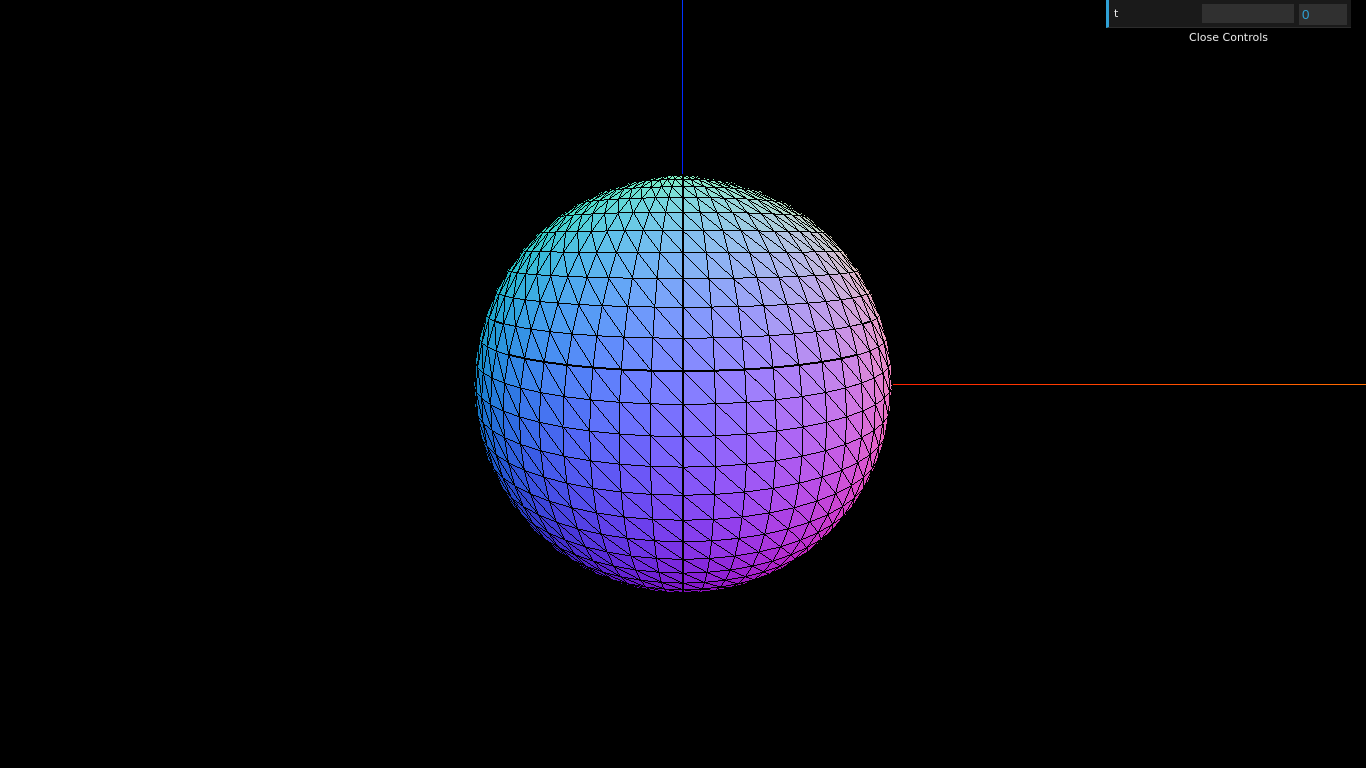
\includegraphics{A}
        \hspace{1em}
        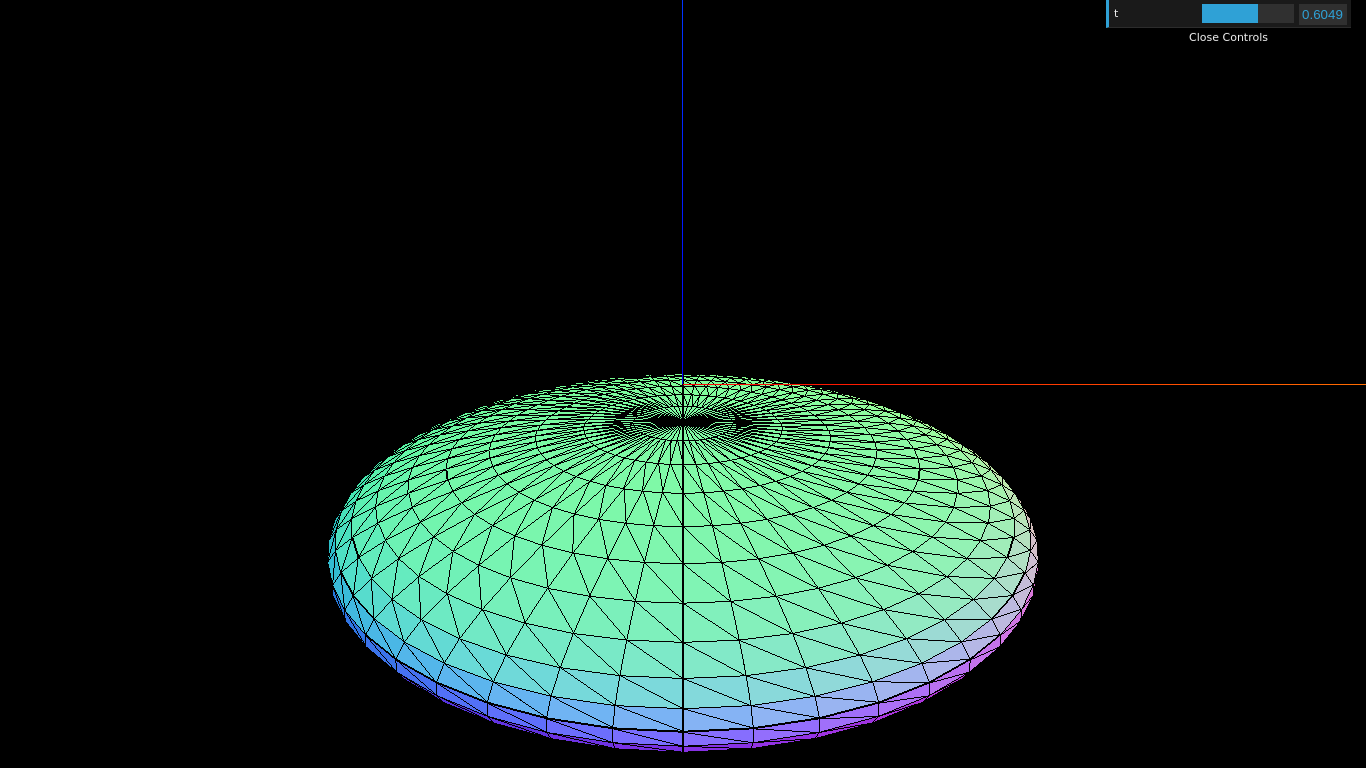
\includegraphics{B}
        \hspace{1em}
        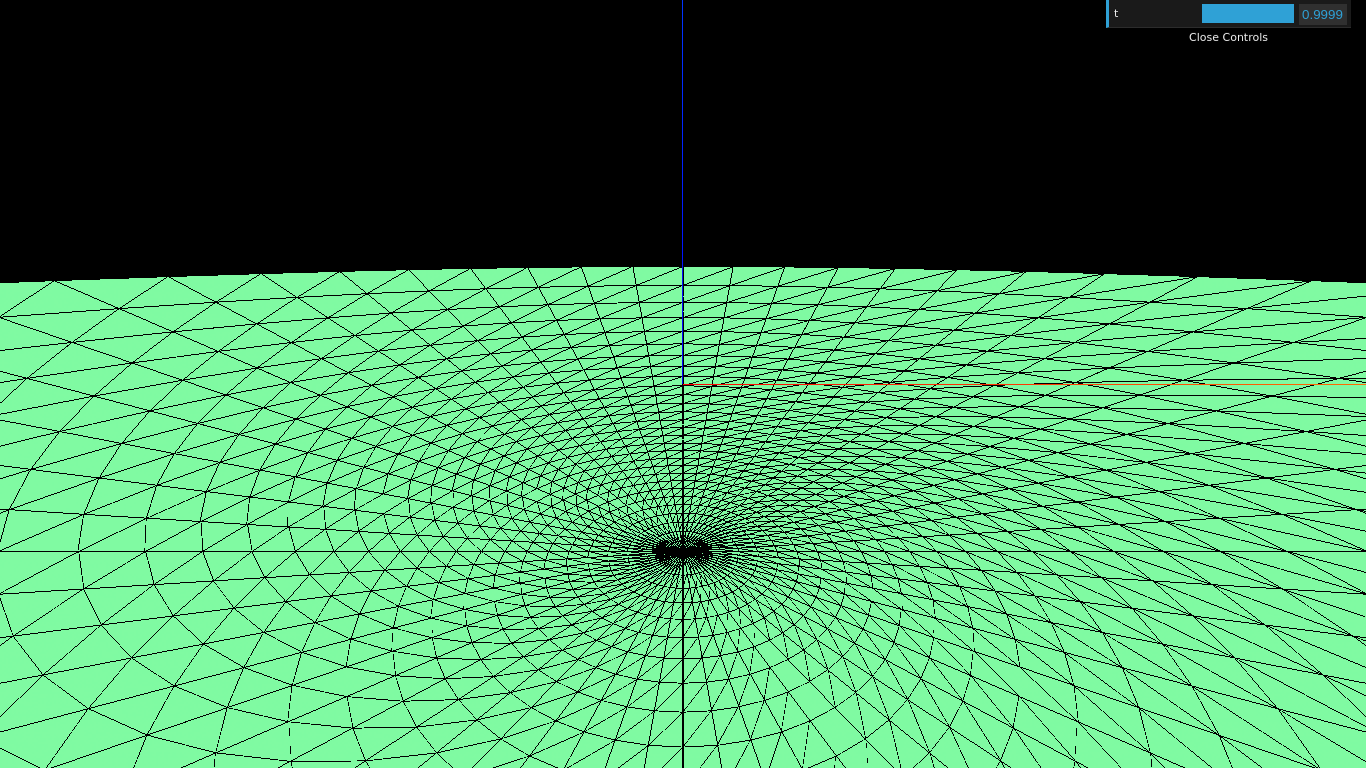
\includegraphics{C}
}}

\appendix

\section{Instrucciones para el código en javascript}

El proyecto de \textit{javascript} (\textit{nodejs}) está formado por los
siguientes ficheros:

\begin{itemize}
    \item \texttt{package.json}: Descripción del proyecto y lista de
        dependencias. Esto hace posible instalar los paquetes necesarios usando el comando \texttt{npm}.
    \item \texttt{src}: Código fuente del proyecto
        \begin{itemize}
            \item \texttt{script.js}: Código fuente del proyecto, donde realmente está ubicado el programa. El código de este fichero
            \item \texttt{index.html}: Esqueleto de la web del proyecto
                está incluido en el siguiente anexo.
            \item \texttt{style.css}: Estilos de la página web.
        \end{itemize}
    \item \texttt{bundler}: Carpeta con ficheros de configuración para poder
        compilar el programa en una carpeta con el proyecto web final.
    \item \texttt{dist}: Carpeta con el resultado de la compilación.
\end{itemize}

Para instalar las dependencias hay que instalar los paquetes \texttt{node} y
\texttt{npm}. Una vez hecho esto basta ejecutar \texttt{npm install} para
instalar los módulos de \texttt{node} que necesita el proyecto. Una vez hecho
esto se utilizarán los siguientes comandos:
\begin{itemize}
    \item \texttt{nmp dev}: Para previsualizar el proyecto en un navegador web
        con recarga automática de los cambios.
    \item \texttt{npm build}: Para compilar la aplicación y generar la carpeta
        \texttt{dist}.
\end{itemize}

He incluido en la entrega en el campus virtual los ficheros del proyecto del siguiente modo:
\begin{itemize}
    \item \texttt{script.js}: Archivo principal del proyecto, donde está la
        parte que concierne a la implementación del segundo apartado.
    \item \texttt{project.zip}: Proyecto completo comprimido de nodejs, sin la
        carpeta \texttt{dist}.
    \item \texttt{dist.zip}: Proyecto compilado. Se puede visualizar el proyecto
        abriendo el fichero \texttt{index.html} con cualquier navegador que
        soporte \textit{javascript}.
\end{itemize}

\section{Código}
El siguiente código con la implementación también está adjunto en la entrega
y disponible, junto con esta memoria, en un repositorio git en el siguiente
enlace: \href{https://www.github.com/haztecaso/gcomp22}{github.com/haztecaso/gcomp22}.

\subsection{Apartado 1 (python)}

\lstinputlisting[linerange={6}, firstnumber=8]{practica5.py}

\subsection{Apartado 2 (javascript)}

He incluido aqui el código del fichero \texttt{src/script.js}, donde está la
parte central del programa. Para ejecutar o compilar la aplicación de
\textit{threejs} es necesario tener \textit{nodejs} instalado y ejecutar el comando

\begin{itemize}
    \item \texttt{npm dev} para ejecutar la aplicación.
    \item \texttt{npm build} para compilar la aplicación, que se guardará en la
        carpeta \texttt{dist} y podrá abrirse un navegador web.
\end{itemize}

\lstinputlisting[linerange={0}, firstnumber=8]{./src/script.js}

\end{document}
